\documentclass{class}
\usepackage{packages}                           

%**************************Layout**************************************
\pagestyle{fancy}
\fancyhf{}
\fancyhead[L]{\sc Scientific Computing}   % Obere Leiste
\fancyfoot[C]{\thepage}                                 % Untere Leiste
\setlength{\headheight}{15pt} % mindesetens 13.59999pt
\renewcommand{\headrulewidth}{1pt}
\renewcommand{\footrulewidth}{1pt}

\setlength\parindent{0pt} %noindent

%\numberwithin{equation}{section} %Gleichungen nach Sections numeriert

%**********************************************************************
\begin{document}

\begin{titlepage}
    \centering
    \vspace*{0.5cm}
    % \begin{figure}[H]
    %     \includegraphics[width=1\textwidth]{images/Logo_Uni_Göttingen_2022.png}
    % \end{figure}
    % \vspace*{2.2cm}
    \LARGE{\textsc{Georg-August-Universität} \\
    \textsc{Göttingen}}
    \vspace*{1.7cm}
    
    \rule{\textwidth}{1pt}\\[0.5cm]
    {\huge \bfseries
      Project 6: Model for the Spread of Infectious Diseases}\\
    \rule{\textwidth}{1pt}
    
    \vspace*{2.7cm}
    
    {\large Carlo von Carnap\\
    
    \vspace*{0.7cm}

    Summer Term 2023}
    
    \vspace*{5.7cm}

    {\large Final Project \textit{Scientific Computing}, \\
    Salvatore R. Manmana

    \vspace*{0.7cm}
    
    Supervisor: Emily Klass \\
    Submission Date: 08.08.2023}

    \end{titlepage}
\newpage

% Die folgenden drei Zeilen beim Drucken.

% \thispagestyle{empty} 
% \mbox{}
% \newpage

\tableofcontents 
\thispagestyle{empty}
\newpage
\setcounter{page}{1}

\section{Introduction}

% \subsection{Infectious Disease Modelling}

Infectious disease modelling describes the process of applying mathematical models to predict the future state of an epidemic. 
Recently it has surged in popularity during the COVID-19 pandemic and its influence on recent policies has been overwhelming, despite its mediocre success in projecting reality. 
The difficulties when modelling infectious diseases range from the overcomplex real situations to finding suitable assumptions to keep an appropriate level of accuracy.
Generally it can be distinguished between macroscale models such as the SEIR-model\cite{SEIR_Heidelberg} that apply differential equations on a population level, 
and microscale models that have individuals as their smallest unit.

This model uses a cellular automaton\cite{CellularAutomaton} of quadratic shape $L\times L$ as well as stochastic methods to examine the spread of an infectious agent on a microscale. 
Each grid node is occupied by an immobile person and can be in one of the states Susceptible \susceptible{}, Infected \infected{} or Recovered \recovered{}. Later, the forth state Vaccinated \vaccinated{} is introduced, 
that permanently excludes the respective people from taking any of the three other states. 
For a person in one of the three active states \susceptible{}, \infected{} and \recovered{}, the following three transitions are possible,
\begin{equation*}
    \mathrm{Susceptible}~\susceptible\xlongrightarrow{p_1}\mathrm{Infected}~\infected{}\xlongrightarrow{p_2}\mathrm{Recovered}~\recovered{}\xlongrightarrow{p_3}\mathrm{Susceptible}~\susceptible{}.
\end{equation*}
With that, we have the following three transition probabilities:
\begin{itemize}
    \item $p_1$: a susceptible person getting infected by an infected neighbor,
    \item $p_2$: an infected person turning recovered
    \item $p_3$: a recovered person returning susceptible
\end{itemize}
For the $\susceptible{}\rightarrow\infected{}$ transition, a von Neumann neighborhood was applied, meaning the four immediately adjacing nodes are consideres as neighbors.\cite{CellularAutomaton} 
Vaccinated people \vaccinated{} are set at the beginning of the simulation, with $p_4$ being the probability that a spot is occupied by one. The other three states are initialized with the same likelyhood, as the 
simulation steps progress by each updating $L^2$ randomly chosen nodes according to the above mentioned rules.

Goal was now to use this model to examine the influence of the transition probabilities on the infection rates averaged over all simulation steps. This included varying the $\susceptible\rightarrow\infected$ turover rate $p_1$
for diffrent combinations of $p_2\left(\infected\rightarrow\recovered\,\right)$ and $p_3\left(\recovered\rightarrow\susceptible\,\right)$ as well as using different vaccination rates $p_4$ at initialization. 
For all simulations, different grid sizes were used to observe potential statistical inaccuracies.

Further, the time evolution of the infection rates was looked at to stress the validity of the preceding time averaging. Therefor a quantity of 20 infection rate samples was generated over simulation time
with mean and standard deviation calculated for each timestep.

\section{Theory}

\subsection{Averaging within Simulation Runs}

Fundamental to the analysis of the simulation results is the rate of infected individuals in the grid at each timestep $\langle I\rangle_t$. It is calculated by summing up the infection status $I_{i,j}$
over the totality of the grid and dividing it by the number of grid nodes $L^2$,
\begin{equation}
    \langle I\rangle_t=\frac{1}{L^2}\sum_{i=1,\,j=1}^{L}I_{i,j}.
    \label{eq:theo_inf_rate}
\end{equation}
For that, the infection status is either taking $I_{i,j}=1$ for the person being in state \infected{} or $I_{i,j}=0$ otherwise. This infection rate can now be averaged over all timesteps $t$ to receive
\begin{equation}
    \overline{\langle I\rangle}=\frac{1}{T}\sum_{t=0}^{T}\langle I\rangle_t,
    \label{eq:theo_time_avg_inf_rate}
\end{equation}
the time-averaged infection rate which most of the analysis steps are based on.

\subsection{Averaging across Simulation Runs}

For the evaluation of the time-averaging, the infection rate $\langle I\rangle_t$ was also averaged over a multitude of $N$ samples for each timestep. This mean at a given timestep $t$ is calculated as
\begin{equation}
    \overline{\langle I\rangle_t}=\frac{1}{N}\sum_{n=1}^{N}\langle I\rangle_t
    \label{eq:theo_mean_inf_rate}
\end{equation}
and posesses a standard deviation of
\begin{equation}
    \sigma_{\langle I\rangle_t}=\sqrt{\frac{1}{N}\sum_{n=1}^{N}\left(\langle I\rangle_t-\overline{\langle I\rangle_t}\,\right)^2}.
    \label{eq:theo_sigma_inf_rate}
\end{equation}

\section{Methodology}

\subsection{Pseudorandom Number Generator (PRNG) MT19937}\label{ssec:methodology_rng_mt19937}

For the generation of pseudorandom numbers the 1997 developed PRNG Mer\-sen\-ne\,Twis\-ter MT19937\cite{Makoto_Takuji} was chosen. 
It was published in 1997 and has become one of the most popular RNGS across programming languages.\cite{educativeMersenneTwister}

Its very long period with $2^{19937}-1$ integers as well as the fact that its random nubmers are highly equidistributed\cite{MT_LearnCPP}, make the Mer\-sen\-ne\,Twis\-ter a very strong choice.
The Mersenne Twister broadly works by first taking a vector of $624$ random numbers as seed, that are then transformed applying a ``twist'' operation and subsequently used to retrieve the usable pseudorandom number. 
Once all integers of the state vector are consumed, the vector is regenerated.\cite{educativeMersenneTwister}\cite{MT_DavidWong}


\section{Implementation}

\subsection{Integration of External Libraries}

Alongside the C standard library headers, the \texttt{gsl\_rng.h} of the GNU Scientific Library (GSL) as well as the two numeric libraries \texttt{cvc\_numerics.h} and \texttt{cvc\_rng.h} were included in the project. 
Of the standard library, the header files \texttt{stdio.h}, \texttt{stdlib.h}, \texttt{tgmath.h} and \texttt{time.h} were used, the GSL header \texttt{gsl\_rng.h} was only accessed to generate pseudorandom nubers. 

The \texttt{cvc\_numerics.h} of the two own libraries provides mainly numerical methods for differentation, integration or to solve differential equations, while the \texttt{cvc\_rng.h} offers functions requiring PRNGs
like for instance Monte-Carlo integrators or tools helpful to analyse stochastic datasets such as calculating mean or standard deviation of given arrays.


\subsection{Structure and Workflow of the Main Program}

\subsubsection{Generation of Random Numbers by a Static PRNG}

For the generation of pseudorandom numbers the in \prettyref{ssec:methodology_rng_mt19937} described Mer\-sen\-ne\,Twis\-ter MT19937 of the GSL library was used. It was implemented statically 
to generate uniformly distributed numbers in the interval $[0,\,1)$ and can therefore be accessed globally by the respective functions. 

Overall the PRNG was used in two different ways, once to obtain probabilities, other to generate random integers.
The former was accomplished by checking if the uniform was smaller than the respective probability, the latter by multiplying the uniform by the largest desired integer and then casting it to \texttt{int}.


\subsubsection{Implementation of the Modelling Grid}\label{ssec:impl_modelling_grid}

The above mentioned grid itself was realized as a $\left(L+2\right)\times \left(L+2\right)$ heap section of integer values, with $L$ being the sidelength of the quadratic grid where the actual spread of the
infection takes place. While this section is technically one-dimensional, it will for simplicity reasons be here refered to as a two-dimensional structure of the given shape. 
Inside the grid, the following integer values were used to model the different states of the people within the simulation:
\begin{itemize}
    \item \texttt{0}: this person is Susceptible \susceptible{} to the infection
    \item \texttt{1}: the person is Infected \infected{}
    \item \texttt{2}: the person is Recovered \recovered{} and currently not susceptible
    \item \texttt{-1}: the person is Vaccinated \vaccinated{} and does not participate in the spread
\end{itemize}
The grid was implemented with a supporting edge of ghosts at the top, bottom, left and right border, that are neither infectious nor subject to any updates of the grid --- they will permanently take the value
\texttt{0} and are irrelevant for the later visualization and analysis of the data.


\subsubsection{Functions Acting on the Modelling Grid}\label{ssec:impl_functions_on_grid}

In the main program all changes in the grid are facilitated by functions outside the main one. They entirely work with or change the grid in-place and all take the grid itself as well as its length $L+2$ as arguments.
Inside the functions, the grid is refered to as \texttt{grid} and its legth as \texttt{length}, while the above probabilities are passed in form of the double array \texttt{probabilities} having $p_1$, $p_2$, $p_3$, 
and $p_4$ as its entries. Excluding the ones to calculate the infection rate and its time average, none of the functions does have a return value. Overall the following functions can be called from the main:
\begin{itemize}
    \item \texttt{void print\_grid}: prints the passed grid as terminal ouput
    \item \texttt{void grid\_init}: initializes the grid applying the vaccination probability
    \item \texttt{void update\_node}: updates the given node selected by its $L\times L$ grid coordinates \texttt{row\_i} and \texttt{column\_j} according to the turnover probabilities
    \item \texttt{void grid\_update\_linear}: calls the \texttt{update\_node} function for each node in order of their grid position
    \item \texttt{void grid\_update\_stochastic}: calls \texttt{update\_node} for $L^2$ randomly chosen nodes
    \item \texttt{double ratio\_infected}: calculates the ratio of infected individuals with respect to the total grip population for a given grid
    \item \texttt{double average\_ratio\_infected}: applies \texttt{T} simulation steps to the grid by calling the stochastic grid updater with passed turnover probabilities 
    and averages the calculated infection rate over each simulation step
\end{itemize}


\subsubsection{Structure of the Main Function and Generated Data Files}

The main function is divided into compartements for each individual analysis step, where every compartment is a local scope in order to prevent the variables from interfering with each other.
Therefore each one uses its own variables, files and grids, with the latter being then shaped by calling the functions from \prettyref{ssec:impl_functions_on_grid}. The files are also being written at
directly from the main function.

The first compartment itself uses the command line interface to take the probabilities $p_1$, $p_2$, $p_3$, and $p_4$ as well as the grid size $L$ as user input. Further it can be specified how the grid is going to be 
updated. Either all grid nodes are updated sequentially (for user input \texttt{0}) or $L^2$ grid nodes are selected randomly. After initializing the grid, 
individual actualization steps can be performed manually according to the previously selected simulation scheme by pressing \texttt{ENTER} until the loop is quit with \texttt{q} confirmed by \texttt{ENTER}.
While here the mechanism to update the grid is subject to the users input, for the following simulation tasks the model operates using the stochastic updating method for each timestep 
(i.e. $L^2$ random nodes are selected for actualization). It was chosen to avoid adding a spatial bias by having a pre-selected order; however,
in terms of results, there is no meaningful difference expected between the two schemes.

The remainder of the program runs independently from the user, \textbf{overall a running time of around three minutes should be expected after the interactive part is finished}. 
The majority of the time is comsumed by the second scope, generating the data files for the $p_1$ dependency of time-averaged infection rate $\overline{\langle I\rangle}$ without vaccinations.
The files do each have the respective grid size in column one and the values of $p_1$ written in the first row. The data points are the time-averaged infection rates for the previous parameters and calculated
using the corresponding calculation function for $T=1000$. Overall three files are being written at in the \texttt{/soi\_data} directory, one for each combination of $p_2$ and $p_3$:
\begin{itemize}
    \item \texttt{soi\_average\_ratio\_infected\_over\_p1\_a.csv}: $p_2=0.3$, $p_3=0.3$
    \item \texttt{soi\_average\_ratio\_infected\_over\_p1\_b.csv}: $p_2=0.6$, $p_3=0.3$
    \item \texttt{soi\_average\_ratio\_infected\_over\_p1\_c.csv}: $p_2=0.3$, $p_3=0.6$
\end{itemize}

The data file generated by the third compartment for $p_1=p_2=p_3=0.5$,
\begin{itemize}
    \item \texttt{soi\_average\_ratio\_infected\_over\_p4\_v.csv},
\end{itemize}
uses a similar structure. Here the vaccination rate occupies the first row, with the columns once again using the same grid sizes as before.

For the time development of the infection rate, an additional heap section is used to support the statistical analysis across data samples. It has the data series for each time as virtual rows,
that are then passed to the respective \texttt{cvc\_rng.h} functions to calculate mean and standard deviation. The data file of the this third scope,
\begin{itemize}
    \item \texttt{soi\_ratio\_over\_time.csv},
\end{itemize}
has the sample number as fist column and the timestep as first row, the data points are the infection rates of each sample and timestep. 
Mean and standard deviation have extra rows at the end of the file marked with \texttt{00} and \texttt{01} respectively instead of the sample number.

Addinitionally, three data files resembling the state of the grid itself are generated into the \texttt{/soi\_animations} folder:
\begin{itemize}
    \item \texttt{soi\_grid\_over\_time\_a.csv}
    \item \texttt{soi\_grid\_over\_time\_b.csv}
    \item \texttt{soi\_grid\_over\_time\_c.csv}
\end{itemize}

Therefor the dimensionality of the grid is reduced to one and for each timestep occupying the first column of the files, the grid state is a one-dimensional data series behind it.
For the representation of the state of each individual node, the same notation as described in \prettyref{ssec:impl_functions_on_grid} is used.

% Overall, the following files are generated by the main program into the data folder \texttt{/soi\_data}:
% \begin{itemize}
%     \item \texttt{soi\_average\_ratio\_infected\_over\_p1\_a.csv}
%     \item \texttt{soi\_average\_ratio\_infected\_over\_p1\_b.csv}
%     \item \texttt{soi\_average\_ratio\_infected\_over\_p1\_c.csv}
%     \item \texttt{soi\_average\_ratio\_infected\_over\_p4.csv}
%     \item \texttt{soi\_ratio\_over\_time.csv}
% \end{itemize}

% Additionally, the files of the time evolution of the grid states themselves are created in the \texttt{/soi\_animations} folder:
% \begin{itemize}
%     \item \texttt{soi\_grid\_over\_time\_a.csv}
%     \item \texttt{soi\_grid\_over\_time\_b.csv}
%     \item \texttt{soi\_grid\_over\_time\_c.csv}
% \end{itemize}

\section{Results and Discussion}

\subsection{Ratio of Infected People Averaged over Time}

Aim was now to analyse the infection rate inside the grid averaged over all timesteps $\overline{\langle I\rangle}$ for different combinations of $p_1$, $p_2$ and $p_2$. To achive this, the dependency of the 
turnover probability $p_1\left(\susceptible\rightarrow\infected\,\right)$ on the time-averaged infection rates was simulated for different combinations of $p_2\left(\infected\rightarrow\recovered\,\right)$
and $p_3\left(\recovered\rightarrow\susceptible\,\right)$. The simulation was performed over $T=1000$ simulation steps for each of the grid sizes $L=16$, $L=32$, $L=64$ and $L=128$.
The latter grid size $L=128$ is the largest one used for any simulation and still takes an acceptable but still non-negligable amount of calculation time.
Since this side length should provide more than fluctuation-resistant results and the calculation time more than doubles for a doubling in $L$ due to the calculation functions, this was the maximum grid size trialed.

{From looking at the results shown in \prettyref{fig:res_dis_avg_inf_over_p1} it immediately becomes visible that the lower grid sizes undergo stronger fluctuations in $\overline{\langle I\rangle}$ than the higher ones, 
with very\parfillskip=0pt\par}

\begin{figure}[H]
    \centering
    \resizebox{\textwidth}{!}{%% Creator: Matplotlib, PGF backend
%%
%% To include the figure in your LaTeX document, write
%%   \input{<filename>.pgf}
%%
%% Make sure the required packages are loaded in your preamble
%%   \usepackage{pgf}
%%
%% Also ensure that all the required font packages are loaded; for instance,
%% the lmodern package is sometimes necessary when using math font.
%%   \usepackage{lmodern}
%%
%% Figures using additional raster images can only be included by \input if
%% they are in the same directory as the main LaTeX file. For loading figures
%% from other directories you can use the `import` package
%%   \usepackage{import}
%%
%% and then include the figures with
%%   \import{<path to file>}{<filename>.pgf}
%%
%% Matplotlib used the following preamble
%%   
%%   \usepackage{fontspec}
%%   \setmainfont{DejaVuSerif.ttf}[Path=\detokenize{/home/carlo/.local/lib/python3.10/site-packages/matplotlib/mpl-data/fonts/ttf/}]
%%   \setsansfont{DejaVuSans.ttf}[Path=\detokenize{/home/carlo/.local/lib/python3.10/site-packages/matplotlib/mpl-data/fonts/ttf/}]
%%   \setmonofont{DejaVuSansMono.ttf}[Path=\detokenize{/home/carlo/.local/lib/python3.10/site-packages/matplotlib/mpl-data/fonts/ttf/}]
%%   \makeatletter\@ifpackageloaded{underscore}{}{\usepackage[strings]{underscore}}\makeatother
%%
\begingroup%
\makeatletter%
\begin{pgfpicture}%
\pgfpathrectangle{\pgfpointorigin}{\pgfqpoint{10.427822in}{13.953546in}}%
\pgfusepath{use as bounding box, clip}%
\begin{pgfscope}%
\pgfsetbuttcap%
\pgfsetmiterjoin%
\definecolor{currentfill}{rgb}{1.000000,1.000000,1.000000}%
\pgfsetfillcolor{currentfill}%
\pgfsetlinewidth{0.000000pt}%
\definecolor{currentstroke}{rgb}{1.000000,1.000000,1.000000}%
\pgfsetstrokecolor{currentstroke}%
\pgfsetdash{}{0pt}%
\pgfpathmoveto{\pgfqpoint{0.000000in}{0.000000in}}%
\pgfpathlineto{\pgfqpoint{10.427822in}{0.000000in}}%
\pgfpathlineto{\pgfqpoint{10.427822in}{13.953546in}}%
\pgfpathlineto{\pgfqpoint{0.000000in}{13.953546in}}%
\pgfpathlineto{\pgfqpoint{0.000000in}{0.000000in}}%
\pgfpathclose%
\pgfusepath{fill}%
\end{pgfscope}%
\begin{pgfscope}%
\pgfsetbuttcap%
\pgfsetmiterjoin%
\definecolor{currentfill}{rgb}{1.000000,1.000000,1.000000}%
\pgfsetfillcolor{currentfill}%
\pgfsetlinewidth{0.000000pt}%
\definecolor{currentstroke}{rgb}{0.000000,0.000000,0.000000}%
\pgfsetstrokecolor{currentstroke}%
\pgfsetstrokeopacity{0.000000}%
\pgfsetdash{}{0pt}%
\pgfpathmoveto{\pgfqpoint{0.640323in}{9.767436in}}%
\pgfpathlineto{\pgfqpoint{10.327822in}{9.767436in}}%
\pgfpathlineto{\pgfqpoint{10.327822in}{13.617436in}}%
\pgfpathlineto{\pgfqpoint{0.640323in}{13.617436in}}%
\pgfpathlineto{\pgfqpoint{0.640323in}{9.767436in}}%
\pgfpathclose%
\pgfusepath{fill}%
\end{pgfscope}%
\begin{pgfscope}%
\pgfpathrectangle{\pgfqpoint{0.640323in}{9.767436in}}{\pgfqpoint{9.687500in}{3.850000in}}%
\pgfusepath{clip}%
\pgfsetbuttcap%
\pgfsetroundjoin%
\definecolor{currentfill}{rgb}{0.000000,0.000000,1.000000}%
\pgfsetfillcolor{currentfill}%
\pgfsetfillopacity{0.500000}%
\pgfsetlinewidth{1.003750pt}%
\definecolor{currentstroke}{rgb}{0.000000,0.000000,1.000000}%
\pgfsetstrokecolor{currentstroke}%
\pgfsetstrokeopacity{0.500000}%
\pgfsetdash{}{0pt}%
\pgfsys@defobject{currentmarker}{\pgfqpoint{-0.021960in}{-0.021960in}}{\pgfqpoint{0.021960in}{0.021960in}}{%
\pgfpathmoveto{\pgfqpoint{0.000000in}{-0.021960in}}%
\pgfpathcurveto{\pgfqpoint{0.005824in}{-0.021960in}}{\pgfqpoint{0.011410in}{-0.019646in}}{\pgfqpoint{0.015528in}{-0.015528in}}%
\pgfpathcurveto{\pgfqpoint{0.019646in}{-0.011410in}}{\pgfqpoint{0.021960in}{-0.005824in}}{\pgfqpoint{0.021960in}{0.000000in}}%
\pgfpathcurveto{\pgfqpoint{0.021960in}{0.005824in}}{\pgfqpoint{0.019646in}{0.011410in}}{\pgfqpoint{0.015528in}{0.015528in}}%
\pgfpathcurveto{\pgfqpoint{0.011410in}{0.019646in}}{\pgfqpoint{0.005824in}{0.021960in}}{\pgfqpoint{0.000000in}{0.021960in}}%
\pgfpathcurveto{\pgfqpoint{-0.005824in}{0.021960in}}{\pgfqpoint{-0.011410in}{0.019646in}}{\pgfqpoint{-0.015528in}{0.015528in}}%
\pgfpathcurveto{\pgfqpoint{-0.019646in}{0.011410in}}{\pgfqpoint{-0.021960in}{0.005824in}}{\pgfqpoint{-0.021960in}{0.000000in}}%
\pgfpathcurveto{\pgfqpoint{-0.021960in}{-0.005824in}}{\pgfqpoint{-0.019646in}{-0.011410in}}{\pgfqpoint{-0.015528in}{-0.015528in}}%
\pgfpathcurveto{\pgfqpoint{-0.011410in}{-0.019646in}}{\pgfqpoint{-0.005824in}{-0.021960in}}{\pgfqpoint{0.000000in}{-0.021960in}}%
\pgfpathlineto{\pgfqpoint{0.000000in}{-0.021960in}}%
\pgfpathclose%
\pgfusepath{stroke,fill}%
}%
\begin{pgfscope}%
\pgfsys@transformshift{1.080663in}{9.900556in}%
\pgfsys@useobject{currentmarker}{}%
\end{pgfscope}%
\begin{pgfscope}%
\pgfsys@transformshift{1.256800in}{9.900823in}%
\pgfsys@useobject{currentmarker}{}%
\end{pgfscope}%
\begin{pgfscope}%
\pgfsys@transformshift{1.432936in}{9.899658in}%
\pgfsys@useobject{currentmarker}{}%
\end{pgfscope}%
\begin{pgfscope}%
\pgfsys@transformshift{1.609073in}{9.902424in}%
\pgfsys@useobject{currentmarker}{}%
\end{pgfscope}%
\begin{pgfscope}%
\pgfsys@transformshift{1.785209in}{9.902715in}%
\pgfsys@useobject{currentmarker}{}%
\end{pgfscope}%
\begin{pgfscope}%
\pgfsys@transformshift{1.961345in}{9.908221in}%
\pgfsys@useobject{currentmarker}{}%
\end{pgfscope}%
\begin{pgfscope}%
\pgfsys@transformshift{2.137482in}{9.915352in}%
\pgfsys@useobject{currentmarker}{}%
\end{pgfscope}%
\begin{pgfscope}%
\pgfsys@transformshift{2.313618in}{9.916347in}%
\pgfsys@useobject{currentmarker}{}%
\end{pgfscope}%
\begin{pgfscope}%
\pgfsys@transformshift{2.489754in}{9.930367in}%
\pgfsys@useobject{currentmarker}{}%
\end{pgfscope}%
\begin{pgfscope}%
\pgfsys@transformshift{2.665891in}{9.917050in}%
\pgfsys@useobject{currentmarker}{}%
\end{pgfscope}%
\begin{pgfscope}%
\pgfsys@transformshift{2.842027in}{10.072098in}%
\pgfsys@useobject{currentmarker}{}%
\end{pgfscope}%
\begin{pgfscope}%
\pgfsys@transformshift{3.018163in}{9.969978in}%
\pgfsys@useobject{currentmarker}{}%
\end{pgfscope}%
\begin{pgfscope}%
\pgfsys@transformshift{3.194300in}{10.768020in}%
\pgfsys@useobject{currentmarker}{}%
\end{pgfscope}%
\begin{pgfscope}%
\pgfsys@transformshift{3.370436in}{10.872833in}%
\pgfsys@useobject{currentmarker}{}%
\end{pgfscope}%
\begin{pgfscope}%
\pgfsys@transformshift{3.546572in}{11.054801in}%
\pgfsys@useobject{currentmarker}{}%
\end{pgfscope}%
\begin{pgfscope}%
\pgfsys@transformshift{3.722709in}{11.363348in}%
\pgfsys@useobject{currentmarker}{}%
\end{pgfscope}%
\begin{pgfscope}%
\pgfsys@transformshift{3.898845in}{11.372737in}%
\pgfsys@useobject{currentmarker}{}%
\end{pgfscope}%
\begin{pgfscope}%
\pgfsys@transformshift{4.074982in}{11.489435in}%
\pgfsys@useobject{currentmarker}{}%
\end{pgfscope}%
\begin{pgfscope}%
\pgfsys@transformshift{4.251118in}{11.582313in}%
\pgfsys@useobject{currentmarker}{}%
\end{pgfscope}%
\begin{pgfscope}%
\pgfsys@transformshift{4.427254in}{11.652532in}%
\pgfsys@useobject{currentmarker}{}%
\end{pgfscope}%
\begin{pgfscope}%
\pgfsys@transformshift{4.603391in}{11.708395in}%
\pgfsys@useobject{currentmarker}{}%
\end{pgfscope}%
\begin{pgfscope}%
\pgfsys@transformshift{4.779527in}{11.749000in}%
\pgfsys@useobject{currentmarker}{}%
\end{pgfscope}%
\begin{pgfscope}%
\pgfsys@transformshift{4.955663in}{11.816145in}%
\pgfsys@useobject{currentmarker}{}%
\end{pgfscope}%
\begin{pgfscope}%
\pgfsys@transformshift{5.131800in}{11.831936in}%
\pgfsys@useobject{currentmarker}{}%
\end{pgfscope}%
\begin{pgfscope}%
\pgfsys@transformshift{5.307936in}{11.924231in}%
\pgfsys@useobject{currentmarker}{}%
\end{pgfscope}%
\begin{pgfscope}%
\pgfsys@transformshift{5.484072in}{11.959887in}%
\pgfsys@useobject{currentmarker}{}%
\end{pgfscope}%
\begin{pgfscope}%
\pgfsys@transformshift{5.660209in}{11.992997in}%
\pgfsys@useobject{currentmarker}{}%
\end{pgfscope}%
\begin{pgfscope}%
\pgfsys@transformshift{5.836345in}{12.034986in}%
\pgfsys@useobject{currentmarker}{}%
\end{pgfscope}%
\begin{pgfscope}%
\pgfsys@transformshift{6.012482in}{12.069506in}%
\pgfsys@useobject{currentmarker}{}%
\end{pgfscope}%
\begin{pgfscope}%
\pgfsys@transformshift{6.188618in}{12.072462in}%
\pgfsys@useobject{currentmarker}{}%
\end{pgfscope}%
\begin{pgfscope}%
\pgfsys@transformshift{6.364754in}{12.123474in}%
\pgfsys@useobject{currentmarker}{}%
\end{pgfscope}%
\begin{pgfscope}%
\pgfsys@transformshift{6.540891in}{12.138514in}%
\pgfsys@useobject{currentmarker}{}%
\end{pgfscope}%
\begin{pgfscope}%
\pgfsys@transformshift{6.717027in}{12.171481in}%
\pgfsys@useobject{currentmarker}{}%
\end{pgfscope}%
\begin{pgfscope}%
\pgfsys@transformshift{6.893163in}{12.191706in}%
\pgfsys@useobject{currentmarker}{}%
\end{pgfscope}%
\begin{pgfscope}%
\pgfsys@transformshift{7.069300in}{12.216235in}%
\pgfsys@useobject{currentmarker}{}%
\end{pgfscope}%
\begin{pgfscope}%
\pgfsys@transformshift{7.245436in}{12.219942in}%
\pgfsys@useobject{currentmarker}{}%
\end{pgfscope}%
\begin{pgfscope}%
\pgfsys@transformshift{7.421572in}{12.250655in}%
\pgfsys@useobject{currentmarker}{}%
\end{pgfscope}%
\begin{pgfscope}%
\pgfsys@transformshift{7.597709in}{12.299481in}%
\pgfsys@useobject{currentmarker}{}%
\end{pgfscope}%
\begin{pgfscope}%
\pgfsys@transformshift{7.773845in}{12.287205in}%
\pgfsys@useobject{currentmarker}{}%
\end{pgfscope}%
\begin{pgfscope}%
\pgfsys@transformshift{7.949982in}{12.323302in}%
\pgfsys@useobject{currentmarker}{}%
\end{pgfscope}%
\begin{pgfscope}%
\pgfsys@transformshift{8.126118in}{12.320849in}%
\pgfsys@useobject{currentmarker}{}%
\end{pgfscope}%
\begin{pgfscope}%
\pgfsys@transformshift{8.302254in}{12.352847in}%
\pgfsys@useobject{currentmarker}{}%
\end{pgfscope}%
\begin{pgfscope}%
\pgfsys@transformshift{8.478391in}{12.326357in}%
\pgfsys@useobject{currentmarker}{}%
\end{pgfscope}%
\begin{pgfscope}%
\pgfsys@transformshift{8.654527in}{12.371743in}%
\pgfsys@useobject{currentmarker}{}%
\end{pgfscope}%
\begin{pgfscope}%
\pgfsys@transformshift{8.830663in}{12.375718in}%
\pgfsys@useobject{currentmarker}{}%
\end{pgfscope}%
\begin{pgfscope}%
\pgfsys@transformshift{9.006800in}{12.372495in}%
\pgfsys@useobject{currentmarker}{}%
\end{pgfscope}%
\begin{pgfscope}%
\pgfsys@transformshift{9.182936in}{12.406983in}%
\pgfsys@useobject{currentmarker}{}%
\end{pgfscope}%
\begin{pgfscope}%
\pgfsys@transformshift{9.359072in}{12.388087in}%
\pgfsys@useobject{currentmarker}{}%
\end{pgfscope}%
\begin{pgfscope}%
\pgfsys@transformshift{9.535209in}{12.426171in}%
\pgfsys@useobject{currentmarker}{}%
\end{pgfscope}%
\begin{pgfscope}%
\pgfsys@transformshift{9.711345in}{12.437572in}%
\pgfsys@useobject{currentmarker}{}%
\end{pgfscope}%
\begin{pgfscope}%
\pgfsys@transformshift{9.887482in}{12.471073in}%
\pgfsys@useobject{currentmarker}{}%
\end{pgfscope}%
\end{pgfscope}%
\begin{pgfscope}%
\pgfpathrectangle{\pgfqpoint{0.640323in}{9.767436in}}{\pgfqpoint{9.687500in}{3.850000in}}%
\pgfusepath{clip}%
\pgfsetbuttcap%
\pgfsetroundjoin%
\definecolor{currentfill}{rgb}{0.980392,0.164706,0.333333}%
\pgfsetfillcolor{currentfill}%
\pgfsetfillopacity{0.500000}%
\pgfsetlinewidth{1.003750pt}%
\definecolor{currentstroke}{rgb}{0.980392,0.164706,0.333333}%
\pgfsetstrokecolor{currentstroke}%
\pgfsetstrokeopacity{0.500000}%
\pgfsetdash{}{0pt}%
\pgfsys@defobject{currentmarker}{\pgfqpoint{-0.021960in}{-0.021960in}}{\pgfqpoint{0.021960in}{0.021960in}}{%
\pgfpathmoveto{\pgfqpoint{0.000000in}{-0.021960in}}%
\pgfpathcurveto{\pgfqpoint{0.005824in}{-0.021960in}}{\pgfqpoint{0.011410in}{-0.019646in}}{\pgfqpoint{0.015528in}{-0.015528in}}%
\pgfpathcurveto{\pgfqpoint{0.019646in}{-0.011410in}}{\pgfqpoint{0.021960in}{-0.005824in}}{\pgfqpoint{0.021960in}{0.000000in}}%
\pgfpathcurveto{\pgfqpoint{0.021960in}{0.005824in}}{\pgfqpoint{0.019646in}{0.011410in}}{\pgfqpoint{0.015528in}{0.015528in}}%
\pgfpathcurveto{\pgfqpoint{0.011410in}{0.019646in}}{\pgfqpoint{0.005824in}{0.021960in}}{\pgfqpoint{0.000000in}{0.021960in}}%
\pgfpathcurveto{\pgfqpoint{-0.005824in}{0.021960in}}{\pgfqpoint{-0.011410in}{0.019646in}}{\pgfqpoint{-0.015528in}{0.015528in}}%
\pgfpathcurveto{\pgfqpoint{-0.019646in}{0.011410in}}{\pgfqpoint{-0.021960in}{0.005824in}}{\pgfqpoint{-0.021960in}{0.000000in}}%
\pgfpathcurveto{\pgfqpoint{-0.021960in}{-0.005824in}}{\pgfqpoint{-0.019646in}{-0.011410in}}{\pgfqpoint{-0.015528in}{-0.015528in}}%
\pgfpathcurveto{\pgfqpoint{-0.011410in}{-0.019646in}}{\pgfqpoint{-0.005824in}{-0.021960in}}{\pgfqpoint{0.000000in}{-0.021960in}}%
\pgfpathlineto{\pgfqpoint{0.000000in}{-0.021960in}}%
\pgfpathclose%
\pgfusepath{stroke,fill}%
}%
\begin{pgfscope}%
\pgfsys@transformshift{1.080663in}{9.899410in}%
\pgfsys@useobject{currentmarker}{}%
\end{pgfscope}%
\begin{pgfscope}%
\pgfsys@transformshift{1.256800in}{9.900853in}%
\pgfsys@useobject{currentmarker}{}%
\end{pgfscope}%
\begin{pgfscope}%
\pgfsys@transformshift{1.432936in}{9.902769in}%
\pgfsys@useobject{currentmarker}{}%
\end{pgfscope}%
\begin{pgfscope}%
\pgfsys@transformshift{1.609073in}{9.904285in}%
\pgfsys@useobject{currentmarker}{}%
\end{pgfscope}%
\begin{pgfscope}%
\pgfsys@transformshift{1.785209in}{9.905492in}%
\pgfsys@useobject{currentmarker}{}%
\end{pgfscope}%
\begin{pgfscope}%
\pgfsys@transformshift{1.961345in}{9.906832in}%
\pgfsys@useobject{currentmarker}{}%
\end{pgfscope}%
\begin{pgfscope}%
\pgfsys@transformshift{2.137482in}{9.912581in}%
\pgfsys@useobject{currentmarker}{}%
\end{pgfscope}%
\begin{pgfscope}%
\pgfsys@transformshift{2.313618in}{9.922581in}%
\pgfsys@useobject{currentmarker}{}%
\end{pgfscope}%
\begin{pgfscope}%
\pgfsys@transformshift{2.489754in}{9.936637in}%
\pgfsys@useobject{currentmarker}{}%
\end{pgfscope}%
\begin{pgfscope}%
\pgfsys@transformshift{2.665891in}{9.986709in}%
\pgfsys@useobject{currentmarker}{}%
\end{pgfscope}%
\begin{pgfscope}%
\pgfsys@transformshift{2.842027in}{10.446740in}%
\pgfsys@useobject{currentmarker}{}%
\end{pgfscope}%
\begin{pgfscope}%
\pgfsys@transformshift{3.018163in}{10.716753in}%
\pgfsys@useobject{currentmarker}{}%
\end{pgfscope}%
\begin{pgfscope}%
\pgfsys@transformshift{3.194300in}{10.936184in}%
\pgfsys@useobject{currentmarker}{}%
\end{pgfscope}%
\begin{pgfscope}%
\pgfsys@transformshift{3.370436in}{11.103504in}%
\pgfsys@useobject{currentmarker}{}%
\end{pgfscope}%
\begin{pgfscope}%
\pgfsys@transformshift{3.546572in}{11.249984in}%
\pgfsys@useobject{currentmarker}{}%
\end{pgfscope}%
\begin{pgfscope}%
\pgfsys@transformshift{3.722709in}{11.380766in}%
\pgfsys@useobject{currentmarker}{}%
\end{pgfscope}%
\begin{pgfscope}%
\pgfsys@transformshift{3.898845in}{11.487423in}%
\pgfsys@useobject{currentmarker}{}%
\end{pgfscope}%
\begin{pgfscope}%
\pgfsys@transformshift{4.074982in}{11.584139in}%
\pgfsys@useobject{currentmarker}{}%
\end{pgfscope}%
\begin{pgfscope}%
\pgfsys@transformshift{4.251118in}{11.656022in}%
\pgfsys@useobject{currentmarker}{}%
\end{pgfscope}%
\begin{pgfscope}%
\pgfsys@transformshift{4.427254in}{11.728328in}%
\pgfsys@useobject{currentmarker}{}%
\end{pgfscope}%
\begin{pgfscope}%
\pgfsys@transformshift{4.603391in}{11.765729in}%
\pgfsys@useobject{currentmarker}{}%
\end{pgfscope}%
\begin{pgfscope}%
\pgfsys@transformshift{4.779527in}{11.826757in}%
\pgfsys@useobject{currentmarker}{}%
\end{pgfscope}%
\begin{pgfscope}%
\pgfsys@transformshift{4.955663in}{11.880751in}%
\pgfsys@useobject{currentmarker}{}%
\end{pgfscope}%
\begin{pgfscope}%
\pgfsys@transformshift{5.131800in}{11.936644in}%
\pgfsys@useobject{currentmarker}{}%
\end{pgfscope}%
\begin{pgfscope}%
\pgfsys@transformshift{5.307936in}{11.958185in}%
\pgfsys@useobject{currentmarker}{}%
\end{pgfscope}%
\begin{pgfscope}%
\pgfsys@transformshift{5.484072in}{12.005422in}%
\pgfsys@useobject{currentmarker}{}%
\end{pgfscope}%
\begin{pgfscope}%
\pgfsys@transformshift{5.660209in}{12.035912in}%
\pgfsys@useobject{currentmarker}{}%
\end{pgfscope}%
\begin{pgfscope}%
\pgfsys@transformshift{5.836345in}{12.075492in}%
\pgfsys@useobject{currentmarker}{}%
\end{pgfscope}%
\begin{pgfscope}%
\pgfsys@transformshift{6.012482in}{12.104553in}%
\pgfsys@useobject{currentmarker}{}%
\end{pgfscope}%
\begin{pgfscope}%
\pgfsys@transformshift{6.188618in}{12.127908in}%
\pgfsys@useobject{currentmarker}{}%
\end{pgfscope}%
\begin{pgfscope}%
\pgfsys@transformshift{6.364754in}{12.160422in}%
\pgfsys@useobject{currentmarker}{}%
\end{pgfscope}%
\begin{pgfscope}%
\pgfsys@transformshift{6.540891in}{12.195395in}%
\pgfsys@useobject{currentmarker}{}%
\end{pgfscope}%
\begin{pgfscope}%
\pgfsys@transformshift{6.717027in}{12.210422in}%
\pgfsys@useobject{currentmarker}{}%
\end{pgfscope}%
\begin{pgfscope}%
\pgfsys@transformshift{6.893163in}{12.242303in}%
\pgfsys@useobject{currentmarker}{}%
\end{pgfscope}%
\begin{pgfscope}%
\pgfsys@transformshift{7.069300in}{12.249730in}%
\pgfsys@useobject{currentmarker}{}%
\end{pgfscope}%
\begin{pgfscope}%
\pgfsys@transformshift{7.245436in}{12.257988in}%
\pgfsys@useobject{currentmarker}{}%
\end{pgfscope}%
\begin{pgfscope}%
\pgfsys@transformshift{7.421572in}{12.286584in}%
\pgfsys@useobject{currentmarker}{}%
\end{pgfscope}%
\begin{pgfscope}%
\pgfsys@transformshift{7.597709in}{12.302897in}%
\pgfsys@useobject{currentmarker}{}%
\end{pgfscope}%
\begin{pgfscope}%
\pgfsys@transformshift{7.773845in}{12.315981in}%
\pgfsys@useobject{currentmarker}{}%
\end{pgfscope}%
\begin{pgfscope}%
\pgfsys@transformshift{7.949982in}{12.331697in}%
\pgfsys@useobject{currentmarker}{}%
\end{pgfscope}%
\begin{pgfscope}%
\pgfsys@transformshift{8.126118in}{12.352419in}%
\pgfsys@useobject{currentmarker}{}%
\end{pgfscope}%
\begin{pgfscope}%
\pgfsys@transformshift{8.302254in}{12.369098in}%
\pgfsys@useobject{currentmarker}{}%
\end{pgfscope}%
\begin{pgfscope}%
\pgfsys@transformshift{8.478391in}{12.382238in}%
\pgfsys@useobject{currentmarker}{}%
\end{pgfscope}%
\begin{pgfscope}%
\pgfsys@transformshift{8.654527in}{12.389689in}%
\pgfsys@useobject{currentmarker}{}%
\end{pgfscope}%
\begin{pgfscope}%
\pgfsys@transformshift{8.830663in}{12.395396in}%
\pgfsys@useobject{currentmarker}{}%
\end{pgfscope}%
\begin{pgfscope}%
\pgfsys@transformshift{9.006800in}{12.417236in}%
\pgfsys@useobject{currentmarker}{}%
\end{pgfscope}%
\begin{pgfscope}%
\pgfsys@transformshift{9.182936in}{12.430015in}%
\pgfsys@useobject{currentmarker}{}%
\end{pgfscope}%
\begin{pgfscope}%
\pgfsys@transformshift{9.359072in}{12.436808in}%
\pgfsys@useobject{currentmarker}{}%
\end{pgfscope}%
\begin{pgfscope}%
\pgfsys@transformshift{9.535209in}{12.446992in}%
\pgfsys@useobject{currentmarker}{}%
\end{pgfscope}%
\begin{pgfscope}%
\pgfsys@transformshift{9.711345in}{12.461709in}%
\pgfsys@useobject{currentmarker}{}%
\end{pgfscope}%
\begin{pgfscope}%
\pgfsys@transformshift{9.887482in}{12.479879in}%
\pgfsys@useobject{currentmarker}{}%
\end{pgfscope}%
\end{pgfscope}%
\begin{pgfscope}%
\pgfpathrectangle{\pgfqpoint{0.640323in}{9.767436in}}{\pgfqpoint{9.687500in}{3.850000in}}%
\pgfusepath{clip}%
\pgfsetbuttcap%
\pgfsetroundjoin%
\definecolor{currentfill}{rgb}{0.239216,0.478431,0.992157}%
\pgfsetfillcolor{currentfill}%
\pgfsetfillopacity{0.500000}%
\pgfsetlinewidth{1.003750pt}%
\definecolor{currentstroke}{rgb}{0.239216,0.478431,0.992157}%
\pgfsetstrokecolor{currentstroke}%
\pgfsetstrokeopacity{0.500000}%
\pgfsetdash{}{0pt}%
\pgfsys@defobject{currentmarker}{\pgfqpoint{-0.021960in}{-0.021960in}}{\pgfqpoint{0.021960in}{0.021960in}}{%
\pgfpathmoveto{\pgfqpoint{0.000000in}{-0.021960in}}%
\pgfpathcurveto{\pgfqpoint{0.005824in}{-0.021960in}}{\pgfqpoint{0.011410in}{-0.019646in}}{\pgfqpoint{0.015528in}{-0.015528in}}%
\pgfpathcurveto{\pgfqpoint{0.019646in}{-0.011410in}}{\pgfqpoint{0.021960in}{-0.005824in}}{\pgfqpoint{0.021960in}{0.000000in}}%
\pgfpathcurveto{\pgfqpoint{0.021960in}{0.005824in}}{\pgfqpoint{0.019646in}{0.011410in}}{\pgfqpoint{0.015528in}{0.015528in}}%
\pgfpathcurveto{\pgfqpoint{0.011410in}{0.019646in}}{\pgfqpoint{0.005824in}{0.021960in}}{\pgfqpoint{0.000000in}{0.021960in}}%
\pgfpathcurveto{\pgfqpoint{-0.005824in}{0.021960in}}{\pgfqpoint{-0.011410in}{0.019646in}}{\pgfqpoint{-0.015528in}{0.015528in}}%
\pgfpathcurveto{\pgfqpoint{-0.019646in}{0.011410in}}{\pgfqpoint{-0.021960in}{0.005824in}}{\pgfqpoint{-0.021960in}{0.000000in}}%
\pgfpathcurveto{\pgfqpoint{-0.021960in}{-0.005824in}}{\pgfqpoint{-0.019646in}{-0.011410in}}{\pgfqpoint{-0.015528in}{-0.015528in}}%
\pgfpathcurveto{\pgfqpoint{-0.011410in}{-0.019646in}}{\pgfqpoint{-0.005824in}{-0.021960in}}{\pgfqpoint{0.000000in}{-0.021960in}}%
\pgfpathlineto{\pgfqpoint{0.000000in}{-0.021960in}}%
\pgfpathclose%
\pgfusepath{stroke,fill}%
}%
\begin{pgfscope}%
\pgfsys@transformshift{1.080663in}{9.899285in}%
\pgfsys@useobject{currentmarker}{}%
\end{pgfscope}%
\begin{pgfscope}%
\pgfsys@transformshift{1.256800in}{9.900510in}%
\pgfsys@useobject{currentmarker}{}%
\end{pgfscope}%
\begin{pgfscope}%
\pgfsys@transformshift{1.432936in}{9.901650in}%
\pgfsys@useobject{currentmarker}{}%
\end{pgfscope}%
\begin{pgfscope}%
\pgfsys@transformshift{1.609073in}{9.903686in}%
\pgfsys@useobject{currentmarker}{}%
\end{pgfscope}%
\begin{pgfscope}%
\pgfsys@transformshift{1.785209in}{9.905301in}%
\pgfsys@useobject{currentmarker}{}%
\end{pgfscope}%
\begin{pgfscope}%
\pgfsys@transformshift{1.961345in}{9.909699in}%
\pgfsys@useobject{currentmarker}{}%
\end{pgfscope}%
\begin{pgfscope}%
\pgfsys@transformshift{2.137482in}{9.913624in}%
\pgfsys@useobject{currentmarker}{}%
\end{pgfscope}%
\begin{pgfscope}%
\pgfsys@transformshift{2.313618in}{9.918816in}%
\pgfsys@useobject{currentmarker}{}%
\end{pgfscope}%
\begin{pgfscope}%
\pgfsys@transformshift{2.489754in}{9.932491in}%
\pgfsys@useobject{currentmarker}{}%
\end{pgfscope}%
\begin{pgfscope}%
\pgfsys@transformshift{2.665891in}{9.991121in}%
\pgfsys@useobject{currentmarker}{}%
\end{pgfscope}%
\begin{pgfscope}%
\pgfsys@transformshift{2.842027in}{10.436101in}%
\pgfsys@useobject{currentmarker}{}%
\end{pgfscope}%
\begin{pgfscope}%
\pgfsys@transformshift{3.018163in}{10.780452in}%
\pgfsys@useobject{currentmarker}{}%
\end{pgfscope}%
\begin{pgfscope}%
\pgfsys@transformshift{3.194300in}{11.016972in}%
\pgfsys@useobject{currentmarker}{}%
\end{pgfscope}%
\begin{pgfscope}%
\pgfsys@transformshift{3.370436in}{11.194345in}%
\pgfsys@useobject{currentmarker}{}%
\end{pgfscope}%
\begin{pgfscope}%
\pgfsys@transformshift{3.546572in}{11.310267in}%
\pgfsys@useobject{currentmarker}{}%
\end{pgfscope}%
\begin{pgfscope}%
\pgfsys@transformshift{3.722709in}{11.436653in}%
\pgfsys@useobject{currentmarker}{}%
\end{pgfscope}%
\begin{pgfscope}%
\pgfsys@transformshift{3.898845in}{11.537057in}%
\pgfsys@useobject{currentmarker}{}%
\end{pgfscope}%
\begin{pgfscope}%
\pgfsys@transformshift{4.074982in}{11.612635in}%
\pgfsys@useobject{currentmarker}{}%
\end{pgfscope}%
\begin{pgfscope}%
\pgfsys@transformshift{4.251118in}{11.681271in}%
\pgfsys@useobject{currentmarker}{}%
\end{pgfscope}%
\begin{pgfscope}%
\pgfsys@transformshift{4.427254in}{11.750726in}%
\pgfsys@useobject{currentmarker}{}%
\end{pgfscope}%
\begin{pgfscope}%
\pgfsys@transformshift{4.603391in}{11.808178in}%
\pgfsys@useobject{currentmarker}{}%
\end{pgfscope}%
\begin{pgfscope}%
\pgfsys@transformshift{4.779527in}{11.861289in}%
\pgfsys@useobject{currentmarker}{}%
\end{pgfscope}%
\begin{pgfscope}%
\pgfsys@transformshift{4.955663in}{11.905068in}%
\pgfsys@useobject{currentmarker}{}%
\end{pgfscope}%
\begin{pgfscope}%
\pgfsys@transformshift{5.131800in}{11.943810in}%
\pgfsys@useobject{currentmarker}{}%
\end{pgfscope}%
\begin{pgfscope}%
\pgfsys@transformshift{5.307936in}{11.994412in}%
\pgfsys@useobject{currentmarker}{}%
\end{pgfscope}%
\begin{pgfscope}%
\pgfsys@transformshift{5.484072in}{12.028448in}%
\pgfsys@useobject{currentmarker}{}%
\end{pgfscope}%
\begin{pgfscope}%
\pgfsys@transformshift{5.660209in}{12.063806in}%
\pgfsys@useobject{currentmarker}{}%
\end{pgfscope}%
\begin{pgfscope}%
\pgfsys@transformshift{5.836345in}{12.095301in}%
\pgfsys@useobject{currentmarker}{}%
\end{pgfscope}%
\begin{pgfscope}%
\pgfsys@transformshift{6.012482in}{12.123810in}%
\pgfsys@useobject{currentmarker}{}%
\end{pgfscope}%
\begin{pgfscope}%
\pgfsys@transformshift{6.188618in}{12.151548in}%
\pgfsys@useobject{currentmarker}{}%
\end{pgfscope}%
\begin{pgfscope}%
\pgfsys@transformshift{6.364754in}{12.173524in}%
\pgfsys@useobject{currentmarker}{}%
\end{pgfscope}%
\begin{pgfscope}%
\pgfsys@transformshift{6.540891in}{12.198127in}%
\pgfsys@useobject{currentmarker}{}%
\end{pgfscope}%
\begin{pgfscope}%
\pgfsys@transformshift{6.717027in}{12.226288in}%
\pgfsys@useobject{currentmarker}{}%
\end{pgfscope}%
\begin{pgfscope}%
\pgfsys@transformshift{6.893163in}{12.244147in}%
\pgfsys@useobject{currentmarker}{}%
\end{pgfscope}%
\begin{pgfscope}%
\pgfsys@transformshift{7.069300in}{12.263590in}%
\pgfsys@useobject{currentmarker}{}%
\end{pgfscope}%
\begin{pgfscope}%
\pgfsys@transformshift{7.245436in}{12.280964in}%
\pgfsys@useobject{currentmarker}{}%
\end{pgfscope}%
\begin{pgfscope}%
\pgfsys@transformshift{7.421572in}{12.306287in}%
\pgfsys@useobject{currentmarker}{}%
\end{pgfscope}%
\begin{pgfscope}%
\pgfsys@transformshift{7.597709in}{12.321905in}%
\pgfsys@useobject{currentmarker}{}%
\end{pgfscope}%
\begin{pgfscope}%
\pgfsys@transformshift{7.773845in}{12.337137in}%
\pgfsys@useobject{currentmarker}{}%
\end{pgfscope}%
\begin{pgfscope}%
\pgfsys@transformshift{7.949982in}{12.352444in}%
\pgfsys@useobject{currentmarker}{}%
\end{pgfscope}%
\begin{pgfscope}%
\pgfsys@transformshift{8.126118in}{12.367428in}%
\pgfsys@useobject{currentmarker}{}%
\end{pgfscope}%
\begin{pgfscope}%
\pgfsys@transformshift{8.302254in}{12.376668in}%
\pgfsys@useobject{currentmarker}{}%
\end{pgfscope}%
\begin{pgfscope}%
\pgfsys@transformshift{8.478391in}{12.386442in}%
\pgfsys@useobject{currentmarker}{}%
\end{pgfscope}%
\begin{pgfscope}%
\pgfsys@transformshift{8.654527in}{12.410411in}%
\pgfsys@useobject{currentmarker}{}%
\end{pgfscope}%
\begin{pgfscope}%
\pgfsys@transformshift{8.830663in}{12.413684in}%
\pgfsys@useobject{currentmarker}{}%
\end{pgfscope}%
\begin{pgfscope}%
\pgfsys@transformshift{9.006800in}{12.424495in}%
\pgfsys@useobject{currentmarker}{}%
\end{pgfscope}%
\begin{pgfscope}%
\pgfsys@transformshift{9.182936in}{12.438417in}%
\pgfsys@useobject{currentmarker}{}%
\end{pgfscope}%
\begin{pgfscope}%
\pgfsys@transformshift{9.359072in}{12.454469in}%
\pgfsys@useobject{currentmarker}{}%
\end{pgfscope}%
\begin{pgfscope}%
\pgfsys@transformshift{9.535209in}{12.463336in}%
\pgfsys@useobject{currentmarker}{}%
\end{pgfscope}%
\begin{pgfscope}%
\pgfsys@transformshift{9.711345in}{12.471353in}%
\pgfsys@useobject{currentmarker}{}%
\end{pgfscope}%
\begin{pgfscope}%
\pgfsys@transformshift{9.887482in}{12.476141in}%
\pgfsys@useobject{currentmarker}{}%
\end{pgfscope}%
\end{pgfscope}%
\begin{pgfscope}%
\pgfpathrectangle{\pgfqpoint{0.640323in}{9.767436in}}{\pgfqpoint{9.687500in}{3.850000in}}%
\pgfusepath{clip}%
\pgfsetbuttcap%
\pgfsetroundjoin%
\definecolor{currentfill}{rgb}{0.000000,0.000000,0.000000}%
\pgfsetfillcolor{currentfill}%
\pgfsetfillopacity{0.500000}%
\pgfsetlinewidth{1.003750pt}%
\definecolor{currentstroke}{rgb}{0.000000,0.000000,0.000000}%
\pgfsetstrokecolor{currentstroke}%
\pgfsetstrokeopacity{0.500000}%
\pgfsetdash{}{0pt}%
\pgfsys@defobject{currentmarker}{\pgfqpoint{-0.021960in}{-0.021960in}}{\pgfqpoint{0.021960in}{0.021960in}}{%
\pgfpathmoveto{\pgfqpoint{0.000000in}{-0.021960in}}%
\pgfpathcurveto{\pgfqpoint{0.005824in}{-0.021960in}}{\pgfqpoint{0.011410in}{-0.019646in}}{\pgfqpoint{0.015528in}{-0.015528in}}%
\pgfpathcurveto{\pgfqpoint{0.019646in}{-0.011410in}}{\pgfqpoint{0.021960in}{-0.005824in}}{\pgfqpoint{0.021960in}{0.000000in}}%
\pgfpathcurveto{\pgfqpoint{0.021960in}{0.005824in}}{\pgfqpoint{0.019646in}{0.011410in}}{\pgfqpoint{0.015528in}{0.015528in}}%
\pgfpathcurveto{\pgfqpoint{0.011410in}{0.019646in}}{\pgfqpoint{0.005824in}{0.021960in}}{\pgfqpoint{0.000000in}{0.021960in}}%
\pgfpathcurveto{\pgfqpoint{-0.005824in}{0.021960in}}{\pgfqpoint{-0.011410in}{0.019646in}}{\pgfqpoint{-0.015528in}{0.015528in}}%
\pgfpathcurveto{\pgfqpoint{-0.019646in}{0.011410in}}{\pgfqpoint{-0.021960in}{0.005824in}}{\pgfqpoint{-0.021960in}{0.000000in}}%
\pgfpathcurveto{\pgfqpoint{-0.021960in}{-0.005824in}}{\pgfqpoint{-0.019646in}{-0.011410in}}{\pgfqpoint{-0.015528in}{-0.015528in}}%
\pgfpathcurveto{\pgfqpoint{-0.011410in}{-0.019646in}}{\pgfqpoint{-0.005824in}{-0.021960in}}{\pgfqpoint{0.000000in}{-0.021960in}}%
\pgfpathlineto{\pgfqpoint{0.000000in}{-0.021960in}}%
\pgfpathclose%
\pgfusepath{stroke,fill}%
}%
\begin{pgfscope}%
\pgfsys@transformshift{1.080663in}{9.899779in}%
\pgfsys@useobject{currentmarker}{}%
\end{pgfscope}%
\begin{pgfscope}%
\pgfsys@transformshift{1.256800in}{9.900498in}%
\pgfsys@useobject{currentmarker}{}%
\end{pgfscope}%
\begin{pgfscope}%
\pgfsys@transformshift{1.432936in}{9.901796in}%
\pgfsys@useobject{currentmarker}{}%
\end{pgfscope}%
\begin{pgfscope}%
\pgfsys@transformshift{1.609073in}{9.903391in}%
\pgfsys@useobject{currentmarker}{}%
\end{pgfscope}%
\begin{pgfscope}%
\pgfsys@transformshift{1.785209in}{9.905815in}%
\pgfsys@useobject{currentmarker}{}%
\end{pgfscope}%
\begin{pgfscope}%
\pgfsys@transformshift{1.961345in}{9.908443in}%
\pgfsys@useobject{currentmarker}{}%
\end{pgfscope}%
\begin{pgfscope}%
\pgfsys@transformshift{2.137482in}{9.913475in}%
\pgfsys@useobject{currentmarker}{}%
\end{pgfscope}%
\begin{pgfscope}%
\pgfsys@transformshift{2.313618in}{9.920770in}%
\pgfsys@useobject{currentmarker}{}%
\end{pgfscope}%
\begin{pgfscope}%
\pgfsys@transformshift{2.489754in}{9.943178in}%
\pgfsys@useobject{currentmarker}{}%
\end{pgfscope}%
\begin{pgfscope}%
\pgfsys@transformshift{2.665891in}{10.062650in}%
\pgfsys@useobject{currentmarker}{}%
\end{pgfscope}%
\begin{pgfscope}%
\pgfsys@transformshift{2.842027in}{10.522011in}%
\pgfsys@useobject{currentmarker}{}%
\end{pgfscope}%
\begin{pgfscope}%
\pgfsys@transformshift{3.018163in}{10.816424in}%
\pgfsys@useobject{currentmarker}{}%
\end{pgfscope}%
\begin{pgfscope}%
\pgfsys@transformshift{3.194300in}{11.040047in}%
\pgfsys@useobject{currentmarker}{}%
\end{pgfscope}%
\begin{pgfscope}%
\pgfsys@transformshift{3.370436in}{11.211360in}%
\pgfsys@useobject{currentmarker}{}%
\end{pgfscope}%
\begin{pgfscope}%
\pgfsys@transformshift{3.546572in}{11.341713in}%
\pgfsys@useobject{currentmarker}{}%
\end{pgfscope}%
\begin{pgfscope}%
\pgfsys@transformshift{3.722709in}{11.457480in}%
\pgfsys@useobject{currentmarker}{}%
\end{pgfscope}%
\begin{pgfscope}%
\pgfsys@transformshift{3.898845in}{11.553606in}%
\pgfsys@useobject{currentmarker}{}%
\end{pgfscope}%
\begin{pgfscope}%
\pgfsys@transformshift{4.074982in}{11.634518in}%
\pgfsys@useobject{currentmarker}{}%
\end{pgfscope}%
\begin{pgfscope}%
\pgfsys@transformshift{4.251118in}{11.708575in}%
\pgfsys@useobject{currentmarker}{}%
\end{pgfscope}%
\begin{pgfscope}%
\pgfsys@transformshift{4.427254in}{11.765573in}%
\pgfsys@useobject{currentmarker}{}%
\end{pgfscope}%
\begin{pgfscope}%
\pgfsys@transformshift{4.603391in}{11.827198in}%
\pgfsys@useobject{currentmarker}{}%
\end{pgfscope}%
\begin{pgfscope}%
\pgfsys@transformshift{4.779527in}{11.881030in}%
\pgfsys@useobject{currentmarker}{}%
\end{pgfscope}%
\begin{pgfscope}%
\pgfsys@transformshift{4.955663in}{11.925671in}%
\pgfsys@useobject{currentmarker}{}%
\end{pgfscope}%
\begin{pgfscope}%
\pgfsys@transformshift{5.131800in}{11.967978in}%
\pgfsys@useobject{currentmarker}{}%
\end{pgfscope}%
\begin{pgfscope}%
\pgfsys@transformshift{5.307936in}{12.004273in}%
\pgfsys@useobject{currentmarker}{}%
\end{pgfscope}%
\begin{pgfscope}%
\pgfsys@transformshift{5.484072in}{12.040991in}%
\pgfsys@useobject{currentmarker}{}%
\end{pgfscope}%
\begin{pgfscope}%
\pgfsys@transformshift{5.660209in}{12.075082in}%
\pgfsys@useobject{currentmarker}{}%
\end{pgfscope}%
\begin{pgfscope}%
\pgfsys@transformshift{5.836345in}{12.102927in}%
\pgfsys@useobject{currentmarker}{}%
\end{pgfscope}%
\begin{pgfscope}%
\pgfsys@transformshift{6.012482in}{12.132969in}%
\pgfsys@useobject{currentmarker}{}%
\end{pgfscope}%
\begin{pgfscope}%
\pgfsys@transformshift{6.188618in}{12.162887in}%
\pgfsys@useobject{currentmarker}{}%
\end{pgfscope}%
\begin{pgfscope}%
\pgfsys@transformshift{6.364754in}{12.188241in}%
\pgfsys@useobject{currentmarker}{}%
\end{pgfscope}%
\begin{pgfscope}%
\pgfsys@transformshift{6.540891in}{12.211416in}%
\pgfsys@useobject{currentmarker}{}%
\end{pgfscope}%
\begin{pgfscope}%
\pgfsys@transformshift{6.717027in}{12.232932in}%
\pgfsys@useobject{currentmarker}{}%
\end{pgfscope}%
\begin{pgfscope}%
\pgfsys@transformshift{6.893163in}{12.253586in}%
\pgfsys@useobject{currentmarker}{}%
\end{pgfscope}%
\begin{pgfscope}%
\pgfsys@transformshift{7.069300in}{12.273624in}%
\pgfsys@useobject{currentmarker}{}%
\end{pgfscope}%
\begin{pgfscope}%
\pgfsys@transformshift{7.245436in}{12.290720in}%
\pgfsys@useobject{currentmarker}{}%
\end{pgfscope}%
\begin{pgfscope}%
\pgfsys@transformshift{7.421572in}{12.310286in}%
\pgfsys@useobject{currentmarker}{}%
\end{pgfscope}%
\begin{pgfscope}%
\pgfsys@transformshift{7.597709in}{12.322805in}%
\pgfsys@useobject{currentmarker}{}%
\end{pgfscope}%
\begin{pgfscope}%
\pgfsys@transformshift{7.773845in}{12.342570in}%
\pgfsys@useobject{currentmarker}{}%
\end{pgfscope}%
\begin{pgfscope}%
\pgfsys@transformshift{7.949982in}{12.355642in}%
\pgfsys@useobject{currentmarker}{}%
\end{pgfscope}%
\begin{pgfscope}%
\pgfsys@transformshift{8.126118in}{12.370371in}%
\pgfsys@useobject{currentmarker}{}%
\end{pgfscope}%
\begin{pgfscope}%
\pgfsys@transformshift{8.302254in}{12.385902in}%
\pgfsys@useobject{currentmarker}{}%
\end{pgfscope}%
\begin{pgfscope}%
\pgfsys@transformshift{8.478391in}{12.395769in}%
\pgfsys@useobject{currentmarker}{}%
\end{pgfscope}%
\begin{pgfscope}%
\pgfsys@transformshift{8.654527in}{12.411622in}%
\pgfsys@useobject{currentmarker}{}%
\end{pgfscope}%
\begin{pgfscope}%
\pgfsys@transformshift{8.830663in}{12.421179in}%
\pgfsys@useobject{currentmarker}{}%
\end{pgfscope}%
\begin{pgfscope}%
\pgfsys@transformshift{9.006800in}{12.433741in}%
\pgfsys@useobject{currentmarker}{}%
\end{pgfscope}%
\begin{pgfscope}%
\pgfsys@transformshift{9.182936in}{12.446086in}%
\pgfsys@useobject{currentmarker}{}%
\end{pgfscope}%
\begin{pgfscope}%
\pgfsys@transformshift{9.359072in}{12.453823in}%
\pgfsys@useobject{currentmarker}{}%
\end{pgfscope}%
\begin{pgfscope}%
\pgfsys@transformshift{9.535209in}{12.463324in}%
\pgfsys@useobject{currentmarker}{}%
\end{pgfscope}%
\begin{pgfscope}%
\pgfsys@transformshift{9.711345in}{12.474216in}%
\pgfsys@useobject{currentmarker}{}%
\end{pgfscope}%
\begin{pgfscope}%
\pgfsys@transformshift{9.887482in}{12.484611in}%
\pgfsys@useobject{currentmarker}{}%
\end{pgfscope}%
\end{pgfscope}%
\begin{pgfscope}%
\pgfpathrectangle{\pgfqpoint{0.640323in}{9.767436in}}{\pgfqpoint{9.687500in}{3.850000in}}%
\pgfusepath{clip}%
\pgfsetrectcap%
\pgfsetroundjoin%
\pgfsetlinewidth{0.803000pt}%
\definecolor{currentstroke}{rgb}{0.690196,0.690196,0.690196}%
\pgfsetstrokecolor{currentstroke}%
\pgfsetdash{}{0pt}%
\pgfpathmoveto{\pgfqpoint{1.080663in}{9.767436in}}%
\pgfpathlineto{\pgfqpoint{1.080663in}{13.617436in}}%
\pgfusepath{stroke}%
\end{pgfscope}%
\begin{pgfscope}%
\pgfsetbuttcap%
\pgfsetroundjoin%
\definecolor{currentfill}{rgb}{0.000000,0.000000,0.000000}%
\pgfsetfillcolor{currentfill}%
\pgfsetlinewidth{0.803000pt}%
\definecolor{currentstroke}{rgb}{0.000000,0.000000,0.000000}%
\pgfsetstrokecolor{currentstroke}%
\pgfsetdash{}{0pt}%
\pgfsys@defobject{currentmarker}{\pgfqpoint{0.000000in}{-0.048611in}}{\pgfqpoint{0.000000in}{0.000000in}}{%
\pgfpathmoveto{\pgfqpoint{0.000000in}{0.000000in}}%
\pgfpathlineto{\pgfqpoint{0.000000in}{-0.048611in}}%
\pgfusepath{stroke,fill}%
}%
\begin{pgfscope}%
\pgfsys@transformshift{1.080663in}{9.767436in}%
\pgfsys@useobject{currentmarker}{}%
\end{pgfscope}%
\end{pgfscope}%
\begin{pgfscope}%
\definecolor{textcolor}{rgb}{0.000000,0.000000,0.000000}%
\pgfsetstrokecolor{textcolor}%
\pgfsetfillcolor{textcolor}%
\pgftext[x=1.080663in,y=9.670214in,,top]{\color{textcolor}\sffamily\fontsize{10.000000}{12.000000}\selectfont 0.0}%
\end{pgfscope}%
\begin{pgfscope}%
\pgfpathrectangle{\pgfqpoint{0.640323in}{9.767436in}}{\pgfqpoint{9.687500in}{3.850000in}}%
\pgfusepath{clip}%
\pgfsetrectcap%
\pgfsetroundjoin%
\pgfsetlinewidth{0.803000pt}%
\definecolor{currentstroke}{rgb}{0.690196,0.690196,0.690196}%
\pgfsetstrokecolor{currentstroke}%
\pgfsetdash{}{0pt}%
\pgfpathmoveto{\pgfqpoint{2.842027in}{9.767436in}}%
\pgfpathlineto{\pgfqpoint{2.842027in}{13.617436in}}%
\pgfusepath{stroke}%
\end{pgfscope}%
\begin{pgfscope}%
\pgfsetbuttcap%
\pgfsetroundjoin%
\definecolor{currentfill}{rgb}{0.000000,0.000000,0.000000}%
\pgfsetfillcolor{currentfill}%
\pgfsetlinewidth{0.803000pt}%
\definecolor{currentstroke}{rgb}{0.000000,0.000000,0.000000}%
\pgfsetstrokecolor{currentstroke}%
\pgfsetdash{}{0pt}%
\pgfsys@defobject{currentmarker}{\pgfqpoint{0.000000in}{-0.048611in}}{\pgfqpoint{0.000000in}{0.000000in}}{%
\pgfpathmoveto{\pgfqpoint{0.000000in}{0.000000in}}%
\pgfpathlineto{\pgfqpoint{0.000000in}{-0.048611in}}%
\pgfusepath{stroke,fill}%
}%
\begin{pgfscope}%
\pgfsys@transformshift{2.842027in}{9.767436in}%
\pgfsys@useobject{currentmarker}{}%
\end{pgfscope}%
\end{pgfscope}%
\begin{pgfscope}%
\definecolor{textcolor}{rgb}{0.000000,0.000000,0.000000}%
\pgfsetstrokecolor{textcolor}%
\pgfsetfillcolor{textcolor}%
\pgftext[x=2.842027in,y=9.670214in,,top]{\color{textcolor}\sffamily\fontsize{10.000000}{12.000000}\selectfont 0.2}%
\end{pgfscope}%
\begin{pgfscope}%
\pgfpathrectangle{\pgfqpoint{0.640323in}{9.767436in}}{\pgfqpoint{9.687500in}{3.850000in}}%
\pgfusepath{clip}%
\pgfsetrectcap%
\pgfsetroundjoin%
\pgfsetlinewidth{0.803000pt}%
\definecolor{currentstroke}{rgb}{0.690196,0.690196,0.690196}%
\pgfsetstrokecolor{currentstroke}%
\pgfsetdash{}{0pt}%
\pgfpathmoveto{\pgfqpoint{4.603391in}{9.767436in}}%
\pgfpathlineto{\pgfqpoint{4.603391in}{13.617436in}}%
\pgfusepath{stroke}%
\end{pgfscope}%
\begin{pgfscope}%
\pgfsetbuttcap%
\pgfsetroundjoin%
\definecolor{currentfill}{rgb}{0.000000,0.000000,0.000000}%
\pgfsetfillcolor{currentfill}%
\pgfsetlinewidth{0.803000pt}%
\definecolor{currentstroke}{rgb}{0.000000,0.000000,0.000000}%
\pgfsetstrokecolor{currentstroke}%
\pgfsetdash{}{0pt}%
\pgfsys@defobject{currentmarker}{\pgfqpoint{0.000000in}{-0.048611in}}{\pgfqpoint{0.000000in}{0.000000in}}{%
\pgfpathmoveto{\pgfqpoint{0.000000in}{0.000000in}}%
\pgfpathlineto{\pgfqpoint{0.000000in}{-0.048611in}}%
\pgfusepath{stroke,fill}%
}%
\begin{pgfscope}%
\pgfsys@transformshift{4.603391in}{9.767436in}%
\pgfsys@useobject{currentmarker}{}%
\end{pgfscope}%
\end{pgfscope}%
\begin{pgfscope}%
\definecolor{textcolor}{rgb}{0.000000,0.000000,0.000000}%
\pgfsetstrokecolor{textcolor}%
\pgfsetfillcolor{textcolor}%
\pgftext[x=4.603391in,y=9.670214in,,top]{\color{textcolor}\sffamily\fontsize{10.000000}{12.000000}\selectfont 0.4}%
\end{pgfscope}%
\begin{pgfscope}%
\pgfpathrectangle{\pgfqpoint{0.640323in}{9.767436in}}{\pgfqpoint{9.687500in}{3.850000in}}%
\pgfusepath{clip}%
\pgfsetrectcap%
\pgfsetroundjoin%
\pgfsetlinewidth{0.803000pt}%
\definecolor{currentstroke}{rgb}{0.690196,0.690196,0.690196}%
\pgfsetstrokecolor{currentstroke}%
\pgfsetdash{}{0pt}%
\pgfpathmoveto{\pgfqpoint{6.364754in}{9.767436in}}%
\pgfpathlineto{\pgfqpoint{6.364754in}{13.617436in}}%
\pgfusepath{stroke}%
\end{pgfscope}%
\begin{pgfscope}%
\pgfsetbuttcap%
\pgfsetroundjoin%
\definecolor{currentfill}{rgb}{0.000000,0.000000,0.000000}%
\pgfsetfillcolor{currentfill}%
\pgfsetlinewidth{0.803000pt}%
\definecolor{currentstroke}{rgb}{0.000000,0.000000,0.000000}%
\pgfsetstrokecolor{currentstroke}%
\pgfsetdash{}{0pt}%
\pgfsys@defobject{currentmarker}{\pgfqpoint{0.000000in}{-0.048611in}}{\pgfqpoint{0.000000in}{0.000000in}}{%
\pgfpathmoveto{\pgfqpoint{0.000000in}{0.000000in}}%
\pgfpathlineto{\pgfqpoint{0.000000in}{-0.048611in}}%
\pgfusepath{stroke,fill}%
}%
\begin{pgfscope}%
\pgfsys@transformshift{6.364754in}{9.767436in}%
\pgfsys@useobject{currentmarker}{}%
\end{pgfscope}%
\end{pgfscope}%
\begin{pgfscope}%
\definecolor{textcolor}{rgb}{0.000000,0.000000,0.000000}%
\pgfsetstrokecolor{textcolor}%
\pgfsetfillcolor{textcolor}%
\pgftext[x=6.364754in,y=9.670214in,,top]{\color{textcolor}\sffamily\fontsize{10.000000}{12.000000}\selectfont 0.6}%
\end{pgfscope}%
\begin{pgfscope}%
\pgfpathrectangle{\pgfqpoint{0.640323in}{9.767436in}}{\pgfqpoint{9.687500in}{3.850000in}}%
\pgfusepath{clip}%
\pgfsetrectcap%
\pgfsetroundjoin%
\pgfsetlinewidth{0.803000pt}%
\definecolor{currentstroke}{rgb}{0.690196,0.690196,0.690196}%
\pgfsetstrokecolor{currentstroke}%
\pgfsetdash{}{0pt}%
\pgfpathmoveto{\pgfqpoint{8.126118in}{9.767436in}}%
\pgfpathlineto{\pgfqpoint{8.126118in}{13.617436in}}%
\pgfusepath{stroke}%
\end{pgfscope}%
\begin{pgfscope}%
\pgfsetbuttcap%
\pgfsetroundjoin%
\definecolor{currentfill}{rgb}{0.000000,0.000000,0.000000}%
\pgfsetfillcolor{currentfill}%
\pgfsetlinewidth{0.803000pt}%
\definecolor{currentstroke}{rgb}{0.000000,0.000000,0.000000}%
\pgfsetstrokecolor{currentstroke}%
\pgfsetdash{}{0pt}%
\pgfsys@defobject{currentmarker}{\pgfqpoint{0.000000in}{-0.048611in}}{\pgfqpoint{0.000000in}{0.000000in}}{%
\pgfpathmoveto{\pgfqpoint{0.000000in}{0.000000in}}%
\pgfpathlineto{\pgfqpoint{0.000000in}{-0.048611in}}%
\pgfusepath{stroke,fill}%
}%
\begin{pgfscope}%
\pgfsys@transformshift{8.126118in}{9.767436in}%
\pgfsys@useobject{currentmarker}{}%
\end{pgfscope}%
\end{pgfscope}%
\begin{pgfscope}%
\definecolor{textcolor}{rgb}{0.000000,0.000000,0.000000}%
\pgfsetstrokecolor{textcolor}%
\pgfsetfillcolor{textcolor}%
\pgftext[x=8.126118in,y=9.670214in,,top]{\color{textcolor}\sffamily\fontsize{10.000000}{12.000000}\selectfont 0.8}%
\end{pgfscope}%
\begin{pgfscope}%
\pgfpathrectangle{\pgfqpoint{0.640323in}{9.767436in}}{\pgfqpoint{9.687500in}{3.850000in}}%
\pgfusepath{clip}%
\pgfsetrectcap%
\pgfsetroundjoin%
\pgfsetlinewidth{0.803000pt}%
\definecolor{currentstroke}{rgb}{0.690196,0.690196,0.690196}%
\pgfsetstrokecolor{currentstroke}%
\pgfsetdash{}{0pt}%
\pgfpathmoveto{\pgfqpoint{9.887482in}{9.767436in}}%
\pgfpathlineto{\pgfqpoint{9.887482in}{13.617436in}}%
\pgfusepath{stroke}%
\end{pgfscope}%
\begin{pgfscope}%
\pgfsetbuttcap%
\pgfsetroundjoin%
\definecolor{currentfill}{rgb}{0.000000,0.000000,0.000000}%
\pgfsetfillcolor{currentfill}%
\pgfsetlinewidth{0.803000pt}%
\definecolor{currentstroke}{rgb}{0.000000,0.000000,0.000000}%
\pgfsetstrokecolor{currentstroke}%
\pgfsetdash{}{0pt}%
\pgfsys@defobject{currentmarker}{\pgfqpoint{0.000000in}{-0.048611in}}{\pgfqpoint{0.000000in}{0.000000in}}{%
\pgfpathmoveto{\pgfqpoint{0.000000in}{0.000000in}}%
\pgfpathlineto{\pgfqpoint{0.000000in}{-0.048611in}}%
\pgfusepath{stroke,fill}%
}%
\begin{pgfscope}%
\pgfsys@transformshift{9.887482in}{9.767436in}%
\pgfsys@useobject{currentmarker}{}%
\end{pgfscope}%
\end{pgfscope}%
\begin{pgfscope}%
\definecolor{textcolor}{rgb}{0.000000,0.000000,0.000000}%
\pgfsetstrokecolor{textcolor}%
\pgfsetfillcolor{textcolor}%
\pgftext[x=9.887482in,y=9.670214in,,top]{\color{textcolor}\sffamily\fontsize{10.000000}{12.000000}\selectfont 1.0}%
\end{pgfscope}%
\begin{pgfscope}%
\pgfpathrectangle{\pgfqpoint{0.640323in}{9.767436in}}{\pgfqpoint{9.687500in}{3.850000in}}%
\pgfusepath{clip}%
\pgfsetrectcap%
\pgfsetroundjoin%
\pgfsetlinewidth{0.803000pt}%
\definecolor{currentstroke}{rgb}{0.600000,0.600000,0.600000}%
\pgfsetstrokecolor{currentstroke}%
\pgfsetstrokeopacity{0.200000}%
\pgfsetdash{}{0pt}%
\pgfpathmoveto{\pgfqpoint{1.521004in}{9.767436in}}%
\pgfpathlineto{\pgfqpoint{1.521004in}{13.617436in}}%
\pgfusepath{stroke}%
\end{pgfscope}%
\begin{pgfscope}%
\pgfsetbuttcap%
\pgfsetroundjoin%
\definecolor{currentfill}{rgb}{0.000000,0.000000,0.000000}%
\pgfsetfillcolor{currentfill}%
\pgfsetlinewidth{0.602250pt}%
\definecolor{currentstroke}{rgb}{0.000000,0.000000,0.000000}%
\pgfsetstrokecolor{currentstroke}%
\pgfsetdash{}{0pt}%
\pgfsys@defobject{currentmarker}{\pgfqpoint{0.000000in}{-0.027778in}}{\pgfqpoint{0.000000in}{0.000000in}}{%
\pgfpathmoveto{\pgfqpoint{0.000000in}{0.000000in}}%
\pgfpathlineto{\pgfqpoint{0.000000in}{-0.027778in}}%
\pgfusepath{stroke,fill}%
}%
\begin{pgfscope}%
\pgfsys@transformshift{1.521004in}{9.767436in}%
\pgfsys@useobject{currentmarker}{}%
\end{pgfscope}%
\end{pgfscope}%
\begin{pgfscope}%
\pgfpathrectangle{\pgfqpoint{0.640323in}{9.767436in}}{\pgfqpoint{9.687500in}{3.850000in}}%
\pgfusepath{clip}%
\pgfsetrectcap%
\pgfsetroundjoin%
\pgfsetlinewidth{0.803000pt}%
\definecolor{currentstroke}{rgb}{0.600000,0.600000,0.600000}%
\pgfsetstrokecolor{currentstroke}%
\pgfsetstrokeopacity{0.200000}%
\pgfsetdash{}{0pt}%
\pgfpathmoveto{\pgfqpoint{1.961345in}{9.767436in}}%
\pgfpathlineto{\pgfqpoint{1.961345in}{13.617436in}}%
\pgfusepath{stroke}%
\end{pgfscope}%
\begin{pgfscope}%
\pgfsetbuttcap%
\pgfsetroundjoin%
\definecolor{currentfill}{rgb}{0.000000,0.000000,0.000000}%
\pgfsetfillcolor{currentfill}%
\pgfsetlinewidth{0.602250pt}%
\definecolor{currentstroke}{rgb}{0.000000,0.000000,0.000000}%
\pgfsetstrokecolor{currentstroke}%
\pgfsetdash{}{0pt}%
\pgfsys@defobject{currentmarker}{\pgfqpoint{0.000000in}{-0.027778in}}{\pgfqpoint{0.000000in}{0.000000in}}{%
\pgfpathmoveto{\pgfqpoint{0.000000in}{0.000000in}}%
\pgfpathlineto{\pgfqpoint{0.000000in}{-0.027778in}}%
\pgfusepath{stroke,fill}%
}%
\begin{pgfscope}%
\pgfsys@transformshift{1.961345in}{9.767436in}%
\pgfsys@useobject{currentmarker}{}%
\end{pgfscope}%
\end{pgfscope}%
\begin{pgfscope}%
\pgfpathrectangle{\pgfqpoint{0.640323in}{9.767436in}}{\pgfqpoint{9.687500in}{3.850000in}}%
\pgfusepath{clip}%
\pgfsetrectcap%
\pgfsetroundjoin%
\pgfsetlinewidth{0.803000pt}%
\definecolor{currentstroke}{rgb}{0.600000,0.600000,0.600000}%
\pgfsetstrokecolor{currentstroke}%
\pgfsetstrokeopacity{0.200000}%
\pgfsetdash{}{0pt}%
\pgfpathmoveto{\pgfqpoint{2.401686in}{9.767436in}}%
\pgfpathlineto{\pgfqpoint{2.401686in}{13.617436in}}%
\pgfusepath{stroke}%
\end{pgfscope}%
\begin{pgfscope}%
\pgfsetbuttcap%
\pgfsetroundjoin%
\definecolor{currentfill}{rgb}{0.000000,0.000000,0.000000}%
\pgfsetfillcolor{currentfill}%
\pgfsetlinewidth{0.602250pt}%
\definecolor{currentstroke}{rgb}{0.000000,0.000000,0.000000}%
\pgfsetstrokecolor{currentstroke}%
\pgfsetdash{}{0pt}%
\pgfsys@defobject{currentmarker}{\pgfqpoint{0.000000in}{-0.027778in}}{\pgfqpoint{0.000000in}{0.000000in}}{%
\pgfpathmoveto{\pgfqpoint{0.000000in}{0.000000in}}%
\pgfpathlineto{\pgfqpoint{0.000000in}{-0.027778in}}%
\pgfusepath{stroke,fill}%
}%
\begin{pgfscope}%
\pgfsys@transformshift{2.401686in}{9.767436in}%
\pgfsys@useobject{currentmarker}{}%
\end{pgfscope}%
\end{pgfscope}%
\begin{pgfscope}%
\pgfpathrectangle{\pgfqpoint{0.640323in}{9.767436in}}{\pgfqpoint{9.687500in}{3.850000in}}%
\pgfusepath{clip}%
\pgfsetrectcap%
\pgfsetroundjoin%
\pgfsetlinewidth{0.803000pt}%
\definecolor{currentstroke}{rgb}{0.600000,0.600000,0.600000}%
\pgfsetstrokecolor{currentstroke}%
\pgfsetstrokeopacity{0.200000}%
\pgfsetdash{}{0pt}%
\pgfpathmoveto{\pgfqpoint{3.282368in}{9.767436in}}%
\pgfpathlineto{\pgfqpoint{3.282368in}{13.617436in}}%
\pgfusepath{stroke}%
\end{pgfscope}%
\begin{pgfscope}%
\pgfsetbuttcap%
\pgfsetroundjoin%
\definecolor{currentfill}{rgb}{0.000000,0.000000,0.000000}%
\pgfsetfillcolor{currentfill}%
\pgfsetlinewidth{0.602250pt}%
\definecolor{currentstroke}{rgb}{0.000000,0.000000,0.000000}%
\pgfsetstrokecolor{currentstroke}%
\pgfsetdash{}{0pt}%
\pgfsys@defobject{currentmarker}{\pgfqpoint{0.000000in}{-0.027778in}}{\pgfqpoint{0.000000in}{0.000000in}}{%
\pgfpathmoveto{\pgfqpoint{0.000000in}{0.000000in}}%
\pgfpathlineto{\pgfqpoint{0.000000in}{-0.027778in}}%
\pgfusepath{stroke,fill}%
}%
\begin{pgfscope}%
\pgfsys@transformshift{3.282368in}{9.767436in}%
\pgfsys@useobject{currentmarker}{}%
\end{pgfscope}%
\end{pgfscope}%
\begin{pgfscope}%
\pgfpathrectangle{\pgfqpoint{0.640323in}{9.767436in}}{\pgfqpoint{9.687500in}{3.850000in}}%
\pgfusepath{clip}%
\pgfsetrectcap%
\pgfsetroundjoin%
\pgfsetlinewidth{0.803000pt}%
\definecolor{currentstroke}{rgb}{0.600000,0.600000,0.600000}%
\pgfsetstrokecolor{currentstroke}%
\pgfsetstrokeopacity{0.200000}%
\pgfsetdash{}{0pt}%
\pgfpathmoveto{\pgfqpoint{3.722709in}{9.767436in}}%
\pgfpathlineto{\pgfqpoint{3.722709in}{13.617436in}}%
\pgfusepath{stroke}%
\end{pgfscope}%
\begin{pgfscope}%
\pgfsetbuttcap%
\pgfsetroundjoin%
\definecolor{currentfill}{rgb}{0.000000,0.000000,0.000000}%
\pgfsetfillcolor{currentfill}%
\pgfsetlinewidth{0.602250pt}%
\definecolor{currentstroke}{rgb}{0.000000,0.000000,0.000000}%
\pgfsetstrokecolor{currentstroke}%
\pgfsetdash{}{0pt}%
\pgfsys@defobject{currentmarker}{\pgfqpoint{0.000000in}{-0.027778in}}{\pgfqpoint{0.000000in}{0.000000in}}{%
\pgfpathmoveto{\pgfqpoint{0.000000in}{0.000000in}}%
\pgfpathlineto{\pgfqpoint{0.000000in}{-0.027778in}}%
\pgfusepath{stroke,fill}%
}%
\begin{pgfscope}%
\pgfsys@transformshift{3.722709in}{9.767436in}%
\pgfsys@useobject{currentmarker}{}%
\end{pgfscope}%
\end{pgfscope}%
\begin{pgfscope}%
\pgfpathrectangle{\pgfqpoint{0.640323in}{9.767436in}}{\pgfqpoint{9.687500in}{3.850000in}}%
\pgfusepath{clip}%
\pgfsetrectcap%
\pgfsetroundjoin%
\pgfsetlinewidth{0.803000pt}%
\definecolor{currentstroke}{rgb}{0.600000,0.600000,0.600000}%
\pgfsetstrokecolor{currentstroke}%
\pgfsetstrokeopacity{0.200000}%
\pgfsetdash{}{0pt}%
\pgfpathmoveto{\pgfqpoint{4.163050in}{9.767436in}}%
\pgfpathlineto{\pgfqpoint{4.163050in}{13.617436in}}%
\pgfusepath{stroke}%
\end{pgfscope}%
\begin{pgfscope}%
\pgfsetbuttcap%
\pgfsetroundjoin%
\definecolor{currentfill}{rgb}{0.000000,0.000000,0.000000}%
\pgfsetfillcolor{currentfill}%
\pgfsetlinewidth{0.602250pt}%
\definecolor{currentstroke}{rgb}{0.000000,0.000000,0.000000}%
\pgfsetstrokecolor{currentstroke}%
\pgfsetdash{}{0pt}%
\pgfsys@defobject{currentmarker}{\pgfqpoint{0.000000in}{-0.027778in}}{\pgfqpoint{0.000000in}{0.000000in}}{%
\pgfpathmoveto{\pgfqpoint{0.000000in}{0.000000in}}%
\pgfpathlineto{\pgfqpoint{0.000000in}{-0.027778in}}%
\pgfusepath{stroke,fill}%
}%
\begin{pgfscope}%
\pgfsys@transformshift{4.163050in}{9.767436in}%
\pgfsys@useobject{currentmarker}{}%
\end{pgfscope}%
\end{pgfscope}%
\begin{pgfscope}%
\pgfpathrectangle{\pgfqpoint{0.640323in}{9.767436in}}{\pgfqpoint{9.687500in}{3.850000in}}%
\pgfusepath{clip}%
\pgfsetrectcap%
\pgfsetroundjoin%
\pgfsetlinewidth{0.803000pt}%
\definecolor{currentstroke}{rgb}{0.600000,0.600000,0.600000}%
\pgfsetstrokecolor{currentstroke}%
\pgfsetstrokeopacity{0.200000}%
\pgfsetdash{}{0pt}%
\pgfpathmoveto{\pgfqpoint{5.043732in}{9.767436in}}%
\pgfpathlineto{\pgfqpoint{5.043732in}{13.617436in}}%
\pgfusepath{stroke}%
\end{pgfscope}%
\begin{pgfscope}%
\pgfsetbuttcap%
\pgfsetroundjoin%
\definecolor{currentfill}{rgb}{0.000000,0.000000,0.000000}%
\pgfsetfillcolor{currentfill}%
\pgfsetlinewidth{0.602250pt}%
\definecolor{currentstroke}{rgb}{0.000000,0.000000,0.000000}%
\pgfsetstrokecolor{currentstroke}%
\pgfsetdash{}{0pt}%
\pgfsys@defobject{currentmarker}{\pgfqpoint{0.000000in}{-0.027778in}}{\pgfqpoint{0.000000in}{0.000000in}}{%
\pgfpathmoveto{\pgfqpoint{0.000000in}{0.000000in}}%
\pgfpathlineto{\pgfqpoint{0.000000in}{-0.027778in}}%
\pgfusepath{stroke,fill}%
}%
\begin{pgfscope}%
\pgfsys@transformshift{5.043732in}{9.767436in}%
\pgfsys@useobject{currentmarker}{}%
\end{pgfscope}%
\end{pgfscope}%
\begin{pgfscope}%
\pgfpathrectangle{\pgfqpoint{0.640323in}{9.767436in}}{\pgfqpoint{9.687500in}{3.850000in}}%
\pgfusepath{clip}%
\pgfsetrectcap%
\pgfsetroundjoin%
\pgfsetlinewidth{0.803000pt}%
\definecolor{currentstroke}{rgb}{0.600000,0.600000,0.600000}%
\pgfsetstrokecolor{currentstroke}%
\pgfsetstrokeopacity{0.200000}%
\pgfsetdash{}{0pt}%
\pgfpathmoveto{\pgfqpoint{5.484072in}{9.767436in}}%
\pgfpathlineto{\pgfqpoint{5.484072in}{13.617436in}}%
\pgfusepath{stroke}%
\end{pgfscope}%
\begin{pgfscope}%
\pgfsetbuttcap%
\pgfsetroundjoin%
\definecolor{currentfill}{rgb}{0.000000,0.000000,0.000000}%
\pgfsetfillcolor{currentfill}%
\pgfsetlinewidth{0.602250pt}%
\definecolor{currentstroke}{rgb}{0.000000,0.000000,0.000000}%
\pgfsetstrokecolor{currentstroke}%
\pgfsetdash{}{0pt}%
\pgfsys@defobject{currentmarker}{\pgfqpoint{0.000000in}{-0.027778in}}{\pgfqpoint{0.000000in}{0.000000in}}{%
\pgfpathmoveto{\pgfqpoint{0.000000in}{0.000000in}}%
\pgfpathlineto{\pgfqpoint{0.000000in}{-0.027778in}}%
\pgfusepath{stroke,fill}%
}%
\begin{pgfscope}%
\pgfsys@transformshift{5.484072in}{9.767436in}%
\pgfsys@useobject{currentmarker}{}%
\end{pgfscope}%
\end{pgfscope}%
\begin{pgfscope}%
\pgfpathrectangle{\pgfqpoint{0.640323in}{9.767436in}}{\pgfqpoint{9.687500in}{3.850000in}}%
\pgfusepath{clip}%
\pgfsetrectcap%
\pgfsetroundjoin%
\pgfsetlinewidth{0.803000pt}%
\definecolor{currentstroke}{rgb}{0.600000,0.600000,0.600000}%
\pgfsetstrokecolor{currentstroke}%
\pgfsetstrokeopacity{0.200000}%
\pgfsetdash{}{0pt}%
\pgfpathmoveto{\pgfqpoint{5.924413in}{9.767436in}}%
\pgfpathlineto{\pgfqpoint{5.924413in}{13.617436in}}%
\pgfusepath{stroke}%
\end{pgfscope}%
\begin{pgfscope}%
\pgfsetbuttcap%
\pgfsetroundjoin%
\definecolor{currentfill}{rgb}{0.000000,0.000000,0.000000}%
\pgfsetfillcolor{currentfill}%
\pgfsetlinewidth{0.602250pt}%
\definecolor{currentstroke}{rgb}{0.000000,0.000000,0.000000}%
\pgfsetstrokecolor{currentstroke}%
\pgfsetdash{}{0pt}%
\pgfsys@defobject{currentmarker}{\pgfqpoint{0.000000in}{-0.027778in}}{\pgfqpoint{0.000000in}{0.000000in}}{%
\pgfpathmoveto{\pgfqpoint{0.000000in}{0.000000in}}%
\pgfpathlineto{\pgfqpoint{0.000000in}{-0.027778in}}%
\pgfusepath{stroke,fill}%
}%
\begin{pgfscope}%
\pgfsys@transformshift{5.924413in}{9.767436in}%
\pgfsys@useobject{currentmarker}{}%
\end{pgfscope}%
\end{pgfscope}%
\begin{pgfscope}%
\pgfpathrectangle{\pgfqpoint{0.640323in}{9.767436in}}{\pgfqpoint{9.687500in}{3.850000in}}%
\pgfusepath{clip}%
\pgfsetrectcap%
\pgfsetroundjoin%
\pgfsetlinewidth{0.803000pt}%
\definecolor{currentstroke}{rgb}{0.600000,0.600000,0.600000}%
\pgfsetstrokecolor{currentstroke}%
\pgfsetstrokeopacity{0.200000}%
\pgfsetdash{}{0pt}%
\pgfpathmoveto{\pgfqpoint{6.805095in}{9.767436in}}%
\pgfpathlineto{\pgfqpoint{6.805095in}{13.617436in}}%
\pgfusepath{stroke}%
\end{pgfscope}%
\begin{pgfscope}%
\pgfsetbuttcap%
\pgfsetroundjoin%
\definecolor{currentfill}{rgb}{0.000000,0.000000,0.000000}%
\pgfsetfillcolor{currentfill}%
\pgfsetlinewidth{0.602250pt}%
\definecolor{currentstroke}{rgb}{0.000000,0.000000,0.000000}%
\pgfsetstrokecolor{currentstroke}%
\pgfsetdash{}{0pt}%
\pgfsys@defobject{currentmarker}{\pgfqpoint{0.000000in}{-0.027778in}}{\pgfqpoint{0.000000in}{0.000000in}}{%
\pgfpathmoveto{\pgfqpoint{0.000000in}{0.000000in}}%
\pgfpathlineto{\pgfqpoint{0.000000in}{-0.027778in}}%
\pgfusepath{stroke,fill}%
}%
\begin{pgfscope}%
\pgfsys@transformshift{6.805095in}{9.767436in}%
\pgfsys@useobject{currentmarker}{}%
\end{pgfscope}%
\end{pgfscope}%
\begin{pgfscope}%
\pgfpathrectangle{\pgfqpoint{0.640323in}{9.767436in}}{\pgfqpoint{9.687500in}{3.850000in}}%
\pgfusepath{clip}%
\pgfsetrectcap%
\pgfsetroundjoin%
\pgfsetlinewidth{0.803000pt}%
\definecolor{currentstroke}{rgb}{0.600000,0.600000,0.600000}%
\pgfsetstrokecolor{currentstroke}%
\pgfsetstrokeopacity{0.200000}%
\pgfsetdash{}{0pt}%
\pgfpathmoveto{\pgfqpoint{7.245436in}{9.767436in}}%
\pgfpathlineto{\pgfqpoint{7.245436in}{13.617436in}}%
\pgfusepath{stroke}%
\end{pgfscope}%
\begin{pgfscope}%
\pgfsetbuttcap%
\pgfsetroundjoin%
\definecolor{currentfill}{rgb}{0.000000,0.000000,0.000000}%
\pgfsetfillcolor{currentfill}%
\pgfsetlinewidth{0.602250pt}%
\definecolor{currentstroke}{rgb}{0.000000,0.000000,0.000000}%
\pgfsetstrokecolor{currentstroke}%
\pgfsetdash{}{0pt}%
\pgfsys@defobject{currentmarker}{\pgfqpoint{0.000000in}{-0.027778in}}{\pgfqpoint{0.000000in}{0.000000in}}{%
\pgfpathmoveto{\pgfqpoint{0.000000in}{0.000000in}}%
\pgfpathlineto{\pgfqpoint{0.000000in}{-0.027778in}}%
\pgfusepath{stroke,fill}%
}%
\begin{pgfscope}%
\pgfsys@transformshift{7.245436in}{9.767436in}%
\pgfsys@useobject{currentmarker}{}%
\end{pgfscope}%
\end{pgfscope}%
\begin{pgfscope}%
\pgfpathrectangle{\pgfqpoint{0.640323in}{9.767436in}}{\pgfqpoint{9.687500in}{3.850000in}}%
\pgfusepath{clip}%
\pgfsetrectcap%
\pgfsetroundjoin%
\pgfsetlinewidth{0.803000pt}%
\definecolor{currentstroke}{rgb}{0.600000,0.600000,0.600000}%
\pgfsetstrokecolor{currentstroke}%
\pgfsetstrokeopacity{0.200000}%
\pgfsetdash{}{0pt}%
\pgfpathmoveto{\pgfqpoint{7.685777in}{9.767436in}}%
\pgfpathlineto{\pgfqpoint{7.685777in}{13.617436in}}%
\pgfusepath{stroke}%
\end{pgfscope}%
\begin{pgfscope}%
\pgfsetbuttcap%
\pgfsetroundjoin%
\definecolor{currentfill}{rgb}{0.000000,0.000000,0.000000}%
\pgfsetfillcolor{currentfill}%
\pgfsetlinewidth{0.602250pt}%
\definecolor{currentstroke}{rgb}{0.000000,0.000000,0.000000}%
\pgfsetstrokecolor{currentstroke}%
\pgfsetdash{}{0pt}%
\pgfsys@defobject{currentmarker}{\pgfqpoint{0.000000in}{-0.027778in}}{\pgfqpoint{0.000000in}{0.000000in}}{%
\pgfpathmoveto{\pgfqpoint{0.000000in}{0.000000in}}%
\pgfpathlineto{\pgfqpoint{0.000000in}{-0.027778in}}%
\pgfusepath{stroke,fill}%
}%
\begin{pgfscope}%
\pgfsys@transformshift{7.685777in}{9.767436in}%
\pgfsys@useobject{currentmarker}{}%
\end{pgfscope}%
\end{pgfscope}%
\begin{pgfscope}%
\pgfpathrectangle{\pgfqpoint{0.640323in}{9.767436in}}{\pgfqpoint{9.687500in}{3.850000in}}%
\pgfusepath{clip}%
\pgfsetrectcap%
\pgfsetroundjoin%
\pgfsetlinewidth{0.803000pt}%
\definecolor{currentstroke}{rgb}{0.600000,0.600000,0.600000}%
\pgfsetstrokecolor{currentstroke}%
\pgfsetstrokeopacity{0.200000}%
\pgfsetdash{}{0pt}%
\pgfpathmoveto{\pgfqpoint{8.566459in}{9.767436in}}%
\pgfpathlineto{\pgfqpoint{8.566459in}{13.617436in}}%
\pgfusepath{stroke}%
\end{pgfscope}%
\begin{pgfscope}%
\pgfsetbuttcap%
\pgfsetroundjoin%
\definecolor{currentfill}{rgb}{0.000000,0.000000,0.000000}%
\pgfsetfillcolor{currentfill}%
\pgfsetlinewidth{0.602250pt}%
\definecolor{currentstroke}{rgb}{0.000000,0.000000,0.000000}%
\pgfsetstrokecolor{currentstroke}%
\pgfsetdash{}{0pt}%
\pgfsys@defobject{currentmarker}{\pgfqpoint{0.000000in}{-0.027778in}}{\pgfqpoint{0.000000in}{0.000000in}}{%
\pgfpathmoveto{\pgfqpoint{0.000000in}{0.000000in}}%
\pgfpathlineto{\pgfqpoint{0.000000in}{-0.027778in}}%
\pgfusepath{stroke,fill}%
}%
\begin{pgfscope}%
\pgfsys@transformshift{8.566459in}{9.767436in}%
\pgfsys@useobject{currentmarker}{}%
\end{pgfscope}%
\end{pgfscope}%
\begin{pgfscope}%
\pgfpathrectangle{\pgfqpoint{0.640323in}{9.767436in}}{\pgfqpoint{9.687500in}{3.850000in}}%
\pgfusepath{clip}%
\pgfsetrectcap%
\pgfsetroundjoin%
\pgfsetlinewidth{0.803000pt}%
\definecolor{currentstroke}{rgb}{0.600000,0.600000,0.600000}%
\pgfsetstrokecolor{currentstroke}%
\pgfsetstrokeopacity{0.200000}%
\pgfsetdash{}{0pt}%
\pgfpathmoveto{\pgfqpoint{9.006800in}{9.767436in}}%
\pgfpathlineto{\pgfqpoint{9.006800in}{13.617436in}}%
\pgfusepath{stroke}%
\end{pgfscope}%
\begin{pgfscope}%
\pgfsetbuttcap%
\pgfsetroundjoin%
\definecolor{currentfill}{rgb}{0.000000,0.000000,0.000000}%
\pgfsetfillcolor{currentfill}%
\pgfsetlinewidth{0.602250pt}%
\definecolor{currentstroke}{rgb}{0.000000,0.000000,0.000000}%
\pgfsetstrokecolor{currentstroke}%
\pgfsetdash{}{0pt}%
\pgfsys@defobject{currentmarker}{\pgfqpoint{0.000000in}{-0.027778in}}{\pgfqpoint{0.000000in}{0.000000in}}{%
\pgfpathmoveto{\pgfqpoint{0.000000in}{0.000000in}}%
\pgfpathlineto{\pgfqpoint{0.000000in}{-0.027778in}}%
\pgfusepath{stroke,fill}%
}%
\begin{pgfscope}%
\pgfsys@transformshift{9.006800in}{9.767436in}%
\pgfsys@useobject{currentmarker}{}%
\end{pgfscope}%
\end{pgfscope}%
\begin{pgfscope}%
\pgfpathrectangle{\pgfqpoint{0.640323in}{9.767436in}}{\pgfqpoint{9.687500in}{3.850000in}}%
\pgfusepath{clip}%
\pgfsetrectcap%
\pgfsetroundjoin%
\pgfsetlinewidth{0.803000pt}%
\definecolor{currentstroke}{rgb}{0.600000,0.600000,0.600000}%
\pgfsetstrokecolor{currentstroke}%
\pgfsetstrokeopacity{0.200000}%
\pgfsetdash{}{0pt}%
\pgfpathmoveto{\pgfqpoint{9.447141in}{9.767436in}}%
\pgfpathlineto{\pgfqpoint{9.447141in}{13.617436in}}%
\pgfusepath{stroke}%
\end{pgfscope}%
\begin{pgfscope}%
\pgfsetbuttcap%
\pgfsetroundjoin%
\definecolor{currentfill}{rgb}{0.000000,0.000000,0.000000}%
\pgfsetfillcolor{currentfill}%
\pgfsetlinewidth{0.602250pt}%
\definecolor{currentstroke}{rgb}{0.000000,0.000000,0.000000}%
\pgfsetstrokecolor{currentstroke}%
\pgfsetdash{}{0pt}%
\pgfsys@defobject{currentmarker}{\pgfqpoint{0.000000in}{-0.027778in}}{\pgfqpoint{0.000000in}{0.000000in}}{%
\pgfpathmoveto{\pgfqpoint{0.000000in}{0.000000in}}%
\pgfpathlineto{\pgfqpoint{0.000000in}{-0.027778in}}%
\pgfusepath{stroke,fill}%
}%
\begin{pgfscope}%
\pgfsys@transformshift{9.447141in}{9.767436in}%
\pgfsys@useobject{currentmarker}{}%
\end{pgfscope}%
\end{pgfscope}%
\begin{pgfscope}%
\definecolor{textcolor}{rgb}{0.000000,0.000000,0.000000}%
\pgfsetstrokecolor{textcolor}%
\pgfsetfillcolor{textcolor}%
\pgftext[x=5.484072in,y=9.480245in,,top]{\color{textcolor}\sffamily\fontsize{10.000000}{12.000000}\selectfont turnover probability \(\displaystyle p_1\,(S\rightarrow I\,)\)}%
\end{pgfscope}%
\begin{pgfscope}%
\pgfpathrectangle{\pgfqpoint{0.640323in}{9.767436in}}{\pgfqpoint{9.687500in}{3.850000in}}%
\pgfusepath{clip}%
\pgfsetrectcap%
\pgfsetroundjoin%
\pgfsetlinewidth{0.803000pt}%
\definecolor{currentstroke}{rgb}{0.690196,0.690196,0.690196}%
\pgfsetstrokecolor{currentstroke}%
\pgfsetdash{}{0pt}%
\pgfpathmoveto{\pgfqpoint{0.640323in}{9.891629in}}%
\pgfpathlineto{\pgfqpoint{10.327822in}{9.891629in}}%
\pgfusepath{stroke}%
\end{pgfscope}%
\begin{pgfscope}%
\pgfsetbuttcap%
\pgfsetroundjoin%
\definecolor{currentfill}{rgb}{0.000000,0.000000,0.000000}%
\pgfsetfillcolor{currentfill}%
\pgfsetlinewidth{0.803000pt}%
\definecolor{currentstroke}{rgb}{0.000000,0.000000,0.000000}%
\pgfsetstrokecolor{currentstroke}%
\pgfsetdash{}{0pt}%
\pgfsys@defobject{currentmarker}{\pgfqpoint{-0.048611in}{0.000000in}}{\pgfqpoint{-0.000000in}{0.000000in}}{%
\pgfpathmoveto{\pgfqpoint{-0.000000in}{0.000000in}}%
\pgfpathlineto{\pgfqpoint{-0.048611in}{0.000000in}}%
\pgfusepath{stroke,fill}%
}%
\begin{pgfscope}%
\pgfsys@transformshift{0.640323in}{9.891629in}%
\pgfsys@useobject{currentmarker}{}%
\end{pgfscope}%
\end{pgfscope}%
\begin{pgfscope}%
\definecolor{textcolor}{rgb}{0.000000,0.000000,0.000000}%
\pgfsetstrokecolor{textcolor}%
\pgfsetfillcolor{textcolor}%
\pgftext[x=0.322221in, y=9.838868in, left, base]{\color{textcolor}\sffamily\fontsize{10.000000}{12.000000}\selectfont 0.0}%
\end{pgfscope}%
\begin{pgfscope}%
\pgfpathrectangle{\pgfqpoint{0.640323in}{9.767436in}}{\pgfqpoint{9.687500in}{3.850000in}}%
\pgfusepath{clip}%
\pgfsetrectcap%
\pgfsetroundjoin%
\pgfsetlinewidth{0.803000pt}%
\definecolor{currentstroke}{rgb}{0.690196,0.690196,0.690196}%
\pgfsetstrokecolor{currentstroke}%
\pgfsetdash{}{0pt}%
\pgfpathmoveto{\pgfqpoint{0.640323in}{10.512597in}}%
\pgfpathlineto{\pgfqpoint{10.327822in}{10.512597in}}%
\pgfusepath{stroke}%
\end{pgfscope}%
\begin{pgfscope}%
\pgfsetbuttcap%
\pgfsetroundjoin%
\definecolor{currentfill}{rgb}{0.000000,0.000000,0.000000}%
\pgfsetfillcolor{currentfill}%
\pgfsetlinewidth{0.803000pt}%
\definecolor{currentstroke}{rgb}{0.000000,0.000000,0.000000}%
\pgfsetstrokecolor{currentstroke}%
\pgfsetdash{}{0pt}%
\pgfsys@defobject{currentmarker}{\pgfqpoint{-0.048611in}{0.000000in}}{\pgfqpoint{-0.000000in}{0.000000in}}{%
\pgfpathmoveto{\pgfqpoint{-0.000000in}{0.000000in}}%
\pgfpathlineto{\pgfqpoint{-0.048611in}{0.000000in}}%
\pgfusepath{stroke,fill}%
}%
\begin{pgfscope}%
\pgfsys@transformshift{0.640323in}{10.512597in}%
\pgfsys@useobject{currentmarker}{}%
\end{pgfscope}%
\end{pgfscope}%
\begin{pgfscope}%
\definecolor{textcolor}{rgb}{0.000000,0.000000,0.000000}%
\pgfsetstrokecolor{textcolor}%
\pgfsetfillcolor{textcolor}%
\pgftext[x=0.322221in, y=10.459836in, left, base]{\color{textcolor}\sffamily\fontsize{10.000000}{12.000000}\selectfont 0.1}%
\end{pgfscope}%
\begin{pgfscope}%
\pgfpathrectangle{\pgfqpoint{0.640323in}{9.767436in}}{\pgfqpoint{9.687500in}{3.850000in}}%
\pgfusepath{clip}%
\pgfsetrectcap%
\pgfsetroundjoin%
\pgfsetlinewidth{0.803000pt}%
\definecolor{currentstroke}{rgb}{0.690196,0.690196,0.690196}%
\pgfsetstrokecolor{currentstroke}%
\pgfsetdash{}{0pt}%
\pgfpathmoveto{\pgfqpoint{0.640323in}{11.133565in}}%
\pgfpathlineto{\pgfqpoint{10.327822in}{11.133565in}}%
\pgfusepath{stroke}%
\end{pgfscope}%
\begin{pgfscope}%
\pgfsetbuttcap%
\pgfsetroundjoin%
\definecolor{currentfill}{rgb}{0.000000,0.000000,0.000000}%
\pgfsetfillcolor{currentfill}%
\pgfsetlinewidth{0.803000pt}%
\definecolor{currentstroke}{rgb}{0.000000,0.000000,0.000000}%
\pgfsetstrokecolor{currentstroke}%
\pgfsetdash{}{0pt}%
\pgfsys@defobject{currentmarker}{\pgfqpoint{-0.048611in}{0.000000in}}{\pgfqpoint{-0.000000in}{0.000000in}}{%
\pgfpathmoveto{\pgfqpoint{-0.000000in}{0.000000in}}%
\pgfpathlineto{\pgfqpoint{-0.048611in}{0.000000in}}%
\pgfusepath{stroke,fill}%
}%
\begin{pgfscope}%
\pgfsys@transformshift{0.640323in}{11.133565in}%
\pgfsys@useobject{currentmarker}{}%
\end{pgfscope}%
\end{pgfscope}%
\begin{pgfscope}%
\definecolor{textcolor}{rgb}{0.000000,0.000000,0.000000}%
\pgfsetstrokecolor{textcolor}%
\pgfsetfillcolor{textcolor}%
\pgftext[x=0.322221in, y=11.080803in, left, base]{\color{textcolor}\sffamily\fontsize{10.000000}{12.000000}\selectfont 0.2}%
\end{pgfscope}%
\begin{pgfscope}%
\pgfpathrectangle{\pgfqpoint{0.640323in}{9.767436in}}{\pgfqpoint{9.687500in}{3.850000in}}%
\pgfusepath{clip}%
\pgfsetrectcap%
\pgfsetroundjoin%
\pgfsetlinewidth{0.803000pt}%
\definecolor{currentstroke}{rgb}{0.690196,0.690196,0.690196}%
\pgfsetstrokecolor{currentstroke}%
\pgfsetdash{}{0pt}%
\pgfpathmoveto{\pgfqpoint{0.640323in}{11.754533in}}%
\pgfpathlineto{\pgfqpoint{10.327822in}{11.754533in}}%
\pgfusepath{stroke}%
\end{pgfscope}%
\begin{pgfscope}%
\pgfsetbuttcap%
\pgfsetroundjoin%
\definecolor{currentfill}{rgb}{0.000000,0.000000,0.000000}%
\pgfsetfillcolor{currentfill}%
\pgfsetlinewidth{0.803000pt}%
\definecolor{currentstroke}{rgb}{0.000000,0.000000,0.000000}%
\pgfsetstrokecolor{currentstroke}%
\pgfsetdash{}{0pt}%
\pgfsys@defobject{currentmarker}{\pgfqpoint{-0.048611in}{0.000000in}}{\pgfqpoint{-0.000000in}{0.000000in}}{%
\pgfpathmoveto{\pgfqpoint{-0.000000in}{0.000000in}}%
\pgfpathlineto{\pgfqpoint{-0.048611in}{0.000000in}}%
\pgfusepath{stroke,fill}%
}%
\begin{pgfscope}%
\pgfsys@transformshift{0.640323in}{11.754533in}%
\pgfsys@useobject{currentmarker}{}%
\end{pgfscope}%
\end{pgfscope}%
\begin{pgfscope}%
\definecolor{textcolor}{rgb}{0.000000,0.000000,0.000000}%
\pgfsetstrokecolor{textcolor}%
\pgfsetfillcolor{textcolor}%
\pgftext[x=0.322221in, y=11.701771in, left, base]{\color{textcolor}\sffamily\fontsize{10.000000}{12.000000}\selectfont 0.3}%
\end{pgfscope}%
\begin{pgfscope}%
\pgfpathrectangle{\pgfqpoint{0.640323in}{9.767436in}}{\pgfqpoint{9.687500in}{3.850000in}}%
\pgfusepath{clip}%
\pgfsetrectcap%
\pgfsetroundjoin%
\pgfsetlinewidth{0.803000pt}%
\definecolor{currentstroke}{rgb}{0.690196,0.690196,0.690196}%
\pgfsetstrokecolor{currentstroke}%
\pgfsetdash{}{0pt}%
\pgfpathmoveto{\pgfqpoint{0.640323in}{12.375500in}}%
\pgfpathlineto{\pgfqpoint{10.327822in}{12.375500in}}%
\pgfusepath{stroke}%
\end{pgfscope}%
\begin{pgfscope}%
\pgfsetbuttcap%
\pgfsetroundjoin%
\definecolor{currentfill}{rgb}{0.000000,0.000000,0.000000}%
\pgfsetfillcolor{currentfill}%
\pgfsetlinewidth{0.803000pt}%
\definecolor{currentstroke}{rgb}{0.000000,0.000000,0.000000}%
\pgfsetstrokecolor{currentstroke}%
\pgfsetdash{}{0pt}%
\pgfsys@defobject{currentmarker}{\pgfqpoint{-0.048611in}{0.000000in}}{\pgfqpoint{-0.000000in}{0.000000in}}{%
\pgfpathmoveto{\pgfqpoint{-0.000000in}{0.000000in}}%
\pgfpathlineto{\pgfqpoint{-0.048611in}{0.000000in}}%
\pgfusepath{stroke,fill}%
}%
\begin{pgfscope}%
\pgfsys@transformshift{0.640323in}{12.375500in}%
\pgfsys@useobject{currentmarker}{}%
\end{pgfscope}%
\end{pgfscope}%
\begin{pgfscope}%
\definecolor{textcolor}{rgb}{0.000000,0.000000,0.000000}%
\pgfsetstrokecolor{textcolor}%
\pgfsetfillcolor{textcolor}%
\pgftext[x=0.322221in, y=12.322739in, left, base]{\color{textcolor}\sffamily\fontsize{10.000000}{12.000000}\selectfont 0.4}%
\end{pgfscope}%
\begin{pgfscope}%
\pgfpathrectangle{\pgfqpoint{0.640323in}{9.767436in}}{\pgfqpoint{9.687500in}{3.850000in}}%
\pgfusepath{clip}%
\pgfsetrectcap%
\pgfsetroundjoin%
\pgfsetlinewidth{0.803000pt}%
\definecolor{currentstroke}{rgb}{0.690196,0.690196,0.690196}%
\pgfsetstrokecolor{currentstroke}%
\pgfsetdash{}{0pt}%
\pgfpathmoveto{\pgfqpoint{0.640323in}{12.996468in}}%
\pgfpathlineto{\pgfqpoint{10.327822in}{12.996468in}}%
\pgfusepath{stroke}%
\end{pgfscope}%
\begin{pgfscope}%
\pgfsetbuttcap%
\pgfsetroundjoin%
\definecolor{currentfill}{rgb}{0.000000,0.000000,0.000000}%
\pgfsetfillcolor{currentfill}%
\pgfsetlinewidth{0.803000pt}%
\definecolor{currentstroke}{rgb}{0.000000,0.000000,0.000000}%
\pgfsetstrokecolor{currentstroke}%
\pgfsetdash{}{0pt}%
\pgfsys@defobject{currentmarker}{\pgfqpoint{-0.048611in}{0.000000in}}{\pgfqpoint{-0.000000in}{0.000000in}}{%
\pgfpathmoveto{\pgfqpoint{-0.000000in}{0.000000in}}%
\pgfpathlineto{\pgfqpoint{-0.048611in}{0.000000in}}%
\pgfusepath{stroke,fill}%
}%
\begin{pgfscope}%
\pgfsys@transformshift{0.640323in}{12.996468in}%
\pgfsys@useobject{currentmarker}{}%
\end{pgfscope}%
\end{pgfscope}%
\begin{pgfscope}%
\definecolor{textcolor}{rgb}{0.000000,0.000000,0.000000}%
\pgfsetstrokecolor{textcolor}%
\pgfsetfillcolor{textcolor}%
\pgftext[x=0.322221in, y=12.943707in, left, base]{\color{textcolor}\sffamily\fontsize{10.000000}{12.000000}\selectfont 0.5}%
\end{pgfscope}%
\begin{pgfscope}%
\pgfpathrectangle{\pgfqpoint{0.640323in}{9.767436in}}{\pgfqpoint{9.687500in}{3.850000in}}%
\pgfusepath{clip}%
\pgfsetrectcap%
\pgfsetroundjoin%
\pgfsetlinewidth{0.803000pt}%
\definecolor{currentstroke}{rgb}{0.690196,0.690196,0.690196}%
\pgfsetstrokecolor{currentstroke}%
\pgfsetdash{}{0pt}%
\pgfpathmoveto{\pgfqpoint{0.640323in}{13.617436in}}%
\pgfpathlineto{\pgfqpoint{10.327822in}{13.617436in}}%
\pgfusepath{stroke}%
\end{pgfscope}%
\begin{pgfscope}%
\pgfsetbuttcap%
\pgfsetroundjoin%
\definecolor{currentfill}{rgb}{0.000000,0.000000,0.000000}%
\pgfsetfillcolor{currentfill}%
\pgfsetlinewidth{0.803000pt}%
\definecolor{currentstroke}{rgb}{0.000000,0.000000,0.000000}%
\pgfsetstrokecolor{currentstroke}%
\pgfsetdash{}{0pt}%
\pgfsys@defobject{currentmarker}{\pgfqpoint{-0.048611in}{0.000000in}}{\pgfqpoint{-0.000000in}{0.000000in}}{%
\pgfpathmoveto{\pgfqpoint{-0.000000in}{0.000000in}}%
\pgfpathlineto{\pgfqpoint{-0.048611in}{0.000000in}}%
\pgfusepath{stroke,fill}%
}%
\begin{pgfscope}%
\pgfsys@transformshift{0.640323in}{13.617436in}%
\pgfsys@useobject{currentmarker}{}%
\end{pgfscope}%
\end{pgfscope}%
\begin{pgfscope}%
\definecolor{textcolor}{rgb}{0.000000,0.000000,0.000000}%
\pgfsetstrokecolor{textcolor}%
\pgfsetfillcolor{textcolor}%
\pgftext[x=0.322221in, y=13.564674in, left, base]{\color{textcolor}\sffamily\fontsize{10.000000}{12.000000}\selectfont 0.6}%
\end{pgfscope}%
\begin{pgfscope}%
\pgfpathrectangle{\pgfqpoint{0.640323in}{9.767436in}}{\pgfqpoint{9.687500in}{3.850000in}}%
\pgfusepath{clip}%
\pgfsetrectcap%
\pgfsetroundjoin%
\pgfsetlinewidth{0.803000pt}%
\definecolor{currentstroke}{rgb}{0.600000,0.600000,0.600000}%
\pgfsetstrokecolor{currentstroke}%
\pgfsetstrokeopacity{0.200000}%
\pgfsetdash{}{0pt}%
\pgfpathmoveto{\pgfqpoint{0.640323in}{10.015823in}}%
\pgfpathlineto{\pgfqpoint{10.327822in}{10.015823in}}%
\pgfusepath{stroke}%
\end{pgfscope}%
\begin{pgfscope}%
\pgfsetbuttcap%
\pgfsetroundjoin%
\definecolor{currentfill}{rgb}{0.000000,0.000000,0.000000}%
\pgfsetfillcolor{currentfill}%
\pgfsetlinewidth{0.602250pt}%
\definecolor{currentstroke}{rgb}{0.000000,0.000000,0.000000}%
\pgfsetstrokecolor{currentstroke}%
\pgfsetdash{}{0pt}%
\pgfsys@defobject{currentmarker}{\pgfqpoint{-0.027778in}{0.000000in}}{\pgfqpoint{-0.000000in}{0.000000in}}{%
\pgfpathmoveto{\pgfqpoint{-0.000000in}{0.000000in}}%
\pgfpathlineto{\pgfqpoint{-0.027778in}{0.000000in}}%
\pgfusepath{stroke,fill}%
}%
\begin{pgfscope}%
\pgfsys@transformshift{0.640323in}{10.015823in}%
\pgfsys@useobject{currentmarker}{}%
\end{pgfscope}%
\end{pgfscope}%
\begin{pgfscope}%
\pgfpathrectangle{\pgfqpoint{0.640323in}{9.767436in}}{\pgfqpoint{9.687500in}{3.850000in}}%
\pgfusepath{clip}%
\pgfsetrectcap%
\pgfsetroundjoin%
\pgfsetlinewidth{0.803000pt}%
\definecolor{currentstroke}{rgb}{0.600000,0.600000,0.600000}%
\pgfsetstrokecolor{currentstroke}%
\pgfsetstrokeopacity{0.200000}%
\pgfsetdash{}{0pt}%
\pgfpathmoveto{\pgfqpoint{0.640323in}{10.140016in}}%
\pgfpathlineto{\pgfqpoint{10.327822in}{10.140016in}}%
\pgfusepath{stroke}%
\end{pgfscope}%
\begin{pgfscope}%
\pgfsetbuttcap%
\pgfsetroundjoin%
\definecolor{currentfill}{rgb}{0.000000,0.000000,0.000000}%
\pgfsetfillcolor{currentfill}%
\pgfsetlinewidth{0.602250pt}%
\definecolor{currentstroke}{rgb}{0.000000,0.000000,0.000000}%
\pgfsetstrokecolor{currentstroke}%
\pgfsetdash{}{0pt}%
\pgfsys@defobject{currentmarker}{\pgfqpoint{-0.027778in}{0.000000in}}{\pgfqpoint{-0.000000in}{0.000000in}}{%
\pgfpathmoveto{\pgfqpoint{-0.000000in}{0.000000in}}%
\pgfpathlineto{\pgfqpoint{-0.027778in}{0.000000in}}%
\pgfusepath{stroke,fill}%
}%
\begin{pgfscope}%
\pgfsys@transformshift{0.640323in}{10.140016in}%
\pgfsys@useobject{currentmarker}{}%
\end{pgfscope}%
\end{pgfscope}%
\begin{pgfscope}%
\pgfpathrectangle{\pgfqpoint{0.640323in}{9.767436in}}{\pgfqpoint{9.687500in}{3.850000in}}%
\pgfusepath{clip}%
\pgfsetrectcap%
\pgfsetroundjoin%
\pgfsetlinewidth{0.803000pt}%
\definecolor{currentstroke}{rgb}{0.600000,0.600000,0.600000}%
\pgfsetstrokecolor{currentstroke}%
\pgfsetstrokeopacity{0.200000}%
\pgfsetdash{}{0pt}%
\pgfpathmoveto{\pgfqpoint{0.640323in}{10.264210in}}%
\pgfpathlineto{\pgfqpoint{10.327822in}{10.264210in}}%
\pgfusepath{stroke}%
\end{pgfscope}%
\begin{pgfscope}%
\pgfsetbuttcap%
\pgfsetroundjoin%
\definecolor{currentfill}{rgb}{0.000000,0.000000,0.000000}%
\pgfsetfillcolor{currentfill}%
\pgfsetlinewidth{0.602250pt}%
\definecolor{currentstroke}{rgb}{0.000000,0.000000,0.000000}%
\pgfsetstrokecolor{currentstroke}%
\pgfsetdash{}{0pt}%
\pgfsys@defobject{currentmarker}{\pgfqpoint{-0.027778in}{0.000000in}}{\pgfqpoint{-0.000000in}{0.000000in}}{%
\pgfpathmoveto{\pgfqpoint{-0.000000in}{0.000000in}}%
\pgfpathlineto{\pgfqpoint{-0.027778in}{0.000000in}}%
\pgfusepath{stroke,fill}%
}%
\begin{pgfscope}%
\pgfsys@transformshift{0.640323in}{10.264210in}%
\pgfsys@useobject{currentmarker}{}%
\end{pgfscope}%
\end{pgfscope}%
\begin{pgfscope}%
\pgfpathrectangle{\pgfqpoint{0.640323in}{9.767436in}}{\pgfqpoint{9.687500in}{3.850000in}}%
\pgfusepath{clip}%
\pgfsetrectcap%
\pgfsetroundjoin%
\pgfsetlinewidth{0.803000pt}%
\definecolor{currentstroke}{rgb}{0.600000,0.600000,0.600000}%
\pgfsetstrokecolor{currentstroke}%
\pgfsetstrokeopacity{0.200000}%
\pgfsetdash{}{0pt}%
\pgfpathmoveto{\pgfqpoint{0.640323in}{10.388404in}}%
\pgfpathlineto{\pgfqpoint{10.327822in}{10.388404in}}%
\pgfusepath{stroke}%
\end{pgfscope}%
\begin{pgfscope}%
\pgfsetbuttcap%
\pgfsetroundjoin%
\definecolor{currentfill}{rgb}{0.000000,0.000000,0.000000}%
\pgfsetfillcolor{currentfill}%
\pgfsetlinewidth{0.602250pt}%
\definecolor{currentstroke}{rgb}{0.000000,0.000000,0.000000}%
\pgfsetstrokecolor{currentstroke}%
\pgfsetdash{}{0pt}%
\pgfsys@defobject{currentmarker}{\pgfqpoint{-0.027778in}{0.000000in}}{\pgfqpoint{-0.000000in}{0.000000in}}{%
\pgfpathmoveto{\pgfqpoint{-0.000000in}{0.000000in}}%
\pgfpathlineto{\pgfqpoint{-0.027778in}{0.000000in}}%
\pgfusepath{stroke,fill}%
}%
\begin{pgfscope}%
\pgfsys@transformshift{0.640323in}{10.388404in}%
\pgfsys@useobject{currentmarker}{}%
\end{pgfscope}%
\end{pgfscope}%
\begin{pgfscope}%
\pgfpathrectangle{\pgfqpoint{0.640323in}{9.767436in}}{\pgfqpoint{9.687500in}{3.850000in}}%
\pgfusepath{clip}%
\pgfsetrectcap%
\pgfsetroundjoin%
\pgfsetlinewidth{0.803000pt}%
\definecolor{currentstroke}{rgb}{0.600000,0.600000,0.600000}%
\pgfsetstrokecolor{currentstroke}%
\pgfsetstrokeopacity{0.200000}%
\pgfsetdash{}{0pt}%
\pgfpathmoveto{\pgfqpoint{0.640323in}{10.636791in}}%
\pgfpathlineto{\pgfqpoint{10.327822in}{10.636791in}}%
\pgfusepath{stroke}%
\end{pgfscope}%
\begin{pgfscope}%
\pgfsetbuttcap%
\pgfsetroundjoin%
\definecolor{currentfill}{rgb}{0.000000,0.000000,0.000000}%
\pgfsetfillcolor{currentfill}%
\pgfsetlinewidth{0.602250pt}%
\definecolor{currentstroke}{rgb}{0.000000,0.000000,0.000000}%
\pgfsetstrokecolor{currentstroke}%
\pgfsetdash{}{0pt}%
\pgfsys@defobject{currentmarker}{\pgfqpoint{-0.027778in}{0.000000in}}{\pgfqpoint{-0.000000in}{0.000000in}}{%
\pgfpathmoveto{\pgfqpoint{-0.000000in}{0.000000in}}%
\pgfpathlineto{\pgfqpoint{-0.027778in}{0.000000in}}%
\pgfusepath{stroke,fill}%
}%
\begin{pgfscope}%
\pgfsys@transformshift{0.640323in}{10.636791in}%
\pgfsys@useobject{currentmarker}{}%
\end{pgfscope}%
\end{pgfscope}%
\begin{pgfscope}%
\pgfpathrectangle{\pgfqpoint{0.640323in}{9.767436in}}{\pgfqpoint{9.687500in}{3.850000in}}%
\pgfusepath{clip}%
\pgfsetrectcap%
\pgfsetroundjoin%
\pgfsetlinewidth{0.803000pt}%
\definecolor{currentstroke}{rgb}{0.600000,0.600000,0.600000}%
\pgfsetstrokecolor{currentstroke}%
\pgfsetstrokeopacity{0.200000}%
\pgfsetdash{}{0pt}%
\pgfpathmoveto{\pgfqpoint{0.640323in}{10.760984in}}%
\pgfpathlineto{\pgfqpoint{10.327822in}{10.760984in}}%
\pgfusepath{stroke}%
\end{pgfscope}%
\begin{pgfscope}%
\pgfsetbuttcap%
\pgfsetroundjoin%
\definecolor{currentfill}{rgb}{0.000000,0.000000,0.000000}%
\pgfsetfillcolor{currentfill}%
\pgfsetlinewidth{0.602250pt}%
\definecolor{currentstroke}{rgb}{0.000000,0.000000,0.000000}%
\pgfsetstrokecolor{currentstroke}%
\pgfsetdash{}{0pt}%
\pgfsys@defobject{currentmarker}{\pgfqpoint{-0.027778in}{0.000000in}}{\pgfqpoint{-0.000000in}{0.000000in}}{%
\pgfpathmoveto{\pgfqpoint{-0.000000in}{0.000000in}}%
\pgfpathlineto{\pgfqpoint{-0.027778in}{0.000000in}}%
\pgfusepath{stroke,fill}%
}%
\begin{pgfscope}%
\pgfsys@transformshift{0.640323in}{10.760984in}%
\pgfsys@useobject{currentmarker}{}%
\end{pgfscope}%
\end{pgfscope}%
\begin{pgfscope}%
\pgfpathrectangle{\pgfqpoint{0.640323in}{9.767436in}}{\pgfqpoint{9.687500in}{3.850000in}}%
\pgfusepath{clip}%
\pgfsetrectcap%
\pgfsetroundjoin%
\pgfsetlinewidth{0.803000pt}%
\definecolor{currentstroke}{rgb}{0.600000,0.600000,0.600000}%
\pgfsetstrokecolor{currentstroke}%
\pgfsetstrokeopacity{0.200000}%
\pgfsetdash{}{0pt}%
\pgfpathmoveto{\pgfqpoint{0.640323in}{10.885178in}}%
\pgfpathlineto{\pgfqpoint{10.327822in}{10.885178in}}%
\pgfusepath{stroke}%
\end{pgfscope}%
\begin{pgfscope}%
\pgfsetbuttcap%
\pgfsetroundjoin%
\definecolor{currentfill}{rgb}{0.000000,0.000000,0.000000}%
\pgfsetfillcolor{currentfill}%
\pgfsetlinewidth{0.602250pt}%
\definecolor{currentstroke}{rgb}{0.000000,0.000000,0.000000}%
\pgfsetstrokecolor{currentstroke}%
\pgfsetdash{}{0pt}%
\pgfsys@defobject{currentmarker}{\pgfqpoint{-0.027778in}{0.000000in}}{\pgfqpoint{-0.000000in}{0.000000in}}{%
\pgfpathmoveto{\pgfqpoint{-0.000000in}{0.000000in}}%
\pgfpathlineto{\pgfqpoint{-0.027778in}{0.000000in}}%
\pgfusepath{stroke,fill}%
}%
\begin{pgfscope}%
\pgfsys@transformshift{0.640323in}{10.885178in}%
\pgfsys@useobject{currentmarker}{}%
\end{pgfscope}%
\end{pgfscope}%
\begin{pgfscope}%
\pgfpathrectangle{\pgfqpoint{0.640323in}{9.767436in}}{\pgfqpoint{9.687500in}{3.850000in}}%
\pgfusepath{clip}%
\pgfsetrectcap%
\pgfsetroundjoin%
\pgfsetlinewidth{0.803000pt}%
\definecolor{currentstroke}{rgb}{0.600000,0.600000,0.600000}%
\pgfsetstrokecolor{currentstroke}%
\pgfsetstrokeopacity{0.200000}%
\pgfsetdash{}{0pt}%
\pgfpathmoveto{\pgfqpoint{0.640323in}{11.009371in}}%
\pgfpathlineto{\pgfqpoint{10.327822in}{11.009371in}}%
\pgfusepath{stroke}%
\end{pgfscope}%
\begin{pgfscope}%
\pgfsetbuttcap%
\pgfsetroundjoin%
\definecolor{currentfill}{rgb}{0.000000,0.000000,0.000000}%
\pgfsetfillcolor{currentfill}%
\pgfsetlinewidth{0.602250pt}%
\definecolor{currentstroke}{rgb}{0.000000,0.000000,0.000000}%
\pgfsetstrokecolor{currentstroke}%
\pgfsetdash{}{0pt}%
\pgfsys@defobject{currentmarker}{\pgfqpoint{-0.027778in}{0.000000in}}{\pgfqpoint{-0.000000in}{0.000000in}}{%
\pgfpathmoveto{\pgfqpoint{-0.000000in}{0.000000in}}%
\pgfpathlineto{\pgfqpoint{-0.027778in}{0.000000in}}%
\pgfusepath{stroke,fill}%
}%
\begin{pgfscope}%
\pgfsys@transformshift{0.640323in}{11.009371in}%
\pgfsys@useobject{currentmarker}{}%
\end{pgfscope}%
\end{pgfscope}%
\begin{pgfscope}%
\pgfpathrectangle{\pgfqpoint{0.640323in}{9.767436in}}{\pgfqpoint{9.687500in}{3.850000in}}%
\pgfusepath{clip}%
\pgfsetrectcap%
\pgfsetroundjoin%
\pgfsetlinewidth{0.803000pt}%
\definecolor{currentstroke}{rgb}{0.600000,0.600000,0.600000}%
\pgfsetstrokecolor{currentstroke}%
\pgfsetstrokeopacity{0.200000}%
\pgfsetdash{}{0pt}%
\pgfpathmoveto{\pgfqpoint{0.640323in}{11.257758in}}%
\pgfpathlineto{\pgfqpoint{10.327822in}{11.257758in}}%
\pgfusepath{stroke}%
\end{pgfscope}%
\begin{pgfscope}%
\pgfsetbuttcap%
\pgfsetroundjoin%
\definecolor{currentfill}{rgb}{0.000000,0.000000,0.000000}%
\pgfsetfillcolor{currentfill}%
\pgfsetlinewidth{0.602250pt}%
\definecolor{currentstroke}{rgb}{0.000000,0.000000,0.000000}%
\pgfsetstrokecolor{currentstroke}%
\pgfsetdash{}{0pt}%
\pgfsys@defobject{currentmarker}{\pgfqpoint{-0.027778in}{0.000000in}}{\pgfqpoint{-0.000000in}{0.000000in}}{%
\pgfpathmoveto{\pgfqpoint{-0.000000in}{0.000000in}}%
\pgfpathlineto{\pgfqpoint{-0.027778in}{0.000000in}}%
\pgfusepath{stroke,fill}%
}%
\begin{pgfscope}%
\pgfsys@transformshift{0.640323in}{11.257758in}%
\pgfsys@useobject{currentmarker}{}%
\end{pgfscope}%
\end{pgfscope}%
\begin{pgfscope}%
\pgfpathrectangle{\pgfqpoint{0.640323in}{9.767436in}}{\pgfqpoint{9.687500in}{3.850000in}}%
\pgfusepath{clip}%
\pgfsetrectcap%
\pgfsetroundjoin%
\pgfsetlinewidth{0.803000pt}%
\definecolor{currentstroke}{rgb}{0.600000,0.600000,0.600000}%
\pgfsetstrokecolor{currentstroke}%
\pgfsetstrokeopacity{0.200000}%
\pgfsetdash{}{0pt}%
\pgfpathmoveto{\pgfqpoint{0.640323in}{11.381952in}}%
\pgfpathlineto{\pgfqpoint{10.327822in}{11.381952in}}%
\pgfusepath{stroke}%
\end{pgfscope}%
\begin{pgfscope}%
\pgfsetbuttcap%
\pgfsetroundjoin%
\definecolor{currentfill}{rgb}{0.000000,0.000000,0.000000}%
\pgfsetfillcolor{currentfill}%
\pgfsetlinewidth{0.602250pt}%
\definecolor{currentstroke}{rgb}{0.000000,0.000000,0.000000}%
\pgfsetstrokecolor{currentstroke}%
\pgfsetdash{}{0pt}%
\pgfsys@defobject{currentmarker}{\pgfqpoint{-0.027778in}{0.000000in}}{\pgfqpoint{-0.000000in}{0.000000in}}{%
\pgfpathmoveto{\pgfqpoint{-0.000000in}{0.000000in}}%
\pgfpathlineto{\pgfqpoint{-0.027778in}{0.000000in}}%
\pgfusepath{stroke,fill}%
}%
\begin{pgfscope}%
\pgfsys@transformshift{0.640323in}{11.381952in}%
\pgfsys@useobject{currentmarker}{}%
\end{pgfscope}%
\end{pgfscope}%
\begin{pgfscope}%
\pgfpathrectangle{\pgfqpoint{0.640323in}{9.767436in}}{\pgfqpoint{9.687500in}{3.850000in}}%
\pgfusepath{clip}%
\pgfsetrectcap%
\pgfsetroundjoin%
\pgfsetlinewidth{0.803000pt}%
\definecolor{currentstroke}{rgb}{0.600000,0.600000,0.600000}%
\pgfsetstrokecolor{currentstroke}%
\pgfsetstrokeopacity{0.200000}%
\pgfsetdash{}{0pt}%
\pgfpathmoveto{\pgfqpoint{0.640323in}{11.506146in}}%
\pgfpathlineto{\pgfqpoint{10.327822in}{11.506146in}}%
\pgfusepath{stroke}%
\end{pgfscope}%
\begin{pgfscope}%
\pgfsetbuttcap%
\pgfsetroundjoin%
\definecolor{currentfill}{rgb}{0.000000,0.000000,0.000000}%
\pgfsetfillcolor{currentfill}%
\pgfsetlinewidth{0.602250pt}%
\definecolor{currentstroke}{rgb}{0.000000,0.000000,0.000000}%
\pgfsetstrokecolor{currentstroke}%
\pgfsetdash{}{0pt}%
\pgfsys@defobject{currentmarker}{\pgfqpoint{-0.027778in}{0.000000in}}{\pgfqpoint{-0.000000in}{0.000000in}}{%
\pgfpathmoveto{\pgfqpoint{-0.000000in}{0.000000in}}%
\pgfpathlineto{\pgfqpoint{-0.027778in}{0.000000in}}%
\pgfusepath{stroke,fill}%
}%
\begin{pgfscope}%
\pgfsys@transformshift{0.640323in}{11.506146in}%
\pgfsys@useobject{currentmarker}{}%
\end{pgfscope}%
\end{pgfscope}%
\begin{pgfscope}%
\pgfpathrectangle{\pgfqpoint{0.640323in}{9.767436in}}{\pgfqpoint{9.687500in}{3.850000in}}%
\pgfusepath{clip}%
\pgfsetrectcap%
\pgfsetroundjoin%
\pgfsetlinewidth{0.803000pt}%
\definecolor{currentstroke}{rgb}{0.600000,0.600000,0.600000}%
\pgfsetstrokecolor{currentstroke}%
\pgfsetstrokeopacity{0.200000}%
\pgfsetdash{}{0pt}%
\pgfpathmoveto{\pgfqpoint{0.640323in}{11.630339in}}%
\pgfpathlineto{\pgfqpoint{10.327822in}{11.630339in}}%
\pgfusepath{stroke}%
\end{pgfscope}%
\begin{pgfscope}%
\pgfsetbuttcap%
\pgfsetroundjoin%
\definecolor{currentfill}{rgb}{0.000000,0.000000,0.000000}%
\pgfsetfillcolor{currentfill}%
\pgfsetlinewidth{0.602250pt}%
\definecolor{currentstroke}{rgb}{0.000000,0.000000,0.000000}%
\pgfsetstrokecolor{currentstroke}%
\pgfsetdash{}{0pt}%
\pgfsys@defobject{currentmarker}{\pgfqpoint{-0.027778in}{0.000000in}}{\pgfqpoint{-0.000000in}{0.000000in}}{%
\pgfpathmoveto{\pgfqpoint{-0.000000in}{0.000000in}}%
\pgfpathlineto{\pgfqpoint{-0.027778in}{0.000000in}}%
\pgfusepath{stroke,fill}%
}%
\begin{pgfscope}%
\pgfsys@transformshift{0.640323in}{11.630339in}%
\pgfsys@useobject{currentmarker}{}%
\end{pgfscope}%
\end{pgfscope}%
\begin{pgfscope}%
\pgfpathrectangle{\pgfqpoint{0.640323in}{9.767436in}}{\pgfqpoint{9.687500in}{3.850000in}}%
\pgfusepath{clip}%
\pgfsetrectcap%
\pgfsetroundjoin%
\pgfsetlinewidth{0.803000pt}%
\definecolor{currentstroke}{rgb}{0.600000,0.600000,0.600000}%
\pgfsetstrokecolor{currentstroke}%
\pgfsetstrokeopacity{0.200000}%
\pgfsetdash{}{0pt}%
\pgfpathmoveto{\pgfqpoint{0.640323in}{11.878726in}}%
\pgfpathlineto{\pgfqpoint{10.327822in}{11.878726in}}%
\pgfusepath{stroke}%
\end{pgfscope}%
\begin{pgfscope}%
\pgfsetbuttcap%
\pgfsetroundjoin%
\definecolor{currentfill}{rgb}{0.000000,0.000000,0.000000}%
\pgfsetfillcolor{currentfill}%
\pgfsetlinewidth{0.602250pt}%
\definecolor{currentstroke}{rgb}{0.000000,0.000000,0.000000}%
\pgfsetstrokecolor{currentstroke}%
\pgfsetdash{}{0pt}%
\pgfsys@defobject{currentmarker}{\pgfqpoint{-0.027778in}{0.000000in}}{\pgfqpoint{-0.000000in}{0.000000in}}{%
\pgfpathmoveto{\pgfqpoint{-0.000000in}{0.000000in}}%
\pgfpathlineto{\pgfqpoint{-0.027778in}{0.000000in}}%
\pgfusepath{stroke,fill}%
}%
\begin{pgfscope}%
\pgfsys@transformshift{0.640323in}{11.878726in}%
\pgfsys@useobject{currentmarker}{}%
\end{pgfscope}%
\end{pgfscope}%
\begin{pgfscope}%
\pgfpathrectangle{\pgfqpoint{0.640323in}{9.767436in}}{\pgfqpoint{9.687500in}{3.850000in}}%
\pgfusepath{clip}%
\pgfsetrectcap%
\pgfsetroundjoin%
\pgfsetlinewidth{0.803000pt}%
\definecolor{currentstroke}{rgb}{0.600000,0.600000,0.600000}%
\pgfsetstrokecolor{currentstroke}%
\pgfsetstrokeopacity{0.200000}%
\pgfsetdash{}{0pt}%
\pgfpathmoveto{\pgfqpoint{0.640323in}{12.002920in}}%
\pgfpathlineto{\pgfqpoint{10.327822in}{12.002920in}}%
\pgfusepath{stroke}%
\end{pgfscope}%
\begin{pgfscope}%
\pgfsetbuttcap%
\pgfsetroundjoin%
\definecolor{currentfill}{rgb}{0.000000,0.000000,0.000000}%
\pgfsetfillcolor{currentfill}%
\pgfsetlinewidth{0.602250pt}%
\definecolor{currentstroke}{rgb}{0.000000,0.000000,0.000000}%
\pgfsetstrokecolor{currentstroke}%
\pgfsetdash{}{0pt}%
\pgfsys@defobject{currentmarker}{\pgfqpoint{-0.027778in}{0.000000in}}{\pgfqpoint{-0.000000in}{0.000000in}}{%
\pgfpathmoveto{\pgfqpoint{-0.000000in}{0.000000in}}%
\pgfpathlineto{\pgfqpoint{-0.027778in}{0.000000in}}%
\pgfusepath{stroke,fill}%
}%
\begin{pgfscope}%
\pgfsys@transformshift{0.640323in}{12.002920in}%
\pgfsys@useobject{currentmarker}{}%
\end{pgfscope}%
\end{pgfscope}%
\begin{pgfscope}%
\pgfpathrectangle{\pgfqpoint{0.640323in}{9.767436in}}{\pgfqpoint{9.687500in}{3.850000in}}%
\pgfusepath{clip}%
\pgfsetrectcap%
\pgfsetroundjoin%
\pgfsetlinewidth{0.803000pt}%
\definecolor{currentstroke}{rgb}{0.600000,0.600000,0.600000}%
\pgfsetstrokecolor{currentstroke}%
\pgfsetstrokeopacity{0.200000}%
\pgfsetdash{}{0pt}%
\pgfpathmoveto{\pgfqpoint{0.640323in}{12.127113in}}%
\pgfpathlineto{\pgfqpoint{10.327822in}{12.127113in}}%
\pgfusepath{stroke}%
\end{pgfscope}%
\begin{pgfscope}%
\pgfsetbuttcap%
\pgfsetroundjoin%
\definecolor{currentfill}{rgb}{0.000000,0.000000,0.000000}%
\pgfsetfillcolor{currentfill}%
\pgfsetlinewidth{0.602250pt}%
\definecolor{currentstroke}{rgb}{0.000000,0.000000,0.000000}%
\pgfsetstrokecolor{currentstroke}%
\pgfsetdash{}{0pt}%
\pgfsys@defobject{currentmarker}{\pgfqpoint{-0.027778in}{0.000000in}}{\pgfqpoint{-0.000000in}{0.000000in}}{%
\pgfpathmoveto{\pgfqpoint{-0.000000in}{0.000000in}}%
\pgfpathlineto{\pgfqpoint{-0.027778in}{0.000000in}}%
\pgfusepath{stroke,fill}%
}%
\begin{pgfscope}%
\pgfsys@transformshift{0.640323in}{12.127113in}%
\pgfsys@useobject{currentmarker}{}%
\end{pgfscope}%
\end{pgfscope}%
\begin{pgfscope}%
\pgfpathrectangle{\pgfqpoint{0.640323in}{9.767436in}}{\pgfqpoint{9.687500in}{3.850000in}}%
\pgfusepath{clip}%
\pgfsetrectcap%
\pgfsetroundjoin%
\pgfsetlinewidth{0.803000pt}%
\definecolor{currentstroke}{rgb}{0.600000,0.600000,0.600000}%
\pgfsetstrokecolor{currentstroke}%
\pgfsetstrokeopacity{0.200000}%
\pgfsetdash{}{0pt}%
\pgfpathmoveto{\pgfqpoint{0.640323in}{12.251307in}}%
\pgfpathlineto{\pgfqpoint{10.327822in}{12.251307in}}%
\pgfusepath{stroke}%
\end{pgfscope}%
\begin{pgfscope}%
\pgfsetbuttcap%
\pgfsetroundjoin%
\definecolor{currentfill}{rgb}{0.000000,0.000000,0.000000}%
\pgfsetfillcolor{currentfill}%
\pgfsetlinewidth{0.602250pt}%
\definecolor{currentstroke}{rgb}{0.000000,0.000000,0.000000}%
\pgfsetstrokecolor{currentstroke}%
\pgfsetdash{}{0pt}%
\pgfsys@defobject{currentmarker}{\pgfqpoint{-0.027778in}{0.000000in}}{\pgfqpoint{-0.000000in}{0.000000in}}{%
\pgfpathmoveto{\pgfqpoint{-0.000000in}{0.000000in}}%
\pgfpathlineto{\pgfqpoint{-0.027778in}{0.000000in}}%
\pgfusepath{stroke,fill}%
}%
\begin{pgfscope}%
\pgfsys@transformshift{0.640323in}{12.251307in}%
\pgfsys@useobject{currentmarker}{}%
\end{pgfscope}%
\end{pgfscope}%
\begin{pgfscope}%
\pgfpathrectangle{\pgfqpoint{0.640323in}{9.767436in}}{\pgfqpoint{9.687500in}{3.850000in}}%
\pgfusepath{clip}%
\pgfsetrectcap%
\pgfsetroundjoin%
\pgfsetlinewidth{0.803000pt}%
\definecolor{currentstroke}{rgb}{0.600000,0.600000,0.600000}%
\pgfsetstrokecolor{currentstroke}%
\pgfsetstrokeopacity{0.200000}%
\pgfsetdash{}{0pt}%
\pgfpathmoveto{\pgfqpoint{0.640323in}{12.499694in}}%
\pgfpathlineto{\pgfqpoint{10.327822in}{12.499694in}}%
\pgfusepath{stroke}%
\end{pgfscope}%
\begin{pgfscope}%
\pgfsetbuttcap%
\pgfsetroundjoin%
\definecolor{currentfill}{rgb}{0.000000,0.000000,0.000000}%
\pgfsetfillcolor{currentfill}%
\pgfsetlinewidth{0.602250pt}%
\definecolor{currentstroke}{rgb}{0.000000,0.000000,0.000000}%
\pgfsetstrokecolor{currentstroke}%
\pgfsetdash{}{0pt}%
\pgfsys@defobject{currentmarker}{\pgfqpoint{-0.027778in}{0.000000in}}{\pgfqpoint{-0.000000in}{0.000000in}}{%
\pgfpathmoveto{\pgfqpoint{-0.000000in}{0.000000in}}%
\pgfpathlineto{\pgfqpoint{-0.027778in}{0.000000in}}%
\pgfusepath{stroke,fill}%
}%
\begin{pgfscope}%
\pgfsys@transformshift{0.640323in}{12.499694in}%
\pgfsys@useobject{currentmarker}{}%
\end{pgfscope}%
\end{pgfscope}%
\begin{pgfscope}%
\pgfpathrectangle{\pgfqpoint{0.640323in}{9.767436in}}{\pgfqpoint{9.687500in}{3.850000in}}%
\pgfusepath{clip}%
\pgfsetrectcap%
\pgfsetroundjoin%
\pgfsetlinewidth{0.803000pt}%
\definecolor{currentstroke}{rgb}{0.600000,0.600000,0.600000}%
\pgfsetstrokecolor{currentstroke}%
\pgfsetstrokeopacity{0.200000}%
\pgfsetdash{}{0pt}%
\pgfpathmoveto{\pgfqpoint{0.640323in}{12.623887in}}%
\pgfpathlineto{\pgfqpoint{10.327822in}{12.623887in}}%
\pgfusepath{stroke}%
\end{pgfscope}%
\begin{pgfscope}%
\pgfsetbuttcap%
\pgfsetroundjoin%
\definecolor{currentfill}{rgb}{0.000000,0.000000,0.000000}%
\pgfsetfillcolor{currentfill}%
\pgfsetlinewidth{0.602250pt}%
\definecolor{currentstroke}{rgb}{0.000000,0.000000,0.000000}%
\pgfsetstrokecolor{currentstroke}%
\pgfsetdash{}{0pt}%
\pgfsys@defobject{currentmarker}{\pgfqpoint{-0.027778in}{0.000000in}}{\pgfqpoint{-0.000000in}{0.000000in}}{%
\pgfpathmoveto{\pgfqpoint{-0.000000in}{0.000000in}}%
\pgfpathlineto{\pgfqpoint{-0.027778in}{0.000000in}}%
\pgfusepath{stroke,fill}%
}%
\begin{pgfscope}%
\pgfsys@transformshift{0.640323in}{12.623887in}%
\pgfsys@useobject{currentmarker}{}%
\end{pgfscope}%
\end{pgfscope}%
\begin{pgfscope}%
\pgfpathrectangle{\pgfqpoint{0.640323in}{9.767436in}}{\pgfqpoint{9.687500in}{3.850000in}}%
\pgfusepath{clip}%
\pgfsetrectcap%
\pgfsetroundjoin%
\pgfsetlinewidth{0.803000pt}%
\definecolor{currentstroke}{rgb}{0.600000,0.600000,0.600000}%
\pgfsetstrokecolor{currentstroke}%
\pgfsetstrokeopacity{0.200000}%
\pgfsetdash{}{0pt}%
\pgfpathmoveto{\pgfqpoint{0.640323in}{12.748081in}}%
\pgfpathlineto{\pgfqpoint{10.327822in}{12.748081in}}%
\pgfusepath{stroke}%
\end{pgfscope}%
\begin{pgfscope}%
\pgfsetbuttcap%
\pgfsetroundjoin%
\definecolor{currentfill}{rgb}{0.000000,0.000000,0.000000}%
\pgfsetfillcolor{currentfill}%
\pgfsetlinewidth{0.602250pt}%
\definecolor{currentstroke}{rgb}{0.000000,0.000000,0.000000}%
\pgfsetstrokecolor{currentstroke}%
\pgfsetdash{}{0pt}%
\pgfsys@defobject{currentmarker}{\pgfqpoint{-0.027778in}{0.000000in}}{\pgfqpoint{-0.000000in}{0.000000in}}{%
\pgfpathmoveto{\pgfqpoint{-0.000000in}{0.000000in}}%
\pgfpathlineto{\pgfqpoint{-0.027778in}{0.000000in}}%
\pgfusepath{stroke,fill}%
}%
\begin{pgfscope}%
\pgfsys@transformshift{0.640323in}{12.748081in}%
\pgfsys@useobject{currentmarker}{}%
\end{pgfscope}%
\end{pgfscope}%
\begin{pgfscope}%
\pgfpathrectangle{\pgfqpoint{0.640323in}{9.767436in}}{\pgfqpoint{9.687500in}{3.850000in}}%
\pgfusepath{clip}%
\pgfsetrectcap%
\pgfsetroundjoin%
\pgfsetlinewidth{0.803000pt}%
\definecolor{currentstroke}{rgb}{0.600000,0.600000,0.600000}%
\pgfsetstrokecolor{currentstroke}%
\pgfsetstrokeopacity{0.200000}%
\pgfsetdash{}{0pt}%
\pgfpathmoveto{\pgfqpoint{0.640323in}{12.872275in}}%
\pgfpathlineto{\pgfqpoint{10.327822in}{12.872275in}}%
\pgfusepath{stroke}%
\end{pgfscope}%
\begin{pgfscope}%
\pgfsetbuttcap%
\pgfsetroundjoin%
\definecolor{currentfill}{rgb}{0.000000,0.000000,0.000000}%
\pgfsetfillcolor{currentfill}%
\pgfsetlinewidth{0.602250pt}%
\definecolor{currentstroke}{rgb}{0.000000,0.000000,0.000000}%
\pgfsetstrokecolor{currentstroke}%
\pgfsetdash{}{0pt}%
\pgfsys@defobject{currentmarker}{\pgfqpoint{-0.027778in}{0.000000in}}{\pgfqpoint{-0.000000in}{0.000000in}}{%
\pgfpathmoveto{\pgfqpoint{-0.000000in}{0.000000in}}%
\pgfpathlineto{\pgfqpoint{-0.027778in}{0.000000in}}%
\pgfusepath{stroke,fill}%
}%
\begin{pgfscope}%
\pgfsys@transformshift{0.640323in}{12.872275in}%
\pgfsys@useobject{currentmarker}{}%
\end{pgfscope}%
\end{pgfscope}%
\begin{pgfscope}%
\pgfpathrectangle{\pgfqpoint{0.640323in}{9.767436in}}{\pgfqpoint{9.687500in}{3.850000in}}%
\pgfusepath{clip}%
\pgfsetrectcap%
\pgfsetroundjoin%
\pgfsetlinewidth{0.803000pt}%
\definecolor{currentstroke}{rgb}{0.600000,0.600000,0.600000}%
\pgfsetstrokecolor{currentstroke}%
\pgfsetstrokeopacity{0.200000}%
\pgfsetdash{}{0pt}%
\pgfpathmoveto{\pgfqpoint{0.640323in}{13.120662in}}%
\pgfpathlineto{\pgfqpoint{10.327822in}{13.120662in}}%
\pgfusepath{stroke}%
\end{pgfscope}%
\begin{pgfscope}%
\pgfsetbuttcap%
\pgfsetroundjoin%
\definecolor{currentfill}{rgb}{0.000000,0.000000,0.000000}%
\pgfsetfillcolor{currentfill}%
\pgfsetlinewidth{0.602250pt}%
\definecolor{currentstroke}{rgb}{0.000000,0.000000,0.000000}%
\pgfsetstrokecolor{currentstroke}%
\pgfsetdash{}{0pt}%
\pgfsys@defobject{currentmarker}{\pgfqpoint{-0.027778in}{0.000000in}}{\pgfqpoint{-0.000000in}{0.000000in}}{%
\pgfpathmoveto{\pgfqpoint{-0.000000in}{0.000000in}}%
\pgfpathlineto{\pgfqpoint{-0.027778in}{0.000000in}}%
\pgfusepath{stroke,fill}%
}%
\begin{pgfscope}%
\pgfsys@transformshift{0.640323in}{13.120662in}%
\pgfsys@useobject{currentmarker}{}%
\end{pgfscope}%
\end{pgfscope}%
\begin{pgfscope}%
\pgfpathrectangle{\pgfqpoint{0.640323in}{9.767436in}}{\pgfqpoint{9.687500in}{3.850000in}}%
\pgfusepath{clip}%
\pgfsetrectcap%
\pgfsetroundjoin%
\pgfsetlinewidth{0.803000pt}%
\definecolor{currentstroke}{rgb}{0.600000,0.600000,0.600000}%
\pgfsetstrokecolor{currentstroke}%
\pgfsetstrokeopacity{0.200000}%
\pgfsetdash{}{0pt}%
\pgfpathmoveto{\pgfqpoint{0.640323in}{13.244855in}}%
\pgfpathlineto{\pgfqpoint{10.327822in}{13.244855in}}%
\pgfusepath{stroke}%
\end{pgfscope}%
\begin{pgfscope}%
\pgfsetbuttcap%
\pgfsetroundjoin%
\definecolor{currentfill}{rgb}{0.000000,0.000000,0.000000}%
\pgfsetfillcolor{currentfill}%
\pgfsetlinewidth{0.602250pt}%
\definecolor{currentstroke}{rgb}{0.000000,0.000000,0.000000}%
\pgfsetstrokecolor{currentstroke}%
\pgfsetdash{}{0pt}%
\pgfsys@defobject{currentmarker}{\pgfqpoint{-0.027778in}{0.000000in}}{\pgfqpoint{-0.000000in}{0.000000in}}{%
\pgfpathmoveto{\pgfqpoint{-0.000000in}{0.000000in}}%
\pgfpathlineto{\pgfqpoint{-0.027778in}{0.000000in}}%
\pgfusepath{stroke,fill}%
}%
\begin{pgfscope}%
\pgfsys@transformshift{0.640323in}{13.244855in}%
\pgfsys@useobject{currentmarker}{}%
\end{pgfscope}%
\end{pgfscope}%
\begin{pgfscope}%
\pgfpathrectangle{\pgfqpoint{0.640323in}{9.767436in}}{\pgfqpoint{9.687500in}{3.850000in}}%
\pgfusepath{clip}%
\pgfsetrectcap%
\pgfsetroundjoin%
\pgfsetlinewidth{0.803000pt}%
\definecolor{currentstroke}{rgb}{0.600000,0.600000,0.600000}%
\pgfsetstrokecolor{currentstroke}%
\pgfsetstrokeopacity{0.200000}%
\pgfsetdash{}{0pt}%
\pgfpathmoveto{\pgfqpoint{0.640323in}{13.369049in}}%
\pgfpathlineto{\pgfqpoint{10.327822in}{13.369049in}}%
\pgfusepath{stroke}%
\end{pgfscope}%
\begin{pgfscope}%
\pgfsetbuttcap%
\pgfsetroundjoin%
\definecolor{currentfill}{rgb}{0.000000,0.000000,0.000000}%
\pgfsetfillcolor{currentfill}%
\pgfsetlinewidth{0.602250pt}%
\definecolor{currentstroke}{rgb}{0.000000,0.000000,0.000000}%
\pgfsetstrokecolor{currentstroke}%
\pgfsetdash{}{0pt}%
\pgfsys@defobject{currentmarker}{\pgfqpoint{-0.027778in}{0.000000in}}{\pgfqpoint{-0.000000in}{0.000000in}}{%
\pgfpathmoveto{\pgfqpoint{-0.000000in}{0.000000in}}%
\pgfpathlineto{\pgfqpoint{-0.027778in}{0.000000in}}%
\pgfusepath{stroke,fill}%
}%
\begin{pgfscope}%
\pgfsys@transformshift{0.640323in}{13.369049in}%
\pgfsys@useobject{currentmarker}{}%
\end{pgfscope}%
\end{pgfscope}%
\begin{pgfscope}%
\pgfpathrectangle{\pgfqpoint{0.640323in}{9.767436in}}{\pgfqpoint{9.687500in}{3.850000in}}%
\pgfusepath{clip}%
\pgfsetrectcap%
\pgfsetroundjoin%
\pgfsetlinewidth{0.803000pt}%
\definecolor{currentstroke}{rgb}{0.600000,0.600000,0.600000}%
\pgfsetstrokecolor{currentstroke}%
\pgfsetstrokeopacity{0.200000}%
\pgfsetdash{}{0pt}%
\pgfpathmoveto{\pgfqpoint{0.640323in}{13.493242in}}%
\pgfpathlineto{\pgfqpoint{10.327822in}{13.493242in}}%
\pgfusepath{stroke}%
\end{pgfscope}%
\begin{pgfscope}%
\pgfsetbuttcap%
\pgfsetroundjoin%
\definecolor{currentfill}{rgb}{0.000000,0.000000,0.000000}%
\pgfsetfillcolor{currentfill}%
\pgfsetlinewidth{0.602250pt}%
\definecolor{currentstroke}{rgb}{0.000000,0.000000,0.000000}%
\pgfsetstrokecolor{currentstroke}%
\pgfsetdash{}{0pt}%
\pgfsys@defobject{currentmarker}{\pgfqpoint{-0.027778in}{0.000000in}}{\pgfqpoint{-0.000000in}{0.000000in}}{%
\pgfpathmoveto{\pgfqpoint{-0.000000in}{0.000000in}}%
\pgfpathlineto{\pgfqpoint{-0.027778in}{0.000000in}}%
\pgfusepath{stroke,fill}%
}%
\begin{pgfscope}%
\pgfsys@transformshift{0.640323in}{13.493242in}%
\pgfsys@useobject{currentmarker}{}%
\end{pgfscope}%
\end{pgfscope}%
\begin{pgfscope}%
\definecolor{textcolor}{rgb}{0.000000,0.000000,0.000000}%
\pgfsetstrokecolor{textcolor}%
\pgfsetfillcolor{textcolor}%
\pgftext[x=0.266665in,y=11.692436in,,bottom,rotate=90.000000]{\color{textcolor}\sffamily\fontsize{10.000000}{12.000000}\selectfont avg. infection rate \(\displaystyle \overline{\langle I\rangle}\)}%
\end{pgfscope}%
\begin{pgfscope}%
\pgfpathrectangle{\pgfqpoint{0.640323in}{9.767436in}}{\pgfqpoint{9.687500in}{3.850000in}}%
\pgfusepath{clip}%
\pgfsetbuttcap%
\pgfsetroundjoin%
\pgfsetlinewidth{1.003750pt}%
\definecolor{currentstroke}{rgb}{0.000000,0.000000,1.000000}%
\pgfsetstrokecolor{currentstroke}%
\pgfsetstrokeopacity{0.500000}%
\pgfsetdash{{3.700000pt}{1.600000pt}}{0.000000pt}%
\pgfpathmoveto{\pgfqpoint{1.080663in}{9.900556in}}%
\pgfpathlineto{\pgfqpoint{1.256800in}{9.900823in}}%
\pgfpathlineto{\pgfqpoint{1.432936in}{9.899658in}}%
\pgfpathlineto{\pgfqpoint{1.609073in}{9.902424in}}%
\pgfpathlineto{\pgfqpoint{1.785209in}{9.902715in}}%
\pgfpathlineto{\pgfqpoint{1.961345in}{9.908221in}}%
\pgfpathlineto{\pgfqpoint{2.137482in}{9.915352in}}%
\pgfpathlineto{\pgfqpoint{2.313618in}{9.916347in}}%
\pgfpathlineto{\pgfqpoint{2.489754in}{9.930367in}}%
\pgfpathlineto{\pgfqpoint{2.665891in}{9.917050in}}%
\pgfpathlineto{\pgfqpoint{2.842027in}{10.072098in}}%
\pgfpathlineto{\pgfqpoint{3.018163in}{9.969978in}}%
\pgfpathlineto{\pgfqpoint{3.194300in}{10.768020in}}%
\pgfpathlineto{\pgfqpoint{3.370436in}{10.872833in}}%
\pgfpathlineto{\pgfqpoint{3.546572in}{11.054801in}}%
\pgfpathlineto{\pgfqpoint{3.722709in}{11.363348in}}%
\pgfpathlineto{\pgfqpoint{3.898845in}{11.372737in}}%
\pgfpathlineto{\pgfqpoint{4.074982in}{11.489435in}}%
\pgfpathlineto{\pgfqpoint{4.251118in}{11.582313in}}%
\pgfpathlineto{\pgfqpoint{4.427254in}{11.652532in}}%
\pgfpathlineto{\pgfqpoint{4.603391in}{11.708395in}}%
\pgfpathlineto{\pgfqpoint{4.779527in}{11.749000in}}%
\pgfpathlineto{\pgfqpoint{4.955663in}{11.816145in}}%
\pgfpathlineto{\pgfqpoint{5.131800in}{11.831936in}}%
\pgfpathlineto{\pgfqpoint{5.307936in}{11.924231in}}%
\pgfpathlineto{\pgfqpoint{5.484072in}{11.959887in}}%
\pgfpathlineto{\pgfqpoint{5.660209in}{11.992997in}}%
\pgfpathlineto{\pgfqpoint{5.836345in}{12.034986in}}%
\pgfpathlineto{\pgfqpoint{6.012482in}{12.069506in}}%
\pgfpathlineto{\pgfqpoint{6.188618in}{12.072462in}}%
\pgfpathlineto{\pgfqpoint{6.364754in}{12.123474in}}%
\pgfpathlineto{\pgfqpoint{6.540891in}{12.138514in}}%
\pgfpathlineto{\pgfqpoint{6.717027in}{12.171481in}}%
\pgfpathlineto{\pgfqpoint{6.893163in}{12.191706in}}%
\pgfpathlineto{\pgfqpoint{7.069300in}{12.216235in}}%
\pgfpathlineto{\pgfqpoint{7.245436in}{12.219942in}}%
\pgfpathlineto{\pgfqpoint{7.421572in}{12.250655in}}%
\pgfpathlineto{\pgfqpoint{7.597709in}{12.299481in}}%
\pgfpathlineto{\pgfqpoint{7.773845in}{12.287205in}}%
\pgfpathlineto{\pgfqpoint{7.949982in}{12.323302in}}%
\pgfpathlineto{\pgfqpoint{8.126118in}{12.320849in}}%
\pgfpathlineto{\pgfqpoint{8.302254in}{12.352847in}}%
\pgfpathlineto{\pgfqpoint{8.478391in}{12.326357in}}%
\pgfpathlineto{\pgfqpoint{8.654527in}{12.371743in}}%
\pgfpathlineto{\pgfqpoint{8.830663in}{12.375718in}}%
\pgfpathlineto{\pgfqpoint{9.006800in}{12.372495in}}%
\pgfpathlineto{\pgfqpoint{9.182936in}{12.406983in}}%
\pgfpathlineto{\pgfqpoint{9.359072in}{12.388087in}}%
\pgfpathlineto{\pgfqpoint{9.535209in}{12.426171in}}%
\pgfpathlineto{\pgfqpoint{9.711345in}{12.437572in}}%
\pgfpathlineto{\pgfqpoint{9.887482in}{12.471073in}}%
\pgfusepath{stroke}%
\end{pgfscope}%
\begin{pgfscope}%
\pgfpathrectangle{\pgfqpoint{0.640323in}{9.767436in}}{\pgfqpoint{9.687500in}{3.850000in}}%
\pgfusepath{clip}%
\pgfsetbuttcap%
\pgfsetroundjoin%
\pgfsetlinewidth{1.003750pt}%
\definecolor{currentstroke}{rgb}{0.980392,0.164706,0.333333}%
\pgfsetstrokecolor{currentstroke}%
\pgfsetstrokeopacity{0.500000}%
\pgfsetdash{{3.700000pt}{1.600000pt}}{0.000000pt}%
\pgfpathmoveto{\pgfqpoint{1.080663in}{9.899410in}}%
\pgfpathlineto{\pgfqpoint{1.256800in}{9.900853in}}%
\pgfpathlineto{\pgfqpoint{1.432936in}{9.902769in}}%
\pgfpathlineto{\pgfqpoint{1.609073in}{9.904285in}}%
\pgfpathlineto{\pgfqpoint{1.785209in}{9.905492in}}%
\pgfpathlineto{\pgfqpoint{1.961345in}{9.906832in}}%
\pgfpathlineto{\pgfqpoint{2.137482in}{9.912581in}}%
\pgfpathlineto{\pgfqpoint{2.313618in}{9.922581in}}%
\pgfpathlineto{\pgfqpoint{2.489754in}{9.936637in}}%
\pgfpathlineto{\pgfqpoint{2.665891in}{9.986709in}}%
\pgfpathlineto{\pgfqpoint{2.842027in}{10.446740in}}%
\pgfpathlineto{\pgfqpoint{3.018163in}{10.716753in}}%
\pgfpathlineto{\pgfqpoint{3.194300in}{10.936184in}}%
\pgfpathlineto{\pgfqpoint{3.370436in}{11.103504in}}%
\pgfpathlineto{\pgfqpoint{3.546572in}{11.249984in}}%
\pgfpathlineto{\pgfqpoint{3.722709in}{11.380766in}}%
\pgfpathlineto{\pgfqpoint{3.898845in}{11.487423in}}%
\pgfpathlineto{\pgfqpoint{4.074982in}{11.584139in}}%
\pgfpathlineto{\pgfqpoint{4.251118in}{11.656022in}}%
\pgfpathlineto{\pgfqpoint{4.427254in}{11.728328in}}%
\pgfpathlineto{\pgfqpoint{4.603391in}{11.765729in}}%
\pgfpathlineto{\pgfqpoint{4.779527in}{11.826757in}}%
\pgfpathlineto{\pgfqpoint{4.955663in}{11.880751in}}%
\pgfpathlineto{\pgfqpoint{5.131800in}{11.936644in}}%
\pgfpathlineto{\pgfqpoint{5.307936in}{11.958185in}}%
\pgfpathlineto{\pgfqpoint{5.484072in}{12.005422in}}%
\pgfpathlineto{\pgfqpoint{5.660209in}{12.035912in}}%
\pgfpathlineto{\pgfqpoint{5.836345in}{12.075492in}}%
\pgfpathlineto{\pgfqpoint{6.012482in}{12.104553in}}%
\pgfpathlineto{\pgfqpoint{6.188618in}{12.127908in}}%
\pgfpathlineto{\pgfqpoint{6.364754in}{12.160422in}}%
\pgfpathlineto{\pgfqpoint{6.540891in}{12.195395in}}%
\pgfpathlineto{\pgfqpoint{6.717027in}{12.210422in}}%
\pgfpathlineto{\pgfqpoint{6.893163in}{12.242303in}}%
\pgfpathlineto{\pgfqpoint{7.069300in}{12.249730in}}%
\pgfpathlineto{\pgfqpoint{7.245436in}{12.257988in}}%
\pgfpathlineto{\pgfqpoint{7.421572in}{12.286584in}}%
\pgfpathlineto{\pgfqpoint{7.597709in}{12.302897in}}%
\pgfpathlineto{\pgfqpoint{7.773845in}{12.315981in}}%
\pgfpathlineto{\pgfqpoint{7.949982in}{12.331697in}}%
\pgfpathlineto{\pgfqpoint{8.126118in}{12.352419in}}%
\pgfpathlineto{\pgfqpoint{8.302254in}{12.369098in}}%
\pgfpathlineto{\pgfqpoint{8.478391in}{12.382238in}}%
\pgfpathlineto{\pgfqpoint{8.654527in}{12.389689in}}%
\pgfpathlineto{\pgfqpoint{8.830663in}{12.395396in}}%
\pgfpathlineto{\pgfqpoint{9.006800in}{12.417236in}}%
\pgfpathlineto{\pgfqpoint{9.182936in}{12.430015in}}%
\pgfpathlineto{\pgfqpoint{9.359072in}{12.436808in}}%
\pgfpathlineto{\pgfqpoint{9.535209in}{12.446992in}}%
\pgfpathlineto{\pgfqpoint{9.711345in}{12.461709in}}%
\pgfpathlineto{\pgfqpoint{9.887482in}{12.479879in}}%
\pgfusepath{stroke}%
\end{pgfscope}%
\begin{pgfscope}%
\pgfpathrectangle{\pgfqpoint{0.640323in}{9.767436in}}{\pgfqpoint{9.687500in}{3.850000in}}%
\pgfusepath{clip}%
\pgfsetbuttcap%
\pgfsetroundjoin%
\pgfsetlinewidth{1.003750pt}%
\definecolor{currentstroke}{rgb}{0.239216,0.478431,0.992157}%
\pgfsetstrokecolor{currentstroke}%
\pgfsetstrokeopacity{0.500000}%
\pgfsetdash{{3.700000pt}{1.600000pt}}{0.000000pt}%
\pgfpathmoveto{\pgfqpoint{1.080663in}{9.899285in}}%
\pgfpathlineto{\pgfqpoint{1.256800in}{9.900510in}}%
\pgfpathlineto{\pgfqpoint{1.432936in}{9.901650in}}%
\pgfpathlineto{\pgfqpoint{1.609073in}{9.903686in}}%
\pgfpathlineto{\pgfqpoint{1.785209in}{9.905301in}}%
\pgfpathlineto{\pgfqpoint{1.961345in}{9.909699in}}%
\pgfpathlineto{\pgfqpoint{2.137482in}{9.913624in}}%
\pgfpathlineto{\pgfqpoint{2.313618in}{9.918816in}}%
\pgfpathlineto{\pgfqpoint{2.489754in}{9.932491in}}%
\pgfpathlineto{\pgfqpoint{2.665891in}{9.991121in}}%
\pgfpathlineto{\pgfqpoint{2.842027in}{10.436101in}}%
\pgfpathlineto{\pgfqpoint{3.018163in}{10.780452in}}%
\pgfpathlineto{\pgfqpoint{3.194300in}{11.016972in}}%
\pgfpathlineto{\pgfqpoint{3.370436in}{11.194345in}}%
\pgfpathlineto{\pgfqpoint{3.546572in}{11.310267in}}%
\pgfpathlineto{\pgfqpoint{3.722709in}{11.436653in}}%
\pgfpathlineto{\pgfqpoint{3.898845in}{11.537057in}}%
\pgfpathlineto{\pgfqpoint{4.074982in}{11.612635in}}%
\pgfpathlineto{\pgfqpoint{4.251118in}{11.681271in}}%
\pgfpathlineto{\pgfqpoint{4.427254in}{11.750726in}}%
\pgfpathlineto{\pgfqpoint{4.603391in}{11.808178in}}%
\pgfpathlineto{\pgfqpoint{4.779527in}{11.861289in}}%
\pgfpathlineto{\pgfqpoint{4.955663in}{11.905068in}}%
\pgfpathlineto{\pgfqpoint{5.131800in}{11.943810in}}%
\pgfpathlineto{\pgfqpoint{5.307936in}{11.994412in}}%
\pgfpathlineto{\pgfqpoint{5.484072in}{12.028448in}}%
\pgfpathlineto{\pgfqpoint{5.660209in}{12.063806in}}%
\pgfpathlineto{\pgfqpoint{5.836345in}{12.095301in}}%
\pgfpathlineto{\pgfqpoint{6.012482in}{12.123810in}}%
\pgfpathlineto{\pgfqpoint{6.188618in}{12.151548in}}%
\pgfpathlineto{\pgfqpoint{6.364754in}{12.173524in}}%
\pgfpathlineto{\pgfqpoint{6.540891in}{12.198127in}}%
\pgfpathlineto{\pgfqpoint{6.717027in}{12.226288in}}%
\pgfpathlineto{\pgfqpoint{6.893163in}{12.244147in}}%
\pgfpathlineto{\pgfqpoint{7.069300in}{12.263590in}}%
\pgfpathlineto{\pgfqpoint{7.245436in}{12.280964in}}%
\pgfpathlineto{\pgfqpoint{7.421572in}{12.306287in}}%
\pgfpathlineto{\pgfqpoint{7.597709in}{12.321905in}}%
\pgfpathlineto{\pgfqpoint{7.773845in}{12.337137in}}%
\pgfpathlineto{\pgfqpoint{7.949982in}{12.352444in}}%
\pgfpathlineto{\pgfqpoint{8.126118in}{12.367428in}}%
\pgfpathlineto{\pgfqpoint{8.302254in}{12.376668in}}%
\pgfpathlineto{\pgfqpoint{8.478391in}{12.386442in}}%
\pgfpathlineto{\pgfqpoint{8.654527in}{12.410411in}}%
\pgfpathlineto{\pgfqpoint{8.830663in}{12.413684in}}%
\pgfpathlineto{\pgfqpoint{9.006800in}{12.424495in}}%
\pgfpathlineto{\pgfqpoint{9.182936in}{12.438417in}}%
\pgfpathlineto{\pgfqpoint{9.359072in}{12.454469in}}%
\pgfpathlineto{\pgfqpoint{9.535209in}{12.463336in}}%
\pgfpathlineto{\pgfqpoint{9.711345in}{12.471353in}}%
\pgfpathlineto{\pgfqpoint{9.887482in}{12.476141in}}%
\pgfusepath{stroke}%
\end{pgfscope}%
\begin{pgfscope}%
\pgfpathrectangle{\pgfqpoint{0.640323in}{9.767436in}}{\pgfqpoint{9.687500in}{3.850000in}}%
\pgfusepath{clip}%
\pgfsetbuttcap%
\pgfsetroundjoin%
\pgfsetlinewidth{1.003750pt}%
\definecolor{currentstroke}{rgb}{0.000000,0.000000,0.000000}%
\pgfsetstrokecolor{currentstroke}%
\pgfsetstrokeopacity{0.500000}%
\pgfsetdash{{3.700000pt}{1.600000pt}}{0.000000pt}%
\pgfpathmoveto{\pgfqpoint{1.080663in}{9.899779in}}%
\pgfpathlineto{\pgfqpoint{1.256800in}{9.900498in}}%
\pgfpathlineto{\pgfqpoint{1.432936in}{9.901796in}}%
\pgfpathlineto{\pgfqpoint{1.609073in}{9.903391in}}%
\pgfpathlineto{\pgfqpoint{1.785209in}{9.905815in}}%
\pgfpathlineto{\pgfqpoint{1.961345in}{9.908443in}}%
\pgfpathlineto{\pgfqpoint{2.137482in}{9.913475in}}%
\pgfpathlineto{\pgfqpoint{2.313618in}{9.920770in}}%
\pgfpathlineto{\pgfqpoint{2.489754in}{9.943178in}}%
\pgfpathlineto{\pgfqpoint{2.665891in}{10.062650in}}%
\pgfpathlineto{\pgfqpoint{2.842027in}{10.522011in}}%
\pgfpathlineto{\pgfqpoint{3.018163in}{10.816424in}}%
\pgfpathlineto{\pgfqpoint{3.194300in}{11.040047in}}%
\pgfpathlineto{\pgfqpoint{3.370436in}{11.211360in}}%
\pgfpathlineto{\pgfqpoint{3.546572in}{11.341713in}}%
\pgfpathlineto{\pgfqpoint{3.722709in}{11.457480in}}%
\pgfpathlineto{\pgfqpoint{3.898845in}{11.553606in}}%
\pgfpathlineto{\pgfqpoint{4.074982in}{11.634518in}}%
\pgfpathlineto{\pgfqpoint{4.251118in}{11.708575in}}%
\pgfpathlineto{\pgfqpoint{4.427254in}{11.765573in}}%
\pgfpathlineto{\pgfqpoint{4.603391in}{11.827198in}}%
\pgfpathlineto{\pgfqpoint{4.779527in}{11.881030in}}%
\pgfpathlineto{\pgfqpoint{4.955663in}{11.925671in}}%
\pgfpathlineto{\pgfqpoint{5.131800in}{11.967978in}}%
\pgfpathlineto{\pgfqpoint{5.307936in}{12.004273in}}%
\pgfpathlineto{\pgfqpoint{5.484072in}{12.040991in}}%
\pgfpathlineto{\pgfqpoint{5.660209in}{12.075082in}}%
\pgfpathlineto{\pgfqpoint{5.836345in}{12.102927in}}%
\pgfpathlineto{\pgfqpoint{6.012482in}{12.132969in}}%
\pgfpathlineto{\pgfqpoint{6.188618in}{12.162887in}}%
\pgfpathlineto{\pgfqpoint{6.364754in}{12.188241in}}%
\pgfpathlineto{\pgfqpoint{6.540891in}{12.211416in}}%
\pgfpathlineto{\pgfqpoint{6.717027in}{12.232932in}}%
\pgfpathlineto{\pgfqpoint{6.893163in}{12.253586in}}%
\pgfpathlineto{\pgfqpoint{7.069300in}{12.273624in}}%
\pgfpathlineto{\pgfqpoint{7.245436in}{12.290720in}}%
\pgfpathlineto{\pgfqpoint{7.421572in}{12.310286in}}%
\pgfpathlineto{\pgfqpoint{7.597709in}{12.322805in}}%
\pgfpathlineto{\pgfqpoint{7.773845in}{12.342570in}}%
\pgfpathlineto{\pgfqpoint{7.949982in}{12.355642in}}%
\pgfpathlineto{\pgfqpoint{8.126118in}{12.370371in}}%
\pgfpathlineto{\pgfqpoint{8.302254in}{12.385902in}}%
\pgfpathlineto{\pgfqpoint{8.478391in}{12.395769in}}%
\pgfpathlineto{\pgfqpoint{8.654527in}{12.411622in}}%
\pgfpathlineto{\pgfqpoint{8.830663in}{12.421179in}}%
\pgfpathlineto{\pgfqpoint{9.006800in}{12.433741in}}%
\pgfpathlineto{\pgfqpoint{9.182936in}{12.446086in}}%
\pgfpathlineto{\pgfqpoint{9.359072in}{12.453823in}}%
\pgfpathlineto{\pgfqpoint{9.535209in}{12.463324in}}%
\pgfpathlineto{\pgfqpoint{9.711345in}{12.474216in}}%
\pgfpathlineto{\pgfqpoint{9.887482in}{12.484611in}}%
\pgfusepath{stroke}%
\end{pgfscope}%
\begin{pgfscope}%
\pgfsetrectcap%
\pgfsetmiterjoin%
\pgfsetlinewidth{0.803000pt}%
\definecolor{currentstroke}{rgb}{0.000000,0.000000,0.000000}%
\pgfsetstrokecolor{currentstroke}%
\pgfsetdash{}{0pt}%
\pgfpathmoveto{\pgfqpoint{0.640323in}{9.767436in}}%
\pgfpathlineto{\pgfqpoint{0.640323in}{13.617436in}}%
\pgfusepath{stroke}%
\end{pgfscope}%
\begin{pgfscope}%
\pgfsetrectcap%
\pgfsetmiterjoin%
\pgfsetlinewidth{0.803000pt}%
\definecolor{currentstroke}{rgb}{0.000000,0.000000,0.000000}%
\pgfsetstrokecolor{currentstroke}%
\pgfsetdash{}{0pt}%
\pgfpathmoveto{\pgfqpoint{10.327822in}{9.767436in}}%
\pgfpathlineto{\pgfqpoint{10.327822in}{13.617436in}}%
\pgfusepath{stroke}%
\end{pgfscope}%
\begin{pgfscope}%
\pgfsetrectcap%
\pgfsetmiterjoin%
\pgfsetlinewidth{0.803000pt}%
\definecolor{currentstroke}{rgb}{0.000000,0.000000,0.000000}%
\pgfsetstrokecolor{currentstroke}%
\pgfsetdash{}{0pt}%
\pgfpathmoveto{\pgfqpoint{0.640323in}{9.767436in}}%
\pgfpathlineto{\pgfqpoint{10.327822in}{9.767436in}}%
\pgfusepath{stroke}%
\end{pgfscope}%
\begin{pgfscope}%
\pgfsetrectcap%
\pgfsetmiterjoin%
\pgfsetlinewidth{0.803000pt}%
\definecolor{currentstroke}{rgb}{0.000000,0.000000,0.000000}%
\pgfsetstrokecolor{currentstroke}%
\pgfsetdash{}{0pt}%
\pgfpathmoveto{\pgfqpoint{0.640323in}{13.617436in}}%
\pgfpathlineto{\pgfqpoint{10.327822in}{13.617436in}}%
\pgfusepath{stroke}%
\end{pgfscope}%
\begin{pgfscope}%
\definecolor{textcolor}{rgb}{0.000000,0.000000,0.000000}%
\pgfsetstrokecolor{textcolor}%
\pgfsetfillcolor{textcolor}%
\pgftext[x=5.484072in,y=13.700769in,,base]{\color{textcolor}\sffamily\fontsize{12.000000}{14.400000}\selectfont \(\displaystyle \overline{\langle I\rangle}\) over \(\displaystyle p_1\) for \(\displaystyle T=1000\) with \(\displaystyle p_2=0.3\), \(\displaystyle p_3=0.3\)}%
\end{pgfscope}%
\begin{pgfscope}%
\pgfsetbuttcap%
\pgfsetmiterjoin%
\definecolor{currentfill}{rgb}{1.000000,1.000000,1.000000}%
\pgfsetfillcolor{currentfill}%
\pgfsetfillopacity{0.800000}%
\pgfsetlinewidth{1.003750pt}%
\definecolor{currentstroke}{rgb}{0.800000,0.800000,0.800000}%
\pgfsetstrokecolor{currentstroke}%
\pgfsetstrokeopacity{0.800000}%
\pgfsetdash{}{0pt}%
\pgfpathmoveto{\pgfqpoint{0.737545in}{12.690896in}}%
\pgfpathlineto{\pgfqpoint{1.670029in}{12.690896in}}%
\pgfpathquadraticcurveto{\pgfqpoint{1.697806in}{12.690896in}}{\pgfqpoint{1.697806in}{12.718674in}}%
\pgfpathlineto{\pgfqpoint{1.697806in}{13.520214in}}%
\pgfpathquadraticcurveto{\pgfqpoint{1.697806in}{13.547991in}}{\pgfqpoint{1.670029in}{13.547991in}}%
\pgfpathlineto{\pgfqpoint{0.737545in}{13.547991in}}%
\pgfpathquadraticcurveto{\pgfqpoint{0.709767in}{13.547991in}}{\pgfqpoint{0.709767in}{13.520214in}}%
\pgfpathlineto{\pgfqpoint{0.709767in}{12.718674in}}%
\pgfpathquadraticcurveto{\pgfqpoint{0.709767in}{12.690896in}}{\pgfqpoint{0.737545in}{12.690896in}}%
\pgfpathlineto{\pgfqpoint{0.737545in}{12.690896in}}%
\pgfpathclose%
\pgfusepath{stroke,fill}%
\end{pgfscope}%
\begin{pgfscope}%
\pgfsetbuttcap%
\pgfsetroundjoin%
\definecolor{currentfill}{rgb}{0.000000,0.000000,1.000000}%
\pgfsetfillcolor{currentfill}%
\pgfsetfillopacity{0.500000}%
\pgfsetlinewidth{1.003750pt}%
\definecolor{currentstroke}{rgb}{0.000000,0.000000,1.000000}%
\pgfsetstrokecolor{currentstroke}%
\pgfsetstrokeopacity{0.500000}%
\pgfsetdash{}{0pt}%
\pgfsys@defobject{currentmarker}{\pgfqpoint{-0.021960in}{-0.021960in}}{\pgfqpoint{0.021960in}{0.021960in}}{%
\pgfpathmoveto{\pgfqpoint{0.000000in}{-0.021960in}}%
\pgfpathcurveto{\pgfqpoint{0.005824in}{-0.021960in}}{\pgfqpoint{0.011410in}{-0.019646in}}{\pgfqpoint{0.015528in}{-0.015528in}}%
\pgfpathcurveto{\pgfqpoint{0.019646in}{-0.011410in}}{\pgfqpoint{0.021960in}{-0.005824in}}{\pgfqpoint{0.021960in}{0.000000in}}%
\pgfpathcurveto{\pgfqpoint{0.021960in}{0.005824in}}{\pgfqpoint{0.019646in}{0.011410in}}{\pgfqpoint{0.015528in}{0.015528in}}%
\pgfpathcurveto{\pgfqpoint{0.011410in}{0.019646in}}{\pgfqpoint{0.005824in}{0.021960in}}{\pgfqpoint{0.000000in}{0.021960in}}%
\pgfpathcurveto{\pgfqpoint{-0.005824in}{0.021960in}}{\pgfqpoint{-0.011410in}{0.019646in}}{\pgfqpoint{-0.015528in}{0.015528in}}%
\pgfpathcurveto{\pgfqpoint{-0.019646in}{0.011410in}}{\pgfqpoint{-0.021960in}{0.005824in}}{\pgfqpoint{-0.021960in}{0.000000in}}%
\pgfpathcurveto{\pgfqpoint{-0.021960in}{-0.005824in}}{\pgfqpoint{-0.019646in}{-0.011410in}}{\pgfqpoint{-0.015528in}{-0.015528in}}%
\pgfpathcurveto{\pgfqpoint{-0.011410in}{-0.019646in}}{\pgfqpoint{-0.005824in}{-0.021960in}}{\pgfqpoint{0.000000in}{-0.021960in}}%
\pgfpathlineto{\pgfqpoint{0.000000in}{-0.021960in}}%
\pgfpathclose%
\pgfusepath{stroke,fill}%
}%
\begin{pgfscope}%
\pgfsys@transformshift{0.904211in}{13.423371in}%
\pgfsys@useobject{currentmarker}{}%
\end{pgfscope}%
\end{pgfscope}%
\begin{pgfscope}%
\definecolor{textcolor}{rgb}{0.000000,0.000000,0.000000}%
\pgfsetstrokecolor{textcolor}%
\pgfsetfillcolor{textcolor}%
\pgftext[x=1.154211in,y=13.386913in,left,base]{\color{textcolor}\sffamily\fontsize{10.000000}{12.000000}\selectfont \(\displaystyle L=16\)}%
\end{pgfscope}%
\begin{pgfscope}%
\pgfsetbuttcap%
\pgfsetroundjoin%
\definecolor{currentfill}{rgb}{0.980392,0.164706,0.333333}%
\pgfsetfillcolor{currentfill}%
\pgfsetfillopacity{0.500000}%
\pgfsetlinewidth{1.003750pt}%
\definecolor{currentstroke}{rgb}{0.980392,0.164706,0.333333}%
\pgfsetstrokecolor{currentstroke}%
\pgfsetstrokeopacity{0.500000}%
\pgfsetdash{}{0pt}%
\pgfsys@defobject{currentmarker}{\pgfqpoint{-0.021960in}{-0.021960in}}{\pgfqpoint{0.021960in}{0.021960in}}{%
\pgfpathmoveto{\pgfqpoint{0.000000in}{-0.021960in}}%
\pgfpathcurveto{\pgfqpoint{0.005824in}{-0.021960in}}{\pgfqpoint{0.011410in}{-0.019646in}}{\pgfqpoint{0.015528in}{-0.015528in}}%
\pgfpathcurveto{\pgfqpoint{0.019646in}{-0.011410in}}{\pgfqpoint{0.021960in}{-0.005824in}}{\pgfqpoint{0.021960in}{0.000000in}}%
\pgfpathcurveto{\pgfqpoint{0.021960in}{0.005824in}}{\pgfqpoint{0.019646in}{0.011410in}}{\pgfqpoint{0.015528in}{0.015528in}}%
\pgfpathcurveto{\pgfqpoint{0.011410in}{0.019646in}}{\pgfqpoint{0.005824in}{0.021960in}}{\pgfqpoint{0.000000in}{0.021960in}}%
\pgfpathcurveto{\pgfqpoint{-0.005824in}{0.021960in}}{\pgfqpoint{-0.011410in}{0.019646in}}{\pgfqpoint{-0.015528in}{0.015528in}}%
\pgfpathcurveto{\pgfqpoint{-0.019646in}{0.011410in}}{\pgfqpoint{-0.021960in}{0.005824in}}{\pgfqpoint{-0.021960in}{0.000000in}}%
\pgfpathcurveto{\pgfqpoint{-0.021960in}{-0.005824in}}{\pgfqpoint{-0.019646in}{-0.011410in}}{\pgfqpoint{-0.015528in}{-0.015528in}}%
\pgfpathcurveto{\pgfqpoint{-0.011410in}{-0.019646in}}{\pgfqpoint{-0.005824in}{-0.021960in}}{\pgfqpoint{0.000000in}{-0.021960in}}%
\pgfpathlineto{\pgfqpoint{0.000000in}{-0.021960in}}%
\pgfpathclose%
\pgfusepath{stroke,fill}%
}%
\begin{pgfscope}%
\pgfsys@transformshift{0.904211in}{13.219514in}%
\pgfsys@useobject{currentmarker}{}%
\end{pgfscope}%
\end{pgfscope}%
\begin{pgfscope}%
\definecolor{textcolor}{rgb}{0.000000,0.000000,0.000000}%
\pgfsetstrokecolor{textcolor}%
\pgfsetfillcolor{textcolor}%
\pgftext[x=1.154211in,y=13.183056in,left,base]{\color{textcolor}\sffamily\fontsize{10.000000}{12.000000}\selectfont \(\displaystyle L=32\)}%
\end{pgfscope}%
\begin{pgfscope}%
\pgfsetbuttcap%
\pgfsetroundjoin%
\definecolor{currentfill}{rgb}{0.239216,0.478431,0.992157}%
\pgfsetfillcolor{currentfill}%
\pgfsetfillopacity{0.500000}%
\pgfsetlinewidth{1.003750pt}%
\definecolor{currentstroke}{rgb}{0.239216,0.478431,0.992157}%
\pgfsetstrokecolor{currentstroke}%
\pgfsetstrokeopacity{0.500000}%
\pgfsetdash{}{0pt}%
\pgfsys@defobject{currentmarker}{\pgfqpoint{-0.021960in}{-0.021960in}}{\pgfqpoint{0.021960in}{0.021960in}}{%
\pgfpathmoveto{\pgfqpoint{0.000000in}{-0.021960in}}%
\pgfpathcurveto{\pgfqpoint{0.005824in}{-0.021960in}}{\pgfqpoint{0.011410in}{-0.019646in}}{\pgfqpoint{0.015528in}{-0.015528in}}%
\pgfpathcurveto{\pgfqpoint{0.019646in}{-0.011410in}}{\pgfqpoint{0.021960in}{-0.005824in}}{\pgfqpoint{0.021960in}{0.000000in}}%
\pgfpathcurveto{\pgfqpoint{0.021960in}{0.005824in}}{\pgfqpoint{0.019646in}{0.011410in}}{\pgfqpoint{0.015528in}{0.015528in}}%
\pgfpathcurveto{\pgfqpoint{0.011410in}{0.019646in}}{\pgfqpoint{0.005824in}{0.021960in}}{\pgfqpoint{0.000000in}{0.021960in}}%
\pgfpathcurveto{\pgfqpoint{-0.005824in}{0.021960in}}{\pgfqpoint{-0.011410in}{0.019646in}}{\pgfqpoint{-0.015528in}{0.015528in}}%
\pgfpathcurveto{\pgfqpoint{-0.019646in}{0.011410in}}{\pgfqpoint{-0.021960in}{0.005824in}}{\pgfqpoint{-0.021960in}{0.000000in}}%
\pgfpathcurveto{\pgfqpoint{-0.021960in}{-0.005824in}}{\pgfqpoint{-0.019646in}{-0.011410in}}{\pgfqpoint{-0.015528in}{-0.015528in}}%
\pgfpathcurveto{\pgfqpoint{-0.011410in}{-0.019646in}}{\pgfqpoint{-0.005824in}{-0.021960in}}{\pgfqpoint{0.000000in}{-0.021960in}}%
\pgfpathlineto{\pgfqpoint{0.000000in}{-0.021960in}}%
\pgfpathclose%
\pgfusepath{stroke,fill}%
}%
\begin{pgfscope}%
\pgfsys@transformshift{0.904211in}{13.015657in}%
\pgfsys@useobject{currentmarker}{}%
\end{pgfscope}%
\end{pgfscope}%
\begin{pgfscope}%
\definecolor{textcolor}{rgb}{0.000000,0.000000,0.000000}%
\pgfsetstrokecolor{textcolor}%
\pgfsetfillcolor{textcolor}%
\pgftext[x=1.154211in,y=12.979198in,left,base]{\color{textcolor}\sffamily\fontsize{10.000000}{12.000000}\selectfont \(\displaystyle L=64\)}%
\end{pgfscope}%
\begin{pgfscope}%
\pgfsetbuttcap%
\pgfsetroundjoin%
\definecolor{currentfill}{rgb}{0.000000,0.000000,0.000000}%
\pgfsetfillcolor{currentfill}%
\pgfsetfillopacity{0.500000}%
\pgfsetlinewidth{1.003750pt}%
\definecolor{currentstroke}{rgb}{0.000000,0.000000,0.000000}%
\pgfsetstrokecolor{currentstroke}%
\pgfsetstrokeopacity{0.500000}%
\pgfsetdash{}{0pt}%
\pgfsys@defobject{currentmarker}{\pgfqpoint{-0.021960in}{-0.021960in}}{\pgfqpoint{0.021960in}{0.021960in}}{%
\pgfpathmoveto{\pgfqpoint{0.000000in}{-0.021960in}}%
\pgfpathcurveto{\pgfqpoint{0.005824in}{-0.021960in}}{\pgfqpoint{0.011410in}{-0.019646in}}{\pgfqpoint{0.015528in}{-0.015528in}}%
\pgfpathcurveto{\pgfqpoint{0.019646in}{-0.011410in}}{\pgfqpoint{0.021960in}{-0.005824in}}{\pgfqpoint{0.021960in}{0.000000in}}%
\pgfpathcurveto{\pgfqpoint{0.021960in}{0.005824in}}{\pgfqpoint{0.019646in}{0.011410in}}{\pgfqpoint{0.015528in}{0.015528in}}%
\pgfpathcurveto{\pgfqpoint{0.011410in}{0.019646in}}{\pgfqpoint{0.005824in}{0.021960in}}{\pgfqpoint{0.000000in}{0.021960in}}%
\pgfpathcurveto{\pgfqpoint{-0.005824in}{0.021960in}}{\pgfqpoint{-0.011410in}{0.019646in}}{\pgfqpoint{-0.015528in}{0.015528in}}%
\pgfpathcurveto{\pgfqpoint{-0.019646in}{0.011410in}}{\pgfqpoint{-0.021960in}{0.005824in}}{\pgfqpoint{-0.021960in}{0.000000in}}%
\pgfpathcurveto{\pgfqpoint{-0.021960in}{-0.005824in}}{\pgfqpoint{-0.019646in}{-0.011410in}}{\pgfqpoint{-0.015528in}{-0.015528in}}%
\pgfpathcurveto{\pgfqpoint{-0.011410in}{-0.019646in}}{\pgfqpoint{-0.005824in}{-0.021960in}}{\pgfqpoint{0.000000in}{-0.021960in}}%
\pgfpathlineto{\pgfqpoint{0.000000in}{-0.021960in}}%
\pgfpathclose%
\pgfusepath{stroke,fill}%
}%
\begin{pgfscope}%
\pgfsys@transformshift{0.904211in}{12.811799in}%
\pgfsys@useobject{currentmarker}{}%
\end{pgfscope}%
\end{pgfscope}%
\begin{pgfscope}%
\definecolor{textcolor}{rgb}{0.000000,0.000000,0.000000}%
\pgfsetstrokecolor{textcolor}%
\pgfsetfillcolor{textcolor}%
\pgftext[x=1.154211in,y=12.775341in,left,base]{\color{textcolor}\sffamily\fontsize{10.000000}{12.000000}\selectfont \(\displaystyle L=128\)}%
\end{pgfscope}%
\begin{pgfscope}%
\pgfsetbuttcap%
\pgfsetmiterjoin%
\definecolor{currentfill}{rgb}{1.000000,1.000000,1.000000}%
\pgfsetfillcolor{currentfill}%
\pgfsetlinewidth{0.000000pt}%
\definecolor{currentstroke}{rgb}{0.000000,0.000000,0.000000}%
\pgfsetstrokecolor{currentstroke}%
\pgfsetstrokeopacity{0.000000}%
\pgfsetdash{}{0pt}%
\pgfpathmoveto{\pgfqpoint{0.640323in}{5.147436in}}%
\pgfpathlineto{\pgfqpoint{10.327822in}{5.147436in}}%
\pgfpathlineto{\pgfqpoint{10.327822in}{8.997436in}}%
\pgfpathlineto{\pgfqpoint{0.640323in}{8.997436in}}%
\pgfpathlineto{\pgfqpoint{0.640323in}{5.147436in}}%
\pgfpathclose%
\pgfusepath{fill}%
\end{pgfscope}%
\begin{pgfscope}%
\pgfpathrectangle{\pgfqpoint{0.640323in}{5.147436in}}{\pgfqpoint{9.687500in}{3.850000in}}%
\pgfusepath{clip}%
\pgfsetbuttcap%
\pgfsetroundjoin%
\definecolor{currentfill}{rgb}{0.000000,0.000000,1.000000}%
\pgfsetfillcolor{currentfill}%
\pgfsetfillopacity{0.500000}%
\pgfsetlinewidth{1.003750pt}%
\definecolor{currentstroke}{rgb}{0.000000,0.000000,1.000000}%
\pgfsetstrokecolor{currentstroke}%
\pgfsetstrokeopacity{0.500000}%
\pgfsetdash{}{0pt}%
\pgfsys@defobject{currentmarker}{\pgfqpoint{-0.021960in}{-0.021960in}}{\pgfqpoint{0.021960in}{0.021960in}}{%
\pgfpathmoveto{\pgfqpoint{0.000000in}{-0.021960in}}%
\pgfpathcurveto{\pgfqpoint{0.005824in}{-0.021960in}}{\pgfqpoint{0.011410in}{-0.019646in}}{\pgfqpoint{0.015528in}{-0.015528in}}%
\pgfpathcurveto{\pgfqpoint{0.019646in}{-0.011410in}}{\pgfqpoint{0.021960in}{-0.005824in}}{\pgfqpoint{0.021960in}{0.000000in}}%
\pgfpathcurveto{\pgfqpoint{0.021960in}{0.005824in}}{\pgfqpoint{0.019646in}{0.011410in}}{\pgfqpoint{0.015528in}{0.015528in}}%
\pgfpathcurveto{\pgfqpoint{0.011410in}{0.019646in}}{\pgfqpoint{0.005824in}{0.021960in}}{\pgfqpoint{0.000000in}{0.021960in}}%
\pgfpathcurveto{\pgfqpoint{-0.005824in}{0.021960in}}{\pgfqpoint{-0.011410in}{0.019646in}}{\pgfqpoint{-0.015528in}{0.015528in}}%
\pgfpathcurveto{\pgfqpoint{-0.019646in}{0.011410in}}{\pgfqpoint{-0.021960in}{0.005824in}}{\pgfqpoint{-0.021960in}{0.000000in}}%
\pgfpathcurveto{\pgfqpoint{-0.021960in}{-0.005824in}}{\pgfqpoint{-0.019646in}{-0.011410in}}{\pgfqpoint{-0.015528in}{-0.015528in}}%
\pgfpathcurveto{\pgfqpoint{-0.011410in}{-0.019646in}}{\pgfqpoint{-0.005824in}{-0.021960in}}{\pgfqpoint{0.000000in}{-0.021960in}}%
\pgfpathlineto{\pgfqpoint{0.000000in}{-0.021960in}}%
\pgfpathclose%
\pgfusepath{stroke,fill}%
}%
\begin{pgfscope}%
\pgfsys@transformshift{1.080663in}{5.275413in}%
\pgfsys@useobject{currentmarker}{}%
\end{pgfscope}%
\begin{pgfscope}%
\pgfsys@transformshift{1.256800in}{5.276723in}%
\pgfsys@useobject{currentmarker}{}%
\end{pgfscope}%
\begin{pgfscope}%
\pgfsys@transformshift{1.432936in}{5.276723in}%
\pgfsys@useobject{currentmarker}{}%
\end{pgfscope}%
\begin{pgfscope}%
\pgfsys@transformshift{1.609073in}{5.276990in}%
\pgfsys@useobject{currentmarker}{}%
\end{pgfscope}%
\begin{pgfscope}%
\pgfsys@transformshift{1.785209in}{5.276020in}%
\pgfsys@useobject{currentmarker}{}%
\end{pgfscope}%
\begin{pgfscope}%
\pgfsys@transformshift{1.961345in}{5.276578in}%
\pgfsys@useobject{currentmarker}{}%
\end{pgfscope}%
\begin{pgfscope}%
\pgfsys@transformshift{2.137482in}{5.277718in}%
\pgfsys@useobject{currentmarker}{}%
\end{pgfscope}%
\begin{pgfscope}%
\pgfsys@transformshift{2.313618in}{5.277572in}%
\pgfsys@useobject{currentmarker}{}%
\end{pgfscope}%
\begin{pgfscope}%
\pgfsys@transformshift{2.489754in}{5.278542in}%
\pgfsys@useobject{currentmarker}{}%
\end{pgfscope}%
\begin{pgfscope}%
\pgfsys@transformshift{2.665891in}{5.278130in}%
\pgfsys@useobject{currentmarker}{}%
\end{pgfscope}%
\begin{pgfscope}%
\pgfsys@transformshift{2.842027in}{5.278615in}%
\pgfsys@useobject{currentmarker}{}%
\end{pgfscope}%
\begin{pgfscope}%
\pgfsys@transformshift{3.018163in}{5.280532in}%
\pgfsys@useobject{currentmarker}{}%
\end{pgfscope}%
\begin{pgfscope}%
\pgfsys@transformshift{3.194300in}{5.276966in}%
\pgfsys@useobject{currentmarker}{}%
\end{pgfscope}%
\begin{pgfscope}%
\pgfsys@transformshift{3.370436in}{5.279852in}%
\pgfsys@useobject{currentmarker}{}%
\end{pgfscope}%
\begin{pgfscope}%
\pgfsys@transformshift{3.546572in}{5.280313in}%
\pgfsys@useobject{currentmarker}{}%
\end{pgfscope}%
\begin{pgfscope}%
\pgfsys@transformshift{3.722709in}{5.280216in}%
\pgfsys@useobject{currentmarker}{}%
\end{pgfscope}%
\begin{pgfscope}%
\pgfsys@transformshift{3.898845in}{5.279489in}%
\pgfsys@useobject{currentmarker}{}%
\end{pgfscope}%
\begin{pgfscope}%
\pgfsys@transformshift{4.074982in}{5.281623in}%
\pgfsys@useobject{currentmarker}{}%
\end{pgfscope}%
\begin{pgfscope}%
\pgfsys@transformshift{4.251118in}{5.280677in}%
\pgfsys@useobject{currentmarker}{}%
\end{pgfscope}%
\begin{pgfscope}%
\pgfsys@transformshift{4.427254in}{5.286402in}%
\pgfsys@useobject{currentmarker}{}%
\end{pgfscope}%
\begin{pgfscope}%
\pgfsys@transformshift{4.603391in}{5.308669in}%
\pgfsys@useobject{currentmarker}{}%
\end{pgfscope}%
\begin{pgfscope}%
\pgfsys@transformshift{4.779527in}{5.283588in}%
\pgfsys@useobject{currentmarker}{}%
\end{pgfscope}%
\begin{pgfscope}%
\pgfsys@transformshift{4.955663in}{5.304279in}%
\pgfsys@useobject{currentmarker}{}%
\end{pgfscope}%
\begin{pgfscope}%
\pgfsys@transformshift{5.131800in}{5.300980in}%
\pgfsys@useobject{currentmarker}{}%
\end{pgfscope}%
\begin{pgfscope}%
\pgfsys@transformshift{5.307936in}{5.308038in}%
\pgfsys@useobject{currentmarker}{}%
\end{pgfscope}%
\begin{pgfscope}%
\pgfsys@transformshift{5.484072in}{5.286523in}%
\pgfsys@useobject{currentmarker}{}%
\end{pgfscope}%
\begin{pgfscope}%
\pgfsys@transformshift{5.660209in}{5.334599in}%
\pgfsys@useobject{currentmarker}{}%
\end{pgfscope}%
\begin{pgfscope}%
\pgfsys@transformshift{5.836345in}{5.556426in}%
\pgfsys@useobject{currentmarker}{}%
\end{pgfscope}%
\begin{pgfscope}%
\pgfsys@transformshift{6.012482in}{5.298966in}%
\pgfsys@useobject{currentmarker}{}%
\end{pgfscope}%
\begin{pgfscope}%
\pgfsys@transformshift{6.188618in}{5.361864in}%
\pgfsys@useobject{currentmarker}{}%
\end{pgfscope}%
\begin{pgfscope}%
\pgfsys@transformshift{6.364754in}{5.560428in}%
\pgfsys@useobject{currentmarker}{}%
\end{pgfscope}%
\begin{pgfscope}%
\pgfsys@transformshift{6.540891in}{5.359705in}%
\pgfsys@useobject{currentmarker}{}%
\end{pgfscope}%
\begin{pgfscope}%
\pgfsys@transformshift{6.717027in}{5.738447in}%
\pgfsys@useobject{currentmarker}{}%
\end{pgfscope}%
\begin{pgfscope}%
\pgfsys@transformshift{6.893163in}{5.435798in}%
\pgfsys@useobject{currentmarker}{}%
\end{pgfscope}%
\begin{pgfscope}%
\pgfsys@transformshift{7.069300in}{6.145132in}%
\pgfsys@useobject{currentmarker}{}%
\end{pgfscope}%
\begin{pgfscope}%
\pgfsys@transformshift{7.245436in}{6.168804in}%
\pgfsys@useobject{currentmarker}{}%
\end{pgfscope}%
\begin{pgfscope}%
\pgfsys@transformshift{7.421572in}{6.124050in}%
\pgfsys@useobject{currentmarker}{}%
\end{pgfscope}%
\begin{pgfscope}%
\pgfsys@transformshift{7.597709in}{6.194617in}%
\pgfsys@useobject{currentmarker}{}%
\end{pgfscope}%
\begin{pgfscope}%
\pgfsys@transformshift{7.773845in}{6.251398in}%
\pgfsys@useobject{currentmarker}{}%
\end{pgfscope}%
\begin{pgfscope}%
\pgfsys@transformshift{7.949982in}{6.246449in}%
\pgfsys@useobject{currentmarker}{}%
\end{pgfscope}%
\begin{pgfscope}%
\pgfsys@transformshift{8.126118in}{6.303113in}%
\pgfsys@useobject{currentmarker}{}%
\end{pgfscope}%
\begin{pgfscope}%
\pgfsys@transformshift{8.302254in}{6.319680in}%
\pgfsys@useobject{currentmarker}{}%
\end{pgfscope}%
\begin{pgfscope}%
\pgfsys@transformshift{8.478391in}{6.337800in}%
\pgfsys@useobject{currentmarker}{}%
\end{pgfscope}%
\begin{pgfscope}%
\pgfsys@transformshift{8.654527in}{6.353908in}%
\pgfsys@useobject{currentmarker}{}%
\end{pgfscope}%
\begin{pgfscope}%
\pgfsys@transformshift{8.830663in}{6.403318in}%
\pgfsys@useobject{currentmarker}{}%
\end{pgfscope}%
\begin{pgfscope}%
\pgfsys@transformshift{9.006800in}{6.420519in}%
\pgfsys@useobject{currentmarker}{}%
\end{pgfscope}%
\begin{pgfscope}%
\pgfsys@transformshift{9.182936in}{6.420370in}%
\pgfsys@useobject{currentmarker}{}%
\end{pgfscope}%
\begin{pgfscope}%
\pgfsys@transformshift{9.359072in}{6.427381in}%
\pgfsys@useobject{currentmarker}{}%
\end{pgfscope}%
\begin{pgfscope}%
\pgfsys@transformshift{9.535209in}{6.450475in}%
\pgfsys@useobject{currentmarker}{}%
\end{pgfscope}%
\begin{pgfscope}%
\pgfsys@transformshift{9.711345in}{6.468011in}%
\pgfsys@useobject{currentmarker}{}%
\end{pgfscope}%
\begin{pgfscope}%
\pgfsys@transformshift{9.887482in}{6.492508in}%
\pgfsys@useobject{currentmarker}{}%
\end{pgfscope}%
\end{pgfscope}%
\begin{pgfscope}%
\pgfpathrectangle{\pgfqpoint{0.640323in}{5.147436in}}{\pgfqpoint{9.687500in}{3.850000in}}%
\pgfusepath{clip}%
\pgfsetbuttcap%
\pgfsetroundjoin%
\definecolor{currentfill}{rgb}{0.980392,0.164706,0.333333}%
\pgfsetfillcolor{currentfill}%
\pgfsetfillopacity{0.500000}%
\pgfsetlinewidth{1.003750pt}%
\definecolor{currentstroke}{rgb}{0.980392,0.164706,0.333333}%
\pgfsetstrokecolor{currentstroke}%
\pgfsetstrokeopacity{0.500000}%
\pgfsetdash{}{0pt}%
\pgfsys@defobject{currentmarker}{\pgfqpoint{-0.021960in}{-0.021960in}}{\pgfqpoint{0.021960in}{0.021960in}}{%
\pgfpathmoveto{\pgfqpoint{0.000000in}{-0.021960in}}%
\pgfpathcurveto{\pgfqpoint{0.005824in}{-0.021960in}}{\pgfqpoint{0.011410in}{-0.019646in}}{\pgfqpoint{0.015528in}{-0.015528in}}%
\pgfpathcurveto{\pgfqpoint{0.019646in}{-0.011410in}}{\pgfqpoint{0.021960in}{-0.005824in}}{\pgfqpoint{0.021960in}{0.000000in}}%
\pgfpathcurveto{\pgfqpoint{0.021960in}{0.005824in}}{\pgfqpoint{0.019646in}{0.011410in}}{\pgfqpoint{0.015528in}{0.015528in}}%
\pgfpathcurveto{\pgfqpoint{0.011410in}{0.019646in}}{\pgfqpoint{0.005824in}{0.021960in}}{\pgfqpoint{0.000000in}{0.021960in}}%
\pgfpathcurveto{\pgfqpoint{-0.005824in}{0.021960in}}{\pgfqpoint{-0.011410in}{0.019646in}}{\pgfqpoint{-0.015528in}{0.015528in}}%
\pgfpathcurveto{\pgfqpoint{-0.019646in}{0.011410in}}{\pgfqpoint{-0.021960in}{0.005824in}}{\pgfqpoint{-0.021960in}{0.000000in}}%
\pgfpathcurveto{\pgfqpoint{-0.021960in}{-0.005824in}}{\pgfqpoint{-0.019646in}{-0.011410in}}{\pgfqpoint{-0.015528in}{-0.015528in}}%
\pgfpathcurveto{\pgfqpoint{-0.011410in}{-0.019646in}}{\pgfqpoint{-0.005824in}{-0.021960in}}{\pgfqpoint{0.000000in}{-0.021960in}}%
\pgfpathlineto{\pgfqpoint{0.000000in}{-0.021960in}}%
\pgfpathclose%
\pgfusepath{stroke,fill}%
}%
\begin{pgfscope}%
\pgfsys@transformshift{1.080663in}{5.275777in}%
\pgfsys@useobject{currentmarker}{}%
\end{pgfscope}%
\begin{pgfscope}%
\pgfsys@transformshift{1.256800in}{5.276378in}%
\pgfsys@useobject{currentmarker}{}%
\end{pgfscope}%
\begin{pgfscope}%
\pgfsys@transformshift{1.432936in}{5.276802in}%
\pgfsys@useobject{currentmarker}{}%
\end{pgfscope}%
\begin{pgfscope}%
\pgfsys@transformshift{1.609073in}{5.276632in}%
\pgfsys@useobject{currentmarker}{}%
\end{pgfscope}%
\begin{pgfscope}%
\pgfsys@transformshift{1.785209in}{5.277293in}%
\pgfsys@useobject{currentmarker}{}%
\end{pgfscope}%
\begin{pgfscope}%
\pgfsys@transformshift{1.961345in}{5.277578in}%
\pgfsys@useobject{currentmarker}{}%
\end{pgfscope}%
\begin{pgfscope}%
\pgfsys@transformshift{2.137482in}{5.278439in}%
\pgfsys@useobject{currentmarker}{}%
\end{pgfscope}%
\begin{pgfscope}%
\pgfsys@transformshift{2.313618in}{5.278021in}%
\pgfsys@useobject{currentmarker}{}%
\end{pgfscope}%
\begin{pgfscope}%
\pgfsys@transformshift{2.489754in}{5.278797in}%
\pgfsys@useobject{currentmarker}{}%
\end{pgfscope}%
\begin{pgfscope}%
\pgfsys@transformshift{2.665891in}{5.277724in}%
\pgfsys@useobject{currentmarker}{}%
\end{pgfscope}%
\begin{pgfscope}%
\pgfsys@transformshift{2.842027in}{5.279695in}%
\pgfsys@useobject{currentmarker}{}%
\end{pgfscope}%
\begin{pgfscope}%
\pgfsys@transformshift{3.018163in}{5.280319in}%
\pgfsys@useobject{currentmarker}{}%
\end{pgfscope}%
\begin{pgfscope}%
\pgfsys@transformshift{3.194300in}{5.280313in}%
\pgfsys@useobject{currentmarker}{}%
\end{pgfscope}%
\begin{pgfscope}%
\pgfsys@transformshift{3.370436in}{5.280259in}%
\pgfsys@useobject{currentmarker}{}%
\end{pgfscope}%
\begin{pgfscope}%
\pgfsys@transformshift{3.546572in}{5.281756in}%
\pgfsys@useobject{currentmarker}{}%
\end{pgfscope}%
\begin{pgfscope}%
\pgfsys@transformshift{3.722709in}{5.281029in}%
\pgfsys@useobject{currentmarker}{}%
\end{pgfscope}%
\begin{pgfscope}%
\pgfsys@transformshift{3.898845in}{5.282242in}%
\pgfsys@useobject{currentmarker}{}%
\end{pgfscope}%
\begin{pgfscope}%
\pgfsys@transformshift{4.074982in}{5.281162in}%
\pgfsys@useobject{currentmarker}{}%
\end{pgfscope}%
\begin{pgfscope}%
\pgfsys@transformshift{4.251118in}{5.283115in}%
\pgfsys@useobject{currentmarker}{}%
\end{pgfscope}%
\begin{pgfscope}%
\pgfsys@transformshift{4.427254in}{5.293951in}%
\pgfsys@useobject{currentmarker}{}%
\end{pgfscope}%
\begin{pgfscope}%
\pgfsys@transformshift{4.603391in}{5.290192in}%
\pgfsys@useobject{currentmarker}{}%
\end{pgfscope}%
\begin{pgfscope}%
\pgfsys@transformshift{4.779527in}{5.291350in}%
\pgfsys@useobject{currentmarker}{}%
\end{pgfscope}%
\begin{pgfscope}%
\pgfsys@transformshift{4.955663in}{5.337807in}%
\pgfsys@useobject{currentmarker}{}%
\end{pgfscope}%
\begin{pgfscope}%
\pgfsys@transformshift{5.131800in}{5.339681in}%
\pgfsys@useobject{currentmarker}{}%
\end{pgfscope}%
\begin{pgfscope}%
\pgfsys@transformshift{5.307936in}{5.646363in}%
\pgfsys@useobject{currentmarker}{}%
\end{pgfscope}%
\begin{pgfscope}%
\pgfsys@transformshift{5.484072in}{5.374247in}%
\pgfsys@useobject{currentmarker}{}%
\end{pgfscope}%
\begin{pgfscope}%
\pgfsys@transformshift{5.660209in}{5.730345in}%
\pgfsys@useobject{currentmarker}{}%
\end{pgfscope}%
\begin{pgfscope}%
\pgfsys@transformshift{5.836345in}{5.877473in}%
\pgfsys@useobject{currentmarker}{}%
\end{pgfscope}%
\begin{pgfscope}%
\pgfsys@transformshift{6.012482in}{5.892703in}%
\pgfsys@useobject{currentmarker}{}%
\end{pgfscope}%
\begin{pgfscope}%
\pgfsys@transformshift{6.188618in}{5.993498in}%
\pgfsys@useobject{currentmarker}{}%
\end{pgfscope}%
\begin{pgfscope}%
\pgfsys@transformshift{6.364754in}{6.046883in}%
\pgfsys@useobject{currentmarker}{}%
\end{pgfscope}%
\begin{pgfscope}%
\pgfsys@transformshift{6.540891in}{6.077006in}%
\pgfsys@useobject{currentmarker}{}%
\end{pgfscope}%
\begin{pgfscope}%
\pgfsys@transformshift{6.717027in}{6.149541in}%
\pgfsys@useobject{currentmarker}{}%
\end{pgfscope}%
\begin{pgfscope}%
\pgfsys@transformshift{6.893163in}{6.181782in}%
\pgfsys@useobject{currentmarker}{}%
\end{pgfscope}%
\begin{pgfscope}%
\pgfsys@transformshift{7.069300in}{6.220928in}%
\pgfsys@useobject{currentmarker}{}%
\end{pgfscope}%
\begin{pgfscope}%
\pgfsys@transformshift{7.245436in}{6.262042in}%
\pgfsys@useobject{currentmarker}{}%
\end{pgfscope}%
\begin{pgfscope}%
\pgfsys@transformshift{7.421572in}{6.294767in}%
\pgfsys@useobject{currentmarker}{}%
\end{pgfscope}%
\begin{pgfscope}%
\pgfsys@transformshift{7.597709in}{6.306249in}%
\pgfsys@useobject{currentmarker}{}%
\end{pgfscope}%
\begin{pgfscope}%
\pgfsys@transformshift{7.773845in}{6.329671in}%
\pgfsys@useobject{currentmarker}{}%
\end{pgfscope}%
\begin{pgfscope}%
\pgfsys@transformshift{7.949982in}{6.353063in}%
\pgfsys@useobject{currentmarker}{}%
\end{pgfscope}%
\begin{pgfscope}%
\pgfsys@transformshift{8.126118in}{6.402318in}%
\pgfsys@useobject{currentmarker}{}%
\end{pgfscope}%
\begin{pgfscope}%
\pgfsys@transformshift{8.302254in}{6.410124in}%
\pgfsys@useobject{currentmarker}{}%
\end{pgfscope}%
\begin{pgfscope}%
\pgfsys@transformshift{8.478391in}{6.425363in}%
\pgfsys@useobject{currentmarker}{}%
\end{pgfscope}%
\begin{pgfscope}%
\pgfsys@transformshift{8.654527in}{6.451996in}%
\pgfsys@useobject{currentmarker}{}%
\end{pgfscope}%
\begin{pgfscope}%
\pgfsys@transformshift{8.830663in}{6.476698in}%
\pgfsys@useobject{currentmarker}{}%
\end{pgfscope}%
\begin{pgfscope}%
\pgfsys@transformshift{9.006800in}{6.493334in}%
\pgfsys@useobject{currentmarker}{}%
\end{pgfscope}%
\begin{pgfscope}%
\pgfsys@transformshift{9.182936in}{6.505554in}%
\pgfsys@useobject{currentmarker}{}%
\end{pgfscope}%
\begin{pgfscope}%
\pgfsys@transformshift{9.359072in}{6.533728in}%
\pgfsys@useobject{currentmarker}{}%
\end{pgfscope}%
\begin{pgfscope}%
\pgfsys@transformshift{9.535209in}{6.549184in}%
\pgfsys@useobject{currentmarker}{}%
\end{pgfscope}%
\begin{pgfscope}%
\pgfsys@transformshift{9.711345in}{6.561764in}%
\pgfsys@useobject{currentmarker}{}%
\end{pgfscope}%
\begin{pgfscope}%
\pgfsys@transformshift{9.887482in}{6.564627in}%
\pgfsys@useobject{currentmarker}{}%
\end{pgfscope}%
\end{pgfscope}%
\begin{pgfscope}%
\pgfpathrectangle{\pgfqpoint{0.640323in}{5.147436in}}{\pgfqpoint{9.687500in}{3.850000in}}%
\pgfusepath{clip}%
\pgfsetbuttcap%
\pgfsetroundjoin%
\definecolor{currentfill}{rgb}{0.239216,0.478431,0.992157}%
\pgfsetfillcolor{currentfill}%
\pgfsetfillopacity{0.500000}%
\pgfsetlinewidth{1.003750pt}%
\definecolor{currentstroke}{rgb}{0.239216,0.478431,0.992157}%
\pgfsetstrokecolor{currentstroke}%
\pgfsetstrokeopacity{0.500000}%
\pgfsetdash{}{0pt}%
\pgfsys@defobject{currentmarker}{\pgfqpoint{-0.021960in}{-0.021960in}}{\pgfqpoint{0.021960in}{0.021960in}}{%
\pgfpathmoveto{\pgfqpoint{0.000000in}{-0.021960in}}%
\pgfpathcurveto{\pgfqpoint{0.005824in}{-0.021960in}}{\pgfqpoint{0.011410in}{-0.019646in}}{\pgfqpoint{0.015528in}{-0.015528in}}%
\pgfpathcurveto{\pgfqpoint{0.019646in}{-0.011410in}}{\pgfqpoint{0.021960in}{-0.005824in}}{\pgfqpoint{0.021960in}{0.000000in}}%
\pgfpathcurveto{\pgfqpoint{0.021960in}{0.005824in}}{\pgfqpoint{0.019646in}{0.011410in}}{\pgfqpoint{0.015528in}{0.015528in}}%
\pgfpathcurveto{\pgfqpoint{0.011410in}{0.019646in}}{\pgfqpoint{0.005824in}{0.021960in}}{\pgfqpoint{0.000000in}{0.021960in}}%
\pgfpathcurveto{\pgfqpoint{-0.005824in}{0.021960in}}{\pgfqpoint{-0.011410in}{0.019646in}}{\pgfqpoint{-0.015528in}{0.015528in}}%
\pgfpathcurveto{\pgfqpoint{-0.019646in}{0.011410in}}{\pgfqpoint{-0.021960in}{0.005824in}}{\pgfqpoint{-0.021960in}{0.000000in}}%
\pgfpathcurveto{\pgfqpoint{-0.021960in}{-0.005824in}}{\pgfqpoint{-0.019646in}{-0.011410in}}{\pgfqpoint{-0.015528in}{-0.015528in}}%
\pgfpathcurveto{\pgfqpoint{-0.011410in}{-0.019646in}}{\pgfqpoint{-0.005824in}{-0.021960in}}{\pgfqpoint{0.000000in}{-0.021960in}}%
\pgfpathlineto{\pgfqpoint{0.000000in}{-0.021960in}}%
\pgfpathclose%
\pgfusepath{stroke,fill}%
}%
\begin{pgfscope}%
\pgfsys@transformshift{1.080663in}{5.276409in}%
\pgfsys@useobject{currentmarker}{}%
\end{pgfscope}%
\begin{pgfscope}%
\pgfsys@transformshift{1.256800in}{5.276294in}%
\pgfsys@useobject{currentmarker}{}%
\end{pgfscope}%
\begin{pgfscope}%
\pgfsys@transformshift{1.432936in}{5.276616in}%
\pgfsys@useobject{currentmarker}{}%
\end{pgfscope}%
\begin{pgfscope}%
\pgfsys@transformshift{1.609073in}{5.276672in}%
\pgfsys@useobject{currentmarker}{}%
\end{pgfscope}%
\begin{pgfscope}%
\pgfsys@transformshift{1.785209in}{5.277310in}%
\pgfsys@useobject{currentmarker}{}%
\end{pgfscope}%
\begin{pgfscope}%
\pgfsys@transformshift{1.961345in}{5.277307in}%
\pgfsys@useobject{currentmarker}{}%
\end{pgfscope}%
\begin{pgfscope}%
\pgfsys@transformshift{2.137482in}{5.277813in}%
\pgfsys@useobject{currentmarker}{}%
\end{pgfscope}%
\begin{pgfscope}%
\pgfsys@transformshift{2.313618in}{5.277813in}%
\pgfsys@useobject{currentmarker}{}%
\end{pgfscope}%
\begin{pgfscope}%
\pgfsys@transformshift{2.489754in}{5.277922in}%
\pgfsys@useobject{currentmarker}{}%
\end{pgfscope}%
\begin{pgfscope}%
\pgfsys@transformshift{2.665891in}{5.278676in}%
\pgfsys@useobject{currentmarker}{}%
\end{pgfscope}%
\begin{pgfscope}%
\pgfsys@transformshift{2.842027in}{5.278559in}%
\pgfsys@useobject{currentmarker}{}%
\end{pgfscope}%
\begin{pgfscope}%
\pgfsys@transformshift{3.018163in}{5.279087in}%
\pgfsys@useobject{currentmarker}{}%
\end{pgfscope}%
\begin{pgfscope}%
\pgfsys@transformshift{3.194300in}{5.280154in}%
\pgfsys@useobject{currentmarker}{}%
\end{pgfscope}%
\begin{pgfscope}%
\pgfsys@transformshift{3.370436in}{5.281697in}%
\pgfsys@useobject{currentmarker}{}%
\end{pgfscope}%
\begin{pgfscope}%
\pgfsys@transformshift{3.546572in}{5.281432in}%
\pgfsys@useobject{currentmarker}{}%
\end{pgfscope}%
\begin{pgfscope}%
\pgfsys@transformshift{3.722709in}{5.282903in}%
\pgfsys@useobject{currentmarker}{}%
\end{pgfscope}%
\begin{pgfscope}%
\pgfsys@transformshift{3.898845in}{5.283394in}%
\pgfsys@useobject{currentmarker}{}%
\end{pgfscope}%
\begin{pgfscope}%
\pgfsys@transformshift{4.074982in}{5.285257in}%
\pgfsys@useobject{currentmarker}{}%
\end{pgfscope}%
\begin{pgfscope}%
\pgfsys@transformshift{4.251118in}{5.287052in}%
\pgfsys@useobject{currentmarker}{}%
\end{pgfscope}%
\begin{pgfscope}%
\pgfsys@transformshift{4.427254in}{5.293868in}%
\pgfsys@useobject{currentmarker}{}%
\end{pgfscope}%
\begin{pgfscope}%
\pgfsys@transformshift{4.603391in}{5.289960in}%
\pgfsys@useobject{currentmarker}{}%
\end{pgfscope}%
\begin{pgfscope}%
\pgfsys@transformshift{4.779527in}{5.305849in}%
\pgfsys@useobject{currentmarker}{}%
\end{pgfscope}%
\begin{pgfscope}%
\pgfsys@transformshift{4.955663in}{5.313646in}%
\pgfsys@useobject{currentmarker}{}%
\end{pgfscope}%
\begin{pgfscope}%
\pgfsys@transformshift{5.131800in}{5.398337in}%
\pgfsys@useobject{currentmarker}{}%
\end{pgfscope}%
\begin{pgfscope}%
\pgfsys@transformshift{5.307936in}{5.679473in}%
\pgfsys@useobject{currentmarker}{}%
\end{pgfscope}%
\begin{pgfscope}%
\pgfsys@transformshift{5.484072in}{5.770932in}%
\pgfsys@useobject{currentmarker}{}%
\end{pgfscope}%
\begin{pgfscope}%
\pgfsys@transformshift{5.660209in}{5.852163in}%
\pgfsys@useobject{currentmarker}{}%
\end{pgfscope}%
\begin{pgfscope}%
\pgfsys@transformshift{5.836345in}{5.933904in}%
\pgfsys@useobject{currentmarker}{}%
\end{pgfscope}%
\begin{pgfscope}%
\pgfsys@transformshift{6.012482in}{6.013475in}%
\pgfsys@useobject{currentmarker}{}%
\end{pgfscope}%
\begin{pgfscope}%
\pgfsys@transformshift{6.188618in}{6.047783in}%
\pgfsys@useobject{currentmarker}{}%
\end{pgfscope}%
\begin{pgfscope}%
\pgfsys@transformshift{6.364754in}{6.094728in}%
\pgfsys@useobject{currentmarker}{}%
\end{pgfscope}%
\begin{pgfscope}%
\pgfsys@transformshift{6.540891in}{6.149491in}%
\pgfsys@useobject{currentmarker}{}%
\end{pgfscope}%
\begin{pgfscope}%
\pgfsys@transformshift{6.717027in}{6.199858in}%
\pgfsys@useobject{currentmarker}{}%
\end{pgfscope}%
\begin{pgfscope}%
\pgfsys@transformshift{6.893163in}{6.234924in}%
\pgfsys@useobject{currentmarker}{}%
\end{pgfscope}%
\begin{pgfscope}%
\pgfsys@transformshift{7.069300in}{6.265383in}%
\pgfsys@useobject{currentmarker}{}%
\end{pgfscope}%
\begin{pgfscope}%
\pgfsys@transformshift{7.245436in}{6.295332in}%
\pgfsys@useobject{currentmarker}{}%
\end{pgfscope}%
\begin{pgfscope}%
\pgfsys@transformshift{7.421572in}{6.336098in}%
\pgfsys@useobject{currentmarker}{}%
\end{pgfscope}%
\begin{pgfscope}%
\pgfsys@transformshift{7.597709in}{6.355702in}%
\pgfsys@useobject{currentmarker}{}%
\end{pgfscope}%
\begin{pgfscope}%
\pgfsys@transformshift{7.773845in}{6.381479in}%
\pgfsys@useobject{currentmarker}{}%
\end{pgfscope}%
\begin{pgfscope}%
\pgfsys@transformshift{7.949982in}{6.412726in}%
\pgfsys@useobject{currentmarker}{}%
\end{pgfscope}%
\begin{pgfscope}%
\pgfsys@transformshift{8.126118in}{6.431610in}%
\pgfsys@useobject{currentmarker}{}%
\end{pgfscope}%
\begin{pgfscope}%
\pgfsys@transformshift{8.302254in}{6.456510in}%
\pgfsys@useobject{currentmarker}{}%
\end{pgfscope}%
\begin{pgfscope}%
\pgfsys@transformshift{8.478391in}{6.471693in}%
\pgfsys@useobject{currentmarker}{}%
\end{pgfscope}%
\begin{pgfscope}%
\pgfsys@transformshift{8.654527in}{6.495035in}%
\pgfsys@useobject{currentmarker}{}%
\end{pgfscope}%
\begin{pgfscope}%
\pgfsys@transformshift{8.830663in}{6.506976in}%
\pgfsys@useobject{currentmarker}{}%
\end{pgfscope}%
\begin{pgfscope}%
\pgfsys@transformshift{9.006800in}{6.534765in}%
\pgfsys@useobject{currentmarker}{}%
\end{pgfscope}%
\begin{pgfscope}%
\pgfsys@transformshift{9.182936in}{6.543731in}%
\pgfsys@useobject{currentmarker}{}%
\end{pgfscope}%
\begin{pgfscope}%
\pgfsys@transformshift{9.359072in}{6.557238in}%
\pgfsys@useobject{currentmarker}{}%
\end{pgfscope}%
\begin{pgfscope}%
\pgfsys@transformshift{9.535209in}{6.585305in}%
\pgfsys@useobject{currentmarker}{}%
\end{pgfscope}%
\begin{pgfscope}%
\pgfsys@transformshift{9.711345in}{6.588280in}%
\pgfsys@useobject{currentmarker}{}%
\end{pgfscope}%
\begin{pgfscope}%
\pgfsys@transformshift{9.887482in}{6.606344in}%
\pgfsys@useobject{currentmarker}{}%
\end{pgfscope}%
\end{pgfscope}%
\begin{pgfscope}%
\pgfpathrectangle{\pgfqpoint{0.640323in}{5.147436in}}{\pgfqpoint{9.687500in}{3.850000in}}%
\pgfusepath{clip}%
\pgfsetbuttcap%
\pgfsetroundjoin%
\definecolor{currentfill}{rgb}{0.000000,0.000000,0.000000}%
\pgfsetfillcolor{currentfill}%
\pgfsetfillopacity{0.500000}%
\pgfsetlinewidth{1.003750pt}%
\definecolor{currentstroke}{rgb}{0.000000,0.000000,0.000000}%
\pgfsetstrokecolor{currentstroke}%
\pgfsetstrokeopacity{0.500000}%
\pgfsetdash{}{0pt}%
\pgfsys@defobject{currentmarker}{\pgfqpoint{-0.021960in}{-0.021960in}}{\pgfqpoint{0.021960in}{0.021960in}}{%
\pgfpathmoveto{\pgfqpoint{0.000000in}{-0.021960in}}%
\pgfpathcurveto{\pgfqpoint{0.005824in}{-0.021960in}}{\pgfqpoint{0.011410in}{-0.019646in}}{\pgfqpoint{0.015528in}{-0.015528in}}%
\pgfpathcurveto{\pgfqpoint{0.019646in}{-0.011410in}}{\pgfqpoint{0.021960in}{-0.005824in}}{\pgfqpoint{0.021960in}{0.000000in}}%
\pgfpathcurveto{\pgfqpoint{0.021960in}{0.005824in}}{\pgfqpoint{0.019646in}{0.011410in}}{\pgfqpoint{0.015528in}{0.015528in}}%
\pgfpathcurveto{\pgfqpoint{0.011410in}{0.019646in}}{\pgfqpoint{0.005824in}{0.021960in}}{\pgfqpoint{0.000000in}{0.021960in}}%
\pgfpathcurveto{\pgfqpoint{-0.005824in}{0.021960in}}{\pgfqpoint{-0.011410in}{0.019646in}}{\pgfqpoint{-0.015528in}{0.015528in}}%
\pgfpathcurveto{\pgfqpoint{-0.019646in}{0.011410in}}{\pgfqpoint{-0.021960in}{0.005824in}}{\pgfqpoint{-0.021960in}{0.000000in}}%
\pgfpathcurveto{\pgfqpoint{-0.021960in}{-0.005824in}}{\pgfqpoint{-0.019646in}{-0.011410in}}{\pgfqpoint{-0.015528in}{-0.015528in}}%
\pgfpathcurveto{\pgfqpoint{-0.011410in}{-0.019646in}}{\pgfqpoint{-0.005824in}{-0.021960in}}{\pgfqpoint{0.000000in}{-0.021960in}}%
\pgfpathlineto{\pgfqpoint{0.000000in}{-0.021960in}}%
\pgfpathclose%
\pgfusepath{stroke,fill}%
}%
\begin{pgfscope}%
\pgfsys@transformshift{1.080663in}{5.276235in}%
\pgfsys@useobject{currentmarker}{}%
\end{pgfscope}%
\begin{pgfscope}%
\pgfsys@transformshift{1.256800in}{5.276172in}%
\pgfsys@useobject{currentmarker}{}%
\end{pgfscope}%
\begin{pgfscope}%
\pgfsys@transformshift{1.432936in}{5.276589in}%
\pgfsys@useobject{currentmarker}{}%
\end{pgfscope}%
\begin{pgfscope}%
\pgfsys@transformshift{1.609073in}{5.276907in}%
\pgfsys@useobject{currentmarker}{}%
\end{pgfscope}%
\begin{pgfscope}%
\pgfsys@transformshift{1.785209in}{5.277201in}%
\pgfsys@useobject{currentmarker}{}%
\end{pgfscope}%
\begin{pgfscope}%
\pgfsys@transformshift{1.961345in}{5.277455in}%
\pgfsys@useobject{currentmarker}{}%
\end{pgfscope}%
\begin{pgfscope}%
\pgfsys@transformshift{2.137482in}{5.277724in}%
\pgfsys@useobject{currentmarker}{}%
\end{pgfscope}%
\begin{pgfscope}%
\pgfsys@transformshift{2.313618in}{5.277877in}%
\pgfsys@useobject{currentmarker}{}%
\end{pgfscope}%
\begin{pgfscope}%
\pgfsys@transformshift{2.489754in}{5.278488in}%
\pgfsys@useobject{currentmarker}{}%
\end{pgfscope}%
\begin{pgfscope}%
\pgfsys@transformshift{2.665891in}{5.278928in}%
\pgfsys@useobject{currentmarker}{}%
\end{pgfscope}%
\begin{pgfscope}%
\pgfsys@transformshift{2.842027in}{5.279064in}%
\pgfsys@useobject{currentmarker}{}%
\end{pgfscope}%
\begin{pgfscope}%
\pgfsys@transformshift{3.018163in}{5.279770in}%
\pgfsys@useobject{currentmarker}{}%
\end{pgfscope}%
\begin{pgfscope}%
\pgfsys@transformshift{3.194300in}{5.280327in}%
\pgfsys@useobject{currentmarker}{}%
\end{pgfscope}%
\begin{pgfscope}%
\pgfsys@transformshift{3.370436in}{5.280995in}%
\pgfsys@useobject{currentmarker}{}%
\end{pgfscope}%
\begin{pgfscope}%
\pgfsys@transformshift{3.546572in}{5.282002in}%
\pgfsys@useobject{currentmarker}{}%
\end{pgfscope}%
\begin{pgfscope}%
\pgfsys@transformshift{3.722709in}{5.282682in}%
\pgfsys@useobject{currentmarker}{}%
\end{pgfscope}%
\begin{pgfscope}%
\pgfsys@transformshift{3.898845in}{5.283541in}%
\pgfsys@useobject{currentmarker}{}%
\end{pgfscope}%
\begin{pgfscope}%
\pgfsys@transformshift{4.074982in}{5.286192in}%
\pgfsys@useobject{currentmarker}{}%
\end{pgfscope}%
\begin{pgfscope}%
\pgfsys@transformshift{4.251118in}{5.288111in}%
\pgfsys@useobject{currentmarker}{}%
\end{pgfscope}%
\begin{pgfscope}%
\pgfsys@transformshift{4.427254in}{5.294038in}%
\pgfsys@useobject{currentmarker}{}%
\end{pgfscope}%
\begin{pgfscope}%
\pgfsys@transformshift{4.603391in}{5.302387in}%
\pgfsys@useobject{currentmarker}{}%
\end{pgfscope}%
\begin{pgfscope}%
\pgfsys@transformshift{4.779527in}{5.320606in}%
\pgfsys@useobject{currentmarker}{}%
\end{pgfscope}%
\begin{pgfscope}%
\pgfsys@transformshift{4.955663in}{5.440073in}%
\pgfsys@useobject{currentmarker}{}%
\end{pgfscope}%
\begin{pgfscope}%
\pgfsys@transformshift{5.131800in}{5.573751in}%
\pgfsys@useobject{currentmarker}{}%
\end{pgfscope}%
\begin{pgfscope}%
\pgfsys@transformshift{5.307936in}{5.706088in}%
\pgfsys@useobject{currentmarker}{}%
\end{pgfscope}%
\begin{pgfscope}%
\pgfsys@transformshift{5.484072in}{5.818092in}%
\pgfsys@useobject{currentmarker}{}%
\end{pgfscope}%
\begin{pgfscope}%
\pgfsys@transformshift{5.660209in}{5.907960in}%
\pgfsys@useobject{currentmarker}{}%
\end{pgfscope}%
\begin{pgfscope}%
\pgfsys@transformshift{5.836345in}{5.964387in}%
\pgfsys@useobject{currentmarker}{}%
\end{pgfscope}%
\begin{pgfscope}%
\pgfsys@transformshift{6.012482in}{6.029521in}%
\pgfsys@useobject{currentmarker}{}%
\end{pgfscope}%
\begin{pgfscope}%
\pgfsys@transformshift{6.188618in}{6.085364in}%
\pgfsys@useobject{currentmarker}{}%
\end{pgfscope}%
\begin{pgfscope}%
\pgfsys@transformshift{6.364754in}{6.136805in}%
\pgfsys@useobject{currentmarker}{}%
\end{pgfscope}%
\begin{pgfscope}%
\pgfsys@transformshift{6.540891in}{6.181707in}%
\pgfsys@useobject{currentmarker}{}%
\end{pgfscope}%
\begin{pgfscope}%
\pgfsys@transformshift{6.717027in}{6.222418in}%
\pgfsys@useobject{currentmarker}{}%
\end{pgfscope}%
\begin{pgfscope}%
\pgfsys@transformshift{6.893163in}{6.255193in}%
\pgfsys@useobject{currentmarker}{}%
\end{pgfscope}%
\begin{pgfscope}%
\pgfsys@transformshift{7.069300in}{6.286899in}%
\pgfsys@useobject{currentmarker}{}%
\end{pgfscope}%
\begin{pgfscope}%
\pgfsys@transformshift{7.245436in}{6.325368in}%
\pgfsys@useobject{currentmarker}{}%
\end{pgfscope}%
\begin{pgfscope}%
\pgfsys@transformshift{7.421572in}{6.352020in}%
\pgfsys@useobject{currentmarker}{}%
\end{pgfscope}%
\begin{pgfscope}%
\pgfsys@transformshift{7.597709in}{6.381622in}%
\pgfsys@useobject{currentmarker}{}%
\end{pgfscope}%
\begin{pgfscope}%
\pgfsys@transformshift{7.773845in}{6.401933in}%
\pgfsys@useobject{currentmarker}{}%
\end{pgfscope}%
\begin{pgfscope}%
\pgfsys@transformshift{7.949982in}{6.428753in}%
\pgfsys@useobject{currentmarker}{}%
\end{pgfscope}%
\begin{pgfscope}%
\pgfsys@transformshift{8.126118in}{6.450679in}%
\pgfsys@useobject{currentmarker}{}%
\end{pgfscope}%
\begin{pgfscope}%
\pgfsys@transformshift{8.302254in}{6.474990in}%
\pgfsys@useobject{currentmarker}{}%
\end{pgfscope}%
\begin{pgfscope}%
\pgfsys@transformshift{8.478391in}{6.493123in}%
\pgfsys@useobject{currentmarker}{}%
\end{pgfscope}%
\begin{pgfscope}%
\pgfsys@transformshift{8.654527in}{6.512019in}%
\pgfsys@useobject{currentmarker}{}%
\end{pgfscope}%
\begin{pgfscope}%
\pgfsys@transformshift{8.830663in}{6.530225in}%
\pgfsys@useobject{currentmarker}{}%
\end{pgfscope}%
\begin{pgfscope}%
\pgfsys@transformshift{9.006800in}{6.547072in}%
\pgfsys@useobject{currentmarker}{}%
\end{pgfscope}%
\begin{pgfscope}%
\pgfsys@transformshift{9.182936in}{6.564161in}%
\pgfsys@useobject{currentmarker}{}%
\end{pgfscope}%
\begin{pgfscope}%
\pgfsys@transformshift{9.359072in}{6.578791in}%
\pgfsys@useobject{currentmarker}{}%
\end{pgfscope}%
\begin{pgfscope}%
\pgfsys@transformshift{9.535209in}{6.590608in}%
\pgfsys@useobject{currentmarker}{}%
\end{pgfscope}%
\begin{pgfscope}%
\pgfsys@transformshift{9.711345in}{6.606375in}%
\pgfsys@useobject{currentmarker}{}%
\end{pgfscope}%
\begin{pgfscope}%
\pgfsys@transformshift{9.887482in}{6.621005in}%
\pgfsys@useobject{currentmarker}{}%
\end{pgfscope}%
\end{pgfscope}%
\begin{pgfscope}%
\pgfpathrectangle{\pgfqpoint{0.640323in}{5.147436in}}{\pgfqpoint{9.687500in}{3.850000in}}%
\pgfusepath{clip}%
\pgfsetrectcap%
\pgfsetroundjoin%
\pgfsetlinewidth{0.803000pt}%
\definecolor{currentstroke}{rgb}{0.690196,0.690196,0.690196}%
\pgfsetstrokecolor{currentstroke}%
\pgfsetdash{}{0pt}%
\pgfpathmoveto{\pgfqpoint{1.080663in}{5.147436in}}%
\pgfpathlineto{\pgfqpoint{1.080663in}{8.997436in}}%
\pgfusepath{stroke}%
\end{pgfscope}%
\begin{pgfscope}%
\pgfsetbuttcap%
\pgfsetroundjoin%
\definecolor{currentfill}{rgb}{0.000000,0.000000,0.000000}%
\pgfsetfillcolor{currentfill}%
\pgfsetlinewidth{0.803000pt}%
\definecolor{currentstroke}{rgb}{0.000000,0.000000,0.000000}%
\pgfsetstrokecolor{currentstroke}%
\pgfsetdash{}{0pt}%
\pgfsys@defobject{currentmarker}{\pgfqpoint{0.000000in}{-0.048611in}}{\pgfqpoint{0.000000in}{0.000000in}}{%
\pgfpathmoveto{\pgfqpoint{0.000000in}{0.000000in}}%
\pgfpathlineto{\pgfqpoint{0.000000in}{-0.048611in}}%
\pgfusepath{stroke,fill}%
}%
\begin{pgfscope}%
\pgfsys@transformshift{1.080663in}{5.147436in}%
\pgfsys@useobject{currentmarker}{}%
\end{pgfscope}%
\end{pgfscope}%
\begin{pgfscope}%
\definecolor{textcolor}{rgb}{0.000000,0.000000,0.000000}%
\pgfsetstrokecolor{textcolor}%
\pgfsetfillcolor{textcolor}%
\pgftext[x=1.080663in,y=5.050214in,,top]{\color{textcolor}\sffamily\fontsize{10.000000}{12.000000}\selectfont 0.0}%
\end{pgfscope}%
\begin{pgfscope}%
\pgfpathrectangle{\pgfqpoint{0.640323in}{5.147436in}}{\pgfqpoint{9.687500in}{3.850000in}}%
\pgfusepath{clip}%
\pgfsetrectcap%
\pgfsetroundjoin%
\pgfsetlinewidth{0.803000pt}%
\definecolor{currentstroke}{rgb}{0.690196,0.690196,0.690196}%
\pgfsetstrokecolor{currentstroke}%
\pgfsetdash{}{0pt}%
\pgfpathmoveto{\pgfqpoint{2.842027in}{5.147436in}}%
\pgfpathlineto{\pgfqpoint{2.842027in}{8.997436in}}%
\pgfusepath{stroke}%
\end{pgfscope}%
\begin{pgfscope}%
\pgfsetbuttcap%
\pgfsetroundjoin%
\definecolor{currentfill}{rgb}{0.000000,0.000000,0.000000}%
\pgfsetfillcolor{currentfill}%
\pgfsetlinewidth{0.803000pt}%
\definecolor{currentstroke}{rgb}{0.000000,0.000000,0.000000}%
\pgfsetstrokecolor{currentstroke}%
\pgfsetdash{}{0pt}%
\pgfsys@defobject{currentmarker}{\pgfqpoint{0.000000in}{-0.048611in}}{\pgfqpoint{0.000000in}{0.000000in}}{%
\pgfpathmoveto{\pgfqpoint{0.000000in}{0.000000in}}%
\pgfpathlineto{\pgfqpoint{0.000000in}{-0.048611in}}%
\pgfusepath{stroke,fill}%
}%
\begin{pgfscope}%
\pgfsys@transformshift{2.842027in}{5.147436in}%
\pgfsys@useobject{currentmarker}{}%
\end{pgfscope}%
\end{pgfscope}%
\begin{pgfscope}%
\definecolor{textcolor}{rgb}{0.000000,0.000000,0.000000}%
\pgfsetstrokecolor{textcolor}%
\pgfsetfillcolor{textcolor}%
\pgftext[x=2.842027in,y=5.050214in,,top]{\color{textcolor}\sffamily\fontsize{10.000000}{12.000000}\selectfont 0.2}%
\end{pgfscope}%
\begin{pgfscope}%
\pgfpathrectangle{\pgfqpoint{0.640323in}{5.147436in}}{\pgfqpoint{9.687500in}{3.850000in}}%
\pgfusepath{clip}%
\pgfsetrectcap%
\pgfsetroundjoin%
\pgfsetlinewidth{0.803000pt}%
\definecolor{currentstroke}{rgb}{0.690196,0.690196,0.690196}%
\pgfsetstrokecolor{currentstroke}%
\pgfsetdash{}{0pt}%
\pgfpathmoveto{\pgfqpoint{4.603391in}{5.147436in}}%
\pgfpathlineto{\pgfqpoint{4.603391in}{8.997436in}}%
\pgfusepath{stroke}%
\end{pgfscope}%
\begin{pgfscope}%
\pgfsetbuttcap%
\pgfsetroundjoin%
\definecolor{currentfill}{rgb}{0.000000,0.000000,0.000000}%
\pgfsetfillcolor{currentfill}%
\pgfsetlinewidth{0.803000pt}%
\definecolor{currentstroke}{rgb}{0.000000,0.000000,0.000000}%
\pgfsetstrokecolor{currentstroke}%
\pgfsetdash{}{0pt}%
\pgfsys@defobject{currentmarker}{\pgfqpoint{0.000000in}{-0.048611in}}{\pgfqpoint{0.000000in}{0.000000in}}{%
\pgfpathmoveto{\pgfqpoint{0.000000in}{0.000000in}}%
\pgfpathlineto{\pgfqpoint{0.000000in}{-0.048611in}}%
\pgfusepath{stroke,fill}%
}%
\begin{pgfscope}%
\pgfsys@transformshift{4.603391in}{5.147436in}%
\pgfsys@useobject{currentmarker}{}%
\end{pgfscope}%
\end{pgfscope}%
\begin{pgfscope}%
\definecolor{textcolor}{rgb}{0.000000,0.000000,0.000000}%
\pgfsetstrokecolor{textcolor}%
\pgfsetfillcolor{textcolor}%
\pgftext[x=4.603391in,y=5.050214in,,top]{\color{textcolor}\sffamily\fontsize{10.000000}{12.000000}\selectfont 0.4}%
\end{pgfscope}%
\begin{pgfscope}%
\pgfpathrectangle{\pgfqpoint{0.640323in}{5.147436in}}{\pgfqpoint{9.687500in}{3.850000in}}%
\pgfusepath{clip}%
\pgfsetrectcap%
\pgfsetroundjoin%
\pgfsetlinewidth{0.803000pt}%
\definecolor{currentstroke}{rgb}{0.690196,0.690196,0.690196}%
\pgfsetstrokecolor{currentstroke}%
\pgfsetdash{}{0pt}%
\pgfpathmoveto{\pgfqpoint{6.364754in}{5.147436in}}%
\pgfpathlineto{\pgfqpoint{6.364754in}{8.997436in}}%
\pgfusepath{stroke}%
\end{pgfscope}%
\begin{pgfscope}%
\pgfsetbuttcap%
\pgfsetroundjoin%
\definecolor{currentfill}{rgb}{0.000000,0.000000,0.000000}%
\pgfsetfillcolor{currentfill}%
\pgfsetlinewidth{0.803000pt}%
\definecolor{currentstroke}{rgb}{0.000000,0.000000,0.000000}%
\pgfsetstrokecolor{currentstroke}%
\pgfsetdash{}{0pt}%
\pgfsys@defobject{currentmarker}{\pgfqpoint{0.000000in}{-0.048611in}}{\pgfqpoint{0.000000in}{0.000000in}}{%
\pgfpathmoveto{\pgfqpoint{0.000000in}{0.000000in}}%
\pgfpathlineto{\pgfqpoint{0.000000in}{-0.048611in}}%
\pgfusepath{stroke,fill}%
}%
\begin{pgfscope}%
\pgfsys@transformshift{6.364754in}{5.147436in}%
\pgfsys@useobject{currentmarker}{}%
\end{pgfscope}%
\end{pgfscope}%
\begin{pgfscope}%
\definecolor{textcolor}{rgb}{0.000000,0.000000,0.000000}%
\pgfsetstrokecolor{textcolor}%
\pgfsetfillcolor{textcolor}%
\pgftext[x=6.364754in,y=5.050214in,,top]{\color{textcolor}\sffamily\fontsize{10.000000}{12.000000}\selectfont 0.6}%
\end{pgfscope}%
\begin{pgfscope}%
\pgfpathrectangle{\pgfqpoint{0.640323in}{5.147436in}}{\pgfqpoint{9.687500in}{3.850000in}}%
\pgfusepath{clip}%
\pgfsetrectcap%
\pgfsetroundjoin%
\pgfsetlinewidth{0.803000pt}%
\definecolor{currentstroke}{rgb}{0.690196,0.690196,0.690196}%
\pgfsetstrokecolor{currentstroke}%
\pgfsetdash{}{0pt}%
\pgfpathmoveto{\pgfqpoint{8.126118in}{5.147436in}}%
\pgfpathlineto{\pgfqpoint{8.126118in}{8.997436in}}%
\pgfusepath{stroke}%
\end{pgfscope}%
\begin{pgfscope}%
\pgfsetbuttcap%
\pgfsetroundjoin%
\definecolor{currentfill}{rgb}{0.000000,0.000000,0.000000}%
\pgfsetfillcolor{currentfill}%
\pgfsetlinewidth{0.803000pt}%
\definecolor{currentstroke}{rgb}{0.000000,0.000000,0.000000}%
\pgfsetstrokecolor{currentstroke}%
\pgfsetdash{}{0pt}%
\pgfsys@defobject{currentmarker}{\pgfqpoint{0.000000in}{-0.048611in}}{\pgfqpoint{0.000000in}{0.000000in}}{%
\pgfpathmoveto{\pgfqpoint{0.000000in}{0.000000in}}%
\pgfpathlineto{\pgfqpoint{0.000000in}{-0.048611in}}%
\pgfusepath{stroke,fill}%
}%
\begin{pgfscope}%
\pgfsys@transformshift{8.126118in}{5.147436in}%
\pgfsys@useobject{currentmarker}{}%
\end{pgfscope}%
\end{pgfscope}%
\begin{pgfscope}%
\definecolor{textcolor}{rgb}{0.000000,0.000000,0.000000}%
\pgfsetstrokecolor{textcolor}%
\pgfsetfillcolor{textcolor}%
\pgftext[x=8.126118in,y=5.050214in,,top]{\color{textcolor}\sffamily\fontsize{10.000000}{12.000000}\selectfont 0.8}%
\end{pgfscope}%
\begin{pgfscope}%
\pgfpathrectangle{\pgfqpoint{0.640323in}{5.147436in}}{\pgfqpoint{9.687500in}{3.850000in}}%
\pgfusepath{clip}%
\pgfsetrectcap%
\pgfsetroundjoin%
\pgfsetlinewidth{0.803000pt}%
\definecolor{currentstroke}{rgb}{0.690196,0.690196,0.690196}%
\pgfsetstrokecolor{currentstroke}%
\pgfsetdash{}{0pt}%
\pgfpathmoveto{\pgfqpoint{9.887482in}{5.147436in}}%
\pgfpathlineto{\pgfqpoint{9.887482in}{8.997436in}}%
\pgfusepath{stroke}%
\end{pgfscope}%
\begin{pgfscope}%
\pgfsetbuttcap%
\pgfsetroundjoin%
\definecolor{currentfill}{rgb}{0.000000,0.000000,0.000000}%
\pgfsetfillcolor{currentfill}%
\pgfsetlinewidth{0.803000pt}%
\definecolor{currentstroke}{rgb}{0.000000,0.000000,0.000000}%
\pgfsetstrokecolor{currentstroke}%
\pgfsetdash{}{0pt}%
\pgfsys@defobject{currentmarker}{\pgfqpoint{0.000000in}{-0.048611in}}{\pgfqpoint{0.000000in}{0.000000in}}{%
\pgfpathmoveto{\pgfqpoint{0.000000in}{0.000000in}}%
\pgfpathlineto{\pgfqpoint{0.000000in}{-0.048611in}}%
\pgfusepath{stroke,fill}%
}%
\begin{pgfscope}%
\pgfsys@transformshift{9.887482in}{5.147436in}%
\pgfsys@useobject{currentmarker}{}%
\end{pgfscope}%
\end{pgfscope}%
\begin{pgfscope}%
\definecolor{textcolor}{rgb}{0.000000,0.000000,0.000000}%
\pgfsetstrokecolor{textcolor}%
\pgfsetfillcolor{textcolor}%
\pgftext[x=9.887482in,y=5.050214in,,top]{\color{textcolor}\sffamily\fontsize{10.000000}{12.000000}\selectfont 1.0}%
\end{pgfscope}%
\begin{pgfscope}%
\pgfpathrectangle{\pgfqpoint{0.640323in}{5.147436in}}{\pgfqpoint{9.687500in}{3.850000in}}%
\pgfusepath{clip}%
\pgfsetrectcap%
\pgfsetroundjoin%
\pgfsetlinewidth{0.803000pt}%
\definecolor{currentstroke}{rgb}{0.600000,0.600000,0.600000}%
\pgfsetstrokecolor{currentstroke}%
\pgfsetstrokeopacity{0.200000}%
\pgfsetdash{}{0pt}%
\pgfpathmoveto{\pgfqpoint{1.521004in}{5.147436in}}%
\pgfpathlineto{\pgfqpoint{1.521004in}{8.997436in}}%
\pgfusepath{stroke}%
\end{pgfscope}%
\begin{pgfscope}%
\pgfsetbuttcap%
\pgfsetroundjoin%
\definecolor{currentfill}{rgb}{0.000000,0.000000,0.000000}%
\pgfsetfillcolor{currentfill}%
\pgfsetlinewidth{0.602250pt}%
\definecolor{currentstroke}{rgb}{0.000000,0.000000,0.000000}%
\pgfsetstrokecolor{currentstroke}%
\pgfsetdash{}{0pt}%
\pgfsys@defobject{currentmarker}{\pgfqpoint{0.000000in}{-0.027778in}}{\pgfqpoint{0.000000in}{0.000000in}}{%
\pgfpathmoveto{\pgfqpoint{0.000000in}{0.000000in}}%
\pgfpathlineto{\pgfqpoint{0.000000in}{-0.027778in}}%
\pgfusepath{stroke,fill}%
}%
\begin{pgfscope}%
\pgfsys@transformshift{1.521004in}{5.147436in}%
\pgfsys@useobject{currentmarker}{}%
\end{pgfscope}%
\end{pgfscope}%
\begin{pgfscope}%
\pgfpathrectangle{\pgfqpoint{0.640323in}{5.147436in}}{\pgfqpoint{9.687500in}{3.850000in}}%
\pgfusepath{clip}%
\pgfsetrectcap%
\pgfsetroundjoin%
\pgfsetlinewidth{0.803000pt}%
\definecolor{currentstroke}{rgb}{0.600000,0.600000,0.600000}%
\pgfsetstrokecolor{currentstroke}%
\pgfsetstrokeopacity{0.200000}%
\pgfsetdash{}{0pt}%
\pgfpathmoveto{\pgfqpoint{1.961345in}{5.147436in}}%
\pgfpathlineto{\pgfqpoint{1.961345in}{8.997436in}}%
\pgfusepath{stroke}%
\end{pgfscope}%
\begin{pgfscope}%
\pgfsetbuttcap%
\pgfsetroundjoin%
\definecolor{currentfill}{rgb}{0.000000,0.000000,0.000000}%
\pgfsetfillcolor{currentfill}%
\pgfsetlinewidth{0.602250pt}%
\definecolor{currentstroke}{rgb}{0.000000,0.000000,0.000000}%
\pgfsetstrokecolor{currentstroke}%
\pgfsetdash{}{0pt}%
\pgfsys@defobject{currentmarker}{\pgfqpoint{0.000000in}{-0.027778in}}{\pgfqpoint{0.000000in}{0.000000in}}{%
\pgfpathmoveto{\pgfqpoint{0.000000in}{0.000000in}}%
\pgfpathlineto{\pgfqpoint{0.000000in}{-0.027778in}}%
\pgfusepath{stroke,fill}%
}%
\begin{pgfscope}%
\pgfsys@transformshift{1.961345in}{5.147436in}%
\pgfsys@useobject{currentmarker}{}%
\end{pgfscope}%
\end{pgfscope}%
\begin{pgfscope}%
\pgfpathrectangle{\pgfqpoint{0.640323in}{5.147436in}}{\pgfqpoint{9.687500in}{3.850000in}}%
\pgfusepath{clip}%
\pgfsetrectcap%
\pgfsetroundjoin%
\pgfsetlinewidth{0.803000pt}%
\definecolor{currentstroke}{rgb}{0.600000,0.600000,0.600000}%
\pgfsetstrokecolor{currentstroke}%
\pgfsetstrokeopacity{0.200000}%
\pgfsetdash{}{0pt}%
\pgfpathmoveto{\pgfqpoint{2.401686in}{5.147436in}}%
\pgfpathlineto{\pgfqpoint{2.401686in}{8.997436in}}%
\pgfusepath{stroke}%
\end{pgfscope}%
\begin{pgfscope}%
\pgfsetbuttcap%
\pgfsetroundjoin%
\definecolor{currentfill}{rgb}{0.000000,0.000000,0.000000}%
\pgfsetfillcolor{currentfill}%
\pgfsetlinewidth{0.602250pt}%
\definecolor{currentstroke}{rgb}{0.000000,0.000000,0.000000}%
\pgfsetstrokecolor{currentstroke}%
\pgfsetdash{}{0pt}%
\pgfsys@defobject{currentmarker}{\pgfqpoint{0.000000in}{-0.027778in}}{\pgfqpoint{0.000000in}{0.000000in}}{%
\pgfpathmoveto{\pgfqpoint{0.000000in}{0.000000in}}%
\pgfpathlineto{\pgfqpoint{0.000000in}{-0.027778in}}%
\pgfusepath{stroke,fill}%
}%
\begin{pgfscope}%
\pgfsys@transformshift{2.401686in}{5.147436in}%
\pgfsys@useobject{currentmarker}{}%
\end{pgfscope}%
\end{pgfscope}%
\begin{pgfscope}%
\pgfpathrectangle{\pgfqpoint{0.640323in}{5.147436in}}{\pgfqpoint{9.687500in}{3.850000in}}%
\pgfusepath{clip}%
\pgfsetrectcap%
\pgfsetroundjoin%
\pgfsetlinewidth{0.803000pt}%
\definecolor{currentstroke}{rgb}{0.600000,0.600000,0.600000}%
\pgfsetstrokecolor{currentstroke}%
\pgfsetstrokeopacity{0.200000}%
\pgfsetdash{}{0pt}%
\pgfpathmoveto{\pgfqpoint{3.282368in}{5.147436in}}%
\pgfpathlineto{\pgfqpoint{3.282368in}{8.997436in}}%
\pgfusepath{stroke}%
\end{pgfscope}%
\begin{pgfscope}%
\pgfsetbuttcap%
\pgfsetroundjoin%
\definecolor{currentfill}{rgb}{0.000000,0.000000,0.000000}%
\pgfsetfillcolor{currentfill}%
\pgfsetlinewidth{0.602250pt}%
\definecolor{currentstroke}{rgb}{0.000000,0.000000,0.000000}%
\pgfsetstrokecolor{currentstroke}%
\pgfsetdash{}{0pt}%
\pgfsys@defobject{currentmarker}{\pgfqpoint{0.000000in}{-0.027778in}}{\pgfqpoint{0.000000in}{0.000000in}}{%
\pgfpathmoveto{\pgfqpoint{0.000000in}{0.000000in}}%
\pgfpathlineto{\pgfqpoint{0.000000in}{-0.027778in}}%
\pgfusepath{stroke,fill}%
}%
\begin{pgfscope}%
\pgfsys@transformshift{3.282368in}{5.147436in}%
\pgfsys@useobject{currentmarker}{}%
\end{pgfscope}%
\end{pgfscope}%
\begin{pgfscope}%
\pgfpathrectangle{\pgfqpoint{0.640323in}{5.147436in}}{\pgfqpoint{9.687500in}{3.850000in}}%
\pgfusepath{clip}%
\pgfsetrectcap%
\pgfsetroundjoin%
\pgfsetlinewidth{0.803000pt}%
\definecolor{currentstroke}{rgb}{0.600000,0.600000,0.600000}%
\pgfsetstrokecolor{currentstroke}%
\pgfsetstrokeopacity{0.200000}%
\pgfsetdash{}{0pt}%
\pgfpathmoveto{\pgfqpoint{3.722709in}{5.147436in}}%
\pgfpathlineto{\pgfqpoint{3.722709in}{8.997436in}}%
\pgfusepath{stroke}%
\end{pgfscope}%
\begin{pgfscope}%
\pgfsetbuttcap%
\pgfsetroundjoin%
\definecolor{currentfill}{rgb}{0.000000,0.000000,0.000000}%
\pgfsetfillcolor{currentfill}%
\pgfsetlinewidth{0.602250pt}%
\definecolor{currentstroke}{rgb}{0.000000,0.000000,0.000000}%
\pgfsetstrokecolor{currentstroke}%
\pgfsetdash{}{0pt}%
\pgfsys@defobject{currentmarker}{\pgfqpoint{0.000000in}{-0.027778in}}{\pgfqpoint{0.000000in}{0.000000in}}{%
\pgfpathmoveto{\pgfqpoint{0.000000in}{0.000000in}}%
\pgfpathlineto{\pgfqpoint{0.000000in}{-0.027778in}}%
\pgfusepath{stroke,fill}%
}%
\begin{pgfscope}%
\pgfsys@transformshift{3.722709in}{5.147436in}%
\pgfsys@useobject{currentmarker}{}%
\end{pgfscope}%
\end{pgfscope}%
\begin{pgfscope}%
\pgfpathrectangle{\pgfqpoint{0.640323in}{5.147436in}}{\pgfqpoint{9.687500in}{3.850000in}}%
\pgfusepath{clip}%
\pgfsetrectcap%
\pgfsetroundjoin%
\pgfsetlinewidth{0.803000pt}%
\definecolor{currentstroke}{rgb}{0.600000,0.600000,0.600000}%
\pgfsetstrokecolor{currentstroke}%
\pgfsetstrokeopacity{0.200000}%
\pgfsetdash{}{0pt}%
\pgfpathmoveto{\pgfqpoint{4.163050in}{5.147436in}}%
\pgfpathlineto{\pgfqpoint{4.163050in}{8.997436in}}%
\pgfusepath{stroke}%
\end{pgfscope}%
\begin{pgfscope}%
\pgfsetbuttcap%
\pgfsetroundjoin%
\definecolor{currentfill}{rgb}{0.000000,0.000000,0.000000}%
\pgfsetfillcolor{currentfill}%
\pgfsetlinewidth{0.602250pt}%
\definecolor{currentstroke}{rgb}{0.000000,0.000000,0.000000}%
\pgfsetstrokecolor{currentstroke}%
\pgfsetdash{}{0pt}%
\pgfsys@defobject{currentmarker}{\pgfqpoint{0.000000in}{-0.027778in}}{\pgfqpoint{0.000000in}{0.000000in}}{%
\pgfpathmoveto{\pgfqpoint{0.000000in}{0.000000in}}%
\pgfpathlineto{\pgfqpoint{0.000000in}{-0.027778in}}%
\pgfusepath{stroke,fill}%
}%
\begin{pgfscope}%
\pgfsys@transformshift{4.163050in}{5.147436in}%
\pgfsys@useobject{currentmarker}{}%
\end{pgfscope}%
\end{pgfscope}%
\begin{pgfscope}%
\pgfpathrectangle{\pgfqpoint{0.640323in}{5.147436in}}{\pgfqpoint{9.687500in}{3.850000in}}%
\pgfusepath{clip}%
\pgfsetrectcap%
\pgfsetroundjoin%
\pgfsetlinewidth{0.803000pt}%
\definecolor{currentstroke}{rgb}{0.600000,0.600000,0.600000}%
\pgfsetstrokecolor{currentstroke}%
\pgfsetstrokeopacity{0.200000}%
\pgfsetdash{}{0pt}%
\pgfpathmoveto{\pgfqpoint{5.043732in}{5.147436in}}%
\pgfpathlineto{\pgfqpoint{5.043732in}{8.997436in}}%
\pgfusepath{stroke}%
\end{pgfscope}%
\begin{pgfscope}%
\pgfsetbuttcap%
\pgfsetroundjoin%
\definecolor{currentfill}{rgb}{0.000000,0.000000,0.000000}%
\pgfsetfillcolor{currentfill}%
\pgfsetlinewidth{0.602250pt}%
\definecolor{currentstroke}{rgb}{0.000000,0.000000,0.000000}%
\pgfsetstrokecolor{currentstroke}%
\pgfsetdash{}{0pt}%
\pgfsys@defobject{currentmarker}{\pgfqpoint{0.000000in}{-0.027778in}}{\pgfqpoint{0.000000in}{0.000000in}}{%
\pgfpathmoveto{\pgfqpoint{0.000000in}{0.000000in}}%
\pgfpathlineto{\pgfqpoint{0.000000in}{-0.027778in}}%
\pgfusepath{stroke,fill}%
}%
\begin{pgfscope}%
\pgfsys@transformshift{5.043732in}{5.147436in}%
\pgfsys@useobject{currentmarker}{}%
\end{pgfscope}%
\end{pgfscope}%
\begin{pgfscope}%
\pgfpathrectangle{\pgfqpoint{0.640323in}{5.147436in}}{\pgfqpoint{9.687500in}{3.850000in}}%
\pgfusepath{clip}%
\pgfsetrectcap%
\pgfsetroundjoin%
\pgfsetlinewidth{0.803000pt}%
\definecolor{currentstroke}{rgb}{0.600000,0.600000,0.600000}%
\pgfsetstrokecolor{currentstroke}%
\pgfsetstrokeopacity{0.200000}%
\pgfsetdash{}{0pt}%
\pgfpathmoveto{\pgfqpoint{5.484072in}{5.147436in}}%
\pgfpathlineto{\pgfqpoint{5.484072in}{8.997436in}}%
\pgfusepath{stroke}%
\end{pgfscope}%
\begin{pgfscope}%
\pgfsetbuttcap%
\pgfsetroundjoin%
\definecolor{currentfill}{rgb}{0.000000,0.000000,0.000000}%
\pgfsetfillcolor{currentfill}%
\pgfsetlinewidth{0.602250pt}%
\definecolor{currentstroke}{rgb}{0.000000,0.000000,0.000000}%
\pgfsetstrokecolor{currentstroke}%
\pgfsetdash{}{0pt}%
\pgfsys@defobject{currentmarker}{\pgfqpoint{0.000000in}{-0.027778in}}{\pgfqpoint{0.000000in}{0.000000in}}{%
\pgfpathmoveto{\pgfqpoint{0.000000in}{0.000000in}}%
\pgfpathlineto{\pgfqpoint{0.000000in}{-0.027778in}}%
\pgfusepath{stroke,fill}%
}%
\begin{pgfscope}%
\pgfsys@transformshift{5.484072in}{5.147436in}%
\pgfsys@useobject{currentmarker}{}%
\end{pgfscope}%
\end{pgfscope}%
\begin{pgfscope}%
\pgfpathrectangle{\pgfqpoint{0.640323in}{5.147436in}}{\pgfqpoint{9.687500in}{3.850000in}}%
\pgfusepath{clip}%
\pgfsetrectcap%
\pgfsetroundjoin%
\pgfsetlinewidth{0.803000pt}%
\definecolor{currentstroke}{rgb}{0.600000,0.600000,0.600000}%
\pgfsetstrokecolor{currentstroke}%
\pgfsetstrokeopacity{0.200000}%
\pgfsetdash{}{0pt}%
\pgfpathmoveto{\pgfqpoint{5.924413in}{5.147436in}}%
\pgfpathlineto{\pgfqpoint{5.924413in}{8.997436in}}%
\pgfusepath{stroke}%
\end{pgfscope}%
\begin{pgfscope}%
\pgfsetbuttcap%
\pgfsetroundjoin%
\definecolor{currentfill}{rgb}{0.000000,0.000000,0.000000}%
\pgfsetfillcolor{currentfill}%
\pgfsetlinewidth{0.602250pt}%
\definecolor{currentstroke}{rgb}{0.000000,0.000000,0.000000}%
\pgfsetstrokecolor{currentstroke}%
\pgfsetdash{}{0pt}%
\pgfsys@defobject{currentmarker}{\pgfqpoint{0.000000in}{-0.027778in}}{\pgfqpoint{0.000000in}{0.000000in}}{%
\pgfpathmoveto{\pgfqpoint{0.000000in}{0.000000in}}%
\pgfpathlineto{\pgfqpoint{0.000000in}{-0.027778in}}%
\pgfusepath{stroke,fill}%
}%
\begin{pgfscope}%
\pgfsys@transformshift{5.924413in}{5.147436in}%
\pgfsys@useobject{currentmarker}{}%
\end{pgfscope}%
\end{pgfscope}%
\begin{pgfscope}%
\pgfpathrectangle{\pgfqpoint{0.640323in}{5.147436in}}{\pgfqpoint{9.687500in}{3.850000in}}%
\pgfusepath{clip}%
\pgfsetrectcap%
\pgfsetroundjoin%
\pgfsetlinewidth{0.803000pt}%
\definecolor{currentstroke}{rgb}{0.600000,0.600000,0.600000}%
\pgfsetstrokecolor{currentstroke}%
\pgfsetstrokeopacity{0.200000}%
\pgfsetdash{}{0pt}%
\pgfpathmoveto{\pgfqpoint{6.805095in}{5.147436in}}%
\pgfpathlineto{\pgfqpoint{6.805095in}{8.997436in}}%
\pgfusepath{stroke}%
\end{pgfscope}%
\begin{pgfscope}%
\pgfsetbuttcap%
\pgfsetroundjoin%
\definecolor{currentfill}{rgb}{0.000000,0.000000,0.000000}%
\pgfsetfillcolor{currentfill}%
\pgfsetlinewidth{0.602250pt}%
\definecolor{currentstroke}{rgb}{0.000000,0.000000,0.000000}%
\pgfsetstrokecolor{currentstroke}%
\pgfsetdash{}{0pt}%
\pgfsys@defobject{currentmarker}{\pgfqpoint{0.000000in}{-0.027778in}}{\pgfqpoint{0.000000in}{0.000000in}}{%
\pgfpathmoveto{\pgfqpoint{0.000000in}{0.000000in}}%
\pgfpathlineto{\pgfqpoint{0.000000in}{-0.027778in}}%
\pgfusepath{stroke,fill}%
}%
\begin{pgfscope}%
\pgfsys@transformshift{6.805095in}{5.147436in}%
\pgfsys@useobject{currentmarker}{}%
\end{pgfscope}%
\end{pgfscope}%
\begin{pgfscope}%
\pgfpathrectangle{\pgfqpoint{0.640323in}{5.147436in}}{\pgfqpoint{9.687500in}{3.850000in}}%
\pgfusepath{clip}%
\pgfsetrectcap%
\pgfsetroundjoin%
\pgfsetlinewidth{0.803000pt}%
\definecolor{currentstroke}{rgb}{0.600000,0.600000,0.600000}%
\pgfsetstrokecolor{currentstroke}%
\pgfsetstrokeopacity{0.200000}%
\pgfsetdash{}{0pt}%
\pgfpathmoveto{\pgfqpoint{7.245436in}{5.147436in}}%
\pgfpathlineto{\pgfqpoint{7.245436in}{8.997436in}}%
\pgfusepath{stroke}%
\end{pgfscope}%
\begin{pgfscope}%
\pgfsetbuttcap%
\pgfsetroundjoin%
\definecolor{currentfill}{rgb}{0.000000,0.000000,0.000000}%
\pgfsetfillcolor{currentfill}%
\pgfsetlinewidth{0.602250pt}%
\definecolor{currentstroke}{rgb}{0.000000,0.000000,0.000000}%
\pgfsetstrokecolor{currentstroke}%
\pgfsetdash{}{0pt}%
\pgfsys@defobject{currentmarker}{\pgfqpoint{0.000000in}{-0.027778in}}{\pgfqpoint{0.000000in}{0.000000in}}{%
\pgfpathmoveto{\pgfqpoint{0.000000in}{0.000000in}}%
\pgfpathlineto{\pgfqpoint{0.000000in}{-0.027778in}}%
\pgfusepath{stroke,fill}%
}%
\begin{pgfscope}%
\pgfsys@transformshift{7.245436in}{5.147436in}%
\pgfsys@useobject{currentmarker}{}%
\end{pgfscope}%
\end{pgfscope}%
\begin{pgfscope}%
\pgfpathrectangle{\pgfqpoint{0.640323in}{5.147436in}}{\pgfqpoint{9.687500in}{3.850000in}}%
\pgfusepath{clip}%
\pgfsetrectcap%
\pgfsetroundjoin%
\pgfsetlinewidth{0.803000pt}%
\definecolor{currentstroke}{rgb}{0.600000,0.600000,0.600000}%
\pgfsetstrokecolor{currentstroke}%
\pgfsetstrokeopacity{0.200000}%
\pgfsetdash{}{0pt}%
\pgfpathmoveto{\pgfqpoint{7.685777in}{5.147436in}}%
\pgfpathlineto{\pgfqpoint{7.685777in}{8.997436in}}%
\pgfusepath{stroke}%
\end{pgfscope}%
\begin{pgfscope}%
\pgfsetbuttcap%
\pgfsetroundjoin%
\definecolor{currentfill}{rgb}{0.000000,0.000000,0.000000}%
\pgfsetfillcolor{currentfill}%
\pgfsetlinewidth{0.602250pt}%
\definecolor{currentstroke}{rgb}{0.000000,0.000000,0.000000}%
\pgfsetstrokecolor{currentstroke}%
\pgfsetdash{}{0pt}%
\pgfsys@defobject{currentmarker}{\pgfqpoint{0.000000in}{-0.027778in}}{\pgfqpoint{0.000000in}{0.000000in}}{%
\pgfpathmoveto{\pgfqpoint{0.000000in}{0.000000in}}%
\pgfpathlineto{\pgfqpoint{0.000000in}{-0.027778in}}%
\pgfusepath{stroke,fill}%
}%
\begin{pgfscope}%
\pgfsys@transformshift{7.685777in}{5.147436in}%
\pgfsys@useobject{currentmarker}{}%
\end{pgfscope}%
\end{pgfscope}%
\begin{pgfscope}%
\pgfpathrectangle{\pgfqpoint{0.640323in}{5.147436in}}{\pgfqpoint{9.687500in}{3.850000in}}%
\pgfusepath{clip}%
\pgfsetrectcap%
\pgfsetroundjoin%
\pgfsetlinewidth{0.803000pt}%
\definecolor{currentstroke}{rgb}{0.600000,0.600000,0.600000}%
\pgfsetstrokecolor{currentstroke}%
\pgfsetstrokeopacity{0.200000}%
\pgfsetdash{}{0pt}%
\pgfpathmoveto{\pgfqpoint{8.566459in}{5.147436in}}%
\pgfpathlineto{\pgfqpoint{8.566459in}{8.997436in}}%
\pgfusepath{stroke}%
\end{pgfscope}%
\begin{pgfscope}%
\pgfsetbuttcap%
\pgfsetroundjoin%
\definecolor{currentfill}{rgb}{0.000000,0.000000,0.000000}%
\pgfsetfillcolor{currentfill}%
\pgfsetlinewidth{0.602250pt}%
\definecolor{currentstroke}{rgb}{0.000000,0.000000,0.000000}%
\pgfsetstrokecolor{currentstroke}%
\pgfsetdash{}{0pt}%
\pgfsys@defobject{currentmarker}{\pgfqpoint{0.000000in}{-0.027778in}}{\pgfqpoint{0.000000in}{0.000000in}}{%
\pgfpathmoveto{\pgfqpoint{0.000000in}{0.000000in}}%
\pgfpathlineto{\pgfqpoint{0.000000in}{-0.027778in}}%
\pgfusepath{stroke,fill}%
}%
\begin{pgfscope}%
\pgfsys@transformshift{8.566459in}{5.147436in}%
\pgfsys@useobject{currentmarker}{}%
\end{pgfscope}%
\end{pgfscope}%
\begin{pgfscope}%
\pgfpathrectangle{\pgfqpoint{0.640323in}{5.147436in}}{\pgfqpoint{9.687500in}{3.850000in}}%
\pgfusepath{clip}%
\pgfsetrectcap%
\pgfsetroundjoin%
\pgfsetlinewidth{0.803000pt}%
\definecolor{currentstroke}{rgb}{0.600000,0.600000,0.600000}%
\pgfsetstrokecolor{currentstroke}%
\pgfsetstrokeopacity{0.200000}%
\pgfsetdash{}{0pt}%
\pgfpathmoveto{\pgfqpoint{9.006800in}{5.147436in}}%
\pgfpathlineto{\pgfqpoint{9.006800in}{8.997436in}}%
\pgfusepath{stroke}%
\end{pgfscope}%
\begin{pgfscope}%
\pgfsetbuttcap%
\pgfsetroundjoin%
\definecolor{currentfill}{rgb}{0.000000,0.000000,0.000000}%
\pgfsetfillcolor{currentfill}%
\pgfsetlinewidth{0.602250pt}%
\definecolor{currentstroke}{rgb}{0.000000,0.000000,0.000000}%
\pgfsetstrokecolor{currentstroke}%
\pgfsetdash{}{0pt}%
\pgfsys@defobject{currentmarker}{\pgfqpoint{0.000000in}{-0.027778in}}{\pgfqpoint{0.000000in}{0.000000in}}{%
\pgfpathmoveto{\pgfqpoint{0.000000in}{0.000000in}}%
\pgfpathlineto{\pgfqpoint{0.000000in}{-0.027778in}}%
\pgfusepath{stroke,fill}%
}%
\begin{pgfscope}%
\pgfsys@transformshift{9.006800in}{5.147436in}%
\pgfsys@useobject{currentmarker}{}%
\end{pgfscope}%
\end{pgfscope}%
\begin{pgfscope}%
\pgfpathrectangle{\pgfqpoint{0.640323in}{5.147436in}}{\pgfqpoint{9.687500in}{3.850000in}}%
\pgfusepath{clip}%
\pgfsetrectcap%
\pgfsetroundjoin%
\pgfsetlinewidth{0.803000pt}%
\definecolor{currentstroke}{rgb}{0.600000,0.600000,0.600000}%
\pgfsetstrokecolor{currentstroke}%
\pgfsetstrokeopacity{0.200000}%
\pgfsetdash{}{0pt}%
\pgfpathmoveto{\pgfqpoint{9.447141in}{5.147436in}}%
\pgfpathlineto{\pgfqpoint{9.447141in}{8.997436in}}%
\pgfusepath{stroke}%
\end{pgfscope}%
\begin{pgfscope}%
\pgfsetbuttcap%
\pgfsetroundjoin%
\definecolor{currentfill}{rgb}{0.000000,0.000000,0.000000}%
\pgfsetfillcolor{currentfill}%
\pgfsetlinewidth{0.602250pt}%
\definecolor{currentstroke}{rgb}{0.000000,0.000000,0.000000}%
\pgfsetstrokecolor{currentstroke}%
\pgfsetdash{}{0pt}%
\pgfsys@defobject{currentmarker}{\pgfqpoint{0.000000in}{-0.027778in}}{\pgfqpoint{0.000000in}{0.000000in}}{%
\pgfpathmoveto{\pgfqpoint{0.000000in}{0.000000in}}%
\pgfpathlineto{\pgfqpoint{0.000000in}{-0.027778in}}%
\pgfusepath{stroke,fill}%
}%
\begin{pgfscope}%
\pgfsys@transformshift{9.447141in}{5.147436in}%
\pgfsys@useobject{currentmarker}{}%
\end{pgfscope}%
\end{pgfscope}%
\begin{pgfscope}%
\definecolor{textcolor}{rgb}{0.000000,0.000000,0.000000}%
\pgfsetstrokecolor{textcolor}%
\pgfsetfillcolor{textcolor}%
\pgftext[x=5.484072in,y=4.860245in,,top]{\color{textcolor}\sffamily\fontsize{10.000000}{12.000000}\selectfont turnover probability \(\displaystyle p_1\,(S\rightarrow I\,)\)}%
\end{pgfscope}%
\begin{pgfscope}%
\pgfpathrectangle{\pgfqpoint{0.640323in}{5.147436in}}{\pgfqpoint{9.687500in}{3.850000in}}%
\pgfusepath{clip}%
\pgfsetrectcap%
\pgfsetroundjoin%
\pgfsetlinewidth{0.803000pt}%
\definecolor{currentstroke}{rgb}{0.690196,0.690196,0.690196}%
\pgfsetstrokecolor{currentstroke}%
\pgfsetdash{}{0pt}%
\pgfpathmoveto{\pgfqpoint{0.640323in}{5.271629in}}%
\pgfpathlineto{\pgfqpoint{10.327822in}{5.271629in}}%
\pgfusepath{stroke}%
\end{pgfscope}%
\begin{pgfscope}%
\pgfsetbuttcap%
\pgfsetroundjoin%
\definecolor{currentfill}{rgb}{0.000000,0.000000,0.000000}%
\pgfsetfillcolor{currentfill}%
\pgfsetlinewidth{0.803000pt}%
\definecolor{currentstroke}{rgb}{0.000000,0.000000,0.000000}%
\pgfsetstrokecolor{currentstroke}%
\pgfsetdash{}{0pt}%
\pgfsys@defobject{currentmarker}{\pgfqpoint{-0.048611in}{0.000000in}}{\pgfqpoint{-0.000000in}{0.000000in}}{%
\pgfpathmoveto{\pgfqpoint{-0.000000in}{0.000000in}}%
\pgfpathlineto{\pgfqpoint{-0.048611in}{0.000000in}}%
\pgfusepath{stroke,fill}%
}%
\begin{pgfscope}%
\pgfsys@transformshift{0.640323in}{5.271629in}%
\pgfsys@useobject{currentmarker}{}%
\end{pgfscope}%
\end{pgfscope}%
\begin{pgfscope}%
\definecolor{textcolor}{rgb}{0.000000,0.000000,0.000000}%
\pgfsetstrokecolor{textcolor}%
\pgfsetfillcolor{textcolor}%
\pgftext[x=0.322221in, y=5.218868in, left, base]{\color{textcolor}\sffamily\fontsize{10.000000}{12.000000}\selectfont 0.0}%
\end{pgfscope}%
\begin{pgfscope}%
\pgfpathrectangle{\pgfqpoint{0.640323in}{5.147436in}}{\pgfqpoint{9.687500in}{3.850000in}}%
\pgfusepath{clip}%
\pgfsetrectcap%
\pgfsetroundjoin%
\pgfsetlinewidth{0.803000pt}%
\definecolor{currentstroke}{rgb}{0.690196,0.690196,0.690196}%
\pgfsetstrokecolor{currentstroke}%
\pgfsetdash{}{0pt}%
\pgfpathmoveto{\pgfqpoint{0.640323in}{5.892597in}}%
\pgfpathlineto{\pgfqpoint{10.327822in}{5.892597in}}%
\pgfusepath{stroke}%
\end{pgfscope}%
\begin{pgfscope}%
\pgfsetbuttcap%
\pgfsetroundjoin%
\definecolor{currentfill}{rgb}{0.000000,0.000000,0.000000}%
\pgfsetfillcolor{currentfill}%
\pgfsetlinewidth{0.803000pt}%
\definecolor{currentstroke}{rgb}{0.000000,0.000000,0.000000}%
\pgfsetstrokecolor{currentstroke}%
\pgfsetdash{}{0pt}%
\pgfsys@defobject{currentmarker}{\pgfqpoint{-0.048611in}{0.000000in}}{\pgfqpoint{-0.000000in}{0.000000in}}{%
\pgfpathmoveto{\pgfqpoint{-0.000000in}{0.000000in}}%
\pgfpathlineto{\pgfqpoint{-0.048611in}{0.000000in}}%
\pgfusepath{stroke,fill}%
}%
\begin{pgfscope}%
\pgfsys@transformshift{0.640323in}{5.892597in}%
\pgfsys@useobject{currentmarker}{}%
\end{pgfscope}%
\end{pgfscope}%
\begin{pgfscope}%
\definecolor{textcolor}{rgb}{0.000000,0.000000,0.000000}%
\pgfsetstrokecolor{textcolor}%
\pgfsetfillcolor{textcolor}%
\pgftext[x=0.322221in, y=5.839836in, left, base]{\color{textcolor}\sffamily\fontsize{10.000000}{12.000000}\selectfont 0.1}%
\end{pgfscope}%
\begin{pgfscope}%
\pgfpathrectangle{\pgfqpoint{0.640323in}{5.147436in}}{\pgfqpoint{9.687500in}{3.850000in}}%
\pgfusepath{clip}%
\pgfsetrectcap%
\pgfsetroundjoin%
\pgfsetlinewidth{0.803000pt}%
\definecolor{currentstroke}{rgb}{0.690196,0.690196,0.690196}%
\pgfsetstrokecolor{currentstroke}%
\pgfsetdash{}{0pt}%
\pgfpathmoveto{\pgfqpoint{0.640323in}{6.513565in}}%
\pgfpathlineto{\pgfqpoint{10.327822in}{6.513565in}}%
\pgfusepath{stroke}%
\end{pgfscope}%
\begin{pgfscope}%
\pgfsetbuttcap%
\pgfsetroundjoin%
\definecolor{currentfill}{rgb}{0.000000,0.000000,0.000000}%
\pgfsetfillcolor{currentfill}%
\pgfsetlinewidth{0.803000pt}%
\definecolor{currentstroke}{rgb}{0.000000,0.000000,0.000000}%
\pgfsetstrokecolor{currentstroke}%
\pgfsetdash{}{0pt}%
\pgfsys@defobject{currentmarker}{\pgfqpoint{-0.048611in}{0.000000in}}{\pgfqpoint{-0.000000in}{0.000000in}}{%
\pgfpathmoveto{\pgfqpoint{-0.000000in}{0.000000in}}%
\pgfpathlineto{\pgfqpoint{-0.048611in}{0.000000in}}%
\pgfusepath{stroke,fill}%
}%
\begin{pgfscope}%
\pgfsys@transformshift{0.640323in}{6.513565in}%
\pgfsys@useobject{currentmarker}{}%
\end{pgfscope}%
\end{pgfscope}%
\begin{pgfscope}%
\definecolor{textcolor}{rgb}{0.000000,0.000000,0.000000}%
\pgfsetstrokecolor{textcolor}%
\pgfsetfillcolor{textcolor}%
\pgftext[x=0.322221in, y=6.460803in, left, base]{\color{textcolor}\sffamily\fontsize{10.000000}{12.000000}\selectfont 0.2}%
\end{pgfscope}%
\begin{pgfscope}%
\pgfpathrectangle{\pgfqpoint{0.640323in}{5.147436in}}{\pgfqpoint{9.687500in}{3.850000in}}%
\pgfusepath{clip}%
\pgfsetrectcap%
\pgfsetroundjoin%
\pgfsetlinewidth{0.803000pt}%
\definecolor{currentstroke}{rgb}{0.690196,0.690196,0.690196}%
\pgfsetstrokecolor{currentstroke}%
\pgfsetdash{}{0pt}%
\pgfpathmoveto{\pgfqpoint{0.640323in}{7.134533in}}%
\pgfpathlineto{\pgfqpoint{10.327822in}{7.134533in}}%
\pgfusepath{stroke}%
\end{pgfscope}%
\begin{pgfscope}%
\pgfsetbuttcap%
\pgfsetroundjoin%
\definecolor{currentfill}{rgb}{0.000000,0.000000,0.000000}%
\pgfsetfillcolor{currentfill}%
\pgfsetlinewidth{0.803000pt}%
\definecolor{currentstroke}{rgb}{0.000000,0.000000,0.000000}%
\pgfsetstrokecolor{currentstroke}%
\pgfsetdash{}{0pt}%
\pgfsys@defobject{currentmarker}{\pgfqpoint{-0.048611in}{0.000000in}}{\pgfqpoint{-0.000000in}{0.000000in}}{%
\pgfpathmoveto{\pgfqpoint{-0.000000in}{0.000000in}}%
\pgfpathlineto{\pgfqpoint{-0.048611in}{0.000000in}}%
\pgfusepath{stroke,fill}%
}%
\begin{pgfscope}%
\pgfsys@transformshift{0.640323in}{7.134533in}%
\pgfsys@useobject{currentmarker}{}%
\end{pgfscope}%
\end{pgfscope}%
\begin{pgfscope}%
\definecolor{textcolor}{rgb}{0.000000,0.000000,0.000000}%
\pgfsetstrokecolor{textcolor}%
\pgfsetfillcolor{textcolor}%
\pgftext[x=0.322221in, y=7.081771in, left, base]{\color{textcolor}\sffamily\fontsize{10.000000}{12.000000}\selectfont 0.3}%
\end{pgfscope}%
\begin{pgfscope}%
\pgfpathrectangle{\pgfqpoint{0.640323in}{5.147436in}}{\pgfqpoint{9.687500in}{3.850000in}}%
\pgfusepath{clip}%
\pgfsetrectcap%
\pgfsetroundjoin%
\pgfsetlinewidth{0.803000pt}%
\definecolor{currentstroke}{rgb}{0.690196,0.690196,0.690196}%
\pgfsetstrokecolor{currentstroke}%
\pgfsetdash{}{0pt}%
\pgfpathmoveto{\pgfqpoint{0.640323in}{7.755500in}}%
\pgfpathlineto{\pgfqpoint{10.327822in}{7.755500in}}%
\pgfusepath{stroke}%
\end{pgfscope}%
\begin{pgfscope}%
\pgfsetbuttcap%
\pgfsetroundjoin%
\definecolor{currentfill}{rgb}{0.000000,0.000000,0.000000}%
\pgfsetfillcolor{currentfill}%
\pgfsetlinewidth{0.803000pt}%
\definecolor{currentstroke}{rgb}{0.000000,0.000000,0.000000}%
\pgfsetstrokecolor{currentstroke}%
\pgfsetdash{}{0pt}%
\pgfsys@defobject{currentmarker}{\pgfqpoint{-0.048611in}{0.000000in}}{\pgfqpoint{-0.000000in}{0.000000in}}{%
\pgfpathmoveto{\pgfqpoint{-0.000000in}{0.000000in}}%
\pgfpathlineto{\pgfqpoint{-0.048611in}{0.000000in}}%
\pgfusepath{stroke,fill}%
}%
\begin{pgfscope}%
\pgfsys@transformshift{0.640323in}{7.755500in}%
\pgfsys@useobject{currentmarker}{}%
\end{pgfscope}%
\end{pgfscope}%
\begin{pgfscope}%
\definecolor{textcolor}{rgb}{0.000000,0.000000,0.000000}%
\pgfsetstrokecolor{textcolor}%
\pgfsetfillcolor{textcolor}%
\pgftext[x=0.322221in, y=7.702739in, left, base]{\color{textcolor}\sffamily\fontsize{10.000000}{12.000000}\selectfont 0.4}%
\end{pgfscope}%
\begin{pgfscope}%
\pgfpathrectangle{\pgfqpoint{0.640323in}{5.147436in}}{\pgfqpoint{9.687500in}{3.850000in}}%
\pgfusepath{clip}%
\pgfsetrectcap%
\pgfsetroundjoin%
\pgfsetlinewidth{0.803000pt}%
\definecolor{currentstroke}{rgb}{0.690196,0.690196,0.690196}%
\pgfsetstrokecolor{currentstroke}%
\pgfsetdash{}{0pt}%
\pgfpathmoveto{\pgfqpoint{0.640323in}{8.376468in}}%
\pgfpathlineto{\pgfqpoint{10.327822in}{8.376468in}}%
\pgfusepath{stroke}%
\end{pgfscope}%
\begin{pgfscope}%
\pgfsetbuttcap%
\pgfsetroundjoin%
\definecolor{currentfill}{rgb}{0.000000,0.000000,0.000000}%
\pgfsetfillcolor{currentfill}%
\pgfsetlinewidth{0.803000pt}%
\definecolor{currentstroke}{rgb}{0.000000,0.000000,0.000000}%
\pgfsetstrokecolor{currentstroke}%
\pgfsetdash{}{0pt}%
\pgfsys@defobject{currentmarker}{\pgfqpoint{-0.048611in}{0.000000in}}{\pgfqpoint{-0.000000in}{0.000000in}}{%
\pgfpathmoveto{\pgfqpoint{-0.000000in}{0.000000in}}%
\pgfpathlineto{\pgfqpoint{-0.048611in}{0.000000in}}%
\pgfusepath{stroke,fill}%
}%
\begin{pgfscope}%
\pgfsys@transformshift{0.640323in}{8.376468in}%
\pgfsys@useobject{currentmarker}{}%
\end{pgfscope}%
\end{pgfscope}%
\begin{pgfscope}%
\definecolor{textcolor}{rgb}{0.000000,0.000000,0.000000}%
\pgfsetstrokecolor{textcolor}%
\pgfsetfillcolor{textcolor}%
\pgftext[x=0.322221in, y=8.323707in, left, base]{\color{textcolor}\sffamily\fontsize{10.000000}{12.000000}\selectfont 0.5}%
\end{pgfscope}%
\begin{pgfscope}%
\pgfpathrectangle{\pgfqpoint{0.640323in}{5.147436in}}{\pgfqpoint{9.687500in}{3.850000in}}%
\pgfusepath{clip}%
\pgfsetrectcap%
\pgfsetroundjoin%
\pgfsetlinewidth{0.803000pt}%
\definecolor{currentstroke}{rgb}{0.690196,0.690196,0.690196}%
\pgfsetstrokecolor{currentstroke}%
\pgfsetdash{}{0pt}%
\pgfpathmoveto{\pgfqpoint{0.640323in}{8.997436in}}%
\pgfpathlineto{\pgfqpoint{10.327822in}{8.997436in}}%
\pgfusepath{stroke}%
\end{pgfscope}%
\begin{pgfscope}%
\pgfsetbuttcap%
\pgfsetroundjoin%
\definecolor{currentfill}{rgb}{0.000000,0.000000,0.000000}%
\pgfsetfillcolor{currentfill}%
\pgfsetlinewidth{0.803000pt}%
\definecolor{currentstroke}{rgb}{0.000000,0.000000,0.000000}%
\pgfsetstrokecolor{currentstroke}%
\pgfsetdash{}{0pt}%
\pgfsys@defobject{currentmarker}{\pgfqpoint{-0.048611in}{0.000000in}}{\pgfqpoint{-0.000000in}{0.000000in}}{%
\pgfpathmoveto{\pgfqpoint{-0.000000in}{0.000000in}}%
\pgfpathlineto{\pgfqpoint{-0.048611in}{0.000000in}}%
\pgfusepath{stroke,fill}%
}%
\begin{pgfscope}%
\pgfsys@transformshift{0.640323in}{8.997436in}%
\pgfsys@useobject{currentmarker}{}%
\end{pgfscope}%
\end{pgfscope}%
\begin{pgfscope}%
\definecolor{textcolor}{rgb}{0.000000,0.000000,0.000000}%
\pgfsetstrokecolor{textcolor}%
\pgfsetfillcolor{textcolor}%
\pgftext[x=0.322221in, y=8.944674in, left, base]{\color{textcolor}\sffamily\fontsize{10.000000}{12.000000}\selectfont 0.6}%
\end{pgfscope}%
\begin{pgfscope}%
\pgfpathrectangle{\pgfqpoint{0.640323in}{5.147436in}}{\pgfqpoint{9.687500in}{3.850000in}}%
\pgfusepath{clip}%
\pgfsetrectcap%
\pgfsetroundjoin%
\pgfsetlinewidth{0.803000pt}%
\definecolor{currentstroke}{rgb}{0.600000,0.600000,0.600000}%
\pgfsetstrokecolor{currentstroke}%
\pgfsetstrokeopacity{0.200000}%
\pgfsetdash{}{0pt}%
\pgfpathmoveto{\pgfqpoint{0.640323in}{5.395823in}}%
\pgfpathlineto{\pgfqpoint{10.327822in}{5.395823in}}%
\pgfusepath{stroke}%
\end{pgfscope}%
\begin{pgfscope}%
\pgfsetbuttcap%
\pgfsetroundjoin%
\definecolor{currentfill}{rgb}{0.000000,0.000000,0.000000}%
\pgfsetfillcolor{currentfill}%
\pgfsetlinewidth{0.602250pt}%
\definecolor{currentstroke}{rgb}{0.000000,0.000000,0.000000}%
\pgfsetstrokecolor{currentstroke}%
\pgfsetdash{}{0pt}%
\pgfsys@defobject{currentmarker}{\pgfqpoint{-0.027778in}{0.000000in}}{\pgfqpoint{-0.000000in}{0.000000in}}{%
\pgfpathmoveto{\pgfqpoint{-0.000000in}{0.000000in}}%
\pgfpathlineto{\pgfqpoint{-0.027778in}{0.000000in}}%
\pgfusepath{stroke,fill}%
}%
\begin{pgfscope}%
\pgfsys@transformshift{0.640323in}{5.395823in}%
\pgfsys@useobject{currentmarker}{}%
\end{pgfscope}%
\end{pgfscope}%
\begin{pgfscope}%
\pgfpathrectangle{\pgfqpoint{0.640323in}{5.147436in}}{\pgfqpoint{9.687500in}{3.850000in}}%
\pgfusepath{clip}%
\pgfsetrectcap%
\pgfsetroundjoin%
\pgfsetlinewidth{0.803000pt}%
\definecolor{currentstroke}{rgb}{0.600000,0.600000,0.600000}%
\pgfsetstrokecolor{currentstroke}%
\pgfsetstrokeopacity{0.200000}%
\pgfsetdash{}{0pt}%
\pgfpathmoveto{\pgfqpoint{0.640323in}{5.520016in}}%
\pgfpathlineto{\pgfqpoint{10.327822in}{5.520016in}}%
\pgfusepath{stroke}%
\end{pgfscope}%
\begin{pgfscope}%
\pgfsetbuttcap%
\pgfsetroundjoin%
\definecolor{currentfill}{rgb}{0.000000,0.000000,0.000000}%
\pgfsetfillcolor{currentfill}%
\pgfsetlinewidth{0.602250pt}%
\definecolor{currentstroke}{rgb}{0.000000,0.000000,0.000000}%
\pgfsetstrokecolor{currentstroke}%
\pgfsetdash{}{0pt}%
\pgfsys@defobject{currentmarker}{\pgfqpoint{-0.027778in}{0.000000in}}{\pgfqpoint{-0.000000in}{0.000000in}}{%
\pgfpathmoveto{\pgfqpoint{-0.000000in}{0.000000in}}%
\pgfpathlineto{\pgfqpoint{-0.027778in}{0.000000in}}%
\pgfusepath{stroke,fill}%
}%
\begin{pgfscope}%
\pgfsys@transformshift{0.640323in}{5.520016in}%
\pgfsys@useobject{currentmarker}{}%
\end{pgfscope}%
\end{pgfscope}%
\begin{pgfscope}%
\pgfpathrectangle{\pgfqpoint{0.640323in}{5.147436in}}{\pgfqpoint{9.687500in}{3.850000in}}%
\pgfusepath{clip}%
\pgfsetrectcap%
\pgfsetroundjoin%
\pgfsetlinewidth{0.803000pt}%
\definecolor{currentstroke}{rgb}{0.600000,0.600000,0.600000}%
\pgfsetstrokecolor{currentstroke}%
\pgfsetstrokeopacity{0.200000}%
\pgfsetdash{}{0pt}%
\pgfpathmoveto{\pgfqpoint{0.640323in}{5.644210in}}%
\pgfpathlineto{\pgfqpoint{10.327822in}{5.644210in}}%
\pgfusepath{stroke}%
\end{pgfscope}%
\begin{pgfscope}%
\pgfsetbuttcap%
\pgfsetroundjoin%
\definecolor{currentfill}{rgb}{0.000000,0.000000,0.000000}%
\pgfsetfillcolor{currentfill}%
\pgfsetlinewidth{0.602250pt}%
\definecolor{currentstroke}{rgb}{0.000000,0.000000,0.000000}%
\pgfsetstrokecolor{currentstroke}%
\pgfsetdash{}{0pt}%
\pgfsys@defobject{currentmarker}{\pgfqpoint{-0.027778in}{0.000000in}}{\pgfqpoint{-0.000000in}{0.000000in}}{%
\pgfpathmoveto{\pgfqpoint{-0.000000in}{0.000000in}}%
\pgfpathlineto{\pgfqpoint{-0.027778in}{0.000000in}}%
\pgfusepath{stroke,fill}%
}%
\begin{pgfscope}%
\pgfsys@transformshift{0.640323in}{5.644210in}%
\pgfsys@useobject{currentmarker}{}%
\end{pgfscope}%
\end{pgfscope}%
\begin{pgfscope}%
\pgfpathrectangle{\pgfqpoint{0.640323in}{5.147436in}}{\pgfqpoint{9.687500in}{3.850000in}}%
\pgfusepath{clip}%
\pgfsetrectcap%
\pgfsetroundjoin%
\pgfsetlinewidth{0.803000pt}%
\definecolor{currentstroke}{rgb}{0.600000,0.600000,0.600000}%
\pgfsetstrokecolor{currentstroke}%
\pgfsetstrokeopacity{0.200000}%
\pgfsetdash{}{0pt}%
\pgfpathmoveto{\pgfqpoint{0.640323in}{5.768404in}}%
\pgfpathlineto{\pgfqpoint{10.327822in}{5.768404in}}%
\pgfusepath{stroke}%
\end{pgfscope}%
\begin{pgfscope}%
\pgfsetbuttcap%
\pgfsetroundjoin%
\definecolor{currentfill}{rgb}{0.000000,0.000000,0.000000}%
\pgfsetfillcolor{currentfill}%
\pgfsetlinewidth{0.602250pt}%
\definecolor{currentstroke}{rgb}{0.000000,0.000000,0.000000}%
\pgfsetstrokecolor{currentstroke}%
\pgfsetdash{}{0pt}%
\pgfsys@defobject{currentmarker}{\pgfqpoint{-0.027778in}{0.000000in}}{\pgfqpoint{-0.000000in}{0.000000in}}{%
\pgfpathmoveto{\pgfqpoint{-0.000000in}{0.000000in}}%
\pgfpathlineto{\pgfqpoint{-0.027778in}{0.000000in}}%
\pgfusepath{stroke,fill}%
}%
\begin{pgfscope}%
\pgfsys@transformshift{0.640323in}{5.768404in}%
\pgfsys@useobject{currentmarker}{}%
\end{pgfscope}%
\end{pgfscope}%
\begin{pgfscope}%
\pgfpathrectangle{\pgfqpoint{0.640323in}{5.147436in}}{\pgfqpoint{9.687500in}{3.850000in}}%
\pgfusepath{clip}%
\pgfsetrectcap%
\pgfsetroundjoin%
\pgfsetlinewidth{0.803000pt}%
\definecolor{currentstroke}{rgb}{0.600000,0.600000,0.600000}%
\pgfsetstrokecolor{currentstroke}%
\pgfsetstrokeopacity{0.200000}%
\pgfsetdash{}{0pt}%
\pgfpathmoveto{\pgfqpoint{0.640323in}{6.016791in}}%
\pgfpathlineto{\pgfqpoint{10.327822in}{6.016791in}}%
\pgfusepath{stroke}%
\end{pgfscope}%
\begin{pgfscope}%
\pgfsetbuttcap%
\pgfsetroundjoin%
\definecolor{currentfill}{rgb}{0.000000,0.000000,0.000000}%
\pgfsetfillcolor{currentfill}%
\pgfsetlinewidth{0.602250pt}%
\definecolor{currentstroke}{rgb}{0.000000,0.000000,0.000000}%
\pgfsetstrokecolor{currentstroke}%
\pgfsetdash{}{0pt}%
\pgfsys@defobject{currentmarker}{\pgfqpoint{-0.027778in}{0.000000in}}{\pgfqpoint{-0.000000in}{0.000000in}}{%
\pgfpathmoveto{\pgfqpoint{-0.000000in}{0.000000in}}%
\pgfpathlineto{\pgfqpoint{-0.027778in}{0.000000in}}%
\pgfusepath{stroke,fill}%
}%
\begin{pgfscope}%
\pgfsys@transformshift{0.640323in}{6.016791in}%
\pgfsys@useobject{currentmarker}{}%
\end{pgfscope}%
\end{pgfscope}%
\begin{pgfscope}%
\pgfpathrectangle{\pgfqpoint{0.640323in}{5.147436in}}{\pgfqpoint{9.687500in}{3.850000in}}%
\pgfusepath{clip}%
\pgfsetrectcap%
\pgfsetroundjoin%
\pgfsetlinewidth{0.803000pt}%
\definecolor{currentstroke}{rgb}{0.600000,0.600000,0.600000}%
\pgfsetstrokecolor{currentstroke}%
\pgfsetstrokeopacity{0.200000}%
\pgfsetdash{}{0pt}%
\pgfpathmoveto{\pgfqpoint{0.640323in}{6.140984in}}%
\pgfpathlineto{\pgfqpoint{10.327822in}{6.140984in}}%
\pgfusepath{stroke}%
\end{pgfscope}%
\begin{pgfscope}%
\pgfsetbuttcap%
\pgfsetroundjoin%
\definecolor{currentfill}{rgb}{0.000000,0.000000,0.000000}%
\pgfsetfillcolor{currentfill}%
\pgfsetlinewidth{0.602250pt}%
\definecolor{currentstroke}{rgb}{0.000000,0.000000,0.000000}%
\pgfsetstrokecolor{currentstroke}%
\pgfsetdash{}{0pt}%
\pgfsys@defobject{currentmarker}{\pgfqpoint{-0.027778in}{0.000000in}}{\pgfqpoint{-0.000000in}{0.000000in}}{%
\pgfpathmoveto{\pgfqpoint{-0.000000in}{0.000000in}}%
\pgfpathlineto{\pgfqpoint{-0.027778in}{0.000000in}}%
\pgfusepath{stroke,fill}%
}%
\begin{pgfscope}%
\pgfsys@transformshift{0.640323in}{6.140984in}%
\pgfsys@useobject{currentmarker}{}%
\end{pgfscope}%
\end{pgfscope}%
\begin{pgfscope}%
\pgfpathrectangle{\pgfqpoint{0.640323in}{5.147436in}}{\pgfqpoint{9.687500in}{3.850000in}}%
\pgfusepath{clip}%
\pgfsetrectcap%
\pgfsetroundjoin%
\pgfsetlinewidth{0.803000pt}%
\definecolor{currentstroke}{rgb}{0.600000,0.600000,0.600000}%
\pgfsetstrokecolor{currentstroke}%
\pgfsetstrokeopacity{0.200000}%
\pgfsetdash{}{0pt}%
\pgfpathmoveto{\pgfqpoint{0.640323in}{6.265178in}}%
\pgfpathlineto{\pgfqpoint{10.327822in}{6.265178in}}%
\pgfusepath{stroke}%
\end{pgfscope}%
\begin{pgfscope}%
\pgfsetbuttcap%
\pgfsetroundjoin%
\definecolor{currentfill}{rgb}{0.000000,0.000000,0.000000}%
\pgfsetfillcolor{currentfill}%
\pgfsetlinewidth{0.602250pt}%
\definecolor{currentstroke}{rgb}{0.000000,0.000000,0.000000}%
\pgfsetstrokecolor{currentstroke}%
\pgfsetdash{}{0pt}%
\pgfsys@defobject{currentmarker}{\pgfqpoint{-0.027778in}{0.000000in}}{\pgfqpoint{-0.000000in}{0.000000in}}{%
\pgfpathmoveto{\pgfqpoint{-0.000000in}{0.000000in}}%
\pgfpathlineto{\pgfqpoint{-0.027778in}{0.000000in}}%
\pgfusepath{stroke,fill}%
}%
\begin{pgfscope}%
\pgfsys@transformshift{0.640323in}{6.265178in}%
\pgfsys@useobject{currentmarker}{}%
\end{pgfscope}%
\end{pgfscope}%
\begin{pgfscope}%
\pgfpathrectangle{\pgfqpoint{0.640323in}{5.147436in}}{\pgfqpoint{9.687500in}{3.850000in}}%
\pgfusepath{clip}%
\pgfsetrectcap%
\pgfsetroundjoin%
\pgfsetlinewidth{0.803000pt}%
\definecolor{currentstroke}{rgb}{0.600000,0.600000,0.600000}%
\pgfsetstrokecolor{currentstroke}%
\pgfsetstrokeopacity{0.200000}%
\pgfsetdash{}{0pt}%
\pgfpathmoveto{\pgfqpoint{0.640323in}{6.389371in}}%
\pgfpathlineto{\pgfqpoint{10.327822in}{6.389371in}}%
\pgfusepath{stroke}%
\end{pgfscope}%
\begin{pgfscope}%
\pgfsetbuttcap%
\pgfsetroundjoin%
\definecolor{currentfill}{rgb}{0.000000,0.000000,0.000000}%
\pgfsetfillcolor{currentfill}%
\pgfsetlinewidth{0.602250pt}%
\definecolor{currentstroke}{rgb}{0.000000,0.000000,0.000000}%
\pgfsetstrokecolor{currentstroke}%
\pgfsetdash{}{0pt}%
\pgfsys@defobject{currentmarker}{\pgfqpoint{-0.027778in}{0.000000in}}{\pgfqpoint{-0.000000in}{0.000000in}}{%
\pgfpathmoveto{\pgfqpoint{-0.000000in}{0.000000in}}%
\pgfpathlineto{\pgfqpoint{-0.027778in}{0.000000in}}%
\pgfusepath{stroke,fill}%
}%
\begin{pgfscope}%
\pgfsys@transformshift{0.640323in}{6.389371in}%
\pgfsys@useobject{currentmarker}{}%
\end{pgfscope}%
\end{pgfscope}%
\begin{pgfscope}%
\pgfpathrectangle{\pgfqpoint{0.640323in}{5.147436in}}{\pgfqpoint{9.687500in}{3.850000in}}%
\pgfusepath{clip}%
\pgfsetrectcap%
\pgfsetroundjoin%
\pgfsetlinewidth{0.803000pt}%
\definecolor{currentstroke}{rgb}{0.600000,0.600000,0.600000}%
\pgfsetstrokecolor{currentstroke}%
\pgfsetstrokeopacity{0.200000}%
\pgfsetdash{}{0pt}%
\pgfpathmoveto{\pgfqpoint{0.640323in}{6.637758in}}%
\pgfpathlineto{\pgfqpoint{10.327822in}{6.637758in}}%
\pgfusepath{stroke}%
\end{pgfscope}%
\begin{pgfscope}%
\pgfsetbuttcap%
\pgfsetroundjoin%
\definecolor{currentfill}{rgb}{0.000000,0.000000,0.000000}%
\pgfsetfillcolor{currentfill}%
\pgfsetlinewidth{0.602250pt}%
\definecolor{currentstroke}{rgb}{0.000000,0.000000,0.000000}%
\pgfsetstrokecolor{currentstroke}%
\pgfsetdash{}{0pt}%
\pgfsys@defobject{currentmarker}{\pgfqpoint{-0.027778in}{0.000000in}}{\pgfqpoint{-0.000000in}{0.000000in}}{%
\pgfpathmoveto{\pgfqpoint{-0.000000in}{0.000000in}}%
\pgfpathlineto{\pgfqpoint{-0.027778in}{0.000000in}}%
\pgfusepath{stroke,fill}%
}%
\begin{pgfscope}%
\pgfsys@transformshift{0.640323in}{6.637758in}%
\pgfsys@useobject{currentmarker}{}%
\end{pgfscope}%
\end{pgfscope}%
\begin{pgfscope}%
\pgfpathrectangle{\pgfqpoint{0.640323in}{5.147436in}}{\pgfqpoint{9.687500in}{3.850000in}}%
\pgfusepath{clip}%
\pgfsetrectcap%
\pgfsetroundjoin%
\pgfsetlinewidth{0.803000pt}%
\definecolor{currentstroke}{rgb}{0.600000,0.600000,0.600000}%
\pgfsetstrokecolor{currentstroke}%
\pgfsetstrokeopacity{0.200000}%
\pgfsetdash{}{0pt}%
\pgfpathmoveto{\pgfqpoint{0.640323in}{6.761952in}}%
\pgfpathlineto{\pgfqpoint{10.327822in}{6.761952in}}%
\pgfusepath{stroke}%
\end{pgfscope}%
\begin{pgfscope}%
\pgfsetbuttcap%
\pgfsetroundjoin%
\definecolor{currentfill}{rgb}{0.000000,0.000000,0.000000}%
\pgfsetfillcolor{currentfill}%
\pgfsetlinewidth{0.602250pt}%
\definecolor{currentstroke}{rgb}{0.000000,0.000000,0.000000}%
\pgfsetstrokecolor{currentstroke}%
\pgfsetdash{}{0pt}%
\pgfsys@defobject{currentmarker}{\pgfqpoint{-0.027778in}{0.000000in}}{\pgfqpoint{-0.000000in}{0.000000in}}{%
\pgfpathmoveto{\pgfqpoint{-0.000000in}{0.000000in}}%
\pgfpathlineto{\pgfqpoint{-0.027778in}{0.000000in}}%
\pgfusepath{stroke,fill}%
}%
\begin{pgfscope}%
\pgfsys@transformshift{0.640323in}{6.761952in}%
\pgfsys@useobject{currentmarker}{}%
\end{pgfscope}%
\end{pgfscope}%
\begin{pgfscope}%
\pgfpathrectangle{\pgfqpoint{0.640323in}{5.147436in}}{\pgfqpoint{9.687500in}{3.850000in}}%
\pgfusepath{clip}%
\pgfsetrectcap%
\pgfsetroundjoin%
\pgfsetlinewidth{0.803000pt}%
\definecolor{currentstroke}{rgb}{0.600000,0.600000,0.600000}%
\pgfsetstrokecolor{currentstroke}%
\pgfsetstrokeopacity{0.200000}%
\pgfsetdash{}{0pt}%
\pgfpathmoveto{\pgfqpoint{0.640323in}{6.886146in}}%
\pgfpathlineto{\pgfqpoint{10.327822in}{6.886146in}}%
\pgfusepath{stroke}%
\end{pgfscope}%
\begin{pgfscope}%
\pgfsetbuttcap%
\pgfsetroundjoin%
\definecolor{currentfill}{rgb}{0.000000,0.000000,0.000000}%
\pgfsetfillcolor{currentfill}%
\pgfsetlinewidth{0.602250pt}%
\definecolor{currentstroke}{rgb}{0.000000,0.000000,0.000000}%
\pgfsetstrokecolor{currentstroke}%
\pgfsetdash{}{0pt}%
\pgfsys@defobject{currentmarker}{\pgfqpoint{-0.027778in}{0.000000in}}{\pgfqpoint{-0.000000in}{0.000000in}}{%
\pgfpathmoveto{\pgfqpoint{-0.000000in}{0.000000in}}%
\pgfpathlineto{\pgfqpoint{-0.027778in}{0.000000in}}%
\pgfusepath{stroke,fill}%
}%
\begin{pgfscope}%
\pgfsys@transformshift{0.640323in}{6.886146in}%
\pgfsys@useobject{currentmarker}{}%
\end{pgfscope}%
\end{pgfscope}%
\begin{pgfscope}%
\pgfpathrectangle{\pgfqpoint{0.640323in}{5.147436in}}{\pgfqpoint{9.687500in}{3.850000in}}%
\pgfusepath{clip}%
\pgfsetrectcap%
\pgfsetroundjoin%
\pgfsetlinewidth{0.803000pt}%
\definecolor{currentstroke}{rgb}{0.600000,0.600000,0.600000}%
\pgfsetstrokecolor{currentstroke}%
\pgfsetstrokeopacity{0.200000}%
\pgfsetdash{}{0pt}%
\pgfpathmoveto{\pgfqpoint{0.640323in}{7.010339in}}%
\pgfpathlineto{\pgfqpoint{10.327822in}{7.010339in}}%
\pgfusepath{stroke}%
\end{pgfscope}%
\begin{pgfscope}%
\pgfsetbuttcap%
\pgfsetroundjoin%
\definecolor{currentfill}{rgb}{0.000000,0.000000,0.000000}%
\pgfsetfillcolor{currentfill}%
\pgfsetlinewidth{0.602250pt}%
\definecolor{currentstroke}{rgb}{0.000000,0.000000,0.000000}%
\pgfsetstrokecolor{currentstroke}%
\pgfsetdash{}{0pt}%
\pgfsys@defobject{currentmarker}{\pgfqpoint{-0.027778in}{0.000000in}}{\pgfqpoint{-0.000000in}{0.000000in}}{%
\pgfpathmoveto{\pgfqpoint{-0.000000in}{0.000000in}}%
\pgfpathlineto{\pgfqpoint{-0.027778in}{0.000000in}}%
\pgfusepath{stroke,fill}%
}%
\begin{pgfscope}%
\pgfsys@transformshift{0.640323in}{7.010339in}%
\pgfsys@useobject{currentmarker}{}%
\end{pgfscope}%
\end{pgfscope}%
\begin{pgfscope}%
\pgfpathrectangle{\pgfqpoint{0.640323in}{5.147436in}}{\pgfqpoint{9.687500in}{3.850000in}}%
\pgfusepath{clip}%
\pgfsetrectcap%
\pgfsetroundjoin%
\pgfsetlinewidth{0.803000pt}%
\definecolor{currentstroke}{rgb}{0.600000,0.600000,0.600000}%
\pgfsetstrokecolor{currentstroke}%
\pgfsetstrokeopacity{0.200000}%
\pgfsetdash{}{0pt}%
\pgfpathmoveto{\pgfqpoint{0.640323in}{7.258726in}}%
\pgfpathlineto{\pgfqpoint{10.327822in}{7.258726in}}%
\pgfusepath{stroke}%
\end{pgfscope}%
\begin{pgfscope}%
\pgfsetbuttcap%
\pgfsetroundjoin%
\definecolor{currentfill}{rgb}{0.000000,0.000000,0.000000}%
\pgfsetfillcolor{currentfill}%
\pgfsetlinewidth{0.602250pt}%
\definecolor{currentstroke}{rgb}{0.000000,0.000000,0.000000}%
\pgfsetstrokecolor{currentstroke}%
\pgfsetdash{}{0pt}%
\pgfsys@defobject{currentmarker}{\pgfqpoint{-0.027778in}{0.000000in}}{\pgfqpoint{-0.000000in}{0.000000in}}{%
\pgfpathmoveto{\pgfqpoint{-0.000000in}{0.000000in}}%
\pgfpathlineto{\pgfqpoint{-0.027778in}{0.000000in}}%
\pgfusepath{stroke,fill}%
}%
\begin{pgfscope}%
\pgfsys@transformshift{0.640323in}{7.258726in}%
\pgfsys@useobject{currentmarker}{}%
\end{pgfscope}%
\end{pgfscope}%
\begin{pgfscope}%
\pgfpathrectangle{\pgfqpoint{0.640323in}{5.147436in}}{\pgfqpoint{9.687500in}{3.850000in}}%
\pgfusepath{clip}%
\pgfsetrectcap%
\pgfsetroundjoin%
\pgfsetlinewidth{0.803000pt}%
\definecolor{currentstroke}{rgb}{0.600000,0.600000,0.600000}%
\pgfsetstrokecolor{currentstroke}%
\pgfsetstrokeopacity{0.200000}%
\pgfsetdash{}{0pt}%
\pgfpathmoveto{\pgfqpoint{0.640323in}{7.382920in}}%
\pgfpathlineto{\pgfqpoint{10.327822in}{7.382920in}}%
\pgfusepath{stroke}%
\end{pgfscope}%
\begin{pgfscope}%
\pgfsetbuttcap%
\pgfsetroundjoin%
\definecolor{currentfill}{rgb}{0.000000,0.000000,0.000000}%
\pgfsetfillcolor{currentfill}%
\pgfsetlinewidth{0.602250pt}%
\definecolor{currentstroke}{rgb}{0.000000,0.000000,0.000000}%
\pgfsetstrokecolor{currentstroke}%
\pgfsetdash{}{0pt}%
\pgfsys@defobject{currentmarker}{\pgfqpoint{-0.027778in}{0.000000in}}{\pgfqpoint{-0.000000in}{0.000000in}}{%
\pgfpathmoveto{\pgfqpoint{-0.000000in}{0.000000in}}%
\pgfpathlineto{\pgfqpoint{-0.027778in}{0.000000in}}%
\pgfusepath{stroke,fill}%
}%
\begin{pgfscope}%
\pgfsys@transformshift{0.640323in}{7.382920in}%
\pgfsys@useobject{currentmarker}{}%
\end{pgfscope}%
\end{pgfscope}%
\begin{pgfscope}%
\pgfpathrectangle{\pgfqpoint{0.640323in}{5.147436in}}{\pgfqpoint{9.687500in}{3.850000in}}%
\pgfusepath{clip}%
\pgfsetrectcap%
\pgfsetroundjoin%
\pgfsetlinewidth{0.803000pt}%
\definecolor{currentstroke}{rgb}{0.600000,0.600000,0.600000}%
\pgfsetstrokecolor{currentstroke}%
\pgfsetstrokeopacity{0.200000}%
\pgfsetdash{}{0pt}%
\pgfpathmoveto{\pgfqpoint{0.640323in}{7.507113in}}%
\pgfpathlineto{\pgfqpoint{10.327822in}{7.507113in}}%
\pgfusepath{stroke}%
\end{pgfscope}%
\begin{pgfscope}%
\pgfsetbuttcap%
\pgfsetroundjoin%
\definecolor{currentfill}{rgb}{0.000000,0.000000,0.000000}%
\pgfsetfillcolor{currentfill}%
\pgfsetlinewidth{0.602250pt}%
\definecolor{currentstroke}{rgb}{0.000000,0.000000,0.000000}%
\pgfsetstrokecolor{currentstroke}%
\pgfsetdash{}{0pt}%
\pgfsys@defobject{currentmarker}{\pgfqpoint{-0.027778in}{0.000000in}}{\pgfqpoint{-0.000000in}{0.000000in}}{%
\pgfpathmoveto{\pgfqpoint{-0.000000in}{0.000000in}}%
\pgfpathlineto{\pgfqpoint{-0.027778in}{0.000000in}}%
\pgfusepath{stroke,fill}%
}%
\begin{pgfscope}%
\pgfsys@transformshift{0.640323in}{7.507113in}%
\pgfsys@useobject{currentmarker}{}%
\end{pgfscope}%
\end{pgfscope}%
\begin{pgfscope}%
\pgfpathrectangle{\pgfqpoint{0.640323in}{5.147436in}}{\pgfqpoint{9.687500in}{3.850000in}}%
\pgfusepath{clip}%
\pgfsetrectcap%
\pgfsetroundjoin%
\pgfsetlinewidth{0.803000pt}%
\definecolor{currentstroke}{rgb}{0.600000,0.600000,0.600000}%
\pgfsetstrokecolor{currentstroke}%
\pgfsetstrokeopacity{0.200000}%
\pgfsetdash{}{0pt}%
\pgfpathmoveto{\pgfqpoint{0.640323in}{7.631307in}}%
\pgfpathlineto{\pgfqpoint{10.327822in}{7.631307in}}%
\pgfusepath{stroke}%
\end{pgfscope}%
\begin{pgfscope}%
\pgfsetbuttcap%
\pgfsetroundjoin%
\definecolor{currentfill}{rgb}{0.000000,0.000000,0.000000}%
\pgfsetfillcolor{currentfill}%
\pgfsetlinewidth{0.602250pt}%
\definecolor{currentstroke}{rgb}{0.000000,0.000000,0.000000}%
\pgfsetstrokecolor{currentstroke}%
\pgfsetdash{}{0pt}%
\pgfsys@defobject{currentmarker}{\pgfqpoint{-0.027778in}{0.000000in}}{\pgfqpoint{-0.000000in}{0.000000in}}{%
\pgfpathmoveto{\pgfqpoint{-0.000000in}{0.000000in}}%
\pgfpathlineto{\pgfqpoint{-0.027778in}{0.000000in}}%
\pgfusepath{stroke,fill}%
}%
\begin{pgfscope}%
\pgfsys@transformshift{0.640323in}{7.631307in}%
\pgfsys@useobject{currentmarker}{}%
\end{pgfscope}%
\end{pgfscope}%
\begin{pgfscope}%
\pgfpathrectangle{\pgfqpoint{0.640323in}{5.147436in}}{\pgfqpoint{9.687500in}{3.850000in}}%
\pgfusepath{clip}%
\pgfsetrectcap%
\pgfsetroundjoin%
\pgfsetlinewidth{0.803000pt}%
\definecolor{currentstroke}{rgb}{0.600000,0.600000,0.600000}%
\pgfsetstrokecolor{currentstroke}%
\pgfsetstrokeopacity{0.200000}%
\pgfsetdash{}{0pt}%
\pgfpathmoveto{\pgfqpoint{0.640323in}{7.879694in}}%
\pgfpathlineto{\pgfqpoint{10.327822in}{7.879694in}}%
\pgfusepath{stroke}%
\end{pgfscope}%
\begin{pgfscope}%
\pgfsetbuttcap%
\pgfsetroundjoin%
\definecolor{currentfill}{rgb}{0.000000,0.000000,0.000000}%
\pgfsetfillcolor{currentfill}%
\pgfsetlinewidth{0.602250pt}%
\definecolor{currentstroke}{rgb}{0.000000,0.000000,0.000000}%
\pgfsetstrokecolor{currentstroke}%
\pgfsetdash{}{0pt}%
\pgfsys@defobject{currentmarker}{\pgfqpoint{-0.027778in}{0.000000in}}{\pgfqpoint{-0.000000in}{0.000000in}}{%
\pgfpathmoveto{\pgfqpoint{-0.000000in}{0.000000in}}%
\pgfpathlineto{\pgfqpoint{-0.027778in}{0.000000in}}%
\pgfusepath{stroke,fill}%
}%
\begin{pgfscope}%
\pgfsys@transformshift{0.640323in}{7.879694in}%
\pgfsys@useobject{currentmarker}{}%
\end{pgfscope}%
\end{pgfscope}%
\begin{pgfscope}%
\pgfpathrectangle{\pgfqpoint{0.640323in}{5.147436in}}{\pgfqpoint{9.687500in}{3.850000in}}%
\pgfusepath{clip}%
\pgfsetrectcap%
\pgfsetroundjoin%
\pgfsetlinewidth{0.803000pt}%
\definecolor{currentstroke}{rgb}{0.600000,0.600000,0.600000}%
\pgfsetstrokecolor{currentstroke}%
\pgfsetstrokeopacity{0.200000}%
\pgfsetdash{}{0pt}%
\pgfpathmoveto{\pgfqpoint{0.640323in}{8.003887in}}%
\pgfpathlineto{\pgfqpoint{10.327822in}{8.003887in}}%
\pgfusepath{stroke}%
\end{pgfscope}%
\begin{pgfscope}%
\pgfsetbuttcap%
\pgfsetroundjoin%
\definecolor{currentfill}{rgb}{0.000000,0.000000,0.000000}%
\pgfsetfillcolor{currentfill}%
\pgfsetlinewidth{0.602250pt}%
\definecolor{currentstroke}{rgb}{0.000000,0.000000,0.000000}%
\pgfsetstrokecolor{currentstroke}%
\pgfsetdash{}{0pt}%
\pgfsys@defobject{currentmarker}{\pgfqpoint{-0.027778in}{0.000000in}}{\pgfqpoint{-0.000000in}{0.000000in}}{%
\pgfpathmoveto{\pgfqpoint{-0.000000in}{0.000000in}}%
\pgfpathlineto{\pgfqpoint{-0.027778in}{0.000000in}}%
\pgfusepath{stroke,fill}%
}%
\begin{pgfscope}%
\pgfsys@transformshift{0.640323in}{8.003887in}%
\pgfsys@useobject{currentmarker}{}%
\end{pgfscope}%
\end{pgfscope}%
\begin{pgfscope}%
\pgfpathrectangle{\pgfqpoint{0.640323in}{5.147436in}}{\pgfqpoint{9.687500in}{3.850000in}}%
\pgfusepath{clip}%
\pgfsetrectcap%
\pgfsetroundjoin%
\pgfsetlinewidth{0.803000pt}%
\definecolor{currentstroke}{rgb}{0.600000,0.600000,0.600000}%
\pgfsetstrokecolor{currentstroke}%
\pgfsetstrokeopacity{0.200000}%
\pgfsetdash{}{0pt}%
\pgfpathmoveto{\pgfqpoint{0.640323in}{8.128081in}}%
\pgfpathlineto{\pgfqpoint{10.327822in}{8.128081in}}%
\pgfusepath{stroke}%
\end{pgfscope}%
\begin{pgfscope}%
\pgfsetbuttcap%
\pgfsetroundjoin%
\definecolor{currentfill}{rgb}{0.000000,0.000000,0.000000}%
\pgfsetfillcolor{currentfill}%
\pgfsetlinewidth{0.602250pt}%
\definecolor{currentstroke}{rgb}{0.000000,0.000000,0.000000}%
\pgfsetstrokecolor{currentstroke}%
\pgfsetdash{}{0pt}%
\pgfsys@defobject{currentmarker}{\pgfqpoint{-0.027778in}{0.000000in}}{\pgfqpoint{-0.000000in}{0.000000in}}{%
\pgfpathmoveto{\pgfqpoint{-0.000000in}{0.000000in}}%
\pgfpathlineto{\pgfqpoint{-0.027778in}{0.000000in}}%
\pgfusepath{stroke,fill}%
}%
\begin{pgfscope}%
\pgfsys@transformshift{0.640323in}{8.128081in}%
\pgfsys@useobject{currentmarker}{}%
\end{pgfscope}%
\end{pgfscope}%
\begin{pgfscope}%
\pgfpathrectangle{\pgfqpoint{0.640323in}{5.147436in}}{\pgfqpoint{9.687500in}{3.850000in}}%
\pgfusepath{clip}%
\pgfsetrectcap%
\pgfsetroundjoin%
\pgfsetlinewidth{0.803000pt}%
\definecolor{currentstroke}{rgb}{0.600000,0.600000,0.600000}%
\pgfsetstrokecolor{currentstroke}%
\pgfsetstrokeopacity{0.200000}%
\pgfsetdash{}{0pt}%
\pgfpathmoveto{\pgfqpoint{0.640323in}{8.252275in}}%
\pgfpathlineto{\pgfqpoint{10.327822in}{8.252275in}}%
\pgfusepath{stroke}%
\end{pgfscope}%
\begin{pgfscope}%
\pgfsetbuttcap%
\pgfsetroundjoin%
\definecolor{currentfill}{rgb}{0.000000,0.000000,0.000000}%
\pgfsetfillcolor{currentfill}%
\pgfsetlinewidth{0.602250pt}%
\definecolor{currentstroke}{rgb}{0.000000,0.000000,0.000000}%
\pgfsetstrokecolor{currentstroke}%
\pgfsetdash{}{0pt}%
\pgfsys@defobject{currentmarker}{\pgfqpoint{-0.027778in}{0.000000in}}{\pgfqpoint{-0.000000in}{0.000000in}}{%
\pgfpathmoveto{\pgfqpoint{-0.000000in}{0.000000in}}%
\pgfpathlineto{\pgfqpoint{-0.027778in}{0.000000in}}%
\pgfusepath{stroke,fill}%
}%
\begin{pgfscope}%
\pgfsys@transformshift{0.640323in}{8.252275in}%
\pgfsys@useobject{currentmarker}{}%
\end{pgfscope}%
\end{pgfscope}%
\begin{pgfscope}%
\pgfpathrectangle{\pgfqpoint{0.640323in}{5.147436in}}{\pgfqpoint{9.687500in}{3.850000in}}%
\pgfusepath{clip}%
\pgfsetrectcap%
\pgfsetroundjoin%
\pgfsetlinewidth{0.803000pt}%
\definecolor{currentstroke}{rgb}{0.600000,0.600000,0.600000}%
\pgfsetstrokecolor{currentstroke}%
\pgfsetstrokeopacity{0.200000}%
\pgfsetdash{}{0pt}%
\pgfpathmoveto{\pgfqpoint{0.640323in}{8.500662in}}%
\pgfpathlineto{\pgfqpoint{10.327822in}{8.500662in}}%
\pgfusepath{stroke}%
\end{pgfscope}%
\begin{pgfscope}%
\pgfsetbuttcap%
\pgfsetroundjoin%
\definecolor{currentfill}{rgb}{0.000000,0.000000,0.000000}%
\pgfsetfillcolor{currentfill}%
\pgfsetlinewidth{0.602250pt}%
\definecolor{currentstroke}{rgb}{0.000000,0.000000,0.000000}%
\pgfsetstrokecolor{currentstroke}%
\pgfsetdash{}{0pt}%
\pgfsys@defobject{currentmarker}{\pgfqpoint{-0.027778in}{0.000000in}}{\pgfqpoint{-0.000000in}{0.000000in}}{%
\pgfpathmoveto{\pgfqpoint{-0.000000in}{0.000000in}}%
\pgfpathlineto{\pgfqpoint{-0.027778in}{0.000000in}}%
\pgfusepath{stroke,fill}%
}%
\begin{pgfscope}%
\pgfsys@transformshift{0.640323in}{8.500662in}%
\pgfsys@useobject{currentmarker}{}%
\end{pgfscope}%
\end{pgfscope}%
\begin{pgfscope}%
\pgfpathrectangle{\pgfqpoint{0.640323in}{5.147436in}}{\pgfqpoint{9.687500in}{3.850000in}}%
\pgfusepath{clip}%
\pgfsetrectcap%
\pgfsetroundjoin%
\pgfsetlinewidth{0.803000pt}%
\definecolor{currentstroke}{rgb}{0.600000,0.600000,0.600000}%
\pgfsetstrokecolor{currentstroke}%
\pgfsetstrokeopacity{0.200000}%
\pgfsetdash{}{0pt}%
\pgfpathmoveto{\pgfqpoint{0.640323in}{8.624855in}}%
\pgfpathlineto{\pgfqpoint{10.327822in}{8.624855in}}%
\pgfusepath{stroke}%
\end{pgfscope}%
\begin{pgfscope}%
\pgfsetbuttcap%
\pgfsetroundjoin%
\definecolor{currentfill}{rgb}{0.000000,0.000000,0.000000}%
\pgfsetfillcolor{currentfill}%
\pgfsetlinewidth{0.602250pt}%
\definecolor{currentstroke}{rgb}{0.000000,0.000000,0.000000}%
\pgfsetstrokecolor{currentstroke}%
\pgfsetdash{}{0pt}%
\pgfsys@defobject{currentmarker}{\pgfqpoint{-0.027778in}{0.000000in}}{\pgfqpoint{-0.000000in}{0.000000in}}{%
\pgfpathmoveto{\pgfqpoint{-0.000000in}{0.000000in}}%
\pgfpathlineto{\pgfqpoint{-0.027778in}{0.000000in}}%
\pgfusepath{stroke,fill}%
}%
\begin{pgfscope}%
\pgfsys@transformshift{0.640323in}{8.624855in}%
\pgfsys@useobject{currentmarker}{}%
\end{pgfscope}%
\end{pgfscope}%
\begin{pgfscope}%
\pgfpathrectangle{\pgfqpoint{0.640323in}{5.147436in}}{\pgfqpoint{9.687500in}{3.850000in}}%
\pgfusepath{clip}%
\pgfsetrectcap%
\pgfsetroundjoin%
\pgfsetlinewidth{0.803000pt}%
\definecolor{currentstroke}{rgb}{0.600000,0.600000,0.600000}%
\pgfsetstrokecolor{currentstroke}%
\pgfsetstrokeopacity{0.200000}%
\pgfsetdash{}{0pt}%
\pgfpathmoveto{\pgfqpoint{0.640323in}{8.749049in}}%
\pgfpathlineto{\pgfqpoint{10.327822in}{8.749049in}}%
\pgfusepath{stroke}%
\end{pgfscope}%
\begin{pgfscope}%
\pgfsetbuttcap%
\pgfsetroundjoin%
\definecolor{currentfill}{rgb}{0.000000,0.000000,0.000000}%
\pgfsetfillcolor{currentfill}%
\pgfsetlinewidth{0.602250pt}%
\definecolor{currentstroke}{rgb}{0.000000,0.000000,0.000000}%
\pgfsetstrokecolor{currentstroke}%
\pgfsetdash{}{0pt}%
\pgfsys@defobject{currentmarker}{\pgfqpoint{-0.027778in}{0.000000in}}{\pgfqpoint{-0.000000in}{0.000000in}}{%
\pgfpathmoveto{\pgfqpoint{-0.000000in}{0.000000in}}%
\pgfpathlineto{\pgfqpoint{-0.027778in}{0.000000in}}%
\pgfusepath{stroke,fill}%
}%
\begin{pgfscope}%
\pgfsys@transformshift{0.640323in}{8.749049in}%
\pgfsys@useobject{currentmarker}{}%
\end{pgfscope}%
\end{pgfscope}%
\begin{pgfscope}%
\pgfpathrectangle{\pgfqpoint{0.640323in}{5.147436in}}{\pgfqpoint{9.687500in}{3.850000in}}%
\pgfusepath{clip}%
\pgfsetrectcap%
\pgfsetroundjoin%
\pgfsetlinewidth{0.803000pt}%
\definecolor{currentstroke}{rgb}{0.600000,0.600000,0.600000}%
\pgfsetstrokecolor{currentstroke}%
\pgfsetstrokeopacity{0.200000}%
\pgfsetdash{}{0pt}%
\pgfpathmoveto{\pgfqpoint{0.640323in}{8.873242in}}%
\pgfpathlineto{\pgfqpoint{10.327822in}{8.873242in}}%
\pgfusepath{stroke}%
\end{pgfscope}%
\begin{pgfscope}%
\pgfsetbuttcap%
\pgfsetroundjoin%
\definecolor{currentfill}{rgb}{0.000000,0.000000,0.000000}%
\pgfsetfillcolor{currentfill}%
\pgfsetlinewidth{0.602250pt}%
\definecolor{currentstroke}{rgb}{0.000000,0.000000,0.000000}%
\pgfsetstrokecolor{currentstroke}%
\pgfsetdash{}{0pt}%
\pgfsys@defobject{currentmarker}{\pgfqpoint{-0.027778in}{0.000000in}}{\pgfqpoint{-0.000000in}{0.000000in}}{%
\pgfpathmoveto{\pgfqpoint{-0.000000in}{0.000000in}}%
\pgfpathlineto{\pgfqpoint{-0.027778in}{0.000000in}}%
\pgfusepath{stroke,fill}%
}%
\begin{pgfscope}%
\pgfsys@transformshift{0.640323in}{8.873242in}%
\pgfsys@useobject{currentmarker}{}%
\end{pgfscope}%
\end{pgfscope}%
\begin{pgfscope}%
\definecolor{textcolor}{rgb}{0.000000,0.000000,0.000000}%
\pgfsetstrokecolor{textcolor}%
\pgfsetfillcolor{textcolor}%
\pgftext[x=0.266665in,y=7.072436in,,bottom,rotate=90.000000]{\color{textcolor}\sffamily\fontsize{10.000000}{12.000000}\selectfont avg. infection rate \(\displaystyle \overline{\langle I\rangle}\)}%
\end{pgfscope}%
\begin{pgfscope}%
\pgfpathrectangle{\pgfqpoint{0.640323in}{5.147436in}}{\pgfqpoint{9.687500in}{3.850000in}}%
\pgfusepath{clip}%
\pgfsetbuttcap%
\pgfsetroundjoin%
\pgfsetlinewidth{1.003750pt}%
\definecolor{currentstroke}{rgb}{0.000000,0.000000,1.000000}%
\pgfsetstrokecolor{currentstroke}%
\pgfsetstrokeopacity{0.500000}%
\pgfsetdash{{3.700000pt}{1.600000pt}}{0.000000pt}%
\pgfpathmoveto{\pgfqpoint{1.080663in}{5.275413in}}%
\pgfpathlineto{\pgfqpoint{1.256800in}{5.276723in}}%
\pgfpathlineto{\pgfqpoint{1.432936in}{5.276723in}}%
\pgfpathlineto{\pgfqpoint{1.609073in}{5.276990in}}%
\pgfpathlineto{\pgfqpoint{1.785209in}{5.276020in}}%
\pgfpathlineto{\pgfqpoint{1.961345in}{5.276578in}}%
\pgfpathlineto{\pgfqpoint{2.137482in}{5.277718in}}%
\pgfpathlineto{\pgfqpoint{2.313618in}{5.277572in}}%
\pgfpathlineto{\pgfqpoint{2.489754in}{5.278542in}}%
\pgfpathlineto{\pgfqpoint{2.665891in}{5.278130in}}%
\pgfpathlineto{\pgfqpoint{2.842027in}{5.278615in}}%
\pgfpathlineto{\pgfqpoint{3.018163in}{5.280532in}}%
\pgfpathlineto{\pgfqpoint{3.194300in}{5.276966in}}%
\pgfpathlineto{\pgfqpoint{3.370436in}{5.279852in}}%
\pgfpathlineto{\pgfqpoint{3.546572in}{5.280313in}}%
\pgfpathlineto{\pgfqpoint{3.722709in}{5.280216in}}%
\pgfpathlineto{\pgfqpoint{3.898845in}{5.279489in}}%
\pgfpathlineto{\pgfqpoint{4.074982in}{5.281623in}}%
\pgfpathlineto{\pgfqpoint{4.251118in}{5.280677in}}%
\pgfpathlineto{\pgfqpoint{4.427254in}{5.286402in}}%
\pgfpathlineto{\pgfqpoint{4.603391in}{5.308669in}}%
\pgfpathlineto{\pgfqpoint{4.779527in}{5.283588in}}%
\pgfpathlineto{\pgfqpoint{4.955663in}{5.304279in}}%
\pgfpathlineto{\pgfqpoint{5.131800in}{5.300980in}}%
\pgfpathlineto{\pgfqpoint{5.307936in}{5.308038in}}%
\pgfpathlineto{\pgfqpoint{5.484072in}{5.286523in}}%
\pgfpathlineto{\pgfqpoint{5.660209in}{5.334599in}}%
\pgfpathlineto{\pgfqpoint{5.836345in}{5.556426in}}%
\pgfpathlineto{\pgfqpoint{6.012482in}{5.298966in}}%
\pgfpathlineto{\pgfqpoint{6.188618in}{5.361864in}}%
\pgfpathlineto{\pgfqpoint{6.364754in}{5.560428in}}%
\pgfpathlineto{\pgfqpoint{6.540891in}{5.359705in}}%
\pgfpathlineto{\pgfqpoint{6.717027in}{5.738447in}}%
\pgfpathlineto{\pgfqpoint{6.893163in}{5.435798in}}%
\pgfpathlineto{\pgfqpoint{7.069300in}{6.145132in}}%
\pgfpathlineto{\pgfqpoint{7.245436in}{6.168804in}}%
\pgfpathlineto{\pgfqpoint{7.421572in}{6.124050in}}%
\pgfpathlineto{\pgfqpoint{7.597709in}{6.194617in}}%
\pgfpathlineto{\pgfqpoint{7.773845in}{6.251398in}}%
\pgfpathlineto{\pgfqpoint{7.949982in}{6.246449in}}%
\pgfpathlineto{\pgfqpoint{8.126118in}{6.303113in}}%
\pgfpathlineto{\pgfqpoint{8.302254in}{6.319680in}}%
\pgfpathlineto{\pgfqpoint{8.478391in}{6.337800in}}%
\pgfpathlineto{\pgfqpoint{8.654527in}{6.353908in}}%
\pgfpathlineto{\pgfqpoint{8.830663in}{6.403318in}}%
\pgfpathlineto{\pgfqpoint{9.006800in}{6.420519in}}%
\pgfpathlineto{\pgfqpoint{9.182936in}{6.420370in}}%
\pgfpathlineto{\pgfqpoint{9.359072in}{6.427381in}}%
\pgfpathlineto{\pgfqpoint{9.535209in}{6.450475in}}%
\pgfpathlineto{\pgfqpoint{9.711345in}{6.468011in}}%
\pgfpathlineto{\pgfqpoint{9.887482in}{6.492508in}}%
\pgfusepath{stroke}%
\end{pgfscope}%
\begin{pgfscope}%
\pgfpathrectangle{\pgfqpoint{0.640323in}{5.147436in}}{\pgfqpoint{9.687500in}{3.850000in}}%
\pgfusepath{clip}%
\pgfsetbuttcap%
\pgfsetroundjoin%
\pgfsetlinewidth{1.003750pt}%
\definecolor{currentstroke}{rgb}{0.980392,0.164706,0.333333}%
\pgfsetstrokecolor{currentstroke}%
\pgfsetstrokeopacity{0.500000}%
\pgfsetdash{{3.700000pt}{1.600000pt}}{0.000000pt}%
\pgfpathmoveto{\pgfqpoint{1.080663in}{5.275777in}}%
\pgfpathlineto{\pgfqpoint{1.256800in}{5.276378in}}%
\pgfpathlineto{\pgfqpoint{1.432936in}{5.276802in}}%
\pgfpathlineto{\pgfqpoint{1.609073in}{5.276632in}}%
\pgfpathlineto{\pgfqpoint{1.785209in}{5.277293in}}%
\pgfpathlineto{\pgfqpoint{1.961345in}{5.277578in}}%
\pgfpathlineto{\pgfqpoint{2.137482in}{5.278439in}}%
\pgfpathlineto{\pgfqpoint{2.313618in}{5.278021in}}%
\pgfpathlineto{\pgfqpoint{2.489754in}{5.278797in}}%
\pgfpathlineto{\pgfqpoint{2.665891in}{5.277724in}}%
\pgfpathlineto{\pgfqpoint{2.842027in}{5.279695in}}%
\pgfpathlineto{\pgfqpoint{3.018163in}{5.280319in}}%
\pgfpathlineto{\pgfqpoint{3.194300in}{5.280313in}}%
\pgfpathlineto{\pgfqpoint{3.370436in}{5.280259in}}%
\pgfpathlineto{\pgfqpoint{3.546572in}{5.281756in}}%
\pgfpathlineto{\pgfqpoint{3.722709in}{5.281029in}}%
\pgfpathlineto{\pgfqpoint{3.898845in}{5.282242in}}%
\pgfpathlineto{\pgfqpoint{4.074982in}{5.281162in}}%
\pgfpathlineto{\pgfqpoint{4.251118in}{5.283115in}}%
\pgfpathlineto{\pgfqpoint{4.427254in}{5.293951in}}%
\pgfpathlineto{\pgfqpoint{4.603391in}{5.290192in}}%
\pgfpathlineto{\pgfqpoint{4.779527in}{5.291350in}}%
\pgfpathlineto{\pgfqpoint{4.955663in}{5.337807in}}%
\pgfpathlineto{\pgfqpoint{5.131800in}{5.339681in}}%
\pgfpathlineto{\pgfqpoint{5.307936in}{5.646363in}}%
\pgfpathlineto{\pgfqpoint{5.484072in}{5.374247in}}%
\pgfpathlineto{\pgfqpoint{5.660209in}{5.730345in}}%
\pgfpathlineto{\pgfqpoint{5.836345in}{5.877473in}}%
\pgfpathlineto{\pgfqpoint{6.012482in}{5.892703in}}%
\pgfpathlineto{\pgfqpoint{6.188618in}{5.993498in}}%
\pgfpathlineto{\pgfqpoint{6.364754in}{6.046883in}}%
\pgfpathlineto{\pgfqpoint{6.540891in}{6.077006in}}%
\pgfpathlineto{\pgfqpoint{6.717027in}{6.149541in}}%
\pgfpathlineto{\pgfqpoint{6.893163in}{6.181782in}}%
\pgfpathlineto{\pgfqpoint{7.069300in}{6.220928in}}%
\pgfpathlineto{\pgfqpoint{7.245436in}{6.262042in}}%
\pgfpathlineto{\pgfqpoint{7.421572in}{6.294767in}}%
\pgfpathlineto{\pgfqpoint{7.597709in}{6.306249in}}%
\pgfpathlineto{\pgfqpoint{7.773845in}{6.329671in}}%
\pgfpathlineto{\pgfqpoint{7.949982in}{6.353063in}}%
\pgfpathlineto{\pgfqpoint{8.126118in}{6.402318in}}%
\pgfpathlineto{\pgfqpoint{8.302254in}{6.410124in}}%
\pgfpathlineto{\pgfqpoint{8.478391in}{6.425363in}}%
\pgfpathlineto{\pgfqpoint{8.654527in}{6.451996in}}%
\pgfpathlineto{\pgfqpoint{8.830663in}{6.476698in}}%
\pgfpathlineto{\pgfqpoint{9.006800in}{6.493334in}}%
\pgfpathlineto{\pgfqpoint{9.182936in}{6.505554in}}%
\pgfpathlineto{\pgfqpoint{9.359072in}{6.533728in}}%
\pgfpathlineto{\pgfqpoint{9.535209in}{6.549184in}}%
\pgfpathlineto{\pgfqpoint{9.711345in}{6.561764in}}%
\pgfpathlineto{\pgfqpoint{9.887482in}{6.564627in}}%
\pgfusepath{stroke}%
\end{pgfscope}%
\begin{pgfscope}%
\pgfpathrectangle{\pgfqpoint{0.640323in}{5.147436in}}{\pgfqpoint{9.687500in}{3.850000in}}%
\pgfusepath{clip}%
\pgfsetbuttcap%
\pgfsetroundjoin%
\pgfsetlinewidth{1.003750pt}%
\definecolor{currentstroke}{rgb}{0.239216,0.478431,0.992157}%
\pgfsetstrokecolor{currentstroke}%
\pgfsetstrokeopacity{0.500000}%
\pgfsetdash{{3.700000pt}{1.600000pt}}{0.000000pt}%
\pgfpathmoveto{\pgfqpoint{1.080663in}{5.276409in}}%
\pgfpathlineto{\pgfqpoint{1.256800in}{5.276294in}}%
\pgfpathlineto{\pgfqpoint{1.432936in}{5.276616in}}%
\pgfpathlineto{\pgfqpoint{1.609073in}{5.276672in}}%
\pgfpathlineto{\pgfqpoint{1.785209in}{5.277310in}}%
\pgfpathlineto{\pgfqpoint{1.961345in}{5.277307in}}%
\pgfpathlineto{\pgfqpoint{2.137482in}{5.277813in}}%
\pgfpathlineto{\pgfqpoint{2.313618in}{5.277813in}}%
\pgfpathlineto{\pgfqpoint{2.489754in}{5.277922in}}%
\pgfpathlineto{\pgfqpoint{2.665891in}{5.278676in}}%
\pgfpathlineto{\pgfqpoint{2.842027in}{5.278559in}}%
\pgfpathlineto{\pgfqpoint{3.018163in}{5.279087in}}%
\pgfpathlineto{\pgfqpoint{3.194300in}{5.280154in}}%
\pgfpathlineto{\pgfqpoint{3.370436in}{5.281697in}}%
\pgfpathlineto{\pgfqpoint{3.546572in}{5.281432in}}%
\pgfpathlineto{\pgfqpoint{3.722709in}{5.282903in}}%
\pgfpathlineto{\pgfqpoint{3.898845in}{5.283394in}}%
\pgfpathlineto{\pgfqpoint{4.074982in}{5.285257in}}%
\pgfpathlineto{\pgfqpoint{4.251118in}{5.287052in}}%
\pgfpathlineto{\pgfqpoint{4.427254in}{5.293868in}}%
\pgfpathlineto{\pgfqpoint{4.603391in}{5.289960in}}%
\pgfpathlineto{\pgfqpoint{4.779527in}{5.305849in}}%
\pgfpathlineto{\pgfqpoint{4.955663in}{5.313646in}}%
\pgfpathlineto{\pgfqpoint{5.131800in}{5.398337in}}%
\pgfpathlineto{\pgfqpoint{5.307936in}{5.679473in}}%
\pgfpathlineto{\pgfqpoint{5.484072in}{5.770932in}}%
\pgfpathlineto{\pgfqpoint{5.660209in}{5.852163in}}%
\pgfpathlineto{\pgfqpoint{5.836345in}{5.933904in}}%
\pgfpathlineto{\pgfqpoint{6.012482in}{6.013475in}}%
\pgfpathlineto{\pgfqpoint{6.188618in}{6.047783in}}%
\pgfpathlineto{\pgfqpoint{6.364754in}{6.094728in}}%
\pgfpathlineto{\pgfqpoint{6.540891in}{6.149491in}}%
\pgfpathlineto{\pgfqpoint{6.717027in}{6.199858in}}%
\pgfpathlineto{\pgfqpoint{6.893163in}{6.234924in}}%
\pgfpathlineto{\pgfqpoint{7.069300in}{6.265383in}}%
\pgfpathlineto{\pgfqpoint{7.245436in}{6.295332in}}%
\pgfpathlineto{\pgfqpoint{7.421572in}{6.336098in}}%
\pgfpathlineto{\pgfqpoint{7.597709in}{6.355702in}}%
\pgfpathlineto{\pgfqpoint{7.773845in}{6.381479in}}%
\pgfpathlineto{\pgfqpoint{7.949982in}{6.412726in}}%
\pgfpathlineto{\pgfqpoint{8.126118in}{6.431610in}}%
\pgfpathlineto{\pgfqpoint{8.302254in}{6.456510in}}%
\pgfpathlineto{\pgfqpoint{8.478391in}{6.471693in}}%
\pgfpathlineto{\pgfqpoint{8.654527in}{6.495035in}}%
\pgfpathlineto{\pgfqpoint{8.830663in}{6.506976in}}%
\pgfpathlineto{\pgfqpoint{9.006800in}{6.534765in}}%
\pgfpathlineto{\pgfqpoint{9.182936in}{6.543731in}}%
\pgfpathlineto{\pgfqpoint{9.359072in}{6.557238in}}%
\pgfpathlineto{\pgfqpoint{9.535209in}{6.585305in}}%
\pgfpathlineto{\pgfqpoint{9.711345in}{6.588280in}}%
\pgfpathlineto{\pgfqpoint{9.887482in}{6.606344in}}%
\pgfusepath{stroke}%
\end{pgfscope}%
\begin{pgfscope}%
\pgfpathrectangle{\pgfqpoint{0.640323in}{5.147436in}}{\pgfqpoint{9.687500in}{3.850000in}}%
\pgfusepath{clip}%
\pgfsetbuttcap%
\pgfsetroundjoin%
\pgfsetlinewidth{1.003750pt}%
\definecolor{currentstroke}{rgb}{0.000000,0.000000,0.000000}%
\pgfsetstrokecolor{currentstroke}%
\pgfsetstrokeopacity{0.500000}%
\pgfsetdash{{3.700000pt}{1.600000pt}}{0.000000pt}%
\pgfpathmoveto{\pgfqpoint{1.080663in}{5.276235in}}%
\pgfpathlineto{\pgfqpoint{1.256800in}{5.276172in}}%
\pgfpathlineto{\pgfqpoint{1.432936in}{5.276589in}}%
\pgfpathlineto{\pgfqpoint{1.609073in}{5.276907in}}%
\pgfpathlineto{\pgfqpoint{1.785209in}{5.277201in}}%
\pgfpathlineto{\pgfqpoint{1.961345in}{5.277455in}}%
\pgfpathlineto{\pgfqpoint{2.137482in}{5.277724in}}%
\pgfpathlineto{\pgfqpoint{2.313618in}{5.277877in}}%
\pgfpathlineto{\pgfqpoint{2.489754in}{5.278488in}}%
\pgfpathlineto{\pgfqpoint{2.665891in}{5.278928in}}%
\pgfpathlineto{\pgfqpoint{2.842027in}{5.279064in}}%
\pgfpathlineto{\pgfqpoint{3.018163in}{5.279770in}}%
\pgfpathlineto{\pgfqpoint{3.194300in}{5.280327in}}%
\pgfpathlineto{\pgfqpoint{3.370436in}{5.280995in}}%
\pgfpathlineto{\pgfqpoint{3.546572in}{5.282002in}}%
\pgfpathlineto{\pgfqpoint{3.722709in}{5.282682in}}%
\pgfpathlineto{\pgfqpoint{3.898845in}{5.283541in}}%
\pgfpathlineto{\pgfqpoint{4.074982in}{5.286192in}}%
\pgfpathlineto{\pgfqpoint{4.251118in}{5.288111in}}%
\pgfpathlineto{\pgfqpoint{4.427254in}{5.294038in}}%
\pgfpathlineto{\pgfqpoint{4.603391in}{5.302387in}}%
\pgfpathlineto{\pgfqpoint{4.779527in}{5.320606in}}%
\pgfpathlineto{\pgfqpoint{4.955663in}{5.440073in}}%
\pgfpathlineto{\pgfqpoint{5.131800in}{5.573751in}}%
\pgfpathlineto{\pgfqpoint{5.307936in}{5.706088in}}%
\pgfpathlineto{\pgfqpoint{5.484072in}{5.818092in}}%
\pgfpathlineto{\pgfqpoint{5.660209in}{5.907960in}}%
\pgfpathlineto{\pgfqpoint{5.836345in}{5.964387in}}%
\pgfpathlineto{\pgfqpoint{6.012482in}{6.029521in}}%
\pgfpathlineto{\pgfqpoint{6.188618in}{6.085364in}}%
\pgfpathlineto{\pgfqpoint{6.364754in}{6.136805in}}%
\pgfpathlineto{\pgfqpoint{6.540891in}{6.181707in}}%
\pgfpathlineto{\pgfqpoint{6.717027in}{6.222418in}}%
\pgfpathlineto{\pgfqpoint{6.893163in}{6.255193in}}%
\pgfpathlineto{\pgfqpoint{7.069300in}{6.286899in}}%
\pgfpathlineto{\pgfqpoint{7.245436in}{6.325368in}}%
\pgfpathlineto{\pgfqpoint{7.421572in}{6.352020in}}%
\pgfpathlineto{\pgfqpoint{7.597709in}{6.381622in}}%
\pgfpathlineto{\pgfqpoint{7.773845in}{6.401933in}}%
\pgfpathlineto{\pgfqpoint{7.949982in}{6.428753in}}%
\pgfpathlineto{\pgfqpoint{8.126118in}{6.450679in}}%
\pgfpathlineto{\pgfqpoint{8.302254in}{6.474990in}}%
\pgfpathlineto{\pgfqpoint{8.478391in}{6.493123in}}%
\pgfpathlineto{\pgfqpoint{8.654527in}{6.512019in}}%
\pgfpathlineto{\pgfqpoint{8.830663in}{6.530225in}}%
\pgfpathlineto{\pgfqpoint{9.006800in}{6.547072in}}%
\pgfpathlineto{\pgfqpoint{9.182936in}{6.564161in}}%
\pgfpathlineto{\pgfqpoint{9.359072in}{6.578791in}}%
\pgfpathlineto{\pgfqpoint{9.535209in}{6.590608in}}%
\pgfpathlineto{\pgfqpoint{9.711345in}{6.606375in}}%
\pgfpathlineto{\pgfqpoint{9.887482in}{6.621005in}}%
\pgfusepath{stroke}%
\end{pgfscope}%
\begin{pgfscope}%
\pgfsetrectcap%
\pgfsetmiterjoin%
\pgfsetlinewidth{0.803000pt}%
\definecolor{currentstroke}{rgb}{0.000000,0.000000,0.000000}%
\pgfsetstrokecolor{currentstroke}%
\pgfsetdash{}{0pt}%
\pgfpathmoveto{\pgfqpoint{0.640323in}{5.147436in}}%
\pgfpathlineto{\pgfqpoint{0.640323in}{8.997436in}}%
\pgfusepath{stroke}%
\end{pgfscope}%
\begin{pgfscope}%
\pgfsetrectcap%
\pgfsetmiterjoin%
\pgfsetlinewidth{0.803000pt}%
\definecolor{currentstroke}{rgb}{0.000000,0.000000,0.000000}%
\pgfsetstrokecolor{currentstroke}%
\pgfsetdash{}{0pt}%
\pgfpathmoveto{\pgfqpoint{10.327822in}{5.147436in}}%
\pgfpathlineto{\pgfqpoint{10.327822in}{8.997436in}}%
\pgfusepath{stroke}%
\end{pgfscope}%
\begin{pgfscope}%
\pgfsetrectcap%
\pgfsetmiterjoin%
\pgfsetlinewidth{0.803000pt}%
\definecolor{currentstroke}{rgb}{0.000000,0.000000,0.000000}%
\pgfsetstrokecolor{currentstroke}%
\pgfsetdash{}{0pt}%
\pgfpathmoveto{\pgfqpoint{0.640323in}{5.147436in}}%
\pgfpathlineto{\pgfqpoint{10.327822in}{5.147436in}}%
\pgfusepath{stroke}%
\end{pgfscope}%
\begin{pgfscope}%
\pgfsetrectcap%
\pgfsetmiterjoin%
\pgfsetlinewidth{0.803000pt}%
\definecolor{currentstroke}{rgb}{0.000000,0.000000,0.000000}%
\pgfsetstrokecolor{currentstroke}%
\pgfsetdash{}{0pt}%
\pgfpathmoveto{\pgfqpoint{0.640323in}{8.997436in}}%
\pgfpathlineto{\pgfqpoint{10.327822in}{8.997436in}}%
\pgfusepath{stroke}%
\end{pgfscope}%
\begin{pgfscope}%
\definecolor{textcolor}{rgb}{0.000000,0.000000,0.000000}%
\pgfsetstrokecolor{textcolor}%
\pgfsetfillcolor{textcolor}%
\pgftext[x=5.484072in,y=9.080769in,,base]{\color{textcolor}\sffamily\fontsize{12.000000}{14.400000}\selectfont \(\displaystyle \overline{\langle I\rangle}\) over \(\displaystyle p_1\) for \(\displaystyle T=1000\) with \(\displaystyle p_2=0.6\), \(\displaystyle p_3=0.3\)}%
\end{pgfscope}%
\begin{pgfscope}%
\pgfsetbuttcap%
\pgfsetmiterjoin%
\definecolor{currentfill}{rgb}{1.000000,1.000000,1.000000}%
\pgfsetfillcolor{currentfill}%
\pgfsetfillopacity{0.800000}%
\pgfsetlinewidth{1.003750pt}%
\definecolor{currentstroke}{rgb}{0.800000,0.800000,0.800000}%
\pgfsetstrokecolor{currentstroke}%
\pgfsetstrokeopacity{0.800000}%
\pgfsetdash{}{0pt}%
\pgfpathmoveto{\pgfqpoint{0.737545in}{8.070896in}}%
\pgfpathlineto{\pgfqpoint{1.670029in}{8.070896in}}%
\pgfpathquadraticcurveto{\pgfqpoint{1.697806in}{8.070896in}}{\pgfqpoint{1.697806in}{8.098674in}}%
\pgfpathlineto{\pgfqpoint{1.697806in}{8.900214in}}%
\pgfpathquadraticcurveto{\pgfqpoint{1.697806in}{8.927991in}}{\pgfqpoint{1.670029in}{8.927991in}}%
\pgfpathlineto{\pgfqpoint{0.737545in}{8.927991in}}%
\pgfpathquadraticcurveto{\pgfqpoint{0.709767in}{8.927991in}}{\pgfqpoint{0.709767in}{8.900214in}}%
\pgfpathlineto{\pgfqpoint{0.709767in}{8.098674in}}%
\pgfpathquadraticcurveto{\pgfqpoint{0.709767in}{8.070896in}}{\pgfqpoint{0.737545in}{8.070896in}}%
\pgfpathlineto{\pgfqpoint{0.737545in}{8.070896in}}%
\pgfpathclose%
\pgfusepath{stroke,fill}%
\end{pgfscope}%
\begin{pgfscope}%
\pgfsetbuttcap%
\pgfsetroundjoin%
\definecolor{currentfill}{rgb}{0.000000,0.000000,1.000000}%
\pgfsetfillcolor{currentfill}%
\pgfsetfillopacity{0.500000}%
\pgfsetlinewidth{1.003750pt}%
\definecolor{currentstroke}{rgb}{0.000000,0.000000,1.000000}%
\pgfsetstrokecolor{currentstroke}%
\pgfsetstrokeopacity{0.500000}%
\pgfsetdash{}{0pt}%
\pgfsys@defobject{currentmarker}{\pgfqpoint{-0.021960in}{-0.021960in}}{\pgfqpoint{0.021960in}{0.021960in}}{%
\pgfpathmoveto{\pgfqpoint{0.000000in}{-0.021960in}}%
\pgfpathcurveto{\pgfqpoint{0.005824in}{-0.021960in}}{\pgfqpoint{0.011410in}{-0.019646in}}{\pgfqpoint{0.015528in}{-0.015528in}}%
\pgfpathcurveto{\pgfqpoint{0.019646in}{-0.011410in}}{\pgfqpoint{0.021960in}{-0.005824in}}{\pgfqpoint{0.021960in}{0.000000in}}%
\pgfpathcurveto{\pgfqpoint{0.021960in}{0.005824in}}{\pgfqpoint{0.019646in}{0.011410in}}{\pgfqpoint{0.015528in}{0.015528in}}%
\pgfpathcurveto{\pgfqpoint{0.011410in}{0.019646in}}{\pgfqpoint{0.005824in}{0.021960in}}{\pgfqpoint{0.000000in}{0.021960in}}%
\pgfpathcurveto{\pgfqpoint{-0.005824in}{0.021960in}}{\pgfqpoint{-0.011410in}{0.019646in}}{\pgfqpoint{-0.015528in}{0.015528in}}%
\pgfpathcurveto{\pgfqpoint{-0.019646in}{0.011410in}}{\pgfqpoint{-0.021960in}{0.005824in}}{\pgfqpoint{-0.021960in}{0.000000in}}%
\pgfpathcurveto{\pgfqpoint{-0.021960in}{-0.005824in}}{\pgfqpoint{-0.019646in}{-0.011410in}}{\pgfqpoint{-0.015528in}{-0.015528in}}%
\pgfpathcurveto{\pgfqpoint{-0.011410in}{-0.019646in}}{\pgfqpoint{-0.005824in}{-0.021960in}}{\pgfqpoint{0.000000in}{-0.021960in}}%
\pgfpathlineto{\pgfqpoint{0.000000in}{-0.021960in}}%
\pgfpathclose%
\pgfusepath{stroke,fill}%
}%
\begin{pgfscope}%
\pgfsys@transformshift{0.904211in}{8.803371in}%
\pgfsys@useobject{currentmarker}{}%
\end{pgfscope}%
\end{pgfscope}%
\begin{pgfscope}%
\definecolor{textcolor}{rgb}{0.000000,0.000000,0.000000}%
\pgfsetstrokecolor{textcolor}%
\pgfsetfillcolor{textcolor}%
\pgftext[x=1.154211in,y=8.766913in,left,base]{\color{textcolor}\sffamily\fontsize{10.000000}{12.000000}\selectfont \(\displaystyle L=16\)}%
\end{pgfscope}%
\begin{pgfscope}%
\pgfsetbuttcap%
\pgfsetroundjoin%
\definecolor{currentfill}{rgb}{0.980392,0.164706,0.333333}%
\pgfsetfillcolor{currentfill}%
\pgfsetfillopacity{0.500000}%
\pgfsetlinewidth{1.003750pt}%
\definecolor{currentstroke}{rgb}{0.980392,0.164706,0.333333}%
\pgfsetstrokecolor{currentstroke}%
\pgfsetstrokeopacity{0.500000}%
\pgfsetdash{}{0pt}%
\pgfsys@defobject{currentmarker}{\pgfqpoint{-0.021960in}{-0.021960in}}{\pgfqpoint{0.021960in}{0.021960in}}{%
\pgfpathmoveto{\pgfqpoint{0.000000in}{-0.021960in}}%
\pgfpathcurveto{\pgfqpoint{0.005824in}{-0.021960in}}{\pgfqpoint{0.011410in}{-0.019646in}}{\pgfqpoint{0.015528in}{-0.015528in}}%
\pgfpathcurveto{\pgfqpoint{0.019646in}{-0.011410in}}{\pgfqpoint{0.021960in}{-0.005824in}}{\pgfqpoint{0.021960in}{0.000000in}}%
\pgfpathcurveto{\pgfqpoint{0.021960in}{0.005824in}}{\pgfqpoint{0.019646in}{0.011410in}}{\pgfqpoint{0.015528in}{0.015528in}}%
\pgfpathcurveto{\pgfqpoint{0.011410in}{0.019646in}}{\pgfqpoint{0.005824in}{0.021960in}}{\pgfqpoint{0.000000in}{0.021960in}}%
\pgfpathcurveto{\pgfqpoint{-0.005824in}{0.021960in}}{\pgfqpoint{-0.011410in}{0.019646in}}{\pgfqpoint{-0.015528in}{0.015528in}}%
\pgfpathcurveto{\pgfqpoint{-0.019646in}{0.011410in}}{\pgfqpoint{-0.021960in}{0.005824in}}{\pgfqpoint{-0.021960in}{0.000000in}}%
\pgfpathcurveto{\pgfqpoint{-0.021960in}{-0.005824in}}{\pgfqpoint{-0.019646in}{-0.011410in}}{\pgfqpoint{-0.015528in}{-0.015528in}}%
\pgfpathcurveto{\pgfqpoint{-0.011410in}{-0.019646in}}{\pgfqpoint{-0.005824in}{-0.021960in}}{\pgfqpoint{0.000000in}{-0.021960in}}%
\pgfpathlineto{\pgfqpoint{0.000000in}{-0.021960in}}%
\pgfpathclose%
\pgfusepath{stroke,fill}%
}%
\begin{pgfscope}%
\pgfsys@transformshift{0.904211in}{8.599514in}%
\pgfsys@useobject{currentmarker}{}%
\end{pgfscope}%
\end{pgfscope}%
\begin{pgfscope}%
\definecolor{textcolor}{rgb}{0.000000,0.000000,0.000000}%
\pgfsetstrokecolor{textcolor}%
\pgfsetfillcolor{textcolor}%
\pgftext[x=1.154211in,y=8.563056in,left,base]{\color{textcolor}\sffamily\fontsize{10.000000}{12.000000}\selectfont \(\displaystyle L=32\)}%
\end{pgfscope}%
\begin{pgfscope}%
\pgfsetbuttcap%
\pgfsetroundjoin%
\definecolor{currentfill}{rgb}{0.239216,0.478431,0.992157}%
\pgfsetfillcolor{currentfill}%
\pgfsetfillopacity{0.500000}%
\pgfsetlinewidth{1.003750pt}%
\definecolor{currentstroke}{rgb}{0.239216,0.478431,0.992157}%
\pgfsetstrokecolor{currentstroke}%
\pgfsetstrokeopacity{0.500000}%
\pgfsetdash{}{0pt}%
\pgfsys@defobject{currentmarker}{\pgfqpoint{-0.021960in}{-0.021960in}}{\pgfqpoint{0.021960in}{0.021960in}}{%
\pgfpathmoveto{\pgfqpoint{0.000000in}{-0.021960in}}%
\pgfpathcurveto{\pgfqpoint{0.005824in}{-0.021960in}}{\pgfqpoint{0.011410in}{-0.019646in}}{\pgfqpoint{0.015528in}{-0.015528in}}%
\pgfpathcurveto{\pgfqpoint{0.019646in}{-0.011410in}}{\pgfqpoint{0.021960in}{-0.005824in}}{\pgfqpoint{0.021960in}{0.000000in}}%
\pgfpathcurveto{\pgfqpoint{0.021960in}{0.005824in}}{\pgfqpoint{0.019646in}{0.011410in}}{\pgfqpoint{0.015528in}{0.015528in}}%
\pgfpathcurveto{\pgfqpoint{0.011410in}{0.019646in}}{\pgfqpoint{0.005824in}{0.021960in}}{\pgfqpoint{0.000000in}{0.021960in}}%
\pgfpathcurveto{\pgfqpoint{-0.005824in}{0.021960in}}{\pgfqpoint{-0.011410in}{0.019646in}}{\pgfqpoint{-0.015528in}{0.015528in}}%
\pgfpathcurveto{\pgfqpoint{-0.019646in}{0.011410in}}{\pgfqpoint{-0.021960in}{0.005824in}}{\pgfqpoint{-0.021960in}{0.000000in}}%
\pgfpathcurveto{\pgfqpoint{-0.021960in}{-0.005824in}}{\pgfqpoint{-0.019646in}{-0.011410in}}{\pgfqpoint{-0.015528in}{-0.015528in}}%
\pgfpathcurveto{\pgfqpoint{-0.011410in}{-0.019646in}}{\pgfqpoint{-0.005824in}{-0.021960in}}{\pgfqpoint{0.000000in}{-0.021960in}}%
\pgfpathlineto{\pgfqpoint{0.000000in}{-0.021960in}}%
\pgfpathclose%
\pgfusepath{stroke,fill}%
}%
\begin{pgfscope}%
\pgfsys@transformshift{0.904211in}{8.395657in}%
\pgfsys@useobject{currentmarker}{}%
\end{pgfscope}%
\end{pgfscope}%
\begin{pgfscope}%
\definecolor{textcolor}{rgb}{0.000000,0.000000,0.000000}%
\pgfsetstrokecolor{textcolor}%
\pgfsetfillcolor{textcolor}%
\pgftext[x=1.154211in,y=8.359198in,left,base]{\color{textcolor}\sffamily\fontsize{10.000000}{12.000000}\selectfont \(\displaystyle L=64\)}%
\end{pgfscope}%
\begin{pgfscope}%
\pgfsetbuttcap%
\pgfsetroundjoin%
\definecolor{currentfill}{rgb}{0.000000,0.000000,0.000000}%
\pgfsetfillcolor{currentfill}%
\pgfsetfillopacity{0.500000}%
\pgfsetlinewidth{1.003750pt}%
\definecolor{currentstroke}{rgb}{0.000000,0.000000,0.000000}%
\pgfsetstrokecolor{currentstroke}%
\pgfsetstrokeopacity{0.500000}%
\pgfsetdash{}{0pt}%
\pgfsys@defobject{currentmarker}{\pgfqpoint{-0.021960in}{-0.021960in}}{\pgfqpoint{0.021960in}{0.021960in}}{%
\pgfpathmoveto{\pgfqpoint{0.000000in}{-0.021960in}}%
\pgfpathcurveto{\pgfqpoint{0.005824in}{-0.021960in}}{\pgfqpoint{0.011410in}{-0.019646in}}{\pgfqpoint{0.015528in}{-0.015528in}}%
\pgfpathcurveto{\pgfqpoint{0.019646in}{-0.011410in}}{\pgfqpoint{0.021960in}{-0.005824in}}{\pgfqpoint{0.021960in}{0.000000in}}%
\pgfpathcurveto{\pgfqpoint{0.021960in}{0.005824in}}{\pgfqpoint{0.019646in}{0.011410in}}{\pgfqpoint{0.015528in}{0.015528in}}%
\pgfpathcurveto{\pgfqpoint{0.011410in}{0.019646in}}{\pgfqpoint{0.005824in}{0.021960in}}{\pgfqpoint{0.000000in}{0.021960in}}%
\pgfpathcurveto{\pgfqpoint{-0.005824in}{0.021960in}}{\pgfqpoint{-0.011410in}{0.019646in}}{\pgfqpoint{-0.015528in}{0.015528in}}%
\pgfpathcurveto{\pgfqpoint{-0.019646in}{0.011410in}}{\pgfqpoint{-0.021960in}{0.005824in}}{\pgfqpoint{-0.021960in}{0.000000in}}%
\pgfpathcurveto{\pgfqpoint{-0.021960in}{-0.005824in}}{\pgfqpoint{-0.019646in}{-0.011410in}}{\pgfqpoint{-0.015528in}{-0.015528in}}%
\pgfpathcurveto{\pgfqpoint{-0.011410in}{-0.019646in}}{\pgfqpoint{-0.005824in}{-0.021960in}}{\pgfqpoint{0.000000in}{-0.021960in}}%
\pgfpathlineto{\pgfqpoint{0.000000in}{-0.021960in}}%
\pgfpathclose%
\pgfusepath{stroke,fill}%
}%
\begin{pgfscope}%
\pgfsys@transformshift{0.904211in}{8.191799in}%
\pgfsys@useobject{currentmarker}{}%
\end{pgfscope}%
\end{pgfscope}%
\begin{pgfscope}%
\definecolor{textcolor}{rgb}{0.000000,0.000000,0.000000}%
\pgfsetstrokecolor{textcolor}%
\pgfsetfillcolor{textcolor}%
\pgftext[x=1.154211in,y=8.155341in,left,base]{\color{textcolor}\sffamily\fontsize{10.000000}{12.000000}\selectfont \(\displaystyle L=128\)}%
\end{pgfscope}%
\begin{pgfscope}%
\pgfsetbuttcap%
\pgfsetmiterjoin%
\definecolor{currentfill}{rgb}{1.000000,1.000000,1.000000}%
\pgfsetfillcolor{currentfill}%
\pgfsetlinewidth{0.000000pt}%
\definecolor{currentstroke}{rgb}{0.000000,0.000000,0.000000}%
\pgfsetstrokecolor{currentstroke}%
\pgfsetstrokeopacity{0.000000}%
\pgfsetdash{}{0pt}%
\pgfpathmoveto{\pgfqpoint{0.640323in}{0.527436in}}%
\pgfpathlineto{\pgfqpoint{10.327822in}{0.527436in}}%
\pgfpathlineto{\pgfqpoint{10.327822in}{4.377436in}}%
\pgfpathlineto{\pgfqpoint{0.640323in}{4.377436in}}%
\pgfpathlineto{\pgfqpoint{0.640323in}{0.527436in}}%
\pgfpathclose%
\pgfusepath{fill}%
\end{pgfscope}%
\begin{pgfscope}%
\pgfpathrectangle{\pgfqpoint{0.640323in}{0.527436in}}{\pgfqpoint{9.687500in}{3.850000in}}%
\pgfusepath{clip}%
\pgfsetbuttcap%
\pgfsetroundjoin%
\definecolor{currentfill}{rgb}{0.000000,0.000000,1.000000}%
\pgfsetfillcolor{currentfill}%
\pgfsetfillopacity{0.500000}%
\pgfsetlinewidth{1.003750pt}%
\definecolor{currentstroke}{rgb}{0.000000,0.000000,1.000000}%
\pgfsetstrokecolor{currentstroke}%
\pgfsetstrokeopacity{0.500000}%
\pgfsetdash{{3.700000pt}{1.600000pt}}{0.000000pt}%
\pgfpathmoveto{\pgfqpoint{1.080663in}{0.636509in}}%
\pgfpathcurveto{\pgfqpoint{1.086487in}{0.636509in}}{\pgfqpoint{1.092074in}{0.638823in}}{\pgfqpoint{1.096192in}{0.642941in}}%
\pgfpathcurveto{\pgfqpoint{1.100310in}{0.647060in}}{\pgfqpoint{1.102624in}{0.652646in}}{\pgfqpoint{1.102624in}{0.658470in}}%
\pgfpathcurveto{\pgfqpoint{1.102624in}{0.664294in}}{\pgfqpoint{1.100310in}{0.669880in}}{\pgfqpoint{1.096192in}{0.673998in}}%
\pgfpathcurveto{\pgfqpoint{1.092074in}{0.678116in}}{\pgfqpoint{1.086487in}{0.680430in}}{\pgfqpoint{1.080663in}{0.680430in}}%
\pgfpathcurveto{\pgfqpoint{1.074839in}{0.680430in}}{\pgfqpoint{1.069253in}{0.678116in}}{\pgfqpoint{1.065135in}{0.673998in}}%
\pgfpathcurveto{\pgfqpoint{1.061017in}{0.669880in}}{\pgfqpoint{1.058703in}{0.664294in}}{\pgfqpoint{1.058703in}{0.658470in}}%
\pgfpathcurveto{\pgfqpoint{1.058703in}{0.652646in}}{\pgfqpoint{1.061017in}{0.647060in}}{\pgfqpoint{1.065135in}{0.642941in}}%
\pgfpathcurveto{\pgfqpoint{1.069253in}{0.638823in}}{\pgfqpoint{1.074839in}{0.636509in}}{\pgfqpoint{1.080663in}{0.636509in}}%
\pgfpathlineto{\pgfqpoint{1.080663in}{0.636509in}}%
\pgfpathclose%
\pgfusepath{stroke,fill}%
\end{pgfscope}%
\begin{pgfscope}%
\pgfpathrectangle{\pgfqpoint{0.640323in}{0.527436in}}{\pgfqpoint{9.687500in}{3.850000in}}%
\pgfusepath{clip}%
\pgfsetbuttcap%
\pgfsetroundjoin%
\definecolor{currentfill}{rgb}{0.000000,0.000000,1.000000}%
\pgfsetfillcolor{currentfill}%
\pgfsetfillopacity{0.500000}%
\pgfsetlinewidth{1.003750pt}%
\definecolor{currentstroke}{rgb}{0.000000,0.000000,1.000000}%
\pgfsetstrokecolor{currentstroke}%
\pgfsetstrokeopacity{0.500000}%
\pgfsetdash{{3.700000pt}{1.600000pt}}{0.000000pt}%
\pgfpathmoveto{\pgfqpoint{1.256800in}{0.637480in}}%
\pgfpathcurveto{\pgfqpoint{1.262624in}{0.637480in}}{\pgfqpoint{1.268210in}{0.639794in}}{\pgfqpoint{1.272328in}{0.643912in}}%
\pgfpathcurveto{\pgfqpoint{1.276446in}{0.648030in}}{\pgfqpoint{1.278760in}{0.653616in}}{\pgfqpoint{1.278760in}{0.659440in}}%
\pgfpathcurveto{\pgfqpoint{1.278760in}{0.665264in}}{\pgfqpoint{1.276446in}{0.670850in}}{\pgfqpoint{1.272328in}{0.674968in}}%
\pgfpathcurveto{\pgfqpoint{1.268210in}{0.679086in}}{\pgfqpoint{1.262624in}{0.681400in}}{\pgfqpoint{1.256800in}{0.681400in}}%
\pgfpathcurveto{\pgfqpoint{1.250976in}{0.681400in}}{\pgfqpoint{1.245390in}{0.679086in}}{\pgfqpoint{1.241272in}{0.674968in}}%
\pgfpathcurveto{\pgfqpoint{1.237153in}{0.670850in}}{\pgfqpoint{1.234840in}{0.665264in}}{\pgfqpoint{1.234840in}{0.659440in}}%
\pgfpathcurveto{\pgfqpoint{1.234840in}{0.653616in}}{\pgfqpoint{1.237153in}{0.648030in}}{\pgfqpoint{1.241272in}{0.643912in}}%
\pgfpathcurveto{\pgfqpoint{1.245390in}{0.639794in}}{\pgfqpoint{1.250976in}{0.637480in}}{\pgfqpoint{1.256800in}{0.637480in}}%
\pgfpathlineto{\pgfqpoint{1.256800in}{0.637480in}}%
\pgfpathclose%
\pgfusepath{stroke,fill}%
\end{pgfscope}%
\begin{pgfscope}%
\pgfpathrectangle{\pgfqpoint{0.640323in}{0.527436in}}{\pgfqpoint{9.687500in}{3.850000in}}%
\pgfusepath{clip}%
\pgfsetbuttcap%
\pgfsetroundjoin%
\definecolor{currentfill}{rgb}{0.000000,0.000000,1.000000}%
\pgfsetfillcolor{currentfill}%
\pgfsetfillopacity{0.500000}%
\pgfsetlinewidth{1.003750pt}%
\definecolor{currentstroke}{rgb}{0.000000,0.000000,1.000000}%
\pgfsetstrokecolor{currentstroke}%
\pgfsetstrokeopacity{0.500000}%
\pgfsetdash{{3.700000pt}{1.600000pt}}{0.000000pt}%
\pgfpathmoveto{\pgfqpoint{1.432936in}{0.641191in}}%
\pgfpathcurveto{\pgfqpoint{1.438760in}{0.641191in}}{\pgfqpoint{1.444346in}{0.643505in}}{\pgfqpoint{1.448464in}{0.647623in}}%
\pgfpathcurveto{\pgfqpoint{1.452583in}{0.651741in}}{\pgfqpoint{1.454896in}{0.657327in}}{\pgfqpoint{1.454896in}{0.663151in}}%
\pgfpathcurveto{\pgfqpoint{1.454896in}{0.668975in}}{\pgfqpoint{1.452583in}{0.674561in}}{\pgfqpoint{1.448464in}{0.678680in}}%
\pgfpathcurveto{\pgfqpoint{1.444346in}{0.682798in}}{\pgfqpoint{1.438760in}{0.685112in}}{\pgfqpoint{1.432936in}{0.685112in}}%
\pgfpathcurveto{\pgfqpoint{1.427112in}{0.685112in}}{\pgfqpoint{1.421526in}{0.682798in}}{\pgfqpoint{1.417408in}{0.678680in}}%
\pgfpathcurveto{\pgfqpoint{1.413290in}{0.674561in}}{\pgfqpoint{1.410976in}{0.668975in}}{\pgfqpoint{1.410976in}{0.663151in}}%
\pgfpathcurveto{\pgfqpoint{1.410976in}{0.657327in}}{\pgfqpoint{1.413290in}{0.651741in}}{\pgfqpoint{1.417408in}{0.647623in}}%
\pgfpathcurveto{\pgfqpoint{1.421526in}{0.643505in}}{\pgfqpoint{1.427112in}{0.641191in}}{\pgfqpoint{1.432936in}{0.641191in}}%
\pgfpathlineto{\pgfqpoint{1.432936in}{0.641191in}}%
\pgfpathclose%
\pgfusepath{stroke,fill}%
\end{pgfscope}%
\begin{pgfscope}%
\pgfpathrectangle{\pgfqpoint{0.640323in}{0.527436in}}{\pgfqpoint{9.687500in}{3.850000in}}%
\pgfusepath{clip}%
\pgfsetbuttcap%
\pgfsetroundjoin%
\definecolor{currentfill}{rgb}{0.000000,0.000000,1.000000}%
\pgfsetfillcolor{currentfill}%
\pgfsetfillopacity{0.500000}%
\pgfsetlinewidth{1.003750pt}%
\definecolor{currentstroke}{rgb}{0.000000,0.000000,1.000000}%
\pgfsetstrokecolor{currentstroke}%
\pgfsetstrokeopacity{0.500000}%
\pgfsetdash{{3.700000pt}{1.600000pt}}{0.000000pt}%
\pgfpathmoveto{\pgfqpoint{1.609073in}{0.643835in}}%
\pgfpathcurveto{\pgfqpoint{1.614896in}{0.643835in}}{\pgfqpoint{1.620483in}{0.646149in}}{\pgfqpoint{1.624601in}{0.650267in}}%
\pgfpathcurveto{\pgfqpoint{1.628719in}{0.654385in}}{\pgfqpoint{1.631033in}{0.659971in}}{\pgfqpoint{1.631033in}{0.665795in}}%
\pgfpathcurveto{\pgfqpoint{1.631033in}{0.671619in}}{\pgfqpoint{1.628719in}{0.677205in}}{\pgfqpoint{1.624601in}{0.681323in}}%
\pgfpathcurveto{\pgfqpoint{1.620483in}{0.685442in}}{\pgfqpoint{1.614896in}{0.687755in}}{\pgfqpoint{1.609073in}{0.687755in}}%
\pgfpathcurveto{\pgfqpoint{1.603249in}{0.687755in}}{\pgfqpoint{1.597662in}{0.685442in}}{\pgfqpoint{1.593544in}{0.681323in}}%
\pgfpathcurveto{\pgfqpoint{1.589426in}{0.677205in}}{\pgfqpoint{1.587112in}{0.671619in}}{\pgfqpoint{1.587112in}{0.665795in}}%
\pgfpathcurveto{\pgfqpoint{1.587112in}{0.659971in}}{\pgfqpoint{1.589426in}{0.654385in}}{\pgfqpoint{1.593544in}{0.650267in}}%
\pgfpathcurveto{\pgfqpoint{1.597662in}{0.646149in}}{\pgfqpoint{1.603249in}{0.643835in}}{\pgfqpoint{1.609073in}{0.643835in}}%
\pgfpathlineto{\pgfqpoint{1.609073in}{0.643835in}}%
\pgfpathclose%
\pgfusepath{stroke,fill}%
\end{pgfscope}%
\begin{pgfscope}%
\pgfpathrectangle{\pgfqpoint{0.640323in}{0.527436in}}{\pgfqpoint{9.687500in}{3.850000in}}%
\pgfusepath{clip}%
\pgfsetbuttcap%
\pgfsetroundjoin%
\definecolor{currentfill}{rgb}{0.000000,0.000000,1.000000}%
\pgfsetfillcolor{currentfill}%
\pgfsetfillopacity{0.500000}%
\pgfsetlinewidth{1.003750pt}%
\definecolor{currentstroke}{rgb}{0.000000,0.000000,1.000000}%
\pgfsetstrokecolor{currentstroke}%
\pgfsetstrokeopacity{0.500000}%
\pgfsetdash{{3.700000pt}{1.600000pt}}{0.000000pt}%
\pgfpathmoveto{\pgfqpoint{1.785209in}{0.641967in}}%
\pgfpathcurveto{\pgfqpoint{1.791033in}{0.641967in}}{\pgfqpoint{1.796619in}{0.644281in}}{\pgfqpoint{1.800737in}{0.648399in}}%
\pgfpathcurveto{\pgfqpoint{1.804855in}{0.652517in}}{\pgfqpoint{1.807169in}{0.658104in}}{\pgfqpoint{1.807169in}{0.663927in}}%
\pgfpathcurveto{\pgfqpoint{1.807169in}{0.669751in}}{\pgfqpoint{1.804855in}{0.675338in}}{\pgfqpoint{1.800737in}{0.679456in}}%
\pgfpathcurveto{\pgfqpoint{1.796619in}{0.683574in}}{\pgfqpoint{1.791033in}{0.685888in}}{\pgfqpoint{1.785209in}{0.685888in}}%
\pgfpathcurveto{\pgfqpoint{1.779385in}{0.685888in}}{\pgfqpoint{1.773799in}{0.683574in}}{\pgfqpoint{1.769681in}{0.679456in}}%
\pgfpathcurveto{\pgfqpoint{1.765562in}{0.675338in}}{\pgfqpoint{1.763249in}{0.669751in}}{\pgfqpoint{1.763249in}{0.663927in}}%
\pgfpathcurveto{\pgfqpoint{1.763249in}{0.658104in}}{\pgfqpoint{1.765562in}{0.652517in}}{\pgfqpoint{1.769681in}{0.648399in}}%
\pgfpathcurveto{\pgfqpoint{1.773799in}{0.644281in}}{\pgfqpoint{1.779385in}{0.641967in}}{\pgfqpoint{1.785209in}{0.641967in}}%
\pgfpathlineto{\pgfqpoint{1.785209in}{0.641967in}}%
\pgfpathclose%
\pgfusepath{stroke,fill}%
\end{pgfscope}%
\begin{pgfscope}%
\pgfpathrectangle{\pgfqpoint{0.640323in}{0.527436in}}{\pgfqpoint{9.687500in}{3.850000in}}%
\pgfusepath{clip}%
\pgfsetbuttcap%
\pgfsetroundjoin%
\definecolor{currentfill}{rgb}{0.000000,0.000000,1.000000}%
\pgfsetfillcolor{currentfill}%
\pgfsetfillopacity{0.500000}%
\pgfsetlinewidth{1.003750pt}%
\definecolor{currentstroke}{rgb}{0.000000,0.000000,1.000000}%
\pgfsetstrokecolor{currentstroke}%
\pgfsetstrokeopacity{0.500000}%
\pgfsetdash{{3.700000pt}{1.600000pt}}{0.000000pt}%
\pgfpathmoveto{\pgfqpoint{1.961345in}{0.653344in}}%
\pgfpathcurveto{\pgfqpoint{1.967169in}{0.653344in}}{\pgfqpoint{1.972755in}{0.655657in}}{\pgfqpoint{1.976873in}{0.659776in}}%
\pgfpathcurveto{\pgfqpoint{1.980992in}{0.663894in}}{\pgfqpoint{1.983305in}{0.669480in}}{\pgfqpoint{1.983305in}{0.675304in}}%
\pgfpathcurveto{\pgfqpoint{1.983305in}{0.681128in}}{\pgfqpoint{1.980992in}{0.686714in}}{\pgfqpoint{1.976873in}{0.690832in}}%
\pgfpathcurveto{\pgfqpoint{1.972755in}{0.694950in}}{\pgfqpoint{1.967169in}{0.697264in}}{\pgfqpoint{1.961345in}{0.697264in}}%
\pgfpathcurveto{\pgfqpoint{1.955521in}{0.697264in}}{\pgfqpoint{1.949935in}{0.694950in}}{\pgfqpoint{1.945817in}{0.690832in}}%
\pgfpathcurveto{\pgfqpoint{1.941699in}{0.686714in}}{\pgfqpoint{1.939385in}{0.681128in}}{\pgfqpoint{1.939385in}{0.675304in}}%
\pgfpathcurveto{\pgfqpoint{1.939385in}{0.669480in}}{\pgfqpoint{1.941699in}{0.663894in}}{\pgfqpoint{1.945817in}{0.659776in}}%
\pgfpathcurveto{\pgfqpoint{1.949935in}{0.655657in}}{\pgfqpoint{1.955521in}{0.653344in}}{\pgfqpoint{1.961345in}{0.653344in}}%
\pgfpathlineto{\pgfqpoint{1.961345in}{0.653344in}}%
\pgfpathclose%
\pgfusepath{stroke,fill}%
\end{pgfscope}%
\begin{pgfscope}%
\pgfpathrectangle{\pgfqpoint{0.640323in}{0.527436in}}{\pgfqpoint{9.687500in}{3.850000in}}%
\pgfusepath{clip}%
\pgfsetbuttcap%
\pgfsetroundjoin%
\definecolor{currentfill}{rgb}{0.000000,0.000000,1.000000}%
\pgfsetfillcolor{currentfill}%
\pgfsetfillopacity{0.500000}%
\pgfsetlinewidth{1.003750pt}%
\definecolor{currentstroke}{rgb}{0.000000,0.000000,1.000000}%
\pgfsetstrokecolor{currentstroke}%
\pgfsetstrokeopacity{0.500000}%
\pgfsetdash{{3.700000pt}{1.600000pt}}{0.000000pt}%
\pgfpathmoveto{\pgfqpoint{2.137482in}{0.661397in}}%
\pgfpathcurveto{\pgfqpoint{2.143306in}{0.661397in}}{\pgfqpoint{2.148892in}{0.663711in}}{\pgfqpoint{2.153010in}{0.667829in}}%
\pgfpathcurveto{\pgfqpoint{2.157128in}{0.671947in}}{\pgfqpoint{2.159442in}{0.677533in}}{\pgfqpoint{2.159442in}{0.683357in}}%
\pgfpathcurveto{\pgfqpoint{2.159442in}{0.689181in}}{\pgfqpoint{2.157128in}{0.694767in}}{\pgfqpoint{2.153010in}{0.698885in}}%
\pgfpathcurveto{\pgfqpoint{2.148892in}{0.703003in}}{\pgfqpoint{2.143306in}{0.705317in}}{\pgfqpoint{2.137482in}{0.705317in}}%
\pgfpathcurveto{\pgfqpoint{2.131658in}{0.705317in}}{\pgfqpoint{2.126071in}{0.703003in}}{\pgfqpoint{2.121953in}{0.698885in}}%
\pgfpathcurveto{\pgfqpoint{2.117835in}{0.694767in}}{\pgfqpoint{2.115521in}{0.689181in}}{\pgfqpoint{2.115521in}{0.683357in}}%
\pgfpathcurveto{\pgfqpoint{2.115521in}{0.677533in}}{\pgfqpoint{2.117835in}{0.671947in}}{\pgfqpoint{2.121953in}{0.667829in}}%
\pgfpathcurveto{\pgfqpoint{2.126071in}{0.663711in}}{\pgfqpoint{2.131658in}{0.661397in}}{\pgfqpoint{2.137482in}{0.661397in}}%
\pgfpathlineto{\pgfqpoint{2.137482in}{0.661397in}}%
\pgfpathclose%
\pgfusepath{stroke,fill}%
\end{pgfscope}%
\begin{pgfscope}%
\pgfpathrectangle{\pgfqpoint{0.640323in}{0.527436in}}{\pgfqpoint{9.687500in}{3.850000in}}%
\pgfusepath{clip}%
\pgfsetbuttcap%
\pgfsetroundjoin%
\definecolor{currentfill}{rgb}{0.000000,0.000000,1.000000}%
\pgfsetfillcolor{currentfill}%
\pgfsetfillopacity{0.500000}%
\pgfsetlinewidth{1.003750pt}%
\definecolor{currentstroke}{rgb}{0.000000,0.000000,1.000000}%
\pgfsetstrokecolor{currentstroke}%
\pgfsetstrokeopacity{0.500000}%
\pgfsetdash{{3.700000pt}{1.600000pt}}{0.000000pt}%
\pgfpathmoveto{\pgfqpoint{2.313618in}{0.658825in}}%
\pgfpathcurveto{\pgfqpoint{2.319442in}{0.658825in}}{\pgfqpoint{2.325028in}{0.661139in}}{\pgfqpoint{2.329146in}{0.665257in}}%
\pgfpathcurveto{\pgfqpoint{2.333264in}{0.669376in}}{\pgfqpoint{2.335578in}{0.674962in}}{\pgfqpoint{2.335578in}{0.680786in}}%
\pgfpathcurveto{\pgfqpoint{2.335578in}{0.686610in}}{\pgfqpoint{2.333264in}{0.692196in}}{\pgfqpoint{2.329146in}{0.696314in}}%
\pgfpathcurveto{\pgfqpoint{2.325028in}{0.700432in}}{\pgfqpoint{2.319442in}{0.702746in}}{\pgfqpoint{2.313618in}{0.702746in}}%
\pgfpathcurveto{\pgfqpoint{2.307794in}{0.702746in}}{\pgfqpoint{2.302208in}{0.700432in}}{\pgfqpoint{2.298090in}{0.696314in}}%
\pgfpathcurveto{\pgfqpoint{2.293972in}{0.692196in}}{\pgfqpoint{2.291658in}{0.686610in}}{\pgfqpoint{2.291658in}{0.680786in}}%
\pgfpathcurveto{\pgfqpoint{2.291658in}{0.674962in}}{\pgfqpoint{2.293972in}{0.669376in}}{\pgfqpoint{2.298090in}{0.665257in}}%
\pgfpathcurveto{\pgfqpoint{2.302208in}{0.661139in}}{\pgfqpoint{2.307794in}{0.658825in}}{\pgfqpoint{2.313618in}{0.658825in}}%
\pgfpathlineto{\pgfqpoint{2.313618in}{0.658825in}}%
\pgfpathclose%
\pgfusepath{stroke,fill}%
\end{pgfscope}%
\begin{pgfscope}%
\pgfpathrectangle{\pgfqpoint{0.640323in}{0.527436in}}{\pgfqpoint{9.687500in}{3.850000in}}%
\pgfusepath{clip}%
\pgfsetbuttcap%
\pgfsetroundjoin%
\definecolor{currentfill}{rgb}{0.000000,0.000000,1.000000}%
\pgfsetfillcolor{currentfill}%
\pgfsetfillopacity{0.500000}%
\pgfsetlinewidth{1.003750pt}%
\definecolor{currentstroke}{rgb}{0.000000,0.000000,1.000000}%
\pgfsetstrokecolor{currentstroke}%
\pgfsetstrokeopacity{0.500000}%
\pgfsetdash{{3.700000pt}{1.600000pt}}{0.000000pt}%
\pgfpathmoveto{\pgfqpoint{2.489754in}{0.655939in}}%
\pgfpathcurveto{\pgfqpoint{2.495578in}{0.655939in}}{\pgfqpoint{2.501164in}{0.658253in}}{\pgfqpoint{2.505283in}{0.662371in}}%
\pgfpathcurveto{\pgfqpoint{2.509401in}{0.666489in}}{\pgfqpoint{2.511715in}{0.672075in}}{\pgfqpoint{2.511715in}{0.677899in}}%
\pgfpathcurveto{\pgfqpoint{2.511715in}{0.683723in}}{\pgfqpoint{2.509401in}{0.689309in}}{\pgfqpoint{2.505283in}{0.693427in}}%
\pgfpathcurveto{\pgfqpoint{2.501164in}{0.697546in}}{\pgfqpoint{2.495578in}{0.699859in}}{\pgfqpoint{2.489754in}{0.699859in}}%
\pgfpathcurveto{\pgfqpoint{2.483930in}{0.699859in}}{\pgfqpoint{2.478344in}{0.697546in}}{\pgfqpoint{2.474226in}{0.693427in}}%
\pgfpathcurveto{\pgfqpoint{2.470108in}{0.689309in}}{\pgfqpoint{2.467794in}{0.683723in}}{\pgfqpoint{2.467794in}{0.677899in}}%
\pgfpathcurveto{\pgfqpoint{2.467794in}{0.672075in}}{\pgfqpoint{2.470108in}{0.666489in}}{\pgfqpoint{2.474226in}{0.662371in}}%
\pgfpathcurveto{\pgfqpoint{2.478344in}{0.658253in}}{\pgfqpoint{2.483930in}{0.655939in}}{\pgfqpoint{2.489754in}{0.655939in}}%
\pgfpathlineto{\pgfqpoint{2.489754in}{0.655939in}}%
\pgfpathclose%
\pgfusepath{stroke,fill}%
\end{pgfscope}%
\begin{pgfscope}%
\pgfpathrectangle{\pgfqpoint{0.640323in}{0.527436in}}{\pgfqpoint{9.687500in}{3.850000in}}%
\pgfusepath{clip}%
\pgfsetbuttcap%
\pgfsetroundjoin%
\definecolor{currentfill}{rgb}{0.000000,0.000000,1.000000}%
\pgfsetfillcolor{currentfill}%
\pgfsetfillopacity{0.500000}%
\pgfsetlinewidth{1.003750pt}%
\definecolor{currentstroke}{rgb}{0.000000,0.000000,1.000000}%
\pgfsetstrokecolor{currentstroke}%
\pgfsetstrokeopacity{0.500000}%
\pgfsetdash{{3.700000pt}{1.600000pt}}{0.000000pt}%
\pgfpathmoveto{\pgfqpoint{2.665891in}{1.053213in}}%
\pgfpathcurveto{\pgfqpoint{2.671715in}{1.053213in}}{\pgfqpoint{2.677301in}{1.055526in}}{\pgfqpoint{2.681419in}{1.059645in}}%
\pgfpathcurveto{\pgfqpoint{2.685537in}{1.063763in}}{\pgfqpoint{2.687851in}{1.069349in}}{\pgfqpoint{2.687851in}{1.075173in}}%
\pgfpathcurveto{\pgfqpoint{2.687851in}{1.080997in}}{\pgfqpoint{2.685537in}{1.086583in}}{\pgfqpoint{2.681419in}{1.090701in}}%
\pgfpathcurveto{\pgfqpoint{2.677301in}{1.094819in}}{\pgfqpoint{2.671715in}{1.097133in}}{\pgfqpoint{2.665891in}{1.097133in}}%
\pgfpathcurveto{\pgfqpoint{2.660067in}{1.097133in}}{\pgfqpoint{2.654481in}{1.094819in}}{\pgfqpoint{2.650362in}{1.090701in}}%
\pgfpathcurveto{\pgfqpoint{2.646244in}{1.086583in}}{\pgfqpoint{2.643930in}{1.080997in}}{\pgfqpoint{2.643930in}{1.075173in}}%
\pgfpathcurveto{\pgfqpoint{2.643930in}{1.069349in}}{\pgfqpoint{2.646244in}{1.063763in}}{\pgfqpoint{2.650362in}{1.059645in}}%
\pgfpathcurveto{\pgfqpoint{2.654481in}{1.055526in}}{\pgfqpoint{2.660067in}{1.053213in}}{\pgfqpoint{2.665891in}{1.053213in}}%
\pgfpathlineto{\pgfqpoint{2.665891in}{1.053213in}}%
\pgfpathclose%
\pgfusepath{stroke,fill}%
\end{pgfscope}%
\begin{pgfscope}%
\pgfpathrectangle{\pgfqpoint{0.640323in}{0.527436in}}{\pgfqpoint{9.687500in}{3.850000in}}%
\pgfusepath{clip}%
\pgfsetbuttcap%
\pgfsetroundjoin%
\definecolor{currentfill}{rgb}{0.000000,0.000000,1.000000}%
\pgfsetfillcolor{currentfill}%
\pgfsetfillopacity{0.500000}%
\pgfsetlinewidth{1.003750pt}%
\definecolor{currentstroke}{rgb}{0.000000,0.000000,1.000000}%
\pgfsetstrokecolor{currentstroke}%
\pgfsetstrokeopacity{0.500000}%
\pgfsetdash{{3.700000pt}{1.600000pt}}{0.000000pt}%
\pgfpathmoveto{\pgfqpoint{2.842027in}{1.451383in}}%
\pgfpathcurveto{\pgfqpoint{2.847851in}{1.451383in}}{\pgfqpoint{2.853437in}{1.453697in}}{\pgfqpoint{2.857555in}{1.457815in}}%
\pgfpathcurveto{\pgfqpoint{2.861673in}{1.461933in}}{\pgfqpoint{2.863987in}{1.467520in}}{\pgfqpoint{2.863987in}{1.473344in}}%
\pgfpathcurveto{\pgfqpoint{2.863987in}{1.479168in}}{\pgfqpoint{2.861673in}{1.484754in}}{\pgfqpoint{2.857555in}{1.488872in}}%
\pgfpathcurveto{\pgfqpoint{2.853437in}{1.492990in}}{\pgfqpoint{2.847851in}{1.495304in}}{\pgfqpoint{2.842027in}{1.495304in}}%
\pgfpathcurveto{\pgfqpoint{2.836203in}{1.495304in}}{\pgfqpoint{2.830617in}{1.492990in}}{\pgfqpoint{2.826499in}{1.488872in}}%
\pgfpathcurveto{\pgfqpoint{2.822381in}{1.484754in}}{\pgfqpoint{2.820067in}{1.479168in}}{\pgfqpoint{2.820067in}{1.473344in}}%
\pgfpathcurveto{\pgfqpoint{2.820067in}{1.467520in}}{\pgfqpoint{2.822381in}{1.461933in}}{\pgfqpoint{2.826499in}{1.457815in}}%
\pgfpathcurveto{\pgfqpoint{2.830617in}{1.453697in}}{\pgfqpoint{2.836203in}{1.451383in}}{\pgfqpoint{2.842027in}{1.451383in}}%
\pgfpathlineto{\pgfqpoint{2.842027in}{1.451383in}}%
\pgfpathclose%
\pgfusepath{stroke,fill}%
\end{pgfscope}%
\begin{pgfscope}%
\pgfpathrectangle{\pgfqpoint{0.640323in}{0.527436in}}{\pgfqpoint{9.687500in}{3.850000in}}%
\pgfusepath{clip}%
\pgfsetbuttcap%
\pgfsetroundjoin%
\definecolor{currentfill}{rgb}{0.000000,0.000000,1.000000}%
\pgfsetfillcolor{currentfill}%
\pgfsetfillopacity{0.500000}%
\pgfsetlinewidth{1.003750pt}%
\definecolor{currentstroke}{rgb}{0.000000,0.000000,1.000000}%
\pgfsetstrokecolor{currentstroke}%
\pgfsetstrokeopacity{0.500000}%
\pgfsetdash{{3.700000pt}{1.600000pt}}{0.000000pt}%
\pgfpathmoveto{\pgfqpoint{3.018163in}{1.908596in}}%
\pgfpathcurveto{\pgfqpoint{3.023987in}{1.908596in}}{\pgfqpoint{3.029574in}{1.910910in}}{\pgfqpoint{3.033692in}{1.915028in}}%
\pgfpathcurveto{\pgfqpoint{3.037810in}{1.919146in}}{\pgfqpoint{3.040124in}{1.924732in}}{\pgfqpoint{3.040124in}{1.930556in}}%
\pgfpathcurveto{\pgfqpoint{3.040124in}{1.936380in}}{\pgfqpoint{3.037810in}{1.941966in}}{\pgfqpoint{3.033692in}{1.946084in}}%
\pgfpathcurveto{\pgfqpoint{3.029574in}{1.950202in}}{\pgfqpoint{3.023987in}{1.952516in}}{\pgfqpoint{3.018163in}{1.952516in}}%
\pgfpathcurveto{\pgfqpoint{3.012339in}{1.952516in}}{\pgfqpoint{3.006753in}{1.950202in}}{\pgfqpoint{3.002635in}{1.946084in}}%
\pgfpathcurveto{\pgfqpoint{2.998517in}{1.941966in}}{\pgfqpoint{2.996203in}{1.936380in}}{\pgfqpoint{2.996203in}{1.930556in}}%
\pgfpathcurveto{\pgfqpoint{2.996203in}{1.924732in}}{\pgfqpoint{2.998517in}{1.919146in}}{\pgfqpoint{3.002635in}{1.915028in}}%
\pgfpathcurveto{\pgfqpoint{3.006753in}{1.910910in}}{\pgfqpoint{3.012339in}{1.908596in}}{\pgfqpoint{3.018163in}{1.908596in}}%
\pgfpathlineto{\pgfqpoint{3.018163in}{1.908596in}}%
\pgfpathclose%
\pgfusepath{stroke,fill}%
\end{pgfscope}%
\begin{pgfscope}%
\pgfpathrectangle{\pgfqpoint{0.640323in}{0.527436in}}{\pgfqpoint{9.687500in}{3.850000in}}%
\pgfusepath{clip}%
\pgfsetbuttcap%
\pgfsetroundjoin%
\definecolor{currentfill}{rgb}{0.000000,0.000000,1.000000}%
\pgfsetfillcolor{currentfill}%
\pgfsetfillopacity{0.500000}%
\pgfsetlinewidth{1.003750pt}%
\definecolor{currentstroke}{rgb}{0.000000,0.000000,1.000000}%
\pgfsetstrokecolor{currentstroke}%
\pgfsetstrokeopacity{0.500000}%
\pgfsetdash{{3.700000pt}{1.600000pt}}{0.000000pt}%
\pgfpathmoveto{\pgfqpoint{3.194300in}{2.090278in}}%
\pgfpathcurveto{\pgfqpoint{3.200124in}{2.090278in}}{\pgfqpoint{3.205710in}{2.092592in}}{\pgfqpoint{3.209828in}{2.096710in}}%
\pgfpathcurveto{\pgfqpoint{3.213946in}{2.100829in}}{\pgfqpoint{3.216260in}{2.106415in}}{\pgfqpoint{3.216260in}{2.112239in}}%
\pgfpathcurveto{\pgfqpoint{3.216260in}{2.118063in}}{\pgfqpoint{3.213946in}{2.123649in}}{\pgfqpoint{3.209828in}{2.127767in}}%
\pgfpathcurveto{\pgfqpoint{3.205710in}{2.131885in}}{\pgfqpoint{3.200124in}{2.134199in}}{\pgfqpoint{3.194300in}{2.134199in}}%
\pgfpathcurveto{\pgfqpoint{3.188476in}{2.134199in}}{\pgfqpoint{3.182890in}{2.131885in}}{\pgfqpoint{3.178772in}{2.127767in}}%
\pgfpathcurveto{\pgfqpoint{3.174653in}{2.123649in}}{\pgfqpoint{3.172340in}{2.118063in}}{\pgfqpoint{3.172340in}{2.112239in}}%
\pgfpathcurveto{\pgfqpoint{3.172340in}{2.106415in}}{\pgfqpoint{3.174653in}{2.100829in}}{\pgfqpoint{3.178772in}{2.096710in}}%
\pgfpathcurveto{\pgfqpoint{3.182890in}{2.092592in}}{\pgfqpoint{3.188476in}{2.090278in}}{\pgfqpoint{3.194300in}{2.090278in}}%
\pgfpathlineto{\pgfqpoint{3.194300in}{2.090278in}}%
\pgfpathclose%
\pgfusepath{stroke,fill}%
\end{pgfscope}%
\begin{pgfscope}%
\pgfpathrectangle{\pgfqpoint{0.640323in}{0.527436in}}{\pgfqpoint{9.687500in}{3.850000in}}%
\pgfusepath{clip}%
\pgfsetbuttcap%
\pgfsetroundjoin%
\definecolor{currentfill}{rgb}{0.000000,0.000000,1.000000}%
\pgfsetfillcolor{currentfill}%
\pgfsetfillopacity{0.500000}%
\pgfsetlinewidth{1.003750pt}%
\definecolor{currentstroke}{rgb}{0.000000,0.000000,1.000000}%
\pgfsetstrokecolor{currentstroke}%
\pgfsetstrokeopacity{0.500000}%
\pgfsetdash{{3.700000pt}{1.600000pt}}{0.000000pt}%
\pgfpathmoveto{\pgfqpoint{3.370436in}{2.332089in}}%
\pgfpathcurveto{\pgfqpoint{3.376260in}{2.332089in}}{\pgfqpoint{3.381846in}{2.334403in}}{\pgfqpoint{3.385964in}{2.338521in}}%
\pgfpathcurveto{\pgfqpoint{3.390083in}{2.342640in}}{\pgfqpoint{3.392396in}{2.348226in}}{\pgfqpoint{3.392396in}{2.354050in}}%
\pgfpathcurveto{\pgfqpoint{3.392396in}{2.359874in}}{\pgfqpoint{3.390083in}{2.365460in}}{\pgfqpoint{3.385964in}{2.369578in}}%
\pgfpathcurveto{\pgfqpoint{3.381846in}{2.373696in}}{\pgfqpoint{3.376260in}{2.376010in}}{\pgfqpoint{3.370436in}{2.376010in}}%
\pgfpathcurveto{\pgfqpoint{3.364612in}{2.376010in}}{\pgfqpoint{3.359026in}{2.373696in}}{\pgfqpoint{3.354908in}{2.369578in}}%
\pgfpathcurveto{\pgfqpoint{3.350790in}{2.365460in}}{\pgfqpoint{3.348476in}{2.359874in}}{\pgfqpoint{3.348476in}{2.354050in}}%
\pgfpathcurveto{\pgfqpoint{3.348476in}{2.348226in}}{\pgfqpoint{3.350790in}{2.342640in}}{\pgfqpoint{3.354908in}{2.338521in}}%
\pgfpathcurveto{\pgfqpoint{3.359026in}{2.334403in}}{\pgfqpoint{3.364612in}{2.332089in}}{\pgfqpoint{3.370436in}{2.332089in}}%
\pgfpathlineto{\pgfqpoint{3.370436in}{2.332089in}}%
\pgfpathclose%
\pgfusepath{stroke,fill}%
\end{pgfscope}%
\begin{pgfscope}%
\pgfpathrectangle{\pgfqpoint{0.640323in}{0.527436in}}{\pgfqpoint{9.687500in}{3.850000in}}%
\pgfusepath{clip}%
\pgfsetbuttcap%
\pgfsetroundjoin%
\definecolor{currentfill}{rgb}{0.000000,0.000000,1.000000}%
\pgfsetfillcolor{currentfill}%
\pgfsetfillopacity{0.500000}%
\pgfsetlinewidth{1.003750pt}%
\definecolor{currentstroke}{rgb}{0.000000,0.000000,1.000000}%
\pgfsetstrokecolor{currentstroke}%
\pgfsetstrokeopacity{0.500000}%
\pgfsetdash{{3.700000pt}{1.600000pt}}{0.000000pt}%
\pgfpathmoveto{\pgfqpoint{3.546572in}{2.474043in}}%
\pgfpathcurveto{\pgfqpoint{3.552396in}{2.474043in}}{\pgfqpoint{3.557983in}{2.476357in}}{\pgfqpoint{3.562101in}{2.480475in}}%
\pgfpathcurveto{\pgfqpoint{3.566219in}{2.484593in}}{\pgfqpoint{3.568533in}{2.490179in}}{\pgfqpoint{3.568533in}{2.496003in}}%
\pgfpathcurveto{\pgfqpoint{3.568533in}{2.501827in}}{\pgfqpoint{3.566219in}{2.507413in}}{\pgfqpoint{3.562101in}{2.511531in}}%
\pgfpathcurveto{\pgfqpoint{3.557983in}{2.515649in}}{\pgfqpoint{3.552396in}{2.517963in}}{\pgfqpoint{3.546572in}{2.517963in}}%
\pgfpathcurveto{\pgfqpoint{3.540749in}{2.517963in}}{\pgfqpoint{3.535162in}{2.515649in}}{\pgfqpoint{3.531044in}{2.511531in}}%
\pgfpathcurveto{\pgfqpoint{3.526926in}{2.507413in}}{\pgfqpoint{3.524612in}{2.501827in}}{\pgfqpoint{3.524612in}{2.496003in}}%
\pgfpathcurveto{\pgfqpoint{3.524612in}{2.490179in}}{\pgfqpoint{3.526926in}{2.484593in}}{\pgfqpoint{3.531044in}{2.480475in}}%
\pgfpathcurveto{\pgfqpoint{3.535162in}{2.476357in}}{\pgfqpoint{3.540749in}{2.474043in}}{\pgfqpoint{3.546572in}{2.474043in}}%
\pgfpathlineto{\pgfqpoint{3.546572in}{2.474043in}}%
\pgfpathclose%
\pgfusepath{stroke,fill}%
\end{pgfscope}%
\begin{pgfscope}%
\pgfpathrectangle{\pgfqpoint{0.640323in}{0.527436in}}{\pgfqpoint{9.687500in}{3.850000in}}%
\pgfusepath{clip}%
\pgfsetbuttcap%
\pgfsetroundjoin%
\definecolor{currentfill}{rgb}{0.000000,0.000000,1.000000}%
\pgfsetfillcolor{currentfill}%
\pgfsetfillopacity{0.500000}%
\pgfsetlinewidth{1.003750pt}%
\definecolor{currentstroke}{rgb}{0.000000,0.000000,1.000000}%
\pgfsetstrokecolor{currentstroke}%
\pgfsetstrokeopacity{0.500000}%
\pgfsetdash{{3.700000pt}{1.600000pt}}{0.000000pt}%
\pgfpathmoveto{\pgfqpoint{3.722709in}{2.616499in}}%
\pgfpathcurveto{\pgfqpoint{3.728533in}{2.616499in}}{\pgfqpoint{3.734119in}{2.618813in}}{\pgfqpoint{3.738237in}{2.622931in}}%
\pgfpathcurveto{\pgfqpoint{3.742355in}{2.627049in}}{\pgfqpoint{3.744669in}{2.632635in}}{\pgfqpoint{3.744669in}{2.638459in}}%
\pgfpathcurveto{\pgfqpoint{3.744669in}{2.644283in}}{\pgfqpoint{3.742355in}{2.649869in}}{\pgfqpoint{3.738237in}{2.653987in}}%
\pgfpathcurveto{\pgfqpoint{3.734119in}{2.658106in}}{\pgfqpoint{3.728533in}{2.660419in}}{\pgfqpoint{3.722709in}{2.660419in}}%
\pgfpathcurveto{\pgfqpoint{3.716885in}{2.660419in}}{\pgfqpoint{3.711299in}{2.658106in}}{\pgfqpoint{3.707181in}{2.653987in}}%
\pgfpathcurveto{\pgfqpoint{3.703062in}{2.649869in}}{\pgfqpoint{3.700749in}{2.644283in}}{\pgfqpoint{3.700749in}{2.638459in}}%
\pgfpathcurveto{\pgfqpoint{3.700749in}{2.632635in}}{\pgfqpoint{3.703062in}{2.627049in}}{\pgfqpoint{3.707181in}{2.622931in}}%
\pgfpathcurveto{\pgfqpoint{3.711299in}{2.618813in}}{\pgfqpoint{3.716885in}{2.616499in}}{\pgfqpoint{3.722709in}{2.616499in}}%
\pgfpathlineto{\pgfqpoint{3.722709in}{2.616499in}}%
\pgfpathclose%
\pgfusepath{stroke,fill}%
\end{pgfscope}%
\begin{pgfscope}%
\pgfpathrectangle{\pgfqpoint{0.640323in}{0.527436in}}{\pgfqpoint{9.687500in}{3.850000in}}%
\pgfusepath{clip}%
\pgfsetbuttcap%
\pgfsetroundjoin%
\definecolor{currentfill}{rgb}{0.000000,0.000000,1.000000}%
\pgfsetfillcolor{currentfill}%
\pgfsetfillopacity{0.500000}%
\pgfsetlinewidth{1.003750pt}%
\definecolor{currentstroke}{rgb}{0.000000,0.000000,1.000000}%
\pgfsetstrokecolor{currentstroke}%
\pgfsetstrokeopacity{0.500000}%
\pgfsetdash{{3.700000pt}{1.600000pt}}{0.000000pt}%
\pgfpathmoveto{\pgfqpoint{3.898845in}{2.758669in}}%
\pgfpathcurveto{\pgfqpoint{3.904669in}{2.758669in}}{\pgfqpoint{3.910255in}{2.760983in}}{\pgfqpoint{3.914373in}{2.765101in}}%
\pgfpathcurveto{\pgfqpoint{3.918492in}{2.769220in}}{\pgfqpoint{3.920805in}{2.774806in}}{\pgfqpoint{3.920805in}{2.780630in}}%
\pgfpathcurveto{\pgfqpoint{3.920805in}{2.786454in}}{\pgfqpoint{3.918492in}{2.792040in}}{\pgfqpoint{3.914373in}{2.796158in}}%
\pgfpathcurveto{\pgfqpoint{3.910255in}{2.800276in}}{\pgfqpoint{3.904669in}{2.802590in}}{\pgfqpoint{3.898845in}{2.802590in}}%
\pgfpathcurveto{\pgfqpoint{3.893021in}{2.802590in}}{\pgfqpoint{3.887435in}{2.800276in}}{\pgfqpoint{3.883317in}{2.796158in}}%
\pgfpathcurveto{\pgfqpoint{3.879199in}{2.792040in}}{\pgfqpoint{3.876885in}{2.786454in}}{\pgfqpoint{3.876885in}{2.780630in}}%
\pgfpathcurveto{\pgfqpoint{3.876885in}{2.774806in}}{\pgfqpoint{3.879199in}{2.769220in}}{\pgfqpoint{3.883317in}{2.765101in}}%
\pgfpathcurveto{\pgfqpoint{3.887435in}{2.760983in}}{\pgfqpoint{3.893021in}{2.758669in}}{\pgfqpoint{3.898845in}{2.758669in}}%
\pgfpathlineto{\pgfqpoint{3.898845in}{2.758669in}}%
\pgfpathclose%
\pgfusepath{stroke,fill}%
\end{pgfscope}%
\begin{pgfscope}%
\pgfpathrectangle{\pgfqpoint{0.640323in}{0.527436in}}{\pgfqpoint{9.687500in}{3.850000in}}%
\pgfusepath{clip}%
\pgfsetbuttcap%
\pgfsetroundjoin%
\definecolor{currentfill}{rgb}{0.000000,0.000000,1.000000}%
\pgfsetfillcolor{currentfill}%
\pgfsetfillopacity{0.500000}%
\pgfsetlinewidth{1.003750pt}%
\definecolor{currentstroke}{rgb}{0.000000,0.000000,1.000000}%
\pgfsetstrokecolor{currentstroke}%
\pgfsetstrokeopacity{0.500000}%
\pgfsetdash{{3.700000pt}{1.600000pt}}{0.000000pt}%
\pgfpathmoveto{\pgfqpoint{4.074982in}{2.837476in}}%
\pgfpathcurveto{\pgfqpoint{4.080806in}{2.837476in}}{\pgfqpoint{4.086392in}{2.839790in}}{\pgfqpoint{4.090510in}{2.843908in}}%
\pgfpathcurveto{\pgfqpoint{4.094628in}{2.848027in}}{\pgfqpoint{4.096942in}{2.853613in}}{\pgfqpoint{4.096942in}{2.859437in}}%
\pgfpathcurveto{\pgfqpoint{4.096942in}{2.865261in}}{\pgfqpoint{4.094628in}{2.870847in}}{\pgfqpoint{4.090510in}{2.874965in}}%
\pgfpathcurveto{\pgfqpoint{4.086392in}{2.879083in}}{\pgfqpoint{4.080806in}{2.881397in}}{\pgfqpoint{4.074982in}{2.881397in}}%
\pgfpathcurveto{\pgfqpoint{4.069158in}{2.881397in}}{\pgfqpoint{4.063571in}{2.879083in}}{\pgfqpoint{4.059453in}{2.874965in}}%
\pgfpathcurveto{\pgfqpoint{4.055335in}{2.870847in}}{\pgfqpoint{4.053021in}{2.865261in}}{\pgfqpoint{4.053021in}{2.859437in}}%
\pgfpathcurveto{\pgfqpoint{4.053021in}{2.853613in}}{\pgfqpoint{4.055335in}{2.848027in}}{\pgfqpoint{4.059453in}{2.843908in}}%
\pgfpathcurveto{\pgfqpoint{4.063571in}{2.839790in}}{\pgfqpoint{4.069158in}{2.837476in}}{\pgfqpoint{4.074982in}{2.837476in}}%
\pgfpathlineto{\pgfqpoint{4.074982in}{2.837476in}}%
\pgfpathclose%
\pgfusepath{stroke,fill}%
\end{pgfscope}%
\begin{pgfscope}%
\pgfpathrectangle{\pgfqpoint{0.640323in}{0.527436in}}{\pgfqpoint{9.687500in}{3.850000in}}%
\pgfusepath{clip}%
\pgfsetbuttcap%
\pgfsetroundjoin%
\definecolor{currentfill}{rgb}{0.000000,0.000000,1.000000}%
\pgfsetfillcolor{currentfill}%
\pgfsetfillopacity{0.500000}%
\pgfsetlinewidth{1.003750pt}%
\definecolor{currentstroke}{rgb}{0.000000,0.000000,1.000000}%
\pgfsetstrokecolor{currentstroke}%
\pgfsetstrokeopacity{0.500000}%
\pgfsetdash{{3.700000pt}{1.600000pt}}{0.000000pt}%
\pgfpathmoveto{\pgfqpoint{4.251118in}{2.926064in}}%
\pgfpathcurveto{\pgfqpoint{4.256942in}{2.926064in}}{\pgfqpoint{4.262528in}{2.928378in}}{\pgfqpoint{4.266646in}{2.932496in}}%
\pgfpathcurveto{\pgfqpoint{4.270764in}{2.936614in}}{\pgfqpoint{4.273078in}{2.942200in}}{\pgfqpoint{4.273078in}{2.948024in}}%
\pgfpathcurveto{\pgfqpoint{4.273078in}{2.953848in}}{\pgfqpoint{4.270764in}{2.959434in}}{\pgfqpoint{4.266646in}{2.963552in}}%
\pgfpathcurveto{\pgfqpoint{4.262528in}{2.967670in}}{\pgfqpoint{4.256942in}{2.969984in}}{\pgfqpoint{4.251118in}{2.969984in}}%
\pgfpathcurveto{\pgfqpoint{4.245294in}{2.969984in}}{\pgfqpoint{4.239708in}{2.967670in}}{\pgfqpoint{4.235590in}{2.963552in}}%
\pgfpathcurveto{\pgfqpoint{4.231472in}{2.959434in}}{\pgfqpoint{4.229158in}{2.953848in}}{\pgfqpoint{4.229158in}{2.948024in}}%
\pgfpathcurveto{\pgfqpoint{4.229158in}{2.942200in}}{\pgfqpoint{4.231472in}{2.936614in}}{\pgfqpoint{4.235590in}{2.932496in}}%
\pgfpathcurveto{\pgfqpoint{4.239708in}{2.928378in}}{\pgfqpoint{4.245294in}{2.926064in}}{\pgfqpoint{4.251118in}{2.926064in}}%
\pgfpathlineto{\pgfqpoint{4.251118in}{2.926064in}}%
\pgfpathclose%
\pgfusepath{stroke,fill}%
\end{pgfscope}%
\begin{pgfscope}%
\pgfpathrectangle{\pgfqpoint{0.640323in}{0.527436in}}{\pgfqpoint{9.687500in}{3.850000in}}%
\pgfusepath{clip}%
\pgfsetbuttcap%
\pgfsetroundjoin%
\definecolor{currentfill}{rgb}{0.000000,0.000000,1.000000}%
\pgfsetfillcolor{currentfill}%
\pgfsetfillopacity{0.500000}%
\pgfsetlinewidth{1.003750pt}%
\definecolor{currentstroke}{rgb}{0.000000,0.000000,1.000000}%
\pgfsetstrokecolor{currentstroke}%
\pgfsetstrokeopacity{0.500000}%
\pgfsetdash{{3.700000pt}{1.600000pt}}{0.000000pt}%
\pgfpathmoveto{\pgfqpoint{4.427254in}{3.023065in}}%
\pgfpathcurveto{\pgfqpoint{4.433078in}{3.023065in}}{\pgfqpoint{4.438664in}{3.025379in}}{\pgfqpoint{4.442783in}{3.029497in}}%
\pgfpathcurveto{\pgfqpoint{4.446901in}{3.033615in}}{\pgfqpoint{4.449215in}{3.039201in}}{\pgfqpoint{4.449215in}{3.045025in}}%
\pgfpathcurveto{\pgfqpoint{4.449215in}{3.050849in}}{\pgfqpoint{4.446901in}{3.056435in}}{\pgfqpoint{4.442783in}{3.060554in}}%
\pgfpathcurveto{\pgfqpoint{4.438664in}{3.064672in}}{\pgfqpoint{4.433078in}{3.066986in}}{\pgfqpoint{4.427254in}{3.066986in}}%
\pgfpathcurveto{\pgfqpoint{4.421430in}{3.066986in}}{\pgfqpoint{4.415844in}{3.064672in}}{\pgfqpoint{4.411726in}{3.060554in}}%
\pgfpathcurveto{\pgfqpoint{4.407608in}{3.056435in}}{\pgfqpoint{4.405294in}{3.050849in}}{\pgfqpoint{4.405294in}{3.045025in}}%
\pgfpathcurveto{\pgfqpoint{4.405294in}{3.039201in}}{\pgfqpoint{4.407608in}{3.033615in}}{\pgfqpoint{4.411726in}{3.029497in}}%
\pgfpathcurveto{\pgfqpoint{4.415844in}{3.025379in}}{\pgfqpoint{4.421430in}{3.023065in}}{\pgfqpoint{4.427254in}{3.023065in}}%
\pgfpathlineto{\pgfqpoint{4.427254in}{3.023065in}}%
\pgfpathclose%
\pgfusepath{stroke,fill}%
\end{pgfscope}%
\begin{pgfscope}%
\pgfpathrectangle{\pgfqpoint{0.640323in}{0.527436in}}{\pgfqpoint{9.687500in}{3.850000in}}%
\pgfusepath{clip}%
\pgfsetbuttcap%
\pgfsetroundjoin%
\definecolor{currentfill}{rgb}{0.000000,0.000000,1.000000}%
\pgfsetfillcolor{currentfill}%
\pgfsetfillopacity{0.500000}%
\pgfsetlinewidth{1.003750pt}%
\definecolor{currentstroke}{rgb}{0.000000,0.000000,1.000000}%
\pgfsetstrokecolor{currentstroke}%
\pgfsetstrokeopacity{0.500000}%
\pgfsetdash{{3.700000pt}{1.600000pt}}{0.000000pt}%
\pgfpathmoveto{\pgfqpoint{4.603391in}{3.091005in}}%
\pgfpathcurveto{\pgfqpoint{4.609215in}{3.091005in}}{\pgfqpoint{4.614801in}{3.093319in}}{\pgfqpoint{4.618919in}{3.097437in}}%
\pgfpathcurveto{\pgfqpoint{4.623037in}{3.101555in}}{\pgfqpoint{4.625351in}{3.107142in}}{\pgfqpoint{4.625351in}{3.112965in}}%
\pgfpathcurveto{\pgfqpoint{4.625351in}{3.118789in}}{\pgfqpoint{4.623037in}{3.124376in}}{\pgfqpoint{4.618919in}{3.128494in}}%
\pgfpathcurveto{\pgfqpoint{4.614801in}{3.132612in}}{\pgfqpoint{4.609215in}{3.134926in}}{\pgfqpoint{4.603391in}{3.134926in}}%
\pgfpathcurveto{\pgfqpoint{4.597567in}{3.134926in}}{\pgfqpoint{4.591981in}{3.132612in}}{\pgfqpoint{4.587862in}{3.128494in}}%
\pgfpathcurveto{\pgfqpoint{4.583744in}{3.124376in}}{\pgfqpoint{4.581430in}{3.118789in}}{\pgfqpoint{4.581430in}{3.112965in}}%
\pgfpathcurveto{\pgfqpoint{4.581430in}{3.107142in}}{\pgfqpoint{4.583744in}{3.101555in}}{\pgfqpoint{4.587862in}{3.097437in}}%
\pgfpathcurveto{\pgfqpoint{4.591981in}{3.093319in}}{\pgfqpoint{4.597567in}{3.091005in}}{\pgfqpoint{4.603391in}{3.091005in}}%
\pgfpathlineto{\pgfqpoint{4.603391in}{3.091005in}}%
\pgfpathclose%
\pgfusepath{stroke,fill}%
\end{pgfscope}%
\begin{pgfscope}%
\pgfpathrectangle{\pgfqpoint{0.640323in}{0.527436in}}{\pgfqpoint{9.687500in}{3.850000in}}%
\pgfusepath{clip}%
\pgfsetbuttcap%
\pgfsetroundjoin%
\definecolor{currentfill}{rgb}{0.000000,0.000000,1.000000}%
\pgfsetfillcolor{currentfill}%
\pgfsetfillopacity{0.500000}%
\pgfsetlinewidth{1.003750pt}%
\definecolor{currentstroke}{rgb}{0.000000,0.000000,1.000000}%
\pgfsetstrokecolor{currentstroke}%
\pgfsetstrokeopacity{0.500000}%
\pgfsetdash{{3.700000pt}{1.600000pt}}{0.000000pt}%
\pgfpathmoveto{\pgfqpoint{4.779527in}{3.142670in}}%
\pgfpathcurveto{\pgfqpoint{4.785351in}{3.142670in}}{\pgfqpoint{4.790937in}{3.144984in}}{\pgfqpoint{4.795055in}{3.149102in}}%
\pgfpathcurveto{\pgfqpoint{4.799173in}{3.153220in}}{\pgfqpoint{4.801487in}{3.158806in}}{\pgfqpoint{4.801487in}{3.164630in}}%
\pgfpathcurveto{\pgfqpoint{4.801487in}{3.170454in}}{\pgfqpoint{4.799173in}{3.176040in}}{\pgfqpoint{4.795055in}{3.180158in}}%
\pgfpathcurveto{\pgfqpoint{4.790937in}{3.184276in}}{\pgfqpoint{4.785351in}{3.186590in}}{\pgfqpoint{4.779527in}{3.186590in}}%
\pgfpathcurveto{\pgfqpoint{4.773703in}{3.186590in}}{\pgfqpoint{4.768117in}{3.184276in}}{\pgfqpoint{4.763999in}{3.180158in}}%
\pgfpathcurveto{\pgfqpoint{4.759881in}{3.176040in}}{\pgfqpoint{4.757567in}{3.170454in}}{\pgfqpoint{4.757567in}{3.164630in}}%
\pgfpathcurveto{\pgfqpoint{4.757567in}{3.158806in}}{\pgfqpoint{4.759881in}{3.153220in}}{\pgfqpoint{4.763999in}{3.149102in}}%
\pgfpathcurveto{\pgfqpoint{4.768117in}{3.144984in}}{\pgfqpoint{4.773703in}{3.142670in}}{\pgfqpoint{4.779527in}{3.142670in}}%
\pgfpathlineto{\pgfqpoint{4.779527in}{3.142670in}}%
\pgfpathclose%
\pgfusepath{stroke,fill}%
\end{pgfscope}%
\begin{pgfscope}%
\pgfpathrectangle{\pgfqpoint{0.640323in}{0.527436in}}{\pgfqpoint{9.687500in}{3.850000in}}%
\pgfusepath{clip}%
\pgfsetbuttcap%
\pgfsetroundjoin%
\definecolor{currentfill}{rgb}{0.000000,0.000000,1.000000}%
\pgfsetfillcolor{currentfill}%
\pgfsetfillopacity{0.500000}%
\pgfsetlinewidth{1.003750pt}%
\definecolor{currentstroke}{rgb}{0.000000,0.000000,1.000000}%
\pgfsetstrokecolor{currentstroke}%
\pgfsetstrokeopacity{0.500000}%
\pgfsetdash{{3.700000pt}{1.600000pt}}{0.000000pt}%
\pgfpathmoveto{\pgfqpoint{4.955663in}{3.218403in}}%
\pgfpathcurveto{\pgfqpoint{4.961487in}{3.218403in}}{\pgfqpoint{4.967074in}{3.220717in}}{\pgfqpoint{4.971192in}{3.224835in}}%
\pgfpathcurveto{\pgfqpoint{4.975310in}{3.228953in}}{\pgfqpoint{4.977624in}{3.234539in}}{\pgfqpoint{4.977624in}{3.240363in}}%
\pgfpathcurveto{\pgfqpoint{4.977624in}{3.246187in}}{\pgfqpoint{4.975310in}{3.251773in}}{\pgfqpoint{4.971192in}{3.255891in}}%
\pgfpathcurveto{\pgfqpoint{4.967074in}{3.260010in}}{\pgfqpoint{4.961487in}{3.262323in}}{\pgfqpoint{4.955663in}{3.262323in}}%
\pgfpathcurveto{\pgfqpoint{4.949839in}{3.262323in}}{\pgfqpoint{4.944253in}{3.260010in}}{\pgfqpoint{4.940135in}{3.255891in}}%
\pgfpathcurveto{\pgfqpoint{4.936017in}{3.251773in}}{\pgfqpoint{4.933703in}{3.246187in}}{\pgfqpoint{4.933703in}{3.240363in}}%
\pgfpathcurveto{\pgfqpoint{4.933703in}{3.234539in}}{\pgfqpoint{4.936017in}{3.228953in}}{\pgfqpoint{4.940135in}{3.224835in}}%
\pgfpathcurveto{\pgfqpoint{4.944253in}{3.220717in}}{\pgfqpoint{4.949839in}{3.218403in}}{\pgfqpoint{4.955663in}{3.218403in}}%
\pgfpathlineto{\pgfqpoint{4.955663in}{3.218403in}}%
\pgfpathclose%
\pgfusepath{stroke,fill}%
\end{pgfscope}%
\begin{pgfscope}%
\pgfpathrectangle{\pgfqpoint{0.640323in}{0.527436in}}{\pgfqpoint{9.687500in}{3.850000in}}%
\pgfusepath{clip}%
\pgfsetbuttcap%
\pgfsetroundjoin%
\definecolor{currentfill}{rgb}{0.000000,0.000000,1.000000}%
\pgfsetfillcolor{currentfill}%
\pgfsetfillopacity{0.500000}%
\pgfsetlinewidth{1.003750pt}%
\definecolor{currentstroke}{rgb}{0.000000,0.000000,1.000000}%
\pgfsetstrokecolor{currentstroke}%
\pgfsetstrokeopacity{0.500000}%
\pgfsetdash{{3.700000pt}{1.600000pt}}{0.000000pt}%
\pgfpathmoveto{\pgfqpoint{5.131800in}{3.276134in}}%
\pgfpathcurveto{\pgfqpoint{5.137624in}{3.276134in}}{\pgfqpoint{5.143210in}{3.278448in}}{\pgfqpoint{5.147328in}{3.282566in}}%
\pgfpathcurveto{\pgfqpoint{5.151446in}{3.286684in}}{\pgfqpoint{5.153760in}{3.292271in}}{\pgfqpoint{5.153760in}{3.298095in}}%
\pgfpathcurveto{\pgfqpoint{5.153760in}{3.303918in}}{\pgfqpoint{5.151446in}{3.309505in}}{\pgfqpoint{5.147328in}{3.313623in}}%
\pgfpathcurveto{\pgfqpoint{5.143210in}{3.317741in}}{\pgfqpoint{5.137624in}{3.320055in}}{\pgfqpoint{5.131800in}{3.320055in}}%
\pgfpathcurveto{\pgfqpoint{5.125976in}{3.320055in}}{\pgfqpoint{5.120390in}{3.317741in}}{\pgfqpoint{5.116272in}{3.313623in}}%
\pgfpathcurveto{\pgfqpoint{5.112153in}{3.309505in}}{\pgfqpoint{5.109840in}{3.303918in}}{\pgfqpoint{5.109840in}{3.298095in}}%
\pgfpathcurveto{\pgfqpoint{5.109840in}{3.292271in}}{\pgfqpoint{5.112153in}{3.286684in}}{\pgfqpoint{5.116272in}{3.282566in}}%
\pgfpathcurveto{\pgfqpoint{5.120390in}{3.278448in}}{\pgfqpoint{5.125976in}{3.276134in}}{\pgfqpoint{5.131800in}{3.276134in}}%
\pgfpathlineto{\pgfqpoint{5.131800in}{3.276134in}}%
\pgfpathclose%
\pgfusepath{stroke,fill}%
\end{pgfscope}%
\begin{pgfscope}%
\pgfpathrectangle{\pgfqpoint{0.640323in}{0.527436in}}{\pgfqpoint{9.687500in}{3.850000in}}%
\pgfusepath{clip}%
\pgfsetbuttcap%
\pgfsetroundjoin%
\definecolor{currentfill}{rgb}{0.000000,0.000000,1.000000}%
\pgfsetfillcolor{currentfill}%
\pgfsetfillopacity{0.500000}%
\pgfsetlinewidth{1.003750pt}%
\definecolor{currentstroke}{rgb}{0.000000,0.000000,1.000000}%
\pgfsetstrokecolor{currentstroke}%
\pgfsetstrokeopacity{0.500000}%
\pgfsetdash{{3.700000pt}{1.600000pt}}{0.000000pt}%
\pgfpathmoveto{\pgfqpoint{5.307936in}{3.307009in}}%
\pgfpathcurveto{\pgfqpoint{5.313760in}{3.307009in}}{\pgfqpoint{5.319346in}{3.309323in}}{\pgfqpoint{5.323464in}{3.313441in}}%
\pgfpathcurveto{\pgfqpoint{5.327583in}{3.317559in}}{\pgfqpoint{5.329896in}{3.323145in}}{\pgfqpoint{5.329896in}{3.328969in}}%
\pgfpathcurveto{\pgfqpoint{5.329896in}{3.334793in}}{\pgfqpoint{5.327583in}{3.340379in}}{\pgfqpoint{5.323464in}{3.344497in}}%
\pgfpathcurveto{\pgfqpoint{5.319346in}{3.348615in}}{\pgfqpoint{5.313760in}{3.350929in}}{\pgfqpoint{5.307936in}{3.350929in}}%
\pgfpathcurveto{\pgfqpoint{5.302112in}{3.350929in}}{\pgfqpoint{5.296526in}{3.348615in}}{\pgfqpoint{5.292408in}{3.344497in}}%
\pgfpathcurveto{\pgfqpoint{5.288290in}{3.340379in}}{\pgfqpoint{5.285976in}{3.334793in}}{\pgfqpoint{5.285976in}{3.328969in}}%
\pgfpathcurveto{\pgfqpoint{5.285976in}{3.323145in}}{\pgfqpoint{5.288290in}{3.317559in}}{\pgfqpoint{5.292408in}{3.313441in}}%
\pgfpathcurveto{\pgfqpoint{5.296526in}{3.309323in}}{\pgfqpoint{5.302112in}{3.307009in}}{\pgfqpoint{5.307936in}{3.307009in}}%
\pgfpathlineto{\pgfqpoint{5.307936in}{3.307009in}}%
\pgfpathclose%
\pgfusepath{stroke,fill}%
\end{pgfscope}%
\begin{pgfscope}%
\pgfpathrectangle{\pgfqpoint{0.640323in}{0.527436in}}{\pgfqpoint{9.687500in}{3.850000in}}%
\pgfusepath{clip}%
\pgfsetbuttcap%
\pgfsetroundjoin%
\definecolor{currentfill}{rgb}{0.000000,0.000000,1.000000}%
\pgfsetfillcolor{currentfill}%
\pgfsetfillopacity{0.500000}%
\pgfsetlinewidth{1.003750pt}%
\definecolor{currentstroke}{rgb}{0.000000,0.000000,1.000000}%
\pgfsetstrokecolor{currentstroke}%
\pgfsetstrokeopacity{0.500000}%
\pgfsetdash{{3.700000pt}{1.600000pt}}{0.000000pt}%
\pgfpathmoveto{\pgfqpoint{5.484072in}{3.389821in}}%
\pgfpathcurveto{\pgfqpoint{5.489896in}{3.389821in}}{\pgfqpoint{5.495483in}{3.392135in}}{\pgfqpoint{5.499601in}{3.396253in}}%
\pgfpathcurveto{\pgfqpoint{5.503719in}{3.400371in}}{\pgfqpoint{5.506033in}{3.405957in}}{\pgfqpoint{5.506033in}{3.411781in}}%
\pgfpathcurveto{\pgfqpoint{5.506033in}{3.417605in}}{\pgfqpoint{5.503719in}{3.423191in}}{\pgfqpoint{5.499601in}{3.427310in}}%
\pgfpathcurveto{\pgfqpoint{5.495483in}{3.431428in}}{\pgfqpoint{5.489896in}{3.433742in}}{\pgfqpoint{5.484072in}{3.433742in}}%
\pgfpathcurveto{\pgfqpoint{5.478249in}{3.433742in}}{\pgfqpoint{5.472662in}{3.431428in}}{\pgfqpoint{5.468544in}{3.427310in}}%
\pgfpathcurveto{\pgfqpoint{5.464426in}{3.423191in}}{\pgfqpoint{5.462112in}{3.417605in}}{\pgfqpoint{5.462112in}{3.411781in}}%
\pgfpathcurveto{\pgfqpoint{5.462112in}{3.405957in}}{\pgfqpoint{5.464426in}{3.400371in}}{\pgfqpoint{5.468544in}{3.396253in}}%
\pgfpathcurveto{\pgfqpoint{5.472662in}{3.392135in}}{\pgfqpoint{5.478249in}{3.389821in}}{\pgfqpoint{5.484072in}{3.389821in}}%
\pgfpathlineto{\pgfqpoint{5.484072in}{3.389821in}}%
\pgfpathclose%
\pgfusepath{stroke,fill}%
\end{pgfscope}%
\begin{pgfscope}%
\pgfpathrectangle{\pgfqpoint{0.640323in}{0.527436in}}{\pgfqpoint{9.687500in}{3.850000in}}%
\pgfusepath{clip}%
\pgfsetbuttcap%
\pgfsetroundjoin%
\definecolor{currentfill}{rgb}{0.000000,0.000000,1.000000}%
\pgfsetfillcolor{currentfill}%
\pgfsetfillopacity{0.500000}%
\pgfsetlinewidth{1.003750pt}%
\definecolor{currentstroke}{rgb}{0.000000,0.000000,1.000000}%
\pgfsetstrokecolor{currentstroke}%
\pgfsetstrokeopacity{0.500000}%
\pgfsetdash{{3.700000pt}{1.600000pt}}{0.000000pt}%
\pgfpathmoveto{\pgfqpoint{5.660209in}{3.414635in}}%
\pgfpathcurveto{\pgfqpoint{5.666033in}{3.414635in}}{\pgfqpoint{5.671619in}{3.416949in}}{\pgfqpoint{5.675737in}{3.421067in}}%
\pgfpathcurveto{\pgfqpoint{5.679855in}{3.425185in}}{\pgfqpoint{5.682169in}{3.430771in}}{\pgfqpoint{5.682169in}{3.436595in}}%
\pgfpathcurveto{\pgfqpoint{5.682169in}{3.442419in}}{\pgfqpoint{5.679855in}{3.448005in}}{\pgfqpoint{5.675737in}{3.452123in}}%
\pgfpathcurveto{\pgfqpoint{5.671619in}{3.456242in}}{\pgfqpoint{5.666033in}{3.458555in}}{\pgfqpoint{5.660209in}{3.458555in}}%
\pgfpathcurveto{\pgfqpoint{5.654385in}{3.458555in}}{\pgfqpoint{5.648799in}{3.456242in}}{\pgfqpoint{5.644681in}{3.452123in}}%
\pgfpathcurveto{\pgfqpoint{5.640562in}{3.448005in}}{\pgfqpoint{5.638249in}{3.442419in}}{\pgfqpoint{5.638249in}{3.436595in}}%
\pgfpathcurveto{\pgfqpoint{5.638249in}{3.430771in}}{\pgfqpoint{5.640562in}{3.425185in}}{\pgfqpoint{5.644681in}{3.421067in}}%
\pgfpathcurveto{\pgfqpoint{5.648799in}{3.416949in}}{\pgfqpoint{5.654385in}{3.414635in}}{\pgfqpoint{5.660209in}{3.414635in}}%
\pgfpathlineto{\pgfqpoint{5.660209in}{3.414635in}}%
\pgfpathclose%
\pgfusepath{stroke,fill}%
\end{pgfscope}%
\begin{pgfscope}%
\pgfpathrectangle{\pgfqpoint{0.640323in}{0.527436in}}{\pgfqpoint{9.687500in}{3.850000in}}%
\pgfusepath{clip}%
\pgfsetbuttcap%
\pgfsetroundjoin%
\definecolor{currentfill}{rgb}{0.000000,0.000000,1.000000}%
\pgfsetfillcolor{currentfill}%
\pgfsetfillopacity{0.500000}%
\pgfsetlinewidth{1.003750pt}%
\definecolor{currentstroke}{rgb}{0.000000,0.000000,1.000000}%
\pgfsetstrokecolor{currentstroke}%
\pgfsetstrokeopacity{0.500000}%
\pgfsetdash{{3.700000pt}{1.600000pt}}{0.000000pt}%
\pgfpathmoveto{\pgfqpoint{5.836345in}{3.466039in}}%
\pgfpathcurveto{\pgfqpoint{5.842169in}{3.466039in}}{\pgfqpoint{5.847755in}{3.468353in}}{\pgfqpoint{5.851873in}{3.472471in}}%
\pgfpathcurveto{\pgfqpoint{5.855992in}{3.476589in}}{\pgfqpoint{5.858305in}{3.482175in}}{\pgfqpoint{5.858305in}{3.487999in}}%
\pgfpathcurveto{\pgfqpoint{5.858305in}{3.493823in}}{\pgfqpoint{5.855992in}{3.499409in}}{\pgfqpoint{5.851873in}{3.503527in}}%
\pgfpathcurveto{\pgfqpoint{5.847755in}{3.507645in}}{\pgfqpoint{5.842169in}{3.509959in}}{\pgfqpoint{5.836345in}{3.509959in}}%
\pgfpathcurveto{\pgfqpoint{5.830521in}{3.509959in}}{\pgfqpoint{5.824935in}{3.507645in}}{\pgfqpoint{5.820817in}{3.503527in}}%
\pgfpathcurveto{\pgfqpoint{5.816699in}{3.499409in}}{\pgfqpoint{5.814385in}{3.493823in}}{\pgfqpoint{5.814385in}{3.487999in}}%
\pgfpathcurveto{\pgfqpoint{5.814385in}{3.482175in}}{\pgfqpoint{5.816699in}{3.476589in}}{\pgfqpoint{5.820817in}{3.472471in}}%
\pgfpathcurveto{\pgfqpoint{5.824935in}{3.468353in}}{\pgfqpoint{5.830521in}{3.466039in}}{\pgfqpoint{5.836345in}{3.466039in}}%
\pgfpathlineto{\pgfqpoint{5.836345in}{3.466039in}}%
\pgfpathclose%
\pgfusepath{stroke,fill}%
\end{pgfscope}%
\begin{pgfscope}%
\pgfpathrectangle{\pgfqpoint{0.640323in}{0.527436in}}{\pgfqpoint{9.687500in}{3.850000in}}%
\pgfusepath{clip}%
\pgfsetbuttcap%
\pgfsetroundjoin%
\definecolor{currentfill}{rgb}{0.000000,0.000000,1.000000}%
\pgfsetfillcolor{currentfill}%
\pgfsetfillopacity{0.500000}%
\pgfsetlinewidth{1.003750pt}%
\definecolor{currentstroke}{rgb}{0.000000,0.000000,1.000000}%
\pgfsetstrokecolor{currentstroke}%
\pgfsetstrokeopacity{0.500000}%
\pgfsetdash{{3.700000pt}{1.600000pt}}{0.000000pt}%
\pgfpathmoveto{\pgfqpoint{6.012482in}{3.505402in}}%
\pgfpathcurveto{\pgfqpoint{6.018306in}{3.505402in}}{\pgfqpoint{6.023892in}{3.507716in}}{\pgfqpoint{6.028010in}{3.511834in}}%
\pgfpathcurveto{\pgfqpoint{6.032128in}{3.515952in}}{\pgfqpoint{6.034442in}{3.521538in}}{\pgfqpoint{6.034442in}{3.527362in}}%
\pgfpathcurveto{\pgfqpoint{6.034442in}{3.533186in}}{\pgfqpoint{6.032128in}{3.538772in}}{\pgfqpoint{6.028010in}{3.542890in}}%
\pgfpathcurveto{\pgfqpoint{6.023892in}{3.547008in}}{\pgfqpoint{6.018306in}{3.549322in}}{\pgfqpoint{6.012482in}{3.549322in}}%
\pgfpathcurveto{\pgfqpoint{6.006658in}{3.549322in}}{\pgfqpoint{6.001071in}{3.547008in}}{\pgfqpoint{5.996953in}{3.542890in}}%
\pgfpathcurveto{\pgfqpoint{5.992835in}{3.538772in}}{\pgfqpoint{5.990521in}{3.533186in}}{\pgfqpoint{5.990521in}{3.527362in}}%
\pgfpathcurveto{\pgfqpoint{5.990521in}{3.521538in}}{\pgfqpoint{5.992835in}{3.515952in}}{\pgfqpoint{5.996953in}{3.511834in}}%
\pgfpathcurveto{\pgfqpoint{6.001071in}{3.507716in}}{\pgfqpoint{6.006658in}{3.505402in}}{\pgfqpoint{6.012482in}{3.505402in}}%
\pgfpathlineto{\pgfqpoint{6.012482in}{3.505402in}}%
\pgfpathclose%
\pgfusepath{stroke,fill}%
\end{pgfscope}%
\begin{pgfscope}%
\pgfpathrectangle{\pgfqpoint{0.640323in}{0.527436in}}{\pgfqpoint{9.687500in}{3.850000in}}%
\pgfusepath{clip}%
\pgfsetbuttcap%
\pgfsetroundjoin%
\definecolor{currentfill}{rgb}{0.000000,0.000000,1.000000}%
\pgfsetfillcolor{currentfill}%
\pgfsetfillopacity{0.500000}%
\pgfsetlinewidth{1.003750pt}%
\definecolor{currentstroke}{rgb}{0.000000,0.000000,1.000000}%
\pgfsetstrokecolor{currentstroke}%
\pgfsetstrokeopacity{0.500000}%
\pgfsetdash{{3.700000pt}{1.600000pt}}{0.000000pt}%
\pgfpathmoveto{\pgfqpoint{6.188618in}{3.547634in}}%
\pgfpathcurveto{\pgfqpoint{6.194442in}{3.547634in}}{\pgfqpoint{6.200028in}{3.549948in}}{\pgfqpoint{6.204146in}{3.554066in}}%
\pgfpathcurveto{\pgfqpoint{6.208264in}{3.558184in}}{\pgfqpoint{6.210578in}{3.563770in}}{\pgfqpoint{6.210578in}{3.569594in}}%
\pgfpathcurveto{\pgfqpoint{6.210578in}{3.575418in}}{\pgfqpoint{6.208264in}{3.581004in}}{\pgfqpoint{6.204146in}{3.585122in}}%
\pgfpathcurveto{\pgfqpoint{6.200028in}{3.589240in}}{\pgfqpoint{6.194442in}{3.591554in}}{\pgfqpoint{6.188618in}{3.591554in}}%
\pgfpathcurveto{\pgfqpoint{6.182794in}{3.591554in}}{\pgfqpoint{6.177208in}{3.589240in}}{\pgfqpoint{6.173090in}{3.585122in}}%
\pgfpathcurveto{\pgfqpoint{6.168972in}{3.581004in}}{\pgfqpoint{6.166658in}{3.575418in}}{\pgfqpoint{6.166658in}{3.569594in}}%
\pgfpathcurveto{\pgfqpoint{6.166658in}{3.563770in}}{\pgfqpoint{6.168972in}{3.558184in}}{\pgfqpoint{6.173090in}{3.554066in}}%
\pgfpathcurveto{\pgfqpoint{6.177208in}{3.549948in}}{\pgfqpoint{6.182794in}{3.547634in}}{\pgfqpoint{6.188618in}{3.547634in}}%
\pgfpathlineto{\pgfqpoint{6.188618in}{3.547634in}}%
\pgfpathclose%
\pgfusepath{stroke,fill}%
\end{pgfscope}%
\begin{pgfscope}%
\pgfpathrectangle{\pgfqpoint{0.640323in}{0.527436in}}{\pgfqpoint{9.687500in}{3.850000in}}%
\pgfusepath{clip}%
\pgfsetbuttcap%
\pgfsetroundjoin%
\definecolor{currentfill}{rgb}{0.000000,0.000000,1.000000}%
\pgfsetfillcolor{currentfill}%
\pgfsetfillopacity{0.500000}%
\pgfsetlinewidth{1.003750pt}%
\definecolor{currentstroke}{rgb}{0.000000,0.000000,1.000000}%
\pgfsetstrokecolor{currentstroke}%
\pgfsetstrokeopacity{0.500000}%
\pgfsetdash{{3.700000pt}{1.600000pt}}{0.000000pt}%
\pgfpathmoveto{\pgfqpoint{6.364754in}{3.578831in}}%
\pgfpathcurveto{\pgfqpoint{6.370578in}{3.578831in}}{\pgfqpoint{6.376164in}{3.581145in}}{\pgfqpoint{6.380283in}{3.585263in}}%
\pgfpathcurveto{\pgfqpoint{6.384401in}{3.589381in}}{\pgfqpoint{6.386715in}{3.594968in}}{\pgfqpoint{6.386715in}{3.600791in}}%
\pgfpathcurveto{\pgfqpoint{6.386715in}{3.606615in}}{\pgfqpoint{6.384401in}{3.612202in}}{\pgfqpoint{6.380283in}{3.616320in}}%
\pgfpathcurveto{\pgfqpoint{6.376164in}{3.620438in}}{\pgfqpoint{6.370578in}{3.622752in}}{\pgfqpoint{6.364754in}{3.622752in}}%
\pgfpathcurveto{\pgfqpoint{6.358930in}{3.622752in}}{\pgfqpoint{6.353344in}{3.620438in}}{\pgfqpoint{6.349226in}{3.616320in}}%
\pgfpathcurveto{\pgfqpoint{6.345108in}{3.612202in}}{\pgfqpoint{6.342794in}{3.606615in}}{\pgfqpoint{6.342794in}{3.600791in}}%
\pgfpathcurveto{\pgfqpoint{6.342794in}{3.594968in}}{\pgfqpoint{6.345108in}{3.589381in}}{\pgfqpoint{6.349226in}{3.585263in}}%
\pgfpathcurveto{\pgfqpoint{6.353344in}{3.581145in}}{\pgfqpoint{6.358930in}{3.578831in}}{\pgfqpoint{6.364754in}{3.578831in}}%
\pgfpathlineto{\pgfqpoint{6.364754in}{3.578831in}}%
\pgfpathclose%
\pgfusepath{stroke,fill}%
\end{pgfscope}%
\begin{pgfscope}%
\pgfpathrectangle{\pgfqpoint{0.640323in}{0.527436in}}{\pgfqpoint{9.687500in}{3.850000in}}%
\pgfusepath{clip}%
\pgfsetbuttcap%
\pgfsetroundjoin%
\definecolor{currentfill}{rgb}{0.000000,0.000000,1.000000}%
\pgfsetfillcolor{currentfill}%
\pgfsetfillopacity{0.500000}%
\pgfsetlinewidth{1.003750pt}%
\definecolor{currentstroke}{rgb}{0.000000,0.000000,1.000000}%
\pgfsetstrokecolor{currentstroke}%
\pgfsetstrokeopacity{0.500000}%
\pgfsetdash{{3.700000pt}{1.600000pt}}{0.000000pt}%
\pgfpathmoveto{\pgfqpoint{6.540891in}{3.631489in}}%
\pgfpathcurveto{\pgfqpoint{6.546715in}{3.631489in}}{\pgfqpoint{6.552301in}{3.633803in}}{\pgfqpoint{6.556419in}{3.637921in}}%
\pgfpathcurveto{\pgfqpoint{6.560537in}{3.642039in}}{\pgfqpoint{6.562851in}{3.647626in}}{\pgfqpoint{6.562851in}{3.653450in}}%
\pgfpathcurveto{\pgfqpoint{6.562851in}{3.659273in}}{\pgfqpoint{6.560537in}{3.664860in}}{\pgfqpoint{6.556419in}{3.668978in}}%
\pgfpathcurveto{\pgfqpoint{6.552301in}{3.673096in}}{\pgfqpoint{6.546715in}{3.675410in}}{\pgfqpoint{6.540891in}{3.675410in}}%
\pgfpathcurveto{\pgfqpoint{6.535067in}{3.675410in}}{\pgfqpoint{6.529481in}{3.673096in}}{\pgfqpoint{6.525362in}{3.668978in}}%
\pgfpathcurveto{\pgfqpoint{6.521244in}{3.664860in}}{\pgfqpoint{6.518930in}{3.659273in}}{\pgfqpoint{6.518930in}{3.653450in}}%
\pgfpathcurveto{\pgfqpoint{6.518930in}{3.647626in}}{\pgfqpoint{6.521244in}{3.642039in}}{\pgfqpoint{6.525362in}{3.637921in}}%
\pgfpathcurveto{\pgfqpoint{6.529481in}{3.633803in}}{\pgfqpoint{6.535067in}{3.631489in}}{\pgfqpoint{6.540891in}{3.631489in}}%
\pgfpathlineto{\pgfqpoint{6.540891in}{3.631489in}}%
\pgfpathclose%
\pgfusepath{stroke,fill}%
\end{pgfscope}%
\begin{pgfscope}%
\pgfpathrectangle{\pgfqpoint{0.640323in}{0.527436in}}{\pgfqpoint{9.687500in}{3.850000in}}%
\pgfusepath{clip}%
\pgfsetbuttcap%
\pgfsetroundjoin%
\definecolor{currentfill}{rgb}{0.000000,0.000000,1.000000}%
\pgfsetfillcolor{currentfill}%
\pgfsetfillopacity{0.500000}%
\pgfsetlinewidth{1.003750pt}%
\definecolor{currentstroke}{rgb}{0.000000,0.000000,1.000000}%
\pgfsetstrokecolor{currentstroke}%
\pgfsetstrokeopacity{0.500000}%
\pgfsetdash{{3.700000pt}{1.600000pt}}{0.000000pt}%
\pgfpathmoveto{\pgfqpoint{6.717027in}{3.653757in}}%
\pgfpathcurveto{\pgfqpoint{6.722851in}{3.653757in}}{\pgfqpoint{6.728437in}{3.656071in}}{\pgfqpoint{6.732555in}{3.660189in}}%
\pgfpathcurveto{\pgfqpoint{6.736673in}{3.664307in}}{\pgfqpoint{6.738987in}{3.669894in}}{\pgfqpoint{6.738987in}{3.675717in}}%
\pgfpathcurveto{\pgfqpoint{6.738987in}{3.681541in}}{\pgfqpoint{6.736673in}{3.687128in}}{\pgfqpoint{6.732555in}{3.691246in}}%
\pgfpathcurveto{\pgfqpoint{6.728437in}{3.695364in}}{\pgfqpoint{6.722851in}{3.697678in}}{\pgfqpoint{6.717027in}{3.697678in}}%
\pgfpathcurveto{\pgfqpoint{6.711203in}{3.697678in}}{\pgfqpoint{6.705617in}{3.695364in}}{\pgfqpoint{6.701499in}{3.691246in}}%
\pgfpathcurveto{\pgfqpoint{6.697381in}{3.687128in}}{\pgfqpoint{6.695067in}{3.681541in}}{\pgfqpoint{6.695067in}{3.675717in}}%
\pgfpathcurveto{\pgfqpoint{6.695067in}{3.669894in}}{\pgfqpoint{6.697381in}{3.664307in}}{\pgfqpoint{6.701499in}{3.660189in}}%
\pgfpathcurveto{\pgfqpoint{6.705617in}{3.656071in}}{\pgfqpoint{6.711203in}{3.653757in}}{\pgfqpoint{6.717027in}{3.653757in}}%
\pgfpathlineto{\pgfqpoint{6.717027in}{3.653757in}}%
\pgfpathclose%
\pgfusepath{stroke,fill}%
\end{pgfscope}%
\begin{pgfscope}%
\pgfpathrectangle{\pgfqpoint{0.640323in}{0.527436in}}{\pgfqpoint{9.687500in}{3.850000in}}%
\pgfusepath{clip}%
\pgfsetbuttcap%
\pgfsetroundjoin%
\definecolor{currentfill}{rgb}{0.000000,0.000000,1.000000}%
\pgfsetfillcolor{currentfill}%
\pgfsetfillopacity{0.500000}%
\pgfsetlinewidth{1.003750pt}%
\definecolor{currentstroke}{rgb}{0.000000,0.000000,1.000000}%
\pgfsetstrokecolor{currentstroke}%
\pgfsetstrokeopacity{0.500000}%
\pgfsetdash{{3.700000pt}{1.600000pt}}{0.000000pt}%
\pgfpathmoveto{\pgfqpoint{6.893163in}{3.682769in}}%
\pgfpathcurveto{\pgfqpoint{6.898987in}{3.682769in}}{\pgfqpoint{6.904574in}{3.685083in}}{\pgfqpoint{6.908692in}{3.689201in}}%
\pgfpathcurveto{\pgfqpoint{6.912810in}{3.693319in}}{\pgfqpoint{6.915124in}{3.698905in}}{\pgfqpoint{6.915124in}{3.704729in}}%
\pgfpathcurveto{\pgfqpoint{6.915124in}{3.710553in}}{\pgfqpoint{6.912810in}{3.716139in}}{\pgfqpoint{6.908692in}{3.720257in}}%
\pgfpathcurveto{\pgfqpoint{6.904574in}{3.724375in}}{\pgfqpoint{6.898987in}{3.726689in}}{\pgfqpoint{6.893163in}{3.726689in}}%
\pgfpathcurveto{\pgfqpoint{6.887339in}{3.726689in}}{\pgfqpoint{6.881753in}{3.724375in}}{\pgfqpoint{6.877635in}{3.720257in}}%
\pgfpathcurveto{\pgfqpoint{6.873517in}{3.716139in}}{\pgfqpoint{6.871203in}{3.710553in}}{\pgfqpoint{6.871203in}{3.704729in}}%
\pgfpathcurveto{\pgfqpoint{6.871203in}{3.698905in}}{\pgfqpoint{6.873517in}{3.693319in}}{\pgfqpoint{6.877635in}{3.689201in}}%
\pgfpathcurveto{\pgfqpoint{6.881753in}{3.685083in}}{\pgfqpoint{6.887339in}{3.682769in}}{\pgfqpoint{6.893163in}{3.682769in}}%
\pgfpathlineto{\pgfqpoint{6.893163in}{3.682769in}}%
\pgfpathclose%
\pgfusepath{stroke,fill}%
\end{pgfscope}%
\begin{pgfscope}%
\pgfpathrectangle{\pgfqpoint{0.640323in}{0.527436in}}{\pgfqpoint{9.687500in}{3.850000in}}%
\pgfusepath{clip}%
\pgfsetbuttcap%
\pgfsetroundjoin%
\definecolor{currentfill}{rgb}{0.000000,0.000000,1.000000}%
\pgfsetfillcolor{currentfill}%
\pgfsetfillopacity{0.500000}%
\pgfsetlinewidth{1.003750pt}%
\definecolor{currentstroke}{rgb}{0.000000,0.000000,1.000000}%
\pgfsetstrokecolor{currentstroke}%
\pgfsetstrokeopacity{0.500000}%
\pgfsetdash{{3.700000pt}{1.600000pt}}{0.000000pt}%
\pgfpathmoveto{\pgfqpoint{7.069300in}{3.714184in}}%
\pgfpathcurveto{\pgfqpoint{7.075124in}{3.714184in}}{\pgfqpoint{7.080710in}{3.716497in}}{\pgfqpoint{7.084828in}{3.720616in}}%
\pgfpathcurveto{\pgfqpoint{7.088946in}{3.724734in}}{\pgfqpoint{7.091260in}{3.730320in}}{\pgfqpoint{7.091260in}{3.736144in}}%
\pgfpathcurveto{\pgfqpoint{7.091260in}{3.741968in}}{\pgfqpoint{7.088946in}{3.747554in}}{\pgfqpoint{7.084828in}{3.751672in}}%
\pgfpathcurveto{\pgfqpoint{7.080710in}{3.755790in}}{\pgfqpoint{7.075124in}{3.758104in}}{\pgfqpoint{7.069300in}{3.758104in}}%
\pgfpathcurveto{\pgfqpoint{7.063476in}{3.758104in}}{\pgfqpoint{7.057890in}{3.755790in}}{\pgfqpoint{7.053772in}{3.751672in}}%
\pgfpathcurveto{\pgfqpoint{7.049653in}{3.747554in}}{\pgfqpoint{7.047340in}{3.741968in}}{\pgfqpoint{7.047340in}{3.736144in}}%
\pgfpathcurveto{\pgfqpoint{7.047340in}{3.730320in}}{\pgfqpoint{7.049653in}{3.724734in}}{\pgfqpoint{7.053772in}{3.720616in}}%
\pgfpathcurveto{\pgfqpoint{7.057890in}{3.716497in}}{\pgfqpoint{7.063476in}{3.714184in}}{\pgfqpoint{7.069300in}{3.714184in}}%
\pgfpathlineto{\pgfqpoint{7.069300in}{3.714184in}}%
\pgfpathclose%
\pgfusepath{stroke,fill}%
\end{pgfscope}%
\begin{pgfscope}%
\pgfpathrectangle{\pgfqpoint{0.640323in}{0.527436in}}{\pgfqpoint{9.687500in}{3.850000in}}%
\pgfusepath{clip}%
\pgfsetbuttcap%
\pgfsetroundjoin%
\definecolor{currentfill}{rgb}{0.000000,0.000000,1.000000}%
\pgfsetfillcolor{currentfill}%
\pgfsetfillopacity{0.500000}%
\pgfsetlinewidth{1.003750pt}%
\definecolor{currentstroke}{rgb}{0.000000,0.000000,1.000000}%
\pgfsetstrokecolor{currentstroke}%
\pgfsetstrokeopacity{0.500000}%
\pgfsetdash{{3.700000pt}{1.600000pt}}{0.000000pt}%
\pgfpathmoveto{\pgfqpoint{7.245436in}{3.735383in}}%
\pgfpathcurveto{\pgfqpoint{7.251260in}{3.735383in}}{\pgfqpoint{7.256846in}{3.737697in}}{\pgfqpoint{7.260964in}{3.741815in}}%
\pgfpathcurveto{\pgfqpoint{7.265083in}{3.745934in}}{\pgfqpoint{7.267396in}{3.751520in}}{\pgfqpoint{7.267396in}{3.757344in}}%
\pgfpathcurveto{\pgfqpoint{7.267396in}{3.763168in}}{\pgfqpoint{7.265083in}{3.768754in}}{\pgfqpoint{7.260964in}{3.772872in}}%
\pgfpathcurveto{\pgfqpoint{7.256846in}{3.776990in}}{\pgfqpoint{7.251260in}{3.779304in}}{\pgfqpoint{7.245436in}{3.779304in}}%
\pgfpathcurveto{\pgfqpoint{7.239612in}{3.779304in}}{\pgfqpoint{7.234026in}{3.776990in}}{\pgfqpoint{7.229908in}{3.772872in}}%
\pgfpathcurveto{\pgfqpoint{7.225790in}{3.768754in}}{\pgfqpoint{7.223476in}{3.763168in}}{\pgfqpoint{7.223476in}{3.757344in}}%
\pgfpathcurveto{\pgfqpoint{7.223476in}{3.751520in}}{\pgfqpoint{7.225790in}{3.745934in}}{\pgfqpoint{7.229908in}{3.741815in}}%
\pgfpathcurveto{\pgfqpoint{7.234026in}{3.737697in}}{\pgfqpoint{7.239612in}{3.735383in}}{\pgfqpoint{7.245436in}{3.735383in}}%
\pgfpathlineto{\pgfqpoint{7.245436in}{3.735383in}}%
\pgfpathclose%
\pgfusepath{stroke,fill}%
\end{pgfscope}%
\begin{pgfscope}%
\pgfpathrectangle{\pgfqpoint{0.640323in}{0.527436in}}{\pgfqpoint{9.687500in}{3.850000in}}%
\pgfusepath{clip}%
\pgfsetbuttcap%
\pgfsetroundjoin%
\definecolor{currentfill}{rgb}{0.000000,0.000000,1.000000}%
\pgfsetfillcolor{currentfill}%
\pgfsetfillopacity{0.500000}%
\pgfsetlinewidth{1.003750pt}%
\definecolor{currentstroke}{rgb}{0.000000,0.000000,1.000000}%
\pgfsetstrokecolor{currentstroke}%
\pgfsetstrokeopacity{0.500000}%
\pgfsetdash{{3.700000pt}{1.600000pt}}{0.000000pt}%
\pgfpathmoveto{\pgfqpoint{7.421572in}{3.785446in}}%
\pgfpathcurveto{\pgfqpoint{7.427396in}{3.785446in}}{\pgfqpoint{7.432983in}{3.787760in}}{\pgfqpoint{7.437101in}{3.791878in}}%
\pgfpathcurveto{\pgfqpoint{7.441219in}{3.795996in}}{\pgfqpoint{7.443533in}{3.801582in}}{\pgfqpoint{7.443533in}{3.807406in}}%
\pgfpathcurveto{\pgfqpoint{7.443533in}{3.813230in}}{\pgfqpoint{7.441219in}{3.818816in}}{\pgfqpoint{7.437101in}{3.822934in}}%
\pgfpathcurveto{\pgfqpoint{7.432983in}{3.827052in}}{\pgfqpoint{7.427396in}{3.829366in}}{\pgfqpoint{7.421572in}{3.829366in}}%
\pgfpathcurveto{\pgfqpoint{7.415749in}{3.829366in}}{\pgfqpoint{7.410162in}{3.827052in}}{\pgfqpoint{7.406044in}{3.822934in}}%
\pgfpathcurveto{\pgfqpoint{7.401926in}{3.818816in}}{\pgfqpoint{7.399612in}{3.813230in}}{\pgfqpoint{7.399612in}{3.807406in}}%
\pgfpathcurveto{\pgfqpoint{7.399612in}{3.801582in}}{\pgfqpoint{7.401926in}{3.795996in}}{\pgfqpoint{7.406044in}{3.791878in}}%
\pgfpathcurveto{\pgfqpoint{7.410162in}{3.787760in}}{\pgfqpoint{7.415749in}{3.785446in}}{\pgfqpoint{7.421572in}{3.785446in}}%
\pgfpathlineto{\pgfqpoint{7.421572in}{3.785446in}}%
\pgfpathclose%
\pgfusepath{stroke,fill}%
\end{pgfscope}%
\begin{pgfscope}%
\pgfpathrectangle{\pgfqpoint{0.640323in}{0.527436in}}{\pgfqpoint{9.687500in}{3.850000in}}%
\pgfusepath{clip}%
\pgfsetbuttcap%
\pgfsetroundjoin%
\definecolor{currentfill}{rgb}{0.000000,0.000000,1.000000}%
\pgfsetfillcolor{currentfill}%
\pgfsetfillopacity{0.500000}%
\pgfsetlinewidth{1.003750pt}%
\definecolor{currentstroke}{rgb}{0.000000,0.000000,1.000000}%
\pgfsetstrokecolor{currentstroke}%
\pgfsetstrokeopacity{0.500000}%
\pgfsetdash{{3.700000pt}{1.600000pt}}{0.000000pt}%
\pgfpathmoveto{\pgfqpoint{7.597709in}{3.775622in}}%
\pgfpathcurveto{\pgfqpoint{7.603533in}{3.775622in}}{\pgfqpoint{7.609119in}{3.777936in}}{\pgfqpoint{7.613237in}{3.782054in}}%
\pgfpathcurveto{\pgfqpoint{7.617355in}{3.786172in}}{\pgfqpoint{7.619669in}{3.791758in}}{\pgfqpoint{7.619669in}{3.797582in}}%
\pgfpathcurveto{\pgfqpoint{7.619669in}{3.803406in}}{\pgfqpoint{7.617355in}{3.808992in}}{\pgfqpoint{7.613237in}{3.813111in}}%
\pgfpathcurveto{\pgfqpoint{7.609119in}{3.817229in}}{\pgfqpoint{7.603533in}{3.819543in}}{\pgfqpoint{7.597709in}{3.819543in}}%
\pgfpathcurveto{\pgfqpoint{7.591885in}{3.819543in}}{\pgfqpoint{7.586299in}{3.817229in}}{\pgfqpoint{7.582181in}{3.813111in}}%
\pgfpathcurveto{\pgfqpoint{7.578062in}{3.808992in}}{\pgfqpoint{7.575749in}{3.803406in}}{\pgfqpoint{7.575749in}{3.797582in}}%
\pgfpathcurveto{\pgfqpoint{7.575749in}{3.791758in}}{\pgfqpoint{7.578062in}{3.786172in}}{\pgfqpoint{7.582181in}{3.782054in}}%
\pgfpathcurveto{\pgfqpoint{7.586299in}{3.777936in}}{\pgfqpoint{7.591885in}{3.775622in}}{\pgfqpoint{7.597709in}{3.775622in}}%
\pgfpathlineto{\pgfqpoint{7.597709in}{3.775622in}}%
\pgfpathclose%
\pgfusepath{stroke,fill}%
\end{pgfscope}%
\begin{pgfscope}%
\pgfpathrectangle{\pgfqpoint{0.640323in}{0.527436in}}{\pgfqpoint{9.687500in}{3.850000in}}%
\pgfusepath{clip}%
\pgfsetbuttcap%
\pgfsetroundjoin%
\definecolor{currentfill}{rgb}{0.000000,0.000000,1.000000}%
\pgfsetfillcolor{currentfill}%
\pgfsetfillopacity{0.500000}%
\pgfsetlinewidth{1.003750pt}%
\definecolor{currentstroke}{rgb}{0.000000,0.000000,1.000000}%
\pgfsetstrokecolor{currentstroke}%
\pgfsetstrokeopacity{0.500000}%
\pgfsetdash{{3.700000pt}{1.600000pt}}{0.000000pt}%
\pgfpathmoveto{\pgfqpoint{7.773845in}{3.803858in}}%
\pgfpathcurveto{\pgfqpoint{7.779669in}{3.803858in}}{\pgfqpoint{7.785255in}{3.806171in}}{\pgfqpoint{7.789373in}{3.810290in}}%
\pgfpathcurveto{\pgfqpoint{7.793492in}{3.814408in}}{\pgfqpoint{7.795805in}{3.819994in}}{\pgfqpoint{7.795805in}{3.825818in}}%
\pgfpathcurveto{\pgfqpoint{7.795805in}{3.831642in}}{\pgfqpoint{7.793492in}{3.837228in}}{\pgfqpoint{7.789373in}{3.841346in}}%
\pgfpathcurveto{\pgfqpoint{7.785255in}{3.845464in}}{\pgfqpoint{7.779669in}{3.847778in}}{\pgfqpoint{7.773845in}{3.847778in}}%
\pgfpathcurveto{\pgfqpoint{7.768021in}{3.847778in}}{\pgfqpoint{7.762435in}{3.845464in}}{\pgfqpoint{7.758317in}{3.841346in}}%
\pgfpathcurveto{\pgfqpoint{7.754199in}{3.837228in}}{\pgfqpoint{7.751885in}{3.831642in}}{\pgfqpoint{7.751885in}{3.825818in}}%
\pgfpathcurveto{\pgfqpoint{7.751885in}{3.819994in}}{\pgfqpoint{7.754199in}{3.814408in}}{\pgfqpoint{7.758317in}{3.810290in}}%
\pgfpathcurveto{\pgfqpoint{7.762435in}{3.806171in}}{\pgfqpoint{7.768021in}{3.803858in}}{\pgfqpoint{7.773845in}{3.803858in}}%
\pgfpathlineto{\pgfqpoint{7.773845in}{3.803858in}}%
\pgfpathclose%
\pgfusepath{stroke,fill}%
\end{pgfscope}%
\begin{pgfscope}%
\pgfpathrectangle{\pgfqpoint{0.640323in}{0.527436in}}{\pgfqpoint{9.687500in}{3.850000in}}%
\pgfusepath{clip}%
\pgfsetbuttcap%
\pgfsetroundjoin%
\definecolor{currentfill}{rgb}{0.000000,0.000000,1.000000}%
\pgfsetfillcolor{currentfill}%
\pgfsetfillopacity{0.500000}%
\pgfsetlinewidth{1.003750pt}%
\definecolor{currentstroke}{rgb}{0.000000,0.000000,1.000000}%
\pgfsetstrokecolor{currentstroke}%
\pgfsetstrokeopacity{0.500000}%
\pgfsetdash{{3.700000pt}{1.600000pt}}{0.000000pt}%
\pgfpathmoveto{\pgfqpoint{7.949982in}{3.833136in}}%
\pgfpathcurveto{\pgfqpoint{7.955806in}{3.833136in}}{\pgfqpoint{7.961392in}{3.835450in}}{\pgfqpoint{7.965510in}{3.839568in}}%
\pgfpathcurveto{\pgfqpoint{7.969628in}{3.843686in}}{\pgfqpoint{7.971942in}{3.849272in}}{\pgfqpoint{7.971942in}{3.855096in}}%
\pgfpathcurveto{\pgfqpoint{7.971942in}{3.860920in}}{\pgfqpoint{7.969628in}{3.866507in}}{\pgfqpoint{7.965510in}{3.870625in}}%
\pgfpathcurveto{\pgfqpoint{7.961392in}{3.874743in}}{\pgfqpoint{7.955806in}{3.877057in}}{\pgfqpoint{7.949982in}{3.877057in}}%
\pgfpathcurveto{\pgfqpoint{7.944158in}{3.877057in}}{\pgfqpoint{7.938571in}{3.874743in}}{\pgfqpoint{7.934453in}{3.870625in}}%
\pgfpathcurveto{\pgfqpoint{7.930335in}{3.866507in}}{\pgfqpoint{7.928021in}{3.860920in}}{\pgfqpoint{7.928021in}{3.855096in}}%
\pgfpathcurveto{\pgfqpoint{7.928021in}{3.849272in}}{\pgfqpoint{7.930335in}{3.843686in}}{\pgfqpoint{7.934453in}{3.839568in}}%
\pgfpathcurveto{\pgfqpoint{7.938571in}{3.835450in}}{\pgfqpoint{7.944158in}{3.833136in}}{\pgfqpoint{7.949982in}{3.833136in}}%
\pgfpathlineto{\pgfqpoint{7.949982in}{3.833136in}}%
\pgfpathclose%
\pgfusepath{stroke,fill}%
\end{pgfscope}%
\begin{pgfscope}%
\pgfpathrectangle{\pgfqpoint{0.640323in}{0.527436in}}{\pgfqpoint{9.687500in}{3.850000in}}%
\pgfusepath{clip}%
\pgfsetbuttcap%
\pgfsetroundjoin%
\definecolor{currentfill}{rgb}{0.000000,0.000000,1.000000}%
\pgfsetfillcolor{currentfill}%
\pgfsetfillopacity{0.500000}%
\pgfsetlinewidth{1.003750pt}%
\definecolor{currentstroke}{rgb}{0.000000,0.000000,1.000000}%
\pgfsetstrokecolor{currentstroke}%
\pgfsetstrokeopacity{0.500000}%
\pgfsetdash{{3.700000pt}{1.600000pt}}{0.000000pt}%
\pgfpathmoveto{\pgfqpoint{8.126118in}{3.847058in}}%
\pgfpathcurveto{\pgfqpoint{8.131942in}{3.847058in}}{\pgfqpoint{8.137528in}{3.849372in}}{\pgfqpoint{8.141646in}{3.853490in}}%
\pgfpathcurveto{\pgfqpoint{8.145764in}{3.857608in}}{\pgfqpoint{8.148078in}{3.863195in}}{\pgfqpoint{8.148078in}{3.869018in}}%
\pgfpathcurveto{\pgfqpoint{8.148078in}{3.874842in}}{\pgfqpoint{8.145764in}{3.880429in}}{\pgfqpoint{8.141646in}{3.884547in}}%
\pgfpathcurveto{\pgfqpoint{8.137528in}{3.888665in}}{\pgfqpoint{8.131942in}{3.890979in}}{\pgfqpoint{8.126118in}{3.890979in}}%
\pgfpathcurveto{\pgfqpoint{8.120294in}{3.890979in}}{\pgfqpoint{8.114708in}{3.888665in}}{\pgfqpoint{8.110590in}{3.884547in}}%
\pgfpathcurveto{\pgfqpoint{8.106472in}{3.880429in}}{\pgfqpoint{8.104158in}{3.874842in}}{\pgfqpoint{8.104158in}{3.869018in}}%
\pgfpathcurveto{\pgfqpoint{8.104158in}{3.863195in}}{\pgfqpoint{8.106472in}{3.857608in}}{\pgfqpoint{8.110590in}{3.853490in}}%
\pgfpathcurveto{\pgfqpoint{8.114708in}{3.849372in}}{\pgfqpoint{8.120294in}{3.847058in}}{\pgfqpoint{8.126118in}{3.847058in}}%
\pgfpathlineto{\pgfqpoint{8.126118in}{3.847058in}}%
\pgfpathclose%
\pgfusepath{stroke,fill}%
\end{pgfscope}%
\begin{pgfscope}%
\pgfpathrectangle{\pgfqpoint{0.640323in}{0.527436in}}{\pgfqpoint{9.687500in}{3.850000in}}%
\pgfusepath{clip}%
\pgfsetbuttcap%
\pgfsetroundjoin%
\definecolor{currentfill}{rgb}{0.000000,0.000000,1.000000}%
\pgfsetfillcolor{currentfill}%
\pgfsetfillopacity{0.500000}%
\pgfsetlinewidth{1.003750pt}%
\definecolor{currentstroke}{rgb}{0.000000,0.000000,1.000000}%
\pgfsetstrokecolor{currentstroke}%
\pgfsetstrokeopacity{0.500000}%
\pgfsetdash{{3.700000pt}{1.600000pt}}{0.000000pt}%
\pgfpathmoveto{\pgfqpoint{8.302254in}{3.843544in}}%
\pgfpathcurveto{\pgfqpoint{8.308078in}{3.843544in}}{\pgfqpoint{8.313664in}{3.845857in}}{\pgfqpoint{8.317783in}{3.849976in}}%
\pgfpathcurveto{\pgfqpoint{8.321901in}{3.854094in}}{\pgfqpoint{8.324215in}{3.859680in}}{\pgfqpoint{8.324215in}{3.865504in}}%
\pgfpathcurveto{\pgfqpoint{8.324215in}{3.871328in}}{\pgfqpoint{8.321901in}{3.876914in}}{\pgfqpoint{8.317783in}{3.881032in}}%
\pgfpathcurveto{\pgfqpoint{8.313664in}{3.885150in}}{\pgfqpoint{8.308078in}{3.887464in}}{\pgfqpoint{8.302254in}{3.887464in}}%
\pgfpathcurveto{\pgfqpoint{8.296430in}{3.887464in}}{\pgfqpoint{8.290844in}{3.885150in}}{\pgfqpoint{8.286726in}{3.881032in}}%
\pgfpathcurveto{\pgfqpoint{8.282608in}{3.876914in}}{\pgfqpoint{8.280294in}{3.871328in}}{\pgfqpoint{8.280294in}{3.865504in}}%
\pgfpathcurveto{\pgfqpoint{8.280294in}{3.859680in}}{\pgfqpoint{8.282608in}{3.854094in}}{\pgfqpoint{8.286726in}{3.849976in}}%
\pgfpathcurveto{\pgfqpoint{8.290844in}{3.845857in}}{\pgfqpoint{8.296430in}{3.843544in}}{\pgfqpoint{8.302254in}{3.843544in}}%
\pgfpathlineto{\pgfqpoint{8.302254in}{3.843544in}}%
\pgfpathclose%
\pgfusepath{stroke,fill}%
\end{pgfscope}%
\begin{pgfscope}%
\pgfpathrectangle{\pgfqpoint{0.640323in}{0.527436in}}{\pgfqpoint{9.687500in}{3.850000in}}%
\pgfusepath{clip}%
\pgfsetbuttcap%
\pgfsetroundjoin%
\definecolor{currentfill}{rgb}{0.000000,0.000000,1.000000}%
\pgfsetfillcolor{currentfill}%
\pgfsetfillopacity{0.500000}%
\pgfsetlinewidth{1.003750pt}%
\definecolor{currentstroke}{rgb}{0.000000,0.000000,1.000000}%
\pgfsetstrokecolor{currentstroke}%
\pgfsetstrokeopacity{0.500000}%
\pgfsetdash{{3.700000pt}{1.600000pt}}{0.000000pt}%
\pgfpathmoveto{\pgfqpoint{8.478391in}{3.892538in}}%
\pgfpathcurveto{\pgfqpoint{8.484215in}{3.892538in}}{\pgfqpoint{8.489801in}{3.894852in}}{\pgfqpoint{8.493919in}{3.898970in}}%
\pgfpathcurveto{\pgfqpoint{8.498037in}{3.903088in}}{\pgfqpoint{8.500351in}{3.908674in}}{\pgfqpoint{8.500351in}{3.914498in}}%
\pgfpathcurveto{\pgfqpoint{8.500351in}{3.920322in}}{\pgfqpoint{8.498037in}{3.925908in}}{\pgfqpoint{8.493919in}{3.930026in}}%
\pgfpathcurveto{\pgfqpoint{8.489801in}{3.934145in}}{\pgfqpoint{8.484215in}{3.936458in}}{\pgfqpoint{8.478391in}{3.936458in}}%
\pgfpathcurveto{\pgfqpoint{8.472567in}{3.936458in}}{\pgfqpoint{8.466981in}{3.934145in}}{\pgfqpoint{8.462862in}{3.930026in}}%
\pgfpathcurveto{\pgfqpoint{8.458744in}{3.925908in}}{\pgfqpoint{8.456430in}{3.920322in}}{\pgfqpoint{8.456430in}{3.914498in}}%
\pgfpathcurveto{\pgfqpoint{8.456430in}{3.908674in}}{\pgfqpoint{8.458744in}{3.903088in}}{\pgfqpoint{8.462862in}{3.898970in}}%
\pgfpathcurveto{\pgfqpoint{8.466981in}{3.894852in}}{\pgfqpoint{8.472567in}{3.892538in}}{\pgfqpoint{8.478391in}{3.892538in}}%
\pgfpathlineto{\pgfqpoint{8.478391in}{3.892538in}}%
\pgfpathclose%
\pgfusepath{stroke,fill}%
\end{pgfscope}%
\begin{pgfscope}%
\pgfpathrectangle{\pgfqpoint{0.640323in}{0.527436in}}{\pgfqpoint{9.687500in}{3.850000in}}%
\pgfusepath{clip}%
\pgfsetbuttcap%
\pgfsetroundjoin%
\definecolor{currentfill}{rgb}{0.000000,0.000000,1.000000}%
\pgfsetfillcolor{currentfill}%
\pgfsetfillopacity{0.500000}%
\pgfsetlinewidth{1.003750pt}%
\definecolor{currentstroke}{rgb}{0.000000,0.000000,1.000000}%
\pgfsetstrokecolor{currentstroke}%
\pgfsetstrokeopacity{0.500000}%
\pgfsetdash{{3.700000pt}{1.600000pt}}{0.000000pt}%
\pgfpathmoveto{\pgfqpoint{8.654527in}{3.906901in}}%
\pgfpathcurveto{\pgfqpoint{8.660351in}{3.906901in}}{\pgfqpoint{8.665937in}{3.909215in}}{\pgfqpoint{8.670055in}{3.913333in}}%
\pgfpathcurveto{\pgfqpoint{8.674173in}{3.917451in}}{\pgfqpoint{8.676487in}{3.923037in}}{\pgfqpoint{8.676487in}{3.928861in}}%
\pgfpathcurveto{\pgfqpoint{8.676487in}{3.934685in}}{\pgfqpoint{8.674173in}{3.940271in}}{\pgfqpoint{8.670055in}{3.944389in}}%
\pgfpathcurveto{\pgfqpoint{8.665937in}{3.948508in}}{\pgfqpoint{8.660351in}{3.950821in}}{\pgfqpoint{8.654527in}{3.950821in}}%
\pgfpathcurveto{\pgfqpoint{8.648703in}{3.950821in}}{\pgfqpoint{8.643117in}{3.948508in}}{\pgfqpoint{8.638999in}{3.944389in}}%
\pgfpathcurveto{\pgfqpoint{8.634881in}{3.940271in}}{\pgfqpoint{8.632567in}{3.934685in}}{\pgfqpoint{8.632567in}{3.928861in}}%
\pgfpathcurveto{\pgfqpoint{8.632567in}{3.923037in}}{\pgfqpoint{8.634881in}{3.917451in}}{\pgfqpoint{8.638999in}{3.913333in}}%
\pgfpathcurveto{\pgfqpoint{8.643117in}{3.909215in}}{\pgfqpoint{8.648703in}{3.906901in}}{\pgfqpoint{8.654527in}{3.906901in}}%
\pgfpathlineto{\pgfqpoint{8.654527in}{3.906901in}}%
\pgfpathclose%
\pgfusepath{stroke,fill}%
\end{pgfscope}%
\begin{pgfscope}%
\pgfpathrectangle{\pgfqpoint{0.640323in}{0.527436in}}{\pgfqpoint{9.687500in}{3.850000in}}%
\pgfusepath{clip}%
\pgfsetbuttcap%
\pgfsetroundjoin%
\definecolor{currentfill}{rgb}{0.000000,0.000000,1.000000}%
\pgfsetfillcolor{currentfill}%
\pgfsetfillopacity{0.500000}%
\pgfsetlinewidth{1.003750pt}%
\definecolor{currentstroke}{rgb}{0.000000,0.000000,1.000000}%
\pgfsetstrokecolor{currentstroke}%
\pgfsetstrokeopacity{0.500000}%
\pgfsetdash{{3.700000pt}{1.600000pt}}{0.000000pt}%
\pgfpathmoveto{\pgfqpoint{8.830663in}{3.924754in}}%
\pgfpathcurveto{\pgfqpoint{8.836487in}{3.924754in}}{\pgfqpoint{8.842074in}{3.927068in}}{\pgfqpoint{8.846192in}{3.931186in}}%
\pgfpathcurveto{\pgfqpoint{8.850310in}{3.935304in}}{\pgfqpoint{8.852624in}{3.940890in}}{\pgfqpoint{8.852624in}{3.946714in}}%
\pgfpathcurveto{\pgfqpoint{8.852624in}{3.952538in}}{\pgfqpoint{8.850310in}{3.958124in}}{\pgfqpoint{8.846192in}{3.962242in}}%
\pgfpathcurveto{\pgfqpoint{8.842074in}{3.966360in}}{\pgfqpoint{8.836487in}{3.968674in}}{\pgfqpoint{8.830663in}{3.968674in}}%
\pgfpathcurveto{\pgfqpoint{8.824839in}{3.968674in}}{\pgfqpoint{8.819253in}{3.966360in}}{\pgfqpoint{8.815135in}{3.962242in}}%
\pgfpathcurveto{\pgfqpoint{8.811017in}{3.958124in}}{\pgfqpoint{8.808703in}{3.952538in}}{\pgfqpoint{8.808703in}{3.946714in}}%
\pgfpathcurveto{\pgfqpoint{8.808703in}{3.940890in}}{\pgfqpoint{8.811017in}{3.935304in}}{\pgfqpoint{8.815135in}{3.931186in}}%
\pgfpathcurveto{\pgfqpoint{8.819253in}{3.927068in}}{\pgfqpoint{8.824839in}{3.924754in}}{\pgfqpoint{8.830663in}{3.924754in}}%
\pgfpathlineto{\pgfqpoint{8.830663in}{3.924754in}}%
\pgfpathclose%
\pgfusepath{stroke,fill}%
\end{pgfscope}%
\begin{pgfscope}%
\pgfpathrectangle{\pgfqpoint{0.640323in}{0.527436in}}{\pgfqpoint{9.687500in}{3.850000in}}%
\pgfusepath{clip}%
\pgfsetbuttcap%
\pgfsetroundjoin%
\definecolor{currentfill}{rgb}{0.000000,0.000000,1.000000}%
\pgfsetfillcolor{currentfill}%
\pgfsetfillopacity{0.500000}%
\pgfsetlinewidth{1.003750pt}%
\definecolor{currentstroke}{rgb}{0.000000,0.000000,1.000000}%
\pgfsetstrokecolor{currentstroke}%
\pgfsetstrokeopacity{0.500000}%
\pgfsetdash{{3.700000pt}{1.600000pt}}{0.000000pt}%
\pgfpathmoveto{\pgfqpoint{9.006800in}{3.948307in}}%
\pgfpathcurveto{\pgfqpoint{9.012624in}{3.948307in}}{\pgfqpoint{9.018210in}{3.950621in}}{\pgfqpoint{9.022328in}{3.954739in}}%
\pgfpathcurveto{\pgfqpoint{9.026446in}{3.958857in}}{\pgfqpoint{9.028760in}{3.964443in}}{\pgfqpoint{9.028760in}{3.970267in}}%
\pgfpathcurveto{\pgfqpoint{9.028760in}{3.976091in}}{\pgfqpoint{9.026446in}{3.981677in}}{\pgfqpoint{9.022328in}{3.985796in}}%
\pgfpathcurveto{\pgfqpoint{9.018210in}{3.989914in}}{\pgfqpoint{9.012624in}{3.992228in}}{\pgfqpoint{9.006800in}{3.992228in}}%
\pgfpathcurveto{\pgfqpoint{9.000976in}{3.992228in}}{\pgfqpoint{8.995390in}{3.989914in}}{\pgfqpoint{8.991272in}{3.985796in}}%
\pgfpathcurveto{\pgfqpoint{8.987153in}{3.981677in}}{\pgfqpoint{8.984840in}{3.976091in}}{\pgfqpoint{8.984840in}{3.970267in}}%
\pgfpathcurveto{\pgfqpoint{8.984840in}{3.964443in}}{\pgfqpoint{8.987153in}{3.958857in}}{\pgfqpoint{8.991272in}{3.954739in}}%
\pgfpathcurveto{\pgfqpoint{8.995390in}{3.950621in}}{\pgfqpoint{9.000976in}{3.948307in}}{\pgfqpoint{9.006800in}{3.948307in}}%
\pgfpathlineto{\pgfqpoint{9.006800in}{3.948307in}}%
\pgfpathclose%
\pgfusepath{stroke,fill}%
\end{pgfscope}%
\begin{pgfscope}%
\pgfpathrectangle{\pgfqpoint{0.640323in}{0.527436in}}{\pgfqpoint{9.687500in}{3.850000in}}%
\pgfusepath{clip}%
\pgfsetbuttcap%
\pgfsetroundjoin%
\definecolor{currentfill}{rgb}{0.000000,0.000000,1.000000}%
\pgfsetfillcolor{currentfill}%
\pgfsetfillopacity{0.500000}%
\pgfsetlinewidth{1.003750pt}%
\definecolor{currentstroke}{rgb}{0.000000,0.000000,1.000000}%
\pgfsetstrokecolor{currentstroke}%
\pgfsetstrokeopacity{0.500000}%
\pgfsetdash{{3.700000pt}{1.600000pt}}{0.000000pt}%
\pgfpathmoveto{\pgfqpoint{9.182936in}{3.957715in}}%
\pgfpathcurveto{\pgfqpoint{9.188760in}{3.957715in}}{\pgfqpoint{9.194346in}{3.960029in}}{\pgfqpoint{9.198464in}{3.964147in}}%
\pgfpathcurveto{\pgfqpoint{9.202583in}{3.968265in}}{\pgfqpoint{9.204896in}{3.973851in}}{\pgfqpoint{9.204896in}{3.979675in}}%
\pgfpathcurveto{\pgfqpoint{9.204896in}{3.985499in}}{\pgfqpoint{9.202583in}{3.991085in}}{\pgfqpoint{9.198464in}{3.995203in}}%
\pgfpathcurveto{\pgfqpoint{9.194346in}{3.999321in}}{\pgfqpoint{9.188760in}{4.001635in}}{\pgfqpoint{9.182936in}{4.001635in}}%
\pgfpathcurveto{\pgfqpoint{9.177112in}{4.001635in}}{\pgfqpoint{9.171526in}{3.999321in}}{\pgfqpoint{9.167408in}{3.995203in}}%
\pgfpathcurveto{\pgfqpoint{9.163290in}{3.991085in}}{\pgfqpoint{9.160976in}{3.985499in}}{\pgfqpoint{9.160976in}{3.979675in}}%
\pgfpathcurveto{\pgfqpoint{9.160976in}{3.973851in}}{\pgfqpoint{9.163290in}{3.968265in}}{\pgfqpoint{9.167408in}{3.964147in}}%
\pgfpathcurveto{\pgfqpoint{9.171526in}{3.960029in}}{\pgfqpoint{9.177112in}{3.957715in}}{\pgfqpoint{9.182936in}{3.957715in}}%
\pgfpathlineto{\pgfqpoint{9.182936in}{3.957715in}}%
\pgfpathclose%
\pgfusepath{stroke,fill}%
\end{pgfscope}%
\begin{pgfscope}%
\pgfpathrectangle{\pgfqpoint{0.640323in}{0.527436in}}{\pgfqpoint{9.687500in}{3.850000in}}%
\pgfusepath{clip}%
\pgfsetbuttcap%
\pgfsetroundjoin%
\definecolor{currentfill}{rgb}{0.000000,0.000000,1.000000}%
\pgfsetfillcolor{currentfill}%
\pgfsetfillopacity{0.500000}%
\pgfsetlinewidth{1.003750pt}%
\definecolor{currentstroke}{rgb}{0.000000,0.000000,1.000000}%
\pgfsetstrokecolor{currentstroke}%
\pgfsetstrokeopacity{0.500000}%
\pgfsetdash{{3.700000pt}{1.600000pt}}{0.000000pt}%
\pgfpathmoveto{\pgfqpoint{9.359072in}{3.962422in}}%
\pgfpathcurveto{\pgfqpoint{9.364896in}{3.962422in}}{\pgfqpoint{9.370483in}{3.964735in}}{\pgfqpoint{9.374601in}{3.968854in}}%
\pgfpathcurveto{\pgfqpoint{9.378719in}{3.972972in}}{\pgfqpoint{9.381033in}{3.978558in}}{\pgfqpoint{9.381033in}{3.984382in}}%
\pgfpathcurveto{\pgfqpoint{9.381033in}{3.990206in}}{\pgfqpoint{9.378719in}{3.995792in}}{\pgfqpoint{9.374601in}{3.999910in}}%
\pgfpathcurveto{\pgfqpoint{9.370483in}{4.004028in}}{\pgfqpoint{9.364896in}{4.006342in}}{\pgfqpoint{9.359072in}{4.006342in}}%
\pgfpathcurveto{\pgfqpoint{9.353249in}{4.006342in}}{\pgfqpoint{9.347662in}{4.004028in}}{\pgfqpoint{9.343544in}{3.999910in}}%
\pgfpathcurveto{\pgfqpoint{9.339426in}{3.995792in}}{\pgfqpoint{9.337112in}{3.990206in}}{\pgfqpoint{9.337112in}{3.984382in}}%
\pgfpathcurveto{\pgfqpoint{9.337112in}{3.978558in}}{\pgfqpoint{9.339426in}{3.972972in}}{\pgfqpoint{9.343544in}{3.968854in}}%
\pgfpathcurveto{\pgfqpoint{9.347662in}{3.964735in}}{\pgfqpoint{9.353249in}{3.962422in}}{\pgfqpoint{9.359072in}{3.962422in}}%
\pgfpathlineto{\pgfqpoint{9.359072in}{3.962422in}}%
\pgfpathclose%
\pgfusepath{stroke,fill}%
\end{pgfscope}%
\begin{pgfscope}%
\pgfpathrectangle{\pgfqpoint{0.640323in}{0.527436in}}{\pgfqpoint{9.687500in}{3.850000in}}%
\pgfusepath{clip}%
\pgfsetbuttcap%
\pgfsetroundjoin%
\definecolor{currentfill}{rgb}{0.000000,0.000000,1.000000}%
\pgfsetfillcolor{currentfill}%
\pgfsetfillopacity{0.500000}%
\pgfsetlinewidth{1.003750pt}%
\definecolor{currentstroke}{rgb}{0.000000,0.000000,1.000000}%
\pgfsetstrokecolor{currentstroke}%
\pgfsetstrokeopacity{0.500000}%
\pgfsetdash{{3.700000pt}{1.600000pt}}{0.000000pt}%
\pgfpathmoveto{\pgfqpoint{9.535209in}{4.000456in}}%
\pgfpathcurveto{\pgfqpoint{9.541033in}{4.000456in}}{\pgfqpoint{9.546619in}{4.002770in}}{\pgfqpoint{9.550737in}{4.006888in}}%
\pgfpathcurveto{\pgfqpoint{9.554855in}{4.011006in}}{\pgfqpoint{9.557169in}{4.016592in}}{\pgfqpoint{9.557169in}{4.022416in}}%
\pgfpathcurveto{\pgfqpoint{9.557169in}{4.028240in}}{\pgfqpoint{9.554855in}{4.033826in}}{\pgfqpoint{9.550737in}{4.037944in}}%
\pgfpathcurveto{\pgfqpoint{9.546619in}{4.042063in}}{\pgfqpoint{9.541033in}{4.044376in}}{\pgfqpoint{9.535209in}{4.044376in}}%
\pgfpathcurveto{\pgfqpoint{9.529385in}{4.044376in}}{\pgfqpoint{9.523799in}{4.042063in}}{\pgfqpoint{9.519681in}{4.037944in}}%
\pgfpathcurveto{\pgfqpoint{9.515562in}{4.033826in}}{\pgfqpoint{9.513249in}{4.028240in}}{\pgfqpoint{9.513249in}{4.022416in}}%
\pgfpathcurveto{\pgfqpoint{9.513249in}{4.016592in}}{\pgfqpoint{9.515562in}{4.011006in}}{\pgfqpoint{9.519681in}{4.006888in}}%
\pgfpathcurveto{\pgfqpoint{9.523799in}{4.002770in}}{\pgfqpoint{9.529385in}{4.000456in}}{\pgfqpoint{9.535209in}{4.000456in}}%
\pgfpathlineto{\pgfqpoint{9.535209in}{4.000456in}}%
\pgfpathclose%
\pgfusepath{stroke,fill}%
\end{pgfscope}%
\begin{pgfscope}%
\pgfpathrectangle{\pgfqpoint{0.640323in}{0.527436in}}{\pgfqpoint{9.687500in}{3.850000in}}%
\pgfusepath{clip}%
\pgfsetbuttcap%
\pgfsetroundjoin%
\definecolor{currentfill}{rgb}{0.000000,0.000000,1.000000}%
\pgfsetfillcolor{currentfill}%
\pgfsetfillopacity{0.500000}%
\pgfsetlinewidth{1.003750pt}%
\definecolor{currentstroke}{rgb}{0.000000,0.000000,1.000000}%
\pgfsetstrokecolor{currentstroke}%
\pgfsetstrokeopacity{0.500000}%
\pgfsetdash{{3.700000pt}{1.600000pt}}{0.000000pt}%
\pgfpathmoveto{\pgfqpoint{9.711345in}{4.010354in}}%
\pgfpathcurveto{\pgfqpoint{9.717169in}{4.010354in}}{\pgfqpoint{9.722755in}{4.012668in}}{\pgfqpoint{9.726873in}{4.016786in}}%
\pgfpathcurveto{\pgfqpoint{9.730992in}{4.020904in}}{\pgfqpoint{9.733305in}{4.026490in}}{\pgfqpoint{9.733305in}{4.032314in}}%
\pgfpathcurveto{\pgfqpoint{9.733305in}{4.038138in}}{\pgfqpoint{9.730992in}{4.043724in}}{\pgfqpoint{9.726873in}{4.047843in}}%
\pgfpathcurveto{\pgfqpoint{9.722755in}{4.051961in}}{\pgfqpoint{9.717169in}{4.054275in}}{\pgfqpoint{9.711345in}{4.054275in}}%
\pgfpathcurveto{\pgfqpoint{9.705521in}{4.054275in}}{\pgfqpoint{9.699935in}{4.051961in}}{\pgfqpoint{9.695817in}{4.047843in}}%
\pgfpathcurveto{\pgfqpoint{9.691699in}{4.043724in}}{\pgfqpoint{9.689385in}{4.038138in}}{\pgfqpoint{9.689385in}{4.032314in}}%
\pgfpathcurveto{\pgfqpoint{9.689385in}{4.026490in}}{\pgfqpoint{9.691699in}{4.020904in}}{\pgfqpoint{9.695817in}{4.016786in}}%
\pgfpathcurveto{\pgfqpoint{9.699935in}{4.012668in}}{\pgfqpoint{9.705521in}{4.010354in}}{\pgfqpoint{9.711345in}{4.010354in}}%
\pgfpathlineto{\pgfqpoint{9.711345in}{4.010354in}}%
\pgfpathclose%
\pgfusepath{stroke,fill}%
\end{pgfscope}%
\begin{pgfscope}%
\pgfpathrectangle{\pgfqpoint{0.640323in}{0.527436in}}{\pgfqpoint{9.687500in}{3.850000in}}%
\pgfusepath{clip}%
\pgfsetbuttcap%
\pgfsetroundjoin%
\definecolor{currentfill}{rgb}{0.000000,0.000000,1.000000}%
\pgfsetfillcolor{currentfill}%
\pgfsetfillopacity{0.500000}%
\pgfsetlinewidth{1.003750pt}%
\definecolor{currentstroke}{rgb}{0.000000,0.000000,1.000000}%
\pgfsetstrokecolor{currentstroke}%
\pgfsetstrokeopacity{0.500000}%
\pgfsetdash{{3.700000pt}{1.600000pt}}{0.000000pt}%
\pgfpathmoveto{\pgfqpoint{9.887482in}{4.016247in}}%
\pgfpathcurveto{\pgfqpoint{9.893306in}{4.016247in}}{\pgfqpoint{9.898892in}{4.018561in}}{\pgfqpoint{9.903010in}{4.022679in}}%
\pgfpathcurveto{\pgfqpoint{9.907128in}{4.026797in}}{\pgfqpoint{9.909442in}{4.032383in}}{\pgfqpoint{9.909442in}{4.038207in}}%
\pgfpathcurveto{\pgfqpoint{9.909442in}{4.044031in}}{\pgfqpoint{9.907128in}{4.049617in}}{\pgfqpoint{9.903010in}{4.053736in}}%
\pgfpathcurveto{\pgfqpoint{9.898892in}{4.057854in}}{\pgfqpoint{9.893306in}{4.060168in}}{\pgfqpoint{9.887482in}{4.060168in}}%
\pgfpathcurveto{\pgfqpoint{9.881658in}{4.060168in}}{\pgfqpoint{9.876071in}{4.057854in}}{\pgfqpoint{9.871953in}{4.053736in}}%
\pgfpathcurveto{\pgfqpoint{9.867835in}{4.049617in}}{\pgfqpoint{9.865521in}{4.044031in}}{\pgfqpoint{9.865521in}{4.038207in}}%
\pgfpathcurveto{\pgfqpoint{9.865521in}{4.032383in}}{\pgfqpoint{9.867835in}{4.026797in}}{\pgfqpoint{9.871953in}{4.022679in}}%
\pgfpathcurveto{\pgfqpoint{9.876071in}{4.018561in}}{\pgfqpoint{9.881658in}{4.016247in}}{\pgfqpoint{9.887482in}{4.016247in}}%
\pgfpathlineto{\pgfqpoint{9.887482in}{4.016247in}}%
\pgfpathclose%
\pgfusepath{stroke,fill}%
\end{pgfscope}%
\begin{pgfscope}%
\pgfpathrectangle{\pgfqpoint{0.640323in}{0.527436in}}{\pgfqpoint{9.687500in}{3.850000in}}%
\pgfusepath{clip}%
\pgfsetbuttcap%
\pgfsetroundjoin%
\definecolor{currentfill}{rgb}{0.980392,0.164706,0.333333}%
\pgfsetfillcolor{currentfill}%
\pgfsetfillopacity{0.500000}%
\pgfsetlinewidth{1.003750pt}%
\definecolor{currentstroke}{rgb}{0.980392,0.164706,0.333333}%
\pgfsetstrokecolor{currentstroke}%
\pgfsetstrokeopacity{0.500000}%
\pgfsetdash{{3.700000pt}{1.600000pt}}{0.000000pt}%
\pgfpathmoveto{\pgfqpoint{1.080663in}{0.638341in}}%
\pgfpathcurveto{\pgfqpoint{1.086487in}{0.638341in}}{\pgfqpoint{1.092074in}{0.640655in}}{\pgfqpoint{1.096192in}{0.644773in}}%
\pgfpathcurveto{\pgfqpoint{1.100310in}{0.648891in}}{\pgfqpoint{1.102624in}{0.654477in}}{\pgfqpoint{1.102624in}{0.660301in}}%
\pgfpathcurveto{\pgfqpoint{1.102624in}{0.666125in}}{\pgfqpoint{1.100310in}{0.671711in}}{\pgfqpoint{1.096192in}{0.675829in}}%
\pgfpathcurveto{\pgfqpoint{1.092074in}{0.679947in}}{\pgfqpoint{1.086487in}{0.682261in}}{\pgfqpoint{1.080663in}{0.682261in}}%
\pgfpathcurveto{\pgfqpoint{1.074839in}{0.682261in}}{\pgfqpoint{1.069253in}{0.679947in}}{\pgfqpoint{1.065135in}{0.675829in}}%
\pgfpathcurveto{\pgfqpoint{1.061017in}{0.671711in}}{\pgfqpoint{1.058703in}{0.666125in}}{\pgfqpoint{1.058703in}{0.660301in}}%
\pgfpathcurveto{\pgfqpoint{1.058703in}{0.654477in}}{\pgfqpoint{1.061017in}{0.648891in}}{\pgfqpoint{1.065135in}{0.644773in}}%
\pgfpathcurveto{\pgfqpoint{1.069253in}{0.640655in}}{\pgfqpoint{1.074839in}{0.638341in}}{\pgfqpoint{1.080663in}{0.638341in}}%
\pgfpathlineto{\pgfqpoint{1.080663in}{0.638341in}}%
\pgfpathclose%
\pgfusepath{stroke,fill}%
\end{pgfscope}%
\begin{pgfscope}%
\pgfpathrectangle{\pgfqpoint{0.640323in}{0.527436in}}{\pgfqpoint{9.687500in}{3.850000in}}%
\pgfusepath{clip}%
\pgfsetbuttcap%
\pgfsetroundjoin%
\definecolor{currentfill}{rgb}{0.980392,0.164706,0.333333}%
\pgfsetfillcolor{currentfill}%
\pgfsetfillopacity{0.500000}%
\pgfsetlinewidth{1.003750pt}%
\definecolor{currentstroke}{rgb}{0.980392,0.164706,0.333333}%
\pgfsetstrokecolor{currentstroke}%
\pgfsetstrokeopacity{0.500000}%
\pgfsetdash{{3.700000pt}{1.600000pt}}{0.000000pt}%
\pgfpathmoveto{\pgfqpoint{1.256800in}{0.638687in}}%
\pgfpathcurveto{\pgfqpoint{1.262624in}{0.638687in}}{\pgfqpoint{1.268210in}{0.641000in}}{\pgfqpoint{1.272328in}{0.645119in}}%
\pgfpathcurveto{\pgfqpoint{1.276446in}{0.649237in}}{\pgfqpoint{1.278760in}{0.654823in}}{\pgfqpoint{1.278760in}{0.660647in}}%
\pgfpathcurveto{\pgfqpoint{1.278760in}{0.666471in}}{\pgfqpoint{1.276446in}{0.672057in}}{\pgfqpoint{1.272328in}{0.676175in}}%
\pgfpathcurveto{\pgfqpoint{1.268210in}{0.680293in}}{\pgfqpoint{1.262624in}{0.682607in}}{\pgfqpoint{1.256800in}{0.682607in}}%
\pgfpathcurveto{\pgfqpoint{1.250976in}{0.682607in}}{\pgfqpoint{1.245390in}{0.680293in}}{\pgfqpoint{1.241272in}{0.676175in}}%
\pgfpathcurveto{\pgfqpoint{1.237153in}{0.672057in}}{\pgfqpoint{1.234840in}{0.666471in}}{\pgfqpoint{1.234840in}{0.660647in}}%
\pgfpathcurveto{\pgfqpoint{1.234840in}{0.654823in}}{\pgfqpoint{1.237153in}{0.649237in}}{\pgfqpoint{1.241272in}{0.645119in}}%
\pgfpathcurveto{\pgfqpoint{1.245390in}{0.641000in}}{\pgfqpoint{1.250976in}{0.638687in}}{\pgfqpoint{1.256800in}{0.638687in}}%
\pgfpathlineto{\pgfqpoint{1.256800in}{0.638687in}}%
\pgfpathclose%
\pgfusepath{stroke,fill}%
\end{pgfscope}%
\begin{pgfscope}%
\pgfpathrectangle{\pgfqpoint{0.640323in}{0.527436in}}{\pgfqpoint{9.687500in}{3.850000in}}%
\pgfusepath{clip}%
\pgfsetbuttcap%
\pgfsetroundjoin%
\definecolor{currentfill}{rgb}{0.980392,0.164706,0.333333}%
\pgfsetfillcolor{currentfill}%
\pgfsetfillopacity{0.500000}%
\pgfsetlinewidth{1.003750pt}%
\definecolor{currentstroke}{rgb}{0.980392,0.164706,0.333333}%
\pgfsetstrokecolor{currentstroke}%
\pgfsetstrokeopacity{0.500000}%
\pgfsetdash{{3.700000pt}{1.600000pt}}{0.000000pt}%
\pgfpathmoveto{\pgfqpoint{1.432936in}{0.641100in}}%
\pgfpathcurveto{\pgfqpoint{1.438760in}{0.641100in}}{\pgfqpoint{1.444346in}{0.643414in}}{\pgfqpoint{1.448464in}{0.647532in}}%
\pgfpathcurveto{\pgfqpoint{1.452583in}{0.651650in}}{\pgfqpoint{1.454896in}{0.657236in}}{\pgfqpoint{1.454896in}{0.663060in}}%
\pgfpathcurveto{\pgfqpoint{1.454896in}{0.668884in}}{\pgfqpoint{1.452583in}{0.674470in}}{\pgfqpoint{1.448464in}{0.678589in}}%
\pgfpathcurveto{\pgfqpoint{1.444346in}{0.682707in}}{\pgfqpoint{1.438760in}{0.685021in}}{\pgfqpoint{1.432936in}{0.685021in}}%
\pgfpathcurveto{\pgfqpoint{1.427112in}{0.685021in}}{\pgfqpoint{1.421526in}{0.682707in}}{\pgfqpoint{1.417408in}{0.678589in}}%
\pgfpathcurveto{\pgfqpoint{1.413290in}{0.674470in}}{\pgfqpoint{1.410976in}{0.668884in}}{\pgfqpoint{1.410976in}{0.663060in}}%
\pgfpathcurveto{\pgfqpoint{1.410976in}{0.657236in}}{\pgfqpoint{1.413290in}{0.651650in}}{\pgfqpoint{1.417408in}{0.647532in}}%
\pgfpathcurveto{\pgfqpoint{1.421526in}{0.643414in}}{\pgfqpoint{1.427112in}{0.641100in}}{\pgfqpoint{1.432936in}{0.641100in}}%
\pgfpathlineto{\pgfqpoint{1.432936in}{0.641100in}}%
\pgfpathclose%
\pgfusepath{stroke,fill}%
\end{pgfscope}%
\begin{pgfscope}%
\pgfpathrectangle{\pgfqpoint{0.640323in}{0.527436in}}{\pgfqpoint{9.687500in}{3.850000in}}%
\pgfusepath{clip}%
\pgfsetbuttcap%
\pgfsetroundjoin%
\definecolor{currentfill}{rgb}{0.980392,0.164706,0.333333}%
\pgfsetfillcolor{currentfill}%
\pgfsetfillopacity{0.500000}%
\pgfsetlinewidth{1.003750pt}%
\definecolor{currentstroke}{rgb}{0.980392,0.164706,0.333333}%
\pgfsetstrokecolor{currentstroke}%
\pgfsetstrokeopacity{0.500000}%
\pgfsetdash{{3.700000pt}{1.600000pt}}{0.000000pt}%
\pgfpathmoveto{\pgfqpoint{1.609073in}{0.641361in}}%
\pgfpathcurveto{\pgfqpoint{1.614896in}{0.641361in}}{\pgfqpoint{1.620483in}{0.643675in}}{\pgfqpoint{1.624601in}{0.647793in}}%
\pgfpathcurveto{\pgfqpoint{1.628719in}{0.651911in}}{\pgfqpoint{1.631033in}{0.657497in}}{\pgfqpoint{1.631033in}{0.663321in}}%
\pgfpathcurveto{\pgfqpoint{1.631033in}{0.669145in}}{\pgfqpoint{1.628719in}{0.674731in}}{\pgfqpoint{1.624601in}{0.678849in}}%
\pgfpathcurveto{\pgfqpoint{1.620483in}{0.682967in}}{\pgfqpoint{1.614896in}{0.685281in}}{\pgfqpoint{1.609073in}{0.685281in}}%
\pgfpathcurveto{\pgfqpoint{1.603249in}{0.685281in}}{\pgfqpoint{1.597662in}{0.682967in}}{\pgfqpoint{1.593544in}{0.678849in}}%
\pgfpathcurveto{\pgfqpoint{1.589426in}{0.674731in}}{\pgfqpoint{1.587112in}{0.669145in}}{\pgfqpoint{1.587112in}{0.663321in}}%
\pgfpathcurveto{\pgfqpoint{1.587112in}{0.657497in}}{\pgfqpoint{1.589426in}{0.651911in}}{\pgfqpoint{1.593544in}{0.647793in}}%
\pgfpathcurveto{\pgfqpoint{1.597662in}{0.643675in}}{\pgfqpoint{1.603249in}{0.641361in}}{\pgfqpoint{1.609073in}{0.641361in}}%
\pgfpathlineto{\pgfqpoint{1.609073in}{0.641361in}}%
\pgfpathclose%
\pgfusepath{stroke,fill}%
\end{pgfscope}%
\begin{pgfscope}%
\pgfpathrectangle{\pgfqpoint{0.640323in}{0.527436in}}{\pgfqpoint{9.687500in}{3.850000in}}%
\pgfusepath{clip}%
\pgfsetbuttcap%
\pgfsetroundjoin%
\definecolor{currentfill}{rgb}{0.980392,0.164706,0.333333}%
\pgfsetfillcolor{currentfill}%
\pgfsetfillopacity{0.500000}%
\pgfsetlinewidth{1.003750pt}%
\definecolor{currentstroke}{rgb}{0.980392,0.164706,0.333333}%
\pgfsetstrokecolor{currentstroke}%
\pgfsetstrokeopacity{0.500000}%
\pgfsetdash{{3.700000pt}{1.600000pt}}{0.000000pt}%
\pgfpathmoveto{\pgfqpoint{1.785209in}{0.646133in}}%
\pgfpathcurveto{\pgfqpoint{1.791033in}{0.646133in}}{\pgfqpoint{1.796619in}{0.648447in}}{\pgfqpoint{1.800737in}{0.652565in}}%
\pgfpathcurveto{\pgfqpoint{1.804855in}{0.656683in}}{\pgfqpoint{1.807169in}{0.662270in}}{\pgfqpoint{1.807169in}{0.668094in}}%
\pgfpathcurveto{\pgfqpoint{1.807169in}{0.673917in}}{\pgfqpoint{1.804855in}{0.679504in}}{\pgfqpoint{1.800737in}{0.683622in}}%
\pgfpathcurveto{\pgfqpoint{1.796619in}{0.687740in}}{\pgfqpoint{1.791033in}{0.690054in}}{\pgfqpoint{1.785209in}{0.690054in}}%
\pgfpathcurveto{\pgfqpoint{1.779385in}{0.690054in}}{\pgfqpoint{1.773799in}{0.687740in}}{\pgfqpoint{1.769681in}{0.683622in}}%
\pgfpathcurveto{\pgfqpoint{1.765562in}{0.679504in}}{\pgfqpoint{1.763249in}{0.673917in}}{\pgfqpoint{1.763249in}{0.668094in}}%
\pgfpathcurveto{\pgfqpoint{1.763249in}{0.662270in}}{\pgfqpoint{1.765562in}{0.656683in}}{\pgfqpoint{1.769681in}{0.652565in}}%
\pgfpathcurveto{\pgfqpoint{1.773799in}{0.648447in}}{\pgfqpoint{1.779385in}{0.646133in}}{\pgfqpoint{1.785209in}{0.646133in}}%
\pgfpathlineto{\pgfqpoint{1.785209in}{0.646133in}}%
\pgfpathclose%
\pgfusepath{stroke,fill}%
\end{pgfscope}%
\begin{pgfscope}%
\pgfpathrectangle{\pgfqpoint{0.640323in}{0.527436in}}{\pgfqpoint{9.687500in}{3.850000in}}%
\pgfusepath{clip}%
\pgfsetbuttcap%
\pgfsetroundjoin%
\definecolor{currentfill}{rgb}{0.980392,0.164706,0.333333}%
\pgfsetfillcolor{currentfill}%
\pgfsetfillopacity{0.500000}%
\pgfsetlinewidth{1.003750pt}%
\definecolor{currentstroke}{rgb}{0.980392,0.164706,0.333333}%
\pgfsetstrokecolor{currentstroke}%
\pgfsetstrokeopacity{0.500000}%
\pgfsetdash{{3.700000pt}{1.600000pt}}{0.000000pt}%
\pgfpathmoveto{\pgfqpoint{1.961345in}{0.647195in}}%
\pgfpathcurveto{\pgfqpoint{1.967169in}{0.647195in}}{\pgfqpoint{1.972755in}{0.649508in}}{\pgfqpoint{1.976873in}{0.653627in}}%
\pgfpathcurveto{\pgfqpoint{1.980992in}{0.657745in}}{\pgfqpoint{1.983305in}{0.663331in}}{\pgfqpoint{1.983305in}{0.669155in}}%
\pgfpathcurveto{\pgfqpoint{1.983305in}{0.674979in}}{\pgfqpoint{1.980992in}{0.680565in}}{\pgfqpoint{1.976873in}{0.684683in}}%
\pgfpathcurveto{\pgfqpoint{1.972755in}{0.688801in}}{\pgfqpoint{1.967169in}{0.691115in}}{\pgfqpoint{1.961345in}{0.691115in}}%
\pgfpathcurveto{\pgfqpoint{1.955521in}{0.691115in}}{\pgfqpoint{1.949935in}{0.688801in}}{\pgfqpoint{1.945817in}{0.684683in}}%
\pgfpathcurveto{\pgfqpoint{1.941699in}{0.680565in}}{\pgfqpoint{1.939385in}{0.674979in}}{\pgfqpoint{1.939385in}{0.669155in}}%
\pgfpathcurveto{\pgfqpoint{1.939385in}{0.663331in}}{\pgfqpoint{1.941699in}{0.657745in}}{\pgfqpoint{1.945817in}{0.653627in}}%
\pgfpathcurveto{\pgfqpoint{1.949935in}{0.649508in}}{\pgfqpoint{1.955521in}{0.647195in}}{\pgfqpoint{1.961345in}{0.647195in}}%
\pgfpathlineto{\pgfqpoint{1.961345in}{0.647195in}}%
\pgfpathclose%
\pgfusepath{stroke,fill}%
\end{pgfscope}%
\begin{pgfscope}%
\pgfpathrectangle{\pgfqpoint{0.640323in}{0.527436in}}{\pgfqpoint{9.687500in}{3.850000in}}%
\pgfusepath{clip}%
\pgfsetbuttcap%
\pgfsetroundjoin%
\definecolor{currentfill}{rgb}{0.980392,0.164706,0.333333}%
\pgfsetfillcolor{currentfill}%
\pgfsetfillopacity{0.500000}%
\pgfsetlinewidth{1.003750pt}%
\definecolor{currentstroke}{rgb}{0.980392,0.164706,0.333333}%
\pgfsetstrokecolor{currentstroke}%
\pgfsetstrokeopacity{0.500000}%
\pgfsetdash{{3.700000pt}{1.600000pt}}{0.000000pt}%
\pgfpathmoveto{\pgfqpoint{2.137482in}{0.653853in}}%
\pgfpathcurveto{\pgfqpoint{2.143306in}{0.653853in}}{\pgfqpoint{2.148892in}{0.656167in}}{\pgfqpoint{2.153010in}{0.660285in}}%
\pgfpathcurveto{\pgfqpoint{2.157128in}{0.664403in}}{\pgfqpoint{2.159442in}{0.669989in}}{\pgfqpoint{2.159442in}{0.675813in}}%
\pgfpathcurveto{\pgfqpoint{2.159442in}{0.681637in}}{\pgfqpoint{2.157128in}{0.687223in}}{\pgfqpoint{2.153010in}{0.691341in}}%
\pgfpathcurveto{\pgfqpoint{2.148892in}{0.695460in}}{\pgfqpoint{2.143306in}{0.697773in}}{\pgfqpoint{2.137482in}{0.697773in}}%
\pgfpathcurveto{\pgfqpoint{2.131658in}{0.697773in}}{\pgfqpoint{2.126071in}{0.695460in}}{\pgfqpoint{2.121953in}{0.691341in}}%
\pgfpathcurveto{\pgfqpoint{2.117835in}{0.687223in}}{\pgfqpoint{2.115521in}{0.681637in}}{\pgfqpoint{2.115521in}{0.675813in}}%
\pgfpathcurveto{\pgfqpoint{2.115521in}{0.669989in}}{\pgfqpoint{2.117835in}{0.664403in}}{\pgfqpoint{2.121953in}{0.660285in}}%
\pgfpathcurveto{\pgfqpoint{2.126071in}{0.656167in}}{\pgfqpoint{2.131658in}{0.653853in}}{\pgfqpoint{2.137482in}{0.653853in}}%
\pgfpathlineto{\pgfqpoint{2.137482in}{0.653853in}}%
\pgfpathclose%
\pgfusepath{stroke,fill}%
\end{pgfscope}%
\begin{pgfscope}%
\pgfpathrectangle{\pgfqpoint{0.640323in}{0.527436in}}{\pgfqpoint{9.687500in}{3.850000in}}%
\pgfusepath{clip}%
\pgfsetbuttcap%
\pgfsetroundjoin%
\definecolor{currentfill}{rgb}{0.980392,0.164706,0.333333}%
\pgfsetfillcolor{currentfill}%
\pgfsetfillopacity{0.500000}%
\pgfsetlinewidth{1.003750pt}%
\definecolor{currentstroke}{rgb}{0.980392,0.164706,0.333333}%
\pgfsetstrokecolor{currentstroke}%
\pgfsetstrokeopacity{0.500000}%
\pgfsetdash{{3.700000pt}{1.600000pt}}{0.000000pt}%
\pgfpathmoveto{\pgfqpoint{2.313618in}{0.660445in}}%
\pgfpathcurveto{\pgfqpoint{2.319442in}{0.660445in}}{\pgfqpoint{2.325028in}{0.662758in}}{\pgfqpoint{2.329146in}{0.666877in}}%
\pgfpathcurveto{\pgfqpoint{2.333264in}{0.670995in}}{\pgfqpoint{2.335578in}{0.676581in}}{\pgfqpoint{2.335578in}{0.682405in}}%
\pgfpathcurveto{\pgfqpoint{2.335578in}{0.688229in}}{\pgfqpoint{2.333264in}{0.693815in}}{\pgfqpoint{2.329146in}{0.697933in}}%
\pgfpathcurveto{\pgfqpoint{2.325028in}{0.702051in}}{\pgfqpoint{2.319442in}{0.704365in}}{\pgfqpoint{2.313618in}{0.704365in}}%
\pgfpathcurveto{\pgfqpoint{2.307794in}{0.704365in}}{\pgfqpoint{2.302208in}{0.702051in}}{\pgfqpoint{2.298090in}{0.697933in}}%
\pgfpathcurveto{\pgfqpoint{2.293972in}{0.693815in}}{\pgfqpoint{2.291658in}{0.688229in}}{\pgfqpoint{2.291658in}{0.682405in}}%
\pgfpathcurveto{\pgfqpoint{2.291658in}{0.676581in}}{\pgfqpoint{2.293972in}{0.670995in}}{\pgfqpoint{2.298090in}{0.666877in}}%
\pgfpathcurveto{\pgfqpoint{2.302208in}{0.662758in}}{\pgfqpoint{2.307794in}{0.660445in}}{\pgfqpoint{2.313618in}{0.660445in}}%
\pgfpathlineto{\pgfqpoint{2.313618in}{0.660445in}}%
\pgfpathclose%
\pgfusepath{stroke,fill}%
\end{pgfscope}%
\begin{pgfscope}%
\pgfpathrectangle{\pgfqpoint{0.640323in}{0.527436in}}{\pgfqpoint{9.687500in}{3.850000in}}%
\pgfusepath{clip}%
\pgfsetbuttcap%
\pgfsetroundjoin%
\definecolor{currentfill}{rgb}{0.980392,0.164706,0.333333}%
\pgfsetfillcolor{currentfill}%
\pgfsetfillopacity{0.500000}%
\pgfsetlinewidth{1.003750pt}%
\definecolor{currentstroke}{rgb}{0.980392,0.164706,0.333333}%
\pgfsetstrokecolor{currentstroke}%
\pgfsetstrokeopacity{0.500000}%
\pgfsetdash{{3.700000pt}{1.600000pt}}{0.000000pt}%
\pgfpathmoveto{\pgfqpoint{2.489754in}{0.737180in}}%
\pgfpathcurveto{\pgfqpoint{2.495578in}{0.737180in}}{\pgfqpoint{2.501164in}{0.739494in}}{\pgfqpoint{2.505283in}{0.743612in}}%
\pgfpathcurveto{\pgfqpoint{2.509401in}{0.747731in}}{\pgfqpoint{2.511715in}{0.753317in}}{\pgfqpoint{2.511715in}{0.759141in}}%
\pgfpathcurveto{\pgfqpoint{2.511715in}{0.764965in}}{\pgfqpoint{2.509401in}{0.770551in}}{\pgfqpoint{2.505283in}{0.774669in}}%
\pgfpathcurveto{\pgfqpoint{2.501164in}{0.778787in}}{\pgfqpoint{2.495578in}{0.781101in}}{\pgfqpoint{2.489754in}{0.781101in}}%
\pgfpathcurveto{\pgfqpoint{2.483930in}{0.781101in}}{\pgfqpoint{2.478344in}{0.778787in}}{\pgfqpoint{2.474226in}{0.774669in}}%
\pgfpathcurveto{\pgfqpoint{2.470108in}{0.770551in}}{\pgfqpoint{2.467794in}{0.764965in}}{\pgfqpoint{2.467794in}{0.759141in}}%
\pgfpathcurveto{\pgfqpoint{2.467794in}{0.753317in}}{\pgfqpoint{2.470108in}{0.747731in}}{\pgfqpoint{2.474226in}{0.743612in}}%
\pgfpathcurveto{\pgfqpoint{2.478344in}{0.739494in}}{\pgfqpoint{2.483930in}{0.737180in}}{\pgfqpoint{2.489754in}{0.737180in}}%
\pgfpathlineto{\pgfqpoint{2.489754in}{0.737180in}}%
\pgfpathclose%
\pgfusepath{stroke,fill}%
\end{pgfscope}%
\begin{pgfscope}%
\pgfpathrectangle{\pgfqpoint{0.640323in}{0.527436in}}{\pgfqpoint{9.687500in}{3.850000in}}%
\pgfusepath{clip}%
\pgfsetbuttcap%
\pgfsetroundjoin%
\definecolor{currentfill}{rgb}{0.980392,0.164706,0.333333}%
\pgfsetfillcolor{currentfill}%
\pgfsetfillopacity{0.500000}%
\pgfsetlinewidth{1.003750pt}%
\definecolor{currentstroke}{rgb}{0.980392,0.164706,0.333333}%
\pgfsetstrokecolor{currentstroke}%
\pgfsetstrokeopacity{0.500000}%
\pgfsetdash{{3.700000pt}{1.600000pt}}{0.000000pt}%
\pgfpathmoveto{\pgfqpoint{2.665891in}{1.185235in}}%
\pgfpathcurveto{\pgfqpoint{2.671715in}{1.185235in}}{\pgfqpoint{2.677301in}{1.187549in}}{\pgfqpoint{2.681419in}{1.191667in}}%
\pgfpathcurveto{\pgfqpoint{2.685537in}{1.195785in}}{\pgfqpoint{2.687851in}{1.201372in}}{\pgfqpoint{2.687851in}{1.207196in}}%
\pgfpathcurveto{\pgfqpoint{2.687851in}{1.213019in}}{\pgfqpoint{2.685537in}{1.218606in}}{\pgfqpoint{2.681419in}{1.222724in}}%
\pgfpathcurveto{\pgfqpoint{2.677301in}{1.226842in}}{\pgfqpoint{2.671715in}{1.229156in}}{\pgfqpoint{2.665891in}{1.229156in}}%
\pgfpathcurveto{\pgfqpoint{2.660067in}{1.229156in}}{\pgfqpoint{2.654481in}{1.226842in}}{\pgfqpoint{2.650362in}{1.222724in}}%
\pgfpathcurveto{\pgfqpoint{2.646244in}{1.218606in}}{\pgfqpoint{2.643930in}{1.213019in}}{\pgfqpoint{2.643930in}{1.207196in}}%
\pgfpathcurveto{\pgfqpoint{2.643930in}{1.201372in}}{\pgfqpoint{2.646244in}{1.195785in}}{\pgfqpoint{2.650362in}{1.191667in}}%
\pgfpathcurveto{\pgfqpoint{2.654481in}{1.187549in}}{\pgfqpoint{2.660067in}{1.185235in}}{\pgfqpoint{2.665891in}{1.185235in}}%
\pgfpathlineto{\pgfqpoint{2.665891in}{1.185235in}}%
\pgfpathclose%
\pgfusepath{stroke,fill}%
\end{pgfscope}%
\begin{pgfscope}%
\pgfpathrectangle{\pgfqpoint{0.640323in}{0.527436in}}{\pgfqpoint{9.687500in}{3.850000in}}%
\pgfusepath{clip}%
\pgfsetbuttcap%
\pgfsetroundjoin%
\definecolor{currentfill}{rgb}{0.980392,0.164706,0.333333}%
\pgfsetfillcolor{currentfill}%
\pgfsetfillopacity{0.500000}%
\pgfsetlinewidth{1.003750pt}%
\definecolor{currentstroke}{rgb}{0.980392,0.164706,0.333333}%
\pgfsetstrokecolor{currentstroke}%
\pgfsetstrokeopacity{0.500000}%
\pgfsetdash{{3.700000pt}{1.600000pt}}{0.000000pt}%
\pgfpathmoveto{\pgfqpoint{2.842027in}{1.733930in}}%
\pgfpathcurveto{\pgfqpoint{2.847851in}{1.733930in}}{\pgfqpoint{2.853437in}{1.736244in}}{\pgfqpoint{2.857555in}{1.740362in}}%
\pgfpathcurveto{\pgfqpoint{2.861673in}{1.744480in}}{\pgfqpoint{2.863987in}{1.750066in}}{\pgfqpoint{2.863987in}{1.755890in}}%
\pgfpathcurveto{\pgfqpoint{2.863987in}{1.761714in}}{\pgfqpoint{2.861673in}{1.767300in}}{\pgfqpoint{2.857555in}{1.771418in}}%
\pgfpathcurveto{\pgfqpoint{2.853437in}{1.775536in}}{\pgfqpoint{2.847851in}{1.777850in}}{\pgfqpoint{2.842027in}{1.777850in}}%
\pgfpathcurveto{\pgfqpoint{2.836203in}{1.777850in}}{\pgfqpoint{2.830617in}{1.775536in}}{\pgfqpoint{2.826499in}{1.771418in}}%
\pgfpathcurveto{\pgfqpoint{2.822381in}{1.767300in}}{\pgfqpoint{2.820067in}{1.761714in}}{\pgfqpoint{2.820067in}{1.755890in}}%
\pgfpathcurveto{\pgfqpoint{2.820067in}{1.750066in}}{\pgfqpoint{2.822381in}{1.744480in}}{\pgfqpoint{2.826499in}{1.740362in}}%
\pgfpathcurveto{\pgfqpoint{2.830617in}{1.736244in}}{\pgfqpoint{2.836203in}{1.733930in}}{\pgfqpoint{2.842027in}{1.733930in}}%
\pgfpathlineto{\pgfqpoint{2.842027in}{1.733930in}}%
\pgfpathclose%
\pgfusepath{stroke,fill}%
\end{pgfscope}%
\begin{pgfscope}%
\pgfpathrectangle{\pgfqpoint{0.640323in}{0.527436in}}{\pgfqpoint{9.687500in}{3.850000in}}%
\pgfusepath{clip}%
\pgfsetbuttcap%
\pgfsetroundjoin%
\definecolor{currentfill}{rgb}{0.980392,0.164706,0.333333}%
\pgfsetfillcolor{currentfill}%
\pgfsetfillopacity{0.500000}%
\pgfsetlinewidth{1.003750pt}%
\definecolor{currentstroke}{rgb}{0.980392,0.164706,0.333333}%
\pgfsetstrokecolor{currentstroke}%
\pgfsetstrokeopacity{0.500000}%
\pgfsetdash{{3.700000pt}{1.600000pt}}{0.000000pt}%
\pgfpathmoveto{\pgfqpoint{3.018163in}{1.962334in}}%
\pgfpathcurveto{\pgfqpoint{3.023987in}{1.962334in}}{\pgfqpoint{3.029574in}{1.964648in}}{\pgfqpoint{3.033692in}{1.968766in}}%
\pgfpathcurveto{\pgfqpoint{3.037810in}{1.972884in}}{\pgfqpoint{3.040124in}{1.978471in}}{\pgfqpoint{3.040124in}{1.984294in}}%
\pgfpathcurveto{\pgfqpoint{3.040124in}{1.990118in}}{\pgfqpoint{3.037810in}{1.995705in}}{\pgfqpoint{3.033692in}{1.999823in}}%
\pgfpathcurveto{\pgfqpoint{3.029574in}{2.003941in}}{\pgfqpoint{3.023987in}{2.006255in}}{\pgfqpoint{3.018163in}{2.006255in}}%
\pgfpathcurveto{\pgfqpoint{3.012339in}{2.006255in}}{\pgfqpoint{3.006753in}{2.003941in}}{\pgfqpoint{3.002635in}{1.999823in}}%
\pgfpathcurveto{\pgfqpoint{2.998517in}{1.995705in}}{\pgfqpoint{2.996203in}{1.990118in}}{\pgfqpoint{2.996203in}{1.984294in}}%
\pgfpathcurveto{\pgfqpoint{2.996203in}{1.978471in}}{\pgfqpoint{2.998517in}{1.972884in}}{\pgfqpoint{3.002635in}{1.968766in}}%
\pgfpathcurveto{\pgfqpoint{3.006753in}{1.964648in}}{\pgfqpoint{3.012339in}{1.962334in}}{\pgfqpoint{3.018163in}{1.962334in}}%
\pgfpathlineto{\pgfqpoint{3.018163in}{1.962334in}}%
\pgfpathclose%
\pgfusepath{stroke,fill}%
\end{pgfscope}%
\begin{pgfscope}%
\pgfpathrectangle{\pgfqpoint{0.640323in}{0.527436in}}{\pgfqpoint{9.687500in}{3.850000in}}%
\pgfusepath{clip}%
\pgfsetbuttcap%
\pgfsetroundjoin%
\definecolor{currentfill}{rgb}{0.980392,0.164706,0.333333}%
\pgfsetfillcolor{currentfill}%
\pgfsetfillopacity{0.500000}%
\pgfsetlinewidth{1.003750pt}%
\definecolor{currentstroke}{rgb}{0.980392,0.164706,0.333333}%
\pgfsetstrokecolor{currentstroke}%
\pgfsetstrokeopacity{0.500000}%
\pgfsetdash{{3.700000pt}{1.600000pt}}{0.000000pt}%
\pgfpathmoveto{\pgfqpoint{3.194300in}{2.222961in}}%
\pgfpathcurveto{\pgfqpoint{3.200124in}{2.222961in}}{\pgfqpoint{3.205710in}{2.225274in}}{\pgfqpoint{3.209828in}{2.229393in}}%
\pgfpathcurveto{\pgfqpoint{3.213946in}{2.233511in}}{\pgfqpoint{3.216260in}{2.239097in}}{\pgfqpoint{3.216260in}{2.244921in}}%
\pgfpathcurveto{\pgfqpoint{3.216260in}{2.250745in}}{\pgfqpoint{3.213946in}{2.256331in}}{\pgfqpoint{3.209828in}{2.260449in}}%
\pgfpathcurveto{\pgfqpoint{3.205710in}{2.264567in}}{\pgfqpoint{3.200124in}{2.266881in}}{\pgfqpoint{3.194300in}{2.266881in}}%
\pgfpathcurveto{\pgfqpoint{3.188476in}{2.266881in}}{\pgfqpoint{3.182890in}{2.264567in}}{\pgfqpoint{3.178772in}{2.260449in}}%
\pgfpathcurveto{\pgfqpoint{3.174653in}{2.256331in}}{\pgfqpoint{3.172340in}{2.250745in}}{\pgfqpoint{3.172340in}{2.244921in}}%
\pgfpathcurveto{\pgfqpoint{3.172340in}{2.239097in}}{\pgfqpoint{3.174653in}{2.233511in}}{\pgfqpoint{3.178772in}{2.229393in}}%
\pgfpathcurveto{\pgfqpoint{3.182890in}{2.225274in}}{\pgfqpoint{3.188476in}{2.222961in}}{\pgfqpoint{3.194300in}{2.222961in}}%
\pgfpathlineto{\pgfqpoint{3.194300in}{2.222961in}}%
\pgfpathclose%
\pgfusepath{stroke,fill}%
\end{pgfscope}%
\begin{pgfscope}%
\pgfpathrectangle{\pgfqpoint{0.640323in}{0.527436in}}{\pgfqpoint{9.687500in}{3.850000in}}%
\pgfusepath{clip}%
\pgfsetbuttcap%
\pgfsetroundjoin%
\definecolor{currentfill}{rgb}{0.980392,0.164706,0.333333}%
\pgfsetfillcolor{currentfill}%
\pgfsetfillopacity{0.500000}%
\pgfsetlinewidth{1.003750pt}%
\definecolor{currentstroke}{rgb}{0.980392,0.164706,0.333333}%
\pgfsetstrokecolor{currentstroke}%
\pgfsetstrokeopacity{0.500000}%
\pgfsetdash{{3.700000pt}{1.600000pt}}{0.000000pt}%
\pgfpathmoveto{\pgfqpoint{3.370436in}{2.423390in}}%
\pgfpathcurveto{\pgfqpoint{3.376260in}{2.423390in}}{\pgfqpoint{3.381846in}{2.425704in}}{\pgfqpoint{3.385964in}{2.429822in}}%
\pgfpathcurveto{\pgfqpoint{3.390083in}{2.433940in}}{\pgfqpoint{3.392396in}{2.439527in}}{\pgfqpoint{3.392396in}{2.445351in}}%
\pgfpathcurveto{\pgfqpoint{3.392396in}{2.451175in}}{\pgfqpoint{3.390083in}{2.456761in}}{\pgfqpoint{3.385964in}{2.460879in}}%
\pgfpathcurveto{\pgfqpoint{3.381846in}{2.464997in}}{\pgfqpoint{3.376260in}{2.467311in}}{\pgfqpoint{3.370436in}{2.467311in}}%
\pgfpathcurveto{\pgfqpoint{3.364612in}{2.467311in}}{\pgfqpoint{3.359026in}{2.464997in}}{\pgfqpoint{3.354908in}{2.460879in}}%
\pgfpathcurveto{\pgfqpoint{3.350790in}{2.456761in}}{\pgfqpoint{3.348476in}{2.451175in}}{\pgfqpoint{3.348476in}{2.445351in}}%
\pgfpathcurveto{\pgfqpoint{3.348476in}{2.439527in}}{\pgfqpoint{3.350790in}{2.433940in}}{\pgfqpoint{3.354908in}{2.429822in}}%
\pgfpathcurveto{\pgfqpoint{3.359026in}{2.425704in}}{\pgfqpoint{3.364612in}{2.423390in}}{\pgfqpoint{3.370436in}{2.423390in}}%
\pgfpathlineto{\pgfqpoint{3.370436in}{2.423390in}}%
\pgfpathclose%
\pgfusepath{stroke,fill}%
\end{pgfscope}%
\begin{pgfscope}%
\pgfpathrectangle{\pgfqpoint{0.640323in}{0.527436in}}{\pgfqpoint{9.687500in}{3.850000in}}%
\pgfusepath{clip}%
\pgfsetbuttcap%
\pgfsetroundjoin%
\definecolor{currentfill}{rgb}{0.980392,0.164706,0.333333}%
\pgfsetfillcolor{currentfill}%
\pgfsetfillopacity{0.500000}%
\pgfsetlinewidth{1.003750pt}%
\definecolor{currentstroke}{rgb}{0.980392,0.164706,0.333333}%
\pgfsetstrokecolor{currentstroke}%
\pgfsetstrokeopacity{0.500000}%
\pgfsetdash{{3.700000pt}{1.600000pt}}{0.000000pt}%
\pgfpathmoveto{\pgfqpoint{3.546572in}{2.568628in}}%
\pgfpathcurveto{\pgfqpoint{3.552396in}{2.568628in}}{\pgfqpoint{3.557983in}{2.570942in}}{\pgfqpoint{3.562101in}{2.575060in}}%
\pgfpathcurveto{\pgfqpoint{3.566219in}{2.579179in}}{\pgfqpoint{3.568533in}{2.584765in}}{\pgfqpoint{3.568533in}{2.590589in}}%
\pgfpathcurveto{\pgfqpoint{3.568533in}{2.596413in}}{\pgfqpoint{3.566219in}{2.601999in}}{\pgfqpoint{3.562101in}{2.606117in}}%
\pgfpathcurveto{\pgfqpoint{3.557983in}{2.610235in}}{\pgfqpoint{3.552396in}{2.612549in}}{\pgfqpoint{3.546572in}{2.612549in}}%
\pgfpathcurveto{\pgfqpoint{3.540749in}{2.612549in}}{\pgfqpoint{3.535162in}{2.610235in}}{\pgfqpoint{3.531044in}{2.606117in}}%
\pgfpathcurveto{\pgfqpoint{3.526926in}{2.601999in}}{\pgfqpoint{3.524612in}{2.596413in}}{\pgfqpoint{3.524612in}{2.590589in}}%
\pgfpathcurveto{\pgfqpoint{3.524612in}{2.584765in}}{\pgfqpoint{3.526926in}{2.579179in}}{\pgfqpoint{3.531044in}{2.575060in}}%
\pgfpathcurveto{\pgfqpoint{3.535162in}{2.570942in}}{\pgfqpoint{3.540749in}{2.568628in}}{\pgfqpoint{3.546572in}{2.568628in}}%
\pgfpathlineto{\pgfqpoint{3.546572in}{2.568628in}}%
\pgfpathclose%
\pgfusepath{stroke,fill}%
\end{pgfscope}%
\begin{pgfscope}%
\pgfpathrectangle{\pgfqpoint{0.640323in}{0.527436in}}{\pgfqpoint{9.687500in}{3.850000in}}%
\pgfusepath{clip}%
\pgfsetbuttcap%
\pgfsetroundjoin%
\definecolor{currentfill}{rgb}{0.980392,0.164706,0.333333}%
\pgfsetfillcolor{currentfill}%
\pgfsetfillopacity{0.500000}%
\pgfsetlinewidth{1.003750pt}%
\definecolor{currentstroke}{rgb}{0.980392,0.164706,0.333333}%
\pgfsetstrokecolor{currentstroke}%
\pgfsetstrokeopacity{0.500000}%
\pgfsetdash{{3.700000pt}{1.600000pt}}{0.000000pt}%
\pgfpathmoveto{\pgfqpoint{3.722709in}{2.668735in}}%
\pgfpathcurveto{\pgfqpoint{3.728533in}{2.668735in}}{\pgfqpoint{3.734119in}{2.671049in}}{\pgfqpoint{3.738237in}{2.675167in}}%
\pgfpathcurveto{\pgfqpoint{3.742355in}{2.679285in}}{\pgfqpoint{3.744669in}{2.684871in}}{\pgfqpoint{3.744669in}{2.690695in}}%
\pgfpathcurveto{\pgfqpoint{3.744669in}{2.696519in}}{\pgfqpoint{3.742355in}{2.702105in}}{\pgfqpoint{3.738237in}{2.706223in}}%
\pgfpathcurveto{\pgfqpoint{3.734119in}{2.710341in}}{\pgfqpoint{3.728533in}{2.712655in}}{\pgfqpoint{3.722709in}{2.712655in}}%
\pgfpathcurveto{\pgfqpoint{3.716885in}{2.712655in}}{\pgfqpoint{3.711299in}{2.710341in}}{\pgfqpoint{3.707181in}{2.706223in}}%
\pgfpathcurveto{\pgfqpoint{3.703062in}{2.702105in}}{\pgfqpoint{3.700749in}{2.696519in}}{\pgfqpoint{3.700749in}{2.690695in}}%
\pgfpathcurveto{\pgfqpoint{3.700749in}{2.684871in}}{\pgfqpoint{3.703062in}{2.679285in}}{\pgfqpoint{3.707181in}{2.675167in}}%
\pgfpathcurveto{\pgfqpoint{3.711299in}{2.671049in}}{\pgfqpoint{3.716885in}{2.668735in}}{\pgfqpoint{3.722709in}{2.668735in}}%
\pgfpathlineto{\pgfqpoint{3.722709in}{2.668735in}}%
\pgfpathclose%
\pgfusepath{stroke,fill}%
\end{pgfscope}%
\begin{pgfscope}%
\pgfpathrectangle{\pgfqpoint{0.640323in}{0.527436in}}{\pgfqpoint{9.687500in}{3.850000in}}%
\pgfusepath{clip}%
\pgfsetbuttcap%
\pgfsetroundjoin%
\definecolor{currentfill}{rgb}{0.980392,0.164706,0.333333}%
\pgfsetfillcolor{currentfill}%
\pgfsetfillopacity{0.500000}%
\pgfsetlinewidth{1.003750pt}%
\definecolor{currentstroke}{rgb}{0.980392,0.164706,0.333333}%
\pgfsetstrokecolor{currentstroke}%
\pgfsetstrokeopacity{0.500000}%
\pgfsetdash{{3.700000pt}{1.600000pt}}{0.000000pt}%
\pgfpathmoveto{\pgfqpoint{3.898845in}{2.808962in}}%
\pgfpathcurveto{\pgfqpoint{3.904669in}{2.808962in}}{\pgfqpoint{3.910255in}{2.811275in}}{\pgfqpoint{3.914373in}{2.815394in}}%
\pgfpathcurveto{\pgfqpoint{3.918492in}{2.819512in}}{\pgfqpoint{3.920805in}{2.825098in}}{\pgfqpoint{3.920805in}{2.830922in}}%
\pgfpathcurveto{\pgfqpoint{3.920805in}{2.836746in}}{\pgfqpoint{3.918492in}{2.842332in}}{\pgfqpoint{3.914373in}{2.846450in}}%
\pgfpathcurveto{\pgfqpoint{3.910255in}{2.850568in}}{\pgfqpoint{3.904669in}{2.852882in}}{\pgfqpoint{3.898845in}{2.852882in}}%
\pgfpathcurveto{\pgfqpoint{3.893021in}{2.852882in}}{\pgfqpoint{3.887435in}{2.850568in}}{\pgfqpoint{3.883317in}{2.846450in}}%
\pgfpathcurveto{\pgfqpoint{3.879199in}{2.842332in}}{\pgfqpoint{3.876885in}{2.836746in}}{\pgfqpoint{3.876885in}{2.830922in}}%
\pgfpathcurveto{\pgfqpoint{3.876885in}{2.825098in}}{\pgfqpoint{3.879199in}{2.819512in}}{\pgfqpoint{3.883317in}{2.815394in}}%
\pgfpathcurveto{\pgfqpoint{3.887435in}{2.811275in}}{\pgfqpoint{3.893021in}{2.808962in}}{\pgfqpoint{3.898845in}{2.808962in}}%
\pgfpathlineto{\pgfqpoint{3.898845in}{2.808962in}}%
\pgfpathclose%
\pgfusepath{stroke,fill}%
\end{pgfscope}%
\begin{pgfscope}%
\pgfpathrectangle{\pgfqpoint{0.640323in}{0.527436in}}{\pgfqpoint{9.687500in}{3.850000in}}%
\pgfusepath{clip}%
\pgfsetbuttcap%
\pgfsetroundjoin%
\definecolor{currentfill}{rgb}{0.980392,0.164706,0.333333}%
\pgfsetfillcolor{currentfill}%
\pgfsetfillopacity{0.500000}%
\pgfsetlinewidth{1.003750pt}%
\definecolor{currentstroke}{rgb}{0.980392,0.164706,0.333333}%
\pgfsetstrokecolor{currentstroke}%
\pgfsetstrokeopacity{0.500000}%
\pgfsetdash{{3.700000pt}{1.600000pt}}{0.000000pt}%
\pgfpathmoveto{\pgfqpoint{4.074982in}{2.911086in}}%
\pgfpathcurveto{\pgfqpoint{4.080806in}{2.911086in}}{\pgfqpoint{4.086392in}{2.913400in}}{\pgfqpoint{4.090510in}{2.917518in}}%
\pgfpathcurveto{\pgfqpoint{4.094628in}{2.921636in}}{\pgfqpoint{4.096942in}{2.927222in}}{\pgfqpoint{4.096942in}{2.933046in}}%
\pgfpathcurveto{\pgfqpoint{4.096942in}{2.938870in}}{\pgfqpoint{4.094628in}{2.944456in}}{\pgfqpoint{4.090510in}{2.948574in}}%
\pgfpathcurveto{\pgfqpoint{4.086392in}{2.952693in}}{\pgfqpoint{4.080806in}{2.955006in}}{\pgfqpoint{4.074982in}{2.955006in}}%
\pgfpathcurveto{\pgfqpoint{4.069158in}{2.955006in}}{\pgfqpoint{4.063571in}{2.952693in}}{\pgfqpoint{4.059453in}{2.948574in}}%
\pgfpathcurveto{\pgfqpoint{4.055335in}{2.944456in}}{\pgfqpoint{4.053021in}{2.938870in}}{\pgfqpoint{4.053021in}{2.933046in}}%
\pgfpathcurveto{\pgfqpoint{4.053021in}{2.927222in}}{\pgfqpoint{4.055335in}{2.921636in}}{\pgfqpoint{4.059453in}{2.917518in}}%
\pgfpathcurveto{\pgfqpoint{4.063571in}{2.913400in}}{\pgfqpoint{4.069158in}{2.911086in}}{\pgfqpoint{4.074982in}{2.911086in}}%
\pgfpathlineto{\pgfqpoint{4.074982in}{2.911086in}}%
\pgfpathclose%
\pgfusepath{stroke,fill}%
\end{pgfscope}%
\begin{pgfscope}%
\pgfpathrectangle{\pgfqpoint{0.640323in}{0.527436in}}{\pgfqpoint{9.687500in}{3.850000in}}%
\pgfusepath{clip}%
\pgfsetbuttcap%
\pgfsetroundjoin%
\definecolor{currentfill}{rgb}{0.980392,0.164706,0.333333}%
\pgfsetfillcolor{currentfill}%
\pgfsetfillopacity{0.500000}%
\pgfsetlinewidth{1.003750pt}%
\definecolor{currentstroke}{rgb}{0.980392,0.164706,0.333333}%
\pgfsetstrokecolor{currentstroke}%
\pgfsetstrokeopacity{0.500000}%
\pgfsetdash{{3.700000pt}{1.600000pt}}{0.000000pt}%
\pgfpathmoveto{\pgfqpoint{4.251118in}{2.994389in}}%
\pgfpathcurveto{\pgfqpoint{4.256942in}{2.994389in}}{\pgfqpoint{4.262528in}{2.996703in}}{\pgfqpoint{4.266646in}{3.000821in}}%
\pgfpathcurveto{\pgfqpoint{4.270764in}{3.004939in}}{\pgfqpoint{4.273078in}{3.010525in}}{\pgfqpoint{4.273078in}{3.016349in}}%
\pgfpathcurveto{\pgfqpoint{4.273078in}{3.022173in}}{\pgfqpoint{4.270764in}{3.027759in}}{\pgfqpoint{4.266646in}{3.031877in}}%
\pgfpathcurveto{\pgfqpoint{4.262528in}{3.035995in}}{\pgfqpoint{4.256942in}{3.038309in}}{\pgfqpoint{4.251118in}{3.038309in}}%
\pgfpathcurveto{\pgfqpoint{4.245294in}{3.038309in}}{\pgfqpoint{4.239708in}{3.035995in}}{\pgfqpoint{4.235590in}{3.031877in}}%
\pgfpathcurveto{\pgfqpoint{4.231472in}{3.027759in}}{\pgfqpoint{4.229158in}{3.022173in}}{\pgfqpoint{4.229158in}{3.016349in}}%
\pgfpathcurveto{\pgfqpoint{4.229158in}{3.010525in}}{\pgfqpoint{4.231472in}{3.004939in}}{\pgfqpoint{4.235590in}{3.000821in}}%
\pgfpathcurveto{\pgfqpoint{4.239708in}{2.996703in}}{\pgfqpoint{4.245294in}{2.994389in}}{\pgfqpoint{4.251118in}{2.994389in}}%
\pgfpathlineto{\pgfqpoint{4.251118in}{2.994389in}}%
\pgfpathclose%
\pgfusepath{stroke,fill}%
\end{pgfscope}%
\begin{pgfscope}%
\pgfpathrectangle{\pgfqpoint{0.640323in}{0.527436in}}{\pgfqpoint{9.687500in}{3.850000in}}%
\pgfusepath{clip}%
\pgfsetbuttcap%
\pgfsetroundjoin%
\definecolor{currentfill}{rgb}{0.980392,0.164706,0.333333}%
\pgfsetfillcolor{currentfill}%
\pgfsetfillopacity{0.500000}%
\pgfsetlinewidth{1.003750pt}%
\definecolor{currentstroke}{rgb}{0.980392,0.164706,0.333333}%
\pgfsetstrokecolor{currentstroke}%
\pgfsetstrokeopacity{0.500000}%
\pgfsetdash{{3.700000pt}{1.600000pt}}{0.000000pt}%
\pgfpathmoveto{\pgfqpoint{4.427254in}{3.072072in}}%
\pgfpathcurveto{\pgfqpoint{4.433078in}{3.072072in}}{\pgfqpoint{4.438664in}{3.074386in}}{\pgfqpoint{4.442783in}{3.078504in}}%
\pgfpathcurveto{\pgfqpoint{4.446901in}{3.082622in}}{\pgfqpoint{4.449215in}{3.088208in}}{\pgfqpoint{4.449215in}{3.094032in}}%
\pgfpathcurveto{\pgfqpoint{4.449215in}{3.099856in}}{\pgfqpoint{4.446901in}{3.105442in}}{\pgfqpoint{4.442783in}{3.109560in}}%
\pgfpathcurveto{\pgfqpoint{4.438664in}{3.113679in}}{\pgfqpoint{4.433078in}{3.115992in}}{\pgfqpoint{4.427254in}{3.115992in}}%
\pgfpathcurveto{\pgfqpoint{4.421430in}{3.115992in}}{\pgfqpoint{4.415844in}{3.113679in}}{\pgfqpoint{4.411726in}{3.109560in}}%
\pgfpathcurveto{\pgfqpoint{4.407608in}{3.105442in}}{\pgfqpoint{4.405294in}{3.099856in}}{\pgfqpoint{4.405294in}{3.094032in}}%
\pgfpathcurveto{\pgfqpoint{4.405294in}{3.088208in}}{\pgfqpoint{4.407608in}{3.082622in}}{\pgfqpoint{4.411726in}{3.078504in}}%
\pgfpathcurveto{\pgfqpoint{4.415844in}{3.074386in}}{\pgfqpoint{4.421430in}{3.072072in}}{\pgfqpoint{4.427254in}{3.072072in}}%
\pgfpathlineto{\pgfqpoint{4.427254in}{3.072072in}}%
\pgfpathclose%
\pgfusepath{stroke,fill}%
\end{pgfscope}%
\begin{pgfscope}%
\pgfpathrectangle{\pgfqpoint{0.640323in}{0.527436in}}{\pgfqpoint{9.687500in}{3.850000in}}%
\pgfusepath{clip}%
\pgfsetbuttcap%
\pgfsetroundjoin%
\definecolor{currentfill}{rgb}{0.980392,0.164706,0.333333}%
\pgfsetfillcolor{currentfill}%
\pgfsetfillopacity{0.500000}%
\pgfsetlinewidth{1.003750pt}%
\definecolor{currentstroke}{rgb}{0.980392,0.164706,0.333333}%
\pgfsetstrokecolor{currentstroke}%
\pgfsetstrokeopacity{0.500000}%
\pgfsetdash{{3.700000pt}{1.600000pt}}{0.000000pt}%
\pgfpathmoveto{\pgfqpoint{4.603391in}{3.153176in}}%
\pgfpathcurveto{\pgfqpoint{4.609215in}{3.153176in}}{\pgfqpoint{4.614801in}{3.155490in}}{\pgfqpoint{4.618919in}{3.159608in}}%
\pgfpathcurveto{\pgfqpoint{4.623037in}{3.163727in}}{\pgfqpoint{4.625351in}{3.169313in}}{\pgfqpoint{4.625351in}{3.175137in}}%
\pgfpathcurveto{\pgfqpoint{4.625351in}{3.180961in}}{\pgfqpoint{4.623037in}{3.186547in}}{\pgfqpoint{4.618919in}{3.190665in}}%
\pgfpathcurveto{\pgfqpoint{4.614801in}{3.194783in}}{\pgfqpoint{4.609215in}{3.197097in}}{\pgfqpoint{4.603391in}{3.197097in}}%
\pgfpathcurveto{\pgfqpoint{4.597567in}{3.197097in}}{\pgfqpoint{4.591981in}{3.194783in}}{\pgfqpoint{4.587862in}{3.190665in}}%
\pgfpathcurveto{\pgfqpoint{4.583744in}{3.186547in}}{\pgfqpoint{4.581430in}{3.180961in}}{\pgfqpoint{4.581430in}{3.175137in}}%
\pgfpathcurveto{\pgfqpoint{4.581430in}{3.169313in}}{\pgfqpoint{4.583744in}{3.163727in}}{\pgfqpoint{4.587862in}{3.159608in}}%
\pgfpathcurveto{\pgfqpoint{4.591981in}{3.155490in}}{\pgfqpoint{4.597567in}{3.153176in}}{\pgfqpoint{4.603391in}{3.153176in}}%
\pgfpathlineto{\pgfqpoint{4.603391in}{3.153176in}}%
\pgfpathclose%
\pgfusepath{stroke,fill}%
\end{pgfscope}%
\begin{pgfscope}%
\pgfpathrectangle{\pgfqpoint{0.640323in}{0.527436in}}{\pgfqpoint{9.687500in}{3.850000in}}%
\pgfusepath{clip}%
\pgfsetbuttcap%
\pgfsetroundjoin%
\definecolor{currentfill}{rgb}{0.980392,0.164706,0.333333}%
\pgfsetfillcolor{currentfill}%
\pgfsetfillopacity{0.500000}%
\pgfsetlinewidth{1.003750pt}%
\definecolor{currentstroke}{rgb}{0.980392,0.164706,0.333333}%
\pgfsetstrokecolor{currentstroke}%
\pgfsetstrokeopacity{0.500000}%
\pgfsetdash{{3.700000pt}{1.600000pt}}{0.000000pt}%
\pgfpathmoveto{\pgfqpoint{4.779527in}{3.214168in}}%
\pgfpathcurveto{\pgfqpoint{4.785351in}{3.214168in}}{\pgfqpoint{4.790937in}{3.216482in}}{\pgfqpoint{4.795055in}{3.220600in}}%
\pgfpathcurveto{\pgfqpoint{4.799173in}{3.224718in}}{\pgfqpoint{4.801487in}{3.230304in}}{\pgfqpoint{4.801487in}{3.236128in}}%
\pgfpathcurveto{\pgfqpoint{4.801487in}{3.241952in}}{\pgfqpoint{4.799173in}{3.247538in}}{\pgfqpoint{4.795055in}{3.251656in}}%
\pgfpathcurveto{\pgfqpoint{4.790937in}{3.255775in}}{\pgfqpoint{4.785351in}{3.258088in}}{\pgfqpoint{4.779527in}{3.258088in}}%
\pgfpathcurveto{\pgfqpoint{4.773703in}{3.258088in}}{\pgfqpoint{4.768117in}{3.255775in}}{\pgfqpoint{4.763999in}{3.251656in}}%
\pgfpathcurveto{\pgfqpoint{4.759881in}{3.247538in}}{\pgfqpoint{4.757567in}{3.241952in}}{\pgfqpoint{4.757567in}{3.236128in}}%
\pgfpathcurveto{\pgfqpoint{4.757567in}{3.230304in}}{\pgfqpoint{4.759881in}{3.224718in}}{\pgfqpoint{4.763999in}{3.220600in}}%
\pgfpathcurveto{\pgfqpoint{4.768117in}{3.216482in}}{\pgfqpoint{4.773703in}{3.214168in}}{\pgfqpoint{4.779527in}{3.214168in}}%
\pgfpathlineto{\pgfqpoint{4.779527in}{3.214168in}}%
\pgfpathclose%
\pgfusepath{stroke,fill}%
\end{pgfscope}%
\begin{pgfscope}%
\pgfpathrectangle{\pgfqpoint{0.640323in}{0.527436in}}{\pgfqpoint{9.687500in}{3.850000in}}%
\pgfusepath{clip}%
\pgfsetbuttcap%
\pgfsetroundjoin%
\definecolor{currentfill}{rgb}{0.980392,0.164706,0.333333}%
\pgfsetfillcolor{currentfill}%
\pgfsetfillopacity{0.500000}%
\pgfsetlinewidth{1.003750pt}%
\definecolor{currentstroke}{rgb}{0.980392,0.164706,0.333333}%
\pgfsetstrokecolor{currentstroke}%
\pgfsetstrokeopacity{0.500000}%
\pgfsetdash{{3.700000pt}{1.600000pt}}{0.000000pt}%
\pgfpathmoveto{\pgfqpoint{4.955663in}{3.274035in}}%
\pgfpathcurveto{\pgfqpoint{4.961487in}{3.274035in}}{\pgfqpoint{4.967074in}{3.276349in}}{\pgfqpoint{4.971192in}{3.280467in}}%
\pgfpathcurveto{\pgfqpoint{4.975310in}{3.284586in}}{\pgfqpoint{4.977624in}{3.290172in}}{\pgfqpoint{4.977624in}{3.295996in}}%
\pgfpathcurveto{\pgfqpoint{4.977624in}{3.301820in}}{\pgfqpoint{4.975310in}{3.307406in}}{\pgfqpoint{4.971192in}{3.311524in}}%
\pgfpathcurveto{\pgfqpoint{4.967074in}{3.315642in}}{\pgfqpoint{4.961487in}{3.317956in}}{\pgfqpoint{4.955663in}{3.317956in}}%
\pgfpathcurveto{\pgfqpoint{4.949839in}{3.317956in}}{\pgfqpoint{4.944253in}{3.315642in}}{\pgfqpoint{4.940135in}{3.311524in}}%
\pgfpathcurveto{\pgfqpoint{4.936017in}{3.307406in}}{\pgfqpoint{4.933703in}{3.301820in}}{\pgfqpoint{4.933703in}{3.295996in}}%
\pgfpathcurveto{\pgfqpoint{4.933703in}{3.290172in}}{\pgfqpoint{4.936017in}{3.284586in}}{\pgfqpoint{4.940135in}{3.280467in}}%
\pgfpathcurveto{\pgfqpoint{4.944253in}{3.276349in}}{\pgfqpoint{4.949839in}{3.274035in}}{\pgfqpoint{4.955663in}{3.274035in}}%
\pgfpathlineto{\pgfqpoint{4.955663in}{3.274035in}}%
\pgfpathclose%
\pgfusepath{stroke,fill}%
\end{pgfscope}%
\begin{pgfscope}%
\pgfpathrectangle{\pgfqpoint{0.640323in}{0.527436in}}{\pgfqpoint{9.687500in}{3.850000in}}%
\pgfusepath{clip}%
\pgfsetbuttcap%
\pgfsetroundjoin%
\definecolor{currentfill}{rgb}{0.980392,0.164706,0.333333}%
\pgfsetfillcolor{currentfill}%
\pgfsetfillopacity{0.500000}%
\pgfsetlinewidth{1.003750pt}%
\definecolor{currentstroke}{rgb}{0.980392,0.164706,0.333333}%
\pgfsetstrokecolor{currentstroke}%
\pgfsetstrokeopacity{0.500000}%
\pgfsetdash{{3.700000pt}{1.600000pt}}{0.000000pt}%
\pgfpathmoveto{\pgfqpoint{5.131800in}{3.326948in}}%
\pgfpathcurveto{\pgfqpoint{5.137624in}{3.326948in}}{\pgfqpoint{5.143210in}{3.329262in}}{\pgfqpoint{5.147328in}{3.333380in}}%
\pgfpathcurveto{\pgfqpoint{5.151446in}{3.337498in}}{\pgfqpoint{5.153760in}{3.343084in}}{\pgfqpoint{5.153760in}{3.348908in}}%
\pgfpathcurveto{\pgfqpoint{5.153760in}{3.354732in}}{\pgfqpoint{5.151446in}{3.360318in}}{\pgfqpoint{5.147328in}{3.364437in}}%
\pgfpathcurveto{\pgfqpoint{5.143210in}{3.368555in}}{\pgfqpoint{5.137624in}{3.370869in}}{\pgfqpoint{5.131800in}{3.370869in}}%
\pgfpathcurveto{\pgfqpoint{5.125976in}{3.370869in}}{\pgfqpoint{5.120390in}{3.368555in}}{\pgfqpoint{5.116272in}{3.364437in}}%
\pgfpathcurveto{\pgfqpoint{5.112153in}{3.360318in}}{\pgfqpoint{5.109840in}{3.354732in}}{\pgfqpoint{5.109840in}{3.348908in}}%
\pgfpathcurveto{\pgfqpoint{5.109840in}{3.343084in}}{\pgfqpoint{5.112153in}{3.337498in}}{\pgfqpoint{5.116272in}{3.333380in}}%
\pgfpathcurveto{\pgfqpoint{5.120390in}{3.329262in}}{\pgfqpoint{5.125976in}{3.326948in}}{\pgfqpoint{5.131800in}{3.326948in}}%
\pgfpathlineto{\pgfqpoint{5.131800in}{3.326948in}}%
\pgfpathclose%
\pgfusepath{stroke,fill}%
\end{pgfscope}%
\begin{pgfscope}%
\pgfpathrectangle{\pgfqpoint{0.640323in}{0.527436in}}{\pgfqpoint{9.687500in}{3.850000in}}%
\pgfusepath{clip}%
\pgfsetbuttcap%
\pgfsetroundjoin%
\definecolor{currentfill}{rgb}{0.980392,0.164706,0.333333}%
\pgfsetfillcolor{currentfill}%
\pgfsetfillopacity{0.500000}%
\pgfsetlinewidth{1.003750pt}%
\definecolor{currentstroke}{rgb}{0.980392,0.164706,0.333333}%
\pgfsetstrokecolor{currentstroke}%
\pgfsetstrokeopacity{0.500000}%
\pgfsetdash{{3.700000pt}{1.600000pt}}{0.000000pt}%
\pgfpathmoveto{\pgfqpoint{5.307936in}{3.380774in}}%
\pgfpathcurveto{\pgfqpoint{5.313760in}{3.380774in}}{\pgfqpoint{5.319346in}{3.383087in}}{\pgfqpoint{5.323464in}{3.387206in}}%
\pgfpathcurveto{\pgfqpoint{5.327583in}{3.391324in}}{\pgfqpoint{5.329896in}{3.396910in}}{\pgfqpoint{5.329896in}{3.402734in}}%
\pgfpathcurveto{\pgfqpoint{5.329896in}{3.408558in}}{\pgfqpoint{5.327583in}{3.414144in}}{\pgfqpoint{5.323464in}{3.418262in}}%
\pgfpathcurveto{\pgfqpoint{5.319346in}{3.422380in}}{\pgfqpoint{5.313760in}{3.424694in}}{\pgfqpoint{5.307936in}{3.424694in}}%
\pgfpathcurveto{\pgfqpoint{5.302112in}{3.424694in}}{\pgfqpoint{5.296526in}{3.422380in}}{\pgfqpoint{5.292408in}{3.418262in}}%
\pgfpathcurveto{\pgfqpoint{5.288290in}{3.414144in}}{\pgfqpoint{5.285976in}{3.408558in}}{\pgfqpoint{5.285976in}{3.402734in}}%
\pgfpathcurveto{\pgfqpoint{5.285976in}{3.396910in}}{\pgfqpoint{5.288290in}{3.391324in}}{\pgfqpoint{5.292408in}{3.387206in}}%
\pgfpathcurveto{\pgfqpoint{5.296526in}{3.383087in}}{\pgfqpoint{5.302112in}{3.380774in}}{\pgfqpoint{5.307936in}{3.380774in}}%
\pgfpathlineto{\pgfqpoint{5.307936in}{3.380774in}}%
\pgfpathclose%
\pgfusepath{stroke,fill}%
\end{pgfscope}%
\begin{pgfscope}%
\pgfpathrectangle{\pgfqpoint{0.640323in}{0.527436in}}{\pgfqpoint{9.687500in}{3.850000in}}%
\pgfusepath{clip}%
\pgfsetbuttcap%
\pgfsetroundjoin%
\definecolor{currentfill}{rgb}{0.980392,0.164706,0.333333}%
\pgfsetfillcolor{currentfill}%
\pgfsetfillopacity{0.500000}%
\pgfsetlinewidth{1.003750pt}%
\definecolor{currentstroke}{rgb}{0.980392,0.164706,0.333333}%
\pgfsetstrokecolor{currentstroke}%
\pgfsetstrokeopacity{0.500000}%
\pgfsetdash{{3.700000pt}{1.600000pt}}{0.000000pt}%
\pgfpathmoveto{\pgfqpoint{5.484072in}{3.416113in}}%
\pgfpathcurveto{\pgfqpoint{5.489896in}{3.416113in}}{\pgfqpoint{5.495483in}{3.418427in}}{\pgfqpoint{5.499601in}{3.422545in}}%
\pgfpathcurveto{\pgfqpoint{5.503719in}{3.426663in}}{\pgfqpoint{5.506033in}{3.432249in}}{\pgfqpoint{5.506033in}{3.438073in}}%
\pgfpathcurveto{\pgfqpoint{5.506033in}{3.443897in}}{\pgfqpoint{5.503719in}{3.449483in}}{\pgfqpoint{5.499601in}{3.453601in}}%
\pgfpathcurveto{\pgfqpoint{5.495483in}{3.457719in}}{\pgfqpoint{5.489896in}{3.460033in}}{\pgfqpoint{5.484072in}{3.460033in}}%
\pgfpathcurveto{\pgfqpoint{5.478249in}{3.460033in}}{\pgfqpoint{5.472662in}{3.457719in}}{\pgfqpoint{5.468544in}{3.453601in}}%
\pgfpathcurveto{\pgfqpoint{5.464426in}{3.449483in}}{\pgfqpoint{5.462112in}{3.443897in}}{\pgfqpoint{5.462112in}{3.438073in}}%
\pgfpathcurveto{\pgfqpoint{5.462112in}{3.432249in}}{\pgfqpoint{5.464426in}{3.426663in}}{\pgfqpoint{5.468544in}{3.422545in}}%
\pgfpathcurveto{\pgfqpoint{5.472662in}{3.418427in}}{\pgfqpoint{5.478249in}{3.416113in}}{\pgfqpoint{5.484072in}{3.416113in}}%
\pgfpathlineto{\pgfqpoint{5.484072in}{3.416113in}}%
\pgfpathclose%
\pgfusepath{stroke,fill}%
\end{pgfscope}%
\begin{pgfscope}%
\pgfpathrectangle{\pgfqpoint{0.640323in}{0.527436in}}{\pgfqpoint{9.687500in}{3.850000in}}%
\pgfusepath{clip}%
\pgfsetbuttcap%
\pgfsetroundjoin%
\definecolor{currentfill}{rgb}{0.980392,0.164706,0.333333}%
\pgfsetfillcolor{currentfill}%
\pgfsetfillopacity{0.500000}%
\pgfsetlinewidth{1.003750pt}%
\definecolor{currentstroke}{rgb}{0.980392,0.164706,0.333333}%
\pgfsetstrokecolor{currentstroke}%
\pgfsetstrokeopacity{0.500000}%
\pgfsetdash{{3.700000pt}{1.600000pt}}{0.000000pt}%
\pgfpathmoveto{\pgfqpoint{5.660209in}{3.474596in}}%
\pgfpathcurveto{\pgfqpoint{5.666033in}{3.474596in}}{\pgfqpoint{5.671619in}{3.476909in}}{\pgfqpoint{5.675737in}{3.481028in}}%
\pgfpathcurveto{\pgfqpoint{5.679855in}{3.485146in}}{\pgfqpoint{5.682169in}{3.490732in}}{\pgfqpoint{5.682169in}{3.496556in}}%
\pgfpathcurveto{\pgfqpoint{5.682169in}{3.502380in}}{\pgfqpoint{5.679855in}{3.507966in}}{\pgfqpoint{5.675737in}{3.512084in}}%
\pgfpathcurveto{\pgfqpoint{5.671619in}{3.516202in}}{\pgfqpoint{5.666033in}{3.518516in}}{\pgfqpoint{5.660209in}{3.518516in}}%
\pgfpathcurveto{\pgfqpoint{5.654385in}{3.518516in}}{\pgfqpoint{5.648799in}{3.516202in}}{\pgfqpoint{5.644681in}{3.512084in}}%
\pgfpathcurveto{\pgfqpoint{5.640562in}{3.507966in}}{\pgfqpoint{5.638249in}{3.502380in}}{\pgfqpoint{5.638249in}{3.496556in}}%
\pgfpathcurveto{\pgfqpoint{5.638249in}{3.490732in}}{\pgfqpoint{5.640562in}{3.485146in}}{\pgfqpoint{5.644681in}{3.481028in}}%
\pgfpathcurveto{\pgfqpoint{5.648799in}{3.476909in}}{\pgfqpoint{5.654385in}{3.474596in}}{\pgfqpoint{5.660209in}{3.474596in}}%
\pgfpathlineto{\pgfqpoint{5.660209in}{3.474596in}}%
\pgfpathclose%
\pgfusepath{stroke,fill}%
\end{pgfscope}%
\begin{pgfscope}%
\pgfpathrectangle{\pgfqpoint{0.640323in}{0.527436in}}{\pgfqpoint{9.687500in}{3.850000in}}%
\pgfusepath{clip}%
\pgfsetbuttcap%
\pgfsetroundjoin%
\definecolor{currentfill}{rgb}{0.980392,0.164706,0.333333}%
\pgfsetfillcolor{currentfill}%
\pgfsetfillopacity{0.500000}%
\pgfsetlinewidth{1.003750pt}%
\definecolor{currentstroke}{rgb}{0.980392,0.164706,0.333333}%
\pgfsetstrokecolor{currentstroke}%
\pgfsetstrokeopacity{0.500000}%
\pgfsetdash{{3.700000pt}{1.600000pt}}{0.000000pt}%
\pgfpathmoveto{\pgfqpoint{5.836345in}{3.504539in}}%
\pgfpathcurveto{\pgfqpoint{5.842169in}{3.504539in}}{\pgfqpoint{5.847755in}{3.506853in}}{\pgfqpoint{5.851873in}{3.510971in}}%
\pgfpathcurveto{\pgfqpoint{5.855992in}{3.515089in}}{\pgfqpoint{5.858305in}{3.520675in}}{\pgfqpoint{5.858305in}{3.526499in}}%
\pgfpathcurveto{\pgfqpoint{5.858305in}{3.532323in}}{\pgfqpoint{5.855992in}{3.537909in}}{\pgfqpoint{5.851873in}{3.542027in}}%
\pgfpathcurveto{\pgfqpoint{5.847755in}{3.546145in}}{\pgfqpoint{5.842169in}{3.548459in}}{\pgfqpoint{5.836345in}{3.548459in}}%
\pgfpathcurveto{\pgfqpoint{5.830521in}{3.548459in}}{\pgfqpoint{5.824935in}{3.546145in}}{\pgfqpoint{5.820817in}{3.542027in}}%
\pgfpathcurveto{\pgfqpoint{5.816699in}{3.537909in}}{\pgfqpoint{5.814385in}{3.532323in}}{\pgfqpoint{5.814385in}{3.526499in}}%
\pgfpathcurveto{\pgfqpoint{5.814385in}{3.520675in}}{\pgfqpoint{5.816699in}{3.515089in}}{\pgfqpoint{5.820817in}{3.510971in}}%
\pgfpathcurveto{\pgfqpoint{5.824935in}{3.506853in}}{\pgfqpoint{5.830521in}{3.504539in}}{\pgfqpoint{5.836345in}{3.504539in}}%
\pgfpathlineto{\pgfqpoint{5.836345in}{3.504539in}}%
\pgfpathclose%
\pgfusepath{stroke,fill}%
\end{pgfscope}%
\begin{pgfscope}%
\pgfpathrectangle{\pgfqpoint{0.640323in}{0.527436in}}{\pgfqpoint{9.687500in}{3.850000in}}%
\pgfusepath{clip}%
\pgfsetbuttcap%
\pgfsetroundjoin%
\definecolor{currentfill}{rgb}{0.980392,0.164706,0.333333}%
\pgfsetfillcolor{currentfill}%
\pgfsetfillopacity{0.500000}%
\pgfsetlinewidth{1.003750pt}%
\definecolor{currentstroke}{rgb}{0.980392,0.164706,0.333333}%
\pgfsetstrokecolor{currentstroke}%
\pgfsetstrokeopacity{0.500000}%
\pgfsetdash{{3.700000pt}{1.600000pt}}{0.000000pt}%
\pgfpathmoveto{\pgfqpoint{6.012482in}{3.542896in}}%
\pgfpathcurveto{\pgfqpoint{6.018306in}{3.542896in}}{\pgfqpoint{6.023892in}{3.545210in}}{\pgfqpoint{6.028010in}{3.549328in}}%
\pgfpathcurveto{\pgfqpoint{6.032128in}{3.553446in}}{\pgfqpoint{6.034442in}{3.559032in}}{\pgfqpoint{6.034442in}{3.564856in}}%
\pgfpathcurveto{\pgfqpoint{6.034442in}{3.570680in}}{\pgfqpoint{6.032128in}{3.576266in}}{\pgfqpoint{6.028010in}{3.580384in}}%
\pgfpathcurveto{\pgfqpoint{6.023892in}{3.584502in}}{\pgfqpoint{6.018306in}{3.586816in}}{\pgfqpoint{6.012482in}{3.586816in}}%
\pgfpathcurveto{\pgfqpoint{6.006658in}{3.586816in}}{\pgfqpoint{6.001071in}{3.584502in}}{\pgfqpoint{5.996953in}{3.580384in}}%
\pgfpathcurveto{\pgfqpoint{5.992835in}{3.576266in}}{\pgfqpoint{5.990521in}{3.570680in}}{\pgfqpoint{5.990521in}{3.564856in}}%
\pgfpathcurveto{\pgfqpoint{5.990521in}{3.559032in}}{\pgfqpoint{5.992835in}{3.553446in}}{\pgfqpoint{5.996953in}{3.549328in}}%
\pgfpathcurveto{\pgfqpoint{6.001071in}{3.545210in}}{\pgfqpoint{6.006658in}{3.542896in}}{\pgfqpoint{6.012482in}{3.542896in}}%
\pgfpathlineto{\pgfqpoint{6.012482in}{3.542896in}}%
\pgfpathclose%
\pgfusepath{stroke,fill}%
\end{pgfscope}%
\begin{pgfscope}%
\pgfpathrectangle{\pgfqpoint{0.640323in}{0.527436in}}{\pgfqpoint{9.687500in}{3.850000in}}%
\pgfusepath{clip}%
\pgfsetbuttcap%
\pgfsetroundjoin%
\definecolor{currentfill}{rgb}{0.980392,0.164706,0.333333}%
\pgfsetfillcolor{currentfill}%
\pgfsetfillopacity{0.500000}%
\pgfsetlinewidth{1.003750pt}%
\definecolor{currentstroke}{rgb}{0.980392,0.164706,0.333333}%
\pgfsetstrokecolor{currentstroke}%
\pgfsetstrokeopacity{0.500000}%
\pgfsetdash{{3.700000pt}{1.600000pt}}{0.000000pt}%
\pgfpathmoveto{\pgfqpoint{6.188618in}{3.570243in}}%
\pgfpathcurveto{\pgfqpoint{6.194442in}{3.570243in}}{\pgfqpoint{6.200028in}{3.572557in}}{\pgfqpoint{6.204146in}{3.576675in}}%
\pgfpathcurveto{\pgfqpoint{6.208264in}{3.580793in}}{\pgfqpoint{6.210578in}{3.586380in}}{\pgfqpoint{6.210578in}{3.592203in}}%
\pgfpathcurveto{\pgfqpoint{6.210578in}{3.598027in}}{\pgfqpoint{6.208264in}{3.603614in}}{\pgfqpoint{6.204146in}{3.607732in}}%
\pgfpathcurveto{\pgfqpoint{6.200028in}{3.611850in}}{\pgfqpoint{6.194442in}{3.614164in}}{\pgfqpoint{6.188618in}{3.614164in}}%
\pgfpathcurveto{\pgfqpoint{6.182794in}{3.614164in}}{\pgfqpoint{6.177208in}{3.611850in}}{\pgfqpoint{6.173090in}{3.607732in}}%
\pgfpathcurveto{\pgfqpoint{6.168972in}{3.603614in}}{\pgfqpoint{6.166658in}{3.598027in}}{\pgfqpoint{6.166658in}{3.592203in}}%
\pgfpathcurveto{\pgfqpoint{6.166658in}{3.586380in}}{\pgfqpoint{6.168972in}{3.580793in}}{\pgfqpoint{6.173090in}{3.576675in}}%
\pgfpathcurveto{\pgfqpoint{6.177208in}{3.572557in}}{\pgfqpoint{6.182794in}{3.570243in}}{\pgfqpoint{6.188618in}{3.570243in}}%
\pgfpathlineto{\pgfqpoint{6.188618in}{3.570243in}}%
\pgfpathclose%
\pgfusepath{stroke,fill}%
\end{pgfscope}%
\begin{pgfscope}%
\pgfpathrectangle{\pgfqpoint{0.640323in}{0.527436in}}{\pgfqpoint{9.687500in}{3.850000in}}%
\pgfusepath{clip}%
\pgfsetbuttcap%
\pgfsetroundjoin%
\definecolor{currentfill}{rgb}{0.980392,0.164706,0.333333}%
\pgfsetfillcolor{currentfill}%
\pgfsetfillopacity{0.500000}%
\pgfsetlinewidth{1.003750pt}%
\definecolor{currentstroke}{rgb}{0.980392,0.164706,0.333333}%
\pgfsetstrokecolor{currentstroke}%
\pgfsetstrokeopacity{0.500000}%
\pgfsetdash{{3.700000pt}{1.600000pt}}{0.000000pt}%
\pgfpathmoveto{\pgfqpoint{6.364754in}{3.606607in}}%
\pgfpathcurveto{\pgfqpoint{6.370578in}{3.606607in}}{\pgfqpoint{6.376164in}{3.608921in}}{\pgfqpoint{6.380283in}{3.613039in}}%
\pgfpathcurveto{\pgfqpoint{6.384401in}{3.617157in}}{\pgfqpoint{6.386715in}{3.622743in}}{\pgfqpoint{6.386715in}{3.628567in}}%
\pgfpathcurveto{\pgfqpoint{6.386715in}{3.634391in}}{\pgfqpoint{6.384401in}{3.639977in}}{\pgfqpoint{6.380283in}{3.644096in}}%
\pgfpathcurveto{\pgfqpoint{6.376164in}{3.648214in}}{\pgfqpoint{6.370578in}{3.650528in}}{\pgfqpoint{6.364754in}{3.650528in}}%
\pgfpathcurveto{\pgfqpoint{6.358930in}{3.650528in}}{\pgfqpoint{6.353344in}{3.648214in}}{\pgfqpoint{6.349226in}{3.644096in}}%
\pgfpathcurveto{\pgfqpoint{6.345108in}{3.639977in}}{\pgfqpoint{6.342794in}{3.634391in}}{\pgfqpoint{6.342794in}{3.628567in}}%
\pgfpathcurveto{\pgfqpoint{6.342794in}{3.622743in}}{\pgfqpoint{6.345108in}{3.617157in}}{\pgfqpoint{6.349226in}{3.613039in}}%
\pgfpathcurveto{\pgfqpoint{6.353344in}{3.608921in}}{\pgfqpoint{6.358930in}{3.606607in}}{\pgfqpoint{6.364754in}{3.606607in}}%
\pgfpathlineto{\pgfqpoint{6.364754in}{3.606607in}}%
\pgfpathclose%
\pgfusepath{stroke,fill}%
\end{pgfscope}%
\begin{pgfscope}%
\pgfpathrectangle{\pgfqpoint{0.640323in}{0.527436in}}{\pgfqpoint{9.687500in}{3.850000in}}%
\pgfusepath{clip}%
\pgfsetbuttcap%
\pgfsetroundjoin%
\definecolor{currentfill}{rgb}{0.980392,0.164706,0.333333}%
\pgfsetfillcolor{currentfill}%
\pgfsetfillopacity{0.500000}%
\pgfsetlinewidth{1.003750pt}%
\definecolor{currentstroke}{rgb}{0.980392,0.164706,0.333333}%
\pgfsetstrokecolor{currentstroke}%
\pgfsetstrokeopacity{0.500000}%
\pgfsetdash{{3.700000pt}{1.600000pt}}{0.000000pt}%
\pgfpathmoveto{\pgfqpoint{6.540891in}{3.648181in}}%
\pgfpathcurveto{\pgfqpoint{6.546715in}{3.648181in}}{\pgfqpoint{6.552301in}{3.650495in}}{\pgfqpoint{6.556419in}{3.654613in}}%
\pgfpathcurveto{\pgfqpoint{6.560537in}{3.658731in}}{\pgfqpoint{6.562851in}{3.664317in}}{\pgfqpoint{6.562851in}{3.670141in}}%
\pgfpathcurveto{\pgfqpoint{6.562851in}{3.675965in}}{\pgfqpoint{6.560537in}{3.681551in}}{\pgfqpoint{6.556419in}{3.685669in}}%
\pgfpathcurveto{\pgfqpoint{6.552301in}{3.689788in}}{\pgfqpoint{6.546715in}{3.692101in}}{\pgfqpoint{6.540891in}{3.692101in}}%
\pgfpathcurveto{\pgfqpoint{6.535067in}{3.692101in}}{\pgfqpoint{6.529481in}{3.689788in}}{\pgfqpoint{6.525362in}{3.685669in}}%
\pgfpathcurveto{\pgfqpoint{6.521244in}{3.681551in}}{\pgfqpoint{6.518930in}{3.675965in}}{\pgfqpoint{6.518930in}{3.670141in}}%
\pgfpathcurveto{\pgfqpoint{6.518930in}{3.664317in}}{\pgfqpoint{6.521244in}{3.658731in}}{\pgfqpoint{6.525362in}{3.654613in}}%
\pgfpathcurveto{\pgfqpoint{6.529481in}{3.650495in}}{\pgfqpoint{6.535067in}{3.648181in}}{\pgfqpoint{6.540891in}{3.648181in}}%
\pgfpathlineto{\pgfqpoint{6.540891in}{3.648181in}}%
\pgfpathclose%
\pgfusepath{stroke,fill}%
\end{pgfscope}%
\begin{pgfscope}%
\pgfpathrectangle{\pgfqpoint{0.640323in}{0.527436in}}{\pgfqpoint{9.687500in}{3.850000in}}%
\pgfusepath{clip}%
\pgfsetbuttcap%
\pgfsetroundjoin%
\definecolor{currentfill}{rgb}{0.980392,0.164706,0.333333}%
\pgfsetfillcolor{currentfill}%
\pgfsetfillopacity{0.500000}%
\pgfsetlinewidth{1.003750pt}%
\definecolor{currentstroke}{rgb}{0.980392,0.164706,0.333333}%
\pgfsetstrokecolor{currentstroke}%
\pgfsetstrokeopacity{0.500000}%
\pgfsetdash{{3.700000pt}{1.600000pt}}{0.000000pt}%
\pgfpathmoveto{\pgfqpoint{6.717027in}{3.677460in}}%
\pgfpathcurveto{\pgfqpoint{6.722851in}{3.677460in}}{\pgfqpoint{6.728437in}{3.679773in}}{\pgfqpoint{6.732555in}{3.683892in}}%
\pgfpathcurveto{\pgfqpoint{6.736673in}{3.688010in}}{\pgfqpoint{6.738987in}{3.693596in}}{\pgfqpoint{6.738987in}{3.699420in}}%
\pgfpathcurveto{\pgfqpoint{6.738987in}{3.705244in}}{\pgfqpoint{6.736673in}{3.710830in}}{\pgfqpoint{6.732555in}{3.714948in}}%
\pgfpathcurveto{\pgfqpoint{6.728437in}{3.719066in}}{\pgfqpoint{6.722851in}{3.721380in}}{\pgfqpoint{6.717027in}{3.721380in}}%
\pgfpathcurveto{\pgfqpoint{6.711203in}{3.721380in}}{\pgfqpoint{6.705617in}{3.719066in}}{\pgfqpoint{6.701499in}{3.714948in}}%
\pgfpathcurveto{\pgfqpoint{6.697381in}{3.710830in}}{\pgfqpoint{6.695067in}{3.705244in}}{\pgfqpoint{6.695067in}{3.699420in}}%
\pgfpathcurveto{\pgfqpoint{6.695067in}{3.693596in}}{\pgfqpoint{6.697381in}{3.688010in}}{\pgfqpoint{6.701499in}{3.683892in}}%
\pgfpathcurveto{\pgfqpoint{6.705617in}{3.679773in}}{\pgfqpoint{6.711203in}{3.677460in}}{\pgfqpoint{6.717027in}{3.677460in}}%
\pgfpathlineto{\pgfqpoint{6.717027in}{3.677460in}}%
\pgfpathclose%
\pgfusepath{stroke,fill}%
\end{pgfscope}%
\begin{pgfscope}%
\pgfpathrectangle{\pgfqpoint{0.640323in}{0.527436in}}{\pgfqpoint{9.687500in}{3.850000in}}%
\pgfusepath{clip}%
\pgfsetbuttcap%
\pgfsetroundjoin%
\definecolor{currentfill}{rgb}{0.980392,0.164706,0.333333}%
\pgfsetfillcolor{currentfill}%
\pgfsetfillopacity{0.500000}%
\pgfsetlinewidth{1.003750pt}%
\definecolor{currentstroke}{rgb}{0.980392,0.164706,0.333333}%
\pgfsetstrokecolor{currentstroke}%
\pgfsetstrokeopacity{0.500000}%
\pgfsetdash{{3.700000pt}{1.600000pt}}{0.000000pt}%
\pgfpathmoveto{\pgfqpoint{6.893163in}{3.707589in}}%
\pgfpathcurveto{\pgfqpoint{6.898987in}{3.707589in}}{\pgfqpoint{6.904574in}{3.709903in}}{\pgfqpoint{6.908692in}{3.714021in}}%
\pgfpathcurveto{\pgfqpoint{6.912810in}{3.718139in}}{\pgfqpoint{6.915124in}{3.723725in}}{\pgfqpoint{6.915124in}{3.729549in}}%
\pgfpathcurveto{\pgfqpoint{6.915124in}{3.735373in}}{\pgfqpoint{6.912810in}{3.740959in}}{\pgfqpoint{6.908692in}{3.745077in}}%
\pgfpathcurveto{\pgfqpoint{6.904574in}{3.749196in}}{\pgfqpoint{6.898987in}{3.751509in}}{\pgfqpoint{6.893163in}{3.751509in}}%
\pgfpathcurveto{\pgfqpoint{6.887339in}{3.751509in}}{\pgfqpoint{6.881753in}{3.749196in}}{\pgfqpoint{6.877635in}{3.745077in}}%
\pgfpathcurveto{\pgfqpoint{6.873517in}{3.740959in}}{\pgfqpoint{6.871203in}{3.735373in}}{\pgfqpoint{6.871203in}{3.729549in}}%
\pgfpathcurveto{\pgfqpoint{6.871203in}{3.723725in}}{\pgfqpoint{6.873517in}{3.718139in}}{\pgfqpoint{6.877635in}{3.714021in}}%
\pgfpathcurveto{\pgfqpoint{6.881753in}{3.709903in}}{\pgfqpoint{6.887339in}{3.707589in}}{\pgfqpoint{6.893163in}{3.707589in}}%
\pgfpathlineto{\pgfqpoint{6.893163in}{3.707589in}}%
\pgfpathclose%
\pgfusepath{stroke,fill}%
\end{pgfscope}%
\begin{pgfscope}%
\pgfpathrectangle{\pgfqpoint{0.640323in}{0.527436in}}{\pgfqpoint{9.687500in}{3.850000in}}%
\pgfusepath{clip}%
\pgfsetbuttcap%
\pgfsetroundjoin%
\definecolor{currentfill}{rgb}{0.980392,0.164706,0.333333}%
\pgfsetfillcolor{currentfill}%
\pgfsetfillopacity{0.500000}%
\pgfsetlinewidth{1.003750pt}%
\definecolor{currentstroke}{rgb}{0.980392,0.164706,0.333333}%
\pgfsetstrokecolor{currentstroke}%
\pgfsetstrokeopacity{0.500000}%
\pgfsetdash{{3.700000pt}{1.600000pt}}{0.000000pt}%
\pgfpathmoveto{\pgfqpoint{7.069300in}{3.722871in}}%
\pgfpathcurveto{\pgfqpoint{7.075124in}{3.722871in}}{\pgfqpoint{7.080710in}{3.725185in}}{\pgfqpoint{7.084828in}{3.729303in}}%
\pgfpathcurveto{\pgfqpoint{7.088946in}{3.733421in}}{\pgfqpoint{7.091260in}{3.739007in}}{\pgfqpoint{7.091260in}{3.744831in}}%
\pgfpathcurveto{\pgfqpoint{7.091260in}{3.750655in}}{\pgfqpoint{7.088946in}{3.756241in}}{\pgfqpoint{7.084828in}{3.760359in}}%
\pgfpathcurveto{\pgfqpoint{7.080710in}{3.764478in}}{\pgfqpoint{7.075124in}{3.766791in}}{\pgfqpoint{7.069300in}{3.766791in}}%
\pgfpathcurveto{\pgfqpoint{7.063476in}{3.766791in}}{\pgfqpoint{7.057890in}{3.764478in}}{\pgfqpoint{7.053772in}{3.760359in}}%
\pgfpathcurveto{\pgfqpoint{7.049653in}{3.756241in}}{\pgfqpoint{7.047340in}{3.750655in}}{\pgfqpoint{7.047340in}{3.744831in}}%
\pgfpathcurveto{\pgfqpoint{7.047340in}{3.739007in}}{\pgfqpoint{7.049653in}{3.733421in}}{\pgfqpoint{7.053772in}{3.729303in}}%
\pgfpathcurveto{\pgfqpoint{7.057890in}{3.725185in}}{\pgfqpoint{7.063476in}{3.722871in}}{\pgfqpoint{7.069300in}{3.722871in}}%
\pgfpathlineto{\pgfqpoint{7.069300in}{3.722871in}}%
\pgfpathclose%
\pgfusepath{stroke,fill}%
\end{pgfscope}%
\begin{pgfscope}%
\pgfpathrectangle{\pgfqpoint{0.640323in}{0.527436in}}{\pgfqpoint{9.687500in}{3.850000in}}%
\pgfusepath{clip}%
\pgfsetbuttcap%
\pgfsetroundjoin%
\definecolor{currentfill}{rgb}{0.980392,0.164706,0.333333}%
\pgfsetfillcolor{currentfill}%
\pgfsetfillopacity{0.500000}%
\pgfsetlinewidth{1.003750pt}%
\definecolor{currentstroke}{rgb}{0.980392,0.164706,0.333333}%
\pgfsetstrokecolor{currentstroke}%
\pgfsetstrokeopacity{0.500000}%
\pgfsetdash{{3.700000pt}{1.600000pt}}{0.000000pt}%
\pgfpathmoveto{\pgfqpoint{7.245436in}{3.758415in}}%
\pgfpathcurveto{\pgfqpoint{7.251260in}{3.758415in}}{\pgfqpoint{7.256846in}{3.760729in}}{\pgfqpoint{7.260964in}{3.764847in}}%
\pgfpathcurveto{\pgfqpoint{7.265083in}{3.768965in}}{\pgfqpoint{7.267396in}{3.774551in}}{\pgfqpoint{7.267396in}{3.780375in}}%
\pgfpathcurveto{\pgfqpoint{7.267396in}{3.786199in}}{\pgfqpoint{7.265083in}{3.791785in}}{\pgfqpoint{7.260964in}{3.795904in}}%
\pgfpathcurveto{\pgfqpoint{7.256846in}{3.800022in}}{\pgfqpoint{7.251260in}{3.802336in}}{\pgfqpoint{7.245436in}{3.802336in}}%
\pgfpathcurveto{\pgfqpoint{7.239612in}{3.802336in}}{\pgfqpoint{7.234026in}{3.800022in}}{\pgfqpoint{7.229908in}{3.795904in}}%
\pgfpathcurveto{\pgfqpoint{7.225790in}{3.791785in}}{\pgfqpoint{7.223476in}{3.786199in}}{\pgfqpoint{7.223476in}{3.780375in}}%
\pgfpathcurveto{\pgfqpoint{7.223476in}{3.774551in}}{\pgfqpoint{7.225790in}{3.768965in}}{\pgfqpoint{7.229908in}{3.764847in}}%
\pgfpathcurveto{\pgfqpoint{7.234026in}{3.760729in}}{\pgfqpoint{7.239612in}{3.758415in}}{\pgfqpoint{7.245436in}{3.758415in}}%
\pgfpathlineto{\pgfqpoint{7.245436in}{3.758415in}}%
\pgfpathclose%
\pgfusepath{stroke,fill}%
\end{pgfscope}%
\begin{pgfscope}%
\pgfpathrectangle{\pgfqpoint{0.640323in}{0.527436in}}{\pgfqpoint{9.687500in}{3.850000in}}%
\pgfusepath{clip}%
\pgfsetbuttcap%
\pgfsetroundjoin%
\definecolor{currentfill}{rgb}{0.980392,0.164706,0.333333}%
\pgfsetfillcolor{currentfill}%
\pgfsetfillopacity{0.500000}%
\pgfsetlinewidth{1.003750pt}%
\definecolor{currentstroke}{rgb}{0.980392,0.164706,0.333333}%
\pgfsetstrokecolor{currentstroke}%
\pgfsetstrokeopacity{0.500000}%
\pgfsetdash{{3.700000pt}{1.600000pt}}{0.000000pt}%
\pgfpathmoveto{\pgfqpoint{7.421572in}{3.778361in}}%
\pgfpathcurveto{\pgfqpoint{7.427396in}{3.778361in}}{\pgfqpoint{7.432983in}{3.780674in}}{\pgfqpoint{7.437101in}{3.784793in}}%
\pgfpathcurveto{\pgfqpoint{7.441219in}{3.788911in}}{\pgfqpoint{7.443533in}{3.794497in}}{\pgfqpoint{7.443533in}{3.800321in}}%
\pgfpathcurveto{\pgfqpoint{7.443533in}{3.806145in}}{\pgfqpoint{7.441219in}{3.811731in}}{\pgfqpoint{7.437101in}{3.815849in}}%
\pgfpathcurveto{\pgfqpoint{7.432983in}{3.819967in}}{\pgfqpoint{7.427396in}{3.822281in}}{\pgfqpoint{7.421572in}{3.822281in}}%
\pgfpathcurveto{\pgfqpoint{7.415749in}{3.822281in}}{\pgfqpoint{7.410162in}{3.819967in}}{\pgfqpoint{7.406044in}{3.815849in}}%
\pgfpathcurveto{\pgfqpoint{7.401926in}{3.811731in}}{\pgfqpoint{7.399612in}{3.806145in}}{\pgfqpoint{7.399612in}{3.800321in}}%
\pgfpathcurveto{\pgfqpoint{7.399612in}{3.794497in}}{\pgfqpoint{7.401926in}{3.788911in}}{\pgfqpoint{7.406044in}{3.784793in}}%
\pgfpathcurveto{\pgfqpoint{7.410162in}{3.780674in}}{\pgfqpoint{7.415749in}{3.778361in}}{\pgfqpoint{7.421572in}{3.778361in}}%
\pgfpathlineto{\pgfqpoint{7.421572in}{3.778361in}}%
\pgfpathclose%
\pgfusepath{stroke,fill}%
\end{pgfscope}%
\begin{pgfscope}%
\pgfpathrectangle{\pgfqpoint{0.640323in}{0.527436in}}{\pgfqpoint{9.687500in}{3.850000in}}%
\pgfusepath{clip}%
\pgfsetbuttcap%
\pgfsetroundjoin%
\definecolor{currentfill}{rgb}{0.980392,0.164706,0.333333}%
\pgfsetfillcolor{currentfill}%
\pgfsetfillopacity{0.500000}%
\pgfsetlinewidth{1.003750pt}%
\definecolor{currentstroke}{rgb}{0.980392,0.164706,0.333333}%
\pgfsetstrokecolor{currentstroke}%
\pgfsetstrokeopacity{0.500000}%
\pgfsetdash{{3.700000pt}{1.600000pt}}{0.000000pt}%
\pgfpathmoveto{\pgfqpoint{7.597709in}{3.803069in}}%
\pgfpathcurveto{\pgfqpoint{7.603533in}{3.803069in}}{\pgfqpoint{7.609119in}{3.805383in}}{\pgfqpoint{7.613237in}{3.809501in}}%
\pgfpathcurveto{\pgfqpoint{7.617355in}{3.813619in}}{\pgfqpoint{7.619669in}{3.819205in}}{\pgfqpoint{7.619669in}{3.825029in}}%
\pgfpathcurveto{\pgfqpoint{7.619669in}{3.830853in}}{\pgfqpoint{7.617355in}{3.836439in}}{\pgfqpoint{7.613237in}{3.840557in}}%
\pgfpathcurveto{\pgfqpoint{7.609119in}{3.844676in}}{\pgfqpoint{7.603533in}{3.846989in}}{\pgfqpoint{7.597709in}{3.846989in}}%
\pgfpathcurveto{\pgfqpoint{7.591885in}{3.846989in}}{\pgfqpoint{7.586299in}{3.844676in}}{\pgfqpoint{7.582181in}{3.840557in}}%
\pgfpathcurveto{\pgfqpoint{7.578062in}{3.836439in}}{\pgfqpoint{7.575749in}{3.830853in}}{\pgfqpoint{7.575749in}{3.825029in}}%
\pgfpathcurveto{\pgfqpoint{7.575749in}{3.819205in}}{\pgfqpoint{7.578062in}{3.813619in}}{\pgfqpoint{7.582181in}{3.809501in}}%
\pgfpathcurveto{\pgfqpoint{7.586299in}{3.805383in}}{\pgfqpoint{7.591885in}{3.803069in}}{\pgfqpoint{7.597709in}{3.803069in}}%
\pgfpathlineto{\pgfqpoint{7.597709in}{3.803069in}}%
\pgfpathclose%
\pgfusepath{stroke,fill}%
\end{pgfscope}%
\begin{pgfscope}%
\pgfpathrectangle{\pgfqpoint{0.640323in}{0.527436in}}{\pgfqpoint{9.687500in}{3.850000in}}%
\pgfusepath{clip}%
\pgfsetbuttcap%
\pgfsetroundjoin%
\definecolor{currentfill}{rgb}{0.980392,0.164706,0.333333}%
\pgfsetfillcolor{currentfill}%
\pgfsetfillopacity{0.500000}%
\pgfsetlinewidth{1.003750pt}%
\definecolor{currentstroke}{rgb}{0.980392,0.164706,0.333333}%
\pgfsetstrokecolor{currentstroke}%
\pgfsetstrokeopacity{0.500000}%
\pgfsetdash{{3.700000pt}{1.600000pt}}{0.000000pt}%
\pgfpathmoveto{\pgfqpoint{7.773845in}{3.823381in}}%
\pgfpathcurveto{\pgfqpoint{7.779669in}{3.823381in}}{\pgfqpoint{7.785255in}{3.825695in}}{\pgfqpoint{7.789373in}{3.829813in}}%
\pgfpathcurveto{\pgfqpoint{7.793492in}{3.833931in}}{\pgfqpoint{7.795805in}{3.839517in}}{\pgfqpoint{7.795805in}{3.845341in}}%
\pgfpathcurveto{\pgfqpoint{7.795805in}{3.851165in}}{\pgfqpoint{7.793492in}{3.856751in}}{\pgfqpoint{7.789373in}{3.860869in}}%
\pgfpathcurveto{\pgfqpoint{7.785255in}{3.864987in}}{\pgfqpoint{7.779669in}{3.867301in}}{\pgfqpoint{7.773845in}{3.867301in}}%
\pgfpathcurveto{\pgfqpoint{7.768021in}{3.867301in}}{\pgfqpoint{7.762435in}{3.864987in}}{\pgfqpoint{7.758317in}{3.860869in}}%
\pgfpathcurveto{\pgfqpoint{7.754199in}{3.856751in}}{\pgfqpoint{7.751885in}{3.851165in}}{\pgfqpoint{7.751885in}{3.845341in}}%
\pgfpathcurveto{\pgfqpoint{7.751885in}{3.839517in}}{\pgfqpoint{7.754199in}{3.833931in}}{\pgfqpoint{7.758317in}{3.829813in}}%
\pgfpathcurveto{\pgfqpoint{7.762435in}{3.825695in}}{\pgfqpoint{7.768021in}{3.823381in}}{\pgfqpoint{7.773845in}{3.823381in}}%
\pgfpathlineto{\pgfqpoint{7.773845in}{3.823381in}}%
\pgfpathclose%
\pgfusepath{stroke,fill}%
\end{pgfscope}%
\begin{pgfscope}%
\pgfpathrectangle{\pgfqpoint{0.640323in}{0.527436in}}{\pgfqpoint{9.687500in}{3.850000in}}%
\pgfusepath{clip}%
\pgfsetbuttcap%
\pgfsetroundjoin%
\definecolor{currentfill}{rgb}{0.980392,0.164706,0.333333}%
\pgfsetfillcolor{currentfill}%
\pgfsetfillopacity{0.500000}%
\pgfsetlinewidth{1.003750pt}%
\definecolor{currentstroke}{rgb}{0.980392,0.164706,0.333333}%
\pgfsetstrokecolor{currentstroke}%
\pgfsetstrokeopacity{0.500000}%
\pgfsetdash{{3.700000pt}{1.600000pt}}{0.000000pt}%
\pgfpathmoveto{\pgfqpoint{7.949982in}{3.839793in}}%
\pgfpathcurveto{\pgfqpoint{7.955806in}{3.839793in}}{\pgfqpoint{7.961392in}{3.842107in}}{\pgfqpoint{7.965510in}{3.846225in}}%
\pgfpathcurveto{\pgfqpoint{7.969628in}{3.850343in}}{\pgfqpoint{7.971942in}{3.855929in}}{\pgfqpoint{7.971942in}{3.861753in}}%
\pgfpathcurveto{\pgfqpoint{7.971942in}{3.867577in}}{\pgfqpoint{7.969628in}{3.873163in}}{\pgfqpoint{7.965510in}{3.877281in}}%
\pgfpathcurveto{\pgfqpoint{7.961392in}{3.881400in}}{\pgfqpoint{7.955806in}{3.883713in}}{\pgfqpoint{7.949982in}{3.883713in}}%
\pgfpathcurveto{\pgfqpoint{7.944158in}{3.883713in}}{\pgfqpoint{7.938571in}{3.881400in}}{\pgfqpoint{7.934453in}{3.877281in}}%
\pgfpathcurveto{\pgfqpoint{7.930335in}{3.873163in}}{\pgfqpoint{7.928021in}{3.867577in}}{\pgfqpoint{7.928021in}{3.861753in}}%
\pgfpathcurveto{\pgfqpoint{7.928021in}{3.855929in}}{\pgfqpoint{7.930335in}{3.850343in}}{\pgfqpoint{7.934453in}{3.846225in}}%
\pgfpathcurveto{\pgfqpoint{7.938571in}{3.842107in}}{\pgfqpoint{7.944158in}{3.839793in}}{\pgfqpoint{7.949982in}{3.839793in}}%
\pgfpathlineto{\pgfqpoint{7.949982in}{3.839793in}}%
\pgfpathclose%
\pgfusepath{stroke,fill}%
\end{pgfscope}%
\begin{pgfscope}%
\pgfpathrectangle{\pgfqpoint{0.640323in}{0.527436in}}{\pgfqpoint{9.687500in}{3.850000in}}%
\pgfusepath{clip}%
\pgfsetbuttcap%
\pgfsetroundjoin%
\definecolor{currentfill}{rgb}{0.980392,0.164706,0.333333}%
\pgfsetfillcolor{currentfill}%
\pgfsetfillopacity{0.500000}%
\pgfsetlinewidth{1.003750pt}%
\definecolor{currentstroke}{rgb}{0.980392,0.164706,0.333333}%
\pgfsetstrokecolor{currentstroke}%
\pgfsetstrokeopacity{0.500000}%
\pgfsetdash{{3.700000pt}{1.600000pt}}{0.000000pt}%
\pgfpathmoveto{\pgfqpoint{8.126118in}{3.858260in}}%
\pgfpathcurveto{\pgfqpoint{8.131942in}{3.858260in}}{\pgfqpoint{8.137528in}{3.860574in}}{\pgfqpoint{8.141646in}{3.864693in}}%
\pgfpathcurveto{\pgfqpoint{8.145764in}{3.868811in}}{\pgfqpoint{8.148078in}{3.874397in}}{\pgfqpoint{8.148078in}{3.880221in}}%
\pgfpathcurveto{\pgfqpoint{8.148078in}{3.886045in}}{\pgfqpoint{8.145764in}{3.891631in}}{\pgfqpoint{8.141646in}{3.895749in}}%
\pgfpathcurveto{\pgfqpoint{8.137528in}{3.899867in}}{\pgfqpoint{8.131942in}{3.902181in}}{\pgfqpoint{8.126118in}{3.902181in}}%
\pgfpathcurveto{\pgfqpoint{8.120294in}{3.902181in}}{\pgfqpoint{8.114708in}{3.899867in}}{\pgfqpoint{8.110590in}{3.895749in}}%
\pgfpathcurveto{\pgfqpoint{8.106472in}{3.891631in}}{\pgfqpoint{8.104158in}{3.886045in}}{\pgfqpoint{8.104158in}{3.880221in}}%
\pgfpathcurveto{\pgfqpoint{8.104158in}{3.874397in}}{\pgfqpoint{8.106472in}{3.868811in}}{\pgfqpoint{8.110590in}{3.864693in}}%
\pgfpathcurveto{\pgfqpoint{8.114708in}{3.860574in}}{\pgfqpoint{8.120294in}{3.858260in}}{\pgfqpoint{8.126118in}{3.858260in}}%
\pgfpathlineto{\pgfqpoint{8.126118in}{3.858260in}}%
\pgfpathclose%
\pgfusepath{stroke,fill}%
\end{pgfscope}%
\begin{pgfscope}%
\pgfpathrectangle{\pgfqpoint{0.640323in}{0.527436in}}{\pgfqpoint{9.687500in}{3.850000in}}%
\pgfusepath{clip}%
\pgfsetbuttcap%
\pgfsetroundjoin%
\definecolor{currentfill}{rgb}{0.980392,0.164706,0.333333}%
\pgfsetfillcolor{currentfill}%
\pgfsetfillopacity{0.500000}%
\pgfsetlinewidth{1.003750pt}%
\definecolor{currentstroke}{rgb}{0.980392,0.164706,0.333333}%
\pgfsetstrokecolor{currentstroke}%
\pgfsetstrokeopacity{0.500000}%
\pgfsetdash{{3.700000pt}{1.600000pt}}{0.000000pt}%
\pgfpathmoveto{\pgfqpoint{8.302254in}{3.885713in}}%
\pgfpathcurveto{\pgfqpoint{8.308078in}{3.885713in}}{\pgfqpoint{8.313664in}{3.888027in}}{\pgfqpoint{8.317783in}{3.892145in}}%
\pgfpathcurveto{\pgfqpoint{8.321901in}{3.896264in}}{\pgfqpoint{8.324215in}{3.901850in}}{\pgfqpoint{8.324215in}{3.907674in}}%
\pgfpathcurveto{\pgfqpoint{8.324215in}{3.913498in}}{\pgfqpoint{8.321901in}{3.919084in}}{\pgfqpoint{8.317783in}{3.923202in}}%
\pgfpathcurveto{\pgfqpoint{8.313664in}{3.927320in}}{\pgfqpoint{8.308078in}{3.929634in}}{\pgfqpoint{8.302254in}{3.929634in}}%
\pgfpathcurveto{\pgfqpoint{8.296430in}{3.929634in}}{\pgfqpoint{8.290844in}{3.927320in}}{\pgfqpoint{8.286726in}{3.923202in}}%
\pgfpathcurveto{\pgfqpoint{8.282608in}{3.919084in}}{\pgfqpoint{8.280294in}{3.913498in}}{\pgfqpoint{8.280294in}{3.907674in}}%
\pgfpathcurveto{\pgfqpoint{8.280294in}{3.901850in}}{\pgfqpoint{8.282608in}{3.896264in}}{\pgfqpoint{8.286726in}{3.892145in}}%
\pgfpathcurveto{\pgfqpoint{8.290844in}{3.888027in}}{\pgfqpoint{8.296430in}{3.885713in}}{\pgfqpoint{8.302254in}{3.885713in}}%
\pgfpathlineto{\pgfqpoint{8.302254in}{3.885713in}}%
\pgfpathclose%
\pgfusepath{stroke,fill}%
\end{pgfscope}%
\begin{pgfscope}%
\pgfpathrectangle{\pgfqpoint{0.640323in}{0.527436in}}{\pgfqpoint{9.687500in}{3.850000in}}%
\pgfusepath{clip}%
\pgfsetbuttcap%
\pgfsetroundjoin%
\definecolor{currentfill}{rgb}{0.980392,0.164706,0.333333}%
\pgfsetfillcolor{currentfill}%
\pgfsetfillopacity{0.500000}%
\pgfsetlinewidth{1.003750pt}%
\definecolor{currentstroke}{rgb}{0.980392,0.164706,0.333333}%
\pgfsetstrokecolor{currentstroke}%
\pgfsetstrokeopacity{0.500000}%
\pgfsetdash{{3.700000pt}{1.600000pt}}{0.000000pt}%
\pgfpathmoveto{\pgfqpoint{8.478391in}{3.902045in}}%
\pgfpathcurveto{\pgfqpoint{8.484215in}{3.902045in}}{\pgfqpoint{8.489801in}{3.904359in}}{\pgfqpoint{8.493919in}{3.908477in}}%
\pgfpathcurveto{\pgfqpoint{8.498037in}{3.912595in}}{\pgfqpoint{8.500351in}{3.918181in}}{\pgfqpoint{8.500351in}{3.924005in}}%
\pgfpathcurveto{\pgfqpoint{8.500351in}{3.929829in}}{\pgfqpoint{8.498037in}{3.935415in}}{\pgfqpoint{8.493919in}{3.939533in}}%
\pgfpathcurveto{\pgfqpoint{8.489801in}{3.943652in}}{\pgfqpoint{8.484215in}{3.945965in}}{\pgfqpoint{8.478391in}{3.945965in}}%
\pgfpathcurveto{\pgfqpoint{8.472567in}{3.945965in}}{\pgfqpoint{8.466981in}{3.943652in}}{\pgfqpoint{8.462862in}{3.939533in}}%
\pgfpathcurveto{\pgfqpoint{8.458744in}{3.935415in}}{\pgfqpoint{8.456430in}{3.929829in}}{\pgfqpoint{8.456430in}{3.924005in}}%
\pgfpathcurveto{\pgfqpoint{8.456430in}{3.918181in}}{\pgfqpoint{8.458744in}{3.912595in}}{\pgfqpoint{8.462862in}{3.908477in}}%
\pgfpathcurveto{\pgfqpoint{8.466981in}{3.904359in}}{\pgfqpoint{8.472567in}{3.902045in}}{\pgfqpoint{8.478391in}{3.902045in}}%
\pgfpathlineto{\pgfqpoint{8.478391in}{3.902045in}}%
\pgfpathclose%
\pgfusepath{stroke,fill}%
\end{pgfscope}%
\begin{pgfscope}%
\pgfpathrectangle{\pgfqpoint{0.640323in}{0.527436in}}{\pgfqpoint{9.687500in}{3.850000in}}%
\pgfusepath{clip}%
\pgfsetbuttcap%
\pgfsetroundjoin%
\definecolor{currentfill}{rgb}{0.980392,0.164706,0.333333}%
\pgfsetfillcolor{currentfill}%
\pgfsetfillopacity{0.500000}%
\pgfsetlinewidth{1.003750pt}%
\definecolor{currentstroke}{rgb}{0.980392,0.164706,0.333333}%
\pgfsetstrokecolor{currentstroke}%
\pgfsetstrokeopacity{0.500000}%
\pgfsetdash{{3.700000pt}{1.600000pt}}{0.000000pt}%
\pgfpathmoveto{\pgfqpoint{8.654527in}{3.919519in}}%
\pgfpathcurveto{\pgfqpoint{8.660351in}{3.919519in}}{\pgfqpoint{8.665937in}{3.921833in}}{\pgfqpoint{8.670055in}{3.925951in}}%
\pgfpathcurveto{\pgfqpoint{8.674173in}{3.930069in}}{\pgfqpoint{8.676487in}{3.935655in}}{\pgfqpoint{8.676487in}{3.941479in}}%
\pgfpathcurveto{\pgfqpoint{8.676487in}{3.947303in}}{\pgfqpoint{8.674173in}{3.952889in}}{\pgfqpoint{8.670055in}{3.957007in}}%
\pgfpathcurveto{\pgfqpoint{8.665937in}{3.961126in}}{\pgfqpoint{8.660351in}{3.963439in}}{\pgfqpoint{8.654527in}{3.963439in}}%
\pgfpathcurveto{\pgfqpoint{8.648703in}{3.963439in}}{\pgfqpoint{8.643117in}{3.961126in}}{\pgfqpoint{8.638999in}{3.957007in}}%
\pgfpathcurveto{\pgfqpoint{8.634881in}{3.952889in}}{\pgfqpoint{8.632567in}{3.947303in}}{\pgfqpoint{8.632567in}{3.941479in}}%
\pgfpathcurveto{\pgfqpoint{8.632567in}{3.935655in}}{\pgfqpoint{8.634881in}{3.930069in}}{\pgfqpoint{8.638999in}{3.925951in}}%
\pgfpathcurveto{\pgfqpoint{8.643117in}{3.921833in}}{\pgfqpoint{8.648703in}{3.919519in}}{\pgfqpoint{8.654527in}{3.919519in}}%
\pgfpathlineto{\pgfqpoint{8.654527in}{3.919519in}}%
\pgfpathclose%
\pgfusepath{stroke,fill}%
\end{pgfscope}%
\begin{pgfscope}%
\pgfpathrectangle{\pgfqpoint{0.640323in}{0.527436in}}{\pgfqpoint{9.687500in}{3.850000in}}%
\pgfusepath{clip}%
\pgfsetbuttcap%
\pgfsetroundjoin%
\definecolor{currentfill}{rgb}{0.980392,0.164706,0.333333}%
\pgfsetfillcolor{currentfill}%
\pgfsetfillopacity{0.500000}%
\pgfsetlinewidth{1.003750pt}%
\definecolor{currentstroke}{rgb}{0.980392,0.164706,0.333333}%
\pgfsetstrokecolor{currentstroke}%
\pgfsetstrokeopacity{0.500000}%
\pgfsetdash{{3.700000pt}{1.600000pt}}{0.000000pt}%
\pgfpathmoveto{\pgfqpoint{8.830663in}{3.942004in}}%
\pgfpathcurveto{\pgfqpoint{8.836487in}{3.942004in}}{\pgfqpoint{8.842074in}{3.944318in}}{\pgfqpoint{8.846192in}{3.948436in}}%
\pgfpathcurveto{\pgfqpoint{8.850310in}{3.952554in}}{\pgfqpoint{8.852624in}{3.958141in}}{\pgfqpoint{8.852624in}{3.963964in}}%
\pgfpathcurveto{\pgfqpoint{8.852624in}{3.969788in}}{\pgfqpoint{8.850310in}{3.975375in}}{\pgfqpoint{8.846192in}{3.979493in}}%
\pgfpathcurveto{\pgfqpoint{8.842074in}{3.983611in}}{\pgfqpoint{8.836487in}{3.985925in}}{\pgfqpoint{8.830663in}{3.985925in}}%
\pgfpathcurveto{\pgfqpoint{8.824839in}{3.985925in}}{\pgfqpoint{8.819253in}{3.983611in}}{\pgfqpoint{8.815135in}{3.979493in}}%
\pgfpathcurveto{\pgfqpoint{8.811017in}{3.975375in}}{\pgfqpoint{8.808703in}{3.969788in}}{\pgfqpoint{8.808703in}{3.963964in}}%
\pgfpathcurveto{\pgfqpoint{8.808703in}{3.958141in}}{\pgfqpoint{8.811017in}{3.952554in}}{\pgfqpoint{8.815135in}{3.948436in}}%
\pgfpathcurveto{\pgfqpoint{8.819253in}{3.944318in}}{\pgfqpoint{8.824839in}{3.942004in}}{\pgfqpoint{8.830663in}{3.942004in}}%
\pgfpathlineto{\pgfqpoint{8.830663in}{3.942004in}}%
\pgfpathclose%
\pgfusepath{stroke,fill}%
\end{pgfscope}%
\begin{pgfscope}%
\pgfpathrectangle{\pgfqpoint{0.640323in}{0.527436in}}{\pgfqpoint{9.687500in}{3.850000in}}%
\pgfusepath{clip}%
\pgfsetbuttcap%
\pgfsetroundjoin%
\definecolor{currentfill}{rgb}{0.980392,0.164706,0.333333}%
\pgfsetfillcolor{currentfill}%
\pgfsetfillopacity{0.500000}%
\pgfsetlinewidth{1.003750pt}%
\definecolor{currentstroke}{rgb}{0.980392,0.164706,0.333333}%
\pgfsetstrokecolor{currentstroke}%
\pgfsetstrokeopacity{0.500000}%
\pgfsetdash{{3.700000pt}{1.600000pt}}{0.000000pt}%
\pgfpathmoveto{\pgfqpoint{9.006800in}{3.953883in}}%
\pgfpathcurveto{\pgfqpoint{9.012624in}{3.953883in}}{\pgfqpoint{9.018210in}{3.956197in}}{\pgfqpoint{9.022328in}{3.960315in}}%
\pgfpathcurveto{\pgfqpoint{9.026446in}{3.964433in}}{\pgfqpoint{9.028760in}{3.970020in}}{\pgfqpoint{9.028760in}{3.975844in}}%
\pgfpathcurveto{\pgfqpoint{9.028760in}{3.981668in}}{\pgfqpoint{9.026446in}{3.987254in}}{\pgfqpoint{9.022328in}{3.991372in}}%
\pgfpathcurveto{\pgfqpoint{9.018210in}{3.995490in}}{\pgfqpoint{9.012624in}{3.997804in}}{\pgfqpoint{9.006800in}{3.997804in}}%
\pgfpathcurveto{\pgfqpoint{9.000976in}{3.997804in}}{\pgfqpoint{8.995390in}{3.995490in}}{\pgfqpoint{8.991272in}{3.991372in}}%
\pgfpathcurveto{\pgfqpoint{8.987153in}{3.987254in}}{\pgfqpoint{8.984840in}{3.981668in}}{\pgfqpoint{8.984840in}{3.975844in}}%
\pgfpathcurveto{\pgfqpoint{8.984840in}{3.970020in}}{\pgfqpoint{8.987153in}{3.964433in}}{\pgfqpoint{8.991272in}{3.960315in}}%
\pgfpathcurveto{\pgfqpoint{8.995390in}{3.956197in}}{\pgfqpoint{9.000976in}{3.953883in}}{\pgfqpoint{9.006800in}{3.953883in}}%
\pgfpathlineto{\pgfqpoint{9.006800in}{3.953883in}}%
\pgfpathclose%
\pgfusepath{stroke,fill}%
\end{pgfscope}%
\begin{pgfscope}%
\pgfpathrectangle{\pgfqpoint{0.640323in}{0.527436in}}{\pgfqpoint{9.687500in}{3.850000in}}%
\pgfusepath{clip}%
\pgfsetbuttcap%
\pgfsetroundjoin%
\definecolor{currentfill}{rgb}{0.980392,0.164706,0.333333}%
\pgfsetfillcolor{currentfill}%
\pgfsetfillopacity{0.500000}%
\pgfsetlinewidth{1.003750pt}%
\definecolor{currentstroke}{rgb}{0.980392,0.164706,0.333333}%
\pgfsetstrokecolor{currentstroke}%
\pgfsetstrokeopacity{0.500000}%
\pgfsetdash{{3.700000pt}{1.600000pt}}{0.000000pt}%
\pgfpathmoveto{\pgfqpoint{9.182936in}{3.970420in}}%
\pgfpathcurveto{\pgfqpoint{9.188760in}{3.970420in}}{\pgfqpoint{9.194346in}{3.972734in}}{\pgfqpoint{9.198464in}{3.976852in}}%
\pgfpathcurveto{\pgfqpoint{9.202583in}{3.980970in}}{\pgfqpoint{9.204896in}{3.986556in}}{\pgfqpoint{9.204896in}{3.992380in}}%
\pgfpathcurveto{\pgfqpoint{9.204896in}{3.998204in}}{\pgfqpoint{9.202583in}{4.003790in}}{\pgfqpoint{9.198464in}{4.007908in}}%
\pgfpathcurveto{\pgfqpoint{9.194346in}{4.012026in}}{\pgfqpoint{9.188760in}{4.014340in}}{\pgfqpoint{9.182936in}{4.014340in}}%
\pgfpathcurveto{\pgfqpoint{9.177112in}{4.014340in}}{\pgfqpoint{9.171526in}{4.012026in}}{\pgfqpoint{9.167408in}{4.007908in}}%
\pgfpathcurveto{\pgfqpoint{9.163290in}{4.003790in}}{\pgfqpoint{9.160976in}{3.998204in}}{\pgfqpoint{9.160976in}{3.992380in}}%
\pgfpathcurveto{\pgfqpoint{9.160976in}{3.986556in}}{\pgfqpoint{9.163290in}{3.980970in}}{\pgfqpoint{9.167408in}{3.976852in}}%
\pgfpathcurveto{\pgfqpoint{9.171526in}{3.972734in}}{\pgfqpoint{9.177112in}{3.970420in}}{\pgfqpoint{9.182936in}{3.970420in}}%
\pgfpathlineto{\pgfqpoint{9.182936in}{3.970420in}}%
\pgfpathclose%
\pgfusepath{stroke,fill}%
\end{pgfscope}%
\begin{pgfscope}%
\pgfpathrectangle{\pgfqpoint{0.640323in}{0.527436in}}{\pgfqpoint{9.687500in}{3.850000in}}%
\pgfusepath{clip}%
\pgfsetbuttcap%
\pgfsetroundjoin%
\definecolor{currentfill}{rgb}{0.980392,0.164706,0.333333}%
\pgfsetfillcolor{currentfill}%
\pgfsetfillopacity{0.500000}%
\pgfsetlinewidth{1.003750pt}%
\definecolor{currentstroke}{rgb}{0.980392,0.164706,0.333333}%
\pgfsetstrokecolor{currentstroke}%
\pgfsetstrokeopacity{0.500000}%
\pgfsetdash{{3.700000pt}{1.600000pt}}{0.000000pt}%
\pgfpathmoveto{\pgfqpoint{9.359072in}{3.988602in}}%
\pgfpathcurveto{\pgfqpoint{9.364896in}{3.988602in}}{\pgfqpoint{9.370483in}{3.990915in}}{\pgfqpoint{9.374601in}{3.995034in}}%
\pgfpathcurveto{\pgfqpoint{9.378719in}{3.999152in}}{\pgfqpoint{9.381033in}{4.004738in}}{\pgfqpoint{9.381033in}{4.010562in}}%
\pgfpathcurveto{\pgfqpoint{9.381033in}{4.016386in}}{\pgfqpoint{9.378719in}{4.021972in}}{\pgfqpoint{9.374601in}{4.026090in}}%
\pgfpathcurveto{\pgfqpoint{9.370483in}{4.030208in}}{\pgfqpoint{9.364896in}{4.032522in}}{\pgfqpoint{9.359072in}{4.032522in}}%
\pgfpathcurveto{\pgfqpoint{9.353249in}{4.032522in}}{\pgfqpoint{9.347662in}{4.030208in}}{\pgfqpoint{9.343544in}{4.026090in}}%
\pgfpathcurveto{\pgfqpoint{9.339426in}{4.021972in}}{\pgfqpoint{9.337112in}{4.016386in}}{\pgfqpoint{9.337112in}{4.010562in}}%
\pgfpathcurveto{\pgfqpoint{9.337112in}{4.004738in}}{\pgfqpoint{9.339426in}{3.999152in}}{\pgfqpoint{9.343544in}{3.995034in}}%
\pgfpathcurveto{\pgfqpoint{9.347662in}{3.990915in}}{\pgfqpoint{9.353249in}{3.988602in}}{\pgfqpoint{9.359072in}{3.988602in}}%
\pgfpathlineto{\pgfqpoint{9.359072in}{3.988602in}}%
\pgfpathclose%
\pgfusepath{stroke,fill}%
\end{pgfscope}%
\begin{pgfscope}%
\pgfpathrectangle{\pgfqpoint{0.640323in}{0.527436in}}{\pgfqpoint{9.687500in}{3.850000in}}%
\pgfusepath{clip}%
\pgfsetbuttcap%
\pgfsetroundjoin%
\definecolor{currentfill}{rgb}{0.980392,0.164706,0.333333}%
\pgfsetfillcolor{currentfill}%
\pgfsetfillopacity{0.500000}%
\pgfsetlinewidth{1.003750pt}%
\definecolor{currentstroke}{rgb}{0.980392,0.164706,0.333333}%
\pgfsetstrokecolor{currentstroke}%
\pgfsetstrokeopacity{0.500000}%
\pgfsetdash{{3.700000pt}{1.600000pt}}{0.000000pt}%
\pgfpathmoveto{\pgfqpoint{9.535209in}{4.006430in}}%
\pgfpathcurveto{\pgfqpoint{9.541033in}{4.006430in}}{\pgfqpoint{9.546619in}{4.008743in}}{\pgfqpoint{9.550737in}{4.012862in}}%
\pgfpathcurveto{\pgfqpoint{9.554855in}{4.016980in}}{\pgfqpoint{9.557169in}{4.022566in}}{\pgfqpoint{9.557169in}{4.028390in}}%
\pgfpathcurveto{\pgfqpoint{9.557169in}{4.034214in}}{\pgfqpoint{9.554855in}{4.039800in}}{\pgfqpoint{9.550737in}{4.043918in}}%
\pgfpathcurveto{\pgfqpoint{9.546619in}{4.048036in}}{\pgfqpoint{9.541033in}{4.050350in}}{\pgfqpoint{9.535209in}{4.050350in}}%
\pgfpathcurveto{\pgfqpoint{9.529385in}{4.050350in}}{\pgfqpoint{9.523799in}{4.048036in}}{\pgfqpoint{9.519681in}{4.043918in}}%
\pgfpathcurveto{\pgfqpoint{9.515562in}{4.039800in}}{\pgfqpoint{9.513249in}{4.034214in}}{\pgfqpoint{9.513249in}{4.028390in}}%
\pgfpathcurveto{\pgfqpoint{9.513249in}{4.022566in}}{\pgfqpoint{9.515562in}{4.016980in}}{\pgfqpoint{9.519681in}{4.012862in}}%
\pgfpathcurveto{\pgfqpoint{9.523799in}{4.008743in}}{\pgfqpoint{9.529385in}{4.006430in}}{\pgfqpoint{9.535209in}{4.006430in}}%
\pgfpathlineto{\pgfqpoint{9.535209in}{4.006430in}}%
\pgfpathclose%
\pgfusepath{stroke,fill}%
\end{pgfscope}%
\begin{pgfscope}%
\pgfpathrectangle{\pgfqpoint{0.640323in}{0.527436in}}{\pgfqpoint{9.687500in}{3.850000in}}%
\pgfusepath{clip}%
\pgfsetbuttcap%
\pgfsetroundjoin%
\definecolor{currentfill}{rgb}{0.980392,0.164706,0.333333}%
\pgfsetfillcolor{currentfill}%
\pgfsetfillopacity{0.500000}%
\pgfsetlinewidth{1.003750pt}%
\definecolor{currentstroke}{rgb}{0.980392,0.164706,0.333333}%
\pgfsetstrokecolor{currentstroke}%
\pgfsetstrokeopacity{0.500000}%
\pgfsetdash{{3.700000pt}{1.600000pt}}{0.000000pt}%
\pgfpathmoveto{\pgfqpoint{9.711345in}{4.007038in}}%
\pgfpathcurveto{\pgfqpoint{9.717169in}{4.007038in}}{\pgfqpoint{9.722755in}{4.009352in}}{\pgfqpoint{9.726873in}{4.013470in}}%
\pgfpathcurveto{\pgfqpoint{9.730992in}{4.017588in}}{\pgfqpoint{9.733305in}{4.023174in}}{\pgfqpoint{9.733305in}{4.028998in}}%
\pgfpathcurveto{\pgfqpoint{9.733305in}{4.034822in}}{\pgfqpoint{9.730992in}{4.040409in}}{\pgfqpoint{9.726873in}{4.044527in}}%
\pgfpathcurveto{\pgfqpoint{9.722755in}{4.048645in}}{\pgfqpoint{9.717169in}{4.050959in}}{\pgfqpoint{9.711345in}{4.050959in}}%
\pgfpathcurveto{\pgfqpoint{9.705521in}{4.050959in}}{\pgfqpoint{9.699935in}{4.048645in}}{\pgfqpoint{9.695817in}{4.044527in}}%
\pgfpathcurveto{\pgfqpoint{9.691699in}{4.040409in}}{\pgfqpoint{9.689385in}{4.034822in}}{\pgfqpoint{9.689385in}{4.028998in}}%
\pgfpathcurveto{\pgfqpoint{9.689385in}{4.023174in}}{\pgfqpoint{9.691699in}{4.017588in}}{\pgfqpoint{9.695817in}{4.013470in}}%
\pgfpathcurveto{\pgfqpoint{9.699935in}{4.009352in}}{\pgfqpoint{9.705521in}{4.007038in}}{\pgfqpoint{9.711345in}{4.007038in}}%
\pgfpathlineto{\pgfqpoint{9.711345in}{4.007038in}}%
\pgfpathclose%
\pgfusepath{stroke,fill}%
\end{pgfscope}%
\begin{pgfscope}%
\pgfpathrectangle{\pgfqpoint{0.640323in}{0.527436in}}{\pgfqpoint{9.687500in}{3.850000in}}%
\pgfusepath{clip}%
\pgfsetbuttcap%
\pgfsetroundjoin%
\definecolor{currentfill}{rgb}{0.980392,0.164706,0.333333}%
\pgfsetfillcolor{currentfill}%
\pgfsetfillopacity{0.500000}%
\pgfsetlinewidth{1.003750pt}%
\definecolor{currentstroke}{rgb}{0.980392,0.164706,0.333333}%
\pgfsetstrokecolor{currentstroke}%
\pgfsetstrokeopacity{0.500000}%
\pgfsetdash{{3.700000pt}{1.600000pt}}{0.000000pt}%
\pgfpathmoveto{\pgfqpoint{9.887482in}{4.025512in}}%
\pgfpathcurveto{\pgfqpoint{9.893306in}{4.025512in}}{\pgfqpoint{9.898892in}{4.027826in}}{\pgfqpoint{9.903010in}{4.031944in}}%
\pgfpathcurveto{\pgfqpoint{9.907128in}{4.036062in}}{\pgfqpoint{9.909442in}{4.041648in}}{\pgfqpoint{9.909442in}{4.047472in}}%
\pgfpathcurveto{\pgfqpoint{9.909442in}{4.053296in}}{\pgfqpoint{9.907128in}{4.058882in}}{\pgfqpoint{9.903010in}{4.063000in}}%
\pgfpathcurveto{\pgfqpoint{9.898892in}{4.067119in}}{\pgfqpoint{9.893306in}{4.069432in}}{\pgfqpoint{9.887482in}{4.069432in}}%
\pgfpathcurveto{\pgfqpoint{9.881658in}{4.069432in}}{\pgfqpoint{9.876071in}{4.067119in}}{\pgfqpoint{9.871953in}{4.063000in}}%
\pgfpathcurveto{\pgfqpoint{9.867835in}{4.058882in}}{\pgfqpoint{9.865521in}{4.053296in}}{\pgfqpoint{9.865521in}{4.047472in}}%
\pgfpathcurveto{\pgfqpoint{9.865521in}{4.041648in}}{\pgfqpoint{9.867835in}{4.036062in}}{\pgfqpoint{9.871953in}{4.031944in}}%
\pgfpathcurveto{\pgfqpoint{9.876071in}{4.027826in}}{\pgfqpoint{9.881658in}{4.025512in}}{\pgfqpoint{9.887482in}{4.025512in}}%
\pgfpathlineto{\pgfqpoint{9.887482in}{4.025512in}}%
\pgfpathclose%
\pgfusepath{stroke,fill}%
\end{pgfscope}%
\begin{pgfscope}%
\pgfpathrectangle{\pgfqpoint{0.640323in}{0.527436in}}{\pgfqpoint{9.687500in}{3.850000in}}%
\pgfusepath{clip}%
\pgfsetbuttcap%
\pgfsetroundjoin%
\definecolor{currentfill}{rgb}{0.239216,0.478431,0.992157}%
\pgfsetfillcolor{currentfill}%
\pgfsetfillopacity{0.500000}%
\pgfsetlinewidth{1.003750pt}%
\definecolor{currentstroke}{rgb}{0.239216,0.478431,0.992157}%
\pgfsetstrokecolor{currentstroke}%
\pgfsetstrokeopacity{0.500000}%
\pgfsetdash{{3.700000pt}{1.600000pt}}{0.000000pt}%
\pgfpathmoveto{\pgfqpoint{1.080663in}{0.637721in}}%
\pgfpathcurveto{\pgfqpoint{1.086487in}{0.637721in}}{\pgfqpoint{1.092074in}{0.640035in}}{\pgfqpoint{1.096192in}{0.644153in}}%
\pgfpathcurveto{\pgfqpoint{1.100310in}{0.648271in}}{\pgfqpoint{1.102624in}{0.653857in}}{\pgfqpoint{1.102624in}{0.659681in}}%
\pgfpathcurveto{\pgfqpoint{1.102624in}{0.665505in}}{\pgfqpoint{1.100310in}{0.671091in}}{\pgfqpoint{1.096192in}{0.675209in}}%
\pgfpathcurveto{\pgfqpoint{1.092074in}{0.679327in}}{\pgfqpoint{1.086487in}{0.681641in}}{\pgfqpoint{1.080663in}{0.681641in}}%
\pgfpathcurveto{\pgfqpoint{1.074839in}{0.681641in}}{\pgfqpoint{1.069253in}{0.679327in}}{\pgfqpoint{1.065135in}{0.675209in}}%
\pgfpathcurveto{\pgfqpoint{1.061017in}{0.671091in}}{\pgfqpoint{1.058703in}{0.665505in}}{\pgfqpoint{1.058703in}{0.659681in}}%
\pgfpathcurveto{\pgfqpoint{1.058703in}{0.653857in}}{\pgfqpoint{1.061017in}{0.648271in}}{\pgfqpoint{1.065135in}{0.644153in}}%
\pgfpathcurveto{\pgfqpoint{1.069253in}{0.640035in}}{\pgfqpoint{1.074839in}{0.637721in}}{\pgfqpoint{1.080663in}{0.637721in}}%
\pgfpathlineto{\pgfqpoint{1.080663in}{0.637721in}}%
\pgfpathclose%
\pgfusepath{stroke,fill}%
\end{pgfscope}%
\begin{pgfscope}%
\pgfpathrectangle{\pgfqpoint{0.640323in}{0.527436in}}{\pgfqpoint{9.687500in}{3.850000in}}%
\pgfusepath{clip}%
\pgfsetbuttcap%
\pgfsetroundjoin%
\definecolor{currentfill}{rgb}{0.239216,0.478431,0.992157}%
\pgfsetfillcolor{currentfill}%
\pgfsetfillopacity{0.500000}%
\pgfsetlinewidth{1.003750pt}%
\definecolor{currentstroke}{rgb}{0.239216,0.478431,0.992157}%
\pgfsetstrokecolor{currentstroke}%
\pgfsetstrokeopacity{0.500000}%
\pgfsetdash{{3.700000pt}{1.600000pt}}{0.000000pt}%
\pgfpathmoveto{\pgfqpoint{1.256800in}{0.639097in}}%
\pgfpathcurveto{\pgfqpoint{1.262624in}{0.639097in}}{\pgfqpoint{1.268210in}{0.641411in}}{\pgfqpoint{1.272328in}{0.645529in}}%
\pgfpathcurveto{\pgfqpoint{1.276446in}{0.649647in}}{\pgfqpoint{1.278760in}{0.655234in}}{\pgfqpoint{1.278760in}{0.661058in}}%
\pgfpathcurveto{\pgfqpoint{1.278760in}{0.666882in}}{\pgfqpoint{1.276446in}{0.672468in}}{\pgfqpoint{1.272328in}{0.676586in}}%
\pgfpathcurveto{\pgfqpoint{1.268210in}{0.680704in}}{\pgfqpoint{1.262624in}{0.683018in}}{\pgfqpoint{1.256800in}{0.683018in}}%
\pgfpathcurveto{\pgfqpoint{1.250976in}{0.683018in}}{\pgfqpoint{1.245390in}{0.680704in}}{\pgfqpoint{1.241272in}{0.676586in}}%
\pgfpathcurveto{\pgfqpoint{1.237153in}{0.672468in}}{\pgfqpoint{1.234840in}{0.666882in}}{\pgfqpoint{1.234840in}{0.661058in}}%
\pgfpathcurveto{\pgfqpoint{1.234840in}{0.655234in}}{\pgfqpoint{1.237153in}{0.649647in}}{\pgfqpoint{1.241272in}{0.645529in}}%
\pgfpathcurveto{\pgfqpoint{1.245390in}{0.641411in}}{\pgfqpoint{1.250976in}{0.639097in}}{\pgfqpoint{1.256800in}{0.639097in}}%
\pgfpathlineto{\pgfqpoint{1.256800in}{0.639097in}}%
\pgfpathclose%
\pgfusepath{stroke,fill}%
\end{pgfscope}%
\begin{pgfscope}%
\pgfpathrectangle{\pgfqpoint{0.640323in}{0.527436in}}{\pgfqpoint{9.687500in}{3.850000in}}%
\pgfusepath{clip}%
\pgfsetbuttcap%
\pgfsetroundjoin%
\definecolor{currentfill}{rgb}{0.239216,0.478431,0.992157}%
\pgfsetfillcolor{currentfill}%
\pgfsetfillopacity{0.500000}%
\pgfsetlinewidth{1.003750pt}%
\definecolor{currentstroke}{rgb}{0.239216,0.478431,0.992157}%
\pgfsetstrokecolor{currentstroke}%
\pgfsetstrokeopacity{0.500000}%
\pgfsetdash{{3.700000pt}{1.600000pt}}{0.000000pt}%
\pgfpathmoveto{\pgfqpoint{1.432936in}{0.639686in}}%
\pgfpathcurveto{\pgfqpoint{1.438760in}{0.639686in}}{\pgfqpoint{1.444346in}{0.641999in}}{\pgfqpoint{1.448464in}{0.646118in}}%
\pgfpathcurveto{\pgfqpoint{1.452583in}{0.650236in}}{\pgfqpoint{1.454896in}{0.655822in}}{\pgfqpoint{1.454896in}{0.661646in}}%
\pgfpathcurveto{\pgfqpoint{1.454896in}{0.667470in}}{\pgfqpoint{1.452583in}{0.673056in}}{\pgfqpoint{1.448464in}{0.677174in}}%
\pgfpathcurveto{\pgfqpoint{1.444346in}{0.681292in}}{\pgfqpoint{1.438760in}{0.683606in}}{\pgfqpoint{1.432936in}{0.683606in}}%
\pgfpathcurveto{\pgfqpoint{1.427112in}{0.683606in}}{\pgfqpoint{1.421526in}{0.681292in}}{\pgfqpoint{1.417408in}{0.677174in}}%
\pgfpathcurveto{\pgfqpoint{1.413290in}{0.673056in}}{\pgfqpoint{1.410976in}{0.667470in}}{\pgfqpoint{1.410976in}{0.661646in}}%
\pgfpathcurveto{\pgfqpoint{1.410976in}{0.655822in}}{\pgfqpoint{1.413290in}{0.650236in}}{\pgfqpoint{1.417408in}{0.646118in}}%
\pgfpathcurveto{\pgfqpoint{1.421526in}{0.641999in}}{\pgfqpoint{1.427112in}{0.639686in}}{\pgfqpoint{1.432936in}{0.639686in}}%
\pgfpathlineto{\pgfqpoint{1.432936in}{0.639686in}}%
\pgfpathclose%
\pgfusepath{stroke,fill}%
\end{pgfscope}%
\begin{pgfscope}%
\pgfpathrectangle{\pgfqpoint{0.640323in}{0.527436in}}{\pgfqpoint{9.687500in}{3.850000in}}%
\pgfusepath{clip}%
\pgfsetbuttcap%
\pgfsetroundjoin%
\definecolor{currentfill}{rgb}{0.239216,0.478431,0.992157}%
\pgfsetfillcolor{currentfill}%
\pgfsetfillopacity{0.500000}%
\pgfsetlinewidth{1.003750pt}%
\definecolor{currentstroke}{rgb}{0.239216,0.478431,0.992157}%
\pgfsetstrokecolor{currentstroke}%
\pgfsetstrokeopacity{0.500000}%
\pgfsetdash{{3.700000pt}{1.600000pt}}{0.000000pt}%
\pgfpathmoveto{\pgfqpoint{1.609073in}{0.642445in}}%
\pgfpathcurveto{\pgfqpoint{1.614896in}{0.642445in}}{\pgfqpoint{1.620483in}{0.644759in}}{\pgfqpoint{1.624601in}{0.648877in}}%
\pgfpathcurveto{\pgfqpoint{1.628719in}{0.652995in}}{\pgfqpoint{1.631033in}{0.658581in}}{\pgfqpoint{1.631033in}{0.664405in}}%
\pgfpathcurveto{\pgfqpoint{1.631033in}{0.670229in}}{\pgfqpoint{1.628719in}{0.675815in}}{\pgfqpoint{1.624601in}{0.679933in}}%
\pgfpathcurveto{\pgfqpoint{1.620483in}{0.684051in}}{\pgfqpoint{1.614896in}{0.686365in}}{\pgfqpoint{1.609073in}{0.686365in}}%
\pgfpathcurveto{\pgfqpoint{1.603249in}{0.686365in}}{\pgfqpoint{1.597662in}{0.684051in}}{\pgfqpoint{1.593544in}{0.679933in}}%
\pgfpathcurveto{\pgfqpoint{1.589426in}{0.675815in}}{\pgfqpoint{1.587112in}{0.670229in}}{\pgfqpoint{1.587112in}{0.664405in}}%
\pgfpathcurveto{\pgfqpoint{1.587112in}{0.658581in}}{\pgfqpoint{1.589426in}{0.652995in}}{\pgfqpoint{1.593544in}{0.648877in}}%
\pgfpathcurveto{\pgfqpoint{1.597662in}{0.644759in}}{\pgfqpoint{1.603249in}{0.642445in}}{\pgfqpoint{1.609073in}{0.642445in}}%
\pgfpathlineto{\pgfqpoint{1.609073in}{0.642445in}}%
\pgfpathclose%
\pgfusepath{stroke,fill}%
\end{pgfscope}%
\begin{pgfscope}%
\pgfpathrectangle{\pgfqpoint{0.640323in}{0.527436in}}{\pgfqpoint{9.687500in}{3.850000in}}%
\pgfusepath{clip}%
\pgfsetbuttcap%
\pgfsetroundjoin%
\definecolor{currentfill}{rgb}{0.239216,0.478431,0.992157}%
\pgfsetfillcolor{currentfill}%
\pgfsetfillopacity{0.500000}%
\pgfsetlinewidth{1.003750pt}%
\definecolor{currentstroke}{rgb}{0.239216,0.478431,0.992157}%
\pgfsetstrokecolor{currentstroke}%
\pgfsetstrokeopacity{0.500000}%
\pgfsetdash{{3.700000pt}{1.600000pt}}{0.000000pt}%
\pgfpathmoveto{\pgfqpoint{1.785209in}{0.645178in}}%
\pgfpathcurveto{\pgfqpoint{1.791033in}{0.645178in}}{\pgfqpoint{1.796619in}{0.647492in}}{\pgfqpoint{1.800737in}{0.651610in}}%
\pgfpathcurveto{\pgfqpoint{1.804855in}{0.655728in}}{\pgfqpoint{1.807169in}{0.661314in}}{\pgfqpoint{1.807169in}{0.667138in}}%
\pgfpathcurveto{\pgfqpoint{1.807169in}{0.672962in}}{\pgfqpoint{1.804855in}{0.678549in}}{\pgfqpoint{1.800737in}{0.682667in}}%
\pgfpathcurveto{\pgfqpoint{1.796619in}{0.686785in}}{\pgfqpoint{1.791033in}{0.689099in}}{\pgfqpoint{1.785209in}{0.689099in}}%
\pgfpathcurveto{\pgfqpoint{1.779385in}{0.689099in}}{\pgfqpoint{1.773799in}{0.686785in}}{\pgfqpoint{1.769681in}{0.682667in}}%
\pgfpathcurveto{\pgfqpoint{1.765562in}{0.678549in}}{\pgfqpoint{1.763249in}{0.672962in}}{\pgfqpoint{1.763249in}{0.667138in}}%
\pgfpathcurveto{\pgfqpoint{1.763249in}{0.661314in}}{\pgfqpoint{1.765562in}{0.655728in}}{\pgfqpoint{1.769681in}{0.651610in}}%
\pgfpathcurveto{\pgfqpoint{1.773799in}{0.647492in}}{\pgfqpoint{1.779385in}{0.645178in}}{\pgfqpoint{1.785209in}{0.645178in}}%
\pgfpathlineto{\pgfqpoint{1.785209in}{0.645178in}}%
\pgfpathclose%
\pgfusepath{stroke,fill}%
\end{pgfscope}%
\begin{pgfscope}%
\pgfpathrectangle{\pgfqpoint{0.640323in}{0.527436in}}{\pgfqpoint{9.687500in}{3.850000in}}%
\pgfusepath{clip}%
\pgfsetbuttcap%
\pgfsetroundjoin%
\definecolor{currentfill}{rgb}{0.239216,0.478431,0.992157}%
\pgfsetfillcolor{currentfill}%
\pgfsetfillopacity{0.500000}%
\pgfsetlinewidth{1.003750pt}%
\definecolor{currentstroke}{rgb}{0.239216,0.478431,0.992157}%
\pgfsetstrokecolor{currentstroke}%
\pgfsetstrokeopacity{0.500000}%
\pgfsetdash{{3.700000pt}{1.600000pt}}{0.000000pt}%
\pgfpathmoveto{\pgfqpoint{1.961345in}{0.649014in}}%
\pgfpathcurveto{\pgfqpoint{1.967169in}{0.649014in}}{\pgfqpoint{1.972755in}{0.651328in}}{\pgfqpoint{1.976873in}{0.655446in}}%
\pgfpathcurveto{\pgfqpoint{1.980992in}{0.659564in}}{\pgfqpoint{1.983305in}{0.665150in}}{\pgfqpoint{1.983305in}{0.670974in}}%
\pgfpathcurveto{\pgfqpoint{1.983305in}{0.676798in}}{\pgfqpoint{1.980992in}{0.682384in}}{\pgfqpoint{1.976873in}{0.686502in}}%
\pgfpathcurveto{\pgfqpoint{1.972755in}{0.690620in}}{\pgfqpoint{1.967169in}{0.692934in}}{\pgfqpoint{1.961345in}{0.692934in}}%
\pgfpathcurveto{\pgfqpoint{1.955521in}{0.692934in}}{\pgfqpoint{1.949935in}{0.690620in}}{\pgfqpoint{1.945817in}{0.686502in}}%
\pgfpathcurveto{\pgfqpoint{1.941699in}{0.682384in}}{\pgfqpoint{1.939385in}{0.676798in}}{\pgfqpoint{1.939385in}{0.670974in}}%
\pgfpathcurveto{\pgfqpoint{1.939385in}{0.665150in}}{\pgfqpoint{1.941699in}{0.659564in}}{\pgfqpoint{1.945817in}{0.655446in}}%
\pgfpathcurveto{\pgfqpoint{1.949935in}{0.651328in}}{\pgfqpoint{1.955521in}{0.649014in}}{\pgfqpoint{1.961345in}{0.649014in}}%
\pgfpathlineto{\pgfqpoint{1.961345in}{0.649014in}}%
\pgfpathclose%
\pgfusepath{stroke,fill}%
\end{pgfscope}%
\begin{pgfscope}%
\pgfpathrectangle{\pgfqpoint{0.640323in}{0.527436in}}{\pgfqpoint{9.687500in}{3.850000in}}%
\pgfusepath{clip}%
\pgfsetbuttcap%
\pgfsetroundjoin%
\definecolor{currentfill}{rgb}{0.239216,0.478431,0.992157}%
\pgfsetfillcolor{currentfill}%
\pgfsetfillopacity{0.500000}%
\pgfsetlinewidth{1.003750pt}%
\definecolor{currentstroke}{rgb}{0.239216,0.478431,0.992157}%
\pgfsetstrokecolor{currentstroke}%
\pgfsetstrokeopacity{0.500000}%
\pgfsetdash{{3.700000pt}{1.600000pt}}{0.000000pt}%
\pgfpathmoveto{\pgfqpoint{2.137482in}{0.661706in}}%
\pgfpathcurveto{\pgfqpoint{2.143306in}{0.661706in}}{\pgfqpoint{2.148892in}{0.664020in}}{\pgfqpoint{2.153010in}{0.668138in}}%
\pgfpathcurveto{\pgfqpoint{2.157128in}{0.672256in}}{\pgfqpoint{2.159442in}{0.677842in}}{\pgfqpoint{2.159442in}{0.683666in}}%
\pgfpathcurveto{\pgfqpoint{2.159442in}{0.689490in}}{\pgfqpoint{2.157128in}{0.695076in}}{\pgfqpoint{2.153010in}{0.699194in}}%
\pgfpathcurveto{\pgfqpoint{2.148892in}{0.703313in}}{\pgfqpoint{2.143306in}{0.705626in}}{\pgfqpoint{2.137482in}{0.705626in}}%
\pgfpathcurveto{\pgfqpoint{2.131658in}{0.705626in}}{\pgfqpoint{2.126071in}{0.703313in}}{\pgfqpoint{2.121953in}{0.699194in}}%
\pgfpathcurveto{\pgfqpoint{2.117835in}{0.695076in}}{\pgfqpoint{2.115521in}{0.689490in}}{\pgfqpoint{2.115521in}{0.683666in}}%
\pgfpathcurveto{\pgfqpoint{2.115521in}{0.677842in}}{\pgfqpoint{2.117835in}{0.672256in}}{\pgfqpoint{2.121953in}{0.668138in}}%
\pgfpathcurveto{\pgfqpoint{2.126071in}{0.664020in}}{\pgfqpoint{2.131658in}{0.661706in}}{\pgfqpoint{2.137482in}{0.661706in}}%
\pgfpathlineto{\pgfqpoint{2.137482in}{0.661706in}}%
\pgfpathclose%
\pgfusepath{stroke,fill}%
\end{pgfscope}%
\begin{pgfscope}%
\pgfpathrectangle{\pgfqpoint{0.640323in}{0.527436in}}{\pgfqpoint{9.687500in}{3.850000in}}%
\pgfusepath{clip}%
\pgfsetbuttcap%
\pgfsetroundjoin%
\definecolor{currentfill}{rgb}{0.239216,0.478431,0.992157}%
\pgfsetfillcolor{currentfill}%
\pgfsetfillopacity{0.500000}%
\pgfsetlinewidth{1.003750pt}%
\definecolor{currentstroke}{rgb}{0.239216,0.478431,0.992157}%
\pgfsetstrokecolor{currentstroke}%
\pgfsetstrokeopacity{0.500000}%
\pgfsetdash{{3.700000pt}{1.600000pt}}{0.000000pt}%
\pgfpathmoveto{\pgfqpoint{2.313618in}{0.683244in}}%
\pgfpathcurveto{\pgfqpoint{2.319442in}{0.683244in}}{\pgfqpoint{2.325028in}{0.685558in}}{\pgfqpoint{2.329146in}{0.689676in}}%
\pgfpathcurveto{\pgfqpoint{2.333264in}{0.693794in}}{\pgfqpoint{2.335578in}{0.699381in}}{\pgfqpoint{2.335578in}{0.705205in}}%
\pgfpathcurveto{\pgfqpoint{2.335578in}{0.711028in}}{\pgfqpoint{2.333264in}{0.716615in}}{\pgfqpoint{2.329146in}{0.720733in}}%
\pgfpathcurveto{\pgfqpoint{2.325028in}{0.724851in}}{\pgfqpoint{2.319442in}{0.727165in}}{\pgfqpoint{2.313618in}{0.727165in}}%
\pgfpathcurveto{\pgfqpoint{2.307794in}{0.727165in}}{\pgfqpoint{2.302208in}{0.724851in}}{\pgfqpoint{2.298090in}{0.720733in}}%
\pgfpathcurveto{\pgfqpoint{2.293972in}{0.716615in}}{\pgfqpoint{2.291658in}{0.711028in}}{\pgfqpoint{2.291658in}{0.705205in}}%
\pgfpathcurveto{\pgfqpoint{2.291658in}{0.699381in}}{\pgfqpoint{2.293972in}{0.693794in}}{\pgfqpoint{2.298090in}{0.689676in}}%
\pgfpathcurveto{\pgfqpoint{2.302208in}{0.685558in}}{\pgfqpoint{2.307794in}{0.683244in}}{\pgfqpoint{2.313618in}{0.683244in}}%
\pgfpathlineto{\pgfqpoint{2.313618in}{0.683244in}}%
\pgfpathclose%
\pgfusepath{stroke,fill}%
\end{pgfscope}%
\begin{pgfscope}%
\pgfpathrectangle{\pgfqpoint{0.640323in}{0.527436in}}{\pgfqpoint{9.687500in}{3.850000in}}%
\pgfusepath{clip}%
\pgfsetbuttcap%
\pgfsetroundjoin%
\definecolor{currentfill}{rgb}{0.239216,0.478431,0.992157}%
\pgfsetfillcolor{currentfill}%
\pgfsetfillopacity{0.500000}%
\pgfsetlinewidth{1.003750pt}%
\definecolor{currentstroke}{rgb}{0.239216,0.478431,0.992157}%
\pgfsetstrokecolor{currentstroke}%
\pgfsetstrokeopacity{0.500000}%
\pgfsetdash{{3.700000pt}{1.600000pt}}{0.000000pt}%
\pgfpathmoveto{\pgfqpoint{2.489754in}{0.735679in}}%
\pgfpathcurveto{\pgfqpoint{2.495578in}{0.735679in}}{\pgfqpoint{2.501164in}{0.737993in}}{\pgfqpoint{2.505283in}{0.742112in}}%
\pgfpathcurveto{\pgfqpoint{2.509401in}{0.746230in}}{\pgfqpoint{2.511715in}{0.751816in}}{\pgfqpoint{2.511715in}{0.757640in}}%
\pgfpathcurveto{\pgfqpoint{2.511715in}{0.763464in}}{\pgfqpoint{2.509401in}{0.769050in}}{\pgfqpoint{2.505283in}{0.773168in}}%
\pgfpathcurveto{\pgfqpoint{2.501164in}{0.777286in}}{\pgfqpoint{2.495578in}{0.779600in}}{\pgfqpoint{2.489754in}{0.779600in}}%
\pgfpathcurveto{\pgfqpoint{2.483930in}{0.779600in}}{\pgfqpoint{2.478344in}{0.777286in}}{\pgfqpoint{2.474226in}{0.773168in}}%
\pgfpathcurveto{\pgfqpoint{2.470108in}{0.769050in}}{\pgfqpoint{2.467794in}{0.763464in}}{\pgfqpoint{2.467794in}{0.757640in}}%
\pgfpathcurveto{\pgfqpoint{2.467794in}{0.751816in}}{\pgfqpoint{2.470108in}{0.746230in}}{\pgfqpoint{2.474226in}{0.742112in}}%
\pgfpathcurveto{\pgfqpoint{2.478344in}{0.737993in}}{\pgfqpoint{2.483930in}{0.735679in}}{\pgfqpoint{2.489754in}{0.735679in}}%
\pgfpathlineto{\pgfqpoint{2.489754in}{0.735679in}}%
\pgfpathclose%
\pgfusepath{stroke,fill}%
\end{pgfscope}%
\begin{pgfscope}%
\pgfpathrectangle{\pgfqpoint{0.640323in}{0.527436in}}{\pgfqpoint{9.687500in}{3.850000in}}%
\pgfusepath{clip}%
\pgfsetbuttcap%
\pgfsetroundjoin%
\definecolor{currentfill}{rgb}{0.239216,0.478431,0.992157}%
\pgfsetfillcolor{currentfill}%
\pgfsetfillopacity{0.500000}%
\pgfsetlinewidth{1.003750pt}%
\definecolor{currentstroke}{rgb}{0.239216,0.478431,0.992157}%
\pgfsetstrokecolor{currentstroke}%
\pgfsetstrokeopacity{0.500000}%
\pgfsetdash{{3.700000pt}{1.600000pt}}{0.000000pt}%
\pgfpathmoveto{\pgfqpoint{2.665891in}{1.390131in}}%
\pgfpathcurveto{\pgfqpoint{2.671715in}{1.390131in}}{\pgfqpoint{2.677301in}{1.392445in}}{\pgfqpoint{2.681419in}{1.396563in}}%
\pgfpathcurveto{\pgfqpoint{2.685537in}{1.400681in}}{\pgfqpoint{2.687851in}{1.406267in}}{\pgfqpoint{2.687851in}{1.412091in}}%
\pgfpathcurveto{\pgfqpoint{2.687851in}{1.417915in}}{\pgfqpoint{2.685537in}{1.423501in}}{\pgfqpoint{2.681419in}{1.427620in}}%
\pgfpathcurveto{\pgfqpoint{2.677301in}{1.431738in}}{\pgfqpoint{2.671715in}{1.434052in}}{\pgfqpoint{2.665891in}{1.434052in}}%
\pgfpathcurveto{\pgfqpoint{2.660067in}{1.434052in}}{\pgfqpoint{2.654481in}{1.431738in}}{\pgfqpoint{2.650362in}{1.427620in}}%
\pgfpathcurveto{\pgfqpoint{2.646244in}{1.423501in}}{\pgfqpoint{2.643930in}{1.417915in}}{\pgfqpoint{2.643930in}{1.412091in}}%
\pgfpathcurveto{\pgfqpoint{2.643930in}{1.406267in}}{\pgfqpoint{2.646244in}{1.400681in}}{\pgfqpoint{2.650362in}{1.396563in}}%
\pgfpathcurveto{\pgfqpoint{2.654481in}{1.392445in}}{\pgfqpoint{2.660067in}{1.390131in}}{\pgfqpoint{2.665891in}{1.390131in}}%
\pgfpathlineto{\pgfqpoint{2.665891in}{1.390131in}}%
\pgfpathclose%
\pgfusepath{stroke,fill}%
\end{pgfscope}%
\begin{pgfscope}%
\pgfpathrectangle{\pgfqpoint{0.640323in}{0.527436in}}{\pgfqpoint{9.687500in}{3.850000in}}%
\pgfusepath{clip}%
\pgfsetbuttcap%
\pgfsetroundjoin%
\definecolor{currentfill}{rgb}{0.239216,0.478431,0.992157}%
\pgfsetfillcolor{currentfill}%
\pgfsetfillopacity{0.500000}%
\pgfsetlinewidth{1.003750pt}%
\definecolor{currentstroke}{rgb}{0.239216,0.478431,0.992157}%
\pgfsetstrokecolor{currentstroke}%
\pgfsetstrokeopacity{0.500000}%
\pgfsetdash{{3.700000pt}{1.600000pt}}{0.000000pt}%
\pgfpathmoveto{\pgfqpoint{2.842027in}{1.802957in}}%
\pgfpathcurveto{\pgfqpoint{2.847851in}{1.802957in}}{\pgfqpoint{2.853437in}{1.805270in}}{\pgfqpoint{2.857555in}{1.809389in}}%
\pgfpathcurveto{\pgfqpoint{2.861673in}{1.813507in}}{\pgfqpoint{2.863987in}{1.819093in}}{\pgfqpoint{2.863987in}{1.824917in}}%
\pgfpathcurveto{\pgfqpoint{2.863987in}{1.830741in}}{\pgfqpoint{2.861673in}{1.836327in}}{\pgfqpoint{2.857555in}{1.840445in}}%
\pgfpathcurveto{\pgfqpoint{2.853437in}{1.844563in}}{\pgfqpoint{2.847851in}{1.846877in}}{\pgfqpoint{2.842027in}{1.846877in}}%
\pgfpathcurveto{\pgfqpoint{2.836203in}{1.846877in}}{\pgfqpoint{2.830617in}{1.844563in}}{\pgfqpoint{2.826499in}{1.840445in}}%
\pgfpathcurveto{\pgfqpoint{2.822381in}{1.836327in}}{\pgfqpoint{2.820067in}{1.830741in}}{\pgfqpoint{2.820067in}{1.824917in}}%
\pgfpathcurveto{\pgfqpoint{2.820067in}{1.819093in}}{\pgfqpoint{2.822381in}{1.813507in}}{\pgfqpoint{2.826499in}{1.809389in}}%
\pgfpathcurveto{\pgfqpoint{2.830617in}{1.805270in}}{\pgfqpoint{2.836203in}{1.802957in}}{\pgfqpoint{2.842027in}{1.802957in}}%
\pgfpathlineto{\pgfqpoint{2.842027in}{1.802957in}}%
\pgfpathclose%
\pgfusepath{stroke,fill}%
\end{pgfscope}%
\begin{pgfscope}%
\pgfpathrectangle{\pgfqpoint{0.640323in}{0.527436in}}{\pgfqpoint{9.687500in}{3.850000in}}%
\pgfusepath{clip}%
\pgfsetbuttcap%
\pgfsetroundjoin%
\definecolor{currentfill}{rgb}{0.239216,0.478431,0.992157}%
\pgfsetfillcolor{currentfill}%
\pgfsetfillopacity{0.500000}%
\pgfsetlinewidth{1.003750pt}%
\definecolor{currentstroke}{rgb}{0.239216,0.478431,0.992157}%
\pgfsetstrokecolor{currentstroke}%
\pgfsetstrokeopacity{0.500000}%
\pgfsetdash{{3.700000pt}{1.600000pt}}{0.000000pt}%
\pgfpathmoveto{\pgfqpoint{3.018163in}{2.055430in}}%
\pgfpathcurveto{\pgfqpoint{3.023987in}{2.055430in}}{\pgfqpoint{3.029574in}{2.057744in}}{\pgfqpoint{3.033692in}{2.061862in}}%
\pgfpathcurveto{\pgfqpoint{3.037810in}{2.065980in}}{\pgfqpoint{3.040124in}{2.071566in}}{\pgfqpoint{3.040124in}{2.077390in}}%
\pgfpathcurveto{\pgfqpoint{3.040124in}{2.083214in}}{\pgfqpoint{3.037810in}{2.088800in}}{\pgfqpoint{3.033692in}{2.092918in}}%
\pgfpathcurveto{\pgfqpoint{3.029574in}{2.097036in}}{\pgfqpoint{3.023987in}{2.099350in}}{\pgfqpoint{3.018163in}{2.099350in}}%
\pgfpathcurveto{\pgfqpoint{3.012339in}{2.099350in}}{\pgfqpoint{3.006753in}{2.097036in}}{\pgfqpoint{3.002635in}{2.092918in}}%
\pgfpathcurveto{\pgfqpoint{2.998517in}{2.088800in}}{\pgfqpoint{2.996203in}{2.083214in}}{\pgfqpoint{2.996203in}{2.077390in}}%
\pgfpathcurveto{\pgfqpoint{2.996203in}{2.071566in}}{\pgfqpoint{2.998517in}{2.065980in}}{\pgfqpoint{3.002635in}{2.061862in}}%
\pgfpathcurveto{\pgfqpoint{3.006753in}{2.057744in}}{\pgfqpoint{3.012339in}{2.055430in}}{\pgfqpoint{3.018163in}{2.055430in}}%
\pgfpathlineto{\pgfqpoint{3.018163in}{2.055430in}}%
\pgfpathclose%
\pgfusepath{stroke,fill}%
\end{pgfscope}%
\begin{pgfscope}%
\pgfpathrectangle{\pgfqpoint{0.640323in}{0.527436in}}{\pgfqpoint{9.687500in}{3.850000in}}%
\pgfusepath{clip}%
\pgfsetbuttcap%
\pgfsetroundjoin%
\definecolor{currentfill}{rgb}{0.239216,0.478431,0.992157}%
\pgfsetfillcolor{currentfill}%
\pgfsetfillopacity{0.500000}%
\pgfsetlinewidth{1.003750pt}%
\definecolor{currentstroke}{rgb}{0.239216,0.478431,0.992157}%
\pgfsetstrokecolor{currentstroke}%
\pgfsetstrokeopacity{0.500000}%
\pgfsetdash{{3.700000pt}{1.600000pt}}{0.000000pt}%
\pgfpathmoveto{\pgfqpoint{3.194300in}{2.290373in}}%
\pgfpathcurveto{\pgfqpoint{3.200124in}{2.290373in}}{\pgfqpoint{3.205710in}{2.292687in}}{\pgfqpoint{3.209828in}{2.296805in}}%
\pgfpathcurveto{\pgfqpoint{3.213946in}{2.300923in}}{\pgfqpoint{3.216260in}{2.306509in}}{\pgfqpoint{3.216260in}{2.312333in}}%
\pgfpathcurveto{\pgfqpoint{3.216260in}{2.318157in}}{\pgfqpoint{3.213946in}{2.323743in}}{\pgfqpoint{3.209828in}{2.327861in}}%
\pgfpathcurveto{\pgfqpoint{3.205710in}{2.331979in}}{\pgfqpoint{3.200124in}{2.334293in}}{\pgfqpoint{3.194300in}{2.334293in}}%
\pgfpathcurveto{\pgfqpoint{3.188476in}{2.334293in}}{\pgfqpoint{3.182890in}{2.331979in}}{\pgfqpoint{3.178772in}{2.327861in}}%
\pgfpathcurveto{\pgfqpoint{3.174653in}{2.323743in}}{\pgfqpoint{3.172340in}{2.318157in}}{\pgfqpoint{3.172340in}{2.312333in}}%
\pgfpathcurveto{\pgfqpoint{3.172340in}{2.306509in}}{\pgfqpoint{3.174653in}{2.300923in}}{\pgfqpoint{3.178772in}{2.296805in}}%
\pgfpathcurveto{\pgfqpoint{3.182890in}{2.292687in}}{\pgfqpoint{3.188476in}{2.290373in}}{\pgfqpoint{3.194300in}{2.290373in}}%
\pgfpathlineto{\pgfqpoint{3.194300in}{2.290373in}}%
\pgfpathclose%
\pgfusepath{stroke,fill}%
\end{pgfscope}%
\begin{pgfscope}%
\pgfpathrectangle{\pgfqpoint{0.640323in}{0.527436in}}{\pgfqpoint{9.687500in}{3.850000in}}%
\pgfusepath{clip}%
\pgfsetbuttcap%
\pgfsetroundjoin%
\definecolor{currentfill}{rgb}{0.239216,0.478431,0.992157}%
\pgfsetfillcolor{currentfill}%
\pgfsetfillopacity{0.500000}%
\pgfsetlinewidth{1.003750pt}%
\definecolor{currentstroke}{rgb}{0.239216,0.478431,0.992157}%
\pgfsetstrokecolor{currentstroke}%
\pgfsetstrokeopacity{0.500000}%
\pgfsetdash{{3.700000pt}{1.600000pt}}{0.000000pt}%
\pgfpathmoveto{\pgfqpoint{3.370436in}{2.463915in}}%
\pgfpathcurveto{\pgfqpoint{3.376260in}{2.463915in}}{\pgfqpoint{3.381846in}{2.466229in}}{\pgfqpoint{3.385964in}{2.470347in}}%
\pgfpathcurveto{\pgfqpoint{3.390083in}{2.474465in}}{\pgfqpoint{3.392396in}{2.480051in}}{\pgfqpoint{3.392396in}{2.485875in}}%
\pgfpathcurveto{\pgfqpoint{3.392396in}{2.491699in}}{\pgfqpoint{3.390083in}{2.497285in}}{\pgfqpoint{3.385964in}{2.501403in}}%
\pgfpathcurveto{\pgfqpoint{3.381846in}{2.505521in}}{\pgfqpoint{3.376260in}{2.507835in}}{\pgfqpoint{3.370436in}{2.507835in}}%
\pgfpathcurveto{\pgfqpoint{3.364612in}{2.507835in}}{\pgfqpoint{3.359026in}{2.505521in}}{\pgfqpoint{3.354908in}{2.501403in}}%
\pgfpathcurveto{\pgfqpoint{3.350790in}{2.497285in}}{\pgfqpoint{3.348476in}{2.491699in}}{\pgfqpoint{3.348476in}{2.485875in}}%
\pgfpathcurveto{\pgfqpoint{3.348476in}{2.480051in}}{\pgfqpoint{3.350790in}{2.474465in}}{\pgfqpoint{3.354908in}{2.470347in}}%
\pgfpathcurveto{\pgfqpoint{3.359026in}{2.466229in}}{\pgfqpoint{3.364612in}{2.463915in}}{\pgfqpoint{3.370436in}{2.463915in}}%
\pgfpathlineto{\pgfqpoint{3.370436in}{2.463915in}}%
\pgfpathclose%
\pgfusepath{stroke,fill}%
\end{pgfscope}%
\begin{pgfscope}%
\pgfpathrectangle{\pgfqpoint{0.640323in}{0.527436in}}{\pgfqpoint{9.687500in}{3.850000in}}%
\pgfusepath{clip}%
\pgfsetbuttcap%
\pgfsetroundjoin%
\definecolor{currentfill}{rgb}{0.239216,0.478431,0.992157}%
\pgfsetfillcolor{currentfill}%
\pgfsetfillopacity{0.500000}%
\pgfsetlinewidth{1.003750pt}%
\definecolor{currentstroke}{rgb}{0.239216,0.478431,0.992157}%
\pgfsetstrokecolor{currentstroke}%
\pgfsetstrokeopacity{0.500000}%
\pgfsetdash{{3.700000pt}{1.600000pt}}{0.000000pt}%
\pgfpathmoveto{\pgfqpoint{3.546572in}{2.607060in}}%
\pgfpathcurveto{\pgfqpoint{3.552396in}{2.607060in}}{\pgfqpoint{3.557983in}{2.609374in}}{\pgfqpoint{3.562101in}{2.613492in}}%
\pgfpathcurveto{\pgfqpoint{3.566219in}{2.617610in}}{\pgfqpoint{3.568533in}{2.623197in}}{\pgfqpoint{3.568533in}{2.629020in}}%
\pgfpathcurveto{\pgfqpoint{3.568533in}{2.634844in}}{\pgfqpoint{3.566219in}{2.640431in}}{\pgfqpoint{3.562101in}{2.644549in}}%
\pgfpathcurveto{\pgfqpoint{3.557983in}{2.648667in}}{\pgfqpoint{3.552396in}{2.650981in}}{\pgfqpoint{3.546572in}{2.650981in}}%
\pgfpathcurveto{\pgfqpoint{3.540749in}{2.650981in}}{\pgfqpoint{3.535162in}{2.648667in}}{\pgfqpoint{3.531044in}{2.644549in}}%
\pgfpathcurveto{\pgfqpoint{3.526926in}{2.640431in}}{\pgfqpoint{3.524612in}{2.634844in}}{\pgfqpoint{3.524612in}{2.629020in}}%
\pgfpathcurveto{\pgfqpoint{3.524612in}{2.623197in}}{\pgfqpoint{3.526926in}{2.617610in}}{\pgfqpoint{3.531044in}{2.613492in}}%
\pgfpathcurveto{\pgfqpoint{3.535162in}{2.609374in}}{\pgfqpoint{3.540749in}{2.607060in}}{\pgfqpoint{3.546572in}{2.607060in}}%
\pgfpathlineto{\pgfqpoint{3.546572in}{2.607060in}}%
\pgfpathclose%
\pgfusepath{stroke,fill}%
\end{pgfscope}%
\begin{pgfscope}%
\pgfpathrectangle{\pgfqpoint{0.640323in}{0.527436in}}{\pgfqpoint{9.687500in}{3.850000in}}%
\pgfusepath{clip}%
\pgfsetbuttcap%
\pgfsetroundjoin%
\definecolor{currentfill}{rgb}{0.239216,0.478431,0.992157}%
\pgfsetfillcolor{currentfill}%
\pgfsetfillopacity{0.500000}%
\pgfsetlinewidth{1.003750pt}%
\definecolor{currentstroke}{rgb}{0.239216,0.478431,0.992157}%
\pgfsetstrokecolor{currentstroke}%
\pgfsetstrokeopacity{0.500000}%
\pgfsetdash{{3.700000pt}{1.600000pt}}{0.000000pt}%
\pgfpathmoveto{\pgfqpoint{3.722709in}{2.736048in}}%
\pgfpathcurveto{\pgfqpoint{3.728533in}{2.736048in}}{\pgfqpoint{3.734119in}{2.738361in}}{\pgfqpoint{3.738237in}{2.742480in}}%
\pgfpathcurveto{\pgfqpoint{3.742355in}{2.746598in}}{\pgfqpoint{3.744669in}{2.752184in}}{\pgfqpoint{3.744669in}{2.758008in}}%
\pgfpathcurveto{\pgfqpoint{3.744669in}{2.763832in}}{\pgfqpoint{3.742355in}{2.769418in}}{\pgfqpoint{3.738237in}{2.773536in}}%
\pgfpathcurveto{\pgfqpoint{3.734119in}{2.777654in}}{\pgfqpoint{3.728533in}{2.779968in}}{\pgfqpoint{3.722709in}{2.779968in}}%
\pgfpathcurveto{\pgfqpoint{3.716885in}{2.779968in}}{\pgfqpoint{3.711299in}{2.777654in}}{\pgfqpoint{3.707181in}{2.773536in}}%
\pgfpathcurveto{\pgfqpoint{3.703062in}{2.769418in}}{\pgfqpoint{3.700749in}{2.763832in}}{\pgfqpoint{3.700749in}{2.758008in}}%
\pgfpathcurveto{\pgfqpoint{3.700749in}{2.752184in}}{\pgfqpoint{3.703062in}{2.746598in}}{\pgfqpoint{3.707181in}{2.742480in}}%
\pgfpathcurveto{\pgfqpoint{3.711299in}{2.738361in}}{\pgfqpoint{3.716885in}{2.736048in}}{\pgfqpoint{3.722709in}{2.736048in}}%
\pgfpathlineto{\pgfqpoint{3.722709in}{2.736048in}}%
\pgfpathclose%
\pgfusepath{stroke,fill}%
\end{pgfscope}%
\begin{pgfscope}%
\pgfpathrectangle{\pgfqpoint{0.640323in}{0.527436in}}{\pgfqpoint{9.687500in}{3.850000in}}%
\pgfusepath{clip}%
\pgfsetbuttcap%
\pgfsetroundjoin%
\definecolor{currentfill}{rgb}{0.239216,0.478431,0.992157}%
\pgfsetfillcolor{currentfill}%
\pgfsetfillopacity{0.500000}%
\pgfsetlinewidth{1.003750pt}%
\definecolor{currentstroke}{rgb}{0.239216,0.478431,0.992157}%
\pgfsetstrokecolor{currentstroke}%
\pgfsetstrokeopacity{0.500000}%
\pgfsetdash{{3.700000pt}{1.600000pt}}{0.000000pt}%
\pgfpathmoveto{\pgfqpoint{3.898845in}{2.836744in}}%
\pgfpathcurveto{\pgfqpoint{3.904669in}{2.836744in}}{\pgfqpoint{3.910255in}{2.839058in}}{\pgfqpoint{3.914373in}{2.843176in}}%
\pgfpathcurveto{\pgfqpoint{3.918492in}{2.847294in}}{\pgfqpoint{3.920805in}{2.852880in}}{\pgfqpoint{3.920805in}{2.858704in}}%
\pgfpathcurveto{\pgfqpoint{3.920805in}{2.864528in}}{\pgfqpoint{3.918492in}{2.870114in}}{\pgfqpoint{3.914373in}{2.874232in}}%
\pgfpathcurveto{\pgfqpoint{3.910255in}{2.878350in}}{\pgfqpoint{3.904669in}{2.880664in}}{\pgfqpoint{3.898845in}{2.880664in}}%
\pgfpathcurveto{\pgfqpoint{3.893021in}{2.880664in}}{\pgfqpoint{3.887435in}{2.878350in}}{\pgfqpoint{3.883317in}{2.874232in}}%
\pgfpathcurveto{\pgfqpoint{3.879199in}{2.870114in}}{\pgfqpoint{3.876885in}{2.864528in}}{\pgfqpoint{3.876885in}{2.858704in}}%
\pgfpathcurveto{\pgfqpoint{3.876885in}{2.852880in}}{\pgfqpoint{3.879199in}{2.847294in}}{\pgfqpoint{3.883317in}{2.843176in}}%
\pgfpathcurveto{\pgfqpoint{3.887435in}{2.839058in}}{\pgfqpoint{3.893021in}{2.836744in}}{\pgfqpoint{3.898845in}{2.836744in}}%
\pgfpathlineto{\pgfqpoint{3.898845in}{2.836744in}}%
\pgfpathclose%
\pgfusepath{stroke,fill}%
\end{pgfscope}%
\begin{pgfscope}%
\pgfpathrectangle{\pgfqpoint{0.640323in}{0.527436in}}{\pgfqpoint{9.687500in}{3.850000in}}%
\pgfusepath{clip}%
\pgfsetbuttcap%
\pgfsetroundjoin%
\definecolor{currentfill}{rgb}{0.239216,0.478431,0.992157}%
\pgfsetfillcolor{currentfill}%
\pgfsetfillopacity{0.500000}%
\pgfsetlinewidth{1.003750pt}%
\definecolor{currentstroke}{rgb}{0.239216,0.478431,0.992157}%
\pgfsetstrokecolor{currentstroke}%
\pgfsetstrokeopacity{0.500000}%
\pgfsetdash{{3.700000pt}{1.600000pt}}{0.000000pt}%
\pgfpathmoveto{\pgfqpoint{4.074982in}{2.936055in}}%
\pgfpathcurveto{\pgfqpoint{4.080806in}{2.936055in}}{\pgfqpoint{4.086392in}{2.938369in}}{\pgfqpoint{4.090510in}{2.942487in}}%
\pgfpathcurveto{\pgfqpoint{4.094628in}{2.946605in}}{\pgfqpoint{4.096942in}{2.952191in}}{\pgfqpoint{4.096942in}{2.958015in}}%
\pgfpathcurveto{\pgfqpoint{4.096942in}{2.963839in}}{\pgfqpoint{4.094628in}{2.969425in}}{\pgfqpoint{4.090510in}{2.973544in}}%
\pgfpathcurveto{\pgfqpoint{4.086392in}{2.977662in}}{\pgfqpoint{4.080806in}{2.979976in}}{\pgfqpoint{4.074982in}{2.979976in}}%
\pgfpathcurveto{\pgfqpoint{4.069158in}{2.979976in}}{\pgfqpoint{4.063571in}{2.977662in}}{\pgfqpoint{4.059453in}{2.973544in}}%
\pgfpathcurveto{\pgfqpoint{4.055335in}{2.969425in}}{\pgfqpoint{4.053021in}{2.963839in}}{\pgfqpoint{4.053021in}{2.958015in}}%
\pgfpathcurveto{\pgfqpoint{4.053021in}{2.952191in}}{\pgfqpoint{4.055335in}{2.946605in}}{\pgfqpoint{4.059453in}{2.942487in}}%
\pgfpathcurveto{\pgfqpoint{4.063571in}{2.938369in}}{\pgfqpoint{4.069158in}{2.936055in}}{\pgfqpoint{4.074982in}{2.936055in}}%
\pgfpathlineto{\pgfqpoint{4.074982in}{2.936055in}}%
\pgfpathclose%
\pgfusepath{stroke,fill}%
\end{pgfscope}%
\begin{pgfscope}%
\pgfpathrectangle{\pgfqpoint{0.640323in}{0.527436in}}{\pgfqpoint{9.687500in}{3.850000in}}%
\pgfusepath{clip}%
\pgfsetbuttcap%
\pgfsetroundjoin%
\definecolor{currentfill}{rgb}{0.239216,0.478431,0.992157}%
\pgfsetfillcolor{currentfill}%
\pgfsetfillopacity{0.500000}%
\pgfsetlinewidth{1.003750pt}%
\definecolor{currentstroke}{rgb}{0.239216,0.478431,0.992157}%
\pgfsetstrokecolor{currentstroke}%
\pgfsetstrokeopacity{0.500000}%
\pgfsetdash{{3.700000pt}{1.600000pt}}{0.000000pt}%
\pgfpathmoveto{\pgfqpoint{4.251118in}{3.031423in}}%
\pgfpathcurveto{\pgfqpoint{4.256942in}{3.031423in}}{\pgfqpoint{4.262528in}{3.033737in}}{\pgfqpoint{4.266646in}{3.037855in}}%
\pgfpathcurveto{\pgfqpoint{4.270764in}{3.041973in}}{\pgfqpoint{4.273078in}{3.047560in}}{\pgfqpoint{4.273078in}{3.053384in}}%
\pgfpathcurveto{\pgfqpoint{4.273078in}{3.059208in}}{\pgfqpoint{4.270764in}{3.064794in}}{\pgfqpoint{4.266646in}{3.068912in}}%
\pgfpathcurveto{\pgfqpoint{4.262528in}{3.073030in}}{\pgfqpoint{4.256942in}{3.075344in}}{\pgfqpoint{4.251118in}{3.075344in}}%
\pgfpathcurveto{\pgfqpoint{4.245294in}{3.075344in}}{\pgfqpoint{4.239708in}{3.073030in}}{\pgfqpoint{4.235590in}{3.068912in}}%
\pgfpathcurveto{\pgfqpoint{4.231472in}{3.064794in}}{\pgfqpoint{4.229158in}{3.059208in}}{\pgfqpoint{4.229158in}{3.053384in}}%
\pgfpathcurveto{\pgfqpoint{4.229158in}{3.047560in}}{\pgfqpoint{4.231472in}{3.041973in}}{\pgfqpoint{4.235590in}{3.037855in}}%
\pgfpathcurveto{\pgfqpoint{4.239708in}{3.033737in}}{\pgfqpoint{4.245294in}{3.031423in}}{\pgfqpoint{4.251118in}{3.031423in}}%
\pgfpathlineto{\pgfqpoint{4.251118in}{3.031423in}}%
\pgfpathclose%
\pgfusepath{stroke,fill}%
\end{pgfscope}%
\begin{pgfscope}%
\pgfpathrectangle{\pgfqpoint{0.640323in}{0.527436in}}{\pgfqpoint{9.687500in}{3.850000in}}%
\pgfusepath{clip}%
\pgfsetbuttcap%
\pgfsetroundjoin%
\definecolor{currentfill}{rgb}{0.239216,0.478431,0.992157}%
\pgfsetfillcolor{currentfill}%
\pgfsetfillopacity{0.500000}%
\pgfsetlinewidth{1.003750pt}%
\definecolor{currentstroke}{rgb}{0.239216,0.478431,0.992157}%
\pgfsetstrokecolor{currentstroke}%
\pgfsetstrokeopacity{0.500000}%
\pgfsetdash{{3.700000pt}{1.600000pt}}{0.000000pt}%
\pgfpathmoveto{\pgfqpoint{4.427254in}{3.103909in}}%
\pgfpathcurveto{\pgfqpoint{4.433078in}{3.103909in}}{\pgfqpoint{4.438664in}{3.106223in}}{\pgfqpoint{4.442783in}{3.110341in}}%
\pgfpathcurveto{\pgfqpoint{4.446901in}{3.114459in}}{\pgfqpoint{4.449215in}{3.120045in}}{\pgfqpoint{4.449215in}{3.125869in}}%
\pgfpathcurveto{\pgfqpoint{4.449215in}{3.131693in}}{\pgfqpoint{4.446901in}{3.137279in}}{\pgfqpoint{4.442783in}{3.141397in}}%
\pgfpathcurveto{\pgfqpoint{4.438664in}{3.145516in}}{\pgfqpoint{4.433078in}{3.147829in}}{\pgfqpoint{4.427254in}{3.147829in}}%
\pgfpathcurveto{\pgfqpoint{4.421430in}{3.147829in}}{\pgfqpoint{4.415844in}{3.145516in}}{\pgfqpoint{4.411726in}{3.141397in}}%
\pgfpathcurveto{\pgfqpoint{4.407608in}{3.137279in}}{\pgfqpoint{4.405294in}{3.131693in}}{\pgfqpoint{4.405294in}{3.125869in}}%
\pgfpathcurveto{\pgfqpoint{4.405294in}{3.120045in}}{\pgfqpoint{4.407608in}{3.114459in}}{\pgfqpoint{4.411726in}{3.110341in}}%
\pgfpathcurveto{\pgfqpoint{4.415844in}{3.106223in}}{\pgfqpoint{4.421430in}{3.103909in}}{\pgfqpoint{4.427254in}{3.103909in}}%
\pgfpathlineto{\pgfqpoint{4.427254in}{3.103909in}}%
\pgfpathclose%
\pgfusepath{stroke,fill}%
\end{pgfscope}%
\begin{pgfscope}%
\pgfpathrectangle{\pgfqpoint{0.640323in}{0.527436in}}{\pgfqpoint{9.687500in}{3.850000in}}%
\pgfusepath{clip}%
\pgfsetbuttcap%
\pgfsetroundjoin%
\definecolor{currentfill}{rgb}{0.239216,0.478431,0.992157}%
\pgfsetfillcolor{currentfill}%
\pgfsetfillopacity{0.500000}%
\pgfsetlinewidth{1.003750pt}%
\definecolor{currentstroke}{rgb}{0.239216,0.478431,0.992157}%
\pgfsetstrokecolor{currentstroke}%
\pgfsetstrokeopacity{0.500000}%
\pgfsetdash{{3.700000pt}{1.600000pt}}{0.000000pt}%
\pgfpathmoveto{\pgfqpoint{4.603391in}{3.174532in}}%
\pgfpathcurveto{\pgfqpoint{4.609215in}{3.174532in}}{\pgfqpoint{4.614801in}{3.176845in}}{\pgfqpoint{4.618919in}{3.180964in}}%
\pgfpathcurveto{\pgfqpoint{4.623037in}{3.185082in}}{\pgfqpoint{4.625351in}{3.190668in}}{\pgfqpoint{4.625351in}{3.196492in}}%
\pgfpathcurveto{\pgfqpoint{4.625351in}{3.202316in}}{\pgfqpoint{4.623037in}{3.207902in}}{\pgfqpoint{4.618919in}{3.212020in}}%
\pgfpathcurveto{\pgfqpoint{4.614801in}{3.216138in}}{\pgfqpoint{4.609215in}{3.218452in}}{\pgfqpoint{4.603391in}{3.218452in}}%
\pgfpathcurveto{\pgfqpoint{4.597567in}{3.218452in}}{\pgfqpoint{4.591981in}{3.216138in}}{\pgfqpoint{4.587862in}{3.212020in}}%
\pgfpathcurveto{\pgfqpoint{4.583744in}{3.207902in}}{\pgfqpoint{4.581430in}{3.202316in}}{\pgfqpoint{4.581430in}{3.196492in}}%
\pgfpathcurveto{\pgfqpoint{4.581430in}{3.190668in}}{\pgfqpoint{4.583744in}{3.185082in}}{\pgfqpoint{4.587862in}{3.180964in}}%
\pgfpathcurveto{\pgfqpoint{4.591981in}{3.176845in}}{\pgfqpoint{4.597567in}{3.174532in}}{\pgfqpoint{4.603391in}{3.174532in}}%
\pgfpathlineto{\pgfqpoint{4.603391in}{3.174532in}}%
\pgfpathclose%
\pgfusepath{stroke,fill}%
\end{pgfscope}%
\begin{pgfscope}%
\pgfpathrectangle{\pgfqpoint{0.640323in}{0.527436in}}{\pgfqpoint{9.687500in}{3.850000in}}%
\pgfusepath{clip}%
\pgfsetbuttcap%
\pgfsetroundjoin%
\definecolor{currentfill}{rgb}{0.239216,0.478431,0.992157}%
\pgfsetfillcolor{currentfill}%
\pgfsetfillopacity{0.500000}%
\pgfsetlinewidth{1.003750pt}%
\definecolor{currentstroke}{rgb}{0.239216,0.478431,0.992157}%
\pgfsetstrokecolor{currentstroke}%
\pgfsetstrokeopacity{0.500000}%
\pgfsetdash{{3.700000pt}{1.600000pt}}{0.000000pt}%
\pgfpathmoveto{\pgfqpoint{4.779527in}{3.231499in}}%
\pgfpathcurveto{\pgfqpoint{4.785351in}{3.231499in}}{\pgfqpoint{4.790937in}{3.233813in}}{\pgfqpoint{4.795055in}{3.237931in}}%
\pgfpathcurveto{\pgfqpoint{4.799173in}{3.242049in}}{\pgfqpoint{4.801487in}{3.247635in}}{\pgfqpoint{4.801487in}{3.253459in}}%
\pgfpathcurveto{\pgfqpoint{4.801487in}{3.259283in}}{\pgfqpoint{4.799173in}{3.264869in}}{\pgfqpoint{4.795055in}{3.268988in}}%
\pgfpathcurveto{\pgfqpoint{4.790937in}{3.273106in}}{\pgfqpoint{4.785351in}{3.275420in}}{\pgfqpoint{4.779527in}{3.275420in}}%
\pgfpathcurveto{\pgfqpoint{4.773703in}{3.275420in}}{\pgfqpoint{4.768117in}{3.273106in}}{\pgfqpoint{4.763999in}{3.268988in}}%
\pgfpathcurveto{\pgfqpoint{4.759881in}{3.264869in}}{\pgfqpoint{4.757567in}{3.259283in}}{\pgfqpoint{4.757567in}{3.253459in}}%
\pgfpathcurveto{\pgfqpoint{4.757567in}{3.247635in}}{\pgfqpoint{4.759881in}{3.242049in}}{\pgfqpoint{4.763999in}{3.237931in}}%
\pgfpathcurveto{\pgfqpoint{4.768117in}{3.233813in}}{\pgfqpoint{4.773703in}{3.231499in}}{\pgfqpoint{4.779527in}{3.231499in}}%
\pgfpathlineto{\pgfqpoint{4.779527in}{3.231499in}}%
\pgfpathclose%
\pgfusepath{stroke,fill}%
\end{pgfscope}%
\begin{pgfscope}%
\pgfpathrectangle{\pgfqpoint{0.640323in}{0.527436in}}{\pgfqpoint{9.687500in}{3.850000in}}%
\pgfusepath{clip}%
\pgfsetbuttcap%
\pgfsetroundjoin%
\definecolor{currentfill}{rgb}{0.239216,0.478431,0.992157}%
\pgfsetfillcolor{currentfill}%
\pgfsetfillopacity{0.500000}%
\pgfsetlinewidth{1.003750pt}%
\definecolor{currentstroke}{rgb}{0.239216,0.478431,0.992157}%
\pgfsetstrokecolor{currentstroke}%
\pgfsetstrokeopacity{0.500000}%
\pgfsetdash{{3.700000pt}{1.600000pt}}{0.000000pt}%
\pgfpathmoveto{\pgfqpoint{4.955663in}{3.287517in}}%
\pgfpathcurveto{\pgfqpoint{4.961487in}{3.287517in}}{\pgfqpoint{4.967074in}{3.289830in}}{\pgfqpoint{4.971192in}{3.293949in}}%
\pgfpathcurveto{\pgfqpoint{4.975310in}{3.298067in}}{\pgfqpoint{4.977624in}{3.303653in}}{\pgfqpoint{4.977624in}{3.309477in}}%
\pgfpathcurveto{\pgfqpoint{4.977624in}{3.315301in}}{\pgfqpoint{4.975310in}{3.320887in}}{\pgfqpoint{4.971192in}{3.325005in}}%
\pgfpathcurveto{\pgfqpoint{4.967074in}{3.329123in}}{\pgfqpoint{4.961487in}{3.331437in}}{\pgfqpoint{4.955663in}{3.331437in}}%
\pgfpathcurveto{\pgfqpoint{4.949839in}{3.331437in}}{\pgfqpoint{4.944253in}{3.329123in}}{\pgfqpoint{4.940135in}{3.325005in}}%
\pgfpathcurveto{\pgfqpoint{4.936017in}{3.320887in}}{\pgfqpoint{4.933703in}{3.315301in}}{\pgfqpoint{4.933703in}{3.309477in}}%
\pgfpathcurveto{\pgfqpoint{4.933703in}{3.303653in}}{\pgfqpoint{4.936017in}{3.298067in}}{\pgfqpoint{4.940135in}{3.293949in}}%
\pgfpathcurveto{\pgfqpoint{4.944253in}{3.289830in}}{\pgfqpoint{4.949839in}{3.287517in}}{\pgfqpoint{4.955663in}{3.287517in}}%
\pgfpathlineto{\pgfqpoint{4.955663in}{3.287517in}}%
\pgfpathclose%
\pgfusepath{stroke,fill}%
\end{pgfscope}%
\begin{pgfscope}%
\pgfpathrectangle{\pgfqpoint{0.640323in}{0.527436in}}{\pgfqpoint{9.687500in}{3.850000in}}%
\pgfusepath{clip}%
\pgfsetbuttcap%
\pgfsetroundjoin%
\definecolor{currentfill}{rgb}{0.239216,0.478431,0.992157}%
\pgfsetfillcolor{currentfill}%
\pgfsetfillopacity{0.500000}%
\pgfsetlinewidth{1.003750pt}%
\definecolor{currentstroke}{rgb}{0.239216,0.478431,0.992157}%
\pgfsetstrokecolor{currentstroke}%
\pgfsetstrokeopacity{0.500000}%
\pgfsetdash{{3.700000pt}{1.600000pt}}{0.000000pt}%
\pgfpathmoveto{\pgfqpoint{5.131800in}{3.344683in}}%
\pgfpathcurveto{\pgfqpoint{5.137624in}{3.344683in}}{\pgfqpoint{5.143210in}{3.346997in}}{\pgfqpoint{5.147328in}{3.351115in}}%
\pgfpathcurveto{\pgfqpoint{5.151446in}{3.355233in}}{\pgfqpoint{5.153760in}{3.360819in}}{\pgfqpoint{5.153760in}{3.366643in}}%
\pgfpathcurveto{\pgfqpoint{5.153760in}{3.372467in}}{\pgfqpoint{5.151446in}{3.378053in}}{\pgfqpoint{5.147328in}{3.382171in}}%
\pgfpathcurveto{\pgfqpoint{5.143210in}{3.386290in}}{\pgfqpoint{5.137624in}{3.388603in}}{\pgfqpoint{5.131800in}{3.388603in}}%
\pgfpathcurveto{\pgfqpoint{5.125976in}{3.388603in}}{\pgfqpoint{5.120390in}{3.386290in}}{\pgfqpoint{5.116272in}{3.382171in}}%
\pgfpathcurveto{\pgfqpoint{5.112153in}{3.378053in}}{\pgfqpoint{5.109840in}{3.372467in}}{\pgfqpoint{5.109840in}{3.366643in}}%
\pgfpathcurveto{\pgfqpoint{5.109840in}{3.360819in}}{\pgfqpoint{5.112153in}{3.355233in}}{\pgfqpoint{5.116272in}{3.351115in}}%
\pgfpathcurveto{\pgfqpoint{5.120390in}{3.346997in}}{\pgfqpoint{5.125976in}{3.344683in}}{\pgfqpoint{5.131800in}{3.344683in}}%
\pgfpathlineto{\pgfqpoint{5.131800in}{3.344683in}}%
\pgfpathclose%
\pgfusepath{stroke,fill}%
\end{pgfscope}%
\begin{pgfscope}%
\pgfpathrectangle{\pgfqpoint{0.640323in}{0.527436in}}{\pgfqpoint{9.687500in}{3.850000in}}%
\pgfusepath{clip}%
\pgfsetbuttcap%
\pgfsetroundjoin%
\definecolor{currentfill}{rgb}{0.239216,0.478431,0.992157}%
\pgfsetfillcolor{currentfill}%
\pgfsetfillopacity{0.500000}%
\pgfsetlinewidth{1.003750pt}%
\definecolor{currentstroke}{rgb}{0.239216,0.478431,0.992157}%
\pgfsetstrokecolor{currentstroke}%
\pgfsetstrokeopacity{0.500000}%
\pgfsetdash{{3.700000pt}{1.600000pt}}{0.000000pt}%
\pgfpathmoveto{\pgfqpoint{5.307936in}{3.392839in}}%
\pgfpathcurveto{\pgfqpoint{5.313760in}{3.392839in}}{\pgfqpoint{5.319346in}{3.395153in}}{\pgfqpoint{5.323464in}{3.399271in}}%
\pgfpathcurveto{\pgfqpoint{5.327583in}{3.403389in}}{\pgfqpoint{5.329896in}{3.408975in}}{\pgfqpoint{5.329896in}{3.414799in}}%
\pgfpathcurveto{\pgfqpoint{5.329896in}{3.420623in}}{\pgfqpoint{5.327583in}{3.426209in}}{\pgfqpoint{5.323464in}{3.430327in}}%
\pgfpathcurveto{\pgfqpoint{5.319346in}{3.434446in}}{\pgfqpoint{5.313760in}{3.436759in}}{\pgfqpoint{5.307936in}{3.436759in}}%
\pgfpathcurveto{\pgfqpoint{5.302112in}{3.436759in}}{\pgfqpoint{5.296526in}{3.434446in}}{\pgfqpoint{5.292408in}{3.430327in}}%
\pgfpathcurveto{\pgfqpoint{5.288290in}{3.426209in}}{\pgfqpoint{5.285976in}{3.420623in}}{\pgfqpoint{5.285976in}{3.414799in}}%
\pgfpathcurveto{\pgfqpoint{5.285976in}{3.408975in}}{\pgfqpoint{5.288290in}{3.403389in}}{\pgfqpoint{5.292408in}{3.399271in}}%
\pgfpathcurveto{\pgfqpoint{5.296526in}{3.395153in}}{\pgfqpoint{5.302112in}{3.392839in}}{\pgfqpoint{5.307936in}{3.392839in}}%
\pgfpathlineto{\pgfqpoint{5.307936in}{3.392839in}}%
\pgfpathclose%
\pgfusepath{stroke,fill}%
\end{pgfscope}%
\begin{pgfscope}%
\pgfpathrectangle{\pgfqpoint{0.640323in}{0.527436in}}{\pgfqpoint{9.687500in}{3.850000in}}%
\pgfusepath{clip}%
\pgfsetbuttcap%
\pgfsetroundjoin%
\definecolor{currentfill}{rgb}{0.239216,0.478431,0.992157}%
\pgfsetfillcolor{currentfill}%
\pgfsetfillopacity{0.500000}%
\pgfsetlinewidth{1.003750pt}%
\definecolor{currentstroke}{rgb}{0.239216,0.478431,0.992157}%
\pgfsetstrokecolor{currentstroke}%
\pgfsetstrokeopacity{0.500000}%
\pgfsetdash{{3.700000pt}{1.600000pt}}{0.000000pt}%
\pgfpathmoveto{\pgfqpoint{5.484072in}{3.436574in}}%
\pgfpathcurveto{\pgfqpoint{5.489896in}{3.436574in}}{\pgfqpoint{5.495483in}{3.438888in}}{\pgfqpoint{5.499601in}{3.443006in}}%
\pgfpathcurveto{\pgfqpoint{5.503719in}{3.447124in}}{\pgfqpoint{5.506033in}{3.452710in}}{\pgfqpoint{5.506033in}{3.458534in}}%
\pgfpathcurveto{\pgfqpoint{5.506033in}{3.464358in}}{\pgfqpoint{5.503719in}{3.469944in}}{\pgfqpoint{5.499601in}{3.474062in}}%
\pgfpathcurveto{\pgfqpoint{5.495483in}{3.478180in}}{\pgfqpoint{5.489896in}{3.480494in}}{\pgfqpoint{5.484072in}{3.480494in}}%
\pgfpathcurveto{\pgfqpoint{5.478249in}{3.480494in}}{\pgfqpoint{5.472662in}{3.478180in}}{\pgfqpoint{5.468544in}{3.474062in}}%
\pgfpathcurveto{\pgfqpoint{5.464426in}{3.469944in}}{\pgfqpoint{5.462112in}{3.464358in}}{\pgfqpoint{5.462112in}{3.458534in}}%
\pgfpathcurveto{\pgfqpoint{5.462112in}{3.452710in}}{\pgfqpoint{5.464426in}{3.447124in}}{\pgfqpoint{5.468544in}{3.443006in}}%
\pgfpathcurveto{\pgfqpoint{5.472662in}{3.438888in}}{\pgfqpoint{5.478249in}{3.436574in}}{\pgfqpoint{5.484072in}{3.436574in}}%
\pgfpathlineto{\pgfqpoint{5.484072in}{3.436574in}}%
\pgfpathclose%
\pgfusepath{stroke,fill}%
\end{pgfscope}%
\begin{pgfscope}%
\pgfpathrectangle{\pgfqpoint{0.640323in}{0.527436in}}{\pgfqpoint{9.687500in}{3.850000in}}%
\pgfusepath{clip}%
\pgfsetbuttcap%
\pgfsetroundjoin%
\definecolor{currentfill}{rgb}{0.239216,0.478431,0.992157}%
\pgfsetfillcolor{currentfill}%
\pgfsetfillopacity{0.500000}%
\pgfsetlinewidth{1.003750pt}%
\definecolor{currentstroke}{rgb}{0.239216,0.478431,0.992157}%
\pgfsetstrokecolor{currentstroke}%
\pgfsetstrokeopacity{0.500000}%
\pgfsetdash{{3.700000pt}{1.600000pt}}{0.000000pt}%
\pgfpathmoveto{\pgfqpoint{5.660209in}{3.477601in}}%
\pgfpathcurveto{\pgfqpoint{5.666033in}{3.477601in}}{\pgfqpoint{5.671619in}{3.479915in}}{\pgfqpoint{5.675737in}{3.484033in}}%
\pgfpathcurveto{\pgfqpoint{5.679855in}{3.488151in}}{\pgfqpoint{5.682169in}{3.493737in}}{\pgfqpoint{5.682169in}{3.499561in}}%
\pgfpathcurveto{\pgfqpoint{5.682169in}{3.505385in}}{\pgfqpoint{5.679855in}{3.510971in}}{\pgfqpoint{5.675737in}{3.515090in}}%
\pgfpathcurveto{\pgfqpoint{5.671619in}{3.519208in}}{\pgfqpoint{5.666033in}{3.521522in}}{\pgfqpoint{5.660209in}{3.521522in}}%
\pgfpathcurveto{\pgfqpoint{5.654385in}{3.521522in}}{\pgfqpoint{5.648799in}{3.519208in}}{\pgfqpoint{5.644681in}{3.515090in}}%
\pgfpathcurveto{\pgfqpoint{5.640562in}{3.510971in}}{\pgfqpoint{5.638249in}{3.505385in}}{\pgfqpoint{5.638249in}{3.499561in}}%
\pgfpathcurveto{\pgfqpoint{5.638249in}{3.493737in}}{\pgfqpoint{5.640562in}{3.488151in}}{\pgfqpoint{5.644681in}{3.484033in}}%
\pgfpathcurveto{\pgfqpoint{5.648799in}{3.479915in}}{\pgfqpoint{5.654385in}{3.477601in}}{\pgfqpoint{5.660209in}{3.477601in}}%
\pgfpathlineto{\pgfqpoint{5.660209in}{3.477601in}}%
\pgfpathclose%
\pgfusepath{stroke,fill}%
\end{pgfscope}%
\begin{pgfscope}%
\pgfpathrectangle{\pgfqpoint{0.640323in}{0.527436in}}{\pgfqpoint{9.687500in}{3.850000in}}%
\pgfusepath{clip}%
\pgfsetbuttcap%
\pgfsetroundjoin%
\definecolor{currentfill}{rgb}{0.239216,0.478431,0.992157}%
\pgfsetfillcolor{currentfill}%
\pgfsetfillopacity{0.500000}%
\pgfsetlinewidth{1.003750pt}%
\definecolor{currentstroke}{rgb}{0.239216,0.478431,0.992157}%
\pgfsetstrokecolor{currentstroke}%
\pgfsetstrokeopacity{0.500000}%
\pgfsetdash{{3.700000pt}{1.600000pt}}{0.000000pt}%
\pgfpathmoveto{\pgfqpoint{5.836345in}{3.522267in}}%
\pgfpathcurveto{\pgfqpoint{5.842169in}{3.522267in}}{\pgfqpoint{5.847755in}{3.524581in}}{\pgfqpoint{5.851873in}{3.528699in}}%
\pgfpathcurveto{\pgfqpoint{5.855992in}{3.532817in}}{\pgfqpoint{5.858305in}{3.538404in}}{\pgfqpoint{5.858305in}{3.544228in}}%
\pgfpathcurveto{\pgfqpoint{5.858305in}{3.550051in}}{\pgfqpoint{5.855992in}{3.555638in}}{\pgfqpoint{5.851873in}{3.559756in}}%
\pgfpathcurveto{\pgfqpoint{5.847755in}{3.563874in}}{\pgfqpoint{5.842169in}{3.566188in}}{\pgfqpoint{5.836345in}{3.566188in}}%
\pgfpathcurveto{\pgfqpoint{5.830521in}{3.566188in}}{\pgfqpoint{5.824935in}{3.563874in}}{\pgfqpoint{5.820817in}{3.559756in}}%
\pgfpathcurveto{\pgfqpoint{5.816699in}{3.555638in}}{\pgfqpoint{5.814385in}{3.550051in}}{\pgfqpoint{5.814385in}{3.544228in}}%
\pgfpathcurveto{\pgfqpoint{5.814385in}{3.538404in}}{\pgfqpoint{5.816699in}{3.532817in}}{\pgfqpoint{5.820817in}{3.528699in}}%
\pgfpathcurveto{\pgfqpoint{5.824935in}{3.524581in}}{\pgfqpoint{5.830521in}{3.522267in}}{\pgfqpoint{5.836345in}{3.522267in}}%
\pgfpathlineto{\pgfqpoint{5.836345in}{3.522267in}}%
\pgfpathclose%
\pgfusepath{stroke,fill}%
\end{pgfscope}%
\begin{pgfscope}%
\pgfpathrectangle{\pgfqpoint{0.640323in}{0.527436in}}{\pgfqpoint{9.687500in}{3.850000in}}%
\pgfusepath{clip}%
\pgfsetbuttcap%
\pgfsetroundjoin%
\definecolor{currentfill}{rgb}{0.239216,0.478431,0.992157}%
\pgfsetfillcolor{currentfill}%
\pgfsetfillopacity{0.500000}%
\pgfsetlinewidth{1.003750pt}%
\definecolor{currentstroke}{rgb}{0.239216,0.478431,0.992157}%
\pgfsetstrokecolor{currentstroke}%
\pgfsetstrokeopacity{0.500000}%
\pgfsetdash{{3.700000pt}{1.600000pt}}{0.000000pt}%
\pgfpathmoveto{\pgfqpoint{6.012482in}{3.552602in}}%
\pgfpathcurveto{\pgfqpoint{6.018306in}{3.552602in}}{\pgfqpoint{6.023892in}{3.554915in}}{\pgfqpoint{6.028010in}{3.559034in}}%
\pgfpathcurveto{\pgfqpoint{6.032128in}{3.563152in}}{\pgfqpoint{6.034442in}{3.568738in}}{\pgfqpoint{6.034442in}{3.574562in}}%
\pgfpathcurveto{\pgfqpoint{6.034442in}{3.580386in}}{\pgfqpoint{6.032128in}{3.585972in}}{\pgfqpoint{6.028010in}{3.590090in}}%
\pgfpathcurveto{\pgfqpoint{6.023892in}{3.594208in}}{\pgfqpoint{6.018306in}{3.596522in}}{\pgfqpoint{6.012482in}{3.596522in}}%
\pgfpathcurveto{\pgfqpoint{6.006658in}{3.596522in}}{\pgfqpoint{6.001071in}{3.594208in}}{\pgfqpoint{5.996953in}{3.590090in}}%
\pgfpathcurveto{\pgfqpoint{5.992835in}{3.585972in}}{\pgfqpoint{5.990521in}{3.580386in}}{\pgfqpoint{5.990521in}{3.574562in}}%
\pgfpathcurveto{\pgfqpoint{5.990521in}{3.568738in}}{\pgfqpoint{5.992835in}{3.563152in}}{\pgfqpoint{5.996953in}{3.559034in}}%
\pgfpathcurveto{\pgfqpoint{6.001071in}{3.554915in}}{\pgfqpoint{6.006658in}{3.552602in}}{\pgfqpoint{6.012482in}{3.552602in}}%
\pgfpathlineto{\pgfqpoint{6.012482in}{3.552602in}}%
\pgfpathclose%
\pgfusepath{stroke,fill}%
\end{pgfscope}%
\begin{pgfscope}%
\pgfpathrectangle{\pgfqpoint{0.640323in}{0.527436in}}{\pgfqpoint{9.687500in}{3.850000in}}%
\pgfusepath{clip}%
\pgfsetbuttcap%
\pgfsetroundjoin%
\definecolor{currentfill}{rgb}{0.239216,0.478431,0.992157}%
\pgfsetfillcolor{currentfill}%
\pgfsetfillopacity{0.500000}%
\pgfsetlinewidth{1.003750pt}%
\definecolor{currentstroke}{rgb}{0.239216,0.478431,0.992157}%
\pgfsetstrokecolor{currentstroke}%
\pgfsetstrokeopacity{0.500000}%
\pgfsetdash{{3.700000pt}{1.600000pt}}{0.000000pt}%
\pgfpathmoveto{\pgfqpoint{6.188618in}{3.593467in}}%
\pgfpathcurveto{\pgfqpoint{6.194442in}{3.593467in}}{\pgfqpoint{6.200028in}{3.595781in}}{\pgfqpoint{6.204146in}{3.599899in}}%
\pgfpathcurveto{\pgfqpoint{6.208264in}{3.604018in}}{\pgfqpoint{6.210578in}{3.609604in}}{\pgfqpoint{6.210578in}{3.615428in}}%
\pgfpathcurveto{\pgfqpoint{6.210578in}{3.621252in}}{\pgfqpoint{6.208264in}{3.626838in}}{\pgfqpoint{6.204146in}{3.630956in}}%
\pgfpathcurveto{\pgfqpoint{6.200028in}{3.635074in}}{\pgfqpoint{6.194442in}{3.637388in}}{\pgfqpoint{6.188618in}{3.637388in}}%
\pgfpathcurveto{\pgfqpoint{6.182794in}{3.637388in}}{\pgfqpoint{6.177208in}{3.635074in}}{\pgfqpoint{6.173090in}{3.630956in}}%
\pgfpathcurveto{\pgfqpoint{6.168972in}{3.626838in}}{\pgfqpoint{6.166658in}{3.621252in}}{\pgfqpoint{6.166658in}{3.615428in}}%
\pgfpathcurveto{\pgfqpoint{6.166658in}{3.609604in}}{\pgfqpoint{6.168972in}{3.604018in}}{\pgfqpoint{6.173090in}{3.599899in}}%
\pgfpathcurveto{\pgfqpoint{6.177208in}{3.595781in}}{\pgfqpoint{6.182794in}{3.593467in}}{\pgfqpoint{6.188618in}{3.593467in}}%
\pgfpathlineto{\pgfqpoint{6.188618in}{3.593467in}}%
\pgfpathclose%
\pgfusepath{stroke,fill}%
\end{pgfscope}%
\begin{pgfscope}%
\pgfpathrectangle{\pgfqpoint{0.640323in}{0.527436in}}{\pgfqpoint{9.687500in}{3.850000in}}%
\pgfusepath{clip}%
\pgfsetbuttcap%
\pgfsetroundjoin%
\definecolor{currentfill}{rgb}{0.239216,0.478431,0.992157}%
\pgfsetfillcolor{currentfill}%
\pgfsetfillopacity{0.500000}%
\pgfsetlinewidth{1.003750pt}%
\definecolor{currentstroke}{rgb}{0.239216,0.478431,0.992157}%
\pgfsetstrokecolor{currentstroke}%
\pgfsetstrokeopacity{0.500000}%
\pgfsetdash{{3.700000pt}{1.600000pt}}{0.000000pt}%
\pgfpathmoveto{\pgfqpoint{6.364754in}{3.624118in}}%
\pgfpathcurveto{\pgfqpoint{6.370578in}{3.624118in}}{\pgfqpoint{6.376164in}{3.626432in}}{\pgfqpoint{6.380283in}{3.630550in}}%
\pgfpathcurveto{\pgfqpoint{6.384401in}{3.634669in}}{\pgfqpoint{6.386715in}{3.640255in}}{\pgfqpoint{6.386715in}{3.646079in}}%
\pgfpathcurveto{\pgfqpoint{6.386715in}{3.651903in}}{\pgfqpoint{6.384401in}{3.657489in}}{\pgfqpoint{6.380283in}{3.661607in}}%
\pgfpathcurveto{\pgfqpoint{6.376164in}{3.665725in}}{\pgfqpoint{6.370578in}{3.668039in}}{\pgfqpoint{6.364754in}{3.668039in}}%
\pgfpathcurveto{\pgfqpoint{6.358930in}{3.668039in}}{\pgfqpoint{6.353344in}{3.665725in}}{\pgfqpoint{6.349226in}{3.661607in}}%
\pgfpathcurveto{\pgfqpoint{6.345108in}{3.657489in}}{\pgfqpoint{6.342794in}{3.651903in}}{\pgfqpoint{6.342794in}{3.646079in}}%
\pgfpathcurveto{\pgfqpoint{6.342794in}{3.640255in}}{\pgfqpoint{6.345108in}{3.634669in}}{\pgfqpoint{6.349226in}{3.630550in}}%
\pgfpathcurveto{\pgfqpoint{6.353344in}{3.626432in}}{\pgfqpoint{6.358930in}{3.624118in}}{\pgfqpoint{6.364754in}{3.624118in}}%
\pgfpathlineto{\pgfqpoint{6.364754in}{3.624118in}}%
\pgfpathclose%
\pgfusepath{stroke,fill}%
\end{pgfscope}%
\begin{pgfscope}%
\pgfpathrectangle{\pgfqpoint{0.640323in}{0.527436in}}{\pgfqpoint{9.687500in}{3.850000in}}%
\pgfusepath{clip}%
\pgfsetbuttcap%
\pgfsetroundjoin%
\definecolor{currentfill}{rgb}{0.239216,0.478431,0.992157}%
\pgfsetfillcolor{currentfill}%
\pgfsetfillopacity{0.500000}%
\pgfsetlinewidth{1.003750pt}%
\definecolor{currentstroke}{rgb}{0.239216,0.478431,0.992157}%
\pgfsetstrokecolor{currentstroke}%
\pgfsetstrokeopacity{0.500000}%
\pgfsetdash{{3.700000pt}{1.600000pt}}{0.000000pt}%
\pgfpathmoveto{\pgfqpoint{6.540891in}{3.656614in}}%
\pgfpathcurveto{\pgfqpoint{6.546715in}{3.656614in}}{\pgfqpoint{6.552301in}{3.658928in}}{\pgfqpoint{6.556419in}{3.663046in}}%
\pgfpathcurveto{\pgfqpoint{6.560537in}{3.667164in}}{\pgfqpoint{6.562851in}{3.672750in}}{\pgfqpoint{6.562851in}{3.678574in}}%
\pgfpathcurveto{\pgfqpoint{6.562851in}{3.684398in}}{\pgfqpoint{6.560537in}{3.689984in}}{\pgfqpoint{6.556419in}{3.694102in}}%
\pgfpathcurveto{\pgfqpoint{6.552301in}{3.698220in}}{\pgfqpoint{6.546715in}{3.700534in}}{\pgfqpoint{6.540891in}{3.700534in}}%
\pgfpathcurveto{\pgfqpoint{6.535067in}{3.700534in}}{\pgfqpoint{6.529481in}{3.698220in}}{\pgfqpoint{6.525362in}{3.694102in}}%
\pgfpathcurveto{\pgfqpoint{6.521244in}{3.689984in}}{\pgfqpoint{6.518930in}{3.684398in}}{\pgfqpoint{6.518930in}{3.678574in}}%
\pgfpathcurveto{\pgfqpoint{6.518930in}{3.672750in}}{\pgfqpoint{6.521244in}{3.667164in}}{\pgfqpoint{6.525362in}{3.663046in}}%
\pgfpathcurveto{\pgfqpoint{6.529481in}{3.658928in}}{\pgfqpoint{6.535067in}{3.656614in}}{\pgfqpoint{6.540891in}{3.656614in}}%
\pgfpathlineto{\pgfqpoint{6.540891in}{3.656614in}}%
\pgfpathclose%
\pgfusepath{stroke,fill}%
\end{pgfscope}%
\begin{pgfscope}%
\pgfpathrectangle{\pgfqpoint{0.640323in}{0.527436in}}{\pgfqpoint{9.687500in}{3.850000in}}%
\pgfusepath{clip}%
\pgfsetbuttcap%
\pgfsetroundjoin%
\definecolor{currentfill}{rgb}{0.239216,0.478431,0.992157}%
\pgfsetfillcolor{currentfill}%
\pgfsetfillopacity{0.500000}%
\pgfsetlinewidth{1.003750pt}%
\definecolor{currentstroke}{rgb}{0.239216,0.478431,0.992157}%
\pgfsetstrokecolor{currentstroke}%
\pgfsetstrokeopacity{0.500000}%
\pgfsetdash{{3.700000pt}{1.600000pt}}{0.000000pt}%
\pgfpathmoveto{\pgfqpoint{6.717027in}{3.683446in}}%
\pgfpathcurveto{\pgfqpoint{6.722851in}{3.683446in}}{\pgfqpoint{6.728437in}{3.685760in}}{\pgfqpoint{6.732555in}{3.689878in}}%
\pgfpathcurveto{\pgfqpoint{6.736673in}{3.693996in}}{\pgfqpoint{6.738987in}{3.699582in}}{\pgfqpoint{6.738987in}{3.705406in}}%
\pgfpathcurveto{\pgfqpoint{6.738987in}{3.711230in}}{\pgfqpoint{6.736673in}{3.716816in}}{\pgfqpoint{6.732555in}{3.720934in}}%
\pgfpathcurveto{\pgfqpoint{6.728437in}{3.725052in}}{\pgfqpoint{6.722851in}{3.727366in}}{\pgfqpoint{6.717027in}{3.727366in}}%
\pgfpathcurveto{\pgfqpoint{6.711203in}{3.727366in}}{\pgfqpoint{6.705617in}{3.725052in}}{\pgfqpoint{6.701499in}{3.720934in}}%
\pgfpathcurveto{\pgfqpoint{6.697381in}{3.716816in}}{\pgfqpoint{6.695067in}{3.711230in}}{\pgfqpoint{6.695067in}{3.705406in}}%
\pgfpathcurveto{\pgfqpoint{6.695067in}{3.699582in}}{\pgfqpoint{6.697381in}{3.693996in}}{\pgfqpoint{6.701499in}{3.689878in}}%
\pgfpathcurveto{\pgfqpoint{6.705617in}{3.685760in}}{\pgfqpoint{6.711203in}{3.683446in}}{\pgfqpoint{6.717027in}{3.683446in}}%
\pgfpathlineto{\pgfqpoint{6.717027in}{3.683446in}}%
\pgfpathclose%
\pgfusepath{stroke,fill}%
\end{pgfscope}%
\begin{pgfscope}%
\pgfpathrectangle{\pgfqpoint{0.640323in}{0.527436in}}{\pgfqpoint{9.687500in}{3.850000in}}%
\pgfusepath{clip}%
\pgfsetbuttcap%
\pgfsetroundjoin%
\definecolor{currentfill}{rgb}{0.239216,0.478431,0.992157}%
\pgfsetfillcolor{currentfill}%
\pgfsetfillopacity{0.500000}%
\pgfsetlinewidth{1.003750pt}%
\definecolor{currentstroke}{rgb}{0.239216,0.478431,0.992157}%
\pgfsetstrokecolor{currentstroke}%
\pgfsetstrokeopacity{0.500000}%
\pgfsetdash{{3.700000pt}{1.600000pt}}{0.000000pt}%
\pgfpathmoveto{\pgfqpoint{6.893163in}{3.717611in}}%
\pgfpathcurveto{\pgfqpoint{6.898987in}{3.717611in}}{\pgfqpoint{6.904574in}{3.719925in}}{\pgfqpoint{6.908692in}{3.724043in}}%
\pgfpathcurveto{\pgfqpoint{6.912810in}{3.728161in}}{\pgfqpoint{6.915124in}{3.733748in}}{\pgfqpoint{6.915124in}{3.739572in}}%
\pgfpathcurveto{\pgfqpoint{6.915124in}{3.745395in}}{\pgfqpoint{6.912810in}{3.750982in}}{\pgfqpoint{6.908692in}{3.755100in}}%
\pgfpathcurveto{\pgfqpoint{6.904574in}{3.759218in}}{\pgfqpoint{6.898987in}{3.761532in}}{\pgfqpoint{6.893163in}{3.761532in}}%
\pgfpathcurveto{\pgfqpoint{6.887339in}{3.761532in}}{\pgfqpoint{6.881753in}{3.759218in}}{\pgfqpoint{6.877635in}{3.755100in}}%
\pgfpathcurveto{\pgfqpoint{6.873517in}{3.750982in}}{\pgfqpoint{6.871203in}{3.745395in}}{\pgfqpoint{6.871203in}{3.739572in}}%
\pgfpathcurveto{\pgfqpoint{6.871203in}{3.733748in}}{\pgfqpoint{6.873517in}{3.728161in}}{\pgfqpoint{6.877635in}{3.724043in}}%
\pgfpathcurveto{\pgfqpoint{6.881753in}{3.719925in}}{\pgfqpoint{6.887339in}{3.717611in}}{\pgfqpoint{6.893163in}{3.717611in}}%
\pgfpathlineto{\pgfqpoint{6.893163in}{3.717611in}}%
\pgfpathclose%
\pgfusepath{stroke,fill}%
\end{pgfscope}%
\begin{pgfscope}%
\pgfpathrectangle{\pgfqpoint{0.640323in}{0.527436in}}{\pgfqpoint{9.687500in}{3.850000in}}%
\pgfusepath{clip}%
\pgfsetbuttcap%
\pgfsetroundjoin%
\definecolor{currentfill}{rgb}{0.239216,0.478431,0.992157}%
\pgfsetfillcolor{currentfill}%
\pgfsetfillopacity{0.500000}%
\pgfsetlinewidth{1.003750pt}%
\definecolor{currentstroke}{rgb}{0.239216,0.478431,0.992157}%
\pgfsetstrokecolor{currentstroke}%
\pgfsetstrokeopacity{0.500000}%
\pgfsetdash{{3.700000pt}{1.600000pt}}{0.000000pt}%
\pgfpathmoveto{\pgfqpoint{7.069300in}{3.741382in}}%
\pgfpathcurveto{\pgfqpoint{7.075124in}{3.741382in}}{\pgfqpoint{7.080710in}{3.743696in}}{\pgfqpoint{7.084828in}{3.747814in}}%
\pgfpathcurveto{\pgfqpoint{7.088946in}{3.751932in}}{\pgfqpoint{7.091260in}{3.757518in}}{\pgfqpoint{7.091260in}{3.763342in}}%
\pgfpathcurveto{\pgfqpoint{7.091260in}{3.769166in}}{\pgfqpoint{7.088946in}{3.774752in}}{\pgfqpoint{7.084828in}{3.778870in}}%
\pgfpathcurveto{\pgfqpoint{7.080710in}{3.782989in}}{\pgfqpoint{7.075124in}{3.785302in}}{\pgfqpoint{7.069300in}{3.785302in}}%
\pgfpathcurveto{\pgfqpoint{7.063476in}{3.785302in}}{\pgfqpoint{7.057890in}{3.782989in}}{\pgfqpoint{7.053772in}{3.778870in}}%
\pgfpathcurveto{\pgfqpoint{7.049653in}{3.774752in}}{\pgfqpoint{7.047340in}{3.769166in}}{\pgfqpoint{7.047340in}{3.763342in}}%
\pgfpathcurveto{\pgfqpoint{7.047340in}{3.757518in}}{\pgfqpoint{7.049653in}{3.751932in}}{\pgfqpoint{7.053772in}{3.747814in}}%
\pgfpathcurveto{\pgfqpoint{7.057890in}{3.743696in}}{\pgfqpoint{7.063476in}{3.741382in}}{\pgfqpoint{7.069300in}{3.741382in}}%
\pgfpathlineto{\pgfqpoint{7.069300in}{3.741382in}}%
\pgfpathclose%
\pgfusepath{stroke,fill}%
\end{pgfscope}%
\begin{pgfscope}%
\pgfpathrectangle{\pgfqpoint{0.640323in}{0.527436in}}{\pgfqpoint{9.687500in}{3.850000in}}%
\pgfusepath{clip}%
\pgfsetbuttcap%
\pgfsetroundjoin%
\definecolor{currentfill}{rgb}{0.239216,0.478431,0.992157}%
\pgfsetfillcolor{currentfill}%
\pgfsetfillopacity{0.500000}%
\pgfsetlinewidth{1.003750pt}%
\definecolor{currentstroke}{rgb}{0.239216,0.478431,0.992157}%
\pgfsetstrokecolor{currentstroke}%
\pgfsetstrokeopacity{0.500000}%
\pgfsetdash{{3.700000pt}{1.600000pt}}{0.000000pt}%
\pgfpathmoveto{\pgfqpoint{7.245436in}{3.763010in}}%
\pgfpathcurveto{\pgfqpoint{7.251260in}{3.763010in}}{\pgfqpoint{7.256846in}{3.765324in}}{\pgfqpoint{7.260964in}{3.769442in}}%
\pgfpathcurveto{\pgfqpoint{7.265083in}{3.773560in}}{\pgfqpoint{7.267396in}{3.779147in}}{\pgfqpoint{7.267396in}{3.784971in}}%
\pgfpathcurveto{\pgfqpoint{7.267396in}{3.790794in}}{\pgfqpoint{7.265083in}{3.796381in}}{\pgfqpoint{7.260964in}{3.800499in}}%
\pgfpathcurveto{\pgfqpoint{7.256846in}{3.804617in}}{\pgfqpoint{7.251260in}{3.806931in}}{\pgfqpoint{7.245436in}{3.806931in}}%
\pgfpathcurveto{\pgfqpoint{7.239612in}{3.806931in}}{\pgfqpoint{7.234026in}{3.804617in}}{\pgfqpoint{7.229908in}{3.800499in}}%
\pgfpathcurveto{\pgfqpoint{7.225790in}{3.796381in}}{\pgfqpoint{7.223476in}{3.790794in}}{\pgfqpoint{7.223476in}{3.784971in}}%
\pgfpathcurveto{\pgfqpoint{7.223476in}{3.779147in}}{\pgfqpoint{7.225790in}{3.773560in}}{\pgfqpoint{7.229908in}{3.769442in}}%
\pgfpathcurveto{\pgfqpoint{7.234026in}{3.765324in}}{\pgfqpoint{7.239612in}{3.763010in}}{\pgfqpoint{7.245436in}{3.763010in}}%
\pgfpathlineto{\pgfqpoint{7.245436in}{3.763010in}}%
\pgfpathclose%
\pgfusepath{stroke,fill}%
\end{pgfscope}%
\begin{pgfscope}%
\pgfpathrectangle{\pgfqpoint{0.640323in}{0.527436in}}{\pgfqpoint{9.687500in}{3.850000in}}%
\pgfusepath{clip}%
\pgfsetbuttcap%
\pgfsetroundjoin%
\definecolor{currentfill}{rgb}{0.239216,0.478431,0.992157}%
\pgfsetfillcolor{currentfill}%
\pgfsetfillopacity{0.500000}%
\pgfsetlinewidth{1.003750pt}%
\definecolor{currentstroke}{rgb}{0.239216,0.478431,0.992157}%
\pgfsetstrokecolor{currentstroke}%
\pgfsetstrokeopacity{0.500000}%
\pgfsetdash{{3.700000pt}{1.600000pt}}{0.000000pt}%
\pgfpathmoveto{\pgfqpoint{7.421572in}{3.788588in}}%
\pgfpathcurveto{\pgfqpoint{7.427396in}{3.788588in}}{\pgfqpoint{7.432983in}{3.790902in}}{\pgfqpoint{7.437101in}{3.795020in}}%
\pgfpathcurveto{\pgfqpoint{7.441219in}{3.799138in}}{\pgfqpoint{7.443533in}{3.804724in}}{\pgfqpoint{7.443533in}{3.810548in}}%
\pgfpathcurveto{\pgfqpoint{7.443533in}{3.816372in}}{\pgfqpoint{7.441219in}{3.821958in}}{\pgfqpoint{7.437101in}{3.826076in}}%
\pgfpathcurveto{\pgfqpoint{7.432983in}{3.830195in}}{\pgfqpoint{7.427396in}{3.832508in}}{\pgfqpoint{7.421572in}{3.832508in}}%
\pgfpathcurveto{\pgfqpoint{7.415749in}{3.832508in}}{\pgfqpoint{7.410162in}{3.830195in}}{\pgfqpoint{7.406044in}{3.826076in}}%
\pgfpathcurveto{\pgfqpoint{7.401926in}{3.821958in}}{\pgfqpoint{7.399612in}{3.816372in}}{\pgfqpoint{7.399612in}{3.810548in}}%
\pgfpathcurveto{\pgfqpoint{7.399612in}{3.804724in}}{\pgfqpoint{7.401926in}{3.799138in}}{\pgfqpoint{7.406044in}{3.795020in}}%
\pgfpathcurveto{\pgfqpoint{7.410162in}{3.790902in}}{\pgfqpoint{7.415749in}{3.788588in}}{\pgfqpoint{7.421572in}{3.788588in}}%
\pgfpathlineto{\pgfqpoint{7.421572in}{3.788588in}}%
\pgfpathclose%
\pgfusepath{stroke,fill}%
\end{pgfscope}%
\begin{pgfscope}%
\pgfpathrectangle{\pgfqpoint{0.640323in}{0.527436in}}{\pgfqpoint{9.687500in}{3.850000in}}%
\pgfusepath{clip}%
\pgfsetbuttcap%
\pgfsetroundjoin%
\definecolor{currentfill}{rgb}{0.239216,0.478431,0.992157}%
\pgfsetfillcolor{currentfill}%
\pgfsetfillopacity{0.500000}%
\pgfsetlinewidth{1.003750pt}%
\definecolor{currentstroke}{rgb}{0.239216,0.478431,0.992157}%
\pgfsetstrokecolor{currentstroke}%
\pgfsetstrokeopacity{0.500000}%
\pgfsetdash{{3.700000pt}{1.600000pt}}{0.000000pt}%
\pgfpathmoveto{\pgfqpoint{7.597709in}{3.814712in}}%
\pgfpathcurveto{\pgfqpoint{7.603533in}{3.814712in}}{\pgfqpoint{7.609119in}{3.817026in}}{\pgfqpoint{7.613237in}{3.821144in}}%
\pgfpathcurveto{\pgfqpoint{7.617355in}{3.825262in}}{\pgfqpoint{7.619669in}{3.830848in}}{\pgfqpoint{7.619669in}{3.836672in}}%
\pgfpathcurveto{\pgfqpoint{7.619669in}{3.842496in}}{\pgfqpoint{7.617355in}{3.848082in}}{\pgfqpoint{7.613237in}{3.852201in}}%
\pgfpathcurveto{\pgfqpoint{7.609119in}{3.856319in}}{\pgfqpoint{7.603533in}{3.858633in}}{\pgfqpoint{7.597709in}{3.858633in}}%
\pgfpathcurveto{\pgfqpoint{7.591885in}{3.858633in}}{\pgfqpoint{7.586299in}{3.856319in}}{\pgfqpoint{7.582181in}{3.852201in}}%
\pgfpathcurveto{\pgfqpoint{7.578062in}{3.848082in}}{\pgfqpoint{7.575749in}{3.842496in}}{\pgfqpoint{7.575749in}{3.836672in}}%
\pgfpathcurveto{\pgfqpoint{7.575749in}{3.830848in}}{\pgfqpoint{7.578062in}{3.825262in}}{\pgfqpoint{7.582181in}{3.821144in}}%
\pgfpathcurveto{\pgfqpoint{7.586299in}{3.817026in}}{\pgfqpoint{7.591885in}{3.814712in}}{\pgfqpoint{7.597709in}{3.814712in}}%
\pgfpathlineto{\pgfqpoint{7.597709in}{3.814712in}}%
\pgfpathclose%
\pgfusepath{stroke,fill}%
\end{pgfscope}%
\begin{pgfscope}%
\pgfpathrectangle{\pgfqpoint{0.640323in}{0.527436in}}{\pgfqpoint{9.687500in}{3.850000in}}%
\pgfusepath{clip}%
\pgfsetbuttcap%
\pgfsetroundjoin%
\definecolor{currentfill}{rgb}{0.239216,0.478431,0.992157}%
\pgfsetfillcolor{currentfill}%
\pgfsetfillopacity{0.500000}%
\pgfsetlinewidth{1.003750pt}%
\definecolor{currentstroke}{rgb}{0.239216,0.478431,0.992157}%
\pgfsetstrokecolor{currentstroke}%
\pgfsetstrokeopacity{0.500000}%
\pgfsetdash{{3.700000pt}{1.600000pt}}{0.000000pt}%
\pgfpathmoveto{\pgfqpoint{7.773845in}{3.829348in}}%
\pgfpathcurveto{\pgfqpoint{7.779669in}{3.829348in}}{\pgfqpoint{7.785255in}{3.831662in}}{\pgfqpoint{7.789373in}{3.835780in}}%
\pgfpathcurveto{\pgfqpoint{7.793492in}{3.839898in}}{\pgfqpoint{7.795805in}{3.845485in}}{\pgfqpoint{7.795805in}{3.851308in}}%
\pgfpathcurveto{\pgfqpoint{7.795805in}{3.857132in}}{\pgfqpoint{7.793492in}{3.862719in}}{\pgfqpoint{7.789373in}{3.866837in}}%
\pgfpathcurveto{\pgfqpoint{7.785255in}{3.870955in}}{\pgfqpoint{7.779669in}{3.873269in}}{\pgfqpoint{7.773845in}{3.873269in}}%
\pgfpathcurveto{\pgfqpoint{7.768021in}{3.873269in}}{\pgfqpoint{7.762435in}{3.870955in}}{\pgfqpoint{7.758317in}{3.866837in}}%
\pgfpathcurveto{\pgfqpoint{7.754199in}{3.862719in}}{\pgfqpoint{7.751885in}{3.857132in}}{\pgfqpoint{7.751885in}{3.851308in}}%
\pgfpathcurveto{\pgfqpoint{7.751885in}{3.845485in}}{\pgfqpoint{7.754199in}{3.839898in}}{\pgfqpoint{7.758317in}{3.835780in}}%
\pgfpathcurveto{\pgfqpoint{7.762435in}{3.831662in}}{\pgfqpoint{7.768021in}{3.829348in}}{\pgfqpoint{7.773845in}{3.829348in}}%
\pgfpathlineto{\pgfqpoint{7.773845in}{3.829348in}}%
\pgfpathclose%
\pgfusepath{stroke,fill}%
\end{pgfscope}%
\begin{pgfscope}%
\pgfpathrectangle{\pgfqpoint{0.640323in}{0.527436in}}{\pgfqpoint{9.687500in}{3.850000in}}%
\pgfusepath{clip}%
\pgfsetbuttcap%
\pgfsetroundjoin%
\definecolor{currentfill}{rgb}{0.239216,0.478431,0.992157}%
\pgfsetfillcolor{currentfill}%
\pgfsetfillopacity{0.500000}%
\pgfsetlinewidth{1.003750pt}%
\definecolor{currentstroke}{rgb}{0.239216,0.478431,0.992157}%
\pgfsetstrokecolor{currentstroke}%
\pgfsetstrokeopacity{0.500000}%
\pgfsetdash{{3.700000pt}{1.600000pt}}{0.000000pt}%
\pgfpathmoveto{\pgfqpoint{7.949982in}{3.853752in}}%
\pgfpathcurveto{\pgfqpoint{7.955806in}{3.853752in}}{\pgfqpoint{7.961392in}{3.856066in}}{\pgfqpoint{7.965510in}{3.860184in}}%
\pgfpathcurveto{\pgfqpoint{7.969628in}{3.864302in}}{\pgfqpoint{7.971942in}{3.869889in}}{\pgfqpoint{7.971942in}{3.875713in}}%
\pgfpathcurveto{\pgfqpoint{7.971942in}{3.881536in}}{\pgfqpoint{7.969628in}{3.887123in}}{\pgfqpoint{7.965510in}{3.891241in}}%
\pgfpathcurveto{\pgfqpoint{7.961392in}{3.895359in}}{\pgfqpoint{7.955806in}{3.897673in}}{\pgfqpoint{7.949982in}{3.897673in}}%
\pgfpathcurveto{\pgfqpoint{7.944158in}{3.897673in}}{\pgfqpoint{7.938571in}{3.895359in}}{\pgfqpoint{7.934453in}{3.891241in}}%
\pgfpathcurveto{\pgfqpoint{7.930335in}{3.887123in}}{\pgfqpoint{7.928021in}{3.881536in}}{\pgfqpoint{7.928021in}{3.875713in}}%
\pgfpathcurveto{\pgfqpoint{7.928021in}{3.869889in}}{\pgfqpoint{7.930335in}{3.864302in}}{\pgfqpoint{7.934453in}{3.860184in}}%
\pgfpathcurveto{\pgfqpoint{7.938571in}{3.856066in}}{\pgfqpoint{7.944158in}{3.853752in}}{\pgfqpoint{7.949982in}{3.853752in}}%
\pgfpathlineto{\pgfqpoint{7.949982in}{3.853752in}}%
\pgfpathclose%
\pgfusepath{stroke,fill}%
\end{pgfscope}%
\begin{pgfscope}%
\pgfpathrectangle{\pgfqpoint{0.640323in}{0.527436in}}{\pgfqpoint{9.687500in}{3.850000in}}%
\pgfusepath{clip}%
\pgfsetbuttcap%
\pgfsetroundjoin%
\definecolor{currentfill}{rgb}{0.239216,0.478431,0.992157}%
\pgfsetfillcolor{currentfill}%
\pgfsetfillopacity{0.500000}%
\pgfsetlinewidth{1.003750pt}%
\definecolor{currentstroke}{rgb}{0.239216,0.478431,0.992157}%
\pgfsetstrokecolor{currentstroke}%
\pgfsetstrokeopacity{0.500000}%
\pgfsetdash{{3.700000pt}{1.600000pt}}{0.000000pt}%
\pgfpathmoveto{\pgfqpoint{8.126118in}{3.872481in}}%
\pgfpathcurveto{\pgfqpoint{8.131942in}{3.872481in}}{\pgfqpoint{8.137528in}{3.874795in}}{\pgfqpoint{8.141646in}{3.878913in}}%
\pgfpathcurveto{\pgfqpoint{8.145764in}{3.883031in}}{\pgfqpoint{8.148078in}{3.888617in}}{\pgfqpoint{8.148078in}{3.894441in}}%
\pgfpathcurveto{\pgfqpoint{8.148078in}{3.900265in}}{\pgfqpoint{8.145764in}{3.905851in}}{\pgfqpoint{8.141646in}{3.909969in}}%
\pgfpathcurveto{\pgfqpoint{8.137528in}{3.914087in}}{\pgfqpoint{8.131942in}{3.916401in}}{\pgfqpoint{8.126118in}{3.916401in}}%
\pgfpathcurveto{\pgfqpoint{8.120294in}{3.916401in}}{\pgfqpoint{8.114708in}{3.914087in}}{\pgfqpoint{8.110590in}{3.909969in}}%
\pgfpathcurveto{\pgfqpoint{8.106472in}{3.905851in}}{\pgfqpoint{8.104158in}{3.900265in}}{\pgfqpoint{8.104158in}{3.894441in}}%
\pgfpathcurveto{\pgfqpoint{8.104158in}{3.888617in}}{\pgfqpoint{8.106472in}{3.883031in}}{\pgfqpoint{8.110590in}{3.878913in}}%
\pgfpathcurveto{\pgfqpoint{8.114708in}{3.874795in}}{\pgfqpoint{8.120294in}{3.872481in}}{\pgfqpoint{8.126118in}{3.872481in}}%
\pgfpathlineto{\pgfqpoint{8.126118in}{3.872481in}}%
\pgfpathclose%
\pgfusepath{stroke,fill}%
\end{pgfscope}%
\begin{pgfscope}%
\pgfpathrectangle{\pgfqpoint{0.640323in}{0.527436in}}{\pgfqpoint{9.687500in}{3.850000in}}%
\pgfusepath{clip}%
\pgfsetbuttcap%
\pgfsetroundjoin%
\definecolor{currentfill}{rgb}{0.239216,0.478431,0.992157}%
\pgfsetfillcolor{currentfill}%
\pgfsetfillopacity{0.500000}%
\pgfsetlinewidth{1.003750pt}%
\definecolor{currentstroke}{rgb}{0.239216,0.478431,0.992157}%
\pgfsetstrokecolor{currentstroke}%
\pgfsetstrokeopacity{0.500000}%
\pgfsetdash{{3.700000pt}{1.600000pt}}{0.000000pt}%
\pgfpathmoveto{\pgfqpoint{8.302254in}{3.893053in}}%
\pgfpathcurveto{\pgfqpoint{8.308078in}{3.893053in}}{\pgfqpoint{8.313664in}{3.895367in}}{\pgfqpoint{8.317783in}{3.899485in}}%
\pgfpathcurveto{\pgfqpoint{8.321901in}{3.903603in}}{\pgfqpoint{8.324215in}{3.909190in}}{\pgfqpoint{8.324215in}{3.915014in}}%
\pgfpathcurveto{\pgfqpoint{8.324215in}{3.920838in}}{\pgfqpoint{8.321901in}{3.926424in}}{\pgfqpoint{8.317783in}{3.930542in}}%
\pgfpathcurveto{\pgfqpoint{8.313664in}{3.934660in}}{\pgfqpoint{8.308078in}{3.936974in}}{\pgfqpoint{8.302254in}{3.936974in}}%
\pgfpathcurveto{\pgfqpoint{8.296430in}{3.936974in}}{\pgfqpoint{8.290844in}{3.934660in}}{\pgfqpoint{8.286726in}{3.930542in}}%
\pgfpathcurveto{\pgfqpoint{8.282608in}{3.926424in}}{\pgfqpoint{8.280294in}{3.920838in}}{\pgfqpoint{8.280294in}{3.915014in}}%
\pgfpathcurveto{\pgfqpoint{8.280294in}{3.909190in}}{\pgfqpoint{8.282608in}{3.903603in}}{\pgfqpoint{8.286726in}{3.899485in}}%
\pgfpathcurveto{\pgfqpoint{8.290844in}{3.895367in}}{\pgfqpoint{8.296430in}{3.893053in}}{\pgfqpoint{8.302254in}{3.893053in}}%
\pgfpathlineto{\pgfqpoint{8.302254in}{3.893053in}}%
\pgfpathclose%
\pgfusepath{stroke,fill}%
\end{pgfscope}%
\begin{pgfscope}%
\pgfpathrectangle{\pgfqpoint{0.640323in}{0.527436in}}{\pgfqpoint{9.687500in}{3.850000in}}%
\pgfusepath{clip}%
\pgfsetbuttcap%
\pgfsetroundjoin%
\definecolor{currentfill}{rgb}{0.239216,0.478431,0.992157}%
\pgfsetfillcolor{currentfill}%
\pgfsetfillopacity{0.500000}%
\pgfsetlinewidth{1.003750pt}%
\definecolor{currentstroke}{rgb}{0.239216,0.478431,0.992157}%
\pgfsetstrokecolor{currentstroke}%
\pgfsetstrokeopacity{0.500000}%
\pgfsetdash{{3.700000pt}{1.600000pt}}{0.000000pt}%
\pgfpathmoveto{\pgfqpoint{8.478391in}{3.905609in}}%
\pgfpathcurveto{\pgfqpoint{8.484215in}{3.905609in}}{\pgfqpoint{8.489801in}{3.907923in}}{\pgfqpoint{8.493919in}{3.912041in}}%
\pgfpathcurveto{\pgfqpoint{8.498037in}{3.916159in}}{\pgfqpoint{8.500351in}{3.921746in}}{\pgfqpoint{8.500351in}{3.927570in}}%
\pgfpathcurveto{\pgfqpoint{8.500351in}{3.933393in}}{\pgfqpoint{8.498037in}{3.938980in}}{\pgfqpoint{8.493919in}{3.943098in}}%
\pgfpathcurveto{\pgfqpoint{8.489801in}{3.947216in}}{\pgfqpoint{8.484215in}{3.949530in}}{\pgfqpoint{8.478391in}{3.949530in}}%
\pgfpathcurveto{\pgfqpoint{8.472567in}{3.949530in}}{\pgfqpoint{8.466981in}{3.947216in}}{\pgfqpoint{8.462862in}{3.943098in}}%
\pgfpathcurveto{\pgfqpoint{8.458744in}{3.938980in}}{\pgfqpoint{8.456430in}{3.933393in}}{\pgfqpoint{8.456430in}{3.927570in}}%
\pgfpathcurveto{\pgfqpoint{8.456430in}{3.921746in}}{\pgfqpoint{8.458744in}{3.916159in}}{\pgfqpoint{8.462862in}{3.912041in}}%
\pgfpathcurveto{\pgfqpoint{8.466981in}{3.907923in}}{\pgfqpoint{8.472567in}{3.905609in}}{\pgfqpoint{8.478391in}{3.905609in}}%
\pgfpathlineto{\pgfqpoint{8.478391in}{3.905609in}}%
\pgfpathclose%
\pgfusepath{stroke,fill}%
\end{pgfscope}%
\begin{pgfscope}%
\pgfpathrectangle{\pgfqpoint{0.640323in}{0.527436in}}{\pgfqpoint{9.687500in}{3.850000in}}%
\pgfusepath{clip}%
\pgfsetbuttcap%
\pgfsetroundjoin%
\definecolor{currentfill}{rgb}{0.239216,0.478431,0.992157}%
\pgfsetfillcolor{currentfill}%
\pgfsetfillopacity{0.500000}%
\pgfsetlinewidth{1.003750pt}%
\definecolor{currentstroke}{rgb}{0.239216,0.478431,0.992157}%
\pgfsetstrokecolor{currentstroke}%
\pgfsetstrokeopacity{0.500000}%
\pgfsetdash{{3.700000pt}{1.600000pt}}{0.000000pt}%
\pgfpathmoveto{\pgfqpoint{8.654527in}{3.925965in}}%
\pgfpathcurveto{\pgfqpoint{8.660351in}{3.925965in}}{\pgfqpoint{8.665937in}{3.928278in}}{\pgfqpoint{8.670055in}{3.932397in}}%
\pgfpathcurveto{\pgfqpoint{8.674173in}{3.936515in}}{\pgfqpoint{8.676487in}{3.942101in}}{\pgfqpoint{8.676487in}{3.947925in}}%
\pgfpathcurveto{\pgfqpoint{8.676487in}{3.953749in}}{\pgfqpoint{8.674173in}{3.959335in}}{\pgfqpoint{8.670055in}{3.963453in}}%
\pgfpathcurveto{\pgfqpoint{8.665937in}{3.967571in}}{\pgfqpoint{8.660351in}{3.969885in}}{\pgfqpoint{8.654527in}{3.969885in}}%
\pgfpathcurveto{\pgfqpoint{8.648703in}{3.969885in}}{\pgfqpoint{8.643117in}{3.967571in}}{\pgfqpoint{8.638999in}{3.963453in}}%
\pgfpathcurveto{\pgfqpoint{8.634881in}{3.959335in}}{\pgfqpoint{8.632567in}{3.953749in}}{\pgfqpoint{8.632567in}{3.947925in}}%
\pgfpathcurveto{\pgfqpoint{8.632567in}{3.942101in}}{\pgfqpoint{8.634881in}{3.936515in}}{\pgfqpoint{8.638999in}{3.932397in}}%
\pgfpathcurveto{\pgfqpoint{8.643117in}{3.928278in}}{\pgfqpoint{8.648703in}{3.925965in}}{\pgfqpoint{8.654527in}{3.925965in}}%
\pgfpathlineto{\pgfqpoint{8.654527in}{3.925965in}}%
\pgfpathclose%
\pgfusepath{stroke,fill}%
\end{pgfscope}%
\begin{pgfscope}%
\pgfpathrectangle{\pgfqpoint{0.640323in}{0.527436in}}{\pgfqpoint{9.687500in}{3.850000in}}%
\pgfusepath{clip}%
\pgfsetbuttcap%
\pgfsetroundjoin%
\definecolor{currentfill}{rgb}{0.239216,0.478431,0.992157}%
\pgfsetfillcolor{currentfill}%
\pgfsetfillopacity{0.500000}%
\pgfsetlinewidth{1.003750pt}%
\definecolor{currentstroke}{rgb}{0.239216,0.478431,0.992157}%
\pgfsetstrokecolor{currentstroke}%
\pgfsetstrokeopacity{0.500000}%
\pgfsetdash{{3.700000pt}{1.600000pt}}{0.000000pt}%
\pgfpathmoveto{\pgfqpoint{8.830663in}{3.948326in}}%
\pgfpathcurveto{\pgfqpoint{8.836487in}{3.948326in}}{\pgfqpoint{8.842074in}{3.950640in}}{\pgfqpoint{8.846192in}{3.954758in}}%
\pgfpathcurveto{\pgfqpoint{8.850310in}{3.958876in}}{\pgfqpoint{8.852624in}{3.964462in}}{\pgfqpoint{8.852624in}{3.970286in}}%
\pgfpathcurveto{\pgfqpoint{8.852624in}{3.976110in}}{\pgfqpoint{8.850310in}{3.981696in}}{\pgfqpoint{8.846192in}{3.985814in}}%
\pgfpathcurveto{\pgfqpoint{8.842074in}{3.989932in}}{\pgfqpoint{8.836487in}{3.992246in}}{\pgfqpoint{8.830663in}{3.992246in}}%
\pgfpathcurveto{\pgfqpoint{8.824839in}{3.992246in}}{\pgfqpoint{8.819253in}{3.989932in}}{\pgfqpoint{8.815135in}{3.985814in}}%
\pgfpathcurveto{\pgfqpoint{8.811017in}{3.981696in}}{\pgfqpoint{8.808703in}{3.976110in}}{\pgfqpoint{8.808703in}{3.970286in}}%
\pgfpathcurveto{\pgfqpoint{8.808703in}{3.964462in}}{\pgfqpoint{8.811017in}{3.958876in}}{\pgfqpoint{8.815135in}{3.954758in}}%
\pgfpathcurveto{\pgfqpoint{8.819253in}{3.950640in}}{\pgfqpoint{8.824839in}{3.948326in}}{\pgfqpoint{8.830663in}{3.948326in}}%
\pgfpathlineto{\pgfqpoint{8.830663in}{3.948326in}}%
\pgfpathclose%
\pgfusepath{stroke,fill}%
\end{pgfscope}%
\begin{pgfscope}%
\pgfpathrectangle{\pgfqpoint{0.640323in}{0.527436in}}{\pgfqpoint{9.687500in}{3.850000in}}%
\pgfusepath{clip}%
\pgfsetbuttcap%
\pgfsetroundjoin%
\definecolor{currentfill}{rgb}{0.239216,0.478431,0.992157}%
\pgfsetfillcolor{currentfill}%
\pgfsetfillopacity{0.500000}%
\pgfsetlinewidth{1.003750pt}%
\definecolor{currentstroke}{rgb}{0.239216,0.478431,0.992157}%
\pgfsetstrokecolor{currentstroke}%
\pgfsetstrokeopacity{0.500000}%
\pgfsetdash{{3.700000pt}{1.600000pt}}{0.000000pt}%
\pgfpathmoveto{\pgfqpoint{9.006800in}{3.960304in}}%
\pgfpathcurveto{\pgfqpoint{9.012624in}{3.960304in}}{\pgfqpoint{9.018210in}{3.962618in}}{\pgfqpoint{9.022328in}{3.966736in}}%
\pgfpathcurveto{\pgfqpoint{9.026446in}{3.970854in}}{\pgfqpoint{9.028760in}{3.976440in}}{\pgfqpoint{9.028760in}{3.982264in}}%
\pgfpathcurveto{\pgfqpoint{9.028760in}{3.988088in}}{\pgfqpoint{9.026446in}{3.993674in}}{\pgfqpoint{9.022328in}{3.997793in}}%
\pgfpathcurveto{\pgfqpoint{9.018210in}{4.001911in}}{\pgfqpoint{9.012624in}{4.004225in}}{\pgfqpoint{9.006800in}{4.004225in}}%
\pgfpathcurveto{\pgfqpoint{9.000976in}{4.004225in}}{\pgfqpoint{8.995390in}{4.001911in}}{\pgfqpoint{8.991272in}{3.997793in}}%
\pgfpathcurveto{\pgfqpoint{8.987153in}{3.993674in}}{\pgfqpoint{8.984840in}{3.988088in}}{\pgfqpoint{8.984840in}{3.982264in}}%
\pgfpathcurveto{\pgfqpoint{8.984840in}{3.976440in}}{\pgfqpoint{8.987153in}{3.970854in}}{\pgfqpoint{8.991272in}{3.966736in}}%
\pgfpathcurveto{\pgfqpoint{8.995390in}{3.962618in}}{\pgfqpoint{9.000976in}{3.960304in}}{\pgfqpoint{9.006800in}{3.960304in}}%
\pgfpathlineto{\pgfqpoint{9.006800in}{3.960304in}}%
\pgfpathclose%
\pgfusepath{stroke,fill}%
\end{pgfscope}%
\begin{pgfscope}%
\pgfpathrectangle{\pgfqpoint{0.640323in}{0.527436in}}{\pgfqpoint{9.687500in}{3.850000in}}%
\pgfusepath{clip}%
\pgfsetbuttcap%
\pgfsetroundjoin%
\definecolor{currentfill}{rgb}{0.239216,0.478431,0.992157}%
\pgfsetfillcolor{currentfill}%
\pgfsetfillopacity{0.500000}%
\pgfsetlinewidth{1.003750pt}%
\definecolor{currentstroke}{rgb}{0.239216,0.478431,0.992157}%
\pgfsetstrokecolor{currentstroke}%
\pgfsetstrokeopacity{0.500000}%
\pgfsetdash{{3.700000pt}{1.600000pt}}{0.000000pt}%
\pgfpathmoveto{\pgfqpoint{9.182936in}{3.974891in}}%
\pgfpathcurveto{\pgfqpoint{9.188760in}{3.974891in}}{\pgfqpoint{9.194346in}{3.977205in}}{\pgfqpoint{9.198464in}{3.981323in}}%
\pgfpathcurveto{\pgfqpoint{9.202583in}{3.985441in}}{\pgfqpoint{9.204896in}{3.991027in}}{\pgfqpoint{9.204896in}{3.996851in}}%
\pgfpathcurveto{\pgfqpoint{9.204896in}{4.002675in}}{\pgfqpoint{9.202583in}{4.008261in}}{\pgfqpoint{9.198464in}{4.012379in}}%
\pgfpathcurveto{\pgfqpoint{9.194346in}{4.016497in}}{\pgfqpoint{9.188760in}{4.018811in}}{\pgfqpoint{9.182936in}{4.018811in}}%
\pgfpathcurveto{\pgfqpoint{9.177112in}{4.018811in}}{\pgfqpoint{9.171526in}{4.016497in}}{\pgfqpoint{9.167408in}{4.012379in}}%
\pgfpathcurveto{\pgfqpoint{9.163290in}{4.008261in}}{\pgfqpoint{9.160976in}{4.002675in}}{\pgfqpoint{9.160976in}{3.996851in}}%
\pgfpathcurveto{\pgfqpoint{9.160976in}{3.991027in}}{\pgfqpoint{9.163290in}{3.985441in}}{\pgfqpoint{9.167408in}{3.981323in}}%
\pgfpathcurveto{\pgfqpoint{9.171526in}{3.977205in}}{\pgfqpoint{9.177112in}{3.974891in}}{\pgfqpoint{9.182936in}{3.974891in}}%
\pgfpathlineto{\pgfqpoint{9.182936in}{3.974891in}}%
\pgfpathclose%
\pgfusepath{stroke,fill}%
\end{pgfscope}%
\begin{pgfscope}%
\pgfpathrectangle{\pgfqpoint{0.640323in}{0.527436in}}{\pgfqpoint{9.687500in}{3.850000in}}%
\pgfusepath{clip}%
\pgfsetbuttcap%
\pgfsetroundjoin%
\definecolor{currentfill}{rgb}{0.239216,0.478431,0.992157}%
\pgfsetfillcolor{currentfill}%
\pgfsetfillopacity{0.500000}%
\pgfsetlinewidth{1.003750pt}%
\definecolor{currentstroke}{rgb}{0.239216,0.478431,0.992157}%
\pgfsetstrokecolor{currentstroke}%
\pgfsetstrokeopacity{0.500000}%
\pgfsetdash{{3.700000pt}{1.600000pt}}{0.000000pt}%
\pgfpathmoveto{\pgfqpoint{9.359072in}{3.987819in}}%
\pgfpathcurveto{\pgfqpoint{9.364896in}{3.987819in}}{\pgfqpoint{9.370483in}{3.990133in}}{\pgfqpoint{9.374601in}{3.994251in}}%
\pgfpathcurveto{\pgfqpoint{9.378719in}{3.998369in}}{\pgfqpoint{9.381033in}{4.003956in}}{\pgfqpoint{9.381033in}{4.009779in}}%
\pgfpathcurveto{\pgfqpoint{9.381033in}{4.015603in}}{\pgfqpoint{9.378719in}{4.021190in}}{\pgfqpoint{9.374601in}{4.025308in}}%
\pgfpathcurveto{\pgfqpoint{9.370483in}{4.029426in}}{\pgfqpoint{9.364896in}{4.031740in}}{\pgfqpoint{9.359072in}{4.031740in}}%
\pgfpathcurveto{\pgfqpoint{9.353249in}{4.031740in}}{\pgfqpoint{9.347662in}{4.029426in}}{\pgfqpoint{9.343544in}{4.025308in}}%
\pgfpathcurveto{\pgfqpoint{9.339426in}{4.021190in}}{\pgfqpoint{9.337112in}{4.015603in}}{\pgfqpoint{9.337112in}{4.009779in}}%
\pgfpathcurveto{\pgfqpoint{9.337112in}{4.003956in}}{\pgfqpoint{9.339426in}{3.998369in}}{\pgfqpoint{9.343544in}{3.994251in}}%
\pgfpathcurveto{\pgfqpoint{9.347662in}{3.990133in}}{\pgfqpoint{9.353249in}{3.987819in}}{\pgfqpoint{9.359072in}{3.987819in}}%
\pgfpathlineto{\pgfqpoint{9.359072in}{3.987819in}}%
\pgfpathclose%
\pgfusepath{stroke,fill}%
\end{pgfscope}%
\begin{pgfscope}%
\pgfpathrectangle{\pgfqpoint{0.640323in}{0.527436in}}{\pgfqpoint{9.687500in}{3.850000in}}%
\pgfusepath{clip}%
\pgfsetbuttcap%
\pgfsetroundjoin%
\definecolor{currentfill}{rgb}{0.239216,0.478431,0.992157}%
\pgfsetfillcolor{currentfill}%
\pgfsetfillopacity{0.500000}%
\pgfsetlinewidth{1.003750pt}%
\definecolor{currentstroke}{rgb}{0.239216,0.478431,0.992157}%
\pgfsetstrokecolor{currentstroke}%
\pgfsetstrokeopacity{0.500000}%
\pgfsetdash{{3.700000pt}{1.600000pt}}{0.000000pt}%
\pgfpathmoveto{\pgfqpoint{9.535209in}{4.004560in}}%
\pgfpathcurveto{\pgfqpoint{9.541033in}{4.004560in}}{\pgfqpoint{9.546619in}{4.006874in}}{\pgfqpoint{9.550737in}{4.010993in}}%
\pgfpathcurveto{\pgfqpoint{9.554855in}{4.015111in}}{\pgfqpoint{9.557169in}{4.020697in}}{\pgfqpoint{9.557169in}{4.026521in}}%
\pgfpathcurveto{\pgfqpoint{9.557169in}{4.032345in}}{\pgfqpoint{9.554855in}{4.037931in}}{\pgfqpoint{9.550737in}{4.042049in}}%
\pgfpathcurveto{\pgfqpoint{9.546619in}{4.046167in}}{\pgfqpoint{9.541033in}{4.048481in}}{\pgfqpoint{9.535209in}{4.048481in}}%
\pgfpathcurveto{\pgfqpoint{9.529385in}{4.048481in}}{\pgfqpoint{9.523799in}{4.046167in}}{\pgfqpoint{9.519681in}{4.042049in}}%
\pgfpathcurveto{\pgfqpoint{9.515562in}{4.037931in}}{\pgfqpoint{9.513249in}{4.032345in}}{\pgfqpoint{9.513249in}{4.026521in}}%
\pgfpathcurveto{\pgfqpoint{9.513249in}{4.020697in}}{\pgfqpoint{9.515562in}{4.015111in}}{\pgfqpoint{9.519681in}{4.010993in}}%
\pgfpathcurveto{\pgfqpoint{9.523799in}{4.006874in}}{\pgfqpoint{9.529385in}{4.004560in}}{\pgfqpoint{9.535209in}{4.004560in}}%
\pgfpathlineto{\pgfqpoint{9.535209in}{4.004560in}}%
\pgfpathclose%
\pgfusepath{stroke,fill}%
\end{pgfscope}%
\begin{pgfscope}%
\pgfpathrectangle{\pgfqpoint{0.640323in}{0.527436in}}{\pgfqpoint{9.687500in}{3.850000in}}%
\pgfusepath{clip}%
\pgfsetbuttcap%
\pgfsetroundjoin%
\definecolor{currentfill}{rgb}{0.239216,0.478431,0.992157}%
\pgfsetfillcolor{currentfill}%
\pgfsetfillopacity{0.500000}%
\pgfsetlinewidth{1.003750pt}%
\definecolor{currentstroke}{rgb}{0.239216,0.478431,0.992157}%
\pgfsetstrokecolor{currentstroke}%
\pgfsetstrokeopacity{0.500000}%
\pgfsetdash{{3.700000pt}{1.600000pt}}{0.000000pt}%
\pgfpathmoveto{\pgfqpoint{9.711345in}{4.021314in}}%
\pgfpathcurveto{\pgfqpoint{9.717169in}{4.021314in}}{\pgfqpoint{9.722755in}{4.023628in}}{\pgfqpoint{9.726873in}{4.027746in}}%
\pgfpathcurveto{\pgfqpoint{9.730992in}{4.031864in}}{\pgfqpoint{9.733305in}{4.037451in}}{\pgfqpoint{9.733305in}{4.043274in}}%
\pgfpathcurveto{\pgfqpoint{9.733305in}{4.049098in}}{\pgfqpoint{9.730992in}{4.054685in}}{\pgfqpoint{9.726873in}{4.058803in}}%
\pgfpathcurveto{\pgfqpoint{9.722755in}{4.062921in}}{\pgfqpoint{9.717169in}{4.065235in}}{\pgfqpoint{9.711345in}{4.065235in}}%
\pgfpathcurveto{\pgfqpoint{9.705521in}{4.065235in}}{\pgfqpoint{9.699935in}{4.062921in}}{\pgfqpoint{9.695817in}{4.058803in}}%
\pgfpathcurveto{\pgfqpoint{9.691699in}{4.054685in}}{\pgfqpoint{9.689385in}{4.049098in}}{\pgfqpoint{9.689385in}{4.043274in}}%
\pgfpathcurveto{\pgfqpoint{9.689385in}{4.037451in}}{\pgfqpoint{9.691699in}{4.031864in}}{\pgfqpoint{9.695817in}{4.027746in}}%
\pgfpathcurveto{\pgfqpoint{9.699935in}{4.023628in}}{\pgfqpoint{9.705521in}{4.021314in}}{\pgfqpoint{9.711345in}{4.021314in}}%
\pgfpathlineto{\pgfqpoint{9.711345in}{4.021314in}}%
\pgfpathclose%
\pgfusepath{stroke,fill}%
\end{pgfscope}%
\begin{pgfscope}%
\pgfpathrectangle{\pgfqpoint{0.640323in}{0.527436in}}{\pgfqpoint{9.687500in}{3.850000in}}%
\pgfusepath{clip}%
\pgfsetbuttcap%
\pgfsetroundjoin%
\definecolor{currentfill}{rgb}{0.239216,0.478431,0.992157}%
\pgfsetfillcolor{currentfill}%
\pgfsetfillopacity{0.500000}%
\pgfsetlinewidth{1.003750pt}%
\definecolor{currentstroke}{rgb}{0.239216,0.478431,0.992157}%
\pgfsetstrokecolor{currentstroke}%
\pgfsetstrokeopacity{0.500000}%
\pgfsetdash{{3.700000pt}{1.600000pt}}{0.000000pt}%
\pgfpathmoveto{\pgfqpoint{9.887482in}{4.028095in}}%
\pgfpathcurveto{\pgfqpoint{9.893306in}{4.028095in}}{\pgfqpoint{9.898892in}{4.030409in}}{\pgfqpoint{9.903010in}{4.034527in}}%
\pgfpathcurveto{\pgfqpoint{9.907128in}{4.038645in}}{\pgfqpoint{9.909442in}{4.044232in}}{\pgfqpoint{9.909442in}{4.050055in}}%
\pgfpathcurveto{\pgfqpoint{9.909442in}{4.055879in}}{\pgfqpoint{9.907128in}{4.061466in}}{\pgfqpoint{9.903010in}{4.065584in}}%
\pgfpathcurveto{\pgfqpoint{9.898892in}{4.069702in}}{\pgfqpoint{9.893306in}{4.072016in}}{\pgfqpoint{9.887482in}{4.072016in}}%
\pgfpathcurveto{\pgfqpoint{9.881658in}{4.072016in}}{\pgfqpoint{9.876071in}{4.069702in}}{\pgfqpoint{9.871953in}{4.065584in}}%
\pgfpathcurveto{\pgfqpoint{9.867835in}{4.061466in}}{\pgfqpoint{9.865521in}{4.055879in}}{\pgfqpoint{9.865521in}{4.050055in}}%
\pgfpathcurveto{\pgfqpoint{9.865521in}{4.044232in}}{\pgfqpoint{9.867835in}{4.038645in}}{\pgfqpoint{9.871953in}{4.034527in}}%
\pgfpathcurveto{\pgfqpoint{9.876071in}{4.030409in}}{\pgfqpoint{9.881658in}{4.028095in}}{\pgfqpoint{9.887482in}{4.028095in}}%
\pgfpathlineto{\pgfqpoint{9.887482in}{4.028095in}}%
\pgfpathclose%
\pgfusepath{stroke,fill}%
\end{pgfscope}%
\begin{pgfscope}%
\pgfpathrectangle{\pgfqpoint{0.640323in}{0.527436in}}{\pgfqpoint{9.687500in}{3.850000in}}%
\pgfusepath{clip}%
\pgfsetbuttcap%
\pgfsetroundjoin%
\definecolor{currentfill}{rgb}{0.000000,0.000000,0.000000}%
\pgfsetfillcolor{currentfill}%
\pgfsetfillopacity{0.500000}%
\pgfsetlinewidth{1.003750pt}%
\definecolor{currentstroke}{rgb}{0.000000,0.000000,0.000000}%
\pgfsetstrokecolor{currentstroke}%
\pgfsetstrokeopacity{0.500000}%
\pgfsetdash{{3.700000pt}{1.600000pt}}{0.000000pt}%
\pgfpathmoveto{\pgfqpoint{1.080663in}{0.637542in}}%
\pgfpathcurveto{\pgfqpoint{1.086487in}{0.637542in}}{\pgfqpoint{1.092074in}{0.639856in}}{\pgfqpoint{1.096192in}{0.643974in}}%
\pgfpathcurveto{\pgfqpoint{1.100310in}{0.648092in}}{\pgfqpoint{1.102624in}{0.653679in}}{\pgfqpoint{1.102624in}{0.659503in}}%
\pgfpathcurveto{\pgfqpoint{1.102624in}{0.665326in}}{\pgfqpoint{1.100310in}{0.670913in}}{\pgfqpoint{1.096192in}{0.675031in}}%
\pgfpathcurveto{\pgfqpoint{1.092074in}{0.679149in}}{\pgfqpoint{1.086487in}{0.681463in}}{\pgfqpoint{1.080663in}{0.681463in}}%
\pgfpathcurveto{\pgfqpoint{1.074839in}{0.681463in}}{\pgfqpoint{1.069253in}{0.679149in}}{\pgfqpoint{1.065135in}{0.675031in}}%
\pgfpathcurveto{\pgfqpoint{1.061017in}{0.670913in}}{\pgfqpoint{1.058703in}{0.665326in}}{\pgfqpoint{1.058703in}{0.659503in}}%
\pgfpathcurveto{\pgfqpoint{1.058703in}{0.653679in}}{\pgfqpoint{1.061017in}{0.648092in}}{\pgfqpoint{1.065135in}{0.643974in}}%
\pgfpathcurveto{\pgfqpoint{1.069253in}{0.639856in}}{\pgfqpoint{1.074839in}{0.637542in}}{\pgfqpoint{1.080663in}{0.637542in}}%
\pgfpathlineto{\pgfqpoint{1.080663in}{0.637542in}}%
\pgfpathclose%
\pgfusepath{stroke,fill}%
\end{pgfscope}%
\begin{pgfscope}%
\pgfpathrectangle{\pgfqpoint{0.640323in}{0.527436in}}{\pgfqpoint{9.687500in}{3.850000in}}%
\pgfusepath{clip}%
\pgfsetbuttcap%
\pgfsetroundjoin%
\definecolor{currentfill}{rgb}{0.000000,0.000000,0.000000}%
\pgfsetfillcolor{currentfill}%
\pgfsetfillopacity{0.500000}%
\pgfsetlinewidth{1.003750pt}%
\definecolor{currentstroke}{rgb}{0.000000,0.000000,0.000000}%
\pgfsetstrokecolor{currentstroke}%
\pgfsetstrokeopacity{0.500000}%
\pgfsetdash{{3.700000pt}{1.600000pt}}{0.000000pt}%
\pgfpathmoveto{\pgfqpoint{1.256800in}{0.638826in}}%
\pgfpathcurveto{\pgfqpoint{1.262624in}{0.638826in}}{\pgfqpoint{1.268210in}{0.641140in}}{\pgfqpoint{1.272328in}{0.645258in}}%
\pgfpathcurveto{\pgfqpoint{1.276446in}{0.649376in}}{\pgfqpoint{1.278760in}{0.654962in}}{\pgfqpoint{1.278760in}{0.660786in}}%
\pgfpathcurveto{\pgfqpoint{1.278760in}{0.666610in}}{\pgfqpoint{1.276446in}{0.672196in}}{\pgfqpoint{1.272328in}{0.676314in}}%
\pgfpathcurveto{\pgfqpoint{1.268210in}{0.680433in}}{\pgfqpoint{1.262624in}{0.682746in}}{\pgfqpoint{1.256800in}{0.682746in}}%
\pgfpathcurveto{\pgfqpoint{1.250976in}{0.682746in}}{\pgfqpoint{1.245390in}{0.680433in}}{\pgfqpoint{1.241272in}{0.676314in}}%
\pgfpathcurveto{\pgfqpoint{1.237153in}{0.672196in}}{\pgfqpoint{1.234840in}{0.666610in}}{\pgfqpoint{1.234840in}{0.660786in}}%
\pgfpathcurveto{\pgfqpoint{1.234840in}{0.654962in}}{\pgfqpoint{1.237153in}{0.649376in}}{\pgfqpoint{1.241272in}{0.645258in}}%
\pgfpathcurveto{\pgfqpoint{1.245390in}{0.641140in}}{\pgfqpoint{1.250976in}{0.638826in}}{\pgfqpoint{1.256800in}{0.638826in}}%
\pgfpathlineto{\pgfqpoint{1.256800in}{0.638826in}}%
\pgfpathclose%
\pgfusepath{stroke,fill}%
\end{pgfscope}%
\begin{pgfscope}%
\pgfpathrectangle{\pgfqpoint{0.640323in}{0.527436in}}{\pgfqpoint{9.687500in}{3.850000in}}%
\pgfusepath{clip}%
\pgfsetbuttcap%
\pgfsetroundjoin%
\definecolor{currentfill}{rgb}{0.000000,0.000000,0.000000}%
\pgfsetfillcolor{currentfill}%
\pgfsetfillopacity{0.500000}%
\pgfsetlinewidth{1.003750pt}%
\definecolor{currentstroke}{rgb}{0.000000,0.000000,0.000000}%
\pgfsetstrokecolor{currentstroke}%
\pgfsetstrokeopacity{0.500000}%
\pgfsetdash{{3.700000pt}{1.600000pt}}{0.000000pt}%
\pgfpathmoveto{\pgfqpoint{1.432936in}{0.640273in}}%
\pgfpathcurveto{\pgfqpoint{1.438760in}{0.640273in}}{\pgfqpoint{1.444346in}{0.642587in}}{\pgfqpoint{1.448464in}{0.646705in}}%
\pgfpathcurveto{\pgfqpoint{1.452583in}{0.650823in}}{\pgfqpoint{1.454896in}{0.656409in}}{\pgfqpoint{1.454896in}{0.662233in}}%
\pgfpathcurveto{\pgfqpoint{1.454896in}{0.668057in}}{\pgfqpoint{1.452583in}{0.673643in}}{\pgfqpoint{1.448464in}{0.677762in}}%
\pgfpathcurveto{\pgfqpoint{1.444346in}{0.681880in}}{\pgfqpoint{1.438760in}{0.684194in}}{\pgfqpoint{1.432936in}{0.684194in}}%
\pgfpathcurveto{\pgfqpoint{1.427112in}{0.684194in}}{\pgfqpoint{1.421526in}{0.681880in}}{\pgfqpoint{1.417408in}{0.677762in}}%
\pgfpathcurveto{\pgfqpoint{1.413290in}{0.673643in}}{\pgfqpoint{1.410976in}{0.668057in}}{\pgfqpoint{1.410976in}{0.662233in}}%
\pgfpathcurveto{\pgfqpoint{1.410976in}{0.656409in}}{\pgfqpoint{1.413290in}{0.650823in}}{\pgfqpoint{1.417408in}{0.646705in}}%
\pgfpathcurveto{\pgfqpoint{1.421526in}{0.642587in}}{\pgfqpoint{1.427112in}{0.640273in}}{\pgfqpoint{1.432936in}{0.640273in}}%
\pgfpathlineto{\pgfqpoint{1.432936in}{0.640273in}}%
\pgfpathclose%
\pgfusepath{stroke,fill}%
\end{pgfscope}%
\begin{pgfscope}%
\pgfpathrectangle{\pgfqpoint{0.640323in}{0.527436in}}{\pgfqpoint{9.687500in}{3.850000in}}%
\pgfusepath{clip}%
\pgfsetbuttcap%
\pgfsetroundjoin%
\definecolor{currentfill}{rgb}{0.000000,0.000000,0.000000}%
\pgfsetfillcolor{currentfill}%
\pgfsetfillopacity{0.500000}%
\pgfsetlinewidth{1.003750pt}%
\definecolor{currentstroke}{rgb}{0.000000,0.000000,0.000000}%
\pgfsetstrokecolor{currentstroke}%
\pgfsetstrokeopacity{0.500000}%
\pgfsetdash{{3.700000pt}{1.600000pt}}{0.000000pt}%
\pgfpathmoveto{\pgfqpoint{1.609073in}{0.641856in}}%
\pgfpathcurveto{\pgfqpoint{1.614896in}{0.641856in}}{\pgfqpoint{1.620483in}{0.644170in}}{\pgfqpoint{1.624601in}{0.648288in}}%
\pgfpathcurveto{\pgfqpoint{1.628719in}{0.652406in}}{\pgfqpoint{1.631033in}{0.657993in}}{\pgfqpoint{1.631033in}{0.663816in}}%
\pgfpathcurveto{\pgfqpoint{1.631033in}{0.669640in}}{\pgfqpoint{1.628719in}{0.675227in}}{\pgfqpoint{1.624601in}{0.679345in}}%
\pgfpathcurveto{\pgfqpoint{1.620483in}{0.683463in}}{\pgfqpoint{1.614896in}{0.685777in}}{\pgfqpoint{1.609073in}{0.685777in}}%
\pgfpathcurveto{\pgfqpoint{1.603249in}{0.685777in}}{\pgfqpoint{1.597662in}{0.683463in}}{\pgfqpoint{1.593544in}{0.679345in}}%
\pgfpathcurveto{\pgfqpoint{1.589426in}{0.675227in}}{\pgfqpoint{1.587112in}{0.669640in}}{\pgfqpoint{1.587112in}{0.663816in}}%
\pgfpathcurveto{\pgfqpoint{1.587112in}{0.657993in}}{\pgfqpoint{1.589426in}{0.652406in}}{\pgfqpoint{1.593544in}{0.648288in}}%
\pgfpathcurveto{\pgfqpoint{1.597662in}{0.644170in}}{\pgfqpoint{1.603249in}{0.641856in}}{\pgfqpoint{1.609073in}{0.641856in}}%
\pgfpathlineto{\pgfqpoint{1.609073in}{0.641856in}}%
\pgfpathclose%
\pgfusepath{stroke,fill}%
\end{pgfscope}%
\begin{pgfscope}%
\pgfpathrectangle{\pgfqpoint{0.640323in}{0.527436in}}{\pgfqpoint{9.687500in}{3.850000in}}%
\pgfusepath{clip}%
\pgfsetbuttcap%
\pgfsetroundjoin%
\definecolor{currentfill}{rgb}{0.000000,0.000000,0.000000}%
\pgfsetfillcolor{currentfill}%
\pgfsetfillopacity{0.500000}%
\pgfsetlinewidth{1.003750pt}%
\definecolor{currentstroke}{rgb}{0.000000,0.000000,0.000000}%
\pgfsetstrokecolor{currentstroke}%
\pgfsetstrokeopacity{0.500000}%
\pgfsetdash{{3.700000pt}{1.600000pt}}{0.000000pt}%
\pgfpathmoveto{\pgfqpoint{1.785209in}{0.645300in}}%
\pgfpathcurveto{\pgfqpoint{1.791033in}{0.645300in}}{\pgfqpoint{1.796619in}{0.647614in}}{\pgfqpoint{1.800737in}{0.651732in}}%
\pgfpathcurveto{\pgfqpoint{1.804855in}{0.655850in}}{\pgfqpoint{1.807169in}{0.661436in}}{\pgfqpoint{1.807169in}{0.667260in}}%
\pgfpathcurveto{\pgfqpoint{1.807169in}{0.673084in}}{\pgfqpoint{1.804855in}{0.678670in}}{\pgfqpoint{1.800737in}{0.682788in}}%
\pgfpathcurveto{\pgfqpoint{1.796619in}{0.686906in}}{\pgfqpoint{1.791033in}{0.689220in}}{\pgfqpoint{1.785209in}{0.689220in}}%
\pgfpathcurveto{\pgfqpoint{1.779385in}{0.689220in}}{\pgfqpoint{1.773799in}{0.686906in}}{\pgfqpoint{1.769681in}{0.682788in}}%
\pgfpathcurveto{\pgfqpoint{1.765562in}{0.678670in}}{\pgfqpoint{1.763249in}{0.673084in}}{\pgfqpoint{1.763249in}{0.667260in}}%
\pgfpathcurveto{\pgfqpoint{1.763249in}{0.661436in}}{\pgfqpoint{1.765562in}{0.655850in}}{\pgfqpoint{1.769681in}{0.651732in}}%
\pgfpathcurveto{\pgfqpoint{1.773799in}{0.647614in}}{\pgfqpoint{1.779385in}{0.645300in}}{\pgfqpoint{1.785209in}{0.645300in}}%
\pgfpathlineto{\pgfqpoint{1.785209in}{0.645300in}}%
\pgfpathclose%
\pgfusepath{stroke,fill}%
\end{pgfscope}%
\begin{pgfscope}%
\pgfpathrectangle{\pgfqpoint{0.640323in}{0.527436in}}{\pgfqpoint{9.687500in}{3.850000in}}%
\pgfusepath{clip}%
\pgfsetbuttcap%
\pgfsetroundjoin%
\definecolor{currentfill}{rgb}{0.000000,0.000000,0.000000}%
\pgfsetfillcolor{currentfill}%
\pgfsetfillopacity{0.500000}%
\pgfsetlinewidth{1.003750pt}%
\definecolor{currentstroke}{rgb}{0.000000,0.000000,0.000000}%
\pgfsetstrokecolor{currentstroke}%
\pgfsetstrokeopacity{0.500000}%
\pgfsetdash{{3.700000pt}{1.600000pt}}{0.000000pt}%
\pgfpathmoveto{\pgfqpoint{1.961345in}{0.650311in}}%
\pgfpathcurveto{\pgfqpoint{1.967169in}{0.650311in}}{\pgfqpoint{1.972755in}{0.652625in}}{\pgfqpoint{1.976873in}{0.656743in}}%
\pgfpathcurveto{\pgfqpoint{1.980992in}{0.660862in}}{\pgfqpoint{1.983305in}{0.666448in}}{\pgfqpoint{1.983305in}{0.672272in}}%
\pgfpathcurveto{\pgfqpoint{1.983305in}{0.678096in}}{\pgfqpoint{1.980992in}{0.683682in}}{\pgfqpoint{1.976873in}{0.687800in}}%
\pgfpathcurveto{\pgfqpoint{1.972755in}{0.691918in}}{\pgfqpoint{1.967169in}{0.694232in}}{\pgfqpoint{1.961345in}{0.694232in}}%
\pgfpathcurveto{\pgfqpoint{1.955521in}{0.694232in}}{\pgfqpoint{1.949935in}{0.691918in}}{\pgfqpoint{1.945817in}{0.687800in}}%
\pgfpathcurveto{\pgfqpoint{1.941699in}{0.683682in}}{\pgfqpoint{1.939385in}{0.678096in}}{\pgfqpoint{1.939385in}{0.672272in}}%
\pgfpathcurveto{\pgfqpoint{1.939385in}{0.666448in}}{\pgfqpoint{1.941699in}{0.660862in}}{\pgfqpoint{1.945817in}{0.656743in}}%
\pgfpathcurveto{\pgfqpoint{1.949935in}{0.652625in}}{\pgfqpoint{1.955521in}{0.650311in}}{\pgfqpoint{1.961345in}{0.650311in}}%
\pgfpathlineto{\pgfqpoint{1.961345in}{0.650311in}}%
\pgfpathclose%
\pgfusepath{stroke,fill}%
\end{pgfscope}%
\begin{pgfscope}%
\pgfpathrectangle{\pgfqpoint{0.640323in}{0.527436in}}{\pgfqpoint{9.687500in}{3.850000in}}%
\pgfusepath{clip}%
\pgfsetbuttcap%
\pgfsetroundjoin%
\definecolor{currentfill}{rgb}{0.000000,0.000000,0.000000}%
\pgfsetfillcolor{currentfill}%
\pgfsetfillopacity{0.500000}%
\pgfsetlinewidth{1.003750pt}%
\definecolor{currentstroke}{rgb}{0.000000,0.000000,0.000000}%
\pgfsetstrokecolor{currentstroke}%
\pgfsetstrokeopacity{0.500000}%
\pgfsetdash{{3.700000pt}{1.600000pt}}{0.000000pt}%
\pgfpathmoveto{\pgfqpoint{2.137482in}{0.658519in}}%
\pgfpathcurveto{\pgfqpoint{2.143306in}{0.658519in}}{\pgfqpoint{2.148892in}{0.660833in}}{\pgfqpoint{2.153010in}{0.664951in}}%
\pgfpathcurveto{\pgfqpoint{2.157128in}{0.669069in}}{\pgfqpoint{2.159442in}{0.674656in}}{\pgfqpoint{2.159442in}{0.680480in}}%
\pgfpathcurveto{\pgfqpoint{2.159442in}{0.686303in}}{\pgfqpoint{2.157128in}{0.691890in}}{\pgfqpoint{2.153010in}{0.696008in}}%
\pgfpathcurveto{\pgfqpoint{2.148892in}{0.700126in}}{\pgfqpoint{2.143306in}{0.702440in}}{\pgfqpoint{2.137482in}{0.702440in}}%
\pgfpathcurveto{\pgfqpoint{2.131658in}{0.702440in}}{\pgfqpoint{2.126071in}{0.700126in}}{\pgfqpoint{2.121953in}{0.696008in}}%
\pgfpathcurveto{\pgfqpoint{2.117835in}{0.691890in}}{\pgfqpoint{2.115521in}{0.686303in}}{\pgfqpoint{2.115521in}{0.680480in}}%
\pgfpathcurveto{\pgfqpoint{2.115521in}{0.674656in}}{\pgfqpoint{2.117835in}{0.669069in}}{\pgfqpoint{2.121953in}{0.664951in}}%
\pgfpathcurveto{\pgfqpoint{2.126071in}{0.660833in}}{\pgfqpoint{2.131658in}{0.658519in}}{\pgfqpoint{2.137482in}{0.658519in}}%
\pgfpathlineto{\pgfqpoint{2.137482in}{0.658519in}}%
\pgfpathclose%
\pgfusepath{stroke,fill}%
\end{pgfscope}%
\begin{pgfscope}%
\pgfpathrectangle{\pgfqpoint{0.640323in}{0.527436in}}{\pgfqpoint{9.687500in}{3.850000in}}%
\pgfusepath{clip}%
\pgfsetbuttcap%
\pgfsetroundjoin%
\definecolor{currentfill}{rgb}{0.000000,0.000000,0.000000}%
\pgfsetfillcolor{currentfill}%
\pgfsetfillopacity{0.500000}%
\pgfsetlinewidth{1.003750pt}%
\definecolor{currentstroke}{rgb}{0.000000,0.000000,0.000000}%
\pgfsetstrokecolor{currentstroke}%
\pgfsetstrokeopacity{0.500000}%
\pgfsetdash{{3.700000pt}{1.600000pt}}{0.000000pt}%
\pgfpathmoveto{\pgfqpoint{2.313618in}{0.678193in}}%
\pgfpathcurveto{\pgfqpoint{2.319442in}{0.678193in}}{\pgfqpoint{2.325028in}{0.680507in}}{\pgfqpoint{2.329146in}{0.684625in}}%
\pgfpathcurveto{\pgfqpoint{2.333264in}{0.688743in}}{\pgfqpoint{2.335578in}{0.694330in}}{\pgfqpoint{2.335578in}{0.700153in}}%
\pgfpathcurveto{\pgfqpoint{2.335578in}{0.705977in}}{\pgfqpoint{2.333264in}{0.711564in}}{\pgfqpoint{2.329146in}{0.715682in}}%
\pgfpathcurveto{\pgfqpoint{2.325028in}{0.719800in}}{\pgfqpoint{2.319442in}{0.722114in}}{\pgfqpoint{2.313618in}{0.722114in}}%
\pgfpathcurveto{\pgfqpoint{2.307794in}{0.722114in}}{\pgfqpoint{2.302208in}{0.719800in}}{\pgfqpoint{2.298090in}{0.715682in}}%
\pgfpathcurveto{\pgfqpoint{2.293972in}{0.711564in}}{\pgfqpoint{2.291658in}{0.705977in}}{\pgfqpoint{2.291658in}{0.700153in}}%
\pgfpathcurveto{\pgfqpoint{2.291658in}{0.694330in}}{\pgfqpoint{2.293972in}{0.688743in}}{\pgfqpoint{2.298090in}{0.684625in}}%
\pgfpathcurveto{\pgfqpoint{2.302208in}{0.680507in}}{\pgfqpoint{2.307794in}{0.678193in}}{\pgfqpoint{2.313618in}{0.678193in}}%
\pgfpathlineto{\pgfqpoint{2.313618in}{0.678193in}}%
\pgfpathclose%
\pgfusepath{stroke,fill}%
\end{pgfscope}%
\begin{pgfscope}%
\pgfpathrectangle{\pgfqpoint{0.640323in}{0.527436in}}{\pgfqpoint{9.687500in}{3.850000in}}%
\pgfusepath{clip}%
\pgfsetbuttcap%
\pgfsetroundjoin%
\definecolor{currentfill}{rgb}{0.000000,0.000000,0.000000}%
\pgfsetfillcolor{currentfill}%
\pgfsetfillopacity{0.500000}%
\pgfsetlinewidth{1.003750pt}%
\definecolor{currentstroke}{rgb}{0.000000,0.000000,0.000000}%
\pgfsetstrokecolor{currentstroke}%
\pgfsetstrokeopacity{0.500000}%
\pgfsetdash{{3.700000pt}{1.600000pt}}{0.000000pt}%
\pgfpathmoveto{\pgfqpoint{2.489754in}{0.816169in}}%
\pgfpathcurveto{\pgfqpoint{2.495578in}{0.816169in}}{\pgfqpoint{2.501164in}{0.818483in}}{\pgfqpoint{2.505283in}{0.822601in}}%
\pgfpathcurveto{\pgfqpoint{2.509401in}{0.826719in}}{\pgfqpoint{2.511715in}{0.832305in}}{\pgfqpoint{2.511715in}{0.838129in}}%
\pgfpathcurveto{\pgfqpoint{2.511715in}{0.843953in}}{\pgfqpoint{2.509401in}{0.849539in}}{\pgfqpoint{2.505283in}{0.853657in}}%
\pgfpathcurveto{\pgfqpoint{2.501164in}{0.857775in}}{\pgfqpoint{2.495578in}{0.860089in}}{\pgfqpoint{2.489754in}{0.860089in}}%
\pgfpathcurveto{\pgfqpoint{2.483930in}{0.860089in}}{\pgfqpoint{2.478344in}{0.857775in}}{\pgfqpoint{2.474226in}{0.853657in}}%
\pgfpathcurveto{\pgfqpoint{2.470108in}{0.849539in}}{\pgfqpoint{2.467794in}{0.843953in}}{\pgfqpoint{2.467794in}{0.838129in}}%
\pgfpathcurveto{\pgfqpoint{2.467794in}{0.832305in}}{\pgfqpoint{2.470108in}{0.826719in}}{\pgfqpoint{2.474226in}{0.822601in}}%
\pgfpathcurveto{\pgfqpoint{2.478344in}{0.818483in}}{\pgfqpoint{2.483930in}{0.816169in}}{\pgfqpoint{2.489754in}{0.816169in}}%
\pgfpathlineto{\pgfqpoint{2.489754in}{0.816169in}}%
\pgfpathclose%
\pgfusepath{stroke,fill}%
\end{pgfscope}%
\begin{pgfscope}%
\pgfpathrectangle{\pgfqpoint{0.640323in}{0.527436in}}{\pgfqpoint{9.687500in}{3.850000in}}%
\pgfusepath{clip}%
\pgfsetbuttcap%
\pgfsetroundjoin%
\definecolor{currentfill}{rgb}{0.000000,0.000000,0.000000}%
\pgfsetfillcolor{currentfill}%
\pgfsetfillopacity{0.500000}%
\pgfsetlinewidth{1.003750pt}%
\definecolor{currentstroke}{rgb}{0.000000,0.000000,0.000000}%
\pgfsetstrokecolor{currentstroke}%
\pgfsetstrokeopacity{0.500000}%
\pgfsetdash{{3.700000pt}{1.600000pt}}{0.000000pt}%
\pgfpathmoveto{\pgfqpoint{2.665891in}{1.432897in}}%
\pgfpathcurveto{\pgfqpoint{2.671715in}{1.432897in}}{\pgfqpoint{2.677301in}{1.435211in}}{\pgfqpoint{2.681419in}{1.439329in}}%
\pgfpathcurveto{\pgfqpoint{2.685537in}{1.443447in}}{\pgfqpoint{2.687851in}{1.449033in}}{\pgfqpoint{2.687851in}{1.454857in}}%
\pgfpathcurveto{\pgfqpoint{2.687851in}{1.460681in}}{\pgfqpoint{2.685537in}{1.466267in}}{\pgfqpoint{2.681419in}{1.470386in}}%
\pgfpathcurveto{\pgfqpoint{2.677301in}{1.474504in}}{\pgfqpoint{2.671715in}{1.476818in}}{\pgfqpoint{2.665891in}{1.476818in}}%
\pgfpathcurveto{\pgfqpoint{2.660067in}{1.476818in}}{\pgfqpoint{2.654481in}{1.474504in}}{\pgfqpoint{2.650362in}{1.470386in}}%
\pgfpathcurveto{\pgfqpoint{2.646244in}{1.466267in}}{\pgfqpoint{2.643930in}{1.460681in}}{\pgfqpoint{2.643930in}{1.454857in}}%
\pgfpathcurveto{\pgfqpoint{2.643930in}{1.449033in}}{\pgfqpoint{2.646244in}{1.443447in}}{\pgfqpoint{2.650362in}{1.439329in}}%
\pgfpathcurveto{\pgfqpoint{2.654481in}{1.435211in}}{\pgfqpoint{2.660067in}{1.432897in}}{\pgfqpoint{2.665891in}{1.432897in}}%
\pgfpathlineto{\pgfqpoint{2.665891in}{1.432897in}}%
\pgfpathclose%
\pgfusepath{stroke,fill}%
\end{pgfscope}%
\begin{pgfscope}%
\pgfpathrectangle{\pgfqpoint{0.640323in}{0.527436in}}{\pgfqpoint{9.687500in}{3.850000in}}%
\pgfusepath{clip}%
\pgfsetbuttcap%
\pgfsetroundjoin%
\definecolor{currentfill}{rgb}{0.000000,0.000000,0.000000}%
\pgfsetfillcolor{currentfill}%
\pgfsetfillopacity{0.500000}%
\pgfsetlinewidth{1.003750pt}%
\definecolor{currentstroke}{rgb}{0.000000,0.000000,0.000000}%
\pgfsetstrokecolor{currentstroke}%
\pgfsetstrokeopacity{0.500000}%
\pgfsetdash{{3.700000pt}{1.600000pt}}{0.000000pt}%
\pgfpathmoveto{\pgfqpoint{2.842027in}{1.825734in}}%
\pgfpathcurveto{\pgfqpoint{2.847851in}{1.825734in}}{\pgfqpoint{2.853437in}{1.828048in}}{\pgfqpoint{2.857555in}{1.832166in}}%
\pgfpathcurveto{\pgfqpoint{2.861673in}{1.836284in}}{\pgfqpoint{2.863987in}{1.841870in}}{\pgfqpoint{2.863987in}{1.847694in}}%
\pgfpathcurveto{\pgfqpoint{2.863987in}{1.853518in}}{\pgfqpoint{2.861673in}{1.859104in}}{\pgfqpoint{2.857555in}{1.863222in}}%
\pgfpathcurveto{\pgfqpoint{2.853437in}{1.867340in}}{\pgfqpoint{2.847851in}{1.869654in}}{\pgfqpoint{2.842027in}{1.869654in}}%
\pgfpathcurveto{\pgfqpoint{2.836203in}{1.869654in}}{\pgfqpoint{2.830617in}{1.867340in}}{\pgfqpoint{2.826499in}{1.863222in}}%
\pgfpathcurveto{\pgfqpoint{2.822381in}{1.859104in}}{\pgfqpoint{2.820067in}{1.853518in}}{\pgfqpoint{2.820067in}{1.847694in}}%
\pgfpathcurveto{\pgfqpoint{2.820067in}{1.841870in}}{\pgfqpoint{2.822381in}{1.836284in}}{\pgfqpoint{2.826499in}{1.832166in}}%
\pgfpathcurveto{\pgfqpoint{2.830617in}{1.828048in}}{\pgfqpoint{2.836203in}{1.825734in}}{\pgfqpoint{2.842027in}{1.825734in}}%
\pgfpathlineto{\pgfqpoint{2.842027in}{1.825734in}}%
\pgfpathclose%
\pgfusepath{stroke,fill}%
\end{pgfscope}%
\begin{pgfscope}%
\pgfpathrectangle{\pgfqpoint{0.640323in}{0.527436in}}{\pgfqpoint{9.687500in}{3.850000in}}%
\pgfusepath{clip}%
\pgfsetbuttcap%
\pgfsetroundjoin%
\definecolor{currentfill}{rgb}{0.000000,0.000000,0.000000}%
\pgfsetfillcolor{currentfill}%
\pgfsetfillopacity{0.500000}%
\pgfsetlinewidth{1.003750pt}%
\definecolor{currentstroke}{rgb}{0.000000,0.000000,0.000000}%
\pgfsetstrokecolor{currentstroke}%
\pgfsetstrokeopacity{0.500000}%
\pgfsetdash{{3.700000pt}{1.600000pt}}{0.000000pt}%
\pgfpathmoveto{\pgfqpoint{3.018163in}{2.103927in}}%
\pgfpathcurveto{\pgfqpoint{3.023987in}{2.103927in}}{\pgfqpoint{3.029574in}{2.106241in}}{\pgfqpoint{3.033692in}{2.110359in}}%
\pgfpathcurveto{\pgfqpoint{3.037810in}{2.114477in}}{\pgfqpoint{3.040124in}{2.120064in}}{\pgfqpoint{3.040124in}{2.125888in}}%
\pgfpathcurveto{\pgfqpoint{3.040124in}{2.131711in}}{\pgfqpoint{3.037810in}{2.137298in}}{\pgfqpoint{3.033692in}{2.141416in}}%
\pgfpathcurveto{\pgfqpoint{3.029574in}{2.145534in}}{\pgfqpoint{3.023987in}{2.147848in}}{\pgfqpoint{3.018163in}{2.147848in}}%
\pgfpathcurveto{\pgfqpoint{3.012339in}{2.147848in}}{\pgfqpoint{3.006753in}{2.145534in}}{\pgfqpoint{3.002635in}{2.141416in}}%
\pgfpathcurveto{\pgfqpoint{2.998517in}{2.137298in}}{\pgfqpoint{2.996203in}{2.131711in}}{\pgfqpoint{2.996203in}{2.125888in}}%
\pgfpathcurveto{\pgfqpoint{2.996203in}{2.120064in}}{\pgfqpoint{2.998517in}{2.114477in}}{\pgfqpoint{3.002635in}{2.110359in}}%
\pgfpathcurveto{\pgfqpoint{3.006753in}{2.106241in}}{\pgfqpoint{3.012339in}{2.103927in}}{\pgfqpoint{3.018163in}{2.103927in}}%
\pgfpathlineto{\pgfqpoint{3.018163in}{2.103927in}}%
\pgfpathclose%
\pgfusepath{stroke,fill}%
\end{pgfscope}%
\begin{pgfscope}%
\pgfpathrectangle{\pgfqpoint{0.640323in}{0.527436in}}{\pgfqpoint{9.687500in}{3.850000in}}%
\pgfusepath{clip}%
\pgfsetbuttcap%
\pgfsetroundjoin%
\definecolor{currentfill}{rgb}{0.000000,0.000000,0.000000}%
\pgfsetfillcolor{currentfill}%
\pgfsetfillopacity{0.500000}%
\pgfsetlinewidth{1.003750pt}%
\definecolor{currentstroke}{rgb}{0.000000,0.000000,0.000000}%
\pgfsetstrokecolor{currentstroke}%
\pgfsetstrokeopacity{0.500000}%
\pgfsetdash{{3.700000pt}{1.600000pt}}{0.000000pt}%
\pgfpathmoveto{\pgfqpoint{3.194300in}{2.314181in}}%
\pgfpathcurveto{\pgfqpoint{3.200124in}{2.314181in}}{\pgfqpoint{3.205710in}{2.316495in}}{\pgfqpoint{3.209828in}{2.320613in}}%
\pgfpathcurveto{\pgfqpoint{3.213946in}{2.324731in}}{\pgfqpoint{3.216260in}{2.330317in}}{\pgfqpoint{3.216260in}{2.336141in}}%
\pgfpathcurveto{\pgfqpoint{3.216260in}{2.341965in}}{\pgfqpoint{3.213946in}{2.347551in}}{\pgfqpoint{3.209828in}{2.351669in}}%
\pgfpathcurveto{\pgfqpoint{3.205710in}{2.355787in}}{\pgfqpoint{3.200124in}{2.358101in}}{\pgfqpoint{3.194300in}{2.358101in}}%
\pgfpathcurveto{\pgfqpoint{3.188476in}{2.358101in}}{\pgfqpoint{3.182890in}{2.355787in}}{\pgfqpoint{3.178772in}{2.351669in}}%
\pgfpathcurveto{\pgfqpoint{3.174653in}{2.347551in}}{\pgfqpoint{3.172340in}{2.341965in}}{\pgfqpoint{3.172340in}{2.336141in}}%
\pgfpathcurveto{\pgfqpoint{3.172340in}{2.330317in}}{\pgfqpoint{3.174653in}{2.324731in}}{\pgfqpoint{3.178772in}{2.320613in}}%
\pgfpathcurveto{\pgfqpoint{3.182890in}{2.316495in}}{\pgfqpoint{3.188476in}{2.314181in}}{\pgfqpoint{3.194300in}{2.314181in}}%
\pgfpathlineto{\pgfqpoint{3.194300in}{2.314181in}}%
\pgfpathclose%
\pgfusepath{stroke,fill}%
\end{pgfscope}%
\begin{pgfscope}%
\pgfpathrectangle{\pgfqpoint{0.640323in}{0.527436in}}{\pgfqpoint{9.687500in}{3.850000in}}%
\pgfusepath{clip}%
\pgfsetbuttcap%
\pgfsetroundjoin%
\definecolor{currentfill}{rgb}{0.000000,0.000000,0.000000}%
\pgfsetfillcolor{currentfill}%
\pgfsetfillopacity{0.500000}%
\pgfsetlinewidth{1.003750pt}%
\definecolor{currentstroke}{rgb}{0.000000,0.000000,0.000000}%
\pgfsetstrokecolor{currentstroke}%
\pgfsetstrokeopacity{0.500000}%
\pgfsetdash{{3.700000pt}{1.600000pt}}{0.000000pt}%
\pgfpathmoveto{\pgfqpoint{3.370436in}{2.482277in}}%
\pgfpathcurveto{\pgfqpoint{3.376260in}{2.482277in}}{\pgfqpoint{3.381846in}{2.484591in}}{\pgfqpoint{3.385964in}{2.488709in}}%
\pgfpathcurveto{\pgfqpoint{3.390083in}{2.492827in}}{\pgfqpoint{3.392396in}{2.498413in}}{\pgfqpoint{3.392396in}{2.504237in}}%
\pgfpathcurveto{\pgfqpoint{3.392396in}{2.510061in}}{\pgfqpoint{3.390083in}{2.515647in}}{\pgfqpoint{3.385964in}{2.519765in}}%
\pgfpathcurveto{\pgfqpoint{3.381846in}{2.523883in}}{\pgfqpoint{3.376260in}{2.526197in}}{\pgfqpoint{3.370436in}{2.526197in}}%
\pgfpathcurveto{\pgfqpoint{3.364612in}{2.526197in}}{\pgfqpoint{3.359026in}{2.523883in}}{\pgfqpoint{3.354908in}{2.519765in}}%
\pgfpathcurveto{\pgfqpoint{3.350790in}{2.515647in}}{\pgfqpoint{3.348476in}{2.510061in}}{\pgfqpoint{3.348476in}{2.504237in}}%
\pgfpathcurveto{\pgfqpoint{3.348476in}{2.498413in}}{\pgfqpoint{3.350790in}{2.492827in}}{\pgfqpoint{3.354908in}{2.488709in}}%
\pgfpathcurveto{\pgfqpoint{3.359026in}{2.484591in}}{\pgfqpoint{3.364612in}{2.482277in}}{\pgfqpoint{3.370436in}{2.482277in}}%
\pgfpathlineto{\pgfqpoint{3.370436in}{2.482277in}}%
\pgfpathclose%
\pgfusepath{stroke,fill}%
\end{pgfscope}%
\begin{pgfscope}%
\pgfpathrectangle{\pgfqpoint{0.640323in}{0.527436in}}{\pgfqpoint{9.687500in}{3.850000in}}%
\pgfusepath{clip}%
\pgfsetbuttcap%
\pgfsetroundjoin%
\definecolor{currentfill}{rgb}{0.000000,0.000000,0.000000}%
\pgfsetfillcolor{currentfill}%
\pgfsetfillopacity{0.500000}%
\pgfsetlinewidth{1.003750pt}%
\definecolor{currentstroke}{rgb}{0.000000,0.000000,0.000000}%
\pgfsetstrokecolor{currentstroke}%
\pgfsetstrokeopacity{0.500000}%
\pgfsetdash{{3.700000pt}{1.600000pt}}{0.000000pt}%
\pgfpathmoveto{\pgfqpoint{3.546572in}{2.629471in}}%
\pgfpathcurveto{\pgfqpoint{3.552396in}{2.629471in}}{\pgfqpoint{3.557983in}{2.631785in}}{\pgfqpoint{3.562101in}{2.635903in}}%
\pgfpathcurveto{\pgfqpoint{3.566219in}{2.640021in}}{\pgfqpoint{3.568533in}{2.645607in}}{\pgfqpoint{3.568533in}{2.651431in}}%
\pgfpathcurveto{\pgfqpoint{3.568533in}{2.657255in}}{\pgfqpoint{3.566219in}{2.662841in}}{\pgfqpoint{3.562101in}{2.666959in}}%
\pgfpathcurveto{\pgfqpoint{3.557983in}{2.671078in}}{\pgfqpoint{3.552396in}{2.673391in}}{\pgfqpoint{3.546572in}{2.673391in}}%
\pgfpathcurveto{\pgfqpoint{3.540749in}{2.673391in}}{\pgfqpoint{3.535162in}{2.671078in}}{\pgfqpoint{3.531044in}{2.666959in}}%
\pgfpathcurveto{\pgfqpoint{3.526926in}{2.662841in}}{\pgfqpoint{3.524612in}{2.657255in}}{\pgfqpoint{3.524612in}{2.651431in}}%
\pgfpathcurveto{\pgfqpoint{3.524612in}{2.645607in}}{\pgfqpoint{3.526926in}{2.640021in}}{\pgfqpoint{3.531044in}{2.635903in}}%
\pgfpathcurveto{\pgfqpoint{3.535162in}{2.631785in}}{\pgfqpoint{3.540749in}{2.629471in}}{\pgfqpoint{3.546572in}{2.629471in}}%
\pgfpathlineto{\pgfqpoint{3.546572in}{2.629471in}}%
\pgfpathclose%
\pgfusepath{stroke,fill}%
\end{pgfscope}%
\begin{pgfscope}%
\pgfpathrectangle{\pgfqpoint{0.640323in}{0.527436in}}{\pgfqpoint{9.687500in}{3.850000in}}%
\pgfusepath{clip}%
\pgfsetbuttcap%
\pgfsetroundjoin%
\definecolor{currentfill}{rgb}{0.000000,0.000000,0.000000}%
\pgfsetfillcolor{currentfill}%
\pgfsetfillopacity{0.500000}%
\pgfsetlinewidth{1.003750pt}%
\definecolor{currentstroke}{rgb}{0.000000,0.000000,0.000000}%
\pgfsetstrokecolor{currentstroke}%
\pgfsetstrokeopacity{0.500000}%
\pgfsetdash{{3.700000pt}{1.600000pt}}{0.000000pt}%
\pgfpathmoveto{\pgfqpoint{3.722709in}{2.750485in}}%
\pgfpathcurveto{\pgfqpoint{3.728533in}{2.750485in}}{\pgfqpoint{3.734119in}{2.752799in}}{\pgfqpoint{3.738237in}{2.756917in}}%
\pgfpathcurveto{\pgfqpoint{3.742355in}{2.761035in}}{\pgfqpoint{3.744669in}{2.766621in}}{\pgfqpoint{3.744669in}{2.772445in}}%
\pgfpathcurveto{\pgfqpoint{3.744669in}{2.778269in}}{\pgfqpoint{3.742355in}{2.783855in}}{\pgfqpoint{3.738237in}{2.787974in}}%
\pgfpathcurveto{\pgfqpoint{3.734119in}{2.792092in}}{\pgfqpoint{3.728533in}{2.794406in}}{\pgfqpoint{3.722709in}{2.794406in}}%
\pgfpathcurveto{\pgfqpoint{3.716885in}{2.794406in}}{\pgfqpoint{3.711299in}{2.792092in}}{\pgfqpoint{3.707181in}{2.787974in}}%
\pgfpathcurveto{\pgfqpoint{3.703062in}{2.783855in}}{\pgfqpoint{3.700749in}{2.778269in}}{\pgfqpoint{3.700749in}{2.772445in}}%
\pgfpathcurveto{\pgfqpoint{3.700749in}{2.766621in}}{\pgfqpoint{3.703062in}{2.761035in}}{\pgfqpoint{3.707181in}{2.756917in}}%
\pgfpathcurveto{\pgfqpoint{3.711299in}{2.752799in}}{\pgfqpoint{3.716885in}{2.750485in}}{\pgfqpoint{3.722709in}{2.750485in}}%
\pgfpathlineto{\pgfqpoint{3.722709in}{2.750485in}}%
\pgfpathclose%
\pgfusepath{stroke,fill}%
\end{pgfscope}%
\begin{pgfscope}%
\pgfpathrectangle{\pgfqpoint{0.640323in}{0.527436in}}{\pgfqpoint{9.687500in}{3.850000in}}%
\pgfusepath{clip}%
\pgfsetbuttcap%
\pgfsetroundjoin%
\definecolor{currentfill}{rgb}{0.000000,0.000000,0.000000}%
\pgfsetfillcolor{currentfill}%
\pgfsetfillopacity{0.500000}%
\pgfsetlinewidth{1.003750pt}%
\definecolor{currentstroke}{rgb}{0.000000,0.000000,0.000000}%
\pgfsetstrokecolor{currentstroke}%
\pgfsetstrokeopacity{0.500000}%
\pgfsetdash{{3.700000pt}{1.600000pt}}{0.000000pt}%
\pgfpathmoveto{\pgfqpoint{3.898845in}{2.853733in}}%
\pgfpathcurveto{\pgfqpoint{3.904669in}{2.853733in}}{\pgfqpoint{3.910255in}{2.856047in}}{\pgfqpoint{3.914373in}{2.860165in}}%
\pgfpathcurveto{\pgfqpoint{3.918492in}{2.864284in}}{\pgfqpoint{3.920805in}{2.869870in}}{\pgfqpoint{3.920805in}{2.875694in}}%
\pgfpathcurveto{\pgfqpoint{3.920805in}{2.881518in}}{\pgfqpoint{3.918492in}{2.887104in}}{\pgfqpoint{3.914373in}{2.891222in}}%
\pgfpathcurveto{\pgfqpoint{3.910255in}{2.895340in}}{\pgfqpoint{3.904669in}{2.897654in}}{\pgfqpoint{3.898845in}{2.897654in}}%
\pgfpathcurveto{\pgfqpoint{3.893021in}{2.897654in}}{\pgfqpoint{3.887435in}{2.895340in}}{\pgfqpoint{3.883317in}{2.891222in}}%
\pgfpathcurveto{\pgfqpoint{3.879199in}{2.887104in}}{\pgfqpoint{3.876885in}{2.881518in}}{\pgfqpoint{3.876885in}{2.875694in}}%
\pgfpathcurveto{\pgfqpoint{3.876885in}{2.869870in}}{\pgfqpoint{3.879199in}{2.864284in}}{\pgfqpoint{3.883317in}{2.860165in}}%
\pgfpathcurveto{\pgfqpoint{3.887435in}{2.856047in}}{\pgfqpoint{3.893021in}{2.853733in}}{\pgfqpoint{3.898845in}{2.853733in}}%
\pgfpathlineto{\pgfqpoint{3.898845in}{2.853733in}}%
\pgfpathclose%
\pgfusepath{stroke,fill}%
\end{pgfscope}%
\begin{pgfscope}%
\pgfpathrectangle{\pgfqpoint{0.640323in}{0.527436in}}{\pgfqpoint{9.687500in}{3.850000in}}%
\pgfusepath{clip}%
\pgfsetbuttcap%
\pgfsetroundjoin%
\definecolor{currentfill}{rgb}{0.000000,0.000000,0.000000}%
\pgfsetfillcolor{currentfill}%
\pgfsetfillopacity{0.500000}%
\pgfsetlinewidth{1.003750pt}%
\definecolor{currentstroke}{rgb}{0.000000,0.000000,0.000000}%
\pgfsetstrokecolor{currentstroke}%
\pgfsetstrokeopacity{0.500000}%
\pgfsetdash{{3.700000pt}{1.600000pt}}{0.000000pt}%
\pgfpathmoveto{\pgfqpoint{4.074982in}{2.950462in}}%
\pgfpathcurveto{\pgfqpoint{4.080806in}{2.950462in}}{\pgfqpoint{4.086392in}{2.952775in}}{\pgfqpoint{4.090510in}{2.956894in}}%
\pgfpathcurveto{\pgfqpoint{4.094628in}{2.961012in}}{\pgfqpoint{4.096942in}{2.966598in}}{\pgfqpoint{4.096942in}{2.972422in}}%
\pgfpathcurveto{\pgfqpoint{4.096942in}{2.978246in}}{\pgfqpoint{4.094628in}{2.983832in}}{\pgfqpoint{4.090510in}{2.987950in}}%
\pgfpathcurveto{\pgfqpoint{4.086392in}{2.992068in}}{\pgfqpoint{4.080806in}{2.994382in}}{\pgfqpoint{4.074982in}{2.994382in}}%
\pgfpathcurveto{\pgfqpoint{4.069158in}{2.994382in}}{\pgfqpoint{4.063571in}{2.992068in}}{\pgfqpoint{4.059453in}{2.987950in}}%
\pgfpathcurveto{\pgfqpoint{4.055335in}{2.983832in}}{\pgfqpoint{4.053021in}{2.978246in}}{\pgfqpoint{4.053021in}{2.972422in}}%
\pgfpathcurveto{\pgfqpoint{4.053021in}{2.966598in}}{\pgfqpoint{4.055335in}{2.961012in}}{\pgfqpoint{4.059453in}{2.956894in}}%
\pgfpathcurveto{\pgfqpoint{4.063571in}{2.952775in}}{\pgfqpoint{4.069158in}{2.950462in}}{\pgfqpoint{4.074982in}{2.950462in}}%
\pgfpathlineto{\pgfqpoint{4.074982in}{2.950462in}}%
\pgfpathclose%
\pgfusepath{stroke,fill}%
\end{pgfscope}%
\begin{pgfscope}%
\pgfpathrectangle{\pgfqpoint{0.640323in}{0.527436in}}{\pgfqpoint{9.687500in}{3.850000in}}%
\pgfusepath{clip}%
\pgfsetbuttcap%
\pgfsetroundjoin%
\definecolor{currentfill}{rgb}{0.000000,0.000000,0.000000}%
\pgfsetfillcolor{currentfill}%
\pgfsetfillopacity{0.500000}%
\pgfsetlinewidth{1.003750pt}%
\definecolor{currentstroke}{rgb}{0.000000,0.000000,0.000000}%
\pgfsetstrokecolor{currentstroke}%
\pgfsetstrokeopacity{0.500000}%
\pgfsetdash{{3.700000pt}{1.600000pt}}{0.000000pt}%
\pgfpathmoveto{\pgfqpoint{4.251118in}{3.037031in}}%
\pgfpathcurveto{\pgfqpoint{4.256942in}{3.037031in}}{\pgfqpoint{4.262528in}{3.039345in}}{\pgfqpoint{4.266646in}{3.043463in}}%
\pgfpathcurveto{\pgfqpoint{4.270764in}{3.047581in}}{\pgfqpoint{4.273078in}{3.053167in}}{\pgfqpoint{4.273078in}{3.058991in}}%
\pgfpathcurveto{\pgfqpoint{4.273078in}{3.064815in}}{\pgfqpoint{4.270764in}{3.070401in}}{\pgfqpoint{4.266646in}{3.074519in}}%
\pgfpathcurveto{\pgfqpoint{4.262528in}{3.078637in}}{\pgfqpoint{4.256942in}{3.080951in}}{\pgfqpoint{4.251118in}{3.080951in}}%
\pgfpathcurveto{\pgfqpoint{4.245294in}{3.080951in}}{\pgfqpoint{4.239708in}{3.078637in}}{\pgfqpoint{4.235590in}{3.074519in}}%
\pgfpathcurveto{\pgfqpoint{4.231472in}{3.070401in}}{\pgfqpoint{4.229158in}{3.064815in}}{\pgfqpoint{4.229158in}{3.058991in}}%
\pgfpathcurveto{\pgfqpoint{4.229158in}{3.053167in}}{\pgfqpoint{4.231472in}{3.047581in}}{\pgfqpoint{4.235590in}{3.043463in}}%
\pgfpathcurveto{\pgfqpoint{4.239708in}{3.039345in}}{\pgfqpoint{4.245294in}{3.037031in}}{\pgfqpoint{4.251118in}{3.037031in}}%
\pgfpathlineto{\pgfqpoint{4.251118in}{3.037031in}}%
\pgfpathclose%
\pgfusepath{stroke,fill}%
\end{pgfscope}%
\begin{pgfscope}%
\pgfpathrectangle{\pgfqpoint{0.640323in}{0.527436in}}{\pgfqpoint{9.687500in}{3.850000in}}%
\pgfusepath{clip}%
\pgfsetbuttcap%
\pgfsetroundjoin%
\definecolor{currentfill}{rgb}{0.000000,0.000000,0.000000}%
\pgfsetfillcolor{currentfill}%
\pgfsetfillopacity{0.500000}%
\pgfsetlinewidth{1.003750pt}%
\definecolor{currentstroke}{rgb}{0.000000,0.000000,0.000000}%
\pgfsetstrokecolor{currentstroke}%
\pgfsetstrokeopacity{0.500000}%
\pgfsetdash{{3.700000pt}{1.600000pt}}{0.000000pt}%
\pgfpathmoveto{\pgfqpoint{4.427254in}{3.112404in}}%
\pgfpathcurveto{\pgfqpoint{4.433078in}{3.112404in}}{\pgfqpoint{4.438664in}{3.114718in}}{\pgfqpoint{4.442783in}{3.118836in}}%
\pgfpathcurveto{\pgfqpoint{4.446901in}{3.122954in}}{\pgfqpoint{4.449215in}{3.128540in}}{\pgfqpoint{4.449215in}{3.134364in}}%
\pgfpathcurveto{\pgfqpoint{4.449215in}{3.140188in}}{\pgfqpoint{4.446901in}{3.145774in}}{\pgfqpoint{4.442783in}{3.149892in}}%
\pgfpathcurveto{\pgfqpoint{4.438664in}{3.154010in}}{\pgfqpoint{4.433078in}{3.156324in}}{\pgfqpoint{4.427254in}{3.156324in}}%
\pgfpathcurveto{\pgfqpoint{4.421430in}{3.156324in}}{\pgfqpoint{4.415844in}{3.154010in}}{\pgfqpoint{4.411726in}{3.149892in}}%
\pgfpathcurveto{\pgfqpoint{4.407608in}{3.145774in}}{\pgfqpoint{4.405294in}{3.140188in}}{\pgfqpoint{4.405294in}{3.134364in}}%
\pgfpathcurveto{\pgfqpoint{4.405294in}{3.128540in}}{\pgfqpoint{4.407608in}{3.122954in}}{\pgfqpoint{4.411726in}{3.118836in}}%
\pgfpathcurveto{\pgfqpoint{4.415844in}{3.114718in}}{\pgfqpoint{4.421430in}{3.112404in}}{\pgfqpoint{4.427254in}{3.112404in}}%
\pgfpathlineto{\pgfqpoint{4.427254in}{3.112404in}}%
\pgfpathclose%
\pgfusepath{stroke,fill}%
\end{pgfscope}%
\begin{pgfscope}%
\pgfpathrectangle{\pgfqpoint{0.640323in}{0.527436in}}{\pgfqpoint{9.687500in}{3.850000in}}%
\pgfusepath{clip}%
\pgfsetbuttcap%
\pgfsetroundjoin%
\definecolor{currentfill}{rgb}{0.000000,0.000000,0.000000}%
\pgfsetfillcolor{currentfill}%
\pgfsetfillopacity{0.500000}%
\pgfsetlinewidth{1.003750pt}%
\definecolor{currentstroke}{rgb}{0.000000,0.000000,0.000000}%
\pgfsetstrokecolor{currentstroke}%
\pgfsetstrokeopacity{0.500000}%
\pgfsetdash{{3.700000pt}{1.600000pt}}{0.000000pt}%
\pgfpathmoveto{\pgfqpoint{4.603391in}{3.181611in}}%
\pgfpathcurveto{\pgfqpoint{4.609215in}{3.181611in}}{\pgfqpoint{4.614801in}{3.183924in}}{\pgfqpoint{4.618919in}{3.188043in}}%
\pgfpathcurveto{\pgfqpoint{4.623037in}{3.192161in}}{\pgfqpoint{4.625351in}{3.197747in}}{\pgfqpoint{4.625351in}{3.203571in}}%
\pgfpathcurveto{\pgfqpoint{4.625351in}{3.209395in}}{\pgfqpoint{4.623037in}{3.214981in}}{\pgfqpoint{4.618919in}{3.219099in}}%
\pgfpathcurveto{\pgfqpoint{4.614801in}{3.223217in}}{\pgfqpoint{4.609215in}{3.225531in}}{\pgfqpoint{4.603391in}{3.225531in}}%
\pgfpathcurveto{\pgfqpoint{4.597567in}{3.225531in}}{\pgfqpoint{4.591981in}{3.223217in}}{\pgfqpoint{4.587862in}{3.219099in}}%
\pgfpathcurveto{\pgfqpoint{4.583744in}{3.214981in}}{\pgfqpoint{4.581430in}{3.209395in}}{\pgfqpoint{4.581430in}{3.203571in}}%
\pgfpathcurveto{\pgfqpoint{4.581430in}{3.197747in}}{\pgfqpoint{4.583744in}{3.192161in}}{\pgfqpoint{4.587862in}{3.188043in}}%
\pgfpathcurveto{\pgfqpoint{4.591981in}{3.183924in}}{\pgfqpoint{4.597567in}{3.181611in}}{\pgfqpoint{4.603391in}{3.181611in}}%
\pgfpathlineto{\pgfqpoint{4.603391in}{3.181611in}}%
\pgfpathclose%
\pgfusepath{stroke,fill}%
\end{pgfscope}%
\begin{pgfscope}%
\pgfpathrectangle{\pgfqpoint{0.640323in}{0.527436in}}{\pgfqpoint{9.687500in}{3.850000in}}%
\pgfusepath{clip}%
\pgfsetbuttcap%
\pgfsetroundjoin%
\definecolor{currentfill}{rgb}{0.000000,0.000000,0.000000}%
\pgfsetfillcolor{currentfill}%
\pgfsetfillopacity{0.500000}%
\pgfsetlinewidth{1.003750pt}%
\definecolor{currentstroke}{rgb}{0.000000,0.000000,0.000000}%
\pgfsetstrokecolor{currentstroke}%
\pgfsetstrokeopacity{0.500000}%
\pgfsetdash{{3.700000pt}{1.600000pt}}{0.000000pt}%
\pgfpathmoveto{\pgfqpoint{4.779527in}{3.243794in}}%
\pgfpathcurveto{\pgfqpoint{4.785351in}{3.243794in}}{\pgfqpoint{4.790937in}{3.246108in}}{\pgfqpoint{4.795055in}{3.250226in}}%
\pgfpathcurveto{\pgfqpoint{4.799173in}{3.254344in}}{\pgfqpoint{4.801487in}{3.259931in}}{\pgfqpoint{4.801487in}{3.265755in}}%
\pgfpathcurveto{\pgfqpoint{4.801487in}{3.271578in}}{\pgfqpoint{4.799173in}{3.277165in}}{\pgfqpoint{4.795055in}{3.281283in}}%
\pgfpathcurveto{\pgfqpoint{4.790937in}{3.285401in}}{\pgfqpoint{4.785351in}{3.287715in}}{\pgfqpoint{4.779527in}{3.287715in}}%
\pgfpathcurveto{\pgfqpoint{4.773703in}{3.287715in}}{\pgfqpoint{4.768117in}{3.285401in}}{\pgfqpoint{4.763999in}{3.281283in}}%
\pgfpathcurveto{\pgfqpoint{4.759881in}{3.277165in}}{\pgfqpoint{4.757567in}{3.271578in}}{\pgfqpoint{4.757567in}{3.265755in}}%
\pgfpathcurveto{\pgfqpoint{4.757567in}{3.259931in}}{\pgfqpoint{4.759881in}{3.254344in}}{\pgfqpoint{4.763999in}{3.250226in}}%
\pgfpathcurveto{\pgfqpoint{4.768117in}{3.246108in}}{\pgfqpoint{4.773703in}{3.243794in}}{\pgfqpoint{4.779527in}{3.243794in}}%
\pgfpathlineto{\pgfqpoint{4.779527in}{3.243794in}}%
\pgfpathclose%
\pgfusepath{stroke,fill}%
\end{pgfscope}%
\begin{pgfscope}%
\pgfpathrectangle{\pgfqpoint{0.640323in}{0.527436in}}{\pgfqpoint{9.687500in}{3.850000in}}%
\pgfusepath{clip}%
\pgfsetbuttcap%
\pgfsetroundjoin%
\definecolor{currentfill}{rgb}{0.000000,0.000000,0.000000}%
\pgfsetfillcolor{currentfill}%
\pgfsetfillopacity{0.500000}%
\pgfsetlinewidth{1.003750pt}%
\definecolor{currentstroke}{rgb}{0.000000,0.000000,0.000000}%
\pgfsetstrokecolor{currentstroke}%
\pgfsetstrokeopacity{0.500000}%
\pgfsetdash{{3.700000pt}{1.600000pt}}{0.000000pt}%
\pgfpathmoveto{\pgfqpoint{4.955663in}{3.299669in}}%
\pgfpathcurveto{\pgfqpoint{4.961487in}{3.299669in}}{\pgfqpoint{4.967074in}{3.301983in}}{\pgfqpoint{4.971192in}{3.306101in}}%
\pgfpathcurveto{\pgfqpoint{4.975310in}{3.310219in}}{\pgfqpoint{4.977624in}{3.315805in}}{\pgfqpoint{4.977624in}{3.321629in}}%
\pgfpathcurveto{\pgfqpoint{4.977624in}{3.327453in}}{\pgfqpoint{4.975310in}{3.333039in}}{\pgfqpoint{4.971192in}{3.337157in}}%
\pgfpathcurveto{\pgfqpoint{4.967074in}{3.341276in}}{\pgfqpoint{4.961487in}{3.343589in}}{\pgfqpoint{4.955663in}{3.343589in}}%
\pgfpathcurveto{\pgfqpoint{4.949839in}{3.343589in}}{\pgfqpoint{4.944253in}{3.341276in}}{\pgfqpoint{4.940135in}{3.337157in}}%
\pgfpathcurveto{\pgfqpoint{4.936017in}{3.333039in}}{\pgfqpoint{4.933703in}{3.327453in}}{\pgfqpoint{4.933703in}{3.321629in}}%
\pgfpathcurveto{\pgfqpoint{4.933703in}{3.315805in}}{\pgfqpoint{4.936017in}{3.310219in}}{\pgfqpoint{4.940135in}{3.306101in}}%
\pgfpathcurveto{\pgfqpoint{4.944253in}{3.301983in}}{\pgfqpoint{4.949839in}{3.299669in}}{\pgfqpoint{4.955663in}{3.299669in}}%
\pgfpathlineto{\pgfqpoint{4.955663in}{3.299669in}}%
\pgfpathclose%
\pgfusepath{stroke,fill}%
\end{pgfscope}%
\begin{pgfscope}%
\pgfpathrectangle{\pgfqpoint{0.640323in}{0.527436in}}{\pgfqpoint{9.687500in}{3.850000in}}%
\pgfusepath{clip}%
\pgfsetbuttcap%
\pgfsetroundjoin%
\definecolor{currentfill}{rgb}{0.000000,0.000000,0.000000}%
\pgfsetfillcolor{currentfill}%
\pgfsetfillopacity{0.500000}%
\pgfsetlinewidth{1.003750pt}%
\definecolor{currentstroke}{rgb}{0.000000,0.000000,0.000000}%
\pgfsetstrokecolor{currentstroke}%
\pgfsetstrokeopacity{0.500000}%
\pgfsetdash{{3.700000pt}{1.600000pt}}{0.000000pt}%
\pgfpathmoveto{\pgfqpoint{5.131800in}{3.351979in}}%
\pgfpathcurveto{\pgfqpoint{5.137624in}{3.351979in}}{\pgfqpoint{5.143210in}{3.354293in}}{\pgfqpoint{5.147328in}{3.358411in}}%
\pgfpathcurveto{\pgfqpoint{5.151446in}{3.362529in}}{\pgfqpoint{5.153760in}{3.368116in}}{\pgfqpoint{5.153760in}{3.373940in}}%
\pgfpathcurveto{\pgfqpoint{5.153760in}{3.379763in}}{\pgfqpoint{5.151446in}{3.385350in}}{\pgfqpoint{5.147328in}{3.389468in}}%
\pgfpathcurveto{\pgfqpoint{5.143210in}{3.393586in}}{\pgfqpoint{5.137624in}{3.395900in}}{\pgfqpoint{5.131800in}{3.395900in}}%
\pgfpathcurveto{\pgfqpoint{5.125976in}{3.395900in}}{\pgfqpoint{5.120390in}{3.393586in}}{\pgfqpoint{5.116272in}{3.389468in}}%
\pgfpathcurveto{\pgfqpoint{5.112153in}{3.385350in}}{\pgfqpoint{5.109840in}{3.379763in}}{\pgfqpoint{5.109840in}{3.373940in}}%
\pgfpathcurveto{\pgfqpoint{5.109840in}{3.368116in}}{\pgfqpoint{5.112153in}{3.362529in}}{\pgfqpoint{5.116272in}{3.358411in}}%
\pgfpathcurveto{\pgfqpoint{5.120390in}{3.354293in}}{\pgfqpoint{5.125976in}{3.351979in}}{\pgfqpoint{5.131800in}{3.351979in}}%
\pgfpathlineto{\pgfqpoint{5.131800in}{3.351979in}}%
\pgfpathclose%
\pgfusepath{stroke,fill}%
\end{pgfscope}%
\begin{pgfscope}%
\pgfpathrectangle{\pgfqpoint{0.640323in}{0.527436in}}{\pgfqpoint{9.687500in}{3.850000in}}%
\pgfusepath{clip}%
\pgfsetbuttcap%
\pgfsetroundjoin%
\definecolor{currentfill}{rgb}{0.000000,0.000000,0.000000}%
\pgfsetfillcolor{currentfill}%
\pgfsetfillopacity{0.500000}%
\pgfsetlinewidth{1.003750pt}%
\definecolor{currentstroke}{rgb}{0.000000,0.000000,0.000000}%
\pgfsetstrokecolor{currentstroke}%
\pgfsetstrokeopacity{0.500000}%
\pgfsetdash{{3.700000pt}{1.600000pt}}{0.000000pt}%
\pgfpathmoveto{\pgfqpoint{5.307936in}{3.400266in}}%
\pgfpathcurveto{\pgfqpoint{5.313760in}{3.400266in}}{\pgfqpoint{5.319346in}{3.402580in}}{\pgfqpoint{5.323464in}{3.406698in}}%
\pgfpathcurveto{\pgfqpoint{5.327583in}{3.410816in}}{\pgfqpoint{5.329896in}{3.416402in}}{\pgfqpoint{5.329896in}{3.422226in}}%
\pgfpathcurveto{\pgfqpoint{5.329896in}{3.428050in}}{\pgfqpoint{5.327583in}{3.433636in}}{\pgfqpoint{5.323464in}{3.437754in}}%
\pgfpathcurveto{\pgfqpoint{5.319346in}{3.441872in}}{\pgfqpoint{5.313760in}{3.444186in}}{\pgfqpoint{5.307936in}{3.444186in}}%
\pgfpathcurveto{\pgfqpoint{5.302112in}{3.444186in}}{\pgfqpoint{5.296526in}{3.441872in}}{\pgfqpoint{5.292408in}{3.437754in}}%
\pgfpathcurveto{\pgfqpoint{5.288290in}{3.433636in}}{\pgfqpoint{5.285976in}{3.428050in}}{\pgfqpoint{5.285976in}{3.422226in}}%
\pgfpathcurveto{\pgfqpoint{5.285976in}{3.416402in}}{\pgfqpoint{5.288290in}{3.410816in}}{\pgfqpoint{5.292408in}{3.406698in}}%
\pgfpathcurveto{\pgfqpoint{5.296526in}{3.402580in}}{\pgfqpoint{5.302112in}{3.400266in}}{\pgfqpoint{5.307936in}{3.400266in}}%
\pgfpathlineto{\pgfqpoint{5.307936in}{3.400266in}}%
\pgfpathclose%
\pgfusepath{stroke,fill}%
\end{pgfscope}%
\begin{pgfscope}%
\pgfpathrectangle{\pgfqpoint{0.640323in}{0.527436in}}{\pgfqpoint{9.687500in}{3.850000in}}%
\pgfusepath{clip}%
\pgfsetbuttcap%
\pgfsetroundjoin%
\definecolor{currentfill}{rgb}{0.000000,0.000000,0.000000}%
\pgfsetfillcolor{currentfill}%
\pgfsetfillopacity{0.500000}%
\pgfsetlinewidth{1.003750pt}%
\definecolor{currentstroke}{rgb}{0.000000,0.000000,0.000000}%
\pgfsetstrokecolor{currentstroke}%
\pgfsetstrokeopacity{0.500000}%
\pgfsetdash{{3.700000pt}{1.600000pt}}{0.000000pt}%
\pgfpathmoveto{\pgfqpoint{5.484072in}{3.446602in}}%
\pgfpathcurveto{\pgfqpoint{5.489896in}{3.446602in}}{\pgfqpoint{5.495483in}{3.448916in}}{\pgfqpoint{5.499601in}{3.453034in}}%
\pgfpathcurveto{\pgfqpoint{5.503719in}{3.457152in}}{\pgfqpoint{5.506033in}{3.462739in}}{\pgfqpoint{5.506033in}{3.468563in}}%
\pgfpathcurveto{\pgfqpoint{5.506033in}{3.474387in}}{\pgfqpoint{5.503719in}{3.479973in}}{\pgfqpoint{5.499601in}{3.484091in}}%
\pgfpathcurveto{\pgfqpoint{5.495483in}{3.488209in}}{\pgfqpoint{5.489896in}{3.490523in}}{\pgfqpoint{5.484072in}{3.490523in}}%
\pgfpathcurveto{\pgfqpoint{5.478249in}{3.490523in}}{\pgfqpoint{5.472662in}{3.488209in}}{\pgfqpoint{5.468544in}{3.484091in}}%
\pgfpathcurveto{\pgfqpoint{5.464426in}{3.479973in}}{\pgfqpoint{5.462112in}{3.474387in}}{\pgfqpoint{5.462112in}{3.468563in}}%
\pgfpathcurveto{\pgfqpoint{5.462112in}{3.462739in}}{\pgfqpoint{5.464426in}{3.457152in}}{\pgfqpoint{5.468544in}{3.453034in}}%
\pgfpathcurveto{\pgfqpoint{5.472662in}{3.448916in}}{\pgfqpoint{5.478249in}{3.446602in}}{\pgfqpoint{5.484072in}{3.446602in}}%
\pgfpathlineto{\pgfqpoint{5.484072in}{3.446602in}}%
\pgfpathclose%
\pgfusepath{stroke,fill}%
\end{pgfscope}%
\begin{pgfscope}%
\pgfpathrectangle{\pgfqpoint{0.640323in}{0.527436in}}{\pgfqpoint{9.687500in}{3.850000in}}%
\pgfusepath{clip}%
\pgfsetbuttcap%
\pgfsetroundjoin%
\definecolor{currentfill}{rgb}{0.000000,0.000000,0.000000}%
\pgfsetfillcolor{currentfill}%
\pgfsetfillopacity{0.500000}%
\pgfsetlinewidth{1.003750pt}%
\definecolor{currentstroke}{rgb}{0.000000,0.000000,0.000000}%
\pgfsetstrokecolor{currentstroke}%
\pgfsetstrokeopacity{0.500000}%
\pgfsetdash{{3.700000pt}{1.600000pt}}{0.000000pt}%
\pgfpathmoveto{\pgfqpoint{5.660209in}{3.484928in}}%
\pgfpathcurveto{\pgfqpoint{5.666033in}{3.484928in}}{\pgfqpoint{5.671619in}{3.487242in}}{\pgfqpoint{5.675737in}{3.491360in}}%
\pgfpathcurveto{\pgfqpoint{5.679855in}{3.495479in}}{\pgfqpoint{5.682169in}{3.501065in}}{\pgfqpoint{5.682169in}{3.506889in}}%
\pgfpathcurveto{\pgfqpoint{5.682169in}{3.512713in}}{\pgfqpoint{5.679855in}{3.518299in}}{\pgfqpoint{5.675737in}{3.522417in}}%
\pgfpathcurveto{\pgfqpoint{5.671619in}{3.526535in}}{\pgfqpoint{5.666033in}{3.528849in}}{\pgfqpoint{5.660209in}{3.528849in}}%
\pgfpathcurveto{\pgfqpoint{5.654385in}{3.528849in}}{\pgfqpoint{5.648799in}{3.526535in}}{\pgfqpoint{5.644681in}{3.522417in}}%
\pgfpathcurveto{\pgfqpoint{5.640562in}{3.518299in}}{\pgfqpoint{5.638249in}{3.512713in}}{\pgfqpoint{5.638249in}{3.506889in}}%
\pgfpathcurveto{\pgfqpoint{5.638249in}{3.501065in}}{\pgfqpoint{5.640562in}{3.495479in}}{\pgfqpoint{5.644681in}{3.491360in}}%
\pgfpathcurveto{\pgfqpoint{5.648799in}{3.487242in}}{\pgfqpoint{5.654385in}{3.484928in}}{\pgfqpoint{5.660209in}{3.484928in}}%
\pgfpathlineto{\pgfqpoint{5.660209in}{3.484928in}}%
\pgfpathclose%
\pgfusepath{stroke,fill}%
\end{pgfscope}%
\begin{pgfscope}%
\pgfpathrectangle{\pgfqpoint{0.640323in}{0.527436in}}{\pgfqpoint{9.687500in}{3.850000in}}%
\pgfusepath{clip}%
\pgfsetbuttcap%
\pgfsetroundjoin%
\definecolor{currentfill}{rgb}{0.000000,0.000000,0.000000}%
\pgfsetfillcolor{currentfill}%
\pgfsetfillopacity{0.500000}%
\pgfsetlinewidth{1.003750pt}%
\definecolor{currentstroke}{rgb}{0.000000,0.000000,0.000000}%
\pgfsetstrokecolor{currentstroke}%
\pgfsetstrokeopacity{0.500000}%
\pgfsetdash{{3.700000pt}{1.600000pt}}{0.000000pt}%
\pgfpathmoveto{\pgfqpoint{5.836345in}{3.529117in}}%
\pgfpathcurveto{\pgfqpoint{5.842169in}{3.529117in}}{\pgfqpoint{5.847755in}{3.531430in}}{\pgfqpoint{5.851873in}{3.535549in}}%
\pgfpathcurveto{\pgfqpoint{5.855992in}{3.539667in}}{\pgfqpoint{5.858305in}{3.545253in}}{\pgfqpoint{5.858305in}{3.551077in}}%
\pgfpathcurveto{\pgfqpoint{5.858305in}{3.556901in}}{\pgfqpoint{5.855992in}{3.562487in}}{\pgfqpoint{5.851873in}{3.566605in}}%
\pgfpathcurveto{\pgfqpoint{5.847755in}{3.570723in}}{\pgfqpoint{5.842169in}{3.573037in}}{\pgfqpoint{5.836345in}{3.573037in}}%
\pgfpathcurveto{\pgfqpoint{5.830521in}{3.573037in}}{\pgfqpoint{5.824935in}{3.570723in}}{\pgfqpoint{5.820817in}{3.566605in}}%
\pgfpathcurveto{\pgfqpoint{5.816699in}{3.562487in}}{\pgfqpoint{5.814385in}{3.556901in}}{\pgfqpoint{5.814385in}{3.551077in}}%
\pgfpathcurveto{\pgfqpoint{5.814385in}{3.545253in}}{\pgfqpoint{5.816699in}{3.539667in}}{\pgfqpoint{5.820817in}{3.535549in}}%
\pgfpathcurveto{\pgfqpoint{5.824935in}{3.531430in}}{\pgfqpoint{5.830521in}{3.529117in}}{\pgfqpoint{5.836345in}{3.529117in}}%
\pgfpathlineto{\pgfqpoint{5.836345in}{3.529117in}}%
\pgfpathclose%
\pgfusepath{stroke,fill}%
\end{pgfscope}%
\begin{pgfscope}%
\pgfpathrectangle{\pgfqpoint{0.640323in}{0.527436in}}{\pgfqpoint{9.687500in}{3.850000in}}%
\pgfusepath{clip}%
\pgfsetbuttcap%
\pgfsetroundjoin%
\definecolor{currentfill}{rgb}{0.000000,0.000000,0.000000}%
\pgfsetfillcolor{currentfill}%
\pgfsetfillopacity{0.500000}%
\pgfsetlinewidth{1.003750pt}%
\definecolor{currentstroke}{rgb}{0.000000,0.000000,0.000000}%
\pgfsetstrokecolor{currentstroke}%
\pgfsetstrokeopacity{0.500000}%
\pgfsetdash{{3.700000pt}{1.600000pt}}{0.000000pt}%
\pgfpathmoveto{\pgfqpoint{6.012482in}{3.566698in}}%
\pgfpathcurveto{\pgfqpoint{6.018306in}{3.566698in}}{\pgfqpoint{6.023892in}{3.569011in}}{\pgfqpoint{6.028010in}{3.573130in}}%
\pgfpathcurveto{\pgfqpoint{6.032128in}{3.577248in}}{\pgfqpoint{6.034442in}{3.582834in}}{\pgfqpoint{6.034442in}{3.588658in}}%
\pgfpathcurveto{\pgfqpoint{6.034442in}{3.594482in}}{\pgfqpoint{6.032128in}{3.600068in}}{\pgfqpoint{6.028010in}{3.604186in}}%
\pgfpathcurveto{\pgfqpoint{6.023892in}{3.608304in}}{\pgfqpoint{6.018306in}{3.610618in}}{\pgfqpoint{6.012482in}{3.610618in}}%
\pgfpathcurveto{\pgfqpoint{6.006658in}{3.610618in}}{\pgfqpoint{6.001071in}{3.608304in}}{\pgfqpoint{5.996953in}{3.604186in}}%
\pgfpathcurveto{\pgfqpoint{5.992835in}{3.600068in}}{\pgfqpoint{5.990521in}{3.594482in}}{\pgfqpoint{5.990521in}{3.588658in}}%
\pgfpathcurveto{\pgfqpoint{5.990521in}{3.582834in}}{\pgfqpoint{5.992835in}{3.577248in}}{\pgfqpoint{5.996953in}{3.573130in}}%
\pgfpathcurveto{\pgfqpoint{6.001071in}{3.569011in}}{\pgfqpoint{6.006658in}{3.566698in}}{\pgfqpoint{6.012482in}{3.566698in}}%
\pgfpathlineto{\pgfqpoint{6.012482in}{3.566698in}}%
\pgfpathclose%
\pgfusepath{stroke,fill}%
\end{pgfscope}%
\begin{pgfscope}%
\pgfpathrectangle{\pgfqpoint{0.640323in}{0.527436in}}{\pgfqpoint{9.687500in}{3.850000in}}%
\pgfusepath{clip}%
\pgfsetbuttcap%
\pgfsetroundjoin%
\definecolor{currentfill}{rgb}{0.000000,0.000000,0.000000}%
\pgfsetfillcolor{currentfill}%
\pgfsetfillopacity{0.500000}%
\pgfsetlinewidth{1.003750pt}%
\definecolor{currentstroke}{rgb}{0.000000,0.000000,0.000000}%
\pgfsetstrokecolor{currentstroke}%
\pgfsetstrokeopacity{0.500000}%
\pgfsetdash{{3.700000pt}{1.600000pt}}{0.000000pt}%
\pgfpathmoveto{\pgfqpoint{6.188618in}{3.598994in}}%
\pgfpathcurveto{\pgfqpoint{6.194442in}{3.598994in}}{\pgfqpoint{6.200028in}{3.601308in}}{\pgfqpoint{6.204146in}{3.605426in}}%
\pgfpathcurveto{\pgfqpoint{6.208264in}{3.609544in}}{\pgfqpoint{6.210578in}{3.615130in}}{\pgfqpoint{6.210578in}{3.620954in}}%
\pgfpathcurveto{\pgfqpoint{6.210578in}{3.626778in}}{\pgfqpoint{6.208264in}{3.632364in}}{\pgfqpoint{6.204146in}{3.636483in}}%
\pgfpathcurveto{\pgfqpoint{6.200028in}{3.640601in}}{\pgfqpoint{6.194442in}{3.642915in}}{\pgfqpoint{6.188618in}{3.642915in}}%
\pgfpathcurveto{\pgfqpoint{6.182794in}{3.642915in}}{\pgfqpoint{6.177208in}{3.640601in}}{\pgfqpoint{6.173090in}{3.636483in}}%
\pgfpathcurveto{\pgfqpoint{6.168972in}{3.632364in}}{\pgfqpoint{6.166658in}{3.626778in}}{\pgfqpoint{6.166658in}{3.620954in}}%
\pgfpathcurveto{\pgfqpoint{6.166658in}{3.615130in}}{\pgfqpoint{6.168972in}{3.609544in}}{\pgfqpoint{6.173090in}{3.605426in}}%
\pgfpathcurveto{\pgfqpoint{6.177208in}{3.601308in}}{\pgfqpoint{6.182794in}{3.598994in}}{\pgfqpoint{6.188618in}{3.598994in}}%
\pgfpathlineto{\pgfqpoint{6.188618in}{3.598994in}}%
\pgfpathclose%
\pgfusepath{stroke,fill}%
\end{pgfscope}%
\begin{pgfscope}%
\pgfpathrectangle{\pgfqpoint{0.640323in}{0.527436in}}{\pgfqpoint{9.687500in}{3.850000in}}%
\pgfusepath{clip}%
\pgfsetbuttcap%
\pgfsetroundjoin%
\definecolor{currentfill}{rgb}{0.000000,0.000000,0.000000}%
\pgfsetfillcolor{currentfill}%
\pgfsetfillopacity{0.500000}%
\pgfsetlinewidth{1.003750pt}%
\definecolor{currentstroke}{rgb}{0.000000,0.000000,0.000000}%
\pgfsetstrokecolor{currentstroke}%
\pgfsetstrokeopacity{0.500000}%
\pgfsetdash{{3.700000pt}{1.600000pt}}{0.000000pt}%
\pgfpathmoveto{\pgfqpoint{6.364754in}{3.631533in}}%
\pgfpathcurveto{\pgfqpoint{6.370578in}{3.631533in}}{\pgfqpoint{6.376164in}{3.633847in}}{\pgfqpoint{6.380283in}{3.637965in}}%
\pgfpathcurveto{\pgfqpoint{6.384401in}{3.642083in}}{\pgfqpoint{6.386715in}{3.647669in}}{\pgfqpoint{6.386715in}{3.653493in}}%
\pgfpathcurveto{\pgfqpoint{6.386715in}{3.659317in}}{\pgfqpoint{6.384401in}{3.664903in}}{\pgfqpoint{6.380283in}{3.669021in}}%
\pgfpathcurveto{\pgfqpoint{6.376164in}{3.673139in}}{\pgfqpoint{6.370578in}{3.675453in}}{\pgfqpoint{6.364754in}{3.675453in}}%
\pgfpathcurveto{\pgfqpoint{6.358930in}{3.675453in}}{\pgfqpoint{6.353344in}{3.673139in}}{\pgfqpoint{6.349226in}{3.669021in}}%
\pgfpathcurveto{\pgfqpoint{6.345108in}{3.664903in}}{\pgfqpoint{6.342794in}{3.659317in}}{\pgfqpoint{6.342794in}{3.653493in}}%
\pgfpathcurveto{\pgfqpoint{6.342794in}{3.647669in}}{\pgfqpoint{6.345108in}{3.642083in}}{\pgfqpoint{6.349226in}{3.637965in}}%
\pgfpathcurveto{\pgfqpoint{6.353344in}{3.633847in}}{\pgfqpoint{6.358930in}{3.631533in}}{\pgfqpoint{6.364754in}{3.631533in}}%
\pgfpathlineto{\pgfqpoint{6.364754in}{3.631533in}}%
\pgfpathclose%
\pgfusepath{stroke,fill}%
\end{pgfscope}%
\begin{pgfscope}%
\pgfpathrectangle{\pgfqpoint{0.640323in}{0.527436in}}{\pgfqpoint{9.687500in}{3.850000in}}%
\pgfusepath{clip}%
\pgfsetbuttcap%
\pgfsetroundjoin%
\definecolor{currentfill}{rgb}{0.000000,0.000000,0.000000}%
\pgfsetfillcolor{currentfill}%
\pgfsetfillopacity{0.500000}%
\pgfsetlinewidth{1.003750pt}%
\definecolor{currentstroke}{rgb}{0.000000,0.000000,0.000000}%
\pgfsetstrokecolor{currentstroke}%
\pgfsetstrokeopacity{0.500000}%
\pgfsetdash{{3.700000pt}{1.600000pt}}{0.000000pt}%
\pgfpathmoveto{\pgfqpoint{6.540891in}{3.661501in}}%
\pgfpathcurveto{\pgfqpoint{6.546715in}{3.661501in}}{\pgfqpoint{6.552301in}{3.663815in}}{\pgfqpoint{6.556419in}{3.667933in}}%
\pgfpathcurveto{\pgfqpoint{6.560537in}{3.672051in}}{\pgfqpoint{6.562851in}{3.677637in}}{\pgfqpoint{6.562851in}{3.683461in}}%
\pgfpathcurveto{\pgfqpoint{6.562851in}{3.689285in}}{\pgfqpoint{6.560537in}{3.694871in}}{\pgfqpoint{6.556419in}{3.698989in}}%
\pgfpathcurveto{\pgfqpoint{6.552301in}{3.703107in}}{\pgfqpoint{6.546715in}{3.705421in}}{\pgfqpoint{6.540891in}{3.705421in}}%
\pgfpathcurveto{\pgfqpoint{6.535067in}{3.705421in}}{\pgfqpoint{6.529481in}{3.703107in}}{\pgfqpoint{6.525362in}{3.698989in}}%
\pgfpathcurveto{\pgfqpoint{6.521244in}{3.694871in}}{\pgfqpoint{6.518930in}{3.689285in}}{\pgfqpoint{6.518930in}{3.683461in}}%
\pgfpathcurveto{\pgfqpoint{6.518930in}{3.677637in}}{\pgfqpoint{6.521244in}{3.672051in}}{\pgfqpoint{6.525362in}{3.667933in}}%
\pgfpathcurveto{\pgfqpoint{6.529481in}{3.663815in}}{\pgfqpoint{6.535067in}{3.661501in}}{\pgfqpoint{6.540891in}{3.661501in}}%
\pgfpathlineto{\pgfqpoint{6.540891in}{3.661501in}}%
\pgfpathclose%
\pgfusepath{stroke,fill}%
\end{pgfscope}%
\begin{pgfscope}%
\pgfpathrectangle{\pgfqpoint{0.640323in}{0.527436in}}{\pgfqpoint{9.687500in}{3.850000in}}%
\pgfusepath{clip}%
\pgfsetbuttcap%
\pgfsetroundjoin%
\definecolor{currentfill}{rgb}{0.000000,0.000000,0.000000}%
\pgfsetfillcolor{currentfill}%
\pgfsetfillopacity{0.500000}%
\pgfsetlinewidth{1.003750pt}%
\definecolor{currentstroke}{rgb}{0.000000,0.000000,0.000000}%
\pgfsetstrokecolor{currentstroke}%
\pgfsetstrokeopacity{0.500000}%
\pgfsetdash{{3.700000pt}{1.600000pt}}{0.000000pt}%
\pgfpathmoveto{\pgfqpoint{6.717027in}{3.689444in}}%
\pgfpathcurveto{\pgfqpoint{6.722851in}{3.689444in}}{\pgfqpoint{6.728437in}{3.691758in}}{\pgfqpoint{6.732555in}{3.695876in}}%
\pgfpathcurveto{\pgfqpoint{6.736673in}{3.699994in}}{\pgfqpoint{6.738987in}{3.705581in}}{\pgfqpoint{6.738987in}{3.711404in}}%
\pgfpathcurveto{\pgfqpoint{6.738987in}{3.717228in}}{\pgfqpoint{6.736673in}{3.722815in}}{\pgfqpoint{6.732555in}{3.726933in}}%
\pgfpathcurveto{\pgfqpoint{6.728437in}{3.731051in}}{\pgfqpoint{6.722851in}{3.733365in}}{\pgfqpoint{6.717027in}{3.733365in}}%
\pgfpathcurveto{\pgfqpoint{6.711203in}{3.733365in}}{\pgfqpoint{6.705617in}{3.731051in}}{\pgfqpoint{6.701499in}{3.726933in}}%
\pgfpathcurveto{\pgfqpoint{6.697381in}{3.722815in}}{\pgfqpoint{6.695067in}{3.717228in}}{\pgfqpoint{6.695067in}{3.711404in}}%
\pgfpathcurveto{\pgfqpoint{6.695067in}{3.705581in}}{\pgfqpoint{6.697381in}{3.699994in}}{\pgfqpoint{6.701499in}{3.695876in}}%
\pgfpathcurveto{\pgfqpoint{6.705617in}{3.691758in}}{\pgfqpoint{6.711203in}{3.689444in}}{\pgfqpoint{6.717027in}{3.689444in}}%
\pgfpathlineto{\pgfqpoint{6.717027in}{3.689444in}}%
\pgfpathclose%
\pgfusepath{stroke,fill}%
\end{pgfscope}%
\begin{pgfscope}%
\pgfpathrectangle{\pgfqpoint{0.640323in}{0.527436in}}{\pgfqpoint{9.687500in}{3.850000in}}%
\pgfusepath{clip}%
\pgfsetbuttcap%
\pgfsetroundjoin%
\definecolor{currentfill}{rgb}{0.000000,0.000000,0.000000}%
\pgfsetfillcolor{currentfill}%
\pgfsetfillopacity{0.500000}%
\pgfsetlinewidth{1.003750pt}%
\definecolor{currentstroke}{rgb}{0.000000,0.000000,0.000000}%
\pgfsetstrokecolor{currentstroke}%
\pgfsetstrokeopacity{0.500000}%
\pgfsetdash{{3.700000pt}{1.600000pt}}{0.000000pt}%
\pgfpathmoveto{\pgfqpoint{6.893163in}{3.717853in}}%
\pgfpathcurveto{\pgfqpoint{6.898987in}{3.717853in}}{\pgfqpoint{6.904574in}{3.720167in}}{\pgfqpoint{6.908692in}{3.724285in}}%
\pgfpathcurveto{\pgfqpoint{6.912810in}{3.728404in}}{\pgfqpoint{6.915124in}{3.733990in}}{\pgfqpoint{6.915124in}{3.739814in}}%
\pgfpathcurveto{\pgfqpoint{6.915124in}{3.745638in}}{\pgfqpoint{6.912810in}{3.751224in}}{\pgfqpoint{6.908692in}{3.755342in}}%
\pgfpathcurveto{\pgfqpoint{6.904574in}{3.759460in}}{\pgfqpoint{6.898987in}{3.761774in}}{\pgfqpoint{6.893163in}{3.761774in}}%
\pgfpathcurveto{\pgfqpoint{6.887339in}{3.761774in}}{\pgfqpoint{6.881753in}{3.759460in}}{\pgfqpoint{6.877635in}{3.755342in}}%
\pgfpathcurveto{\pgfqpoint{6.873517in}{3.751224in}}{\pgfqpoint{6.871203in}{3.745638in}}{\pgfqpoint{6.871203in}{3.739814in}}%
\pgfpathcurveto{\pgfqpoint{6.871203in}{3.733990in}}{\pgfqpoint{6.873517in}{3.728404in}}{\pgfqpoint{6.877635in}{3.724285in}}%
\pgfpathcurveto{\pgfqpoint{6.881753in}{3.720167in}}{\pgfqpoint{6.887339in}{3.717853in}}{\pgfqpoint{6.893163in}{3.717853in}}%
\pgfpathlineto{\pgfqpoint{6.893163in}{3.717853in}}%
\pgfpathclose%
\pgfusepath{stroke,fill}%
\end{pgfscope}%
\begin{pgfscope}%
\pgfpathrectangle{\pgfqpoint{0.640323in}{0.527436in}}{\pgfqpoint{9.687500in}{3.850000in}}%
\pgfusepath{clip}%
\pgfsetbuttcap%
\pgfsetroundjoin%
\definecolor{currentfill}{rgb}{0.000000,0.000000,0.000000}%
\pgfsetfillcolor{currentfill}%
\pgfsetfillopacity{0.500000}%
\pgfsetlinewidth{1.003750pt}%
\definecolor{currentstroke}{rgb}{0.000000,0.000000,0.000000}%
\pgfsetstrokecolor{currentstroke}%
\pgfsetstrokeopacity{0.500000}%
\pgfsetdash{{3.700000pt}{1.600000pt}}{0.000000pt}%
\pgfpathmoveto{\pgfqpoint{7.069300in}{3.745474in}}%
\pgfpathcurveto{\pgfqpoint{7.075124in}{3.745474in}}{\pgfqpoint{7.080710in}{3.747788in}}{\pgfqpoint{7.084828in}{3.751906in}}%
\pgfpathcurveto{\pgfqpoint{7.088946in}{3.756024in}}{\pgfqpoint{7.091260in}{3.761610in}}{\pgfqpoint{7.091260in}{3.767434in}}%
\pgfpathcurveto{\pgfqpoint{7.091260in}{3.773258in}}{\pgfqpoint{7.088946in}{3.778844in}}{\pgfqpoint{7.084828in}{3.782963in}}%
\pgfpathcurveto{\pgfqpoint{7.080710in}{3.787081in}}{\pgfqpoint{7.075124in}{3.789395in}}{\pgfqpoint{7.069300in}{3.789395in}}%
\pgfpathcurveto{\pgfqpoint{7.063476in}{3.789395in}}{\pgfqpoint{7.057890in}{3.787081in}}{\pgfqpoint{7.053772in}{3.782963in}}%
\pgfpathcurveto{\pgfqpoint{7.049653in}{3.778844in}}{\pgfqpoint{7.047340in}{3.773258in}}{\pgfqpoint{7.047340in}{3.767434in}}%
\pgfpathcurveto{\pgfqpoint{7.047340in}{3.761610in}}{\pgfqpoint{7.049653in}{3.756024in}}{\pgfqpoint{7.053772in}{3.751906in}}%
\pgfpathcurveto{\pgfqpoint{7.057890in}{3.747788in}}{\pgfqpoint{7.063476in}{3.745474in}}{\pgfqpoint{7.069300in}{3.745474in}}%
\pgfpathlineto{\pgfqpoint{7.069300in}{3.745474in}}%
\pgfpathclose%
\pgfusepath{stroke,fill}%
\end{pgfscope}%
\begin{pgfscope}%
\pgfpathrectangle{\pgfqpoint{0.640323in}{0.527436in}}{\pgfqpoint{9.687500in}{3.850000in}}%
\pgfusepath{clip}%
\pgfsetbuttcap%
\pgfsetroundjoin%
\definecolor{currentfill}{rgb}{0.000000,0.000000,0.000000}%
\pgfsetfillcolor{currentfill}%
\pgfsetfillopacity{0.500000}%
\pgfsetlinewidth{1.003750pt}%
\definecolor{currentstroke}{rgb}{0.000000,0.000000,0.000000}%
\pgfsetstrokecolor{currentstroke}%
\pgfsetstrokeopacity{0.500000}%
\pgfsetdash{{3.700000pt}{1.600000pt}}{0.000000pt}%
\pgfpathmoveto{\pgfqpoint{7.245436in}{3.768680in}}%
\pgfpathcurveto{\pgfqpoint{7.251260in}{3.768680in}}{\pgfqpoint{7.256846in}{3.770994in}}{\pgfqpoint{7.260964in}{3.775112in}}%
\pgfpathcurveto{\pgfqpoint{7.265083in}{3.779230in}}{\pgfqpoint{7.267396in}{3.784816in}}{\pgfqpoint{7.267396in}{3.790640in}}%
\pgfpathcurveto{\pgfqpoint{7.267396in}{3.796464in}}{\pgfqpoint{7.265083in}{3.802050in}}{\pgfqpoint{7.260964in}{3.806168in}}%
\pgfpathcurveto{\pgfqpoint{7.256846in}{3.810286in}}{\pgfqpoint{7.251260in}{3.812600in}}{\pgfqpoint{7.245436in}{3.812600in}}%
\pgfpathcurveto{\pgfqpoint{7.239612in}{3.812600in}}{\pgfqpoint{7.234026in}{3.810286in}}{\pgfqpoint{7.229908in}{3.806168in}}%
\pgfpathcurveto{\pgfqpoint{7.225790in}{3.802050in}}{\pgfqpoint{7.223476in}{3.796464in}}{\pgfqpoint{7.223476in}{3.790640in}}%
\pgfpathcurveto{\pgfqpoint{7.223476in}{3.784816in}}{\pgfqpoint{7.225790in}{3.779230in}}{\pgfqpoint{7.229908in}{3.775112in}}%
\pgfpathcurveto{\pgfqpoint{7.234026in}{3.770994in}}{\pgfqpoint{7.239612in}{3.768680in}}{\pgfqpoint{7.245436in}{3.768680in}}%
\pgfpathlineto{\pgfqpoint{7.245436in}{3.768680in}}%
\pgfpathclose%
\pgfusepath{stroke,fill}%
\end{pgfscope}%
\begin{pgfscope}%
\pgfpathrectangle{\pgfqpoint{0.640323in}{0.527436in}}{\pgfqpoint{9.687500in}{3.850000in}}%
\pgfusepath{clip}%
\pgfsetbuttcap%
\pgfsetroundjoin%
\definecolor{currentfill}{rgb}{0.000000,0.000000,0.000000}%
\pgfsetfillcolor{currentfill}%
\pgfsetfillopacity{0.500000}%
\pgfsetlinewidth{1.003750pt}%
\definecolor{currentstroke}{rgb}{0.000000,0.000000,0.000000}%
\pgfsetstrokecolor{currentstroke}%
\pgfsetstrokeopacity{0.500000}%
\pgfsetdash{{3.700000pt}{1.600000pt}}{0.000000pt}%
\pgfpathmoveto{\pgfqpoint{7.421572in}{3.790122in}}%
\pgfpathcurveto{\pgfqpoint{7.427396in}{3.790122in}}{\pgfqpoint{7.432983in}{3.792436in}}{\pgfqpoint{7.437101in}{3.796554in}}%
\pgfpathcurveto{\pgfqpoint{7.441219in}{3.800672in}}{\pgfqpoint{7.443533in}{3.806258in}}{\pgfqpoint{7.443533in}{3.812082in}}%
\pgfpathcurveto{\pgfqpoint{7.443533in}{3.817906in}}{\pgfqpoint{7.441219in}{3.823492in}}{\pgfqpoint{7.437101in}{3.827610in}}%
\pgfpathcurveto{\pgfqpoint{7.432983in}{3.831728in}}{\pgfqpoint{7.427396in}{3.834042in}}{\pgfqpoint{7.421572in}{3.834042in}}%
\pgfpathcurveto{\pgfqpoint{7.415749in}{3.834042in}}{\pgfqpoint{7.410162in}{3.831728in}}{\pgfqpoint{7.406044in}{3.827610in}}%
\pgfpathcurveto{\pgfqpoint{7.401926in}{3.823492in}}{\pgfqpoint{7.399612in}{3.817906in}}{\pgfqpoint{7.399612in}{3.812082in}}%
\pgfpathcurveto{\pgfqpoint{7.399612in}{3.806258in}}{\pgfqpoint{7.401926in}{3.800672in}}{\pgfqpoint{7.406044in}{3.796554in}}%
\pgfpathcurveto{\pgfqpoint{7.410162in}{3.792436in}}{\pgfqpoint{7.415749in}{3.790122in}}{\pgfqpoint{7.421572in}{3.790122in}}%
\pgfpathlineto{\pgfqpoint{7.421572in}{3.790122in}}%
\pgfpathclose%
\pgfusepath{stroke,fill}%
\end{pgfscope}%
\begin{pgfscope}%
\pgfpathrectangle{\pgfqpoint{0.640323in}{0.527436in}}{\pgfqpoint{9.687500in}{3.850000in}}%
\pgfusepath{clip}%
\pgfsetbuttcap%
\pgfsetroundjoin%
\definecolor{currentfill}{rgb}{0.000000,0.000000,0.000000}%
\pgfsetfillcolor{currentfill}%
\pgfsetfillopacity{0.500000}%
\pgfsetlinewidth{1.003750pt}%
\definecolor{currentstroke}{rgb}{0.000000,0.000000,0.000000}%
\pgfsetstrokecolor{currentstroke}%
\pgfsetstrokeopacity{0.500000}%
\pgfsetdash{{3.700000pt}{1.600000pt}}{0.000000pt}%
\pgfpathmoveto{\pgfqpoint{7.597709in}{3.816320in}}%
\pgfpathcurveto{\pgfqpoint{7.603533in}{3.816320in}}{\pgfqpoint{7.609119in}{3.818634in}}{\pgfqpoint{7.613237in}{3.822752in}}%
\pgfpathcurveto{\pgfqpoint{7.617355in}{3.826870in}}{\pgfqpoint{7.619669in}{3.832457in}}{\pgfqpoint{7.619669in}{3.838281in}}%
\pgfpathcurveto{\pgfqpoint{7.619669in}{3.844105in}}{\pgfqpoint{7.617355in}{3.849691in}}{\pgfqpoint{7.613237in}{3.853809in}}%
\pgfpathcurveto{\pgfqpoint{7.609119in}{3.857927in}}{\pgfqpoint{7.603533in}{3.860241in}}{\pgfqpoint{7.597709in}{3.860241in}}%
\pgfpathcurveto{\pgfqpoint{7.591885in}{3.860241in}}{\pgfqpoint{7.586299in}{3.857927in}}{\pgfqpoint{7.582181in}{3.853809in}}%
\pgfpathcurveto{\pgfqpoint{7.578062in}{3.849691in}}{\pgfqpoint{7.575749in}{3.844105in}}{\pgfqpoint{7.575749in}{3.838281in}}%
\pgfpathcurveto{\pgfqpoint{7.575749in}{3.832457in}}{\pgfqpoint{7.578062in}{3.826870in}}{\pgfqpoint{7.582181in}{3.822752in}}%
\pgfpathcurveto{\pgfqpoint{7.586299in}{3.818634in}}{\pgfqpoint{7.591885in}{3.816320in}}{\pgfqpoint{7.597709in}{3.816320in}}%
\pgfpathlineto{\pgfqpoint{7.597709in}{3.816320in}}%
\pgfpathclose%
\pgfusepath{stroke,fill}%
\end{pgfscope}%
\begin{pgfscope}%
\pgfpathrectangle{\pgfqpoint{0.640323in}{0.527436in}}{\pgfqpoint{9.687500in}{3.850000in}}%
\pgfusepath{clip}%
\pgfsetbuttcap%
\pgfsetroundjoin%
\definecolor{currentfill}{rgb}{0.000000,0.000000,0.000000}%
\pgfsetfillcolor{currentfill}%
\pgfsetfillopacity{0.500000}%
\pgfsetlinewidth{1.003750pt}%
\definecolor{currentstroke}{rgb}{0.000000,0.000000,0.000000}%
\pgfsetstrokecolor{currentstroke}%
\pgfsetstrokeopacity{0.500000}%
\pgfsetdash{{3.700000pt}{1.600000pt}}{0.000000pt}%
\pgfpathmoveto{\pgfqpoint{7.773845in}{3.837669in}}%
\pgfpathcurveto{\pgfqpoint{7.779669in}{3.837669in}}{\pgfqpoint{7.785255in}{3.839983in}}{\pgfqpoint{7.789373in}{3.844101in}}%
\pgfpathcurveto{\pgfqpoint{7.793492in}{3.848219in}}{\pgfqpoint{7.795805in}{3.853806in}}{\pgfqpoint{7.795805in}{3.859629in}}%
\pgfpathcurveto{\pgfqpoint{7.795805in}{3.865453in}}{\pgfqpoint{7.793492in}{3.871040in}}{\pgfqpoint{7.789373in}{3.875158in}}%
\pgfpathcurveto{\pgfqpoint{7.785255in}{3.879276in}}{\pgfqpoint{7.779669in}{3.881590in}}{\pgfqpoint{7.773845in}{3.881590in}}%
\pgfpathcurveto{\pgfqpoint{7.768021in}{3.881590in}}{\pgfqpoint{7.762435in}{3.879276in}}{\pgfqpoint{7.758317in}{3.875158in}}%
\pgfpathcurveto{\pgfqpoint{7.754199in}{3.871040in}}{\pgfqpoint{7.751885in}{3.865453in}}{\pgfqpoint{7.751885in}{3.859629in}}%
\pgfpathcurveto{\pgfqpoint{7.751885in}{3.853806in}}{\pgfqpoint{7.754199in}{3.848219in}}{\pgfqpoint{7.758317in}{3.844101in}}%
\pgfpathcurveto{\pgfqpoint{7.762435in}{3.839983in}}{\pgfqpoint{7.768021in}{3.837669in}}{\pgfqpoint{7.773845in}{3.837669in}}%
\pgfpathlineto{\pgfqpoint{7.773845in}{3.837669in}}%
\pgfpathclose%
\pgfusepath{stroke,fill}%
\end{pgfscope}%
\begin{pgfscope}%
\pgfpathrectangle{\pgfqpoint{0.640323in}{0.527436in}}{\pgfqpoint{9.687500in}{3.850000in}}%
\pgfusepath{clip}%
\pgfsetbuttcap%
\pgfsetroundjoin%
\definecolor{currentfill}{rgb}{0.000000,0.000000,0.000000}%
\pgfsetfillcolor{currentfill}%
\pgfsetfillopacity{0.500000}%
\pgfsetlinewidth{1.003750pt}%
\definecolor{currentstroke}{rgb}{0.000000,0.000000,0.000000}%
\pgfsetstrokecolor{currentstroke}%
\pgfsetstrokeopacity{0.500000}%
\pgfsetdash{{3.700000pt}{1.600000pt}}{0.000000pt}%
\pgfpathmoveto{\pgfqpoint{7.949982in}{3.855746in}}%
\pgfpathcurveto{\pgfqpoint{7.955806in}{3.855746in}}{\pgfqpoint{7.961392in}{3.858059in}}{\pgfqpoint{7.965510in}{3.862178in}}%
\pgfpathcurveto{\pgfqpoint{7.969628in}{3.866296in}}{\pgfqpoint{7.971942in}{3.871882in}}{\pgfqpoint{7.971942in}{3.877706in}}%
\pgfpathcurveto{\pgfqpoint{7.971942in}{3.883530in}}{\pgfqpoint{7.969628in}{3.889116in}}{\pgfqpoint{7.965510in}{3.893234in}}%
\pgfpathcurveto{\pgfqpoint{7.961392in}{3.897352in}}{\pgfqpoint{7.955806in}{3.899666in}}{\pgfqpoint{7.949982in}{3.899666in}}%
\pgfpathcurveto{\pgfqpoint{7.944158in}{3.899666in}}{\pgfqpoint{7.938571in}{3.897352in}}{\pgfqpoint{7.934453in}{3.893234in}}%
\pgfpathcurveto{\pgfqpoint{7.930335in}{3.889116in}}{\pgfqpoint{7.928021in}{3.883530in}}{\pgfqpoint{7.928021in}{3.877706in}}%
\pgfpathcurveto{\pgfqpoint{7.928021in}{3.871882in}}{\pgfqpoint{7.930335in}{3.866296in}}{\pgfqpoint{7.934453in}{3.862178in}}%
\pgfpathcurveto{\pgfqpoint{7.938571in}{3.858059in}}{\pgfqpoint{7.944158in}{3.855746in}}{\pgfqpoint{7.949982in}{3.855746in}}%
\pgfpathlineto{\pgfqpoint{7.949982in}{3.855746in}}%
\pgfpathclose%
\pgfusepath{stroke,fill}%
\end{pgfscope}%
\begin{pgfscope}%
\pgfpathrectangle{\pgfqpoint{0.640323in}{0.527436in}}{\pgfqpoint{9.687500in}{3.850000in}}%
\pgfusepath{clip}%
\pgfsetbuttcap%
\pgfsetroundjoin%
\definecolor{currentfill}{rgb}{0.000000,0.000000,0.000000}%
\pgfsetfillcolor{currentfill}%
\pgfsetfillopacity{0.500000}%
\pgfsetlinewidth{1.003750pt}%
\definecolor{currentstroke}{rgb}{0.000000,0.000000,0.000000}%
\pgfsetstrokecolor{currentstroke}%
\pgfsetstrokeopacity{0.500000}%
\pgfsetdash{{3.700000pt}{1.600000pt}}{0.000000pt}%
\pgfpathmoveto{\pgfqpoint{8.126118in}{3.878262in}}%
\pgfpathcurveto{\pgfqpoint{8.131942in}{3.878262in}}{\pgfqpoint{8.137528in}{3.880576in}}{\pgfqpoint{8.141646in}{3.884694in}}%
\pgfpathcurveto{\pgfqpoint{8.145764in}{3.888812in}}{\pgfqpoint{8.148078in}{3.894398in}}{\pgfqpoint{8.148078in}{3.900222in}}%
\pgfpathcurveto{\pgfqpoint{8.148078in}{3.906046in}}{\pgfqpoint{8.145764in}{3.911632in}}{\pgfqpoint{8.141646in}{3.915750in}}%
\pgfpathcurveto{\pgfqpoint{8.137528in}{3.919869in}}{\pgfqpoint{8.131942in}{3.922182in}}{\pgfqpoint{8.126118in}{3.922182in}}%
\pgfpathcurveto{\pgfqpoint{8.120294in}{3.922182in}}{\pgfqpoint{8.114708in}{3.919869in}}{\pgfqpoint{8.110590in}{3.915750in}}%
\pgfpathcurveto{\pgfqpoint{8.106472in}{3.911632in}}{\pgfqpoint{8.104158in}{3.906046in}}{\pgfqpoint{8.104158in}{3.900222in}}%
\pgfpathcurveto{\pgfqpoint{8.104158in}{3.894398in}}{\pgfqpoint{8.106472in}{3.888812in}}{\pgfqpoint{8.110590in}{3.884694in}}%
\pgfpathcurveto{\pgfqpoint{8.114708in}{3.880576in}}{\pgfqpoint{8.120294in}{3.878262in}}{\pgfqpoint{8.126118in}{3.878262in}}%
\pgfpathlineto{\pgfqpoint{8.126118in}{3.878262in}}%
\pgfpathclose%
\pgfusepath{stroke,fill}%
\end{pgfscope}%
\begin{pgfscope}%
\pgfpathrectangle{\pgfqpoint{0.640323in}{0.527436in}}{\pgfqpoint{9.687500in}{3.850000in}}%
\pgfusepath{clip}%
\pgfsetbuttcap%
\pgfsetroundjoin%
\definecolor{currentfill}{rgb}{0.000000,0.000000,0.000000}%
\pgfsetfillcolor{currentfill}%
\pgfsetfillopacity{0.500000}%
\pgfsetlinewidth{1.003750pt}%
\definecolor{currentstroke}{rgb}{0.000000,0.000000,0.000000}%
\pgfsetstrokecolor{currentstroke}%
\pgfsetstrokeopacity{0.500000}%
\pgfsetdash{{3.700000pt}{1.600000pt}}{0.000000pt}%
\pgfpathmoveto{\pgfqpoint{8.302254in}{3.894699in}}%
\pgfpathcurveto{\pgfqpoint{8.308078in}{3.894699in}}{\pgfqpoint{8.313664in}{3.897013in}}{\pgfqpoint{8.317783in}{3.901131in}}%
\pgfpathcurveto{\pgfqpoint{8.321901in}{3.905249in}}{\pgfqpoint{8.324215in}{3.910835in}}{\pgfqpoint{8.324215in}{3.916659in}}%
\pgfpathcurveto{\pgfqpoint{8.324215in}{3.922483in}}{\pgfqpoint{8.321901in}{3.928069in}}{\pgfqpoint{8.317783in}{3.932187in}}%
\pgfpathcurveto{\pgfqpoint{8.313664in}{3.936306in}}{\pgfqpoint{8.308078in}{3.938619in}}{\pgfqpoint{8.302254in}{3.938619in}}%
\pgfpathcurveto{\pgfqpoint{8.296430in}{3.938619in}}{\pgfqpoint{8.290844in}{3.936306in}}{\pgfqpoint{8.286726in}{3.932187in}}%
\pgfpathcurveto{\pgfqpoint{8.282608in}{3.928069in}}{\pgfqpoint{8.280294in}{3.922483in}}{\pgfqpoint{8.280294in}{3.916659in}}%
\pgfpathcurveto{\pgfqpoint{8.280294in}{3.910835in}}{\pgfqpoint{8.282608in}{3.905249in}}{\pgfqpoint{8.286726in}{3.901131in}}%
\pgfpathcurveto{\pgfqpoint{8.290844in}{3.897013in}}{\pgfqpoint{8.296430in}{3.894699in}}{\pgfqpoint{8.302254in}{3.894699in}}%
\pgfpathlineto{\pgfqpoint{8.302254in}{3.894699in}}%
\pgfpathclose%
\pgfusepath{stroke,fill}%
\end{pgfscope}%
\begin{pgfscope}%
\pgfpathrectangle{\pgfqpoint{0.640323in}{0.527436in}}{\pgfqpoint{9.687500in}{3.850000in}}%
\pgfusepath{clip}%
\pgfsetbuttcap%
\pgfsetroundjoin%
\definecolor{currentfill}{rgb}{0.000000,0.000000,0.000000}%
\pgfsetfillcolor{currentfill}%
\pgfsetfillopacity{0.500000}%
\pgfsetlinewidth{1.003750pt}%
\definecolor{currentstroke}{rgb}{0.000000,0.000000,0.000000}%
\pgfsetstrokecolor{currentstroke}%
\pgfsetstrokeopacity{0.500000}%
\pgfsetdash{{3.700000pt}{1.600000pt}}{0.000000pt}%
\pgfpathmoveto{\pgfqpoint{8.478391in}{3.914309in}}%
\pgfpathcurveto{\pgfqpoint{8.484215in}{3.914309in}}{\pgfqpoint{8.489801in}{3.916623in}}{\pgfqpoint{8.493919in}{3.920741in}}%
\pgfpathcurveto{\pgfqpoint{8.498037in}{3.924859in}}{\pgfqpoint{8.500351in}{3.930445in}}{\pgfqpoint{8.500351in}{3.936269in}}%
\pgfpathcurveto{\pgfqpoint{8.500351in}{3.942093in}}{\pgfqpoint{8.498037in}{3.947679in}}{\pgfqpoint{8.493919in}{3.951798in}}%
\pgfpathcurveto{\pgfqpoint{8.489801in}{3.955916in}}{\pgfqpoint{8.484215in}{3.958230in}}{\pgfqpoint{8.478391in}{3.958230in}}%
\pgfpathcurveto{\pgfqpoint{8.472567in}{3.958230in}}{\pgfqpoint{8.466981in}{3.955916in}}{\pgfqpoint{8.462862in}{3.951798in}}%
\pgfpathcurveto{\pgfqpoint{8.458744in}{3.947679in}}{\pgfqpoint{8.456430in}{3.942093in}}{\pgfqpoint{8.456430in}{3.936269in}}%
\pgfpathcurveto{\pgfqpoint{8.456430in}{3.930445in}}{\pgfqpoint{8.458744in}{3.924859in}}{\pgfqpoint{8.462862in}{3.920741in}}%
\pgfpathcurveto{\pgfqpoint{8.466981in}{3.916623in}}{\pgfqpoint{8.472567in}{3.914309in}}{\pgfqpoint{8.478391in}{3.914309in}}%
\pgfpathlineto{\pgfqpoint{8.478391in}{3.914309in}}%
\pgfpathclose%
\pgfusepath{stroke,fill}%
\end{pgfscope}%
\begin{pgfscope}%
\pgfpathrectangle{\pgfqpoint{0.640323in}{0.527436in}}{\pgfqpoint{9.687500in}{3.850000in}}%
\pgfusepath{clip}%
\pgfsetbuttcap%
\pgfsetroundjoin%
\definecolor{currentfill}{rgb}{0.000000,0.000000,0.000000}%
\pgfsetfillcolor{currentfill}%
\pgfsetfillopacity{0.500000}%
\pgfsetlinewidth{1.003750pt}%
\definecolor{currentstroke}{rgb}{0.000000,0.000000,0.000000}%
\pgfsetstrokecolor{currentstroke}%
\pgfsetstrokeopacity{0.500000}%
\pgfsetdash{{3.700000pt}{1.600000pt}}{0.000000pt}%
\pgfpathmoveto{\pgfqpoint{8.654527in}{3.930224in}}%
\pgfpathcurveto{\pgfqpoint{8.660351in}{3.930224in}}{\pgfqpoint{8.665937in}{3.932538in}}{\pgfqpoint{8.670055in}{3.936656in}}%
\pgfpathcurveto{\pgfqpoint{8.674173in}{3.940775in}}{\pgfqpoint{8.676487in}{3.946361in}}{\pgfqpoint{8.676487in}{3.952185in}}%
\pgfpathcurveto{\pgfqpoint{8.676487in}{3.958009in}}{\pgfqpoint{8.674173in}{3.963595in}}{\pgfqpoint{8.670055in}{3.967713in}}%
\pgfpathcurveto{\pgfqpoint{8.665937in}{3.971831in}}{\pgfqpoint{8.660351in}{3.974145in}}{\pgfqpoint{8.654527in}{3.974145in}}%
\pgfpathcurveto{\pgfqpoint{8.648703in}{3.974145in}}{\pgfqpoint{8.643117in}{3.971831in}}{\pgfqpoint{8.638999in}{3.967713in}}%
\pgfpathcurveto{\pgfqpoint{8.634881in}{3.963595in}}{\pgfqpoint{8.632567in}{3.958009in}}{\pgfqpoint{8.632567in}{3.952185in}}%
\pgfpathcurveto{\pgfqpoint{8.632567in}{3.946361in}}{\pgfqpoint{8.634881in}{3.940775in}}{\pgfqpoint{8.638999in}{3.936656in}}%
\pgfpathcurveto{\pgfqpoint{8.643117in}{3.932538in}}{\pgfqpoint{8.648703in}{3.930224in}}{\pgfqpoint{8.654527in}{3.930224in}}%
\pgfpathlineto{\pgfqpoint{8.654527in}{3.930224in}}%
\pgfpathclose%
\pgfusepath{stroke,fill}%
\end{pgfscope}%
\begin{pgfscope}%
\pgfpathrectangle{\pgfqpoint{0.640323in}{0.527436in}}{\pgfqpoint{9.687500in}{3.850000in}}%
\pgfusepath{clip}%
\pgfsetbuttcap%
\pgfsetroundjoin%
\definecolor{currentfill}{rgb}{0.000000,0.000000,0.000000}%
\pgfsetfillcolor{currentfill}%
\pgfsetfillopacity{0.500000}%
\pgfsetlinewidth{1.003750pt}%
\definecolor{currentstroke}{rgb}{0.000000,0.000000,0.000000}%
\pgfsetstrokecolor{currentstroke}%
\pgfsetstrokeopacity{0.500000}%
\pgfsetdash{{3.700000pt}{1.600000pt}}{0.000000pt}%
\pgfpathmoveto{\pgfqpoint{8.830663in}{3.945718in}}%
\pgfpathcurveto{\pgfqpoint{8.836487in}{3.945718in}}{\pgfqpoint{8.842074in}{3.948031in}}{\pgfqpoint{8.846192in}{3.952150in}}%
\pgfpathcurveto{\pgfqpoint{8.850310in}{3.956268in}}{\pgfqpoint{8.852624in}{3.961854in}}{\pgfqpoint{8.852624in}{3.967678in}}%
\pgfpathcurveto{\pgfqpoint{8.852624in}{3.973502in}}{\pgfqpoint{8.850310in}{3.979088in}}{\pgfqpoint{8.846192in}{3.983206in}}%
\pgfpathcurveto{\pgfqpoint{8.842074in}{3.987324in}}{\pgfqpoint{8.836487in}{3.989638in}}{\pgfqpoint{8.830663in}{3.989638in}}%
\pgfpathcurveto{\pgfqpoint{8.824839in}{3.989638in}}{\pgfqpoint{8.819253in}{3.987324in}}{\pgfqpoint{8.815135in}{3.983206in}}%
\pgfpathcurveto{\pgfqpoint{8.811017in}{3.979088in}}{\pgfqpoint{8.808703in}{3.973502in}}{\pgfqpoint{8.808703in}{3.967678in}}%
\pgfpathcurveto{\pgfqpoint{8.808703in}{3.961854in}}{\pgfqpoint{8.811017in}{3.956268in}}{\pgfqpoint{8.815135in}{3.952150in}}%
\pgfpathcurveto{\pgfqpoint{8.819253in}{3.948031in}}{\pgfqpoint{8.824839in}{3.945718in}}{\pgfqpoint{8.830663in}{3.945718in}}%
\pgfpathlineto{\pgfqpoint{8.830663in}{3.945718in}}%
\pgfpathclose%
\pgfusepath{stroke,fill}%
\end{pgfscope}%
\begin{pgfscope}%
\pgfpathrectangle{\pgfqpoint{0.640323in}{0.527436in}}{\pgfqpoint{9.687500in}{3.850000in}}%
\pgfusepath{clip}%
\pgfsetbuttcap%
\pgfsetroundjoin%
\definecolor{currentfill}{rgb}{0.000000,0.000000,0.000000}%
\pgfsetfillcolor{currentfill}%
\pgfsetfillopacity{0.500000}%
\pgfsetlinewidth{1.003750pt}%
\definecolor{currentstroke}{rgb}{0.000000,0.000000,0.000000}%
\pgfsetstrokecolor{currentstroke}%
\pgfsetstrokeopacity{0.500000}%
\pgfsetdash{{3.700000pt}{1.600000pt}}{0.000000pt}%
\pgfpathmoveto{\pgfqpoint{9.006800in}{3.961770in}}%
\pgfpathcurveto{\pgfqpoint{9.012624in}{3.961770in}}{\pgfqpoint{9.018210in}{3.964083in}}{\pgfqpoint{9.022328in}{3.968202in}}%
\pgfpathcurveto{\pgfqpoint{9.026446in}{3.972320in}}{\pgfqpoint{9.028760in}{3.977906in}}{\pgfqpoint{9.028760in}{3.983730in}}%
\pgfpathcurveto{\pgfqpoint{9.028760in}{3.989554in}}{\pgfqpoint{9.026446in}{3.995140in}}{\pgfqpoint{9.022328in}{3.999258in}}%
\pgfpathcurveto{\pgfqpoint{9.018210in}{4.003376in}}{\pgfqpoint{9.012624in}{4.005690in}}{\pgfqpoint{9.006800in}{4.005690in}}%
\pgfpathcurveto{\pgfqpoint{9.000976in}{4.005690in}}{\pgfqpoint{8.995390in}{4.003376in}}{\pgfqpoint{8.991272in}{3.999258in}}%
\pgfpathcurveto{\pgfqpoint{8.987153in}{3.995140in}}{\pgfqpoint{8.984840in}{3.989554in}}{\pgfqpoint{8.984840in}{3.983730in}}%
\pgfpathcurveto{\pgfqpoint{8.984840in}{3.977906in}}{\pgfqpoint{8.987153in}{3.972320in}}{\pgfqpoint{8.991272in}{3.968202in}}%
\pgfpathcurveto{\pgfqpoint{8.995390in}{3.964083in}}{\pgfqpoint{9.000976in}{3.961770in}}{\pgfqpoint{9.006800in}{3.961770in}}%
\pgfpathlineto{\pgfqpoint{9.006800in}{3.961770in}}%
\pgfpathclose%
\pgfusepath{stroke,fill}%
\end{pgfscope}%
\begin{pgfscope}%
\pgfpathrectangle{\pgfqpoint{0.640323in}{0.527436in}}{\pgfqpoint{9.687500in}{3.850000in}}%
\pgfusepath{clip}%
\pgfsetbuttcap%
\pgfsetroundjoin%
\definecolor{currentfill}{rgb}{0.000000,0.000000,0.000000}%
\pgfsetfillcolor{currentfill}%
\pgfsetfillopacity{0.500000}%
\pgfsetlinewidth{1.003750pt}%
\definecolor{currentstroke}{rgb}{0.000000,0.000000,0.000000}%
\pgfsetstrokecolor{currentstroke}%
\pgfsetstrokeopacity{0.500000}%
\pgfsetdash{{3.700000pt}{1.600000pt}}{0.000000pt}%
\pgfpathmoveto{\pgfqpoint{9.182936in}{3.975543in}}%
\pgfpathcurveto{\pgfqpoint{9.188760in}{3.975543in}}{\pgfqpoint{9.194346in}{3.977857in}}{\pgfqpoint{9.198464in}{3.981975in}}%
\pgfpathcurveto{\pgfqpoint{9.202583in}{3.986093in}}{\pgfqpoint{9.204896in}{3.991679in}}{\pgfqpoint{9.204896in}{3.997503in}}%
\pgfpathcurveto{\pgfqpoint{9.204896in}{4.003327in}}{\pgfqpoint{9.202583in}{4.008913in}}{\pgfqpoint{9.198464in}{4.013031in}}%
\pgfpathcurveto{\pgfqpoint{9.194346in}{4.017149in}}{\pgfqpoint{9.188760in}{4.019463in}}{\pgfqpoint{9.182936in}{4.019463in}}%
\pgfpathcurveto{\pgfqpoint{9.177112in}{4.019463in}}{\pgfqpoint{9.171526in}{4.017149in}}{\pgfqpoint{9.167408in}{4.013031in}}%
\pgfpathcurveto{\pgfqpoint{9.163290in}{4.008913in}}{\pgfqpoint{9.160976in}{4.003327in}}{\pgfqpoint{9.160976in}{3.997503in}}%
\pgfpathcurveto{\pgfqpoint{9.160976in}{3.991679in}}{\pgfqpoint{9.163290in}{3.986093in}}{\pgfqpoint{9.167408in}{3.981975in}}%
\pgfpathcurveto{\pgfqpoint{9.171526in}{3.977857in}}{\pgfqpoint{9.177112in}{3.975543in}}{\pgfqpoint{9.182936in}{3.975543in}}%
\pgfpathlineto{\pgfqpoint{9.182936in}{3.975543in}}%
\pgfpathclose%
\pgfusepath{stroke,fill}%
\end{pgfscope}%
\begin{pgfscope}%
\pgfpathrectangle{\pgfqpoint{0.640323in}{0.527436in}}{\pgfqpoint{9.687500in}{3.850000in}}%
\pgfusepath{clip}%
\pgfsetbuttcap%
\pgfsetroundjoin%
\definecolor{currentfill}{rgb}{0.000000,0.000000,0.000000}%
\pgfsetfillcolor{currentfill}%
\pgfsetfillopacity{0.500000}%
\pgfsetlinewidth{1.003750pt}%
\definecolor{currentstroke}{rgb}{0.000000,0.000000,0.000000}%
\pgfsetstrokecolor{currentstroke}%
\pgfsetstrokeopacity{0.500000}%
\pgfsetdash{{3.700000pt}{1.600000pt}}{0.000000pt}%
\pgfpathmoveto{\pgfqpoint{9.359072in}{3.992644in}}%
\pgfpathcurveto{\pgfqpoint{9.364896in}{3.992644in}}{\pgfqpoint{9.370483in}{3.994958in}}{\pgfqpoint{9.374601in}{3.999076in}}%
\pgfpathcurveto{\pgfqpoint{9.378719in}{4.003194in}}{\pgfqpoint{9.381033in}{4.008780in}}{\pgfqpoint{9.381033in}{4.014604in}}%
\pgfpathcurveto{\pgfqpoint{9.381033in}{4.020428in}}{\pgfqpoint{9.378719in}{4.026014in}}{\pgfqpoint{9.374601in}{4.030133in}}%
\pgfpathcurveto{\pgfqpoint{9.370483in}{4.034251in}}{\pgfqpoint{9.364896in}{4.036565in}}{\pgfqpoint{9.359072in}{4.036565in}}%
\pgfpathcurveto{\pgfqpoint{9.353249in}{4.036565in}}{\pgfqpoint{9.347662in}{4.034251in}}{\pgfqpoint{9.343544in}{4.030133in}}%
\pgfpathcurveto{\pgfqpoint{9.339426in}{4.026014in}}{\pgfqpoint{9.337112in}{4.020428in}}{\pgfqpoint{9.337112in}{4.014604in}}%
\pgfpathcurveto{\pgfqpoint{9.337112in}{4.008780in}}{\pgfqpoint{9.339426in}{4.003194in}}{\pgfqpoint{9.343544in}{3.999076in}}%
\pgfpathcurveto{\pgfqpoint{9.347662in}{3.994958in}}{\pgfqpoint{9.353249in}{3.992644in}}{\pgfqpoint{9.359072in}{3.992644in}}%
\pgfpathlineto{\pgfqpoint{9.359072in}{3.992644in}}%
\pgfpathclose%
\pgfusepath{stroke,fill}%
\end{pgfscope}%
\begin{pgfscope}%
\pgfpathrectangle{\pgfqpoint{0.640323in}{0.527436in}}{\pgfqpoint{9.687500in}{3.850000in}}%
\pgfusepath{clip}%
\pgfsetbuttcap%
\pgfsetroundjoin%
\definecolor{currentfill}{rgb}{0.000000,0.000000,0.000000}%
\pgfsetfillcolor{currentfill}%
\pgfsetfillopacity{0.500000}%
\pgfsetlinewidth{1.003750pt}%
\definecolor{currentstroke}{rgb}{0.000000,0.000000,0.000000}%
\pgfsetstrokecolor{currentstroke}%
\pgfsetstrokeopacity{0.500000}%
\pgfsetdash{{3.700000pt}{1.600000pt}}{0.000000pt}%
\pgfpathmoveto{\pgfqpoint{9.535209in}{4.007758in}}%
\pgfpathcurveto{\pgfqpoint{9.541033in}{4.007758in}}{\pgfqpoint{9.546619in}{4.010072in}}{\pgfqpoint{9.550737in}{4.014190in}}%
\pgfpathcurveto{\pgfqpoint{9.554855in}{4.018309in}}{\pgfqpoint{9.557169in}{4.023895in}}{\pgfqpoint{9.557169in}{4.029719in}}%
\pgfpathcurveto{\pgfqpoint{9.557169in}{4.035543in}}{\pgfqpoint{9.554855in}{4.041129in}}{\pgfqpoint{9.550737in}{4.045247in}}%
\pgfpathcurveto{\pgfqpoint{9.546619in}{4.049365in}}{\pgfqpoint{9.541033in}{4.051679in}}{\pgfqpoint{9.535209in}{4.051679in}}%
\pgfpathcurveto{\pgfqpoint{9.529385in}{4.051679in}}{\pgfqpoint{9.523799in}{4.049365in}}{\pgfqpoint{9.519681in}{4.045247in}}%
\pgfpathcurveto{\pgfqpoint{9.515562in}{4.041129in}}{\pgfqpoint{9.513249in}{4.035543in}}{\pgfqpoint{9.513249in}{4.029719in}}%
\pgfpathcurveto{\pgfqpoint{9.513249in}{4.023895in}}{\pgfqpoint{9.515562in}{4.018309in}}{\pgfqpoint{9.519681in}{4.014190in}}%
\pgfpathcurveto{\pgfqpoint{9.523799in}{4.010072in}}{\pgfqpoint{9.529385in}{4.007758in}}{\pgfqpoint{9.535209in}{4.007758in}}%
\pgfpathlineto{\pgfqpoint{9.535209in}{4.007758in}}%
\pgfpathclose%
\pgfusepath{stroke,fill}%
\end{pgfscope}%
\begin{pgfscope}%
\pgfpathrectangle{\pgfqpoint{0.640323in}{0.527436in}}{\pgfqpoint{9.687500in}{3.850000in}}%
\pgfusepath{clip}%
\pgfsetbuttcap%
\pgfsetroundjoin%
\definecolor{currentfill}{rgb}{0.000000,0.000000,0.000000}%
\pgfsetfillcolor{currentfill}%
\pgfsetfillopacity{0.500000}%
\pgfsetlinewidth{1.003750pt}%
\definecolor{currentstroke}{rgb}{0.000000,0.000000,0.000000}%
\pgfsetstrokecolor{currentstroke}%
\pgfsetstrokeopacity{0.500000}%
\pgfsetdash{{3.700000pt}{1.600000pt}}{0.000000pt}%
\pgfpathmoveto{\pgfqpoint{9.711345in}{4.018594in}}%
\pgfpathcurveto{\pgfqpoint{9.717169in}{4.018594in}}{\pgfqpoint{9.722755in}{4.020908in}}{\pgfqpoint{9.726873in}{4.025026in}}%
\pgfpathcurveto{\pgfqpoint{9.730992in}{4.029145in}}{\pgfqpoint{9.733305in}{4.034731in}}{\pgfqpoint{9.733305in}{4.040555in}}%
\pgfpathcurveto{\pgfqpoint{9.733305in}{4.046379in}}{\pgfqpoint{9.730992in}{4.051965in}}{\pgfqpoint{9.726873in}{4.056083in}}%
\pgfpathcurveto{\pgfqpoint{9.722755in}{4.060201in}}{\pgfqpoint{9.717169in}{4.062515in}}{\pgfqpoint{9.711345in}{4.062515in}}%
\pgfpathcurveto{\pgfqpoint{9.705521in}{4.062515in}}{\pgfqpoint{9.699935in}{4.060201in}}{\pgfqpoint{9.695817in}{4.056083in}}%
\pgfpathcurveto{\pgfqpoint{9.691699in}{4.051965in}}{\pgfqpoint{9.689385in}{4.046379in}}{\pgfqpoint{9.689385in}{4.040555in}}%
\pgfpathcurveto{\pgfqpoint{9.689385in}{4.034731in}}{\pgfqpoint{9.691699in}{4.029145in}}{\pgfqpoint{9.695817in}{4.025026in}}%
\pgfpathcurveto{\pgfqpoint{9.699935in}{4.020908in}}{\pgfqpoint{9.705521in}{4.018594in}}{\pgfqpoint{9.711345in}{4.018594in}}%
\pgfpathlineto{\pgfqpoint{9.711345in}{4.018594in}}%
\pgfpathclose%
\pgfusepath{stroke,fill}%
\end{pgfscope}%
\begin{pgfscope}%
\pgfpathrectangle{\pgfqpoint{0.640323in}{0.527436in}}{\pgfqpoint{9.687500in}{3.850000in}}%
\pgfusepath{clip}%
\pgfsetbuttcap%
\pgfsetroundjoin%
\definecolor{currentfill}{rgb}{0.000000,0.000000,0.000000}%
\pgfsetfillcolor{currentfill}%
\pgfsetfillopacity{0.500000}%
\pgfsetlinewidth{1.003750pt}%
\definecolor{currentstroke}{rgb}{0.000000,0.000000,0.000000}%
\pgfsetstrokecolor{currentstroke}%
\pgfsetstrokeopacity{0.500000}%
\pgfsetdash{{3.700000pt}{1.600000pt}}{0.000000pt}%
\pgfpathmoveto{\pgfqpoint{9.887482in}{4.033758in}}%
\pgfpathcurveto{\pgfqpoint{9.893306in}{4.033758in}}{\pgfqpoint{9.898892in}{4.036072in}}{\pgfqpoint{9.903010in}{4.040190in}}%
\pgfpathcurveto{\pgfqpoint{9.907128in}{4.044309in}}{\pgfqpoint{9.909442in}{4.049895in}}{\pgfqpoint{9.909442in}{4.055719in}}%
\pgfpathcurveto{\pgfqpoint{9.909442in}{4.061543in}}{\pgfqpoint{9.907128in}{4.067129in}}{\pgfqpoint{9.903010in}{4.071247in}}%
\pgfpathcurveto{\pgfqpoint{9.898892in}{4.075365in}}{\pgfqpoint{9.893306in}{4.077679in}}{\pgfqpoint{9.887482in}{4.077679in}}%
\pgfpathcurveto{\pgfqpoint{9.881658in}{4.077679in}}{\pgfqpoint{9.876071in}{4.075365in}}{\pgfqpoint{9.871953in}{4.071247in}}%
\pgfpathcurveto{\pgfqpoint{9.867835in}{4.067129in}}{\pgfqpoint{9.865521in}{4.061543in}}{\pgfqpoint{9.865521in}{4.055719in}}%
\pgfpathcurveto{\pgfqpoint{9.865521in}{4.049895in}}{\pgfqpoint{9.867835in}{4.044309in}}{\pgfqpoint{9.871953in}{4.040190in}}%
\pgfpathcurveto{\pgfqpoint{9.876071in}{4.036072in}}{\pgfqpoint{9.881658in}{4.033758in}}{\pgfqpoint{9.887482in}{4.033758in}}%
\pgfpathlineto{\pgfqpoint{9.887482in}{4.033758in}}%
\pgfpathclose%
\pgfusepath{stroke,fill}%
\end{pgfscope}%
\begin{pgfscope}%
\pgfpathrectangle{\pgfqpoint{0.640323in}{0.527436in}}{\pgfqpoint{9.687500in}{3.850000in}}%
\pgfusepath{clip}%
\pgfsetrectcap%
\pgfsetroundjoin%
\pgfsetlinewidth{0.803000pt}%
\definecolor{currentstroke}{rgb}{0.690196,0.690196,0.690196}%
\pgfsetstrokecolor{currentstroke}%
\pgfsetdash{}{0pt}%
\pgfpathmoveto{\pgfqpoint{1.080663in}{0.527436in}}%
\pgfpathlineto{\pgfqpoint{1.080663in}{4.377436in}}%
\pgfusepath{stroke}%
\end{pgfscope}%
\begin{pgfscope}%
\pgfsetbuttcap%
\pgfsetroundjoin%
\definecolor{currentfill}{rgb}{0.000000,0.000000,0.000000}%
\pgfsetfillcolor{currentfill}%
\pgfsetlinewidth{0.803000pt}%
\definecolor{currentstroke}{rgb}{0.000000,0.000000,0.000000}%
\pgfsetstrokecolor{currentstroke}%
\pgfsetdash{}{0pt}%
\pgfsys@defobject{currentmarker}{\pgfqpoint{0.000000in}{-0.048611in}}{\pgfqpoint{0.000000in}{0.000000in}}{%
\pgfpathmoveto{\pgfqpoint{0.000000in}{0.000000in}}%
\pgfpathlineto{\pgfqpoint{0.000000in}{-0.048611in}}%
\pgfusepath{stroke,fill}%
}%
\begin{pgfscope}%
\pgfsys@transformshift{1.080663in}{0.527436in}%
\pgfsys@useobject{currentmarker}{}%
\end{pgfscope}%
\end{pgfscope}%
\begin{pgfscope}%
\definecolor{textcolor}{rgb}{0.000000,0.000000,0.000000}%
\pgfsetstrokecolor{textcolor}%
\pgfsetfillcolor{textcolor}%
\pgftext[x=1.080663in,y=0.430214in,,top]{\color{textcolor}\sffamily\fontsize{10.000000}{12.000000}\selectfont 0.0}%
\end{pgfscope}%
\begin{pgfscope}%
\pgfpathrectangle{\pgfqpoint{0.640323in}{0.527436in}}{\pgfqpoint{9.687500in}{3.850000in}}%
\pgfusepath{clip}%
\pgfsetrectcap%
\pgfsetroundjoin%
\pgfsetlinewidth{0.803000pt}%
\definecolor{currentstroke}{rgb}{0.690196,0.690196,0.690196}%
\pgfsetstrokecolor{currentstroke}%
\pgfsetdash{}{0pt}%
\pgfpathmoveto{\pgfqpoint{2.842027in}{0.527436in}}%
\pgfpathlineto{\pgfqpoint{2.842027in}{4.377436in}}%
\pgfusepath{stroke}%
\end{pgfscope}%
\begin{pgfscope}%
\pgfsetbuttcap%
\pgfsetroundjoin%
\definecolor{currentfill}{rgb}{0.000000,0.000000,0.000000}%
\pgfsetfillcolor{currentfill}%
\pgfsetlinewidth{0.803000pt}%
\definecolor{currentstroke}{rgb}{0.000000,0.000000,0.000000}%
\pgfsetstrokecolor{currentstroke}%
\pgfsetdash{}{0pt}%
\pgfsys@defobject{currentmarker}{\pgfqpoint{0.000000in}{-0.048611in}}{\pgfqpoint{0.000000in}{0.000000in}}{%
\pgfpathmoveto{\pgfqpoint{0.000000in}{0.000000in}}%
\pgfpathlineto{\pgfqpoint{0.000000in}{-0.048611in}}%
\pgfusepath{stroke,fill}%
}%
\begin{pgfscope}%
\pgfsys@transformshift{2.842027in}{0.527436in}%
\pgfsys@useobject{currentmarker}{}%
\end{pgfscope}%
\end{pgfscope}%
\begin{pgfscope}%
\definecolor{textcolor}{rgb}{0.000000,0.000000,0.000000}%
\pgfsetstrokecolor{textcolor}%
\pgfsetfillcolor{textcolor}%
\pgftext[x=2.842027in,y=0.430214in,,top]{\color{textcolor}\sffamily\fontsize{10.000000}{12.000000}\selectfont 0.2}%
\end{pgfscope}%
\begin{pgfscope}%
\pgfpathrectangle{\pgfqpoint{0.640323in}{0.527436in}}{\pgfqpoint{9.687500in}{3.850000in}}%
\pgfusepath{clip}%
\pgfsetrectcap%
\pgfsetroundjoin%
\pgfsetlinewidth{0.803000pt}%
\definecolor{currentstroke}{rgb}{0.690196,0.690196,0.690196}%
\pgfsetstrokecolor{currentstroke}%
\pgfsetdash{}{0pt}%
\pgfpathmoveto{\pgfqpoint{4.603391in}{0.527436in}}%
\pgfpathlineto{\pgfqpoint{4.603391in}{4.377436in}}%
\pgfusepath{stroke}%
\end{pgfscope}%
\begin{pgfscope}%
\pgfsetbuttcap%
\pgfsetroundjoin%
\definecolor{currentfill}{rgb}{0.000000,0.000000,0.000000}%
\pgfsetfillcolor{currentfill}%
\pgfsetlinewidth{0.803000pt}%
\definecolor{currentstroke}{rgb}{0.000000,0.000000,0.000000}%
\pgfsetstrokecolor{currentstroke}%
\pgfsetdash{}{0pt}%
\pgfsys@defobject{currentmarker}{\pgfqpoint{0.000000in}{-0.048611in}}{\pgfqpoint{0.000000in}{0.000000in}}{%
\pgfpathmoveto{\pgfqpoint{0.000000in}{0.000000in}}%
\pgfpathlineto{\pgfqpoint{0.000000in}{-0.048611in}}%
\pgfusepath{stroke,fill}%
}%
\begin{pgfscope}%
\pgfsys@transformshift{4.603391in}{0.527436in}%
\pgfsys@useobject{currentmarker}{}%
\end{pgfscope}%
\end{pgfscope}%
\begin{pgfscope}%
\definecolor{textcolor}{rgb}{0.000000,0.000000,0.000000}%
\pgfsetstrokecolor{textcolor}%
\pgfsetfillcolor{textcolor}%
\pgftext[x=4.603391in,y=0.430214in,,top]{\color{textcolor}\sffamily\fontsize{10.000000}{12.000000}\selectfont 0.4}%
\end{pgfscope}%
\begin{pgfscope}%
\pgfpathrectangle{\pgfqpoint{0.640323in}{0.527436in}}{\pgfqpoint{9.687500in}{3.850000in}}%
\pgfusepath{clip}%
\pgfsetrectcap%
\pgfsetroundjoin%
\pgfsetlinewidth{0.803000pt}%
\definecolor{currentstroke}{rgb}{0.690196,0.690196,0.690196}%
\pgfsetstrokecolor{currentstroke}%
\pgfsetdash{}{0pt}%
\pgfpathmoveto{\pgfqpoint{6.364754in}{0.527436in}}%
\pgfpathlineto{\pgfqpoint{6.364754in}{4.377436in}}%
\pgfusepath{stroke}%
\end{pgfscope}%
\begin{pgfscope}%
\pgfsetbuttcap%
\pgfsetroundjoin%
\definecolor{currentfill}{rgb}{0.000000,0.000000,0.000000}%
\pgfsetfillcolor{currentfill}%
\pgfsetlinewidth{0.803000pt}%
\definecolor{currentstroke}{rgb}{0.000000,0.000000,0.000000}%
\pgfsetstrokecolor{currentstroke}%
\pgfsetdash{}{0pt}%
\pgfsys@defobject{currentmarker}{\pgfqpoint{0.000000in}{-0.048611in}}{\pgfqpoint{0.000000in}{0.000000in}}{%
\pgfpathmoveto{\pgfqpoint{0.000000in}{0.000000in}}%
\pgfpathlineto{\pgfqpoint{0.000000in}{-0.048611in}}%
\pgfusepath{stroke,fill}%
}%
\begin{pgfscope}%
\pgfsys@transformshift{6.364754in}{0.527436in}%
\pgfsys@useobject{currentmarker}{}%
\end{pgfscope}%
\end{pgfscope}%
\begin{pgfscope}%
\definecolor{textcolor}{rgb}{0.000000,0.000000,0.000000}%
\pgfsetstrokecolor{textcolor}%
\pgfsetfillcolor{textcolor}%
\pgftext[x=6.364754in,y=0.430214in,,top]{\color{textcolor}\sffamily\fontsize{10.000000}{12.000000}\selectfont 0.6}%
\end{pgfscope}%
\begin{pgfscope}%
\pgfpathrectangle{\pgfqpoint{0.640323in}{0.527436in}}{\pgfqpoint{9.687500in}{3.850000in}}%
\pgfusepath{clip}%
\pgfsetrectcap%
\pgfsetroundjoin%
\pgfsetlinewidth{0.803000pt}%
\definecolor{currentstroke}{rgb}{0.690196,0.690196,0.690196}%
\pgfsetstrokecolor{currentstroke}%
\pgfsetdash{}{0pt}%
\pgfpathmoveto{\pgfqpoint{8.126118in}{0.527436in}}%
\pgfpathlineto{\pgfqpoint{8.126118in}{4.377436in}}%
\pgfusepath{stroke}%
\end{pgfscope}%
\begin{pgfscope}%
\pgfsetbuttcap%
\pgfsetroundjoin%
\definecolor{currentfill}{rgb}{0.000000,0.000000,0.000000}%
\pgfsetfillcolor{currentfill}%
\pgfsetlinewidth{0.803000pt}%
\definecolor{currentstroke}{rgb}{0.000000,0.000000,0.000000}%
\pgfsetstrokecolor{currentstroke}%
\pgfsetdash{}{0pt}%
\pgfsys@defobject{currentmarker}{\pgfqpoint{0.000000in}{-0.048611in}}{\pgfqpoint{0.000000in}{0.000000in}}{%
\pgfpathmoveto{\pgfqpoint{0.000000in}{0.000000in}}%
\pgfpathlineto{\pgfqpoint{0.000000in}{-0.048611in}}%
\pgfusepath{stroke,fill}%
}%
\begin{pgfscope}%
\pgfsys@transformshift{8.126118in}{0.527436in}%
\pgfsys@useobject{currentmarker}{}%
\end{pgfscope}%
\end{pgfscope}%
\begin{pgfscope}%
\definecolor{textcolor}{rgb}{0.000000,0.000000,0.000000}%
\pgfsetstrokecolor{textcolor}%
\pgfsetfillcolor{textcolor}%
\pgftext[x=8.126118in,y=0.430214in,,top]{\color{textcolor}\sffamily\fontsize{10.000000}{12.000000}\selectfont 0.8}%
\end{pgfscope}%
\begin{pgfscope}%
\pgfpathrectangle{\pgfqpoint{0.640323in}{0.527436in}}{\pgfqpoint{9.687500in}{3.850000in}}%
\pgfusepath{clip}%
\pgfsetrectcap%
\pgfsetroundjoin%
\pgfsetlinewidth{0.803000pt}%
\definecolor{currentstroke}{rgb}{0.690196,0.690196,0.690196}%
\pgfsetstrokecolor{currentstroke}%
\pgfsetdash{}{0pt}%
\pgfpathmoveto{\pgfqpoint{9.887482in}{0.527436in}}%
\pgfpathlineto{\pgfqpoint{9.887482in}{4.377436in}}%
\pgfusepath{stroke}%
\end{pgfscope}%
\begin{pgfscope}%
\pgfsetbuttcap%
\pgfsetroundjoin%
\definecolor{currentfill}{rgb}{0.000000,0.000000,0.000000}%
\pgfsetfillcolor{currentfill}%
\pgfsetlinewidth{0.803000pt}%
\definecolor{currentstroke}{rgb}{0.000000,0.000000,0.000000}%
\pgfsetstrokecolor{currentstroke}%
\pgfsetdash{}{0pt}%
\pgfsys@defobject{currentmarker}{\pgfqpoint{0.000000in}{-0.048611in}}{\pgfqpoint{0.000000in}{0.000000in}}{%
\pgfpathmoveto{\pgfqpoint{0.000000in}{0.000000in}}%
\pgfpathlineto{\pgfqpoint{0.000000in}{-0.048611in}}%
\pgfusepath{stroke,fill}%
}%
\begin{pgfscope}%
\pgfsys@transformshift{9.887482in}{0.527436in}%
\pgfsys@useobject{currentmarker}{}%
\end{pgfscope}%
\end{pgfscope}%
\begin{pgfscope}%
\definecolor{textcolor}{rgb}{0.000000,0.000000,0.000000}%
\pgfsetstrokecolor{textcolor}%
\pgfsetfillcolor{textcolor}%
\pgftext[x=9.887482in,y=0.430214in,,top]{\color{textcolor}\sffamily\fontsize{10.000000}{12.000000}\selectfont 1.0}%
\end{pgfscope}%
\begin{pgfscope}%
\pgfpathrectangle{\pgfqpoint{0.640323in}{0.527436in}}{\pgfqpoint{9.687500in}{3.850000in}}%
\pgfusepath{clip}%
\pgfsetrectcap%
\pgfsetroundjoin%
\pgfsetlinewidth{0.803000pt}%
\definecolor{currentstroke}{rgb}{0.600000,0.600000,0.600000}%
\pgfsetstrokecolor{currentstroke}%
\pgfsetstrokeopacity{0.200000}%
\pgfsetdash{}{0pt}%
\pgfpathmoveto{\pgfqpoint{1.521004in}{0.527436in}}%
\pgfpathlineto{\pgfqpoint{1.521004in}{4.377436in}}%
\pgfusepath{stroke}%
\end{pgfscope}%
\begin{pgfscope}%
\pgfsetbuttcap%
\pgfsetroundjoin%
\definecolor{currentfill}{rgb}{0.000000,0.000000,0.000000}%
\pgfsetfillcolor{currentfill}%
\pgfsetlinewidth{0.602250pt}%
\definecolor{currentstroke}{rgb}{0.000000,0.000000,0.000000}%
\pgfsetstrokecolor{currentstroke}%
\pgfsetdash{}{0pt}%
\pgfsys@defobject{currentmarker}{\pgfqpoint{0.000000in}{-0.027778in}}{\pgfqpoint{0.000000in}{0.000000in}}{%
\pgfpathmoveto{\pgfqpoint{0.000000in}{0.000000in}}%
\pgfpathlineto{\pgfqpoint{0.000000in}{-0.027778in}}%
\pgfusepath{stroke,fill}%
}%
\begin{pgfscope}%
\pgfsys@transformshift{1.521004in}{0.527436in}%
\pgfsys@useobject{currentmarker}{}%
\end{pgfscope}%
\end{pgfscope}%
\begin{pgfscope}%
\pgfpathrectangle{\pgfqpoint{0.640323in}{0.527436in}}{\pgfqpoint{9.687500in}{3.850000in}}%
\pgfusepath{clip}%
\pgfsetrectcap%
\pgfsetroundjoin%
\pgfsetlinewidth{0.803000pt}%
\definecolor{currentstroke}{rgb}{0.600000,0.600000,0.600000}%
\pgfsetstrokecolor{currentstroke}%
\pgfsetstrokeopacity{0.200000}%
\pgfsetdash{}{0pt}%
\pgfpathmoveto{\pgfqpoint{1.961345in}{0.527436in}}%
\pgfpathlineto{\pgfqpoint{1.961345in}{4.377436in}}%
\pgfusepath{stroke}%
\end{pgfscope}%
\begin{pgfscope}%
\pgfsetbuttcap%
\pgfsetroundjoin%
\definecolor{currentfill}{rgb}{0.000000,0.000000,0.000000}%
\pgfsetfillcolor{currentfill}%
\pgfsetlinewidth{0.602250pt}%
\definecolor{currentstroke}{rgb}{0.000000,0.000000,0.000000}%
\pgfsetstrokecolor{currentstroke}%
\pgfsetdash{}{0pt}%
\pgfsys@defobject{currentmarker}{\pgfqpoint{0.000000in}{-0.027778in}}{\pgfqpoint{0.000000in}{0.000000in}}{%
\pgfpathmoveto{\pgfqpoint{0.000000in}{0.000000in}}%
\pgfpathlineto{\pgfqpoint{0.000000in}{-0.027778in}}%
\pgfusepath{stroke,fill}%
}%
\begin{pgfscope}%
\pgfsys@transformshift{1.961345in}{0.527436in}%
\pgfsys@useobject{currentmarker}{}%
\end{pgfscope}%
\end{pgfscope}%
\begin{pgfscope}%
\pgfpathrectangle{\pgfqpoint{0.640323in}{0.527436in}}{\pgfqpoint{9.687500in}{3.850000in}}%
\pgfusepath{clip}%
\pgfsetrectcap%
\pgfsetroundjoin%
\pgfsetlinewidth{0.803000pt}%
\definecolor{currentstroke}{rgb}{0.600000,0.600000,0.600000}%
\pgfsetstrokecolor{currentstroke}%
\pgfsetstrokeopacity{0.200000}%
\pgfsetdash{}{0pt}%
\pgfpathmoveto{\pgfqpoint{2.401686in}{0.527436in}}%
\pgfpathlineto{\pgfqpoint{2.401686in}{4.377436in}}%
\pgfusepath{stroke}%
\end{pgfscope}%
\begin{pgfscope}%
\pgfsetbuttcap%
\pgfsetroundjoin%
\definecolor{currentfill}{rgb}{0.000000,0.000000,0.000000}%
\pgfsetfillcolor{currentfill}%
\pgfsetlinewidth{0.602250pt}%
\definecolor{currentstroke}{rgb}{0.000000,0.000000,0.000000}%
\pgfsetstrokecolor{currentstroke}%
\pgfsetdash{}{0pt}%
\pgfsys@defobject{currentmarker}{\pgfqpoint{0.000000in}{-0.027778in}}{\pgfqpoint{0.000000in}{0.000000in}}{%
\pgfpathmoveto{\pgfqpoint{0.000000in}{0.000000in}}%
\pgfpathlineto{\pgfqpoint{0.000000in}{-0.027778in}}%
\pgfusepath{stroke,fill}%
}%
\begin{pgfscope}%
\pgfsys@transformshift{2.401686in}{0.527436in}%
\pgfsys@useobject{currentmarker}{}%
\end{pgfscope}%
\end{pgfscope}%
\begin{pgfscope}%
\pgfpathrectangle{\pgfqpoint{0.640323in}{0.527436in}}{\pgfqpoint{9.687500in}{3.850000in}}%
\pgfusepath{clip}%
\pgfsetrectcap%
\pgfsetroundjoin%
\pgfsetlinewidth{0.803000pt}%
\definecolor{currentstroke}{rgb}{0.600000,0.600000,0.600000}%
\pgfsetstrokecolor{currentstroke}%
\pgfsetstrokeopacity{0.200000}%
\pgfsetdash{}{0pt}%
\pgfpathmoveto{\pgfqpoint{3.282368in}{0.527436in}}%
\pgfpathlineto{\pgfqpoint{3.282368in}{4.377436in}}%
\pgfusepath{stroke}%
\end{pgfscope}%
\begin{pgfscope}%
\pgfsetbuttcap%
\pgfsetroundjoin%
\definecolor{currentfill}{rgb}{0.000000,0.000000,0.000000}%
\pgfsetfillcolor{currentfill}%
\pgfsetlinewidth{0.602250pt}%
\definecolor{currentstroke}{rgb}{0.000000,0.000000,0.000000}%
\pgfsetstrokecolor{currentstroke}%
\pgfsetdash{}{0pt}%
\pgfsys@defobject{currentmarker}{\pgfqpoint{0.000000in}{-0.027778in}}{\pgfqpoint{0.000000in}{0.000000in}}{%
\pgfpathmoveto{\pgfqpoint{0.000000in}{0.000000in}}%
\pgfpathlineto{\pgfqpoint{0.000000in}{-0.027778in}}%
\pgfusepath{stroke,fill}%
}%
\begin{pgfscope}%
\pgfsys@transformshift{3.282368in}{0.527436in}%
\pgfsys@useobject{currentmarker}{}%
\end{pgfscope}%
\end{pgfscope}%
\begin{pgfscope}%
\pgfpathrectangle{\pgfqpoint{0.640323in}{0.527436in}}{\pgfqpoint{9.687500in}{3.850000in}}%
\pgfusepath{clip}%
\pgfsetrectcap%
\pgfsetroundjoin%
\pgfsetlinewidth{0.803000pt}%
\definecolor{currentstroke}{rgb}{0.600000,0.600000,0.600000}%
\pgfsetstrokecolor{currentstroke}%
\pgfsetstrokeopacity{0.200000}%
\pgfsetdash{}{0pt}%
\pgfpathmoveto{\pgfqpoint{3.722709in}{0.527436in}}%
\pgfpathlineto{\pgfqpoint{3.722709in}{4.377436in}}%
\pgfusepath{stroke}%
\end{pgfscope}%
\begin{pgfscope}%
\pgfsetbuttcap%
\pgfsetroundjoin%
\definecolor{currentfill}{rgb}{0.000000,0.000000,0.000000}%
\pgfsetfillcolor{currentfill}%
\pgfsetlinewidth{0.602250pt}%
\definecolor{currentstroke}{rgb}{0.000000,0.000000,0.000000}%
\pgfsetstrokecolor{currentstroke}%
\pgfsetdash{}{0pt}%
\pgfsys@defobject{currentmarker}{\pgfqpoint{0.000000in}{-0.027778in}}{\pgfqpoint{0.000000in}{0.000000in}}{%
\pgfpathmoveto{\pgfqpoint{0.000000in}{0.000000in}}%
\pgfpathlineto{\pgfqpoint{0.000000in}{-0.027778in}}%
\pgfusepath{stroke,fill}%
}%
\begin{pgfscope}%
\pgfsys@transformshift{3.722709in}{0.527436in}%
\pgfsys@useobject{currentmarker}{}%
\end{pgfscope}%
\end{pgfscope}%
\begin{pgfscope}%
\pgfpathrectangle{\pgfqpoint{0.640323in}{0.527436in}}{\pgfqpoint{9.687500in}{3.850000in}}%
\pgfusepath{clip}%
\pgfsetrectcap%
\pgfsetroundjoin%
\pgfsetlinewidth{0.803000pt}%
\definecolor{currentstroke}{rgb}{0.600000,0.600000,0.600000}%
\pgfsetstrokecolor{currentstroke}%
\pgfsetstrokeopacity{0.200000}%
\pgfsetdash{}{0pt}%
\pgfpathmoveto{\pgfqpoint{4.163050in}{0.527436in}}%
\pgfpathlineto{\pgfqpoint{4.163050in}{4.377436in}}%
\pgfusepath{stroke}%
\end{pgfscope}%
\begin{pgfscope}%
\pgfsetbuttcap%
\pgfsetroundjoin%
\definecolor{currentfill}{rgb}{0.000000,0.000000,0.000000}%
\pgfsetfillcolor{currentfill}%
\pgfsetlinewidth{0.602250pt}%
\definecolor{currentstroke}{rgb}{0.000000,0.000000,0.000000}%
\pgfsetstrokecolor{currentstroke}%
\pgfsetdash{}{0pt}%
\pgfsys@defobject{currentmarker}{\pgfqpoint{0.000000in}{-0.027778in}}{\pgfqpoint{0.000000in}{0.000000in}}{%
\pgfpathmoveto{\pgfqpoint{0.000000in}{0.000000in}}%
\pgfpathlineto{\pgfqpoint{0.000000in}{-0.027778in}}%
\pgfusepath{stroke,fill}%
}%
\begin{pgfscope}%
\pgfsys@transformshift{4.163050in}{0.527436in}%
\pgfsys@useobject{currentmarker}{}%
\end{pgfscope}%
\end{pgfscope}%
\begin{pgfscope}%
\pgfpathrectangle{\pgfqpoint{0.640323in}{0.527436in}}{\pgfqpoint{9.687500in}{3.850000in}}%
\pgfusepath{clip}%
\pgfsetrectcap%
\pgfsetroundjoin%
\pgfsetlinewidth{0.803000pt}%
\definecolor{currentstroke}{rgb}{0.600000,0.600000,0.600000}%
\pgfsetstrokecolor{currentstroke}%
\pgfsetstrokeopacity{0.200000}%
\pgfsetdash{}{0pt}%
\pgfpathmoveto{\pgfqpoint{5.043732in}{0.527436in}}%
\pgfpathlineto{\pgfqpoint{5.043732in}{4.377436in}}%
\pgfusepath{stroke}%
\end{pgfscope}%
\begin{pgfscope}%
\pgfsetbuttcap%
\pgfsetroundjoin%
\definecolor{currentfill}{rgb}{0.000000,0.000000,0.000000}%
\pgfsetfillcolor{currentfill}%
\pgfsetlinewidth{0.602250pt}%
\definecolor{currentstroke}{rgb}{0.000000,0.000000,0.000000}%
\pgfsetstrokecolor{currentstroke}%
\pgfsetdash{}{0pt}%
\pgfsys@defobject{currentmarker}{\pgfqpoint{0.000000in}{-0.027778in}}{\pgfqpoint{0.000000in}{0.000000in}}{%
\pgfpathmoveto{\pgfqpoint{0.000000in}{0.000000in}}%
\pgfpathlineto{\pgfqpoint{0.000000in}{-0.027778in}}%
\pgfusepath{stroke,fill}%
}%
\begin{pgfscope}%
\pgfsys@transformshift{5.043732in}{0.527436in}%
\pgfsys@useobject{currentmarker}{}%
\end{pgfscope}%
\end{pgfscope}%
\begin{pgfscope}%
\pgfpathrectangle{\pgfqpoint{0.640323in}{0.527436in}}{\pgfqpoint{9.687500in}{3.850000in}}%
\pgfusepath{clip}%
\pgfsetrectcap%
\pgfsetroundjoin%
\pgfsetlinewidth{0.803000pt}%
\definecolor{currentstroke}{rgb}{0.600000,0.600000,0.600000}%
\pgfsetstrokecolor{currentstroke}%
\pgfsetstrokeopacity{0.200000}%
\pgfsetdash{}{0pt}%
\pgfpathmoveto{\pgfqpoint{5.484072in}{0.527436in}}%
\pgfpathlineto{\pgfqpoint{5.484072in}{4.377436in}}%
\pgfusepath{stroke}%
\end{pgfscope}%
\begin{pgfscope}%
\pgfsetbuttcap%
\pgfsetroundjoin%
\definecolor{currentfill}{rgb}{0.000000,0.000000,0.000000}%
\pgfsetfillcolor{currentfill}%
\pgfsetlinewidth{0.602250pt}%
\definecolor{currentstroke}{rgb}{0.000000,0.000000,0.000000}%
\pgfsetstrokecolor{currentstroke}%
\pgfsetdash{}{0pt}%
\pgfsys@defobject{currentmarker}{\pgfqpoint{0.000000in}{-0.027778in}}{\pgfqpoint{0.000000in}{0.000000in}}{%
\pgfpathmoveto{\pgfqpoint{0.000000in}{0.000000in}}%
\pgfpathlineto{\pgfqpoint{0.000000in}{-0.027778in}}%
\pgfusepath{stroke,fill}%
}%
\begin{pgfscope}%
\pgfsys@transformshift{5.484072in}{0.527436in}%
\pgfsys@useobject{currentmarker}{}%
\end{pgfscope}%
\end{pgfscope}%
\begin{pgfscope}%
\pgfpathrectangle{\pgfqpoint{0.640323in}{0.527436in}}{\pgfqpoint{9.687500in}{3.850000in}}%
\pgfusepath{clip}%
\pgfsetrectcap%
\pgfsetroundjoin%
\pgfsetlinewidth{0.803000pt}%
\definecolor{currentstroke}{rgb}{0.600000,0.600000,0.600000}%
\pgfsetstrokecolor{currentstroke}%
\pgfsetstrokeopacity{0.200000}%
\pgfsetdash{}{0pt}%
\pgfpathmoveto{\pgfqpoint{5.924413in}{0.527436in}}%
\pgfpathlineto{\pgfqpoint{5.924413in}{4.377436in}}%
\pgfusepath{stroke}%
\end{pgfscope}%
\begin{pgfscope}%
\pgfsetbuttcap%
\pgfsetroundjoin%
\definecolor{currentfill}{rgb}{0.000000,0.000000,0.000000}%
\pgfsetfillcolor{currentfill}%
\pgfsetlinewidth{0.602250pt}%
\definecolor{currentstroke}{rgb}{0.000000,0.000000,0.000000}%
\pgfsetstrokecolor{currentstroke}%
\pgfsetdash{}{0pt}%
\pgfsys@defobject{currentmarker}{\pgfqpoint{0.000000in}{-0.027778in}}{\pgfqpoint{0.000000in}{0.000000in}}{%
\pgfpathmoveto{\pgfqpoint{0.000000in}{0.000000in}}%
\pgfpathlineto{\pgfqpoint{0.000000in}{-0.027778in}}%
\pgfusepath{stroke,fill}%
}%
\begin{pgfscope}%
\pgfsys@transformshift{5.924413in}{0.527436in}%
\pgfsys@useobject{currentmarker}{}%
\end{pgfscope}%
\end{pgfscope}%
\begin{pgfscope}%
\pgfpathrectangle{\pgfqpoint{0.640323in}{0.527436in}}{\pgfqpoint{9.687500in}{3.850000in}}%
\pgfusepath{clip}%
\pgfsetrectcap%
\pgfsetroundjoin%
\pgfsetlinewidth{0.803000pt}%
\definecolor{currentstroke}{rgb}{0.600000,0.600000,0.600000}%
\pgfsetstrokecolor{currentstroke}%
\pgfsetstrokeopacity{0.200000}%
\pgfsetdash{}{0pt}%
\pgfpathmoveto{\pgfqpoint{6.805095in}{0.527436in}}%
\pgfpathlineto{\pgfqpoint{6.805095in}{4.377436in}}%
\pgfusepath{stroke}%
\end{pgfscope}%
\begin{pgfscope}%
\pgfsetbuttcap%
\pgfsetroundjoin%
\definecolor{currentfill}{rgb}{0.000000,0.000000,0.000000}%
\pgfsetfillcolor{currentfill}%
\pgfsetlinewidth{0.602250pt}%
\definecolor{currentstroke}{rgb}{0.000000,0.000000,0.000000}%
\pgfsetstrokecolor{currentstroke}%
\pgfsetdash{}{0pt}%
\pgfsys@defobject{currentmarker}{\pgfqpoint{0.000000in}{-0.027778in}}{\pgfqpoint{0.000000in}{0.000000in}}{%
\pgfpathmoveto{\pgfqpoint{0.000000in}{0.000000in}}%
\pgfpathlineto{\pgfqpoint{0.000000in}{-0.027778in}}%
\pgfusepath{stroke,fill}%
}%
\begin{pgfscope}%
\pgfsys@transformshift{6.805095in}{0.527436in}%
\pgfsys@useobject{currentmarker}{}%
\end{pgfscope}%
\end{pgfscope}%
\begin{pgfscope}%
\pgfpathrectangle{\pgfqpoint{0.640323in}{0.527436in}}{\pgfqpoint{9.687500in}{3.850000in}}%
\pgfusepath{clip}%
\pgfsetrectcap%
\pgfsetroundjoin%
\pgfsetlinewidth{0.803000pt}%
\definecolor{currentstroke}{rgb}{0.600000,0.600000,0.600000}%
\pgfsetstrokecolor{currentstroke}%
\pgfsetstrokeopacity{0.200000}%
\pgfsetdash{}{0pt}%
\pgfpathmoveto{\pgfqpoint{7.245436in}{0.527436in}}%
\pgfpathlineto{\pgfqpoint{7.245436in}{4.377436in}}%
\pgfusepath{stroke}%
\end{pgfscope}%
\begin{pgfscope}%
\pgfsetbuttcap%
\pgfsetroundjoin%
\definecolor{currentfill}{rgb}{0.000000,0.000000,0.000000}%
\pgfsetfillcolor{currentfill}%
\pgfsetlinewidth{0.602250pt}%
\definecolor{currentstroke}{rgb}{0.000000,0.000000,0.000000}%
\pgfsetstrokecolor{currentstroke}%
\pgfsetdash{}{0pt}%
\pgfsys@defobject{currentmarker}{\pgfqpoint{0.000000in}{-0.027778in}}{\pgfqpoint{0.000000in}{0.000000in}}{%
\pgfpathmoveto{\pgfqpoint{0.000000in}{0.000000in}}%
\pgfpathlineto{\pgfqpoint{0.000000in}{-0.027778in}}%
\pgfusepath{stroke,fill}%
}%
\begin{pgfscope}%
\pgfsys@transformshift{7.245436in}{0.527436in}%
\pgfsys@useobject{currentmarker}{}%
\end{pgfscope}%
\end{pgfscope}%
\begin{pgfscope}%
\pgfpathrectangle{\pgfqpoint{0.640323in}{0.527436in}}{\pgfqpoint{9.687500in}{3.850000in}}%
\pgfusepath{clip}%
\pgfsetrectcap%
\pgfsetroundjoin%
\pgfsetlinewidth{0.803000pt}%
\definecolor{currentstroke}{rgb}{0.600000,0.600000,0.600000}%
\pgfsetstrokecolor{currentstroke}%
\pgfsetstrokeopacity{0.200000}%
\pgfsetdash{}{0pt}%
\pgfpathmoveto{\pgfqpoint{7.685777in}{0.527436in}}%
\pgfpathlineto{\pgfqpoint{7.685777in}{4.377436in}}%
\pgfusepath{stroke}%
\end{pgfscope}%
\begin{pgfscope}%
\pgfsetbuttcap%
\pgfsetroundjoin%
\definecolor{currentfill}{rgb}{0.000000,0.000000,0.000000}%
\pgfsetfillcolor{currentfill}%
\pgfsetlinewidth{0.602250pt}%
\definecolor{currentstroke}{rgb}{0.000000,0.000000,0.000000}%
\pgfsetstrokecolor{currentstroke}%
\pgfsetdash{}{0pt}%
\pgfsys@defobject{currentmarker}{\pgfqpoint{0.000000in}{-0.027778in}}{\pgfqpoint{0.000000in}{0.000000in}}{%
\pgfpathmoveto{\pgfqpoint{0.000000in}{0.000000in}}%
\pgfpathlineto{\pgfqpoint{0.000000in}{-0.027778in}}%
\pgfusepath{stroke,fill}%
}%
\begin{pgfscope}%
\pgfsys@transformshift{7.685777in}{0.527436in}%
\pgfsys@useobject{currentmarker}{}%
\end{pgfscope}%
\end{pgfscope}%
\begin{pgfscope}%
\pgfpathrectangle{\pgfqpoint{0.640323in}{0.527436in}}{\pgfqpoint{9.687500in}{3.850000in}}%
\pgfusepath{clip}%
\pgfsetrectcap%
\pgfsetroundjoin%
\pgfsetlinewidth{0.803000pt}%
\definecolor{currentstroke}{rgb}{0.600000,0.600000,0.600000}%
\pgfsetstrokecolor{currentstroke}%
\pgfsetstrokeopacity{0.200000}%
\pgfsetdash{}{0pt}%
\pgfpathmoveto{\pgfqpoint{8.566459in}{0.527436in}}%
\pgfpathlineto{\pgfqpoint{8.566459in}{4.377436in}}%
\pgfusepath{stroke}%
\end{pgfscope}%
\begin{pgfscope}%
\pgfsetbuttcap%
\pgfsetroundjoin%
\definecolor{currentfill}{rgb}{0.000000,0.000000,0.000000}%
\pgfsetfillcolor{currentfill}%
\pgfsetlinewidth{0.602250pt}%
\definecolor{currentstroke}{rgb}{0.000000,0.000000,0.000000}%
\pgfsetstrokecolor{currentstroke}%
\pgfsetdash{}{0pt}%
\pgfsys@defobject{currentmarker}{\pgfqpoint{0.000000in}{-0.027778in}}{\pgfqpoint{0.000000in}{0.000000in}}{%
\pgfpathmoveto{\pgfqpoint{0.000000in}{0.000000in}}%
\pgfpathlineto{\pgfqpoint{0.000000in}{-0.027778in}}%
\pgfusepath{stroke,fill}%
}%
\begin{pgfscope}%
\pgfsys@transformshift{8.566459in}{0.527436in}%
\pgfsys@useobject{currentmarker}{}%
\end{pgfscope}%
\end{pgfscope}%
\begin{pgfscope}%
\pgfpathrectangle{\pgfqpoint{0.640323in}{0.527436in}}{\pgfqpoint{9.687500in}{3.850000in}}%
\pgfusepath{clip}%
\pgfsetrectcap%
\pgfsetroundjoin%
\pgfsetlinewidth{0.803000pt}%
\definecolor{currentstroke}{rgb}{0.600000,0.600000,0.600000}%
\pgfsetstrokecolor{currentstroke}%
\pgfsetstrokeopacity{0.200000}%
\pgfsetdash{}{0pt}%
\pgfpathmoveto{\pgfqpoint{9.006800in}{0.527436in}}%
\pgfpathlineto{\pgfqpoint{9.006800in}{4.377436in}}%
\pgfusepath{stroke}%
\end{pgfscope}%
\begin{pgfscope}%
\pgfsetbuttcap%
\pgfsetroundjoin%
\definecolor{currentfill}{rgb}{0.000000,0.000000,0.000000}%
\pgfsetfillcolor{currentfill}%
\pgfsetlinewidth{0.602250pt}%
\definecolor{currentstroke}{rgb}{0.000000,0.000000,0.000000}%
\pgfsetstrokecolor{currentstroke}%
\pgfsetdash{}{0pt}%
\pgfsys@defobject{currentmarker}{\pgfqpoint{0.000000in}{-0.027778in}}{\pgfqpoint{0.000000in}{0.000000in}}{%
\pgfpathmoveto{\pgfqpoint{0.000000in}{0.000000in}}%
\pgfpathlineto{\pgfqpoint{0.000000in}{-0.027778in}}%
\pgfusepath{stroke,fill}%
}%
\begin{pgfscope}%
\pgfsys@transformshift{9.006800in}{0.527436in}%
\pgfsys@useobject{currentmarker}{}%
\end{pgfscope}%
\end{pgfscope}%
\begin{pgfscope}%
\pgfpathrectangle{\pgfqpoint{0.640323in}{0.527436in}}{\pgfqpoint{9.687500in}{3.850000in}}%
\pgfusepath{clip}%
\pgfsetrectcap%
\pgfsetroundjoin%
\pgfsetlinewidth{0.803000pt}%
\definecolor{currentstroke}{rgb}{0.600000,0.600000,0.600000}%
\pgfsetstrokecolor{currentstroke}%
\pgfsetstrokeopacity{0.200000}%
\pgfsetdash{}{0pt}%
\pgfpathmoveto{\pgfqpoint{9.447141in}{0.527436in}}%
\pgfpathlineto{\pgfqpoint{9.447141in}{4.377436in}}%
\pgfusepath{stroke}%
\end{pgfscope}%
\begin{pgfscope}%
\pgfsetbuttcap%
\pgfsetroundjoin%
\definecolor{currentfill}{rgb}{0.000000,0.000000,0.000000}%
\pgfsetfillcolor{currentfill}%
\pgfsetlinewidth{0.602250pt}%
\definecolor{currentstroke}{rgb}{0.000000,0.000000,0.000000}%
\pgfsetstrokecolor{currentstroke}%
\pgfsetdash{}{0pt}%
\pgfsys@defobject{currentmarker}{\pgfqpoint{0.000000in}{-0.027778in}}{\pgfqpoint{0.000000in}{0.000000in}}{%
\pgfpathmoveto{\pgfqpoint{0.000000in}{0.000000in}}%
\pgfpathlineto{\pgfqpoint{0.000000in}{-0.027778in}}%
\pgfusepath{stroke,fill}%
}%
\begin{pgfscope}%
\pgfsys@transformshift{9.447141in}{0.527436in}%
\pgfsys@useobject{currentmarker}{}%
\end{pgfscope}%
\end{pgfscope}%
\begin{pgfscope}%
\definecolor{textcolor}{rgb}{0.000000,0.000000,0.000000}%
\pgfsetstrokecolor{textcolor}%
\pgfsetfillcolor{textcolor}%
\pgftext[x=5.484072in,y=0.240245in,,top]{\color{textcolor}\sffamily\fontsize{10.000000}{12.000000}\selectfont turnover probability \(\displaystyle p_1\,(S\rightarrow I\,)\)}%
\end{pgfscope}%
\begin{pgfscope}%
\pgfpathrectangle{\pgfqpoint{0.640323in}{0.527436in}}{\pgfqpoint{9.687500in}{3.850000in}}%
\pgfusepath{clip}%
\pgfsetrectcap%
\pgfsetroundjoin%
\pgfsetlinewidth{0.803000pt}%
\definecolor{currentstroke}{rgb}{0.690196,0.690196,0.690196}%
\pgfsetstrokecolor{currentstroke}%
\pgfsetdash{}{0pt}%
\pgfpathmoveto{\pgfqpoint{0.640323in}{0.651629in}}%
\pgfpathlineto{\pgfqpoint{10.327822in}{0.651629in}}%
\pgfusepath{stroke}%
\end{pgfscope}%
\begin{pgfscope}%
\pgfsetbuttcap%
\pgfsetroundjoin%
\definecolor{currentfill}{rgb}{0.000000,0.000000,0.000000}%
\pgfsetfillcolor{currentfill}%
\pgfsetlinewidth{0.803000pt}%
\definecolor{currentstroke}{rgb}{0.000000,0.000000,0.000000}%
\pgfsetstrokecolor{currentstroke}%
\pgfsetdash{}{0pt}%
\pgfsys@defobject{currentmarker}{\pgfqpoint{-0.048611in}{0.000000in}}{\pgfqpoint{-0.000000in}{0.000000in}}{%
\pgfpathmoveto{\pgfqpoint{-0.000000in}{0.000000in}}%
\pgfpathlineto{\pgfqpoint{-0.048611in}{0.000000in}}%
\pgfusepath{stroke,fill}%
}%
\begin{pgfscope}%
\pgfsys@transformshift{0.640323in}{0.651629in}%
\pgfsys@useobject{currentmarker}{}%
\end{pgfscope}%
\end{pgfscope}%
\begin{pgfscope}%
\definecolor{textcolor}{rgb}{0.000000,0.000000,0.000000}%
\pgfsetstrokecolor{textcolor}%
\pgfsetfillcolor{textcolor}%
\pgftext[x=0.322221in, y=0.598868in, left, base]{\color{textcolor}\sffamily\fontsize{10.000000}{12.000000}\selectfont 0.0}%
\end{pgfscope}%
\begin{pgfscope}%
\pgfpathrectangle{\pgfqpoint{0.640323in}{0.527436in}}{\pgfqpoint{9.687500in}{3.850000in}}%
\pgfusepath{clip}%
\pgfsetrectcap%
\pgfsetroundjoin%
\pgfsetlinewidth{0.803000pt}%
\definecolor{currentstroke}{rgb}{0.690196,0.690196,0.690196}%
\pgfsetstrokecolor{currentstroke}%
\pgfsetdash{}{0pt}%
\pgfpathmoveto{\pgfqpoint{0.640323in}{1.272597in}}%
\pgfpathlineto{\pgfqpoint{10.327822in}{1.272597in}}%
\pgfusepath{stroke}%
\end{pgfscope}%
\begin{pgfscope}%
\pgfsetbuttcap%
\pgfsetroundjoin%
\definecolor{currentfill}{rgb}{0.000000,0.000000,0.000000}%
\pgfsetfillcolor{currentfill}%
\pgfsetlinewidth{0.803000pt}%
\definecolor{currentstroke}{rgb}{0.000000,0.000000,0.000000}%
\pgfsetstrokecolor{currentstroke}%
\pgfsetdash{}{0pt}%
\pgfsys@defobject{currentmarker}{\pgfqpoint{-0.048611in}{0.000000in}}{\pgfqpoint{-0.000000in}{0.000000in}}{%
\pgfpathmoveto{\pgfqpoint{-0.000000in}{0.000000in}}%
\pgfpathlineto{\pgfqpoint{-0.048611in}{0.000000in}}%
\pgfusepath{stroke,fill}%
}%
\begin{pgfscope}%
\pgfsys@transformshift{0.640323in}{1.272597in}%
\pgfsys@useobject{currentmarker}{}%
\end{pgfscope}%
\end{pgfscope}%
\begin{pgfscope}%
\definecolor{textcolor}{rgb}{0.000000,0.000000,0.000000}%
\pgfsetstrokecolor{textcolor}%
\pgfsetfillcolor{textcolor}%
\pgftext[x=0.322221in, y=1.219836in, left, base]{\color{textcolor}\sffamily\fontsize{10.000000}{12.000000}\selectfont 0.1}%
\end{pgfscope}%
\begin{pgfscope}%
\pgfpathrectangle{\pgfqpoint{0.640323in}{0.527436in}}{\pgfqpoint{9.687500in}{3.850000in}}%
\pgfusepath{clip}%
\pgfsetrectcap%
\pgfsetroundjoin%
\pgfsetlinewidth{0.803000pt}%
\definecolor{currentstroke}{rgb}{0.690196,0.690196,0.690196}%
\pgfsetstrokecolor{currentstroke}%
\pgfsetdash{}{0pt}%
\pgfpathmoveto{\pgfqpoint{0.640323in}{1.893565in}}%
\pgfpathlineto{\pgfqpoint{10.327822in}{1.893565in}}%
\pgfusepath{stroke}%
\end{pgfscope}%
\begin{pgfscope}%
\pgfsetbuttcap%
\pgfsetroundjoin%
\definecolor{currentfill}{rgb}{0.000000,0.000000,0.000000}%
\pgfsetfillcolor{currentfill}%
\pgfsetlinewidth{0.803000pt}%
\definecolor{currentstroke}{rgb}{0.000000,0.000000,0.000000}%
\pgfsetstrokecolor{currentstroke}%
\pgfsetdash{}{0pt}%
\pgfsys@defobject{currentmarker}{\pgfqpoint{-0.048611in}{0.000000in}}{\pgfqpoint{-0.000000in}{0.000000in}}{%
\pgfpathmoveto{\pgfqpoint{-0.000000in}{0.000000in}}%
\pgfpathlineto{\pgfqpoint{-0.048611in}{0.000000in}}%
\pgfusepath{stroke,fill}%
}%
\begin{pgfscope}%
\pgfsys@transformshift{0.640323in}{1.893565in}%
\pgfsys@useobject{currentmarker}{}%
\end{pgfscope}%
\end{pgfscope}%
\begin{pgfscope}%
\definecolor{textcolor}{rgb}{0.000000,0.000000,0.000000}%
\pgfsetstrokecolor{textcolor}%
\pgfsetfillcolor{textcolor}%
\pgftext[x=0.322221in, y=1.840803in, left, base]{\color{textcolor}\sffamily\fontsize{10.000000}{12.000000}\selectfont 0.2}%
\end{pgfscope}%
\begin{pgfscope}%
\pgfpathrectangle{\pgfqpoint{0.640323in}{0.527436in}}{\pgfqpoint{9.687500in}{3.850000in}}%
\pgfusepath{clip}%
\pgfsetrectcap%
\pgfsetroundjoin%
\pgfsetlinewidth{0.803000pt}%
\definecolor{currentstroke}{rgb}{0.690196,0.690196,0.690196}%
\pgfsetstrokecolor{currentstroke}%
\pgfsetdash{}{0pt}%
\pgfpathmoveto{\pgfqpoint{0.640323in}{2.514533in}}%
\pgfpathlineto{\pgfqpoint{10.327822in}{2.514533in}}%
\pgfusepath{stroke}%
\end{pgfscope}%
\begin{pgfscope}%
\pgfsetbuttcap%
\pgfsetroundjoin%
\definecolor{currentfill}{rgb}{0.000000,0.000000,0.000000}%
\pgfsetfillcolor{currentfill}%
\pgfsetlinewidth{0.803000pt}%
\definecolor{currentstroke}{rgb}{0.000000,0.000000,0.000000}%
\pgfsetstrokecolor{currentstroke}%
\pgfsetdash{}{0pt}%
\pgfsys@defobject{currentmarker}{\pgfqpoint{-0.048611in}{0.000000in}}{\pgfqpoint{-0.000000in}{0.000000in}}{%
\pgfpathmoveto{\pgfqpoint{-0.000000in}{0.000000in}}%
\pgfpathlineto{\pgfqpoint{-0.048611in}{0.000000in}}%
\pgfusepath{stroke,fill}%
}%
\begin{pgfscope}%
\pgfsys@transformshift{0.640323in}{2.514533in}%
\pgfsys@useobject{currentmarker}{}%
\end{pgfscope}%
\end{pgfscope}%
\begin{pgfscope}%
\definecolor{textcolor}{rgb}{0.000000,0.000000,0.000000}%
\pgfsetstrokecolor{textcolor}%
\pgfsetfillcolor{textcolor}%
\pgftext[x=0.322221in, y=2.461771in, left, base]{\color{textcolor}\sffamily\fontsize{10.000000}{12.000000}\selectfont 0.3}%
\end{pgfscope}%
\begin{pgfscope}%
\pgfpathrectangle{\pgfqpoint{0.640323in}{0.527436in}}{\pgfqpoint{9.687500in}{3.850000in}}%
\pgfusepath{clip}%
\pgfsetrectcap%
\pgfsetroundjoin%
\pgfsetlinewidth{0.803000pt}%
\definecolor{currentstroke}{rgb}{0.690196,0.690196,0.690196}%
\pgfsetstrokecolor{currentstroke}%
\pgfsetdash{}{0pt}%
\pgfpathmoveto{\pgfqpoint{0.640323in}{3.135500in}}%
\pgfpathlineto{\pgfqpoint{10.327822in}{3.135500in}}%
\pgfusepath{stroke}%
\end{pgfscope}%
\begin{pgfscope}%
\pgfsetbuttcap%
\pgfsetroundjoin%
\definecolor{currentfill}{rgb}{0.000000,0.000000,0.000000}%
\pgfsetfillcolor{currentfill}%
\pgfsetlinewidth{0.803000pt}%
\definecolor{currentstroke}{rgb}{0.000000,0.000000,0.000000}%
\pgfsetstrokecolor{currentstroke}%
\pgfsetdash{}{0pt}%
\pgfsys@defobject{currentmarker}{\pgfqpoint{-0.048611in}{0.000000in}}{\pgfqpoint{-0.000000in}{0.000000in}}{%
\pgfpathmoveto{\pgfqpoint{-0.000000in}{0.000000in}}%
\pgfpathlineto{\pgfqpoint{-0.048611in}{0.000000in}}%
\pgfusepath{stroke,fill}%
}%
\begin{pgfscope}%
\pgfsys@transformshift{0.640323in}{3.135500in}%
\pgfsys@useobject{currentmarker}{}%
\end{pgfscope}%
\end{pgfscope}%
\begin{pgfscope}%
\definecolor{textcolor}{rgb}{0.000000,0.000000,0.000000}%
\pgfsetstrokecolor{textcolor}%
\pgfsetfillcolor{textcolor}%
\pgftext[x=0.322221in, y=3.082739in, left, base]{\color{textcolor}\sffamily\fontsize{10.000000}{12.000000}\selectfont 0.4}%
\end{pgfscope}%
\begin{pgfscope}%
\pgfpathrectangle{\pgfqpoint{0.640323in}{0.527436in}}{\pgfqpoint{9.687500in}{3.850000in}}%
\pgfusepath{clip}%
\pgfsetrectcap%
\pgfsetroundjoin%
\pgfsetlinewidth{0.803000pt}%
\definecolor{currentstroke}{rgb}{0.690196,0.690196,0.690196}%
\pgfsetstrokecolor{currentstroke}%
\pgfsetdash{}{0pt}%
\pgfpathmoveto{\pgfqpoint{0.640323in}{3.756468in}}%
\pgfpathlineto{\pgfqpoint{10.327822in}{3.756468in}}%
\pgfusepath{stroke}%
\end{pgfscope}%
\begin{pgfscope}%
\pgfsetbuttcap%
\pgfsetroundjoin%
\definecolor{currentfill}{rgb}{0.000000,0.000000,0.000000}%
\pgfsetfillcolor{currentfill}%
\pgfsetlinewidth{0.803000pt}%
\definecolor{currentstroke}{rgb}{0.000000,0.000000,0.000000}%
\pgfsetstrokecolor{currentstroke}%
\pgfsetdash{}{0pt}%
\pgfsys@defobject{currentmarker}{\pgfqpoint{-0.048611in}{0.000000in}}{\pgfqpoint{-0.000000in}{0.000000in}}{%
\pgfpathmoveto{\pgfqpoint{-0.000000in}{0.000000in}}%
\pgfpathlineto{\pgfqpoint{-0.048611in}{0.000000in}}%
\pgfusepath{stroke,fill}%
}%
\begin{pgfscope}%
\pgfsys@transformshift{0.640323in}{3.756468in}%
\pgfsys@useobject{currentmarker}{}%
\end{pgfscope}%
\end{pgfscope}%
\begin{pgfscope}%
\definecolor{textcolor}{rgb}{0.000000,0.000000,0.000000}%
\pgfsetstrokecolor{textcolor}%
\pgfsetfillcolor{textcolor}%
\pgftext[x=0.322221in, y=3.703707in, left, base]{\color{textcolor}\sffamily\fontsize{10.000000}{12.000000}\selectfont 0.5}%
\end{pgfscope}%
\begin{pgfscope}%
\pgfpathrectangle{\pgfqpoint{0.640323in}{0.527436in}}{\pgfqpoint{9.687500in}{3.850000in}}%
\pgfusepath{clip}%
\pgfsetrectcap%
\pgfsetroundjoin%
\pgfsetlinewidth{0.803000pt}%
\definecolor{currentstroke}{rgb}{0.690196,0.690196,0.690196}%
\pgfsetstrokecolor{currentstroke}%
\pgfsetdash{}{0pt}%
\pgfpathmoveto{\pgfqpoint{0.640323in}{4.377436in}}%
\pgfpathlineto{\pgfqpoint{10.327822in}{4.377436in}}%
\pgfusepath{stroke}%
\end{pgfscope}%
\begin{pgfscope}%
\pgfsetbuttcap%
\pgfsetroundjoin%
\definecolor{currentfill}{rgb}{0.000000,0.000000,0.000000}%
\pgfsetfillcolor{currentfill}%
\pgfsetlinewidth{0.803000pt}%
\definecolor{currentstroke}{rgb}{0.000000,0.000000,0.000000}%
\pgfsetstrokecolor{currentstroke}%
\pgfsetdash{}{0pt}%
\pgfsys@defobject{currentmarker}{\pgfqpoint{-0.048611in}{0.000000in}}{\pgfqpoint{-0.000000in}{0.000000in}}{%
\pgfpathmoveto{\pgfqpoint{-0.000000in}{0.000000in}}%
\pgfpathlineto{\pgfqpoint{-0.048611in}{0.000000in}}%
\pgfusepath{stroke,fill}%
}%
\begin{pgfscope}%
\pgfsys@transformshift{0.640323in}{4.377436in}%
\pgfsys@useobject{currentmarker}{}%
\end{pgfscope}%
\end{pgfscope}%
\begin{pgfscope}%
\definecolor{textcolor}{rgb}{0.000000,0.000000,0.000000}%
\pgfsetstrokecolor{textcolor}%
\pgfsetfillcolor{textcolor}%
\pgftext[x=0.322221in, y=4.324674in, left, base]{\color{textcolor}\sffamily\fontsize{10.000000}{12.000000}\selectfont 0.6}%
\end{pgfscope}%
\begin{pgfscope}%
\pgfpathrectangle{\pgfqpoint{0.640323in}{0.527436in}}{\pgfqpoint{9.687500in}{3.850000in}}%
\pgfusepath{clip}%
\pgfsetrectcap%
\pgfsetroundjoin%
\pgfsetlinewidth{0.803000pt}%
\definecolor{currentstroke}{rgb}{0.600000,0.600000,0.600000}%
\pgfsetstrokecolor{currentstroke}%
\pgfsetstrokeopacity{0.200000}%
\pgfsetdash{}{0pt}%
\pgfpathmoveto{\pgfqpoint{0.640323in}{0.775823in}}%
\pgfpathlineto{\pgfqpoint{10.327822in}{0.775823in}}%
\pgfusepath{stroke}%
\end{pgfscope}%
\begin{pgfscope}%
\pgfsetbuttcap%
\pgfsetroundjoin%
\definecolor{currentfill}{rgb}{0.000000,0.000000,0.000000}%
\pgfsetfillcolor{currentfill}%
\pgfsetlinewidth{0.602250pt}%
\definecolor{currentstroke}{rgb}{0.000000,0.000000,0.000000}%
\pgfsetstrokecolor{currentstroke}%
\pgfsetdash{}{0pt}%
\pgfsys@defobject{currentmarker}{\pgfqpoint{-0.027778in}{0.000000in}}{\pgfqpoint{-0.000000in}{0.000000in}}{%
\pgfpathmoveto{\pgfqpoint{-0.000000in}{0.000000in}}%
\pgfpathlineto{\pgfqpoint{-0.027778in}{0.000000in}}%
\pgfusepath{stroke,fill}%
}%
\begin{pgfscope}%
\pgfsys@transformshift{0.640323in}{0.775823in}%
\pgfsys@useobject{currentmarker}{}%
\end{pgfscope}%
\end{pgfscope}%
\begin{pgfscope}%
\pgfpathrectangle{\pgfqpoint{0.640323in}{0.527436in}}{\pgfqpoint{9.687500in}{3.850000in}}%
\pgfusepath{clip}%
\pgfsetrectcap%
\pgfsetroundjoin%
\pgfsetlinewidth{0.803000pt}%
\definecolor{currentstroke}{rgb}{0.600000,0.600000,0.600000}%
\pgfsetstrokecolor{currentstroke}%
\pgfsetstrokeopacity{0.200000}%
\pgfsetdash{}{0pt}%
\pgfpathmoveto{\pgfqpoint{0.640323in}{0.900016in}}%
\pgfpathlineto{\pgfqpoint{10.327822in}{0.900016in}}%
\pgfusepath{stroke}%
\end{pgfscope}%
\begin{pgfscope}%
\pgfsetbuttcap%
\pgfsetroundjoin%
\definecolor{currentfill}{rgb}{0.000000,0.000000,0.000000}%
\pgfsetfillcolor{currentfill}%
\pgfsetlinewidth{0.602250pt}%
\definecolor{currentstroke}{rgb}{0.000000,0.000000,0.000000}%
\pgfsetstrokecolor{currentstroke}%
\pgfsetdash{}{0pt}%
\pgfsys@defobject{currentmarker}{\pgfqpoint{-0.027778in}{0.000000in}}{\pgfqpoint{-0.000000in}{0.000000in}}{%
\pgfpathmoveto{\pgfqpoint{-0.000000in}{0.000000in}}%
\pgfpathlineto{\pgfqpoint{-0.027778in}{0.000000in}}%
\pgfusepath{stroke,fill}%
}%
\begin{pgfscope}%
\pgfsys@transformshift{0.640323in}{0.900016in}%
\pgfsys@useobject{currentmarker}{}%
\end{pgfscope}%
\end{pgfscope}%
\begin{pgfscope}%
\pgfpathrectangle{\pgfqpoint{0.640323in}{0.527436in}}{\pgfqpoint{9.687500in}{3.850000in}}%
\pgfusepath{clip}%
\pgfsetrectcap%
\pgfsetroundjoin%
\pgfsetlinewidth{0.803000pt}%
\definecolor{currentstroke}{rgb}{0.600000,0.600000,0.600000}%
\pgfsetstrokecolor{currentstroke}%
\pgfsetstrokeopacity{0.200000}%
\pgfsetdash{}{0pt}%
\pgfpathmoveto{\pgfqpoint{0.640323in}{1.024210in}}%
\pgfpathlineto{\pgfqpoint{10.327822in}{1.024210in}}%
\pgfusepath{stroke}%
\end{pgfscope}%
\begin{pgfscope}%
\pgfsetbuttcap%
\pgfsetroundjoin%
\definecolor{currentfill}{rgb}{0.000000,0.000000,0.000000}%
\pgfsetfillcolor{currentfill}%
\pgfsetlinewidth{0.602250pt}%
\definecolor{currentstroke}{rgb}{0.000000,0.000000,0.000000}%
\pgfsetstrokecolor{currentstroke}%
\pgfsetdash{}{0pt}%
\pgfsys@defobject{currentmarker}{\pgfqpoint{-0.027778in}{0.000000in}}{\pgfqpoint{-0.000000in}{0.000000in}}{%
\pgfpathmoveto{\pgfqpoint{-0.000000in}{0.000000in}}%
\pgfpathlineto{\pgfqpoint{-0.027778in}{0.000000in}}%
\pgfusepath{stroke,fill}%
}%
\begin{pgfscope}%
\pgfsys@transformshift{0.640323in}{1.024210in}%
\pgfsys@useobject{currentmarker}{}%
\end{pgfscope}%
\end{pgfscope}%
\begin{pgfscope}%
\pgfpathrectangle{\pgfqpoint{0.640323in}{0.527436in}}{\pgfqpoint{9.687500in}{3.850000in}}%
\pgfusepath{clip}%
\pgfsetrectcap%
\pgfsetroundjoin%
\pgfsetlinewidth{0.803000pt}%
\definecolor{currentstroke}{rgb}{0.600000,0.600000,0.600000}%
\pgfsetstrokecolor{currentstroke}%
\pgfsetstrokeopacity{0.200000}%
\pgfsetdash{}{0pt}%
\pgfpathmoveto{\pgfqpoint{0.640323in}{1.148404in}}%
\pgfpathlineto{\pgfqpoint{10.327822in}{1.148404in}}%
\pgfusepath{stroke}%
\end{pgfscope}%
\begin{pgfscope}%
\pgfsetbuttcap%
\pgfsetroundjoin%
\definecolor{currentfill}{rgb}{0.000000,0.000000,0.000000}%
\pgfsetfillcolor{currentfill}%
\pgfsetlinewidth{0.602250pt}%
\definecolor{currentstroke}{rgb}{0.000000,0.000000,0.000000}%
\pgfsetstrokecolor{currentstroke}%
\pgfsetdash{}{0pt}%
\pgfsys@defobject{currentmarker}{\pgfqpoint{-0.027778in}{0.000000in}}{\pgfqpoint{-0.000000in}{0.000000in}}{%
\pgfpathmoveto{\pgfqpoint{-0.000000in}{0.000000in}}%
\pgfpathlineto{\pgfqpoint{-0.027778in}{0.000000in}}%
\pgfusepath{stroke,fill}%
}%
\begin{pgfscope}%
\pgfsys@transformshift{0.640323in}{1.148404in}%
\pgfsys@useobject{currentmarker}{}%
\end{pgfscope}%
\end{pgfscope}%
\begin{pgfscope}%
\pgfpathrectangle{\pgfqpoint{0.640323in}{0.527436in}}{\pgfqpoint{9.687500in}{3.850000in}}%
\pgfusepath{clip}%
\pgfsetrectcap%
\pgfsetroundjoin%
\pgfsetlinewidth{0.803000pt}%
\definecolor{currentstroke}{rgb}{0.600000,0.600000,0.600000}%
\pgfsetstrokecolor{currentstroke}%
\pgfsetstrokeopacity{0.200000}%
\pgfsetdash{}{0pt}%
\pgfpathmoveto{\pgfqpoint{0.640323in}{1.396791in}}%
\pgfpathlineto{\pgfqpoint{10.327822in}{1.396791in}}%
\pgfusepath{stroke}%
\end{pgfscope}%
\begin{pgfscope}%
\pgfsetbuttcap%
\pgfsetroundjoin%
\definecolor{currentfill}{rgb}{0.000000,0.000000,0.000000}%
\pgfsetfillcolor{currentfill}%
\pgfsetlinewidth{0.602250pt}%
\definecolor{currentstroke}{rgb}{0.000000,0.000000,0.000000}%
\pgfsetstrokecolor{currentstroke}%
\pgfsetdash{}{0pt}%
\pgfsys@defobject{currentmarker}{\pgfqpoint{-0.027778in}{0.000000in}}{\pgfqpoint{-0.000000in}{0.000000in}}{%
\pgfpathmoveto{\pgfqpoint{-0.000000in}{0.000000in}}%
\pgfpathlineto{\pgfqpoint{-0.027778in}{0.000000in}}%
\pgfusepath{stroke,fill}%
}%
\begin{pgfscope}%
\pgfsys@transformshift{0.640323in}{1.396791in}%
\pgfsys@useobject{currentmarker}{}%
\end{pgfscope}%
\end{pgfscope}%
\begin{pgfscope}%
\pgfpathrectangle{\pgfqpoint{0.640323in}{0.527436in}}{\pgfqpoint{9.687500in}{3.850000in}}%
\pgfusepath{clip}%
\pgfsetrectcap%
\pgfsetroundjoin%
\pgfsetlinewidth{0.803000pt}%
\definecolor{currentstroke}{rgb}{0.600000,0.600000,0.600000}%
\pgfsetstrokecolor{currentstroke}%
\pgfsetstrokeopacity{0.200000}%
\pgfsetdash{}{0pt}%
\pgfpathmoveto{\pgfqpoint{0.640323in}{1.520984in}}%
\pgfpathlineto{\pgfqpoint{10.327822in}{1.520984in}}%
\pgfusepath{stroke}%
\end{pgfscope}%
\begin{pgfscope}%
\pgfsetbuttcap%
\pgfsetroundjoin%
\definecolor{currentfill}{rgb}{0.000000,0.000000,0.000000}%
\pgfsetfillcolor{currentfill}%
\pgfsetlinewidth{0.602250pt}%
\definecolor{currentstroke}{rgb}{0.000000,0.000000,0.000000}%
\pgfsetstrokecolor{currentstroke}%
\pgfsetdash{}{0pt}%
\pgfsys@defobject{currentmarker}{\pgfqpoint{-0.027778in}{0.000000in}}{\pgfqpoint{-0.000000in}{0.000000in}}{%
\pgfpathmoveto{\pgfqpoint{-0.000000in}{0.000000in}}%
\pgfpathlineto{\pgfqpoint{-0.027778in}{0.000000in}}%
\pgfusepath{stroke,fill}%
}%
\begin{pgfscope}%
\pgfsys@transformshift{0.640323in}{1.520984in}%
\pgfsys@useobject{currentmarker}{}%
\end{pgfscope}%
\end{pgfscope}%
\begin{pgfscope}%
\pgfpathrectangle{\pgfqpoint{0.640323in}{0.527436in}}{\pgfqpoint{9.687500in}{3.850000in}}%
\pgfusepath{clip}%
\pgfsetrectcap%
\pgfsetroundjoin%
\pgfsetlinewidth{0.803000pt}%
\definecolor{currentstroke}{rgb}{0.600000,0.600000,0.600000}%
\pgfsetstrokecolor{currentstroke}%
\pgfsetstrokeopacity{0.200000}%
\pgfsetdash{}{0pt}%
\pgfpathmoveto{\pgfqpoint{0.640323in}{1.645178in}}%
\pgfpathlineto{\pgfqpoint{10.327822in}{1.645178in}}%
\pgfusepath{stroke}%
\end{pgfscope}%
\begin{pgfscope}%
\pgfsetbuttcap%
\pgfsetroundjoin%
\definecolor{currentfill}{rgb}{0.000000,0.000000,0.000000}%
\pgfsetfillcolor{currentfill}%
\pgfsetlinewidth{0.602250pt}%
\definecolor{currentstroke}{rgb}{0.000000,0.000000,0.000000}%
\pgfsetstrokecolor{currentstroke}%
\pgfsetdash{}{0pt}%
\pgfsys@defobject{currentmarker}{\pgfqpoint{-0.027778in}{0.000000in}}{\pgfqpoint{-0.000000in}{0.000000in}}{%
\pgfpathmoveto{\pgfqpoint{-0.000000in}{0.000000in}}%
\pgfpathlineto{\pgfqpoint{-0.027778in}{0.000000in}}%
\pgfusepath{stroke,fill}%
}%
\begin{pgfscope}%
\pgfsys@transformshift{0.640323in}{1.645178in}%
\pgfsys@useobject{currentmarker}{}%
\end{pgfscope}%
\end{pgfscope}%
\begin{pgfscope}%
\pgfpathrectangle{\pgfqpoint{0.640323in}{0.527436in}}{\pgfqpoint{9.687500in}{3.850000in}}%
\pgfusepath{clip}%
\pgfsetrectcap%
\pgfsetroundjoin%
\pgfsetlinewidth{0.803000pt}%
\definecolor{currentstroke}{rgb}{0.600000,0.600000,0.600000}%
\pgfsetstrokecolor{currentstroke}%
\pgfsetstrokeopacity{0.200000}%
\pgfsetdash{}{0pt}%
\pgfpathmoveto{\pgfqpoint{0.640323in}{1.769371in}}%
\pgfpathlineto{\pgfqpoint{10.327822in}{1.769371in}}%
\pgfusepath{stroke}%
\end{pgfscope}%
\begin{pgfscope}%
\pgfsetbuttcap%
\pgfsetroundjoin%
\definecolor{currentfill}{rgb}{0.000000,0.000000,0.000000}%
\pgfsetfillcolor{currentfill}%
\pgfsetlinewidth{0.602250pt}%
\definecolor{currentstroke}{rgb}{0.000000,0.000000,0.000000}%
\pgfsetstrokecolor{currentstroke}%
\pgfsetdash{}{0pt}%
\pgfsys@defobject{currentmarker}{\pgfqpoint{-0.027778in}{0.000000in}}{\pgfqpoint{-0.000000in}{0.000000in}}{%
\pgfpathmoveto{\pgfqpoint{-0.000000in}{0.000000in}}%
\pgfpathlineto{\pgfqpoint{-0.027778in}{0.000000in}}%
\pgfusepath{stroke,fill}%
}%
\begin{pgfscope}%
\pgfsys@transformshift{0.640323in}{1.769371in}%
\pgfsys@useobject{currentmarker}{}%
\end{pgfscope}%
\end{pgfscope}%
\begin{pgfscope}%
\pgfpathrectangle{\pgfqpoint{0.640323in}{0.527436in}}{\pgfqpoint{9.687500in}{3.850000in}}%
\pgfusepath{clip}%
\pgfsetrectcap%
\pgfsetroundjoin%
\pgfsetlinewidth{0.803000pt}%
\definecolor{currentstroke}{rgb}{0.600000,0.600000,0.600000}%
\pgfsetstrokecolor{currentstroke}%
\pgfsetstrokeopacity{0.200000}%
\pgfsetdash{}{0pt}%
\pgfpathmoveto{\pgfqpoint{0.640323in}{2.017758in}}%
\pgfpathlineto{\pgfqpoint{10.327822in}{2.017758in}}%
\pgfusepath{stroke}%
\end{pgfscope}%
\begin{pgfscope}%
\pgfsetbuttcap%
\pgfsetroundjoin%
\definecolor{currentfill}{rgb}{0.000000,0.000000,0.000000}%
\pgfsetfillcolor{currentfill}%
\pgfsetlinewidth{0.602250pt}%
\definecolor{currentstroke}{rgb}{0.000000,0.000000,0.000000}%
\pgfsetstrokecolor{currentstroke}%
\pgfsetdash{}{0pt}%
\pgfsys@defobject{currentmarker}{\pgfqpoint{-0.027778in}{0.000000in}}{\pgfqpoint{-0.000000in}{0.000000in}}{%
\pgfpathmoveto{\pgfqpoint{-0.000000in}{0.000000in}}%
\pgfpathlineto{\pgfqpoint{-0.027778in}{0.000000in}}%
\pgfusepath{stroke,fill}%
}%
\begin{pgfscope}%
\pgfsys@transformshift{0.640323in}{2.017758in}%
\pgfsys@useobject{currentmarker}{}%
\end{pgfscope}%
\end{pgfscope}%
\begin{pgfscope}%
\pgfpathrectangle{\pgfqpoint{0.640323in}{0.527436in}}{\pgfqpoint{9.687500in}{3.850000in}}%
\pgfusepath{clip}%
\pgfsetrectcap%
\pgfsetroundjoin%
\pgfsetlinewidth{0.803000pt}%
\definecolor{currentstroke}{rgb}{0.600000,0.600000,0.600000}%
\pgfsetstrokecolor{currentstroke}%
\pgfsetstrokeopacity{0.200000}%
\pgfsetdash{}{0pt}%
\pgfpathmoveto{\pgfqpoint{0.640323in}{2.141952in}}%
\pgfpathlineto{\pgfqpoint{10.327822in}{2.141952in}}%
\pgfusepath{stroke}%
\end{pgfscope}%
\begin{pgfscope}%
\pgfsetbuttcap%
\pgfsetroundjoin%
\definecolor{currentfill}{rgb}{0.000000,0.000000,0.000000}%
\pgfsetfillcolor{currentfill}%
\pgfsetlinewidth{0.602250pt}%
\definecolor{currentstroke}{rgb}{0.000000,0.000000,0.000000}%
\pgfsetstrokecolor{currentstroke}%
\pgfsetdash{}{0pt}%
\pgfsys@defobject{currentmarker}{\pgfqpoint{-0.027778in}{0.000000in}}{\pgfqpoint{-0.000000in}{0.000000in}}{%
\pgfpathmoveto{\pgfqpoint{-0.000000in}{0.000000in}}%
\pgfpathlineto{\pgfqpoint{-0.027778in}{0.000000in}}%
\pgfusepath{stroke,fill}%
}%
\begin{pgfscope}%
\pgfsys@transformshift{0.640323in}{2.141952in}%
\pgfsys@useobject{currentmarker}{}%
\end{pgfscope}%
\end{pgfscope}%
\begin{pgfscope}%
\pgfpathrectangle{\pgfqpoint{0.640323in}{0.527436in}}{\pgfqpoint{9.687500in}{3.850000in}}%
\pgfusepath{clip}%
\pgfsetrectcap%
\pgfsetroundjoin%
\pgfsetlinewidth{0.803000pt}%
\definecolor{currentstroke}{rgb}{0.600000,0.600000,0.600000}%
\pgfsetstrokecolor{currentstroke}%
\pgfsetstrokeopacity{0.200000}%
\pgfsetdash{}{0pt}%
\pgfpathmoveto{\pgfqpoint{0.640323in}{2.266146in}}%
\pgfpathlineto{\pgfqpoint{10.327822in}{2.266146in}}%
\pgfusepath{stroke}%
\end{pgfscope}%
\begin{pgfscope}%
\pgfsetbuttcap%
\pgfsetroundjoin%
\definecolor{currentfill}{rgb}{0.000000,0.000000,0.000000}%
\pgfsetfillcolor{currentfill}%
\pgfsetlinewidth{0.602250pt}%
\definecolor{currentstroke}{rgb}{0.000000,0.000000,0.000000}%
\pgfsetstrokecolor{currentstroke}%
\pgfsetdash{}{0pt}%
\pgfsys@defobject{currentmarker}{\pgfqpoint{-0.027778in}{0.000000in}}{\pgfqpoint{-0.000000in}{0.000000in}}{%
\pgfpathmoveto{\pgfqpoint{-0.000000in}{0.000000in}}%
\pgfpathlineto{\pgfqpoint{-0.027778in}{0.000000in}}%
\pgfusepath{stroke,fill}%
}%
\begin{pgfscope}%
\pgfsys@transformshift{0.640323in}{2.266146in}%
\pgfsys@useobject{currentmarker}{}%
\end{pgfscope}%
\end{pgfscope}%
\begin{pgfscope}%
\pgfpathrectangle{\pgfqpoint{0.640323in}{0.527436in}}{\pgfqpoint{9.687500in}{3.850000in}}%
\pgfusepath{clip}%
\pgfsetrectcap%
\pgfsetroundjoin%
\pgfsetlinewidth{0.803000pt}%
\definecolor{currentstroke}{rgb}{0.600000,0.600000,0.600000}%
\pgfsetstrokecolor{currentstroke}%
\pgfsetstrokeopacity{0.200000}%
\pgfsetdash{}{0pt}%
\pgfpathmoveto{\pgfqpoint{0.640323in}{2.390339in}}%
\pgfpathlineto{\pgfqpoint{10.327822in}{2.390339in}}%
\pgfusepath{stroke}%
\end{pgfscope}%
\begin{pgfscope}%
\pgfsetbuttcap%
\pgfsetroundjoin%
\definecolor{currentfill}{rgb}{0.000000,0.000000,0.000000}%
\pgfsetfillcolor{currentfill}%
\pgfsetlinewidth{0.602250pt}%
\definecolor{currentstroke}{rgb}{0.000000,0.000000,0.000000}%
\pgfsetstrokecolor{currentstroke}%
\pgfsetdash{}{0pt}%
\pgfsys@defobject{currentmarker}{\pgfqpoint{-0.027778in}{0.000000in}}{\pgfqpoint{-0.000000in}{0.000000in}}{%
\pgfpathmoveto{\pgfqpoint{-0.000000in}{0.000000in}}%
\pgfpathlineto{\pgfqpoint{-0.027778in}{0.000000in}}%
\pgfusepath{stroke,fill}%
}%
\begin{pgfscope}%
\pgfsys@transformshift{0.640323in}{2.390339in}%
\pgfsys@useobject{currentmarker}{}%
\end{pgfscope}%
\end{pgfscope}%
\begin{pgfscope}%
\pgfpathrectangle{\pgfqpoint{0.640323in}{0.527436in}}{\pgfqpoint{9.687500in}{3.850000in}}%
\pgfusepath{clip}%
\pgfsetrectcap%
\pgfsetroundjoin%
\pgfsetlinewidth{0.803000pt}%
\definecolor{currentstroke}{rgb}{0.600000,0.600000,0.600000}%
\pgfsetstrokecolor{currentstroke}%
\pgfsetstrokeopacity{0.200000}%
\pgfsetdash{}{0pt}%
\pgfpathmoveto{\pgfqpoint{0.640323in}{2.638726in}}%
\pgfpathlineto{\pgfqpoint{10.327822in}{2.638726in}}%
\pgfusepath{stroke}%
\end{pgfscope}%
\begin{pgfscope}%
\pgfsetbuttcap%
\pgfsetroundjoin%
\definecolor{currentfill}{rgb}{0.000000,0.000000,0.000000}%
\pgfsetfillcolor{currentfill}%
\pgfsetlinewidth{0.602250pt}%
\definecolor{currentstroke}{rgb}{0.000000,0.000000,0.000000}%
\pgfsetstrokecolor{currentstroke}%
\pgfsetdash{}{0pt}%
\pgfsys@defobject{currentmarker}{\pgfqpoint{-0.027778in}{0.000000in}}{\pgfqpoint{-0.000000in}{0.000000in}}{%
\pgfpathmoveto{\pgfqpoint{-0.000000in}{0.000000in}}%
\pgfpathlineto{\pgfqpoint{-0.027778in}{0.000000in}}%
\pgfusepath{stroke,fill}%
}%
\begin{pgfscope}%
\pgfsys@transformshift{0.640323in}{2.638726in}%
\pgfsys@useobject{currentmarker}{}%
\end{pgfscope}%
\end{pgfscope}%
\begin{pgfscope}%
\pgfpathrectangle{\pgfqpoint{0.640323in}{0.527436in}}{\pgfqpoint{9.687500in}{3.850000in}}%
\pgfusepath{clip}%
\pgfsetrectcap%
\pgfsetroundjoin%
\pgfsetlinewidth{0.803000pt}%
\definecolor{currentstroke}{rgb}{0.600000,0.600000,0.600000}%
\pgfsetstrokecolor{currentstroke}%
\pgfsetstrokeopacity{0.200000}%
\pgfsetdash{}{0pt}%
\pgfpathmoveto{\pgfqpoint{0.640323in}{2.762920in}}%
\pgfpathlineto{\pgfqpoint{10.327822in}{2.762920in}}%
\pgfusepath{stroke}%
\end{pgfscope}%
\begin{pgfscope}%
\pgfsetbuttcap%
\pgfsetroundjoin%
\definecolor{currentfill}{rgb}{0.000000,0.000000,0.000000}%
\pgfsetfillcolor{currentfill}%
\pgfsetlinewidth{0.602250pt}%
\definecolor{currentstroke}{rgb}{0.000000,0.000000,0.000000}%
\pgfsetstrokecolor{currentstroke}%
\pgfsetdash{}{0pt}%
\pgfsys@defobject{currentmarker}{\pgfqpoint{-0.027778in}{0.000000in}}{\pgfqpoint{-0.000000in}{0.000000in}}{%
\pgfpathmoveto{\pgfqpoint{-0.000000in}{0.000000in}}%
\pgfpathlineto{\pgfqpoint{-0.027778in}{0.000000in}}%
\pgfusepath{stroke,fill}%
}%
\begin{pgfscope}%
\pgfsys@transformshift{0.640323in}{2.762920in}%
\pgfsys@useobject{currentmarker}{}%
\end{pgfscope}%
\end{pgfscope}%
\begin{pgfscope}%
\pgfpathrectangle{\pgfqpoint{0.640323in}{0.527436in}}{\pgfqpoint{9.687500in}{3.850000in}}%
\pgfusepath{clip}%
\pgfsetrectcap%
\pgfsetroundjoin%
\pgfsetlinewidth{0.803000pt}%
\definecolor{currentstroke}{rgb}{0.600000,0.600000,0.600000}%
\pgfsetstrokecolor{currentstroke}%
\pgfsetstrokeopacity{0.200000}%
\pgfsetdash{}{0pt}%
\pgfpathmoveto{\pgfqpoint{0.640323in}{2.887113in}}%
\pgfpathlineto{\pgfqpoint{10.327822in}{2.887113in}}%
\pgfusepath{stroke}%
\end{pgfscope}%
\begin{pgfscope}%
\pgfsetbuttcap%
\pgfsetroundjoin%
\definecolor{currentfill}{rgb}{0.000000,0.000000,0.000000}%
\pgfsetfillcolor{currentfill}%
\pgfsetlinewidth{0.602250pt}%
\definecolor{currentstroke}{rgb}{0.000000,0.000000,0.000000}%
\pgfsetstrokecolor{currentstroke}%
\pgfsetdash{}{0pt}%
\pgfsys@defobject{currentmarker}{\pgfqpoint{-0.027778in}{0.000000in}}{\pgfqpoint{-0.000000in}{0.000000in}}{%
\pgfpathmoveto{\pgfqpoint{-0.000000in}{0.000000in}}%
\pgfpathlineto{\pgfqpoint{-0.027778in}{0.000000in}}%
\pgfusepath{stroke,fill}%
}%
\begin{pgfscope}%
\pgfsys@transformshift{0.640323in}{2.887113in}%
\pgfsys@useobject{currentmarker}{}%
\end{pgfscope}%
\end{pgfscope}%
\begin{pgfscope}%
\pgfpathrectangle{\pgfqpoint{0.640323in}{0.527436in}}{\pgfqpoint{9.687500in}{3.850000in}}%
\pgfusepath{clip}%
\pgfsetrectcap%
\pgfsetroundjoin%
\pgfsetlinewidth{0.803000pt}%
\definecolor{currentstroke}{rgb}{0.600000,0.600000,0.600000}%
\pgfsetstrokecolor{currentstroke}%
\pgfsetstrokeopacity{0.200000}%
\pgfsetdash{}{0pt}%
\pgfpathmoveto{\pgfqpoint{0.640323in}{3.011307in}}%
\pgfpathlineto{\pgfqpoint{10.327822in}{3.011307in}}%
\pgfusepath{stroke}%
\end{pgfscope}%
\begin{pgfscope}%
\pgfsetbuttcap%
\pgfsetroundjoin%
\definecolor{currentfill}{rgb}{0.000000,0.000000,0.000000}%
\pgfsetfillcolor{currentfill}%
\pgfsetlinewidth{0.602250pt}%
\definecolor{currentstroke}{rgb}{0.000000,0.000000,0.000000}%
\pgfsetstrokecolor{currentstroke}%
\pgfsetdash{}{0pt}%
\pgfsys@defobject{currentmarker}{\pgfqpoint{-0.027778in}{0.000000in}}{\pgfqpoint{-0.000000in}{0.000000in}}{%
\pgfpathmoveto{\pgfqpoint{-0.000000in}{0.000000in}}%
\pgfpathlineto{\pgfqpoint{-0.027778in}{0.000000in}}%
\pgfusepath{stroke,fill}%
}%
\begin{pgfscope}%
\pgfsys@transformshift{0.640323in}{3.011307in}%
\pgfsys@useobject{currentmarker}{}%
\end{pgfscope}%
\end{pgfscope}%
\begin{pgfscope}%
\pgfpathrectangle{\pgfqpoint{0.640323in}{0.527436in}}{\pgfqpoint{9.687500in}{3.850000in}}%
\pgfusepath{clip}%
\pgfsetrectcap%
\pgfsetroundjoin%
\pgfsetlinewidth{0.803000pt}%
\definecolor{currentstroke}{rgb}{0.600000,0.600000,0.600000}%
\pgfsetstrokecolor{currentstroke}%
\pgfsetstrokeopacity{0.200000}%
\pgfsetdash{}{0pt}%
\pgfpathmoveto{\pgfqpoint{0.640323in}{3.259694in}}%
\pgfpathlineto{\pgfqpoint{10.327822in}{3.259694in}}%
\pgfusepath{stroke}%
\end{pgfscope}%
\begin{pgfscope}%
\pgfsetbuttcap%
\pgfsetroundjoin%
\definecolor{currentfill}{rgb}{0.000000,0.000000,0.000000}%
\pgfsetfillcolor{currentfill}%
\pgfsetlinewidth{0.602250pt}%
\definecolor{currentstroke}{rgb}{0.000000,0.000000,0.000000}%
\pgfsetstrokecolor{currentstroke}%
\pgfsetdash{}{0pt}%
\pgfsys@defobject{currentmarker}{\pgfqpoint{-0.027778in}{0.000000in}}{\pgfqpoint{-0.000000in}{0.000000in}}{%
\pgfpathmoveto{\pgfqpoint{-0.000000in}{0.000000in}}%
\pgfpathlineto{\pgfqpoint{-0.027778in}{0.000000in}}%
\pgfusepath{stroke,fill}%
}%
\begin{pgfscope}%
\pgfsys@transformshift{0.640323in}{3.259694in}%
\pgfsys@useobject{currentmarker}{}%
\end{pgfscope}%
\end{pgfscope}%
\begin{pgfscope}%
\pgfpathrectangle{\pgfqpoint{0.640323in}{0.527436in}}{\pgfqpoint{9.687500in}{3.850000in}}%
\pgfusepath{clip}%
\pgfsetrectcap%
\pgfsetroundjoin%
\pgfsetlinewidth{0.803000pt}%
\definecolor{currentstroke}{rgb}{0.600000,0.600000,0.600000}%
\pgfsetstrokecolor{currentstroke}%
\pgfsetstrokeopacity{0.200000}%
\pgfsetdash{}{0pt}%
\pgfpathmoveto{\pgfqpoint{0.640323in}{3.383887in}}%
\pgfpathlineto{\pgfqpoint{10.327822in}{3.383887in}}%
\pgfusepath{stroke}%
\end{pgfscope}%
\begin{pgfscope}%
\pgfsetbuttcap%
\pgfsetroundjoin%
\definecolor{currentfill}{rgb}{0.000000,0.000000,0.000000}%
\pgfsetfillcolor{currentfill}%
\pgfsetlinewidth{0.602250pt}%
\definecolor{currentstroke}{rgb}{0.000000,0.000000,0.000000}%
\pgfsetstrokecolor{currentstroke}%
\pgfsetdash{}{0pt}%
\pgfsys@defobject{currentmarker}{\pgfqpoint{-0.027778in}{0.000000in}}{\pgfqpoint{-0.000000in}{0.000000in}}{%
\pgfpathmoveto{\pgfqpoint{-0.000000in}{0.000000in}}%
\pgfpathlineto{\pgfqpoint{-0.027778in}{0.000000in}}%
\pgfusepath{stroke,fill}%
}%
\begin{pgfscope}%
\pgfsys@transformshift{0.640323in}{3.383887in}%
\pgfsys@useobject{currentmarker}{}%
\end{pgfscope}%
\end{pgfscope}%
\begin{pgfscope}%
\pgfpathrectangle{\pgfqpoint{0.640323in}{0.527436in}}{\pgfqpoint{9.687500in}{3.850000in}}%
\pgfusepath{clip}%
\pgfsetrectcap%
\pgfsetroundjoin%
\pgfsetlinewidth{0.803000pt}%
\definecolor{currentstroke}{rgb}{0.600000,0.600000,0.600000}%
\pgfsetstrokecolor{currentstroke}%
\pgfsetstrokeopacity{0.200000}%
\pgfsetdash{}{0pt}%
\pgfpathmoveto{\pgfqpoint{0.640323in}{3.508081in}}%
\pgfpathlineto{\pgfqpoint{10.327822in}{3.508081in}}%
\pgfusepath{stroke}%
\end{pgfscope}%
\begin{pgfscope}%
\pgfsetbuttcap%
\pgfsetroundjoin%
\definecolor{currentfill}{rgb}{0.000000,0.000000,0.000000}%
\pgfsetfillcolor{currentfill}%
\pgfsetlinewidth{0.602250pt}%
\definecolor{currentstroke}{rgb}{0.000000,0.000000,0.000000}%
\pgfsetstrokecolor{currentstroke}%
\pgfsetdash{}{0pt}%
\pgfsys@defobject{currentmarker}{\pgfqpoint{-0.027778in}{0.000000in}}{\pgfqpoint{-0.000000in}{0.000000in}}{%
\pgfpathmoveto{\pgfqpoint{-0.000000in}{0.000000in}}%
\pgfpathlineto{\pgfqpoint{-0.027778in}{0.000000in}}%
\pgfusepath{stroke,fill}%
}%
\begin{pgfscope}%
\pgfsys@transformshift{0.640323in}{3.508081in}%
\pgfsys@useobject{currentmarker}{}%
\end{pgfscope}%
\end{pgfscope}%
\begin{pgfscope}%
\pgfpathrectangle{\pgfqpoint{0.640323in}{0.527436in}}{\pgfqpoint{9.687500in}{3.850000in}}%
\pgfusepath{clip}%
\pgfsetrectcap%
\pgfsetroundjoin%
\pgfsetlinewidth{0.803000pt}%
\definecolor{currentstroke}{rgb}{0.600000,0.600000,0.600000}%
\pgfsetstrokecolor{currentstroke}%
\pgfsetstrokeopacity{0.200000}%
\pgfsetdash{}{0pt}%
\pgfpathmoveto{\pgfqpoint{0.640323in}{3.632275in}}%
\pgfpathlineto{\pgfqpoint{10.327822in}{3.632275in}}%
\pgfusepath{stroke}%
\end{pgfscope}%
\begin{pgfscope}%
\pgfsetbuttcap%
\pgfsetroundjoin%
\definecolor{currentfill}{rgb}{0.000000,0.000000,0.000000}%
\pgfsetfillcolor{currentfill}%
\pgfsetlinewidth{0.602250pt}%
\definecolor{currentstroke}{rgb}{0.000000,0.000000,0.000000}%
\pgfsetstrokecolor{currentstroke}%
\pgfsetdash{}{0pt}%
\pgfsys@defobject{currentmarker}{\pgfqpoint{-0.027778in}{0.000000in}}{\pgfqpoint{-0.000000in}{0.000000in}}{%
\pgfpathmoveto{\pgfqpoint{-0.000000in}{0.000000in}}%
\pgfpathlineto{\pgfqpoint{-0.027778in}{0.000000in}}%
\pgfusepath{stroke,fill}%
}%
\begin{pgfscope}%
\pgfsys@transformshift{0.640323in}{3.632275in}%
\pgfsys@useobject{currentmarker}{}%
\end{pgfscope}%
\end{pgfscope}%
\begin{pgfscope}%
\pgfpathrectangle{\pgfqpoint{0.640323in}{0.527436in}}{\pgfqpoint{9.687500in}{3.850000in}}%
\pgfusepath{clip}%
\pgfsetrectcap%
\pgfsetroundjoin%
\pgfsetlinewidth{0.803000pt}%
\definecolor{currentstroke}{rgb}{0.600000,0.600000,0.600000}%
\pgfsetstrokecolor{currentstroke}%
\pgfsetstrokeopacity{0.200000}%
\pgfsetdash{}{0pt}%
\pgfpathmoveto{\pgfqpoint{0.640323in}{3.880662in}}%
\pgfpathlineto{\pgfqpoint{10.327822in}{3.880662in}}%
\pgfusepath{stroke}%
\end{pgfscope}%
\begin{pgfscope}%
\pgfsetbuttcap%
\pgfsetroundjoin%
\definecolor{currentfill}{rgb}{0.000000,0.000000,0.000000}%
\pgfsetfillcolor{currentfill}%
\pgfsetlinewidth{0.602250pt}%
\definecolor{currentstroke}{rgb}{0.000000,0.000000,0.000000}%
\pgfsetstrokecolor{currentstroke}%
\pgfsetdash{}{0pt}%
\pgfsys@defobject{currentmarker}{\pgfqpoint{-0.027778in}{0.000000in}}{\pgfqpoint{-0.000000in}{0.000000in}}{%
\pgfpathmoveto{\pgfqpoint{-0.000000in}{0.000000in}}%
\pgfpathlineto{\pgfqpoint{-0.027778in}{0.000000in}}%
\pgfusepath{stroke,fill}%
}%
\begin{pgfscope}%
\pgfsys@transformshift{0.640323in}{3.880662in}%
\pgfsys@useobject{currentmarker}{}%
\end{pgfscope}%
\end{pgfscope}%
\begin{pgfscope}%
\pgfpathrectangle{\pgfqpoint{0.640323in}{0.527436in}}{\pgfqpoint{9.687500in}{3.850000in}}%
\pgfusepath{clip}%
\pgfsetrectcap%
\pgfsetroundjoin%
\pgfsetlinewidth{0.803000pt}%
\definecolor{currentstroke}{rgb}{0.600000,0.600000,0.600000}%
\pgfsetstrokecolor{currentstroke}%
\pgfsetstrokeopacity{0.200000}%
\pgfsetdash{}{0pt}%
\pgfpathmoveto{\pgfqpoint{0.640323in}{4.004855in}}%
\pgfpathlineto{\pgfqpoint{10.327822in}{4.004855in}}%
\pgfusepath{stroke}%
\end{pgfscope}%
\begin{pgfscope}%
\pgfsetbuttcap%
\pgfsetroundjoin%
\definecolor{currentfill}{rgb}{0.000000,0.000000,0.000000}%
\pgfsetfillcolor{currentfill}%
\pgfsetlinewidth{0.602250pt}%
\definecolor{currentstroke}{rgb}{0.000000,0.000000,0.000000}%
\pgfsetstrokecolor{currentstroke}%
\pgfsetdash{}{0pt}%
\pgfsys@defobject{currentmarker}{\pgfqpoint{-0.027778in}{0.000000in}}{\pgfqpoint{-0.000000in}{0.000000in}}{%
\pgfpathmoveto{\pgfqpoint{-0.000000in}{0.000000in}}%
\pgfpathlineto{\pgfqpoint{-0.027778in}{0.000000in}}%
\pgfusepath{stroke,fill}%
}%
\begin{pgfscope}%
\pgfsys@transformshift{0.640323in}{4.004855in}%
\pgfsys@useobject{currentmarker}{}%
\end{pgfscope}%
\end{pgfscope}%
\begin{pgfscope}%
\pgfpathrectangle{\pgfqpoint{0.640323in}{0.527436in}}{\pgfqpoint{9.687500in}{3.850000in}}%
\pgfusepath{clip}%
\pgfsetrectcap%
\pgfsetroundjoin%
\pgfsetlinewidth{0.803000pt}%
\definecolor{currentstroke}{rgb}{0.600000,0.600000,0.600000}%
\pgfsetstrokecolor{currentstroke}%
\pgfsetstrokeopacity{0.200000}%
\pgfsetdash{}{0pt}%
\pgfpathmoveto{\pgfqpoint{0.640323in}{4.129049in}}%
\pgfpathlineto{\pgfqpoint{10.327822in}{4.129049in}}%
\pgfusepath{stroke}%
\end{pgfscope}%
\begin{pgfscope}%
\pgfsetbuttcap%
\pgfsetroundjoin%
\definecolor{currentfill}{rgb}{0.000000,0.000000,0.000000}%
\pgfsetfillcolor{currentfill}%
\pgfsetlinewidth{0.602250pt}%
\definecolor{currentstroke}{rgb}{0.000000,0.000000,0.000000}%
\pgfsetstrokecolor{currentstroke}%
\pgfsetdash{}{0pt}%
\pgfsys@defobject{currentmarker}{\pgfqpoint{-0.027778in}{0.000000in}}{\pgfqpoint{-0.000000in}{0.000000in}}{%
\pgfpathmoveto{\pgfqpoint{-0.000000in}{0.000000in}}%
\pgfpathlineto{\pgfqpoint{-0.027778in}{0.000000in}}%
\pgfusepath{stroke,fill}%
}%
\begin{pgfscope}%
\pgfsys@transformshift{0.640323in}{4.129049in}%
\pgfsys@useobject{currentmarker}{}%
\end{pgfscope}%
\end{pgfscope}%
\begin{pgfscope}%
\pgfpathrectangle{\pgfqpoint{0.640323in}{0.527436in}}{\pgfqpoint{9.687500in}{3.850000in}}%
\pgfusepath{clip}%
\pgfsetrectcap%
\pgfsetroundjoin%
\pgfsetlinewidth{0.803000pt}%
\definecolor{currentstroke}{rgb}{0.600000,0.600000,0.600000}%
\pgfsetstrokecolor{currentstroke}%
\pgfsetstrokeopacity{0.200000}%
\pgfsetdash{}{0pt}%
\pgfpathmoveto{\pgfqpoint{0.640323in}{4.253242in}}%
\pgfpathlineto{\pgfqpoint{10.327822in}{4.253242in}}%
\pgfusepath{stroke}%
\end{pgfscope}%
\begin{pgfscope}%
\pgfsetbuttcap%
\pgfsetroundjoin%
\definecolor{currentfill}{rgb}{0.000000,0.000000,0.000000}%
\pgfsetfillcolor{currentfill}%
\pgfsetlinewidth{0.602250pt}%
\definecolor{currentstroke}{rgb}{0.000000,0.000000,0.000000}%
\pgfsetstrokecolor{currentstroke}%
\pgfsetdash{}{0pt}%
\pgfsys@defobject{currentmarker}{\pgfqpoint{-0.027778in}{0.000000in}}{\pgfqpoint{-0.000000in}{0.000000in}}{%
\pgfpathmoveto{\pgfqpoint{-0.000000in}{0.000000in}}%
\pgfpathlineto{\pgfqpoint{-0.027778in}{0.000000in}}%
\pgfusepath{stroke,fill}%
}%
\begin{pgfscope}%
\pgfsys@transformshift{0.640323in}{4.253242in}%
\pgfsys@useobject{currentmarker}{}%
\end{pgfscope}%
\end{pgfscope}%
\begin{pgfscope}%
\definecolor{textcolor}{rgb}{0.000000,0.000000,0.000000}%
\pgfsetstrokecolor{textcolor}%
\pgfsetfillcolor{textcolor}%
\pgftext[x=0.266665in,y=2.452436in,,bottom,rotate=90.000000]{\color{textcolor}\sffamily\fontsize{10.000000}{12.000000}\selectfont avg. infection rate \(\displaystyle \overline{\langle I\rangle}\)}%
\end{pgfscope}%
\begin{pgfscope}%
\pgfpathrectangle{\pgfqpoint{0.640323in}{0.527436in}}{\pgfqpoint{9.687500in}{3.850000in}}%
\pgfusepath{clip}%
\pgfsetbuttcap%
\pgfsetroundjoin%
\pgfsetlinewidth{1.003750pt}%
\definecolor{currentstroke}{rgb}{0.000000,0.000000,1.000000}%
\pgfsetstrokecolor{currentstroke}%
\pgfsetstrokeopacity{0.500000}%
\pgfsetdash{{3.700000pt}{1.600000pt}}{0.000000pt}%
\pgfpathmoveto{\pgfqpoint{1.080663in}{0.658470in}}%
\pgfpathlineto{\pgfqpoint{1.256800in}{0.659440in}}%
\pgfpathlineto{\pgfqpoint{1.432936in}{0.663151in}}%
\pgfpathlineto{\pgfqpoint{1.609073in}{0.665795in}}%
\pgfpathlineto{\pgfqpoint{1.785209in}{0.663927in}}%
\pgfpathlineto{\pgfqpoint{1.961345in}{0.675304in}}%
\pgfpathlineto{\pgfqpoint{2.137482in}{0.683357in}}%
\pgfpathlineto{\pgfqpoint{2.313618in}{0.680786in}}%
\pgfpathlineto{\pgfqpoint{2.489754in}{0.677899in}}%
\pgfpathlineto{\pgfqpoint{2.665891in}{1.075173in}}%
\pgfpathlineto{\pgfqpoint{2.842027in}{1.473344in}}%
\pgfpathlineto{\pgfqpoint{3.018163in}{1.930556in}}%
\pgfpathlineto{\pgfqpoint{3.194300in}{2.112239in}}%
\pgfpathlineto{\pgfqpoint{3.370436in}{2.354050in}}%
\pgfpathlineto{\pgfqpoint{3.546572in}{2.496003in}}%
\pgfpathlineto{\pgfqpoint{3.722709in}{2.638459in}}%
\pgfpathlineto{\pgfqpoint{3.898845in}{2.780630in}}%
\pgfpathlineto{\pgfqpoint{4.074982in}{2.859437in}}%
\pgfpathlineto{\pgfqpoint{4.251118in}{2.948024in}}%
\pgfpathlineto{\pgfqpoint{4.427254in}{3.045025in}}%
\pgfpathlineto{\pgfqpoint{4.603391in}{3.112965in}}%
\pgfpathlineto{\pgfqpoint{4.779527in}{3.164630in}}%
\pgfpathlineto{\pgfqpoint{4.955663in}{3.240363in}}%
\pgfpathlineto{\pgfqpoint{5.131800in}{3.298095in}}%
\pgfpathlineto{\pgfqpoint{5.307936in}{3.328969in}}%
\pgfpathlineto{\pgfqpoint{5.484072in}{3.411781in}}%
\pgfpathlineto{\pgfqpoint{5.660209in}{3.436595in}}%
\pgfpathlineto{\pgfqpoint{5.836345in}{3.487999in}}%
\pgfpathlineto{\pgfqpoint{6.012482in}{3.527362in}}%
\pgfpathlineto{\pgfqpoint{6.188618in}{3.569594in}}%
\pgfpathlineto{\pgfqpoint{6.364754in}{3.600791in}}%
\pgfpathlineto{\pgfqpoint{6.540891in}{3.653450in}}%
\pgfpathlineto{\pgfqpoint{6.717027in}{3.675717in}}%
\pgfpathlineto{\pgfqpoint{6.893163in}{3.704729in}}%
\pgfpathlineto{\pgfqpoint{7.069300in}{3.736144in}}%
\pgfpathlineto{\pgfqpoint{7.245436in}{3.757344in}}%
\pgfpathlineto{\pgfqpoint{7.421572in}{3.807406in}}%
\pgfpathlineto{\pgfqpoint{7.597709in}{3.797582in}}%
\pgfpathlineto{\pgfqpoint{7.773845in}{3.825818in}}%
\pgfpathlineto{\pgfqpoint{7.949982in}{3.855096in}}%
\pgfpathlineto{\pgfqpoint{8.126118in}{3.869018in}}%
\pgfpathlineto{\pgfqpoint{8.302254in}{3.865504in}}%
\pgfpathlineto{\pgfqpoint{8.478391in}{3.914498in}}%
\pgfpathlineto{\pgfqpoint{8.654527in}{3.928861in}}%
\pgfpathlineto{\pgfqpoint{8.830663in}{3.946714in}}%
\pgfpathlineto{\pgfqpoint{9.006800in}{3.970267in}}%
\pgfpathlineto{\pgfqpoint{9.182936in}{3.979675in}}%
\pgfpathlineto{\pgfqpoint{9.359072in}{3.984382in}}%
\pgfpathlineto{\pgfqpoint{9.535209in}{4.022416in}}%
\pgfpathlineto{\pgfqpoint{9.711345in}{4.032314in}}%
\pgfpathlineto{\pgfqpoint{9.887482in}{4.038207in}}%
\pgfusepath{stroke}%
\end{pgfscope}%
\begin{pgfscope}%
\pgfpathrectangle{\pgfqpoint{0.640323in}{0.527436in}}{\pgfqpoint{9.687500in}{3.850000in}}%
\pgfusepath{clip}%
\pgfsetbuttcap%
\pgfsetroundjoin%
\pgfsetlinewidth{1.003750pt}%
\definecolor{currentstroke}{rgb}{0.980392,0.164706,0.333333}%
\pgfsetstrokecolor{currentstroke}%
\pgfsetstrokeopacity{0.500000}%
\pgfsetdash{{3.700000pt}{1.600000pt}}{0.000000pt}%
\pgfpathmoveto{\pgfqpoint{1.080663in}{0.660301in}}%
\pgfpathlineto{\pgfqpoint{1.256800in}{0.660647in}}%
\pgfpathlineto{\pgfqpoint{1.432936in}{0.663060in}}%
\pgfpathlineto{\pgfqpoint{1.609073in}{0.663321in}}%
\pgfpathlineto{\pgfqpoint{1.785209in}{0.668094in}}%
\pgfpathlineto{\pgfqpoint{1.961345in}{0.669155in}}%
\pgfpathlineto{\pgfqpoint{2.137482in}{0.675813in}}%
\pgfpathlineto{\pgfqpoint{2.313618in}{0.682405in}}%
\pgfpathlineto{\pgfqpoint{2.489754in}{0.759141in}}%
\pgfpathlineto{\pgfqpoint{2.665891in}{1.207196in}}%
\pgfpathlineto{\pgfqpoint{2.842027in}{1.755890in}}%
\pgfpathlineto{\pgfqpoint{3.018163in}{1.984294in}}%
\pgfpathlineto{\pgfqpoint{3.194300in}{2.244921in}}%
\pgfpathlineto{\pgfqpoint{3.370436in}{2.445351in}}%
\pgfpathlineto{\pgfqpoint{3.546572in}{2.590589in}}%
\pgfpathlineto{\pgfqpoint{3.722709in}{2.690695in}}%
\pgfpathlineto{\pgfqpoint{3.898845in}{2.830922in}}%
\pgfpathlineto{\pgfqpoint{4.074982in}{2.933046in}}%
\pgfpathlineto{\pgfqpoint{4.251118in}{3.016349in}}%
\pgfpathlineto{\pgfqpoint{4.427254in}{3.094032in}}%
\pgfpathlineto{\pgfqpoint{4.603391in}{3.175137in}}%
\pgfpathlineto{\pgfqpoint{4.779527in}{3.236128in}}%
\pgfpathlineto{\pgfqpoint{4.955663in}{3.295996in}}%
\pgfpathlineto{\pgfqpoint{5.131800in}{3.348908in}}%
\pgfpathlineto{\pgfqpoint{5.307936in}{3.402734in}}%
\pgfpathlineto{\pgfqpoint{5.484072in}{3.438073in}}%
\pgfpathlineto{\pgfqpoint{5.660209in}{3.496556in}}%
\pgfpathlineto{\pgfqpoint{5.836345in}{3.526499in}}%
\pgfpathlineto{\pgfqpoint{6.012482in}{3.564856in}}%
\pgfpathlineto{\pgfqpoint{6.188618in}{3.592203in}}%
\pgfpathlineto{\pgfqpoint{6.364754in}{3.628567in}}%
\pgfpathlineto{\pgfqpoint{6.540891in}{3.670141in}}%
\pgfpathlineto{\pgfqpoint{6.717027in}{3.699420in}}%
\pgfpathlineto{\pgfqpoint{6.893163in}{3.729549in}}%
\pgfpathlineto{\pgfqpoint{7.069300in}{3.744831in}}%
\pgfpathlineto{\pgfqpoint{7.245436in}{3.780375in}}%
\pgfpathlineto{\pgfqpoint{7.421572in}{3.800321in}}%
\pgfpathlineto{\pgfqpoint{7.597709in}{3.825029in}}%
\pgfpathlineto{\pgfqpoint{7.773845in}{3.845341in}}%
\pgfpathlineto{\pgfqpoint{7.949982in}{3.861753in}}%
\pgfpathlineto{\pgfqpoint{8.126118in}{3.880221in}}%
\pgfpathlineto{\pgfqpoint{8.302254in}{3.907674in}}%
\pgfpathlineto{\pgfqpoint{8.478391in}{3.924005in}}%
\pgfpathlineto{\pgfqpoint{8.654527in}{3.941479in}}%
\pgfpathlineto{\pgfqpoint{8.830663in}{3.963964in}}%
\pgfpathlineto{\pgfqpoint{9.006800in}{3.975844in}}%
\pgfpathlineto{\pgfqpoint{9.182936in}{3.992380in}}%
\pgfpathlineto{\pgfqpoint{9.359072in}{4.010562in}}%
\pgfpathlineto{\pgfqpoint{9.535209in}{4.028390in}}%
\pgfpathlineto{\pgfqpoint{9.711345in}{4.028998in}}%
\pgfpathlineto{\pgfqpoint{9.887482in}{4.047472in}}%
\pgfusepath{stroke}%
\end{pgfscope}%
\begin{pgfscope}%
\pgfpathrectangle{\pgfqpoint{0.640323in}{0.527436in}}{\pgfqpoint{9.687500in}{3.850000in}}%
\pgfusepath{clip}%
\pgfsetbuttcap%
\pgfsetroundjoin%
\pgfsetlinewidth{1.003750pt}%
\definecolor{currentstroke}{rgb}{0.239216,0.478431,0.992157}%
\pgfsetstrokecolor{currentstroke}%
\pgfsetstrokeopacity{0.500000}%
\pgfsetdash{{3.700000pt}{1.600000pt}}{0.000000pt}%
\pgfpathmoveto{\pgfqpoint{1.080663in}{0.659681in}}%
\pgfpathlineto{\pgfqpoint{1.256800in}{0.661058in}}%
\pgfpathlineto{\pgfqpoint{1.432936in}{0.661646in}}%
\pgfpathlineto{\pgfqpoint{1.609073in}{0.664405in}}%
\pgfpathlineto{\pgfqpoint{1.785209in}{0.667138in}}%
\pgfpathlineto{\pgfqpoint{1.961345in}{0.670974in}}%
\pgfpathlineto{\pgfqpoint{2.137482in}{0.683666in}}%
\pgfpathlineto{\pgfqpoint{2.313618in}{0.705205in}}%
\pgfpathlineto{\pgfqpoint{2.489754in}{0.757640in}}%
\pgfpathlineto{\pgfqpoint{2.665891in}{1.412091in}}%
\pgfpathlineto{\pgfqpoint{2.842027in}{1.824917in}}%
\pgfpathlineto{\pgfqpoint{3.018163in}{2.077390in}}%
\pgfpathlineto{\pgfqpoint{3.194300in}{2.312333in}}%
\pgfpathlineto{\pgfqpoint{3.370436in}{2.485875in}}%
\pgfpathlineto{\pgfqpoint{3.546572in}{2.629020in}}%
\pgfpathlineto{\pgfqpoint{3.722709in}{2.758008in}}%
\pgfpathlineto{\pgfqpoint{3.898845in}{2.858704in}}%
\pgfpathlineto{\pgfqpoint{4.074982in}{2.958015in}}%
\pgfpathlineto{\pgfqpoint{4.251118in}{3.053384in}}%
\pgfpathlineto{\pgfqpoint{4.427254in}{3.125869in}}%
\pgfpathlineto{\pgfqpoint{4.603391in}{3.196492in}}%
\pgfpathlineto{\pgfqpoint{4.779527in}{3.253459in}}%
\pgfpathlineto{\pgfqpoint{4.955663in}{3.309477in}}%
\pgfpathlineto{\pgfqpoint{5.131800in}{3.366643in}}%
\pgfpathlineto{\pgfqpoint{5.307936in}{3.414799in}}%
\pgfpathlineto{\pgfqpoint{5.484072in}{3.458534in}}%
\pgfpathlineto{\pgfqpoint{5.660209in}{3.499561in}}%
\pgfpathlineto{\pgfqpoint{5.836345in}{3.544228in}}%
\pgfpathlineto{\pgfqpoint{6.012482in}{3.574562in}}%
\pgfpathlineto{\pgfqpoint{6.188618in}{3.615428in}}%
\pgfpathlineto{\pgfqpoint{6.364754in}{3.646079in}}%
\pgfpathlineto{\pgfqpoint{6.540891in}{3.678574in}}%
\pgfpathlineto{\pgfqpoint{6.717027in}{3.705406in}}%
\pgfpathlineto{\pgfqpoint{6.893163in}{3.739572in}}%
\pgfpathlineto{\pgfqpoint{7.069300in}{3.763342in}}%
\pgfpathlineto{\pgfqpoint{7.245436in}{3.784971in}}%
\pgfpathlineto{\pgfqpoint{7.421572in}{3.810548in}}%
\pgfpathlineto{\pgfqpoint{7.597709in}{3.836672in}}%
\pgfpathlineto{\pgfqpoint{7.773845in}{3.851308in}}%
\pgfpathlineto{\pgfqpoint{7.949982in}{3.875713in}}%
\pgfpathlineto{\pgfqpoint{8.126118in}{3.894441in}}%
\pgfpathlineto{\pgfqpoint{8.302254in}{3.915014in}}%
\pgfpathlineto{\pgfqpoint{8.478391in}{3.927570in}}%
\pgfpathlineto{\pgfqpoint{8.654527in}{3.947925in}}%
\pgfpathlineto{\pgfqpoint{8.830663in}{3.970286in}}%
\pgfpathlineto{\pgfqpoint{9.006800in}{3.982264in}}%
\pgfpathlineto{\pgfqpoint{9.182936in}{3.996851in}}%
\pgfpathlineto{\pgfqpoint{9.359072in}{4.009779in}}%
\pgfpathlineto{\pgfqpoint{9.535209in}{4.026521in}}%
\pgfpathlineto{\pgfqpoint{9.711345in}{4.043274in}}%
\pgfpathlineto{\pgfqpoint{9.887482in}{4.050055in}}%
\pgfusepath{stroke}%
\end{pgfscope}%
\begin{pgfscope}%
\pgfpathrectangle{\pgfqpoint{0.640323in}{0.527436in}}{\pgfqpoint{9.687500in}{3.850000in}}%
\pgfusepath{clip}%
\pgfsetbuttcap%
\pgfsetroundjoin%
\pgfsetlinewidth{1.003750pt}%
\definecolor{currentstroke}{rgb}{0.000000,0.000000,0.000000}%
\pgfsetstrokecolor{currentstroke}%
\pgfsetstrokeopacity{0.500000}%
\pgfsetdash{{3.700000pt}{1.600000pt}}{0.000000pt}%
\pgfpathmoveto{\pgfqpoint{1.080663in}{0.659503in}}%
\pgfpathlineto{\pgfqpoint{1.256800in}{0.660786in}}%
\pgfpathlineto{\pgfqpoint{1.432936in}{0.662233in}}%
\pgfpathlineto{\pgfqpoint{1.609073in}{0.663816in}}%
\pgfpathlineto{\pgfqpoint{1.785209in}{0.667260in}}%
\pgfpathlineto{\pgfqpoint{1.961345in}{0.672272in}}%
\pgfpathlineto{\pgfqpoint{2.137482in}{0.680480in}}%
\pgfpathlineto{\pgfqpoint{2.313618in}{0.700153in}}%
\pgfpathlineto{\pgfqpoint{2.489754in}{0.838129in}}%
\pgfpathlineto{\pgfqpoint{2.665891in}{1.454857in}}%
\pgfpathlineto{\pgfqpoint{2.842027in}{1.847694in}}%
\pgfpathlineto{\pgfqpoint{3.018163in}{2.125888in}}%
\pgfpathlineto{\pgfqpoint{3.194300in}{2.336141in}}%
\pgfpathlineto{\pgfqpoint{3.370436in}{2.504237in}}%
\pgfpathlineto{\pgfqpoint{3.546572in}{2.651431in}}%
\pgfpathlineto{\pgfqpoint{3.722709in}{2.772445in}}%
\pgfpathlineto{\pgfqpoint{3.898845in}{2.875694in}}%
\pgfpathlineto{\pgfqpoint{4.074982in}{2.972422in}}%
\pgfpathlineto{\pgfqpoint{4.251118in}{3.058991in}}%
\pgfpathlineto{\pgfqpoint{4.427254in}{3.134364in}}%
\pgfpathlineto{\pgfqpoint{4.603391in}{3.203571in}}%
\pgfpathlineto{\pgfqpoint{4.779527in}{3.265755in}}%
\pgfpathlineto{\pgfqpoint{4.955663in}{3.321629in}}%
\pgfpathlineto{\pgfqpoint{5.131800in}{3.373940in}}%
\pgfpathlineto{\pgfqpoint{5.307936in}{3.422226in}}%
\pgfpathlineto{\pgfqpoint{5.484072in}{3.468563in}}%
\pgfpathlineto{\pgfqpoint{5.660209in}{3.506889in}}%
\pgfpathlineto{\pgfqpoint{5.836345in}{3.551077in}}%
\pgfpathlineto{\pgfqpoint{6.012482in}{3.588658in}}%
\pgfpathlineto{\pgfqpoint{6.188618in}{3.620954in}}%
\pgfpathlineto{\pgfqpoint{6.364754in}{3.653493in}}%
\pgfpathlineto{\pgfqpoint{6.540891in}{3.683461in}}%
\pgfpathlineto{\pgfqpoint{6.717027in}{3.711404in}}%
\pgfpathlineto{\pgfqpoint{6.893163in}{3.739814in}}%
\pgfpathlineto{\pgfqpoint{7.069300in}{3.767434in}}%
\pgfpathlineto{\pgfqpoint{7.245436in}{3.790640in}}%
\pgfpathlineto{\pgfqpoint{7.421572in}{3.812082in}}%
\pgfpathlineto{\pgfqpoint{7.597709in}{3.838281in}}%
\pgfpathlineto{\pgfqpoint{7.773845in}{3.859629in}}%
\pgfpathlineto{\pgfqpoint{7.949982in}{3.877706in}}%
\pgfpathlineto{\pgfqpoint{8.126118in}{3.900222in}}%
\pgfpathlineto{\pgfqpoint{8.302254in}{3.916659in}}%
\pgfpathlineto{\pgfqpoint{8.478391in}{3.936269in}}%
\pgfpathlineto{\pgfqpoint{8.654527in}{3.952185in}}%
\pgfpathlineto{\pgfqpoint{8.830663in}{3.967678in}}%
\pgfpathlineto{\pgfqpoint{9.006800in}{3.983730in}}%
\pgfpathlineto{\pgfqpoint{9.182936in}{3.997503in}}%
\pgfpathlineto{\pgfqpoint{9.359072in}{4.014604in}}%
\pgfpathlineto{\pgfqpoint{9.535209in}{4.029719in}}%
\pgfpathlineto{\pgfqpoint{9.711345in}{4.040555in}}%
\pgfpathlineto{\pgfqpoint{9.887482in}{4.055719in}}%
\pgfusepath{stroke}%
\end{pgfscope}%
\begin{pgfscope}%
\pgfsetrectcap%
\pgfsetmiterjoin%
\pgfsetlinewidth{0.803000pt}%
\definecolor{currentstroke}{rgb}{0.000000,0.000000,0.000000}%
\pgfsetstrokecolor{currentstroke}%
\pgfsetdash{}{0pt}%
\pgfpathmoveto{\pgfqpoint{0.640323in}{0.527436in}}%
\pgfpathlineto{\pgfqpoint{0.640323in}{4.377436in}}%
\pgfusepath{stroke}%
\end{pgfscope}%
\begin{pgfscope}%
\pgfsetrectcap%
\pgfsetmiterjoin%
\pgfsetlinewidth{0.803000pt}%
\definecolor{currentstroke}{rgb}{0.000000,0.000000,0.000000}%
\pgfsetstrokecolor{currentstroke}%
\pgfsetdash{}{0pt}%
\pgfpathmoveto{\pgfqpoint{10.327822in}{0.527436in}}%
\pgfpathlineto{\pgfqpoint{10.327822in}{4.377436in}}%
\pgfusepath{stroke}%
\end{pgfscope}%
\begin{pgfscope}%
\pgfsetrectcap%
\pgfsetmiterjoin%
\pgfsetlinewidth{0.803000pt}%
\definecolor{currentstroke}{rgb}{0.000000,0.000000,0.000000}%
\pgfsetstrokecolor{currentstroke}%
\pgfsetdash{}{0pt}%
\pgfpathmoveto{\pgfqpoint{0.640323in}{0.527436in}}%
\pgfpathlineto{\pgfqpoint{10.327822in}{0.527436in}}%
\pgfusepath{stroke}%
\end{pgfscope}%
\begin{pgfscope}%
\pgfsetrectcap%
\pgfsetmiterjoin%
\pgfsetlinewidth{0.803000pt}%
\definecolor{currentstroke}{rgb}{0.000000,0.000000,0.000000}%
\pgfsetstrokecolor{currentstroke}%
\pgfsetdash{}{0pt}%
\pgfpathmoveto{\pgfqpoint{0.640323in}{4.377436in}}%
\pgfpathlineto{\pgfqpoint{10.327822in}{4.377436in}}%
\pgfusepath{stroke}%
\end{pgfscope}%
\begin{pgfscope}%
\definecolor{textcolor}{rgb}{0.000000,0.000000,0.000000}%
\pgfsetstrokecolor{textcolor}%
\pgfsetfillcolor{textcolor}%
\pgftext[x=5.484072in,y=4.460769in,,base]{\color{textcolor}\sffamily\fontsize{12.000000}{14.400000}\selectfont \(\displaystyle \overline{\langle I\rangle}\) over \(\displaystyle p_1\) for \(\displaystyle T=1000\) with \(\displaystyle p_2=0.3\), \(\displaystyle p_3=0.6\)}%
\end{pgfscope}%
\begin{pgfscope}%
\pgfsetbuttcap%
\pgfsetmiterjoin%
\definecolor{currentfill}{rgb}{1.000000,1.000000,1.000000}%
\pgfsetfillcolor{currentfill}%
\pgfsetfillopacity{0.800000}%
\pgfsetlinewidth{1.003750pt}%
\definecolor{currentstroke}{rgb}{0.800000,0.800000,0.800000}%
\pgfsetstrokecolor{currentstroke}%
\pgfsetstrokeopacity{0.800000}%
\pgfsetdash{}{0pt}%
\pgfpathmoveto{\pgfqpoint{0.737545in}{3.450896in}}%
\pgfpathlineto{\pgfqpoint{1.670029in}{3.450896in}}%
\pgfpathquadraticcurveto{\pgfqpoint{1.697806in}{3.450896in}}{\pgfqpoint{1.697806in}{3.478674in}}%
\pgfpathlineto{\pgfqpoint{1.697806in}{4.280214in}}%
\pgfpathquadraticcurveto{\pgfqpoint{1.697806in}{4.307991in}}{\pgfqpoint{1.670029in}{4.307991in}}%
\pgfpathlineto{\pgfqpoint{0.737545in}{4.307991in}}%
\pgfpathquadraticcurveto{\pgfqpoint{0.709767in}{4.307991in}}{\pgfqpoint{0.709767in}{4.280214in}}%
\pgfpathlineto{\pgfqpoint{0.709767in}{3.478674in}}%
\pgfpathquadraticcurveto{\pgfqpoint{0.709767in}{3.450896in}}{\pgfqpoint{0.737545in}{3.450896in}}%
\pgfpathlineto{\pgfqpoint{0.737545in}{3.450896in}}%
\pgfpathclose%
\pgfusepath{stroke,fill}%
\end{pgfscope}%
\begin{pgfscope}%
\pgfsetbuttcap%
\pgfsetroundjoin%
\definecolor{currentfill}{rgb}{0.000000,0.000000,1.000000}%
\pgfsetfillcolor{currentfill}%
\pgfsetfillopacity{0.500000}%
\pgfsetlinewidth{1.003750pt}%
\definecolor{currentstroke}{rgb}{0.000000,0.000000,1.000000}%
\pgfsetstrokecolor{currentstroke}%
\pgfsetstrokeopacity{0.500000}%
\pgfsetdash{{3.700000pt}{1.600000pt}}{0.000000pt}%
\pgfpathmoveto{\pgfqpoint{0.904211in}{4.161411in}}%
\pgfpathcurveto{\pgfqpoint{0.910035in}{4.161411in}}{\pgfqpoint{0.915621in}{4.163725in}}{\pgfqpoint{0.919740in}{4.167843in}}%
\pgfpathcurveto{\pgfqpoint{0.923858in}{4.171961in}}{\pgfqpoint{0.926172in}{4.177547in}}{\pgfqpoint{0.926172in}{4.183371in}}%
\pgfpathcurveto{\pgfqpoint{0.926172in}{4.189195in}}{\pgfqpoint{0.923858in}{4.194781in}}{\pgfqpoint{0.919740in}{4.198899in}}%
\pgfpathcurveto{\pgfqpoint{0.915621in}{4.203018in}}{\pgfqpoint{0.910035in}{4.205331in}}{\pgfqpoint{0.904211in}{4.205331in}}%
\pgfpathcurveto{\pgfqpoint{0.898387in}{4.205331in}}{\pgfqpoint{0.892801in}{4.203018in}}{\pgfqpoint{0.888683in}{4.198899in}}%
\pgfpathcurveto{\pgfqpoint{0.884565in}{4.194781in}}{\pgfqpoint{0.882251in}{4.189195in}}{\pgfqpoint{0.882251in}{4.183371in}}%
\pgfpathcurveto{\pgfqpoint{0.882251in}{4.177547in}}{\pgfqpoint{0.884565in}{4.171961in}}{\pgfqpoint{0.888683in}{4.167843in}}%
\pgfpathcurveto{\pgfqpoint{0.892801in}{4.163725in}}{\pgfqpoint{0.898387in}{4.161411in}}{\pgfqpoint{0.904211in}{4.161411in}}%
\pgfpathlineto{\pgfqpoint{0.904211in}{4.161411in}}%
\pgfpathclose%
\pgfusepath{stroke,fill}%
\end{pgfscope}%
\begin{pgfscope}%
\definecolor{textcolor}{rgb}{0.000000,0.000000,0.000000}%
\pgfsetstrokecolor{textcolor}%
\pgfsetfillcolor{textcolor}%
\pgftext[x=1.154211in,y=4.146913in,left,base]{\color{textcolor}\sffamily\fontsize{10.000000}{12.000000}\selectfont \(\displaystyle L=16\)}%
\end{pgfscope}%
\begin{pgfscope}%
\pgfsetbuttcap%
\pgfsetroundjoin%
\definecolor{currentfill}{rgb}{0.980392,0.164706,0.333333}%
\pgfsetfillcolor{currentfill}%
\pgfsetfillopacity{0.500000}%
\pgfsetlinewidth{1.003750pt}%
\definecolor{currentstroke}{rgb}{0.980392,0.164706,0.333333}%
\pgfsetstrokecolor{currentstroke}%
\pgfsetstrokeopacity{0.500000}%
\pgfsetdash{{3.700000pt}{1.600000pt}}{0.000000pt}%
\pgfpathmoveto{\pgfqpoint{0.904211in}{3.957554in}}%
\pgfpathcurveto{\pgfqpoint{0.910035in}{3.957554in}}{\pgfqpoint{0.915621in}{3.959867in}}{\pgfqpoint{0.919740in}{3.963986in}}%
\pgfpathcurveto{\pgfqpoint{0.923858in}{3.968104in}}{\pgfqpoint{0.926172in}{3.973690in}}{\pgfqpoint{0.926172in}{3.979514in}}%
\pgfpathcurveto{\pgfqpoint{0.926172in}{3.985338in}}{\pgfqpoint{0.923858in}{3.990924in}}{\pgfqpoint{0.919740in}{3.995042in}}%
\pgfpathcurveto{\pgfqpoint{0.915621in}{3.999160in}}{\pgfqpoint{0.910035in}{4.001474in}}{\pgfqpoint{0.904211in}{4.001474in}}%
\pgfpathcurveto{\pgfqpoint{0.898387in}{4.001474in}}{\pgfqpoint{0.892801in}{3.999160in}}{\pgfqpoint{0.888683in}{3.995042in}}%
\pgfpathcurveto{\pgfqpoint{0.884565in}{3.990924in}}{\pgfqpoint{0.882251in}{3.985338in}}{\pgfqpoint{0.882251in}{3.979514in}}%
\pgfpathcurveto{\pgfqpoint{0.882251in}{3.973690in}}{\pgfqpoint{0.884565in}{3.968104in}}{\pgfqpoint{0.888683in}{3.963986in}}%
\pgfpathcurveto{\pgfqpoint{0.892801in}{3.959867in}}{\pgfqpoint{0.898387in}{3.957554in}}{\pgfqpoint{0.904211in}{3.957554in}}%
\pgfpathlineto{\pgfqpoint{0.904211in}{3.957554in}}%
\pgfpathclose%
\pgfusepath{stroke,fill}%
\end{pgfscope}%
\begin{pgfscope}%
\definecolor{textcolor}{rgb}{0.000000,0.000000,0.000000}%
\pgfsetstrokecolor{textcolor}%
\pgfsetfillcolor{textcolor}%
\pgftext[x=1.154211in,y=3.943056in,left,base]{\color{textcolor}\sffamily\fontsize{10.000000}{12.000000}\selectfont \(\displaystyle L=32\)}%
\end{pgfscope}%
\begin{pgfscope}%
\pgfsetbuttcap%
\pgfsetroundjoin%
\definecolor{currentfill}{rgb}{0.239216,0.478431,0.992157}%
\pgfsetfillcolor{currentfill}%
\pgfsetfillopacity{0.500000}%
\pgfsetlinewidth{1.003750pt}%
\definecolor{currentstroke}{rgb}{0.239216,0.478431,0.992157}%
\pgfsetstrokecolor{currentstroke}%
\pgfsetstrokeopacity{0.500000}%
\pgfsetdash{{3.700000pt}{1.600000pt}}{0.000000pt}%
\pgfpathmoveto{\pgfqpoint{0.904211in}{3.753696in}}%
\pgfpathcurveto{\pgfqpoint{0.910035in}{3.753696in}}{\pgfqpoint{0.915621in}{3.756010in}}{\pgfqpoint{0.919740in}{3.760128in}}%
\pgfpathcurveto{\pgfqpoint{0.923858in}{3.764247in}}{\pgfqpoint{0.926172in}{3.769833in}}{\pgfqpoint{0.926172in}{3.775657in}}%
\pgfpathcurveto{\pgfqpoint{0.926172in}{3.781481in}}{\pgfqpoint{0.923858in}{3.787067in}}{\pgfqpoint{0.919740in}{3.791185in}}%
\pgfpathcurveto{\pgfqpoint{0.915621in}{3.795303in}}{\pgfqpoint{0.910035in}{3.797617in}}{\pgfqpoint{0.904211in}{3.797617in}}%
\pgfpathcurveto{\pgfqpoint{0.898387in}{3.797617in}}{\pgfqpoint{0.892801in}{3.795303in}}{\pgfqpoint{0.888683in}{3.791185in}}%
\pgfpathcurveto{\pgfqpoint{0.884565in}{3.787067in}}{\pgfqpoint{0.882251in}{3.781481in}}{\pgfqpoint{0.882251in}{3.775657in}}%
\pgfpathcurveto{\pgfqpoint{0.882251in}{3.769833in}}{\pgfqpoint{0.884565in}{3.764247in}}{\pgfqpoint{0.888683in}{3.760128in}}%
\pgfpathcurveto{\pgfqpoint{0.892801in}{3.756010in}}{\pgfqpoint{0.898387in}{3.753696in}}{\pgfqpoint{0.904211in}{3.753696in}}%
\pgfpathlineto{\pgfqpoint{0.904211in}{3.753696in}}%
\pgfpathclose%
\pgfusepath{stroke,fill}%
\end{pgfscope}%
\begin{pgfscope}%
\definecolor{textcolor}{rgb}{0.000000,0.000000,0.000000}%
\pgfsetstrokecolor{textcolor}%
\pgfsetfillcolor{textcolor}%
\pgftext[x=1.154211in,y=3.739198in,left,base]{\color{textcolor}\sffamily\fontsize{10.000000}{12.000000}\selectfont \(\displaystyle L=64\)}%
\end{pgfscope}%
\begin{pgfscope}%
\pgfsetbuttcap%
\pgfsetroundjoin%
\definecolor{currentfill}{rgb}{0.000000,0.000000,0.000000}%
\pgfsetfillcolor{currentfill}%
\pgfsetfillopacity{0.500000}%
\pgfsetlinewidth{1.003750pt}%
\definecolor{currentstroke}{rgb}{0.000000,0.000000,0.000000}%
\pgfsetstrokecolor{currentstroke}%
\pgfsetstrokeopacity{0.500000}%
\pgfsetdash{{3.700000pt}{1.600000pt}}{0.000000pt}%
\pgfpathmoveto{\pgfqpoint{0.904211in}{3.549839in}}%
\pgfpathcurveto{\pgfqpoint{0.910035in}{3.549839in}}{\pgfqpoint{0.915621in}{3.552153in}}{\pgfqpoint{0.919740in}{3.556271in}}%
\pgfpathcurveto{\pgfqpoint{0.923858in}{3.560389in}}{\pgfqpoint{0.926172in}{3.565976in}}{\pgfqpoint{0.926172in}{3.571799in}}%
\pgfpathcurveto{\pgfqpoint{0.926172in}{3.577623in}}{\pgfqpoint{0.923858in}{3.583210in}}{\pgfqpoint{0.919740in}{3.587328in}}%
\pgfpathcurveto{\pgfqpoint{0.915621in}{3.591446in}}{\pgfqpoint{0.910035in}{3.593760in}}{\pgfqpoint{0.904211in}{3.593760in}}%
\pgfpathcurveto{\pgfqpoint{0.898387in}{3.593760in}}{\pgfqpoint{0.892801in}{3.591446in}}{\pgfqpoint{0.888683in}{3.587328in}}%
\pgfpathcurveto{\pgfqpoint{0.884565in}{3.583210in}}{\pgfqpoint{0.882251in}{3.577623in}}{\pgfqpoint{0.882251in}{3.571799in}}%
\pgfpathcurveto{\pgfqpoint{0.882251in}{3.565976in}}{\pgfqpoint{0.884565in}{3.560389in}}{\pgfqpoint{0.888683in}{3.556271in}}%
\pgfpathcurveto{\pgfqpoint{0.892801in}{3.552153in}}{\pgfqpoint{0.898387in}{3.549839in}}{\pgfqpoint{0.904211in}{3.549839in}}%
\pgfpathlineto{\pgfqpoint{0.904211in}{3.549839in}}%
\pgfpathclose%
\pgfusepath{stroke,fill}%
\end{pgfscope}%
\begin{pgfscope}%
\definecolor{textcolor}{rgb}{0.000000,0.000000,0.000000}%
\pgfsetstrokecolor{textcolor}%
\pgfsetfillcolor{textcolor}%
\pgftext[x=1.154211in,y=3.535341in,left,base]{\color{textcolor}\sffamily\fontsize{10.000000}{12.000000}\selectfont \(\displaystyle L=128\)}%
\end{pgfscope}%
\end{pgfpicture}%
\makeatother%
\endgroup%
}
    \caption{Plots showing the time-averaged infection rates $\overline{\langle I\rangle}$ in dependence of the turnover probability $p_1\left(\susceptible\rightarrow\infected\,\right)$
    for the different grid sizes $L=16$, $L=32$, $L=64$ and $L=128$ with $T=1000$ simulation steps each. The upper plot was generated using the turnover rates 
    $p_2\left(\infected\rightarrow\recovered\,\right)=0.3$ and $p_3\left(\recovered\rightarrow\susceptible\,\right)=0.3$, 
    the middle one using $p_2=0.6$ and $p_3=0.3$, and the lower one $p_2=0.3$ and $p_3=0.6$.}\label{fig:res_dis_avg_inf_over_p1}
\end{figure}

strong deviations for $L=16$, particularly with $p_2=0.6$ and $p_3=0.3$. It is worth noting that the lower grid sizes only deviate towards smaller time-averaged infection rates and never towards higher ones. 
This can be explained by the underlying reason behind the deviations, which is not in fact primarily attributed to statistical fluctuations --- those are kept to a minimum due to averaging over time --- but
rather a secondary effect of the stochastic methods: the spread came to a halt after the number of infected individuals had fluctuated to zero at some point during the simulation. The occurance of these zeroed runs does
obviously happen more frequently with smaller grids, which can be confirmed using the manual updater at the beginning of the program and operating it with even lower grid sizes such as $L=8$.
Since the final time-averaged infection rate also correlates with the timestep where the spread eventually stopped (and earlier halts are more likely with lower infection rates), stronger outliers also follow as more frequent 
for low infection rates. Consequently the simulation ran with $p_2=0.6$ and $p_3=0.3$ and therefore the lowest $\overline{\langle I\rangle}$, also underwent the biggest changes from $L=16$ in comparison with higher grid sizes.

\begin{figure}[ht]
    \centering
    \resizebox{\textwidth}{!}{%% Creator: Matplotlib, PGF backend
%%
%% To include the figure in your LaTeX document, write
%%   \input{<filename>.pgf}
%%
%% Make sure the required packages are loaded in your preamble
%%   \usepackage{pgf}
%%
%% Also ensure that all the required font packages are loaded; for instance,
%% the lmodern package is sometimes necessary when using math font.
%%   \usepackage{lmodern}
%%
%% Figures using additional raster images can only be included by \input if
%% they are in the same directory as the main LaTeX file. For loading figures
%% from other directories you can use the `import` package
%%   \usepackage{import}
%%
%% and then include the figures with
%%   \import{<path to file>}{<filename>.pgf}
%%
%% Matplotlib used the following preamble
%%   
%%   \usepackage{fontspec}
%%   \setmainfont{DejaVuSerif.ttf}[Path=\detokenize{/home/carlo/.local/lib/python3.10/site-packages/matplotlib/mpl-data/fonts/ttf/}]
%%   \setsansfont{DejaVuSans.ttf}[Path=\detokenize{/home/carlo/.local/lib/python3.10/site-packages/matplotlib/mpl-data/fonts/ttf/}]
%%   \setmonofont{DejaVuSansMono.ttf}[Path=\detokenize{/home/carlo/.local/lib/python3.10/site-packages/matplotlib/mpl-data/fonts/ttf/}]
%%   \makeatletter\@ifpackageloaded{underscore}{}{\usepackage[strings]{underscore}}\makeatother
%%
\begingroup%
\makeatletter%
\begin{pgfpicture}%
\pgfpathrectangle{\pgfpointorigin}{\pgfqpoint{10.538262in}{5.098546in}}%
\pgfusepath{use as bounding box, clip}%
\begin{pgfscope}%
\pgfsetbuttcap%
\pgfsetmiterjoin%
\definecolor{currentfill}{rgb}{1.000000,1.000000,1.000000}%
\pgfsetfillcolor{currentfill}%
\pgfsetlinewidth{0.000000pt}%
\definecolor{currentstroke}{rgb}{1.000000,1.000000,1.000000}%
\pgfsetstrokecolor{currentstroke}%
\pgfsetdash{}{0pt}%
\pgfpathmoveto{\pgfqpoint{0.000000in}{0.000000in}}%
\pgfpathlineto{\pgfqpoint{10.538262in}{0.000000in}}%
\pgfpathlineto{\pgfqpoint{10.538262in}{5.098546in}}%
\pgfpathlineto{\pgfqpoint{0.000000in}{5.098546in}}%
\pgfpathlineto{\pgfqpoint{0.000000in}{0.000000in}}%
\pgfpathclose%
\pgfusepath{fill}%
\end{pgfscope}%
\begin{pgfscope}%
\pgfsetbuttcap%
\pgfsetmiterjoin%
\definecolor{currentfill}{rgb}{1.000000,1.000000,1.000000}%
\pgfsetfillcolor{currentfill}%
\pgfsetlinewidth{0.000000pt}%
\definecolor{currentstroke}{rgb}{0.000000,0.000000,0.000000}%
\pgfsetstrokecolor{currentstroke}%
\pgfsetstrokeopacity{0.000000}%
\pgfsetdash{}{0pt}%
\pgfpathmoveto{\pgfqpoint{0.640323in}{0.527436in}}%
\pgfpathlineto{\pgfqpoint{5.043732in}{0.527436in}}%
\pgfpathlineto{\pgfqpoint{5.043732in}{4.762436in}}%
\pgfpathlineto{\pgfqpoint{0.640323in}{4.762436in}}%
\pgfpathlineto{\pgfqpoint{0.640323in}{0.527436in}}%
\pgfpathclose%
\pgfusepath{fill}%
\end{pgfscope}%
\begin{pgfscope}%
\pgfpathrectangle{\pgfqpoint{0.640323in}{0.527436in}}{\pgfqpoint{4.403409in}{4.235000in}}%
\pgfusepath{clip}%
\pgfsetbuttcap%
\pgfsetroundjoin%
\definecolor{currentfill}{rgb}{0.980392,0.164706,0.333333}%
\pgfsetfillcolor{currentfill}%
\pgfsetfillopacity{0.500000}%
\pgfsetlinewidth{1.003750pt}%
\definecolor{currentstroke}{rgb}{0.980392,0.164706,0.333333}%
\pgfsetstrokecolor{currentstroke}%
\pgfsetstrokeopacity{0.500000}%
\pgfsetdash{}{0pt}%
\pgfsys@defobject{currentmarker}{\pgfqpoint{-0.021960in}{-0.021960in}}{\pgfqpoint{0.021960in}{0.021960in}}{%
\pgfpathmoveto{\pgfqpoint{0.000000in}{-0.021960in}}%
\pgfpathcurveto{\pgfqpoint{0.005824in}{-0.021960in}}{\pgfqpoint{0.011410in}{-0.019646in}}{\pgfqpoint{0.015528in}{-0.015528in}}%
\pgfpathcurveto{\pgfqpoint{0.019646in}{-0.011410in}}{\pgfqpoint{0.021960in}{-0.005824in}}{\pgfqpoint{0.021960in}{0.000000in}}%
\pgfpathcurveto{\pgfqpoint{0.021960in}{0.005824in}}{\pgfqpoint{0.019646in}{0.011410in}}{\pgfqpoint{0.015528in}{0.015528in}}%
\pgfpathcurveto{\pgfqpoint{0.011410in}{0.019646in}}{\pgfqpoint{0.005824in}{0.021960in}}{\pgfqpoint{0.000000in}{0.021960in}}%
\pgfpathcurveto{\pgfqpoint{-0.005824in}{0.021960in}}{\pgfqpoint{-0.011410in}{0.019646in}}{\pgfqpoint{-0.015528in}{0.015528in}}%
\pgfpathcurveto{\pgfqpoint{-0.019646in}{0.011410in}}{\pgfqpoint{-0.021960in}{0.005824in}}{\pgfqpoint{-0.021960in}{0.000000in}}%
\pgfpathcurveto{\pgfqpoint{-0.021960in}{-0.005824in}}{\pgfqpoint{-0.019646in}{-0.011410in}}{\pgfqpoint{-0.015528in}{-0.015528in}}%
\pgfpathcurveto{\pgfqpoint{-0.011410in}{-0.019646in}}{\pgfqpoint{-0.005824in}{-0.021960in}}{\pgfqpoint{0.000000in}{-0.021960in}}%
\pgfpathlineto{\pgfqpoint{0.000000in}{-0.021960in}}%
\pgfpathclose%
\pgfusepath{stroke,fill}%
}%
\begin{pgfscope}%
\pgfsys@transformshift{0.840477in}{0.673013in}%
\pgfsys@useobject{currentmarker}{}%
\end{pgfscope}%
\begin{pgfscope}%
\pgfsys@transformshift{0.920539in}{0.673804in}%
\pgfsys@useobject{currentmarker}{}%
\end{pgfscope}%
\begin{pgfscope}%
\pgfsys@transformshift{1.000601in}{0.675232in}%
\pgfsys@useobject{currentmarker}{}%
\end{pgfscope}%
\begin{pgfscope}%
\pgfsys@transformshift{1.080663in}{0.676986in}%
\pgfsys@useobject{currentmarker}{}%
\end{pgfscope}%
\begin{pgfscope}%
\pgfsys@transformshift{1.160725in}{0.679653in}%
\pgfsys@useobject{currentmarker}{}%
\end{pgfscope}%
\begin{pgfscope}%
\pgfsys@transformshift{1.240787in}{0.682544in}%
\pgfsys@useobject{currentmarker}{}%
\end{pgfscope}%
\begin{pgfscope}%
\pgfsys@transformshift{1.320849in}{0.688079in}%
\pgfsys@useobject{currentmarker}{}%
\end{pgfscope}%
\begin{pgfscope}%
\pgfsys@transformshift{1.400911in}{0.696104in}%
\pgfsys@useobject{currentmarker}{}%
\end{pgfscope}%
\begin{pgfscope}%
\pgfsys@transformshift{1.480973in}{0.720753in}%
\pgfsys@useobject{currentmarker}{}%
\end{pgfscope}%
\begin{pgfscope}%
\pgfsys@transformshift{1.561035in}{0.852172in}%
\pgfsys@useobject{currentmarker}{}%
\end{pgfscope}%
\begin{pgfscope}%
\pgfsys@transformshift{1.641097in}{1.357469in}%
\pgfsys@useobject{currentmarker}{}%
\end{pgfscope}%
\begin{pgfscope}%
\pgfsys@transformshift{1.721159in}{1.681323in}%
\pgfsys@useobject{currentmarker}{}%
\end{pgfscope}%
\begin{pgfscope}%
\pgfsys@transformshift{1.801221in}{1.927308in}%
\pgfsys@useobject{currentmarker}{}%
\end{pgfscope}%
\begin{pgfscope}%
\pgfsys@transformshift{1.881283in}{2.115752in}%
\pgfsys@useobject{currentmarker}{}%
\end{pgfscope}%
\begin{pgfscope}%
\pgfsys@transformshift{1.961345in}{2.259141in}%
\pgfsys@useobject{currentmarker}{}%
\end{pgfscope}%
\begin{pgfscope}%
\pgfsys@transformshift{2.041407in}{2.386485in}%
\pgfsys@useobject{currentmarker}{}%
\end{pgfscope}%
\begin{pgfscope}%
\pgfsys@transformshift{2.121469in}{2.492223in}%
\pgfsys@useobject{currentmarker}{}%
\end{pgfscope}%
\begin{pgfscope}%
\pgfsys@transformshift{2.201531in}{2.581226in}%
\pgfsys@useobject{currentmarker}{}%
\end{pgfscope}%
\begin{pgfscope}%
\pgfsys@transformshift{2.281593in}{2.662689in}%
\pgfsys@useobject{currentmarker}{}%
\end{pgfscope}%
\begin{pgfscope}%
\pgfsys@transformshift{2.361655in}{2.725387in}%
\pgfsys@useobject{currentmarker}{}%
\end{pgfscope}%
\begin{pgfscope}%
\pgfsys@transformshift{2.441717in}{2.793174in}%
\pgfsys@useobject{currentmarker}{}%
\end{pgfscope}%
\begin{pgfscope}%
\pgfsys@transformshift{2.521779in}{2.852389in}%
\pgfsys@useobject{currentmarker}{}%
\end{pgfscope}%
\begin{pgfscope}%
\pgfsys@transformshift{2.601841in}{2.901495in}%
\pgfsys@useobject{currentmarker}{}%
\end{pgfscope}%
\begin{pgfscope}%
\pgfsys@transformshift{2.681903in}{2.948032in}%
\pgfsys@useobject{currentmarker}{}%
\end{pgfscope}%
\begin{pgfscope}%
\pgfsys@transformshift{2.761965in}{2.987957in}%
\pgfsys@useobject{currentmarker}{}%
\end{pgfscope}%
\begin{pgfscope}%
\pgfsys@transformshift{2.842027in}{3.028347in}%
\pgfsys@useobject{currentmarker}{}%
\end{pgfscope}%
\begin{pgfscope}%
\pgfsys@transformshift{2.922089in}{3.065847in}%
\pgfsys@useobject{currentmarker}{}%
\end{pgfscope}%
\begin{pgfscope}%
\pgfsys@transformshift{3.002151in}{3.096476in}%
\pgfsys@useobject{currentmarker}{}%
\end{pgfscope}%
\begin{pgfscope}%
\pgfsys@transformshift{3.082213in}{3.129522in}%
\pgfsys@useobject{currentmarker}{}%
\end{pgfscope}%
\begin{pgfscope}%
\pgfsys@transformshift{3.162275in}{3.162432in}%
\pgfsys@useobject{currentmarker}{}%
\end{pgfscope}%
\begin{pgfscope}%
\pgfsys@transformshift{3.242337in}{3.190322in}%
\pgfsys@useobject{currentmarker}{}%
\end{pgfscope}%
\begin{pgfscope}%
\pgfsys@transformshift{3.322399in}{3.215814in}%
\pgfsys@useobject{currentmarker}{}%
\end{pgfscope}%
\begin{pgfscope}%
\pgfsys@transformshift{3.402461in}{3.239482in}%
\pgfsys@useobject{currentmarker}{}%
\end{pgfscope}%
\begin{pgfscope}%
\pgfsys@transformshift{3.482523in}{3.262201in}%
\pgfsys@useobject{currentmarker}{}%
\end{pgfscope}%
\begin{pgfscope}%
\pgfsys@transformshift{3.562585in}{3.284243in}%
\pgfsys@useobject{currentmarker}{}%
\end{pgfscope}%
\begin{pgfscope}%
\pgfsys@transformshift{3.642647in}{3.303048in}%
\pgfsys@useobject{currentmarker}{}%
\end{pgfscope}%
\begin{pgfscope}%
\pgfsys@transformshift{3.722709in}{3.324571in}%
\pgfsys@useobject{currentmarker}{}%
\end{pgfscope}%
\begin{pgfscope}%
\pgfsys@transformshift{3.802771in}{3.338342in}%
\pgfsys@useobject{currentmarker}{}%
\end{pgfscope}%
\begin{pgfscope}%
\pgfsys@transformshift{3.882833in}{3.360084in}%
\pgfsys@useobject{currentmarker}{}%
\end{pgfscope}%
\begin{pgfscope}%
\pgfsys@transformshift{3.962895in}{3.374462in}%
\pgfsys@useobject{currentmarker}{}%
\end{pgfscope}%
\begin{pgfscope}%
\pgfsys@transformshift{4.042957in}{3.390665in}%
\pgfsys@useobject{currentmarker}{}%
\end{pgfscope}%
\begin{pgfscope}%
\pgfsys@transformshift{4.123019in}{3.407748in}%
\pgfsys@useobject{currentmarker}{}%
\end{pgfscope}%
\begin{pgfscope}%
\pgfsys@transformshift{4.203081in}{3.418602in}%
\pgfsys@useobject{currentmarker}{}%
\end{pgfscope}%
\begin{pgfscope}%
\pgfsys@transformshift{4.283143in}{3.436041in}%
\pgfsys@useobject{currentmarker}{}%
\end{pgfscope}%
\begin{pgfscope}%
\pgfsys@transformshift{4.363205in}{3.446553in}%
\pgfsys@useobject{currentmarker}{}%
\end{pgfscope}%
\begin{pgfscope}%
\pgfsys@transformshift{4.443267in}{3.460371in}%
\pgfsys@useobject{currentmarker}{}%
\end{pgfscope}%
\begin{pgfscope}%
\pgfsys@transformshift{4.523329in}{3.473951in}%
\pgfsys@useobject{currentmarker}{}%
\end{pgfscope}%
\begin{pgfscope}%
\pgfsys@transformshift{4.603391in}{3.482462in}%
\pgfsys@useobject{currentmarker}{}%
\end{pgfscope}%
\begin{pgfscope}%
\pgfsys@transformshift{4.683453in}{3.492913in}%
\pgfsys@useobject{currentmarker}{}%
\end{pgfscope}%
\begin{pgfscope}%
\pgfsys@transformshift{4.763515in}{3.504894in}%
\pgfsys@useobject{currentmarker}{}%
\end{pgfscope}%
\begin{pgfscope}%
\pgfsys@transformshift{4.843577in}{3.516328in}%
\pgfsys@useobject{currentmarker}{}%
\end{pgfscope}%
\end{pgfscope}%
\begin{pgfscope}%
\pgfpathrectangle{\pgfqpoint{0.640323in}{0.527436in}}{\pgfqpoint{4.403409in}{4.235000in}}%
\pgfusepath{clip}%
\pgfsetbuttcap%
\pgfsetroundjoin%
\definecolor{currentfill}{rgb}{0.000000,0.000000,1.000000}%
\pgfsetfillcolor{currentfill}%
\pgfsetfillopacity{0.500000}%
\pgfsetlinewidth{1.003750pt}%
\definecolor{currentstroke}{rgb}{0.000000,0.000000,1.000000}%
\pgfsetstrokecolor{currentstroke}%
\pgfsetstrokeopacity{0.500000}%
\pgfsetdash{}{0pt}%
\pgfsys@defobject{currentmarker}{\pgfqpoint{-0.021960in}{-0.021960in}}{\pgfqpoint{0.021960in}{0.021960in}}{%
\pgfpathmoveto{\pgfqpoint{0.000000in}{-0.021960in}}%
\pgfpathcurveto{\pgfqpoint{0.005824in}{-0.021960in}}{\pgfqpoint{0.011410in}{-0.019646in}}{\pgfqpoint{0.015528in}{-0.015528in}}%
\pgfpathcurveto{\pgfqpoint{0.019646in}{-0.011410in}}{\pgfqpoint{0.021960in}{-0.005824in}}{\pgfqpoint{0.021960in}{0.000000in}}%
\pgfpathcurveto{\pgfqpoint{0.021960in}{0.005824in}}{\pgfqpoint{0.019646in}{0.011410in}}{\pgfqpoint{0.015528in}{0.015528in}}%
\pgfpathcurveto{\pgfqpoint{0.011410in}{0.019646in}}{\pgfqpoint{0.005824in}{0.021960in}}{\pgfqpoint{0.000000in}{0.021960in}}%
\pgfpathcurveto{\pgfqpoint{-0.005824in}{0.021960in}}{\pgfqpoint{-0.011410in}{0.019646in}}{\pgfqpoint{-0.015528in}{0.015528in}}%
\pgfpathcurveto{\pgfqpoint{-0.019646in}{0.011410in}}{\pgfqpoint{-0.021960in}{0.005824in}}{\pgfqpoint{-0.021960in}{0.000000in}}%
\pgfpathcurveto{\pgfqpoint{-0.021960in}{-0.005824in}}{\pgfqpoint{-0.019646in}{-0.011410in}}{\pgfqpoint{-0.015528in}{-0.015528in}}%
\pgfpathcurveto{\pgfqpoint{-0.011410in}{-0.019646in}}{\pgfqpoint{-0.005824in}{-0.021960in}}{\pgfqpoint{0.000000in}{-0.021960in}}%
\pgfpathlineto{\pgfqpoint{0.000000in}{-0.021960in}}%
\pgfpathclose%
\pgfusepath{stroke,fill}%
}%
\begin{pgfscope}%
\pgfsys@transformshift{0.840477in}{0.669115in}%
\pgfsys@useobject{currentmarker}{}%
\end{pgfscope}%
\begin{pgfscope}%
\pgfsys@transformshift{0.920539in}{0.669045in}%
\pgfsys@useobject{currentmarker}{}%
\end{pgfscope}%
\begin{pgfscope}%
\pgfsys@transformshift{1.000601in}{0.669505in}%
\pgfsys@useobject{currentmarker}{}%
\end{pgfscope}%
\begin{pgfscope}%
\pgfsys@transformshift{1.080663in}{0.669854in}%
\pgfsys@useobject{currentmarker}{}%
\end{pgfscope}%
\begin{pgfscope}%
\pgfsys@transformshift{1.160725in}{0.670177in}%
\pgfsys@useobject{currentmarker}{}%
\end{pgfscope}%
\begin{pgfscope}%
\pgfsys@transformshift{1.240787in}{0.670457in}%
\pgfsys@useobject{currentmarker}{}%
\end{pgfscope}%
\begin{pgfscope}%
\pgfsys@transformshift{1.320849in}{0.670753in}%
\pgfsys@useobject{currentmarker}{}%
\end{pgfscope}%
\begin{pgfscope}%
\pgfsys@transformshift{1.400911in}{0.670921in}%
\pgfsys@useobject{currentmarker}{}%
\end{pgfscope}%
\begin{pgfscope}%
\pgfsys@transformshift{1.480973in}{0.671593in}%
\pgfsys@useobject{currentmarker}{}%
\end{pgfscope}%
\begin{pgfscope}%
\pgfsys@transformshift{1.561035in}{0.672077in}%
\pgfsys@useobject{currentmarker}{}%
\end{pgfscope}%
\begin{pgfscope}%
\pgfsys@transformshift{1.641097in}{0.672227in}%
\pgfsys@useobject{currentmarker}{}%
\end{pgfscope}%
\begin{pgfscope}%
\pgfsys@transformshift{1.721159in}{0.673004in}%
\pgfsys@useobject{currentmarker}{}%
\end{pgfscope}%
\begin{pgfscope}%
\pgfsys@transformshift{1.801221in}{0.673616in}%
\pgfsys@useobject{currentmarker}{}%
\end{pgfscope}%
\begin{pgfscope}%
\pgfsys@transformshift{1.881283in}{0.674351in}%
\pgfsys@useobject{currentmarker}{}%
\end{pgfscope}%
\begin{pgfscope}%
\pgfsys@transformshift{1.961345in}{0.675458in}%
\pgfsys@useobject{currentmarker}{}%
\end{pgfscope}%
\begin{pgfscope}%
\pgfsys@transformshift{2.041407in}{0.676207in}%
\pgfsys@useobject{currentmarker}{}%
\end{pgfscope}%
\begin{pgfscope}%
\pgfsys@transformshift{2.121469in}{0.677151in}%
\pgfsys@useobject{currentmarker}{}%
\end{pgfscope}%
\begin{pgfscope}%
\pgfsys@transformshift{2.201531in}{0.680067in}%
\pgfsys@useobject{currentmarker}{}%
\end{pgfscope}%
\begin{pgfscope}%
\pgfsys@transformshift{2.281593in}{0.682179in}%
\pgfsys@useobject{currentmarker}{}%
\end{pgfscope}%
\begin{pgfscope}%
\pgfsys@transformshift{2.361655in}{0.688698in}%
\pgfsys@useobject{currentmarker}{}%
\end{pgfscope}%
\begin{pgfscope}%
\pgfsys@transformshift{2.441717in}{0.697883in}%
\pgfsys@useobject{currentmarker}{}%
\end{pgfscope}%
\begin{pgfscope}%
\pgfsys@transformshift{2.521779in}{0.717923in}%
\pgfsys@useobject{currentmarker}{}%
\end{pgfscope}%
\begin{pgfscope}%
\pgfsys@transformshift{2.601841in}{0.849337in}%
\pgfsys@useobject{currentmarker}{}%
\end{pgfscope}%
\begin{pgfscope}%
\pgfsys@transformshift{2.681903in}{0.996383in}%
\pgfsys@useobject{currentmarker}{}%
\end{pgfscope}%
\begin{pgfscope}%
\pgfsys@transformshift{2.761965in}{1.141953in}%
\pgfsys@useobject{currentmarker}{}%
\end{pgfscope}%
\begin{pgfscope}%
\pgfsys@transformshift{2.842027in}{1.265157in}%
\pgfsys@useobject{currentmarker}{}%
\end{pgfscope}%
\begin{pgfscope}%
\pgfsys@transformshift{2.922089in}{1.364012in}%
\pgfsys@useobject{currentmarker}{}%
\end{pgfscope}%
\begin{pgfscope}%
\pgfsys@transformshift{3.002151in}{1.426082in}%
\pgfsys@useobject{currentmarker}{}%
\end{pgfscope}%
\begin{pgfscope}%
\pgfsys@transformshift{3.082213in}{1.497729in}%
\pgfsys@useobject{currentmarker}{}%
\end{pgfscope}%
\begin{pgfscope}%
\pgfsys@transformshift{3.162275in}{1.559157in}%
\pgfsys@useobject{currentmarker}{}%
\end{pgfscope}%
\begin{pgfscope}%
\pgfsys@transformshift{3.242337in}{1.615742in}%
\pgfsys@useobject{currentmarker}{}%
\end{pgfscope}%
\begin{pgfscope}%
\pgfsys@transformshift{3.322399in}{1.665134in}%
\pgfsys@useobject{currentmarker}{}%
\end{pgfscope}%
\begin{pgfscope}%
\pgfsys@transformshift{3.402461in}{1.709916in}%
\pgfsys@useobject{currentmarker}{}%
\end{pgfscope}%
\begin{pgfscope}%
\pgfsys@transformshift{3.482523in}{1.745968in}%
\pgfsys@useobject{currentmarker}{}%
\end{pgfscope}%
\begin{pgfscope}%
\pgfsys@transformshift{3.562585in}{1.780846in}%
\pgfsys@useobject{currentmarker}{}%
\end{pgfscope}%
\begin{pgfscope}%
\pgfsys@transformshift{3.642647in}{1.823161in}%
\pgfsys@useobject{currentmarker}{}%
\end{pgfscope}%
\begin{pgfscope}%
\pgfsys@transformshift{3.722709in}{1.852479in}%
\pgfsys@useobject{currentmarker}{}%
\end{pgfscope}%
\begin{pgfscope}%
\pgfsys@transformshift{3.802771in}{1.885040in}%
\pgfsys@useobject{currentmarker}{}%
\end{pgfscope}%
\begin{pgfscope}%
\pgfsys@transformshift{3.882833in}{1.907383in}%
\pgfsys@useobject{currentmarker}{}%
\end{pgfscope}%
\begin{pgfscope}%
\pgfsys@transformshift{3.962895in}{1.936885in}%
\pgfsys@useobject{currentmarker}{}%
\end{pgfscope}%
\begin{pgfscope}%
\pgfsys@transformshift{4.042957in}{1.961004in}%
\pgfsys@useobject{currentmarker}{}%
\end{pgfscope}%
\begin{pgfscope}%
\pgfsys@transformshift{4.123019in}{1.987746in}%
\pgfsys@useobject{currentmarker}{}%
\end{pgfscope}%
\begin{pgfscope}%
\pgfsys@transformshift{4.203081in}{2.007691in}%
\pgfsys@useobject{currentmarker}{}%
\end{pgfscope}%
\begin{pgfscope}%
\pgfsys@transformshift{4.283143in}{2.028477in}%
\pgfsys@useobject{currentmarker}{}%
\end{pgfscope}%
\begin{pgfscope}%
\pgfsys@transformshift{4.363205in}{2.048504in}%
\pgfsys@useobject{currentmarker}{}%
\end{pgfscope}%
\begin{pgfscope}%
\pgfsys@transformshift{4.443267in}{2.067036in}%
\pgfsys@useobject{currentmarker}{}%
\end{pgfscope}%
\begin{pgfscope}%
\pgfsys@transformshift{4.523329in}{2.085834in}%
\pgfsys@useobject{currentmarker}{}%
\end{pgfscope}%
\begin{pgfscope}%
\pgfsys@transformshift{4.603391in}{2.101927in}%
\pgfsys@useobject{currentmarker}{}%
\end{pgfscope}%
\begin{pgfscope}%
\pgfsys@transformshift{4.683453in}{2.114926in}%
\pgfsys@useobject{currentmarker}{}%
\end{pgfscope}%
\begin{pgfscope}%
\pgfsys@transformshift{4.763515in}{2.132269in}%
\pgfsys@useobject{currentmarker}{}%
\end{pgfscope}%
\begin{pgfscope}%
\pgfsys@transformshift{4.843577in}{2.148362in}%
\pgfsys@useobject{currentmarker}{}%
\end{pgfscope}%
\end{pgfscope}%
\begin{pgfscope}%
\pgfpathrectangle{\pgfqpoint{0.640323in}{0.527436in}}{\pgfqpoint{4.403409in}{4.235000in}}%
\pgfusepath{clip}%
\pgfsetbuttcap%
\pgfsetroundjoin%
\definecolor{currentfill}{rgb}{0.000000,0.000000,0.000000}%
\pgfsetfillcolor{currentfill}%
\pgfsetfillopacity{0.500000}%
\pgfsetlinewidth{1.003750pt}%
\definecolor{currentstroke}{rgb}{0.000000,0.000000,0.000000}%
\pgfsetstrokecolor{currentstroke}%
\pgfsetstrokeopacity{0.500000}%
\pgfsetdash{}{0pt}%
\pgfsys@defobject{currentmarker}{\pgfqpoint{-0.021960in}{-0.021960in}}{\pgfqpoint{0.021960in}{0.021960in}}{%
\pgfpathmoveto{\pgfqpoint{0.000000in}{-0.021960in}}%
\pgfpathcurveto{\pgfqpoint{0.005824in}{-0.021960in}}{\pgfqpoint{0.011410in}{-0.019646in}}{\pgfqpoint{0.015528in}{-0.015528in}}%
\pgfpathcurveto{\pgfqpoint{0.019646in}{-0.011410in}}{\pgfqpoint{0.021960in}{-0.005824in}}{\pgfqpoint{0.021960in}{0.000000in}}%
\pgfpathcurveto{\pgfqpoint{0.021960in}{0.005824in}}{\pgfqpoint{0.019646in}{0.011410in}}{\pgfqpoint{0.015528in}{0.015528in}}%
\pgfpathcurveto{\pgfqpoint{0.011410in}{0.019646in}}{\pgfqpoint{0.005824in}{0.021960in}}{\pgfqpoint{0.000000in}{0.021960in}}%
\pgfpathcurveto{\pgfqpoint{-0.005824in}{0.021960in}}{\pgfqpoint{-0.011410in}{0.019646in}}{\pgfqpoint{-0.015528in}{0.015528in}}%
\pgfpathcurveto{\pgfqpoint{-0.019646in}{0.011410in}}{\pgfqpoint{-0.021960in}{0.005824in}}{\pgfqpoint{-0.021960in}{0.000000in}}%
\pgfpathcurveto{\pgfqpoint{-0.021960in}{-0.005824in}}{\pgfqpoint{-0.019646in}{-0.011410in}}{\pgfqpoint{-0.015528in}{-0.015528in}}%
\pgfpathcurveto{\pgfqpoint{-0.011410in}{-0.019646in}}{\pgfqpoint{-0.005824in}{-0.021960in}}{\pgfqpoint{0.000000in}{-0.021960in}}%
\pgfpathlineto{\pgfqpoint{0.000000in}{-0.021960in}}%
\pgfpathclose%
\pgfusepath{stroke,fill}%
}%
\begin{pgfscope}%
\pgfsys@transformshift{0.840477in}{0.672709in}%
\pgfsys@useobject{currentmarker}{}%
\end{pgfscope}%
\begin{pgfscope}%
\pgfsys@transformshift{0.920539in}{0.674121in}%
\pgfsys@useobject{currentmarker}{}%
\end{pgfscope}%
\begin{pgfscope}%
\pgfsys@transformshift{1.000601in}{0.675713in}%
\pgfsys@useobject{currentmarker}{}%
\end{pgfscope}%
\begin{pgfscope}%
\pgfsys@transformshift{1.080663in}{0.677454in}%
\pgfsys@useobject{currentmarker}{}%
\end{pgfscope}%
\begin{pgfscope}%
\pgfsys@transformshift{1.160725in}{0.681242in}%
\pgfsys@useobject{currentmarker}{}%
\end{pgfscope}%
\begin{pgfscope}%
\pgfsys@transformshift{1.240787in}{0.686755in}%
\pgfsys@useobject{currentmarker}{}%
\end{pgfscope}%
\begin{pgfscope}%
\pgfsys@transformshift{1.320849in}{0.695784in}%
\pgfsys@useobject{currentmarker}{}%
\end{pgfscope}%
\begin{pgfscope}%
\pgfsys@transformshift{1.400911in}{0.717425in}%
\pgfsys@useobject{currentmarker}{}%
\end{pgfscope}%
\begin{pgfscope}%
\pgfsys@transformshift{1.480973in}{0.869198in}%
\pgfsys@useobject{currentmarker}{}%
\end{pgfscope}%
\begin{pgfscope}%
\pgfsys@transformshift{1.561035in}{1.547600in}%
\pgfsys@useobject{currentmarker}{}%
\end{pgfscope}%
\begin{pgfscope}%
\pgfsys@transformshift{1.641097in}{1.979720in}%
\pgfsys@useobject{currentmarker}{}%
\end{pgfscope}%
\begin{pgfscope}%
\pgfsys@transformshift{1.721159in}{2.285733in}%
\pgfsys@useobject{currentmarker}{}%
\end{pgfscope}%
\begin{pgfscope}%
\pgfsys@transformshift{1.801221in}{2.517012in}%
\pgfsys@useobject{currentmarker}{}%
\end{pgfscope}%
\begin{pgfscope}%
\pgfsys@transformshift{1.881283in}{2.701917in}%
\pgfsys@useobject{currentmarker}{}%
\end{pgfscope}%
\begin{pgfscope}%
\pgfsys@transformshift{1.961345in}{2.863831in}%
\pgfsys@useobject{currentmarker}{}%
\end{pgfscope}%
\begin{pgfscope}%
\pgfsys@transformshift{2.041407in}{2.996946in}%
\pgfsys@useobject{currentmarker}{}%
\end{pgfscope}%
\begin{pgfscope}%
\pgfsys@transformshift{2.121469in}{3.110519in}%
\pgfsys@useobject{currentmarker}{}%
\end{pgfscope}%
\begin{pgfscope}%
\pgfsys@transformshift{2.201531in}{3.216920in}%
\pgfsys@useobject{currentmarker}{}%
\end{pgfscope}%
\begin{pgfscope}%
\pgfsys@transformshift{2.281593in}{3.312146in}%
\pgfsys@useobject{currentmarker}{}%
\end{pgfscope}%
\begin{pgfscope}%
\pgfsys@transformshift{2.361655in}{3.395057in}%
\pgfsys@useobject{currentmarker}{}%
\end{pgfscope}%
\begin{pgfscope}%
\pgfsys@transformshift{2.441717in}{3.471184in}%
\pgfsys@useobject{currentmarker}{}%
\end{pgfscope}%
\begin{pgfscope}%
\pgfsys@transformshift{2.521779in}{3.539586in}%
\pgfsys@useobject{currentmarker}{}%
\end{pgfscope}%
\begin{pgfscope}%
\pgfsys@transformshift{2.601841in}{3.601049in}%
\pgfsys@useobject{currentmarker}{}%
\end{pgfscope}%
\begin{pgfscope}%
\pgfsys@transformshift{2.681903in}{3.658590in}%
\pgfsys@useobject{currentmarker}{}%
\end{pgfscope}%
\begin{pgfscope}%
\pgfsys@transformshift{2.761965in}{3.711705in}%
\pgfsys@useobject{currentmarker}{}%
\end{pgfscope}%
\begin{pgfscope}%
\pgfsys@transformshift{2.842027in}{3.762675in}%
\pgfsys@useobject{currentmarker}{}%
\end{pgfscope}%
\begin{pgfscope}%
\pgfsys@transformshift{2.922089in}{3.804834in}%
\pgfsys@useobject{currentmarker}{}%
\end{pgfscope}%
\begin{pgfscope}%
\pgfsys@transformshift{3.002151in}{3.853441in}%
\pgfsys@useobject{currentmarker}{}%
\end{pgfscope}%
\begin{pgfscope}%
\pgfsys@transformshift{3.082213in}{3.894780in}%
\pgfsys@useobject{currentmarker}{}%
\end{pgfscope}%
\begin{pgfscope}%
\pgfsys@transformshift{3.162275in}{3.930306in}%
\pgfsys@useobject{currentmarker}{}%
\end{pgfscope}%
\begin{pgfscope}%
\pgfsys@transformshift{3.242337in}{3.966099in}%
\pgfsys@useobject{currentmarker}{}%
\end{pgfscope}%
\begin{pgfscope}%
\pgfsys@transformshift{3.322399in}{3.999063in}%
\pgfsys@useobject{currentmarker}{}%
\end{pgfscope}%
\begin{pgfscope}%
\pgfsys@transformshift{3.402461in}{4.029801in}%
\pgfsys@useobject{currentmarker}{}%
\end{pgfscope}%
\begin{pgfscope}%
\pgfsys@transformshift{3.482523in}{4.061052in}%
\pgfsys@useobject{currentmarker}{}%
\end{pgfscope}%
\begin{pgfscope}%
\pgfsys@transformshift{3.562585in}{4.091434in}%
\pgfsys@useobject{currentmarker}{}%
\end{pgfscope}%
\begin{pgfscope}%
\pgfsys@transformshift{3.642647in}{4.116960in}%
\pgfsys@useobject{currentmarker}{}%
\end{pgfscope}%
\begin{pgfscope}%
\pgfsys@transformshift{3.722709in}{4.140547in}%
\pgfsys@useobject{currentmarker}{}%
\end{pgfscope}%
\begin{pgfscope}%
\pgfsys@transformshift{3.802771in}{4.169365in}%
\pgfsys@useobject{currentmarker}{}%
\end{pgfscope}%
\begin{pgfscope}%
\pgfsys@transformshift{3.882833in}{4.192849in}%
\pgfsys@useobject{currentmarker}{}%
\end{pgfscope}%
\begin{pgfscope}%
\pgfsys@transformshift{3.962895in}{4.212733in}%
\pgfsys@useobject{currentmarker}{}%
\end{pgfscope}%
\begin{pgfscope}%
\pgfsys@transformshift{4.042957in}{4.237501in}%
\pgfsys@useobject{currentmarker}{}%
\end{pgfscope}%
\begin{pgfscope}%
\pgfsys@transformshift{4.123019in}{4.255581in}%
\pgfsys@useobject{currentmarker}{}%
\end{pgfscope}%
\begin{pgfscope}%
\pgfsys@transformshift{4.203081in}{4.277153in}%
\pgfsys@useobject{currentmarker}{}%
\end{pgfscope}%
\begin{pgfscope}%
\pgfsys@transformshift{4.283143in}{4.294660in}%
\pgfsys@useobject{currentmarker}{}%
\end{pgfscope}%
\begin{pgfscope}%
\pgfsys@transformshift{4.363205in}{4.311702in}%
\pgfsys@useobject{currentmarker}{}%
\end{pgfscope}%
\begin{pgfscope}%
\pgfsys@transformshift{4.443267in}{4.329359in}%
\pgfsys@useobject{currentmarker}{}%
\end{pgfscope}%
\begin{pgfscope}%
\pgfsys@transformshift{4.523329in}{4.344510in}%
\pgfsys@useobject{currentmarker}{}%
\end{pgfscope}%
\begin{pgfscope}%
\pgfsys@transformshift{4.603391in}{4.363321in}%
\pgfsys@useobject{currentmarker}{}%
\end{pgfscope}%
\begin{pgfscope}%
\pgfsys@transformshift{4.683453in}{4.379947in}%
\pgfsys@useobject{currentmarker}{}%
\end{pgfscope}%
\begin{pgfscope}%
\pgfsys@transformshift{4.763515in}{4.391867in}%
\pgfsys@useobject{currentmarker}{}%
\end{pgfscope}%
\begin{pgfscope}%
\pgfsys@transformshift{4.843577in}{4.408547in}%
\pgfsys@useobject{currentmarker}{}%
\end{pgfscope}%
\end{pgfscope}%
\begin{pgfscope}%
\pgfpathrectangle{\pgfqpoint{0.640323in}{0.527436in}}{\pgfqpoint{4.403409in}{4.235000in}}%
\pgfusepath{clip}%
\pgfsetrectcap%
\pgfsetroundjoin%
\pgfsetlinewidth{0.803000pt}%
\definecolor{currentstroke}{rgb}{0.690196,0.690196,0.690196}%
\pgfsetstrokecolor{currentstroke}%
\pgfsetdash{}{0pt}%
\pgfpathmoveto{\pgfqpoint{0.840477in}{0.527436in}}%
\pgfpathlineto{\pgfqpoint{0.840477in}{4.762436in}}%
\pgfusepath{stroke}%
\end{pgfscope}%
\begin{pgfscope}%
\pgfsetbuttcap%
\pgfsetroundjoin%
\definecolor{currentfill}{rgb}{0.000000,0.000000,0.000000}%
\pgfsetfillcolor{currentfill}%
\pgfsetlinewidth{0.803000pt}%
\definecolor{currentstroke}{rgb}{0.000000,0.000000,0.000000}%
\pgfsetstrokecolor{currentstroke}%
\pgfsetdash{}{0pt}%
\pgfsys@defobject{currentmarker}{\pgfqpoint{0.000000in}{-0.048611in}}{\pgfqpoint{0.000000in}{0.000000in}}{%
\pgfpathmoveto{\pgfqpoint{0.000000in}{0.000000in}}%
\pgfpathlineto{\pgfqpoint{0.000000in}{-0.048611in}}%
\pgfusepath{stroke,fill}%
}%
\begin{pgfscope}%
\pgfsys@transformshift{0.840477in}{0.527436in}%
\pgfsys@useobject{currentmarker}{}%
\end{pgfscope}%
\end{pgfscope}%
\begin{pgfscope}%
\definecolor{textcolor}{rgb}{0.000000,0.000000,0.000000}%
\pgfsetstrokecolor{textcolor}%
\pgfsetfillcolor{textcolor}%
\pgftext[x=0.840477in,y=0.430214in,,top]{\color{textcolor}\sffamily\fontsize{10.000000}{12.000000}\selectfont 0.0}%
\end{pgfscope}%
\begin{pgfscope}%
\pgfpathrectangle{\pgfqpoint{0.640323in}{0.527436in}}{\pgfqpoint{4.403409in}{4.235000in}}%
\pgfusepath{clip}%
\pgfsetrectcap%
\pgfsetroundjoin%
\pgfsetlinewidth{0.803000pt}%
\definecolor{currentstroke}{rgb}{0.690196,0.690196,0.690196}%
\pgfsetstrokecolor{currentstroke}%
\pgfsetdash{}{0pt}%
\pgfpathmoveto{\pgfqpoint{1.641097in}{0.527436in}}%
\pgfpathlineto{\pgfqpoint{1.641097in}{4.762436in}}%
\pgfusepath{stroke}%
\end{pgfscope}%
\begin{pgfscope}%
\pgfsetbuttcap%
\pgfsetroundjoin%
\definecolor{currentfill}{rgb}{0.000000,0.000000,0.000000}%
\pgfsetfillcolor{currentfill}%
\pgfsetlinewidth{0.803000pt}%
\definecolor{currentstroke}{rgb}{0.000000,0.000000,0.000000}%
\pgfsetstrokecolor{currentstroke}%
\pgfsetdash{}{0pt}%
\pgfsys@defobject{currentmarker}{\pgfqpoint{0.000000in}{-0.048611in}}{\pgfqpoint{0.000000in}{0.000000in}}{%
\pgfpathmoveto{\pgfqpoint{0.000000in}{0.000000in}}%
\pgfpathlineto{\pgfqpoint{0.000000in}{-0.048611in}}%
\pgfusepath{stroke,fill}%
}%
\begin{pgfscope}%
\pgfsys@transformshift{1.641097in}{0.527436in}%
\pgfsys@useobject{currentmarker}{}%
\end{pgfscope}%
\end{pgfscope}%
\begin{pgfscope}%
\definecolor{textcolor}{rgb}{0.000000,0.000000,0.000000}%
\pgfsetstrokecolor{textcolor}%
\pgfsetfillcolor{textcolor}%
\pgftext[x=1.641097in,y=0.430214in,,top]{\color{textcolor}\sffamily\fontsize{10.000000}{12.000000}\selectfont 0.2}%
\end{pgfscope}%
\begin{pgfscope}%
\pgfpathrectangle{\pgfqpoint{0.640323in}{0.527436in}}{\pgfqpoint{4.403409in}{4.235000in}}%
\pgfusepath{clip}%
\pgfsetrectcap%
\pgfsetroundjoin%
\pgfsetlinewidth{0.803000pt}%
\definecolor{currentstroke}{rgb}{0.690196,0.690196,0.690196}%
\pgfsetstrokecolor{currentstroke}%
\pgfsetdash{}{0pt}%
\pgfpathmoveto{\pgfqpoint{2.441717in}{0.527436in}}%
\pgfpathlineto{\pgfqpoint{2.441717in}{4.762436in}}%
\pgfusepath{stroke}%
\end{pgfscope}%
\begin{pgfscope}%
\pgfsetbuttcap%
\pgfsetroundjoin%
\definecolor{currentfill}{rgb}{0.000000,0.000000,0.000000}%
\pgfsetfillcolor{currentfill}%
\pgfsetlinewidth{0.803000pt}%
\definecolor{currentstroke}{rgb}{0.000000,0.000000,0.000000}%
\pgfsetstrokecolor{currentstroke}%
\pgfsetdash{}{0pt}%
\pgfsys@defobject{currentmarker}{\pgfqpoint{0.000000in}{-0.048611in}}{\pgfqpoint{0.000000in}{0.000000in}}{%
\pgfpathmoveto{\pgfqpoint{0.000000in}{0.000000in}}%
\pgfpathlineto{\pgfqpoint{0.000000in}{-0.048611in}}%
\pgfusepath{stroke,fill}%
}%
\begin{pgfscope}%
\pgfsys@transformshift{2.441717in}{0.527436in}%
\pgfsys@useobject{currentmarker}{}%
\end{pgfscope}%
\end{pgfscope}%
\begin{pgfscope}%
\definecolor{textcolor}{rgb}{0.000000,0.000000,0.000000}%
\pgfsetstrokecolor{textcolor}%
\pgfsetfillcolor{textcolor}%
\pgftext[x=2.441717in,y=0.430214in,,top]{\color{textcolor}\sffamily\fontsize{10.000000}{12.000000}\selectfont 0.4}%
\end{pgfscope}%
\begin{pgfscope}%
\pgfpathrectangle{\pgfqpoint{0.640323in}{0.527436in}}{\pgfqpoint{4.403409in}{4.235000in}}%
\pgfusepath{clip}%
\pgfsetrectcap%
\pgfsetroundjoin%
\pgfsetlinewidth{0.803000pt}%
\definecolor{currentstroke}{rgb}{0.690196,0.690196,0.690196}%
\pgfsetstrokecolor{currentstroke}%
\pgfsetdash{}{0pt}%
\pgfpathmoveto{\pgfqpoint{3.242337in}{0.527436in}}%
\pgfpathlineto{\pgfqpoint{3.242337in}{4.762436in}}%
\pgfusepath{stroke}%
\end{pgfscope}%
\begin{pgfscope}%
\pgfsetbuttcap%
\pgfsetroundjoin%
\definecolor{currentfill}{rgb}{0.000000,0.000000,0.000000}%
\pgfsetfillcolor{currentfill}%
\pgfsetlinewidth{0.803000pt}%
\definecolor{currentstroke}{rgb}{0.000000,0.000000,0.000000}%
\pgfsetstrokecolor{currentstroke}%
\pgfsetdash{}{0pt}%
\pgfsys@defobject{currentmarker}{\pgfqpoint{0.000000in}{-0.048611in}}{\pgfqpoint{0.000000in}{0.000000in}}{%
\pgfpathmoveto{\pgfqpoint{0.000000in}{0.000000in}}%
\pgfpathlineto{\pgfqpoint{0.000000in}{-0.048611in}}%
\pgfusepath{stroke,fill}%
}%
\begin{pgfscope}%
\pgfsys@transformshift{3.242337in}{0.527436in}%
\pgfsys@useobject{currentmarker}{}%
\end{pgfscope}%
\end{pgfscope}%
\begin{pgfscope}%
\definecolor{textcolor}{rgb}{0.000000,0.000000,0.000000}%
\pgfsetstrokecolor{textcolor}%
\pgfsetfillcolor{textcolor}%
\pgftext[x=3.242337in,y=0.430214in,,top]{\color{textcolor}\sffamily\fontsize{10.000000}{12.000000}\selectfont 0.6}%
\end{pgfscope}%
\begin{pgfscope}%
\pgfpathrectangle{\pgfqpoint{0.640323in}{0.527436in}}{\pgfqpoint{4.403409in}{4.235000in}}%
\pgfusepath{clip}%
\pgfsetrectcap%
\pgfsetroundjoin%
\pgfsetlinewidth{0.803000pt}%
\definecolor{currentstroke}{rgb}{0.690196,0.690196,0.690196}%
\pgfsetstrokecolor{currentstroke}%
\pgfsetdash{}{0pt}%
\pgfpathmoveto{\pgfqpoint{4.042957in}{0.527436in}}%
\pgfpathlineto{\pgfqpoint{4.042957in}{4.762436in}}%
\pgfusepath{stroke}%
\end{pgfscope}%
\begin{pgfscope}%
\pgfsetbuttcap%
\pgfsetroundjoin%
\definecolor{currentfill}{rgb}{0.000000,0.000000,0.000000}%
\pgfsetfillcolor{currentfill}%
\pgfsetlinewidth{0.803000pt}%
\definecolor{currentstroke}{rgb}{0.000000,0.000000,0.000000}%
\pgfsetstrokecolor{currentstroke}%
\pgfsetdash{}{0pt}%
\pgfsys@defobject{currentmarker}{\pgfqpoint{0.000000in}{-0.048611in}}{\pgfqpoint{0.000000in}{0.000000in}}{%
\pgfpathmoveto{\pgfqpoint{0.000000in}{0.000000in}}%
\pgfpathlineto{\pgfqpoint{0.000000in}{-0.048611in}}%
\pgfusepath{stroke,fill}%
}%
\begin{pgfscope}%
\pgfsys@transformshift{4.042957in}{0.527436in}%
\pgfsys@useobject{currentmarker}{}%
\end{pgfscope}%
\end{pgfscope}%
\begin{pgfscope}%
\definecolor{textcolor}{rgb}{0.000000,0.000000,0.000000}%
\pgfsetstrokecolor{textcolor}%
\pgfsetfillcolor{textcolor}%
\pgftext[x=4.042957in,y=0.430214in,,top]{\color{textcolor}\sffamily\fontsize{10.000000}{12.000000}\selectfont 0.8}%
\end{pgfscope}%
\begin{pgfscope}%
\pgfpathrectangle{\pgfqpoint{0.640323in}{0.527436in}}{\pgfqpoint{4.403409in}{4.235000in}}%
\pgfusepath{clip}%
\pgfsetrectcap%
\pgfsetroundjoin%
\pgfsetlinewidth{0.803000pt}%
\definecolor{currentstroke}{rgb}{0.690196,0.690196,0.690196}%
\pgfsetstrokecolor{currentstroke}%
\pgfsetdash{}{0pt}%
\pgfpathmoveto{\pgfqpoint{4.843577in}{0.527436in}}%
\pgfpathlineto{\pgfqpoint{4.843577in}{4.762436in}}%
\pgfusepath{stroke}%
\end{pgfscope}%
\begin{pgfscope}%
\pgfsetbuttcap%
\pgfsetroundjoin%
\definecolor{currentfill}{rgb}{0.000000,0.000000,0.000000}%
\pgfsetfillcolor{currentfill}%
\pgfsetlinewidth{0.803000pt}%
\definecolor{currentstroke}{rgb}{0.000000,0.000000,0.000000}%
\pgfsetstrokecolor{currentstroke}%
\pgfsetdash{}{0pt}%
\pgfsys@defobject{currentmarker}{\pgfqpoint{0.000000in}{-0.048611in}}{\pgfqpoint{0.000000in}{0.000000in}}{%
\pgfpathmoveto{\pgfqpoint{0.000000in}{0.000000in}}%
\pgfpathlineto{\pgfqpoint{0.000000in}{-0.048611in}}%
\pgfusepath{stroke,fill}%
}%
\begin{pgfscope}%
\pgfsys@transformshift{4.843577in}{0.527436in}%
\pgfsys@useobject{currentmarker}{}%
\end{pgfscope}%
\end{pgfscope}%
\begin{pgfscope}%
\definecolor{textcolor}{rgb}{0.000000,0.000000,0.000000}%
\pgfsetstrokecolor{textcolor}%
\pgfsetfillcolor{textcolor}%
\pgftext[x=4.843577in,y=0.430214in,,top]{\color{textcolor}\sffamily\fontsize{10.000000}{12.000000}\selectfont 1.0}%
\end{pgfscope}%
\begin{pgfscope}%
\pgfpathrectangle{\pgfqpoint{0.640323in}{0.527436in}}{\pgfqpoint{4.403409in}{4.235000in}}%
\pgfusepath{clip}%
\pgfsetrectcap%
\pgfsetroundjoin%
\pgfsetlinewidth{0.803000pt}%
\definecolor{currentstroke}{rgb}{0.600000,0.600000,0.600000}%
\pgfsetstrokecolor{currentstroke}%
\pgfsetstrokeopacity{0.200000}%
\pgfsetdash{}{0pt}%
\pgfpathmoveto{\pgfqpoint{1.040632in}{0.527436in}}%
\pgfpathlineto{\pgfqpoint{1.040632in}{4.762436in}}%
\pgfusepath{stroke}%
\end{pgfscope}%
\begin{pgfscope}%
\pgfsetbuttcap%
\pgfsetroundjoin%
\definecolor{currentfill}{rgb}{0.000000,0.000000,0.000000}%
\pgfsetfillcolor{currentfill}%
\pgfsetlinewidth{0.602250pt}%
\definecolor{currentstroke}{rgb}{0.000000,0.000000,0.000000}%
\pgfsetstrokecolor{currentstroke}%
\pgfsetdash{}{0pt}%
\pgfsys@defobject{currentmarker}{\pgfqpoint{0.000000in}{-0.027778in}}{\pgfqpoint{0.000000in}{0.000000in}}{%
\pgfpathmoveto{\pgfqpoint{0.000000in}{0.000000in}}%
\pgfpathlineto{\pgfqpoint{0.000000in}{-0.027778in}}%
\pgfusepath{stroke,fill}%
}%
\begin{pgfscope}%
\pgfsys@transformshift{1.040632in}{0.527436in}%
\pgfsys@useobject{currentmarker}{}%
\end{pgfscope}%
\end{pgfscope}%
\begin{pgfscope}%
\pgfpathrectangle{\pgfqpoint{0.640323in}{0.527436in}}{\pgfqpoint{4.403409in}{4.235000in}}%
\pgfusepath{clip}%
\pgfsetrectcap%
\pgfsetroundjoin%
\pgfsetlinewidth{0.803000pt}%
\definecolor{currentstroke}{rgb}{0.600000,0.600000,0.600000}%
\pgfsetstrokecolor{currentstroke}%
\pgfsetstrokeopacity{0.200000}%
\pgfsetdash{}{0pt}%
\pgfpathmoveto{\pgfqpoint{1.240787in}{0.527436in}}%
\pgfpathlineto{\pgfqpoint{1.240787in}{4.762436in}}%
\pgfusepath{stroke}%
\end{pgfscope}%
\begin{pgfscope}%
\pgfsetbuttcap%
\pgfsetroundjoin%
\definecolor{currentfill}{rgb}{0.000000,0.000000,0.000000}%
\pgfsetfillcolor{currentfill}%
\pgfsetlinewidth{0.602250pt}%
\definecolor{currentstroke}{rgb}{0.000000,0.000000,0.000000}%
\pgfsetstrokecolor{currentstroke}%
\pgfsetdash{}{0pt}%
\pgfsys@defobject{currentmarker}{\pgfqpoint{0.000000in}{-0.027778in}}{\pgfqpoint{0.000000in}{0.000000in}}{%
\pgfpathmoveto{\pgfqpoint{0.000000in}{0.000000in}}%
\pgfpathlineto{\pgfqpoint{0.000000in}{-0.027778in}}%
\pgfusepath{stroke,fill}%
}%
\begin{pgfscope}%
\pgfsys@transformshift{1.240787in}{0.527436in}%
\pgfsys@useobject{currentmarker}{}%
\end{pgfscope}%
\end{pgfscope}%
\begin{pgfscope}%
\pgfpathrectangle{\pgfqpoint{0.640323in}{0.527436in}}{\pgfqpoint{4.403409in}{4.235000in}}%
\pgfusepath{clip}%
\pgfsetrectcap%
\pgfsetroundjoin%
\pgfsetlinewidth{0.803000pt}%
\definecolor{currentstroke}{rgb}{0.600000,0.600000,0.600000}%
\pgfsetstrokecolor{currentstroke}%
\pgfsetstrokeopacity{0.200000}%
\pgfsetdash{}{0pt}%
\pgfpathmoveto{\pgfqpoint{1.440942in}{0.527436in}}%
\pgfpathlineto{\pgfqpoint{1.440942in}{4.762436in}}%
\pgfusepath{stroke}%
\end{pgfscope}%
\begin{pgfscope}%
\pgfsetbuttcap%
\pgfsetroundjoin%
\definecolor{currentfill}{rgb}{0.000000,0.000000,0.000000}%
\pgfsetfillcolor{currentfill}%
\pgfsetlinewidth{0.602250pt}%
\definecolor{currentstroke}{rgb}{0.000000,0.000000,0.000000}%
\pgfsetstrokecolor{currentstroke}%
\pgfsetdash{}{0pt}%
\pgfsys@defobject{currentmarker}{\pgfqpoint{0.000000in}{-0.027778in}}{\pgfqpoint{0.000000in}{0.000000in}}{%
\pgfpathmoveto{\pgfqpoint{0.000000in}{0.000000in}}%
\pgfpathlineto{\pgfqpoint{0.000000in}{-0.027778in}}%
\pgfusepath{stroke,fill}%
}%
\begin{pgfscope}%
\pgfsys@transformshift{1.440942in}{0.527436in}%
\pgfsys@useobject{currentmarker}{}%
\end{pgfscope}%
\end{pgfscope}%
\begin{pgfscope}%
\pgfpathrectangle{\pgfqpoint{0.640323in}{0.527436in}}{\pgfqpoint{4.403409in}{4.235000in}}%
\pgfusepath{clip}%
\pgfsetrectcap%
\pgfsetroundjoin%
\pgfsetlinewidth{0.803000pt}%
\definecolor{currentstroke}{rgb}{0.600000,0.600000,0.600000}%
\pgfsetstrokecolor{currentstroke}%
\pgfsetstrokeopacity{0.200000}%
\pgfsetdash{}{0pt}%
\pgfpathmoveto{\pgfqpoint{1.841252in}{0.527436in}}%
\pgfpathlineto{\pgfqpoint{1.841252in}{4.762436in}}%
\pgfusepath{stroke}%
\end{pgfscope}%
\begin{pgfscope}%
\pgfsetbuttcap%
\pgfsetroundjoin%
\definecolor{currentfill}{rgb}{0.000000,0.000000,0.000000}%
\pgfsetfillcolor{currentfill}%
\pgfsetlinewidth{0.602250pt}%
\definecolor{currentstroke}{rgb}{0.000000,0.000000,0.000000}%
\pgfsetstrokecolor{currentstroke}%
\pgfsetdash{}{0pt}%
\pgfsys@defobject{currentmarker}{\pgfqpoint{0.000000in}{-0.027778in}}{\pgfqpoint{0.000000in}{0.000000in}}{%
\pgfpathmoveto{\pgfqpoint{0.000000in}{0.000000in}}%
\pgfpathlineto{\pgfqpoint{0.000000in}{-0.027778in}}%
\pgfusepath{stroke,fill}%
}%
\begin{pgfscope}%
\pgfsys@transformshift{1.841252in}{0.527436in}%
\pgfsys@useobject{currentmarker}{}%
\end{pgfscope}%
\end{pgfscope}%
\begin{pgfscope}%
\pgfpathrectangle{\pgfqpoint{0.640323in}{0.527436in}}{\pgfqpoint{4.403409in}{4.235000in}}%
\pgfusepath{clip}%
\pgfsetrectcap%
\pgfsetroundjoin%
\pgfsetlinewidth{0.803000pt}%
\definecolor{currentstroke}{rgb}{0.600000,0.600000,0.600000}%
\pgfsetstrokecolor{currentstroke}%
\pgfsetstrokeopacity{0.200000}%
\pgfsetdash{}{0pt}%
\pgfpathmoveto{\pgfqpoint{2.041407in}{0.527436in}}%
\pgfpathlineto{\pgfqpoint{2.041407in}{4.762436in}}%
\pgfusepath{stroke}%
\end{pgfscope}%
\begin{pgfscope}%
\pgfsetbuttcap%
\pgfsetroundjoin%
\definecolor{currentfill}{rgb}{0.000000,0.000000,0.000000}%
\pgfsetfillcolor{currentfill}%
\pgfsetlinewidth{0.602250pt}%
\definecolor{currentstroke}{rgb}{0.000000,0.000000,0.000000}%
\pgfsetstrokecolor{currentstroke}%
\pgfsetdash{}{0pt}%
\pgfsys@defobject{currentmarker}{\pgfqpoint{0.000000in}{-0.027778in}}{\pgfqpoint{0.000000in}{0.000000in}}{%
\pgfpathmoveto{\pgfqpoint{0.000000in}{0.000000in}}%
\pgfpathlineto{\pgfqpoint{0.000000in}{-0.027778in}}%
\pgfusepath{stroke,fill}%
}%
\begin{pgfscope}%
\pgfsys@transformshift{2.041407in}{0.527436in}%
\pgfsys@useobject{currentmarker}{}%
\end{pgfscope}%
\end{pgfscope}%
\begin{pgfscope}%
\pgfpathrectangle{\pgfqpoint{0.640323in}{0.527436in}}{\pgfqpoint{4.403409in}{4.235000in}}%
\pgfusepath{clip}%
\pgfsetrectcap%
\pgfsetroundjoin%
\pgfsetlinewidth{0.803000pt}%
\definecolor{currentstroke}{rgb}{0.600000,0.600000,0.600000}%
\pgfsetstrokecolor{currentstroke}%
\pgfsetstrokeopacity{0.200000}%
\pgfsetdash{}{0pt}%
\pgfpathmoveto{\pgfqpoint{2.241562in}{0.527436in}}%
\pgfpathlineto{\pgfqpoint{2.241562in}{4.762436in}}%
\pgfusepath{stroke}%
\end{pgfscope}%
\begin{pgfscope}%
\pgfsetbuttcap%
\pgfsetroundjoin%
\definecolor{currentfill}{rgb}{0.000000,0.000000,0.000000}%
\pgfsetfillcolor{currentfill}%
\pgfsetlinewidth{0.602250pt}%
\definecolor{currentstroke}{rgb}{0.000000,0.000000,0.000000}%
\pgfsetstrokecolor{currentstroke}%
\pgfsetdash{}{0pt}%
\pgfsys@defobject{currentmarker}{\pgfqpoint{0.000000in}{-0.027778in}}{\pgfqpoint{0.000000in}{0.000000in}}{%
\pgfpathmoveto{\pgfqpoint{0.000000in}{0.000000in}}%
\pgfpathlineto{\pgfqpoint{0.000000in}{-0.027778in}}%
\pgfusepath{stroke,fill}%
}%
\begin{pgfscope}%
\pgfsys@transformshift{2.241562in}{0.527436in}%
\pgfsys@useobject{currentmarker}{}%
\end{pgfscope}%
\end{pgfscope}%
\begin{pgfscope}%
\pgfpathrectangle{\pgfqpoint{0.640323in}{0.527436in}}{\pgfqpoint{4.403409in}{4.235000in}}%
\pgfusepath{clip}%
\pgfsetrectcap%
\pgfsetroundjoin%
\pgfsetlinewidth{0.803000pt}%
\definecolor{currentstroke}{rgb}{0.600000,0.600000,0.600000}%
\pgfsetstrokecolor{currentstroke}%
\pgfsetstrokeopacity{0.200000}%
\pgfsetdash{}{0pt}%
\pgfpathmoveto{\pgfqpoint{2.641872in}{0.527436in}}%
\pgfpathlineto{\pgfqpoint{2.641872in}{4.762436in}}%
\pgfusepath{stroke}%
\end{pgfscope}%
\begin{pgfscope}%
\pgfsetbuttcap%
\pgfsetroundjoin%
\definecolor{currentfill}{rgb}{0.000000,0.000000,0.000000}%
\pgfsetfillcolor{currentfill}%
\pgfsetlinewidth{0.602250pt}%
\definecolor{currentstroke}{rgb}{0.000000,0.000000,0.000000}%
\pgfsetstrokecolor{currentstroke}%
\pgfsetdash{}{0pt}%
\pgfsys@defobject{currentmarker}{\pgfqpoint{0.000000in}{-0.027778in}}{\pgfqpoint{0.000000in}{0.000000in}}{%
\pgfpathmoveto{\pgfqpoint{0.000000in}{0.000000in}}%
\pgfpathlineto{\pgfqpoint{0.000000in}{-0.027778in}}%
\pgfusepath{stroke,fill}%
}%
\begin{pgfscope}%
\pgfsys@transformshift{2.641872in}{0.527436in}%
\pgfsys@useobject{currentmarker}{}%
\end{pgfscope}%
\end{pgfscope}%
\begin{pgfscope}%
\pgfpathrectangle{\pgfqpoint{0.640323in}{0.527436in}}{\pgfqpoint{4.403409in}{4.235000in}}%
\pgfusepath{clip}%
\pgfsetrectcap%
\pgfsetroundjoin%
\pgfsetlinewidth{0.803000pt}%
\definecolor{currentstroke}{rgb}{0.600000,0.600000,0.600000}%
\pgfsetstrokecolor{currentstroke}%
\pgfsetstrokeopacity{0.200000}%
\pgfsetdash{}{0pt}%
\pgfpathmoveto{\pgfqpoint{2.842027in}{0.527436in}}%
\pgfpathlineto{\pgfqpoint{2.842027in}{4.762436in}}%
\pgfusepath{stroke}%
\end{pgfscope}%
\begin{pgfscope}%
\pgfsetbuttcap%
\pgfsetroundjoin%
\definecolor{currentfill}{rgb}{0.000000,0.000000,0.000000}%
\pgfsetfillcolor{currentfill}%
\pgfsetlinewidth{0.602250pt}%
\definecolor{currentstroke}{rgb}{0.000000,0.000000,0.000000}%
\pgfsetstrokecolor{currentstroke}%
\pgfsetdash{}{0pt}%
\pgfsys@defobject{currentmarker}{\pgfqpoint{0.000000in}{-0.027778in}}{\pgfqpoint{0.000000in}{0.000000in}}{%
\pgfpathmoveto{\pgfqpoint{0.000000in}{0.000000in}}%
\pgfpathlineto{\pgfqpoint{0.000000in}{-0.027778in}}%
\pgfusepath{stroke,fill}%
}%
\begin{pgfscope}%
\pgfsys@transformshift{2.842027in}{0.527436in}%
\pgfsys@useobject{currentmarker}{}%
\end{pgfscope}%
\end{pgfscope}%
\begin{pgfscope}%
\pgfpathrectangle{\pgfqpoint{0.640323in}{0.527436in}}{\pgfqpoint{4.403409in}{4.235000in}}%
\pgfusepath{clip}%
\pgfsetrectcap%
\pgfsetroundjoin%
\pgfsetlinewidth{0.803000pt}%
\definecolor{currentstroke}{rgb}{0.600000,0.600000,0.600000}%
\pgfsetstrokecolor{currentstroke}%
\pgfsetstrokeopacity{0.200000}%
\pgfsetdash{}{0pt}%
\pgfpathmoveto{\pgfqpoint{3.042182in}{0.527436in}}%
\pgfpathlineto{\pgfqpoint{3.042182in}{4.762436in}}%
\pgfusepath{stroke}%
\end{pgfscope}%
\begin{pgfscope}%
\pgfsetbuttcap%
\pgfsetroundjoin%
\definecolor{currentfill}{rgb}{0.000000,0.000000,0.000000}%
\pgfsetfillcolor{currentfill}%
\pgfsetlinewidth{0.602250pt}%
\definecolor{currentstroke}{rgb}{0.000000,0.000000,0.000000}%
\pgfsetstrokecolor{currentstroke}%
\pgfsetdash{}{0pt}%
\pgfsys@defobject{currentmarker}{\pgfqpoint{0.000000in}{-0.027778in}}{\pgfqpoint{0.000000in}{0.000000in}}{%
\pgfpathmoveto{\pgfqpoint{0.000000in}{0.000000in}}%
\pgfpathlineto{\pgfqpoint{0.000000in}{-0.027778in}}%
\pgfusepath{stroke,fill}%
}%
\begin{pgfscope}%
\pgfsys@transformshift{3.042182in}{0.527436in}%
\pgfsys@useobject{currentmarker}{}%
\end{pgfscope}%
\end{pgfscope}%
\begin{pgfscope}%
\pgfpathrectangle{\pgfqpoint{0.640323in}{0.527436in}}{\pgfqpoint{4.403409in}{4.235000in}}%
\pgfusepath{clip}%
\pgfsetrectcap%
\pgfsetroundjoin%
\pgfsetlinewidth{0.803000pt}%
\definecolor{currentstroke}{rgb}{0.600000,0.600000,0.600000}%
\pgfsetstrokecolor{currentstroke}%
\pgfsetstrokeopacity{0.200000}%
\pgfsetdash{}{0pt}%
\pgfpathmoveto{\pgfqpoint{3.442492in}{0.527436in}}%
\pgfpathlineto{\pgfqpoint{3.442492in}{4.762436in}}%
\pgfusepath{stroke}%
\end{pgfscope}%
\begin{pgfscope}%
\pgfsetbuttcap%
\pgfsetroundjoin%
\definecolor{currentfill}{rgb}{0.000000,0.000000,0.000000}%
\pgfsetfillcolor{currentfill}%
\pgfsetlinewidth{0.602250pt}%
\definecolor{currentstroke}{rgb}{0.000000,0.000000,0.000000}%
\pgfsetstrokecolor{currentstroke}%
\pgfsetdash{}{0pt}%
\pgfsys@defobject{currentmarker}{\pgfqpoint{0.000000in}{-0.027778in}}{\pgfqpoint{0.000000in}{0.000000in}}{%
\pgfpathmoveto{\pgfqpoint{0.000000in}{0.000000in}}%
\pgfpathlineto{\pgfqpoint{0.000000in}{-0.027778in}}%
\pgfusepath{stroke,fill}%
}%
\begin{pgfscope}%
\pgfsys@transformshift{3.442492in}{0.527436in}%
\pgfsys@useobject{currentmarker}{}%
\end{pgfscope}%
\end{pgfscope}%
\begin{pgfscope}%
\pgfpathrectangle{\pgfqpoint{0.640323in}{0.527436in}}{\pgfqpoint{4.403409in}{4.235000in}}%
\pgfusepath{clip}%
\pgfsetrectcap%
\pgfsetroundjoin%
\pgfsetlinewidth{0.803000pt}%
\definecolor{currentstroke}{rgb}{0.600000,0.600000,0.600000}%
\pgfsetstrokecolor{currentstroke}%
\pgfsetstrokeopacity{0.200000}%
\pgfsetdash{}{0pt}%
\pgfpathmoveto{\pgfqpoint{3.642647in}{0.527436in}}%
\pgfpathlineto{\pgfqpoint{3.642647in}{4.762436in}}%
\pgfusepath{stroke}%
\end{pgfscope}%
\begin{pgfscope}%
\pgfsetbuttcap%
\pgfsetroundjoin%
\definecolor{currentfill}{rgb}{0.000000,0.000000,0.000000}%
\pgfsetfillcolor{currentfill}%
\pgfsetlinewidth{0.602250pt}%
\definecolor{currentstroke}{rgb}{0.000000,0.000000,0.000000}%
\pgfsetstrokecolor{currentstroke}%
\pgfsetdash{}{0pt}%
\pgfsys@defobject{currentmarker}{\pgfqpoint{0.000000in}{-0.027778in}}{\pgfqpoint{0.000000in}{0.000000in}}{%
\pgfpathmoveto{\pgfqpoint{0.000000in}{0.000000in}}%
\pgfpathlineto{\pgfqpoint{0.000000in}{-0.027778in}}%
\pgfusepath{stroke,fill}%
}%
\begin{pgfscope}%
\pgfsys@transformshift{3.642647in}{0.527436in}%
\pgfsys@useobject{currentmarker}{}%
\end{pgfscope}%
\end{pgfscope}%
\begin{pgfscope}%
\pgfpathrectangle{\pgfqpoint{0.640323in}{0.527436in}}{\pgfqpoint{4.403409in}{4.235000in}}%
\pgfusepath{clip}%
\pgfsetrectcap%
\pgfsetroundjoin%
\pgfsetlinewidth{0.803000pt}%
\definecolor{currentstroke}{rgb}{0.600000,0.600000,0.600000}%
\pgfsetstrokecolor{currentstroke}%
\pgfsetstrokeopacity{0.200000}%
\pgfsetdash{}{0pt}%
\pgfpathmoveto{\pgfqpoint{3.842802in}{0.527436in}}%
\pgfpathlineto{\pgfqpoint{3.842802in}{4.762436in}}%
\pgfusepath{stroke}%
\end{pgfscope}%
\begin{pgfscope}%
\pgfsetbuttcap%
\pgfsetroundjoin%
\definecolor{currentfill}{rgb}{0.000000,0.000000,0.000000}%
\pgfsetfillcolor{currentfill}%
\pgfsetlinewidth{0.602250pt}%
\definecolor{currentstroke}{rgb}{0.000000,0.000000,0.000000}%
\pgfsetstrokecolor{currentstroke}%
\pgfsetdash{}{0pt}%
\pgfsys@defobject{currentmarker}{\pgfqpoint{0.000000in}{-0.027778in}}{\pgfqpoint{0.000000in}{0.000000in}}{%
\pgfpathmoveto{\pgfqpoint{0.000000in}{0.000000in}}%
\pgfpathlineto{\pgfqpoint{0.000000in}{-0.027778in}}%
\pgfusepath{stroke,fill}%
}%
\begin{pgfscope}%
\pgfsys@transformshift{3.842802in}{0.527436in}%
\pgfsys@useobject{currentmarker}{}%
\end{pgfscope}%
\end{pgfscope}%
\begin{pgfscope}%
\pgfpathrectangle{\pgfqpoint{0.640323in}{0.527436in}}{\pgfqpoint{4.403409in}{4.235000in}}%
\pgfusepath{clip}%
\pgfsetrectcap%
\pgfsetroundjoin%
\pgfsetlinewidth{0.803000pt}%
\definecolor{currentstroke}{rgb}{0.600000,0.600000,0.600000}%
\pgfsetstrokecolor{currentstroke}%
\pgfsetstrokeopacity{0.200000}%
\pgfsetdash{}{0pt}%
\pgfpathmoveto{\pgfqpoint{4.243112in}{0.527436in}}%
\pgfpathlineto{\pgfqpoint{4.243112in}{4.762436in}}%
\pgfusepath{stroke}%
\end{pgfscope}%
\begin{pgfscope}%
\pgfsetbuttcap%
\pgfsetroundjoin%
\definecolor{currentfill}{rgb}{0.000000,0.000000,0.000000}%
\pgfsetfillcolor{currentfill}%
\pgfsetlinewidth{0.602250pt}%
\definecolor{currentstroke}{rgb}{0.000000,0.000000,0.000000}%
\pgfsetstrokecolor{currentstroke}%
\pgfsetdash{}{0pt}%
\pgfsys@defobject{currentmarker}{\pgfqpoint{0.000000in}{-0.027778in}}{\pgfqpoint{0.000000in}{0.000000in}}{%
\pgfpathmoveto{\pgfqpoint{0.000000in}{0.000000in}}%
\pgfpathlineto{\pgfqpoint{0.000000in}{-0.027778in}}%
\pgfusepath{stroke,fill}%
}%
\begin{pgfscope}%
\pgfsys@transformshift{4.243112in}{0.527436in}%
\pgfsys@useobject{currentmarker}{}%
\end{pgfscope}%
\end{pgfscope}%
\begin{pgfscope}%
\pgfpathrectangle{\pgfqpoint{0.640323in}{0.527436in}}{\pgfqpoint{4.403409in}{4.235000in}}%
\pgfusepath{clip}%
\pgfsetrectcap%
\pgfsetroundjoin%
\pgfsetlinewidth{0.803000pt}%
\definecolor{currentstroke}{rgb}{0.600000,0.600000,0.600000}%
\pgfsetstrokecolor{currentstroke}%
\pgfsetstrokeopacity{0.200000}%
\pgfsetdash{}{0pt}%
\pgfpathmoveto{\pgfqpoint{4.443267in}{0.527436in}}%
\pgfpathlineto{\pgfqpoint{4.443267in}{4.762436in}}%
\pgfusepath{stroke}%
\end{pgfscope}%
\begin{pgfscope}%
\pgfsetbuttcap%
\pgfsetroundjoin%
\definecolor{currentfill}{rgb}{0.000000,0.000000,0.000000}%
\pgfsetfillcolor{currentfill}%
\pgfsetlinewidth{0.602250pt}%
\definecolor{currentstroke}{rgb}{0.000000,0.000000,0.000000}%
\pgfsetstrokecolor{currentstroke}%
\pgfsetdash{}{0pt}%
\pgfsys@defobject{currentmarker}{\pgfqpoint{0.000000in}{-0.027778in}}{\pgfqpoint{0.000000in}{0.000000in}}{%
\pgfpathmoveto{\pgfqpoint{0.000000in}{0.000000in}}%
\pgfpathlineto{\pgfqpoint{0.000000in}{-0.027778in}}%
\pgfusepath{stroke,fill}%
}%
\begin{pgfscope}%
\pgfsys@transformshift{4.443267in}{0.527436in}%
\pgfsys@useobject{currentmarker}{}%
\end{pgfscope}%
\end{pgfscope}%
\begin{pgfscope}%
\pgfpathrectangle{\pgfqpoint{0.640323in}{0.527436in}}{\pgfqpoint{4.403409in}{4.235000in}}%
\pgfusepath{clip}%
\pgfsetrectcap%
\pgfsetroundjoin%
\pgfsetlinewidth{0.803000pt}%
\definecolor{currentstroke}{rgb}{0.600000,0.600000,0.600000}%
\pgfsetstrokecolor{currentstroke}%
\pgfsetstrokeopacity{0.200000}%
\pgfsetdash{}{0pt}%
\pgfpathmoveto{\pgfqpoint{4.643422in}{0.527436in}}%
\pgfpathlineto{\pgfqpoint{4.643422in}{4.762436in}}%
\pgfusepath{stroke}%
\end{pgfscope}%
\begin{pgfscope}%
\pgfsetbuttcap%
\pgfsetroundjoin%
\definecolor{currentfill}{rgb}{0.000000,0.000000,0.000000}%
\pgfsetfillcolor{currentfill}%
\pgfsetlinewidth{0.602250pt}%
\definecolor{currentstroke}{rgb}{0.000000,0.000000,0.000000}%
\pgfsetstrokecolor{currentstroke}%
\pgfsetdash{}{0pt}%
\pgfsys@defobject{currentmarker}{\pgfqpoint{0.000000in}{-0.027778in}}{\pgfqpoint{0.000000in}{0.000000in}}{%
\pgfpathmoveto{\pgfqpoint{0.000000in}{0.000000in}}%
\pgfpathlineto{\pgfqpoint{0.000000in}{-0.027778in}}%
\pgfusepath{stroke,fill}%
}%
\begin{pgfscope}%
\pgfsys@transformshift{4.643422in}{0.527436in}%
\pgfsys@useobject{currentmarker}{}%
\end{pgfscope}%
\end{pgfscope}%
\begin{pgfscope}%
\definecolor{textcolor}{rgb}{0.000000,0.000000,0.000000}%
\pgfsetstrokecolor{textcolor}%
\pgfsetfillcolor{textcolor}%
\pgftext[x=2.842027in,y=0.240245in,,top]{\color{textcolor}\sffamily\fontsize{10.000000}{12.000000}\selectfont turnover probability \(\displaystyle p_1\,(S\rightarrow I\,)\)}%
\end{pgfscope}%
\begin{pgfscope}%
\pgfpathrectangle{\pgfqpoint{0.640323in}{0.527436in}}{\pgfqpoint{4.403409in}{4.235000in}}%
\pgfusepath{clip}%
\pgfsetrectcap%
\pgfsetroundjoin%
\pgfsetlinewidth{0.803000pt}%
\definecolor{currentstroke}{rgb}{0.690196,0.690196,0.690196}%
\pgfsetstrokecolor{currentstroke}%
\pgfsetdash{}{0pt}%
\pgfpathmoveto{\pgfqpoint{0.640323in}{0.664049in}}%
\pgfpathlineto{\pgfqpoint{5.043732in}{0.664049in}}%
\pgfusepath{stroke}%
\end{pgfscope}%
\begin{pgfscope}%
\pgfsetbuttcap%
\pgfsetroundjoin%
\definecolor{currentfill}{rgb}{0.000000,0.000000,0.000000}%
\pgfsetfillcolor{currentfill}%
\pgfsetlinewidth{0.803000pt}%
\definecolor{currentstroke}{rgb}{0.000000,0.000000,0.000000}%
\pgfsetstrokecolor{currentstroke}%
\pgfsetdash{}{0pt}%
\pgfsys@defobject{currentmarker}{\pgfqpoint{-0.048611in}{0.000000in}}{\pgfqpoint{-0.000000in}{0.000000in}}{%
\pgfpathmoveto{\pgfqpoint{-0.000000in}{0.000000in}}%
\pgfpathlineto{\pgfqpoint{-0.048611in}{0.000000in}}%
\pgfusepath{stroke,fill}%
}%
\begin{pgfscope}%
\pgfsys@transformshift{0.640323in}{0.664049in}%
\pgfsys@useobject{currentmarker}{}%
\end{pgfscope}%
\end{pgfscope}%
\begin{pgfscope}%
\definecolor{textcolor}{rgb}{0.000000,0.000000,0.000000}%
\pgfsetstrokecolor{textcolor}%
\pgfsetfillcolor{textcolor}%
\pgftext[x=0.322221in, y=0.611287in, left, base]{\color{textcolor}\sffamily\fontsize{10.000000}{12.000000}\selectfont 0.0}%
\end{pgfscope}%
\begin{pgfscope}%
\pgfpathrectangle{\pgfqpoint{0.640323in}{0.527436in}}{\pgfqpoint{4.403409in}{4.235000in}}%
\pgfusepath{clip}%
\pgfsetrectcap%
\pgfsetroundjoin%
\pgfsetlinewidth{0.803000pt}%
\definecolor{currentstroke}{rgb}{0.690196,0.690196,0.690196}%
\pgfsetstrokecolor{currentstroke}%
\pgfsetdash{}{0pt}%
\pgfpathmoveto{\pgfqpoint{0.640323in}{1.347113in}}%
\pgfpathlineto{\pgfqpoint{5.043732in}{1.347113in}}%
\pgfusepath{stroke}%
\end{pgfscope}%
\begin{pgfscope}%
\pgfsetbuttcap%
\pgfsetroundjoin%
\definecolor{currentfill}{rgb}{0.000000,0.000000,0.000000}%
\pgfsetfillcolor{currentfill}%
\pgfsetlinewidth{0.803000pt}%
\definecolor{currentstroke}{rgb}{0.000000,0.000000,0.000000}%
\pgfsetstrokecolor{currentstroke}%
\pgfsetdash{}{0pt}%
\pgfsys@defobject{currentmarker}{\pgfqpoint{-0.048611in}{0.000000in}}{\pgfqpoint{-0.000000in}{0.000000in}}{%
\pgfpathmoveto{\pgfqpoint{-0.000000in}{0.000000in}}%
\pgfpathlineto{\pgfqpoint{-0.048611in}{0.000000in}}%
\pgfusepath{stroke,fill}%
}%
\begin{pgfscope}%
\pgfsys@transformshift{0.640323in}{1.347113in}%
\pgfsys@useobject{currentmarker}{}%
\end{pgfscope}%
\end{pgfscope}%
\begin{pgfscope}%
\definecolor{textcolor}{rgb}{0.000000,0.000000,0.000000}%
\pgfsetstrokecolor{textcolor}%
\pgfsetfillcolor{textcolor}%
\pgftext[x=0.322221in, y=1.294352in, left, base]{\color{textcolor}\sffamily\fontsize{10.000000}{12.000000}\selectfont 0.1}%
\end{pgfscope}%
\begin{pgfscope}%
\pgfpathrectangle{\pgfqpoint{0.640323in}{0.527436in}}{\pgfqpoint{4.403409in}{4.235000in}}%
\pgfusepath{clip}%
\pgfsetrectcap%
\pgfsetroundjoin%
\pgfsetlinewidth{0.803000pt}%
\definecolor{currentstroke}{rgb}{0.690196,0.690196,0.690196}%
\pgfsetstrokecolor{currentstroke}%
\pgfsetdash{}{0pt}%
\pgfpathmoveto{\pgfqpoint{0.640323in}{2.030178in}}%
\pgfpathlineto{\pgfqpoint{5.043732in}{2.030178in}}%
\pgfusepath{stroke}%
\end{pgfscope}%
\begin{pgfscope}%
\pgfsetbuttcap%
\pgfsetroundjoin%
\definecolor{currentfill}{rgb}{0.000000,0.000000,0.000000}%
\pgfsetfillcolor{currentfill}%
\pgfsetlinewidth{0.803000pt}%
\definecolor{currentstroke}{rgb}{0.000000,0.000000,0.000000}%
\pgfsetstrokecolor{currentstroke}%
\pgfsetdash{}{0pt}%
\pgfsys@defobject{currentmarker}{\pgfqpoint{-0.048611in}{0.000000in}}{\pgfqpoint{-0.000000in}{0.000000in}}{%
\pgfpathmoveto{\pgfqpoint{-0.000000in}{0.000000in}}%
\pgfpathlineto{\pgfqpoint{-0.048611in}{0.000000in}}%
\pgfusepath{stroke,fill}%
}%
\begin{pgfscope}%
\pgfsys@transformshift{0.640323in}{2.030178in}%
\pgfsys@useobject{currentmarker}{}%
\end{pgfscope}%
\end{pgfscope}%
\begin{pgfscope}%
\definecolor{textcolor}{rgb}{0.000000,0.000000,0.000000}%
\pgfsetstrokecolor{textcolor}%
\pgfsetfillcolor{textcolor}%
\pgftext[x=0.322221in, y=1.977416in, left, base]{\color{textcolor}\sffamily\fontsize{10.000000}{12.000000}\selectfont 0.2}%
\end{pgfscope}%
\begin{pgfscope}%
\pgfpathrectangle{\pgfqpoint{0.640323in}{0.527436in}}{\pgfqpoint{4.403409in}{4.235000in}}%
\pgfusepath{clip}%
\pgfsetrectcap%
\pgfsetroundjoin%
\pgfsetlinewidth{0.803000pt}%
\definecolor{currentstroke}{rgb}{0.690196,0.690196,0.690196}%
\pgfsetstrokecolor{currentstroke}%
\pgfsetdash{}{0pt}%
\pgfpathmoveto{\pgfqpoint{0.640323in}{2.713242in}}%
\pgfpathlineto{\pgfqpoint{5.043732in}{2.713242in}}%
\pgfusepath{stroke}%
\end{pgfscope}%
\begin{pgfscope}%
\pgfsetbuttcap%
\pgfsetroundjoin%
\definecolor{currentfill}{rgb}{0.000000,0.000000,0.000000}%
\pgfsetfillcolor{currentfill}%
\pgfsetlinewidth{0.803000pt}%
\definecolor{currentstroke}{rgb}{0.000000,0.000000,0.000000}%
\pgfsetstrokecolor{currentstroke}%
\pgfsetdash{}{0pt}%
\pgfsys@defobject{currentmarker}{\pgfqpoint{-0.048611in}{0.000000in}}{\pgfqpoint{-0.000000in}{0.000000in}}{%
\pgfpathmoveto{\pgfqpoint{-0.000000in}{0.000000in}}%
\pgfpathlineto{\pgfqpoint{-0.048611in}{0.000000in}}%
\pgfusepath{stroke,fill}%
}%
\begin{pgfscope}%
\pgfsys@transformshift{0.640323in}{2.713242in}%
\pgfsys@useobject{currentmarker}{}%
\end{pgfscope}%
\end{pgfscope}%
\begin{pgfscope}%
\definecolor{textcolor}{rgb}{0.000000,0.000000,0.000000}%
\pgfsetstrokecolor{textcolor}%
\pgfsetfillcolor{textcolor}%
\pgftext[x=0.322221in, y=2.660481in, left, base]{\color{textcolor}\sffamily\fontsize{10.000000}{12.000000}\selectfont 0.3}%
\end{pgfscope}%
\begin{pgfscope}%
\pgfpathrectangle{\pgfqpoint{0.640323in}{0.527436in}}{\pgfqpoint{4.403409in}{4.235000in}}%
\pgfusepath{clip}%
\pgfsetrectcap%
\pgfsetroundjoin%
\pgfsetlinewidth{0.803000pt}%
\definecolor{currentstroke}{rgb}{0.690196,0.690196,0.690196}%
\pgfsetstrokecolor{currentstroke}%
\pgfsetdash{}{0pt}%
\pgfpathmoveto{\pgfqpoint{0.640323in}{3.396307in}}%
\pgfpathlineto{\pgfqpoint{5.043732in}{3.396307in}}%
\pgfusepath{stroke}%
\end{pgfscope}%
\begin{pgfscope}%
\pgfsetbuttcap%
\pgfsetroundjoin%
\definecolor{currentfill}{rgb}{0.000000,0.000000,0.000000}%
\pgfsetfillcolor{currentfill}%
\pgfsetlinewidth{0.803000pt}%
\definecolor{currentstroke}{rgb}{0.000000,0.000000,0.000000}%
\pgfsetstrokecolor{currentstroke}%
\pgfsetdash{}{0pt}%
\pgfsys@defobject{currentmarker}{\pgfqpoint{-0.048611in}{0.000000in}}{\pgfqpoint{-0.000000in}{0.000000in}}{%
\pgfpathmoveto{\pgfqpoint{-0.000000in}{0.000000in}}%
\pgfpathlineto{\pgfqpoint{-0.048611in}{0.000000in}}%
\pgfusepath{stroke,fill}%
}%
\begin{pgfscope}%
\pgfsys@transformshift{0.640323in}{3.396307in}%
\pgfsys@useobject{currentmarker}{}%
\end{pgfscope}%
\end{pgfscope}%
\begin{pgfscope}%
\definecolor{textcolor}{rgb}{0.000000,0.000000,0.000000}%
\pgfsetstrokecolor{textcolor}%
\pgfsetfillcolor{textcolor}%
\pgftext[x=0.322221in, y=3.343545in, left, base]{\color{textcolor}\sffamily\fontsize{10.000000}{12.000000}\selectfont 0.4}%
\end{pgfscope}%
\begin{pgfscope}%
\pgfpathrectangle{\pgfqpoint{0.640323in}{0.527436in}}{\pgfqpoint{4.403409in}{4.235000in}}%
\pgfusepath{clip}%
\pgfsetrectcap%
\pgfsetroundjoin%
\pgfsetlinewidth{0.803000pt}%
\definecolor{currentstroke}{rgb}{0.690196,0.690196,0.690196}%
\pgfsetstrokecolor{currentstroke}%
\pgfsetdash{}{0pt}%
\pgfpathmoveto{\pgfqpoint{0.640323in}{4.079371in}}%
\pgfpathlineto{\pgfqpoint{5.043732in}{4.079371in}}%
\pgfusepath{stroke}%
\end{pgfscope}%
\begin{pgfscope}%
\pgfsetbuttcap%
\pgfsetroundjoin%
\definecolor{currentfill}{rgb}{0.000000,0.000000,0.000000}%
\pgfsetfillcolor{currentfill}%
\pgfsetlinewidth{0.803000pt}%
\definecolor{currentstroke}{rgb}{0.000000,0.000000,0.000000}%
\pgfsetstrokecolor{currentstroke}%
\pgfsetdash{}{0pt}%
\pgfsys@defobject{currentmarker}{\pgfqpoint{-0.048611in}{0.000000in}}{\pgfqpoint{-0.000000in}{0.000000in}}{%
\pgfpathmoveto{\pgfqpoint{-0.000000in}{0.000000in}}%
\pgfpathlineto{\pgfqpoint{-0.048611in}{0.000000in}}%
\pgfusepath{stroke,fill}%
}%
\begin{pgfscope}%
\pgfsys@transformshift{0.640323in}{4.079371in}%
\pgfsys@useobject{currentmarker}{}%
\end{pgfscope}%
\end{pgfscope}%
\begin{pgfscope}%
\definecolor{textcolor}{rgb}{0.000000,0.000000,0.000000}%
\pgfsetstrokecolor{textcolor}%
\pgfsetfillcolor{textcolor}%
\pgftext[x=0.322221in, y=4.026610in, left, base]{\color{textcolor}\sffamily\fontsize{10.000000}{12.000000}\selectfont 0.5}%
\end{pgfscope}%
\begin{pgfscope}%
\pgfpathrectangle{\pgfqpoint{0.640323in}{0.527436in}}{\pgfqpoint{4.403409in}{4.235000in}}%
\pgfusepath{clip}%
\pgfsetrectcap%
\pgfsetroundjoin%
\pgfsetlinewidth{0.803000pt}%
\definecolor{currentstroke}{rgb}{0.690196,0.690196,0.690196}%
\pgfsetstrokecolor{currentstroke}%
\pgfsetdash{}{0pt}%
\pgfpathmoveto{\pgfqpoint{0.640323in}{4.762436in}}%
\pgfpathlineto{\pgfqpoint{5.043732in}{4.762436in}}%
\pgfusepath{stroke}%
\end{pgfscope}%
\begin{pgfscope}%
\pgfsetbuttcap%
\pgfsetroundjoin%
\definecolor{currentfill}{rgb}{0.000000,0.000000,0.000000}%
\pgfsetfillcolor{currentfill}%
\pgfsetlinewidth{0.803000pt}%
\definecolor{currentstroke}{rgb}{0.000000,0.000000,0.000000}%
\pgfsetstrokecolor{currentstroke}%
\pgfsetdash{}{0pt}%
\pgfsys@defobject{currentmarker}{\pgfqpoint{-0.048611in}{0.000000in}}{\pgfqpoint{-0.000000in}{0.000000in}}{%
\pgfpathmoveto{\pgfqpoint{-0.000000in}{0.000000in}}%
\pgfpathlineto{\pgfqpoint{-0.048611in}{0.000000in}}%
\pgfusepath{stroke,fill}%
}%
\begin{pgfscope}%
\pgfsys@transformshift{0.640323in}{4.762436in}%
\pgfsys@useobject{currentmarker}{}%
\end{pgfscope}%
\end{pgfscope}%
\begin{pgfscope}%
\definecolor{textcolor}{rgb}{0.000000,0.000000,0.000000}%
\pgfsetstrokecolor{textcolor}%
\pgfsetfillcolor{textcolor}%
\pgftext[x=0.322221in, y=4.709674in, left, base]{\color{textcolor}\sffamily\fontsize{10.000000}{12.000000}\selectfont 0.6}%
\end{pgfscope}%
\begin{pgfscope}%
\pgfpathrectangle{\pgfqpoint{0.640323in}{0.527436in}}{\pgfqpoint{4.403409in}{4.235000in}}%
\pgfusepath{clip}%
\pgfsetrectcap%
\pgfsetroundjoin%
\pgfsetlinewidth{0.803000pt}%
\definecolor{currentstroke}{rgb}{0.600000,0.600000,0.600000}%
\pgfsetstrokecolor{currentstroke}%
\pgfsetstrokeopacity{0.200000}%
\pgfsetdash{}{0pt}%
\pgfpathmoveto{\pgfqpoint{0.640323in}{0.800662in}}%
\pgfpathlineto{\pgfqpoint{5.043732in}{0.800662in}}%
\pgfusepath{stroke}%
\end{pgfscope}%
\begin{pgfscope}%
\pgfsetbuttcap%
\pgfsetroundjoin%
\definecolor{currentfill}{rgb}{0.000000,0.000000,0.000000}%
\pgfsetfillcolor{currentfill}%
\pgfsetlinewidth{0.602250pt}%
\definecolor{currentstroke}{rgb}{0.000000,0.000000,0.000000}%
\pgfsetstrokecolor{currentstroke}%
\pgfsetdash{}{0pt}%
\pgfsys@defobject{currentmarker}{\pgfqpoint{-0.027778in}{0.000000in}}{\pgfqpoint{-0.000000in}{0.000000in}}{%
\pgfpathmoveto{\pgfqpoint{-0.000000in}{0.000000in}}%
\pgfpathlineto{\pgfqpoint{-0.027778in}{0.000000in}}%
\pgfusepath{stroke,fill}%
}%
\begin{pgfscope}%
\pgfsys@transformshift{0.640323in}{0.800662in}%
\pgfsys@useobject{currentmarker}{}%
\end{pgfscope}%
\end{pgfscope}%
\begin{pgfscope}%
\pgfpathrectangle{\pgfqpoint{0.640323in}{0.527436in}}{\pgfqpoint{4.403409in}{4.235000in}}%
\pgfusepath{clip}%
\pgfsetrectcap%
\pgfsetroundjoin%
\pgfsetlinewidth{0.803000pt}%
\definecolor{currentstroke}{rgb}{0.600000,0.600000,0.600000}%
\pgfsetstrokecolor{currentstroke}%
\pgfsetstrokeopacity{0.200000}%
\pgfsetdash{}{0pt}%
\pgfpathmoveto{\pgfqpoint{0.640323in}{0.937275in}}%
\pgfpathlineto{\pgfqpoint{5.043732in}{0.937275in}}%
\pgfusepath{stroke}%
\end{pgfscope}%
\begin{pgfscope}%
\pgfsetbuttcap%
\pgfsetroundjoin%
\definecolor{currentfill}{rgb}{0.000000,0.000000,0.000000}%
\pgfsetfillcolor{currentfill}%
\pgfsetlinewidth{0.602250pt}%
\definecolor{currentstroke}{rgb}{0.000000,0.000000,0.000000}%
\pgfsetstrokecolor{currentstroke}%
\pgfsetdash{}{0pt}%
\pgfsys@defobject{currentmarker}{\pgfqpoint{-0.027778in}{0.000000in}}{\pgfqpoint{-0.000000in}{0.000000in}}{%
\pgfpathmoveto{\pgfqpoint{-0.000000in}{0.000000in}}%
\pgfpathlineto{\pgfqpoint{-0.027778in}{0.000000in}}%
\pgfusepath{stroke,fill}%
}%
\begin{pgfscope}%
\pgfsys@transformshift{0.640323in}{0.937275in}%
\pgfsys@useobject{currentmarker}{}%
\end{pgfscope}%
\end{pgfscope}%
\begin{pgfscope}%
\pgfpathrectangle{\pgfqpoint{0.640323in}{0.527436in}}{\pgfqpoint{4.403409in}{4.235000in}}%
\pgfusepath{clip}%
\pgfsetrectcap%
\pgfsetroundjoin%
\pgfsetlinewidth{0.803000pt}%
\definecolor{currentstroke}{rgb}{0.600000,0.600000,0.600000}%
\pgfsetstrokecolor{currentstroke}%
\pgfsetstrokeopacity{0.200000}%
\pgfsetdash{}{0pt}%
\pgfpathmoveto{\pgfqpoint{0.640323in}{1.073887in}}%
\pgfpathlineto{\pgfqpoint{5.043732in}{1.073887in}}%
\pgfusepath{stroke}%
\end{pgfscope}%
\begin{pgfscope}%
\pgfsetbuttcap%
\pgfsetroundjoin%
\definecolor{currentfill}{rgb}{0.000000,0.000000,0.000000}%
\pgfsetfillcolor{currentfill}%
\pgfsetlinewidth{0.602250pt}%
\definecolor{currentstroke}{rgb}{0.000000,0.000000,0.000000}%
\pgfsetstrokecolor{currentstroke}%
\pgfsetdash{}{0pt}%
\pgfsys@defobject{currentmarker}{\pgfqpoint{-0.027778in}{0.000000in}}{\pgfqpoint{-0.000000in}{0.000000in}}{%
\pgfpathmoveto{\pgfqpoint{-0.000000in}{0.000000in}}%
\pgfpathlineto{\pgfqpoint{-0.027778in}{0.000000in}}%
\pgfusepath{stroke,fill}%
}%
\begin{pgfscope}%
\pgfsys@transformshift{0.640323in}{1.073887in}%
\pgfsys@useobject{currentmarker}{}%
\end{pgfscope}%
\end{pgfscope}%
\begin{pgfscope}%
\pgfpathrectangle{\pgfqpoint{0.640323in}{0.527436in}}{\pgfqpoint{4.403409in}{4.235000in}}%
\pgfusepath{clip}%
\pgfsetrectcap%
\pgfsetroundjoin%
\pgfsetlinewidth{0.803000pt}%
\definecolor{currentstroke}{rgb}{0.600000,0.600000,0.600000}%
\pgfsetstrokecolor{currentstroke}%
\pgfsetstrokeopacity{0.200000}%
\pgfsetdash{}{0pt}%
\pgfpathmoveto{\pgfqpoint{0.640323in}{1.210500in}}%
\pgfpathlineto{\pgfqpoint{5.043732in}{1.210500in}}%
\pgfusepath{stroke}%
\end{pgfscope}%
\begin{pgfscope}%
\pgfsetbuttcap%
\pgfsetroundjoin%
\definecolor{currentfill}{rgb}{0.000000,0.000000,0.000000}%
\pgfsetfillcolor{currentfill}%
\pgfsetlinewidth{0.602250pt}%
\definecolor{currentstroke}{rgb}{0.000000,0.000000,0.000000}%
\pgfsetstrokecolor{currentstroke}%
\pgfsetdash{}{0pt}%
\pgfsys@defobject{currentmarker}{\pgfqpoint{-0.027778in}{0.000000in}}{\pgfqpoint{-0.000000in}{0.000000in}}{%
\pgfpathmoveto{\pgfqpoint{-0.000000in}{0.000000in}}%
\pgfpathlineto{\pgfqpoint{-0.027778in}{0.000000in}}%
\pgfusepath{stroke,fill}%
}%
\begin{pgfscope}%
\pgfsys@transformshift{0.640323in}{1.210500in}%
\pgfsys@useobject{currentmarker}{}%
\end{pgfscope}%
\end{pgfscope}%
\begin{pgfscope}%
\pgfpathrectangle{\pgfqpoint{0.640323in}{0.527436in}}{\pgfqpoint{4.403409in}{4.235000in}}%
\pgfusepath{clip}%
\pgfsetrectcap%
\pgfsetroundjoin%
\pgfsetlinewidth{0.803000pt}%
\definecolor{currentstroke}{rgb}{0.600000,0.600000,0.600000}%
\pgfsetstrokecolor{currentstroke}%
\pgfsetstrokeopacity{0.200000}%
\pgfsetdash{}{0pt}%
\pgfpathmoveto{\pgfqpoint{0.640323in}{1.483726in}}%
\pgfpathlineto{\pgfqpoint{5.043732in}{1.483726in}}%
\pgfusepath{stroke}%
\end{pgfscope}%
\begin{pgfscope}%
\pgfsetbuttcap%
\pgfsetroundjoin%
\definecolor{currentfill}{rgb}{0.000000,0.000000,0.000000}%
\pgfsetfillcolor{currentfill}%
\pgfsetlinewidth{0.602250pt}%
\definecolor{currentstroke}{rgb}{0.000000,0.000000,0.000000}%
\pgfsetstrokecolor{currentstroke}%
\pgfsetdash{}{0pt}%
\pgfsys@defobject{currentmarker}{\pgfqpoint{-0.027778in}{0.000000in}}{\pgfqpoint{-0.000000in}{0.000000in}}{%
\pgfpathmoveto{\pgfqpoint{-0.000000in}{0.000000in}}%
\pgfpathlineto{\pgfqpoint{-0.027778in}{0.000000in}}%
\pgfusepath{stroke,fill}%
}%
\begin{pgfscope}%
\pgfsys@transformshift{0.640323in}{1.483726in}%
\pgfsys@useobject{currentmarker}{}%
\end{pgfscope}%
\end{pgfscope}%
\begin{pgfscope}%
\pgfpathrectangle{\pgfqpoint{0.640323in}{0.527436in}}{\pgfqpoint{4.403409in}{4.235000in}}%
\pgfusepath{clip}%
\pgfsetrectcap%
\pgfsetroundjoin%
\pgfsetlinewidth{0.803000pt}%
\definecolor{currentstroke}{rgb}{0.600000,0.600000,0.600000}%
\pgfsetstrokecolor{currentstroke}%
\pgfsetstrokeopacity{0.200000}%
\pgfsetdash{}{0pt}%
\pgfpathmoveto{\pgfqpoint{0.640323in}{1.620339in}}%
\pgfpathlineto{\pgfqpoint{5.043732in}{1.620339in}}%
\pgfusepath{stroke}%
\end{pgfscope}%
\begin{pgfscope}%
\pgfsetbuttcap%
\pgfsetroundjoin%
\definecolor{currentfill}{rgb}{0.000000,0.000000,0.000000}%
\pgfsetfillcolor{currentfill}%
\pgfsetlinewidth{0.602250pt}%
\definecolor{currentstroke}{rgb}{0.000000,0.000000,0.000000}%
\pgfsetstrokecolor{currentstroke}%
\pgfsetdash{}{0pt}%
\pgfsys@defobject{currentmarker}{\pgfqpoint{-0.027778in}{0.000000in}}{\pgfqpoint{-0.000000in}{0.000000in}}{%
\pgfpathmoveto{\pgfqpoint{-0.000000in}{0.000000in}}%
\pgfpathlineto{\pgfqpoint{-0.027778in}{0.000000in}}%
\pgfusepath{stroke,fill}%
}%
\begin{pgfscope}%
\pgfsys@transformshift{0.640323in}{1.620339in}%
\pgfsys@useobject{currentmarker}{}%
\end{pgfscope}%
\end{pgfscope}%
\begin{pgfscope}%
\pgfpathrectangle{\pgfqpoint{0.640323in}{0.527436in}}{\pgfqpoint{4.403409in}{4.235000in}}%
\pgfusepath{clip}%
\pgfsetrectcap%
\pgfsetroundjoin%
\pgfsetlinewidth{0.803000pt}%
\definecolor{currentstroke}{rgb}{0.600000,0.600000,0.600000}%
\pgfsetstrokecolor{currentstroke}%
\pgfsetstrokeopacity{0.200000}%
\pgfsetdash{}{0pt}%
\pgfpathmoveto{\pgfqpoint{0.640323in}{1.756952in}}%
\pgfpathlineto{\pgfqpoint{5.043732in}{1.756952in}}%
\pgfusepath{stroke}%
\end{pgfscope}%
\begin{pgfscope}%
\pgfsetbuttcap%
\pgfsetroundjoin%
\definecolor{currentfill}{rgb}{0.000000,0.000000,0.000000}%
\pgfsetfillcolor{currentfill}%
\pgfsetlinewidth{0.602250pt}%
\definecolor{currentstroke}{rgb}{0.000000,0.000000,0.000000}%
\pgfsetstrokecolor{currentstroke}%
\pgfsetdash{}{0pt}%
\pgfsys@defobject{currentmarker}{\pgfqpoint{-0.027778in}{0.000000in}}{\pgfqpoint{-0.000000in}{0.000000in}}{%
\pgfpathmoveto{\pgfqpoint{-0.000000in}{0.000000in}}%
\pgfpathlineto{\pgfqpoint{-0.027778in}{0.000000in}}%
\pgfusepath{stroke,fill}%
}%
\begin{pgfscope}%
\pgfsys@transformshift{0.640323in}{1.756952in}%
\pgfsys@useobject{currentmarker}{}%
\end{pgfscope}%
\end{pgfscope}%
\begin{pgfscope}%
\pgfpathrectangle{\pgfqpoint{0.640323in}{0.527436in}}{\pgfqpoint{4.403409in}{4.235000in}}%
\pgfusepath{clip}%
\pgfsetrectcap%
\pgfsetroundjoin%
\pgfsetlinewidth{0.803000pt}%
\definecolor{currentstroke}{rgb}{0.600000,0.600000,0.600000}%
\pgfsetstrokecolor{currentstroke}%
\pgfsetstrokeopacity{0.200000}%
\pgfsetdash{}{0pt}%
\pgfpathmoveto{\pgfqpoint{0.640323in}{1.893565in}}%
\pgfpathlineto{\pgfqpoint{5.043732in}{1.893565in}}%
\pgfusepath{stroke}%
\end{pgfscope}%
\begin{pgfscope}%
\pgfsetbuttcap%
\pgfsetroundjoin%
\definecolor{currentfill}{rgb}{0.000000,0.000000,0.000000}%
\pgfsetfillcolor{currentfill}%
\pgfsetlinewidth{0.602250pt}%
\definecolor{currentstroke}{rgb}{0.000000,0.000000,0.000000}%
\pgfsetstrokecolor{currentstroke}%
\pgfsetdash{}{0pt}%
\pgfsys@defobject{currentmarker}{\pgfqpoint{-0.027778in}{0.000000in}}{\pgfqpoint{-0.000000in}{0.000000in}}{%
\pgfpathmoveto{\pgfqpoint{-0.000000in}{0.000000in}}%
\pgfpathlineto{\pgfqpoint{-0.027778in}{0.000000in}}%
\pgfusepath{stroke,fill}%
}%
\begin{pgfscope}%
\pgfsys@transformshift{0.640323in}{1.893565in}%
\pgfsys@useobject{currentmarker}{}%
\end{pgfscope}%
\end{pgfscope}%
\begin{pgfscope}%
\pgfpathrectangle{\pgfqpoint{0.640323in}{0.527436in}}{\pgfqpoint{4.403409in}{4.235000in}}%
\pgfusepath{clip}%
\pgfsetrectcap%
\pgfsetroundjoin%
\pgfsetlinewidth{0.803000pt}%
\definecolor{currentstroke}{rgb}{0.600000,0.600000,0.600000}%
\pgfsetstrokecolor{currentstroke}%
\pgfsetstrokeopacity{0.200000}%
\pgfsetdash{}{0pt}%
\pgfpathmoveto{\pgfqpoint{0.640323in}{2.166791in}}%
\pgfpathlineto{\pgfqpoint{5.043732in}{2.166791in}}%
\pgfusepath{stroke}%
\end{pgfscope}%
\begin{pgfscope}%
\pgfsetbuttcap%
\pgfsetroundjoin%
\definecolor{currentfill}{rgb}{0.000000,0.000000,0.000000}%
\pgfsetfillcolor{currentfill}%
\pgfsetlinewidth{0.602250pt}%
\definecolor{currentstroke}{rgb}{0.000000,0.000000,0.000000}%
\pgfsetstrokecolor{currentstroke}%
\pgfsetdash{}{0pt}%
\pgfsys@defobject{currentmarker}{\pgfqpoint{-0.027778in}{0.000000in}}{\pgfqpoint{-0.000000in}{0.000000in}}{%
\pgfpathmoveto{\pgfqpoint{-0.000000in}{0.000000in}}%
\pgfpathlineto{\pgfqpoint{-0.027778in}{0.000000in}}%
\pgfusepath{stroke,fill}%
}%
\begin{pgfscope}%
\pgfsys@transformshift{0.640323in}{2.166791in}%
\pgfsys@useobject{currentmarker}{}%
\end{pgfscope}%
\end{pgfscope}%
\begin{pgfscope}%
\pgfpathrectangle{\pgfqpoint{0.640323in}{0.527436in}}{\pgfqpoint{4.403409in}{4.235000in}}%
\pgfusepath{clip}%
\pgfsetrectcap%
\pgfsetroundjoin%
\pgfsetlinewidth{0.803000pt}%
\definecolor{currentstroke}{rgb}{0.600000,0.600000,0.600000}%
\pgfsetstrokecolor{currentstroke}%
\pgfsetstrokeopacity{0.200000}%
\pgfsetdash{}{0pt}%
\pgfpathmoveto{\pgfqpoint{0.640323in}{2.303404in}}%
\pgfpathlineto{\pgfqpoint{5.043732in}{2.303404in}}%
\pgfusepath{stroke}%
\end{pgfscope}%
\begin{pgfscope}%
\pgfsetbuttcap%
\pgfsetroundjoin%
\definecolor{currentfill}{rgb}{0.000000,0.000000,0.000000}%
\pgfsetfillcolor{currentfill}%
\pgfsetlinewidth{0.602250pt}%
\definecolor{currentstroke}{rgb}{0.000000,0.000000,0.000000}%
\pgfsetstrokecolor{currentstroke}%
\pgfsetdash{}{0pt}%
\pgfsys@defobject{currentmarker}{\pgfqpoint{-0.027778in}{0.000000in}}{\pgfqpoint{-0.000000in}{0.000000in}}{%
\pgfpathmoveto{\pgfqpoint{-0.000000in}{0.000000in}}%
\pgfpathlineto{\pgfqpoint{-0.027778in}{0.000000in}}%
\pgfusepath{stroke,fill}%
}%
\begin{pgfscope}%
\pgfsys@transformshift{0.640323in}{2.303404in}%
\pgfsys@useobject{currentmarker}{}%
\end{pgfscope}%
\end{pgfscope}%
\begin{pgfscope}%
\pgfpathrectangle{\pgfqpoint{0.640323in}{0.527436in}}{\pgfqpoint{4.403409in}{4.235000in}}%
\pgfusepath{clip}%
\pgfsetrectcap%
\pgfsetroundjoin%
\pgfsetlinewidth{0.803000pt}%
\definecolor{currentstroke}{rgb}{0.600000,0.600000,0.600000}%
\pgfsetstrokecolor{currentstroke}%
\pgfsetstrokeopacity{0.200000}%
\pgfsetdash{}{0pt}%
\pgfpathmoveto{\pgfqpoint{0.640323in}{2.440016in}}%
\pgfpathlineto{\pgfqpoint{5.043732in}{2.440016in}}%
\pgfusepath{stroke}%
\end{pgfscope}%
\begin{pgfscope}%
\pgfsetbuttcap%
\pgfsetroundjoin%
\definecolor{currentfill}{rgb}{0.000000,0.000000,0.000000}%
\pgfsetfillcolor{currentfill}%
\pgfsetlinewidth{0.602250pt}%
\definecolor{currentstroke}{rgb}{0.000000,0.000000,0.000000}%
\pgfsetstrokecolor{currentstroke}%
\pgfsetdash{}{0pt}%
\pgfsys@defobject{currentmarker}{\pgfqpoint{-0.027778in}{0.000000in}}{\pgfqpoint{-0.000000in}{0.000000in}}{%
\pgfpathmoveto{\pgfqpoint{-0.000000in}{0.000000in}}%
\pgfpathlineto{\pgfqpoint{-0.027778in}{0.000000in}}%
\pgfusepath{stroke,fill}%
}%
\begin{pgfscope}%
\pgfsys@transformshift{0.640323in}{2.440016in}%
\pgfsys@useobject{currentmarker}{}%
\end{pgfscope}%
\end{pgfscope}%
\begin{pgfscope}%
\pgfpathrectangle{\pgfqpoint{0.640323in}{0.527436in}}{\pgfqpoint{4.403409in}{4.235000in}}%
\pgfusepath{clip}%
\pgfsetrectcap%
\pgfsetroundjoin%
\pgfsetlinewidth{0.803000pt}%
\definecolor{currentstroke}{rgb}{0.600000,0.600000,0.600000}%
\pgfsetstrokecolor{currentstroke}%
\pgfsetstrokeopacity{0.200000}%
\pgfsetdash{}{0pt}%
\pgfpathmoveto{\pgfqpoint{0.640323in}{2.576629in}}%
\pgfpathlineto{\pgfqpoint{5.043732in}{2.576629in}}%
\pgfusepath{stroke}%
\end{pgfscope}%
\begin{pgfscope}%
\pgfsetbuttcap%
\pgfsetroundjoin%
\definecolor{currentfill}{rgb}{0.000000,0.000000,0.000000}%
\pgfsetfillcolor{currentfill}%
\pgfsetlinewidth{0.602250pt}%
\definecolor{currentstroke}{rgb}{0.000000,0.000000,0.000000}%
\pgfsetstrokecolor{currentstroke}%
\pgfsetdash{}{0pt}%
\pgfsys@defobject{currentmarker}{\pgfqpoint{-0.027778in}{0.000000in}}{\pgfqpoint{-0.000000in}{0.000000in}}{%
\pgfpathmoveto{\pgfqpoint{-0.000000in}{0.000000in}}%
\pgfpathlineto{\pgfqpoint{-0.027778in}{0.000000in}}%
\pgfusepath{stroke,fill}%
}%
\begin{pgfscope}%
\pgfsys@transformshift{0.640323in}{2.576629in}%
\pgfsys@useobject{currentmarker}{}%
\end{pgfscope}%
\end{pgfscope}%
\begin{pgfscope}%
\pgfpathrectangle{\pgfqpoint{0.640323in}{0.527436in}}{\pgfqpoint{4.403409in}{4.235000in}}%
\pgfusepath{clip}%
\pgfsetrectcap%
\pgfsetroundjoin%
\pgfsetlinewidth{0.803000pt}%
\definecolor{currentstroke}{rgb}{0.600000,0.600000,0.600000}%
\pgfsetstrokecolor{currentstroke}%
\pgfsetstrokeopacity{0.200000}%
\pgfsetdash{}{0pt}%
\pgfpathmoveto{\pgfqpoint{0.640323in}{2.849855in}}%
\pgfpathlineto{\pgfqpoint{5.043732in}{2.849855in}}%
\pgfusepath{stroke}%
\end{pgfscope}%
\begin{pgfscope}%
\pgfsetbuttcap%
\pgfsetroundjoin%
\definecolor{currentfill}{rgb}{0.000000,0.000000,0.000000}%
\pgfsetfillcolor{currentfill}%
\pgfsetlinewidth{0.602250pt}%
\definecolor{currentstroke}{rgb}{0.000000,0.000000,0.000000}%
\pgfsetstrokecolor{currentstroke}%
\pgfsetdash{}{0pt}%
\pgfsys@defobject{currentmarker}{\pgfqpoint{-0.027778in}{0.000000in}}{\pgfqpoint{-0.000000in}{0.000000in}}{%
\pgfpathmoveto{\pgfqpoint{-0.000000in}{0.000000in}}%
\pgfpathlineto{\pgfqpoint{-0.027778in}{0.000000in}}%
\pgfusepath{stroke,fill}%
}%
\begin{pgfscope}%
\pgfsys@transformshift{0.640323in}{2.849855in}%
\pgfsys@useobject{currentmarker}{}%
\end{pgfscope}%
\end{pgfscope}%
\begin{pgfscope}%
\pgfpathrectangle{\pgfqpoint{0.640323in}{0.527436in}}{\pgfqpoint{4.403409in}{4.235000in}}%
\pgfusepath{clip}%
\pgfsetrectcap%
\pgfsetroundjoin%
\pgfsetlinewidth{0.803000pt}%
\definecolor{currentstroke}{rgb}{0.600000,0.600000,0.600000}%
\pgfsetstrokecolor{currentstroke}%
\pgfsetstrokeopacity{0.200000}%
\pgfsetdash{}{0pt}%
\pgfpathmoveto{\pgfqpoint{0.640323in}{2.986468in}}%
\pgfpathlineto{\pgfqpoint{5.043732in}{2.986468in}}%
\pgfusepath{stroke}%
\end{pgfscope}%
\begin{pgfscope}%
\pgfsetbuttcap%
\pgfsetroundjoin%
\definecolor{currentfill}{rgb}{0.000000,0.000000,0.000000}%
\pgfsetfillcolor{currentfill}%
\pgfsetlinewidth{0.602250pt}%
\definecolor{currentstroke}{rgb}{0.000000,0.000000,0.000000}%
\pgfsetstrokecolor{currentstroke}%
\pgfsetdash{}{0pt}%
\pgfsys@defobject{currentmarker}{\pgfqpoint{-0.027778in}{0.000000in}}{\pgfqpoint{-0.000000in}{0.000000in}}{%
\pgfpathmoveto{\pgfqpoint{-0.000000in}{0.000000in}}%
\pgfpathlineto{\pgfqpoint{-0.027778in}{0.000000in}}%
\pgfusepath{stroke,fill}%
}%
\begin{pgfscope}%
\pgfsys@transformshift{0.640323in}{2.986468in}%
\pgfsys@useobject{currentmarker}{}%
\end{pgfscope}%
\end{pgfscope}%
\begin{pgfscope}%
\pgfpathrectangle{\pgfqpoint{0.640323in}{0.527436in}}{\pgfqpoint{4.403409in}{4.235000in}}%
\pgfusepath{clip}%
\pgfsetrectcap%
\pgfsetroundjoin%
\pgfsetlinewidth{0.803000pt}%
\definecolor{currentstroke}{rgb}{0.600000,0.600000,0.600000}%
\pgfsetstrokecolor{currentstroke}%
\pgfsetstrokeopacity{0.200000}%
\pgfsetdash{}{0pt}%
\pgfpathmoveto{\pgfqpoint{0.640323in}{3.123081in}}%
\pgfpathlineto{\pgfqpoint{5.043732in}{3.123081in}}%
\pgfusepath{stroke}%
\end{pgfscope}%
\begin{pgfscope}%
\pgfsetbuttcap%
\pgfsetroundjoin%
\definecolor{currentfill}{rgb}{0.000000,0.000000,0.000000}%
\pgfsetfillcolor{currentfill}%
\pgfsetlinewidth{0.602250pt}%
\definecolor{currentstroke}{rgb}{0.000000,0.000000,0.000000}%
\pgfsetstrokecolor{currentstroke}%
\pgfsetdash{}{0pt}%
\pgfsys@defobject{currentmarker}{\pgfqpoint{-0.027778in}{0.000000in}}{\pgfqpoint{-0.000000in}{0.000000in}}{%
\pgfpathmoveto{\pgfqpoint{-0.000000in}{0.000000in}}%
\pgfpathlineto{\pgfqpoint{-0.027778in}{0.000000in}}%
\pgfusepath{stroke,fill}%
}%
\begin{pgfscope}%
\pgfsys@transformshift{0.640323in}{3.123081in}%
\pgfsys@useobject{currentmarker}{}%
\end{pgfscope}%
\end{pgfscope}%
\begin{pgfscope}%
\pgfpathrectangle{\pgfqpoint{0.640323in}{0.527436in}}{\pgfqpoint{4.403409in}{4.235000in}}%
\pgfusepath{clip}%
\pgfsetrectcap%
\pgfsetroundjoin%
\pgfsetlinewidth{0.803000pt}%
\definecolor{currentstroke}{rgb}{0.600000,0.600000,0.600000}%
\pgfsetstrokecolor{currentstroke}%
\pgfsetstrokeopacity{0.200000}%
\pgfsetdash{}{0pt}%
\pgfpathmoveto{\pgfqpoint{0.640323in}{3.259694in}}%
\pgfpathlineto{\pgfqpoint{5.043732in}{3.259694in}}%
\pgfusepath{stroke}%
\end{pgfscope}%
\begin{pgfscope}%
\pgfsetbuttcap%
\pgfsetroundjoin%
\definecolor{currentfill}{rgb}{0.000000,0.000000,0.000000}%
\pgfsetfillcolor{currentfill}%
\pgfsetlinewidth{0.602250pt}%
\definecolor{currentstroke}{rgb}{0.000000,0.000000,0.000000}%
\pgfsetstrokecolor{currentstroke}%
\pgfsetdash{}{0pt}%
\pgfsys@defobject{currentmarker}{\pgfqpoint{-0.027778in}{0.000000in}}{\pgfqpoint{-0.000000in}{0.000000in}}{%
\pgfpathmoveto{\pgfqpoint{-0.000000in}{0.000000in}}%
\pgfpathlineto{\pgfqpoint{-0.027778in}{0.000000in}}%
\pgfusepath{stroke,fill}%
}%
\begin{pgfscope}%
\pgfsys@transformshift{0.640323in}{3.259694in}%
\pgfsys@useobject{currentmarker}{}%
\end{pgfscope}%
\end{pgfscope}%
\begin{pgfscope}%
\pgfpathrectangle{\pgfqpoint{0.640323in}{0.527436in}}{\pgfqpoint{4.403409in}{4.235000in}}%
\pgfusepath{clip}%
\pgfsetrectcap%
\pgfsetroundjoin%
\pgfsetlinewidth{0.803000pt}%
\definecolor{currentstroke}{rgb}{0.600000,0.600000,0.600000}%
\pgfsetstrokecolor{currentstroke}%
\pgfsetstrokeopacity{0.200000}%
\pgfsetdash{}{0pt}%
\pgfpathmoveto{\pgfqpoint{0.640323in}{3.532920in}}%
\pgfpathlineto{\pgfqpoint{5.043732in}{3.532920in}}%
\pgfusepath{stroke}%
\end{pgfscope}%
\begin{pgfscope}%
\pgfsetbuttcap%
\pgfsetroundjoin%
\definecolor{currentfill}{rgb}{0.000000,0.000000,0.000000}%
\pgfsetfillcolor{currentfill}%
\pgfsetlinewidth{0.602250pt}%
\definecolor{currentstroke}{rgb}{0.000000,0.000000,0.000000}%
\pgfsetstrokecolor{currentstroke}%
\pgfsetdash{}{0pt}%
\pgfsys@defobject{currentmarker}{\pgfqpoint{-0.027778in}{0.000000in}}{\pgfqpoint{-0.000000in}{0.000000in}}{%
\pgfpathmoveto{\pgfqpoint{-0.000000in}{0.000000in}}%
\pgfpathlineto{\pgfqpoint{-0.027778in}{0.000000in}}%
\pgfusepath{stroke,fill}%
}%
\begin{pgfscope}%
\pgfsys@transformshift{0.640323in}{3.532920in}%
\pgfsys@useobject{currentmarker}{}%
\end{pgfscope}%
\end{pgfscope}%
\begin{pgfscope}%
\pgfpathrectangle{\pgfqpoint{0.640323in}{0.527436in}}{\pgfqpoint{4.403409in}{4.235000in}}%
\pgfusepath{clip}%
\pgfsetrectcap%
\pgfsetroundjoin%
\pgfsetlinewidth{0.803000pt}%
\definecolor{currentstroke}{rgb}{0.600000,0.600000,0.600000}%
\pgfsetstrokecolor{currentstroke}%
\pgfsetstrokeopacity{0.200000}%
\pgfsetdash{}{0pt}%
\pgfpathmoveto{\pgfqpoint{0.640323in}{3.669533in}}%
\pgfpathlineto{\pgfqpoint{5.043732in}{3.669533in}}%
\pgfusepath{stroke}%
\end{pgfscope}%
\begin{pgfscope}%
\pgfsetbuttcap%
\pgfsetroundjoin%
\definecolor{currentfill}{rgb}{0.000000,0.000000,0.000000}%
\pgfsetfillcolor{currentfill}%
\pgfsetlinewidth{0.602250pt}%
\definecolor{currentstroke}{rgb}{0.000000,0.000000,0.000000}%
\pgfsetstrokecolor{currentstroke}%
\pgfsetdash{}{0pt}%
\pgfsys@defobject{currentmarker}{\pgfqpoint{-0.027778in}{0.000000in}}{\pgfqpoint{-0.000000in}{0.000000in}}{%
\pgfpathmoveto{\pgfqpoint{-0.000000in}{0.000000in}}%
\pgfpathlineto{\pgfqpoint{-0.027778in}{0.000000in}}%
\pgfusepath{stroke,fill}%
}%
\begin{pgfscope}%
\pgfsys@transformshift{0.640323in}{3.669533in}%
\pgfsys@useobject{currentmarker}{}%
\end{pgfscope}%
\end{pgfscope}%
\begin{pgfscope}%
\pgfpathrectangle{\pgfqpoint{0.640323in}{0.527436in}}{\pgfqpoint{4.403409in}{4.235000in}}%
\pgfusepath{clip}%
\pgfsetrectcap%
\pgfsetroundjoin%
\pgfsetlinewidth{0.803000pt}%
\definecolor{currentstroke}{rgb}{0.600000,0.600000,0.600000}%
\pgfsetstrokecolor{currentstroke}%
\pgfsetstrokeopacity{0.200000}%
\pgfsetdash{}{0pt}%
\pgfpathmoveto{\pgfqpoint{0.640323in}{3.806146in}}%
\pgfpathlineto{\pgfqpoint{5.043732in}{3.806146in}}%
\pgfusepath{stroke}%
\end{pgfscope}%
\begin{pgfscope}%
\pgfsetbuttcap%
\pgfsetroundjoin%
\definecolor{currentfill}{rgb}{0.000000,0.000000,0.000000}%
\pgfsetfillcolor{currentfill}%
\pgfsetlinewidth{0.602250pt}%
\definecolor{currentstroke}{rgb}{0.000000,0.000000,0.000000}%
\pgfsetstrokecolor{currentstroke}%
\pgfsetdash{}{0pt}%
\pgfsys@defobject{currentmarker}{\pgfqpoint{-0.027778in}{0.000000in}}{\pgfqpoint{-0.000000in}{0.000000in}}{%
\pgfpathmoveto{\pgfqpoint{-0.000000in}{0.000000in}}%
\pgfpathlineto{\pgfqpoint{-0.027778in}{0.000000in}}%
\pgfusepath{stroke,fill}%
}%
\begin{pgfscope}%
\pgfsys@transformshift{0.640323in}{3.806146in}%
\pgfsys@useobject{currentmarker}{}%
\end{pgfscope}%
\end{pgfscope}%
\begin{pgfscope}%
\pgfpathrectangle{\pgfqpoint{0.640323in}{0.527436in}}{\pgfqpoint{4.403409in}{4.235000in}}%
\pgfusepath{clip}%
\pgfsetrectcap%
\pgfsetroundjoin%
\pgfsetlinewidth{0.803000pt}%
\definecolor{currentstroke}{rgb}{0.600000,0.600000,0.600000}%
\pgfsetstrokecolor{currentstroke}%
\pgfsetstrokeopacity{0.200000}%
\pgfsetdash{}{0pt}%
\pgfpathmoveto{\pgfqpoint{0.640323in}{3.942758in}}%
\pgfpathlineto{\pgfqpoint{5.043732in}{3.942758in}}%
\pgfusepath{stroke}%
\end{pgfscope}%
\begin{pgfscope}%
\pgfsetbuttcap%
\pgfsetroundjoin%
\definecolor{currentfill}{rgb}{0.000000,0.000000,0.000000}%
\pgfsetfillcolor{currentfill}%
\pgfsetlinewidth{0.602250pt}%
\definecolor{currentstroke}{rgb}{0.000000,0.000000,0.000000}%
\pgfsetstrokecolor{currentstroke}%
\pgfsetdash{}{0pt}%
\pgfsys@defobject{currentmarker}{\pgfqpoint{-0.027778in}{0.000000in}}{\pgfqpoint{-0.000000in}{0.000000in}}{%
\pgfpathmoveto{\pgfqpoint{-0.000000in}{0.000000in}}%
\pgfpathlineto{\pgfqpoint{-0.027778in}{0.000000in}}%
\pgfusepath{stroke,fill}%
}%
\begin{pgfscope}%
\pgfsys@transformshift{0.640323in}{3.942758in}%
\pgfsys@useobject{currentmarker}{}%
\end{pgfscope}%
\end{pgfscope}%
\begin{pgfscope}%
\pgfpathrectangle{\pgfqpoint{0.640323in}{0.527436in}}{\pgfqpoint{4.403409in}{4.235000in}}%
\pgfusepath{clip}%
\pgfsetrectcap%
\pgfsetroundjoin%
\pgfsetlinewidth{0.803000pt}%
\definecolor{currentstroke}{rgb}{0.600000,0.600000,0.600000}%
\pgfsetstrokecolor{currentstroke}%
\pgfsetstrokeopacity{0.200000}%
\pgfsetdash{}{0pt}%
\pgfpathmoveto{\pgfqpoint{0.640323in}{4.215984in}}%
\pgfpathlineto{\pgfqpoint{5.043732in}{4.215984in}}%
\pgfusepath{stroke}%
\end{pgfscope}%
\begin{pgfscope}%
\pgfsetbuttcap%
\pgfsetroundjoin%
\definecolor{currentfill}{rgb}{0.000000,0.000000,0.000000}%
\pgfsetfillcolor{currentfill}%
\pgfsetlinewidth{0.602250pt}%
\definecolor{currentstroke}{rgb}{0.000000,0.000000,0.000000}%
\pgfsetstrokecolor{currentstroke}%
\pgfsetdash{}{0pt}%
\pgfsys@defobject{currentmarker}{\pgfqpoint{-0.027778in}{0.000000in}}{\pgfqpoint{-0.000000in}{0.000000in}}{%
\pgfpathmoveto{\pgfqpoint{-0.000000in}{0.000000in}}%
\pgfpathlineto{\pgfqpoint{-0.027778in}{0.000000in}}%
\pgfusepath{stroke,fill}%
}%
\begin{pgfscope}%
\pgfsys@transformshift{0.640323in}{4.215984in}%
\pgfsys@useobject{currentmarker}{}%
\end{pgfscope}%
\end{pgfscope}%
\begin{pgfscope}%
\pgfpathrectangle{\pgfqpoint{0.640323in}{0.527436in}}{\pgfqpoint{4.403409in}{4.235000in}}%
\pgfusepath{clip}%
\pgfsetrectcap%
\pgfsetroundjoin%
\pgfsetlinewidth{0.803000pt}%
\definecolor{currentstroke}{rgb}{0.600000,0.600000,0.600000}%
\pgfsetstrokecolor{currentstroke}%
\pgfsetstrokeopacity{0.200000}%
\pgfsetdash{}{0pt}%
\pgfpathmoveto{\pgfqpoint{0.640323in}{4.352597in}}%
\pgfpathlineto{\pgfqpoint{5.043732in}{4.352597in}}%
\pgfusepath{stroke}%
\end{pgfscope}%
\begin{pgfscope}%
\pgfsetbuttcap%
\pgfsetroundjoin%
\definecolor{currentfill}{rgb}{0.000000,0.000000,0.000000}%
\pgfsetfillcolor{currentfill}%
\pgfsetlinewidth{0.602250pt}%
\definecolor{currentstroke}{rgb}{0.000000,0.000000,0.000000}%
\pgfsetstrokecolor{currentstroke}%
\pgfsetdash{}{0pt}%
\pgfsys@defobject{currentmarker}{\pgfqpoint{-0.027778in}{0.000000in}}{\pgfqpoint{-0.000000in}{0.000000in}}{%
\pgfpathmoveto{\pgfqpoint{-0.000000in}{0.000000in}}%
\pgfpathlineto{\pgfqpoint{-0.027778in}{0.000000in}}%
\pgfusepath{stroke,fill}%
}%
\begin{pgfscope}%
\pgfsys@transformshift{0.640323in}{4.352597in}%
\pgfsys@useobject{currentmarker}{}%
\end{pgfscope}%
\end{pgfscope}%
\begin{pgfscope}%
\pgfpathrectangle{\pgfqpoint{0.640323in}{0.527436in}}{\pgfqpoint{4.403409in}{4.235000in}}%
\pgfusepath{clip}%
\pgfsetrectcap%
\pgfsetroundjoin%
\pgfsetlinewidth{0.803000pt}%
\definecolor{currentstroke}{rgb}{0.600000,0.600000,0.600000}%
\pgfsetstrokecolor{currentstroke}%
\pgfsetstrokeopacity{0.200000}%
\pgfsetdash{}{0pt}%
\pgfpathmoveto{\pgfqpoint{0.640323in}{4.489210in}}%
\pgfpathlineto{\pgfqpoint{5.043732in}{4.489210in}}%
\pgfusepath{stroke}%
\end{pgfscope}%
\begin{pgfscope}%
\pgfsetbuttcap%
\pgfsetroundjoin%
\definecolor{currentfill}{rgb}{0.000000,0.000000,0.000000}%
\pgfsetfillcolor{currentfill}%
\pgfsetlinewidth{0.602250pt}%
\definecolor{currentstroke}{rgb}{0.000000,0.000000,0.000000}%
\pgfsetstrokecolor{currentstroke}%
\pgfsetdash{}{0pt}%
\pgfsys@defobject{currentmarker}{\pgfqpoint{-0.027778in}{0.000000in}}{\pgfqpoint{-0.000000in}{0.000000in}}{%
\pgfpathmoveto{\pgfqpoint{-0.000000in}{0.000000in}}%
\pgfpathlineto{\pgfqpoint{-0.027778in}{0.000000in}}%
\pgfusepath{stroke,fill}%
}%
\begin{pgfscope}%
\pgfsys@transformshift{0.640323in}{4.489210in}%
\pgfsys@useobject{currentmarker}{}%
\end{pgfscope}%
\end{pgfscope}%
\begin{pgfscope}%
\pgfpathrectangle{\pgfqpoint{0.640323in}{0.527436in}}{\pgfqpoint{4.403409in}{4.235000in}}%
\pgfusepath{clip}%
\pgfsetrectcap%
\pgfsetroundjoin%
\pgfsetlinewidth{0.803000pt}%
\definecolor{currentstroke}{rgb}{0.600000,0.600000,0.600000}%
\pgfsetstrokecolor{currentstroke}%
\pgfsetstrokeopacity{0.200000}%
\pgfsetdash{}{0pt}%
\pgfpathmoveto{\pgfqpoint{0.640323in}{4.625823in}}%
\pgfpathlineto{\pgfqpoint{5.043732in}{4.625823in}}%
\pgfusepath{stroke}%
\end{pgfscope}%
\begin{pgfscope}%
\pgfsetbuttcap%
\pgfsetroundjoin%
\definecolor{currentfill}{rgb}{0.000000,0.000000,0.000000}%
\pgfsetfillcolor{currentfill}%
\pgfsetlinewidth{0.602250pt}%
\definecolor{currentstroke}{rgb}{0.000000,0.000000,0.000000}%
\pgfsetstrokecolor{currentstroke}%
\pgfsetdash{}{0pt}%
\pgfsys@defobject{currentmarker}{\pgfqpoint{-0.027778in}{0.000000in}}{\pgfqpoint{-0.000000in}{0.000000in}}{%
\pgfpathmoveto{\pgfqpoint{-0.000000in}{0.000000in}}%
\pgfpathlineto{\pgfqpoint{-0.027778in}{0.000000in}}%
\pgfusepath{stroke,fill}%
}%
\begin{pgfscope}%
\pgfsys@transformshift{0.640323in}{4.625823in}%
\pgfsys@useobject{currentmarker}{}%
\end{pgfscope}%
\end{pgfscope}%
\begin{pgfscope}%
\definecolor{textcolor}{rgb}{0.000000,0.000000,0.000000}%
\pgfsetstrokecolor{textcolor}%
\pgfsetfillcolor{textcolor}%
\pgftext[x=0.266665in,y=2.644936in,,bottom,rotate=90.000000]{\color{textcolor}\sffamily\fontsize{10.000000}{12.000000}\selectfont avg. infection rate \(\displaystyle \overline{\langle I\rangle}\)}%
\end{pgfscope}%
\begin{pgfscope}%
\pgfpathrectangle{\pgfqpoint{0.640323in}{0.527436in}}{\pgfqpoint{4.403409in}{4.235000in}}%
\pgfusepath{clip}%
\pgfsetbuttcap%
\pgfsetroundjoin%
\pgfsetlinewidth{1.003750pt}%
\definecolor{currentstroke}{rgb}{0.980392,0.164706,0.333333}%
\pgfsetstrokecolor{currentstroke}%
\pgfsetstrokeopacity{0.500000}%
\pgfsetdash{{3.700000pt}{1.600000pt}}{0.000000pt}%
\pgfpathmoveto{\pgfqpoint{0.840477in}{0.673013in}}%
\pgfpathlineto{\pgfqpoint{0.920539in}{0.673804in}}%
\pgfpathlineto{\pgfqpoint{1.000601in}{0.675232in}}%
\pgfpathlineto{\pgfqpoint{1.080663in}{0.676986in}}%
\pgfpathlineto{\pgfqpoint{1.160725in}{0.679653in}}%
\pgfpathlineto{\pgfqpoint{1.240787in}{0.682544in}}%
\pgfpathlineto{\pgfqpoint{1.320849in}{0.688079in}}%
\pgfpathlineto{\pgfqpoint{1.400911in}{0.696104in}}%
\pgfpathlineto{\pgfqpoint{1.480973in}{0.720753in}}%
\pgfpathlineto{\pgfqpoint{1.561035in}{0.852172in}}%
\pgfpathlineto{\pgfqpoint{1.641097in}{1.357469in}}%
\pgfpathlineto{\pgfqpoint{1.721159in}{1.681323in}}%
\pgfpathlineto{\pgfqpoint{1.801221in}{1.927308in}}%
\pgfpathlineto{\pgfqpoint{1.881283in}{2.115752in}}%
\pgfpathlineto{\pgfqpoint{1.961345in}{2.259141in}}%
\pgfpathlineto{\pgfqpoint{2.041407in}{2.386485in}}%
\pgfpathlineto{\pgfqpoint{2.121469in}{2.492223in}}%
\pgfpathlineto{\pgfqpoint{2.201531in}{2.581226in}}%
\pgfpathlineto{\pgfqpoint{2.281593in}{2.662689in}}%
\pgfpathlineto{\pgfqpoint{2.361655in}{2.725387in}}%
\pgfpathlineto{\pgfqpoint{2.441717in}{2.793174in}}%
\pgfpathlineto{\pgfqpoint{2.521779in}{2.852389in}}%
\pgfpathlineto{\pgfqpoint{2.601841in}{2.901495in}}%
\pgfpathlineto{\pgfqpoint{2.681903in}{2.948032in}}%
\pgfpathlineto{\pgfqpoint{2.761965in}{2.987957in}}%
\pgfpathlineto{\pgfqpoint{2.842027in}{3.028347in}}%
\pgfpathlineto{\pgfqpoint{2.922089in}{3.065847in}}%
\pgfpathlineto{\pgfqpoint{3.002151in}{3.096476in}}%
\pgfpathlineto{\pgfqpoint{3.082213in}{3.129522in}}%
\pgfpathlineto{\pgfqpoint{3.162275in}{3.162432in}}%
\pgfpathlineto{\pgfqpoint{3.242337in}{3.190322in}}%
\pgfpathlineto{\pgfqpoint{3.322399in}{3.215814in}}%
\pgfpathlineto{\pgfqpoint{3.402461in}{3.239482in}}%
\pgfpathlineto{\pgfqpoint{3.482523in}{3.262201in}}%
\pgfpathlineto{\pgfqpoint{3.562585in}{3.284243in}}%
\pgfpathlineto{\pgfqpoint{3.642647in}{3.303048in}}%
\pgfpathlineto{\pgfqpoint{3.722709in}{3.324571in}}%
\pgfpathlineto{\pgfqpoint{3.802771in}{3.338342in}}%
\pgfpathlineto{\pgfqpoint{3.882833in}{3.360084in}}%
\pgfpathlineto{\pgfqpoint{3.962895in}{3.374462in}}%
\pgfpathlineto{\pgfqpoint{4.042957in}{3.390665in}}%
\pgfpathlineto{\pgfqpoint{4.123019in}{3.407748in}}%
\pgfpathlineto{\pgfqpoint{4.203081in}{3.418602in}}%
\pgfpathlineto{\pgfqpoint{4.283143in}{3.436041in}}%
\pgfpathlineto{\pgfqpoint{4.363205in}{3.446553in}}%
\pgfpathlineto{\pgfqpoint{4.443267in}{3.460371in}}%
\pgfpathlineto{\pgfqpoint{4.523329in}{3.473951in}}%
\pgfpathlineto{\pgfqpoint{4.603391in}{3.482462in}}%
\pgfpathlineto{\pgfqpoint{4.683453in}{3.492913in}}%
\pgfpathlineto{\pgfqpoint{4.763515in}{3.504894in}}%
\pgfpathlineto{\pgfqpoint{4.843577in}{3.516328in}}%
\pgfusepath{stroke}%
\end{pgfscope}%
\begin{pgfscope}%
\pgfpathrectangle{\pgfqpoint{0.640323in}{0.527436in}}{\pgfqpoint{4.403409in}{4.235000in}}%
\pgfusepath{clip}%
\pgfsetbuttcap%
\pgfsetroundjoin%
\pgfsetlinewidth{1.003750pt}%
\definecolor{currentstroke}{rgb}{0.000000,0.000000,1.000000}%
\pgfsetstrokecolor{currentstroke}%
\pgfsetstrokeopacity{0.500000}%
\pgfsetdash{{3.700000pt}{1.600000pt}}{0.000000pt}%
\pgfpathmoveto{\pgfqpoint{0.840477in}{0.669115in}}%
\pgfpathlineto{\pgfqpoint{0.920539in}{0.669045in}}%
\pgfpathlineto{\pgfqpoint{1.000601in}{0.669505in}}%
\pgfpathlineto{\pgfqpoint{1.080663in}{0.669854in}}%
\pgfpathlineto{\pgfqpoint{1.160725in}{0.670177in}}%
\pgfpathlineto{\pgfqpoint{1.240787in}{0.670457in}}%
\pgfpathlineto{\pgfqpoint{1.320849in}{0.670753in}}%
\pgfpathlineto{\pgfqpoint{1.400911in}{0.670921in}}%
\pgfpathlineto{\pgfqpoint{1.480973in}{0.671593in}}%
\pgfpathlineto{\pgfqpoint{1.561035in}{0.672077in}}%
\pgfpathlineto{\pgfqpoint{1.641097in}{0.672227in}}%
\pgfpathlineto{\pgfqpoint{1.721159in}{0.673004in}}%
\pgfpathlineto{\pgfqpoint{1.801221in}{0.673616in}}%
\pgfpathlineto{\pgfqpoint{1.881283in}{0.674351in}}%
\pgfpathlineto{\pgfqpoint{1.961345in}{0.675458in}}%
\pgfpathlineto{\pgfqpoint{2.041407in}{0.676207in}}%
\pgfpathlineto{\pgfqpoint{2.121469in}{0.677151in}}%
\pgfpathlineto{\pgfqpoint{2.201531in}{0.680067in}}%
\pgfpathlineto{\pgfqpoint{2.281593in}{0.682179in}}%
\pgfpathlineto{\pgfqpoint{2.361655in}{0.688698in}}%
\pgfpathlineto{\pgfqpoint{2.441717in}{0.697883in}}%
\pgfpathlineto{\pgfqpoint{2.521779in}{0.717923in}}%
\pgfpathlineto{\pgfqpoint{2.601841in}{0.849337in}}%
\pgfpathlineto{\pgfqpoint{2.681903in}{0.996383in}}%
\pgfpathlineto{\pgfqpoint{2.761965in}{1.141953in}}%
\pgfpathlineto{\pgfqpoint{2.842027in}{1.265157in}}%
\pgfpathlineto{\pgfqpoint{2.922089in}{1.364012in}}%
\pgfpathlineto{\pgfqpoint{3.002151in}{1.426082in}}%
\pgfpathlineto{\pgfqpoint{3.082213in}{1.497729in}}%
\pgfpathlineto{\pgfqpoint{3.162275in}{1.559157in}}%
\pgfpathlineto{\pgfqpoint{3.242337in}{1.615742in}}%
\pgfpathlineto{\pgfqpoint{3.322399in}{1.665134in}}%
\pgfpathlineto{\pgfqpoint{3.402461in}{1.709916in}}%
\pgfpathlineto{\pgfqpoint{3.482523in}{1.745968in}}%
\pgfpathlineto{\pgfqpoint{3.562585in}{1.780846in}}%
\pgfpathlineto{\pgfqpoint{3.642647in}{1.823161in}}%
\pgfpathlineto{\pgfqpoint{3.722709in}{1.852479in}}%
\pgfpathlineto{\pgfqpoint{3.802771in}{1.885040in}}%
\pgfpathlineto{\pgfqpoint{3.882833in}{1.907383in}}%
\pgfpathlineto{\pgfqpoint{3.962895in}{1.936885in}}%
\pgfpathlineto{\pgfqpoint{4.042957in}{1.961004in}}%
\pgfpathlineto{\pgfqpoint{4.123019in}{1.987746in}}%
\pgfpathlineto{\pgfqpoint{4.203081in}{2.007691in}}%
\pgfpathlineto{\pgfqpoint{4.283143in}{2.028477in}}%
\pgfpathlineto{\pgfqpoint{4.363205in}{2.048504in}}%
\pgfpathlineto{\pgfqpoint{4.443267in}{2.067036in}}%
\pgfpathlineto{\pgfqpoint{4.523329in}{2.085834in}}%
\pgfpathlineto{\pgfqpoint{4.603391in}{2.101927in}}%
\pgfpathlineto{\pgfqpoint{4.683453in}{2.114926in}}%
\pgfpathlineto{\pgfqpoint{4.763515in}{2.132269in}}%
\pgfpathlineto{\pgfqpoint{4.843577in}{2.148362in}}%
\pgfusepath{stroke}%
\end{pgfscope}%
\begin{pgfscope}%
\pgfpathrectangle{\pgfqpoint{0.640323in}{0.527436in}}{\pgfqpoint{4.403409in}{4.235000in}}%
\pgfusepath{clip}%
\pgfsetbuttcap%
\pgfsetroundjoin%
\pgfsetlinewidth{1.003750pt}%
\definecolor{currentstroke}{rgb}{0.000000,0.000000,0.000000}%
\pgfsetstrokecolor{currentstroke}%
\pgfsetstrokeopacity{0.500000}%
\pgfsetdash{{3.700000pt}{1.600000pt}}{0.000000pt}%
\pgfpathmoveto{\pgfqpoint{0.840477in}{0.672709in}}%
\pgfpathlineto{\pgfqpoint{0.920539in}{0.674121in}}%
\pgfpathlineto{\pgfqpoint{1.000601in}{0.675713in}}%
\pgfpathlineto{\pgfqpoint{1.080663in}{0.677454in}}%
\pgfpathlineto{\pgfqpoint{1.160725in}{0.681242in}}%
\pgfpathlineto{\pgfqpoint{1.240787in}{0.686755in}}%
\pgfpathlineto{\pgfqpoint{1.320849in}{0.695784in}}%
\pgfpathlineto{\pgfqpoint{1.400911in}{0.717425in}}%
\pgfpathlineto{\pgfqpoint{1.480973in}{0.869198in}}%
\pgfpathlineto{\pgfqpoint{1.561035in}{1.547600in}}%
\pgfpathlineto{\pgfqpoint{1.641097in}{1.979720in}}%
\pgfpathlineto{\pgfqpoint{1.721159in}{2.285733in}}%
\pgfpathlineto{\pgfqpoint{1.801221in}{2.517012in}}%
\pgfpathlineto{\pgfqpoint{1.881283in}{2.701917in}}%
\pgfpathlineto{\pgfqpoint{1.961345in}{2.863831in}}%
\pgfpathlineto{\pgfqpoint{2.041407in}{2.996946in}}%
\pgfpathlineto{\pgfqpoint{2.121469in}{3.110519in}}%
\pgfpathlineto{\pgfqpoint{2.201531in}{3.216920in}}%
\pgfpathlineto{\pgfqpoint{2.281593in}{3.312146in}}%
\pgfpathlineto{\pgfqpoint{2.361655in}{3.395057in}}%
\pgfpathlineto{\pgfqpoint{2.441717in}{3.471184in}}%
\pgfpathlineto{\pgfqpoint{2.521779in}{3.539586in}}%
\pgfpathlineto{\pgfqpoint{2.601841in}{3.601049in}}%
\pgfpathlineto{\pgfqpoint{2.681903in}{3.658590in}}%
\pgfpathlineto{\pgfqpoint{2.761965in}{3.711705in}}%
\pgfpathlineto{\pgfqpoint{2.842027in}{3.762675in}}%
\pgfpathlineto{\pgfqpoint{2.922089in}{3.804834in}}%
\pgfpathlineto{\pgfqpoint{3.002151in}{3.853441in}}%
\pgfpathlineto{\pgfqpoint{3.082213in}{3.894780in}}%
\pgfpathlineto{\pgfqpoint{3.162275in}{3.930306in}}%
\pgfpathlineto{\pgfqpoint{3.242337in}{3.966099in}}%
\pgfpathlineto{\pgfqpoint{3.322399in}{3.999063in}}%
\pgfpathlineto{\pgfqpoint{3.402461in}{4.029801in}}%
\pgfpathlineto{\pgfqpoint{3.482523in}{4.061052in}}%
\pgfpathlineto{\pgfqpoint{3.562585in}{4.091434in}}%
\pgfpathlineto{\pgfqpoint{3.642647in}{4.116960in}}%
\pgfpathlineto{\pgfqpoint{3.722709in}{4.140547in}}%
\pgfpathlineto{\pgfqpoint{3.802771in}{4.169365in}}%
\pgfpathlineto{\pgfqpoint{3.882833in}{4.192849in}}%
\pgfpathlineto{\pgfqpoint{3.962895in}{4.212733in}}%
\pgfpathlineto{\pgfqpoint{4.042957in}{4.237501in}}%
\pgfpathlineto{\pgfqpoint{4.123019in}{4.255581in}}%
\pgfpathlineto{\pgfqpoint{4.203081in}{4.277153in}}%
\pgfpathlineto{\pgfqpoint{4.283143in}{4.294660in}}%
\pgfpathlineto{\pgfqpoint{4.363205in}{4.311702in}}%
\pgfpathlineto{\pgfqpoint{4.443267in}{4.329359in}}%
\pgfpathlineto{\pgfqpoint{4.523329in}{4.344510in}}%
\pgfpathlineto{\pgfqpoint{4.603391in}{4.363321in}}%
\pgfpathlineto{\pgfqpoint{4.683453in}{4.379947in}}%
\pgfpathlineto{\pgfqpoint{4.763515in}{4.391867in}}%
\pgfpathlineto{\pgfqpoint{4.843577in}{4.408547in}}%
\pgfusepath{stroke}%
\end{pgfscope}%
\begin{pgfscope}%
\pgfsetrectcap%
\pgfsetmiterjoin%
\pgfsetlinewidth{0.803000pt}%
\definecolor{currentstroke}{rgb}{0.000000,0.000000,0.000000}%
\pgfsetstrokecolor{currentstroke}%
\pgfsetdash{}{0pt}%
\pgfpathmoveto{\pgfqpoint{0.640323in}{0.527436in}}%
\pgfpathlineto{\pgfqpoint{0.640323in}{4.762436in}}%
\pgfusepath{stroke}%
\end{pgfscope}%
\begin{pgfscope}%
\pgfsetrectcap%
\pgfsetmiterjoin%
\pgfsetlinewidth{0.803000pt}%
\definecolor{currentstroke}{rgb}{0.000000,0.000000,0.000000}%
\pgfsetstrokecolor{currentstroke}%
\pgfsetdash{}{0pt}%
\pgfpathmoveto{\pgfqpoint{5.043732in}{0.527436in}}%
\pgfpathlineto{\pgfqpoint{5.043732in}{4.762436in}}%
\pgfusepath{stroke}%
\end{pgfscope}%
\begin{pgfscope}%
\pgfsetrectcap%
\pgfsetmiterjoin%
\pgfsetlinewidth{0.803000pt}%
\definecolor{currentstroke}{rgb}{0.000000,0.000000,0.000000}%
\pgfsetstrokecolor{currentstroke}%
\pgfsetdash{}{0pt}%
\pgfpathmoveto{\pgfqpoint{0.640323in}{0.527436in}}%
\pgfpathlineto{\pgfqpoint{5.043732in}{0.527436in}}%
\pgfusepath{stroke}%
\end{pgfscope}%
\begin{pgfscope}%
\pgfsetrectcap%
\pgfsetmiterjoin%
\pgfsetlinewidth{0.803000pt}%
\definecolor{currentstroke}{rgb}{0.000000,0.000000,0.000000}%
\pgfsetstrokecolor{currentstroke}%
\pgfsetdash{}{0pt}%
\pgfpathmoveto{\pgfqpoint{0.640323in}{4.762436in}}%
\pgfpathlineto{\pgfqpoint{5.043732in}{4.762436in}}%
\pgfusepath{stroke}%
\end{pgfscope}%
\begin{pgfscope}%
\definecolor{textcolor}{rgb}{0.000000,0.000000,0.000000}%
\pgfsetstrokecolor{textcolor}%
\pgfsetfillcolor{textcolor}%
\pgftext[x=2.842027in,y=4.845769in,,base]{\color{textcolor}\sffamily\fontsize{12.000000}{14.400000}\selectfont \(\displaystyle \overline{\langle I\rangle}\) over \(\displaystyle p_1\) for \(\displaystyle T=1000\) for \(\displaystyle L=128\)}%
\end{pgfscope}%
\begin{pgfscope}%
\pgfsetbuttcap%
\pgfsetmiterjoin%
\definecolor{currentfill}{rgb}{1.000000,1.000000,1.000000}%
\pgfsetfillcolor{currentfill}%
\pgfsetfillopacity{0.800000}%
\pgfsetlinewidth{1.003750pt}%
\definecolor{currentstroke}{rgb}{0.800000,0.800000,0.800000}%
\pgfsetstrokecolor{currentstroke}%
\pgfsetstrokeopacity{0.800000}%
\pgfsetdash{}{0pt}%
\pgfpathmoveto{\pgfqpoint{0.737545in}{4.039753in}}%
\pgfpathlineto{\pgfqpoint{2.259965in}{4.039753in}}%
\pgfpathquadraticcurveto{\pgfqpoint{2.287743in}{4.039753in}}{\pgfqpoint{2.287743in}{4.067531in}}%
\pgfpathlineto{\pgfqpoint{2.287743in}{4.665214in}}%
\pgfpathquadraticcurveto{\pgfqpoint{2.287743in}{4.692991in}}{\pgfqpoint{2.259965in}{4.692991in}}%
\pgfpathlineto{\pgfqpoint{0.737545in}{4.692991in}}%
\pgfpathquadraticcurveto{\pgfqpoint{0.709767in}{4.692991in}}{\pgfqpoint{0.709767in}{4.665214in}}%
\pgfpathlineto{\pgfqpoint{0.709767in}{4.067531in}}%
\pgfpathquadraticcurveto{\pgfqpoint{0.709767in}{4.039753in}}{\pgfqpoint{0.737545in}{4.039753in}}%
\pgfpathlineto{\pgfqpoint{0.737545in}{4.039753in}}%
\pgfpathclose%
\pgfusepath{stroke,fill}%
\end{pgfscope}%
\begin{pgfscope}%
\pgfsetbuttcap%
\pgfsetroundjoin%
\definecolor{currentfill}{rgb}{0.980392,0.164706,0.333333}%
\pgfsetfillcolor{currentfill}%
\pgfsetfillopacity{0.500000}%
\pgfsetlinewidth{1.003750pt}%
\definecolor{currentstroke}{rgb}{0.980392,0.164706,0.333333}%
\pgfsetstrokecolor{currentstroke}%
\pgfsetstrokeopacity{0.500000}%
\pgfsetdash{}{0pt}%
\pgfsys@defobject{currentmarker}{\pgfqpoint{-0.021960in}{-0.021960in}}{\pgfqpoint{0.021960in}{0.021960in}}{%
\pgfpathmoveto{\pgfqpoint{0.000000in}{-0.021960in}}%
\pgfpathcurveto{\pgfqpoint{0.005824in}{-0.021960in}}{\pgfqpoint{0.011410in}{-0.019646in}}{\pgfqpoint{0.015528in}{-0.015528in}}%
\pgfpathcurveto{\pgfqpoint{0.019646in}{-0.011410in}}{\pgfqpoint{0.021960in}{-0.005824in}}{\pgfqpoint{0.021960in}{0.000000in}}%
\pgfpathcurveto{\pgfqpoint{0.021960in}{0.005824in}}{\pgfqpoint{0.019646in}{0.011410in}}{\pgfqpoint{0.015528in}{0.015528in}}%
\pgfpathcurveto{\pgfqpoint{0.011410in}{0.019646in}}{\pgfqpoint{0.005824in}{0.021960in}}{\pgfqpoint{0.000000in}{0.021960in}}%
\pgfpathcurveto{\pgfqpoint{-0.005824in}{0.021960in}}{\pgfqpoint{-0.011410in}{0.019646in}}{\pgfqpoint{-0.015528in}{0.015528in}}%
\pgfpathcurveto{\pgfqpoint{-0.019646in}{0.011410in}}{\pgfqpoint{-0.021960in}{0.005824in}}{\pgfqpoint{-0.021960in}{0.000000in}}%
\pgfpathcurveto{\pgfqpoint{-0.021960in}{-0.005824in}}{\pgfqpoint{-0.019646in}{-0.011410in}}{\pgfqpoint{-0.015528in}{-0.015528in}}%
\pgfpathcurveto{\pgfqpoint{-0.011410in}{-0.019646in}}{\pgfqpoint{-0.005824in}{-0.021960in}}{\pgfqpoint{0.000000in}{-0.021960in}}%
\pgfpathlineto{\pgfqpoint{0.000000in}{-0.021960in}}%
\pgfpathclose%
\pgfusepath{stroke,fill}%
}%
\begin{pgfscope}%
\pgfsys@transformshift{0.904211in}{4.568371in}%
\pgfsys@useobject{currentmarker}{}%
\end{pgfscope}%
\end{pgfscope}%
\begin{pgfscope}%
\definecolor{textcolor}{rgb}{0.000000,0.000000,0.000000}%
\pgfsetstrokecolor{textcolor}%
\pgfsetfillcolor{textcolor}%
\pgftext[x=1.154211in,y=4.531913in,left,base]{\color{textcolor}\sffamily\fontsize{10.000000}{12.000000}\selectfont \(\displaystyle p_2=0.3\), \(\displaystyle p_3=0.3\)}%
\end{pgfscope}%
\begin{pgfscope}%
\pgfsetbuttcap%
\pgfsetroundjoin%
\definecolor{currentfill}{rgb}{0.000000,0.000000,1.000000}%
\pgfsetfillcolor{currentfill}%
\pgfsetfillopacity{0.500000}%
\pgfsetlinewidth{1.003750pt}%
\definecolor{currentstroke}{rgb}{0.000000,0.000000,1.000000}%
\pgfsetstrokecolor{currentstroke}%
\pgfsetstrokeopacity{0.500000}%
\pgfsetdash{}{0pt}%
\pgfsys@defobject{currentmarker}{\pgfqpoint{-0.021960in}{-0.021960in}}{\pgfqpoint{0.021960in}{0.021960in}}{%
\pgfpathmoveto{\pgfqpoint{0.000000in}{-0.021960in}}%
\pgfpathcurveto{\pgfqpoint{0.005824in}{-0.021960in}}{\pgfqpoint{0.011410in}{-0.019646in}}{\pgfqpoint{0.015528in}{-0.015528in}}%
\pgfpathcurveto{\pgfqpoint{0.019646in}{-0.011410in}}{\pgfqpoint{0.021960in}{-0.005824in}}{\pgfqpoint{0.021960in}{0.000000in}}%
\pgfpathcurveto{\pgfqpoint{0.021960in}{0.005824in}}{\pgfqpoint{0.019646in}{0.011410in}}{\pgfqpoint{0.015528in}{0.015528in}}%
\pgfpathcurveto{\pgfqpoint{0.011410in}{0.019646in}}{\pgfqpoint{0.005824in}{0.021960in}}{\pgfqpoint{0.000000in}{0.021960in}}%
\pgfpathcurveto{\pgfqpoint{-0.005824in}{0.021960in}}{\pgfqpoint{-0.011410in}{0.019646in}}{\pgfqpoint{-0.015528in}{0.015528in}}%
\pgfpathcurveto{\pgfqpoint{-0.019646in}{0.011410in}}{\pgfqpoint{-0.021960in}{0.005824in}}{\pgfqpoint{-0.021960in}{0.000000in}}%
\pgfpathcurveto{\pgfqpoint{-0.021960in}{-0.005824in}}{\pgfqpoint{-0.019646in}{-0.011410in}}{\pgfqpoint{-0.015528in}{-0.015528in}}%
\pgfpathcurveto{\pgfqpoint{-0.011410in}{-0.019646in}}{\pgfqpoint{-0.005824in}{-0.021960in}}{\pgfqpoint{0.000000in}{-0.021960in}}%
\pgfpathlineto{\pgfqpoint{0.000000in}{-0.021960in}}%
\pgfpathclose%
\pgfusepath{stroke,fill}%
}%
\begin{pgfscope}%
\pgfsys@transformshift{0.904211in}{4.364514in}%
\pgfsys@useobject{currentmarker}{}%
\end{pgfscope}%
\end{pgfscope}%
\begin{pgfscope}%
\definecolor{textcolor}{rgb}{0.000000,0.000000,0.000000}%
\pgfsetstrokecolor{textcolor}%
\pgfsetfillcolor{textcolor}%
\pgftext[x=1.154211in,y=4.328056in,left,base]{\color{textcolor}\sffamily\fontsize{10.000000}{12.000000}\selectfont \(\displaystyle p_2=0.6\), \(\displaystyle p_3=0.3\)}%
\end{pgfscope}%
\begin{pgfscope}%
\pgfsetbuttcap%
\pgfsetroundjoin%
\definecolor{currentfill}{rgb}{0.000000,0.000000,0.000000}%
\pgfsetfillcolor{currentfill}%
\pgfsetfillopacity{0.500000}%
\pgfsetlinewidth{1.003750pt}%
\definecolor{currentstroke}{rgb}{0.000000,0.000000,0.000000}%
\pgfsetstrokecolor{currentstroke}%
\pgfsetstrokeopacity{0.500000}%
\pgfsetdash{}{0pt}%
\pgfsys@defobject{currentmarker}{\pgfqpoint{-0.021960in}{-0.021960in}}{\pgfqpoint{0.021960in}{0.021960in}}{%
\pgfpathmoveto{\pgfqpoint{0.000000in}{-0.021960in}}%
\pgfpathcurveto{\pgfqpoint{0.005824in}{-0.021960in}}{\pgfqpoint{0.011410in}{-0.019646in}}{\pgfqpoint{0.015528in}{-0.015528in}}%
\pgfpathcurveto{\pgfqpoint{0.019646in}{-0.011410in}}{\pgfqpoint{0.021960in}{-0.005824in}}{\pgfqpoint{0.021960in}{0.000000in}}%
\pgfpathcurveto{\pgfqpoint{0.021960in}{0.005824in}}{\pgfqpoint{0.019646in}{0.011410in}}{\pgfqpoint{0.015528in}{0.015528in}}%
\pgfpathcurveto{\pgfqpoint{0.011410in}{0.019646in}}{\pgfqpoint{0.005824in}{0.021960in}}{\pgfqpoint{0.000000in}{0.021960in}}%
\pgfpathcurveto{\pgfqpoint{-0.005824in}{0.021960in}}{\pgfqpoint{-0.011410in}{0.019646in}}{\pgfqpoint{-0.015528in}{0.015528in}}%
\pgfpathcurveto{\pgfqpoint{-0.019646in}{0.011410in}}{\pgfqpoint{-0.021960in}{0.005824in}}{\pgfqpoint{-0.021960in}{0.000000in}}%
\pgfpathcurveto{\pgfqpoint{-0.021960in}{-0.005824in}}{\pgfqpoint{-0.019646in}{-0.011410in}}{\pgfqpoint{-0.015528in}{-0.015528in}}%
\pgfpathcurveto{\pgfqpoint{-0.011410in}{-0.019646in}}{\pgfqpoint{-0.005824in}{-0.021960in}}{\pgfqpoint{0.000000in}{-0.021960in}}%
\pgfpathlineto{\pgfqpoint{0.000000in}{-0.021960in}}%
\pgfpathclose%
\pgfusepath{stroke,fill}%
}%
\begin{pgfscope}%
\pgfsys@transformshift{0.904211in}{4.160657in}%
\pgfsys@useobject{currentmarker}{}%
\end{pgfscope}%
\end{pgfscope}%
\begin{pgfscope}%
\definecolor{textcolor}{rgb}{0.000000,0.000000,0.000000}%
\pgfsetstrokecolor{textcolor}%
\pgfsetfillcolor{textcolor}%
\pgftext[x=1.154211in,y=4.124198in,left,base]{\color{textcolor}\sffamily\fontsize{10.000000}{12.000000}\selectfont \(\displaystyle p_2=0.3\), \(\displaystyle p_3=0.6\)}%
\end{pgfscope}%
\begin{pgfscope}%
\pgfsetbuttcap%
\pgfsetmiterjoin%
\definecolor{currentfill}{rgb}{1.000000,1.000000,1.000000}%
\pgfsetfillcolor{currentfill}%
\pgfsetlinewidth{0.000000pt}%
\definecolor{currentstroke}{rgb}{0.000000,0.000000,0.000000}%
\pgfsetstrokecolor{currentstroke}%
\pgfsetstrokeopacity{0.000000}%
\pgfsetdash{}{0pt}%
\pgfpathmoveto{\pgfqpoint{5.924413in}{0.527436in}}%
\pgfpathlineto{\pgfqpoint{10.327822in}{0.527436in}}%
\pgfpathlineto{\pgfqpoint{10.327822in}{4.762436in}}%
\pgfpathlineto{\pgfqpoint{5.924413in}{4.762436in}}%
\pgfpathlineto{\pgfqpoint{5.924413in}{0.527436in}}%
\pgfpathclose%
\pgfusepath{fill}%
\end{pgfscope}%
\begin{pgfscope}%
\pgfpathrectangle{\pgfqpoint{5.924413in}{0.527436in}}{\pgfqpoint{4.403409in}{4.235000in}}%
\pgfusepath{clip}%
\pgfsetbuttcap%
\pgfsetroundjoin%
\definecolor{currentfill}{rgb}{0.980392,0.164706,0.333333}%
\pgfsetfillcolor{currentfill}%
\pgfsetfillopacity{0.500000}%
\pgfsetlinewidth{1.003750pt}%
\definecolor{currentstroke}{rgb}{0.980392,0.164706,0.333333}%
\pgfsetstrokecolor{currentstroke}%
\pgfsetstrokeopacity{0.500000}%
\pgfsetdash{}{0pt}%
\pgfsys@defobject{currentmarker}{\pgfqpoint{-0.021960in}{-0.021960in}}{\pgfqpoint{0.021960in}{0.021960in}}{%
\pgfpathmoveto{\pgfqpoint{0.000000in}{-0.021960in}}%
\pgfpathcurveto{\pgfqpoint{0.005824in}{-0.021960in}}{\pgfqpoint{0.011410in}{-0.019646in}}{\pgfqpoint{0.015528in}{-0.015528in}}%
\pgfpathcurveto{\pgfqpoint{0.019646in}{-0.011410in}}{\pgfqpoint{0.021960in}{-0.005824in}}{\pgfqpoint{0.021960in}{0.000000in}}%
\pgfpathcurveto{\pgfqpoint{0.021960in}{0.005824in}}{\pgfqpoint{0.019646in}{0.011410in}}{\pgfqpoint{0.015528in}{0.015528in}}%
\pgfpathcurveto{\pgfqpoint{0.011410in}{0.019646in}}{\pgfqpoint{0.005824in}{0.021960in}}{\pgfqpoint{0.000000in}{0.021960in}}%
\pgfpathcurveto{\pgfqpoint{-0.005824in}{0.021960in}}{\pgfqpoint{-0.011410in}{0.019646in}}{\pgfqpoint{-0.015528in}{0.015528in}}%
\pgfpathcurveto{\pgfqpoint{-0.019646in}{0.011410in}}{\pgfqpoint{-0.021960in}{0.005824in}}{\pgfqpoint{-0.021960in}{0.000000in}}%
\pgfpathcurveto{\pgfqpoint{-0.021960in}{-0.005824in}}{\pgfqpoint{-0.019646in}{-0.011410in}}{\pgfqpoint{-0.015528in}{-0.015528in}}%
\pgfpathcurveto{\pgfqpoint{-0.011410in}{-0.019646in}}{\pgfqpoint{-0.005824in}{-0.021960in}}{\pgfqpoint{0.000000in}{-0.021960in}}%
\pgfpathlineto{\pgfqpoint{0.000000in}{-0.021960in}}%
\pgfpathclose%
\pgfusepath{stroke,fill}%
}%
\begin{pgfscope}%
\pgfsys@transformshift{6.010755in}{0.962962in}%
\pgfsys@useobject{currentmarker}{}%
\end{pgfscope}%
\begin{pgfscope}%
\pgfsys@transformshift{6.183437in}{0.967422in}%
\pgfsys@useobject{currentmarker}{}%
\end{pgfscope}%
\begin{pgfscope}%
\pgfsys@transformshift{6.356120in}{0.975468in}%
\pgfsys@useobject{currentmarker}{}%
\end{pgfscope}%
\begin{pgfscope}%
\pgfsys@transformshift{6.528803in}{0.985356in}%
\pgfsys@useobject{currentmarker}{}%
\end{pgfscope}%
\begin{pgfscope}%
\pgfsys@transformshift{6.701486in}{1.000386in}%
\pgfsys@useobject{currentmarker}{}%
\end{pgfscope}%
\begin{pgfscope}%
\pgfsys@transformshift{6.874168in}{1.016682in}%
\pgfsys@useobject{currentmarker}{}%
\end{pgfscope}%
\begin{pgfscope}%
\pgfsys@transformshift{7.046851in}{1.047882in}%
\pgfsys@useobject{currentmarker}{}%
\end{pgfscope}%
\begin{pgfscope}%
\pgfsys@transformshift{7.219534in}{1.093109in}%
\pgfsys@useobject{currentmarker}{}%
\end{pgfscope}%
\begin{pgfscope}%
\pgfsys@transformshift{7.392216in}{1.232039in}%
\pgfsys@useobject{currentmarker}{}%
\end{pgfscope}%
\begin{pgfscope}%
\pgfsys@transformshift{7.564899in}{1.972764in}%
\pgfsys@useobject{currentmarker}{}%
\end{pgfscope}%
\begin{pgfscope}%
\pgfsys@transformshift{7.737582in}{4.820802in}%
\pgfsys@useobject{currentmarker}{}%
\end{pgfscope}%
\begin{pgfscope}%
\pgfsys@transformshift{7.910265in}{6.646164in}%
\pgfsys@useobject{currentmarker}{}%
\end{pgfscope}%
\begin{pgfscope}%
\pgfsys@transformshift{8.082947in}{8.032626in}%
\pgfsys@useobject{currentmarker}{}%
\end{pgfscope}%
\begin{pgfscope}%
\pgfsys@transformshift{8.255630in}{9.094764in}%
\pgfsys@useobject{currentmarker}{}%
\end{pgfscope}%
\begin{pgfscope}%
\pgfsys@transformshift{8.428313in}{9.902956in}%
\pgfsys@useobject{currentmarker}{}%
\end{pgfscope}%
\begin{pgfscope}%
\pgfsys@transformshift{8.600995in}{10.620711in}%
\pgfsys@useobject{currentmarker}{}%
\end{pgfscope}%
\begin{pgfscope}%
\pgfsys@transformshift{8.773678in}{11.216691in}%
\pgfsys@useobject{currentmarker}{}%
\end{pgfscope}%
\begin{pgfscope}%
\pgfsys@transformshift{8.946361in}{11.718346in}%
\pgfsys@useobject{currentmarker}{}%
\end{pgfscope}%
\begin{pgfscope}%
\pgfsys@transformshift{9.119044in}{12.177497in}%
\pgfsys@useobject{currentmarker}{}%
\end{pgfscope}%
\begin{pgfscope}%
\pgfsys@transformshift{9.291726in}{12.530889in}%
\pgfsys@useobject{currentmarker}{}%
\end{pgfscope}%
\begin{pgfscope}%
\pgfsys@transformshift{9.464409in}{12.912963in}%
\pgfsys@useobject{currentmarker}{}%
\end{pgfscope}%
\begin{pgfscope}%
\pgfsys@transformshift{9.637092in}{13.246719in}%
\pgfsys@useobject{currentmarker}{}%
\end{pgfscope}%
\begin{pgfscope}%
\pgfsys@transformshift{9.809774in}{13.523496in}%
\pgfsys@useobject{currentmarker}{}%
\end{pgfscope}%
\begin{pgfscope}%
\pgfsys@transformshift{9.982457in}{13.785796in}%
\pgfsys@useobject{currentmarker}{}%
\end{pgfscope}%
\begin{pgfscope}%
\pgfsys@transformshift{10.155140in}{14.010829in}%
\pgfsys@useobject{currentmarker}{}%
\end{pgfscope}%
\begin{pgfscope}%
\pgfsys@transformshift{10.327822in}{14.238479in}%
\pgfsys@useobject{currentmarker}{}%
\end{pgfscope}%
\begin{pgfscope}%
\pgfsys@transformshift{10.500505in}{14.449844in}%
\pgfsys@useobject{currentmarker}{}%
\end{pgfscope}%
\begin{pgfscope}%
\pgfsys@transformshift{10.673188in}{14.622478in}%
\pgfsys@useobject{currentmarker}{}%
\end{pgfscope}%
\begin{pgfscope}%
\pgfsys@transformshift{10.845871in}{14.808741in}%
\pgfsys@useobject{currentmarker}{}%
\end{pgfscope}%
\begin{pgfscope}%
\pgfsys@transformshift{11.018553in}{14.994234in}%
\pgfsys@useobject{currentmarker}{}%
\end{pgfscope}%
\begin{pgfscope}%
\pgfsys@transformshift{11.191236in}{15.151430in}%
\pgfsys@useobject{currentmarker}{}%
\end{pgfscope}%
\begin{pgfscope}%
\pgfsys@transformshift{11.363919in}{15.295112in}%
\pgfsys@useobject{currentmarker}{}%
\end{pgfscope}%
\begin{pgfscope}%
\pgfsys@transformshift{11.536601in}{15.428514in}%
\pgfsys@useobject{currentmarker}{}%
\end{pgfscope}%
\begin{pgfscope}%
\pgfsys@transformshift{11.709284in}{15.556565in}%
\pgfsys@useobject{currentmarker}{}%
\end{pgfscope}%
\begin{pgfscope}%
\pgfsys@transformshift{11.881967in}{15.680805in}%
\pgfsys@useobject{currentmarker}{}%
\end{pgfscope}%
\begin{pgfscope}%
\pgfsys@transformshift{12.054650in}{15.786795in}%
\pgfsys@useobject{currentmarker}{}%
\end{pgfscope}%
\begin{pgfscope}%
\pgfsys@transformshift{12.227332in}{15.908109in}%
\pgfsys@useobject{currentmarker}{}%
\end{pgfscope}%
\begin{pgfscope}%
\pgfsys@transformshift{12.400015in}{15.985725in}%
\pgfsys@useobject{currentmarker}{}%
\end{pgfscope}%
\begin{pgfscope}%
\pgfsys@transformshift{12.572698in}{16.108270in}%
\pgfsys@useobject{currentmarker}{}%
\end{pgfscope}%
\begin{pgfscope}%
\pgfsys@transformshift{12.745380in}{16.189313in}%
\pgfsys@useobject{currentmarker}{}%
\end{pgfscope}%
\begin{pgfscope}%
\pgfsys@transformshift{12.918063in}{16.280635in}%
\pgfsys@useobject{currentmarker}{}%
\end{pgfscope}%
\begin{pgfscope}%
\pgfsys@transformshift{13.090746in}{16.376923in}%
\pgfsys@useobject{currentmarker}{}%
\end{pgfscope}%
\begin{pgfscope}%
\pgfsys@transformshift{13.263429in}{16.438100in}%
\pgfsys@useobject{currentmarker}{}%
\end{pgfscope}%
\begin{pgfscope}%
\pgfsys@transformshift{13.436111in}{16.536390in}%
\pgfsys@useobject{currentmarker}{}%
\end{pgfscope}%
\begin{pgfscope}%
\pgfsys@transformshift{13.608794in}{16.595642in}%
\pgfsys@useobject{currentmarker}{}%
\end{pgfscope}%
\begin{pgfscope}%
\pgfsys@transformshift{13.781477in}{16.673527in}%
\pgfsys@useobject{currentmarker}{}%
\end{pgfscope}%
\begin{pgfscope}%
\pgfsys@transformshift{13.954159in}{16.750065in}%
\pgfsys@useobject{currentmarker}{}%
\end{pgfscope}%
\begin{pgfscope}%
\pgfsys@transformshift{14.126842in}{16.798036in}%
\pgfsys@useobject{currentmarker}{}%
\end{pgfscope}%
\begin{pgfscope}%
\pgfsys@transformshift{14.299525in}{16.856941in}%
\pgfsys@useobject{currentmarker}{}%
\end{pgfscope}%
\begin{pgfscope}%
\pgfsys@transformshift{14.472208in}{16.924470in}%
\pgfsys@useobject{currentmarker}{}%
\end{pgfscope}%
\begin{pgfscope}%
\pgfsys@transformshift{14.644890in}{16.988919in}%
\pgfsys@useobject{currentmarker}{}%
\end{pgfscope}%
\end{pgfscope}%
\begin{pgfscope}%
\pgfpathrectangle{\pgfqpoint{5.924413in}{0.527436in}}{\pgfqpoint{4.403409in}{4.235000in}}%
\pgfusepath{clip}%
\pgfsetbuttcap%
\pgfsetroundjoin%
\definecolor{currentfill}{rgb}{0.000000,0.000000,1.000000}%
\pgfsetfillcolor{currentfill}%
\pgfsetfillopacity{0.500000}%
\pgfsetlinewidth{1.003750pt}%
\definecolor{currentstroke}{rgb}{0.000000,0.000000,1.000000}%
\pgfsetstrokecolor{currentstroke}%
\pgfsetstrokeopacity{0.500000}%
\pgfsetdash{}{0pt}%
\pgfsys@defobject{currentmarker}{\pgfqpoint{-0.021960in}{-0.021960in}}{\pgfqpoint{0.021960in}{0.021960in}}{%
\pgfpathmoveto{\pgfqpoint{0.000000in}{-0.021960in}}%
\pgfpathcurveto{\pgfqpoint{0.005824in}{-0.021960in}}{\pgfqpoint{0.011410in}{-0.019646in}}{\pgfqpoint{0.015528in}{-0.015528in}}%
\pgfpathcurveto{\pgfqpoint{0.019646in}{-0.011410in}}{\pgfqpoint{0.021960in}{-0.005824in}}{\pgfqpoint{0.021960in}{0.000000in}}%
\pgfpathcurveto{\pgfqpoint{0.021960in}{0.005824in}}{\pgfqpoint{0.019646in}{0.011410in}}{\pgfqpoint{0.015528in}{0.015528in}}%
\pgfpathcurveto{\pgfqpoint{0.011410in}{0.019646in}}{\pgfqpoint{0.005824in}{0.021960in}}{\pgfqpoint{0.000000in}{0.021960in}}%
\pgfpathcurveto{\pgfqpoint{-0.005824in}{0.021960in}}{\pgfqpoint{-0.011410in}{0.019646in}}{\pgfqpoint{-0.015528in}{0.015528in}}%
\pgfpathcurveto{\pgfqpoint{-0.019646in}{0.011410in}}{\pgfqpoint{-0.021960in}{0.005824in}}{\pgfqpoint{-0.021960in}{0.000000in}}%
\pgfpathcurveto{\pgfqpoint{-0.021960in}{-0.005824in}}{\pgfqpoint{-0.019646in}{-0.011410in}}{\pgfqpoint{-0.015528in}{-0.015528in}}%
\pgfpathcurveto{\pgfqpoint{-0.011410in}{-0.019646in}}{\pgfqpoint{-0.005824in}{-0.021960in}}{\pgfqpoint{0.000000in}{-0.021960in}}%
\pgfpathlineto{\pgfqpoint{0.000000in}{-0.021960in}}%
\pgfpathclose%
\pgfusepath{stroke,fill}%
}%
\begin{pgfscope}%
\pgfsys@transformshift{6.010755in}{0.940989in}%
\pgfsys@useobject{currentmarker}{}%
\end{pgfscope}%
\begin{pgfscope}%
\pgfsys@transformshift{6.183437in}{0.940599in}%
\pgfsys@useobject{currentmarker}{}%
\end{pgfscope}%
\begin{pgfscope}%
\pgfsys@transformshift{6.356120in}{0.943188in}%
\pgfsys@useobject{currentmarker}{}%
\end{pgfscope}%
\begin{pgfscope}%
\pgfsys@transformshift{6.528803in}{0.945155in}%
\pgfsys@useobject{currentmarker}{}%
\end{pgfscope}%
\begin{pgfscope}%
\pgfsys@transformshift{6.701486in}{0.946979in}%
\pgfsys@useobject{currentmarker}{}%
\end{pgfscope}%
\begin{pgfscope}%
\pgfsys@transformshift{6.874168in}{0.948558in}%
\pgfsys@useobject{currentmarker}{}%
\end{pgfscope}%
\begin{pgfscope}%
\pgfsys@transformshift{7.046851in}{0.950224in}%
\pgfsys@useobject{currentmarker}{}%
\end{pgfscope}%
\begin{pgfscope}%
\pgfsys@transformshift{7.219534in}{0.951171in}%
\pgfsys@useobject{currentmarker}{}%
\end{pgfscope}%
\begin{pgfscope}%
\pgfsys@transformshift{7.392216in}{0.954959in}%
\pgfsys@useobject{currentmarker}{}%
\end{pgfscope}%
\begin{pgfscope}%
\pgfsys@transformshift{7.564899in}{0.957684in}%
\pgfsys@useobject{currentmarker}{}%
\end{pgfscope}%
\begin{pgfscope}%
\pgfsys@transformshift{7.737582in}{0.958533in}%
\pgfsys@useobject{currentmarker}{}%
\end{pgfscope}%
\begin{pgfscope}%
\pgfsys@transformshift{7.910265in}{0.962908in}%
\pgfsys@useobject{currentmarker}{}%
\end{pgfscope}%
\begin{pgfscope}%
\pgfsys@transformshift{8.082947in}{0.966363in}%
\pgfsys@useobject{currentmarker}{}%
\end{pgfscope}%
\begin{pgfscope}%
\pgfsys@transformshift{8.255630in}{0.970505in}%
\pgfsys@useobject{currentmarker}{}%
\end{pgfscope}%
\begin{pgfscope}%
\pgfsys@transformshift{8.428313in}{0.976744in}%
\pgfsys@useobject{currentmarker}{}%
\end{pgfscope}%
\begin{pgfscope}%
\pgfsys@transformshift{8.600995in}{0.980962in}%
\pgfsys@useobject{currentmarker}{}%
\end{pgfscope}%
\begin{pgfscope}%
\pgfsys@transformshift{8.773678in}{0.986287in}%
\pgfsys@useobject{currentmarker}{}%
\end{pgfscope}%
\begin{pgfscope}%
\pgfsys@transformshift{8.946361in}{1.002722in}%
\pgfsys@useobject{currentmarker}{}%
\end{pgfscope}%
\begin{pgfscope}%
\pgfsys@transformshift{9.119044in}{1.014624in}%
\pgfsys@useobject{currentmarker}{}%
\end{pgfscope}%
\begin{pgfscope}%
\pgfsys@transformshift{9.291726in}{1.051371in}%
\pgfsys@useobject{currentmarker}{}%
\end{pgfscope}%
\begin{pgfscope}%
\pgfsys@transformshift{9.464409in}{1.103136in}%
\pgfsys@useobject{currentmarker}{}%
\end{pgfscope}%
\begin{pgfscope}%
\pgfsys@transformshift{9.637092in}{1.216088in}%
\pgfsys@useobject{currentmarker}{}%
\end{pgfscope}%
\begin{pgfscope}%
\pgfsys@transformshift{9.809774in}{1.956787in}%
\pgfsys@useobject{currentmarker}{}%
\end{pgfscope}%
\begin{pgfscope}%
\pgfsys@transformshift{9.982457in}{2.785592in}%
\pgfsys@useobject{currentmarker}{}%
\end{pgfscope}%
\begin{pgfscope}%
\pgfsys@transformshift{10.155140in}{3.606077in}%
\pgfsys@useobject{currentmarker}{}%
\end{pgfscope}%
\begin{pgfscope}%
\pgfsys@transformshift{10.327822in}{4.300501in}%
\pgfsys@useobject{currentmarker}{}%
\end{pgfscope}%
\begin{pgfscope}%
\pgfsys@transformshift{10.500505in}{4.857685in}%
\pgfsys@useobject{currentmarker}{}%
\end{pgfscope}%
\begin{pgfscope}%
\pgfsys@transformshift{10.673188in}{5.207534in}%
\pgfsys@useobject{currentmarker}{}%
\end{pgfscope}%
\begin{pgfscope}%
\pgfsys@transformshift{10.845871in}{5.611361in}%
\pgfsys@useobject{currentmarker}{}%
\end{pgfscope}%
\begin{pgfscope}%
\pgfsys@transformshift{11.018553in}{5.957591in}%
\pgfsys@useobject{currentmarker}{}%
\end{pgfscope}%
\begin{pgfscope}%
\pgfsys@transformshift{11.191236in}{6.276525in}%
\pgfsys@useobject{currentmarker}{}%
\end{pgfscope}%
\begin{pgfscope}%
\pgfsys@transformshift{11.363919in}{6.554919in}%
\pgfsys@useobject{currentmarker}{}%
\end{pgfscope}%
\begin{pgfscope}%
\pgfsys@transformshift{11.536601in}{6.807325in}%
\pgfsys@useobject{currentmarker}{}%
\end{pgfscope}%
\begin{pgfscope}%
\pgfsys@transformshift{11.709284in}{7.010528in}%
\pgfsys@useobject{currentmarker}{}%
\end{pgfscope}%
\begin{pgfscope}%
\pgfsys@transformshift{11.881967in}{7.207109in}%
\pgfsys@useobject{currentmarker}{}%
\end{pgfscope}%
\begin{pgfscope}%
\pgfsys@transformshift{12.054650in}{7.445616in}%
\pgfsys@useobject{currentmarker}{}%
\end{pgfscope}%
\begin{pgfscope}%
\pgfsys@transformshift{12.227332in}{7.610858in}%
\pgfsys@useobject{currentmarker}{}%
\end{pgfscope}%
\begin{pgfscope}%
\pgfsys@transformshift{12.400015in}{7.794388in}%
\pgfsys@useobject{currentmarker}{}%
\end{pgfscope}%
\begin{pgfscope}%
\pgfsys@transformshift{12.572698in}{7.920321in}%
\pgfsys@useobject{currentmarker}{}%
\end{pgfscope}%
\begin{pgfscope}%
\pgfsys@transformshift{12.745380in}{8.086603in}%
\pgfsys@useobject{currentmarker}{}%
\end{pgfscope}%
\begin{pgfscope}%
\pgfsys@transformshift{12.918063in}{8.222546in}%
\pgfsys@useobject{currentmarker}{}%
\end{pgfscope}%
\begin{pgfscope}%
\pgfsys@transformshift{13.090746in}{8.373274in}%
\pgfsys@useobject{currentmarker}{}%
\end{pgfscope}%
\begin{pgfscope}%
\pgfsys@transformshift{13.263429in}{8.485694in}%
\pgfsys@useobject{currentmarker}{}%
\end{pgfscope}%
\begin{pgfscope}%
\pgfsys@transformshift{13.436111in}{8.602849in}%
\pgfsys@useobject{currentmarker}{}%
\end{pgfscope}%
\begin{pgfscope}%
\pgfsys@transformshift{13.608794in}{8.715731in}%
\pgfsys@useobject{currentmarker}{}%
\end{pgfscope}%
\begin{pgfscope}%
\pgfsys@transformshift{13.781477in}{8.820182in}%
\pgfsys@useobject{currentmarker}{}%
\end{pgfscope}%
\begin{pgfscope}%
\pgfsys@transformshift{13.954159in}{8.926134in}%
\pgfsys@useobject{currentmarker}{}%
\end{pgfscope}%
\begin{pgfscope}%
\pgfsys@transformshift{14.126842in}{9.016840in}%
\pgfsys@useobject{currentmarker}{}%
\end{pgfscope}%
\begin{pgfscope}%
\pgfsys@transformshift{14.299525in}{9.090105in}%
\pgfsys@useobject{currentmarker}{}%
\end{pgfscope}%
\begin{pgfscope}%
\pgfsys@transformshift{14.472208in}{9.187857in}%
\pgfsys@useobject{currentmarker}{}%
\end{pgfscope}%
\begin{pgfscope}%
\pgfsys@transformshift{14.644890in}{9.278563in}%
\pgfsys@useobject{currentmarker}{}%
\end{pgfscope}%
\end{pgfscope}%
\begin{pgfscope}%
\pgfpathrectangle{\pgfqpoint{5.924413in}{0.527436in}}{\pgfqpoint{4.403409in}{4.235000in}}%
\pgfusepath{clip}%
\pgfsetbuttcap%
\pgfsetroundjoin%
\definecolor{currentfill}{rgb}{0.000000,0.000000,0.000000}%
\pgfsetfillcolor{currentfill}%
\pgfsetfillopacity{0.500000}%
\pgfsetlinewidth{1.003750pt}%
\definecolor{currentstroke}{rgb}{0.000000,0.000000,0.000000}%
\pgfsetstrokecolor{currentstroke}%
\pgfsetstrokeopacity{0.500000}%
\pgfsetdash{}{0pt}%
\pgfsys@defobject{currentmarker}{\pgfqpoint{-0.021960in}{-0.021960in}}{\pgfqpoint{0.021960in}{0.021960in}}{%
\pgfpathmoveto{\pgfqpoint{0.000000in}{-0.021960in}}%
\pgfpathcurveto{\pgfqpoint{0.005824in}{-0.021960in}}{\pgfqpoint{0.011410in}{-0.019646in}}{\pgfqpoint{0.015528in}{-0.015528in}}%
\pgfpathcurveto{\pgfqpoint{0.019646in}{-0.011410in}}{\pgfqpoint{0.021960in}{-0.005824in}}{\pgfqpoint{0.021960in}{0.000000in}}%
\pgfpathcurveto{\pgfqpoint{0.021960in}{0.005824in}}{\pgfqpoint{0.019646in}{0.011410in}}{\pgfqpoint{0.015528in}{0.015528in}}%
\pgfpathcurveto{\pgfqpoint{0.011410in}{0.019646in}}{\pgfqpoint{0.005824in}{0.021960in}}{\pgfqpoint{0.000000in}{0.021960in}}%
\pgfpathcurveto{\pgfqpoint{-0.005824in}{0.021960in}}{\pgfqpoint{-0.011410in}{0.019646in}}{\pgfqpoint{-0.015528in}{0.015528in}}%
\pgfpathcurveto{\pgfqpoint{-0.019646in}{0.011410in}}{\pgfqpoint{-0.021960in}{0.005824in}}{\pgfqpoint{-0.021960in}{0.000000in}}%
\pgfpathcurveto{\pgfqpoint{-0.021960in}{-0.005824in}}{\pgfqpoint{-0.019646in}{-0.011410in}}{\pgfqpoint{-0.015528in}{-0.015528in}}%
\pgfpathcurveto{\pgfqpoint{-0.011410in}{-0.019646in}}{\pgfqpoint{-0.005824in}{-0.021960in}}{\pgfqpoint{0.000000in}{-0.021960in}}%
\pgfpathlineto{\pgfqpoint{0.000000in}{-0.021960in}}%
\pgfpathclose%
\pgfusepath{stroke,fill}%
}%
\begin{pgfscope}%
\pgfsys@transformshift{6.010755in}{0.961249in}%
\pgfsys@useobject{currentmarker}{}%
\end{pgfscope}%
\begin{pgfscope}%
\pgfsys@transformshift{6.183437in}{0.969208in}%
\pgfsys@useobject{currentmarker}{}%
\end{pgfscope}%
\begin{pgfscope}%
\pgfsys@transformshift{6.356120in}{0.978180in}%
\pgfsys@useobject{currentmarker}{}%
\end{pgfscope}%
\begin{pgfscope}%
\pgfsys@transformshift{6.528803in}{0.987996in}%
\pgfsys@useobject{currentmarker}{}%
\end{pgfscope}%
\begin{pgfscope}%
\pgfsys@transformshift{6.701486in}{1.009346in}%
\pgfsys@useobject{currentmarker}{}%
\end{pgfscope}%
\begin{pgfscope}%
\pgfsys@transformshift{6.874168in}{1.040418in}%
\pgfsys@useobject{currentmarker}{}%
\end{pgfscope}%
\begin{pgfscope}%
\pgfsys@transformshift{7.046851in}{1.091307in}%
\pgfsys@useobject{currentmarker}{}%
\end{pgfscope}%
\begin{pgfscope}%
\pgfsys@transformshift{7.219534in}{1.213285in}%
\pgfsys@useobject{currentmarker}{}%
\end{pgfscope}%
\begin{pgfscope}%
\pgfsys@transformshift{7.392216in}{2.068733in}%
\pgfsys@useobject{currentmarker}{}%
\end{pgfscope}%
\begin{pgfscope}%
\pgfsys@transformshift{7.564899in}{5.892449in}%
\pgfsys@useobject{currentmarker}{}%
\end{pgfscope}%
\begin{pgfscope}%
\pgfsys@transformshift{7.737582in}{8.328036in}%
\pgfsys@useobject{currentmarker}{}%
\end{pgfscope}%
\begin{pgfscope}%
\pgfsys@transformshift{7.910265in}{10.052836in}%
\pgfsys@useobject{currentmarker}{}%
\end{pgfscope}%
\begin{pgfscope}%
\pgfsys@transformshift{8.082947in}{11.356408in}%
\pgfsys@useobject{currentmarker}{}%
\end{pgfscope}%
\begin{pgfscope}%
\pgfsys@transformshift{8.255630in}{12.398603in}%
\pgfsys@useobject{currentmarker}{}%
\end{pgfscope}%
\begin{pgfscope}%
\pgfsys@transformshift{8.428313in}{13.311207in}%
\pgfsys@useobject{currentmarker}{}%
\end{pgfscope}%
\begin{pgfscope}%
\pgfsys@transformshift{8.600995in}{14.061495in}%
\pgfsys@useobject{currentmarker}{}%
\end{pgfscope}%
\begin{pgfscope}%
\pgfsys@transformshift{8.773678in}{14.701634in}%
\pgfsys@useobject{currentmarker}{}%
\end{pgfscope}%
\begin{pgfscope}%
\pgfsys@transformshift{8.946361in}{15.301349in}%
\pgfsys@useobject{currentmarker}{}%
\end{pgfscope}%
\begin{pgfscope}%
\pgfsys@transformshift{9.119044in}{15.838077in}%
\pgfsys@useobject{currentmarker}{}%
\end{pgfscope}%
\begin{pgfscope}%
\pgfsys@transformshift{9.291726in}{16.305390in}%
\pgfsys@useobject{currentmarker}{}%
\end{pgfscope}%
\begin{pgfscope}%
\pgfsys@transformshift{9.464409in}{16.734473in}%
\pgfsys@useobject{currentmarker}{}%
\end{pgfscope}%
\begin{pgfscope}%
\pgfsys@transformshift{9.637092in}{17.120012in}%
\pgfsys@useobject{currentmarker}{}%
\end{pgfscope}%
\begin{pgfscope}%
\pgfsys@transformshift{9.809774in}{17.466435in}%
\pgfsys@useobject{currentmarker}{}%
\end{pgfscope}%
\begin{pgfscope}%
\pgfsys@transformshift{9.982457in}{17.790759in}%
\pgfsys@useobject{currentmarker}{}%
\end{pgfscope}%
\begin{pgfscope}%
\pgfsys@transformshift{10.155140in}{18.090135in}%
\pgfsys@useobject{currentmarker}{}%
\end{pgfscope}%
\begin{pgfscope}%
\pgfsys@transformshift{10.327822in}{18.377422in}%
\pgfsys@useobject{currentmarker}{}%
\end{pgfscope}%
\begin{pgfscope}%
\pgfsys@transformshift{10.500505in}{18.615044in}%
\pgfsys@useobject{currentmarker}{}%
\end{pgfscope}%
\begin{pgfscope}%
\pgfsys@transformshift{10.673188in}{18.889010in}%
\pgfsys@useobject{currentmarker}{}%
\end{pgfscope}%
\begin{pgfscope}%
\pgfsys@transformshift{10.845871in}{19.122012in}%
\pgfsys@useobject{currentmarker}{}%
\end{pgfscope}%
\begin{pgfscope}%
\pgfsys@transformshift{11.018553in}{19.322250in}%
\pgfsys@useobject{currentmarker}{}%
\end{pgfscope}%
\begin{pgfscope}%
\pgfsys@transformshift{11.191236in}{19.523990in}%
\pgfsys@useobject{currentmarker}{}%
\end{pgfscope}%
\begin{pgfscope}%
\pgfsys@transformshift{11.363919in}{19.709791in}%
\pgfsys@useobject{currentmarker}{}%
\end{pgfscope}%
\begin{pgfscope}%
\pgfsys@transformshift{11.536601in}{19.883041in}%
\pgfsys@useobject{currentmarker}{}%
\end{pgfscope}%
\begin{pgfscope}%
\pgfsys@transformshift{11.709284in}{20.059179in}%
\pgfsys@useobject{currentmarker}{}%
\end{pgfscope}%
\begin{pgfscope}%
\pgfsys@transformshift{11.881967in}{20.230427in}%
\pgfsys@useobject{currentmarker}{}%
\end{pgfscope}%
\begin{pgfscope}%
\pgfsys@transformshift{12.054650in}{20.374301in}%
\pgfsys@useobject{currentmarker}{}%
\end{pgfscope}%
\begin{pgfscope}%
\pgfsys@transformshift{12.227332in}{20.507242in}%
\pgfsys@useobject{currentmarker}{}%
\end{pgfscope}%
\begin{pgfscope}%
\pgfsys@transformshift{12.400015in}{20.669673in}%
\pgfsys@useobject{currentmarker}{}%
\end{pgfscope}%
\begin{pgfscope}%
\pgfsys@transformshift{12.572698in}{20.802036in}%
\pgfsys@useobject{currentmarker}{}%
\end{pgfscope}%
\begin{pgfscope}%
\pgfsys@transformshift{12.745380in}{20.914110in}%
\pgfsys@useobject{currentmarker}{}%
\end{pgfscope}%
\begin{pgfscope}%
\pgfsys@transformshift{12.918063in}{21.053711in}%
\pgfsys@useobject{currentmarker}{}%
\end{pgfscope}%
\begin{pgfscope}%
\pgfsys@transformshift{13.090746in}{21.155620in}%
\pgfsys@useobject{currentmarker}{}%
\end{pgfscope}%
\begin{pgfscope}%
\pgfsys@transformshift{13.263429in}{21.277203in}%
\pgfsys@useobject{currentmarker}{}%
\end{pgfscope}%
\begin{pgfscope}%
\pgfsys@transformshift{13.436111in}{21.375879in}%
\pgfsys@useobject{currentmarker}{}%
\end{pgfscope}%
\begin{pgfscope}%
\pgfsys@transformshift{13.608794in}{21.471936in}%
\pgfsys@useobject{currentmarker}{}%
\end{pgfscope}%
\begin{pgfscope}%
\pgfsys@transformshift{13.781477in}{21.571459in}%
\pgfsys@useobject{currentmarker}{}%
\end{pgfscope}%
\begin{pgfscope}%
\pgfsys@transformshift{13.954159in}{21.656852in}%
\pgfsys@useobject{currentmarker}{}%
\end{pgfscope}%
\begin{pgfscope}%
\pgfsys@transformshift{14.126842in}{21.762881in}%
\pgfsys@useobject{currentmarker}{}%
\end{pgfscope}%
\begin{pgfscope}%
\pgfsys@transformshift{14.299525in}{21.856590in}%
\pgfsys@useobject{currentmarker}{}%
\end{pgfscope}%
\begin{pgfscope}%
\pgfsys@transformshift{14.472208in}{21.923772in}%
\pgfsys@useobject{currentmarker}{}%
\end{pgfscope}%
\begin{pgfscope}%
\pgfsys@transformshift{14.644890in}{22.017789in}%
\pgfsys@useobject{currentmarker}{}%
\end{pgfscope}%
\end{pgfscope}%
\begin{pgfscope}%
\pgfpathrectangle{\pgfqpoint{5.924413in}{0.527436in}}{\pgfqpoint{4.403409in}{4.235000in}}%
\pgfusepath{clip}%
\pgfsetrectcap%
\pgfsetroundjoin%
\pgfsetlinewidth{0.803000pt}%
\definecolor{currentstroke}{rgb}{0.690196,0.690196,0.690196}%
\pgfsetstrokecolor{currentstroke}%
\pgfsetdash{}{0pt}%
\pgfpathmoveto{\pgfqpoint{6.010755in}{0.527436in}}%
\pgfpathlineto{\pgfqpoint{6.010755in}{4.762436in}}%
\pgfusepath{stroke}%
\end{pgfscope}%
\begin{pgfscope}%
\pgfsetbuttcap%
\pgfsetroundjoin%
\definecolor{currentfill}{rgb}{0.000000,0.000000,0.000000}%
\pgfsetfillcolor{currentfill}%
\pgfsetlinewidth{0.803000pt}%
\definecolor{currentstroke}{rgb}{0.000000,0.000000,0.000000}%
\pgfsetstrokecolor{currentstroke}%
\pgfsetdash{}{0pt}%
\pgfsys@defobject{currentmarker}{\pgfqpoint{0.000000in}{-0.048611in}}{\pgfqpoint{0.000000in}{0.000000in}}{%
\pgfpathmoveto{\pgfqpoint{0.000000in}{0.000000in}}%
\pgfpathlineto{\pgfqpoint{0.000000in}{-0.048611in}}%
\pgfusepath{stroke,fill}%
}%
\begin{pgfscope}%
\pgfsys@transformshift{6.010755in}{0.527436in}%
\pgfsys@useobject{currentmarker}{}%
\end{pgfscope}%
\end{pgfscope}%
\begin{pgfscope}%
\definecolor{textcolor}{rgb}{0.000000,0.000000,0.000000}%
\pgfsetstrokecolor{textcolor}%
\pgfsetfillcolor{textcolor}%
\pgftext[x=6.010755in,y=0.430214in,,top]{\color{textcolor}\sffamily\fontsize{10.000000}{12.000000}\selectfont 0.0}%
\end{pgfscope}%
\begin{pgfscope}%
\pgfpathrectangle{\pgfqpoint{5.924413in}{0.527436in}}{\pgfqpoint{4.403409in}{4.235000in}}%
\pgfusepath{clip}%
\pgfsetrectcap%
\pgfsetroundjoin%
\pgfsetlinewidth{0.803000pt}%
\definecolor{currentstroke}{rgb}{0.690196,0.690196,0.690196}%
\pgfsetstrokecolor{currentstroke}%
\pgfsetdash{}{0pt}%
\pgfpathmoveto{\pgfqpoint{6.874168in}{0.527436in}}%
\pgfpathlineto{\pgfqpoint{6.874168in}{4.762436in}}%
\pgfusepath{stroke}%
\end{pgfscope}%
\begin{pgfscope}%
\pgfsetbuttcap%
\pgfsetroundjoin%
\definecolor{currentfill}{rgb}{0.000000,0.000000,0.000000}%
\pgfsetfillcolor{currentfill}%
\pgfsetlinewidth{0.803000pt}%
\definecolor{currentstroke}{rgb}{0.000000,0.000000,0.000000}%
\pgfsetstrokecolor{currentstroke}%
\pgfsetdash{}{0pt}%
\pgfsys@defobject{currentmarker}{\pgfqpoint{0.000000in}{-0.048611in}}{\pgfqpoint{0.000000in}{0.000000in}}{%
\pgfpathmoveto{\pgfqpoint{0.000000in}{0.000000in}}%
\pgfpathlineto{\pgfqpoint{0.000000in}{-0.048611in}}%
\pgfusepath{stroke,fill}%
}%
\begin{pgfscope}%
\pgfsys@transformshift{6.874168in}{0.527436in}%
\pgfsys@useobject{currentmarker}{}%
\end{pgfscope}%
\end{pgfscope}%
\begin{pgfscope}%
\definecolor{textcolor}{rgb}{0.000000,0.000000,0.000000}%
\pgfsetstrokecolor{textcolor}%
\pgfsetfillcolor{textcolor}%
\pgftext[x=6.874168in,y=0.430214in,,top]{\color{textcolor}\sffamily\fontsize{10.000000}{12.000000}\selectfont 0.1}%
\end{pgfscope}%
\begin{pgfscope}%
\pgfpathrectangle{\pgfqpoint{5.924413in}{0.527436in}}{\pgfqpoint{4.403409in}{4.235000in}}%
\pgfusepath{clip}%
\pgfsetrectcap%
\pgfsetroundjoin%
\pgfsetlinewidth{0.803000pt}%
\definecolor{currentstroke}{rgb}{0.690196,0.690196,0.690196}%
\pgfsetstrokecolor{currentstroke}%
\pgfsetdash{}{0pt}%
\pgfpathmoveto{\pgfqpoint{7.737582in}{0.527436in}}%
\pgfpathlineto{\pgfqpoint{7.737582in}{4.762436in}}%
\pgfusepath{stroke}%
\end{pgfscope}%
\begin{pgfscope}%
\pgfsetbuttcap%
\pgfsetroundjoin%
\definecolor{currentfill}{rgb}{0.000000,0.000000,0.000000}%
\pgfsetfillcolor{currentfill}%
\pgfsetlinewidth{0.803000pt}%
\definecolor{currentstroke}{rgb}{0.000000,0.000000,0.000000}%
\pgfsetstrokecolor{currentstroke}%
\pgfsetdash{}{0pt}%
\pgfsys@defobject{currentmarker}{\pgfqpoint{0.000000in}{-0.048611in}}{\pgfqpoint{0.000000in}{0.000000in}}{%
\pgfpathmoveto{\pgfqpoint{0.000000in}{0.000000in}}%
\pgfpathlineto{\pgfqpoint{0.000000in}{-0.048611in}}%
\pgfusepath{stroke,fill}%
}%
\begin{pgfscope}%
\pgfsys@transformshift{7.737582in}{0.527436in}%
\pgfsys@useobject{currentmarker}{}%
\end{pgfscope}%
\end{pgfscope}%
\begin{pgfscope}%
\definecolor{textcolor}{rgb}{0.000000,0.000000,0.000000}%
\pgfsetstrokecolor{textcolor}%
\pgfsetfillcolor{textcolor}%
\pgftext[x=7.737582in,y=0.430214in,,top]{\color{textcolor}\sffamily\fontsize{10.000000}{12.000000}\selectfont 0.2}%
\end{pgfscope}%
\begin{pgfscope}%
\pgfpathrectangle{\pgfqpoint{5.924413in}{0.527436in}}{\pgfqpoint{4.403409in}{4.235000in}}%
\pgfusepath{clip}%
\pgfsetrectcap%
\pgfsetroundjoin%
\pgfsetlinewidth{0.803000pt}%
\definecolor{currentstroke}{rgb}{0.690196,0.690196,0.690196}%
\pgfsetstrokecolor{currentstroke}%
\pgfsetdash{}{0pt}%
\pgfpathmoveto{\pgfqpoint{8.600995in}{0.527436in}}%
\pgfpathlineto{\pgfqpoint{8.600995in}{4.762436in}}%
\pgfusepath{stroke}%
\end{pgfscope}%
\begin{pgfscope}%
\pgfsetbuttcap%
\pgfsetroundjoin%
\definecolor{currentfill}{rgb}{0.000000,0.000000,0.000000}%
\pgfsetfillcolor{currentfill}%
\pgfsetlinewidth{0.803000pt}%
\definecolor{currentstroke}{rgb}{0.000000,0.000000,0.000000}%
\pgfsetstrokecolor{currentstroke}%
\pgfsetdash{}{0pt}%
\pgfsys@defobject{currentmarker}{\pgfqpoint{0.000000in}{-0.048611in}}{\pgfqpoint{0.000000in}{0.000000in}}{%
\pgfpathmoveto{\pgfqpoint{0.000000in}{0.000000in}}%
\pgfpathlineto{\pgfqpoint{0.000000in}{-0.048611in}}%
\pgfusepath{stroke,fill}%
}%
\begin{pgfscope}%
\pgfsys@transformshift{8.600995in}{0.527436in}%
\pgfsys@useobject{currentmarker}{}%
\end{pgfscope}%
\end{pgfscope}%
\begin{pgfscope}%
\definecolor{textcolor}{rgb}{0.000000,0.000000,0.000000}%
\pgfsetstrokecolor{textcolor}%
\pgfsetfillcolor{textcolor}%
\pgftext[x=8.600995in,y=0.430214in,,top]{\color{textcolor}\sffamily\fontsize{10.000000}{12.000000}\selectfont 0.3}%
\end{pgfscope}%
\begin{pgfscope}%
\pgfpathrectangle{\pgfqpoint{5.924413in}{0.527436in}}{\pgfqpoint{4.403409in}{4.235000in}}%
\pgfusepath{clip}%
\pgfsetrectcap%
\pgfsetroundjoin%
\pgfsetlinewidth{0.803000pt}%
\definecolor{currentstroke}{rgb}{0.690196,0.690196,0.690196}%
\pgfsetstrokecolor{currentstroke}%
\pgfsetdash{}{0pt}%
\pgfpathmoveto{\pgfqpoint{9.464409in}{0.527436in}}%
\pgfpathlineto{\pgfqpoint{9.464409in}{4.762436in}}%
\pgfusepath{stroke}%
\end{pgfscope}%
\begin{pgfscope}%
\pgfsetbuttcap%
\pgfsetroundjoin%
\definecolor{currentfill}{rgb}{0.000000,0.000000,0.000000}%
\pgfsetfillcolor{currentfill}%
\pgfsetlinewidth{0.803000pt}%
\definecolor{currentstroke}{rgb}{0.000000,0.000000,0.000000}%
\pgfsetstrokecolor{currentstroke}%
\pgfsetdash{}{0pt}%
\pgfsys@defobject{currentmarker}{\pgfqpoint{0.000000in}{-0.048611in}}{\pgfqpoint{0.000000in}{0.000000in}}{%
\pgfpathmoveto{\pgfqpoint{0.000000in}{0.000000in}}%
\pgfpathlineto{\pgfqpoint{0.000000in}{-0.048611in}}%
\pgfusepath{stroke,fill}%
}%
\begin{pgfscope}%
\pgfsys@transformshift{9.464409in}{0.527436in}%
\pgfsys@useobject{currentmarker}{}%
\end{pgfscope}%
\end{pgfscope}%
\begin{pgfscope}%
\definecolor{textcolor}{rgb}{0.000000,0.000000,0.000000}%
\pgfsetstrokecolor{textcolor}%
\pgfsetfillcolor{textcolor}%
\pgftext[x=9.464409in,y=0.430214in,,top]{\color{textcolor}\sffamily\fontsize{10.000000}{12.000000}\selectfont 0.4}%
\end{pgfscope}%
\begin{pgfscope}%
\pgfpathrectangle{\pgfqpoint{5.924413in}{0.527436in}}{\pgfqpoint{4.403409in}{4.235000in}}%
\pgfusepath{clip}%
\pgfsetrectcap%
\pgfsetroundjoin%
\pgfsetlinewidth{0.803000pt}%
\definecolor{currentstroke}{rgb}{0.690196,0.690196,0.690196}%
\pgfsetstrokecolor{currentstroke}%
\pgfsetdash{}{0pt}%
\pgfpathmoveto{\pgfqpoint{10.327822in}{0.527436in}}%
\pgfpathlineto{\pgfqpoint{10.327822in}{4.762436in}}%
\pgfusepath{stroke}%
\end{pgfscope}%
\begin{pgfscope}%
\pgfsetbuttcap%
\pgfsetroundjoin%
\definecolor{currentfill}{rgb}{0.000000,0.000000,0.000000}%
\pgfsetfillcolor{currentfill}%
\pgfsetlinewidth{0.803000pt}%
\definecolor{currentstroke}{rgb}{0.000000,0.000000,0.000000}%
\pgfsetstrokecolor{currentstroke}%
\pgfsetdash{}{0pt}%
\pgfsys@defobject{currentmarker}{\pgfqpoint{0.000000in}{-0.048611in}}{\pgfqpoint{0.000000in}{0.000000in}}{%
\pgfpathmoveto{\pgfqpoint{0.000000in}{0.000000in}}%
\pgfpathlineto{\pgfqpoint{0.000000in}{-0.048611in}}%
\pgfusepath{stroke,fill}%
}%
\begin{pgfscope}%
\pgfsys@transformshift{10.327822in}{0.527436in}%
\pgfsys@useobject{currentmarker}{}%
\end{pgfscope}%
\end{pgfscope}%
\begin{pgfscope}%
\definecolor{textcolor}{rgb}{0.000000,0.000000,0.000000}%
\pgfsetstrokecolor{textcolor}%
\pgfsetfillcolor{textcolor}%
\pgftext[x=10.327822in,y=0.430214in,,top]{\color{textcolor}\sffamily\fontsize{10.000000}{12.000000}\selectfont 0.5}%
\end{pgfscope}%
\begin{pgfscope}%
\pgfpathrectangle{\pgfqpoint{5.924413in}{0.527436in}}{\pgfqpoint{4.403409in}{4.235000in}}%
\pgfusepath{clip}%
\pgfsetrectcap%
\pgfsetroundjoin%
\pgfsetlinewidth{0.803000pt}%
\definecolor{currentstroke}{rgb}{0.600000,0.600000,0.600000}%
\pgfsetstrokecolor{currentstroke}%
\pgfsetstrokeopacity{0.200000}%
\pgfsetdash{}{0pt}%
\pgfpathmoveto{\pgfqpoint{6.183437in}{0.527436in}}%
\pgfpathlineto{\pgfqpoint{6.183437in}{4.762436in}}%
\pgfusepath{stroke}%
\end{pgfscope}%
\begin{pgfscope}%
\pgfsetbuttcap%
\pgfsetroundjoin%
\definecolor{currentfill}{rgb}{0.000000,0.000000,0.000000}%
\pgfsetfillcolor{currentfill}%
\pgfsetlinewidth{0.602250pt}%
\definecolor{currentstroke}{rgb}{0.000000,0.000000,0.000000}%
\pgfsetstrokecolor{currentstroke}%
\pgfsetdash{}{0pt}%
\pgfsys@defobject{currentmarker}{\pgfqpoint{0.000000in}{-0.027778in}}{\pgfqpoint{0.000000in}{0.000000in}}{%
\pgfpathmoveto{\pgfqpoint{0.000000in}{0.000000in}}%
\pgfpathlineto{\pgfqpoint{0.000000in}{-0.027778in}}%
\pgfusepath{stroke,fill}%
}%
\begin{pgfscope}%
\pgfsys@transformshift{6.183437in}{0.527436in}%
\pgfsys@useobject{currentmarker}{}%
\end{pgfscope}%
\end{pgfscope}%
\begin{pgfscope}%
\pgfpathrectangle{\pgfqpoint{5.924413in}{0.527436in}}{\pgfqpoint{4.403409in}{4.235000in}}%
\pgfusepath{clip}%
\pgfsetrectcap%
\pgfsetroundjoin%
\pgfsetlinewidth{0.803000pt}%
\definecolor{currentstroke}{rgb}{0.600000,0.600000,0.600000}%
\pgfsetstrokecolor{currentstroke}%
\pgfsetstrokeopacity{0.200000}%
\pgfsetdash{}{0pt}%
\pgfpathmoveto{\pgfqpoint{6.356120in}{0.527436in}}%
\pgfpathlineto{\pgfqpoint{6.356120in}{4.762436in}}%
\pgfusepath{stroke}%
\end{pgfscope}%
\begin{pgfscope}%
\pgfsetbuttcap%
\pgfsetroundjoin%
\definecolor{currentfill}{rgb}{0.000000,0.000000,0.000000}%
\pgfsetfillcolor{currentfill}%
\pgfsetlinewidth{0.602250pt}%
\definecolor{currentstroke}{rgb}{0.000000,0.000000,0.000000}%
\pgfsetstrokecolor{currentstroke}%
\pgfsetdash{}{0pt}%
\pgfsys@defobject{currentmarker}{\pgfqpoint{0.000000in}{-0.027778in}}{\pgfqpoint{0.000000in}{0.000000in}}{%
\pgfpathmoveto{\pgfqpoint{0.000000in}{0.000000in}}%
\pgfpathlineto{\pgfqpoint{0.000000in}{-0.027778in}}%
\pgfusepath{stroke,fill}%
}%
\begin{pgfscope}%
\pgfsys@transformshift{6.356120in}{0.527436in}%
\pgfsys@useobject{currentmarker}{}%
\end{pgfscope}%
\end{pgfscope}%
\begin{pgfscope}%
\pgfpathrectangle{\pgfqpoint{5.924413in}{0.527436in}}{\pgfqpoint{4.403409in}{4.235000in}}%
\pgfusepath{clip}%
\pgfsetrectcap%
\pgfsetroundjoin%
\pgfsetlinewidth{0.803000pt}%
\definecolor{currentstroke}{rgb}{0.600000,0.600000,0.600000}%
\pgfsetstrokecolor{currentstroke}%
\pgfsetstrokeopacity{0.200000}%
\pgfsetdash{}{0pt}%
\pgfpathmoveto{\pgfqpoint{6.528803in}{0.527436in}}%
\pgfpathlineto{\pgfqpoint{6.528803in}{4.762436in}}%
\pgfusepath{stroke}%
\end{pgfscope}%
\begin{pgfscope}%
\pgfsetbuttcap%
\pgfsetroundjoin%
\definecolor{currentfill}{rgb}{0.000000,0.000000,0.000000}%
\pgfsetfillcolor{currentfill}%
\pgfsetlinewidth{0.602250pt}%
\definecolor{currentstroke}{rgb}{0.000000,0.000000,0.000000}%
\pgfsetstrokecolor{currentstroke}%
\pgfsetdash{}{0pt}%
\pgfsys@defobject{currentmarker}{\pgfqpoint{0.000000in}{-0.027778in}}{\pgfqpoint{0.000000in}{0.000000in}}{%
\pgfpathmoveto{\pgfqpoint{0.000000in}{0.000000in}}%
\pgfpathlineto{\pgfqpoint{0.000000in}{-0.027778in}}%
\pgfusepath{stroke,fill}%
}%
\begin{pgfscope}%
\pgfsys@transformshift{6.528803in}{0.527436in}%
\pgfsys@useobject{currentmarker}{}%
\end{pgfscope}%
\end{pgfscope}%
\begin{pgfscope}%
\pgfpathrectangle{\pgfqpoint{5.924413in}{0.527436in}}{\pgfqpoint{4.403409in}{4.235000in}}%
\pgfusepath{clip}%
\pgfsetrectcap%
\pgfsetroundjoin%
\pgfsetlinewidth{0.803000pt}%
\definecolor{currentstroke}{rgb}{0.600000,0.600000,0.600000}%
\pgfsetstrokecolor{currentstroke}%
\pgfsetstrokeopacity{0.200000}%
\pgfsetdash{}{0pt}%
\pgfpathmoveto{\pgfqpoint{6.701486in}{0.527436in}}%
\pgfpathlineto{\pgfqpoint{6.701486in}{4.762436in}}%
\pgfusepath{stroke}%
\end{pgfscope}%
\begin{pgfscope}%
\pgfsetbuttcap%
\pgfsetroundjoin%
\definecolor{currentfill}{rgb}{0.000000,0.000000,0.000000}%
\pgfsetfillcolor{currentfill}%
\pgfsetlinewidth{0.602250pt}%
\definecolor{currentstroke}{rgb}{0.000000,0.000000,0.000000}%
\pgfsetstrokecolor{currentstroke}%
\pgfsetdash{}{0pt}%
\pgfsys@defobject{currentmarker}{\pgfqpoint{0.000000in}{-0.027778in}}{\pgfqpoint{0.000000in}{0.000000in}}{%
\pgfpathmoveto{\pgfqpoint{0.000000in}{0.000000in}}%
\pgfpathlineto{\pgfqpoint{0.000000in}{-0.027778in}}%
\pgfusepath{stroke,fill}%
}%
\begin{pgfscope}%
\pgfsys@transformshift{6.701486in}{0.527436in}%
\pgfsys@useobject{currentmarker}{}%
\end{pgfscope}%
\end{pgfscope}%
\begin{pgfscope}%
\pgfpathrectangle{\pgfqpoint{5.924413in}{0.527436in}}{\pgfqpoint{4.403409in}{4.235000in}}%
\pgfusepath{clip}%
\pgfsetrectcap%
\pgfsetroundjoin%
\pgfsetlinewidth{0.803000pt}%
\definecolor{currentstroke}{rgb}{0.600000,0.600000,0.600000}%
\pgfsetstrokecolor{currentstroke}%
\pgfsetstrokeopacity{0.200000}%
\pgfsetdash{}{0pt}%
\pgfpathmoveto{\pgfqpoint{7.046851in}{0.527436in}}%
\pgfpathlineto{\pgfqpoint{7.046851in}{4.762436in}}%
\pgfusepath{stroke}%
\end{pgfscope}%
\begin{pgfscope}%
\pgfsetbuttcap%
\pgfsetroundjoin%
\definecolor{currentfill}{rgb}{0.000000,0.000000,0.000000}%
\pgfsetfillcolor{currentfill}%
\pgfsetlinewidth{0.602250pt}%
\definecolor{currentstroke}{rgb}{0.000000,0.000000,0.000000}%
\pgfsetstrokecolor{currentstroke}%
\pgfsetdash{}{0pt}%
\pgfsys@defobject{currentmarker}{\pgfqpoint{0.000000in}{-0.027778in}}{\pgfqpoint{0.000000in}{0.000000in}}{%
\pgfpathmoveto{\pgfqpoint{0.000000in}{0.000000in}}%
\pgfpathlineto{\pgfqpoint{0.000000in}{-0.027778in}}%
\pgfusepath{stroke,fill}%
}%
\begin{pgfscope}%
\pgfsys@transformshift{7.046851in}{0.527436in}%
\pgfsys@useobject{currentmarker}{}%
\end{pgfscope}%
\end{pgfscope}%
\begin{pgfscope}%
\pgfpathrectangle{\pgfqpoint{5.924413in}{0.527436in}}{\pgfqpoint{4.403409in}{4.235000in}}%
\pgfusepath{clip}%
\pgfsetrectcap%
\pgfsetroundjoin%
\pgfsetlinewidth{0.803000pt}%
\definecolor{currentstroke}{rgb}{0.600000,0.600000,0.600000}%
\pgfsetstrokecolor{currentstroke}%
\pgfsetstrokeopacity{0.200000}%
\pgfsetdash{}{0pt}%
\pgfpathmoveto{\pgfqpoint{7.219534in}{0.527436in}}%
\pgfpathlineto{\pgfqpoint{7.219534in}{4.762436in}}%
\pgfusepath{stroke}%
\end{pgfscope}%
\begin{pgfscope}%
\pgfsetbuttcap%
\pgfsetroundjoin%
\definecolor{currentfill}{rgb}{0.000000,0.000000,0.000000}%
\pgfsetfillcolor{currentfill}%
\pgfsetlinewidth{0.602250pt}%
\definecolor{currentstroke}{rgb}{0.000000,0.000000,0.000000}%
\pgfsetstrokecolor{currentstroke}%
\pgfsetdash{}{0pt}%
\pgfsys@defobject{currentmarker}{\pgfqpoint{0.000000in}{-0.027778in}}{\pgfqpoint{0.000000in}{0.000000in}}{%
\pgfpathmoveto{\pgfqpoint{0.000000in}{0.000000in}}%
\pgfpathlineto{\pgfqpoint{0.000000in}{-0.027778in}}%
\pgfusepath{stroke,fill}%
}%
\begin{pgfscope}%
\pgfsys@transformshift{7.219534in}{0.527436in}%
\pgfsys@useobject{currentmarker}{}%
\end{pgfscope}%
\end{pgfscope}%
\begin{pgfscope}%
\pgfpathrectangle{\pgfqpoint{5.924413in}{0.527436in}}{\pgfqpoint{4.403409in}{4.235000in}}%
\pgfusepath{clip}%
\pgfsetrectcap%
\pgfsetroundjoin%
\pgfsetlinewidth{0.803000pt}%
\definecolor{currentstroke}{rgb}{0.600000,0.600000,0.600000}%
\pgfsetstrokecolor{currentstroke}%
\pgfsetstrokeopacity{0.200000}%
\pgfsetdash{}{0pt}%
\pgfpathmoveto{\pgfqpoint{7.392216in}{0.527436in}}%
\pgfpathlineto{\pgfqpoint{7.392216in}{4.762436in}}%
\pgfusepath{stroke}%
\end{pgfscope}%
\begin{pgfscope}%
\pgfsetbuttcap%
\pgfsetroundjoin%
\definecolor{currentfill}{rgb}{0.000000,0.000000,0.000000}%
\pgfsetfillcolor{currentfill}%
\pgfsetlinewidth{0.602250pt}%
\definecolor{currentstroke}{rgb}{0.000000,0.000000,0.000000}%
\pgfsetstrokecolor{currentstroke}%
\pgfsetdash{}{0pt}%
\pgfsys@defobject{currentmarker}{\pgfqpoint{0.000000in}{-0.027778in}}{\pgfqpoint{0.000000in}{0.000000in}}{%
\pgfpathmoveto{\pgfqpoint{0.000000in}{0.000000in}}%
\pgfpathlineto{\pgfqpoint{0.000000in}{-0.027778in}}%
\pgfusepath{stroke,fill}%
}%
\begin{pgfscope}%
\pgfsys@transformshift{7.392216in}{0.527436in}%
\pgfsys@useobject{currentmarker}{}%
\end{pgfscope}%
\end{pgfscope}%
\begin{pgfscope}%
\pgfpathrectangle{\pgfqpoint{5.924413in}{0.527436in}}{\pgfqpoint{4.403409in}{4.235000in}}%
\pgfusepath{clip}%
\pgfsetrectcap%
\pgfsetroundjoin%
\pgfsetlinewidth{0.803000pt}%
\definecolor{currentstroke}{rgb}{0.600000,0.600000,0.600000}%
\pgfsetstrokecolor{currentstroke}%
\pgfsetstrokeopacity{0.200000}%
\pgfsetdash{}{0pt}%
\pgfpathmoveto{\pgfqpoint{7.564899in}{0.527436in}}%
\pgfpathlineto{\pgfqpoint{7.564899in}{4.762436in}}%
\pgfusepath{stroke}%
\end{pgfscope}%
\begin{pgfscope}%
\pgfsetbuttcap%
\pgfsetroundjoin%
\definecolor{currentfill}{rgb}{0.000000,0.000000,0.000000}%
\pgfsetfillcolor{currentfill}%
\pgfsetlinewidth{0.602250pt}%
\definecolor{currentstroke}{rgb}{0.000000,0.000000,0.000000}%
\pgfsetstrokecolor{currentstroke}%
\pgfsetdash{}{0pt}%
\pgfsys@defobject{currentmarker}{\pgfqpoint{0.000000in}{-0.027778in}}{\pgfqpoint{0.000000in}{0.000000in}}{%
\pgfpathmoveto{\pgfqpoint{0.000000in}{0.000000in}}%
\pgfpathlineto{\pgfqpoint{0.000000in}{-0.027778in}}%
\pgfusepath{stroke,fill}%
}%
\begin{pgfscope}%
\pgfsys@transformshift{7.564899in}{0.527436in}%
\pgfsys@useobject{currentmarker}{}%
\end{pgfscope}%
\end{pgfscope}%
\begin{pgfscope}%
\pgfpathrectangle{\pgfqpoint{5.924413in}{0.527436in}}{\pgfqpoint{4.403409in}{4.235000in}}%
\pgfusepath{clip}%
\pgfsetrectcap%
\pgfsetroundjoin%
\pgfsetlinewidth{0.803000pt}%
\definecolor{currentstroke}{rgb}{0.600000,0.600000,0.600000}%
\pgfsetstrokecolor{currentstroke}%
\pgfsetstrokeopacity{0.200000}%
\pgfsetdash{}{0pt}%
\pgfpathmoveto{\pgfqpoint{7.910265in}{0.527436in}}%
\pgfpathlineto{\pgfqpoint{7.910265in}{4.762436in}}%
\pgfusepath{stroke}%
\end{pgfscope}%
\begin{pgfscope}%
\pgfsetbuttcap%
\pgfsetroundjoin%
\definecolor{currentfill}{rgb}{0.000000,0.000000,0.000000}%
\pgfsetfillcolor{currentfill}%
\pgfsetlinewidth{0.602250pt}%
\definecolor{currentstroke}{rgb}{0.000000,0.000000,0.000000}%
\pgfsetstrokecolor{currentstroke}%
\pgfsetdash{}{0pt}%
\pgfsys@defobject{currentmarker}{\pgfqpoint{0.000000in}{-0.027778in}}{\pgfqpoint{0.000000in}{0.000000in}}{%
\pgfpathmoveto{\pgfqpoint{0.000000in}{0.000000in}}%
\pgfpathlineto{\pgfqpoint{0.000000in}{-0.027778in}}%
\pgfusepath{stroke,fill}%
}%
\begin{pgfscope}%
\pgfsys@transformshift{7.910265in}{0.527436in}%
\pgfsys@useobject{currentmarker}{}%
\end{pgfscope}%
\end{pgfscope}%
\begin{pgfscope}%
\pgfpathrectangle{\pgfqpoint{5.924413in}{0.527436in}}{\pgfqpoint{4.403409in}{4.235000in}}%
\pgfusepath{clip}%
\pgfsetrectcap%
\pgfsetroundjoin%
\pgfsetlinewidth{0.803000pt}%
\definecolor{currentstroke}{rgb}{0.600000,0.600000,0.600000}%
\pgfsetstrokecolor{currentstroke}%
\pgfsetstrokeopacity{0.200000}%
\pgfsetdash{}{0pt}%
\pgfpathmoveto{\pgfqpoint{8.082947in}{0.527436in}}%
\pgfpathlineto{\pgfqpoint{8.082947in}{4.762436in}}%
\pgfusepath{stroke}%
\end{pgfscope}%
\begin{pgfscope}%
\pgfsetbuttcap%
\pgfsetroundjoin%
\definecolor{currentfill}{rgb}{0.000000,0.000000,0.000000}%
\pgfsetfillcolor{currentfill}%
\pgfsetlinewidth{0.602250pt}%
\definecolor{currentstroke}{rgb}{0.000000,0.000000,0.000000}%
\pgfsetstrokecolor{currentstroke}%
\pgfsetdash{}{0pt}%
\pgfsys@defobject{currentmarker}{\pgfqpoint{0.000000in}{-0.027778in}}{\pgfqpoint{0.000000in}{0.000000in}}{%
\pgfpathmoveto{\pgfqpoint{0.000000in}{0.000000in}}%
\pgfpathlineto{\pgfqpoint{0.000000in}{-0.027778in}}%
\pgfusepath{stroke,fill}%
}%
\begin{pgfscope}%
\pgfsys@transformshift{8.082947in}{0.527436in}%
\pgfsys@useobject{currentmarker}{}%
\end{pgfscope}%
\end{pgfscope}%
\begin{pgfscope}%
\pgfpathrectangle{\pgfqpoint{5.924413in}{0.527436in}}{\pgfqpoint{4.403409in}{4.235000in}}%
\pgfusepath{clip}%
\pgfsetrectcap%
\pgfsetroundjoin%
\pgfsetlinewidth{0.803000pt}%
\definecolor{currentstroke}{rgb}{0.600000,0.600000,0.600000}%
\pgfsetstrokecolor{currentstroke}%
\pgfsetstrokeopacity{0.200000}%
\pgfsetdash{}{0pt}%
\pgfpathmoveto{\pgfqpoint{8.255630in}{0.527436in}}%
\pgfpathlineto{\pgfqpoint{8.255630in}{4.762436in}}%
\pgfusepath{stroke}%
\end{pgfscope}%
\begin{pgfscope}%
\pgfsetbuttcap%
\pgfsetroundjoin%
\definecolor{currentfill}{rgb}{0.000000,0.000000,0.000000}%
\pgfsetfillcolor{currentfill}%
\pgfsetlinewidth{0.602250pt}%
\definecolor{currentstroke}{rgb}{0.000000,0.000000,0.000000}%
\pgfsetstrokecolor{currentstroke}%
\pgfsetdash{}{0pt}%
\pgfsys@defobject{currentmarker}{\pgfqpoint{0.000000in}{-0.027778in}}{\pgfqpoint{0.000000in}{0.000000in}}{%
\pgfpathmoveto{\pgfqpoint{0.000000in}{0.000000in}}%
\pgfpathlineto{\pgfqpoint{0.000000in}{-0.027778in}}%
\pgfusepath{stroke,fill}%
}%
\begin{pgfscope}%
\pgfsys@transformshift{8.255630in}{0.527436in}%
\pgfsys@useobject{currentmarker}{}%
\end{pgfscope}%
\end{pgfscope}%
\begin{pgfscope}%
\pgfpathrectangle{\pgfqpoint{5.924413in}{0.527436in}}{\pgfqpoint{4.403409in}{4.235000in}}%
\pgfusepath{clip}%
\pgfsetrectcap%
\pgfsetroundjoin%
\pgfsetlinewidth{0.803000pt}%
\definecolor{currentstroke}{rgb}{0.600000,0.600000,0.600000}%
\pgfsetstrokecolor{currentstroke}%
\pgfsetstrokeopacity{0.200000}%
\pgfsetdash{}{0pt}%
\pgfpathmoveto{\pgfqpoint{8.428313in}{0.527436in}}%
\pgfpathlineto{\pgfqpoint{8.428313in}{4.762436in}}%
\pgfusepath{stroke}%
\end{pgfscope}%
\begin{pgfscope}%
\pgfsetbuttcap%
\pgfsetroundjoin%
\definecolor{currentfill}{rgb}{0.000000,0.000000,0.000000}%
\pgfsetfillcolor{currentfill}%
\pgfsetlinewidth{0.602250pt}%
\definecolor{currentstroke}{rgb}{0.000000,0.000000,0.000000}%
\pgfsetstrokecolor{currentstroke}%
\pgfsetdash{}{0pt}%
\pgfsys@defobject{currentmarker}{\pgfqpoint{0.000000in}{-0.027778in}}{\pgfqpoint{0.000000in}{0.000000in}}{%
\pgfpathmoveto{\pgfqpoint{0.000000in}{0.000000in}}%
\pgfpathlineto{\pgfqpoint{0.000000in}{-0.027778in}}%
\pgfusepath{stroke,fill}%
}%
\begin{pgfscope}%
\pgfsys@transformshift{8.428313in}{0.527436in}%
\pgfsys@useobject{currentmarker}{}%
\end{pgfscope}%
\end{pgfscope}%
\begin{pgfscope}%
\pgfpathrectangle{\pgfqpoint{5.924413in}{0.527436in}}{\pgfqpoint{4.403409in}{4.235000in}}%
\pgfusepath{clip}%
\pgfsetrectcap%
\pgfsetroundjoin%
\pgfsetlinewidth{0.803000pt}%
\definecolor{currentstroke}{rgb}{0.600000,0.600000,0.600000}%
\pgfsetstrokecolor{currentstroke}%
\pgfsetstrokeopacity{0.200000}%
\pgfsetdash{}{0pt}%
\pgfpathmoveto{\pgfqpoint{8.773678in}{0.527436in}}%
\pgfpathlineto{\pgfqpoint{8.773678in}{4.762436in}}%
\pgfusepath{stroke}%
\end{pgfscope}%
\begin{pgfscope}%
\pgfsetbuttcap%
\pgfsetroundjoin%
\definecolor{currentfill}{rgb}{0.000000,0.000000,0.000000}%
\pgfsetfillcolor{currentfill}%
\pgfsetlinewidth{0.602250pt}%
\definecolor{currentstroke}{rgb}{0.000000,0.000000,0.000000}%
\pgfsetstrokecolor{currentstroke}%
\pgfsetdash{}{0pt}%
\pgfsys@defobject{currentmarker}{\pgfqpoint{0.000000in}{-0.027778in}}{\pgfqpoint{0.000000in}{0.000000in}}{%
\pgfpathmoveto{\pgfqpoint{0.000000in}{0.000000in}}%
\pgfpathlineto{\pgfqpoint{0.000000in}{-0.027778in}}%
\pgfusepath{stroke,fill}%
}%
\begin{pgfscope}%
\pgfsys@transformshift{8.773678in}{0.527436in}%
\pgfsys@useobject{currentmarker}{}%
\end{pgfscope}%
\end{pgfscope}%
\begin{pgfscope}%
\pgfpathrectangle{\pgfqpoint{5.924413in}{0.527436in}}{\pgfqpoint{4.403409in}{4.235000in}}%
\pgfusepath{clip}%
\pgfsetrectcap%
\pgfsetroundjoin%
\pgfsetlinewidth{0.803000pt}%
\definecolor{currentstroke}{rgb}{0.600000,0.600000,0.600000}%
\pgfsetstrokecolor{currentstroke}%
\pgfsetstrokeopacity{0.200000}%
\pgfsetdash{}{0pt}%
\pgfpathmoveto{\pgfqpoint{8.946361in}{0.527436in}}%
\pgfpathlineto{\pgfqpoint{8.946361in}{4.762436in}}%
\pgfusepath{stroke}%
\end{pgfscope}%
\begin{pgfscope}%
\pgfsetbuttcap%
\pgfsetroundjoin%
\definecolor{currentfill}{rgb}{0.000000,0.000000,0.000000}%
\pgfsetfillcolor{currentfill}%
\pgfsetlinewidth{0.602250pt}%
\definecolor{currentstroke}{rgb}{0.000000,0.000000,0.000000}%
\pgfsetstrokecolor{currentstroke}%
\pgfsetdash{}{0pt}%
\pgfsys@defobject{currentmarker}{\pgfqpoint{0.000000in}{-0.027778in}}{\pgfqpoint{0.000000in}{0.000000in}}{%
\pgfpathmoveto{\pgfqpoint{0.000000in}{0.000000in}}%
\pgfpathlineto{\pgfqpoint{0.000000in}{-0.027778in}}%
\pgfusepath{stroke,fill}%
}%
\begin{pgfscope}%
\pgfsys@transformshift{8.946361in}{0.527436in}%
\pgfsys@useobject{currentmarker}{}%
\end{pgfscope}%
\end{pgfscope}%
\begin{pgfscope}%
\pgfpathrectangle{\pgfqpoint{5.924413in}{0.527436in}}{\pgfqpoint{4.403409in}{4.235000in}}%
\pgfusepath{clip}%
\pgfsetrectcap%
\pgfsetroundjoin%
\pgfsetlinewidth{0.803000pt}%
\definecolor{currentstroke}{rgb}{0.600000,0.600000,0.600000}%
\pgfsetstrokecolor{currentstroke}%
\pgfsetstrokeopacity{0.200000}%
\pgfsetdash{}{0pt}%
\pgfpathmoveto{\pgfqpoint{9.119044in}{0.527436in}}%
\pgfpathlineto{\pgfqpoint{9.119044in}{4.762436in}}%
\pgfusepath{stroke}%
\end{pgfscope}%
\begin{pgfscope}%
\pgfsetbuttcap%
\pgfsetroundjoin%
\definecolor{currentfill}{rgb}{0.000000,0.000000,0.000000}%
\pgfsetfillcolor{currentfill}%
\pgfsetlinewidth{0.602250pt}%
\definecolor{currentstroke}{rgb}{0.000000,0.000000,0.000000}%
\pgfsetstrokecolor{currentstroke}%
\pgfsetdash{}{0pt}%
\pgfsys@defobject{currentmarker}{\pgfqpoint{0.000000in}{-0.027778in}}{\pgfqpoint{0.000000in}{0.000000in}}{%
\pgfpathmoveto{\pgfqpoint{0.000000in}{0.000000in}}%
\pgfpathlineto{\pgfqpoint{0.000000in}{-0.027778in}}%
\pgfusepath{stroke,fill}%
}%
\begin{pgfscope}%
\pgfsys@transformshift{9.119044in}{0.527436in}%
\pgfsys@useobject{currentmarker}{}%
\end{pgfscope}%
\end{pgfscope}%
\begin{pgfscope}%
\pgfpathrectangle{\pgfqpoint{5.924413in}{0.527436in}}{\pgfqpoint{4.403409in}{4.235000in}}%
\pgfusepath{clip}%
\pgfsetrectcap%
\pgfsetroundjoin%
\pgfsetlinewidth{0.803000pt}%
\definecolor{currentstroke}{rgb}{0.600000,0.600000,0.600000}%
\pgfsetstrokecolor{currentstroke}%
\pgfsetstrokeopacity{0.200000}%
\pgfsetdash{}{0pt}%
\pgfpathmoveto{\pgfqpoint{9.291726in}{0.527436in}}%
\pgfpathlineto{\pgfqpoint{9.291726in}{4.762436in}}%
\pgfusepath{stroke}%
\end{pgfscope}%
\begin{pgfscope}%
\pgfsetbuttcap%
\pgfsetroundjoin%
\definecolor{currentfill}{rgb}{0.000000,0.000000,0.000000}%
\pgfsetfillcolor{currentfill}%
\pgfsetlinewidth{0.602250pt}%
\definecolor{currentstroke}{rgb}{0.000000,0.000000,0.000000}%
\pgfsetstrokecolor{currentstroke}%
\pgfsetdash{}{0pt}%
\pgfsys@defobject{currentmarker}{\pgfqpoint{0.000000in}{-0.027778in}}{\pgfqpoint{0.000000in}{0.000000in}}{%
\pgfpathmoveto{\pgfqpoint{0.000000in}{0.000000in}}%
\pgfpathlineto{\pgfqpoint{0.000000in}{-0.027778in}}%
\pgfusepath{stroke,fill}%
}%
\begin{pgfscope}%
\pgfsys@transformshift{9.291726in}{0.527436in}%
\pgfsys@useobject{currentmarker}{}%
\end{pgfscope}%
\end{pgfscope}%
\begin{pgfscope}%
\pgfpathrectangle{\pgfqpoint{5.924413in}{0.527436in}}{\pgfqpoint{4.403409in}{4.235000in}}%
\pgfusepath{clip}%
\pgfsetrectcap%
\pgfsetroundjoin%
\pgfsetlinewidth{0.803000pt}%
\definecolor{currentstroke}{rgb}{0.600000,0.600000,0.600000}%
\pgfsetstrokecolor{currentstroke}%
\pgfsetstrokeopacity{0.200000}%
\pgfsetdash{}{0pt}%
\pgfpathmoveto{\pgfqpoint{9.637092in}{0.527436in}}%
\pgfpathlineto{\pgfqpoint{9.637092in}{4.762436in}}%
\pgfusepath{stroke}%
\end{pgfscope}%
\begin{pgfscope}%
\pgfsetbuttcap%
\pgfsetroundjoin%
\definecolor{currentfill}{rgb}{0.000000,0.000000,0.000000}%
\pgfsetfillcolor{currentfill}%
\pgfsetlinewidth{0.602250pt}%
\definecolor{currentstroke}{rgb}{0.000000,0.000000,0.000000}%
\pgfsetstrokecolor{currentstroke}%
\pgfsetdash{}{0pt}%
\pgfsys@defobject{currentmarker}{\pgfqpoint{0.000000in}{-0.027778in}}{\pgfqpoint{0.000000in}{0.000000in}}{%
\pgfpathmoveto{\pgfqpoint{0.000000in}{0.000000in}}%
\pgfpathlineto{\pgfqpoint{0.000000in}{-0.027778in}}%
\pgfusepath{stroke,fill}%
}%
\begin{pgfscope}%
\pgfsys@transformshift{9.637092in}{0.527436in}%
\pgfsys@useobject{currentmarker}{}%
\end{pgfscope}%
\end{pgfscope}%
\begin{pgfscope}%
\pgfpathrectangle{\pgfqpoint{5.924413in}{0.527436in}}{\pgfqpoint{4.403409in}{4.235000in}}%
\pgfusepath{clip}%
\pgfsetrectcap%
\pgfsetroundjoin%
\pgfsetlinewidth{0.803000pt}%
\definecolor{currentstroke}{rgb}{0.600000,0.600000,0.600000}%
\pgfsetstrokecolor{currentstroke}%
\pgfsetstrokeopacity{0.200000}%
\pgfsetdash{}{0pt}%
\pgfpathmoveto{\pgfqpoint{9.809774in}{0.527436in}}%
\pgfpathlineto{\pgfqpoint{9.809774in}{4.762436in}}%
\pgfusepath{stroke}%
\end{pgfscope}%
\begin{pgfscope}%
\pgfsetbuttcap%
\pgfsetroundjoin%
\definecolor{currentfill}{rgb}{0.000000,0.000000,0.000000}%
\pgfsetfillcolor{currentfill}%
\pgfsetlinewidth{0.602250pt}%
\definecolor{currentstroke}{rgb}{0.000000,0.000000,0.000000}%
\pgfsetstrokecolor{currentstroke}%
\pgfsetdash{}{0pt}%
\pgfsys@defobject{currentmarker}{\pgfqpoint{0.000000in}{-0.027778in}}{\pgfqpoint{0.000000in}{0.000000in}}{%
\pgfpathmoveto{\pgfqpoint{0.000000in}{0.000000in}}%
\pgfpathlineto{\pgfqpoint{0.000000in}{-0.027778in}}%
\pgfusepath{stroke,fill}%
}%
\begin{pgfscope}%
\pgfsys@transformshift{9.809774in}{0.527436in}%
\pgfsys@useobject{currentmarker}{}%
\end{pgfscope}%
\end{pgfscope}%
\begin{pgfscope}%
\pgfpathrectangle{\pgfqpoint{5.924413in}{0.527436in}}{\pgfqpoint{4.403409in}{4.235000in}}%
\pgfusepath{clip}%
\pgfsetrectcap%
\pgfsetroundjoin%
\pgfsetlinewidth{0.803000pt}%
\definecolor{currentstroke}{rgb}{0.600000,0.600000,0.600000}%
\pgfsetstrokecolor{currentstroke}%
\pgfsetstrokeopacity{0.200000}%
\pgfsetdash{}{0pt}%
\pgfpathmoveto{\pgfqpoint{9.982457in}{0.527436in}}%
\pgfpathlineto{\pgfqpoint{9.982457in}{4.762436in}}%
\pgfusepath{stroke}%
\end{pgfscope}%
\begin{pgfscope}%
\pgfsetbuttcap%
\pgfsetroundjoin%
\definecolor{currentfill}{rgb}{0.000000,0.000000,0.000000}%
\pgfsetfillcolor{currentfill}%
\pgfsetlinewidth{0.602250pt}%
\definecolor{currentstroke}{rgb}{0.000000,0.000000,0.000000}%
\pgfsetstrokecolor{currentstroke}%
\pgfsetdash{}{0pt}%
\pgfsys@defobject{currentmarker}{\pgfqpoint{0.000000in}{-0.027778in}}{\pgfqpoint{0.000000in}{0.000000in}}{%
\pgfpathmoveto{\pgfqpoint{0.000000in}{0.000000in}}%
\pgfpathlineto{\pgfqpoint{0.000000in}{-0.027778in}}%
\pgfusepath{stroke,fill}%
}%
\begin{pgfscope}%
\pgfsys@transformshift{9.982457in}{0.527436in}%
\pgfsys@useobject{currentmarker}{}%
\end{pgfscope}%
\end{pgfscope}%
\begin{pgfscope}%
\pgfpathrectangle{\pgfqpoint{5.924413in}{0.527436in}}{\pgfqpoint{4.403409in}{4.235000in}}%
\pgfusepath{clip}%
\pgfsetrectcap%
\pgfsetroundjoin%
\pgfsetlinewidth{0.803000pt}%
\definecolor{currentstroke}{rgb}{0.600000,0.600000,0.600000}%
\pgfsetstrokecolor{currentstroke}%
\pgfsetstrokeopacity{0.200000}%
\pgfsetdash{}{0pt}%
\pgfpathmoveto{\pgfqpoint{10.155140in}{0.527436in}}%
\pgfpathlineto{\pgfqpoint{10.155140in}{4.762436in}}%
\pgfusepath{stroke}%
\end{pgfscope}%
\begin{pgfscope}%
\pgfsetbuttcap%
\pgfsetroundjoin%
\definecolor{currentfill}{rgb}{0.000000,0.000000,0.000000}%
\pgfsetfillcolor{currentfill}%
\pgfsetlinewidth{0.602250pt}%
\definecolor{currentstroke}{rgb}{0.000000,0.000000,0.000000}%
\pgfsetstrokecolor{currentstroke}%
\pgfsetdash{}{0pt}%
\pgfsys@defobject{currentmarker}{\pgfqpoint{0.000000in}{-0.027778in}}{\pgfqpoint{0.000000in}{0.000000in}}{%
\pgfpathmoveto{\pgfqpoint{0.000000in}{0.000000in}}%
\pgfpathlineto{\pgfqpoint{0.000000in}{-0.027778in}}%
\pgfusepath{stroke,fill}%
}%
\begin{pgfscope}%
\pgfsys@transformshift{10.155140in}{0.527436in}%
\pgfsys@useobject{currentmarker}{}%
\end{pgfscope}%
\end{pgfscope}%
\begin{pgfscope}%
\definecolor{textcolor}{rgb}{0.000000,0.000000,0.000000}%
\pgfsetstrokecolor{textcolor}%
\pgfsetfillcolor{textcolor}%
\pgftext[x=8.126118in,y=0.240245in,,top]{\color{textcolor}\sffamily\fontsize{10.000000}{12.000000}\selectfont turnover probability \(\displaystyle p_1\,(S\rightarrow I\,)\)}%
\end{pgfscope}%
\begin{pgfscope}%
\pgfpathrectangle{\pgfqpoint{5.924413in}{0.527436in}}{\pgfqpoint{4.403409in}{4.235000in}}%
\pgfusepath{clip}%
\pgfsetrectcap%
\pgfsetroundjoin%
\pgfsetlinewidth{0.803000pt}%
\definecolor{currentstroke}{rgb}{0.690196,0.690196,0.690196}%
\pgfsetstrokecolor{currentstroke}%
\pgfsetdash{}{0pt}%
\pgfpathmoveto{\pgfqpoint{5.924413in}{0.912436in}}%
\pgfpathlineto{\pgfqpoint{10.327822in}{0.912436in}}%
\pgfusepath{stroke}%
\end{pgfscope}%
\begin{pgfscope}%
\pgfsetbuttcap%
\pgfsetroundjoin%
\definecolor{currentfill}{rgb}{0.000000,0.000000,0.000000}%
\pgfsetfillcolor{currentfill}%
\pgfsetlinewidth{0.803000pt}%
\definecolor{currentstroke}{rgb}{0.000000,0.000000,0.000000}%
\pgfsetstrokecolor{currentstroke}%
\pgfsetdash{}{0pt}%
\pgfsys@defobject{currentmarker}{\pgfqpoint{-0.048611in}{0.000000in}}{\pgfqpoint{-0.000000in}{0.000000in}}{%
\pgfpathmoveto{\pgfqpoint{-0.000000in}{0.000000in}}%
\pgfpathlineto{\pgfqpoint{-0.048611in}{0.000000in}}%
\pgfusepath{stroke,fill}%
}%
\begin{pgfscope}%
\pgfsys@transformshift{5.924413in}{0.912436in}%
\pgfsys@useobject{currentmarker}{}%
\end{pgfscope}%
\end{pgfscope}%
\begin{pgfscope}%
\definecolor{textcolor}{rgb}{0.000000,0.000000,0.000000}%
\pgfsetstrokecolor{textcolor}%
\pgfsetfillcolor{textcolor}%
\pgftext[x=5.517946in, y=0.859674in, left, base]{\color{textcolor}\sffamily\fontsize{10.000000}{12.000000}\selectfont 0.00}%
\end{pgfscope}%
\begin{pgfscope}%
\pgfpathrectangle{\pgfqpoint{5.924413in}{0.527436in}}{\pgfqpoint{4.403409in}{4.235000in}}%
\pgfusepath{clip}%
\pgfsetrectcap%
\pgfsetroundjoin%
\pgfsetlinewidth{0.803000pt}%
\definecolor{currentstroke}{rgb}{0.690196,0.690196,0.690196}%
\pgfsetstrokecolor{currentstroke}%
\pgfsetdash{}{0pt}%
\pgfpathmoveto{\pgfqpoint{5.924413in}{1.682436in}}%
\pgfpathlineto{\pgfqpoint{10.327822in}{1.682436in}}%
\pgfusepath{stroke}%
\end{pgfscope}%
\begin{pgfscope}%
\pgfsetbuttcap%
\pgfsetroundjoin%
\definecolor{currentfill}{rgb}{0.000000,0.000000,0.000000}%
\pgfsetfillcolor{currentfill}%
\pgfsetlinewidth{0.803000pt}%
\definecolor{currentstroke}{rgb}{0.000000,0.000000,0.000000}%
\pgfsetstrokecolor{currentstroke}%
\pgfsetdash{}{0pt}%
\pgfsys@defobject{currentmarker}{\pgfqpoint{-0.048611in}{0.000000in}}{\pgfqpoint{-0.000000in}{0.000000in}}{%
\pgfpathmoveto{\pgfqpoint{-0.000000in}{0.000000in}}%
\pgfpathlineto{\pgfqpoint{-0.048611in}{0.000000in}}%
\pgfusepath{stroke,fill}%
}%
\begin{pgfscope}%
\pgfsys@transformshift{5.924413in}{1.682436in}%
\pgfsys@useobject{currentmarker}{}%
\end{pgfscope}%
\end{pgfscope}%
\begin{pgfscope}%
\definecolor{textcolor}{rgb}{0.000000,0.000000,0.000000}%
\pgfsetstrokecolor{textcolor}%
\pgfsetfillcolor{textcolor}%
\pgftext[x=5.517946in, y=1.629674in, left, base]{\color{textcolor}\sffamily\fontsize{10.000000}{12.000000}\selectfont 0.02}%
\end{pgfscope}%
\begin{pgfscope}%
\pgfpathrectangle{\pgfqpoint{5.924413in}{0.527436in}}{\pgfqpoint{4.403409in}{4.235000in}}%
\pgfusepath{clip}%
\pgfsetrectcap%
\pgfsetroundjoin%
\pgfsetlinewidth{0.803000pt}%
\definecolor{currentstroke}{rgb}{0.690196,0.690196,0.690196}%
\pgfsetstrokecolor{currentstroke}%
\pgfsetdash{}{0pt}%
\pgfpathmoveto{\pgfqpoint{5.924413in}{2.452436in}}%
\pgfpathlineto{\pgfqpoint{10.327822in}{2.452436in}}%
\pgfusepath{stroke}%
\end{pgfscope}%
\begin{pgfscope}%
\pgfsetbuttcap%
\pgfsetroundjoin%
\definecolor{currentfill}{rgb}{0.000000,0.000000,0.000000}%
\pgfsetfillcolor{currentfill}%
\pgfsetlinewidth{0.803000pt}%
\definecolor{currentstroke}{rgb}{0.000000,0.000000,0.000000}%
\pgfsetstrokecolor{currentstroke}%
\pgfsetdash{}{0pt}%
\pgfsys@defobject{currentmarker}{\pgfqpoint{-0.048611in}{0.000000in}}{\pgfqpoint{-0.000000in}{0.000000in}}{%
\pgfpathmoveto{\pgfqpoint{-0.000000in}{0.000000in}}%
\pgfpathlineto{\pgfqpoint{-0.048611in}{0.000000in}}%
\pgfusepath{stroke,fill}%
}%
\begin{pgfscope}%
\pgfsys@transformshift{5.924413in}{2.452436in}%
\pgfsys@useobject{currentmarker}{}%
\end{pgfscope}%
\end{pgfscope}%
\begin{pgfscope}%
\definecolor{textcolor}{rgb}{0.000000,0.000000,0.000000}%
\pgfsetstrokecolor{textcolor}%
\pgfsetfillcolor{textcolor}%
\pgftext[x=5.517946in, y=2.399674in, left, base]{\color{textcolor}\sffamily\fontsize{10.000000}{12.000000}\selectfont 0.04}%
\end{pgfscope}%
\begin{pgfscope}%
\pgfpathrectangle{\pgfqpoint{5.924413in}{0.527436in}}{\pgfqpoint{4.403409in}{4.235000in}}%
\pgfusepath{clip}%
\pgfsetrectcap%
\pgfsetroundjoin%
\pgfsetlinewidth{0.803000pt}%
\definecolor{currentstroke}{rgb}{0.690196,0.690196,0.690196}%
\pgfsetstrokecolor{currentstroke}%
\pgfsetdash{}{0pt}%
\pgfpathmoveto{\pgfqpoint{5.924413in}{3.222436in}}%
\pgfpathlineto{\pgfqpoint{10.327822in}{3.222436in}}%
\pgfusepath{stroke}%
\end{pgfscope}%
\begin{pgfscope}%
\pgfsetbuttcap%
\pgfsetroundjoin%
\definecolor{currentfill}{rgb}{0.000000,0.000000,0.000000}%
\pgfsetfillcolor{currentfill}%
\pgfsetlinewidth{0.803000pt}%
\definecolor{currentstroke}{rgb}{0.000000,0.000000,0.000000}%
\pgfsetstrokecolor{currentstroke}%
\pgfsetdash{}{0pt}%
\pgfsys@defobject{currentmarker}{\pgfqpoint{-0.048611in}{0.000000in}}{\pgfqpoint{-0.000000in}{0.000000in}}{%
\pgfpathmoveto{\pgfqpoint{-0.000000in}{0.000000in}}%
\pgfpathlineto{\pgfqpoint{-0.048611in}{0.000000in}}%
\pgfusepath{stroke,fill}%
}%
\begin{pgfscope}%
\pgfsys@transformshift{5.924413in}{3.222436in}%
\pgfsys@useobject{currentmarker}{}%
\end{pgfscope}%
\end{pgfscope}%
\begin{pgfscope}%
\definecolor{textcolor}{rgb}{0.000000,0.000000,0.000000}%
\pgfsetstrokecolor{textcolor}%
\pgfsetfillcolor{textcolor}%
\pgftext[x=5.517946in, y=3.169674in, left, base]{\color{textcolor}\sffamily\fontsize{10.000000}{12.000000}\selectfont 0.06}%
\end{pgfscope}%
\begin{pgfscope}%
\pgfpathrectangle{\pgfqpoint{5.924413in}{0.527436in}}{\pgfqpoint{4.403409in}{4.235000in}}%
\pgfusepath{clip}%
\pgfsetrectcap%
\pgfsetroundjoin%
\pgfsetlinewidth{0.803000pt}%
\definecolor{currentstroke}{rgb}{0.690196,0.690196,0.690196}%
\pgfsetstrokecolor{currentstroke}%
\pgfsetdash{}{0pt}%
\pgfpathmoveto{\pgfqpoint{5.924413in}{3.992436in}}%
\pgfpathlineto{\pgfqpoint{10.327822in}{3.992436in}}%
\pgfusepath{stroke}%
\end{pgfscope}%
\begin{pgfscope}%
\pgfsetbuttcap%
\pgfsetroundjoin%
\definecolor{currentfill}{rgb}{0.000000,0.000000,0.000000}%
\pgfsetfillcolor{currentfill}%
\pgfsetlinewidth{0.803000pt}%
\definecolor{currentstroke}{rgb}{0.000000,0.000000,0.000000}%
\pgfsetstrokecolor{currentstroke}%
\pgfsetdash{}{0pt}%
\pgfsys@defobject{currentmarker}{\pgfqpoint{-0.048611in}{0.000000in}}{\pgfqpoint{-0.000000in}{0.000000in}}{%
\pgfpathmoveto{\pgfqpoint{-0.000000in}{0.000000in}}%
\pgfpathlineto{\pgfqpoint{-0.048611in}{0.000000in}}%
\pgfusepath{stroke,fill}%
}%
\begin{pgfscope}%
\pgfsys@transformshift{5.924413in}{3.992436in}%
\pgfsys@useobject{currentmarker}{}%
\end{pgfscope}%
\end{pgfscope}%
\begin{pgfscope}%
\definecolor{textcolor}{rgb}{0.000000,0.000000,0.000000}%
\pgfsetstrokecolor{textcolor}%
\pgfsetfillcolor{textcolor}%
\pgftext[x=5.517946in, y=3.939674in, left, base]{\color{textcolor}\sffamily\fontsize{10.000000}{12.000000}\selectfont 0.08}%
\end{pgfscope}%
\begin{pgfscope}%
\pgfpathrectangle{\pgfqpoint{5.924413in}{0.527436in}}{\pgfqpoint{4.403409in}{4.235000in}}%
\pgfusepath{clip}%
\pgfsetrectcap%
\pgfsetroundjoin%
\pgfsetlinewidth{0.803000pt}%
\definecolor{currentstroke}{rgb}{0.690196,0.690196,0.690196}%
\pgfsetstrokecolor{currentstroke}%
\pgfsetdash{}{0pt}%
\pgfpathmoveto{\pgfqpoint{5.924413in}{4.762436in}}%
\pgfpathlineto{\pgfqpoint{10.327822in}{4.762436in}}%
\pgfusepath{stroke}%
\end{pgfscope}%
\begin{pgfscope}%
\pgfsetbuttcap%
\pgfsetroundjoin%
\definecolor{currentfill}{rgb}{0.000000,0.000000,0.000000}%
\pgfsetfillcolor{currentfill}%
\pgfsetlinewidth{0.803000pt}%
\definecolor{currentstroke}{rgb}{0.000000,0.000000,0.000000}%
\pgfsetstrokecolor{currentstroke}%
\pgfsetdash{}{0pt}%
\pgfsys@defobject{currentmarker}{\pgfqpoint{-0.048611in}{0.000000in}}{\pgfqpoint{-0.000000in}{0.000000in}}{%
\pgfpathmoveto{\pgfqpoint{-0.000000in}{0.000000in}}%
\pgfpathlineto{\pgfqpoint{-0.048611in}{0.000000in}}%
\pgfusepath{stroke,fill}%
}%
\begin{pgfscope}%
\pgfsys@transformshift{5.924413in}{4.762436in}%
\pgfsys@useobject{currentmarker}{}%
\end{pgfscope}%
\end{pgfscope}%
\begin{pgfscope}%
\definecolor{textcolor}{rgb}{0.000000,0.000000,0.000000}%
\pgfsetstrokecolor{textcolor}%
\pgfsetfillcolor{textcolor}%
\pgftext[x=5.517946in, y=4.709674in, left, base]{\color{textcolor}\sffamily\fontsize{10.000000}{12.000000}\selectfont 0.10}%
\end{pgfscope}%
\begin{pgfscope}%
\pgfpathrectangle{\pgfqpoint{5.924413in}{0.527436in}}{\pgfqpoint{4.403409in}{4.235000in}}%
\pgfusepath{clip}%
\pgfsetrectcap%
\pgfsetroundjoin%
\pgfsetlinewidth{0.803000pt}%
\definecolor{currentstroke}{rgb}{0.600000,0.600000,0.600000}%
\pgfsetstrokecolor{currentstroke}%
\pgfsetstrokeopacity{0.200000}%
\pgfsetdash{}{0pt}%
\pgfpathmoveto{\pgfqpoint{5.924413in}{0.719936in}}%
\pgfpathlineto{\pgfqpoint{10.327822in}{0.719936in}}%
\pgfusepath{stroke}%
\end{pgfscope}%
\begin{pgfscope}%
\pgfsetbuttcap%
\pgfsetroundjoin%
\definecolor{currentfill}{rgb}{0.000000,0.000000,0.000000}%
\pgfsetfillcolor{currentfill}%
\pgfsetlinewidth{0.602250pt}%
\definecolor{currentstroke}{rgb}{0.000000,0.000000,0.000000}%
\pgfsetstrokecolor{currentstroke}%
\pgfsetdash{}{0pt}%
\pgfsys@defobject{currentmarker}{\pgfqpoint{-0.027778in}{0.000000in}}{\pgfqpoint{-0.000000in}{0.000000in}}{%
\pgfpathmoveto{\pgfqpoint{-0.000000in}{0.000000in}}%
\pgfpathlineto{\pgfqpoint{-0.027778in}{0.000000in}}%
\pgfusepath{stroke,fill}%
}%
\begin{pgfscope}%
\pgfsys@transformshift{5.924413in}{0.719936in}%
\pgfsys@useobject{currentmarker}{}%
\end{pgfscope}%
\end{pgfscope}%
\begin{pgfscope}%
\pgfpathrectangle{\pgfqpoint{5.924413in}{0.527436in}}{\pgfqpoint{4.403409in}{4.235000in}}%
\pgfusepath{clip}%
\pgfsetrectcap%
\pgfsetroundjoin%
\pgfsetlinewidth{0.803000pt}%
\definecolor{currentstroke}{rgb}{0.600000,0.600000,0.600000}%
\pgfsetstrokecolor{currentstroke}%
\pgfsetstrokeopacity{0.200000}%
\pgfsetdash{}{0pt}%
\pgfpathmoveto{\pgfqpoint{5.924413in}{1.104936in}}%
\pgfpathlineto{\pgfqpoint{10.327822in}{1.104936in}}%
\pgfusepath{stroke}%
\end{pgfscope}%
\begin{pgfscope}%
\pgfsetbuttcap%
\pgfsetroundjoin%
\definecolor{currentfill}{rgb}{0.000000,0.000000,0.000000}%
\pgfsetfillcolor{currentfill}%
\pgfsetlinewidth{0.602250pt}%
\definecolor{currentstroke}{rgb}{0.000000,0.000000,0.000000}%
\pgfsetstrokecolor{currentstroke}%
\pgfsetdash{}{0pt}%
\pgfsys@defobject{currentmarker}{\pgfqpoint{-0.027778in}{0.000000in}}{\pgfqpoint{-0.000000in}{0.000000in}}{%
\pgfpathmoveto{\pgfqpoint{-0.000000in}{0.000000in}}%
\pgfpathlineto{\pgfqpoint{-0.027778in}{0.000000in}}%
\pgfusepath{stroke,fill}%
}%
\begin{pgfscope}%
\pgfsys@transformshift{5.924413in}{1.104936in}%
\pgfsys@useobject{currentmarker}{}%
\end{pgfscope}%
\end{pgfscope}%
\begin{pgfscope}%
\pgfpathrectangle{\pgfqpoint{5.924413in}{0.527436in}}{\pgfqpoint{4.403409in}{4.235000in}}%
\pgfusepath{clip}%
\pgfsetrectcap%
\pgfsetroundjoin%
\pgfsetlinewidth{0.803000pt}%
\definecolor{currentstroke}{rgb}{0.600000,0.600000,0.600000}%
\pgfsetstrokecolor{currentstroke}%
\pgfsetstrokeopacity{0.200000}%
\pgfsetdash{}{0pt}%
\pgfpathmoveto{\pgfqpoint{5.924413in}{1.297436in}}%
\pgfpathlineto{\pgfqpoint{10.327822in}{1.297436in}}%
\pgfusepath{stroke}%
\end{pgfscope}%
\begin{pgfscope}%
\pgfsetbuttcap%
\pgfsetroundjoin%
\definecolor{currentfill}{rgb}{0.000000,0.000000,0.000000}%
\pgfsetfillcolor{currentfill}%
\pgfsetlinewidth{0.602250pt}%
\definecolor{currentstroke}{rgb}{0.000000,0.000000,0.000000}%
\pgfsetstrokecolor{currentstroke}%
\pgfsetdash{}{0pt}%
\pgfsys@defobject{currentmarker}{\pgfqpoint{-0.027778in}{0.000000in}}{\pgfqpoint{-0.000000in}{0.000000in}}{%
\pgfpathmoveto{\pgfqpoint{-0.000000in}{0.000000in}}%
\pgfpathlineto{\pgfqpoint{-0.027778in}{0.000000in}}%
\pgfusepath{stroke,fill}%
}%
\begin{pgfscope}%
\pgfsys@transformshift{5.924413in}{1.297436in}%
\pgfsys@useobject{currentmarker}{}%
\end{pgfscope}%
\end{pgfscope}%
\begin{pgfscope}%
\pgfpathrectangle{\pgfqpoint{5.924413in}{0.527436in}}{\pgfqpoint{4.403409in}{4.235000in}}%
\pgfusepath{clip}%
\pgfsetrectcap%
\pgfsetroundjoin%
\pgfsetlinewidth{0.803000pt}%
\definecolor{currentstroke}{rgb}{0.600000,0.600000,0.600000}%
\pgfsetstrokecolor{currentstroke}%
\pgfsetstrokeopacity{0.200000}%
\pgfsetdash{}{0pt}%
\pgfpathmoveto{\pgfqpoint{5.924413in}{1.489936in}}%
\pgfpathlineto{\pgfqpoint{10.327822in}{1.489936in}}%
\pgfusepath{stroke}%
\end{pgfscope}%
\begin{pgfscope}%
\pgfsetbuttcap%
\pgfsetroundjoin%
\definecolor{currentfill}{rgb}{0.000000,0.000000,0.000000}%
\pgfsetfillcolor{currentfill}%
\pgfsetlinewidth{0.602250pt}%
\definecolor{currentstroke}{rgb}{0.000000,0.000000,0.000000}%
\pgfsetstrokecolor{currentstroke}%
\pgfsetdash{}{0pt}%
\pgfsys@defobject{currentmarker}{\pgfqpoint{-0.027778in}{0.000000in}}{\pgfqpoint{-0.000000in}{0.000000in}}{%
\pgfpathmoveto{\pgfqpoint{-0.000000in}{0.000000in}}%
\pgfpathlineto{\pgfqpoint{-0.027778in}{0.000000in}}%
\pgfusepath{stroke,fill}%
}%
\begin{pgfscope}%
\pgfsys@transformshift{5.924413in}{1.489936in}%
\pgfsys@useobject{currentmarker}{}%
\end{pgfscope}%
\end{pgfscope}%
\begin{pgfscope}%
\pgfpathrectangle{\pgfqpoint{5.924413in}{0.527436in}}{\pgfqpoint{4.403409in}{4.235000in}}%
\pgfusepath{clip}%
\pgfsetrectcap%
\pgfsetroundjoin%
\pgfsetlinewidth{0.803000pt}%
\definecolor{currentstroke}{rgb}{0.600000,0.600000,0.600000}%
\pgfsetstrokecolor{currentstroke}%
\pgfsetstrokeopacity{0.200000}%
\pgfsetdash{}{0pt}%
\pgfpathmoveto{\pgfqpoint{5.924413in}{1.874936in}}%
\pgfpathlineto{\pgfqpoint{10.327822in}{1.874936in}}%
\pgfusepath{stroke}%
\end{pgfscope}%
\begin{pgfscope}%
\pgfsetbuttcap%
\pgfsetroundjoin%
\definecolor{currentfill}{rgb}{0.000000,0.000000,0.000000}%
\pgfsetfillcolor{currentfill}%
\pgfsetlinewidth{0.602250pt}%
\definecolor{currentstroke}{rgb}{0.000000,0.000000,0.000000}%
\pgfsetstrokecolor{currentstroke}%
\pgfsetdash{}{0pt}%
\pgfsys@defobject{currentmarker}{\pgfqpoint{-0.027778in}{0.000000in}}{\pgfqpoint{-0.000000in}{0.000000in}}{%
\pgfpathmoveto{\pgfqpoint{-0.000000in}{0.000000in}}%
\pgfpathlineto{\pgfqpoint{-0.027778in}{0.000000in}}%
\pgfusepath{stroke,fill}%
}%
\begin{pgfscope}%
\pgfsys@transformshift{5.924413in}{1.874936in}%
\pgfsys@useobject{currentmarker}{}%
\end{pgfscope}%
\end{pgfscope}%
\begin{pgfscope}%
\pgfpathrectangle{\pgfqpoint{5.924413in}{0.527436in}}{\pgfqpoint{4.403409in}{4.235000in}}%
\pgfusepath{clip}%
\pgfsetrectcap%
\pgfsetroundjoin%
\pgfsetlinewidth{0.803000pt}%
\definecolor{currentstroke}{rgb}{0.600000,0.600000,0.600000}%
\pgfsetstrokecolor{currentstroke}%
\pgfsetstrokeopacity{0.200000}%
\pgfsetdash{}{0pt}%
\pgfpathmoveto{\pgfqpoint{5.924413in}{2.067436in}}%
\pgfpathlineto{\pgfqpoint{10.327822in}{2.067436in}}%
\pgfusepath{stroke}%
\end{pgfscope}%
\begin{pgfscope}%
\pgfsetbuttcap%
\pgfsetroundjoin%
\definecolor{currentfill}{rgb}{0.000000,0.000000,0.000000}%
\pgfsetfillcolor{currentfill}%
\pgfsetlinewidth{0.602250pt}%
\definecolor{currentstroke}{rgb}{0.000000,0.000000,0.000000}%
\pgfsetstrokecolor{currentstroke}%
\pgfsetdash{}{0pt}%
\pgfsys@defobject{currentmarker}{\pgfqpoint{-0.027778in}{0.000000in}}{\pgfqpoint{-0.000000in}{0.000000in}}{%
\pgfpathmoveto{\pgfqpoint{-0.000000in}{0.000000in}}%
\pgfpathlineto{\pgfqpoint{-0.027778in}{0.000000in}}%
\pgfusepath{stroke,fill}%
}%
\begin{pgfscope}%
\pgfsys@transformshift{5.924413in}{2.067436in}%
\pgfsys@useobject{currentmarker}{}%
\end{pgfscope}%
\end{pgfscope}%
\begin{pgfscope}%
\pgfpathrectangle{\pgfqpoint{5.924413in}{0.527436in}}{\pgfqpoint{4.403409in}{4.235000in}}%
\pgfusepath{clip}%
\pgfsetrectcap%
\pgfsetroundjoin%
\pgfsetlinewidth{0.803000pt}%
\definecolor{currentstroke}{rgb}{0.600000,0.600000,0.600000}%
\pgfsetstrokecolor{currentstroke}%
\pgfsetstrokeopacity{0.200000}%
\pgfsetdash{}{0pt}%
\pgfpathmoveto{\pgfqpoint{5.924413in}{2.259936in}}%
\pgfpathlineto{\pgfqpoint{10.327822in}{2.259936in}}%
\pgfusepath{stroke}%
\end{pgfscope}%
\begin{pgfscope}%
\pgfsetbuttcap%
\pgfsetroundjoin%
\definecolor{currentfill}{rgb}{0.000000,0.000000,0.000000}%
\pgfsetfillcolor{currentfill}%
\pgfsetlinewidth{0.602250pt}%
\definecolor{currentstroke}{rgb}{0.000000,0.000000,0.000000}%
\pgfsetstrokecolor{currentstroke}%
\pgfsetdash{}{0pt}%
\pgfsys@defobject{currentmarker}{\pgfqpoint{-0.027778in}{0.000000in}}{\pgfqpoint{-0.000000in}{0.000000in}}{%
\pgfpathmoveto{\pgfqpoint{-0.000000in}{0.000000in}}%
\pgfpathlineto{\pgfqpoint{-0.027778in}{0.000000in}}%
\pgfusepath{stroke,fill}%
}%
\begin{pgfscope}%
\pgfsys@transformshift{5.924413in}{2.259936in}%
\pgfsys@useobject{currentmarker}{}%
\end{pgfscope}%
\end{pgfscope}%
\begin{pgfscope}%
\pgfpathrectangle{\pgfqpoint{5.924413in}{0.527436in}}{\pgfqpoint{4.403409in}{4.235000in}}%
\pgfusepath{clip}%
\pgfsetrectcap%
\pgfsetroundjoin%
\pgfsetlinewidth{0.803000pt}%
\definecolor{currentstroke}{rgb}{0.600000,0.600000,0.600000}%
\pgfsetstrokecolor{currentstroke}%
\pgfsetstrokeopacity{0.200000}%
\pgfsetdash{}{0pt}%
\pgfpathmoveto{\pgfqpoint{5.924413in}{2.644936in}}%
\pgfpathlineto{\pgfqpoint{10.327822in}{2.644936in}}%
\pgfusepath{stroke}%
\end{pgfscope}%
\begin{pgfscope}%
\pgfsetbuttcap%
\pgfsetroundjoin%
\definecolor{currentfill}{rgb}{0.000000,0.000000,0.000000}%
\pgfsetfillcolor{currentfill}%
\pgfsetlinewidth{0.602250pt}%
\definecolor{currentstroke}{rgb}{0.000000,0.000000,0.000000}%
\pgfsetstrokecolor{currentstroke}%
\pgfsetdash{}{0pt}%
\pgfsys@defobject{currentmarker}{\pgfqpoint{-0.027778in}{0.000000in}}{\pgfqpoint{-0.000000in}{0.000000in}}{%
\pgfpathmoveto{\pgfqpoint{-0.000000in}{0.000000in}}%
\pgfpathlineto{\pgfqpoint{-0.027778in}{0.000000in}}%
\pgfusepath{stroke,fill}%
}%
\begin{pgfscope}%
\pgfsys@transformshift{5.924413in}{2.644936in}%
\pgfsys@useobject{currentmarker}{}%
\end{pgfscope}%
\end{pgfscope}%
\begin{pgfscope}%
\pgfpathrectangle{\pgfqpoint{5.924413in}{0.527436in}}{\pgfqpoint{4.403409in}{4.235000in}}%
\pgfusepath{clip}%
\pgfsetrectcap%
\pgfsetroundjoin%
\pgfsetlinewidth{0.803000pt}%
\definecolor{currentstroke}{rgb}{0.600000,0.600000,0.600000}%
\pgfsetstrokecolor{currentstroke}%
\pgfsetstrokeopacity{0.200000}%
\pgfsetdash{}{0pt}%
\pgfpathmoveto{\pgfqpoint{5.924413in}{2.837436in}}%
\pgfpathlineto{\pgfqpoint{10.327822in}{2.837436in}}%
\pgfusepath{stroke}%
\end{pgfscope}%
\begin{pgfscope}%
\pgfsetbuttcap%
\pgfsetroundjoin%
\definecolor{currentfill}{rgb}{0.000000,0.000000,0.000000}%
\pgfsetfillcolor{currentfill}%
\pgfsetlinewidth{0.602250pt}%
\definecolor{currentstroke}{rgb}{0.000000,0.000000,0.000000}%
\pgfsetstrokecolor{currentstroke}%
\pgfsetdash{}{0pt}%
\pgfsys@defobject{currentmarker}{\pgfqpoint{-0.027778in}{0.000000in}}{\pgfqpoint{-0.000000in}{0.000000in}}{%
\pgfpathmoveto{\pgfqpoint{-0.000000in}{0.000000in}}%
\pgfpathlineto{\pgfqpoint{-0.027778in}{0.000000in}}%
\pgfusepath{stroke,fill}%
}%
\begin{pgfscope}%
\pgfsys@transformshift{5.924413in}{2.837436in}%
\pgfsys@useobject{currentmarker}{}%
\end{pgfscope}%
\end{pgfscope}%
\begin{pgfscope}%
\pgfpathrectangle{\pgfqpoint{5.924413in}{0.527436in}}{\pgfqpoint{4.403409in}{4.235000in}}%
\pgfusepath{clip}%
\pgfsetrectcap%
\pgfsetroundjoin%
\pgfsetlinewidth{0.803000pt}%
\definecolor{currentstroke}{rgb}{0.600000,0.600000,0.600000}%
\pgfsetstrokecolor{currentstroke}%
\pgfsetstrokeopacity{0.200000}%
\pgfsetdash{}{0pt}%
\pgfpathmoveto{\pgfqpoint{5.924413in}{3.029936in}}%
\pgfpathlineto{\pgfqpoint{10.327822in}{3.029936in}}%
\pgfusepath{stroke}%
\end{pgfscope}%
\begin{pgfscope}%
\pgfsetbuttcap%
\pgfsetroundjoin%
\definecolor{currentfill}{rgb}{0.000000,0.000000,0.000000}%
\pgfsetfillcolor{currentfill}%
\pgfsetlinewidth{0.602250pt}%
\definecolor{currentstroke}{rgb}{0.000000,0.000000,0.000000}%
\pgfsetstrokecolor{currentstroke}%
\pgfsetdash{}{0pt}%
\pgfsys@defobject{currentmarker}{\pgfqpoint{-0.027778in}{0.000000in}}{\pgfqpoint{-0.000000in}{0.000000in}}{%
\pgfpathmoveto{\pgfqpoint{-0.000000in}{0.000000in}}%
\pgfpathlineto{\pgfqpoint{-0.027778in}{0.000000in}}%
\pgfusepath{stroke,fill}%
}%
\begin{pgfscope}%
\pgfsys@transformshift{5.924413in}{3.029936in}%
\pgfsys@useobject{currentmarker}{}%
\end{pgfscope}%
\end{pgfscope}%
\begin{pgfscope}%
\pgfpathrectangle{\pgfqpoint{5.924413in}{0.527436in}}{\pgfqpoint{4.403409in}{4.235000in}}%
\pgfusepath{clip}%
\pgfsetrectcap%
\pgfsetroundjoin%
\pgfsetlinewidth{0.803000pt}%
\definecolor{currentstroke}{rgb}{0.600000,0.600000,0.600000}%
\pgfsetstrokecolor{currentstroke}%
\pgfsetstrokeopacity{0.200000}%
\pgfsetdash{}{0pt}%
\pgfpathmoveto{\pgfqpoint{5.924413in}{3.414936in}}%
\pgfpathlineto{\pgfqpoint{10.327822in}{3.414936in}}%
\pgfusepath{stroke}%
\end{pgfscope}%
\begin{pgfscope}%
\pgfsetbuttcap%
\pgfsetroundjoin%
\definecolor{currentfill}{rgb}{0.000000,0.000000,0.000000}%
\pgfsetfillcolor{currentfill}%
\pgfsetlinewidth{0.602250pt}%
\definecolor{currentstroke}{rgb}{0.000000,0.000000,0.000000}%
\pgfsetstrokecolor{currentstroke}%
\pgfsetdash{}{0pt}%
\pgfsys@defobject{currentmarker}{\pgfqpoint{-0.027778in}{0.000000in}}{\pgfqpoint{-0.000000in}{0.000000in}}{%
\pgfpathmoveto{\pgfqpoint{-0.000000in}{0.000000in}}%
\pgfpathlineto{\pgfqpoint{-0.027778in}{0.000000in}}%
\pgfusepath{stroke,fill}%
}%
\begin{pgfscope}%
\pgfsys@transformshift{5.924413in}{3.414936in}%
\pgfsys@useobject{currentmarker}{}%
\end{pgfscope}%
\end{pgfscope}%
\begin{pgfscope}%
\pgfpathrectangle{\pgfqpoint{5.924413in}{0.527436in}}{\pgfqpoint{4.403409in}{4.235000in}}%
\pgfusepath{clip}%
\pgfsetrectcap%
\pgfsetroundjoin%
\pgfsetlinewidth{0.803000pt}%
\definecolor{currentstroke}{rgb}{0.600000,0.600000,0.600000}%
\pgfsetstrokecolor{currentstroke}%
\pgfsetstrokeopacity{0.200000}%
\pgfsetdash{}{0pt}%
\pgfpathmoveto{\pgfqpoint{5.924413in}{3.607436in}}%
\pgfpathlineto{\pgfqpoint{10.327822in}{3.607436in}}%
\pgfusepath{stroke}%
\end{pgfscope}%
\begin{pgfscope}%
\pgfsetbuttcap%
\pgfsetroundjoin%
\definecolor{currentfill}{rgb}{0.000000,0.000000,0.000000}%
\pgfsetfillcolor{currentfill}%
\pgfsetlinewidth{0.602250pt}%
\definecolor{currentstroke}{rgb}{0.000000,0.000000,0.000000}%
\pgfsetstrokecolor{currentstroke}%
\pgfsetdash{}{0pt}%
\pgfsys@defobject{currentmarker}{\pgfqpoint{-0.027778in}{0.000000in}}{\pgfqpoint{-0.000000in}{0.000000in}}{%
\pgfpathmoveto{\pgfqpoint{-0.000000in}{0.000000in}}%
\pgfpathlineto{\pgfqpoint{-0.027778in}{0.000000in}}%
\pgfusepath{stroke,fill}%
}%
\begin{pgfscope}%
\pgfsys@transformshift{5.924413in}{3.607436in}%
\pgfsys@useobject{currentmarker}{}%
\end{pgfscope}%
\end{pgfscope}%
\begin{pgfscope}%
\pgfpathrectangle{\pgfqpoint{5.924413in}{0.527436in}}{\pgfqpoint{4.403409in}{4.235000in}}%
\pgfusepath{clip}%
\pgfsetrectcap%
\pgfsetroundjoin%
\pgfsetlinewidth{0.803000pt}%
\definecolor{currentstroke}{rgb}{0.600000,0.600000,0.600000}%
\pgfsetstrokecolor{currentstroke}%
\pgfsetstrokeopacity{0.200000}%
\pgfsetdash{}{0pt}%
\pgfpathmoveto{\pgfqpoint{5.924413in}{3.799936in}}%
\pgfpathlineto{\pgfqpoint{10.327822in}{3.799936in}}%
\pgfusepath{stroke}%
\end{pgfscope}%
\begin{pgfscope}%
\pgfsetbuttcap%
\pgfsetroundjoin%
\definecolor{currentfill}{rgb}{0.000000,0.000000,0.000000}%
\pgfsetfillcolor{currentfill}%
\pgfsetlinewidth{0.602250pt}%
\definecolor{currentstroke}{rgb}{0.000000,0.000000,0.000000}%
\pgfsetstrokecolor{currentstroke}%
\pgfsetdash{}{0pt}%
\pgfsys@defobject{currentmarker}{\pgfqpoint{-0.027778in}{0.000000in}}{\pgfqpoint{-0.000000in}{0.000000in}}{%
\pgfpathmoveto{\pgfqpoint{-0.000000in}{0.000000in}}%
\pgfpathlineto{\pgfqpoint{-0.027778in}{0.000000in}}%
\pgfusepath{stroke,fill}%
}%
\begin{pgfscope}%
\pgfsys@transformshift{5.924413in}{3.799936in}%
\pgfsys@useobject{currentmarker}{}%
\end{pgfscope}%
\end{pgfscope}%
\begin{pgfscope}%
\pgfpathrectangle{\pgfqpoint{5.924413in}{0.527436in}}{\pgfqpoint{4.403409in}{4.235000in}}%
\pgfusepath{clip}%
\pgfsetrectcap%
\pgfsetroundjoin%
\pgfsetlinewidth{0.803000pt}%
\definecolor{currentstroke}{rgb}{0.600000,0.600000,0.600000}%
\pgfsetstrokecolor{currentstroke}%
\pgfsetstrokeopacity{0.200000}%
\pgfsetdash{}{0pt}%
\pgfpathmoveto{\pgfqpoint{5.924413in}{4.184936in}}%
\pgfpathlineto{\pgfqpoint{10.327822in}{4.184936in}}%
\pgfusepath{stroke}%
\end{pgfscope}%
\begin{pgfscope}%
\pgfsetbuttcap%
\pgfsetroundjoin%
\definecolor{currentfill}{rgb}{0.000000,0.000000,0.000000}%
\pgfsetfillcolor{currentfill}%
\pgfsetlinewidth{0.602250pt}%
\definecolor{currentstroke}{rgb}{0.000000,0.000000,0.000000}%
\pgfsetstrokecolor{currentstroke}%
\pgfsetdash{}{0pt}%
\pgfsys@defobject{currentmarker}{\pgfqpoint{-0.027778in}{0.000000in}}{\pgfqpoint{-0.000000in}{0.000000in}}{%
\pgfpathmoveto{\pgfqpoint{-0.000000in}{0.000000in}}%
\pgfpathlineto{\pgfqpoint{-0.027778in}{0.000000in}}%
\pgfusepath{stroke,fill}%
}%
\begin{pgfscope}%
\pgfsys@transformshift{5.924413in}{4.184936in}%
\pgfsys@useobject{currentmarker}{}%
\end{pgfscope}%
\end{pgfscope}%
\begin{pgfscope}%
\pgfpathrectangle{\pgfqpoint{5.924413in}{0.527436in}}{\pgfqpoint{4.403409in}{4.235000in}}%
\pgfusepath{clip}%
\pgfsetrectcap%
\pgfsetroundjoin%
\pgfsetlinewidth{0.803000pt}%
\definecolor{currentstroke}{rgb}{0.600000,0.600000,0.600000}%
\pgfsetstrokecolor{currentstroke}%
\pgfsetstrokeopacity{0.200000}%
\pgfsetdash{}{0pt}%
\pgfpathmoveto{\pgfqpoint{5.924413in}{4.377436in}}%
\pgfpathlineto{\pgfqpoint{10.327822in}{4.377436in}}%
\pgfusepath{stroke}%
\end{pgfscope}%
\begin{pgfscope}%
\pgfsetbuttcap%
\pgfsetroundjoin%
\definecolor{currentfill}{rgb}{0.000000,0.000000,0.000000}%
\pgfsetfillcolor{currentfill}%
\pgfsetlinewidth{0.602250pt}%
\definecolor{currentstroke}{rgb}{0.000000,0.000000,0.000000}%
\pgfsetstrokecolor{currentstroke}%
\pgfsetdash{}{0pt}%
\pgfsys@defobject{currentmarker}{\pgfqpoint{-0.027778in}{0.000000in}}{\pgfqpoint{-0.000000in}{0.000000in}}{%
\pgfpathmoveto{\pgfqpoint{-0.000000in}{0.000000in}}%
\pgfpathlineto{\pgfqpoint{-0.027778in}{0.000000in}}%
\pgfusepath{stroke,fill}%
}%
\begin{pgfscope}%
\pgfsys@transformshift{5.924413in}{4.377436in}%
\pgfsys@useobject{currentmarker}{}%
\end{pgfscope}%
\end{pgfscope}%
\begin{pgfscope}%
\pgfpathrectangle{\pgfqpoint{5.924413in}{0.527436in}}{\pgfqpoint{4.403409in}{4.235000in}}%
\pgfusepath{clip}%
\pgfsetrectcap%
\pgfsetroundjoin%
\pgfsetlinewidth{0.803000pt}%
\definecolor{currentstroke}{rgb}{0.600000,0.600000,0.600000}%
\pgfsetstrokecolor{currentstroke}%
\pgfsetstrokeopacity{0.200000}%
\pgfsetdash{}{0pt}%
\pgfpathmoveto{\pgfqpoint{5.924413in}{4.569936in}}%
\pgfpathlineto{\pgfqpoint{10.327822in}{4.569936in}}%
\pgfusepath{stroke}%
\end{pgfscope}%
\begin{pgfscope}%
\pgfsetbuttcap%
\pgfsetroundjoin%
\definecolor{currentfill}{rgb}{0.000000,0.000000,0.000000}%
\pgfsetfillcolor{currentfill}%
\pgfsetlinewidth{0.602250pt}%
\definecolor{currentstroke}{rgb}{0.000000,0.000000,0.000000}%
\pgfsetstrokecolor{currentstroke}%
\pgfsetdash{}{0pt}%
\pgfsys@defobject{currentmarker}{\pgfqpoint{-0.027778in}{0.000000in}}{\pgfqpoint{-0.000000in}{0.000000in}}{%
\pgfpathmoveto{\pgfqpoint{-0.000000in}{0.000000in}}%
\pgfpathlineto{\pgfqpoint{-0.027778in}{0.000000in}}%
\pgfusepath{stroke,fill}%
}%
\begin{pgfscope}%
\pgfsys@transformshift{5.924413in}{4.569936in}%
\pgfsys@useobject{currentmarker}{}%
\end{pgfscope}%
\end{pgfscope}%
\begin{pgfscope}%
\definecolor{textcolor}{rgb}{0.000000,0.000000,0.000000}%
\pgfsetstrokecolor{textcolor}%
\pgfsetfillcolor{textcolor}%
\pgftext[x=5.462391in,y=2.644936in,,bottom,rotate=90.000000]{\color{textcolor}\sffamily\fontsize{10.000000}{12.000000}\selectfont avg. infection rate \(\displaystyle \overline{\langle I\rangle}\)}%
\end{pgfscope}%
\begin{pgfscope}%
\pgfpathrectangle{\pgfqpoint{5.924413in}{0.527436in}}{\pgfqpoint{4.403409in}{4.235000in}}%
\pgfusepath{clip}%
\pgfsetbuttcap%
\pgfsetroundjoin%
\pgfsetlinewidth{1.003750pt}%
\definecolor{currentstroke}{rgb}{0.980392,0.164706,0.333333}%
\pgfsetstrokecolor{currentstroke}%
\pgfsetstrokeopacity{0.500000}%
\pgfsetdash{{3.700000pt}{1.600000pt}}{0.000000pt}%
\pgfpathmoveto{\pgfqpoint{6.010755in}{0.962962in}}%
\pgfpathlineto{\pgfqpoint{6.183437in}{0.967422in}}%
\pgfpathlineto{\pgfqpoint{6.356120in}{0.975468in}}%
\pgfpathlineto{\pgfqpoint{6.528803in}{0.985356in}}%
\pgfpathlineto{\pgfqpoint{6.701486in}{1.000386in}}%
\pgfpathlineto{\pgfqpoint{6.874168in}{1.016682in}}%
\pgfpathlineto{\pgfqpoint{7.046851in}{1.047882in}}%
\pgfpathlineto{\pgfqpoint{7.219534in}{1.093109in}}%
\pgfpathlineto{\pgfqpoint{7.392216in}{1.232039in}}%
\pgfpathlineto{\pgfqpoint{7.564899in}{1.972764in}}%
\pgfpathlineto{\pgfqpoint{7.734649in}{4.772436in}}%
\pgfusepath{stroke}%
\end{pgfscope}%
\begin{pgfscope}%
\pgfpathrectangle{\pgfqpoint{5.924413in}{0.527436in}}{\pgfqpoint{4.403409in}{4.235000in}}%
\pgfusepath{clip}%
\pgfsetbuttcap%
\pgfsetroundjoin%
\pgfsetlinewidth{1.003750pt}%
\definecolor{currentstroke}{rgb}{0.000000,0.000000,1.000000}%
\pgfsetstrokecolor{currentstroke}%
\pgfsetstrokeopacity{0.500000}%
\pgfsetdash{{3.700000pt}{1.600000pt}}{0.000000pt}%
\pgfpathmoveto{\pgfqpoint{6.010755in}{0.940989in}}%
\pgfpathlineto{\pgfqpoint{6.183437in}{0.940599in}}%
\pgfpathlineto{\pgfqpoint{6.356120in}{0.943188in}}%
\pgfpathlineto{\pgfqpoint{6.528803in}{0.945155in}}%
\pgfpathlineto{\pgfqpoint{6.701486in}{0.946979in}}%
\pgfpathlineto{\pgfqpoint{6.874168in}{0.948558in}}%
\pgfpathlineto{\pgfqpoint{7.046851in}{0.950224in}}%
\pgfpathlineto{\pgfqpoint{7.219534in}{0.951171in}}%
\pgfpathlineto{\pgfqpoint{7.392216in}{0.954959in}}%
\pgfpathlineto{\pgfqpoint{7.564899in}{0.957684in}}%
\pgfpathlineto{\pgfqpoint{7.737582in}{0.958533in}}%
\pgfpathlineto{\pgfqpoint{7.910265in}{0.962908in}}%
\pgfpathlineto{\pgfqpoint{8.082947in}{0.966363in}}%
\pgfpathlineto{\pgfqpoint{8.255630in}{0.970505in}}%
\pgfpathlineto{\pgfqpoint{8.428313in}{0.976744in}}%
\pgfpathlineto{\pgfqpoint{8.600995in}{0.980962in}}%
\pgfpathlineto{\pgfqpoint{8.773678in}{0.986287in}}%
\pgfpathlineto{\pgfqpoint{8.946361in}{1.002722in}}%
\pgfpathlineto{\pgfqpoint{9.119044in}{1.014624in}}%
\pgfpathlineto{\pgfqpoint{9.291726in}{1.051371in}}%
\pgfpathlineto{\pgfqpoint{9.464409in}{1.103136in}}%
\pgfpathlineto{\pgfqpoint{9.637092in}{1.216088in}}%
\pgfpathlineto{\pgfqpoint{9.809774in}{1.956787in}}%
\pgfpathlineto{\pgfqpoint{9.982457in}{2.785592in}}%
\pgfpathlineto{\pgfqpoint{10.155140in}{3.606077in}}%
\pgfpathlineto{\pgfqpoint{10.327822in}{4.300501in}}%
\pgfpathlineto{\pgfqpoint{10.337822in}{4.332768in}}%
\pgfusepath{stroke}%
\end{pgfscope}%
\begin{pgfscope}%
\pgfpathrectangle{\pgfqpoint{5.924413in}{0.527436in}}{\pgfqpoint{4.403409in}{4.235000in}}%
\pgfusepath{clip}%
\pgfsetbuttcap%
\pgfsetroundjoin%
\pgfsetlinewidth{1.003750pt}%
\definecolor{currentstroke}{rgb}{0.000000,0.000000,0.000000}%
\pgfsetstrokecolor{currentstroke}%
\pgfsetstrokeopacity{0.500000}%
\pgfsetdash{{3.700000pt}{1.600000pt}}{0.000000pt}%
\pgfpathmoveto{\pgfqpoint{6.010755in}{0.961249in}}%
\pgfpathlineto{\pgfqpoint{6.183437in}{0.969208in}}%
\pgfpathlineto{\pgfqpoint{6.356120in}{0.978180in}}%
\pgfpathlineto{\pgfqpoint{6.528803in}{0.987996in}}%
\pgfpathlineto{\pgfqpoint{6.701486in}{1.009346in}}%
\pgfpathlineto{\pgfqpoint{6.874168in}{1.040418in}}%
\pgfpathlineto{\pgfqpoint{7.046851in}{1.091307in}}%
\pgfpathlineto{\pgfqpoint{7.219534in}{1.213285in}}%
\pgfpathlineto{\pgfqpoint{7.392216in}{2.068733in}}%
\pgfpathlineto{\pgfqpoint{7.514318in}{4.772436in}}%
\pgfusepath{stroke}%
\end{pgfscope}%
\begin{pgfscope}%
\pgfsetrectcap%
\pgfsetmiterjoin%
\pgfsetlinewidth{0.803000pt}%
\definecolor{currentstroke}{rgb}{0.000000,0.000000,0.000000}%
\pgfsetstrokecolor{currentstroke}%
\pgfsetdash{}{0pt}%
\pgfpathmoveto{\pgfqpoint{5.924413in}{0.527436in}}%
\pgfpathlineto{\pgfqpoint{5.924413in}{4.762436in}}%
\pgfusepath{stroke}%
\end{pgfscope}%
\begin{pgfscope}%
\pgfsetrectcap%
\pgfsetmiterjoin%
\pgfsetlinewidth{0.803000pt}%
\definecolor{currentstroke}{rgb}{0.000000,0.000000,0.000000}%
\pgfsetstrokecolor{currentstroke}%
\pgfsetdash{}{0pt}%
\pgfpathmoveto{\pgfqpoint{10.327822in}{0.527436in}}%
\pgfpathlineto{\pgfqpoint{10.327822in}{4.762436in}}%
\pgfusepath{stroke}%
\end{pgfscope}%
\begin{pgfscope}%
\pgfsetrectcap%
\pgfsetmiterjoin%
\pgfsetlinewidth{0.803000pt}%
\definecolor{currentstroke}{rgb}{0.000000,0.000000,0.000000}%
\pgfsetstrokecolor{currentstroke}%
\pgfsetdash{}{0pt}%
\pgfpathmoveto{\pgfqpoint{5.924413in}{0.527436in}}%
\pgfpathlineto{\pgfqpoint{10.327822in}{0.527436in}}%
\pgfusepath{stroke}%
\end{pgfscope}%
\begin{pgfscope}%
\pgfsetrectcap%
\pgfsetmiterjoin%
\pgfsetlinewidth{0.803000pt}%
\definecolor{currentstroke}{rgb}{0.000000,0.000000,0.000000}%
\pgfsetstrokecolor{currentstroke}%
\pgfsetdash{}{0pt}%
\pgfpathmoveto{\pgfqpoint{5.924413in}{4.762436in}}%
\pgfpathlineto{\pgfqpoint{10.327822in}{4.762436in}}%
\pgfusepath{stroke}%
\end{pgfscope}%
\begin{pgfscope}%
\definecolor{textcolor}{rgb}{0.000000,0.000000,0.000000}%
\pgfsetstrokecolor{textcolor}%
\pgfsetfillcolor{textcolor}%
\pgftext[x=8.126118in,y=4.845769in,,base]{\color{textcolor}\sffamily\fontsize{12.000000}{14.400000}\selectfont \(\displaystyle \overline{\langle I\rangle}\) over \(\displaystyle p_1\) for \(\displaystyle T=1000\) for \(\displaystyle L=128\) (magnified)}%
\end{pgfscope}%
\begin{pgfscope}%
\pgfsetbuttcap%
\pgfsetmiterjoin%
\definecolor{currentfill}{rgb}{1.000000,1.000000,1.000000}%
\pgfsetfillcolor{currentfill}%
\pgfsetfillopacity{0.800000}%
\pgfsetlinewidth{1.003750pt}%
\definecolor{currentstroke}{rgb}{0.800000,0.800000,0.800000}%
\pgfsetstrokecolor{currentstroke}%
\pgfsetstrokeopacity{0.800000}%
\pgfsetdash{}{0pt}%
\pgfpathmoveto{\pgfqpoint{6.021636in}{4.039753in}}%
\pgfpathlineto{\pgfqpoint{7.544056in}{4.039753in}}%
\pgfpathquadraticcurveto{\pgfqpoint{7.571834in}{4.039753in}}{\pgfqpoint{7.571834in}{4.067531in}}%
\pgfpathlineto{\pgfqpoint{7.571834in}{4.665214in}}%
\pgfpathquadraticcurveto{\pgfqpoint{7.571834in}{4.692991in}}{\pgfqpoint{7.544056in}{4.692991in}}%
\pgfpathlineto{\pgfqpoint{6.021636in}{4.692991in}}%
\pgfpathquadraticcurveto{\pgfqpoint{5.993858in}{4.692991in}}{\pgfqpoint{5.993858in}{4.665214in}}%
\pgfpathlineto{\pgfqpoint{5.993858in}{4.067531in}}%
\pgfpathquadraticcurveto{\pgfqpoint{5.993858in}{4.039753in}}{\pgfqpoint{6.021636in}{4.039753in}}%
\pgfpathlineto{\pgfqpoint{6.021636in}{4.039753in}}%
\pgfpathclose%
\pgfusepath{stroke,fill}%
\end{pgfscope}%
\begin{pgfscope}%
\pgfsetbuttcap%
\pgfsetroundjoin%
\definecolor{currentfill}{rgb}{0.980392,0.164706,0.333333}%
\pgfsetfillcolor{currentfill}%
\pgfsetfillopacity{0.500000}%
\pgfsetlinewidth{1.003750pt}%
\definecolor{currentstroke}{rgb}{0.980392,0.164706,0.333333}%
\pgfsetstrokecolor{currentstroke}%
\pgfsetstrokeopacity{0.500000}%
\pgfsetdash{}{0pt}%
\pgfsys@defobject{currentmarker}{\pgfqpoint{-0.021960in}{-0.021960in}}{\pgfqpoint{0.021960in}{0.021960in}}{%
\pgfpathmoveto{\pgfqpoint{0.000000in}{-0.021960in}}%
\pgfpathcurveto{\pgfqpoint{0.005824in}{-0.021960in}}{\pgfqpoint{0.011410in}{-0.019646in}}{\pgfqpoint{0.015528in}{-0.015528in}}%
\pgfpathcurveto{\pgfqpoint{0.019646in}{-0.011410in}}{\pgfqpoint{0.021960in}{-0.005824in}}{\pgfqpoint{0.021960in}{0.000000in}}%
\pgfpathcurveto{\pgfqpoint{0.021960in}{0.005824in}}{\pgfqpoint{0.019646in}{0.011410in}}{\pgfqpoint{0.015528in}{0.015528in}}%
\pgfpathcurveto{\pgfqpoint{0.011410in}{0.019646in}}{\pgfqpoint{0.005824in}{0.021960in}}{\pgfqpoint{0.000000in}{0.021960in}}%
\pgfpathcurveto{\pgfqpoint{-0.005824in}{0.021960in}}{\pgfqpoint{-0.011410in}{0.019646in}}{\pgfqpoint{-0.015528in}{0.015528in}}%
\pgfpathcurveto{\pgfqpoint{-0.019646in}{0.011410in}}{\pgfqpoint{-0.021960in}{0.005824in}}{\pgfqpoint{-0.021960in}{0.000000in}}%
\pgfpathcurveto{\pgfqpoint{-0.021960in}{-0.005824in}}{\pgfqpoint{-0.019646in}{-0.011410in}}{\pgfqpoint{-0.015528in}{-0.015528in}}%
\pgfpathcurveto{\pgfqpoint{-0.011410in}{-0.019646in}}{\pgfqpoint{-0.005824in}{-0.021960in}}{\pgfqpoint{0.000000in}{-0.021960in}}%
\pgfpathlineto{\pgfqpoint{0.000000in}{-0.021960in}}%
\pgfpathclose%
\pgfusepath{stroke,fill}%
}%
\begin{pgfscope}%
\pgfsys@transformshift{6.188302in}{4.568371in}%
\pgfsys@useobject{currentmarker}{}%
\end{pgfscope}%
\end{pgfscope}%
\begin{pgfscope}%
\definecolor{textcolor}{rgb}{0.000000,0.000000,0.000000}%
\pgfsetstrokecolor{textcolor}%
\pgfsetfillcolor{textcolor}%
\pgftext[x=6.438302in,y=4.531913in,left,base]{\color{textcolor}\sffamily\fontsize{10.000000}{12.000000}\selectfont \(\displaystyle p_2=0.3\), \(\displaystyle p_3=0.3\)}%
\end{pgfscope}%
\begin{pgfscope}%
\pgfsetbuttcap%
\pgfsetroundjoin%
\definecolor{currentfill}{rgb}{0.000000,0.000000,1.000000}%
\pgfsetfillcolor{currentfill}%
\pgfsetfillopacity{0.500000}%
\pgfsetlinewidth{1.003750pt}%
\definecolor{currentstroke}{rgb}{0.000000,0.000000,1.000000}%
\pgfsetstrokecolor{currentstroke}%
\pgfsetstrokeopacity{0.500000}%
\pgfsetdash{}{0pt}%
\pgfsys@defobject{currentmarker}{\pgfqpoint{-0.021960in}{-0.021960in}}{\pgfqpoint{0.021960in}{0.021960in}}{%
\pgfpathmoveto{\pgfqpoint{0.000000in}{-0.021960in}}%
\pgfpathcurveto{\pgfqpoint{0.005824in}{-0.021960in}}{\pgfqpoint{0.011410in}{-0.019646in}}{\pgfqpoint{0.015528in}{-0.015528in}}%
\pgfpathcurveto{\pgfqpoint{0.019646in}{-0.011410in}}{\pgfqpoint{0.021960in}{-0.005824in}}{\pgfqpoint{0.021960in}{0.000000in}}%
\pgfpathcurveto{\pgfqpoint{0.021960in}{0.005824in}}{\pgfqpoint{0.019646in}{0.011410in}}{\pgfqpoint{0.015528in}{0.015528in}}%
\pgfpathcurveto{\pgfqpoint{0.011410in}{0.019646in}}{\pgfqpoint{0.005824in}{0.021960in}}{\pgfqpoint{0.000000in}{0.021960in}}%
\pgfpathcurveto{\pgfqpoint{-0.005824in}{0.021960in}}{\pgfqpoint{-0.011410in}{0.019646in}}{\pgfqpoint{-0.015528in}{0.015528in}}%
\pgfpathcurveto{\pgfqpoint{-0.019646in}{0.011410in}}{\pgfqpoint{-0.021960in}{0.005824in}}{\pgfqpoint{-0.021960in}{0.000000in}}%
\pgfpathcurveto{\pgfqpoint{-0.021960in}{-0.005824in}}{\pgfqpoint{-0.019646in}{-0.011410in}}{\pgfqpoint{-0.015528in}{-0.015528in}}%
\pgfpathcurveto{\pgfqpoint{-0.011410in}{-0.019646in}}{\pgfqpoint{-0.005824in}{-0.021960in}}{\pgfqpoint{0.000000in}{-0.021960in}}%
\pgfpathlineto{\pgfqpoint{0.000000in}{-0.021960in}}%
\pgfpathclose%
\pgfusepath{stroke,fill}%
}%
\begin{pgfscope}%
\pgfsys@transformshift{6.188302in}{4.364514in}%
\pgfsys@useobject{currentmarker}{}%
\end{pgfscope}%
\end{pgfscope}%
\begin{pgfscope}%
\definecolor{textcolor}{rgb}{0.000000,0.000000,0.000000}%
\pgfsetstrokecolor{textcolor}%
\pgfsetfillcolor{textcolor}%
\pgftext[x=6.438302in,y=4.328056in,left,base]{\color{textcolor}\sffamily\fontsize{10.000000}{12.000000}\selectfont \(\displaystyle p_2=0.6\), \(\displaystyle p_3=0.3\)}%
\end{pgfscope}%
\begin{pgfscope}%
\pgfsetbuttcap%
\pgfsetroundjoin%
\definecolor{currentfill}{rgb}{0.000000,0.000000,0.000000}%
\pgfsetfillcolor{currentfill}%
\pgfsetfillopacity{0.500000}%
\pgfsetlinewidth{1.003750pt}%
\definecolor{currentstroke}{rgb}{0.000000,0.000000,0.000000}%
\pgfsetstrokecolor{currentstroke}%
\pgfsetstrokeopacity{0.500000}%
\pgfsetdash{}{0pt}%
\pgfsys@defobject{currentmarker}{\pgfqpoint{-0.021960in}{-0.021960in}}{\pgfqpoint{0.021960in}{0.021960in}}{%
\pgfpathmoveto{\pgfqpoint{0.000000in}{-0.021960in}}%
\pgfpathcurveto{\pgfqpoint{0.005824in}{-0.021960in}}{\pgfqpoint{0.011410in}{-0.019646in}}{\pgfqpoint{0.015528in}{-0.015528in}}%
\pgfpathcurveto{\pgfqpoint{0.019646in}{-0.011410in}}{\pgfqpoint{0.021960in}{-0.005824in}}{\pgfqpoint{0.021960in}{0.000000in}}%
\pgfpathcurveto{\pgfqpoint{0.021960in}{0.005824in}}{\pgfqpoint{0.019646in}{0.011410in}}{\pgfqpoint{0.015528in}{0.015528in}}%
\pgfpathcurveto{\pgfqpoint{0.011410in}{0.019646in}}{\pgfqpoint{0.005824in}{0.021960in}}{\pgfqpoint{0.000000in}{0.021960in}}%
\pgfpathcurveto{\pgfqpoint{-0.005824in}{0.021960in}}{\pgfqpoint{-0.011410in}{0.019646in}}{\pgfqpoint{-0.015528in}{0.015528in}}%
\pgfpathcurveto{\pgfqpoint{-0.019646in}{0.011410in}}{\pgfqpoint{-0.021960in}{0.005824in}}{\pgfqpoint{-0.021960in}{0.000000in}}%
\pgfpathcurveto{\pgfqpoint{-0.021960in}{-0.005824in}}{\pgfqpoint{-0.019646in}{-0.011410in}}{\pgfqpoint{-0.015528in}{-0.015528in}}%
\pgfpathcurveto{\pgfqpoint{-0.011410in}{-0.019646in}}{\pgfqpoint{-0.005824in}{-0.021960in}}{\pgfqpoint{0.000000in}{-0.021960in}}%
\pgfpathlineto{\pgfqpoint{0.000000in}{-0.021960in}}%
\pgfpathclose%
\pgfusepath{stroke,fill}%
}%
\begin{pgfscope}%
\pgfsys@transformshift{6.188302in}{4.160657in}%
\pgfsys@useobject{currentmarker}{}%
\end{pgfscope}%
\end{pgfscope}%
\begin{pgfscope}%
\definecolor{textcolor}{rgb}{0.000000,0.000000,0.000000}%
\pgfsetstrokecolor{textcolor}%
\pgfsetfillcolor{textcolor}%
\pgftext[x=6.438302in,y=4.124198in,left,base]{\color{textcolor}\sffamily\fontsize{10.000000}{12.000000}\selectfont \(\displaystyle p_2=0.3\), \(\displaystyle p_3=0.6\)}%
\end{pgfscope}%
\end{pgfpicture}%
\makeatother%
\endgroup%
}
    \caption{Detailed view of the time-averaged infection rates $\overline{\langle I\rangle}$ over $p_1\left(\susceptible\rightarrow\infected\,\right)$ for $L=128$ and $T=1000$ simulation steps. On the left the different
    trends for the respective choices of $p_2\left(\infected\rightarrow\recovered\,\right)$ and $p_3\left(\recovered\rightarrow\susceptible\,\right)$ can be observed, 
    while on the right the critical values of $p_1$ for $\overline{\langle I\rangle}$ approaching zero are visible.}\label{fig:res_dis_avg_inf_over_p1_L128}
\end{figure}

To further focus on the variations for different values of $p_2$ and $p_3$, as well as the exact shape of the plotted curves, the time-averaged infection rates $\overline{\langle I\rangle}$ for the different probability 
combinations are shown together in \prettyref{fig:res_dis_avg_inf_over_p1_L128}. The plots only comprise the grid size $L=128$ for better visibility, while the biggest grid size was chosen for accuracy reasons. 
Qualitatively it can be seen that $\overline{\langle I\rangle}$ remains approximately zero until a critical probability $p_1\left(\susceptible\rightarrow\infected\,\right)$ is reached and then
experiences a rise leading to a maximum value at $p_1=1$. The critical value of the the time-averaged infection rate becoming non-zero, as well as the maximum value of $\overline{\langle I\rangle}$ 
differ between the different combinations of $p_2\left(\infected\rightarrow\recovered\,\right)$ and $p_3\left(\recovered\rightarrow\susceptible\,\right)$. Specifically, that means we receive larger maximum values
of $\overline{\langle I\rangle}$ for likelier $\infected\rightarrow\recovered~$ transitions and smaller maximum $\overline{\langle I\rangle}$ values for likelier $\susceptible\rightarrow\infected~$
turnover rates. This corresponds to the intuitive understanding of the problem: there are more infected individuals when infections occur more frequently (hence the rise in $\overline{\langle I\rangle}$ for increased $p_1$) 
or when people are sooner capable of getting (re)\,infected and overall less infected individuals for recoveries becoming more likely. For the critical probability $p_1$ it can be observed that
it is significantly higher for the likelier $\infected\rightarrow\recovered~$ transition ($p_1\approx 0.4$) but remains approximately the same ($p_1\approx 0.14$) for the two values of 
$p_3\left(\recovered\rightarrow\susceptible\,\right)$. 
To explain this, an extreme case with very low infection rates around the critical $p_1$ value must be imagined. In such a case it will obviously matter how long people are infectious as it directly increases the likelyhood
of a neighbor getting infected. However, with the infection rate itself being very low, the rate of recovered individuals will also be very low and their recovery probability therefore will only have a very limited influence
on the amount of infections happening. That being said, the influence --- albeit very low --- does exist, which is why in \prettyref{fig:res_dis_avg_inf_over_p1_L128} also a slight difference in the critical $p_1$ value
regarding the halting of the spread can be observed between the different probabilities of $p_3$.\newline
Comparing this to the results regarding the maximum value of $\overline{\langle I\rangle}$, it can be said that the $p_3\left(\recovered\rightarrow\susceptible\,\right)$ rate 
gains importance for higher infectction rates, while recovery rate $p_2$ and infection rate $p_1$ affect the spread regardless of the state the model is in.


\subsection{Influence of Vaccinated People on the Spread}

In this simulation part, permanently vaccinated individuals \vaccinated{} were introduced. To investigate their influence of the infectious spread, the vaccination rate $p_4$ was varied between values of zero and one
and its influence on the infection rate --- again averaged over simulation time --- was calculated for $p_1=p_2=p_3=0.5$. Like previously, a total of $T=1000$ simulation steps for the grid sizes 
$L=16$, $L=32$, $L=64$ and $L=128$ were conducted and can be observed in \prettyref{fig:res_dis_avg_inf_over_p4}. 

\begin{figure}[ht]
    \centering
    \resizebox{\textwidth}{!}{%% Creator: Matplotlib, PGF backend
%%
%% To include the figure in your LaTeX document, write
%%   \input{<filename>.pgf}
%%
%% Make sure the required packages are loaded in your preamble
%%   \usepackage{pgf}
%%
%% Also ensure that all the required font packages are loaded; for instance,
%% the lmodern package is sometimes necessary when using math font.
%%   \usepackage{lmodern}
%%
%% Figures using additional raster images can only be included by \input if
%% they are in the same directory as the main LaTeX file. For loading figures
%% from other directories you can use the `import` package
%%   \usepackage{import}
%%
%% and then include the figures with
%%   \import{<path to file>}{<filename>.pgf}
%%
%% Matplotlib used the following preamble
%%   
%%   \usepackage{fontspec}
%%   \setmainfont{DejaVuSerif.ttf}[Path=\detokenize{/home/carlo/.local/lib/python3.10/site-packages/matplotlib/mpl-data/fonts/ttf/}]
%%   \setsansfont{DejaVuSans.ttf}[Path=\detokenize{/home/carlo/.local/lib/python3.10/site-packages/matplotlib/mpl-data/fonts/ttf/}]
%%   \setmonofont{DejaVuSansMono.ttf}[Path=\detokenize{/home/carlo/.local/lib/python3.10/site-packages/matplotlib/mpl-data/fonts/ttf/}]
%%   \makeatletter\@ifpackageloaded{underscore}{}{\usepackage[strings]{underscore}}\makeatother
%%
\begingroup%
\makeatletter%
\begin{pgfpicture}%
\pgfpathrectangle{\pgfpointorigin}{\pgfqpoint{10.516188in}{5.092713in}}%
\pgfusepath{use as bounding box, clip}%
\begin{pgfscope}%
\pgfsetbuttcap%
\pgfsetmiterjoin%
\definecolor{currentfill}{rgb}{1.000000,1.000000,1.000000}%
\pgfsetfillcolor{currentfill}%
\pgfsetlinewidth{0.000000pt}%
\definecolor{currentstroke}{rgb}{1.000000,1.000000,1.000000}%
\pgfsetstrokecolor{currentstroke}%
\pgfsetdash{}{0pt}%
\pgfpathmoveto{\pgfqpoint{0.000000in}{0.000000in}}%
\pgfpathlineto{\pgfqpoint{10.516188in}{0.000000in}}%
\pgfpathlineto{\pgfqpoint{10.516188in}{5.092713in}}%
\pgfpathlineto{\pgfqpoint{0.000000in}{5.092713in}}%
\pgfpathlineto{\pgfqpoint{0.000000in}{0.000000in}}%
\pgfpathclose%
\pgfusepath{fill}%
\end{pgfscope}%
\begin{pgfscope}%
\pgfsetbuttcap%
\pgfsetmiterjoin%
\definecolor{currentfill}{rgb}{1.000000,1.000000,1.000000}%
\pgfsetfillcolor{currentfill}%
\pgfsetlinewidth{0.000000pt}%
\definecolor{currentstroke}{rgb}{0.000000,0.000000,0.000000}%
\pgfsetstrokecolor{currentstroke}%
\pgfsetstrokeopacity{0.000000}%
\pgfsetdash{}{0pt}%
\pgfpathmoveto{\pgfqpoint{0.728688in}{0.521603in}}%
\pgfpathlineto{\pgfqpoint{10.416188in}{0.521603in}}%
\pgfpathlineto{\pgfqpoint{10.416188in}{4.756603in}}%
\pgfpathlineto{\pgfqpoint{0.728688in}{4.756603in}}%
\pgfpathlineto{\pgfqpoint{0.728688in}{0.521603in}}%
\pgfpathclose%
\pgfusepath{fill}%
\end{pgfscope}%
\begin{pgfscope}%
\pgfpathrectangle{\pgfqpoint{0.728688in}{0.521603in}}{\pgfqpoint{9.687500in}{4.235000in}}%
\pgfusepath{clip}%
\pgfsetbuttcap%
\pgfsetroundjoin%
\definecolor{currentfill}{rgb}{0.000000,0.000000,1.000000}%
\pgfsetfillcolor{currentfill}%
\pgfsetfillopacity{0.500000}%
\pgfsetlinewidth{1.003750pt}%
\definecolor{currentstroke}{rgb}{0.000000,0.000000,1.000000}%
\pgfsetstrokecolor{currentstroke}%
\pgfsetstrokeopacity{0.500000}%
\pgfsetdash{}{0pt}%
\pgfsys@defobject{currentmarker}{\pgfqpoint{-0.021960in}{-0.021960in}}{\pgfqpoint{0.021960in}{0.021960in}}{%
\pgfpathmoveto{\pgfqpoint{0.000000in}{-0.021960in}}%
\pgfpathcurveto{\pgfqpoint{0.005824in}{-0.021960in}}{\pgfqpoint{0.011410in}{-0.019646in}}{\pgfqpoint{0.015528in}{-0.015528in}}%
\pgfpathcurveto{\pgfqpoint{0.019646in}{-0.011410in}}{\pgfqpoint{0.021960in}{-0.005824in}}{\pgfqpoint{0.021960in}{0.000000in}}%
\pgfpathcurveto{\pgfqpoint{0.021960in}{0.005824in}}{\pgfqpoint{0.019646in}{0.011410in}}{\pgfqpoint{0.015528in}{0.015528in}}%
\pgfpathcurveto{\pgfqpoint{0.011410in}{0.019646in}}{\pgfqpoint{0.005824in}{0.021960in}}{\pgfqpoint{0.000000in}{0.021960in}}%
\pgfpathcurveto{\pgfqpoint{-0.005824in}{0.021960in}}{\pgfqpoint{-0.011410in}{0.019646in}}{\pgfqpoint{-0.015528in}{0.015528in}}%
\pgfpathcurveto{\pgfqpoint{-0.019646in}{0.011410in}}{\pgfqpoint{-0.021960in}{0.005824in}}{\pgfqpoint{-0.021960in}{0.000000in}}%
\pgfpathcurveto{\pgfqpoint{-0.021960in}{-0.005824in}}{\pgfqpoint{-0.019646in}{-0.011410in}}{\pgfqpoint{-0.015528in}{-0.015528in}}%
\pgfpathcurveto{\pgfqpoint{-0.011410in}{-0.019646in}}{\pgfqpoint{-0.005824in}{-0.021960in}}{\pgfqpoint{0.000000in}{-0.021960in}}%
\pgfpathlineto{\pgfqpoint{0.000000in}{-0.021960in}}%
\pgfpathclose%
\pgfusepath{stroke,fill}%
}%
\begin{pgfscope}%
\pgfsys@transformshift{1.169029in}{4.140030in}%
\pgfsys@useobject{currentmarker}{}%
\end{pgfscope}%
\begin{pgfscope}%
\pgfsys@transformshift{1.345165in}{4.181097in}%
\pgfsys@useobject{currentmarker}{}%
\end{pgfscope}%
\begin{pgfscope}%
\pgfsys@transformshift{1.521302in}{3.771385in}%
\pgfsys@useobject{currentmarker}{}%
\end{pgfscope}%
\begin{pgfscope}%
\pgfsys@transformshift{1.697438in}{3.699181in}%
\pgfsys@useobject{currentmarker}{}%
\end{pgfscope}%
\begin{pgfscope}%
\pgfsys@transformshift{1.873574in}{3.191001in}%
\pgfsys@useobject{currentmarker}{}%
\end{pgfscope}%
\begin{pgfscope}%
\pgfsys@transformshift{2.049711in}{2.994174in}%
\pgfsys@useobject{currentmarker}{}%
\end{pgfscope}%
\begin{pgfscope}%
\pgfsys@transformshift{2.225847in}{1.597069in}%
\pgfsys@useobject{currentmarker}{}%
\end{pgfscope}%
\begin{pgfscope}%
\pgfsys@transformshift{2.401983in}{1.967920in}%
\pgfsys@useobject{currentmarker}{}%
\end{pgfscope}%
\begin{pgfscope}%
\pgfsys@transformshift{2.578120in}{0.842177in}%
\pgfsys@useobject{currentmarker}{}%
\end{pgfscope}%
\begin{pgfscope}%
\pgfsys@transformshift{2.754256in}{1.343846in}%
\pgfsys@useobject{currentmarker}{}%
\end{pgfscope}%
\begin{pgfscope}%
\pgfsys@transformshift{2.930392in}{0.751224in}%
\pgfsys@useobject{currentmarker}{}%
\end{pgfscope}%
\begin{pgfscope}%
\pgfsys@transformshift{3.106529in}{1.041389in}%
\pgfsys@useobject{currentmarker}{}%
\end{pgfscope}%
\begin{pgfscope}%
\pgfsys@transformshift{3.282665in}{0.753970in}%
\pgfsys@useobject{currentmarker}{}%
\end{pgfscope}%
\begin{pgfscope}%
\pgfsys@transformshift{3.458802in}{0.783869in}%
\pgfsys@useobject{currentmarker}{}%
\end{pgfscope}%
\begin{pgfscope}%
\pgfsys@transformshift{3.634938in}{0.751165in}%
\pgfsys@useobject{currentmarker}{}%
\end{pgfscope}%
\begin{pgfscope}%
\pgfsys@transformshift{3.811074in}{0.757073in}%
\pgfsys@useobject{currentmarker}{}%
\end{pgfscope}%
\begin{pgfscope}%
\pgfsys@transformshift{3.987211in}{0.757610in}%
\pgfsys@useobject{currentmarker}{}%
\end{pgfscope}%
\begin{pgfscope}%
\pgfsys@transformshift{4.163347in}{0.729322in}%
\pgfsys@useobject{currentmarker}{}%
\end{pgfscope}%
\begin{pgfscope}%
\pgfsys@transformshift{4.339483in}{0.730157in}%
\pgfsys@useobject{currentmarker}{}%
\end{pgfscope}%
\begin{pgfscope}%
\pgfsys@transformshift{4.515620in}{0.741198in}%
\pgfsys@useobject{currentmarker}{}%
\end{pgfscope}%
\begin{pgfscope}%
\pgfsys@transformshift{4.691756in}{0.731590in}%
\pgfsys@useobject{currentmarker}{}%
\end{pgfscope}%
\begin{pgfscope}%
\pgfsys@transformshift{4.867892in}{0.747345in}%
\pgfsys@useobject{currentmarker}{}%
\end{pgfscope}%
\begin{pgfscope}%
\pgfsys@transformshift{5.044029in}{0.731530in}%
\pgfsys@useobject{currentmarker}{}%
\end{pgfscope}%
\begin{pgfscope}%
\pgfsys@transformshift{5.220165in}{0.723772in}%
\pgfsys@useobject{currentmarker}{}%
\end{pgfscope}%
\begin{pgfscope}%
\pgfsys@transformshift{5.396302in}{0.736424in}%
\pgfsys@useobject{currentmarker}{}%
\end{pgfscope}%
\begin{pgfscope}%
\pgfsys@transformshift{5.572438in}{0.722459in}%
\pgfsys@useobject{currentmarker}{}%
\end{pgfscope}%
\begin{pgfscope}%
\pgfsys@transformshift{5.748574in}{0.730277in}%
\pgfsys@useobject{currentmarker}{}%
\end{pgfscope}%
\begin{pgfscope}%
\pgfsys@transformshift{5.924711in}{0.726994in}%
\pgfsys@useobject{currentmarker}{}%
\end{pgfscope}%
\begin{pgfscope}%
\pgfsys@transformshift{6.100847in}{0.724846in}%
\pgfsys@useobject{currentmarker}{}%
\end{pgfscope}%
\begin{pgfscope}%
\pgfsys@transformshift{6.276983in}{0.723234in}%
\pgfsys@useobject{currentmarker}{}%
\end{pgfscope}%
\begin{pgfscope}%
\pgfsys@transformshift{6.453120in}{0.724726in}%
\pgfsys@useobject{currentmarker}{}%
\end{pgfscope}%
\begin{pgfscope}%
\pgfsys@transformshift{6.629256in}{0.721623in}%
\pgfsys@useobject{currentmarker}{}%
\end{pgfscope}%
\begin{pgfscope}%
\pgfsys@transformshift{6.805392in}{0.721384in}%
\pgfsys@useobject{currentmarker}{}%
\end{pgfscope}%
\begin{pgfscope}%
\pgfsys@transformshift{6.981529in}{0.721683in}%
\pgfsys@useobject{currentmarker}{}%
\end{pgfscope}%
\begin{pgfscope}%
\pgfsys@transformshift{7.157665in}{0.719236in}%
\pgfsys@useobject{currentmarker}{}%
\end{pgfscope}%
\begin{pgfscope}%
\pgfsys@transformshift{7.333802in}{0.717744in}%
\pgfsys@useobject{currentmarker}{}%
\end{pgfscope}%
\begin{pgfscope}%
\pgfsys@transformshift{7.509938in}{0.717744in}%
\pgfsys@useobject{currentmarker}{}%
\end{pgfscope}%
\begin{pgfscope}%
\pgfsys@transformshift{7.686074in}{0.715655in}%
\pgfsys@useobject{currentmarker}{}%
\end{pgfscope}%
\begin{pgfscope}%
\pgfsys@transformshift{7.862211in}{0.716073in}%
\pgfsys@useobject{currentmarker}{}%
\end{pgfscope}%
\begin{pgfscope}%
\pgfsys@transformshift{8.038347in}{0.718699in}%
\pgfsys@useobject{currentmarker}{}%
\end{pgfscope}%
\begin{pgfscope}%
\pgfsys@transformshift{8.214483in}{0.718341in}%
\pgfsys@useobject{currentmarker}{}%
\end{pgfscope}%
\begin{pgfscope}%
\pgfsys@transformshift{8.390620in}{0.715834in}%
\pgfsys@useobject{currentmarker}{}%
\end{pgfscope}%
\begin{pgfscope}%
\pgfsys@transformshift{8.566756in}{0.715953in}%
\pgfsys@useobject{currentmarker}{}%
\end{pgfscope}%
\begin{pgfscope}%
\pgfsys@transformshift{8.742892in}{0.714640in}%
\pgfsys@useobject{currentmarker}{}%
\end{pgfscope}%
\begin{pgfscope}%
\pgfsys@transformshift{8.919029in}{0.715357in}%
\pgfsys@useobject{currentmarker}{}%
\end{pgfscope}%
\begin{pgfscope}%
\pgfsys@transformshift{9.095165in}{0.716491in}%
\pgfsys@useobject{currentmarker}{}%
\end{pgfscope}%
\begin{pgfscope}%
\pgfsys@transformshift{9.271302in}{0.714700in}%
\pgfsys@useobject{currentmarker}{}%
\end{pgfscope}%
\begin{pgfscope}%
\pgfsys@transformshift{9.447438in}{0.714819in}%
\pgfsys@useobject{currentmarker}{}%
\end{pgfscope}%
\begin{pgfscope}%
\pgfsys@transformshift{9.623574in}{0.714879in}%
\pgfsys@useobject{currentmarker}{}%
\end{pgfscope}%
\begin{pgfscope}%
\pgfsys@transformshift{9.799711in}{0.714223in}%
\pgfsys@useobject{currentmarker}{}%
\end{pgfscope}%
\begin{pgfscope}%
\pgfsys@transformshift{9.975847in}{0.714103in}%
\pgfsys@useobject{currentmarker}{}%
\end{pgfscope}%
\end{pgfscope}%
\begin{pgfscope}%
\pgfpathrectangle{\pgfqpoint{0.728688in}{0.521603in}}{\pgfqpoint{9.687500in}{4.235000in}}%
\pgfusepath{clip}%
\pgfsetbuttcap%
\pgfsetroundjoin%
\definecolor{currentfill}{rgb}{0.980392,0.164706,0.333333}%
\pgfsetfillcolor{currentfill}%
\pgfsetfillopacity{0.500000}%
\pgfsetlinewidth{1.003750pt}%
\definecolor{currentstroke}{rgb}{0.980392,0.164706,0.333333}%
\pgfsetstrokecolor{currentstroke}%
\pgfsetstrokeopacity{0.500000}%
\pgfsetdash{}{0pt}%
\pgfsys@defobject{currentmarker}{\pgfqpoint{-0.021960in}{-0.021960in}}{\pgfqpoint{0.021960in}{0.021960in}}{%
\pgfpathmoveto{\pgfqpoint{0.000000in}{-0.021960in}}%
\pgfpathcurveto{\pgfqpoint{0.005824in}{-0.021960in}}{\pgfqpoint{0.011410in}{-0.019646in}}{\pgfqpoint{0.015528in}{-0.015528in}}%
\pgfpathcurveto{\pgfqpoint{0.019646in}{-0.011410in}}{\pgfqpoint{0.021960in}{-0.005824in}}{\pgfqpoint{0.021960in}{0.000000in}}%
\pgfpathcurveto{\pgfqpoint{0.021960in}{0.005824in}}{\pgfqpoint{0.019646in}{0.011410in}}{\pgfqpoint{0.015528in}{0.015528in}}%
\pgfpathcurveto{\pgfqpoint{0.011410in}{0.019646in}}{\pgfqpoint{0.005824in}{0.021960in}}{\pgfqpoint{0.000000in}{0.021960in}}%
\pgfpathcurveto{\pgfqpoint{-0.005824in}{0.021960in}}{\pgfqpoint{-0.011410in}{0.019646in}}{\pgfqpoint{-0.015528in}{0.015528in}}%
\pgfpathcurveto{\pgfqpoint{-0.019646in}{0.011410in}}{\pgfqpoint{-0.021960in}{0.005824in}}{\pgfqpoint{-0.021960in}{0.000000in}}%
\pgfpathcurveto{\pgfqpoint{-0.021960in}{-0.005824in}}{\pgfqpoint{-0.019646in}{-0.011410in}}{\pgfqpoint{-0.015528in}{-0.015528in}}%
\pgfpathcurveto{\pgfqpoint{-0.011410in}{-0.019646in}}{\pgfqpoint{-0.005824in}{-0.021960in}}{\pgfqpoint{0.000000in}{-0.021960in}}%
\pgfpathlineto{\pgfqpoint{0.000000in}{-0.021960in}}%
\pgfpathclose%
\pgfusepath{stroke,fill}%
}%
\begin{pgfscope}%
\pgfsys@transformshift{1.169029in}{4.343763in}%
\pgfsys@useobject{currentmarker}{}%
\end{pgfscope}%
\begin{pgfscope}%
\pgfsys@transformshift{1.345165in}{4.140839in}%
\pgfsys@useobject{currentmarker}{}%
\end{pgfscope}%
\begin{pgfscope}%
\pgfsys@transformshift{1.521302in}{3.990641in}%
\pgfsys@useobject{currentmarker}{}%
\end{pgfscope}%
\begin{pgfscope}%
\pgfsys@transformshift{1.697438in}{3.766358in}%
\pgfsys@useobject{currentmarker}{}%
\end{pgfscope}%
\begin{pgfscope}%
\pgfsys@transformshift{1.873574in}{3.350611in}%
\pgfsys@useobject{currentmarker}{}%
\end{pgfscope}%
\begin{pgfscope}%
\pgfsys@transformshift{2.049711in}{3.211703in}%
\pgfsys@useobject{currentmarker}{}%
\end{pgfscope}%
\begin{pgfscope}%
\pgfsys@transformshift{2.225847in}{3.181850in}%
\pgfsys@useobject{currentmarker}{}%
\end{pgfscope}%
\begin{pgfscope}%
\pgfsys@transformshift{2.401983in}{2.768608in}%
\pgfsys@useobject{currentmarker}{}%
\end{pgfscope}%
\begin{pgfscope}%
\pgfsys@transformshift{2.578120in}{2.448074in}%
\pgfsys@useobject{currentmarker}{}%
\end{pgfscope}%
\begin{pgfscope}%
\pgfsys@transformshift{2.754256in}{2.413469in}%
\pgfsys@useobject{currentmarker}{}%
\end{pgfscope}%
\begin{pgfscope}%
\pgfsys@transformshift{2.930392in}{2.193019in}%
\pgfsys@useobject{currentmarker}{}%
\end{pgfscope}%
\begin{pgfscope}%
\pgfsys@transformshift{3.106529in}{0.814634in}%
\pgfsys@useobject{currentmarker}{}%
\end{pgfscope}%
\begin{pgfscope}%
\pgfsys@transformshift{3.282665in}{0.865094in}%
\pgfsys@useobject{currentmarker}{}%
\end{pgfscope}%
\begin{pgfscope}%
\pgfsys@transformshift{3.458802in}{0.763832in}%
\pgfsys@useobject{currentmarker}{}%
\end{pgfscope}%
\begin{pgfscope}%
\pgfsys@transformshift{3.634938in}{0.759848in}%
\pgfsys@useobject{currentmarker}{}%
\end{pgfscope}%
\begin{pgfscope}%
\pgfsys@transformshift{3.811074in}{0.761683in}%
\pgfsys@useobject{currentmarker}{}%
\end{pgfscope}%
\begin{pgfscope}%
\pgfsys@transformshift{3.987211in}{0.812351in}%
\pgfsys@useobject{currentmarker}{}%
\end{pgfscope}%
\begin{pgfscope}%
\pgfsys@transformshift{4.163347in}{0.758998in}%
\pgfsys@useobject{currentmarker}{}%
\end{pgfscope}%
\begin{pgfscope}%
\pgfsys@transformshift{4.339483in}{0.740497in}%
\pgfsys@useobject{currentmarker}{}%
\end{pgfscope}%
\begin{pgfscope}%
\pgfsys@transformshift{4.515620in}{0.736871in}%
\pgfsys@useobject{currentmarker}{}%
\end{pgfscope}%
\begin{pgfscope}%
\pgfsys@transformshift{4.691756in}{0.739348in}%
\pgfsys@useobject{currentmarker}{}%
\end{pgfscope}%
\begin{pgfscope}%
\pgfsys@transformshift{4.867892in}{0.737617in}%
\pgfsys@useobject{currentmarker}{}%
\end{pgfscope}%
\begin{pgfscope}%
\pgfsys@transformshift{5.044029in}{0.732947in}%
\pgfsys@useobject{currentmarker}{}%
\end{pgfscope}%
\begin{pgfscope}%
\pgfsys@transformshift{5.220165in}{0.728367in}%
\pgfsys@useobject{currentmarker}{}%
\end{pgfscope}%
\begin{pgfscope}%
\pgfsys@transformshift{5.396302in}{0.732425in}%
\pgfsys@useobject{currentmarker}{}%
\end{pgfscope}%
\begin{pgfscope}%
\pgfsys@transformshift{5.572438in}{0.726009in}%
\pgfsys@useobject{currentmarker}{}%
\end{pgfscope}%
\begin{pgfscope}%
\pgfsys@transformshift{5.748574in}{0.726084in}%
\pgfsys@useobject{currentmarker}{}%
\end{pgfscope}%
\begin{pgfscope}%
\pgfsys@transformshift{5.924711in}{0.724309in}%
\pgfsys@useobject{currentmarker}{}%
\end{pgfscope}%
\begin{pgfscope}%
\pgfsys@transformshift{6.100847in}{0.724890in}%
\pgfsys@useobject{currentmarker}{}%
\end{pgfscope}%
\begin{pgfscope}%
\pgfsys@transformshift{6.276983in}{0.722429in}%
\pgfsys@useobject{currentmarker}{}%
\end{pgfscope}%
\begin{pgfscope}%
\pgfsys@transformshift{6.453120in}{0.730575in}%
\pgfsys@useobject{currentmarker}{}%
\end{pgfscope}%
\begin{pgfscope}%
\pgfsys@transformshift{6.629256in}{0.723011in}%
\pgfsys@useobject{currentmarker}{}%
\end{pgfscope}%
\begin{pgfscope}%
\pgfsys@transformshift{6.805392in}{0.720668in}%
\pgfsys@useobject{currentmarker}{}%
\end{pgfscope}%
\begin{pgfscope}%
\pgfsys@transformshift{6.981529in}{0.721638in}%
\pgfsys@useobject{currentmarker}{}%
\end{pgfscope}%
\begin{pgfscope}%
\pgfsys@transformshift{7.157665in}{0.722473in}%
\pgfsys@useobject{currentmarker}{}%
\end{pgfscope}%
\begin{pgfscope}%
\pgfsys@transformshift{7.333802in}{0.720459in}%
\pgfsys@useobject{currentmarker}{}%
\end{pgfscope}%
\begin{pgfscope}%
\pgfsys@transformshift{7.509938in}{0.719415in}%
\pgfsys@useobject{currentmarker}{}%
\end{pgfscope}%
\begin{pgfscope}%
\pgfsys@transformshift{7.686074in}{0.718460in}%
\pgfsys@useobject{currentmarker}{}%
\end{pgfscope}%
\begin{pgfscope}%
\pgfsys@transformshift{7.862211in}{0.718729in}%
\pgfsys@useobject{currentmarker}{}%
\end{pgfscope}%
\begin{pgfscope}%
\pgfsys@transformshift{8.038347in}{0.717774in}%
\pgfsys@useobject{currentmarker}{}%
\end{pgfscope}%
\begin{pgfscope}%
\pgfsys@transformshift{8.214483in}{0.718072in}%
\pgfsys@useobject{currentmarker}{}%
\end{pgfscope}%
\begin{pgfscope}%
\pgfsys@transformshift{8.390620in}{0.716341in}%
\pgfsys@useobject{currentmarker}{}%
\end{pgfscope}%
\begin{pgfscope}%
\pgfsys@transformshift{8.566756in}{0.716028in}%
\pgfsys@useobject{currentmarker}{}%
\end{pgfscope}%
\begin{pgfscope}%
\pgfsys@transformshift{8.742892in}{0.716058in}%
\pgfsys@useobject{currentmarker}{}%
\end{pgfscope}%
\begin{pgfscope}%
\pgfsys@transformshift{8.919029in}{0.715834in}%
\pgfsys@useobject{currentmarker}{}%
\end{pgfscope}%
\begin{pgfscope}%
\pgfsys@transformshift{9.095165in}{0.715551in}%
\pgfsys@useobject{currentmarker}{}%
\end{pgfscope}%
\begin{pgfscope}%
\pgfsys@transformshift{9.271302in}{0.716073in}%
\pgfsys@useobject{currentmarker}{}%
\end{pgfscope}%
\begin{pgfscope}%
\pgfsys@transformshift{9.447438in}{0.714924in}%
\pgfsys@useobject{currentmarker}{}%
\end{pgfscope}%
\begin{pgfscope}%
\pgfsys@transformshift{9.623574in}{0.714819in}%
\pgfsys@useobject{currentmarker}{}%
\end{pgfscope}%
\begin{pgfscope}%
\pgfsys@transformshift{9.799711in}{0.714372in}%
\pgfsys@useobject{currentmarker}{}%
\end{pgfscope}%
\begin{pgfscope}%
\pgfsys@transformshift{9.975847in}{0.714103in}%
\pgfsys@useobject{currentmarker}{}%
\end{pgfscope}%
\end{pgfscope}%
\begin{pgfscope}%
\pgfpathrectangle{\pgfqpoint{0.728688in}{0.521603in}}{\pgfqpoint{9.687500in}{4.235000in}}%
\pgfusepath{clip}%
\pgfsetbuttcap%
\pgfsetroundjoin%
\definecolor{currentfill}{rgb}{0.239216,0.478431,0.992157}%
\pgfsetfillcolor{currentfill}%
\pgfsetfillopacity{0.500000}%
\pgfsetlinewidth{1.003750pt}%
\definecolor{currentstroke}{rgb}{0.239216,0.478431,0.992157}%
\pgfsetstrokecolor{currentstroke}%
\pgfsetstrokeopacity{0.500000}%
\pgfsetdash{}{0pt}%
\pgfsys@defobject{currentmarker}{\pgfqpoint{-0.021960in}{-0.021960in}}{\pgfqpoint{0.021960in}{0.021960in}}{%
\pgfpathmoveto{\pgfqpoint{0.000000in}{-0.021960in}}%
\pgfpathcurveto{\pgfqpoint{0.005824in}{-0.021960in}}{\pgfqpoint{0.011410in}{-0.019646in}}{\pgfqpoint{0.015528in}{-0.015528in}}%
\pgfpathcurveto{\pgfqpoint{0.019646in}{-0.011410in}}{\pgfqpoint{0.021960in}{-0.005824in}}{\pgfqpoint{0.021960in}{0.000000in}}%
\pgfpathcurveto{\pgfqpoint{0.021960in}{0.005824in}}{\pgfqpoint{0.019646in}{0.011410in}}{\pgfqpoint{0.015528in}{0.015528in}}%
\pgfpathcurveto{\pgfqpoint{0.011410in}{0.019646in}}{\pgfqpoint{0.005824in}{0.021960in}}{\pgfqpoint{0.000000in}{0.021960in}}%
\pgfpathcurveto{\pgfqpoint{-0.005824in}{0.021960in}}{\pgfqpoint{-0.011410in}{0.019646in}}{\pgfqpoint{-0.015528in}{0.015528in}}%
\pgfpathcurveto{\pgfqpoint{-0.019646in}{0.011410in}}{\pgfqpoint{-0.021960in}{0.005824in}}{\pgfqpoint{-0.021960in}{0.000000in}}%
\pgfpathcurveto{\pgfqpoint{-0.021960in}{-0.005824in}}{\pgfqpoint{-0.019646in}{-0.011410in}}{\pgfqpoint{-0.015528in}{-0.015528in}}%
\pgfpathcurveto{\pgfqpoint{-0.011410in}{-0.019646in}}{\pgfqpoint{-0.005824in}{-0.021960in}}{\pgfqpoint{0.000000in}{-0.021960in}}%
\pgfpathlineto{\pgfqpoint{0.000000in}{-0.021960in}}%
\pgfpathclose%
\pgfusepath{stroke,fill}%
}%
\begin{pgfscope}%
\pgfsys@transformshift{1.169029in}{4.514847in}%
\pgfsys@useobject{currentmarker}{}%
\end{pgfscope}%
\begin{pgfscope}%
\pgfsys@transformshift{1.345165in}{4.357376in}%
\pgfsys@useobject{currentmarker}{}%
\end{pgfscope}%
\begin{pgfscope}%
\pgfsys@transformshift{1.521302in}{4.146217in}%
\pgfsys@useobject{currentmarker}{}%
\end{pgfscope}%
\begin{pgfscope}%
\pgfsys@transformshift{1.697438in}{3.940345in}%
\pgfsys@useobject{currentmarker}{}%
\end{pgfscope}%
\begin{pgfscope}%
\pgfsys@transformshift{1.873574in}{3.716338in}%
\pgfsys@useobject{currentmarker}{}%
\end{pgfscope}%
\begin{pgfscope}%
\pgfsys@transformshift{2.049711in}{3.508235in}%
\pgfsys@useobject{currentmarker}{}%
\end{pgfscope}%
\begin{pgfscope}%
\pgfsys@transformshift{2.225847in}{3.197632in}%
\pgfsys@useobject{currentmarker}{}%
\end{pgfscope}%
\begin{pgfscope}%
\pgfsys@transformshift{2.401983in}{2.943145in}%
\pgfsys@useobject{currentmarker}{}%
\end{pgfscope}%
\begin{pgfscope}%
\pgfsys@transformshift{2.578120in}{2.562812in}%
\pgfsys@useobject{currentmarker}{}%
\end{pgfscope}%
\begin{pgfscope}%
\pgfsys@transformshift{2.754256in}{2.431222in}%
\pgfsys@useobject{currentmarker}{}%
\end{pgfscope}%
\begin{pgfscope}%
\pgfsys@transformshift{2.930392in}{1.954045in}%
\pgfsys@useobject{currentmarker}{}%
\end{pgfscope}%
\begin{pgfscope}%
\pgfsys@transformshift{3.106529in}{1.416839in}%
\pgfsys@useobject{currentmarker}{}%
\end{pgfscope}%
\begin{pgfscope}%
\pgfsys@transformshift{3.282665in}{1.193047in}%
\pgfsys@useobject{currentmarker}{}%
\end{pgfscope}%
\begin{pgfscope}%
\pgfsys@transformshift{3.458802in}{0.913308in}%
\pgfsys@useobject{currentmarker}{}%
\end{pgfscope}%
\begin{pgfscope}%
\pgfsys@transformshift{3.634938in}{0.836082in}%
\pgfsys@useobject{currentmarker}{}%
\end{pgfscope}%
\begin{pgfscope}%
\pgfsys@transformshift{3.811074in}{0.809711in}%
\pgfsys@useobject{currentmarker}{}%
\end{pgfscope}%
\begin{pgfscope}%
\pgfsys@transformshift{3.987211in}{0.766249in}%
\pgfsys@useobject{currentmarker}{}%
\end{pgfscope}%
\begin{pgfscope}%
\pgfsys@transformshift{4.163347in}{0.760795in}%
\pgfsys@useobject{currentmarker}{}%
\end{pgfscope}%
\begin{pgfscope}%
\pgfsys@transformshift{4.339483in}{0.760527in}%
\pgfsys@useobject{currentmarker}{}%
\end{pgfscope}%
\begin{pgfscope}%
\pgfsys@transformshift{4.515620in}{0.762176in}%
\pgfsys@useobject{currentmarker}{}%
\end{pgfscope}%
\begin{pgfscope}%
\pgfsys@transformshift{4.691756in}{0.745178in}%
\pgfsys@useobject{currentmarker}{}%
\end{pgfscope}%
\begin{pgfscope}%
\pgfsys@transformshift{4.867892in}{0.736651in}%
\pgfsys@useobject{currentmarker}{}%
\end{pgfscope}%
\begin{pgfscope}%
\pgfsys@transformshift{5.044029in}{0.738468in}%
\pgfsys@useobject{currentmarker}{}%
\end{pgfscope}%
\begin{pgfscope}%
\pgfsys@transformshift{5.220165in}{0.734473in}%
\pgfsys@useobject{currentmarker}{}%
\end{pgfscope}%
\begin{pgfscope}%
\pgfsys@transformshift{5.396302in}{0.731239in}%
\pgfsys@useobject{currentmarker}{}%
\end{pgfscope}%
\begin{pgfscope}%
\pgfsys@transformshift{5.572438in}{0.731772in}%
\pgfsys@useobject{currentmarker}{}%
\end{pgfscope}%
\begin{pgfscope}%
\pgfsys@transformshift{5.748574in}{0.726614in}%
\pgfsys@useobject{currentmarker}{}%
\end{pgfscope}%
\begin{pgfscope}%
\pgfsys@transformshift{5.924711in}{0.727617in}%
\pgfsys@useobject{currentmarker}{}%
\end{pgfscope}%
\begin{pgfscope}%
\pgfsys@transformshift{6.100847in}{0.726136in}%
\pgfsys@useobject{currentmarker}{}%
\end{pgfscope}%
\begin{pgfscope}%
\pgfsys@transformshift{6.276983in}{0.724898in}%
\pgfsys@useobject{currentmarker}{}%
\end{pgfscope}%
\begin{pgfscope}%
\pgfsys@transformshift{6.453120in}{0.723786in}%
\pgfsys@useobject{currentmarker}{}%
\end{pgfscope}%
\begin{pgfscope}%
\pgfsys@transformshift{6.629256in}{0.723167in}%
\pgfsys@useobject{currentmarker}{}%
\end{pgfscope}%
\begin{pgfscope}%
\pgfsys@transformshift{6.805392in}{0.721921in}%
\pgfsys@useobject{currentmarker}{}%
\end{pgfscope}%
\begin{pgfscope}%
\pgfsys@transformshift{6.981529in}{0.722074in}%
\pgfsys@useobject{currentmarker}{}%
\end{pgfscope}%
\begin{pgfscope}%
\pgfsys@transformshift{7.157665in}{0.720396in}%
\pgfsys@useobject{currentmarker}{}%
\end{pgfscope}%
\begin{pgfscope}%
\pgfsys@transformshift{7.333802in}{0.720840in}%
\pgfsys@useobject{currentmarker}{}%
\end{pgfscope}%
\begin{pgfscope}%
\pgfsys@transformshift{7.509938in}{0.720321in}%
\pgfsys@useobject{currentmarker}{}%
\end{pgfscope}%
\begin{pgfscope}%
\pgfsys@transformshift{7.686074in}{0.719184in}%
\pgfsys@useobject{currentmarker}{}%
\end{pgfscope}%
\begin{pgfscope}%
\pgfsys@transformshift{7.862211in}{0.718292in}%
\pgfsys@useobject{currentmarker}{}%
\end{pgfscope}%
\begin{pgfscope}%
\pgfsys@transformshift{8.038347in}{0.718214in}%
\pgfsys@useobject{currentmarker}{}%
\end{pgfscope}%
\begin{pgfscope}%
\pgfsys@transformshift{8.214483in}{0.717669in}%
\pgfsys@useobject{currentmarker}{}%
\end{pgfscope}%
\begin{pgfscope}%
\pgfsys@transformshift{8.390620in}{0.717927in}%
\pgfsys@useobject{currentmarker}{}%
\end{pgfscope}%
\begin{pgfscope}%
\pgfsys@transformshift{8.566756in}{0.716565in}%
\pgfsys@useobject{currentmarker}{}%
\end{pgfscope}%
\begin{pgfscope}%
\pgfsys@transformshift{8.742892in}{0.716569in}%
\pgfsys@useobject{currentmarker}{}%
\end{pgfscope}%
\begin{pgfscope}%
\pgfsys@transformshift{8.919029in}{0.715677in}%
\pgfsys@useobject{currentmarker}{}%
\end{pgfscope}%
\begin{pgfscope}%
\pgfsys@transformshift{9.095165in}{0.715118in}%
\pgfsys@useobject{currentmarker}{}%
\end{pgfscope}%
\begin{pgfscope}%
\pgfsys@transformshift{9.271302in}{0.715189in}%
\pgfsys@useobject{currentmarker}{}%
\end{pgfscope}%
\begin{pgfscope}%
\pgfsys@transformshift{9.447438in}{0.714939in}%
\pgfsys@useobject{currentmarker}{}%
\end{pgfscope}%
\begin{pgfscope}%
\pgfsys@transformshift{9.623574in}{0.714648in}%
\pgfsys@useobject{currentmarker}{}%
\end{pgfscope}%
\begin{pgfscope}%
\pgfsys@transformshift{9.799711in}{0.714316in}%
\pgfsys@useobject{currentmarker}{}%
\end{pgfscope}%
\begin{pgfscope}%
\pgfsys@transformshift{9.975847in}{0.714103in}%
\pgfsys@useobject{currentmarker}{}%
\end{pgfscope}%
\end{pgfscope}%
\begin{pgfscope}%
\pgfpathrectangle{\pgfqpoint{0.728688in}{0.521603in}}{\pgfqpoint{9.687500in}{4.235000in}}%
\pgfusepath{clip}%
\pgfsetbuttcap%
\pgfsetroundjoin%
\definecolor{currentfill}{rgb}{0.000000,0.000000,0.000000}%
\pgfsetfillcolor{currentfill}%
\pgfsetfillopacity{0.500000}%
\pgfsetlinewidth{1.003750pt}%
\definecolor{currentstroke}{rgb}{0.000000,0.000000,0.000000}%
\pgfsetstrokecolor{currentstroke}%
\pgfsetstrokeopacity{0.500000}%
\pgfsetdash{}{0pt}%
\pgfsys@defobject{currentmarker}{\pgfqpoint{-0.021960in}{-0.021960in}}{\pgfqpoint{0.021960in}{0.021960in}}{%
\pgfpathmoveto{\pgfqpoint{0.000000in}{-0.021960in}}%
\pgfpathcurveto{\pgfqpoint{0.005824in}{-0.021960in}}{\pgfqpoint{0.011410in}{-0.019646in}}{\pgfqpoint{0.015528in}{-0.015528in}}%
\pgfpathcurveto{\pgfqpoint{0.019646in}{-0.011410in}}{\pgfqpoint{0.021960in}{-0.005824in}}{\pgfqpoint{0.021960in}{0.000000in}}%
\pgfpathcurveto{\pgfqpoint{0.021960in}{0.005824in}}{\pgfqpoint{0.019646in}{0.011410in}}{\pgfqpoint{0.015528in}{0.015528in}}%
\pgfpathcurveto{\pgfqpoint{0.011410in}{0.019646in}}{\pgfqpoint{0.005824in}{0.021960in}}{\pgfqpoint{0.000000in}{0.021960in}}%
\pgfpathcurveto{\pgfqpoint{-0.005824in}{0.021960in}}{\pgfqpoint{-0.011410in}{0.019646in}}{\pgfqpoint{-0.015528in}{0.015528in}}%
\pgfpathcurveto{\pgfqpoint{-0.019646in}{0.011410in}}{\pgfqpoint{-0.021960in}{0.005824in}}{\pgfqpoint{-0.021960in}{0.000000in}}%
\pgfpathcurveto{\pgfqpoint{-0.021960in}{-0.005824in}}{\pgfqpoint{-0.019646in}{-0.011410in}}{\pgfqpoint{-0.015528in}{-0.015528in}}%
\pgfpathcurveto{\pgfqpoint{-0.011410in}{-0.019646in}}{\pgfqpoint{-0.005824in}{-0.021960in}}{\pgfqpoint{0.000000in}{-0.021960in}}%
\pgfpathlineto{\pgfqpoint{0.000000in}{-0.021960in}}%
\pgfpathclose%
\pgfusepath{stroke,fill}%
}%
\begin{pgfscope}%
\pgfsys@transformshift{1.169029in}{4.564103in}%
\pgfsys@useobject{currentmarker}{}%
\end{pgfscope}%
\begin{pgfscope}%
\pgfsys@transformshift{1.345165in}{4.347445in}%
\pgfsys@useobject{currentmarker}{}%
\end{pgfscope}%
\begin{pgfscope}%
\pgfsys@transformshift{1.521302in}{4.210217in}%
\pgfsys@useobject{currentmarker}{}%
\end{pgfscope}%
\begin{pgfscope}%
\pgfsys@transformshift{1.697438in}{3.959290in}%
\pgfsys@useobject{currentmarker}{}%
\end{pgfscope}%
\begin{pgfscope}%
\pgfsys@transformshift{1.873574in}{3.794424in}%
\pgfsys@useobject{currentmarker}{}%
\end{pgfscope}%
\begin{pgfscope}%
\pgfsys@transformshift{2.049711in}{3.543604in}%
\pgfsys@useobject{currentmarker}{}%
\end{pgfscope}%
\begin{pgfscope}%
\pgfsys@transformshift{2.225847in}{3.309192in}%
\pgfsys@useobject{currentmarker}{}%
\end{pgfscope}%
\begin{pgfscope}%
\pgfsys@transformshift{2.401983in}{3.062971in}%
\pgfsys@useobject{currentmarker}{}%
\end{pgfscope}%
\begin{pgfscope}%
\pgfsys@transformshift{2.578120in}{2.816566in}%
\pgfsys@useobject{currentmarker}{}%
\end{pgfscope}%
\begin{pgfscope}%
\pgfsys@transformshift{2.754256in}{2.444102in}%
\pgfsys@useobject{currentmarker}{}%
\end{pgfscope}%
\begin{pgfscope}%
\pgfsys@transformshift{2.930392in}{2.193827in}%
\pgfsys@useobject{currentmarker}{}%
\end{pgfscope}%
\begin{pgfscope}%
\pgfsys@transformshift{3.106529in}{1.770748in}%
\pgfsys@useobject{currentmarker}{}%
\end{pgfscope}%
\begin{pgfscope}%
\pgfsys@transformshift{3.282665in}{1.351951in}%
\pgfsys@useobject{currentmarker}{}%
\end{pgfscope}%
\begin{pgfscope}%
\pgfsys@transformshift{3.458802in}{0.980251in}%
\pgfsys@useobject{currentmarker}{}%
\end{pgfscope}%
\begin{pgfscope}%
\pgfsys@transformshift{3.634938in}{0.860596in}%
\pgfsys@useobject{currentmarker}{}%
\end{pgfscope}%
\begin{pgfscope}%
\pgfsys@transformshift{3.811074in}{0.806162in}%
\pgfsys@useobject{currentmarker}{}%
\end{pgfscope}%
\begin{pgfscope}%
\pgfsys@transformshift{3.987211in}{0.784012in}%
\pgfsys@useobject{currentmarker}{}%
\end{pgfscope}%
\begin{pgfscope}%
\pgfsys@transformshift{4.163347in}{0.768139in}%
\pgfsys@useobject{currentmarker}{}%
\end{pgfscope}%
\begin{pgfscope}%
\pgfsys@transformshift{4.339483in}{0.754554in}%
\pgfsys@useobject{currentmarker}{}%
\end{pgfscope}%
\begin{pgfscope}%
\pgfsys@transformshift{4.515620in}{0.750483in}%
\pgfsys@useobject{currentmarker}{}%
\end{pgfscope}%
\begin{pgfscope}%
\pgfsys@transformshift{4.691756in}{0.745876in}%
\pgfsys@useobject{currentmarker}{}%
\end{pgfscope}%
\begin{pgfscope}%
\pgfsys@transformshift{4.867892in}{0.741680in}%
\pgfsys@useobject{currentmarker}{}%
\end{pgfscope}%
\begin{pgfscope}%
\pgfsys@transformshift{5.044029in}{0.736782in}%
\pgfsys@useobject{currentmarker}{}%
\end{pgfscope}%
\begin{pgfscope}%
\pgfsys@transformshift{5.220165in}{0.734558in}%
\pgfsys@useobject{currentmarker}{}%
\end{pgfscope}%
\begin{pgfscope}%
\pgfsys@transformshift{5.396302in}{0.732145in}%
\pgfsys@useobject{currentmarker}{}%
\end{pgfscope}%
\begin{pgfscope}%
\pgfsys@transformshift{5.572438in}{0.730686in}%
\pgfsys@useobject{currentmarker}{}%
\end{pgfscope}%
\begin{pgfscope}%
\pgfsys@transformshift{5.748574in}{0.729578in}%
\pgfsys@useobject{currentmarker}{}%
\end{pgfscope}%
\begin{pgfscope}%
\pgfsys@transformshift{5.924711in}{0.728168in}%
\pgfsys@useobject{currentmarker}{}%
\end{pgfscope}%
\begin{pgfscope}%
\pgfsys@transformshift{6.100847in}{0.727044in}%
\pgfsys@useobject{currentmarker}{}%
\end{pgfscope}%
\begin{pgfscope}%
\pgfsys@transformshift{6.276983in}{0.726301in}%
\pgfsys@useobject{currentmarker}{}%
\end{pgfscope}%
\begin{pgfscope}%
\pgfsys@transformshift{6.453120in}{0.723946in}%
\pgfsys@useobject{currentmarker}{}%
\end{pgfscope}%
\begin{pgfscope}%
\pgfsys@transformshift{6.629256in}{0.722940in}%
\pgfsys@useobject{currentmarker}{}%
\end{pgfscope}%
\begin{pgfscope}%
\pgfsys@transformshift{6.805392in}{0.722641in}%
\pgfsys@useobject{currentmarker}{}%
\end{pgfscope}%
\begin{pgfscope}%
\pgfsys@transformshift{6.981529in}{0.722317in}%
\pgfsys@useobject{currentmarker}{}%
\end{pgfscope}%
\begin{pgfscope}%
\pgfsys@transformshift{7.157665in}{0.720796in}%
\pgfsys@useobject{currentmarker}{}%
\end{pgfscope}%
\begin{pgfscope}%
\pgfsys@transformshift{7.333802in}{0.719872in}%
\pgfsys@useobject{currentmarker}{}%
\end{pgfscope}%
\begin{pgfscope}%
\pgfsys@transformshift{7.509938in}{0.719343in}%
\pgfsys@useobject{currentmarker}{}%
\end{pgfscope}%
\begin{pgfscope}%
\pgfsys@transformshift{7.686074in}{0.719160in}%
\pgfsys@useobject{currentmarker}{}%
\end{pgfscope}%
\begin{pgfscope}%
\pgfsys@transformshift{7.862211in}{0.718347in}%
\pgfsys@useobject{currentmarker}{}%
\end{pgfscope}%
\begin{pgfscope}%
\pgfsys@transformshift{8.038347in}{0.718430in}%
\pgfsys@useobject{currentmarker}{}%
\end{pgfscope}%
\begin{pgfscope}%
\pgfsys@transformshift{8.214483in}{0.717492in}%
\pgfsys@useobject{currentmarker}{}%
\end{pgfscope}%
\begin{pgfscope}%
\pgfsys@transformshift{8.390620in}{0.717142in}%
\pgfsys@useobject{currentmarker}{}%
\end{pgfscope}%
\begin{pgfscope}%
\pgfsys@transformshift{8.566756in}{0.716702in}%
\pgfsys@useobject{currentmarker}{}%
\end{pgfscope}%
\begin{pgfscope}%
\pgfsys@transformshift{8.742892in}{0.716184in}%
\pgfsys@useobject{currentmarker}{}%
\end{pgfscope}%
\begin{pgfscope}%
\pgfsys@transformshift{8.919029in}{0.715875in}%
\pgfsys@useobject{currentmarker}{}%
\end{pgfscope}%
\begin{pgfscope}%
\pgfsys@transformshift{9.095165in}{0.715590in}%
\pgfsys@useobject{currentmarker}{}%
\end{pgfscope}%
\begin{pgfscope}%
\pgfsys@transformshift{9.271302in}{0.715259in}%
\pgfsys@useobject{currentmarker}{}%
\end{pgfscope}%
\begin{pgfscope}%
\pgfsys@transformshift{9.447438in}{0.714963in}%
\pgfsys@useobject{currentmarker}{}%
\end{pgfscope}%
\begin{pgfscope}%
\pgfsys@transformshift{9.623574in}{0.714672in}%
\pgfsys@useobject{currentmarker}{}%
\end{pgfscope}%
\begin{pgfscope}%
\pgfsys@transformshift{9.799711in}{0.714396in}%
\pgfsys@useobject{currentmarker}{}%
\end{pgfscope}%
\begin{pgfscope}%
\pgfsys@transformshift{9.975847in}{0.714103in}%
\pgfsys@useobject{currentmarker}{}%
\end{pgfscope}%
\end{pgfscope}%
\begin{pgfscope}%
\pgfpathrectangle{\pgfqpoint{0.728688in}{0.521603in}}{\pgfqpoint{9.687500in}{4.235000in}}%
\pgfusepath{clip}%
\pgfsetrectcap%
\pgfsetroundjoin%
\pgfsetlinewidth{0.803000pt}%
\definecolor{currentstroke}{rgb}{0.690196,0.690196,0.690196}%
\pgfsetstrokecolor{currentstroke}%
\pgfsetdash{}{0pt}%
\pgfpathmoveto{\pgfqpoint{1.169029in}{0.521603in}}%
\pgfpathlineto{\pgfqpoint{1.169029in}{4.756603in}}%
\pgfusepath{stroke}%
\end{pgfscope}%
\begin{pgfscope}%
\pgfsetbuttcap%
\pgfsetroundjoin%
\definecolor{currentfill}{rgb}{0.000000,0.000000,0.000000}%
\pgfsetfillcolor{currentfill}%
\pgfsetlinewidth{0.803000pt}%
\definecolor{currentstroke}{rgb}{0.000000,0.000000,0.000000}%
\pgfsetstrokecolor{currentstroke}%
\pgfsetdash{}{0pt}%
\pgfsys@defobject{currentmarker}{\pgfqpoint{0.000000in}{-0.048611in}}{\pgfqpoint{0.000000in}{0.000000in}}{%
\pgfpathmoveto{\pgfqpoint{0.000000in}{0.000000in}}%
\pgfpathlineto{\pgfqpoint{0.000000in}{-0.048611in}}%
\pgfusepath{stroke,fill}%
}%
\begin{pgfscope}%
\pgfsys@transformshift{1.169029in}{0.521603in}%
\pgfsys@useobject{currentmarker}{}%
\end{pgfscope}%
\end{pgfscope}%
\begin{pgfscope}%
\definecolor{textcolor}{rgb}{0.000000,0.000000,0.000000}%
\pgfsetstrokecolor{textcolor}%
\pgfsetfillcolor{textcolor}%
\pgftext[x=1.169029in,y=0.424381in,,top]{\color{textcolor}\sffamily\fontsize{10.000000}{12.000000}\selectfont 0.0}%
\end{pgfscope}%
\begin{pgfscope}%
\pgfpathrectangle{\pgfqpoint{0.728688in}{0.521603in}}{\pgfqpoint{9.687500in}{4.235000in}}%
\pgfusepath{clip}%
\pgfsetrectcap%
\pgfsetroundjoin%
\pgfsetlinewidth{0.803000pt}%
\definecolor{currentstroke}{rgb}{0.690196,0.690196,0.690196}%
\pgfsetstrokecolor{currentstroke}%
\pgfsetdash{}{0pt}%
\pgfpathmoveto{\pgfqpoint{2.930392in}{0.521603in}}%
\pgfpathlineto{\pgfqpoint{2.930392in}{4.756603in}}%
\pgfusepath{stroke}%
\end{pgfscope}%
\begin{pgfscope}%
\pgfsetbuttcap%
\pgfsetroundjoin%
\definecolor{currentfill}{rgb}{0.000000,0.000000,0.000000}%
\pgfsetfillcolor{currentfill}%
\pgfsetlinewidth{0.803000pt}%
\definecolor{currentstroke}{rgb}{0.000000,0.000000,0.000000}%
\pgfsetstrokecolor{currentstroke}%
\pgfsetdash{}{0pt}%
\pgfsys@defobject{currentmarker}{\pgfqpoint{0.000000in}{-0.048611in}}{\pgfqpoint{0.000000in}{0.000000in}}{%
\pgfpathmoveto{\pgfqpoint{0.000000in}{0.000000in}}%
\pgfpathlineto{\pgfqpoint{0.000000in}{-0.048611in}}%
\pgfusepath{stroke,fill}%
}%
\begin{pgfscope}%
\pgfsys@transformshift{2.930392in}{0.521603in}%
\pgfsys@useobject{currentmarker}{}%
\end{pgfscope}%
\end{pgfscope}%
\begin{pgfscope}%
\definecolor{textcolor}{rgb}{0.000000,0.000000,0.000000}%
\pgfsetstrokecolor{textcolor}%
\pgfsetfillcolor{textcolor}%
\pgftext[x=2.930392in,y=0.424381in,,top]{\color{textcolor}\sffamily\fontsize{10.000000}{12.000000}\selectfont 0.2}%
\end{pgfscope}%
\begin{pgfscope}%
\pgfpathrectangle{\pgfqpoint{0.728688in}{0.521603in}}{\pgfqpoint{9.687500in}{4.235000in}}%
\pgfusepath{clip}%
\pgfsetrectcap%
\pgfsetroundjoin%
\pgfsetlinewidth{0.803000pt}%
\definecolor{currentstroke}{rgb}{0.690196,0.690196,0.690196}%
\pgfsetstrokecolor{currentstroke}%
\pgfsetdash{}{0pt}%
\pgfpathmoveto{\pgfqpoint{4.691756in}{0.521603in}}%
\pgfpathlineto{\pgfqpoint{4.691756in}{4.756603in}}%
\pgfusepath{stroke}%
\end{pgfscope}%
\begin{pgfscope}%
\pgfsetbuttcap%
\pgfsetroundjoin%
\definecolor{currentfill}{rgb}{0.000000,0.000000,0.000000}%
\pgfsetfillcolor{currentfill}%
\pgfsetlinewidth{0.803000pt}%
\definecolor{currentstroke}{rgb}{0.000000,0.000000,0.000000}%
\pgfsetstrokecolor{currentstroke}%
\pgfsetdash{}{0pt}%
\pgfsys@defobject{currentmarker}{\pgfqpoint{0.000000in}{-0.048611in}}{\pgfqpoint{0.000000in}{0.000000in}}{%
\pgfpathmoveto{\pgfqpoint{0.000000in}{0.000000in}}%
\pgfpathlineto{\pgfqpoint{0.000000in}{-0.048611in}}%
\pgfusepath{stroke,fill}%
}%
\begin{pgfscope}%
\pgfsys@transformshift{4.691756in}{0.521603in}%
\pgfsys@useobject{currentmarker}{}%
\end{pgfscope}%
\end{pgfscope}%
\begin{pgfscope}%
\definecolor{textcolor}{rgb}{0.000000,0.000000,0.000000}%
\pgfsetstrokecolor{textcolor}%
\pgfsetfillcolor{textcolor}%
\pgftext[x=4.691756in,y=0.424381in,,top]{\color{textcolor}\sffamily\fontsize{10.000000}{12.000000}\selectfont 0.4}%
\end{pgfscope}%
\begin{pgfscope}%
\pgfpathrectangle{\pgfqpoint{0.728688in}{0.521603in}}{\pgfqpoint{9.687500in}{4.235000in}}%
\pgfusepath{clip}%
\pgfsetrectcap%
\pgfsetroundjoin%
\pgfsetlinewidth{0.803000pt}%
\definecolor{currentstroke}{rgb}{0.690196,0.690196,0.690196}%
\pgfsetstrokecolor{currentstroke}%
\pgfsetdash{}{0pt}%
\pgfpathmoveto{\pgfqpoint{6.453120in}{0.521603in}}%
\pgfpathlineto{\pgfqpoint{6.453120in}{4.756603in}}%
\pgfusepath{stroke}%
\end{pgfscope}%
\begin{pgfscope}%
\pgfsetbuttcap%
\pgfsetroundjoin%
\definecolor{currentfill}{rgb}{0.000000,0.000000,0.000000}%
\pgfsetfillcolor{currentfill}%
\pgfsetlinewidth{0.803000pt}%
\definecolor{currentstroke}{rgb}{0.000000,0.000000,0.000000}%
\pgfsetstrokecolor{currentstroke}%
\pgfsetdash{}{0pt}%
\pgfsys@defobject{currentmarker}{\pgfqpoint{0.000000in}{-0.048611in}}{\pgfqpoint{0.000000in}{0.000000in}}{%
\pgfpathmoveto{\pgfqpoint{0.000000in}{0.000000in}}%
\pgfpathlineto{\pgfqpoint{0.000000in}{-0.048611in}}%
\pgfusepath{stroke,fill}%
}%
\begin{pgfscope}%
\pgfsys@transformshift{6.453120in}{0.521603in}%
\pgfsys@useobject{currentmarker}{}%
\end{pgfscope}%
\end{pgfscope}%
\begin{pgfscope}%
\definecolor{textcolor}{rgb}{0.000000,0.000000,0.000000}%
\pgfsetstrokecolor{textcolor}%
\pgfsetfillcolor{textcolor}%
\pgftext[x=6.453120in,y=0.424381in,,top]{\color{textcolor}\sffamily\fontsize{10.000000}{12.000000}\selectfont 0.6}%
\end{pgfscope}%
\begin{pgfscope}%
\pgfpathrectangle{\pgfqpoint{0.728688in}{0.521603in}}{\pgfqpoint{9.687500in}{4.235000in}}%
\pgfusepath{clip}%
\pgfsetrectcap%
\pgfsetroundjoin%
\pgfsetlinewidth{0.803000pt}%
\definecolor{currentstroke}{rgb}{0.690196,0.690196,0.690196}%
\pgfsetstrokecolor{currentstroke}%
\pgfsetdash{}{0pt}%
\pgfpathmoveto{\pgfqpoint{8.214483in}{0.521603in}}%
\pgfpathlineto{\pgfqpoint{8.214483in}{4.756603in}}%
\pgfusepath{stroke}%
\end{pgfscope}%
\begin{pgfscope}%
\pgfsetbuttcap%
\pgfsetroundjoin%
\definecolor{currentfill}{rgb}{0.000000,0.000000,0.000000}%
\pgfsetfillcolor{currentfill}%
\pgfsetlinewidth{0.803000pt}%
\definecolor{currentstroke}{rgb}{0.000000,0.000000,0.000000}%
\pgfsetstrokecolor{currentstroke}%
\pgfsetdash{}{0pt}%
\pgfsys@defobject{currentmarker}{\pgfqpoint{0.000000in}{-0.048611in}}{\pgfqpoint{0.000000in}{0.000000in}}{%
\pgfpathmoveto{\pgfqpoint{0.000000in}{0.000000in}}%
\pgfpathlineto{\pgfqpoint{0.000000in}{-0.048611in}}%
\pgfusepath{stroke,fill}%
}%
\begin{pgfscope}%
\pgfsys@transformshift{8.214483in}{0.521603in}%
\pgfsys@useobject{currentmarker}{}%
\end{pgfscope}%
\end{pgfscope}%
\begin{pgfscope}%
\definecolor{textcolor}{rgb}{0.000000,0.000000,0.000000}%
\pgfsetstrokecolor{textcolor}%
\pgfsetfillcolor{textcolor}%
\pgftext[x=8.214483in,y=0.424381in,,top]{\color{textcolor}\sffamily\fontsize{10.000000}{12.000000}\selectfont 0.8}%
\end{pgfscope}%
\begin{pgfscope}%
\pgfpathrectangle{\pgfqpoint{0.728688in}{0.521603in}}{\pgfqpoint{9.687500in}{4.235000in}}%
\pgfusepath{clip}%
\pgfsetrectcap%
\pgfsetroundjoin%
\pgfsetlinewidth{0.803000pt}%
\definecolor{currentstroke}{rgb}{0.690196,0.690196,0.690196}%
\pgfsetstrokecolor{currentstroke}%
\pgfsetdash{}{0pt}%
\pgfpathmoveto{\pgfqpoint{9.975847in}{0.521603in}}%
\pgfpathlineto{\pgfqpoint{9.975847in}{4.756603in}}%
\pgfusepath{stroke}%
\end{pgfscope}%
\begin{pgfscope}%
\pgfsetbuttcap%
\pgfsetroundjoin%
\definecolor{currentfill}{rgb}{0.000000,0.000000,0.000000}%
\pgfsetfillcolor{currentfill}%
\pgfsetlinewidth{0.803000pt}%
\definecolor{currentstroke}{rgb}{0.000000,0.000000,0.000000}%
\pgfsetstrokecolor{currentstroke}%
\pgfsetdash{}{0pt}%
\pgfsys@defobject{currentmarker}{\pgfqpoint{0.000000in}{-0.048611in}}{\pgfqpoint{0.000000in}{0.000000in}}{%
\pgfpathmoveto{\pgfqpoint{0.000000in}{0.000000in}}%
\pgfpathlineto{\pgfqpoint{0.000000in}{-0.048611in}}%
\pgfusepath{stroke,fill}%
}%
\begin{pgfscope}%
\pgfsys@transformshift{9.975847in}{0.521603in}%
\pgfsys@useobject{currentmarker}{}%
\end{pgfscope}%
\end{pgfscope}%
\begin{pgfscope}%
\definecolor{textcolor}{rgb}{0.000000,0.000000,0.000000}%
\pgfsetstrokecolor{textcolor}%
\pgfsetfillcolor{textcolor}%
\pgftext[x=9.975847in,y=0.424381in,,top]{\color{textcolor}\sffamily\fontsize{10.000000}{12.000000}\selectfont 1.0}%
\end{pgfscope}%
\begin{pgfscope}%
\pgfpathrectangle{\pgfqpoint{0.728688in}{0.521603in}}{\pgfqpoint{9.687500in}{4.235000in}}%
\pgfusepath{clip}%
\pgfsetrectcap%
\pgfsetroundjoin%
\pgfsetlinewidth{0.803000pt}%
\definecolor{currentstroke}{rgb}{0.600000,0.600000,0.600000}%
\pgfsetstrokecolor{currentstroke}%
\pgfsetstrokeopacity{0.200000}%
\pgfsetdash{}{0pt}%
\pgfpathmoveto{\pgfqpoint{1.609370in}{0.521603in}}%
\pgfpathlineto{\pgfqpoint{1.609370in}{4.756603in}}%
\pgfusepath{stroke}%
\end{pgfscope}%
\begin{pgfscope}%
\pgfsetbuttcap%
\pgfsetroundjoin%
\definecolor{currentfill}{rgb}{0.000000,0.000000,0.000000}%
\pgfsetfillcolor{currentfill}%
\pgfsetlinewidth{0.602250pt}%
\definecolor{currentstroke}{rgb}{0.000000,0.000000,0.000000}%
\pgfsetstrokecolor{currentstroke}%
\pgfsetdash{}{0pt}%
\pgfsys@defobject{currentmarker}{\pgfqpoint{0.000000in}{-0.027778in}}{\pgfqpoint{0.000000in}{0.000000in}}{%
\pgfpathmoveto{\pgfqpoint{0.000000in}{0.000000in}}%
\pgfpathlineto{\pgfqpoint{0.000000in}{-0.027778in}}%
\pgfusepath{stroke,fill}%
}%
\begin{pgfscope}%
\pgfsys@transformshift{1.609370in}{0.521603in}%
\pgfsys@useobject{currentmarker}{}%
\end{pgfscope}%
\end{pgfscope}%
\begin{pgfscope}%
\pgfpathrectangle{\pgfqpoint{0.728688in}{0.521603in}}{\pgfqpoint{9.687500in}{4.235000in}}%
\pgfusepath{clip}%
\pgfsetrectcap%
\pgfsetroundjoin%
\pgfsetlinewidth{0.803000pt}%
\definecolor{currentstroke}{rgb}{0.600000,0.600000,0.600000}%
\pgfsetstrokecolor{currentstroke}%
\pgfsetstrokeopacity{0.200000}%
\pgfsetdash{}{0pt}%
\pgfpathmoveto{\pgfqpoint{2.049711in}{0.521603in}}%
\pgfpathlineto{\pgfqpoint{2.049711in}{4.756603in}}%
\pgfusepath{stroke}%
\end{pgfscope}%
\begin{pgfscope}%
\pgfsetbuttcap%
\pgfsetroundjoin%
\definecolor{currentfill}{rgb}{0.000000,0.000000,0.000000}%
\pgfsetfillcolor{currentfill}%
\pgfsetlinewidth{0.602250pt}%
\definecolor{currentstroke}{rgb}{0.000000,0.000000,0.000000}%
\pgfsetstrokecolor{currentstroke}%
\pgfsetdash{}{0pt}%
\pgfsys@defobject{currentmarker}{\pgfqpoint{0.000000in}{-0.027778in}}{\pgfqpoint{0.000000in}{0.000000in}}{%
\pgfpathmoveto{\pgfqpoint{0.000000in}{0.000000in}}%
\pgfpathlineto{\pgfqpoint{0.000000in}{-0.027778in}}%
\pgfusepath{stroke,fill}%
}%
\begin{pgfscope}%
\pgfsys@transformshift{2.049711in}{0.521603in}%
\pgfsys@useobject{currentmarker}{}%
\end{pgfscope}%
\end{pgfscope}%
\begin{pgfscope}%
\pgfpathrectangle{\pgfqpoint{0.728688in}{0.521603in}}{\pgfqpoint{9.687500in}{4.235000in}}%
\pgfusepath{clip}%
\pgfsetrectcap%
\pgfsetroundjoin%
\pgfsetlinewidth{0.803000pt}%
\definecolor{currentstroke}{rgb}{0.600000,0.600000,0.600000}%
\pgfsetstrokecolor{currentstroke}%
\pgfsetstrokeopacity{0.200000}%
\pgfsetdash{}{0pt}%
\pgfpathmoveto{\pgfqpoint{2.490052in}{0.521603in}}%
\pgfpathlineto{\pgfqpoint{2.490052in}{4.756603in}}%
\pgfusepath{stroke}%
\end{pgfscope}%
\begin{pgfscope}%
\pgfsetbuttcap%
\pgfsetroundjoin%
\definecolor{currentfill}{rgb}{0.000000,0.000000,0.000000}%
\pgfsetfillcolor{currentfill}%
\pgfsetlinewidth{0.602250pt}%
\definecolor{currentstroke}{rgb}{0.000000,0.000000,0.000000}%
\pgfsetstrokecolor{currentstroke}%
\pgfsetdash{}{0pt}%
\pgfsys@defobject{currentmarker}{\pgfqpoint{0.000000in}{-0.027778in}}{\pgfqpoint{0.000000in}{0.000000in}}{%
\pgfpathmoveto{\pgfqpoint{0.000000in}{0.000000in}}%
\pgfpathlineto{\pgfqpoint{0.000000in}{-0.027778in}}%
\pgfusepath{stroke,fill}%
}%
\begin{pgfscope}%
\pgfsys@transformshift{2.490052in}{0.521603in}%
\pgfsys@useobject{currentmarker}{}%
\end{pgfscope}%
\end{pgfscope}%
\begin{pgfscope}%
\pgfpathrectangle{\pgfqpoint{0.728688in}{0.521603in}}{\pgfqpoint{9.687500in}{4.235000in}}%
\pgfusepath{clip}%
\pgfsetrectcap%
\pgfsetroundjoin%
\pgfsetlinewidth{0.803000pt}%
\definecolor{currentstroke}{rgb}{0.600000,0.600000,0.600000}%
\pgfsetstrokecolor{currentstroke}%
\pgfsetstrokeopacity{0.200000}%
\pgfsetdash{}{0pt}%
\pgfpathmoveto{\pgfqpoint{3.370733in}{0.521603in}}%
\pgfpathlineto{\pgfqpoint{3.370733in}{4.756603in}}%
\pgfusepath{stroke}%
\end{pgfscope}%
\begin{pgfscope}%
\pgfsetbuttcap%
\pgfsetroundjoin%
\definecolor{currentfill}{rgb}{0.000000,0.000000,0.000000}%
\pgfsetfillcolor{currentfill}%
\pgfsetlinewidth{0.602250pt}%
\definecolor{currentstroke}{rgb}{0.000000,0.000000,0.000000}%
\pgfsetstrokecolor{currentstroke}%
\pgfsetdash{}{0pt}%
\pgfsys@defobject{currentmarker}{\pgfqpoint{0.000000in}{-0.027778in}}{\pgfqpoint{0.000000in}{0.000000in}}{%
\pgfpathmoveto{\pgfqpoint{0.000000in}{0.000000in}}%
\pgfpathlineto{\pgfqpoint{0.000000in}{-0.027778in}}%
\pgfusepath{stroke,fill}%
}%
\begin{pgfscope}%
\pgfsys@transformshift{3.370733in}{0.521603in}%
\pgfsys@useobject{currentmarker}{}%
\end{pgfscope}%
\end{pgfscope}%
\begin{pgfscope}%
\pgfpathrectangle{\pgfqpoint{0.728688in}{0.521603in}}{\pgfqpoint{9.687500in}{4.235000in}}%
\pgfusepath{clip}%
\pgfsetrectcap%
\pgfsetroundjoin%
\pgfsetlinewidth{0.803000pt}%
\definecolor{currentstroke}{rgb}{0.600000,0.600000,0.600000}%
\pgfsetstrokecolor{currentstroke}%
\pgfsetstrokeopacity{0.200000}%
\pgfsetdash{}{0pt}%
\pgfpathmoveto{\pgfqpoint{3.811074in}{0.521603in}}%
\pgfpathlineto{\pgfqpoint{3.811074in}{4.756603in}}%
\pgfusepath{stroke}%
\end{pgfscope}%
\begin{pgfscope}%
\pgfsetbuttcap%
\pgfsetroundjoin%
\definecolor{currentfill}{rgb}{0.000000,0.000000,0.000000}%
\pgfsetfillcolor{currentfill}%
\pgfsetlinewidth{0.602250pt}%
\definecolor{currentstroke}{rgb}{0.000000,0.000000,0.000000}%
\pgfsetstrokecolor{currentstroke}%
\pgfsetdash{}{0pt}%
\pgfsys@defobject{currentmarker}{\pgfqpoint{0.000000in}{-0.027778in}}{\pgfqpoint{0.000000in}{0.000000in}}{%
\pgfpathmoveto{\pgfqpoint{0.000000in}{0.000000in}}%
\pgfpathlineto{\pgfqpoint{0.000000in}{-0.027778in}}%
\pgfusepath{stroke,fill}%
}%
\begin{pgfscope}%
\pgfsys@transformshift{3.811074in}{0.521603in}%
\pgfsys@useobject{currentmarker}{}%
\end{pgfscope}%
\end{pgfscope}%
\begin{pgfscope}%
\pgfpathrectangle{\pgfqpoint{0.728688in}{0.521603in}}{\pgfqpoint{9.687500in}{4.235000in}}%
\pgfusepath{clip}%
\pgfsetrectcap%
\pgfsetroundjoin%
\pgfsetlinewidth{0.803000pt}%
\definecolor{currentstroke}{rgb}{0.600000,0.600000,0.600000}%
\pgfsetstrokecolor{currentstroke}%
\pgfsetstrokeopacity{0.200000}%
\pgfsetdash{}{0pt}%
\pgfpathmoveto{\pgfqpoint{4.251415in}{0.521603in}}%
\pgfpathlineto{\pgfqpoint{4.251415in}{4.756603in}}%
\pgfusepath{stroke}%
\end{pgfscope}%
\begin{pgfscope}%
\pgfsetbuttcap%
\pgfsetroundjoin%
\definecolor{currentfill}{rgb}{0.000000,0.000000,0.000000}%
\pgfsetfillcolor{currentfill}%
\pgfsetlinewidth{0.602250pt}%
\definecolor{currentstroke}{rgb}{0.000000,0.000000,0.000000}%
\pgfsetstrokecolor{currentstroke}%
\pgfsetdash{}{0pt}%
\pgfsys@defobject{currentmarker}{\pgfqpoint{0.000000in}{-0.027778in}}{\pgfqpoint{0.000000in}{0.000000in}}{%
\pgfpathmoveto{\pgfqpoint{0.000000in}{0.000000in}}%
\pgfpathlineto{\pgfqpoint{0.000000in}{-0.027778in}}%
\pgfusepath{stroke,fill}%
}%
\begin{pgfscope}%
\pgfsys@transformshift{4.251415in}{0.521603in}%
\pgfsys@useobject{currentmarker}{}%
\end{pgfscope}%
\end{pgfscope}%
\begin{pgfscope}%
\pgfpathrectangle{\pgfqpoint{0.728688in}{0.521603in}}{\pgfqpoint{9.687500in}{4.235000in}}%
\pgfusepath{clip}%
\pgfsetrectcap%
\pgfsetroundjoin%
\pgfsetlinewidth{0.803000pt}%
\definecolor{currentstroke}{rgb}{0.600000,0.600000,0.600000}%
\pgfsetstrokecolor{currentstroke}%
\pgfsetstrokeopacity{0.200000}%
\pgfsetdash{}{0pt}%
\pgfpathmoveto{\pgfqpoint{5.132097in}{0.521603in}}%
\pgfpathlineto{\pgfqpoint{5.132097in}{4.756603in}}%
\pgfusepath{stroke}%
\end{pgfscope}%
\begin{pgfscope}%
\pgfsetbuttcap%
\pgfsetroundjoin%
\definecolor{currentfill}{rgb}{0.000000,0.000000,0.000000}%
\pgfsetfillcolor{currentfill}%
\pgfsetlinewidth{0.602250pt}%
\definecolor{currentstroke}{rgb}{0.000000,0.000000,0.000000}%
\pgfsetstrokecolor{currentstroke}%
\pgfsetdash{}{0pt}%
\pgfsys@defobject{currentmarker}{\pgfqpoint{0.000000in}{-0.027778in}}{\pgfqpoint{0.000000in}{0.000000in}}{%
\pgfpathmoveto{\pgfqpoint{0.000000in}{0.000000in}}%
\pgfpathlineto{\pgfqpoint{0.000000in}{-0.027778in}}%
\pgfusepath{stroke,fill}%
}%
\begin{pgfscope}%
\pgfsys@transformshift{5.132097in}{0.521603in}%
\pgfsys@useobject{currentmarker}{}%
\end{pgfscope}%
\end{pgfscope}%
\begin{pgfscope}%
\pgfpathrectangle{\pgfqpoint{0.728688in}{0.521603in}}{\pgfqpoint{9.687500in}{4.235000in}}%
\pgfusepath{clip}%
\pgfsetrectcap%
\pgfsetroundjoin%
\pgfsetlinewidth{0.803000pt}%
\definecolor{currentstroke}{rgb}{0.600000,0.600000,0.600000}%
\pgfsetstrokecolor{currentstroke}%
\pgfsetstrokeopacity{0.200000}%
\pgfsetdash{}{0pt}%
\pgfpathmoveto{\pgfqpoint{5.572438in}{0.521603in}}%
\pgfpathlineto{\pgfqpoint{5.572438in}{4.756603in}}%
\pgfusepath{stroke}%
\end{pgfscope}%
\begin{pgfscope}%
\pgfsetbuttcap%
\pgfsetroundjoin%
\definecolor{currentfill}{rgb}{0.000000,0.000000,0.000000}%
\pgfsetfillcolor{currentfill}%
\pgfsetlinewidth{0.602250pt}%
\definecolor{currentstroke}{rgb}{0.000000,0.000000,0.000000}%
\pgfsetstrokecolor{currentstroke}%
\pgfsetdash{}{0pt}%
\pgfsys@defobject{currentmarker}{\pgfqpoint{0.000000in}{-0.027778in}}{\pgfqpoint{0.000000in}{0.000000in}}{%
\pgfpathmoveto{\pgfqpoint{0.000000in}{0.000000in}}%
\pgfpathlineto{\pgfqpoint{0.000000in}{-0.027778in}}%
\pgfusepath{stroke,fill}%
}%
\begin{pgfscope}%
\pgfsys@transformshift{5.572438in}{0.521603in}%
\pgfsys@useobject{currentmarker}{}%
\end{pgfscope}%
\end{pgfscope}%
\begin{pgfscope}%
\pgfpathrectangle{\pgfqpoint{0.728688in}{0.521603in}}{\pgfqpoint{9.687500in}{4.235000in}}%
\pgfusepath{clip}%
\pgfsetrectcap%
\pgfsetroundjoin%
\pgfsetlinewidth{0.803000pt}%
\definecolor{currentstroke}{rgb}{0.600000,0.600000,0.600000}%
\pgfsetstrokecolor{currentstroke}%
\pgfsetstrokeopacity{0.200000}%
\pgfsetdash{}{0pt}%
\pgfpathmoveto{\pgfqpoint{6.012779in}{0.521603in}}%
\pgfpathlineto{\pgfqpoint{6.012779in}{4.756603in}}%
\pgfusepath{stroke}%
\end{pgfscope}%
\begin{pgfscope}%
\pgfsetbuttcap%
\pgfsetroundjoin%
\definecolor{currentfill}{rgb}{0.000000,0.000000,0.000000}%
\pgfsetfillcolor{currentfill}%
\pgfsetlinewidth{0.602250pt}%
\definecolor{currentstroke}{rgb}{0.000000,0.000000,0.000000}%
\pgfsetstrokecolor{currentstroke}%
\pgfsetdash{}{0pt}%
\pgfsys@defobject{currentmarker}{\pgfqpoint{0.000000in}{-0.027778in}}{\pgfqpoint{0.000000in}{0.000000in}}{%
\pgfpathmoveto{\pgfqpoint{0.000000in}{0.000000in}}%
\pgfpathlineto{\pgfqpoint{0.000000in}{-0.027778in}}%
\pgfusepath{stroke,fill}%
}%
\begin{pgfscope}%
\pgfsys@transformshift{6.012779in}{0.521603in}%
\pgfsys@useobject{currentmarker}{}%
\end{pgfscope}%
\end{pgfscope}%
\begin{pgfscope}%
\pgfpathrectangle{\pgfqpoint{0.728688in}{0.521603in}}{\pgfqpoint{9.687500in}{4.235000in}}%
\pgfusepath{clip}%
\pgfsetrectcap%
\pgfsetroundjoin%
\pgfsetlinewidth{0.803000pt}%
\definecolor{currentstroke}{rgb}{0.600000,0.600000,0.600000}%
\pgfsetstrokecolor{currentstroke}%
\pgfsetstrokeopacity{0.200000}%
\pgfsetdash{}{0pt}%
\pgfpathmoveto{\pgfqpoint{6.893461in}{0.521603in}}%
\pgfpathlineto{\pgfqpoint{6.893461in}{4.756603in}}%
\pgfusepath{stroke}%
\end{pgfscope}%
\begin{pgfscope}%
\pgfsetbuttcap%
\pgfsetroundjoin%
\definecolor{currentfill}{rgb}{0.000000,0.000000,0.000000}%
\pgfsetfillcolor{currentfill}%
\pgfsetlinewidth{0.602250pt}%
\definecolor{currentstroke}{rgb}{0.000000,0.000000,0.000000}%
\pgfsetstrokecolor{currentstroke}%
\pgfsetdash{}{0pt}%
\pgfsys@defobject{currentmarker}{\pgfqpoint{0.000000in}{-0.027778in}}{\pgfqpoint{0.000000in}{0.000000in}}{%
\pgfpathmoveto{\pgfqpoint{0.000000in}{0.000000in}}%
\pgfpathlineto{\pgfqpoint{0.000000in}{-0.027778in}}%
\pgfusepath{stroke,fill}%
}%
\begin{pgfscope}%
\pgfsys@transformshift{6.893461in}{0.521603in}%
\pgfsys@useobject{currentmarker}{}%
\end{pgfscope}%
\end{pgfscope}%
\begin{pgfscope}%
\pgfpathrectangle{\pgfqpoint{0.728688in}{0.521603in}}{\pgfqpoint{9.687500in}{4.235000in}}%
\pgfusepath{clip}%
\pgfsetrectcap%
\pgfsetroundjoin%
\pgfsetlinewidth{0.803000pt}%
\definecolor{currentstroke}{rgb}{0.600000,0.600000,0.600000}%
\pgfsetstrokecolor{currentstroke}%
\pgfsetstrokeopacity{0.200000}%
\pgfsetdash{}{0pt}%
\pgfpathmoveto{\pgfqpoint{7.333802in}{0.521603in}}%
\pgfpathlineto{\pgfqpoint{7.333802in}{4.756603in}}%
\pgfusepath{stroke}%
\end{pgfscope}%
\begin{pgfscope}%
\pgfsetbuttcap%
\pgfsetroundjoin%
\definecolor{currentfill}{rgb}{0.000000,0.000000,0.000000}%
\pgfsetfillcolor{currentfill}%
\pgfsetlinewidth{0.602250pt}%
\definecolor{currentstroke}{rgb}{0.000000,0.000000,0.000000}%
\pgfsetstrokecolor{currentstroke}%
\pgfsetdash{}{0pt}%
\pgfsys@defobject{currentmarker}{\pgfqpoint{0.000000in}{-0.027778in}}{\pgfqpoint{0.000000in}{0.000000in}}{%
\pgfpathmoveto{\pgfqpoint{0.000000in}{0.000000in}}%
\pgfpathlineto{\pgfqpoint{0.000000in}{-0.027778in}}%
\pgfusepath{stroke,fill}%
}%
\begin{pgfscope}%
\pgfsys@transformshift{7.333802in}{0.521603in}%
\pgfsys@useobject{currentmarker}{}%
\end{pgfscope}%
\end{pgfscope}%
\begin{pgfscope}%
\pgfpathrectangle{\pgfqpoint{0.728688in}{0.521603in}}{\pgfqpoint{9.687500in}{4.235000in}}%
\pgfusepath{clip}%
\pgfsetrectcap%
\pgfsetroundjoin%
\pgfsetlinewidth{0.803000pt}%
\definecolor{currentstroke}{rgb}{0.600000,0.600000,0.600000}%
\pgfsetstrokecolor{currentstroke}%
\pgfsetstrokeopacity{0.200000}%
\pgfsetdash{}{0pt}%
\pgfpathmoveto{\pgfqpoint{7.774142in}{0.521603in}}%
\pgfpathlineto{\pgfqpoint{7.774142in}{4.756603in}}%
\pgfusepath{stroke}%
\end{pgfscope}%
\begin{pgfscope}%
\pgfsetbuttcap%
\pgfsetroundjoin%
\definecolor{currentfill}{rgb}{0.000000,0.000000,0.000000}%
\pgfsetfillcolor{currentfill}%
\pgfsetlinewidth{0.602250pt}%
\definecolor{currentstroke}{rgb}{0.000000,0.000000,0.000000}%
\pgfsetstrokecolor{currentstroke}%
\pgfsetdash{}{0pt}%
\pgfsys@defobject{currentmarker}{\pgfqpoint{0.000000in}{-0.027778in}}{\pgfqpoint{0.000000in}{0.000000in}}{%
\pgfpathmoveto{\pgfqpoint{0.000000in}{0.000000in}}%
\pgfpathlineto{\pgfqpoint{0.000000in}{-0.027778in}}%
\pgfusepath{stroke,fill}%
}%
\begin{pgfscope}%
\pgfsys@transformshift{7.774142in}{0.521603in}%
\pgfsys@useobject{currentmarker}{}%
\end{pgfscope}%
\end{pgfscope}%
\begin{pgfscope}%
\pgfpathrectangle{\pgfqpoint{0.728688in}{0.521603in}}{\pgfqpoint{9.687500in}{4.235000in}}%
\pgfusepath{clip}%
\pgfsetrectcap%
\pgfsetroundjoin%
\pgfsetlinewidth{0.803000pt}%
\definecolor{currentstroke}{rgb}{0.600000,0.600000,0.600000}%
\pgfsetstrokecolor{currentstroke}%
\pgfsetstrokeopacity{0.200000}%
\pgfsetdash{}{0pt}%
\pgfpathmoveto{\pgfqpoint{8.654824in}{0.521603in}}%
\pgfpathlineto{\pgfqpoint{8.654824in}{4.756603in}}%
\pgfusepath{stroke}%
\end{pgfscope}%
\begin{pgfscope}%
\pgfsetbuttcap%
\pgfsetroundjoin%
\definecolor{currentfill}{rgb}{0.000000,0.000000,0.000000}%
\pgfsetfillcolor{currentfill}%
\pgfsetlinewidth{0.602250pt}%
\definecolor{currentstroke}{rgb}{0.000000,0.000000,0.000000}%
\pgfsetstrokecolor{currentstroke}%
\pgfsetdash{}{0pt}%
\pgfsys@defobject{currentmarker}{\pgfqpoint{0.000000in}{-0.027778in}}{\pgfqpoint{0.000000in}{0.000000in}}{%
\pgfpathmoveto{\pgfqpoint{0.000000in}{0.000000in}}%
\pgfpathlineto{\pgfqpoint{0.000000in}{-0.027778in}}%
\pgfusepath{stroke,fill}%
}%
\begin{pgfscope}%
\pgfsys@transformshift{8.654824in}{0.521603in}%
\pgfsys@useobject{currentmarker}{}%
\end{pgfscope}%
\end{pgfscope}%
\begin{pgfscope}%
\pgfpathrectangle{\pgfqpoint{0.728688in}{0.521603in}}{\pgfqpoint{9.687500in}{4.235000in}}%
\pgfusepath{clip}%
\pgfsetrectcap%
\pgfsetroundjoin%
\pgfsetlinewidth{0.803000pt}%
\definecolor{currentstroke}{rgb}{0.600000,0.600000,0.600000}%
\pgfsetstrokecolor{currentstroke}%
\pgfsetstrokeopacity{0.200000}%
\pgfsetdash{}{0pt}%
\pgfpathmoveto{\pgfqpoint{9.095165in}{0.521603in}}%
\pgfpathlineto{\pgfqpoint{9.095165in}{4.756603in}}%
\pgfusepath{stroke}%
\end{pgfscope}%
\begin{pgfscope}%
\pgfsetbuttcap%
\pgfsetroundjoin%
\definecolor{currentfill}{rgb}{0.000000,0.000000,0.000000}%
\pgfsetfillcolor{currentfill}%
\pgfsetlinewidth{0.602250pt}%
\definecolor{currentstroke}{rgb}{0.000000,0.000000,0.000000}%
\pgfsetstrokecolor{currentstroke}%
\pgfsetdash{}{0pt}%
\pgfsys@defobject{currentmarker}{\pgfqpoint{0.000000in}{-0.027778in}}{\pgfqpoint{0.000000in}{0.000000in}}{%
\pgfpathmoveto{\pgfqpoint{0.000000in}{0.000000in}}%
\pgfpathlineto{\pgfqpoint{0.000000in}{-0.027778in}}%
\pgfusepath{stroke,fill}%
}%
\begin{pgfscope}%
\pgfsys@transformshift{9.095165in}{0.521603in}%
\pgfsys@useobject{currentmarker}{}%
\end{pgfscope}%
\end{pgfscope}%
\begin{pgfscope}%
\pgfpathrectangle{\pgfqpoint{0.728688in}{0.521603in}}{\pgfqpoint{9.687500in}{4.235000in}}%
\pgfusepath{clip}%
\pgfsetrectcap%
\pgfsetroundjoin%
\pgfsetlinewidth{0.803000pt}%
\definecolor{currentstroke}{rgb}{0.600000,0.600000,0.600000}%
\pgfsetstrokecolor{currentstroke}%
\pgfsetstrokeopacity{0.200000}%
\pgfsetdash{}{0pt}%
\pgfpathmoveto{\pgfqpoint{9.535506in}{0.521603in}}%
\pgfpathlineto{\pgfqpoint{9.535506in}{4.756603in}}%
\pgfusepath{stroke}%
\end{pgfscope}%
\begin{pgfscope}%
\pgfsetbuttcap%
\pgfsetroundjoin%
\definecolor{currentfill}{rgb}{0.000000,0.000000,0.000000}%
\pgfsetfillcolor{currentfill}%
\pgfsetlinewidth{0.602250pt}%
\definecolor{currentstroke}{rgb}{0.000000,0.000000,0.000000}%
\pgfsetstrokecolor{currentstroke}%
\pgfsetdash{}{0pt}%
\pgfsys@defobject{currentmarker}{\pgfqpoint{0.000000in}{-0.027778in}}{\pgfqpoint{0.000000in}{0.000000in}}{%
\pgfpathmoveto{\pgfqpoint{0.000000in}{0.000000in}}%
\pgfpathlineto{\pgfqpoint{0.000000in}{-0.027778in}}%
\pgfusepath{stroke,fill}%
}%
\begin{pgfscope}%
\pgfsys@transformshift{9.535506in}{0.521603in}%
\pgfsys@useobject{currentmarker}{}%
\end{pgfscope}%
\end{pgfscope}%
\begin{pgfscope}%
\definecolor{textcolor}{rgb}{0.000000,0.000000,0.000000}%
\pgfsetstrokecolor{textcolor}%
\pgfsetfillcolor{textcolor}%
\pgftext[x=5.572438in,y=0.234413in,,top]{\color{textcolor}\sffamily\fontsize{10.000000}{12.000000}\selectfont probability \(\displaystyle p_4\) of a vaccinated person \(\displaystyle V\) occupying a grid node}%
\end{pgfscope}%
\begin{pgfscope}%
\pgfpathrectangle{\pgfqpoint{0.728688in}{0.521603in}}{\pgfqpoint{9.687500in}{4.235000in}}%
\pgfusepath{clip}%
\pgfsetrectcap%
\pgfsetroundjoin%
\pgfsetlinewidth{0.803000pt}%
\definecolor{currentstroke}{rgb}{0.690196,0.690196,0.690196}%
\pgfsetstrokecolor{currentstroke}%
\pgfsetdash{}{0pt}%
\pgfpathmoveto{\pgfqpoint{0.728688in}{0.714103in}}%
\pgfpathlineto{\pgfqpoint{10.416188in}{0.714103in}}%
\pgfusepath{stroke}%
\end{pgfscope}%
\begin{pgfscope}%
\pgfsetbuttcap%
\pgfsetroundjoin%
\definecolor{currentfill}{rgb}{0.000000,0.000000,0.000000}%
\pgfsetfillcolor{currentfill}%
\pgfsetlinewidth{0.803000pt}%
\definecolor{currentstroke}{rgb}{0.000000,0.000000,0.000000}%
\pgfsetstrokecolor{currentstroke}%
\pgfsetdash{}{0pt}%
\pgfsys@defobject{currentmarker}{\pgfqpoint{-0.048611in}{0.000000in}}{\pgfqpoint{-0.000000in}{0.000000in}}{%
\pgfpathmoveto{\pgfqpoint{-0.000000in}{0.000000in}}%
\pgfpathlineto{\pgfqpoint{-0.048611in}{0.000000in}}%
\pgfusepath{stroke,fill}%
}%
\begin{pgfscope}%
\pgfsys@transformshift{0.728688in}{0.714103in}%
\pgfsys@useobject{currentmarker}{}%
\end{pgfscope}%
\end{pgfscope}%
\begin{pgfscope}%
\definecolor{textcolor}{rgb}{0.000000,0.000000,0.000000}%
\pgfsetstrokecolor{textcolor}%
\pgfsetfillcolor{textcolor}%
\pgftext[x=0.322221in, y=0.661342in, left, base]{\color{textcolor}\sffamily\fontsize{10.000000}{12.000000}\selectfont 0.00}%
\end{pgfscope}%
\begin{pgfscope}%
\pgfpathrectangle{\pgfqpoint{0.728688in}{0.521603in}}{\pgfqpoint{9.687500in}{4.235000in}}%
\pgfusepath{clip}%
\pgfsetrectcap%
\pgfsetroundjoin%
\pgfsetlinewidth{0.803000pt}%
\definecolor{currentstroke}{rgb}{0.690196,0.690196,0.690196}%
\pgfsetstrokecolor{currentstroke}%
\pgfsetdash{}{0pt}%
\pgfpathmoveto{\pgfqpoint{0.728688in}{1.478007in}}%
\pgfpathlineto{\pgfqpoint{10.416188in}{1.478007in}}%
\pgfusepath{stroke}%
\end{pgfscope}%
\begin{pgfscope}%
\pgfsetbuttcap%
\pgfsetroundjoin%
\definecolor{currentfill}{rgb}{0.000000,0.000000,0.000000}%
\pgfsetfillcolor{currentfill}%
\pgfsetlinewidth{0.803000pt}%
\definecolor{currentstroke}{rgb}{0.000000,0.000000,0.000000}%
\pgfsetstrokecolor{currentstroke}%
\pgfsetdash{}{0pt}%
\pgfsys@defobject{currentmarker}{\pgfqpoint{-0.048611in}{0.000000in}}{\pgfqpoint{-0.000000in}{0.000000in}}{%
\pgfpathmoveto{\pgfqpoint{-0.000000in}{0.000000in}}%
\pgfpathlineto{\pgfqpoint{-0.048611in}{0.000000in}}%
\pgfusepath{stroke,fill}%
}%
\begin{pgfscope}%
\pgfsys@transformshift{0.728688in}{1.478007in}%
\pgfsys@useobject{currentmarker}{}%
\end{pgfscope}%
\end{pgfscope}%
\begin{pgfscope}%
\definecolor{textcolor}{rgb}{0.000000,0.000000,0.000000}%
\pgfsetstrokecolor{textcolor}%
\pgfsetfillcolor{textcolor}%
\pgftext[x=0.322221in, y=1.425246in, left, base]{\color{textcolor}\sffamily\fontsize{10.000000}{12.000000}\selectfont 0.05}%
\end{pgfscope}%
\begin{pgfscope}%
\pgfpathrectangle{\pgfqpoint{0.728688in}{0.521603in}}{\pgfqpoint{9.687500in}{4.235000in}}%
\pgfusepath{clip}%
\pgfsetrectcap%
\pgfsetroundjoin%
\pgfsetlinewidth{0.803000pt}%
\definecolor{currentstroke}{rgb}{0.690196,0.690196,0.690196}%
\pgfsetstrokecolor{currentstroke}%
\pgfsetdash{}{0pt}%
\pgfpathmoveto{\pgfqpoint{0.728688in}{2.241911in}}%
\pgfpathlineto{\pgfqpoint{10.416188in}{2.241911in}}%
\pgfusepath{stroke}%
\end{pgfscope}%
\begin{pgfscope}%
\pgfsetbuttcap%
\pgfsetroundjoin%
\definecolor{currentfill}{rgb}{0.000000,0.000000,0.000000}%
\pgfsetfillcolor{currentfill}%
\pgfsetlinewidth{0.803000pt}%
\definecolor{currentstroke}{rgb}{0.000000,0.000000,0.000000}%
\pgfsetstrokecolor{currentstroke}%
\pgfsetdash{}{0pt}%
\pgfsys@defobject{currentmarker}{\pgfqpoint{-0.048611in}{0.000000in}}{\pgfqpoint{-0.000000in}{0.000000in}}{%
\pgfpathmoveto{\pgfqpoint{-0.000000in}{0.000000in}}%
\pgfpathlineto{\pgfqpoint{-0.048611in}{0.000000in}}%
\pgfusepath{stroke,fill}%
}%
\begin{pgfscope}%
\pgfsys@transformshift{0.728688in}{2.241911in}%
\pgfsys@useobject{currentmarker}{}%
\end{pgfscope}%
\end{pgfscope}%
\begin{pgfscope}%
\definecolor{textcolor}{rgb}{0.000000,0.000000,0.000000}%
\pgfsetstrokecolor{textcolor}%
\pgfsetfillcolor{textcolor}%
\pgftext[x=0.322221in, y=2.189150in, left, base]{\color{textcolor}\sffamily\fontsize{10.000000}{12.000000}\selectfont 0.10}%
\end{pgfscope}%
\begin{pgfscope}%
\pgfpathrectangle{\pgfqpoint{0.728688in}{0.521603in}}{\pgfqpoint{9.687500in}{4.235000in}}%
\pgfusepath{clip}%
\pgfsetrectcap%
\pgfsetroundjoin%
\pgfsetlinewidth{0.803000pt}%
\definecolor{currentstroke}{rgb}{0.690196,0.690196,0.690196}%
\pgfsetstrokecolor{currentstroke}%
\pgfsetdash{}{0pt}%
\pgfpathmoveto{\pgfqpoint{0.728688in}{3.005815in}}%
\pgfpathlineto{\pgfqpoint{10.416188in}{3.005815in}}%
\pgfusepath{stroke}%
\end{pgfscope}%
\begin{pgfscope}%
\pgfsetbuttcap%
\pgfsetroundjoin%
\definecolor{currentfill}{rgb}{0.000000,0.000000,0.000000}%
\pgfsetfillcolor{currentfill}%
\pgfsetlinewidth{0.803000pt}%
\definecolor{currentstroke}{rgb}{0.000000,0.000000,0.000000}%
\pgfsetstrokecolor{currentstroke}%
\pgfsetdash{}{0pt}%
\pgfsys@defobject{currentmarker}{\pgfqpoint{-0.048611in}{0.000000in}}{\pgfqpoint{-0.000000in}{0.000000in}}{%
\pgfpathmoveto{\pgfqpoint{-0.000000in}{0.000000in}}%
\pgfpathlineto{\pgfqpoint{-0.048611in}{0.000000in}}%
\pgfusepath{stroke,fill}%
}%
\begin{pgfscope}%
\pgfsys@transformshift{0.728688in}{3.005815in}%
\pgfsys@useobject{currentmarker}{}%
\end{pgfscope}%
\end{pgfscope}%
\begin{pgfscope}%
\definecolor{textcolor}{rgb}{0.000000,0.000000,0.000000}%
\pgfsetstrokecolor{textcolor}%
\pgfsetfillcolor{textcolor}%
\pgftext[x=0.322221in, y=2.953054in, left, base]{\color{textcolor}\sffamily\fontsize{10.000000}{12.000000}\selectfont 0.15}%
\end{pgfscope}%
\begin{pgfscope}%
\pgfpathrectangle{\pgfqpoint{0.728688in}{0.521603in}}{\pgfqpoint{9.687500in}{4.235000in}}%
\pgfusepath{clip}%
\pgfsetrectcap%
\pgfsetroundjoin%
\pgfsetlinewidth{0.803000pt}%
\definecolor{currentstroke}{rgb}{0.690196,0.690196,0.690196}%
\pgfsetstrokecolor{currentstroke}%
\pgfsetdash{}{0pt}%
\pgfpathmoveto{\pgfqpoint{0.728688in}{3.769720in}}%
\pgfpathlineto{\pgfqpoint{10.416188in}{3.769720in}}%
\pgfusepath{stroke}%
\end{pgfscope}%
\begin{pgfscope}%
\pgfsetbuttcap%
\pgfsetroundjoin%
\definecolor{currentfill}{rgb}{0.000000,0.000000,0.000000}%
\pgfsetfillcolor{currentfill}%
\pgfsetlinewidth{0.803000pt}%
\definecolor{currentstroke}{rgb}{0.000000,0.000000,0.000000}%
\pgfsetstrokecolor{currentstroke}%
\pgfsetdash{}{0pt}%
\pgfsys@defobject{currentmarker}{\pgfqpoint{-0.048611in}{0.000000in}}{\pgfqpoint{-0.000000in}{0.000000in}}{%
\pgfpathmoveto{\pgfqpoint{-0.000000in}{0.000000in}}%
\pgfpathlineto{\pgfqpoint{-0.048611in}{0.000000in}}%
\pgfusepath{stroke,fill}%
}%
\begin{pgfscope}%
\pgfsys@transformshift{0.728688in}{3.769720in}%
\pgfsys@useobject{currentmarker}{}%
\end{pgfscope}%
\end{pgfscope}%
\begin{pgfscope}%
\definecolor{textcolor}{rgb}{0.000000,0.000000,0.000000}%
\pgfsetstrokecolor{textcolor}%
\pgfsetfillcolor{textcolor}%
\pgftext[x=0.322221in, y=3.716958in, left, base]{\color{textcolor}\sffamily\fontsize{10.000000}{12.000000}\selectfont 0.20}%
\end{pgfscope}%
\begin{pgfscope}%
\pgfpathrectangle{\pgfqpoint{0.728688in}{0.521603in}}{\pgfqpoint{9.687500in}{4.235000in}}%
\pgfusepath{clip}%
\pgfsetrectcap%
\pgfsetroundjoin%
\pgfsetlinewidth{0.803000pt}%
\definecolor{currentstroke}{rgb}{0.690196,0.690196,0.690196}%
\pgfsetstrokecolor{currentstroke}%
\pgfsetdash{}{0pt}%
\pgfpathmoveto{\pgfqpoint{0.728688in}{4.533624in}}%
\pgfpathlineto{\pgfqpoint{10.416188in}{4.533624in}}%
\pgfusepath{stroke}%
\end{pgfscope}%
\begin{pgfscope}%
\pgfsetbuttcap%
\pgfsetroundjoin%
\definecolor{currentfill}{rgb}{0.000000,0.000000,0.000000}%
\pgfsetfillcolor{currentfill}%
\pgfsetlinewidth{0.803000pt}%
\definecolor{currentstroke}{rgb}{0.000000,0.000000,0.000000}%
\pgfsetstrokecolor{currentstroke}%
\pgfsetdash{}{0pt}%
\pgfsys@defobject{currentmarker}{\pgfqpoint{-0.048611in}{0.000000in}}{\pgfqpoint{-0.000000in}{0.000000in}}{%
\pgfpathmoveto{\pgfqpoint{-0.000000in}{0.000000in}}%
\pgfpathlineto{\pgfqpoint{-0.048611in}{0.000000in}}%
\pgfusepath{stroke,fill}%
}%
\begin{pgfscope}%
\pgfsys@transformshift{0.728688in}{4.533624in}%
\pgfsys@useobject{currentmarker}{}%
\end{pgfscope}%
\end{pgfscope}%
\begin{pgfscope}%
\definecolor{textcolor}{rgb}{0.000000,0.000000,0.000000}%
\pgfsetstrokecolor{textcolor}%
\pgfsetfillcolor{textcolor}%
\pgftext[x=0.322221in, y=4.480862in, left, base]{\color{textcolor}\sffamily\fontsize{10.000000}{12.000000}\selectfont 0.25}%
\end{pgfscope}%
\begin{pgfscope}%
\pgfpathrectangle{\pgfqpoint{0.728688in}{0.521603in}}{\pgfqpoint{9.687500in}{4.235000in}}%
\pgfusepath{clip}%
\pgfsetrectcap%
\pgfsetroundjoin%
\pgfsetlinewidth{0.803000pt}%
\definecolor{currentstroke}{rgb}{0.600000,0.600000,0.600000}%
\pgfsetstrokecolor{currentstroke}%
\pgfsetstrokeopacity{0.200000}%
\pgfsetdash{}{0pt}%
\pgfpathmoveto{\pgfqpoint{0.728688in}{0.561323in}}%
\pgfpathlineto{\pgfqpoint{10.416188in}{0.561323in}}%
\pgfusepath{stroke}%
\end{pgfscope}%
\begin{pgfscope}%
\pgfsetbuttcap%
\pgfsetroundjoin%
\definecolor{currentfill}{rgb}{0.000000,0.000000,0.000000}%
\pgfsetfillcolor{currentfill}%
\pgfsetlinewidth{0.602250pt}%
\definecolor{currentstroke}{rgb}{0.000000,0.000000,0.000000}%
\pgfsetstrokecolor{currentstroke}%
\pgfsetdash{}{0pt}%
\pgfsys@defobject{currentmarker}{\pgfqpoint{-0.027778in}{0.000000in}}{\pgfqpoint{-0.000000in}{0.000000in}}{%
\pgfpathmoveto{\pgfqpoint{-0.000000in}{0.000000in}}%
\pgfpathlineto{\pgfqpoint{-0.027778in}{0.000000in}}%
\pgfusepath{stroke,fill}%
}%
\begin{pgfscope}%
\pgfsys@transformshift{0.728688in}{0.561323in}%
\pgfsys@useobject{currentmarker}{}%
\end{pgfscope}%
\end{pgfscope}%
\begin{pgfscope}%
\pgfpathrectangle{\pgfqpoint{0.728688in}{0.521603in}}{\pgfqpoint{9.687500in}{4.235000in}}%
\pgfusepath{clip}%
\pgfsetrectcap%
\pgfsetroundjoin%
\pgfsetlinewidth{0.803000pt}%
\definecolor{currentstroke}{rgb}{0.600000,0.600000,0.600000}%
\pgfsetstrokecolor{currentstroke}%
\pgfsetstrokeopacity{0.200000}%
\pgfsetdash{}{0pt}%
\pgfpathmoveto{\pgfqpoint{0.728688in}{0.866884in}}%
\pgfpathlineto{\pgfqpoint{10.416188in}{0.866884in}}%
\pgfusepath{stroke}%
\end{pgfscope}%
\begin{pgfscope}%
\pgfsetbuttcap%
\pgfsetroundjoin%
\definecolor{currentfill}{rgb}{0.000000,0.000000,0.000000}%
\pgfsetfillcolor{currentfill}%
\pgfsetlinewidth{0.602250pt}%
\definecolor{currentstroke}{rgb}{0.000000,0.000000,0.000000}%
\pgfsetstrokecolor{currentstroke}%
\pgfsetdash{}{0pt}%
\pgfsys@defobject{currentmarker}{\pgfqpoint{-0.027778in}{0.000000in}}{\pgfqpoint{-0.000000in}{0.000000in}}{%
\pgfpathmoveto{\pgfqpoint{-0.000000in}{0.000000in}}%
\pgfpathlineto{\pgfqpoint{-0.027778in}{0.000000in}}%
\pgfusepath{stroke,fill}%
}%
\begin{pgfscope}%
\pgfsys@transformshift{0.728688in}{0.866884in}%
\pgfsys@useobject{currentmarker}{}%
\end{pgfscope}%
\end{pgfscope}%
\begin{pgfscope}%
\pgfpathrectangle{\pgfqpoint{0.728688in}{0.521603in}}{\pgfqpoint{9.687500in}{4.235000in}}%
\pgfusepath{clip}%
\pgfsetrectcap%
\pgfsetroundjoin%
\pgfsetlinewidth{0.803000pt}%
\definecolor{currentstroke}{rgb}{0.600000,0.600000,0.600000}%
\pgfsetstrokecolor{currentstroke}%
\pgfsetstrokeopacity{0.200000}%
\pgfsetdash{}{0pt}%
\pgfpathmoveto{\pgfqpoint{0.728688in}{1.019665in}}%
\pgfpathlineto{\pgfqpoint{10.416188in}{1.019665in}}%
\pgfusepath{stroke}%
\end{pgfscope}%
\begin{pgfscope}%
\pgfsetbuttcap%
\pgfsetroundjoin%
\definecolor{currentfill}{rgb}{0.000000,0.000000,0.000000}%
\pgfsetfillcolor{currentfill}%
\pgfsetlinewidth{0.602250pt}%
\definecolor{currentstroke}{rgb}{0.000000,0.000000,0.000000}%
\pgfsetstrokecolor{currentstroke}%
\pgfsetdash{}{0pt}%
\pgfsys@defobject{currentmarker}{\pgfqpoint{-0.027778in}{0.000000in}}{\pgfqpoint{-0.000000in}{0.000000in}}{%
\pgfpathmoveto{\pgfqpoint{-0.000000in}{0.000000in}}%
\pgfpathlineto{\pgfqpoint{-0.027778in}{0.000000in}}%
\pgfusepath{stroke,fill}%
}%
\begin{pgfscope}%
\pgfsys@transformshift{0.728688in}{1.019665in}%
\pgfsys@useobject{currentmarker}{}%
\end{pgfscope}%
\end{pgfscope}%
\begin{pgfscope}%
\pgfpathrectangle{\pgfqpoint{0.728688in}{0.521603in}}{\pgfqpoint{9.687500in}{4.235000in}}%
\pgfusepath{clip}%
\pgfsetrectcap%
\pgfsetroundjoin%
\pgfsetlinewidth{0.803000pt}%
\definecolor{currentstroke}{rgb}{0.600000,0.600000,0.600000}%
\pgfsetstrokecolor{currentstroke}%
\pgfsetstrokeopacity{0.200000}%
\pgfsetdash{}{0pt}%
\pgfpathmoveto{\pgfqpoint{0.728688in}{1.172446in}}%
\pgfpathlineto{\pgfqpoint{10.416188in}{1.172446in}}%
\pgfusepath{stroke}%
\end{pgfscope}%
\begin{pgfscope}%
\pgfsetbuttcap%
\pgfsetroundjoin%
\definecolor{currentfill}{rgb}{0.000000,0.000000,0.000000}%
\pgfsetfillcolor{currentfill}%
\pgfsetlinewidth{0.602250pt}%
\definecolor{currentstroke}{rgb}{0.000000,0.000000,0.000000}%
\pgfsetstrokecolor{currentstroke}%
\pgfsetdash{}{0pt}%
\pgfsys@defobject{currentmarker}{\pgfqpoint{-0.027778in}{0.000000in}}{\pgfqpoint{-0.000000in}{0.000000in}}{%
\pgfpathmoveto{\pgfqpoint{-0.000000in}{0.000000in}}%
\pgfpathlineto{\pgfqpoint{-0.027778in}{0.000000in}}%
\pgfusepath{stroke,fill}%
}%
\begin{pgfscope}%
\pgfsys@transformshift{0.728688in}{1.172446in}%
\pgfsys@useobject{currentmarker}{}%
\end{pgfscope}%
\end{pgfscope}%
\begin{pgfscope}%
\pgfpathrectangle{\pgfqpoint{0.728688in}{0.521603in}}{\pgfqpoint{9.687500in}{4.235000in}}%
\pgfusepath{clip}%
\pgfsetrectcap%
\pgfsetroundjoin%
\pgfsetlinewidth{0.803000pt}%
\definecolor{currentstroke}{rgb}{0.600000,0.600000,0.600000}%
\pgfsetstrokecolor{currentstroke}%
\pgfsetstrokeopacity{0.200000}%
\pgfsetdash{}{0pt}%
\pgfpathmoveto{\pgfqpoint{0.728688in}{1.325227in}}%
\pgfpathlineto{\pgfqpoint{10.416188in}{1.325227in}}%
\pgfusepath{stroke}%
\end{pgfscope}%
\begin{pgfscope}%
\pgfsetbuttcap%
\pgfsetroundjoin%
\definecolor{currentfill}{rgb}{0.000000,0.000000,0.000000}%
\pgfsetfillcolor{currentfill}%
\pgfsetlinewidth{0.602250pt}%
\definecolor{currentstroke}{rgb}{0.000000,0.000000,0.000000}%
\pgfsetstrokecolor{currentstroke}%
\pgfsetdash{}{0pt}%
\pgfsys@defobject{currentmarker}{\pgfqpoint{-0.027778in}{0.000000in}}{\pgfqpoint{-0.000000in}{0.000000in}}{%
\pgfpathmoveto{\pgfqpoint{-0.000000in}{0.000000in}}%
\pgfpathlineto{\pgfqpoint{-0.027778in}{0.000000in}}%
\pgfusepath{stroke,fill}%
}%
\begin{pgfscope}%
\pgfsys@transformshift{0.728688in}{1.325227in}%
\pgfsys@useobject{currentmarker}{}%
\end{pgfscope}%
\end{pgfscope}%
\begin{pgfscope}%
\pgfpathrectangle{\pgfqpoint{0.728688in}{0.521603in}}{\pgfqpoint{9.687500in}{4.235000in}}%
\pgfusepath{clip}%
\pgfsetrectcap%
\pgfsetroundjoin%
\pgfsetlinewidth{0.803000pt}%
\definecolor{currentstroke}{rgb}{0.600000,0.600000,0.600000}%
\pgfsetstrokecolor{currentstroke}%
\pgfsetstrokeopacity{0.200000}%
\pgfsetdash{}{0pt}%
\pgfpathmoveto{\pgfqpoint{0.728688in}{1.630788in}}%
\pgfpathlineto{\pgfqpoint{10.416188in}{1.630788in}}%
\pgfusepath{stroke}%
\end{pgfscope}%
\begin{pgfscope}%
\pgfsetbuttcap%
\pgfsetroundjoin%
\definecolor{currentfill}{rgb}{0.000000,0.000000,0.000000}%
\pgfsetfillcolor{currentfill}%
\pgfsetlinewidth{0.602250pt}%
\definecolor{currentstroke}{rgb}{0.000000,0.000000,0.000000}%
\pgfsetstrokecolor{currentstroke}%
\pgfsetdash{}{0pt}%
\pgfsys@defobject{currentmarker}{\pgfqpoint{-0.027778in}{0.000000in}}{\pgfqpoint{-0.000000in}{0.000000in}}{%
\pgfpathmoveto{\pgfqpoint{-0.000000in}{0.000000in}}%
\pgfpathlineto{\pgfqpoint{-0.027778in}{0.000000in}}%
\pgfusepath{stroke,fill}%
}%
\begin{pgfscope}%
\pgfsys@transformshift{0.728688in}{1.630788in}%
\pgfsys@useobject{currentmarker}{}%
\end{pgfscope}%
\end{pgfscope}%
\begin{pgfscope}%
\pgfpathrectangle{\pgfqpoint{0.728688in}{0.521603in}}{\pgfqpoint{9.687500in}{4.235000in}}%
\pgfusepath{clip}%
\pgfsetrectcap%
\pgfsetroundjoin%
\pgfsetlinewidth{0.803000pt}%
\definecolor{currentstroke}{rgb}{0.600000,0.600000,0.600000}%
\pgfsetstrokecolor{currentstroke}%
\pgfsetstrokeopacity{0.200000}%
\pgfsetdash{}{0pt}%
\pgfpathmoveto{\pgfqpoint{0.728688in}{1.783569in}}%
\pgfpathlineto{\pgfqpoint{10.416188in}{1.783569in}}%
\pgfusepath{stroke}%
\end{pgfscope}%
\begin{pgfscope}%
\pgfsetbuttcap%
\pgfsetroundjoin%
\definecolor{currentfill}{rgb}{0.000000,0.000000,0.000000}%
\pgfsetfillcolor{currentfill}%
\pgfsetlinewidth{0.602250pt}%
\definecolor{currentstroke}{rgb}{0.000000,0.000000,0.000000}%
\pgfsetstrokecolor{currentstroke}%
\pgfsetdash{}{0pt}%
\pgfsys@defobject{currentmarker}{\pgfqpoint{-0.027778in}{0.000000in}}{\pgfqpoint{-0.000000in}{0.000000in}}{%
\pgfpathmoveto{\pgfqpoint{-0.000000in}{0.000000in}}%
\pgfpathlineto{\pgfqpoint{-0.027778in}{0.000000in}}%
\pgfusepath{stroke,fill}%
}%
\begin{pgfscope}%
\pgfsys@transformshift{0.728688in}{1.783569in}%
\pgfsys@useobject{currentmarker}{}%
\end{pgfscope}%
\end{pgfscope}%
\begin{pgfscope}%
\pgfpathrectangle{\pgfqpoint{0.728688in}{0.521603in}}{\pgfqpoint{9.687500in}{4.235000in}}%
\pgfusepath{clip}%
\pgfsetrectcap%
\pgfsetroundjoin%
\pgfsetlinewidth{0.803000pt}%
\definecolor{currentstroke}{rgb}{0.600000,0.600000,0.600000}%
\pgfsetstrokecolor{currentstroke}%
\pgfsetstrokeopacity{0.200000}%
\pgfsetdash{}{0pt}%
\pgfpathmoveto{\pgfqpoint{0.728688in}{1.936350in}}%
\pgfpathlineto{\pgfqpoint{10.416188in}{1.936350in}}%
\pgfusepath{stroke}%
\end{pgfscope}%
\begin{pgfscope}%
\pgfsetbuttcap%
\pgfsetroundjoin%
\definecolor{currentfill}{rgb}{0.000000,0.000000,0.000000}%
\pgfsetfillcolor{currentfill}%
\pgfsetlinewidth{0.602250pt}%
\definecolor{currentstroke}{rgb}{0.000000,0.000000,0.000000}%
\pgfsetstrokecolor{currentstroke}%
\pgfsetdash{}{0pt}%
\pgfsys@defobject{currentmarker}{\pgfqpoint{-0.027778in}{0.000000in}}{\pgfqpoint{-0.000000in}{0.000000in}}{%
\pgfpathmoveto{\pgfqpoint{-0.000000in}{0.000000in}}%
\pgfpathlineto{\pgfqpoint{-0.027778in}{0.000000in}}%
\pgfusepath{stroke,fill}%
}%
\begin{pgfscope}%
\pgfsys@transformshift{0.728688in}{1.936350in}%
\pgfsys@useobject{currentmarker}{}%
\end{pgfscope}%
\end{pgfscope}%
\begin{pgfscope}%
\pgfpathrectangle{\pgfqpoint{0.728688in}{0.521603in}}{\pgfqpoint{9.687500in}{4.235000in}}%
\pgfusepath{clip}%
\pgfsetrectcap%
\pgfsetroundjoin%
\pgfsetlinewidth{0.803000pt}%
\definecolor{currentstroke}{rgb}{0.600000,0.600000,0.600000}%
\pgfsetstrokecolor{currentstroke}%
\pgfsetstrokeopacity{0.200000}%
\pgfsetdash{}{0pt}%
\pgfpathmoveto{\pgfqpoint{0.728688in}{2.089131in}}%
\pgfpathlineto{\pgfqpoint{10.416188in}{2.089131in}}%
\pgfusepath{stroke}%
\end{pgfscope}%
\begin{pgfscope}%
\pgfsetbuttcap%
\pgfsetroundjoin%
\definecolor{currentfill}{rgb}{0.000000,0.000000,0.000000}%
\pgfsetfillcolor{currentfill}%
\pgfsetlinewidth{0.602250pt}%
\definecolor{currentstroke}{rgb}{0.000000,0.000000,0.000000}%
\pgfsetstrokecolor{currentstroke}%
\pgfsetdash{}{0pt}%
\pgfsys@defobject{currentmarker}{\pgfqpoint{-0.027778in}{0.000000in}}{\pgfqpoint{-0.000000in}{0.000000in}}{%
\pgfpathmoveto{\pgfqpoint{-0.000000in}{0.000000in}}%
\pgfpathlineto{\pgfqpoint{-0.027778in}{0.000000in}}%
\pgfusepath{stroke,fill}%
}%
\begin{pgfscope}%
\pgfsys@transformshift{0.728688in}{2.089131in}%
\pgfsys@useobject{currentmarker}{}%
\end{pgfscope}%
\end{pgfscope}%
\begin{pgfscope}%
\pgfpathrectangle{\pgfqpoint{0.728688in}{0.521603in}}{\pgfqpoint{9.687500in}{4.235000in}}%
\pgfusepath{clip}%
\pgfsetrectcap%
\pgfsetroundjoin%
\pgfsetlinewidth{0.803000pt}%
\definecolor{currentstroke}{rgb}{0.600000,0.600000,0.600000}%
\pgfsetstrokecolor{currentstroke}%
\pgfsetstrokeopacity{0.200000}%
\pgfsetdash{}{0pt}%
\pgfpathmoveto{\pgfqpoint{0.728688in}{2.394692in}}%
\pgfpathlineto{\pgfqpoint{10.416188in}{2.394692in}}%
\pgfusepath{stroke}%
\end{pgfscope}%
\begin{pgfscope}%
\pgfsetbuttcap%
\pgfsetroundjoin%
\definecolor{currentfill}{rgb}{0.000000,0.000000,0.000000}%
\pgfsetfillcolor{currentfill}%
\pgfsetlinewidth{0.602250pt}%
\definecolor{currentstroke}{rgb}{0.000000,0.000000,0.000000}%
\pgfsetstrokecolor{currentstroke}%
\pgfsetdash{}{0pt}%
\pgfsys@defobject{currentmarker}{\pgfqpoint{-0.027778in}{0.000000in}}{\pgfqpoint{-0.000000in}{0.000000in}}{%
\pgfpathmoveto{\pgfqpoint{-0.000000in}{0.000000in}}%
\pgfpathlineto{\pgfqpoint{-0.027778in}{0.000000in}}%
\pgfusepath{stroke,fill}%
}%
\begin{pgfscope}%
\pgfsys@transformshift{0.728688in}{2.394692in}%
\pgfsys@useobject{currentmarker}{}%
\end{pgfscope}%
\end{pgfscope}%
\begin{pgfscope}%
\pgfpathrectangle{\pgfqpoint{0.728688in}{0.521603in}}{\pgfqpoint{9.687500in}{4.235000in}}%
\pgfusepath{clip}%
\pgfsetrectcap%
\pgfsetroundjoin%
\pgfsetlinewidth{0.803000pt}%
\definecolor{currentstroke}{rgb}{0.600000,0.600000,0.600000}%
\pgfsetstrokecolor{currentstroke}%
\pgfsetstrokeopacity{0.200000}%
\pgfsetdash{}{0pt}%
\pgfpathmoveto{\pgfqpoint{0.728688in}{2.547473in}}%
\pgfpathlineto{\pgfqpoint{10.416188in}{2.547473in}}%
\pgfusepath{stroke}%
\end{pgfscope}%
\begin{pgfscope}%
\pgfsetbuttcap%
\pgfsetroundjoin%
\definecolor{currentfill}{rgb}{0.000000,0.000000,0.000000}%
\pgfsetfillcolor{currentfill}%
\pgfsetlinewidth{0.602250pt}%
\definecolor{currentstroke}{rgb}{0.000000,0.000000,0.000000}%
\pgfsetstrokecolor{currentstroke}%
\pgfsetdash{}{0pt}%
\pgfsys@defobject{currentmarker}{\pgfqpoint{-0.027778in}{0.000000in}}{\pgfqpoint{-0.000000in}{0.000000in}}{%
\pgfpathmoveto{\pgfqpoint{-0.000000in}{0.000000in}}%
\pgfpathlineto{\pgfqpoint{-0.027778in}{0.000000in}}%
\pgfusepath{stroke,fill}%
}%
\begin{pgfscope}%
\pgfsys@transformshift{0.728688in}{2.547473in}%
\pgfsys@useobject{currentmarker}{}%
\end{pgfscope}%
\end{pgfscope}%
\begin{pgfscope}%
\pgfpathrectangle{\pgfqpoint{0.728688in}{0.521603in}}{\pgfqpoint{9.687500in}{4.235000in}}%
\pgfusepath{clip}%
\pgfsetrectcap%
\pgfsetroundjoin%
\pgfsetlinewidth{0.803000pt}%
\definecolor{currentstroke}{rgb}{0.600000,0.600000,0.600000}%
\pgfsetstrokecolor{currentstroke}%
\pgfsetstrokeopacity{0.200000}%
\pgfsetdash{}{0pt}%
\pgfpathmoveto{\pgfqpoint{0.728688in}{2.700254in}}%
\pgfpathlineto{\pgfqpoint{10.416188in}{2.700254in}}%
\pgfusepath{stroke}%
\end{pgfscope}%
\begin{pgfscope}%
\pgfsetbuttcap%
\pgfsetroundjoin%
\definecolor{currentfill}{rgb}{0.000000,0.000000,0.000000}%
\pgfsetfillcolor{currentfill}%
\pgfsetlinewidth{0.602250pt}%
\definecolor{currentstroke}{rgb}{0.000000,0.000000,0.000000}%
\pgfsetstrokecolor{currentstroke}%
\pgfsetdash{}{0pt}%
\pgfsys@defobject{currentmarker}{\pgfqpoint{-0.027778in}{0.000000in}}{\pgfqpoint{-0.000000in}{0.000000in}}{%
\pgfpathmoveto{\pgfqpoint{-0.000000in}{0.000000in}}%
\pgfpathlineto{\pgfqpoint{-0.027778in}{0.000000in}}%
\pgfusepath{stroke,fill}%
}%
\begin{pgfscope}%
\pgfsys@transformshift{0.728688in}{2.700254in}%
\pgfsys@useobject{currentmarker}{}%
\end{pgfscope}%
\end{pgfscope}%
\begin{pgfscope}%
\pgfpathrectangle{\pgfqpoint{0.728688in}{0.521603in}}{\pgfqpoint{9.687500in}{4.235000in}}%
\pgfusepath{clip}%
\pgfsetrectcap%
\pgfsetroundjoin%
\pgfsetlinewidth{0.803000pt}%
\definecolor{currentstroke}{rgb}{0.600000,0.600000,0.600000}%
\pgfsetstrokecolor{currentstroke}%
\pgfsetstrokeopacity{0.200000}%
\pgfsetdash{}{0pt}%
\pgfpathmoveto{\pgfqpoint{0.728688in}{2.853035in}}%
\pgfpathlineto{\pgfqpoint{10.416188in}{2.853035in}}%
\pgfusepath{stroke}%
\end{pgfscope}%
\begin{pgfscope}%
\pgfsetbuttcap%
\pgfsetroundjoin%
\definecolor{currentfill}{rgb}{0.000000,0.000000,0.000000}%
\pgfsetfillcolor{currentfill}%
\pgfsetlinewidth{0.602250pt}%
\definecolor{currentstroke}{rgb}{0.000000,0.000000,0.000000}%
\pgfsetstrokecolor{currentstroke}%
\pgfsetdash{}{0pt}%
\pgfsys@defobject{currentmarker}{\pgfqpoint{-0.027778in}{0.000000in}}{\pgfqpoint{-0.000000in}{0.000000in}}{%
\pgfpathmoveto{\pgfqpoint{-0.000000in}{0.000000in}}%
\pgfpathlineto{\pgfqpoint{-0.027778in}{0.000000in}}%
\pgfusepath{stroke,fill}%
}%
\begin{pgfscope}%
\pgfsys@transformshift{0.728688in}{2.853035in}%
\pgfsys@useobject{currentmarker}{}%
\end{pgfscope}%
\end{pgfscope}%
\begin{pgfscope}%
\pgfpathrectangle{\pgfqpoint{0.728688in}{0.521603in}}{\pgfqpoint{9.687500in}{4.235000in}}%
\pgfusepath{clip}%
\pgfsetrectcap%
\pgfsetroundjoin%
\pgfsetlinewidth{0.803000pt}%
\definecolor{currentstroke}{rgb}{0.600000,0.600000,0.600000}%
\pgfsetstrokecolor{currentstroke}%
\pgfsetstrokeopacity{0.200000}%
\pgfsetdash{}{0pt}%
\pgfpathmoveto{\pgfqpoint{0.728688in}{3.158596in}}%
\pgfpathlineto{\pgfqpoint{10.416188in}{3.158596in}}%
\pgfusepath{stroke}%
\end{pgfscope}%
\begin{pgfscope}%
\pgfsetbuttcap%
\pgfsetroundjoin%
\definecolor{currentfill}{rgb}{0.000000,0.000000,0.000000}%
\pgfsetfillcolor{currentfill}%
\pgfsetlinewidth{0.602250pt}%
\definecolor{currentstroke}{rgb}{0.000000,0.000000,0.000000}%
\pgfsetstrokecolor{currentstroke}%
\pgfsetdash{}{0pt}%
\pgfsys@defobject{currentmarker}{\pgfqpoint{-0.027778in}{0.000000in}}{\pgfqpoint{-0.000000in}{0.000000in}}{%
\pgfpathmoveto{\pgfqpoint{-0.000000in}{0.000000in}}%
\pgfpathlineto{\pgfqpoint{-0.027778in}{0.000000in}}%
\pgfusepath{stroke,fill}%
}%
\begin{pgfscope}%
\pgfsys@transformshift{0.728688in}{3.158596in}%
\pgfsys@useobject{currentmarker}{}%
\end{pgfscope}%
\end{pgfscope}%
\begin{pgfscope}%
\pgfpathrectangle{\pgfqpoint{0.728688in}{0.521603in}}{\pgfqpoint{9.687500in}{4.235000in}}%
\pgfusepath{clip}%
\pgfsetrectcap%
\pgfsetroundjoin%
\pgfsetlinewidth{0.803000pt}%
\definecolor{currentstroke}{rgb}{0.600000,0.600000,0.600000}%
\pgfsetstrokecolor{currentstroke}%
\pgfsetstrokeopacity{0.200000}%
\pgfsetdash{}{0pt}%
\pgfpathmoveto{\pgfqpoint{0.728688in}{3.311377in}}%
\pgfpathlineto{\pgfqpoint{10.416188in}{3.311377in}}%
\pgfusepath{stroke}%
\end{pgfscope}%
\begin{pgfscope}%
\pgfsetbuttcap%
\pgfsetroundjoin%
\definecolor{currentfill}{rgb}{0.000000,0.000000,0.000000}%
\pgfsetfillcolor{currentfill}%
\pgfsetlinewidth{0.602250pt}%
\definecolor{currentstroke}{rgb}{0.000000,0.000000,0.000000}%
\pgfsetstrokecolor{currentstroke}%
\pgfsetdash{}{0pt}%
\pgfsys@defobject{currentmarker}{\pgfqpoint{-0.027778in}{0.000000in}}{\pgfqpoint{-0.000000in}{0.000000in}}{%
\pgfpathmoveto{\pgfqpoint{-0.000000in}{0.000000in}}%
\pgfpathlineto{\pgfqpoint{-0.027778in}{0.000000in}}%
\pgfusepath{stroke,fill}%
}%
\begin{pgfscope}%
\pgfsys@transformshift{0.728688in}{3.311377in}%
\pgfsys@useobject{currentmarker}{}%
\end{pgfscope}%
\end{pgfscope}%
\begin{pgfscope}%
\pgfpathrectangle{\pgfqpoint{0.728688in}{0.521603in}}{\pgfqpoint{9.687500in}{4.235000in}}%
\pgfusepath{clip}%
\pgfsetrectcap%
\pgfsetroundjoin%
\pgfsetlinewidth{0.803000pt}%
\definecolor{currentstroke}{rgb}{0.600000,0.600000,0.600000}%
\pgfsetstrokecolor{currentstroke}%
\pgfsetstrokeopacity{0.200000}%
\pgfsetdash{}{0pt}%
\pgfpathmoveto{\pgfqpoint{0.728688in}{3.464158in}}%
\pgfpathlineto{\pgfqpoint{10.416188in}{3.464158in}}%
\pgfusepath{stroke}%
\end{pgfscope}%
\begin{pgfscope}%
\pgfsetbuttcap%
\pgfsetroundjoin%
\definecolor{currentfill}{rgb}{0.000000,0.000000,0.000000}%
\pgfsetfillcolor{currentfill}%
\pgfsetlinewidth{0.602250pt}%
\definecolor{currentstroke}{rgb}{0.000000,0.000000,0.000000}%
\pgfsetstrokecolor{currentstroke}%
\pgfsetdash{}{0pt}%
\pgfsys@defobject{currentmarker}{\pgfqpoint{-0.027778in}{0.000000in}}{\pgfqpoint{-0.000000in}{0.000000in}}{%
\pgfpathmoveto{\pgfqpoint{-0.000000in}{0.000000in}}%
\pgfpathlineto{\pgfqpoint{-0.027778in}{0.000000in}}%
\pgfusepath{stroke,fill}%
}%
\begin{pgfscope}%
\pgfsys@transformshift{0.728688in}{3.464158in}%
\pgfsys@useobject{currentmarker}{}%
\end{pgfscope}%
\end{pgfscope}%
\begin{pgfscope}%
\pgfpathrectangle{\pgfqpoint{0.728688in}{0.521603in}}{\pgfqpoint{9.687500in}{4.235000in}}%
\pgfusepath{clip}%
\pgfsetrectcap%
\pgfsetroundjoin%
\pgfsetlinewidth{0.803000pt}%
\definecolor{currentstroke}{rgb}{0.600000,0.600000,0.600000}%
\pgfsetstrokecolor{currentstroke}%
\pgfsetstrokeopacity{0.200000}%
\pgfsetdash{}{0pt}%
\pgfpathmoveto{\pgfqpoint{0.728688in}{3.616939in}}%
\pgfpathlineto{\pgfqpoint{10.416188in}{3.616939in}}%
\pgfusepath{stroke}%
\end{pgfscope}%
\begin{pgfscope}%
\pgfsetbuttcap%
\pgfsetroundjoin%
\definecolor{currentfill}{rgb}{0.000000,0.000000,0.000000}%
\pgfsetfillcolor{currentfill}%
\pgfsetlinewidth{0.602250pt}%
\definecolor{currentstroke}{rgb}{0.000000,0.000000,0.000000}%
\pgfsetstrokecolor{currentstroke}%
\pgfsetdash{}{0pt}%
\pgfsys@defobject{currentmarker}{\pgfqpoint{-0.027778in}{0.000000in}}{\pgfqpoint{-0.000000in}{0.000000in}}{%
\pgfpathmoveto{\pgfqpoint{-0.000000in}{0.000000in}}%
\pgfpathlineto{\pgfqpoint{-0.027778in}{0.000000in}}%
\pgfusepath{stroke,fill}%
}%
\begin{pgfscope}%
\pgfsys@transformshift{0.728688in}{3.616939in}%
\pgfsys@useobject{currentmarker}{}%
\end{pgfscope}%
\end{pgfscope}%
\begin{pgfscope}%
\pgfpathrectangle{\pgfqpoint{0.728688in}{0.521603in}}{\pgfqpoint{9.687500in}{4.235000in}}%
\pgfusepath{clip}%
\pgfsetrectcap%
\pgfsetroundjoin%
\pgfsetlinewidth{0.803000pt}%
\definecolor{currentstroke}{rgb}{0.600000,0.600000,0.600000}%
\pgfsetstrokecolor{currentstroke}%
\pgfsetstrokeopacity{0.200000}%
\pgfsetdash{}{0pt}%
\pgfpathmoveto{\pgfqpoint{0.728688in}{3.922500in}}%
\pgfpathlineto{\pgfqpoint{10.416188in}{3.922500in}}%
\pgfusepath{stroke}%
\end{pgfscope}%
\begin{pgfscope}%
\pgfsetbuttcap%
\pgfsetroundjoin%
\definecolor{currentfill}{rgb}{0.000000,0.000000,0.000000}%
\pgfsetfillcolor{currentfill}%
\pgfsetlinewidth{0.602250pt}%
\definecolor{currentstroke}{rgb}{0.000000,0.000000,0.000000}%
\pgfsetstrokecolor{currentstroke}%
\pgfsetdash{}{0pt}%
\pgfsys@defobject{currentmarker}{\pgfqpoint{-0.027778in}{0.000000in}}{\pgfqpoint{-0.000000in}{0.000000in}}{%
\pgfpathmoveto{\pgfqpoint{-0.000000in}{0.000000in}}%
\pgfpathlineto{\pgfqpoint{-0.027778in}{0.000000in}}%
\pgfusepath{stroke,fill}%
}%
\begin{pgfscope}%
\pgfsys@transformshift{0.728688in}{3.922500in}%
\pgfsys@useobject{currentmarker}{}%
\end{pgfscope}%
\end{pgfscope}%
\begin{pgfscope}%
\pgfpathrectangle{\pgfqpoint{0.728688in}{0.521603in}}{\pgfqpoint{9.687500in}{4.235000in}}%
\pgfusepath{clip}%
\pgfsetrectcap%
\pgfsetroundjoin%
\pgfsetlinewidth{0.803000pt}%
\definecolor{currentstroke}{rgb}{0.600000,0.600000,0.600000}%
\pgfsetstrokecolor{currentstroke}%
\pgfsetstrokeopacity{0.200000}%
\pgfsetdash{}{0pt}%
\pgfpathmoveto{\pgfqpoint{0.728688in}{4.075281in}}%
\pgfpathlineto{\pgfqpoint{10.416188in}{4.075281in}}%
\pgfusepath{stroke}%
\end{pgfscope}%
\begin{pgfscope}%
\pgfsetbuttcap%
\pgfsetroundjoin%
\definecolor{currentfill}{rgb}{0.000000,0.000000,0.000000}%
\pgfsetfillcolor{currentfill}%
\pgfsetlinewidth{0.602250pt}%
\definecolor{currentstroke}{rgb}{0.000000,0.000000,0.000000}%
\pgfsetstrokecolor{currentstroke}%
\pgfsetdash{}{0pt}%
\pgfsys@defobject{currentmarker}{\pgfqpoint{-0.027778in}{0.000000in}}{\pgfqpoint{-0.000000in}{0.000000in}}{%
\pgfpathmoveto{\pgfqpoint{-0.000000in}{0.000000in}}%
\pgfpathlineto{\pgfqpoint{-0.027778in}{0.000000in}}%
\pgfusepath{stroke,fill}%
}%
\begin{pgfscope}%
\pgfsys@transformshift{0.728688in}{4.075281in}%
\pgfsys@useobject{currentmarker}{}%
\end{pgfscope}%
\end{pgfscope}%
\begin{pgfscope}%
\pgfpathrectangle{\pgfqpoint{0.728688in}{0.521603in}}{\pgfqpoint{9.687500in}{4.235000in}}%
\pgfusepath{clip}%
\pgfsetrectcap%
\pgfsetroundjoin%
\pgfsetlinewidth{0.803000pt}%
\definecolor{currentstroke}{rgb}{0.600000,0.600000,0.600000}%
\pgfsetstrokecolor{currentstroke}%
\pgfsetstrokeopacity{0.200000}%
\pgfsetdash{}{0pt}%
\pgfpathmoveto{\pgfqpoint{0.728688in}{4.228062in}}%
\pgfpathlineto{\pgfqpoint{10.416188in}{4.228062in}}%
\pgfusepath{stroke}%
\end{pgfscope}%
\begin{pgfscope}%
\pgfsetbuttcap%
\pgfsetroundjoin%
\definecolor{currentfill}{rgb}{0.000000,0.000000,0.000000}%
\pgfsetfillcolor{currentfill}%
\pgfsetlinewidth{0.602250pt}%
\definecolor{currentstroke}{rgb}{0.000000,0.000000,0.000000}%
\pgfsetstrokecolor{currentstroke}%
\pgfsetdash{}{0pt}%
\pgfsys@defobject{currentmarker}{\pgfqpoint{-0.027778in}{0.000000in}}{\pgfqpoint{-0.000000in}{0.000000in}}{%
\pgfpathmoveto{\pgfqpoint{-0.000000in}{0.000000in}}%
\pgfpathlineto{\pgfqpoint{-0.027778in}{0.000000in}}%
\pgfusepath{stroke,fill}%
}%
\begin{pgfscope}%
\pgfsys@transformshift{0.728688in}{4.228062in}%
\pgfsys@useobject{currentmarker}{}%
\end{pgfscope}%
\end{pgfscope}%
\begin{pgfscope}%
\pgfpathrectangle{\pgfqpoint{0.728688in}{0.521603in}}{\pgfqpoint{9.687500in}{4.235000in}}%
\pgfusepath{clip}%
\pgfsetrectcap%
\pgfsetroundjoin%
\pgfsetlinewidth{0.803000pt}%
\definecolor{currentstroke}{rgb}{0.600000,0.600000,0.600000}%
\pgfsetstrokecolor{currentstroke}%
\pgfsetstrokeopacity{0.200000}%
\pgfsetdash{}{0pt}%
\pgfpathmoveto{\pgfqpoint{0.728688in}{4.380843in}}%
\pgfpathlineto{\pgfqpoint{10.416188in}{4.380843in}}%
\pgfusepath{stroke}%
\end{pgfscope}%
\begin{pgfscope}%
\pgfsetbuttcap%
\pgfsetroundjoin%
\definecolor{currentfill}{rgb}{0.000000,0.000000,0.000000}%
\pgfsetfillcolor{currentfill}%
\pgfsetlinewidth{0.602250pt}%
\definecolor{currentstroke}{rgb}{0.000000,0.000000,0.000000}%
\pgfsetstrokecolor{currentstroke}%
\pgfsetdash{}{0pt}%
\pgfsys@defobject{currentmarker}{\pgfqpoint{-0.027778in}{0.000000in}}{\pgfqpoint{-0.000000in}{0.000000in}}{%
\pgfpathmoveto{\pgfqpoint{-0.000000in}{0.000000in}}%
\pgfpathlineto{\pgfqpoint{-0.027778in}{0.000000in}}%
\pgfusepath{stroke,fill}%
}%
\begin{pgfscope}%
\pgfsys@transformshift{0.728688in}{4.380843in}%
\pgfsys@useobject{currentmarker}{}%
\end{pgfscope}%
\end{pgfscope}%
\begin{pgfscope}%
\pgfpathrectangle{\pgfqpoint{0.728688in}{0.521603in}}{\pgfqpoint{9.687500in}{4.235000in}}%
\pgfusepath{clip}%
\pgfsetrectcap%
\pgfsetroundjoin%
\pgfsetlinewidth{0.803000pt}%
\definecolor{currentstroke}{rgb}{0.600000,0.600000,0.600000}%
\pgfsetstrokecolor{currentstroke}%
\pgfsetstrokeopacity{0.200000}%
\pgfsetdash{}{0pt}%
\pgfpathmoveto{\pgfqpoint{0.728688in}{4.686404in}}%
\pgfpathlineto{\pgfqpoint{10.416188in}{4.686404in}}%
\pgfusepath{stroke}%
\end{pgfscope}%
\begin{pgfscope}%
\pgfsetbuttcap%
\pgfsetroundjoin%
\definecolor{currentfill}{rgb}{0.000000,0.000000,0.000000}%
\pgfsetfillcolor{currentfill}%
\pgfsetlinewidth{0.602250pt}%
\definecolor{currentstroke}{rgb}{0.000000,0.000000,0.000000}%
\pgfsetstrokecolor{currentstroke}%
\pgfsetdash{}{0pt}%
\pgfsys@defobject{currentmarker}{\pgfqpoint{-0.027778in}{0.000000in}}{\pgfqpoint{-0.000000in}{0.000000in}}{%
\pgfpathmoveto{\pgfqpoint{-0.000000in}{0.000000in}}%
\pgfpathlineto{\pgfqpoint{-0.027778in}{0.000000in}}%
\pgfusepath{stroke,fill}%
}%
\begin{pgfscope}%
\pgfsys@transformshift{0.728688in}{4.686404in}%
\pgfsys@useobject{currentmarker}{}%
\end{pgfscope}%
\end{pgfscope}%
\begin{pgfscope}%
\definecolor{textcolor}{rgb}{0.000000,0.000000,0.000000}%
\pgfsetstrokecolor{textcolor}%
\pgfsetfillcolor{textcolor}%
\pgftext[x=0.266665in,y=2.639103in,,bottom,rotate=90.000000]{\color{textcolor}\sffamily\fontsize{10.000000}{12.000000}\selectfont avg. infection rate \(\displaystyle \overline{\langle I\rangle}\)}%
\end{pgfscope}%
\begin{pgfscope}%
\pgfpathrectangle{\pgfqpoint{0.728688in}{0.521603in}}{\pgfqpoint{9.687500in}{4.235000in}}%
\pgfusepath{clip}%
\pgfsetbuttcap%
\pgfsetroundjoin%
\pgfsetlinewidth{1.003750pt}%
\definecolor{currentstroke}{rgb}{0.000000,0.000000,1.000000}%
\pgfsetstrokecolor{currentstroke}%
\pgfsetstrokeopacity{0.500000}%
\pgfsetdash{{3.700000pt}{1.600000pt}}{0.000000pt}%
\pgfpathmoveto{\pgfqpoint{1.169029in}{4.140030in}}%
\pgfpathlineto{\pgfqpoint{1.345165in}{4.181097in}}%
\pgfpathlineto{\pgfqpoint{1.521302in}{3.771385in}}%
\pgfpathlineto{\pgfqpoint{1.697438in}{3.699181in}}%
\pgfpathlineto{\pgfqpoint{1.873574in}{3.191001in}}%
\pgfpathlineto{\pgfqpoint{2.049711in}{2.994174in}}%
\pgfpathlineto{\pgfqpoint{2.225847in}{1.597069in}}%
\pgfpathlineto{\pgfqpoint{2.401983in}{1.967920in}}%
\pgfpathlineto{\pgfqpoint{2.578120in}{0.842177in}}%
\pgfpathlineto{\pgfqpoint{2.754256in}{1.343846in}}%
\pgfpathlineto{\pgfqpoint{2.930392in}{0.751224in}}%
\pgfpathlineto{\pgfqpoint{3.106529in}{1.041389in}}%
\pgfpathlineto{\pgfqpoint{3.282665in}{0.753970in}}%
\pgfpathlineto{\pgfqpoint{3.458802in}{0.783869in}}%
\pgfpathlineto{\pgfqpoint{3.634938in}{0.751165in}}%
\pgfpathlineto{\pgfqpoint{3.811074in}{0.757073in}}%
\pgfpathlineto{\pgfqpoint{3.987211in}{0.757610in}}%
\pgfpathlineto{\pgfqpoint{4.163347in}{0.729322in}}%
\pgfpathlineto{\pgfqpoint{4.339483in}{0.730157in}}%
\pgfpathlineto{\pgfqpoint{4.515620in}{0.741198in}}%
\pgfpathlineto{\pgfqpoint{4.691756in}{0.731590in}}%
\pgfpathlineto{\pgfqpoint{4.867892in}{0.747345in}}%
\pgfpathlineto{\pgfqpoint{5.044029in}{0.731530in}}%
\pgfpathlineto{\pgfqpoint{5.220165in}{0.723772in}}%
\pgfpathlineto{\pgfqpoint{5.396302in}{0.736424in}}%
\pgfpathlineto{\pgfqpoint{5.572438in}{0.722459in}}%
\pgfpathlineto{\pgfqpoint{5.748574in}{0.730277in}}%
\pgfpathlineto{\pgfqpoint{5.924711in}{0.726994in}}%
\pgfpathlineto{\pgfqpoint{6.100847in}{0.724846in}}%
\pgfpathlineto{\pgfqpoint{6.276983in}{0.723234in}}%
\pgfpathlineto{\pgfqpoint{6.453120in}{0.724726in}}%
\pgfpathlineto{\pgfqpoint{6.629256in}{0.721623in}}%
\pgfpathlineto{\pgfqpoint{6.805392in}{0.721384in}}%
\pgfpathlineto{\pgfqpoint{6.981529in}{0.721683in}}%
\pgfpathlineto{\pgfqpoint{7.157665in}{0.719236in}}%
\pgfpathlineto{\pgfqpoint{7.333802in}{0.717744in}}%
\pgfpathlineto{\pgfqpoint{7.509938in}{0.717744in}}%
\pgfpathlineto{\pgfqpoint{7.686074in}{0.715655in}}%
\pgfpathlineto{\pgfqpoint{7.862211in}{0.716073in}}%
\pgfpathlineto{\pgfqpoint{8.038347in}{0.718699in}}%
\pgfpathlineto{\pgfqpoint{8.214483in}{0.718341in}}%
\pgfpathlineto{\pgfqpoint{8.390620in}{0.715834in}}%
\pgfpathlineto{\pgfqpoint{8.566756in}{0.715953in}}%
\pgfpathlineto{\pgfqpoint{8.742892in}{0.714640in}}%
\pgfpathlineto{\pgfqpoint{8.919029in}{0.715357in}}%
\pgfpathlineto{\pgfqpoint{9.095165in}{0.716491in}}%
\pgfpathlineto{\pgfqpoint{9.271302in}{0.714700in}}%
\pgfpathlineto{\pgfqpoint{9.447438in}{0.714819in}}%
\pgfpathlineto{\pgfqpoint{9.623574in}{0.714879in}}%
\pgfpathlineto{\pgfqpoint{9.799711in}{0.714223in}}%
\pgfpathlineto{\pgfqpoint{9.975847in}{0.714103in}}%
\pgfusepath{stroke}%
\end{pgfscope}%
\begin{pgfscope}%
\pgfpathrectangle{\pgfqpoint{0.728688in}{0.521603in}}{\pgfqpoint{9.687500in}{4.235000in}}%
\pgfusepath{clip}%
\pgfsetbuttcap%
\pgfsetroundjoin%
\pgfsetlinewidth{1.003750pt}%
\definecolor{currentstroke}{rgb}{0.980392,0.164706,0.333333}%
\pgfsetstrokecolor{currentstroke}%
\pgfsetstrokeopacity{0.500000}%
\pgfsetdash{{3.700000pt}{1.600000pt}}{0.000000pt}%
\pgfpathmoveto{\pgfqpoint{1.169029in}{4.343763in}}%
\pgfpathlineto{\pgfqpoint{1.345165in}{4.140839in}}%
\pgfpathlineto{\pgfqpoint{1.521302in}{3.990641in}}%
\pgfpathlineto{\pgfqpoint{1.697438in}{3.766358in}}%
\pgfpathlineto{\pgfqpoint{1.873574in}{3.350611in}}%
\pgfpathlineto{\pgfqpoint{2.049711in}{3.211703in}}%
\pgfpathlineto{\pgfqpoint{2.225847in}{3.181850in}}%
\pgfpathlineto{\pgfqpoint{2.401983in}{2.768608in}}%
\pgfpathlineto{\pgfqpoint{2.578120in}{2.448074in}}%
\pgfpathlineto{\pgfqpoint{2.754256in}{2.413469in}}%
\pgfpathlineto{\pgfqpoint{2.930392in}{2.193019in}}%
\pgfpathlineto{\pgfqpoint{3.106529in}{0.814634in}}%
\pgfpathlineto{\pgfqpoint{3.282665in}{0.865094in}}%
\pgfpathlineto{\pgfqpoint{3.458802in}{0.763832in}}%
\pgfpathlineto{\pgfqpoint{3.634938in}{0.759848in}}%
\pgfpathlineto{\pgfqpoint{3.811074in}{0.761683in}}%
\pgfpathlineto{\pgfqpoint{3.987211in}{0.812351in}}%
\pgfpathlineto{\pgfqpoint{4.163347in}{0.758998in}}%
\pgfpathlineto{\pgfqpoint{4.339483in}{0.740497in}}%
\pgfpathlineto{\pgfqpoint{4.515620in}{0.736871in}}%
\pgfpathlineto{\pgfqpoint{4.691756in}{0.739348in}}%
\pgfpathlineto{\pgfqpoint{4.867892in}{0.737617in}}%
\pgfpathlineto{\pgfqpoint{5.044029in}{0.732947in}}%
\pgfpathlineto{\pgfqpoint{5.220165in}{0.728367in}}%
\pgfpathlineto{\pgfqpoint{5.396302in}{0.732425in}}%
\pgfpathlineto{\pgfqpoint{5.572438in}{0.726009in}}%
\pgfpathlineto{\pgfqpoint{5.748574in}{0.726084in}}%
\pgfpathlineto{\pgfqpoint{5.924711in}{0.724309in}}%
\pgfpathlineto{\pgfqpoint{6.100847in}{0.724890in}}%
\pgfpathlineto{\pgfqpoint{6.276983in}{0.722429in}}%
\pgfpathlineto{\pgfqpoint{6.453120in}{0.730575in}}%
\pgfpathlineto{\pgfqpoint{6.629256in}{0.723011in}}%
\pgfpathlineto{\pgfqpoint{6.805392in}{0.720668in}}%
\pgfpathlineto{\pgfqpoint{6.981529in}{0.721638in}}%
\pgfpathlineto{\pgfqpoint{7.157665in}{0.722473in}}%
\pgfpathlineto{\pgfqpoint{7.333802in}{0.720459in}}%
\pgfpathlineto{\pgfqpoint{7.509938in}{0.719415in}}%
\pgfpathlineto{\pgfqpoint{7.686074in}{0.718460in}}%
\pgfpathlineto{\pgfqpoint{7.862211in}{0.718729in}}%
\pgfpathlineto{\pgfqpoint{8.038347in}{0.717774in}}%
\pgfpathlineto{\pgfqpoint{8.214483in}{0.718072in}}%
\pgfpathlineto{\pgfqpoint{8.390620in}{0.716341in}}%
\pgfpathlineto{\pgfqpoint{8.566756in}{0.716028in}}%
\pgfpathlineto{\pgfqpoint{8.742892in}{0.716058in}}%
\pgfpathlineto{\pgfqpoint{8.919029in}{0.715834in}}%
\pgfpathlineto{\pgfqpoint{9.095165in}{0.715551in}}%
\pgfpathlineto{\pgfqpoint{9.271302in}{0.716073in}}%
\pgfpathlineto{\pgfqpoint{9.447438in}{0.714924in}}%
\pgfpathlineto{\pgfqpoint{9.623574in}{0.714819in}}%
\pgfpathlineto{\pgfqpoint{9.799711in}{0.714372in}}%
\pgfpathlineto{\pgfqpoint{9.975847in}{0.714103in}}%
\pgfusepath{stroke}%
\end{pgfscope}%
\begin{pgfscope}%
\pgfpathrectangle{\pgfqpoint{0.728688in}{0.521603in}}{\pgfqpoint{9.687500in}{4.235000in}}%
\pgfusepath{clip}%
\pgfsetbuttcap%
\pgfsetroundjoin%
\pgfsetlinewidth{1.003750pt}%
\definecolor{currentstroke}{rgb}{0.239216,0.478431,0.992157}%
\pgfsetstrokecolor{currentstroke}%
\pgfsetstrokeopacity{0.500000}%
\pgfsetdash{{3.700000pt}{1.600000pt}}{0.000000pt}%
\pgfpathmoveto{\pgfqpoint{1.169029in}{4.514847in}}%
\pgfpathlineto{\pgfqpoint{1.345165in}{4.357376in}}%
\pgfpathlineto{\pgfqpoint{1.521302in}{4.146217in}}%
\pgfpathlineto{\pgfqpoint{1.697438in}{3.940345in}}%
\pgfpathlineto{\pgfqpoint{1.873574in}{3.716338in}}%
\pgfpathlineto{\pgfqpoint{2.049711in}{3.508235in}}%
\pgfpathlineto{\pgfqpoint{2.225847in}{3.197632in}}%
\pgfpathlineto{\pgfqpoint{2.401983in}{2.943145in}}%
\pgfpathlineto{\pgfqpoint{2.578120in}{2.562812in}}%
\pgfpathlineto{\pgfqpoint{2.754256in}{2.431222in}}%
\pgfpathlineto{\pgfqpoint{2.930392in}{1.954045in}}%
\pgfpathlineto{\pgfqpoint{3.106529in}{1.416839in}}%
\pgfpathlineto{\pgfqpoint{3.282665in}{1.193047in}}%
\pgfpathlineto{\pgfqpoint{3.458802in}{0.913308in}}%
\pgfpathlineto{\pgfqpoint{3.634938in}{0.836082in}}%
\pgfpathlineto{\pgfqpoint{3.811074in}{0.809711in}}%
\pgfpathlineto{\pgfqpoint{3.987211in}{0.766249in}}%
\pgfpathlineto{\pgfqpoint{4.163347in}{0.760795in}}%
\pgfpathlineto{\pgfqpoint{4.339483in}{0.760527in}}%
\pgfpathlineto{\pgfqpoint{4.515620in}{0.762176in}}%
\pgfpathlineto{\pgfqpoint{4.691756in}{0.745178in}}%
\pgfpathlineto{\pgfqpoint{4.867892in}{0.736651in}}%
\pgfpathlineto{\pgfqpoint{5.044029in}{0.738468in}}%
\pgfpathlineto{\pgfqpoint{5.220165in}{0.734473in}}%
\pgfpathlineto{\pgfqpoint{5.396302in}{0.731239in}}%
\pgfpathlineto{\pgfqpoint{5.572438in}{0.731772in}}%
\pgfpathlineto{\pgfqpoint{5.748574in}{0.726614in}}%
\pgfpathlineto{\pgfqpoint{5.924711in}{0.727617in}}%
\pgfpathlineto{\pgfqpoint{6.100847in}{0.726136in}}%
\pgfpathlineto{\pgfqpoint{6.276983in}{0.724898in}}%
\pgfpathlineto{\pgfqpoint{6.453120in}{0.723786in}}%
\pgfpathlineto{\pgfqpoint{6.629256in}{0.723167in}}%
\pgfpathlineto{\pgfqpoint{6.805392in}{0.721921in}}%
\pgfpathlineto{\pgfqpoint{6.981529in}{0.722074in}}%
\pgfpathlineto{\pgfqpoint{7.157665in}{0.720396in}}%
\pgfpathlineto{\pgfqpoint{7.333802in}{0.720840in}}%
\pgfpathlineto{\pgfqpoint{7.509938in}{0.720321in}}%
\pgfpathlineto{\pgfqpoint{7.686074in}{0.719184in}}%
\pgfpathlineto{\pgfqpoint{7.862211in}{0.718292in}}%
\pgfpathlineto{\pgfqpoint{8.038347in}{0.718214in}}%
\pgfpathlineto{\pgfqpoint{8.214483in}{0.717669in}}%
\pgfpathlineto{\pgfqpoint{8.390620in}{0.717927in}}%
\pgfpathlineto{\pgfqpoint{8.566756in}{0.716565in}}%
\pgfpathlineto{\pgfqpoint{8.742892in}{0.716569in}}%
\pgfpathlineto{\pgfqpoint{8.919029in}{0.715677in}}%
\pgfpathlineto{\pgfqpoint{9.095165in}{0.715118in}}%
\pgfpathlineto{\pgfqpoint{9.271302in}{0.715189in}}%
\pgfpathlineto{\pgfqpoint{9.447438in}{0.714939in}}%
\pgfpathlineto{\pgfqpoint{9.623574in}{0.714648in}}%
\pgfpathlineto{\pgfqpoint{9.799711in}{0.714316in}}%
\pgfpathlineto{\pgfqpoint{9.975847in}{0.714103in}}%
\pgfusepath{stroke}%
\end{pgfscope}%
\begin{pgfscope}%
\pgfpathrectangle{\pgfqpoint{0.728688in}{0.521603in}}{\pgfqpoint{9.687500in}{4.235000in}}%
\pgfusepath{clip}%
\pgfsetbuttcap%
\pgfsetroundjoin%
\pgfsetlinewidth{1.003750pt}%
\definecolor{currentstroke}{rgb}{0.000000,0.000000,0.000000}%
\pgfsetstrokecolor{currentstroke}%
\pgfsetstrokeopacity{0.500000}%
\pgfsetdash{{3.700000pt}{1.600000pt}}{0.000000pt}%
\pgfpathmoveto{\pgfqpoint{1.169029in}{4.564103in}}%
\pgfpathlineto{\pgfqpoint{1.345165in}{4.347445in}}%
\pgfpathlineto{\pgfqpoint{1.521302in}{4.210217in}}%
\pgfpathlineto{\pgfqpoint{1.697438in}{3.959290in}}%
\pgfpathlineto{\pgfqpoint{1.873574in}{3.794424in}}%
\pgfpathlineto{\pgfqpoint{2.049711in}{3.543604in}}%
\pgfpathlineto{\pgfqpoint{2.225847in}{3.309192in}}%
\pgfpathlineto{\pgfqpoint{2.401983in}{3.062971in}}%
\pgfpathlineto{\pgfqpoint{2.578120in}{2.816566in}}%
\pgfpathlineto{\pgfqpoint{2.754256in}{2.444102in}}%
\pgfpathlineto{\pgfqpoint{2.930392in}{2.193827in}}%
\pgfpathlineto{\pgfqpoint{3.106529in}{1.770748in}}%
\pgfpathlineto{\pgfqpoint{3.282665in}{1.351951in}}%
\pgfpathlineto{\pgfqpoint{3.458802in}{0.980251in}}%
\pgfpathlineto{\pgfqpoint{3.634938in}{0.860596in}}%
\pgfpathlineto{\pgfqpoint{3.811074in}{0.806162in}}%
\pgfpathlineto{\pgfqpoint{3.987211in}{0.784012in}}%
\pgfpathlineto{\pgfqpoint{4.163347in}{0.768139in}}%
\pgfpathlineto{\pgfqpoint{4.339483in}{0.754554in}}%
\pgfpathlineto{\pgfqpoint{4.515620in}{0.750483in}}%
\pgfpathlineto{\pgfqpoint{4.691756in}{0.745876in}}%
\pgfpathlineto{\pgfqpoint{4.867892in}{0.741680in}}%
\pgfpathlineto{\pgfqpoint{5.044029in}{0.736782in}}%
\pgfpathlineto{\pgfqpoint{5.220165in}{0.734558in}}%
\pgfpathlineto{\pgfqpoint{5.396302in}{0.732145in}}%
\pgfpathlineto{\pgfqpoint{5.572438in}{0.730686in}}%
\pgfpathlineto{\pgfqpoint{5.748574in}{0.729578in}}%
\pgfpathlineto{\pgfqpoint{5.924711in}{0.728168in}}%
\pgfpathlineto{\pgfqpoint{6.100847in}{0.727044in}}%
\pgfpathlineto{\pgfqpoint{6.276983in}{0.726301in}}%
\pgfpathlineto{\pgfqpoint{6.453120in}{0.723946in}}%
\pgfpathlineto{\pgfqpoint{6.629256in}{0.722940in}}%
\pgfpathlineto{\pgfqpoint{6.805392in}{0.722641in}}%
\pgfpathlineto{\pgfqpoint{6.981529in}{0.722317in}}%
\pgfpathlineto{\pgfqpoint{7.157665in}{0.720796in}}%
\pgfpathlineto{\pgfqpoint{7.333802in}{0.719872in}}%
\pgfpathlineto{\pgfqpoint{7.509938in}{0.719343in}}%
\pgfpathlineto{\pgfqpoint{7.686074in}{0.719160in}}%
\pgfpathlineto{\pgfqpoint{7.862211in}{0.718347in}}%
\pgfpathlineto{\pgfqpoint{8.038347in}{0.718430in}}%
\pgfpathlineto{\pgfqpoint{8.214483in}{0.717492in}}%
\pgfpathlineto{\pgfqpoint{8.390620in}{0.717142in}}%
\pgfpathlineto{\pgfqpoint{8.566756in}{0.716702in}}%
\pgfpathlineto{\pgfqpoint{8.742892in}{0.716184in}}%
\pgfpathlineto{\pgfqpoint{8.919029in}{0.715875in}}%
\pgfpathlineto{\pgfqpoint{9.095165in}{0.715590in}}%
\pgfpathlineto{\pgfqpoint{9.271302in}{0.715259in}}%
\pgfpathlineto{\pgfqpoint{9.447438in}{0.714963in}}%
\pgfpathlineto{\pgfqpoint{9.623574in}{0.714672in}}%
\pgfpathlineto{\pgfqpoint{9.799711in}{0.714396in}}%
\pgfpathlineto{\pgfqpoint{9.975847in}{0.714103in}}%
\pgfusepath{stroke}%
\end{pgfscope}%
\begin{pgfscope}%
\pgfsetrectcap%
\pgfsetmiterjoin%
\pgfsetlinewidth{0.803000pt}%
\definecolor{currentstroke}{rgb}{0.000000,0.000000,0.000000}%
\pgfsetstrokecolor{currentstroke}%
\pgfsetdash{}{0pt}%
\pgfpathmoveto{\pgfqpoint{0.728688in}{0.521603in}}%
\pgfpathlineto{\pgfqpoint{0.728688in}{4.756603in}}%
\pgfusepath{stroke}%
\end{pgfscope}%
\begin{pgfscope}%
\pgfsetrectcap%
\pgfsetmiterjoin%
\pgfsetlinewidth{0.803000pt}%
\definecolor{currentstroke}{rgb}{0.000000,0.000000,0.000000}%
\pgfsetstrokecolor{currentstroke}%
\pgfsetdash{}{0pt}%
\pgfpathmoveto{\pgfqpoint{10.416188in}{0.521603in}}%
\pgfpathlineto{\pgfqpoint{10.416188in}{4.756603in}}%
\pgfusepath{stroke}%
\end{pgfscope}%
\begin{pgfscope}%
\pgfsetrectcap%
\pgfsetmiterjoin%
\pgfsetlinewidth{0.803000pt}%
\definecolor{currentstroke}{rgb}{0.000000,0.000000,0.000000}%
\pgfsetstrokecolor{currentstroke}%
\pgfsetdash{}{0pt}%
\pgfpathmoveto{\pgfqpoint{0.728688in}{0.521603in}}%
\pgfpathlineto{\pgfqpoint{10.416188in}{0.521603in}}%
\pgfusepath{stroke}%
\end{pgfscope}%
\begin{pgfscope}%
\pgfsetrectcap%
\pgfsetmiterjoin%
\pgfsetlinewidth{0.803000pt}%
\definecolor{currentstroke}{rgb}{0.000000,0.000000,0.000000}%
\pgfsetstrokecolor{currentstroke}%
\pgfsetdash{}{0pt}%
\pgfpathmoveto{\pgfqpoint{0.728688in}{4.756603in}}%
\pgfpathlineto{\pgfqpoint{10.416188in}{4.756603in}}%
\pgfusepath{stroke}%
\end{pgfscope}%
\begin{pgfscope}%
\definecolor{textcolor}{rgb}{0.000000,0.000000,0.000000}%
\pgfsetstrokecolor{textcolor}%
\pgfsetfillcolor{textcolor}%
\pgftext[x=5.572438in,y=4.839937in,,base]{\color{textcolor}\sffamily\fontsize{12.000000}{14.400000}\selectfont \(\displaystyle \overline{\langle I\rangle}\) over \(\displaystyle p_4\) for \(\displaystyle T=1000\) with \(\displaystyle p_1=p_2=p_3=0.5\)}%
\end{pgfscope}%
\begin{pgfscope}%
\pgfsetbuttcap%
\pgfsetmiterjoin%
\definecolor{currentfill}{rgb}{1.000000,1.000000,1.000000}%
\pgfsetfillcolor{currentfill}%
\pgfsetfillopacity{0.800000}%
\pgfsetlinewidth{1.003750pt}%
\definecolor{currentstroke}{rgb}{0.800000,0.800000,0.800000}%
\pgfsetstrokecolor{currentstroke}%
\pgfsetstrokeopacity{0.800000}%
\pgfsetdash{}{0pt}%
\pgfpathmoveto{\pgfqpoint{9.386482in}{3.830063in}}%
\pgfpathlineto{\pgfqpoint{10.318966in}{3.830063in}}%
\pgfpathquadraticcurveto{\pgfqpoint{10.346743in}{3.830063in}}{\pgfqpoint{10.346743in}{3.857841in}}%
\pgfpathlineto{\pgfqpoint{10.346743in}{4.659381in}}%
\pgfpathquadraticcurveto{\pgfqpoint{10.346743in}{4.687159in}}{\pgfqpoint{10.318966in}{4.687159in}}%
\pgfpathlineto{\pgfqpoint{9.386482in}{4.687159in}}%
\pgfpathquadraticcurveto{\pgfqpoint{9.358704in}{4.687159in}}{\pgfqpoint{9.358704in}{4.659381in}}%
\pgfpathlineto{\pgfqpoint{9.358704in}{3.857841in}}%
\pgfpathquadraticcurveto{\pgfqpoint{9.358704in}{3.830063in}}{\pgfqpoint{9.386482in}{3.830063in}}%
\pgfpathlineto{\pgfqpoint{9.386482in}{3.830063in}}%
\pgfpathclose%
\pgfusepath{stroke,fill}%
\end{pgfscope}%
\begin{pgfscope}%
\pgfsetbuttcap%
\pgfsetroundjoin%
\definecolor{currentfill}{rgb}{0.000000,0.000000,1.000000}%
\pgfsetfillcolor{currentfill}%
\pgfsetfillopacity{0.500000}%
\pgfsetlinewidth{1.003750pt}%
\definecolor{currentstroke}{rgb}{0.000000,0.000000,1.000000}%
\pgfsetstrokecolor{currentstroke}%
\pgfsetstrokeopacity{0.500000}%
\pgfsetdash{}{0pt}%
\pgfsys@defobject{currentmarker}{\pgfqpoint{-0.021960in}{-0.021960in}}{\pgfqpoint{0.021960in}{0.021960in}}{%
\pgfpathmoveto{\pgfqpoint{0.000000in}{-0.021960in}}%
\pgfpathcurveto{\pgfqpoint{0.005824in}{-0.021960in}}{\pgfqpoint{0.011410in}{-0.019646in}}{\pgfqpoint{0.015528in}{-0.015528in}}%
\pgfpathcurveto{\pgfqpoint{0.019646in}{-0.011410in}}{\pgfqpoint{0.021960in}{-0.005824in}}{\pgfqpoint{0.021960in}{0.000000in}}%
\pgfpathcurveto{\pgfqpoint{0.021960in}{0.005824in}}{\pgfqpoint{0.019646in}{0.011410in}}{\pgfqpoint{0.015528in}{0.015528in}}%
\pgfpathcurveto{\pgfqpoint{0.011410in}{0.019646in}}{\pgfqpoint{0.005824in}{0.021960in}}{\pgfqpoint{0.000000in}{0.021960in}}%
\pgfpathcurveto{\pgfqpoint{-0.005824in}{0.021960in}}{\pgfqpoint{-0.011410in}{0.019646in}}{\pgfqpoint{-0.015528in}{0.015528in}}%
\pgfpathcurveto{\pgfqpoint{-0.019646in}{0.011410in}}{\pgfqpoint{-0.021960in}{0.005824in}}{\pgfqpoint{-0.021960in}{0.000000in}}%
\pgfpathcurveto{\pgfqpoint{-0.021960in}{-0.005824in}}{\pgfqpoint{-0.019646in}{-0.011410in}}{\pgfqpoint{-0.015528in}{-0.015528in}}%
\pgfpathcurveto{\pgfqpoint{-0.011410in}{-0.019646in}}{\pgfqpoint{-0.005824in}{-0.021960in}}{\pgfqpoint{0.000000in}{-0.021960in}}%
\pgfpathlineto{\pgfqpoint{0.000000in}{-0.021960in}}%
\pgfpathclose%
\pgfusepath{stroke,fill}%
}%
\begin{pgfscope}%
\pgfsys@transformshift{9.553148in}{4.562539in}%
\pgfsys@useobject{currentmarker}{}%
\end{pgfscope}%
\end{pgfscope}%
\begin{pgfscope}%
\definecolor{textcolor}{rgb}{0.000000,0.000000,0.000000}%
\pgfsetstrokecolor{textcolor}%
\pgfsetfillcolor{textcolor}%
\pgftext[x=9.803148in,y=4.526080in,left,base]{\color{textcolor}\sffamily\fontsize{10.000000}{12.000000}\selectfont \(\displaystyle L=16\)}%
\end{pgfscope}%
\begin{pgfscope}%
\pgfsetbuttcap%
\pgfsetroundjoin%
\definecolor{currentfill}{rgb}{0.980392,0.164706,0.333333}%
\pgfsetfillcolor{currentfill}%
\pgfsetfillopacity{0.500000}%
\pgfsetlinewidth{1.003750pt}%
\definecolor{currentstroke}{rgb}{0.980392,0.164706,0.333333}%
\pgfsetstrokecolor{currentstroke}%
\pgfsetstrokeopacity{0.500000}%
\pgfsetdash{}{0pt}%
\pgfsys@defobject{currentmarker}{\pgfqpoint{-0.021960in}{-0.021960in}}{\pgfqpoint{0.021960in}{0.021960in}}{%
\pgfpathmoveto{\pgfqpoint{0.000000in}{-0.021960in}}%
\pgfpathcurveto{\pgfqpoint{0.005824in}{-0.021960in}}{\pgfqpoint{0.011410in}{-0.019646in}}{\pgfqpoint{0.015528in}{-0.015528in}}%
\pgfpathcurveto{\pgfqpoint{0.019646in}{-0.011410in}}{\pgfqpoint{0.021960in}{-0.005824in}}{\pgfqpoint{0.021960in}{0.000000in}}%
\pgfpathcurveto{\pgfqpoint{0.021960in}{0.005824in}}{\pgfqpoint{0.019646in}{0.011410in}}{\pgfqpoint{0.015528in}{0.015528in}}%
\pgfpathcurveto{\pgfqpoint{0.011410in}{0.019646in}}{\pgfqpoint{0.005824in}{0.021960in}}{\pgfqpoint{0.000000in}{0.021960in}}%
\pgfpathcurveto{\pgfqpoint{-0.005824in}{0.021960in}}{\pgfqpoint{-0.011410in}{0.019646in}}{\pgfqpoint{-0.015528in}{0.015528in}}%
\pgfpathcurveto{\pgfqpoint{-0.019646in}{0.011410in}}{\pgfqpoint{-0.021960in}{0.005824in}}{\pgfqpoint{-0.021960in}{0.000000in}}%
\pgfpathcurveto{\pgfqpoint{-0.021960in}{-0.005824in}}{\pgfqpoint{-0.019646in}{-0.011410in}}{\pgfqpoint{-0.015528in}{-0.015528in}}%
\pgfpathcurveto{\pgfqpoint{-0.011410in}{-0.019646in}}{\pgfqpoint{-0.005824in}{-0.021960in}}{\pgfqpoint{0.000000in}{-0.021960in}}%
\pgfpathlineto{\pgfqpoint{0.000000in}{-0.021960in}}%
\pgfpathclose%
\pgfusepath{stroke,fill}%
}%
\begin{pgfscope}%
\pgfsys@transformshift{9.553148in}{4.358681in}%
\pgfsys@useobject{currentmarker}{}%
\end{pgfscope}%
\end{pgfscope}%
\begin{pgfscope}%
\definecolor{textcolor}{rgb}{0.000000,0.000000,0.000000}%
\pgfsetstrokecolor{textcolor}%
\pgfsetfillcolor{textcolor}%
\pgftext[x=9.803148in,y=4.322223in,left,base]{\color{textcolor}\sffamily\fontsize{10.000000}{12.000000}\selectfont \(\displaystyle L=32\)}%
\end{pgfscope}%
\begin{pgfscope}%
\pgfsetbuttcap%
\pgfsetroundjoin%
\definecolor{currentfill}{rgb}{0.239216,0.478431,0.992157}%
\pgfsetfillcolor{currentfill}%
\pgfsetfillopacity{0.500000}%
\pgfsetlinewidth{1.003750pt}%
\definecolor{currentstroke}{rgb}{0.239216,0.478431,0.992157}%
\pgfsetstrokecolor{currentstroke}%
\pgfsetstrokeopacity{0.500000}%
\pgfsetdash{}{0pt}%
\pgfsys@defobject{currentmarker}{\pgfqpoint{-0.021960in}{-0.021960in}}{\pgfqpoint{0.021960in}{0.021960in}}{%
\pgfpathmoveto{\pgfqpoint{0.000000in}{-0.021960in}}%
\pgfpathcurveto{\pgfqpoint{0.005824in}{-0.021960in}}{\pgfqpoint{0.011410in}{-0.019646in}}{\pgfqpoint{0.015528in}{-0.015528in}}%
\pgfpathcurveto{\pgfqpoint{0.019646in}{-0.011410in}}{\pgfqpoint{0.021960in}{-0.005824in}}{\pgfqpoint{0.021960in}{0.000000in}}%
\pgfpathcurveto{\pgfqpoint{0.021960in}{0.005824in}}{\pgfqpoint{0.019646in}{0.011410in}}{\pgfqpoint{0.015528in}{0.015528in}}%
\pgfpathcurveto{\pgfqpoint{0.011410in}{0.019646in}}{\pgfqpoint{0.005824in}{0.021960in}}{\pgfqpoint{0.000000in}{0.021960in}}%
\pgfpathcurveto{\pgfqpoint{-0.005824in}{0.021960in}}{\pgfqpoint{-0.011410in}{0.019646in}}{\pgfqpoint{-0.015528in}{0.015528in}}%
\pgfpathcurveto{\pgfqpoint{-0.019646in}{0.011410in}}{\pgfqpoint{-0.021960in}{0.005824in}}{\pgfqpoint{-0.021960in}{0.000000in}}%
\pgfpathcurveto{\pgfqpoint{-0.021960in}{-0.005824in}}{\pgfqpoint{-0.019646in}{-0.011410in}}{\pgfqpoint{-0.015528in}{-0.015528in}}%
\pgfpathcurveto{\pgfqpoint{-0.011410in}{-0.019646in}}{\pgfqpoint{-0.005824in}{-0.021960in}}{\pgfqpoint{0.000000in}{-0.021960in}}%
\pgfpathlineto{\pgfqpoint{0.000000in}{-0.021960in}}%
\pgfpathclose%
\pgfusepath{stroke,fill}%
}%
\begin{pgfscope}%
\pgfsys@transformshift{9.553148in}{4.154824in}%
\pgfsys@useobject{currentmarker}{}%
\end{pgfscope}%
\end{pgfscope}%
\begin{pgfscope}%
\definecolor{textcolor}{rgb}{0.000000,0.000000,0.000000}%
\pgfsetstrokecolor{textcolor}%
\pgfsetfillcolor{textcolor}%
\pgftext[x=9.803148in,y=4.118366in,left,base]{\color{textcolor}\sffamily\fontsize{10.000000}{12.000000}\selectfont \(\displaystyle L=64\)}%
\end{pgfscope}%
\begin{pgfscope}%
\pgfsetbuttcap%
\pgfsetroundjoin%
\definecolor{currentfill}{rgb}{0.000000,0.000000,0.000000}%
\pgfsetfillcolor{currentfill}%
\pgfsetfillopacity{0.500000}%
\pgfsetlinewidth{1.003750pt}%
\definecolor{currentstroke}{rgb}{0.000000,0.000000,0.000000}%
\pgfsetstrokecolor{currentstroke}%
\pgfsetstrokeopacity{0.500000}%
\pgfsetdash{}{0pt}%
\pgfsys@defobject{currentmarker}{\pgfqpoint{-0.021960in}{-0.021960in}}{\pgfqpoint{0.021960in}{0.021960in}}{%
\pgfpathmoveto{\pgfqpoint{0.000000in}{-0.021960in}}%
\pgfpathcurveto{\pgfqpoint{0.005824in}{-0.021960in}}{\pgfqpoint{0.011410in}{-0.019646in}}{\pgfqpoint{0.015528in}{-0.015528in}}%
\pgfpathcurveto{\pgfqpoint{0.019646in}{-0.011410in}}{\pgfqpoint{0.021960in}{-0.005824in}}{\pgfqpoint{0.021960in}{0.000000in}}%
\pgfpathcurveto{\pgfqpoint{0.021960in}{0.005824in}}{\pgfqpoint{0.019646in}{0.011410in}}{\pgfqpoint{0.015528in}{0.015528in}}%
\pgfpathcurveto{\pgfqpoint{0.011410in}{0.019646in}}{\pgfqpoint{0.005824in}{0.021960in}}{\pgfqpoint{0.000000in}{0.021960in}}%
\pgfpathcurveto{\pgfqpoint{-0.005824in}{0.021960in}}{\pgfqpoint{-0.011410in}{0.019646in}}{\pgfqpoint{-0.015528in}{0.015528in}}%
\pgfpathcurveto{\pgfqpoint{-0.019646in}{0.011410in}}{\pgfqpoint{-0.021960in}{0.005824in}}{\pgfqpoint{-0.021960in}{0.000000in}}%
\pgfpathcurveto{\pgfqpoint{-0.021960in}{-0.005824in}}{\pgfqpoint{-0.019646in}{-0.011410in}}{\pgfqpoint{-0.015528in}{-0.015528in}}%
\pgfpathcurveto{\pgfqpoint{-0.011410in}{-0.019646in}}{\pgfqpoint{-0.005824in}{-0.021960in}}{\pgfqpoint{0.000000in}{-0.021960in}}%
\pgfpathlineto{\pgfqpoint{0.000000in}{-0.021960in}}%
\pgfpathclose%
\pgfusepath{stroke,fill}%
}%
\begin{pgfscope}%
\pgfsys@transformshift{9.553148in}{3.950967in}%
\pgfsys@useobject{currentmarker}{}%
\end{pgfscope}%
\end{pgfscope}%
\begin{pgfscope}%
\definecolor{textcolor}{rgb}{0.000000,0.000000,0.000000}%
\pgfsetstrokecolor{textcolor}%
\pgfsetfillcolor{textcolor}%
\pgftext[x=9.803148in,y=3.914509in,left,base]{\color{textcolor}\sffamily\fontsize{10.000000}{12.000000}\selectfont \(\displaystyle L=128\)}%
\end{pgfscope}%
\end{pgfpicture}%
\makeatother%
\endgroup%
}
    \caption{Display of the time-averaged infection rates $\overline{\langle I\rangle}$ depending on the vaccination rate $p_4$ at the beginning of the simulation and constant turnover probabilities
    $p_1=p_2=p_3=0.5$. The simulation was performed over $T=1000$ simulation steps and th respective grid sizes $L=16$, $L=32$, $L=64$ and $L=128$.}\label{fig:res_dis_avg_inf_over_p4}
\end{figure}

It can be seen that the time-averaged infection rate has an original value of around $\overline{\langle I\rangle}=0.25$ for $p_4=0$ and then decreases until a vaccination rate of approximately $p_4=0.3$ is reached.
At that vaccination rate the spread vanishes entirely. Again, the different grid sizes are subject the previously descibed deviations. 
The results match the expectations, the more individuals are excluded from the spread via vaccination, the less people are infected. 
Worth noting is the exact vaccination rate that halts the spread, which is rather low.


\subsection{Time Evolution of the Infection Rate}

In the preceding subsections the average of the ratio of infected individuals has been taken over time. For this calculation to yield meaningful results, it is necessary to have
rather time-stable infection rates over the course of the simulation. For that matter, the focus should now be layed on the time development of the infection rate $\langle I\rangle_t$ itself.
Overall $N=20$ samples were generated, while a grid size $L=64$ was chosen for an appropriate balance between running time and accuracy. The number of simulation steps again was set to $T=1000$,
as turnover probabilities $p_1=p_2=p_3=0.5$ were chosen without vaccinated individuals at initialization. 
Further, the mean of the infection rates $\overline{\langle I\rangle_t}$ and as its standard deviation $\sigma_{\langle I\rangle_t}$ were calculated for each simulation step. 
This allows for a more detailed analysis of the statistical fluctuations in the infection rates $\langle I\rangle_t$ across samples. 

\begin{figure}[ht]
    \centering
    \resizebox{\textwidth}{!}{%% Creator: Matplotlib, PGF backend
%%
%% To include the figure in your LaTeX document, write
%%   \input{<filename>.pgf}
%%
%% Make sure the required packages are loaded in your preamble
%%   \usepackage{pgf}
%%
%% Also ensure that all the required font packages are loaded; for instance,
%% the lmodern package is sometimes necessary when using math font.
%%   \usepackage{lmodern}
%%
%% Figures using additional raster images can only be included by \input if
%% they are in the same directory as the main LaTeX file. For loading figures
%% from other directories you can use the `import` package
%%   \usepackage{import}
%%
%% and then include the figures with
%%   \import{<path to file>}{<filename>.pgf}
%%
%% Matplotlib used the following preamble
%%   
%%   \usepackage{fontspec}
%%   \setmainfont{DejaVuSerif.ttf}[Path=\detokenize{/home/carlo/.local/lib/python3.10/site-packages/matplotlib/mpl-data/fonts/ttf/}]
%%   \setsansfont{DejaVuSans.ttf}[Path=\detokenize{/home/carlo/.local/lib/python3.10/site-packages/matplotlib/mpl-data/fonts/ttf/}]
%%   \setmonofont{DejaVuSansMono.ttf}[Path=\detokenize{/home/carlo/.local/lib/python3.10/site-packages/matplotlib/mpl-data/fonts/ttf/}]
%%   \makeatletter\@ifpackageloaded{underscore}{}{\usepackage[strings]{underscore}}\makeatother
%%
\begingroup%
\makeatletter%
\begin{pgfpicture}%
\pgfpathrectangle{\pgfpointorigin}{\pgfqpoint{10.489768in}{5.066564in}}%
\pgfusepath{use as bounding box, clip}%
\begin{pgfscope}%
\pgfsetbuttcap%
\pgfsetmiterjoin%
\definecolor{currentfill}{rgb}{1.000000,1.000000,1.000000}%
\pgfsetfillcolor{currentfill}%
\pgfsetlinewidth{0.000000pt}%
\definecolor{currentstroke}{rgb}{1.000000,1.000000,1.000000}%
\pgfsetstrokecolor{currentstroke}%
\pgfsetdash{}{0pt}%
\pgfpathmoveto{\pgfqpoint{0.000000in}{0.000000in}}%
\pgfpathlineto{\pgfqpoint{10.489768in}{0.000000in}}%
\pgfpathlineto{\pgfqpoint{10.489768in}{5.066564in}}%
\pgfpathlineto{\pgfqpoint{0.000000in}{5.066564in}}%
\pgfpathlineto{\pgfqpoint{0.000000in}{0.000000in}}%
\pgfpathclose%
\pgfusepath{fill}%
\end{pgfscope}%
\begin{pgfscope}%
\pgfsetbuttcap%
\pgfsetmiterjoin%
\definecolor{currentfill}{rgb}{1.000000,1.000000,1.000000}%
\pgfsetfillcolor{currentfill}%
\pgfsetlinewidth{0.000000pt}%
\definecolor{currentstroke}{rgb}{0.000000,0.000000,0.000000}%
\pgfsetstrokecolor{currentstroke}%
\pgfsetstrokeopacity{0.000000}%
\pgfsetdash{}{0pt}%
\pgfpathmoveto{\pgfqpoint{0.702268in}{0.521603in}}%
\pgfpathlineto{\pgfqpoint{10.389768in}{0.521603in}}%
\pgfpathlineto{\pgfqpoint{10.389768in}{4.756603in}}%
\pgfpathlineto{\pgfqpoint{0.702268in}{4.756603in}}%
\pgfpathlineto{\pgfqpoint{0.702268in}{0.521603in}}%
\pgfpathclose%
\pgfusepath{fill}%
\end{pgfscope}%
\begin{pgfscope}%
\pgfpathrectangle{\pgfqpoint{0.702268in}{0.521603in}}{\pgfqpoint{9.687500in}{4.235000in}}%
\pgfusepath{clip}%
\pgfsetbuttcap%
\pgfsetroundjoin%
\definecolor{currentfill}{rgb}{0.980392,0.164706,0.333333}%
\pgfsetfillcolor{currentfill}%
\pgfsetfillopacity{0.200000}%
\pgfsetlinewidth{1.003750pt}%
\definecolor{currentstroke}{rgb}{0.980392,0.164706,0.333333}%
\pgfsetstrokecolor{currentstroke}%
\pgfsetstrokeopacity{0.200000}%
\pgfsetdash{}{0pt}%
\pgfsys@defobject{currentmarker}{\pgfqpoint{1.142609in}{1.300186in}}{\pgfqpoint{9.949427in}{4.352915in}}{%
\pgfpathmoveto{\pgfqpoint{1.142609in}{4.352915in}}%
\pgfpathlineto{\pgfqpoint{1.142609in}{4.041613in}}%
\pgfpathlineto{\pgfqpoint{1.151416in}{3.144101in}}%
\pgfpathlineto{\pgfqpoint{1.160222in}{2.576691in}}%
\pgfpathlineto{\pgfqpoint{1.169029in}{2.202910in}}%
\pgfpathlineto{\pgfqpoint{1.177836in}{2.028775in}}%
\pgfpathlineto{\pgfqpoint{1.186643in}{1.912806in}}%
\pgfpathlineto{\pgfqpoint{1.195450in}{1.869476in}}%
\pgfpathlineto{\pgfqpoint{1.204257in}{1.691659in}}%
\pgfpathlineto{\pgfqpoint{1.213063in}{1.675051in}}%
\pgfpathlineto{\pgfqpoint{1.221870in}{1.651648in}}%
\pgfpathlineto{\pgfqpoint{1.230677in}{1.750697in}}%
\pgfpathlineto{\pgfqpoint{1.239484in}{1.823739in}}%
\pgfpathlineto{\pgfqpoint{1.248291in}{1.807102in}}%
\pgfpathlineto{\pgfqpoint{1.257097in}{1.736013in}}%
\pgfpathlineto{\pgfqpoint{1.265904in}{1.813504in}}%
\pgfpathlineto{\pgfqpoint{1.274711in}{1.693726in}}%
\pgfpathlineto{\pgfqpoint{1.283518in}{1.568068in}}%
\pgfpathlineto{\pgfqpoint{1.292325in}{1.518142in}}%
\pgfpathlineto{\pgfqpoint{1.301132in}{1.497279in}}%
\pgfpathlineto{\pgfqpoint{1.309938in}{1.450314in}}%
\pgfpathlineto{\pgfqpoint{1.318745in}{1.465513in}}%
\pgfpathlineto{\pgfqpoint{1.327552in}{1.571951in}}%
\pgfpathlineto{\pgfqpoint{1.336359in}{1.553755in}}%
\pgfpathlineto{\pgfqpoint{1.345166in}{1.456854in}}%
\pgfpathlineto{\pgfqpoint{1.353972in}{1.396670in}}%
\pgfpathlineto{\pgfqpoint{1.362779in}{1.489908in}}%
\pgfpathlineto{\pgfqpoint{1.371586in}{1.628354in}}%
\pgfpathlineto{\pgfqpoint{1.380393in}{1.590858in}}%
\pgfpathlineto{\pgfqpoint{1.389200in}{1.535153in}}%
\pgfpathlineto{\pgfqpoint{1.398007in}{1.585353in}}%
\pgfpathlineto{\pgfqpoint{1.406813in}{1.600360in}}%
\pgfpathlineto{\pgfqpoint{1.415620in}{1.627877in}}%
\pgfpathlineto{\pgfqpoint{1.424427in}{1.579754in}}%
\pgfpathlineto{\pgfqpoint{1.433234in}{1.585960in}}%
\pgfpathlineto{\pgfqpoint{1.442041in}{1.559110in}}%
\pgfpathlineto{\pgfqpoint{1.450847in}{1.613580in}}%
\pgfpathlineto{\pgfqpoint{1.459654in}{1.548403in}}%
\pgfpathlineto{\pgfqpoint{1.468461in}{1.579022in}}%
\pgfpathlineto{\pgfqpoint{1.477268in}{1.522935in}}%
\pgfpathlineto{\pgfqpoint{1.486075in}{1.482532in}}%
\pgfpathlineto{\pgfqpoint{1.494882in}{1.482428in}}%
\pgfpathlineto{\pgfqpoint{1.503688in}{1.473746in}}%
\pgfpathlineto{\pgfqpoint{1.512495in}{1.524159in}}%
\pgfpathlineto{\pgfqpoint{1.521302in}{1.534705in}}%
\pgfpathlineto{\pgfqpoint{1.530109in}{1.586259in}}%
\pgfpathlineto{\pgfqpoint{1.538916in}{1.647688in}}%
\pgfpathlineto{\pgfqpoint{1.547722in}{1.531810in}}%
\pgfpathlineto{\pgfqpoint{1.556529in}{1.597429in}}%
\pgfpathlineto{\pgfqpoint{1.565336in}{1.594891in}}%
\pgfpathlineto{\pgfqpoint{1.574143in}{1.530303in}}%
\pgfpathlineto{\pgfqpoint{1.582950in}{1.566236in}}%
\pgfpathlineto{\pgfqpoint{1.591757in}{1.581387in}}%
\pgfpathlineto{\pgfqpoint{1.600563in}{1.539603in}}%
\pgfpathlineto{\pgfqpoint{1.609370in}{1.618694in}}%
\pgfpathlineto{\pgfqpoint{1.618177in}{1.566101in}}%
\pgfpathlineto{\pgfqpoint{1.626984in}{1.577941in}}%
\pgfpathlineto{\pgfqpoint{1.635791in}{1.559791in}}%
\pgfpathlineto{\pgfqpoint{1.644597in}{1.513273in}}%
\pgfpathlineto{\pgfqpoint{1.653404in}{1.531355in}}%
\pgfpathlineto{\pgfqpoint{1.662211in}{1.466914in}}%
\pgfpathlineto{\pgfqpoint{1.671018in}{1.482026in}}%
\pgfpathlineto{\pgfqpoint{1.679825in}{1.595935in}}%
\pgfpathlineto{\pgfqpoint{1.688632in}{1.591017in}}%
\pgfpathlineto{\pgfqpoint{1.697438in}{1.603379in}}%
\pgfpathlineto{\pgfqpoint{1.706245in}{1.618556in}}%
\pgfpathlineto{\pgfqpoint{1.715052in}{1.673057in}}%
\pgfpathlineto{\pgfqpoint{1.723859in}{1.814851in}}%
\pgfpathlineto{\pgfqpoint{1.732666in}{1.758456in}}%
\pgfpathlineto{\pgfqpoint{1.741472in}{1.683941in}}%
\pgfpathlineto{\pgfqpoint{1.750279in}{1.619714in}}%
\pgfpathlineto{\pgfqpoint{1.759086in}{1.556213in}}%
\pgfpathlineto{\pgfqpoint{1.767893in}{1.521864in}}%
\pgfpathlineto{\pgfqpoint{1.776700in}{1.574965in}}%
\pgfpathlineto{\pgfqpoint{1.785507in}{1.540833in}}%
\pgfpathlineto{\pgfqpoint{1.794313in}{1.532884in}}%
\pgfpathlineto{\pgfqpoint{1.803120in}{1.589484in}}%
\pgfpathlineto{\pgfqpoint{1.811927in}{1.722098in}}%
\pgfpathlineto{\pgfqpoint{1.820734in}{1.694829in}}%
\pgfpathlineto{\pgfqpoint{1.829541in}{1.602827in}}%
\pgfpathlineto{\pgfqpoint{1.838347in}{1.530238in}}%
\pgfpathlineto{\pgfqpoint{1.847154in}{1.493671in}}%
\pgfpathlineto{\pgfqpoint{1.855961in}{1.571163in}}%
\pgfpathlineto{\pgfqpoint{1.864768in}{1.551871in}}%
\pgfpathlineto{\pgfqpoint{1.873575in}{1.620090in}}%
\pgfpathlineto{\pgfqpoint{1.882382in}{1.490674in}}%
\pgfpathlineto{\pgfqpoint{1.891188in}{1.474266in}}%
\pgfpathlineto{\pgfqpoint{1.899995in}{1.519387in}}%
\pgfpathlineto{\pgfqpoint{1.908802in}{1.493273in}}%
\pgfpathlineto{\pgfqpoint{1.917609in}{1.634195in}}%
\pgfpathlineto{\pgfqpoint{1.926416in}{1.570796in}}%
\pgfpathlineto{\pgfqpoint{1.935222in}{1.632697in}}%
\pgfpathlineto{\pgfqpoint{1.944029in}{1.642140in}}%
\pgfpathlineto{\pgfqpoint{1.952836in}{1.655209in}}%
\pgfpathlineto{\pgfqpoint{1.961643in}{1.650139in}}%
\pgfpathlineto{\pgfqpoint{1.970450in}{1.648681in}}%
\pgfpathlineto{\pgfqpoint{1.979257in}{1.651437in}}%
\pgfpathlineto{\pgfqpoint{1.988063in}{1.567053in}}%
\pgfpathlineto{\pgfqpoint{1.996870in}{1.540720in}}%
\pgfpathlineto{\pgfqpoint{2.005677in}{1.582163in}}%
\pgfpathlineto{\pgfqpoint{2.014484in}{1.616571in}}%
\pgfpathlineto{\pgfqpoint{2.023291in}{1.486689in}}%
\pgfpathlineto{\pgfqpoint{2.032097in}{1.512337in}}%
\pgfpathlineto{\pgfqpoint{2.040904in}{1.645073in}}%
\pgfpathlineto{\pgfqpoint{2.049711in}{1.610473in}}%
\pgfpathlineto{\pgfqpoint{2.058518in}{1.663595in}}%
\pgfpathlineto{\pgfqpoint{2.067325in}{1.623772in}}%
\pgfpathlineto{\pgfqpoint{2.076132in}{1.557788in}}%
\pgfpathlineto{\pgfqpoint{2.084938in}{1.588018in}}%
\pgfpathlineto{\pgfqpoint{2.093745in}{1.595205in}}%
\pgfpathlineto{\pgfqpoint{2.102552in}{1.623357in}}%
\pgfpathlineto{\pgfqpoint{2.111359in}{1.654990in}}%
\pgfpathlineto{\pgfqpoint{2.120166in}{1.591539in}}%
\pgfpathlineto{\pgfqpoint{2.128972in}{1.443286in}}%
\pgfpathlineto{\pgfqpoint{2.137779in}{1.462407in}}%
\pgfpathlineto{\pgfqpoint{2.146586in}{1.518621in}}%
\pgfpathlineto{\pgfqpoint{2.155393in}{1.598431in}}%
\pgfpathlineto{\pgfqpoint{2.164200in}{1.688370in}}%
\pgfpathlineto{\pgfqpoint{2.173007in}{1.709990in}}%
\pgfpathlineto{\pgfqpoint{2.181813in}{1.692603in}}%
\pgfpathlineto{\pgfqpoint{2.190620in}{1.770554in}}%
\pgfpathlineto{\pgfqpoint{2.199427in}{1.524287in}}%
\pgfpathlineto{\pgfqpoint{2.208234in}{1.536400in}}%
\pgfpathlineto{\pgfqpoint{2.217041in}{1.498408in}}%
\pgfpathlineto{\pgfqpoint{2.225847in}{1.463781in}}%
\pgfpathlineto{\pgfqpoint{2.234654in}{1.595107in}}%
\pgfpathlineto{\pgfqpoint{2.243461in}{1.581447in}}%
\pgfpathlineto{\pgfqpoint{2.252268in}{1.558634in}}%
\pgfpathlineto{\pgfqpoint{2.261075in}{1.478380in}}%
\pgfpathlineto{\pgfqpoint{2.269882in}{1.573665in}}%
\pgfpathlineto{\pgfqpoint{2.278688in}{1.541547in}}%
\pgfpathlineto{\pgfqpoint{2.287495in}{1.599711in}}%
\pgfpathlineto{\pgfqpoint{2.296302in}{1.570198in}}%
\pgfpathlineto{\pgfqpoint{2.305109in}{1.598445in}}%
\pgfpathlineto{\pgfqpoint{2.313916in}{1.593915in}}%
\pgfpathlineto{\pgfqpoint{2.322722in}{1.413808in}}%
\pgfpathlineto{\pgfqpoint{2.331529in}{1.407487in}}%
\pgfpathlineto{\pgfqpoint{2.340336in}{1.514263in}}%
\pgfpathlineto{\pgfqpoint{2.349143in}{1.567639in}}%
\pgfpathlineto{\pgfqpoint{2.357950in}{1.656866in}}%
\pgfpathlineto{\pgfqpoint{2.366757in}{1.602933in}}%
\pgfpathlineto{\pgfqpoint{2.375563in}{1.600271in}}%
\pgfpathlineto{\pgfqpoint{2.384370in}{1.619289in}}%
\pgfpathlineto{\pgfqpoint{2.393177in}{1.596787in}}%
\pgfpathlineto{\pgfqpoint{2.401984in}{1.543554in}}%
\pgfpathlineto{\pgfqpoint{2.410791in}{1.492586in}}%
\pgfpathlineto{\pgfqpoint{2.419597in}{1.531266in}}%
\pgfpathlineto{\pgfqpoint{2.428404in}{1.587213in}}%
\pgfpathlineto{\pgfqpoint{2.437211in}{1.589343in}}%
\pgfpathlineto{\pgfqpoint{2.446018in}{1.580787in}}%
\pgfpathlineto{\pgfqpoint{2.454825in}{1.627883in}}%
\pgfpathlineto{\pgfqpoint{2.463632in}{1.674102in}}%
\pgfpathlineto{\pgfqpoint{2.472438in}{1.649825in}}%
\pgfpathlineto{\pgfqpoint{2.481245in}{1.660956in}}%
\pgfpathlineto{\pgfqpoint{2.490052in}{1.653125in}}%
\pgfpathlineto{\pgfqpoint{2.498859in}{1.655780in}}%
\pgfpathlineto{\pgfqpoint{2.507666in}{1.579559in}}%
\pgfpathlineto{\pgfqpoint{2.516472in}{1.627849in}}%
\pgfpathlineto{\pgfqpoint{2.525279in}{1.632335in}}%
\pgfpathlineto{\pgfqpoint{2.534086in}{1.613579in}}%
\pgfpathlineto{\pgfqpoint{2.542893in}{1.630717in}}%
\pgfpathlineto{\pgfqpoint{2.551700in}{1.601422in}}%
\pgfpathlineto{\pgfqpoint{2.560507in}{1.665872in}}%
\pgfpathlineto{\pgfqpoint{2.569313in}{1.674578in}}%
\pgfpathlineto{\pgfqpoint{2.578120in}{1.640500in}}%
\pgfpathlineto{\pgfqpoint{2.586927in}{1.755506in}}%
\pgfpathlineto{\pgfqpoint{2.595734in}{1.730808in}}%
\pgfpathlineto{\pgfqpoint{2.604541in}{1.756295in}}%
\pgfpathlineto{\pgfqpoint{2.613347in}{1.673413in}}%
\pgfpathlineto{\pgfqpoint{2.622154in}{1.613511in}}%
\pgfpathlineto{\pgfqpoint{2.630961in}{1.640452in}}%
\pgfpathlineto{\pgfqpoint{2.639768in}{1.635378in}}%
\pgfpathlineto{\pgfqpoint{2.648575in}{1.573931in}}%
\pgfpathlineto{\pgfqpoint{2.657382in}{1.638318in}}%
\pgfpathlineto{\pgfqpoint{2.666188in}{1.606660in}}%
\pgfpathlineto{\pgfqpoint{2.674995in}{1.558534in}}%
\pgfpathlineto{\pgfqpoint{2.683802in}{1.728104in}}%
\pgfpathlineto{\pgfqpoint{2.692609in}{1.709852in}}%
\pgfpathlineto{\pgfqpoint{2.701416in}{1.729075in}}%
\pgfpathlineto{\pgfqpoint{2.710222in}{1.742112in}}%
\pgfpathlineto{\pgfqpoint{2.719029in}{1.683682in}}%
\pgfpathlineto{\pgfqpoint{2.727836in}{1.529795in}}%
\pgfpathlineto{\pgfqpoint{2.736643in}{1.567403in}}%
\pgfpathlineto{\pgfqpoint{2.745450in}{1.560894in}}%
\pgfpathlineto{\pgfqpoint{2.754257in}{1.565345in}}%
\pgfpathlineto{\pgfqpoint{2.763063in}{1.515491in}}%
\pgfpathlineto{\pgfqpoint{2.771870in}{1.578794in}}%
\pgfpathlineto{\pgfqpoint{2.780677in}{1.501588in}}%
\pgfpathlineto{\pgfqpoint{2.789484in}{1.479570in}}%
\pgfpathlineto{\pgfqpoint{2.798291in}{1.581256in}}%
\pgfpathlineto{\pgfqpoint{2.807097in}{1.674892in}}%
\pgfpathlineto{\pgfqpoint{2.815904in}{1.692449in}}%
\pgfpathlineto{\pgfqpoint{2.824711in}{1.575342in}}%
\pgfpathlineto{\pgfqpoint{2.833518in}{1.610273in}}%
\pgfpathlineto{\pgfqpoint{2.842325in}{1.565029in}}%
\pgfpathlineto{\pgfqpoint{2.851132in}{1.524945in}}%
\pgfpathlineto{\pgfqpoint{2.859938in}{1.576181in}}%
\pgfpathlineto{\pgfqpoint{2.868745in}{1.582187in}}%
\pgfpathlineto{\pgfqpoint{2.877552in}{1.676716in}}%
\pgfpathlineto{\pgfqpoint{2.886359in}{1.674471in}}%
\pgfpathlineto{\pgfqpoint{2.895166in}{1.676558in}}%
\pgfpathlineto{\pgfqpoint{2.903972in}{1.720127in}}%
\pgfpathlineto{\pgfqpoint{2.912779in}{1.643679in}}%
\pgfpathlineto{\pgfqpoint{2.921586in}{1.634354in}}%
\pgfpathlineto{\pgfqpoint{2.930393in}{1.548009in}}%
\pgfpathlineto{\pgfqpoint{2.939200in}{1.493135in}}%
\pgfpathlineto{\pgfqpoint{2.948007in}{1.582904in}}%
\pgfpathlineto{\pgfqpoint{2.956813in}{1.620807in}}%
\pgfpathlineto{\pgfqpoint{2.965620in}{1.679947in}}%
\pgfpathlineto{\pgfqpoint{2.974427in}{1.724326in}}%
\pgfpathlineto{\pgfqpoint{2.983234in}{1.707090in}}%
\pgfpathlineto{\pgfqpoint{2.992041in}{1.757740in}}%
\pgfpathlineto{\pgfqpoint{3.000847in}{1.715060in}}%
\pgfpathlineto{\pgfqpoint{3.009654in}{1.781199in}}%
\pgfpathlineto{\pgfqpoint{3.018461in}{1.745172in}}%
\pgfpathlineto{\pgfqpoint{3.027268in}{1.680165in}}%
\pgfpathlineto{\pgfqpoint{3.036075in}{1.646920in}}%
\pgfpathlineto{\pgfqpoint{3.044882in}{1.668544in}}%
\pgfpathlineto{\pgfqpoint{3.053688in}{1.633549in}}%
\pgfpathlineto{\pgfqpoint{3.062495in}{1.617274in}}%
\pgfpathlineto{\pgfqpoint{3.071302in}{1.600932in}}%
\pgfpathlineto{\pgfqpoint{3.080109in}{1.642400in}}%
\pgfpathlineto{\pgfqpoint{3.088916in}{1.571691in}}%
\pgfpathlineto{\pgfqpoint{3.097722in}{1.545153in}}%
\pgfpathlineto{\pgfqpoint{3.106529in}{1.577531in}}%
\pgfpathlineto{\pgfqpoint{3.115336in}{1.533920in}}%
\pgfpathlineto{\pgfqpoint{3.124143in}{1.649968in}}%
\pgfpathlineto{\pgfqpoint{3.132950in}{1.588926in}}%
\pgfpathlineto{\pgfqpoint{3.141757in}{1.526965in}}%
\pgfpathlineto{\pgfqpoint{3.150563in}{1.464685in}}%
\pgfpathlineto{\pgfqpoint{3.159370in}{1.558364in}}%
\pgfpathlineto{\pgfqpoint{3.168177in}{1.579481in}}%
\pgfpathlineto{\pgfqpoint{3.176984in}{1.603428in}}%
\pgfpathlineto{\pgfqpoint{3.185791in}{1.657132in}}%
\pgfpathlineto{\pgfqpoint{3.194597in}{1.598512in}}%
\pgfpathlineto{\pgfqpoint{3.203404in}{1.627104in}}%
\pgfpathlineto{\pgfqpoint{3.212211in}{1.636195in}}%
\pgfpathlineto{\pgfqpoint{3.221018in}{1.517449in}}%
\pgfpathlineto{\pgfqpoint{3.229825in}{1.486934in}}%
\pgfpathlineto{\pgfqpoint{3.238632in}{1.434195in}}%
\pgfpathlineto{\pgfqpoint{3.247438in}{1.475415in}}%
\pgfpathlineto{\pgfqpoint{3.256245in}{1.497252in}}%
\pgfpathlineto{\pgfqpoint{3.265052in}{1.557663in}}%
\pgfpathlineto{\pgfqpoint{3.273859in}{1.484742in}}%
\pgfpathlineto{\pgfqpoint{3.282666in}{1.453184in}}%
\pgfpathlineto{\pgfqpoint{3.291472in}{1.655655in}}%
\pgfpathlineto{\pgfqpoint{3.300279in}{1.647654in}}%
\pgfpathlineto{\pgfqpoint{3.309086in}{1.556384in}}%
\pgfpathlineto{\pgfqpoint{3.317893in}{1.622348in}}%
\pgfpathlineto{\pgfqpoint{3.326700in}{1.545659in}}%
\pgfpathlineto{\pgfqpoint{3.335507in}{1.595943in}}%
\pgfpathlineto{\pgfqpoint{3.344313in}{1.664088in}}%
\pgfpathlineto{\pgfqpoint{3.353120in}{1.758782in}}%
\pgfpathlineto{\pgfqpoint{3.361927in}{1.721779in}}%
\pgfpathlineto{\pgfqpoint{3.370734in}{1.540914in}}%
\pgfpathlineto{\pgfqpoint{3.379541in}{1.578718in}}%
\pgfpathlineto{\pgfqpoint{3.388347in}{1.593909in}}%
\pgfpathlineto{\pgfqpoint{3.397154in}{1.607168in}}%
\pgfpathlineto{\pgfqpoint{3.405961in}{1.495586in}}%
\pgfpathlineto{\pgfqpoint{3.414768in}{1.502491in}}%
\pgfpathlineto{\pgfqpoint{3.423575in}{1.454758in}}%
\pgfpathlineto{\pgfqpoint{3.432382in}{1.442010in}}%
\pgfpathlineto{\pgfqpoint{3.441188in}{1.450235in}}%
\pgfpathlineto{\pgfqpoint{3.449995in}{1.566987in}}%
\pgfpathlineto{\pgfqpoint{3.458802in}{1.607674in}}%
\pgfpathlineto{\pgfqpoint{3.467609in}{1.669695in}}%
\pgfpathlineto{\pgfqpoint{3.476416in}{1.610268in}}%
\pgfpathlineto{\pgfqpoint{3.485222in}{1.650093in}}%
\pgfpathlineto{\pgfqpoint{3.494029in}{1.704180in}}%
\pgfpathlineto{\pgfqpoint{3.502836in}{1.643939in}}%
\pgfpathlineto{\pgfqpoint{3.511643in}{1.636625in}}%
\pgfpathlineto{\pgfqpoint{3.520450in}{1.618123in}}%
\pgfpathlineto{\pgfqpoint{3.529257in}{1.625140in}}%
\pgfpathlineto{\pgfqpoint{3.538063in}{1.553695in}}%
\pgfpathlineto{\pgfqpoint{3.546870in}{1.569055in}}%
\pgfpathlineto{\pgfqpoint{3.555677in}{1.548664in}}%
\pgfpathlineto{\pgfqpoint{3.564484in}{1.629246in}}%
\pgfpathlineto{\pgfqpoint{3.573291in}{1.663042in}}%
\pgfpathlineto{\pgfqpoint{3.582097in}{1.683492in}}%
\pgfpathlineto{\pgfqpoint{3.590904in}{1.590206in}}%
\pgfpathlineto{\pgfqpoint{3.599711in}{1.568842in}}%
\pgfpathlineto{\pgfqpoint{3.608518in}{1.518034in}}%
\pgfpathlineto{\pgfqpoint{3.617325in}{1.612070in}}%
\pgfpathlineto{\pgfqpoint{3.626132in}{1.634311in}}%
\pgfpathlineto{\pgfqpoint{3.634938in}{1.502981in}}%
\pgfpathlineto{\pgfqpoint{3.643745in}{1.504049in}}%
\pgfpathlineto{\pgfqpoint{3.652552in}{1.518715in}}%
\pgfpathlineto{\pgfqpoint{3.661359in}{1.515037in}}%
\pgfpathlineto{\pgfqpoint{3.670166in}{1.519678in}}%
\pgfpathlineto{\pgfqpoint{3.678972in}{1.560999in}}%
\pgfpathlineto{\pgfqpoint{3.687779in}{1.511201in}}%
\pgfpathlineto{\pgfqpoint{3.696586in}{1.562512in}}%
\pgfpathlineto{\pgfqpoint{3.705393in}{1.472352in}}%
\pgfpathlineto{\pgfqpoint{3.714200in}{1.539655in}}%
\pgfpathlineto{\pgfqpoint{3.723007in}{1.472080in}}%
\pgfpathlineto{\pgfqpoint{3.731813in}{1.495956in}}%
\pgfpathlineto{\pgfqpoint{3.740620in}{1.556416in}}%
\pgfpathlineto{\pgfqpoint{3.749427in}{1.524458in}}%
\pgfpathlineto{\pgfqpoint{3.758234in}{1.557861in}}%
\pgfpathlineto{\pgfqpoint{3.767041in}{1.604463in}}%
\pgfpathlineto{\pgfqpoint{3.775847in}{1.656895in}}%
\pgfpathlineto{\pgfqpoint{3.784654in}{1.649680in}}%
\pgfpathlineto{\pgfqpoint{3.793461in}{1.686768in}}%
\pgfpathlineto{\pgfqpoint{3.802268in}{1.605619in}}%
\pgfpathlineto{\pgfqpoint{3.811075in}{1.610095in}}%
\pgfpathlineto{\pgfqpoint{3.819882in}{1.542069in}}%
\pgfpathlineto{\pgfqpoint{3.828688in}{1.610286in}}%
\pgfpathlineto{\pgfqpoint{3.837495in}{1.629124in}}%
\pgfpathlineto{\pgfqpoint{3.846302in}{1.678747in}}%
\pgfpathlineto{\pgfqpoint{3.855109in}{1.610790in}}%
\pgfpathlineto{\pgfqpoint{3.863916in}{1.617839in}}%
\pgfpathlineto{\pgfqpoint{3.872722in}{1.507923in}}%
\pgfpathlineto{\pgfqpoint{3.881529in}{1.557767in}}%
\pgfpathlineto{\pgfqpoint{3.890336in}{1.531472in}}%
\pgfpathlineto{\pgfqpoint{3.899143in}{1.581368in}}%
\pgfpathlineto{\pgfqpoint{3.907950in}{1.498480in}}%
\pgfpathlineto{\pgfqpoint{3.916757in}{1.565862in}}%
\pgfpathlineto{\pgfqpoint{3.925563in}{1.584988in}}%
\pgfpathlineto{\pgfqpoint{3.934370in}{1.612013in}}%
\pgfpathlineto{\pgfqpoint{3.943177in}{1.586278in}}%
\pgfpathlineto{\pgfqpoint{3.951984in}{1.431233in}}%
\pgfpathlineto{\pgfqpoint{3.960791in}{1.530043in}}%
\pgfpathlineto{\pgfqpoint{3.969597in}{1.446340in}}%
\pgfpathlineto{\pgfqpoint{3.978404in}{1.388939in}}%
\pgfpathlineto{\pgfqpoint{3.987211in}{1.506040in}}%
\pgfpathlineto{\pgfqpoint{3.996018in}{1.500308in}}%
\pgfpathlineto{\pgfqpoint{4.004825in}{1.620832in}}%
\pgfpathlineto{\pgfqpoint{4.013632in}{1.695548in}}%
\pgfpathlineto{\pgfqpoint{4.022438in}{1.722585in}}%
\pgfpathlineto{\pgfqpoint{4.031245in}{1.771577in}}%
\pgfpathlineto{\pgfqpoint{4.040052in}{1.688690in}}%
\pgfpathlineto{\pgfqpoint{4.048859in}{1.456291in}}%
\pgfpathlineto{\pgfqpoint{4.057666in}{1.535759in}}%
\pgfpathlineto{\pgfqpoint{4.066472in}{1.462075in}}%
\pgfpathlineto{\pgfqpoint{4.075279in}{1.482667in}}%
\pgfpathlineto{\pgfqpoint{4.084086in}{1.554812in}}%
\pgfpathlineto{\pgfqpoint{4.092893in}{1.561250in}}%
\pgfpathlineto{\pgfqpoint{4.101700in}{1.645276in}}%
\pgfpathlineto{\pgfqpoint{4.110507in}{1.641578in}}%
\pgfpathlineto{\pgfqpoint{4.119313in}{1.646462in}}%
\pgfpathlineto{\pgfqpoint{4.128120in}{1.630896in}}%
\pgfpathlineto{\pgfqpoint{4.136927in}{1.683050in}}%
\pgfpathlineto{\pgfqpoint{4.145734in}{1.694480in}}%
\pgfpathlineto{\pgfqpoint{4.154541in}{1.732298in}}%
\pgfpathlineto{\pgfqpoint{4.163347in}{1.676399in}}%
\pgfpathlineto{\pgfqpoint{4.172154in}{1.672176in}}%
\pgfpathlineto{\pgfqpoint{4.180961in}{1.594182in}}%
\pgfpathlineto{\pgfqpoint{4.189768in}{1.505169in}}%
\pgfpathlineto{\pgfqpoint{4.198575in}{1.577339in}}%
\pgfpathlineto{\pgfqpoint{4.207382in}{1.626104in}}%
\pgfpathlineto{\pgfqpoint{4.216188in}{1.564152in}}%
\pgfpathlineto{\pgfqpoint{4.224995in}{1.602811in}}%
\pgfpathlineto{\pgfqpoint{4.233802in}{1.634974in}}%
\pgfpathlineto{\pgfqpoint{4.242609in}{1.581373in}}%
\pgfpathlineto{\pgfqpoint{4.251416in}{1.457052in}}%
\pgfpathlineto{\pgfqpoint{4.260222in}{1.438388in}}%
\pgfpathlineto{\pgfqpoint{4.269029in}{1.595832in}}%
\pgfpathlineto{\pgfqpoint{4.277836in}{1.570122in}}%
\pgfpathlineto{\pgfqpoint{4.286643in}{1.588556in}}%
\pgfpathlineto{\pgfqpoint{4.295450in}{1.647715in}}%
\pgfpathlineto{\pgfqpoint{4.304257in}{1.589081in}}%
\pgfpathlineto{\pgfqpoint{4.313063in}{1.606400in}}%
\pgfpathlineto{\pgfqpoint{4.321870in}{1.639830in}}%
\pgfpathlineto{\pgfqpoint{4.330677in}{1.658615in}}%
\pgfpathlineto{\pgfqpoint{4.339484in}{1.625374in}}%
\pgfpathlineto{\pgfqpoint{4.348291in}{1.596424in}}%
\pgfpathlineto{\pgfqpoint{4.357097in}{1.545142in}}%
\pgfpathlineto{\pgfqpoint{4.365904in}{1.524626in}}%
\pgfpathlineto{\pgfqpoint{4.374711in}{1.601990in}}%
\pgfpathlineto{\pgfqpoint{4.383518in}{1.606130in}}%
\pgfpathlineto{\pgfqpoint{4.392325in}{1.558299in}}%
\pgfpathlineto{\pgfqpoint{4.401132in}{1.683440in}}%
\pgfpathlineto{\pgfqpoint{4.409938in}{1.618931in}}%
\pgfpathlineto{\pgfqpoint{4.418745in}{1.526192in}}%
\pgfpathlineto{\pgfqpoint{4.427552in}{1.545445in}}%
\pgfpathlineto{\pgfqpoint{4.436359in}{1.510296in}}%
\pgfpathlineto{\pgfqpoint{4.445166in}{1.514350in}}%
\pgfpathlineto{\pgfqpoint{4.453972in}{1.599497in}}%
\pgfpathlineto{\pgfqpoint{4.462779in}{1.580709in}}%
\pgfpathlineto{\pgfqpoint{4.471586in}{1.578037in}}%
\pgfpathlineto{\pgfqpoint{4.480393in}{1.622078in}}%
\pgfpathlineto{\pgfqpoint{4.489200in}{1.663877in}}%
\pgfpathlineto{\pgfqpoint{4.498007in}{1.675873in}}%
\pgfpathlineto{\pgfqpoint{4.506813in}{1.663914in}}%
\pgfpathlineto{\pgfqpoint{4.515620in}{1.640293in}}%
\pgfpathlineto{\pgfqpoint{4.524427in}{1.690504in}}%
\pgfpathlineto{\pgfqpoint{4.533234in}{1.693770in}}%
\pgfpathlineto{\pgfqpoint{4.542041in}{1.694877in}}%
\pgfpathlineto{\pgfqpoint{4.550847in}{1.609488in}}%
\pgfpathlineto{\pgfqpoint{4.559654in}{1.621274in}}%
\pgfpathlineto{\pgfqpoint{4.568461in}{1.604975in}}%
\pgfpathlineto{\pgfqpoint{4.577268in}{1.483760in}}%
\pgfpathlineto{\pgfqpoint{4.586075in}{1.529996in}}%
\pgfpathlineto{\pgfqpoint{4.594882in}{1.524919in}}%
\pgfpathlineto{\pgfqpoint{4.603688in}{1.578323in}}%
\pgfpathlineto{\pgfqpoint{4.612495in}{1.692084in}}%
\pgfpathlineto{\pgfqpoint{4.621302in}{1.662300in}}%
\pgfpathlineto{\pgfqpoint{4.630109in}{1.673844in}}%
\pgfpathlineto{\pgfqpoint{4.638916in}{1.677631in}}%
\pgfpathlineto{\pgfqpoint{4.647722in}{1.671028in}}%
\pgfpathlineto{\pgfqpoint{4.656529in}{1.625435in}}%
\pgfpathlineto{\pgfqpoint{4.665336in}{1.580468in}}%
\pgfpathlineto{\pgfqpoint{4.674143in}{1.712641in}}%
\pgfpathlineto{\pgfqpoint{4.682950in}{1.675870in}}%
\pgfpathlineto{\pgfqpoint{4.691757in}{1.631065in}}%
\pgfpathlineto{\pgfqpoint{4.700563in}{1.655186in}}%
\pgfpathlineto{\pgfqpoint{4.709370in}{1.602575in}}%
\pgfpathlineto{\pgfqpoint{4.718177in}{1.600548in}}%
\pgfpathlineto{\pgfqpoint{4.726984in}{1.723751in}}%
\pgfpathlineto{\pgfqpoint{4.735791in}{1.673727in}}%
\pgfpathlineto{\pgfqpoint{4.744597in}{1.564052in}}%
\pgfpathlineto{\pgfqpoint{4.753404in}{1.492978in}}%
\pgfpathlineto{\pgfqpoint{4.762211in}{1.576557in}}%
\pgfpathlineto{\pgfqpoint{4.771018in}{1.541853in}}%
\pgfpathlineto{\pgfqpoint{4.779825in}{1.597732in}}%
\pgfpathlineto{\pgfqpoint{4.788632in}{1.601454in}}%
\pgfpathlineto{\pgfqpoint{4.797438in}{1.536443in}}%
\pgfpathlineto{\pgfqpoint{4.806245in}{1.515250in}}%
\pgfpathlineto{\pgfqpoint{4.815052in}{1.506246in}}%
\pgfpathlineto{\pgfqpoint{4.823859in}{1.423219in}}%
\pgfpathlineto{\pgfqpoint{4.832666in}{1.503568in}}%
\pgfpathlineto{\pgfqpoint{4.841472in}{1.474603in}}%
\pgfpathlineto{\pgfqpoint{4.850279in}{1.566895in}}%
\pgfpathlineto{\pgfqpoint{4.859086in}{1.541001in}}%
\pgfpathlineto{\pgfqpoint{4.867893in}{1.468464in}}%
\pgfpathlineto{\pgfqpoint{4.876700in}{1.521469in}}%
\pgfpathlineto{\pgfqpoint{4.885507in}{1.540079in}}%
\pgfpathlineto{\pgfqpoint{4.894313in}{1.524577in}}%
\pgfpathlineto{\pgfqpoint{4.903120in}{1.556381in}}%
\pgfpathlineto{\pgfqpoint{4.911927in}{1.583460in}}%
\pgfpathlineto{\pgfqpoint{4.920734in}{1.601310in}}%
\pgfpathlineto{\pgfqpoint{4.929541in}{1.555134in}}%
\pgfpathlineto{\pgfqpoint{4.938347in}{1.561104in}}%
\pgfpathlineto{\pgfqpoint{4.947154in}{1.630831in}}%
\pgfpathlineto{\pgfqpoint{4.955961in}{1.632242in}}%
\pgfpathlineto{\pgfqpoint{4.964768in}{1.629400in}}%
\pgfpathlineto{\pgfqpoint{4.973575in}{1.583327in}}%
\pgfpathlineto{\pgfqpoint{4.982382in}{1.599735in}}%
\pgfpathlineto{\pgfqpoint{4.991188in}{1.607979in}}%
\pgfpathlineto{\pgfqpoint{4.999995in}{1.553258in}}%
\pgfpathlineto{\pgfqpoint{5.008802in}{1.622921in}}%
\pgfpathlineto{\pgfqpoint{5.017609in}{1.564439in}}%
\pgfpathlineto{\pgfqpoint{5.026416in}{1.466937in}}%
\pgfpathlineto{\pgfqpoint{5.035222in}{1.472998in}}%
\pgfpathlineto{\pgfqpoint{5.044029in}{1.420057in}}%
\pgfpathlineto{\pgfqpoint{5.052836in}{1.520841in}}%
\pgfpathlineto{\pgfqpoint{5.061643in}{1.502413in}}%
\pgfpathlineto{\pgfqpoint{5.070450in}{1.588352in}}%
\pgfpathlineto{\pgfqpoint{5.079257in}{1.701893in}}%
\pgfpathlineto{\pgfqpoint{5.088063in}{1.769921in}}%
\pgfpathlineto{\pgfqpoint{5.096870in}{1.669006in}}%
\pgfpathlineto{\pgfqpoint{5.105677in}{1.585429in}}%
\pgfpathlineto{\pgfqpoint{5.114484in}{1.643497in}}%
\pgfpathlineto{\pgfqpoint{5.123291in}{1.567414in}}%
\pgfpathlineto{\pgfqpoint{5.132097in}{1.532080in}}%
\pgfpathlineto{\pgfqpoint{5.140904in}{1.575015in}}%
\pgfpathlineto{\pgfqpoint{5.149711in}{1.489889in}}%
\pgfpathlineto{\pgfqpoint{5.158518in}{1.439402in}}%
\pgfpathlineto{\pgfqpoint{5.167325in}{1.525816in}}%
\pgfpathlineto{\pgfqpoint{5.176132in}{1.526573in}}%
\pgfpathlineto{\pgfqpoint{5.184938in}{1.582110in}}%
\pgfpathlineto{\pgfqpoint{5.193745in}{1.674157in}}%
\pgfpathlineto{\pgfqpoint{5.202552in}{1.666412in}}%
\pgfpathlineto{\pgfqpoint{5.211359in}{1.735417in}}%
\pgfpathlineto{\pgfqpoint{5.220166in}{1.582962in}}%
\pgfpathlineto{\pgfqpoint{5.228972in}{1.554176in}}%
\pgfpathlineto{\pgfqpoint{5.237779in}{1.493949in}}%
\pgfpathlineto{\pgfqpoint{5.246586in}{1.506954in}}%
\pgfpathlineto{\pgfqpoint{5.255393in}{1.491639in}}%
\pgfpathlineto{\pgfqpoint{5.264200in}{1.509938in}}%
\pgfpathlineto{\pgfqpoint{5.273007in}{1.664718in}}%
\pgfpathlineto{\pgfqpoint{5.281813in}{1.612558in}}%
\pgfpathlineto{\pgfqpoint{5.290620in}{1.568031in}}%
\pgfpathlineto{\pgfqpoint{5.299427in}{1.515139in}}%
\pgfpathlineto{\pgfqpoint{5.308234in}{1.578555in}}%
\pgfpathlineto{\pgfqpoint{5.317041in}{1.627283in}}%
\pgfpathlineto{\pgfqpoint{5.325847in}{1.616096in}}%
\pgfpathlineto{\pgfqpoint{5.334654in}{1.615893in}}%
\pgfpathlineto{\pgfqpoint{5.343461in}{1.604287in}}%
\pgfpathlineto{\pgfqpoint{5.352268in}{1.584763in}}%
\pgfpathlineto{\pgfqpoint{5.361075in}{1.560828in}}%
\pgfpathlineto{\pgfqpoint{5.369882in}{1.571948in}}%
\pgfpathlineto{\pgfqpoint{5.378688in}{1.525624in}}%
\pgfpathlineto{\pgfqpoint{5.387495in}{1.554009in}}%
\pgfpathlineto{\pgfqpoint{5.396302in}{1.586576in}}%
\pgfpathlineto{\pgfqpoint{5.405109in}{1.631042in}}%
\pgfpathlineto{\pgfqpoint{5.413916in}{1.649892in}}%
\pgfpathlineto{\pgfqpoint{5.422722in}{1.570677in}}%
\pgfpathlineto{\pgfqpoint{5.431529in}{1.584615in}}%
\pgfpathlineto{\pgfqpoint{5.440336in}{1.634358in}}%
\pgfpathlineto{\pgfqpoint{5.449143in}{1.603417in}}%
\pgfpathlineto{\pgfqpoint{5.457950in}{1.505237in}}%
\pgfpathlineto{\pgfqpoint{5.466757in}{1.671793in}}%
\pgfpathlineto{\pgfqpoint{5.475563in}{1.607005in}}%
\pgfpathlineto{\pgfqpoint{5.484370in}{1.656276in}}%
\pgfpathlineto{\pgfqpoint{5.493177in}{1.750601in}}%
\pgfpathlineto{\pgfqpoint{5.501984in}{1.659306in}}%
\pgfpathlineto{\pgfqpoint{5.510791in}{1.548092in}}%
\pgfpathlineto{\pgfqpoint{5.519597in}{1.549329in}}%
\pgfpathlineto{\pgfqpoint{5.528404in}{1.538897in}}%
\pgfpathlineto{\pgfqpoint{5.537211in}{1.508840in}}%
\pgfpathlineto{\pgfqpoint{5.546018in}{1.527417in}}%
\pgfpathlineto{\pgfqpoint{5.554825in}{1.444871in}}%
\pgfpathlineto{\pgfqpoint{5.563632in}{1.533906in}}%
\pgfpathlineto{\pgfqpoint{5.572438in}{1.469662in}}%
\pgfpathlineto{\pgfqpoint{5.581245in}{1.414971in}}%
\pgfpathlineto{\pgfqpoint{5.590052in}{1.439586in}}%
\pgfpathlineto{\pgfqpoint{5.598859in}{1.486308in}}%
\pgfpathlineto{\pgfqpoint{5.607666in}{1.497625in}}%
\pgfpathlineto{\pgfqpoint{5.616472in}{1.537405in}}%
\pgfpathlineto{\pgfqpoint{5.625279in}{1.475456in}}%
\pgfpathlineto{\pgfqpoint{5.634086in}{1.471994in}}%
\pgfpathlineto{\pgfqpoint{5.642893in}{1.470103in}}%
\pgfpathlineto{\pgfqpoint{5.651700in}{1.526835in}}%
\pgfpathlineto{\pgfqpoint{5.660507in}{1.577828in}}%
\pgfpathlineto{\pgfqpoint{5.669313in}{1.624688in}}%
\pgfpathlineto{\pgfqpoint{5.678120in}{1.569662in}}%
\pgfpathlineto{\pgfqpoint{5.686927in}{1.578750in}}%
\pgfpathlineto{\pgfqpoint{5.695734in}{1.531033in}}%
\pgfpathlineto{\pgfqpoint{5.704541in}{1.598575in}}%
\pgfpathlineto{\pgfqpoint{5.713347in}{1.530457in}}%
\pgfpathlineto{\pgfqpoint{5.722154in}{1.523606in}}%
\pgfpathlineto{\pgfqpoint{5.730961in}{1.552331in}}%
\pgfpathlineto{\pgfqpoint{5.739768in}{1.564731in}}%
\pgfpathlineto{\pgfqpoint{5.748575in}{1.607279in}}%
\pgfpathlineto{\pgfqpoint{5.757382in}{1.608237in}}%
\pgfpathlineto{\pgfqpoint{5.766188in}{1.601887in}}%
\pgfpathlineto{\pgfqpoint{5.774995in}{1.657981in}}%
\pgfpathlineto{\pgfqpoint{5.783802in}{1.784687in}}%
\pgfpathlineto{\pgfqpoint{5.792609in}{1.838466in}}%
\pgfpathlineto{\pgfqpoint{5.801416in}{1.797277in}}%
\pgfpathlineto{\pgfqpoint{5.810222in}{1.760002in}}%
\pgfpathlineto{\pgfqpoint{5.819029in}{1.612277in}}%
\pgfpathlineto{\pgfqpoint{5.827836in}{1.518399in}}%
\pgfpathlineto{\pgfqpoint{5.836643in}{1.554828in}}%
\pgfpathlineto{\pgfqpoint{5.845450in}{1.557431in}}%
\pgfpathlineto{\pgfqpoint{5.854257in}{1.468331in}}%
\pgfpathlineto{\pgfqpoint{5.863063in}{1.534972in}}%
\pgfpathlineto{\pgfqpoint{5.871870in}{1.503376in}}%
\pgfpathlineto{\pgfqpoint{5.880677in}{1.560682in}}%
\pgfpathlineto{\pgfqpoint{5.889484in}{1.575213in}}%
\pgfpathlineto{\pgfqpoint{5.898291in}{1.563692in}}%
\pgfpathlineto{\pgfqpoint{5.907097in}{1.613801in}}%
\pgfpathlineto{\pgfqpoint{5.915904in}{1.577095in}}%
\pgfpathlineto{\pgfqpoint{5.924711in}{1.530950in}}%
\pgfpathlineto{\pgfqpoint{5.933518in}{1.538396in}}%
\pgfpathlineto{\pgfqpoint{5.942325in}{1.551493in}}%
\pgfpathlineto{\pgfqpoint{5.951132in}{1.531534in}}%
\pgfpathlineto{\pgfqpoint{5.959938in}{1.537398in}}%
\pgfpathlineto{\pgfqpoint{5.968745in}{1.550263in}}%
\pgfpathlineto{\pgfqpoint{5.977552in}{1.557747in}}%
\pgfpathlineto{\pgfqpoint{5.986359in}{1.611104in}}%
\pgfpathlineto{\pgfqpoint{5.995166in}{1.620468in}}%
\pgfpathlineto{\pgfqpoint{6.003972in}{1.576086in}}%
\pgfpathlineto{\pgfqpoint{6.012779in}{1.619644in}}%
\pgfpathlineto{\pgfqpoint{6.021586in}{1.478312in}}%
\pgfpathlineto{\pgfqpoint{6.030393in}{1.430400in}}%
\pgfpathlineto{\pgfqpoint{6.039200in}{1.378901in}}%
\pgfpathlineto{\pgfqpoint{6.048007in}{1.383692in}}%
\pgfpathlineto{\pgfqpoint{6.056813in}{1.342496in}}%
\pgfpathlineto{\pgfqpoint{6.065620in}{1.336437in}}%
\pgfpathlineto{\pgfqpoint{6.074427in}{1.300186in}}%
\pgfpathlineto{\pgfqpoint{6.083234in}{1.383137in}}%
\pgfpathlineto{\pgfqpoint{6.092041in}{1.461382in}}%
\pgfpathlineto{\pgfqpoint{6.100847in}{1.528050in}}%
\pgfpathlineto{\pgfqpoint{6.109654in}{1.484258in}}%
\pgfpathlineto{\pgfqpoint{6.118461in}{1.546365in}}%
\pgfpathlineto{\pgfqpoint{6.127268in}{1.529365in}}%
\pgfpathlineto{\pgfqpoint{6.136075in}{1.539366in}}%
\pgfpathlineto{\pgfqpoint{6.144882in}{1.486202in}}%
\pgfpathlineto{\pgfqpoint{6.153688in}{1.542453in}}%
\pgfpathlineto{\pgfqpoint{6.162495in}{1.595018in}}%
\pgfpathlineto{\pgfqpoint{6.171302in}{1.578833in}}%
\pgfpathlineto{\pgfqpoint{6.180109in}{1.501243in}}%
\pgfpathlineto{\pgfqpoint{6.188916in}{1.569327in}}%
\pgfpathlineto{\pgfqpoint{6.197722in}{1.527060in}}%
\pgfpathlineto{\pgfqpoint{6.206529in}{1.424739in}}%
\pgfpathlineto{\pgfqpoint{6.215336in}{1.471753in}}%
\pgfpathlineto{\pgfqpoint{6.224143in}{1.512997in}}%
\pgfpathlineto{\pgfqpoint{6.232950in}{1.577980in}}%
\pgfpathlineto{\pgfqpoint{6.241757in}{1.712810in}}%
\pgfpathlineto{\pgfqpoint{6.250563in}{1.749459in}}%
\pgfpathlineto{\pgfqpoint{6.259370in}{1.658714in}}%
\pgfpathlineto{\pgfqpoint{6.268177in}{1.545829in}}%
\pgfpathlineto{\pgfqpoint{6.276984in}{1.453900in}}%
\pgfpathlineto{\pgfqpoint{6.285791in}{1.314484in}}%
\pgfpathlineto{\pgfqpoint{6.294597in}{1.372499in}}%
\pgfpathlineto{\pgfqpoint{6.303404in}{1.471085in}}%
\pgfpathlineto{\pgfqpoint{6.312211in}{1.589926in}}%
\pgfpathlineto{\pgfqpoint{6.321018in}{1.571864in}}%
\pgfpathlineto{\pgfqpoint{6.329825in}{1.525763in}}%
\pgfpathlineto{\pgfqpoint{6.338632in}{1.603473in}}%
\pgfpathlineto{\pgfqpoint{6.347438in}{1.594088in}}%
\pgfpathlineto{\pgfqpoint{6.356245in}{1.475767in}}%
\pgfpathlineto{\pgfqpoint{6.365052in}{1.534682in}}%
\pgfpathlineto{\pgfqpoint{6.373859in}{1.489967in}}%
\pgfpathlineto{\pgfqpoint{6.382666in}{1.587130in}}%
\pgfpathlineto{\pgfqpoint{6.391472in}{1.693855in}}%
\pgfpathlineto{\pgfqpoint{6.400279in}{1.621358in}}%
\pgfpathlineto{\pgfqpoint{6.409086in}{1.556262in}}%
\pgfpathlineto{\pgfqpoint{6.417893in}{1.573757in}}%
\pgfpathlineto{\pgfqpoint{6.426700in}{1.576034in}}%
\pgfpathlineto{\pgfqpoint{6.435507in}{1.567831in}}%
\pgfpathlineto{\pgfqpoint{6.444313in}{1.627961in}}%
\pgfpathlineto{\pgfqpoint{6.453120in}{1.581756in}}%
\pgfpathlineto{\pgfqpoint{6.461927in}{1.643590in}}%
\pgfpathlineto{\pgfqpoint{6.470734in}{1.724885in}}%
\pgfpathlineto{\pgfqpoint{6.479541in}{1.661070in}}%
\pgfpathlineto{\pgfqpoint{6.488347in}{1.681426in}}%
\pgfpathlineto{\pgfqpoint{6.497154in}{1.628296in}}%
\pgfpathlineto{\pgfqpoint{6.505961in}{1.523538in}}%
\pgfpathlineto{\pgfqpoint{6.514768in}{1.513092in}}%
\pgfpathlineto{\pgfqpoint{6.523575in}{1.521239in}}%
\pgfpathlineto{\pgfqpoint{6.532382in}{1.612707in}}%
\pgfpathlineto{\pgfqpoint{6.541188in}{1.552040in}}%
\pgfpathlineto{\pgfqpoint{6.549995in}{1.574839in}}%
\pgfpathlineto{\pgfqpoint{6.558802in}{1.625394in}}%
\pgfpathlineto{\pgfqpoint{6.567609in}{1.582466in}}%
\pgfpathlineto{\pgfqpoint{6.576416in}{1.608154in}}%
\pgfpathlineto{\pgfqpoint{6.585222in}{1.602218in}}%
\pgfpathlineto{\pgfqpoint{6.594029in}{1.545837in}}%
\pgfpathlineto{\pgfqpoint{6.602836in}{1.493435in}}%
\pgfpathlineto{\pgfqpoint{6.611643in}{1.491626in}}%
\pgfpathlineto{\pgfqpoint{6.620450in}{1.655062in}}%
\pgfpathlineto{\pgfqpoint{6.629257in}{1.669091in}}%
\pgfpathlineto{\pgfqpoint{6.638063in}{1.598002in}}%
\pgfpathlineto{\pgfqpoint{6.646870in}{1.626058in}}%
\pgfpathlineto{\pgfqpoint{6.655677in}{1.599215in}}%
\pgfpathlineto{\pgfqpoint{6.664484in}{1.531914in}}%
\pgfpathlineto{\pgfqpoint{6.673291in}{1.337046in}}%
\pgfpathlineto{\pgfqpoint{6.682097in}{1.488520in}}%
\pgfpathlineto{\pgfqpoint{6.690904in}{1.425512in}}%
\pgfpathlineto{\pgfqpoint{6.699711in}{1.582397in}}%
\pgfpathlineto{\pgfqpoint{6.708518in}{1.535429in}}%
\pgfpathlineto{\pgfqpoint{6.717325in}{1.596990in}}%
\pgfpathlineto{\pgfqpoint{6.726132in}{1.724073in}}%
\pgfpathlineto{\pgfqpoint{6.734938in}{1.645760in}}%
\pgfpathlineto{\pgfqpoint{6.743745in}{1.550414in}}%
\pgfpathlineto{\pgfqpoint{6.752552in}{1.587120in}}%
\pgfpathlineto{\pgfqpoint{6.761359in}{1.480441in}}%
\pgfpathlineto{\pgfqpoint{6.770166in}{1.493189in}}%
\pgfpathlineto{\pgfqpoint{6.778972in}{1.521831in}}%
\pgfpathlineto{\pgfqpoint{6.787779in}{1.582765in}}%
\pgfpathlineto{\pgfqpoint{6.796586in}{1.588209in}}%
\pgfpathlineto{\pgfqpoint{6.805393in}{1.559476in}}%
\pgfpathlineto{\pgfqpoint{6.814200in}{1.617832in}}%
\pgfpathlineto{\pgfqpoint{6.823007in}{1.701972in}}%
\pgfpathlineto{\pgfqpoint{6.831813in}{1.657017in}}%
\pgfpathlineto{\pgfqpoint{6.840620in}{1.651639in}}%
\pgfpathlineto{\pgfqpoint{6.849427in}{1.595739in}}%
\pgfpathlineto{\pgfqpoint{6.858234in}{1.533057in}}%
\pgfpathlineto{\pgfqpoint{6.867041in}{1.490690in}}%
\pgfpathlineto{\pgfqpoint{6.875847in}{1.482616in}}%
\pgfpathlineto{\pgfqpoint{6.884654in}{1.492215in}}%
\pgfpathlineto{\pgfqpoint{6.893461in}{1.560130in}}%
\pgfpathlineto{\pgfqpoint{6.902268in}{1.491972in}}%
\pgfpathlineto{\pgfqpoint{6.911075in}{1.539145in}}%
\pgfpathlineto{\pgfqpoint{6.919882in}{1.533130in}}%
\pgfpathlineto{\pgfqpoint{6.928688in}{1.617761in}}%
\pgfpathlineto{\pgfqpoint{6.937495in}{1.669722in}}%
\pgfpathlineto{\pgfqpoint{6.946302in}{1.669113in}}%
\pgfpathlineto{\pgfqpoint{6.955109in}{1.630770in}}%
\pgfpathlineto{\pgfqpoint{6.963916in}{1.676767in}}%
\pgfpathlineto{\pgfqpoint{6.972722in}{1.662959in}}%
\pgfpathlineto{\pgfqpoint{6.981529in}{1.751762in}}%
\pgfpathlineto{\pgfqpoint{6.990336in}{1.658941in}}%
\pgfpathlineto{\pgfqpoint{6.999143in}{1.712073in}}%
\pgfpathlineto{\pgfqpoint{7.007950in}{1.768062in}}%
\pgfpathlineto{\pgfqpoint{7.016757in}{1.860936in}}%
\pgfpathlineto{\pgfqpoint{7.025563in}{1.722530in}}%
\pgfpathlineto{\pgfqpoint{7.034370in}{1.633490in}}%
\pgfpathlineto{\pgfqpoint{7.043177in}{1.632381in}}%
\pgfpathlineto{\pgfqpoint{7.051984in}{1.609908in}}%
\pgfpathlineto{\pgfqpoint{7.060791in}{1.557169in}}%
\pgfpathlineto{\pgfqpoint{7.069597in}{1.603210in}}%
\pgfpathlineto{\pgfqpoint{7.078404in}{1.566864in}}%
\pgfpathlineto{\pgfqpoint{7.087211in}{1.615640in}}%
\pgfpathlineto{\pgfqpoint{7.096018in}{1.578088in}}%
\pgfpathlineto{\pgfqpoint{7.104825in}{1.559544in}}%
\pgfpathlineto{\pgfqpoint{7.113632in}{1.621194in}}%
\pgfpathlineto{\pgfqpoint{7.122438in}{1.618812in}}%
\pgfpathlineto{\pgfqpoint{7.131245in}{1.526731in}}%
\pgfpathlineto{\pgfqpoint{7.140052in}{1.534197in}}%
\pgfpathlineto{\pgfqpoint{7.148859in}{1.624874in}}%
\pgfpathlineto{\pgfqpoint{7.157666in}{1.556932in}}%
\pgfpathlineto{\pgfqpoint{7.166472in}{1.489091in}}%
\pgfpathlineto{\pgfqpoint{7.175279in}{1.457336in}}%
\pgfpathlineto{\pgfqpoint{7.184086in}{1.431569in}}%
\pgfpathlineto{\pgfqpoint{7.192893in}{1.469500in}}%
\pgfpathlineto{\pgfqpoint{7.201700in}{1.575466in}}%
\pgfpathlineto{\pgfqpoint{7.210507in}{1.594406in}}%
\pgfpathlineto{\pgfqpoint{7.219313in}{1.621069in}}%
\pgfpathlineto{\pgfqpoint{7.228120in}{1.569799in}}%
\pgfpathlineto{\pgfqpoint{7.236927in}{1.598538in}}%
\pgfpathlineto{\pgfqpoint{7.245734in}{1.544259in}}%
\pgfpathlineto{\pgfqpoint{7.254541in}{1.423348in}}%
\pgfpathlineto{\pgfqpoint{7.263347in}{1.487211in}}%
\pgfpathlineto{\pgfqpoint{7.272154in}{1.579771in}}%
\pgfpathlineto{\pgfqpoint{7.280961in}{1.569673in}}%
\pgfpathlineto{\pgfqpoint{7.289768in}{1.543849in}}%
\pgfpathlineto{\pgfqpoint{7.298575in}{1.513387in}}%
\pgfpathlineto{\pgfqpoint{7.307382in}{1.426397in}}%
\pgfpathlineto{\pgfqpoint{7.316188in}{1.495637in}}%
\pgfpathlineto{\pgfqpoint{7.324995in}{1.484996in}}%
\pgfpathlineto{\pgfqpoint{7.333802in}{1.473384in}}%
\pgfpathlineto{\pgfqpoint{7.342609in}{1.503730in}}%
\pgfpathlineto{\pgfqpoint{7.351416in}{1.509275in}}%
\pgfpathlineto{\pgfqpoint{7.360222in}{1.541708in}}%
\pgfpathlineto{\pgfqpoint{7.369029in}{1.581191in}}%
\pgfpathlineto{\pgfqpoint{7.377836in}{1.630674in}}%
\pgfpathlineto{\pgfqpoint{7.386643in}{1.582602in}}%
\pgfpathlineto{\pgfqpoint{7.395450in}{1.553003in}}%
\pgfpathlineto{\pgfqpoint{7.404257in}{1.517650in}}%
\pgfpathlineto{\pgfqpoint{7.413063in}{1.478764in}}%
\pgfpathlineto{\pgfqpoint{7.421870in}{1.554699in}}%
\pgfpathlineto{\pgfqpoint{7.430677in}{1.592378in}}%
\pgfpathlineto{\pgfqpoint{7.439484in}{1.616503in}}%
\pgfpathlineto{\pgfqpoint{7.448291in}{1.611937in}}%
\pgfpathlineto{\pgfqpoint{7.457097in}{1.581080in}}%
\pgfpathlineto{\pgfqpoint{7.465904in}{1.565664in}}%
\pgfpathlineto{\pgfqpoint{7.474711in}{1.535845in}}%
\pgfpathlineto{\pgfqpoint{7.483518in}{1.596403in}}%
\pgfpathlineto{\pgfqpoint{7.492325in}{1.674361in}}%
\pgfpathlineto{\pgfqpoint{7.501132in}{1.611391in}}%
\pgfpathlineto{\pgfqpoint{7.509938in}{1.577206in}}%
\pgfpathlineto{\pgfqpoint{7.518745in}{1.522881in}}%
\pgfpathlineto{\pgfqpoint{7.527552in}{1.574737in}}%
\pgfpathlineto{\pgfqpoint{7.536359in}{1.604228in}}%
\pgfpathlineto{\pgfqpoint{7.545166in}{1.614098in}}%
\pgfpathlineto{\pgfqpoint{7.553972in}{1.595859in}}%
\pgfpathlineto{\pgfqpoint{7.562779in}{1.516808in}}%
\pgfpathlineto{\pgfqpoint{7.571586in}{1.578753in}}%
\pgfpathlineto{\pgfqpoint{7.580393in}{1.629144in}}%
\pgfpathlineto{\pgfqpoint{7.589200in}{1.579013in}}%
\pgfpathlineto{\pgfqpoint{7.598007in}{1.640715in}}%
\pgfpathlineto{\pgfqpoint{7.606813in}{1.585803in}}%
\pgfpathlineto{\pgfqpoint{7.615620in}{1.550089in}}%
\pgfpathlineto{\pgfqpoint{7.624427in}{1.603755in}}%
\pgfpathlineto{\pgfqpoint{7.633234in}{1.767008in}}%
\pgfpathlineto{\pgfqpoint{7.642041in}{1.680497in}}%
\pgfpathlineto{\pgfqpoint{7.650847in}{1.742373in}}%
\pgfpathlineto{\pgfqpoint{7.659654in}{1.713599in}}%
\pgfpathlineto{\pgfqpoint{7.668461in}{1.709048in}}%
\pgfpathlineto{\pgfqpoint{7.677268in}{1.695843in}}%
\pgfpathlineto{\pgfqpoint{7.686075in}{1.598215in}}%
\pgfpathlineto{\pgfqpoint{7.694882in}{1.545210in}}%
\pgfpathlineto{\pgfqpoint{7.703688in}{1.581677in}}%
\pgfpathlineto{\pgfqpoint{7.712495in}{1.590939in}}%
\pgfpathlineto{\pgfqpoint{7.721302in}{1.477184in}}%
\pgfpathlineto{\pgfqpoint{7.730109in}{1.639445in}}%
\pgfpathlineto{\pgfqpoint{7.738916in}{1.572116in}}%
\pgfpathlineto{\pgfqpoint{7.747722in}{1.588748in}}%
\pgfpathlineto{\pgfqpoint{7.756529in}{1.595280in}}%
\pgfpathlineto{\pgfqpoint{7.765336in}{1.576785in}}%
\pgfpathlineto{\pgfqpoint{7.774143in}{1.548288in}}%
\pgfpathlineto{\pgfqpoint{7.782950in}{1.577981in}}%
\pgfpathlineto{\pgfqpoint{7.791757in}{1.479986in}}%
\pgfpathlineto{\pgfqpoint{7.800563in}{1.574795in}}%
\pgfpathlineto{\pgfqpoint{7.809370in}{1.542617in}}%
\pgfpathlineto{\pgfqpoint{7.818177in}{1.519410in}}%
\pgfpathlineto{\pgfqpoint{7.826984in}{1.608407in}}%
\pgfpathlineto{\pgfqpoint{7.835791in}{1.521913in}}%
\pgfpathlineto{\pgfqpoint{7.844597in}{1.547160in}}%
\pgfpathlineto{\pgfqpoint{7.853404in}{1.502034in}}%
\pgfpathlineto{\pgfqpoint{7.862211in}{1.487671in}}%
\pgfpathlineto{\pgfqpoint{7.871018in}{1.472559in}}%
\pgfpathlineto{\pgfqpoint{7.879825in}{1.624572in}}%
\pgfpathlineto{\pgfqpoint{7.888632in}{1.559432in}}%
\pgfpathlineto{\pgfqpoint{7.897438in}{1.516209in}}%
\pgfpathlineto{\pgfqpoint{7.906245in}{1.572925in}}%
\pgfpathlineto{\pgfqpoint{7.915052in}{1.564369in}}%
\pgfpathlineto{\pgfqpoint{7.923859in}{1.622041in}}%
\pgfpathlineto{\pgfqpoint{7.932666in}{1.574766in}}%
\pgfpathlineto{\pgfqpoint{7.941472in}{1.655605in}}%
\pgfpathlineto{\pgfqpoint{7.950279in}{1.674897in}}%
\pgfpathlineto{\pgfqpoint{7.959086in}{1.729596in}}%
\pgfpathlineto{\pgfqpoint{7.967893in}{1.670788in}}%
\pgfpathlineto{\pgfqpoint{7.976700in}{1.742631in}}%
\pgfpathlineto{\pgfqpoint{7.985507in}{1.738254in}}%
\pgfpathlineto{\pgfqpoint{7.994313in}{1.738775in}}%
\pgfpathlineto{\pgfqpoint{8.003120in}{1.725823in}}%
\pgfpathlineto{\pgfqpoint{8.011927in}{1.595551in}}%
\pgfpathlineto{\pgfqpoint{8.020734in}{1.570730in}}%
\pgfpathlineto{\pgfqpoint{8.029541in}{1.618791in}}%
\pgfpathlineto{\pgfqpoint{8.038347in}{1.619211in}}%
\pgfpathlineto{\pgfqpoint{8.047154in}{1.576895in}}%
\pgfpathlineto{\pgfqpoint{8.055961in}{1.589070in}}%
\pgfpathlineto{\pgfqpoint{8.064768in}{1.581999in}}%
\pgfpathlineto{\pgfqpoint{8.073575in}{1.578968in}}%
\pgfpathlineto{\pgfqpoint{8.082382in}{1.549159in}}%
\pgfpathlineto{\pgfqpoint{8.091188in}{1.535153in}}%
\pgfpathlineto{\pgfqpoint{8.099995in}{1.502978in}}%
\pgfpathlineto{\pgfqpoint{8.108802in}{1.493460in}}%
\pgfpathlineto{\pgfqpoint{8.117609in}{1.571067in}}%
\pgfpathlineto{\pgfqpoint{8.126416in}{1.542999in}}%
\pgfpathlineto{\pgfqpoint{8.135222in}{1.522372in}}%
\pgfpathlineto{\pgfqpoint{8.144029in}{1.565246in}}%
\pgfpathlineto{\pgfqpoint{8.152836in}{1.606249in}}%
\pgfpathlineto{\pgfqpoint{8.161643in}{1.577546in}}%
\pgfpathlineto{\pgfqpoint{8.170450in}{1.498061in}}%
\pgfpathlineto{\pgfqpoint{8.179257in}{1.562572in}}%
\pgfpathlineto{\pgfqpoint{8.188063in}{1.662760in}}%
\pgfpathlineto{\pgfqpoint{8.196870in}{1.569392in}}%
\pgfpathlineto{\pgfqpoint{8.205677in}{1.638994in}}%
\pgfpathlineto{\pgfqpoint{8.214484in}{1.521564in}}%
\pgfpathlineto{\pgfqpoint{8.223291in}{1.504187in}}%
\pgfpathlineto{\pgfqpoint{8.232097in}{1.561126in}}%
\pgfpathlineto{\pgfqpoint{8.240904in}{1.587652in}}%
\pgfpathlineto{\pgfqpoint{8.249711in}{1.554891in}}%
\pgfpathlineto{\pgfqpoint{8.258518in}{1.639962in}}%
\pgfpathlineto{\pgfqpoint{8.267325in}{1.579110in}}%
\pgfpathlineto{\pgfqpoint{8.276132in}{1.608548in}}%
\pgfpathlineto{\pgfqpoint{8.284938in}{1.679271in}}%
\pgfpathlineto{\pgfqpoint{8.293745in}{1.562177in}}%
\pgfpathlineto{\pgfqpoint{8.302552in}{1.529012in}}%
\pgfpathlineto{\pgfqpoint{8.311359in}{1.500836in}}%
\pgfpathlineto{\pgfqpoint{8.320166in}{1.564764in}}%
\pgfpathlineto{\pgfqpoint{8.328972in}{1.571331in}}%
\pgfpathlineto{\pgfqpoint{8.337779in}{1.533882in}}%
\pgfpathlineto{\pgfqpoint{8.346586in}{1.586574in}}%
\pgfpathlineto{\pgfqpoint{8.355393in}{1.600415in}}%
\pgfpathlineto{\pgfqpoint{8.364200in}{1.594619in}}%
\pgfpathlineto{\pgfqpoint{8.373007in}{1.585256in}}%
\pgfpathlineto{\pgfqpoint{8.381813in}{1.567357in}}%
\pgfpathlineto{\pgfqpoint{8.390620in}{1.493952in}}%
\pgfpathlineto{\pgfqpoint{8.399427in}{1.584962in}}%
\pgfpathlineto{\pgfqpoint{8.408234in}{1.656428in}}%
\pgfpathlineto{\pgfqpoint{8.417041in}{1.636135in}}%
\pgfpathlineto{\pgfqpoint{8.425847in}{1.668007in}}%
\pgfpathlineto{\pgfqpoint{8.434654in}{1.713319in}}%
\pgfpathlineto{\pgfqpoint{8.443461in}{1.691683in}}%
\pgfpathlineto{\pgfqpoint{8.452268in}{1.657812in}}%
\pgfpathlineto{\pgfqpoint{8.461075in}{1.728880in}}%
\pgfpathlineto{\pgfqpoint{8.469882in}{1.638166in}}%
\pgfpathlineto{\pgfqpoint{8.478688in}{1.618553in}}%
\pgfpathlineto{\pgfqpoint{8.487495in}{1.603800in}}%
\pgfpathlineto{\pgfqpoint{8.496302in}{1.591018in}}%
\pgfpathlineto{\pgfqpoint{8.505109in}{1.548967in}}%
\pgfpathlineto{\pgfqpoint{8.513916in}{1.622484in}}%
\pgfpathlineto{\pgfqpoint{8.522722in}{1.500631in}}%
\pgfpathlineto{\pgfqpoint{8.531529in}{1.557160in}}%
\pgfpathlineto{\pgfqpoint{8.540336in}{1.560446in}}%
\pgfpathlineto{\pgfqpoint{8.549143in}{1.525297in}}%
\pgfpathlineto{\pgfqpoint{8.557950in}{1.526582in}}%
\pgfpathlineto{\pgfqpoint{8.566757in}{1.482756in}}%
\pgfpathlineto{\pgfqpoint{8.575563in}{1.570710in}}%
\pgfpathlineto{\pgfqpoint{8.584370in}{1.523095in}}%
\pgfpathlineto{\pgfqpoint{8.593177in}{1.541157in}}%
\pgfpathlineto{\pgfqpoint{8.601984in}{1.606481in}}%
\pgfpathlineto{\pgfqpoint{8.610791in}{1.583406in}}%
\pgfpathlineto{\pgfqpoint{8.619597in}{1.672886in}}%
\pgfpathlineto{\pgfqpoint{8.628404in}{1.658639in}}%
\pgfpathlineto{\pgfqpoint{8.637211in}{1.539692in}}%
\pgfpathlineto{\pgfqpoint{8.646018in}{1.554315in}}%
\pgfpathlineto{\pgfqpoint{8.654825in}{1.489654in}}%
\pgfpathlineto{\pgfqpoint{8.663632in}{1.537831in}}%
\pgfpathlineto{\pgfqpoint{8.672438in}{1.647241in}}%
\pgfpathlineto{\pgfqpoint{8.681245in}{1.671490in}}%
\pgfpathlineto{\pgfqpoint{8.690052in}{1.700099in}}%
\pgfpathlineto{\pgfqpoint{8.698859in}{1.617285in}}%
\pgfpathlineto{\pgfqpoint{8.707666in}{1.626728in}}%
\pgfpathlineto{\pgfqpoint{8.716472in}{1.595234in}}%
\pgfpathlineto{\pgfqpoint{8.725279in}{1.642720in}}%
\pgfpathlineto{\pgfqpoint{8.734086in}{1.677383in}}%
\pgfpathlineto{\pgfqpoint{8.742893in}{1.670963in}}%
\pgfpathlineto{\pgfqpoint{8.751700in}{1.719984in}}%
\pgfpathlineto{\pgfqpoint{8.760507in}{1.602768in}}%
\pgfpathlineto{\pgfqpoint{8.769313in}{1.636941in}}%
\pgfpathlineto{\pgfqpoint{8.778120in}{1.704086in}}%
\pgfpathlineto{\pgfqpoint{8.786927in}{1.727075in}}%
\pgfpathlineto{\pgfqpoint{8.795734in}{1.718698in}}%
\pgfpathlineto{\pgfqpoint{8.804541in}{1.542051in}}%
\pgfpathlineto{\pgfqpoint{8.813347in}{1.582900in}}%
\pgfpathlineto{\pgfqpoint{8.822154in}{1.594818in}}%
\pgfpathlineto{\pgfqpoint{8.830961in}{1.528356in}}%
\pgfpathlineto{\pgfqpoint{8.839768in}{1.522467in}}%
\pgfpathlineto{\pgfqpoint{8.848575in}{1.629343in}}%
\pgfpathlineto{\pgfqpoint{8.857382in}{1.570644in}}%
\pgfpathlineto{\pgfqpoint{8.866188in}{1.604263in}}%
\pgfpathlineto{\pgfqpoint{8.874995in}{1.564312in}}%
\pgfpathlineto{\pgfqpoint{8.883802in}{1.583265in}}%
\pgfpathlineto{\pgfqpoint{8.892609in}{1.638946in}}%
\pgfpathlineto{\pgfqpoint{8.901416in}{1.646763in}}%
\pgfpathlineto{\pgfqpoint{8.910222in}{1.657661in}}%
\pgfpathlineto{\pgfqpoint{8.919029in}{1.624246in}}%
\pgfpathlineto{\pgfqpoint{8.927836in}{1.594551in}}%
\pgfpathlineto{\pgfqpoint{8.936643in}{1.569389in}}%
\pgfpathlineto{\pgfqpoint{8.945450in}{1.577319in}}%
\pgfpathlineto{\pgfqpoint{8.954257in}{1.538077in}}%
\pgfpathlineto{\pgfqpoint{8.963063in}{1.557663in}}%
\pgfpathlineto{\pgfqpoint{8.971870in}{1.502499in}}%
\pgfpathlineto{\pgfqpoint{8.980677in}{1.550244in}}%
\pgfpathlineto{\pgfqpoint{8.989484in}{1.557847in}}%
\pgfpathlineto{\pgfqpoint{8.998291in}{1.609303in}}%
\pgfpathlineto{\pgfqpoint{9.007097in}{1.618675in}}%
\pgfpathlineto{\pgfqpoint{9.015904in}{1.558797in}}%
\pgfpathlineto{\pgfqpoint{9.024711in}{1.515708in}}%
\pgfpathlineto{\pgfqpoint{9.033518in}{1.524354in}}%
\pgfpathlineto{\pgfqpoint{9.042325in}{1.616361in}}%
\pgfpathlineto{\pgfqpoint{9.051132in}{1.585831in}}%
\pgfpathlineto{\pgfqpoint{9.059938in}{1.608610in}}%
\pgfpathlineto{\pgfqpoint{9.068745in}{1.519632in}}%
\pgfpathlineto{\pgfqpoint{9.077552in}{1.469946in}}%
\pgfpathlineto{\pgfqpoint{9.086359in}{1.455220in}}%
\pgfpathlineto{\pgfqpoint{9.095166in}{1.577134in}}%
\pgfpathlineto{\pgfqpoint{9.103972in}{1.546434in}}%
\pgfpathlineto{\pgfqpoint{9.112779in}{1.545077in}}%
\pgfpathlineto{\pgfqpoint{9.121586in}{1.641680in}}%
\pgfpathlineto{\pgfqpoint{9.130393in}{1.665500in}}%
\pgfpathlineto{\pgfqpoint{9.139200in}{1.641876in}}%
\pgfpathlineto{\pgfqpoint{9.148007in}{1.664410in}}%
\pgfpathlineto{\pgfqpoint{9.156813in}{1.746072in}}%
\pgfpathlineto{\pgfqpoint{9.165620in}{1.647958in}}%
\pgfpathlineto{\pgfqpoint{9.174427in}{1.509173in}}%
\pgfpathlineto{\pgfqpoint{9.183234in}{1.510111in}}%
\pgfpathlineto{\pgfqpoint{9.192041in}{1.460844in}}%
\pgfpathlineto{\pgfqpoint{9.200847in}{1.546184in}}%
\pgfpathlineto{\pgfqpoint{9.209654in}{1.612140in}}%
\pgfpathlineto{\pgfqpoint{9.218461in}{1.617428in}}%
\pgfpathlineto{\pgfqpoint{9.227268in}{1.640227in}}%
\pgfpathlineto{\pgfqpoint{9.236075in}{1.744412in}}%
\pgfpathlineto{\pgfqpoint{9.244882in}{1.775880in}}%
\pgfpathlineto{\pgfqpoint{9.253688in}{1.783233in}}%
\pgfpathlineto{\pgfqpoint{9.262495in}{1.711547in}}%
\pgfpathlineto{\pgfqpoint{9.271302in}{1.790270in}}%
\pgfpathlineto{\pgfqpoint{9.280109in}{1.853180in}}%
\pgfpathlineto{\pgfqpoint{9.288916in}{1.691572in}}%
\pgfpathlineto{\pgfqpoint{9.297722in}{1.585064in}}%
\pgfpathlineto{\pgfqpoint{9.306529in}{1.588970in}}%
\pgfpathlineto{\pgfqpoint{9.315336in}{1.502113in}}%
\pgfpathlineto{\pgfqpoint{9.324143in}{1.508777in}}%
\pgfpathlineto{\pgfqpoint{9.332950in}{1.624425in}}%
\pgfpathlineto{\pgfqpoint{9.341757in}{1.567071in}}%
\pgfpathlineto{\pgfqpoint{9.350563in}{1.551672in}}%
\pgfpathlineto{\pgfqpoint{9.359370in}{1.500373in}}%
\pgfpathlineto{\pgfqpoint{9.368177in}{1.538429in}}%
\pgfpathlineto{\pgfqpoint{9.376984in}{1.589879in}}%
\pgfpathlineto{\pgfqpoint{9.385791in}{1.690607in}}%
\pgfpathlineto{\pgfqpoint{9.394597in}{1.651442in}}%
\pgfpathlineto{\pgfqpoint{9.403404in}{1.605348in}}%
\pgfpathlineto{\pgfqpoint{9.412211in}{1.665992in}}%
\pgfpathlineto{\pgfqpoint{9.421018in}{1.644988in}}%
\pgfpathlineto{\pgfqpoint{9.429825in}{1.650934in}}%
\pgfpathlineto{\pgfqpoint{9.438632in}{1.665257in}}%
\pgfpathlineto{\pgfqpoint{9.447438in}{1.540452in}}%
\pgfpathlineto{\pgfqpoint{9.456245in}{1.494652in}}%
\pgfpathlineto{\pgfqpoint{9.465052in}{1.512082in}}%
\pgfpathlineto{\pgfqpoint{9.473859in}{1.579389in}}%
\pgfpathlineto{\pgfqpoint{9.482666in}{1.567341in}}%
\pgfpathlineto{\pgfqpoint{9.491472in}{1.496273in}}%
\pgfpathlineto{\pgfqpoint{9.500279in}{1.488331in}}%
\pgfpathlineto{\pgfqpoint{9.509086in}{1.435710in}}%
\pgfpathlineto{\pgfqpoint{9.517893in}{1.551639in}}%
\pgfpathlineto{\pgfqpoint{9.526700in}{1.661871in}}%
\pgfpathlineto{\pgfqpoint{9.535507in}{1.701778in}}%
\pgfpathlineto{\pgfqpoint{9.544313in}{1.571740in}}%
\pgfpathlineto{\pgfqpoint{9.553120in}{1.574291in}}%
\pgfpathlineto{\pgfqpoint{9.561927in}{1.515037in}}%
\pgfpathlineto{\pgfqpoint{9.570734in}{1.587789in}}%
\pgfpathlineto{\pgfqpoint{9.579541in}{1.531012in}}%
\pgfpathlineto{\pgfqpoint{9.588347in}{1.449053in}}%
\pgfpathlineto{\pgfqpoint{9.597154in}{1.444677in}}%
\pgfpathlineto{\pgfqpoint{9.605961in}{1.482551in}}%
\pgfpathlineto{\pgfqpoint{9.614768in}{1.494525in}}%
\pgfpathlineto{\pgfqpoint{9.623575in}{1.507777in}}%
\pgfpathlineto{\pgfqpoint{9.632382in}{1.481582in}}%
\pgfpathlineto{\pgfqpoint{9.641188in}{1.573841in}}%
\pgfpathlineto{\pgfqpoint{9.649995in}{1.625032in}}%
\pgfpathlineto{\pgfqpoint{9.658802in}{1.532602in}}%
\pgfpathlineto{\pgfqpoint{9.667609in}{1.502050in}}%
\pgfpathlineto{\pgfqpoint{9.676416in}{1.464636in}}%
\pgfpathlineto{\pgfqpoint{9.685222in}{1.533544in}}%
\pgfpathlineto{\pgfqpoint{9.694029in}{1.513917in}}%
\pgfpathlineto{\pgfqpoint{9.702836in}{1.610774in}}%
\pgfpathlineto{\pgfqpoint{9.711643in}{1.521634in}}%
\pgfpathlineto{\pgfqpoint{9.720450in}{1.509048in}}%
\pgfpathlineto{\pgfqpoint{9.729257in}{1.534764in}}%
\pgfpathlineto{\pgfqpoint{9.738063in}{1.596180in}}%
\pgfpathlineto{\pgfqpoint{9.746870in}{1.592205in}}%
\pgfpathlineto{\pgfqpoint{9.755677in}{1.531315in}}%
\pgfpathlineto{\pgfqpoint{9.764484in}{1.510517in}}%
\pgfpathlineto{\pgfqpoint{9.773291in}{1.544883in}}%
\pgfpathlineto{\pgfqpoint{9.782097in}{1.559627in}}%
\pgfpathlineto{\pgfqpoint{9.790904in}{1.594239in}}%
\pgfpathlineto{\pgfqpoint{9.799711in}{1.553692in}}%
\pgfpathlineto{\pgfqpoint{9.808518in}{1.530925in}}%
\pgfpathlineto{\pgfqpoint{9.817325in}{1.528280in}}%
\pgfpathlineto{\pgfqpoint{9.826132in}{1.491731in}}%
\pgfpathlineto{\pgfqpoint{9.834938in}{1.568656in}}%
\pgfpathlineto{\pgfqpoint{9.843745in}{1.653225in}}%
\pgfpathlineto{\pgfqpoint{9.852552in}{1.756289in}}%
\pgfpathlineto{\pgfqpoint{9.861359in}{1.748106in}}%
\pgfpathlineto{\pgfqpoint{9.870166in}{1.733631in}}%
\pgfpathlineto{\pgfqpoint{9.878972in}{1.716190in}}%
\pgfpathlineto{\pgfqpoint{9.887779in}{1.580068in}}%
\pgfpathlineto{\pgfqpoint{9.896586in}{1.663170in}}%
\pgfpathlineto{\pgfqpoint{9.905393in}{1.601720in}}%
\pgfpathlineto{\pgfqpoint{9.914200in}{1.686428in}}%
\pgfpathlineto{\pgfqpoint{9.923007in}{1.700441in}}%
\pgfpathlineto{\pgfqpoint{9.931813in}{1.660861in}}%
\pgfpathlineto{\pgfqpoint{9.940620in}{1.630831in}}%
\pgfpathlineto{\pgfqpoint{9.949427in}{1.684469in}}%
\pgfpathlineto{\pgfqpoint{9.949427in}{2.241285in}}%
\pgfpathlineto{\pgfqpoint{9.949427in}{2.241285in}}%
\pgfpathlineto{\pgfqpoint{9.940620in}{2.190568in}}%
\pgfpathlineto{\pgfqpoint{9.931813in}{2.215393in}}%
\pgfpathlineto{\pgfqpoint{9.923007in}{2.189662in}}%
\pgfpathlineto{\pgfqpoint{9.914200in}{2.134971in}}%
\pgfpathlineto{\pgfqpoint{9.905393in}{2.119976in}}%
\pgfpathlineto{\pgfqpoint{9.896586in}{2.115978in}}%
\pgfpathlineto{\pgfqpoint{9.887779in}{2.084176in}}%
\pgfpathlineto{\pgfqpoint{9.878972in}{2.146810in}}%
\pgfpathlineto{\pgfqpoint{9.870166in}{2.185523in}}%
\pgfpathlineto{\pgfqpoint{9.861359in}{2.214002in}}%
\pgfpathlineto{\pgfqpoint{9.852552in}{2.190617in}}%
\pgfpathlineto{\pgfqpoint{9.843745in}{2.232929in}}%
\pgfpathlineto{\pgfqpoint{9.834938in}{2.112791in}}%
\pgfpathlineto{\pgfqpoint{9.826132in}{2.061557in}}%
\pgfpathlineto{\pgfqpoint{9.817325in}{2.091712in}}%
\pgfpathlineto{\pgfqpoint{9.808518in}{2.052118in}}%
\pgfpathlineto{\pgfqpoint{9.799711in}{2.027998in}}%
\pgfpathlineto{\pgfqpoint{9.790904in}{2.038952in}}%
\pgfpathlineto{\pgfqpoint{9.782097in}{2.043216in}}%
\pgfpathlineto{\pgfqpoint{9.773291in}{2.120714in}}%
\pgfpathlineto{\pgfqpoint{9.764484in}{2.145829in}}%
\pgfpathlineto{\pgfqpoint{9.755677in}{2.211534in}}%
\pgfpathlineto{\pgfqpoint{9.746870in}{2.209394in}}%
\pgfpathlineto{\pgfqpoint{9.738063in}{2.126165in}}%
\pgfpathlineto{\pgfqpoint{9.729257in}{2.174382in}}%
\pgfpathlineto{\pgfqpoint{9.720450in}{2.196797in}}%
\pgfpathlineto{\pgfqpoint{9.711643in}{2.176313in}}%
\pgfpathlineto{\pgfqpoint{9.702836in}{2.153876in}}%
\pgfpathlineto{\pgfqpoint{9.694029in}{2.102775in}}%
\pgfpathlineto{\pgfqpoint{9.685222in}{2.101649in}}%
\pgfpathlineto{\pgfqpoint{9.676416in}{2.081403in}}%
\pgfpathlineto{\pgfqpoint{9.667609in}{2.207095in}}%
\pgfpathlineto{\pgfqpoint{9.658802in}{2.202943in}}%
\pgfpathlineto{\pgfqpoint{9.649995in}{2.066315in}}%
\pgfpathlineto{\pgfqpoint{9.641188in}{2.152507in}}%
\pgfpathlineto{\pgfqpoint{9.632382in}{2.108060in}}%
\pgfpathlineto{\pgfqpoint{9.623575in}{2.104316in}}%
\pgfpathlineto{\pgfqpoint{9.614768in}{2.060765in}}%
\pgfpathlineto{\pgfqpoint{9.605961in}{2.058890in}}%
\pgfpathlineto{\pgfqpoint{9.597154in}{2.055163in}}%
\pgfpathlineto{\pgfqpoint{9.588347in}{2.124739in}}%
\pgfpathlineto{\pgfqpoint{9.579541in}{2.061931in}}%
\pgfpathlineto{\pgfqpoint{9.570734in}{2.024304in}}%
\pgfpathlineto{\pgfqpoint{9.561927in}{2.114206in}}%
\pgfpathlineto{\pgfqpoint{9.553120in}{2.059603in}}%
\pgfpathlineto{\pgfqpoint{9.544313in}{2.169107in}}%
\pgfpathlineto{\pgfqpoint{9.535507in}{2.175125in}}%
\pgfpathlineto{\pgfqpoint{9.526700in}{2.141730in}}%
\pgfpathlineto{\pgfqpoint{9.517893in}{2.088855in}}%
\pgfpathlineto{\pgfqpoint{9.509086in}{2.239083in}}%
\pgfpathlineto{\pgfqpoint{9.500279in}{2.209616in}}%
\pgfpathlineto{\pgfqpoint{9.491472in}{2.146873in}}%
\pgfpathlineto{\pgfqpoint{9.482666in}{2.042750in}}%
\pgfpathlineto{\pgfqpoint{9.473859in}{2.000353in}}%
\pgfpathlineto{\pgfqpoint{9.465052in}{1.993005in}}%
\pgfpathlineto{\pgfqpoint{9.456245in}{2.065939in}}%
\pgfpathlineto{\pgfqpoint{9.447438in}{2.138993in}}%
\pgfpathlineto{\pgfqpoint{9.438632in}{2.167395in}}%
\pgfpathlineto{\pgfqpoint{9.429825in}{2.205466in}}%
\pgfpathlineto{\pgfqpoint{9.421018in}{2.268215in}}%
\pgfpathlineto{\pgfqpoint{9.412211in}{2.262413in}}%
\pgfpathlineto{\pgfqpoint{9.403404in}{2.288704in}}%
\pgfpathlineto{\pgfqpoint{9.394597in}{2.301415in}}%
\pgfpathlineto{\pgfqpoint{9.385791in}{2.243749in}}%
\pgfpathlineto{\pgfqpoint{9.376984in}{2.160219in}}%
\pgfpathlineto{\pgfqpoint{9.368177in}{2.143018in}}%
\pgfpathlineto{\pgfqpoint{9.359370in}{2.164520in}}%
\pgfpathlineto{\pgfqpoint{9.350563in}{2.137024in}}%
\pgfpathlineto{\pgfqpoint{9.341757in}{2.102475in}}%
\pgfpathlineto{\pgfqpoint{9.332950in}{2.108523in}}%
\pgfpathlineto{\pgfqpoint{9.324143in}{2.105966in}}%
\pgfpathlineto{\pgfqpoint{9.315336in}{2.160833in}}%
\pgfpathlineto{\pgfqpoint{9.306529in}{2.127425in}}%
\pgfpathlineto{\pgfqpoint{9.297722in}{2.143881in}}%
\pgfpathlineto{\pgfqpoint{9.288916in}{2.110027in}}%
\pgfpathlineto{\pgfqpoint{9.280109in}{2.126077in}}%
\pgfpathlineto{\pgfqpoint{9.271302in}{2.180385in}}%
\pgfpathlineto{\pgfqpoint{9.262495in}{2.148154in}}%
\pgfpathlineto{\pgfqpoint{9.253688in}{2.128023in}}%
\pgfpathlineto{\pgfqpoint{9.244882in}{2.195424in}}%
\pgfpathlineto{\pgfqpoint{9.236075in}{2.102088in}}%
\pgfpathlineto{\pgfqpoint{9.227268in}{2.101269in}}%
\pgfpathlineto{\pgfqpoint{9.218461in}{1.991365in}}%
\pgfpathlineto{\pgfqpoint{9.209654in}{2.080505in}}%
\pgfpathlineto{\pgfqpoint{9.200847in}{2.079109in}}%
\pgfpathlineto{\pgfqpoint{9.192041in}{2.048192in}}%
\pgfpathlineto{\pgfqpoint{9.183234in}{2.039228in}}%
\pgfpathlineto{\pgfqpoint{9.174427in}{2.028968in}}%
\pgfpathlineto{\pgfqpoint{9.165620in}{2.086289in}}%
\pgfpathlineto{\pgfqpoint{9.156813in}{2.098480in}}%
\pgfpathlineto{\pgfqpoint{9.148007in}{2.078438in}}%
\pgfpathlineto{\pgfqpoint{9.139200in}{2.165673in}}%
\pgfpathlineto{\pgfqpoint{9.130393in}{2.214704in}}%
\pgfpathlineto{\pgfqpoint{9.121586in}{2.209472in}}%
\pgfpathlineto{\pgfqpoint{9.112779in}{2.145566in}}%
\pgfpathlineto{\pgfqpoint{9.103972in}{2.024058in}}%
\pgfpathlineto{\pgfqpoint{9.095166in}{1.897604in}}%
\pgfpathlineto{\pgfqpoint{9.086359in}{2.036667in}}%
\pgfpathlineto{\pgfqpoint{9.077552in}{2.020643in}}%
\pgfpathlineto{\pgfqpoint{9.068745in}{2.091108in}}%
\pgfpathlineto{\pgfqpoint{9.059938in}{2.094585in}}%
\pgfpathlineto{\pgfqpoint{9.051132in}{2.077764in}}%
\pgfpathlineto{\pgfqpoint{9.042325in}{2.002981in}}%
\pgfpathlineto{\pgfqpoint{9.033518in}{1.962934in}}%
\pgfpathlineto{\pgfqpoint{9.024711in}{2.008530in}}%
\pgfpathlineto{\pgfqpoint{9.015904in}{2.082347in}}%
\pgfpathlineto{\pgfqpoint{9.007097in}{2.160473in}}%
\pgfpathlineto{\pgfqpoint{8.998291in}{2.173795in}}%
\pgfpathlineto{\pgfqpoint{8.989484in}{2.266202in}}%
\pgfpathlineto{\pgfqpoint{8.980677in}{2.293606in}}%
\pgfpathlineto{\pgfqpoint{8.971870in}{2.233046in}}%
\pgfpathlineto{\pgfqpoint{8.963063in}{2.167982in}}%
\pgfpathlineto{\pgfqpoint{8.954257in}{2.093167in}}%
\pgfpathlineto{\pgfqpoint{8.945450in}{2.074374in}}%
\pgfpathlineto{\pgfqpoint{8.936643in}{2.053902in}}%
\pgfpathlineto{\pgfqpoint{8.927836in}{1.975292in}}%
\pgfpathlineto{\pgfqpoint{8.919029in}{2.107350in}}%
\pgfpathlineto{\pgfqpoint{8.910222in}{2.122136in}}%
\pgfpathlineto{\pgfqpoint{8.901416in}{2.222188in}}%
\pgfpathlineto{\pgfqpoint{8.892609in}{2.167305in}}%
\pgfpathlineto{\pgfqpoint{8.883802in}{2.150982in}}%
\pgfpathlineto{\pgfqpoint{8.874995in}{2.202935in}}%
\pgfpathlineto{\pgfqpoint{8.866188in}{2.149783in}}%
\pgfpathlineto{\pgfqpoint{8.857382in}{2.184755in}}%
\pgfpathlineto{\pgfqpoint{8.848575in}{2.151806in}}%
\pgfpathlineto{\pgfqpoint{8.839768in}{2.185380in}}%
\pgfpathlineto{\pgfqpoint{8.830961in}{2.109488in}}%
\pgfpathlineto{\pgfqpoint{8.822154in}{2.175080in}}%
\pgfpathlineto{\pgfqpoint{8.813347in}{2.254349in}}%
\pgfpathlineto{\pgfqpoint{8.804541in}{2.251650in}}%
\pgfpathlineto{\pgfqpoint{8.795734in}{2.241408in}}%
\pgfpathlineto{\pgfqpoint{8.786927in}{2.165030in}}%
\pgfpathlineto{\pgfqpoint{8.778120in}{2.137167in}}%
\pgfpathlineto{\pgfqpoint{8.769313in}{2.195710in}}%
\pgfpathlineto{\pgfqpoint{8.760507in}{2.137429in}}%
\pgfpathlineto{\pgfqpoint{8.751700in}{2.194572in}}%
\pgfpathlineto{\pgfqpoint{8.742893in}{2.142537in}}%
\pgfpathlineto{\pgfqpoint{8.734086in}{2.177719in}}%
\pgfpathlineto{\pgfqpoint{8.725279in}{2.156228in}}%
\pgfpathlineto{\pgfqpoint{8.716472in}{2.225515in}}%
\pgfpathlineto{\pgfqpoint{8.707666in}{2.178171in}}%
\pgfpathlineto{\pgfqpoint{8.698859in}{2.239819in}}%
\pgfpathlineto{\pgfqpoint{8.690052in}{2.189355in}}%
\pgfpathlineto{\pgfqpoint{8.681245in}{2.070006in}}%
\pgfpathlineto{\pgfqpoint{8.672438in}{2.105507in}}%
\pgfpathlineto{\pgfqpoint{8.663632in}{2.109264in}}%
\pgfpathlineto{\pgfqpoint{8.654825in}{2.056386in}}%
\pgfpathlineto{\pgfqpoint{8.646018in}{2.118531in}}%
\pgfpathlineto{\pgfqpoint{8.637211in}{2.161555in}}%
\pgfpathlineto{\pgfqpoint{8.628404in}{2.135062in}}%
\pgfpathlineto{\pgfqpoint{8.619597in}{2.040912in}}%
\pgfpathlineto{\pgfqpoint{8.610791in}{2.037235in}}%
\pgfpathlineto{\pgfqpoint{8.601984in}{2.095415in}}%
\pgfpathlineto{\pgfqpoint{8.593177in}{2.037233in}}%
\pgfpathlineto{\pgfqpoint{8.584370in}{2.000494in}}%
\pgfpathlineto{\pgfqpoint{8.575563in}{2.077034in}}%
\pgfpathlineto{\pgfqpoint{8.566757in}{2.058685in}}%
\pgfpathlineto{\pgfqpoint{8.557950in}{2.063710in}}%
\pgfpathlineto{\pgfqpoint{8.549143in}{2.047142in}}%
\pgfpathlineto{\pgfqpoint{8.540336in}{2.021245in}}%
\pgfpathlineto{\pgfqpoint{8.531529in}{2.037730in}}%
\pgfpathlineto{\pgfqpoint{8.522722in}{2.039458in}}%
\pgfpathlineto{\pgfqpoint{8.513916in}{1.979709in}}%
\pgfpathlineto{\pgfqpoint{8.505109in}{2.059826in}}%
\pgfpathlineto{\pgfqpoint{8.496302in}{2.077878in}}%
\pgfpathlineto{\pgfqpoint{8.487495in}{2.069045in}}%
\pgfpathlineto{\pgfqpoint{8.478688in}{2.087941in}}%
\pgfpathlineto{\pgfqpoint{8.469882in}{2.107982in}}%
\pgfpathlineto{\pgfqpoint{8.461075in}{2.100471in}}%
\pgfpathlineto{\pgfqpoint{8.452268in}{2.156338in}}%
\pgfpathlineto{\pgfqpoint{8.443461in}{2.253222in}}%
\pgfpathlineto{\pgfqpoint{8.434654in}{2.184682in}}%
\pgfpathlineto{\pgfqpoint{8.425847in}{2.147495in}}%
\pgfpathlineto{\pgfqpoint{8.417041in}{2.056510in}}%
\pgfpathlineto{\pgfqpoint{8.408234in}{2.135271in}}%
\pgfpathlineto{\pgfqpoint{8.399427in}{2.067380in}}%
\pgfpathlineto{\pgfqpoint{8.390620in}{2.078487in}}%
\pgfpathlineto{\pgfqpoint{8.381813in}{2.048036in}}%
\pgfpathlineto{\pgfqpoint{8.373007in}{2.019534in}}%
\pgfpathlineto{\pgfqpoint{8.364200in}{2.014824in}}%
\pgfpathlineto{\pgfqpoint{8.355393in}{1.966073in}}%
\pgfpathlineto{\pgfqpoint{8.346586in}{2.013618in}}%
\pgfpathlineto{\pgfqpoint{8.337779in}{2.018108in}}%
\pgfpathlineto{\pgfqpoint{8.328972in}{1.987908in}}%
\pgfpathlineto{\pgfqpoint{8.320166in}{2.040026in}}%
\pgfpathlineto{\pgfqpoint{8.311359in}{2.062353in}}%
\pgfpathlineto{\pgfqpoint{8.302552in}{2.029578in}}%
\pgfpathlineto{\pgfqpoint{8.293745in}{2.070365in}}%
\pgfpathlineto{\pgfqpoint{8.284938in}{2.118378in}}%
\pgfpathlineto{\pgfqpoint{8.276132in}{2.143551in}}%
\pgfpathlineto{\pgfqpoint{8.267325in}{2.148536in}}%
\pgfpathlineto{\pgfqpoint{8.258518in}{2.083736in}}%
\pgfpathlineto{\pgfqpoint{8.249711in}{2.092853in}}%
\pgfpathlineto{\pgfqpoint{8.240904in}{2.112242in}}%
\pgfpathlineto{\pgfqpoint{8.232097in}{2.069469in}}%
\pgfpathlineto{\pgfqpoint{8.223291in}{2.092055in}}%
\pgfpathlineto{\pgfqpoint{8.214484in}{2.177032in}}%
\pgfpathlineto{\pgfqpoint{8.205677in}{2.202908in}}%
\pgfpathlineto{\pgfqpoint{8.196870in}{2.235507in}}%
\pgfpathlineto{\pgfqpoint{8.188063in}{2.119688in}}%
\pgfpathlineto{\pgfqpoint{8.179257in}{1.993367in}}%
\pgfpathlineto{\pgfqpoint{8.170450in}{2.073080in}}%
\pgfpathlineto{\pgfqpoint{8.161643in}{2.064247in}}%
\pgfpathlineto{\pgfqpoint{8.152836in}{2.102896in}}%
\pgfpathlineto{\pgfqpoint{8.144029in}{1.960994in}}%
\pgfpathlineto{\pgfqpoint{8.135222in}{1.910764in}}%
\pgfpathlineto{\pgfqpoint{8.126416in}{1.944939in}}%
\pgfpathlineto{\pgfqpoint{8.117609in}{2.097126in}}%
\pgfpathlineto{\pgfqpoint{8.108802in}{2.126532in}}%
\pgfpathlineto{\pgfqpoint{8.099995in}{2.105166in}}%
\pgfpathlineto{\pgfqpoint{8.091188in}{2.069637in}}%
\pgfpathlineto{\pgfqpoint{8.082382in}{2.115085in}}%
\pgfpathlineto{\pgfqpoint{8.073575in}{2.113677in}}%
\pgfpathlineto{\pgfqpoint{8.064768in}{2.215001in}}%
\pgfpathlineto{\pgfqpoint{8.055961in}{2.137928in}}%
\pgfpathlineto{\pgfqpoint{8.047154in}{2.161301in}}%
\pgfpathlineto{\pgfqpoint{8.038347in}{2.191639in}}%
\pgfpathlineto{\pgfqpoint{8.029541in}{2.051404in}}%
\pgfpathlineto{\pgfqpoint{8.020734in}{2.070413in}}%
\pgfpathlineto{\pgfqpoint{8.011927in}{2.079241in}}%
\pgfpathlineto{\pgfqpoint{8.003120in}{2.176182in}}%
\pgfpathlineto{\pgfqpoint{7.994313in}{2.229933in}}%
\pgfpathlineto{\pgfqpoint{7.985507in}{2.279954in}}%
\pgfpathlineto{\pgfqpoint{7.976700in}{2.227376in}}%
\pgfpathlineto{\pgfqpoint{7.967893in}{2.227214in}}%
\pgfpathlineto{\pgfqpoint{7.959086in}{2.248309in}}%
\pgfpathlineto{\pgfqpoint{7.950279in}{2.237008in}}%
\pgfpathlineto{\pgfqpoint{7.941472in}{2.254947in}}%
\pgfpathlineto{\pgfqpoint{7.932666in}{2.175331in}}%
\pgfpathlineto{\pgfqpoint{7.923859in}{2.054104in}}%
\pgfpathlineto{\pgfqpoint{7.915052in}{2.084673in}}%
\pgfpathlineto{\pgfqpoint{7.906245in}{2.038519in}}%
\pgfpathlineto{\pgfqpoint{7.897438in}{2.030480in}}%
\pgfpathlineto{\pgfqpoint{7.888632in}{2.147062in}}%
\pgfpathlineto{\pgfqpoint{7.879825in}{2.109675in}}%
\pgfpathlineto{\pgfqpoint{7.871018in}{2.209537in}}%
\pgfpathlineto{\pgfqpoint{7.862211in}{2.196373in}}%
\pgfpathlineto{\pgfqpoint{7.853404in}{2.201160in}}%
\pgfpathlineto{\pgfqpoint{7.844597in}{2.173237in}}%
\pgfpathlineto{\pgfqpoint{7.835791in}{2.132431in}}%
\pgfpathlineto{\pgfqpoint{7.826984in}{2.122540in}}%
\pgfpathlineto{\pgfqpoint{7.818177in}{2.074181in}}%
\pgfpathlineto{\pgfqpoint{7.809370in}{2.052272in}}%
\pgfpathlineto{\pgfqpoint{7.800563in}{2.061697in}}%
\pgfpathlineto{\pgfqpoint{7.791757in}{2.039653in}}%
\pgfpathlineto{\pgfqpoint{7.782950in}{2.106766in}}%
\pgfpathlineto{\pgfqpoint{7.774143in}{2.089556in}}%
\pgfpathlineto{\pgfqpoint{7.765336in}{2.074908in}}%
\pgfpathlineto{\pgfqpoint{7.756529in}{2.160119in}}%
\pgfpathlineto{\pgfqpoint{7.747722in}{2.155399in}}%
\pgfpathlineto{\pgfqpoint{7.738916in}{2.216933in}}%
\pgfpathlineto{\pgfqpoint{7.730109in}{2.160206in}}%
\pgfpathlineto{\pgfqpoint{7.721302in}{2.231312in}}%
\pgfpathlineto{\pgfqpoint{7.712495in}{2.263514in}}%
\pgfpathlineto{\pgfqpoint{7.703688in}{2.253625in}}%
\pgfpathlineto{\pgfqpoint{7.694882in}{2.266992in}}%
\pgfpathlineto{\pgfqpoint{7.686075in}{2.156481in}}%
\pgfpathlineto{\pgfqpoint{7.677268in}{2.225313in}}%
\pgfpathlineto{\pgfqpoint{7.668461in}{2.239157in}}%
\pgfpathlineto{\pgfqpoint{7.659654in}{2.122353in}}%
\pgfpathlineto{\pgfqpoint{7.650847in}{2.119329in}}%
\pgfpathlineto{\pgfqpoint{7.642041in}{2.178554in}}%
\pgfpathlineto{\pgfqpoint{7.633234in}{2.209598in}}%
\pgfpathlineto{\pgfqpoint{7.624427in}{2.168144in}}%
\pgfpathlineto{\pgfqpoint{7.615620in}{2.180857in}}%
\pgfpathlineto{\pgfqpoint{7.606813in}{2.126643in}}%
\pgfpathlineto{\pgfqpoint{7.598007in}{2.161533in}}%
\pgfpathlineto{\pgfqpoint{7.589200in}{2.117581in}}%
\pgfpathlineto{\pgfqpoint{7.580393in}{2.098503in}}%
\pgfpathlineto{\pgfqpoint{7.571586in}{2.071642in}}%
\pgfpathlineto{\pgfqpoint{7.562779in}{2.107186in}}%
\pgfpathlineto{\pgfqpoint{7.553972in}{2.141687in}}%
\pgfpathlineto{\pgfqpoint{7.545166in}{2.178250in}}%
\pgfpathlineto{\pgfqpoint{7.536359in}{2.179572in}}%
\pgfpathlineto{\pgfqpoint{7.527552in}{2.171412in}}%
\pgfpathlineto{\pgfqpoint{7.518745in}{2.173064in}}%
\pgfpathlineto{\pgfqpoint{7.509938in}{2.137241in}}%
\pgfpathlineto{\pgfqpoint{7.501132in}{2.140005in}}%
\pgfpathlineto{\pgfqpoint{7.492325in}{2.228942in}}%
\pgfpathlineto{\pgfqpoint{7.483518in}{2.234950in}}%
\pgfpathlineto{\pgfqpoint{7.474711in}{2.288853in}}%
\pgfpathlineto{\pgfqpoint{7.465904in}{2.144130in}}%
\pgfpathlineto{\pgfqpoint{7.457097in}{2.194769in}}%
\pgfpathlineto{\pgfqpoint{7.448291in}{2.191663in}}%
\pgfpathlineto{\pgfqpoint{7.439484in}{2.255748in}}%
\pgfpathlineto{\pgfqpoint{7.430677in}{2.223124in}}%
\pgfpathlineto{\pgfqpoint{7.421870in}{2.221149in}}%
\pgfpathlineto{\pgfqpoint{7.413063in}{2.233681in}}%
\pgfpathlineto{\pgfqpoint{7.404257in}{2.206048in}}%
\pgfpathlineto{\pgfqpoint{7.395450in}{2.156792in}}%
\pgfpathlineto{\pgfqpoint{7.386643in}{2.209746in}}%
\pgfpathlineto{\pgfqpoint{7.377836in}{2.190076in}}%
\pgfpathlineto{\pgfqpoint{7.369029in}{2.085703in}}%
\pgfpathlineto{\pgfqpoint{7.360222in}{2.059782in}}%
\pgfpathlineto{\pgfqpoint{7.351416in}{2.059215in}}%
\pgfpathlineto{\pgfqpoint{7.342609in}{2.056862in}}%
\pgfpathlineto{\pgfqpoint{7.333802in}{2.110308in}}%
\pgfpathlineto{\pgfqpoint{7.324995in}{2.051143in}}%
\pgfpathlineto{\pgfqpoint{7.316188in}{1.975801in}}%
\pgfpathlineto{\pgfqpoint{7.307382in}{2.116992in}}%
\pgfpathlineto{\pgfqpoint{7.298575in}{2.103954in}}%
\pgfpathlineto{\pgfqpoint{7.289768in}{2.117744in}}%
\pgfpathlineto{\pgfqpoint{7.280961in}{2.023269in}}%
\pgfpathlineto{\pgfqpoint{7.272154in}{2.049471in}}%
\pgfpathlineto{\pgfqpoint{7.263347in}{2.176383in}}%
\pgfpathlineto{\pgfqpoint{7.254541in}{2.149794in}}%
\pgfpathlineto{\pgfqpoint{7.245734in}{2.016333in}}%
\pgfpathlineto{\pgfqpoint{7.236927in}{1.975254in}}%
\pgfpathlineto{\pgfqpoint{7.228120in}{2.077945in}}%
\pgfpathlineto{\pgfqpoint{7.219313in}{2.099329in}}%
\pgfpathlineto{\pgfqpoint{7.210507in}{2.114090in}}%
\pgfpathlineto{\pgfqpoint{7.201700in}{2.065028in}}%
\pgfpathlineto{\pgfqpoint{7.192893in}{2.057389in}}%
\pgfpathlineto{\pgfqpoint{7.184086in}{2.131620in}}%
\pgfpathlineto{\pgfqpoint{7.175279in}{2.192410in}}%
\pgfpathlineto{\pgfqpoint{7.166472in}{2.072150in}}%
\pgfpathlineto{\pgfqpoint{7.157666in}{2.095411in}}%
\pgfpathlineto{\pgfqpoint{7.148859in}{2.065121in}}%
\pgfpathlineto{\pgfqpoint{7.140052in}{2.001294in}}%
\pgfpathlineto{\pgfqpoint{7.131245in}{2.047710in}}%
\pgfpathlineto{\pgfqpoint{7.122438in}{2.056684in}}%
\pgfpathlineto{\pgfqpoint{7.113632in}{2.031851in}}%
\pgfpathlineto{\pgfqpoint{7.104825in}{2.026095in}}%
\pgfpathlineto{\pgfqpoint{7.096018in}{2.001655in}}%
\pgfpathlineto{\pgfqpoint{7.087211in}{1.987852in}}%
\pgfpathlineto{\pgfqpoint{7.078404in}{2.059728in}}%
\pgfpathlineto{\pgfqpoint{7.069597in}{2.001580in}}%
\pgfpathlineto{\pgfqpoint{7.060791in}{2.064825in}}%
\pgfpathlineto{\pgfqpoint{7.051984in}{2.209543in}}%
\pgfpathlineto{\pgfqpoint{7.043177in}{2.242521in}}%
\pgfpathlineto{\pgfqpoint{7.034370in}{2.181309in}}%
\pgfpathlineto{\pgfqpoint{7.025563in}{2.236224in}}%
\pgfpathlineto{\pgfqpoint{7.016757in}{2.261627in}}%
\pgfpathlineto{\pgfqpoint{7.007950in}{2.270648in}}%
\pgfpathlineto{\pgfqpoint{6.999143in}{2.205079in}}%
\pgfpathlineto{\pgfqpoint{6.990336in}{2.079959in}}%
\pgfpathlineto{\pgfqpoint{6.981529in}{2.097389in}}%
\pgfpathlineto{\pgfqpoint{6.972722in}{2.087788in}}%
\pgfpathlineto{\pgfqpoint{6.963916in}{2.155884in}}%
\pgfpathlineto{\pgfqpoint{6.955109in}{2.063173in}}%
\pgfpathlineto{\pgfqpoint{6.946302in}{2.102786in}}%
\pgfpathlineto{\pgfqpoint{6.937495in}{2.233581in}}%
\pgfpathlineto{\pgfqpoint{6.928688in}{2.274993in}}%
\pgfpathlineto{\pgfqpoint{6.919882in}{2.285672in}}%
\pgfpathlineto{\pgfqpoint{6.911075in}{2.177249in}}%
\pgfpathlineto{\pgfqpoint{6.902268in}{2.186121in}}%
\pgfpathlineto{\pgfqpoint{6.893461in}{2.213770in}}%
\pgfpathlineto{\pgfqpoint{6.884654in}{2.225531in}}%
\pgfpathlineto{\pgfqpoint{6.875847in}{2.152577in}}%
\pgfpathlineto{\pgfqpoint{6.867041in}{2.096951in}}%
\pgfpathlineto{\pgfqpoint{6.858234in}{2.128536in}}%
\pgfpathlineto{\pgfqpoint{6.849427in}{2.125957in}}%
\pgfpathlineto{\pgfqpoint{6.840620in}{2.081959in}}%
\pgfpathlineto{\pgfqpoint{6.831813in}{2.002628in}}%
\pgfpathlineto{\pgfqpoint{6.823007in}{2.058025in}}%
\pgfpathlineto{\pgfqpoint{6.814200in}{2.111817in}}%
\pgfpathlineto{\pgfqpoint{6.805393in}{2.024216in}}%
\pgfpathlineto{\pgfqpoint{6.796586in}{2.114337in}}%
\pgfpathlineto{\pgfqpoint{6.787779in}{2.117833in}}%
\pgfpathlineto{\pgfqpoint{6.778972in}{2.123911in}}%
\pgfpathlineto{\pgfqpoint{6.770166in}{2.158504in}}%
\pgfpathlineto{\pgfqpoint{6.761359in}{2.235953in}}%
\pgfpathlineto{\pgfqpoint{6.752552in}{2.249481in}}%
\pgfpathlineto{\pgfqpoint{6.743745in}{2.251185in}}%
\pgfpathlineto{\pgfqpoint{6.734938in}{2.175638in}}%
\pgfpathlineto{\pgfqpoint{6.726132in}{2.103276in}}%
\pgfpathlineto{\pgfqpoint{6.717325in}{2.032901in}}%
\pgfpathlineto{\pgfqpoint{6.708518in}{2.176367in}}%
\pgfpathlineto{\pgfqpoint{6.699711in}{2.250254in}}%
\pgfpathlineto{\pgfqpoint{6.690904in}{2.092775in}}%
\pgfpathlineto{\pgfqpoint{6.682097in}{2.151974in}}%
\pgfpathlineto{\pgfqpoint{6.673291in}{2.119191in}}%
\pgfpathlineto{\pgfqpoint{6.664484in}{2.013476in}}%
\pgfpathlineto{\pgfqpoint{6.655677in}{2.086830in}}%
\pgfpathlineto{\pgfqpoint{6.646870in}{2.065938in}}%
\pgfpathlineto{\pgfqpoint{6.638063in}{2.123694in}}%
\pgfpathlineto{\pgfqpoint{6.629257in}{2.168861in}}%
\pgfpathlineto{\pgfqpoint{6.620450in}{2.076534in}}%
\pgfpathlineto{\pgfqpoint{6.611643in}{2.088766in}}%
\pgfpathlineto{\pgfqpoint{6.602836in}{2.081006in}}%
\pgfpathlineto{\pgfqpoint{6.594029in}{2.123059in}}%
\pgfpathlineto{\pgfqpoint{6.585222in}{2.098380in}}%
\pgfpathlineto{\pgfqpoint{6.576416in}{2.106942in}}%
\pgfpathlineto{\pgfqpoint{6.567609in}{2.052077in}}%
\pgfpathlineto{\pgfqpoint{6.558802in}{2.180857in}}%
\pgfpathlineto{\pgfqpoint{6.549995in}{2.123757in}}%
\pgfpathlineto{\pgfqpoint{6.541188in}{2.083802in}}%
\pgfpathlineto{\pgfqpoint{6.532382in}{2.137391in}}%
\pgfpathlineto{\pgfqpoint{6.523575in}{2.079602in}}%
\pgfpathlineto{\pgfqpoint{6.514768in}{2.191455in}}%
\pgfpathlineto{\pgfqpoint{6.505961in}{2.156556in}}%
\pgfpathlineto{\pgfqpoint{6.497154in}{2.204355in}}%
\pgfpathlineto{\pgfqpoint{6.488347in}{2.055472in}}%
\pgfpathlineto{\pgfqpoint{6.479541in}{2.192030in}}%
\pgfpathlineto{\pgfqpoint{6.470734in}{2.188968in}}%
\pgfpathlineto{\pgfqpoint{6.461927in}{2.202261in}}%
\pgfpathlineto{\pgfqpoint{6.453120in}{2.118842in}}%
\pgfpathlineto{\pgfqpoint{6.444313in}{2.182889in}}%
\pgfpathlineto{\pgfqpoint{6.435507in}{2.203419in}}%
\pgfpathlineto{\pgfqpoint{6.426700in}{2.109362in}}%
\pgfpathlineto{\pgfqpoint{6.417893in}{2.125488in}}%
\pgfpathlineto{\pgfqpoint{6.409086in}{2.175983in}}%
\pgfpathlineto{\pgfqpoint{6.400279in}{2.078537in}}%
\pgfpathlineto{\pgfqpoint{6.391472in}{2.136145in}}%
\pgfpathlineto{\pgfqpoint{6.382666in}{2.071812in}}%
\pgfpathlineto{\pgfqpoint{6.373859in}{2.030322in}}%
\pgfpathlineto{\pgfqpoint{6.365052in}{2.156665in}}%
\pgfpathlineto{\pgfqpoint{6.356245in}{2.084825in}}%
\pgfpathlineto{\pgfqpoint{6.347438in}{2.103859in}}%
\pgfpathlineto{\pgfqpoint{6.338632in}{2.061420in}}%
\pgfpathlineto{\pgfqpoint{6.329825in}{2.027526in}}%
\pgfpathlineto{\pgfqpoint{6.321018in}{2.122783in}}%
\pgfpathlineto{\pgfqpoint{6.312211in}{2.008967in}}%
\pgfpathlineto{\pgfqpoint{6.303404in}{2.071655in}}%
\pgfpathlineto{\pgfqpoint{6.294597in}{2.077138in}}%
\pgfpathlineto{\pgfqpoint{6.285791in}{2.092902in}}%
\pgfpathlineto{\pgfqpoint{6.276984in}{2.092788in}}%
\pgfpathlineto{\pgfqpoint{6.268177in}{2.119064in}}%
\pgfpathlineto{\pgfqpoint{6.259370in}{2.101933in}}%
\pgfpathlineto{\pgfqpoint{6.250563in}{2.125443in}}%
\pgfpathlineto{\pgfqpoint{6.241757in}{2.140993in}}%
\pgfpathlineto{\pgfqpoint{6.232950in}{2.180719in}}%
\pgfpathlineto{\pgfqpoint{6.224143in}{2.130148in}}%
\pgfpathlineto{\pgfqpoint{6.215336in}{2.023434in}}%
\pgfpathlineto{\pgfqpoint{6.206529in}{2.022896in}}%
\pgfpathlineto{\pgfqpoint{6.197722in}{2.130584in}}%
\pgfpathlineto{\pgfqpoint{6.188916in}{2.160322in}}%
\pgfpathlineto{\pgfqpoint{6.180109in}{2.009146in}}%
\pgfpathlineto{\pgfqpoint{6.171302in}{2.068911in}}%
\pgfpathlineto{\pgfqpoint{6.162495in}{2.104228in}}%
\pgfpathlineto{\pgfqpoint{6.153688in}{2.032637in}}%
\pgfpathlineto{\pgfqpoint{6.144882in}{2.121238in}}%
\pgfpathlineto{\pgfqpoint{6.136075in}{2.021875in}}%
\pgfpathlineto{\pgfqpoint{6.127268in}{2.113078in}}%
\pgfpathlineto{\pgfqpoint{6.118461in}{2.094130in}}%
\pgfpathlineto{\pgfqpoint{6.109654in}{2.070383in}}%
\pgfpathlineto{\pgfqpoint{6.100847in}{2.043091in}}%
\pgfpathlineto{\pgfqpoint{6.092041in}{2.052307in}}%
\pgfpathlineto{\pgfqpoint{6.083234in}{2.027549in}}%
\pgfpathlineto{\pgfqpoint{6.074427in}{1.970494in}}%
\pgfpathlineto{\pgfqpoint{6.065620in}{2.070949in}}%
\pgfpathlineto{\pgfqpoint{6.056813in}{2.009385in}}%
\pgfpathlineto{\pgfqpoint{6.048007in}{2.209251in}}%
\pgfpathlineto{\pgfqpoint{6.039200in}{2.145986in}}%
\pgfpathlineto{\pgfqpoint{6.030393in}{2.059485in}}%
\pgfpathlineto{\pgfqpoint{6.021586in}{2.133132in}}%
\pgfpathlineto{\pgfqpoint{6.012779in}{2.080954in}}%
\pgfpathlineto{\pgfqpoint{6.003972in}{2.129110in}}%
\pgfpathlineto{\pgfqpoint{5.995166in}{2.109180in}}%
\pgfpathlineto{\pgfqpoint{5.986359in}{2.119193in}}%
\pgfpathlineto{\pgfqpoint{5.977552in}{2.076797in}}%
\pgfpathlineto{\pgfqpoint{5.968745in}{2.127181in}}%
\pgfpathlineto{\pgfqpoint{5.959938in}{2.133446in}}%
\pgfpathlineto{\pgfqpoint{5.951132in}{2.089107in}}%
\pgfpathlineto{\pgfqpoint{5.942325in}{2.144452in}}%
\pgfpathlineto{\pgfqpoint{5.933518in}{2.160200in}}%
\pgfpathlineto{\pgfqpoint{5.924711in}{2.121393in}}%
\pgfpathlineto{\pgfqpoint{5.915904in}{2.171001in}}%
\pgfpathlineto{\pgfqpoint{5.907097in}{2.218850in}}%
\pgfpathlineto{\pgfqpoint{5.898291in}{2.117754in}}%
\pgfpathlineto{\pgfqpoint{5.889484in}{2.182134in}}%
\pgfpathlineto{\pgfqpoint{5.880677in}{2.161014in}}%
\pgfpathlineto{\pgfqpoint{5.871870in}{2.116616in}}%
\pgfpathlineto{\pgfqpoint{5.863063in}{2.160973in}}%
\pgfpathlineto{\pgfqpoint{5.854257in}{2.124611in}}%
\pgfpathlineto{\pgfqpoint{5.845450in}{2.085011in}}%
\pgfpathlineto{\pgfqpoint{5.836643in}{2.083016in}}%
\pgfpathlineto{\pgfqpoint{5.827836in}{2.030291in}}%
\pgfpathlineto{\pgfqpoint{5.819029in}{2.129219in}}%
\pgfpathlineto{\pgfqpoint{5.810222in}{2.178952in}}%
\pgfpathlineto{\pgfqpoint{5.801416in}{2.174731in}}%
\pgfpathlineto{\pgfqpoint{5.792609in}{2.254343in}}%
\pgfpathlineto{\pgfqpoint{5.783802in}{2.251373in}}%
\pgfpathlineto{\pgfqpoint{5.774995in}{2.107318in}}%
\pgfpathlineto{\pgfqpoint{5.766188in}{2.133009in}}%
\pgfpathlineto{\pgfqpoint{5.757382in}{2.082406in}}%
\pgfpathlineto{\pgfqpoint{5.748575in}{2.181120in}}%
\pgfpathlineto{\pgfqpoint{5.739768in}{2.127914in}}%
\pgfpathlineto{\pgfqpoint{5.730961in}{2.044560in}}%
\pgfpathlineto{\pgfqpoint{5.722154in}{2.111587in}}%
\pgfpathlineto{\pgfqpoint{5.713347in}{2.156237in}}%
\pgfpathlineto{\pgfqpoint{5.704541in}{2.146924in}}%
\pgfpathlineto{\pgfqpoint{5.695734in}{2.208515in}}%
\pgfpathlineto{\pgfqpoint{5.686927in}{2.070996in}}%
\pgfpathlineto{\pgfqpoint{5.678120in}{2.067533in}}%
\pgfpathlineto{\pgfqpoint{5.669313in}{2.167660in}}%
\pgfpathlineto{\pgfqpoint{5.660507in}{2.143218in}}%
\pgfpathlineto{\pgfqpoint{5.651700in}{2.077305in}}%
\pgfpathlineto{\pgfqpoint{5.642893in}{2.057435in}}%
\pgfpathlineto{\pgfqpoint{5.634086in}{1.990842in}}%
\pgfpathlineto{\pgfqpoint{5.625279in}{2.021733in}}%
\pgfpathlineto{\pgfqpoint{5.616472in}{2.020536in}}%
\pgfpathlineto{\pgfqpoint{5.607666in}{1.990313in}}%
\pgfpathlineto{\pgfqpoint{5.598859in}{1.998330in}}%
\pgfpathlineto{\pgfqpoint{5.590052in}{2.130257in}}%
\pgfpathlineto{\pgfqpoint{5.581245in}{2.163419in}}%
\pgfpathlineto{\pgfqpoint{5.572438in}{2.160230in}}%
\pgfpathlineto{\pgfqpoint{5.563632in}{2.131690in}}%
\pgfpathlineto{\pgfqpoint{5.554825in}{2.076066in}}%
\pgfpathlineto{\pgfqpoint{5.546018in}{2.099878in}}%
\pgfpathlineto{\pgfqpoint{5.537211in}{2.148155in}}%
\pgfpathlineto{\pgfqpoint{5.528404in}{2.134598in}}%
\pgfpathlineto{\pgfqpoint{5.519597in}{2.151917in}}%
\pgfpathlineto{\pgfqpoint{5.510791in}{2.057401in}}%
\pgfpathlineto{\pgfqpoint{5.501984in}{2.184543in}}%
\pgfpathlineto{\pgfqpoint{5.493177in}{2.158653in}}%
\pgfpathlineto{\pgfqpoint{5.484370in}{2.105723in}}%
\pgfpathlineto{\pgfqpoint{5.475563in}{2.132543in}}%
\pgfpathlineto{\pgfqpoint{5.466757in}{2.150958in}}%
\pgfpathlineto{\pgfqpoint{5.457950in}{2.225710in}}%
\pgfpathlineto{\pgfqpoint{5.449143in}{2.176381in}}%
\pgfpathlineto{\pgfqpoint{5.440336in}{2.218742in}}%
\pgfpathlineto{\pgfqpoint{5.431529in}{2.197833in}}%
\pgfpathlineto{\pgfqpoint{5.422722in}{2.133870in}}%
\pgfpathlineto{\pgfqpoint{5.413916in}{2.097555in}}%
\pgfpathlineto{\pgfqpoint{5.405109in}{2.107154in}}%
\pgfpathlineto{\pgfqpoint{5.396302in}{2.217024in}}%
\pgfpathlineto{\pgfqpoint{5.387495in}{2.223841in}}%
\pgfpathlineto{\pgfqpoint{5.378688in}{2.253524in}}%
\pgfpathlineto{\pgfqpoint{5.369882in}{2.201953in}}%
\pgfpathlineto{\pgfqpoint{5.361075in}{2.193219in}}%
\pgfpathlineto{\pgfqpoint{5.352268in}{2.120433in}}%
\pgfpathlineto{\pgfqpoint{5.343461in}{2.090360in}}%
\pgfpathlineto{\pgfqpoint{5.334654in}{2.037802in}}%
\pgfpathlineto{\pgfqpoint{5.325847in}{2.105600in}}%
\pgfpathlineto{\pgfqpoint{5.317041in}{2.035663in}}%
\pgfpathlineto{\pgfqpoint{5.308234in}{2.030888in}}%
\pgfpathlineto{\pgfqpoint{5.299427in}{2.114752in}}%
\pgfpathlineto{\pgfqpoint{5.290620in}{2.116716in}}%
\pgfpathlineto{\pgfqpoint{5.281813in}{2.109138in}}%
\pgfpathlineto{\pgfqpoint{5.273007in}{2.171882in}}%
\pgfpathlineto{\pgfqpoint{5.264200in}{2.125255in}}%
\pgfpathlineto{\pgfqpoint{5.255393in}{2.051100in}}%
\pgfpathlineto{\pgfqpoint{5.246586in}{1.988233in}}%
\pgfpathlineto{\pgfqpoint{5.237779in}{1.935888in}}%
\pgfpathlineto{\pgfqpoint{5.228972in}{2.038767in}}%
\pgfpathlineto{\pgfqpoint{5.220166in}{2.121585in}}%
\pgfpathlineto{\pgfqpoint{5.211359in}{2.151387in}}%
\pgfpathlineto{\pgfqpoint{5.202552in}{2.110788in}}%
\pgfpathlineto{\pgfqpoint{5.193745in}{2.159144in}}%
\pgfpathlineto{\pgfqpoint{5.184938in}{2.131687in}}%
\pgfpathlineto{\pgfqpoint{5.176132in}{2.137671in}}%
\pgfpathlineto{\pgfqpoint{5.167325in}{2.175431in}}%
\pgfpathlineto{\pgfqpoint{5.158518in}{2.159491in}}%
\pgfpathlineto{\pgfqpoint{5.149711in}{2.254907in}}%
\pgfpathlineto{\pgfqpoint{5.140904in}{2.207433in}}%
\pgfpathlineto{\pgfqpoint{5.132097in}{2.260971in}}%
\pgfpathlineto{\pgfqpoint{5.123291in}{2.197235in}}%
\pgfpathlineto{\pgfqpoint{5.114484in}{2.178605in}}%
\pgfpathlineto{\pgfqpoint{5.105677in}{2.165318in}}%
\pgfpathlineto{\pgfqpoint{5.096870in}{2.155043in}}%
\pgfpathlineto{\pgfqpoint{5.088063in}{2.143283in}}%
\pgfpathlineto{\pgfqpoint{5.079257in}{2.045554in}}%
\pgfpathlineto{\pgfqpoint{5.070450in}{2.065992in}}%
\pgfpathlineto{\pgfqpoint{5.061643in}{2.100430in}}%
\pgfpathlineto{\pgfqpoint{5.052836in}{2.078701in}}%
\pgfpathlineto{\pgfqpoint{5.044029in}{2.067881in}}%
\pgfpathlineto{\pgfqpoint{5.035222in}{2.003687in}}%
\pgfpathlineto{\pgfqpoint{5.026416in}{1.997901in}}%
\pgfpathlineto{\pgfqpoint{5.017609in}{2.134806in}}%
\pgfpathlineto{\pgfqpoint{5.008802in}{2.162178in}}%
\pgfpathlineto{\pgfqpoint{4.999995in}{2.087886in}}%
\pgfpathlineto{\pgfqpoint{4.991188in}{2.124266in}}%
\pgfpathlineto{\pgfqpoint{4.982382in}{2.283119in}}%
\pgfpathlineto{\pgfqpoint{4.973575in}{2.239424in}}%
\pgfpathlineto{\pgfqpoint{4.964768in}{2.145799in}}%
\pgfpathlineto{\pgfqpoint{4.955961in}{2.138304in}}%
\pgfpathlineto{\pgfqpoint{4.947154in}{2.179370in}}%
\pgfpathlineto{\pgfqpoint{4.938347in}{2.175144in}}%
\pgfpathlineto{\pgfqpoint{4.929541in}{2.171863in}}%
\pgfpathlineto{\pgfqpoint{4.920734in}{2.174539in}}%
\pgfpathlineto{\pgfqpoint{4.911927in}{2.276944in}}%
\pgfpathlineto{\pgfqpoint{4.903120in}{2.216816in}}%
\pgfpathlineto{\pgfqpoint{4.894313in}{2.162118in}}%
\pgfpathlineto{\pgfqpoint{4.885507in}{2.217268in}}%
\pgfpathlineto{\pgfqpoint{4.876700in}{2.128926in}}%
\pgfpathlineto{\pgfqpoint{4.867893in}{2.158128in}}%
\pgfpathlineto{\pgfqpoint{4.859086in}{2.080992in}}%
\pgfpathlineto{\pgfqpoint{4.850279in}{1.956045in}}%
\pgfpathlineto{\pgfqpoint{4.841472in}{1.989532in}}%
\pgfpathlineto{\pgfqpoint{4.832666in}{2.036520in}}%
\pgfpathlineto{\pgfqpoint{4.823859in}{2.096421in}}%
\pgfpathlineto{\pgfqpoint{4.815052in}{2.091295in}}%
\pgfpathlineto{\pgfqpoint{4.806245in}{2.094841in}}%
\pgfpathlineto{\pgfqpoint{4.797438in}{2.078301in}}%
\pgfpathlineto{\pgfqpoint{4.788632in}{2.081292in}}%
\pgfpathlineto{\pgfqpoint{4.779825in}{2.090964in}}%
\pgfpathlineto{\pgfqpoint{4.771018in}{2.054389in}}%
\pgfpathlineto{\pgfqpoint{4.762211in}{2.057337in}}%
\pgfpathlineto{\pgfqpoint{4.753404in}{2.102615in}}%
\pgfpathlineto{\pgfqpoint{4.744597in}{2.127944in}}%
\pgfpathlineto{\pgfqpoint{4.735791in}{2.135824in}}%
\pgfpathlineto{\pgfqpoint{4.726984in}{2.110199in}}%
\pgfpathlineto{\pgfqpoint{4.718177in}{2.128397in}}%
\pgfpathlineto{\pgfqpoint{4.709370in}{2.191774in}}%
\pgfpathlineto{\pgfqpoint{4.700563in}{2.141165in}}%
\pgfpathlineto{\pgfqpoint{4.691757in}{2.132232in}}%
\pgfpathlineto{\pgfqpoint{4.682950in}{2.237982in}}%
\pgfpathlineto{\pgfqpoint{4.674143in}{2.261964in}}%
\pgfpathlineto{\pgfqpoint{4.665336in}{2.205280in}}%
\pgfpathlineto{\pgfqpoint{4.656529in}{2.197966in}}%
\pgfpathlineto{\pgfqpoint{4.647722in}{2.142472in}}%
\pgfpathlineto{\pgfqpoint{4.638916in}{2.130567in}}%
\pgfpathlineto{\pgfqpoint{4.630109in}{2.096054in}}%
\pgfpathlineto{\pgfqpoint{4.621302in}{2.142599in}}%
\pgfpathlineto{\pgfqpoint{4.612495in}{2.197370in}}%
\pgfpathlineto{\pgfqpoint{4.603688in}{2.136773in}}%
\pgfpathlineto{\pgfqpoint{4.594882in}{2.011869in}}%
\pgfpathlineto{\pgfqpoint{4.586075in}{1.863486in}}%
\pgfpathlineto{\pgfqpoint{4.577268in}{2.000229in}}%
\pgfpathlineto{\pgfqpoint{4.568461in}{2.017018in}}%
\pgfpathlineto{\pgfqpoint{4.559654in}{2.090521in}}%
\pgfpathlineto{\pgfqpoint{4.550847in}{2.107609in}}%
\pgfpathlineto{\pgfqpoint{4.542041in}{2.160874in}}%
\pgfpathlineto{\pgfqpoint{4.533234in}{2.177182in}}%
\pgfpathlineto{\pgfqpoint{4.524427in}{2.109797in}}%
\pgfpathlineto{\pgfqpoint{4.515620in}{2.200257in}}%
\pgfpathlineto{\pgfqpoint{4.506813in}{2.153536in}}%
\pgfpathlineto{\pgfqpoint{4.498007in}{2.240630in}}%
\pgfpathlineto{\pgfqpoint{4.489200in}{2.295580in}}%
\pgfpathlineto{\pgfqpoint{4.480393in}{2.223773in}}%
\pgfpathlineto{\pgfqpoint{4.471586in}{2.207062in}}%
\pgfpathlineto{\pgfqpoint{4.462779in}{2.217590in}}%
\pgfpathlineto{\pgfqpoint{4.453972in}{2.159202in}}%
\pgfpathlineto{\pgfqpoint{4.445166in}{2.082542in}}%
\pgfpathlineto{\pgfqpoint{4.436359in}{2.044345in}}%
\pgfpathlineto{\pgfqpoint{4.427552in}{2.025696in}}%
\pgfpathlineto{\pgfqpoint{4.418745in}{2.130803in}}%
\pgfpathlineto{\pgfqpoint{4.409938in}{2.071063in}}%
\pgfpathlineto{\pgfqpoint{4.401132in}{2.061356in}}%
\pgfpathlineto{\pgfqpoint{4.392325in}{2.123797in}}%
\pgfpathlineto{\pgfqpoint{4.383518in}{2.169718in}}%
\pgfpathlineto{\pgfqpoint{4.374711in}{2.097255in}}%
\pgfpathlineto{\pgfqpoint{4.365904in}{2.140971in}}%
\pgfpathlineto{\pgfqpoint{4.357097in}{2.092052in}}%
\pgfpathlineto{\pgfqpoint{4.348291in}{2.106770in}}%
\pgfpathlineto{\pgfqpoint{4.339484in}{2.100974in}}%
\pgfpathlineto{\pgfqpoint{4.330677in}{2.076280in}}%
\pgfpathlineto{\pgfqpoint{4.321870in}{2.215272in}}%
\pgfpathlineto{\pgfqpoint{4.313063in}{2.234853in}}%
\pgfpathlineto{\pgfqpoint{4.304257in}{2.334022in}}%
\pgfpathlineto{\pgfqpoint{4.295450in}{2.196135in}}%
\pgfpathlineto{\pgfqpoint{4.286643in}{2.166140in}}%
\pgfpathlineto{\pgfqpoint{4.277836in}{2.175377in}}%
\pgfpathlineto{\pgfqpoint{4.269029in}{2.166167in}}%
\pgfpathlineto{\pgfqpoint{4.260222in}{2.060749in}}%
\pgfpathlineto{\pgfqpoint{4.251416in}{2.007083in}}%
\pgfpathlineto{\pgfqpoint{4.242609in}{2.076270in}}%
\pgfpathlineto{\pgfqpoint{4.233802in}{2.101275in}}%
\pgfpathlineto{\pgfqpoint{4.224995in}{2.064083in}}%
\pgfpathlineto{\pgfqpoint{4.216188in}{2.078994in}}%
\pgfpathlineto{\pgfqpoint{4.207382in}{2.123344in}}%
\pgfpathlineto{\pgfqpoint{4.198575in}{2.010951in}}%
\pgfpathlineto{\pgfqpoint{4.189768in}{2.083824in}}%
\pgfpathlineto{\pgfqpoint{4.180961in}{2.203468in}}%
\pgfpathlineto{\pgfqpoint{4.172154in}{2.143976in}}%
\pgfpathlineto{\pgfqpoint{4.163347in}{2.138400in}}%
\pgfpathlineto{\pgfqpoint{4.154541in}{2.169707in}}%
\pgfpathlineto{\pgfqpoint{4.145734in}{2.082017in}}%
\pgfpathlineto{\pgfqpoint{4.136927in}{2.140350in}}%
\pgfpathlineto{\pgfqpoint{4.128120in}{2.212954in}}%
\pgfpathlineto{\pgfqpoint{4.119313in}{2.054785in}}%
\pgfpathlineto{\pgfqpoint{4.110507in}{2.113821in}}%
\pgfpathlineto{\pgfqpoint{4.101700in}{2.079720in}}%
\pgfpathlineto{\pgfqpoint{4.092893in}{2.128744in}}%
\pgfpathlineto{\pgfqpoint{4.084086in}{2.155685in}}%
\pgfpathlineto{\pgfqpoint{4.075279in}{2.096372in}}%
\pgfpathlineto{\pgfqpoint{4.066472in}{2.173768in}}%
\pgfpathlineto{\pgfqpoint{4.057666in}{2.181339in}}%
\pgfpathlineto{\pgfqpoint{4.048859in}{2.169002in}}%
\pgfpathlineto{\pgfqpoint{4.040052in}{2.188862in}}%
\pgfpathlineto{\pgfqpoint{4.031245in}{2.111277in}}%
\pgfpathlineto{\pgfqpoint{4.022438in}{2.139766in}}%
\pgfpathlineto{\pgfqpoint{4.013632in}{2.185954in}}%
\pgfpathlineto{\pgfqpoint{4.004825in}{2.123314in}}%
\pgfpathlineto{\pgfqpoint{3.996018in}{2.172537in}}%
\pgfpathlineto{\pgfqpoint{3.987211in}{2.081601in}}%
\pgfpathlineto{\pgfqpoint{3.978404in}{2.085799in}}%
\pgfpathlineto{\pgfqpoint{3.969597in}{2.090448in}}%
\pgfpathlineto{\pgfqpoint{3.960791in}{2.132902in}}%
\pgfpathlineto{\pgfqpoint{3.951984in}{2.093654in}}%
\pgfpathlineto{\pgfqpoint{3.943177in}{2.118269in}}%
\pgfpathlineto{\pgfqpoint{3.934370in}{2.153286in}}%
\pgfpathlineto{\pgfqpoint{3.925563in}{2.266814in}}%
\pgfpathlineto{\pgfqpoint{3.916757in}{2.159783in}}%
\pgfpathlineto{\pgfqpoint{3.907950in}{2.062761in}}%
\pgfpathlineto{\pgfqpoint{3.899143in}{2.099375in}}%
\pgfpathlineto{\pgfqpoint{3.890336in}{2.118274in}}%
\pgfpathlineto{\pgfqpoint{3.881529in}{2.094575in}}%
\pgfpathlineto{\pgfqpoint{3.872722in}{2.176121in}}%
\pgfpathlineto{\pgfqpoint{3.863916in}{2.196310in}}%
\pgfpathlineto{\pgfqpoint{3.855109in}{2.153156in}}%
\pgfpathlineto{\pgfqpoint{3.846302in}{2.137405in}}%
\pgfpathlineto{\pgfqpoint{3.837495in}{2.101823in}}%
\pgfpathlineto{\pgfqpoint{3.828688in}{2.106811in}}%
\pgfpathlineto{\pgfqpoint{3.819882in}{2.155877in}}%
\pgfpathlineto{\pgfqpoint{3.811075in}{2.159153in}}%
\pgfpathlineto{\pgfqpoint{3.802268in}{2.208531in}}%
\pgfpathlineto{\pgfqpoint{3.793461in}{2.089730in}}%
\pgfpathlineto{\pgfqpoint{3.784654in}{2.037664in}}%
\pgfpathlineto{\pgfqpoint{3.775847in}{2.087252in}}%
\pgfpathlineto{\pgfqpoint{3.767041in}{2.075632in}}%
\pgfpathlineto{\pgfqpoint{3.758234in}{2.122234in}}%
\pgfpathlineto{\pgfqpoint{3.749427in}{2.167538in}}%
\pgfpathlineto{\pgfqpoint{3.740620in}{2.143478in}}%
\pgfpathlineto{\pgfqpoint{3.731813in}{2.209240in}}%
\pgfpathlineto{\pgfqpoint{3.723007in}{2.040959in}}%
\pgfpathlineto{\pgfqpoint{3.714200in}{1.892129in}}%
\pgfpathlineto{\pgfqpoint{3.705393in}{1.960082in}}%
\pgfpathlineto{\pgfqpoint{3.696586in}{2.089181in}}%
\pgfpathlineto{\pgfqpoint{3.687779in}{2.021639in}}%
\pgfpathlineto{\pgfqpoint{3.678972in}{2.047145in}}%
\pgfpathlineto{\pgfqpoint{3.670166in}{2.112215in}}%
\pgfpathlineto{\pgfqpoint{3.661359in}{2.124755in}}%
\pgfpathlineto{\pgfqpoint{3.652552in}{2.119129in}}%
\pgfpathlineto{\pgfqpoint{3.643745in}{2.171447in}}%
\pgfpathlineto{\pgfqpoint{3.634938in}{2.189015in}}%
\pgfpathlineto{\pgfqpoint{3.626132in}{2.156089in}}%
\pgfpathlineto{\pgfqpoint{3.617325in}{2.219932in}}%
\pgfpathlineto{\pgfqpoint{3.608518in}{2.137608in}}%
\pgfpathlineto{\pgfqpoint{3.599711in}{2.053800in}}%
\pgfpathlineto{\pgfqpoint{3.590904in}{2.020534in}}%
\pgfpathlineto{\pgfqpoint{3.582097in}{2.121407in}}%
\pgfpathlineto{\pgfqpoint{3.573291in}{2.201960in}}%
\pgfpathlineto{\pgfqpoint{3.564484in}{2.142653in}}%
\pgfpathlineto{\pgfqpoint{3.555677in}{2.116932in}}%
\pgfpathlineto{\pgfqpoint{3.546870in}{2.050287in}}%
\pgfpathlineto{\pgfqpoint{3.538063in}{2.127752in}}%
\pgfpathlineto{\pgfqpoint{3.529257in}{2.192310in}}%
\pgfpathlineto{\pgfqpoint{3.520450in}{2.277282in}}%
\pgfpathlineto{\pgfqpoint{3.511643in}{2.302329in}}%
\pgfpathlineto{\pgfqpoint{3.502836in}{2.189361in}}%
\pgfpathlineto{\pgfqpoint{3.494029in}{2.158820in}}%
\pgfpathlineto{\pgfqpoint{3.485222in}{2.187860in}}%
\pgfpathlineto{\pgfqpoint{3.476416in}{2.242183in}}%
\pgfpathlineto{\pgfqpoint{3.467609in}{2.258061in}}%
\pgfpathlineto{\pgfqpoint{3.458802in}{2.315429in}}%
\pgfpathlineto{\pgfqpoint{3.449995in}{2.274915in}}%
\pgfpathlineto{\pgfqpoint{3.441188in}{2.157206in}}%
\pgfpathlineto{\pgfqpoint{3.432382in}{2.061130in}}%
\pgfpathlineto{\pgfqpoint{3.423575in}{2.089280in}}%
\pgfpathlineto{\pgfqpoint{3.414768in}{2.182256in}}%
\pgfpathlineto{\pgfqpoint{3.405961in}{2.182507in}}%
\pgfpathlineto{\pgfqpoint{3.397154in}{2.260484in}}%
\pgfpathlineto{\pgfqpoint{3.388347in}{2.238093in}}%
\pgfpathlineto{\pgfqpoint{3.379541in}{2.303433in}}%
\pgfpathlineto{\pgfqpoint{3.370734in}{2.289735in}}%
\pgfpathlineto{\pgfqpoint{3.361927in}{2.206626in}}%
\pgfpathlineto{\pgfqpoint{3.353120in}{2.196672in}}%
\pgfpathlineto{\pgfqpoint{3.344313in}{2.238566in}}%
\pgfpathlineto{\pgfqpoint{3.335507in}{2.138953in}}%
\pgfpathlineto{\pgfqpoint{3.326700in}{2.123886in}}%
\pgfpathlineto{\pgfqpoint{3.317893in}{2.157449in}}%
\pgfpathlineto{\pgfqpoint{3.309086in}{2.163365in}}%
\pgfpathlineto{\pgfqpoint{3.300279in}{2.179695in}}%
\pgfpathlineto{\pgfqpoint{3.291472in}{2.142644in}}%
\pgfpathlineto{\pgfqpoint{3.282666in}{2.057854in}}%
\pgfpathlineto{\pgfqpoint{3.273859in}{2.069250in}}%
\pgfpathlineto{\pgfqpoint{3.265052in}{2.187133in}}%
\pgfpathlineto{\pgfqpoint{3.256245in}{2.058687in}}%
\pgfpathlineto{\pgfqpoint{3.247438in}{2.023072in}}%
\pgfpathlineto{\pgfqpoint{3.238632in}{2.074841in}}%
\pgfpathlineto{\pgfqpoint{3.229825in}{2.027404in}}%
\pgfpathlineto{\pgfqpoint{3.221018in}{2.086691in}}%
\pgfpathlineto{\pgfqpoint{3.212211in}{2.098052in}}%
\pgfpathlineto{\pgfqpoint{3.203404in}{2.041793in}}%
\pgfpathlineto{\pgfqpoint{3.194597in}{2.078931in}}%
\pgfpathlineto{\pgfqpoint{3.185791in}{2.150417in}}%
\pgfpathlineto{\pgfqpoint{3.176984in}{2.231874in}}%
\pgfpathlineto{\pgfqpoint{3.168177in}{2.245218in}}%
\pgfpathlineto{\pgfqpoint{3.159370in}{2.232686in}}%
\pgfpathlineto{\pgfqpoint{3.150563in}{2.193608in}}%
\pgfpathlineto{\pgfqpoint{3.141757in}{2.180232in}}%
\pgfpathlineto{\pgfqpoint{3.132950in}{2.097768in}}%
\pgfpathlineto{\pgfqpoint{3.124143in}{2.121931in}}%
\pgfpathlineto{\pgfqpoint{3.115336in}{2.108523in}}%
\pgfpathlineto{\pgfqpoint{3.106529in}{2.121714in}}%
\pgfpathlineto{\pgfqpoint{3.097722in}{2.210895in}}%
\pgfpathlineto{\pgfqpoint{3.088916in}{2.164557in}}%
\pgfpathlineto{\pgfqpoint{3.080109in}{2.120248in}}%
\pgfpathlineto{\pgfqpoint{3.071302in}{2.032962in}}%
\pgfpathlineto{\pgfqpoint{3.062495in}{2.013321in}}%
\pgfpathlineto{\pgfqpoint{3.053688in}{2.073649in}}%
\pgfpathlineto{\pgfqpoint{3.044882in}{2.173358in}}%
\pgfpathlineto{\pgfqpoint{3.036075in}{2.233284in}}%
\pgfpathlineto{\pgfqpoint{3.027268in}{2.148537in}}%
\pgfpathlineto{\pgfqpoint{3.018461in}{2.216232in}}%
\pgfpathlineto{\pgfqpoint{3.009654in}{2.195408in}}%
\pgfpathlineto{\pgfqpoint{3.000847in}{2.238446in}}%
\pgfpathlineto{\pgfqpoint{2.992041in}{2.275669in}}%
\pgfpathlineto{\pgfqpoint{2.983234in}{2.222614in}}%
\pgfpathlineto{\pgfqpoint{2.974427in}{2.149278in}}%
\pgfpathlineto{\pgfqpoint{2.965620in}{2.091302in}}%
\pgfpathlineto{\pgfqpoint{2.956813in}{2.039488in}}%
\pgfpathlineto{\pgfqpoint{2.948007in}{2.064191in}}%
\pgfpathlineto{\pgfqpoint{2.939200in}{2.219959in}}%
\pgfpathlineto{\pgfqpoint{2.930393in}{2.155888in}}%
\pgfpathlineto{\pgfqpoint{2.921586in}{2.130295in}}%
\pgfpathlineto{\pgfqpoint{2.912779in}{2.225272in}}%
\pgfpathlineto{\pgfqpoint{2.903972in}{2.129673in}}%
\pgfpathlineto{\pgfqpoint{2.895166in}{2.156093in}}%
\pgfpathlineto{\pgfqpoint{2.886359in}{2.177980in}}%
\pgfpathlineto{\pgfqpoint{2.877552in}{2.187636in}}%
\pgfpathlineto{\pgfqpoint{2.868745in}{2.055008in}}%
\pgfpathlineto{\pgfqpoint{2.859938in}{2.129015in}}%
\pgfpathlineto{\pgfqpoint{2.851132in}{2.180251in}}%
\pgfpathlineto{\pgfqpoint{2.842325in}{2.025912in}}%
\pgfpathlineto{\pgfqpoint{2.833518in}{2.069822in}}%
\pgfpathlineto{\pgfqpoint{2.824711in}{2.145055in}}%
\pgfpathlineto{\pgfqpoint{2.815904in}{2.092650in}}%
\pgfpathlineto{\pgfqpoint{2.807097in}{2.146507in}}%
\pgfpathlineto{\pgfqpoint{2.798291in}{2.104789in}}%
\pgfpathlineto{\pgfqpoint{2.789484in}{2.123272in}}%
\pgfpathlineto{\pgfqpoint{2.780677in}{2.226708in}}%
\pgfpathlineto{\pgfqpoint{2.771870in}{2.193754in}}%
\pgfpathlineto{\pgfqpoint{2.763063in}{2.183754in}}%
\pgfpathlineto{\pgfqpoint{2.754257in}{2.069199in}}%
\pgfpathlineto{\pgfqpoint{2.745450in}{2.082251in}}%
\pgfpathlineto{\pgfqpoint{2.736643in}{2.106741in}}%
\pgfpathlineto{\pgfqpoint{2.727836in}{2.236803in}}%
\pgfpathlineto{\pgfqpoint{2.719029in}{2.247374in}}%
\pgfpathlineto{\pgfqpoint{2.710222in}{2.188294in}}%
\pgfpathlineto{\pgfqpoint{2.701416in}{2.203928in}}%
\pgfpathlineto{\pgfqpoint{2.692609in}{2.236405in}}%
\pgfpathlineto{\pgfqpoint{2.683802in}{2.217450in}}%
\pgfpathlineto{\pgfqpoint{2.674995in}{2.240414in}}%
\pgfpathlineto{\pgfqpoint{2.666188in}{2.251093in}}%
\pgfpathlineto{\pgfqpoint{2.657382in}{2.220733in}}%
\pgfpathlineto{\pgfqpoint{2.648575in}{2.200619in}}%
\pgfpathlineto{\pgfqpoint{2.639768in}{2.137170in}}%
\pgfpathlineto{\pgfqpoint{2.630961in}{2.237100in}}%
\pgfpathlineto{\pgfqpoint{2.622154in}{2.180838in}}%
\pgfpathlineto{\pgfqpoint{2.613347in}{2.110387in}}%
\pgfpathlineto{\pgfqpoint{2.604541in}{2.213062in}}%
\pgfpathlineto{\pgfqpoint{2.595734in}{2.244500in}}%
\pgfpathlineto{\pgfqpoint{2.586927in}{2.189399in}}%
\pgfpathlineto{\pgfqpoint{2.578120in}{2.108299in}}%
\pgfpathlineto{\pgfqpoint{2.569313in}{2.119123in}}%
\pgfpathlineto{\pgfqpoint{2.560507in}{2.144329in}}%
\pgfpathlineto{\pgfqpoint{2.551700in}{2.112376in}}%
\pgfpathlineto{\pgfqpoint{2.542893in}{2.157682in}}%
\pgfpathlineto{\pgfqpoint{2.534086in}{2.201220in}}%
\pgfpathlineto{\pgfqpoint{2.525279in}{2.185115in}}%
\pgfpathlineto{\pgfqpoint{2.516472in}{2.124899in}}%
\pgfpathlineto{\pgfqpoint{2.507666in}{2.124987in}}%
\pgfpathlineto{\pgfqpoint{2.498859in}{2.111467in}}%
\pgfpathlineto{\pgfqpoint{2.490052in}{2.098974in}}%
\pgfpathlineto{\pgfqpoint{2.481245in}{2.067989in}}%
\pgfpathlineto{\pgfqpoint{2.472438in}{2.091022in}}%
\pgfpathlineto{\pgfqpoint{2.463632in}{2.057494in}}%
\pgfpathlineto{\pgfqpoint{2.454825in}{2.176367in}}%
\pgfpathlineto{\pgfqpoint{2.446018in}{2.219513in}}%
\pgfpathlineto{\pgfqpoint{2.437211in}{2.131054in}}%
\pgfpathlineto{\pgfqpoint{2.428404in}{2.121932in}}%
\pgfpathlineto{\pgfqpoint{2.419597in}{2.106578in}}%
\pgfpathlineto{\pgfqpoint{2.410791in}{2.052155in}}%
\pgfpathlineto{\pgfqpoint{2.401984in}{2.123989in}}%
\pgfpathlineto{\pgfqpoint{2.393177in}{2.213413in}}%
\pgfpathlineto{\pgfqpoint{2.384370in}{2.202110in}}%
\pgfpathlineto{\pgfqpoint{2.375563in}{2.199380in}}%
\pgfpathlineto{\pgfqpoint{2.366757in}{2.258120in}}%
\pgfpathlineto{\pgfqpoint{2.357950in}{2.239188in}}%
\pgfpathlineto{\pgfqpoint{2.349143in}{2.197660in}}%
\pgfpathlineto{\pgfqpoint{2.340336in}{2.075379in}}%
\pgfpathlineto{\pgfqpoint{2.331529in}{2.101549in}}%
\pgfpathlineto{\pgfqpoint{2.322722in}{2.060930in}}%
\pgfpathlineto{\pgfqpoint{2.313916in}{2.122479in}}%
\pgfpathlineto{\pgfqpoint{2.305109in}{2.146351in}}%
\pgfpathlineto{\pgfqpoint{2.296302in}{2.197049in}}%
\pgfpathlineto{\pgfqpoint{2.287495in}{2.174190in}}%
\pgfpathlineto{\pgfqpoint{2.278688in}{2.191401in}}%
\pgfpathlineto{\pgfqpoint{2.269882in}{2.120278in}}%
\pgfpathlineto{\pgfqpoint{2.261075in}{2.139664in}}%
\pgfpathlineto{\pgfqpoint{2.252268in}{2.005258in}}%
\pgfpathlineto{\pgfqpoint{2.243461in}{1.942791in}}%
\pgfpathlineto{\pgfqpoint{2.234654in}{1.927833in}}%
\pgfpathlineto{\pgfqpoint{2.225847in}{2.071709in}}%
\pgfpathlineto{\pgfqpoint{2.217041in}{2.003379in}}%
\pgfpathlineto{\pgfqpoint{2.208234in}{2.078993in}}%
\pgfpathlineto{\pgfqpoint{2.199427in}{2.106956in}}%
\pgfpathlineto{\pgfqpoint{2.190620in}{2.146598in}}%
\pgfpathlineto{\pgfqpoint{2.181813in}{2.210051in}}%
\pgfpathlineto{\pgfqpoint{2.173007in}{2.258015in}}%
\pgfpathlineto{\pgfqpoint{2.164200in}{2.191184in}}%
\pgfpathlineto{\pgfqpoint{2.155393in}{2.112716in}}%
\pgfpathlineto{\pgfqpoint{2.146586in}{2.117222in}}%
\pgfpathlineto{\pgfqpoint{2.137779in}{2.098834in}}%
\pgfpathlineto{\pgfqpoint{2.128972in}{2.126556in}}%
\pgfpathlineto{\pgfqpoint{2.120166in}{2.066104in}}%
\pgfpathlineto{\pgfqpoint{2.111359in}{2.161161in}}%
\pgfpathlineto{\pgfqpoint{2.102552in}{2.237695in}}%
\pgfpathlineto{\pgfqpoint{2.093745in}{2.155542in}}%
\pgfpathlineto{\pgfqpoint{2.084938in}{2.196432in}}%
\pgfpathlineto{\pgfqpoint{2.076132in}{2.126959in}}%
\pgfpathlineto{\pgfqpoint{2.067325in}{2.144178in}}%
\pgfpathlineto{\pgfqpoint{2.058518in}{2.076602in}}%
\pgfpathlineto{\pgfqpoint{2.049711in}{2.104623in}}%
\pgfpathlineto{\pgfqpoint{2.040904in}{2.053523in}}%
\pgfpathlineto{\pgfqpoint{2.032097in}{2.088504in}}%
\pgfpathlineto{\pgfqpoint{2.023291in}{2.105604in}}%
\pgfpathlineto{\pgfqpoint{2.014484in}{2.120976in}}%
\pgfpathlineto{\pgfqpoint{2.005677in}{2.092629in}}%
\pgfpathlineto{\pgfqpoint{1.996870in}{2.134073in}}%
\pgfpathlineto{\pgfqpoint{1.988063in}{2.071441in}}%
\pgfpathlineto{\pgfqpoint{1.979257in}{2.195713in}}%
\pgfpathlineto{\pgfqpoint{1.970450in}{2.192572in}}%
\pgfpathlineto{\pgfqpoint{1.961643in}{2.127062in}}%
\pgfpathlineto{\pgfqpoint{1.952836in}{2.175440in}}%
\pgfpathlineto{\pgfqpoint{1.944029in}{2.200411in}}%
\pgfpathlineto{\pgfqpoint{1.935222in}{2.118050in}}%
\pgfpathlineto{\pgfqpoint{1.926416in}{2.117901in}}%
\pgfpathlineto{\pgfqpoint{1.917609in}{2.121853in}}%
\pgfpathlineto{\pgfqpoint{1.908802in}{2.051468in}}%
\pgfpathlineto{\pgfqpoint{1.899995in}{1.993652in}}%
\pgfpathlineto{\pgfqpoint{1.891188in}{2.069123in}}%
\pgfpathlineto{\pgfqpoint{1.882382in}{2.054717in}}%
\pgfpathlineto{\pgfqpoint{1.873575in}{2.017105in}}%
\pgfpathlineto{\pgfqpoint{1.864768in}{1.996819in}}%
\pgfpathlineto{\pgfqpoint{1.855961in}{2.091133in}}%
\pgfpathlineto{\pgfqpoint{1.847154in}{2.018720in}}%
\pgfpathlineto{\pgfqpoint{1.838347in}{2.084506in}}%
\pgfpathlineto{\pgfqpoint{1.829541in}{2.180270in}}%
\pgfpathlineto{\pgfqpoint{1.820734in}{2.302930in}}%
\pgfpathlineto{\pgfqpoint{1.811927in}{2.214909in}}%
\pgfpathlineto{\pgfqpoint{1.803120in}{2.242518in}}%
\pgfpathlineto{\pgfqpoint{1.794313in}{2.186162in}}%
\pgfpathlineto{\pgfqpoint{1.785507in}{2.223817in}}%
\pgfpathlineto{\pgfqpoint{1.776700in}{2.110431in}}%
\pgfpathlineto{\pgfqpoint{1.767893in}{2.065777in}}%
\pgfpathlineto{\pgfqpoint{1.759086in}{2.137081in}}%
\pgfpathlineto{\pgfqpoint{1.750279in}{2.185185in}}%
\pgfpathlineto{\pgfqpoint{1.741472in}{2.183062in}}%
\pgfpathlineto{\pgfqpoint{1.732666in}{2.321856in}}%
\pgfpathlineto{\pgfqpoint{1.723859in}{2.411364in}}%
\pgfpathlineto{\pgfqpoint{1.715052in}{2.320049in}}%
\pgfpathlineto{\pgfqpoint{1.706245in}{2.279446in}}%
\pgfpathlineto{\pgfqpoint{1.697438in}{2.181720in}}%
\pgfpathlineto{\pgfqpoint{1.688632in}{2.153778in}}%
\pgfpathlineto{\pgfqpoint{1.679825in}{2.135011in}}%
\pgfpathlineto{\pgfqpoint{1.671018in}{2.221872in}}%
\pgfpathlineto{\pgfqpoint{1.662211in}{2.135929in}}%
\pgfpathlineto{\pgfqpoint{1.653404in}{2.214144in}}%
\pgfpathlineto{\pgfqpoint{1.644597in}{2.152323in}}%
\pgfpathlineto{\pgfqpoint{1.635791in}{2.078702in}}%
\pgfpathlineto{\pgfqpoint{1.626984in}{2.074401in}}%
\pgfpathlineto{\pgfqpoint{1.618177in}{2.086241in}}%
\pgfpathlineto{\pgfqpoint{1.609370in}{2.054152in}}%
\pgfpathlineto{\pgfqpoint{1.600563in}{1.941086in}}%
\pgfpathlineto{\pgfqpoint{1.591757in}{2.054455in}}%
\pgfpathlineto{\pgfqpoint{1.582950in}{2.047805in}}%
\pgfpathlineto{\pgfqpoint{1.574143in}{2.077841in}}%
\pgfpathlineto{\pgfqpoint{1.565336in}{2.081255in}}%
\pgfpathlineto{\pgfqpoint{1.556529in}{2.065517in}}%
\pgfpathlineto{\pgfqpoint{1.547722in}{2.100732in}}%
\pgfpathlineto{\pgfqpoint{1.538916in}{2.098460in}}%
\pgfpathlineto{\pgfqpoint{1.530109in}{2.120235in}}%
\pgfpathlineto{\pgfqpoint{1.521302in}{1.998784in}}%
\pgfpathlineto{\pgfqpoint{1.512495in}{2.010682in}}%
\pgfpathlineto{\pgfqpoint{1.503688in}{2.105996in}}%
\pgfpathlineto{\pgfqpoint{1.494882in}{2.017411in}}%
\pgfpathlineto{\pgfqpoint{1.486075in}{2.106461in}}%
\pgfpathlineto{\pgfqpoint{1.477268in}{2.106956in}}%
\pgfpathlineto{\pgfqpoint{1.468461in}{2.044269in}}%
\pgfpathlineto{\pgfqpoint{1.459654in}{2.063041in}}%
\pgfpathlineto{\pgfqpoint{1.450847in}{2.116718in}}%
\pgfpathlineto{\pgfqpoint{1.442041in}{2.161287in}}%
\pgfpathlineto{\pgfqpoint{1.433234in}{2.079636in}}%
\pgfpathlineto{\pgfqpoint{1.424427in}{2.179594in}}%
\pgfpathlineto{\pgfqpoint{1.415620in}{2.153922in}}%
\pgfpathlineto{\pgfqpoint{1.406813in}{2.242840in}}%
\pgfpathlineto{\pgfqpoint{1.398007in}{2.196446in}}%
\pgfpathlineto{\pgfqpoint{1.389200in}{2.180592in}}%
\pgfpathlineto{\pgfqpoint{1.380393in}{2.170492in}}%
\pgfpathlineto{\pgfqpoint{1.371586in}{2.056393in}}%
\pgfpathlineto{\pgfqpoint{1.362779in}{2.098382in}}%
\pgfpathlineto{\pgfqpoint{1.353972in}{2.057565in}}%
\pgfpathlineto{\pgfqpoint{1.345166in}{2.169088in}}%
\pgfpathlineto{\pgfqpoint{1.336359in}{2.114438in}}%
\pgfpathlineto{\pgfqpoint{1.327552in}{2.104194in}}%
\pgfpathlineto{\pgfqpoint{1.318745in}{2.170979in}}%
\pgfpathlineto{\pgfqpoint{1.309938in}{2.120178in}}%
\pgfpathlineto{\pgfqpoint{1.301132in}{2.078460in}}%
\pgfpathlineto{\pgfqpoint{1.292325in}{2.135553in}}%
\pgfpathlineto{\pgfqpoint{1.283518in}{2.090874in}}%
\pgfpathlineto{\pgfqpoint{1.274711in}{2.133624in}}%
\pgfpathlineto{\pgfqpoint{1.265904in}{2.270758in}}%
\pgfpathlineto{\pgfqpoint{1.257097in}{2.220794in}}%
\pgfpathlineto{\pgfqpoint{1.248291in}{2.158306in}}%
\pgfpathlineto{\pgfqpoint{1.239484in}{2.251272in}}%
\pgfpathlineto{\pgfqpoint{1.230677in}{2.208056in}}%
\pgfpathlineto{\pgfqpoint{1.221870in}{2.226554in}}%
\pgfpathlineto{\pgfqpoint{1.213063in}{2.232202in}}%
\pgfpathlineto{\pgfqpoint{1.204257in}{2.331201in}}%
\pgfpathlineto{\pgfqpoint{1.195450in}{2.321738in}}%
\pgfpathlineto{\pgfqpoint{1.186643in}{2.448167in}}%
\pgfpathlineto{\pgfqpoint{1.177836in}{2.517106in}}%
\pgfpathlineto{\pgfqpoint{1.169029in}{2.572780in}}%
\pgfpathlineto{\pgfqpoint{1.160222in}{3.011227in}}%
\pgfpathlineto{\pgfqpoint{1.151416in}{3.557860in}}%
\pgfpathlineto{\pgfqpoint{1.142609in}{4.352915in}}%
\pgfpathlineto{\pgfqpoint{1.142609in}{4.352915in}}%
\pgfpathclose%
\pgfusepath{stroke,fill}%
}%
\begin{pgfscope}%
\pgfsys@transformshift{0.000000in}{0.000000in}%
\pgfsys@useobject{currentmarker}{}%
\end{pgfscope}%
\end{pgfscope}%
\begin{pgfscope}%
\pgfpathrectangle{\pgfqpoint{0.702268in}{0.521603in}}{\pgfqpoint{9.687500in}{4.235000in}}%
\pgfusepath{clip}%
\pgfsetrectcap%
\pgfsetroundjoin%
\pgfsetlinewidth{0.803000pt}%
\definecolor{currentstroke}{rgb}{0.690196,0.690196,0.690196}%
\pgfsetstrokecolor{currentstroke}%
\pgfsetdash{}{0pt}%
\pgfpathmoveto{\pgfqpoint{1.142609in}{0.521603in}}%
\pgfpathlineto{\pgfqpoint{1.142609in}{4.756603in}}%
\pgfusepath{stroke}%
\end{pgfscope}%
\begin{pgfscope}%
\pgfsetbuttcap%
\pgfsetroundjoin%
\definecolor{currentfill}{rgb}{0.000000,0.000000,0.000000}%
\pgfsetfillcolor{currentfill}%
\pgfsetlinewidth{0.803000pt}%
\definecolor{currentstroke}{rgb}{0.000000,0.000000,0.000000}%
\pgfsetstrokecolor{currentstroke}%
\pgfsetdash{}{0pt}%
\pgfsys@defobject{currentmarker}{\pgfqpoint{0.000000in}{-0.048611in}}{\pgfqpoint{0.000000in}{0.000000in}}{%
\pgfpathmoveto{\pgfqpoint{0.000000in}{0.000000in}}%
\pgfpathlineto{\pgfqpoint{0.000000in}{-0.048611in}}%
\pgfusepath{stroke,fill}%
}%
\begin{pgfscope}%
\pgfsys@transformshift{1.142609in}{0.521603in}%
\pgfsys@useobject{currentmarker}{}%
\end{pgfscope}%
\end{pgfscope}%
\begin{pgfscope}%
\definecolor{textcolor}{rgb}{0.000000,0.000000,0.000000}%
\pgfsetstrokecolor{textcolor}%
\pgfsetfillcolor{textcolor}%
\pgftext[x=1.142609in,y=0.424381in,,top]{\color{textcolor}\sffamily\fontsize{10.000000}{12.000000}\selectfont 0}%
\end{pgfscope}%
\begin{pgfscope}%
\pgfpathrectangle{\pgfqpoint{0.702268in}{0.521603in}}{\pgfqpoint{9.687500in}{4.235000in}}%
\pgfusepath{clip}%
\pgfsetrectcap%
\pgfsetroundjoin%
\pgfsetlinewidth{0.803000pt}%
\definecolor{currentstroke}{rgb}{0.690196,0.690196,0.690196}%
\pgfsetstrokecolor{currentstroke}%
\pgfsetdash{}{0pt}%
\pgfpathmoveto{\pgfqpoint{2.903972in}{0.521603in}}%
\pgfpathlineto{\pgfqpoint{2.903972in}{4.756603in}}%
\pgfusepath{stroke}%
\end{pgfscope}%
\begin{pgfscope}%
\pgfsetbuttcap%
\pgfsetroundjoin%
\definecolor{currentfill}{rgb}{0.000000,0.000000,0.000000}%
\pgfsetfillcolor{currentfill}%
\pgfsetlinewidth{0.803000pt}%
\definecolor{currentstroke}{rgb}{0.000000,0.000000,0.000000}%
\pgfsetstrokecolor{currentstroke}%
\pgfsetdash{}{0pt}%
\pgfsys@defobject{currentmarker}{\pgfqpoint{0.000000in}{-0.048611in}}{\pgfqpoint{0.000000in}{0.000000in}}{%
\pgfpathmoveto{\pgfqpoint{0.000000in}{0.000000in}}%
\pgfpathlineto{\pgfqpoint{0.000000in}{-0.048611in}}%
\pgfusepath{stroke,fill}%
}%
\begin{pgfscope}%
\pgfsys@transformshift{2.903972in}{0.521603in}%
\pgfsys@useobject{currentmarker}{}%
\end{pgfscope}%
\end{pgfscope}%
\begin{pgfscope}%
\definecolor{textcolor}{rgb}{0.000000,0.000000,0.000000}%
\pgfsetstrokecolor{textcolor}%
\pgfsetfillcolor{textcolor}%
\pgftext[x=2.903972in,y=0.424381in,,top]{\color{textcolor}\sffamily\fontsize{10.000000}{12.000000}\selectfont 200}%
\end{pgfscope}%
\begin{pgfscope}%
\pgfpathrectangle{\pgfqpoint{0.702268in}{0.521603in}}{\pgfqpoint{9.687500in}{4.235000in}}%
\pgfusepath{clip}%
\pgfsetrectcap%
\pgfsetroundjoin%
\pgfsetlinewidth{0.803000pt}%
\definecolor{currentstroke}{rgb}{0.690196,0.690196,0.690196}%
\pgfsetstrokecolor{currentstroke}%
\pgfsetdash{}{0pt}%
\pgfpathmoveto{\pgfqpoint{4.665336in}{0.521603in}}%
\pgfpathlineto{\pgfqpoint{4.665336in}{4.756603in}}%
\pgfusepath{stroke}%
\end{pgfscope}%
\begin{pgfscope}%
\pgfsetbuttcap%
\pgfsetroundjoin%
\definecolor{currentfill}{rgb}{0.000000,0.000000,0.000000}%
\pgfsetfillcolor{currentfill}%
\pgfsetlinewidth{0.803000pt}%
\definecolor{currentstroke}{rgb}{0.000000,0.000000,0.000000}%
\pgfsetstrokecolor{currentstroke}%
\pgfsetdash{}{0pt}%
\pgfsys@defobject{currentmarker}{\pgfqpoint{0.000000in}{-0.048611in}}{\pgfqpoint{0.000000in}{0.000000in}}{%
\pgfpathmoveto{\pgfqpoint{0.000000in}{0.000000in}}%
\pgfpathlineto{\pgfqpoint{0.000000in}{-0.048611in}}%
\pgfusepath{stroke,fill}%
}%
\begin{pgfscope}%
\pgfsys@transformshift{4.665336in}{0.521603in}%
\pgfsys@useobject{currentmarker}{}%
\end{pgfscope}%
\end{pgfscope}%
\begin{pgfscope}%
\definecolor{textcolor}{rgb}{0.000000,0.000000,0.000000}%
\pgfsetstrokecolor{textcolor}%
\pgfsetfillcolor{textcolor}%
\pgftext[x=4.665336in,y=0.424381in,,top]{\color{textcolor}\sffamily\fontsize{10.000000}{12.000000}\selectfont 400}%
\end{pgfscope}%
\begin{pgfscope}%
\pgfpathrectangle{\pgfqpoint{0.702268in}{0.521603in}}{\pgfqpoint{9.687500in}{4.235000in}}%
\pgfusepath{clip}%
\pgfsetrectcap%
\pgfsetroundjoin%
\pgfsetlinewidth{0.803000pt}%
\definecolor{currentstroke}{rgb}{0.690196,0.690196,0.690196}%
\pgfsetstrokecolor{currentstroke}%
\pgfsetdash{}{0pt}%
\pgfpathmoveto{\pgfqpoint{6.426700in}{0.521603in}}%
\pgfpathlineto{\pgfqpoint{6.426700in}{4.756603in}}%
\pgfusepath{stroke}%
\end{pgfscope}%
\begin{pgfscope}%
\pgfsetbuttcap%
\pgfsetroundjoin%
\definecolor{currentfill}{rgb}{0.000000,0.000000,0.000000}%
\pgfsetfillcolor{currentfill}%
\pgfsetlinewidth{0.803000pt}%
\definecolor{currentstroke}{rgb}{0.000000,0.000000,0.000000}%
\pgfsetstrokecolor{currentstroke}%
\pgfsetdash{}{0pt}%
\pgfsys@defobject{currentmarker}{\pgfqpoint{0.000000in}{-0.048611in}}{\pgfqpoint{0.000000in}{0.000000in}}{%
\pgfpathmoveto{\pgfqpoint{0.000000in}{0.000000in}}%
\pgfpathlineto{\pgfqpoint{0.000000in}{-0.048611in}}%
\pgfusepath{stroke,fill}%
}%
\begin{pgfscope}%
\pgfsys@transformshift{6.426700in}{0.521603in}%
\pgfsys@useobject{currentmarker}{}%
\end{pgfscope}%
\end{pgfscope}%
\begin{pgfscope}%
\definecolor{textcolor}{rgb}{0.000000,0.000000,0.000000}%
\pgfsetstrokecolor{textcolor}%
\pgfsetfillcolor{textcolor}%
\pgftext[x=6.426700in,y=0.424381in,,top]{\color{textcolor}\sffamily\fontsize{10.000000}{12.000000}\selectfont 600}%
\end{pgfscope}%
\begin{pgfscope}%
\pgfpathrectangle{\pgfqpoint{0.702268in}{0.521603in}}{\pgfqpoint{9.687500in}{4.235000in}}%
\pgfusepath{clip}%
\pgfsetrectcap%
\pgfsetroundjoin%
\pgfsetlinewidth{0.803000pt}%
\definecolor{currentstroke}{rgb}{0.690196,0.690196,0.690196}%
\pgfsetstrokecolor{currentstroke}%
\pgfsetdash{}{0pt}%
\pgfpathmoveto{\pgfqpoint{8.188063in}{0.521603in}}%
\pgfpathlineto{\pgfqpoint{8.188063in}{4.756603in}}%
\pgfusepath{stroke}%
\end{pgfscope}%
\begin{pgfscope}%
\pgfsetbuttcap%
\pgfsetroundjoin%
\definecolor{currentfill}{rgb}{0.000000,0.000000,0.000000}%
\pgfsetfillcolor{currentfill}%
\pgfsetlinewidth{0.803000pt}%
\definecolor{currentstroke}{rgb}{0.000000,0.000000,0.000000}%
\pgfsetstrokecolor{currentstroke}%
\pgfsetdash{}{0pt}%
\pgfsys@defobject{currentmarker}{\pgfqpoint{0.000000in}{-0.048611in}}{\pgfqpoint{0.000000in}{0.000000in}}{%
\pgfpathmoveto{\pgfqpoint{0.000000in}{0.000000in}}%
\pgfpathlineto{\pgfqpoint{0.000000in}{-0.048611in}}%
\pgfusepath{stroke,fill}%
}%
\begin{pgfscope}%
\pgfsys@transformshift{8.188063in}{0.521603in}%
\pgfsys@useobject{currentmarker}{}%
\end{pgfscope}%
\end{pgfscope}%
\begin{pgfscope}%
\definecolor{textcolor}{rgb}{0.000000,0.000000,0.000000}%
\pgfsetstrokecolor{textcolor}%
\pgfsetfillcolor{textcolor}%
\pgftext[x=8.188063in,y=0.424381in,,top]{\color{textcolor}\sffamily\fontsize{10.000000}{12.000000}\selectfont 800}%
\end{pgfscope}%
\begin{pgfscope}%
\pgfpathrectangle{\pgfqpoint{0.702268in}{0.521603in}}{\pgfqpoint{9.687500in}{4.235000in}}%
\pgfusepath{clip}%
\pgfsetrectcap%
\pgfsetroundjoin%
\pgfsetlinewidth{0.803000pt}%
\definecolor{currentstroke}{rgb}{0.690196,0.690196,0.690196}%
\pgfsetstrokecolor{currentstroke}%
\pgfsetdash{}{0pt}%
\pgfpathmoveto{\pgfqpoint{9.949427in}{0.521603in}}%
\pgfpathlineto{\pgfqpoint{9.949427in}{4.756603in}}%
\pgfusepath{stroke}%
\end{pgfscope}%
\begin{pgfscope}%
\pgfsetbuttcap%
\pgfsetroundjoin%
\definecolor{currentfill}{rgb}{0.000000,0.000000,0.000000}%
\pgfsetfillcolor{currentfill}%
\pgfsetlinewidth{0.803000pt}%
\definecolor{currentstroke}{rgb}{0.000000,0.000000,0.000000}%
\pgfsetstrokecolor{currentstroke}%
\pgfsetdash{}{0pt}%
\pgfsys@defobject{currentmarker}{\pgfqpoint{0.000000in}{-0.048611in}}{\pgfqpoint{0.000000in}{0.000000in}}{%
\pgfpathmoveto{\pgfqpoint{0.000000in}{0.000000in}}%
\pgfpathlineto{\pgfqpoint{0.000000in}{-0.048611in}}%
\pgfusepath{stroke,fill}%
}%
\begin{pgfscope}%
\pgfsys@transformshift{9.949427in}{0.521603in}%
\pgfsys@useobject{currentmarker}{}%
\end{pgfscope}%
\end{pgfscope}%
\begin{pgfscope}%
\definecolor{textcolor}{rgb}{0.000000,0.000000,0.000000}%
\pgfsetstrokecolor{textcolor}%
\pgfsetfillcolor{textcolor}%
\pgftext[x=9.949427in,y=0.424381in,,top]{\color{textcolor}\sffamily\fontsize{10.000000}{12.000000}\selectfont 1000}%
\end{pgfscope}%
\begin{pgfscope}%
\pgfpathrectangle{\pgfqpoint{0.702268in}{0.521603in}}{\pgfqpoint{9.687500in}{4.235000in}}%
\pgfusepath{clip}%
\pgfsetrectcap%
\pgfsetroundjoin%
\pgfsetlinewidth{0.803000pt}%
\definecolor{currentstroke}{rgb}{0.600000,0.600000,0.600000}%
\pgfsetstrokecolor{currentstroke}%
\pgfsetstrokeopacity{0.200000}%
\pgfsetdash{}{0pt}%
\pgfpathmoveto{\pgfqpoint{1.582950in}{0.521603in}}%
\pgfpathlineto{\pgfqpoint{1.582950in}{4.756603in}}%
\pgfusepath{stroke}%
\end{pgfscope}%
\begin{pgfscope}%
\pgfsetbuttcap%
\pgfsetroundjoin%
\definecolor{currentfill}{rgb}{0.000000,0.000000,0.000000}%
\pgfsetfillcolor{currentfill}%
\pgfsetlinewidth{0.602250pt}%
\definecolor{currentstroke}{rgb}{0.000000,0.000000,0.000000}%
\pgfsetstrokecolor{currentstroke}%
\pgfsetdash{}{0pt}%
\pgfsys@defobject{currentmarker}{\pgfqpoint{0.000000in}{-0.027778in}}{\pgfqpoint{0.000000in}{0.000000in}}{%
\pgfpathmoveto{\pgfqpoint{0.000000in}{0.000000in}}%
\pgfpathlineto{\pgfqpoint{0.000000in}{-0.027778in}}%
\pgfusepath{stroke,fill}%
}%
\begin{pgfscope}%
\pgfsys@transformshift{1.582950in}{0.521603in}%
\pgfsys@useobject{currentmarker}{}%
\end{pgfscope}%
\end{pgfscope}%
\begin{pgfscope}%
\pgfpathrectangle{\pgfqpoint{0.702268in}{0.521603in}}{\pgfqpoint{9.687500in}{4.235000in}}%
\pgfusepath{clip}%
\pgfsetrectcap%
\pgfsetroundjoin%
\pgfsetlinewidth{0.803000pt}%
\definecolor{currentstroke}{rgb}{0.600000,0.600000,0.600000}%
\pgfsetstrokecolor{currentstroke}%
\pgfsetstrokeopacity{0.200000}%
\pgfsetdash{}{0pt}%
\pgfpathmoveto{\pgfqpoint{2.023291in}{0.521603in}}%
\pgfpathlineto{\pgfqpoint{2.023291in}{4.756603in}}%
\pgfusepath{stroke}%
\end{pgfscope}%
\begin{pgfscope}%
\pgfsetbuttcap%
\pgfsetroundjoin%
\definecolor{currentfill}{rgb}{0.000000,0.000000,0.000000}%
\pgfsetfillcolor{currentfill}%
\pgfsetlinewidth{0.602250pt}%
\definecolor{currentstroke}{rgb}{0.000000,0.000000,0.000000}%
\pgfsetstrokecolor{currentstroke}%
\pgfsetdash{}{0pt}%
\pgfsys@defobject{currentmarker}{\pgfqpoint{0.000000in}{-0.027778in}}{\pgfqpoint{0.000000in}{0.000000in}}{%
\pgfpathmoveto{\pgfqpoint{0.000000in}{0.000000in}}%
\pgfpathlineto{\pgfqpoint{0.000000in}{-0.027778in}}%
\pgfusepath{stroke,fill}%
}%
\begin{pgfscope}%
\pgfsys@transformshift{2.023291in}{0.521603in}%
\pgfsys@useobject{currentmarker}{}%
\end{pgfscope}%
\end{pgfscope}%
\begin{pgfscope}%
\pgfpathrectangle{\pgfqpoint{0.702268in}{0.521603in}}{\pgfqpoint{9.687500in}{4.235000in}}%
\pgfusepath{clip}%
\pgfsetrectcap%
\pgfsetroundjoin%
\pgfsetlinewidth{0.803000pt}%
\definecolor{currentstroke}{rgb}{0.600000,0.600000,0.600000}%
\pgfsetstrokecolor{currentstroke}%
\pgfsetstrokeopacity{0.200000}%
\pgfsetdash{}{0pt}%
\pgfpathmoveto{\pgfqpoint{2.463632in}{0.521603in}}%
\pgfpathlineto{\pgfqpoint{2.463632in}{4.756603in}}%
\pgfusepath{stroke}%
\end{pgfscope}%
\begin{pgfscope}%
\pgfsetbuttcap%
\pgfsetroundjoin%
\definecolor{currentfill}{rgb}{0.000000,0.000000,0.000000}%
\pgfsetfillcolor{currentfill}%
\pgfsetlinewidth{0.602250pt}%
\definecolor{currentstroke}{rgb}{0.000000,0.000000,0.000000}%
\pgfsetstrokecolor{currentstroke}%
\pgfsetdash{}{0pt}%
\pgfsys@defobject{currentmarker}{\pgfqpoint{0.000000in}{-0.027778in}}{\pgfqpoint{0.000000in}{0.000000in}}{%
\pgfpathmoveto{\pgfqpoint{0.000000in}{0.000000in}}%
\pgfpathlineto{\pgfqpoint{0.000000in}{-0.027778in}}%
\pgfusepath{stroke,fill}%
}%
\begin{pgfscope}%
\pgfsys@transformshift{2.463632in}{0.521603in}%
\pgfsys@useobject{currentmarker}{}%
\end{pgfscope}%
\end{pgfscope}%
\begin{pgfscope}%
\pgfpathrectangle{\pgfqpoint{0.702268in}{0.521603in}}{\pgfqpoint{9.687500in}{4.235000in}}%
\pgfusepath{clip}%
\pgfsetrectcap%
\pgfsetroundjoin%
\pgfsetlinewidth{0.803000pt}%
\definecolor{currentstroke}{rgb}{0.600000,0.600000,0.600000}%
\pgfsetstrokecolor{currentstroke}%
\pgfsetstrokeopacity{0.200000}%
\pgfsetdash{}{0pt}%
\pgfpathmoveto{\pgfqpoint{3.344313in}{0.521603in}}%
\pgfpathlineto{\pgfqpoint{3.344313in}{4.756603in}}%
\pgfusepath{stroke}%
\end{pgfscope}%
\begin{pgfscope}%
\pgfsetbuttcap%
\pgfsetroundjoin%
\definecolor{currentfill}{rgb}{0.000000,0.000000,0.000000}%
\pgfsetfillcolor{currentfill}%
\pgfsetlinewidth{0.602250pt}%
\definecolor{currentstroke}{rgb}{0.000000,0.000000,0.000000}%
\pgfsetstrokecolor{currentstroke}%
\pgfsetdash{}{0pt}%
\pgfsys@defobject{currentmarker}{\pgfqpoint{0.000000in}{-0.027778in}}{\pgfqpoint{0.000000in}{0.000000in}}{%
\pgfpathmoveto{\pgfqpoint{0.000000in}{0.000000in}}%
\pgfpathlineto{\pgfqpoint{0.000000in}{-0.027778in}}%
\pgfusepath{stroke,fill}%
}%
\begin{pgfscope}%
\pgfsys@transformshift{3.344313in}{0.521603in}%
\pgfsys@useobject{currentmarker}{}%
\end{pgfscope}%
\end{pgfscope}%
\begin{pgfscope}%
\pgfpathrectangle{\pgfqpoint{0.702268in}{0.521603in}}{\pgfqpoint{9.687500in}{4.235000in}}%
\pgfusepath{clip}%
\pgfsetrectcap%
\pgfsetroundjoin%
\pgfsetlinewidth{0.803000pt}%
\definecolor{currentstroke}{rgb}{0.600000,0.600000,0.600000}%
\pgfsetstrokecolor{currentstroke}%
\pgfsetstrokeopacity{0.200000}%
\pgfsetdash{}{0pt}%
\pgfpathmoveto{\pgfqpoint{3.784654in}{0.521603in}}%
\pgfpathlineto{\pgfqpoint{3.784654in}{4.756603in}}%
\pgfusepath{stroke}%
\end{pgfscope}%
\begin{pgfscope}%
\pgfsetbuttcap%
\pgfsetroundjoin%
\definecolor{currentfill}{rgb}{0.000000,0.000000,0.000000}%
\pgfsetfillcolor{currentfill}%
\pgfsetlinewidth{0.602250pt}%
\definecolor{currentstroke}{rgb}{0.000000,0.000000,0.000000}%
\pgfsetstrokecolor{currentstroke}%
\pgfsetdash{}{0pt}%
\pgfsys@defobject{currentmarker}{\pgfqpoint{0.000000in}{-0.027778in}}{\pgfqpoint{0.000000in}{0.000000in}}{%
\pgfpathmoveto{\pgfqpoint{0.000000in}{0.000000in}}%
\pgfpathlineto{\pgfqpoint{0.000000in}{-0.027778in}}%
\pgfusepath{stroke,fill}%
}%
\begin{pgfscope}%
\pgfsys@transformshift{3.784654in}{0.521603in}%
\pgfsys@useobject{currentmarker}{}%
\end{pgfscope}%
\end{pgfscope}%
\begin{pgfscope}%
\pgfpathrectangle{\pgfqpoint{0.702268in}{0.521603in}}{\pgfqpoint{9.687500in}{4.235000in}}%
\pgfusepath{clip}%
\pgfsetrectcap%
\pgfsetroundjoin%
\pgfsetlinewidth{0.803000pt}%
\definecolor{currentstroke}{rgb}{0.600000,0.600000,0.600000}%
\pgfsetstrokecolor{currentstroke}%
\pgfsetstrokeopacity{0.200000}%
\pgfsetdash{}{0pt}%
\pgfpathmoveto{\pgfqpoint{4.224995in}{0.521603in}}%
\pgfpathlineto{\pgfqpoint{4.224995in}{4.756603in}}%
\pgfusepath{stroke}%
\end{pgfscope}%
\begin{pgfscope}%
\pgfsetbuttcap%
\pgfsetroundjoin%
\definecolor{currentfill}{rgb}{0.000000,0.000000,0.000000}%
\pgfsetfillcolor{currentfill}%
\pgfsetlinewidth{0.602250pt}%
\definecolor{currentstroke}{rgb}{0.000000,0.000000,0.000000}%
\pgfsetstrokecolor{currentstroke}%
\pgfsetdash{}{0pt}%
\pgfsys@defobject{currentmarker}{\pgfqpoint{0.000000in}{-0.027778in}}{\pgfqpoint{0.000000in}{0.000000in}}{%
\pgfpathmoveto{\pgfqpoint{0.000000in}{0.000000in}}%
\pgfpathlineto{\pgfqpoint{0.000000in}{-0.027778in}}%
\pgfusepath{stroke,fill}%
}%
\begin{pgfscope}%
\pgfsys@transformshift{4.224995in}{0.521603in}%
\pgfsys@useobject{currentmarker}{}%
\end{pgfscope}%
\end{pgfscope}%
\begin{pgfscope}%
\pgfpathrectangle{\pgfqpoint{0.702268in}{0.521603in}}{\pgfqpoint{9.687500in}{4.235000in}}%
\pgfusepath{clip}%
\pgfsetrectcap%
\pgfsetroundjoin%
\pgfsetlinewidth{0.803000pt}%
\definecolor{currentstroke}{rgb}{0.600000,0.600000,0.600000}%
\pgfsetstrokecolor{currentstroke}%
\pgfsetstrokeopacity{0.200000}%
\pgfsetdash{}{0pt}%
\pgfpathmoveto{\pgfqpoint{5.105677in}{0.521603in}}%
\pgfpathlineto{\pgfqpoint{5.105677in}{4.756603in}}%
\pgfusepath{stroke}%
\end{pgfscope}%
\begin{pgfscope}%
\pgfsetbuttcap%
\pgfsetroundjoin%
\definecolor{currentfill}{rgb}{0.000000,0.000000,0.000000}%
\pgfsetfillcolor{currentfill}%
\pgfsetlinewidth{0.602250pt}%
\definecolor{currentstroke}{rgb}{0.000000,0.000000,0.000000}%
\pgfsetstrokecolor{currentstroke}%
\pgfsetdash{}{0pt}%
\pgfsys@defobject{currentmarker}{\pgfqpoint{0.000000in}{-0.027778in}}{\pgfqpoint{0.000000in}{0.000000in}}{%
\pgfpathmoveto{\pgfqpoint{0.000000in}{0.000000in}}%
\pgfpathlineto{\pgfqpoint{0.000000in}{-0.027778in}}%
\pgfusepath{stroke,fill}%
}%
\begin{pgfscope}%
\pgfsys@transformshift{5.105677in}{0.521603in}%
\pgfsys@useobject{currentmarker}{}%
\end{pgfscope}%
\end{pgfscope}%
\begin{pgfscope}%
\pgfpathrectangle{\pgfqpoint{0.702268in}{0.521603in}}{\pgfqpoint{9.687500in}{4.235000in}}%
\pgfusepath{clip}%
\pgfsetrectcap%
\pgfsetroundjoin%
\pgfsetlinewidth{0.803000pt}%
\definecolor{currentstroke}{rgb}{0.600000,0.600000,0.600000}%
\pgfsetstrokecolor{currentstroke}%
\pgfsetstrokeopacity{0.200000}%
\pgfsetdash{}{0pt}%
\pgfpathmoveto{\pgfqpoint{5.546018in}{0.521603in}}%
\pgfpathlineto{\pgfqpoint{5.546018in}{4.756603in}}%
\pgfusepath{stroke}%
\end{pgfscope}%
\begin{pgfscope}%
\pgfsetbuttcap%
\pgfsetroundjoin%
\definecolor{currentfill}{rgb}{0.000000,0.000000,0.000000}%
\pgfsetfillcolor{currentfill}%
\pgfsetlinewidth{0.602250pt}%
\definecolor{currentstroke}{rgb}{0.000000,0.000000,0.000000}%
\pgfsetstrokecolor{currentstroke}%
\pgfsetdash{}{0pt}%
\pgfsys@defobject{currentmarker}{\pgfqpoint{0.000000in}{-0.027778in}}{\pgfqpoint{0.000000in}{0.000000in}}{%
\pgfpathmoveto{\pgfqpoint{0.000000in}{0.000000in}}%
\pgfpathlineto{\pgfqpoint{0.000000in}{-0.027778in}}%
\pgfusepath{stroke,fill}%
}%
\begin{pgfscope}%
\pgfsys@transformshift{5.546018in}{0.521603in}%
\pgfsys@useobject{currentmarker}{}%
\end{pgfscope}%
\end{pgfscope}%
\begin{pgfscope}%
\pgfpathrectangle{\pgfqpoint{0.702268in}{0.521603in}}{\pgfqpoint{9.687500in}{4.235000in}}%
\pgfusepath{clip}%
\pgfsetrectcap%
\pgfsetroundjoin%
\pgfsetlinewidth{0.803000pt}%
\definecolor{currentstroke}{rgb}{0.600000,0.600000,0.600000}%
\pgfsetstrokecolor{currentstroke}%
\pgfsetstrokeopacity{0.200000}%
\pgfsetdash{}{0pt}%
\pgfpathmoveto{\pgfqpoint{5.986359in}{0.521603in}}%
\pgfpathlineto{\pgfqpoint{5.986359in}{4.756603in}}%
\pgfusepath{stroke}%
\end{pgfscope}%
\begin{pgfscope}%
\pgfsetbuttcap%
\pgfsetroundjoin%
\definecolor{currentfill}{rgb}{0.000000,0.000000,0.000000}%
\pgfsetfillcolor{currentfill}%
\pgfsetlinewidth{0.602250pt}%
\definecolor{currentstroke}{rgb}{0.000000,0.000000,0.000000}%
\pgfsetstrokecolor{currentstroke}%
\pgfsetdash{}{0pt}%
\pgfsys@defobject{currentmarker}{\pgfqpoint{0.000000in}{-0.027778in}}{\pgfqpoint{0.000000in}{0.000000in}}{%
\pgfpathmoveto{\pgfqpoint{0.000000in}{0.000000in}}%
\pgfpathlineto{\pgfqpoint{0.000000in}{-0.027778in}}%
\pgfusepath{stroke,fill}%
}%
\begin{pgfscope}%
\pgfsys@transformshift{5.986359in}{0.521603in}%
\pgfsys@useobject{currentmarker}{}%
\end{pgfscope}%
\end{pgfscope}%
\begin{pgfscope}%
\pgfpathrectangle{\pgfqpoint{0.702268in}{0.521603in}}{\pgfqpoint{9.687500in}{4.235000in}}%
\pgfusepath{clip}%
\pgfsetrectcap%
\pgfsetroundjoin%
\pgfsetlinewidth{0.803000pt}%
\definecolor{currentstroke}{rgb}{0.600000,0.600000,0.600000}%
\pgfsetstrokecolor{currentstroke}%
\pgfsetstrokeopacity{0.200000}%
\pgfsetdash{}{0pt}%
\pgfpathmoveto{\pgfqpoint{6.867041in}{0.521603in}}%
\pgfpathlineto{\pgfqpoint{6.867041in}{4.756603in}}%
\pgfusepath{stroke}%
\end{pgfscope}%
\begin{pgfscope}%
\pgfsetbuttcap%
\pgfsetroundjoin%
\definecolor{currentfill}{rgb}{0.000000,0.000000,0.000000}%
\pgfsetfillcolor{currentfill}%
\pgfsetlinewidth{0.602250pt}%
\definecolor{currentstroke}{rgb}{0.000000,0.000000,0.000000}%
\pgfsetstrokecolor{currentstroke}%
\pgfsetdash{}{0pt}%
\pgfsys@defobject{currentmarker}{\pgfqpoint{0.000000in}{-0.027778in}}{\pgfqpoint{0.000000in}{0.000000in}}{%
\pgfpathmoveto{\pgfqpoint{0.000000in}{0.000000in}}%
\pgfpathlineto{\pgfqpoint{0.000000in}{-0.027778in}}%
\pgfusepath{stroke,fill}%
}%
\begin{pgfscope}%
\pgfsys@transformshift{6.867041in}{0.521603in}%
\pgfsys@useobject{currentmarker}{}%
\end{pgfscope}%
\end{pgfscope}%
\begin{pgfscope}%
\pgfpathrectangle{\pgfqpoint{0.702268in}{0.521603in}}{\pgfqpoint{9.687500in}{4.235000in}}%
\pgfusepath{clip}%
\pgfsetrectcap%
\pgfsetroundjoin%
\pgfsetlinewidth{0.803000pt}%
\definecolor{currentstroke}{rgb}{0.600000,0.600000,0.600000}%
\pgfsetstrokecolor{currentstroke}%
\pgfsetstrokeopacity{0.200000}%
\pgfsetdash{}{0pt}%
\pgfpathmoveto{\pgfqpoint{7.307382in}{0.521603in}}%
\pgfpathlineto{\pgfqpoint{7.307382in}{4.756603in}}%
\pgfusepath{stroke}%
\end{pgfscope}%
\begin{pgfscope}%
\pgfsetbuttcap%
\pgfsetroundjoin%
\definecolor{currentfill}{rgb}{0.000000,0.000000,0.000000}%
\pgfsetfillcolor{currentfill}%
\pgfsetlinewidth{0.602250pt}%
\definecolor{currentstroke}{rgb}{0.000000,0.000000,0.000000}%
\pgfsetstrokecolor{currentstroke}%
\pgfsetdash{}{0pt}%
\pgfsys@defobject{currentmarker}{\pgfqpoint{0.000000in}{-0.027778in}}{\pgfqpoint{0.000000in}{0.000000in}}{%
\pgfpathmoveto{\pgfqpoint{0.000000in}{0.000000in}}%
\pgfpathlineto{\pgfqpoint{0.000000in}{-0.027778in}}%
\pgfusepath{stroke,fill}%
}%
\begin{pgfscope}%
\pgfsys@transformshift{7.307382in}{0.521603in}%
\pgfsys@useobject{currentmarker}{}%
\end{pgfscope}%
\end{pgfscope}%
\begin{pgfscope}%
\pgfpathrectangle{\pgfqpoint{0.702268in}{0.521603in}}{\pgfqpoint{9.687500in}{4.235000in}}%
\pgfusepath{clip}%
\pgfsetrectcap%
\pgfsetroundjoin%
\pgfsetlinewidth{0.803000pt}%
\definecolor{currentstroke}{rgb}{0.600000,0.600000,0.600000}%
\pgfsetstrokecolor{currentstroke}%
\pgfsetstrokeopacity{0.200000}%
\pgfsetdash{}{0pt}%
\pgfpathmoveto{\pgfqpoint{7.747722in}{0.521603in}}%
\pgfpathlineto{\pgfqpoint{7.747722in}{4.756603in}}%
\pgfusepath{stroke}%
\end{pgfscope}%
\begin{pgfscope}%
\pgfsetbuttcap%
\pgfsetroundjoin%
\definecolor{currentfill}{rgb}{0.000000,0.000000,0.000000}%
\pgfsetfillcolor{currentfill}%
\pgfsetlinewidth{0.602250pt}%
\definecolor{currentstroke}{rgb}{0.000000,0.000000,0.000000}%
\pgfsetstrokecolor{currentstroke}%
\pgfsetdash{}{0pt}%
\pgfsys@defobject{currentmarker}{\pgfqpoint{0.000000in}{-0.027778in}}{\pgfqpoint{0.000000in}{0.000000in}}{%
\pgfpathmoveto{\pgfqpoint{0.000000in}{0.000000in}}%
\pgfpathlineto{\pgfqpoint{0.000000in}{-0.027778in}}%
\pgfusepath{stroke,fill}%
}%
\begin{pgfscope}%
\pgfsys@transformshift{7.747722in}{0.521603in}%
\pgfsys@useobject{currentmarker}{}%
\end{pgfscope}%
\end{pgfscope}%
\begin{pgfscope}%
\pgfpathrectangle{\pgfqpoint{0.702268in}{0.521603in}}{\pgfqpoint{9.687500in}{4.235000in}}%
\pgfusepath{clip}%
\pgfsetrectcap%
\pgfsetroundjoin%
\pgfsetlinewidth{0.803000pt}%
\definecolor{currentstroke}{rgb}{0.600000,0.600000,0.600000}%
\pgfsetstrokecolor{currentstroke}%
\pgfsetstrokeopacity{0.200000}%
\pgfsetdash{}{0pt}%
\pgfpathmoveto{\pgfqpoint{8.628404in}{0.521603in}}%
\pgfpathlineto{\pgfqpoint{8.628404in}{4.756603in}}%
\pgfusepath{stroke}%
\end{pgfscope}%
\begin{pgfscope}%
\pgfsetbuttcap%
\pgfsetroundjoin%
\definecolor{currentfill}{rgb}{0.000000,0.000000,0.000000}%
\pgfsetfillcolor{currentfill}%
\pgfsetlinewidth{0.602250pt}%
\definecolor{currentstroke}{rgb}{0.000000,0.000000,0.000000}%
\pgfsetstrokecolor{currentstroke}%
\pgfsetdash{}{0pt}%
\pgfsys@defobject{currentmarker}{\pgfqpoint{0.000000in}{-0.027778in}}{\pgfqpoint{0.000000in}{0.000000in}}{%
\pgfpathmoveto{\pgfqpoint{0.000000in}{0.000000in}}%
\pgfpathlineto{\pgfqpoint{0.000000in}{-0.027778in}}%
\pgfusepath{stroke,fill}%
}%
\begin{pgfscope}%
\pgfsys@transformshift{8.628404in}{0.521603in}%
\pgfsys@useobject{currentmarker}{}%
\end{pgfscope}%
\end{pgfscope}%
\begin{pgfscope}%
\pgfpathrectangle{\pgfqpoint{0.702268in}{0.521603in}}{\pgfqpoint{9.687500in}{4.235000in}}%
\pgfusepath{clip}%
\pgfsetrectcap%
\pgfsetroundjoin%
\pgfsetlinewidth{0.803000pt}%
\definecolor{currentstroke}{rgb}{0.600000,0.600000,0.600000}%
\pgfsetstrokecolor{currentstroke}%
\pgfsetstrokeopacity{0.200000}%
\pgfsetdash{}{0pt}%
\pgfpathmoveto{\pgfqpoint{9.068745in}{0.521603in}}%
\pgfpathlineto{\pgfqpoint{9.068745in}{4.756603in}}%
\pgfusepath{stroke}%
\end{pgfscope}%
\begin{pgfscope}%
\pgfsetbuttcap%
\pgfsetroundjoin%
\definecolor{currentfill}{rgb}{0.000000,0.000000,0.000000}%
\pgfsetfillcolor{currentfill}%
\pgfsetlinewidth{0.602250pt}%
\definecolor{currentstroke}{rgb}{0.000000,0.000000,0.000000}%
\pgfsetstrokecolor{currentstroke}%
\pgfsetdash{}{0pt}%
\pgfsys@defobject{currentmarker}{\pgfqpoint{0.000000in}{-0.027778in}}{\pgfqpoint{0.000000in}{0.000000in}}{%
\pgfpathmoveto{\pgfqpoint{0.000000in}{0.000000in}}%
\pgfpathlineto{\pgfqpoint{0.000000in}{-0.027778in}}%
\pgfusepath{stroke,fill}%
}%
\begin{pgfscope}%
\pgfsys@transformshift{9.068745in}{0.521603in}%
\pgfsys@useobject{currentmarker}{}%
\end{pgfscope}%
\end{pgfscope}%
\begin{pgfscope}%
\pgfpathrectangle{\pgfqpoint{0.702268in}{0.521603in}}{\pgfqpoint{9.687500in}{4.235000in}}%
\pgfusepath{clip}%
\pgfsetrectcap%
\pgfsetroundjoin%
\pgfsetlinewidth{0.803000pt}%
\definecolor{currentstroke}{rgb}{0.600000,0.600000,0.600000}%
\pgfsetstrokecolor{currentstroke}%
\pgfsetstrokeopacity{0.200000}%
\pgfsetdash{}{0pt}%
\pgfpathmoveto{\pgfqpoint{9.509086in}{0.521603in}}%
\pgfpathlineto{\pgfqpoint{9.509086in}{4.756603in}}%
\pgfusepath{stroke}%
\end{pgfscope}%
\begin{pgfscope}%
\pgfsetbuttcap%
\pgfsetroundjoin%
\definecolor{currentfill}{rgb}{0.000000,0.000000,0.000000}%
\pgfsetfillcolor{currentfill}%
\pgfsetlinewidth{0.602250pt}%
\definecolor{currentstroke}{rgb}{0.000000,0.000000,0.000000}%
\pgfsetstrokecolor{currentstroke}%
\pgfsetdash{}{0pt}%
\pgfsys@defobject{currentmarker}{\pgfqpoint{0.000000in}{-0.027778in}}{\pgfqpoint{0.000000in}{0.000000in}}{%
\pgfpathmoveto{\pgfqpoint{0.000000in}{0.000000in}}%
\pgfpathlineto{\pgfqpoint{0.000000in}{-0.027778in}}%
\pgfusepath{stroke,fill}%
}%
\begin{pgfscope}%
\pgfsys@transformshift{9.509086in}{0.521603in}%
\pgfsys@useobject{currentmarker}{}%
\end{pgfscope}%
\end{pgfscope}%
\begin{pgfscope}%
\pgfpathrectangle{\pgfqpoint{0.702268in}{0.521603in}}{\pgfqpoint{9.687500in}{4.235000in}}%
\pgfusepath{clip}%
\pgfsetrectcap%
\pgfsetroundjoin%
\pgfsetlinewidth{0.803000pt}%
\definecolor{currentstroke}{rgb}{0.600000,0.600000,0.600000}%
\pgfsetstrokecolor{currentstroke}%
\pgfsetstrokeopacity{0.200000}%
\pgfsetdash{}{0pt}%
\pgfpathmoveto{\pgfqpoint{10.389768in}{0.521603in}}%
\pgfpathlineto{\pgfqpoint{10.389768in}{4.756603in}}%
\pgfusepath{stroke}%
\end{pgfscope}%
\begin{pgfscope}%
\pgfsetbuttcap%
\pgfsetroundjoin%
\definecolor{currentfill}{rgb}{0.000000,0.000000,0.000000}%
\pgfsetfillcolor{currentfill}%
\pgfsetlinewidth{0.602250pt}%
\definecolor{currentstroke}{rgb}{0.000000,0.000000,0.000000}%
\pgfsetstrokecolor{currentstroke}%
\pgfsetdash{}{0pt}%
\pgfsys@defobject{currentmarker}{\pgfqpoint{0.000000in}{-0.027778in}}{\pgfqpoint{0.000000in}{0.000000in}}{%
\pgfpathmoveto{\pgfqpoint{0.000000in}{0.000000in}}%
\pgfpathlineto{\pgfqpoint{0.000000in}{-0.027778in}}%
\pgfusepath{stroke,fill}%
}%
\begin{pgfscope}%
\pgfsys@transformshift{10.389768in}{0.521603in}%
\pgfsys@useobject{currentmarker}{}%
\end{pgfscope}%
\end{pgfscope}%
\begin{pgfscope}%
\definecolor{textcolor}{rgb}{0.000000,0.000000,0.000000}%
\pgfsetstrokecolor{textcolor}%
\pgfsetfillcolor{textcolor}%
\pgftext[x=5.546018in,y=0.234413in,,top]{\color{textcolor}\sffamily\fontsize{10.000000}{12.000000}\selectfont time step \(\displaystyle t\)}%
\end{pgfscope}%
\begin{pgfscope}%
\pgfpathrectangle{\pgfqpoint{0.702268in}{0.521603in}}{\pgfqpoint{9.687500in}{4.235000in}}%
\pgfusepath{clip}%
\pgfsetrectcap%
\pgfsetroundjoin%
\pgfsetlinewidth{0.803000pt}%
\definecolor{currentstroke}{rgb}{0.690196,0.690196,0.690196}%
\pgfsetstrokecolor{currentstroke}%
\pgfsetdash{}{0pt}%
\pgfpathmoveto{\pgfqpoint{0.702268in}{0.576748in}}%
\pgfpathlineto{\pgfqpoint{10.389768in}{0.576748in}}%
\pgfusepath{stroke}%
\end{pgfscope}%
\begin{pgfscope}%
\pgfsetbuttcap%
\pgfsetroundjoin%
\definecolor{currentfill}{rgb}{0.000000,0.000000,0.000000}%
\pgfsetfillcolor{currentfill}%
\pgfsetlinewidth{0.803000pt}%
\definecolor{currentstroke}{rgb}{0.000000,0.000000,0.000000}%
\pgfsetstrokecolor{currentstroke}%
\pgfsetdash{}{0pt}%
\pgfsys@defobject{currentmarker}{\pgfqpoint{-0.048611in}{0.000000in}}{\pgfqpoint{-0.000000in}{0.000000in}}{%
\pgfpathmoveto{\pgfqpoint{-0.000000in}{0.000000in}}%
\pgfpathlineto{\pgfqpoint{-0.048611in}{0.000000in}}%
\pgfusepath{stroke,fill}%
}%
\begin{pgfscope}%
\pgfsys@transformshift{0.702268in}{0.576748in}%
\pgfsys@useobject{currentmarker}{}%
\end{pgfscope}%
\end{pgfscope}%
\begin{pgfscope}%
\definecolor{textcolor}{rgb}{0.000000,0.000000,0.000000}%
\pgfsetstrokecolor{textcolor}%
\pgfsetfillcolor{textcolor}%
\pgftext[x=0.295801in, y=0.523987in, left, base]{\color{textcolor}\sffamily\fontsize{10.000000}{12.000000}\selectfont 0.20}%
\end{pgfscope}%
\begin{pgfscope}%
\pgfpathrectangle{\pgfqpoint{0.702268in}{0.521603in}}{\pgfqpoint{9.687500in}{4.235000in}}%
\pgfusepath{clip}%
\pgfsetrectcap%
\pgfsetroundjoin%
\pgfsetlinewidth{0.803000pt}%
\definecolor{currentstroke}{rgb}{0.690196,0.690196,0.690196}%
\pgfsetstrokecolor{currentstroke}%
\pgfsetdash{}{0pt}%
\pgfpathmoveto{\pgfqpoint{0.702268in}{1.117729in}}%
\pgfpathlineto{\pgfqpoint{10.389768in}{1.117729in}}%
\pgfusepath{stroke}%
\end{pgfscope}%
\begin{pgfscope}%
\pgfsetbuttcap%
\pgfsetroundjoin%
\definecolor{currentfill}{rgb}{0.000000,0.000000,0.000000}%
\pgfsetfillcolor{currentfill}%
\pgfsetlinewidth{0.803000pt}%
\definecolor{currentstroke}{rgb}{0.000000,0.000000,0.000000}%
\pgfsetstrokecolor{currentstroke}%
\pgfsetdash{}{0pt}%
\pgfsys@defobject{currentmarker}{\pgfqpoint{-0.048611in}{0.000000in}}{\pgfqpoint{-0.000000in}{0.000000in}}{%
\pgfpathmoveto{\pgfqpoint{-0.000000in}{0.000000in}}%
\pgfpathlineto{\pgfqpoint{-0.048611in}{0.000000in}}%
\pgfusepath{stroke,fill}%
}%
\begin{pgfscope}%
\pgfsys@transformshift{0.702268in}{1.117729in}%
\pgfsys@useobject{currentmarker}{}%
\end{pgfscope}%
\end{pgfscope}%
\begin{pgfscope}%
\definecolor{textcolor}{rgb}{0.000000,0.000000,0.000000}%
\pgfsetstrokecolor{textcolor}%
\pgfsetfillcolor{textcolor}%
\pgftext[x=0.295801in, y=1.064968in, left, base]{\color{textcolor}\sffamily\fontsize{10.000000}{12.000000}\selectfont 0.22}%
\end{pgfscope}%
\begin{pgfscope}%
\pgfpathrectangle{\pgfqpoint{0.702268in}{0.521603in}}{\pgfqpoint{9.687500in}{4.235000in}}%
\pgfusepath{clip}%
\pgfsetrectcap%
\pgfsetroundjoin%
\pgfsetlinewidth{0.803000pt}%
\definecolor{currentstroke}{rgb}{0.690196,0.690196,0.690196}%
\pgfsetstrokecolor{currentstroke}%
\pgfsetdash{}{0pt}%
\pgfpathmoveto{\pgfqpoint{0.702268in}{1.658710in}}%
\pgfpathlineto{\pgfqpoint{10.389768in}{1.658710in}}%
\pgfusepath{stroke}%
\end{pgfscope}%
\begin{pgfscope}%
\pgfsetbuttcap%
\pgfsetroundjoin%
\definecolor{currentfill}{rgb}{0.000000,0.000000,0.000000}%
\pgfsetfillcolor{currentfill}%
\pgfsetlinewidth{0.803000pt}%
\definecolor{currentstroke}{rgb}{0.000000,0.000000,0.000000}%
\pgfsetstrokecolor{currentstroke}%
\pgfsetdash{}{0pt}%
\pgfsys@defobject{currentmarker}{\pgfqpoint{-0.048611in}{0.000000in}}{\pgfqpoint{-0.000000in}{0.000000in}}{%
\pgfpathmoveto{\pgfqpoint{-0.000000in}{0.000000in}}%
\pgfpathlineto{\pgfqpoint{-0.048611in}{0.000000in}}%
\pgfusepath{stroke,fill}%
}%
\begin{pgfscope}%
\pgfsys@transformshift{0.702268in}{1.658710in}%
\pgfsys@useobject{currentmarker}{}%
\end{pgfscope}%
\end{pgfscope}%
\begin{pgfscope}%
\definecolor{textcolor}{rgb}{0.000000,0.000000,0.000000}%
\pgfsetstrokecolor{textcolor}%
\pgfsetfillcolor{textcolor}%
\pgftext[x=0.295801in, y=1.605949in, left, base]{\color{textcolor}\sffamily\fontsize{10.000000}{12.000000}\selectfont 0.24}%
\end{pgfscope}%
\begin{pgfscope}%
\pgfpathrectangle{\pgfqpoint{0.702268in}{0.521603in}}{\pgfqpoint{9.687500in}{4.235000in}}%
\pgfusepath{clip}%
\pgfsetrectcap%
\pgfsetroundjoin%
\pgfsetlinewidth{0.803000pt}%
\definecolor{currentstroke}{rgb}{0.690196,0.690196,0.690196}%
\pgfsetstrokecolor{currentstroke}%
\pgfsetdash{}{0pt}%
\pgfpathmoveto{\pgfqpoint{0.702268in}{2.199691in}}%
\pgfpathlineto{\pgfqpoint{10.389768in}{2.199691in}}%
\pgfusepath{stroke}%
\end{pgfscope}%
\begin{pgfscope}%
\pgfsetbuttcap%
\pgfsetroundjoin%
\definecolor{currentfill}{rgb}{0.000000,0.000000,0.000000}%
\pgfsetfillcolor{currentfill}%
\pgfsetlinewidth{0.803000pt}%
\definecolor{currentstroke}{rgb}{0.000000,0.000000,0.000000}%
\pgfsetstrokecolor{currentstroke}%
\pgfsetdash{}{0pt}%
\pgfsys@defobject{currentmarker}{\pgfqpoint{-0.048611in}{0.000000in}}{\pgfqpoint{-0.000000in}{0.000000in}}{%
\pgfpathmoveto{\pgfqpoint{-0.000000in}{0.000000in}}%
\pgfpathlineto{\pgfqpoint{-0.048611in}{0.000000in}}%
\pgfusepath{stroke,fill}%
}%
\begin{pgfscope}%
\pgfsys@transformshift{0.702268in}{2.199691in}%
\pgfsys@useobject{currentmarker}{}%
\end{pgfscope}%
\end{pgfscope}%
\begin{pgfscope}%
\definecolor{textcolor}{rgb}{0.000000,0.000000,0.000000}%
\pgfsetstrokecolor{textcolor}%
\pgfsetfillcolor{textcolor}%
\pgftext[x=0.295801in, y=2.146930in, left, base]{\color{textcolor}\sffamily\fontsize{10.000000}{12.000000}\selectfont 0.26}%
\end{pgfscope}%
\begin{pgfscope}%
\pgfpathrectangle{\pgfqpoint{0.702268in}{0.521603in}}{\pgfqpoint{9.687500in}{4.235000in}}%
\pgfusepath{clip}%
\pgfsetrectcap%
\pgfsetroundjoin%
\pgfsetlinewidth{0.803000pt}%
\definecolor{currentstroke}{rgb}{0.690196,0.690196,0.690196}%
\pgfsetstrokecolor{currentstroke}%
\pgfsetdash{}{0pt}%
\pgfpathmoveto{\pgfqpoint{0.702268in}{2.740673in}}%
\pgfpathlineto{\pgfqpoint{10.389768in}{2.740673in}}%
\pgfusepath{stroke}%
\end{pgfscope}%
\begin{pgfscope}%
\pgfsetbuttcap%
\pgfsetroundjoin%
\definecolor{currentfill}{rgb}{0.000000,0.000000,0.000000}%
\pgfsetfillcolor{currentfill}%
\pgfsetlinewidth{0.803000pt}%
\definecolor{currentstroke}{rgb}{0.000000,0.000000,0.000000}%
\pgfsetstrokecolor{currentstroke}%
\pgfsetdash{}{0pt}%
\pgfsys@defobject{currentmarker}{\pgfqpoint{-0.048611in}{0.000000in}}{\pgfqpoint{-0.000000in}{0.000000in}}{%
\pgfpathmoveto{\pgfqpoint{-0.000000in}{0.000000in}}%
\pgfpathlineto{\pgfqpoint{-0.048611in}{0.000000in}}%
\pgfusepath{stroke,fill}%
}%
\begin{pgfscope}%
\pgfsys@transformshift{0.702268in}{2.740673in}%
\pgfsys@useobject{currentmarker}{}%
\end{pgfscope}%
\end{pgfscope}%
\begin{pgfscope}%
\definecolor{textcolor}{rgb}{0.000000,0.000000,0.000000}%
\pgfsetstrokecolor{textcolor}%
\pgfsetfillcolor{textcolor}%
\pgftext[x=0.295801in, y=2.687911in, left, base]{\color{textcolor}\sffamily\fontsize{10.000000}{12.000000}\selectfont 0.28}%
\end{pgfscope}%
\begin{pgfscope}%
\pgfpathrectangle{\pgfqpoint{0.702268in}{0.521603in}}{\pgfqpoint{9.687500in}{4.235000in}}%
\pgfusepath{clip}%
\pgfsetrectcap%
\pgfsetroundjoin%
\pgfsetlinewidth{0.803000pt}%
\definecolor{currentstroke}{rgb}{0.690196,0.690196,0.690196}%
\pgfsetstrokecolor{currentstroke}%
\pgfsetdash{}{0pt}%
\pgfpathmoveto{\pgfqpoint{0.702268in}{3.281654in}}%
\pgfpathlineto{\pgfqpoint{10.389768in}{3.281654in}}%
\pgfusepath{stroke}%
\end{pgfscope}%
\begin{pgfscope}%
\pgfsetbuttcap%
\pgfsetroundjoin%
\definecolor{currentfill}{rgb}{0.000000,0.000000,0.000000}%
\pgfsetfillcolor{currentfill}%
\pgfsetlinewidth{0.803000pt}%
\definecolor{currentstroke}{rgb}{0.000000,0.000000,0.000000}%
\pgfsetstrokecolor{currentstroke}%
\pgfsetdash{}{0pt}%
\pgfsys@defobject{currentmarker}{\pgfqpoint{-0.048611in}{0.000000in}}{\pgfqpoint{-0.000000in}{0.000000in}}{%
\pgfpathmoveto{\pgfqpoint{-0.000000in}{0.000000in}}%
\pgfpathlineto{\pgfqpoint{-0.048611in}{0.000000in}}%
\pgfusepath{stroke,fill}%
}%
\begin{pgfscope}%
\pgfsys@transformshift{0.702268in}{3.281654in}%
\pgfsys@useobject{currentmarker}{}%
\end{pgfscope}%
\end{pgfscope}%
\begin{pgfscope}%
\definecolor{textcolor}{rgb}{0.000000,0.000000,0.000000}%
\pgfsetstrokecolor{textcolor}%
\pgfsetfillcolor{textcolor}%
\pgftext[x=0.295801in, y=3.228892in, left, base]{\color{textcolor}\sffamily\fontsize{10.000000}{12.000000}\selectfont 0.30}%
\end{pgfscope}%
\begin{pgfscope}%
\pgfpathrectangle{\pgfqpoint{0.702268in}{0.521603in}}{\pgfqpoint{9.687500in}{4.235000in}}%
\pgfusepath{clip}%
\pgfsetrectcap%
\pgfsetroundjoin%
\pgfsetlinewidth{0.803000pt}%
\definecolor{currentstroke}{rgb}{0.690196,0.690196,0.690196}%
\pgfsetstrokecolor{currentstroke}%
\pgfsetdash{}{0pt}%
\pgfpathmoveto{\pgfqpoint{0.702268in}{3.822635in}}%
\pgfpathlineto{\pgfqpoint{10.389768in}{3.822635in}}%
\pgfusepath{stroke}%
\end{pgfscope}%
\begin{pgfscope}%
\pgfsetbuttcap%
\pgfsetroundjoin%
\definecolor{currentfill}{rgb}{0.000000,0.000000,0.000000}%
\pgfsetfillcolor{currentfill}%
\pgfsetlinewidth{0.803000pt}%
\definecolor{currentstroke}{rgb}{0.000000,0.000000,0.000000}%
\pgfsetstrokecolor{currentstroke}%
\pgfsetdash{}{0pt}%
\pgfsys@defobject{currentmarker}{\pgfqpoint{-0.048611in}{0.000000in}}{\pgfqpoint{-0.000000in}{0.000000in}}{%
\pgfpathmoveto{\pgfqpoint{-0.000000in}{0.000000in}}%
\pgfpathlineto{\pgfqpoint{-0.048611in}{0.000000in}}%
\pgfusepath{stroke,fill}%
}%
\begin{pgfscope}%
\pgfsys@transformshift{0.702268in}{3.822635in}%
\pgfsys@useobject{currentmarker}{}%
\end{pgfscope}%
\end{pgfscope}%
\begin{pgfscope}%
\definecolor{textcolor}{rgb}{0.000000,0.000000,0.000000}%
\pgfsetstrokecolor{textcolor}%
\pgfsetfillcolor{textcolor}%
\pgftext[x=0.295801in, y=3.769873in, left, base]{\color{textcolor}\sffamily\fontsize{10.000000}{12.000000}\selectfont 0.32}%
\end{pgfscope}%
\begin{pgfscope}%
\pgfpathrectangle{\pgfqpoint{0.702268in}{0.521603in}}{\pgfqpoint{9.687500in}{4.235000in}}%
\pgfusepath{clip}%
\pgfsetrectcap%
\pgfsetroundjoin%
\pgfsetlinewidth{0.803000pt}%
\definecolor{currentstroke}{rgb}{0.690196,0.690196,0.690196}%
\pgfsetstrokecolor{currentstroke}%
\pgfsetdash{}{0pt}%
\pgfpathmoveto{\pgfqpoint{0.702268in}{4.363616in}}%
\pgfpathlineto{\pgfqpoint{10.389768in}{4.363616in}}%
\pgfusepath{stroke}%
\end{pgfscope}%
\begin{pgfscope}%
\pgfsetbuttcap%
\pgfsetroundjoin%
\definecolor{currentfill}{rgb}{0.000000,0.000000,0.000000}%
\pgfsetfillcolor{currentfill}%
\pgfsetlinewidth{0.803000pt}%
\definecolor{currentstroke}{rgb}{0.000000,0.000000,0.000000}%
\pgfsetstrokecolor{currentstroke}%
\pgfsetdash{}{0pt}%
\pgfsys@defobject{currentmarker}{\pgfqpoint{-0.048611in}{0.000000in}}{\pgfqpoint{-0.000000in}{0.000000in}}{%
\pgfpathmoveto{\pgfqpoint{-0.000000in}{0.000000in}}%
\pgfpathlineto{\pgfqpoint{-0.048611in}{0.000000in}}%
\pgfusepath{stroke,fill}%
}%
\begin{pgfscope}%
\pgfsys@transformshift{0.702268in}{4.363616in}%
\pgfsys@useobject{currentmarker}{}%
\end{pgfscope}%
\end{pgfscope}%
\begin{pgfscope}%
\definecolor{textcolor}{rgb}{0.000000,0.000000,0.000000}%
\pgfsetstrokecolor{textcolor}%
\pgfsetfillcolor{textcolor}%
\pgftext[x=0.295801in, y=4.310854in, left, base]{\color{textcolor}\sffamily\fontsize{10.000000}{12.000000}\selectfont 0.34}%
\end{pgfscope}%
\begin{pgfscope}%
\pgfpathrectangle{\pgfqpoint{0.702268in}{0.521603in}}{\pgfqpoint{9.687500in}{4.235000in}}%
\pgfusepath{clip}%
\pgfsetrectcap%
\pgfsetroundjoin%
\pgfsetlinewidth{0.803000pt}%
\definecolor{currentstroke}{rgb}{0.600000,0.600000,0.600000}%
\pgfsetstrokecolor{currentstroke}%
\pgfsetstrokeopacity{0.200000}%
\pgfsetdash{}{0pt}%
\pgfpathmoveto{\pgfqpoint{0.702268in}{0.711994in}}%
\pgfpathlineto{\pgfqpoint{10.389768in}{0.711994in}}%
\pgfusepath{stroke}%
\end{pgfscope}%
\begin{pgfscope}%
\pgfsetbuttcap%
\pgfsetroundjoin%
\definecolor{currentfill}{rgb}{0.000000,0.000000,0.000000}%
\pgfsetfillcolor{currentfill}%
\pgfsetlinewidth{0.602250pt}%
\definecolor{currentstroke}{rgb}{0.000000,0.000000,0.000000}%
\pgfsetstrokecolor{currentstroke}%
\pgfsetdash{}{0pt}%
\pgfsys@defobject{currentmarker}{\pgfqpoint{-0.027778in}{0.000000in}}{\pgfqpoint{-0.000000in}{0.000000in}}{%
\pgfpathmoveto{\pgfqpoint{-0.000000in}{0.000000in}}%
\pgfpathlineto{\pgfqpoint{-0.027778in}{0.000000in}}%
\pgfusepath{stroke,fill}%
}%
\begin{pgfscope}%
\pgfsys@transformshift{0.702268in}{0.711994in}%
\pgfsys@useobject{currentmarker}{}%
\end{pgfscope}%
\end{pgfscope}%
\begin{pgfscope}%
\pgfpathrectangle{\pgfqpoint{0.702268in}{0.521603in}}{\pgfqpoint{9.687500in}{4.235000in}}%
\pgfusepath{clip}%
\pgfsetrectcap%
\pgfsetroundjoin%
\pgfsetlinewidth{0.803000pt}%
\definecolor{currentstroke}{rgb}{0.600000,0.600000,0.600000}%
\pgfsetstrokecolor{currentstroke}%
\pgfsetstrokeopacity{0.200000}%
\pgfsetdash{}{0pt}%
\pgfpathmoveto{\pgfqpoint{0.702268in}{0.847239in}}%
\pgfpathlineto{\pgfqpoint{10.389768in}{0.847239in}}%
\pgfusepath{stroke}%
\end{pgfscope}%
\begin{pgfscope}%
\pgfsetbuttcap%
\pgfsetroundjoin%
\definecolor{currentfill}{rgb}{0.000000,0.000000,0.000000}%
\pgfsetfillcolor{currentfill}%
\pgfsetlinewidth{0.602250pt}%
\definecolor{currentstroke}{rgb}{0.000000,0.000000,0.000000}%
\pgfsetstrokecolor{currentstroke}%
\pgfsetdash{}{0pt}%
\pgfsys@defobject{currentmarker}{\pgfqpoint{-0.027778in}{0.000000in}}{\pgfqpoint{-0.000000in}{0.000000in}}{%
\pgfpathmoveto{\pgfqpoint{-0.000000in}{0.000000in}}%
\pgfpathlineto{\pgfqpoint{-0.027778in}{0.000000in}}%
\pgfusepath{stroke,fill}%
}%
\begin{pgfscope}%
\pgfsys@transformshift{0.702268in}{0.847239in}%
\pgfsys@useobject{currentmarker}{}%
\end{pgfscope}%
\end{pgfscope}%
\begin{pgfscope}%
\pgfpathrectangle{\pgfqpoint{0.702268in}{0.521603in}}{\pgfqpoint{9.687500in}{4.235000in}}%
\pgfusepath{clip}%
\pgfsetrectcap%
\pgfsetroundjoin%
\pgfsetlinewidth{0.803000pt}%
\definecolor{currentstroke}{rgb}{0.600000,0.600000,0.600000}%
\pgfsetstrokecolor{currentstroke}%
\pgfsetstrokeopacity{0.200000}%
\pgfsetdash{}{0pt}%
\pgfpathmoveto{\pgfqpoint{0.702268in}{0.982484in}}%
\pgfpathlineto{\pgfqpoint{10.389768in}{0.982484in}}%
\pgfusepath{stroke}%
\end{pgfscope}%
\begin{pgfscope}%
\pgfsetbuttcap%
\pgfsetroundjoin%
\definecolor{currentfill}{rgb}{0.000000,0.000000,0.000000}%
\pgfsetfillcolor{currentfill}%
\pgfsetlinewidth{0.602250pt}%
\definecolor{currentstroke}{rgb}{0.000000,0.000000,0.000000}%
\pgfsetstrokecolor{currentstroke}%
\pgfsetdash{}{0pt}%
\pgfsys@defobject{currentmarker}{\pgfqpoint{-0.027778in}{0.000000in}}{\pgfqpoint{-0.000000in}{0.000000in}}{%
\pgfpathmoveto{\pgfqpoint{-0.000000in}{0.000000in}}%
\pgfpathlineto{\pgfqpoint{-0.027778in}{0.000000in}}%
\pgfusepath{stroke,fill}%
}%
\begin{pgfscope}%
\pgfsys@transformshift{0.702268in}{0.982484in}%
\pgfsys@useobject{currentmarker}{}%
\end{pgfscope}%
\end{pgfscope}%
\begin{pgfscope}%
\pgfpathrectangle{\pgfqpoint{0.702268in}{0.521603in}}{\pgfqpoint{9.687500in}{4.235000in}}%
\pgfusepath{clip}%
\pgfsetrectcap%
\pgfsetroundjoin%
\pgfsetlinewidth{0.803000pt}%
\definecolor{currentstroke}{rgb}{0.600000,0.600000,0.600000}%
\pgfsetstrokecolor{currentstroke}%
\pgfsetstrokeopacity{0.200000}%
\pgfsetdash{}{0pt}%
\pgfpathmoveto{\pgfqpoint{0.702268in}{1.252975in}}%
\pgfpathlineto{\pgfqpoint{10.389768in}{1.252975in}}%
\pgfusepath{stroke}%
\end{pgfscope}%
\begin{pgfscope}%
\pgfsetbuttcap%
\pgfsetroundjoin%
\definecolor{currentfill}{rgb}{0.000000,0.000000,0.000000}%
\pgfsetfillcolor{currentfill}%
\pgfsetlinewidth{0.602250pt}%
\definecolor{currentstroke}{rgb}{0.000000,0.000000,0.000000}%
\pgfsetstrokecolor{currentstroke}%
\pgfsetdash{}{0pt}%
\pgfsys@defobject{currentmarker}{\pgfqpoint{-0.027778in}{0.000000in}}{\pgfqpoint{-0.000000in}{0.000000in}}{%
\pgfpathmoveto{\pgfqpoint{-0.000000in}{0.000000in}}%
\pgfpathlineto{\pgfqpoint{-0.027778in}{0.000000in}}%
\pgfusepath{stroke,fill}%
}%
\begin{pgfscope}%
\pgfsys@transformshift{0.702268in}{1.252975in}%
\pgfsys@useobject{currentmarker}{}%
\end{pgfscope}%
\end{pgfscope}%
\begin{pgfscope}%
\pgfpathrectangle{\pgfqpoint{0.702268in}{0.521603in}}{\pgfqpoint{9.687500in}{4.235000in}}%
\pgfusepath{clip}%
\pgfsetrectcap%
\pgfsetroundjoin%
\pgfsetlinewidth{0.803000pt}%
\definecolor{currentstroke}{rgb}{0.600000,0.600000,0.600000}%
\pgfsetstrokecolor{currentstroke}%
\pgfsetstrokeopacity{0.200000}%
\pgfsetdash{}{0pt}%
\pgfpathmoveto{\pgfqpoint{0.702268in}{1.388220in}}%
\pgfpathlineto{\pgfqpoint{10.389768in}{1.388220in}}%
\pgfusepath{stroke}%
\end{pgfscope}%
\begin{pgfscope}%
\pgfsetbuttcap%
\pgfsetroundjoin%
\definecolor{currentfill}{rgb}{0.000000,0.000000,0.000000}%
\pgfsetfillcolor{currentfill}%
\pgfsetlinewidth{0.602250pt}%
\definecolor{currentstroke}{rgb}{0.000000,0.000000,0.000000}%
\pgfsetstrokecolor{currentstroke}%
\pgfsetdash{}{0pt}%
\pgfsys@defobject{currentmarker}{\pgfqpoint{-0.027778in}{0.000000in}}{\pgfqpoint{-0.000000in}{0.000000in}}{%
\pgfpathmoveto{\pgfqpoint{-0.000000in}{0.000000in}}%
\pgfpathlineto{\pgfqpoint{-0.027778in}{0.000000in}}%
\pgfusepath{stroke,fill}%
}%
\begin{pgfscope}%
\pgfsys@transformshift{0.702268in}{1.388220in}%
\pgfsys@useobject{currentmarker}{}%
\end{pgfscope}%
\end{pgfscope}%
\begin{pgfscope}%
\pgfpathrectangle{\pgfqpoint{0.702268in}{0.521603in}}{\pgfqpoint{9.687500in}{4.235000in}}%
\pgfusepath{clip}%
\pgfsetrectcap%
\pgfsetroundjoin%
\pgfsetlinewidth{0.803000pt}%
\definecolor{currentstroke}{rgb}{0.600000,0.600000,0.600000}%
\pgfsetstrokecolor{currentstroke}%
\pgfsetstrokeopacity{0.200000}%
\pgfsetdash{}{0pt}%
\pgfpathmoveto{\pgfqpoint{0.702268in}{1.523465in}}%
\pgfpathlineto{\pgfqpoint{10.389768in}{1.523465in}}%
\pgfusepath{stroke}%
\end{pgfscope}%
\begin{pgfscope}%
\pgfsetbuttcap%
\pgfsetroundjoin%
\definecolor{currentfill}{rgb}{0.000000,0.000000,0.000000}%
\pgfsetfillcolor{currentfill}%
\pgfsetlinewidth{0.602250pt}%
\definecolor{currentstroke}{rgb}{0.000000,0.000000,0.000000}%
\pgfsetstrokecolor{currentstroke}%
\pgfsetdash{}{0pt}%
\pgfsys@defobject{currentmarker}{\pgfqpoint{-0.027778in}{0.000000in}}{\pgfqpoint{-0.000000in}{0.000000in}}{%
\pgfpathmoveto{\pgfqpoint{-0.000000in}{0.000000in}}%
\pgfpathlineto{\pgfqpoint{-0.027778in}{0.000000in}}%
\pgfusepath{stroke,fill}%
}%
\begin{pgfscope}%
\pgfsys@transformshift{0.702268in}{1.523465in}%
\pgfsys@useobject{currentmarker}{}%
\end{pgfscope}%
\end{pgfscope}%
\begin{pgfscope}%
\pgfpathrectangle{\pgfqpoint{0.702268in}{0.521603in}}{\pgfqpoint{9.687500in}{4.235000in}}%
\pgfusepath{clip}%
\pgfsetrectcap%
\pgfsetroundjoin%
\pgfsetlinewidth{0.803000pt}%
\definecolor{currentstroke}{rgb}{0.600000,0.600000,0.600000}%
\pgfsetstrokecolor{currentstroke}%
\pgfsetstrokeopacity{0.200000}%
\pgfsetdash{}{0pt}%
\pgfpathmoveto{\pgfqpoint{0.702268in}{1.793956in}}%
\pgfpathlineto{\pgfqpoint{10.389768in}{1.793956in}}%
\pgfusepath{stroke}%
\end{pgfscope}%
\begin{pgfscope}%
\pgfsetbuttcap%
\pgfsetroundjoin%
\definecolor{currentfill}{rgb}{0.000000,0.000000,0.000000}%
\pgfsetfillcolor{currentfill}%
\pgfsetlinewidth{0.602250pt}%
\definecolor{currentstroke}{rgb}{0.000000,0.000000,0.000000}%
\pgfsetstrokecolor{currentstroke}%
\pgfsetdash{}{0pt}%
\pgfsys@defobject{currentmarker}{\pgfqpoint{-0.027778in}{0.000000in}}{\pgfqpoint{-0.000000in}{0.000000in}}{%
\pgfpathmoveto{\pgfqpoint{-0.000000in}{0.000000in}}%
\pgfpathlineto{\pgfqpoint{-0.027778in}{0.000000in}}%
\pgfusepath{stroke,fill}%
}%
\begin{pgfscope}%
\pgfsys@transformshift{0.702268in}{1.793956in}%
\pgfsys@useobject{currentmarker}{}%
\end{pgfscope}%
\end{pgfscope}%
\begin{pgfscope}%
\pgfpathrectangle{\pgfqpoint{0.702268in}{0.521603in}}{\pgfqpoint{9.687500in}{4.235000in}}%
\pgfusepath{clip}%
\pgfsetrectcap%
\pgfsetroundjoin%
\pgfsetlinewidth{0.803000pt}%
\definecolor{currentstroke}{rgb}{0.600000,0.600000,0.600000}%
\pgfsetstrokecolor{currentstroke}%
\pgfsetstrokeopacity{0.200000}%
\pgfsetdash{}{0pt}%
\pgfpathmoveto{\pgfqpoint{0.702268in}{1.929201in}}%
\pgfpathlineto{\pgfqpoint{10.389768in}{1.929201in}}%
\pgfusepath{stroke}%
\end{pgfscope}%
\begin{pgfscope}%
\pgfsetbuttcap%
\pgfsetroundjoin%
\definecolor{currentfill}{rgb}{0.000000,0.000000,0.000000}%
\pgfsetfillcolor{currentfill}%
\pgfsetlinewidth{0.602250pt}%
\definecolor{currentstroke}{rgb}{0.000000,0.000000,0.000000}%
\pgfsetstrokecolor{currentstroke}%
\pgfsetdash{}{0pt}%
\pgfsys@defobject{currentmarker}{\pgfqpoint{-0.027778in}{0.000000in}}{\pgfqpoint{-0.000000in}{0.000000in}}{%
\pgfpathmoveto{\pgfqpoint{-0.000000in}{0.000000in}}%
\pgfpathlineto{\pgfqpoint{-0.027778in}{0.000000in}}%
\pgfusepath{stroke,fill}%
}%
\begin{pgfscope}%
\pgfsys@transformshift{0.702268in}{1.929201in}%
\pgfsys@useobject{currentmarker}{}%
\end{pgfscope}%
\end{pgfscope}%
\begin{pgfscope}%
\pgfpathrectangle{\pgfqpoint{0.702268in}{0.521603in}}{\pgfqpoint{9.687500in}{4.235000in}}%
\pgfusepath{clip}%
\pgfsetrectcap%
\pgfsetroundjoin%
\pgfsetlinewidth{0.803000pt}%
\definecolor{currentstroke}{rgb}{0.600000,0.600000,0.600000}%
\pgfsetstrokecolor{currentstroke}%
\pgfsetstrokeopacity{0.200000}%
\pgfsetdash{}{0pt}%
\pgfpathmoveto{\pgfqpoint{0.702268in}{2.064446in}}%
\pgfpathlineto{\pgfqpoint{10.389768in}{2.064446in}}%
\pgfusepath{stroke}%
\end{pgfscope}%
\begin{pgfscope}%
\pgfsetbuttcap%
\pgfsetroundjoin%
\definecolor{currentfill}{rgb}{0.000000,0.000000,0.000000}%
\pgfsetfillcolor{currentfill}%
\pgfsetlinewidth{0.602250pt}%
\definecolor{currentstroke}{rgb}{0.000000,0.000000,0.000000}%
\pgfsetstrokecolor{currentstroke}%
\pgfsetdash{}{0pt}%
\pgfsys@defobject{currentmarker}{\pgfqpoint{-0.027778in}{0.000000in}}{\pgfqpoint{-0.000000in}{0.000000in}}{%
\pgfpathmoveto{\pgfqpoint{-0.000000in}{0.000000in}}%
\pgfpathlineto{\pgfqpoint{-0.027778in}{0.000000in}}%
\pgfusepath{stroke,fill}%
}%
\begin{pgfscope}%
\pgfsys@transformshift{0.702268in}{2.064446in}%
\pgfsys@useobject{currentmarker}{}%
\end{pgfscope}%
\end{pgfscope}%
\begin{pgfscope}%
\pgfpathrectangle{\pgfqpoint{0.702268in}{0.521603in}}{\pgfqpoint{9.687500in}{4.235000in}}%
\pgfusepath{clip}%
\pgfsetrectcap%
\pgfsetroundjoin%
\pgfsetlinewidth{0.803000pt}%
\definecolor{currentstroke}{rgb}{0.600000,0.600000,0.600000}%
\pgfsetstrokecolor{currentstroke}%
\pgfsetstrokeopacity{0.200000}%
\pgfsetdash{}{0pt}%
\pgfpathmoveto{\pgfqpoint{0.702268in}{2.334937in}}%
\pgfpathlineto{\pgfqpoint{10.389768in}{2.334937in}}%
\pgfusepath{stroke}%
\end{pgfscope}%
\begin{pgfscope}%
\pgfsetbuttcap%
\pgfsetroundjoin%
\definecolor{currentfill}{rgb}{0.000000,0.000000,0.000000}%
\pgfsetfillcolor{currentfill}%
\pgfsetlinewidth{0.602250pt}%
\definecolor{currentstroke}{rgb}{0.000000,0.000000,0.000000}%
\pgfsetstrokecolor{currentstroke}%
\pgfsetdash{}{0pt}%
\pgfsys@defobject{currentmarker}{\pgfqpoint{-0.027778in}{0.000000in}}{\pgfqpoint{-0.000000in}{0.000000in}}{%
\pgfpathmoveto{\pgfqpoint{-0.000000in}{0.000000in}}%
\pgfpathlineto{\pgfqpoint{-0.027778in}{0.000000in}}%
\pgfusepath{stroke,fill}%
}%
\begin{pgfscope}%
\pgfsys@transformshift{0.702268in}{2.334937in}%
\pgfsys@useobject{currentmarker}{}%
\end{pgfscope}%
\end{pgfscope}%
\begin{pgfscope}%
\pgfpathrectangle{\pgfqpoint{0.702268in}{0.521603in}}{\pgfqpoint{9.687500in}{4.235000in}}%
\pgfusepath{clip}%
\pgfsetrectcap%
\pgfsetroundjoin%
\pgfsetlinewidth{0.803000pt}%
\definecolor{currentstroke}{rgb}{0.600000,0.600000,0.600000}%
\pgfsetstrokecolor{currentstroke}%
\pgfsetstrokeopacity{0.200000}%
\pgfsetdash{}{0pt}%
\pgfpathmoveto{\pgfqpoint{0.702268in}{2.470182in}}%
\pgfpathlineto{\pgfqpoint{10.389768in}{2.470182in}}%
\pgfusepath{stroke}%
\end{pgfscope}%
\begin{pgfscope}%
\pgfsetbuttcap%
\pgfsetroundjoin%
\definecolor{currentfill}{rgb}{0.000000,0.000000,0.000000}%
\pgfsetfillcolor{currentfill}%
\pgfsetlinewidth{0.602250pt}%
\definecolor{currentstroke}{rgb}{0.000000,0.000000,0.000000}%
\pgfsetstrokecolor{currentstroke}%
\pgfsetdash{}{0pt}%
\pgfsys@defobject{currentmarker}{\pgfqpoint{-0.027778in}{0.000000in}}{\pgfqpoint{-0.000000in}{0.000000in}}{%
\pgfpathmoveto{\pgfqpoint{-0.000000in}{0.000000in}}%
\pgfpathlineto{\pgfqpoint{-0.027778in}{0.000000in}}%
\pgfusepath{stroke,fill}%
}%
\begin{pgfscope}%
\pgfsys@transformshift{0.702268in}{2.470182in}%
\pgfsys@useobject{currentmarker}{}%
\end{pgfscope}%
\end{pgfscope}%
\begin{pgfscope}%
\pgfpathrectangle{\pgfqpoint{0.702268in}{0.521603in}}{\pgfqpoint{9.687500in}{4.235000in}}%
\pgfusepath{clip}%
\pgfsetrectcap%
\pgfsetroundjoin%
\pgfsetlinewidth{0.803000pt}%
\definecolor{currentstroke}{rgb}{0.600000,0.600000,0.600000}%
\pgfsetstrokecolor{currentstroke}%
\pgfsetstrokeopacity{0.200000}%
\pgfsetdash{}{0pt}%
\pgfpathmoveto{\pgfqpoint{0.702268in}{2.605427in}}%
\pgfpathlineto{\pgfqpoint{10.389768in}{2.605427in}}%
\pgfusepath{stroke}%
\end{pgfscope}%
\begin{pgfscope}%
\pgfsetbuttcap%
\pgfsetroundjoin%
\definecolor{currentfill}{rgb}{0.000000,0.000000,0.000000}%
\pgfsetfillcolor{currentfill}%
\pgfsetlinewidth{0.602250pt}%
\definecolor{currentstroke}{rgb}{0.000000,0.000000,0.000000}%
\pgfsetstrokecolor{currentstroke}%
\pgfsetdash{}{0pt}%
\pgfsys@defobject{currentmarker}{\pgfqpoint{-0.027778in}{0.000000in}}{\pgfqpoint{-0.000000in}{0.000000in}}{%
\pgfpathmoveto{\pgfqpoint{-0.000000in}{0.000000in}}%
\pgfpathlineto{\pgfqpoint{-0.027778in}{0.000000in}}%
\pgfusepath{stroke,fill}%
}%
\begin{pgfscope}%
\pgfsys@transformshift{0.702268in}{2.605427in}%
\pgfsys@useobject{currentmarker}{}%
\end{pgfscope}%
\end{pgfscope}%
\begin{pgfscope}%
\pgfpathrectangle{\pgfqpoint{0.702268in}{0.521603in}}{\pgfqpoint{9.687500in}{4.235000in}}%
\pgfusepath{clip}%
\pgfsetrectcap%
\pgfsetroundjoin%
\pgfsetlinewidth{0.803000pt}%
\definecolor{currentstroke}{rgb}{0.600000,0.600000,0.600000}%
\pgfsetstrokecolor{currentstroke}%
\pgfsetstrokeopacity{0.200000}%
\pgfsetdash{}{0pt}%
\pgfpathmoveto{\pgfqpoint{0.702268in}{2.875918in}}%
\pgfpathlineto{\pgfqpoint{10.389768in}{2.875918in}}%
\pgfusepath{stroke}%
\end{pgfscope}%
\begin{pgfscope}%
\pgfsetbuttcap%
\pgfsetroundjoin%
\definecolor{currentfill}{rgb}{0.000000,0.000000,0.000000}%
\pgfsetfillcolor{currentfill}%
\pgfsetlinewidth{0.602250pt}%
\definecolor{currentstroke}{rgb}{0.000000,0.000000,0.000000}%
\pgfsetstrokecolor{currentstroke}%
\pgfsetdash{}{0pt}%
\pgfsys@defobject{currentmarker}{\pgfqpoint{-0.027778in}{0.000000in}}{\pgfqpoint{-0.000000in}{0.000000in}}{%
\pgfpathmoveto{\pgfqpoint{-0.000000in}{0.000000in}}%
\pgfpathlineto{\pgfqpoint{-0.027778in}{0.000000in}}%
\pgfusepath{stroke,fill}%
}%
\begin{pgfscope}%
\pgfsys@transformshift{0.702268in}{2.875918in}%
\pgfsys@useobject{currentmarker}{}%
\end{pgfscope}%
\end{pgfscope}%
\begin{pgfscope}%
\pgfpathrectangle{\pgfqpoint{0.702268in}{0.521603in}}{\pgfqpoint{9.687500in}{4.235000in}}%
\pgfusepath{clip}%
\pgfsetrectcap%
\pgfsetroundjoin%
\pgfsetlinewidth{0.803000pt}%
\definecolor{currentstroke}{rgb}{0.600000,0.600000,0.600000}%
\pgfsetstrokecolor{currentstroke}%
\pgfsetstrokeopacity{0.200000}%
\pgfsetdash{}{0pt}%
\pgfpathmoveto{\pgfqpoint{0.702268in}{3.011163in}}%
\pgfpathlineto{\pgfqpoint{10.389768in}{3.011163in}}%
\pgfusepath{stroke}%
\end{pgfscope}%
\begin{pgfscope}%
\pgfsetbuttcap%
\pgfsetroundjoin%
\definecolor{currentfill}{rgb}{0.000000,0.000000,0.000000}%
\pgfsetfillcolor{currentfill}%
\pgfsetlinewidth{0.602250pt}%
\definecolor{currentstroke}{rgb}{0.000000,0.000000,0.000000}%
\pgfsetstrokecolor{currentstroke}%
\pgfsetdash{}{0pt}%
\pgfsys@defobject{currentmarker}{\pgfqpoint{-0.027778in}{0.000000in}}{\pgfqpoint{-0.000000in}{0.000000in}}{%
\pgfpathmoveto{\pgfqpoint{-0.000000in}{0.000000in}}%
\pgfpathlineto{\pgfqpoint{-0.027778in}{0.000000in}}%
\pgfusepath{stroke,fill}%
}%
\begin{pgfscope}%
\pgfsys@transformshift{0.702268in}{3.011163in}%
\pgfsys@useobject{currentmarker}{}%
\end{pgfscope}%
\end{pgfscope}%
\begin{pgfscope}%
\pgfpathrectangle{\pgfqpoint{0.702268in}{0.521603in}}{\pgfqpoint{9.687500in}{4.235000in}}%
\pgfusepath{clip}%
\pgfsetrectcap%
\pgfsetroundjoin%
\pgfsetlinewidth{0.803000pt}%
\definecolor{currentstroke}{rgb}{0.600000,0.600000,0.600000}%
\pgfsetstrokecolor{currentstroke}%
\pgfsetstrokeopacity{0.200000}%
\pgfsetdash{}{0pt}%
\pgfpathmoveto{\pgfqpoint{0.702268in}{3.146408in}}%
\pgfpathlineto{\pgfqpoint{10.389768in}{3.146408in}}%
\pgfusepath{stroke}%
\end{pgfscope}%
\begin{pgfscope}%
\pgfsetbuttcap%
\pgfsetroundjoin%
\definecolor{currentfill}{rgb}{0.000000,0.000000,0.000000}%
\pgfsetfillcolor{currentfill}%
\pgfsetlinewidth{0.602250pt}%
\definecolor{currentstroke}{rgb}{0.000000,0.000000,0.000000}%
\pgfsetstrokecolor{currentstroke}%
\pgfsetdash{}{0pt}%
\pgfsys@defobject{currentmarker}{\pgfqpoint{-0.027778in}{0.000000in}}{\pgfqpoint{-0.000000in}{0.000000in}}{%
\pgfpathmoveto{\pgfqpoint{-0.000000in}{0.000000in}}%
\pgfpathlineto{\pgfqpoint{-0.027778in}{0.000000in}}%
\pgfusepath{stroke,fill}%
}%
\begin{pgfscope}%
\pgfsys@transformshift{0.702268in}{3.146408in}%
\pgfsys@useobject{currentmarker}{}%
\end{pgfscope}%
\end{pgfscope}%
\begin{pgfscope}%
\pgfpathrectangle{\pgfqpoint{0.702268in}{0.521603in}}{\pgfqpoint{9.687500in}{4.235000in}}%
\pgfusepath{clip}%
\pgfsetrectcap%
\pgfsetroundjoin%
\pgfsetlinewidth{0.803000pt}%
\definecolor{currentstroke}{rgb}{0.600000,0.600000,0.600000}%
\pgfsetstrokecolor{currentstroke}%
\pgfsetstrokeopacity{0.200000}%
\pgfsetdash{}{0pt}%
\pgfpathmoveto{\pgfqpoint{0.702268in}{3.416899in}}%
\pgfpathlineto{\pgfqpoint{10.389768in}{3.416899in}}%
\pgfusepath{stroke}%
\end{pgfscope}%
\begin{pgfscope}%
\pgfsetbuttcap%
\pgfsetroundjoin%
\definecolor{currentfill}{rgb}{0.000000,0.000000,0.000000}%
\pgfsetfillcolor{currentfill}%
\pgfsetlinewidth{0.602250pt}%
\definecolor{currentstroke}{rgb}{0.000000,0.000000,0.000000}%
\pgfsetstrokecolor{currentstroke}%
\pgfsetdash{}{0pt}%
\pgfsys@defobject{currentmarker}{\pgfqpoint{-0.027778in}{0.000000in}}{\pgfqpoint{-0.000000in}{0.000000in}}{%
\pgfpathmoveto{\pgfqpoint{-0.000000in}{0.000000in}}%
\pgfpathlineto{\pgfqpoint{-0.027778in}{0.000000in}}%
\pgfusepath{stroke,fill}%
}%
\begin{pgfscope}%
\pgfsys@transformshift{0.702268in}{3.416899in}%
\pgfsys@useobject{currentmarker}{}%
\end{pgfscope}%
\end{pgfscope}%
\begin{pgfscope}%
\pgfpathrectangle{\pgfqpoint{0.702268in}{0.521603in}}{\pgfqpoint{9.687500in}{4.235000in}}%
\pgfusepath{clip}%
\pgfsetrectcap%
\pgfsetroundjoin%
\pgfsetlinewidth{0.803000pt}%
\definecolor{currentstroke}{rgb}{0.600000,0.600000,0.600000}%
\pgfsetstrokecolor{currentstroke}%
\pgfsetstrokeopacity{0.200000}%
\pgfsetdash{}{0pt}%
\pgfpathmoveto{\pgfqpoint{0.702268in}{3.552144in}}%
\pgfpathlineto{\pgfqpoint{10.389768in}{3.552144in}}%
\pgfusepath{stroke}%
\end{pgfscope}%
\begin{pgfscope}%
\pgfsetbuttcap%
\pgfsetroundjoin%
\definecolor{currentfill}{rgb}{0.000000,0.000000,0.000000}%
\pgfsetfillcolor{currentfill}%
\pgfsetlinewidth{0.602250pt}%
\definecolor{currentstroke}{rgb}{0.000000,0.000000,0.000000}%
\pgfsetstrokecolor{currentstroke}%
\pgfsetdash{}{0pt}%
\pgfsys@defobject{currentmarker}{\pgfqpoint{-0.027778in}{0.000000in}}{\pgfqpoint{-0.000000in}{0.000000in}}{%
\pgfpathmoveto{\pgfqpoint{-0.000000in}{0.000000in}}%
\pgfpathlineto{\pgfqpoint{-0.027778in}{0.000000in}}%
\pgfusepath{stroke,fill}%
}%
\begin{pgfscope}%
\pgfsys@transformshift{0.702268in}{3.552144in}%
\pgfsys@useobject{currentmarker}{}%
\end{pgfscope}%
\end{pgfscope}%
\begin{pgfscope}%
\pgfpathrectangle{\pgfqpoint{0.702268in}{0.521603in}}{\pgfqpoint{9.687500in}{4.235000in}}%
\pgfusepath{clip}%
\pgfsetrectcap%
\pgfsetroundjoin%
\pgfsetlinewidth{0.803000pt}%
\definecolor{currentstroke}{rgb}{0.600000,0.600000,0.600000}%
\pgfsetstrokecolor{currentstroke}%
\pgfsetstrokeopacity{0.200000}%
\pgfsetdash{}{0pt}%
\pgfpathmoveto{\pgfqpoint{0.702268in}{3.687389in}}%
\pgfpathlineto{\pgfqpoint{10.389768in}{3.687389in}}%
\pgfusepath{stroke}%
\end{pgfscope}%
\begin{pgfscope}%
\pgfsetbuttcap%
\pgfsetroundjoin%
\definecolor{currentfill}{rgb}{0.000000,0.000000,0.000000}%
\pgfsetfillcolor{currentfill}%
\pgfsetlinewidth{0.602250pt}%
\definecolor{currentstroke}{rgb}{0.000000,0.000000,0.000000}%
\pgfsetstrokecolor{currentstroke}%
\pgfsetdash{}{0pt}%
\pgfsys@defobject{currentmarker}{\pgfqpoint{-0.027778in}{0.000000in}}{\pgfqpoint{-0.000000in}{0.000000in}}{%
\pgfpathmoveto{\pgfqpoint{-0.000000in}{0.000000in}}%
\pgfpathlineto{\pgfqpoint{-0.027778in}{0.000000in}}%
\pgfusepath{stroke,fill}%
}%
\begin{pgfscope}%
\pgfsys@transformshift{0.702268in}{3.687389in}%
\pgfsys@useobject{currentmarker}{}%
\end{pgfscope}%
\end{pgfscope}%
\begin{pgfscope}%
\pgfpathrectangle{\pgfqpoint{0.702268in}{0.521603in}}{\pgfqpoint{9.687500in}{4.235000in}}%
\pgfusepath{clip}%
\pgfsetrectcap%
\pgfsetroundjoin%
\pgfsetlinewidth{0.803000pt}%
\definecolor{currentstroke}{rgb}{0.600000,0.600000,0.600000}%
\pgfsetstrokecolor{currentstroke}%
\pgfsetstrokeopacity{0.200000}%
\pgfsetdash{}{0pt}%
\pgfpathmoveto{\pgfqpoint{0.702268in}{3.957880in}}%
\pgfpathlineto{\pgfqpoint{10.389768in}{3.957880in}}%
\pgfusepath{stroke}%
\end{pgfscope}%
\begin{pgfscope}%
\pgfsetbuttcap%
\pgfsetroundjoin%
\definecolor{currentfill}{rgb}{0.000000,0.000000,0.000000}%
\pgfsetfillcolor{currentfill}%
\pgfsetlinewidth{0.602250pt}%
\definecolor{currentstroke}{rgb}{0.000000,0.000000,0.000000}%
\pgfsetstrokecolor{currentstroke}%
\pgfsetdash{}{0pt}%
\pgfsys@defobject{currentmarker}{\pgfqpoint{-0.027778in}{0.000000in}}{\pgfqpoint{-0.000000in}{0.000000in}}{%
\pgfpathmoveto{\pgfqpoint{-0.000000in}{0.000000in}}%
\pgfpathlineto{\pgfqpoint{-0.027778in}{0.000000in}}%
\pgfusepath{stroke,fill}%
}%
\begin{pgfscope}%
\pgfsys@transformshift{0.702268in}{3.957880in}%
\pgfsys@useobject{currentmarker}{}%
\end{pgfscope}%
\end{pgfscope}%
\begin{pgfscope}%
\pgfpathrectangle{\pgfqpoint{0.702268in}{0.521603in}}{\pgfqpoint{9.687500in}{4.235000in}}%
\pgfusepath{clip}%
\pgfsetrectcap%
\pgfsetroundjoin%
\pgfsetlinewidth{0.803000pt}%
\definecolor{currentstroke}{rgb}{0.600000,0.600000,0.600000}%
\pgfsetstrokecolor{currentstroke}%
\pgfsetstrokeopacity{0.200000}%
\pgfsetdash{}{0pt}%
\pgfpathmoveto{\pgfqpoint{0.702268in}{4.093125in}}%
\pgfpathlineto{\pgfqpoint{10.389768in}{4.093125in}}%
\pgfusepath{stroke}%
\end{pgfscope}%
\begin{pgfscope}%
\pgfsetbuttcap%
\pgfsetroundjoin%
\definecolor{currentfill}{rgb}{0.000000,0.000000,0.000000}%
\pgfsetfillcolor{currentfill}%
\pgfsetlinewidth{0.602250pt}%
\definecolor{currentstroke}{rgb}{0.000000,0.000000,0.000000}%
\pgfsetstrokecolor{currentstroke}%
\pgfsetdash{}{0pt}%
\pgfsys@defobject{currentmarker}{\pgfqpoint{-0.027778in}{0.000000in}}{\pgfqpoint{-0.000000in}{0.000000in}}{%
\pgfpathmoveto{\pgfqpoint{-0.000000in}{0.000000in}}%
\pgfpathlineto{\pgfqpoint{-0.027778in}{0.000000in}}%
\pgfusepath{stroke,fill}%
}%
\begin{pgfscope}%
\pgfsys@transformshift{0.702268in}{4.093125in}%
\pgfsys@useobject{currentmarker}{}%
\end{pgfscope}%
\end{pgfscope}%
\begin{pgfscope}%
\pgfpathrectangle{\pgfqpoint{0.702268in}{0.521603in}}{\pgfqpoint{9.687500in}{4.235000in}}%
\pgfusepath{clip}%
\pgfsetrectcap%
\pgfsetroundjoin%
\pgfsetlinewidth{0.803000pt}%
\definecolor{currentstroke}{rgb}{0.600000,0.600000,0.600000}%
\pgfsetstrokecolor{currentstroke}%
\pgfsetstrokeopacity{0.200000}%
\pgfsetdash{}{0pt}%
\pgfpathmoveto{\pgfqpoint{0.702268in}{4.228370in}}%
\pgfpathlineto{\pgfqpoint{10.389768in}{4.228370in}}%
\pgfusepath{stroke}%
\end{pgfscope}%
\begin{pgfscope}%
\pgfsetbuttcap%
\pgfsetroundjoin%
\definecolor{currentfill}{rgb}{0.000000,0.000000,0.000000}%
\pgfsetfillcolor{currentfill}%
\pgfsetlinewidth{0.602250pt}%
\definecolor{currentstroke}{rgb}{0.000000,0.000000,0.000000}%
\pgfsetstrokecolor{currentstroke}%
\pgfsetdash{}{0pt}%
\pgfsys@defobject{currentmarker}{\pgfqpoint{-0.027778in}{0.000000in}}{\pgfqpoint{-0.000000in}{0.000000in}}{%
\pgfpathmoveto{\pgfqpoint{-0.000000in}{0.000000in}}%
\pgfpathlineto{\pgfqpoint{-0.027778in}{0.000000in}}%
\pgfusepath{stroke,fill}%
}%
\begin{pgfscope}%
\pgfsys@transformshift{0.702268in}{4.228370in}%
\pgfsys@useobject{currentmarker}{}%
\end{pgfscope}%
\end{pgfscope}%
\begin{pgfscope}%
\pgfpathrectangle{\pgfqpoint{0.702268in}{0.521603in}}{\pgfqpoint{9.687500in}{4.235000in}}%
\pgfusepath{clip}%
\pgfsetrectcap%
\pgfsetroundjoin%
\pgfsetlinewidth{0.803000pt}%
\definecolor{currentstroke}{rgb}{0.600000,0.600000,0.600000}%
\pgfsetstrokecolor{currentstroke}%
\pgfsetstrokeopacity{0.200000}%
\pgfsetdash{}{0pt}%
\pgfpathmoveto{\pgfqpoint{0.702268in}{4.498861in}}%
\pgfpathlineto{\pgfqpoint{10.389768in}{4.498861in}}%
\pgfusepath{stroke}%
\end{pgfscope}%
\begin{pgfscope}%
\pgfsetbuttcap%
\pgfsetroundjoin%
\definecolor{currentfill}{rgb}{0.000000,0.000000,0.000000}%
\pgfsetfillcolor{currentfill}%
\pgfsetlinewidth{0.602250pt}%
\definecolor{currentstroke}{rgb}{0.000000,0.000000,0.000000}%
\pgfsetstrokecolor{currentstroke}%
\pgfsetdash{}{0pt}%
\pgfsys@defobject{currentmarker}{\pgfqpoint{-0.027778in}{0.000000in}}{\pgfqpoint{-0.000000in}{0.000000in}}{%
\pgfpathmoveto{\pgfqpoint{-0.000000in}{0.000000in}}%
\pgfpathlineto{\pgfqpoint{-0.027778in}{0.000000in}}%
\pgfusepath{stroke,fill}%
}%
\begin{pgfscope}%
\pgfsys@transformshift{0.702268in}{4.498861in}%
\pgfsys@useobject{currentmarker}{}%
\end{pgfscope}%
\end{pgfscope}%
\begin{pgfscope}%
\pgfpathrectangle{\pgfqpoint{0.702268in}{0.521603in}}{\pgfqpoint{9.687500in}{4.235000in}}%
\pgfusepath{clip}%
\pgfsetrectcap%
\pgfsetroundjoin%
\pgfsetlinewidth{0.803000pt}%
\definecolor{currentstroke}{rgb}{0.600000,0.600000,0.600000}%
\pgfsetstrokecolor{currentstroke}%
\pgfsetstrokeopacity{0.200000}%
\pgfsetdash{}{0pt}%
\pgfpathmoveto{\pgfqpoint{0.702268in}{4.634106in}}%
\pgfpathlineto{\pgfqpoint{10.389768in}{4.634106in}}%
\pgfusepath{stroke}%
\end{pgfscope}%
\begin{pgfscope}%
\pgfsetbuttcap%
\pgfsetroundjoin%
\definecolor{currentfill}{rgb}{0.000000,0.000000,0.000000}%
\pgfsetfillcolor{currentfill}%
\pgfsetlinewidth{0.602250pt}%
\definecolor{currentstroke}{rgb}{0.000000,0.000000,0.000000}%
\pgfsetstrokecolor{currentstroke}%
\pgfsetdash{}{0pt}%
\pgfsys@defobject{currentmarker}{\pgfqpoint{-0.027778in}{0.000000in}}{\pgfqpoint{-0.000000in}{0.000000in}}{%
\pgfpathmoveto{\pgfqpoint{-0.000000in}{0.000000in}}%
\pgfpathlineto{\pgfqpoint{-0.027778in}{0.000000in}}%
\pgfusepath{stroke,fill}%
}%
\begin{pgfscope}%
\pgfsys@transformshift{0.702268in}{4.634106in}%
\pgfsys@useobject{currentmarker}{}%
\end{pgfscope}%
\end{pgfscope}%
\begin{pgfscope}%
\definecolor{textcolor}{rgb}{0.000000,0.000000,0.000000}%
\pgfsetstrokecolor{textcolor}%
\pgfsetfillcolor{textcolor}%
\pgftext[x=0.240245in,y=2.639103in,,bottom,rotate=90.000000]{\color{textcolor}\sffamily\fontsize{10.000000}{12.000000}\selectfont infection rate \(\displaystyle \langle I\rangle_t\)}%
\end{pgfscope}%
\begin{pgfscope}%
\pgfpathrectangle{\pgfqpoint{0.702268in}{0.521603in}}{\pgfqpoint{9.687500in}{4.235000in}}%
\pgfusepath{clip}%
\pgfsetrectcap%
\pgfsetroundjoin%
\pgfsetlinewidth{0.501875pt}%
\definecolor{currentstroke}{rgb}{0.501961,0.501961,0.501961}%
\pgfsetstrokecolor{currentstroke}%
\pgfsetstrokeopacity{0.250000}%
\pgfsetdash{}{0pt}%
\pgfpathmoveto{\pgfqpoint{1.142609in}{4.029208in}}%
\pgfpathlineto{\pgfqpoint{1.151416in}{2.946191in}}%
\pgfpathlineto{\pgfqpoint{1.160222in}{2.523550in}}%
\pgfpathlineto{\pgfqpoint{1.169029in}{2.219762in}}%
\pgfpathlineto{\pgfqpoint{1.177836in}{2.133908in}}%
\pgfpathlineto{\pgfqpoint{1.186643in}{2.325415in}}%
\pgfpathlineto{\pgfqpoint{1.195450in}{2.365042in}}%
\pgfpathlineto{\pgfqpoint{1.204257in}{2.424496in}}%
\pgfpathlineto{\pgfqpoint{1.213063in}{2.325415in}}%
\pgfpathlineto{\pgfqpoint{1.221870in}{2.384869in}}%
\pgfpathlineto{\pgfqpoint{1.239484in}{2.160335in}}%
\pgfpathlineto{\pgfqpoint{1.248291in}{1.565986in}}%
\pgfpathlineto{\pgfqpoint{1.257097in}{1.731094in}}%
\pgfpathlineto{\pgfqpoint{1.265904in}{1.803720in}}%
\pgfpathlineto{\pgfqpoint{1.274711in}{1.909401in}}%
\pgfpathlineto{\pgfqpoint{1.283518in}{1.995228in}}%
\pgfpathlineto{\pgfqpoint{1.292325in}{1.882974in}}%
\pgfpathlineto{\pgfqpoint{1.301132in}{1.460333in}}%
\pgfpathlineto{\pgfqpoint{1.309938in}{1.499959in}}%
\pgfpathlineto{\pgfqpoint{1.318745in}{1.704667in}}%
\pgfpathlineto{\pgfqpoint{1.327552in}{1.704667in}}%
\pgfpathlineto{\pgfqpoint{1.336359in}{1.711267in}}%
\pgfpathlineto{\pgfqpoint{1.345166in}{1.816947in}}%
\pgfpathlineto{\pgfqpoint{1.362779in}{1.585813in}}%
\pgfpathlineto{\pgfqpoint{1.371586in}{1.665040in}}%
\pgfpathlineto{\pgfqpoint{1.380393in}{1.843347in}}%
\pgfpathlineto{\pgfqpoint{1.389200in}{1.909401in}}%
\pgfpathlineto{\pgfqpoint{1.398007in}{1.671667in}}%
\pgfpathlineto{\pgfqpoint{1.406813in}{1.830147in}}%
\pgfpathlineto{\pgfqpoint{1.415620in}{1.665040in}}%
\pgfpathlineto{\pgfqpoint{1.424427in}{1.585813in}}%
\pgfpathlineto{\pgfqpoint{1.433234in}{1.301852in}}%
\pgfpathlineto{\pgfqpoint{1.442041in}{1.301852in}}%
\pgfpathlineto{\pgfqpoint{1.450847in}{1.262225in}}%
\pgfpathlineto{\pgfqpoint{1.459654in}{1.229198in}}%
\pgfpathlineto{\pgfqpoint{1.468461in}{1.645240in}}%
\pgfpathlineto{\pgfqpoint{1.477268in}{1.625440in}}%
\pgfpathlineto{\pgfqpoint{1.486075in}{1.572586in}}%
\pgfpathlineto{\pgfqpoint{1.494882in}{1.460333in}}%
\pgfpathlineto{\pgfqpoint{1.503688in}{1.579213in}}%
\pgfpathlineto{\pgfqpoint{1.512495in}{1.420706in}}%
\pgfpathlineto{\pgfqpoint{1.521302in}{1.526359in}}%
\pgfpathlineto{\pgfqpoint{1.530109in}{1.698067in}}%
\pgfpathlineto{\pgfqpoint{1.538916in}{1.836747in}}%
\pgfpathlineto{\pgfqpoint{1.547722in}{1.922601in}}%
\pgfpathlineto{\pgfqpoint{1.565336in}{1.724494in}}%
\pgfpathlineto{\pgfqpoint{1.574143in}{1.691467in}}%
\pgfpathlineto{\pgfqpoint{1.582950in}{1.836747in}}%
\pgfpathlineto{\pgfqpoint{1.591757in}{1.764093in}}%
\pgfpathlineto{\pgfqpoint{1.600563in}{1.737694in}}%
\pgfpathlineto{\pgfqpoint{1.609370in}{1.922601in}}%
\pgfpathlineto{\pgfqpoint{1.618177in}{1.579213in}}%
\pgfpathlineto{\pgfqpoint{1.626984in}{1.348079in}}%
\pgfpathlineto{\pgfqpoint{1.635791in}{1.750894in}}%
\pgfpathlineto{\pgfqpoint{1.644597in}{1.599013in}}%
\pgfpathlineto{\pgfqpoint{1.653404in}{1.618813in}}%
\pgfpathlineto{\pgfqpoint{1.662211in}{1.321652in}}%
\pgfpathlineto{\pgfqpoint{1.671018in}{1.136745in}}%
\pgfpathlineto{\pgfqpoint{1.679825in}{1.480133in}}%
\pgfpathlineto{\pgfqpoint{1.688632in}{1.744294in}}%
\pgfpathlineto{\pgfqpoint{1.697438in}{1.757494in}}%
\pgfpathlineto{\pgfqpoint{1.706245in}{1.731094in}}%
\pgfpathlineto{\pgfqpoint{1.715052in}{2.021655in}}%
\pgfpathlineto{\pgfqpoint{1.723859in}{2.067881in}}%
\pgfpathlineto{\pgfqpoint{1.732666in}{1.750894in}}%
\pgfpathlineto{\pgfqpoint{1.741472in}{1.849947in}}%
\pgfpathlineto{\pgfqpoint{1.750279in}{1.605613in}}%
\pgfpathlineto{\pgfqpoint{1.759086in}{1.717894in}}%
\pgfpathlineto{\pgfqpoint{1.767893in}{1.618813in}}%
\pgfpathlineto{\pgfqpoint{1.776700in}{1.361279in}}%
\pgfpathlineto{\pgfqpoint{1.785507in}{1.466933in}}%
\pgfpathlineto{\pgfqpoint{1.794313in}{1.922601in}}%
\pgfpathlineto{\pgfqpoint{1.803120in}{2.180135in}}%
\pgfpathlineto{\pgfqpoint{1.811927in}{2.087681in}}%
\pgfpathlineto{\pgfqpoint{1.820734in}{2.259389in}}%
\pgfpathlineto{\pgfqpoint{1.838347in}{1.797120in}}%
\pgfpathlineto{\pgfqpoint{1.847154in}{1.361279in}}%
\pgfpathlineto{\pgfqpoint{1.855961in}{1.684867in}}%
\pgfpathlineto{\pgfqpoint{1.864768in}{1.678267in}}%
\pgfpathlineto{\pgfqpoint{1.873575in}{2.041454in}}%
\pgfpathlineto{\pgfqpoint{1.882382in}{1.816947in}}%
\pgfpathlineto{\pgfqpoint{1.891188in}{1.737694in}}%
\pgfpathlineto{\pgfqpoint{1.899995in}{1.638640in}}%
\pgfpathlineto{\pgfqpoint{1.908802in}{1.427306in}}%
\pgfpathlineto{\pgfqpoint{1.917609in}{1.691467in}}%
\pgfpathlineto{\pgfqpoint{1.926416in}{1.618813in}}%
\pgfpathlineto{\pgfqpoint{1.935222in}{1.764093in}}%
\pgfpathlineto{\pgfqpoint{1.944029in}{2.173535in}}%
\pgfpathlineto{\pgfqpoint{1.952836in}{2.180135in}}%
\pgfpathlineto{\pgfqpoint{1.961643in}{2.206562in}}%
\pgfpathlineto{\pgfqpoint{1.970450in}{2.186735in}}%
\pgfpathlineto{\pgfqpoint{1.979257in}{2.285816in}}%
\pgfpathlineto{\pgfqpoint{1.988063in}{2.001855in}}%
\pgfpathlineto{\pgfqpoint{1.996870in}{2.100908in}}%
\pgfpathlineto{\pgfqpoint{2.005677in}{1.902774in}}%
\pgfpathlineto{\pgfqpoint{2.014484in}{1.810320in}}%
\pgfpathlineto{\pgfqpoint{2.023291in}{1.632040in}}%
\pgfpathlineto{\pgfqpoint{2.032097in}{1.651840in}}%
\pgfpathlineto{\pgfqpoint{2.040904in}{2.048082in}}%
\pgfpathlineto{\pgfqpoint{2.049711in}{2.312216in}}%
\pgfpathlineto{\pgfqpoint{2.058518in}{2.001855in}}%
\pgfpathlineto{\pgfqpoint{2.067325in}{1.955628in}}%
\pgfpathlineto{\pgfqpoint{2.076132in}{1.988628in}}%
\pgfpathlineto{\pgfqpoint{2.084938in}{2.048082in}}%
\pgfpathlineto{\pgfqpoint{2.093745in}{1.869774in}}%
\pgfpathlineto{\pgfqpoint{2.102552in}{2.048082in}}%
\pgfpathlineto{\pgfqpoint{2.111359in}{2.081081in}}%
\pgfpathlineto{\pgfqpoint{2.120166in}{1.777320in}}%
\pgfpathlineto{\pgfqpoint{2.128972in}{1.836747in}}%
\pgfpathlineto{\pgfqpoint{2.137779in}{1.909401in}}%
\pgfpathlineto{\pgfqpoint{2.146586in}{2.028255in}}%
\pgfpathlineto{\pgfqpoint{2.155393in}{1.922601in}}%
\pgfpathlineto{\pgfqpoint{2.164200in}{2.048082in}}%
\pgfpathlineto{\pgfqpoint{2.173007in}{2.199962in}}%
\pgfpathlineto{\pgfqpoint{2.181813in}{2.107508in}}%
\pgfpathlineto{\pgfqpoint{2.199427in}{1.843347in}}%
\pgfpathlineto{\pgfqpoint{2.208234in}{2.001855in}}%
\pgfpathlineto{\pgfqpoint{2.217041in}{1.942401in}}%
\pgfpathlineto{\pgfqpoint{2.225847in}{1.645240in}}%
\pgfpathlineto{\pgfqpoint{2.234654in}{1.466933in}}%
\pgfpathlineto{\pgfqpoint{2.243461in}{1.684867in}}%
\pgfpathlineto{\pgfqpoint{2.252268in}{1.612213in}}%
\pgfpathlineto{\pgfqpoint{2.261075in}{1.658440in}}%
\pgfpathlineto{\pgfqpoint{2.269882in}{1.803720in}}%
\pgfpathlineto{\pgfqpoint{2.278688in}{1.830147in}}%
\pgfpathlineto{\pgfqpoint{2.287495in}{2.074481in}}%
\pgfpathlineto{\pgfqpoint{2.296302in}{2.008455in}}%
\pgfpathlineto{\pgfqpoint{2.305109in}{1.816947in}}%
\pgfpathlineto{\pgfqpoint{2.313916in}{2.054681in}}%
\pgfpathlineto{\pgfqpoint{2.322722in}{1.797120in}}%
\pgfpathlineto{\pgfqpoint{2.331529in}{1.869774in}}%
\pgfpathlineto{\pgfqpoint{2.340336in}{2.021655in}}%
\pgfpathlineto{\pgfqpoint{2.349143in}{2.252789in}}%
\pgfpathlineto{\pgfqpoint{2.357950in}{2.074481in}}%
\pgfpathlineto{\pgfqpoint{2.366757in}{1.777320in}}%
\pgfpathlineto{\pgfqpoint{2.384370in}{2.140508in}}%
\pgfpathlineto{\pgfqpoint{2.393177in}{2.140508in}}%
\pgfpathlineto{\pgfqpoint{2.401984in}{2.120708in}}%
\pgfpathlineto{\pgfqpoint{2.410791in}{2.087681in}}%
\pgfpathlineto{\pgfqpoint{2.419597in}{2.285816in}}%
\pgfpathlineto{\pgfqpoint{2.428404in}{2.114108in}}%
\pgfpathlineto{\pgfqpoint{2.437211in}{2.153735in}}%
\pgfpathlineto{\pgfqpoint{2.446018in}{2.246189in}}%
\pgfpathlineto{\pgfqpoint{2.454825in}{2.074481in}}%
\pgfpathlineto{\pgfqpoint{2.463632in}{2.160335in}}%
\pgfpathlineto{\pgfqpoint{2.472438in}{1.849947in}}%
\pgfpathlineto{\pgfqpoint{2.481245in}{1.433906in}}%
\pgfpathlineto{\pgfqpoint{2.490052in}{1.744294in}}%
\pgfpathlineto{\pgfqpoint{2.498859in}{1.902774in}}%
\pgfpathlineto{\pgfqpoint{2.516472in}{1.334852in}}%
\pgfpathlineto{\pgfqpoint{2.525279in}{1.618813in}}%
\pgfpathlineto{\pgfqpoint{2.534086in}{1.222598in}}%
\pgfpathlineto{\pgfqpoint{2.542893in}{1.757494in}}%
\pgfpathlineto{\pgfqpoint{2.551700in}{1.816947in}}%
\pgfpathlineto{\pgfqpoint{2.560507in}{1.810320in}}%
\pgfpathlineto{\pgfqpoint{2.569313in}{1.698067in}}%
\pgfpathlineto{\pgfqpoint{2.578120in}{1.790520in}}%
\pgfpathlineto{\pgfqpoint{2.586927in}{2.001855in}}%
\pgfpathlineto{\pgfqpoint{2.595734in}{2.120708in}}%
\pgfpathlineto{\pgfqpoint{2.604541in}{1.816947in}}%
\pgfpathlineto{\pgfqpoint{2.613347in}{1.678267in}}%
\pgfpathlineto{\pgfqpoint{2.622154in}{1.757494in}}%
\pgfpathlineto{\pgfqpoint{2.630961in}{2.100908in}}%
\pgfpathlineto{\pgfqpoint{2.639768in}{2.193362in}}%
\pgfpathlineto{\pgfqpoint{2.648575in}{2.384869in}}%
\pgfpathlineto{\pgfqpoint{2.657382in}{2.351842in}}%
\pgfpathlineto{\pgfqpoint{2.666188in}{2.371642in}}%
\pgfpathlineto{\pgfqpoint{2.674995in}{2.589577in}}%
\pgfpathlineto{\pgfqpoint{2.683802in}{2.345242in}}%
\pgfpathlineto{\pgfqpoint{2.692609in}{1.942401in}}%
\pgfpathlineto{\pgfqpoint{2.701416in}{2.186735in}}%
\pgfpathlineto{\pgfqpoint{2.710222in}{2.107508in}}%
\pgfpathlineto{\pgfqpoint{2.719029in}{1.975428in}}%
\pgfpathlineto{\pgfqpoint{2.727836in}{1.605613in}}%
\pgfpathlineto{\pgfqpoint{2.736643in}{1.665040in}}%
\pgfpathlineto{\pgfqpoint{2.745450in}{1.585813in}}%
\pgfpathlineto{\pgfqpoint{2.754257in}{1.737694in}}%
\pgfpathlineto{\pgfqpoint{2.763063in}{1.863174in}}%
\pgfpathlineto{\pgfqpoint{2.771870in}{2.034855in}}%
\pgfpathlineto{\pgfqpoint{2.780677in}{1.367879in}}%
\pgfpathlineto{\pgfqpoint{2.789484in}{1.407506in}}%
\pgfpathlineto{\pgfqpoint{2.798291in}{1.473533in}}%
\pgfpathlineto{\pgfqpoint{2.807097in}{1.962228in}}%
\pgfpathlineto{\pgfqpoint{2.824711in}{2.120708in}}%
\pgfpathlineto{\pgfqpoint{2.833518in}{1.902774in}}%
\pgfpathlineto{\pgfqpoint{2.842325in}{2.140508in}}%
\pgfpathlineto{\pgfqpoint{2.851132in}{2.100908in}}%
\pgfpathlineto{\pgfqpoint{2.859938in}{1.975428in}}%
\pgfpathlineto{\pgfqpoint{2.868745in}{2.061281in}}%
\pgfpathlineto{\pgfqpoint{2.877552in}{1.856547in}}%
\pgfpathlineto{\pgfqpoint{2.886359in}{1.889574in}}%
\pgfpathlineto{\pgfqpoint{2.895166in}{1.863174in}}%
\pgfpathlineto{\pgfqpoint{2.903972in}{1.678267in}}%
\pgfpathlineto{\pgfqpoint{2.912779in}{1.724494in}}%
\pgfpathlineto{\pgfqpoint{2.921586in}{1.579213in}}%
\pgfpathlineto{\pgfqpoint{2.930393in}{1.618813in}}%
\pgfpathlineto{\pgfqpoint{2.948007in}{1.783920in}}%
\pgfpathlineto{\pgfqpoint{2.956813in}{1.922601in}}%
\pgfpathlineto{\pgfqpoint{2.965620in}{2.034855in}}%
\pgfpathlineto{\pgfqpoint{2.974427in}{1.896174in}}%
\pgfpathlineto{\pgfqpoint{2.983234in}{1.506559in}}%
\pgfpathlineto{\pgfqpoint{2.992041in}{1.539586in}}%
\pgfpathlineto{\pgfqpoint{3.000847in}{1.684867in}}%
\pgfpathlineto{\pgfqpoint{3.009654in}{1.691467in}}%
\pgfpathlineto{\pgfqpoint{3.018461in}{1.559386in}}%
\pgfpathlineto{\pgfqpoint{3.027268in}{1.592413in}}%
\pgfpathlineto{\pgfqpoint{3.036075in}{1.156572in}}%
\pgfpathlineto{\pgfqpoint{3.044882in}{1.546186in}}%
\pgfpathlineto{\pgfqpoint{3.053688in}{1.724494in}}%
\pgfpathlineto{\pgfqpoint{3.062495in}{1.810320in}}%
\pgfpathlineto{\pgfqpoint{3.071302in}{1.968828in}}%
\pgfpathlineto{\pgfqpoint{3.080109in}{2.226362in}}%
\pgfpathlineto{\pgfqpoint{3.088916in}{2.180135in}}%
\pgfpathlineto{\pgfqpoint{3.097722in}{2.067881in}}%
\pgfpathlineto{\pgfqpoint{3.106529in}{1.823547in}}%
\pgfpathlineto{\pgfqpoint{3.115336in}{1.315052in}}%
\pgfpathlineto{\pgfqpoint{3.124143in}{1.711267in}}%
\pgfpathlineto{\pgfqpoint{3.132950in}{1.902774in}}%
\pgfpathlineto{\pgfqpoint{3.141757in}{2.008455in}}%
\pgfpathlineto{\pgfqpoint{3.150563in}{2.133908in}}%
\pgfpathlineto{\pgfqpoint{3.159370in}{2.312216in}}%
\pgfpathlineto{\pgfqpoint{3.168177in}{2.180135in}}%
\pgfpathlineto{\pgfqpoint{3.176984in}{1.882974in}}%
\pgfpathlineto{\pgfqpoint{3.185791in}{1.922601in}}%
\pgfpathlineto{\pgfqpoint{3.194597in}{1.816947in}}%
\pgfpathlineto{\pgfqpoint{3.203404in}{2.048082in}}%
\pgfpathlineto{\pgfqpoint{3.212211in}{1.869774in}}%
\pgfpathlineto{\pgfqpoint{3.221018in}{1.896174in}}%
\pgfpathlineto{\pgfqpoint{3.229825in}{1.731094in}}%
\pgfpathlineto{\pgfqpoint{3.238632in}{1.638640in}}%
\pgfpathlineto{\pgfqpoint{3.247438in}{1.592413in}}%
\pgfpathlineto{\pgfqpoint{3.256245in}{1.361279in}}%
\pgfpathlineto{\pgfqpoint{3.265052in}{1.612213in}}%
\pgfpathlineto{\pgfqpoint{3.273859in}{1.658440in}}%
\pgfpathlineto{\pgfqpoint{3.282666in}{1.400906in}}%
\pgfpathlineto{\pgfqpoint{3.291472in}{1.797120in}}%
\pgfpathlineto{\pgfqpoint{3.300279in}{1.922601in}}%
\pgfpathlineto{\pgfqpoint{3.309086in}{1.803720in}}%
\pgfpathlineto{\pgfqpoint{3.317893in}{1.830147in}}%
\pgfpathlineto{\pgfqpoint{3.326700in}{1.975428in}}%
\pgfpathlineto{\pgfqpoint{3.335507in}{1.975428in}}%
\pgfpathlineto{\pgfqpoint{3.344313in}{2.094308in}}%
\pgfpathlineto{\pgfqpoint{3.353120in}{2.087681in}}%
\pgfpathlineto{\pgfqpoint{3.361927in}{2.226362in}}%
\pgfpathlineto{\pgfqpoint{3.370734in}{2.127308in}}%
\pgfpathlineto{\pgfqpoint{3.379541in}{2.490523in}}%
\pgfpathlineto{\pgfqpoint{3.388347in}{2.411269in}}%
\pgfpathlineto{\pgfqpoint{3.397154in}{2.206562in}}%
\pgfpathlineto{\pgfqpoint{3.405961in}{2.133908in}}%
\pgfpathlineto{\pgfqpoint{3.414768in}{2.325415in}}%
\pgfpathlineto{\pgfqpoint{3.423575in}{2.041454in}}%
\pgfpathlineto{\pgfqpoint{3.432382in}{2.114108in}}%
\pgfpathlineto{\pgfqpoint{3.441188in}{2.226362in}}%
\pgfpathlineto{\pgfqpoint{3.449995in}{2.609376in}}%
\pgfpathlineto{\pgfqpoint{3.458802in}{2.213162in}}%
\pgfpathlineto{\pgfqpoint{3.467609in}{2.120708in}}%
\pgfpathlineto{\pgfqpoint{3.476416in}{2.338642in}}%
\pgfpathlineto{\pgfqpoint{3.485222in}{1.955628in}}%
\pgfpathlineto{\pgfqpoint{3.494029in}{2.193362in}}%
\pgfpathlineto{\pgfqpoint{3.502836in}{2.199962in}}%
\pgfpathlineto{\pgfqpoint{3.511643in}{2.543350in}}%
\pgfpathlineto{\pgfqpoint{3.520450in}{2.431096in}}%
\pgfpathlineto{\pgfqpoint{3.529257in}{2.457496in}}%
\pgfpathlineto{\pgfqpoint{3.538063in}{2.563177in}}%
\pgfpathlineto{\pgfqpoint{3.546870in}{2.292416in}}%
\pgfpathlineto{\pgfqpoint{3.555677in}{1.942401in}}%
\pgfpathlineto{\pgfqpoint{3.564484in}{1.869774in}}%
\pgfpathlineto{\pgfqpoint{3.573291in}{2.199962in}}%
\pgfpathlineto{\pgfqpoint{3.582097in}{2.001855in}}%
\pgfpathlineto{\pgfqpoint{3.590904in}{2.034855in}}%
\pgfpathlineto{\pgfqpoint{3.599711in}{2.087681in}}%
\pgfpathlineto{\pgfqpoint{3.608518in}{2.193362in}}%
\pgfpathlineto{\pgfqpoint{3.617325in}{2.094308in}}%
\pgfpathlineto{\pgfqpoint{3.626132in}{2.180135in}}%
\pgfpathlineto{\pgfqpoint{3.634938in}{2.279189in}}%
\pgfpathlineto{\pgfqpoint{3.643745in}{2.391469in}}%
\pgfpathlineto{\pgfqpoint{3.652552in}{2.015055in}}%
\pgfpathlineto{\pgfqpoint{3.661359in}{1.988628in}}%
\pgfpathlineto{\pgfqpoint{3.670166in}{1.849947in}}%
\pgfpathlineto{\pgfqpoint{3.678972in}{1.830147in}}%
\pgfpathlineto{\pgfqpoint{3.687779in}{1.605613in}}%
\pgfpathlineto{\pgfqpoint{3.696586in}{1.949001in}}%
\pgfpathlineto{\pgfqpoint{3.705393in}{1.836747in}}%
\pgfpathlineto{\pgfqpoint{3.714200in}{1.599013in}}%
\pgfpathlineto{\pgfqpoint{3.723007in}{2.173535in}}%
\pgfpathlineto{\pgfqpoint{3.731813in}{2.543350in}}%
\pgfpathlineto{\pgfqpoint{3.740620in}{2.232962in}}%
\pgfpathlineto{\pgfqpoint{3.758234in}{2.001855in}}%
\pgfpathlineto{\pgfqpoint{3.767041in}{2.074481in}}%
\pgfpathlineto{\pgfqpoint{3.775847in}{1.968828in}}%
\pgfpathlineto{\pgfqpoint{3.784654in}{1.684867in}}%
\pgfpathlineto{\pgfqpoint{3.793461in}{1.532986in}}%
\pgfpathlineto{\pgfqpoint{3.802268in}{1.315052in}}%
\pgfpathlineto{\pgfqpoint{3.811075in}{1.724494in}}%
\pgfpathlineto{\pgfqpoint{3.819882in}{2.246189in}}%
\pgfpathlineto{\pgfqpoint{3.828688in}{2.358442in}}%
\pgfpathlineto{\pgfqpoint{3.837495in}{2.424496in}}%
\pgfpathlineto{\pgfqpoint{3.846302in}{2.193362in}}%
\pgfpathlineto{\pgfqpoint{3.855109in}{2.140508in}}%
\pgfpathlineto{\pgfqpoint{3.863916in}{1.896174in}}%
\pgfpathlineto{\pgfqpoint{3.872722in}{1.836747in}}%
\pgfpathlineto{\pgfqpoint{3.881529in}{1.896174in}}%
\pgfpathlineto{\pgfqpoint{3.890336in}{1.671667in}}%
\pgfpathlineto{\pgfqpoint{3.899143in}{1.744294in}}%
\pgfpathlineto{\pgfqpoint{3.907950in}{1.486760in}}%
\pgfpathlineto{\pgfqpoint{3.916757in}{1.579213in}}%
\pgfpathlineto{\pgfqpoint{3.925563in}{1.968828in}}%
\pgfpathlineto{\pgfqpoint{3.934370in}{1.731094in}}%
\pgfpathlineto{\pgfqpoint{3.943177in}{1.651840in}}%
\pgfpathlineto{\pgfqpoint{3.951984in}{1.764093in}}%
\pgfpathlineto{\pgfqpoint{3.960791in}{1.902774in}}%
\pgfpathlineto{\pgfqpoint{3.969597in}{1.546186in}}%
\pgfpathlineto{\pgfqpoint{3.978404in}{1.671667in}}%
\pgfpathlineto{\pgfqpoint{3.987211in}{1.671667in}}%
\pgfpathlineto{\pgfqpoint{3.996018in}{2.100908in}}%
\pgfpathlineto{\pgfqpoint{4.004825in}{2.153735in}}%
\pgfpathlineto{\pgfqpoint{4.013632in}{2.173535in}}%
\pgfpathlineto{\pgfqpoint{4.022438in}{1.916001in}}%
\pgfpathlineto{\pgfqpoint{4.031245in}{1.691467in}}%
\pgfpathlineto{\pgfqpoint{4.040052in}{1.367879in}}%
\pgfpathlineto{\pgfqpoint{4.048859in}{1.176372in}}%
\pgfpathlineto{\pgfqpoint{4.057666in}{1.202799in}}%
\pgfpathlineto{\pgfqpoint{4.066472in}{1.070718in}}%
\pgfpathlineto{\pgfqpoint{4.075279in}{1.123545in}}%
\pgfpathlineto{\pgfqpoint{4.084086in}{1.282025in}}%
\pgfpathlineto{\pgfqpoint{4.092893in}{1.136745in}}%
\pgfpathlineto{\pgfqpoint{4.101700in}{1.288625in}}%
\pgfpathlineto{\pgfqpoint{4.110507in}{1.394306in}}%
\pgfpathlineto{\pgfqpoint{4.119313in}{1.731094in}}%
\pgfpathlineto{\pgfqpoint{4.128120in}{1.995228in}}%
\pgfpathlineto{\pgfqpoint{4.136927in}{1.810320in}}%
\pgfpathlineto{\pgfqpoint{4.145734in}{1.572586in}}%
\pgfpathlineto{\pgfqpoint{4.154541in}{1.493360in}}%
\pgfpathlineto{\pgfqpoint{4.163347in}{1.777320in}}%
\pgfpathlineto{\pgfqpoint{4.172154in}{1.949001in}}%
\pgfpathlineto{\pgfqpoint{4.180961in}{2.008455in}}%
\pgfpathlineto{\pgfqpoint{4.189768in}{1.909401in}}%
\pgfpathlineto{\pgfqpoint{4.198575in}{1.585813in}}%
\pgfpathlineto{\pgfqpoint{4.207382in}{1.546186in}}%
\pgfpathlineto{\pgfqpoint{4.216188in}{1.803720in}}%
\pgfpathlineto{\pgfqpoint{4.233802in}{1.856547in}}%
\pgfpathlineto{\pgfqpoint{4.242609in}{1.929201in}}%
\pgfpathlineto{\pgfqpoint{4.251416in}{1.513159in}}%
\pgfpathlineto{\pgfqpoint{4.260222in}{1.572586in}}%
\pgfpathlineto{\pgfqpoint{4.269029in}{1.684867in}}%
\pgfpathlineto{\pgfqpoint{4.277836in}{1.929201in}}%
\pgfpathlineto{\pgfqpoint{4.286643in}{2.292416in}}%
\pgfpathlineto{\pgfqpoint{4.295450in}{2.338642in}}%
\pgfpathlineto{\pgfqpoint{4.304257in}{2.272589in}}%
\pgfpathlineto{\pgfqpoint{4.313063in}{1.856547in}}%
\pgfpathlineto{\pgfqpoint{4.321870in}{2.001855in}}%
\pgfpathlineto{\pgfqpoint{4.330677in}{2.074481in}}%
\pgfpathlineto{\pgfqpoint{4.339484in}{2.054681in}}%
\pgfpathlineto{\pgfqpoint{4.348291in}{2.371642in}}%
\pgfpathlineto{\pgfqpoint{4.357097in}{2.199962in}}%
\pgfpathlineto{\pgfqpoint{4.365904in}{2.153735in}}%
\pgfpathlineto{\pgfqpoint{4.383518in}{1.764093in}}%
\pgfpathlineto{\pgfqpoint{4.392325in}{1.374479in}}%
\pgfpathlineto{\pgfqpoint{4.401132in}{1.737694in}}%
\pgfpathlineto{\pgfqpoint{4.409938in}{1.645240in}}%
\pgfpathlineto{\pgfqpoint{4.418745in}{1.678267in}}%
\pgfpathlineto{\pgfqpoint{4.427552in}{1.625440in}}%
\pgfpathlineto{\pgfqpoint{4.436359in}{1.962228in}}%
\pgfpathlineto{\pgfqpoint{4.445166in}{1.803720in}}%
\pgfpathlineto{\pgfqpoint{4.453972in}{1.744294in}}%
\pgfpathlineto{\pgfqpoint{4.462779in}{2.107508in}}%
\pgfpathlineto{\pgfqpoint{4.471586in}{2.305616in}}%
\pgfpathlineto{\pgfqpoint{4.480393in}{2.391469in}}%
\pgfpathlineto{\pgfqpoint{4.489200in}{2.371642in}}%
\pgfpathlineto{\pgfqpoint{4.498007in}{2.417869in}}%
\pgfpathlineto{\pgfqpoint{4.506813in}{2.378269in}}%
\pgfpathlineto{\pgfqpoint{4.515620in}{2.345242in}}%
\pgfpathlineto{\pgfqpoint{4.524427in}{1.955628in}}%
\pgfpathlineto{\pgfqpoint{4.533234in}{2.180135in}}%
\pgfpathlineto{\pgfqpoint{4.542041in}{1.962228in}}%
\pgfpathlineto{\pgfqpoint{4.550847in}{1.658440in}}%
\pgfpathlineto{\pgfqpoint{4.559654in}{1.638640in}}%
\pgfpathlineto{\pgfqpoint{4.568461in}{1.790520in}}%
\pgfpathlineto{\pgfqpoint{4.577268in}{1.565986in}}%
\pgfpathlineto{\pgfqpoint{4.586075in}{1.916001in}}%
\pgfpathlineto{\pgfqpoint{4.594882in}{1.790520in}}%
\pgfpathlineto{\pgfqpoint{4.603688in}{1.691467in}}%
\pgfpathlineto{\pgfqpoint{4.612495in}{1.724494in}}%
\pgfpathlineto{\pgfqpoint{4.621302in}{1.731094in}}%
\pgfpathlineto{\pgfqpoint{4.630109in}{1.823547in}}%
\pgfpathlineto{\pgfqpoint{4.638916in}{1.724494in}}%
\pgfpathlineto{\pgfqpoint{4.647722in}{1.513159in}}%
\pgfpathlineto{\pgfqpoint{4.656529in}{1.757494in}}%
\pgfpathlineto{\pgfqpoint{4.665336in}{1.665040in}}%
\pgfpathlineto{\pgfqpoint{4.674143in}{1.744294in}}%
\pgfpathlineto{\pgfqpoint{4.682950in}{1.982028in}}%
\pgfpathlineto{\pgfqpoint{4.691757in}{1.698067in}}%
\pgfpathlineto{\pgfqpoint{4.700563in}{1.955628in}}%
\pgfpathlineto{\pgfqpoint{4.709370in}{1.724494in}}%
\pgfpathlineto{\pgfqpoint{4.718177in}{1.803720in}}%
\pgfpathlineto{\pgfqpoint{4.726984in}{1.731094in}}%
\pgfpathlineto{\pgfqpoint{4.735791in}{1.968828in}}%
\pgfpathlineto{\pgfqpoint{4.744597in}{2.160335in}}%
\pgfpathlineto{\pgfqpoint{4.753404in}{2.127308in}}%
\pgfpathlineto{\pgfqpoint{4.762211in}{2.001855in}}%
\pgfpathlineto{\pgfqpoint{4.771018in}{1.968828in}}%
\pgfpathlineto{\pgfqpoint{4.779825in}{1.843347in}}%
\pgfpathlineto{\pgfqpoint{4.788632in}{1.962228in}}%
\pgfpathlineto{\pgfqpoint{4.797438in}{1.810320in}}%
\pgfpathlineto{\pgfqpoint{4.806245in}{1.731094in}}%
\pgfpathlineto{\pgfqpoint{4.815052in}{1.698067in}}%
\pgfpathlineto{\pgfqpoint{4.823859in}{1.381079in}}%
\pgfpathlineto{\pgfqpoint{4.832666in}{1.354679in}}%
\pgfpathlineto{\pgfqpoint{4.841472in}{1.354679in}}%
\pgfpathlineto{\pgfqpoint{4.850279in}{1.559386in}}%
\pgfpathlineto{\pgfqpoint{4.859086in}{1.579213in}}%
\pgfpathlineto{\pgfqpoint{4.876700in}{2.028255in}}%
\pgfpathlineto{\pgfqpoint{4.885507in}{2.173535in}}%
\pgfpathlineto{\pgfqpoint{4.894313in}{2.114108in}}%
\pgfpathlineto{\pgfqpoint{4.903120in}{2.034855in}}%
\pgfpathlineto{\pgfqpoint{4.911927in}{2.114108in}}%
\pgfpathlineto{\pgfqpoint{4.920734in}{1.783920in}}%
\pgfpathlineto{\pgfqpoint{4.929541in}{1.513159in}}%
\pgfpathlineto{\pgfqpoint{4.938347in}{1.645240in}}%
\pgfpathlineto{\pgfqpoint{4.947154in}{1.704667in}}%
\pgfpathlineto{\pgfqpoint{4.955961in}{1.526359in}}%
\pgfpathlineto{\pgfqpoint{4.964768in}{1.552786in}}%
\pgfpathlineto{\pgfqpoint{4.973575in}{1.381079in}}%
\pgfpathlineto{\pgfqpoint{4.982382in}{1.513159in}}%
\pgfpathlineto{\pgfqpoint{4.991188in}{1.367879in}}%
\pgfpathlineto{\pgfqpoint{5.008802in}{2.120708in}}%
\pgfpathlineto{\pgfqpoint{5.017609in}{1.988628in}}%
\pgfpathlineto{\pgfqpoint{5.026416in}{1.975428in}}%
\pgfpathlineto{\pgfqpoint{5.035222in}{2.067881in}}%
\pgfpathlineto{\pgfqpoint{5.044029in}{2.398069in}}%
\pgfpathlineto{\pgfqpoint{5.052836in}{2.213162in}}%
\pgfpathlineto{\pgfqpoint{5.061643in}{2.074481in}}%
\pgfpathlineto{\pgfqpoint{5.070450in}{1.843347in}}%
\pgfpathlineto{\pgfqpoint{5.079257in}{1.810320in}}%
\pgfpathlineto{\pgfqpoint{5.088063in}{2.318815in}}%
\pgfpathlineto{\pgfqpoint{5.096870in}{2.305616in}}%
\pgfpathlineto{\pgfqpoint{5.105677in}{2.325415in}}%
\pgfpathlineto{\pgfqpoint{5.114484in}{2.351842in}}%
\pgfpathlineto{\pgfqpoint{5.123291in}{2.431096in}}%
\pgfpathlineto{\pgfqpoint{5.132097in}{2.299016in}}%
\pgfpathlineto{\pgfqpoint{5.140904in}{2.186735in}}%
\pgfpathlineto{\pgfqpoint{5.149711in}{2.166935in}}%
\pgfpathlineto{\pgfqpoint{5.158518in}{1.955628in}}%
\pgfpathlineto{\pgfqpoint{5.167325in}{1.632040in}}%
\pgfpathlineto{\pgfqpoint{5.176132in}{1.750894in}}%
\pgfpathlineto{\pgfqpoint{5.184938in}{2.180135in}}%
\pgfpathlineto{\pgfqpoint{5.193745in}{2.365042in}}%
\pgfpathlineto{\pgfqpoint{5.202552in}{2.318815in}}%
\pgfpathlineto{\pgfqpoint{5.211359in}{2.061281in}}%
\pgfpathlineto{\pgfqpoint{5.220166in}{2.081081in}}%
\pgfpathlineto{\pgfqpoint{5.228972in}{1.995228in}}%
\pgfpathlineto{\pgfqpoint{5.237779in}{1.935801in}}%
\pgfpathlineto{\pgfqpoint{5.246586in}{1.506559in}}%
\pgfpathlineto{\pgfqpoint{5.255393in}{1.381079in}}%
\pgfpathlineto{\pgfqpoint{5.264200in}{1.321652in}}%
\pgfpathlineto{\pgfqpoint{5.273007in}{1.731094in}}%
\pgfpathlineto{\pgfqpoint{5.281813in}{1.816947in}}%
\pgfpathlineto{\pgfqpoint{5.290620in}{1.882974in}}%
\pgfpathlineto{\pgfqpoint{5.299427in}{1.678267in}}%
\pgfpathlineto{\pgfqpoint{5.308234in}{2.067881in}}%
\pgfpathlineto{\pgfqpoint{5.317041in}{2.087681in}}%
\pgfpathlineto{\pgfqpoint{5.325847in}{2.477323in}}%
\pgfpathlineto{\pgfqpoint{5.334654in}{2.173535in}}%
\pgfpathlineto{\pgfqpoint{5.343461in}{2.259389in}}%
\pgfpathlineto{\pgfqpoint{5.352268in}{1.856547in}}%
\pgfpathlineto{\pgfqpoint{5.361075in}{2.127308in}}%
\pgfpathlineto{\pgfqpoint{5.369882in}{1.691467in}}%
\pgfpathlineto{\pgfqpoint{5.378688in}{1.665040in}}%
\pgfpathlineto{\pgfqpoint{5.387495in}{1.691467in}}%
\pgfpathlineto{\pgfqpoint{5.396302in}{2.107508in}}%
\pgfpathlineto{\pgfqpoint{5.405109in}{2.193362in}}%
\pgfpathlineto{\pgfqpoint{5.413916in}{2.114108in}}%
\pgfpathlineto{\pgfqpoint{5.422722in}{2.259389in}}%
\pgfpathlineto{\pgfqpoint{5.431529in}{2.299016in}}%
\pgfpathlineto{\pgfqpoint{5.440336in}{2.431096in}}%
\pgfpathlineto{\pgfqpoint{5.449143in}{2.120708in}}%
\pgfpathlineto{\pgfqpoint{5.457950in}{2.312216in}}%
\pgfpathlineto{\pgfqpoint{5.475563in}{1.896174in}}%
\pgfpathlineto{\pgfqpoint{5.484370in}{1.869774in}}%
\pgfpathlineto{\pgfqpoint{5.493177in}{2.034855in}}%
\pgfpathlineto{\pgfqpoint{5.501984in}{1.863174in}}%
\pgfpathlineto{\pgfqpoint{5.510791in}{1.552786in}}%
\pgfpathlineto{\pgfqpoint{5.519597in}{1.724494in}}%
\pgfpathlineto{\pgfqpoint{5.528404in}{1.744294in}}%
\pgfpathlineto{\pgfqpoint{5.537211in}{1.328252in}}%
\pgfpathlineto{\pgfqpoint{5.546018in}{1.559386in}}%
\pgfpathlineto{\pgfqpoint{5.554825in}{1.532986in}}%
\pgfpathlineto{\pgfqpoint{5.563632in}{1.579213in}}%
\pgfpathlineto{\pgfqpoint{5.572438in}{1.341452in}}%
\pgfpathlineto{\pgfqpoint{5.581245in}{1.143345in}}%
\pgfpathlineto{\pgfqpoint{5.590052in}{1.116945in}}%
\pgfpathlineto{\pgfqpoint{5.598859in}{1.572586in}}%
\pgfpathlineto{\pgfqpoint{5.607666in}{1.414106in}}%
\pgfpathlineto{\pgfqpoint{5.616472in}{1.770721in}}%
\pgfpathlineto{\pgfqpoint{5.625279in}{1.612213in}}%
\pgfpathlineto{\pgfqpoint{5.634086in}{1.539586in}}%
\pgfpathlineto{\pgfqpoint{5.642893in}{1.731094in}}%
\pgfpathlineto{\pgfqpoint{5.651700in}{1.823547in}}%
\pgfpathlineto{\pgfqpoint{5.660507in}{2.094308in}}%
\pgfpathlineto{\pgfqpoint{5.669313in}{1.968828in}}%
\pgfpathlineto{\pgfqpoint{5.678120in}{2.048082in}}%
\pgfpathlineto{\pgfqpoint{5.686927in}{1.830147in}}%
\pgfpathlineto{\pgfqpoint{5.695734in}{2.067881in}}%
\pgfpathlineto{\pgfqpoint{5.704541in}{1.698067in}}%
\pgfpathlineto{\pgfqpoint{5.713347in}{1.830147in}}%
\pgfpathlineto{\pgfqpoint{5.722154in}{2.074481in}}%
\pgfpathlineto{\pgfqpoint{5.730961in}{1.717894in}}%
\pgfpathlineto{\pgfqpoint{5.739768in}{1.995228in}}%
\pgfpathlineto{\pgfqpoint{5.748575in}{1.797120in}}%
\pgfpathlineto{\pgfqpoint{5.757382in}{1.499959in}}%
\pgfpathlineto{\pgfqpoint{5.766188in}{1.645240in}}%
\pgfpathlineto{\pgfqpoint{5.774995in}{2.061281in}}%
\pgfpathlineto{\pgfqpoint{5.783802in}{2.259389in}}%
\pgfpathlineto{\pgfqpoint{5.801416in}{2.180135in}}%
\pgfpathlineto{\pgfqpoint{5.810222in}{1.916001in}}%
\pgfpathlineto{\pgfqpoint{5.819029in}{2.015055in}}%
\pgfpathlineto{\pgfqpoint{5.827836in}{1.882974in}}%
\pgfpathlineto{\pgfqpoint{5.836643in}{2.081081in}}%
\pgfpathlineto{\pgfqpoint{5.845450in}{1.757494in}}%
\pgfpathlineto{\pgfqpoint{5.854257in}{1.334852in}}%
\pgfpathlineto{\pgfqpoint{5.863063in}{1.414106in}}%
\pgfpathlineto{\pgfqpoint{5.871870in}{1.433906in}}%
\pgfpathlineto{\pgfqpoint{5.880677in}{1.585813in}}%
\pgfpathlineto{\pgfqpoint{5.889484in}{1.585813in}}%
\pgfpathlineto{\pgfqpoint{5.898291in}{1.645240in}}%
\pgfpathlineto{\pgfqpoint{5.907097in}{1.882974in}}%
\pgfpathlineto{\pgfqpoint{5.915904in}{2.061281in}}%
\pgfpathlineto{\pgfqpoint{5.924711in}{1.724494in}}%
\pgfpathlineto{\pgfqpoint{5.933518in}{1.942401in}}%
\pgfpathlineto{\pgfqpoint{5.942325in}{2.021655in}}%
\pgfpathlineto{\pgfqpoint{5.951132in}{1.711267in}}%
\pgfpathlineto{\pgfqpoint{5.959938in}{2.074481in}}%
\pgfpathlineto{\pgfqpoint{5.968745in}{2.008455in}}%
\pgfpathlineto{\pgfqpoint{5.977552in}{1.849947in}}%
\pgfpathlineto{\pgfqpoint{5.986359in}{1.988628in}}%
\pgfpathlineto{\pgfqpoint{5.995166in}{2.028255in}}%
\pgfpathlineto{\pgfqpoint{6.003972in}{1.929201in}}%
\pgfpathlineto{\pgfqpoint{6.012779in}{2.081081in}}%
\pgfpathlineto{\pgfqpoint{6.021586in}{2.166935in}}%
\pgfpathlineto{\pgfqpoint{6.030393in}{1.896174in}}%
\pgfpathlineto{\pgfqpoint{6.039200in}{1.764093in}}%
\pgfpathlineto{\pgfqpoint{6.048007in}{1.684867in}}%
\pgfpathlineto{\pgfqpoint{6.056813in}{1.658440in}}%
\pgfpathlineto{\pgfqpoint{6.065620in}{1.704667in}}%
\pgfpathlineto{\pgfqpoint{6.074427in}{1.480133in}}%
\pgfpathlineto{\pgfqpoint{6.092041in}{1.889574in}}%
\pgfpathlineto{\pgfqpoint{6.100847in}{1.684867in}}%
\pgfpathlineto{\pgfqpoint{6.109654in}{1.638640in}}%
\pgfpathlineto{\pgfqpoint{6.118461in}{2.021655in}}%
\pgfpathlineto{\pgfqpoint{6.127268in}{1.882974in}}%
\pgfpathlineto{\pgfqpoint{6.136075in}{1.618813in}}%
\pgfpathlineto{\pgfqpoint{6.144882in}{1.797120in}}%
\pgfpathlineto{\pgfqpoint{6.153688in}{1.777320in}}%
\pgfpathlineto{\pgfqpoint{6.162495in}{1.638640in}}%
\pgfpathlineto{\pgfqpoint{6.171302in}{1.447133in}}%
\pgfpathlineto{\pgfqpoint{6.180109in}{1.480133in}}%
\pgfpathlineto{\pgfqpoint{6.188916in}{1.546186in}}%
\pgfpathlineto{\pgfqpoint{6.197722in}{1.321652in}}%
\pgfpathlineto{\pgfqpoint{6.206529in}{1.433906in}}%
\pgfpathlineto{\pgfqpoint{6.215336in}{1.731094in}}%
\pgfpathlineto{\pgfqpoint{6.224143in}{1.909401in}}%
\pgfpathlineto{\pgfqpoint{6.232950in}{1.618813in}}%
\pgfpathlineto{\pgfqpoint{6.241757in}{2.001855in}}%
\pgfpathlineto{\pgfqpoint{6.250563in}{2.140508in}}%
\pgfpathlineto{\pgfqpoint{6.259370in}{2.034855in}}%
\pgfpathlineto{\pgfqpoint{6.268177in}{2.384869in}}%
\pgfpathlineto{\pgfqpoint{6.276984in}{2.589577in}}%
\pgfpathlineto{\pgfqpoint{6.285791in}{2.180135in}}%
\pgfpathlineto{\pgfqpoint{6.294597in}{2.193362in}}%
\pgfpathlineto{\pgfqpoint{6.303404in}{2.173535in}}%
\pgfpathlineto{\pgfqpoint{6.312211in}{2.186735in}}%
\pgfpathlineto{\pgfqpoint{6.321018in}{2.279189in}}%
\pgfpathlineto{\pgfqpoint{6.329825in}{2.186735in}}%
\pgfpathlineto{\pgfqpoint{6.338632in}{2.365042in}}%
\pgfpathlineto{\pgfqpoint{6.347438in}{2.318815in}}%
\pgfpathlineto{\pgfqpoint{6.365052in}{2.444296in}}%
\pgfpathlineto{\pgfqpoint{6.373859in}{2.074481in}}%
\pgfpathlineto{\pgfqpoint{6.382666in}{2.041454in}}%
\pgfpathlineto{\pgfqpoint{6.391472in}{2.021655in}}%
\pgfpathlineto{\pgfqpoint{6.400279in}{1.949001in}}%
\pgfpathlineto{\pgfqpoint{6.409086in}{2.140508in}}%
\pgfpathlineto{\pgfqpoint{6.417893in}{2.180135in}}%
\pgfpathlineto{\pgfqpoint{6.426700in}{2.246189in}}%
\pgfpathlineto{\pgfqpoint{6.444313in}{1.916001in}}%
\pgfpathlineto{\pgfqpoint{6.453120in}{2.041454in}}%
\pgfpathlineto{\pgfqpoint{6.461927in}{1.988628in}}%
\pgfpathlineto{\pgfqpoint{6.470734in}{2.259389in}}%
\pgfpathlineto{\pgfqpoint{6.479541in}{2.312216in}}%
\pgfpathlineto{\pgfqpoint{6.488347in}{2.160335in}}%
\pgfpathlineto{\pgfqpoint{6.497154in}{1.526359in}}%
\pgfpathlineto{\pgfqpoint{6.505961in}{1.328252in}}%
\pgfpathlineto{\pgfqpoint{6.514768in}{1.156572in}}%
\pgfpathlineto{\pgfqpoint{6.523575in}{1.229198in}}%
\pgfpathlineto{\pgfqpoint{6.532382in}{1.420706in}}%
\pgfpathlineto{\pgfqpoint{6.541188in}{1.803720in}}%
\pgfpathlineto{\pgfqpoint{6.549995in}{1.823547in}}%
\pgfpathlineto{\pgfqpoint{6.558802in}{2.299016in}}%
\pgfpathlineto{\pgfqpoint{6.567609in}{2.371642in}}%
\pgfpathlineto{\pgfqpoint{6.576416in}{2.549950in}}%
\pgfpathlineto{\pgfqpoint{6.585222in}{2.365042in}}%
\pgfpathlineto{\pgfqpoint{6.594029in}{2.358442in}}%
\pgfpathlineto{\pgfqpoint{6.602836in}{2.259389in}}%
\pgfpathlineto{\pgfqpoint{6.611643in}{2.213162in}}%
\pgfpathlineto{\pgfqpoint{6.620450in}{1.962228in}}%
\pgfpathlineto{\pgfqpoint{6.629257in}{1.665040in}}%
\pgfpathlineto{\pgfqpoint{6.638063in}{1.440533in}}%
\pgfpathlineto{\pgfqpoint{6.646870in}{2.061281in}}%
\pgfpathlineto{\pgfqpoint{6.655677in}{1.896174in}}%
\pgfpathlineto{\pgfqpoint{6.673291in}{1.394306in}}%
\pgfpathlineto{\pgfqpoint{6.682097in}{1.486760in}}%
\pgfpathlineto{\pgfqpoint{6.690904in}{1.288625in}}%
\pgfpathlineto{\pgfqpoint{6.699711in}{1.724494in}}%
\pgfpathlineto{\pgfqpoint{6.708518in}{1.803720in}}%
\pgfpathlineto{\pgfqpoint{6.717325in}{1.632040in}}%
\pgfpathlineto{\pgfqpoint{6.726132in}{1.572586in}}%
\pgfpathlineto{\pgfqpoint{6.734938in}{1.407506in}}%
\pgfpathlineto{\pgfqpoint{6.743745in}{1.374479in}}%
\pgfpathlineto{\pgfqpoint{6.752552in}{1.348079in}}%
\pgfpathlineto{\pgfqpoint{6.770166in}{1.744294in}}%
\pgfpathlineto{\pgfqpoint{6.778972in}{2.087681in}}%
\pgfpathlineto{\pgfqpoint{6.787779in}{1.572586in}}%
\pgfpathlineto{\pgfqpoint{6.805393in}{1.750894in}}%
\pgfpathlineto{\pgfqpoint{6.814200in}{1.988628in}}%
\pgfpathlineto{\pgfqpoint{6.823007in}{2.140508in}}%
\pgfpathlineto{\pgfqpoint{6.831813in}{1.975428in}}%
\pgfpathlineto{\pgfqpoint{6.840620in}{1.856547in}}%
\pgfpathlineto{\pgfqpoint{6.849427in}{2.067881in}}%
\pgfpathlineto{\pgfqpoint{6.858234in}{2.120708in}}%
\pgfpathlineto{\pgfqpoint{6.867041in}{1.968828in}}%
\pgfpathlineto{\pgfqpoint{6.875847in}{1.889574in}}%
\pgfpathlineto{\pgfqpoint{6.884654in}{1.579213in}}%
\pgfpathlineto{\pgfqpoint{6.893461in}{1.599013in}}%
\pgfpathlineto{\pgfqpoint{6.902268in}{1.717894in}}%
\pgfpathlineto{\pgfqpoint{6.911075in}{1.869774in}}%
\pgfpathlineto{\pgfqpoint{6.919882in}{1.816947in}}%
\pgfpathlineto{\pgfqpoint{6.928688in}{1.704667in}}%
\pgfpathlineto{\pgfqpoint{6.937495in}{1.797120in}}%
\pgfpathlineto{\pgfqpoint{6.946302in}{1.632040in}}%
\pgfpathlineto{\pgfqpoint{6.955109in}{1.308452in}}%
\pgfpathlineto{\pgfqpoint{6.963916in}{1.698067in}}%
\pgfpathlineto{\pgfqpoint{6.972722in}{1.750894in}}%
\pgfpathlineto{\pgfqpoint{6.981529in}{1.836747in}}%
\pgfpathlineto{\pgfqpoint{6.990336in}{1.737694in}}%
\pgfpathlineto{\pgfqpoint{6.999143in}{1.995228in}}%
\pgfpathlineto{\pgfqpoint{7.007950in}{2.087681in}}%
\pgfpathlineto{\pgfqpoint{7.016757in}{2.292416in}}%
\pgfpathlineto{\pgfqpoint{7.025563in}{2.120708in}}%
\pgfpathlineto{\pgfqpoint{7.034370in}{2.008455in}}%
\pgfpathlineto{\pgfqpoint{7.043177in}{2.259389in}}%
\pgfpathlineto{\pgfqpoint{7.051984in}{2.345242in}}%
\pgfpathlineto{\pgfqpoint{7.060791in}{2.081081in}}%
\pgfpathlineto{\pgfqpoint{7.069597in}{1.764093in}}%
\pgfpathlineto{\pgfqpoint{7.078404in}{1.744294in}}%
\pgfpathlineto{\pgfqpoint{7.087211in}{1.717894in}}%
\pgfpathlineto{\pgfqpoint{7.096018in}{1.757494in}}%
\pgfpathlineto{\pgfqpoint{7.104825in}{1.552786in}}%
\pgfpathlineto{\pgfqpoint{7.113632in}{1.572586in}}%
\pgfpathlineto{\pgfqpoint{7.122438in}{1.480133in}}%
\pgfpathlineto{\pgfqpoint{7.131245in}{1.744294in}}%
\pgfpathlineto{\pgfqpoint{7.140052in}{1.929201in}}%
\pgfpathlineto{\pgfqpoint{7.148859in}{1.665040in}}%
\pgfpathlineto{\pgfqpoint{7.157666in}{1.638640in}}%
\pgfpathlineto{\pgfqpoint{7.166472in}{1.618813in}}%
\pgfpathlineto{\pgfqpoint{7.184086in}{2.265989in}}%
\pgfpathlineto{\pgfqpoint{7.192893in}{2.239589in}}%
\pgfpathlineto{\pgfqpoint{7.201700in}{1.982028in}}%
\pgfpathlineto{\pgfqpoint{7.210507in}{2.153735in}}%
\pgfpathlineto{\pgfqpoint{7.219313in}{2.173535in}}%
\pgfpathlineto{\pgfqpoint{7.228120in}{2.523550in}}%
\pgfpathlineto{\pgfqpoint{7.236927in}{1.988628in}}%
\pgfpathlineto{\pgfqpoint{7.245734in}{2.166935in}}%
\pgfpathlineto{\pgfqpoint{7.254541in}{2.252789in}}%
\pgfpathlineto{\pgfqpoint{7.272154in}{1.843347in}}%
\pgfpathlineto{\pgfqpoint{7.280961in}{1.968828in}}%
\pgfpathlineto{\pgfqpoint{7.289768in}{1.922601in}}%
\pgfpathlineto{\pgfqpoint{7.298575in}{1.717894in}}%
\pgfpathlineto{\pgfqpoint{7.307382in}{1.711267in}}%
\pgfpathlineto{\pgfqpoint{7.324995in}{2.021655in}}%
\pgfpathlineto{\pgfqpoint{7.333802in}{2.279189in}}%
\pgfpathlineto{\pgfqpoint{7.342609in}{2.279189in}}%
\pgfpathlineto{\pgfqpoint{7.351416in}{2.292416in}}%
\pgfpathlineto{\pgfqpoint{7.360222in}{2.133908in}}%
\pgfpathlineto{\pgfqpoint{7.369029in}{1.830147in}}%
\pgfpathlineto{\pgfqpoint{7.377836in}{1.902774in}}%
\pgfpathlineto{\pgfqpoint{7.386643in}{1.764093in}}%
\pgfpathlineto{\pgfqpoint{7.395450in}{1.665040in}}%
\pgfpathlineto{\pgfqpoint{7.413063in}{1.757494in}}%
\pgfpathlineto{\pgfqpoint{7.421870in}{1.519759in}}%
\pgfpathlineto{\pgfqpoint{7.430677in}{1.816947in}}%
\pgfpathlineto{\pgfqpoint{7.439484in}{1.625440in}}%
\pgfpathlineto{\pgfqpoint{7.448291in}{1.691467in}}%
\pgfpathlineto{\pgfqpoint{7.457097in}{1.374479in}}%
\pgfpathlineto{\pgfqpoint{7.465904in}{1.539586in}}%
\pgfpathlineto{\pgfqpoint{7.474711in}{1.790520in}}%
\pgfpathlineto{\pgfqpoint{7.483518in}{1.803720in}}%
\pgfpathlineto{\pgfqpoint{7.492325in}{1.770721in}}%
\pgfpathlineto{\pgfqpoint{7.501132in}{1.638640in}}%
\pgfpathlineto{\pgfqpoint{7.509938in}{1.632040in}}%
\pgfpathlineto{\pgfqpoint{7.518745in}{1.295225in}}%
\pgfpathlineto{\pgfqpoint{7.527552in}{1.486760in}}%
\pgfpathlineto{\pgfqpoint{7.536359in}{2.021655in}}%
\pgfpathlineto{\pgfqpoint{7.545166in}{2.054681in}}%
\pgfpathlineto{\pgfqpoint{7.553972in}{1.704667in}}%
\pgfpathlineto{\pgfqpoint{7.562779in}{1.605613in}}%
\pgfpathlineto{\pgfqpoint{7.571586in}{1.612213in}}%
\pgfpathlineto{\pgfqpoint{7.580393in}{2.021655in}}%
\pgfpathlineto{\pgfqpoint{7.589200in}{2.100908in}}%
\pgfpathlineto{\pgfqpoint{7.598007in}{2.213162in}}%
\pgfpathlineto{\pgfqpoint{7.606813in}{2.226362in}}%
\pgfpathlineto{\pgfqpoint{7.615620in}{2.325415in}}%
\pgfpathlineto{\pgfqpoint{7.624427in}{2.133908in}}%
\pgfpathlineto{\pgfqpoint{7.633234in}{2.048082in}}%
\pgfpathlineto{\pgfqpoint{7.642041in}{1.902774in}}%
\pgfpathlineto{\pgfqpoint{7.650847in}{1.909401in}}%
\pgfpathlineto{\pgfqpoint{7.659654in}{2.021655in}}%
\pgfpathlineto{\pgfqpoint{7.668461in}{2.180135in}}%
\pgfpathlineto{\pgfqpoint{7.677268in}{2.259389in}}%
\pgfpathlineto{\pgfqpoint{7.686075in}{2.074481in}}%
\pgfpathlineto{\pgfqpoint{7.694882in}{2.041454in}}%
\pgfpathlineto{\pgfqpoint{7.703688in}{2.153735in}}%
\pgfpathlineto{\pgfqpoint{7.712495in}{1.922601in}}%
\pgfpathlineto{\pgfqpoint{7.721302in}{1.724494in}}%
\pgfpathlineto{\pgfqpoint{7.730109in}{1.717894in}}%
\pgfpathlineto{\pgfqpoint{7.738916in}{1.843347in}}%
\pgfpathlineto{\pgfqpoint{7.747722in}{1.605613in}}%
\pgfpathlineto{\pgfqpoint{7.756529in}{1.869774in}}%
\pgfpathlineto{\pgfqpoint{7.765336in}{1.902774in}}%
\pgfpathlineto{\pgfqpoint{7.774143in}{1.863174in}}%
\pgfpathlineto{\pgfqpoint{7.782950in}{2.160335in}}%
\pgfpathlineto{\pgfqpoint{7.791757in}{2.180135in}}%
\pgfpathlineto{\pgfqpoint{7.809370in}{1.949001in}}%
\pgfpathlineto{\pgfqpoint{7.818177in}{1.671667in}}%
\pgfpathlineto{\pgfqpoint{7.826984in}{1.889574in}}%
\pgfpathlineto{\pgfqpoint{7.835791in}{1.803720in}}%
\pgfpathlineto{\pgfqpoint{7.844597in}{1.843347in}}%
\pgfpathlineto{\pgfqpoint{7.853404in}{2.001855in}}%
\pgfpathlineto{\pgfqpoint{7.862211in}{1.843347in}}%
\pgfpathlineto{\pgfqpoint{7.871018in}{1.816947in}}%
\pgfpathlineto{\pgfqpoint{7.879825in}{1.962228in}}%
\pgfpathlineto{\pgfqpoint{7.888632in}{1.909401in}}%
\pgfpathlineto{\pgfqpoint{7.897438in}{1.975428in}}%
\pgfpathlineto{\pgfqpoint{7.906245in}{1.658440in}}%
\pgfpathlineto{\pgfqpoint{7.915052in}{1.275425in}}%
\pgfpathlineto{\pgfqpoint{7.923859in}{1.361279in}}%
\pgfpathlineto{\pgfqpoint{7.932666in}{1.836747in}}%
\pgfpathlineto{\pgfqpoint{7.941472in}{2.147135in}}%
\pgfpathlineto{\pgfqpoint{7.950279in}{1.823547in}}%
\pgfpathlineto{\pgfqpoint{7.959086in}{1.922601in}}%
\pgfpathlineto{\pgfqpoint{7.967893in}{1.830147in}}%
\pgfpathlineto{\pgfqpoint{7.976700in}{1.988628in}}%
\pgfpathlineto{\pgfqpoint{7.985507in}{1.737694in}}%
\pgfpathlineto{\pgfqpoint{7.994313in}{1.777320in}}%
\pgfpathlineto{\pgfqpoint{8.003120in}{1.764093in}}%
\pgfpathlineto{\pgfqpoint{8.011927in}{1.532986in}}%
\pgfpathlineto{\pgfqpoint{8.020734in}{1.665040in}}%
\pgfpathlineto{\pgfqpoint{8.029541in}{1.698067in}}%
\pgfpathlineto{\pgfqpoint{8.038347in}{1.559386in}}%
\pgfpathlineto{\pgfqpoint{8.047154in}{1.473533in}}%
\pgfpathlineto{\pgfqpoint{8.055961in}{1.301852in}}%
\pgfpathlineto{\pgfqpoint{8.064768in}{1.308452in}}%
\pgfpathlineto{\pgfqpoint{8.073575in}{1.565986in}}%
\pgfpathlineto{\pgfqpoint{8.082382in}{1.222598in}}%
\pgfpathlineto{\pgfqpoint{8.091188in}{1.513159in}}%
\pgfpathlineto{\pgfqpoint{8.099995in}{1.539586in}}%
\pgfpathlineto{\pgfqpoint{8.108802in}{1.341452in}}%
\pgfpathlineto{\pgfqpoint{8.117609in}{1.414106in}}%
\pgfpathlineto{\pgfqpoint{8.126416in}{1.453733in}}%
\pgfpathlineto{\pgfqpoint{8.135222in}{1.691467in}}%
\pgfpathlineto{\pgfqpoint{8.144029in}{1.797120in}}%
\pgfpathlineto{\pgfqpoint{8.152836in}{1.968828in}}%
\pgfpathlineto{\pgfqpoint{8.161643in}{2.041454in}}%
\pgfpathlineto{\pgfqpoint{8.170450in}{1.691467in}}%
\pgfpathlineto{\pgfqpoint{8.179257in}{1.935801in}}%
\pgfpathlineto{\pgfqpoint{8.188063in}{1.968828in}}%
\pgfpathlineto{\pgfqpoint{8.196870in}{1.823547in}}%
\pgfpathlineto{\pgfqpoint{8.205677in}{2.120708in}}%
\pgfpathlineto{\pgfqpoint{8.214484in}{1.830147in}}%
\pgfpathlineto{\pgfqpoint{8.223291in}{1.849947in}}%
\pgfpathlineto{\pgfqpoint{8.232097in}{1.830147in}}%
\pgfpathlineto{\pgfqpoint{8.240904in}{1.856547in}}%
\pgfpathlineto{\pgfqpoint{8.249711in}{1.856547in}}%
\pgfpathlineto{\pgfqpoint{8.258518in}{1.777320in}}%
\pgfpathlineto{\pgfqpoint{8.267325in}{2.133908in}}%
\pgfpathlineto{\pgfqpoint{8.276132in}{1.777320in}}%
\pgfpathlineto{\pgfqpoint{8.284938in}{2.081081in}}%
\pgfpathlineto{\pgfqpoint{8.293745in}{2.028255in}}%
\pgfpathlineto{\pgfqpoint{8.302552in}{2.041454in}}%
\pgfpathlineto{\pgfqpoint{8.311359in}{1.823547in}}%
\pgfpathlineto{\pgfqpoint{8.320166in}{1.704667in}}%
\pgfpathlineto{\pgfqpoint{8.328972in}{1.856547in}}%
\pgfpathlineto{\pgfqpoint{8.337779in}{1.935801in}}%
\pgfpathlineto{\pgfqpoint{8.346586in}{1.810320in}}%
\pgfpathlineto{\pgfqpoint{8.355393in}{1.810320in}}%
\pgfpathlineto{\pgfqpoint{8.364200in}{1.968828in}}%
\pgfpathlineto{\pgfqpoint{8.381813in}{1.638640in}}%
\pgfpathlineto{\pgfqpoint{8.390620in}{1.783920in}}%
\pgfpathlineto{\pgfqpoint{8.399427in}{1.876374in}}%
\pgfpathlineto{\pgfqpoint{8.408234in}{2.305616in}}%
\pgfpathlineto{\pgfqpoint{8.417041in}{1.777320in}}%
\pgfpathlineto{\pgfqpoint{8.425847in}{1.790520in}}%
\pgfpathlineto{\pgfqpoint{8.434654in}{1.955628in}}%
\pgfpathlineto{\pgfqpoint{8.443461in}{1.955628in}}%
\pgfpathlineto{\pgfqpoint{8.452268in}{2.008455in}}%
\pgfpathlineto{\pgfqpoint{8.461075in}{1.942401in}}%
\pgfpathlineto{\pgfqpoint{8.469882in}{2.133908in}}%
\pgfpathlineto{\pgfqpoint{8.478688in}{2.186735in}}%
\pgfpathlineto{\pgfqpoint{8.487495in}{2.338642in}}%
\pgfpathlineto{\pgfqpoint{8.505109in}{2.114108in}}%
\pgfpathlineto{\pgfqpoint{8.513916in}{2.100908in}}%
\pgfpathlineto{\pgfqpoint{8.522722in}{2.028255in}}%
\pgfpathlineto{\pgfqpoint{8.531529in}{1.942401in}}%
\pgfpathlineto{\pgfqpoint{8.540336in}{1.671667in}}%
\pgfpathlineto{\pgfqpoint{8.549143in}{1.665040in}}%
\pgfpathlineto{\pgfqpoint{8.557950in}{1.341452in}}%
\pgfpathlineto{\pgfqpoint{8.566757in}{1.440533in}}%
\pgfpathlineto{\pgfqpoint{8.575563in}{1.922601in}}%
\pgfpathlineto{\pgfqpoint{8.584370in}{1.942401in}}%
\pgfpathlineto{\pgfqpoint{8.593177in}{2.081081in}}%
\pgfpathlineto{\pgfqpoint{8.601984in}{2.008455in}}%
\pgfpathlineto{\pgfqpoint{8.610791in}{1.374479in}}%
\pgfpathlineto{\pgfqpoint{8.619597in}{1.612213in}}%
\pgfpathlineto{\pgfqpoint{8.628404in}{1.599013in}}%
\pgfpathlineto{\pgfqpoint{8.637211in}{1.744294in}}%
\pgfpathlineto{\pgfqpoint{8.646018in}{1.671667in}}%
\pgfpathlineto{\pgfqpoint{8.654825in}{2.041454in}}%
\pgfpathlineto{\pgfqpoint{8.663632in}{1.968828in}}%
\pgfpathlineto{\pgfqpoint{8.672438in}{2.107508in}}%
\pgfpathlineto{\pgfqpoint{8.681245in}{1.750894in}}%
\pgfpathlineto{\pgfqpoint{8.690052in}{1.869774in}}%
\pgfpathlineto{\pgfqpoint{8.698859in}{1.737694in}}%
\pgfpathlineto{\pgfqpoint{8.707666in}{1.935801in}}%
\pgfpathlineto{\pgfqpoint{8.716472in}{1.955628in}}%
\pgfpathlineto{\pgfqpoint{8.725279in}{1.949001in}}%
\pgfpathlineto{\pgfqpoint{8.734086in}{2.147135in}}%
\pgfpathlineto{\pgfqpoint{8.742893in}{2.160335in}}%
\pgfpathlineto{\pgfqpoint{8.751700in}{2.259389in}}%
\pgfpathlineto{\pgfqpoint{8.760507in}{2.292416in}}%
\pgfpathlineto{\pgfqpoint{8.769313in}{2.655603in}}%
\pgfpathlineto{\pgfqpoint{8.778120in}{2.186735in}}%
\pgfpathlineto{\pgfqpoint{8.786927in}{2.160335in}}%
\pgfpathlineto{\pgfqpoint{8.795734in}{2.391469in}}%
\pgfpathlineto{\pgfqpoint{8.804541in}{2.536750in}}%
\pgfpathlineto{\pgfqpoint{8.813347in}{2.153735in}}%
\pgfpathlineto{\pgfqpoint{8.822154in}{1.935801in}}%
\pgfpathlineto{\pgfqpoint{8.830961in}{1.889574in}}%
\pgfpathlineto{\pgfqpoint{8.839768in}{1.856547in}}%
\pgfpathlineto{\pgfqpoint{8.848575in}{1.816947in}}%
\pgfpathlineto{\pgfqpoint{8.857382in}{2.001855in}}%
\pgfpathlineto{\pgfqpoint{8.866188in}{2.153735in}}%
\pgfpathlineto{\pgfqpoint{8.874995in}{2.464096in}}%
\pgfpathlineto{\pgfqpoint{8.883802in}{2.180135in}}%
\pgfpathlineto{\pgfqpoint{8.892609in}{1.935801in}}%
\pgfpathlineto{\pgfqpoint{8.901416in}{1.995228in}}%
\pgfpathlineto{\pgfqpoint{8.910222in}{2.365042in}}%
\pgfpathlineto{\pgfqpoint{8.919029in}{2.246189in}}%
\pgfpathlineto{\pgfqpoint{8.927836in}{1.916001in}}%
\pgfpathlineto{\pgfqpoint{8.936643in}{1.737694in}}%
\pgfpathlineto{\pgfqpoint{8.945450in}{1.764093in}}%
\pgfpathlineto{\pgfqpoint{8.954257in}{1.823547in}}%
\pgfpathlineto{\pgfqpoint{8.963063in}{1.513159in}}%
\pgfpathlineto{\pgfqpoint{8.971870in}{1.671667in}}%
\pgfpathlineto{\pgfqpoint{8.980677in}{2.034855in}}%
\pgfpathlineto{\pgfqpoint{8.989484in}{1.843347in}}%
\pgfpathlineto{\pgfqpoint{8.998291in}{2.028255in}}%
\pgfpathlineto{\pgfqpoint{9.007097in}{2.015055in}}%
\pgfpathlineto{\pgfqpoint{9.015904in}{2.087681in}}%
\pgfpathlineto{\pgfqpoint{9.024711in}{1.988628in}}%
\pgfpathlineto{\pgfqpoint{9.033518in}{1.750894in}}%
\pgfpathlineto{\pgfqpoint{9.042325in}{2.008455in}}%
\pgfpathlineto{\pgfqpoint{9.051132in}{2.345242in}}%
\pgfpathlineto{\pgfqpoint{9.059938in}{2.166935in}}%
\pgfpathlineto{\pgfqpoint{9.068745in}{2.186735in}}%
\pgfpathlineto{\pgfqpoint{9.077552in}{2.081081in}}%
\pgfpathlineto{\pgfqpoint{9.086359in}{1.929201in}}%
\pgfpathlineto{\pgfqpoint{9.103972in}{2.153735in}}%
\pgfpathlineto{\pgfqpoint{9.112779in}{1.863174in}}%
\pgfpathlineto{\pgfqpoint{9.121586in}{2.021655in}}%
\pgfpathlineto{\pgfqpoint{9.130393in}{2.153735in}}%
\pgfpathlineto{\pgfqpoint{9.139200in}{1.882974in}}%
\pgfpathlineto{\pgfqpoint{9.148007in}{1.810320in}}%
\pgfpathlineto{\pgfqpoint{9.156813in}{1.995228in}}%
\pgfpathlineto{\pgfqpoint{9.165620in}{1.704667in}}%
\pgfpathlineto{\pgfqpoint{9.174427in}{1.453733in}}%
\pgfpathlineto{\pgfqpoint{9.183234in}{1.896174in}}%
\pgfpathlineto{\pgfqpoint{9.192041in}{2.001855in}}%
\pgfpathlineto{\pgfqpoint{9.200847in}{2.034855in}}%
\pgfpathlineto{\pgfqpoint{9.209654in}{2.153735in}}%
\pgfpathlineto{\pgfqpoint{9.218461in}{2.107508in}}%
\pgfpathlineto{\pgfqpoint{9.227268in}{2.166935in}}%
\pgfpathlineto{\pgfqpoint{9.236075in}{2.193362in}}%
\pgfpathlineto{\pgfqpoint{9.244882in}{2.325415in}}%
\pgfpathlineto{\pgfqpoint{9.253688in}{2.213162in}}%
\pgfpathlineto{\pgfqpoint{9.262495in}{1.962228in}}%
\pgfpathlineto{\pgfqpoint{9.271302in}{2.219762in}}%
\pgfpathlineto{\pgfqpoint{9.280109in}{1.988628in}}%
\pgfpathlineto{\pgfqpoint{9.288916in}{1.882974in}}%
\pgfpathlineto{\pgfqpoint{9.297722in}{1.856547in}}%
\pgfpathlineto{\pgfqpoint{9.306529in}{2.232962in}}%
\pgfpathlineto{\pgfqpoint{9.315336in}{2.153735in}}%
\pgfpathlineto{\pgfqpoint{9.324143in}{1.836747in}}%
\pgfpathlineto{\pgfqpoint{9.332950in}{1.876374in}}%
\pgfpathlineto{\pgfqpoint{9.341757in}{2.081081in}}%
\pgfpathlineto{\pgfqpoint{9.350563in}{2.140508in}}%
\pgfpathlineto{\pgfqpoint{9.359370in}{2.127308in}}%
\pgfpathlineto{\pgfqpoint{9.368177in}{1.955628in}}%
\pgfpathlineto{\pgfqpoint{9.376984in}{1.975428in}}%
\pgfpathlineto{\pgfqpoint{9.385791in}{1.949001in}}%
\pgfpathlineto{\pgfqpoint{9.394597in}{1.665040in}}%
\pgfpathlineto{\pgfqpoint{9.412211in}{1.460333in}}%
\pgfpathlineto{\pgfqpoint{9.421018in}{1.301852in}}%
\pgfpathlineto{\pgfqpoint{9.429825in}{1.565986in}}%
\pgfpathlineto{\pgfqpoint{9.438632in}{1.790520in}}%
\pgfpathlineto{\pgfqpoint{9.447438in}{1.433906in}}%
\pgfpathlineto{\pgfqpoint{9.456245in}{1.513159in}}%
\pgfpathlineto{\pgfqpoint{9.465052in}{1.889574in}}%
\pgfpathlineto{\pgfqpoint{9.473859in}{1.863174in}}%
\pgfpathlineto{\pgfqpoint{9.482666in}{1.929201in}}%
\pgfpathlineto{\pgfqpoint{9.491472in}{1.922601in}}%
\pgfpathlineto{\pgfqpoint{9.500279in}{2.450896in}}%
\pgfpathlineto{\pgfqpoint{9.509086in}{2.589577in}}%
\pgfpathlineto{\pgfqpoint{9.517893in}{2.351842in}}%
\pgfpathlineto{\pgfqpoint{9.526700in}{2.239589in}}%
\pgfpathlineto{\pgfqpoint{9.535507in}{2.279189in}}%
\pgfpathlineto{\pgfqpoint{9.544313in}{2.332042in}}%
\pgfpathlineto{\pgfqpoint{9.553120in}{1.929201in}}%
\pgfpathlineto{\pgfqpoint{9.561927in}{1.863174in}}%
\pgfpathlineto{\pgfqpoint{9.570734in}{1.810320in}}%
\pgfpathlineto{\pgfqpoint{9.579541in}{1.896174in}}%
\pgfpathlineto{\pgfqpoint{9.588347in}{2.186735in}}%
\pgfpathlineto{\pgfqpoint{9.597154in}{1.876374in}}%
\pgfpathlineto{\pgfqpoint{9.605961in}{1.625440in}}%
\pgfpathlineto{\pgfqpoint{9.614768in}{1.823547in}}%
\pgfpathlineto{\pgfqpoint{9.623575in}{2.094308in}}%
\pgfpathlineto{\pgfqpoint{9.632382in}{2.001855in}}%
\pgfpathlineto{\pgfqpoint{9.641188in}{2.239589in}}%
\pgfpathlineto{\pgfqpoint{9.649995in}{1.909401in}}%
\pgfpathlineto{\pgfqpoint{9.658802in}{1.750894in}}%
\pgfpathlineto{\pgfqpoint{9.667609in}{2.054681in}}%
\pgfpathlineto{\pgfqpoint{9.676416in}{2.127308in}}%
\pgfpathlineto{\pgfqpoint{9.685222in}{1.942401in}}%
\pgfpathlineto{\pgfqpoint{9.694029in}{1.532986in}}%
\pgfpathlineto{\pgfqpoint{9.702836in}{1.493360in}}%
\pgfpathlineto{\pgfqpoint{9.711643in}{1.625440in}}%
\pgfpathlineto{\pgfqpoint{9.720450in}{1.651840in}}%
\pgfpathlineto{\pgfqpoint{9.729257in}{1.823547in}}%
\pgfpathlineto{\pgfqpoint{9.738063in}{1.942401in}}%
\pgfpathlineto{\pgfqpoint{9.746870in}{1.889574in}}%
\pgfpathlineto{\pgfqpoint{9.755677in}{1.988628in}}%
\pgfpathlineto{\pgfqpoint{9.764484in}{1.955628in}}%
\pgfpathlineto{\pgfqpoint{9.773291in}{1.962228in}}%
\pgfpathlineto{\pgfqpoint{9.782097in}{1.744294in}}%
\pgfpathlineto{\pgfqpoint{9.790904in}{1.612213in}}%
\pgfpathlineto{\pgfqpoint{9.799711in}{1.816947in}}%
\pgfpathlineto{\pgfqpoint{9.808518in}{2.048082in}}%
\pgfpathlineto{\pgfqpoint{9.817325in}{1.711267in}}%
\pgfpathlineto{\pgfqpoint{9.826132in}{1.836747in}}%
\pgfpathlineto{\pgfqpoint{9.834938in}{1.856547in}}%
\pgfpathlineto{\pgfqpoint{9.843745in}{2.074481in}}%
\pgfpathlineto{\pgfqpoint{9.861359in}{1.902774in}}%
\pgfpathlineto{\pgfqpoint{9.870166in}{1.797120in}}%
\pgfpathlineto{\pgfqpoint{9.878972in}{1.803720in}}%
\pgfpathlineto{\pgfqpoint{9.887779in}{1.757494in}}%
\pgfpathlineto{\pgfqpoint{9.896586in}{1.982028in}}%
\pgfpathlineto{\pgfqpoint{9.905393in}{1.803720in}}%
\pgfpathlineto{\pgfqpoint{9.914200in}{1.929201in}}%
\pgfpathlineto{\pgfqpoint{9.923007in}{1.790520in}}%
\pgfpathlineto{\pgfqpoint{9.931813in}{1.572586in}}%
\pgfpathlineto{\pgfqpoint{9.940620in}{1.572586in}}%
\pgfpathlineto{\pgfqpoint{9.949427in}{1.982028in}}%
\pgfpathlineto{\pgfqpoint{9.949427in}{1.982028in}}%
\pgfusepath{stroke}%
\end{pgfscope}%
\begin{pgfscope}%
\pgfpathrectangle{\pgfqpoint{0.702268in}{0.521603in}}{\pgfqpoint{9.687500in}{4.235000in}}%
\pgfusepath{clip}%
\pgfsetrectcap%
\pgfsetroundjoin%
\pgfsetlinewidth{0.501875pt}%
\definecolor{currentstroke}{rgb}{0.501961,0.501961,0.501961}%
\pgfsetstrokecolor{currentstroke}%
\pgfsetstrokeopacity{0.250000}%
\pgfsetdash{}{0pt}%
\pgfpathmoveto{\pgfqpoint{1.142609in}{4.029208in}}%
\pgfpathlineto{\pgfqpoint{1.151416in}{2.946191in}}%
\pgfpathlineto{\pgfqpoint{1.160222in}{2.523550in}}%
\pgfpathlineto{\pgfqpoint{1.169029in}{2.219762in}}%
\pgfpathlineto{\pgfqpoint{1.177836in}{2.133908in}}%
\pgfpathlineto{\pgfqpoint{1.186643in}{2.325415in}}%
\pgfpathlineto{\pgfqpoint{1.195450in}{2.365042in}}%
\pgfpathlineto{\pgfqpoint{1.204257in}{2.424496in}}%
\pgfpathlineto{\pgfqpoint{1.213063in}{2.325415in}}%
\pgfpathlineto{\pgfqpoint{1.221870in}{2.384869in}}%
\pgfpathlineto{\pgfqpoint{1.239484in}{2.160335in}}%
\pgfpathlineto{\pgfqpoint{1.248291in}{1.565986in}}%
\pgfpathlineto{\pgfqpoint{1.257097in}{1.731094in}}%
\pgfpathlineto{\pgfqpoint{1.265904in}{1.803720in}}%
\pgfpathlineto{\pgfqpoint{1.274711in}{1.909401in}}%
\pgfpathlineto{\pgfqpoint{1.283518in}{1.995228in}}%
\pgfpathlineto{\pgfqpoint{1.292325in}{1.882974in}}%
\pgfpathlineto{\pgfqpoint{1.301132in}{1.460333in}}%
\pgfpathlineto{\pgfqpoint{1.309938in}{1.499959in}}%
\pgfpathlineto{\pgfqpoint{1.318745in}{1.704667in}}%
\pgfpathlineto{\pgfqpoint{1.327552in}{1.704667in}}%
\pgfpathlineto{\pgfqpoint{1.336359in}{1.711267in}}%
\pgfpathlineto{\pgfqpoint{1.345166in}{1.816947in}}%
\pgfpathlineto{\pgfqpoint{1.362779in}{1.585813in}}%
\pgfpathlineto{\pgfqpoint{1.371586in}{1.665040in}}%
\pgfpathlineto{\pgfqpoint{1.380393in}{1.843347in}}%
\pgfpathlineto{\pgfqpoint{1.389200in}{1.909401in}}%
\pgfpathlineto{\pgfqpoint{1.398007in}{1.671667in}}%
\pgfpathlineto{\pgfqpoint{1.406813in}{1.830147in}}%
\pgfpathlineto{\pgfqpoint{1.415620in}{1.665040in}}%
\pgfpathlineto{\pgfqpoint{1.424427in}{1.585813in}}%
\pgfpathlineto{\pgfqpoint{1.433234in}{1.301852in}}%
\pgfpathlineto{\pgfqpoint{1.442041in}{1.301852in}}%
\pgfpathlineto{\pgfqpoint{1.450847in}{1.262225in}}%
\pgfpathlineto{\pgfqpoint{1.459654in}{1.229198in}}%
\pgfpathlineto{\pgfqpoint{1.468461in}{1.645240in}}%
\pgfpathlineto{\pgfqpoint{1.477268in}{1.625440in}}%
\pgfpathlineto{\pgfqpoint{1.486075in}{1.572586in}}%
\pgfpathlineto{\pgfqpoint{1.494882in}{1.460333in}}%
\pgfpathlineto{\pgfqpoint{1.503688in}{1.579213in}}%
\pgfpathlineto{\pgfqpoint{1.512495in}{1.420706in}}%
\pgfpathlineto{\pgfqpoint{1.521302in}{1.526359in}}%
\pgfpathlineto{\pgfqpoint{1.530109in}{1.698067in}}%
\pgfpathlineto{\pgfqpoint{1.538916in}{1.836747in}}%
\pgfpathlineto{\pgfqpoint{1.547722in}{1.922601in}}%
\pgfpathlineto{\pgfqpoint{1.565336in}{1.724494in}}%
\pgfpathlineto{\pgfqpoint{1.574143in}{1.691467in}}%
\pgfpathlineto{\pgfqpoint{1.582950in}{1.836747in}}%
\pgfpathlineto{\pgfqpoint{1.591757in}{1.764093in}}%
\pgfpathlineto{\pgfqpoint{1.600563in}{1.737694in}}%
\pgfpathlineto{\pgfqpoint{1.609370in}{1.922601in}}%
\pgfpathlineto{\pgfqpoint{1.618177in}{1.579213in}}%
\pgfpathlineto{\pgfqpoint{1.626984in}{1.348079in}}%
\pgfpathlineto{\pgfqpoint{1.635791in}{1.750894in}}%
\pgfpathlineto{\pgfqpoint{1.644597in}{1.599013in}}%
\pgfpathlineto{\pgfqpoint{1.653404in}{1.618813in}}%
\pgfpathlineto{\pgfqpoint{1.662211in}{1.321652in}}%
\pgfpathlineto{\pgfqpoint{1.671018in}{1.136745in}}%
\pgfpathlineto{\pgfqpoint{1.679825in}{1.480133in}}%
\pgfpathlineto{\pgfqpoint{1.688632in}{1.744294in}}%
\pgfpathlineto{\pgfqpoint{1.697438in}{1.757494in}}%
\pgfpathlineto{\pgfqpoint{1.706245in}{1.731094in}}%
\pgfpathlineto{\pgfqpoint{1.715052in}{2.021655in}}%
\pgfpathlineto{\pgfqpoint{1.723859in}{2.067881in}}%
\pgfpathlineto{\pgfqpoint{1.732666in}{1.750894in}}%
\pgfpathlineto{\pgfqpoint{1.741472in}{1.849947in}}%
\pgfpathlineto{\pgfqpoint{1.750279in}{1.605613in}}%
\pgfpathlineto{\pgfqpoint{1.759086in}{1.717894in}}%
\pgfpathlineto{\pgfqpoint{1.767893in}{1.618813in}}%
\pgfpathlineto{\pgfqpoint{1.776700in}{1.361279in}}%
\pgfpathlineto{\pgfqpoint{1.785507in}{1.466933in}}%
\pgfpathlineto{\pgfqpoint{1.794313in}{1.922601in}}%
\pgfpathlineto{\pgfqpoint{1.803120in}{2.180135in}}%
\pgfpathlineto{\pgfqpoint{1.811927in}{2.087681in}}%
\pgfpathlineto{\pgfqpoint{1.820734in}{2.259389in}}%
\pgfpathlineto{\pgfqpoint{1.838347in}{1.797120in}}%
\pgfpathlineto{\pgfqpoint{1.847154in}{1.361279in}}%
\pgfpathlineto{\pgfqpoint{1.855961in}{1.684867in}}%
\pgfpathlineto{\pgfqpoint{1.864768in}{1.678267in}}%
\pgfpathlineto{\pgfqpoint{1.873575in}{2.041454in}}%
\pgfpathlineto{\pgfqpoint{1.882382in}{1.816947in}}%
\pgfpathlineto{\pgfqpoint{1.891188in}{1.737694in}}%
\pgfpathlineto{\pgfqpoint{1.899995in}{1.638640in}}%
\pgfpathlineto{\pgfqpoint{1.908802in}{1.427306in}}%
\pgfpathlineto{\pgfqpoint{1.917609in}{1.691467in}}%
\pgfpathlineto{\pgfqpoint{1.926416in}{1.618813in}}%
\pgfpathlineto{\pgfqpoint{1.935222in}{1.764093in}}%
\pgfpathlineto{\pgfqpoint{1.944029in}{2.173535in}}%
\pgfpathlineto{\pgfqpoint{1.952836in}{2.180135in}}%
\pgfpathlineto{\pgfqpoint{1.961643in}{2.206562in}}%
\pgfpathlineto{\pgfqpoint{1.970450in}{2.186735in}}%
\pgfpathlineto{\pgfqpoint{1.979257in}{2.285816in}}%
\pgfpathlineto{\pgfqpoint{1.988063in}{2.001855in}}%
\pgfpathlineto{\pgfqpoint{1.996870in}{2.100908in}}%
\pgfpathlineto{\pgfqpoint{2.005677in}{1.902774in}}%
\pgfpathlineto{\pgfqpoint{2.014484in}{1.810320in}}%
\pgfpathlineto{\pgfqpoint{2.023291in}{1.632040in}}%
\pgfpathlineto{\pgfqpoint{2.032097in}{1.651840in}}%
\pgfpathlineto{\pgfqpoint{2.040904in}{2.048082in}}%
\pgfpathlineto{\pgfqpoint{2.049711in}{2.312216in}}%
\pgfpathlineto{\pgfqpoint{2.058518in}{2.001855in}}%
\pgfpathlineto{\pgfqpoint{2.067325in}{1.955628in}}%
\pgfpathlineto{\pgfqpoint{2.076132in}{1.988628in}}%
\pgfpathlineto{\pgfqpoint{2.084938in}{2.048082in}}%
\pgfpathlineto{\pgfqpoint{2.093745in}{1.869774in}}%
\pgfpathlineto{\pgfqpoint{2.102552in}{2.048082in}}%
\pgfpathlineto{\pgfqpoint{2.111359in}{2.081081in}}%
\pgfpathlineto{\pgfqpoint{2.120166in}{1.777320in}}%
\pgfpathlineto{\pgfqpoint{2.128972in}{1.836747in}}%
\pgfpathlineto{\pgfqpoint{2.137779in}{1.909401in}}%
\pgfpathlineto{\pgfqpoint{2.146586in}{2.028255in}}%
\pgfpathlineto{\pgfqpoint{2.155393in}{1.922601in}}%
\pgfpathlineto{\pgfqpoint{2.164200in}{2.048082in}}%
\pgfpathlineto{\pgfqpoint{2.173007in}{2.199962in}}%
\pgfpathlineto{\pgfqpoint{2.181813in}{2.107508in}}%
\pgfpathlineto{\pgfqpoint{2.199427in}{1.843347in}}%
\pgfpathlineto{\pgfqpoint{2.208234in}{2.001855in}}%
\pgfpathlineto{\pgfqpoint{2.217041in}{1.942401in}}%
\pgfpathlineto{\pgfqpoint{2.225847in}{1.645240in}}%
\pgfpathlineto{\pgfqpoint{2.234654in}{1.466933in}}%
\pgfpathlineto{\pgfqpoint{2.243461in}{1.684867in}}%
\pgfpathlineto{\pgfqpoint{2.252268in}{1.612213in}}%
\pgfpathlineto{\pgfqpoint{2.261075in}{1.658440in}}%
\pgfpathlineto{\pgfqpoint{2.269882in}{1.803720in}}%
\pgfpathlineto{\pgfqpoint{2.278688in}{1.830147in}}%
\pgfpathlineto{\pgfqpoint{2.287495in}{2.074481in}}%
\pgfpathlineto{\pgfqpoint{2.296302in}{2.008455in}}%
\pgfpathlineto{\pgfqpoint{2.305109in}{1.816947in}}%
\pgfpathlineto{\pgfqpoint{2.313916in}{2.054681in}}%
\pgfpathlineto{\pgfqpoint{2.322722in}{1.797120in}}%
\pgfpathlineto{\pgfqpoint{2.331529in}{1.869774in}}%
\pgfpathlineto{\pgfqpoint{2.340336in}{2.021655in}}%
\pgfpathlineto{\pgfqpoint{2.349143in}{2.252789in}}%
\pgfpathlineto{\pgfqpoint{2.357950in}{2.074481in}}%
\pgfpathlineto{\pgfqpoint{2.366757in}{1.777320in}}%
\pgfpathlineto{\pgfqpoint{2.384370in}{2.140508in}}%
\pgfpathlineto{\pgfqpoint{2.393177in}{2.140508in}}%
\pgfpathlineto{\pgfqpoint{2.401984in}{2.120708in}}%
\pgfpathlineto{\pgfqpoint{2.410791in}{2.087681in}}%
\pgfpathlineto{\pgfqpoint{2.419597in}{2.285816in}}%
\pgfpathlineto{\pgfqpoint{2.428404in}{2.114108in}}%
\pgfpathlineto{\pgfqpoint{2.437211in}{2.153735in}}%
\pgfpathlineto{\pgfqpoint{2.446018in}{2.246189in}}%
\pgfpathlineto{\pgfqpoint{2.454825in}{2.074481in}}%
\pgfpathlineto{\pgfqpoint{2.463632in}{2.160335in}}%
\pgfpathlineto{\pgfqpoint{2.472438in}{1.849947in}}%
\pgfpathlineto{\pgfqpoint{2.481245in}{1.433906in}}%
\pgfpathlineto{\pgfqpoint{2.490052in}{1.744294in}}%
\pgfpathlineto{\pgfqpoint{2.498859in}{1.902774in}}%
\pgfpathlineto{\pgfqpoint{2.516472in}{1.334852in}}%
\pgfpathlineto{\pgfqpoint{2.525279in}{1.618813in}}%
\pgfpathlineto{\pgfqpoint{2.534086in}{1.222598in}}%
\pgfpathlineto{\pgfqpoint{2.542893in}{1.757494in}}%
\pgfpathlineto{\pgfqpoint{2.551700in}{1.816947in}}%
\pgfpathlineto{\pgfqpoint{2.560507in}{1.810320in}}%
\pgfpathlineto{\pgfqpoint{2.569313in}{1.698067in}}%
\pgfpathlineto{\pgfqpoint{2.578120in}{1.790520in}}%
\pgfpathlineto{\pgfqpoint{2.586927in}{2.001855in}}%
\pgfpathlineto{\pgfqpoint{2.595734in}{2.120708in}}%
\pgfpathlineto{\pgfqpoint{2.604541in}{1.816947in}}%
\pgfpathlineto{\pgfqpoint{2.613347in}{1.678267in}}%
\pgfpathlineto{\pgfqpoint{2.622154in}{1.757494in}}%
\pgfpathlineto{\pgfqpoint{2.630961in}{2.100908in}}%
\pgfpathlineto{\pgfqpoint{2.639768in}{2.193362in}}%
\pgfpathlineto{\pgfqpoint{2.648575in}{2.384869in}}%
\pgfpathlineto{\pgfqpoint{2.657382in}{2.351842in}}%
\pgfpathlineto{\pgfqpoint{2.666188in}{2.371642in}}%
\pgfpathlineto{\pgfqpoint{2.674995in}{2.589577in}}%
\pgfpathlineto{\pgfqpoint{2.683802in}{2.345242in}}%
\pgfpathlineto{\pgfqpoint{2.692609in}{1.942401in}}%
\pgfpathlineto{\pgfqpoint{2.701416in}{2.186735in}}%
\pgfpathlineto{\pgfqpoint{2.710222in}{2.107508in}}%
\pgfpathlineto{\pgfqpoint{2.719029in}{1.975428in}}%
\pgfpathlineto{\pgfqpoint{2.727836in}{1.605613in}}%
\pgfpathlineto{\pgfqpoint{2.736643in}{1.665040in}}%
\pgfpathlineto{\pgfqpoint{2.745450in}{1.585813in}}%
\pgfpathlineto{\pgfqpoint{2.754257in}{1.737694in}}%
\pgfpathlineto{\pgfqpoint{2.763063in}{1.863174in}}%
\pgfpathlineto{\pgfqpoint{2.771870in}{2.034855in}}%
\pgfpathlineto{\pgfqpoint{2.780677in}{1.367879in}}%
\pgfpathlineto{\pgfqpoint{2.789484in}{1.407506in}}%
\pgfpathlineto{\pgfqpoint{2.798291in}{1.473533in}}%
\pgfpathlineto{\pgfqpoint{2.807097in}{1.962228in}}%
\pgfpathlineto{\pgfqpoint{2.824711in}{2.120708in}}%
\pgfpathlineto{\pgfqpoint{2.833518in}{1.902774in}}%
\pgfpathlineto{\pgfqpoint{2.842325in}{2.140508in}}%
\pgfpathlineto{\pgfqpoint{2.851132in}{2.100908in}}%
\pgfpathlineto{\pgfqpoint{2.859938in}{1.975428in}}%
\pgfpathlineto{\pgfqpoint{2.868745in}{2.061281in}}%
\pgfpathlineto{\pgfqpoint{2.877552in}{1.856547in}}%
\pgfpathlineto{\pgfqpoint{2.886359in}{1.889574in}}%
\pgfpathlineto{\pgfqpoint{2.895166in}{1.863174in}}%
\pgfpathlineto{\pgfqpoint{2.903972in}{1.678267in}}%
\pgfpathlineto{\pgfqpoint{2.912779in}{1.724494in}}%
\pgfpathlineto{\pgfqpoint{2.921586in}{1.579213in}}%
\pgfpathlineto{\pgfqpoint{2.930393in}{1.618813in}}%
\pgfpathlineto{\pgfqpoint{2.948007in}{1.783920in}}%
\pgfpathlineto{\pgfqpoint{2.956813in}{1.922601in}}%
\pgfpathlineto{\pgfqpoint{2.965620in}{2.034855in}}%
\pgfpathlineto{\pgfqpoint{2.974427in}{1.896174in}}%
\pgfpathlineto{\pgfqpoint{2.983234in}{1.506559in}}%
\pgfpathlineto{\pgfqpoint{2.992041in}{1.539586in}}%
\pgfpathlineto{\pgfqpoint{3.000847in}{1.684867in}}%
\pgfpathlineto{\pgfqpoint{3.009654in}{1.691467in}}%
\pgfpathlineto{\pgfqpoint{3.018461in}{1.559386in}}%
\pgfpathlineto{\pgfqpoint{3.027268in}{1.592413in}}%
\pgfpathlineto{\pgfqpoint{3.036075in}{1.156572in}}%
\pgfpathlineto{\pgfqpoint{3.044882in}{1.546186in}}%
\pgfpathlineto{\pgfqpoint{3.053688in}{1.724494in}}%
\pgfpathlineto{\pgfqpoint{3.062495in}{1.810320in}}%
\pgfpathlineto{\pgfqpoint{3.071302in}{1.968828in}}%
\pgfpathlineto{\pgfqpoint{3.080109in}{2.226362in}}%
\pgfpathlineto{\pgfqpoint{3.088916in}{2.180135in}}%
\pgfpathlineto{\pgfqpoint{3.097722in}{2.067881in}}%
\pgfpathlineto{\pgfqpoint{3.106529in}{1.823547in}}%
\pgfpathlineto{\pgfqpoint{3.115336in}{1.315052in}}%
\pgfpathlineto{\pgfqpoint{3.124143in}{1.711267in}}%
\pgfpathlineto{\pgfqpoint{3.132950in}{1.902774in}}%
\pgfpathlineto{\pgfqpoint{3.141757in}{2.008455in}}%
\pgfpathlineto{\pgfqpoint{3.150563in}{2.133908in}}%
\pgfpathlineto{\pgfqpoint{3.159370in}{2.312216in}}%
\pgfpathlineto{\pgfqpoint{3.168177in}{2.180135in}}%
\pgfpathlineto{\pgfqpoint{3.176984in}{1.882974in}}%
\pgfpathlineto{\pgfqpoint{3.185791in}{1.922601in}}%
\pgfpathlineto{\pgfqpoint{3.194597in}{1.816947in}}%
\pgfpathlineto{\pgfqpoint{3.203404in}{2.048082in}}%
\pgfpathlineto{\pgfqpoint{3.212211in}{1.869774in}}%
\pgfpathlineto{\pgfqpoint{3.221018in}{1.896174in}}%
\pgfpathlineto{\pgfqpoint{3.229825in}{1.731094in}}%
\pgfpathlineto{\pgfqpoint{3.238632in}{1.638640in}}%
\pgfpathlineto{\pgfqpoint{3.247438in}{1.592413in}}%
\pgfpathlineto{\pgfqpoint{3.256245in}{1.361279in}}%
\pgfpathlineto{\pgfqpoint{3.265052in}{1.612213in}}%
\pgfpathlineto{\pgfqpoint{3.273859in}{1.658440in}}%
\pgfpathlineto{\pgfqpoint{3.282666in}{1.400906in}}%
\pgfpathlineto{\pgfqpoint{3.291472in}{1.797120in}}%
\pgfpathlineto{\pgfqpoint{3.300279in}{1.922601in}}%
\pgfpathlineto{\pgfqpoint{3.309086in}{1.803720in}}%
\pgfpathlineto{\pgfqpoint{3.317893in}{1.830147in}}%
\pgfpathlineto{\pgfqpoint{3.326700in}{1.975428in}}%
\pgfpathlineto{\pgfqpoint{3.335507in}{1.975428in}}%
\pgfpathlineto{\pgfqpoint{3.344313in}{2.094308in}}%
\pgfpathlineto{\pgfqpoint{3.353120in}{2.087681in}}%
\pgfpathlineto{\pgfqpoint{3.361927in}{2.226362in}}%
\pgfpathlineto{\pgfqpoint{3.370734in}{2.127308in}}%
\pgfpathlineto{\pgfqpoint{3.379541in}{2.490523in}}%
\pgfpathlineto{\pgfqpoint{3.388347in}{2.411269in}}%
\pgfpathlineto{\pgfqpoint{3.397154in}{2.206562in}}%
\pgfpathlineto{\pgfqpoint{3.405961in}{2.133908in}}%
\pgfpathlineto{\pgfqpoint{3.414768in}{2.325415in}}%
\pgfpathlineto{\pgfqpoint{3.423575in}{2.041454in}}%
\pgfpathlineto{\pgfqpoint{3.432382in}{2.114108in}}%
\pgfpathlineto{\pgfqpoint{3.441188in}{2.226362in}}%
\pgfpathlineto{\pgfqpoint{3.449995in}{2.609376in}}%
\pgfpathlineto{\pgfqpoint{3.458802in}{2.213162in}}%
\pgfpathlineto{\pgfqpoint{3.467609in}{2.120708in}}%
\pgfpathlineto{\pgfqpoint{3.476416in}{2.338642in}}%
\pgfpathlineto{\pgfqpoint{3.485222in}{1.955628in}}%
\pgfpathlineto{\pgfqpoint{3.494029in}{2.193362in}}%
\pgfpathlineto{\pgfqpoint{3.502836in}{2.199962in}}%
\pgfpathlineto{\pgfqpoint{3.511643in}{2.543350in}}%
\pgfpathlineto{\pgfqpoint{3.520450in}{2.431096in}}%
\pgfpathlineto{\pgfqpoint{3.529257in}{2.457496in}}%
\pgfpathlineto{\pgfqpoint{3.538063in}{2.563177in}}%
\pgfpathlineto{\pgfqpoint{3.546870in}{2.292416in}}%
\pgfpathlineto{\pgfqpoint{3.555677in}{1.942401in}}%
\pgfpathlineto{\pgfqpoint{3.564484in}{1.869774in}}%
\pgfpathlineto{\pgfqpoint{3.573291in}{2.199962in}}%
\pgfpathlineto{\pgfqpoint{3.582097in}{2.001855in}}%
\pgfpathlineto{\pgfqpoint{3.590904in}{2.034855in}}%
\pgfpathlineto{\pgfqpoint{3.599711in}{2.087681in}}%
\pgfpathlineto{\pgfqpoint{3.608518in}{2.193362in}}%
\pgfpathlineto{\pgfqpoint{3.617325in}{2.094308in}}%
\pgfpathlineto{\pgfqpoint{3.626132in}{2.180135in}}%
\pgfpathlineto{\pgfqpoint{3.634938in}{2.279189in}}%
\pgfpathlineto{\pgfqpoint{3.643745in}{2.391469in}}%
\pgfpathlineto{\pgfqpoint{3.652552in}{2.015055in}}%
\pgfpathlineto{\pgfqpoint{3.661359in}{1.988628in}}%
\pgfpathlineto{\pgfqpoint{3.670166in}{1.849947in}}%
\pgfpathlineto{\pgfqpoint{3.678972in}{1.830147in}}%
\pgfpathlineto{\pgfqpoint{3.687779in}{1.605613in}}%
\pgfpathlineto{\pgfqpoint{3.696586in}{1.949001in}}%
\pgfpathlineto{\pgfqpoint{3.705393in}{1.836747in}}%
\pgfpathlineto{\pgfqpoint{3.714200in}{1.599013in}}%
\pgfpathlineto{\pgfqpoint{3.723007in}{2.173535in}}%
\pgfpathlineto{\pgfqpoint{3.731813in}{2.543350in}}%
\pgfpathlineto{\pgfqpoint{3.740620in}{2.232962in}}%
\pgfpathlineto{\pgfqpoint{3.758234in}{2.001855in}}%
\pgfpathlineto{\pgfqpoint{3.767041in}{2.074481in}}%
\pgfpathlineto{\pgfqpoint{3.775847in}{1.968828in}}%
\pgfpathlineto{\pgfqpoint{3.784654in}{1.684867in}}%
\pgfpathlineto{\pgfqpoint{3.793461in}{1.532986in}}%
\pgfpathlineto{\pgfqpoint{3.802268in}{1.315052in}}%
\pgfpathlineto{\pgfqpoint{3.811075in}{1.724494in}}%
\pgfpathlineto{\pgfqpoint{3.819882in}{2.246189in}}%
\pgfpathlineto{\pgfqpoint{3.828688in}{2.358442in}}%
\pgfpathlineto{\pgfqpoint{3.837495in}{2.424496in}}%
\pgfpathlineto{\pgfqpoint{3.846302in}{2.193362in}}%
\pgfpathlineto{\pgfqpoint{3.855109in}{2.140508in}}%
\pgfpathlineto{\pgfqpoint{3.863916in}{1.896174in}}%
\pgfpathlineto{\pgfqpoint{3.872722in}{1.836747in}}%
\pgfpathlineto{\pgfqpoint{3.881529in}{1.896174in}}%
\pgfpathlineto{\pgfqpoint{3.890336in}{1.671667in}}%
\pgfpathlineto{\pgfqpoint{3.899143in}{1.744294in}}%
\pgfpathlineto{\pgfqpoint{3.907950in}{1.486760in}}%
\pgfpathlineto{\pgfqpoint{3.916757in}{1.579213in}}%
\pgfpathlineto{\pgfqpoint{3.925563in}{1.968828in}}%
\pgfpathlineto{\pgfqpoint{3.934370in}{1.731094in}}%
\pgfpathlineto{\pgfqpoint{3.943177in}{1.651840in}}%
\pgfpathlineto{\pgfqpoint{3.951984in}{1.764093in}}%
\pgfpathlineto{\pgfqpoint{3.960791in}{1.902774in}}%
\pgfpathlineto{\pgfqpoint{3.969597in}{1.546186in}}%
\pgfpathlineto{\pgfqpoint{3.978404in}{1.671667in}}%
\pgfpathlineto{\pgfqpoint{3.987211in}{1.671667in}}%
\pgfpathlineto{\pgfqpoint{3.996018in}{2.100908in}}%
\pgfpathlineto{\pgfqpoint{4.004825in}{2.153735in}}%
\pgfpathlineto{\pgfqpoint{4.013632in}{2.173535in}}%
\pgfpathlineto{\pgfqpoint{4.022438in}{1.916001in}}%
\pgfpathlineto{\pgfqpoint{4.031245in}{1.691467in}}%
\pgfpathlineto{\pgfqpoint{4.040052in}{1.367879in}}%
\pgfpathlineto{\pgfqpoint{4.048859in}{1.176372in}}%
\pgfpathlineto{\pgfqpoint{4.057666in}{1.202799in}}%
\pgfpathlineto{\pgfqpoint{4.066472in}{1.070718in}}%
\pgfpathlineto{\pgfqpoint{4.075279in}{1.123545in}}%
\pgfpathlineto{\pgfqpoint{4.084086in}{1.282025in}}%
\pgfpathlineto{\pgfqpoint{4.092893in}{1.136745in}}%
\pgfpathlineto{\pgfqpoint{4.101700in}{1.288625in}}%
\pgfpathlineto{\pgfqpoint{4.110507in}{1.394306in}}%
\pgfpathlineto{\pgfqpoint{4.119313in}{1.731094in}}%
\pgfpathlineto{\pgfqpoint{4.128120in}{1.995228in}}%
\pgfpathlineto{\pgfqpoint{4.136927in}{1.810320in}}%
\pgfpathlineto{\pgfqpoint{4.145734in}{1.572586in}}%
\pgfpathlineto{\pgfqpoint{4.154541in}{1.493360in}}%
\pgfpathlineto{\pgfqpoint{4.163347in}{1.777320in}}%
\pgfpathlineto{\pgfqpoint{4.172154in}{1.949001in}}%
\pgfpathlineto{\pgfqpoint{4.180961in}{2.008455in}}%
\pgfpathlineto{\pgfqpoint{4.189768in}{1.909401in}}%
\pgfpathlineto{\pgfqpoint{4.198575in}{1.585813in}}%
\pgfpathlineto{\pgfqpoint{4.207382in}{1.546186in}}%
\pgfpathlineto{\pgfqpoint{4.216188in}{1.803720in}}%
\pgfpathlineto{\pgfqpoint{4.233802in}{1.856547in}}%
\pgfpathlineto{\pgfqpoint{4.242609in}{1.929201in}}%
\pgfpathlineto{\pgfqpoint{4.251416in}{1.513159in}}%
\pgfpathlineto{\pgfqpoint{4.260222in}{1.572586in}}%
\pgfpathlineto{\pgfqpoint{4.269029in}{1.684867in}}%
\pgfpathlineto{\pgfqpoint{4.277836in}{1.929201in}}%
\pgfpathlineto{\pgfqpoint{4.286643in}{2.292416in}}%
\pgfpathlineto{\pgfqpoint{4.295450in}{2.338642in}}%
\pgfpathlineto{\pgfqpoint{4.304257in}{2.272589in}}%
\pgfpathlineto{\pgfqpoint{4.313063in}{1.856547in}}%
\pgfpathlineto{\pgfqpoint{4.321870in}{2.001855in}}%
\pgfpathlineto{\pgfqpoint{4.330677in}{2.074481in}}%
\pgfpathlineto{\pgfqpoint{4.339484in}{2.054681in}}%
\pgfpathlineto{\pgfqpoint{4.348291in}{2.371642in}}%
\pgfpathlineto{\pgfqpoint{4.357097in}{2.199962in}}%
\pgfpathlineto{\pgfqpoint{4.365904in}{2.153735in}}%
\pgfpathlineto{\pgfqpoint{4.383518in}{1.764093in}}%
\pgfpathlineto{\pgfqpoint{4.392325in}{1.374479in}}%
\pgfpathlineto{\pgfqpoint{4.401132in}{1.737694in}}%
\pgfpathlineto{\pgfqpoint{4.409938in}{1.645240in}}%
\pgfpathlineto{\pgfqpoint{4.418745in}{1.678267in}}%
\pgfpathlineto{\pgfqpoint{4.427552in}{1.625440in}}%
\pgfpathlineto{\pgfqpoint{4.436359in}{1.962228in}}%
\pgfpathlineto{\pgfqpoint{4.445166in}{1.803720in}}%
\pgfpathlineto{\pgfqpoint{4.453972in}{1.744294in}}%
\pgfpathlineto{\pgfqpoint{4.462779in}{2.107508in}}%
\pgfpathlineto{\pgfqpoint{4.471586in}{2.305616in}}%
\pgfpathlineto{\pgfqpoint{4.480393in}{2.391469in}}%
\pgfpathlineto{\pgfqpoint{4.489200in}{2.371642in}}%
\pgfpathlineto{\pgfqpoint{4.498007in}{2.417869in}}%
\pgfpathlineto{\pgfqpoint{4.506813in}{2.378269in}}%
\pgfpathlineto{\pgfqpoint{4.515620in}{2.345242in}}%
\pgfpathlineto{\pgfqpoint{4.524427in}{1.955628in}}%
\pgfpathlineto{\pgfqpoint{4.533234in}{2.180135in}}%
\pgfpathlineto{\pgfqpoint{4.542041in}{1.962228in}}%
\pgfpathlineto{\pgfqpoint{4.550847in}{1.658440in}}%
\pgfpathlineto{\pgfqpoint{4.559654in}{1.638640in}}%
\pgfpathlineto{\pgfqpoint{4.568461in}{1.790520in}}%
\pgfpathlineto{\pgfqpoint{4.577268in}{1.565986in}}%
\pgfpathlineto{\pgfqpoint{4.586075in}{1.916001in}}%
\pgfpathlineto{\pgfqpoint{4.594882in}{1.790520in}}%
\pgfpathlineto{\pgfqpoint{4.603688in}{1.691467in}}%
\pgfpathlineto{\pgfqpoint{4.612495in}{1.724494in}}%
\pgfpathlineto{\pgfqpoint{4.621302in}{1.731094in}}%
\pgfpathlineto{\pgfqpoint{4.630109in}{1.823547in}}%
\pgfpathlineto{\pgfqpoint{4.638916in}{1.724494in}}%
\pgfpathlineto{\pgfqpoint{4.647722in}{1.513159in}}%
\pgfpathlineto{\pgfqpoint{4.656529in}{1.757494in}}%
\pgfpathlineto{\pgfqpoint{4.665336in}{1.665040in}}%
\pgfpathlineto{\pgfqpoint{4.674143in}{1.744294in}}%
\pgfpathlineto{\pgfqpoint{4.682950in}{1.982028in}}%
\pgfpathlineto{\pgfqpoint{4.691757in}{1.698067in}}%
\pgfpathlineto{\pgfqpoint{4.700563in}{1.955628in}}%
\pgfpathlineto{\pgfqpoint{4.709370in}{1.724494in}}%
\pgfpathlineto{\pgfqpoint{4.718177in}{1.803720in}}%
\pgfpathlineto{\pgfqpoint{4.726984in}{1.731094in}}%
\pgfpathlineto{\pgfqpoint{4.735791in}{1.968828in}}%
\pgfpathlineto{\pgfqpoint{4.744597in}{2.160335in}}%
\pgfpathlineto{\pgfqpoint{4.753404in}{2.127308in}}%
\pgfpathlineto{\pgfqpoint{4.762211in}{2.001855in}}%
\pgfpathlineto{\pgfqpoint{4.771018in}{1.968828in}}%
\pgfpathlineto{\pgfqpoint{4.779825in}{1.843347in}}%
\pgfpathlineto{\pgfqpoint{4.788632in}{1.962228in}}%
\pgfpathlineto{\pgfqpoint{4.797438in}{1.810320in}}%
\pgfpathlineto{\pgfqpoint{4.806245in}{1.731094in}}%
\pgfpathlineto{\pgfqpoint{4.815052in}{1.698067in}}%
\pgfpathlineto{\pgfqpoint{4.823859in}{1.381079in}}%
\pgfpathlineto{\pgfqpoint{4.832666in}{1.354679in}}%
\pgfpathlineto{\pgfqpoint{4.841472in}{1.354679in}}%
\pgfpathlineto{\pgfqpoint{4.850279in}{1.559386in}}%
\pgfpathlineto{\pgfqpoint{4.859086in}{1.579213in}}%
\pgfpathlineto{\pgfqpoint{4.876700in}{2.028255in}}%
\pgfpathlineto{\pgfqpoint{4.885507in}{2.173535in}}%
\pgfpathlineto{\pgfqpoint{4.894313in}{2.114108in}}%
\pgfpathlineto{\pgfqpoint{4.903120in}{2.034855in}}%
\pgfpathlineto{\pgfqpoint{4.911927in}{2.114108in}}%
\pgfpathlineto{\pgfqpoint{4.920734in}{1.783920in}}%
\pgfpathlineto{\pgfqpoint{4.929541in}{1.513159in}}%
\pgfpathlineto{\pgfqpoint{4.938347in}{1.645240in}}%
\pgfpathlineto{\pgfqpoint{4.947154in}{1.704667in}}%
\pgfpathlineto{\pgfqpoint{4.955961in}{1.526359in}}%
\pgfpathlineto{\pgfqpoint{4.964768in}{1.552786in}}%
\pgfpathlineto{\pgfqpoint{4.973575in}{1.381079in}}%
\pgfpathlineto{\pgfqpoint{4.982382in}{1.513159in}}%
\pgfpathlineto{\pgfqpoint{4.991188in}{1.367879in}}%
\pgfpathlineto{\pgfqpoint{5.008802in}{2.120708in}}%
\pgfpathlineto{\pgfqpoint{5.017609in}{1.988628in}}%
\pgfpathlineto{\pgfqpoint{5.026416in}{1.975428in}}%
\pgfpathlineto{\pgfqpoint{5.035222in}{2.067881in}}%
\pgfpathlineto{\pgfqpoint{5.044029in}{2.398069in}}%
\pgfpathlineto{\pgfqpoint{5.052836in}{2.213162in}}%
\pgfpathlineto{\pgfqpoint{5.061643in}{2.074481in}}%
\pgfpathlineto{\pgfqpoint{5.070450in}{1.843347in}}%
\pgfpathlineto{\pgfqpoint{5.079257in}{1.810320in}}%
\pgfpathlineto{\pgfqpoint{5.088063in}{2.318815in}}%
\pgfpathlineto{\pgfqpoint{5.096870in}{2.305616in}}%
\pgfpathlineto{\pgfqpoint{5.105677in}{2.325415in}}%
\pgfpathlineto{\pgfqpoint{5.114484in}{2.351842in}}%
\pgfpathlineto{\pgfqpoint{5.123291in}{2.431096in}}%
\pgfpathlineto{\pgfqpoint{5.132097in}{2.299016in}}%
\pgfpathlineto{\pgfqpoint{5.140904in}{2.186735in}}%
\pgfpathlineto{\pgfqpoint{5.149711in}{2.166935in}}%
\pgfpathlineto{\pgfqpoint{5.158518in}{1.955628in}}%
\pgfpathlineto{\pgfqpoint{5.167325in}{1.632040in}}%
\pgfpathlineto{\pgfqpoint{5.176132in}{1.750894in}}%
\pgfpathlineto{\pgfqpoint{5.184938in}{2.180135in}}%
\pgfpathlineto{\pgfqpoint{5.193745in}{2.365042in}}%
\pgfpathlineto{\pgfqpoint{5.202552in}{2.318815in}}%
\pgfpathlineto{\pgfqpoint{5.211359in}{2.061281in}}%
\pgfpathlineto{\pgfqpoint{5.220166in}{2.081081in}}%
\pgfpathlineto{\pgfqpoint{5.228972in}{1.995228in}}%
\pgfpathlineto{\pgfqpoint{5.237779in}{1.935801in}}%
\pgfpathlineto{\pgfqpoint{5.246586in}{1.506559in}}%
\pgfpathlineto{\pgfqpoint{5.255393in}{1.381079in}}%
\pgfpathlineto{\pgfqpoint{5.264200in}{1.321652in}}%
\pgfpathlineto{\pgfqpoint{5.273007in}{1.731094in}}%
\pgfpathlineto{\pgfqpoint{5.281813in}{1.816947in}}%
\pgfpathlineto{\pgfqpoint{5.290620in}{1.882974in}}%
\pgfpathlineto{\pgfqpoint{5.299427in}{1.678267in}}%
\pgfpathlineto{\pgfqpoint{5.308234in}{2.067881in}}%
\pgfpathlineto{\pgfqpoint{5.317041in}{2.087681in}}%
\pgfpathlineto{\pgfqpoint{5.325847in}{2.477323in}}%
\pgfpathlineto{\pgfqpoint{5.334654in}{2.173535in}}%
\pgfpathlineto{\pgfqpoint{5.343461in}{2.259389in}}%
\pgfpathlineto{\pgfqpoint{5.352268in}{1.856547in}}%
\pgfpathlineto{\pgfqpoint{5.361075in}{2.127308in}}%
\pgfpathlineto{\pgfqpoint{5.369882in}{1.691467in}}%
\pgfpathlineto{\pgfqpoint{5.378688in}{1.665040in}}%
\pgfpathlineto{\pgfqpoint{5.387495in}{1.691467in}}%
\pgfpathlineto{\pgfqpoint{5.396302in}{2.107508in}}%
\pgfpathlineto{\pgfqpoint{5.405109in}{2.193362in}}%
\pgfpathlineto{\pgfqpoint{5.413916in}{2.114108in}}%
\pgfpathlineto{\pgfqpoint{5.422722in}{2.259389in}}%
\pgfpathlineto{\pgfqpoint{5.431529in}{2.299016in}}%
\pgfpathlineto{\pgfqpoint{5.440336in}{2.431096in}}%
\pgfpathlineto{\pgfqpoint{5.449143in}{2.120708in}}%
\pgfpathlineto{\pgfqpoint{5.457950in}{2.312216in}}%
\pgfpathlineto{\pgfqpoint{5.475563in}{1.896174in}}%
\pgfpathlineto{\pgfqpoint{5.484370in}{1.869774in}}%
\pgfpathlineto{\pgfqpoint{5.493177in}{2.034855in}}%
\pgfpathlineto{\pgfqpoint{5.501984in}{1.863174in}}%
\pgfpathlineto{\pgfqpoint{5.510791in}{1.552786in}}%
\pgfpathlineto{\pgfqpoint{5.519597in}{1.724494in}}%
\pgfpathlineto{\pgfqpoint{5.528404in}{1.744294in}}%
\pgfpathlineto{\pgfqpoint{5.537211in}{1.328252in}}%
\pgfpathlineto{\pgfqpoint{5.546018in}{1.559386in}}%
\pgfpathlineto{\pgfqpoint{5.554825in}{1.532986in}}%
\pgfpathlineto{\pgfqpoint{5.563632in}{1.579213in}}%
\pgfpathlineto{\pgfqpoint{5.572438in}{1.341452in}}%
\pgfpathlineto{\pgfqpoint{5.581245in}{1.143345in}}%
\pgfpathlineto{\pgfqpoint{5.590052in}{1.116945in}}%
\pgfpathlineto{\pgfqpoint{5.598859in}{1.572586in}}%
\pgfpathlineto{\pgfqpoint{5.607666in}{1.414106in}}%
\pgfpathlineto{\pgfqpoint{5.616472in}{1.770721in}}%
\pgfpathlineto{\pgfqpoint{5.625279in}{1.612213in}}%
\pgfpathlineto{\pgfqpoint{5.634086in}{1.539586in}}%
\pgfpathlineto{\pgfqpoint{5.642893in}{1.731094in}}%
\pgfpathlineto{\pgfqpoint{5.651700in}{1.823547in}}%
\pgfpathlineto{\pgfqpoint{5.660507in}{2.094308in}}%
\pgfpathlineto{\pgfqpoint{5.669313in}{1.968828in}}%
\pgfpathlineto{\pgfqpoint{5.678120in}{2.048082in}}%
\pgfpathlineto{\pgfqpoint{5.686927in}{1.830147in}}%
\pgfpathlineto{\pgfqpoint{5.695734in}{2.067881in}}%
\pgfpathlineto{\pgfqpoint{5.704541in}{1.698067in}}%
\pgfpathlineto{\pgfqpoint{5.713347in}{1.830147in}}%
\pgfpathlineto{\pgfqpoint{5.722154in}{2.074481in}}%
\pgfpathlineto{\pgfqpoint{5.730961in}{1.717894in}}%
\pgfpathlineto{\pgfqpoint{5.739768in}{1.995228in}}%
\pgfpathlineto{\pgfqpoint{5.748575in}{1.797120in}}%
\pgfpathlineto{\pgfqpoint{5.757382in}{1.499959in}}%
\pgfpathlineto{\pgfqpoint{5.766188in}{1.645240in}}%
\pgfpathlineto{\pgfqpoint{5.774995in}{2.061281in}}%
\pgfpathlineto{\pgfqpoint{5.783802in}{2.259389in}}%
\pgfpathlineto{\pgfqpoint{5.801416in}{2.180135in}}%
\pgfpathlineto{\pgfqpoint{5.810222in}{1.916001in}}%
\pgfpathlineto{\pgfqpoint{5.819029in}{2.015055in}}%
\pgfpathlineto{\pgfqpoint{5.827836in}{1.882974in}}%
\pgfpathlineto{\pgfqpoint{5.836643in}{2.081081in}}%
\pgfpathlineto{\pgfqpoint{5.845450in}{1.757494in}}%
\pgfpathlineto{\pgfqpoint{5.854257in}{1.334852in}}%
\pgfpathlineto{\pgfqpoint{5.863063in}{1.414106in}}%
\pgfpathlineto{\pgfqpoint{5.871870in}{1.433906in}}%
\pgfpathlineto{\pgfqpoint{5.880677in}{1.585813in}}%
\pgfpathlineto{\pgfqpoint{5.889484in}{1.585813in}}%
\pgfpathlineto{\pgfqpoint{5.898291in}{1.645240in}}%
\pgfpathlineto{\pgfqpoint{5.907097in}{1.882974in}}%
\pgfpathlineto{\pgfqpoint{5.915904in}{2.061281in}}%
\pgfpathlineto{\pgfqpoint{5.924711in}{1.724494in}}%
\pgfpathlineto{\pgfqpoint{5.933518in}{1.942401in}}%
\pgfpathlineto{\pgfqpoint{5.942325in}{2.021655in}}%
\pgfpathlineto{\pgfqpoint{5.951132in}{1.711267in}}%
\pgfpathlineto{\pgfqpoint{5.959938in}{2.074481in}}%
\pgfpathlineto{\pgfqpoint{5.968745in}{2.008455in}}%
\pgfpathlineto{\pgfqpoint{5.977552in}{1.849947in}}%
\pgfpathlineto{\pgfqpoint{5.986359in}{1.988628in}}%
\pgfpathlineto{\pgfqpoint{5.995166in}{2.028255in}}%
\pgfpathlineto{\pgfqpoint{6.003972in}{1.929201in}}%
\pgfpathlineto{\pgfqpoint{6.012779in}{2.081081in}}%
\pgfpathlineto{\pgfqpoint{6.021586in}{2.166935in}}%
\pgfpathlineto{\pgfqpoint{6.030393in}{1.896174in}}%
\pgfpathlineto{\pgfqpoint{6.039200in}{1.764093in}}%
\pgfpathlineto{\pgfqpoint{6.048007in}{1.684867in}}%
\pgfpathlineto{\pgfqpoint{6.056813in}{1.658440in}}%
\pgfpathlineto{\pgfqpoint{6.065620in}{1.704667in}}%
\pgfpathlineto{\pgfqpoint{6.074427in}{1.480133in}}%
\pgfpathlineto{\pgfqpoint{6.092041in}{1.889574in}}%
\pgfpathlineto{\pgfqpoint{6.100847in}{1.684867in}}%
\pgfpathlineto{\pgfqpoint{6.109654in}{1.638640in}}%
\pgfpathlineto{\pgfqpoint{6.118461in}{2.021655in}}%
\pgfpathlineto{\pgfqpoint{6.127268in}{1.882974in}}%
\pgfpathlineto{\pgfqpoint{6.136075in}{1.618813in}}%
\pgfpathlineto{\pgfqpoint{6.144882in}{1.797120in}}%
\pgfpathlineto{\pgfqpoint{6.153688in}{1.777320in}}%
\pgfpathlineto{\pgfqpoint{6.162495in}{1.638640in}}%
\pgfpathlineto{\pgfqpoint{6.171302in}{1.447133in}}%
\pgfpathlineto{\pgfqpoint{6.180109in}{1.480133in}}%
\pgfpathlineto{\pgfqpoint{6.188916in}{1.546186in}}%
\pgfpathlineto{\pgfqpoint{6.197722in}{1.321652in}}%
\pgfpathlineto{\pgfqpoint{6.206529in}{1.433906in}}%
\pgfpathlineto{\pgfqpoint{6.215336in}{1.731094in}}%
\pgfpathlineto{\pgfqpoint{6.224143in}{1.909401in}}%
\pgfpathlineto{\pgfqpoint{6.232950in}{1.618813in}}%
\pgfpathlineto{\pgfqpoint{6.241757in}{2.001855in}}%
\pgfpathlineto{\pgfqpoint{6.250563in}{2.140508in}}%
\pgfpathlineto{\pgfqpoint{6.259370in}{2.034855in}}%
\pgfpathlineto{\pgfqpoint{6.268177in}{2.384869in}}%
\pgfpathlineto{\pgfqpoint{6.276984in}{2.589577in}}%
\pgfpathlineto{\pgfqpoint{6.285791in}{2.180135in}}%
\pgfpathlineto{\pgfqpoint{6.294597in}{2.193362in}}%
\pgfpathlineto{\pgfqpoint{6.303404in}{2.173535in}}%
\pgfpathlineto{\pgfqpoint{6.312211in}{2.186735in}}%
\pgfpathlineto{\pgfqpoint{6.321018in}{2.279189in}}%
\pgfpathlineto{\pgfqpoint{6.329825in}{2.186735in}}%
\pgfpathlineto{\pgfqpoint{6.338632in}{2.365042in}}%
\pgfpathlineto{\pgfqpoint{6.347438in}{2.318815in}}%
\pgfpathlineto{\pgfqpoint{6.365052in}{2.444296in}}%
\pgfpathlineto{\pgfqpoint{6.373859in}{2.074481in}}%
\pgfpathlineto{\pgfqpoint{6.382666in}{2.041454in}}%
\pgfpathlineto{\pgfqpoint{6.391472in}{2.021655in}}%
\pgfpathlineto{\pgfqpoint{6.400279in}{1.949001in}}%
\pgfpathlineto{\pgfqpoint{6.409086in}{2.140508in}}%
\pgfpathlineto{\pgfqpoint{6.417893in}{2.180135in}}%
\pgfpathlineto{\pgfqpoint{6.426700in}{2.246189in}}%
\pgfpathlineto{\pgfqpoint{6.444313in}{1.916001in}}%
\pgfpathlineto{\pgfqpoint{6.453120in}{2.041454in}}%
\pgfpathlineto{\pgfqpoint{6.461927in}{1.988628in}}%
\pgfpathlineto{\pgfqpoint{6.470734in}{2.259389in}}%
\pgfpathlineto{\pgfqpoint{6.479541in}{2.312216in}}%
\pgfpathlineto{\pgfqpoint{6.488347in}{2.160335in}}%
\pgfpathlineto{\pgfqpoint{6.497154in}{1.526359in}}%
\pgfpathlineto{\pgfqpoint{6.505961in}{1.328252in}}%
\pgfpathlineto{\pgfqpoint{6.514768in}{1.156572in}}%
\pgfpathlineto{\pgfqpoint{6.523575in}{1.229198in}}%
\pgfpathlineto{\pgfqpoint{6.532382in}{1.420706in}}%
\pgfpathlineto{\pgfqpoint{6.541188in}{1.803720in}}%
\pgfpathlineto{\pgfqpoint{6.549995in}{1.823547in}}%
\pgfpathlineto{\pgfqpoint{6.558802in}{2.299016in}}%
\pgfpathlineto{\pgfqpoint{6.567609in}{2.371642in}}%
\pgfpathlineto{\pgfqpoint{6.576416in}{2.549950in}}%
\pgfpathlineto{\pgfqpoint{6.585222in}{2.365042in}}%
\pgfpathlineto{\pgfqpoint{6.594029in}{2.358442in}}%
\pgfpathlineto{\pgfqpoint{6.602836in}{2.259389in}}%
\pgfpathlineto{\pgfqpoint{6.611643in}{2.213162in}}%
\pgfpathlineto{\pgfqpoint{6.620450in}{1.962228in}}%
\pgfpathlineto{\pgfqpoint{6.629257in}{1.665040in}}%
\pgfpathlineto{\pgfqpoint{6.638063in}{1.440533in}}%
\pgfpathlineto{\pgfqpoint{6.646870in}{2.061281in}}%
\pgfpathlineto{\pgfqpoint{6.655677in}{1.896174in}}%
\pgfpathlineto{\pgfqpoint{6.673291in}{1.394306in}}%
\pgfpathlineto{\pgfqpoint{6.682097in}{1.486760in}}%
\pgfpathlineto{\pgfqpoint{6.690904in}{1.288625in}}%
\pgfpathlineto{\pgfqpoint{6.699711in}{1.724494in}}%
\pgfpathlineto{\pgfqpoint{6.708518in}{1.803720in}}%
\pgfpathlineto{\pgfqpoint{6.717325in}{1.632040in}}%
\pgfpathlineto{\pgfqpoint{6.726132in}{1.572586in}}%
\pgfpathlineto{\pgfqpoint{6.734938in}{1.407506in}}%
\pgfpathlineto{\pgfqpoint{6.743745in}{1.374479in}}%
\pgfpathlineto{\pgfqpoint{6.752552in}{1.348079in}}%
\pgfpathlineto{\pgfqpoint{6.770166in}{1.744294in}}%
\pgfpathlineto{\pgfqpoint{6.778972in}{2.087681in}}%
\pgfpathlineto{\pgfqpoint{6.787779in}{1.572586in}}%
\pgfpathlineto{\pgfqpoint{6.805393in}{1.750894in}}%
\pgfpathlineto{\pgfqpoint{6.814200in}{1.988628in}}%
\pgfpathlineto{\pgfqpoint{6.823007in}{2.140508in}}%
\pgfpathlineto{\pgfqpoint{6.831813in}{1.975428in}}%
\pgfpathlineto{\pgfqpoint{6.840620in}{1.856547in}}%
\pgfpathlineto{\pgfqpoint{6.849427in}{2.067881in}}%
\pgfpathlineto{\pgfqpoint{6.858234in}{2.120708in}}%
\pgfpathlineto{\pgfqpoint{6.867041in}{1.968828in}}%
\pgfpathlineto{\pgfqpoint{6.875847in}{1.889574in}}%
\pgfpathlineto{\pgfqpoint{6.884654in}{1.579213in}}%
\pgfpathlineto{\pgfqpoint{6.893461in}{1.599013in}}%
\pgfpathlineto{\pgfqpoint{6.902268in}{1.717894in}}%
\pgfpathlineto{\pgfqpoint{6.911075in}{1.869774in}}%
\pgfpathlineto{\pgfqpoint{6.919882in}{1.816947in}}%
\pgfpathlineto{\pgfqpoint{6.928688in}{1.704667in}}%
\pgfpathlineto{\pgfqpoint{6.937495in}{1.797120in}}%
\pgfpathlineto{\pgfqpoint{6.946302in}{1.632040in}}%
\pgfpathlineto{\pgfqpoint{6.955109in}{1.308452in}}%
\pgfpathlineto{\pgfqpoint{6.963916in}{1.698067in}}%
\pgfpathlineto{\pgfqpoint{6.972722in}{1.750894in}}%
\pgfpathlineto{\pgfqpoint{6.981529in}{1.836747in}}%
\pgfpathlineto{\pgfqpoint{6.990336in}{1.737694in}}%
\pgfpathlineto{\pgfqpoint{6.999143in}{1.995228in}}%
\pgfpathlineto{\pgfqpoint{7.007950in}{2.087681in}}%
\pgfpathlineto{\pgfqpoint{7.016757in}{2.292416in}}%
\pgfpathlineto{\pgfqpoint{7.025563in}{2.120708in}}%
\pgfpathlineto{\pgfqpoint{7.034370in}{2.008455in}}%
\pgfpathlineto{\pgfqpoint{7.043177in}{2.259389in}}%
\pgfpathlineto{\pgfqpoint{7.051984in}{2.345242in}}%
\pgfpathlineto{\pgfqpoint{7.060791in}{2.081081in}}%
\pgfpathlineto{\pgfqpoint{7.069597in}{1.764093in}}%
\pgfpathlineto{\pgfqpoint{7.078404in}{1.744294in}}%
\pgfpathlineto{\pgfqpoint{7.087211in}{1.717894in}}%
\pgfpathlineto{\pgfqpoint{7.096018in}{1.757494in}}%
\pgfpathlineto{\pgfqpoint{7.104825in}{1.552786in}}%
\pgfpathlineto{\pgfqpoint{7.113632in}{1.572586in}}%
\pgfpathlineto{\pgfqpoint{7.122438in}{1.480133in}}%
\pgfpathlineto{\pgfqpoint{7.131245in}{1.744294in}}%
\pgfpathlineto{\pgfqpoint{7.140052in}{1.929201in}}%
\pgfpathlineto{\pgfqpoint{7.148859in}{1.665040in}}%
\pgfpathlineto{\pgfqpoint{7.157666in}{1.638640in}}%
\pgfpathlineto{\pgfqpoint{7.166472in}{1.618813in}}%
\pgfpathlineto{\pgfqpoint{7.184086in}{2.265989in}}%
\pgfpathlineto{\pgfqpoint{7.192893in}{2.239589in}}%
\pgfpathlineto{\pgfqpoint{7.201700in}{1.982028in}}%
\pgfpathlineto{\pgfqpoint{7.210507in}{2.153735in}}%
\pgfpathlineto{\pgfqpoint{7.219313in}{2.173535in}}%
\pgfpathlineto{\pgfqpoint{7.228120in}{2.523550in}}%
\pgfpathlineto{\pgfqpoint{7.236927in}{1.988628in}}%
\pgfpathlineto{\pgfqpoint{7.245734in}{2.166935in}}%
\pgfpathlineto{\pgfqpoint{7.254541in}{2.252789in}}%
\pgfpathlineto{\pgfqpoint{7.272154in}{1.843347in}}%
\pgfpathlineto{\pgfqpoint{7.280961in}{1.968828in}}%
\pgfpathlineto{\pgfqpoint{7.289768in}{1.922601in}}%
\pgfpathlineto{\pgfqpoint{7.298575in}{1.717894in}}%
\pgfpathlineto{\pgfqpoint{7.307382in}{1.711267in}}%
\pgfpathlineto{\pgfqpoint{7.324995in}{2.021655in}}%
\pgfpathlineto{\pgfqpoint{7.333802in}{2.279189in}}%
\pgfpathlineto{\pgfqpoint{7.342609in}{2.279189in}}%
\pgfpathlineto{\pgfqpoint{7.351416in}{2.292416in}}%
\pgfpathlineto{\pgfqpoint{7.360222in}{2.133908in}}%
\pgfpathlineto{\pgfqpoint{7.369029in}{1.830147in}}%
\pgfpathlineto{\pgfqpoint{7.377836in}{1.902774in}}%
\pgfpathlineto{\pgfqpoint{7.386643in}{1.764093in}}%
\pgfpathlineto{\pgfqpoint{7.395450in}{1.665040in}}%
\pgfpathlineto{\pgfqpoint{7.413063in}{1.757494in}}%
\pgfpathlineto{\pgfqpoint{7.421870in}{1.519759in}}%
\pgfpathlineto{\pgfqpoint{7.430677in}{1.816947in}}%
\pgfpathlineto{\pgfqpoint{7.439484in}{1.625440in}}%
\pgfpathlineto{\pgfqpoint{7.448291in}{1.691467in}}%
\pgfpathlineto{\pgfqpoint{7.457097in}{1.374479in}}%
\pgfpathlineto{\pgfqpoint{7.465904in}{1.539586in}}%
\pgfpathlineto{\pgfqpoint{7.474711in}{1.790520in}}%
\pgfpathlineto{\pgfqpoint{7.483518in}{1.803720in}}%
\pgfpathlineto{\pgfqpoint{7.492325in}{1.770721in}}%
\pgfpathlineto{\pgfqpoint{7.501132in}{1.638640in}}%
\pgfpathlineto{\pgfqpoint{7.509938in}{1.632040in}}%
\pgfpathlineto{\pgfqpoint{7.518745in}{1.295225in}}%
\pgfpathlineto{\pgfqpoint{7.527552in}{1.486760in}}%
\pgfpathlineto{\pgfqpoint{7.536359in}{2.021655in}}%
\pgfpathlineto{\pgfqpoint{7.545166in}{2.054681in}}%
\pgfpathlineto{\pgfqpoint{7.553972in}{1.704667in}}%
\pgfpathlineto{\pgfqpoint{7.562779in}{1.605613in}}%
\pgfpathlineto{\pgfqpoint{7.571586in}{1.612213in}}%
\pgfpathlineto{\pgfqpoint{7.580393in}{2.021655in}}%
\pgfpathlineto{\pgfqpoint{7.589200in}{2.100908in}}%
\pgfpathlineto{\pgfqpoint{7.598007in}{2.213162in}}%
\pgfpathlineto{\pgfqpoint{7.606813in}{2.226362in}}%
\pgfpathlineto{\pgfqpoint{7.615620in}{2.325415in}}%
\pgfpathlineto{\pgfqpoint{7.624427in}{2.133908in}}%
\pgfpathlineto{\pgfqpoint{7.633234in}{2.048082in}}%
\pgfpathlineto{\pgfqpoint{7.642041in}{1.902774in}}%
\pgfpathlineto{\pgfqpoint{7.650847in}{1.909401in}}%
\pgfpathlineto{\pgfqpoint{7.659654in}{2.021655in}}%
\pgfpathlineto{\pgfqpoint{7.668461in}{2.180135in}}%
\pgfpathlineto{\pgfqpoint{7.677268in}{2.259389in}}%
\pgfpathlineto{\pgfqpoint{7.686075in}{2.074481in}}%
\pgfpathlineto{\pgfqpoint{7.694882in}{2.041454in}}%
\pgfpathlineto{\pgfqpoint{7.703688in}{2.153735in}}%
\pgfpathlineto{\pgfqpoint{7.712495in}{1.922601in}}%
\pgfpathlineto{\pgfqpoint{7.721302in}{1.724494in}}%
\pgfpathlineto{\pgfqpoint{7.730109in}{1.717894in}}%
\pgfpathlineto{\pgfqpoint{7.738916in}{1.843347in}}%
\pgfpathlineto{\pgfqpoint{7.747722in}{1.605613in}}%
\pgfpathlineto{\pgfqpoint{7.756529in}{1.869774in}}%
\pgfpathlineto{\pgfqpoint{7.765336in}{1.902774in}}%
\pgfpathlineto{\pgfqpoint{7.774143in}{1.863174in}}%
\pgfpathlineto{\pgfqpoint{7.782950in}{2.160335in}}%
\pgfpathlineto{\pgfqpoint{7.791757in}{2.180135in}}%
\pgfpathlineto{\pgfqpoint{7.809370in}{1.949001in}}%
\pgfpathlineto{\pgfqpoint{7.818177in}{1.671667in}}%
\pgfpathlineto{\pgfqpoint{7.826984in}{1.889574in}}%
\pgfpathlineto{\pgfqpoint{7.835791in}{1.803720in}}%
\pgfpathlineto{\pgfqpoint{7.844597in}{1.843347in}}%
\pgfpathlineto{\pgfqpoint{7.853404in}{2.001855in}}%
\pgfpathlineto{\pgfqpoint{7.862211in}{1.843347in}}%
\pgfpathlineto{\pgfqpoint{7.871018in}{1.816947in}}%
\pgfpathlineto{\pgfqpoint{7.879825in}{1.962228in}}%
\pgfpathlineto{\pgfqpoint{7.888632in}{1.909401in}}%
\pgfpathlineto{\pgfqpoint{7.897438in}{1.975428in}}%
\pgfpathlineto{\pgfqpoint{7.906245in}{1.658440in}}%
\pgfpathlineto{\pgfqpoint{7.915052in}{1.275425in}}%
\pgfpathlineto{\pgfqpoint{7.923859in}{1.361279in}}%
\pgfpathlineto{\pgfqpoint{7.932666in}{1.836747in}}%
\pgfpathlineto{\pgfqpoint{7.941472in}{2.147135in}}%
\pgfpathlineto{\pgfqpoint{7.950279in}{1.823547in}}%
\pgfpathlineto{\pgfqpoint{7.959086in}{1.922601in}}%
\pgfpathlineto{\pgfqpoint{7.967893in}{1.830147in}}%
\pgfpathlineto{\pgfqpoint{7.976700in}{1.988628in}}%
\pgfpathlineto{\pgfqpoint{7.985507in}{1.737694in}}%
\pgfpathlineto{\pgfqpoint{7.994313in}{1.777320in}}%
\pgfpathlineto{\pgfqpoint{8.003120in}{1.764093in}}%
\pgfpathlineto{\pgfqpoint{8.011927in}{1.532986in}}%
\pgfpathlineto{\pgfqpoint{8.020734in}{1.665040in}}%
\pgfpathlineto{\pgfqpoint{8.029541in}{1.698067in}}%
\pgfpathlineto{\pgfqpoint{8.038347in}{1.559386in}}%
\pgfpathlineto{\pgfqpoint{8.047154in}{1.473533in}}%
\pgfpathlineto{\pgfqpoint{8.055961in}{1.301852in}}%
\pgfpathlineto{\pgfqpoint{8.064768in}{1.308452in}}%
\pgfpathlineto{\pgfqpoint{8.073575in}{1.565986in}}%
\pgfpathlineto{\pgfqpoint{8.082382in}{1.222598in}}%
\pgfpathlineto{\pgfqpoint{8.091188in}{1.513159in}}%
\pgfpathlineto{\pgfqpoint{8.099995in}{1.539586in}}%
\pgfpathlineto{\pgfqpoint{8.108802in}{1.341452in}}%
\pgfpathlineto{\pgfqpoint{8.117609in}{1.414106in}}%
\pgfpathlineto{\pgfqpoint{8.126416in}{1.453733in}}%
\pgfpathlineto{\pgfqpoint{8.135222in}{1.691467in}}%
\pgfpathlineto{\pgfqpoint{8.144029in}{1.797120in}}%
\pgfpathlineto{\pgfqpoint{8.152836in}{1.968828in}}%
\pgfpathlineto{\pgfqpoint{8.161643in}{2.041454in}}%
\pgfpathlineto{\pgfqpoint{8.170450in}{1.691467in}}%
\pgfpathlineto{\pgfqpoint{8.179257in}{1.935801in}}%
\pgfpathlineto{\pgfqpoint{8.188063in}{1.968828in}}%
\pgfpathlineto{\pgfqpoint{8.196870in}{1.823547in}}%
\pgfpathlineto{\pgfqpoint{8.205677in}{2.120708in}}%
\pgfpathlineto{\pgfqpoint{8.214484in}{1.830147in}}%
\pgfpathlineto{\pgfqpoint{8.223291in}{1.849947in}}%
\pgfpathlineto{\pgfqpoint{8.232097in}{1.830147in}}%
\pgfpathlineto{\pgfqpoint{8.240904in}{1.856547in}}%
\pgfpathlineto{\pgfqpoint{8.249711in}{1.856547in}}%
\pgfpathlineto{\pgfqpoint{8.258518in}{1.777320in}}%
\pgfpathlineto{\pgfqpoint{8.267325in}{2.133908in}}%
\pgfpathlineto{\pgfqpoint{8.276132in}{1.777320in}}%
\pgfpathlineto{\pgfqpoint{8.284938in}{2.081081in}}%
\pgfpathlineto{\pgfqpoint{8.293745in}{2.028255in}}%
\pgfpathlineto{\pgfqpoint{8.302552in}{2.041454in}}%
\pgfpathlineto{\pgfqpoint{8.311359in}{1.823547in}}%
\pgfpathlineto{\pgfqpoint{8.320166in}{1.704667in}}%
\pgfpathlineto{\pgfqpoint{8.328972in}{1.856547in}}%
\pgfpathlineto{\pgfqpoint{8.337779in}{1.935801in}}%
\pgfpathlineto{\pgfqpoint{8.346586in}{1.810320in}}%
\pgfpathlineto{\pgfqpoint{8.355393in}{1.810320in}}%
\pgfpathlineto{\pgfqpoint{8.364200in}{1.968828in}}%
\pgfpathlineto{\pgfqpoint{8.381813in}{1.638640in}}%
\pgfpathlineto{\pgfqpoint{8.390620in}{1.783920in}}%
\pgfpathlineto{\pgfqpoint{8.399427in}{1.876374in}}%
\pgfpathlineto{\pgfqpoint{8.408234in}{2.305616in}}%
\pgfpathlineto{\pgfqpoint{8.417041in}{1.777320in}}%
\pgfpathlineto{\pgfqpoint{8.425847in}{1.790520in}}%
\pgfpathlineto{\pgfqpoint{8.434654in}{1.955628in}}%
\pgfpathlineto{\pgfqpoint{8.443461in}{1.955628in}}%
\pgfpathlineto{\pgfqpoint{8.452268in}{2.008455in}}%
\pgfpathlineto{\pgfqpoint{8.461075in}{1.942401in}}%
\pgfpathlineto{\pgfqpoint{8.469882in}{2.133908in}}%
\pgfpathlineto{\pgfqpoint{8.478688in}{2.186735in}}%
\pgfpathlineto{\pgfqpoint{8.487495in}{2.338642in}}%
\pgfpathlineto{\pgfqpoint{8.505109in}{2.114108in}}%
\pgfpathlineto{\pgfqpoint{8.513916in}{2.100908in}}%
\pgfpathlineto{\pgfqpoint{8.522722in}{2.028255in}}%
\pgfpathlineto{\pgfqpoint{8.531529in}{1.942401in}}%
\pgfpathlineto{\pgfqpoint{8.540336in}{1.671667in}}%
\pgfpathlineto{\pgfqpoint{8.549143in}{1.665040in}}%
\pgfpathlineto{\pgfqpoint{8.557950in}{1.341452in}}%
\pgfpathlineto{\pgfqpoint{8.566757in}{1.440533in}}%
\pgfpathlineto{\pgfqpoint{8.575563in}{1.922601in}}%
\pgfpathlineto{\pgfqpoint{8.584370in}{1.942401in}}%
\pgfpathlineto{\pgfqpoint{8.593177in}{2.081081in}}%
\pgfpathlineto{\pgfqpoint{8.601984in}{2.008455in}}%
\pgfpathlineto{\pgfqpoint{8.610791in}{1.374479in}}%
\pgfpathlineto{\pgfqpoint{8.619597in}{1.612213in}}%
\pgfpathlineto{\pgfqpoint{8.628404in}{1.599013in}}%
\pgfpathlineto{\pgfqpoint{8.637211in}{1.744294in}}%
\pgfpathlineto{\pgfqpoint{8.646018in}{1.671667in}}%
\pgfpathlineto{\pgfqpoint{8.654825in}{2.041454in}}%
\pgfpathlineto{\pgfqpoint{8.663632in}{1.968828in}}%
\pgfpathlineto{\pgfqpoint{8.672438in}{2.107508in}}%
\pgfpathlineto{\pgfqpoint{8.681245in}{1.750894in}}%
\pgfpathlineto{\pgfqpoint{8.690052in}{1.869774in}}%
\pgfpathlineto{\pgfqpoint{8.698859in}{1.737694in}}%
\pgfpathlineto{\pgfqpoint{8.707666in}{1.935801in}}%
\pgfpathlineto{\pgfqpoint{8.716472in}{1.955628in}}%
\pgfpathlineto{\pgfqpoint{8.725279in}{1.949001in}}%
\pgfpathlineto{\pgfqpoint{8.734086in}{2.147135in}}%
\pgfpathlineto{\pgfqpoint{8.742893in}{2.160335in}}%
\pgfpathlineto{\pgfqpoint{8.751700in}{2.259389in}}%
\pgfpathlineto{\pgfqpoint{8.760507in}{2.292416in}}%
\pgfpathlineto{\pgfqpoint{8.769313in}{2.655603in}}%
\pgfpathlineto{\pgfqpoint{8.778120in}{2.186735in}}%
\pgfpathlineto{\pgfqpoint{8.786927in}{2.160335in}}%
\pgfpathlineto{\pgfqpoint{8.795734in}{2.391469in}}%
\pgfpathlineto{\pgfqpoint{8.804541in}{2.536750in}}%
\pgfpathlineto{\pgfqpoint{8.813347in}{2.153735in}}%
\pgfpathlineto{\pgfqpoint{8.822154in}{1.935801in}}%
\pgfpathlineto{\pgfqpoint{8.830961in}{1.889574in}}%
\pgfpathlineto{\pgfqpoint{8.839768in}{1.856547in}}%
\pgfpathlineto{\pgfqpoint{8.848575in}{1.816947in}}%
\pgfpathlineto{\pgfqpoint{8.857382in}{2.001855in}}%
\pgfpathlineto{\pgfqpoint{8.866188in}{2.153735in}}%
\pgfpathlineto{\pgfqpoint{8.874995in}{2.464096in}}%
\pgfpathlineto{\pgfqpoint{8.883802in}{2.180135in}}%
\pgfpathlineto{\pgfqpoint{8.892609in}{1.935801in}}%
\pgfpathlineto{\pgfqpoint{8.901416in}{1.995228in}}%
\pgfpathlineto{\pgfqpoint{8.910222in}{2.365042in}}%
\pgfpathlineto{\pgfqpoint{8.919029in}{2.246189in}}%
\pgfpathlineto{\pgfqpoint{8.927836in}{1.916001in}}%
\pgfpathlineto{\pgfqpoint{8.936643in}{1.737694in}}%
\pgfpathlineto{\pgfqpoint{8.945450in}{1.764093in}}%
\pgfpathlineto{\pgfqpoint{8.954257in}{1.823547in}}%
\pgfpathlineto{\pgfqpoint{8.963063in}{1.513159in}}%
\pgfpathlineto{\pgfqpoint{8.971870in}{1.671667in}}%
\pgfpathlineto{\pgfqpoint{8.980677in}{2.034855in}}%
\pgfpathlineto{\pgfqpoint{8.989484in}{1.843347in}}%
\pgfpathlineto{\pgfqpoint{8.998291in}{2.028255in}}%
\pgfpathlineto{\pgfqpoint{9.007097in}{2.015055in}}%
\pgfpathlineto{\pgfqpoint{9.015904in}{2.087681in}}%
\pgfpathlineto{\pgfqpoint{9.024711in}{1.988628in}}%
\pgfpathlineto{\pgfqpoint{9.033518in}{1.750894in}}%
\pgfpathlineto{\pgfqpoint{9.042325in}{2.008455in}}%
\pgfpathlineto{\pgfqpoint{9.051132in}{2.345242in}}%
\pgfpathlineto{\pgfqpoint{9.059938in}{2.166935in}}%
\pgfpathlineto{\pgfqpoint{9.068745in}{2.186735in}}%
\pgfpathlineto{\pgfqpoint{9.077552in}{2.081081in}}%
\pgfpathlineto{\pgfqpoint{9.086359in}{1.929201in}}%
\pgfpathlineto{\pgfqpoint{9.103972in}{2.153735in}}%
\pgfpathlineto{\pgfqpoint{9.112779in}{1.863174in}}%
\pgfpathlineto{\pgfqpoint{9.121586in}{2.021655in}}%
\pgfpathlineto{\pgfqpoint{9.130393in}{2.153735in}}%
\pgfpathlineto{\pgfqpoint{9.139200in}{1.882974in}}%
\pgfpathlineto{\pgfqpoint{9.148007in}{1.810320in}}%
\pgfpathlineto{\pgfqpoint{9.156813in}{1.995228in}}%
\pgfpathlineto{\pgfqpoint{9.165620in}{1.704667in}}%
\pgfpathlineto{\pgfqpoint{9.174427in}{1.453733in}}%
\pgfpathlineto{\pgfqpoint{9.183234in}{1.896174in}}%
\pgfpathlineto{\pgfqpoint{9.192041in}{2.001855in}}%
\pgfpathlineto{\pgfqpoint{9.200847in}{2.034855in}}%
\pgfpathlineto{\pgfqpoint{9.209654in}{2.153735in}}%
\pgfpathlineto{\pgfqpoint{9.218461in}{2.107508in}}%
\pgfpathlineto{\pgfqpoint{9.227268in}{2.166935in}}%
\pgfpathlineto{\pgfqpoint{9.236075in}{2.193362in}}%
\pgfpathlineto{\pgfqpoint{9.244882in}{2.325415in}}%
\pgfpathlineto{\pgfqpoint{9.253688in}{2.213162in}}%
\pgfpathlineto{\pgfqpoint{9.262495in}{1.962228in}}%
\pgfpathlineto{\pgfqpoint{9.271302in}{2.219762in}}%
\pgfpathlineto{\pgfqpoint{9.280109in}{1.988628in}}%
\pgfpathlineto{\pgfqpoint{9.288916in}{1.882974in}}%
\pgfpathlineto{\pgfqpoint{9.297722in}{1.856547in}}%
\pgfpathlineto{\pgfqpoint{9.306529in}{2.232962in}}%
\pgfpathlineto{\pgfqpoint{9.315336in}{2.153735in}}%
\pgfpathlineto{\pgfqpoint{9.324143in}{1.836747in}}%
\pgfpathlineto{\pgfqpoint{9.332950in}{1.876374in}}%
\pgfpathlineto{\pgfqpoint{9.341757in}{2.081081in}}%
\pgfpathlineto{\pgfqpoint{9.350563in}{2.140508in}}%
\pgfpathlineto{\pgfqpoint{9.359370in}{2.127308in}}%
\pgfpathlineto{\pgfqpoint{9.368177in}{1.955628in}}%
\pgfpathlineto{\pgfqpoint{9.376984in}{1.975428in}}%
\pgfpathlineto{\pgfqpoint{9.385791in}{1.949001in}}%
\pgfpathlineto{\pgfqpoint{9.394597in}{1.665040in}}%
\pgfpathlineto{\pgfqpoint{9.412211in}{1.460333in}}%
\pgfpathlineto{\pgfqpoint{9.421018in}{1.301852in}}%
\pgfpathlineto{\pgfqpoint{9.429825in}{1.565986in}}%
\pgfpathlineto{\pgfqpoint{9.438632in}{1.790520in}}%
\pgfpathlineto{\pgfqpoint{9.447438in}{1.433906in}}%
\pgfpathlineto{\pgfqpoint{9.456245in}{1.513159in}}%
\pgfpathlineto{\pgfqpoint{9.465052in}{1.889574in}}%
\pgfpathlineto{\pgfqpoint{9.473859in}{1.863174in}}%
\pgfpathlineto{\pgfqpoint{9.482666in}{1.929201in}}%
\pgfpathlineto{\pgfqpoint{9.491472in}{1.922601in}}%
\pgfpathlineto{\pgfqpoint{9.500279in}{2.450896in}}%
\pgfpathlineto{\pgfqpoint{9.509086in}{2.589577in}}%
\pgfpathlineto{\pgfqpoint{9.517893in}{2.351842in}}%
\pgfpathlineto{\pgfqpoint{9.526700in}{2.239589in}}%
\pgfpathlineto{\pgfqpoint{9.535507in}{2.279189in}}%
\pgfpathlineto{\pgfqpoint{9.544313in}{2.332042in}}%
\pgfpathlineto{\pgfqpoint{9.553120in}{1.929201in}}%
\pgfpathlineto{\pgfqpoint{9.561927in}{1.863174in}}%
\pgfpathlineto{\pgfqpoint{9.570734in}{1.810320in}}%
\pgfpathlineto{\pgfqpoint{9.579541in}{1.896174in}}%
\pgfpathlineto{\pgfqpoint{9.588347in}{2.186735in}}%
\pgfpathlineto{\pgfqpoint{9.597154in}{1.876374in}}%
\pgfpathlineto{\pgfqpoint{9.605961in}{1.625440in}}%
\pgfpathlineto{\pgfqpoint{9.614768in}{1.823547in}}%
\pgfpathlineto{\pgfqpoint{9.623575in}{2.094308in}}%
\pgfpathlineto{\pgfqpoint{9.632382in}{2.001855in}}%
\pgfpathlineto{\pgfqpoint{9.641188in}{2.239589in}}%
\pgfpathlineto{\pgfqpoint{9.649995in}{1.909401in}}%
\pgfpathlineto{\pgfqpoint{9.658802in}{1.750894in}}%
\pgfpathlineto{\pgfqpoint{9.667609in}{2.054681in}}%
\pgfpathlineto{\pgfqpoint{9.676416in}{2.127308in}}%
\pgfpathlineto{\pgfqpoint{9.685222in}{1.942401in}}%
\pgfpathlineto{\pgfqpoint{9.694029in}{1.532986in}}%
\pgfpathlineto{\pgfqpoint{9.702836in}{1.493360in}}%
\pgfpathlineto{\pgfqpoint{9.711643in}{1.625440in}}%
\pgfpathlineto{\pgfqpoint{9.720450in}{1.651840in}}%
\pgfpathlineto{\pgfqpoint{9.729257in}{1.823547in}}%
\pgfpathlineto{\pgfqpoint{9.738063in}{1.942401in}}%
\pgfpathlineto{\pgfqpoint{9.746870in}{1.889574in}}%
\pgfpathlineto{\pgfqpoint{9.755677in}{1.988628in}}%
\pgfpathlineto{\pgfqpoint{9.764484in}{1.955628in}}%
\pgfpathlineto{\pgfqpoint{9.773291in}{1.962228in}}%
\pgfpathlineto{\pgfqpoint{9.782097in}{1.744294in}}%
\pgfpathlineto{\pgfqpoint{9.790904in}{1.612213in}}%
\pgfpathlineto{\pgfqpoint{9.799711in}{1.816947in}}%
\pgfpathlineto{\pgfqpoint{9.808518in}{2.048082in}}%
\pgfpathlineto{\pgfqpoint{9.817325in}{1.711267in}}%
\pgfpathlineto{\pgfqpoint{9.826132in}{1.836747in}}%
\pgfpathlineto{\pgfqpoint{9.834938in}{1.856547in}}%
\pgfpathlineto{\pgfqpoint{9.843745in}{2.074481in}}%
\pgfpathlineto{\pgfqpoint{9.861359in}{1.902774in}}%
\pgfpathlineto{\pgfqpoint{9.870166in}{1.797120in}}%
\pgfpathlineto{\pgfqpoint{9.878972in}{1.803720in}}%
\pgfpathlineto{\pgfqpoint{9.887779in}{1.757494in}}%
\pgfpathlineto{\pgfqpoint{9.896586in}{1.982028in}}%
\pgfpathlineto{\pgfqpoint{9.905393in}{1.803720in}}%
\pgfpathlineto{\pgfqpoint{9.914200in}{1.929201in}}%
\pgfpathlineto{\pgfqpoint{9.923007in}{1.790520in}}%
\pgfpathlineto{\pgfqpoint{9.931813in}{1.572586in}}%
\pgfpathlineto{\pgfqpoint{9.940620in}{1.572586in}}%
\pgfpathlineto{\pgfqpoint{9.949427in}{1.982028in}}%
\pgfpathlineto{\pgfqpoint{9.949427in}{1.982028in}}%
\pgfusepath{stroke}%
\end{pgfscope}%
\begin{pgfscope}%
\pgfpathrectangle{\pgfqpoint{0.702268in}{0.521603in}}{\pgfqpoint{9.687500in}{4.235000in}}%
\pgfusepath{clip}%
\pgfsetrectcap%
\pgfsetroundjoin%
\pgfsetlinewidth{0.501875pt}%
\definecolor{currentstroke}{rgb}{0.501961,0.501961,0.501961}%
\pgfsetstrokecolor{currentstroke}%
\pgfsetstrokeopacity{0.250000}%
\pgfsetdash{}{0pt}%
\pgfpathmoveto{\pgfqpoint{1.142609in}{4.035808in}}%
\pgfpathlineto{\pgfqpoint{1.151416in}{3.448059in}}%
\pgfpathlineto{\pgfqpoint{1.160222in}{2.774484in}}%
\pgfpathlineto{\pgfqpoint{1.169029in}{2.516950in}}%
\pgfpathlineto{\pgfqpoint{1.177836in}{2.622603in}}%
\pgfpathlineto{\pgfqpoint{1.186643in}{2.642403in}}%
\pgfpathlineto{\pgfqpoint{1.195450in}{2.596176in}}%
\pgfpathlineto{\pgfqpoint{1.204257in}{2.602776in}}%
\pgfpathlineto{\pgfqpoint{1.213063in}{2.477323in}}%
\pgfpathlineto{\pgfqpoint{1.221870in}{2.153735in}}%
\pgfpathlineto{\pgfqpoint{1.230677in}{2.398069in}}%
\pgfpathlineto{\pgfqpoint{1.239484in}{2.536750in}}%
\pgfpathlineto{\pgfqpoint{1.248291in}{2.166935in}}%
\pgfpathlineto{\pgfqpoint{1.257097in}{2.166935in}}%
\pgfpathlineto{\pgfqpoint{1.265904in}{2.041454in}}%
\pgfpathlineto{\pgfqpoint{1.274711in}{1.797120in}}%
\pgfpathlineto{\pgfqpoint{1.283518in}{1.783920in}}%
\pgfpathlineto{\pgfqpoint{1.292325in}{1.678267in}}%
\pgfpathlineto{\pgfqpoint{1.301132in}{1.830147in}}%
\pgfpathlineto{\pgfqpoint{1.318745in}{2.081081in}}%
\pgfpathlineto{\pgfqpoint{1.327552in}{2.034855in}}%
\pgfpathlineto{\pgfqpoint{1.336359in}{2.252789in}}%
\pgfpathlineto{\pgfqpoint{1.345166in}{2.246189in}}%
\pgfpathlineto{\pgfqpoint{1.353972in}{1.909401in}}%
\pgfpathlineto{\pgfqpoint{1.362779in}{1.764093in}}%
\pgfpathlineto{\pgfqpoint{1.371586in}{1.942401in}}%
\pgfpathlineto{\pgfqpoint{1.380393in}{2.028255in}}%
\pgfpathlineto{\pgfqpoint{1.389200in}{2.206562in}}%
\pgfpathlineto{\pgfqpoint{1.398007in}{2.008455in}}%
\pgfpathlineto{\pgfqpoint{1.406813in}{1.909401in}}%
\pgfpathlineto{\pgfqpoint{1.415620in}{2.054681in}}%
\pgfpathlineto{\pgfqpoint{1.424427in}{1.876374in}}%
\pgfpathlineto{\pgfqpoint{1.433234in}{1.625440in}}%
\pgfpathlineto{\pgfqpoint{1.442041in}{1.618813in}}%
\pgfpathlineto{\pgfqpoint{1.450847in}{1.678267in}}%
\pgfpathlineto{\pgfqpoint{1.459654in}{1.565986in}}%
\pgfpathlineto{\pgfqpoint{1.468461in}{1.949001in}}%
\pgfpathlineto{\pgfqpoint{1.477268in}{1.882974in}}%
\pgfpathlineto{\pgfqpoint{1.486075in}{1.982028in}}%
\pgfpathlineto{\pgfqpoint{1.494882in}{2.061281in}}%
\pgfpathlineto{\pgfqpoint{1.503688in}{2.081081in}}%
\pgfpathlineto{\pgfqpoint{1.512495in}{2.252789in}}%
\pgfpathlineto{\pgfqpoint{1.521302in}{2.206562in}}%
\pgfpathlineto{\pgfqpoint{1.530109in}{2.384869in}}%
\pgfpathlineto{\pgfqpoint{1.538916in}{2.087681in}}%
\pgfpathlineto{\pgfqpoint{1.547722in}{2.318815in}}%
\pgfpathlineto{\pgfqpoint{1.556529in}{1.968828in}}%
\pgfpathlineto{\pgfqpoint{1.565336in}{1.916001in}}%
\pgfpathlineto{\pgfqpoint{1.574143in}{1.671667in}}%
\pgfpathlineto{\pgfqpoint{1.591757in}{1.559386in}}%
\pgfpathlineto{\pgfqpoint{1.600563in}{1.592413in}}%
\pgfpathlineto{\pgfqpoint{1.609370in}{1.968828in}}%
\pgfpathlineto{\pgfqpoint{1.618177in}{1.665040in}}%
\pgfpathlineto{\pgfqpoint{1.626984in}{1.823547in}}%
\pgfpathlineto{\pgfqpoint{1.635791in}{1.717894in}}%
\pgfpathlineto{\pgfqpoint{1.653404in}{2.081081in}}%
\pgfpathlineto{\pgfqpoint{1.662211in}{2.048082in}}%
\pgfpathlineto{\pgfqpoint{1.671018in}{2.351842in}}%
\pgfpathlineto{\pgfqpoint{1.679825in}{2.206562in}}%
\pgfpathlineto{\pgfqpoint{1.688632in}{2.232962in}}%
\pgfpathlineto{\pgfqpoint{1.697438in}{2.048082in}}%
\pgfpathlineto{\pgfqpoint{1.706245in}{2.094308in}}%
\pgfpathlineto{\pgfqpoint{1.715052in}{2.259389in}}%
\pgfpathlineto{\pgfqpoint{1.723859in}{1.797120in}}%
\pgfpathlineto{\pgfqpoint{1.741472in}{1.506559in}}%
\pgfpathlineto{\pgfqpoint{1.750279in}{1.671667in}}%
\pgfpathlineto{\pgfqpoint{1.759086in}{1.559386in}}%
\pgfpathlineto{\pgfqpoint{1.767893in}{1.381079in}}%
\pgfpathlineto{\pgfqpoint{1.776700in}{1.381079in}}%
\pgfpathlineto{\pgfqpoint{1.785507in}{1.625440in}}%
\pgfpathlineto{\pgfqpoint{1.794313in}{2.008455in}}%
\pgfpathlineto{\pgfqpoint{1.803120in}{1.816947in}}%
\pgfpathlineto{\pgfqpoint{1.811927in}{1.757494in}}%
\pgfpathlineto{\pgfqpoint{1.820734in}{1.585813in}}%
\pgfpathlineto{\pgfqpoint{1.829541in}{1.658440in}}%
\pgfpathlineto{\pgfqpoint{1.838347in}{2.067881in}}%
\pgfpathlineto{\pgfqpoint{1.847154in}{1.955628in}}%
\pgfpathlineto{\pgfqpoint{1.855961in}{1.678267in}}%
\pgfpathlineto{\pgfqpoint{1.864768in}{1.315052in}}%
\pgfpathlineto{\pgfqpoint{1.873575in}{1.724494in}}%
\pgfpathlineto{\pgfqpoint{1.882382in}{1.645240in}}%
\pgfpathlineto{\pgfqpoint{1.891188in}{1.737694in}}%
\pgfpathlineto{\pgfqpoint{1.899995in}{1.519759in}}%
\pgfpathlineto{\pgfqpoint{1.908802in}{1.625440in}}%
\pgfpathlineto{\pgfqpoint{1.917609in}{1.665040in}}%
\pgfpathlineto{\pgfqpoint{1.926416in}{1.618813in}}%
\pgfpathlineto{\pgfqpoint{1.935222in}{1.942401in}}%
\pgfpathlineto{\pgfqpoint{1.944029in}{1.929201in}}%
\pgfpathlineto{\pgfqpoint{1.952836in}{1.777320in}}%
\pgfpathlineto{\pgfqpoint{1.961643in}{1.988628in}}%
\pgfpathlineto{\pgfqpoint{1.970450in}{2.107508in}}%
\pgfpathlineto{\pgfqpoint{1.979257in}{2.285816in}}%
\pgfpathlineto{\pgfqpoint{1.988063in}{2.193362in}}%
\pgfpathlineto{\pgfqpoint{1.996870in}{2.384869in}}%
\pgfpathlineto{\pgfqpoint{2.005677in}{2.398069in}}%
\pgfpathlineto{\pgfqpoint{2.014484in}{2.061281in}}%
\pgfpathlineto{\pgfqpoint{2.023291in}{1.909401in}}%
\pgfpathlineto{\pgfqpoint{2.032097in}{2.133908in}}%
\pgfpathlineto{\pgfqpoint{2.040904in}{1.803720in}}%
\pgfpathlineto{\pgfqpoint{2.049711in}{1.810320in}}%
\pgfpathlineto{\pgfqpoint{2.058518in}{1.869774in}}%
\pgfpathlineto{\pgfqpoint{2.067325in}{2.232962in}}%
\pgfpathlineto{\pgfqpoint{2.076132in}{1.836747in}}%
\pgfpathlineto{\pgfqpoint{2.084938in}{1.750894in}}%
\pgfpathlineto{\pgfqpoint{2.093745in}{1.612213in}}%
\pgfpathlineto{\pgfqpoint{2.102552in}{1.711267in}}%
\pgfpathlineto{\pgfqpoint{2.111359in}{1.665040in}}%
\pgfpathlineto{\pgfqpoint{2.120166in}{1.691467in}}%
\pgfpathlineto{\pgfqpoint{2.128972in}{1.367879in}}%
\pgfpathlineto{\pgfqpoint{2.137779in}{1.354679in}}%
\pgfpathlineto{\pgfqpoint{2.146586in}{1.453733in}}%
\pgfpathlineto{\pgfqpoint{2.155393in}{1.579213in}}%
\pgfpathlineto{\pgfqpoint{2.164200in}{1.565986in}}%
\pgfpathlineto{\pgfqpoint{2.173007in}{1.982028in}}%
\pgfpathlineto{\pgfqpoint{2.181813in}{1.876374in}}%
\pgfpathlineto{\pgfqpoint{2.190620in}{2.048082in}}%
\pgfpathlineto{\pgfqpoint{2.199427in}{1.982028in}}%
\pgfpathlineto{\pgfqpoint{2.208234in}{1.955628in}}%
\pgfpathlineto{\pgfqpoint{2.217041in}{1.902774in}}%
\pgfpathlineto{\pgfqpoint{2.225847in}{1.876374in}}%
\pgfpathlineto{\pgfqpoint{2.234654in}{1.830147in}}%
\pgfpathlineto{\pgfqpoint{2.243461in}{1.790520in}}%
\pgfpathlineto{\pgfqpoint{2.252268in}{2.034855in}}%
\pgfpathlineto{\pgfqpoint{2.261075in}{2.450896in}}%
\pgfpathlineto{\pgfqpoint{2.278688in}{1.876374in}}%
\pgfpathlineto{\pgfqpoint{2.287495in}{2.100908in}}%
\pgfpathlineto{\pgfqpoint{2.296302in}{2.074481in}}%
\pgfpathlineto{\pgfqpoint{2.313916in}{1.592413in}}%
\pgfpathlineto{\pgfqpoint{2.322722in}{1.295225in}}%
\pgfpathlineto{\pgfqpoint{2.331529in}{1.189572in}}%
\pgfpathlineto{\pgfqpoint{2.340336in}{1.506559in}}%
\pgfpathlineto{\pgfqpoint{2.349143in}{1.552786in}}%
\pgfpathlineto{\pgfqpoint{2.357950in}{1.308452in}}%
\pgfpathlineto{\pgfqpoint{2.366757in}{1.288625in}}%
\pgfpathlineto{\pgfqpoint{2.375563in}{1.163172in}}%
\pgfpathlineto{\pgfqpoint{2.384370in}{1.004664in}}%
\pgfpathlineto{\pgfqpoint{2.393177in}{1.427306in}}%
\pgfpathlineto{\pgfqpoint{2.401984in}{1.546186in}}%
\pgfpathlineto{\pgfqpoint{2.410791in}{1.552786in}}%
\pgfpathlineto{\pgfqpoint{2.419597in}{1.896174in}}%
\pgfpathlineto{\pgfqpoint{2.428404in}{1.559386in}}%
\pgfpathlineto{\pgfqpoint{2.437211in}{1.565986in}}%
\pgfpathlineto{\pgfqpoint{2.446018in}{1.532986in}}%
\pgfpathlineto{\pgfqpoint{2.454825in}{1.579213in}}%
\pgfpathlineto{\pgfqpoint{2.463632in}{1.605613in}}%
\pgfpathlineto{\pgfqpoint{2.472438in}{1.651840in}}%
\pgfpathlineto{\pgfqpoint{2.481245in}{2.305616in}}%
\pgfpathlineto{\pgfqpoint{2.490052in}{2.186735in}}%
\pgfpathlineto{\pgfqpoint{2.498859in}{2.180135in}}%
\pgfpathlineto{\pgfqpoint{2.507666in}{1.975428in}}%
\pgfpathlineto{\pgfqpoint{2.516472in}{1.935801in}}%
\pgfpathlineto{\pgfqpoint{2.525279in}{1.929201in}}%
\pgfpathlineto{\pgfqpoint{2.534086in}{2.041454in}}%
\pgfpathlineto{\pgfqpoint{2.542893in}{1.962228in}}%
\pgfpathlineto{\pgfqpoint{2.551700in}{2.015055in}}%
\pgfpathlineto{\pgfqpoint{2.560507in}{2.384869in}}%
\pgfpathlineto{\pgfqpoint{2.569313in}{2.365042in}}%
\pgfpathlineto{\pgfqpoint{2.578120in}{2.133908in}}%
\pgfpathlineto{\pgfqpoint{2.586927in}{2.193362in}}%
\pgfpathlineto{\pgfqpoint{2.595734in}{2.371642in}}%
\pgfpathlineto{\pgfqpoint{2.604541in}{2.147135in}}%
\pgfpathlineto{\pgfqpoint{2.613347in}{2.054681in}}%
\pgfpathlineto{\pgfqpoint{2.622154in}{1.935801in}}%
\pgfpathlineto{\pgfqpoint{2.639768in}{1.599013in}}%
\pgfpathlineto{\pgfqpoint{2.648575in}{1.777320in}}%
\pgfpathlineto{\pgfqpoint{2.657382in}{1.843347in}}%
\pgfpathlineto{\pgfqpoint{2.666188in}{1.929201in}}%
\pgfpathlineto{\pgfqpoint{2.674995in}{2.061281in}}%
\pgfpathlineto{\pgfqpoint{2.683802in}{1.790520in}}%
\pgfpathlineto{\pgfqpoint{2.692609in}{2.015055in}}%
\pgfpathlineto{\pgfqpoint{2.701416in}{1.645240in}}%
\pgfpathlineto{\pgfqpoint{2.710222in}{1.420706in}}%
\pgfpathlineto{\pgfqpoint{2.719029in}{1.361279in}}%
\pgfpathlineto{\pgfqpoint{2.727836in}{1.176372in}}%
\pgfpathlineto{\pgfqpoint{2.736643in}{1.420706in}}%
\pgfpathlineto{\pgfqpoint{2.745450in}{1.572586in}}%
\pgfpathlineto{\pgfqpoint{2.763063in}{1.433906in}}%
\pgfpathlineto{\pgfqpoint{2.771870in}{1.519759in}}%
\pgfpathlineto{\pgfqpoint{2.789484in}{1.975428in}}%
\pgfpathlineto{\pgfqpoint{2.798291in}{1.935801in}}%
\pgfpathlineto{\pgfqpoint{2.807097in}{2.166935in}}%
\pgfpathlineto{\pgfqpoint{2.815904in}{1.823547in}}%
\pgfpathlineto{\pgfqpoint{2.824711in}{1.526359in}}%
\pgfpathlineto{\pgfqpoint{2.833518in}{1.783920in}}%
\pgfpathlineto{\pgfqpoint{2.842325in}{1.724494in}}%
\pgfpathlineto{\pgfqpoint{2.851132in}{1.982028in}}%
\pgfpathlineto{\pgfqpoint{2.859938in}{1.592413in}}%
\pgfpathlineto{\pgfqpoint{2.868745in}{1.513159in}}%
\pgfpathlineto{\pgfqpoint{2.877552in}{1.830147in}}%
\pgfpathlineto{\pgfqpoint{2.886359in}{1.902774in}}%
\pgfpathlineto{\pgfqpoint{2.895166in}{1.922601in}}%
\pgfpathlineto{\pgfqpoint{2.903972in}{1.678267in}}%
\pgfpathlineto{\pgfqpoint{2.912779in}{1.876374in}}%
\pgfpathlineto{\pgfqpoint{2.921586in}{1.585813in}}%
\pgfpathlineto{\pgfqpoint{2.930393in}{1.744294in}}%
\pgfpathlineto{\pgfqpoint{2.939200in}{1.651840in}}%
\pgfpathlineto{\pgfqpoint{2.948007in}{1.935801in}}%
\pgfpathlineto{\pgfqpoint{2.956813in}{2.061281in}}%
\pgfpathlineto{\pgfqpoint{2.965620in}{1.711267in}}%
\pgfpathlineto{\pgfqpoint{2.974427in}{1.638640in}}%
\pgfpathlineto{\pgfqpoint{2.983234in}{1.665040in}}%
\pgfpathlineto{\pgfqpoint{2.992041in}{1.995228in}}%
\pgfpathlineto{\pgfqpoint{3.000847in}{1.988628in}}%
\pgfpathlineto{\pgfqpoint{3.009654in}{2.199962in}}%
\pgfpathlineto{\pgfqpoint{3.018461in}{2.054681in}}%
\pgfpathlineto{\pgfqpoint{3.027268in}{1.843347in}}%
\pgfpathlineto{\pgfqpoint{3.036075in}{1.599013in}}%
\pgfpathlineto{\pgfqpoint{3.044882in}{1.902774in}}%
\pgfpathlineto{\pgfqpoint{3.053688in}{2.133908in}}%
\pgfpathlineto{\pgfqpoint{3.062495in}{1.922601in}}%
\pgfpathlineto{\pgfqpoint{3.071302in}{1.869774in}}%
\pgfpathlineto{\pgfqpoint{3.080109in}{1.790520in}}%
\pgfpathlineto{\pgfqpoint{3.088916in}{1.988628in}}%
\pgfpathlineto{\pgfqpoint{3.097722in}{1.744294in}}%
\pgfpathlineto{\pgfqpoint{3.106529in}{1.737694in}}%
\pgfpathlineto{\pgfqpoint{3.115336in}{1.843347in}}%
\pgfpathlineto{\pgfqpoint{3.124143in}{2.299016in}}%
\pgfpathlineto{\pgfqpoint{3.132950in}{2.345242in}}%
\pgfpathlineto{\pgfqpoint{3.141757in}{2.351842in}}%
\pgfpathlineto{\pgfqpoint{3.150563in}{2.668830in}}%
\pgfpathlineto{\pgfqpoint{3.159370in}{2.292416in}}%
\pgfpathlineto{\pgfqpoint{3.168177in}{2.450896in}}%
\pgfpathlineto{\pgfqpoint{3.176984in}{2.345242in}}%
\pgfpathlineto{\pgfqpoint{3.185791in}{1.797120in}}%
\pgfpathlineto{\pgfqpoint{3.194597in}{2.061281in}}%
\pgfpathlineto{\pgfqpoint{3.203404in}{1.816947in}}%
\pgfpathlineto{\pgfqpoint{3.212211in}{2.028255in}}%
\pgfpathlineto{\pgfqpoint{3.221018in}{2.114108in}}%
\pgfpathlineto{\pgfqpoint{3.229825in}{1.988628in}}%
\pgfpathlineto{\pgfqpoint{3.238632in}{2.424496in}}%
\pgfpathlineto{\pgfqpoint{3.247438in}{2.292416in}}%
\pgfpathlineto{\pgfqpoint{3.256245in}{2.094308in}}%
\pgfpathlineto{\pgfqpoint{3.265052in}{2.074481in}}%
\pgfpathlineto{\pgfqpoint{3.273859in}{1.949001in}}%
\pgfpathlineto{\pgfqpoint{3.282666in}{1.698067in}}%
\pgfpathlineto{\pgfqpoint{3.291472in}{1.645240in}}%
\pgfpathlineto{\pgfqpoint{3.300279in}{1.473533in}}%
\pgfpathlineto{\pgfqpoint{3.326700in}{1.110345in}}%
\pgfpathlineto{\pgfqpoint{3.335507in}{1.565986in}}%
\pgfpathlineto{\pgfqpoint{3.344313in}{1.863174in}}%
\pgfpathlineto{\pgfqpoint{3.353120in}{1.975428in}}%
\pgfpathlineto{\pgfqpoint{3.361927in}{2.371642in}}%
\pgfpathlineto{\pgfqpoint{3.370734in}{2.444296in}}%
\pgfpathlineto{\pgfqpoint{3.379541in}{2.008455in}}%
\pgfpathlineto{\pgfqpoint{3.388347in}{2.015055in}}%
\pgfpathlineto{\pgfqpoint{3.397154in}{2.199962in}}%
\pgfpathlineto{\pgfqpoint{3.405961in}{1.863174in}}%
\pgfpathlineto{\pgfqpoint{3.414768in}{1.665040in}}%
\pgfpathlineto{\pgfqpoint{3.423575in}{1.658440in}}%
\pgfpathlineto{\pgfqpoint{3.432382in}{1.777320in}}%
\pgfpathlineto{\pgfqpoint{3.441188in}{1.770721in}}%
\pgfpathlineto{\pgfqpoint{3.449995in}{1.935801in}}%
\pgfpathlineto{\pgfqpoint{3.458802in}{1.942401in}}%
\pgfpathlineto{\pgfqpoint{3.467609in}{1.757494in}}%
\pgfpathlineto{\pgfqpoint{3.476416in}{1.856547in}}%
\pgfpathlineto{\pgfqpoint{3.485222in}{1.572586in}}%
\pgfpathlineto{\pgfqpoint{3.494029in}{1.698067in}}%
\pgfpathlineto{\pgfqpoint{3.502836in}{1.863174in}}%
\pgfpathlineto{\pgfqpoint{3.511643in}{2.100908in}}%
\pgfpathlineto{\pgfqpoint{3.529257in}{1.909401in}}%
\pgfpathlineto{\pgfqpoint{3.538063in}{1.790520in}}%
\pgfpathlineto{\pgfqpoint{3.546870in}{1.869774in}}%
\pgfpathlineto{\pgfqpoint{3.564484in}{1.618813in}}%
\pgfpathlineto{\pgfqpoint{3.573291in}{1.830147in}}%
\pgfpathlineto{\pgfqpoint{3.582097in}{1.632040in}}%
\pgfpathlineto{\pgfqpoint{3.590904in}{1.777320in}}%
\pgfpathlineto{\pgfqpoint{3.599711in}{1.532986in}}%
\pgfpathlineto{\pgfqpoint{3.608518in}{1.493360in}}%
\pgfpathlineto{\pgfqpoint{3.617325in}{1.414106in}}%
\pgfpathlineto{\pgfqpoint{3.626132in}{1.724494in}}%
\pgfpathlineto{\pgfqpoint{3.634938in}{1.414106in}}%
\pgfpathlineto{\pgfqpoint{3.643745in}{1.770721in}}%
\pgfpathlineto{\pgfqpoint{3.652552in}{1.909401in}}%
\pgfpathlineto{\pgfqpoint{3.661359in}{1.552786in}}%
\pgfpathlineto{\pgfqpoint{3.670166in}{1.849947in}}%
\pgfpathlineto{\pgfqpoint{3.678972in}{1.995228in}}%
\pgfpathlineto{\pgfqpoint{3.687779in}{1.836747in}}%
\pgfpathlineto{\pgfqpoint{3.696586in}{1.916001in}}%
\pgfpathlineto{\pgfqpoint{3.705393in}{1.744294in}}%
\pgfpathlineto{\pgfqpoint{3.714200in}{1.704667in}}%
\pgfpathlineto{\pgfqpoint{3.723007in}{1.982028in}}%
\pgfpathlineto{\pgfqpoint{3.731813in}{2.133908in}}%
\pgfpathlineto{\pgfqpoint{3.740620in}{2.365042in}}%
\pgfpathlineto{\pgfqpoint{3.749427in}{2.384869in}}%
\pgfpathlineto{\pgfqpoint{3.758234in}{2.516950in}}%
\pgfpathlineto{\pgfqpoint{3.767041in}{2.186735in}}%
\pgfpathlineto{\pgfqpoint{3.775847in}{1.955628in}}%
\pgfpathlineto{\pgfqpoint{3.793461in}{2.107508in}}%
\pgfpathlineto{\pgfqpoint{3.802268in}{2.596176in}}%
\pgfpathlineto{\pgfqpoint{3.811075in}{2.351842in}}%
\pgfpathlineto{\pgfqpoint{3.819882in}{2.028255in}}%
\pgfpathlineto{\pgfqpoint{3.828688in}{1.922601in}}%
\pgfpathlineto{\pgfqpoint{3.837495in}{2.048082in}}%
\pgfpathlineto{\pgfqpoint{3.846302in}{2.127308in}}%
\pgfpathlineto{\pgfqpoint{3.855109in}{1.513159in}}%
\pgfpathlineto{\pgfqpoint{3.863916in}{1.579213in}}%
\pgfpathlineto{\pgfqpoint{3.872722in}{1.605613in}}%
\pgfpathlineto{\pgfqpoint{3.881529in}{1.678267in}}%
\pgfpathlineto{\pgfqpoint{3.890336in}{1.777320in}}%
\pgfpathlineto{\pgfqpoint{3.907950in}{1.202799in}}%
\pgfpathlineto{\pgfqpoint{3.916757in}{1.638640in}}%
\pgfpathlineto{\pgfqpoint{3.925563in}{1.902774in}}%
\pgfpathlineto{\pgfqpoint{3.934370in}{1.836747in}}%
\pgfpathlineto{\pgfqpoint{3.943177in}{2.054681in}}%
\pgfpathlineto{\pgfqpoint{3.951984in}{2.067881in}}%
\pgfpathlineto{\pgfqpoint{3.978404in}{2.371642in}}%
\pgfpathlineto{\pgfqpoint{3.987211in}{1.882974in}}%
\pgfpathlineto{\pgfqpoint{3.996018in}{1.902774in}}%
\pgfpathlineto{\pgfqpoint{4.004825in}{1.849947in}}%
\pgfpathlineto{\pgfqpoint{4.013632in}{2.054681in}}%
\pgfpathlineto{\pgfqpoint{4.022438in}{2.087681in}}%
\pgfpathlineto{\pgfqpoint{4.031245in}{2.100908in}}%
\pgfpathlineto{\pgfqpoint{4.040052in}{2.061281in}}%
\pgfpathlineto{\pgfqpoint{4.048859in}{1.896174in}}%
\pgfpathlineto{\pgfqpoint{4.057666in}{2.180135in}}%
\pgfpathlineto{\pgfqpoint{4.066472in}{1.605613in}}%
\pgfpathlineto{\pgfqpoint{4.075279in}{1.665040in}}%
\pgfpathlineto{\pgfqpoint{4.084086in}{1.902774in}}%
\pgfpathlineto{\pgfqpoint{4.092893in}{1.632040in}}%
\pgfpathlineto{\pgfqpoint{4.101700in}{1.770721in}}%
\pgfpathlineto{\pgfqpoint{4.110507in}{1.671667in}}%
\pgfpathlineto{\pgfqpoint{4.119313in}{1.757494in}}%
\pgfpathlineto{\pgfqpoint{4.128120in}{1.810320in}}%
\pgfpathlineto{\pgfqpoint{4.136927in}{2.008455in}}%
\pgfpathlineto{\pgfqpoint{4.145734in}{1.499959in}}%
\pgfpathlineto{\pgfqpoint{4.154541in}{1.737694in}}%
\pgfpathlineto{\pgfqpoint{4.163347in}{1.645240in}}%
\pgfpathlineto{\pgfqpoint{4.172154in}{1.684867in}}%
\pgfpathlineto{\pgfqpoint{4.180961in}{1.433906in}}%
\pgfpathlineto{\pgfqpoint{4.189768in}{1.526359in}}%
\pgfpathlineto{\pgfqpoint{4.198575in}{1.691467in}}%
\pgfpathlineto{\pgfqpoint{4.207382in}{1.724494in}}%
\pgfpathlineto{\pgfqpoint{4.216188in}{1.863174in}}%
\pgfpathlineto{\pgfqpoint{4.224995in}{1.704667in}}%
\pgfpathlineto{\pgfqpoint{4.233802in}{1.618813in}}%
\pgfpathlineto{\pgfqpoint{4.242609in}{1.790520in}}%
\pgfpathlineto{\pgfqpoint{4.251416in}{1.724494in}}%
\pgfpathlineto{\pgfqpoint{4.260222in}{1.691467in}}%
\pgfpathlineto{\pgfqpoint{4.269029in}{1.638640in}}%
\pgfpathlineto{\pgfqpoint{4.277836in}{1.777320in}}%
\pgfpathlineto{\pgfqpoint{4.286643in}{1.816947in}}%
\pgfpathlineto{\pgfqpoint{4.295450in}{1.922601in}}%
\pgfpathlineto{\pgfqpoint{4.313063in}{1.532986in}}%
\pgfpathlineto{\pgfqpoint{4.321870in}{1.585813in}}%
\pgfpathlineto{\pgfqpoint{4.330677in}{1.902774in}}%
\pgfpathlineto{\pgfqpoint{4.339484in}{1.744294in}}%
\pgfpathlineto{\pgfqpoint{4.348291in}{1.625440in}}%
\pgfpathlineto{\pgfqpoint{4.357097in}{1.486760in}}%
\pgfpathlineto{\pgfqpoint{4.365904in}{1.202799in}}%
\pgfpathlineto{\pgfqpoint{4.374711in}{1.605613in}}%
\pgfpathlineto{\pgfqpoint{4.383518in}{1.836747in}}%
\pgfpathlineto{\pgfqpoint{4.392325in}{1.916001in}}%
\pgfpathlineto{\pgfqpoint{4.401132in}{2.021655in}}%
\pgfpathlineto{\pgfqpoint{4.409938in}{2.160335in}}%
\pgfpathlineto{\pgfqpoint{4.418745in}{2.054681in}}%
\pgfpathlineto{\pgfqpoint{4.427552in}{1.863174in}}%
\pgfpathlineto{\pgfqpoint{4.436359in}{1.876374in}}%
\pgfpathlineto{\pgfqpoint{4.445166in}{1.783920in}}%
\pgfpathlineto{\pgfqpoint{4.453972in}{2.048082in}}%
\pgfpathlineto{\pgfqpoint{4.462779in}{2.067881in}}%
\pgfpathlineto{\pgfqpoint{4.471586in}{2.001855in}}%
\pgfpathlineto{\pgfqpoint{4.480393in}{1.777320in}}%
\pgfpathlineto{\pgfqpoint{4.489200in}{1.856547in}}%
\pgfpathlineto{\pgfqpoint{4.498007in}{1.486760in}}%
\pgfpathlineto{\pgfqpoint{4.506813in}{1.658440in}}%
\pgfpathlineto{\pgfqpoint{4.515620in}{1.493360in}}%
\pgfpathlineto{\pgfqpoint{4.524427in}{1.830147in}}%
\pgfpathlineto{\pgfqpoint{4.533234in}{1.889574in}}%
\pgfpathlineto{\pgfqpoint{4.542041in}{1.962228in}}%
\pgfpathlineto{\pgfqpoint{4.550847in}{2.048082in}}%
\pgfpathlineto{\pgfqpoint{4.559654in}{1.882974in}}%
\pgfpathlineto{\pgfqpoint{4.568461in}{1.790520in}}%
\pgfpathlineto{\pgfqpoint{4.577268in}{1.823547in}}%
\pgfpathlineto{\pgfqpoint{4.586075in}{1.559386in}}%
\pgfpathlineto{\pgfqpoint{4.594882in}{1.427306in}}%
\pgfpathlineto{\pgfqpoint{4.603688in}{1.803720in}}%
\pgfpathlineto{\pgfqpoint{4.612495in}{1.982028in}}%
\pgfpathlineto{\pgfqpoint{4.621302in}{1.658440in}}%
\pgfpathlineto{\pgfqpoint{4.630109in}{1.493360in}}%
\pgfpathlineto{\pgfqpoint{4.638916in}{1.717894in}}%
\pgfpathlineto{\pgfqpoint{4.647722in}{1.750894in}}%
\pgfpathlineto{\pgfqpoint{4.656529in}{1.572586in}}%
\pgfpathlineto{\pgfqpoint{4.665336in}{1.843347in}}%
\pgfpathlineto{\pgfqpoint{4.674143in}{1.975428in}}%
\pgfpathlineto{\pgfqpoint{4.682950in}{1.810320in}}%
\pgfpathlineto{\pgfqpoint{4.691757in}{1.618813in}}%
\pgfpathlineto{\pgfqpoint{4.700563in}{1.645240in}}%
\pgfpathlineto{\pgfqpoint{4.709370in}{1.532986in}}%
\pgfpathlineto{\pgfqpoint{4.718177in}{1.737694in}}%
\pgfpathlineto{\pgfqpoint{4.726984in}{2.001855in}}%
\pgfpathlineto{\pgfqpoint{4.735791in}{2.074481in}}%
\pgfpathlineto{\pgfqpoint{4.744597in}{2.213162in}}%
\pgfpathlineto{\pgfqpoint{4.753404in}{2.318815in}}%
\pgfpathlineto{\pgfqpoint{4.762211in}{2.160335in}}%
\pgfpathlineto{\pgfqpoint{4.771018in}{1.955628in}}%
\pgfpathlineto{\pgfqpoint{4.779825in}{2.107508in}}%
\pgfpathlineto{\pgfqpoint{4.788632in}{1.843347in}}%
\pgfpathlineto{\pgfqpoint{4.797438in}{1.526359in}}%
\pgfpathlineto{\pgfqpoint{4.806245in}{1.480133in}}%
\pgfpathlineto{\pgfqpoint{4.815052in}{1.684867in}}%
\pgfpathlineto{\pgfqpoint{4.823859in}{1.618813in}}%
\pgfpathlineto{\pgfqpoint{4.841472in}{2.081081in}}%
\pgfpathlineto{\pgfqpoint{4.850279in}{1.790520in}}%
\pgfpathlineto{\pgfqpoint{4.859086in}{2.193362in}}%
\pgfpathlineto{\pgfqpoint{4.867893in}{2.450896in}}%
\pgfpathlineto{\pgfqpoint{4.876700in}{2.497123in}}%
\pgfpathlineto{\pgfqpoint{4.885507in}{2.431096in}}%
\pgfpathlineto{\pgfqpoint{4.894313in}{2.140508in}}%
\pgfpathlineto{\pgfqpoint{4.903120in}{2.001855in}}%
\pgfpathlineto{\pgfqpoint{4.911927in}{1.988628in}}%
\pgfpathlineto{\pgfqpoint{4.920734in}{1.909401in}}%
\pgfpathlineto{\pgfqpoint{4.929541in}{1.717894in}}%
\pgfpathlineto{\pgfqpoint{4.938347in}{1.486760in}}%
\pgfpathlineto{\pgfqpoint{4.947154in}{1.473533in}}%
\pgfpathlineto{\pgfqpoint{4.955961in}{1.420706in}}%
\pgfpathlineto{\pgfqpoint{4.964768in}{1.665040in}}%
\pgfpathlineto{\pgfqpoint{4.973575in}{1.750894in}}%
\pgfpathlineto{\pgfqpoint{4.982382in}{1.797120in}}%
\pgfpathlineto{\pgfqpoint{4.991188in}{1.830147in}}%
\pgfpathlineto{\pgfqpoint{4.999995in}{1.902774in}}%
\pgfpathlineto{\pgfqpoint{5.008802in}{1.856547in}}%
\pgfpathlineto{\pgfqpoint{5.017609in}{1.651840in}}%
\pgfpathlineto{\pgfqpoint{5.026416in}{1.731094in}}%
\pgfpathlineto{\pgfqpoint{5.035222in}{1.638640in}}%
\pgfpathlineto{\pgfqpoint{5.044029in}{1.882974in}}%
\pgfpathlineto{\pgfqpoint{5.052836in}{1.612213in}}%
\pgfpathlineto{\pgfqpoint{5.061643in}{1.764093in}}%
\pgfpathlineto{\pgfqpoint{5.070450in}{1.731094in}}%
\pgfpathlineto{\pgfqpoint{5.079257in}{1.942401in}}%
\pgfpathlineto{\pgfqpoint{5.088063in}{1.843347in}}%
\pgfpathlineto{\pgfqpoint{5.096870in}{1.519759in}}%
\pgfpathlineto{\pgfqpoint{5.105677in}{1.770721in}}%
\pgfpathlineto{\pgfqpoint{5.114484in}{1.863174in}}%
\pgfpathlineto{\pgfqpoint{5.123291in}{1.982028in}}%
\pgfpathlineto{\pgfqpoint{5.132097in}{1.638640in}}%
\pgfpathlineto{\pgfqpoint{5.149711in}{2.081081in}}%
\pgfpathlineto{\pgfqpoint{5.158518in}{2.100908in}}%
\pgfpathlineto{\pgfqpoint{5.167325in}{2.365042in}}%
\pgfpathlineto{\pgfqpoint{5.176132in}{2.219762in}}%
\pgfpathlineto{\pgfqpoint{5.184938in}{2.173535in}}%
\pgfpathlineto{\pgfqpoint{5.193745in}{2.206562in}}%
\pgfpathlineto{\pgfqpoint{5.202552in}{1.896174in}}%
\pgfpathlineto{\pgfqpoint{5.211359in}{1.902774in}}%
\pgfpathlineto{\pgfqpoint{5.220166in}{1.684867in}}%
\pgfpathlineto{\pgfqpoint{5.228972in}{1.777320in}}%
\pgfpathlineto{\pgfqpoint{5.237779in}{1.704667in}}%
\pgfpathlineto{\pgfqpoint{5.246586in}{1.750894in}}%
\pgfpathlineto{\pgfqpoint{5.255393in}{1.506559in}}%
\pgfpathlineto{\pgfqpoint{5.264200in}{1.724494in}}%
\pgfpathlineto{\pgfqpoint{5.273007in}{1.737694in}}%
\pgfpathlineto{\pgfqpoint{5.281813in}{1.704667in}}%
\pgfpathlineto{\pgfqpoint{5.290620in}{1.995228in}}%
\pgfpathlineto{\pgfqpoint{5.299427in}{2.034855in}}%
\pgfpathlineto{\pgfqpoint{5.308234in}{2.021655in}}%
\pgfpathlineto{\pgfqpoint{5.317041in}{2.153735in}}%
\pgfpathlineto{\pgfqpoint{5.325847in}{2.193362in}}%
\pgfpathlineto{\pgfqpoint{5.334654in}{1.777320in}}%
\pgfpathlineto{\pgfqpoint{5.343461in}{1.836747in}}%
\pgfpathlineto{\pgfqpoint{5.352268in}{2.001855in}}%
\pgfpathlineto{\pgfqpoint{5.361075in}{2.001855in}}%
\pgfpathlineto{\pgfqpoint{5.369882in}{2.206562in}}%
\pgfpathlineto{\pgfqpoint{5.378688in}{2.114108in}}%
\pgfpathlineto{\pgfqpoint{5.387495in}{2.041454in}}%
\pgfpathlineto{\pgfqpoint{5.396302in}{2.325415in}}%
\pgfpathlineto{\pgfqpoint{5.405109in}{2.206562in}}%
\pgfpathlineto{\pgfqpoint{5.413916in}{2.193362in}}%
\pgfpathlineto{\pgfqpoint{5.422722in}{2.061281in}}%
\pgfpathlineto{\pgfqpoint{5.431529in}{2.345242in}}%
\pgfpathlineto{\pgfqpoint{5.440336in}{1.830147in}}%
\pgfpathlineto{\pgfqpoint{5.449143in}{2.147135in}}%
\pgfpathlineto{\pgfqpoint{5.457950in}{2.232962in}}%
\pgfpathlineto{\pgfqpoint{5.466757in}{2.054681in}}%
\pgfpathlineto{\pgfqpoint{5.475563in}{2.061281in}}%
\pgfpathlineto{\pgfqpoint{5.484370in}{1.810320in}}%
\pgfpathlineto{\pgfqpoint{5.493177in}{2.001855in}}%
\pgfpathlineto{\pgfqpoint{5.501984in}{1.764093in}}%
\pgfpathlineto{\pgfqpoint{5.510791in}{1.651840in}}%
\pgfpathlineto{\pgfqpoint{5.519597in}{1.955628in}}%
\pgfpathlineto{\pgfqpoint{5.528404in}{1.770721in}}%
\pgfpathlineto{\pgfqpoint{5.537211in}{1.909401in}}%
\pgfpathlineto{\pgfqpoint{5.546018in}{2.094308in}}%
\pgfpathlineto{\pgfqpoint{5.554825in}{2.034855in}}%
\pgfpathlineto{\pgfqpoint{5.563632in}{2.226362in}}%
\pgfpathlineto{\pgfqpoint{5.572438in}{2.180135in}}%
\pgfpathlineto{\pgfqpoint{5.581245in}{2.206562in}}%
\pgfpathlineto{\pgfqpoint{5.590052in}{2.034855in}}%
\pgfpathlineto{\pgfqpoint{5.598859in}{1.658440in}}%
\pgfpathlineto{\pgfqpoint{5.607666in}{1.420706in}}%
\pgfpathlineto{\pgfqpoint{5.616472in}{1.466933in}}%
\pgfpathlineto{\pgfqpoint{5.625279in}{1.836747in}}%
\pgfpathlineto{\pgfqpoint{5.634086in}{1.896174in}}%
\pgfpathlineto{\pgfqpoint{5.642893in}{1.777320in}}%
\pgfpathlineto{\pgfqpoint{5.651700in}{1.863174in}}%
\pgfpathlineto{\pgfqpoint{5.660507in}{1.909401in}}%
\pgfpathlineto{\pgfqpoint{5.669313in}{2.081081in}}%
\pgfpathlineto{\pgfqpoint{5.678120in}{1.546186in}}%
\pgfpathlineto{\pgfqpoint{5.686927in}{1.902774in}}%
\pgfpathlineto{\pgfqpoint{5.695734in}{1.856547in}}%
\pgfpathlineto{\pgfqpoint{5.704541in}{1.882974in}}%
\pgfpathlineto{\pgfqpoint{5.713347in}{1.902774in}}%
\pgfpathlineto{\pgfqpoint{5.722154in}{2.305616in}}%
\pgfpathlineto{\pgfqpoint{5.730961in}{2.140508in}}%
\pgfpathlineto{\pgfqpoint{5.739768in}{2.087681in}}%
\pgfpathlineto{\pgfqpoint{5.748575in}{2.232962in}}%
\pgfpathlineto{\pgfqpoint{5.757382in}{2.153735in}}%
\pgfpathlineto{\pgfqpoint{5.766188in}{2.114108in}}%
\pgfpathlineto{\pgfqpoint{5.774995in}{2.048082in}}%
\pgfpathlineto{\pgfqpoint{5.783802in}{1.962228in}}%
\pgfpathlineto{\pgfqpoint{5.792609in}{1.988628in}}%
\pgfpathlineto{\pgfqpoint{5.801416in}{1.849947in}}%
\pgfpathlineto{\pgfqpoint{5.810222in}{1.949001in}}%
\pgfpathlineto{\pgfqpoint{5.819029in}{2.219762in}}%
\pgfpathlineto{\pgfqpoint{5.827836in}{2.206562in}}%
\pgfpathlineto{\pgfqpoint{5.836643in}{2.120708in}}%
\pgfpathlineto{\pgfqpoint{5.845450in}{1.896174in}}%
\pgfpathlineto{\pgfqpoint{5.854257in}{2.067881in}}%
\pgfpathlineto{\pgfqpoint{5.863063in}{2.358442in}}%
\pgfpathlineto{\pgfqpoint{5.871870in}{2.074481in}}%
\pgfpathlineto{\pgfqpoint{5.880677in}{2.153735in}}%
\pgfpathlineto{\pgfqpoint{5.889484in}{2.094308in}}%
\pgfpathlineto{\pgfqpoint{5.898291in}{1.869774in}}%
\pgfpathlineto{\pgfqpoint{5.907097in}{2.120708in}}%
\pgfpathlineto{\pgfqpoint{5.915904in}{2.120708in}}%
\pgfpathlineto{\pgfqpoint{5.924711in}{1.559386in}}%
\pgfpathlineto{\pgfqpoint{5.933518in}{1.215999in}}%
\pgfpathlineto{\pgfqpoint{5.942325in}{1.453733in}}%
\pgfpathlineto{\pgfqpoint{5.951132in}{1.546186in}}%
\pgfpathlineto{\pgfqpoint{5.959938in}{1.367879in}}%
\pgfpathlineto{\pgfqpoint{5.968745in}{1.599013in}}%
\pgfpathlineto{\pgfqpoint{5.977552in}{1.486760in}}%
\pgfpathlineto{\pgfqpoint{5.986359in}{1.499959in}}%
\pgfpathlineto{\pgfqpoint{5.995166in}{1.348079in}}%
\pgfpathlineto{\pgfqpoint{6.003972in}{1.770721in}}%
\pgfpathlineto{\pgfqpoint{6.012779in}{1.882974in}}%
\pgfpathlineto{\pgfqpoint{6.021586in}{2.133908in}}%
\pgfpathlineto{\pgfqpoint{6.030393in}{1.856547in}}%
\pgfpathlineto{\pgfqpoint{6.039200in}{1.836747in}}%
\pgfpathlineto{\pgfqpoint{6.048007in}{1.750894in}}%
\pgfpathlineto{\pgfqpoint{6.056813in}{1.744294in}}%
\pgfpathlineto{\pgfqpoint{6.065620in}{1.612213in}}%
\pgfpathlineto{\pgfqpoint{6.074427in}{1.916001in}}%
\pgfpathlineto{\pgfqpoint{6.083234in}{1.955628in}}%
\pgfpathlineto{\pgfqpoint{6.092041in}{1.790520in}}%
\pgfpathlineto{\pgfqpoint{6.100847in}{1.823547in}}%
\pgfpathlineto{\pgfqpoint{6.109654in}{1.876374in}}%
\pgfpathlineto{\pgfqpoint{6.118461in}{1.797120in}}%
\pgfpathlineto{\pgfqpoint{6.127268in}{1.757494in}}%
\pgfpathlineto{\pgfqpoint{6.136075in}{1.823547in}}%
\pgfpathlineto{\pgfqpoint{6.144882in}{2.279189in}}%
\pgfpathlineto{\pgfqpoint{6.153688in}{2.318815in}}%
\pgfpathlineto{\pgfqpoint{6.162495in}{2.450896in}}%
\pgfpathlineto{\pgfqpoint{6.180109in}{1.797120in}}%
\pgfpathlineto{\pgfqpoint{6.188916in}{1.843347in}}%
\pgfpathlineto{\pgfqpoint{6.197722in}{2.021655in}}%
\pgfpathlineto{\pgfqpoint{6.206529in}{1.770721in}}%
\pgfpathlineto{\pgfqpoint{6.215336in}{1.783920in}}%
\pgfpathlineto{\pgfqpoint{6.224143in}{2.087681in}}%
\pgfpathlineto{\pgfqpoint{6.232950in}{2.061281in}}%
\pgfpathlineto{\pgfqpoint{6.241757in}{1.849947in}}%
\pgfpathlineto{\pgfqpoint{6.250563in}{2.232962in}}%
\pgfpathlineto{\pgfqpoint{6.259370in}{2.239589in}}%
\pgfpathlineto{\pgfqpoint{6.268177in}{2.358442in}}%
\pgfpathlineto{\pgfqpoint{6.276984in}{2.265989in}}%
\pgfpathlineto{\pgfqpoint{6.285791in}{2.563177in}}%
\pgfpathlineto{\pgfqpoint{6.294597in}{2.173535in}}%
\pgfpathlineto{\pgfqpoint{6.303404in}{2.358442in}}%
\pgfpathlineto{\pgfqpoint{6.312211in}{2.193362in}}%
\pgfpathlineto{\pgfqpoint{6.321018in}{2.325415in}}%
\pgfpathlineto{\pgfqpoint{6.329825in}{2.100908in}}%
\pgfpathlineto{\pgfqpoint{6.338632in}{2.186735in}}%
\pgfpathlineto{\pgfqpoint{6.347438in}{1.671667in}}%
\pgfpathlineto{\pgfqpoint{6.356245in}{1.678267in}}%
\pgfpathlineto{\pgfqpoint{6.365052in}{1.651840in}}%
\pgfpathlineto{\pgfqpoint{6.373859in}{1.559386in}}%
\pgfpathlineto{\pgfqpoint{6.382666in}{1.480133in}}%
\pgfpathlineto{\pgfqpoint{6.391472in}{2.008455in}}%
\pgfpathlineto{\pgfqpoint{6.400279in}{2.279189in}}%
\pgfpathlineto{\pgfqpoint{6.409086in}{2.497123in}}%
\pgfpathlineto{\pgfqpoint{6.417893in}{2.299016in}}%
\pgfpathlineto{\pgfqpoint{6.426700in}{2.332042in}}%
\pgfpathlineto{\pgfqpoint{6.435507in}{2.497123in}}%
\pgfpathlineto{\pgfqpoint{6.444313in}{2.411269in}}%
\pgfpathlineto{\pgfqpoint{6.453120in}{2.021655in}}%
\pgfpathlineto{\pgfqpoint{6.461927in}{2.140508in}}%
\pgfpathlineto{\pgfqpoint{6.470734in}{1.889574in}}%
\pgfpathlineto{\pgfqpoint{6.479541in}{1.691467in}}%
\pgfpathlineto{\pgfqpoint{6.488347in}{1.684867in}}%
\pgfpathlineto{\pgfqpoint{6.497154in}{1.744294in}}%
\pgfpathlineto{\pgfqpoint{6.505961in}{1.599013in}}%
\pgfpathlineto{\pgfqpoint{6.514768in}{1.625440in}}%
\pgfpathlineto{\pgfqpoint{6.523575in}{1.665040in}}%
\pgfpathlineto{\pgfqpoint{6.532382in}{1.414106in}}%
\pgfpathlineto{\pgfqpoint{6.541188in}{1.968828in}}%
\pgfpathlineto{\pgfqpoint{6.549995in}{1.949001in}}%
\pgfpathlineto{\pgfqpoint{6.558802in}{1.988628in}}%
\pgfpathlineto{\pgfqpoint{6.567609in}{1.605613in}}%
\pgfpathlineto{\pgfqpoint{6.576416in}{1.328252in}}%
\pgfpathlineto{\pgfqpoint{6.585222in}{1.638640in}}%
\pgfpathlineto{\pgfqpoint{6.594029in}{1.592413in}}%
\pgfpathlineto{\pgfqpoint{6.602836in}{1.447133in}}%
\pgfpathlineto{\pgfqpoint{6.611643in}{1.863174in}}%
\pgfpathlineto{\pgfqpoint{6.620450in}{2.140508in}}%
\pgfpathlineto{\pgfqpoint{6.629257in}{2.292416in}}%
\pgfpathlineto{\pgfqpoint{6.638063in}{2.246189in}}%
\pgfpathlineto{\pgfqpoint{6.646870in}{2.087681in}}%
\pgfpathlineto{\pgfqpoint{6.655677in}{2.048082in}}%
\pgfpathlineto{\pgfqpoint{6.664484in}{1.777320in}}%
\pgfpathlineto{\pgfqpoint{6.682097in}{2.087681in}}%
\pgfpathlineto{\pgfqpoint{6.690904in}{2.041454in}}%
\pgfpathlineto{\pgfqpoint{6.699711in}{1.902774in}}%
\pgfpathlineto{\pgfqpoint{6.708518in}{1.711267in}}%
\pgfpathlineto{\pgfqpoint{6.717325in}{1.803720in}}%
\pgfpathlineto{\pgfqpoint{6.726132in}{1.744294in}}%
\pgfpathlineto{\pgfqpoint{6.734938in}{1.605613in}}%
\pgfpathlineto{\pgfqpoint{6.743745in}{1.605613in}}%
\pgfpathlineto{\pgfqpoint{6.752552in}{1.922601in}}%
\pgfpathlineto{\pgfqpoint{6.761359in}{2.001855in}}%
\pgfpathlineto{\pgfqpoint{6.770166in}{1.678267in}}%
\pgfpathlineto{\pgfqpoint{6.778972in}{1.988628in}}%
\pgfpathlineto{\pgfqpoint{6.787779in}{2.232962in}}%
\pgfpathlineto{\pgfqpoint{6.796586in}{2.061281in}}%
\pgfpathlineto{\pgfqpoint{6.805393in}{1.711267in}}%
\pgfpathlineto{\pgfqpoint{6.814200in}{1.691467in}}%
\pgfpathlineto{\pgfqpoint{6.823007in}{1.585813in}}%
\pgfpathlineto{\pgfqpoint{6.831813in}{1.744294in}}%
\pgfpathlineto{\pgfqpoint{6.840620in}{2.213162in}}%
\pgfpathlineto{\pgfqpoint{6.849427in}{2.180135in}}%
\pgfpathlineto{\pgfqpoint{6.858234in}{1.949001in}}%
\pgfpathlineto{\pgfqpoint{6.867041in}{2.114108in}}%
\pgfpathlineto{\pgfqpoint{6.875847in}{2.087681in}}%
\pgfpathlineto{\pgfqpoint{6.884654in}{2.067881in}}%
\pgfpathlineto{\pgfqpoint{6.893461in}{1.638640in}}%
\pgfpathlineto{\pgfqpoint{6.902268in}{1.361279in}}%
\pgfpathlineto{\pgfqpoint{6.919882in}{2.001855in}}%
\pgfpathlineto{\pgfqpoint{6.928688in}{1.982028in}}%
\pgfpathlineto{\pgfqpoint{6.937495in}{2.219762in}}%
\pgfpathlineto{\pgfqpoint{6.946302in}{2.081081in}}%
\pgfpathlineto{\pgfqpoint{6.955109in}{1.803720in}}%
\pgfpathlineto{\pgfqpoint{6.963916in}{2.147135in}}%
\pgfpathlineto{\pgfqpoint{6.972722in}{1.790520in}}%
\pgfpathlineto{\pgfqpoint{6.981529in}{1.803720in}}%
\pgfpathlineto{\pgfqpoint{6.990336in}{1.955628in}}%
\pgfpathlineto{\pgfqpoint{6.999143in}{2.015055in}}%
\pgfpathlineto{\pgfqpoint{7.007950in}{2.114108in}}%
\pgfpathlineto{\pgfqpoint{7.016757in}{2.365042in}}%
\pgfpathlineto{\pgfqpoint{7.025563in}{2.252789in}}%
\pgfpathlineto{\pgfqpoint{7.034370in}{2.120708in}}%
\pgfpathlineto{\pgfqpoint{7.043177in}{1.863174in}}%
\pgfpathlineto{\pgfqpoint{7.051984in}{1.651840in}}%
\pgfpathlineto{\pgfqpoint{7.060791in}{1.843347in}}%
\pgfpathlineto{\pgfqpoint{7.069597in}{1.856547in}}%
\pgfpathlineto{\pgfqpoint{7.078404in}{1.764093in}}%
\pgfpathlineto{\pgfqpoint{7.087211in}{1.764093in}}%
\pgfpathlineto{\pgfqpoint{7.096018in}{1.909401in}}%
\pgfpathlineto{\pgfqpoint{7.104825in}{1.803720in}}%
\pgfpathlineto{\pgfqpoint{7.113632in}{1.889574in}}%
\pgfpathlineto{\pgfqpoint{7.122438in}{2.219762in}}%
\pgfpathlineto{\pgfqpoint{7.131245in}{2.127308in}}%
\pgfpathlineto{\pgfqpoint{7.140052in}{2.021655in}}%
\pgfpathlineto{\pgfqpoint{7.148859in}{2.232962in}}%
\pgfpathlineto{\pgfqpoint{7.157666in}{2.133908in}}%
\pgfpathlineto{\pgfqpoint{7.166472in}{2.008455in}}%
\pgfpathlineto{\pgfqpoint{7.175279in}{1.922601in}}%
\pgfpathlineto{\pgfqpoint{7.184086in}{1.579213in}}%
\pgfpathlineto{\pgfqpoint{7.192893in}{1.651840in}}%
\pgfpathlineto{\pgfqpoint{7.201700in}{1.823547in}}%
\pgfpathlineto{\pgfqpoint{7.210507in}{2.120708in}}%
\pgfpathlineto{\pgfqpoint{7.219313in}{2.107508in}}%
\pgfpathlineto{\pgfqpoint{7.228120in}{1.849947in}}%
\pgfpathlineto{\pgfqpoint{7.236927in}{1.737694in}}%
\pgfpathlineto{\pgfqpoint{7.245734in}{1.955628in}}%
\pgfpathlineto{\pgfqpoint{7.254541in}{2.087681in}}%
\pgfpathlineto{\pgfqpoint{7.263347in}{2.279189in}}%
\pgfpathlineto{\pgfqpoint{7.272154in}{2.391469in}}%
\pgfpathlineto{\pgfqpoint{7.280961in}{2.252789in}}%
\pgfpathlineto{\pgfqpoint{7.289768in}{2.299016in}}%
\pgfpathlineto{\pgfqpoint{7.298575in}{1.916001in}}%
\pgfpathlineto{\pgfqpoint{7.307382in}{1.896174in}}%
\pgfpathlineto{\pgfqpoint{7.316188in}{1.962228in}}%
\pgfpathlineto{\pgfqpoint{7.324995in}{1.810320in}}%
\pgfpathlineto{\pgfqpoint{7.333802in}{1.896174in}}%
\pgfpathlineto{\pgfqpoint{7.342609in}{1.684867in}}%
\pgfpathlineto{\pgfqpoint{7.351416in}{1.823547in}}%
\pgfpathlineto{\pgfqpoint{7.360222in}{1.770721in}}%
\pgfpathlineto{\pgfqpoint{7.369029in}{1.731094in}}%
\pgfpathlineto{\pgfqpoint{7.377836in}{1.849947in}}%
\pgfpathlineto{\pgfqpoint{7.386643in}{2.061281in}}%
\pgfpathlineto{\pgfqpoint{7.395450in}{1.995228in}}%
\pgfpathlineto{\pgfqpoint{7.404257in}{1.665040in}}%
\pgfpathlineto{\pgfqpoint{7.413063in}{1.585813in}}%
\pgfpathlineto{\pgfqpoint{7.421870in}{2.160335in}}%
\pgfpathlineto{\pgfqpoint{7.430677in}{2.305616in}}%
\pgfpathlineto{\pgfqpoint{7.439484in}{2.239589in}}%
\pgfpathlineto{\pgfqpoint{7.448291in}{2.153735in}}%
\pgfpathlineto{\pgfqpoint{7.457097in}{2.054681in}}%
\pgfpathlineto{\pgfqpoint{7.465904in}{1.856547in}}%
\pgfpathlineto{\pgfqpoint{7.474711in}{2.371642in}}%
\pgfpathlineto{\pgfqpoint{7.483518in}{2.536750in}}%
\pgfpathlineto{\pgfqpoint{7.492325in}{2.325415in}}%
\pgfpathlineto{\pgfqpoint{7.501132in}{1.988628in}}%
\pgfpathlineto{\pgfqpoint{7.509938in}{1.929201in}}%
\pgfpathlineto{\pgfqpoint{7.518745in}{2.259389in}}%
\pgfpathlineto{\pgfqpoint{7.527552in}{2.318815in}}%
\pgfpathlineto{\pgfqpoint{7.536359in}{2.213162in}}%
\pgfpathlineto{\pgfqpoint{7.545166in}{2.246189in}}%
\pgfpathlineto{\pgfqpoint{7.553972in}{1.797120in}}%
\pgfpathlineto{\pgfqpoint{7.562779in}{1.823547in}}%
\pgfpathlineto{\pgfqpoint{7.571586in}{1.902774in}}%
\pgfpathlineto{\pgfqpoint{7.580393in}{1.922601in}}%
\pgfpathlineto{\pgfqpoint{7.589200in}{1.486760in}}%
\pgfpathlineto{\pgfqpoint{7.598007in}{1.526359in}}%
\pgfpathlineto{\pgfqpoint{7.606813in}{1.480133in}}%
\pgfpathlineto{\pgfqpoint{7.615620in}{1.711267in}}%
\pgfpathlineto{\pgfqpoint{7.624427in}{1.638640in}}%
\pgfpathlineto{\pgfqpoint{7.633234in}{1.896174in}}%
\pgfpathlineto{\pgfqpoint{7.642041in}{1.691467in}}%
\pgfpathlineto{\pgfqpoint{7.650847in}{1.579213in}}%
\pgfpathlineto{\pgfqpoint{7.659654in}{1.651840in}}%
\pgfpathlineto{\pgfqpoint{7.668461in}{1.803720in}}%
\pgfpathlineto{\pgfqpoint{7.677268in}{2.120708in}}%
\pgfpathlineto{\pgfqpoint{7.686075in}{2.160335in}}%
\pgfpathlineto{\pgfqpoint{7.694882in}{2.213162in}}%
\pgfpathlineto{\pgfqpoint{7.703688in}{2.543350in}}%
\pgfpathlineto{\pgfqpoint{7.712495in}{2.239589in}}%
\pgfpathlineto{\pgfqpoint{7.721302in}{2.199962in}}%
\pgfpathlineto{\pgfqpoint{7.730109in}{2.048082in}}%
\pgfpathlineto{\pgfqpoint{7.738916in}{2.054681in}}%
\pgfpathlineto{\pgfqpoint{7.747722in}{1.790520in}}%
\pgfpathlineto{\pgfqpoint{7.756529in}{1.724494in}}%
\pgfpathlineto{\pgfqpoint{7.765336in}{1.453733in}}%
\pgfpathlineto{\pgfqpoint{7.774143in}{1.546186in}}%
\pgfpathlineto{\pgfqpoint{7.782950in}{1.585813in}}%
\pgfpathlineto{\pgfqpoint{7.791757in}{1.361279in}}%
\pgfpathlineto{\pgfqpoint{7.800563in}{1.506559in}}%
\pgfpathlineto{\pgfqpoint{7.809370in}{1.698067in}}%
\pgfpathlineto{\pgfqpoint{7.826984in}{1.876374in}}%
\pgfpathlineto{\pgfqpoint{7.835791in}{1.783920in}}%
\pgfpathlineto{\pgfqpoint{7.844597in}{1.882974in}}%
\pgfpathlineto{\pgfqpoint{7.853404in}{1.876374in}}%
\pgfpathlineto{\pgfqpoint{7.871018in}{1.777320in}}%
\pgfpathlineto{\pgfqpoint{7.879825in}{1.869774in}}%
\pgfpathlineto{\pgfqpoint{7.888632in}{1.770721in}}%
\pgfpathlineto{\pgfqpoint{7.897438in}{1.704667in}}%
\pgfpathlineto{\pgfqpoint{7.906245in}{1.757494in}}%
\pgfpathlineto{\pgfqpoint{7.915052in}{1.711267in}}%
\pgfpathlineto{\pgfqpoint{7.923859in}{1.856547in}}%
\pgfpathlineto{\pgfqpoint{7.932666in}{2.153735in}}%
\pgfpathlineto{\pgfqpoint{7.941472in}{2.688630in}}%
\pgfpathlineto{\pgfqpoint{7.950279in}{2.536750in}}%
\pgfpathlineto{\pgfqpoint{7.959086in}{2.497123in}}%
\pgfpathlineto{\pgfqpoint{7.967893in}{1.962228in}}%
\pgfpathlineto{\pgfqpoint{7.976700in}{1.671667in}}%
\pgfpathlineto{\pgfqpoint{7.985507in}{1.737694in}}%
\pgfpathlineto{\pgfqpoint{7.994313in}{1.532986in}}%
\pgfpathlineto{\pgfqpoint{8.003120in}{1.572586in}}%
\pgfpathlineto{\pgfqpoint{8.011927in}{1.737694in}}%
\pgfpathlineto{\pgfqpoint{8.020734in}{1.750894in}}%
\pgfpathlineto{\pgfqpoint{8.029541in}{1.757494in}}%
\pgfpathlineto{\pgfqpoint{8.038347in}{1.929201in}}%
\pgfpathlineto{\pgfqpoint{8.047154in}{1.400906in}}%
\pgfpathlineto{\pgfqpoint{8.064768in}{1.717894in}}%
\pgfpathlineto{\pgfqpoint{8.073575in}{1.526359in}}%
\pgfpathlineto{\pgfqpoint{8.082382in}{1.750894in}}%
\pgfpathlineto{\pgfqpoint{8.099995in}{1.975428in}}%
\pgfpathlineto{\pgfqpoint{8.108802in}{2.034855in}}%
\pgfpathlineto{\pgfqpoint{8.117609in}{2.061281in}}%
\pgfpathlineto{\pgfqpoint{8.126416in}{1.770721in}}%
\pgfpathlineto{\pgfqpoint{8.135222in}{1.559386in}}%
\pgfpathlineto{\pgfqpoint{8.144029in}{1.882974in}}%
\pgfpathlineto{\pgfqpoint{8.152836in}{1.849947in}}%
\pgfpathlineto{\pgfqpoint{8.161643in}{1.777320in}}%
\pgfpathlineto{\pgfqpoint{8.170450in}{1.546186in}}%
\pgfpathlineto{\pgfqpoint{8.179257in}{1.625440in}}%
\pgfpathlineto{\pgfqpoint{8.188063in}{1.612213in}}%
\pgfpathlineto{\pgfqpoint{8.196870in}{1.968828in}}%
\pgfpathlineto{\pgfqpoint{8.205677in}{2.279189in}}%
\pgfpathlineto{\pgfqpoint{8.214484in}{1.922601in}}%
\pgfpathlineto{\pgfqpoint{8.223291in}{1.995228in}}%
\pgfpathlineto{\pgfqpoint{8.232097in}{1.889574in}}%
\pgfpathlineto{\pgfqpoint{8.240904in}{1.816947in}}%
\pgfpathlineto{\pgfqpoint{8.249711in}{1.995228in}}%
\pgfpathlineto{\pgfqpoint{8.258518in}{2.107508in}}%
\pgfpathlineto{\pgfqpoint{8.267325in}{2.094308in}}%
\pgfpathlineto{\pgfqpoint{8.276132in}{2.325415in}}%
\pgfpathlineto{\pgfqpoint{8.284938in}{2.048082in}}%
\pgfpathlineto{\pgfqpoint{8.293745in}{1.638640in}}%
\pgfpathlineto{\pgfqpoint{8.302552in}{1.579213in}}%
\pgfpathlineto{\pgfqpoint{8.311359in}{1.552786in}}%
\pgfpathlineto{\pgfqpoint{8.320166in}{1.962228in}}%
\pgfpathlineto{\pgfqpoint{8.328972in}{1.889574in}}%
\pgfpathlineto{\pgfqpoint{8.337779in}{1.909401in}}%
\pgfpathlineto{\pgfqpoint{8.346586in}{2.028255in}}%
\pgfpathlineto{\pgfqpoint{8.355393in}{1.909401in}}%
\pgfpathlineto{\pgfqpoint{8.364200in}{1.711267in}}%
\pgfpathlineto{\pgfqpoint{8.373007in}{1.909401in}}%
\pgfpathlineto{\pgfqpoint{8.381813in}{2.021655in}}%
\pgfpathlineto{\pgfqpoint{8.390620in}{2.193362in}}%
\pgfpathlineto{\pgfqpoint{8.399427in}{2.206562in}}%
\pgfpathlineto{\pgfqpoint{8.408234in}{2.094308in}}%
\pgfpathlineto{\pgfqpoint{8.417041in}{2.100908in}}%
\pgfpathlineto{\pgfqpoint{8.425847in}{1.982028in}}%
\pgfpathlineto{\pgfqpoint{8.434654in}{1.731094in}}%
\pgfpathlineto{\pgfqpoint{8.443461in}{2.272589in}}%
\pgfpathlineto{\pgfqpoint{8.452268in}{2.054681in}}%
\pgfpathlineto{\pgfqpoint{8.461075in}{1.968828in}}%
\pgfpathlineto{\pgfqpoint{8.469882in}{2.008455in}}%
\pgfpathlineto{\pgfqpoint{8.478688in}{1.988628in}}%
\pgfpathlineto{\pgfqpoint{8.487495in}{1.882974in}}%
\pgfpathlineto{\pgfqpoint{8.496302in}{1.975428in}}%
\pgfpathlineto{\pgfqpoint{8.505109in}{1.942401in}}%
\pgfpathlineto{\pgfqpoint{8.513916in}{1.988628in}}%
\pgfpathlineto{\pgfqpoint{8.522722in}{1.810320in}}%
\pgfpathlineto{\pgfqpoint{8.531529in}{1.770721in}}%
\pgfpathlineto{\pgfqpoint{8.540336in}{1.764093in}}%
\pgfpathlineto{\pgfqpoint{8.549143in}{2.120708in}}%
\pgfpathlineto{\pgfqpoint{8.557950in}{2.213162in}}%
\pgfpathlineto{\pgfqpoint{8.566757in}{2.351842in}}%
\pgfpathlineto{\pgfqpoint{8.575563in}{2.226362in}}%
\pgfpathlineto{\pgfqpoint{8.584370in}{1.902774in}}%
\pgfpathlineto{\pgfqpoint{8.593177in}{2.008455in}}%
\pgfpathlineto{\pgfqpoint{8.601984in}{1.975428in}}%
\pgfpathlineto{\pgfqpoint{8.610791in}{2.100908in}}%
\pgfpathlineto{\pgfqpoint{8.619597in}{1.942401in}}%
\pgfpathlineto{\pgfqpoint{8.628404in}{2.312216in}}%
\pgfpathlineto{\pgfqpoint{8.637211in}{1.783920in}}%
\pgfpathlineto{\pgfqpoint{8.646018in}{1.493360in}}%
\pgfpathlineto{\pgfqpoint{8.654825in}{1.612213in}}%
\pgfpathlineto{\pgfqpoint{8.663632in}{1.711267in}}%
\pgfpathlineto{\pgfqpoint{8.672438in}{1.909401in}}%
\pgfpathlineto{\pgfqpoint{8.681245in}{1.942401in}}%
\pgfpathlineto{\pgfqpoint{8.690052in}{2.021655in}}%
\pgfpathlineto{\pgfqpoint{8.707666in}{1.361279in}}%
\pgfpathlineto{\pgfqpoint{8.716472in}{1.400906in}}%
\pgfpathlineto{\pgfqpoint{8.725279in}{1.645240in}}%
\pgfpathlineto{\pgfqpoint{8.734086in}{1.803720in}}%
\pgfpathlineto{\pgfqpoint{8.742893in}{1.929201in}}%
\pgfpathlineto{\pgfqpoint{8.751700in}{2.008455in}}%
\pgfpathlineto{\pgfqpoint{8.760507in}{1.882974in}}%
\pgfpathlineto{\pgfqpoint{8.769313in}{1.929201in}}%
\pgfpathlineto{\pgfqpoint{8.778120in}{1.876374in}}%
\pgfpathlineto{\pgfqpoint{8.786927in}{1.942401in}}%
\pgfpathlineto{\pgfqpoint{8.795734in}{1.777320in}}%
\pgfpathlineto{\pgfqpoint{8.804541in}{1.902774in}}%
\pgfpathlineto{\pgfqpoint{8.813347in}{1.856547in}}%
\pgfpathlineto{\pgfqpoint{8.822154in}{2.001855in}}%
\pgfpathlineto{\pgfqpoint{8.830961in}{1.737694in}}%
\pgfpathlineto{\pgfqpoint{8.839768in}{1.407506in}}%
\pgfpathlineto{\pgfqpoint{8.848575in}{1.499959in}}%
\pgfpathlineto{\pgfqpoint{8.857382in}{1.334852in}}%
\pgfpathlineto{\pgfqpoint{8.866188in}{1.262225in}}%
\pgfpathlineto{\pgfqpoint{8.874995in}{1.433906in}}%
\pgfpathlineto{\pgfqpoint{8.892609in}{1.955628in}}%
\pgfpathlineto{\pgfqpoint{8.910222in}{2.114108in}}%
\pgfpathlineto{\pgfqpoint{8.919029in}{2.067881in}}%
\pgfpathlineto{\pgfqpoint{8.927836in}{1.671667in}}%
\pgfpathlineto{\pgfqpoint{8.936643in}{1.559386in}}%
\pgfpathlineto{\pgfqpoint{8.945450in}{1.671667in}}%
\pgfpathlineto{\pgfqpoint{8.954257in}{1.757494in}}%
\pgfpathlineto{\pgfqpoint{8.963063in}{1.678267in}}%
\pgfpathlineto{\pgfqpoint{8.980677in}{1.704667in}}%
\pgfpathlineto{\pgfqpoint{8.989484in}{1.968828in}}%
\pgfpathlineto{\pgfqpoint{8.998291in}{1.506559in}}%
\pgfpathlineto{\pgfqpoint{9.007097in}{1.678267in}}%
\pgfpathlineto{\pgfqpoint{9.015904in}{1.797120in}}%
\pgfpathlineto{\pgfqpoint{9.024711in}{1.678267in}}%
\pgfpathlineto{\pgfqpoint{9.033518in}{1.651840in}}%
\pgfpathlineto{\pgfqpoint{9.042325in}{1.843347in}}%
\pgfpathlineto{\pgfqpoint{9.051132in}{1.546186in}}%
\pgfpathlineto{\pgfqpoint{9.059938in}{1.559386in}}%
\pgfpathlineto{\pgfqpoint{9.068745in}{1.731094in}}%
\pgfpathlineto{\pgfqpoint{9.077552in}{1.579213in}}%
\pgfpathlineto{\pgfqpoint{9.086359in}{1.381079in}}%
\pgfpathlineto{\pgfqpoint{9.095166in}{1.698067in}}%
\pgfpathlineto{\pgfqpoint{9.103972in}{2.081081in}}%
\pgfpathlineto{\pgfqpoint{9.112779in}{2.516950in}}%
\pgfpathlineto{\pgfqpoint{9.121586in}{2.457496in}}%
\pgfpathlineto{\pgfqpoint{9.130393in}{2.206562in}}%
\pgfpathlineto{\pgfqpoint{9.139200in}{2.193362in}}%
\pgfpathlineto{\pgfqpoint{9.148007in}{1.909401in}}%
\pgfpathlineto{\pgfqpoint{9.156813in}{1.856547in}}%
\pgfpathlineto{\pgfqpoint{9.165620in}{1.889574in}}%
\pgfpathlineto{\pgfqpoint{9.183234in}{2.450896in}}%
\pgfpathlineto{\pgfqpoint{9.192041in}{2.516950in}}%
\pgfpathlineto{\pgfqpoint{9.200847in}{2.477323in}}%
\pgfpathlineto{\pgfqpoint{9.209654in}{2.279189in}}%
\pgfpathlineto{\pgfqpoint{9.218461in}{1.869774in}}%
\pgfpathlineto{\pgfqpoint{9.227268in}{1.731094in}}%
\pgfpathlineto{\pgfqpoint{9.236075in}{1.843347in}}%
\pgfpathlineto{\pgfqpoint{9.244882in}{1.863174in}}%
\pgfpathlineto{\pgfqpoint{9.253688in}{1.896174in}}%
\pgfpathlineto{\pgfqpoint{9.262495in}{1.816947in}}%
\pgfpathlineto{\pgfqpoint{9.271302in}{1.869774in}}%
\pgfpathlineto{\pgfqpoint{9.280109in}{1.856547in}}%
\pgfpathlineto{\pgfqpoint{9.288916in}{1.592413in}}%
\pgfpathlineto{\pgfqpoint{9.297722in}{1.519759in}}%
\pgfpathlineto{\pgfqpoint{9.306529in}{2.008455in}}%
\pgfpathlineto{\pgfqpoint{9.315336in}{2.008455in}}%
\pgfpathlineto{\pgfqpoint{9.324143in}{1.836747in}}%
\pgfpathlineto{\pgfqpoint{9.332950in}{1.982028in}}%
\pgfpathlineto{\pgfqpoint{9.341757in}{1.935801in}}%
\pgfpathlineto{\pgfqpoint{9.350563in}{1.942401in}}%
\pgfpathlineto{\pgfqpoint{9.359370in}{2.147135in}}%
\pgfpathlineto{\pgfqpoint{9.368177in}{1.671667in}}%
\pgfpathlineto{\pgfqpoint{9.376984in}{1.731094in}}%
\pgfpathlineto{\pgfqpoint{9.385791in}{1.658440in}}%
\pgfpathlineto{\pgfqpoint{9.394597in}{1.460333in}}%
\pgfpathlineto{\pgfqpoint{9.403404in}{1.348079in}}%
\pgfpathlineto{\pgfqpoint{9.412211in}{1.348079in}}%
\pgfpathlineto{\pgfqpoint{9.421018in}{1.618813in}}%
\pgfpathlineto{\pgfqpoint{9.429825in}{1.493360in}}%
\pgfpathlineto{\pgfqpoint{9.438632in}{1.301852in}}%
\pgfpathlineto{\pgfqpoint{9.447438in}{1.394306in}}%
\pgfpathlineto{\pgfqpoint{9.456245in}{1.427306in}}%
\pgfpathlineto{\pgfqpoint{9.465052in}{1.513159in}}%
\pgfpathlineto{\pgfqpoint{9.473859in}{1.394306in}}%
\pgfpathlineto{\pgfqpoint{9.482666in}{1.777320in}}%
\pgfpathlineto{\pgfqpoint{9.491472in}{1.777320in}}%
\pgfpathlineto{\pgfqpoint{9.500279in}{2.232962in}}%
\pgfpathlineto{\pgfqpoint{9.509086in}{2.028255in}}%
\pgfpathlineto{\pgfqpoint{9.517893in}{2.133908in}}%
\pgfpathlineto{\pgfqpoint{9.526700in}{2.074481in}}%
\pgfpathlineto{\pgfqpoint{9.535507in}{2.312216in}}%
\pgfpathlineto{\pgfqpoint{9.544313in}{2.015055in}}%
\pgfpathlineto{\pgfqpoint{9.553120in}{2.186735in}}%
\pgfpathlineto{\pgfqpoint{9.570734in}{1.949001in}}%
\pgfpathlineto{\pgfqpoint{9.579541in}{2.081081in}}%
\pgfpathlineto{\pgfqpoint{9.588347in}{1.975428in}}%
\pgfpathlineto{\pgfqpoint{9.597154in}{1.836747in}}%
\pgfpathlineto{\pgfqpoint{9.605961in}{1.876374in}}%
\pgfpathlineto{\pgfqpoint{9.614768in}{1.876374in}}%
\pgfpathlineto{\pgfqpoint{9.623575in}{1.869774in}}%
\pgfpathlineto{\pgfqpoint{9.632382in}{2.028255in}}%
\pgfpathlineto{\pgfqpoint{9.641188in}{2.437696in}}%
\pgfpathlineto{\pgfqpoint{9.649995in}{2.325415in}}%
\pgfpathlineto{\pgfqpoint{9.658802in}{2.635803in}}%
\pgfpathlineto{\pgfqpoint{9.667609in}{2.695230in}}%
\pgfpathlineto{\pgfqpoint{9.676416in}{2.424496in}}%
\pgfpathlineto{\pgfqpoint{9.685222in}{2.483923in}}%
\pgfpathlineto{\pgfqpoint{9.694029in}{2.259389in}}%
\pgfpathlineto{\pgfqpoint{9.702836in}{2.140508in}}%
\pgfpathlineto{\pgfqpoint{9.711643in}{2.351842in}}%
\pgfpathlineto{\pgfqpoint{9.720450in}{2.285816in}}%
\pgfpathlineto{\pgfqpoint{9.729257in}{2.008455in}}%
\pgfpathlineto{\pgfqpoint{9.738063in}{1.982028in}}%
\pgfpathlineto{\pgfqpoint{9.746870in}{1.843347in}}%
\pgfpathlineto{\pgfqpoint{9.755677in}{1.539586in}}%
\pgfpathlineto{\pgfqpoint{9.764484in}{1.565986in}}%
\pgfpathlineto{\pgfqpoint{9.773291in}{1.645240in}}%
\pgfpathlineto{\pgfqpoint{9.782097in}{1.869774in}}%
\pgfpathlineto{\pgfqpoint{9.790904in}{2.034855in}}%
\pgfpathlineto{\pgfqpoint{9.799711in}{2.067881in}}%
\pgfpathlineto{\pgfqpoint{9.808518in}{2.015055in}}%
\pgfpathlineto{\pgfqpoint{9.817325in}{2.398069in}}%
\pgfpathlineto{\pgfqpoint{9.826132in}{2.411269in}}%
\pgfpathlineto{\pgfqpoint{9.834938in}{2.404669in}}%
\pgfpathlineto{\pgfqpoint{9.843745in}{2.523550in}}%
\pgfpathlineto{\pgfqpoint{9.852552in}{2.180135in}}%
\pgfpathlineto{\pgfqpoint{9.861359in}{2.417869in}}%
\pgfpathlineto{\pgfqpoint{9.870166in}{2.160335in}}%
\pgfpathlineto{\pgfqpoint{9.878972in}{1.975428in}}%
\pgfpathlineto{\pgfqpoint{9.887779in}{1.830147in}}%
\pgfpathlineto{\pgfqpoint{9.896586in}{2.120708in}}%
\pgfpathlineto{\pgfqpoint{9.905393in}{2.153735in}}%
\pgfpathlineto{\pgfqpoint{9.914200in}{2.259389in}}%
\pgfpathlineto{\pgfqpoint{9.923007in}{2.252789in}}%
\pgfpathlineto{\pgfqpoint{9.931813in}{2.114108in}}%
\pgfpathlineto{\pgfqpoint{9.940620in}{1.896174in}}%
\pgfpathlineto{\pgfqpoint{9.949427in}{1.995228in}}%
\pgfpathlineto{\pgfqpoint{9.949427in}{1.995228in}}%
\pgfusepath{stroke}%
\end{pgfscope}%
\begin{pgfscope}%
\pgfpathrectangle{\pgfqpoint{0.702268in}{0.521603in}}{\pgfqpoint{9.687500in}{4.235000in}}%
\pgfusepath{clip}%
\pgfsetrectcap%
\pgfsetroundjoin%
\pgfsetlinewidth{0.501875pt}%
\definecolor{currentstroke}{rgb}{0.501961,0.501961,0.501961}%
\pgfsetstrokecolor{currentstroke}%
\pgfsetstrokeopacity{0.250000}%
\pgfsetdash{}{0pt}%
\pgfpathmoveto{\pgfqpoint{1.142609in}{4.134862in}}%
\pgfpathlineto{\pgfqpoint{1.151416in}{3.441459in}}%
\pgfpathlineto{\pgfqpoint{1.160222in}{2.919764in}}%
\pgfpathlineto{\pgfqpoint{1.169029in}{2.589577in}}%
\pgfpathlineto{\pgfqpoint{1.177836in}{2.424496in}}%
\pgfpathlineto{\pgfqpoint{1.186643in}{2.477323in}}%
\pgfpathlineto{\pgfqpoint{1.195450in}{2.259389in}}%
\pgfpathlineto{\pgfqpoint{1.204257in}{2.074481in}}%
\pgfpathlineto{\pgfqpoint{1.213063in}{2.239589in}}%
\pgfpathlineto{\pgfqpoint{1.221870in}{2.160335in}}%
\pgfpathlineto{\pgfqpoint{1.230677in}{2.186735in}}%
\pgfpathlineto{\pgfqpoint{1.239484in}{2.325415in}}%
\pgfpathlineto{\pgfqpoint{1.248291in}{2.259389in}}%
\pgfpathlineto{\pgfqpoint{1.257097in}{2.391469in}}%
\pgfpathlineto{\pgfqpoint{1.265904in}{2.246189in}}%
\pgfpathlineto{\pgfqpoint{1.274711in}{1.486760in}}%
\pgfpathlineto{\pgfqpoint{1.283518in}{1.473533in}}%
\pgfpathlineto{\pgfqpoint{1.292325in}{1.103718in}}%
\pgfpathlineto{\pgfqpoint{1.301132in}{1.394306in}}%
\pgfpathlineto{\pgfqpoint{1.309938in}{1.156572in}}%
\pgfpathlineto{\pgfqpoint{1.318745in}{1.176372in}}%
\pgfpathlineto{\pgfqpoint{1.327552in}{1.605613in}}%
\pgfpathlineto{\pgfqpoint{1.336359in}{1.691467in}}%
\pgfpathlineto{\pgfqpoint{1.345166in}{1.407506in}}%
\pgfpathlineto{\pgfqpoint{1.353972in}{1.665040in}}%
\pgfpathlineto{\pgfqpoint{1.362779in}{1.367879in}}%
\pgfpathlineto{\pgfqpoint{1.371586in}{1.665040in}}%
\pgfpathlineto{\pgfqpoint{1.380393in}{1.704667in}}%
\pgfpathlineto{\pgfqpoint{1.398007in}{1.869774in}}%
\pgfpathlineto{\pgfqpoint{1.406813in}{2.061281in}}%
\pgfpathlineto{\pgfqpoint{1.415620in}{2.325415in}}%
\pgfpathlineto{\pgfqpoint{1.424427in}{2.279189in}}%
\pgfpathlineto{\pgfqpoint{1.433234in}{2.054681in}}%
\pgfpathlineto{\pgfqpoint{1.442041in}{1.988628in}}%
\pgfpathlineto{\pgfqpoint{1.450847in}{1.896174in}}%
\pgfpathlineto{\pgfqpoint{1.459654in}{1.816947in}}%
\pgfpathlineto{\pgfqpoint{1.468461in}{1.935801in}}%
\pgfpathlineto{\pgfqpoint{1.477268in}{2.325415in}}%
\pgfpathlineto{\pgfqpoint{1.494882in}{1.744294in}}%
\pgfpathlineto{\pgfqpoint{1.503688in}{1.856547in}}%
\pgfpathlineto{\pgfqpoint{1.512495in}{1.711267in}}%
\pgfpathlineto{\pgfqpoint{1.521302in}{1.737694in}}%
\pgfpathlineto{\pgfqpoint{1.538916in}{1.949001in}}%
\pgfpathlineto{\pgfqpoint{1.547722in}{1.816947in}}%
\pgfpathlineto{\pgfqpoint{1.556529in}{1.783920in}}%
\pgfpathlineto{\pgfqpoint{1.565336in}{1.896174in}}%
\pgfpathlineto{\pgfqpoint{1.574143in}{2.133908in}}%
\pgfpathlineto{\pgfqpoint{1.582950in}{1.988628in}}%
\pgfpathlineto{\pgfqpoint{1.591757in}{2.074481in}}%
\pgfpathlineto{\pgfqpoint{1.600563in}{2.100908in}}%
\pgfpathlineto{\pgfqpoint{1.609370in}{2.305616in}}%
\pgfpathlineto{\pgfqpoint{1.618177in}{2.173535in}}%
\pgfpathlineto{\pgfqpoint{1.626984in}{2.100908in}}%
\pgfpathlineto{\pgfqpoint{1.635791in}{2.100908in}}%
\pgfpathlineto{\pgfqpoint{1.644597in}{1.770721in}}%
\pgfpathlineto{\pgfqpoint{1.653404in}{1.949001in}}%
\pgfpathlineto{\pgfqpoint{1.662211in}{1.823547in}}%
\pgfpathlineto{\pgfqpoint{1.671018in}{2.127308in}}%
\pgfpathlineto{\pgfqpoint{1.679825in}{2.199962in}}%
\pgfpathlineto{\pgfqpoint{1.688632in}{2.325415in}}%
\pgfpathlineto{\pgfqpoint{1.697438in}{2.173535in}}%
\pgfpathlineto{\pgfqpoint{1.706245in}{1.869774in}}%
\pgfpathlineto{\pgfqpoint{1.715052in}{1.638640in}}%
\pgfpathlineto{\pgfqpoint{1.723859in}{1.830147in}}%
\pgfpathlineto{\pgfqpoint{1.732666in}{1.935801in}}%
\pgfpathlineto{\pgfqpoint{1.741472in}{1.638640in}}%
\pgfpathlineto{\pgfqpoint{1.750279in}{1.929201in}}%
\pgfpathlineto{\pgfqpoint{1.759086in}{1.896174in}}%
\pgfpathlineto{\pgfqpoint{1.767893in}{1.882974in}}%
\pgfpathlineto{\pgfqpoint{1.776700in}{2.081081in}}%
\pgfpathlineto{\pgfqpoint{1.785507in}{2.219762in}}%
\pgfpathlineto{\pgfqpoint{1.794313in}{2.048082in}}%
\pgfpathlineto{\pgfqpoint{1.803120in}{2.345242in}}%
\pgfpathlineto{\pgfqpoint{1.811927in}{2.285816in}}%
\pgfpathlineto{\pgfqpoint{1.820734in}{1.962228in}}%
\pgfpathlineto{\pgfqpoint{1.829541in}{1.988628in}}%
\pgfpathlineto{\pgfqpoint{1.838347in}{1.949001in}}%
\pgfpathlineto{\pgfqpoint{1.847154in}{1.836747in}}%
\pgfpathlineto{\pgfqpoint{1.855961in}{2.074481in}}%
\pgfpathlineto{\pgfqpoint{1.864768in}{2.114108in}}%
\pgfpathlineto{\pgfqpoint{1.873575in}{2.312216in}}%
\pgfpathlineto{\pgfqpoint{1.882382in}{1.836747in}}%
\pgfpathlineto{\pgfqpoint{1.891188in}{1.506559in}}%
\pgfpathlineto{\pgfqpoint{1.899995in}{1.737694in}}%
\pgfpathlineto{\pgfqpoint{1.908802in}{1.731094in}}%
\pgfpathlineto{\pgfqpoint{1.917609in}{1.823547in}}%
\pgfpathlineto{\pgfqpoint{1.926416in}{1.565986in}}%
\pgfpathlineto{\pgfqpoint{1.935222in}{1.387679in}}%
\pgfpathlineto{\pgfqpoint{1.952836in}{1.823547in}}%
\pgfpathlineto{\pgfqpoint{1.961643in}{1.612213in}}%
\pgfpathlineto{\pgfqpoint{1.970450in}{2.028255in}}%
\pgfpathlineto{\pgfqpoint{1.979257in}{1.750894in}}%
\pgfpathlineto{\pgfqpoint{1.988063in}{1.856547in}}%
\pgfpathlineto{\pgfqpoint{1.996870in}{2.100908in}}%
\pgfpathlineto{\pgfqpoint{2.005677in}{1.988628in}}%
\pgfpathlineto{\pgfqpoint{2.014484in}{2.140508in}}%
\pgfpathlineto{\pgfqpoint{2.023291in}{2.213162in}}%
\pgfpathlineto{\pgfqpoint{2.032097in}{2.378269in}}%
\pgfpathlineto{\pgfqpoint{2.040904in}{1.922601in}}%
\pgfpathlineto{\pgfqpoint{2.049711in}{1.830147in}}%
\pgfpathlineto{\pgfqpoint{2.058518in}{2.160335in}}%
\pgfpathlineto{\pgfqpoint{2.067325in}{2.246189in}}%
\pgfpathlineto{\pgfqpoint{2.076132in}{2.166935in}}%
\pgfpathlineto{\pgfqpoint{2.084938in}{2.332042in}}%
\pgfpathlineto{\pgfqpoint{2.093745in}{1.929201in}}%
\pgfpathlineto{\pgfqpoint{2.102552in}{2.140508in}}%
\pgfpathlineto{\pgfqpoint{2.111359in}{2.299016in}}%
\pgfpathlineto{\pgfqpoint{2.120166in}{2.054681in}}%
\pgfpathlineto{\pgfqpoint{2.128972in}{2.107508in}}%
\pgfpathlineto{\pgfqpoint{2.137779in}{2.133908in}}%
\pgfpathlineto{\pgfqpoint{2.146586in}{2.054681in}}%
\pgfpathlineto{\pgfqpoint{2.155393in}{2.041454in}}%
\pgfpathlineto{\pgfqpoint{2.164200in}{2.384869in}}%
\pgfpathlineto{\pgfqpoint{2.173007in}{2.781084in}}%
\pgfpathlineto{\pgfqpoint{2.181813in}{2.748057in}}%
\pgfpathlineto{\pgfqpoint{2.190620in}{2.437696in}}%
\pgfpathlineto{\pgfqpoint{2.199427in}{2.503723in}}%
\pgfpathlineto{\pgfqpoint{2.208234in}{2.272589in}}%
\pgfpathlineto{\pgfqpoint{2.217041in}{2.272589in}}%
\pgfpathlineto{\pgfqpoint{2.243461in}{1.618813in}}%
\pgfpathlineto{\pgfqpoint{2.252268in}{1.638640in}}%
\pgfpathlineto{\pgfqpoint{2.261075in}{1.797120in}}%
\pgfpathlineto{\pgfqpoint{2.269882in}{1.724494in}}%
\pgfpathlineto{\pgfqpoint{2.278688in}{2.081081in}}%
\pgfpathlineto{\pgfqpoint{2.287495in}{1.764093in}}%
\pgfpathlineto{\pgfqpoint{2.296302in}{2.021655in}}%
\pgfpathlineto{\pgfqpoint{2.305109in}{2.160335in}}%
\pgfpathlineto{\pgfqpoint{2.313916in}{2.100908in}}%
\pgfpathlineto{\pgfqpoint{2.322722in}{1.724494in}}%
\pgfpathlineto{\pgfqpoint{2.331529in}{1.665040in}}%
\pgfpathlineto{\pgfqpoint{2.340336in}{1.499959in}}%
\pgfpathlineto{\pgfqpoint{2.349143in}{1.532986in}}%
\pgfpathlineto{\pgfqpoint{2.357950in}{2.015055in}}%
\pgfpathlineto{\pgfqpoint{2.366757in}{1.764093in}}%
\pgfpathlineto{\pgfqpoint{2.375563in}{1.942401in}}%
\pgfpathlineto{\pgfqpoint{2.384370in}{1.988628in}}%
\pgfpathlineto{\pgfqpoint{2.393177in}{2.365042in}}%
\pgfpathlineto{\pgfqpoint{2.401984in}{2.087681in}}%
\pgfpathlineto{\pgfqpoint{2.410791in}{1.942401in}}%
\pgfpathlineto{\pgfqpoint{2.419597in}{1.671667in}}%
\pgfpathlineto{\pgfqpoint{2.428404in}{2.041454in}}%
\pgfpathlineto{\pgfqpoint{2.437211in}{1.922601in}}%
\pgfpathlineto{\pgfqpoint{2.446018in}{1.704667in}}%
\pgfpathlineto{\pgfqpoint{2.454825in}{1.876374in}}%
\pgfpathlineto{\pgfqpoint{2.463632in}{1.671667in}}%
\pgfpathlineto{\pgfqpoint{2.472438in}{1.658440in}}%
\pgfpathlineto{\pgfqpoint{2.481245in}{1.724494in}}%
\pgfpathlineto{\pgfqpoint{2.490052in}{2.239589in}}%
\pgfpathlineto{\pgfqpoint{2.498859in}{2.133908in}}%
\pgfpathlineto{\pgfqpoint{2.507666in}{1.863174in}}%
\pgfpathlineto{\pgfqpoint{2.516472in}{1.975428in}}%
\pgfpathlineto{\pgfqpoint{2.525279in}{1.651840in}}%
\pgfpathlineto{\pgfqpoint{2.534086in}{1.532986in}}%
\pgfpathlineto{\pgfqpoint{2.542893in}{1.585813in}}%
\pgfpathlineto{\pgfqpoint{2.551700in}{1.480133in}}%
\pgfpathlineto{\pgfqpoint{2.560507in}{1.612213in}}%
\pgfpathlineto{\pgfqpoint{2.569313in}{1.896174in}}%
\pgfpathlineto{\pgfqpoint{2.578120in}{2.100908in}}%
\pgfpathlineto{\pgfqpoint{2.586927in}{2.497123in}}%
\pgfpathlineto{\pgfqpoint{2.595734in}{2.483923in}}%
\pgfpathlineto{\pgfqpoint{2.604541in}{2.424496in}}%
\pgfpathlineto{\pgfqpoint{2.613347in}{2.107508in}}%
\pgfpathlineto{\pgfqpoint{2.622154in}{1.889574in}}%
\pgfpathlineto{\pgfqpoint{2.630961in}{1.440533in}}%
\pgfpathlineto{\pgfqpoint{2.639768in}{1.764093in}}%
\pgfpathlineto{\pgfqpoint{2.648575in}{1.916001in}}%
\pgfpathlineto{\pgfqpoint{2.657382in}{2.272589in}}%
\pgfpathlineto{\pgfqpoint{2.666188in}{2.378269in}}%
\pgfpathlineto{\pgfqpoint{2.674995in}{2.318815in}}%
\pgfpathlineto{\pgfqpoint{2.683802in}{2.312216in}}%
\pgfpathlineto{\pgfqpoint{2.692609in}{2.147135in}}%
\pgfpathlineto{\pgfqpoint{2.701416in}{2.219762in}}%
\pgfpathlineto{\pgfqpoint{2.710222in}{2.114108in}}%
\pgfpathlineto{\pgfqpoint{2.719029in}{1.863174in}}%
\pgfpathlineto{\pgfqpoint{2.727836in}{1.381079in}}%
\pgfpathlineto{\pgfqpoint{2.736643in}{1.704667in}}%
\pgfpathlineto{\pgfqpoint{2.745450in}{1.684867in}}%
\pgfpathlineto{\pgfqpoint{2.754257in}{1.711267in}}%
\pgfpathlineto{\pgfqpoint{2.763063in}{1.665040in}}%
\pgfpathlineto{\pgfqpoint{2.771870in}{1.400906in}}%
\pgfpathlineto{\pgfqpoint{2.780677in}{1.632040in}}%
\pgfpathlineto{\pgfqpoint{2.789484in}{1.499959in}}%
\pgfpathlineto{\pgfqpoint{2.798291in}{1.882974in}}%
\pgfpathlineto{\pgfqpoint{2.807097in}{1.849947in}}%
\pgfpathlineto{\pgfqpoint{2.815904in}{1.876374in}}%
\pgfpathlineto{\pgfqpoint{2.824711in}{2.021655in}}%
\pgfpathlineto{\pgfqpoint{2.833518in}{1.902774in}}%
\pgfpathlineto{\pgfqpoint{2.842325in}{1.803720in}}%
\pgfpathlineto{\pgfqpoint{2.851132in}{1.513159in}}%
\pgfpathlineto{\pgfqpoint{2.859938in}{1.935801in}}%
\pgfpathlineto{\pgfqpoint{2.868745in}{1.665040in}}%
\pgfpathlineto{\pgfqpoint{2.877552in}{1.975428in}}%
\pgfpathlineto{\pgfqpoint{2.886359in}{1.982028in}}%
\pgfpathlineto{\pgfqpoint{2.895166in}{2.199962in}}%
\pgfpathlineto{\pgfqpoint{2.903972in}{2.140508in}}%
\pgfpathlineto{\pgfqpoint{2.912779in}{2.193362in}}%
\pgfpathlineto{\pgfqpoint{2.921586in}{2.371642in}}%
\pgfpathlineto{\pgfqpoint{2.930393in}{2.232962in}}%
\pgfpathlineto{\pgfqpoint{2.939200in}{2.371642in}}%
\pgfpathlineto{\pgfqpoint{2.948007in}{2.041454in}}%
\pgfpathlineto{\pgfqpoint{2.956813in}{1.757494in}}%
\pgfpathlineto{\pgfqpoint{2.965620in}{1.770721in}}%
\pgfpathlineto{\pgfqpoint{2.974427in}{2.015055in}}%
\pgfpathlineto{\pgfqpoint{2.983234in}{1.922601in}}%
\pgfpathlineto{\pgfqpoint{2.992041in}{2.252789in}}%
\pgfpathlineto{\pgfqpoint{3.000847in}{2.246189in}}%
\pgfpathlineto{\pgfqpoint{3.009654in}{2.127308in}}%
\pgfpathlineto{\pgfqpoint{3.018461in}{2.034855in}}%
\pgfpathlineto{\pgfqpoint{3.027268in}{2.114108in}}%
\pgfpathlineto{\pgfqpoint{3.036075in}{2.239589in}}%
\pgfpathlineto{\pgfqpoint{3.044882in}{2.120708in}}%
\pgfpathlineto{\pgfqpoint{3.053688in}{2.107508in}}%
\pgfpathlineto{\pgfqpoint{3.062495in}{1.849947in}}%
\pgfpathlineto{\pgfqpoint{3.071302in}{1.955628in}}%
\pgfpathlineto{\pgfqpoint{3.080109in}{1.869774in}}%
\pgfpathlineto{\pgfqpoint{3.088916in}{1.968828in}}%
\pgfpathlineto{\pgfqpoint{3.097722in}{2.094308in}}%
\pgfpathlineto{\pgfqpoint{3.106529in}{1.962228in}}%
\pgfpathlineto{\pgfqpoint{3.115336in}{1.717894in}}%
\pgfpathlineto{\pgfqpoint{3.124143in}{1.684867in}}%
\pgfpathlineto{\pgfqpoint{3.132950in}{1.731094in}}%
\pgfpathlineto{\pgfqpoint{3.141757in}{1.130145in}}%
\pgfpathlineto{\pgfqpoint{3.150563in}{1.083918in}}%
\pgfpathlineto{\pgfqpoint{3.159370in}{1.130145in}}%
\pgfpathlineto{\pgfqpoint{3.168177in}{1.493360in}}%
\pgfpathlineto{\pgfqpoint{3.176984in}{1.651840in}}%
\pgfpathlineto{\pgfqpoint{3.185791in}{1.632040in}}%
\pgfpathlineto{\pgfqpoint{3.194597in}{1.955628in}}%
\pgfpathlineto{\pgfqpoint{3.203404in}{1.902774in}}%
\pgfpathlineto{\pgfqpoint{3.212211in}{2.001855in}}%
\pgfpathlineto{\pgfqpoint{3.221018in}{2.219762in}}%
\pgfpathlineto{\pgfqpoint{3.229825in}{2.193362in}}%
\pgfpathlineto{\pgfqpoint{3.238632in}{2.206562in}}%
\pgfpathlineto{\pgfqpoint{3.247438in}{2.127308in}}%
\pgfpathlineto{\pgfqpoint{3.256245in}{1.968828in}}%
\pgfpathlineto{\pgfqpoint{3.265052in}{2.028255in}}%
\pgfpathlineto{\pgfqpoint{3.273859in}{1.691467in}}%
\pgfpathlineto{\pgfqpoint{3.282666in}{1.711267in}}%
\pgfpathlineto{\pgfqpoint{3.291472in}{1.737694in}}%
\pgfpathlineto{\pgfqpoint{3.300279in}{2.021655in}}%
\pgfpathlineto{\pgfqpoint{3.309086in}{1.810320in}}%
\pgfpathlineto{\pgfqpoint{3.317893in}{2.107508in}}%
\pgfpathlineto{\pgfqpoint{3.326700in}{1.750894in}}%
\pgfpathlineto{\pgfqpoint{3.335507in}{1.902774in}}%
\pgfpathlineto{\pgfqpoint{3.344313in}{2.120708in}}%
\pgfpathlineto{\pgfqpoint{3.353120in}{2.061281in}}%
\pgfpathlineto{\pgfqpoint{3.361927in}{1.896174in}}%
\pgfpathlineto{\pgfqpoint{3.379541in}{2.094308in}}%
\pgfpathlineto{\pgfqpoint{3.388347in}{2.081081in}}%
\pgfpathlineto{\pgfqpoint{3.397154in}{2.232962in}}%
\pgfpathlineto{\pgfqpoint{3.405961in}{1.698067in}}%
\pgfpathlineto{\pgfqpoint{3.414768in}{1.882974in}}%
\pgfpathlineto{\pgfqpoint{3.423575in}{1.816947in}}%
\pgfpathlineto{\pgfqpoint{3.432382in}{1.790520in}}%
\pgfpathlineto{\pgfqpoint{3.441188in}{1.605613in}}%
\pgfpathlineto{\pgfqpoint{3.449995in}{1.717894in}}%
\pgfpathlineto{\pgfqpoint{3.458802in}{1.717894in}}%
\pgfpathlineto{\pgfqpoint{3.467609in}{1.988628in}}%
\pgfpathlineto{\pgfqpoint{3.476416in}{1.889574in}}%
\pgfpathlineto{\pgfqpoint{3.485222in}{2.100908in}}%
\pgfpathlineto{\pgfqpoint{3.502836in}{2.649003in}}%
\pgfpathlineto{\pgfqpoint{3.511643in}{2.695230in}}%
\pgfpathlineto{\pgfqpoint{3.520450in}{2.847138in}}%
\pgfpathlineto{\pgfqpoint{3.546870in}{2.100908in}}%
\pgfpathlineto{\pgfqpoint{3.555677in}{2.259389in}}%
\pgfpathlineto{\pgfqpoint{3.564484in}{2.114108in}}%
\pgfpathlineto{\pgfqpoint{3.573291in}{1.764093in}}%
\pgfpathlineto{\pgfqpoint{3.582097in}{1.929201in}}%
\pgfpathlineto{\pgfqpoint{3.590904in}{1.889574in}}%
\pgfpathlineto{\pgfqpoint{3.599711in}{1.823547in}}%
\pgfpathlineto{\pgfqpoint{3.617325in}{2.133908in}}%
\pgfpathlineto{\pgfqpoint{3.626132in}{1.698067in}}%
\pgfpathlineto{\pgfqpoint{3.634938in}{1.130145in}}%
\pgfpathlineto{\pgfqpoint{3.643745in}{1.189572in}}%
\pgfpathlineto{\pgfqpoint{3.652552in}{1.420706in}}%
\pgfpathlineto{\pgfqpoint{3.661359in}{1.552786in}}%
\pgfpathlineto{\pgfqpoint{3.670166in}{1.645240in}}%
\pgfpathlineto{\pgfqpoint{3.678972in}{1.612213in}}%
\pgfpathlineto{\pgfqpoint{3.687779in}{1.651840in}}%
\pgfpathlineto{\pgfqpoint{3.696586in}{2.173535in}}%
\pgfpathlineto{\pgfqpoint{3.705393in}{1.869774in}}%
\pgfpathlineto{\pgfqpoint{3.714200in}{1.770721in}}%
\pgfpathlineto{\pgfqpoint{3.723007in}{1.949001in}}%
\pgfpathlineto{\pgfqpoint{3.731813in}{1.797120in}}%
\pgfpathlineto{\pgfqpoint{3.740620in}{2.193362in}}%
\pgfpathlineto{\pgfqpoint{3.749427in}{2.133908in}}%
\pgfpathlineto{\pgfqpoint{3.758234in}{2.048082in}}%
\pgfpathlineto{\pgfqpoint{3.767041in}{1.552786in}}%
\pgfpathlineto{\pgfqpoint{3.775847in}{1.764093in}}%
\pgfpathlineto{\pgfqpoint{3.784654in}{1.731094in}}%
\pgfpathlineto{\pgfqpoint{3.793461in}{1.843347in}}%
\pgfpathlineto{\pgfqpoint{3.802268in}{1.526359in}}%
\pgfpathlineto{\pgfqpoint{3.811075in}{1.348079in}}%
\pgfpathlineto{\pgfqpoint{3.819882in}{1.546186in}}%
\pgfpathlineto{\pgfqpoint{3.828688in}{1.711267in}}%
\pgfpathlineto{\pgfqpoint{3.837495in}{1.486760in}}%
\pgfpathlineto{\pgfqpoint{3.846302in}{1.830147in}}%
\pgfpathlineto{\pgfqpoint{3.855109in}{1.889574in}}%
\pgfpathlineto{\pgfqpoint{3.863916in}{1.849947in}}%
\pgfpathlineto{\pgfqpoint{3.872722in}{1.949001in}}%
\pgfpathlineto{\pgfqpoint{3.881529in}{1.863174in}}%
\pgfpathlineto{\pgfqpoint{3.890336in}{2.120708in}}%
\pgfpathlineto{\pgfqpoint{3.899143in}{2.133908in}}%
\pgfpathlineto{\pgfqpoint{3.907950in}{2.213162in}}%
\pgfpathlineto{\pgfqpoint{3.916757in}{2.054681in}}%
\pgfpathlineto{\pgfqpoint{3.925563in}{2.001855in}}%
\pgfpathlineto{\pgfqpoint{3.934370in}{2.127308in}}%
\pgfpathlineto{\pgfqpoint{3.943177in}{1.916001in}}%
\pgfpathlineto{\pgfqpoint{3.951984in}{2.054681in}}%
\pgfpathlineto{\pgfqpoint{3.960791in}{2.100908in}}%
\pgfpathlineto{\pgfqpoint{3.969597in}{2.107508in}}%
\pgfpathlineto{\pgfqpoint{3.978404in}{1.916001in}}%
\pgfpathlineto{\pgfqpoint{3.987211in}{1.863174in}}%
\pgfpathlineto{\pgfqpoint{3.996018in}{2.219762in}}%
\pgfpathlineto{\pgfqpoint{4.004825in}{2.252789in}}%
\pgfpathlineto{\pgfqpoint{4.013632in}{2.213162in}}%
\pgfpathlineto{\pgfqpoint{4.022438in}{2.299016in}}%
\pgfpathlineto{\pgfqpoint{4.031245in}{1.922601in}}%
\pgfpathlineto{\pgfqpoint{4.040052in}{1.678267in}}%
\pgfpathlineto{\pgfqpoint{4.048859in}{1.684867in}}%
\pgfpathlineto{\pgfqpoint{4.057666in}{2.173535in}}%
\pgfpathlineto{\pgfqpoint{4.066472in}{1.770721in}}%
\pgfpathlineto{\pgfqpoint{4.075279in}{1.585813in}}%
\pgfpathlineto{\pgfqpoint{4.084086in}{1.750894in}}%
\pgfpathlineto{\pgfqpoint{4.092893in}{1.704667in}}%
\pgfpathlineto{\pgfqpoint{4.101700in}{1.704667in}}%
\pgfpathlineto{\pgfqpoint{4.110507in}{1.935801in}}%
\pgfpathlineto{\pgfqpoint{4.119313in}{1.750894in}}%
\pgfpathlineto{\pgfqpoint{4.128120in}{1.916001in}}%
\pgfpathlineto{\pgfqpoint{4.136927in}{1.757494in}}%
\pgfpathlineto{\pgfqpoint{4.145734in}{1.876374in}}%
\pgfpathlineto{\pgfqpoint{4.154541in}{1.942401in}}%
\pgfpathlineto{\pgfqpoint{4.163347in}{1.896174in}}%
\pgfpathlineto{\pgfqpoint{4.172154in}{1.816947in}}%
\pgfpathlineto{\pgfqpoint{4.180961in}{1.519759in}}%
\pgfpathlineto{\pgfqpoint{4.189768in}{1.466933in}}%
\pgfpathlineto{\pgfqpoint{4.198575in}{1.783920in}}%
\pgfpathlineto{\pgfqpoint{4.207382in}{1.678267in}}%
\pgfpathlineto{\pgfqpoint{4.216188in}{1.671667in}}%
\pgfpathlineto{\pgfqpoint{4.224995in}{2.180135in}}%
\pgfpathlineto{\pgfqpoint{4.233802in}{2.325415in}}%
\pgfpathlineto{\pgfqpoint{4.242609in}{2.140508in}}%
\pgfpathlineto{\pgfqpoint{4.251416in}{1.869774in}}%
\pgfpathlineto{\pgfqpoint{4.260222in}{2.213162in}}%
\pgfpathlineto{\pgfqpoint{4.269029in}{2.160335in}}%
\pgfpathlineto{\pgfqpoint{4.277836in}{1.935801in}}%
\pgfpathlineto{\pgfqpoint{4.286643in}{2.041454in}}%
\pgfpathlineto{\pgfqpoint{4.295450in}{1.955628in}}%
\pgfpathlineto{\pgfqpoint{4.304257in}{1.546186in}}%
\pgfpathlineto{\pgfqpoint{4.313063in}{1.605613in}}%
\pgfpathlineto{\pgfqpoint{4.321870in}{1.599013in}}%
\pgfpathlineto{\pgfqpoint{4.330677in}{1.453733in}}%
\pgfpathlineto{\pgfqpoint{4.339484in}{1.282025in}}%
\pgfpathlineto{\pgfqpoint{4.348291in}{1.420706in}}%
\pgfpathlineto{\pgfqpoint{4.357097in}{1.288625in}}%
\pgfpathlineto{\pgfqpoint{4.365904in}{1.526359in}}%
\pgfpathlineto{\pgfqpoint{4.374711in}{1.916001in}}%
\pgfpathlineto{\pgfqpoint{4.383518in}{2.087681in}}%
\pgfpathlineto{\pgfqpoint{4.392325in}{2.180135in}}%
\pgfpathlineto{\pgfqpoint{4.401132in}{1.995228in}}%
\pgfpathlineto{\pgfqpoint{4.409938in}{1.744294in}}%
\pgfpathlineto{\pgfqpoint{4.418745in}{1.130145in}}%
\pgfpathlineto{\pgfqpoint{4.427552in}{1.275425in}}%
\pgfpathlineto{\pgfqpoint{4.436359in}{1.671667in}}%
\pgfpathlineto{\pgfqpoint{4.445166in}{1.863174in}}%
\pgfpathlineto{\pgfqpoint{4.453972in}{2.147135in}}%
\pgfpathlineto{\pgfqpoint{4.462779in}{2.140508in}}%
\pgfpathlineto{\pgfqpoint{4.471586in}{2.351842in}}%
\pgfpathlineto{\pgfqpoint{4.480393in}{2.411269in}}%
\pgfpathlineto{\pgfqpoint{4.489200in}{2.510323in}}%
\pgfpathlineto{\pgfqpoint{4.506813in}{2.246189in}}%
\pgfpathlineto{\pgfqpoint{4.515620in}{2.173535in}}%
\pgfpathlineto{\pgfqpoint{4.524427in}{2.140508in}}%
\pgfpathlineto{\pgfqpoint{4.533234in}{2.015055in}}%
\pgfpathlineto{\pgfqpoint{4.542041in}{2.285816in}}%
\pgfpathlineto{\pgfqpoint{4.550847in}{2.206562in}}%
\pgfpathlineto{\pgfqpoint{4.559654in}{2.213162in}}%
\pgfpathlineto{\pgfqpoint{4.568461in}{2.054681in}}%
\pgfpathlineto{\pgfqpoint{4.577268in}{1.744294in}}%
\pgfpathlineto{\pgfqpoint{4.586075in}{1.843347in}}%
\pgfpathlineto{\pgfqpoint{4.594882in}{2.048082in}}%
\pgfpathlineto{\pgfqpoint{4.603688in}{2.305616in}}%
\pgfpathlineto{\pgfqpoint{4.612495in}{2.127308in}}%
\pgfpathlineto{\pgfqpoint{4.621302in}{2.265989in}}%
\pgfpathlineto{\pgfqpoint{4.630109in}{1.988628in}}%
\pgfpathlineto{\pgfqpoint{4.638916in}{2.028255in}}%
\pgfpathlineto{\pgfqpoint{4.647722in}{2.034855in}}%
\pgfpathlineto{\pgfqpoint{4.656529in}{2.061281in}}%
\pgfpathlineto{\pgfqpoint{4.665336in}{1.909401in}}%
\pgfpathlineto{\pgfqpoint{4.674143in}{1.889574in}}%
\pgfpathlineto{\pgfqpoint{4.682950in}{2.173535in}}%
\pgfpathlineto{\pgfqpoint{4.691757in}{1.942401in}}%
\pgfpathlineto{\pgfqpoint{4.700563in}{2.015055in}}%
\pgfpathlineto{\pgfqpoint{4.709370in}{2.193362in}}%
\pgfpathlineto{\pgfqpoint{4.718177in}{2.246189in}}%
\pgfpathlineto{\pgfqpoint{4.726984in}{2.094308in}}%
\pgfpathlineto{\pgfqpoint{4.735791in}{1.849947in}}%
\pgfpathlineto{\pgfqpoint{4.744597in}{2.114108in}}%
\pgfpathlineto{\pgfqpoint{4.753404in}{1.909401in}}%
\pgfpathlineto{\pgfqpoint{4.762211in}{1.790520in}}%
\pgfpathlineto{\pgfqpoint{4.771018in}{1.625440in}}%
\pgfpathlineto{\pgfqpoint{4.779825in}{2.081081in}}%
\pgfpathlineto{\pgfqpoint{4.788632in}{2.279189in}}%
\pgfpathlineto{\pgfqpoint{4.797438in}{2.391469in}}%
\pgfpathlineto{\pgfqpoint{4.806245in}{2.371642in}}%
\pgfpathlineto{\pgfqpoint{4.815052in}{2.206562in}}%
\pgfpathlineto{\pgfqpoint{4.823859in}{1.995228in}}%
\pgfpathlineto{\pgfqpoint{4.832666in}{1.665040in}}%
\pgfpathlineto{\pgfqpoint{4.841472in}{1.797120in}}%
\pgfpathlineto{\pgfqpoint{4.859086in}{1.440533in}}%
\pgfpathlineto{\pgfqpoint{4.867893in}{1.334852in}}%
\pgfpathlineto{\pgfqpoint{4.876700in}{1.651840in}}%
\pgfpathlineto{\pgfqpoint{4.885507in}{1.605613in}}%
\pgfpathlineto{\pgfqpoint{4.894313in}{1.830147in}}%
\pgfpathlineto{\pgfqpoint{4.903120in}{1.698067in}}%
\pgfpathlineto{\pgfqpoint{4.911927in}{1.783920in}}%
\pgfpathlineto{\pgfqpoint{4.920734in}{1.856547in}}%
\pgfpathlineto{\pgfqpoint{4.929541in}{1.731094in}}%
\pgfpathlineto{\pgfqpoint{4.938347in}{1.988628in}}%
\pgfpathlineto{\pgfqpoint{4.947154in}{1.750894in}}%
\pgfpathlineto{\pgfqpoint{4.955961in}{1.982028in}}%
\pgfpathlineto{\pgfqpoint{4.964768in}{2.133908in}}%
\pgfpathlineto{\pgfqpoint{4.973575in}{2.345242in}}%
\pgfpathlineto{\pgfqpoint{4.982382in}{2.424496in}}%
\pgfpathlineto{\pgfqpoint{4.991188in}{1.922601in}}%
\pgfpathlineto{\pgfqpoint{4.999995in}{1.764093in}}%
\pgfpathlineto{\pgfqpoint{5.008802in}{1.717894in}}%
\pgfpathlineto{\pgfqpoint{5.017609in}{1.797120in}}%
\pgfpathlineto{\pgfqpoint{5.026416in}{1.724494in}}%
\pgfpathlineto{\pgfqpoint{5.035222in}{2.246189in}}%
\pgfpathlineto{\pgfqpoint{5.044029in}{2.127308in}}%
\pgfpathlineto{\pgfqpoint{5.052836in}{2.239589in}}%
\pgfpathlineto{\pgfqpoint{5.061643in}{2.107508in}}%
\pgfpathlineto{\pgfqpoint{5.070450in}{2.186735in}}%
\pgfpathlineto{\pgfqpoint{5.079257in}{1.757494in}}%
\pgfpathlineto{\pgfqpoint{5.088063in}{1.849947in}}%
\pgfpathlineto{\pgfqpoint{5.096870in}{1.830147in}}%
\pgfpathlineto{\pgfqpoint{5.105677in}{1.599013in}}%
\pgfpathlineto{\pgfqpoint{5.114484in}{1.493360in}}%
\pgfpathlineto{\pgfqpoint{5.123291in}{1.691467in}}%
\pgfpathlineto{\pgfqpoint{5.132097in}{1.750894in}}%
\pgfpathlineto{\pgfqpoint{5.140904in}{1.849947in}}%
\pgfpathlineto{\pgfqpoint{5.149711in}{2.028255in}}%
\pgfpathlineto{\pgfqpoint{5.158518in}{1.916001in}}%
\pgfpathlineto{\pgfqpoint{5.167325in}{1.982028in}}%
\pgfpathlineto{\pgfqpoint{5.176132in}{2.107508in}}%
\pgfpathlineto{\pgfqpoint{5.184938in}{2.265989in}}%
\pgfpathlineto{\pgfqpoint{5.193745in}{2.074481in}}%
\pgfpathlineto{\pgfqpoint{5.202552in}{2.411269in}}%
\pgfpathlineto{\pgfqpoint{5.211359in}{2.206562in}}%
\pgfpathlineto{\pgfqpoint{5.220166in}{2.252789in}}%
\pgfpathlineto{\pgfqpoint{5.237779in}{2.028255in}}%
\pgfpathlineto{\pgfqpoint{5.246586in}{2.166935in}}%
\pgfpathlineto{\pgfqpoint{5.255393in}{2.378269in}}%
\pgfpathlineto{\pgfqpoint{5.264200in}{2.299016in}}%
\pgfpathlineto{\pgfqpoint{5.273007in}{2.338642in}}%
\pgfpathlineto{\pgfqpoint{5.290620in}{1.275425in}}%
\pgfpathlineto{\pgfqpoint{5.299427in}{1.599013in}}%
\pgfpathlineto{\pgfqpoint{5.308234in}{1.453733in}}%
\pgfpathlineto{\pgfqpoint{5.317041in}{1.532986in}}%
\pgfpathlineto{\pgfqpoint{5.325847in}{1.651840in}}%
\pgfpathlineto{\pgfqpoint{5.334654in}{2.015055in}}%
\pgfpathlineto{\pgfqpoint{5.343461in}{1.777320in}}%
\pgfpathlineto{\pgfqpoint{5.352268in}{1.764093in}}%
\pgfpathlineto{\pgfqpoint{5.361075in}{1.671667in}}%
\pgfpathlineto{\pgfqpoint{5.369882in}{1.532986in}}%
\pgfpathlineto{\pgfqpoint{5.378688in}{1.764093in}}%
\pgfpathlineto{\pgfqpoint{5.387495in}{1.618813in}}%
\pgfpathlineto{\pgfqpoint{5.396302in}{1.612213in}}%
\pgfpathlineto{\pgfqpoint{5.405109in}{1.843347in}}%
\pgfpathlineto{\pgfqpoint{5.413916in}{1.988628in}}%
\pgfpathlineto{\pgfqpoint{5.422722in}{1.988628in}}%
\pgfpathlineto{\pgfqpoint{5.431529in}{1.691467in}}%
\pgfpathlineto{\pgfqpoint{5.440336in}{1.645240in}}%
\pgfpathlineto{\pgfqpoint{5.449143in}{1.381079in}}%
\pgfpathlineto{\pgfqpoint{5.457950in}{1.453733in}}%
\pgfpathlineto{\pgfqpoint{5.466757in}{1.268825in}}%
\pgfpathlineto{\pgfqpoint{5.475563in}{1.367879in}}%
\pgfpathlineto{\pgfqpoint{5.484370in}{1.711267in}}%
\pgfpathlineto{\pgfqpoint{5.493177in}{1.955628in}}%
\pgfpathlineto{\pgfqpoint{5.501984in}{2.001855in}}%
\pgfpathlineto{\pgfqpoint{5.519597in}{1.493360in}}%
\pgfpathlineto{\pgfqpoint{5.528404in}{1.519759in}}%
\pgfpathlineto{\pgfqpoint{5.537211in}{1.592413in}}%
\pgfpathlineto{\pgfqpoint{5.546018in}{1.420706in}}%
\pgfpathlineto{\pgfqpoint{5.554825in}{1.414106in}}%
\pgfpathlineto{\pgfqpoint{5.563632in}{1.572586in}}%
\pgfpathlineto{\pgfqpoint{5.572438in}{1.480133in}}%
\pgfpathlineto{\pgfqpoint{5.581245in}{1.255625in}}%
\pgfpathlineto{\pgfqpoint{5.598859in}{1.777320in}}%
\pgfpathlineto{\pgfqpoint{5.607666in}{1.968828in}}%
\pgfpathlineto{\pgfqpoint{5.616472in}{1.704667in}}%
\pgfpathlineto{\pgfqpoint{5.625279in}{1.334852in}}%
\pgfpathlineto{\pgfqpoint{5.634086in}{1.427306in}}%
\pgfpathlineto{\pgfqpoint{5.642893in}{1.698067in}}%
\pgfpathlineto{\pgfqpoint{5.660507in}{2.127308in}}%
\pgfpathlineto{\pgfqpoint{5.669313in}{1.962228in}}%
\pgfpathlineto{\pgfqpoint{5.678120in}{1.876374in}}%
\pgfpathlineto{\pgfqpoint{5.686927in}{2.199962in}}%
\pgfpathlineto{\pgfqpoint{5.695734in}{2.292416in}}%
\pgfpathlineto{\pgfqpoint{5.704541in}{1.929201in}}%
\pgfpathlineto{\pgfqpoint{5.713347in}{2.219762in}}%
\pgfpathlineto{\pgfqpoint{5.722154in}{2.021655in}}%
\pgfpathlineto{\pgfqpoint{5.730961in}{1.856547in}}%
\pgfpathlineto{\pgfqpoint{5.739768in}{2.074481in}}%
\pgfpathlineto{\pgfqpoint{5.748575in}{1.843347in}}%
\pgfpathlineto{\pgfqpoint{5.757382in}{1.757494in}}%
\pgfpathlineto{\pgfqpoint{5.766188in}{1.645240in}}%
\pgfpathlineto{\pgfqpoint{5.774995in}{1.975428in}}%
\pgfpathlineto{\pgfqpoint{5.783802in}{1.889574in}}%
\pgfpathlineto{\pgfqpoint{5.792609in}{1.962228in}}%
\pgfpathlineto{\pgfqpoint{5.801416in}{2.008455in}}%
\pgfpathlineto{\pgfqpoint{5.810222in}{1.691467in}}%
\pgfpathlineto{\pgfqpoint{5.819029in}{1.552786in}}%
\pgfpathlineto{\pgfqpoint{5.827836in}{1.823547in}}%
\pgfpathlineto{\pgfqpoint{5.836643in}{1.902774in}}%
\pgfpathlineto{\pgfqpoint{5.845450in}{1.968828in}}%
\pgfpathlineto{\pgfqpoint{5.854257in}{2.140508in}}%
\pgfpathlineto{\pgfqpoint{5.863063in}{2.147135in}}%
\pgfpathlineto{\pgfqpoint{5.871870in}{2.160335in}}%
\pgfpathlineto{\pgfqpoint{5.880677in}{2.371642in}}%
\pgfpathlineto{\pgfqpoint{5.889484in}{2.034855in}}%
\pgfpathlineto{\pgfqpoint{5.898291in}{2.186735in}}%
\pgfpathlineto{\pgfqpoint{5.907097in}{1.995228in}}%
\pgfpathlineto{\pgfqpoint{5.915904in}{2.246189in}}%
\pgfpathlineto{\pgfqpoint{5.924711in}{2.054681in}}%
\pgfpathlineto{\pgfqpoint{5.933518in}{1.916001in}}%
\pgfpathlineto{\pgfqpoint{5.942325in}{1.955628in}}%
\pgfpathlineto{\pgfqpoint{5.951132in}{1.968828in}}%
\pgfpathlineto{\pgfqpoint{5.959938in}{1.671667in}}%
\pgfpathlineto{\pgfqpoint{5.968745in}{1.744294in}}%
\pgfpathlineto{\pgfqpoint{5.977552in}{1.440533in}}%
\pgfpathlineto{\pgfqpoint{5.986359in}{1.572586in}}%
\pgfpathlineto{\pgfqpoint{5.995166in}{1.724494in}}%
\pgfpathlineto{\pgfqpoint{6.003972in}{1.810320in}}%
\pgfpathlineto{\pgfqpoint{6.012779in}{1.698067in}}%
\pgfpathlineto{\pgfqpoint{6.021586in}{1.717894in}}%
\pgfpathlineto{\pgfqpoint{6.030393in}{2.028255in}}%
\pgfpathlineto{\pgfqpoint{6.039200in}{1.982028in}}%
\pgfpathlineto{\pgfqpoint{6.048007in}{2.001855in}}%
\pgfpathlineto{\pgfqpoint{6.056813in}{1.929201in}}%
\pgfpathlineto{\pgfqpoint{6.065620in}{2.477323in}}%
\pgfpathlineto{\pgfqpoint{6.074427in}{2.246189in}}%
\pgfpathlineto{\pgfqpoint{6.083234in}{1.882974in}}%
\pgfpathlineto{\pgfqpoint{6.092041in}{2.173535in}}%
\pgfpathlineto{\pgfqpoint{6.100847in}{2.371642in}}%
\pgfpathlineto{\pgfqpoint{6.118461in}{1.618813in}}%
\pgfpathlineto{\pgfqpoint{6.127268in}{1.916001in}}%
\pgfpathlineto{\pgfqpoint{6.136075in}{1.585813in}}%
\pgfpathlineto{\pgfqpoint{6.144882in}{1.506559in}}%
\pgfpathlineto{\pgfqpoint{6.153688in}{1.797120in}}%
\pgfpathlineto{\pgfqpoint{6.162495in}{1.565986in}}%
\pgfpathlineto{\pgfqpoint{6.171302in}{1.618813in}}%
\pgfpathlineto{\pgfqpoint{6.180109in}{1.618813in}}%
\pgfpathlineto{\pgfqpoint{6.197722in}{1.519759in}}%
\pgfpathlineto{\pgfqpoint{6.206529in}{1.288625in}}%
\pgfpathlineto{\pgfqpoint{6.215336in}{1.321652in}}%
\pgfpathlineto{\pgfqpoint{6.224143in}{1.242398in}}%
\pgfpathlineto{\pgfqpoint{6.232950in}{1.539586in}}%
\pgfpathlineto{\pgfqpoint{6.250563in}{1.929201in}}%
\pgfpathlineto{\pgfqpoint{6.259370in}{1.876374in}}%
\pgfpathlineto{\pgfqpoint{6.268177in}{1.539586in}}%
\pgfpathlineto{\pgfqpoint{6.276984in}{1.731094in}}%
\pgfpathlineto{\pgfqpoint{6.285791in}{1.777320in}}%
\pgfpathlineto{\pgfqpoint{6.294597in}{1.916001in}}%
\pgfpathlineto{\pgfqpoint{6.303404in}{1.651840in}}%
\pgfpathlineto{\pgfqpoint{6.312211in}{1.559386in}}%
\pgfpathlineto{\pgfqpoint{6.321018in}{1.202799in}}%
\pgfpathlineto{\pgfqpoint{6.329825in}{1.526359in}}%
\pgfpathlineto{\pgfqpoint{6.338632in}{1.519759in}}%
\pgfpathlineto{\pgfqpoint{6.347438in}{1.427306in}}%
\pgfpathlineto{\pgfqpoint{6.356245in}{1.308452in}}%
\pgfpathlineto{\pgfqpoint{6.365052in}{1.341452in}}%
\pgfpathlineto{\pgfqpoint{6.373859in}{1.288625in}}%
\pgfpathlineto{\pgfqpoint{6.382666in}{1.823547in}}%
\pgfpathlineto{\pgfqpoint{6.391472in}{1.982028in}}%
\pgfpathlineto{\pgfqpoint{6.400279in}{1.572586in}}%
\pgfpathlineto{\pgfqpoint{6.409086in}{1.750894in}}%
\pgfpathlineto{\pgfqpoint{6.417893in}{2.094308in}}%
\pgfpathlineto{\pgfqpoint{6.426700in}{2.001855in}}%
\pgfpathlineto{\pgfqpoint{6.435507in}{2.246189in}}%
\pgfpathlineto{\pgfqpoint{6.444313in}{2.358442in}}%
\pgfpathlineto{\pgfqpoint{6.453120in}{2.378269in}}%
\pgfpathlineto{\pgfqpoint{6.461927in}{2.312216in}}%
\pgfpathlineto{\pgfqpoint{6.470734in}{2.265989in}}%
\pgfpathlineto{\pgfqpoint{6.479541in}{2.563177in}}%
\pgfpathlineto{\pgfqpoint{6.488347in}{2.008455in}}%
\pgfpathlineto{\pgfqpoint{6.497154in}{2.180135in}}%
\pgfpathlineto{\pgfqpoint{6.505961in}{2.239589in}}%
\pgfpathlineto{\pgfqpoint{6.514768in}{2.160335in}}%
\pgfpathlineto{\pgfqpoint{6.523575in}{2.061281in}}%
\pgfpathlineto{\pgfqpoint{6.532382in}{2.371642in}}%
\pgfpathlineto{\pgfqpoint{6.541188in}{2.094308in}}%
\pgfpathlineto{\pgfqpoint{6.549995in}{2.318815in}}%
\pgfpathlineto{\pgfqpoint{6.558802in}{2.279189in}}%
\pgfpathlineto{\pgfqpoint{6.567609in}{1.962228in}}%
\pgfpathlineto{\pgfqpoint{6.576416in}{2.114108in}}%
\pgfpathlineto{\pgfqpoint{6.585222in}{2.246189in}}%
\pgfpathlineto{\pgfqpoint{6.594029in}{2.173535in}}%
\pgfpathlineto{\pgfqpoint{6.602836in}{2.153735in}}%
\pgfpathlineto{\pgfqpoint{6.611643in}{1.856547in}}%
\pgfpathlineto{\pgfqpoint{6.620450in}{1.882974in}}%
\pgfpathlineto{\pgfqpoint{6.629257in}{1.480133in}}%
\pgfpathlineto{\pgfqpoint{6.638063in}{1.466933in}}%
\pgfpathlineto{\pgfqpoint{6.646870in}{1.189572in}}%
\pgfpathlineto{\pgfqpoint{6.655677in}{1.189572in}}%
\pgfpathlineto{\pgfqpoint{6.664484in}{1.268825in}}%
\pgfpathlineto{\pgfqpoint{6.673291in}{1.143345in}}%
\pgfpathlineto{\pgfqpoint{6.682097in}{1.506559in}}%
\pgfpathlineto{\pgfqpoint{6.690904in}{1.519759in}}%
\pgfpathlineto{\pgfqpoint{6.699711in}{1.539586in}}%
\pgfpathlineto{\pgfqpoint{6.708518in}{1.612213in}}%
\pgfpathlineto{\pgfqpoint{6.717325in}{1.757494in}}%
\pgfpathlineto{\pgfqpoint{6.726132in}{1.790520in}}%
\pgfpathlineto{\pgfqpoint{6.734938in}{1.968828in}}%
\pgfpathlineto{\pgfqpoint{6.743745in}{1.816947in}}%
\pgfpathlineto{\pgfqpoint{6.752552in}{1.995228in}}%
\pgfpathlineto{\pgfqpoint{6.761359in}{1.843347in}}%
\pgfpathlineto{\pgfqpoint{6.770166in}{1.968828in}}%
\pgfpathlineto{\pgfqpoint{6.778972in}{2.147135in}}%
\pgfpathlineto{\pgfqpoint{6.787779in}{2.120708in}}%
\pgfpathlineto{\pgfqpoint{6.796586in}{2.133908in}}%
\pgfpathlineto{\pgfqpoint{6.805393in}{1.823547in}}%
\pgfpathlineto{\pgfqpoint{6.814200in}{1.889574in}}%
\pgfpathlineto{\pgfqpoint{6.823007in}{1.975428in}}%
\pgfpathlineto{\pgfqpoint{6.831813in}{1.922601in}}%
\pgfpathlineto{\pgfqpoint{6.840620in}{2.153735in}}%
\pgfpathlineto{\pgfqpoint{6.849427in}{2.054681in}}%
\pgfpathlineto{\pgfqpoint{6.858234in}{2.028255in}}%
\pgfpathlineto{\pgfqpoint{6.867041in}{2.140508in}}%
\pgfpathlineto{\pgfqpoint{6.875847in}{1.750894in}}%
\pgfpathlineto{\pgfqpoint{6.884654in}{1.896174in}}%
\pgfpathlineto{\pgfqpoint{6.893461in}{1.922601in}}%
\pgfpathlineto{\pgfqpoint{6.902268in}{1.863174in}}%
\pgfpathlineto{\pgfqpoint{6.919882in}{1.902774in}}%
\pgfpathlineto{\pgfqpoint{6.928688in}{2.074481in}}%
\pgfpathlineto{\pgfqpoint{6.937495in}{1.856547in}}%
\pgfpathlineto{\pgfqpoint{6.946302in}{1.982028in}}%
\pgfpathlineto{\pgfqpoint{6.955109in}{1.968828in}}%
\pgfpathlineto{\pgfqpoint{6.963916in}{1.698067in}}%
\pgfpathlineto{\pgfqpoint{6.981529in}{2.133908in}}%
\pgfpathlineto{\pgfqpoint{6.990336in}{1.863174in}}%
\pgfpathlineto{\pgfqpoint{6.999143in}{1.942401in}}%
\pgfpathlineto{\pgfqpoint{7.007950in}{1.935801in}}%
\pgfpathlineto{\pgfqpoint{7.016757in}{1.902774in}}%
\pgfpathlineto{\pgfqpoint{7.025563in}{1.651840in}}%
\pgfpathlineto{\pgfqpoint{7.034370in}{1.599013in}}%
\pgfpathlineto{\pgfqpoint{7.043177in}{1.493360in}}%
\pgfpathlineto{\pgfqpoint{7.051984in}{1.506559in}}%
\pgfpathlineto{\pgfqpoint{7.060791in}{1.572586in}}%
\pgfpathlineto{\pgfqpoint{7.078404in}{1.433906in}}%
\pgfpathlineto{\pgfqpoint{7.087211in}{1.975428in}}%
\pgfpathlineto{\pgfqpoint{7.096018in}{2.100908in}}%
\pgfpathlineto{\pgfqpoint{7.104825in}{1.618813in}}%
\pgfpathlineto{\pgfqpoint{7.122438in}{1.882974in}}%
\pgfpathlineto{\pgfqpoint{7.131245in}{1.724494in}}%
\pgfpathlineto{\pgfqpoint{7.140052in}{1.308452in}}%
\pgfpathlineto{\pgfqpoint{7.157666in}{1.605613in}}%
\pgfpathlineto{\pgfqpoint{7.166472in}{1.354679in}}%
\pgfpathlineto{\pgfqpoint{7.175279in}{1.295225in}}%
\pgfpathlineto{\pgfqpoint{7.184086in}{1.400906in}}%
\pgfpathlineto{\pgfqpoint{7.192893in}{1.262225in}}%
\pgfpathlineto{\pgfqpoint{7.201700in}{1.321652in}}%
\pgfpathlineto{\pgfqpoint{7.210507in}{1.321652in}}%
\pgfpathlineto{\pgfqpoint{7.219313in}{1.341452in}}%
\pgfpathlineto{\pgfqpoint{7.228120in}{1.315052in}}%
\pgfpathlineto{\pgfqpoint{7.236927in}{1.275425in}}%
\pgfpathlineto{\pgfqpoint{7.245734in}{1.414106in}}%
\pgfpathlineto{\pgfqpoint{7.254541in}{1.189572in}}%
\pgfpathlineto{\pgfqpoint{7.263347in}{1.189572in}}%
\pgfpathlineto{\pgfqpoint{7.272154in}{1.513159in}}%
\pgfpathlineto{\pgfqpoint{7.280961in}{1.684867in}}%
\pgfpathlineto{\pgfqpoint{7.289768in}{1.546186in}}%
\pgfpathlineto{\pgfqpoint{7.298575in}{1.592413in}}%
\pgfpathlineto{\pgfqpoint{7.307382in}{1.651840in}}%
\pgfpathlineto{\pgfqpoint{7.316188in}{1.651840in}}%
\pgfpathlineto{\pgfqpoint{7.324995in}{1.731094in}}%
\pgfpathlineto{\pgfqpoint{7.333802in}{1.823547in}}%
\pgfpathlineto{\pgfqpoint{7.342609in}{1.764093in}}%
\pgfpathlineto{\pgfqpoint{7.351416in}{1.486760in}}%
\pgfpathlineto{\pgfqpoint{7.360222in}{1.645240in}}%
\pgfpathlineto{\pgfqpoint{7.369029in}{1.717894in}}%
\pgfpathlineto{\pgfqpoint{7.377836in}{1.836747in}}%
\pgfpathlineto{\pgfqpoint{7.386643in}{1.579213in}}%
\pgfpathlineto{\pgfqpoint{7.395450in}{1.453733in}}%
\pgfpathlineto{\pgfqpoint{7.404257in}{1.658440in}}%
\pgfpathlineto{\pgfqpoint{7.413063in}{1.949001in}}%
\pgfpathlineto{\pgfqpoint{7.421870in}{1.684867in}}%
\pgfpathlineto{\pgfqpoint{7.430677in}{1.843347in}}%
\pgfpathlineto{\pgfqpoint{7.439484in}{1.863174in}}%
\pgfpathlineto{\pgfqpoint{7.457097in}{1.526359in}}%
\pgfpathlineto{\pgfqpoint{7.465904in}{1.381079in}}%
\pgfpathlineto{\pgfqpoint{7.474711in}{1.308452in}}%
\pgfpathlineto{\pgfqpoint{7.483518in}{1.565986in}}%
\pgfpathlineto{\pgfqpoint{7.492325in}{1.678267in}}%
\pgfpathlineto{\pgfqpoint{7.509938in}{1.599013in}}%
\pgfpathlineto{\pgfqpoint{7.518745in}{1.942401in}}%
\pgfpathlineto{\pgfqpoint{7.527552in}{1.704667in}}%
\pgfpathlineto{\pgfqpoint{7.536359in}{1.691467in}}%
\pgfpathlineto{\pgfqpoint{7.545166in}{1.585813in}}%
\pgfpathlineto{\pgfqpoint{7.553972in}{1.506559in}}%
\pgfpathlineto{\pgfqpoint{7.562779in}{1.691467in}}%
\pgfpathlineto{\pgfqpoint{7.571586in}{1.671667in}}%
\pgfpathlineto{\pgfqpoint{7.580393in}{1.559386in}}%
\pgfpathlineto{\pgfqpoint{7.589200in}{1.473533in}}%
\pgfpathlineto{\pgfqpoint{7.598007in}{1.460333in}}%
\pgfpathlineto{\pgfqpoint{7.606813in}{1.724494in}}%
\pgfpathlineto{\pgfqpoint{7.615620in}{1.803720in}}%
\pgfpathlineto{\pgfqpoint{7.624427in}{1.896174in}}%
\pgfpathlineto{\pgfqpoint{7.633234in}{1.856547in}}%
\pgfpathlineto{\pgfqpoint{7.642041in}{2.213162in}}%
\pgfpathlineto{\pgfqpoint{7.650847in}{2.384869in}}%
\pgfpathlineto{\pgfqpoint{7.659654in}{1.863174in}}%
\pgfpathlineto{\pgfqpoint{7.668461in}{1.797120in}}%
\pgfpathlineto{\pgfqpoint{7.677268in}{1.783920in}}%
\pgfpathlineto{\pgfqpoint{7.686075in}{1.849947in}}%
\pgfpathlineto{\pgfqpoint{7.694882in}{2.067881in}}%
\pgfpathlineto{\pgfqpoint{7.703688in}{1.988628in}}%
\pgfpathlineto{\pgfqpoint{7.712495in}{2.199962in}}%
\pgfpathlineto{\pgfqpoint{7.721302in}{2.180135in}}%
\pgfpathlineto{\pgfqpoint{7.730109in}{2.384869in}}%
\pgfpathlineto{\pgfqpoint{7.738916in}{2.556550in}}%
\pgfpathlineto{\pgfqpoint{7.747722in}{2.655603in}}%
\pgfpathlineto{\pgfqpoint{7.756529in}{2.569777in}}%
\pgfpathlineto{\pgfqpoint{7.774143in}{1.599013in}}%
\pgfpathlineto{\pgfqpoint{7.782950in}{1.691467in}}%
\pgfpathlineto{\pgfqpoint{7.791757in}{1.638640in}}%
\pgfpathlineto{\pgfqpoint{7.800563in}{1.962228in}}%
\pgfpathlineto{\pgfqpoint{7.809370in}{1.750894in}}%
\pgfpathlineto{\pgfqpoint{7.818177in}{1.731094in}}%
\pgfpathlineto{\pgfqpoint{7.826984in}{2.028255in}}%
\pgfpathlineto{\pgfqpoint{7.835791in}{2.034855in}}%
\pgfpathlineto{\pgfqpoint{7.844597in}{1.777320in}}%
\pgfpathlineto{\pgfqpoint{7.862211in}{1.348079in}}%
\pgfpathlineto{\pgfqpoint{7.871018in}{1.262225in}}%
\pgfpathlineto{\pgfqpoint{7.888632in}{1.803720in}}%
\pgfpathlineto{\pgfqpoint{7.897438in}{1.770721in}}%
\pgfpathlineto{\pgfqpoint{7.915052in}{2.160335in}}%
\pgfpathlineto{\pgfqpoint{7.923859in}{1.803720in}}%
\pgfpathlineto{\pgfqpoint{7.932666in}{1.744294in}}%
\pgfpathlineto{\pgfqpoint{7.941472in}{1.849947in}}%
\pgfpathlineto{\pgfqpoint{7.950279in}{2.206562in}}%
\pgfpathlineto{\pgfqpoint{7.959086in}{2.001855in}}%
\pgfpathlineto{\pgfqpoint{7.967893in}{1.988628in}}%
\pgfpathlineto{\pgfqpoint{7.976700in}{2.232962in}}%
\pgfpathlineto{\pgfqpoint{7.985507in}{2.417869in}}%
\pgfpathlineto{\pgfqpoint{7.994313in}{2.470723in}}%
\pgfpathlineto{\pgfqpoint{8.003120in}{2.477323in}}%
\pgfpathlineto{\pgfqpoint{8.011927in}{2.285816in}}%
\pgfpathlineto{\pgfqpoint{8.020734in}{2.404669in}}%
\pgfpathlineto{\pgfqpoint{8.029541in}{2.457496in}}%
\pgfpathlineto{\pgfqpoint{8.038347in}{2.715057in}}%
\pgfpathlineto{\pgfqpoint{8.047154in}{2.226362in}}%
\pgfpathlineto{\pgfqpoint{8.055961in}{2.285816in}}%
\pgfpathlineto{\pgfqpoint{8.064768in}{2.655603in}}%
\pgfpathlineto{\pgfqpoint{8.073575in}{2.246189in}}%
\pgfpathlineto{\pgfqpoint{8.082382in}{2.318815in}}%
\pgfpathlineto{\pgfqpoint{8.091188in}{2.120708in}}%
\pgfpathlineto{\pgfqpoint{8.099995in}{2.015055in}}%
\pgfpathlineto{\pgfqpoint{8.108802in}{1.995228in}}%
\pgfpathlineto{\pgfqpoint{8.117609in}{1.962228in}}%
\pgfpathlineto{\pgfqpoint{8.126416in}{1.645240in}}%
\pgfpathlineto{\pgfqpoint{8.135222in}{1.757494in}}%
\pgfpathlineto{\pgfqpoint{8.144029in}{1.816947in}}%
\pgfpathlineto{\pgfqpoint{8.152836in}{2.015055in}}%
\pgfpathlineto{\pgfqpoint{8.170450in}{1.790520in}}%
\pgfpathlineto{\pgfqpoint{8.179257in}{1.830147in}}%
\pgfpathlineto{\pgfqpoint{8.188063in}{2.232962in}}%
\pgfpathlineto{\pgfqpoint{8.196870in}{2.543350in}}%
\pgfpathlineto{\pgfqpoint{8.205677in}{2.483923in}}%
\pgfpathlineto{\pgfqpoint{8.214484in}{2.629203in}}%
\pgfpathlineto{\pgfqpoint{8.223291in}{2.371642in}}%
\pgfpathlineto{\pgfqpoint{8.232097in}{2.054681in}}%
\pgfpathlineto{\pgfqpoint{8.240904in}{1.889574in}}%
\pgfpathlineto{\pgfqpoint{8.249711in}{1.836747in}}%
\pgfpathlineto{\pgfqpoint{8.258518in}{1.909401in}}%
\pgfpathlineto{\pgfqpoint{8.267325in}{2.213162in}}%
\pgfpathlineto{\pgfqpoint{8.276132in}{1.744294in}}%
\pgfpathlineto{\pgfqpoint{8.284938in}{1.942401in}}%
\pgfpathlineto{\pgfqpoint{8.293745in}{1.843347in}}%
\pgfpathlineto{\pgfqpoint{8.302552in}{1.909401in}}%
\pgfpathlineto{\pgfqpoint{8.311359in}{1.810320in}}%
\pgfpathlineto{\pgfqpoint{8.320166in}{1.929201in}}%
\pgfpathlineto{\pgfqpoint{8.337779in}{1.433906in}}%
\pgfpathlineto{\pgfqpoint{8.346586in}{1.599013in}}%
\pgfpathlineto{\pgfqpoint{8.355393in}{1.836747in}}%
\pgfpathlineto{\pgfqpoint{8.364200in}{1.737694in}}%
\pgfpathlineto{\pgfqpoint{8.373007in}{1.830147in}}%
\pgfpathlineto{\pgfqpoint{8.381813in}{1.863174in}}%
\pgfpathlineto{\pgfqpoint{8.390620in}{1.645240in}}%
\pgfpathlineto{\pgfqpoint{8.399427in}{1.480133in}}%
\pgfpathlineto{\pgfqpoint{8.408234in}{1.711267in}}%
\pgfpathlineto{\pgfqpoint{8.417041in}{1.770721in}}%
\pgfpathlineto{\pgfqpoint{8.425847in}{2.048082in}}%
\pgfpathlineto{\pgfqpoint{8.434654in}{1.922601in}}%
\pgfpathlineto{\pgfqpoint{8.443461in}{1.922601in}}%
\pgfpathlineto{\pgfqpoint{8.452268in}{1.935801in}}%
\pgfpathlineto{\pgfqpoint{8.461075in}{1.968828in}}%
\pgfpathlineto{\pgfqpoint{8.469882in}{1.783920in}}%
\pgfpathlineto{\pgfqpoint{8.478688in}{1.882974in}}%
\pgfpathlineto{\pgfqpoint{8.487495in}{1.935801in}}%
\pgfpathlineto{\pgfqpoint{8.496302in}{1.711267in}}%
\pgfpathlineto{\pgfqpoint{8.505109in}{1.711267in}}%
\pgfpathlineto{\pgfqpoint{8.513916in}{1.704667in}}%
\pgfpathlineto{\pgfqpoint{8.522722in}{1.638640in}}%
\pgfpathlineto{\pgfqpoint{8.531529in}{1.665040in}}%
\pgfpathlineto{\pgfqpoint{8.540336in}{1.539586in}}%
\pgfpathlineto{\pgfqpoint{8.549143in}{1.321652in}}%
\pgfpathlineto{\pgfqpoint{8.557950in}{1.744294in}}%
\pgfpathlineto{\pgfqpoint{8.566757in}{1.830147in}}%
\pgfpathlineto{\pgfqpoint{8.575563in}{2.140508in}}%
\pgfpathlineto{\pgfqpoint{8.584370in}{2.015055in}}%
\pgfpathlineto{\pgfqpoint{8.593177in}{2.081081in}}%
\pgfpathlineto{\pgfqpoint{8.601984in}{2.265989in}}%
\pgfpathlineto{\pgfqpoint{8.619597in}{1.704667in}}%
\pgfpathlineto{\pgfqpoint{8.628404in}{1.783920in}}%
\pgfpathlineto{\pgfqpoint{8.637211in}{1.651840in}}%
\pgfpathlineto{\pgfqpoint{8.646018in}{1.750894in}}%
\pgfpathlineto{\pgfqpoint{8.654825in}{1.797120in}}%
\pgfpathlineto{\pgfqpoint{8.663632in}{1.810320in}}%
\pgfpathlineto{\pgfqpoint{8.672438in}{1.599013in}}%
\pgfpathlineto{\pgfqpoint{8.681245in}{1.691467in}}%
\pgfpathlineto{\pgfqpoint{8.690052in}{1.942401in}}%
\pgfpathlineto{\pgfqpoint{8.698859in}{1.968828in}}%
\pgfpathlineto{\pgfqpoint{8.707666in}{2.067881in}}%
\pgfpathlineto{\pgfqpoint{8.716472in}{2.067881in}}%
\pgfpathlineto{\pgfqpoint{8.725279in}{1.988628in}}%
\pgfpathlineto{\pgfqpoint{8.734086in}{2.015055in}}%
\pgfpathlineto{\pgfqpoint{8.742893in}{1.856547in}}%
\pgfpathlineto{\pgfqpoint{8.751700in}{1.757494in}}%
\pgfpathlineto{\pgfqpoint{8.760507in}{1.849947in}}%
\pgfpathlineto{\pgfqpoint{8.769313in}{1.876374in}}%
\pgfpathlineto{\pgfqpoint{8.778120in}{2.133908in}}%
\pgfpathlineto{\pgfqpoint{8.786927in}{2.497123in}}%
\pgfpathlineto{\pgfqpoint{8.795734in}{2.649003in}}%
\pgfpathlineto{\pgfqpoint{8.804541in}{2.649003in}}%
\pgfpathlineto{\pgfqpoint{8.813347in}{2.477323in}}%
\pgfpathlineto{\pgfqpoint{8.822154in}{2.437696in}}%
\pgfpathlineto{\pgfqpoint{8.830961in}{2.384869in}}%
\pgfpathlineto{\pgfqpoint{8.839768in}{2.708457in}}%
\pgfpathlineto{\pgfqpoint{8.848575in}{2.365042in}}%
\pgfpathlineto{\pgfqpoint{8.857382in}{2.398069in}}%
\pgfpathlineto{\pgfqpoint{8.866188in}{2.186735in}}%
\pgfpathlineto{\pgfqpoint{8.874995in}{2.087681in}}%
\pgfpathlineto{\pgfqpoint{8.883802in}{1.757494in}}%
\pgfpathlineto{\pgfqpoint{8.892609in}{1.737694in}}%
\pgfpathlineto{\pgfqpoint{8.901416in}{1.480133in}}%
\pgfpathlineto{\pgfqpoint{8.910222in}{1.698067in}}%
\pgfpathlineto{\pgfqpoint{8.919029in}{1.764093in}}%
\pgfpathlineto{\pgfqpoint{8.927836in}{1.526359in}}%
\pgfpathlineto{\pgfqpoint{8.936643in}{1.559386in}}%
\pgfpathlineto{\pgfqpoint{8.945450in}{1.830147in}}%
\pgfpathlineto{\pgfqpoint{8.954257in}{1.671667in}}%
\pgfpathlineto{\pgfqpoint{8.963063in}{1.744294in}}%
\pgfpathlineto{\pgfqpoint{8.971870in}{1.447133in}}%
\pgfpathlineto{\pgfqpoint{8.980677in}{1.764093in}}%
\pgfpathlineto{\pgfqpoint{8.998291in}{2.041454in}}%
\pgfpathlineto{\pgfqpoint{9.007097in}{1.909401in}}%
\pgfpathlineto{\pgfqpoint{9.015904in}{1.585813in}}%
\pgfpathlineto{\pgfqpoint{9.024711in}{1.433906in}}%
\pgfpathlineto{\pgfqpoint{9.033518in}{1.420706in}}%
\pgfpathlineto{\pgfqpoint{9.042325in}{1.381079in}}%
\pgfpathlineto{\pgfqpoint{9.051132in}{1.810320in}}%
\pgfpathlineto{\pgfqpoint{9.059938in}{1.849947in}}%
\pgfpathlineto{\pgfqpoint{9.068745in}{2.048082in}}%
\pgfpathlineto{\pgfqpoint{9.077552in}{1.757494in}}%
\pgfpathlineto{\pgfqpoint{9.086359in}{1.658440in}}%
\pgfpathlineto{\pgfqpoint{9.095166in}{1.816947in}}%
\pgfpathlineto{\pgfqpoint{9.103972in}{1.605613in}}%
\pgfpathlineto{\pgfqpoint{9.112779in}{1.803720in}}%
\pgfpathlineto{\pgfqpoint{9.121586in}{2.028255in}}%
\pgfpathlineto{\pgfqpoint{9.130393in}{1.387679in}}%
\pgfpathlineto{\pgfqpoint{9.139200in}{1.348079in}}%
\pgfpathlineto{\pgfqpoint{9.148007in}{1.717894in}}%
\pgfpathlineto{\pgfqpoint{9.156813in}{1.988628in}}%
\pgfpathlineto{\pgfqpoint{9.165620in}{1.770721in}}%
\pgfpathlineto{\pgfqpoint{9.174427in}{1.592413in}}%
\pgfpathlineto{\pgfqpoint{9.183234in}{1.559386in}}%
\pgfpathlineto{\pgfqpoint{9.192041in}{1.341452in}}%
\pgfpathlineto{\pgfqpoint{9.200847in}{1.308452in}}%
\pgfpathlineto{\pgfqpoint{9.209654in}{1.460333in}}%
\pgfpathlineto{\pgfqpoint{9.218461in}{1.757494in}}%
\pgfpathlineto{\pgfqpoint{9.227268in}{1.836747in}}%
\pgfpathlineto{\pgfqpoint{9.236075in}{2.186735in}}%
\pgfpathlineto{\pgfqpoint{9.244882in}{1.816947in}}%
\pgfpathlineto{\pgfqpoint{9.253688in}{1.830147in}}%
\pgfpathlineto{\pgfqpoint{9.262495in}{1.922601in}}%
\pgfpathlineto{\pgfqpoint{9.271302in}{2.107508in}}%
\pgfpathlineto{\pgfqpoint{9.280109in}{2.226362in}}%
\pgfpathlineto{\pgfqpoint{9.288916in}{1.955628in}}%
\pgfpathlineto{\pgfqpoint{9.297722in}{1.750894in}}%
\pgfpathlineto{\pgfqpoint{9.306529in}{1.447133in}}%
\pgfpathlineto{\pgfqpoint{9.315336in}{1.843347in}}%
\pgfpathlineto{\pgfqpoint{9.324143in}{1.684867in}}%
\pgfpathlineto{\pgfqpoint{9.332950in}{1.935801in}}%
\pgfpathlineto{\pgfqpoint{9.341757in}{1.955628in}}%
\pgfpathlineto{\pgfqpoint{9.350563in}{2.081081in}}%
\pgfpathlineto{\pgfqpoint{9.359370in}{1.843347in}}%
\pgfpathlineto{\pgfqpoint{9.368177in}{2.034855in}}%
\pgfpathlineto{\pgfqpoint{9.376984in}{2.094308in}}%
\pgfpathlineto{\pgfqpoint{9.385791in}{2.067881in}}%
\pgfpathlineto{\pgfqpoint{9.394597in}{2.206562in}}%
\pgfpathlineto{\pgfqpoint{9.403404in}{2.133908in}}%
\pgfpathlineto{\pgfqpoint{9.412211in}{2.252789in}}%
\pgfpathlineto{\pgfqpoint{9.421018in}{2.107508in}}%
\pgfpathlineto{\pgfqpoint{9.429825in}{2.133908in}}%
\pgfpathlineto{\pgfqpoint{9.438632in}{1.909401in}}%
\pgfpathlineto{\pgfqpoint{9.447438in}{1.889574in}}%
\pgfpathlineto{\pgfqpoint{9.456245in}{1.856547in}}%
\pgfpathlineto{\pgfqpoint{9.465052in}{1.684867in}}%
\pgfpathlineto{\pgfqpoint{9.473859in}{1.645240in}}%
\pgfpathlineto{\pgfqpoint{9.482666in}{1.830147in}}%
\pgfpathlineto{\pgfqpoint{9.491472in}{1.942401in}}%
\pgfpathlineto{\pgfqpoint{9.500279in}{1.949001in}}%
\pgfpathlineto{\pgfqpoint{9.509086in}{1.968828in}}%
\pgfpathlineto{\pgfqpoint{9.517893in}{1.645240in}}%
\pgfpathlineto{\pgfqpoint{9.526700in}{2.008455in}}%
\pgfpathlineto{\pgfqpoint{9.535507in}{2.160335in}}%
\pgfpathlineto{\pgfqpoint{9.544313in}{2.087681in}}%
\pgfpathlineto{\pgfqpoint{9.553120in}{2.285816in}}%
\pgfpathlineto{\pgfqpoint{9.561927in}{2.404669in}}%
\pgfpathlineto{\pgfqpoint{9.570734in}{2.272589in}}%
\pgfpathlineto{\pgfqpoint{9.579541in}{2.081081in}}%
\pgfpathlineto{\pgfqpoint{9.588347in}{1.968828in}}%
\pgfpathlineto{\pgfqpoint{9.597154in}{1.816947in}}%
\pgfpathlineto{\pgfqpoint{9.605961in}{1.717894in}}%
\pgfpathlineto{\pgfqpoint{9.614768in}{1.592413in}}%
\pgfpathlineto{\pgfqpoint{9.623575in}{1.546186in}}%
\pgfpathlineto{\pgfqpoint{9.632382in}{1.902774in}}%
\pgfpathlineto{\pgfqpoint{9.641188in}{1.678267in}}%
\pgfpathlineto{\pgfqpoint{9.658802in}{2.067881in}}%
\pgfpathlineto{\pgfqpoint{9.667609in}{1.836747in}}%
\pgfpathlineto{\pgfqpoint{9.676416in}{1.559386in}}%
\pgfpathlineto{\pgfqpoint{9.694029in}{1.935801in}}%
\pgfpathlineto{\pgfqpoint{9.702836in}{1.882974in}}%
\pgfpathlineto{\pgfqpoint{9.711643in}{1.968828in}}%
\pgfpathlineto{\pgfqpoint{9.720450in}{1.843347in}}%
\pgfpathlineto{\pgfqpoint{9.729257in}{1.638640in}}%
\pgfpathlineto{\pgfqpoint{9.738063in}{1.665040in}}%
\pgfpathlineto{\pgfqpoint{9.746870in}{1.348079in}}%
\pgfpathlineto{\pgfqpoint{9.755677in}{1.328252in}}%
\pgfpathlineto{\pgfqpoint{9.764484in}{1.665040in}}%
\pgfpathlineto{\pgfqpoint{9.773291in}{1.737694in}}%
\pgfpathlineto{\pgfqpoint{9.782097in}{1.863174in}}%
\pgfpathlineto{\pgfqpoint{9.790904in}{2.107508in}}%
\pgfpathlineto{\pgfqpoint{9.799711in}{1.665040in}}%
\pgfpathlineto{\pgfqpoint{9.808518in}{1.863174in}}%
\pgfpathlineto{\pgfqpoint{9.817325in}{1.962228in}}%
\pgfpathlineto{\pgfqpoint{9.826132in}{1.750894in}}%
\pgfpathlineto{\pgfqpoint{9.834938in}{2.206562in}}%
\pgfpathlineto{\pgfqpoint{9.843745in}{2.332042in}}%
\pgfpathlineto{\pgfqpoint{9.852552in}{2.265989in}}%
\pgfpathlineto{\pgfqpoint{9.861359in}{2.213162in}}%
\pgfpathlineto{\pgfqpoint{9.870166in}{2.186735in}}%
\pgfpathlineto{\pgfqpoint{9.878972in}{2.166935in}}%
\pgfpathlineto{\pgfqpoint{9.887779in}{2.166935in}}%
\pgfpathlineto{\pgfqpoint{9.896586in}{2.140508in}}%
\pgfpathlineto{\pgfqpoint{9.905393in}{1.803720in}}%
\pgfpathlineto{\pgfqpoint{9.914200in}{1.750894in}}%
\pgfpathlineto{\pgfqpoint{9.923007in}{1.889574in}}%
\pgfpathlineto{\pgfqpoint{9.931813in}{1.486760in}}%
\pgfpathlineto{\pgfqpoint{9.940620in}{1.836747in}}%
\pgfpathlineto{\pgfqpoint{9.949427in}{2.114108in}}%
\pgfpathlineto{\pgfqpoint{9.949427in}{2.114108in}}%
\pgfusepath{stroke}%
\end{pgfscope}%
\begin{pgfscope}%
\pgfpathrectangle{\pgfqpoint{0.702268in}{0.521603in}}{\pgfqpoint{9.687500in}{4.235000in}}%
\pgfusepath{clip}%
\pgfsetrectcap%
\pgfsetroundjoin%
\pgfsetlinewidth{0.501875pt}%
\definecolor{currentstroke}{rgb}{0.501961,0.501961,0.501961}%
\pgfsetstrokecolor{currentstroke}%
\pgfsetstrokeopacity{0.250000}%
\pgfsetdash{}{0pt}%
\pgfpathmoveto{\pgfqpoint{1.142609in}{4.068835in}}%
\pgfpathlineto{\pgfqpoint{1.151416in}{3.500886in}}%
\pgfpathlineto{\pgfqpoint{1.160222in}{2.662230in}}%
\pgfpathlineto{\pgfqpoint{1.169029in}{2.398069in}}%
\pgfpathlineto{\pgfqpoint{1.177836in}{2.510323in}}%
\pgfpathlineto{\pgfqpoint{1.186643in}{2.510323in}}%
\pgfpathlineto{\pgfqpoint{1.195450in}{2.087681in}}%
\pgfpathlineto{\pgfqpoint{1.204257in}{2.061281in}}%
\pgfpathlineto{\pgfqpoint{1.213063in}{1.995228in}}%
\pgfpathlineto{\pgfqpoint{1.221870in}{1.916001in}}%
\pgfpathlineto{\pgfqpoint{1.239484in}{2.299016in}}%
\pgfpathlineto{\pgfqpoint{1.248291in}{2.173535in}}%
\pgfpathlineto{\pgfqpoint{1.257097in}{1.949001in}}%
\pgfpathlineto{\pgfqpoint{1.265904in}{1.816947in}}%
\pgfpathlineto{\pgfqpoint{1.274711in}{2.061281in}}%
\pgfpathlineto{\pgfqpoint{1.283518in}{1.896174in}}%
\pgfpathlineto{\pgfqpoint{1.292325in}{1.882974in}}%
\pgfpathlineto{\pgfqpoint{1.301132in}{1.823547in}}%
\pgfpathlineto{\pgfqpoint{1.309938in}{1.724494in}}%
\pgfpathlineto{\pgfqpoint{1.318745in}{1.519759in}}%
\pgfpathlineto{\pgfqpoint{1.327552in}{1.572586in}}%
\pgfpathlineto{\pgfqpoint{1.336359in}{1.724494in}}%
\pgfpathlineto{\pgfqpoint{1.345166in}{1.605613in}}%
\pgfpathlineto{\pgfqpoint{1.353972in}{1.466933in}}%
\pgfpathlineto{\pgfqpoint{1.362779in}{1.678267in}}%
\pgfpathlineto{\pgfqpoint{1.371586in}{1.704667in}}%
\pgfpathlineto{\pgfqpoint{1.380393in}{1.156572in}}%
\pgfpathlineto{\pgfqpoint{1.389200in}{1.103718in}}%
\pgfpathlineto{\pgfqpoint{1.398007in}{0.958437in}}%
\pgfpathlineto{\pgfqpoint{1.406813in}{1.262225in}}%
\pgfpathlineto{\pgfqpoint{1.415620in}{1.387679in}}%
\pgfpathlineto{\pgfqpoint{1.424427in}{1.367879in}}%
\pgfpathlineto{\pgfqpoint{1.433234in}{1.658440in}}%
\pgfpathlineto{\pgfqpoint{1.442041in}{1.480133in}}%
\pgfpathlineto{\pgfqpoint{1.450847in}{1.645240in}}%
\pgfpathlineto{\pgfqpoint{1.459654in}{1.671667in}}%
\pgfpathlineto{\pgfqpoint{1.468461in}{1.711267in}}%
\pgfpathlineto{\pgfqpoint{1.477268in}{2.100908in}}%
\pgfpathlineto{\pgfqpoint{1.486075in}{1.546186in}}%
\pgfpathlineto{\pgfqpoint{1.494882in}{1.361279in}}%
\pgfpathlineto{\pgfqpoint{1.503688in}{1.341452in}}%
\pgfpathlineto{\pgfqpoint{1.512495in}{1.334852in}}%
\pgfpathlineto{\pgfqpoint{1.521302in}{1.466933in}}%
\pgfpathlineto{\pgfqpoint{1.530109in}{1.546186in}}%
\pgfpathlineto{\pgfqpoint{1.538916in}{1.447133in}}%
\pgfpathlineto{\pgfqpoint{1.547722in}{1.618813in}}%
\pgfpathlineto{\pgfqpoint{1.556529in}{1.671667in}}%
\pgfpathlineto{\pgfqpoint{1.565336in}{1.671667in}}%
\pgfpathlineto{\pgfqpoint{1.574143in}{1.750894in}}%
\pgfpathlineto{\pgfqpoint{1.582950in}{1.777320in}}%
\pgfpathlineto{\pgfqpoint{1.591757in}{1.552786in}}%
\pgfpathlineto{\pgfqpoint{1.600563in}{1.612213in}}%
\pgfpathlineto{\pgfqpoint{1.609370in}{1.618813in}}%
\pgfpathlineto{\pgfqpoint{1.618177in}{1.447133in}}%
\pgfpathlineto{\pgfqpoint{1.626984in}{1.863174in}}%
\pgfpathlineto{\pgfqpoint{1.635791in}{1.777320in}}%
\pgfpathlineto{\pgfqpoint{1.644597in}{1.493360in}}%
\pgfpathlineto{\pgfqpoint{1.653404in}{1.836747in}}%
\pgfpathlineto{\pgfqpoint{1.662211in}{1.717894in}}%
\pgfpathlineto{\pgfqpoint{1.671018in}{1.902774in}}%
\pgfpathlineto{\pgfqpoint{1.679825in}{2.173535in}}%
\pgfpathlineto{\pgfqpoint{1.688632in}{2.114108in}}%
\pgfpathlineto{\pgfqpoint{1.697438in}{2.246189in}}%
\pgfpathlineto{\pgfqpoint{1.706245in}{2.774484in}}%
\pgfpathlineto{\pgfqpoint{1.715052in}{2.774484in}}%
\pgfpathlineto{\pgfqpoint{1.723859in}{2.464096in}}%
\pgfpathlineto{\pgfqpoint{1.732666in}{2.252789in}}%
\pgfpathlineto{\pgfqpoint{1.741472in}{2.094308in}}%
\pgfpathlineto{\pgfqpoint{1.750279in}{2.061281in}}%
\pgfpathlineto{\pgfqpoint{1.759086in}{1.856547in}}%
\pgfpathlineto{\pgfqpoint{1.767893in}{1.968828in}}%
\pgfpathlineto{\pgfqpoint{1.776700in}{1.896174in}}%
\pgfpathlineto{\pgfqpoint{1.785507in}{2.028255in}}%
\pgfpathlineto{\pgfqpoint{1.794313in}{1.955628in}}%
\pgfpathlineto{\pgfqpoint{1.803120in}{2.147135in}}%
\pgfpathlineto{\pgfqpoint{1.811927in}{2.021655in}}%
\pgfpathlineto{\pgfqpoint{1.820734in}{2.061281in}}%
\pgfpathlineto{\pgfqpoint{1.829541in}{1.816947in}}%
\pgfpathlineto{\pgfqpoint{1.838347in}{1.876374in}}%
\pgfpathlineto{\pgfqpoint{1.847154in}{2.048082in}}%
\pgfpathlineto{\pgfqpoint{1.855961in}{1.982028in}}%
\pgfpathlineto{\pgfqpoint{1.864768in}{2.001855in}}%
\pgfpathlineto{\pgfqpoint{1.873575in}{1.935801in}}%
\pgfpathlineto{\pgfqpoint{1.882382in}{2.351842in}}%
\pgfpathlineto{\pgfqpoint{1.891188in}{2.252789in}}%
\pgfpathlineto{\pgfqpoint{1.899995in}{2.133908in}}%
\pgfpathlineto{\pgfqpoint{1.908802in}{1.902774in}}%
\pgfpathlineto{\pgfqpoint{1.917609in}{1.638640in}}%
\pgfpathlineto{\pgfqpoint{1.926416in}{1.744294in}}%
\pgfpathlineto{\pgfqpoint{1.935222in}{1.955628in}}%
\pgfpathlineto{\pgfqpoint{1.944029in}{2.365042in}}%
\pgfpathlineto{\pgfqpoint{1.952836in}{2.292416in}}%
\pgfpathlineto{\pgfqpoint{1.961643in}{2.094308in}}%
\pgfpathlineto{\pgfqpoint{1.970450in}{1.770721in}}%
\pgfpathlineto{\pgfqpoint{1.979257in}{1.863174in}}%
\pgfpathlineto{\pgfqpoint{1.988063in}{2.001855in}}%
\pgfpathlineto{\pgfqpoint{1.996870in}{1.942401in}}%
\pgfpathlineto{\pgfqpoint{2.005677in}{1.744294in}}%
\pgfpathlineto{\pgfqpoint{2.014484in}{1.750894in}}%
\pgfpathlineto{\pgfqpoint{2.023291in}{1.499959in}}%
\pgfpathlineto{\pgfqpoint{2.032097in}{1.427306in}}%
\pgfpathlineto{\pgfqpoint{2.040904in}{1.645240in}}%
\pgfpathlineto{\pgfqpoint{2.049711in}{1.625440in}}%
\pgfpathlineto{\pgfqpoint{2.058518in}{1.612213in}}%
\pgfpathlineto{\pgfqpoint{2.067325in}{1.328252in}}%
\pgfpathlineto{\pgfqpoint{2.084938in}{1.816947in}}%
\pgfpathlineto{\pgfqpoint{2.093745in}{1.823547in}}%
\pgfpathlineto{\pgfqpoint{2.102552in}{1.869774in}}%
\pgfpathlineto{\pgfqpoint{2.111359in}{1.929201in}}%
\pgfpathlineto{\pgfqpoint{2.120166in}{1.909401in}}%
\pgfpathlineto{\pgfqpoint{2.128972in}{1.585813in}}%
\pgfpathlineto{\pgfqpoint{2.137779in}{1.440533in}}%
\pgfpathlineto{\pgfqpoint{2.146586in}{1.341452in}}%
\pgfpathlineto{\pgfqpoint{2.155393in}{1.916001in}}%
\pgfpathlineto{\pgfqpoint{2.164200in}{2.226362in}}%
\pgfpathlineto{\pgfqpoint{2.173007in}{2.100908in}}%
\pgfpathlineto{\pgfqpoint{2.181813in}{2.028255in}}%
\pgfpathlineto{\pgfqpoint{2.190620in}{2.048082in}}%
\pgfpathlineto{\pgfqpoint{2.199427in}{1.902774in}}%
\pgfpathlineto{\pgfqpoint{2.208234in}{1.988628in}}%
\pgfpathlineto{\pgfqpoint{2.217041in}{2.021655in}}%
\pgfpathlineto{\pgfqpoint{2.225847in}{1.876374in}}%
\pgfpathlineto{\pgfqpoint{2.234654in}{1.750894in}}%
\pgfpathlineto{\pgfqpoint{2.243461in}{1.447133in}}%
\pgfpathlineto{\pgfqpoint{2.252268in}{1.374479in}}%
\pgfpathlineto{\pgfqpoint{2.261075in}{1.328252in}}%
\pgfpathlineto{\pgfqpoint{2.269882in}{1.684867in}}%
\pgfpathlineto{\pgfqpoint{2.278688in}{1.539586in}}%
\pgfpathlineto{\pgfqpoint{2.287495in}{1.480133in}}%
\pgfpathlineto{\pgfqpoint{2.296302in}{1.552786in}}%
\pgfpathlineto{\pgfqpoint{2.305109in}{1.731094in}}%
\pgfpathlineto{\pgfqpoint{2.313916in}{1.816947in}}%
\pgfpathlineto{\pgfqpoint{2.322722in}{1.830147in}}%
\pgfpathlineto{\pgfqpoint{2.331529in}{1.460333in}}%
\pgfpathlineto{\pgfqpoint{2.340336in}{1.691467in}}%
\pgfpathlineto{\pgfqpoint{2.349143in}{1.968828in}}%
\pgfpathlineto{\pgfqpoint{2.357950in}{1.856547in}}%
\pgfpathlineto{\pgfqpoint{2.366757in}{1.691467in}}%
\pgfpathlineto{\pgfqpoint{2.375563in}{1.744294in}}%
\pgfpathlineto{\pgfqpoint{2.384370in}{1.896174in}}%
\pgfpathlineto{\pgfqpoint{2.393177in}{1.632040in}}%
\pgfpathlineto{\pgfqpoint{2.410791in}{1.255625in}}%
\pgfpathlineto{\pgfqpoint{2.419597in}{1.453733in}}%
\pgfpathlineto{\pgfqpoint{2.428404in}{1.546186in}}%
\pgfpathlineto{\pgfqpoint{2.437211in}{1.136745in}}%
\pgfpathlineto{\pgfqpoint{2.446018in}{1.103718in}}%
\pgfpathlineto{\pgfqpoint{2.454825in}{1.328252in}}%
\pgfpathlineto{\pgfqpoint{2.463632in}{1.665040in}}%
\pgfpathlineto{\pgfqpoint{2.472438in}{1.869774in}}%
\pgfpathlineto{\pgfqpoint{2.481245in}{1.750894in}}%
\pgfpathlineto{\pgfqpoint{2.490052in}{1.836747in}}%
\pgfpathlineto{\pgfqpoint{2.498859in}{1.849947in}}%
\pgfpathlineto{\pgfqpoint{2.507666in}{1.632040in}}%
\pgfpathlineto{\pgfqpoint{2.516472in}{1.830147in}}%
\pgfpathlineto{\pgfqpoint{2.525279in}{1.823547in}}%
\pgfpathlineto{\pgfqpoint{2.534086in}{1.836747in}}%
\pgfpathlineto{\pgfqpoint{2.542893in}{1.882974in}}%
\pgfpathlineto{\pgfqpoint{2.551700in}{1.935801in}}%
\pgfpathlineto{\pgfqpoint{2.560507in}{1.770721in}}%
\pgfpathlineto{\pgfqpoint{2.569313in}{1.724494in}}%
\pgfpathlineto{\pgfqpoint{2.578120in}{1.955628in}}%
\pgfpathlineto{\pgfqpoint{2.586927in}{1.863174in}}%
\pgfpathlineto{\pgfqpoint{2.595734in}{1.618813in}}%
\pgfpathlineto{\pgfqpoint{2.604541in}{1.783920in}}%
\pgfpathlineto{\pgfqpoint{2.613347in}{1.856547in}}%
\pgfpathlineto{\pgfqpoint{2.622154in}{2.279189in}}%
\pgfpathlineto{\pgfqpoint{2.630961in}{2.239589in}}%
\pgfpathlineto{\pgfqpoint{2.639768in}{2.193362in}}%
\pgfpathlineto{\pgfqpoint{2.648575in}{2.239589in}}%
\pgfpathlineto{\pgfqpoint{2.657382in}{2.338642in}}%
\pgfpathlineto{\pgfqpoint{2.666188in}{1.949001in}}%
\pgfpathlineto{\pgfqpoint{2.674995in}{2.127308in}}%
\pgfpathlineto{\pgfqpoint{2.683802in}{2.140508in}}%
\pgfpathlineto{\pgfqpoint{2.692609in}{2.120708in}}%
\pgfpathlineto{\pgfqpoint{2.701416in}{1.678267in}}%
\pgfpathlineto{\pgfqpoint{2.710222in}{1.955628in}}%
\pgfpathlineto{\pgfqpoint{2.719029in}{1.698067in}}%
\pgfpathlineto{\pgfqpoint{2.727836in}{1.599013in}}%
\pgfpathlineto{\pgfqpoint{2.736643in}{1.453733in}}%
\pgfpathlineto{\pgfqpoint{2.745450in}{1.797120in}}%
\pgfpathlineto{\pgfqpoint{2.754257in}{1.579213in}}%
\pgfpathlineto{\pgfqpoint{2.763063in}{1.268825in}}%
\pgfpathlineto{\pgfqpoint{2.771870in}{1.077318in}}%
\pgfpathlineto{\pgfqpoint{2.780677in}{0.819757in}}%
\pgfpathlineto{\pgfqpoint{2.789484in}{0.978264in}}%
\pgfpathlineto{\pgfqpoint{2.798291in}{1.235798in}}%
\pgfpathlineto{\pgfqpoint{2.807097in}{1.394306in}}%
\pgfpathlineto{\pgfqpoint{2.815904in}{1.684867in}}%
\pgfpathlineto{\pgfqpoint{2.824711in}{1.532986in}}%
\pgfpathlineto{\pgfqpoint{2.833518in}{1.790520in}}%
\pgfpathlineto{\pgfqpoint{2.842325in}{1.552786in}}%
\pgfpathlineto{\pgfqpoint{2.851132in}{1.612213in}}%
\pgfpathlineto{\pgfqpoint{2.859938in}{1.605613in}}%
\pgfpathlineto{\pgfqpoint{2.868745in}{1.744294in}}%
\pgfpathlineto{\pgfqpoint{2.877552in}{2.153735in}}%
\pgfpathlineto{\pgfqpoint{2.886359in}{1.955628in}}%
\pgfpathlineto{\pgfqpoint{2.895166in}{2.147135in}}%
\pgfpathlineto{\pgfqpoint{2.903972in}{2.147135in}}%
\pgfpathlineto{\pgfqpoint{2.912779in}{1.757494in}}%
\pgfpathlineto{\pgfqpoint{2.921586in}{1.975428in}}%
\pgfpathlineto{\pgfqpoint{2.930393in}{2.087681in}}%
\pgfpathlineto{\pgfqpoint{2.939200in}{2.325415in}}%
\pgfpathlineto{\pgfqpoint{2.948007in}{2.048082in}}%
\pgfpathlineto{\pgfqpoint{2.956813in}{1.882974in}}%
\pgfpathlineto{\pgfqpoint{2.965620in}{2.272589in}}%
\pgfpathlineto{\pgfqpoint{2.983234in}{2.497123in}}%
\pgfpathlineto{\pgfqpoint{2.992041in}{2.530150in}}%
\pgfpathlineto{\pgfqpoint{3.000847in}{2.173535in}}%
\pgfpathlineto{\pgfqpoint{3.018461in}{2.213162in}}%
\pgfpathlineto{\pgfqpoint{3.027268in}{2.173535in}}%
\pgfpathlineto{\pgfqpoint{3.036075in}{2.114108in}}%
\pgfpathlineto{\pgfqpoint{3.044882in}{2.219762in}}%
\pgfpathlineto{\pgfqpoint{3.053688in}{2.120708in}}%
\pgfpathlineto{\pgfqpoint{3.062495in}{2.008455in}}%
\pgfpathlineto{\pgfqpoint{3.080109in}{2.061281in}}%
\pgfpathlineto{\pgfqpoint{3.088916in}{1.909401in}}%
\pgfpathlineto{\pgfqpoint{3.097722in}{2.371642in}}%
\pgfpathlineto{\pgfqpoint{3.106529in}{2.160335in}}%
\pgfpathlineto{\pgfqpoint{3.115336in}{2.173535in}}%
\pgfpathlineto{\pgfqpoint{3.124143in}{1.949001in}}%
\pgfpathlineto{\pgfqpoint{3.132950in}{1.889574in}}%
\pgfpathlineto{\pgfqpoint{3.141757in}{2.081081in}}%
\pgfpathlineto{\pgfqpoint{3.150563in}{1.949001in}}%
\pgfpathlineto{\pgfqpoint{3.159370in}{1.737694in}}%
\pgfpathlineto{\pgfqpoint{3.168177in}{2.048082in}}%
\pgfpathlineto{\pgfqpoint{3.176984in}{2.199962in}}%
\pgfpathlineto{\pgfqpoint{3.185791in}{2.450896in}}%
\pgfpathlineto{\pgfqpoint{3.194597in}{2.338642in}}%
\pgfpathlineto{\pgfqpoint{3.203404in}{2.048082in}}%
\pgfpathlineto{\pgfqpoint{3.212211in}{2.081081in}}%
\pgfpathlineto{\pgfqpoint{3.221018in}{1.830147in}}%
\pgfpathlineto{\pgfqpoint{3.229825in}{1.797120in}}%
\pgfpathlineto{\pgfqpoint{3.238632in}{1.698067in}}%
\pgfpathlineto{\pgfqpoint{3.247438in}{1.665040in}}%
\pgfpathlineto{\pgfqpoint{3.256245in}{1.810320in}}%
\pgfpathlineto{\pgfqpoint{3.265052in}{1.764093in}}%
\pgfpathlineto{\pgfqpoint{3.273859in}{1.830147in}}%
\pgfpathlineto{\pgfqpoint{3.282666in}{1.665040in}}%
\pgfpathlineto{\pgfqpoint{3.291472in}{2.061281in}}%
\pgfpathlineto{\pgfqpoint{3.300279in}{1.929201in}}%
\pgfpathlineto{\pgfqpoint{3.309086in}{1.625440in}}%
\pgfpathlineto{\pgfqpoint{3.326700in}{1.407506in}}%
\pgfpathlineto{\pgfqpoint{3.335507in}{1.493360in}}%
\pgfpathlineto{\pgfqpoint{3.344313in}{1.295225in}}%
\pgfpathlineto{\pgfqpoint{3.353120in}{1.592413in}}%
\pgfpathlineto{\pgfqpoint{3.361927in}{1.440533in}}%
\pgfpathlineto{\pgfqpoint{3.370734in}{1.103718in}}%
\pgfpathlineto{\pgfqpoint{3.379541in}{1.031091in}}%
\pgfpathlineto{\pgfqpoint{3.388347in}{1.222598in}}%
\pgfpathlineto{\pgfqpoint{3.397154in}{1.460333in}}%
\pgfpathlineto{\pgfqpoint{3.414768in}{1.341452in}}%
\pgfpathlineto{\pgfqpoint{3.423575in}{1.513159in}}%
\pgfpathlineto{\pgfqpoint{3.432382in}{1.400906in}}%
\pgfpathlineto{\pgfqpoint{3.441188in}{1.196172in}}%
\pgfpathlineto{\pgfqpoint{3.449995in}{1.532986in}}%
\pgfpathlineto{\pgfqpoint{3.458802in}{2.054681in}}%
\pgfpathlineto{\pgfqpoint{3.467609in}{1.499959in}}%
\pgfpathlineto{\pgfqpoint{3.476416in}{1.704667in}}%
\pgfpathlineto{\pgfqpoint{3.485222in}{1.440533in}}%
\pgfpathlineto{\pgfqpoint{3.494029in}{1.665040in}}%
\pgfpathlineto{\pgfqpoint{3.502836in}{1.770721in}}%
\pgfpathlineto{\pgfqpoint{3.511643in}{1.902774in}}%
\pgfpathlineto{\pgfqpoint{3.520450in}{2.081081in}}%
\pgfpathlineto{\pgfqpoint{3.529257in}{1.955628in}}%
\pgfpathlineto{\pgfqpoint{3.538063in}{1.744294in}}%
\pgfpathlineto{\pgfqpoint{3.546870in}{1.499959in}}%
\pgfpathlineto{\pgfqpoint{3.555677in}{1.592413in}}%
\pgfpathlineto{\pgfqpoint{3.564484in}{1.698067in}}%
\pgfpathlineto{\pgfqpoint{3.573291in}{1.902774in}}%
\pgfpathlineto{\pgfqpoint{3.582097in}{2.081081in}}%
\pgfpathlineto{\pgfqpoint{3.590904in}{1.916001in}}%
\pgfpathlineto{\pgfqpoint{3.599711in}{1.949001in}}%
\pgfpathlineto{\pgfqpoint{3.608518in}{2.087681in}}%
\pgfpathlineto{\pgfqpoint{3.617325in}{2.140508in}}%
\pgfpathlineto{\pgfqpoint{3.626132in}{2.034855in}}%
\pgfpathlineto{\pgfqpoint{3.634938in}{2.120708in}}%
\pgfpathlineto{\pgfqpoint{3.643745in}{2.299016in}}%
\pgfpathlineto{\pgfqpoint{3.652552in}{2.120708in}}%
\pgfpathlineto{\pgfqpoint{3.661359in}{2.193362in}}%
\pgfpathlineto{\pgfqpoint{3.670166in}{2.127308in}}%
\pgfpathlineto{\pgfqpoint{3.678972in}{2.206562in}}%
\pgfpathlineto{\pgfqpoint{3.687779in}{1.949001in}}%
\pgfpathlineto{\pgfqpoint{3.696586in}{2.081081in}}%
\pgfpathlineto{\pgfqpoint{3.705393in}{2.166935in}}%
\pgfpathlineto{\pgfqpoint{3.714200in}{1.863174in}}%
\pgfpathlineto{\pgfqpoint{3.731813in}{2.015055in}}%
\pgfpathlineto{\pgfqpoint{3.740620in}{1.922601in}}%
\pgfpathlineto{\pgfqpoint{3.749427in}{2.232962in}}%
\pgfpathlineto{\pgfqpoint{3.758234in}{1.995228in}}%
\pgfpathlineto{\pgfqpoint{3.767041in}{1.849947in}}%
\pgfpathlineto{\pgfqpoint{3.775847in}{1.843347in}}%
\pgfpathlineto{\pgfqpoint{3.784654in}{1.916001in}}%
\pgfpathlineto{\pgfqpoint{3.793461in}{1.975428in}}%
\pgfpathlineto{\pgfqpoint{3.802268in}{2.153735in}}%
\pgfpathlineto{\pgfqpoint{3.811075in}{2.173535in}}%
\pgfpathlineto{\pgfqpoint{3.819882in}{2.133908in}}%
\pgfpathlineto{\pgfqpoint{3.828688in}{2.127308in}}%
\pgfpathlineto{\pgfqpoint{3.837495in}{2.041454in}}%
\pgfpathlineto{\pgfqpoint{3.846302in}{2.074481in}}%
\pgfpathlineto{\pgfqpoint{3.855109in}{1.889574in}}%
\pgfpathlineto{\pgfqpoint{3.863916in}{2.147135in}}%
\pgfpathlineto{\pgfqpoint{3.872722in}{2.199962in}}%
\pgfpathlineto{\pgfqpoint{3.881529in}{2.133908in}}%
\pgfpathlineto{\pgfqpoint{3.890336in}{2.252789in}}%
\pgfpathlineto{\pgfqpoint{3.899143in}{1.935801in}}%
\pgfpathlineto{\pgfqpoint{3.907950in}{1.691467in}}%
\pgfpathlineto{\pgfqpoint{3.916757in}{1.717894in}}%
\pgfpathlineto{\pgfqpoint{3.925563in}{1.882974in}}%
\pgfpathlineto{\pgfqpoint{3.934370in}{1.935801in}}%
\pgfpathlineto{\pgfqpoint{3.943177in}{2.338642in}}%
\pgfpathlineto{\pgfqpoint{3.951984in}{2.384869in}}%
\pgfpathlineto{\pgfqpoint{3.960791in}{2.417869in}}%
\pgfpathlineto{\pgfqpoint{3.969597in}{2.100908in}}%
\pgfpathlineto{\pgfqpoint{3.978404in}{2.160335in}}%
\pgfpathlineto{\pgfqpoint{3.987211in}{2.299016in}}%
\pgfpathlineto{\pgfqpoint{3.996018in}{2.133908in}}%
\pgfpathlineto{\pgfqpoint{4.004825in}{2.332042in}}%
\pgfpathlineto{\pgfqpoint{4.013632in}{2.232962in}}%
\pgfpathlineto{\pgfqpoint{4.022438in}{2.279189in}}%
\pgfpathlineto{\pgfqpoint{4.031245in}{2.153735in}}%
\pgfpathlineto{\pgfqpoint{4.040052in}{2.120708in}}%
\pgfpathlineto{\pgfqpoint{4.048859in}{2.345242in}}%
\pgfpathlineto{\pgfqpoint{4.057666in}{2.305616in}}%
\pgfpathlineto{\pgfqpoint{4.066472in}{2.305616in}}%
\pgfpathlineto{\pgfqpoint{4.075279in}{2.008455in}}%
\pgfpathlineto{\pgfqpoint{4.084086in}{2.186735in}}%
\pgfpathlineto{\pgfqpoint{4.092893in}{2.147135in}}%
\pgfpathlineto{\pgfqpoint{4.101700in}{2.133908in}}%
\pgfpathlineto{\pgfqpoint{4.110507in}{1.876374in}}%
\pgfpathlineto{\pgfqpoint{4.119313in}{1.803720in}}%
\pgfpathlineto{\pgfqpoint{4.128120in}{1.949001in}}%
\pgfpathlineto{\pgfqpoint{4.136927in}{1.783920in}}%
\pgfpathlineto{\pgfqpoint{4.145734in}{1.909401in}}%
\pgfpathlineto{\pgfqpoint{4.154541in}{1.876374in}}%
\pgfpathlineto{\pgfqpoint{4.163347in}{1.803720in}}%
\pgfpathlineto{\pgfqpoint{4.172154in}{2.067881in}}%
\pgfpathlineto{\pgfqpoint{4.180961in}{2.087681in}}%
\pgfpathlineto{\pgfqpoint{4.189768in}{1.935801in}}%
\pgfpathlineto{\pgfqpoint{4.198575in}{1.949001in}}%
\pgfpathlineto{\pgfqpoint{4.207382in}{1.810320in}}%
\pgfpathlineto{\pgfqpoint{4.216188in}{1.605613in}}%
\pgfpathlineto{\pgfqpoint{4.224995in}{1.599013in}}%
\pgfpathlineto{\pgfqpoint{4.233802in}{1.836747in}}%
\pgfpathlineto{\pgfqpoint{4.242609in}{1.605613in}}%
\pgfpathlineto{\pgfqpoint{4.251416in}{1.711267in}}%
\pgfpathlineto{\pgfqpoint{4.260222in}{1.532986in}}%
\pgfpathlineto{\pgfqpoint{4.269029in}{1.473533in}}%
\pgfpathlineto{\pgfqpoint{4.277836in}{1.348079in}}%
\pgfpathlineto{\pgfqpoint{4.286643in}{1.665040in}}%
\pgfpathlineto{\pgfqpoint{4.295450in}{1.770721in}}%
\pgfpathlineto{\pgfqpoint{4.304257in}{2.067881in}}%
\pgfpathlineto{\pgfqpoint{4.313063in}{1.869774in}}%
\pgfpathlineto{\pgfqpoint{4.321870in}{2.001855in}}%
\pgfpathlineto{\pgfqpoint{4.330677in}{1.764093in}}%
\pgfpathlineto{\pgfqpoint{4.339484in}{1.605613in}}%
\pgfpathlineto{\pgfqpoint{4.348291in}{1.737694in}}%
\pgfpathlineto{\pgfqpoint{4.357097in}{1.962228in}}%
\pgfpathlineto{\pgfqpoint{4.365904in}{1.836747in}}%
\pgfpathlineto{\pgfqpoint{4.374711in}{2.074481in}}%
\pgfpathlineto{\pgfqpoint{4.383518in}{2.193362in}}%
\pgfpathlineto{\pgfqpoint{4.392325in}{1.896174in}}%
\pgfpathlineto{\pgfqpoint{4.401132in}{2.120708in}}%
\pgfpathlineto{\pgfqpoint{4.409938in}{1.995228in}}%
\pgfpathlineto{\pgfqpoint{4.418745in}{1.988628in}}%
\pgfpathlineto{\pgfqpoint{4.427552in}{2.008455in}}%
\pgfpathlineto{\pgfqpoint{4.436359in}{2.140508in}}%
\pgfpathlineto{\pgfqpoint{4.445166in}{2.140508in}}%
\pgfpathlineto{\pgfqpoint{4.453972in}{2.074481in}}%
\pgfpathlineto{\pgfqpoint{4.462779in}{1.691467in}}%
\pgfpathlineto{\pgfqpoint{4.471586in}{1.849947in}}%
\pgfpathlineto{\pgfqpoint{4.480393in}{1.902774in}}%
\pgfpathlineto{\pgfqpoint{4.489200in}{2.120708in}}%
\pgfpathlineto{\pgfqpoint{4.498007in}{1.836747in}}%
\pgfpathlineto{\pgfqpoint{4.506813in}{1.486760in}}%
\pgfpathlineto{\pgfqpoint{4.515620in}{1.427306in}}%
\pgfpathlineto{\pgfqpoint{4.524427in}{1.625440in}}%
\pgfpathlineto{\pgfqpoint{4.533234in}{1.618813in}}%
\pgfpathlineto{\pgfqpoint{4.542041in}{2.094308in}}%
\pgfpathlineto{\pgfqpoint{4.550847in}{2.074481in}}%
\pgfpathlineto{\pgfqpoint{4.559654in}{2.081081in}}%
\pgfpathlineto{\pgfqpoint{4.568461in}{1.988628in}}%
\pgfpathlineto{\pgfqpoint{4.577268in}{2.166935in}}%
\pgfpathlineto{\pgfqpoint{4.586075in}{1.684867in}}%
\pgfpathlineto{\pgfqpoint{4.594882in}{1.612213in}}%
\pgfpathlineto{\pgfqpoint{4.603688in}{1.876374in}}%
\pgfpathlineto{\pgfqpoint{4.621302in}{2.114108in}}%
\pgfpathlineto{\pgfqpoint{4.630109in}{2.081081in}}%
\pgfpathlineto{\pgfqpoint{4.638916in}{2.140508in}}%
\pgfpathlineto{\pgfqpoint{4.647722in}{2.292416in}}%
\pgfpathlineto{\pgfqpoint{4.656529in}{2.589577in}}%
\pgfpathlineto{\pgfqpoint{4.674143in}{2.087681in}}%
\pgfpathlineto{\pgfqpoint{4.682950in}{1.301852in}}%
\pgfpathlineto{\pgfqpoint{4.691757in}{1.123545in}}%
\pgfpathlineto{\pgfqpoint{4.700563in}{1.222598in}}%
\pgfpathlineto{\pgfqpoint{4.709370in}{1.229198in}}%
\pgfpathlineto{\pgfqpoint{4.718177in}{1.315052in}}%
\pgfpathlineto{\pgfqpoint{4.726984in}{1.678267in}}%
\pgfpathlineto{\pgfqpoint{4.735791in}{1.922601in}}%
\pgfpathlineto{\pgfqpoint{4.744597in}{1.922601in}}%
\pgfpathlineto{\pgfqpoint{4.753404in}{1.678267in}}%
\pgfpathlineto{\pgfqpoint{4.762211in}{1.612213in}}%
\pgfpathlineto{\pgfqpoint{4.779825in}{1.750894in}}%
\pgfpathlineto{\pgfqpoint{4.788632in}{1.526359in}}%
\pgfpathlineto{\pgfqpoint{4.797438in}{1.268825in}}%
\pgfpathlineto{\pgfqpoint{4.806245in}{1.308452in}}%
\pgfpathlineto{\pgfqpoint{4.823859in}{2.034855in}}%
\pgfpathlineto{\pgfqpoint{4.832666in}{1.916001in}}%
\pgfpathlineto{\pgfqpoint{4.841472in}{2.087681in}}%
\pgfpathlineto{\pgfqpoint{4.850279in}{1.982028in}}%
\pgfpathlineto{\pgfqpoint{4.859086in}{1.599013in}}%
\pgfpathlineto{\pgfqpoint{4.867893in}{1.810320in}}%
\pgfpathlineto{\pgfqpoint{4.876700in}{1.823547in}}%
\pgfpathlineto{\pgfqpoint{4.885507in}{2.048082in}}%
\pgfpathlineto{\pgfqpoint{4.903120in}{2.252789in}}%
\pgfpathlineto{\pgfqpoint{4.911927in}{2.153735in}}%
\pgfpathlineto{\pgfqpoint{4.920734in}{1.968828in}}%
\pgfpathlineto{\pgfqpoint{4.929541in}{1.882974in}}%
\pgfpathlineto{\pgfqpoint{4.938347in}{1.882974in}}%
\pgfpathlineto{\pgfqpoint{4.947154in}{2.114108in}}%
\pgfpathlineto{\pgfqpoint{4.955961in}{2.133908in}}%
\pgfpathlineto{\pgfqpoint{4.964768in}{2.199962in}}%
\pgfpathlineto{\pgfqpoint{4.973575in}{2.219762in}}%
\pgfpathlineto{\pgfqpoint{4.982382in}{1.889574in}}%
\pgfpathlineto{\pgfqpoint{4.991188in}{1.849947in}}%
\pgfpathlineto{\pgfqpoint{4.999995in}{1.876374in}}%
\pgfpathlineto{\pgfqpoint{5.008802in}{2.384869in}}%
\pgfpathlineto{\pgfqpoint{5.017609in}{2.602776in}}%
\pgfpathlineto{\pgfqpoint{5.026416in}{2.232962in}}%
\pgfpathlineto{\pgfqpoint{5.035222in}{2.232962in}}%
\pgfpathlineto{\pgfqpoint{5.044029in}{2.147135in}}%
\pgfpathlineto{\pgfqpoint{5.052836in}{2.153735in}}%
\pgfpathlineto{\pgfqpoint{5.061643in}{2.431096in}}%
\pgfpathlineto{\pgfqpoint{5.070450in}{2.094308in}}%
\pgfpathlineto{\pgfqpoint{5.079257in}{2.259389in}}%
\pgfpathlineto{\pgfqpoint{5.088063in}{1.949001in}}%
\pgfpathlineto{\pgfqpoint{5.096870in}{2.087681in}}%
\pgfpathlineto{\pgfqpoint{5.105677in}{1.909401in}}%
\pgfpathlineto{\pgfqpoint{5.114484in}{1.929201in}}%
\pgfpathlineto{\pgfqpoint{5.123291in}{1.869774in}}%
\pgfpathlineto{\pgfqpoint{5.132097in}{1.896174in}}%
\pgfpathlineto{\pgfqpoint{5.140904in}{1.843347in}}%
\pgfpathlineto{\pgfqpoint{5.149711in}{2.100908in}}%
\pgfpathlineto{\pgfqpoint{5.158518in}{1.942401in}}%
\pgfpathlineto{\pgfqpoint{5.167325in}{2.067881in}}%
\pgfpathlineto{\pgfqpoint{5.176132in}{2.140508in}}%
\pgfpathlineto{\pgfqpoint{5.193745in}{1.704667in}}%
\pgfpathlineto{\pgfqpoint{5.202552in}{1.856547in}}%
\pgfpathlineto{\pgfqpoint{5.211359in}{1.955628in}}%
\pgfpathlineto{\pgfqpoint{5.220166in}{2.008455in}}%
\pgfpathlineto{\pgfqpoint{5.228972in}{2.015055in}}%
\pgfpathlineto{\pgfqpoint{5.237779in}{1.830147in}}%
\pgfpathlineto{\pgfqpoint{5.246586in}{1.962228in}}%
\pgfpathlineto{\pgfqpoint{5.255393in}{1.902774in}}%
\pgfpathlineto{\pgfqpoint{5.264200in}{1.625440in}}%
\pgfpathlineto{\pgfqpoint{5.273007in}{1.750894in}}%
\pgfpathlineto{\pgfqpoint{5.281813in}{2.061281in}}%
\pgfpathlineto{\pgfqpoint{5.290620in}{2.133908in}}%
\pgfpathlineto{\pgfqpoint{5.299427in}{2.259389in}}%
\pgfpathlineto{\pgfqpoint{5.308234in}{2.114108in}}%
\pgfpathlineto{\pgfqpoint{5.317041in}{2.265989in}}%
\pgfpathlineto{\pgfqpoint{5.325847in}{2.345242in}}%
\pgfpathlineto{\pgfqpoint{5.334654in}{2.272589in}}%
\pgfpathlineto{\pgfqpoint{5.343461in}{2.226362in}}%
\pgfpathlineto{\pgfqpoint{5.361075in}{1.665040in}}%
\pgfpathlineto{\pgfqpoint{5.369882in}{1.770721in}}%
\pgfpathlineto{\pgfqpoint{5.378688in}{1.962228in}}%
\pgfpathlineto{\pgfqpoint{5.387495in}{2.041454in}}%
\pgfpathlineto{\pgfqpoint{5.396302in}{2.173535in}}%
\pgfpathlineto{\pgfqpoint{5.405109in}{2.048082in}}%
\pgfpathlineto{\pgfqpoint{5.413916in}{2.087681in}}%
\pgfpathlineto{\pgfqpoint{5.422722in}{2.239589in}}%
\pgfpathlineto{\pgfqpoint{5.431529in}{2.087681in}}%
\pgfpathlineto{\pgfqpoint{5.440336in}{2.497123in}}%
\pgfpathlineto{\pgfqpoint{5.449143in}{2.345242in}}%
\pgfpathlineto{\pgfqpoint{5.457950in}{2.054681in}}%
\pgfpathlineto{\pgfqpoint{5.466757in}{2.173535in}}%
\pgfpathlineto{\pgfqpoint{5.475563in}{2.338642in}}%
\pgfpathlineto{\pgfqpoint{5.484370in}{2.160335in}}%
\pgfpathlineto{\pgfqpoint{5.493177in}{2.199962in}}%
\pgfpathlineto{\pgfqpoint{5.501984in}{2.140508in}}%
\pgfpathlineto{\pgfqpoint{5.510791in}{2.054681in}}%
\pgfpathlineto{\pgfqpoint{5.519597in}{2.173535in}}%
\pgfpathlineto{\pgfqpoint{5.528404in}{2.021655in}}%
\pgfpathlineto{\pgfqpoint{5.537211in}{2.133908in}}%
\pgfpathlineto{\pgfqpoint{5.546018in}{1.612213in}}%
\pgfpathlineto{\pgfqpoint{5.554825in}{1.929201in}}%
\pgfpathlineto{\pgfqpoint{5.563632in}{1.902774in}}%
\pgfpathlineto{\pgfqpoint{5.572438in}{2.048082in}}%
\pgfpathlineto{\pgfqpoint{5.581245in}{2.213162in}}%
\pgfpathlineto{\pgfqpoint{5.590052in}{1.678267in}}%
\pgfpathlineto{\pgfqpoint{5.598859in}{1.737694in}}%
\pgfpathlineto{\pgfqpoint{5.607666in}{1.816947in}}%
\pgfpathlineto{\pgfqpoint{5.616472in}{1.737694in}}%
\pgfpathlineto{\pgfqpoint{5.625279in}{1.691467in}}%
\pgfpathlineto{\pgfqpoint{5.634086in}{1.612213in}}%
\pgfpathlineto{\pgfqpoint{5.642893in}{1.618813in}}%
\pgfpathlineto{\pgfqpoint{5.651700in}{1.407506in}}%
\pgfpathlineto{\pgfqpoint{5.660507in}{1.387679in}}%
\pgfpathlineto{\pgfqpoint{5.669313in}{1.750894in}}%
\pgfpathlineto{\pgfqpoint{5.678120in}{1.823547in}}%
\pgfpathlineto{\pgfqpoint{5.686927in}{1.882974in}}%
\pgfpathlineto{\pgfqpoint{5.695734in}{1.962228in}}%
\pgfpathlineto{\pgfqpoint{5.704541in}{1.916001in}}%
\pgfpathlineto{\pgfqpoint{5.713347in}{1.764093in}}%
\pgfpathlineto{\pgfqpoint{5.722154in}{1.803720in}}%
\pgfpathlineto{\pgfqpoint{5.730961in}{1.605613in}}%
\pgfpathlineto{\pgfqpoint{5.739768in}{1.711267in}}%
\pgfpathlineto{\pgfqpoint{5.748575in}{1.737694in}}%
\pgfpathlineto{\pgfqpoint{5.757382in}{1.724494in}}%
\pgfpathlineto{\pgfqpoint{5.766188in}{1.532986in}}%
\pgfpathlineto{\pgfqpoint{5.774995in}{1.599013in}}%
\pgfpathlineto{\pgfqpoint{5.783802in}{2.015055in}}%
\pgfpathlineto{\pgfqpoint{5.792609in}{2.305616in}}%
\pgfpathlineto{\pgfqpoint{5.801416in}{2.147135in}}%
\pgfpathlineto{\pgfqpoint{5.810222in}{1.882974in}}%
\pgfpathlineto{\pgfqpoint{5.819029in}{1.744294in}}%
\pgfpathlineto{\pgfqpoint{5.827836in}{1.433906in}}%
\pgfpathlineto{\pgfqpoint{5.836643in}{1.486760in}}%
\pgfpathlineto{\pgfqpoint{5.845450in}{1.328252in}}%
\pgfpathlineto{\pgfqpoint{5.854257in}{1.381079in}}%
\pgfpathlineto{\pgfqpoint{5.863063in}{1.486760in}}%
\pgfpathlineto{\pgfqpoint{5.871870in}{1.711267in}}%
\pgfpathlineto{\pgfqpoint{5.889484in}{2.226362in}}%
\pgfpathlineto{\pgfqpoint{5.898291in}{2.358442in}}%
\pgfpathlineto{\pgfqpoint{5.907097in}{2.649003in}}%
\pgfpathlineto{\pgfqpoint{5.915904in}{2.516950in}}%
\pgfpathlineto{\pgfqpoint{5.924711in}{2.503723in}}%
\pgfpathlineto{\pgfqpoint{5.933518in}{2.431096in}}%
\pgfpathlineto{\pgfqpoint{5.942325in}{2.153735in}}%
\pgfpathlineto{\pgfqpoint{5.951132in}{2.147135in}}%
\pgfpathlineto{\pgfqpoint{5.959938in}{2.094308in}}%
\pgfpathlineto{\pgfqpoint{5.968745in}{2.166935in}}%
\pgfpathlineto{\pgfqpoint{5.977552in}{1.849947in}}%
\pgfpathlineto{\pgfqpoint{5.986359in}{1.856547in}}%
\pgfpathlineto{\pgfqpoint{5.995166in}{1.599013in}}%
\pgfpathlineto{\pgfqpoint{6.003972in}{1.513159in}}%
\pgfpathlineto{\pgfqpoint{6.012779in}{1.605613in}}%
\pgfpathlineto{\pgfqpoint{6.021586in}{1.189572in}}%
\pgfpathlineto{\pgfqpoint{6.030393in}{1.235798in}}%
\pgfpathlineto{\pgfqpoint{6.039200in}{1.097118in}}%
\pgfpathlineto{\pgfqpoint{6.056813in}{1.466933in}}%
\pgfpathlineto{\pgfqpoint{6.065620in}{1.394306in}}%
\pgfpathlineto{\pgfqpoint{6.083234in}{0.846184in}}%
\pgfpathlineto{\pgfqpoint{6.092041in}{1.275425in}}%
\pgfpathlineto{\pgfqpoint{6.100847in}{1.447133in}}%
\pgfpathlineto{\pgfqpoint{6.109654in}{1.717894in}}%
\pgfpathlineto{\pgfqpoint{6.118461in}{1.876374in}}%
\pgfpathlineto{\pgfqpoint{6.127268in}{1.982028in}}%
\pgfpathlineto{\pgfqpoint{6.136075in}{1.625440in}}%
\pgfpathlineto{\pgfqpoint{6.144882in}{1.750894in}}%
\pgfpathlineto{\pgfqpoint{6.153688in}{1.830147in}}%
\pgfpathlineto{\pgfqpoint{6.162495in}{1.599013in}}%
\pgfpathlineto{\pgfqpoint{6.171302in}{1.816947in}}%
\pgfpathlineto{\pgfqpoint{6.180109in}{1.783920in}}%
\pgfpathlineto{\pgfqpoint{6.188916in}{1.684867in}}%
\pgfpathlineto{\pgfqpoint{6.197722in}{1.427306in}}%
\pgfpathlineto{\pgfqpoint{6.206529in}{1.090518in}}%
\pgfpathlineto{\pgfqpoint{6.215336in}{1.103718in}}%
\pgfpathlineto{\pgfqpoint{6.224143in}{1.427306in}}%
\pgfpathlineto{\pgfqpoint{6.232950in}{1.242398in}}%
\pgfpathlineto{\pgfqpoint{6.241757in}{1.367879in}}%
\pgfpathlineto{\pgfqpoint{6.250563in}{1.526359in}}%
\pgfpathlineto{\pgfqpoint{6.259370in}{1.394306in}}%
\pgfpathlineto{\pgfqpoint{6.268177in}{1.229198in}}%
\pgfpathlineto{\pgfqpoint{6.276984in}{1.288625in}}%
\pgfpathlineto{\pgfqpoint{6.285791in}{0.806557in}}%
\pgfpathlineto{\pgfqpoint{6.294597in}{0.925438in}}%
\pgfpathlineto{\pgfqpoint{6.303404in}{1.447133in}}%
\pgfpathlineto{\pgfqpoint{6.312211in}{1.671667in}}%
\pgfpathlineto{\pgfqpoint{6.321018in}{2.028255in}}%
\pgfpathlineto{\pgfqpoint{6.329825in}{1.896174in}}%
\pgfpathlineto{\pgfqpoint{6.338632in}{1.816947in}}%
\pgfpathlineto{\pgfqpoint{6.347438in}{1.803720in}}%
\pgfpathlineto{\pgfqpoint{6.356245in}{1.955628in}}%
\pgfpathlineto{\pgfqpoint{6.365052in}{2.285816in}}%
\pgfpathlineto{\pgfqpoint{6.373859in}{1.949001in}}%
\pgfpathlineto{\pgfqpoint{6.382666in}{1.902774in}}%
\pgfpathlineto{\pgfqpoint{6.391472in}{2.239589in}}%
\pgfpathlineto{\pgfqpoint{6.400279in}{1.618813in}}%
\pgfpathlineto{\pgfqpoint{6.409086in}{1.849947in}}%
\pgfpathlineto{\pgfqpoint{6.417893in}{1.764093in}}%
\pgfpathlineto{\pgfqpoint{6.426700in}{1.559386in}}%
\pgfpathlineto{\pgfqpoint{6.435507in}{1.565986in}}%
\pgfpathlineto{\pgfqpoint{6.444313in}{1.632040in}}%
\pgfpathlineto{\pgfqpoint{6.453120in}{1.348079in}}%
\pgfpathlineto{\pgfqpoint{6.461927in}{1.196172in}}%
\pgfpathlineto{\pgfqpoint{6.470734in}{1.480133in}}%
\pgfpathlineto{\pgfqpoint{6.479541in}{1.665040in}}%
\pgfpathlineto{\pgfqpoint{6.488347in}{1.777320in}}%
\pgfpathlineto{\pgfqpoint{6.497154in}{2.087681in}}%
\pgfpathlineto{\pgfqpoint{6.505961in}{1.704667in}}%
\pgfpathlineto{\pgfqpoint{6.514768in}{1.902774in}}%
\pgfpathlineto{\pgfqpoint{6.523575in}{1.777320in}}%
\pgfpathlineto{\pgfqpoint{6.532382in}{1.935801in}}%
\pgfpathlineto{\pgfqpoint{6.541188in}{1.632040in}}%
\pgfpathlineto{\pgfqpoint{6.549995in}{1.447133in}}%
\pgfpathlineto{\pgfqpoint{6.558802in}{1.612213in}}%
\pgfpathlineto{\pgfqpoint{6.567609in}{1.717894in}}%
\pgfpathlineto{\pgfqpoint{6.576416in}{1.579213in}}%
\pgfpathlineto{\pgfqpoint{6.585222in}{1.625440in}}%
\pgfpathlineto{\pgfqpoint{6.594029in}{1.546186in}}%
\pgfpathlineto{\pgfqpoint{6.611643in}{1.420706in}}%
\pgfpathlineto{\pgfqpoint{6.620450in}{1.836747in}}%
\pgfpathlineto{\pgfqpoint{6.629257in}{1.777320in}}%
\pgfpathlineto{\pgfqpoint{6.638063in}{2.100908in}}%
\pgfpathlineto{\pgfqpoint{6.646870in}{2.001855in}}%
\pgfpathlineto{\pgfqpoint{6.655677in}{2.127308in}}%
\pgfpathlineto{\pgfqpoint{6.664484in}{1.770721in}}%
\pgfpathlineto{\pgfqpoint{6.673291in}{1.618813in}}%
\pgfpathlineto{\pgfqpoint{6.682097in}{1.863174in}}%
\pgfpathlineto{\pgfqpoint{6.690904in}{1.638640in}}%
\pgfpathlineto{\pgfqpoint{6.699711in}{1.836747in}}%
\pgfpathlineto{\pgfqpoint{6.708518in}{1.882974in}}%
\pgfpathlineto{\pgfqpoint{6.717325in}{1.724494in}}%
\pgfpathlineto{\pgfqpoint{6.726132in}{2.166935in}}%
\pgfpathlineto{\pgfqpoint{6.734938in}{1.916001in}}%
\pgfpathlineto{\pgfqpoint{6.743745in}{1.816947in}}%
\pgfpathlineto{\pgfqpoint{6.752552in}{1.704667in}}%
\pgfpathlineto{\pgfqpoint{6.761359in}{1.988628in}}%
\pgfpathlineto{\pgfqpoint{6.770166in}{2.048082in}}%
\pgfpathlineto{\pgfqpoint{6.778972in}{1.916001in}}%
\pgfpathlineto{\pgfqpoint{6.787779in}{2.048082in}}%
\pgfpathlineto{\pgfqpoint{6.796586in}{1.579213in}}%
\pgfpathlineto{\pgfqpoint{6.805393in}{1.532986in}}%
\pgfpathlineto{\pgfqpoint{6.814200in}{1.671667in}}%
\pgfpathlineto{\pgfqpoint{6.823007in}{1.605613in}}%
\pgfpathlineto{\pgfqpoint{6.831813in}{1.724494in}}%
\pgfpathlineto{\pgfqpoint{6.840620in}{1.651840in}}%
\pgfpathlineto{\pgfqpoint{6.849427in}{1.750894in}}%
\pgfpathlineto{\pgfqpoint{6.858234in}{1.618813in}}%
\pgfpathlineto{\pgfqpoint{6.867041in}{1.625440in}}%
\pgfpathlineto{\pgfqpoint{6.875847in}{1.539586in}}%
\pgfpathlineto{\pgfqpoint{6.884654in}{1.982028in}}%
\pgfpathlineto{\pgfqpoint{6.893461in}{2.127308in}}%
\pgfpathlineto{\pgfqpoint{6.902268in}{2.675430in}}%
\pgfpathlineto{\pgfqpoint{6.911075in}{2.015055in}}%
\pgfpathlineto{\pgfqpoint{6.919882in}{2.398069in}}%
\pgfpathlineto{\pgfqpoint{6.928688in}{2.041454in}}%
\pgfpathlineto{\pgfqpoint{6.937495in}{1.935801in}}%
\pgfpathlineto{\pgfqpoint{6.946302in}{1.968828in}}%
\pgfpathlineto{\pgfqpoint{6.955109in}{1.783920in}}%
\pgfpathlineto{\pgfqpoint{6.963916in}{1.830147in}}%
\pgfpathlineto{\pgfqpoint{6.972722in}{1.625440in}}%
\pgfpathlineto{\pgfqpoint{6.981529in}{1.638640in}}%
\pgfpathlineto{\pgfqpoint{6.990336in}{1.691467in}}%
\pgfpathlineto{\pgfqpoint{6.999143in}{1.935801in}}%
\pgfpathlineto{\pgfqpoint{7.007950in}{1.902774in}}%
\pgfpathlineto{\pgfqpoint{7.016757in}{1.876374in}}%
\pgfpathlineto{\pgfqpoint{7.025563in}{1.810320in}}%
\pgfpathlineto{\pgfqpoint{7.034370in}{1.929201in}}%
\pgfpathlineto{\pgfqpoint{7.043177in}{1.704667in}}%
\pgfpathlineto{\pgfqpoint{7.051984in}{1.764093in}}%
\pgfpathlineto{\pgfqpoint{7.060791in}{1.480133in}}%
\pgfpathlineto{\pgfqpoint{7.069597in}{1.783920in}}%
\pgfpathlineto{\pgfqpoint{7.078404in}{1.453733in}}%
\pgfpathlineto{\pgfqpoint{7.087211in}{1.513159in}}%
\pgfpathlineto{\pgfqpoint{7.096018in}{1.506559in}}%
\pgfpathlineto{\pgfqpoint{7.104825in}{1.447133in}}%
\pgfpathlineto{\pgfqpoint{7.113632in}{1.744294in}}%
\pgfpathlineto{\pgfqpoint{7.122438in}{1.830147in}}%
\pgfpathlineto{\pgfqpoint{7.131245in}{2.028255in}}%
\pgfpathlineto{\pgfqpoint{7.140052in}{2.021655in}}%
\pgfpathlineto{\pgfqpoint{7.148859in}{1.579213in}}%
\pgfpathlineto{\pgfqpoint{7.157666in}{1.374479in}}%
\pgfpathlineto{\pgfqpoint{7.166472in}{1.367879in}}%
\pgfpathlineto{\pgfqpoint{7.175279in}{1.249025in}}%
\pgfpathlineto{\pgfqpoint{7.184086in}{1.348079in}}%
\pgfpathlineto{\pgfqpoint{7.201700in}{1.810320in}}%
\pgfpathlineto{\pgfqpoint{7.210507in}{1.552786in}}%
\pgfpathlineto{\pgfqpoint{7.219313in}{1.427306in}}%
\pgfpathlineto{\pgfqpoint{7.228120in}{1.546186in}}%
\pgfpathlineto{\pgfqpoint{7.236927in}{1.612213in}}%
\pgfpathlineto{\pgfqpoint{7.245734in}{1.876374in}}%
\pgfpathlineto{\pgfqpoint{7.254541in}{1.565986in}}%
\pgfpathlineto{\pgfqpoint{7.263347in}{1.816947in}}%
\pgfpathlineto{\pgfqpoint{7.272154in}{1.684867in}}%
\pgfpathlineto{\pgfqpoint{7.289768in}{1.949001in}}%
\pgfpathlineto{\pgfqpoint{7.298575in}{1.995228in}}%
\pgfpathlineto{\pgfqpoint{7.307382in}{2.107508in}}%
\pgfpathlineto{\pgfqpoint{7.316188in}{2.001855in}}%
\pgfpathlineto{\pgfqpoint{7.324995in}{2.299016in}}%
\pgfpathlineto{\pgfqpoint{7.333802in}{2.299016in}}%
\pgfpathlineto{\pgfqpoint{7.342609in}{1.995228in}}%
\pgfpathlineto{\pgfqpoint{7.351416in}{1.916001in}}%
\pgfpathlineto{\pgfqpoint{7.360222in}{2.054681in}}%
\pgfpathlineto{\pgfqpoint{7.369029in}{1.889574in}}%
\pgfpathlineto{\pgfqpoint{7.377836in}{1.889574in}}%
\pgfpathlineto{\pgfqpoint{7.386643in}{1.724494in}}%
\pgfpathlineto{\pgfqpoint{7.395450in}{1.803720in}}%
\pgfpathlineto{\pgfqpoint{7.404257in}{1.790520in}}%
\pgfpathlineto{\pgfqpoint{7.413063in}{1.783920in}}%
\pgfpathlineto{\pgfqpoint{7.421870in}{1.949001in}}%
\pgfpathlineto{\pgfqpoint{7.430677in}{1.896174in}}%
\pgfpathlineto{\pgfqpoint{7.439484in}{1.572586in}}%
\pgfpathlineto{\pgfqpoint{7.448291in}{1.552786in}}%
\pgfpathlineto{\pgfqpoint{7.457097in}{1.222598in}}%
\pgfpathlineto{\pgfqpoint{7.465904in}{1.222598in}}%
\pgfpathlineto{\pgfqpoint{7.474711in}{1.070718in}}%
\pgfpathlineto{\pgfqpoint{7.492325in}{1.229198in}}%
\pgfpathlineto{\pgfqpoint{7.501132in}{1.215999in}}%
\pgfpathlineto{\pgfqpoint{7.509938in}{1.196172in}}%
\pgfpathlineto{\pgfqpoint{7.518745in}{1.394306in}}%
\pgfpathlineto{\pgfqpoint{7.527552in}{1.387679in}}%
\pgfpathlineto{\pgfqpoint{7.536359in}{1.328252in}}%
\pgfpathlineto{\pgfqpoint{7.545166in}{1.480133in}}%
\pgfpathlineto{\pgfqpoint{7.553972in}{1.585813in}}%
\pgfpathlineto{\pgfqpoint{7.562779in}{1.315052in}}%
\pgfpathlineto{\pgfqpoint{7.571586in}{1.638640in}}%
\pgfpathlineto{\pgfqpoint{7.589200in}{2.127308in}}%
\pgfpathlineto{\pgfqpoint{7.598007in}{1.949001in}}%
\pgfpathlineto{\pgfqpoint{7.606813in}{1.968828in}}%
\pgfpathlineto{\pgfqpoint{7.615620in}{1.764093in}}%
\pgfpathlineto{\pgfqpoint{7.624427in}{1.638640in}}%
\pgfpathlineto{\pgfqpoint{7.633234in}{1.579213in}}%
\pgfpathlineto{\pgfqpoint{7.642041in}{1.731094in}}%
\pgfpathlineto{\pgfqpoint{7.650847in}{1.737694in}}%
\pgfpathlineto{\pgfqpoint{7.659654in}{2.120708in}}%
\pgfpathlineto{\pgfqpoint{7.668461in}{2.239589in}}%
\pgfpathlineto{\pgfqpoint{7.677268in}{2.127308in}}%
\pgfpathlineto{\pgfqpoint{7.686075in}{2.061281in}}%
\pgfpathlineto{\pgfqpoint{7.694882in}{1.896174in}}%
\pgfpathlineto{\pgfqpoint{7.703688in}{1.922601in}}%
\pgfpathlineto{\pgfqpoint{7.712495in}{1.995228in}}%
\pgfpathlineto{\pgfqpoint{7.721302in}{1.532986in}}%
\pgfpathlineto{\pgfqpoint{7.730109in}{1.599013in}}%
\pgfpathlineto{\pgfqpoint{7.738916in}{1.480133in}}%
\pgfpathlineto{\pgfqpoint{7.747722in}{1.797120in}}%
\pgfpathlineto{\pgfqpoint{7.756529in}{2.034855in}}%
\pgfpathlineto{\pgfqpoint{7.765336in}{2.120708in}}%
\pgfpathlineto{\pgfqpoint{7.774143in}{2.140508in}}%
\pgfpathlineto{\pgfqpoint{7.782950in}{1.949001in}}%
\pgfpathlineto{\pgfqpoint{7.791757in}{1.849947in}}%
\pgfpathlineto{\pgfqpoint{7.800563in}{1.698067in}}%
\pgfpathlineto{\pgfqpoint{7.809370in}{1.618813in}}%
\pgfpathlineto{\pgfqpoint{7.818177in}{1.513159in}}%
\pgfpathlineto{\pgfqpoint{7.826984in}{1.856547in}}%
\pgfpathlineto{\pgfqpoint{7.835791in}{1.546186in}}%
\pgfpathlineto{\pgfqpoint{7.844597in}{1.783920in}}%
\pgfpathlineto{\pgfqpoint{7.853404in}{1.552786in}}%
\pgfpathlineto{\pgfqpoint{7.862211in}{1.929201in}}%
\pgfpathlineto{\pgfqpoint{7.871018in}{1.790520in}}%
\pgfpathlineto{\pgfqpoint{7.879825in}{1.929201in}}%
\pgfpathlineto{\pgfqpoint{7.888632in}{1.896174in}}%
\pgfpathlineto{\pgfqpoint{7.897438in}{1.803720in}}%
\pgfpathlineto{\pgfqpoint{7.906245in}{1.929201in}}%
\pgfpathlineto{\pgfqpoint{7.915052in}{1.955628in}}%
\pgfpathlineto{\pgfqpoint{7.923859in}{2.034855in}}%
\pgfpathlineto{\pgfqpoint{7.932666in}{2.345242in}}%
\pgfpathlineto{\pgfqpoint{7.941472in}{2.054681in}}%
\pgfpathlineto{\pgfqpoint{7.950279in}{2.061281in}}%
\pgfpathlineto{\pgfqpoint{7.959086in}{2.021655in}}%
\pgfpathlineto{\pgfqpoint{7.976700in}{1.612213in}}%
\pgfpathlineto{\pgfqpoint{7.985507in}{1.876374in}}%
\pgfpathlineto{\pgfqpoint{7.994313in}{1.658440in}}%
\pgfpathlineto{\pgfqpoint{8.003120in}{1.632040in}}%
\pgfpathlineto{\pgfqpoint{8.011927in}{1.321652in}}%
\pgfpathlineto{\pgfqpoint{8.020734in}{1.698067in}}%
\pgfpathlineto{\pgfqpoint{8.029541in}{1.863174in}}%
\pgfpathlineto{\pgfqpoint{8.038347in}{1.717894in}}%
\pgfpathlineto{\pgfqpoint{8.047154in}{1.737694in}}%
\pgfpathlineto{\pgfqpoint{8.055961in}{1.665040in}}%
\pgfpathlineto{\pgfqpoint{8.064768in}{1.532986in}}%
\pgfpathlineto{\pgfqpoint{8.073575in}{1.717894in}}%
\pgfpathlineto{\pgfqpoint{8.082382in}{1.737694in}}%
\pgfpathlineto{\pgfqpoint{8.091188in}{2.067881in}}%
\pgfpathlineto{\pgfqpoint{8.099995in}{1.585813in}}%
\pgfpathlineto{\pgfqpoint{8.108802in}{1.783920in}}%
\pgfpathlineto{\pgfqpoint{8.117609in}{1.823547in}}%
\pgfpathlineto{\pgfqpoint{8.126416in}{2.008455in}}%
\pgfpathlineto{\pgfqpoint{8.135222in}{2.008455in}}%
\pgfpathlineto{\pgfqpoint{8.144029in}{1.863174in}}%
\pgfpathlineto{\pgfqpoint{8.152836in}{1.955628in}}%
\pgfpathlineto{\pgfqpoint{8.161643in}{1.658440in}}%
\pgfpathlineto{\pgfqpoint{8.170450in}{2.028255in}}%
\pgfpathlineto{\pgfqpoint{8.179257in}{1.803720in}}%
\pgfpathlineto{\pgfqpoint{8.188063in}{1.651840in}}%
\pgfpathlineto{\pgfqpoint{8.196870in}{1.447133in}}%
\pgfpathlineto{\pgfqpoint{8.205677in}{1.532986in}}%
\pgfpathlineto{\pgfqpoint{8.214484in}{1.599013in}}%
\pgfpathlineto{\pgfqpoint{8.223291in}{1.843347in}}%
\pgfpathlineto{\pgfqpoint{8.240904in}{1.764093in}}%
\pgfpathlineto{\pgfqpoint{8.249711in}{2.015055in}}%
\pgfpathlineto{\pgfqpoint{8.267325in}{1.572586in}}%
\pgfpathlineto{\pgfqpoint{8.276132in}{1.625440in}}%
\pgfpathlineto{\pgfqpoint{8.284938in}{1.599013in}}%
\pgfpathlineto{\pgfqpoint{8.293745in}{1.447133in}}%
\pgfpathlineto{\pgfqpoint{8.302552in}{1.585813in}}%
\pgfpathlineto{\pgfqpoint{8.311359in}{1.585813in}}%
\pgfpathlineto{\pgfqpoint{8.320166in}{1.473533in}}%
\pgfpathlineto{\pgfqpoint{8.328972in}{1.466933in}}%
\pgfpathlineto{\pgfqpoint{8.346586in}{1.750894in}}%
\pgfpathlineto{\pgfqpoint{8.355393in}{1.717894in}}%
\pgfpathlineto{\pgfqpoint{8.364200in}{1.922601in}}%
\pgfpathlineto{\pgfqpoint{8.373007in}{1.849947in}}%
\pgfpathlineto{\pgfqpoint{8.381813in}{2.120708in}}%
\pgfpathlineto{\pgfqpoint{8.390620in}{2.067881in}}%
\pgfpathlineto{\pgfqpoint{8.399427in}{1.962228in}}%
\pgfpathlineto{\pgfqpoint{8.408234in}{2.094308in}}%
\pgfpathlineto{\pgfqpoint{8.417041in}{1.836747in}}%
\pgfpathlineto{\pgfqpoint{8.425847in}{1.810320in}}%
\pgfpathlineto{\pgfqpoint{8.434654in}{2.107508in}}%
\pgfpathlineto{\pgfqpoint{8.443461in}{1.909401in}}%
\pgfpathlineto{\pgfqpoint{8.452268in}{1.949001in}}%
\pgfpathlineto{\pgfqpoint{8.461075in}{2.015055in}}%
\pgfpathlineto{\pgfqpoint{8.469882in}{1.902774in}}%
\pgfpathlineto{\pgfqpoint{8.478688in}{1.909401in}}%
\pgfpathlineto{\pgfqpoint{8.487495in}{1.902774in}}%
\pgfpathlineto{\pgfqpoint{8.496302in}{2.074481in}}%
\pgfpathlineto{\pgfqpoint{8.505109in}{1.982028in}}%
\pgfpathlineto{\pgfqpoint{8.513916in}{1.717894in}}%
\pgfpathlineto{\pgfqpoint{8.522722in}{1.856547in}}%
\pgfpathlineto{\pgfqpoint{8.531529in}{1.922601in}}%
\pgfpathlineto{\pgfqpoint{8.540336in}{2.094308in}}%
\pgfpathlineto{\pgfqpoint{8.549143in}{1.777320in}}%
\pgfpathlineto{\pgfqpoint{8.557950in}{1.876374in}}%
\pgfpathlineto{\pgfqpoint{8.566757in}{1.797120in}}%
\pgfpathlineto{\pgfqpoint{8.575563in}{1.678267in}}%
\pgfpathlineto{\pgfqpoint{8.584370in}{1.995228in}}%
\pgfpathlineto{\pgfqpoint{8.593177in}{1.995228in}}%
\pgfpathlineto{\pgfqpoint{8.610791in}{1.665040in}}%
\pgfpathlineto{\pgfqpoint{8.619597in}{1.737694in}}%
\pgfpathlineto{\pgfqpoint{8.628404in}{1.698067in}}%
\pgfpathlineto{\pgfqpoint{8.637211in}{1.420706in}}%
\pgfpathlineto{\pgfqpoint{8.646018in}{1.612213in}}%
\pgfpathlineto{\pgfqpoint{8.654825in}{1.638640in}}%
\pgfpathlineto{\pgfqpoint{8.663632in}{1.394306in}}%
\pgfpathlineto{\pgfqpoint{8.672438in}{1.638640in}}%
\pgfpathlineto{\pgfqpoint{8.681245in}{1.962228in}}%
\pgfpathlineto{\pgfqpoint{8.690052in}{1.856547in}}%
\pgfpathlineto{\pgfqpoint{8.698859in}{1.949001in}}%
\pgfpathlineto{\pgfqpoint{8.707666in}{1.902774in}}%
\pgfpathlineto{\pgfqpoint{8.716472in}{1.876374in}}%
\pgfpathlineto{\pgfqpoint{8.725279in}{1.810320in}}%
\pgfpathlineto{\pgfqpoint{8.734086in}{1.797120in}}%
\pgfpathlineto{\pgfqpoint{8.742893in}{1.539586in}}%
\pgfpathlineto{\pgfqpoint{8.751700in}{1.830147in}}%
\pgfpathlineto{\pgfqpoint{8.760507in}{1.836747in}}%
\pgfpathlineto{\pgfqpoint{8.769313in}{1.519759in}}%
\pgfpathlineto{\pgfqpoint{8.778120in}{1.394306in}}%
\pgfpathlineto{\pgfqpoint{8.786927in}{1.744294in}}%
\pgfpathlineto{\pgfqpoint{8.795734in}{2.015055in}}%
\pgfpathlineto{\pgfqpoint{8.804541in}{2.127308in}}%
\pgfpathlineto{\pgfqpoint{8.813347in}{2.015055in}}%
\pgfpathlineto{\pgfqpoint{8.822154in}{1.836747in}}%
\pgfpathlineto{\pgfqpoint{8.830961in}{1.902774in}}%
\pgfpathlineto{\pgfqpoint{8.848575in}{1.704667in}}%
\pgfpathlineto{\pgfqpoint{8.857382in}{1.902774in}}%
\pgfpathlineto{\pgfqpoint{8.866188in}{1.836747in}}%
\pgfpathlineto{\pgfqpoint{8.874995in}{1.882974in}}%
\pgfpathlineto{\pgfqpoint{8.883802in}{2.041454in}}%
\pgfpathlineto{\pgfqpoint{8.892609in}{2.120708in}}%
\pgfpathlineto{\pgfqpoint{8.901416in}{2.424496in}}%
\pgfpathlineto{\pgfqpoint{8.910222in}{2.067881in}}%
\pgfpathlineto{\pgfqpoint{8.919029in}{1.968828in}}%
\pgfpathlineto{\pgfqpoint{8.927836in}{1.922601in}}%
\pgfpathlineto{\pgfqpoint{8.945450in}{1.988628in}}%
\pgfpathlineto{\pgfqpoint{8.954257in}{1.863174in}}%
\pgfpathlineto{\pgfqpoint{8.963063in}{2.160335in}}%
\pgfpathlineto{\pgfqpoint{8.971870in}{1.896174in}}%
\pgfpathlineto{\pgfqpoint{8.980677in}{1.942401in}}%
\pgfpathlineto{\pgfqpoint{8.989484in}{2.087681in}}%
\pgfpathlineto{\pgfqpoint{8.998291in}{2.001855in}}%
\pgfpathlineto{\pgfqpoint{9.007097in}{1.803720in}}%
\pgfpathlineto{\pgfqpoint{9.015904in}{1.513159in}}%
\pgfpathlineto{\pgfqpoint{9.024711in}{1.651840in}}%
\pgfpathlineto{\pgfqpoint{9.033518in}{1.658440in}}%
\pgfpathlineto{\pgfqpoint{9.042325in}{1.830147in}}%
\pgfpathlineto{\pgfqpoint{9.051132in}{1.592413in}}%
\pgfpathlineto{\pgfqpoint{9.059938in}{1.737694in}}%
\pgfpathlineto{\pgfqpoint{9.068745in}{1.744294in}}%
\pgfpathlineto{\pgfqpoint{9.077552in}{1.698067in}}%
\pgfpathlineto{\pgfqpoint{9.086359in}{1.737694in}}%
\pgfpathlineto{\pgfqpoint{9.095166in}{1.665040in}}%
\pgfpathlineto{\pgfqpoint{9.103972in}{1.499959in}}%
\pgfpathlineto{\pgfqpoint{9.112779in}{1.486760in}}%
\pgfpathlineto{\pgfqpoint{9.121586in}{1.374479in}}%
\pgfpathlineto{\pgfqpoint{9.130393in}{1.480133in}}%
\pgfpathlineto{\pgfqpoint{9.139200in}{1.724494in}}%
\pgfpathlineto{\pgfqpoint{9.148007in}{1.665040in}}%
\pgfpathlineto{\pgfqpoint{9.156813in}{1.876374in}}%
\pgfpathlineto{\pgfqpoint{9.165620in}{2.008455in}}%
\pgfpathlineto{\pgfqpoint{9.174427in}{2.246189in}}%
\pgfpathlineto{\pgfqpoint{9.192041in}{1.982028in}}%
\pgfpathlineto{\pgfqpoint{9.200847in}{2.034855in}}%
\pgfpathlineto{\pgfqpoint{9.209654in}{2.133908in}}%
\pgfpathlineto{\pgfqpoint{9.218461in}{2.081081in}}%
\pgfpathlineto{\pgfqpoint{9.227268in}{1.797120in}}%
\pgfpathlineto{\pgfqpoint{9.236075in}{1.856547in}}%
\pgfpathlineto{\pgfqpoint{9.244882in}{1.995228in}}%
\pgfpathlineto{\pgfqpoint{9.253688in}{1.896174in}}%
\pgfpathlineto{\pgfqpoint{9.262495in}{1.328252in}}%
\pgfpathlineto{\pgfqpoint{9.271302in}{1.764093in}}%
\pgfpathlineto{\pgfqpoint{9.280109in}{1.869774in}}%
\pgfpathlineto{\pgfqpoint{9.288916in}{1.638640in}}%
\pgfpathlineto{\pgfqpoint{9.297722in}{1.202799in}}%
\pgfpathlineto{\pgfqpoint{9.306529in}{1.348079in}}%
\pgfpathlineto{\pgfqpoint{9.315336in}{1.585813in}}%
\pgfpathlineto{\pgfqpoint{9.324143in}{1.777320in}}%
\pgfpathlineto{\pgfqpoint{9.332950in}{1.638640in}}%
\pgfpathlineto{\pgfqpoint{9.341757in}{1.532986in}}%
\pgfpathlineto{\pgfqpoint{9.350563in}{1.724494in}}%
\pgfpathlineto{\pgfqpoint{9.359370in}{1.783920in}}%
\pgfpathlineto{\pgfqpoint{9.368177in}{1.856547in}}%
\pgfpathlineto{\pgfqpoint{9.376984in}{1.889574in}}%
\pgfpathlineto{\pgfqpoint{9.385791in}{2.213162in}}%
\pgfpathlineto{\pgfqpoint{9.394597in}{2.365042in}}%
\pgfpathlineto{\pgfqpoint{9.403404in}{2.404669in}}%
\pgfpathlineto{\pgfqpoint{9.412211in}{2.160335in}}%
\pgfpathlineto{\pgfqpoint{9.421018in}{2.721657in}}%
\pgfpathlineto{\pgfqpoint{9.429825in}{2.800911in}}%
\pgfpathlineto{\pgfqpoint{9.438632in}{2.549950in}}%
\pgfpathlineto{\pgfqpoint{9.447438in}{2.721657in}}%
\pgfpathlineto{\pgfqpoint{9.456245in}{2.371642in}}%
\pgfpathlineto{\pgfqpoint{9.465052in}{2.246189in}}%
\pgfpathlineto{\pgfqpoint{9.473859in}{2.166935in}}%
\pgfpathlineto{\pgfqpoint{9.482666in}{2.193362in}}%
\pgfpathlineto{\pgfqpoint{9.491472in}{2.576377in}}%
\pgfpathlineto{\pgfqpoint{9.500279in}{2.530150in}}%
\pgfpathlineto{\pgfqpoint{9.509086in}{2.602776in}}%
\pgfpathlineto{\pgfqpoint{9.517893in}{2.015055in}}%
\pgfpathlineto{\pgfqpoint{9.526700in}{1.975428in}}%
\pgfpathlineto{\pgfqpoint{9.535507in}{1.949001in}}%
\pgfpathlineto{\pgfqpoint{9.544313in}{1.975428in}}%
\pgfpathlineto{\pgfqpoint{9.553120in}{1.645240in}}%
\pgfpathlineto{\pgfqpoint{9.561927in}{1.532986in}}%
\pgfpathlineto{\pgfqpoint{9.570734in}{1.757494in}}%
\pgfpathlineto{\pgfqpoint{9.579541in}{1.684867in}}%
\pgfpathlineto{\pgfqpoint{9.588347in}{1.882974in}}%
\pgfpathlineto{\pgfqpoint{9.597154in}{1.374479in}}%
\pgfpathlineto{\pgfqpoint{9.605961in}{1.440533in}}%
\pgfpathlineto{\pgfqpoint{9.614768in}{1.552786in}}%
\pgfpathlineto{\pgfqpoint{9.623575in}{1.645240in}}%
\pgfpathlineto{\pgfqpoint{9.632382in}{1.321652in}}%
\pgfpathlineto{\pgfqpoint{9.649995in}{1.632040in}}%
\pgfpathlineto{\pgfqpoint{9.658802in}{1.552786in}}%
\pgfpathlineto{\pgfqpoint{9.667609in}{1.651840in}}%
\pgfpathlineto{\pgfqpoint{9.676416in}{1.698067in}}%
\pgfpathlineto{\pgfqpoint{9.685222in}{1.882974in}}%
\pgfpathlineto{\pgfqpoint{9.694029in}{2.021655in}}%
\pgfpathlineto{\pgfqpoint{9.702836in}{1.863174in}}%
\pgfpathlineto{\pgfqpoint{9.711643in}{1.612213in}}%
\pgfpathlineto{\pgfqpoint{9.720450in}{1.678267in}}%
\pgfpathlineto{\pgfqpoint{9.729257in}{1.387679in}}%
\pgfpathlineto{\pgfqpoint{9.738063in}{1.420706in}}%
\pgfpathlineto{\pgfqpoint{9.746870in}{1.414106in}}%
\pgfpathlineto{\pgfqpoint{9.755677in}{1.394306in}}%
\pgfpathlineto{\pgfqpoint{9.764484in}{1.420706in}}%
\pgfpathlineto{\pgfqpoint{9.773291in}{1.532986in}}%
\pgfpathlineto{\pgfqpoint{9.782097in}{1.407506in}}%
\pgfpathlineto{\pgfqpoint{9.790904in}{1.724494in}}%
\pgfpathlineto{\pgfqpoint{9.799711in}{1.962228in}}%
\pgfpathlineto{\pgfqpoint{9.817325in}{1.744294in}}%
\pgfpathlineto{\pgfqpoint{9.826132in}{1.671667in}}%
\pgfpathlineto{\pgfqpoint{9.834938in}{1.836747in}}%
\pgfpathlineto{\pgfqpoint{9.843745in}{1.882974in}}%
\pgfpathlineto{\pgfqpoint{9.852552in}{1.830147in}}%
\pgfpathlineto{\pgfqpoint{9.861359in}{2.166935in}}%
\pgfpathlineto{\pgfqpoint{9.870166in}{2.437696in}}%
\pgfpathlineto{\pgfqpoint{9.878972in}{2.173535in}}%
\pgfpathlineto{\pgfqpoint{9.887779in}{2.034855in}}%
\pgfpathlineto{\pgfqpoint{9.896586in}{2.186735in}}%
\pgfpathlineto{\pgfqpoint{9.905393in}{2.213162in}}%
\pgfpathlineto{\pgfqpoint{9.914200in}{2.061281in}}%
\pgfpathlineto{\pgfqpoint{9.923007in}{1.949001in}}%
\pgfpathlineto{\pgfqpoint{9.931813in}{2.094308in}}%
\pgfpathlineto{\pgfqpoint{9.940620in}{1.770721in}}%
\pgfpathlineto{\pgfqpoint{9.949427in}{1.691467in}}%
\pgfpathlineto{\pgfqpoint{9.949427in}{1.691467in}}%
\pgfusepath{stroke}%
\end{pgfscope}%
\begin{pgfscope}%
\pgfpathrectangle{\pgfqpoint{0.702268in}{0.521603in}}{\pgfqpoint{9.687500in}{4.235000in}}%
\pgfusepath{clip}%
\pgfsetrectcap%
\pgfsetroundjoin%
\pgfsetlinewidth{0.501875pt}%
\definecolor{currentstroke}{rgb}{0.501961,0.501961,0.501961}%
\pgfsetstrokecolor{currentstroke}%
\pgfsetstrokeopacity{0.250000}%
\pgfsetdash{}{0pt}%
\pgfpathmoveto{\pgfqpoint{1.142609in}{4.207516in}}%
\pgfpathlineto{\pgfqpoint{1.151416in}{3.316006in}}%
\pgfpathlineto{\pgfqpoint{1.160222in}{2.708457in}}%
\pgfpathlineto{\pgfqpoint{1.169029in}{2.721657in}}%
\pgfpathlineto{\pgfqpoint{1.177836in}{2.371642in}}%
\pgfpathlineto{\pgfqpoint{1.186643in}{2.675430in}}%
\pgfpathlineto{\pgfqpoint{1.204257in}{1.803720in}}%
\pgfpathlineto{\pgfqpoint{1.213063in}{1.678267in}}%
\pgfpathlineto{\pgfqpoint{1.221870in}{1.962228in}}%
\pgfpathlineto{\pgfqpoint{1.230677in}{2.048082in}}%
\pgfpathlineto{\pgfqpoint{1.239484in}{2.094308in}}%
\pgfpathlineto{\pgfqpoint{1.248291in}{1.975428in}}%
\pgfpathlineto{\pgfqpoint{1.257097in}{1.724494in}}%
\pgfpathlineto{\pgfqpoint{1.265904in}{1.856547in}}%
\pgfpathlineto{\pgfqpoint{1.274711in}{1.882974in}}%
\pgfpathlineto{\pgfqpoint{1.283518in}{1.592413in}}%
\pgfpathlineto{\pgfqpoint{1.292325in}{2.021655in}}%
\pgfpathlineto{\pgfqpoint{1.309938in}{1.896174in}}%
\pgfpathlineto{\pgfqpoint{1.318745in}{1.803720in}}%
\pgfpathlineto{\pgfqpoint{1.327552in}{1.552786in}}%
\pgfpathlineto{\pgfqpoint{1.336359in}{1.440533in}}%
\pgfpathlineto{\pgfqpoint{1.345166in}{1.433906in}}%
\pgfpathlineto{\pgfqpoint{1.353972in}{1.387679in}}%
\pgfpathlineto{\pgfqpoint{1.362779in}{1.902774in}}%
\pgfpathlineto{\pgfqpoint{1.371586in}{1.916001in}}%
\pgfpathlineto{\pgfqpoint{1.380393in}{1.942401in}}%
\pgfpathlineto{\pgfqpoint{1.389200in}{1.797120in}}%
\pgfpathlineto{\pgfqpoint{1.398007in}{1.797120in}}%
\pgfpathlineto{\pgfqpoint{1.406813in}{1.546186in}}%
\pgfpathlineto{\pgfqpoint{1.415620in}{1.863174in}}%
\pgfpathlineto{\pgfqpoint{1.424427in}{1.889574in}}%
\pgfpathlineto{\pgfqpoint{1.433234in}{1.982028in}}%
\pgfpathlineto{\pgfqpoint{1.442041in}{1.968828in}}%
\pgfpathlineto{\pgfqpoint{1.450847in}{1.942401in}}%
\pgfpathlineto{\pgfqpoint{1.459654in}{1.982028in}}%
\pgfpathlineto{\pgfqpoint{1.468461in}{1.968828in}}%
\pgfpathlineto{\pgfqpoint{1.486075in}{1.130145in}}%
\pgfpathlineto{\pgfqpoint{1.494882in}{1.361279in}}%
\pgfpathlineto{\pgfqpoint{1.503688in}{1.744294in}}%
\pgfpathlineto{\pgfqpoint{1.512495in}{1.896174in}}%
\pgfpathlineto{\pgfqpoint{1.530109in}{2.087681in}}%
\pgfpathlineto{\pgfqpoint{1.538916in}{2.021655in}}%
\pgfpathlineto{\pgfqpoint{1.547722in}{1.658440in}}%
\pgfpathlineto{\pgfqpoint{1.556529in}{2.081081in}}%
\pgfpathlineto{\pgfqpoint{1.565336in}{2.292416in}}%
\pgfpathlineto{\pgfqpoint{1.574143in}{2.180135in}}%
\pgfpathlineto{\pgfqpoint{1.582950in}{2.153735in}}%
\pgfpathlineto{\pgfqpoint{1.591757in}{2.272589in}}%
\pgfpathlineto{\pgfqpoint{1.600563in}{1.843347in}}%
\pgfpathlineto{\pgfqpoint{1.609370in}{1.876374in}}%
\pgfpathlineto{\pgfqpoint{1.618177in}{2.094308in}}%
\pgfpathlineto{\pgfqpoint{1.626984in}{1.896174in}}%
\pgfpathlineto{\pgfqpoint{1.635791in}{1.599013in}}%
\pgfpathlineto{\pgfqpoint{1.644597in}{1.585813in}}%
\pgfpathlineto{\pgfqpoint{1.653404in}{1.506559in}}%
\pgfpathlineto{\pgfqpoint{1.662211in}{1.182972in}}%
\pgfpathlineto{\pgfqpoint{1.671018in}{1.077318in}}%
\pgfpathlineto{\pgfqpoint{1.679825in}{1.163172in}}%
\pgfpathlineto{\pgfqpoint{1.688632in}{1.341452in}}%
\pgfpathlineto{\pgfqpoint{1.697438in}{1.447133in}}%
\pgfpathlineto{\pgfqpoint{1.706245in}{1.202799in}}%
\pgfpathlineto{\pgfqpoint{1.715052in}{1.235798in}}%
\pgfpathlineto{\pgfqpoint{1.723859in}{1.348079in}}%
\pgfpathlineto{\pgfqpoint{1.732666in}{1.572586in}}%
\pgfpathlineto{\pgfqpoint{1.741472in}{1.698067in}}%
\pgfpathlineto{\pgfqpoint{1.759086in}{2.450896in}}%
\pgfpathlineto{\pgfqpoint{1.767893in}{2.219762in}}%
\pgfpathlineto{\pgfqpoint{1.776700in}{2.371642in}}%
\pgfpathlineto{\pgfqpoint{1.785507in}{2.576377in}}%
\pgfpathlineto{\pgfqpoint{1.794313in}{2.259389in}}%
\pgfpathlineto{\pgfqpoint{1.811927in}{1.803720in}}%
\pgfpathlineto{\pgfqpoint{1.820734in}{1.896174in}}%
\pgfpathlineto{\pgfqpoint{1.829541in}{1.665040in}}%
\pgfpathlineto{\pgfqpoint{1.838347in}{1.737694in}}%
\pgfpathlineto{\pgfqpoint{1.847154in}{2.034855in}}%
\pgfpathlineto{\pgfqpoint{1.855961in}{2.081081in}}%
\pgfpathlineto{\pgfqpoint{1.864768in}{2.041454in}}%
\pgfpathlineto{\pgfqpoint{1.873575in}{1.968828in}}%
\pgfpathlineto{\pgfqpoint{1.882382in}{1.968828in}}%
\pgfpathlineto{\pgfqpoint{1.891188in}{1.671667in}}%
\pgfpathlineto{\pgfqpoint{1.899995in}{1.447133in}}%
\pgfpathlineto{\pgfqpoint{1.908802in}{1.757494in}}%
\pgfpathlineto{\pgfqpoint{1.917609in}{1.889574in}}%
\pgfpathlineto{\pgfqpoint{1.926416in}{2.206562in}}%
\pgfpathlineto{\pgfqpoint{1.935222in}{2.140508in}}%
\pgfpathlineto{\pgfqpoint{1.944029in}{2.503723in}}%
\pgfpathlineto{\pgfqpoint{1.952836in}{2.437696in}}%
\pgfpathlineto{\pgfqpoint{1.961643in}{2.133908in}}%
\pgfpathlineto{\pgfqpoint{1.970450in}{2.067881in}}%
\pgfpathlineto{\pgfqpoint{1.979257in}{2.094308in}}%
\pgfpathlineto{\pgfqpoint{1.988063in}{1.770721in}}%
\pgfpathlineto{\pgfqpoint{1.996870in}{1.750894in}}%
\pgfpathlineto{\pgfqpoint{2.005677in}{1.645240in}}%
\pgfpathlineto{\pgfqpoint{2.014484in}{1.638640in}}%
\pgfpathlineto{\pgfqpoint{2.023291in}{1.103718in}}%
\pgfpathlineto{\pgfqpoint{2.032097in}{1.381079in}}%
\pgfpathlineto{\pgfqpoint{2.040904in}{1.711267in}}%
\pgfpathlineto{\pgfqpoint{2.049711in}{1.790520in}}%
\pgfpathlineto{\pgfqpoint{2.058518in}{1.975428in}}%
\pgfpathlineto{\pgfqpoint{2.067325in}{2.074481in}}%
\pgfpathlineto{\pgfqpoint{2.076132in}{2.193362in}}%
\pgfpathlineto{\pgfqpoint{2.084938in}{2.556550in}}%
\pgfpathlineto{\pgfqpoint{2.093745in}{2.543350in}}%
\pgfpathlineto{\pgfqpoint{2.102552in}{2.549950in}}%
\pgfpathlineto{\pgfqpoint{2.111359in}{2.259389in}}%
\pgfpathlineto{\pgfqpoint{2.120166in}{1.658440in}}%
\pgfpathlineto{\pgfqpoint{2.128972in}{1.559386in}}%
\pgfpathlineto{\pgfqpoint{2.137779in}{1.876374in}}%
\pgfpathlineto{\pgfqpoint{2.146586in}{1.942401in}}%
\pgfpathlineto{\pgfqpoint{2.155393in}{1.486760in}}%
\pgfpathlineto{\pgfqpoint{2.164200in}{2.160335in}}%
\pgfpathlineto{\pgfqpoint{2.173007in}{2.001855in}}%
\pgfpathlineto{\pgfqpoint{2.181813in}{1.896174in}}%
\pgfpathlineto{\pgfqpoint{2.199427in}{2.470723in}}%
\pgfpathlineto{\pgfqpoint{2.208234in}{2.173535in}}%
\pgfpathlineto{\pgfqpoint{2.217041in}{1.916001in}}%
\pgfpathlineto{\pgfqpoint{2.225847in}{1.724494in}}%
\pgfpathlineto{\pgfqpoint{2.234654in}{1.737694in}}%
\pgfpathlineto{\pgfqpoint{2.243461in}{1.684867in}}%
\pgfpathlineto{\pgfqpoint{2.252268in}{1.797120in}}%
\pgfpathlineto{\pgfqpoint{2.261075in}{1.995228in}}%
\pgfpathlineto{\pgfqpoint{2.287495in}{2.411269in}}%
\pgfpathlineto{\pgfqpoint{2.305109in}{2.028255in}}%
\pgfpathlineto{\pgfqpoint{2.313916in}{2.001855in}}%
\pgfpathlineto{\pgfqpoint{2.322722in}{2.008455in}}%
\pgfpathlineto{\pgfqpoint{2.331529in}{1.942401in}}%
\pgfpathlineto{\pgfqpoint{2.340336in}{2.041454in}}%
\pgfpathlineto{\pgfqpoint{2.349143in}{1.889574in}}%
\pgfpathlineto{\pgfqpoint{2.357950in}{1.968828in}}%
\pgfpathlineto{\pgfqpoint{2.366757in}{2.021655in}}%
\pgfpathlineto{\pgfqpoint{2.375563in}{2.206562in}}%
\pgfpathlineto{\pgfqpoint{2.384370in}{1.962228in}}%
\pgfpathlineto{\pgfqpoint{2.393177in}{1.882974in}}%
\pgfpathlineto{\pgfqpoint{2.401984in}{2.021655in}}%
\pgfpathlineto{\pgfqpoint{2.410791in}{2.114108in}}%
\pgfpathlineto{\pgfqpoint{2.419597in}{2.034855in}}%
\pgfpathlineto{\pgfqpoint{2.428404in}{1.869774in}}%
\pgfpathlineto{\pgfqpoint{2.437211in}{1.612213in}}%
\pgfpathlineto{\pgfqpoint{2.454825in}{1.665040in}}%
\pgfpathlineto{\pgfqpoint{2.463632in}{1.935801in}}%
\pgfpathlineto{\pgfqpoint{2.472438in}{1.922601in}}%
\pgfpathlineto{\pgfqpoint{2.481245in}{2.028255in}}%
\pgfpathlineto{\pgfqpoint{2.490052in}{2.021655in}}%
\pgfpathlineto{\pgfqpoint{2.498859in}{1.816947in}}%
\pgfpathlineto{\pgfqpoint{2.507666in}{1.836747in}}%
\pgfpathlineto{\pgfqpoint{2.516472in}{1.473533in}}%
\pgfpathlineto{\pgfqpoint{2.525279in}{1.506559in}}%
\pgfpathlineto{\pgfqpoint{2.534086in}{1.816947in}}%
\pgfpathlineto{\pgfqpoint{2.542893in}{1.698067in}}%
\pgfpathlineto{\pgfqpoint{2.551700in}{1.698067in}}%
\pgfpathlineto{\pgfqpoint{2.560507in}{1.480133in}}%
\pgfpathlineto{\pgfqpoint{2.569313in}{1.658440in}}%
\pgfpathlineto{\pgfqpoint{2.578120in}{1.869774in}}%
\pgfpathlineto{\pgfqpoint{2.586927in}{1.955628in}}%
\pgfpathlineto{\pgfqpoint{2.595734in}{1.975428in}}%
\pgfpathlineto{\pgfqpoint{2.604541in}{2.219762in}}%
\pgfpathlineto{\pgfqpoint{2.613347in}{2.087681in}}%
\pgfpathlineto{\pgfqpoint{2.630961in}{2.378269in}}%
\pgfpathlineto{\pgfqpoint{2.639768in}{2.259389in}}%
\pgfpathlineto{\pgfqpoint{2.648575in}{2.081081in}}%
\pgfpathlineto{\pgfqpoint{2.657382in}{1.572586in}}%
\pgfpathlineto{\pgfqpoint{2.666188in}{1.466933in}}%
\pgfpathlineto{\pgfqpoint{2.674995in}{1.499959in}}%
\pgfpathlineto{\pgfqpoint{2.683802in}{1.724494in}}%
\pgfpathlineto{\pgfqpoint{2.692609in}{1.698067in}}%
\pgfpathlineto{\pgfqpoint{2.701416in}{1.731094in}}%
\pgfpathlineto{\pgfqpoint{2.710222in}{1.988628in}}%
\pgfpathlineto{\pgfqpoint{2.719029in}{2.365042in}}%
\pgfpathlineto{\pgfqpoint{2.727836in}{2.378269in}}%
\pgfpathlineto{\pgfqpoint{2.736643in}{2.114108in}}%
\pgfpathlineto{\pgfqpoint{2.745450in}{2.186735in}}%
\pgfpathlineto{\pgfqpoint{2.754257in}{1.988628in}}%
\pgfpathlineto{\pgfqpoint{2.763063in}{2.028255in}}%
\pgfpathlineto{\pgfqpoint{2.771870in}{2.094308in}}%
\pgfpathlineto{\pgfqpoint{2.780677in}{2.114108in}}%
\pgfpathlineto{\pgfqpoint{2.789484in}{1.876374in}}%
\pgfpathlineto{\pgfqpoint{2.798291in}{1.909401in}}%
\pgfpathlineto{\pgfqpoint{2.807097in}{1.896174in}}%
\pgfpathlineto{\pgfqpoint{2.815904in}{1.949001in}}%
\pgfpathlineto{\pgfqpoint{2.833518in}{2.239589in}}%
\pgfpathlineto{\pgfqpoint{2.842325in}{1.955628in}}%
\pgfpathlineto{\pgfqpoint{2.851132in}{2.239589in}}%
\pgfpathlineto{\pgfqpoint{2.859938in}{2.180135in}}%
\pgfpathlineto{\pgfqpoint{2.868745in}{1.935801in}}%
\pgfpathlineto{\pgfqpoint{2.877552in}{2.285816in}}%
\pgfpathlineto{\pgfqpoint{2.886359in}{2.232962in}}%
\pgfpathlineto{\pgfqpoint{2.895166in}{2.127308in}}%
\pgfpathlineto{\pgfqpoint{2.912779in}{2.285816in}}%
\pgfpathlineto{\pgfqpoint{2.921586in}{1.962228in}}%
\pgfpathlineto{\pgfqpoint{2.930393in}{1.922601in}}%
\pgfpathlineto{\pgfqpoint{2.939200in}{1.975428in}}%
\pgfpathlineto{\pgfqpoint{2.948007in}{2.074481in}}%
\pgfpathlineto{\pgfqpoint{2.956813in}{1.896174in}}%
\pgfpathlineto{\pgfqpoint{2.965620in}{2.041454in}}%
\pgfpathlineto{\pgfqpoint{2.974427in}{1.995228in}}%
\pgfpathlineto{\pgfqpoint{2.983234in}{1.889574in}}%
\pgfpathlineto{\pgfqpoint{2.992041in}{1.757494in}}%
\pgfpathlineto{\pgfqpoint{3.000847in}{1.486760in}}%
\pgfpathlineto{\pgfqpoint{3.009654in}{1.506559in}}%
\pgfpathlineto{\pgfqpoint{3.018461in}{1.750894in}}%
\pgfpathlineto{\pgfqpoint{3.027268in}{1.585813in}}%
\pgfpathlineto{\pgfqpoint{3.036075in}{1.876374in}}%
\pgfpathlineto{\pgfqpoint{3.044882in}{2.015055in}}%
\pgfpathlineto{\pgfqpoint{3.053688in}{1.750894in}}%
\pgfpathlineto{\pgfqpoint{3.062495in}{2.067881in}}%
\pgfpathlineto{\pgfqpoint{3.071302in}{1.896174in}}%
\pgfpathlineto{\pgfqpoint{3.080109in}{1.988628in}}%
\pgfpathlineto{\pgfqpoint{3.088916in}{2.067881in}}%
\pgfpathlineto{\pgfqpoint{3.097722in}{2.160335in}}%
\pgfpathlineto{\pgfqpoint{3.106529in}{1.876374in}}%
\pgfpathlineto{\pgfqpoint{3.115336in}{1.803720in}}%
\pgfpathlineto{\pgfqpoint{3.124143in}{1.744294in}}%
\pgfpathlineto{\pgfqpoint{3.132950in}{1.942401in}}%
\pgfpathlineto{\pgfqpoint{3.141757in}{2.213162in}}%
\pgfpathlineto{\pgfqpoint{3.150563in}{2.041454in}}%
\pgfpathlineto{\pgfqpoint{3.159370in}{1.988628in}}%
\pgfpathlineto{\pgfqpoint{3.168177in}{2.054681in}}%
\pgfpathlineto{\pgfqpoint{3.176984in}{1.783920in}}%
\pgfpathlineto{\pgfqpoint{3.185791in}{1.896174in}}%
\pgfpathlineto{\pgfqpoint{3.194597in}{2.048082in}}%
\pgfpathlineto{\pgfqpoint{3.203404in}{2.166935in}}%
\pgfpathlineto{\pgfqpoint{3.212211in}{1.856547in}}%
\pgfpathlineto{\pgfqpoint{3.221018in}{1.896174in}}%
\pgfpathlineto{\pgfqpoint{3.229825in}{1.572586in}}%
\pgfpathlineto{\pgfqpoint{3.238632in}{1.625440in}}%
\pgfpathlineto{\pgfqpoint{3.247438in}{1.645240in}}%
\pgfpathlineto{\pgfqpoint{3.256245in}{1.783920in}}%
\pgfpathlineto{\pgfqpoint{3.265052in}{1.962228in}}%
\pgfpathlineto{\pgfqpoint{3.273859in}{1.651840in}}%
\pgfpathlineto{\pgfqpoint{3.282666in}{1.684867in}}%
\pgfpathlineto{\pgfqpoint{3.291472in}{1.902774in}}%
\pgfpathlineto{\pgfqpoint{3.300279in}{1.882974in}}%
\pgfpathlineto{\pgfqpoint{3.309086in}{1.704667in}}%
\pgfpathlineto{\pgfqpoint{3.317893in}{1.836747in}}%
\pgfpathlineto{\pgfqpoint{3.326700in}{1.711267in}}%
\pgfpathlineto{\pgfqpoint{3.335507in}{1.717894in}}%
\pgfpathlineto{\pgfqpoint{3.344313in}{1.922601in}}%
\pgfpathlineto{\pgfqpoint{3.353120in}{1.902774in}}%
\pgfpathlineto{\pgfqpoint{3.361927in}{2.028255in}}%
\pgfpathlineto{\pgfqpoint{3.370734in}{1.777320in}}%
\pgfpathlineto{\pgfqpoint{3.379541in}{2.015055in}}%
\pgfpathlineto{\pgfqpoint{3.388347in}{2.186735in}}%
\pgfpathlineto{\pgfqpoint{3.397154in}{2.424496in}}%
\pgfpathlineto{\pgfqpoint{3.405961in}{2.219762in}}%
\pgfpathlineto{\pgfqpoint{3.414768in}{2.199962in}}%
\pgfpathlineto{\pgfqpoint{3.423575in}{2.061281in}}%
\pgfpathlineto{\pgfqpoint{3.432382in}{2.338642in}}%
\pgfpathlineto{\pgfqpoint{3.441188in}{2.378269in}}%
\pgfpathlineto{\pgfqpoint{3.449995in}{2.292416in}}%
\pgfpathlineto{\pgfqpoint{3.458802in}{2.160335in}}%
\pgfpathlineto{\pgfqpoint{3.467609in}{2.107508in}}%
\pgfpathlineto{\pgfqpoint{3.476416in}{2.114108in}}%
\pgfpathlineto{\pgfqpoint{3.494029in}{1.922601in}}%
\pgfpathlineto{\pgfqpoint{3.502836in}{1.724494in}}%
\pgfpathlineto{\pgfqpoint{3.511643in}{1.770721in}}%
\pgfpathlineto{\pgfqpoint{3.520450in}{1.599013in}}%
\pgfpathlineto{\pgfqpoint{3.529257in}{1.737694in}}%
\pgfpathlineto{\pgfqpoint{3.538063in}{1.836747in}}%
\pgfpathlineto{\pgfqpoint{3.546870in}{2.166935in}}%
\pgfpathlineto{\pgfqpoint{3.555677in}{2.015055in}}%
\pgfpathlineto{\pgfqpoint{3.564484in}{2.021655in}}%
\pgfpathlineto{\pgfqpoint{3.573291in}{2.199962in}}%
\pgfpathlineto{\pgfqpoint{3.582097in}{2.008455in}}%
\pgfpathlineto{\pgfqpoint{3.590904in}{2.100908in}}%
\pgfpathlineto{\pgfqpoint{3.599711in}{2.153735in}}%
\pgfpathlineto{\pgfqpoint{3.608518in}{2.008455in}}%
\pgfpathlineto{\pgfqpoint{3.617325in}{2.001855in}}%
\pgfpathlineto{\pgfqpoint{3.626132in}{1.843347in}}%
\pgfpathlineto{\pgfqpoint{3.634938in}{1.876374in}}%
\pgfpathlineto{\pgfqpoint{3.643745in}{2.021655in}}%
\pgfpathlineto{\pgfqpoint{3.652552in}{1.876374in}}%
\pgfpathlineto{\pgfqpoint{3.661359in}{1.882974in}}%
\pgfpathlineto{\pgfqpoint{3.670166in}{2.015055in}}%
\pgfpathlineto{\pgfqpoint{3.678972in}{1.704667in}}%
\pgfpathlineto{\pgfqpoint{3.687779in}{1.651840in}}%
\pgfpathlineto{\pgfqpoint{3.696586in}{1.440533in}}%
\pgfpathlineto{\pgfqpoint{3.705393in}{1.757494in}}%
\pgfpathlineto{\pgfqpoint{3.714200in}{1.731094in}}%
\pgfpathlineto{\pgfqpoint{3.723007in}{1.737694in}}%
\pgfpathlineto{\pgfqpoint{3.731813in}{2.087681in}}%
\pgfpathlineto{\pgfqpoint{3.749427in}{1.737694in}}%
\pgfpathlineto{\pgfqpoint{3.758234in}{1.493360in}}%
\pgfpathlineto{\pgfqpoint{3.775847in}{1.724494in}}%
\pgfpathlineto{\pgfqpoint{3.784654in}{1.777320in}}%
\pgfpathlineto{\pgfqpoint{3.793461in}{2.166935in}}%
\pgfpathlineto{\pgfqpoint{3.802268in}{1.955628in}}%
\pgfpathlineto{\pgfqpoint{3.811075in}{1.949001in}}%
\pgfpathlineto{\pgfqpoint{3.819882in}{1.532986in}}%
\pgfpathlineto{\pgfqpoint{3.828688in}{2.015055in}}%
\pgfpathlineto{\pgfqpoint{3.837495in}{1.671667in}}%
\pgfpathlineto{\pgfqpoint{3.846302in}{1.896174in}}%
\pgfpathlineto{\pgfqpoint{3.855109in}{1.896174in}}%
\pgfpathlineto{\pgfqpoint{3.863916in}{1.863174in}}%
\pgfpathlineto{\pgfqpoint{3.881529in}{1.466933in}}%
\pgfpathlineto{\pgfqpoint{3.890336in}{1.381079in}}%
\pgfpathlineto{\pgfqpoint{3.899143in}{1.565986in}}%
\pgfpathlineto{\pgfqpoint{3.907950in}{1.585813in}}%
\pgfpathlineto{\pgfqpoint{3.916757in}{1.599013in}}%
\pgfpathlineto{\pgfqpoint{3.925563in}{1.830147in}}%
\pgfpathlineto{\pgfqpoint{3.934370in}{1.757494in}}%
\pgfpathlineto{\pgfqpoint{3.943177in}{1.717894in}}%
\pgfpathlineto{\pgfqpoint{3.951984in}{1.506559in}}%
\pgfpathlineto{\pgfqpoint{3.960791in}{1.532986in}}%
\pgfpathlineto{\pgfqpoint{3.969597in}{1.394306in}}%
\pgfpathlineto{\pgfqpoint{3.978404in}{1.453733in}}%
\pgfpathlineto{\pgfqpoint{3.987211in}{1.942401in}}%
\pgfpathlineto{\pgfqpoint{3.996018in}{1.935801in}}%
\pgfpathlineto{\pgfqpoint{4.004825in}{1.737694in}}%
\pgfpathlineto{\pgfqpoint{4.013632in}{1.830147in}}%
\pgfpathlineto{\pgfqpoint{4.022438in}{1.532986in}}%
\pgfpathlineto{\pgfqpoint{4.031245in}{1.731094in}}%
\pgfpathlineto{\pgfqpoint{4.040052in}{1.612213in}}%
\pgfpathlineto{\pgfqpoint{4.048859in}{1.215999in}}%
\pgfpathlineto{\pgfqpoint{4.057666in}{1.539586in}}%
\pgfpathlineto{\pgfqpoint{4.066472in}{1.394306in}}%
\pgfpathlineto{\pgfqpoint{4.075279in}{1.770721in}}%
\pgfpathlineto{\pgfqpoint{4.084086in}{1.982028in}}%
\pgfpathlineto{\pgfqpoint{4.092893in}{2.094308in}}%
\pgfpathlineto{\pgfqpoint{4.101700in}{1.942401in}}%
\pgfpathlineto{\pgfqpoint{4.119313in}{2.193362in}}%
\pgfpathlineto{\pgfqpoint{4.128120in}{2.470723in}}%
\pgfpathlineto{\pgfqpoint{4.136927in}{2.219762in}}%
\pgfpathlineto{\pgfqpoint{4.145734in}{2.265989in}}%
\pgfpathlineto{\pgfqpoint{4.154541in}{2.384869in}}%
\pgfpathlineto{\pgfqpoint{4.172154in}{2.087681in}}%
\pgfpathlineto{\pgfqpoint{4.180961in}{2.048082in}}%
\pgfpathlineto{\pgfqpoint{4.189768in}{1.797120in}}%
\pgfpathlineto{\pgfqpoint{4.198575in}{1.863174in}}%
\pgfpathlineto{\pgfqpoint{4.207382in}{1.737694in}}%
\pgfpathlineto{\pgfqpoint{4.216188in}{1.579213in}}%
\pgfpathlineto{\pgfqpoint{4.224995in}{1.506559in}}%
\pgfpathlineto{\pgfqpoint{4.233802in}{1.493360in}}%
\pgfpathlineto{\pgfqpoint{4.242609in}{1.559386in}}%
\pgfpathlineto{\pgfqpoint{4.251416in}{1.387679in}}%
\pgfpathlineto{\pgfqpoint{4.260222in}{1.704667in}}%
\pgfpathlineto{\pgfqpoint{4.269029in}{2.160335in}}%
\pgfpathlineto{\pgfqpoint{4.277836in}{1.764093in}}%
\pgfpathlineto{\pgfqpoint{4.286643in}{1.717894in}}%
\pgfpathlineto{\pgfqpoint{4.295450in}{1.810320in}}%
\pgfpathlineto{\pgfqpoint{4.304257in}{1.869774in}}%
\pgfpathlineto{\pgfqpoint{4.313063in}{1.889574in}}%
\pgfpathlineto{\pgfqpoint{4.321870in}{1.849947in}}%
\pgfpathlineto{\pgfqpoint{4.330677in}{1.916001in}}%
\pgfpathlineto{\pgfqpoint{4.339484in}{1.955628in}}%
\pgfpathlineto{\pgfqpoint{4.348291in}{1.731094in}}%
\pgfpathlineto{\pgfqpoint{4.357097in}{1.579213in}}%
\pgfpathlineto{\pgfqpoint{4.365904in}{1.724494in}}%
\pgfpathlineto{\pgfqpoint{4.374711in}{1.896174in}}%
\pgfpathlineto{\pgfqpoint{4.383518in}{1.968828in}}%
\pgfpathlineto{\pgfqpoint{4.392325in}{2.061281in}}%
\pgfpathlineto{\pgfqpoint{4.401132in}{2.015055in}}%
\pgfpathlineto{\pgfqpoint{4.409938in}{2.180135in}}%
\pgfpathlineto{\pgfqpoint{4.418745in}{1.744294in}}%
\pgfpathlineto{\pgfqpoint{4.427552in}{1.783920in}}%
\pgfpathlineto{\pgfqpoint{4.436359in}{1.982028in}}%
\pgfpathlineto{\pgfqpoint{4.445166in}{2.127308in}}%
\pgfpathlineto{\pgfqpoint{4.453972in}{1.764093in}}%
\pgfpathlineto{\pgfqpoint{4.462779in}{1.988628in}}%
\pgfpathlineto{\pgfqpoint{4.471586in}{1.830147in}}%
\pgfpathlineto{\pgfqpoint{4.498007in}{2.668830in}}%
\pgfpathlineto{\pgfqpoint{4.506813in}{2.166935in}}%
\pgfpathlineto{\pgfqpoint{4.515620in}{2.180135in}}%
\pgfpathlineto{\pgfqpoint{4.524427in}{2.173535in}}%
\pgfpathlineto{\pgfqpoint{4.533234in}{1.711267in}}%
\pgfpathlineto{\pgfqpoint{4.542041in}{1.684867in}}%
\pgfpathlineto{\pgfqpoint{4.550847in}{1.519759in}}%
\pgfpathlineto{\pgfqpoint{4.559654in}{1.638640in}}%
\pgfpathlineto{\pgfqpoint{4.568461in}{1.618813in}}%
\pgfpathlineto{\pgfqpoint{4.577268in}{1.235798in}}%
\pgfpathlineto{\pgfqpoint{4.586075in}{1.414106in}}%
\pgfpathlineto{\pgfqpoint{4.594882in}{1.632040in}}%
\pgfpathlineto{\pgfqpoint{4.603688in}{1.605613in}}%
\pgfpathlineto{\pgfqpoint{4.612495in}{2.305616in}}%
\pgfpathlineto{\pgfqpoint{4.621302in}{2.325415in}}%
\pgfpathlineto{\pgfqpoint{4.630109in}{1.882974in}}%
\pgfpathlineto{\pgfqpoint{4.638916in}{1.896174in}}%
\pgfpathlineto{\pgfqpoint{4.647722in}{2.061281in}}%
\pgfpathlineto{\pgfqpoint{4.656529in}{1.935801in}}%
\pgfpathlineto{\pgfqpoint{4.665336in}{2.034855in}}%
\pgfpathlineto{\pgfqpoint{4.674143in}{2.470723in}}%
\pgfpathlineto{\pgfqpoint{4.691757in}{2.305616in}}%
\pgfpathlineto{\pgfqpoint{4.700563in}{2.384869in}}%
\pgfpathlineto{\pgfqpoint{4.709370in}{2.351842in}}%
\pgfpathlineto{\pgfqpoint{4.718177in}{1.995228in}}%
\pgfpathlineto{\pgfqpoint{4.726984in}{2.133908in}}%
\pgfpathlineto{\pgfqpoint{4.735791in}{2.074481in}}%
\pgfpathlineto{\pgfqpoint{4.744597in}{1.843347in}}%
\pgfpathlineto{\pgfqpoint{4.753404in}{1.803720in}}%
\pgfpathlineto{\pgfqpoint{4.762211in}{2.054681in}}%
\pgfpathlineto{\pgfqpoint{4.771018in}{2.424496in}}%
\pgfpathlineto{\pgfqpoint{4.779825in}{2.219762in}}%
\pgfpathlineto{\pgfqpoint{4.788632in}{2.153735in}}%
\pgfpathlineto{\pgfqpoint{4.797438in}{2.292416in}}%
\pgfpathlineto{\pgfqpoint{4.806245in}{2.034855in}}%
\pgfpathlineto{\pgfqpoint{4.815052in}{2.213162in}}%
\pgfpathlineto{\pgfqpoint{4.823859in}{2.160335in}}%
\pgfpathlineto{\pgfqpoint{4.832666in}{2.041454in}}%
\pgfpathlineto{\pgfqpoint{4.841472in}{1.849947in}}%
\pgfpathlineto{\pgfqpoint{4.850279in}{1.770721in}}%
\pgfpathlineto{\pgfqpoint{4.859086in}{2.048082in}}%
\pgfpathlineto{\pgfqpoint{4.876700in}{1.691467in}}%
\pgfpathlineto{\pgfqpoint{4.885507in}{1.572586in}}%
\pgfpathlineto{\pgfqpoint{4.894313in}{1.625440in}}%
\pgfpathlineto{\pgfqpoint{4.903120in}{1.922601in}}%
\pgfpathlineto{\pgfqpoint{4.911927in}{2.048082in}}%
\pgfpathlineto{\pgfqpoint{4.920734in}{2.147135in}}%
\pgfpathlineto{\pgfqpoint{4.929541in}{2.034855in}}%
\pgfpathlineto{\pgfqpoint{4.938347in}{1.704667in}}%
\pgfpathlineto{\pgfqpoint{4.947154in}{1.539586in}}%
\pgfpathlineto{\pgfqpoint{4.955961in}{1.532986in}}%
\pgfpathlineto{\pgfqpoint{4.964768in}{1.678267in}}%
\pgfpathlineto{\pgfqpoint{4.973575in}{1.803720in}}%
\pgfpathlineto{\pgfqpoint{4.982382in}{1.585813in}}%
\pgfpathlineto{\pgfqpoint{4.991188in}{1.704667in}}%
\pgfpathlineto{\pgfqpoint{4.999995in}{1.480133in}}%
\pgfpathlineto{\pgfqpoint{5.008802in}{1.651840in}}%
\pgfpathlineto{\pgfqpoint{5.017609in}{1.949001in}}%
\pgfpathlineto{\pgfqpoint{5.026416in}{1.876374in}}%
\pgfpathlineto{\pgfqpoint{5.035222in}{1.684867in}}%
\pgfpathlineto{\pgfqpoint{5.044029in}{1.843347in}}%
\pgfpathlineto{\pgfqpoint{5.052836in}{1.816947in}}%
\pgfpathlineto{\pgfqpoint{5.061643in}{1.836747in}}%
\pgfpathlineto{\pgfqpoint{5.070450in}{1.849947in}}%
\pgfpathlineto{\pgfqpoint{5.079257in}{2.061281in}}%
\pgfpathlineto{\pgfqpoint{5.088063in}{1.962228in}}%
\pgfpathlineto{\pgfqpoint{5.096870in}{1.982028in}}%
\pgfpathlineto{\pgfqpoint{5.105677in}{2.021655in}}%
\pgfpathlineto{\pgfqpoint{5.114484in}{2.292416in}}%
\pgfpathlineto{\pgfqpoint{5.123291in}{2.635803in}}%
\pgfpathlineto{\pgfqpoint{5.149711in}{1.783920in}}%
\pgfpathlineto{\pgfqpoint{5.158518in}{1.552786in}}%
\pgfpathlineto{\pgfqpoint{5.167325in}{1.565986in}}%
\pgfpathlineto{\pgfqpoint{5.176132in}{1.499959in}}%
\pgfpathlineto{\pgfqpoint{5.184938in}{1.935801in}}%
\pgfpathlineto{\pgfqpoint{5.193745in}{2.008455in}}%
\pgfpathlineto{\pgfqpoint{5.202552in}{1.803720in}}%
\pgfpathlineto{\pgfqpoint{5.211359in}{1.922601in}}%
\pgfpathlineto{\pgfqpoint{5.220166in}{1.731094in}}%
\pgfpathlineto{\pgfqpoint{5.228972in}{1.645240in}}%
\pgfpathlineto{\pgfqpoint{5.237779in}{1.539586in}}%
\pgfpathlineto{\pgfqpoint{5.246586in}{1.711267in}}%
\pgfpathlineto{\pgfqpoint{5.255393in}{1.823547in}}%
\pgfpathlineto{\pgfqpoint{5.273007in}{1.922601in}}%
\pgfpathlineto{\pgfqpoint{5.281813in}{2.107508in}}%
\pgfpathlineto{\pgfqpoint{5.290620in}{2.345242in}}%
\pgfpathlineto{\pgfqpoint{5.299427in}{1.922601in}}%
\pgfpathlineto{\pgfqpoint{5.308234in}{1.704667in}}%
\pgfpathlineto{\pgfqpoint{5.317041in}{1.658440in}}%
\pgfpathlineto{\pgfqpoint{5.325847in}{1.658440in}}%
\pgfpathlineto{\pgfqpoint{5.334654in}{1.863174in}}%
\pgfpathlineto{\pgfqpoint{5.343461in}{2.265989in}}%
\pgfpathlineto{\pgfqpoint{5.352268in}{2.345242in}}%
\pgfpathlineto{\pgfqpoint{5.361075in}{2.213162in}}%
\pgfpathlineto{\pgfqpoint{5.369882in}{2.252789in}}%
\pgfpathlineto{\pgfqpoint{5.378688in}{2.186735in}}%
\pgfpathlineto{\pgfqpoint{5.387495in}{1.975428in}}%
\pgfpathlineto{\pgfqpoint{5.396302in}{2.232962in}}%
\pgfpathlineto{\pgfqpoint{5.405109in}{2.081081in}}%
\pgfpathlineto{\pgfqpoint{5.413916in}{2.166935in}}%
\pgfpathlineto{\pgfqpoint{5.422722in}{1.975428in}}%
\pgfpathlineto{\pgfqpoint{5.431529in}{2.015055in}}%
\pgfpathlineto{\pgfqpoint{5.440336in}{2.061281in}}%
\pgfpathlineto{\pgfqpoint{5.449143in}{2.213162in}}%
\pgfpathlineto{\pgfqpoint{5.457950in}{2.107508in}}%
\pgfpathlineto{\pgfqpoint{5.466757in}{1.949001in}}%
\pgfpathlineto{\pgfqpoint{5.475563in}{1.731094in}}%
\pgfpathlineto{\pgfqpoint{5.484370in}{1.836747in}}%
\pgfpathlineto{\pgfqpoint{5.493177in}{1.684867in}}%
\pgfpathlineto{\pgfqpoint{5.510791in}{1.433906in}}%
\pgfpathlineto{\pgfqpoint{5.519597in}{1.849947in}}%
\pgfpathlineto{\pgfqpoint{5.528404in}{1.916001in}}%
\pgfpathlineto{\pgfqpoint{5.537211in}{1.744294in}}%
\pgfpathlineto{\pgfqpoint{5.546018in}{1.651840in}}%
\pgfpathlineto{\pgfqpoint{5.554825in}{1.777320in}}%
\pgfpathlineto{\pgfqpoint{5.563632in}{1.929201in}}%
\pgfpathlineto{\pgfqpoint{5.572438in}{2.199962in}}%
\pgfpathlineto{\pgfqpoint{5.581245in}{1.559386in}}%
\pgfpathlineto{\pgfqpoint{5.590052in}{1.651840in}}%
\pgfpathlineto{\pgfqpoint{5.598859in}{1.684867in}}%
\pgfpathlineto{\pgfqpoint{5.607666in}{1.539586in}}%
\pgfpathlineto{\pgfqpoint{5.616472in}{1.493360in}}%
\pgfpathlineto{\pgfqpoint{5.625279in}{1.506559in}}%
\pgfpathlineto{\pgfqpoint{5.634086in}{1.731094in}}%
\pgfpathlineto{\pgfqpoint{5.642893in}{1.797120in}}%
\pgfpathlineto{\pgfqpoint{5.651700in}{1.797120in}}%
\pgfpathlineto{\pgfqpoint{5.660507in}{1.698067in}}%
\pgfpathlineto{\pgfqpoint{5.669313in}{1.585813in}}%
\pgfpathlineto{\pgfqpoint{5.678120in}{1.394306in}}%
\pgfpathlineto{\pgfqpoint{5.686927in}{1.684867in}}%
\pgfpathlineto{\pgfqpoint{5.695734in}{1.447133in}}%
\pgfpathlineto{\pgfqpoint{5.704541in}{1.698067in}}%
\pgfpathlineto{\pgfqpoint{5.713347in}{1.645240in}}%
\pgfpathlineto{\pgfqpoint{5.722154in}{1.645240in}}%
\pgfpathlineto{\pgfqpoint{5.730961in}{1.704667in}}%
\pgfpathlineto{\pgfqpoint{5.739768in}{1.519759in}}%
\pgfpathlineto{\pgfqpoint{5.748575in}{1.367879in}}%
\pgfpathlineto{\pgfqpoint{5.757382in}{1.420706in}}%
\pgfpathlineto{\pgfqpoint{5.766188in}{1.863174in}}%
\pgfpathlineto{\pgfqpoint{5.774995in}{1.539586in}}%
\pgfpathlineto{\pgfqpoint{5.783802in}{1.546186in}}%
\pgfpathlineto{\pgfqpoint{5.792609in}{1.929201in}}%
\pgfpathlineto{\pgfqpoint{5.801416in}{2.061281in}}%
\pgfpathlineto{\pgfqpoint{5.810222in}{2.133908in}}%
\pgfpathlineto{\pgfqpoint{5.827836in}{1.513159in}}%
\pgfpathlineto{\pgfqpoint{5.836643in}{1.724494in}}%
\pgfpathlineto{\pgfqpoint{5.845450in}{1.731094in}}%
\pgfpathlineto{\pgfqpoint{5.854257in}{1.982028in}}%
\pgfpathlineto{\pgfqpoint{5.863063in}{2.153735in}}%
\pgfpathlineto{\pgfqpoint{5.871870in}{1.605613in}}%
\pgfpathlineto{\pgfqpoint{5.880677in}{1.612213in}}%
\pgfpathlineto{\pgfqpoint{5.889484in}{1.579213in}}%
\pgfpathlineto{\pgfqpoint{5.898291in}{1.453733in}}%
\pgfpathlineto{\pgfqpoint{5.907097in}{1.414106in}}%
\pgfpathlineto{\pgfqpoint{5.915904in}{1.506559in}}%
\pgfpathlineto{\pgfqpoint{5.924711in}{1.572586in}}%
\pgfpathlineto{\pgfqpoint{5.933518in}{1.341452in}}%
\pgfpathlineto{\pgfqpoint{5.942325in}{1.255625in}}%
\pgfpathlineto{\pgfqpoint{5.951132in}{1.136745in}}%
\pgfpathlineto{\pgfqpoint{5.959938in}{1.374479in}}%
\pgfpathlineto{\pgfqpoint{5.968745in}{1.493360in}}%
\pgfpathlineto{\pgfqpoint{5.977552in}{2.074481in}}%
\pgfpathlineto{\pgfqpoint{5.986359in}{1.830147in}}%
\pgfpathlineto{\pgfqpoint{5.995166in}{1.882974in}}%
\pgfpathlineto{\pgfqpoint{6.003972in}{1.684867in}}%
\pgfpathlineto{\pgfqpoint{6.012779in}{1.334852in}}%
\pgfpathlineto{\pgfqpoint{6.021586in}{1.077318in}}%
\pgfpathlineto{\pgfqpoint{6.030393in}{1.209399in}}%
\pgfpathlineto{\pgfqpoint{6.039200in}{1.004664in}}%
\pgfpathlineto{\pgfqpoint{6.048007in}{1.083918in}}%
\pgfpathlineto{\pgfqpoint{6.056813in}{0.714103in}}%
\pgfpathlineto{\pgfqpoint{6.065620in}{0.905611in}}%
\pgfpathlineto{\pgfqpoint{6.074427in}{1.282025in}}%
\pgfpathlineto{\pgfqpoint{6.083234in}{1.460333in}}%
\pgfpathlineto{\pgfqpoint{6.092041in}{1.420706in}}%
\pgfpathlineto{\pgfqpoint{6.100847in}{1.658440in}}%
\pgfpathlineto{\pgfqpoint{6.109654in}{1.836747in}}%
\pgfpathlineto{\pgfqpoint{6.118461in}{1.935801in}}%
\pgfpathlineto{\pgfqpoint{6.127268in}{1.916001in}}%
\pgfpathlineto{\pgfqpoint{6.136075in}{2.028255in}}%
\pgfpathlineto{\pgfqpoint{6.144882in}{1.526359in}}%
\pgfpathlineto{\pgfqpoint{6.162495in}{1.882974in}}%
\pgfpathlineto{\pgfqpoint{6.171302in}{2.100908in}}%
\pgfpathlineto{\pgfqpoint{6.180109in}{2.100908in}}%
\pgfpathlineto{\pgfqpoint{6.188916in}{2.431096in}}%
\pgfpathlineto{\pgfqpoint{6.206529in}{2.034855in}}%
\pgfpathlineto{\pgfqpoint{6.215336in}{1.975428in}}%
\pgfpathlineto{\pgfqpoint{6.224143in}{2.041454in}}%
\pgfpathlineto{\pgfqpoint{6.232950in}{2.180135in}}%
\pgfpathlineto{\pgfqpoint{6.241757in}{2.213162in}}%
\pgfpathlineto{\pgfqpoint{6.250563in}{2.034855in}}%
\pgfpathlineto{\pgfqpoint{6.259370in}{2.054681in}}%
\pgfpathlineto{\pgfqpoint{6.268177in}{1.658440in}}%
\pgfpathlineto{\pgfqpoint{6.276984in}{1.790520in}}%
\pgfpathlineto{\pgfqpoint{6.285791in}{2.120708in}}%
\pgfpathlineto{\pgfqpoint{6.294597in}{2.332042in}}%
\pgfpathlineto{\pgfqpoint{6.303404in}{2.503723in}}%
\pgfpathlineto{\pgfqpoint{6.312211in}{1.962228in}}%
\pgfpathlineto{\pgfqpoint{6.321018in}{2.034855in}}%
\pgfpathlineto{\pgfqpoint{6.329825in}{1.783920in}}%
\pgfpathlineto{\pgfqpoint{6.338632in}{1.625440in}}%
\pgfpathlineto{\pgfqpoint{6.347438in}{1.658440in}}%
\pgfpathlineto{\pgfqpoint{6.356245in}{1.777320in}}%
\pgfpathlineto{\pgfqpoint{6.365052in}{2.034855in}}%
\pgfpathlineto{\pgfqpoint{6.373859in}{2.186735in}}%
\pgfpathlineto{\pgfqpoint{6.382666in}{2.028255in}}%
\pgfpathlineto{\pgfqpoint{6.391472in}{2.153735in}}%
\pgfpathlineto{\pgfqpoint{6.400279in}{1.823547in}}%
\pgfpathlineto{\pgfqpoint{6.409086in}{1.909401in}}%
\pgfpathlineto{\pgfqpoint{6.417893in}{1.585813in}}%
\pgfpathlineto{\pgfqpoint{6.426700in}{1.810320in}}%
\pgfpathlineto{\pgfqpoint{6.435507in}{1.856547in}}%
\pgfpathlineto{\pgfqpoint{6.444313in}{1.896174in}}%
\pgfpathlineto{\pgfqpoint{6.453120in}{1.704667in}}%
\pgfpathlineto{\pgfqpoint{6.461927in}{1.764093in}}%
\pgfpathlineto{\pgfqpoint{6.470734in}{1.856547in}}%
\pgfpathlineto{\pgfqpoint{6.479541in}{1.638640in}}%
\pgfpathlineto{\pgfqpoint{6.488347in}{1.625440in}}%
\pgfpathlineto{\pgfqpoint{6.497154in}{1.658440in}}%
\pgfpathlineto{\pgfqpoint{6.505961in}{1.889574in}}%
\pgfpathlineto{\pgfqpoint{6.514768in}{1.526359in}}%
\pgfpathlineto{\pgfqpoint{6.523575in}{1.315052in}}%
\pgfpathlineto{\pgfqpoint{6.532382in}{1.433906in}}%
\pgfpathlineto{\pgfqpoint{6.541188in}{1.453733in}}%
\pgfpathlineto{\pgfqpoint{6.549995in}{1.823547in}}%
\pgfpathlineto{\pgfqpoint{6.558802in}{1.704667in}}%
\pgfpathlineto{\pgfqpoint{6.567609in}{1.698067in}}%
\pgfpathlineto{\pgfqpoint{6.576416in}{2.015055in}}%
\pgfpathlineto{\pgfqpoint{6.585222in}{1.757494in}}%
\pgfpathlineto{\pgfqpoint{6.594029in}{1.882974in}}%
\pgfpathlineto{\pgfqpoint{6.602836in}{1.869774in}}%
\pgfpathlineto{\pgfqpoint{6.611643in}{2.048082in}}%
\pgfpathlineto{\pgfqpoint{6.620450in}{1.632040in}}%
\pgfpathlineto{\pgfqpoint{6.629257in}{1.704667in}}%
\pgfpathlineto{\pgfqpoint{6.638063in}{1.665040in}}%
\pgfpathlineto{\pgfqpoint{6.646870in}{1.658440in}}%
\pgfpathlineto{\pgfqpoint{6.655677in}{1.896174in}}%
\pgfpathlineto{\pgfqpoint{6.664484in}{1.638640in}}%
\pgfpathlineto{\pgfqpoint{6.673291in}{1.810320in}}%
\pgfpathlineto{\pgfqpoint{6.682097in}{1.599013in}}%
\pgfpathlineto{\pgfqpoint{6.690904in}{1.810320in}}%
\pgfpathlineto{\pgfqpoint{6.699711in}{1.863174in}}%
\pgfpathlineto{\pgfqpoint{6.708518in}{1.968828in}}%
\pgfpathlineto{\pgfqpoint{6.717325in}{1.632040in}}%
\pgfpathlineto{\pgfqpoint{6.726132in}{1.909401in}}%
\pgfpathlineto{\pgfqpoint{6.734938in}{1.896174in}}%
\pgfpathlineto{\pgfqpoint{6.743745in}{1.632040in}}%
\pgfpathlineto{\pgfqpoint{6.752552in}{1.691467in}}%
\pgfpathlineto{\pgfqpoint{6.761359in}{1.625440in}}%
\pgfpathlineto{\pgfqpoint{6.770166in}{1.592413in}}%
\pgfpathlineto{\pgfqpoint{6.778972in}{1.466933in}}%
\pgfpathlineto{\pgfqpoint{6.787779in}{1.209399in}}%
\pgfpathlineto{\pgfqpoint{6.805393in}{1.572586in}}%
\pgfpathlineto{\pgfqpoint{6.814200in}{1.599013in}}%
\pgfpathlineto{\pgfqpoint{6.823007in}{1.698067in}}%
\pgfpathlineto{\pgfqpoint{6.831813in}{1.460333in}}%
\pgfpathlineto{\pgfqpoint{6.840620in}{1.493360in}}%
\pgfpathlineto{\pgfqpoint{6.849427in}{1.466933in}}%
\pgfpathlineto{\pgfqpoint{6.858234in}{1.229198in}}%
\pgfpathlineto{\pgfqpoint{6.867041in}{1.249025in}}%
\pgfpathlineto{\pgfqpoint{6.875847in}{1.341452in}}%
\pgfpathlineto{\pgfqpoint{6.884654in}{1.546186in}}%
\pgfpathlineto{\pgfqpoint{6.893461in}{1.506559in}}%
\pgfpathlineto{\pgfqpoint{6.902268in}{1.585813in}}%
\pgfpathlineto{\pgfqpoint{6.919882in}{1.803720in}}%
\pgfpathlineto{\pgfqpoint{6.928688in}{1.982028in}}%
\pgfpathlineto{\pgfqpoint{6.937495in}{2.265989in}}%
\pgfpathlineto{\pgfqpoint{6.946302in}{2.061281in}}%
\pgfpathlineto{\pgfqpoint{6.955109in}{2.061281in}}%
\pgfpathlineto{\pgfqpoint{6.963916in}{1.843347in}}%
\pgfpathlineto{\pgfqpoint{6.972722in}{1.935801in}}%
\pgfpathlineto{\pgfqpoint{6.981529in}{1.783920in}}%
\pgfpathlineto{\pgfqpoint{6.990336in}{1.671667in}}%
\pgfpathlineto{\pgfqpoint{6.999143in}{1.764093in}}%
\pgfpathlineto{\pgfqpoint{7.007950in}{1.744294in}}%
\pgfpathlineto{\pgfqpoint{7.016757in}{1.922601in}}%
\pgfpathlineto{\pgfqpoint{7.025563in}{1.783920in}}%
\pgfpathlineto{\pgfqpoint{7.034370in}{1.440533in}}%
\pgfpathlineto{\pgfqpoint{7.043177in}{1.717894in}}%
\pgfpathlineto{\pgfqpoint{7.051984in}{1.750894in}}%
\pgfpathlineto{\pgfqpoint{7.060791in}{1.645240in}}%
\pgfpathlineto{\pgfqpoint{7.069597in}{1.856547in}}%
\pgfpathlineto{\pgfqpoint{7.078404in}{1.816947in}}%
\pgfpathlineto{\pgfqpoint{7.087211in}{1.632040in}}%
\pgfpathlineto{\pgfqpoint{7.096018in}{1.473533in}}%
\pgfpathlineto{\pgfqpoint{7.104825in}{1.849947in}}%
\pgfpathlineto{\pgfqpoint{7.113632in}{1.783920in}}%
\pgfpathlineto{\pgfqpoint{7.122438in}{1.790520in}}%
\pgfpathlineto{\pgfqpoint{7.131245in}{1.315052in}}%
\pgfpathlineto{\pgfqpoint{7.140052in}{1.255625in}}%
\pgfpathlineto{\pgfqpoint{7.148859in}{1.757494in}}%
\pgfpathlineto{\pgfqpoint{7.157666in}{2.008455in}}%
\pgfpathlineto{\pgfqpoint{7.166472in}{1.823547in}}%
\pgfpathlineto{\pgfqpoint{7.175279in}{2.094308in}}%
\pgfpathlineto{\pgfqpoint{7.184086in}{1.955628in}}%
\pgfpathlineto{\pgfqpoint{7.192893in}{2.034855in}}%
\pgfpathlineto{\pgfqpoint{7.201700in}{2.206562in}}%
\pgfpathlineto{\pgfqpoint{7.210507in}{2.279189in}}%
\pgfpathlineto{\pgfqpoint{7.219313in}{2.081081in}}%
\pgfpathlineto{\pgfqpoint{7.228120in}{1.797120in}}%
\pgfpathlineto{\pgfqpoint{7.236927in}{1.856547in}}%
\pgfpathlineto{\pgfqpoint{7.245734in}{2.028255in}}%
\pgfpathlineto{\pgfqpoint{7.254541in}{2.292416in}}%
\pgfpathlineto{\pgfqpoint{7.272154in}{2.048082in}}%
\pgfpathlineto{\pgfqpoint{7.280961in}{2.041454in}}%
\pgfpathlineto{\pgfqpoint{7.289768in}{2.351842in}}%
\pgfpathlineto{\pgfqpoint{7.298575in}{2.371642in}}%
\pgfpathlineto{\pgfqpoint{7.307382in}{2.338642in}}%
\pgfpathlineto{\pgfqpoint{7.316188in}{2.206562in}}%
\pgfpathlineto{\pgfqpoint{7.324995in}{1.922601in}}%
\pgfpathlineto{\pgfqpoint{7.333802in}{1.711267in}}%
\pgfpathlineto{\pgfqpoint{7.342609in}{1.856547in}}%
\pgfpathlineto{\pgfqpoint{7.351416in}{1.770721in}}%
\pgfpathlineto{\pgfqpoint{7.360222in}{1.546186in}}%
\pgfpathlineto{\pgfqpoint{7.369029in}{2.028255in}}%
\pgfpathlineto{\pgfqpoint{7.377836in}{2.213162in}}%
\pgfpathlineto{\pgfqpoint{7.386643in}{2.147135in}}%
\pgfpathlineto{\pgfqpoint{7.395450in}{1.684867in}}%
\pgfpathlineto{\pgfqpoint{7.404257in}{1.889574in}}%
\pgfpathlineto{\pgfqpoint{7.413063in}{1.982028in}}%
\pgfpathlineto{\pgfqpoint{7.421870in}{1.902774in}}%
\pgfpathlineto{\pgfqpoint{7.430677in}{1.962228in}}%
\pgfpathlineto{\pgfqpoint{7.439484in}{1.691467in}}%
\pgfpathlineto{\pgfqpoint{7.448291in}{1.572586in}}%
\pgfpathlineto{\pgfqpoint{7.457097in}{1.750894in}}%
\pgfpathlineto{\pgfqpoint{7.474711in}{2.384869in}}%
\pgfpathlineto{\pgfqpoint{7.483518in}{2.609376in}}%
\pgfpathlineto{\pgfqpoint{7.501132in}{2.450896in}}%
\pgfpathlineto{\pgfqpoint{7.509938in}{2.259389in}}%
\pgfpathlineto{\pgfqpoint{7.518745in}{2.166935in}}%
\pgfpathlineto{\pgfqpoint{7.527552in}{1.949001in}}%
\pgfpathlineto{\pgfqpoint{7.536359in}{1.836747in}}%
\pgfpathlineto{\pgfqpoint{7.545166in}{1.909401in}}%
\pgfpathlineto{\pgfqpoint{7.553972in}{1.902774in}}%
\pgfpathlineto{\pgfqpoint{7.562779in}{1.988628in}}%
\pgfpathlineto{\pgfqpoint{7.571586in}{1.856547in}}%
\pgfpathlineto{\pgfqpoint{7.580393in}{1.513159in}}%
\pgfpathlineto{\pgfqpoint{7.589200in}{1.513159in}}%
\pgfpathlineto{\pgfqpoint{7.606813in}{1.737694in}}%
\pgfpathlineto{\pgfqpoint{7.615620in}{1.797120in}}%
\pgfpathlineto{\pgfqpoint{7.624427in}{2.127308in}}%
\pgfpathlineto{\pgfqpoint{7.633234in}{1.896174in}}%
\pgfpathlineto{\pgfqpoint{7.642041in}{1.717894in}}%
\pgfpathlineto{\pgfqpoint{7.650847in}{1.876374in}}%
\pgfpathlineto{\pgfqpoint{7.659654in}{1.836747in}}%
\pgfpathlineto{\pgfqpoint{7.668461in}{1.737694in}}%
\pgfpathlineto{\pgfqpoint{7.677268in}{2.034855in}}%
\pgfpathlineto{\pgfqpoint{7.686075in}{2.239589in}}%
\pgfpathlineto{\pgfqpoint{7.694882in}{2.318815in}}%
\pgfpathlineto{\pgfqpoint{7.703688in}{2.147135in}}%
\pgfpathlineto{\pgfqpoint{7.712495in}{2.616003in}}%
\pgfpathlineto{\pgfqpoint{7.721302in}{2.787684in}}%
\pgfpathlineto{\pgfqpoint{7.730109in}{2.358442in}}%
\pgfpathlineto{\pgfqpoint{7.738916in}{2.147135in}}%
\pgfpathlineto{\pgfqpoint{7.747722in}{2.100908in}}%
\pgfpathlineto{\pgfqpoint{7.756529in}{1.882974in}}%
\pgfpathlineto{\pgfqpoint{7.765336in}{1.849947in}}%
\pgfpathlineto{\pgfqpoint{7.774143in}{1.849947in}}%
\pgfpathlineto{\pgfqpoint{7.782950in}{1.651840in}}%
\pgfpathlineto{\pgfqpoint{7.791757in}{1.698067in}}%
\pgfpathlineto{\pgfqpoint{7.800563in}{1.559386in}}%
\pgfpathlineto{\pgfqpoint{7.809370in}{2.008455in}}%
\pgfpathlineto{\pgfqpoint{7.818177in}{2.147135in}}%
\pgfpathlineto{\pgfqpoint{7.826984in}{1.982028in}}%
\pgfpathlineto{\pgfqpoint{7.835791in}{1.929201in}}%
\pgfpathlineto{\pgfqpoint{7.844597in}{1.651840in}}%
\pgfpathlineto{\pgfqpoint{7.853404in}{1.704667in}}%
\pgfpathlineto{\pgfqpoint{7.862211in}{1.374479in}}%
\pgfpathlineto{\pgfqpoint{7.871018in}{1.532986in}}%
\pgfpathlineto{\pgfqpoint{7.879825in}{1.532986in}}%
\pgfpathlineto{\pgfqpoint{7.888632in}{1.473533in}}%
\pgfpathlineto{\pgfqpoint{7.897438in}{1.539586in}}%
\pgfpathlineto{\pgfqpoint{7.915052in}{1.995228in}}%
\pgfpathlineto{\pgfqpoint{7.923859in}{1.717894in}}%
\pgfpathlineto{\pgfqpoint{7.932666in}{1.506559in}}%
\pgfpathlineto{\pgfqpoint{7.941472in}{1.499959in}}%
\pgfpathlineto{\pgfqpoint{7.950279in}{1.671667in}}%
\pgfpathlineto{\pgfqpoint{7.959086in}{2.081081in}}%
\pgfpathlineto{\pgfqpoint{7.967893in}{1.935801in}}%
\pgfpathlineto{\pgfqpoint{7.976700in}{1.849947in}}%
\pgfpathlineto{\pgfqpoint{7.985507in}{1.717894in}}%
\pgfpathlineto{\pgfqpoint{7.994313in}{1.671667in}}%
\pgfpathlineto{\pgfqpoint{8.003120in}{1.704667in}}%
\pgfpathlineto{\pgfqpoint{8.011927in}{1.777320in}}%
\pgfpathlineto{\pgfqpoint{8.020734in}{2.213162in}}%
\pgfpathlineto{\pgfqpoint{8.029541in}{2.061281in}}%
\pgfpathlineto{\pgfqpoint{8.038347in}{2.094308in}}%
\pgfpathlineto{\pgfqpoint{8.047154in}{2.523550in}}%
\pgfpathlineto{\pgfqpoint{8.055961in}{2.166935in}}%
\pgfpathlineto{\pgfqpoint{8.064768in}{1.968828in}}%
\pgfpathlineto{\pgfqpoint{8.073575in}{2.001855in}}%
\pgfpathlineto{\pgfqpoint{8.082382in}{1.929201in}}%
\pgfpathlineto{\pgfqpoint{8.091188in}{1.737694in}}%
\pgfpathlineto{\pgfqpoint{8.099995in}{1.929201in}}%
\pgfpathlineto{\pgfqpoint{8.108802in}{2.186735in}}%
\pgfpathlineto{\pgfqpoint{8.117609in}{2.166935in}}%
\pgfpathlineto{\pgfqpoint{8.126416in}{1.955628in}}%
\pgfpathlineto{\pgfqpoint{8.135222in}{1.599013in}}%
\pgfpathlineto{\pgfqpoint{8.144029in}{1.552786in}}%
\pgfpathlineto{\pgfqpoint{8.152836in}{1.916001in}}%
\pgfpathlineto{\pgfqpoint{8.161643in}{1.830147in}}%
\pgfpathlineto{\pgfqpoint{8.170450in}{1.770721in}}%
\pgfpathlineto{\pgfqpoint{8.188063in}{2.153735in}}%
\pgfpathlineto{\pgfqpoint{8.196870in}{1.889574in}}%
\pgfpathlineto{\pgfqpoint{8.205677in}{1.922601in}}%
\pgfpathlineto{\pgfqpoint{8.214484in}{2.127308in}}%
\pgfpathlineto{\pgfqpoint{8.223291in}{2.087681in}}%
\pgfpathlineto{\pgfqpoint{8.232097in}{1.968828in}}%
\pgfpathlineto{\pgfqpoint{8.240904in}{1.830147in}}%
\pgfpathlineto{\pgfqpoint{8.249711in}{1.625440in}}%
\pgfpathlineto{\pgfqpoint{8.258518in}{1.632040in}}%
\pgfpathlineto{\pgfqpoint{8.267325in}{1.506559in}}%
\pgfpathlineto{\pgfqpoint{8.276132in}{1.863174in}}%
\pgfpathlineto{\pgfqpoint{8.284938in}{1.803720in}}%
\pgfpathlineto{\pgfqpoint{8.293745in}{1.585813in}}%
\pgfpathlineto{\pgfqpoint{8.302552in}{1.605613in}}%
\pgfpathlineto{\pgfqpoint{8.311359in}{1.559386in}}%
\pgfpathlineto{\pgfqpoint{8.320166in}{1.803720in}}%
\pgfpathlineto{\pgfqpoint{8.328972in}{1.632040in}}%
\pgfpathlineto{\pgfqpoint{8.337779in}{1.592413in}}%
\pgfpathlineto{\pgfqpoint{8.346586in}{1.579213in}}%
\pgfpathlineto{\pgfqpoint{8.355393in}{1.803720in}}%
\pgfpathlineto{\pgfqpoint{8.364200in}{1.777320in}}%
\pgfpathlineto{\pgfqpoint{8.373007in}{1.836747in}}%
\pgfpathlineto{\pgfqpoint{8.381813in}{1.830147in}}%
\pgfpathlineto{\pgfqpoint{8.390620in}{1.843347in}}%
\pgfpathlineto{\pgfqpoint{8.399427in}{1.698067in}}%
\pgfpathlineto{\pgfqpoint{8.408234in}{1.632040in}}%
\pgfpathlineto{\pgfqpoint{8.417041in}{1.447133in}}%
\pgfpathlineto{\pgfqpoint{8.425847in}{1.341452in}}%
\pgfpathlineto{\pgfqpoint{8.434654in}{1.599013in}}%
\pgfpathlineto{\pgfqpoint{8.443461in}{1.711267in}}%
\pgfpathlineto{\pgfqpoint{8.452268in}{1.612213in}}%
\pgfpathlineto{\pgfqpoint{8.461075in}{1.618813in}}%
\pgfpathlineto{\pgfqpoint{8.469882in}{1.552786in}}%
\pgfpathlineto{\pgfqpoint{8.478688in}{1.315052in}}%
\pgfpathlineto{\pgfqpoint{8.487495in}{1.249025in}}%
\pgfpathlineto{\pgfqpoint{8.496302in}{1.255625in}}%
\pgfpathlineto{\pgfqpoint{8.505109in}{1.301852in}}%
\pgfpathlineto{\pgfqpoint{8.513916in}{1.546186in}}%
\pgfpathlineto{\pgfqpoint{8.522722in}{1.433906in}}%
\pgfpathlineto{\pgfqpoint{8.531529in}{1.288625in}}%
\pgfpathlineto{\pgfqpoint{8.540336in}{1.519759in}}%
\pgfpathlineto{\pgfqpoint{8.549143in}{1.592413in}}%
\pgfpathlineto{\pgfqpoint{8.557950in}{1.678267in}}%
\pgfpathlineto{\pgfqpoint{8.566757in}{1.645240in}}%
\pgfpathlineto{\pgfqpoint{8.575563in}{1.849947in}}%
\pgfpathlineto{\pgfqpoint{8.593177in}{1.711267in}}%
\pgfpathlineto{\pgfqpoint{8.601984in}{1.486760in}}%
\pgfpathlineto{\pgfqpoint{8.619597in}{1.988628in}}%
\pgfpathlineto{\pgfqpoint{8.628404in}{1.995228in}}%
\pgfpathlineto{\pgfqpoint{8.637211in}{1.836747in}}%
\pgfpathlineto{\pgfqpoint{8.646018in}{1.823547in}}%
\pgfpathlineto{\pgfqpoint{8.654825in}{1.678267in}}%
\pgfpathlineto{\pgfqpoint{8.663632in}{2.001855in}}%
\pgfpathlineto{\pgfqpoint{8.672438in}{2.041454in}}%
\pgfpathlineto{\pgfqpoint{8.681245in}{2.067881in}}%
\pgfpathlineto{\pgfqpoint{8.690052in}{2.226362in}}%
\pgfpathlineto{\pgfqpoint{8.698859in}{1.916001in}}%
\pgfpathlineto{\pgfqpoint{8.707666in}{1.711267in}}%
\pgfpathlineto{\pgfqpoint{8.716472in}{1.671667in}}%
\pgfpathlineto{\pgfqpoint{8.734086in}{1.493360in}}%
\pgfpathlineto{\pgfqpoint{8.742893in}{1.625440in}}%
\pgfpathlineto{\pgfqpoint{8.751700in}{1.869774in}}%
\pgfpathlineto{\pgfqpoint{8.760507in}{1.764093in}}%
\pgfpathlineto{\pgfqpoint{8.769313in}{2.081081in}}%
\pgfpathlineto{\pgfqpoint{8.778120in}{2.180135in}}%
\pgfpathlineto{\pgfqpoint{8.786927in}{2.193362in}}%
\pgfpathlineto{\pgfqpoint{8.795734in}{2.100908in}}%
\pgfpathlineto{\pgfqpoint{8.804541in}{2.041454in}}%
\pgfpathlineto{\pgfqpoint{8.813347in}{1.909401in}}%
\pgfpathlineto{\pgfqpoint{8.822154in}{2.048082in}}%
\pgfpathlineto{\pgfqpoint{8.830961in}{2.127308in}}%
\pgfpathlineto{\pgfqpoint{8.839768in}{2.378269in}}%
\pgfpathlineto{\pgfqpoint{8.848575in}{2.404669in}}%
\pgfpathlineto{\pgfqpoint{8.857382in}{2.391469in}}%
\pgfpathlineto{\pgfqpoint{8.866188in}{2.246189in}}%
\pgfpathlineto{\pgfqpoint{8.874995in}{2.048082in}}%
\pgfpathlineto{\pgfqpoint{8.883802in}{2.252789in}}%
\pgfpathlineto{\pgfqpoint{8.892609in}{2.147135in}}%
\pgfpathlineto{\pgfqpoint{8.901416in}{1.486760in}}%
\pgfpathlineto{\pgfqpoint{8.910222in}{1.539586in}}%
\pgfpathlineto{\pgfqpoint{8.919029in}{1.361279in}}%
\pgfpathlineto{\pgfqpoint{8.927836in}{1.440533in}}%
\pgfpathlineto{\pgfqpoint{8.936643in}{1.810320in}}%
\pgfpathlineto{\pgfqpoint{8.945450in}{1.665040in}}%
\pgfpathlineto{\pgfqpoint{8.954257in}{1.704667in}}%
\pgfpathlineto{\pgfqpoint{8.963063in}{1.836747in}}%
\pgfpathlineto{\pgfqpoint{8.971870in}{2.001855in}}%
\pgfpathlineto{\pgfqpoint{8.980677in}{2.100908in}}%
\pgfpathlineto{\pgfqpoint{8.989484in}{2.015055in}}%
\pgfpathlineto{\pgfqpoint{8.998291in}{1.790520in}}%
\pgfpathlineto{\pgfqpoint{9.007097in}{1.935801in}}%
\pgfpathlineto{\pgfqpoint{9.015904in}{1.704667in}}%
\pgfpathlineto{\pgfqpoint{9.024711in}{1.684867in}}%
\pgfpathlineto{\pgfqpoint{9.033518in}{1.341452in}}%
\pgfpathlineto{\pgfqpoint{9.042325in}{1.466933in}}%
\pgfpathlineto{\pgfqpoint{9.051132in}{1.222598in}}%
\pgfpathlineto{\pgfqpoint{9.059938in}{1.262225in}}%
\pgfpathlineto{\pgfqpoint{9.068745in}{1.222598in}}%
\pgfpathlineto{\pgfqpoint{9.077552in}{1.460333in}}%
\pgfpathlineto{\pgfqpoint{9.086359in}{1.579213in}}%
\pgfpathlineto{\pgfqpoint{9.095166in}{1.658440in}}%
\pgfpathlineto{\pgfqpoint{9.103972in}{1.658440in}}%
\pgfpathlineto{\pgfqpoint{9.112779in}{1.651840in}}%
\pgfpathlineto{\pgfqpoint{9.121586in}{1.711267in}}%
\pgfpathlineto{\pgfqpoint{9.130393in}{2.074481in}}%
\pgfpathlineto{\pgfqpoint{9.139200in}{2.219762in}}%
\pgfpathlineto{\pgfqpoint{9.148007in}{1.856547in}}%
\pgfpathlineto{\pgfqpoint{9.156813in}{1.823547in}}%
\pgfpathlineto{\pgfqpoint{9.165620in}{1.268825in}}%
\pgfpathlineto{\pgfqpoint{9.174427in}{1.407506in}}%
\pgfpathlineto{\pgfqpoint{9.183234in}{1.651840in}}%
\pgfpathlineto{\pgfqpoint{9.192041in}{1.856547in}}%
\pgfpathlineto{\pgfqpoint{9.200847in}{1.797120in}}%
\pgfpathlineto{\pgfqpoint{9.209654in}{1.790520in}}%
\pgfpathlineto{\pgfqpoint{9.218461in}{1.678267in}}%
\pgfpathlineto{\pgfqpoint{9.227268in}{1.612213in}}%
\pgfpathlineto{\pgfqpoint{9.236075in}{1.975428in}}%
\pgfpathlineto{\pgfqpoint{9.244882in}{1.810320in}}%
\pgfpathlineto{\pgfqpoint{9.253688in}{1.691467in}}%
\pgfpathlineto{\pgfqpoint{9.262495in}{1.737694in}}%
\pgfpathlineto{\pgfqpoint{9.280109in}{2.067881in}}%
\pgfpathlineto{\pgfqpoint{9.288916in}{2.034855in}}%
\pgfpathlineto{\pgfqpoint{9.297722in}{1.876374in}}%
\pgfpathlineto{\pgfqpoint{9.306529in}{1.665040in}}%
\pgfpathlineto{\pgfqpoint{9.315336in}{1.605613in}}%
\pgfpathlineto{\pgfqpoint{9.324143in}{1.599013in}}%
\pgfpathlineto{\pgfqpoint{9.332950in}{1.526359in}}%
\pgfpathlineto{\pgfqpoint{9.341757in}{1.645240in}}%
\pgfpathlineto{\pgfqpoint{9.350563in}{1.460333in}}%
\pgfpathlineto{\pgfqpoint{9.359370in}{1.962228in}}%
\pgfpathlineto{\pgfqpoint{9.368177in}{1.902774in}}%
\pgfpathlineto{\pgfqpoint{9.376984in}{1.995228in}}%
\pgfpathlineto{\pgfqpoint{9.385791in}{2.107508in}}%
\pgfpathlineto{\pgfqpoint{9.394597in}{2.015055in}}%
\pgfpathlineto{\pgfqpoint{9.403404in}{1.935801in}}%
\pgfpathlineto{\pgfqpoint{9.412211in}{1.982028in}}%
\pgfpathlineto{\pgfqpoint{9.421018in}{1.975428in}}%
\pgfpathlineto{\pgfqpoint{9.429825in}{1.757494in}}%
\pgfpathlineto{\pgfqpoint{9.438632in}{1.816947in}}%
\pgfpathlineto{\pgfqpoint{9.447438in}{1.816947in}}%
\pgfpathlineto{\pgfqpoint{9.456245in}{1.532986in}}%
\pgfpathlineto{\pgfqpoint{9.465052in}{1.645240in}}%
\pgfpathlineto{\pgfqpoint{9.473859in}{1.995228in}}%
\pgfpathlineto{\pgfqpoint{9.482666in}{1.816947in}}%
\pgfpathlineto{\pgfqpoint{9.491472in}{1.876374in}}%
\pgfpathlineto{\pgfqpoint{9.500279in}{1.876374in}}%
\pgfpathlineto{\pgfqpoint{9.509086in}{1.684867in}}%
\pgfpathlineto{\pgfqpoint{9.517893in}{1.671667in}}%
\pgfpathlineto{\pgfqpoint{9.526700in}{2.008455in}}%
\pgfpathlineto{\pgfqpoint{9.535507in}{1.665040in}}%
\pgfpathlineto{\pgfqpoint{9.544313in}{1.935801in}}%
\pgfpathlineto{\pgfqpoint{9.553120in}{1.790520in}}%
\pgfpathlineto{\pgfqpoint{9.561927in}{1.731094in}}%
\pgfpathlineto{\pgfqpoint{9.579541in}{1.308452in}}%
\pgfpathlineto{\pgfqpoint{9.588347in}{1.070718in}}%
\pgfpathlineto{\pgfqpoint{9.597154in}{1.275425in}}%
\pgfpathlineto{\pgfqpoint{9.605961in}{1.295225in}}%
\pgfpathlineto{\pgfqpoint{9.614768in}{1.678267in}}%
\pgfpathlineto{\pgfqpoint{9.623575in}{1.665040in}}%
\pgfpathlineto{\pgfqpoint{9.632382in}{1.559386in}}%
\pgfpathlineto{\pgfqpoint{9.641188in}{1.493360in}}%
\pgfpathlineto{\pgfqpoint{9.649995in}{1.678267in}}%
\pgfpathlineto{\pgfqpoint{9.658802in}{1.757494in}}%
\pgfpathlineto{\pgfqpoint{9.667609in}{1.678267in}}%
\pgfpathlineto{\pgfqpoint{9.676416in}{1.916001in}}%
\pgfpathlineto{\pgfqpoint{9.685222in}{1.968828in}}%
\pgfpathlineto{\pgfqpoint{9.694029in}{1.843347in}}%
\pgfpathlineto{\pgfqpoint{9.702836in}{1.810320in}}%
\pgfpathlineto{\pgfqpoint{9.711643in}{1.658440in}}%
\pgfpathlineto{\pgfqpoint{9.720450in}{1.539586in}}%
\pgfpathlineto{\pgfqpoint{9.729257in}{1.453733in}}%
\pgfpathlineto{\pgfqpoint{9.738063in}{1.559386in}}%
\pgfpathlineto{\pgfqpoint{9.746870in}{1.717894in}}%
\pgfpathlineto{\pgfqpoint{9.755677in}{1.744294in}}%
\pgfpathlineto{\pgfqpoint{9.764484in}{1.810320in}}%
\pgfpathlineto{\pgfqpoint{9.773291in}{1.849947in}}%
\pgfpathlineto{\pgfqpoint{9.782097in}{1.678267in}}%
\pgfpathlineto{\pgfqpoint{9.790904in}{2.094308in}}%
\pgfpathlineto{\pgfqpoint{9.799711in}{1.843347in}}%
\pgfpathlineto{\pgfqpoint{9.808518in}{1.777320in}}%
\pgfpathlineto{\pgfqpoint{9.817325in}{1.565986in}}%
\pgfpathlineto{\pgfqpoint{9.826132in}{1.552786in}}%
\pgfpathlineto{\pgfqpoint{9.834938in}{1.995228in}}%
\pgfpathlineto{\pgfqpoint{9.843745in}{1.856547in}}%
\pgfpathlineto{\pgfqpoint{9.852552in}{1.770721in}}%
\pgfpathlineto{\pgfqpoint{9.861359in}{1.711267in}}%
\pgfpathlineto{\pgfqpoint{9.870166in}{1.790520in}}%
\pgfpathlineto{\pgfqpoint{9.878972in}{1.453733in}}%
\pgfpathlineto{\pgfqpoint{9.887779in}{1.387679in}}%
\pgfpathlineto{\pgfqpoint{9.896586in}{1.466933in}}%
\pgfpathlineto{\pgfqpoint{9.905393in}{1.559386in}}%
\pgfpathlineto{\pgfqpoint{9.914200in}{1.717894in}}%
\pgfpathlineto{\pgfqpoint{9.923007in}{1.605613in}}%
\pgfpathlineto{\pgfqpoint{9.931813in}{1.882974in}}%
\pgfpathlineto{\pgfqpoint{9.940620in}{1.698067in}}%
\pgfpathlineto{\pgfqpoint{9.949427in}{1.757494in}}%
\pgfpathlineto{\pgfqpoint{9.949427in}{1.757494in}}%
\pgfusepath{stroke}%
\end{pgfscope}%
\begin{pgfscope}%
\pgfpathrectangle{\pgfqpoint{0.702268in}{0.521603in}}{\pgfqpoint{9.687500in}{4.235000in}}%
\pgfusepath{clip}%
\pgfsetrectcap%
\pgfsetroundjoin%
\pgfsetlinewidth{0.501875pt}%
\definecolor{currentstroke}{rgb}{0.501961,0.501961,0.501961}%
\pgfsetstrokecolor{currentstroke}%
\pgfsetstrokeopacity{0.250000}%
\pgfsetdash{}{0pt}%
\pgfpathmoveto{\pgfqpoint{1.142609in}{4.432023in}}%
\pgfpathlineto{\pgfqpoint{1.151416in}{3.540513in}}%
\pgfpathlineto{\pgfqpoint{1.169029in}{2.450896in}}%
\pgfpathlineto{\pgfqpoint{1.177836in}{1.856547in}}%
\pgfpathlineto{\pgfqpoint{1.186643in}{1.717894in}}%
\pgfpathlineto{\pgfqpoint{1.195450in}{1.836747in}}%
\pgfpathlineto{\pgfqpoint{1.204257in}{1.869774in}}%
\pgfpathlineto{\pgfqpoint{1.213063in}{1.856547in}}%
\pgfpathlineto{\pgfqpoint{1.221870in}{1.816947in}}%
\pgfpathlineto{\pgfqpoint{1.230677in}{2.054681in}}%
\pgfpathlineto{\pgfqpoint{1.239484in}{1.949001in}}%
\pgfpathlineto{\pgfqpoint{1.248291in}{1.968828in}}%
\pgfpathlineto{\pgfqpoint{1.257097in}{1.810320in}}%
\pgfpathlineto{\pgfqpoint{1.265904in}{1.830147in}}%
\pgfpathlineto{\pgfqpoint{1.274711in}{1.968828in}}%
\pgfpathlineto{\pgfqpoint{1.283518in}{1.988628in}}%
\pgfpathlineto{\pgfqpoint{1.292325in}{1.902774in}}%
\pgfpathlineto{\pgfqpoint{1.301132in}{1.783920in}}%
\pgfpathlineto{\pgfqpoint{1.309938in}{1.506559in}}%
\pgfpathlineto{\pgfqpoint{1.318745in}{1.295225in}}%
\pgfpathlineto{\pgfqpoint{1.327552in}{1.460333in}}%
\pgfpathlineto{\pgfqpoint{1.336359in}{1.565986in}}%
\pgfpathlineto{\pgfqpoint{1.345166in}{1.546186in}}%
\pgfpathlineto{\pgfqpoint{1.353972in}{1.453733in}}%
\pgfpathlineto{\pgfqpoint{1.362779in}{1.638640in}}%
\pgfpathlineto{\pgfqpoint{1.371586in}{1.876374in}}%
\pgfpathlineto{\pgfqpoint{1.380393in}{1.711267in}}%
\pgfpathlineto{\pgfqpoint{1.389200in}{1.737694in}}%
\pgfpathlineto{\pgfqpoint{1.398007in}{1.757494in}}%
\pgfpathlineto{\pgfqpoint{1.406813in}{1.717894in}}%
\pgfpathlineto{\pgfqpoint{1.415620in}{1.453733in}}%
\pgfpathlineto{\pgfqpoint{1.424427in}{1.585813in}}%
\pgfpathlineto{\pgfqpoint{1.433234in}{1.856547in}}%
\pgfpathlineto{\pgfqpoint{1.442041in}{1.988628in}}%
\pgfpathlineto{\pgfqpoint{1.450847in}{2.094308in}}%
\pgfpathlineto{\pgfqpoint{1.459654in}{1.909401in}}%
\pgfpathlineto{\pgfqpoint{1.468461in}{1.975428in}}%
\pgfpathlineto{\pgfqpoint{1.477268in}{1.856547in}}%
\pgfpathlineto{\pgfqpoint{1.486075in}{1.783920in}}%
\pgfpathlineto{\pgfqpoint{1.494882in}{1.632040in}}%
\pgfpathlineto{\pgfqpoint{1.503688in}{1.433906in}}%
\pgfpathlineto{\pgfqpoint{1.512495in}{1.480133in}}%
\pgfpathlineto{\pgfqpoint{1.521302in}{1.724494in}}%
\pgfpathlineto{\pgfqpoint{1.530109in}{1.856547in}}%
\pgfpathlineto{\pgfqpoint{1.538916in}{1.902774in}}%
\pgfpathlineto{\pgfqpoint{1.547722in}{1.757494in}}%
\pgfpathlineto{\pgfqpoint{1.556529in}{1.876374in}}%
\pgfpathlineto{\pgfqpoint{1.565336in}{1.698067in}}%
\pgfpathlineto{\pgfqpoint{1.574143in}{1.717894in}}%
\pgfpathlineto{\pgfqpoint{1.582950in}{1.651840in}}%
\pgfpathlineto{\pgfqpoint{1.591757in}{1.486760in}}%
\pgfpathlineto{\pgfqpoint{1.600563in}{1.367879in}}%
\pgfpathlineto{\pgfqpoint{1.609370in}{1.916001in}}%
\pgfpathlineto{\pgfqpoint{1.618177in}{2.028255in}}%
\pgfpathlineto{\pgfqpoint{1.626984in}{2.160335in}}%
\pgfpathlineto{\pgfqpoint{1.635791in}{1.916001in}}%
\pgfpathlineto{\pgfqpoint{1.644597in}{1.823547in}}%
\pgfpathlineto{\pgfqpoint{1.653404in}{1.764093in}}%
\pgfpathlineto{\pgfqpoint{1.662211in}{1.625440in}}%
\pgfpathlineto{\pgfqpoint{1.671018in}{1.882974in}}%
\pgfpathlineto{\pgfqpoint{1.679825in}{1.935801in}}%
\pgfpathlineto{\pgfqpoint{1.688632in}{1.810320in}}%
\pgfpathlineto{\pgfqpoint{1.697438in}{1.929201in}}%
\pgfpathlineto{\pgfqpoint{1.706245in}{1.955628in}}%
\pgfpathlineto{\pgfqpoint{1.715052in}{2.034855in}}%
\pgfpathlineto{\pgfqpoint{1.723859in}{1.995228in}}%
\pgfpathlineto{\pgfqpoint{1.732666in}{2.120708in}}%
\pgfpathlineto{\pgfqpoint{1.741472in}{1.975428in}}%
\pgfpathlineto{\pgfqpoint{1.750279in}{1.764093in}}%
\pgfpathlineto{\pgfqpoint{1.759086in}{1.949001in}}%
\pgfpathlineto{\pgfqpoint{1.767893in}{1.869774in}}%
\pgfpathlineto{\pgfqpoint{1.776700in}{1.856547in}}%
\pgfpathlineto{\pgfqpoint{1.785507in}{1.519759in}}%
\pgfpathlineto{\pgfqpoint{1.794313in}{1.354679in}}%
\pgfpathlineto{\pgfqpoint{1.803120in}{1.704667in}}%
\pgfpathlineto{\pgfqpoint{1.811927in}{1.803720in}}%
\pgfpathlineto{\pgfqpoint{1.820734in}{1.968828in}}%
\pgfpathlineto{\pgfqpoint{1.829541in}{1.691467in}}%
\pgfpathlineto{\pgfqpoint{1.838347in}{1.532986in}}%
\pgfpathlineto{\pgfqpoint{1.847154in}{1.321652in}}%
\pgfpathlineto{\pgfqpoint{1.855961in}{1.460333in}}%
\pgfpathlineto{\pgfqpoint{1.864768in}{1.704667in}}%
\pgfpathlineto{\pgfqpoint{1.873575in}{1.889574in}}%
\pgfpathlineto{\pgfqpoint{1.882382in}{1.632040in}}%
\pgfpathlineto{\pgfqpoint{1.891188in}{1.856547in}}%
\pgfpathlineto{\pgfqpoint{1.899995in}{1.717894in}}%
\pgfpathlineto{\pgfqpoint{1.908802in}{1.962228in}}%
\pgfpathlineto{\pgfqpoint{1.917609in}{2.279189in}}%
\pgfpathlineto{\pgfqpoint{1.926416in}{2.325415in}}%
\pgfpathlineto{\pgfqpoint{1.935222in}{2.338642in}}%
\pgfpathlineto{\pgfqpoint{1.944029in}{1.995228in}}%
\pgfpathlineto{\pgfqpoint{1.952836in}{2.140508in}}%
\pgfpathlineto{\pgfqpoint{1.961643in}{2.041454in}}%
\pgfpathlineto{\pgfqpoint{1.970450in}{2.186735in}}%
\pgfpathlineto{\pgfqpoint{1.979257in}{2.034855in}}%
\pgfpathlineto{\pgfqpoint{1.988063in}{1.658440in}}%
\pgfpathlineto{\pgfqpoint{1.996870in}{1.757494in}}%
\pgfpathlineto{\pgfqpoint{2.014484in}{1.513159in}}%
\pgfpathlineto{\pgfqpoint{2.023291in}{1.427306in}}%
\pgfpathlineto{\pgfqpoint{2.032097in}{1.453733in}}%
\pgfpathlineto{\pgfqpoint{2.040904in}{1.599013in}}%
\pgfpathlineto{\pgfqpoint{2.049711in}{1.572586in}}%
\pgfpathlineto{\pgfqpoint{2.058518in}{1.750894in}}%
\pgfpathlineto{\pgfqpoint{2.067325in}{1.585813in}}%
\pgfpathlineto{\pgfqpoint{2.076132in}{1.889574in}}%
\pgfpathlineto{\pgfqpoint{2.084938in}{2.041454in}}%
\pgfpathlineto{\pgfqpoint{2.093745in}{1.922601in}}%
\pgfpathlineto{\pgfqpoint{2.102552in}{1.929201in}}%
\pgfpathlineto{\pgfqpoint{2.111359in}{1.506559in}}%
\pgfpathlineto{\pgfqpoint{2.120166in}{1.268825in}}%
\pgfpathlineto{\pgfqpoint{2.128972in}{1.202799in}}%
\pgfpathlineto{\pgfqpoint{2.137779in}{1.506559in}}%
\pgfpathlineto{\pgfqpoint{2.146586in}{1.849947in}}%
\pgfpathlineto{\pgfqpoint{2.155393in}{1.876374in}}%
\pgfpathlineto{\pgfqpoint{2.164200in}{1.876374in}}%
\pgfpathlineto{\pgfqpoint{2.173007in}{1.922601in}}%
\pgfpathlineto{\pgfqpoint{2.181813in}{2.100908in}}%
\pgfpathlineto{\pgfqpoint{2.190620in}{1.803720in}}%
\pgfpathlineto{\pgfqpoint{2.199427in}{1.671667in}}%
\pgfpathlineto{\pgfqpoint{2.208234in}{1.572586in}}%
\pgfpathlineto{\pgfqpoint{2.217041in}{1.698067in}}%
\pgfpathlineto{\pgfqpoint{2.225847in}{2.034855in}}%
\pgfpathlineto{\pgfqpoint{2.234654in}{1.757494in}}%
\pgfpathlineto{\pgfqpoint{2.243461in}{1.797120in}}%
\pgfpathlineto{\pgfqpoint{2.252268in}{1.770721in}}%
\pgfpathlineto{\pgfqpoint{2.261075in}{1.942401in}}%
\pgfpathlineto{\pgfqpoint{2.269882in}{2.160335in}}%
\pgfpathlineto{\pgfqpoint{2.278688in}{1.975428in}}%
\pgfpathlineto{\pgfqpoint{2.287495in}{2.041454in}}%
\pgfpathlineto{\pgfqpoint{2.296302in}{1.942401in}}%
\pgfpathlineto{\pgfqpoint{2.305109in}{1.552786in}}%
\pgfpathlineto{\pgfqpoint{2.313916in}{1.433906in}}%
\pgfpathlineto{\pgfqpoint{2.322722in}{1.090518in}}%
\pgfpathlineto{\pgfqpoint{2.331529in}{0.965037in}}%
\pgfpathlineto{\pgfqpoint{2.340336in}{1.031091in}}%
\pgfpathlineto{\pgfqpoint{2.349143in}{1.011264in}}%
\pgfpathlineto{\pgfqpoint{2.357950in}{1.579213in}}%
\pgfpathlineto{\pgfqpoint{2.366757in}{1.651840in}}%
\pgfpathlineto{\pgfqpoint{2.375563in}{1.513159in}}%
\pgfpathlineto{\pgfqpoint{2.384370in}{1.717894in}}%
\pgfpathlineto{\pgfqpoint{2.393177in}{1.797120in}}%
\pgfpathlineto{\pgfqpoint{2.401984in}{1.929201in}}%
\pgfpathlineto{\pgfqpoint{2.410791in}{1.982028in}}%
\pgfpathlineto{\pgfqpoint{2.419597in}{1.995228in}}%
\pgfpathlineto{\pgfqpoint{2.428404in}{2.048082in}}%
\pgfpathlineto{\pgfqpoint{2.437211in}{1.962228in}}%
\pgfpathlineto{\pgfqpoint{2.446018in}{1.645240in}}%
\pgfpathlineto{\pgfqpoint{2.454825in}{1.902774in}}%
\pgfpathlineto{\pgfqpoint{2.463632in}{2.081081in}}%
\pgfpathlineto{\pgfqpoint{2.472438in}{2.028255in}}%
\pgfpathlineto{\pgfqpoint{2.481245in}{2.074481in}}%
\pgfpathlineto{\pgfqpoint{2.490052in}{2.206562in}}%
\pgfpathlineto{\pgfqpoint{2.498859in}{2.299016in}}%
\pgfpathlineto{\pgfqpoint{2.507666in}{2.411269in}}%
\pgfpathlineto{\pgfqpoint{2.516472in}{2.206562in}}%
\pgfpathlineto{\pgfqpoint{2.525279in}{2.371642in}}%
\pgfpathlineto{\pgfqpoint{2.534086in}{2.365042in}}%
\pgfpathlineto{\pgfqpoint{2.542893in}{2.081081in}}%
\pgfpathlineto{\pgfqpoint{2.551700in}{1.717894in}}%
\pgfpathlineto{\pgfqpoint{2.560507in}{2.054681in}}%
\pgfpathlineto{\pgfqpoint{2.569313in}{1.916001in}}%
\pgfpathlineto{\pgfqpoint{2.578120in}{1.612213in}}%
\pgfpathlineto{\pgfqpoint{2.586927in}{1.737694in}}%
\pgfpathlineto{\pgfqpoint{2.595734in}{1.750894in}}%
\pgfpathlineto{\pgfqpoint{2.604541in}{1.909401in}}%
\pgfpathlineto{\pgfqpoint{2.613347in}{1.869774in}}%
\pgfpathlineto{\pgfqpoint{2.622154in}{1.599013in}}%
\pgfpathlineto{\pgfqpoint{2.630961in}{1.717894in}}%
\pgfpathlineto{\pgfqpoint{2.639768in}{1.301852in}}%
\pgfpathlineto{\pgfqpoint{2.648575in}{1.176372in}}%
\pgfpathlineto{\pgfqpoint{2.657382in}{1.599013in}}%
\pgfpathlineto{\pgfqpoint{2.666188in}{1.334852in}}%
\pgfpathlineto{\pgfqpoint{2.674995in}{1.381079in}}%
\pgfpathlineto{\pgfqpoint{2.683802in}{1.665040in}}%
\pgfpathlineto{\pgfqpoint{2.692609in}{1.691467in}}%
\pgfpathlineto{\pgfqpoint{2.701416in}{1.955628in}}%
\pgfpathlineto{\pgfqpoint{2.710222in}{2.061281in}}%
\pgfpathlineto{\pgfqpoint{2.719029in}{1.995228in}}%
\pgfpathlineto{\pgfqpoint{2.727836in}{2.034855in}}%
\pgfpathlineto{\pgfqpoint{2.736643in}{1.916001in}}%
\pgfpathlineto{\pgfqpoint{2.745450in}{1.843347in}}%
\pgfpathlineto{\pgfqpoint{2.754257in}{1.579213in}}%
\pgfpathlineto{\pgfqpoint{2.763063in}{1.764093in}}%
\pgfpathlineto{\pgfqpoint{2.771870in}{1.882974in}}%
\pgfpathlineto{\pgfqpoint{2.780677in}{1.975428in}}%
\pgfpathlineto{\pgfqpoint{2.789484in}{1.803720in}}%
\pgfpathlineto{\pgfqpoint{2.798291in}{2.153735in}}%
\pgfpathlineto{\pgfqpoint{2.815904in}{1.935801in}}%
\pgfpathlineto{\pgfqpoint{2.824711in}{1.922601in}}%
\pgfpathlineto{\pgfqpoint{2.833518in}{1.770721in}}%
\pgfpathlineto{\pgfqpoint{2.842325in}{1.902774in}}%
\pgfpathlineto{\pgfqpoint{2.851132in}{2.292416in}}%
\pgfpathlineto{\pgfqpoint{2.859938in}{1.988628in}}%
\pgfpathlineto{\pgfqpoint{2.868745in}{1.955628in}}%
\pgfpathlineto{\pgfqpoint{2.877552in}{1.935801in}}%
\pgfpathlineto{\pgfqpoint{2.886359in}{1.975428in}}%
\pgfpathlineto{\pgfqpoint{2.903972in}{2.067881in}}%
\pgfpathlineto{\pgfqpoint{2.912779in}{1.929201in}}%
\pgfpathlineto{\pgfqpoint{2.921586in}{1.632040in}}%
\pgfpathlineto{\pgfqpoint{2.930393in}{1.777320in}}%
\pgfpathlineto{\pgfqpoint{2.939200in}{1.896174in}}%
\pgfpathlineto{\pgfqpoint{2.948007in}{1.916001in}}%
\pgfpathlineto{\pgfqpoint{2.956813in}{1.691467in}}%
\pgfpathlineto{\pgfqpoint{2.965620in}{1.988628in}}%
\pgfpathlineto{\pgfqpoint{2.983234in}{1.579213in}}%
\pgfpathlineto{\pgfqpoint{2.992041in}{1.783920in}}%
\pgfpathlineto{\pgfqpoint{3.000847in}{1.731094in}}%
\pgfpathlineto{\pgfqpoint{3.009654in}{1.731094in}}%
\pgfpathlineto{\pgfqpoint{3.018461in}{1.447133in}}%
\pgfpathlineto{\pgfqpoint{3.027268in}{1.433906in}}%
\pgfpathlineto{\pgfqpoint{3.036075in}{1.691467in}}%
\pgfpathlineto{\pgfqpoint{3.044882in}{1.856547in}}%
\pgfpathlineto{\pgfqpoint{3.053688in}{1.916001in}}%
\pgfpathlineto{\pgfqpoint{3.062495in}{1.962228in}}%
\pgfpathlineto{\pgfqpoint{3.071302in}{1.916001in}}%
\pgfpathlineto{\pgfqpoint{3.080109in}{1.757494in}}%
\pgfpathlineto{\pgfqpoint{3.088916in}{1.559386in}}%
\pgfpathlineto{\pgfqpoint{3.097722in}{1.816947in}}%
\pgfpathlineto{\pgfqpoint{3.106529in}{1.909401in}}%
\pgfpathlineto{\pgfqpoint{3.115336in}{1.869774in}}%
\pgfpathlineto{\pgfqpoint{3.124143in}{1.902774in}}%
\pgfpathlineto{\pgfqpoint{3.132950in}{1.427306in}}%
\pgfpathlineto{\pgfqpoint{3.141757in}{1.651840in}}%
\pgfpathlineto{\pgfqpoint{3.159370in}{1.526359in}}%
\pgfpathlineto{\pgfqpoint{3.168177in}{1.757494in}}%
\pgfpathlineto{\pgfqpoint{3.176984in}{1.698067in}}%
\pgfpathlineto{\pgfqpoint{3.185791in}{1.552786in}}%
\pgfpathlineto{\pgfqpoint{3.203404in}{1.678267in}}%
\pgfpathlineto{\pgfqpoint{3.212211in}{1.889574in}}%
\pgfpathlineto{\pgfqpoint{3.221018in}{1.803720in}}%
\pgfpathlineto{\pgfqpoint{3.229825in}{1.849947in}}%
\pgfpathlineto{\pgfqpoint{3.238632in}{1.565986in}}%
\pgfpathlineto{\pgfqpoint{3.247438in}{1.605613in}}%
\pgfpathlineto{\pgfqpoint{3.256245in}{1.354679in}}%
\pgfpathlineto{\pgfqpoint{3.265052in}{1.420706in}}%
\pgfpathlineto{\pgfqpoint{3.273859in}{1.242398in}}%
\pgfpathlineto{\pgfqpoint{3.282666in}{1.222598in}}%
\pgfpathlineto{\pgfqpoint{3.291472in}{1.638640in}}%
\pgfpathlineto{\pgfqpoint{3.300279in}{1.645240in}}%
\pgfpathlineto{\pgfqpoint{3.309086in}{1.896174in}}%
\pgfpathlineto{\pgfqpoint{3.317893in}{1.982028in}}%
\pgfpathlineto{\pgfqpoint{3.326700in}{1.995228in}}%
\pgfpathlineto{\pgfqpoint{3.335507in}{1.810320in}}%
\pgfpathlineto{\pgfqpoint{3.353120in}{2.160335in}}%
\pgfpathlineto{\pgfqpoint{3.361927in}{2.147135in}}%
\pgfpathlineto{\pgfqpoint{3.370734in}{2.338642in}}%
\pgfpathlineto{\pgfqpoint{3.379541in}{2.358442in}}%
\pgfpathlineto{\pgfqpoint{3.388347in}{2.536750in}}%
\pgfpathlineto{\pgfqpoint{3.397154in}{2.602776in}}%
\pgfpathlineto{\pgfqpoint{3.405961in}{2.450896in}}%
\pgfpathlineto{\pgfqpoint{3.414768in}{2.015055in}}%
\pgfpathlineto{\pgfqpoint{3.423575in}{1.830147in}}%
\pgfpathlineto{\pgfqpoint{3.432382in}{1.731094in}}%
\pgfpathlineto{\pgfqpoint{3.441188in}{2.279189in}}%
\pgfpathlineto{\pgfqpoint{3.449995in}{2.629203in}}%
\pgfpathlineto{\pgfqpoint{3.458802in}{2.682030in}}%
\pgfpathlineto{\pgfqpoint{3.467609in}{2.543350in}}%
\pgfpathlineto{\pgfqpoint{3.476416in}{2.490523in}}%
\pgfpathlineto{\pgfqpoint{3.485222in}{2.589577in}}%
\pgfpathlineto{\pgfqpoint{3.494029in}{2.206562in}}%
\pgfpathlineto{\pgfqpoint{3.502836in}{2.054681in}}%
\pgfpathlineto{\pgfqpoint{3.511643in}{2.285816in}}%
\pgfpathlineto{\pgfqpoint{3.520450in}{2.213162in}}%
\pgfpathlineto{\pgfqpoint{3.529257in}{2.193362in}}%
\pgfpathlineto{\pgfqpoint{3.538063in}{2.140508in}}%
\pgfpathlineto{\pgfqpoint{3.546870in}{2.021655in}}%
\pgfpathlineto{\pgfqpoint{3.555677in}{1.810320in}}%
\pgfpathlineto{\pgfqpoint{3.564484in}{2.259389in}}%
\pgfpathlineto{\pgfqpoint{3.582097in}{1.922601in}}%
\pgfpathlineto{\pgfqpoint{3.590904in}{1.572586in}}%
\pgfpathlineto{\pgfqpoint{3.599711in}{1.843347in}}%
\pgfpathlineto{\pgfqpoint{3.608518in}{1.935801in}}%
\pgfpathlineto{\pgfqpoint{3.617325in}{2.094308in}}%
\pgfpathlineto{\pgfqpoint{3.626132in}{2.180135in}}%
\pgfpathlineto{\pgfqpoint{3.634938in}{2.074481in}}%
\pgfpathlineto{\pgfqpoint{3.643745in}{1.816947in}}%
\pgfpathlineto{\pgfqpoint{3.652552in}{1.810320in}}%
\pgfpathlineto{\pgfqpoint{3.661359in}{1.849947in}}%
\pgfpathlineto{\pgfqpoint{3.670166in}{1.684867in}}%
\pgfpathlineto{\pgfqpoint{3.678972in}{1.592413in}}%
\pgfpathlineto{\pgfqpoint{3.687779in}{1.830147in}}%
\pgfpathlineto{\pgfqpoint{3.696586in}{1.869774in}}%
\pgfpathlineto{\pgfqpoint{3.705393in}{1.645240in}}%
\pgfpathlineto{\pgfqpoint{3.714200in}{1.671667in}}%
\pgfpathlineto{\pgfqpoint{3.723007in}{1.678267in}}%
\pgfpathlineto{\pgfqpoint{3.731813in}{1.658440in}}%
\pgfpathlineto{\pgfqpoint{3.740620in}{1.724494in}}%
\pgfpathlineto{\pgfqpoint{3.749427in}{1.579213in}}%
\pgfpathlineto{\pgfqpoint{3.758234in}{1.565986in}}%
\pgfpathlineto{\pgfqpoint{3.767041in}{1.433906in}}%
\pgfpathlineto{\pgfqpoint{3.775847in}{1.453733in}}%
\pgfpathlineto{\pgfqpoint{3.784654in}{1.282025in}}%
\pgfpathlineto{\pgfqpoint{3.793461in}{1.658440in}}%
\pgfpathlineto{\pgfqpoint{3.802268in}{1.532986in}}%
\pgfpathlineto{\pgfqpoint{3.811075in}{1.374479in}}%
\pgfpathlineto{\pgfqpoint{3.819882in}{1.024491in}}%
\pgfpathlineto{\pgfqpoint{3.828688in}{1.282025in}}%
\pgfpathlineto{\pgfqpoint{3.837495in}{1.651840in}}%
\pgfpathlineto{\pgfqpoint{3.855109in}{1.731094in}}%
\pgfpathlineto{\pgfqpoint{3.863916in}{1.790520in}}%
\pgfpathlineto{\pgfqpoint{3.872722in}{1.744294in}}%
\pgfpathlineto{\pgfqpoint{3.881529in}{1.750894in}}%
\pgfpathlineto{\pgfqpoint{3.890336in}{1.671667in}}%
\pgfpathlineto{\pgfqpoint{3.899143in}{2.160335in}}%
\pgfpathlineto{\pgfqpoint{3.907950in}{1.698067in}}%
\pgfpathlineto{\pgfqpoint{3.925563in}{1.249025in}}%
\pgfpathlineto{\pgfqpoint{3.934370in}{1.275425in}}%
\pgfpathlineto{\pgfqpoint{3.943177in}{1.288625in}}%
\pgfpathlineto{\pgfqpoint{3.951984in}{1.420706in}}%
\pgfpathlineto{\pgfqpoint{3.960791in}{1.856547in}}%
\pgfpathlineto{\pgfqpoint{3.969597in}{1.949001in}}%
\pgfpathlineto{\pgfqpoint{3.978404in}{2.061281in}}%
\pgfpathlineto{\pgfqpoint{3.987211in}{1.955628in}}%
\pgfpathlineto{\pgfqpoint{3.996018in}{1.592413in}}%
\pgfpathlineto{\pgfqpoint{4.004825in}{1.632040in}}%
\pgfpathlineto{\pgfqpoint{4.013632in}{1.929201in}}%
\pgfpathlineto{\pgfqpoint{4.022438in}{2.061281in}}%
\pgfpathlineto{\pgfqpoint{4.040052in}{1.665040in}}%
\pgfpathlineto{\pgfqpoint{4.048859in}{1.513159in}}%
\pgfpathlineto{\pgfqpoint{4.057666in}{1.929201in}}%
\pgfpathlineto{\pgfqpoint{4.066472in}{2.114108in}}%
\pgfpathlineto{\pgfqpoint{4.075279in}{2.021655in}}%
\pgfpathlineto{\pgfqpoint{4.084086in}{2.312216in}}%
\pgfpathlineto{\pgfqpoint{4.092893in}{2.127308in}}%
\pgfpathlineto{\pgfqpoint{4.101700in}{2.199962in}}%
\pgfpathlineto{\pgfqpoint{4.110507in}{2.094308in}}%
\pgfpathlineto{\pgfqpoint{4.119313in}{1.882974in}}%
\pgfpathlineto{\pgfqpoint{4.128120in}{1.836747in}}%
\pgfpathlineto{\pgfqpoint{4.136927in}{1.757494in}}%
\pgfpathlineto{\pgfqpoint{4.145734in}{1.836747in}}%
\pgfpathlineto{\pgfqpoint{4.154541in}{1.830147in}}%
\pgfpathlineto{\pgfqpoint{4.163347in}{1.909401in}}%
\pgfpathlineto{\pgfqpoint{4.172154in}{1.830147in}}%
\pgfpathlineto{\pgfqpoint{4.180961in}{1.882974in}}%
\pgfpathlineto{\pgfqpoint{4.198575in}{1.777320in}}%
\pgfpathlineto{\pgfqpoint{4.207382in}{1.414106in}}%
\pgfpathlineto{\pgfqpoint{4.216188in}{1.268825in}}%
\pgfpathlineto{\pgfqpoint{4.224995in}{1.460333in}}%
\pgfpathlineto{\pgfqpoint{4.233802in}{1.995228in}}%
\pgfpathlineto{\pgfqpoint{4.242609in}{2.140508in}}%
\pgfpathlineto{\pgfqpoint{4.251416in}{2.173535in}}%
\pgfpathlineto{\pgfqpoint{4.260222in}{2.226362in}}%
\pgfpathlineto{\pgfqpoint{4.269029in}{2.107508in}}%
\pgfpathlineto{\pgfqpoint{4.277836in}{2.107508in}}%
\pgfpathlineto{\pgfqpoint{4.286643in}{2.213162in}}%
\pgfpathlineto{\pgfqpoint{4.295450in}{2.114108in}}%
\pgfpathlineto{\pgfqpoint{4.304257in}{2.206562in}}%
\pgfpathlineto{\pgfqpoint{4.313063in}{1.988628in}}%
\pgfpathlineto{\pgfqpoint{4.321870in}{1.916001in}}%
\pgfpathlineto{\pgfqpoint{4.330677in}{1.658440in}}%
\pgfpathlineto{\pgfqpoint{4.339484in}{2.001855in}}%
\pgfpathlineto{\pgfqpoint{4.348291in}{1.949001in}}%
\pgfpathlineto{\pgfqpoint{4.357097in}{2.001855in}}%
\pgfpathlineto{\pgfqpoint{4.365904in}{2.160335in}}%
\pgfpathlineto{\pgfqpoint{4.374711in}{2.199962in}}%
\pgfpathlineto{\pgfqpoint{4.383518in}{2.180135in}}%
\pgfpathlineto{\pgfqpoint{4.392325in}{1.876374in}}%
\pgfpathlineto{\pgfqpoint{4.401132in}{1.711267in}}%
\pgfpathlineto{\pgfqpoint{4.409938in}{1.658440in}}%
\pgfpathlineto{\pgfqpoint{4.418745in}{1.731094in}}%
\pgfpathlineto{\pgfqpoint{4.427552in}{1.381079in}}%
\pgfpathlineto{\pgfqpoint{4.436359in}{1.156572in}}%
\pgfpathlineto{\pgfqpoint{4.445166in}{1.447133in}}%
\pgfpathlineto{\pgfqpoint{4.453972in}{1.420706in}}%
\pgfpathlineto{\pgfqpoint{4.462779in}{1.678267in}}%
\pgfpathlineto{\pgfqpoint{4.471586in}{1.559386in}}%
\pgfpathlineto{\pgfqpoint{4.480393in}{1.493360in}}%
\pgfpathlineto{\pgfqpoint{4.498007in}{1.810320in}}%
\pgfpathlineto{\pgfqpoint{4.506813in}{1.724494in}}%
\pgfpathlineto{\pgfqpoint{4.515620in}{1.929201in}}%
\pgfpathlineto{\pgfqpoint{4.524427in}{1.942401in}}%
\pgfpathlineto{\pgfqpoint{4.533234in}{2.285816in}}%
\pgfpathlineto{\pgfqpoint{4.542041in}{2.292416in}}%
\pgfpathlineto{\pgfqpoint{4.550847in}{2.232962in}}%
\pgfpathlineto{\pgfqpoint{4.559654in}{1.942401in}}%
\pgfpathlineto{\pgfqpoint{4.568461in}{1.975428in}}%
\pgfpathlineto{\pgfqpoint{4.577268in}{2.081081in}}%
\pgfpathlineto{\pgfqpoint{4.586075in}{1.902774in}}%
\pgfpathlineto{\pgfqpoint{4.594882in}{2.285816in}}%
\pgfpathlineto{\pgfqpoint{4.603688in}{2.384869in}}%
\pgfpathlineto{\pgfqpoint{4.612495in}{2.193362in}}%
\pgfpathlineto{\pgfqpoint{4.621302in}{2.173535in}}%
\pgfpathlineto{\pgfqpoint{4.630109in}{2.008455in}}%
\pgfpathlineto{\pgfqpoint{4.638916in}{1.942401in}}%
\pgfpathlineto{\pgfqpoint{4.647722in}{2.186735in}}%
\pgfpathlineto{\pgfqpoint{4.656529in}{2.371642in}}%
\pgfpathlineto{\pgfqpoint{4.665336in}{2.332042in}}%
\pgfpathlineto{\pgfqpoint{4.674143in}{1.962228in}}%
\pgfpathlineto{\pgfqpoint{4.682950in}{2.265989in}}%
\pgfpathlineto{\pgfqpoint{4.691757in}{2.100908in}}%
\pgfpathlineto{\pgfqpoint{4.700563in}{2.067881in}}%
\pgfpathlineto{\pgfqpoint{4.709370in}{2.100908in}}%
\pgfpathlineto{\pgfqpoint{4.718177in}{2.015055in}}%
\pgfpathlineto{\pgfqpoint{4.726984in}{2.034855in}}%
\pgfpathlineto{\pgfqpoint{4.735791in}{1.856547in}}%
\pgfpathlineto{\pgfqpoint{4.744597in}{1.750894in}}%
\pgfpathlineto{\pgfqpoint{4.753404in}{1.453733in}}%
\pgfpathlineto{\pgfqpoint{4.762211in}{1.744294in}}%
\pgfpathlineto{\pgfqpoint{4.771018in}{1.711267in}}%
\pgfpathlineto{\pgfqpoint{4.779825in}{1.836747in}}%
\pgfpathlineto{\pgfqpoint{4.788632in}{1.526359in}}%
\pgfpathlineto{\pgfqpoint{4.797438in}{1.704667in}}%
\pgfpathlineto{\pgfqpoint{4.806245in}{1.750894in}}%
\pgfpathlineto{\pgfqpoint{4.815052in}{1.731094in}}%
\pgfpathlineto{\pgfqpoint{4.823859in}{1.539586in}}%
\pgfpathlineto{\pgfqpoint{4.832666in}{1.744294in}}%
\pgfpathlineto{\pgfqpoint{4.841472in}{1.783920in}}%
\pgfpathlineto{\pgfqpoint{4.850279in}{1.916001in}}%
\pgfpathlineto{\pgfqpoint{4.859086in}{1.836747in}}%
\pgfpathlineto{\pgfqpoint{4.867893in}{1.552786in}}%
\pgfpathlineto{\pgfqpoint{4.876700in}{1.400906in}}%
\pgfpathlineto{\pgfqpoint{4.885507in}{1.526359in}}%
\pgfpathlineto{\pgfqpoint{4.894313in}{1.513159in}}%
\pgfpathlineto{\pgfqpoint{4.903120in}{1.519759in}}%
\pgfpathlineto{\pgfqpoint{4.911927in}{1.341452in}}%
\pgfpathlineto{\pgfqpoint{4.920734in}{1.209399in}}%
\pgfpathlineto{\pgfqpoint{4.929541in}{1.374479in}}%
\pgfpathlineto{\pgfqpoint{4.938347in}{1.064118in}}%
\pgfpathlineto{\pgfqpoint{4.947154in}{1.460333in}}%
\pgfpathlineto{\pgfqpoint{4.955961in}{1.579213in}}%
\pgfpathlineto{\pgfqpoint{4.964768in}{1.777320in}}%
\pgfpathlineto{\pgfqpoint{4.973575in}{1.744294in}}%
\pgfpathlineto{\pgfqpoint{4.982382in}{1.605613in}}%
\pgfpathlineto{\pgfqpoint{4.999995in}{1.757494in}}%
\pgfpathlineto{\pgfqpoint{5.008802in}{1.684867in}}%
\pgfpathlineto{\pgfqpoint{5.017609in}{1.896174in}}%
\pgfpathlineto{\pgfqpoint{5.026416in}{1.678267in}}%
\pgfpathlineto{\pgfqpoint{5.035222in}{1.823547in}}%
\pgfpathlineto{\pgfqpoint{5.044029in}{1.599013in}}%
\pgfpathlineto{\pgfqpoint{5.052836in}{1.823547in}}%
\pgfpathlineto{\pgfqpoint{5.061643in}{1.671667in}}%
\pgfpathlineto{\pgfqpoint{5.070450in}{1.592413in}}%
\pgfpathlineto{\pgfqpoint{5.079257in}{1.585813in}}%
\pgfpathlineto{\pgfqpoint{5.088063in}{1.698067in}}%
\pgfpathlineto{\pgfqpoint{5.096870in}{1.750894in}}%
\pgfpathlineto{\pgfqpoint{5.105677in}{1.684867in}}%
\pgfpathlineto{\pgfqpoint{5.114484in}{1.863174in}}%
\pgfpathlineto{\pgfqpoint{5.123291in}{1.843347in}}%
\pgfpathlineto{\pgfqpoint{5.132097in}{1.843347in}}%
\pgfpathlineto{\pgfqpoint{5.140904in}{1.889574in}}%
\pgfpathlineto{\pgfqpoint{5.149711in}{1.942401in}}%
\pgfpathlineto{\pgfqpoint{5.158518in}{1.896174in}}%
\pgfpathlineto{\pgfqpoint{5.176132in}{1.632040in}}%
\pgfpathlineto{\pgfqpoint{5.184938in}{1.572586in}}%
\pgfpathlineto{\pgfqpoint{5.193745in}{1.605613in}}%
\pgfpathlineto{\pgfqpoint{5.211359in}{1.909401in}}%
\pgfpathlineto{\pgfqpoint{5.220166in}{2.034855in}}%
\pgfpathlineto{\pgfqpoint{5.228972in}{1.810320in}}%
\pgfpathlineto{\pgfqpoint{5.237779in}{1.552786in}}%
\pgfpathlineto{\pgfqpoint{5.246586in}{1.704667in}}%
\pgfpathlineto{\pgfqpoint{5.255393in}{1.519759in}}%
\pgfpathlineto{\pgfqpoint{5.264200in}{1.453733in}}%
\pgfpathlineto{\pgfqpoint{5.273007in}{1.460333in}}%
\pgfpathlineto{\pgfqpoint{5.281813in}{1.585813in}}%
\pgfpathlineto{\pgfqpoint{5.290620in}{1.678267in}}%
\pgfpathlineto{\pgfqpoint{5.299427in}{2.001855in}}%
\pgfpathlineto{\pgfqpoint{5.308234in}{1.856547in}}%
\pgfpathlineto{\pgfqpoint{5.317041in}{1.790520in}}%
\pgfpathlineto{\pgfqpoint{5.325847in}{1.889574in}}%
\pgfpathlineto{\pgfqpoint{5.334654in}{1.711267in}}%
\pgfpathlineto{\pgfqpoint{5.343461in}{1.427306in}}%
\pgfpathlineto{\pgfqpoint{5.352268in}{1.182972in}}%
\pgfpathlineto{\pgfqpoint{5.361075in}{1.163172in}}%
\pgfpathlineto{\pgfqpoint{5.369882in}{1.308452in}}%
\pgfpathlineto{\pgfqpoint{5.378688in}{1.295225in}}%
\pgfpathlineto{\pgfqpoint{5.387495in}{1.348079in}}%
\pgfpathlineto{\pgfqpoint{5.396302in}{1.381079in}}%
\pgfpathlineto{\pgfqpoint{5.405109in}{1.678267in}}%
\pgfpathlineto{\pgfqpoint{5.413916in}{1.599013in}}%
\pgfpathlineto{\pgfqpoint{5.422722in}{1.632040in}}%
\pgfpathlineto{\pgfqpoint{5.431529in}{1.935801in}}%
\pgfpathlineto{\pgfqpoint{5.440336in}{2.305616in}}%
\pgfpathlineto{\pgfqpoint{5.449143in}{2.067881in}}%
\pgfpathlineto{\pgfqpoint{5.457950in}{2.028255in}}%
\pgfpathlineto{\pgfqpoint{5.466757in}{1.935801in}}%
\pgfpathlineto{\pgfqpoint{5.484370in}{2.299016in}}%
\pgfpathlineto{\pgfqpoint{5.493177in}{2.444296in}}%
\pgfpathlineto{\pgfqpoint{5.501984in}{2.398069in}}%
\pgfpathlineto{\pgfqpoint{5.510791in}{2.431096in}}%
\pgfpathlineto{\pgfqpoint{5.519597in}{2.741457in}}%
\pgfpathlineto{\pgfqpoint{5.528404in}{2.602776in}}%
\pgfpathlineto{\pgfqpoint{5.537211in}{2.431096in}}%
\pgfpathlineto{\pgfqpoint{5.546018in}{2.437696in}}%
\pgfpathlineto{\pgfqpoint{5.554825in}{2.199962in}}%
\pgfpathlineto{\pgfqpoint{5.563632in}{2.457496in}}%
\pgfpathlineto{\pgfqpoint{5.572438in}{2.444296in}}%
\pgfpathlineto{\pgfqpoint{5.581245in}{2.569777in}}%
\pgfpathlineto{\pgfqpoint{5.590052in}{2.530150in}}%
\pgfpathlineto{\pgfqpoint{5.607666in}{1.863174in}}%
\pgfpathlineto{\pgfqpoint{5.616472in}{1.764093in}}%
\pgfpathlineto{\pgfqpoint{5.625279in}{2.028255in}}%
\pgfpathlineto{\pgfqpoint{5.634086in}{1.929201in}}%
\pgfpathlineto{\pgfqpoint{5.642893in}{1.942401in}}%
\pgfpathlineto{\pgfqpoint{5.651700in}{1.816947in}}%
\pgfpathlineto{\pgfqpoint{5.660507in}{1.823547in}}%
\pgfpathlineto{\pgfqpoint{5.669313in}{2.015055in}}%
\pgfpathlineto{\pgfqpoint{5.678120in}{2.021655in}}%
\pgfpathlineto{\pgfqpoint{5.686927in}{1.916001in}}%
\pgfpathlineto{\pgfqpoint{5.713347in}{2.127308in}}%
\pgfpathlineto{\pgfqpoint{5.722154in}{1.975428in}}%
\pgfpathlineto{\pgfqpoint{5.730961in}{1.916001in}}%
\pgfpathlineto{\pgfqpoint{5.739768in}{1.737694in}}%
\pgfpathlineto{\pgfqpoint{5.748575in}{2.114108in}}%
\pgfpathlineto{\pgfqpoint{5.757382in}{1.770721in}}%
\pgfpathlineto{\pgfqpoint{5.766188in}{1.625440in}}%
\pgfpathlineto{\pgfqpoint{5.774995in}{1.770721in}}%
\pgfpathlineto{\pgfqpoint{5.783802in}{1.737694in}}%
\pgfpathlineto{\pgfqpoint{5.792609in}{1.757494in}}%
\pgfpathlineto{\pgfqpoint{5.801416in}{1.863174in}}%
\pgfpathlineto{\pgfqpoint{5.810222in}{1.605613in}}%
\pgfpathlineto{\pgfqpoint{5.827836in}{1.480133in}}%
\pgfpathlineto{\pgfqpoint{5.836643in}{1.605613in}}%
\pgfpathlineto{\pgfqpoint{5.845450in}{1.836747in}}%
\pgfpathlineto{\pgfqpoint{5.854257in}{1.935801in}}%
\pgfpathlineto{\pgfqpoint{5.863063in}{1.942401in}}%
\pgfpathlineto{\pgfqpoint{5.871870in}{1.539586in}}%
\pgfpathlineto{\pgfqpoint{5.880677in}{1.645240in}}%
\pgfpathlineto{\pgfqpoint{5.889484in}{1.909401in}}%
\pgfpathlineto{\pgfqpoint{5.907097in}{1.816947in}}%
\pgfpathlineto{\pgfqpoint{5.915904in}{1.698067in}}%
\pgfpathlineto{\pgfqpoint{5.924711in}{1.400906in}}%
\pgfpathlineto{\pgfqpoint{5.933518in}{1.764093in}}%
\pgfpathlineto{\pgfqpoint{5.942325in}{1.955628in}}%
\pgfpathlineto{\pgfqpoint{5.951132in}{2.028255in}}%
\pgfpathlineto{\pgfqpoint{5.959938in}{1.770721in}}%
\pgfpathlineto{\pgfqpoint{5.968745in}{1.638640in}}%
\pgfpathlineto{\pgfqpoint{5.977552in}{1.684867in}}%
\pgfpathlineto{\pgfqpoint{5.986359in}{1.717894in}}%
\pgfpathlineto{\pgfqpoint{5.995166in}{1.526359in}}%
\pgfpathlineto{\pgfqpoint{6.003972in}{1.678267in}}%
\pgfpathlineto{\pgfqpoint{6.012779in}{1.552786in}}%
\pgfpathlineto{\pgfqpoint{6.021586in}{2.008455in}}%
\pgfpathlineto{\pgfqpoint{6.030393in}{1.691467in}}%
\pgfpathlineto{\pgfqpoint{6.039200in}{1.777320in}}%
\pgfpathlineto{\pgfqpoint{6.048007in}{2.186735in}}%
\pgfpathlineto{\pgfqpoint{6.056813in}{1.869774in}}%
\pgfpathlineto{\pgfqpoint{6.065620in}{1.929201in}}%
\pgfpathlineto{\pgfqpoint{6.074427in}{1.955628in}}%
\pgfpathlineto{\pgfqpoint{6.083234in}{1.704667in}}%
\pgfpathlineto{\pgfqpoint{6.092041in}{1.764093in}}%
\pgfpathlineto{\pgfqpoint{6.100847in}{1.665040in}}%
\pgfpathlineto{\pgfqpoint{6.109654in}{1.585813in}}%
\pgfpathlineto{\pgfqpoint{6.118461in}{1.546186in}}%
\pgfpathlineto{\pgfqpoint{6.127268in}{1.909401in}}%
\pgfpathlineto{\pgfqpoint{6.136075in}{1.863174in}}%
\pgfpathlineto{\pgfqpoint{6.144882in}{2.265989in}}%
\pgfpathlineto{\pgfqpoint{6.153688in}{1.909401in}}%
\pgfpathlineto{\pgfqpoint{6.162495in}{1.988628in}}%
\pgfpathlineto{\pgfqpoint{6.171302in}{1.638640in}}%
\pgfpathlineto{\pgfqpoint{6.180109in}{1.196172in}}%
\pgfpathlineto{\pgfqpoint{6.188916in}{1.618813in}}%
\pgfpathlineto{\pgfqpoint{6.197722in}{1.764093in}}%
\pgfpathlineto{\pgfqpoint{6.206529in}{1.506559in}}%
\pgfpathlineto{\pgfqpoint{6.215336in}{1.645240in}}%
\pgfpathlineto{\pgfqpoint{6.224143in}{1.750894in}}%
\pgfpathlineto{\pgfqpoint{6.232950in}{1.770721in}}%
\pgfpathlineto{\pgfqpoint{6.241757in}{1.975428in}}%
\pgfpathlineto{\pgfqpoint{6.250563in}{1.876374in}}%
\pgfpathlineto{\pgfqpoint{6.259370in}{1.678267in}}%
\pgfpathlineto{\pgfqpoint{6.268177in}{1.962228in}}%
\pgfpathlineto{\pgfqpoint{6.276984in}{1.902774in}}%
\pgfpathlineto{\pgfqpoint{6.285791in}{1.632040in}}%
\pgfpathlineto{\pgfqpoint{6.294597in}{1.896174in}}%
\pgfpathlineto{\pgfqpoint{6.303404in}{1.737694in}}%
\pgfpathlineto{\pgfqpoint{6.312211in}{1.889574in}}%
\pgfpathlineto{\pgfqpoint{6.321018in}{2.332042in}}%
\pgfpathlineto{\pgfqpoint{6.329825in}{2.120708in}}%
\pgfpathlineto{\pgfqpoint{6.338632in}{1.770721in}}%
\pgfpathlineto{\pgfqpoint{6.347438in}{1.856547in}}%
\pgfpathlineto{\pgfqpoint{6.356245in}{1.790520in}}%
\pgfpathlineto{\pgfqpoint{6.365052in}{1.750894in}}%
\pgfpathlineto{\pgfqpoint{6.373859in}{1.645240in}}%
\pgfpathlineto{\pgfqpoint{6.382666in}{2.081081in}}%
\pgfpathlineto{\pgfqpoint{6.391472in}{1.783920in}}%
\pgfpathlineto{\pgfqpoint{6.400279in}{1.988628in}}%
\pgfpathlineto{\pgfqpoint{6.409086in}{2.081081in}}%
\pgfpathlineto{\pgfqpoint{6.417893in}{1.770721in}}%
\pgfpathlineto{\pgfqpoint{6.426700in}{1.790520in}}%
\pgfpathlineto{\pgfqpoint{6.435507in}{2.166935in}}%
\pgfpathlineto{\pgfqpoint{6.453120in}{1.942401in}}%
\pgfpathlineto{\pgfqpoint{6.461927in}{2.094308in}}%
\pgfpathlineto{\pgfqpoint{6.470734in}{2.034855in}}%
\pgfpathlineto{\pgfqpoint{6.479541in}{1.724494in}}%
\pgfpathlineto{\pgfqpoint{6.488347in}{1.916001in}}%
\pgfpathlineto{\pgfqpoint{6.497154in}{1.803720in}}%
\pgfpathlineto{\pgfqpoint{6.505961in}{1.506559in}}%
\pgfpathlineto{\pgfqpoint{6.514768in}{1.387679in}}%
\pgfpathlineto{\pgfqpoint{6.523575in}{1.618813in}}%
\pgfpathlineto{\pgfqpoint{6.532382in}{1.665040in}}%
\pgfpathlineto{\pgfqpoint{6.541188in}{2.107508in}}%
\pgfpathlineto{\pgfqpoint{6.549995in}{1.737694in}}%
\pgfpathlineto{\pgfqpoint{6.558802in}{1.949001in}}%
\pgfpathlineto{\pgfqpoint{6.567609in}{1.962228in}}%
\pgfpathlineto{\pgfqpoint{6.576416in}{1.823547in}}%
\pgfpathlineto{\pgfqpoint{6.585222in}{1.843347in}}%
\pgfpathlineto{\pgfqpoint{6.602836in}{1.711267in}}%
\pgfpathlineto{\pgfqpoint{6.611643in}{1.849947in}}%
\pgfpathlineto{\pgfqpoint{6.620450in}{1.929201in}}%
\pgfpathlineto{\pgfqpoint{6.629257in}{2.226362in}}%
\pgfpathlineto{\pgfqpoint{6.638063in}{1.982028in}}%
\pgfpathlineto{\pgfqpoint{6.646870in}{2.021655in}}%
\pgfpathlineto{\pgfqpoint{6.655677in}{2.226362in}}%
\pgfpathlineto{\pgfqpoint{6.664484in}{2.180135in}}%
\pgfpathlineto{\pgfqpoint{6.673291in}{2.061281in}}%
\pgfpathlineto{\pgfqpoint{6.682097in}{2.246189in}}%
\pgfpathlineto{\pgfqpoint{6.690904in}{1.982028in}}%
\pgfpathlineto{\pgfqpoint{6.699711in}{1.902774in}}%
\pgfpathlineto{\pgfqpoint{6.708518in}{1.783920in}}%
\pgfpathlineto{\pgfqpoint{6.717325in}{1.684867in}}%
\pgfpathlineto{\pgfqpoint{6.726132in}{2.021655in}}%
\pgfpathlineto{\pgfqpoint{6.734938in}{2.021655in}}%
\pgfpathlineto{\pgfqpoint{6.743745in}{1.638640in}}%
\pgfpathlineto{\pgfqpoint{6.752552in}{1.546186in}}%
\pgfpathlineto{\pgfqpoint{6.761359in}{1.334852in}}%
\pgfpathlineto{\pgfqpoint{6.770166in}{1.605613in}}%
\pgfpathlineto{\pgfqpoint{6.778972in}{1.532986in}}%
\pgfpathlineto{\pgfqpoint{6.787779in}{1.605613in}}%
\pgfpathlineto{\pgfqpoint{6.796586in}{1.499959in}}%
\pgfpathlineto{\pgfqpoint{6.805393in}{1.348079in}}%
\pgfpathlineto{\pgfqpoint{6.814200in}{1.348079in}}%
\pgfpathlineto{\pgfqpoint{6.823007in}{1.572586in}}%
\pgfpathlineto{\pgfqpoint{6.831813in}{1.466933in}}%
\pgfpathlineto{\pgfqpoint{6.840620in}{1.816947in}}%
\pgfpathlineto{\pgfqpoint{6.849427in}{2.041454in}}%
\pgfpathlineto{\pgfqpoint{6.858234in}{1.704667in}}%
\pgfpathlineto{\pgfqpoint{6.867041in}{1.493360in}}%
\pgfpathlineto{\pgfqpoint{6.875847in}{1.671667in}}%
\pgfpathlineto{\pgfqpoint{6.884654in}{1.783920in}}%
\pgfpathlineto{\pgfqpoint{6.893461in}{1.638640in}}%
\pgfpathlineto{\pgfqpoint{6.902268in}{1.585813in}}%
\pgfpathlineto{\pgfqpoint{6.911075in}{1.460333in}}%
\pgfpathlineto{\pgfqpoint{6.919882in}{1.182972in}}%
\pgfpathlineto{\pgfqpoint{6.937495in}{1.750894in}}%
\pgfpathlineto{\pgfqpoint{6.946302in}{1.565986in}}%
\pgfpathlineto{\pgfqpoint{6.955109in}{1.770721in}}%
\pgfpathlineto{\pgfqpoint{6.963916in}{1.493360in}}%
\pgfpathlineto{\pgfqpoint{6.972722in}{1.790520in}}%
\pgfpathlineto{\pgfqpoint{6.981529in}{1.777320in}}%
\pgfpathlineto{\pgfqpoint{6.990336in}{1.942401in}}%
\pgfpathlineto{\pgfqpoint{6.999143in}{1.882974in}}%
\pgfpathlineto{\pgfqpoint{7.007950in}{1.975428in}}%
\pgfpathlineto{\pgfqpoint{7.016757in}{1.823547in}}%
\pgfpathlineto{\pgfqpoint{7.025563in}{1.955628in}}%
\pgfpathlineto{\pgfqpoint{7.034370in}{1.579213in}}%
\pgfpathlineto{\pgfqpoint{7.043177in}{1.724494in}}%
\pgfpathlineto{\pgfqpoint{7.051984in}{1.387679in}}%
\pgfpathlineto{\pgfqpoint{7.060791in}{1.691467in}}%
\pgfpathlineto{\pgfqpoint{7.069597in}{1.737694in}}%
\pgfpathlineto{\pgfqpoint{7.078404in}{2.001855in}}%
\pgfpathlineto{\pgfqpoint{7.087211in}{1.830147in}}%
\pgfpathlineto{\pgfqpoint{7.096018in}{1.711267in}}%
\pgfpathlineto{\pgfqpoint{7.104825in}{1.665040in}}%
\pgfpathlineto{\pgfqpoint{7.113632in}{1.605613in}}%
\pgfpathlineto{\pgfqpoint{7.122438in}{2.041454in}}%
\pgfpathlineto{\pgfqpoint{7.131245in}{1.962228in}}%
\pgfpathlineto{\pgfqpoint{7.140052in}{2.107508in}}%
\pgfpathlineto{\pgfqpoint{7.148859in}{2.411269in}}%
\pgfpathlineto{\pgfqpoint{7.157666in}{2.431096in}}%
\pgfpathlineto{\pgfqpoint{7.166472in}{2.404669in}}%
\pgfpathlineto{\pgfqpoint{7.175279in}{2.596176in}}%
\pgfpathlineto{\pgfqpoint{7.184086in}{2.239589in}}%
\pgfpathlineto{\pgfqpoint{7.192893in}{2.312216in}}%
\pgfpathlineto{\pgfqpoint{7.201700in}{1.916001in}}%
\pgfpathlineto{\pgfqpoint{7.210507in}{1.777320in}}%
\pgfpathlineto{\pgfqpoint{7.219313in}{1.968828in}}%
\pgfpathlineto{\pgfqpoint{7.228120in}{1.830147in}}%
\pgfpathlineto{\pgfqpoint{7.245734in}{2.127308in}}%
\pgfpathlineto{\pgfqpoint{7.254541in}{2.391469in}}%
\pgfpathlineto{\pgfqpoint{7.263347in}{2.265989in}}%
\pgfpathlineto{\pgfqpoint{7.272154in}{1.995228in}}%
\pgfpathlineto{\pgfqpoint{7.280961in}{1.830147in}}%
\pgfpathlineto{\pgfqpoint{7.289768in}{1.909401in}}%
\pgfpathlineto{\pgfqpoint{7.298575in}{2.107508in}}%
\pgfpathlineto{\pgfqpoint{7.307382in}{2.153735in}}%
\pgfpathlineto{\pgfqpoint{7.316188in}{1.929201in}}%
\pgfpathlineto{\pgfqpoint{7.324995in}{1.909401in}}%
\pgfpathlineto{\pgfqpoint{7.333802in}{2.008455in}}%
\pgfpathlineto{\pgfqpoint{7.342609in}{1.988628in}}%
\pgfpathlineto{\pgfqpoint{7.351416in}{2.054681in}}%
\pgfpathlineto{\pgfqpoint{7.360222in}{1.764093in}}%
\pgfpathlineto{\pgfqpoint{7.369029in}{1.803720in}}%
\pgfpathlineto{\pgfqpoint{7.377836in}{1.876374in}}%
\pgfpathlineto{\pgfqpoint{7.386643in}{2.153735in}}%
\pgfpathlineto{\pgfqpoint{7.395450in}{2.001855in}}%
\pgfpathlineto{\pgfqpoint{7.404257in}{1.717894in}}%
\pgfpathlineto{\pgfqpoint{7.413063in}{1.156572in}}%
\pgfpathlineto{\pgfqpoint{7.421870in}{1.585813in}}%
\pgfpathlineto{\pgfqpoint{7.430677in}{1.546186in}}%
\pgfpathlineto{\pgfqpoint{7.439484in}{1.849947in}}%
\pgfpathlineto{\pgfqpoint{7.448291in}{2.378269in}}%
\pgfpathlineto{\pgfqpoint{7.457097in}{2.199962in}}%
\pgfpathlineto{\pgfqpoint{7.465904in}{2.087681in}}%
\pgfpathlineto{\pgfqpoint{7.474711in}{1.955628in}}%
\pgfpathlineto{\pgfqpoint{7.483518in}{1.995228in}}%
\pgfpathlineto{\pgfqpoint{7.492325in}{2.061281in}}%
\pgfpathlineto{\pgfqpoint{7.501132in}{1.962228in}}%
\pgfpathlineto{\pgfqpoint{7.518745in}{2.246189in}}%
\pgfpathlineto{\pgfqpoint{7.527552in}{2.140508in}}%
\pgfpathlineto{\pgfqpoint{7.536359in}{2.120708in}}%
\pgfpathlineto{\pgfqpoint{7.545166in}{2.199962in}}%
\pgfpathlineto{\pgfqpoint{7.553972in}{1.975428in}}%
\pgfpathlineto{\pgfqpoint{7.562779in}{2.048082in}}%
\pgfpathlineto{\pgfqpoint{7.571586in}{1.816947in}}%
\pgfpathlineto{\pgfqpoint{7.580393in}{2.048082in}}%
\pgfpathlineto{\pgfqpoint{7.589200in}{2.067881in}}%
\pgfpathlineto{\pgfqpoint{7.598007in}{1.711267in}}%
\pgfpathlineto{\pgfqpoint{7.606813in}{1.803720in}}%
\pgfpathlineto{\pgfqpoint{7.615620in}{2.114108in}}%
\pgfpathlineto{\pgfqpoint{7.624427in}{2.087681in}}%
\pgfpathlineto{\pgfqpoint{7.642041in}{1.757494in}}%
\pgfpathlineto{\pgfqpoint{7.650847in}{2.107508in}}%
\pgfpathlineto{\pgfqpoint{7.659654in}{2.001855in}}%
\pgfpathlineto{\pgfqpoint{7.668461in}{2.120708in}}%
\pgfpathlineto{\pgfqpoint{7.677268in}{2.114108in}}%
\pgfpathlineto{\pgfqpoint{7.686075in}{2.100908in}}%
\pgfpathlineto{\pgfqpoint{7.694882in}{2.384869in}}%
\pgfpathlineto{\pgfqpoint{7.703688in}{1.863174in}}%
\pgfpathlineto{\pgfqpoint{7.712495in}{1.671667in}}%
\pgfpathlineto{\pgfqpoint{7.721302in}{1.638640in}}%
\pgfpathlineto{\pgfqpoint{7.730109in}{1.671667in}}%
\pgfpathlineto{\pgfqpoint{7.747722in}{1.949001in}}%
\pgfpathlineto{\pgfqpoint{7.756529in}{2.226362in}}%
\pgfpathlineto{\pgfqpoint{7.765336in}{2.199962in}}%
\pgfpathlineto{\pgfqpoint{7.782950in}{2.411269in}}%
\pgfpathlineto{\pgfqpoint{7.791757in}{1.975428in}}%
\pgfpathlineto{\pgfqpoint{7.800563in}{1.995228in}}%
\pgfpathlineto{\pgfqpoint{7.809370in}{1.638640in}}%
\pgfpathlineto{\pgfqpoint{7.818177in}{1.532986in}}%
\pgfpathlineto{\pgfqpoint{7.826984in}{1.618813in}}%
\pgfpathlineto{\pgfqpoint{7.835791in}{1.143345in}}%
\pgfpathlineto{\pgfqpoint{7.844597in}{1.136745in}}%
\pgfpathlineto{\pgfqpoint{7.853404in}{1.407506in}}%
\pgfpathlineto{\pgfqpoint{7.862211in}{1.717894in}}%
\pgfpathlineto{\pgfqpoint{7.871018in}{1.526359in}}%
\pgfpathlineto{\pgfqpoint{7.879825in}{1.513159in}}%
\pgfpathlineto{\pgfqpoint{7.888632in}{1.671667in}}%
\pgfpathlineto{\pgfqpoint{7.897438in}{1.579213in}}%
\pgfpathlineto{\pgfqpoint{7.906245in}{1.618813in}}%
\pgfpathlineto{\pgfqpoint{7.915052in}{1.552786in}}%
\pgfpathlineto{\pgfqpoint{7.923859in}{1.876374in}}%
\pgfpathlineto{\pgfqpoint{7.932666in}{1.552786in}}%
\pgfpathlineto{\pgfqpoint{7.941472in}{1.579213in}}%
\pgfpathlineto{\pgfqpoint{7.950279in}{1.830147in}}%
\pgfpathlineto{\pgfqpoint{7.959086in}{1.783920in}}%
\pgfpathlineto{\pgfqpoint{7.967893in}{1.744294in}}%
\pgfpathlineto{\pgfqpoint{7.976700in}{1.988628in}}%
\pgfpathlineto{\pgfqpoint{7.985507in}{2.180135in}}%
\pgfpathlineto{\pgfqpoint{7.994313in}{2.173535in}}%
\pgfpathlineto{\pgfqpoint{8.003120in}{2.021655in}}%
\pgfpathlineto{\pgfqpoint{8.011927in}{2.054681in}}%
\pgfpathlineto{\pgfqpoint{8.020734in}{2.173535in}}%
\pgfpathlineto{\pgfqpoint{8.029541in}{1.783920in}}%
\pgfpathlineto{\pgfqpoint{8.038347in}{2.034855in}}%
\pgfpathlineto{\pgfqpoint{8.047154in}{1.764093in}}%
\pgfpathlineto{\pgfqpoint{8.055961in}{1.929201in}}%
\pgfpathlineto{\pgfqpoint{8.064768in}{1.836747in}}%
\pgfpathlineto{\pgfqpoint{8.073575in}{1.414106in}}%
\pgfpathlineto{\pgfqpoint{8.082382in}{1.420706in}}%
\pgfpathlineto{\pgfqpoint{8.091188in}{1.295225in}}%
\pgfpathlineto{\pgfqpoint{8.099995in}{1.215999in}}%
\pgfpathlineto{\pgfqpoint{8.108802in}{1.057491in}}%
\pgfpathlineto{\pgfqpoint{8.126416in}{1.717894in}}%
\pgfpathlineto{\pgfqpoint{8.135222in}{1.499959in}}%
\pgfpathlineto{\pgfqpoint{8.144029in}{1.671667in}}%
\pgfpathlineto{\pgfqpoint{8.152836in}{1.790520in}}%
\pgfpathlineto{\pgfqpoint{8.161643in}{1.876374in}}%
\pgfpathlineto{\pgfqpoint{8.170450in}{1.671667in}}%
\pgfpathlineto{\pgfqpoint{8.179257in}{1.645240in}}%
\pgfpathlineto{\pgfqpoint{8.188063in}{1.744294in}}%
\pgfpathlineto{\pgfqpoint{8.196870in}{1.803720in}}%
\pgfpathlineto{\pgfqpoint{8.205677in}{1.995228in}}%
\pgfpathlineto{\pgfqpoint{8.214484in}{2.424496in}}%
\pgfpathlineto{\pgfqpoint{8.232097in}{1.922601in}}%
\pgfpathlineto{\pgfqpoint{8.240904in}{2.054681in}}%
\pgfpathlineto{\pgfqpoint{8.249711in}{1.876374in}}%
\pgfpathlineto{\pgfqpoint{8.258518in}{2.226362in}}%
\pgfpathlineto{\pgfqpoint{8.267325in}{2.153735in}}%
\pgfpathlineto{\pgfqpoint{8.276132in}{2.265989in}}%
\pgfpathlineto{\pgfqpoint{8.284938in}{2.272589in}}%
\pgfpathlineto{\pgfqpoint{8.293745in}{2.206562in}}%
\pgfpathlineto{\pgfqpoint{8.302552in}{2.186735in}}%
\pgfpathlineto{\pgfqpoint{8.320166in}{2.061281in}}%
\pgfpathlineto{\pgfqpoint{8.328972in}{2.028255in}}%
\pgfpathlineto{\pgfqpoint{8.337779in}{2.226362in}}%
\pgfpathlineto{\pgfqpoint{8.346586in}{1.909401in}}%
\pgfpathlineto{\pgfqpoint{8.355393in}{1.889574in}}%
\pgfpathlineto{\pgfqpoint{8.364200in}{1.922601in}}%
\pgfpathlineto{\pgfqpoint{8.373007in}{1.843347in}}%
\pgfpathlineto{\pgfqpoint{8.381813in}{2.041454in}}%
\pgfpathlineto{\pgfqpoint{8.390620in}{2.107508in}}%
\pgfpathlineto{\pgfqpoint{8.399427in}{1.935801in}}%
\pgfpathlineto{\pgfqpoint{8.408234in}{2.107508in}}%
\pgfpathlineto{\pgfqpoint{8.417041in}{2.028255in}}%
\pgfpathlineto{\pgfqpoint{8.425847in}{1.869774in}}%
\pgfpathlineto{\pgfqpoint{8.434654in}{1.638640in}}%
\pgfpathlineto{\pgfqpoint{8.443461in}{1.816947in}}%
\pgfpathlineto{\pgfqpoint{8.452268in}{1.777320in}}%
\pgfpathlineto{\pgfqpoint{8.461075in}{1.671667in}}%
\pgfpathlineto{\pgfqpoint{8.469882in}{1.744294in}}%
\pgfpathlineto{\pgfqpoint{8.478688in}{2.173535in}}%
\pgfpathlineto{\pgfqpoint{8.487495in}{1.777320in}}%
\pgfpathlineto{\pgfqpoint{8.496302in}{1.770721in}}%
\pgfpathlineto{\pgfqpoint{8.505109in}{1.645240in}}%
\pgfpathlineto{\pgfqpoint{8.513916in}{1.737694in}}%
\pgfpathlineto{\pgfqpoint{8.522722in}{1.810320in}}%
\pgfpathlineto{\pgfqpoint{8.549143in}{2.100908in}}%
\pgfpathlineto{\pgfqpoint{8.557950in}{1.625440in}}%
\pgfpathlineto{\pgfqpoint{8.566757in}{1.506559in}}%
\pgfpathlineto{\pgfqpoint{8.575563in}{1.869774in}}%
\pgfpathlineto{\pgfqpoint{8.584370in}{1.691467in}}%
\pgfpathlineto{\pgfqpoint{8.593177in}{1.810320in}}%
\pgfpathlineto{\pgfqpoint{8.601984in}{2.008455in}}%
\pgfpathlineto{\pgfqpoint{8.610791in}{2.153735in}}%
\pgfpathlineto{\pgfqpoint{8.619597in}{2.081081in}}%
\pgfpathlineto{\pgfqpoint{8.628404in}{2.061281in}}%
\pgfpathlineto{\pgfqpoint{8.637211in}{2.365042in}}%
\pgfpathlineto{\pgfqpoint{8.646018in}{2.279189in}}%
\pgfpathlineto{\pgfqpoint{8.654825in}{2.021655in}}%
\pgfpathlineto{\pgfqpoint{8.663632in}{2.173535in}}%
\pgfpathlineto{\pgfqpoint{8.672438in}{2.166935in}}%
\pgfpathlineto{\pgfqpoint{8.681245in}{2.001855in}}%
\pgfpathlineto{\pgfqpoint{8.690052in}{1.889574in}}%
\pgfpathlineto{\pgfqpoint{8.698859in}{1.909401in}}%
\pgfpathlineto{\pgfqpoint{8.707666in}{2.107508in}}%
\pgfpathlineto{\pgfqpoint{8.716472in}{2.147135in}}%
\pgfpathlineto{\pgfqpoint{8.725279in}{2.147135in}}%
\pgfpathlineto{\pgfqpoint{8.734086in}{1.955628in}}%
\pgfpathlineto{\pgfqpoint{8.742893in}{2.054681in}}%
\pgfpathlineto{\pgfqpoint{8.751700in}{2.444296in}}%
\pgfpathlineto{\pgfqpoint{8.760507in}{2.120708in}}%
\pgfpathlineto{\pgfqpoint{8.769313in}{2.001855in}}%
\pgfpathlineto{\pgfqpoint{8.778120in}{2.318815in}}%
\pgfpathlineto{\pgfqpoint{8.786927in}{2.153735in}}%
\pgfpathlineto{\pgfqpoint{8.795734in}{2.107508in}}%
\pgfpathlineto{\pgfqpoint{8.804541in}{2.450896in}}%
\pgfpathlineto{\pgfqpoint{8.813347in}{2.503723in}}%
\pgfpathlineto{\pgfqpoint{8.822154in}{2.147135in}}%
\pgfpathlineto{\pgfqpoint{8.830961in}{2.001855in}}%
\pgfpathlineto{\pgfqpoint{8.839768in}{1.830147in}}%
\pgfpathlineto{\pgfqpoint{8.848575in}{2.120708in}}%
\pgfpathlineto{\pgfqpoint{8.857382in}{2.034855in}}%
\pgfpathlineto{\pgfqpoint{8.866188in}{2.100908in}}%
\pgfpathlineto{\pgfqpoint{8.874995in}{2.114108in}}%
\pgfpathlineto{\pgfqpoint{8.883802in}{2.246189in}}%
\pgfpathlineto{\pgfqpoint{8.892609in}{2.074481in}}%
\pgfpathlineto{\pgfqpoint{8.901416in}{2.114108in}}%
\pgfpathlineto{\pgfqpoint{8.910222in}{2.061281in}}%
\pgfpathlineto{\pgfqpoint{8.919029in}{1.783920in}}%
\pgfpathlineto{\pgfqpoint{8.927836in}{1.856547in}}%
\pgfpathlineto{\pgfqpoint{8.936643in}{1.724494in}}%
\pgfpathlineto{\pgfqpoint{8.945450in}{1.361279in}}%
\pgfpathlineto{\pgfqpoint{8.954257in}{1.572586in}}%
\pgfpathlineto{\pgfqpoint{8.963063in}{1.315052in}}%
\pgfpathlineto{\pgfqpoint{8.971870in}{1.235798in}}%
\pgfpathlineto{\pgfqpoint{8.980677in}{1.116945in}}%
\pgfpathlineto{\pgfqpoint{8.989484in}{0.971664in}}%
\pgfpathlineto{\pgfqpoint{8.998291in}{1.222598in}}%
\pgfpathlineto{\pgfqpoint{9.007097in}{1.334852in}}%
\pgfpathlineto{\pgfqpoint{9.015904in}{1.559386in}}%
\pgfpathlineto{\pgfqpoint{9.024711in}{1.579213in}}%
\pgfpathlineto{\pgfqpoint{9.033518in}{1.513159in}}%
\pgfpathlineto{\pgfqpoint{9.042325in}{1.935801in}}%
\pgfpathlineto{\pgfqpoint{9.051132in}{1.605613in}}%
\pgfpathlineto{\pgfqpoint{9.068745in}{1.929201in}}%
\pgfpathlineto{\pgfqpoint{9.077552in}{1.665040in}}%
\pgfpathlineto{\pgfqpoint{9.086359in}{1.506559in}}%
\pgfpathlineto{\pgfqpoint{9.095166in}{1.843347in}}%
\pgfpathlineto{\pgfqpoint{9.103972in}{1.830147in}}%
\pgfpathlineto{\pgfqpoint{9.112779in}{1.995228in}}%
\pgfpathlineto{\pgfqpoint{9.121586in}{1.532986in}}%
\pgfpathlineto{\pgfqpoint{9.130393in}{1.757494in}}%
\pgfpathlineto{\pgfqpoint{9.139200in}{1.803720in}}%
\pgfpathlineto{\pgfqpoint{9.148007in}{1.803720in}}%
\pgfpathlineto{\pgfqpoint{9.156813in}{1.882974in}}%
\pgfpathlineto{\pgfqpoint{9.165620in}{1.916001in}}%
\pgfpathlineto{\pgfqpoint{9.174427in}{1.935801in}}%
\pgfpathlineto{\pgfqpoint{9.183234in}{1.427306in}}%
\pgfpathlineto{\pgfqpoint{9.192041in}{1.407506in}}%
\pgfpathlineto{\pgfqpoint{9.200847in}{1.407506in}}%
\pgfpathlineto{\pgfqpoint{9.209654in}{1.499959in}}%
\pgfpathlineto{\pgfqpoint{9.218461in}{1.579213in}}%
\pgfpathlineto{\pgfqpoint{9.227268in}{2.140508in}}%
\pgfpathlineto{\pgfqpoint{9.236075in}{2.107508in}}%
\pgfpathlineto{\pgfqpoint{9.244882in}{2.193362in}}%
\pgfpathlineto{\pgfqpoint{9.253688in}{1.889574in}}%
\pgfpathlineto{\pgfqpoint{9.262495in}{1.995228in}}%
\pgfpathlineto{\pgfqpoint{9.271302in}{1.612213in}}%
\pgfpathlineto{\pgfqpoint{9.280109in}{1.750894in}}%
\pgfpathlineto{\pgfqpoint{9.288916in}{1.790520in}}%
\pgfpathlineto{\pgfqpoint{9.297722in}{1.671667in}}%
\pgfpathlineto{\pgfqpoint{9.306529in}{1.935801in}}%
\pgfpathlineto{\pgfqpoint{9.315336in}{1.737694in}}%
\pgfpathlineto{\pgfqpoint{9.324143in}{1.975428in}}%
\pgfpathlineto{\pgfqpoint{9.332950in}{2.173535in}}%
\pgfpathlineto{\pgfqpoint{9.341757in}{2.140508in}}%
\pgfpathlineto{\pgfqpoint{9.350563in}{2.232962in}}%
\pgfpathlineto{\pgfqpoint{9.359370in}{2.232962in}}%
\pgfpathlineto{\pgfqpoint{9.376984in}{1.816947in}}%
\pgfpathlineto{\pgfqpoint{9.385791in}{2.199962in}}%
\pgfpathlineto{\pgfqpoint{9.394597in}{2.437696in}}%
\pgfpathlineto{\pgfqpoint{9.403404in}{2.338642in}}%
\pgfpathlineto{\pgfqpoint{9.412211in}{2.371642in}}%
\pgfpathlineto{\pgfqpoint{9.421018in}{2.199962in}}%
\pgfpathlineto{\pgfqpoint{9.429825in}{1.922601in}}%
\pgfpathlineto{\pgfqpoint{9.438632in}{1.902774in}}%
\pgfpathlineto{\pgfqpoint{9.447438in}{1.724494in}}%
\pgfpathlineto{\pgfqpoint{9.456245in}{1.698067in}}%
\pgfpathlineto{\pgfqpoint{9.465052in}{1.612213in}}%
\pgfpathlineto{\pgfqpoint{9.473859in}{1.849947in}}%
\pgfpathlineto{\pgfqpoint{9.482666in}{1.361279in}}%
\pgfpathlineto{\pgfqpoint{9.491472in}{1.288625in}}%
\pgfpathlineto{\pgfqpoint{9.500279in}{1.407506in}}%
\pgfpathlineto{\pgfqpoint{9.517893in}{1.572586in}}%
\pgfpathlineto{\pgfqpoint{9.526700in}{1.797120in}}%
\pgfpathlineto{\pgfqpoint{9.535507in}{2.120708in}}%
\pgfpathlineto{\pgfqpoint{9.544313in}{2.252789in}}%
\pgfpathlineto{\pgfqpoint{9.553120in}{1.988628in}}%
\pgfpathlineto{\pgfqpoint{9.561927in}{2.140508in}}%
\pgfpathlineto{\pgfqpoint{9.570734in}{2.153735in}}%
\pgfpathlineto{\pgfqpoint{9.579541in}{2.351842in}}%
\pgfpathlineto{\pgfqpoint{9.588347in}{2.160335in}}%
\pgfpathlineto{\pgfqpoint{9.605961in}{1.665040in}}%
\pgfpathlineto{\pgfqpoint{9.614768in}{1.572586in}}%
\pgfpathlineto{\pgfqpoint{9.623575in}{1.770721in}}%
\pgfpathlineto{\pgfqpoint{9.632382in}{1.671667in}}%
\pgfpathlineto{\pgfqpoint{9.641188in}{1.757494in}}%
\pgfpathlineto{\pgfqpoint{9.649995in}{1.856547in}}%
\pgfpathlineto{\pgfqpoint{9.658802in}{2.246189in}}%
\pgfpathlineto{\pgfqpoint{9.667609in}{1.770721in}}%
\pgfpathlineto{\pgfqpoint{9.676416in}{1.949001in}}%
\pgfpathlineto{\pgfqpoint{9.685222in}{2.153735in}}%
\pgfpathlineto{\pgfqpoint{9.694029in}{2.470723in}}%
\pgfpathlineto{\pgfqpoint{9.711643in}{2.120708in}}%
\pgfpathlineto{\pgfqpoint{9.720450in}{2.232962in}}%
\pgfpathlineto{\pgfqpoint{9.729257in}{2.206562in}}%
\pgfpathlineto{\pgfqpoint{9.738063in}{2.001855in}}%
\pgfpathlineto{\pgfqpoint{9.746870in}{2.173535in}}%
\pgfpathlineto{\pgfqpoint{9.755677in}{2.001855in}}%
\pgfpathlineto{\pgfqpoint{9.764484in}{1.962228in}}%
\pgfpathlineto{\pgfqpoint{9.773291in}{2.160335in}}%
\pgfpathlineto{\pgfqpoint{9.782097in}{1.876374in}}%
\pgfpathlineto{\pgfqpoint{9.790904in}{2.021655in}}%
\pgfpathlineto{\pgfqpoint{9.799711in}{2.186735in}}%
\pgfpathlineto{\pgfqpoint{9.808518in}{1.916001in}}%
\pgfpathlineto{\pgfqpoint{9.817325in}{1.823547in}}%
\pgfpathlineto{\pgfqpoint{9.826132in}{1.447133in}}%
\pgfpathlineto{\pgfqpoint{9.834938in}{1.499959in}}%
\pgfpathlineto{\pgfqpoint{9.843745in}{2.074481in}}%
\pgfpathlineto{\pgfqpoint{9.852552in}{2.332042in}}%
\pgfpathlineto{\pgfqpoint{9.861359in}{1.876374in}}%
\pgfpathlineto{\pgfqpoint{9.870166in}{1.731094in}}%
\pgfpathlineto{\pgfqpoint{9.878972in}{1.929201in}}%
\pgfpathlineto{\pgfqpoint{9.887779in}{1.995228in}}%
\pgfpathlineto{\pgfqpoint{9.896586in}{2.001855in}}%
\pgfpathlineto{\pgfqpoint{9.905393in}{1.962228in}}%
\pgfpathlineto{\pgfqpoint{9.914200in}{1.816947in}}%
\pgfpathlineto{\pgfqpoint{9.923007in}{1.830147in}}%
\pgfpathlineto{\pgfqpoint{9.931813in}{2.001855in}}%
\pgfpathlineto{\pgfqpoint{9.940620in}{2.074481in}}%
\pgfpathlineto{\pgfqpoint{9.949427in}{1.882974in}}%
\pgfpathlineto{\pgfqpoint{9.949427in}{1.882974in}}%
\pgfusepath{stroke}%
\end{pgfscope}%
\begin{pgfscope}%
\pgfpathrectangle{\pgfqpoint{0.702268in}{0.521603in}}{\pgfqpoint{9.687500in}{4.235000in}}%
\pgfusepath{clip}%
\pgfsetrectcap%
\pgfsetroundjoin%
\pgfsetlinewidth{0.501875pt}%
\definecolor{currentstroke}{rgb}{0.501961,0.501961,0.501961}%
\pgfsetstrokecolor{currentstroke}%
\pgfsetstrokeopacity{0.250000}%
\pgfsetdash{}{0pt}%
\pgfpathmoveto{\pgfqpoint{1.142609in}{4.108435in}}%
\pgfpathlineto{\pgfqpoint{1.151416in}{3.084872in}}%
\pgfpathlineto{\pgfqpoint{1.160222in}{2.483923in}}%
\pgfpathlineto{\pgfqpoint{1.169029in}{2.034855in}}%
\pgfpathlineto{\pgfqpoint{1.177836in}{2.028255in}}%
\pgfpathlineto{\pgfqpoint{1.186643in}{2.094308in}}%
\pgfpathlineto{\pgfqpoint{1.195450in}{2.008455in}}%
\pgfpathlineto{\pgfqpoint{1.204257in}{1.975428in}}%
\pgfpathlineto{\pgfqpoint{1.213063in}{1.876374in}}%
\pgfpathlineto{\pgfqpoint{1.221870in}{1.889574in}}%
\pgfpathlineto{\pgfqpoint{1.230677in}{1.869774in}}%
\pgfpathlineto{\pgfqpoint{1.239484in}{1.790520in}}%
\pgfpathlineto{\pgfqpoint{1.248291in}{1.632040in}}%
\pgfpathlineto{\pgfqpoint{1.257097in}{1.268825in}}%
\pgfpathlineto{\pgfqpoint{1.265904in}{1.645240in}}%
\pgfpathlineto{\pgfqpoint{1.274711in}{1.935801in}}%
\pgfpathlineto{\pgfqpoint{1.283518in}{1.711267in}}%
\pgfpathlineto{\pgfqpoint{1.292325in}{1.651840in}}%
\pgfpathlineto{\pgfqpoint{1.301132in}{1.797120in}}%
\pgfpathlineto{\pgfqpoint{1.309938in}{1.764093in}}%
\pgfpathlineto{\pgfqpoint{1.318745in}{1.691467in}}%
\pgfpathlineto{\pgfqpoint{1.327552in}{1.678267in}}%
\pgfpathlineto{\pgfqpoint{1.336359in}{1.810320in}}%
\pgfpathlineto{\pgfqpoint{1.345166in}{1.731094in}}%
\pgfpathlineto{\pgfqpoint{1.353972in}{1.301852in}}%
\pgfpathlineto{\pgfqpoint{1.362779in}{1.361279in}}%
\pgfpathlineto{\pgfqpoint{1.371586in}{1.592413in}}%
\pgfpathlineto{\pgfqpoint{1.380393in}{2.120708in}}%
\pgfpathlineto{\pgfqpoint{1.389200in}{2.021655in}}%
\pgfpathlineto{\pgfqpoint{1.398007in}{2.193362in}}%
\pgfpathlineto{\pgfqpoint{1.406813in}{2.120708in}}%
\pgfpathlineto{\pgfqpoint{1.415620in}{2.008455in}}%
\pgfpathlineto{\pgfqpoint{1.424427in}{2.219762in}}%
\pgfpathlineto{\pgfqpoint{1.433234in}{2.001855in}}%
\pgfpathlineto{\pgfqpoint{1.442041in}{2.001855in}}%
\pgfpathlineto{\pgfqpoint{1.477268in}{1.315052in}}%
\pgfpathlineto{\pgfqpoint{1.486075in}{1.348079in}}%
\pgfpathlineto{\pgfqpoint{1.494882in}{1.301852in}}%
\pgfpathlineto{\pgfqpoint{1.503688in}{1.876374in}}%
\pgfpathlineto{\pgfqpoint{1.512495in}{1.764093in}}%
\pgfpathlineto{\pgfqpoint{1.521302in}{1.361279in}}%
\pgfpathlineto{\pgfqpoint{1.530109in}{1.334852in}}%
\pgfpathlineto{\pgfqpoint{1.538916in}{1.658440in}}%
\pgfpathlineto{\pgfqpoint{1.547722in}{1.526359in}}%
\pgfpathlineto{\pgfqpoint{1.556529in}{1.632040in}}%
\pgfpathlineto{\pgfqpoint{1.565336in}{1.717894in}}%
\pgfpathlineto{\pgfqpoint{1.574143in}{2.074481in}}%
\pgfpathlineto{\pgfqpoint{1.582950in}{2.127308in}}%
\pgfpathlineto{\pgfqpoint{1.591757in}{2.081081in}}%
\pgfpathlineto{\pgfqpoint{1.600563in}{1.975428in}}%
\pgfpathlineto{\pgfqpoint{1.609370in}{1.638640in}}%
\pgfpathlineto{\pgfqpoint{1.618177in}{2.015055in}}%
\pgfpathlineto{\pgfqpoint{1.626984in}{1.896174in}}%
\pgfpathlineto{\pgfqpoint{1.635791in}{1.975428in}}%
\pgfpathlineto{\pgfqpoint{1.644597in}{2.015055in}}%
\pgfpathlineto{\pgfqpoint{1.653404in}{2.338642in}}%
\pgfpathlineto{\pgfqpoint{1.662211in}{2.100908in}}%
\pgfpathlineto{\pgfqpoint{1.671018in}{2.292416in}}%
\pgfpathlineto{\pgfqpoint{1.679825in}{1.968828in}}%
\pgfpathlineto{\pgfqpoint{1.688632in}{1.546186in}}%
\pgfpathlineto{\pgfqpoint{1.697438in}{1.546186in}}%
\pgfpathlineto{\pgfqpoint{1.706245in}{1.552786in}}%
\pgfpathlineto{\pgfqpoint{1.715052in}{1.849947in}}%
\pgfpathlineto{\pgfqpoint{1.723859in}{2.074481in}}%
\pgfpathlineto{\pgfqpoint{1.732666in}{1.678267in}}%
\pgfpathlineto{\pgfqpoint{1.741472in}{1.816947in}}%
\pgfpathlineto{\pgfqpoint{1.750279in}{1.506559in}}%
\pgfpathlineto{\pgfqpoint{1.759086in}{1.493360in}}%
\pgfpathlineto{\pgfqpoint{1.767893in}{1.315052in}}%
\pgfpathlineto{\pgfqpoint{1.776700in}{1.440533in}}%
\pgfpathlineto{\pgfqpoint{1.785507in}{1.334852in}}%
\pgfpathlineto{\pgfqpoint{1.794313in}{1.433906in}}%
\pgfpathlineto{\pgfqpoint{1.803120in}{1.348079in}}%
\pgfpathlineto{\pgfqpoint{1.811927in}{1.678267in}}%
\pgfpathlineto{\pgfqpoint{1.820734in}{1.810320in}}%
\pgfpathlineto{\pgfqpoint{1.829541in}{1.830147in}}%
\pgfpathlineto{\pgfqpoint{1.838347in}{1.750894in}}%
\pgfpathlineto{\pgfqpoint{1.847154in}{1.513159in}}%
\pgfpathlineto{\pgfqpoint{1.855961in}{1.810320in}}%
\pgfpathlineto{\pgfqpoint{1.864768in}{1.698067in}}%
\pgfpathlineto{\pgfqpoint{1.873575in}{1.770721in}}%
\pgfpathlineto{\pgfqpoint{1.882382in}{1.565986in}}%
\pgfpathlineto{\pgfqpoint{1.891188in}{1.638640in}}%
\pgfpathlineto{\pgfqpoint{1.899995in}{1.757494in}}%
\pgfpathlineto{\pgfqpoint{1.908802in}{2.127308in}}%
\pgfpathlineto{\pgfqpoint{1.917609in}{2.081081in}}%
\pgfpathlineto{\pgfqpoint{1.926416in}{2.299016in}}%
\pgfpathlineto{\pgfqpoint{1.935222in}{1.935801in}}%
\pgfpathlineto{\pgfqpoint{1.944029in}{1.882974in}}%
\pgfpathlineto{\pgfqpoint{1.952836in}{1.783920in}}%
\pgfpathlineto{\pgfqpoint{1.970450in}{1.546186in}}%
\pgfpathlineto{\pgfqpoint{1.979257in}{1.651840in}}%
\pgfpathlineto{\pgfqpoint{1.988063in}{1.315052in}}%
\pgfpathlineto{\pgfqpoint{1.996870in}{1.249025in}}%
\pgfpathlineto{\pgfqpoint{2.005677in}{1.255625in}}%
\pgfpathlineto{\pgfqpoint{2.014484in}{1.909401in}}%
\pgfpathlineto{\pgfqpoint{2.023291in}{1.381079in}}%
\pgfpathlineto{\pgfqpoint{2.032097in}{1.519759in}}%
\pgfpathlineto{\pgfqpoint{2.040904in}{1.499959in}}%
\pgfpathlineto{\pgfqpoint{2.049711in}{1.665040in}}%
\pgfpathlineto{\pgfqpoint{2.058518in}{1.737694in}}%
\pgfpathlineto{\pgfqpoint{2.067325in}{2.054681in}}%
\pgfpathlineto{\pgfqpoint{2.076132in}{1.777320in}}%
\pgfpathlineto{\pgfqpoint{2.084938in}{1.783920in}}%
\pgfpathlineto{\pgfqpoint{2.093745in}{1.717894in}}%
\pgfpathlineto{\pgfqpoint{2.102552in}{1.922601in}}%
\pgfpathlineto{\pgfqpoint{2.111359in}{1.717894in}}%
\pgfpathlineto{\pgfqpoint{2.120166in}{1.955628in}}%
\pgfpathlineto{\pgfqpoint{2.128972in}{1.711267in}}%
\pgfpathlineto{\pgfqpoint{2.137779in}{1.816947in}}%
\pgfpathlineto{\pgfqpoint{2.146586in}{1.816947in}}%
\pgfpathlineto{\pgfqpoint{2.155393in}{1.731094in}}%
\pgfpathlineto{\pgfqpoint{2.164200in}{1.698067in}}%
\pgfpathlineto{\pgfqpoint{2.173007in}{1.935801in}}%
\pgfpathlineto{\pgfqpoint{2.181813in}{2.206562in}}%
\pgfpathlineto{\pgfqpoint{2.190620in}{2.127308in}}%
\pgfpathlineto{\pgfqpoint{2.208234in}{2.477323in}}%
\pgfpathlineto{\pgfqpoint{2.217041in}{1.684867in}}%
\pgfpathlineto{\pgfqpoint{2.225847in}{1.559386in}}%
\pgfpathlineto{\pgfqpoint{2.234654in}{1.691467in}}%
\pgfpathlineto{\pgfqpoint{2.243461in}{1.916001in}}%
\pgfpathlineto{\pgfqpoint{2.252268in}{1.757494in}}%
\pgfpathlineto{\pgfqpoint{2.261075in}{2.021655in}}%
\pgfpathlineto{\pgfqpoint{2.269882in}{1.823547in}}%
\pgfpathlineto{\pgfqpoint{2.278688in}{2.094308in}}%
\pgfpathlineto{\pgfqpoint{2.287495in}{1.896174in}}%
\pgfpathlineto{\pgfqpoint{2.296302in}{1.856547in}}%
\pgfpathlineto{\pgfqpoint{2.305109in}{2.081081in}}%
\pgfpathlineto{\pgfqpoint{2.313916in}{2.061281in}}%
\pgfpathlineto{\pgfqpoint{2.322722in}{1.876374in}}%
\pgfpathlineto{\pgfqpoint{2.331529in}{1.962228in}}%
\pgfpathlineto{\pgfqpoint{2.340336in}{1.764093in}}%
\pgfpathlineto{\pgfqpoint{2.349143in}{1.605613in}}%
\pgfpathlineto{\pgfqpoint{2.357950in}{1.717894in}}%
\pgfpathlineto{\pgfqpoint{2.366757in}{1.645240in}}%
\pgfpathlineto{\pgfqpoint{2.375563in}{1.414106in}}%
\pgfpathlineto{\pgfqpoint{2.384370in}{1.546186in}}%
\pgfpathlineto{\pgfqpoint{2.393177in}{1.156572in}}%
\pgfpathlineto{\pgfqpoint{2.401984in}{1.057491in}}%
\pgfpathlineto{\pgfqpoint{2.410791in}{1.110345in}}%
\pgfpathlineto{\pgfqpoint{2.419597in}{1.282025in}}%
\pgfpathlineto{\pgfqpoint{2.428404in}{1.097118in}}%
\pgfpathlineto{\pgfqpoint{2.437211in}{1.486760in}}%
\pgfpathlineto{\pgfqpoint{2.446018in}{1.579213in}}%
\pgfpathlineto{\pgfqpoint{2.454825in}{1.783920in}}%
\pgfpathlineto{\pgfqpoint{2.463632in}{1.955628in}}%
\pgfpathlineto{\pgfqpoint{2.472438in}{2.285816in}}%
\pgfpathlineto{\pgfqpoint{2.481245in}{1.790520in}}%
\pgfpathlineto{\pgfqpoint{2.490052in}{1.909401in}}%
\pgfpathlineto{\pgfqpoint{2.498859in}{1.750894in}}%
\pgfpathlineto{\pgfqpoint{2.507666in}{1.724494in}}%
\pgfpathlineto{\pgfqpoint{2.516472in}{1.882974in}}%
\pgfpathlineto{\pgfqpoint{2.525279in}{1.962228in}}%
\pgfpathlineto{\pgfqpoint{2.534086in}{1.949001in}}%
\pgfpathlineto{\pgfqpoint{2.542893in}{1.790520in}}%
\pgfpathlineto{\pgfqpoint{2.551700in}{1.803720in}}%
\pgfpathlineto{\pgfqpoint{2.560507in}{1.935801in}}%
\pgfpathlineto{\pgfqpoint{2.569313in}{2.015055in}}%
\pgfpathlineto{\pgfqpoint{2.578120in}{1.856547in}}%
\pgfpathlineto{\pgfqpoint{2.586927in}{1.856547in}}%
\pgfpathlineto{\pgfqpoint{2.595734in}{1.539586in}}%
\pgfpathlineto{\pgfqpoint{2.604541in}{1.645240in}}%
\pgfpathlineto{\pgfqpoint{2.613347in}{1.830147in}}%
\pgfpathlineto{\pgfqpoint{2.622154in}{2.081081in}}%
\pgfpathlineto{\pgfqpoint{2.630961in}{2.008455in}}%
\pgfpathlineto{\pgfqpoint{2.639768in}{1.744294in}}%
\pgfpathlineto{\pgfqpoint{2.648575in}{1.579213in}}%
\pgfpathlineto{\pgfqpoint{2.657382in}{1.757494in}}%
\pgfpathlineto{\pgfqpoint{2.666188in}{1.830147in}}%
\pgfpathlineto{\pgfqpoint{2.674995in}{1.717894in}}%
\pgfpathlineto{\pgfqpoint{2.683802in}{2.074481in}}%
\pgfpathlineto{\pgfqpoint{2.692609in}{2.034855in}}%
\pgfpathlineto{\pgfqpoint{2.701416in}{2.285816in}}%
\pgfpathlineto{\pgfqpoint{2.710222in}{2.094308in}}%
\pgfpathlineto{\pgfqpoint{2.719029in}{1.651840in}}%
\pgfpathlineto{\pgfqpoint{2.727836in}{1.427306in}}%
\pgfpathlineto{\pgfqpoint{2.736643in}{1.559386in}}%
\pgfpathlineto{\pgfqpoint{2.745450in}{1.480133in}}%
\pgfpathlineto{\pgfqpoint{2.754257in}{1.612213in}}%
\pgfpathlineto{\pgfqpoint{2.763063in}{1.698067in}}%
\pgfpathlineto{\pgfqpoint{2.771870in}{1.797120in}}%
\pgfpathlineto{\pgfqpoint{2.780677in}{1.863174in}}%
\pgfpathlineto{\pgfqpoint{2.789484in}{2.094308in}}%
\pgfpathlineto{\pgfqpoint{2.798291in}{2.193362in}}%
\pgfpathlineto{\pgfqpoint{2.807097in}{2.147135in}}%
\pgfpathlineto{\pgfqpoint{2.824711in}{2.404669in}}%
\pgfpathlineto{\pgfqpoint{2.833518in}{1.863174in}}%
\pgfpathlineto{\pgfqpoint{2.842325in}{1.783920in}}%
\pgfpathlineto{\pgfqpoint{2.851132in}{1.565986in}}%
\pgfpathlineto{\pgfqpoint{2.859938in}{1.777320in}}%
\pgfpathlineto{\pgfqpoint{2.868745in}{1.717894in}}%
\pgfpathlineto{\pgfqpoint{2.877552in}{2.199962in}}%
\pgfpathlineto{\pgfqpoint{2.886359in}{2.133908in}}%
\pgfpathlineto{\pgfqpoint{2.895166in}{2.186735in}}%
\pgfpathlineto{\pgfqpoint{2.903972in}{1.916001in}}%
\pgfpathlineto{\pgfqpoint{2.912779in}{1.797120in}}%
\pgfpathlineto{\pgfqpoint{2.921586in}{1.599013in}}%
\pgfpathlineto{\pgfqpoint{2.939200in}{1.546186in}}%
\pgfpathlineto{\pgfqpoint{2.948007in}{1.731094in}}%
\pgfpathlineto{\pgfqpoint{2.956813in}{1.704667in}}%
\pgfpathlineto{\pgfqpoint{2.965620in}{1.414106in}}%
\pgfpathlineto{\pgfqpoint{2.974427in}{1.750894in}}%
\pgfpathlineto{\pgfqpoint{2.983234in}{2.021655in}}%
\pgfpathlineto{\pgfqpoint{2.992041in}{1.909401in}}%
\pgfpathlineto{\pgfqpoint{3.000847in}{1.968828in}}%
\pgfpathlineto{\pgfqpoint{3.009654in}{1.731094in}}%
\pgfpathlineto{\pgfqpoint{3.018461in}{1.770721in}}%
\pgfpathlineto{\pgfqpoint{3.036075in}{1.995228in}}%
\pgfpathlineto{\pgfqpoint{3.044882in}{2.127308in}}%
\pgfpathlineto{\pgfqpoint{3.053688in}{2.034855in}}%
\pgfpathlineto{\pgfqpoint{3.062495in}{1.797120in}}%
\pgfpathlineto{\pgfqpoint{3.071302in}{1.797120in}}%
\pgfpathlineto{\pgfqpoint{3.080109in}{1.849947in}}%
\pgfpathlineto{\pgfqpoint{3.088916in}{1.810320in}}%
\pgfpathlineto{\pgfqpoint{3.097722in}{1.612213in}}%
\pgfpathlineto{\pgfqpoint{3.106529in}{1.770721in}}%
\pgfpathlineto{\pgfqpoint{3.115336in}{1.638640in}}%
\pgfpathlineto{\pgfqpoint{3.124143in}{1.757494in}}%
\pgfpathlineto{\pgfqpoint{3.132950in}{1.546186in}}%
\pgfpathlineto{\pgfqpoint{3.141757in}{1.783920in}}%
\pgfpathlineto{\pgfqpoint{3.150563in}{1.750894in}}%
\pgfpathlineto{\pgfqpoint{3.159370in}{1.889574in}}%
\pgfpathlineto{\pgfqpoint{3.168177in}{1.658440in}}%
\pgfpathlineto{\pgfqpoint{3.176984in}{1.671667in}}%
\pgfpathlineto{\pgfqpoint{3.185791in}{1.896174in}}%
\pgfpathlineto{\pgfqpoint{3.194597in}{2.186735in}}%
\pgfpathlineto{\pgfqpoint{3.203404in}{2.028255in}}%
\pgfpathlineto{\pgfqpoint{3.221018in}{1.526359in}}%
\pgfpathlineto{\pgfqpoint{3.229825in}{1.387679in}}%
\pgfpathlineto{\pgfqpoint{3.238632in}{1.321652in}}%
\pgfpathlineto{\pgfqpoint{3.247438in}{1.625440in}}%
\pgfpathlineto{\pgfqpoint{3.256245in}{1.810320in}}%
\pgfpathlineto{\pgfqpoint{3.265052in}{2.351842in}}%
\pgfpathlineto{\pgfqpoint{3.273859in}{2.140508in}}%
\pgfpathlineto{\pgfqpoint{3.282666in}{1.856547in}}%
\pgfpathlineto{\pgfqpoint{3.291472in}{1.473533in}}%
\pgfpathlineto{\pgfqpoint{3.300279in}{1.552786in}}%
\pgfpathlineto{\pgfqpoint{3.309086in}{1.856547in}}%
\pgfpathlineto{\pgfqpoint{3.317893in}{2.094308in}}%
\pgfpathlineto{\pgfqpoint{3.326700in}{2.160335in}}%
\pgfpathlineto{\pgfqpoint{3.335507in}{2.087681in}}%
\pgfpathlineto{\pgfqpoint{3.344313in}{1.968828in}}%
\pgfpathlineto{\pgfqpoint{3.353120in}{1.599013in}}%
\pgfpathlineto{\pgfqpoint{3.361927in}{1.922601in}}%
\pgfpathlineto{\pgfqpoint{3.370734in}{1.929201in}}%
\pgfpathlineto{\pgfqpoint{3.379541in}{1.962228in}}%
\pgfpathlineto{\pgfqpoint{3.388347in}{1.916001in}}%
\pgfpathlineto{\pgfqpoint{3.397154in}{1.783920in}}%
\pgfpathlineto{\pgfqpoint{3.405961in}{1.599013in}}%
\pgfpathlineto{\pgfqpoint{3.414768in}{1.651840in}}%
\pgfpathlineto{\pgfqpoint{3.423575in}{1.764093in}}%
\pgfpathlineto{\pgfqpoint{3.432382in}{1.367879in}}%
\pgfpathlineto{\pgfqpoint{3.441188in}{1.916001in}}%
\pgfpathlineto{\pgfqpoint{3.449995in}{1.889574in}}%
\pgfpathlineto{\pgfqpoint{3.458802in}{2.199962in}}%
\pgfpathlineto{\pgfqpoint{3.467609in}{2.338642in}}%
\pgfpathlineto{\pgfqpoint{3.476416in}{2.140508in}}%
\pgfpathlineto{\pgfqpoint{3.485222in}{1.916001in}}%
\pgfpathlineto{\pgfqpoint{3.494029in}{2.048082in}}%
\pgfpathlineto{\pgfqpoint{3.502836in}{1.744294in}}%
\pgfpathlineto{\pgfqpoint{3.511643in}{1.671667in}}%
\pgfpathlineto{\pgfqpoint{3.520450in}{1.856547in}}%
\pgfpathlineto{\pgfqpoint{3.529257in}{1.955628in}}%
\pgfpathlineto{\pgfqpoint{3.538063in}{2.199962in}}%
\pgfpathlineto{\pgfqpoint{3.546870in}{1.757494in}}%
\pgfpathlineto{\pgfqpoint{3.555677in}{1.513159in}}%
\pgfpathlineto{\pgfqpoint{3.564484in}{1.711267in}}%
\pgfpathlineto{\pgfqpoint{3.573291in}{1.632040in}}%
\pgfpathlineto{\pgfqpoint{3.582097in}{1.922601in}}%
\pgfpathlineto{\pgfqpoint{3.590904in}{1.803720in}}%
\pgfpathlineto{\pgfqpoint{3.599711in}{2.094308in}}%
\pgfpathlineto{\pgfqpoint{3.608518in}{2.127308in}}%
\pgfpathlineto{\pgfqpoint{3.617325in}{2.166935in}}%
\pgfpathlineto{\pgfqpoint{3.626132in}{1.909401in}}%
\pgfpathlineto{\pgfqpoint{3.634938in}{1.975428in}}%
\pgfpathlineto{\pgfqpoint{3.643745in}{2.239589in}}%
\pgfpathlineto{\pgfqpoint{3.652552in}{2.272589in}}%
\pgfpathlineto{\pgfqpoint{3.661359in}{2.100908in}}%
\pgfpathlineto{\pgfqpoint{3.670166in}{1.856547in}}%
\pgfpathlineto{\pgfqpoint{3.678972in}{1.823547in}}%
\pgfpathlineto{\pgfqpoint{3.696586in}{1.916001in}}%
\pgfpathlineto{\pgfqpoint{3.705393in}{1.876374in}}%
\pgfpathlineto{\pgfqpoint{3.714200in}{1.882974in}}%
\pgfpathlineto{\pgfqpoint{3.723007in}{2.100908in}}%
\pgfpathlineto{\pgfqpoint{3.731813in}{2.569777in}}%
\pgfpathlineto{\pgfqpoint{3.740620in}{2.087681in}}%
\pgfpathlineto{\pgfqpoint{3.749427in}{2.087681in}}%
\pgfpathlineto{\pgfqpoint{3.758234in}{1.843347in}}%
\pgfpathlineto{\pgfqpoint{3.767041in}{1.902774in}}%
\pgfpathlineto{\pgfqpoint{3.775847in}{1.684867in}}%
\pgfpathlineto{\pgfqpoint{3.784654in}{1.737694in}}%
\pgfpathlineto{\pgfqpoint{3.793461in}{1.896174in}}%
\pgfpathlineto{\pgfqpoint{3.802268in}{2.345242in}}%
\pgfpathlineto{\pgfqpoint{3.811075in}{2.365042in}}%
\pgfpathlineto{\pgfqpoint{3.819882in}{2.563177in}}%
\pgfpathlineto{\pgfqpoint{3.828688in}{2.219762in}}%
\pgfpathlineto{\pgfqpoint{3.837495in}{2.120708in}}%
\pgfpathlineto{\pgfqpoint{3.846302in}{2.384869in}}%
\pgfpathlineto{\pgfqpoint{3.855109in}{2.371642in}}%
\pgfpathlineto{\pgfqpoint{3.863916in}{2.127308in}}%
\pgfpathlineto{\pgfqpoint{3.872722in}{1.935801in}}%
\pgfpathlineto{\pgfqpoint{3.881529in}{1.810320in}}%
\pgfpathlineto{\pgfqpoint{3.890336in}{1.889574in}}%
\pgfpathlineto{\pgfqpoint{3.899143in}{1.902774in}}%
\pgfpathlineto{\pgfqpoint{3.907950in}{1.559386in}}%
\pgfpathlineto{\pgfqpoint{3.916757in}{1.658440in}}%
\pgfpathlineto{\pgfqpoint{3.925563in}{1.823547in}}%
\pgfpathlineto{\pgfqpoint{3.934370in}{1.711267in}}%
\pgfpathlineto{\pgfqpoint{3.943177in}{1.737694in}}%
\pgfpathlineto{\pgfqpoint{3.951984in}{1.334852in}}%
\pgfpathlineto{\pgfqpoint{3.960791in}{1.552786in}}%
\pgfpathlineto{\pgfqpoint{3.969597in}{1.731094in}}%
\pgfpathlineto{\pgfqpoint{3.978404in}{1.625440in}}%
\pgfpathlineto{\pgfqpoint{3.987211in}{1.717894in}}%
\pgfpathlineto{\pgfqpoint{3.996018in}{1.935801in}}%
\pgfpathlineto{\pgfqpoint{4.004825in}{1.836747in}}%
\pgfpathlineto{\pgfqpoint{4.013632in}{2.252789in}}%
\pgfpathlineto{\pgfqpoint{4.022438in}{2.107508in}}%
\pgfpathlineto{\pgfqpoint{4.031245in}{2.107508in}}%
\pgfpathlineto{\pgfqpoint{4.040052in}{1.916001in}}%
\pgfpathlineto{\pgfqpoint{4.057666in}{1.678267in}}%
\pgfpathlineto{\pgfqpoint{4.066472in}{1.400906in}}%
\pgfpathlineto{\pgfqpoint{4.084086in}{1.658440in}}%
\pgfpathlineto{\pgfqpoint{4.092893in}{1.757494in}}%
\pgfpathlineto{\pgfqpoint{4.101700in}{1.896174in}}%
\pgfpathlineto{\pgfqpoint{4.110507in}{1.922601in}}%
\pgfpathlineto{\pgfqpoint{4.119313in}{1.962228in}}%
\pgfpathlineto{\pgfqpoint{4.128120in}{1.724494in}}%
\pgfpathlineto{\pgfqpoint{4.136927in}{1.744294in}}%
\pgfpathlineto{\pgfqpoint{4.145734in}{1.717894in}}%
\pgfpathlineto{\pgfqpoint{4.154541in}{1.526359in}}%
\pgfpathlineto{\pgfqpoint{4.163347in}{1.539586in}}%
\pgfpathlineto{\pgfqpoint{4.172154in}{1.777320in}}%
\pgfpathlineto{\pgfqpoint{4.180961in}{1.876374in}}%
\pgfpathlineto{\pgfqpoint{4.189768in}{1.744294in}}%
\pgfpathlineto{\pgfqpoint{4.198575in}{1.955628in}}%
\pgfpathlineto{\pgfqpoint{4.207382in}{1.869774in}}%
\pgfpathlineto{\pgfqpoint{4.216188in}{1.519759in}}%
\pgfpathlineto{\pgfqpoint{4.224995in}{1.565986in}}%
\pgfpathlineto{\pgfqpoint{4.233802in}{1.473533in}}%
\pgfpathlineto{\pgfqpoint{4.242609in}{1.328252in}}%
\pgfpathlineto{\pgfqpoint{4.251416in}{1.612213in}}%
\pgfpathlineto{\pgfqpoint{4.260222in}{1.698067in}}%
\pgfpathlineto{\pgfqpoint{4.269029in}{1.651840in}}%
\pgfpathlineto{\pgfqpoint{4.277836in}{1.546186in}}%
\pgfpathlineto{\pgfqpoint{4.286643in}{1.612213in}}%
\pgfpathlineto{\pgfqpoint{4.295450in}{1.717894in}}%
\pgfpathlineto{\pgfqpoint{4.304257in}{1.499959in}}%
\pgfpathlineto{\pgfqpoint{4.313063in}{1.486760in}}%
\pgfpathlineto{\pgfqpoint{4.330677in}{1.803720in}}%
\pgfpathlineto{\pgfqpoint{4.339484in}{1.579213in}}%
\pgfpathlineto{\pgfqpoint{4.348291in}{1.440533in}}%
\pgfpathlineto{\pgfqpoint{4.357097in}{1.790520in}}%
\pgfpathlineto{\pgfqpoint{4.365904in}{1.889574in}}%
\pgfpathlineto{\pgfqpoint{4.374711in}{1.922601in}}%
\pgfpathlineto{\pgfqpoint{4.383518in}{1.612213in}}%
\pgfpathlineto{\pgfqpoint{4.392325in}{1.565986in}}%
\pgfpathlineto{\pgfqpoint{4.409938in}{2.048082in}}%
\pgfpathlineto{\pgfqpoint{4.418745in}{2.173535in}}%
\pgfpathlineto{\pgfqpoint{4.427552in}{2.015055in}}%
\pgfpathlineto{\pgfqpoint{4.436359in}{1.975428in}}%
\pgfpathlineto{\pgfqpoint{4.445166in}{2.147135in}}%
\pgfpathlineto{\pgfqpoint{4.453972in}{1.830147in}}%
\pgfpathlineto{\pgfqpoint{4.462779in}{2.015055in}}%
\pgfpathlineto{\pgfqpoint{4.471586in}{1.803720in}}%
\pgfpathlineto{\pgfqpoint{4.480393in}{1.724494in}}%
\pgfpathlineto{\pgfqpoint{4.489200in}{1.499959in}}%
\pgfpathlineto{\pgfqpoint{4.498007in}{1.717894in}}%
\pgfpathlineto{\pgfqpoint{4.506813in}{1.539586in}}%
\pgfpathlineto{\pgfqpoint{4.515620in}{1.460333in}}%
\pgfpathlineto{\pgfqpoint{4.524427in}{1.400906in}}%
\pgfpathlineto{\pgfqpoint{4.533234in}{1.308452in}}%
\pgfpathlineto{\pgfqpoint{4.542041in}{1.552786in}}%
\pgfpathlineto{\pgfqpoint{4.550847in}{1.691467in}}%
\pgfpathlineto{\pgfqpoint{4.559654in}{1.559386in}}%
\pgfpathlineto{\pgfqpoint{4.568461in}{1.539586in}}%
\pgfpathlineto{\pgfqpoint{4.577268in}{1.552786in}}%
\pgfpathlineto{\pgfqpoint{4.586075in}{1.691467in}}%
\pgfpathlineto{\pgfqpoint{4.594882in}{1.949001in}}%
\pgfpathlineto{\pgfqpoint{4.603688in}{2.140508in}}%
\pgfpathlineto{\pgfqpoint{4.612495in}{2.107508in}}%
\pgfpathlineto{\pgfqpoint{4.621302in}{1.612213in}}%
\pgfpathlineto{\pgfqpoint{4.630109in}{1.988628in}}%
\pgfpathlineto{\pgfqpoint{4.638916in}{1.843347in}}%
\pgfpathlineto{\pgfqpoint{4.647722in}{1.902774in}}%
\pgfpathlineto{\pgfqpoint{4.656529in}{1.665040in}}%
\pgfpathlineto{\pgfqpoint{4.665336in}{1.764093in}}%
\pgfpathlineto{\pgfqpoint{4.674143in}{1.909401in}}%
\pgfpathlineto{\pgfqpoint{4.682950in}{1.863174in}}%
\pgfpathlineto{\pgfqpoint{4.691757in}{1.949001in}}%
\pgfpathlineto{\pgfqpoint{4.700563in}{1.876374in}}%
\pgfpathlineto{\pgfqpoint{4.709370in}{2.252789in}}%
\pgfpathlineto{\pgfqpoint{4.718177in}{2.160335in}}%
\pgfpathlineto{\pgfqpoint{4.726984in}{2.048082in}}%
\pgfpathlineto{\pgfqpoint{4.735791in}{1.962228in}}%
\pgfpathlineto{\pgfqpoint{4.744597in}{1.783920in}}%
\pgfpathlineto{\pgfqpoint{4.753404in}{1.810320in}}%
\pgfpathlineto{\pgfqpoint{4.762211in}{1.565986in}}%
\pgfpathlineto{\pgfqpoint{4.771018in}{1.744294in}}%
\pgfpathlineto{\pgfqpoint{4.779825in}{1.460333in}}%
\pgfpathlineto{\pgfqpoint{4.788632in}{1.453733in}}%
\pgfpathlineto{\pgfqpoint{4.797438in}{1.612213in}}%
\pgfpathlineto{\pgfqpoint{4.806245in}{1.731094in}}%
\pgfpathlineto{\pgfqpoint{4.815052in}{1.764093in}}%
\pgfpathlineto{\pgfqpoint{4.823859in}{1.863174in}}%
\pgfpathlineto{\pgfqpoint{4.841472in}{1.737694in}}%
\pgfpathlineto{\pgfqpoint{4.859086in}{2.034855in}}%
\pgfpathlineto{\pgfqpoint{4.867893in}{1.711267in}}%
\pgfpathlineto{\pgfqpoint{4.876700in}{1.810320in}}%
\pgfpathlineto{\pgfqpoint{4.885507in}{1.632040in}}%
\pgfpathlineto{\pgfqpoint{4.894313in}{1.407506in}}%
\pgfpathlineto{\pgfqpoint{4.903120in}{1.599013in}}%
\pgfpathlineto{\pgfqpoint{4.920734in}{1.698067in}}%
\pgfpathlineto{\pgfqpoint{4.929541in}{1.651840in}}%
\pgfpathlineto{\pgfqpoint{4.938347in}{1.909401in}}%
\pgfpathlineto{\pgfqpoint{4.947154in}{2.054681in}}%
\pgfpathlineto{\pgfqpoint{4.955961in}{1.797120in}}%
\pgfpathlineto{\pgfqpoint{4.964768in}{1.618813in}}%
\pgfpathlineto{\pgfqpoint{4.973575in}{1.348079in}}%
\pgfpathlineto{\pgfqpoint{4.982382in}{1.638640in}}%
\pgfpathlineto{\pgfqpoint{4.991188in}{1.559386in}}%
\pgfpathlineto{\pgfqpoint{4.999995in}{1.116945in}}%
\pgfpathlineto{\pgfqpoint{5.008802in}{1.473533in}}%
\pgfpathlineto{\pgfqpoint{5.017609in}{1.222598in}}%
\pgfpathlineto{\pgfqpoint{5.026416in}{1.070718in}}%
\pgfpathlineto{\pgfqpoint{5.035222in}{1.315052in}}%
\pgfpathlineto{\pgfqpoint{5.044029in}{1.249025in}}%
\pgfpathlineto{\pgfqpoint{5.052836in}{1.433906in}}%
\pgfpathlineto{\pgfqpoint{5.061643in}{1.295225in}}%
\pgfpathlineto{\pgfqpoint{5.070450in}{1.625440in}}%
\pgfpathlineto{\pgfqpoint{5.079257in}{1.856547in}}%
\pgfpathlineto{\pgfqpoint{5.088063in}{1.889574in}}%
\pgfpathlineto{\pgfqpoint{5.096870in}{2.061281in}}%
\pgfpathlineto{\pgfqpoint{5.105677in}{1.929201in}}%
\pgfpathlineto{\pgfqpoint{5.114484in}{1.836747in}}%
\pgfpathlineto{\pgfqpoint{5.123291in}{1.539586in}}%
\pgfpathlineto{\pgfqpoint{5.132097in}{1.348079in}}%
\pgfpathlineto{\pgfqpoint{5.140904in}{1.321652in}}%
\pgfpathlineto{\pgfqpoint{5.149711in}{1.328252in}}%
\pgfpathlineto{\pgfqpoint{5.158518in}{1.123545in}}%
\pgfpathlineto{\pgfqpoint{5.167325in}{1.433906in}}%
\pgfpathlineto{\pgfqpoint{5.176132in}{1.315052in}}%
\pgfpathlineto{\pgfqpoint{5.184938in}{1.618813in}}%
\pgfpathlineto{\pgfqpoint{5.193745in}{1.757494in}}%
\pgfpathlineto{\pgfqpoint{5.202552in}{1.645240in}}%
\pgfpathlineto{\pgfqpoint{5.211359in}{1.605613in}}%
\pgfpathlineto{\pgfqpoint{5.220166in}{1.869774in}}%
\pgfpathlineto{\pgfqpoint{5.228972in}{1.704667in}}%
\pgfpathlineto{\pgfqpoint{5.255393in}{1.968828in}}%
\pgfpathlineto{\pgfqpoint{5.264200in}{1.949001in}}%
\pgfpathlineto{\pgfqpoint{5.273007in}{2.074481in}}%
\pgfpathlineto{\pgfqpoint{5.281813in}{1.982028in}}%
\pgfpathlineto{\pgfqpoint{5.290620in}{1.823547in}}%
\pgfpathlineto{\pgfqpoint{5.299427in}{1.849947in}}%
\pgfpathlineto{\pgfqpoint{5.308234in}{2.034855in}}%
\pgfpathlineto{\pgfqpoint{5.317041in}{1.704667in}}%
\pgfpathlineto{\pgfqpoint{5.325847in}{1.896174in}}%
\pgfpathlineto{\pgfqpoint{5.334654in}{1.486760in}}%
\pgfpathlineto{\pgfqpoint{5.343461in}{1.361279in}}%
\pgfpathlineto{\pgfqpoint{5.352268in}{1.519759in}}%
\pgfpathlineto{\pgfqpoint{5.361075in}{1.790520in}}%
\pgfpathlineto{\pgfqpoint{5.369882in}{2.133908in}}%
\pgfpathlineto{\pgfqpoint{5.378688in}{2.622603in}}%
\pgfpathlineto{\pgfqpoint{5.387495in}{2.556550in}}%
\pgfpathlineto{\pgfqpoint{5.405109in}{1.816947in}}%
\pgfpathlineto{\pgfqpoint{5.413916in}{1.803720in}}%
\pgfpathlineto{\pgfqpoint{5.422722in}{1.777320in}}%
\pgfpathlineto{\pgfqpoint{5.431529in}{1.552786in}}%
\pgfpathlineto{\pgfqpoint{5.440336in}{1.579213in}}%
\pgfpathlineto{\pgfqpoint{5.449143in}{1.731094in}}%
\pgfpathlineto{\pgfqpoint{5.457950in}{1.935801in}}%
\pgfpathlineto{\pgfqpoint{5.466757in}{1.810320in}}%
\pgfpathlineto{\pgfqpoint{5.475563in}{1.982028in}}%
\pgfpathlineto{\pgfqpoint{5.484370in}{1.988628in}}%
\pgfpathlineto{\pgfqpoint{5.493177in}{2.160335in}}%
\pgfpathlineto{\pgfqpoint{5.501984in}{2.107508in}}%
\pgfpathlineto{\pgfqpoint{5.510791in}{2.034855in}}%
\pgfpathlineto{\pgfqpoint{5.519597in}{2.100908in}}%
\pgfpathlineto{\pgfqpoint{5.537211in}{2.398069in}}%
\pgfpathlineto{\pgfqpoint{5.546018in}{2.067881in}}%
\pgfpathlineto{\pgfqpoint{5.554825in}{1.982028in}}%
\pgfpathlineto{\pgfqpoint{5.563632in}{2.100908in}}%
\pgfpathlineto{\pgfqpoint{5.572438in}{2.120708in}}%
\pgfpathlineto{\pgfqpoint{5.581245in}{2.239589in}}%
\pgfpathlineto{\pgfqpoint{5.590052in}{2.193362in}}%
\pgfpathlineto{\pgfqpoint{5.598859in}{2.153735in}}%
\pgfpathlineto{\pgfqpoint{5.607666in}{1.797120in}}%
\pgfpathlineto{\pgfqpoint{5.616472in}{1.691467in}}%
\pgfpathlineto{\pgfqpoint{5.625279in}{1.532986in}}%
\pgfpathlineto{\pgfqpoint{5.634086in}{1.480133in}}%
\pgfpathlineto{\pgfqpoint{5.642893in}{1.585813in}}%
\pgfpathlineto{\pgfqpoint{5.651700in}{1.658440in}}%
\pgfpathlineto{\pgfqpoint{5.660507in}{1.572586in}}%
\pgfpathlineto{\pgfqpoint{5.669313in}{1.427306in}}%
\pgfpathlineto{\pgfqpoint{5.678120in}{1.618813in}}%
\pgfpathlineto{\pgfqpoint{5.686927in}{1.783920in}}%
\pgfpathlineto{\pgfqpoint{5.695734in}{1.665040in}}%
\pgfpathlineto{\pgfqpoint{5.704541in}{1.348079in}}%
\pgfpathlineto{\pgfqpoint{5.713347in}{1.447133in}}%
\pgfpathlineto{\pgfqpoint{5.722154in}{1.427306in}}%
\pgfpathlineto{\pgfqpoint{5.730961in}{1.975428in}}%
\pgfpathlineto{\pgfqpoint{5.739768in}{2.048082in}}%
\pgfpathlineto{\pgfqpoint{5.748575in}{2.061281in}}%
\pgfpathlineto{\pgfqpoint{5.757382in}{1.896174in}}%
\pgfpathlineto{\pgfqpoint{5.766188in}{2.028255in}}%
\pgfpathlineto{\pgfqpoint{5.774995in}{2.391469in}}%
\pgfpathlineto{\pgfqpoint{5.783802in}{2.516950in}}%
\pgfpathlineto{\pgfqpoint{5.792609in}{2.483923in}}%
\pgfpathlineto{\pgfqpoint{5.801416in}{2.510323in}}%
\pgfpathlineto{\pgfqpoint{5.810222in}{2.391469in}}%
\pgfpathlineto{\pgfqpoint{5.819029in}{2.147135in}}%
\pgfpathlineto{\pgfqpoint{5.827836in}{1.869774in}}%
\pgfpathlineto{\pgfqpoint{5.836643in}{2.028255in}}%
\pgfpathlineto{\pgfqpoint{5.845450in}{1.823547in}}%
\pgfpathlineto{\pgfqpoint{5.854257in}{1.750894in}}%
\pgfpathlineto{\pgfqpoint{5.863063in}{1.995228in}}%
\pgfpathlineto{\pgfqpoint{5.871870in}{2.147135in}}%
\pgfpathlineto{\pgfqpoint{5.880677in}{2.371642in}}%
\pgfpathlineto{\pgfqpoint{5.889484in}{2.483923in}}%
\pgfpathlineto{\pgfqpoint{5.898291in}{2.365042in}}%
\pgfpathlineto{\pgfqpoint{5.907097in}{2.576377in}}%
\pgfpathlineto{\pgfqpoint{5.915904in}{1.949001in}}%
\pgfpathlineto{\pgfqpoint{5.924711in}{2.173535in}}%
\pgfpathlineto{\pgfqpoint{5.933518in}{2.199962in}}%
\pgfpathlineto{\pgfqpoint{5.942325in}{2.232962in}}%
\pgfpathlineto{\pgfqpoint{5.951132in}{2.061281in}}%
\pgfpathlineto{\pgfqpoint{5.968745in}{2.470723in}}%
\pgfpathlineto{\pgfqpoint{5.977552in}{2.292416in}}%
\pgfpathlineto{\pgfqpoint{5.986359in}{2.582977in}}%
\pgfpathlineto{\pgfqpoint{5.995166in}{2.365042in}}%
\pgfpathlineto{\pgfqpoint{6.003972in}{1.836747in}}%
\pgfpathlineto{\pgfqpoint{6.012779in}{1.902774in}}%
\pgfpathlineto{\pgfqpoint{6.030393in}{1.499959in}}%
\pgfpathlineto{\pgfqpoint{6.039200in}{1.856547in}}%
\pgfpathlineto{\pgfqpoint{6.048007in}{1.995228in}}%
\pgfpathlineto{\pgfqpoint{6.065620in}{1.698067in}}%
\pgfpathlineto{\pgfqpoint{6.074427in}{1.440533in}}%
\pgfpathlineto{\pgfqpoint{6.083234in}{1.724494in}}%
\pgfpathlineto{\pgfqpoint{6.092041in}{1.552786in}}%
\pgfpathlineto{\pgfqpoint{6.100847in}{1.539586in}}%
\pgfpathlineto{\pgfqpoint{6.109654in}{1.519759in}}%
\pgfpathlineto{\pgfqpoint{6.118461in}{1.797120in}}%
\pgfpathlineto{\pgfqpoint{6.127268in}{1.863174in}}%
\pgfpathlineto{\pgfqpoint{6.136075in}{2.028255in}}%
\pgfpathlineto{\pgfqpoint{6.144882in}{1.843347in}}%
\pgfpathlineto{\pgfqpoint{6.153688in}{2.067881in}}%
\pgfpathlineto{\pgfqpoint{6.162495in}{1.896174in}}%
\pgfpathlineto{\pgfqpoint{6.171302in}{1.968828in}}%
\pgfpathlineto{\pgfqpoint{6.180109in}{2.021655in}}%
\pgfpathlineto{\pgfqpoint{6.188916in}{2.246189in}}%
\pgfpathlineto{\pgfqpoint{6.197722in}{2.107508in}}%
\pgfpathlineto{\pgfqpoint{6.206529in}{1.744294in}}%
\pgfpathlineto{\pgfqpoint{6.215336in}{1.625440in}}%
\pgfpathlineto{\pgfqpoint{6.224143in}{1.645240in}}%
\pgfpathlineto{\pgfqpoint{6.232950in}{1.565986in}}%
\pgfpathlineto{\pgfqpoint{6.241757in}{1.665040in}}%
\pgfpathlineto{\pgfqpoint{6.250563in}{2.166935in}}%
\pgfpathlineto{\pgfqpoint{6.259370in}{2.041454in}}%
\pgfpathlineto{\pgfqpoint{6.268177in}{2.153735in}}%
\pgfpathlineto{\pgfqpoint{6.276984in}{1.962228in}}%
\pgfpathlineto{\pgfqpoint{6.285791in}{1.849947in}}%
\pgfpathlineto{\pgfqpoint{6.294597in}{1.698067in}}%
\pgfpathlineto{\pgfqpoint{6.303404in}{1.592413in}}%
\pgfpathlineto{\pgfqpoint{6.312211in}{1.803720in}}%
\pgfpathlineto{\pgfqpoint{6.321018in}{1.711267in}}%
\pgfpathlineto{\pgfqpoint{6.329825in}{1.585813in}}%
\pgfpathlineto{\pgfqpoint{6.338632in}{1.744294in}}%
\pgfpathlineto{\pgfqpoint{6.347438in}{1.704667in}}%
\pgfpathlineto{\pgfqpoint{6.356245in}{1.678267in}}%
\pgfpathlineto{\pgfqpoint{6.365052in}{1.942401in}}%
\pgfpathlineto{\pgfqpoint{6.373859in}{1.935801in}}%
\pgfpathlineto{\pgfqpoint{6.382666in}{1.962228in}}%
\pgfpathlineto{\pgfqpoint{6.391472in}{2.081081in}}%
\pgfpathlineto{\pgfqpoint{6.400279in}{2.034855in}}%
\pgfpathlineto{\pgfqpoint{6.409086in}{1.770721in}}%
\pgfpathlineto{\pgfqpoint{6.417893in}{1.856547in}}%
\pgfpathlineto{\pgfqpoint{6.426700in}{1.704667in}}%
\pgfpathlineto{\pgfqpoint{6.435507in}{1.704667in}}%
\pgfpathlineto{\pgfqpoint{6.444313in}{1.691467in}}%
\pgfpathlineto{\pgfqpoint{6.453120in}{1.836747in}}%
\pgfpathlineto{\pgfqpoint{6.461927in}{1.935801in}}%
\pgfpathlineto{\pgfqpoint{6.470734in}{2.001855in}}%
\pgfpathlineto{\pgfqpoint{6.479541in}{1.816947in}}%
\pgfpathlineto{\pgfqpoint{6.488347in}{1.605613in}}%
\pgfpathlineto{\pgfqpoint{6.497154in}{1.869774in}}%
\pgfpathlineto{\pgfqpoint{6.505961in}{1.658440in}}%
\pgfpathlineto{\pgfqpoint{6.514768in}{1.658440in}}%
\pgfpathlineto{\pgfqpoint{6.523575in}{2.061281in}}%
\pgfpathlineto{\pgfqpoint{6.532382in}{2.173535in}}%
\pgfpathlineto{\pgfqpoint{6.541188in}{2.160335in}}%
\pgfpathlineto{\pgfqpoint{6.549995in}{1.949001in}}%
\pgfpathlineto{\pgfqpoint{6.558802in}{2.299016in}}%
\pgfpathlineto{\pgfqpoint{6.567609in}{2.008455in}}%
\pgfpathlineto{\pgfqpoint{6.576416in}{2.193362in}}%
\pgfpathlineto{\pgfqpoint{6.585222in}{2.239589in}}%
\pgfpathlineto{\pgfqpoint{6.594029in}{1.942401in}}%
\pgfpathlineto{\pgfqpoint{6.602836in}{1.929201in}}%
\pgfpathlineto{\pgfqpoint{6.611643in}{1.658440in}}%
\pgfpathlineto{\pgfqpoint{6.620450in}{1.638640in}}%
\pgfpathlineto{\pgfqpoint{6.629257in}{1.651840in}}%
\pgfpathlineto{\pgfqpoint{6.638063in}{1.731094in}}%
\pgfpathlineto{\pgfqpoint{6.646870in}{1.632040in}}%
\pgfpathlineto{\pgfqpoint{6.655677in}{1.638640in}}%
\pgfpathlineto{\pgfqpoint{6.664484in}{1.896174in}}%
\pgfpathlineto{\pgfqpoint{6.673291in}{1.988628in}}%
\pgfpathlineto{\pgfqpoint{6.682097in}{2.193362in}}%
\pgfpathlineto{\pgfqpoint{6.690904in}{2.160335in}}%
\pgfpathlineto{\pgfqpoint{6.699711in}{2.464096in}}%
\pgfpathlineto{\pgfqpoint{6.708518in}{2.391469in}}%
\pgfpathlineto{\pgfqpoint{6.717325in}{2.279189in}}%
\pgfpathlineto{\pgfqpoint{6.726132in}{2.127308in}}%
\pgfpathlineto{\pgfqpoint{6.734938in}{2.378269in}}%
\pgfpathlineto{\pgfqpoint{6.743745in}{2.510323in}}%
\pgfpathlineto{\pgfqpoint{6.752552in}{2.437696in}}%
\pgfpathlineto{\pgfqpoint{6.761359in}{2.424496in}}%
\pgfpathlineto{\pgfqpoint{6.770166in}{2.279189in}}%
\pgfpathlineto{\pgfqpoint{6.778972in}{2.087681in}}%
\pgfpathlineto{\pgfqpoint{6.787779in}{2.061281in}}%
\pgfpathlineto{\pgfqpoint{6.796586in}{2.206562in}}%
\pgfpathlineto{\pgfqpoint{6.805393in}{2.081081in}}%
\pgfpathlineto{\pgfqpoint{6.814200in}{2.114108in}}%
\pgfpathlineto{\pgfqpoint{6.823007in}{2.054681in}}%
\pgfpathlineto{\pgfqpoint{6.831813in}{1.909401in}}%
\pgfpathlineto{\pgfqpoint{6.840620in}{1.863174in}}%
\pgfpathlineto{\pgfqpoint{6.849427in}{1.678267in}}%
\pgfpathlineto{\pgfqpoint{6.858234in}{2.021655in}}%
\pgfpathlineto{\pgfqpoint{6.867041in}{1.737694in}}%
\pgfpathlineto{\pgfqpoint{6.875847in}{1.381079in}}%
\pgfpathlineto{\pgfqpoint{6.884654in}{1.123545in}}%
\pgfpathlineto{\pgfqpoint{6.893461in}{1.334852in}}%
\pgfpathlineto{\pgfqpoint{6.902268in}{1.427306in}}%
\pgfpathlineto{\pgfqpoint{6.911075in}{1.684867in}}%
\pgfpathlineto{\pgfqpoint{6.919882in}{1.612213in}}%
\pgfpathlineto{\pgfqpoint{6.928688in}{1.625440in}}%
\pgfpathlineto{\pgfqpoint{6.937495in}{1.546186in}}%
\pgfpathlineto{\pgfqpoint{6.946302in}{1.704667in}}%
\pgfpathlineto{\pgfqpoint{6.963916in}{1.440533in}}%
\pgfpathlineto{\pgfqpoint{6.972722in}{1.552786in}}%
\pgfpathlineto{\pgfqpoint{6.981529in}{1.493360in}}%
\pgfpathlineto{\pgfqpoint{6.990336in}{1.460333in}}%
\pgfpathlineto{\pgfqpoint{6.999143in}{1.711267in}}%
\pgfpathlineto{\pgfqpoint{7.007950in}{1.783920in}}%
\pgfpathlineto{\pgfqpoint{7.016757in}{1.704667in}}%
\pgfpathlineto{\pgfqpoint{7.025563in}{1.466933in}}%
\pgfpathlineto{\pgfqpoint{7.034370in}{1.599013in}}%
\pgfpathlineto{\pgfqpoint{7.043177in}{1.632040in}}%
\pgfpathlineto{\pgfqpoint{7.051984in}{1.942401in}}%
\pgfpathlineto{\pgfqpoint{7.060791in}{1.863174in}}%
\pgfpathlineto{\pgfqpoint{7.069597in}{1.546186in}}%
\pgfpathlineto{\pgfqpoint{7.078404in}{1.559386in}}%
\pgfpathlineto{\pgfqpoint{7.087211in}{1.764093in}}%
\pgfpathlineto{\pgfqpoint{7.096018in}{1.843347in}}%
\pgfpathlineto{\pgfqpoint{7.104825in}{1.737694in}}%
\pgfpathlineto{\pgfqpoint{7.113632in}{1.783920in}}%
\pgfpathlineto{\pgfqpoint{7.122438in}{1.942401in}}%
\pgfpathlineto{\pgfqpoint{7.131245in}{1.902774in}}%
\pgfpathlineto{\pgfqpoint{7.140052in}{1.929201in}}%
\pgfpathlineto{\pgfqpoint{7.148859in}{1.995228in}}%
\pgfpathlineto{\pgfqpoint{7.157666in}{1.949001in}}%
\pgfpathlineto{\pgfqpoint{7.166472in}{1.889574in}}%
\pgfpathlineto{\pgfqpoint{7.175279in}{1.645240in}}%
\pgfpathlineto{\pgfqpoint{7.184086in}{1.803720in}}%
\pgfpathlineto{\pgfqpoint{7.201700in}{1.737694in}}%
\pgfpathlineto{\pgfqpoint{7.210507in}{1.995228in}}%
\pgfpathlineto{\pgfqpoint{7.219313in}{1.810320in}}%
\pgfpathlineto{\pgfqpoint{7.228120in}{1.519759in}}%
\pgfpathlineto{\pgfqpoint{7.236927in}{1.658440in}}%
\pgfpathlineto{\pgfqpoint{7.245734in}{1.427306in}}%
\pgfpathlineto{\pgfqpoint{7.254541in}{1.599013in}}%
\pgfpathlineto{\pgfqpoint{7.263347in}{1.810320in}}%
\pgfpathlineto{\pgfqpoint{7.272154in}{1.618813in}}%
\pgfpathlineto{\pgfqpoint{7.280961in}{1.612213in}}%
\pgfpathlineto{\pgfqpoint{7.289768in}{1.255625in}}%
\pgfpathlineto{\pgfqpoint{7.298575in}{1.136745in}}%
\pgfpathlineto{\pgfqpoint{7.307382in}{1.268825in}}%
\pgfpathlineto{\pgfqpoint{7.316188in}{1.295225in}}%
\pgfpathlineto{\pgfqpoint{7.324995in}{1.215999in}}%
\pgfpathlineto{\pgfqpoint{7.333802in}{1.513159in}}%
\pgfpathlineto{\pgfqpoint{7.342609in}{1.585813in}}%
\pgfpathlineto{\pgfqpoint{7.351416in}{1.473533in}}%
\pgfpathlineto{\pgfqpoint{7.360222in}{1.499959in}}%
\pgfpathlineto{\pgfqpoint{7.369029in}{1.374479in}}%
\pgfpathlineto{\pgfqpoint{7.377836in}{1.737694in}}%
\pgfpathlineto{\pgfqpoint{7.386643in}{1.935801in}}%
\pgfpathlineto{\pgfqpoint{7.395450in}{1.816947in}}%
\pgfpathlineto{\pgfqpoint{7.404257in}{1.731094in}}%
\pgfpathlineto{\pgfqpoint{7.413063in}{1.625440in}}%
\pgfpathlineto{\pgfqpoint{7.421870in}{1.711267in}}%
\pgfpathlineto{\pgfqpoint{7.430677in}{1.942401in}}%
\pgfpathlineto{\pgfqpoint{7.439484in}{1.922601in}}%
\pgfpathlineto{\pgfqpoint{7.448291in}{1.737694in}}%
\pgfpathlineto{\pgfqpoint{7.457097in}{1.625440in}}%
\pgfpathlineto{\pgfqpoint{7.465904in}{1.810320in}}%
\pgfpathlineto{\pgfqpoint{7.474711in}{2.021655in}}%
\pgfpathlineto{\pgfqpoint{7.483518in}{1.929201in}}%
\pgfpathlineto{\pgfqpoint{7.492325in}{2.048082in}}%
\pgfpathlineto{\pgfqpoint{7.501132in}{1.803720in}}%
\pgfpathlineto{\pgfqpoint{7.509938in}{1.896174in}}%
\pgfpathlineto{\pgfqpoint{7.518745in}{2.239589in}}%
\pgfpathlineto{\pgfqpoint{7.527552in}{2.450896in}}%
\pgfpathlineto{\pgfqpoint{7.536359in}{2.114108in}}%
\pgfpathlineto{\pgfqpoint{7.545166in}{2.431096in}}%
\pgfpathlineto{\pgfqpoint{7.553972in}{2.365042in}}%
\pgfpathlineto{\pgfqpoint{7.562779in}{2.213162in}}%
\pgfpathlineto{\pgfqpoint{7.571586in}{2.404669in}}%
\pgfpathlineto{\pgfqpoint{7.580393in}{1.935801in}}%
\pgfpathlineto{\pgfqpoint{7.589200in}{1.830147in}}%
\pgfpathlineto{\pgfqpoint{7.606813in}{1.539586in}}%
\pgfpathlineto{\pgfqpoint{7.615620in}{1.519759in}}%
\pgfpathlineto{\pgfqpoint{7.624427in}{1.704667in}}%
\pgfpathlineto{\pgfqpoint{7.633234in}{1.922601in}}%
\pgfpathlineto{\pgfqpoint{7.642041in}{1.995228in}}%
\pgfpathlineto{\pgfqpoint{7.650847in}{2.054681in}}%
\pgfpathlineto{\pgfqpoint{7.659654in}{1.982028in}}%
\pgfpathlineto{\pgfqpoint{7.668461in}{2.173535in}}%
\pgfpathlineto{\pgfqpoint{7.677268in}{1.955628in}}%
\pgfpathlineto{\pgfqpoint{7.686075in}{1.830147in}}%
\pgfpathlineto{\pgfqpoint{7.694882in}{2.147135in}}%
\pgfpathlineto{\pgfqpoint{7.703688in}{2.147135in}}%
\pgfpathlineto{\pgfqpoint{7.712495in}{2.067881in}}%
\pgfpathlineto{\pgfqpoint{7.721302in}{1.968828in}}%
\pgfpathlineto{\pgfqpoint{7.730109in}{1.896174in}}%
\pgfpathlineto{\pgfqpoint{7.738916in}{1.995228in}}%
\pgfpathlineto{\pgfqpoint{7.747722in}{1.843347in}}%
\pgfpathlineto{\pgfqpoint{7.756529in}{2.015055in}}%
\pgfpathlineto{\pgfqpoint{7.774143in}{1.704667in}}%
\pgfpathlineto{\pgfqpoint{7.782950in}{1.896174in}}%
\pgfpathlineto{\pgfqpoint{7.791757in}{1.942401in}}%
\pgfpathlineto{\pgfqpoint{7.800563in}{2.021655in}}%
\pgfpathlineto{\pgfqpoint{7.809370in}{1.929201in}}%
\pgfpathlineto{\pgfqpoint{7.826984in}{1.394306in}}%
\pgfpathlineto{\pgfqpoint{7.835791in}{1.559386in}}%
\pgfpathlineto{\pgfqpoint{7.844597in}{1.678267in}}%
\pgfpathlineto{\pgfqpoint{7.853404in}{1.572586in}}%
\pgfpathlineto{\pgfqpoint{7.862211in}{1.823547in}}%
\pgfpathlineto{\pgfqpoint{7.871018in}{2.120708in}}%
\pgfpathlineto{\pgfqpoint{7.879825in}{2.015055in}}%
\pgfpathlineto{\pgfqpoint{7.888632in}{1.935801in}}%
\pgfpathlineto{\pgfqpoint{7.897438in}{1.559386in}}%
\pgfpathlineto{\pgfqpoint{7.906245in}{1.387679in}}%
\pgfpathlineto{\pgfqpoint{7.915052in}{1.301852in}}%
\pgfpathlineto{\pgfqpoint{7.923859in}{1.282025in}}%
\pgfpathlineto{\pgfqpoint{7.932666in}{1.275425in}}%
\pgfpathlineto{\pgfqpoint{7.941472in}{1.678267in}}%
\pgfpathlineto{\pgfqpoint{7.950279in}{1.929201in}}%
\pgfpathlineto{\pgfqpoint{7.959086in}{2.100908in}}%
\pgfpathlineto{\pgfqpoint{7.967893in}{1.750894in}}%
\pgfpathlineto{\pgfqpoint{7.976700in}{2.001855in}}%
\pgfpathlineto{\pgfqpoint{7.985507in}{1.684867in}}%
\pgfpathlineto{\pgfqpoint{7.994313in}{1.863174in}}%
\pgfpathlineto{\pgfqpoint{8.003120in}{1.764093in}}%
\pgfpathlineto{\pgfqpoint{8.011927in}{1.882974in}}%
\pgfpathlineto{\pgfqpoint{8.020734in}{1.889574in}}%
\pgfpathlineto{\pgfqpoint{8.029541in}{2.021655in}}%
\pgfpathlineto{\pgfqpoint{8.038347in}{2.015055in}}%
\pgfpathlineto{\pgfqpoint{8.047154in}{2.219762in}}%
\pgfpathlineto{\pgfqpoint{8.055961in}{1.559386in}}%
\pgfpathlineto{\pgfqpoint{8.064768in}{2.061281in}}%
\pgfpathlineto{\pgfqpoint{8.073575in}{1.922601in}}%
\pgfpathlineto{\pgfqpoint{8.082382in}{1.585813in}}%
\pgfpathlineto{\pgfqpoint{8.091188in}{1.691467in}}%
\pgfpathlineto{\pgfqpoint{8.099995in}{1.618813in}}%
\pgfpathlineto{\pgfqpoint{8.108802in}{1.651840in}}%
\pgfpathlineto{\pgfqpoint{8.117609in}{1.559386in}}%
\pgfpathlineto{\pgfqpoint{8.126416in}{1.565986in}}%
\pgfpathlineto{\pgfqpoint{8.135222in}{1.823547in}}%
\pgfpathlineto{\pgfqpoint{8.144029in}{1.988628in}}%
\pgfpathlineto{\pgfqpoint{8.152836in}{2.127308in}}%
\pgfpathlineto{\pgfqpoint{8.161643in}{2.193362in}}%
\pgfpathlineto{\pgfqpoint{8.170450in}{2.180135in}}%
\pgfpathlineto{\pgfqpoint{8.179257in}{1.737694in}}%
\pgfpathlineto{\pgfqpoint{8.188063in}{1.836747in}}%
\pgfpathlineto{\pgfqpoint{8.196870in}{1.982028in}}%
\pgfpathlineto{\pgfqpoint{8.205677in}{1.757494in}}%
\pgfpathlineto{\pgfqpoint{8.214484in}{1.783920in}}%
\pgfpathlineto{\pgfqpoint{8.223291in}{1.638640in}}%
\pgfpathlineto{\pgfqpoint{8.232097in}{1.519759in}}%
\pgfpathlineto{\pgfqpoint{8.240904in}{1.585813in}}%
\pgfpathlineto{\pgfqpoint{8.249711in}{1.288625in}}%
\pgfpathlineto{\pgfqpoint{8.258518in}{1.552786in}}%
\pgfpathlineto{\pgfqpoint{8.267325in}{1.744294in}}%
\pgfpathlineto{\pgfqpoint{8.276132in}{1.698067in}}%
\pgfpathlineto{\pgfqpoint{8.284938in}{1.526359in}}%
\pgfpathlineto{\pgfqpoint{8.293745in}{1.381079in}}%
\pgfpathlineto{\pgfqpoint{8.302552in}{1.057491in}}%
\pgfpathlineto{\pgfqpoint{8.311359in}{1.103718in}}%
\pgfpathlineto{\pgfqpoint{8.320166in}{1.394306in}}%
\pgfpathlineto{\pgfqpoint{8.328972in}{1.262225in}}%
\pgfpathlineto{\pgfqpoint{8.337779in}{1.526359in}}%
\pgfpathlineto{\pgfqpoint{8.346586in}{1.466933in}}%
\pgfpathlineto{\pgfqpoint{8.355393in}{1.651840in}}%
\pgfpathlineto{\pgfqpoint{8.364200in}{1.565986in}}%
\pgfpathlineto{\pgfqpoint{8.373007in}{1.519759in}}%
\pgfpathlineto{\pgfqpoint{8.381813in}{1.513159in}}%
\pgfpathlineto{\pgfqpoint{8.390620in}{1.341452in}}%
\pgfpathlineto{\pgfqpoint{8.399427in}{1.671667in}}%
\pgfpathlineto{\pgfqpoint{8.417041in}{2.120708in}}%
\pgfpathlineto{\pgfqpoint{8.425847in}{1.982028in}}%
\pgfpathlineto{\pgfqpoint{8.434654in}{1.711267in}}%
\pgfpathlineto{\pgfqpoint{8.443461in}{1.625440in}}%
\pgfpathlineto{\pgfqpoint{8.461075in}{1.843347in}}%
\pgfpathlineto{\pgfqpoint{8.469882in}{1.526359in}}%
\pgfpathlineto{\pgfqpoint{8.478688in}{1.433906in}}%
\pgfpathlineto{\pgfqpoint{8.487495in}{1.526359in}}%
\pgfpathlineto{\pgfqpoint{8.496302in}{1.308452in}}%
\pgfpathlineto{\pgfqpoint{8.505109in}{1.585813in}}%
\pgfpathlineto{\pgfqpoint{8.513916in}{1.532986in}}%
\pgfpathlineto{\pgfqpoint{8.522722in}{1.605613in}}%
\pgfpathlineto{\pgfqpoint{8.531529in}{1.750894in}}%
\pgfpathlineto{\pgfqpoint{8.540336in}{1.856547in}}%
\pgfpathlineto{\pgfqpoint{8.549143in}{2.001855in}}%
\pgfpathlineto{\pgfqpoint{8.557950in}{2.041454in}}%
\pgfpathlineto{\pgfqpoint{8.575563in}{1.823547in}}%
\pgfpathlineto{\pgfqpoint{8.584370in}{1.519759in}}%
\pgfpathlineto{\pgfqpoint{8.593177in}{1.526359in}}%
\pgfpathlineto{\pgfqpoint{8.601984in}{1.678267in}}%
\pgfpathlineto{\pgfqpoint{8.610791in}{1.757494in}}%
\pgfpathlineto{\pgfqpoint{8.619597in}{1.988628in}}%
\pgfpathlineto{\pgfqpoint{8.628404in}{1.995228in}}%
\pgfpathlineto{\pgfqpoint{8.637211in}{1.995228in}}%
\pgfpathlineto{\pgfqpoint{8.646018in}{1.902774in}}%
\pgfpathlineto{\pgfqpoint{8.654825in}{2.213162in}}%
\pgfpathlineto{\pgfqpoint{8.663632in}{2.437696in}}%
\pgfpathlineto{\pgfqpoint{8.672438in}{2.292416in}}%
\pgfpathlineto{\pgfqpoint{8.681245in}{1.988628in}}%
\pgfpathlineto{\pgfqpoint{8.690052in}{2.239589in}}%
\pgfpathlineto{\pgfqpoint{8.698859in}{2.265989in}}%
\pgfpathlineto{\pgfqpoint{8.707666in}{1.691467in}}%
\pgfpathlineto{\pgfqpoint{8.716472in}{1.486760in}}%
\pgfpathlineto{\pgfqpoint{8.725279in}{1.632040in}}%
\pgfpathlineto{\pgfqpoint{8.734086in}{1.453733in}}%
\pgfpathlineto{\pgfqpoint{8.751700in}{1.632040in}}%
\pgfpathlineto{\pgfqpoint{8.760507in}{1.559386in}}%
\pgfpathlineto{\pgfqpoint{8.769313in}{2.015055in}}%
\pgfpathlineto{\pgfqpoint{8.778120in}{2.041454in}}%
\pgfpathlineto{\pgfqpoint{8.786927in}{1.810320in}}%
\pgfpathlineto{\pgfqpoint{8.795734in}{1.764093in}}%
\pgfpathlineto{\pgfqpoint{8.804541in}{1.876374in}}%
\pgfpathlineto{\pgfqpoint{8.813347in}{1.856547in}}%
\pgfpathlineto{\pgfqpoint{8.822154in}{1.526359in}}%
\pgfpathlineto{\pgfqpoint{8.830961in}{1.387679in}}%
\pgfpathlineto{\pgfqpoint{8.839768in}{1.651840in}}%
\pgfpathlineto{\pgfqpoint{8.848575in}{1.790520in}}%
\pgfpathlineto{\pgfqpoint{8.857382in}{1.605613in}}%
\pgfpathlineto{\pgfqpoint{8.866188in}{1.559386in}}%
\pgfpathlineto{\pgfqpoint{8.874995in}{1.757494in}}%
\pgfpathlineto{\pgfqpoint{8.883802in}{1.665040in}}%
\pgfpathlineto{\pgfqpoint{8.892609in}{1.499959in}}%
\pgfpathlineto{\pgfqpoint{8.901416in}{1.308452in}}%
\pgfpathlineto{\pgfqpoint{8.910222in}{1.480133in}}%
\pgfpathlineto{\pgfqpoint{8.919029in}{1.427306in}}%
\pgfpathlineto{\pgfqpoint{8.927836in}{1.539586in}}%
\pgfpathlineto{\pgfqpoint{8.936643in}{1.929201in}}%
\pgfpathlineto{\pgfqpoint{8.945450in}{2.173535in}}%
\pgfpathlineto{\pgfqpoint{8.954257in}{1.968828in}}%
\pgfpathlineto{\pgfqpoint{8.963063in}{2.173535in}}%
\pgfpathlineto{\pgfqpoint{8.971870in}{1.955628in}}%
\pgfpathlineto{\pgfqpoint{8.980677in}{1.942401in}}%
\pgfpathlineto{\pgfqpoint{8.989484in}{1.460333in}}%
\pgfpathlineto{\pgfqpoint{8.998291in}{1.744294in}}%
\pgfpathlineto{\pgfqpoint{9.007097in}{1.803720in}}%
\pgfpathlineto{\pgfqpoint{9.015904in}{1.737694in}}%
\pgfpathlineto{\pgfqpoint{9.024711in}{1.783920in}}%
\pgfpathlineto{\pgfqpoint{9.033518in}{1.843347in}}%
\pgfpathlineto{\pgfqpoint{9.042325in}{1.949001in}}%
\pgfpathlineto{\pgfqpoint{9.051132in}{1.869774in}}%
\pgfpathlineto{\pgfqpoint{9.059938in}{1.869774in}}%
\pgfpathlineto{\pgfqpoint{9.068745in}{1.400906in}}%
\pgfpathlineto{\pgfqpoint{9.077552in}{1.506559in}}%
\pgfpathlineto{\pgfqpoint{9.086359in}{1.519759in}}%
\pgfpathlineto{\pgfqpoint{9.095166in}{1.757494in}}%
\pgfpathlineto{\pgfqpoint{9.103972in}{2.133908in}}%
\pgfpathlineto{\pgfqpoint{9.112779in}{2.094308in}}%
\pgfpathlineto{\pgfqpoint{9.121586in}{2.259389in}}%
\pgfpathlineto{\pgfqpoint{9.130393in}{2.206562in}}%
\pgfpathlineto{\pgfqpoint{9.139200in}{2.015055in}}%
\pgfpathlineto{\pgfqpoint{9.148007in}{2.160335in}}%
\pgfpathlineto{\pgfqpoint{9.156813in}{2.285816in}}%
\pgfpathlineto{\pgfqpoint{9.165620in}{2.120708in}}%
\pgfpathlineto{\pgfqpoint{9.174427in}{1.823547in}}%
\pgfpathlineto{\pgfqpoint{9.183234in}{1.836747in}}%
\pgfpathlineto{\pgfqpoint{9.192041in}{1.678267in}}%
\pgfpathlineto{\pgfqpoint{9.200847in}{1.810320in}}%
\pgfpathlineto{\pgfqpoint{9.209654in}{1.869774in}}%
\pgfpathlineto{\pgfqpoint{9.218461in}{1.849947in}}%
\pgfpathlineto{\pgfqpoint{9.227268in}{1.995228in}}%
\pgfpathlineto{\pgfqpoint{9.236075in}{1.777320in}}%
\pgfpathlineto{\pgfqpoint{9.244882in}{1.988628in}}%
\pgfpathlineto{\pgfqpoint{9.253688in}{1.830147in}}%
\pgfpathlineto{\pgfqpoint{9.262495in}{1.889574in}}%
\pgfpathlineto{\pgfqpoint{9.271302in}{1.863174in}}%
\pgfpathlineto{\pgfqpoint{9.280109in}{1.916001in}}%
\pgfpathlineto{\pgfqpoint{9.288916in}{1.836747in}}%
\pgfpathlineto{\pgfqpoint{9.297722in}{2.008455in}}%
\pgfpathlineto{\pgfqpoint{9.306529in}{1.922601in}}%
\pgfpathlineto{\pgfqpoint{9.315336in}{1.632040in}}%
\pgfpathlineto{\pgfqpoint{9.324143in}{1.691467in}}%
\pgfpathlineto{\pgfqpoint{9.332950in}{1.612213in}}%
\pgfpathlineto{\pgfqpoint{9.341757in}{1.440533in}}%
\pgfpathlineto{\pgfqpoint{9.350563in}{1.632040in}}%
\pgfpathlineto{\pgfqpoint{9.359370in}{1.612213in}}%
\pgfpathlineto{\pgfqpoint{9.368177in}{1.684867in}}%
\pgfpathlineto{\pgfqpoint{9.376984in}{2.008455in}}%
\pgfpathlineto{\pgfqpoint{9.385791in}{2.180135in}}%
\pgfpathlineto{\pgfqpoint{9.394597in}{2.087681in}}%
\pgfpathlineto{\pgfqpoint{9.403404in}{1.863174in}}%
\pgfpathlineto{\pgfqpoint{9.412211in}{2.094308in}}%
\pgfpathlineto{\pgfqpoint{9.421018in}{2.028255in}}%
\pgfpathlineto{\pgfqpoint{9.429825in}{2.034855in}}%
\pgfpathlineto{\pgfqpoint{9.438632in}{2.239589in}}%
\pgfpathlineto{\pgfqpoint{9.447438in}{2.041454in}}%
\pgfpathlineto{\pgfqpoint{9.456245in}{2.351842in}}%
\pgfpathlineto{\pgfqpoint{9.465052in}{1.955628in}}%
\pgfpathlineto{\pgfqpoint{9.473859in}{1.711267in}}%
\pgfpathlineto{\pgfqpoint{9.482666in}{2.180135in}}%
\pgfpathlineto{\pgfqpoint{9.491472in}{1.935801in}}%
\pgfpathlineto{\pgfqpoint{9.509086in}{1.354679in}}%
\pgfpathlineto{\pgfqpoint{9.517893in}{1.565986in}}%
\pgfpathlineto{\pgfqpoint{9.526700in}{1.658440in}}%
\pgfpathlineto{\pgfqpoint{9.535507in}{2.147135in}}%
\pgfpathlineto{\pgfqpoint{9.544313in}{1.863174in}}%
\pgfpathlineto{\pgfqpoint{9.553120in}{1.658440in}}%
\pgfpathlineto{\pgfqpoint{9.561927in}{1.579213in}}%
\pgfpathlineto{\pgfqpoint{9.570734in}{1.856547in}}%
\pgfpathlineto{\pgfqpoint{9.579541in}{1.949001in}}%
\pgfpathlineto{\pgfqpoint{9.588347in}{1.942401in}}%
\pgfpathlineto{\pgfqpoint{9.597154in}{1.684867in}}%
\pgfpathlineto{\pgfqpoint{9.605961in}{1.935801in}}%
\pgfpathlineto{\pgfqpoint{9.614768in}{1.797120in}}%
\pgfpathlineto{\pgfqpoint{9.623575in}{1.988628in}}%
\pgfpathlineto{\pgfqpoint{9.632382in}{2.147135in}}%
\pgfpathlineto{\pgfqpoint{9.641188in}{2.034855in}}%
\pgfpathlineto{\pgfqpoint{9.649995in}{1.460333in}}%
\pgfpathlineto{\pgfqpoint{9.658802in}{1.427306in}}%
\pgfpathlineto{\pgfqpoint{9.667609in}{1.473533in}}%
\pgfpathlineto{\pgfqpoint{9.676416in}{1.275425in}}%
\pgfpathlineto{\pgfqpoint{9.685222in}{1.480133in}}%
\pgfpathlineto{\pgfqpoint{9.694029in}{1.731094in}}%
\pgfpathlineto{\pgfqpoint{9.702836in}{1.949001in}}%
\pgfpathlineto{\pgfqpoint{9.720450in}{1.836747in}}%
\pgfpathlineto{\pgfqpoint{9.729257in}{1.856547in}}%
\pgfpathlineto{\pgfqpoint{9.738063in}{1.757494in}}%
\pgfpathlineto{\pgfqpoint{9.746870in}{2.166935in}}%
\pgfpathlineto{\pgfqpoint{9.755677in}{2.015055in}}%
\pgfpathlineto{\pgfqpoint{9.764484in}{2.048082in}}%
\pgfpathlineto{\pgfqpoint{9.773291in}{1.803720in}}%
\pgfpathlineto{\pgfqpoint{9.790904in}{2.015055in}}%
\pgfpathlineto{\pgfqpoint{9.799711in}{1.876374in}}%
\pgfpathlineto{\pgfqpoint{9.808518in}{1.757494in}}%
\pgfpathlineto{\pgfqpoint{9.817325in}{1.559386in}}%
\pgfpathlineto{\pgfqpoint{9.826132in}{1.493360in}}%
\pgfpathlineto{\pgfqpoint{9.834938in}{1.889574in}}%
\pgfpathlineto{\pgfqpoint{9.843745in}{1.869774in}}%
\pgfpathlineto{\pgfqpoint{9.852552in}{2.232962in}}%
\pgfpathlineto{\pgfqpoint{9.861359in}{2.219762in}}%
\pgfpathlineto{\pgfqpoint{9.870166in}{1.684867in}}%
\pgfpathlineto{\pgfqpoint{9.878972in}{1.665040in}}%
\pgfpathlineto{\pgfqpoint{9.887779in}{1.407506in}}%
\pgfpathlineto{\pgfqpoint{9.896586in}{1.546186in}}%
\pgfpathlineto{\pgfqpoint{9.905393in}{1.612213in}}%
\pgfpathlineto{\pgfqpoint{9.914200in}{1.618813in}}%
\pgfpathlineto{\pgfqpoint{9.923007in}{1.698067in}}%
\pgfpathlineto{\pgfqpoint{9.931813in}{1.995228in}}%
\pgfpathlineto{\pgfqpoint{9.940620in}{1.830147in}}%
\pgfpathlineto{\pgfqpoint{9.949427in}{1.506559in}}%
\pgfpathlineto{\pgfqpoint{9.949427in}{1.506559in}}%
\pgfusepath{stroke}%
\end{pgfscope}%
\begin{pgfscope}%
\pgfpathrectangle{\pgfqpoint{0.702268in}{0.521603in}}{\pgfqpoint{9.687500in}{4.235000in}}%
\pgfusepath{clip}%
\pgfsetrectcap%
\pgfsetroundjoin%
\pgfsetlinewidth{0.501875pt}%
\definecolor{currentstroke}{rgb}{0.501961,0.501961,0.501961}%
\pgfsetstrokecolor{currentstroke}%
\pgfsetstrokeopacity{0.250000}%
\pgfsetdash{}{0pt}%
\pgfpathmoveto{\pgfqpoint{1.142609in}{4.280142in}}%
\pgfpathlineto{\pgfqpoint{1.151416in}{3.599967in}}%
\pgfpathlineto{\pgfqpoint{1.160222in}{2.616003in}}%
\pgfpathlineto{\pgfqpoint{1.169029in}{2.127308in}}%
\pgfpathlineto{\pgfqpoint{1.177836in}{2.074481in}}%
\pgfpathlineto{\pgfqpoint{1.186643in}{1.988628in}}%
\pgfpathlineto{\pgfqpoint{1.195450in}{1.975428in}}%
\pgfpathlineto{\pgfqpoint{1.204257in}{2.107508in}}%
\pgfpathlineto{\pgfqpoint{1.213063in}{1.691467in}}%
\pgfpathlineto{\pgfqpoint{1.221870in}{2.001855in}}%
\pgfpathlineto{\pgfqpoint{1.230677in}{1.955628in}}%
\pgfpathlineto{\pgfqpoint{1.239484in}{1.975428in}}%
\pgfpathlineto{\pgfqpoint{1.248291in}{2.166935in}}%
\pgfpathlineto{\pgfqpoint{1.257097in}{2.206562in}}%
\pgfpathlineto{\pgfqpoint{1.265904in}{2.265989in}}%
\pgfpathlineto{\pgfqpoint{1.274711in}{2.087681in}}%
\pgfpathlineto{\pgfqpoint{1.283518in}{1.810320in}}%
\pgfpathlineto{\pgfqpoint{1.292325in}{1.717894in}}%
\pgfpathlineto{\pgfqpoint{1.301132in}{1.770721in}}%
\pgfpathlineto{\pgfqpoint{1.309938in}{1.889574in}}%
\pgfpathlineto{\pgfqpoint{1.318745in}{1.856547in}}%
\pgfpathlineto{\pgfqpoint{1.327552in}{1.764093in}}%
\pgfpathlineto{\pgfqpoint{1.336359in}{1.757494in}}%
\pgfpathlineto{\pgfqpoint{1.345166in}{1.691467in}}%
\pgfpathlineto{\pgfqpoint{1.353972in}{1.552786in}}%
\pgfpathlineto{\pgfqpoint{1.362779in}{1.638640in}}%
\pgfpathlineto{\pgfqpoint{1.371586in}{1.526359in}}%
\pgfpathlineto{\pgfqpoint{1.380393in}{1.361279in}}%
\pgfpathlineto{\pgfqpoint{1.389200in}{1.565986in}}%
\pgfpathlineto{\pgfqpoint{1.398007in}{1.982028in}}%
\pgfpathlineto{\pgfqpoint{1.406813in}{2.015055in}}%
\pgfpathlineto{\pgfqpoint{1.415620in}{1.982028in}}%
\pgfpathlineto{\pgfqpoint{1.424427in}{2.028255in}}%
\pgfpathlineto{\pgfqpoint{1.433234in}{1.770721in}}%
\pgfpathlineto{\pgfqpoint{1.442041in}{1.585813in}}%
\pgfpathlineto{\pgfqpoint{1.450847in}{1.585813in}}%
\pgfpathlineto{\pgfqpoint{1.459654in}{1.638640in}}%
\pgfpathlineto{\pgfqpoint{1.468461in}{1.750894in}}%
\pgfpathlineto{\pgfqpoint{1.477268in}{2.239589in}}%
\pgfpathlineto{\pgfqpoint{1.486075in}{2.417869in}}%
\pgfpathlineto{\pgfqpoint{1.494882in}{2.127308in}}%
\pgfpathlineto{\pgfqpoint{1.503688in}{2.530150in}}%
\pgfpathlineto{\pgfqpoint{1.512495in}{1.949001in}}%
\pgfpathlineto{\pgfqpoint{1.521302in}{1.876374in}}%
\pgfpathlineto{\pgfqpoint{1.530109in}{2.041454in}}%
\pgfpathlineto{\pgfqpoint{1.538916in}{2.094308in}}%
\pgfpathlineto{\pgfqpoint{1.547722in}{1.962228in}}%
\pgfpathlineto{\pgfqpoint{1.556529in}{1.625440in}}%
\pgfpathlineto{\pgfqpoint{1.565336in}{1.671667in}}%
\pgfpathlineto{\pgfqpoint{1.574143in}{1.849947in}}%
\pgfpathlineto{\pgfqpoint{1.582950in}{1.863174in}}%
\pgfpathlineto{\pgfqpoint{1.591757in}{1.744294in}}%
\pgfpathlineto{\pgfqpoint{1.609370in}{1.704667in}}%
\pgfpathlineto{\pgfqpoint{1.618177in}{1.916001in}}%
\pgfpathlineto{\pgfqpoint{1.626984in}{2.054681in}}%
\pgfpathlineto{\pgfqpoint{1.635791in}{2.054681in}}%
\pgfpathlineto{\pgfqpoint{1.644597in}{2.483923in}}%
\pgfpathlineto{\pgfqpoint{1.653404in}{2.246189in}}%
\pgfpathlineto{\pgfqpoint{1.662211in}{2.107508in}}%
\pgfpathlineto{\pgfqpoint{1.671018in}{2.186735in}}%
\pgfpathlineto{\pgfqpoint{1.679825in}{2.206562in}}%
\pgfpathlineto{\pgfqpoint{1.688632in}{1.935801in}}%
\pgfpathlineto{\pgfqpoint{1.697438in}{1.968828in}}%
\pgfpathlineto{\pgfqpoint{1.706245in}{1.830147in}}%
\pgfpathlineto{\pgfqpoint{1.715052in}{1.757494in}}%
\pgfpathlineto{\pgfqpoint{1.723859in}{2.140508in}}%
\pgfpathlineto{\pgfqpoint{1.732666in}{1.849947in}}%
\pgfpathlineto{\pgfqpoint{1.741472in}{1.902774in}}%
\pgfpathlineto{\pgfqpoint{1.750279in}{1.757494in}}%
\pgfpathlineto{\pgfqpoint{1.759086in}{1.665040in}}%
\pgfpathlineto{\pgfqpoint{1.767893in}{1.711267in}}%
\pgfpathlineto{\pgfqpoint{1.776700in}{1.849947in}}%
\pgfpathlineto{\pgfqpoint{1.785507in}{1.599013in}}%
\pgfpathlineto{\pgfqpoint{1.794313in}{1.519759in}}%
\pgfpathlineto{\pgfqpoint{1.811927in}{1.929201in}}%
\pgfpathlineto{\pgfqpoint{1.820734in}{1.876374in}}%
\pgfpathlineto{\pgfqpoint{1.829541in}{1.942401in}}%
\pgfpathlineto{\pgfqpoint{1.847154in}{1.480133in}}%
\pgfpathlineto{\pgfqpoint{1.855961in}{1.618813in}}%
\pgfpathlineto{\pgfqpoint{1.864768in}{1.288625in}}%
\pgfpathlineto{\pgfqpoint{1.873575in}{1.605613in}}%
\pgfpathlineto{\pgfqpoint{1.882382in}{1.671667in}}%
\pgfpathlineto{\pgfqpoint{1.891188in}{1.698067in}}%
\pgfpathlineto{\pgfqpoint{1.899995in}{2.147135in}}%
\pgfpathlineto{\pgfqpoint{1.908802in}{2.160335in}}%
\pgfpathlineto{\pgfqpoint{1.917609in}{2.252789in}}%
\pgfpathlineto{\pgfqpoint{1.926416in}{1.863174in}}%
\pgfpathlineto{\pgfqpoint{1.935222in}{1.856547in}}%
\pgfpathlineto{\pgfqpoint{1.944029in}{1.869774in}}%
\pgfpathlineto{\pgfqpoint{1.952836in}{1.856547in}}%
\pgfpathlineto{\pgfqpoint{1.961643in}{1.770721in}}%
\pgfpathlineto{\pgfqpoint{1.970450in}{1.632040in}}%
\pgfpathlineto{\pgfqpoint{1.979257in}{2.074481in}}%
\pgfpathlineto{\pgfqpoint{1.988063in}{1.882974in}}%
\pgfpathlineto{\pgfqpoint{1.996870in}{1.982028in}}%
\pgfpathlineto{\pgfqpoint{2.005677in}{1.836747in}}%
\pgfpathlineto{\pgfqpoint{2.014484in}{1.731094in}}%
\pgfpathlineto{\pgfqpoint{2.023291in}{1.546186in}}%
\pgfpathlineto{\pgfqpoint{2.032097in}{1.532986in}}%
\pgfpathlineto{\pgfqpoint{2.040904in}{1.645240in}}%
\pgfpathlineto{\pgfqpoint{2.049711in}{1.810320in}}%
\pgfpathlineto{\pgfqpoint{2.058518in}{2.358442in}}%
\pgfpathlineto{\pgfqpoint{2.067325in}{2.173535in}}%
\pgfpathlineto{\pgfqpoint{2.076132in}{2.358442in}}%
\pgfpathlineto{\pgfqpoint{2.084938in}{2.193362in}}%
\pgfpathlineto{\pgfqpoint{2.093745in}{2.272589in}}%
\pgfpathlineto{\pgfqpoint{2.102552in}{2.444296in}}%
\pgfpathlineto{\pgfqpoint{2.111359in}{2.206562in}}%
\pgfpathlineto{\pgfqpoint{2.120166in}{2.332042in}}%
\pgfpathlineto{\pgfqpoint{2.128972in}{2.246189in}}%
\pgfpathlineto{\pgfqpoint{2.137779in}{2.074481in}}%
\pgfpathlineto{\pgfqpoint{2.146586in}{2.094308in}}%
\pgfpathlineto{\pgfqpoint{2.155393in}{2.213162in}}%
\pgfpathlineto{\pgfqpoint{2.164200in}{1.929201in}}%
\pgfpathlineto{\pgfqpoint{2.173007in}{1.803720in}}%
\pgfpathlineto{\pgfqpoint{2.181813in}{1.658440in}}%
\pgfpathlineto{\pgfqpoint{2.190620in}{1.863174in}}%
\pgfpathlineto{\pgfqpoint{2.199427in}{1.572586in}}%
\pgfpathlineto{\pgfqpoint{2.208234in}{1.539586in}}%
\pgfpathlineto{\pgfqpoint{2.217041in}{1.387679in}}%
\pgfpathlineto{\pgfqpoint{2.225847in}{1.585813in}}%
\pgfpathlineto{\pgfqpoint{2.234654in}{1.665040in}}%
\pgfpathlineto{\pgfqpoint{2.243461in}{1.902774in}}%
\pgfpathlineto{\pgfqpoint{2.252268in}{1.731094in}}%
\pgfpathlineto{\pgfqpoint{2.261075in}{1.731094in}}%
\pgfpathlineto{\pgfqpoint{2.269882in}{2.021655in}}%
\pgfpathlineto{\pgfqpoint{2.278688in}{1.876374in}}%
\pgfpathlineto{\pgfqpoint{2.287495in}{1.962228in}}%
\pgfpathlineto{\pgfqpoint{2.296302in}{2.015055in}}%
\pgfpathlineto{\pgfqpoint{2.305109in}{1.678267in}}%
\pgfpathlineto{\pgfqpoint{2.313916in}{1.420706in}}%
\pgfpathlineto{\pgfqpoint{2.322722in}{1.830147in}}%
\pgfpathlineto{\pgfqpoint{2.331529in}{1.830147in}}%
\pgfpathlineto{\pgfqpoint{2.340336in}{1.902774in}}%
\pgfpathlineto{\pgfqpoint{2.349143in}{1.902774in}}%
\pgfpathlineto{\pgfqpoint{2.357950in}{2.107508in}}%
\pgfpathlineto{\pgfqpoint{2.366757in}{2.114108in}}%
\pgfpathlineto{\pgfqpoint{2.375563in}{2.034855in}}%
\pgfpathlineto{\pgfqpoint{2.384370in}{2.067881in}}%
\pgfpathlineto{\pgfqpoint{2.393177in}{1.843347in}}%
\pgfpathlineto{\pgfqpoint{2.401984in}{1.803720in}}%
\pgfpathlineto{\pgfqpoint{2.419597in}{2.193362in}}%
\pgfpathlineto{\pgfqpoint{2.428404in}{2.054681in}}%
\pgfpathlineto{\pgfqpoint{2.437211in}{1.975428in}}%
\pgfpathlineto{\pgfqpoint{2.446018in}{2.140508in}}%
\pgfpathlineto{\pgfqpoint{2.454825in}{2.087681in}}%
\pgfpathlineto{\pgfqpoint{2.463632in}{1.922601in}}%
\pgfpathlineto{\pgfqpoint{2.472438in}{2.001855in}}%
\pgfpathlineto{\pgfqpoint{2.481245in}{1.949001in}}%
\pgfpathlineto{\pgfqpoint{2.490052in}{1.922601in}}%
\pgfpathlineto{\pgfqpoint{2.498859in}{2.213162in}}%
\pgfpathlineto{\pgfqpoint{2.507666in}{1.988628in}}%
\pgfpathlineto{\pgfqpoint{2.516472in}{2.001855in}}%
\pgfpathlineto{\pgfqpoint{2.525279in}{2.081081in}}%
\pgfpathlineto{\pgfqpoint{2.534086in}{2.239589in}}%
\pgfpathlineto{\pgfqpoint{2.551700in}{1.790520in}}%
\pgfpathlineto{\pgfqpoint{2.560507in}{1.975428in}}%
\pgfpathlineto{\pgfqpoint{2.569313in}{1.856547in}}%
\pgfpathlineto{\pgfqpoint{2.578120in}{1.797120in}}%
\pgfpathlineto{\pgfqpoint{2.586927in}{1.949001in}}%
\pgfpathlineto{\pgfqpoint{2.595734in}{2.180135in}}%
\pgfpathlineto{\pgfqpoint{2.604541in}{1.612213in}}%
\pgfpathlineto{\pgfqpoint{2.613347in}{1.612213in}}%
\pgfpathlineto{\pgfqpoint{2.622154in}{1.539586in}}%
\pgfpathlineto{\pgfqpoint{2.630961in}{1.612213in}}%
\pgfpathlineto{\pgfqpoint{2.648575in}{1.889574in}}%
\pgfpathlineto{\pgfqpoint{2.666188in}{1.519759in}}%
\pgfpathlineto{\pgfqpoint{2.674995in}{1.889574in}}%
\pgfpathlineto{\pgfqpoint{2.683802in}{2.034855in}}%
\pgfpathlineto{\pgfqpoint{2.692609in}{1.750894in}}%
\pgfpathlineto{\pgfqpoint{2.701416in}{1.612213in}}%
\pgfpathlineto{\pgfqpoint{2.710222in}{1.572586in}}%
\pgfpathlineto{\pgfqpoint{2.719029in}{1.618813in}}%
\pgfpathlineto{\pgfqpoint{2.727836in}{1.704667in}}%
\pgfpathlineto{\pgfqpoint{2.736643in}{1.651840in}}%
\pgfpathlineto{\pgfqpoint{2.745450in}{1.750894in}}%
\pgfpathlineto{\pgfqpoint{2.754257in}{1.691467in}}%
\pgfpathlineto{\pgfqpoint{2.763063in}{1.816947in}}%
\pgfpathlineto{\pgfqpoint{2.771870in}{1.975428in}}%
\pgfpathlineto{\pgfqpoint{2.780677in}{1.916001in}}%
\pgfpathlineto{\pgfqpoint{2.789484in}{2.041454in}}%
\pgfpathlineto{\pgfqpoint{2.798291in}{1.658440in}}%
\pgfpathlineto{\pgfqpoint{2.807097in}{1.711267in}}%
\pgfpathlineto{\pgfqpoint{2.815904in}{1.777320in}}%
\pgfpathlineto{\pgfqpoint{2.824711in}{1.982028in}}%
\pgfpathlineto{\pgfqpoint{2.842325in}{1.717894in}}%
\pgfpathlineto{\pgfqpoint{2.851132in}{2.081081in}}%
\pgfpathlineto{\pgfqpoint{2.859938in}{2.140508in}}%
\pgfpathlineto{\pgfqpoint{2.868745in}{2.015055in}}%
\pgfpathlineto{\pgfqpoint{2.877552in}{2.378269in}}%
\pgfpathlineto{\pgfqpoint{2.886359in}{1.962228in}}%
\pgfpathlineto{\pgfqpoint{2.895166in}{1.823547in}}%
\pgfpathlineto{\pgfqpoint{2.903972in}{2.180135in}}%
\pgfpathlineto{\pgfqpoint{2.912779in}{2.345242in}}%
\pgfpathlineto{\pgfqpoint{2.921586in}{2.041454in}}%
\pgfpathlineto{\pgfqpoint{2.930393in}{1.618813in}}%
\pgfpathlineto{\pgfqpoint{2.939200in}{1.433906in}}%
\pgfpathlineto{\pgfqpoint{2.948007in}{1.480133in}}%
\pgfpathlineto{\pgfqpoint{2.956813in}{1.585813in}}%
\pgfpathlineto{\pgfqpoint{2.965620in}{1.552786in}}%
\pgfpathlineto{\pgfqpoint{2.974427in}{1.546186in}}%
\pgfpathlineto{\pgfqpoint{2.983234in}{1.691467in}}%
\pgfpathlineto{\pgfqpoint{2.992041in}{1.770721in}}%
\pgfpathlineto{\pgfqpoint{3.000847in}{1.982028in}}%
\pgfpathlineto{\pgfqpoint{3.009654in}{1.916001in}}%
\pgfpathlineto{\pgfqpoint{3.018461in}{1.935801in}}%
\pgfpathlineto{\pgfqpoint{3.027268in}{1.678267in}}%
\pgfpathlineto{\pgfqpoint{3.036075in}{1.757494in}}%
\pgfpathlineto{\pgfqpoint{3.044882in}{1.764093in}}%
\pgfpathlineto{\pgfqpoint{3.053688in}{1.836747in}}%
\pgfpathlineto{\pgfqpoint{3.062495in}{1.506559in}}%
\pgfpathlineto{\pgfqpoint{3.071302in}{1.466933in}}%
\pgfpathlineto{\pgfqpoint{3.080109in}{1.876374in}}%
\pgfpathlineto{\pgfqpoint{3.088916in}{1.922601in}}%
\pgfpathlineto{\pgfqpoint{3.097722in}{1.744294in}}%
\pgfpathlineto{\pgfqpoint{3.106529in}{1.499959in}}%
\pgfpathlineto{\pgfqpoint{3.115336in}{1.678267in}}%
\pgfpathlineto{\pgfqpoint{3.124143in}{1.823547in}}%
\pgfpathlineto{\pgfqpoint{3.132950in}{1.764093in}}%
\pgfpathlineto{\pgfqpoint{3.141757in}{1.618813in}}%
\pgfpathlineto{\pgfqpoint{3.150563in}{1.539586in}}%
\pgfpathlineto{\pgfqpoint{3.159370in}{1.856547in}}%
\pgfpathlineto{\pgfqpoint{3.168177in}{1.876374in}}%
\pgfpathlineto{\pgfqpoint{3.176984in}{2.133908in}}%
\pgfpathlineto{\pgfqpoint{3.185791in}{2.081081in}}%
\pgfpathlineto{\pgfqpoint{3.194597in}{1.744294in}}%
\pgfpathlineto{\pgfqpoint{3.203404in}{1.480133in}}%
\pgfpathlineto{\pgfqpoint{3.212211in}{1.334852in}}%
\pgfpathlineto{\pgfqpoint{3.221018in}{1.381079in}}%
\pgfpathlineto{\pgfqpoint{3.229825in}{1.744294in}}%
\pgfpathlineto{\pgfqpoint{3.238632in}{1.711267in}}%
\pgfpathlineto{\pgfqpoint{3.247438in}{1.671667in}}%
\pgfpathlineto{\pgfqpoint{3.256245in}{1.757494in}}%
\pgfpathlineto{\pgfqpoint{3.265052in}{1.539586in}}%
\pgfpathlineto{\pgfqpoint{3.273859in}{1.645240in}}%
\pgfpathlineto{\pgfqpoint{3.282666in}{1.645240in}}%
\pgfpathlineto{\pgfqpoint{3.291472in}{1.843347in}}%
\pgfpathlineto{\pgfqpoint{3.300279in}{1.810320in}}%
\pgfpathlineto{\pgfqpoint{3.309086in}{1.935801in}}%
\pgfpathlineto{\pgfqpoint{3.317893in}{2.021655in}}%
\pgfpathlineto{\pgfqpoint{3.326700in}{1.717894in}}%
\pgfpathlineto{\pgfqpoint{3.335507in}{1.493360in}}%
\pgfpathlineto{\pgfqpoint{3.344313in}{1.929201in}}%
\pgfpathlineto{\pgfqpoint{3.353120in}{2.246189in}}%
\pgfpathlineto{\pgfqpoint{3.370734in}{1.849947in}}%
\pgfpathlineto{\pgfqpoint{3.379541in}{2.048082in}}%
\pgfpathlineto{\pgfqpoint{3.388347in}{1.711267in}}%
\pgfpathlineto{\pgfqpoint{3.397154in}{1.935801in}}%
\pgfpathlineto{\pgfqpoint{3.405961in}{1.889574in}}%
\pgfpathlineto{\pgfqpoint{3.414768in}{1.519759in}}%
\pgfpathlineto{\pgfqpoint{3.423575in}{1.565986in}}%
\pgfpathlineto{\pgfqpoint{3.432382in}{1.552786in}}%
\pgfpathlineto{\pgfqpoint{3.441188in}{1.671667in}}%
\pgfpathlineto{\pgfqpoint{3.449995in}{1.770721in}}%
\pgfpathlineto{\pgfqpoint{3.458802in}{1.599013in}}%
\pgfpathlineto{\pgfqpoint{3.467609in}{1.777320in}}%
\pgfpathlineto{\pgfqpoint{3.476416in}{1.618813in}}%
\pgfpathlineto{\pgfqpoint{3.485222in}{1.724494in}}%
\pgfpathlineto{\pgfqpoint{3.494029in}{1.922601in}}%
\pgfpathlineto{\pgfqpoint{3.502836in}{1.757494in}}%
\pgfpathlineto{\pgfqpoint{3.511643in}{2.034855in}}%
\pgfpathlineto{\pgfqpoint{3.520450in}{1.717894in}}%
\pgfpathlineto{\pgfqpoint{3.529257in}{1.493360in}}%
\pgfpathlineto{\pgfqpoint{3.538063in}{1.381079in}}%
\pgfpathlineto{\pgfqpoint{3.546870in}{1.532986in}}%
\pgfpathlineto{\pgfqpoint{3.555677in}{1.658440in}}%
\pgfpathlineto{\pgfqpoint{3.564484in}{1.889574in}}%
\pgfpathlineto{\pgfqpoint{3.573291in}{1.724494in}}%
\pgfpathlineto{\pgfqpoint{3.582097in}{1.612213in}}%
\pgfpathlineto{\pgfqpoint{3.590904in}{1.466933in}}%
\pgfpathlineto{\pgfqpoint{3.599711in}{1.684867in}}%
\pgfpathlineto{\pgfqpoint{3.608518in}{1.651840in}}%
\pgfpathlineto{\pgfqpoint{3.617325in}{1.790520in}}%
\pgfpathlineto{\pgfqpoint{3.626132in}{1.678267in}}%
\pgfpathlineto{\pgfqpoint{3.634938in}{1.632040in}}%
\pgfpathlineto{\pgfqpoint{3.643745in}{1.744294in}}%
\pgfpathlineto{\pgfqpoint{3.652552in}{2.008455in}}%
\pgfpathlineto{\pgfqpoint{3.661359in}{1.856547in}}%
\pgfpathlineto{\pgfqpoint{3.670166in}{2.015055in}}%
\pgfpathlineto{\pgfqpoint{3.678972in}{1.935801in}}%
\pgfpathlineto{\pgfqpoint{3.687779in}{1.499959in}}%
\pgfpathlineto{\pgfqpoint{3.696586in}{1.777320in}}%
\pgfpathlineto{\pgfqpoint{3.705393in}{1.506559in}}%
\pgfpathlineto{\pgfqpoint{3.714200in}{1.777320in}}%
\pgfpathlineto{\pgfqpoint{3.723007in}{1.572586in}}%
\pgfpathlineto{\pgfqpoint{3.731813in}{1.731094in}}%
\pgfpathlineto{\pgfqpoint{3.740620in}{1.724494in}}%
\pgfpathlineto{\pgfqpoint{3.749427in}{1.783920in}}%
\pgfpathlineto{\pgfqpoint{3.758234in}{1.585813in}}%
\pgfpathlineto{\pgfqpoint{3.767041in}{1.658440in}}%
\pgfpathlineto{\pgfqpoint{3.775847in}{1.916001in}}%
\pgfpathlineto{\pgfqpoint{3.784654in}{1.962228in}}%
\pgfpathlineto{\pgfqpoint{3.793461in}{2.054681in}}%
\pgfpathlineto{\pgfqpoint{3.802268in}{1.929201in}}%
\pgfpathlineto{\pgfqpoint{3.811075in}{1.665040in}}%
\pgfpathlineto{\pgfqpoint{3.819882in}{1.684867in}}%
\pgfpathlineto{\pgfqpoint{3.828688in}{1.638640in}}%
\pgfpathlineto{\pgfqpoint{3.837495in}{1.810320in}}%
\pgfpathlineto{\pgfqpoint{3.846302in}{1.698067in}}%
\pgfpathlineto{\pgfqpoint{3.855109in}{2.345242in}}%
\pgfpathlineto{\pgfqpoint{3.863916in}{2.754684in}}%
\pgfpathlineto{\pgfqpoint{3.872722in}{2.668830in}}%
\pgfpathlineto{\pgfqpoint{3.881529in}{2.371642in}}%
\pgfpathlineto{\pgfqpoint{3.890336in}{2.186735in}}%
\pgfpathlineto{\pgfqpoint{3.899143in}{1.942401in}}%
\pgfpathlineto{\pgfqpoint{3.907950in}{1.830147in}}%
\pgfpathlineto{\pgfqpoint{3.916757in}{2.246189in}}%
\pgfpathlineto{\pgfqpoint{3.925563in}{2.285816in}}%
\pgfpathlineto{\pgfqpoint{3.934370in}{2.180135in}}%
\pgfpathlineto{\pgfqpoint{3.943177in}{1.929201in}}%
\pgfpathlineto{\pgfqpoint{3.951984in}{1.849947in}}%
\pgfpathlineto{\pgfqpoint{3.960791in}{1.731094in}}%
\pgfpathlineto{\pgfqpoint{3.969597in}{1.546186in}}%
\pgfpathlineto{\pgfqpoint{3.978404in}{1.638640in}}%
\pgfpathlineto{\pgfqpoint{3.987211in}{1.797120in}}%
\pgfpathlineto{\pgfqpoint{3.996018in}{2.034855in}}%
\pgfpathlineto{\pgfqpoint{4.004825in}{2.219762in}}%
\pgfpathlineto{\pgfqpoint{4.013632in}{2.127308in}}%
\pgfpathlineto{\pgfqpoint{4.022438in}{2.081081in}}%
\pgfpathlineto{\pgfqpoint{4.031245in}{2.180135in}}%
\pgfpathlineto{\pgfqpoint{4.040052in}{1.935801in}}%
\pgfpathlineto{\pgfqpoint{4.048859in}{1.737694in}}%
\pgfpathlineto{\pgfqpoint{4.057666in}{1.764093in}}%
\pgfpathlineto{\pgfqpoint{4.066472in}{1.896174in}}%
\pgfpathlineto{\pgfqpoint{4.075279in}{1.836747in}}%
\pgfpathlineto{\pgfqpoint{4.084086in}{1.856547in}}%
\pgfpathlineto{\pgfqpoint{4.092893in}{1.717894in}}%
\pgfpathlineto{\pgfqpoint{4.110507in}{1.830147in}}%
\pgfpathlineto{\pgfqpoint{4.119313in}{1.803720in}}%
\pgfpathlineto{\pgfqpoint{4.128120in}{2.213162in}}%
\pgfpathlineto{\pgfqpoint{4.136927in}{2.259389in}}%
\pgfpathlineto{\pgfqpoint{4.145734in}{2.100908in}}%
\pgfpathlineto{\pgfqpoint{4.154541in}{2.292416in}}%
\pgfpathlineto{\pgfqpoint{4.163347in}{2.034855in}}%
\pgfpathlineto{\pgfqpoint{4.172154in}{2.008455in}}%
\pgfpathlineto{\pgfqpoint{4.180961in}{1.579213in}}%
\pgfpathlineto{\pgfqpoint{4.198575in}{1.797120in}}%
\pgfpathlineto{\pgfqpoint{4.207382in}{1.823547in}}%
\pgfpathlineto{\pgfqpoint{4.216188in}{1.757494in}}%
\pgfpathlineto{\pgfqpoint{4.224995in}{1.909401in}}%
\pgfpathlineto{\pgfqpoint{4.233802in}{1.849947in}}%
\pgfpathlineto{\pgfqpoint{4.242609in}{1.612213in}}%
\pgfpathlineto{\pgfqpoint{4.251416in}{1.295225in}}%
\pgfpathlineto{\pgfqpoint{4.260222in}{1.268825in}}%
\pgfpathlineto{\pgfqpoint{4.269029in}{1.599013in}}%
\pgfpathlineto{\pgfqpoint{4.277836in}{1.678267in}}%
\pgfpathlineto{\pgfqpoint{4.286643in}{1.665040in}}%
\pgfpathlineto{\pgfqpoint{4.295450in}{1.414106in}}%
\pgfpathlineto{\pgfqpoint{4.304257in}{1.288625in}}%
\pgfpathlineto{\pgfqpoint{4.313063in}{1.433906in}}%
\pgfpathlineto{\pgfqpoint{4.321870in}{1.882974in}}%
\pgfpathlineto{\pgfqpoint{4.330677in}{1.704667in}}%
\pgfpathlineto{\pgfqpoint{4.339484in}{1.777320in}}%
\pgfpathlineto{\pgfqpoint{4.348291in}{2.160335in}}%
\pgfpathlineto{\pgfqpoint{4.357097in}{2.153735in}}%
\pgfpathlineto{\pgfqpoint{4.365904in}{2.391469in}}%
\pgfpathlineto{\pgfqpoint{4.374711in}{1.882974in}}%
\pgfpathlineto{\pgfqpoint{4.383518in}{1.750894in}}%
\pgfpathlineto{\pgfqpoint{4.392325in}{1.599013in}}%
\pgfpathlineto{\pgfqpoint{4.401132in}{1.783920in}}%
\pgfpathlineto{\pgfqpoint{4.409938in}{1.717894in}}%
\pgfpathlineto{\pgfqpoint{4.418745in}{1.856547in}}%
\pgfpathlineto{\pgfqpoint{4.427552in}{1.453733in}}%
\pgfpathlineto{\pgfqpoint{4.436359in}{1.519759in}}%
\pgfpathlineto{\pgfqpoint{4.445166in}{1.770721in}}%
\pgfpathlineto{\pgfqpoint{4.453972in}{1.856547in}}%
\pgfpathlineto{\pgfqpoint{4.480393in}{2.411269in}}%
\pgfpathlineto{\pgfqpoint{4.489200in}{2.464096in}}%
\pgfpathlineto{\pgfqpoint{4.498007in}{2.365042in}}%
\pgfpathlineto{\pgfqpoint{4.506813in}{2.008455in}}%
\pgfpathlineto{\pgfqpoint{4.515620in}{2.041454in}}%
\pgfpathlineto{\pgfqpoint{4.524427in}{1.968828in}}%
\pgfpathlineto{\pgfqpoint{4.533234in}{2.166935in}}%
\pgfpathlineto{\pgfqpoint{4.542041in}{1.803720in}}%
\pgfpathlineto{\pgfqpoint{4.550847in}{1.949001in}}%
\pgfpathlineto{\pgfqpoint{4.559654in}{2.213162in}}%
\pgfpathlineto{\pgfqpoint{4.568461in}{2.239589in}}%
\pgfpathlineto{\pgfqpoint{4.577268in}{1.843347in}}%
\pgfpathlineto{\pgfqpoint{4.586075in}{1.605613in}}%
\pgfpathlineto{\pgfqpoint{4.594882in}{1.301852in}}%
\pgfpathlineto{\pgfqpoint{4.603688in}{1.130145in}}%
\pgfpathlineto{\pgfqpoint{4.612495in}{1.433906in}}%
\pgfpathlineto{\pgfqpoint{4.621302in}{1.988628in}}%
\pgfpathlineto{\pgfqpoint{4.630109in}{1.823547in}}%
\pgfpathlineto{\pgfqpoint{4.638916in}{2.001855in}}%
\pgfpathlineto{\pgfqpoint{4.647722in}{1.949001in}}%
\pgfpathlineto{\pgfqpoint{4.656529in}{2.259389in}}%
\pgfpathlineto{\pgfqpoint{4.665336in}{2.345242in}}%
\pgfpathlineto{\pgfqpoint{4.674143in}{2.371642in}}%
\pgfpathlineto{\pgfqpoint{4.691757in}{1.717894in}}%
\pgfpathlineto{\pgfqpoint{4.700563in}{1.698067in}}%
\pgfpathlineto{\pgfqpoint{4.718177in}{2.186735in}}%
\pgfpathlineto{\pgfqpoint{4.726984in}{1.658440in}}%
\pgfpathlineto{\pgfqpoint{4.735791in}{1.532986in}}%
\pgfpathlineto{\pgfqpoint{4.744597in}{1.361279in}}%
\pgfpathlineto{\pgfqpoint{4.753404in}{1.275425in}}%
\pgfpathlineto{\pgfqpoint{4.762211in}{1.665040in}}%
\pgfpathlineto{\pgfqpoint{4.771018in}{1.698067in}}%
\pgfpathlineto{\pgfqpoint{4.779825in}{1.783920in}}%
\pgfpathlineto{\pgfqpoint{4.788632in}{1.896174in}}%
\pgfpathlineto{\pgfqpoint{4.797438in}{1.896174in}}%
\pgfpathlineto{\pgfqpoint{4.806245in}{1.605613in}}%
\pgfpathlineto{\pgfqpoint{4.815052in}{1.605613in}}%
\pgfpathlineto{\pgfqpoint{4.823859in}{1.671667in}}%
\pgfpathlineto{\pgfqpoint{4.832666in}{1.849947in}}%
\pgfpathlineto{\pgfqpoint{4.841472in}{2.094308in}}%
\pgfpathlineto{\pgfqpoint{4.850279in}{1.658440in}}%
\pgfpathlineto{\pgfqpoint{4.859086in}{2.074481in}}%
\pgfpathlineto{\pgfqpoint{4.867893in}{2.048082in}}%
\pgfpathlineto{\pgfqpoint{4.876700in}{1.876374in}}%
\pgfpathlineto{\pgfqpoint{4.885507in}{2.034855in}}%
\pgfpathlineto{\pgfqpoint{4.894313in}{1.810320in}}%
\pgfpathlineto{\pgfqpoint{4.903120in}{1.790520in}}%
\pgfpathlineto{\pgfqpoint{4.911927in}{1.843347in}}%
\pgfpathlineto{\pgfqpoint{4.920734in}{1.916001in}}%
\pgfpathlineto{\pgfqpoint{4.929541in}{1.922601in}}%
\pgfpathlineto{\pgfqpoint{4.938347in}{1.902774in}}%
\pgfpathlineto{\pgfqpoint{4.947154in}{2.001855in}}%
\pgfpathlineto{\pgfqpoint{4.955961in}{1.962228in}}%
\pgfpathlineto{\pgfqpoint{4.964768in}{1.592413in}}%
\pgfpathlineto{\pgfqpoint{4.973575in}{1.552786in}}%
\pgfpathlineto{\pgfqpoint{4.982382in}{1.724494in}}%
\pgfpathlineto{\pgfqpoint{4.991188in}{1.678267in}}%
\pgfpathlineto{\pgfqpoint{4.999995in}{1.777320in}}%
\pgfpathlineto{\pgfqpoint{5.008802in}{1.816947in}}%
\pgfpathlineto{\pgfqpoint{5.017609in}{1.579213in}}%
\pgfpathlineto{\pgfqpoint{5.026416in}{1.275425in}}%
\pgfpathlineto{\pgfqpoint{5.035222in}{1.182972in}}%
\pgfpathlineto{\pgfqpoint{5.052836in}{1.592413in}}%
\pgfpathlineto{\pgfqpoint{5.061643in}{1.486760in}}%
\pgfpathlineto{\pgfqpoint{5.070450in}{1.711267in}}%
\pgfpathlineto{\pgfqpoint{5.079257in}{1.856547in}}%
\pgfpathlineto{\pgfqpoint{5.088063in}{1.810320in}}%
\pgfpathlineto{\pgfqpoint{5.096870in}{2.120708in}}%
\pgfpathlineto{\pgfqpoint{5.105677in}{1.572586in}}%
\pgfpathlineto{\pgfqpoint{5.114484in}{1.651840in}}%
\pgfpathlineto{\pgfqpoint{5.123291in}{1.440533in}}%
\pgfpathlineto{\pgfqpoint{5.132097in}{1.440533in}}%
\pgfpathlineto{\pgfqpoint{5.140904in}{1.433906in}}%
\pgfpathlineto{\pgfqpoint{5.149711in}{1.684867in}}%
\pgfpathlineto{\pgfqpoint{5.158518in}{1.882974in}}%
\pgfpathlineto{\pgfqpoint{5.167325in}{1.916001in}}%
\pgfpathlineto{\pgfqpoint{5.176132in}{2.034855in}}%
\pgfpathlineto{\pgfqpoint{5.184938in}{1.916001in}}%
\pgfpathlineto{\pgfqpoint{5.193745in}{1.955628in}}%
\pgfpathlineto{\pgfqpoint{5.202552in}{2.028255in}}%
\pgfpathlineto{\pgfqpoint{5.211359in}{2.199962in}}%
\pgfpathlineto{\pgfqpoint{5.220166in}{1.830147in}}%
\pgfpathlineto{\pgfqpoint{5.228972in}{1.863174in}}%
\pgfpathlineto{\pgfqpoint{5.237779in}{1.665040in}}%
\pgfpathlineto{\pgfqpoint{5.246586in}{1.599013in}}%
\pgfpathlineto{\pgfqpoint{5.255393in}{1.711267in}}%
\pgfpathlineto{\pgfqpoint{5.264200in}{1.731094in}}%
\pgfpathlineto{\pgfqpoint{5.273007in}{1.909401in}}%
\pgfpathlineto{\pgfqpoint{5.281813in}{1.711267in}}%
\pgfpathlineto{\pgfqpoint{5.299427in}{1.975428in}}%
\pgfpathlineto{\pgfqpoint{5.308234in}{1.783920in}}%
\pgfpathlineto{\pgfqpoint{5.317041in}{1.869774in}}%
\pgfpathlineto{\pgfqpoint{5.325847in}{1.744294in}}%
\pgfpathlineto{\pgfqpoint{5.334654in}{1.783920in}}%
\pgfpathlineto{\pgfqpoint{5.343461in}{1.605613in}}%
\pgfpathlineto{\pgfqpoint{5.352268in}{1.651840in}}%
\pgfpathlineto{\pgfqpoint{5.361075in}{1.592413in}}%
\pgfpathlineto{\pgfqpoint{5.369882in}{1.328252in}}%
\pgfpathlineto{\pgfqpoint{5.378688in}{1.222598in}}%
\pgfpathlineto{\pgfqpoint{5.387495in}{1.579213in}}%
\pgfpathlineto{\pgfqpoint{5.396302in}{1.579213in}}%
\pgfpathlineto{\pgfqpoint{5.405109in}{1.612213in}}%
\pgfpathlineto{\pgfqpoint{5.413916in}{1.691467in}}%
\pgfpathlineto{\pgfqpoint{5.422722in}{1.414106in}}%
\pgfpathlineto{\pgfqpoint{5.431529in}{1.400906in}}%
\pgfpathlineto{\pgfqpoint{5.440336in}{1.797120in}}%
\pgfpathlineto{\pgfqpoint{5.449143in}{2.107508in}}%
\pgfpathlineto{\pgfqpoint{5.457950in}{2.259389in}}%
\pgfpathlineto{\pgfqpoint{5.466757in}{2.120708in}}%
\pgfpathlineto{\pgfqpoint{5.475563in}{1.724494in}}%
\pgfpathlineto{\pgfqpoint{5.484370in}{1.625440in}}%
\pgfpathlineto{\pgfqpoint{5.493177in}{1.605613in}}%
\pgfpathlineto{\pgfqpoint{5.501984in}{1.552786in}}%
\pgfpathlineto{\pgfqpoint{5.510791in}{1.546186in}}%
\pgfpathlineto{\pgfqpoint{5.519597in}{1.618813in}}%
\pgfpathlineto{\pgfqpoint{5.537211in}{1.196172in}}%
\pgfpathlineto{\pgfqpoint{5.546018in}{1.348079in}}%
\pgfpathlineto{\pgfqpoint{5.554825in}{1.387679in}}%
\pgfpathlineto{\pgfqpoint{5.563632in}{1.341452in}}%
\pgfpathlineto{\pgfqpoint{5.572438in}{1.215999in}}%
\pgfpathlineto{\pgfqpoint{5.581245in}{1.321652in}}%
\pgfpathlineto{\pgfqpoint{5.590052in}{1.539586in}}%
\pgfpathlineto{\pgfqpoint{5.598859in}{1.328252in}}%
\pgfpathlineto{\pgfqpoint{5.607666in}{1.176372in}}%
\pgfpathlineto{\pgfqpoint{5.616472in}{1.341452in}}%
\pgfpathlineto{\pgfqpoint{5.625279in}{1.321652in}}%
\pgfpathlineto{\pgfqpoint{5.634086in}{1.354679in}}%
\pgfpathlineto{\pgfqpoint{5.642893in}{1.143345in}}%
\pgfpathlineto{\pgfqpoint{5.651700in}{1.559386in}}%
\pgfpathlineto{\pgfqpoint{5.660507in}{1.242398in}}%
\pgfpathlineto{\pgfqpoint{5.669313in}{1.632040in}}%
\pgfpathlineto{\pgfqpoint{5.678120in}{1.922601in}}%
\pgfpathlineto{\pgfqpoint{5.686927in}{1.968828in}}%
\pgfpathlineto{\pgfqpoint{5.695734in}{2.061281in}}%
\pgfpathlineto{\pgfqpoint{5.704541in}{2.272589in}}%
\pgfpathlineto{\pgfqpoint{5.713347in}{2.054681in}}%
\pgfpathlineto{\pgfqpoint{5.722154in}{1.955628in}}%
\pgfpathlineto{\pgfqpoint{5.730961in}{1.902774in}}%
\pgfpathlineto{\pgfqpoint{5.739768in}{1.823547in}}%
\pgfpathlineto{\pgfqpoint{5.748575in}{2.008455in}}%
\pgfpathlineto{\pgfqpoint{5.757382in}{1.678267in}}%
\pgfpathlineto{\pgfqpoint{5.766188in}{1.790520in}}%
\pgfpathlineto{\pgfqpoint{5.774995in}{2.107508in}}%
\pgfpathlineto{\pgfqpoint{5.783802in}{2.338642in}}%
\pgfpathlineto{\pgfqpoint{5.792609in}{1.962228in}}%
\pgfpathlineto{\pgfqpoint{5.801416in}{1.909401in}}%
\pgfpathlineto{\pgfqpoint{5.810222in}{2.186735in}}%
\pgfpathlineto{\pgfqpoint{5.819029in}{2.239589in}}%
\pgfpathlineto{\pgfqpoint{5.827836in}{1.968828in}}%
\pgfpathlineto{\pgfqpoint{5.836643in}{1.968828in}}%
\pgfpathlineto{\pgfqpoint{5.845450in}{1.882974in}}%
\pgfpathlineto{\pgfqpoint{5.854257in}{1.935801in}}%
\pgfpathlineto{\pgfqpoint{5.863063in}{2.061281in}}%
\pgfpathlineto{\pgfqpoint{5.871870in}{1.935801in}}%
\pgfpathlineto{\pgfqpoint{5.880677in}{1.869774in}}%
\pgfpathlineto{\pgfqpoint{5.889484in}{2.100908in}}%
\pgfpathlineto{\pgfqpoint{5.898291in}{1.803720in}}%
\pgfpathlineto{\pgfqpoint{5.907097in}{1.737694in}}%
\pgfpathlineto{\pgfqpoint{5.915904in}{1.863174in}}%
\pgfpathlineto{\pgfqpoint{5.924711in}{1.645240in}}%
\pgfpathlineto{\pgfqpoint{5.933518in}{1.348079in}}%
\pgfpathlineto{\pgfqpoint{5.942325in}{1.460333in}}%
\pgfpathlineto{\pgfqpoint{5.951132in}{1.486760in}}%
\pgfpathlineto{\pgfqpoint{5.959938in}{1.480133in}}%
\pgfpathlineto{\pgfqpoint{5.968745in}{1.625440in}}%
\pgfpathlineto{\pgfqpoint{5.977552in}{1.982028in}}%
\pgfpathlineto{\pgfqpoint{5.986359in}{1.836747in}}%
\pgfpathlineto{\pgfqpoint{5.995166in}{1.929201in}}%
\pgfpathlineto{\pgfqpoint{6.003972in}{1.935801in}}%
\pgfpathlineto{\pgfqpoint{6.012779in}{2.061281in}}%
\pgfpathlineto{\pgfqpoint{6.021586in}{2.166935in}}%
\pgfpathlineto{\pgfqpoint{6.030393in}{1.849947in}}%
\pgfpathlineto{\pgfqpoint{6.039200in}{1.744294in}}%
\pgfpathlineto{\pgfqpoint{6.048007in}{1.744294in}}%
\pgfpathlineto{\pgfqpoint{6.056813in}{2.001855in}}%
\pgfpathlineto{\pgfqpoint{6.065620in}{1.995228in}}%
\pgfpathlineto{\pgfqpoint{6.074427in}{1.995228in}}%
\pgfpathlineto{\pgfqpoint{6.083234in}{1.929201in}}%
\pgfpathlineto{\pgfqpoint{6.092041in}{2.133908in}}%
\pgfpathlineto{\pgfqpoint{6.100847in}{2.120708in}}%
\pgfpathlineto{\pgfqpoint{6.109654in}{2.206562in}}%
\pgfpathlineto{\pgfqpoint{6.118461in}{2.166935in}}%
\pgfpathlineto{\pgfqpoint{6.127268in}{2.213162in}}%
\pgfpathlineto{\pgfqpoint{6.144882in}{1.783920in}}%
\pgfpathlineto{\pgfqpoint{6.153688in}{1.731094in}}%
\pgfpathlineto{\pgfqpoint{6.162495in}{1.711267in}}%
\pgfpathlineto{\pgfqpoint{6.171302in}{1.816947in}}%
\pgfpathlineto{\pgfqpoint{6.180109in}{1.717894in}}%
\pgfpathlineto{\pgfqpoint{6.188916in}{1.665040in}}%
\pgfpathlineto{\pgfqpoint{6.197722in}{2.008455in}}%
\pgfpathlineto{\pgfqpoint{6.206529in}{1.962228in}}%
\pgfpathlineto{\pgfqpoint{6.215336in}{1.876374in}}%
\pgfpathlineto{\pgfqpoint{6.224143in}{2.140508in}}%
\pgfpathlineto{\pgfqpoint{6.232950in}{2.259389in}}%
\pgfpathlineto{\pgfqpoint{6.241757in}{2.252789in}}%
\pgfpathlineto{\pgfqpoint{6.250563in}{2.087681in}}%
\pgfpathlineto{\pgfqpoint{6.259370in}{1.982028in}}%
\pgfpathlineto{\pgfqpoint{6.268177in}{2.015055in}}%
\pgfpathlineto{\pgfqpoint{6.276984in}{2.021655in}}%
\pgfpathlineto{\pgfqpoint{6.285791in}{1.896174in}}%
\pgfpathlineto{\pgfqpoint{6.294597in}{2.351842in}}%
\pgfpathlineto{\pgfqpoint{6.303404in}{2.206562in}}%
\pgfpathlineto{\pgfqpoint{6.312211in}{2.100908in}}%
\pgfpathlineto{\pgfqpoint{6.321018in}{2.140508in}}%
\pgfpathlineto{\pgfqpoint{6.329825in}{1.982028in}}%
\pgfpathlineto{\pgfqpoint{6.338632in}{1.882974in}}%
\pgfpathlineto{\pgfqpoint{6.347438in}{1.922601in}}%
\pgfpathlineto{\pgfqpoint{6.356245in}{2.272589in}}%
\pgfpathlineto{\pgfqpoint{6.365052in}{2.431096in}}%
\pgfpathlineto{\pgfqpoint{6.373859in}{2.120708in}}%
\pgfpathlineto{\pgfqpoint{6.382666in}{2.239589in}}%
\pgfpathlineto{\pgfqpoint{6.391472in}{2.147135in}}%
\pgfpathlineto{\pgfqpoint{6.400279in}{2.312216in}}%
\pgfpathlineto{\pgfqpoint{6.409086in}{2.569777in}}%
\pgfpathlineto{\pgfqpoint{6.417893in}{2.279189in}}%
\pgfpathlineto{\pgfqpoint{6.426700in}{2.173535in}}%
\pgfpathlineto{\pgfqpoint{6.435507in}{2.431096in}}%
\pgfpathlineto{\pgfqpoint{6.444313in}{2.272589in}}%
\pgfpathlineto{\pgfqpoint{6.453120in}{1.949001in}}%
\pgfpathlineto{\pgfqpoint{6.461927in}{1.797120in}}%
\pgfpathlineto{\pgfqpoint{6.470734in}{1.863174in}}%
\pgfpathlineto{\pgfqpoint{6.479541in}{2.259389in}}%
\pgfpathlineto{\pgfqpoint{6.488347in}{2.074481in}}%
\pgfpathlineto{\pgfqpoint{6.497154in}{2.120708in}}%
\pgfpathlineto{\pgfqpoint{6.505961in}{2.094308in}}%
\pgfpathlineto{\pgfqpoint{6.514768in}{2.166935in}}%
\pgfpathlineto{\pgfqpoint{6.532382in}{1.929201in}}%
\pgfpathlineto{\pgfqpoint{6.549995in}{2.173535in}}%
\pgfpathlineto{\pgfqpoint{6.558802in}{2.186735in}}%
\pgfpathlineto{\pgfqpoint{6.567609in}{1.684867in}}%
\pgfpathlineto{\pgfqpoint{6.576416in}{1.770721in}}%
\pgfpathlineto{\pgfqpoint{6.585222in}{1.757494in}}%
\pgfpathlineto{\pgfqpoint{6.594029in}{2.087681in}}%
\pgfpathlineto{\pgfqpoint{6.602836in}{2.087681in}}%
\pgfpathlineto{\pgfqpoint{6.611643in}{2.041454in}}%
\pgfpathlineto{\pgfqpoint{6.620450in}{2.100908in}}%
\pgfpathlineto{\pgfqpoint{6.629257in}{2.503723in}}%
\pgfpathlineto{\pgfqpoint{6.638063in}{2.312216in}}%
\pgfpathlineto{\pgfqpoint{6.646870in}{2.061281in}}%
\pgfpathlineto{\pgfqpoint{6.655677in}{1.896174in}}%
\pgfpathlineto{\pgfqpoint{6.664484in}{1.856547in}}%
\pgfpathlineto{\pgfqpoint{6.673291in}{1.506559in}}%
\pgfpathlineto{\pgfqpoint{6.682097in}{1.632040in}}%
\pgfpathlineto{\pgfqpoint{6.690904in}{1.572586in}}%
\pgfpathlineto{\pgfqpoint{6.699711in}{1.678267in}}%
\pgfpathlineto{\pgfqpoint{6.708518in}{1.849947in}}%
\pgfpathlineto{\pgfqpoint{6.717325in}{1.849947in}}%
\pgfpathlineto{\pgfqpoint{6.726132in}{2.041454in}}%
\pgfpathlineto{\pgfqpoint{6.734938in}{2.265989in}}%
\pgfpathlineto{\pgfqpoint{6.743745in}{1.955628in}}%
\pgfpathlineto{\pgfqpoint{6.752552in}{1.757494in}}%
\pgfpathlineto{\pgfqpoint{6.770166in}{1.506559in}}%
\pgfpathlineto{\pgfqpoint{6.787779in}{1.836747in}}%
\pgfpathlineto{\pgfqpoint{6.796586in}{1.704667in}}%
\pgfpathlineto{\pgfqpoint{6.805393in}{1.803720in}}%
\pgfpathlineto{\pgfqpoint{6.814200in}{2.140508in}}%
\pgfpathlineto{\pgfqpoint{6.823007in}{2.021655in}}%
\pgfpathlineto{\pgfqpoint{6.831813in}{2.008455in}}%
\pgfpathlineto{\pgfqpoint{6.849427in}{2.325415in}}%
\pgfpathlineto{\pgfqpoint{6.858234in}{2.219762in}}%
\pgfpathlineto{\pgfqpoint{6.867041in}{1.962228in}}%
\pgfpathlineto{\pgfqpoint{6.875847in}{2.265989in}}%
\pgfpathlineto{\pgfqpoint{6.884654in}{2.226362in}}%
\pgfpathlineto{\pgfqpoint{6.893461in}{2.232962in}}%
\pgfpathlineto{\pgfqpoint{6.902268in}{2.450896in}}%
\pgfpathlineto{\pgfqpoint{6.911075in}{2.629203in}}%
\pgfpathlineto{\pgfqpoint{6.919882in}{2.622603in}}%
\pgfpathlineto{\pgfqpoint{6.928688in}{2.563177in}}%
\pgfpathlineto{\pgfqpoint{6.937495in}{2.252789in}}%
\pgfpathlineto{\pgfqpoint{6.955109in}{2.028255in}}%
\pgfpathlineto{\pgfqpoint{6.963916in}{2.259389in}}%
\pgfpathlineto{\pgfqpoint{6.972722in}{2.279189in}}%
\pgfpathlineto{\pgfqpoint{6.981529in}{2.054681in}}%
\pgfpathlineto{\pgfqpoint{6.990336in}{1.955628in}}%
\pgfpathlineto{\pgfqpoint{6.999143in}{1.909401in}}%
\pgfpathlineto{\pgfqpoint{7.007950in}{1.849947in}}%
\pgfpathlineto{\pgfqpoint{7.016757in}{2.232962in}}%
\pgfpathlineto{\pgfqpoint{7.025563in}{2.008455in}}%
\pgfpathlineto{\pgfqpoint{7.034370in}{1.995228in}}%
\pgfpathlineto{\pgfqpoint{7.043177in}{2.028255in}}%
\pgfpathlineto{\pgfqpoint{7.051984in}{2.087681in}}%
\pgfpathlineto{\pgfqpoint{7.060791in}{1.797120in}}%
\pgfpathlineto{\pgfqpoint{7.069597in}{1.942401in}}%
\pgfpathlineto{\pgfqpoint{7.078404in}{2.061281in}}%
\pgfpathlineto{\pgfqpoint{7.087211in}{1.916001in}}%
\pgfpathlineto{\pgfqpoint{7.096018in}{1.539586in}}%
\pgfpathlineto{\pgfqpoint{7.104825in}{1.889574in}}%
\pgfpathlineto{\pgfqpoint{7.113632in}{1.916001in}}%
\pgfpathlineto{\pgfqpoint{7.122438in}{1.889574in}}%
\pgfpathlineto{\pgfqpoint{7.131245in}{1.830147in}}%
\pgfpathlineto{\pgfqpoint{7.140052in}{1.737694in}}%
\pgfpathlineto{\pgfqpoint{7.148859in}{1.724494in}}%
\pgfpathlineto{\pgfqpoint{7.166472in}{1.916001in}}%
\pgfpathlineto{\pgfqpoint{7.175279in}{1.341452in}}%
\pgfpathlineto{\pgfqpoint{7.184086in}{1.447133in}}%
\pgfpathlineto{\pgfqpoint{7.192893in}{1.433906in}}%
\pgfpathlineto{\pgfqpoint{7.201700in}{1.552786in}}%
\pgfpathlineto{\pgfqpoint{7.210507in}{1.651840in}}%
\pgfpathlineto{\pgfqpoint{7.219313in}{1.605613in}}%
\pgfpathlineto{\pgfqpoint{7.228120in}{1.876374in}}%
\pgfpathlineto{\pgfqpoint{7.236927in}{1.942401in}}%
\pgfpathlineto{\pgfqpoint{7.245734in}{1.922601in}}%
\pgfpathlineto{\pgfqpoint{7.254541in}{2.213162in}}%
\pgfpathlineto{\pgfqpoint{7.263347in}{1.790520in}}%
\pgfpathlineto{\pgfqpoint{7.272154in}{1.949001in}}%
\pgfpathlineto{\pgfqpoint{7.280961in}{1.869774in}}%
\pgfpathlineto{\pgfqpoint{7.289768in}{2.054681in}}%
\pgfpathlineto{\pgfqpoint{7.307382in}{1.605613in}}%
\pgfpathlineto{\pgfqpoint{7.324995in}{1.427306in}}%
\pgfpathlineto{\pgfqpoint{7.333802in}{1.486760in}}%
\pgfpathlineto{\pgfqpoint{7.342609in}{1.513159in}}%
\pgfpathlineto{\pgfqpoint{7.351416in}{1.995228in}}%
\pgfpathlineto{\pgfqpoint{7.360222in}{1.889574in}}%
\pgfpathlineto{\pgfqpoint{7.369029in}{2.133908in}}%
\pgfpathlineto{\pgfqpoint{7.377836in}{2.186735in}}%
\pgfpathlineto{\pgfqpoint{7.386643in}{2.120708in}}%
\pgfpathlineto{\pgfqpoint{7.395450in}{2.252789in}}%
\pgfpathlineto{\pgfqpoint{7.404257in}{2.048082in}}%
\pgfpathlineto{\pgfqpoint{7.413063in}{2.114108in}}%
\pgfpathlineto{\pgfqpoint{7.421870in}{2.358442in}}%
\pgfpathlineto{\pgfqpoint{7.430677in}{2.516950in}}%
\pgfpathlineto{\pgfqpoint{7.439484in}{2.199962in}}%
\pgfpathlineto{\pgfqpoint{7.448291in}{1.750894in}}%
\pgfpathlineto{\pgfqpoint{7.457097in}{1.691467in}}%
\pgfpathlineto{\pgfqpoint{7.465904in}{1.731094in}}%
\pgfpathlineto{\pgfqpoint{7.474711in}{1.592413in}}%
\pgfpathlineto{\pgfqpoint{7.483518in}{1.810320in}}%
\pgfpathlineto{\pgfqpoint{7.492325in}{1.757494in}}%
\pgfpathlineto{\pgfqpoint{7.501132in}{1.665040in}}%
\pgfpathlineto{\pgfqpoint{7.509938in}{1.704667in}}%
\pgfpathlineto{\pgfqpoint{7.518745in}{1.770721in}}%
\pgfpathlineto{\pgfqpoint{7.527552in}{1.790520in}}%
\pgfpathlineto{\pgfqpoint{7.545166in}{2.312216in}}%
\pgfpathlineto{\pgfqpoint{7.553972in}{2.239589in}}%
\pgfpathlineto{\pgfqpoint{7.562779in}{2.186735in}}%
\pgfpathlineto{\pgfqpoint{7.571586in}{1.869774in}}%
\pgfpathlineto{\pgfqpoint{7.580393in}{2.114108in}}%
\pgfpathlineto{\pgfqpoint{7.589200in}{2.239589in}}%
\pgfpathlineto{\pgfqpoint{7.598007in}{2.318815in}}%
\pgfpathlineto{\pgfqpoint{7.606813in}{2.153735in}}%
\pgfpathlineto{\pgfqpoint{7.615620in}{2.206562in}}%
\pgfpathlineto{\pgfqpoint{7.624427in}{2.008455in}}%
\pgfpathlineto{\pgfqpoint{7.633234in}{2.232962in}}%
\pgfpathlineto{\pgfqpoint{7.642041in}{2.411269in}}%
\pgfpathlineto{\pgfqpoint{7.650847in}{1.962228in}}%
\pgfpathlineto{\pgfqpoint{7.659654in}{1.717894in}}%
\pgfpathlineto{\pgfqpoint{7.668461in}{1.519759in}}%
\pgfpathlineto{\pgfqpoint{7.677268in}{1.698067in}}%
\pgfpathlineto{\pgfqpoint{7.686075in}{1.929201in}}%
\pgfpathlineto{\pgfqpoint{7.694882in}{2.001855in}}%
\pgfpathlineto{\pgfqpoint{7.703688in}{2.127308in}}%
\pgfpathlineto{\pgfqpoint{7.712495in}{2.120708in}}%
\pgfpathlineto{\pgfqpoint{7.721302in}{1.783920in}}%
\pgfpathlineto{\pgfqpoint{7.730109in}{1.704667in}}%
\pgfpathlineto{\pgfqpoint{7.738916in}{1.513159in}}%
\pgfpathlineto{\pgfqpoint{7.747722in}{1.433906in}}%
\pgfpathlineto{\pgfqpoint{7.756529in}{1.440533in}}%
\pgfpathlineto{\pgfqpoint{7.765336in}{1.513159in}}%
\pgfpathlineto{\pgfqpoint{7.774143in}{1.797120in}}%
\pgfpathlineto{\pgfqpoint{7.782950in}{2.008455in}}%
\pgfpathlineto{\pgfqpoint{7.791757in}{2.054681in}}%
\pgfpathlineto{\pgfqpoint{7.800563in}{2.153735in}}%
\pgfpathlineto{\pgfqpoint{7.809370in}{2.015055in}}%
\pgfpathlineto{\pgfqpoint{7.818177in}{2.226362in}}%
\pgfpathlineto{\pgfqpoint{7.826984in}{2.332042in}}%
\pgfpathlineto{\pgfqpoint{7.835791in}{2.087681in}}%
\pgfpathlineto{\pgfqpoint{7.844597in}{1.783920in}}%
\pgfpathlineto{\pgfqpoint{7.853404in}{1.711267in}}%
\pgfpathlineto{\pgfqpoint{7.862211in}{1.552786in}}%
\pgfpathlineto{\pgfqpoint{7.871018in}{1.559386in}}%
\pgfpathlineto{\pgfqpoint{7.879825in}{1.684867in}}%
\pgfpathlineto{\pgfqpoint{7.888632in}{1.605613in}}%
\pgfpathlineto{\pgfqpoint{7.897438in}{1.288625in}}%
\pgfpathlineto{\pgfqpoint{7.915052in}{1.519759in}}%
\pgfpathlineto{\pgfqpoint{7.923859in}{1.770721in}}%
\pgfpathlineto{\pgfqpoint{7.932666in}{2.199962in}}%
\pgfpathlineto{\pgfqpoint{7.941472in}{2.338642in}}%
\pgfpathlineto{\pgfqpoint{7.950279in}{2.074481in}}%
\pgfpathlineto{\pgfqpoint{7.959086in}{1.896174in}}%
\pgfpathlineto{\pgfqpoint{7.967893in}{2.325415in}}%
\pgfpathlineto{\pgfqpoint{7.976700in}{2.219762in}}%
\pgfpathlineto{\pgfqpoint{7.985507in}{2.365042in}}%
\pgfpathlineto{\pgfqpoint{7.994313in}{1.982028in}}%
\pgfpathlineto{\pgfqpoint{8.003120in}{2.008455in}}%
\pgfpathlineto{\pgfqpoint{8.011927in}{1.863174in}}%
\pgfpathlineto{\pgfqpoint{8.020734in}{1.896174in}}%
\pgfpathlineto{\pgfqpoint{8.029541in}{1.803720in}}%
\pgfpathlineto{\pgfqpoint{8.038347in}{1.849947in}}%
\pgfpathlineto{\pgfqpoint{8.047154in}{1.988628in}}%
\pgfpathlineto{\pgfqpoint{8.055961in}{1.863174in}}%
\pgfpathlineto{\pgfqpoint{8.064768in}{2.034855in}}%
\pgfpathlineto{\pgfqpoint{8.073575in}{2.061281in}}%
\pgfpathlineto{\pgfqpoint{8.082382in}{2.180135in}}%
\pgfpathlineto{\pgfqpoint{8.091188in}{1.876374in}}%
\pgfpathlineto{\pgfqpoint{8.099995in}{1.750894in}}%
\pgfpathlineto{\pgfqpoint{8.108802in}{1.704667in}}%
\pgfpathlineto{\pgfqpoint{8.117609in}{1.585813in}}%
\pgfpathlineto{\pgfqpoint{8.126416in}{1.724494in}}%
\pgfpathlineto{\pgfqpoint{8.135222in}{1.916001in}}%
\pgfpathlineto{\pgfqpoint{8.144029in}{1.882974in}}%
\pgfpathlineto{\pgfqpoint{8.152836in}{1.783920in}}%
\pgfpathlineto{\pgfqpoint{8.161643in}{1.592413in}}%
\pgfpathlineto{\pgfqpoint{8.170450in}{1.671667in}}%
\pgfpathlineto{\pgfqpoint{8.179257in}{1.717894in}}%
\pgfpathlineto{\pgfqpoint{8.188063in}{1.737694in}}%
\pgfpathlineto{\pgfqpoint{8.196870in}{1.605613in}}%
\pgfpathlineto{\pgfqpoint{8.205677in}{2.186735in}}%
\pgfpathlineto{\pgfqpoint{8.214484in}{2.028255in}}%
\pgfpathlineto{\pgfqpoint{8.223291in}{1.473533in}}%
\pgfpathlineto{\pgfqpoint{8.232097in}{1.764093in}}%
\pgfpathlineto{\pgfqpoint{8.240904in}{1.678267in}}%
\pgfpathlineto{\pgfqpoint{8.249711in}{1.473533in}}%
\pgfpathlineto{\pgfqpoint{8.258518in}{1.843347in}}%
\pgfpathlineto{\pgfqpoint{8.267325in}{1.902774in}}%
\pgfpathlineto{\pgfqpoint{8.276132in}{2.081081in}}%
\pgfpathlineto{\pgfqpoint{8.284938in}{2.087681in}}%
\pgfpathlineto{\pgfqpoint{8.293745in}{1.968828in}}%
\pgfpathlineto{\pgfqpoint{8.302552in}{1.731094in}}%
\pgfpathlineto{\pgfqpoint{8.311359in}{1.896174in}}%
\pgfpathlineto{\pgfqpoint{8.320166in}{1.830147in}}%
\pgfpathlineto{\pgfqpoint{8.328972in}{1.849947in}}%
\pgfpathlineto{\pgfqpoint{8.337779in}{1.935801in}}%
\pgfpathlineto{\pgfqpoint{8.346586in}{1.744294in}}%
\pgfpathlineto{\pgfqpoint{8.355393in}{1.836747in}}%
\pgfpathlineto{\pgfqpoint{8.364200in}{1.869774in}}%
\pgfpathlineto{\pgfqpoint{8.381813in}{1.440533in}}%
\pgfpathlineto{\pgfqpoint{8.390620in}{1.645240in}}%
\pgfpathlineto{\pgfqpoint{8.399427in}{1.572586in}}%
\pgfpathlineto{\pgfqpoint{8.408234in}{1.698067in}}%
\pgfpathlineto{\pgfqpoint{8.417041in}{1.691467in}}%
\pgfpathlineto{\pgfqpoint{8.425847in}{1.823547in}}%
\pgfpathlineto{\pgfqpoint{8.434654in}{1.651840in}}%
\pgfpathlineto{\pgfqpoint{8.443461in}{1.658440in}}%
\pgfpathlineto{\pgfqpoint{8.452268in}{1.493360in}}%
\pgfpathlineto{\pgfqpoint{8.461075in}{1.552786in}}%
\pgfpathlineto{\pgfqpoint{8.469882in}{1.407506in}}%
\pgfpathlineto{\pgfqpoint{8.478688in}{1.592413in}}%
\pgfpathlineto{\pgfqpoint{8.487495in}{1.717894in}}%
\pgfpathlineto{\pgfqpoint{8.496302in}{1.935801in}}%
\pgfpathlineto{\pgfqpoint{8.505109in}{2.054681in}}%
\pgfpathlineto{\pgfqpoint{8.513916in}{1.889574in}}%
\pgfpathlineto{\pgfqpoint{8.522722in}{1.486760in}}%
\pgfpathlineto{\pgfqpoint{8.531529in}{1.618813in}}%
\pgfpathlineto{\pgfqpoint{8.540336in}{1.790520in}}%
\pgfpathlineto{\pgfqpoint{8.549143in}{1.783920in}}%
\pgfpathlineto{\pgfqpoint{8.557950in}{1.982028in}}%
\pgfpathlineto{\pgfqpoint{8.566757in}{1.949001in}}%
\pgfpathlineto{\pgfqpoint{8.575563in}{1.995228in}}%
\pgfpathlineto{\pgfqpoint{8.584370in}{1.982028in}}%
\pgfpathlineto{\pgfqpoint{8.593177in}{1.790520in}}%
\pgfpathlineto{\pgfqpoint{8.601984in}{1.935801in}}%
\pgfpathlineto{\pgfqpoint{8.610791in}{1.711267in}}%
\pgfpathlineto{\pgfqpoint{8.619597in}{1.532986in}}%
\pgfpathlineto{\pgfqpoint{8.628404in}{1.757494in}}%
\pgfpathlineto{\pgfqpoint{8.637211in}{1.863174in}}%
\pgfpathlineto{\pgfqpoint{8.646018in}{2.127308in}}%
\pgfpathlineto{\pgfqpoint{8.654825in}{1.988628in}}%
\pgfpathlineto{\pgfqpoint{8.663632in}{1.341452in}}%
\pgfpathlineto{\pgfqpoint{8.672438in}{1.473533in}}%
\pgfpathlineto{\pgfqpoint{8.681245in}{1.387679in}}%
\pgfpathlineto{\pgfqpoint{8.690052in}{1.843347in}}%
\pgfpathlineto{\pgfqpoint{8.698859in}{2.510323in}}%
\pgfpathlineto{\pgfqpoint{8.707666in}{2.292416in}}%
\pgfpathlineto{\pgfqpoint{8.716472in}{2.153735in}}%
\pgfpathlineto{\pgfqpoint{8.725279in}{2.034855in}}%
\pgfpathlineto{\pgfqpoint{8.734086in}{2.021655in}}%
\pgfpathlineto{\pgfqpoint{8.742893in}{2.318815in}}%
\pgfpathlineto{\pgfqpoint{8.769313in}{1.823547in}}%
\pgfpathlineto{\pgfqpoint{8.778120in}{1.863174in}}%
\pgfpathlineto{\pgfqpoint{8.786927in}{1.876374in}}%
\pgfpathlineto{\pgfqpoint{8.795734in}{2.061281in}}%
\pgfpathlineto{\pgfqpoint{8.804541in}{1.797120in}}%
\pgfpathlineto{\pgfqpoint{8.813347in}{2.001855in}}%
\pgfpathlineto{\pgfqpoint{8.822154in}{2.094308in}}%
\pgfpathlineto{\pgfqpoint{8.830961in}{2.067881in}}%
\pgfpathlineto{\pgfqpoint{8.839768in}{1.995228in}}%
\pgfpathlineto{\pgfqpoint{8.848575in}{2.008455in}}%
\pgfpathlineto{\pgfqpoint{8.857382in}{1.783920in}}%
\pgfpathlineto{\pgfqpoint{8.866188in}{2.015055in}}%
\pgfpathlineto{\pgfqpoint{8.874995in}{1.909401in}}%
\pgfpathlineto{\pgfqpoint{8.883802in}{1.724494in}}%
\pgfpathlineto{\pgfqpoint{8.892609in}{2.107508in}}%
\pgfpathlineto{\pgfqpoint{8.901416in}{2.246189in}}%
\pgfpathlineto{\pgfqpoint{8.910222in}{2.048082in}}%
\pgfpathlineto{\pgfqpoint{8.919029in}{2.180135in}}%
\pgfpathlineto{\pgfqpoint{8.927836in}{2.173535in}}%
\pgfpathlineto{\pgfqpoint{8.936643in}{2.140508in}}%
\pgfpathlineto{\pgfqpoint{8.945450in}{2.351842in}}%
\pgfpathlineto{\pgfqpoint{8.954257in}{2.358442in}}%
\pgfpathlineto{\pgfqpoint{8.963063in}{2.140508in}}%
\pgfpathlineto{\pgfqpoint{8.971870in}{2.404669in}}%
\pgfpathlineto{\pgfqpoint{8.980677in}{2.199962in}}%
\pgfpathlineto{\pgfqpoint{8.989484in}{2.444296in}}%
\pgfpathlineto{\pgfqpoint{8.998291in}{2.133908in}}%
\pgfpathlineto{\pgfqpoint{9.007097in}{2.133908in}}%
\pgfpathlineto{\pgfqpoint{9.015904in}{1.863174in}}%
\pgfpathlineto{\pgfqpoint{9.024711in}{2.140508in}}%
\pgfpathlineto{\pgfqpoint{9.033518in}{2.292416in}}%
\pgfpathlineto{\pgfqpoint{9.042325in}{2.107508in}}%
\pgfpathlineto{\pgfqpoint{9.051132in}{1.764093in}}%
\pgfpathlineto{\pgfqpoint{9.059938in}{2.272589in}}%
\pgfpathlineto{\pgfqpoint{9.068745in}{2.265989in}}%
\pgfpathlineto{\pgfqpoint{9.086359in}{2.332042in}}%
\pgfpathlineto{\pgfqpoint{9.095166in}{1.863174in}}%
\pgfpathlineto{\pgfqpoint{9.103972in}{1.889574in}}%
\pgfpathlineto{\pgfqpoint{9.112779in}{1.909401in}}%
\pgfpathlineto{\pgfqpoint{9.121586in}{1.830147in}}%
\pgfpathlineto{\pgfqpoint{9.130393in}{2.041454in}}%
\pgfpathlineto{\pgfqpoint{9.139200in}{1.830147in}}%
\pgfpathlineto{\pgfqpoint{9.148007in}{1.770721in}}%
\pgfpathlineto{\pgfqpoint{9.156813in}{1.724494in}}%
\pgfpathlineto{\pgfqpoint{9.165620in}{1.651840in}}%
\pgfpathlineto{\pgfqpoint{9.174427in}{1.321652in}}%
\pgfpathlineto{\pgfqpoint{9.183234in}{1.539586in}}%
\pgfpathlineto{\pgfqpoint{9.192041in}{2.114108in}}%
\pgfpathlineto{\pgfqpoint{9.200847in}{2.074481in}}%
\pgfpathlineto{\pgfqpoint{9.209654in}{1.830147in}}%
\pgfpathlineto{\pgfqpoint{9.218461in}{1.757494in}}%
\pgfpathlineto{\pgfqpoint{9.227268in}{2.034855in}}%
\pgfpathlineto{\pgfqpoint{9.236075in}{1.949001in}}%
\pgfpathlineto{\pgfqpoint{9.244882in}{2.001855in}}%
\pgfpathlineto{\pgfqpoint{9.253688in}{1.896174in}}%
\pgfpathlineto{\pgfqpoint{9.262495in}{1.658440in}}%
\pgfpathlineto{\pgfqpoint{9.271302in}{1.750894in}}%
\pgfpathlineto{\pgfqpoint{9.280109in}{1.783920in}}%
\pgfpathlineto{\pgfqpoint{9.288916in}{1.486760in}}%
\pgfpathlineto{\pgfqpoint{9.297722in}{1.453733in}}%
\pgfpathlineto{\pgfqpoint{9.306529in}{1.665040in}}%
\pgfpathlineto{\pgfqpoint{9.315336in}{1.625440in}}%
\pgfpathlineto{\pgfqpoint{9.324143in}{1.572586in}}%
\pgfpathlineto{\pgfqpoint{9.332950in}{1.651840in}}%
\pgfpathlineto{\pgfqpoint{9.341757in}{1.480133in}}%
\pgfpathlineto{\pgfqpoint{9.350563in}{1.909401in}}%
\pgfpathlineto{\pgfqpoint{9.359370in}{1.955628in}}%
\pgfpathlineto{\pgfqpoint{9.368177in}{2.087681in}}%
\pgfpathlineto{\pgfqpoint{9.376984in}{1.830147in}}%
\pgfpathlineto{\pgfqpoint{9.385791in}{1.975428in}}%
\pgfpathlineto{\pgfqpoint{9.394597in}{1.698067in}}%
\pgfpathlineto{\pgfqpoint{9.403404in}{1.849947in}}%
\pgfpathlineto{\pgfqpoint{9.412211in}{1.968828in}}%
\pgfpathlineto{\pgfqpoint{9.421018in}{1.988628in}}%
\pgfpathlineto{\pgfqpoint{9.429825in}{1.863174in}}%
\pgfpathlineto{\pgfqpoint{9.438632in}{1.955628in}}%
\pgfpathlineto{\pgfqpoint{9.447438in}{1.783920in}}%
\pgfpathlineto{\pgfqpoint{9.456245in}{1.882974in}}%
\pgfpathlineto{\pgfqpoint{9.465052in}{1.863174in}}%
\pgfpathlineto{\pgfqpoint{9.473859in}{1.876374in}}%
\pgfpathlineto{\pgfqpoint{9.482666in}{1.896174in}}%
\pgfpathlineto{\pgfqpoint{9.491472in}{2.015055in}}%
\pgfpathlineto{\pgfqpoint{9.500279in}{1.744294in}}%
\pgfpathlineto{\pgfqpoint{9.509086in}{2.028255in}}%
\pgfpathlineto{\pgfqpoint{9.517893in}{1.955628in}}%
\pgfpathlineto{\pgfqpoint{9.526700in}{2.133908in}}%
\pgfpathlineto{\pgfqpoint{9.535507in}{2.100908in}}%
\pgfpathlineto{\pgfqpoint{9.544313in}{1.869774in}}%
\pgfpathlineto{\pgfqpoint{9.553120in}{1.856547in}}%
\pgfpathlineto{\pgfqpoint{9.561927in}{1.757494in}}%
\pgfpathlineto{\pgfqpoint{9.570734in}{1.889574in}}%
\pgfpathlineto{\pgfqpoint{9.579541in}{1.638640in}}%
\pgfpathlineto{\pgfqpoint{9.588347in}{1.678267in}}%
\pgfpathlineto{\pgfqpoint{9.597154in}{1.565986in}}%
\pgfpathlineto{\pgfqpoint{9.605961in}{1.678267in}}%
\pgfpathlineto{\pgfqpoint{9.614768in}{1.995228in}}%
\pgfpathlineto{\pgfqpoint{9.623575in}{1.843347in}}%
\pgfpathlineto{\pgfqpoint{9.632382in}{1.896174in}}%
\pgfpathlineto{\pgfqpoint{9.641188in}{1.777320in}}%
\pgfpathlineto{\pgfqpoint{9.649995in}{1.691467in}}%
\pgfpathlineto{\pgfqpoint{9.658802in}{1.625440in}}%
\pgfpathlineto{\pgfqpoint{9.667609in}{1.843347in}}%
\pgfpathlineto{\pgfqpoint{9.676416in}{2.015055in}}%
\pgfpathlineto{\pgfqpoint{9.685222in}{2.120708in}}%
\pgfpathlineto{\pgfqpoint{9.694029in}{2.054681in}}%
\pgfpathlineto{\pgfqpoint{9.702836in}{2.087681in}}%
\pgfpathlineto{\pgfqpoint{9.711643in}{2.431096in}}%
\pgfpathlineto{\pgfqpoint{9.720450in}{2.332042in}}%
\pgfpathlineto{\pgfqpoint{9.729257in}{2.497123in}}%
\pgfpathlineto{\pgfqpoint{9.746870in}{2.100908in}}%
\pgfpathlineto{\pgfqpoint{9.755677in}{2.081081in}}%
\pgfpathlineto{\pgfqpoint{9.764484in}{2.114108in}}%
\pgfpathlineto{\pgfqpoint{9.773291in}{2.041454in}}%
\pgfpathlineto{\pgfqpoint{9.782097in}{1.849947in}}%
\pgfpathlineto{\pgfqpoint{9.790904in}{1.744294in}}%
\pgfpathlineto{\pgfqpoint{9.799711in}{1.876374in}}%
\pgfpathlineto{\pgfqpoint{9.808518in}{2.259389in}}%
\pgfpathlineto{\pgfqpoint{9.817325in}{2.285816in}}%
\pgfpathlineto{\pgfqpoint{9.826132in}{2.133908in}}%
\pgfpathlineto{\pgfqpoint{9.834938in}{2.140508in}}%
\pgfpathlineto{\pgfqpoint{9.843745in}{1.968828in}}%
\pgfpathlineto{\pgfqpoint{9.852552in}{1.849947in}}%
\pgfpathlineto{\pgfqpoint{9.861359in}{1.579213in}}%
\pgfpathlineto{\pgfqpoint{9.870166in}{2.094308in}}%
\pgfpathlineto{\pgfqpoint{9.878972in}{2.081081in}}%
\pgfpathlineto{\pgfqpoint{9.887779in}{1.810320in}}%
\pgfpathlineto{\pgfqpoint{9.896586in}{1.698067in}}%
\pgfpathlineto{\pgfqpoint{9.905393in}{1.843347in}}%
\pgfpathlineto{\pgfqpoint{9.914200in}{2.239589in}}%
\pgfpathlineto{\pgfqpoint{9.923007in}{2.351842in}}%
\pgfpathlineto{\pgfqpoint{9.931813in}{2.391469in}}%
\pgfpathlineto{\pgfqpoint{9.940620in}{2.279189in}}%
\pgfpathlineto{\pgfqpoint{9.949427in}{2.193362in}}%
\pgfpathlineto{\pgfqpoint{9.949427in}{2.193362in}}%
\pgfusepath{stroke}%
\end{pgfscope}%
\begin{pgfscope}%
\pgfpathrectangle{\pgfqpoint{0.702268in}{0.521603in}}{\pgfqpoint{9.687500in}{4.235000in}}%
\pgfusepath{clip}%
\pgfsetrectcap%
\pgfsetroundjoin%
\pgfsetlinewidth{0.501875pt}%
\definecolor{currentstroke}{rgb}{0.501961,0.501961,0.501961}%
\pgfsetstrokecolor{currentstroke}%
\pgfsetstrokeopacity{0.250000}%
\pgfsetdash{}{0pt}%
\pgfpathmoveto{\pgfqpoint{1.142609in}{4.015981in}}%
\pgfpathlineto{\pgfqpoint{1.169029in}{2.404669in}}%
\pgfpathlineto{\pgfqpoint{1.177836in}{2.378269in}}%
\pgfpathlineto{\pgfqpoint{1.186643in}{2.213162in}}%
\pgfpathlineto{\pgfqpoint{1.195450in}{2.265989in}}%
\pgfpathlineto{\pgfqpoint{1.204257in}{1.843347in}}%
\pgfpathlineto{\pgfqpoint{1.213063in}{1.797120in}}%
\pgfpathlineto{\pgfqpoint{1.221870in}{1.665040in}}%
\pgfpathlineto{\pgfqpoint{1.230677in}{1.968828in}}%
\pgfpathlineto{\pgfqpoint{1.239484in}{2.008455in}}%
\pgfpathlineto{\pgfqpoint{1.248291in}{2.001855in}}%
\pgfpathlineto{\pgfqpoint{1.257097in}{1.896174in}}%
\pgfpathlineto{\pgfqpoint{1.265904in}{1.949001in}}%
\pgfpathlineto{\pgfqpoint{1.274711in}{1.876374in}}%
\pgfpathlineto{\pgfqpoint{1.283518in}{1.433906in}}%
\pgfpathlineto{\pgfqpoint{1.292325in}{1.559386in}}%
\pgfpathlineto{\pgfqpoint{1.301132in}{1.348079in}}%
\pgfpathlineto{\pgfqpoint{1.309938in}{1.579213in}}%
\pgfpathlineto{\pgfqpoint{1.318745in}{1.757494in}}%
\pgfpathlineto{\pgfqpoint{1.327552in}{1.632040in}}%
\pgfpathlineto{\pgfqpoint{1.336359in}{1.896174in}}%
\pgfpathlineto{\pgfqpoint{1.345166in}{2.206562in}}%
\pgfpathlineto{\pgfqpoint{1.353972in}{2.437696in}}%
\pgfpathlineto{\pgfqpoint{1.362779in}{2.431096in}}%
\pgfpathlineto{\pgfqpoint{1.371586in}{2.232962in}}%
\pgfpathlineto{\pgfqpoint{1.380393in}{2.001855in}}%
\pgfpathlineto{\pgfqpoint{1.389200in}{2.318815in}}%
\pgfpathlineto{\pgfqpoint{1.398007in}{2.417869in}}%
\pgfpathlineto{\pgfqpoint{1.406813in}{2.536750in}}%
\pgfpathlineto{\pgfqpoint{1.415620in}{2.371642in}}%
\pgfpathlineto{\pgfqpoint{1.424427in}{2.424496in}}%
\pgfpathlineto{\pgfqpoint{1.433234in}{2.279189in}}%
\pgfpathlineto{\pgfqpoint{1.442041in}{1.922601in}}%
\pgfpathlineto{\pgfqpoint{1.450847in}{2.054681in}}%
\pgfpathlineto{\pgfqpoint{1.459654in}{1.962228in}}%
\pgfpathlineto{\pgfqpoint{1.468461in}{1.711267in}}%
\pgfpathlineto{\pgfqpoint{1.477268in}{1.724494in}}%
\pgfpathlineto{\pgfqpoint{1.486075in}{1.592413in}}%
\pgfpathlineto{\pgfqpoint{1.494882in}{1.513159in}}%
\pgfpathlineto{\pgfqpoint{1.503688in}{1.526359in}}%
\pgfpathlineto{\pgfqpoint{1.512495in}{1.506559in}}%
\pgfpathlineto{\pgfqpoint{1.521302in}{1.671667in}}%
\pgfpathlineto{\pgfqpoint{1.530109in}{1.929201in}}%
\pgfpathlineto{\pgfqpoint{1.538916in}{2.061281in}}%
\pgfpathlineto{\pgfqpoint{1.547722in}{2.041454in}}%
\pgfpathlineto{\pgfqpoint{1.556529in}{1.830147in}}%
\pgfpathlineto{\pgfqpoint{1.565336in}{1.777320in}}%
\pgfpathlineto{\pgfqpoint{1.574143in}{1.262225in}}%
\pgfpathlineto{\pgfqpoint{1.582950in}{1.638640in}}%
\pgfpathlineto{\pgfqpoint{1.591757in}{2.186735in}}%
\pgfpathlineto{\pgfqpoint{1.600563in}{2.087681in}}%
\pgfpathlineto{\pgfqpoint{1.609370in}{1.836747in}}%
\pgfpathlineto{\pgfqpoint{1.618177in}{1.889574in}}%
\pgfpathlineto{\pgfqpoint{1.626984in}{1.816947in}}%
\pgfpathlineto{\pgfqpoint{1.635791in}{2.001855in}}%
\pgfpathlineto{\pgfqpoint{1.644597in}{1.665040in}}%
\pgfpathlineto{\pgfqpoint{1.653404in}{1.717894in}}%
\pgfpathlineto{\pgfqpoint{1.662211in}{1.949001in}}%
\pgfpathlineto{\pgfqpoint{1.671018in}{1.968828in}}%
\pgfpathlineto{\pgfqpoint{1.679825in}{1.876374in}}%
\pgfpathlineto{\pgfqpoint{1.688632in}{1.902774in}}%
\pgfpathlineto{\pgfqpoint{1.697438in}{1.803720in}}%
\pgfpathlineto{\pgfqpoint{1.706245in}{1.816947in}}%
\pgfpathlineto{\pgfqpoint{1.715052in}{2.048082in}}%
\pgfpathlineto{\pgfqpoint{1.723859in}{2.358442in}}%
\pgfpathlineto{\pgfqpoint{1.741472in}{1.935801in}}%
\pgfpathlineto{\pgfqpoint{1.750279in}{2.213162in}}%
\pgfpathlineto{\pgfqpoint{1.759086in}{2.332042in}}%
\pgfpathlineto{\pgfqpoint{1.767893in}{2.292416in}}%
\pgfpathlineto{\pgfqpoint{1.776700in}{1.995228in}}%
\pgfpathlineto{\pgfqpoint{1.785507in}{1.889574in}}%
\pgfpathlineto{\pgfqpoint{1.803120in}{1.599013in}}%
\pgfpathlineto{\pgfqpoint{1.811927in}{1.823547in}}%
\pgfpathlineto{\pgfqpoint{1.820734in}{1.711267in}}%
\pgfpathlineto{\pgfqpoint{1.829541in}{1.466933in}}%
\pgfpathlineto{\pgfqpoint{1.838347in}{1.367879in}}%
\pgfpathlineto{\pgfqpoint{1.855961in}{1.830147in}}%
\pgfpathlineto{\pgfqpoint{1.864768in}{1.830147in}}%
\pgfpathlineto{\pgfqpoint{1.873575in}{1.757494in}}%
\pgfpathlineto{\pgfqpoint{1.882382in}{1.856547in}}%
\pgfpathlineto{\pgfqpoint{1.891188in}{1.975428in}}%
\pgfpathlineto{\pgfqpoint{1.899995in}{2.041454in}}%
\pgfpathlineto{\pgfqpoint{1.908802in}{1.929201in}}%
\pgfpathlineto{\pgfqpoint{1.917609in}{2.034855in}}%
\pgfpathlineto{\pgfqpoint{1.926416in}{2.199962in}}%
\pgfpathlineto{\pgfqpoint{1.935222in}{1.995228in}}%
\pgfpathlineto{\pgfqpoint{1.944029in}{1.929201in}}%
\pgfpathlineto{\pgfqpoint{1.952836in}{1.777320in}}%
\pgfpathlineto{\pgfqpoint{1.961643in}{2.028255in}}%
\pgfpathlineto{\pgfqpoint{1.970450in}{2.074481in}}%
\pgfpathlineto{\pgfqpoint{1.979257in}{2.365042in}}%
\pgfpathlineto{\pgfqpoint{1.988063in}{2.318815in}}%
\pgfpathlineto{\pgfqpoint{1.996870in}{2.384869in}}%
\pgfpathlineto{\pgfqpoint{2.005677in}{2.279189in}}%
\pgfpathlineto{\pgfqpoint{2.014484in}{2.384869in}}%
\pgfpathlineto{\pgfqpoint{2.023291in}{2.246189in}}%
\pgfpathlineto{\pgfqpoint{2.032097in}{1.863174in}}%
\pgfpathlineto{\pgfqpoint{2.040904in}{1.777320in}}%
\pgfpathlineto{\pgfqpoint{2.049711in}{1.882974in}}%
\pgfpathlineto{\pgfqpoint{2.058518in}{1.922601in}}%
\pgfpathlineto{\pgfqpoint{2.067325in}{1.618813in}}%
\pgfpathlineto{\pgfqpoint{2.076132in}{1.658440in}}%
\pgfpathlineto{\pgfqpoint{2.084938in}{1.367879in}}%
\pgfpathlineto{\pgfqpoint{2.093745in}{1.803720in}}%
\pgfpathlineto{\pgfqpoint{2.102552in}{1.830147in}}%
\pgfpathlineto{\pgfqpoint{2.111359in}{1.968828in}}%
\pgfpathlineto{\pgfqpoint{2.120166in}{1.876374in}}%
\pgfpathlineto{\pgfqpoint{2.128972in}{2.100908in}}%
\pgfpathlineto{\pgfqpoint{2.137779in}{1.836747in}}%
\pgfpathlineto{\pgfqpoint{2.146586in}{2.166935in}}%
\pgfpathlineto{\pgfqpoint{2.155393in}{2.166935in}}%
\pgfpathlineto{\pgfqpoint{2.164200in}{2.120708in}}%
\pgfpathlineto{\pgfqpoint{2.173007in}{2.246189in}}%
\pgfpathlineto{\pgfqpoint{2.181813in}{2.219762in}}%
\pgfpathlineto{\pgfqpoint{2.190620in}{2.173535in}}%
\pgfpathlineto{\pgfqpoint{2.199427in}{1.671667in}}%
\pgfpathlineto{\pgfqpoint{2.208234in}{1.526359in}}%
\pgfpathlineto{\pgfqpoint{2.217041in}{1.361279in}}%
\pgfpathlineto{\pgfqpoint{2.225847in}{1.295225in}}%
\pgfpathlineto{\pgfqpoint{2.234654in}{1.572586in}}%
\pgfpathlineto{\pgfqpoint{2.243461in}{1.803720in}}%
\pgfpathlineto{\pgfqpoint{2.252268in}{1.783920in}}%
\pgfpathlineto{\pgfqpoint{2.261075in}{1.949001in}}%
\pgfpathlineto{\pgfqpoint{2.269882in}{1.863174in}}%
\pgfpathlineto{\pgfqpoint{2.278688in}{1.731094in}}%
\pgfpathlineto{\pgfqpoint{2.287495in}{1.744294in}}%
\pgfpathlineto{\pgfqpoint{2.296302in}{1.955628in}}%
\pgfpathlineto{\pgfqpoint{2.305109in}{1.876374in}}%
\pgfpathlineto{\pgfqpoint{2.313916in}{1.922601in}}%
\pgfpathlineto{\pgfqpoint{2.322722in}{1.882974in}}%
\pgfpathlineto{\pgfqpoint{2.331529in}{1.737694in}}%
\pgfpathlineto{\pgfqpoint{2.349143in}{2.074481in}}%
\pgfpathlineto{\pgfqpoint{2.357950in}{2.398069in}}%
\pgfpathlineto{\pgfqpoint{2.366757in}{2.391469in}}%
\pgfpathlineto{\pgfqpoint{2.375563in}{1.922601in}}%
\pgfpathlineto{\pgfqpoint{2.384370in}{2.133908in}}%
\pgfpathlineto{\pgfqpoint{2.393177in}{1.975428in}}%
\pgfpathlineto{\pgfqpoint{2.401984in}{1.889574in}}%
\pgfpathlineto{\pgfqpoint{2.410791in}{1.988628in}}%
\pgfpathlineto{\pgfqpoint{2.419597in}{1.916001in}}%
\pgfpathlineto{\pgfqpoint{2.428404in}{1.810320in}}%
\pgfpathlineto{\pgfqpoint{2.437211in}{2.239589in}}%
\pgfpathlineto{\pgfqpoint{2.446018in}{2.470723in}}%
\pgfpathlineto{\pgfqpoint{2.454825in}{2.523550in}}%
\pgfpathlineto{\pgfqpoint{2.463632in}{2.067881in}}%
\pgfpathlineto{\pgfqpoint{2.472438in}{2.140508in}}%
\pgfpathlineto{\pgfqpoint{2.481245in}{1.968828in}}%
\pgfpathlineto{\pgfqpoint{2.490052in}{2.054681in}}%
\pgfpathlineto{\pgfqpoint{2.498859in}{1.750894in}}%
\pgfpathlineto{\pgfqpoint{2.507666in}{1.843347in}}%
\pgfpathlineto{\pgfqpoint{2.516472in}{2.147135in}}%
\pgfpathlineto{\pgfqpoint{2.525279in}{2.404669in}}%
\pgfpathlineto{\pgfqpoint{2.534086in}{2.312216in}}%
\pgfpathlineto{\pgfqpoint{2.542893in}{2.497123in}}%
\pgfpathlineto{\pgfqpoint{2.551700in}{2.516950in}}%
\pgfpathlineto{\pgfqpoint{2.560507in}{2.252789in}}%
\pgfpathlineto{\pgfqpoint{2.569313in}{2.048082in}}%
\pgfpathlineto{\pgfqpoint{2.578120in}{2.001855in}}%
\pgfpathlineto{\pgfqpoint{2.586927in}{2.219762in}}%
\pgfpathlineto{\pgfqpoint{2.595734in}{2.193362in}}%
\pgfpathlineto{\pgfqpoint{2.604541in}{2.199962in}}%
\pgfpathlineto{\pgfqpoint{2.613347in}{2.279189in}}%
\pgfpathlineto{\pgfqpoint{2.622154in}{2.384869in}}%
\pgfpathlineto{\pgfqpoint{2.630961in}{2.147135in}}%
\pgfpathlineto{\pgfqpoint{2.639768in}{1.856547in}}%
\pgfpathlineto{\pgfqpoint{2.648575in}{1.863174in}}%
\pgfpathlineto{\pgfqpoint{2.657382in}{1.863174in}}%
\pgfpathlineto{\pgfqpoint{2.666188in}{1.783920in}}%
\pgfpathlineto{\pgfqpoint{2.674995in}{1.645240in}}%
\pgfpathlineto{\pgfqpoint{2.683802in}{2.034855in}}%
\pgfpathlineto{\pgfqpoint{2.692609in}{2.021655in}}%
\pgfpathlineto{\pgfqpoint{2.701416in}{1.942401in}}%
\pgfpathlineto{\pgfqpoint{2.710222in}{2.074481in}}%
\pgfpathlineto{\pgfqpoint{2.719029in}{1.757494in}}%
\pgfpathlineto{\pgfqpoint{2.727836in}{2.292416in}}%
\pgfpathlineto{\pgfqpoint{2.736643in}{2.107508in}}%
\pgfpathlineto{\pgfqpoint{2.745450in}{2.173535in}}%
\pgfpathlineto{\pgfqpoint{2.754257in}{2.147135in}}%
\pgfpathlineto{\pgfqpoint{2.763063in}{2.127308in}}%
\pgfpathlineto{\pgfqpoint{2.771870in}{1.949001in}}%
\pgfpathlineto{\pgfqpoint{2.780677in}{1.889574in}}%
\pgfpathlineto{\pgfqpoint{2.789484in}{1.849947in}}%
\pgfpathlineto{\pgfqpoint{2.798291in}{2.180135in}}%
\pgfpathlineto{\pgfqpoint{2.807097in}{2.391469in}}%
\pgfpathlineto{\pgfqpoint{2.815904in}{2.114108in}}%
\pgfpathlineto{\pgfqpoint{2.824711in}{2.094308in}}%
\pgfpathlineto{\pgfqpoint{2.833518in}{2.358442in}}%
\pgfpathlineto{\pgfqpoint{2.842325in}{1.889574in}}%
\pgfpathlineto{\pgfqpoint{2.851132in}{2.067881in}}%
\pgfpathlineto{\pgfqpoint{2.859938in}{2.001855in}}%
\pgfpathlineto{\pgfqpoint{2.868745in}{1.658440in}}%
\pgfpathlineto{\pgfqpoint{2.877552in}{1.579213in}}%
\pgfpathlineto{\pgfqpoint{2.886359in}{1.427306in}}%
\pgfpathlineto{\pgfqpoint{2.903972in}{1.876374in}}%
\pgfpathlineto{\pgfqpoint{2.912779in}{2.180135in}}%
\pgfpathlineto{\pgfqpoint{2.921586in}{2.186735in}}%
\pgfpathlineto{\pgfqpoint{2.930393in}{2.041454in}}%
\pgfpathlineto{\pgfqpoint{2.939200in}{2.127308in}}%
\pgfpathlineto{\pgfqpoint{2.948007in}{1.717894in}}%
\pgfpathlineto{\pgfqpoint{2.956813in}{1.579213in}}%
\pgfpathlineto{\pgfqpoint{2.965620in}{1.731094in}}%
\pgfpathlineto{\pgfqpoint{2.974427in}{1.671667in}}%
\pgfpathlineto{\pgfqpoint{2.983234in}{1.790520in}}%
\pgfpathlineto{\pgfqpoint{2.992041in}{1.651840in}}%
\pgfpathlineto{\pgfqpoint{3.000847in}{1.856547in}}%
\pgfpathlineto{\pgfqpoint{3.009654in}{1.783920in}}%
\pgfpathlineto{\pgfqpoint{3.018461in}{2.034855in}}%
\pgfpathlineto{\pgfqpoint{3.036075in}{1.916001in}}%
\pgfpathlineto{\pgfqpoint{3.044882in}{1.546186in}}%
\pgfpathlineto{\pgfqpoint{3.053688in}{1.592413in}}%
\pgfpathlineto{\pgfqpoint{3.062495in}{1.612213in}}%
\pgfpathlineto{\pgfqpoint{3.071302in}{1.711267in}}%
\pgfpathlineto{\pgfqpoint{3.080109in}{1.889574in}}%
\pgfpathlineto{\pgfqpoint{3.088916in}{1.665040in}}%
\pgfpathlineto{\pgfqpoint{3.097722in}{1.698067in}}%
\pgfpathlineto{\pgfqpoint{3.106529in}{2.246189in}}%
\pgfpathlineto{\pgfqpoint{3.115336in}{2.246189in}}%
\pgfpathlineto{\pgfqpoint{3.124143in}{2.173535in}}%
\pgfpathlineto{\pgfqpoint{3.132950in}{2.279189in}}%
\pgfpathlineto{\pgfqpoint{3.141757in}{2.107508in}}%
\pgfpathlineto{\pgfqpoint{3.150563in}{2.173535in}}%
\pgfpathlineto{\pgfqpoint{3.159370in}{2.576377in}}%
\pgfpathlineto{\pgfqpoint{3.176984in}{1.942401in}}%
\pgfpathlineto{\pgfqpoint{3.185791in}{1.982028in}}%
\pgfpathlineto{\pgfqpoint{3.194597in}{1.830147in}}%
\pgfpathlineto{\pgfqpoint{3.203404in}{1.797120in}}%
\pgfpathlineto{\pgfqpoint{3.212211in}{1.968828in}}%
\pgfpathlineto{\pgfqpoint{3.221018in}{2.034855in}}%
\pgfpathlineto{\pgfqpoint{3.229825in}{1.916001in}}%
\pgfpathlineto{\pgfqpoint{3.238632in}{1.605613in}}%
\pgfpathlineto{\pgfqpoint{3.247438in}{1.783920in}}%
\pgfpathlineto{\pgfqpoint{3.256245in}{1.882974in}}%
\pgfpathlineto{\pgfqpoint{3.265052in}{1.830147in}}%
\pgfpathlineto{\pgfqpoint{3.273859in}{1.711267in}}%
\pgfpathlineto{\pgfqpoint{3.282666in}{2.008455in}}%
\pgfpathlineto{\pgfqpoint{3.291472in}{2.173535in}}%
\pgfpathlineto{\pgfqpoint{3.300279in}{2.067881in}}%
\pgfpathlineto{\pgfqpoint{3.309086in}{2.094308in}}%
\pgfpathlineto{\pgfqpoint{3.317893in}{2.028255in}}%
\pgfpathlineto{\pgfqpoint{3.326700in}{1.605613in}}%
\pgfpathlineto{\pgfqpoint{3.335507in}{1.625440in}}%
\pgfpathlineto{\pgfqpoint{3.344313in}{2.034855in}}%
\pgfpathlineto{\pgfqpoint{3.361927in}{2.226362in}}%
\pgfpathlineto{\pgfqpoint{3.370734in}{2.734857in}}%
\pgfpathlineto{\pgfqpoint{3.379541in}{2.199962in}}%
\pgfpathlineto{\pgfqpoint{3.388347in}{1.942401in}}%
\pgfpathlineto{\pgfqpoint{3.397154in}{1.922601in}}%
\pgfpathlineto{\pgfqpoint{3.405961in}{2.166935in}}%
\pgfpathlineto{\pgfqpoint{3.414768in}{1.882974in}}%
\pgfpathlineto{\pgfqpoint{3.423575in}{1.638640in}}%
\pgfpathlineto{\pgfqpoint{3.441188in}{1.876374in}}%
\pgfpathlineto{\pgfqpoint{3.449995in}{1.764093in}}%
\pgfpathlineto{\pgfqpoint{3.458802in}{1.843347in}}%
\pgfpathlineto{\pgfqpoint{3.467609in}{1.902774in}}%
\pgfpathlineto{\pgfqpoint{3.476416in}{2.001855in}}%
\pgfpathlineto{\pgfqpoint{3.485222in}{2.232962in}}%
\pgfpathlineto{\pgfqpoint{3.494029in}{2.094308in}}%
\pgfpathlineto{\pgfqpoint{3.502836in}{1.929201in}}%
\pgfpathlineto{\pgfqpoint{3.511643in}{2.114108in}}%
\pgfpathlineto{\pgfqpoint{3.520450in}{1.909401in}}%
\pgfpathlineto{\pgfqpoint{3.529257in}{1.790520in}}%
\pgfpathlineto{\pgfqpoint{3.538063in}{1.539586in}}%
\pgfpathlineto{\pgfqpoint{3.546870in}{1.486760in}}%
\pgfpathlineto{\pgfqpoint{3.555677in}{1.717894in}}%
\pgfpathlineto{\pgfqpoint{3.564484in}{1.777320in}}%
\pgfpathlineto{\pgfqpoint{3.573291in}{1.783920in}}%
\pgfpathlineto{\pgfqpoint{3.582097in}{1.770721in}}%
\pgfpathlineto{\pgfqpoint{3.590904in}{1.572586in}}%
\pgfpathlineto{\pgfqpoint{3.599711in}{1.579213in}}%
\pgfpathlineto{\pgfqpoint{3.608518in}{1.466933in}}%
\pgfpathlineto{\pgfqpoint{3.617325in}{1.420706in}}%
\pgfpathlineto{\pgfqpoint{3.626132in}{1.717894in}}%
\pgfpathlineto{\pgfqpoint{3.634938in}{1.625440in}}%
\pgfpathlineto{\pgfqpoint{3.643745in}{1.638640in}}%
\pgfpathlineto{\pgfqpoint{3.652552in}{1.506559in}}%
\pgfpathlineto{\pgfqpoint{3.661359in}{1.935801in}}%
\pgfpathlineto{\pgfqpoint{3.670166in}{1.691467in}}%
\pgfpathlineto{\pgfqpoint{3.678972in}{1.704667in}}%
\pgfpathlineto{\pgfqpoint{3.687779in}{1.711267in}}%
\pgfpathlineto{\pgfqpoint{3.696586in}{1.301852in}}%
\pgfpathlineto{\pgfqpoint{3.705393in}{1.163172in}}%
\pgfpathlineto{\pgfqpoint{3.714200in}{1.420706in}}%
\pgfpathlineto{\pgfqpoint{3.723007in}{1.565986in}}%
\pgfpathlineto{\pgfqpoint{3.731813in}{1.797120in}}%
\pgfpathlineto{\pgfqpoint{3.740620in}{1.691467in}}%
\pgfpathlineto{\pgfqpoint{3.749427in}{2.081081in}}%
\pgfpathlineto{\pgfqpoint{3.758234in}{2.166935in}}%
\pgfpathlineto{\pgfqpoint{3.767041in}{2.226362in}}%
\pgfpathlineto{\pgfqpoint{3.775847in}{2.180135in}}%
\pgfpathlineto{\pgfqpoint{3.784654in}{2.041454in}}%
\pgfpathlineto{\pgfqpoint{3.793461in}{1.882974in}}%
\pgfpathlineto{\pgfqpoint{3.802268in}{1.684867in}}%
\pgfpathlineto{\pgfqpoint{3.811075in}{1.671667in}}%
\pgfpathlineto{\pgfqpoint{3.819882in}{1.711267in}}%
\pgfpathlineto{\pgfqpoint{3.828688in}{1.922601in}}%
\pgfpathlineto{\pgfqpoint{3.837495in}{2.087681in}}%
\pgfpathlineto{\pgfqpoint{3.846302in}{2.166935in}}%
\pgfpathlineto{\pgfqpoint{3.855109in}{2.081081in}}%
\pgfpathlineto{\pgfqpoint{3.863916in}{2.133908in}}%
\pgfpathlineto{\pgfqpoint{3.872722in}{1.816947in}}%
\pgfpathlineto{\pgfqpoint{3.881529in}{1.612213in}}%
\pgfpathlineto{\pgfqpoint{3.890336in}{1.493360in}}%
\pgfpathlineto{\pgfqpoint{3.899143in}{1.698067in}}%
\pgfpathlineto{\pgfqpoint{3.907950in}{1.929201in}}%
\pgfpathlineto{\pgfqpoint{3.916757in}{1.962228in}}%
\pgfpathlineto{\pgfqpoint{3.925563in}{1.790520in}}%
\pgfpathlineto{\pgfqpoint{3.934370in}{1.684867in}}%
\pgfpathlineto{\pgfqpoint{3.943177in}{1.803720in}}%
\pgfpathlineto{\pgfqpoint{3.951984in}{1.645240in}}%
\pgfpathlineto{\pgfqpoint{3.960791in}{1.737694in}}%
\pgfpathlineto{\pgfqpoint{3.969597in}{1.618813in}}%
\pgfpathlineto{\pgfqpoint{3.978404in}{2.160335in}}%
\pgfpathlineto{\pgfqpoint{3.987211in}{2.160335in}}%
\pgfpathlineto{\pgfqpoint{3.996018in}{2.563177in}}%
\pgfpathlineto{\pgfqpoint{4.004825in}{2.213162in}}%
\pgfpathlineto{\pgfqpoint{4.013632in}{2.173535in}}%
\pgfpathlineto{\pgfqpoint{4.022438in}{2.180135in}}%
\pgfpathlineto{\pgfqpoint{4.031245in}{2.015055in}}%
\pgfpathlineto{\pgfqpoint{4.040052in}{2.001855in}}%
\pgfpathlineto{\pgfqpoint{4.048859in}{1.909401in}}%
\pgfpathlineto{\pgfqpoint{4.057666in}{1.559386in}}%
\pgfpathlineto{\pgfqpoint{4.066472in}{1.506559in}}%
\pgfpathlineto{\pgfqpoint{4.075279in}{1.632040in}}%
\pgfpathlineto{\pgfqpoint{4.084086in}{1.433906in}}%
\pgfpathlineto{\pgfqpoint{4.092893in}{1.400906in}}%
\pgfpathlineto{\pgfqpoint{4.101700in}{1.909401in}}%
\pgfpathlineto{\pgfqpoint{4.110507in}{1.942401in}}%
\pgfpathlineto{\pgfqpoint{4.119313in}{1.605613in}}%
\pgfpathlineto{\pgfqpoint{4.128120in}{1.618813in}}%
\pgfpathlineto{\pgfqpoint{4.136927in}{1.783920in}}%
\pgfpathlineto{\pgfqpoint{4.145734in}{1.863174in}}%
\pgfpathlineto{\pgfqpoint{4.154541in}{1.849947in}}%
\pgfpathlineto{\pgfqpoint{4.163347in}{2.265989in}}%
\pgfpathlineto{\pgfqpoint{4.172154in}{2.087681in}}%
\pgfpathlineto{\pgfqpoint{4.180961in}{2.193362in}}%
\pgfpathlineto{\pgfqpoint{4.189768in}{1.863174in}}%
\pgfpathlineto{\pgfqpoint{4.198575in}{1.882974in}}%
\pgfpathlineto{\pgfqpoint{4.207382in}{1.764093in}}%
\pgfpathlineto{\pgfqpoint{4.216188in}{1.882974in}}%
\pgfpathlineto{\pgfqpoint{4.224995in}{1.922601in}}%
\pgfpathlineto{\pgfqpoint{4.233802in}{1.539586in}}%
\pgfpathlineto{\pgfqpoint{4.242609in}{1.559386in}}%
\pgfpathlineto{\pgfqpoint{4.260222in}{1.863174in}}%
\pgfpathlineto{\pgfqpoint{4.269029in}{1.599013in}}%
\pgfpathlineto{\pgfqpoint{4.277836in}{1.843347in}}%
\pgfpathlineto{\pgfqpoint{4.286643in}{1.797120in}}%
\pgfpathlineto{\pgfqpoint{4.295450in}{2.265989in}}%
\pgfpathlineto{\pgfqpoint{4.304257in}{2.510323in}}%
\pgfpathlineto{\pgfqpoint{4.313063in}{2.642403in}}%
\pgfpathlineto{\pgfqpoint{4.321870in}{2.325415in}}%
\pgfpathlineto{\pgfqpoint{4.330677in}{2.180135in}}%
\pgfpathlineto{\pgfqpoint{4.339484in}{2.246189in}}%
\pgfpathlineto{\pgfqpoint{4.357097in}{2.041454in}}%
\pgfpathlineto{\pgfqpoint{4.365904in}{2.246189in}}%
\pgfpathlineto{\pgfqpoint{4.374711in}{2.140508in}}%
\pgfpathlineto{\pgfqpoint{4.383518in}{2.067881in}}%
\pgfpathlineto{\pgfqpoint{4.392325in}{1.876374in}}%
\pgfpathlineto{\pgfqpoint{4.409938in}{1.764093in}}%
\pgfpathlineto{\pgfqpoint{4.418745in}{1.955628in}}%
\pgfpathlineto{\pgfqpoint{4.427552in}{1.975428in}}%
\pgfpathlineto{\pgfqpoint{4.436359in}{2.081081in}}%
\pgfpathlineto{\pgfqpoint{4.445166in}{2.034855in}}%
\pgfpathlineto{\pgfqpoint{4.453972in}{2.074481in}}%
\pgfpathlineto{\pgfqpoint{4.462779in}{2.081081in}}%
\pgfpathlineto{\pgfqpoint{4.471586in}{2.226362in}}%
\pgfpathlineto{\pgfqpoint{4.480393in}{2.199962in}}%
\pgfpathlineto{\pgfqpoint{4.489200in}{1.889574in}}%
\pgfpathlineto{\pgfqpoint{4.498007in}{1.909401in}}%
\pgfpathlineto{\pgfqpoint{4.506813in}{2.299016in}}%
\pgfpathlineto{\pgfqpoint{4.515620in}{2.166935in}}%
\pgfpathlineto{\pgfqpoint{4.524427in}{2.147135in}}%
\pgfpathlineto{\pgfqpoint{4.533234in}{1.876374in}}%
\pgfpathlineto{\pgfqpoint{4.542041in}{1.962228in}}%
\pgfpathlineto{\pgfqpoint{4.550847in}{1.922601in}}%
\pgfpathlineto{\pgfqpoint{4.559654in}{1.916001in}}%
\pgfpathlineto{\pgfqpoint{4.568461in}{1.414106in}}%
\pgfpathlineto{\pgfqpoint{4.577268in}{1.275425in}}%
\pgfpathlineto{\pgfqpoint{4.586075in}{1.374479in}}%
\pgfpathlineto{\pgfqpoint{4.603688in}{1.843347in}}%
\pgfpathlineto{\pgfqpoint{4.612495in}{2.153735in}}%
\pgfpathlineto{\pgfqpoint{4.621302in}{2.127308in}}%
\pgfpathlineto{\pgfqpoint{4.630109in}{1.671667in}}%
\pgfpathlineto{\pgfqpoint{4.638916in}{1.546186in}}%
\pgfpathlineto{\pgfqpoint{4.647722in}{1.678267in}}%
\pgfpathlineto{\pgfqpoint{4.656529in}{1.546186in}}%
\pgfpathlineto{\pgfqpoint{4.665336in}{1.526359in}}%
\pgfpathlineto{\pgfqpoint{4.674143in}{1.658440in}}%
\pgfpathlineto{\pgfqpoint{4.682950in}{1.698067in}}%
\pgfpathlineto{\pgfqpoint{4.691757in}{2.034855in}}%
\pgfpathlineto{\pgfqpoint{4.700563in}{2.034855in}}%
\pgfpathlineto{\pgfqpoint{4.709370in}{1.849947in}}%
\pgfpathlineto{\pgfqpoint{4.718177in}{1.585813in}}%
\pgfpathlineto{\pgfqpoint{4.726984in}{1.849947in}}%
\pgfpathlineto{\pgfqpoint{4.735791in}{1.348079in}}%
\pgfpathlineto{\pgfqpoint{4.744597in}{1.222598in}}%
\pgfpathlineto{\pgfqpoint{4.753404in}{0.991464in}}%
\pgfpathlineto{\pgfqpoint{4.762211in}{1.143345in}}%
\pgfpathlineto{\pgfqpoint{4.771018in}{1.275425in}}%
\pgfpathlineto{\pgfqpoint{4.779825in}{1.453733in}}%
\pgfpathlineto{\pgfqpoint{4.797438in}{2.067881in}}%
\pgfpathlineto{\pgfqpoint{4.806245in}{2.193362in}}%
\pgfpathlineto{\pgfqpoint{4.815052in}{2.114108in}}%
\pgfpathlineto{\pgfqpoint{4.823859in}{2.001855in}}%
\pgfpathlineto{\pgfqpoint{4.832666in}{1.849947in}}%
\pgfpathlineto{\pgfqpoint{4.841472in}{1.466933in}}%
\pgfpathlineto{\pgfqpoint{4.850279in}{1.731094in}}%
\pgfpathlineto{\pgfqpoint{4.859086in}{1.744294in}}%
\pgfpathlineto{\pgfqpoint{4.867893in}{1.982028in}}%
\pgfpathlineto{\pgfqpoint{4.876700in}{1.975428in}}%
\pgfpathlineto{\pgfqpoint{4.885507in}{2.087681in}}%
\pgfpathlineto{\pgfqpoint{4.894313in}{1.724494in}}%
\pgfpathlineto{\pgfqpoint{4.903120in}{1.658440in}}%
\pgfpathlineto{\pgfqpoint{4.911927in}{1.691467in}}%
\pgfpathlineto{\pgfqpoint{4.920734in}{1.704667in}}%
\pgfpathlineto{\pgfqpoint{4.929541in}{1.929201in}}%
\pgfpathlineto{\pgfqpoint{4.938347in}{1.836747in}}%
\pgfpathlineto{\pgfqpoint{4.947154in}{2.127308in}}%
\pgfpathlineto{\pgfqpoint{4.955961in}{2.133908in}}%
\pgfpathlineto{\pgfqpoint{4.964768in}{1.916001in}}%
\pgfpathlineto{\pgfqpoint{4.973575in}{2.133908in}}%
\pgfpathlineto{\pgfqpoint{4.982382in}{2.206562in}}%
\pgfpathlineto{\pgfqpoint{4.991188in}{2.153735in}}%
\pgfpathlineto{\pgfqpoint{4.999995in}{1.849947in}}%
\pgfpathlineto{\pgfqpoint{5.008802in}{2.107508in}}%
\pgfpathlineto{\pgfqpoint{5.017609in}{1.856547in}}%
\pgfpathlineto{\pgfqpoint{5.026416in}{1.896174in}}%
\pgfpathlineto{\pgfqpoint{5.035222in}{1.790520in}}%
\pgfpathlineto{\pgfqpoint{5.044029in}{2.074481in}}%
\pgfpathlineto{\pgfqpoint{5.052836in}{2.087681in}}%
\pgfpathlineto{\pgfqpoint{5.061643in}{2.147135in}}%
\pgfpathlineto{\pgfqpoint{5.070450in}{2.378269in}}%
\pgfpathlineto{\pgfqpoint{5.079257in}{2.061281in}}%
\pgfpathlineto{\pgfqpoint{5.088063in}{2.193362in}}%
\pgfpathlineto{\pgfqpoint{5.096870in}{2.232962in}}%
\pgfpathlineto{\pgfqpoint{5.105677in}{1.955628in}}%
\pgfpathlineto{\pgfqpoint{5.114484in}{1.797120in}}%
\pgfpathlineto{\pgfqpoint{5.123291in}{1.453733in}}%
\pgfpathlineto{\pgfqpoint{5.132097in}{1.625440in}}%
\pgfpathlineto{\pgfqpoint{5.140904in}{1.876374in}}%
\pgfpathlineto{\pgfqpoint{5.149711in}{1.876374in}}%
\pgfpathlineto{\pgfqpoint{5.158518in}{1.731094in}}%
\pgfpathlineto{\pgfqpoint{5.167325in}{1.605613in}}%
\pgfpathlineto{\pgfqpoint{5.176132in}{1.896174in}}%
\pgfpathlineto{\pgfqpoint{5.184938in}{1.737694in}}%
\pgfpathlineto{\pgfqpoint{5.193745in}{2.015055in}}%
\pgfpathlineto{\pgfqpoint{5.202552in}{1.889574in}}%
\pgfpathlineto{\pgfqpoint{5.211359in}{2.213162in}}%
\pgfpathlineto{\pgfqpoint{5.220166in}{2.107508in}}%
\pgfpathlineto{\pgfqpoint{5.228972in}{1.691467in}}%
\pgfpathlineto{\pgfqpoint{5.237779in}{1.460333in}}%
\pgfpathlineto{\pgfqpoint{5.246586in}{1.453733in}}%
\pgfpathlineto{\pgfqpoint{5.255393in}{1.499959in}}%
\pgfpathlineto{\pgfqpoint{5.264200in}{1.559386in}}%
\pgfpathlineto{\pgfqpoint{5.273007in}{1.777320in}}%
\pgfpathlineto{\pgfqpoint{5.281813in}{1.374479in}}%
\pgfpathlineto{\pgfqpoint{5.290620in}{1.599013in}}%
\pgfpathlineto{\pgfqpoint{5.299427in}{1.585813in}}%
\pgfpathlineto{\pgfqpoint{5.308234in}{1.552786in}}%
\pgfpathlineto{\pgfqpoint{5.317041in}{2.015055in}}%
\pgfpathlineto{\pgfqpoint{5.325847in}{1.889574in}}%
\pgfpathlineto{\pgfqpoint{5.334654in}{1.843347in}}%
\pgfpathlineto{\pgfqpoint{5.343461in}{2.015055in}}%
\pgfpathlineto{\pgfqpoint{5.352268in}{2.107508in}}%
\pgfpathlineto{\pgfqpoint{5.361075in}{2.497123in}}%
\pgfpathlineto{\pgfqpoint{5.369882in}{2.563177in}}%
\pgfpathlineto{\pgfqpoint{5.378688in}{2.483923in}}%
\pgfpathlineto{\pgfqpoint{5.387495in}{2.596176in}}%
\pgfpathlineto{\pgfqpoint{5.396302in}{2.272589in}}%
\pgfpathlineto{\pgfqpoint{5.405109in}{2.114108in}}%
\pgfpathlineto{\pgfqpoint{5.413916in}{1.783920in}}%
\pgfpathlineto{\pgfqpoint{5.422722in}{1.632040in}}%
\pgfpathlineto{\pgfqpoint{5.431529in}{1.526359in}}%
\pgfpathlineto{\pgfqpoint{5.440336in}{1.612213in}}%
\pgfpathlineto{\pgfqpoint{5.449143in}{1.473533in}}%
\pgfpathlineto{\pgfqpoint{5.457950in}{1.433906in}}%
\pgfpathlineto{\pgfqpoint{5.466757in}{1.882974in}}%
\pgfpathlineto{\pgfqpoint{5.475563in}{1.876374in}}%
\pgfpathlineto{\pgfqpoint{5.484370in}{1.658440in}}%
\pgfpathlineto{\pgfqpoint{5.493177in}{1.757494in}}%
\pgfpathlineto{\pgfqpoint{5.501984in}{1.810320in}}%
\pgfpathlineto{\pgfqpoint{5.510791in}{1.572586in}}%
\pgfpathlineto{\pgfqpoint{5.519597in}{1.559386in}}%
\pgfpathlineto{\pgfqpoint{5.528404in}{1.585813in}}%
\pgfpathlineto{\pgfqpoint{5.537211in}{1.625440in}}%
\pgfpathlineto{\pgfqpoint{5.546018in}{1.658440in}}%
\pgfpathlineto{\pgfqpoint{5.554825in}{1.532986in}}%
\pgfpathlineto{\pgfqpoint{5.563632in}{1.757494in}}%
\pgfpathlineto{\pgfqpoint{5.572438in}{1.803720in}}%
\pgfpathlineto{\pgfqpoint{5.581245in}{1.955628in}}%
\pgfpathlineto{\pgfqpoint{5.590052in}{1.387679in}}%
\pgfpathlineto{\pgfqpoint{5.598859in}{1.235798in}}%
\pgfpathlineto{\pgfqpoint{5.607666in}{1.651840in}}%
\pgfpathlineto{\pgfqpoint{5.616472in}{1.275425in}}%
\pgfpathlineto{\pgfqpoint{5.625279in}{1.163172in}}%
\pgfpathlineto{\pgfqpoint{5.634086in}{1.321652in}}%
\pgfpathlineto{\pgfqpoint{5.642893in}{1.341452in}}%
\pgfpathlineto{\pgfqpoint{5.660507in}{1.645240in}}%
\pgfpathlineto{\pgfqpoint{5.669313in}{1.513159in}}%
\pgfpathlineto{\pgfqpoint{5.678120in}{1.282025in}}%
\pgfpathlineto{\pgfqpoint{5.686927in}{1.169772in}}%
\pgfpathlineto{\pgfqpoint{5.695734in}{1.202799in}}%
\pgfpathlineto{\pgfqpoint{5.704541in}{1.704667in}}%
\pgfpathlineto{\pgfqpoint{5.713347in}{1.618813in}}%
\pgfpathlineto{\pgfqpoint{5.722154in}{1.849947in}}%
\pgfpathlineto{\pgfqpoint{5.730961in}{1.849947in}}%
\pgfpathlineto{\pgfqpoint{5.748575in}{2.417869in}}%
\pgfpathlineto{\pgfqpoint{5.757382in}{2.173535in}}%
\pgfpathlineto{\pgfqpoint{5.766188in}{2.305616in}}%
\pgfpathlineto{\pgfqpoint{5.774995in}{2.133908in}}%
\pgfpathlineto{\pgfqpoint{5.783802in}{1.869774in}}%
\pgfpathlineto{\pgfqpoint{5.792609in}{1.843347in}}%
\pgfpathlineto{\pgfqpoint{5.801416in}{1.830147in}}%
\pgfpathlineto{\pgfqpoint{5.810222in}{1.916001in}}%
\pgfpathlineto{\pgfqpoint{5.819029in}{1.499959in}}%
\pgfpathlineto{\pgfqpoint{5.827836in}{1.916001in}}%
\pgfpathlineto{\pgfqpoint{5.836643in}{1.790520in}}%
\pgfpathlineto{\pgfqpoint{5.845450in}{2.034855in}}%
\pgfpathlineto{\pgfqpoint{5.854257in}{1.816947in}}%
\pgfpathlineto{\pgfqpoint{5.863063in}{1.407506in}}%
\pgfpathlineto{\pgfqpoint{5.871870in}{1.506559in}}%
\pgfpathlineto{\pgfqpoint{5.880677in}{1.744294in}}%
\pgfpathlineto{\pgfqpoint{5.889484in}{2.180135in}}%
\pgfpathlineto{\pgfqpoint{5.898291in}{2.153735in}}%
\pgfpathlineto{\pgfqpoint{5.907097in}{1.949001in}}%
\pgfpathlineto{\pgfqpoint{5.915904in}{1.546186in}}%
\pgfpathlineto{\pgfqpoint{5.924711in}{1.506559in}}%
\pgfpathlineto{\pgfqpoint{5.933518in}{1.816947in}}%
\pgfpathlineto{\pgfqpoint{5.942325in}{1.651840in}}%
\pgfpathlineto{\pgfqpoint{5.951132in}{1.995228in}}%
\pgfpathlineto{\pgfqpoint{5.959938in}{1.532986in}}%
\pgfpathlineto{\pgfqpoint{5.968745in}{1.407506in}}%
\pgfpathlineto{\pgfqpoint{5.986359in}{2.008455in}}%
\pgfpathlineto{\pgfqpoint{5.995166in}{2.028255in}}%
\pgfpathlineto{\pgfqpoint{6.003972in}{2.569777in}}%
\pgfpathlineto{\pgfqpoint{6.012779in}{2.239589in}}%
\pgfpathlineto{\pgfqpoint{6.021586in}{2.424496in}}%
\pgfpathlineto{\pgfqpoint{6.030393in}{2.015055in}}%
\pgfpathlineto{\pgfqpoint{6.039200in}{2.015055in}}%
\pgfpathlineto{\pgfqpoint{6.048007in}{2.206562in}}%
\pgfpathlineto{\pgfqpoint{6.056813in}{1.896174in}}%
\pgfpathlineto{\pgfqpoint{6.065620in}{2.028255in}}%
\pgfpathlineto{\pgfqpoint{6.074427in}{1.962228in}}%
\pgfpathlineto{\pgfqpoint{6.083234in}{1.843347in}}%
\pgfpathlineto{\pgfqpoint{6.092041in}{1.770721in}}%
\pgfpathlineto{\pgfqpoint{6.100847in}{1.823547in}}%
\pgfpathlineto{\pgfqpoint{6.109654in}{1.955628in}}%
\pgfpathlineto{\pgfqpoint{6.118461in}{2.133908in}}%
\pgfpathlineto{\pgfqpoint{6.127268in}{2.015055in}}%
\pgfpathlineto{\pgfqpoint{6.136075in}{1.552786in}}%
\pgfpathlineto{\pgfqpoint{6.144882in}{1.783920in}}%
\pgfpathlineto{\pgfqpoint{6.153688in}{1.592413in}}%
\pgfpathlineto{\pgfqpoint{6.162495in}{1.962228in}}%
\pgfpathlineto{\pgfqpoint{6.171302in}{1.764093in}}%
\pgfpathlineto{\pgfqpoint{6.180109in}{1.717894in}}%
\pgfpathlineto{\pgfqpoint{6.188916in}{1.916001in}}%
\pgfpathlineto{\pgfqpoint{6.197722in}{2.067881in}}%
\pgfpathlineto{\pgfqpoint{6.206529in}{1.334852in}}%
\pgfpathlineto{\pgfqpoint{6.215336in}{1.229198in}}%
\pgfpathlineto{\pgfqpoint{6.224143in}{1.288625in}}%
\pgfpathlineto{\pgfqpoint{6.232950in}{1.744294in}}%
\pgfpathlineto{\pgfqpoint{6.241757in}{1.882974in}}%
\pgfpathlineto{\pgfqpoint{6.250563in}{1.783920in}}%
\pgfpathlineto{\pgfqpoint{6.259370in}{1.836747in}}%
\pgfpathlineto{\pgfqpoint{6.268177in}{1.599013in}}%
\pgfpathlineto{\pgfqpoint{6.276984in}{1.453733in}}%
\pgfpathlineto{\pgfqpoint{6.285791in}{1.262225in}}%
\pgfpathlineto{\pgfqpoint{6.294597in}{1.513159in}}%
\pgfpathlineto{\pgfqpoint{6.303404in}{1.625440in}}%
\pgfpathlineto{\pgfqpoint{6.312211in}{1.916001in}}%
\pgfpathlineto{\pgfqpoint{6.321018in}{1.691467in}}%
\pgfpathlineto{\pgfqpoint{6.329825in}{1.579213in}}%
\pgfpathlineto{\pgfqpoint{6.338632in}{1.526359in}}%
\pgfpathlineto{\pgfqpoint{6.347438in}{1.823547in}}%
\pgfpathlineto{\pgfqpoint{6.356245in}{1.585813in}}%
\pgfpathlineto{\pgfqpoint{6.365052in}{1.902774in}}%
\pgfpathlineto{\pgfqpoint{6.373859in}{1.836747in}}%
\pgfpathlineto{\pgfqpoint{6.382666in}{1.896174in}}%
\pgfpathlineto{\pgfqpoint{6.391472in}{1.876374in}}%
\pgfpathlineto{\pgfqpoint{6.400279in}{1.532986in}}%
\pgfpathlineto{\pgfqpoint{6.409086in}{1.249025in}}%
\pgfpathlineto{\pgfqpoint{6.417893in}{1.394306in}}%
\pgfpathlineto{\pgfqpoint{6.426700in}{1.803720in}}%
\pgfpathlineto{\pgfqpoint{6.435507in}{1.447133in}}%
\pgfpathlineto{\pgfqpoint{6.444313in}{1.532986in}}%
\pgfpathlineto{\pgfqpoint{6.453120in}{1.440533in}}%
\pgfpathlineto{\pgfqpoint{6.461927in}{1.856547in}}%
\pgfpathlineto{\pgfqpoint{6.470734in}{2.180135in}}%
\pgfpathlineto{\pgfqpoint{6.479541in}{1.929201in}}%
\pgfpathlineto{\pgfqpoint{6.488347in}{2.041454in}}%
\pgfpathlineto{\pgfqpoint{6.497154in}{2.008455in}}%
\pgfpathlineto{\pgfqpoint{6.505961in}{1.764093in}}%
\pgfpathlineto{\pgfqpoint{6.514768in}{2.193362in}}%
\pgfpathlineto{\pgfqpoint{6.523575in}{2.226362in}}%
\pgfpathlineto{\pgfqpoint{6.532382in}{1.955628in}}%
\pgfpathlineto{\pgfqpoint{6.541188in}{1.764093in}}%
\pgfpathlineto{\pgfqpoint{6.549995in}{1.731094in}}%
\pgfpathlineto{\pgfqpoint{6.558802in}{1.750894in}}%
\pgfpathlineto{\pgfqpoint{6.567609in}{1.783920in}}%
\pgfpathlineto{\pgfqpoint{6.576416in}{1.777320in}}%
\pgfpathlineto{\pgfqpoint{6.585222in}{1.882974in}}%
\pgfpathlineto{\pgfqpoint{6.594029in}{2.100908in}}%
\pgfpathlineto{\pgfqpoint{6.602836in}{2.061281in}}%
\pgfpathlineto{\pgfqpoint{6.611643in}{2.120708in}}%
\pgfpathlineto{\pgfqpoint{6.629257in}{2.001855in}}%
\pgfpathlineto{\pgfqpoint{6.638063in}{1.856547in}}%
\pgfpathlineto{\pgfqpoint{6.646870in}{1.731094in}}%
\pgfpathlineto{\pgfqpoint{6.655677in}{1.968828in}}%
\pgfpathlineto{\pgfqpoint{6.664484in}{2.153735in}}%
\pgfpathlineto{\pgfqpoint{6.673291in}{2.536750in}}%
\pgfpathlineto{\pgfqpoint{6.682097in}{2.516950in}}%
\pgfpathlineto{\pgfqpoint{6.690904in}{2.173535in}}%
\pgfpathlineto{\pgfqpoint{6.699711in}{1.929201in}}%
\pgfpathlineto{\pgfqpoint{6.708518in}{1.975428in}}%
\pgfpathlineto{\pgfqpoint{6.717325in}{1.698067in}}%
\pgfpathlineto{\pgfqpoint{6.726132in}{1.955628in}}%
\pgfpathlineto{\pgfqpoint{6.734938in}{2.061281in}}%
\pgfpathlineto{\pgfqpoint{6.743745in}{2.133908in}}%
\pgfpathlineto{\pgfqpoint{6.752552in}{1.968828in}}%
\pgfpathlineto{\pgfqpoint{6.761359in}{1.889574in}}%
\pgfpathlineto{\pgfqpoint{6.770166in}{1.750894in}}%
\pgfpathlineto{\pgfqpoint{6.778972in}{1.863174in}}%
\pgfpathlineto{\pgfqpoint{6.787779in}{1.546186in}}%
\pgfpathlineto{\pgfqpoint{6.796586in}{1.750894in}}%
\pgfpathlineto{\pgfqpoint{6.805393in}{1.632040in}}%
\pgfpathlineto{\pgfqpoint{6.814200in}{1.717894in}}%
\pgfpathlineto{\pgfqpoint{6.823007in}{1.849947in}}%
\pgfpathlineto{\pgfqpoint{6.831813in}{1.876374in}}%
\pgfpathlineto{\pgfqpoint{6.840620in}{2.107508in}}%
\pgfpathlineto{\pgfqpoint{6.849427in}{1.618813in}}%
\pgfpathlineto{\pgfqpoint{6.858234in}{1.698067in}}%
\pgfpathlineto{\pgfqpoint{6.867041in}{1.744294in}}%
\pgfpathlineto{\pgfqpoint{6.875847in}{1.962228in}}%
\pgfpathlineto{\pgfqpoint{6.884654in}{2.021655in}}%
\pgfpathlineto{\pgfqpoint{6.893461in}{2.404669in}}%
\pgfpathlineto{\pgfqpoint{6.902268in}{2.246189in}}%
\pgfpathlineto{\pgfqpoint{6.911075in}{2.186735in}}%
\pgfpathlineto{\pgfqpoint{6.919882in}{2.239589in}}%
\pgfpathlineto{\pgfqpoint{6.928688in}{2.391469in}}%
\pgfpathlineto{\pgfqpoint{6.937495in}{2.464096in}}%
\pgfpathlineto{\pgfqpoint{6.946302in}{2.160335in}}%
\pgfpathlineto{\pgfqpoint{6.955109in}{2.160335in}}%
\pgfpathlineto{\pgfqpoint{6.963916in}{2.338642in}}%
\pgfpathlineto{\pgfqpoint{6.981529in}{2.140508in}}%
\pgfpathlineto{\pgfqpoint{6.990336in}{2.213162in}}%
\pgfpathlineto{\pgfqpoint{6.999143in}{2.477323in}}%
\pgfpathlineto{\pgfqpoint{7.016757in}{2.166935in}}%
\pgfpathlineto{\pgfqpoint{7.025563in}{1.863174in}}%
\pgfpathlineto{\pgfqpoint{7.034370in}{2.232962in}}%
\pgfpathlineto{\pgfqpoint{7.043177in}{2.371642in}}%
\pgfpathlineto{\pgfqpoint{7.051984in}{2.351842in}}%
\pgfpathlineto{\pgfqpoint{7.060791in}{2.186735in}}%
\pgfpathlineto{\pgfqpoint{7.069597in}{2.147135in}}%
\pgfpathlineto{\pgfqpoint{7.078404in}{1.830147in}}%
\pgfpathlineto{\pgfqpoint{7.087211in}{1.665040in}}%
\pgfpathlineto{\pgfqpoint{7.096018in}{1.830147in}}%
\pgfpathlineto{\pgfqpoint{7.113632in}{2.219762in}}%
\pgfpathlineto{\pgfqpoint{7.122438in}{2.160335in}}%
\pgfpathlineto{\pgfqpoint{7.131245in}{2.384869in}}%
\pgfpathlineto{\pgfqpoint{7.140052in}{2.087681in}}%
\pgfpathlineto{\pgfqpoint{7.148859in}{1.949001in}}%
\pgfpathlineto{\pgfqpoint{7.157666in}{2.094308in}}%
\pgfpathlineto{\pgfqpoint{7.166472in}{1.632040in}}%
\pgfpathlineto{\pgfqpoint{7.175279in}{1.856547in}}%
\pgfpathlineto{\pgfqpoint{7.184086in}{2.265989in}}%
\pgfpathlineto{\pgfqpoint{7.192893in}{2.041454in}}%
\pgfpathlineto{\pgfqpoint{7.201700in}{2.173535in}}%
\pgfpathlineto{\pgfqpoint{7.210507in}{1.882974in}}%
\pgfpathlineto{\pgfqpoint{7.219313in}{1.724494in}}%
\pgfpathlineto{\pgfqpoint{7.236927in}{1.942401in}}%
\pgfpathlineto{\pgfqpoint{7.245734in}{1.592413in}}%
\pgfpathlineto{\pgfqpoint{7.254541in}{1.473533in}}%
\pgfpathlineto{\pgfqpoint{7.263347in}{1.698067in}}%
\pgfpathlineto{\pgfqpoint{7.272154in}{1.499959in}}%
\pgfpathlineto{\pgfqpoint{7.280961in}{1.552786in}}%
\pgfpathlineto{\pgfqpoint{7.289768in}{1.367879in}}%
\pgfpathlineto{\pgfqpoint{7.298575in}{1.447133in}}%
\pgfpathlineto{\pgfqpoint{7.307382in}{1.268825in}}%
\pgfpathlineto{\pgfqpoint{7.316188in}{1.466933in}}%
\pgfpathlineto{\pgfqpoint{7.324995in}{1.889574in}}%
\pgfpathlineto{\pgfqpoint{7.333802in}{1.691467in}}%
\pgfpathlineto{\pgfqpoint{7.342609in}{2.054681in}}%
\pgfpathlineto{\pgfqpoint{7.351416in}{1.711267in}}%
\pgfpathlineto{\pgfqpoint{7.360222in}{1.968828in}}%
\pgfpathlineto{\pgfqpoint{7.369029in}{2.265989in}}%
\pgfpathlineto{\pgfqpoint{7.377836in}{2.398069in}}%
\pgfpathlineto{\pgfqpoint{7.386643in}{2.411269in}}%
\pgfpathlineto{\pgfqpoint{7.395450in}{2.252789in}}%
\pgfpathlineto{\pgfqpoint{7.404257in}{2.510323in}}%
\pgfpathlineto{\pgfqpoint{7.413063in}{2.536750in}}%
\pgfpathlineto{\pgfqpoint{7.421870in}{2.015055in}}%
\pgfpathlineto{\pgfqpoint{7.430677in}{2.153735in}}%
\pgfpathlineto{\pgfqpoint{7.439484in}{2.114108in}}%
\pgfpathlineto{\pgfqpoint{7.448291in}{2.054681in}}%
\pgfpathlineto{\pgfqpoint{7.457097in}{2.199962in}}%
\pgfpathlineto{\pgfqpoint{7.465904in}{2.120708in}}%
\pgfpathlineto{\pgfqpoint{7.474711in}{2.384869in}}%
\pgfpathlineto{\pgfqpoint{7.483518in}{2.094308in}}%
\pgfpathlineto{\pgfqpoint{7.492325in}{2.114108in}}%
\pgfpathlineto{\pgfqpoint{7.509938in}{1.605613in}}%
\pgfpathlineto{\pgfqpoint{7.518745in}{1.962228in}}%
\pgfpathlineto{\pgfqpoint{7.527552in}{2.008455in}}%
\pgfpathlineto{\pgfqpoint{7.536359in}{2.133908in}}%
\pgfpathlineto{\pgfqpoint{7.545166in}{1.955628in}}%
\pgfpathlineto{\pgfqpoint{7.553972in}{1.929201in}}%
\pgfpathlineto{\pgfqpoint{7.562779in}{1.546186in}}%
\pgfpathlineto{\pgfqpoint{7.571586in}{1.433906in}}%
\pgfpathlineto{\pgfqpoint{7.580393in}{1.499959in}}%
\pgfpathlineto{\pgfqpoint{7.589200in}{1.830147in}}%
\pgfpathlineto{\pgfqpoint{7.598007in}{1.790520in}}%
\pgfpathlineto{\pgfqpoint{7.606813in}{1.757494in}}%
\pgfpathlineto{\pgfqpoint{7.615620in}{1.783920in}}%
\pgfpathlineto{\pgfqpoint{7.624427in}{1.750894in}}%
\pgfpathlineto{\pgfqpoint{7.633234in}{2.180135in}}%
\pgfpathlineto{\pgfqpoint{7.642041in}{1.949001in}}%
\pgfpathlineto{\pgfqpoint{7.650847in}{1.975428in}}%
\pgfpathlineto{\pgfqpoint{7.659654in}{1.836747in}}%
\pgfpathlineto{\pgfqpoint{7.668461in}{1.988628in}}%
\pgfpathlineto{\pgfqpoint{7.677268in}{1.816947in}}%
\pgfpathlineto{\pgfqpoint{7.686075in}{1.295225in}}%
\pgfpathlineto{\pgfqpoint{7.694882in}{1.400906in}}%
\pgfpathlineto{\pgfqpoint{7.703688in}{1.381079in}}%
\pgfpathlineto{\pgfqpoint{7.712495in}{1.493360in}}%
\pgfpathlineto{\pgfqpoint{7.721302in}{1.427306in}}%
\pgfpathlineto{\pgfqpoint{7.730109in}{1.955628in}}%
\pgfpathlineto{\pgfqpoint{7.738916in}{1.698067in}}%
\pgfpathlineto{\pgfqpoint{7.747722in}{1.526359in}}%
\pgfpathlineto{\pgfqpoint{7.756529in}{1.612213in}}%
\pgfpathlineto{\pgfqpoint{7.765336in}{1.572586in}}%
\pgfpathlineto{\pgfqpoint{7.774143in}{1.222598in}}%
\pgfpathlineto{\pgfqpoint{7.782950in}{1.315052in}}%
\pgfpathlineto{\pgfqpoint{7.791757in}{1.288625in}}%
\pgfpathlineto{\pgfqpoint{7.800563in}{1.473533in}}%
\pgfpathlineto{\pgfqpoint{7.809370in}{1.506559in}}%
\pgfpathlineto{\pgfqpoint{7.818177in}{2.100908in}}%
\pgfpathlineto{\pgfqpoint{7.826984in}{1.810320in}}%
\pgfpathlineto{\pgfqpoint{7.835791in}{1.849947in}}%
\pgfpathlineto{\pgfqpoint{7.853404in}{2.001855in}}%
\pgfpathlineto{\pgfqpoint{7.862211in}{2.054681in}}%
\pgfpathlineto{\pgfqpoint{7.871018in}{2.299016in}}%
\pgfpathlineto{\pgfqpoint{7.879825in}{2.325415in}}%
\pgfpathlineto{\pgfqpoint{7.888632in}{2.411269in}}%
\pgfpathlineto{\pgfqpoint{7.897438in}{2.299016in}}%
\pgfpathlineto{\pgfqpoint{7.906245in}{2.299016in}}%
\pgfpathlineto{\pgfqpoint{7.915052in}{2.213162in}}%
\pgfpathlineto{\pgfqpoint{7.923859in}{2.100908in}}%
\pgfpathlineto{\pgfqpoint{7.932666in}{2.041454in}}%
\pgfpathlineto{\pgfqpoint{7.941472in}{2.153735in}}%
\pgfpathlineto{\pgfqpoint{7.950279in}{2.219762in}}%
\pgfpathlineto{\pgfqpoint{7.959086in}{2.114108in}}%
\pgfpathlineto{\pgfqpoint{7.967893in}{2.133908in}}%
\pgfpathlineto{\pgfqpoint{7.976700in}{2.365042in}}%
\pgfpathlineto{\pgfqpoint{7.985507in}{2.180135in}}%
\pgfpathlineto{\pgfqpoint{7.994313in}{2.094308in}}%
\pgfpathlineto{\pgfqpoint{8.003120in}{1.922601in}}%
\pgfpathlineto{\pgfqpoint{8.011927in}{1.856547in}}%
\pgfpathlineto{\pgfqpoint{8.020734in}{1.665040in}}%
\pgfpathlineto{\pgfqpoint{8.029541in}{2.015055in}}%
\pgfpathlineto{\pgfqpoint{8.038347in}{2.034855in}}%
\pgfpathlineto{\pgfqpoint{8.047154in}{1.995228in}}%
\pgfpathlineto{\pgfqpoint{8.055961in}{2.120708in}}%
\pgfpathlineto{\pgfqpoint{8.064768in}{2.325415in}}%
\pgfpathlineto{\pgfqpoint{8.073575in}{2.193362in}}%
\pgfpathlineto{\pgfqpoint{8.082382in}{2.272589in}}%
\pgfpathlineto{\pgfqpoint{8.091188in}{2.384869in}}%
\pgfpathlineto{\pgfqpoint{8.099995in}{2.556550in}}%
\pgfpathlineto{\pgfqpoint{8.108802in}{2.437696in}}%
\pgfpathlineto{\pgfqpoint{8.117609in}{2.114108in}}%
\pgfpathlineto{\pgfqpoint{8.126416in}{2.074481in}}%
\pgfpathlineto{\pgfqpoint{8.135222in}{1.988628in}}%
\pgfpathlineto{\pgfqpoint{8.144029in}{1.830147in}}%
\pgfpathlineto{\pgfqpoint{8.152836in}{2.147135in}}%
\pgfpathlineto{\pgfqpoint{8.161643in}{2.054681in}}%
\pgfpathlineto{\pgfqpoint{8.170450in}{1.882974in}}%
\pgfpathlineto{\pgfqpoint{8.179257in}{1.797120in}}%
\pgfpathlineto{\pgfqpoint{8.188063in}{1.856547in}}%
\pgfpathlineto{\pgfqpoint{8.196870in}{1.876374in}}%
\pgfpathlineto{\pgfqpoint{8.205677in}{1.863174in}}%
\pgfpathlineto{\pgfqpoint{8.214484in}{1.790520in}}%
\pgfpathlineto{\pgfqpoint{8.223291in}{1.612213in}}%
\pgfpathlineto{\pgfqpoint{8.232097in}{1.480133in}}%
\pgfpathlineto{\pgfqpoint{8.240904in}{1.823547in}}%
\pgfpathlineto{\pgfqpoint{8.249711in}{2.246189in}}%
\pgfpathlineto{\pgfqpoint{8.258518in}{2.285816in}}%
\pgfpathlineto{\pgfqpoint{8.267325in}{2.074481in}}%
\pgfpathlineto{\pgfqpoint{8.276132in}{1.975428in}}%
\pgfpathlineto{\pgfqpoint{8.284938in}{2.034855in}}%
\pgfpathlineto{\pgfqpoint{8.293745in}{1.955628in}}%
\pgfpathlineto{\pgfqpoint{8.302552in}{1.843347in}}%
\pgfpathlineto{\pgfqpoint{8.311359in}{1.916001in}}%
\pgfpathlineto{\pgfqpoint{8.320166in}{1.830147in}}%
\pgfpathlineto{\pgfqpoint{8.328972in}{1.599013in}}%
\pgfpathlineto{\pgfqpoint{8.337779in}{1.757494in}}%
\pgfpathlineto{\pgfqpoint{8.346586in}{1.777320in}}%
\pgfpathlineto{\pgfqpoint{8.355393in}{1.460333in}}%
\pgfpathlineto{\pgfqpoint{8.364200in}{1.638640in}}%
\pgfpathlineto{\pgfqpoint{8.373007in}{1.671667in}}%
\pgfpathlineto{\pgfqpoint{8.381813in}{1.328252in}}%
\pgfpathlineto{\pgfqpoint{8.390620in}{1.143345in}}%
\pgfpathlineto{\pgfqpoint{8.399427in}{1.387679in}}%
\pgfpathlineto{\pgfqpoint{8.408234in}{1.394306in}}%
\pgfpathlineto{\pgfqpoint{8.417041in}{1.651840in}}%
\pgfpathlineto{\pgfqpoint{8.425847in}{1.519759in}}%
\pgfpathlineto{\pgfqpoint{8.434654in}{1.783920in}}%
\pgfpathlineto{\pgfqpoint{8.443461in}{1.506559in}}%
\pgfpathlineto{\pgfqpoint{8.452268in}{1.585813in}}%
\pgfpathlineto{\pgfqpoint{8.461075in}{1.698067in}}%
\pgfpathlineto{\pgfqpoint{8.478688in}{1.790520in}}%
\pgfpathlineto{\pgfqpoint{8.487495in}{1.982028in}}%
\pgfpathlineto{\pgfqpoint{8.496302in}{1.955628in}}%
\pgfpathlineto{\pgfqpoint{8.505109in}{1.849947in}}%
\pgfpathlineto{\pgfqpoint{8.513916in}{1.869774in}}%
\pgfpathlineto{\pgfqpoint{8.522722in}{2.107508in}}%
\pgfpathlineto{\pgfqpoint{8.531529in}{1.968828in}}%
\pgfpathlineto{\pgfqpoint{8.540336in}{1.651840in}}%
\pgfpathlineto{\pgfqpoint{8.549143in}{1.493360in}}%
\pgfpathlineto{\pgfqpoint{8.557950in}{1.420706in}}%
\pgfpathlineto{\pgfqpoint{8.566757in}{1.486760in}}%
\pgfpathlineto{\pgfqpoint{8.575563in}{1.599013in}}%
\pgfpathlineto{\pgfqpoint{8.584370in}{1.486760in}}%
\pgfpathlineto{\pgfqpoint{8.593177in}{1.645240in}}%
\pgfpathlineto{\pgfqpoint{8.601984in}{2.272589in}}%
\pgfpathlineto{\pgfqpoint{8.610791in}{1.975428in}}%
\pgfpathlineto{\pgfqpoint{8.619597in}{2.008455in}}%
\pgfpathlineto{\pgfqpoint{8.628404in}{1.803720in}}%
\pgfpathlineto{\pgfqpoint{8.637211in}{1.189572in}}%
\pgfpathlineto{\pgfqpoint{8.646018in}{1.301852in}}%
\pgfpathlineto{\pgfqpoint{8.654825in}{1.103718in}}%
\pgfpathlineto{\pgfqpoint{8.663632in}{1.658440in}}%
\pgfpathlineto{\pgfqpoint{8.672438in}{1.546186in}}%
\pgfpathlineto{\pgfqpoint{8.681245in}{1.698067in}}%
\pgfpathlineto{\pgfqpoint{8.690052in}{2.015055in}}%
\pgfpathlineto{\pgfqpoint{8.698859in}{1.387679in}}%
\pgfpathlineto{\pgfqpoint{8.707666in}{1.638640in}}%
\pgfpathlineto{\pgfqpoint{8.716472in}{1.678267in}}%
\pgfpathlineto{\pgfqpoint{8.725279in}{1.354679in}}%
\pgfpathlineto{\pgfqpoint{8.734086in}{2.114108in}}%
\pgfpathlineto{\pgfqpoint{8.742893in}{2.034855in}}%
\pgfpathlineto{\pgfqpoint{8.751700in}{2.133908in}}%
\pgfpathlineto{\pgfqpoint{8.760507in}{2.100908in}}%
\pgfpathlineto{\pgfqpoint{8.769313in}{2.351842in}}%
\pgfpathlineto{\pgfqpoint{8.778120in}{2.034855in}}%
\pgfpathlineto{\pgfqpoint{8.786927in}{2.166935in}}%
\pgfpathlineto{\pgfqpoint{8.795734in}{1.863174in}}%
\pgfpathlineto{\pgfqpoint{8.804541in}{1.665040in}}%
\pgfpathlineto{\pgfqpoint{8.813347in}{1.988628in}}%
\pgfpathlineto{\pgfqpoint{8.822154in}{2.252789in}}%
\pgfpathlineto{\pgfqpoint{8.830961in}{2.206562in}}%
\pgfpathlineto{\pgfqpoint{8.839768in}{2.028255in}}%
\pgfpathlineto{\pgfqpoint{8.857382in}{2.028255in}}%
\pgfpathlineto{\pgfqpoint{8.866188in}{1.823547in}}%
\pgfpathlineto{\pgfqpoint{8.874995in}{1.988628in}}%
\pgfpathlineto{\pgfqpoint{8.883802in}{2.067881in}}%
\pgfpathlineto{\pgfqpoint{8.892609in}{2.186735in}}%
\pgfpathlineto{\pgfqpoint{8.901416in}{1.856547in}}%
\pgfpathlineto{\pgfqpoint{8.910222in}{1.618813in}}%
\pgfpathlineto{\pgfqpoint{8.919029in}{1.777320in}}%
\pgfpathlineto{\pgfqpoint{8.927836in}{1.625440in}}%
\pgfpathlineto{\pgfqpoint{8.936643in}{1.599013in}}%
\pgfpathlineto{\pgfqpoint{8.945450in}{1.724494in}}%
\pgfpathlineto{\pgfqpoint{8.954257in}{1.737694in}}%
\pgfpathlineto{\pgfqpoint{8.963063in}{1.499959in}}%
\pgfpathlineto{\pgfqpoint{8.971870in}{1.328252in}}%
\pgfpathlineto{\pgfqpoint{8.980677in}{1.295225in}}%
\pgfpathlineto{\pgfqpoint{8.989484in}{1.466933in}}%
\pgfpathlineto{\pgfqpoint{8.998291in}{1.605613in}}%
\pgfpathlineto{\pgfqpoint{9.007097in}{1.328252in}}%
\pgfpathlineto{\pgfqpoint{9.015904in}{1.526359in}}%
\pgfpathlineto{\pgfqpoint{9.024711in}{1.810320in}}%
\pgfpathlineto{\pgfqpoint{9.033518in}{1.962228in}}%
\pgfpathlineto{\pgfqpoint{9.042325in}{1.803720in}}%
\pgfpathlineto{\pgfqpoint{9.051132in}{1.731094in}}%
\pgfpathlineto{\pgfqpoint{9.059938in}{1.869774in}}%
\pgfpathlineto{\pgfqpoint{9.068745in}{1.823547in}}%
\pgfpathlineto{\pgfqpoint{9.077552in}{1.909401in}}%
\pgfpathlineto{\pgfqpoint{9.086359in}{1.896174in}}%
\pgfpathlineto{\pgfqpoint{9.095166in}{1.823547in}}%
\pgfpathlineto{\pgfqpoint{9.103972in}{1.949001in}}%
\pgfpathlineto{\pgfqpoint{9.112779in}{1.790520in}}%
\pgfpathlineto{\pgfqpoint{9.121586in}{2.180135in}}%
\pgfpathlineto{\pgfqpoint{9.130393in}{2.028255in}}%
\pgfpathlineto{\pgfqpoint{9.139200in}{2.001855in}}%
\pgfpathlineto{\pgfqpoint{9.148007in}{2.114108in}}%
\pgfpathlineto{\pgfqpoint{9.156813in}{2.074481in}}%
\pgfpathlineto{\pgfqpoint{9.174427in}{1.731094in}}%
\pgfpathlineto{\pgfqpoint{9.183234in}{1.764093in}}%
\pgfpathlineto{\pgfqpoint{9.192041in}{1.612213in}}%
\pgfpathlineto{\pgfqpoint{9.209654in}{1.988628in}}%
\pgfpathlineto{\pgfqpoint{9.218461in}{1.744294in}}%
\pgfpathlineto{\pgfqpoint{9.227268in}{2.048082in}}%
\pgfpathlineto{\pgfqpoint{9.236075in}{2.034855in}}%
\pgfpathlineto{\pgfqpoint{9.244882in}{1.876374in}}%
\pgfpathlineto{\pgfqpoint{9.253688in}{2.067881in}}%
\pgfpathlineto{\pgfqpoint{9.262495in}{2.140508in}}%
\pgfpathlineto{\pgfqpoint{9.271302in}{2.239589in}}%
\pgfpathlineto{\pgfqpoint{9.288916in}{1.962228in}}%
\pgfpathlineto{\pgfqpoint{9.297722in}{1.552786in}}%
\pgfpathlineto{\pgfqpoint{9.306529in}{1.486760in}}%
\pgfpathlineto{\pgfqpoint{9.315336in}{1.717894in}}%
\pgfpathlineto{\pgfqpoint{9.324143in}{1.823547in}}%
\pgfpathlineto{\pgfqpoint{9.332950in}{2.173535in}}%
\pgfpathlineto{\pgfqpoint{9.341757in}{2.021655in}}%
\pgfpathlineto{\pgfqpoint{9.350563in}{1.896174in}}%
\pgfpathlineto{\pgfqpoint{9.359370in}{1.856547in}}%
\pgfpathlineto{\pgfqpoint{9.368177in}{1.929201in}}%
\pgfpathlineto{\pgfqpoint{9.376984in}{1.731094in}}%
\pgfpathlineto{\pgfqpoint{9.385791in}{1.843347in}}%
\pgfpathlineto{\pgfqpoint{9.394597in}{2.180135in}}%
\pgfpathlineto{\pgfqpoint{9.403404in}{2.094308in}}%
\pgfpathlineto{\pgfqpoint{9.412211in}{1.922601in}}%
\pgfpathlineto{\pgfqpoint{9.421018in}{1.678267in}}%
\pgfpathlineto{\pgfqpoint{9.429825in}{1.632040in}}%
\pgfpathlineto{\pgfqpoint{9.438632in}{1.737694in}}%
\pgfpathlineto{\pgfqpoint{9.447438in}{1.447133in}}%
\pgfpathlineto{\pgfqpoint{9.456245in}{1.493360in}}%
\pgfpathlineto{\pgfqpoint{9.465052in}{1.678267in}}%
\pgfpathlineto{\pgfqpoint{9.473859in}{1.698067in}}%
\pgfpathlineto{\pgfqpoint{9.482666in}{1.592413in}}%
\pgfpathlineto{\pgfqpoint{9.491472in}{1.810320in}}%
\pgfpathlineto{\pgfqpoint{9.500279in}{1.618813in}}%
\pgfpathlineto{\pgfqpoint{9.509086in}{1.513159in}}%
\pgfpathlineto{\pgfqpoint{9.517893in}{1.645240in}}%
\pgfpathlineto{\pgfqpoint{9.526700in}{1.513159in}}%
\pgfpathlineto{\pgfqpoint{9.535507in}{1.572586in}}%
\pgfpathlineto{\pgfqpoint{9.544313in}{1.255625in}}%
\pgfpathlineto{\pgfqpoint{9.553120in}{1.803720in}}%
\pgfpathlineto{\pgfqpoint{9.561927in}{1.757494in}}%
\pgfpathlineto{\pgfqpoint{9.570734in}{1.816947in}}%
\pgfpathlineto{\pgfqpoint{9.579541in}{1.810320in}}%
\pgfpathlineto{\pgfqpoint{9.588347in}{1.929201in}}%
\pgfpathlineto{\pgfqpoint{9.597154in}{2.100908in}}%
\pgfpathlineto{\pgfqpoint{9.605961in}{2.034855in}}%
\pgfpathlineto{\pgfqpoint{9.614768in}{1.823547in}}%
\pgfpathlineto{\pgfqpoint{9.623575in}{1.856547in}}%
\pgfpathlineto{\pgfqpoint{9.632382in}{1.724494in}}%
\pgfpathlineto{\pgfqpoint{9.641188in}{1.836747in}}%
\pgfpathlineto{\pgfqpoint{9.649995in}{2.133908in}}%
\pgfpathlineto{\pgfqpoint{9.658802in}{1.783920in}}%
\pgfpathlineto{\pgfqpoint{9.667609in}{1.599013in}}%
\pgfpathlineto{\pgfqpoint{9.676416in}{1.526359in}}%
\pgfpathlineto{\pgfqpoint{9.685222in}{1.552786in}}%
\pgfpathlineto{\pgfqpoint{9.694029in}{1.473533in}}%
\pgfpathlineto{\pgfqpoint{9.711643in}{2.345242in}}%
\pgfpathlineto{\pgfqpoint{9.720450in}{2.219762in}}%
\pgfpathlineto{\pgfqpoint{9.729257in}{1.975428in}}%
\pgfpathlineto{\pgfqpoint{9.738063in}{2.048082in}}%
\pgfpathlineto{\pgfqpoint{9.755677in}{1.777320in}}%
\pgfpathlineto{\pgfqpoint{9.764484in}{1.592413in}}%
\pgfpathlineto{\pgfqpoint{9.782097in}{1.949001in}}%
\pgfpathlineto{\pgfqpoint{9.790904in}{2.061281in}}%
\pgfpathlineto{\pgfqpoint{9.799711in}{2.272589in}}%
\pgfpathlineto{\pgfqpoint{9.808518in}{2.147135in}}%
\pgfpathlineto{\pgfqpoint{9.817325in}{2.160335in}}%
\pgfpathlineto{\pgfqpoint{9.826132in}{2.028255in}}%
\pgfpathlineto{\pgfqpoint{9.834938in}{2.147135in}}%
\pgfpathlineto{\pgfqpoint{9.843745in}{2.160335in}}%
\pgfpathlineto{\pgfqpoint{9.852552in}{2.213162in}}%
\pgfpathlineto{\pgfqpoint{9.861359in}{1.810320in}}%
\pgfpathlineto{\pgfqpoint{9.870166in}{2.021655in}}%
\pgfpathlineto{\pgfqpoint{9.878972in}{1.909401in}}%
\pgfpathlineto{\pgfqpoint{9.887779in}{2.015055in}}%
\pgfpathlineto{\pgfqpoint{9.896586in}{2.054681in}}%
\pgfpathlineto{\pgfqpoint{9.905393in}{2.180135in}}%
\pgfpathlineto{\pgfqpoint{9.914200in}{2.114108in}}%
\pgfpathlineto{\pgfqpoint{9.923007in}{2.186735in}}%
\pgfpathlineto{\pgfqpoint{9.931813in}{1.896174in}}%
\pgfpathlineto{\pgfqpoint{9.940620in}{1.935801in}}%
\pgfpathlineto{\pgfqpoint{9.949427in}{1.816947in}}%
\pgfpathlineto{\pgfqpoint{9.949427in}{1.816947in}}%
\pgfusepath{stroke}%
\end{pgfscope}%
\begin{pgfscope}%
\pgfpathrectangle{\pgfqpoint{0.702268in}{0.521603in}}{\pgfqpoint{9.687500in}{4.235000in}}%
\pgfusepath{clip}%
\pgfsetrectcap%
\pgfsetroundjoin%
\pgfsetlinewidth{0.501875pt}%
\definecolor{currentstroke}{rgb}{0.501961,0.501961,0.501961}%
\pgfsetstrokecolor{currentstroke}%
\pgfsetstrokeopacity{0.250000}%
\pgfsetdash{}{0pt}%
\pgfpathmoveto{\pgfqpoint{1.142609in}{4.035808in}}%
\pgfpathlineto{\pgfqpoint{1.151416in}{3.507513in}}%
\pgfpathlineto{\pgfqpoint{1.160222in}{2.840511in}}%
\pgfpathlineto{\pgfqpoint{1.169029in}{2.391469in}}%
\pgfpathlineto{\pgfqpoint{1.177836in}{2.226362in}}%
\pgfpathlineto{\pgfqpoint{1.186643in}{2.120708in}}%
\pgfpathlineto{\pgfqpoint{1.195450in}{2.457496in}}%
\pgfpathlineto{\pgfqpoint{1.204257in}{1.863174in}}%
\pgfpathlineto{\pgfqpoint{1.221870in}{2.160335in}}%
\pgfpathlineto{\pgfqpoint{1.239484in}{2.391469in}}%
\pgfpathlineto{\pgfqpoint{1.248291in}{2.199962in}}%
\pgfpathlineto{\pgfqpoint{1.257097in}{2.272589in}}%
\pgfpathlineto{\pgfqpoint{1.265904in}{2.259389in}}%
\pgfpathlineto{\pgfqpoint{1.274711in}{2.180135in}}%
\pgfpathlineto{\pgfqpoint{1.283518in}{1.777320in}}%
\pgfpathlineto{\pgfqpoint{1.292325in}{1.698067in}}%
\pgfpathlineto{\pgfqpoint{1.301132in}{1.916001in}}%
\pgfpathlineto{\pgfqpoint{1.309938in}{1.995228in}}%
\pgfpathlineto{\pgfqpoint{1.318745in}{2.153735in}}%
\pgfpathlineto{\pgfqpoint{1.327552in}{2.015055in}}%
\pgfpathlineto{\pgfqpoint{1.336359in}{1.717894in}}%
\pgfpathlineto{\pgfqpoint{1.345166in}{1.757494in}}%
\pgfpathlineto{\pgfqpoint{1.353972in}{1.889574in}}%
\pgfpathlineto{\pgfqpoint{1.362779in}{1.790520in}}%
\pgfpathlineto{\pgfqpoint{1.371586in}{1.724494in}}%
\pgfpathlineto{\pgfqpoint{1.380393in}{1.757494in}}%
\pgfpathlineto{\pgfqpoint{1.389200in}{1.493360in}}%
\pgfpathlineto{\pgfqpoint{1.398007in}{1.632040in}}%
\pgfpathlineto{\pgfqpoint{1.406813in}{1.572586in}}%
\pgfpathlineto{\pgfqpoint{1.415620in}{1.711267in}}%
\pgfpathlineto{\pgfqpoint{1.424427in}{1.882974in}}%
\pgfpathlineto{\pgfqpoint{1.433234in}{1.783920in}}%
\pgfpathlineto{\pgfqpoint{1.442041in}{2.061281in}}%
\pgfpathlineto{\pgfqpoint{1.450847in}{2.186735in}}%
\pgfpathlineto{\pgfqpoint{1.459654in}{1.764093in}}%
\pgfpathlineto{\pgfqpoint{1.468461in}{1.803720in}}%
\pgfpathlineto{\pgfqpoint{1.477268in}{2.015055in}}%
\pgfpathlineto{\pgfqpoint{1.486075in}{1.797120in}}%
\pgfpathlineto{\pgfqpoint{1.494882in}{2.028255in}}%
\pgfpathlineto{\pgfqpoint{1.503688in}{1.750894in}}%
\pgfpathlineto{\pgfqpoint{1.512495in}{1.810320in}}%
\pgfpathlineto{\pgfqpoint{1.521302in}{1.889574in}}%
\pgfpathlineto{\pgfqpoint{1.530109in}{1.922601in}}%
\pgfpathlineto{\pgfqpoint{1.538916in}{1.486760in}}%
\pgfpathlineto{\pgfqpoint{1.547722in}{1.321652in}}%
\pgfpathlineto{\pgfqpoint{1.556529in}{1.466933in}}%
\pgfpathlineto{\pgfqpoint{1.565336in}{1.539586in}}%
\pgfpathlineto{\pgfqpoint{1.574143in}{1.645240in}}%
\pgfpathlineto{\pgfqpoint{1.582950in}{1.704667in}}%
\pgfpathlineto{\pgfqpoint{1.591757in}{1.691467in}}%
\pgfpathlineto{\pgfqpoint{1.600563in}{1.599013in}}%
\pgfpathlineto{\pgfqpoint{1.609370in}{1.764093in}}%
\pgfpathlineto{\pgfqpoint{1.618177in}{1.744294in}}%
\pgfpathlineto{\pgfqpoint{1.626984in}{1.942401in}}%
\pgfpathlineto{\pgfqpoint{1.635791in}{1.658440in}}%
\pgfpathlineto{\pgfqpoint{1.644597in}{1.665040in}}%
\pgfpathlineto{\pgfqpoint{1.653404in}{1.447133in}}%
\pgfpathlineto{\pgfqpoint{1.662211in}{1.816947in}}%
\pgfpathlineto{\pgfqpoint{1.671018in}{1.995228in}}%
\pgfpathlineto{\pgfqpoint{1.679825in}{1.803720in}}%
\pgfpathlineto{\pgfqpoint{1.688632in}{1.783920in}}%
\pgfpathlineto{\pgfqpoint{1.697438in}{1.480133in}}%
\pgfpathlineto{\pgfqpoint{1.706245in}{1.830147in}}%
\pgfpathlineto{\pgfqpoint{1.715052in}{1.731094in}}%
\pgfpathlineto{\pgfqpoint{1.723859in}{1.876374in}}%
\pgfpathlineto{\pgfqpoint{1.741472in}{1.625440in}}%
\pgfpathlineto{\pgfqpoint{1.750279in}{1.447133in}}%
\pgfpathlineto{\pgfqpoint{1.759086in}{1.585813in}}%
\pgfpathlineto{\pgfqpoint{1.767893in}{1.460333in}}%
\pgfpathlineto{\pgfqpoint{1.776700in}{1.704667in}}%
\pgfpathlineto{\pgfqpoint{1.785507in}{2.094308in}}%
\pgfpathlineto{\pgfqpoint{1.794313in}{1.816947in}}%
\pgfpathlineto{\pgfqpoint{1.803120in}{1.737694in}}%
\pgfpathlineto{\pgfqpoint{1.820734in}{2.219762in}}%
\pgfpathlineto{\pgfqpoint{1.838347in}{1.916001in}}%
\pgfpathlineto{\pgfqpoint{1.847154in}{1.869774in}}%
\pgfpathlineto{\pgfqpoint{1.855961in}{2.001855in}}%
\pgfpathlineto{\pgfqpoint{1.864768in}{1.955628in}}%
\pgfpathlineto{\pgfqpoint{1.873575in}{1.896174in}}%
\pgfpathlineto{\pgfqpoint{1.882382in}{1.638640in}}%
\pgfpathlineto{\pgfqpoint{1.891188in}{1.612213in}}%
\pgfpathlineto{\pgfqpoint{1.899995in}{1.790520in}}%
\pgfpathlineto{\pgfqpoint{1.908802in}{1.433906in}}%
\pgfpathlineto{\pgfqpoint{1.917609in}{1.757494in}}%
\pgfpathlineto{\pgfqpoint{1.926416in}{1.975428in}}%
\pgfpathlineto{\pgfqpoint{1.935222in}{1.896174in}}%
\pgfpathlineto{\pgfqpoint{1.944029in}{1.618813in}}%
\pgfpathlineto{\pgfqpoint{1.952836in}{1.638640in}}%
\pgfpathlineto{\pgfqpoint{1.961643in}{1.777320in}}%
\pgfpathlineto{\pgfqpoint{1.970450in}{1.896174in}}%
\pgfpathlineto{\pgfqpoint{1.979257in}{1.863174in}}%
\pgfpathlineto{\pgfqpoint{1.988063in}{1.876374in}}%
\pgfpathlineto{\pgfqpoint{1.996870in}{1.764093in}}%
\pgfpathlineto{\pgfqpoint{2.005677in}{1.737694in}}%
\pgfpathlineto{\pgfqpoint{2.023291in}{2.206562in}}%
\pgfpathlineto{\pgfqpoint{2.032097in}{2.193362in}}%
\pgfpathlineto{\pgfqpoint{2.040904in}{2.081081in}}%
\pgfpathlineto{\pgfqpoint{2.049711in}{1.777320in}}%
\pgfpathlineto{\pgfqpoint{2.058518in}{1.731094in}}%
\pgfpathlineto{\pgfqpoint{2.067325in}{1.678267in}}%
\pgfpathlineto{\pgfqpoint{2.076132in}{1.863174in}}%
\pgfpathlineto{\pgfqpoint{2.084938in}{1.665040in}}%
\pgfpathlineto{\pgfqpoint{2.093745in}{1.698067in}}%
\pgfpathlineto{\pgfqpoint{2.111359in}{1.889574in}}%
\pgfpathlineto{\pgfqpoint{2.120166in}{1.552786in}}%
\pgfpathlineto{\pgfqpoint{2.128972in}{1.546186in}}%
\pgfpathlineto{\pgfqpoint{2.137779in}{1.698067in}}%
\pgfpathlineto{\pgfqpoint{2.146586in}{1.916001in}}%
\pgfpathlineto{\pgfqpoint{2.155393in}{1.922601in}}%
\pgfpathlineto{\pgfqpoint{2.164200in}{2.166935in}}%
\pgfpathlineto{\pgfqpoint{2.173007in}{1.896174in}}%
\pgfpathlineto{\pgfqpoint{2.181813in}{1.922601in}}%
\pgfpathlineto{\pgfqpoint{2.190620in}{1.757494in}}%
\pgfpathlineto{\pgfqpoint{2.199427in}{1.506559in}}%
\pgfpathlineto{\pgfqpoint{2.208234in}{1.546186in}}%
\pgfpathlineto{\pgfqpoint{2.217041in}{1.466933in}}%
\pgfpathlineto{\pgfqpoint{2.225847in}{1.202799in}}%
\pgfpathlineto{\pgfqpoint{2.234654in}{1.532986in}}%
\pgfpathlineto{\pgfqpoint{2.243461in}{1.532986in}}%
\pgfpathlineto{\pgfqpoint{2.252268in}{1.942401in}}%
\pgfpathlineto{\pgfqpoint{2.261075in}{1.671667in}}%
\pgfpathlineto{\pgfqpoint{2.269882in}{1.559386in}}%
\pgfpathlineto{\pgfqpoint{2.278688in}{1.341452in}}%
\pgfpathlineto{\pgfqpoint{2.287495in}{1.546186in}}%
\pgfpathlineto{\pgfqpoint{2.296302in}{1.513159in}}%
\pgfpathlineto{\pgfqpoint{2.305109in}{1.559386in}}%
\pgfpathlineto{\pgfqpoint{2.313916in}{1.572586in}}%
\pgfpathlineto{\pgfqpoint{2.322722in}{1.559386in}}%
\pgfpathlineto{\pgfqpoint{2.331529in}{1.797120in}}%
\pgfpathlineto{\pgfqpoint{2.340336in}{1.770721in}}%
\pgfpathlineto{\pgfqpoint{2.349143in}{1.849947in}}%
\pgfpathlineto{\pgfqpoint{2.357950in}{2.094308in}}%
\pgfpathlineto{\pgfqpoint{2.366757in}{2.444296in}}%
\pgfpathlineto{\pgfqpoint{2.375563in}{2.279189in}}%
\pgfpathlineto{\pgfqpoint{2.384370in}{2.021655in}}%
\pgfpathlineto{\pgfqpoint{2.393177in}{2.001855in}}%
\pgfpathlineto{\pgfqpoint{2.401984in}{1.843347in}}%
\pgfpathlineto{\pgfqpoint{2.419597in}{1.420706in}}%
\pgfpathlineto{\pgfqpoint{2.428404in}{1.764093in}}%
\pgfpathlineto{\pgfqpoint{2.437211in}{1.750894in}}%
\pgfpathlineto{\pgfqpoint{2.446018in}{1.876374in}}%
\pgfpathlineto{\pgfqpoint{2.454825in}{1.658440in}}%
\pgfpathlineto{\pgfqpoint{2.463632in}{1.658440in}}%
\pgfpathlineto{\pgfqpoint{2.472438in}{1.843347in}}%
\pgfpathlineto{\pgfqpoint{2.481245in}{1.783920in}}%
\pgfpathlineto{\pgfqpoint{2.490052in}{2.008455in}}%
\pgfpathlineto{\pgfqpoint{2.498859in}{1.889574in}}%
\pgfpathlineto{\pgfqpoint{2.507666in}{2.015055in}}%
\pgfpathlineto{\pgfqpoint{2.516472in}{1.935801in}}%
\pgfpathlineto{\pgfqpoint{2.525279in}{1.638640in}}%
\pgfpathlineto{\pgfqpoint{2.534086in}{1.645240in}}%
\pgfpathlineto{\pgfqpoint{2.542893in}{1.843347in}}%
\pgfpathlineto{\pgfqpoint{2.551700in}{2.147135in}}%
\pgfpathlineto{\pgfqpoint{2.560507in}{2.232962in}}%
\pgfpathlineto{\pgfqpoint{2.569313in}{2.279189in}}%
\pgfpathlineto{\pgfqpoint{2.578120in}{2.549950in}}%
\pgfpathlineto{\pgfqpoint{2.586927in}{2.213162in}}%
\pgfpathlineto{\pgfqpoint{2.595734in}{2.173535in}}%
\pgfpathlineto{\pgfqpoint{2.604541in}{2.378269in}}%
\pgfpathlineto{\pgfqpoint{2.613347in}{2.272589in}}%
\pgfpathlineto{\pgfqpoint{2.622154in}{2.127308in}}%
\pgfpathlineto{\pgfqpoint{2.630961in}{2.193362in}}%
\pgfpathlineto{\pgfqpoint{2.639768in}{2.028255in}}%
\pgfpathlineto{\pgfqpoint{2.648575in}{1.836747in}}%
\pgfpathlineto{\pgfqpoint{2.657382in}{2.285816in}}%
\pgfpathlineto{\pgfqpoint{2.666188in}{2.021655in}}%
\pgfpathlineto{\pgfqpoint{2.674995in}{1.955628in}}%
\pgfpathlineto{\pgfqpoint{2.683802in}{1.777320in}}%
\pgfpathlineto{\pgfqpoint{2.692609in}{1.717894in}}%
\pgfpathlineto{\pgfqpoint{2.701416in}{1.711267in}}%
\pgfpathlineto{\pgfqpoint{2.710222in}{1.942401in}}%
\pgfpathlineto{\pgfqpoint{2.719029in}{2.259389in}}%
\pgfpathlineto{\pgfqpoint{2.727836in}{2.226362in}}%
\pgfpathlineto{\pgfqpoint{2.736643in}{2.140508in}}%
\pgfpathlineto{\pgfqpoint{2.745450in}{2.371642in}}%
\pgfpathlineto{\pgfqpoint{2.754257in}{2.279189in}}%
\pgfpathlineto{\pgfqpoint{2.763063in}{2.444296in}}%
\pgfpathlineto{\pgfqpoint{2.771870in}{2.041454in}}%
\pgfpathlineto{\pgfqpoint{2.780677in}{1.869774in}}%
\pgfpathlineto{\pgfqpoint{2.789484in}{1.526359in}}%
\pgfpathlineto{\pgfqpoint{2.798291in}{1.493360in}}%
\pgfpathlineto{\pgfqpoint{2.807097in}{1.764093in}}%
\pgfpathlineto{\pgfqpoint{2.824711in}{1.341452in}}%
\pgfpathlineto{\pgfqpoint{2.833518in}{1.453733in}}%
\pgfpathlineto{\pgfqpoint{2.842325in}{1.625440in}}%
\pgfpathlineto{\pgfqpoint{2.851132in}{1.559386in}}%
\pgfpathlineto{\pgfqpoint{2.859938in}{1.539586in}}%
\pgfpathlineto{\pgfqpoint{2.868745in}{1.559386in}}%
\pgfpathlineto{\pgfqpoint{2.877552in}{1.770721in}}%
\pgfpathlineto{\pgfqpoint{2.886359in}{2.087681in}}%
\pgfpathlineto{\pgfqpoint{2.895166in}{2.067881in}}%
\pgfpathlineto{\pgfqpoint{2.903972in}{1.942401in}}%
\pgfpathlineto{\pgfqpoint{2.912779in}{2.094308in}}%
\pgfpathlineto{\pgfqpoint{2.921586in}{1.922601in}}%
\pgfpathlineto{\pgfqpoint{2.930393in}{2.213162in}}%
\pgfpathlineto{\pgfqpoint{2.939200in}{2.457496in}}%
\pgfpathlineto{\pgfqpoint{2.948007in}{2.193362in}}%
\pgfpathlineto{\pgfqpoint{2.956813in}{2.081081in}}%
\pgfpathlineto{\pgfqpoint{2.965620in}{2.100908in}}%
\pgfpathlineto{\pgfqpoint{2.974427in}{1.962228in}}%
\pgfpathlineto{\pgfqpoint{2.983234in}{2.312216in}}%
\pgfpathlineto{\pgfqpoint{2.992041in}{2.246189in}}%
\pgfpathlineto{\pgfqpoint{3.000847in}{2.549950in}}%
\pgfpathlineto{\pgfqpoint{3.009654in}{2.279189in}}%
\pgfpathlineto{\pgfqpoint{3.018461in}{2.259389in}}%
\pgfpathlineto{\pgfqpoint{3.027268in}{2.087681in}}%
\pgfpathlineto{\pgfqpoint{3.036075in}{2.404669in}}%
\pgfpathlineto{\pgfqpoint{3.044882in}{2.299016in}}%
\pgfpathlineto{\pgfqpoint{3.053688in}{2.074481in}}%
\pgfpathlineto{\pgfqpoint{3.062495in}{2.120708in}}%
\pgfpathlineto{\pgfqpoint{3.071302in}{2.173535in}}%
\pgfpathlineto{\pgfqpoint{3.080109in}{2.285816in}}%
\pgfpathlineto{\pgfqpoint{3.088916in}{1.916001in}}%
\pgfpathlineto{\pgfqpoint{3.097722in}{2.332042in}}%
\pgfpathlineto{\pgfqpoint{3.106529in}{2.180135in}}%
\pgfpathlineto{\pgfqpoint{3.115336in}{2.094308in}}%
\pgfpathlineto{\pgfqpoint{3.124143in}{1.849947in}}%
\pgfpathlineto{\pgfqpoint{3.132950in}{1.770721in}}%
\pgfpathlineto{\pgfqpoint{3.141757in}{1.863174in}}%
\pgfpathlineto{\pgfqpoint{3.150563in}{1.968828in}}%
\pgfpathlineto{\pgfqpoint{3.159370in}{1.849947in}}%
\pgfpathlineto{\pgfqpoint{3.168177in}{2.114108in}}%
\pgfpathlineto{\pgfqpoint{3.176984in}{2.173535in}}%
\pgfpathlineto{\pgfqpoint{3.185791in}{2.127308in}}%
\pgfpathlineto{\pgfqpoint{3.194597in}{1.678267in}}%
\pgfpathlineto{\pgfqpoint{3.203404in}{2.107508in}}%
\pgfpathlineto{\pgfqpoint{3.212211in}{1.982028in}}%
\pgfpathlineto{\pgfqpoint{3.221018in}{2.048082in}}%
\pgfpathlineto{\pgfqpoint{3.229825in}{1.935801in}}%
\pgfpathlineto{\pgfqpoint{3.238632in}{2.133908in}}%
\pgfpathlineto{\pgfqpoint{3.247438in}{1.922601in}}%
\pgfpathlineto{\pgfqpoint{3.256245in}{2.087681in}}%
\pgfpathlineto{\pgfqpoint{3.265052in}{2.041454in}}%
\pgfpathlineto{\pgfqpoint{3.273859in}{1.638640in}}%
\pgfpathlineto{\pgfqpoint{3.282666in}{1.513159in}}%
\pgfpathlineto{\pgfqpoint{3.291472in}{1.856547in}}%
\pgfpathlineto{\pgfqpoint{3.300279in}{2.067881in}}%
\pgfpathlineto{\pgfqpoint{3.309086in}{1.849947in}}%
\pgfpathlineto{\pgfqpoint{3.317893in}{1.816947in}}%
\pgfpathlineto{\pgfqpoint{3.326700in}{2.166935in}}%
\pgfpathlineto{\pgfqpoint{3.335507in}{2.147135in}}%
\pgfpathlineto{\pgfqpoint{3.344313in}{2.609376in}}%
\pgfpathlineto{\pgfqpoint{3.353120in}{2.431096in}}%
\pgfpathlineto{\pgfqpoint{3.361927in}{2.173535in}}%
\pgfpathlineto{\pgfqpoint{3.370734in}{2.193362in}}%
\pgfpathlineto{\pgfqpoint{3.388347in}{2.074481in}}%
\pgfpathlineto{\pgfqpoint{3.397154in}{1.843347in}}%
\pgfpathlineto{\pgfqpoint{3.405961in}{1.876374in}}%
\pgfpathlineto{\pgfqpoint{3.414768in}{1.691467in}}%
\pgfpathlineto{\pgfqpoint{3.423575in}{1.770721in}}%
\pgfpathlineto{\pgfqpoint{3.432382in}{1.513159in}}%
\pgfpathlineto{\pgfqpoint{3.441188in}{1.572586in}}%
\pgfpathlineto{\pgfqpoint{3.458802in}{2.087681in}}%
\pgfpathlineto{\pgfqpoint{3.467609in}{1.876374in}}%
\pgfpathlineto{\pgfqpoint{3.485222in}{2.054681in}}%
\pgfpathlineto{\pgfqpoint{3.494029in}{2.166935in}}%
\pgfpathlineto{\pgfqpoint{3.502836in}{1.671667in}}%
\pgfpathlineto{\pgfqpoint{3.511643in}{1.678267in}}%
\pgfpathlineto{\pgfqpoint{3.520450in}{1.724494in}}%
\pgfpathlineto{\pgfqpoint{3.529257in}{1.830147in}}%
\pgfpathlineto{\pgfqpoint{3.538063in}{1.651840in}}%
\pgfpathlineto{\pgfqpoint{3.546870in}{1.770721in}}%
\pgfpathlineto{\pgfqpoint{3.555677in}{2.008455in}}%
\pgfpathlineto{\pgfqpoint{3.564484in}{1.949001in}}%
\pgfpathlineto{\pgfqpoint{3.573291in}{2.332042in}}%
\pgfpathlineto{\pgfqpoint{3.582097in}{2.041454in}}%
\pgfpathlineto{\pgfqpoint{3.590904in}{1.849947in}}%
\pgfpathlineto{\pgfqpoint{3.599711in}{1.836747in}}%
\pgfpathlineto{\pgfqpoint{3.608518in}{1.882974in}}%
\pgfpathlineto{\pgfqpoint{3.617325in}{1.988628in}}%
\pgfpathlineto{\pgfqpoint{3.626132in}{2.153735in}}%
\pgfpathlineto{\pgfqpoint{3.634938in}{2.114108in}}%
\pgfpathlineto{\pgfqpoint{3.643745in}{1.869774in}}%
\pgfpathlineto{\pgfqpoint{3.652552in}{2.074481in}}%
\pgfpathlineto{\pgfqpoint{3.661359in}{2.166935in}}%
\pgfpathlineto{\pgfqpoint{3.670166in}{2.133908in}}%
\pgfpathlineto{\pgfqpoint{3.678972in}{2.087681in}}%
\pgfpathlineto{\pgfqpoint{3.696586in}{1.618813in}}%
\pgfpathlineto{\pgfqpoint{3.705393in}{1.453733in}}%
\pgfpathlineto{\pgfqpoint{3.714200in}{1.717894in}}%
\pgfpathlineto{\pgfqpoint{3.723007in}{1.460333in}}%
\pgfpathlineto{\pgfqpoint{3.731813in}{1.334852in}}%
\pgfpathlineto{\pgfqpoint{3.758234in}{1.823547in}}%
\pgfpathlineto{\pgfqpoint{3.767041in}{2.074481in}}%
\pgfpathlineto{\pgfqpoint{3.775847in}{2.133908in}}%
\pgfpathlineto{\pgfqpoint{3.784654in}{1.922601in}}%
\pgfpathlineto{\pgfqpoint{3.793461in}{1.869774in}}%
\pgfpathlineto{\pgfqpoint{3.802268in}{1.698067in}}%
\pgfpathlineto{\pgfqpoint{3.811075in}{1.783920in}}%
\pgfpathlineto{\pgfqpoint{3.819882in}{1.731094in}}%
\pgfpathlineto{\pgfqpoint{3.828688in}{1.869774in}}%
\pgfpathlineto{\pgfqpoint{3.837495in}{1.658440in}}%
\pgfpathlineto{\pgfqpoint{3.846302in}{1.995228in}}%
\pgfpathlineto{\pgfqpoint{3.855109in}{1.982028in}}%
\pgfpathlineto{\pgfqpoint{3.863916in}{2.021655in}}%
\pgfpathlineto{\pgfqpoint{3.872722in}{1.889574in}}%
\pgfpathlineto{\pgfqpoint{3.881529in}{1.526359in}}%
\pgfpathlineto{\pgfqpoint{3.890336in}{1.949001in}}%
\pgfpathlineto{\pgfqpoint{3.899143in}{1.889574in}}%
\pgfpathlineto{\pgfqpoint{3.907950in}{2.034855in}}%
\pgfpathlineto{\pgfqpoint{3.925563in}{2.721657in}}%
\pgfpathlineto{\pgfqpoint{3.934370in}{2.424496in}}%
\pgfpathlineto{\pgfqpoint{3.943177in}{2.457496in}}%
\pgfpathlineto{\pgfqpoint{3.951984in}{2.477323in}}%
\pgfpathlineto{\pgfqpoint{3.960791in}{2.358442in}}%
\pgfpathlineto{\pgfqpoint{3.969597in}{2.160335in}}%
\pgfpathlineto{\pgfqpoint{3.978404in}{1.902774in}}%
\pgfpathlineto{\pgfqpoint{3.987211in}{1.909401in}}%
\pgfpathlineto{\pgfqpoint{3.996018in}{1.645240in}}%
\pgfpathlineto{\pgfqpoint{4.004825in}{1.665040in}}%
\pgfpathlineto{\pgfqpoint{4.013632in}{2.048082in}}%
\pgfpathlineto{\pgfqpoint{4.022438in}{1.949001in}}%
\pgfpathlineto{\pgfqpoint{4.031245in}{1.975428in}}%
\pgfpathlineto{\pgfqpoint{4.040052in}{2.358442in}}%
\pgfpathlineto{\pgfqpoint{4.048859in}{2.246189in}}%
\pgfpathlineto{\pgfqpoint{4.057666in}{1.863174in}}%
\pgfpathlineto{\pgfqpoint{4.066472in}{1.916001in}}%
\pgfpathlineto{\pgfqpoint{4.075279in}{1.876374in}}%
\pgfpathlineto{\pgfqpoint{4.084086in}{1.830147in}}%
\pgfpathlineto{\pgfqpoint{4.101700in}{2.028255in}}%
\pgfpathlineto{\pgfqpoint{4.110507in}{1.935801in}}%
\pgfpathlineto{\pgfqpoint{4.119313in}{1.929201in}}%
\pgfpathlineto{\pgfqpoint{4.128120in}{1.744294in}}%
\pgfpathlineto{\pgfqpoint{4.136927in}{1.777320in}}%
\pgfpathlineto{\pgfqpoint{4.145734in}{1.836747in}}%
\pgfpathlineto{\pgfqpoint{4.154541in}{1.823547in}}%
\pgfpathlineto{\pgfqpoint{4.163347in}{2.081081in}}%
\pgfpathlineto{\pgfqpoint{4.172154in}{2.107508in}}%
\pgfpathlineto{\pgfqpoint{4.180961in}{2.285816in}}%
\pgfpathlineto{\pgfqpoint{4.189768in}{2.048082in}}%
\pgfpathlineto{\pgfqpoint{4.198575in}{1.922601in}}%
\pgfpathlineto{\pgfqpoint{4.207382in}{2.279189in}}%
\pgfpathlineto{\pgfqpoint{4.216188in}{2.411269in}}%
\pgfpathlineto{\pgfqpoint{4.224995in}{2.272589in}}%
\pgfpathlineto{\pgfqpoint{4.233802in}{2.232962in}}%
\pgfpathlineto{\pgfqpoint{4.242609in}{2.048082in}}%
\pgfpathlineto{\pgfqpoint{4.251416in}{1.559386in}}%
\pgfpathlineto{\pgfqpoint{4.260222in}{1.222598in}}%
\pgfpathlineto{\pgfqpoint{4.269029in}{1.770721in}}%
\pgfpathlineto{\pgfqpoint{4.277836in}{1.929201in}}%
\pgfpathlineto{\pgfqpoint{4.286643in}{1.724494in}}%
\pgfpathlineto{\pgfqpoint{4.295450in}{1.810320in}}%
\pgfpathlineto{\pgfqpoint{4.304257in}{2.028255in}}%
\pgfpathlineto{\pgfqpoint{4.313063in}{2.127308in}}%
\pgfpathlineto{\pgfqpoint{4.321870in}{1.949001in}}%
\pgfpathlineto{\pgfqpoint{4.330677in}{2.186735in}}%
\pgfpathlineto{\pgfqpoint{4.339484in}{2.034855in}}%
\pgfpathlineto{\pgfqpoint{4.348291in}{1.909401in}}%
\pgfpathlineto{\pgfqpoint{4.357097in}{1.995228in}}%
\pgfpathlineto{\pgfqpoint{4.365904in}{2.173535in}}%
\pgfpathlineto{\pgfqpoint{4.374711in}{2.285816in}}%
\pgfpathlineto{\pgfqpoint{4.383518in}{2.450896in}}%
\pgfpathlineto{\pgfqpoint{4.392325in}{2.365042in}}%
\pgfpathlineto{\pgfqpoint{4.401132in}{2.213162in}}%
\pgfpathlineto{\pgfqpoint{4.409938in}{2.100908in}}%
\pgfpathlineto{\pgfqpoint{4.418745in}{1.757494in}}%
\pgfpathlineto{\pgfqpoint{4.427552in}{1.816947in}}%
\pgfpathlineto{\pgfqpoint{4.445166in}{1.453733in}}%
\pgfpathlineto{\pgfqpoint{4.453972in}{1.783920in}}%
\pgfpathlineto{\pgfqpoint{4.462779in}{1.407506in}}%
\pgfpathlineto{\pgfqpoint{4.471586in}{1.414106in}}%
\pgfpathlineto{\pgfqpoint{4.480393in}{1.625440in}}%
\pgfpathlineto{\pgfqpoint{4.489200in}{1.902774in}}%
\pgfpathlineto{\pgfqpoint{4.498007in}{1.902774in}}%
\pgfpathlineto{\pgfqpoint{4.506813in}{1.698067in}}%
\pgfpathlineto{\pgfqpoint{4.515620in}{1.572586in}}%
\pgfpathlineto{\pgfqpoint{4.524427in}{1.790520in}}%
\pgfpathlineto{\pgfqpoint{4.533234in}{1.849947in}}%
\pgfpathlineto{\pgfqpoint{4.542041in}{1.982028in}}%
\pgfpathlineto{\pgfqpoint{4.550847in}{1.922601in}}%
\pgfpathlineto{\pgfqpoint{4.559654in}{2.001855in}}%
\pgfpathlineto{\pgfqpoint{4.568461in}{1.744294in}}%
\pgfpathlineto{\pgfqpoint{4.577268in}{1.757494in}}%
\pgfpathlineto{\pgfqpoint{4.586075in}{1.757494in}}%
\pgfpathlineto{\pgfqpoint{4.603688in}{1.863174in}}%
\pgfpathlineto{\pgfqpoint{4.612495in}{2.219762in}}%
\pgfpathlineto{\pgfqpoint{4.621302in}{2.034855in}}%
\pgfpathlineto{\pgfqpoint{4.630109in}{2.081081in}}%
\pgfpathlineto{\pgfqpoint{4.638916in}{2.008455in}}%
\pgfpathlineto{\pgfqpoint{4.647722in}{2.338642in}}%
\pgfpathlineto{\pgfqpoint{4.656529in}{2.180135in}}%
\pgfpathlineto{\pgfqpoint{4.665336in}{1.955628in}}%
\pgfpathlineto{\pgfqpoint{4.674143in}{2.114108in}}%
\pgfpathlineto{\pgfqpoint{4.682950in}{2.199962in}}%
\pgfpathlineto{\pgfqpoint{4.691757in}{2.107508in}}%
\pgfpathlineto{\pgfqpoint{4.700563in}{1.816947in}}%
\pgfpathlineto{\pgfqpoint{4.709370in}{1.354679in}}%
\pgfpathlineto{\pgfqpoint{4.718177in}{1.282025in}}%
\pgfpathlineto{\pgfqpoint{4.726984in}{1.453733in}}%
\pgfpathlineto{\pgfqpoint{4.735791in}{1.988628in}}%
\pgfpathlineto{\pgfqpoint{4.744597in}{1.810320in}}%
\pgfpathlineto{\pgfqpoint{4.753404in}{1.691467in}}%
\pgfpathlineto{\pgfqpoint{4.762211in}{1.843347in}}%
\pgfpathlineto{\pgfqpoint{4.771018in}{1.632040in}}%
\pgfpathlineto{\pgfqpoint{4.779825in}{1.585813in}}%
\pgfpathlineto{\pgfqpoint{4.788632in}{1.632040in}}%
\pgfpathlineto{\pgfqpoint{4.797438in}{1.731094in}}%
\pgfpathlineto{\pgfqpoint{4.806245in}{1.876374in}}%
\pgfpathlineto{\pgfqpoint{4.815052in}{1.856547in}}%
\pgfpathlineto{\pgfqpoint{4.823859in}{1.869774in}}%
\pgfpathlineto{\pgfqpoint{4.832666in}{1.869774in}}%
\pgfpathlineto{\pgfqpoint{4.841472in}{1.565986in}}%
\pgfpathlineto{\pgfqpoint{4.850279in}{1.995228in}}%
\pgfpathlineto{\pgfqpoint{4.859086in}{1.949001in}}%
\pgfpathlineto{\pgfqpoint{4.867893in}{2.008455in}}%
\pgfpathlineto{\pgfqpoint{4.876700in}{1.777320in}}%
\pgfpathlineto{\pgfqpoint{4.885507in}{1.750894in}}%
\pgfpathlineto{\pgfqpoint{4.894313in}{1.585813in}}%
\pgfpathlineto{\pgfqpoint{4.903120in}{1.585813in}}%
\pgfpathlineto{\pgfqpoint{4.911927in}{1.599013in}}%
\pgfpathlineto{\pgfqpoint{4.920734in}{1.552786in}}%
\pgfpathlineto{\pgfqpoint{4.929541in}{1.757494in}}%
\pgfpathlineto{\pgfqpoint{4.938347in}{1.737694in}}%
\pgfpathlineto{\pgfqpoint{4.947154in}{1.691467in}}%
\pgfpathlineto{\pgfqpoint{4.955961in}{1.731094in}}%
\pgfpathlineto{\pgfqpoint{4.964768in}{1.625440in}}%
\pgfpathlineto{\pgfqpoint{4.973575in}{1.447133in}}%
\pgfpathlineto{\pgfqpoint{4.982382in}{1.638640in}}%
\pgfpathlineto{\pgfqpoint{4.991188in}{1.559386in}}%
\pgfpathlineto{\pgfqpoint{4.999995in}{1.420706in}}%
\pgfpathlineto{\pgfqpoint{5.008802in}{1.427306in}}%
\pgfpathlineto{\pgfqpoint{5.017609in}{1.546186in}}%
\pgfpathlineto{\pgfqpoint{5.026416in}{1.559386in}}%
\pgfpathlineto{\pgfqpoint{5.035222in}{1.665040in}}%
\pgfpathlineto{\pgfqpoint{5.044029in}{1.579213in}}%
\pgfpathlineto{\pgfqpoint{5.052836in}{1.863174in}}%
\pgfpathlineto{\pgfqpoint{5.061643in}{1.962228in}}%
\pgfpathlineto{\pgfqpoint{5.070450in}{1.770721in}}%
\pgfpathlineto{\pgfqpoint{5.079257in}{1.731094in}}%
\pgfpathlineto{\pgfqpoint{5.088063in}{2.041454in}}%
\pgfpathlineto{\pgfqpoint{5.096870in}{2.127308in}}%
\pgfpathlineto{\pgfqpoint{5.105677in}{1.856547in}}%
\pgfpathlineto{\pgfqpoint{5.114484in}{1.731094in}}%
\pgfpathlineto{\pgfqpoint{5.123291in}{1.922601in}}%
\pgfpathlineto{\pgfqpoint{5.140904in}{1.599013in}}%
\pgfpathlineto{\pgfqpoint{5.149711in}{1.110345in}}%
\pgfpathlineto{\pgfqpoint{5.158518in}{0.951837in}}%
\pgfpathlineto{\pgfqpoint{5.167325in}{1.163172in}}%
\pgfpathlineto{\pgfqpoint{5.176132in}{1.466933in}}%
\pgfpathlineto{\pgfqpoint{5.184938in}{1.321652in}}%
\pgfpathlineto{\pgfqpoint{5.193745in}{1.717894in}}%
\pgfpathlineto{\pgfqpoint{5.202552in}{1.882974in}}%
\pgfpathlineto{\pgfqpoint{5.211359in}{1.968828in}}%
\pgfpathlineto{\pgfqpoint{5.220166in}{1.803720in}}%
\pgfpathlineto{\pgfqpoint{5.228972in}{1.783920in}}%
\pgfpathlineto{\pgfqpoint{5.237779in}{2.061281in}}%
\pgfpathlineto{\pgfqpoint{5.246586in}{1.935801in}}%
\pgfpathlineto{\pgfqpoint{5.255393in}{2.226362in}}%
\pgfpathlineto{\pgfqpoint{5.264200in}{2.279189in}}%
\pgfpathlineto{\pgfqpoint{5.273007in}{2.305616in}}%
\pgfpathlineto{\pgfqpoint{5.290620in}{1.711267in}}%
\pgfpathlineto{\pgfqpoint{5.299427in}{1.539586in}}%
\pgfpathlineto{\pgfqpoint{5.308234in}{1.651840in}}%
\pgfpathlineto{\pgfqpoint{5.317041in}{1.783920in}}%
\pgfpathlineto{\pgfqpoint{5.325847in}{1.856547in}}%
\pgfpathlineto{\pgfqpoint{5.334654in}{1.982028in}}%
\pgfpathlineto{\pgfqpoint{5.343461in}{2.061281in}}%
\pgfpathlineto{\pgfqpoint{5.352268in}{1.968828in}}%
\pgfpathlineto{\pgfqpoint{5.369882in}{1.916001in}}%
\pgfpathlineto{\pgfqpoint{5.378688in}{1.764093in}}%
\pgfpathlineto{\pgfqpoint{5.387495in}{1.823547in}}%
\pgfpathlineto{\pgfqpoint{5.396302in}{1.783920in}}%
\pgfpathlineto{\pgfqpoint{5.405109in}{1.830147in}}%
\pgfpathlineto{\pgfqpoint{5.413916in}{1.869774in}}%
\pgfpathlineto{\pgfqpoint{5.422722in}{1.678267in}}%
\pgfpathlineto{\pgfqpoint{5.431529in}{1.671667in}}%
\pgfpathlineto{\pgfqpoint{5.440336in}{1.711267in}}%
\pgfpathlineto{\pgfqpoint{5.449143in}{1.810320in}}%
\pgfpathlineto{\pgfqpoint{5.457950in}{2.061281in}}%
\pgfpathlineto{\pgfqpoint{5.466757in}{1.737694in}}%
\pgfpathlineto{\pgfqpoint{5.475563in}{1.460333in}}%
\pgfpathlineto{\pgfqpoint{5.484370in}{1.394306in}}%
\pgfpathlineto{\pgfqpoint{5.493177in}{1.671667in}}%
\pgfpathlineto{\pgfqpoint{5.501984in}{2.100908in}}%
\pgfpathlineto{\pgfqpoint{5.510791in}{2.074481in}}%
\pgfpathlineto{\pgfqpoint{5.519597in}{1.975428in}}%
\pgfpathlineto{\pgfqpoint{5.528404in}{2.100908in}}%
\pgfpathlineto{\pgfqpoint{5.537211in}{2.034855in}}%
\pgfpathlineto{\pgfqpoint{5.546018in}{1.988628in}}%
\pgfpathlineto{\pgfqpoint{5.554825in}{1.988628in}}%
\pgfpathlineto{\pgfqpoint{5.563632in}{1.968828in}}%
\pgfpathlineto{\pgfqpoint{5.572438in}{1.519759in}}%
\pgfpathlineto{\pgfqpoint{5.581245in}{1.651840in}}%
\pgfpathlineto{\pgfqpoint{5.590052in}{1.882974in}}%
\pgfpathlineto{\pgfqpoint{5.607666in}{1.882974in}}%
\pgfpathlineto{\pgfqpoint{5.616472in}{2.041454in}}%
\pgfpathlineto{\pgfqpoint{5.625279in}{1.896174in}}%
\pgfpathlineto{\pgfqpoint{5.634086in}{1.882974in}}%
\pgfpathlineto{\pgfqpoint{5.642893in}{1.698067in}}%
\pgfpathlineto{\pgfqpoint{5.651700in}{1.565986in}}%
\pgfpathlineto{\pgfqpoint{5.660507in}{1.836747in}}%
\pgfpathlineto{\pgfqpoint{5.669313in}{1.770721in}}%
\pgfpathlineto{\pgfqpoint{5.678120in}{1.869774in}}%
\pgfpathlineto{\pgfqpoint{5.686927in}{1.935801in}}%
\pgfpathlineto{\pgfqpoint{5.695734in}{1.790520in}}%
\pgfpathlineto{\pgfqpoint{5.704541in}{1.909401in}}%
\pgfpathlineto{\pgfqpoint{5.713347in}{1.698067in}}%
\pgfpathlineto{\pgfqpoint{5.722154in}{1.750894in}}%
\pgfpathlineto{\pgfqpoint{5.730961in}{1.599013in}}%
\pgfpathlineto{\pgfqpoint{5.739768in}{1.480133in}}%
\pgfpathlineto{\pgfqpoint{5.757382in}{2.166935in}}%
\pgfpathlineto{\pgfqpoint{5.766188in}{1.684867in}}%
\pgfpathlineto{\pgfqpoint{5.774995in}{1.777320in}}%
\pgfpathlineto{\pgfqpoint{5.783802in}{1.968828in}}%
\pgfpathlineto{\pgfqpoint{5.792609in}{1.968828in}}%
\pgfpathlineto{\pgfqpoint{5.801416in}{1.942401in}}%
\pgfpathlineto{\pgfqpoint{5.810222in}{2.292416in}}%
\pgfpathlineto{\pgfqpoint{5.819029in}{1.764093in}}%
\pgfpathlineto{\pgfqpoint{5.827836in}{1.777320in}}%
\pgfpathlineto{\pgfqpoint{5.836643in}{1.684867in}}%
\pgfpathlineto{\pgfqpoint{5.845450in}{1.374479in}}%
\pgfpathlineto{\pgfqpoint{5.854257in}{1.215999in}}%
\pgfpathlineto{\pgfqpoint{5.871870in}{1.678267in}}%
\pgfpathlineto{\pgfqpoint{5.880677in}{1.618813in}}%
\pgfpathlineto{\pgfqpoint{5.889484in}{1.519759in}}%
\pgfpathlineto{\pgfqpoint{5.898291in}{1.354679in}}%
\pgfpathlineto{\pgfqpoint{5.907097in}{1.625440in}}%
\pgfpathlineto{\pgfqpoint{5.915904in}{1.691467in}}%
\pgfpathlineto{\pgfqpoint{5.924711in}{1.592413in}}%
\pgfpathlineto{\pgfqpoint{5.933518in}{1.750894in}}%
\pgfpathlineto{\pgfqpoint{5.942325in}{1.876374in}}%
\pgfpathlineto{\pgfqpoint{5.951132in}{1.684867in}}%
\pgfpathlineto{\pgfqpoint{5.959938in}{1.896174in}}%
\pgfpathlineto{\pgfqpoint{5.968745in}{1.929201in}}%
\pgfpathlineto{\pgfqpoint{5.977552in}{1.519759in}}%
\pgfpathlineto{\pgfqpoint{5.986359in}{1.632040in}}%
\pgfpathlineto{\pgfqpoint{5.995166in}{1.975428in}}%
\pgfpathlineto{\pgfqpoint{6.003972in}{1.823547in}}%
\pgfpathlineto{\pgfqpoint{6.012779in}{1.962228in}}%
\pgfpathlineto{\pgfqpoint{6.021586in}{1.797120in}}%
\pgfpathlineto{\pgfqpoint{6.030393in}{1.215999in}}%
\pgfpathlineto{\pgfqpoint{6.048007in}{0.780157in}}%
\pgfpathlineto{\pgfqpoint{6.056813in}{1.275425in}}%
\pgfpathlineto{\pgfqpoint{6.065620in}{1.427306in}}%
\pgfpathlineto{\pgfqpoint{6.074427in}{1.552786in}}%
\pgfpathlineto{\pgfqpoint{6.083234in}{1.790520in}}%
\pgfpathlineto{\pgfqpoint{6.092041in}{1.737694in}}%
\pgfpathlineto{\pgfqpoint{6.100847in}{1.665040in}}%
\pgfpathlineto{\pgfqpoint{6.109654in}{1.526359in}}%
\pgfpathlineto{\pgfqpoint{6.118461in}{1.671667in}}%
\pgfpathlineto{\pgfqpoint{6.127268in}{1.684867in}}%
\pgfpathlineto{\pgfqpoint{6.136075in}{1.691467in}}%
\pgfpathlineto{\pgfqpoint{6.144882in}{1.691467in}}%
\pgfpathlineto{\pgfqpoint{6.153688in}{1.757494in}}%
\pgfpathlineto{\pgfqpoint{6.162495in}{1.645240in}}%
\pgfpathlineto{\pgfqpoint{6.171302in}{1.645240in}}%
\pgfpathlineto{\pgfqpoint{6.180109in}{1.420706in}}%
\pgfpathlineto{\pgfqpoint{6.188916in}{1.321652in}}%
\pgfpathlineto{\pgfqpoint{6.197722in}{1.447133in}}%
\pgfpathlineto{\pgfqpoint{6.206529in}{1.955628in}}%
\pgfpathlineto{\pgfqpoint{6.215336in}{1.922601in}}%
\pgfpathlineto{\pgfqpoint{6.224143in}{1.651840in}}%
\pgfpathlineto{\pgfqpoint{6.232950in}{1.909401in}}%
\pgfpathlineto{\pgfqpoint{6.241757in}{1.849947in}}%
\pgfpathlineto{\pgfqpoint{6.250563in}{1.889574in}}%
\pgfpathlineto{\pgfqpoint{6.259370in}{1.816947in}}%
\pgfpathlineto{\pgfqpoint{6.268177in}{1.830147in}}%
\pgfpathlineto{\pgfqpoint{6.276984in}{1.922601in}}%
\pgfpathlineto{\pgfqpoint{6.285791in}{1.849947in}}%
\pgfpathlineto{\pgfqpoint{6.294597in}{1.486760in}}%
\pgfpathlineto{\pgfqpoint{6.303404in}{1.711267in}}%
\pgfpathlineto{\pgfqpoint{6.312211in}{1.882974in}}%
\pgfpathlineto{\pgfqpoint{6.321018in}{1.876374in}}%
\pgfpathlineto{\pgfqpoint{6.329825in}{2.140508in}}%
\pgfpathlineto{\pgfqpoint{6.338632in}{1.896174in}}%
\pgfpathlineto{\pgfqpoint{6.347438in}{1.433906in}}%
\pgfpathlineto{\pgfqpoint{6.356245in}{1.288625in}}%
\pgfpathlineto{\pgfqpoint{6.365052in}{1.506559in}}%
\pgfpathlineto{\pgfqpoint{6.373859in}{1.447133in}}%
\pgfpathlineto{\pgfqpoint{6.382666in}{1.830147in}}%
\pgfpathlineto{\pgfqpoint{6.391472in}{1.863174in}}%
\pgfpathlineto{\pgfqpoint{6.400279in}{1.671667in}}%
\pgfpathlineto{\pgfqpoint{6.409086in}{1.539586in}}%
\pgfpathlineto{\pgfqpoint{6.417893in}{1.658440in}}%
\pgfpathlineto{\pgfqpoint{6.426700in}{1.737694in}}%
\pgfpathlineto{\pgfqpoint{6.435507in}{1.942401in}}%
\pgfpathlineto{\pgfqpoint{6.444313in}{1.995228in}}%
\pgfpathlineto{\pgfqpoint{6.461927in}{2.398069in}}%
\pgfpathlineto{\pgfqpoint{6.470734in}{2.305616in}}%
\pgfpathlineto{\pgfqpoint{6.488347in}{2.087681in}}%
\pgfpathlineto{\pgfqpoint{6.497154in}{2.404669in}}%
\pgfpathlineto{\pgfqpoint{6.505961in}{2.384869in}}%
\pgfpathlineto{\pgfqpoint{6.514768in}{2.411269in}}%
\pgfpathlineto{\pgfqpoint{6.523575in}{2.140508in}}%
\pgfpathlineto{\pgfqpoint{6.532382in}{2.193362in}}%
\pgfpathlineto{\pgfqpoint{6.541188in}{2.186735in}}%
\pgfpathlineto{\pgfqpoint{6.549995in}{2.450896in}}%
\pgfpathlineto{\pgfqpoint{6.558802in}{2.411269in}}%
\pgfpathlineto{\pgfqpoint{6.567609in}{1.863174in}}%
\pgfpathlineto{\pgfqpoint{6.576416in}{1.949001in}}%
\pgfpathlineto{\pgfqpoint{6.585222in}{1.783920in}}%
\pgfpathlineto{\pgfqpoint{6.594029in}{1.671667in}}%
\pgfpathlineto{\pgfqpoint{6.611643in}{2.107508in}}%
\pgfpathlineto{\pgfqpoint{6.620450in}{1.783920in}}%
\pgfpathlineto{\pgfqpoint{6.629257in}{2.081081in}}%
\pgfpathlineto{\pgfqpoint{6.638063in}{1.975428in}}%
\pgfpathlineto{\pgfqpoint{6.646870in}{1.823547in}}%
\pgfpathlineto{\pgfqpoint{6.655677in}{1.632040in}}%
\pgfpathlineto{\pgfqpoint{6.664484in}{2.034855in}}%
\pgfpathlineto{\pgfqpoint{6.673291in}{2.239589in}}%
\pgfpathlineto{\pgfqpoint{6.682097in}{2.417869in}}%
\pgfpathlineto{\pgfqpoint{6.690904in}{2.332042in}}%
\pgfpathlineto{\pgfqpoint{6.699711in}{2.490523in}}%
\pgfpathlineto{\pgfqpoint{6.708518in}{2.411269in}}%
\pgfpathlineto{\pgfqpoint{6.717325in}{1.889574in}}%
\pgfpathlineto{\pgfqpoint{6.726132in}{2.041454in}}%
\pgfpathlineto{\pgfqpoint{6.734938in}{1.863174in}}%
\pgfpathlineto{\pgfqpoint{6.743745in}{1.328252in}}%
\pgfpathlineto{\pgfqpoint{6.752552in}{1.803720in}}%
\pgfpathlineto{\pgfqpoint{6.761359in}{1.704667in}}%
\pgfpathlineto{\pgfqpoint{6.770166in}{1.163172in}}%
\pgfpathlineto{\pgfqpoint{6.778972in}{1.321652in}}%
\pgfpathlineto{\pgfqpoint{6.787779in}{1.810320in}}%
\pgfpathlineto{\pgfqpoint{6.796586in}{1.988628in}}%
\pgfpathlineto{\pgfqpoint{6.805393in}{1.651840in}}%
\pgfpathlineto{\pgfqpoint{6.814200in}{1.691467in}}%
\pgfpathlineto{\pgfqpoint{6.823007in}{1.711267in}}%
\pgfpathlineto{\pgfqpoint{6.831813in}{1.783920in}}%
\pgfpathlineto{\pgfqpoint{6.840620in}{1.902774in}}%
\pgfpathlineto{\pgfqpoint{6.849427in}{1.830147in}}%
\pgfpathlineto{\pgfqpoint{6.858234in}{1.955628in}}%
\pgfpathlineto{\pgfqpoint{6.867041in}{2.048082in}}%
\pgfpathlineto{\pgfqpoint{6.875847in}{2.272589in}}%
\pgfpathlineto{\pgfqpoint{6.884654in}{2.292416in}}%
\pgfpathlineto{\pgfqpoint{6.893461in}{2.398069in}}%
\pgfpathlineto{\pgfqpoint{6.902268in}{2.021655in}}%
\pgfpathlineto{\pgfqpoint{6.911075in}{2.087681in}}%
\pgfpathlineto{\pgfqpoint{6.919882in}{2.285816in}}%
\pgfpathlineto{\pgfqpoint{6.928688in}{2.345242in}}%
\pgfpathlineto{\pgfqpoint{6.937495in}{1.717894in}}%
\pgfpathlineto{\pgfqpoint{6.946302in}{1.856547in}}%
\pgfpathlineto{\pgfqpoint{6.955109in}{1.783920in}}%
\pgfpathlineto{\pgfqpoint{6.963916in}{1.955628in}}%
\pgfpathlineto{\pgfqpoint{6.972722in}{1.876374in}}%
\pgfpathlineto{\pgfqpoint{6.981529in}{2.107508in}}%
\pgfpathlineto{\pgfqpoint{6.990336in}{2.127308in}}%
\pgfpathlineto{\pgfqpoint{6.999143in}{2.470723in}}%
\pgfpathlineto{\pgfqpoint{7.007950in}{2.437696in}}%
\pgfpathlineto{\pgfqpoint{7.016757in}{2.378269in}}%
\pgfpathlineto{\pgfqpoint{7.025563in}{2.239589in}}%
\pgfpathlineto{\pgfqpoint{7.034370in}{1.823547in}}%
\pgfpathlineto{\pgfqpoint{7.043177in}{1.849947in}}%
\pgfpathlineto{\pgfqpoint{7.051984in}{1.863174in}}%
\pgfpathlineto{\pgfqpoint{7.060791in}{1.757494in}}%
\pgfpathlineto{\pgfqpoint{7.069597in}{1.717894in}}%
\pgfpathlineto{\pgfqpoint{7.078404in}{1.889574in}}%
\pgfpathlineto{\pgfqpoint{7.087211in}{1.962228in}}%
\pgfpathlineto{\pgfqpoint{7.096018in}{2.094308in}}%
\pgfpathlineto{\pgfqpoint{7.104825in}{2.265989in}}%
\pgfpathlineto{\pgfqpoint{7.113632in}{2.272589in}}%
\pgfpathlineto{\pgfqpoint{7.122438in}{1.975428in}}%
\pgfpathlineto{\pgfqpoint{7.131245in}{1.916001in}}%
\pgfpathlineto{\pgfqpoint{7.140052in}{1.949001in}}%
\pgfpathlineto{\pgfqpoint{7.148859in}{1.949001in}}%
\pgfpathlineto{\pgfqpoint{7.157666in}{1.698067in}}%
\pgfpathlineto{\pgfqpoint{7.166472in}{1.579213in}}%
\pgfpathlineto{\pgfqpoint{7.175279in}{1.810320in}}%
\pgfpathlineto{\pgfqpoint{7.184086in}{1.935801in}}%
\pgfpathlineto{\pgfqpoint{7.192893in}{2.133908in}}%
\pgfpathlineto{\pgfqpoint{7.201700in}{2.028255in}}%
\pgfpathlineto{\pgfqpoint{7.210507in}{1.975428in}}%
\pgfpathlineto{\pgfqpoint{7.219313in}{1.968828in}}%
\pgfpathlineto{\pgfqpoint{7.228120in}{1.572586in}}%
\pgfpathlineto{\pgfqpoint{7.236927in}{1.447133in}}%
\pgfpathlineto{\pgfqpoint{7.245734in}{1.599013in}}%
\pgfpathlineto{\pgfqpoint{7.254541in}{1.678267in}}%
\pgfpathlineto{\pgfqpoint{7.263347in}{1.856547in}}%
\pgfpathlineto{\pgfqpoint{7.272154in}{1.645240in}}%
\pgfpathlineto{\pgfqpoint{7.280961in}{1.519759in}}%
\pgfpathlineto{\pgfqpoint{7.289768in}{1.691467in}}%
\pgfpathlineto{\pgfqpoint{7.298575in}{1.691467in}}%
\pgfpathlineto{\pgfqpoint{7.307382in}{1.737694in}}%
\pgfpathlineto{\pgfqpoint{7.316188in}{1.684867in}}%
\pgfpathlineto{\pgfqpoint{7.324995in}{1.592413in}}%
\pgfpathlineto{\pgfqpoint{7.333802in}{1.486760in}}%
\pgfpathlineto{\pgfqpoint{7.342609in}{1.486760in}}%
\pgfpathlineto{\pgfqpoint{7.351416in}{1.572586in}}%
\pgfpathlineto{\pgfqpoint{7.360222in}{1.632040in}}%
\pgfpathlineto{\pgfqpoint{7.369029in}{1.711267in}}%
\pgfpathlineto{\pgfqpoint{7.377836in}{1.968828in}}%
\pgfpathlineto{\pgfqpoint{7.386643in}{1.902774in}}%
\pgfpathlineto{\pgfqpoint{7.395450in}{2.094308in}}%
\pgfpathlineto{\pgfqpoint{7.404257in}{1.896174in}}%
\pgfpathlineto{\pgfqpoint{7.413063in}{2.140508in}}%
\pgfpathlineto{\pgfqpoint{7.421870in}{2.001855in}}%
\pgfpathlineto{\pgfqpoint{7.430677in}{2.074481in}}%
\pgfpathlineto{\pgfqpoint{7.439484in}{2.232962in}}%
\pgfpathlineto{\pgfqpoint{7.448291in}{2.034855in}}%
\pgfpathlineto{\pgfqpoint{7.457097in}{2.299016in}}%
\pgfpathlineto{\pgfqpoint{7.465904in}{2.107508in}}%
\pgfpathlineto{\pgfqpoint{7.474711in}{2.074481in}}%
\pgfpathlineto{\pgfqpoint{7.483518in}{1.823547in}}%
\pgfpathlineto{\pgfqpoint{7.501132in}{1.836747in}}%
\pgfpathlineto{\pgfqpoint{7.509938in}{1.962228in}}%
\pgfpathlineto{\pgfqpoint{7.518745in}{2.028255in}}%
\pgfpathlineto{\pgfqpoint{7.527552in}{2.021655in}}%
\pgfpathlineto{\pgfqpoint{7.536359in}{1.942401in}}%
\pgfpathlineto{\pgfqpoint{7.545166in}{1.797120in}}%
\pgfpathlineto{\pgfqpoint{7.553972in}{1.790520in}}%
\pgfpathlineto{\pgfqpoint{7.562779in}{1.539586in}}%
\pgfpathlineto{\pgfqpoint{7.571586in}{1.849947in}}%
\pgfpathlineto{\pgfqpoint{7.580393in}{1.803720in}}%
\pgfpathlineto{\pgfqpoint{7.589200in}{1.579213in}}%
\pgfpathlineto{\pgfqpoint{7.598007in}{1.731094in}}%
\pgfpathlineto{\pgfqpoint{7.606813in}{1.453733in}}%
\pgfpathlineto{\pgfqpoint{7.615620in}{1.592413in}}%
\pgfpathlineto{\pgfqpoint{7.624427in}{1.440533in}}%
\pgfpathlineto{\pgfqpoint{7.633234in}{1.671667in}}%
\pgfpathlineto{\pgfqpoint{7.642041in}{1.532986in}}%
\pgfpathlineto{\pgfqpoint{7.650847in}{1.922601in}}%
\pgfpathlineto{\pgfqpoint{7.659654in}{2.173535in}}%
\pgfpathlineto{\pgfqpoint{7.668461in}{2.001855in}}%
\pgfpathlineto{\pgfqpoint{7.677268in}{1.625440in}}%
\pgfpathlineto{\pgfqpoint{7.686075in}{1.658440in}}%
\pgfpathlineto{\pgfqpoint{7.694882in}{1.651840in}}%
\pgfpathlineto{\pgfqpoint{7.703688in}{1.506559in}}%
\pgfpathlineto{\pgfqpoint{7.712495in}{1.480133in}}%
\pgfpathlineto{\pgfqpoint{7.721302in}{1.559386in}}%
\pgfpathlineto{\pgfqpoint{7.730109in}{1.968828in}}%
\pgfpathlineto{\pgfqpoint{7.738916in}{1.803720in}}%
\pgfpathlineto{\pgfqpoint{7.747722in}{1.922601in}}%
\pgfpathlineto{\pgfqpoint{7.756529in}{1.803720in}}%
\pgfpathlineto{\pgfqpoint{7.765336in}{1.995228in}}%
\pgfpathlineto{\pgfqpoint{7.774143in}{1.856547in}}%
\pgfpathlineto{\pgfqpoint{7.782950in}{1.618813in}}%
\pgfpathlineto{\pgfqpoint{7.791757in}{1.645240in}}%
\pgfpathlineto{\pgfqpoint{7.800563in}{1.737694in}}%
\pgfpathlineto{\pgfqpoint{7.809370in}{1.592413in}}%
\pgfpathlineto{\pgfqpoint{7.818177in}{1.169772in}}%
\pgfpathlineto{\pgfqpoint{7.826984in}{1.427306in}}%
\pgfpathlineto{\pgfqpoint{7.835791in}{1.466933in}}%
\pgfpathlineto{\pgfqpoint{7.844597in}{1.618813in}}%
\pgfpathlineto{\pgfqpoint{7.853404in}{1.400906in}}%
\pgfpathlineto{\pgfqpoint{7.862211in}{1.414106in}}%
\pgfpathlineto{\pgfqpoint{7.871018in}{1.678267in}}%
\pgfpathlineto{\pgfqpoint{7.879825in}{2.094308in}}%
\pgfpathlineto{\pgfqpoint{7.888632in}{2.147135in}}%
\pgfpathlineto{\pgfqpoint{7.897438in}{1.942401in}}%
\pgfpathlineto{\pgfqpoint{7.915052in}{1.830147in}}%
\pgfpathlineto{\pgfqpoint{7.923859in}{1.724494in}}%
\pgfpathlineto{\pgfqpoint{7.932666in}{1.731094in}}%
\pgfpathlineto{\pgfqpoint{7.941472in}{1.678267in}}%
\pgfpathlineto{\pgfqpoint{7.950279in}{1.532986in}}%
\pgfpathlineto{\pgfqpoint{7.959086in}{1.532986in}}%
\pgfpathlineto{\pgfqpoint{7.967893in}{1.651840in}}%
\pgfpathlineto{\pgfqpoint{7.976700in}{1.949001in}}%
\pgfpathlineto{\pgfqpoint{7.985507in}{2.100908in}}%
\pgfpathlineto{\pgfqpoint{8.003120in}{1.757494in}}%
\pgfpathlineto{\pgfqpoint{8.011927in}{1.460333in}}%
\pgfpathlineto{\pgfqpoint{8.020734in}{1.433906in}}%
\pgfpathlineto{\pgfqpoint{8.029541in}{1.737694in}}%
\pgfpathlineto{\pgfqpoint{8.038347in}{1.638640in}}%
\pgfpathlineto{\pgfqpoint{8.047154in}{1.777320in}}%
\pgfpathlineto{\pgfqpoint{8.055961in}{2.279189in}}%
\pgfpathlineto{\pgfqpoint{8.064768in}{2.133908in}}%
\pgfpathlineto{\pgfqpoint{8.073575in}{1.843347in}}%
\pgfpathlineto{\pgfqpoint{8.082382in}{1.750894in}}%
\pgfpathlineto{\pgfqpoint{8.091188in}{1.638640in}}%
\pgfpathlineto{\pgfqpoint{8.099995in}{1.830147in}}%
\pgfpathlineto{\pgfqpoint{8.108802in}{1.698067in}}%
\pgfpathlineto{\pgfqpoint{8.117609in}{1.711267in}}%
\pgfpathlineto{\pgfqpoint{8.126416in}{1.651840in}}%
\pgfpathlineto{\pgfqpoint{8.135222in}{1.698067in}}%
\pgfpathlineto{\pgfqpoint{8.144029in}{1.830147in}}%
\pgfpathlineto{\pgfqpoint{8.152836in}{1.942401in}}%
\pgfpathlineto{\pgfqpoint{8.161643in}{1.698067in}}%
\pgfpathlineto{\pgfqpoint{8.170450in}{1.988628in}}%
\pgfpathlineto{\pgfqpoint{8.179257in}{2.087681in}}%
\pgfpathlineto{\pgfqpoint{8.188063in}{1.836747in}}%
\pgfpathlineto{\pgfqpoint{8.205677in}{1.215999in}}%
\pgfpathlineto{\pgfqpoint{8.214484in}{1.255625in}}%
\pgfpathlineto{\pgfqpoint{8.223291in}{1.321652in}}%
\pgfpathlineto{\pgfqpoint{8.232097in}{1.572586in}}%
\pgfpathlineto{\pgfqpoint{8.240904in}{1.731094in}}%
\pgfpathlineto{\pgfqpoint{8.249711in}{1.982028in}}%
\pgfpathlineto{\pgfqpoint{8.258518in}{1.810320in}}%
\pgfpathlineto{\pgfqpoint{8.267325in}{1.737694in}}%
\pgfpathlineto{\pgfqpoint{8.276132in}{1.381079in}}%
\pgfpathlineto{\pgfqpoint{8.284938in}{1.678267in}}%
\pgfpathlineto{\pgfqpoint{8.293745in}{1.308452in}}%
\pgfpathlineto{\pgfqpoint{8.302552in}{1.638640in}}%
\pgfpathlineto{\pgfqpoint{8.311359in}{1.849947in}}%
\pgfpathlineto{\pgfqpoint{8.320166in}{1.922601in}}%
\pgfpathlineto{\pgfqpoint{8.328972in}{1.975428in}}%
\pgfpathlineto{\pgfqpoint{8.337779in}{1.916001in}}%
\pgfpathlineto{\pgfqpoint{8.346586in}{2.147135in}}%
\pgfpathlineto{\pgfqpoint{8.355393in}{2.127308in}}%
\pgfpathlineto{\pgfqpoint{8.364200in}{2.100908in}}%
\pgfpathlineto{\pgfqpoint{8.373007in}{2.219762in}}%
\pgfpathlineto{\pgfqpoint{8.381813in}{2.107508in}}%
\pgfpathlineto{\pgfqpoint{8.390620in}{1.916001in}}%
\pgfpathlineto{\pgfqpoint{8.399427in}{1.909401in}}%
\pgfpathlineto{\pgfqpoint{8.408234in}{1.750894in}}%
\pgfpathlineto{\pgfqpoint{8.417041in}{1.539586in}}%
\pgfpathlineto{\pgfqpoint{8.425847in}{1.585813in}}%
\pgfpathlineto{\pgfqpoint{8.434654in}{1.770721in}}%
\pgfpathlineto{\pgfqpoint{8.443461in}{1.770721in}}%
\pgfpathlineto{\pgfqpoint{8.452268in}{1.750894in}}%
\pgfpathlineto{\pgfqpoint{8.461075in}{1.790520in}}%
\pgfpathlineto{\pgfqpoint{8.469882in}{1.592413in}}%
\pgfpathlineto{\pgfqpoint{8.478688in}{1.836747in}}%
\pgfpathlineto{\pgfqpoint{8.487495in}{1.737694in}}%
\pgfpathlineto{\pgfqpoint{8.496302in}{1.737694in}}%
\pgfpathlineto{\pgfqpoint{8.505109in}{1.882974in}}%
\pgfpathlineto{\pgfqpoint{8.513916in}{1.896174in}}%
\pgfpathlineto{\pgfqpoint{8.522722in}{1.876374in}}%
\pgfpathlineto{\pgfqpoint{8.531529in}{1.962228in}}%
\pgfpathlineto{\pgfqpoint{8.540336in}{2.067881in}}%
\pgfpathlineto{\pgfqpoint{8.549143in}{1.968828in}}%
\pgfpathlineto{\pgfqpoint{8.557950in}{1.968828in}}%
\pgfpathlineto{\pgfqpoint{8.566757in}{1.625440in}}%
\pgfpathlineto{\pgfqpoint{8.575563in}{1.929201in}}%
\pgfpathlineto{\pgfqpoint{8.584370in}{1.698067in}}%
\pgfpathlineto{\pgfqpoint{8.593177in}{1.295225in}}%
\pgfpathlineto{\pgfqpoint{8.601984in}{1.282025in}}%
\pgfpathlineto{\pgfqpoint{8.610791in}{1.552786in}}%
\pgfpathlineto{\pgfqpoint{8.619597in}{1.625440in}}%
\pgfpathlineto{\pgfqpoint{8.628404in}{1.499959in}}%
\pgfpathlineto{\pgfqpoint{8.637211in}{1.777320in}}%
\pgfpathlineto{\pgfqpoint{8.646018in}{1.638640in}}%
\pgfpathlineto{\pgfqpoint{8.654825in}{2.015055in}}%
\pgfpathlineto{\pgfqpoint{8.663632in}{1.902774in}}%
\pgfpathlineto{\pgfqpoint{8.672438in}{1.856547in}}%
\pgfpathlineto{\pgfqpoint{8.681245in}{2.001855in}}%
\pgfpathlineto{\pgfqpoint{8.690052in}{2.074481in}}%
\pgfpathlineto{\pgfqpoint{8.698859in}{1.962228in}}%
\pgfpathlineto{\pgfqpoint{8.707666in}{1.711267in}}%
\pgfpathlineto{\pgfqpoint{8.716472in}{2.001855in}}%
\pgfpathlineto{\pgfqpoint{8.725279in}{2.160335in}}%
\pgfpathlineto{\pgfqpoint{8.734086in}{1.968828in}}%
\pgfpathlineto{\pgfqpoint{8.742893in}{2.087681in}}%
\pgfpathlineto{\pgfqpoint{8.751700in}{2.120708in}}%
\pgfpathlineto{\pgfqpoint{8.760507in}{2.140508in}}%
\pgfpathlineto{\pgfqpoint{8.769313in}{1.876374in}}%
\pgfpathlineto{\pgfqpoint{8.778120in}{2.041454in}}%
\pgfpathlineto{\pgfqpoint{8.786927in}{2.067881in}}%
\pgfpathlineto{\pgfqpoint{8.795734in}{2.081081in}}%
\pgfpathlineto{\pgfqpoint{8.804541in}{1.949001in}}%
\pgfpathlineto{\pgfqpoint{8.813347in}{2.034855in}}%
\pgfpathlineto{\pgfqpoint{8.839768in}{1.414106in}}%
\pgfpathlineto{\pgfqpoint{8.857382in}{1.546186in}}%
\pgfpathlineto{\pgfqpoint{8.866188in}{1.658440in}}%
\pgfpathlineto{\pgfqpoint{8.874995in}{1.671667in}}%
\pgfpathlineto{\pgfqpoint{8.883802in}{1.301852in}}%
\pgfpathlineto{\pgfqpoint{8.892609in}{1.400906in}}%
\pgfpathlineto{\pgfqpoint{8.901416in}{1.856547in}}%
\pgfpathlineto{\pgfqpoint{8.910222in}{1.764093in}}%
\pgfpathlineto{\pgfqpoint{8.919029in}{2.120708in}}%
\pgfpathlineto{\pgfqpoint{8.927836in}{1.823547in}}%
\pgfpathlineto{\pgfqpoint{8.936643in}{1.579213in}}%
\pgfpathlineto{\pgfqpoint{8.945450in}{1.830147in}}%
\pgfpathlineto{\pgfqpoint{8.954257in}{1.982028in}}%
\pgfpathlineto{\pgfqpoint{8.963063in}{2.021655in}}%
\pgfpathlineto{\pgfqpoint{8.971870in}{1.949001in}}%
\pgfpathlineto{\pgfqpoint{8.980677in}{1.909401in}}%
\pgfpathlineto{\pgfqpoint{8.989484in}{2.034855in}}%
\pgfpathlineto{\pgfqpoint{8.998291in}{1.849947in}}%
\pgfpathlineto{\pgfqpoint{9.007097in}{2.034855in}}%
\pgfpathlineto{\pgfqpoint{9.015904in}{1.750894in}}%
\pgfpathlineto{\pgfqpoint{9.024711in}{1.691467in}}%
\pgfpathlineto{\pgfqpoint{9.033518in}{1.744294in}}%
\pgfpathlineto{\pgfqpoint{9.042325in}{1.684867in}}%
\pgfpathlineto{\pgfqpoint{9.051132in}{1.704667in}}%
\pgfpathlineto{\pgfqpoint{9.059938in}{1.440533in}}%
\pgfpathlineto{\pgfqpoint{9.068745in}{1.612213in}}%
\pgfpathlineto{\pgfqpoint{9.077552in}{1.836747in}}%
\pgfpathlineto{\pgfqpoint{9.086359in}{2.100908in}}%
\pgfpathlineto{\pgfqpoint{9.095166in}{1.691467in}}%
\pgfpathlineto{\pgfqpoint{9.112779in}{2.061281in}}%
\pgfpathlineto{\pgfqpoint{9.121586in}{2.147135in}}%
\pgfpathlineto{\pgfqpoint{9.130393in}{1.982028in}}%
\pgfpathlineto{\pgfqpoint{9.139200in}{1.922601in}}%
\pgfpathlineto{\pgfqpoint{9.148007in}{1.731094in}}%
\pgfpathlineto{\pgfqpoint{9.156813in}{2.028255in}}%
\pgfpathlineto{\pgfqpoint{9.165620in}{1.658440in}}%
\pgfpathlineto{\pgfqpoint{9.174427in}{1.400906in}}%
\pgfpathlineto{\pgfqpoint{9.183234in}{1.374479in}}%
\pgfpathlineto{\pgfqpoint{9.192041in}{1.546186in}}%
\pgfpathlineto{\pgfqpoint{9.200847in}{1.803720in}}%
\pgfpathlineto{\pgfqpoint{9.209654in}{1.757494in}}%
\pgfpathlineto{\pgfqpoint{9.218461in}{1.975428in}}%
\pgfpathlineto{\pgfqpoint{9.227268in}{1.797120in}}%
\pgfpathlineto{\pgfqpoint{9.236075in}{1.658440in}}%
\pgfpathlineto{\pgfqpoint{9.244882in}{1.929201in}}%
\pgfpathlineto{\pgfqpoint{9.253688in}{1.962228in}}%
\pgfpathlineto{\pgfqpoint{9.262495in}{2.094308in}}%
\pgfpathlineto{\pgfqpoint{9.271302in}{2.147135in}}%
\pgfpathlineto{\pgfqpoint{9.280109in}{1.962228in}}%
\pgfpathlineto{\pgfqpoint{9.288916in}{2.028255in}}%
\pgfpathlineto{\pgfqpoint{9.297722in}{2.034855in}}%
\pgfpathlineto{\pgfqpoint{9.306529in}{2.133908in}}%
\pgfpathlineto{\pgfqpoint{9.315336in}{2.100908in}}%
\pgfpathlineto{\pgfqpoint{9.324143in}{2.028255in}}%
\pgfpathlineto{\pgfqpoint{9.332950in}{2.213162in}}%
\pgfpathlineto{\pgfqpoint{9.341757in}{2.153735in}}%
\pgfpathlineto{\pgfqpoint{9.350563in}{1.869774in}}%
\pgfpathlineto{\pgfqpoint{9.359370in}{2.232962in}}%
\pgfpathlineto{\pgfqpoint{9.368177in}{2.008455in}}%
\pgfpathlineto{\pgfqpoint{9.376984in}{2.569777in}}%
\pgfpathlineto{\pgfqpoint{9.385791in}{2.682030in}}%
\pgfpathlineto{\pgfqpoint{9.394597in}{2.536750in}}%
\pgfpathlineto{\pgfqpoint{9.403404in}{2.318815in}}%
\pgfpathlineto{\pgfqpoint{9.412211in}{2.206562in}}%
\pgfpathlineto{\pgfqpoint{9.421018in}{1.810320in}}%
\pgfpathlineto{\pgfqpoint{9.429825in}{1.968828in}}%
\pgfpathlineto{\pgfqpoint{9.438632in}{1.724494in}}%
\pgfpathlineto{\pgfqpoint{9.447438in}{1.552786in}}%
\pgfpathlineto{\pgfqpoint{9.456245in}{1.764093in}}%
\pgfpathlineto{\pgfqpoint{9.465052in}{1.790520in}}%
\pgfpathlineto{\pgfqpoint{9.473859in}{1.559386in}}%
\pgfpathlineto{\pgfqpoint{9.482666in}{1.810320in}}%
\pgfpathlineto{\pgfqpoint{9.491472in}{2.199962in}}%
\pgfpathlineto{\pgfqpoint{9.500279in}{1.882974in}}%
\pgfpathlineto{\pgfqpoint{9.509086in}{2.206562in}}%
\pgfpathlineto{\pgfqpoint{9.517893in}{2.120708in}}%
\pgfpathlineto{\pgfqpoint{9.526700in}{2.067881in}}%
\pgfpathlineto{\pgfqpoint{9.535507in}{1.783920in}}%
\pgfpathlineto{\pgfqpoint{9.544313in}{1.665040in}}%
\pgfpathlineto{\pgfqpoint{9.553120in}{1.658440in}}%
\pgfpathlineto{\pgfqpoint{9.561927in}{1.565986in}}%
\pgfpathlineto{\pgfqpoint{9.570734in}{1.717894in}}%
\pgfpathlineto{\pgfqpoint{9.579541in}{1.625440in}}%
\pgfpathlineto{\pgfqpoint{9.588347in}{1.691467in}}%
\pgfpathlineto{\pgfqpoint{9.597154in}{1.968828in}}%
\pgfpathlineto{\pgfqpoint{9.605961in}{2.180135in}}%
\pgfpathlineto{\pgfqpoint{9.614768in}{2.173535in}}%
\pgfpathlineto{\pgfqpoint{9.623575in}{2.404669in}}%
\pgfpathlineto{\pgfqpoint{9.632382in}{2.180135in}}%
\pgfpathlineto{\pgfqpoint{9.641188in}{2.219762in}}%
\pgfpathlineto{\pgfqpoint{9.649995in}{2.147135in}}%
\pgfpathlineto{\pgfqpoint{9.658802in}{2.384869in}}%
\pgfpathlineto{\pgfqpoint{9.667609in}{2.417869in}}%
\pgfpathlineto{\pgfqpoint{9.676416in}{2.067881in}}%
\pgfpathlineto{\pgfqpoint{9.685222in}{1.836747in}}%
\pgfpathlineto{\pgfqpoint{9.694029in}{2.028255in}}%
\pgfpathlineto{\pgfqpoint{9.702836in}{2.265989in}}%
\pgfpathlineto{\pgfqpoint{9.711643in}{2.272589in}}%
\pgfpathlineto{\pgfqpoint{9.720450in}{2.516950in}}%
\pgfpathlineto{\pgfqpoint{9.729257in}{2.100908in}}%
\pgfpathlineto{\pgfqpoint{9.738063in}{2.133908in}}%
\pgfpathlineto{\pgfqpoint{9.746870in}{2.378269in}}%
\pgfpathlineto{\pgfqpoint{9.755677in}{2.232962in}}%
\pgfpathlineto{\pgfqpoint{9.764484in}{1.968828in}}%
\pgfpathlineto{\pgfqpoint{9.773291in}{1.856547in}}%
\pgfpathlineto{\pgfqpoint{9.782097in}{1.572586in}}%
\pgfpathlineto{\pgfqpoint{9.790904in}{1.684867in}}%
\pgfpathlineto{\pgfqpoint{9.799711in}{1.407506in}}%
\pgfpathlineto{\pgfqpoint{9.808518in}{1.691467in}}%
\pgfpathlineto{\pgfqpoint{9.817325in}{1.856547in}}%
\pgfpathlineto{\pgfqpoint{9.826132in}{1.704667in}}%
\pgfpathlineto{\pgfqpoint{9.834938in}{1.797120in}}%
\pgfpathlineto{\pgfqpoint{9.843745in}{1.962228in}}%
\pgfpathlineto{\pgfqpoint{9.852552in}{2.074481in}}%
\pgfpathlineto{\pgfqpoint{9.861359in}{2.411269in}}%
\pgfpathlineto{\pgfqpoint{9.870166in}{2.226362in}}%
\pgfpathlineto{\pgfqpoint{9.878972in}{2.180135in}}%
\pgfpathlineto{\pgfqpoint{9.887779in}{2.292416in}}%
\pgfpathlineto{\pgfqpoint{9.896586in}{2.166935in}}%
\pgfpathlineto{\pgfqpoint{9.905393in}{1.968828in}}%
\pgfpathlineto{\pgfqpoint{9.914200in}{1.645240in}}%
\pgfpathlineto{\pgfqpoint{9.923007in}{2.001855in}}%
\pgfpathlineto{\pgfqpoint{9.931813in}{1.836747in}}%
\pgfpathlineto{\pgfqpoint{9.940620in}{1.909401in}}%
\pgfpathlineto{\pgfqpoint{9.949427in}{2.127308in}}%
\pgfpathlineto{\pgfqpoint{9.949427in}{2.127308in}}%
\pgfusepath{stroke}%
\end{pgfscope}%
\begin{pgfscope}%
\pgfpathrectangle{\pgfqpoint{0.702268in}{0.521603in}}{\pgfqpoint{9.687500in}{4.235000in}}%
\pgfusepath{clip}%
\pgfsetrectcap%
\pgfsetroundjoin%
\pgfsetlinewidth{0.501875pt}%
\definecolor{currentstroke}{rgb}{0.501961,0.501961,0.501961}%
\pgfsetstrokecolor{currentstroke}%
\pgfsetstrokeopacity{0.250000}%
\pgfsetdash{}{0pt}%
\pgfpathmoveto{\pgfqpoint{1.142609in}{4.458450in}}%
\pgfpathlineto{\pgfqpoint{1.151416in}{3.375433in}}%
\pgfpathlineto{\pgfqpoint{1.160222in}{2.939591in}}%
\pgfpathlineto{\pgfqpoint{1.169029in}{2.246189in}}%
\pgfpathlineto{\pgfqpoint{1.177836in}{2.147135in}}%
\pgfpathlineto{\pgfqpoint{1.186643in}{2.034855in}}%
\pgfpathlineto{\pgfqpoint{1.195450in}{1.982028in}}%
\pgfpathlineto{\pgfqpoint{1.204257in}{1.744294in}}%
\pgfpathlineto{\pgfqpoint{1.213063in}{2.015055in}}%
\pgfpathlineto{\pgfqpoint{1.221870in}{1.678267in}}%
\pgfpathlineto{\pgfqpoint{1.230677in}{1.684867in}}%
\pgfpathlineto{\pgfqpoint{1.248291in}{2.008455in}}%
\pgfpathlineto{\pgfqpoint{1.257097in}{2.001855in}}%
\pgfpathlineto{\pgfqpoint{1.265904in}{2.206562in}}%
\pgfpathlineto{\pgfqpoint{1.274711in}{1.770721in}}%
\pgfpathlineto{\pgfqpoint{1.283518in}{2.173535in}}%
\pgfpathlineto{\pgfqpoint{1.292325in}{2.081081in}}%
\pgfpathlineto{\pgfqpoint{1.301132in}{2.279189in}}%
\pgfpathlineto{\pgfqpoint{1.309938in}{2.015055in}}%
\pgfpathlineto{\pgfqpoint{1.318745in}{2.193362in}}%
\pgfpathlineto{\pgfqpoint{1.327552in}{2.279189in}}%
\pgfpathlineto{\pgfqpoint{1.336359in}{1.949001in}}%
\pgfpathlineto{\pgfqpoint{1.345166in}{1.882974in}}%
\pgfpathlineto{\pgfqpoint{1.353972in}{1.704667in}}%
\pgfpathlineto{\pgfqpoint{1.362779in}{1.869774in}}%
\pgfpathlineto{\pgfqpoint{1.371586in}{1.698067in}}%
\pgfpathlineto{\pgfqpoint{1.380393in}{1.678267in}}%
\pgfpathlineto{\pgfqpoint{1.389200in}{1.783920in}}%
\pgfpathlineto{\pgfqpoint{1.398007in}{2.048082in}}%
\pgfpathlineto{\pgfqpoint{1.406813in}{2.114108in}}%
\pgfpathlineto{\pgfqpoint{1.415620in}{1.995228in}}%
\pgfpathlineto{\pgfqpoint{1.424427in}{1.764093in}}%
\pgfpathlineto{\pgfqpoint{1.433234in}{1.737694in}}%
\pgfpathlineto{\pgfqpoint{1.442041in}{1.632040in}}%
\pgfpathlineto{\pgfqpoint{1.450847in}{1.737694in}}%
\pgfpathlineto{\pgfqpoint{1.459654in}{1.750894in}}%
\pgfpathlineto{\pgfqpoint{1.468461in}{1.592413in}}%
\pgfpathlineto{\pgfqpoint{1.477268in}{1.387679in}}%
\pgfpathlineto{\pgfqpoint{1.486075in}{1.513159in}}%
\pgfpathlineto{\pgfqpoint{1.494882in}{1.698067in}}%
\pgfpathlineto{\pgfqpoint{1.503688in}{1.698067in}}%
\pgfpathlineto{\pgfqpoint{1.512495in}{1.691467in}}%
\pgfpathlineto{\pgfqpoint{1.521302in}{1.797120in}}%
\pgfpathlineto{\pgfqpoint{1.530109in}{1.843347in}}%
\pgfpathlineto{\pgfqpoint{1.538916in}{1.949001in}}%
\pgfpathlineto{\pgfqpoint{1.547722in}{1.942401in}}%
\pgfpathlineto{\pgfqpoint{1.556529in}{1.651840in}}%
\pgfpathlineto{\pgfqpoint{1.565336in}{1.684867in}}%
\pgfpathlineto{\pgfqpoint{1.574143in}{1.704667in}}%
\pgfpathlineto{\pgfqpoint{1.582950in}{1.658440in}}%
\pgfpathlineto{\pgfqpoint{1.591757in}{1.572586in}}%
\pgfpathlineto{\pgfqpoint{1.600563in}{1.651840in}}%
\pgfpathlineto{\pgfqpoint{1.609370in}{1.671667in}}%
\pgfpathlineto{\pgfqpoint{1.618177in}{1.750894in}}%
\pgfpathlineto{\pgfqpoint{1.626984in}{1.460333in}}%
\pgfpathlineto{\pgfqpoint{1.635791in}{1.288625in}}%
\pgfpathlineto{\pgfqpoint{1.644597in}{1.275425in}}%
\pgfpathlineto{\pgfqpoint{1.653404in}{1.480133in}}%
\pgfpathlineto{\pgfqpoint{1.662211in}{1.744294in}}%
\pgfpathlineto{\pgfqpoint{1.671018in}{1.836747in}}%
\pgfpathlineto{\pgfqpoint{1.679825in}{1.889574in}}%
\pgfpathlineto{\pgfqpoint{1.697438in}{2.536750in}}%
\pgfpathlineto{\pgfqpoint{1.706245in}{2.543350in}}%
\pgfpathlineto{\pgfqpoint{1.715052in}{2.378269in}}%
\pgfpathlineto{\pgfqpoint{1.723859in}{2.497123in}}%
\pgfpathlineto{\pgfqpoint{1.732666in}{2.477323in}}%
\pgfpathlineto{\pgfqpoint{1.741472in}{2.114108in}}%
\pgfpathlineto{\pgfqpoint{1.750279in}{1.691467in}}%
\pgfpathlineto{\pgfqpoint{1.759086in}{1.354679in}}%
\pgfpathlineto{\pgfqpoint{1.767893in}{1.460333in}}%
\pgfpathlineto{\pgfqpoint{1.776700in}{1.889574in}}%
\pgfpathlineto{\pgfqpoint{1.785507in}{1.757494in}}%
\pgfpathlineto{\pgfqpoint{1.794313in}{1.585813in}}%
\pgfpathlineto{\pgfqpoint{1.811927in}{1.830147in}}%
\pgfpathlineto{\pgfqpoint{1.820734in}{2.107508in}}%
\pgfpathlineto{\pgfqpoint{1.829541in}{1.671667in}}%
\pgfpathlineto{\pgfqpoint{1.838347in}{1.400906in}}%
\pgfpathlineto{\pgfqpoint{1.847154in}{1.242398in}}%
\pgfpathlineto{\pgfqpoint{1.855961in}{1.262225in}}%
\pgfpathlineto{\pgfqpoint{1.864768in}{1.473533in}}%
\pgfpathlineto{\pgfqpoint{1.873575in}{1.499959in}}%
\pgfpathlineto{\pgfqpoint{1.882382in}{1.612213in}}%
\pgfpathlineto{\pgfqpoint{1.891188in}{1.744294in}}%
\pgfpathlineto{\pgfqpoint{1.899995in}{1.724494in}}%
\pgfpathlineto{\pgfqpoint{1.908802in}{1.962228in}}%
\pgfpathlineto{\pgfqpoint{1.917609in}{1.849947in}}%
\pgfpathlineto{\pgfqpoint{1.926416in}{1.698067in}}%
\pgfpathlineto{\pgfqpoint{1.935222in}{2.021655in}}%
\pgfpathlineto{\pgfqpoint{1.944029in}{1.962228in}}%
\pgfpathlineto{\pgfqpoint{1.952836in}{2.100908in}}%
\pgfpathlineto{\pgfqpoint{1.961643in}{1.975428in}}%
\pgfpathlineto{\pgfqpoint{1.970450in}{2.384869in}}%
\pgfpathlineto{\pgfqpoint{1.979257in}{2.160335in}}%
\pgfpathlineto{\pgfqpoint{1.988063in}{2.021655in}}%
\pgfpathlineto{\pgfqpoint{1.996870in}{2.292416in}}%
\pgfpathlineto{\pgfqpoint{2.005677in}{2.173535in}}%
\pgfpathlineto{\pgfqpoint{2.014484in}{2.246189in}}%
\pgfpathlineto{\pgfqpoint{2.023291in}{2.206562in}}%
\pgfpathlineto{\pgfqpoint{2.032097in}{2.094308in}}%
\pgfpathlineto{\pgfqpoint{2.040904in}{1.955628in}}%
\pgfpathlineto{\pgfqpoint{2.049711in}{2.028255in}}%
\pgfpathlineto{\pgfqpoint{2.058518in}{2.166935in}}%
\pgfpathlineto{\pgfqpoint{2.067325in}{2.226362in}}%
\pgfpathlineto{\pgfqpoint{2.076132in}{1.843347in}}%
\pgfpathlineto{\pgfqpoint{2.084938in}{2.226362in}}%
\pgfpathlineto{\pgfqpoint{2.093745in}{2.556550in}}%
\pgfpathlineto{\pgfqpoint{2.102552in}{2.285816in}}%
\pgfpathlineto{\pgfqpoint{2.111359in}{2.213162in}}%
\pgfpathlineto{\pgfqpoint{2.120166in}{1.955628in}}%
\pgfpathlineto{\pgfqpoint{2.128972in}{1.519759in}}%
\pgfpathlineto{\pgfqpoint{2.137779in}{1.559386in}}%
\pgfpathlineto{\pgfqpoint{2.146586in}{1.546186in}}%
\pgfpathlineto{\pgfqpoint{2.155393in}{1.618813in}}%
\pgfpathlineto{\pgfqpoint{2.164200in}{1.737694in}}%
\pgfpathlineto{\pgfqpoint{2.173007in}{1.744294in}}%
\pgfpathlineto{\pgfqpoint{2.181813in}{1.546186in}}%
\pgfpathlineto{\pgfqpoint{2.190620in}{1.625440in}}%
\pgfpathlineto{\pgfqpoint{2.199427in}{1.565986in}}%
\pgfpathlineto{\pgfqpoint{2.208234in}{2.015055in}}%
\pgfpathlineto{\pgfqpoint{2.217041in}{1.711267in}}%
\pgfpathlineto{\pgfqpoint{2.225847in}{1.737694in}}%
\pgfpathlineto{\pgfqpoint{2.234654in}{1.684867in}}%
\pgfpathlineto{\pgfqpoint{2.243461in}{1.777320in}}%
\pgfpathlineto{\pgfqpoint{2.252268in}{1.896174in}}%
\pgfpathlineto{\pgfqpoint{2.261075in}{1.869774in}}%
\pgfpathlineto{\pgfqpoint{2.269882in}{1.942401in}}%
\pgfpathlineto{\pgfqpoint{2.278688in}{2.213162in}}%
\pgfpathlineto{\pgfqpoint{2.287495in}{1.810320in}}%
\pgfpathlineto{\pgfqpoint{2.296302in}{1.783920in}}%
\pgfpathlineto{\pgfqpoint{2.305109in}{1.414106in}}%
\pgfpathlineto{\pgfqpoint{2.313916in}{1.698067in}}%
\pgfpathlineto{\pgfqpoint{2.322722in}{1.328252in}}%
\pgfpathlineto{\pgfqpoint{2.331529in}{1.612213in}}%
\pgfpathlineto{\pgfqpoint{2.340336in}{1.651840in}}%
\pgfpathlineto{\pgfqpoint{2.349143in}{1.671667in}}%
\pgfpathlineto{\pgfqpoint{2.357950in}{1.935801in}}%
\pgfpathlineto{\pgfqpoint{2.366757in}{1.698067in}}%
\pgfpathlineto{\pgfqpoint{2.375563in}{1.783920in}}%
\pgfpathlineto{\pgfqpoint{2.384370in}{1.698067in}}%
\pgfpathlineto{\pgfqpoint{2.393177in}{1.717894in}}%
\pgfpathlineto{\pgfqpoint{2.401984in}{1.836747in}}%
\pgfpathlineto{\pgfqpoint{2.410791in}{1.645240in}}%
\pgfpathlineto{\pgfqpoint{2.419597in}{1.599013in}}%
\pgfpathlineto{\pgfqpoint{2.428404in}{1.916001in}}%
\pgfpathlineto{\pgfqpoint{2.437211in}{1.909401in}}%
\pgfpathlineto{\pgfqpoint{2.446018in}{2.100908in}}%
\pgfpathlineto{\pgfqpoint{2.454825in}{1.704667in}}%
\pgfpathlineto{\pgfqpoint{2.463632in}{1.698067in}}%
\pgfpathlineto{\pgfqpoint{2.472438in}{1.387679in}}%
\pgfpathlineto{\pgfqpoint{2.481245in}{1.532986in}}%
\pgfpathlineto{\pgfqpoint{2.490052in}{1.348079in}}%
\pgfpathlineto{\pgfqpoint{2.498859in}{1.460333in}}%
\pgfpathlineto{\pgfqpoint{2.507666in}{1.513159in}}%
\pgfpathlineto{\pgfqpoint{2.516472in}{1.717894in}}%
\pgfpathlineto{\pgfqpoint{2.525279in}{1.744294in}}%
\pgfpathlineto{\pgfqpoint{2.534086in}{1.929201in}}%
\pgfpathlineto{\pgfqpoint{2.542893in}{2.226362in}}%
\pgfpathlineto{\pgfqpoint{2.551700in}{2.001855in}}%
\pgfpathlineto{\pgfqpoint{2.560507in}{2.034855in}}%
\pgfpathlineto{\pgfqpoint{2.569313in}{2.107508in}}%
\pgfpathlineto{\pgfqpoint{2.578120in}{1.823547in}}%
\pgfpathlineto{\pgfqpoint{2.586927in}{2.028255in}}%
\pgfpathlineto{\pgfqpoint{2.595734in}{1.856547in}}%
\pgfpathlineto{\pgfqpoint{2.604541in}{1.823547in}}%
\pgfpathlineto{\pgfqpoint{2.613347in}{1.519759in}}%
\pgfpathlineto{\pgfqpoint{2.622154in}{1.717894in}}%
\pgfpathlineto{\pgfqpoint{2.630961in}{1.731094in}}%
\pgfpathlineto{\pgfqpoint{2.639768in}{1.955628in}}%
\pgfpathlineto{\pgfqpoint{2.648575in}{1.770721in}}%
\pgfpathlineto{\pgfqpoint{2.657382in}{1.803720in}}%
\pgfpathlineto{\pgfqpoint{2.666188in}{1.823547in}}%
\pgfpathlineto{\pgfqpoint{2.674995in}{2.067881in}}%
\pgfpathlineto{\pgfqpoint{2.683802in}{1.916001in}}%
\pgfpathlineto{\pgfqpoint{2.692609in}{2.067881in}}%
\pgfpathlineto{\pgfqpoint{2.701416in}{2.074481in}}%
\pgfpathlineto{\pgfqpoint{2.710222in}{1.935801in}}%
\pgfpathlineto{\pgfqpoint{2.719029in}{2.351842in}}%
\pgfpathlineto{\pgfqpoint{2.727836in}{2.107508in}}%
\pgfpathlineto{\pgfqpoint{2.736643in}{1.942401in}}%
\pgfpathlineto{\pgfqpoint{2.745450in}{1.704667in}}%
\pgfpathlineto{\pgfqpoint{2.754257in}{2.001855in}}%
\pgfpathlineto{\pgfqpoint{2.763063in}{2.173535in}}%
\pgfpathlineto{\pgfqpoint{2.771870in}{2.166935in}}%
\pgfpathlineto{\pgfqpoint{2.789484in}{1.711267in}}%
\pgfpathlineto{\pgfqpoint{2.807097in}{2.120708in}}%
\pgfpathlineto{\pgfqpoint{2.815904in}{1.975428in}}%
\pgfpathlineto{\pgfqpoint{2.824711in}{1.638640in}}%
\pgfpathlineto{\pgfqpoint{2.833518in}{1.750894in}}%
\pgfpathlineto{\pgfqpoint{2.851132in}{1.282025in}}%
\pgfpathlineto{\pgfqpoint{2.859938in}{1.400906in}}%
\pgfpathlineto{\pgfqpoint{2.868745in}{1.301852in}}%
\pgfpathlineto{\pgfqpoint{2.877552in}{1.684867in}}%
\pgfpathlineto{\pgfqpoint{2.886359in}{1.935801in}}%
\pgfpathlineto{\pgfqpoint{2.895166in}{1.612213in}}%
\pgfpathlineto{\pgfqpoint{2.903972in}{1.830147in}}%
\pgfpathlineto{\pgfqpoint{2.912779in}{1.843347in}}%
\pgfpathlineto{\pgfqpoint{2.921586in}{1.863174in}}%
\pgfpathlineto{\pgfqpoint{2.930393in}{1.962228in}}%
\pgfpathlineto{\pgfqpoint{2.939200in}{1.896174in}}%
\pgfpathlineto{\pgfqpoint{2.948007in}{1.889574in}}%
\pgfpathlineto{\pgfqpoint{2.956813in}{1.962228in}}%
\pgfpathlineto{\pgfqpoint{2.965620in}{1.975428in}}%
\pgfpathlineto{\pgfqpoint{2.974427in}{2.299016in}}%
\pgfpathlineto{\pgfqpoint{2.983234in}{2.100908in}}%
\pgfpathlineto{\pgfqpoint{2.992041in}{2.021655in}}%
\pgfpathlineto{\pgfqpoint{3.000847in}{1.922601in}}%
\pgfpathlineto{\pgfqpoint{3.018461in}{2.444296in}}%
\pgfpathlineto{\pgfqpoint{3.036075in}{2.272589in}}%
\pgfpathlineto{\pgfqpoint{3.053688in}{1.473533in}}%
\pgfpathlineto{\pgfqpoint{3.062495in}{1.519759in}}%
\pgfpathlineto{\pgfqpoint{3.071302in}{1.777320in}}%
\pgfpathlineto{\pgfqpoint{3.080109in}{1.764093in}}%
\pgfpathlineto{\pgfqpoint{3.088916in}{1.843347in}}%
\pgfpathlineto{\pgfqpoint{3.097722in}{1.698067in}}%
\pgfpathlineto{\pgfqpoint{3.106529in}{1.486760in}}%
\pgfpathlineto{\pgfqpoint{3.115336in}{1.698067in}}%
\pgfpathlineto{\pgfqpoint{3.124143in}{1.982028in}}%
\pgfpathlineto{\pgfqpoint{3.132950in}{2.107508in}}%
\pgfpathlineto{\pgfqpoint{3.141757in}{2.173535in}}%
\pgfpathlineto{\pgfqpoint{3.150563in}{2.206562in}}%
\pgfpathlineto{\pgfqpoint{3.159370in}{2.067881in}}%
\pgfpathlineto{\pgfqpoint{3.176984in}{2.662230in}}%
\pgfpathlineto{\pgfqpoint{3.185791in}{2.332042in}}%
\pgfpathlineto{\pgfqpoint{3.194597in}{1.585813in}}%
\pgfpathlineto{\pgfqpoint{3.203404in}{1.678267in}}%
\pgfpathlineto{\pgfqpoint{3.212211in}{1.473533in}}%
\pgfpathlineto{\pgfqpoint{3.221018in}{1.123545in}}%
\pgfpathlineto{\pgfqpoint{3.229825in}{1.143345in}}%
\pgfpathlineto{\pgfqpoint{3.238632in}{1.288625in}}%
\pgfpathlineto{\pgfqpoint{3.247438in}{1.585813in}}%
\pgfpathlineto{\pgfqpoint{3.256245in}{1.499959in}}%
\pgfpathlineto{\pgfqpoint{3.265052in}{1.962228in}}%
\pgfpathlineto{\pgfqpoint{3.282666in}{1.724494in}}%
\pgfpathlineto{\pgfqpoint{3.291472in}{1.968828in}}%
\pgfpathlineto{\pgfqpoint{3.300279in}{2.087681in}}%
\pgfpathlineto{\pgfqpoint{3.309086in}{2.417869in}}%
\pgfpathlineto{\pgfqpoint{3.317893in}{2.087681in}}%
\pgfpathlineto{\pgfqpoint{3.326700in}{1.942401in}}%
\pgfpathlineto{\pgfqpoint{3.335507in}{1.764093in}}%
\pgfpathlineto{\pgfqpoint{3.344313in}{1.552786in}}%
\pgfpathlineto{\pgfqpoint{3.353120in}{1.506559in}}%
\pgfpathlineto{\pgfqpoint{3.361927in}{1.341452in}}%
\pgfpathlineto{\pgfqpoint{3.370734in}{1.321652in}}%
\pgfpathlineto{\pgfqpoint{3.379541in}{1.420706in}}%
\pgfpathlineto{\pgfqpoint{3.388347in}{1.361279in}}%
\pgfpathlineto{\pgfqpoint{3.397154in}{1.235798in}}%
\pgfpathlineto{\pgfqpoint{3.405961in}{1.064118in}}%
\pgfpathlineto{\pgfqpoint{3.414768in}{1.222598in}}%
\pgfpathlineto{\pgfqpoint{3.423575in}{1.209399in}}%
\pgfpathlineto{\pgfqpoint{3.432382in}{1.156572in}}%
\pgfpathlineto{\pgfqpoint{3.441188in}{1.182972in}}%
\pgfpathlineto{\pgfqpoint{3.449995in}{1.513159in}}%
\pgfpathlineto{\pgfqpoint{3.467609in}{1.513159in}}%
\pgfpathlineto{\pgfqpoint{3.476416in}{1.202799in}}%
\pgfpathlineto{\pgfqpoint{3.485222in}{1.486760in}}%
\pgfpathlineto{\pgfqpoint{3.494029in}{1.572586in}}%
\pgfpathlineto{\pgfqpoint{3.502836in}{1.744294in}}%
\pgfpathlineto{\pgfqpoint{3.511643in}{1.519759in}}%
\pgfpathlineto{\pgfqpoint{3.520450in}{1.803720in}}%
\pgfpathlineto{\pgfqpoint{3.529257in}{1.711267in}}%
\pgfpathlineto{\pgfqpoint{3.538063in}{1.823547in}}%
\pgfpathlineto{\pgfqpoint{3.546870in}{1.869774in}}%
\pgfpathlineto{\pgfqpoint{3.555677in}{1.988628in}}%
\pgfpathlineto{\pgfqpoint{3.564484in}{2.015055in}}%
\pgfpathlineto{\pgfqpoint{3.573291in}{2.021655in}}%
\pgfpathlineto{\pgfqpoint{3.582097in}{1.929201in}}%
\pgfpathlineto{\pgfqpoint{3.590904in}{2.061281in}}%
\pgfpathlineto{\pgfqpoint{3.608518in}{2.285816in}}%
\pgfpathlineto{\pgfqpoint{3.617325in}{2.450896in}}%
\pgfpathlineto{\pgfqpoint{3.626132in}{2.378269in}}%
\pgfpathlineto{\pgfqpoint{3.634938in}{2.384869in}}%
\pgfpathlineto{\pgfqpoint{3.643745in}{2.239589in}}%
\pgfpathlineto{\pgfqpoint{3.652552in}{2.114108in}}%
\pgfpathlineto{\pgfqpoint{3.661359in}{1.645240in}}%
\pgfpathlineto{\pgfqpoint{3.670166in}{1.744294in}}%
\pgfpathlineto{\pgfqpoint{3.678972in}{1.869774in}}%
\pgfpathlineto{\pgfqpoint{3.687779in}{1.968828in}}%
\pgfpathlineto{\pgfqpoint{3.696586in}{2.173535in}}%
\pgfpathlineto{\pgfqpoint{3.714200in}{1.698067in}}%
\pgfpathlineto{\pgfqpoint{3.723007in}{2.008455in}}%
\pgfpathlineto{\pgfqpoint{3.731813in}{1.935801in}}%
\pgfpathlineto{\pgfqpoint{3.740620in}{1.724494in}}%
\pgfpathlineto{\pgfqpoint{3.749427in}{1.797120in}}%
\pgfpathlineto{\pgfqpoint{3.758234in}{1.645240in}}%
\pgfpathlineto{\pgfqpoint{3.767041in}{1.737694in}}%
\pgfpathlineto{\pgfqpoint{3.775847in}{1.757494in}}%
\pgfpathlineto{\pgfqpoint{3.784654in}{1.704667in}}%
\pgfpathlineto{\pgfqpoint{3.793461in}{1.816947in}}%
\pgfpathlineto{\pgfqpoint{3.802268in}{1.810320in}}%
\pgfpathlineto{\pgfqpoint{3.811075in}{1.810320in}}%
\pgfpathlineto{\pgfqpoint{3.819882in}{1.889574in}}%
\pgfpathlineto{\pgfqpoint{3.828688in}{1.473533in}}%
\pgfpathlineto{\pgfqpoint{3.837495in}{1.513159in}}%
\pgfpathlineto{\pgfqpoint{3.846302in}{1.400906in}}%
\pgfpathlineto{\pgfqpoint{3.855109in}{1.209399in}}%
\pgfpathlineto{\pgfqpoint{3.863916in}{1.579213in}}%
\pgfpathlineto{\pgfqpoint{3.872722in}{1.632040in}}%
\pgfpathlineto{\pgfqpoint{3.881529in}{2.001855in}}%
\pgfpathlineto{\pgfqpoint{3.890336in}{2.180135in}}%
\pgfpathlineto{\pgfqpoint{3.899143in}{2.133908in}}%
\pgfpathlineto{\pgfqpoint{3.907950in}{1.995228in}}%
\pgfpathlineto{\pgfqpoint{3.916757in}{2.100908in}}%
\pgfpathlineto{\pgfqpoint{3.925563in}{2.305616in}}%
\pgfpathlineto{\pgfqpoint{3.934370in}{1.942401in}}%
\pgfpathlineto{\pgfqpoint{3.943177in}{1.691467in}}%
\pgfpathlineto{\pgfqpoint{3.951984in}{1.394306in}}%
\pgfpathlineto{\pgfqpoint{3.960791in}{1.466933in}}%
\pgfpathlineto{\pgfqpoint{3.969597in}{1.242398in}}%
\pgfpathlineto{\pgfqpoint{3.978404in}{1.123545in}}%
\pgfpathlineto{\pgfqpoint{3.987211in}{1.334852in}}%
\pgfpathlineto{\pgfqpoint{3.996018in}{1.202799in}}%
\pgfpathlineto{\pgfqpoint{4.004825in}{1.532986in}}%
\pgfpathlineto{\pgfqpoint{4.013632in}{1.744294in}}%
\pgfpathlineto{\pgfqpoint{4.022438in}{2.001855in}}%
\pgfpathlineto{\pgfqpoint{4.031245in}{2.001855in}}%
\pgfpathlineto{\pgfqpoint{4.040052in}{2.180135in}}%
\pgfpathlineto{\pgfqpoint{4.048859in}{2.285816in}}%
\pgfpathlineto{\pgfqpoint{4.057666in}{2.048082in}}%
\pgfpathlineto{\pgfqpoint{4.066472in}{2.061281in}}%
\pgfpathlineto{\pgfqpoint{4.075279in}{1.896174in}}%
\pgfpathlineto{\pgfqpoint{4.084086in}{2.028255in}}%
\pgfpathlineto{\pgfqpoint{4.092893in}{2.259389in}}%
\pgfpathlineto{\pgfqpoint{4.101700in}{2.107508in}}%
\pgfpathlineto{\pgfqpoint{4.110507in}{2.186735in}}%
\pgfpathlineto{\pgfqpoint{4.119313in}{1.731094in}}%
\pgfpathlineto{\pgfqpoint{4.128120in}{1.823547in}}%
\pgfpathlineto{\pgfqpoint{4.136927in}{2.048082in}}%
\pgfpathlineto{\pgfqpoint{4.145734in}{1.988628in}}%
\pgfpathlineto{\pgfqpoint{4.154541in}{1.995228in}}%
\pgfpathlineto{\pgfqpoint{4.163347in}{1.684867in}}%
\pgfpathlineto{\pgfqpoint{4.172154in}{1.433906in}}%
\pgfpathlineto{\pgfqpoint{4.180961in}{1.605613in}}%
\pgfpathlineto{\pgfqpoint{4.189768in}{1.110345in}}%
\pgfpathlineto{\pgfqpoint{4.198575in}{1.282025in}}%
\pgfpathlineto{\pgfqpoint{4.207382in}{1.645240in}}%
\pgfpathlineto{\pgfqpoint{4.216188in}{2.067881in}}%
\pgfpathlineto{\pgfqpoint{4.224995in}{2.067881in}}%
\pgfpathlineto{\pgfqpoint{4.233802in}{1.777320in}}%
\pgfpathlineto{\pgfqpoint{4.242609in}{1.988628in}}%
\pgfpathlineto{\pgfqpoint{4.251416in}{1.447133in}}%
\pgfpathlineto{\pgfqpoint{4.260222in}{1.341452in}}%
\pgfpathlineto{\pgfqpoint{4.269029in}{1.565986in}}%
\pgfpathlineto{\pgfqpoint{4.277836in}{1.691467in}}%
\pgfpathlineto{\pgfqpoint{4.286643in}{1.334852in}}%
\pgfpathlineto{\pgfqpoint{4.295450in}{1.711267in}}%
\pgfpathlineto{\pgfqpoint{4.304257in}{1.671667in}}%
\pgfpathlineto{\pgfqpoint{4.313063in}{1.717894in}}%
\pgfpathlineto{\pgfqpoint{4.321870in}{1.394306in}}%
\pgfpathlineto{\pgfqpoint{4.330677in}{1.559386in}}%
\pgfpathlineto{\pgfqpoint{4.339484in}{1.605613in}}%
\pgfpathlineto{\pgfqpoint{4.348291in}{1.546186in}}%
\pgfpathlineto{\pgfqpoint{4.365904in}{1.645240in}}%
\pgfpathlineto{\pgfqpoint{4.374711in}{1.823547in}}%
\pgfpathlineto{\pgfqpoint{4.383518in}{2.127308in}}%
\pgfpathlineto{\pgfqpoint{4.392325in}{1.876374in}}%
\pgfpathlineto{\pgfqpoint{4.401132in}{2.100908in}}%
\pgfpathlineto{\pgfqpoint{4.409938in}{1.982028in}}%
\pgfpathlineto{\pgfqpoint{4.418745in}{1.909401in}}%
\pgfpathlineto{\pgfqpoint{4.427552in}{1.750894in}}%
\pgfpathlineto{\pgfqpoint{4.436359in}{1.949001in}}%
\pgfpathlineto{\pgfqpoint{4.445166in}{1.711267in}}%
\pgfpathlineto{\pgfqpoint{4.453972in}{1.790520in}}%
\pgfpathlineto{\pgfqpoint{4.462779in}{1.499959in}}%
\pgfpathlineto{\pgfqpoint{4.471586in}{1.565986in}}%
\pgfpathlineto{\pgfqpoint{4.480393in}{1.737694in}}%
\pgfpathlineto{\pgfqpoint{4.489200in}{1.869774in}}%
\pgfpathlineto{\pgfqpoint{4.498007in}{1.823547in}}%
\pgfpathlineto{\pgfqpoint{4.506813in}{1.651840in}}%
\pgfpathlineto{\pgfqpoint{4.515620in}{1.645240in}}%
\pgfpathlineto{\pgfqpoint{4.524427in}{1.836747in}}%
\pgfpathlineto{\pgfqpoint{4.533234in}{1.717894in}}%
\pgfpathlineto{\pgfqpoint{4.542041in}{1.849947in}}%
\pgfpathlineto{\pgfqpoint{4.550847in}{1.750894in}}%
\pgfpathlineto{\pgfqpoint{4.559654in}{1.625440in}}%
\pgfpathlineto{\pgfqpoint{4.568461in}{1.757494in}}%
\pgfpathlineto{\pgfqpoint{4.577268in}{1.823547in}}%
\pgfpathlineto{\pgfqpoint{4.586075in}{1.770721in}}%
\pgfpathlineto{\pgfqpoint{4.594882in}{1.783920in}}%
\pgfpathlineto{\pgfqpoint{4.603688in}{1.651840in}}%
\pgfpathlineto{\pgfqpoint{4.612495in}{2.001855in}}%
\pgfpathlineto{\pgfqpoint{4.621302in}{1.955628in}}%
\pgfpathlineto{\pgfqpoint{4.630109in}{1.916001in}}%
\pgfpathlineto{\pgfqpoint{4.638916in}{2.041454in}}%
\pgfpathlineto{\pgfqpoint{4.647722in}{2.021655in}}%
\pgfpathlineto{\pgfqpoint{4.656529in}{2.067881in}}%
\pgfpathlineto{\pgfqpoint{4.665336in}{2.034855in}}%
\pgfpathlineto{\pgfqpoint{4.674143in}{1.968828in}}%
\pgfpathlineto{\pgfqpoint{4.682950in}{2.219762in}}%
\pgfpathlineto{\pgfqpoint{4.691757in}{1.889574in}}%
\pgfpathlineto{\pgfqpoint{4.700563in}{1.882974in}}%
\pgfpathlineto{\pgfqpoint{4.709370in}{1.949001in}}%
\pgfpathlineto{\pgfqpoint{4.718177in}{1.823547in}}%
\pgfpathlineto{\pgfqpoint{4.726984in}{1.797120in}}%
\pgfpathlineto{\pgfqpoint{4.735791in}{1.519759in}}%
\pgfpathlineto{\pgfqpoint{4.744597in}{1.506559in}}%
\pgfpathlineto{\pgfqpoint{4.753404in}{1.816947in}}%
\pgfpathlineto{\pgfqpoint{4.762211in}{1.922601in}}%
\pgfpathlineto{\pgfqpoint{4.771018in}{2.001855in}}%
\pgfpathlineto{\pgfqpoint{4.779825in}{2.067881in}}%
\pgfpathlineto{\pgfqpoint{4.788632in}{2.008455in}}%
\pgfpathlineto{\pgfqpoint{4.797438in}{1.843347in}}%
\pgfpathlineto{\pgfqpoint{4.806245in}{1.585813in}}%
\pgfpathlineto{\pgfqpoint{4.815052in}{1.711267in}}%
\pgfpathlineto{\pgfqpoint{4.823859in}{1.565986in}}%
\pgfpathlineto{\pgfqpoint{4.832666in}{1.381079in}}%
\pgfpathlineto{\pgfqpoint{4.841472in}{1.295225in}}%
\pgfpathlineto{\pgfqpoint{4.850279in}{1.539586in}}%
\pgfpathlineto{\pgfqpoint{4.859086in}{1.539586in}}%
\pgfpathlineto{\pgfqpoint{4.867893in}{1.559386in}}%
\pgfpathlineto{\pgfqpoint{4.876700in}{1.757494in}}%
\pgfpathlineto{\pgfqpoint{4.885507in}{1.982028in}}%
\pgfpathlineto{\pgfqpoint{4.894313in}{2.246189in}}%
\pgfpathlineto{\pgfqpoint{4.903120in}{1.902774in}}%
\pgfpathlineto{\pgfqpoint{4.911927in}{2.252789in}}%
\pgfpathlineto{\pgfqpoint{4.920734in}{2.114108in}}%
\pgfpathlineto{\pgfqpoint{4.929541in}{2.219762in}}%
\pgfpathlineto{\pgfqpoint{4.938347in}{2.186735in}}%
\pgfpathlineto{\pgfqpoint{4.947154in}{2.371642in}}%
\pgfpathlineto{\pgfqpoint{4.955961in}{2.180135in}}%
\pgfpathlineto{\pgfqpoint{4.973575in}{1.704667in}}%
\pgfpathlineto{\pgfqpoint{4.982382in}{1.777320in}}%
\pgfpathlineto{\pgfqpoint{4.991188in}{1.797120in}}%
\pgfpathlineto{\pgfqpoint{4.999995in}{1.764093in}}%
\pgfpathlineto{\pgfqpoint{5.008802in}{2.081081in}}%
\pgfpathlineto{\pgfqpoint{5.017609in}{2.186735in}}%
\pgfpathlineto{\pgfqpoint{5.026416in}{1.638640in}}%
\pgfpathlineto{\pgfqpoint{5.035222in}{1.698067in}}%
\pgfpathlineto{\pgfqpoint{5.044029in}{1.843347in}}%
\pgfpathlineto{\pgfqpoint{5.052836in}{2.048082in}}%
\pgfpathlineto{\pgfqpoint{5.061643in}{1.955628in}}%
\pgfpathlineto{\pgfqpoint{5.070450in}{2.173535in}}%
\pgfpathlineto{\pgfqpoint{5.079257in}{2.074481in}}%
\pgfpathlineto{\pgfqpoint{5.088063in}{2.186735in}}%
\pgfpathlineto{\pgfqpoint{5.096870in}{1.698067in}}%
\pgfpathlineto{\pgfqpoint{5.105677in}{1.572586in}}%
\pgfpathlineto{\pgfqpoint{5.114484in}{1.651840in}}%
\pgfpathlineto{\pgfqpoint{5.123291in}{1.599013in}}%
\pgfpathlineto{\pgfqpoint{5.132097in}{1.982028in}}%
\pgfpathlineto{\pgfqpoint{5.140904in}{2.147135in}}%
\pgfpathlineto{\pgfqpoint{5.149711in}{1.810320in}}%
\pgfpathlineto{\pgfqpoint{5.158518in}{1.949001in}}%
\pgfpathlineto{\pgfqpoint{5.167325in}{2.054681in}}%
\pgfpathlineto{\pgfqpoint{5.176132in}{1.717894in}}%
\pgfpathlineto{\pgfqpoint{5.184938in}{1.671667in}}%
\pgfpathlineto{\pgfqpoint{5.193745in}{1.764093in}}%
\pgfpathlineto{\pgfqpoint{5.202552in}{1.995228in}}%
\pgfpathlineto{\pgfqpoint{5.211359in}{1.724494in}}%
\pgfpathlineto{\pgfqpoint{5.220166in}{1.625440in}}%
\pgfpathlineto{\pgfqpoint{5.228972in}{1.935801in}}%
\pgfpathlineto{\pgfqpoint{5.237779in}{1.823547in}}%
\pgfpathlineto{\pgfqpoint{5.246586in}{1.559386in}}%
\pgfpathlineto{\pgfqpoint{5.255393in}{1.889574in}}%
\pgfpathlineto{\pgfqpoint{5.264200in}{2.549950in}}%
\pgfpathlineto{\pgfqpoint{5.273007in}{2.503723in}}%
\pgfpathlineto{\pgfqpoint{5.281813in}{2.569777in}}%
\pgfpathlineto{\pgfqpoint{5.290620in}{2.213162in}}%
\pgfpathlineto{\pgfqpoint{5.299427in}{2.483923in}}%
\pgfpathlineto{\pgfqpoint{5.317041in}{1.856547in}}%
\pgfpathlineto{\pgfqpoint{5.325847in}{1.995228in}}%
\pgfpathlineto{\pgfqpoint{5.334654in}{1.559386in}}%
\pgfpathlineto{\pgfqpoint{5.343461in}{1.711267in}}%
\pgfpathlineto{\pgfqpoint{5.352268in}{1.658440in}}%
\pgfpathlineto{\pgfqpoint{5.361075in}{1.955628in}}%
\pgfpathlineto{\pgfqpoint{5.369882in}{1.909401in}}%
\pgfpathlineto{\pgfqpoint{5.378688in}{1.632040in}}%
\pgfpathlineto{\pgfqpoint{5.387495in}{1.975428in}}%
\pgfpathlineto{\pgfqpoint{5.396302in}{1.929201in}}%
\pgfpathlineto{\pgfqpoint{5.405109in}{1.830147in}}%
\pgfpathlineto{\pgfqpoint{5.413916in}{1.777320in}}%
\pgfpathlineto{\pgfqpoint{5.422722in}{2.114108in}}%
\pgfpathlineto{\pgfqpoint{5.431529in}{2.609376in}}%
\pgfpathlineto{\pgfqpoint{5.440336in}{2.305616in}}%
\pgfpathlineto{\pgfqpoint{5.449143in}{2.365042in}}%
\pgfpathlineto{\pgfqpoint{5.457950in}{2.497123in}}%
\pgfpathlineto{\pgfqpoint{5.466757in}{2.246189in}}%
\pgfpathlineto{\pgfqpoint{5.475563in}{2.041454in}}%
\pgfpathlineto{\pgfqpoint{5.484370in}{2.226362in}}%
\pgfpathlineto{\pgfqpoint{5.493177in}{2.193362in}}%
\pgfpathlineto{\pgfqpoint{5.501984in}{2.272589in}}%
\pgfpathlineto{\pgfqpoint{5.510791in}{1.962228in}}%
\pgfpathlineto{\pgfqpoint{5.519597in}{2.087681in}}%
\pgfpathlineto{\pgfqpoint{5.528404in}{2.127308in}}%
\pgfpathlineto{\pgfqpoint{5.537211in}{1.968828in}}%
\pgfpathlineto{\pgfqpoint{5.546018in}{2.153735in}}%
\pgfpathlineto{\pgfqpoint{5.554825in}{1.757494in}}%
\pgfpathlineto{\pgfqpoint{5.563632in}{2.133908in}}%
\pgfpathlineto{\pgfqpoint{5.572438in}{2.041454in}}%
\pgfpathlineto{\pgfqpoint{5.581245in}{2.107508in}}%
\pgfpathlineto{\pgfqpoint{5.590052in}{2.417869in}}%
\pgfpathlineto{\pgfqpoint{5.598859in}{1.942401in}}%
\pgfpathlineto{\pgfqpoint{5.607666in}{1.995228in}}%
\pgfpathlineto{\pgfqpoint{5.616472in}{2.087681in}}%
\pgfpathlineto{\pgfqpoint{5.625279in}{1.599013in}}%
\pgfpathlineto{\pgfqpoint{5.634086in}{1.486760in}}%
\pgfpathlineto{\pgfqpoint{5.642893in}{1.301852in}}%
\pgfpathlineto{\pgfqpoint{5.651700in}{1.526359in}}%
\pgfpathlineto{\pgfqpoint{5.660507in}{1.783920in}}%
\pgfpathlineto{\pgfqpoint{5.669313in}{1.783920in}}%
\pgfpathlineto{\pgfqpoint{5.678120in}{1.744294in}}%
\pgfpathlineto{\pgfqpoint{5.686927in}{1.764093in}}%
\pgfpathlineto{\pgfqpoint{5.695734in}{1.268825in}}%
\pgfpathlineto{\pgfqpoint{5.704541in}{1.275425in}}%
\pgfpathlineto{\pgfqpoint{5.713347in}{1.143345in}}%
\pgfpathlineto{\pgfqpoint{5.722154in}{1.103718in}}%
\pgfpathlineto{\pgfqpoint{5.730961in}{1.361279in}}%
\pgfpathlineto{\pgfqpoint{5.739768in}{1.341452in}}%
\pgfpathlineto{\pgfqpoint{5.748575in}{1.315052in}}%
\pgfpathlineto{\pgfqpoint{5.757382in}{1.572586in}}%
\pgfpathlineto{\pgfqpoint{5.766188in}{1.559386in}}%
\pgfpathlineto{\pgfqpoint{5.774995in}{1.790520in}}%
\pgfpathlineto{\pgfqpoint{5.783802in}{1.750894in}}%
\pgfpathlineto{\pgfqpoint{5.792609in}{2.219762in}}%
\pgfpathlineto{\pgfqpoint{5.801416in}{1.849947in}}%
\pgfpathlineto{\pgfqpoint{5.810222in}{1.803720in}}%
\pgfpathlineto{\pgfqpoint{5.819029in}{1.717894in}}%
\pgfpathlineto{\pgfqpoint{5.827836in}{1.572586in}}%
\pgfpathlineto{\pgfqpoint{5.836643in}{1.632040in}}%
\pgfpathlineto{\pgfqpoint{5.845450in}{1.678267in}}%
\pgfpathlineto{\pgfqpoint{5.854257in}{1.691467in}}%
\pgfpathlineto{\pgfqpoint{5.863063in}{1.882974in}}%
\pgfpathlineto{\pgfqpoint{5.871870in}{1.579213in}}%
\pgfpathlineto{\pgfqpoint{5.880677in}{1.863174in}}%
\pgfpathlineto{\pgfqpoint{5.889484in}{1.882974in}}%
\pgfpathlineto{\pgfqpoint{5.898291in}{1.691467in}}%
\pgfpathlineto{\pgfqpoint{5.907097in}{1.876374in}}%
\pgfpathlineto{\pgfqpoint{5.915904in}{1.882974in}}%
\pgfpathlineto{\pgfqpoint{5.924711in}{2.265989in}}%
\pgfpathlineto{\pgfqpoint{5.933518in}{2.140508in}}%
\pgfpathlineto{\pgfqpoint{5.942325in}{2.384869in}}%
\pgfpathlineto{\pgfqpoint{5.951132in}{2.100908in}}%
\pgfpathlineto{\pgfqpoint{5.959938in}{2.087681in}}%
\pgfpathlineto{\pgfqpoint{5.968745in}{1.949001in}}%
\pgfpathlineto{\pgfqpoint{5.977552in}{2.041454in}}%
\pgfpathlineto{\pgfqpoint{5.986359in}{1.797120in}}%
\pgfpathlineto{\pgfqpoint{5.995166in}{1.882974in}}%
\pgfpathlineto{\pgfqpoint{6.003972in}{1.592413in}}%
\pgfpathlineto{\pgfqpoint{6.012779in}{1.698067in}}%
\pgfpathlineto{\pgfqpoint{6.021586in}{1.572586in}}%
\pgfpathlineto{\pgfqpoint{6.030393in}{2.120708in}}%
\pgfpathlineto{\pgfqpoint{6.039200in}{2.450896in}}%
\pgfpathlineto{\pgfqpoint{6.048007in}{2.490523in}}%
\pgfpathlineto{\pgfqpoint{6.056813in}{2.127308in}}%
\pgfpathlineto{\pgfqpoint{6.065620in}{1.658440in}}%
\pgfpathlineto{\pgfqpoint{6.074427in}{1.559386in}}%
\pgfpathlineto{\pgfqpoint{6.083234in}{1.427306in}}%
\pgfpathlineto{\pgfqpoint{6.092041in}{1.453733in}}%
\pgfpathlineto{\pgfqpoint{6.109654in}{2.120708in}}%
\pgfpathlineto{\pgfqpoint{6.118461in}{1.896174in}}%
\pgfpathlineto{\pgfqpoint{6.127268in}{1.902774in}}%
\pgfpathlineto{\pgfqpoint{6.136075in}{1.863174in}}%
\pgfpathlineto{\pgfqpoint{6.144882in}{2.246189in}}%
\pgfpathlineto{\pgfqpoint{6.153688in}{2.417869in}}%
\pgfpathlineto{\pgfqpoint{6.162495in}{2.384869in}}%
\pgfpathlineto{\pgfqpoint{6.171302in}{2.272589in}}%
\pgfpathlineto{\pgfqpoint{6.180109in}{1.737694in}}%
\pgfpathlineto{\pgfqpoint{6.188916in}{1.711267in}}%
\pgfpathlineto{\pgfqpoint{6.197722in}{1.750894in}}%
\pgfpathlineto{\pgfqpoint{6.206529in}{1.968828in}}%
\pgfpathlineto{\pgfqpoint{6.215336in}{1.810320in}}%
\pgfpathlineto{\pgfqpoint{6.224143in}{1.942401in}}%
\pgfpathlineto{\pgfqpoint{6.232950in}{1.975428in}}%
\pgfpathlineto{\pgfqpoint{6.241757in}{2.100908in}}%
\pgfpathlineto{\pgfqpoint{6.250563in}{2.147135in}}%
\pgfpathlineto{\pgfqpoint{6.259370in}{1.823547in}}%
\pgfpathlineto{\pgfqpoint{6.268177in}{2.061281in}}%
\pgfpathlineto{\pgfqpoint{6.285791in}{1.770721in}}%
\pgfpathlineto{\pgfqpoint{6.294597in}{1.632040in}}%
\pgfpathlineto{\pgfqpoint{6.303404in}{1.572586in}}%
\pgfpathlineto{\pgfqpoint{6.312211in}{1.354679in}}%
\pgfpathlineto{\pgfqpoint{6.321018in}{1.691467in}}%
\pgfpathlineto{\pgfqpoint{6.329825in}{1.816947in}}%
\pgfpathlineto{\pgfqpoint{6.338632in}{1.863174in}}%
\pgfpathlineto{\pgfqpoint{6.347438in}{1.942401in}}%
\pgfpathlineto{\pgfqpoint{6.356245in}{1.731094in}}%
\pgfpathlineto{\pgfqpoint{6.365052in}{1.975428in}}%
\pgfpathlineto{\pgfqpoint{6.373859in}{1.882974in}}%
\pgfpathlineto{\pgfqpoint{6.382666in}{1.671667in}}%
\pgfpathlineto{\pgfqpoint{6.391472in}{1.922601in}}%
\pgfpathlineto{\pgfqpoint{6.400279in}{2.087681in}}%
\pgfpathlineto{\pgfqpoint{6.409086in}{2.067881in}}%
\pgfpathlineto{\pgfqpoint{6.417893in}{1.671667in}}%
\pgfpathlineto{\pgfqpoint{6.426700in}{1.539586in}}%
\pgfpathlineto{\pgfqpoint{6.435507in}{1.526359in}}%
\pgfpathlineto{\pgfqpoint{6.444313in}{1.381079in}}%
\pgfpathlineto{\pgfqpoint{6.453120in}{1.757494in}}%
\pgfpathlineto{\pgfqpoint{6.461927in}{1.466933in}}%
\pgfpathlineto{\pgfqpoint{6.470734in}{1.658440in}}%
\pgfpathlineto{\pgfqpoint{6.479541in}{1.916001in}}%
\pgfpathlineto{\pgfqpoint{6.488347in}{1.836747in}}%
\pgfpathlineto{\pgfqpoint{6.497154in}{1.321652in}}%
\pgfpathlineto{\pgfqpoint{6.505961in}{1.618813in}}%
\pgfpathlineto{\pgfqpoint{6.514768in}{1.486760in}}%
\pgfpathlineto{\pgfqpoint{6.532382in}{1.849947in}}%
\pgfpathlineto{\pgfqpoint{6.541188in}{1.222598in}}%
\pgfpathlineto{\pgfqpoint{6.549995in}{1.526359in}}%
\pgfpathlineto{\pgfqpoint{6.558802in}{1.605613in}}%
\pgfpathlineto{\pgfqpoint{6.567609in}{1.638640in}}%
\pgfpathlineto{\pgfqpoint{6.576416in}{1.665040in}}%
\pgfpathlineto{\pgfqpoint{6.585222in}{1.513159in}}%
\pgfpathlineto{\pgfqpoint{6.594029in}{1.579213in}}%
\pgfpathlineto{\pgfqpoint{6.602836in}{1.466933in}}%
\pgfpathlineto{\pgfqpoint{6.611643in}{1.282025in}}%
\pgfpathlineto{\pgfqpoint{6.620450in}{1.757494in}}%
\pgfpathlineto{\pgfqpoint{6.629257in}{1.975428in}}%
\pgfpathlineto{\pgfqpoint{6.638063in}{1.843347in}}%
\pgfpathlineto{\pgfqpoint{6.646870in}{1.896174in}}%
\pgfpathlineto{\pgfqpoint{6.655677in}{1.856547in}}%
\pgfpathlineto{\pgfqpoint{6.664484in}{1.618813in}}%
\pgfpathlineto{\pgfqpoint{6.673291in}{1.678267in}}%
\pgfpathlineto{\pgfqpoint{6.682097in}{1.400906in}}%
\pgfpathlineto{\pgfqpoint{6.690904in}{0.998064in}}%
\pgfpathlineto{\pgfqpoint{6.699711in}{1.308452in}}%
\pgfpathlineto{\pgfqpoint{6.708518in}{1.116945in}}%
\pgfpathlineto{\pgfqpoint{6.717325in}{1.361279in}}%
\pgfpathlineto{\pgfqpoint{6.726132in}{1.731094in}}%
\pgfpathlineto{\pgfqpoint{6.734938in}{1.618813in}}%
\pgfpathlineto{\pgfqpoint{6.743745in}{1.625440in}}%
\pgfpathlineto{\pgfqpoint{6.752552in}{1.387679in}}%
\pgfpathlineto{\pgfqpoint{6.761359in}{0.958437in}}%
\pgfpathlineto{\pgfqpoint{6.770166in}{1.361279in}}%
\pgfpathlineto{\pgfqpoint{6.778972in}{1.592413in}}%
\pgfpathlineto{\pgfqpoint{6.787779in}{2.021655in}}%
\pgfpathlineto{\pgfqpoint{6.796586in}{2.133908in}}%
\pgfpathlineto{\pgfqpoint{6.805393in}{2.107508in}}%
\pgfpathlineto{\pgfqpoint{6.814200in}{2.365042in}}%
\pgfpathlineto{\pgfqpoint{6.823007in}{2.021655in}}%
\pgfpathlineto{\pgfqpoint{6.831813in}{1.823547in}}%
\pgfpathlineto{\pgfqpoint{6.840620in}{1.750894in}}%
\pgfpathlineto{\pgfqpoint{6.849427in}{1.585813in}}%
\pgfpathlineto{\pgfqpoint{6.867041in}{2.173535in}}%
\pgfpathlineto{\pgfqpoint{6.875847in}{2.193362in}}%
\pgfpathlineto{\pgfqpoint{6.884654in}{2.008455in}}%
\pgfpathlineto{\pgfqpoint{6.893461in}{1.896174in}}%
\pgfpathlineto{\pgfqpoint{6.902268in}{1.916001in}}%
\pgfpathlineto{\pgfqpoint{6.911075in}{2.259389in}}%
\pgfpathlineto{\pgfqpoint{6.919882in}{2.107508in}}%
\pgfpathlineto{\pgfqpoint{6.928688in}{2.054681in}}%
\pgfpathlineto{\pgfqpoint{6.937495in}{2.061281in}}%
\pgfpathlineto{\pgfqpoint{6.946302in}{1.902774in}}%
\pgfpathlineto{\pgfqpoint{6.955109in}{1.876374in}}%
\pgfpathlineto{\pgfqpoint{6.963916in}{2.160335in}}%
\pgfpathlineto{\pgfqpoint{6.972722in}{2.094308in}}%
\pgfpathlineto{\pgfqpoint{6.990336in}{1.731094in}}%
\pgfpathlineto{\pgfqpoint{6.999143in}{1.711267in}}%
\pgfpathlineto{\pgfqpoint{7.007950in}{1.724494in}}%
\pgfpathlineto{\pgfqpoint{7.025563in}{2.081081in}}%
\pgfpathlineto{\pgfqpoint{7.034370in}{1.916001in}}%
\pgfpathlineto{\pgfqpoint{7.043177in}{1.830147in}}%
\pgfpathlineto{\pgfqpoint{7.051984in}{1.334852in}}%
\pgfpathlineto{\pgfqpoint{7.060791in}{1.308452in}}%
\pgfpathlineto{\pgfqpoint{7.069597in}{1.565986in}}%
\pgfpathlineto{\pgfqpoint{7.078404in}{1.777320in}}%
\pgfpathlineto{\pgfqpoint{7.087211in}{1.830147in}}%
\pgfpathlineto{\pgfqpoint{7.096018in}{1.731094in}}%
\pgfpathlineto{\pgfqpoint{7.104825in}{1.698067in}}%
\pgfpathlineto{\pgfqpoint{7.113632in}{2.061281in}}%
\pgfpathlineto{\pgfqpoint{7.122438in}{1.929201in}}%
\pgfpathlineto{\pgfqpoint{7.131245in}{1.869774in}}%
\pgfpathlineto{\pgfqpoint{7.140052in}{1.724494in}}%
\pgfpathlineto{\pgfqpoint{7.148859in}{1.955628in}}%
\pgfpathlineto{\pgfqpoint{7.157666in}{1.975428in}}%
\pgfpathlineto{\pgfqpoint{7.166472in}{2.127308in}}%
\pgfpathlineto{\pgfqpoint{7.175279in}{2.318815in}}%
\pgfpathlineto{\pgfqpoint{7.184086in}{2.219762in}}%
\pgfpathlineto{\pgfqpoint{7.192893in}{1.949001in}}%
\pgfpathlineto{\pgfqpoint{7.201700in}{1.988628in}}%
\pgfpathlineto{\pgfqpoint{7.210507in}{1.803720in}}%
\pgfpathlineto{\pgfqpoint{7.219313in}{1.902774in}}%
\pgfpathlineto{\pgfqpoint{7.228120in}{1.816947in}}%
\pgfpathlineto{\pgfqpoint{7.236927in}{1.810320in}}%
\pgfpathlineto{\pgfqpoint{7.245734in}{1.453733in}}%
\pgfpathlineto{\pgfqpoint{7.263347in}{1.744294in}}%
\pgfpathlineto{\pgfqpoint{7.272154in}{1.797120in}}%
\pgfpathlineto{\pgfqpoint{7.280961in}{2.180135in}}%
\pgfpathlineto{\pgfqpoint{7.289768in}{1.929201in}}%
\pgfpathlineto{\pgfqpoint{7.298575in}{1.559386in}}%
\pgfpathlineto{\pgfqpoint{7.307382in}{1.262225in}}%
\pgfpathlineto{\pgfqpoint{7.316188in}{1.506559in}}%
\pgfpathlineto{\pgfqpoint{7.324995in}{1.691467in}}%
\pgfpathlineto{\pgfqpoint{7.333802in}{1.400906in}}%
\pgfpathlineto{\pgfqpoint{7.342609in}{1.843347in}}%
\pgfpathlineto{\pgfqpoint{7.351416in}{1.916001in}}%
\pgfpathlineto{\pgfqpoint{7.360222in}{2.021655in}}%
\pgfpathlineto{\pgfqpoint{7.369029in}{2.034855in}}%
\pgfpathlineto{\pgfqpoint{7.377836in}{2.318815in}}%
\pgfpathlineto{\pgfqpoint{7.386643in}{2.147135in}}%
\pgfpathlineto{\pgfqpoint{7.395450in}{1.757494in}}%
\pgfpathlineto{\pgfqpoint{7.404257in}{1.770721in}}%
\pgfpathlineto{\pgfqpoint{7.421870in}{1.480133in}}%
\pgfpathlineto{\pgfqpoint{7.430677in}{1.374479in}}%
\pgfpathlineto{\pgfqpoint{7.439484in}{1.394306in}}%
\pgfpathlineto{\pgfqpoint{7.448291in}{1.519759in}}%
\pgfpathlineto{\pgfqpoint{7.457097in}{1.982028in}}%
\pgfpathlineto{\pgfqpoint{7.465904in}{1.889574in}}%
\pgfpathlineto{\pgfqpoint{7.474711in}{1.975428in}}%
\pgfpathlineto{\pgfqpoint{7.483518in}{2.153735in}}%
\pgfpathlineto{\pgfqpoint{7.492325in}{1.975428in}}%
\pgfpathlineto{\pgfqpoint{7.501132in}{1.863174in}}%
\pgfpathlineto{\pgfqpoint{7.509938in}{1.942401in}}%
\pgfpathlineto{\pgfqpoint{7.518745in}{1.565986in}}%
\pgfpathlineto{\pgfqpoint{7.527552in}{1.836747in}}%
\pgfpathlineto{\pgfqpoint{7.536359in}{1.671667in}}%
\pgfpathlineto{\pgfqpoint{7.545166in}{1.770721in}}%
\pgfpathlineto{\pgfqpoint{7.553972in}{1.599013in}}%
\pgfpathlineto{\pgfqpoint{7.562779in}{1.909401in}}%
\pgfpathlineto{\pgfqpoint{7.571586in}{1.737694in}}%
\pgfpathlineto{\pgfqpoint{7.580393in}{2.166935in}}%
\pgfpathlineto{\pgfqpoint{7.589200in}{2.133908in}}%
\pgfpathlineto{\pgfqpoint{7.598007in}{1.810320in}}%
\pgfpathlineto{\pgfqpoint{7.606813in}{1.599013in}}%
\pgfpathlineto{\pgfqpoint{7.615620in}{1.427306in}}%
\pgfpathlineto{\pgfqpoint{7.624427in}{1.546186in}}%
\pgfpathlineto{\pgfqpoint{7.633234in}{1.882974in}}%
\pgfpathlineto{\pgfqpoint{7.642041in}{1.770721in}}%
\pgfpathlineto{\pgfqpoint{7.650847in}{1.942401in}}%
\pgfpathlineto{\pgfqpoint{7.668461in}{1.843347in}}%
\pgfpathlineto{\pgfqpoint{7.677268in}{2.239589in}}%
\pgfpathlineto{\pgfqpoint{7.686075in}{2.160335in}}%
\pgfpathlineto{\pgfqpoint{7.694882in}{2.021655in}}%
\pgfpathlineto{\pgfqpoint{7.703688in}{2.034855in}}%
\pgfpathlineto{\pgfqpoint{7.721302in}{1.810320in}}%
\pgfpathlineto{\pgfqpoint{7.730109in}{2.041454in}}%
\pgfpathlineto{\pgfqpoint{7.738916in}{2.213162in}}%
\pgfpathlineto{\pgfqpoint{7.747722in}{2.087681in}}%
\pgfpathlineto{\pgfqpoint{7.756529in}{2.001855in}}%
\pgfpathlineto{\pgfqpoint{7.765336in}{2.028255in}}%
\pgfpathlineto{\pgfqpoint{7.774143in}{1.902774in}}%
\pgfpathlineto{\pgfqpoint{7.782950in}{1.876374in}}%
\pgfpathlineto{\pgfqpoint{7.791757in}{1.896174in}}%
\pgfpathlineto{\pgfqpoint{7.800563in}{1.625440in}}%
\pgfpathlineto{\pgfqpoint{7.809370in}{1.618813in}}%
\pgfpathlineto{\pgfqpoint{7.818177in}{1.387679in}}%
\pgfpathlineto{\pgfqpoint{7.826984in}{1.348079in}}%
\pgfpathlineto{\pgfqpoint{7.835791in}{1.361279in}}%
\pgfpathlineto{\pgfqpoint{7.844597in}{1.447133in}}%
\pgfpathlineto{\pgfqpoint{7.853404in}{1.242398in}}%
\pgfpathlineto{\pgfqpoint{7.862211in}{1.315052in}}%
\pgfpathlineto{\pgfqpoint{7.871018in}{1.433906in}}%
\pgfpathlineto{\pgfqpoint{7.888632in}{1.830147in}}%
\pgfpathlineto{\pgfqpoint{7.897438in}{1.724494in}}%
\pgfpathlineto{\pgfqpoint{7.906245in}{1.684867in}}%
\pgfpathlineto{\pgfqpoint{7.915052in}{1.684867in}}%
\pgfpathlineto{\pgfqpoint{7.923859in}{1.816947in}}%
\pgfpathlineto{\pgfqpoint{7.932666in}{1.731094in}}%
\pgfpathlineto{\pgfqpoint{7.941472in}{1.797120in}}%
\pgfpathlineto{\pgfqpoint{7.950279in}{1.532986in}}%
\pgfpathlineto{\pgfqpoint{7.959086in}{1.579213in}}%
\pgfpathlineto{\pgfqpoint{7.967893in}{1.433906in}}%
\pgfpathlineto{\pgfqpoint{7.976700in}{1.440533in}}%
\pgfpathlineto{\pgfqpoint{7.985507in}{1.711267in}}%
\pgfpathlineto{\pgfqpoint{7.994313in}{1.942401in}}%
\pgfpathlineto{\pgfqpoint{8.003120in}{2.279189in}}%
\pgfpathlineto{\pgfqpoint{8.011927in}{2.061281in}}%
\pgfpathlineto{\pgfqpoint{8.020734in}{2.034855in}}%
\pgfpathlineto{\pgfqpoint{8.029541in}{1.717894in}}%
\pgfpathlineto{\pgfqpoint{8.038347in}{1.962228in}}%
\pgfpathlineto{\pgfqpoint{8.047154in}{1.876374in}}%
\pgfpathlineto{\pgfqpoint{8.055961in}{1.645240in}}%
\pgfpathlineto{\pgfqpoint{8.064768in}{1.473533in}}%
\pgfpathlineto{\pgfqpoint{8.073575in}{1.374479in}}%
\pgfpathlineto{\pgfqpoint{8.082382in}{1.638640in}}%
\pgfpathlineto{\pgfqpoint{8.091188in}{1.658440in}}%
\pgfpathlineto{\pgfqpoint{8.099995in}{1.783920in}}%
\pgfpathlineto{\pgfqpoint{8.108802in}{1.744294in}}%
\pgfpathlineto{\pgfqpoint{8.117609in}{1.856547in}}%
\pgfpathlineto{\pgfqpoint{8.126416in}{1.797120in}}%
\pgfpathlineto{\pgfqpoint{8.135222in}{1.354679in}}%
\pgfpathlineto{\pgfqpoint{8.144029in}{1.559386in}}%
\pgfpathlineto{\pgfqpoint{8.152836in}{1.579213in}}%
\pgfpathlineto{\pgfqpoint{8.161643in}{1.968828in}}%
\pgfpathlineto{\pgfqpoint{8.170450in}{1.651840in}}%
\pgfpathlineto{\pgfqpoint{8.179257in}{1.618813in}}%
\pgfpathlineto{\pgfqpoint{8.188063in}{1.764093in}}%
\pgfpathlineto{\pgfqpoint{8.196870in}{2.074481in}}%
\pgfpathlineto{\pgfqpoint{8.205677in}{1.823547in}}%
\pgfpathlineto{\pgfqpoint{8.214484in}{1.684867in}}%
\pgfpathlineto{\pgfqpoint{8.223291in}{1.565986in}}%
\pgfpathlineto{\pgfqpoint{8.232097in}{1.711267in}}%
\pgfpathlineto{\pgfqpoint{8.240904in}{1.995228in}}%
\pgfpathlineto{\pgfqpoint{8.249711in}{2.061281in}}%
\pgfpathlineto{\pgfqpoint{8.258518in}{1.645240in}}%
\pgfpathlineto{\pgfqpoint{8.267325in}{1.453733in}}%
\pgfpathlineto{\pgfqpoint{8.276132in}{1.698067in}}%
\pgfpathlineto{\pgfqpoint{8.284938in}{1.823547in}}%
\pgfpathlineto{\pgfqpoint{8.293745in}{1.737694in}}%
\pgfpathlineto{\pgfqpoint{8.302552in}{1.447133in}}%
\pgfpathlineto{\pgfqpoint{8.311359in}{1.354679in}}%
\pgfpathlineto{\pgfqpoint{8.320166in}{1.328252in}}%
\pgfpathlineto{\pgfqpoint{8.328972in}{1.645240in}}%
\pgfpathlineto{\pgfqpoint{8.337779in}{1.810320in}}%
\pgfpathlineto{\pgfqpoint{8.346586in}{2.133908in}}%
\pgfpathlineto{\pgfqpoint{8.355393in}{2.074481in}}%
\pgfpathlineto{\pgfqpoint{8.364200in}{2.001855in}}%
\pgfpathlineto{\pgfqpoint{8.373007in}{1.757494in}}%
\pgfpathlineto{\pgfqpoint{8.381813in}{1.612213in}}%
\pgfpathlineto{\pgfqpoint{8.390620in}{2.041454in}}%
\pgfpathlineto{\pgfqpoint{8.399427in}{2.147135in}}%
\pgfpathlineto{\pgfqpoint{8.408234in}{1.757494in}}%
\pgfpathlineto{\pgfqpoint{8.417041in}{1.922601in}}%
\pgfpathlineto{\pgfqpoint{8.425847in}{1.995228in}}%
\pgfpathlineto{\pgfqpoint{8.434654in}{1.988628in}}%
\pgfpathlineto{\pgfqpoint{8.443461in}{1.717894in}}%
\pgfpathlineto{\pgfqpoint{8.452268in}{1.645240in}}%
\pgfpathlineto{\pgfqpoint{8.461075in}{1.770721in}}%
\pgfpathlineto{\pgfqpoint{8.469882in}{1.698067in}}%
\pgfpathlineto{\pgfqpoint{8.478688in}{1.526359in}}%
\pgfpathlineto{\pgfqpoint{8.487495in}{1.618813in}}%
\pgfpathlineto{\pgfqpoint{8.496302in}{1.585813in}}%
\pgfpathlineto{\pgfqpoint{8.505109in}{1.288625in}}%
\pgfpathlineto{\pgfqpoint{8.513916in}{1.678267in}}%
\pgfpathlineto{\pgfqpoint{8.522722in}{1.711267in}}%
\pgfpathlineto{\pgfqpoint{8.531529in}{2.166935in}}%
\pgfpathlineto{\pgfqpoint{8.540336in}{2.001855in}}%
\pgfpathlineto{\pgfqpoint{8.549143in}{1.916001in}}%
\pgfpathlineto{\pgfqpoint{8.557950in}{2.008455in}}%
\pgfpathlineto{\pgfqpoint{8.566757in}{1.949001in}}%
\pgfpathlineto{\pgfqpoint{8.584370in}{1.612213in}}%
\pgfpathlineto{\pgfqpoint{8.593177in}{1.645240in}}%
\pgfpathlineto{\pgfqpoint{8.601984in}{1.770721in}}%
\pgfpathlineto{\pgfqpoint{8.610791in}{1.407506in}}%
\pgfpathlineto{\pgfqpoint{8.619597in}{1.565986in}}%
\pgfpathlineto{\pgfqpoint{8.628404in}{1.671667in}}%
\pgfpathlineto{\pgfqpoint{8.637211in}{1.724494in}}%
\pgfpathlineto{\pgfqpoint{8.646018in}{1.658440in}}%
\pgfpathlineto{\pgfqpoint{8.654825in}{1.546186in}}%
\pgfpathlineto{\pgfqpoint{8.663632in}{1.519759in}}%
\pgfpathlineto{\pgfqpoint{8.672438in}{1.559386in}}%
\pgfpathlineto{\pgfqpoint{8.681245in}{1.526359in}}%
\pgfpathlineto{\pgfqpoint{8.690052in}{1.909401in}}%
\pgfpathlineto{\pgfqpoint{8.698859in}{2.067881in}}%
\pgfpathlineto{\pgfqpoint{8.707666in}{2.107508in}}%
\pgfpathlineto{\pgfqpoint{8.716472in}{2.127308in}}%
\pgfpathlineto{\pgfqpoint{8.725279in}{1.823547in}}%
\pgfpathlineto{\pgfqpoint{8.734086in}{1.889574in}}%
\pgfpathlineto{\pgfqpoint{8.742893in}{1.922601in}}%
\pgfpathlineto{\pgfqpoint{8.751700in}{1.810320in}}%
\pgfpathlineto{\pgfqpoint{8.760507in}{1.367879in}}%
\pgfpathlineto{\pgfqpoint{8.769313in}{1.433906in}}%
\pgfpathlineto{\pgfqpoint{8.778120in}{1.770721in}}%
\pgfpathlineto{\pgfqpoint{8.786927in}{1.975428in}}%
\pgfpathlineto{\pgfqpoint{8.795734in}{2.206562in}}%
\pgfpathlineto{\pgfqpoint{8.804541in}{1.863174in}}%
\pgfpathlineto{\pgfqpoint{8.813347in}{1.585813in}}%
\pgfpathlineto{\pgfqpoint{8.822154in}{1.638640in}}%
\pgfpathlineto{\pgfqpoint{8.830961in}{1.414106in}}%
\pgfpathlineto{\pgfqpoint{8.839768in}{1.559386in}}%
\pgfpathlineto{\pgfqpoint{8.848575in}{1.849947in}}%
\pgfpathlineto{\pgfqpoint{8.857382in}{1.882974in}}%
\pgfpathlineto{\pgfqpoint{8.866188in}{1.863174in}}%
\pgfpathlineto{\pgfqpoint{8.874995in}{1.334852in}}%
\pgfpathlineto{\pgfqpoint{8.892609in}{1.830147in}}%
\pgfpathlineto{\pgfqpoint{8.901416in}{2.100908in}}%
\pgfpathlineto{\pgfqpoint{8.910222in}{2.173535in}}%
\pgfpathlineto{\pgfqpoint{8.919029in}{1.803720in}}%
\pgfpathlineto{\pgfqpoint{8.927836in}{1.922601in}}%
\pgfpathlineto{\pgfqpoint{8.936643in}{2.351842in}}%
\pgfpathlineto{\pgfqpoint{8.945450in}{2.015055in}}%
\pgfpathlineto{\pgfqpoint{8.954257in}{1.902774in}}%
\pgfpathlineto{\pgfqpoint{8.963063in}{2.081081in}}%
\pgfpathlineto{\pgfqpoint{8.971870in}{1.592413in}}%
\pgfpathlineto{\pgfqpoint{8.980677in}{1.863174in}}%
\pgfpathlineto{\pgfqpoint{8.989484in}{1.942401in}}%
\pgfpathlineto{\pgfqpoint{8.998291in}{1.955628in}}%
\pgfpathlineto{\pgfqpoint{9.007097in}{1.843347in}}%
\pgfpathlineto{\pgfqpoint{9.015904in}{1.420706in}}%
\pgfpathlineto{\pgfqpoint{9.024711in}{1.770721in}}%
\pgfpathlineto{\pgfqpoint{9.033518in}{1.658440in}}%
\pgfpathlineto{\pgfqpoint{9.042325in}{1.922601in}}%
\pgfpathlineto{\pgfqpoint{9.051132in}{1.896174in}}%
\pgfpathlineto{\pgfqpoint{9.059938in}{1.909401in}}%
\pgfpathlineto{\pgfqpoint{9.068745in}{2.114108in}}%
\pgfpathlineto{\pgfqpoint{9.077552in}{2.001855in}}%
\pgfpathlineto{\pgfqpoint{9.086359in}{1.856547in}}%
\pgfpathlineto{\pgfqpoint{9.095166in}{1.949001in}}%
\pgfpathlineto{\pgfqpoint{9.103972in}{1.420706in}}%
\pgfpathlineto{\pgfqpoint{9.112779in}{1.182972in}}%
\pgfpathlineto{\pgfqpoint{9.121586in}{1.460333in}}%
\pgfpathlineto{\pgfqpoint{9.130393in}{1.552786in}}%
\pgfpathlineto{\pgfqpoint{9.139200in}{1.506559in}}%
\pgfpathlineto{\pgfqpoint{9.148007in}{1.731094in}}%
\pgfpathlineto{\pgfqpoint{9.156813in}{1.783920in}}%
\pgfpathlineto{\pgfqpoint{9.165620in}{1.717894in}}%
\pgfpathlineto{\pgfqpoint{9.174427in}{1.757494in}}%
\pgfpathlineto{\pgfqpoint{9.183234in}{1.731094in}}%
\pgfpathlineto{\pgfqpoint{9.192041in}{2.312216in}}%
\pgfpathlineto{\pgfqpoint{9.200847in}{2.048082in}}%
\pgfpathlineto{\pgfqpoint{9.209654in}{2.173535in}}%
\pgfpathlineto{\pgfqpoint{9.218461in}{2.034855in}}%
\pgfpathlineto{\pgfqpoint{9.227268in}{2.133908in}}%
\pgfpathlineto{\pgfqpoint{9.236075in}{1.922601in}}%
\pgfpathlineto{\pgfqpoint{9.244882in}{1.942401in}}%
\pgfpathlineto{\pgfqpoint{9.253688in}{2.094308in}}%
\pgfpathlineto{\pgfqpoint{9.262495in}{2.008455in}}%
\pgfpathlineto{\pgfqpoint{9.271302in}{2.140508in}}%
\pgfpathlineto{\pgfqpoint{9.280109in}{2.114108in}}%
\pgfpathlineto{\pgfqpoint{9.288916in}{1.982028in}}%
\pgfpathlineto{\pgfqpoint{9.297722in}{1.988628in}}%
\pgfpathlineto{\pgfqpoint{9.306529in}{1.876374in}}%
\pgfpathlineto{\pgfqpoint{9.315336in}{1.473533in}}%
\pgfpathlineto{\pgfqpoint{9.324143in}{1.222598in}}%
\pgfpathlineto{\pgfqpoint{9.332950in}{1.638640in}}%
\pgfpathlineto{\pgfqpoint{9.341757in}{1.949001in}}%
\pgfpathlineto{\pgfqpoint{9.350563in}{2.087681in}}%
\pgfpathlineto{\pgfqpoint{9.359370in}{1.816947in}}%
\pgfpathlineto{\pgfqpoint{9.368177in}{1.922601in}}%
\pgfpathlineto{\pgfqpoint{9.376984in}{1.922601in}}%
\pgfpathlineto{\pgfqpoint{9.385791in}{1.995228in}}%
\pgfpathlineto{\pgfqpoint{9.394597in}{1.737694in}}%
\pgfpathlineto{\pgfqpoint{9.403404in}{1.255625in}}%
\pgfpathlineto{\pgfqpoint{9.412211in}{1.632040in}}%
\pgfpathlineto{\pgfqpoint{9.421018in}{1.420706in}}%
\pgfpathlineto{\pgfqpoint{9.429825in}{1.711267in}}%
\pgfpathlineto{\pgfqpoint{9.438632in}{1.612213in}}%
\pgfpathlineto{\pgfqpoint{9.447438in}{1.526359in}}%
\pgfpathlineto{\pgfqpoint{9.456245in}{1.684867in}}%
\pgfpathlineto{\pgfqpoint{9.465052in}{1.407506in}}%
\pgfpathlineto{\pgfqpoint{9.473859in}{1.374479in}}%
\pgfpathlineto{\pgfqpoint{9.482666in}{1.328252in}}%
\pgfpathlineto{\pgfqpoint{9.491472in}{1.460333in}}%
\pgfpathlineto{\pgfqpoint{9.500279in}{1.288625in}}%
\pgfpathlineto{\pgfqpoint{9.509086in}{1.295225in}}%
\pgfpathlineto{\pgfqpoint{9.517893in}{1.612213in}}%
\pgfpathlineto{\pgfqpoint{9.526700in}{1.863174in}}%
\pgfpathlineto{\pgfqpoint{9.535507in}{1.651840in}}%
\pgfpathlineto{\pgfqpoint{9.544313in}{2.127308in}}%
\pgfpathlineto{\pgfqpoint{9.553120in}{2.127308in}}%
\pgfpathlineto{\pgfqpoint{9.561927in}{2.140508in}}%
\pgfpathlineto{\pgfqpoint{9.570734in}{2.213162in}}%
\pgfpathlineto{\pgfqpoint{9.579541in}{2.378269in}}%
\pgfpathlineto{\pgfqpoint{9.588347in}{2.483923in}}%
\pgfpathlineto{\pgfqpoint{9.597154in}{2.523550in}}%
\pgfpathlineto{\pgfqpoint{9.605961in}{2.404669in}}%
\pgfpathlineto{\pgfqpoint{9.614768in}{2.404669in}}%
\pgfpathlineto{\pgfqpoint{9.623575in}{2.226362in}}%
\pgfpathlineto{\pgfqpoint{9.632382in}{2.252789in}}%
\pgfpathlineto{\pgfqpoint{9.641188in}{2.199962in}}%
\pgfpathlineto{\pgfqpoint{9.649995in}{2.114108in}}%
\pgfpathlineto{\pgfqpoint{9.658802in}{2.213162in}}%
\pgfpathlineto{\pgfqpoint{9.667609in}{1.876374in}}%
\pgfpathlineto{\pgfqpoint{9.676416in}{2.067881in}}%
\pgfpathlineto{\pgfqpoint{9.694029in}{1.334852in}}%
\pgfpathlineto{\pgfqpoint{9.702836in}{1.354679in}}%
\pgfpathlineto{\pgfqpoint{9.711643in}{1.242398in}}%
\pgfpathlineto{\pgfqpoint{9.720450in}{0.991464in}}%
\pgfpathlineto{\pgfqpoint{9.738063in}{1.433906in}}%
\pgfpathlineto{\pgfqpoint{9.746870in}{1.499959in}}%
\pgfpathlineto{\pgfqpoint{9.755677in}{1.711267in}}%
\pgfpathlineto{\pgfqpoint{9.764484in}{2.120708in}}%
\pgfpathlineto{\pgfqpoint{9.773291in}{2.081081in}}%
\pgfpathlineto{\pgfqpoint{9.782097in}{2.219762in}}%
\pgfpathlineto{\pgfqpoint{9.790904in}{2.041454in}}%
\pgfpathlineto{\pgfqpoint{9.799711in}{2.048082in}}%
\pgfpathlineto{\pgfqpoint{9.808518in}{1.810320in}}%
\pgfpathlineto{\pgfqpoint{9.817325in}{1.876374in}}%
\pgfpathlineto{\pgfqpoint{9.826132in}{2.021655in}}%
\pgfpathlineto{\pgfqpoint{9.834938in}{1.797120in}}%
\pgfpathlineto{\pgfqpoint{9.843745in}{2.180135in}}%
\pgfpathlineto{\pgfqpoint{9.852552in}{1.671667in}}%
\pgfpathlineto{\pgfqpoint{9.861359in}{1.869774in}}%
\pgfpathlineto{\pgfqpoint{9.870166in}{1.863174in}}%
\pgfpathlineto{\pgfqpoint{9.878972in}{1.942401in}}%
\pgfpathlineto{\pgfqpoint{9.887779in}{1.849947in}}%
\pgfpathlineto{\pgfqpoint{9.896586in}{1.869774in}}%
\pgfpathlineto{\pgfqpoint{9.905393in}{1.922601in}}%
\pgfpathlineto{\pgfqpoint{9.914200in}{2.206562in}}%
\pgfpathlineto{\pgfqpoint{9.923007in}{1.929201in}}%
\pgfpathlineto{\pgfqpoint{9.931813in}{1.724494in}}%
\pgfpathlineto{\pgfqpoint{9.940620in}{1.711267in}}%
\pgfpathlineto{\pgfqpoint{9.949427in}{1.764093in}}%
\pgfpathlineto{\pgfqpoint{9.949427in}{1.764093in}}%
\pgfusepath{stroke}%
\end{pgfscope}%
\begin{pgfscope}%
\pgfpathrectangle{\pgfqpoint{0.702268in}{0.521603in}}{\pgfqpoint{9.687500in}{4.235000in}}%
\pgfusepath{clip}%
\pgfsetrectcap%
\pgfsetroundjoin%
\pgfsetlinewidth{0.501875pt}%
\definecolor{currentstroke}{rgb}{0.501961,0.501961,0.501961}%
\pgfsetstrokecolor{currentstroke}%
\pgfsetstrokeopacity{0.250000}%
\pgfsetdash{}{0pt}%
\pgfpathmoveto{\pgfqpoint{1.142609in}{4.564103in}}%
\pgfpathlineto{\pgfqpoint{1.151416in}{3.573540in}}%
\pgfpathlineto{\pgfqpoint{1.160222in}{3.236752in}}%
\pgfpathlineto{\pgfqpoint{1.169029in}{2.563177in}}%
\pgfpathlineto{\pgfqpoint{1.177836in}{2.800911in}}%
\pgfpathlineto{\pgfqpoint{1.186643in}{2.391469in}}%
\pgfpathlineto{\pgfqpoint{1.195450in}{2.259389in}}%
\pgfpathlineto{\pgfqpoint{1.204257in}{2.299016in}}%
\pgfpathlineto{\pgfqpoint{1.213063in}{2.464096in}}%
\pgfpathlineto{\pgfqpoint{1.221870in}{2.391469in}}%
\pgfpathlineto{\pgfqpoint{1.230677in}{2.166935in}}%
\pgfpathlineto{\pgfqpoint{1.239484in}{2.061281in}}%
\pgfpathlineto{\pgfqpoint{1.248291in}{1.744294in}}%
\pgfpathlineto{\pgfqpoint{1.257097in}{2.094308in}}%
\pgfpathlineto{\pgfqpoint{1.265904in}{1.869774in}}%
\pgfpathlineto{\pgfqpoint{1.274711in}{1.843347in}}%
\pgfpathlineto{\pgfqpoint{1.283518in}{1.902774in}}%
\pgfpathlineto{\pgfqpoint{1.292325in}{1.691467in}}%
\pgfpathlineto{\pgfqpoint{1.301132in}{1.651840in}}%
\pgfpathlineto{\pgfqpoint{1.309938in}{1.757494in}}%
\pgfpathlineto{\pgfqpoint{1.318745in}{1.717894in}}%
\pgfpathlineto{\pgfqpoint{1.327552in}{1.962228in}}%
\pgfpathlineto{\pgfqpoint{1.336359in}{1.783920in}}%
\pgfpathlineto{\pgfqpoint{1.345166in}{1.632040in}}%
\pgfpathlineto{\pgfqpoint{1.353972in}{1.407506in}}%
\pgfpathlineto{\pgfqpoint{1.362779in}{1.645240in}}%
\pgfpathlineto{\pgfqpoint{1.371586in}{1.704667in}}%
\pgfpathlineto{\pgfqpoint{1.380393in}{2.107508in}}%
\pgfpathlineto{\pgfqpoint{1.389200in}{1.982028in}}%
\pgfpathlineto{\pgfqpoint{1.398007in}{1.731094in}}%
\pgfpathlineto{\pgfqpoint{1.406813in}{1.638640in}}%
\pgfpathlineto{\pgfqpoint{1.415620in}{1.671667in}}%
\pgfpathlineto{\pgfqpoint{1.424427in}{1.797120in}}%
\pgfpathlineto{\pgfqpoint{1.433234in}{1.882974in}}%
\pgfpathlineto{\pgfqpoint{1.442041in}{2.114108in}}%
\pgfpathlineto{\pgfqpoint{1.450847in}{2.147135in}}%
\pgfpathlineto{\pgfqpoint{1.459654in}{2.206562in}}%
\pgfpathlineto{\pgfqpoint{1.468461in}{2.166935in}}%
\pgfpathlineto{\pgfqpoint{1.477268in}{2.094308in}}%
\pgfpathlineto{\pgfqpoint{1.486075in}{2.186735in}}%
\pgfpathlineto{\pgfqpoint{1.494882in}{1.902774in}}%
\pgfpathlineto{\pgfqpoint{1.503688in}{1.975428in}}%
\pgfpathlineto{\pgfqpoint{1.512495in}{1.816947in}}%
\pgfpathlineto{\pgfqpoint{1.521302in}{2.087681in}}%
\pgfpathlineto{\pgfqpoint{1.530109in}{2.239589in}}%
\pgfpathlineto{\pgfqpoint{1.538916in}{2.226362in}}%
\pgfpathlineto{\pgfqpoint{1.547722in}{2.318815in}}%
\pgfpathlineto{\pgfqpoint{1.556529in}{2.252789in}}%
\pgfpathlineto{\pgfqpoint{1.565336in}{2.021655in}}%
\pgfpathlineto{\pgfqpoint{1.574143in}{1.473533in}}%
\pgfpathlineto{\pgfqpoint{1.582950in}{1.394306in}}%
\pgfpathlineto{\pgfqpoint{1.591757in}{1.645240in}}%
\pgfpathlineto{\pgfqpoint{1.600563in}{1.579213in}}%
\pgfpathlineto{\pgfqpoint{1.609370in}{1.816947in}}%
\pgfpathlineto{\pgfqpoint{1.618177in}{1.658440in}}%
\pgfpathlineto{\pgfqpoint{1.626984in}{2.001855in}}%
\pgfpathlineto{\pgfqpoint{1.635791in}{2.213162in}}%
\pgfpathlineto{\pgfqpoint{1.644597in}{2.530150in}}%
\pgfpathlineto{\pgfqpoint{1.653404in}{2.457496in}}%
\pgfpathlineto{\pgfqpoint{1.662211in}{2.417869in}}%
\pgfpathlineto{\pgfqpoint{1.671018in}{2.074481in}}%
\pgfpathlineto{\pgfqpoint{1.679825in}{1.982028in}}%
\pgfpathlineto{\pgfqpoint{1.688632in}{1.902774in}}%
\pgfpathlineto{\pgfqpoint{1.697438in}{2.213162in}}%
\pgfpathlineto{\pgfqpoint{1.706245in}{2.107508in}}%
\pgfpathlineto{\pgfqpoint{1.715052in}{1.810320in}}%
\pgfpathlineto{\pgfqpoint{1.723859in}{1.816947in}}%
\pgfpathlineto{\pgfqpoint{1.732666in}{2.061281in}}%
\pgfpathlineto{\pgfqpoint{1.741472in}{1.856547in}}%
\pgfpathlineto{\pgfqpoint{1.750279in}{1.982028in}}%
\pgfpathlineto{\pgfqpoint{1.759086in}{1.830147in}}%
\pgfpathlineto{\pgfqpoint{1.767893in}{1.836747in}}%
\pgfpathlineto{\pgfqpoint{1.776700in}{1.995228in}}%
\pgfpathlineto{\pgfqpoint{1.785507in}{1.988628in}}%
\pgfpathlineto{\pgfqpoint{1.803120in}{2.127308in}}%
\pgfpathlineto{\pgfqpoint{1.811927in}{2.041454in}}%
\pgfpathlineto{\pgfqpoint{1.820734in}{1.995228in}}%
\pgfpathlineto{\pgfqpoint{1.829541in}{1.400906in}}%
\pgfpathlineto{\pgfqpoint{1.838347in}{1.374479in}}%
\pgfpathlineto{\pgfqpoint{1.847154in}{1.849947in}}%
\pgfpathlineto{\pgfqpoint{1.855961in}{2.034855in}}%
\pgfpathlineto{\pgfqpoint{1.864768in}{1.711267in}}%
\pgfpathlineto{\pgfqpoint{1.882382in}{1.995228in}}%
\pgfpathlineto{\pgfqpoint{1.891188in}{1.975428in}}%
\pgfpathlineto{\pgfqpoint{1.899995in}{1.909401in}}%
\pgfpathlineto{\pgfqpoint{1.908802in}{1.632040in}}%
\pgfpathlineto{\pgfqpoint{1.917609in}{1.691467in}}%
\pgfpathlineto{\pgfqpoint{1.926416in}{1.374479in}}%
\pgfpathlineto{\pgfqpoint{1.935222in}{1.645240in}}%
\pgfpathlineto{\pgfqpoint{1.944029in}{1.387679in}}%
\pgfpathlineto{\pgfqpoint{1.952836in}{1.737694in}}%
\pgfpathlineto{\pgfqpoint{1.961643in}{1.565986in}}%
\pgfpathlineto{\pgfqpoint{1.979257in}{1.684867in}}%
\pgfpathlineto{\pgfqpoint{1.988063in}{1.678267in}}%
\pgfpathlineto{\pgfqpoint{1.996870in}{1.691467in}}%
\pgfpathlineto{\pgfqpoint{2.005677in}{1.711267in}}%
\pgfpathlineto{\pgfqpoint{2.014484in}{1.757494in}}%
\pgfpathlineto{\pgfqpoint{2.023291in}{1.975428in}}%
\pgfpathlineto{\pgfqpoint{2.032097in}{1.975428in}}%
\pgfpathlineto{\pgfqpoint{2.040904in}{2.206562in}}%
\pgfpathlineto{\pgfqpoint{2.049711in}{1.949001in}}%
\pgfpathlineto{\pgfqpoint{2.058518in}{1.942401in}}%
\pgfpathlineto{\pgfqpoint{2.067325in}{2.001855in}}%
\pgfpathlineto{\pgfqpoint{2.076132in}{1.955628in}}%
\pgfpathlineto{\pgfqpoint{2.084938in}{1.902774in}}%
\pgfpathlineto{\pgfqpoint{2.093745in}{1.665040in}}%
\pgfpathlineto{\pgfqpoint{2.102552in}{1.843347in}}%
\pgfpathlineto{\pgfqpoint{2.111359in}{1.935801in}}%
\pgfpathlineto{\pgfqpoint{2.120166in}{2.147135in}}%
\pgfpathlineto{\pgfqpoint{2.128972in}{2.133908in}}%
\pgfpathlineto{\pgfqpoint{2.137779in}{1.816947in}}%
\pgfpathlineto{\pgfqpoint{2.146586in}{2.034855in}}%
\pgfpathlineto{\pgfqpoint{2.155393in}{1.975428in}}%
\pgfpathlineto{\pgfqpoint{2.164200in}{1.995228in}}%
\pgfpathlineto{\pgfqpoint{2.173007in}{1.797120in}}%
\pgfpathlineto{\pgfqpoint{2.181813in}{1.658440in}}%
\pgfpathlineto{\pgfqpoint{2.190620in}{1.816947in}}%
\pgfpathlineto{\pgfqpoint{2.199427in}{1.810320in}}%
\pgfpathlineto{\pgfqpoint{2.208234in}{1.638640in}}%
\pgfpathlineto{\pgfqpoint{2.225847in}{1.869774in}}%
\pgfpathlineto{\pgfqpoint{2.234654in}{1.783920in}}%
\pgfpathlineto{\pgfqpoint{2.243461in}{1.902774in}}%
\pgfpathlineto{\pgfqpoint{2.252268in}{1.645240in}}%
\pgfpathlineto{\pgfqpoint{2.261075in}{1.136745in}}%
\pgfpathlineto{\pgfqpoint{2.269882in}{1.526359in}}%
\pgfpathlineto{\pgfqpoint{2.278688in}{1.665040in}}%
\pgfpathlineto{\pgfqpoint{2.287495in}{1.770721in}}%
\pgfpathlineto{\pgfqpoint{2.296302in}{1.513159in}}%
\pgfpathlineto{\pgfqpoint{2.305109in}{1.612213in}}%
\pgfpathlineto{\pgfqpoint{2.313916in}{1.889574in}}%
\pgfpathlineto{\pgfqpoint{2.322722in}{1.975428in}}%
\pgfpathlineto{\pgfqpoint{2.331529in}{2.127308in}}%
\pgfpathlineto{\pgfqpoint{2.340336in}{2.107508in}}%
\pgfpathlineto{\pgfqpoint{2.349143in}{2.173535in}}%
\pgfpathlineto{\pgfqpoint{2.357950in}{2.186735in}}%
\pgfpathlineto{\pgfqpoint{2.366757in}{2.318815in}}%
\pgfpathlineto{\pgfqpoint{2.375563in}{2.411269in}}%
\pgfpathlineto{\pgfqpoint{2.384370in}{1.665040in}}%
\pgfpathlineto{\pgfqpoint{2.393177in}{2.054681in}}%
\pgfpathlineto{\pgfqpoint{2.401984in}{1.803720in}}%
\pgfpathlineto{\pgfqpoint{2.410791in}{1.783920in}}%
\pgfpathlineto{\pgfqpoint{2.419597in}{2.034855in}}%
\pgfpathlineto{\pgfqpoint{2.428404in}{1.922601in}}%
\pgfpathlineto{\pgfqpoint{2.437211in}{1.916001in}}%
\pgfpathlineto{\pgfqpoint{2.446018in}{1.882974in}}%
\pgfpathlineto{\pgfqpoint{2.454825in}{2.120708in}}%
\pgfpathlineto{\pgfqpoint{2.463632in}{1.823547in}}%
\pgfpathlineto{\pgfqpoint{2.472438in}{1.935801in}}%
\pgfpathlineto{\pgfqpoint{2.481245in}{2.173535in}}%
\pgfpathlineto{\pgfqpoint{2.490052in}{1.724494in}}%
\pgfpathlineto{\pgfqpoint{2.498859in}{1.803720in}}%
\pgfpathlineto{\pgfqpoint{2.507666in}{1.737694in}}%
\pgfpathlineto{\pgfqpoint{2.516472in}{2.021655in}}%
\pgfpathlineto{\pgfqpoint{2.525279in}{1.816947in}}%
\pgfpathlineto{\pgfqpoint{2.534086in}{1.843347in}}%
\pgfpathlineto{\pgfqpoint{2.542893in}{1.493360in}}%
\pgfpathlineto{\pgfqpoint{2.551700in}{1.473533in}}%
\pgfpathlineto{\pgfqpoint{2.560507in}{1.684867in}}%
\pgfpathlineto{\pgfqpoint{2.569313in}{1.823547in}}%
\pgfpathlineto{\pgfqpoint{2.578120in}{1.605613in}}%
\pgfpathlineto{\pgfqpoint{2.586927in}{2.015055in}}%
\pgfpathlineto{\pgfqpoint{2.595734in}{2.028255in}}%
\pgfpathlineto{\pgfqpoint{2.604541in}{1.849947in}}%
\pgfpathlineto{\pgfqpoint{2.613347in}{1.896174in}}%
\pgfpathlineto{\pgfqpoint{2.622154in}{1.856547in}}%
\pgfpathlineto{\pgfqpoint{2.639768in}{1.968828in}}%
\pgfpathlineto{\pgfqpoint{2.648575in}{1.922601in}}%
\pgfpathlineto{\pgfqpoint{2.657382in}{1.982028in}}%
\pgfpathlineto{\pgfqpoint{2.666188in}{2.206562in}}%
\pgfpathlineto{\pgfqpoint{2.674995in}{1.916001in}}%
\pgfpathlineto{\pgfqpoint{2.683802in}{2.114108in}}%
\pgfpathlineto{\pgfqpoint{2.692609in}{2.061281in}}%
\pgfpathlineto{\pgfqpoint{2.701416in}{1.995228in}}%
\pgfpathlineto{\pgfqpoint{2.719029in}{2.351842in}}%
\pgfpathlineto{\pgfqpoint{2.727836in}{2.246189in}}%
\pgfpathlineto{\pgfqpoint{2.736643in}{1.949001in}}%
\pgfpathlineto{\pgfqpoint{2.745450in}{2.232962in}}%
\pgfpathlineto{\pgfqpoint{2.754257in}{2.180135in}}%
\pgfpathlineto{\pgfqpoint{2.763063in}{2.160335in}}%
\pgfpathlineto{\pgfqpoint{2.771870in}{2.292416in}}%
\pgfpathlineto{\pgfqpoint{2.780677in}{2.114108in}}%
\pgfpathlineto{\pgfqpoint{2.789484in}{1.744294in}}%
\pgfpathlineto{\pgfqpoint{2.798291in}{1.757494in}}%
\pgfpathlineto{\pgfqpoint{2.807097in}{1.876374in}}%
\pgfpathlineto{\pgfqpoint{2.815904in}{1.744294in}}%
\pgfpathlineto{\pgfqpoint{2.833518in}{1.962228in}}%
\pgfpathlineto{\pgfqpoint{2.842325in}{1.889574in}}%
\pgfpathlineto{\pgfqpoint{2.851132in}{1.764093in}}%
\pgfpathlineto{\pgfqpoint{2.859938in}{1.849947in}}%
\pgfpathlineto{\pgfqpoint{2.868745in}{1.816947in}}%
\pgfpathlineto{\pgfqpoint{2.877552in}{1.810320in}}%
\pgfpathlineto{\pgfqpoint{2.886359in}{1.889574in}}%
\pgfpathlineto{\pgfqpoint{2.895166in}{1.757494in}}%
\pgfpathlineto{\pgfqpoint{2.903972in}{1.783920in}}%
\pgfpathlineto{\pgfqpoint{2.912779in}{2.041454in}}%
\pgfpathlineto{\pgfqpoint{2.921586in}{2.001855in}}%
\pgfpathlineto{\pgfqpoint{2.930393in}{1.684867in}}%
\pgfpathlineto{\pgfqpoint{2.939200in}{1.770721in}}%
\pgfpathlineto{\pgfqpoint{2.948007in}{1.790520in}}%
\pgfpathlineto{\pgfqpoint{2.956813in}{1.975428in}}%
\pgfpathlineto{\pgfqpoint{2.965620in}{1.955628in}}%
\pgfpathlineto{\pgfqpoint{2.974427in}{1.922601in}}%
\pgfpathlineto{\pgfqpoint{2.983234in}{2.160335in}}%
\pgfpathlineto{\pgfqpoint{2.992041in}{1.942401in}}%
\pgfpathlineto{\pgfqpoint{3.000847in}{1.519759in}}%
\pgfpathlineto{\pgfqpoint{3.009654in}{1.863174in}}%
\pgfpathlineto{\pgfqpoint{3.018461in}{1.896174in}}%
\pgfpathlineto{\pgfqpoint{3.027268in}{1.830147in}}%
\pgfpathlineto{\pgfqpoint{3.036075in}{1.988628in}}%
\pgfpathlineto{\pgfqpoint{3.044882in}{1.929201in}}%
\pgfpathlineto{\pgfqpoint{3.053688in}{1.929201in}}%
\pgfpathlineto{\pgfqpoint{3.062495in}{1.797120in}}%
\pgfpathlineto{\pgfqpoint{3.071302in}{1.374479in}}%
\pgfpathlineto{\pgfqpoint{3.080109in}{1.684867in}}%
\pgfpathlineto{\pgfqpoint{3.088916in}{1.770721in}}%
\pgfpathlineto{\pgfqpoint{3.097722in}{1.764093in}}%
\pgfpathlineto{\pgfqpoint{3.106529in}{2.186735in}}%
\pgfpathlineto{\pgfqpoint{3.124143in}{2.338642in}}%
\pgfpathlineto{\pgfqpoint{3.132950in}{2.351842in}}%
\pgfpathlineto{\pgfqpoint{3.141757in}{2.444296in}}%
\pgfpathlineto{\pgfqpoint{3.150563in}{2.312216in}}%
\pgfpathlineto{\pgfqpoint{3.159370in}{2.272589in}}%
\pgfpathlineto{\pgfqpoint{3.168177in}{2.246189in}}%
\pgfpathlineto{\pgfqpoint{3.176984in}{2.365042in}}%
\pgfpathlineto{\pgfqpoint{3.185791in}{1.982028in}}%
\pgfpathlineto{\pgfqpoint{3.203404in}{1.592413in}}%
\pgfpathlineto{\pgfqpoint{3.212211in}{1.935801in}}%
\pgfpathlineto{\pgfqpoint{3.221018in}{2.160335in}}%
\pgfpathlineto{\pgfqpoint{3.229825in}{1.942401in}}%
\pgfpathlineto{\pgfqpoint{3.238632in}{1.896174in}}%
\pgfpathlineto{\pgfqpoint{3.247438in}{1.830147in}}%
\pgfpathlineto{\pgfqpoint{3.256245in}{1.909401in}}%
\pgfpathlineto{\pgfqpoint{3.265052in}{2.028255in}}%
\pgfpathlineto{\pgfqpoint{3.273859in}{2.054681in}}%
\pgfpathlineto{\pgfqpoint{3.282666in}{2.279189in}}%
\pgfpathlineto{\pgfqpoint{3.291472in}{2.265989in}}%
\pgfpathlineto{\pgfqpoint{3.300279in}{2.450896in}}%
\pgfpathlineto{\pgfqpoint{3.309086in}{2.549950in}}%
\pgfpathlineto{\pgfqpoint{3.326700in}{2.034855in}}%
\pgfpathlineto{\pgfqpoint{3.335507in}{2.358442in}}%
\pgfpathlineto{\pgfqpoint{3.344313in}{2.259389in}}%
\pgfpathlineto{\pgfqpoint{3.353120in}{1.896174in}}%
\pgfpathlineto{\pgfqpoint{3.361927in}{1.744294in}}%
\pgfpathlineto{\pgfqpoint{3.370734in}{1.935801in}}%
\pgfpathlineto{\pgfqpoint{3.379541in}{1.856547in}}%
\pgfpathlineto{\pgfqpoint{3.388347in}{1.731094in}}%
\pgfpathlineto{\pgfqpoint{3.397154in}{1.717894in}}%
\pgfpathlineto{\pgfqpoint{3.405961in}{1.856547in}}%
\pgfpathlineto{\pgfqpoint{3.414768in}{2.384869in}}%
\pgfpathlineto{\pgfqpoint{3.423575in}{2.398069in}}%
\pgfpathlineto{\pgfqpoint{3.432382in}{2.252789in}}%
\pgfpathlineto{\pgfqpoint{3.441188in}{2.173535in}}%
\pgfpathlineto{\pgfqpoint{3.458802in}{2.378269in}}%
\pgfpathlineto{\pgfqpoint{3.467609in}{2.398069in}}%
\pgfpathlineto{\pgfqpoint{3.476416in}{2.048082in}}%
\pgfpathlineto{\pgfqpoint{3.485222in}{1.830147in}}%
\pgfpathlineto{\pgfqpoint{3.494029in}{1.849947in}}%
\pgfpathlineto{\pgfqpoint{3.502836in}{2.371642in}}%
\pgfpathlineto{\pgfqpoint{3.511643in}{1.922601in}}%
\pgfpathlineto{\pgfqpoint{3.520450in}{2.081081in}}%
\pgfpathlineto{\pgfqpoint{3.529257in}{2.180135in}}%
\pgfpathlineto{\pgfqpoint{3.538063in}{2.015055in}}%
\pgfpathlineto{\pgfqpoint{3.546870in}{1.513159in}}%
\pgfpathlineto{\pgfqpoint{3.555677in}{1.480133in}}%
\pgfpathlineto{\pgfqpoint{3.564484in}{1.823547in}}%
\pgfpathlineto{\pgfqpoint{3.573291in}{1.876374in}}%
\pgfpathlineto{\pgfqpoint{3.590904in}{1.552786in}}%
\pgfpathlineto{\pgfqpoint{3.599711in}{1.466933in}}%
\pgfpathlineto{\pgfqpoint{3.608518in}{1.334852in}}%
\pgfpathlineto{\pgfqpoint{3.617325in}{1.599013in}}%
\pgfpathlineto{\pgfqpoint{3.626132in}{1.942401in}}%
\pgfpathlineto{\pgfqpoint{3.634938in}{1.843347in}}%
\pgfpathlineto{\pgfqpoint{3.643745in}{1.684867in}}%
\pgfpathlineto{\pgfqpoint{3.652552in}{2.074481in}}%
\pgfpathlineto{\pgfqpoint{3.661359in}{2.345242in}}%
\pgfpathlineto{\pgfqpoint{3.670166in}{2.100908in}}%
\pgfpathlineto{\pgfqpoint{3.678972in}{1.955628in}}%
\pgfpathlineto{\pgfqpoint{3.687779in}{2.252789in}}%
\pgfpathlineto{\pgfqpoint{3.696586in}{2.365042in}}%
\pgfpathlineto{\pgfqpoint{3.705393in}{2.166935in}}%
\pgfpathlineto{\pgfqpoint{3.714200in}{1.744294in}}%
\pgfpathlineto{\pgfqpoint{3.723007in}{1.447133in}}%
\pgfpathlineto{\pgfqpoint{3.731813in}{1.565986in}}%
\pgfpathlineto{\pgfqpoint{3.740620in}{1.420706in}}%
\pgfpathlineto{\pgfqpoint{3.749427in}{1.618813in}}%
\pgfpathlineto{\pgfqpoint{3.758234in}{1.513159in}}%
\pgfpathlineto{\pgfqpoint{3.767041in}{1.658440in}}%
\pgfpathlineto{\pgfqpoint{3.775847in}{1.599013in}}%
\pgfpathlineto{\pgfqpoint{3.784654in}{1.757494in}}%
\pgfpathlineto{\pgfqpoint{3.793461in}{1.499959in}}%
\pgfpathlineto{\pgfqpoint{3.802268in}{1.506559in}}%
\pgfpathlineto{\pgfqpoint{3.811075in}{1.823547in}}%
\pgfpathlineto{\pgfqpoint{3.819882in}{1.764093in}}%
\pgfpathlineto{\pgfqpoint{3.828688in}{1.777320in}}%
\pgfpathlineto{\pgfqpoint{3.837495in}{1.810320in}}%
\pgfpathlineto{\pgfqpoint{3.846302in}{2.001855in}}%
\pgfpathlineto{\pgfqpoint{3.855109in}{1.902774in}}%
\pgfpathlineto{\pgfqpoint{3.863916in}{1.777320in}}%
\pgfpathlineto{\pgfqpoint{3.872722in}{1.625440in}}%
\pgfpathlineto{\pgfqpoint{3.881529in}{1.632040in}}%
\pgfpathlineto{\pgfqpoint{3.890336in}{1.394306in}}%
\pgfpathlineto{\pgfqpoint{3.899143in}{1.480133in}}%
\pgfpathlineto{\pgfqpoint{3.907950in}{1.453733in}}%
\pgfpathlineto{\pgfqpoint{3.916757in}{1.308452in}}%
\pgfpathlineto{\pgfqpoint{3.925563in}{1.116945in}}%
\pgfpathlineto{\pgfqpoint{3.934370in}{1.427306in}}%
\pgfpathlineto{\pgfqpoint{3.943177in}{1.526359in}}%
\pgfpathlineto{\pgfqpoint{3.951984in}{1.394306in}}%
\pgfpathlineto{\pgfqpoint{3.960791in}{1.757494in}}%
\pgfpathlineto{\pgfqpoint{3.969597in}{1.744294in}}%
\pgfpathlineto{\pgfqpoint{3.978404in}{1.882974in}}%
\pgfpathlineto{\pgfqpoint{3.987211in}{1.777320in}}%
\pgfpathlineto{\pgfqpoint{3.996018in}{1.823547in}}%
\pgfpathlineto{\pgfqpoint{4.004825in}{1.856547in}}%
\pgfpathlineto{\pgfqpoint{4.013632in}{1.843347in}}%
\pgfpathlineto{\pgfqpoint{4.022438in}{1.737694in}}%
\pgfpathlineto{\pgfqpoint{4.031245in}{2.114108in}}%
\pgfpathlineto{\pgfqpoint{4.040052in}{2.226362in}}%
\pgfpathlineto{\pgfqpoint{4.048859in}{1.949001in}}%
\pgfpathlineto{\pgfqpoint{4.057666in}{1.896174in}}%
\pgfpathlineto{\pgfqpoint{4.066472in}{1.856547in}}%
\pgfpathlineto{\pgfqpoint{4.075279in}{1.618813in}}%
\pgfpathlineto{\pgfqpoint{4.084086in}{1.493360in}}%
\pgfpathlineto{\pgfqpoint{4.101700in}{1.400906in}}%
\pgfpathlineto{\pgfqpoint{4.110507in}{1.315052in}}%
\pgfpathlineto{\pgfqpoint{4.119313in}{1.275425in}}%
\pgfpathlineto{\pgfqpoint{4.128120in}{1.387679in}}%
\pgfpathlineto{\pgfqpoint{4.136927in}{1.770721in}}%
\pgfpathlineto{\pgfqpoint{4.145734in}{1.816947in}}%
\pgfpathlineto{\pgfqpoint{4.154541in}{2.100908in}}%
\pgfpathlineto{\pgfqpoint{4.163347in}{1.876374in}}%
\pgfpathlineto{\pgfqpoint{4.172154in}{1.790520in}}%
\pgfpathlineto{\pgfqpoint{4.180961in}{1.691467in}}%
\pgfpathlineto{\pgfqpoint{4.189768in}{1.618813in}}%
\pgfpathlineto{\pgfqpoint{4.198575in}{1.559386in}}%
\pgfpathlineto{\pgfqpoint{4.207382in}{1.684867in}}%
\pgfpathlineto{\pgfqpoint{4.216188in}{1.684867in}}%
\pgfpathlineto{\pgfqpoint{4.224995in}{1.605613in}}%
\pgfpathlineto{\pgfqpoint{4.233802in}{1.724494in}}%
\pgfpathlineto{\pgfqpoint{4.242609in}{1.711267in}}%
\pgfpathlineto{\pgfqpoint{4.251416in}{2.312216in}}%
\pgfpathlineto{\pgfqpoint{4.260222in}{2.001855in}}%
\pgfpathlineto{\pgfqpoint{4.269029in}{2.061281in}}%
\pgfpathlineto{\pgfqpoint{4.277836in}{2.199962in}}%
\pgfpathlineto{\pgfqpoint{4.286643in}{1.929201in}}%
\pgfpathlineto{\pgfqpoint{4.295450in}{2.067881in}}%
\pgfpathlineto{\pgfqpoint{4.304257in}{1.797120in}}%
\pgfpathlineto{\pgfqpoint{4.313063in}{1.783920in}}%
\pgfpathlineto{\pgfqpoint{4.321870in}{1.830147in}}%
\pgfpathlineto{\pgfqpoint{4.330677in}{2.021655in}}%
\pgfpathlineto{\pgfqpoint{4.339484in}{1.975428in}}%
\pgfpathlineto{\pgfqpoint{4.348291in}{1.962228in}}%
\pgfpathlineto{\pgfqpoint{4.357097in}{2.114108in}}%
\pgfpathlineto{\pgfqpoint{4.365904in}{1.876374in}}%
\pgfpathlineto{\pgfqpoint{4.374711in}{2.034855in}}%
\pgfpathlineto{\pgfqpoint{4.383518in}{2.008455in}}%
\pgfpathlineto{\pgfqpoint{4.392325in}{2.206562in}}%
\pgfpathlineto{\pgfqpoint{4.401132in}{1.916001in}}%
\pgfpathlineto{\pgfqpoint{4.409938in}{2.061281in}}%
\pgfpathlineto{\pgfqpoint{4.418745in}{2.008455in}}%
\pgfpathlineto{\pgfqpoint{4.427552in}{2.074481in}}%
\pgfpathlineto{\pgfqpoint{4.436359in}{1.856547in}}%
\pgfpathlineto{\pgfqpoint{4.445166in}{2.021655in}}%
\pgfpathlineto{\pgfqpoint{4.453972in}{2.259389in}}%
\pgfpathlineto{\pgfqpoint{4.462779in}{2.206562in}}%
\pgfpathlineto{\pgfqpoint{4.471586in}{1.968828in}}%
\pgfpathlineto{\pgfqpoint{4.480393in}{1.797120in}}%
\pgfpathlineto{\pgfqpoint{4.489200in}{1.849947in}}%
\pgfpathlineto{\pgfqpoint{4.498007in}{1.922601in}}%
\pgfpathlineto{\pgfqpoint{4.506813in}{2.133908in}}%
\pgfpathlineto{\pgfqpoint{4.515620in}{2.391469in}}%
\pgfpathlineto{\pgfqpoint{4.524427in}{2.265989in}}%
\pgfpathlineto{\pgfqpoint{4.533234in}{2.219762in}}%
\pgfpathlineto{\pgfqpoint{4.542041in}{2.437696in}}%
\pgfpathlineto{\pgfqpoint{4.550847in}{2.391469in}}%
\pgfpathlineto{\pgfqpoint{4.559654in}{2.305616in}}%
\pgfpathlineto{\pgfqpoint{4.577268in}{1.942401in}}%
\pgfpathlineto{\pgfqpoint{4.586075in}{1.876374in}}%
\pgfpathlineto{\pgfqpoint{4.594882in}{2.133908in}}%
\pgfpathlineto{\pgfqpoint{4.603688in}{2.100908in}}%
\pgfpathlineto{\pgfqpoint{4.612495in}{2.199962in}}%
\pgfpathlineto{\pgfqpoint{4.621302in}{1.962228in}}%
\pgfpathlineto{\pgfqpoint{4.630109in}{2.199962in}}%
\pgfpathlineto{\pgfqpoint{4.638916in}{2.378269in}}%
\pgfpathlineto{\pgfqpoint{4.647722in}{1.988628in}}%
\pgfpathlineto{\pgfqpoint{4.656529in}{1.882974in}}%
\pgfpathlineto{\pgfqpoint{4.665336in}{1.486760in}}%
\pgfpathlineto{\pgfqpoint{4.674143in}{1.816947in}}%
\pgfpathlineto{\pgfqpoint{4.682950in}{2.094308in}}%
\pgfpathlineto{\pgfqpoint{4.691757in}{2.034855in}}%
\pgfpathlineto{\pgfqpoint{4.700563in}{1.843347in}}%
\pgfpathlineto{\pgfqpoint{4.709370in}{2.081081in}}%
\pgfpathlineto{\pgfqpoint{4.718177in}{1.922601in}}%
\pgfpathlineto{\pgfqpoint{4.726984in}{2.028255in}}%
\pgfpathlineto{\pgfqpoint{4.735791in}{2.061281in}}%
\pgfpathlineto{\pgfqpoint{4.744597in}{2.193362in}}%
\pgfpathlineto{\pgfqpoint{4.753404in}{1.916001in}}%
\pgfpathlineto{\pgfqpoint{4.762211in}{1.764093in}}%
\pgfpathlineto{\pgfqpoint{4.771018in}{1.717894in}}%
\pgfpathlineto{\pgfqpoint{4.779825in}{1.797120in}}%
\pgfpathlineto{\pgfqpoint{4.788632in}{1.823547in}}%
\pgfpathlineto{\pgfqpoint{4.797438in}{1.453733in}}%
\pgfpathlineto{\pgfqpoint{4.806245in}{1.632040in}}%
\pgfpathlineto{\pgfqpoint{4.823859in}{1.486760in}}%
\pgfpathlineto{\pgfqpoint{4.832666in}{1.797120in}}%
\pgfpathlineto{\pgfqpoint{4.841472in}{1.770721in}}%
\pgfpathlineto{\pgfqpoint{4.850279in}{1.882974in}}%
\pgfpathlineto{\pgfqpoint{4.859086in}{2.048082in}}%
\pgfpathlineto{\pgfqpoint{4.876700in}{1.823547in}}%
\pgfpathlineto{\pgfqpoint{4.885507in}{1.816947in}}%
\pgfpathlineto{\pgfqpoint{4.894313in}{2.226362in}}%
\pgfpathlineto{\pgfqpoint{4.903120in}{2.173535in}}%
\pgfpathlineto{\pgfqpoint{4.911927in}{2.140508in}}%
\pgfpathlineto{\pgfqpoint{4.920734in}{1.909401in}}%
\pgfpathlineto{\pgfqpoint{4.929541in}{1.612213in}}%
\pgfpathlineto{\pgfqpoint{4.938347in}{1.612213in}}%
\pgfpathlineto{\pgfqpoint{4.947154in}{1.750894in}}%
\pgfpathlineto{\pgfqpoint{4.955961in}{1.585813in}}%
\pgfpathlineto{\pgfqpoint{4.964768in}{1.803720in}}%
\pgfpathlineto{\pgfqpoint{4.973575in}{1.823547in}}%
\pgfpathlineto{\pgfqpoint{4.982382in}{1.955628in}}%
\pgfpathlineto{\pgfqpoint{4.991188in}{1.823547in}}%
\pgfpathlineto{\pgfqpoint{4.999995in}{2.048082in}}%
\pgfpathlineto{\pgfqpoint{5.008802in}{2.107508in}}%
\pgfpathlineto{\pgfqpoint{5.017609in}{1.889574in}}%
\pgfpathlineto{\pgfqpoint{5.026416in}{1.909401in}}%
\pgfpathlineto{\pgfqpoint{5.035222in}{1.909401in}}%
\pgfpathlineto{\pgfqpoint{5.044029in}{1.935801in}}%
\pgfpathlineto{\pgfqpoint{5.052836in}{1.909401in}}%
\pgfpathlineto{\pgfqpoint{5.061643in}{1.922601in}}%
\pgfpathlineto{\pgfqpoint{5.070450in}{1.882974in}}%
\pgfpathlineto{\pgfqpoint{5.079257in}{1.823547in}}%
\pgfpathlineto{\pgfqpoint{5.088063in}{1.777320in}}%
\pgfpathlineto{\pgfqpoint{5.096870in}{1.651840in}}%
\pgfpathlineto{\pgfqpoint{5.105677in}{1.605613in}}%
\pgfpathlineto{\pgfqpoint{5.114484in}{1.770721in}}%
\pgfpathlineto{\pgfqpoint{5.123291in}{1.638640in}}%
\pgfpathlineto{\pgfqpoint{5.132097in}{1.083918in}}%
\pgfpathlineto{\pgfqpoint{5.140904in}{1.539586in}}%
\pgfpathlineto{\pgfqpoint{5.149711in}{1.783920in}}%
\pgfpathlineto{\pgfqpoint{5.158518in}{1.909401in}}%
\pgfpathlineto{\pgfqpoint{5.167325in}{1.843347in}}%
\pgfpathlineto{\pgfqpoint{5.176132in}{2.008455in}}%
\pgfpathlineto{\pgfqpoint{5.184938in}{2.048082in}}%
\pgfpathlineto{\pgfqpoint{5.193745in}{1.982028in}}%
\pgfpathlineto{\pgfqpoint{5.202552in}{1.863174in}}%
\pgfpathlineto{\pgfqpoint{5.211359in}{1.962228in}}%
\pgfpathlineto{\pgfqpoint{5.220166in}{1.473533in}}%
\pgfpathlineto{\pgfqpoint{5.237779in}{1.526359in}}%
\pgfpathlineto{\pgfqpoint{5.246586in}{1.678267in}}%
\pgfpathlineto{\pgfqpoint{5.255393in}{1.896174in}}%
\pgfpathlineto{\pgfqpoint{5.264200in}{2.001855in}}%
\pgfpathlineto{\pgfqpoint{5.273007in}{1.929201in}}%
\pgfpathlineto{\pgfqpoint{5.281813in}{1.935801in}}%
\pgfpathlineto{\pgfqpoint{5.290620in}{1.810320in}}%
\pgfpathlineto{\pgfqpoint{5.299427in}{1.499959in}}%
\pgfpathlineto{\pgfqpoint{5.308234in}{1.513159in}}%
\pgfpathlineto{\pgfqpoint{5.317041in}{1.532986in}}%
\pgfpathlineto{\pgfqpoint{5.325847in}{1.440533in}}%
\pgfpathlineto{\pgfqpoint{5.334654in}{1.440533in}}%
\pgfpathlineto{\pgfqpoint{5.343461in}{1.651840in}}%
\pgfpathlineto{\pgfqpoint{5.352268in}{1.922601in}}%
\pgfpathlineto{\pgfqpoint{5.361075in}{2.067881in}}%
\pgfpathlineto{\pgfqpoint{5.369882in}{1.982028in}}%
\pgfpathlineto{\pgfqpoint{5.378688in}{1.942401in}}%
\pgfpathlineto{\pgfqpoint{5.387495in}{1.988628in}}%
\pgfpathlineto{\pgfqpoint{5.396302in}{1.916001in}}%
\pgfpathlineto{\pgfqpoint{5.405109in}{2.193362in}}%
\pgfpathlineto{\pgfqpoint{5.413916in}{2.166935in}}%
\pgfpathlineto{\pgfqpoint{5.422722in}{1.982028in}}%
\pgfpathlineto{\pgfqpoint{5.431529in}{1.764093in}}%
\pgfpathlineto{\pgfqpoint{5.440336in}{1.625440in}}%
\pgfpathlineto{\pgfqpoint{5.449143in}{1.460333in}}%
\pgfpathlineto{\pgfqpoint{5.457950in}{1.149945in}}%
\pgfpathlineto{\pgfqpoint{5.466757in}{1.691467in}}%
\pgfpathlineto{\pgfqpoint{5.475563in}{1.843347in}}%
\pgfpathlineto{\pgfqpoint{5.484370in}{1.711267in}}%
\pgfpathlineto{\pgfqpoint{5.493177in}{1.988628in}}%
\pgfpathlineto{\pgfqpoint{5.501984in}{1.968828in}}%
\pgfpathlineto{\pgfqpoint{5.510791in}{1.711267in}}%
\pgfpathlineto{\pgfqpoint{5.519597in}{1.407506in}}%
\pgfpathlineto{\pgfqpoint{5.528404in}{1.447133in}}%
\pgfpathlineto{\pgfqpoint{5.537211in}{1.665040in}}%
\pgfpathlineto{\pgfqpoint{5.546018in}{1.612213in}}%
\pgfpathlineto{\pgfqpoint{5.554825in}{1.031091in}}%
\pgfpathlineto{\pgfqpoint{5.563632in}{1.222598in}}%
\pgfpathlineto{\pgfqpoint{5.581245in}{1.810320in}}%
\pgfpathlineto{\pgfqpoint{5.590052in}{1.882974in}}%
\pgfpathlineto{\pgfqpoint{5.598859in}{1.995228in}}%
\pgfpathlineto{\pgfqpoint{5.607666in}{1.863174in}}%
\pgfpathlineto{\pgfqpoint{5.616472in}{1.764093in}}%
\pgfpathlineto{\pgfqpoint{5.625279in}{1.724494in}}%
\pgfpathlineto{\pgfqpoint{5.634086in}{1.493360in}}%
\pgfpathlineto{\pgfqpoint{5.642893in}{1.546186in}}%
\pgfpathlineto{\pgfqpoint{5.651700in}{1.315052in}}%
\pgfpathlineto{\pgfqpoint{5.660507in}{1.618813in}}%
\pgfpathlineto{\pgfqpoint{5.669313in}{1.592413in}}%
\pgfpathlineto{\pgfqpoint{5.678120in}{1.876374in}}%
\pgfpathlineto{\pgfqpoint{5.686927in}{1.849947in}}%
\pgfpathlineto{\pgfqpoint{5.695734in}{1.982028in}}%
\pgfpathlineto{\pgfqpoint{5.704541in}{2.041454in}}%
\pgfpathlineto{\pgfqpoint{5.713347in}{1.632040in}}%
\pgfpathlineto{\pgfqpoint{5.722154in}{1.506559in}}%
\pgfpathlineto{\pgfqpoint{5.730961in}{1.704667in}}%
\pgfpathlineto{\pgfqpoint{5.739768in}{1.684867in}}%
\pgfpathlineto{\pgfqpoint{5.748575in}{1.816947in}}%
\pgfpathlineto{\pgfqpoint{5.757382in}{2.015055in}}%
\pgfpathlineto{\pgfqpoint{5.766188in}{1.757494in}}%
\pgfpathlineto{\pgfqpoint{5.774995in}{1.605613in}}%
\pgfpathlineto{\pgfqpoint{5.783802in}{1.995228in}}%
\pgfpathlineto{\pgfqpoint{5.801416in}{2.259389in}}%
\pgfpathlineto{\pgfqpoint{5.810222in}{2.239589in}}%
\pgfpathlineto{\pgfqpoint{5.819029in}{2.213162in}}%
\pgfpathlineto{\pgfqpoint{5.827836in}{2.034855in}}%
\pgfpathlineto{\pgfqpoint{5.836643in}{2.160335in}}%
\pgfpathlineto{\pgfqpoint{5.845450in}{2.206562in}}%
\pgfpathlineto{\pgfqpoint{5.854257in}{2.246189in}}%
\pgfpathlineto{\pgfqpoint{5.863063in}{1.982028in}}%
\pgfpathlineto{\pgfqpoint{5.871870in}{1.764093in}}%
\pgfpathlineto{\pgfqpoint{5.880677in}{1.909401in}}%
\pgfpathlineto{\pgfqpoint{5.889484in}{1.678267in}}%
\pgfpathlineto{\pgfqpoint{5.898291in}{1.843347in}}%
\pgfpathlineto{\pgfqpoint{5.907097in}{1.823547in}}%
\pgfpathlineto{\pgfqpoint{5.915904in}{1.717894in}}%
\pgfpathlineto{\pgfqpoint{5.924711in}{1.651840in}}%
\pgfpathlineto{\pgfqpoint{5.933518in}{2.015055in}}%
\pgfpathlineto{\pgfqpoint{5.942325in}{2.081081in}}%
\pgfpathlineto{\pgfqpoint{5.951132in}{1.968828in}}%
\pgfpathlineto{\pgfqpoint{5.968745in}{2.081081in}}%
\pgfpathlineto{\pgfqpoint{5.977552in}{2.028255in}}%
\pgfpathlineto{\pgfqpoint{5.986359in}{1.902774in}}%
\pgfpathlineto{\pgfqpoint{5.995166in}{1.896174in}}%
\pgfpathlineto{\pgfqpoint{6.003972in}{2.008455in}}%
\pgfpathlineto{\pgfqpoint{6.012779in}{2.226362in}}%
\pgfpathlineto{\pgfqpoint{6.021586in}{1.935801in}}%
\pgfpathlineto{\pgfqpoint{6.030393in}{1.968828in}}%
\pgfpathlineto{\pgfqpoint{6.039200in}{1.572586in}}%
\pgfpathlineto{\pgfqpoint{6.048007in}{1.387679in}}%
\pgfpathlineto{\pgfqpoint{6.056813in}{1.229198in}}%
\pgfpathlineto{\pgfqpoint{6.065620in}{1.242398in}}%
\pgfpathlineto{\pgfqpoint{6.074427in}{1.176372in}}%
\pgfpathlineto{\pgfqpoint{6.083234in}{1.414106in}}%
\pgfpathlineto{\pgfqpoint{6.092041in}{1.955628in}}%
\pgfpathlineto{\pgfqpoint{6.100847in}{2.081081in}}%
\pgfpathlineto{\pgfqpoint{6.109654in}{1.750894in}}%
\pgfpathlineto{\pgfqpoint{6.118461in}{1.546186in}}%
\pgfpathlineto{\pgfqpoint{6.127268in}{1.671667in}}%
\pgfpathlineto{\pgfqpoint{6.136075in}{1.731094in}}%
\pgfpathlineto{\pgfqpoint{6.144882in}{1.724494in}}%
\pgfpathlineto{\pgfqpoint{6.153688in}{1.724494in}}%
\pgfpathlineto{\pgfqpoint{6.162495in}{1.711267in}}%
\pgfpathlineto{\pgfqpoint{6.171302in}{1.909401in}}%
\pgfpathlineto{\pgfqpoint{6.180109in}{1.909401in}}%
\pgfpathlineto{\pgfqpoint{6.188916in}{2.391469in}}%
\pgfpathlineto{\pgfqpoint{6.197722in}{2.279189in}}%
\pgfpathlineto{\pgfqpoint{6.206529in}{2.404669in}}%
\pgfpathlineto{\pgfqpoint{6.215336in}{2.100908in}}%
\pgfpathlineto{\pgfqpoint{6.224143in}{1.876374in}}%
\pgfpathlineto{\pgfqpoint{6.232950in}{1.744294in}}%
\pgfpathlineto{\pgfqpoint{6.241757in}{2.041454in}}%
\pgfpathlineto{\pgfqpoint{6.250563in}{1.863174in}}%
\pgfpathlineto{\pgfqpoint{6.259370in}{1.803720in}}%
\pgfpathlineto{\pgfqpoint{6.268177in}{1.922601in}}%
\pgfpathlineto{\pgfqpoint{6.276984in}{1.869774in}}%
\pgfpathlineto{\pgfqpoint{6.285791in}{1.968828in}}%
\pgfpathlineto{\pgfqpoint{6.294597in}{1.671667in}}%
\pgfpathlineto{\pgfqpoint{6.303404in}{1.658440in}}%
\pgfpathlineto{\pgfqpoint{6.312211in}{1.717894in}}%
\pgfpathlineto{\pgfqpoint{6.321018in}{1.764093in}}%
\pgfpathlineto{\pgfqpoint{6.329825in}{1.440533in}}%
\pgfpathlineto{\pgfqpoint{6.338632in}{1.909401in}}%
\pgfpathlineto{\pgfqpoint{6.347438in}{1.830147in}}%
\pgfpathlineto{\pgfqpoint{6.356245in}{1.605613in}}%
\pgfpathlineto{\pgfqpoint{6.365052in}{1.731094in}}%
\pgfpathlineto{\pgfqpoint{6.373859in}{1.731094in}}%
\pgfpathlineto{\pgfqpoint{6.382666in}{1.651840in}}%
\pgfpathlineto{\pgfqpoint{6.391472in}{1.803720in}}%
\pgfpathlineto{\pgfqpoint{6.400279in}{1.882974in}}%
\pgfpathlineto{\pgfqpoint{6.409086in}{1.869774in}}%
\pgfpathlineto{\pgfqpoint{6.417893in}{2.067881in}}%
\pgfpathlineto{\pgfqpoint{6.426700in}{1.843347in}}%
\pgfpathlineto{\pgfqpoint{6.435507in}{1.929201in}}%
\pgfpathlineto{\pgfqpoint{6.444313in}{2.153735in}}%
\pgfpathlineto{\pgfqpoint{6.453120in}{1.922601in}}%
\pgfpathlineto{\pgfqpoint{6.461927in}{1.896174in}}%
\pgfpathlineto{\pgfqpoint{6.470734in}{1.882974in}}%
\pgfpathlineto{\pgfqpoint{6.479541in}{1.849947in}}%
\pgfpathlineto{\pgfqpoint{6.488347in}{1.790520in}}%
\pgfpathlineto{\pgfqpoint{6.497154in}{1.869774in}}%
\pgfpathlineto{\pgfqpoint{6.514768in}{2.180135in}}%
\pgfpathlineto{\pgfqpoint{6.523575in}{1.962228in}}%
\pgfpathlineto{\pgfqpoint{6.532382in}{2.100908in}}%
\pgfpathlineto{\pgfqpoint{6.541188in}{2.001855in}}%
\pgfpathlineto{\pgfqpoint{6.549995in}{1.836747in}}%
\pgfpathlineto{\pgfqpoint{6.558802in}{1.803720in}}%
\pgfpathlineto{\pgfqpoint{6.567609in}{1.803720in}}%
\pgfpathlineto{\pgfqpoint{6.576416in}{1.737694in}}%
\pgfpathlineto{\pgfqpoint{6.585222in}{1.572586in}}%
\pgfpathlineto{\pgfqpoint{6.594029in}{1.916001in}}%
\pgfpathlineto{\pgfqpoint{6.602836in}{2.061281in}}%
\pgfpathlineto{\pgfqpoint{6.611643in}{1.916001in}}%
\pgfpathlineto{\pgfqpoint{6.620450in}{2.054681in}}%
\pgfpathlineto{\pgfqpoint{6.629257in}{1.962228in}}%
\pgfpathlineto{\pgfqpoint{6.638063in}{2.001855in}}%
\pgfpathlineto{\pgfqpoint{6.646870in}{1.955628in}}%
\pgfpathlineto{\pgfqpoint{6.655677in}{1.922601in}}%
\pgfpathlineto{\pgfqpoint{6.664484in}{1.790520in}}%
\pgfpathlineto{\pgfqpoint{6.673291in}{1.215999in}}%
\pgfpathlineto{\pgfqpoint{6.682097in}{1.499959in}}%
\pgfpathlineto{\pgfqpoint{6.690904in}{1.499959in}}%
\pgfpathlineto{\pgfqpoint{6.699711in}{1.671667in}}%
\pgfpathlineto{\pgfqpoint{6.708518in}{1.645240in}}%
\pgfpathlineto{\pgfqpoint{6.717325in}{1.783920in}}%
\pgfpathlineto{\pgfqpoint{6.726132in}{1.982028in}}%
\pgfpathlineto{\pgfqpoint{6.734938in}{1.744294in}}%
\pgfpathlineto{\pgfqpoint{6.743745in}{1.665040in}}%
\pgfpathlineto{\pgfqpoint{6.752552in}{1.757494in}}%
\pgfpathlineto{\pgfqpoint{6.770166in}{1.328252in}}%
\pgfpathlineto{\pgfqpoint{6.787779in}{1.704667in}}%
\pgfpathlineto{\pgfqpoint{6.796586in}{1.823547in}}%
\pgfpathlineto{\pgfqpoint{6.805393in}{1.717894in}}%
\pgfpathlineto{\pgfqpoint{6.814200in}{1.684867in}}%
\pgfpathlineto{\pgfqpoint{6.823007in}{2.001855in}}%
\pgfpathlineto{\pgfqpoint{6.831813in}{2.193362in}}%
\pgfpathlineto{\pgfqpoint{6.840620in}{1.803720in}}%
\pgfpathlineto{\pgfqpoint{6.858234in}{1.242398in}}%
\pgfpathlineto{\pgfqpoint{6.867041in}{1.328252in}}%
\pgfpathlineto{\pgfqpoint{6.875847in}{1.460333in}}%
\pgfpathlineto{\pgfqpoint{6.884654in}{1.407506in}}%
\pgfpathlineto{\pgfqpoint{6.893461in}{1.797120in}}%
\pgfpathlineto{\pgfqpoint{6.902268in}{1.724494in}}%
\pgfpathlineto{\pgfqpoint{6.911075in}{1.856547in}}%
\pgfpathlineto{\pgfqpoint{6.919882in}{1.638640in}}%
\pgfpathlineto{\pgfqpoint{6.928688in}{1.645240in}}%
\pgfpathlineto{\pgfqpoint{6.937495in}{2.199962in}}%
\pgfpathlineto{\pgfqpoint{6.946302in}{2.008455in}}%
\pgfpathlineto{\pgfqpoint{6.955109in}{1.882974in}}%
\pgfpathlineto{\pgfqpoint{6.963916in}{2.074481in}}%
\pgfpathlineto{\pgfqpoint{6.972722in}{1.691467in}}%
\pgfpathlineto{\pgfqpoint{6.981529in}{2.100908in}}%
\pgfpathlineto{\pgfqpoint{6.990336in}{2.147135in}}%
\pgfpathlineto{\pgfqpoint{6.999143in}{1.935801in}}%
\pgfpathlineto{\pgfqpoint{7.007950in}{2.180135in}}%
\pgfpathlineto{\pgfqpoint{7.016757in}{2.173535in}}%
\pgfpathlineto{\pgfqpoint{7.025563in}{2.259389in}}%
\pgfpathlineto{\pgfqpoint{7.034370in}{1.929201in}}%
\pgfpathlineto{\pgfqpoint{7.043177in}{1.968828in}}%
\pgfpathlineto{\pgfqpoint{7.051984in}{2.074481in}}%
\pgfpathlineto{\pgfqpoint{7.060791in}{1.783920in}}%
\pgfpathlineto{\pgfqpoint{7.069597in}{1.770721in}}%
\pgfpathlineto{\pgfqpoint{7.078404in}{2.067881in}}%
\pgfpathlineto{\pgfqpoint{7.087211in}{1.843347in}}%
\pgfpathlineto{\pgfqpoint{7.096018in}{1.585813in}}%
\pgfpathlineto{\pgfqpoint{7.104825in}{1.810320in}}%
\pgfpathlineto{\pgfqpoint{7.122438in}{1.473533in}}%
\pgfpathlineto{\pgfqpoint{7.131245in}{1.387679in}}%
\pgfpathlineto{\pgfqpoint{7.140052in}{1.407506in}}%
\pgfpathlineto{\pgfqpoint{7.148859in}{1.632040in}}%
\pgfpathlineto{\pgfqpoint{7.157666in}{1.565986in}}%
\pgfpathlineto{\pgfqpoint{7.166472in}{1.698067in}}%
\pgfpathlineto{\pgfqpoint{7.175279in}{1.717894in}}%
\pgfpathlineto{\pgfqpoint{7.184086in}{1.506559in}}%
\pgfpathlineto{\pgfqpoint{7.192893in}{1.499959in}}%
\pgfpathlineto{\pgfqpoint{7.201700in}{1.519759in}}%
\pgfpathlineto{\pgfqpoint{7.210507in}{2.015055in}}%
\pgfpathlineto{\pgfqpoint{7.219313in}{2.206562in}}%
\pgfpathlineto{\pgfqpoint{7.245734in}{1.704667in}}%
\pgfpathlineto{\pgfqpoint{7.254541in}{1.565986in}}%
\pgfpathlineto{\pgfqpoint{7.263347in}{1.592413in}}%
\pgfpathlineto{\pgfqpoint{7.272154in}{1.876374in}}%
\pgfpathlineto{\pgfqpoint{7.280961in}{1.691467in}}%
\pgfpathlineto{\pgfqpoint{7.289768in}{1.830147in}}%
\pgfpathlineto{\pgfqpoint{7.298575in}{1.922601in}}%
\pgfpathlineto{\pgfqpoint{7.307382in}{1.651840in}}%
\pgfpathlineto{\pgfqpoint{7.316188in}{1.473533in}}%
\pgfpathlineto{\pgfqpoint{7.324995in}{1.532986in}}%
\pgfpathlineto{\pgfqpoint{7.333802in}{1.394306in}}%
\pgfpathlineto{\pgfqpoint{7.342609in}{1.367879in}}%
\pgfpathlineto{\pgfqpoint{7.351416in}{1.704667in}}%
\pgfpathlineto{\pgfqpoint{7.360222in}{1.876374in}}%
\pgfpathlineto{\pgfqpoint{7.369029in}{1.816947in}}%
\pgfpathlineto{\pgfqpoint{7.377836in}{1.698067in}}%
\pgfpathlineto{\pgfqpoint{7.386643in}{1.466933in}}%
\pgfpathlineto{\pgfqpoint{7.395450in}{1.513159in}}%
\pgfpathlineto{\pgfqpoint{7.404257in}{1.658440in}}%
\pgfpathlineto{\pgfqpoint{7.421870in}{1.988628in}}%
\pgfpathlineto{\pgfqpoint{7.430677in}{1.856547in}}%
\pgfpathlineto{\pgfqpoint{7.439484in}{1.625440in}}%
\pgfpathlineto{\pgfqpoint{7.448291in}{1.731094in}}%
\pgfpathlineto{\pgfqpoint{7.457097in}{1.797120in}}%
\pgfpathlineto{\pgfqpoint{7.465904in}{1.849947in}}%
\pgfpathlineto{\pgfqpoint{7.483518in}{1.737694in}}%
\pgfpathlineto{\pgfqpoint{7.492325in}{1.783920in}}%
\pgfpathlineto{\pgfqpoint{7.501132in}{2.120708in}}%
\pgfpathlineto{\pgfqpoint{7.518745in}{1.691467in}}%
\pgfpathlineto{\pgfqpoint{7.527552in}{1.942401in}}%
\pgfpathlineto{\pgfqpoint{7.536359in}{1.889574in}}%
\pgfpathlineto{\pgfqpoint{7.545166in}{1.889574in}}%
\pgfpathlineto{\pgfqpoint{7.553972in}{1.757494in}}%
\pgfpathlineto{\pgfqpoint{7.562779in}{1.797120in}}%
\pgfpathlineto{\pgfqpoint{7.571586in}{2.015055in}}%
\pgfpathlineto{\pgfqpoint{7.580393in}{1.896174in}}%
\pgfpathlineto{\pgfqpoint{7.589200in}{1.816947in}}%
\pgfpathlineto{\pgfqpoint{7.598007in}{2.008455in}}%
\pgfpathlineto{\pgfqpoint{7.606813in}{2.173535in}}%
\pgfpathlineto{\pgfqpoint{7.615620in}{2.067881in}}%
\pgfpathlineto{\pgfqpoint{7.624427in}{2.001855in}}%
\pgfpathlineto{\pgfqpoint{7.633234in}{1.823547in}}%
\pgfpathlineto{\pgfqpoint{7.642041in}{1.982028in}}%
\pgfpathlineto{\pgfqpoint{7.650847in}{1.929201in}}%
\pgfpathlineto{\pgfqpoint{7.659654in}{1.962228in}}%
\pgfpathlineto{\pgfqpoint{7.668461in}{1.803720in}}%
\pgfpathlineto{\pgfqpoint{7.677268in}{1.559386in}}%
\pgfpathlineto{\pgfqpoint{7.686075in}{1.731094in}}%
\pgfpathlineto{\pgfqpoint{7.694882in}{1.665040in}}%
\pgfpathlineto{\pgfqpoint{7.703688in}{1.717894in}}%
\pgfpathlineto{\pgfqpoint{7.712495in}{1.896174in}}%
\pgfpathlineto{\pgfqpoint{7.721302in}{1.744294in}}%
\pgfpathlineto{\pgfqpoint{7.730109in}{1.869774in}}%
\pgfpathlineto{\pgfqpoint{7.738916in}{1.797120in}}%
\pgfpathlineto{\pgfqpoint{7.747722in}{2.008455in}}%
\pgfpathlineto{\pgfqpoint{7.756529in}{2.087681in}}%
\pgfpathlineto{\pgfqpoint{7.765336in}{1.909401in}}%
\pgfpathlineto{\pgfqpoint{7.774143in}{1.929201in}}%
\pgfpathlineto{\pgfqpoint{7.782950in}{1.803720in}}%
\pgfpathlineto{\pgfqpoint{7.791757in}{1.764093in}}%
\pgfpathlineto{\pgfqpoint{7.800563in}{2.061281in}}%
\pgfpathlineto{\pgfqpoint{7.809370in}{2.160335in}}%
\pgfpathlineto{\pgfqpoint{7.818177in}{1.757494in}}%
\pgfpathlineto{\pgfqpoint{7.826984in}{1.803720in}}%
\pgfpathlineto{\pgfqpoint{7.835791in}{1.896174in}}%
\pgfpathlineto{\pgfqpoint{7.844597in}{2.054681in}}%
\pgfpathlineto{\pgfqpoint{7.862211in}{1.750894in}}%
\pgfpathlineto{\pgfqpoint{7.871018in}{1.797120in}}%
\pgfpathlineto{\pgfqpoint{7.879825in}{1.909401in}}%
\pgfpathlineto{\pgfqpoint{7.888632in}{1.955628in}}%
\pgfpathlineto{\pgfqpoint{7.897438in}{1.750894in}}%
\pgfpathlineto{\pgfqpoint{7.915052in}{1.777320in}}%
\pgfpathlineto{\pgfqpoint{7.923859in}{1.955628in}}%
\pgfpathlineto{\pgfqpoint{7.932666in}{2.094308in}}%
\pgfpathlineto{\pgfqpoint{7.941472in}{2.292416in}}%
\pgfpathlineto{\pgfqpoint{7.950279in}{2.021655in}}%
\pgfpathlineto{\pgfqpoint{7.959086in}{2.299016in}}%
\pgfpathlineto{\pgfqpoint{7.967893in}{1.949001in}}%
\pgfpathlineto{\pgfqpoint{7.976700in}{1.783920in}}%
\pgfpathlineto{\pgfqpoint{7.985507in}{2.061281in}}%
\pgfpathlineto{\pgfqpoint{7.994313in}{2.054681in}}%
\pgfpathlineto{\pgfqpoint{8.003120in}{2.127308in}}%
\pgfpathlineto{\pgfqpoint{8.011927in}{2.120708in}}%
\pgfpathlineto{\pgfqpoint{8.020734in}{1.671667in}}%
\pgfpathlineto{\pgfqpoint{8.029541in}{1.889574in}}%
\pgfpathlineto{\pgfqpoint{8.038347in}{1.869774in}}%
\pgfpathlineto{\pgfqpoint{8.047154in}{1.836747in}}%
\pgfpathlineto{\pgfqpoint{8.055961in}{1.909401in}}%
\pgfpathlineto{\pgfqpoint{8.064768in}{2.028255in}}%
\pgfpathlineto{\pgfqpoint{8.073575in}{2.081081in}}%
\pgfpathlineto{\pgfqpoint{8.091188in}{1.618813in}}%
\pgfpathlineto{\pgfqpoint{8.099995in}{1.942401in}}%
\pgfpathlineto{\pgfqpoint{8.108802in}{1.962228in}}%
\pgfpathlineto{\pgfqpoint{8.117609in}{2.067881in}}%
\pgfpathlineto{\pgfqpoint{8.126416in}{1.638640in}}%
\pgfpathlineto{\pgfqpoint{8.135222in}{1.770721in}}%
\pgfpathlineto{\pgfqpoint{8.144029in}{1.750894in}}%
\pgfpathlineto{\pgfqpoint{8.161643in}{2.054681in}}%
\pgfpathlineto{\pgfqpoint{8.170450in}{2.015055in}}%
\pgfpathlineto{\pgfqpoint{8.179257in}{1.995228in}}%
\pgfpathlineto{\pgfqpoint{8.188063in}{2.166935in}}%
\pgfpathlineto{\pgfqpoint{8.196870in}{1.830147in}}%
\pgfpathlineto{\pgfqpoint{8.205677in}{1.658440in}}%
\pgfpathlineto{\pgfqpoint{8.214484in}{1.618813in}}%
\pgfpathlineto{\pgfqpoint{8.223291in}{1.480133in}}%
\pgfpathlineto{\pgfqpoint{8.232097in}{1.684867in}}%
\pgfpathlineto{\pgfqpoint{8.240904in}{1.651840in}}%
\pgfpathlineto{\pgfqpoint{8.249711in}{1.638640in}}%
\pgfpathlineto{\pgfqpoint{8.258518in}{1.605613in}}%
\pgfpathlineto{\pgfqpoint{8.267325in}{2.081081in}}%
\pgfpathlineto{\pgfqpoint{8.276132in}{2.292416in}}%
\pgfpathlineto{\pgfqpoint{8.293745in}{2.199962in}}%
\pgfpathlineto{\pgfqpoint{8.311359in}{1.942401in}}%
\pgfpathlineto{\pgfqpoint{8.320166in}{1.869774in}}%
\pgfpathlineto{\pgfqpoint{8.328972in}{1.849947in}}%
\pgfpathlineto{\pgfqpoint{8.337779in}{1.955628in}}%
\pgfpathlineto{\pgfqpoint{8.346586in}{1.803720in}}%
\pgfpathlineto{\pgfqpoint{8.355393in}{1.579213in}}%
\pgfpathlineto{\pgfqpoint{8.364200in}{1.830147in}}%
\pgfpathlineto{\pgfqpoint{8.373007in}{2.206562in}}%
\pgfpathlineto{\pgfqpoint{8.381813in}{1.995228in}}%
\pgfpathlineto{\pgfqpoint{8.390620in}{1.949001in}}%
\pgfpathlineto{\pgfqpoint{8.399427in}{2.219762in}}%
\pgfpathlineto{\pgfqpoint{8.408234in}{2.384869in}}%
\pgfpathlineto{\pgfqpoint{8.417041in}{2.180135in}}%
\pgfpathlineto{\pgfqpoint{8.425847in}{2.259389in}}%
\pgfpathlineto{\pgfqpoint{8.434654in}{2.444296in}}%
\pgfpathlineto{\pgfqpoint{8.443461in}{2.701830in}}%
\pgfpathlineto{\pgfqpoint{8.452268in}{2.642403in}}%
\pgfpathlineto{\pgfqpoint{8.461075in}{2.166935in}}%
\pgfpathlineto{\pgfqpoint{8.469882in}{2.265989in}}%
\pgfpathlineto{\pgfqpoint{8.478688in}{2.067881in}}%
\pgfpathlineto{\pgfqpoint{8.496302in}{1.783920in}}%
\pgfpathlineto{\pgfqpoint{8.505109in}{1.816947in}}%
\pgfpathlineto{\pgfqpoint{8.513916in}{1.968828in}}%
\pgfpathlineto{\pgfqpoint{8.522722in}{2.094308in}}%
\pgfpathlineto{\pgfqpoint{8.531529in}{2.094308in}}%
\pgfpathlineto{\pgfqpoint{8.540336in}{2.054681in}}%
\pgfpathlineto{\pgfqpoint{8.549143in}{1.955628in}}%
\pgfpathlineto{\pgfqpoint{8.557950in}{1.757494in}}%
\pgfpathlineto{\pgfqpoint{8.566757in}{1.968828in}}%
\pgfpathlineto{\pgfqpoint{8.575563in}{1.843347in}}%
\pgfpathlineto{\pgfqpoint{8.584370in}{2.061281in}}%
\pgfpathlineto{\pgfqpoint{8.593177in}{2.048082in}}%
\pgfpathlineto{\pgfqpoint{8.601984in}{1.942401in}}%
\pgfpathlineto{\pgfqpoint{8.610791in}{1.982028in}}%
\pgfpathlineto{\pgfqpoint{8.619597in}{1.929201in}}%
\pgfpathlineto{\pgfqpoint{8.628404in}{1.902774in}}%
\pgfpathlineto{\pgfqpoint{8.637211in}{1.863174in}}%
\pgfpathlineto{\pgfqpoint{8.646018in}{1.625440in}}%
\pgfpathlineto{\pgfqpoint{8.654825in}{1.565986in}}%
\pgfpathlineto{\pgfqpoint{8.663632in}{1.856547in}}%
\pgfpathlineto{\pgfqpoint{8.672438in}{1.797120in}}%
\pgfpathlineto{\pgfqpoint{8.690052in}{2.133908in}}%
\pgfpathlineto{\pgfqpoint{8.698859in}{2.048082in}}%
\pgfpathlineto{\pgfqpoint{8.707666in}{2.312216in}}%
\pgfpathlineto{\pgfqpoint{8.716472in}{2.246189in}}%
\pgfpathlineto{\pgfqpoint{8.725279in}{1.882974in}}%
\pgfpathlineto{\pgfqpoint{8.734086in}{1.737694in}}%
\pgfpathlineto{\pgfqpoint{8.742893in}{1.902774in}}%
\pgfpathlineto{\pgfqpoint{8.751700in}{2.312216in}}%
\pgfpathlineto{\pgfqpoint{8.760507in}{1.988628in}}%
\pgfpathlineto{\pgfqpoint{8.769313in}{1.849947in}}%
\pgfpathlineto{\pgfqpoint{8.778120in}{2.034855in}}%
\pgfpathlineto{\pgfqpoint{8.786927in}{1.896174in}}%
\pgfpathlineto{\pgfqpoint{8.795734in}{2.199962in}}%
\pgfpathlineto{\pgfqpoint{8.804541in}{1.387679in}}%
\pgfpathlineto{\pgfqpoint{8.813347in}{1.592413in}}%
\pgfpathlineto{\pgfqpoint{8.822154in}{1.684867in}}%
\pgfpathlineto{\pgfqpoint{8.830961in}{1.625440in}}%
\pgfpathlineto{\pgfqpoint{8.839768in}{1.922601in}}%
\pgfpathlineto{\pgfqpoint{8.848575in}{2.107508in}}%
\pgfpathlineto{\pgfqpoint{8.857382in}{2.193362in}}%
\pgfpathlineto{\pgfqpoint{8.866188in}{2.246189in}}%
\pgfpathlineto{\pgfqpoint{8.874995in}{1.929201in}}%
\pgfpathlineto{\pgfqpoint{8.883802in}{2.120708in}}%
\pgfpathlineto{\pgfqpoint{8.892609in}{1.975428in}}%
\pgfpathlineto{\pgfqpoint{8.901416in}{2.114108in}}%
\pgfpathlineto{\pgfqpoint{8.910222in}{1.882974in}}%
\pgfpathlineto{\pgfqpoint{8.919029in}{2.094308in}}%
\pgfpathlineto{\pgfqpoint{8.927836in}{1.902774in}}%
\pgfpathlineto{\pgfqpoint{8.936643in}{2.114108in}}%
\pgfpathlineto{\pgfqpoint{8.945450in}{1.599013in}}%
\pgfpathlineto{\pgfqpoint{8.963063in}{1.764093in}}%
\pgfpathlineto{\pgfqpoint{8.971870in}{1.717894in}}%
\pgfpathlineto{\pgfqpoint{8.980677in}{1.757494in}}%
\pgfpathlineto{\pgfqpoint{8.989484in}{1.770721in}}%
\pgfpathlineto{\pgfqpoint{8.998291in}{1.717894in}}%
\pgfpathlineto{\pgfqpoint{9.007097in}{1.711267in}}%
\pgfpathlineto{\pgfqpoint{9.015904in}{1.810320in}}%
\pgfpathlineto{\pgfqpoint{9.024711in}{1.731094in}}%
\pgfpathlineto{\pgfqpoint{9.033518in}{1.849947in}}%
\pgfpathlineto{\pgfqpoint{9.042325in}{1.698067in}}%
\pgfpathlineto{\pgfqpoint{9.051132in}{1.876374in}}%
\pgfpathlineto{\pgfqpoint{9.059938in}{1.698067in}}%
\pgfpathlineto{\pgfqpoint{9.077552in}{1.698067in}}%
\pgfpathlineto{\pgfqpoint{9.086359in}{1.797120in}}%
\pgfpathlineto{\pgfqpoint{9.095166in}{1.816947in}}%
\pgfpathlineto{\pgfqpoint{9.103972in}{2.133908in}}%
\pgfpathlineto{\pgfqpoint{9.112779in}{1.797120in}}%
\pgfpathlineto{\pgfqpoint{9.121586in}{1.816947in}}%
\pgfpathlineto{\pgfqpoint{9.130393in}{1.955628in}}%
\pgfpathlineto{\pgfqpoint{9.139200in}{1.532986in}}%
\pgfpathlineto{\pgfqpoint{9.148007in}{1.599013in}}%
\pgfpathlineto{\pgfqpoint{9.156813in}{1.493360in}}%
\pgfpathlineto{\pgfqpoint{9.165620in}{1.856547in}}%
\pgfpathlineto{\pgfqpoint{9.174427in}{1.770721in}}%
\pgfpathlineto{\pgfqpoint{9.183234in}{1.770721in}}%
\pgfpathlineto{\pgfqpoint{9.192041in}{1.797120in}}%
\pgfpathlineto{\pgfqpoint{9.200847in}{1.995228in}}%
\pgfpathlineto{\pgfqpoint{9.209654in}{2.067881in}}%
\pgfpathlineto{\pgfqpoint{9.218461in}{1.764093in}}%
\pgfpathlineto{\pgfqpoint{9.227268in}{1.823547in}}%
\pgfpathlineto{\pgfqpoint{9.236075in}{1.896174in}}%
\pgfpathlineto{\pgfqpoint{9.244882in}{2.272589in}}%
\pgfpathlineto{\pgfqpoint{9.253688in}{1.863174in}}%
\pgfpathlineto{\pgfqpoint{9.262495in}{2.008455in}}%
\pgfpathlineto{\pgfqpoint{9.271302in}{2.180135in}}%
\pgfpathlineto{\pgfqpoint{9.280109in}{1.896174in}}%
\pgfpathlineto{\pgfqpoint{9.288916in}{1.810320in}}%
\pgfpathlineto{\pgfqpoint{9.297722in}{1.909401in}}%
\pgfpathlineto{\pgfqpoint{9.306529in}{1.638640in}}%
\pgfpathlineto{\pgfqpoint{9.315336in}{1.691467in}}%
\pgfpathlineto{\pgfqpoint{9.324143in}{1.757494in}}%
\pgfpathlineto{\pgfqpoint{9.332950in}{1.737694in}}%
\pgfpathlineto{\pgfqpoint{9.341757in}{1.605613in}}%
\pgfpathlineto{\pgfqpoint{9.350563in}{1.995228in}}%
\pgfpathlineto{\pgfqpoint{9.368177in}{2.107508in}}%
\pgfpathlineto{\pgfqpoint{9.376984in}{2.041454in}}%
\pgfpathlineto{\pgfqpoint{9.385791in}{1.942401in}}%
\pgfpathlineto{\pgfqpoint{9.394597in}{1.783920in}}%
\pgfpathlineto{\pgfqpoint{9.403404in}{1.889574in}}%
\pgfpathlineto{\pgfqpoint{9.412211in}{1.572586in}}%
\pgfpathlineto{\pgfqpoint{9.421018in}{1.823547in}}%
\pgfpathlineto{\pgfqpoint{9.429825in}{1.810320in}}%
\pgfpathlineto{\pgfqpoint{9.438632in}{1.962228in}}%
\pgfpathlineto{\pgfqpoint{9.447438in}{1.922601in}}%
\pgfpathlineto{\pgfqpoint{9.456245in}{1.618813in}}%
\pgfpathlineto{\pgfqpoint{9.465052in}{1.678267in}}%
\pgfpathlineto{\pgfqpoint{9.473859in}{1.724494in}}%
\pgfpathlineto{\pgfqpoint{9.491472in}{1.367879in}}%
\pgfpathlineto{\pgfqpoint{9.500279in}{1.572586in}}%
\pgfpathlineto{\pgfqpoint{9.517893in}{1.420706in}}%
\pgfpathlineto{\pgfqpoint{9.526700in}{1.387679in}}%
\pgfpathlineto{\pgfqpoint{9.535507in}{1.777320in}}%
\pgfpathlineto{\pgfqpoint{9.544313in}{1.506559in}}%
\pgfpathlineto{\pgfqpoint{9.561927in}{1.909401in}}%
\pgfpathlineto{\pgfqpoint{9.570734in}{1.645240in}}%
\pgfpathlineto{\pgfqpoint{9.579541in}{1.625440in}}%
\pgfpathlineto{\pgfqpoint{9.588347in}{1.592413in}}%
\pgfpathlineto{\pgfqpoint{9.597154in}{1.658440in}}%
\pgfpathlineto{\pgfqpoint{9.605961in}{1.414106in}}%
\pgfpathlineto{\pgfqpoint{9.614768in}{1.460333in}}%
\pgfpathlineto{\pgfqpoint{9.623575in}{1.645240in}}%
\pgfpathlineto{\pgfqpoint{9.632382in}{1.592413in}}%
\pgfpathlineto{\pgfqpoint{9.641188in}{1.486760in}}%
\pgfpathlineto{\pgfqpoint{9.649995in}{1.704667in}}%
\pgfpathlineto{\pgfqpoint{9.658802in}{1.592413in}}%
\pgfpathlineto{\pgfqpoint{9.667609in}{1.605613in}}%
\pgfpathlineto{\pgfqpoint{9.676416in}{1.645240in}}%
\pgfpathlineto{\pgfqpoint{9.685222in}{1.559386in}}%
\pgfpathlineto{\pgfqpoint{9.694029in}{1.823547in}}%
\pgfpathlineto{\pgfqpoint{9.702836in}{2.173535in}}%
\pgfpathlineto{\pgfqpoint{9.711643in}{1.882974in}}%
\pgfpathlineto{\pgfqpoint{9.720450in}{1.916001in}}%
\pgfpathlineto{\pgfqpoint{9.729257in}{1.790520in}}%
\pgfpathlineto{\pgfqpoint{9.738063in}{1.526359in}}%
\pgfpathlineto{\pgfqpoint{9.746870in}{1.618813in}}%
\pgfpathlineto{\pgfqpoint{9.755677in}{1.480133in}}%
\pgfpathlineto{\pgfqpoint{9.764484in}{1.559386in}}%
\pgfpathlineto{\pgfqpoint{9.773291in}{1.605613in}}%
\pgfpathlineto{\pgfqpoint{9.782097in}{1.698067in}}%
\pgfpathlineto{\pgfqpoint{9.790904in}{1.830147in}}%
\pgfpathlineto{\pgfqpoint{9.799711in}{1.889574in}}%
\pgfpathlineto{\pgfqpoint{9.808518in}{1.968828in}}%
\pgfpathlineto{\pgfqpoint{9.817325in}{1.869774in}}%
\pgfpathlineto{\pgfqpoint{9.826132in}{2.061281in}}%
\pgfpathlineto{\pgfqpoint{9.834938in}{2.147135in}}%
\pgfpathlineto{\pgfqpoint{9.843745in}{2.318815in}}%
\pgfpathlineto{\pgfqpoint{9.852552in}{2.193362in}}%
\pgfpathlineto{\pgfqpoint{9.861359in}{2.272589in}}%
\pgfpathlineto{\pgfqpoint{9.870166in}{1.929201in}}%
\pgfpathlineto{\pgfqpoint{9.878972in}{2.021655in}}%
\pgfpathlineto{\pgfqpoint{9.887779in}{1.539586in}}%
\pgfpathlineto{\pgfqpoint{9.896586in}{1.665040in}}%
\pgfpathlineto{\pgfqpoint{9.905393in}{1.750894in}}%
\pgfpathlineto{\pgfqpoint{9.914200in}{1.823547in}}%
\pgfpathlineto{\pgfqpoint{9.923007in}{2.133908in}}%
\pgfpathlineto{\pgfqpoint{9.931813in}{1.783920in}}%
\pgfpathlineto{\pgfqpoint{9.940620in}{1.849947in}}%
\pgfpathlineto{\pgfqpoint{9.949427in}{1.816947in}}%
\pgfpathlineto{\pgfqpoint{9.949427in}{1.816947in}}%
\pgfusepath{stroke}%
\end{pgfscope}%
\begin{pgfscope}%
\pgfpathrectangle{\pgfqpoint{0.702268in}{0.521603in}}{\pgfqpoint{9.687500in}{4.235000in}}%
\pgfusepath{clip}%
\pgfsetrectcap%
\pgfsetroundjoin%
\pgfsetlinewidth{0.501875pt}%
\definecolor{currentstroke}{rgb}{0.501961,0.501961,0.501961}%
\pgfsetstrokecolor{currentstroke}%
\pgfsetstrokeopacity{0.250000}%
\pgfsetdash{}{0pt}%
\pgfpathmoveto{\pgfqpoint{1.142609in}{4.161289in}}%
\pgfpathlineto{\pgfqpoint{1.151416in}{2.919764in}}%
\pgfpathlineto{\pgfqpoint{1.160222in}{2.391469in}}%
\pgfpathlineto{\pgfqpoint{1.169029in}{2.259389in}}%
\pgfpathlineto{\pgfqpoint{1.177836in}{1.922601in}}%
\pgfpathlineto{\pgfqpoint{1.186643in}{1.849947in}}%
\pgfpathlineto{\pgfqpoint{1.195450in}{1.929201in}}%
\pgfpathlineto{\pgfqpoint{1.204257in}{1.506559in}}%
\pgfpathlineto{\pgfqpoint{1.213063in}{1.592413in}}%
\pgfpathlineto{\pgfqpoint{1.221870in}{1.539586in}}%
\pgfpathlineto{\pgfqpoint{1.230677in}{1.453733in}}%
\pgfpathlineto{\pgfqpoint{1.239484in}{1.882974in}}%
\pgfpathlineto{\pgfqpoint{1.248291in}{1.988628in}}%
\pgfpathlineto{\pgfqpoint{1.257097in}{2.127308in}}%
\pgfpathlineto{\pgfqpoint{1.265904in}{2.391469in}}%
\pgfpathlineto{\pgfqpoint{1.274711in}{2.272589in}}%
\pgfpathlineto{\pgfqpoint{1.283518in}{2.206562in}}%
\pgfpathlineto{\pgfqpoint{1.292325in}{2.021655in}}%
\pgfpathlineto{\pgfqpoint{1.301132in}{1.592413in}}%
\pgfpathlineto{\pgfqpoint{1.318745in}{1.744294in}}%
\pgfpathlineto{\pgfqpoint{1.327552in}{1.803720in}}%
\pgfpathlineto{\pgfqpoint{1.336359in}{1.810320in}}%
\pgfpathlineto{\pgfqpoint{1.345166in}{2.041454in}}%
\pgfpathlineto{\pgfqpoint{1.353972in}{2.028255in}}%
\pgfpathlineto{\pgfqpoint{1.362779in}{1.777320in}}%
\pgfpathlineto{\pgfqpoint{1.371586in}{1.638640in}}%
\pgfpathlineto{\pgfqpoint{1.380393in}{1.882974in}}%
\pgfpathlineto{\pgfqpoint{1.389200in}{1.929201in}}%
\pgfpathlineto{\pgfqpoint{1.398007in}{1.902774in}}%
\pgfpathlineto{\pgfqpoint{1.406813in}{1.757494in}}%
\pgfpathlineto{\pgfqpoint{1.415620in}{1.645240in}}%
\pgfpathlineto{\pgfqpoint{1.424427in}{1.777320in}}%
\pgfpathlineto{\pgfqpoint{1.433234in}{1.810320in}}%
\pgfpathlineto{\pgfqpoint{1.450847in}{1.823547in}}%
\pgfpathlineto{\pgfqpoint{1.459654in}{1.268825in}}%
\pgfpathlineto{\pgfqpoint{1.468461in}{1.308452in}}%
\pgfpathlineto{\pgfqpoint{1.477268in}{1.678267in}}%
\pgfpathlineto{\pgfqpoint{1.486075in}{1.916001in}}%
\pgfpathlineto{\pgfqpoint{1.494882in}{1.922601in}}%
\pgfpathlineto{\pgfqpoint{1.503688in}{2.213162in}}%
\pgfpathlineto{\pgfqpoint{1.512495in}{2.034855in}}%
\pgfpathlineto{\pgfqpoint{1.521302in}{1.830147in}}%
\pgfpathlineto{\pgfqpoint{1.530109in}{1.982028in}}%
\pgfpathlineto{\pgfqpoint{1.538916in}{2.001855in}}%
\pgfpathlineto{\pgfqpoint{1.547722in}{2.147135in}}%
\pgfpathlineto{\pgfqpoint{1.556529in}{2.206562in}}%
\pgfpathlineto{\pgfqpoint{1.565336in}{2.153735in}}%
\pgfpathlineto{\pgfqpoint{1.574143in}{2.213162in}}%
\pgfpathlineto{\pgfqpoint{1.582950in}{2.133908in}}%
\pgfpathlineto{\pgfqpoint{1.591757in}{2.034855in}}%
\pgfpathlineto{\pgfqpoint{1.600563in}{1.816947in}}%
\pgfpathlineto{\pgfqpoint{1.609370in}{1.770721in}}%
\pgfpathlineto{\pgfqpoint{1.618177in}{1.466933in}}%
\pgfpathlineto{\pgfqpoint{1.626984in}{1.275425in}}%
\pgfpathlineto{\pgfqpoint{1.635791in}{1.975428in}}%
\pgfpathlineto{\pgfqpoint{1.644597in}{1.790520in}}%
\pgfpathlineto{\pgfqpoint{1.653404in}{1.671667in}}%
\pgfpathlineto{\pgfqpoint{1.662211in}{1.810320in}}%
\pgfpathlineto{\pgfqpoint{1.671018in}{1.711267in}}%
\pgfpathlineto{\pgfqpoint{1.679825in}{1.744294in}}%
\pgfpathlineto{\pgfqpoint{1.688632in}{2.008455in}}%
\pgfpathlineto{\pgfqpoint{1.697438in}{1.896174in}}%
\pgfpathlineto{\pgfqpoint{1.706245in}{2.021655in}}%
\pgfpathlineto{\pgfqpoint{1.715052in}{2.001855in}}%
\pgfpathlineto{\pgfqpoint{1.723859in}{2.431096in}}%
\pgfpathlineto{\pgfqpoint{1.732666in}{2.483923in}}%
\pgfpathlineto{\pgfqpoint{1.741472in}{2.490523in}}%
\pgfpathlineto{\pgfqpoint{1.750279in}{2.173535in}}%
\pgfpathlineto{\pgfqpoint{1.759086in}{2.265989in}}%
\pgfpathlineto{\pgfqpoint{1.767893in}{2.074481in}}%
\pgfpathlineto{\pgfqpoint{1.776700in}{1.849947in}}%
\pgfpathlineto{\pgfqpoint{1.785507in}{2.087681in}}%
\pgfpathlineto{\pgfqpoint{1.794313in}{2.028255in}}%
\pgfpathlineto{\pgfqpoint{1.803120in}{2.087681in}}%
\pgfpathlineto{\pgfqpoint{1.811927in}{2.081081in}}%
\pgfpathlineto{\pgfqpoint{1.820734in}{1.843347in}}%
\pgfpathlineto{\pgfqpoint{1.829541in}{1.836747in}}%
\pgfpathlineto{\pgfqpoint{1.838347in}{1.968828in}}%
\pgfpathlineto{\pgfqpoint{1.847154in}{1.757494in}}%
\pgfpathlineto{\pgfqpoint{1.855961in}{1.783920in}}%
\pgfpathlineto{\pgfqpoint{1.864768in}{1.909401in}}%
\pgfpathlineto{\pgfqpoint{1.873575in}{1.526359in}}%
\pgfpathlineto{\pgfqpoint{1.882382in}{1.209399in}}%
\pgfpathlineto{\pgfqpoint{1.891188in}{1.182972in}}%
\pgfpathlineto{\pgfqpoint{1.899995in}{1.215999in}}%
\pgfpathlineto{\pgfqpoint{1.908802in}{1.275425in}}%
\pgfpathlineto{\pgfqpoint{1.917609in}{1.407506in}}%
\pgfpathlineto{\pgfqpoint{1.926416in}{1.665040in}}%
\pgfpathlineto{\pgfqpoint{1.935222in}{1.572586in}}%
\pgfpathlineto{\pgfqpoint{1.944029in}{1.770721in}}%
\pgfpathlineto{\pgfqpoint{1.952836in}{1.671667in}}%
\pgfpathlineto{\pgfqpoint{1.961643in}{2.048082in}}%
\pgfpathlineto{\pgfqpoint{1.970450in}{1.678267in}}%
\pgfpathlineto{\pgfqpoint{1.979257in}{1.519759in}}%
\pgfpathlineto{\pgfqpoint{1.988063in}{1.724494in}}%
\pgfpathlineto{\pgfqpoint{1.996870in}{1.632040in}}%
\pgfpathlineto{\pgfqpoint{2.005677in}{1.671667in}}%
\pgfpathlineto{\pgfqpoint{2.014484in}{1.856547in}}%
\pgfpathlineto{\pgfqpoint{2.023291in}{1.724494in}}%
\pgfpathlineto{\pgfqpoint{2.032097in}{1.572586in}}%
\pgfpathlineto{\pgfqpoint{2.040904in}{1.764093in}}%
\pgfpathlineto{\pgfqpoint{2.049711in}{1.579213in}}%
\pgfpathlineto{\pgfqpoint{2.058518in}{1.618813in}}%
\pgfpathlineto{\pgfqpoint{2.067325in}{1.552786in}}%
\pgfpathlineto{\pgfqpoint{2.076132in}{1.354679in}}%
\pgfpathlineto{\pgfqpoint{2.093745in}{1.797120in}}%
\pgfpathlineto{\pgfqpoint{2.102552in}{2.140508in}}%
\pgfpathlineto{\pgfqpoint{2.111359in}{1.777320in}}%
\pgfpathlineto{\pgfqpoint{2.120166in}{1.605613in}}%
\pgfpathlineto{\pgfqpoint{2.128972in}{1.731094in}}%
\pgfpathlineto{\pgfqpoint{2.137779in}{1.354679in}}%
\pgfpathlineto{\pgfqpoint{2.146586in}{1.440533in}}%
\pgfpathlineto{\pgfqpoint{2.155393in}{1.704667in}}%
\pgfpathlineto{\pgfqpoint{2.164200in}{1.658440in}}%
\pgfpathlineto{\pgfqpoint{2.173007in}{1.698067in}}%
\pgfpathlineto{\pgfqpoint{2.181813in}{1.645240in}}%
\pgfpathlineto{\pgfqpoint{2.190620in}{1.691467in}}%
\pgfpathlineto{\pgfqpoint{2.199427in}{1.519759in}}%
\pgfpathlineto{\pgfqpoint{2.208234in}{1.532986in}}%
\pgfpathlineto{\pgfqpoint{2.217041in}{1.433906in}}%
\pgfpathlineto{\pgfqpoint{2.225847in}{1.486760in}}%
\pgfpathlineto{\pgfqpoint{2.234654in}{1.968828in}}%
\pgfpathlineto{\pgfqpoint{2.243461in}{1.876374in}}%
\pgfpathlineto{\pgfqpoint{2.261075in}{2.114108in}}%
\pgfpathlineto{\pgfqpoint{2.269882in}{2.252789in}}%
\pgfpathlineto{\pgfqpoint{2.278688in}{2.338642in}}%
\pgfpathlineto{\pgfqpoint{2.287495in}{2.437696in}}%
\pgfpathlineto{\pgfqpoint{2.296302in}{2.510323in}}%
\pgfpathlineto{\pgfqpoint{2.305109in}{2.193362in}}%
\pgfpathlineto{\pgfqpoint{2.313916in}{2.173535in}}%
\pgfpathlineto{\pgfqpoint{2.322722in}{2.239589in}}%
\pgfpathlineto{\pgfqpoint{2.331529in}{2.404669in}}%
\pgfpathlineto{\pgfqpoint{2.340336in}{2.067881in}}%
\pgfpathlineto{\pgfqpoint{2.349143in}{2.048082in}}%
\pgfpathlineto{\pgfqpoint{2.357950in}{2.186735in}}%
\pgfpathlineto{\pgfqpoint{2.366757in}{2.140508in}}%
\pgfpathlineto{\pgfqpoint{2.375563in}{2.166935in}}%
\pgfpathlineto{\pgfqpoint{2.384370in}{2.345242in}}%
\pgfpathlineto{\pgfqpoint{2.393177in}{2.272589in}}%
\pgfpathlineto{\pgfqpoint{2.401984in}{2.252789in}}%
\pgfpathlineto{\pgfqpoint{2.410791in}{2.279189in}}%
\pgfpathlineto{\pgfqpoint{2.419597in}{1.810320in}}%
\pgfpathlineto{\pgfqpoint{2.428404in}{2.048082in}}%
\pgfpathlineto{\pgfqpoint{2.437211in}{2.180135in}}%
\pgfpathlineto{\pgfqpoint{2.446018in}{2.160335in}}%
\pgfpathlineto{\pgfqpoint{2.454825in}{1.843347in}}%
\pgfpathlineto{\pgfqpoint{2.463632in}{2.067881in}}%
\pgfpathlineto{\pgfqpoint{2.472438in}{1.770721in}}%
\pgfpathlineto{\pgfqpoint{2.481245in}{1.724494in}}%
\pgfpathlineto{\pgfqpoint{2.490052in}{1.612213in}}%
\pgfpathlineto{\pgfqpoint{2.498859in}{1.909401in}}%
\pgfpathlineto{\pgfqpoint{2.507666in}{2.094308in}}%
\pgfpathlineto{\pgfqpoint{2.516472in}{2.041454in}}%
\pgfpathlineto{\pgfqpoint{2.525279in}{1.843347in}}%
\pgfpathlineto{\pgfqpoint{2.534086in}{1.797120in}}%
\pgfpathlineto{\pgfqpoint{2.542893in}{1.849947in}}%
\pgfpathlineto{\pgfqpoint{2.560507in}{2.107508in}}%
\pgfpathlineto{\pgfqpoint{2.569313in}{2.100908in}}%
\pgfpathlineto{\pgfqpoint{2.578120in}{2.001855in}}%
\pgfpathlineto{\pgfqpoint{2.586927in}{1.830147in}}%
\pgfpathlineto{\pgfqpoint{2.595734in}{2.094308in}}%
\pgfpathlineto{\pgfqpoint{2.604541in}{2.114108in}}%
\pgfpathlineto{\pgfqpoint{2.622154in}{2.464096in}}%
\pgfpathlineto{\pgfqpoint{2.630961in}{2.351842in}}%
\pgfpathlineto{\pgfqpoint{2.639768in}{2.054681in}}%
\pgfpathlineto{\pgfqpoint{2.648575in}{2.384869in}}%
\pgfpathlineto{\pgfqpoint{2.657382in}{2.153735in}}%
\pgfpathlineto{\pgfqpoint{2.666188in}{2.001855in}}%
\pgfpathlineto{\pgfqpoint{2.674995in}{2.054681in}}%
\pgfpathlineto{\pgfqpoint{2.683802in}{1.849947in}}%
\pgfpathlineto{\pgfqpoint{2.692609in}{1.902774in}}%
\pgfpathlineto{\pgfqpoint{2.701416in}{1.889574in}}%
\pgfpathlineto{\pgfqpoint{2.710222in}{1.922601in}}%
\pgfpathlineto{\pgfqpoint{2.719029in}{2.345242in}}%
\pgfpathlineto{\pgfqpoint{2.727836in}{2.246189in}}%
\pgfpathlineto{\pgfqpoint{2.736643in}{1.737694in}}%
\pgfpathlineto{\pgfqpoint{2.745450in}{1.790520in}}%
\pgfpathlineto{\pgfqpoint{2.754257in}{1.770721in}}%
\pgfpathlineto{\pgfqpoint{2.763063in}{1.942401in}}%
\pgfpathlineto{\pgfqpoint{2.771870in}{2.186735in}}%
\pgfpathlineto{\pgfqpoint{2.780677in}{2.074481in}}%
\pgfpathlineto{\pgfqpoint{2.789484in}{1.836747in}}%
\pgfpathlineto{\pgfqpoint{2.798291in}{2.015055in}}%
\pgfpathlineto{\pgfqpoint{2.807097in}{1.684867in}}%
\pgfpathlineto{\pgfqpoint{2.815904in}{1.420706in}}%
\pgfpathlineto{\pgfqpoint{2.824711in}{1.414106in}}%
\pgfpathlineto{\pgfqpoint{2.833518in}{1.348079in}}%
\pgfpathlineto{\pgfqpoint{2.842325in}{1.361279in}}%
\pgfpathlineto{\pgfqpoint{2.851132in}{1.433906in}}%
\pgfpathlineto{\pgfqpoint{2.859938in}{1.599013in}}%
\pgfpathlineto{\pgfqpoint{2.868745in}{1.592413in}}%
\pgfpathlineto{\pgfqpoint{2.877552in}{1.546186in}}%
\pgfpathlineto{\pgfqpoint{2.886359in}{1.189572in}}%
\pgfpathlineto{\pgfqpoint{2.895166in}{1.301852in}}%
\pgfpathlineto{\pgfqpoint{2.903972in}{1.526359in}}%
\pgfpathlineto{\pgfqpoint{2.912779in}{1.473533in}}%
\pgfpathlineto{\pgfqpoint{2.921586in}{1.559386in}}%
\pgfpathlineto{\pgfqpoint{2.930393in}{1.301852in}}%
\pgfpathlineto{\pgfqpoint{2.939200in}{1.282025in}}%
\pgfpathlineto{\pgfqpoint{2.948007in}{1.486760in}}%
\pgfpathlineto{\pgfqpoint{2.956813in}{1.579213in}}%
\pgfpathlineto{\pgfqpoint{2.974427in}{1.717894in}}%
\pgfpathlineto{\pgfqpoint{2.983234in}{1.757494in}}%
\pgfpathlineto{\pgfqpoint{2.992041in}{2.305616in}}%
\pgfpathlineto{\pgfqpoint{3.000847in}{2.173535in}}%
\pgfpathlineto{\pgfqpoint{3.009654in}{1.876374in}}%
\pgfpathlineto{\pgfqpoint{3.018461in}{1.909401in}}%
\pgfpathlineto{\pgfqpoint{3.027268in}{1.645240in}}%
\pgfpathlineto{\pgfqpoint{3.036075in}{1.711267in}}%
\pgfpathlineto{\pgfqpoint{3.044882in}{1.493360in}}%
\pgfpathlineto{\pgfqpoint{3.053688in}{1.526359in}}%
\pgfpathlineto{\pgfqpoint{3.062495in}{1.612213in}}%
\pgfpathlineto{\pgfqpoint{3.071302in}{1.618813in}}%
\pgfpathlineto{\pgfqpoint{3.080109in}{1.321652in}}%
\pgfpathlineto{\pgfqpoint{3.088916in}{1.242398in}}%
\pgfpathlineto{\pgfqpoint{3.097722in}{1.414106in}}%
\pgfpathlineto{\pgfqpoint{3.106529in}{1.810320in}}%
\pgfpathlineto{\pgfqpoint{3.115336in}{1.599013in}}%
\pgfpathlineto{\pgfqpoint{3.124143in}{1.797120in}}%
\pgfpathlineto{\pgfqpoint{3.132950in}{1.506559in}}%
\pgfpathlineto{\pgfqpoint{3.141757in}{1.612213in}}%
\pgfpathlineto{\pgfqpoint{3.150563in}{1.658440in}}%
\pgfpathlineto{\pgfqpoint{3.159370in}{2.100908in}}%
\pgfpathlineto{\pgfqpoint{3.176984in}{1.869774in}}%
\pgfpathlineto{\pgfqpoint{3.185791in}{1.684867in}}%
\pgfpathlineto{\pgfqpoint{3.194597in}{1.361279in}}%
\pgfpathlineto{\pgfqpoint{3.203404in}{1.506559in}}%
\pgfpathlineto{\pgfqpoint{3.212211in}{1.414106in}}%
\pgfpathlineto{\pgfqpoint{3.221018in}{1.367879in}}%
\pgfpathlineto{\pgfqpoint{3.229825in}{1.328252in}}%
\pgfpathlineto{\pgfqpoint{3.238632in}{1.348079in}}%
\pgfpathlineto{\pgfqpoint{3.247438in}{1.057491in}}%
\pgfpathlineto{\pgfqpoint{3.256245in}{1.268825in}}%
\pgfpathlineto{\pgfqpoint{3.265052in}{1.361279in}}%
\pgfpathlineto{\pgfqpoint{3.273859in}{1.480133in}}%
\pgfpathlineto{\pgfqpoint{3.282666in}{1.367879in}}%
\pgfpathlineto{\pgfqpoint{3.291472in}{1.480133in}}%
\pgfpathlineto{\pgfqpoint{3.300279in}{1.480133in}}%
\pgfpathlineto{\pgfqpoint{3.309086in}{1.374479in}}%
\pgfpathlineto{\pgfqpoint{3.317893in}{1.552786in}}%
\pgfpathlineto{\pgfqpoint{3.326700in}{1.665040in}}%
\pgfpathlineto{\pgfqpoint{3.335507in}{1.532986in}}%
\pgfpathlineto{\pgfqpoint{3.344313in}{1.638640in}}%
\pgfpathlineto{\pgfqpoint{3.353120in}{1.988628in}}%
\pgfpathlineto{\pgfqpoint{3.361927in}{1.876374in}}%
\pgfpathlineto{\pgfqpoint{3.370734in}{1.810320in}}%
\pgfpathlineto{\pgfqpoint{3.379541in}{1.876374in}}%
\pgfpathlineto{\pgfqpoint{3.388347in}{1.882974in}}%
\pgfpathlineto{\pgfqpoint{3.397154in}{1.777320in}}%
\pgfpathlineto{\pgfqpoint{3.405961in}{1.856547in}}%
\pgfpathlineto{\pgfqpoint{3.414768in}{1.777320in}}%
\pgfpathlineto{\pgfqpoint{3.423575in}{1.328252in}}%
\pgfpathlineto{\pgfqpoint{3.432382in}{1.367879in}}%
\pgfpathlineto{\pgfqpoint{3.441188in}{1.222598in}}%
\pgfpathlineto{\pgfqpoint{3.449995in}{1.196172in}}%
\pgfpathlineto{\pgfqpoint{3.458802in}{1.209399in}}%
\pgfpathlineto{\pgfqpoint{3.467609in}{1.757494in}}%
\pgfpathlineto{\pgfqpoint{3.476416in}{1.790520in}}%
\pgfpathlineto{\pgfqpoint{3.485222in}{1.731094in}}%
\pgfpathlineto{\pgfqpoint{3.494029in}{1.750894in}}%
\pgfpathlineto{\pgfqpoint{3.502836in}{1.823547in}}%
\pgfpathlineto{\pgfqpoint{3.511643in}{1.803720in}}%
\pgfpathlineto{\pgfqpoint{3.520450in}{1.717894in}}%
\pgfpathlineto{\pgfqpoint{3.529257in}{1.724494in}}%
\pgfpathlineto{\pgfqpoint{3.538063in}{1.684867in}}%
\pgfpathlineto{\pgfqpoint{3.546870in}{1.942401in}}%
\pgfpathlineto{\pgfqpoint{3.555677in}{2.272589in}}%
\pgfpathlineto{\pgfqpoint{3.564484in}{2.114108in}}%
\pgfpathlineto{\pgfqpoint{3.573291in}{2.067881in}}%
\pgfpathlineto{\pgfqpoint{3.582097in}{1.942401in}}%
\pgfpathlineto{\pgfqpoint{3.590904in}{1.843347in}}%
\pgfpathlineto{\pgfqpoint{3.599711in}{1.671667in}}%
\pgfpathlineto{\pgfqpoint{3.608518in}{2.001855in}}%
\pgfpathlineto{\pgfqpoint{3.617325in}{1.731094in}}%
\pgfpathlineto{\pgfqpoint{3.626132in}{1.744294in}}%
\pgfpathlineto{\pgfqpoint{3.634938in}{1.810320in}}%
\pgfpathlineto{\pgfqpoint{3.643745in}{1.863174in}}%
\pgfpathlineto{\pgfqpoint{3.652552in}{1.783920in}}%
\pgfpathlineto{\pgfqpoint{3.661359in}{2.001855in}}%
\pgfpathlineto{\pgfqpoint{3.670166in}{1.995228in}}%
\pgfpathlineto{\pgfqpoint{3.678972in}{1.770721in}}%
\pgfpathlineto{\pgfqpoint{3.687779in}{1.803720in}}%
\pgfpathlineto{\pgfqpoint{3.696586in}{1.493360in}}%
\pgfpathlineto{\pgfqpoint{3.705393in}{1.321652in}}%
\pgfpathlineto{\pgfqpoint{3.714200in}{1.539586in}}%
\pgfpathlineto{\pgfqpoint{3.723007in}{1.519759in}}%
\pgfpathlineto{\pgfqpoint{3.731813in}{1.433906in}}%
\pgfpathlineto{\pgfqpoint{3.740620in}{1.711267in}}%
\pgfpathlineto{\pgfqpoint{3.749427in}{1.671667in}}%
\pgfpathlineto{\pgfqpoint{3.758234in}{1.889574in}}%
\pgfpathlineto{\pgfqpoint{3.767041in}{1.982028in}}%
\pgfpathlineto{\pgfqpoint{3.775847in}{1.922601in}}%
\pgfpathlineto{\pgfqpoint{3.784654in}{2.180135in}}%
\pgfpathlineto{\pgfqpoint{3.793461in}{2.107508in}}%
\pgfpathlineto{\pgfqpoint{3.802268in}{2.081081in}}%
\pgfpathlineto{\pgfqpoint{3.811075in}{2.021655in}}%
\pgfpathlineto{\pgfqpoint{3.819882in}{1.856547in}}%
\pgfpathlineto{\pgfqpoint{3.828688in}{1.889574in}}%
\pgfpathlineto{\pgfqpoint{3.837495in}{1.691467in}}%
\pgfpathlineto{\pgfqpoint{3.846302in}{1.526359in}}%
\pgfpathlineto{\pgfqpoint{3.855109in}{1.731094in}}%
\pgfpathlineto{\pgfqpoint{3.863916in}{1.658440in}}%
\pgfpathlineto{\pgfqpoint{3.872722in}{1.645240in}}%
\pgfpathlineto{\pgfqpoint{3.881529in}{1.493360in}}%
\pgfpathlineto{\pgfqpoint{3.890336in}{1.651840in}}%
\pgfpathlineto{\pgfqpoint{3.899143in}{1.599013in}}%
\pgfpathlineto{\pgfqpoint{3.907950in}{1.684867in}}%
\pgfpathlineto{\pgfqpoint{3.916757in}{2.048082in}}%
\pgfpathlineto{\pgfqpoint{3.925563in}{2.173535in}}%
\pgfpathlineto{\pgfqpoint{3.934370in}{1.916001in}}%
\pgfpathlineto{\pgfqpoint{3.943177in}{1.968828in}}%
\pgfpathlineto{\pgfqpoint{3.951984in}{2.147135in}}%
\pgfpathlineto{\pgfqpoint{3.960791in}{1.757494in}}%
\pgfpathlineto{\pgfqpoint{3.969597in}{1.803720in}}%
\pgfpathlineto{\pgfqpoint{3.978404in}{1.816947in}}%
\pgfpathlineto{\pgfqpoint{3.987211in}{2.087681in}}%
\pgfpathlineto{\pgfqpoint{3.996018in}{1.869774in}}%
\pgfpathlineto{\pgfqpoint{4.004825in}{1.803720in}}%
\pgfpathlineto{\pgfqpoint{4.013632in}{1.882974in}}%
\pgfpathlineto{\pgfqpoint{4.022438in}{1.810320in}}%
\pgfpathlineto{\pgfqpoint{4.031245in}{1.882974in}}%
\pgfpathlineto{\pgfqpoint{4.040052in}{1.968828in}}%
\pgfpathlineto{\pgfqpoint{4.048859in}{1.618813in}}%
\pgfpathlineto{\pgfqpoint{4.057666in}{2.232962in}}%
\pgfpathlineto{\pgfqpoint{4.066472in}{2.034855in}}%
\pgfpathlineto{\pgfqpoint{4.075279in}{2.147135in}}%
\pgfpathlineto{\pgfqpoint{4.084086in}{2.160335in}}%
\pgfpathlineto{\pgfqpoint{4.092893in}{1.949001in}}%
\pgfpathlineto{\pgfqpoint{4.101700in}{2.001855in}}%
\pgfpathlineto{\pgfqpoint{4.110507in}{2.193362in}}%
\pgfpathlineto{\pgfqpoint{4.119313in}{1.968828in}}%
\pgfpathlineto{\pgfqpoint{4.128120in}{1.922601in}}%
\pgfpathlineto{\pgfqpoint{4.136927in}{1.830147in}}%
\pgfpathlineto{\pgfqpoint{4.145734in}{1.816947in}}%
\pgfpathlineto{\pgfqpoint{4.154541in}{1.882974in}}%
\pgfpathlineto{\pgfqpoint{4.163347in}{2.107508in}}%
\pgfpathlineto{\pgfqpoint{4.172154in}{2.404669in}}%
\pgfpathlineto{\pgfqpoint{4.180961in}{2.490523in}}%
\pgfpathlineto{\pgfqpoint{4.189768in}{2.239589in}}%
\pgfpathlineto{\pgfqpoint{4.198575in}{1.790520in}}%
\pgfpathlineto{\pgfqpoint{4.207382in}{2.100908in}}%
\pgfpathlineto{\pgfqpoint{4.216188in}{1.902774in}}%
\pgfpathlineto{\pgfqpoint{4.224995in}{1.995228in}}%
\pgfpathlineto{\pgfqpoint{4.233802in}{1.764093in}}%
\pgfpathlineto{\pgfqpoint{4.242609in}{1.711267in}}%
\pgfpathlineto{\pgfqpoint{4.251416in}{1.704667in}}%
\pgfpathlineto{\pgfqpoint{4.260222in}{1.770721in}}%
\pgfpathlineto{\pgfqpoint{4.269029in}{2.226362in}}%
\pgfpathlineto{\pgfqpoint{4.277836in}{1.922601in}}%
\pgfpathlineto{\pgfqpoint{4.286643in}{2.067881in}}%
\pgfpathlineto{\pgfqpoint{4.295450in}{1.929201in}}%
\pgfpathlineto{\pgfqpoint{4.304257in}{2.061281in}}%
\pgfpathlineto{\pgfqpoint{4.313063in}{1.929201in}}%
\pgfpathlineto{\pgfqpoint{4.321870in}{1.717894in}}%
\pgfpathlineto{\pgfqpoint{4.330677in}{1.744294in}}%
\pgfpathlineto{\pgfqpoint{4.339484in}{1.902774in}}%
\pgfpathlineto{\pgfqpoint{4.348291in}{2.034855in}}%
\pgfpathlineto{\pgfqpoint{4.357097in}{2.001855in}}%
\pgfpathlineto{\pgfqpoint{4.365904in}{1.731094in}}%
\pgfpathlineto{\pgfqpoint{4.374711in}{1.671667in}}%
\pgfpathlineto{\pgfqpoint{4.383518in}{1.975428in}}%
\pgfpathlineto{\pgfqpoint{4.392325in}{1.869774in}}%
\pgfpathlineto{\pgfqpoint{4.401132in}{1.836747in}}%
\pgfpathlineto{\pgfqpoint{4.418745in}{2.061281in}}%
\pgfpathlineto{\pgfqpoint{4.427552in}{2.054681in}}%
\pgfpathlineto{\pgfqpoint{4.436359in}{1.982028in}}%
\pgfpathlineto{\pgfqpoint{4.445166in}{2.094308in}}%
\pgfpathlineto{\pgfqpoint{4.453972in}{2.160335in}}%
\pgfpathlineto{\pgfqpoint{4.462779in}{2.252789in}}%
\pgfpathlineto{\pgfqpoint{4.471586in}{2.048082in}}%
\pgfpathlineto{\pgfqpoint{4.480393in}{2.133908in}}%
\pgfpathlineto{\pgfqpoint{4.489200in}{2.305616in}}%
\pgfpathlineto{\pgfqpoint{4.498007in}{1.942401in}}%
\pgfpathlineto{\pgfqpoint{4.506813in}{1.830147in}}%
\pgfpathlineto{\pgfqpoint{4.515620in}{1.830147in}}%
\pgfpathlineto{\pgfqpoint{4.524427in}{1.790520in}}%
\pgfpathlineto{\pgfqpoint{4.533234in}{1.849947in}}%
\pgfpathlineto{\pgfqpoint{4.542041in}{1.942401in}}%
\pgfpathlineto{\pgfqpoint{4.559654in}{1.803720in}}%
\pgfpathlineto{\pgfqpoint{4.568461in}{1.764093in}}%
\pgfpathlineto{\pgfqpoint{4.577268in}{1.982028in}}%
\pgfpathlineto{\pgfqpoint{4.586075in}{1.783920in}}%
\pgfpathlineto{\pgfqpoint{4.594882in}{2.061281in}}%
\pgfpathlineto{\pgfqpoint{4.603688in}{2.094308in}}%
\pgfpathlineto{\pgfqpoint{4.612495in}{1.830147in}}%
\pgfpathlineto{\pgfqpoint{4.621302in}{1.460333in}}%
\pgfpathlineto{\pgfqpoint{4.630109in}{1.717894in}}%
\pgfpathlineto{\pgfqpoint{4.638916in}{1.546186in}}%
\pgfpathlineto{\pgfqpoint{4.647722in}{1.546186in}}%
\pgfpathlineto{\pgfqpoint{4.656529in}{1.790520in}}%
\pgfpathlineto{\pgfqpoint{4.665336in}{1.777320in}}%
\pgfpathlineto{\pgfqpoint{4.674143in}{2.292416in}}%
\pgfpathlineto{\pgfqpoint{4.682950in}{2.133908in}}%
\pgfpathlineto{\pgfqpoint{4.691757in}{2.160335in}}%
\pgfpathlineto{\pgfqpoint{4.700563in}{2.213162in}}%
\pgfpathlineto{\pgfqpoint{4.709370in}{2.206562in}}%
\pgfpathlineto{\pgfqpoint{4.718177in}{2.100908in}}%
\pgfpathlineto{\pgfqpoint{4.726984in}{2.160335in}}%
\pgfpathlineto{\pgfqpoint{4.735791in}{2.332042in}}%
\pgfpathlineto{\pgfqpoint{4.744597in}{2.318815in}}%
\pgfpathlineto{\pgfqpoint{4.762211in}{1.995228in}}%
\pgfpathlineto{\pgfqpoint{4.771018in}{2.239589in}}%
\pgfpathlineto{\pgfqpoint{4.779825in}{1.671667in}}%
\pgfpathlineto{\pgfqpoint{4.788632in}{1.724494in}}%
\pgfpathlineto{\pgfqpoint{4.806245in}{1.565986in}}%
\pgfpathlineto{\pgfqpoint{4.815052in}{1.843347in}}%
\pgfpathlineto{\pgfqpoint{4.823859in}{2.285816in}}%
\pgfpathlineto{\pgfqpoint{4.832666in}{2.186735in}}%
\pgfpathlineto{\pgfqpoint{4.841472in}{1.823547in}}%
\pgfpathlineto{\pgfqpoint{4.850279in}{1.902774in}}%
\pgfpathlineto{\pgfqpoint{4.859086in}{1.836747in}}%
\pgfpathlineto{\pgfqpoint{4.867893in}{2.173535in}}%
\pgfpathlineto{\pgfqpoint{4.876700in}{2.239589in}}%
\pgfpathlineto{\pgfqpoint{4.885507in}{2.213162in}}%
\pgfpathlineto{\pgfqpoint{4.894313in}{2.015055in}}%
\pgfpathlineto{\pgfqpoint{4.903120in}{2.365042in}}%
\pgfpathlineto{\pgfqpoint{4.911927in}{2.536750in}}%
\pgfpathlineto{\pgfqpoint{4.920734in}{2.318815in}}%
\pgfpathlineto{\pgfqpoint{4.929541in}{2.332042in}}%
\pgfpathlineto{\pgfqpoint{4.938347in}{2.087681in}}%
\pgfpathlineto{\pgfqpoint{4.947154in}{1.916001in}}%
\pgfpathlineto{\pgfqpoint{4.955961in}{1.889574in}}%
\pgfpathlineto{\pgfqpoint{4.964768in}{1.698067in}}%
\pgfpathlineto{\pgfqpoint{4.973575in}{1.783920in}}%
\pgfpathlineto{\pgfqpoint{4.982382in}{1.572586in}}%
\pgfpathlineto{\pgfqpoint{4.991188in}{1.717894in}}%
\pgfpathlineto{\pgfqpoint{4.999995in}{1.816947in}}%
\pgfpathlineto{\pgfqpoint{5.008802in}{1.777320in}}%
\pgfpathlineto{\pgfqpoint{5.017609in}{2.193362in}}%
\pgfpathlineto{\pgfqpoint{5.026416in}{1.830147in}}%
\pgfpathlineto{\pgfqpoint{5.035222in}{1.737694in}}%
\pgfpathlineto{\pgfqpoint{5.044029in}{1.658440in}}%
\pgfpathlineto{\pgfqpoint{5.052836in}{1.711267in}}%
\pgfpathlineto{\pgfqpoint{5.061643in}{1.717894in}}%
\pgfpathlineto{\pgfqpoint{5.070450in}{1.592413in}}%
\pgfpathlineto{\pgfqpoint{5.079257in}{1.876374in}}%
\pgfpathlineto{\pgfqpoint{5.088063in}{2.371642in}}%
\pgfpathlineto{\pgfqpoint{5.096870in}{2.252789in}}%
\pgfpathlineto{\pgfqpoint{5.105677in}{1.995228in}}%
\pgfpathlineto{\pgfqpoint{5.114484in}{1.797120in}}%
\pgfpathlineto{\pgfqpoint{5.123291in}{1.816947in}}%
\pgfpathlineto{\pgfqpoint{5.132097in}{1.757494in}}%
\pgfpathlineto{\pgfqpoint{5.140904in}{1.783920in}}%
\pgfpathlineto{\pgfqpoint{5.149711in}{1.612213in}}%
\pgfpathlineto{\pgfqpoint{5.158518in}{1.493360in}}%
\pgfpathlineto{\pgfqpoint{5.167325in}{1.394306in}}%
\pgfpathlineto{\pgfqpoint{5.176132in}{1.546186in}}%
\pgfpathlineto{\pgfqpoint{5.184938in}{1.599013in}}%
\pgfpathlineto{\pgfqpoint{5.193745in}{1.823547in}}%
\pgfpathlineto{\pgfqpoint{5.202552in}{1.618813in}}%
\pgfpathlineto{\pgfqpoint{5.211359in}{1.632040in}}%
\pgfpathlineto{\pgfqpoint{5.220166in}{1.149945in}}%
\pgfpathlineto{\pgfqpoint{5.228972in}{1.156572in}}%
\pgfpathlineto{\pgfqpoint{5.246586in}{1.255625in}}%
\pgfpathlineto{\pgfqpoint{5.264200in}{1.519759in}}%
\pgfpathlineto{\pgfqpoint{5.273007in}{1.565986in}}%
\pgfpathlineto{\pgfqpoint{5.281813in}{1.645240in}}%
\pgfpathlineto{\pgfqpoint{5.290620in}{1.658440in}}%
\pgfpathlineto{\pgfqpoint{5.299427in}{1.579213in}}%
\pgfpathlineto{\pgfqpoint{5.308234in}{1.625440in}}%
\pgfpathlineto{\pgfqpoint{5.317041in}{1.909401in}}%
\pgfpathlineto{\pgfqpoint{5.325847in}{1.618813in}}%
\pgfpathlineto{\pgfqpoint{5.334654in}{1.823547in}}%
\pgfpathlineto{\pgfqpoint{5.343461in}{2.074481in}}%
\pgfpathlineto{\pgfqpoint{5.352268in}{2.213162in}}%
\pgfpathlineto{\pgfqpoint{5.361075in}{2.226362in}}%
\pgfpathlineto{\pgfqpoint{5.378688in}{1.836747in}}%
\pgfpathlineto{\pgfqpoint{5.387495in}{1.816947in}}%
\pgfpathlineto{\pgfqpoint{5.396302in}{1.955628in}}%
\pgfpathlineto{\pgfqpoint{5.405109in}{2.074481in}}%
\pgfpathlineto{\pgfqpoint{5.413916in}{2.001855in}}%
\pgfpathlineto{\pgfqpoint{5.422722in}{2.299016in}}%
\pgfpathlineto{\pgfqpoint{5.431529in}{2.173535in}}%
\pgfpathlineto{\pgfqpoint{5.440336in}{2.206562in}}%
\pgfpathlineto{\pgfqpoint{5.457950in}{1.962228in}}%
\pgfpathlineto{\pgfqpoint{5.466757in}{1.982028in}}%
\pgfpathlineto{\pgfqpoint{5.475563in}{1.810320in}}%
\pgfpathlineto{\pgfqpoint{5.484370in}{2.087681in}}%
\pgfpathlineto{\pgfqpoint{5.501984in}{1.678267in}}%
\pgfpathlineto{\pgfqpoint{5.510791in}{1.823547in}}%
\pgfpathlineto{\pgfqpoint{5.519597in}{1.638640in}}%
\pgfpathlineto{\pgfqpoint{5.528404in}{1.876374in}}%
\pgfpathlineto{\pgfqpoint{5.537211in}{1.803720in}}%
\pgfpathlineto{\pgfqpoint{5.546018in}{1.962228in}}%
\pgfpathlineto{\pgfqpoint{5.554825in}{2.067881in}}%
\pgfpathlineto{\pgfqpoint{5.563632in}{1.962228in}}%
\pgfpathlineto{\pgfqpoint{5.572438in}{2.279189in}}%
\pgfpathlineto{\pgfqpoint{5.581245in}{2.008455in}}%
\pgfpathlineto{\pgfqpoint{5.590052in}{2.028255in}}%
\pgfpathlineto{\pgfqpoint{5.598859in}{2.160335in}}%
\pgfpathlineto{\pgfqpoint{5.607666in}{2.127308in}}%
\pgfpathlineto{\pgfqpoint{5.616472in}{2.067881in}}%
\pgfpathlineto{\pgfqpoint{5.625279in}{1.876374in}}%
\pgfpathlineto{\pgfqpoint{5.634086in}{1.816947in}}%
\pgfpathlineto{\pgfqpoint{5.642893in}{2.087681in}}%
\pgfpathlineto{\pgfqpoint{5.651700in}{1.922601in}}%
\pgfpathlineto{\pgfqpoint{5.660507in}{1.889574in}}%
\pgfpathlineto{\pgfqpoint{5.669313in}{1.783920in}}%
\pgfpathlineto{\pgfqpoint{5.678120in}{1.856547in}}%
\pgfpathlineto{\pgfqpoint{5.686927in}{1.678267in}}%
\pgfpathlineto{\pgfqpoint{5.695734in}{1.830147in}}%
\pgfpathlineto{\pgfqpoint{5.704541in}{1.625440in}}%
\pgfpathlineto{\pgfqpoint{5.713347in}{1.744294in}}%
\pgfpathlineto{\pgfqpoint{5.722154in}{1.909401in}}%
\pgfpathlineto{\pgfqpoint{5.730961in}{1.995228in}}%
\pgfpathlineto{\pgfqpoint{5.739768in}{1.902774in}}%
\pgfpathlineto{\pgfqpoint{5.748575in}{1.585813in}}%
\pgfpathlineto{\pgfqpoint{5.757382in}{1.757494in}}%
\pgfpathlineto{\pgfqpoint{5.766188in}{1.975428in}}%
\pgfpathlineto{\pgfqpoint{5.774995in}{1.882974in}}%
\pgfpathlineto{\pgfqpoint{5.783802in}{2.074481in}}%
\pgfpathlineto{\pgfqpoint{5.792609in}{2.365042in}}%
\pgfpathlineto{\pgfqpoint{5.801416in}{2.074481in}}%
\pgfpathlineto{\pgfqpoint{5.810222in}{1.889574in}}%
\pgfpathlineto{\pgfqpoint{5.819029in}{1.995228in}}%
\pgfpathlineto{\pgfqpoint{5.827836in}{2.034855in}}%
\pgfpathlineto{\pgfqpoint{5.836643in}{2.325415in}}%
\pgfpathlineto{\pgfqpoint{5.845450in}{2.424496in}}%
\pgfpathlineto{\pgfqpoint{5.854257in}{1.942401in}}%
\pgfpathlineto{\pgfqpoint{5.863063in}{2.015055in}}%
\pgfpathlineto{\pgfqpoint{5.871870in}{2.193362in}}%
\pgfpathlineto{\pgfqpoint{5.880677in}{2.299016in}}%
\pgfpathlineto{\pgfqpoint{5.889484in}{2.180135in}}%
\pgfpathlineto{\pgfqpoint{5.898291in}{2.153735in}}%
\pgfpathlineto{\pgfqpoint{5.907097in}{2.246189in}}%
\pgfpathlineto{\pgfqpoint{5.915904in}{2.048082in}}%
\pgfpathlineto{\pgfqpoint{5.924711in}{2.160335in}}%
\pgfpathlineto{\pgfqpoint{5.933518in}{2.147135in}}%
\pgfpathlineto{\pgfqpoint{5.942325in}{2.153735in}}%
\pgfpathlineto{\pgfqpoint{5.951132in}{2.081081in}}%
\pgfpathlineto{\pgfqpoint{5.959938in}{2.140508in}}%
\pgfpathlineto{\pgfqpoint{5.968745in}{1.783920in}}%
\pgfpathlineto{\pgfqpoint{5.977552in}{1.816947in}}%
\pgfpathlineto{\pgfqpoint{5.986359in}{1.717894in}}%
\pgfpathlineto{\pgfqpoint{5.995166in}{1.526359in}}%
\pgfpathlineto{\pgfqpoint{6.003972in}{1.658440in}}%
\pgfpathlineto{\pgfqpoint{6.012779in}{1.922601in}}%
\pgfpathlineto{\pgfqpoint{6.021586in}{1.836747in}}%
\pgfpathlineto{\pgfqpoint{6.030393in}{1.612213in}}%
\pgfpathlineto{\pgfqpoint{6.039200in}{1.592413in}}%
\pgfpathlineto{\pgfqpoint{6.048007in}{1.638640in}}%
\pgfpathlineto{\pgfqpoint{6.056813in}{1.572586in}}%
\pgfpathlineto{\pgfqpoint{6.065620in}{1.057491in}}%
\pgfpathlineto{\pgfqpoint{6.074427in}{1.348079in}}%
\pgfpathlineto{\pgfqpoint{6.083234in}{1.599013in}}%
\pgfpathlineto{\pgfqpoint{6.092041in}{1.770721in}}%
\pgfpathlineto{\pgfqpoint{6.100847in}{1.823547in}}%
\pgfpathlineto{\pgfqpoint{6.109654in}{1.810320in}}%
\pgfpathlineto{\pgfqpoint{6.118461in}{2.067881in}}%
\pgfpathlineto{\pgfqpoint{6.127268in}{1.902774in}}%
\pgfpathlineto{\pgfqpoint{6.136075in}{1.902774in}}%
\pgfpathlineto{\pgfqpoint{6.144882in}{1.869774in}}%
\pgfpathlineto{\pgfqpoint{6.153688in}{1.744294in}}%
\pgfpathlineto{\pgfqpoint{6.162495in}{2.100908in}}%
\pgfpathlineto{\pgfqpoint{6.171302in}{2.061281in}}%
\pgfpathlineto{\pgfqpoint{6.180109in}{1.922601in}}%
\pgfpathlineto{\pgfqpoint{6.188916in}{1.922601in}}%
\pgfpathlineto{\pgfqpoint{6.197722in}{1.843347in}}%
\pgfpathlineto{\pgfqpoint{6.206529in}{1.704667in}}%
\pgfpathlineto{\pgfqpoint{6.215336in}{2.021655in}}%
\pgfpathlineto{\pgfqpoint{6.224143in}{1.889574in}}%
\pgfpathlineto{\pgfqpoint{6.232950in}{1.869774in}}%
\pgfpathlineto{\pgfqpoint{6.241757in}{1.737694in}}%
\pgfpathlineto{\pgfqpoint{6.250563in}{1.737694in}}%
\pgfpathlineto{\pgfqpoint{6.259370in}{1.777320in}}%
\pgfpathlineto{\pgfqpoint{6.268177in}{1.770721in}}%
\pgfpathlineto{\pgfqpoint{6.276984in}{1.592413in}}%
\pgfpathlineto{\pgfqpoint{6.285791in}{1.354679in}}%
\pgfpathlineto{\pgfqpoint{6.294597in}{1.361279in}}%
\pgfpathlineto{\pgfqpoint{6.303404in}{1.341452in}}%
\pgfpathlineto{\pgfqpoint{6.312211in}{1.750894in}}%
\pgfpathlineto{\pgfqpoint{6.321018in}{1.744294in}}%
\pgfpathlineto{\pgfqpoint{6.329825in}{2.133908in}}%
\pgfpathlineto{\pgfqpoint{6.338632in}{2.008455in}}%
\pgfpathlineto{\pgfqpoint{6.347438in}{2.160335in}}%
\pgfpathlineto{\pgfqpoint{6.356245in}{1.935801in}}%
\pgfpathlineto{\pgfqpoint{6.365052in}{1.810320in}}%
\pgfpathlineto{\pgfqpoint{6.373859in}{1.896174in}}%
\pgfpathlineto{\pgfqpoint{6.382666in}{1.823547in}}%
\pgfpathlineto{\pgfqpoint{6.391472in}{1.869774in}}%
\pgfpathlineto{\pgfqpoint{6.400279in}{1.849947in}}%
\pgfpathlineto{\pgfqpoint{6.409086in}{1.849947in}}%
\pgfpathlineto{\pgfqpoint{6.417893in}{2.081081in}}%
\pgfpathlineto{\pgfqpoint{6.426700in}{1.863174in}}%
\pgfpathlineto{\pgfqpoint{6.435507in}{2.081081in}}%
\pgfpathlineto{\pgfqpoint{6.444313in}{1.988628in}}%
\pgfpathlineto{\pgfqpoint{6.453120in}{1.849947in}}%
\pgfpathlineto{\pgfqpoint{6.461927in}{2.028255in}}%
\pgfpathlineto{\pgfqpoint{6.470734in}{2.100908in}}%
\pgfpathlineto{\pgfqpoint{6.479541in}{2.028255in}}%
\pgfpathlineto{\pgfqpoint{6.488347in}{2.034855in}}%
\pgfpathlineto{\pgfqpoint{6.497154in}{2.239589in}}%
\pgfpathlineto{\pgfqpoint{6.505961in}{1.823547in}}%
\pgfpathlineto{\pgfqpoint{6.514768in}{1.942401in}}%
\pgfpathlineto{\pgfqpoint{6.523575in}{1.625440in}}%
\pgfpathlineto{\pgfqpoint{6.532382in}{1.816947in}}%
\pgfpathlineto{\pgfqpoint{6.541188in}{1.896174in}}%
\pgfpathlineto{\pgfqpoint{6.549995in}{2.259389in}}%
\pgfpathlineto{\pgfqpoint{6.558802in}{1.962228in}}%
\pgfpathlineto{\pgfqpoint{6.567609in}{2.153735in}}%
\pgfpathlineto{\pgfqpoint{6.576416in}{2.034855in}}%
\pgfpathlineto{\pgfqpoint{6.585222in}{2.180135in}}%
\pgfpathlineto{\pgfqpoint{6.594029in}{2.140508in}}%
\pgfpathlineto{\pgfqpoint{6.602836in}{1.968828in}}%
\pgfpathlineto{\pgfqpoint{6.611643in}{1.717894in}}%
\pgfpathlineto{\pgfqpoint{6.620450in}{1.585813in}}%
\pgfpathlineto{\pgfqpoint{6.629257in}{2.048082in}}%
\pgfpathlineto{\pgfqpoint{6.638063in}{2.147135in}}%
\pgfpathlineto{\pgfqpoint{6.646870in}{2.041454in}}%
\pgfpathlineto{\pgfqpoint{6.655677in}{1.830147in}}%
\pgfpathlineto{\pgfqpoint{6.664484in}{1.546186in}}%
\pgfpathlineto{\pgfqpoint{6.673291in}{1.374479in}}%
\pgfpathlineto{\pgfqpoint{6.682097in}{1.731094in}}%
\pgfpathlineto{\pgfqpoint{6.699711in}{1.955628in}}%
\pgfpathlineto{\pgfqpoint{6.708518in}{1.592413in}}%
\pgfpathlineto{\pgfqpoint{6.717325in}{1.744294in}}%
\pgfpathlineto{\pgfqpoint{6.726132in}{1.744294in}}%
\pgfpathlineto{\pgfqpoint{6.734938in}{1.770721in}}%
\pgfpathlineto{\pgfqpoint{6.743745in}{1.764093in}}%
\pgfpathlineto{\pgfqpoint{6.752552in}{1.896174in}}%
\pgfpathlineto{\pgfqpoint{6.761359in}{2.127308in}}%
\pgfpathlineto{\pgfqpoint{6.770166in}{2.160335in}}%
\pgfpathlineto{\pgfqpoint{6.778972in}{2.041454in}}%
\pgfpathlineto{\pgfqpoint{6.787779in}{2.015055in}}%
\pgfpathlineto{\pgfqpoint{6.796586in}{1.949001in}}%
\pgfpathlineto{\pgfqpoint{6.805393in}{2.213162in}}%
\pgfpathlineto{\pgfqpoint{6.814200in}{2.292416in}}%
\pgfpathlineto{\pgfqpoint{6.823007in}{2.074481in}}%
\pgfpathlineto{\pgfqpoint{6.831813in}{1.975428in}}%
\pgfpathlineto{\pgfqpoint{6.840620in}{2.100908in}}%
\pgfpathlineto{\pgfqpoint{6.858234in}{2.206562in}}%
\pgfpathlineto{\pgfqpoint{6.875847in}{2.543350in}}%
\pgfpathlineto{\pgfqpoint{6.884654in}{2.576377in}}%
\pgfpathlineto{\pgfqpoint{6.893461in}{2.252789in}}%
\pgfpathlineto{\pgfqpoint{6.911075in}{1.968828in}}%
\pgfpathlineto{\pgfqpoint{6.919882in}{2.028255in}}%
\pgfpathlineto{\pgfqpoint{6.928688in}{2.173535in}}%
\pgfpathlineto{\pgfqpoint{6.937495in}{2.107508in}}%
\pgfpathlineto{\pgfqpoint{6.946302in}{1.929201in}}%
\pgfpathlineto{\pgfqpoint{6.955109in}{1.711267in}}%
\pgfpathlineto{\pgfqpoint{6.963916in}{1.816947in}}%
\pgfpathlineto{\pgfqpoint{6.972722in}{2.067881in}}%
\pgfpathlineto{\pgfqpoint{6.981529in}{1.916001in}}%
\pgfpathlineto{\pgfqpoint{6.990336in}{1.916001in}}%
\pgfpathlineto{\pgfqpoint{6.999143in}{2.021655in}}%
\pgfpathlineto{\pgfqpoint{7.007950in}{2.299016in}}%
\pgfpathlineto{\pgfqpoint{7.016757in}{2.173535in}}%
\pgfpathlineto{\pgfqpoint{7.025563in}{2.503723in}}%
\pgfpathlineto{\pgfqpoint{7.034370in}{2.530150in}}%
\pgfpathlineto{\pgfqpoint{7.043177in}{2.417869in}}%
\pgfpathlineto{\pgfqpoint{7.051984in}{1.942401in}}%
\pgfpathlineto{\pgfqpoint{7.060791in}{1.770721in}}%
\pgfpathlineto{\pgfqpoint{7.069597in}{1.810320in}}%
\pgfpathlineto{\pgfqpoint{7.078404in}{2.114108in}}%
\pgfpathlineto{\pgfqpoint{7.087211in}{2.001855in}}%
\pgfpathlineto{\pgfqpoint{7.096018in}{1.790520in}}%
\pgfpathlineto{\pgfqpoint{7.104825in}{1.328252in}}%
\pgfpathlineto{\pgfqpoint{7.113632in}{1.394306in}}%
\pgfpathlineto{\pgfqpoint{7.122438in}{1.394306in}}%
\pgfpathlineto{\pgfqpoint{7.131245in}{1.513159in}}%
\pgfpathlineto{\pgfqpoint{7.140052in}{1.678267in}}%
\pgfpathlineto{\pgfqpoint{7.148859in}{1.777320in}}%
\pgfpathlineto{\pgfqpoint{7.157666in}{2.021655in}}%
\pgfpathlineto{\pgfqpoint{7.166472in}{2.153735in}}%
\pgfpathlineto{\pgfqpoint{7.175279in}{2.265989in}}%
\pgfpathlineto{\pgfqpoint{7.184086in}{2.199962in}}%
\pgfpathlineto{\pgfqpoint{7.201700in}{1.849947in}}%
\pgfpathlineto{\pgfqpoint{7.210507in}{2.021655in}}%
\pgfpathlineto{\pgfqpoint{7.228120in}{2.133908in}}%
\pgfpathlineto{\pgfqpoint{7.236927in}{1.889574in}}%
\pgfpathlineto{\pgfqpoint{7.245734in}{1.605613in}}%
\pgfpathlineto{\pgfqpoint{7.254541in}{1.724494in}}%
\pgfpathlineto{\pgfqpoint{7.263347in}{1.678267in}}%
\pgfpathlineto{\pgfqpoint{7.272154in}{1.546186in}}%
\pgfpathlineto{\pgfqpoint{7.280961in}{1.717894in}}%
\pgfpathlineto{\pgfqpoint{7.289768in}{1.552786in}}%
\pgfpathlineto{\pgfqpoint{7.298575in}{1.638640in}}%
\pgfpathlineto{\pgfqpoint{7.307382in}{1.638640in}}%
\pgfpathlineto{\pgfqpoint{7.316188in}{1.513159in}}%
\pgfpathlineto{\pgfqpoint{7.324995in}{1.783920in}}%
\pgfpathlineto{\pgfqpoint{7.333802in}{1.466933in}}%
\pgfpathlineto{\pgfqpoint{7.342609in}{1.447133in}}%
\pgfpathlineto{\pgfqpoint{7.351416in}{1.698067in}}%
\pgfpathlineto{\pgfqpoint{7.360222in}{1.843347in}}%
\pgfpathlineto{\pgfqpoint{7.369029in}{1.909401in}}%
\pgfpathlineto{\pgfqpoint{7.377836in}{1.599013in}}%
\pgfpathlineto{\pgfqpoint{7.386643in}{1.744294in}}%
\pgfpathlineto{\pgfqpoint{7.395450in}{1.783920in}}%
\pgfpathlineto{\pgfqpoint{7.404257in}{1.678267in}}%
\pgfpathlineto{\pgfqpoint{7.413063in}{1.777320in}}%
\pgfpathlineto{\pgfqpoint{7.430677in}{1.856547in}}%
\pgfpathlineto{\pgfqpoint{7.439484in}{2.107508in}}%
\pgfpathlineto{\pgfqpoint{7.448291in}{2.001855in}}%
\pgfpathlineto{\pgfqpoint{7.457097in}{1.929201in}}%
\pgfpathlineto{\pgfqpoint{7.465904in}{2.120708in}}%
\pgfpathlineto{\pgfqpoint{7.474711in}{2.470723in}}%
\pgfpathlineto{\pgfqpoint{7.483518in}{2.219762in}}%
\pgfpathlineto{\pgfqpoint{7.492325in}{2.213162in}}%
\pgfpathlineto{\pgfqpoint{7.501132in}{1.803720in}}%
\pgfpathlineto{\pgfqpoint{7.509938in}{1.579213in}}%
\pgfpathlineto{\pgfqpoint{7.518745in}{1.308452in}}%
\pgfpathlineto{\pgfqpoint{7.527552in}{1.301852in}}%
\pgfpathlineto{\pgfqpoint{7.536359in}{1.783920in}}%
\pgfpathlineto{\pgfqpoint{7.545166in}{1.632040in}}%
\pgfpathlineto{\pgfqpoint{7.553972in}{1.678267in}}%
\pgfpathlineto{\pgfqpoint{7.562779in}{1.744294in}}%
\pgfpathlineto{\pgfqpoint{7.571586in}{2.021655in}}%
\pgfpathlineto{\pgfqpoint{7.580393in}{2.147135in}}%
\pgfpathlineto{\pgfqpoint{7.589200in}{2.054681in}}%
\pgfpathlineto{\pgfqpoint{7.598007in}{2.338642in}}%
\pgfpathlineto{\pgfqpoint{7.606813in}{1.902774in}}%
\pgfpathlineto{\pgfqpoint{7.615620in}{1.691467in}}%
\pgfpathlineto{\pgfqpoint{7.624427in}{1.770721in}}%
\pgfpathlineto{\pgfqpoint{7.633234in}{2.279189in}}%
\pgfpathlineto{\pgfqpoint{7.642041in}{2.147135in}}%
\pgfpathlineto{\pgfqpoint{7.650847in}{1.823547in}}%
\pgfpathlineto{\pgfqpoint{7.659654in}{1.618813in}}%
\pgfpathlineto{\pgfqpoint{7.668461in}{1.612213in}}%
\pgfpathlineto{\pgfqpoint{7.677268in}{1.757494in}}%
\pgfpathlineto{\pgfqpoint{7.686075in}{1.374479in}}%
\pgfpathlineto{\pgfqpoint{7.694882in}{1.255625in}}%
\pgfpathlineto{\pgfqpoint{7.703688in}{1.381079in}}%
\pgfpathlineto{\pgfqpoint{7.712495in}{1.599013in}}%
\pgfpathlineto{\pgfqpoint{7.721302in}{1.665040in}}%
\pgfpathlineto{\pgfqpoint{7.730109in}{1.830147in}}%
\pgfpathlineto{\pgfqpoint{7.738916in}{1.889574in}}%
\pgfpathlineto{\pgfqpoint{7.747722in}{1.916001in}}%
\pgfpathlineto{\pgfqpoint{7.756529in}{1.750894in}}%
\pgfpathlineto{\pgfqpoint{7.765336in}{1.348079in}}%
\pgfpathlineto{\pgfqpoint{7.774143in}{1.420706in}}%
\pgfpathlineto{\pgfqpoint{7.782950in}{1.770721in}}%
\pgfpathlineto{\pgfqpoint{7.791757in}{1.797120in}}%
\pgfpathlineto{\pgfqpoint{7.800563in}{1.559386in}}%
\pgfpathlineto{\pgfqpoint{7.809370in}{1.651840in}}%
\pgfpathlineto{\pgfqpoint{7.818177in}{1.856547in}}%
\pgfpathlineto{\pgfqpoint{7.826984in}{1.988628in}}%
\pgfpathlineto{\pgfqpoint{7.835791in}{1.750894in}}%
\pgfpathlineto{\pgfqpoint{7.844597in}{1.902774in}}%
\pgfpathlineto{\pgfqpoint{7.853404in}{2.180135in}}%
\pgfpathlineto{\pgfqpoint{7.862211in}{2.371642in}}%
\pgfpathlineto{\pgfqpoint{7.871018in}{2.048082in}}%
\pgfpathlineto{\pgfqpoint{7.879825in}{2.074481in}}%
\pgfpathlineto{\pgfqpoint{7.888632in}{2.391469in}}%
\pgfpathlineto{\pgfqpoint{7.897438in}{1.909401in}}%
\pgfpathlineto{\pgfqpoint{7.906245in}{1.896174in}}%
\pgfpathlineto{\pgfqpoint{7.915052in}{1.988628in}}%
\pgfpathlineto{\pgfqpoint{7.923859in}{1.750894in}}%
\pgfpathlineto{\pgfqpoint{7.932666in}{1.625440in}}%
\pgfpathlineto{\pgfqpoint{7.941472in}{1.750894in}}%
\pgfpathlineto{\pgfqpoint{7.950279in}{2.133908in}}%
\pgfpathlineto{\pgfqpoint{7.959086in}{2.272589in}}%
\pgfpathlineto{\pgfqpoint{7.967893in}{2.173535in}}%
\pgfpathlineto{\pgfqpoint{7.985507in}{1.902774in}}%
\pgfpathlineto{\pgfqpoint{7.994313in}{1.929201in}}%
\pgfpathlineto{\pgfqpoint{8.003120in}{2.048082in}}%
\pgfpathlineto{\pgfqpoint{8.011927in}{2.147135in}}%
\pgfpathlineto{\pgfqpoint{8.020734in}{1.658440in}}%
\pgfpathlineto{\pgfqpoint{8.029541in}{1.929201in}}%
\pgfpathlineto{\pgfqpoint{8.038347in}{2.074481in}}%
\pgfpathlineto{\pgfqpoint{8.047154in}{1.922601in}}%
\pgfpathlineto{\pgfqpoint{8.055961in}{1.843347in}}%
\pgfpathlineto{\pgfqpoint{8.064768in}{1.704667in}}%
\pgfpathlineto{\pgfqpoint{8.073575in}{1.678267in}}%
\pgfpathlineto{\pgfqpoint{8.091188in}{2.332042in}}%
\pgfpathlineto{\pgfqpoint{8.099995in}{2.272589in}}%
\pgfpathlineto{\pgfqpoint{8.108802in}{2.398069in}}%
\pgfpathlineto{\pgfqpoint{8.117609in}{2.470723in}}%
\pgfpathlineto{\pgfqpoint{8.126416in}{1.995228in}}%
\pgfpathlineto{\pgfqpoint{8.135222in}{1.764093in}}%
\pgfpathlineto{\pgfqpoint{8.144029in}{1.572586in}}%
\pgfpathlineto{\pgfqpoint{8.152836in}{1.678267in}}%
\pgfpathlineto{\pgfqpoint{8.161643in}{1.585813in}}%
\pgfpathlineto{\pgfqpoint{8.170450in}{1.962228in}}%
\pgfpathlineto{\pgfqpoint{8.179257in}{1.922601in}}%
\pgfpathlineto{\pgfqpoint{8.188063in}{1.539586in}}%
\pgfpathlineto{\pgfqpoint{8.196870in}{1.348079in}}%
\pgfpathlineto{\pgfqpoint{8.205677in}{1.717894in}}%
\pgfpathlineto{\pgfqpoint{8.214484in}{1.440533in}}%
\pgfpathlineto{\pgfqpoint{8.223291in}{1.348079in}}%
\pgfpathlineto{\pgfqpoint{8.232097in}{1.394306in}}%
\pgfpathlineto{\pgfqpoint{8.240904in}{1.242398in}}%
\pgfpathlineto{\pgfqpoint{8.249711in}{1.519759in}}%
\pgfpathlineto{\pgfqpoint{8.258518in}{1.559386in}}%
\pgfpathlineto{\pgfqpoint{8.267325in}{1.665040in}}%
\pgfpathlineto{\pgfqpoint{8.276132in}{2.015055in}}%
\pgfpathlineto{\pgfqpoint{8.284938in}{1.909401in}}%
\pgfpathlineto{\pgfqpoint{8.293745in}{2.054681in}}%
\pgfpathlineto{\pgfqpoint{8.302552in}{1.823547in}}%
\pgfpathlineto{\pgfqpoint{8.311359in}{2.061281in}}%
\pgfpathlineto{\pgfqpoint{8.320166in}{1.902774in}}%
\pgfpathlineto{\pgfqpoint{8.337779in}{1.704667in}}%
\pgfpathlineto{\pgfqpoint{8.346586in}{1.717894in}}%
\pgfpathlineto{\pgfqpoint{8.355393in}{1.513159in}}%
\pgfpathlineto{\pgfqpoint{8.364200in}{1.532986in}}%
\pgfpathlineto{\pgfqpoint{8.373007in}{1.783920in}}%
\pgfpathlineto{\pgfqpoint{8.381813in}{1.579213in}}%
\pgfpathlineto{\pgfqpoint{8.390620in}{1.348079in}}%
\pgfpathlineto{\pgfqpoint{8.399427in}{1.559386in}}%
\pgfpathlineto{\pgfqpoint{8.417041in}{1.836747in}}%
\pgfpathlineto{\pgfqpoint{8.434654in}{2.061281in}}%
\pgfpathlineto{\pgfqpoint{8.443461in}{2.226362in}}%
\pgfpathlineto{\pgfqpoint{8.452268in}{1.988628in}}%
\pgfpathlineto{\pgfqpoint{8.461075in}{2.028255in}}%
\pgfpathlineto{\pgfqpoint{8.469882in}{2.001855in}}%
\pgfpathlineto{\pgfqpoint{8.487495in}{1.605613in}}%
\pgfpathlineto{\pgfqpoint{8.496302in}{1.665040in}}%
\pgfpathlineto{\pgfqpoint{8.505109in}{1.585813in}}%
\pgfpathlineto{\pgfqpoint{8.513916in}{1.750894in}}%
\pgfpathlineto{\pgfqpoint{8.522722in}{2.041454in}}%
\pgfpathlineto{\pgfqpoint{8.531529in}{1.896174in}}%
\pgfpathlineto{\pgfqpoint{8.540336in}{1.618813in}}%
\pgfpathlineto{\pgfqpoint{8.549143in}{1.453733in}}%
\pgfpathlineto{\pgfqpoint{8.557950in}{1.744294in}}%
\pgfpathlineto{\pgfqpoint{8.566757in}{1.717894in}}%
\pgfpathlineto{\pgfqpoint{8.575563in}{1.757494in}}%
\pgfpathlineto{\pgfqpoint{8.584370in}{1.559386in}}%
\pgfpathlineto{\pgfqpoint{8.593177in}{1.750894in}}%
\pgfpathlineto{\pgfqpoint{8.601984in}{1.876374in}}%
\pgfpathlineto{\pgfqpoint{8.610791in}{1.849947in}}%
\pgfpathlineto{\pgfqpoint{8.619597in}{2.061281in}}%
\pgfpathlineto{\pgfqpoint{8.628404in}{2.312216in}}%
\pgfpathlineto{\pgfqpoint{8.637211in}{1.797120in}}%
\pgfpathlineto{\pgfqpoint{8.646018in}{1.651840in}}%
\pgfpathlineto{\pgfqpoint{8.654825in}{1.381079in}}%
\pgfpathlineto{\pgfqpoint{8.663632in}{1.856547in}}%
\pgfpathlineto{\pgfqpoint{8.672438in}{1.836747in}}%
\pgfpathlineto{\pgfqpoint{8.681245in}{2.232962in}}%
\pgfpathlineto{\pgfqpoint{8.690052in}{1.863174in}}%
\pgfpathlineto{\pgfqpoint{8.698859in}{2.094308in}}%
\pgfpathlineto{\pgfqpoint{8.707666in}{1.929201in}}%
\pgfpathlineto{\pgfqpoint{8.716472in}{1.823547in}}%
\pgfpathlineto{\pgfqpoint{8.725279in}{1.684867in}}%
\pgfpathlineto{\pgfqpoint{8.734086in}{1.770721in}}%
\pgfpathlineto{\pgfqpoint{8.742893in}{1.909401in}}%
\pgfpathlineto{\pgfqpoint{8.751700in}{1.955628in}}%
\pgfpathlineto{\pgfqpoint{8.760507in}{2.028255in}}%
\pgfpathlineto{\pgfqpoint{8.769313in}{2.193362in}}%
\pgfpathlineto{\pgfqpoint{8.778120in}{1.896174in}}%
\pgfpathlineto{\pgfqpoint{8.786927in}{1.869774in}}%
\pgfpathlineto{\pgfqpoint{8.795734in}{1.526359in}}%
\pgfpathlineto{\pgfqpoint{8.813347in}{1.301852in}}%
\pgfpathlineto{\pgfqpoint{8.822154in}{1.249025in}}%
\pgfpathlineto{\pgfqpoint{8.830961in}{1.282025in}}%
\pgfpathlineto{\pgfqpoint{8.839768in}{1.612213in}}%
\pgfpathlineto{\pgfqpoint{8.848575in}{1.427306in}}%
\pgfpathlineto{\pgfqpoint{8.857382in}{1.612213in}}%
\pgfpathlineto{\pgfqpoint{8.866188in}{1.896174in}}%
\pgfpathlineto{\pgfqpoint{8.874995in}{1.744294in}}%
\pgfpathlineto{\pgfqpoint{8.883802in}{1.394306in}}%
\pgfpathlineto{\pgfqpoint{8.892609in}{1.374479in}}%
\pgfpathlineto{\pgfqpoint{8.901416in}{1.691467in}}%
\pgfpathlineto{\pgfqpoint{8.910222in}{1.750894in}}%
\pgfpathlineto{\pgfqpoint{8.919029in}{1.764093in}}%
\pgfpathlineto{\pgfqpoint{8.927836in}{1.625440in}}%
\pgfpathlineto{\pgfqpoint{8.936643in}{1.823547in}}%
\pgfpathlineto{\pgfqpoint{8.945450in}{1.750894in}}%
\pgfpathlineto{\pgfqpoint{8.954257in}{1.572586in}}%
\pgfpathlineto{\pgfqpoint{8.963063in}{1.836747in}}%
\pgfpathlineto{\pgfqpoint{8.971870in}{2.213162in}}%
\pgfpathlineto{\pgfqpoint{8.980677in}{2.642403in}}%
\pgfpathlineto{\pgfqpoint{8.989484in}{2.265989in}}%
\pgfpathlineto{\pgfqpoint{8.998291in}{1.995228in}}%
\pgfpathlineto{\pgfqpoint{9.007097in}{1.922601in}}%
\pgfpathlineto{\pgfqpoint{9.015904in}{1.698067in}}%
\pgfpathlineto{\pgfqpoint{9.024711in}{1.731094in}}%
\pgfpathlineto{\pgfqpoint{9.033518in}{1.843347in}}%
\pgfpathlineto{\pgfqpoint{9.042325in}{2.034855in}}%
\pgfpathlineto{\pgfqpoint{9.051132in}{2.186735in}}%
\pgfpathlineto{\pgfqpoint{9.059938in}{2.048082in}}%
\pgfpathlineto{\pgfqpoint{9.068745in}{1.942401in}}%
\pgfpathlineto{\pgfqpoint{9.077552in}{1.585813in}}%
\pgfpathlineto{\pgfqpoint{9.086359in}{1.902774in}}%
\pgfpathlineto{\pgfqpoint{9.095166in}{1.684867in}}%
\pgfpathlineto{\pgfqpoint{9.103972in}{1.896174in}}%
\pgfpathlineto{\pgfqpoint{9.112779in}{2.199962in}}%
\pgfpathlineto{\pgfqpoint{9.121586in}{2.127308in}}%
\pgfpathlineto{\pgfqpoint{9.130393in}{2.153735in}}%
\pgfpathlineto{\pgfqpoint{9.139200in}{1.882974in}}%
\pgfpathlineto{\pgfqpoint{9.148007in}{1.863174in}}%
\pgfpathlineto{\pgfqpoint{9.156813in}{1.988628in}}%
\pgfpathlineto{\pgfqpoint{9.165620in}{2.028255in}}%
\pgfpathlineto{\pgfqpoint{9.174427in}{2.041454in}}%
\pgfpathlineto{\pgfqpoint{9.183234in}{1.717894in}}%
\pgfpathlineto{\pgfqpoint{9.192041in}{1.717894in}}%
\pgfpathlineto{\pgfqpoint{9.200847in}{1.863174in}}%
\pgfpathlineto{\pgfqpoint{9.209654in}{1.638640in}}%
\pgfpathlineto{\pgfqpoint{9.218461in}{1.466933in}}%
\pgfpathlineto{\pgfqpoint{9.227268in}{1.546186in}}%
\pgfpathlineto{\pgfqpoint{9.236075in}{1.645240in}}%
\pgfpathlineto{\pgfqpoint{9.244882in}{1.599013in}}%
\pgfpathlineto{\pgfqpoint{9.253688in}{1.711267in}}%
\pgfpathlineto{\pgfqpoint{9.262495in}{1.863174in}}%
\pgfpathlineto{\pgfqpoint{9.271302in}{1.962228in}}%
\pgfpathlineto{\pgfqpoint{9.280109in}{2.133908in}}%
\pgfpathlineto{\pgfqpoint{9.288916in}{1.698067in}}%
\pgfpathlineto{\pgfqpoint{9.297722in}{1.750894in}}%
\pgfpathlineto{\pgfqpoint{9.306529in}{1.935801in}}%
\pgfpathlineto{\pgfqpoint{9.315336in}{1.678267in}}%
\pgfpathlineto{\pgfqpoint{9.324143in}{1.724494in}}%
\pgfpathlineto{\pgfqpoint{9.332950in}{1.863174in}}%
\pgfpathlineto{\pgfqpoint{9.341757in}{1.896174in}}%
\pgfpathlineto{\pgfqpoint{9.350563in}{1.651840in}}%
\pgfpathlineto{\pgfqpoint{9.359370in}{1.189572in}}%
\pgfpathlineto{\pgfqpoint{9.368177in}{0.918811in}}%
\pgfpathlineto{\pgfqpoint{9.376984in}{1.559386in}}%
\pgfpathlineto{\pgfqpoint{9.385791in}{1.651840in}}%
\pgfpathlineto{\pgfqpoint{9.394597in}{1.797120in}}%
\pgfpathlineto{\pgfqpoint{9.403404in}{1.678267in}}%
\pgfpathlineto{\pgfqpoint{9.412211in}{1.916001in}}%
\pgfpathlineto{\pgfqpoint{9.421018in}{1.882974in}}%
\pgfpathlineto{\pgfqpoint{9.429825in}{1.731094in}}%
\pgfpathlineto{\pgfqpoint{9.438632in}{1.698067in}}%
\pgfpathlineto{\pgfqpoint{9.447438in}{2.021655in}}%
\pgfpathlineto{\pgfqpoint{9.456245in}{1.975428in}}%
\pgfpathlineto{\pgfqpoint{9.465052in}{2.034855in}}%
\pgfpathlineto{\pgfqpoint{9.473859in}{2.041454in}}%
\pgfpathlineto{\pgfqpoint{9.482666in}{1.909401in}}%
\pgfpathlineto{\pgfqpoint{9.491472in}{1.658440in}}%
\pgfpathlineto{\pgfqpoint{9.500279in}{1.453733in}}%
\pgfpathlineto{\pgfqpoint{9.509086in}{1.506559in}}%
\pgfpathlineto{\pgfqpoint{9.517893in}{1.407506in}}%
\pgfpathlineto{\pgfqpoint{9.526700in}{1.546186in}}%
\pgfpathlineto{\pgfqpoint{9.535507in}{1.579213in}}%
\pgfpathlineto{\pgfqpoint{9.544313in}{1.433906in}}%
\pgfpathlineto{\pgfqpoint{9.553120in}{1.262225in}}%
\pgfpathlineto{\pgfqpoint{9.561927in}{1.169772in}}%
\pgfpathlineto{\pgfqpoint{9.570734in}{1.863174in}}%
\pgfpathlineto{\pgfqpoint{9.579541in}{1.724494in}}%
\pgfpathlineto{\pgfqpoint{9.588347in}{2.067881in}}%
\pgfpathlineto{\pgfqpoint{9.597154in}{1.651840in}}%
\pgfpathlineto{\pgfqpoint{9.605961in}{1.770721in}}%
\pgfpathlineto{\pgfqpoint{9.614768in}{1.750894in}}%
\pgfpathlineto{\pgfqpoint{9.623575in}{1.506559in}}%
\pgfpathlineto{\pgfqpoint{9.632382in}{1.909401in}}%
\pgfpathlineto{\pgfqpoint{9.641188in}{2.120708in}}%
\pgfpathlineto{\pgfqpoint{9.649995in}{2.074481in}}%
\pgfpathlineto{\pgfqpoint{9.667609in}{2.569777in}}%
\pgfpathlineto{\pgfqpoint{9.676416in}{2.199962in}}%
\pgfpathlineto{\pgfqpoint{9.685222in}{2.384869in}}%
\pgfpathlineto{\pgfqpoint{9.694029in}{2.180135in}}%
\pgfpathlineto{\pgfqpoint{9.702836in}{2.041454in}}%
\pgfpathlineto{\pgfqpoint{9.711643in}{1.810320in}}%
\pgfpathlineto{\pgfqpoint{9.720450in}{1.942401in}}%
\pgfpathlineto{\pgfqpoint{9.729257in}{2.265989in}}%
\pgfpathlineto{\pgfqpoint{9.738063in}{2.048082in}}%
\pgfpathlineto{\pgfqpoint{9.746870in}{2.332042in}}%
\pgfpathlineto{\pgfqpoint{9.755677in}{2.450896in}}%
\pgfpathlineto{\pgfqpoint{9.764484in}{2.008455in}}%
\pgfpathlineto{\pgfqpoint{9.773291in}{2.470723in}}%
\pgfpathlineto{\pgfqpoint{9.782097in}{2.087681in}}%
\pgfpathlineto{\pgfqpoint{9.790904in}{1.513159in}}%
\pgfpathlineto{\pgfqpoint{9.799711in}{1.513159in}}%
\pgfpathlineto{\pgfqpoint{9.808518in}{1.480133in}}%
\pgfpathlineto{\pgfqpoint{9.817325in}{1.301852in}}%
\pgfpathlineto{\pgfqpoint{9.826132in}{1.559386in}}%
\pgfpathlineto{\pgfqpoint{9.843745in}{1.572586in}}%
\pgfpathlineto{\pgfqpoint{9.852552in}{1.962228in}}%
\pgfpathlineto{\pgfqpoint{9.861359in}{2.041454in}}%
\pgfpathlineto{\pgfqpoint{9.870166in}{1.922601in}}%
\pgfpathlineto{\pgfqpoint{9.878972in}{1.935801in}}%
\pgfpathlineto{\pgfqpoint{9.887779in}{1.836747in}}%
\pgfpathlineto{\pgfqpoint{9.896586in}{1.532986in}}%
\pgfpathlineto{\pgfqpoint{9.905393in}{1.513159in}}%
\pgfpathlineto{\pgfqpoint{9.914200in}{1.770721in}}%
\pgfpathlineto{\pgfqpoint{9.923007in}{2.114108in}}%
\pgfpathlineto{\pgfqpoint{9.931813in}{2.173535in}}%
\pgfpathlineto{\pgfqpoint{9.940620in}{2.186735in}}%
\pgfpathlineto{\pgfqpoint{9.949427in}{2.160335in}}%
\pgfpathlineto{\pgfqpoint{9.949427in}{2.160335in}}%
\pgfusepath{stroke}%
\end{pgfscope}%
\begin{pgfscope}%
\pgfpathrectangle{\pgfqpoint{0.702268in}{0.521603in}}{\pgfqpoint{9.687500in}{4.235000in}}%
\pgfusepath{clip}%
\pgfsetrectcap%
\pgfsetroundjoin%
\pgfsetlinewidth{0.501875pt}%
\definecolor{currentstroke}{rgb}{0.501961,0.501961,0.501961}%
\pgfsetstrokecolor{currentstroke}%
\pgfsetstrokeopacity{0.250000}%
\pgfsetdash{}{0pt}%
\pgfpathmoveto{\pgfqpoint{1.142609in}{4.148062in}}%
\pgfpathlineto{\pgfqpoint{1.151416in}{3.375433in}}%
\pgfpathlineto{\pgfqpoint{1.160222in}{3.190525in}}%
\pgfpathlineto{\pgfqpoint{1.169029in}{2.800911in}}%
\pgfpathlineto{\pgfqpoint{1.177836in}{2.503723in}}%
\pgfpathlineto{\pgfqpoint{1.186643in}{2.153735in}}%
\pgfpathlineto{\pgfqpoint{1.195450in}{2.028255in}}%
\pgfpathlineto{\pgfqpoint{1.204257in}{1.955628in}}%
\pgfpathlineto{\pgfqpoint{1.213063in}{1.625440in}}%
\pgfpathlineto{\pgfqpoint{1.221870in}{1.777320in}}%
\pgfpathlineto{\pgfqpoint{1.230677in}{2.048082in}}%
\pgfpathlineto{\pgfqpoint{1.239484in}{2.041454in}}%
\pgfpathlineto{\pgfqpoint{1.248291in}{2.028255in}}%
\pgfpathlineto{\pgfqpoint{1.257097in}{1.889574in}}%
\pgfpathlineto{\pgfqpoint{1.265904in}{2.424496in}}%
\pgfpathlineto{\pgfqpoint{1.274711in}{2.153735in}}%
\pgfpathlineto{\pgfqpoint{1.292325in}{2.417869in}}%
\pgfpathlineto{\pgfqpoint{1.301132in}{2.186735in}}%
\pgfpathlineto{\pgfqpoint{1.309938in}{2.417869in}}%
\pgfpathlineto{\pgfqpoint{1.318745in}{2.312216in}}%
\pgfpathlineto{\pgfqpoint{1.327552in}{2.318815in}}%
\pgfpathlineto{\pgfqpoint{1.336359in}{2.186735in}}%
\pgfpathlineto{\pgfqpoint{1.345166in}{1.902774in}}%
\pgfpathlineto{\pgfqpoint{1.353972in}{1.750894in}}%
\pgfpathlineto{\pgfqpoint{1.362779in}{2.034855in}}%
\pgfpathlineto{\pgfqpoint{1.371586in}{2.213162in}}%
\pgfpathlineto{\pgfqpoint{1.380393in}{2.252789in}}%
\pgfpathlineto{\pgfqpoint{1.389200in}{1.982028in}}%
\pgfpathlineto{\pgfqpoint{1.398007in}{2.173535in}}%
\pgfpathlineto{\pgfqpoint{1.406813in}{2.246189in}}%
\pgfpathlineto{\pgfqpoint{1.415620in}{2.067881in}}%
\pgfpathlineto{\pgfqpoint{1.424427in}{2.206562in}}%
\pgfpathlineto{\pgfqpoint{1.433234in}{1.968828in}}%
\pgfpathlineto{\pgfqpoint{1.442041in}{1.916001in}}%
\pgfpathlineto{\pgfqpoint{1.450847in}{1.882974in}}%
\pgfpathlineto{\pgfqpoint{1.459654in}{2.061281in}}%
\pgfpathlineto{\pgfqpoint{1.468461in}{1.988628in}}%
\pgfpathlineto{\pgfqpoint{1.477268in}{2.252789in}}%
\pgfpathlineto{\pgfqpoint{1.486075in}{2.219762in}}%
\pgfpathlineto{\pgfqpoint{1.494882in}{1.876374in}}%
\pgfpathlineto{\pgfqpoint{1.503688in}{1.882974in}}%
\pgfpathlineto{\pgfqpoint{1.512495in}{1.962228in}}%
\pgfpathlineto{\pgfqpoint{1.521302in}{1.717894in}}%
\pgfpathlineto{\pgfqpoint{1.530109in}{1.816947in}}%
\pgfpathlineto{\pgfqpoint{1.538916in}{1.717894in}}%
\pgfpathlineto{\pgfqpoint{1.547722in}{1.651840in}}%
\pgfpathlineto{\pgfqpoint{1.556529in}{1.764093in}}%
\pgfpathlineto{\pgfqpoint{1.565336in}{1.665040in}}%
\pgfpathlineto{\pgfqpoint{1.574143in}{1.836747in}}%
\pgfpathlineto{\pgfqpoint{1.582950in}{1.942401in}}%
\pgfpathlineto{\pgfqpoint{1.591757in}{2.140508in}}%
\pgfpathlineto{\pgfqpoint{1.600563in}{2.081081in}}%
\pgfpathlineto{\pgfqpoint{1.609370in}{2.325415in}}%
\pgfpathlineto{\pgfqpoint{1.618177in}{2.285816in}}%
\pgfpathlineto{\pgfqpoint{1.626984in}{1.869774in}}%
\pgfpathlineto{\pgfqpoint{1.635791in}{1.526359in}}%
\pgfpathlineto{\pgfqpoint{1.644597in}{1.579213in}}%
\pgfpathlineto{\pgfqpoint{1.653404in}{1.678267in}}%
\pgfpathlineto{\pgfqpoint{1.662211in}{1.493360in}}%
\pgfpathlineto{\pgfqpoint{1.671018in}{1.770721in}}%
\pgfpathlineto{\pgfqpoint{1.679825in}{1.777320in}}%
\pgfpathlineto{\pgfqpoint{1.688632in}{1.955628in}}%
\pgfpathlineto{\pgfqpoint{1.697438in}{2.041454in}}%
\pgfpathlineto{\pgfqpoint{1.706245in}{2.279189in}}%
\pgfpathlineto{\pgfqpoint{1.715052in}{2.417869in}}%
\pgfpathlineto{\pgfqpoint{1.723859in}{2.457496in}}%
\pgfpathlineto{\pgfqpoint{1.732666in}{2.239589in}}%
\pgfpathlineto{\pgfqpoint{1.741472in}{2.147135in}}%
\pgfpathlineto{\pgfqpoint{1.750279in}{2.219762in}}%
\pgfpathlineto{\pgfqpoint{1.759086in}{1.744294in}}%
\pgfpathlineto{\pgfqpoint{1.767893in}{2.213162in}}%
\pgfpathlineto{\pgfqpoint{1.776700in}{2.054681in}}%
\pgfpathlineto{\pgfqpoint{1.785507in}{2.338642in}}%
\pgfpathlineto{\pgfqpoint{1.794313in}{2.365042in}}%
\pgfpathlineto{\pgfqpoint{1.803120in}{2.444296in}}%
\pgfpathlineto{\pgfqpoint{1.811927in}{2.173535in}}%
\pgfpathlineto{\pgfqpoint{1.820734in}{2.292416in}}%
\pgfpathlineto{\pgfqpoint{1.829541in}{2.127308in}}%
\pgfpathlineto{\pgfqpoint{1.838347in}{2.226362in}}%
\pgfpathlineto{\pgfqpoint{1.847154in}{2.299016in}}%
\pgfpathlineto{\pgfqpoint{1.855961in}{1.988628in}}%
\pgfpathlineto{\pgfqpoint{1.864768in}{1.949001in}}%
\pgfpathlineto{\pgfqpoint{1.873575in}{1.711267in}}%
\pgfpathlineto{\pgfqpoint{1.882382in}{1.526359in}}%
\pgfpathlineto{\pgfqpoint{1.891188in}{1.255625in}}%
\pgfpathlineto{\pgfqpoint{1.899995in}{1.625440in}}%
\pgfpathlineto{\pgfqpoint{1.908802in}{1.717894in}}%
\pgfpathlineto{\pgfqpoint{1.917609in}{2.265989in}}%
\pgfpathlineto{\pgfqpoint{1.926416in}{1.744294in}}%
\pgfpathlineto{\pgfqpoint{1.935222in}{2.081081in}}%
\pgfpathlineto{\pgfqpoint{1.944029in}{1.929201in}}%
\pgfpathlineto{\pgfqpoint{1.952836in}{1.922601in}}%
\pgfpathlineto{\pgfqpoint{1.961643in}{2.199962in}}%
\pgfpathlineto{\pgfqpoint{1.970450in}{2.186735in}}%
\pgfpathlineto{\pgfqpoint{1.979257in}{2.186735in}}%
\pgfpathlineto{\pgfqpoint{1.988063in}{2.048082in}}%
\pgfpathlineto{\pgfqpoint{1.996870in}{1.797120in}}%
\pgfpathlineto{\pgfqpoint{2.005677in}{1.955628in}}%
\pgfpathlineto{\pgfqpoint{2.014484in}{2.299016in}}%
\pgfpathlineto{\pgfqpoint{2.023291in}{1.988628in}}%
\pgfpathlineto{\pgfqpoint{2.032097in}{1.843347in}}%
\pgfpathlineto{\pgfqpoint{2.040904in}{2.074481in}}%
\pgfpathlineto{\pgfqpoint{2.049711in}{2.219762in}}%
\pgfpathlineto{\pgfqpoint{2.058518in}{1.929201in}}%
\pgfpathlineto{\pgfqpoint{2.067325in}{2.021655in}}%
\pgfpathlineto{\pgfqpoint{2.076132in}{1.909401in}}%
\pgfpathlineto{\pgfqpoint{2.084938in}{1.869774in}}%
\pgfpathlineto{\pgfqpoint{2.093745in}{1.658440in}}%
\pgfpathlineto{\pgfqpoint{2.102552in}{1.618813in}}%
\pgfpathlineto{\pgfqpoint{2.111359in}{1.552786in}}%
\pgfpathlineto{\pgfqpoint{2.120166in}{2.008455in}}%
\pgfpathlineto{\pgfqpoint{2.128972in}{1.783920in}}%
\pgfpathlineto{\pgfqpoint{2.137779in}{1.823547in}}%
\pgfpathlineto{\pgfqpoint{2.146586in}{1.731094in}}%
\pgfpathlineto{\pgfqpoint{2.155393in}{1.816947in}}%
\pgfpathlineto{\pgfqpoint{2.164200in}{1.843347in}}%
\pgfpathlineto{\pgfqpoint{2.173007in}{2.041454in}}%
\pgfpathlineto{\pgfqpoint{2.181813in}{1.962228in}}%
\pgfpathlineto{\pgfqpoint{2.190620in}{1.896174in}}%
\pgfpathlineto{\pgfqpoint{2.199427in}{1.777320in}}%
\pgfpathlineto{\pgfqpoint{2.208234in}{1.737694in}}%
\pgfpathlineto{\pgfqpoint{2.217041in}{1.942401in}}%
\pgfpathlineto{\pgfqpoint{2.225847in}{1.691467in}}%
\pgfpathlineto{\pgfqpoint{2.234654in}{1.823547in}}%
\pgfpathlineto{\pgfqpoint{2.243461in}{2.041454in}}%
\pgfpathlineto{\pgfqpoint{2.252268in}{1.975428in}}%
\pgfpathlineto{\pgfqpoint{2.261075in}{2.081081in}}%
\pgfpathlineto{\pgfqpoint{2.278688in}{1.552786in}}%
\pgfpathlineto{\pgfqpoint{2.287495in}{1.645240in}}%
\pgfpathlineto{\pgfqpoint{2.296302in}{1.665040in}}%
\pgfpathlineto{\pgfqpoint{2.305109in}{2.001855in}}%
\pgfpathlineto{\pgfqpoint{2.313916in}{2.094308in}}%
\pgfpathlineto{\pgfqpoint{2.322722in}{2.001855in}}%
\pgfpathlineto{\pgfqpoint{2.331529in}{1.803720in}}%
\pgfpathlineto{\pgfqpoint{2.340336in}{1.684867in}}%
\pgfpathlineto{\pgfqpoint{2.349143in}{2.008455in}}%
\pgfpathlineto{\pgfqpoint{2.357950in}{2.028255in}}%
\pgfpathlineto{\pgfqpoint{2.366757in}{2.180135in}}%
\pgfpathlineto{\pgfqpoint{2.375563in}{2.001855in}}%
\pgfpathlineto{\pgfqpoint{2.384370in}{1.856547in}}%
\pgfpathlineto{\pgfqpoint{2.393177in}{1.612213in}}%
\pgfpathlineto{\pgfqpoint{2.401984in}{1.559386in}}%
\pgfpathlineto{\pgfqpoint{2.410791in}{1.856547in}}%
\pgfpathlineto{\pgfqpoint{2.419597in}{1.770721in}}%
\pgfpathlineto{\pgfqpoint{2.428404in}{1.645240in}}%
\pgfpathlineto{\pgfqpoint{2.437211in}{1.909401in}}%
\pgfpathlineto{\pgfqpoint{2.446018in}{2.021655in}}%
\pgfpathlineto{\pgfqpoint{2.454825in}{2.008455in}}%
\pgfpathlineto{\pgfqpoint{2.463632in}{1.810320in}}%
\pgfpathlineto{\pgfqpoint{2.472438in}{1.830147in}}%
\pgfpathlineto{\pgfqpoint{2.481245in}{1.711267in}}%
\pgfpathlineto{\pgfqpoint{2.490052in}{1.889574in}}%
\pgfpathlineto{\pgfqpoint{2.498859in}{2.120708in}}%
\pgfpathlineto{\pgfqpoint{2.507666in}{1.995228in}}%
\pgfpathlineto{\pgfqpoint{2.516472in}{2.001855in}}%
\pgfpathlineto{\pgfqpoint{2.525279in}{2.180135in}}%
\pgfpathlineto{\pgfqpoint{2.542893in}{2.206562in}}%
\pgfpathlineto{\pgfqpoint{2.560507in}{1.962228in}}%
\pgfpathlineto{\pgfqpoint{2.569313in}{1.513159in}}%
\pgfpathlineto{\pgfqpoint{2.578120in}{1.678267in}}%
\pgfpathlineto{\pgfqpoint{2.586927in}{1.546186in}}%
\pgfpathlineto{\pgfqpoint{2.595734in}{1.717894in}}%
\pgfpathlineto{\pgfqpoint{2.604541in}{1.836747in}}%
\pgfpathlineto{\pgfqpoint{2.613347in}{1.777320in}}%
\pgfpathlineto{\pgfqpoint{2.622154in}{1.882974in}}%
\pgfpathlineto{\pgfqpoint{2.630961in}{2.008455in}}%
\pgfpathlineto{\pgfqpoint{2.639768in}{1.916001in}}%
\pgfpathlineto{\pgfqpoint{2.648575in}{1.982028in}}%
\pgfpathlineto{\pgfqpoint{2.657382in}{1.757494in}}%
\pgfpathlineto{\pgfqpoint{2.666188in}{1.929201in}}%
\pgfpathlineto{\pgfqpoint{2.674995in}{1.572586in}}%
\pgfpathlineto{\pgfqpoint{2.683802in}{1.671667in}}%
\pgfpathlineto{\pgfqpoint{2.692609in}{1.466933in}}%
\pgfpathlineto{\pgfqpoint{2.701416in}{1.605613in}}%
\pgfpathlineto{\pgfqpoint{2.710222in}{1.414106in}}%
\pgfpathlineto{\pgfqpoint{2.719029in}{1.691467in}}%
\pgfpathlineto{\pgfqpoint{2.727836in}{1.460333in}}%
\pgfpathlineto{\pgfqpoint{2.736643in}{1.704667in}}%
\pgfpathlineto{\pgfqpoint{2.745450in}{1.704667in}}%
\pgfpathlineto{\pgfqpoint{2.754257in}{1.922601in}}%
\pgfpathlineto{\pgfqpoint{2.763063in}{1.724494in}}%
\pgfpathlineto{\pgfqpoint{2.771870in}{1.764093in}}%
\pgfpathlineto{\pgfqpoint{2.780677in}{2.008455in}}%
\pgfpathlineto{\pgfqpoint{2.789484in}{1.717894in}}%
\pgfpathlineto{\pgfqpoint{2.798291in}{1.790520in}}%
\pgfpathlineto{\pgfqpoint{2.807097in}{1.882974in}}%
\pgfpathlineto{\pgfqpoint{2.815904in}{1.869774in}}%
\pgfpathlineto{\pgfqpoint{2.824711in}{1.532986in}}%
\pgfpathlineto{\pgfqpoint{2.833518in}{1.770721in}}%
\pgfpathlineto{\pgfqpoint{2.842325in}{1.856547in}}%
\pgfpathlineto{\pgfqpoint{2.851132in}{1.744294in}}%
\pgfpathlineto{\pgfqpoint{2.859938in}{1.546186in}}%
\pgfpathlineto{\pgfqpoint{2.868745in}{1.902774in}}%
\pgfpathlineto{\pgfqpoint{2.877552in}{1.625440in}}%
\pgfpathlineto{\pgfqpoint{2.886359in}{2.153735in}}%
\pgfpathlineto{\pgfqpoint{2.903972in}{2.305616in}}%
\pgfpathlineto{\pgfqpoint{2.912779in}{2.543350in}}%
\pgfpathlineto{\pgfqpoint{2.921586in}{2.351842in}}%
\pgfpathlineto{\pgfqpoint{2.930393in}{2.523550in}}%
\pgfpathlineto{\pgfqpoint{2.939200in}{2.497123in}}%
\pgfpathlineto{\pgfqpoint{2.948007in}{2.120708in}}%
\pgfpathlineto{\pgfqpoint{2.956813in}{1.691467in}}%
\pgfpathlineto{\pgfqpoint{2.965620in}{1.909401in}}%
\pgfpathlineto{\pgfqpoint{2.974427in}{1.882974in}}%
\pgfpathlineto{\pgfqpoint{2.983234in}{2.074481in}}%
\pgfpathlineto{\pgfqpoint{2.992041in}{1.797120in}}%
\pgfpathlineto{\pgfqpoint{3.000847in}{1.777320in}}%
\pgfpathlineto{\pgfqpoint{3.009654in}{2.114108in}}%
\pgfpathlineto{\pgfqpoint{3.018461in}{2.074481in}}%
\pgfpathlineto{\pgfqpoint{3.027268in}{2.100908in}}%
\pgfpathlineto{\pgfqpoint{3.036075in}{2.147135in}}%
\pgfpathlineto{\pgfqpoint{3.044882in}{2.206562in}}%
\pgfpathlineto{\pgfqpoint{3.053688in}{1.671667in}}%
\pgfpathlineto{\pgfqpoint{3.062495in}{1.618813in}}%
\pgfpathlineto{\pgfqpoint{3.071302in}{1.381079in}}%
\pgfpathlineto{\pgfqpoint{3.080109in}{1.414106in}}%
\pgfpathlineto{\pgfqpoint{3.088916in}{1.400906in}}%
\pgfpathlineto{\pgfqpoint{3.097722in}{1.374479in}}%
\pgfpathlineto{\pgfqpoint{3.106529in}{1.433906in}}%
\pgfpathlineto{\pgfqpoint{3.115336in}{1.559386in}}%
\pgfpathlineto{\pgfqpoint{3.124143in}{1.737694in}}%
\pgfpathlineto{\pgfqpoint{3.132950in}{1.810320in}}%
\pgfpathlineto{\pgfqpoint{3.141757in}{2.206562in}}%
\pgfpathlineto{\pgfqpoint{3.150563in}{1.942401in}}%
\pgfpathlineto{\pgfqpoint{3.159370in}{2.259389in}}%
\pgfpathlineto{\pgfqpoint{3.168177in}{2.265989in}}%
\pgfpathlineto{\pgfqpoint{3.176984in}{2.127308in}}%
\pgfpathlineto{\pgfqpoint{3.185791in}{2.246189in}}%
\pgfpathlineto{\pgfqpoint{3.194597in}{2.219762in}}%
\pgfpathlineto{\pgfqpoint{3.203404in}{1.896174in}}%
\pgfpathlineto{\pgfqpoint{3.212211in}{2.087681in}}%
\pgfpathlineto{\pgfqpoint{3.221018in}{1.988628in}}%
\pgfpathlineto{\pgfqpoint{3.238632in}{2.285816in}}%
\pgfpathlineto{\pgfqpoint{3.247438in}{2.259389in}}%
\pgfpathlineto{\pgfqpoint{3.256245in}{2.312216in}}%
\pgfpathlineto{\pgfqpoint{3.265052in}{2.351842in}}%
\pgfpathlineto{\pgfqpoint{3.273859in}{2.523550in}}%
\pgfpathlineto{\pgfqpoint{3.282666in}{2.503723in}}%
\pgfpathlineto{\pgfqpoint{3.291472in}{2.450896in}}%
\pgfpathlineto{\pgfqpoint{3.300279in}{2.153735in}}%
\pgfpathlineto{\pgfqpoint{3.309086in}{2.114108in}}%
\pgfpathlineto{\pgfqpoint{3.317893in}{2.299016in}}%
\pgfpathlineto{\pgfqpoint{3.326700in}{2.285816in}}%
\pgfpathlineto{\pgfqpoint{3.335507in}{2.213162in}}%
\pgfpathlineto{\pgfqpoint{3.344313in}{2.464096in}}%
\pgfpathlineto{\pgfqpoint{3.353120in}{2.173535in}}%
\pgfpathlineto{\pgfqpoint{3.361927in}{1.995228in}}%
\pgfpathlineto{\pgfqpoint{3.370734in}{1.572586in}}%
\pgfpathlineto{\pgfqpoint{3.379541in}{1.638640in}}%
\pgfpathlineto{\pgfqpoint{3.388347in}{1.632040in}}%
\pgfpathlineto{\pgfqpoint{3.397154in}{1.849947in}}%
\pgfpathlineto{\pgfqpoint{3.405961in}{2.028255in}}%
\pgfpathlineto{\pgfqpoint{3.414768in}{2.028255in}}%
\pgfpathlineto{\pgfqpoint{3.423575in}{2.292416in}}%
\pgfpathlineto{\pgfqpoint{3.432382in}{2.087681in}}%
\pgfpathlineto{\pgfqpoint{3.441188in}{2.054681in}}%
\pgfpathlineto{\pgfqpoint{3.449995in}{2.199962in}}%
\pgfpathlineto{\pgfqpoint{3.458802in}{2.067881in}}%
\pgfpathlineto{\pgfqpoint{3.467609in}{2.259389in}}%
\pgfpathlineto{\pgfqpoint{3.476416in}{2.133908in}}%
\pgfpathlineto{\pgfqpoint{3.485222in}{2.232962in}}%
\pgfpathlineto{\pgfqpoint{3.494029in}{2.067881in}}%
\pgfpathlineto{\pgfqpoint{3.502836in}{2.180135in}}%
\pgfpathlineto{\pgfqpoint{3.511643in}{2.398069in}}%
\pgfpathlineto{\pgfqpoint{3.520450in}{2.186735in}}%
\pgfpathlineto{\pgfqpoint{3.529257in}{2.054681in}}%
\pgfpathlineto{\pgfqpoint{3.538063in}{1.605613in}}%
\pgfpathlineto{\pgfqpoint{3.546870in}{1.546186in}}%
\pgfpathlineto{\pgfqpoint{3.555677in}{1.163172in}}%
\pgfpathlineto{\pgfqpoint{3.573291in}{1.645240in}}%
\pgfpathlineto{\pgfqpoint{3.582097in}{1.638640in}}%
\pgfpathlineto{\pgfqpoint{3.590904in}{1.480133in}}%
\pgfpathlineto{\pgfqpoint{3.599711in}{1.262225in}}%
\pgfpathlineto{\pgfqpoint{3.608518in}{1.466933in}}%
\pgfpathlineto{\pgfqpoint{3.617325in}{1.592413in}}%
\pgfpathlineto{\pgfqpoint{3.626132in}{1.433906in}}%
\pgfpathlineto{\pgfqpoint{3.634938in}{1.585813in}}%
\pgfpathlineto{\pgfqpoint{3.643745in}{1.433906in}}%
\pgfpathlineto{\pgfqpoint{3.652552in}{1.387679in}}%
\pgfpathlineto{\pgfqpoint{3.661359in}{1.480133in}}%
\pgfpathlineto{\pgfqpoint{3.670166in}{1.414106in}}%
\pgfpathlineto{\pgfqpoint{3.678972in}{1.519759in}}%
\pgfpathlineto{\pgfqpoint{3.687779in}{1.585813in}}%
\pgfpathlineto{\pgfqpoint{3.696586in}{1.929201in}}%
\pgfpathlineto{\pgfqpoint{3.705393in}{1.869774in}}%
\pgfpathlineto{\pgfqpoint{3.714200in}{1.750894in}}%
\pgfpathlineto{\pgfqpoint{3.723007in}{1.599013in}}%
\pgfpathlineto{\pgfqpoint{3.731813in}{1.579213in}}%
\pgfpathlineto{\pgfqpoint{3.740620in}{1.711267in}}%
\pgfpathlineto{\pgfqpoint{3.749427in}{1.704667in}}%
\pgfpathlineto{\pgfqpoint{3.758234in}{1.988628in}}%
\pgfpathlineto{\pgfqpoint{3.767041in}{2.153735in}}%
\pgfpathlineto{\pgfqpoint{3.775847in}{1.995228in}}%
\pgfpathlineto{\pgfqpoint{3.784654in}{1.810320in}}%
\pgfpathlineto{\pgfqpoint{3.793461in}{1.678267in}}%
\pgfpathlineto{\pgfqpoint{3.802268in}{1.975428in}}%
\pgfpathlineto{\pgfqpoint{3.811075in}{1.737694in}}%
\pgfpathlineto{\pgfqpoint{3.819882in}{1.863174in}}%
\pgfpathlineto{\pgfqpoint{3.828688in}{1.565986in}}%
\pgfpathlineto{\pgfqpoint{3.837495in}{1.691467in}}%
\pgfpathlineto{\pgfqpoint{3.846302in}{1.836747in}}%
\pgfpathlineto{\pgfqpoint{3.855109in}{1.665040in}}%
\pgfpathlineto{\pgfqpoint{3.863916in}{1.803720in}}%
\pgfpathlineto{\pgfqpoint{3.872722in}{2.173535in}}%
\pgfpathlineto{\pgfqpoint{3.881529in}{2.186735in}}%
\pgfpathlineto{\pgfqpoint{3.890336in}{1.955628in}}%
\pgfpathlineto{\pgfqpoint{3.899143in}{1.949001in}}%
\pgfpathlineto{\pgfqpoint{3.907950in}{2.067881in}}%
\pgfpathlineto{\pgfqpoint{3.916757in}{2.219762in}}%
\pgfpathlineto{\pgfqpoint{3.925563in}{2.067881in}}%
\pgfpathlineto{\pgfqpoint{3.934370in}{1.823547in}}%
\pgfpathlineto{\pgfqpoint{3.943177in}{1.638640in}}%
\pgfpathlineto{\pgfqpoint{3.951984in}{1.367879in}}%
\pgfpathlineto{\pgfqpoint{3.960791in}{1.506559in}}%
\pgfpathlineto{\pgfqpoint{3.969597in}{1.572586in}}%
\pgfpathlineto{\pgfqpoint{3.978404in}{1.288625in}}%
\pgfpathlineto{\pgfqpoint{3.987211in}{1.420706in}}%
\pgfpathlineto{\pgfqpoint{3.996018in}{1.770721in}}%
\pgfpathlineto{\pgfqpoint{4.004825in}{1.962228in}}%
\pgfpathlineto{\pgfqpoint{4.013632in}{1.790520in}}%
\pgfpathlineto{\pgfqpoint{4.022438in}{1.909401in}}%
\pgfpathlineto{\pgfqpoint{4.031245in}{1.744294in}}%
\pgfpathlineto{\pgfqpoint{4.040052in}{1.724494in}}%
\pgfpathlineto{\pgfqpoint{4.048859in}{1.579213in}}%
\pgfpathlineto{\pgfqpoint{4.057666in}{1.486760in}}%
\pgfpathlineto{\pgfqpoint{4.066472in}{1.605613in}}%
\pgfpathlineto{\pgfqpoint{4.075279in}{1.493360in}}%
\pgfpathlineto{\pgfqpoint{4.084086in}{1.810320in}}%
\pgfpathlineto{\pgfqpoint{4.092893in}{2.001855in}}%
\pgfpathlineto{\pgfqpoint{4.101700in}{1.783920in}}%
\pgfpathlineto{\pgfqpoint{4.110507in}{2.173535in}}%
\pgfpathlineto{\pgfqpoint{4.119313in}{2.107508in}}%
\pgfpathlineto{\pgfqpoint{4.128120in}{2.622603in}}%
\pgfpathlineto{\pgfqpoint{4.136927in}{2.497123in}}%
\pgfpathlineto{\pgfqpoint{4.145734in}{2.226362in}}%
\pgfpathlineto{\pgfqpoint{4.154541in}{2.100908in}}%
\pgfpathlineto{\pgfqpoint{4.163347in}{1.949001in}}%
\pgfpathlineto{\pgfqpoint{4.172154in}{2.107508in}}%
\pgfpathlineto{\pgfqpoint{4.180961in}{2.153735in}}%
\pgfpathlineto{\pgfqpoint{4.189768in}{1.916001in}}%
\pgfpathlineto{\pgfqpoint{4.198575in}{1.856547in}}%
\pgfpathlineto{\pgfqpoint{4.207382in}{1.909401in}}%
\pgfpathlineto{\pgfqpoint{4.216188in}{1.790520in}}%
\pgfpathlineto{\pgfqpoint{4.224995in}{1.935801in}}%
\pgfpathlineto{\pgfqpoint{4.233802in}{1.731094in}}%
\pgfpathlineto{\pgfqpoint{4.242609in}{1.836747in}}%
\pgfpathlineto{\pgfqpoint{4.251416in}{1.453733in}}%
\pgfpathlineto{\pgfqpoint{4.260222in}{1.163172in}}%
\pgfpathlineto{\pgfqpoint{4.269029in}{1.486760in}}%
\pgfpathlineto{\pgfqpoint{4.277836in}{1.116945in}}%
\pgfpathlineto{\pgfqpoint{4.286643in}{1.315052in}}%
\pgfpathlineto{\pgfqpoint{4.295450in}{1.374479in}}%
\pgfpathlineto{\pgfqpoint{4.304257in}{1.361279in}}%
\pgfpathlineto{\pgfqpoint{4.313063in}{1.559386in}}%
\pgfpathlineto{\pgfqpoint{4.321870in}{1.836747in}}%
\pgfpathlineto{\pgfqpoint{4.330677in}{1.823547in}}%
\pgfpathlineto{\pgfqpoint{4.339484in}{2.001855in}}%
\pgfpathlineto{\pgfqpoint{4.348291in}{2.021655in}}%
\pgfpathlineto{\pgfqpoint{4.357097in}{1.816947in}}%
\pgfpathlineto{\pgfqpoint{4.365904in}{1.968828in}}%
\pgfpathlineto{\pgfqpoint{4.374711in}{1.830147in}}%
\pgfpathlineto{\pgfqpoint{4.383518in}{1.724494in}}%
\pgfpathlineto{\pgfqpoint{4.392325in}{2.008455in}}%
\pgfpathlineto{\pgfqpoint{4.401132in}{1.816947in}}%
\pgfpathlineto{\pgfqpoint{4.409938in}{1.896174in}}%
\pgfpathlineto{\pgfqpoint{4.418745in}{2.285816in}}%
\pgfpathlineto{\pgfqpoint{4.427552in}{1.902774in}}%
\pgfpathlineto{\pgfqpoint{4.436359in}{1.876374in}}%
\pgfpathlineto{\pgfqpoint{4.445166in}{1.638640in}}%
\pgfpathlineto{\pgfqpoint{4.453972in}{1.473533in}}%
\pgfpathlineto{\pgfqpoint{4.462779in}{1.572586in}}%
\pgfpathlineto{\pgfqpoint{4.471586in}{1.592413in}}%
\pgfpathlineto{\pgfqpoint{4.480393in}{1.704667in}}%
\pgfpathlineto{\pgfqpoint{4.489200in}{1.777320in}}%
\pgfpathlineto{\pgfqpoint{4.498007in}{1.935801in}}%
\pgfpathlineto{\pgfqpoint{4.506813in}{1.909401in}}%
\pgfpathlineto{\pgfqpoint{4.515620in}{1.942401in}}%
\pgfpathlineto{\pgfqpoint{4.524427in}{1.783920in}}%
\pgfpathlineto{\pgfqpoint{4.533234in}{1.896174in}}%
\pgfpathlineto{\pgfqpoint{4.550847in}{1.400906in}}%
\pgfpathlineto{\pgfqpoint{4.559654in}{1.704667in}}%
\pgfpathlineto{\pgfqpoint{4.568461in}{1.724494in}}%
\pgfpathlineto{\pgfqpoint{4.577268in}{1.896174in}}%
\pgfpathlineto{\pgfqpoint{4.586075in}{1.843347in}}%
\pgfpathlineto{\pgfqpoint{4.594882in}{1.671667in}}%
\pgfpathlineto{\pgfqpoint{4.603688in}{1.750894in}}%
\pgfpathlineto{\pgfqpoint{4.612495in}{1.982028in}}%
\pgfpathlineto{\pgfqpoint{4.621302in}{2.166935in}}%
\pgfpathlineto{\pgfqpoint{4.630109in}{2.186735in}}%
\pgfpathlineto{\pgfqpoint{4.638916in}{2.219762in}}%
\pgfpathlineto{\pgfqpoint{4.647722in}{1.922601in}}%
\pgfpathlineto{\pgfqpoint{4.656529in}{1.995228in}}%
\pgfpathlineto{\pgfqpoint{4.665336in}{1.579213in}}%
\pgfpathlineto{\pgfqpoint{4.674143in}{1.731094in}}%
\pgfpathlineto{\pgfqpoint{4.682950in}{1.750894in}}%
\pgfpathlineto{\pgfqpoint{4.691757in}{1.684867in}}%
\pgfpathlineto{\pgfqpoint{4.700563in}{1.532986in}}%
\pgfpathlineto{\pgfqpoint{4.709370in}{1.678267in}}%
\pgfpathlineto{\pgfqpoint{4.718177in}{1.909401in}}%
\pgfpathlineto{\pgfqpoint{4.726984in}{2.061281in}}%
\pgfpathlineto{\pgfqpoint{4.735791in}{2.193362in}}%
\pgfpathlineto{\pgfqpoint{4.744597in}{1.962228in}}%
\pgfpathlineto{\pgfqpoint{4.753404in}{2.008455in}}%
\pgfpathlineto{\pgfqpoint{4.762211in}{2.034855in}}%
\pgfpathlineto{\pgfqpoint{4.771018in}{1.902774in}}%
\pgfpathlineto{\pgfqpoint{4.779825in}{1.896174in}}%
\pgfpathlineto{\pgfqpoint{4.788632in}{1.902774in}}%
\pgfpathlineto{\pgfqpoint{4.797438in}{1.975428in}}%
\pgfpathlineto{\pgfqpoint{4.806245in}{2.358442in}}%
\pgfpathlineto{\pgfqpoint{4.815052in}{2.094308in}}%
\pgfpathlineto{\pgfqpoint{4.823859in}{1.493360in}}%
\pgfpathlineto{\pgfqpoint{4.832666in}{1.288625in}}%
\pgfpathlineto{\pgfqpoint{4.850279in}{1.552786in}}%
\pgfpathlineto{\pgfqpoint{4.859086in}{1.295225in}}%
\pgfpathlineto{\pgfqpoint{4.867893in}{1.169772in}}%
\pgfpathlineto{\pgfqpoint{4.876700in}{1.163172in}}%
\pgfpathlineto{\pgfqpoint{4.885507in}{1.176372in}}%
\pgfpathlineto{\pgfqpoint{4.894313in}{1.321652in}}%
\pgfpathlineto{\pgfqpoint{4.903120in}{1.665040in}}%
\pgfpathlineto{\pgfqpoint{4.911927in}{1.770721in}}%
\pgfpathlineto{\pgfqpoint{4.920734in}{2.021655in}}%
\pgfpathlineto{\pgfqpoint{4.929541in}{2.054681in}}%
\pgfpathlineto{\pgfqpoint{4.938347in}{2.279189in}}%
\pgfpathlineto{\pgfqpoint{4.947154in}{2.259389in}}%
\pgfpathlineto{\pgfqpoint{4.955961in}{1.823547in}}%
\pgfpathlineto{\pgfqpoint{4.964768in}{1.816947in}}%
\pgfpathlineto{\pgfqpoint{4.973575in}{2.100908in}}%
\pgfpathlineto{\pgfqpoint{4.982382in}{2.239589in}}%
\pgfpathlineto{\pgfqpoint{4.999995in}{1.645240in}}%
\pgfpathlineto{\pgfqpoint{5.008802in}{1.757494in}}%
\pgfpathlineto{\pgfqpoint{5.017609in}{1.704667in}}%
\pgfpathlineto{\pgfqpoint{5.026416in}{1.704667in}}%
\pgfpathlineto{\pgfqpoint{5.035222in}{1.565986in}}%
\pgfpathlineto{\pgfqpoint{5.044029in}{1.453733in}}%
\pgfpathlineto{\pgfqpoint{5.052836in}{1.744294in}}%
\pgfpathlineto{\pgfqpoint{5.061643in}{1.717894in}}%
\pgfpathlineto{\pgfqpoint{5.070450in}{1.849947in}}%
\pgfpathlineto{\pgfqpoint{5.079257in}{1.916001in}}%
\pgfpathlineto{\pgfqpoint{5.088063in}{1.704667in}}%
\pgfpathlineto{\pgfqpoint{5.096870in}{1.526359in}}%
\pgfpathlineto{\pgfqpoint{5.105677in}{1.447133in}}%
\pgfpathlineto{\pgfqpoint{5.114484in}{1.830147in}}%
\pgfpathlineto{\pgfqpoint{5.123291in}{1.916001in}}%
\pgfpathlineto{\pgfqpoint{5.132097in}{2.133908in}}%
\pgfpathlineto{\pgfqpoint{5.140904in}{2.404669in}}%
\pgfpathlineto{\pgfqpoint{5.149711in}{2.774484in}}%
\pgfpathlineto{\pgfqpoint{5.158518in}{2.398069in}}%
\pgfpathlineto{\pgfqpoint{5.167325in}{2.186735in}}%
\pgfpathlineto{\pgfqpoint{5.176132in}{1.777320in}}%
\pgfpathlineto{\pgfqpoint{5.184938in}{1.711267in}}%
\pgfpathlineto{\pgfqpoint{5.193745in}{1.486760in}}%
\pgfpathlineto{\pgfqpoint{5.202552in}{1.447133in}}%
\pgfpathlineto{\pgfqpoint{5.211359in}{1.499959in}}%
\pgfpathlineto{\pgfqpoint{5.220166in}{1.724494in}}%
\pgfpathlineto{\pgfqpoint{5.228972in}{1.599013in}}%
\pgfpathlineto{\pgfqpoint{5.237779in}{1.764093in}}%
\pgfpathlineto{\pgfqpoint{5.246586in}{1.869774in}}%
\pgfpathlineto{\pgfqpoint{5.255393in}{2.001855in}}%
\pgfpathlineto{\pgfqpoint{5.264200in}{1.816947in}}%
\pgfpathlineto{\pgfqpoint{5.273007in}{2.114108in}}%
\pgfpathlineto{\pgfqpoint{5.281813in}{2.147135in}}%
\pgfpathlineto{\pgfqpoint{5.290620in}{1.916001in}}%
\pgfpathlineto{\pgfqpoint{5.299427in}{1.955628in}}%
\pgfpathlineto{\pgfqpoint{5.308234in}{1.968828in}}%
\pgfpathlineto{\pgfqpoint{5.317041in}{1.625440in}}%
\pgfpathlineto{\pgfqpoint{5.325847in}{1.935801in}}%
\pgfpathlineto{\pgfqpoint{5.334654in}{1.942401in}}%
\pgfpathlineto{\pgfqpoint{5.343461in}{1.882974in}}%
\pgfpathlineto{\pgfqpoint{5.352268in}{2.041454in}}%
\pgfpathlineto{\pgfqpoint{5.361075in}{1.698067in}}%
\pgfpathlineto{\pgfqpoint{5.369882in}{1.618813in}}%
\pgfpathlineto{\pgfqpoint{5.378688in}{1.684867in}}%
\pgfpathlineto{\pgfqpoint{5.387495in}{1.711267in}}%
\pgfpathlineto{\pgfqpoint{5.396302in}{1.433906in}}%
\pgfpathlineto{\pgfqpoint{5.405109in}{1.585813in}}%
\pgfpathlineto{\pgfqpoint{5.413916in}{1.816947in}}%
\pgfpathlineto{\pgfqpoint{5.422722in}{2.081081in}}%
\pgfpathlineto{\pgfqpoint{5.431529in}{2.034855in}}%
\pgfpathlineto{\pgfqpoint{5.440336in}{2.133908in}}%
\pgfpathlineto{\pgfqpoint{5.449143in}{1.691467in}}%
\pgfpathlineto{\pgfqpoint{5.457950in}{1.506559in}}%
\pgfpathlineto{\pgfqpoint{5.466757in}{1.909401in}}%
\pgfpathlineto{\pgfqpoint{5.475563in}{1.764093in}}%
\pgfpathlineto{\pgfqpoint{5.484370in}{1.737694in}}%
\pgfpathlineto{\pgfqpoint{5.493177in}{1.757494in}}%
\pgfpathlineto{\pgfqpoint{5.501984in}{1.592413in}}%
\pgfpathlineto{\pgfqpoint{5.510791in}{1.599013in}}%
\pgfpathlineto{\pgfqpoint{5.519597in}{1.671667in}}%
\pgfpathlineto{\pgfqpoint{5.528404in}{2.015055in}}%
\pgfpathlineto{\pgfqpoint{5.537211in}{2.133908in}}%
\pgfpathlineto{\pgfqpoint{5.546018in}{2.074481in}}%
\pgfpathlineto{\pgfqpoint{5.554825in}{2.358442in}}%
\pgfpathlineto{\pgfqpoint{5.563632in}{2.213162in}}%
\pgfpathlineto{\pgfqpoint{5.572438in}{2.114108in}}%
\pgfpathlineto{\pgfqpoint{5.581245in}{2.074481in}}%
\pgfpathlineto{\pgfqpoint{5.590052in}{1.896174in}}%
\pgfpathlineto{\pgfqpoint{5.598859in}{1.678267in}}%
\pgfpathlineto{\pgfqpoint{5.607666in}{1.869774in}}%
\pgfpathlineto{\pgfqpoint{5.616472in}{1.830147in}}%
\pgfpathlineto{\pgfqpoint{5.625279in}{1.691467in}}%
\pgfpathlineto{\pgfqpoint{5.634086in}{1.711267in}}%
\pgfpathlineto{\pgfqpoint{5.642893in}{1.632040in}}%
\pgfpathlineto{\pgfqpoint{5.651700in}{1.724494in}}%
\pgfpathlineto{\pgfqpoint{5.660507in}{1.916001in}}%
\pgfpathlineto{\pgfqpoint{5.669313in}{1.823547in}}%
\pgfpathlineto{\pgfqpoint{5.678120in}{1.552786in}}%
\pgfpathlineto{\pgfqpoint{5.686927in}{1.328252in}}%
\pgfpathlineto{\pgfqpoint{5.695734in}{1.447133in}}%
\pgfpathlineto{\pgfqpoint{5.704541in}{1.757494in}}%
\pgfpathlineto{\pgfqpoint{5.713347in}{1.731094in}}%
\pgfpathlineto{\pgfqpoint{5.722154in}{1.849947in}}%
\pgfpathlineto{\pgfqpoint{5.730961in}{1.823547in}}%
\pgfpathlineto{\pgfqpoint{5.739768in}{1.407506in}}%
\pgfpathlineto{\pgfqpoint{5.748575in}{1.625440in}}%
\pgfpathlineto{\pgfqpoint{5.757382in}{1.618813in}}%
\pgfpathlineto{\pgfqpoint{5.766188in}{1.381079in}}%
\pgfpathlineto{\pgfqpoint{5.774995in}{1.526359in}}%
\pgfpathlineto{\pgfqpoint{5.783802in}{1.803720in}}%
\pgfpathlineto{\pgfqpoint{5.792609in}{1.816947in}}%
\pgfpathlineto{\pgfqpoint{5.801416in}{1.764093in}}%
\pgfpathlineto{\pgfqpoint{5.810222in}{1.803720in}}%
\pgfpathlineto{\pgfqpoint{5.819029in}{1.665040in}}%
\pgfpathlineto{\pgfqpoint{5.827836in}{1.803720in}}%
\pgfpathlineto{\pgfqpoint{5.836643in}{1.797120in}}%
\pgfpathlineto{\pgfqpoint{5.845450in}{1.717894in}}%
\pgfpathlineto{\pgfqpoint{5.854257in}{1.506559in}}%
\pgfpathlineto{\pgfqpoint{5.863063in}{1.466933in}}%
\pgfpathlineto{\pgfqpoint{5.871870in}{1.473533in}}%
\pgfpathlineto{\pgfqpoint{5.880677in}{1.473533in}}%
\pgfpathlineto{\pgfqpoint{5.889484in}{1.612213in}}%
\pgfpathlineto{\pgfqpoint{5.898291in}{1.645240in}}%
\pgfpathlineto{\pgfqpoint{5.907097in}{1.823547in}}%
\pgfpathlineto{\pgfqpoint{5.915904in}{2.265989in}}%
\pgfpathlineto{\pgfqpoint{5.924711in}{1.942401in}}%
\pgfpathlineto{\pgfqpoint{5.933518in}{1.882974in}}%
\pgfpathlineto{\pgfqpoint{5.942325in}{1.704667in}}%
\pgfpathlineto{\pgfqpoint{5.951132in}{1.902774in}}%
\pgfpathlineto{\pgfqpoint{5.959938in}{2.054681in}}%
\pgfpathlineto{\pgfqpoint{5.968745in}{2.048082in}}%
\pgfpathlineto{\pgfqpoint{5.977552in}{1.889574in}}%
\pgfpathlineto{\pgfqpoint{5.986359in}{1.836747in}}%
\pgfpathlineto{\pgfqpoint{5.995166in}{1.816947in}}%
\pgfpathlineto{\pgfqpoint{6.003972in}{1.737694in}}%
\pgfpathlineto{\pgfqpoint{6.012779in}{1.711267in}}%
\pgfpathlineto{\pgfqpoint{6.030393in}{1.632040in}}%
\pgfpathlineto{\pgfqpoint{6.039200in}{1.882974in}}%
\pgfpathlineto{\pgfqpoint{6.048007in}{2.015055in}}%
\pgfpathlineto{\pgfqpoint{6.056813in}{1.592413in}}%
\pgfpathlineto{\pgfqpoint{6.065620in}{1.453733in}}%
\pgfpathlineto{\pgfqpoint{6.074427in}{1.400906in}}%
\pgfpathlineto{\pgfqpoint{6.083234in}{1.592413in}}%
\pgfpathlineto{\pgfqpoint{6.092041in}{1.315052in}}%
\pgfpathlineto{\pgfqpoint{6.100847in}{1.572586in}}%
\pgfpathlineto{\pgfqpoint{6.109654in}{1.394306in}}%
\pgfpathlineto{\pgfqpoint{6.118461in}{1.579213in}}%
\pgfpathlineto{\pgfqpoint{6.127268in}{1.209399in}}%
\pgfpathlineto{\pgfqpoint{6.136075in}{1.572586in}}%
\pgfpathlineto{\pgfqpoint{6.144882in}{1.130145in}}%
\pgfpathlineto{\pgfqpoint{6.153688in}{1.414106in}}%
\pgfpathlineto{\pgfqpoint{6.162495in}{1.374479in}}%
\pgfpathlineto{\pgfqpoint{6.171302in}{1.301852in}}%
\pgfpathlineto{\pgfqpoint{6.180109in}{1.420706in}}%
\pgfpathlineto{\pgfqpoint{6.188916in}{1.473533in}}%
\pgfpathlineto{\pgfqpoint{6.197722in}{1.367879in}}%
\pgfpathlineto{\pgfqpoint{6.206529in}{1.486760in}}%
\pgfpathlineto{\pgfqpoint{6.224143in}{1.869774in}}%
\pgfpathlineto{\pgfqpoint{6.232950in}{1.896174in}}%
\pgfpathlineto{\pgfqpoint{6.250563in}{1.632040in}}%
\pgfpathlineto{\pgfqpoint{6.259370in}{1.400906in}}%
\pgfpathlineto{\pgfqpoint{6.268177in}{1.321652in}}%
\pgfpathlineto{\pgfqpoint{6.276984in}{1.189572in}}%
\pgfpathlineto{\pgfqpoint{6.285791in}{1.017891in}}%
\pgfpathlineto{\pgfqpoint{6.294597in}{1.572586in}}%
\pgfpathlineto{\pgfqpoint{6.303404in}{1.585813in}}%
\pgfpathlineto{\pgfqpoint{6.312211in}{1.638640in}}%
\pgfpathlineto{\pgfqpoint{6.321018in}{1.665040in}}%
\pgfpathlineto{\pgfqpoint{6.329825in}{1.427306in}}%
\pgfpathlineto{\pgfqpoint{6.338632in}{1.546186in}}%
\pgfpathlineto{\pgfqpoint{6.347438in}{1.559386in}}%
\pgfpathlineto{\pgfqpoint{6.356245in}{1.486760in}}%
\pgfpathlineto{\pgfqpoint{6.365052in}{1.361279in}}%
\pgfpathlineto{\pgfqpoint{6.382666in}{1.843347in}}%
\pgfpathlineto{\pgfqpoint{6.391472in}{1.717894in}}%
\pgfpathlineto{\pgfqpoint{6.400279in}{1.731094in}}%
\pgfpathlineto{\pgfqpoint{6.409086in}{1.902774in}}%
\pgfpathlineto{\pgfqpoint{6.417893in}{1.889574in}}%
\pgfpathlineto{\pgfqpoint{6.426700in}{1.968828in}}%
\pgfpathlineto{\pgfqpoint{6.435507in}{2.021655in}}%
\pgfpathlineto{\pgfqpoint{6.444313in}{2.034855in}}%
\pgfpathlineto{\pgfqpoint{6.453120in}{1.783920in}}%
\pgfpathlineto{\pgfqpoint{6.461927in}{1.949001in}}%
\pgfpathlineto{\pgfqpoint{6.470734in}{2.048082in}}%
\pgfpathlineto{\pgfqpoint{6.479541in}{1.671667in}}%
\pgfpathlineto{\pgfqpoint{6.488347in}{1.869774in}}%
\pgfpathlineto{\pgfqpoint{6.497154in}{2.120708in}}%
\pgfpathlineto{\pgfqpoint{6.505961in}{2.457496in}}%
\pgfpathlineto{\pgfqpoint{6.523575in}{2.120708in}}%
\pgfpathlineto{\pgfqpoint{6.532382in}{2.067881in}}%
\pgfpathlineto{\pgfqpoint{6.541188in}{2.001855in}}%
\pgfpathlineto{\pgfqpoint{6.549995in}{1.803720in}}%
\pgfpathlineto{\pgfqpoint{6.558802in}{1.737694in}}%
\pgfpathlineto{\pgfqpoint{6.567609in}{1.823547in}}%
\pgfpathlineto{\pgfqpoint{6.576416in}{1.869774in}}%
\pgfpathlineto{\pgfqpoint{6.585222in}{1.592413in}}%
\pgfpathlineto{\pgfqpoint{6.594029in}{1.460333in}}%
\pgfpathlineto{\pgfqpoint{6.602836in}{1.638640in}}%
\pgfpathlineto{\pgfqpoint{6.611643in}{1.625440in}}%
\pgfpathlineto{\pgfqpoint{6.620450in}{1.929201in}}%
\pgfpathlineto{\pgfqpoint{6.629257in}{1.909401in}}%
\pgfpathlineto{\pgfqpoint{6.638063in}{1.546186in}}%
\pgfpathlineto{\pgfqpoint{6.646870in}{1.717894in}}%
\pgfpathlineto{\pgfqpoint{6.655677in}{1.691467in}}%
\pgfpathlineto{\pgfqpoint{6.664484in}{1.717894in}}%
\pgfpathlineto{\pgfqpoint{6.673291in}{1.935801in}}%
\pgfpathlineto{\pgfqpoint{6.682097in}{1.823547in}}%
\pgfpathlineto{\pgfqpoint{6.690904in}{1.797120in}}%
\pgfpathlineto{\pgfqpoint{6.699711in}{2.563177in}}%
\pgfpathlineto{\pgfqpoint{6.717325in}{2.292416in}}%
\pgfpathlineto{\pgfqpoint{6.726132in}{2.213162in}}%
\pgfpathlineto{\pgfqpoint{6.734938in}{2.338642in}}%
\pgfpathlineto{\pgfqpoint{6.743745in}{2.569777in}}%
\pgfpathlineto{\pgfqpoint{6.752552in}{2.285816in}}%
\pgfpathlineto{\pgfqpoint{6.761359in}{2.180135in}}%
\pgfpathlineto{\pgfqpoint{6.770166in}{1.942401in}}%
\pgfpathlineto{\pgfqpoint{6.778972in}{2.015055in}}%
\pgfpathlineto{\pgfqpoint{6.787779in}{1.612213in}}%
\pgfpathlineto{\pgfqpoint{6.796586in}{1.559386in}}%
\pgfpathlineto{\pgfqpoint{6.805393in}{1.599013in}}%
\pgfpathlineto{\pgfqpoint{6.823007in}{1.711267in}}%
\pgfpathlineto{\pgfqpoint{6.831813in}{1.797120in}}%
\pgfpathlineto{\pgfqpoint{6.840620in}{1.724494in}}%
\pgfpathlineto{\pgfqpoint{6.849427in}{1.803720in}}%
\pgfpathlineto{\pgfqpoint{6.858234in}{1.968828in}}%
\pgfpathlineto{\pgfqpoint{6.867041in}{1.783920in}}%
\pgfpathlineto{\pgfqpoint{6.875847in}{2.001855in}}%
\pgfpathlineto{\pgfqpoint{6.884654in}{2.358442in}}%
\pgfpathlineto{\pgfqpoint{6.893461in}{2.252789in}}%
\pgfpathlineto{\pgfqpoint{6.902268in}{1.942401in}}%
\pgfpathlineto{\pgfqpoint{6.911075in}{2.199962in}}%
\pgfpathlineto{\pgfqpoint{6.919882in}{2.365042in}}%
\pgfpathlineto{\pgfqpoint{6.928688in}{2.411269in}}%
\pgfpathlineto{\pgfqpoint{6.946302in}{1.777320in}}%
\pgfpathlineto{\pgfqpoint{6.955109in}{2.199962in}}%
\pgfpathlineto{\pgfqpoint{6.963916in}{1.942401in}}%
\pgfpathlineto{\pgfqpoint{6.972722in}{1.949001in}}%
\pgfpathlineto{\pgfqpoint{6.981529in}{1.942401in}}%
\pgfpathlineto{\pgfqpoint{6.990336in}{1.942401in}}%
\pgfpathlineto{\pgfqpoint{6.999143in}{2.199962in}}%
\pgfpathlineto{\pgfqpoint{7.007950in}{2.193362in}}%
\pgfpathlineto{\pgfqpoint{7.016757in}{2.127308in}}%
\pgfpathlineto{\pgfqpoint{7.025563in}{2.140508in}}%
\pgfpathlineto{\pgfqpoint{7.034370in}{2.140508in}}%
\pgfpathlineto{\pgfqpoint{7.043177in}{2.213162in}}%
\pgfpathlineto{\pgfqpoint{7.051984in}{2.464096in}}%
\pgfpathlineto{\pgfqpoint{7.060791in}{2.424496in}}%
\pgfpathlineto{\pgfqpoint{7.069597in}{2.147135in}}%
\pgfpathlineto{\pgfqpoint{7.078404in}{2.087681in}}%
\pgfpathlineto{\pgfqpoint{7.087211in}{2.186735in}}%
\pgfpathlineto{\pgfqpoint{7.096018in}{2.015055in}}%
\pgfpathlineto{\pgfqpoint{7.104825in}{2.054681in}}%
\pgfpathlineto{\pgfqpoint{7.113632in}{1.783920in}}%
\pgfpathlineto{\pgfqpoint{7.122438in}{1.651840in}}%
\pgfpathlineto{\pgfqpoint{7.131245in}{1.698067in}}%
\pgfpathlineto{\pgfqpoint{7.140052in}{1.678267in}}%
\pgfpathlineto{\pgfqpoint{7.148859in}{1.711267in}}%
\pgfpathlineto{\pgfqpoint{7.157666in}{1.625440in}}%
\pgfpathlineto{\pgfqpoint{7.166472in}{1.592413in}}%
\pgfpathlineto{\pgfqpoint{7.175279in}{1.724494in}}%
\pgfpathlineto{\pgfqpoint{7.184086in}{1.315052in}}%
\pgfpathlineto{\pgfqpoint{7.192893in}{1.651840in}}%
\pgfpathlineto{\pgfqpoint{7.201700in}{2.140508in}}%
\pgfpathlineto{\pgfqpoint{7.210507in}{2.246189in}}%
\pgfpathlineto{\pgfqpoint{7.219313in}{2.186735in}}%
\pgfpathlineto{\pgfqpoint{7.228120in}{2.048082in}}%
\pgfpathlineto{\pgfqpoint{7.236927in}{2.041454in}}%
\pgfpathlineto{\pgfqpoint{7.245734in}{1.922601in}}%
\pgfpathlineto{\pgfqpoint{7.254541in}{2.061281in}}%
\pgfpathlineto{\pgfqpoint{7.263347in}{2.510323in}}%
\pgfpathlineto{\pgfqpoint{7.280961in}{1.783920in}}%
\pgfpathlineto{\pgfqpoint{7.298575in}{2.213162in}}%
\pgfpathlineto{\pgfqpoint{7.307382in}{2.338642in}}%
\pgfpathlineto{\pgfqpoint{7.316188in}{2.094308in}}%
\pgfpathlineto{\pgfqpoint{7.324995in}{2.384869in}}%
\pgfpathlineto{\pgfqpoint{7.333802in}{2.530150in}}%
\pgfpathlineto{\pgfqpoint{7.342609in}{2.391469in}}%
\pgfpathlineto{\pgfqpoint{7.360222in}{2.279189in}}%
\pgfpathlineto{\pgfqpoint{7.369029in}{2.186735in}}%
\pgfpathlineto{\pgfqpoint{7.386643in}{2.649003in}}%
\pgfpathlineto{\pgfqpoint{7.395450in}{2.563177in}}%
\pgfpathlineto{\pgfqpoint{7.404257in}{2.556550in}}%
\pgfpathlineto{\pgfqpoint{7.413063in}{2.483923in}}%
\pgfpathlineto{\pgfqpoint{7.421870in}{2.252789in}}%
\pgfpathlineto{\pgfqpoint{7.430677in}{2.186735in}}%
\pgfpathlineto{\pgfqpoint{7.439484in}{2.457496in}}%
\pgfpathlineto{\pgfqpoint{7.457097in}{2.147135in}}%
\pgfpathlineto{\pgfqpoint{7.465904in}{1.955628in}}%
\pgfpathlineto{\pgfqpoint{7.474711in}{1.949001in}}%
\pgfpathlineto{\pgfqpoint{7.483518in}{1.836747in}}%
\pgfpathlineto{\pgfqpoint{7.492325in}{2.074481in}}%
\pgfpathlineto{\pgfqpoint{7.501132in}{2.094308in}}%
\pgfpathlineto{\pgfqpoint{7.509938in}{1.863174in}}%
\pgfpathlineto{\pgfqpoint{7.518745in}{1.506559in}}%
\pgfpathlineto{\pgfqpoint{7.527552in}{1.506559in}}%
\pgfpathlineto{\pgfqpoint{7.536359in}{1.618813in}}%
\pgfpathlineto{\pgfqpoint{7.553972in}{1.889574in}}%
\pgfpathlineto{\pgfqpoint{7.562779in}{1.889574in}}%
\pgfpathlineto{\pgfqpoint{7.571586in}{1.724494in}}%
\pgfpathlineto{\pgfqpoint{7.580393in}{1.737694in}}%
\pgfpathlineto{\pgfqpoint{7.589200in}{1.889574in}}%
\pgfpathlineto{\pgfqpoint{7.598007in}{2.312216in}}%
\pgfpathlineto{\pgfqpoint{7.606813in}{1.935801in}}%
\pgfpathlineto{\pgfqpoint{7.615620in}{1.836747in}}%
\pgfpathlineto{\pgfqpoint{7.624427in}{1.823547in}}%
\pgfpathlineto{\pgfqpoint{7.633234in}{2.008455in}}%
\pgfpathlineto{\pgfqpoint{7.642041in}{2.008455in}}%
\pgfpathlineto{\pgfqpoint{7.650847in}{1.889574in}}%
\pgfpathlineto{\pgfqpoint{7.659654in}{1.737694in}}%
\pgfpathlineto{\pgfqpoint{7.668461in}{1.671667in}}%
\pgfpathlineto{\pgfqpoint{7.677268in}{1.572586in}}%
\pgfpathlineto{\pgfqpoint{7.686075in}{1.744294in}}%
\pgfpathlineto{\pgfqpoint{7.694882in}{1.466933in}}%
\pgfpathlineto{\pgfqpoint{7.703688in}{1.684867in}}%
\pgfpathlineto{\pgfqpoint{7.712495in}{1.618813in}}%
\pgfpathlineto{\pgfqpoint{7.721302in}{1.493360in}}%
\pgfpathlineto{\pgfqpoint{7.730109in}{1.724494in}}%
\pgfpathlineto{\pgfqpoint{7.738916in}{1.466933in}}%
\pgfpathlineto{\pgfqpoint{7.747722in}{1.539586in}}%
\pgfpathlineto{\pgfqpoint{7.756529in}{1.361279in}}%
\pgfpathlineto{\pgfqpoint{7.765336in}{1.493360in}}%
\pgfpathlineto{\pgfqpoint{7.774143in}{1.658440in}}%
\pgfpathlineto{\pgfqpoint{7.782950in}{1.519759in}}%
\pgfpathlineto{\pgfqpoint{7.791757in}{1.341452in}}%
\pgfpathlineto{\pgfqpoint{7.800563in}{1.797120in}}%
\pgfpathlineto{\pgfqpoint{7.809370in}{1.797120in}}%
\pgfpathlineto{\pgfqpoint{7.818177in}{1.882974in}}%
\pgfpathlineto{\pgfqpoint{7.826984in}{1.863174in}}%
\pgfpathlineto{\pgfqpoint{7.835791in}{2.206562in}}%
\pgfpathlineto{\pgfqpoint{7.844597in}{2.213162in}}%
\pgfpathlineto{\pgfqpoint{7.853404in}{2.173535in}}%
\pgfpathlineto{\pgfqpoint{7.862211in}{1.698067in}}%
\pgfpathlineto{\pgfqpoint{7.871018in}{1.599013in}}%
\pgfpathlineto{\pgfqpoint{7.879825in}{1.803720in}}%
\pgfpathlineto{\pgfqpoint{7.888632in}{1.744294in}}%
\pgfpathlineto{\pgfqpoint{7.897438in}{1.757494in}}%
\pgfpathlineto{\pgfqpoint{7.906245in}{1.625440in}}%
\pgfpathlineto{\pgfqpoint{7.915052in}{1.665040in}}%
\pgfpathlineto{\pgfqpoint{7.923859in}{1.770721in}}%
\pgfpathlineto{\pgfqpoint{7.932666in}{1.486760in}}%
\pgfpathlineto{\pgfqpoint{7.941472in}{1.671667in}}%
\pgfpathlineto{\pgfqpoint{7.950279in}{1.671667in}}%
\pgfpathlineto{\pgfqpoint{7.959086in}{1.909401in}}%
\pgfpathlineto{\pgfqpoint{7.967893in}{2.107508in}}%
\pgfpathlineto{\pgfqpoint{7.976700in}{2.107508in}}%
\pgfpathlineto{\pgfqpoint{7.985507in}{2.120708in}}%
\pgfpathlineto{\pgfqpoint{7.994313in}{1.863174in}}%
\pgfpathlineto{\pgfqpoint{8.003120in}{1.922601in}}%
\pgfpathlineto{\pgfqpoint{8.011927in}{1.698067in}}%
\pgfpathlineto{\pgfqpoint{8.020734in}{1.651840in}}%
\pgfpathlineto{\pgfqpoint{8.029541in}{1.916001in}}%
\pgfpathlineto{\pgfqpoint{8.038347in}{2.318815in}}%
\pgfpathlineto{\pgfqpoint{8.047154in}{2.015055in}}%
\pgfpathlineto{\pgfqpoint{8.055961in}{2.107508in}}%
\pgfpathlineto{\pgfqpoint{8.064768in}{2.015055in}}%
\pgfpathlineto{\pgfqpoint{8.073575in}{1.750894in}}%
\pgfpathlineto{\pgfqpoint{8.082382in}{1.599013in}}%
\pgfpathlineto{\pgfqpoint{8.091188in}{1.737694in}}%
\pgfpathlineto{\pgfqpoint{8.099995in}{1.790520in}}%
\pgfpathlineto{\pgfqpoint{8.108802in}{1.942401in}}%
\pgfpathlineto{\pgfqpoint{8.117609in}{1.849947in}}%
\pgfpathlineto{\pgfqpoint{8.126416in}{1.480133in}}%
\pgfpathlineto{\pgfqpoint{8.135222in}{1.698067in}}%
\pgfpathlineto{\pgfqpoint{8.144029in}{1.876374in}}%
\pgfpathlineto{\pgfqpoint{8.152836in}{1.909401in}}%
\pgfpathlineto{\pgfqpoint{8.161643in}{1.632040in}}%
\pgfpathlineto{\pgfqpoint{8.170450in}{1.532986in}}%
\pgfpathlineto{\pgfqpoint{8.179257in}{1.632040in}}%
\pgfpathlineto{\pgfqpoint{8.188063in}{1.876374in}}%
\pgfpathlineto{\pgfqpoint{8.196870in}{1.744294in}}%
\pgfpathlineto{\pgfqpoint{8.205677in}{1.764093in}}%
\pgfpathlineto{\pgfqpoint{8.214484in}{1.585813in}}%
\pgfpathlineto{\pgfqpoint{8.223291in}{1.823547in}}%
\pgfpathlineto{\pgfqpoint{8.232097in}{1.995228in}}%
\pgfpathlineto{\pgfqpoint{8.240904in}{1.790520in}}%
\pgfpathlineto{\pgfqpoint{8.249711in}{1.684867in}}%
\pgfpathlineto{\pgfqpoint{8.258518in}{1.698067in}}%
\pgfpathlineto{\pgfqpoint{8.267325in}{1.222598in}}%
\pgfpathlineto{\pgfqpoint{8.276132in}{1.394306in}}%
\pgfpathlineto{\pgfqpoint{8.284938in}{1.797120in}}%
\pgfpathlineto{\pgfqpoint{8.293745in}{1.665040in}}%
\pgfpathlineto{\pgfqpoint{8.302552in}{1.783920in}}%
\pgfpathlineto{\pgfqpoint{8.311359in}{1.493360in}}%
\pgfpathlineto{\pgfqpoint{8.320166in}{1.361279in}}%
\pgfpathlineto{\pgfqpoint{8.328972in}{1.572586in}}%
\pgfpathlineto{\pgfqpoint{8.337779in}{1.414106in}}%
\pgfpathlineto{\pgfqpoint{8.346586in}{1.513159in}}%
\pgfpathlineto{\pgfqpoint{8.355393in}{1.671667in}}%
\pgfpathlineto{\pgfqpoint{8.364200in}{1.599013in}}%
\pgfpathlineto{\pgfqpoint{8.373007in}{1.433906in}}%
\pgfpathlineto{\pgfqpoint{8.381813in}{1.876374in}}%
\pgfpathlineto{\pgfqpoint{8.390620in}{1.902774in}}%
\pgfpathlineto{\pgfqpoint{8.399427in}{1.856547in}}%
\pgfpathlineto{\pgfqpoint{8.408234in}{1.949001in}}%
\pgfpathlineto{\pgfqpoint{8.417041in}{1.737694in}}%
\pgfpathlineto{\pgfqpoint{8.425847in}{1.909401in}}%
\pgfpathlineto{\pgfqpoint{8.434654in}{2.239589in}}%
\pgfpathlineto{\pgfqpoint{8.443461in}{2.265989in}}%
\pgfpathlineto{\pgfqpoint{8.452268in}{2.226362in}}%
\pgfpathlineto{\pgfqpoint{8.461075in}{2.067881in}}%
\pgfpathlineto{\pgfqpoint{8.469882in}{2.232962in}}%
\pgfpathlineto{\pgfqpoint{8.478688in}{1.869774in}}%
\pgfpathlineto{\pgfqpoint{8.487495in}{1.955628in}}%
\pgfpathlineto{\pgfqpoint{8.496302in}{2.133908in}}%
\pgfpathlineto{\pgfqpoint{8.505109in}{2.114108in}}%
\pgfpathlineto{\pgfqpoint{8.513916in}{1.559386in}}%
\pgfpathlineto{\pgfqpoint{8.522722in}{1.176372in}}%
\pgfpathlineto{\pgfqpoint{8.531529in}{1.387679in}}%
\pgfpathlineto{\pgfqpoint{8.540336in}{1.552786in}}%
\pgfpathlineto{\pgfqpoint{8.549143in}{1.605613in}}%
\pgfpathlineto{\pgfqpoint{8.557950in}{1.414106in}}%
\pgfpathlineto{\pgfqpoint{8.566757in}{1.295225in}}%
\pgfpathlineto{\pgfqpoint{8.575563in}{0.978264in}}%
\pgfpathlineto{\pgfqpoint{8.584370in}{1.268825in}}%
\pgfpathlineto{\pgfqpoint{8.593177in}{1.202799in}}%
\pgfpathlineto{\pgfqpoint{8.601984in}{1.374479in}}%
\pgfpathlineto{\pgfqpoint{8.610791in}{1.433906in}}%
\pgfpathlineto{\pgfqpoint{8.619597in}{1.863174in}}%
\pgfpathlineto{\pgfqpoint{8.628404in}{2.160335in}}%
\pgfpathlineto{\pgfqpoint{8.637211in}{2.523550in}}%
\pgfpathlineto{\pgfqpoint{8.654825in}{2.206562in}}%
\pgfpathlineto{\pgfqpoint{8.663632in}{2.232962in}}%
\pgfpathlineto{\pgfqpoint{8.672438in}{1.988628in}}%
\pgfpathlineto{\pgfqpoint{8.681245in}{1.863174in}}%
\pgfpathlineto{\pgfqpoint{8.690052in}{1.308452in}}%
\pgfpathlineto{\pgfqpoint{8.698859in}{1.559386in}}%
\pgfpathlineto{\pgfqpoint{8.707666in}{1.499959in}}%
\pgfpathlineto{\pgfqpoint{8.716472in}{1.064118in}}%
\pgfpathlineto{\pgfqpoint{8.725279in}{1.638640in}}%
\pgfpathlineto{\pgfqpoint{8.734086in}{1.750894in}}%
\pgfpathlineto{\pgfqpoint{8.742893in}{1.565986in}}%
\pgfpathlineto{\pgfqpoint{8.751700in}{1.665040in}}%
\pgfpathlineto{\pgfqpoint{8.760507in}{1.717894in}}%
\pgfpathlineto{\pgfqpoint{8.769313in}{1.849947in}}%
\pgfpathlineto{\pgfqpoint{8.778120in}{1.902774in}}%
\pgfpathlineto{\pgfqpoint{8.786927in}{1.717894in}}%
\pgfpathlineto{\pgfqpoint{8.795734in}{1.916001in}}%
\pgfpathlineto{\pgfqpoint{8.804541in}{1.684867in}}%
\pgfpathlineto{\pgfqpoint{8.813347in}{1.744294in}}%
\pgfpathlineto{\pgfqpoint{8.822154in}{1.658440in}}%
\pgfpathlineto{\pgfqpoint{8.830961in}{1.995228in}}%
\pgfpathlineto{\pgfqpoint{8.839768in}{1.711267in}}%
\pgfpathlineto{\pgfqpoint{8.857382in}{2.173535in}}%
\pgfpathlineto{\pgfqpoint{8.874995in}{1.949001in}}%
\pgfpathlineto{\pgfqpoint{8.883802in}{1.962228in}}%
\pgfpathlineto{\pgfqpoint{8.892609in}{1.982028in}}%
\pgfpathlineto{\pgfqpoint{8.901416in}{2.067881in}}%
\pgfpathlineto{\pgfqpoint{8.910222in}{1.982028in}}%
\pgfpathlineto{\pgfqpoint{8.919029in}{1.995228in}}%
\pgfpathlineto{\pgfqpoint{8.927836in}{1.882974in}}%
\pgfpathlineto{\pgfqpoint{8.936643in}{1.856547in}}%
\pgfpathlineto{\pgfqpoint{8.945450in}{1.731094in}}%
\pgfpathlineto{\pgfqpoint{8.954257in}{1.744294in}}%
\pgfpathlineto{\pgfqpoint{8.963063in}{2.021655in}}%
\pgfpathlineto{\pgfqpoint{8.971870in}{2.140508in}}%
\pgfpathlineto{\pgfqpoint{8.980677in}{2.226362in}}%
\pgfpathlineto{\pgfqpoint{8.989484in}{2.140508in}}%
\pgfpathlineto{\pgfqpoint{8.998291in}{2.305616in}}%
\pgfpathlineto{\pgfqpoint{9.007097in}{1.863174in}}%
\pgfpathlineto{\pgfqpoint{9.015904in}{1.968828in}}%
\pgfpathlineto{\pgfqpoint{9.024711in}{1.777320in}}%
\pgfpathlineto{\pgfqpoint{9.033518in}{1.684867in}}%
\pgfpathlineto{\pgfqpoint{9.042325in}{1.559386in}}%
\pgfpathlineto{\pgfqpoint{9.051132in}{1.962228in}}%
\pgfpathlineto{\pgfqpoint{9.059938in}{2.028255in}}%
\pgfpathlineto{\pgfqpoint{9.068745in}{1.783920in}}%
\pgfpathlineto{\pgfqpoint{9.077552in}{1.658440in}}%
\pgfpathlineto{\pgfqpoint{9.086359in}{1.552786in}}%
\pgfpathlineto{\pgfqpoint{9.095166in}{1.552786in}}%
\pgfpathlineto{\pgfqpoint{9.103972in}{1.625440in}}%
\pgfpathlineto{\pgfqpoint{9.112779in}{1.493360in}}%
\pgfpathlineto{\pgfqpoint{9.121586in}{1.849947in}}%
\pgfpathlineto{\pgfqpoint{9.130393in}{1.968828in}}%
\pgfpathlineto{\pgfqpoint{9.139200in}{2.193362in}}%
\pgfpathlineto{\pgfqpoint{9.148007in}{2.021655in}}%
\pgfpathlineto{\pgfqpoint{9.156813in}{2.081081in}}%
\pgfpathlineto{\pgfqpoint{9.165620in}{2.219762in}}%
\pgfpathlineto{\pgfqpoint{9.174427in}{1.724494in}}%
\pgfpathlineto{\pgfqpoint{9.183234in}{2.028255in}}%
\pgfpathlineto{\pgfqpoint{9.192041in}{1.645240in}}%
\pgfpathlineto{\pgfqpoint{9.200847in}{2.008455in}}%
\pgfpathlineto{\pgfqpoint{9.209654in}{1.975428in}}%
\pgfpathlineto{\pgfqpoint{9.218461in}{1.863174in}}%
\pgfpathlineto{\pgfqpoint{9.227268in}{1.777320in}}%
\pgfpathlineto{\pgfqpoint{9.236075in}{1.717894in}}%
\pgfpathlineto{\pgfqpoint{9.244882in}{1.882974in}}%
\pgfpathlineto{\pgfqpoint{9.253688in}{1.876374in}}%
\pgfpathlineto{\pgfqpoint{9.262495in}{2.081081in}}%
\pgfpathlineto{\pgfqpoint{9.271302in}{1.790520in}}%
\pgfpathlineto{\pgfqpoint{9.280109in}{2.028255in}}%
\pgfpathlineto{\pgfqpoint{9.288916in}{2.067881in}}%
\pgfpathlineto{\pgfqpoint{9.297722in}{2.246189in}}%
\pgfpathlineto{\pgfqpoint{9.306529in}{2.140508in}}%
\pgfpathlineto{\pgfqpoint{9.315336in}{1.632040in}}%
\pgfpathlineto{\pgfqpoint{9.324143in}{1.764093in}}%
\pgfpathlineto{\pgfqpoint{9.332950in}{1.790520in}}%
\pgfpathlineto{\pgfqpoint{9.341757in}{1.519759in}}%
\pgfpathlineto{\pgfqpoint{9.350563in}{1.400906in}}%
\pgfpathlineto{\pgfqpoint{9.359370in}{1.519759in}}%
\pgfpathlineto{\pgfqpoint{9.368177in}{1.665040in}}%
\pgfpathlineto{\pgfqpoint{9.376984in}{1.513159in}}%
\pgfpathlineto{\pgfqpoint{9.385791in}{1.724494in}}%
\pgfpathlineto{\pgfqpoint{9.394597in}{1.982028in}}%
\pgfpathlineto{\pgfqpoint{9.403404in}{2.160335in}}%
\pgfpathlineto{\pgfqpoint{9.412211in}{1.975428in}}%
\pgfpathlineto{\pgfqpoint{9.421018in}{1.982028in}}%
\pgfpathlineto{\pgfqpoint{9.429825in}{2.067881in}}%
\pgfpathlineto{\pgfqpoint{9.438632in}{2.041454in}}%
\pgfpathlineto{\pgfqpoint{9.447438in}{1.968828in}}%
\pgfpathlineto{\pgfqpoint{9.456245in}{1.770721in}}%
\pgfpathlineto{\pgfqpoint{9.465052in}{1.876374in}}%
\pgfpathlineto{\pgfqpoint{9.473859in}{1.790520in}}%
\pgfpathlineto{\pgfqpoint{9.482666in}{2.048082in}}%
\pgfpathlineto{\pgfqpoint{9.491472in}{2.252789in}}%
\pgfpathlineto{\pgfqpoint{9.500279in}{2.265989in}}%
\pgfpathlineto{\pgfqpoint{9.509086in}{1.949001in}}%
\pgfpathlineto{\pgfqpoint{9.517893in}{1.896174in}}%
\pgfpathlineto{\pgfqpoint{9.526700in}{2.279189in}}%
\pgfpathlineto{\pgfqpoint{9.535507in}{2.120708in}}%
\pgfpathlineto{\pgfqpoint{9.544313in}{2.193362in}}%
\pgfpathlineto{\pgfqpoint{9.553120in}{2.081081in}}%
\pgfpathlineto{\pgfqpoint{9.561927in}{2.186735in}}%
\pgfpathlineto{\pgfqpoint{9.570734in}{1.704667in}}%
\pgfpathlineto{\pgfqpoint{9.579541in}{1.783920in}}%
\pgfpathlineto{\pgfqpoint{9.588347in}{1.447133in}}%
\pgfpathlineto{\pgfqpoint{9.597154in}{1.321652in}}%
\pgfpathlineto{\pgfqpoint{9.605961in}{1.493360in}}%
\pgfpathlineto{\pgfqpoint{9.614768in}{1.592413in}}%
\pgfpathlineto{\pgfqpoint{9.623575in}{1.394306in}}%
\pgfpathlineto{\pgfqpoint{9.632382in}{1.724494in}}%
\pgfpathlineto{\pgfqpoint{9.641188in}{1.896174in}}%
\pgfpathlineto{\pgfqpoint{9.649995in}{1.797120in}}%
\pgfpathlineto{\pgfqpoint{9.658802in}{1.922601in}}%
\pgfpathlineto{\pgfqpoint{9.667609in}{1.869774in}}%
\pgfpathlineto{\pgfqpoint{9.676416in}{1.698067in}}%
\pgfpathlineto{\pgfqpoint{9.685222in}{1.731094in}}%
\pgfpathlineto{\pgfqpoint{9.694029in}{1.632040in}}%
\pgfpathlineto{\pgfqpoint{9.702836in}{1.909401in}}%
\pgfpathlineto{\pgfqpoint{9.711643in}{1.731094in}}%
\pgfpathlineto{\pgfqpoint{9.720450in}{1.823547in}}%
\pgfpathlineto{\pgfqpoint{9.729257in}{2.034855in}}%
\pgfpathlineto{\pgfqpoint{9.738063in}{2.041454in}}%
\pgfpathlineto{\pgfqpoint{9.746870in}{1.632040in}}%
\pgfpathlineto{\pgfqpoint{9.755677in}{1.546186in}}%
\pgfpathlineto{\pgfqpoint{9.764484in}{1.605613in}}%
\pgfpathlineto{\pgfqpoint{9.773291in}{1.632040in}}%
\pgfpathlineto{\pgfqpoint{9.782097in}{1.506559in}}%
\pgfpathlineto{\pgfqpoint{9.790904in}{1.400906in}}%
\pgfpathlineto{\pgfqpoint{9.799711in}{1.460333in}}%
\pgfpathlineto{\pgfqpoint{9.808518in}{1.632040in}}%
\pgfpathlineto{\pgfqpoint{9.817325in}{1.480133in}}%
\pgfpathlineto{\pgfqpoint{9.826132in}{1.836747in}}%
\pgfpathlineto{\pgfqpoint{9.834938in}{1.777320in}}%
\pgfpathlineto{\pgfqpoint{9.843745in}{1.526359in}}%
\pgfpathlineto{\pgfqpoint{9.852552in}{1.440533in}}%
\pgfpathlineto{\pgfqpoint{9.861359in}{1.605613in}}%
\pgfpathlineto{\pgfqpoint{9.870166in}{1.519759in}}%
\pgfpathlineto{\pgfqpoint{9.878972in}{1.863174in}}%
\pgfpathlineto{\pgfqpoint{9.887779in}{1.935801in}}%
\pgfpathlineto{\pgfqpoint{9.896586in}{1.770721in}}%
\pgfpathlineto{\pgfqpoint{9.905393in}{1.546186in}}%
\pgfpathlineto{\pgfqpoint{9.914200in}{1.532986in}}%
\pgfpathlineto{\pgfqpoint{9.923007in}{1.480133in}}%
\pgfpathlineto{\pgfqpoint{9.940620in}{1.731094in}}%
\pgfpathlineto{\pgfqpoint{9.949427in}{1.962228in}}%
\pgfpathlineto{\pgfqpoint{9.949427in}{1.962228in}}%
\pgfusepath{stroke}%
\end{pgfscope}%
\begin{pgfscope}%
\pgfpathrectangle{\pgfqpoint{0.702268in}{0.521603in}}{\pgfqpoint{9.687500in}{4.235000in}}%
\pgfusepath{clip}%
\pgfsetrectcap%
\pgfsetroundjoin%
\pgfsetlinewidth{0.501875pt}%
\definecolor{currentstroke}{rgb}{0.501961,0.501961,0.501961}%
\pgfsetstrokecolor{currentstroke}%
\pgfsetstrokeopacity{0.250000}%
\pgfsetdash{}{0pt}%
\pgfpathmoveto{\pgfqpoint{1.142609in}{4.128262in}}%
\pgfpathlineto{\pgfqpoint{1.151416in}{3.263152in}}%
\pgfpathlineto{\pgfqpoint{1.160222in}{2.774484in}}%
\pgfpathlineto{\pgfqpoint{1.169029in}{2.206562in}}%
\pgfpathlineto{\pgfqpoint{1.177836in}{2.206562in}}%
\pgfpathlineto{\pgfqpoint{1.186643in}{1.896174in}}%
\pgfpathlineto{\pgfqpoint{1.195450in}{1.737694in}}%
\pgfpathlineto{\pgfqpoint{1.204257in}{1.757494in}}%
\pgfpathlineto{\pgfqpoint{1.213063in}{1.665040in}}%
\pgfpathlineto{\pgfqpoint{1.221870in}{1.612213in}}%
\pgfpathlineto{\pgfqpoint{1.230677in}{1.962228in}}%
\pgfpathlineto{\pgfqpoint{1.239484in}{1.988628in}}%
\pgfpathlineto{\pgfqpoint{1.248291in}{1.863174in}}%
\pgfpathlineto{\pgfqpoint{1.257097in}{2.048082in}}%
\pgfpathlineto{\pgfqpoint{1.265904in}{2.285816in}}%
\pgfpathlineto{\pgfqpoint{1.274711in}{2.127308in}}%
\pgfpathlineto{\pgfqpoint{1.283518in}{2.206562in}}%
\pgfpathlineto{\pgfqpoint{1.292325in}{1.955628in}}%
\pgfpathlineto{\pgfqpoint{1.301132in}{1.506559in}}%
\pgfpathlineto{\pgfqpoint{1.309938in}{1.612213in}}%
\pgfpathlineto{\pgfqpoint{1.318745in}{1.863174in}}%
\pgfpathlineto{\pgfqpoint{1.327552in}{1.909401in}}%
\pgfpathlineto{\pgfqpoint{1.336359in}{1.744294in}}%
\pgfpathlineto{\pgfqpoint{1.345166in}{1.651840in}}%
\pgfpathlineto{\pgfqpoint{1.353972in}{1.612213in}}%
\pgfpathlineto{\pgfqpoint{1.362779in}{1.955628in}}%
\pgfpathlineto{\pgfqpoint{1.371586in}{2.107508in}}%
\pgfpathlineto{\pgfqpoint{1.380393in}{2.378269in}}%
\pgfpathlineto{\pgfqpoint{1.389200in}{2.226362in}}%
\pgfpathlineto{\pgfqpoint{1.398007in}{2.166935in}}%
\pgfpathlineto{\pgfqpoint{1.406813in}{2.424496in}}%
\pgfpathlineto{\pgfqpoint{1.415620in}{2.239589in}}%
\pgfpathlineto{\pgfqpoint{1.424427in}{2.015055in}}%
\pgfpathlineto{\pgfqpoint{1.433234in}{2.199962in}}%
\pgfpathlineto{\pgfqpoint{1.442041in}{1.988628in}}%
\pgfpathlineto{\pgfqpoint{1.450847in}{1.737694in}}%
\pgfpathlineto{\pgfqpoint{1.459654in}{1.816947in}}%
\pgfpathlineto{\pgfqpoint{1.468461in}{1.949001in}}%
\pgfpathlineto{\pgfqpoint{1.477268in}{1.684867in}}%
\pgfpathlineto{\pgfqpoint{1.486075in}{1.869774in}}%
\pgfpathlineto{\pgfqpoint{1.494882in}{1.810320in}}%
\pgfpathlineto{\pgfqpoint{1.503688in}{1.922601in}}%
\pgfpathlineto{\pgfqpoint{1.512495in}{2.008455in}}%
\pgfpathlineto{\pgfqpoint{1.521302in}{2.166935in}}%
\pgfpathlineto{\pgfqpoint{1.530109in}{2.180135in}}%
\pgfpathlineto{\pgfqpoint{1.538916in}{2.265989in}}%
\pgfpathlineto{\pgfqpoint{1.547722in}{2.133908in}}%
\pgfpathlineto{\pgfqpoint{1.556529in}{2.246189in}}%
\pgfpathlineto{\pgfqpoint{1.565336in}{2.147135in}}%
\pgfpathlineto{\pgfqpoint{1.574143in}{1.955628in}}%
\pgfpathlineto{\pgfqpoint{1.582950in}{2.061281in}}%
\pgfpathlineto{\pgfqpoint{1.591757in}{1.988628in}}%
\pgfpathlineto{\pgfqpoint{1.600563in}{1.889574in}}%
\pgfpathlineto{\pgfqpoint{1.609370in}{2.001855in}}%
\pgfpathlineto{\pgfqpoint{1.618177in}{2.232962in}}%
\pgfpathlineto{\pgfqpoint{1.626984in}{2.087681in}}%
\pgfpathlineto{\pgfqpoint{1.635791in}{2.054681in}}%
\pgfpathlineto{\pgfqpoint{1.644597in}{2.265989in}}%
\pgfpathlineto{\pgfqpoint{1.653404in}{2.510323in}}%
\pgfpathlineto{\pgfqpoint{1.671018in}{2.239589in}}%
\pgfpathlineto{\pgfqpoint{1.688632in}{1.803720in}}%
\pgfpathlineto{\pgfqpoint{1.697438in}{1.764093in}}%
\pgfpathlineto{\pgfqpoint{1.706245in}{2.100908in}}%
\pgfpathlineto{\pgfqpoint{1.715052in}{2.312216in}}%
\pgfpathlineto{\pgfqpoint{1.723859in}{2.041454in}}%
\pgfpathlineto{\pgfqpoint{1.732666in}{1.922601in}}%
\pgfpathlineto{\pgfqpoint{1.741472in}{1.638640in}}%
\pgfpathlineto{\pgfqpoint{1.750279in}{1.671667in}}%
\pgfpathlineto{\pgfqpoint{1.759086in}{1.711267in}}%
\pgfpathlineto{\pgfqpoint{1.767893in}{1.605613in}}%
\pgfpathlineto{\pgfqpoint{1.776700in}{2.358442in}}%
\pgfpathlineto{\pgfqpoint{1.785507in}{2.365042in}}%
\pgfpathlineto{\pgfqpoint{1.794313in}{2.265989in}}%
\pgfpathlineto{\pgfqpoint{1.803120in}{2.127308in}}%
\pgfpathlineto{\pgfqpoint{1.811927in}{2.259389in}}%
\pgfpathlineto{\pgfqpoint{1.820734in}{2.642403in}}%
\pgfpathlineto{\pgfqpoint{1.829541in}{2.516950in}}%
\pgfpathlineto{\pgfqpoint{1.838347in}{2.371642in}}%
\pgfpathlineto{\pgfqpoint{1.847154in}{1.803720in}}%
\pgfpathlineto{\pgfqpoint{1.855961in}{1.995228in}}%
\pgfpathlineto{\pgfqpoint{1.864768in}{1.942401in}}%
\pgfpathlineto{\pgfqpoint{1.873575in}{1.856547in}}%
\pgfpathlineto{\pgfqpoint{1.882382in}{1.797120in}}%
\pgfpathlineto{\pgfqpoint{1.891188in}{1.810320in}}%
\pgfpathlineto{\pgfqpoint{1.899995in}{1.711267in}}%
\pgfpathlineto{\pgfqpoint{1.908802in}{1.532986in}}%
\pgfpathlineto{\pgfqpoint{1.917609in}{1.519759in}}%
\pgfpathlineto{\pgfqpoint{1.926416in}{1.559386in}}%
\pgfpathlineto{\pgfqpoint{1.935222in}{1.440533in}}%
\pgfpathlineto{\pgfqpoint{1.944029in}{1.565986in}}%
\pgfpathlineto{\pgfqpoint{1.952836in}{1.473533in}}%
\pgfpathlineto{\pgfqpoint{1.961643in}{1.447133in}}%
\pgfpathlineto{\pgfqpoint{1.970450in}{1.334852in}}%
\pgfpathlineto{\pgfqpoint{1.979257in}{1.374479in}}%
\pgfpathlineto{\pgfqpoint{1.988063in}{1.282025in}}%
\pgfpathlineto{\pgfqpoint{1.996870in}{1.387679in}}%
\pgfpathlineto{\pgfqpoint{2.005677in}{1.691467in}}%
\pgfpathlineto{\pgfqpoint{2.014484in}{1.651840in}}%
\pgfpathlineto{\pgfqpoint{2.023291in}{1.849947in}}%
\pgfpathlineto{\pgfqpoint{2.032097in}{1.770721in}}%
\pgfpathlineto{\pgfqpoint{2.049711in}{1.744294in}}%
\pgfpathlineto{\pgfqpoint{2.067325in}{2.061281in}}%
\pgfpathlineto{\pgfqpoint{2.076132in}{2.332042in}}%
\pgfpathlineto{\pgfqpoint{2.084938in}{2.239589in}}%
\pgfpathlineto{\pgfqpoint{2.093745in}{2.041454in}}%
\pgfpathlineto{\pgfqpoint{2.102552in}{2.186735in}}%
\pgfpathlineto{\pgfqpoint{2.111359in}{2.114108in}}%
\pgfpathlineto{\pgfqpoint{2.128972in}{1.856547in}}%
\pgfpathlineto{\pgfqpoint{2.137779in}{1.737694in}}%
\pgfpathlineto{\pgfqpoint{2.146586in}{2.041454in}}%
\pgfpathlineto{\pgfqpoint{2.155393in}{2.087681in}}%
\pgfpathlineto{\pgfqpoint{2.164200in}{2.199962in}}%
\pgfpathlineto{\pgfqpoint{2.173007in}{2.450896in}}%
\pgfpathlineto{\pgfqpoint{2.181813in}{2.001855in}}%
\pgfpathlineto{\pgfqpoint{2.190620in}{1.922601in}}%
\pgfpathlineto{\pgfqpoint{2.199427in}{1.922601in}}%
\pgfpathlineto{\pgfqpoint{2.208234in}{1.797120in}}%
\pgfpathlineto{\pgfqpoint{2.217041in}{1.955628in}}%
\pgfpathlineto{\pgfqpoint{2.225847in}{2.213162in}}%
\pgfpathlineto{\pgfqpoint{2.234654in}{1.816947in}}%
\pgfpathlineto{\pgfqpoint{2.243461in}{1.737694in}}%
\pgfpathlineto{\pgfqpoint{2.252268in}{1.770721in}}%
\pgfpathlineto{\pgfqpoint{2.261075in}{1.843347in}}%
\pgfpathlineto{\pgfqpoint{2.269882in}{1.532986in}}%
\pgfpathlineto{\pgfqpoint{2.278688in}{1.526359in}}%
\pgfpathlineto{\pgfqpoint{2.287495in}{1.750894in}}%
\pgfpathlineto{\pgfqpoint{2.296302in}{1.519759in}}%
\pgfpathlineto{\pgfqpoint{2.305109in}{1.836747in}}%
\pgfpathlineto{\pgfqpoint{2.313916in}{2.199962in}}%
\pgfpathlineto{\pgfqpoint{2.322722in}{2.107508in}}%
\pgfpathlineto{\pgfqpoint{2.331529in}{1.836747in}}%
\pgfpathlineto{\pgfqpoint{2.340336in}{2.087681in}}%
\pgfpathlineto{\pgfqpoint{2.349143in}{2.246189in}}%
\pgfpathlineto{\pgfqpoint{2.357950in}{2.061281in}}%
\pgfpathlineto{\pgfqpoint{2.366757in}{1.526359in}}%
\pgfpathlineto{\pgfqpoint{2.384370in}{2.048082in}}%
\pgfpathlineto{\pgfqpoint{2.393177in}{1.902774in}}%
\pgfpathlineto{\pgfqpoint{2.401984in}{1.671667in}}%
\pgfpathlineto{\pgfqpoint{2.410791in}{1.823547in}}%
\pgfpathlineto{\pgfqpoint{2.428404in}{2.199962in}}%
\pgfpathlineto{\pgfqpoint{2.437211in}{2.001855in}}%
\pgfpathlineto{\pgfqpoint{2.446018in}{2.193362in}}%
\pgfpathlineto{\pgfqpoint{2.454825in}{2.081081in}}%
\pgfpathlineto{\pgfqpoint{2.463632in}{1.744294in}}%
\pgfpathlineto{\pgfqpoint{2.472438in}{1.473533in}}%
\pgfpathlineto{\pgfqpoint{2.481245in}{1.869774in}}%
\pgfpathlineto{\pgfqpoint{2.490052in}{1.731094in}}%
\pgfpathlineto{\pgfqpoint{2.498859in}{1.717894in}}%
\pgfpathlineto{\pgfqpoint{2.507666in}{1.519759in}}%
\pgfpathlineto{\pgfqpoint{2.516472in}{1.711267in}}%
\pgfpathlineto{\pgfqpoint{2.525279in}{2.107508in}}%
\pgfpathlineto{\pgfqpoint{2.534086in}{1.632040in}}%
\pgfpathlineto{\pgfqpoint{2.542893in}{1.632040in}}%
\pgfpathlineto{\pgfqpoint{2.551700in}{1.843347in}}%
\pgfpathlineto{\pgfqpoint{2.560507in}{1.810320in}}%
\pgfpathlineto{\pgfqpoint{2.569313in}{1.717894in}}%
\pgfpathlineto{\pgfqpoint{2.578120in}{1.777320in}}%
\pgfpathlineto{\pgfqpoint{2.586927in}{1.546186in}}%
\pgfpathlineto{\pgfqpoint{2.595734in}{1.585813in}}%
\pgfpathlineto{\pgfqpoint{2.604541in}{1.790520in}}%
\pgfpathlineto{\pgfqpoint{2.613347in}{1.876374in}}%
\pgfpathlineto{\pgfqpoint{2.630961in}{1.394306in}}%
\pgfpathlineto{\pgfqpoint{2.639768in}{1.499959in}}%
\pgfpathlineto{\pgfqpoint{2.648575in}{1.460333in}}%
\pgfpathlineto{\pgfqpoint{2.657382in}{1.447133in}}%
\pgfpathlineto{\pgfqpoint{2.666188in}{1.473533in}}%
\pgfpathlineto{\pgfqpoint{2.674995in}{1.414106in}}%
\pgfpathlineto{\pgfqpoint{2.683802in}{1.731094in}}%
\pgfpathlineto{\pgfqpoint{2.692609in}{1.856547in}}%
\pgfpathlineto{\pgfqpoint{2.701416in}{1.816947in}}%
\pgfpathlineto{\pgfqpoint{2.710222in}{2.173535in}}%
\pgfpathlineto{\pgfqpoint{2.719029in}{2.034855in}}%
\pgfpathlineto{\pgfqpoint{2.727836in}{1.955628in}}%
\pgfpathlineto{\pgfqpoint{2.745450in}{1.632040in}}%
\pgfpathlineto{\pgfqpoint{2.754257in}{1.632040in}}%
\pgfpathlineto{\pgfqpoint{2.763063in}{1.949001in}}%
\pgfpathlineto{\pgfqpoint{2.771870in}{1.982028in}}%
\pgfpathlineto{\pgfqpoint{2.780677in}{1.618813in}}%
\pgfpathlineto{\pgfqpoint{2.789484in}{1.684867in}}%
\pgfpathlineto{\pgfqpoint{2.798291in}{1.770721in}}%
\pgfpathlineto{\pgfqpoint{2.807097in}{1.922601in}}%
\pgfpathlineto{\pgfqpoint{2.815904in}{2.015055in}}%
\pgfpathlineto{\pgfqpoint{2.824711in}{1.922601in}}%
\pgfpathlineto{\pgfqpoint{2.833518in}{1.909401in}}%
\pgfpathlineto{\pgfqpoint{2.842325in}{1.909401in}}%
\pgfpathlineto{\pgfqpoint{2.851132in}{2.272589in}}%
\pgfpathlineto{\pgfqpoint{2.859938in}{2.061281in}}%
\pgfpathlineto{\pgfqpoint{2.868745in}{2.054681in}}%
\pgfpathlineto{\pgfqpoint{2.877552in}{2.074481in}}%
\pgfpathlineto{\pgfqpoint{2.886359in}{1.783920in}}%
\pgfpathlineto{\pgfqpoint{2.895166in}{1.711267in}}%
\pgfpathlineto{\pgfqpoint{2.903972in}{1.962228in}}%
\pgfpathlineto{\pgfqpoint{2.912779in}{1.532986in}}%
\pgfpathlineto{\pgfqpoint{2.921586in}{1.882974in}}%
\pgfpathlineto{\pgfqpoint{2.930393in}{1.691467in}}%
\pgfpathlineto{\pgfqpoint{2.939200in}{1.942401in}}%
\pgfpathlineto{\pgfqpoint{2.948007in}{1.902774in}}%
\pgfpathlineto{\pgfqpoint{2.956813in}{2.061281in}}%
\pgfpathlineto{\pgfqpoint{2.965620in}{1.849947in}}%
\pgfpathlineto{\pgfqpoint{2.974427in}{2.001855in}}%
\pgfpathlineto{\pgfqpoint{2.983234in}{2.074481in}}%
\pgfpathlineto{\pgfqpoint{2.992041in}{2.166935in}}%
\pgfpathlineto{\pgfqpoint{3.000847in}{2.067881in}}%
\pgfpathlineto{\pgfqpoint{3.009654in}{2.061281in}}%
\pgfpathlineto{\pgfqpoint{3.018461in}{2.034855in}}%
\pgfpathlineto{\pgfqpoint{3.027268in}{2.147135in}}%
\pgfpathlineto{\pgfqpoint{3.036075in}{2.147135in}}%
\pgfpathlineto{\pgfqpoint{3.044882in}{1.988628in}}%
\pgfpathlineto{\pgfqpoint{3.053688in}{1.988628in}}%
\pgfpathlineto{\pgfqpoint{3.062495in}{1.777320in}}%
\pgfpathlineto{\pgfqpoint{3.071302in}{1.790520in}}%
\pgfpathlineto{\pgfqpoint{3.080109in}{1.830147in}}%
\pgfpathlineto{\pgfqpoint{3.088916in}{1.863174in}}%
\pgfpathlineto{\pgfqpoint{3.097722in}{1.711267in}}%
\pgfpathlineto{\pgfqpoint{3.106529in}{1.440533in}}%
\pgfpathlineto{\pgfqpoint{3.115336in}{1.678267in}}%
\pgfpathlineto{\pgfqpoint{3.124143in}{1.869774in}}%
\pgfpathlineto{\pgfqpoint{3.132950in}{1.625440in}}%
\pgfpathlineto{\pgfqpoint{3.141757in}{1.480133in}}%
\pgfpathlineto{\pgfqpoint{3.150563in}{1.499959in}}%
\pgfpathlineto{\pgfqpoint{3.159370in}{1.526359in}}%
\pgfpathlineto{\pgfqpoint{3.168177in}{1.605613in}}%
\pgfpathlineto{\pgfqpoint{3.176984in}{1.651840in}}%
\pgfpathlineto{\pgfqpoint{3.185791in}{1.797120in}}%
\pgfpathlineto{\pgfqpoint{3.194597in}{1.750894in}}%
\pgfpathlineto{\pgfqpoint{3.203404in}{1.764093in}}%
\pgfpathlineto{\pgfqpoint{3.212211in}{1.849947in}}%
\pgfpathlineto{\pgfqpoint{3.221018in}{1.810320in}}%
\pgfpathlineto{\pgfqpoint{3.229825in}{1.552786in}}%
\pgfpathlineto{\pgfqpoint{3.238632in}{1.440533in}}%
\pgfpathlineto{\pgfqpoint{3.247438in}{1.737694in}}%
\pgfpathlineto{\pgfqpoint{3.265052in}{1.262225in}}%
\pgfpathlineto{\pgfqpoint{3.273859in}{1.605613in}}%
\pgfpathlineto{\pgfqpoint{3.282666in}{1.612213in}}%
\pgfpathlineto{\pgfqpoint{3.291472in}{1.935801in}}%
\pgfpathlineto{\pgfqpoint{3.300279in}{1.869774in}}%
\pgfpathlineto{\pgfqpoint{3.309086in}{1.863174in}}%
\pgfpathlineto{\pgfqpoint{3.317893in}{1.929201in}}%
\pgfpathlineto{\pgfqpoint{3.326700in}{1.830147in}}%
\pgfpathlineto{\pgfqpoint{3.335507in}{1.816947in}}%
\pgfpathlineto{\pgfqpoint{3.344313in}{1.909401in}}%
\pgfpathlineto{\pgfqpoint{3.353120in}{1.869774in}}%
\pgfpathlineto{\pgfqpoint{3.370734in}{1.922601in}}%
\pgfpathlineto{\pgfqpoint{3.379541in}{1.995228in}}%
\pgfpathlineto{\pgfqpoint{3.388347in}{2.001855in}}%
\pgfpathlineto{\pgfqpoint{3.397154in}{1.783920in}}%
\pgfpathlineto{\pgfqpoint{3.405961in}{1.836747in}}%
\pgfpathlineto{\pgfqpoint{3.414768in}{1.935801in}}%
\pgfpathlineto{\pgfqpoint{3.423575in}{1.764093in}}%
\pgfpathlineto{\pgfqpoint{3.432382in}{1.552786in}}%
\pgfpathlineto{\pgfqpoint{3.441188in}{1.651840in}}%
\pgfpathlineto{\pgfqpoint{3.449995in}{1.592413in}}%
\pgfpathlineto{\pgfqpoint{3.458802in}{1.744294in}}%
\pgfpathlineto{\pgfqpoint{3.467609in}{1.645240in}}%
\pgfpathlineto{\pgfqpoint{3.476416in}{1.704667in}}%
\pgfpathlineto{\pgfqpoint{3.485222in}{1.968828in}}%
\pgfpathlineto{\pgfqpoint{3.494029in}{1.988628in}}%
\pgfpathlineto{\pgfqpoint{3.502836in}{1.876374in}}%
\pgfpathlineto{\pgfqpoint{3.511643in}{1.559386in}}%
\pgfpathlineto{\pgfqpoint{3.520450in}{1.572586in}}%
\pgfpathlineto{\pgfqpoint{3.529257in}{1.407506in}}%
\pgfpathlineto{\pgfqpoint{3.538063in}{1.565986in}}%
\pgfpathlineto{\pgfqpoint{3.546870in}{1.665040in}}%
\pgfpathlineto{\pgfqpoint{3.555677in}{2.054681in}}%
\pgfpathlineto{\pgfqpoint{3.573291in}{1.902774in}}%
\pgfpathlineto{\pgfqpoint{3.582097in}{1.929201in}}%
\pgfpathlineto{\pgfqpoint{3.590904in}{1.770721in}}%
\pgfpathlineto{\pgfqpoint{3.599711in}{1.803720in}}%
\pgfpathlineto{\pgfqpoint{3.608518in}{1.585813in}}%
\pgfpathlineto{\pgfqpoint{3.617325in}{1.559386in}}%
\pgfpathlineto{\pgfqpoint{3.626132in}{1.559386in}}%
\pgfpathlineto{\pgfqpoint{3.634938in}{1.466933in}}%
\pgfpathlineto{\pgfqpoint{3.643745in}{1.440533in}}%
\pgfpathlineto{\pgfqpoint{3.652552in}{1.374479in}}%
\pgfpathlineto{\pgfqpoint{3.661359in}{1.532986in}}%
\pgfpathlineto{\pgfqpoint{3.670166in}{1.764093in}}%
\pgfpathlineto{\pgfqpoint{3.678972in}{1.605613in}}%
\pgfpathlineto{\pgfqpoint{3.687779in}{1.777320in}}%
\pgfpathlineto{\pgfqpoint{3.696586in}{1.902774in}}%
\pgfpathlineto{\pgfqpoint{3.705393in}{1.810320in}}%
\pgfpathlineto{\pgfqpoint{3.714200in}{1.790520in}}%
\pgfpathlineto{\pgfqpoint{3.723007in}{1.691467in}}%
\pgfpathlineto{\pgfqpoint{3.731813in}{1.651840in}}%
\pgfpathlineto{\pgfqpoint{3.740620in}{1.618813in}}%
\pgfpathlineto{\pgfqpoint{3.749427in}{1.717894in}}%
\pgfpathlineto{\pgfqpoint{3.758234in}{1.737694in}}%
\pgfpathlineto{\pgfqpoint{3.767041in}{1.823547in}}%
\pgfpathlineto{\pgfqpoint{3.775847in}{2.219762in}}%
\pgfpathlineto{\pgfqpoint{3.784654in}{1.843347in}}%
\pgfpathlineto{\pgfqpoint{3.793461in}{1.843347in}}%
\pgfpathlineto{\pgfqpoint{3.802268in}{2.100908in}}%
\pgfpathlineto{\pgfqpoint{3.811075in}{1.790520in}}%
\pgfpathlineto{\pgfqpoint{3.819882in}{2.127308in}}%
\pgfpathlineto{\pgfqpoint{3.828688in}{2.015055in}}%
\pgfpathlineto{\pgfqpoint{3.837495in}{2.206562in}}%
\pgfpathlineto{\pgfqpoint{3.846302in}{2.107508in}}%
\pgfpathlineto{\pgfqpoint{3.855109in}{2.054681in}}%
\pgfpathlineto{\pgfqpoint{3.863916in}{1.836747in}}%
\pgfpathlineto{\pgfqpoint{3.872722in}{1.585813in}}%
\pgfpathlineto{\pgfqpoint{3.881529in}{1.916001in}}%
\pgfpathlineto{\pgfqpoint{3.890336in}{1.506559in}}%
\pgfpathlineto{\pgfqpoint{3.899143in}{1.757494in}}%
\pgfpathlineto{\pgfqpoint{3.907950in}{1.770721in}}%
\pgfpathlineto{\pgfqpoint{3.916757in}{1.757494in}}%
\pgfpathlineto{\pgfqpoint{3.925563in}{1.935801in}}%
\pgfpathlineto{\pgfqpoint{3.934370in}{2.021655in}}%
\pgfpathlineto{\pgfqpoint{3.943177in}{1.717894in}}%
\pgfpathlineto{\pgfqpoint{3.951984in}{1.453733in}}%
\pgfpathlineto{\pgfqpoint{3.960791in}{1.268825in}}%
\pgfpathlineto{\pgfqpoint{3.969597in}{1.282025in}}%
\pgfpathlineto{\pgfqpoint{3.978404in}{1.229198in}}%
\pgfpathlineto{\pgfqpoint{3.987211in}{1.407506in}}%
\pgfpathlineto{\pgfqpoint{3.996018in}{1.394306in}}%
\pgfpathlineto{\pgfqpoint{4.004825in}{1.559386in}}%
\pgfpathlineto{\pgfqpoint{4.013632in}{1.420706in}}%
\pgfpathlineto{\pgfqpoint{4.022438in}{1.625440in}}%
\pgfpathlineto{\pgfqpoint{4.031245in}{1.711267in}}%
\pgfpathlineto{\pgfqpoint{4.040052in}{2.048082in}}%
\pgfpathlineto{\pgfqpoint{4.048859in}{1.665040in}}%
\pgfpathlineto{\pgfqpoint{4.057666in}{2.067881in}}%
\pgfpathlineto{\pgfqpoint{4.066472in}{1.882974in}}%
\pgfpathlineto{\pgfqpoint{4.075279in}{1.962228in}}%
\pgfpathlineto{\pgfqpoint{4.084086in}{1.962228in}}%
\pgfpathlineto{\pgfqpoint{4.092893in}{1.684867in}}%
\pgfpathlineto{\pgfqpoint{4.101700in}{1.750894in}}%
\pgfpathlineto{\pgfqpoint{4.110507in}{1.698067in}}%
\pgfpathlineto{\pgfqpoint{4.119313in}{1.744294in}}%
\pgfpathlineto{\pgfqpoint{4.128120in}{1.665040in}}%
\pgfpathlineto{\pgfqpoint{4.136927in}{1.830147in}}%
\pgfpathlineto{\pgfqpoint{4.145734in}{2.087681in}}%
\pgfpathlineto{\pgfqpoint{4.154541in}{2.067881in}}%
\pgfpathlineto{\pgfqpoint{4.163347in}{1.882974in}}%
\pgfpathlineto{\pgfqpoint{4.172154in}{2.067881in}}%
\pgfpathlineto{\pgfqpoint{4.180961in}{1.849947in}}%
\pgfpathlineto{\pgfqpoint{4.189768in}{1.955628in}}%
\pgfpathlineto{\pgfqpoint{4.198575in}{2.147135in}}%
\pgfpathlineto{\pgfqpoint{4.207382in}{2.160335in}}%
\pgfpathlineto{\pgfqpoint{4.216188in}{1.711267in}}%
\pgfpathlineto{\pgfqpoint{4.224995in}{1.863174in}}%
\pgfpathlineto{\pgfqpoint{4.233802in}{2.107508in}}%
\pgfpathlineto{\pgfqpoint{4.242609in}{2.173535in}}%
\pgfpathlineto{\pgfqpoint{4.251416in}{1.843347in}}%
\pgfpathlineto{\pgfqpoint{4.260222in}{2.041454in}}%
\pgfpathlineto{\pgfqpoint{4.269029in}{1.902774in}}%
\pgfpathlineto{\pgfqpoint{4.277836in}{1.783920in}}%
\pgfpathlineto{\pgfqpoint{4.286643in}{1.731094in}}%
\pgfpathlineto{\pgfqpoint{4.295450in}{1.750894in}}%
\pgfpathlineto{\pgfqpoint{4.304257in}{1.949001in}}%
\pgfpathlineto{\pgfqpoint{4.313063in}{2.398069in}}%
\pgfpathlineto{\pgfqpoint{4.321870in}{2.616003in}}%
\pgfpathlineto{\pgfqpoint{4.330677in}{2.114108in}}%
\pgfpathlineto{\pgfqpoint{4.339484in}{2.351842in}}%
\pgfpathlineto{\pgfqpoint{4.348291in}{1.935801in}}%
\pgfpathlineto{\pgfqpoint{4.357097in}{1.374479in}}%
\pgfpathlineto{\pgfqpoint{4.365904in}{1.268825in}}%
\pgfpathlineto{\pgfqpoint{4.374711in}{1.229198in}}%
\pgfpathlineto{\pgfqpoint{4.383518in}{1.202799in}}%
\pgfpathlineto{\pgfqpoint{4.392325in}{1.282025in}}%
\pgfpathlineto{\pgfqpoint{4.401132in}{1.532986in}}%
\pgfpathlineto{\pgfqpoint{4.409938in}{1.433906in}}%
\pgfpathlineto{\pgfqpoint{4.418745in}{1.486760in}}%
\pgfpathlineto{\pgfqpoint{4.427552in}{1.691467in}}%
\pgfpathlineto{\pgfqpoint{4.436359in}{1.645240in}}%
\pgfpathlineto{\pgfqpoint{4.445166in}{1.513159in}}%
\pgfpathlineto{\pgfqpoint{4.453972in}{1.929201in}}%
\pgfpathlineto{\pgfqpoint{4.462779in}{2.008455in}}%
\pgfpathlineto{\pgfqpoint{4.471586in}{1.704667in}}%
\pgfpathlineto{\pgfqpoint{4.489200in}{1.942401in}}%
\pgfpathlineto{\pgfqpoint{4.498007in}{2.015055in}}%
\pgfpathlineto{\pgfqpoint{4.506813in}{1.909401in}}%
\pgfpathlineto{\pgfqpoint{4.515620in}{2.081081in}}%
\pgfpathlineto{\pgfqpoint{4.524427in}{2.015055in}}%
\pgfpathlineto{\pgfqpoint{4.533234in}{2.213162in}}%
\pgfpathlineto{\pgfqpoint{4.542041in}{2.034855in}}%
\pgfpathlineto{\pgfqpoint{4.550847in}{1.790520in}}%
\pgfpathlineto{\pgfqpoint{4.559654in}{1.599013in}}%
\pgfpathlineto{\pgfqpoint{4.577268in}{1.532986in}}%
\pgfpathlineto{\pgfqpoint{4.586075in}{1.605613in}}%
\pgfpathlineto{\pgfqpoint{4.594882in}{1.605613in}}%
\pgfpathlineto{\pgfqpoint{4.603688in}{1.546186in}}%
\pgfpathlineto{\pgfqpoint{4.612495in}{1.334852in}}%
\pgfpathlineto{\pgfqpoint{4.621302in}{1.579213in}}%
\pgfpathlineto{\pgfqpoint{4.630109in}{1.856547in}}%
\pgfpathlineto{\pgfqpoint{4.638916in}{1.909401in}}%
\pgfpathlineto{\pgfqpoint{4.647722in}{1.889574in}}%
\pgfpathlineto{\pgfqpoint{4.656529in}{1.460333in}}%
\pgfpathlineto{\pgfqpoint{4.665336in}{1.473533in}}%
\pgfpathlineto{\pgfqpoint{4.682950in}{1.731094in}}%
\pgfpathlineto{\pgfqpoint{4.691757in}{1.790520in}}%
\pgfpathlineto{\pgfqpoint{4.700563in}{1.922601in}}%
\pgfpathlineto{\pgfqpoint{4.709370in}{1.671667in}}%
\pgfpathlineto{\pgfqpoint{4.718177in}{1.698067in}}%
\pgfpathlineto{\pgfqpoint{4.726984in}{2.028255in}}%
\pgfpathlineto{\pgfqpoint{4.735791in}{1.909401in}}%
\pgfpathlineto{\pgfqpoint{4.744597in}{1.684867in}}%
\pgfpathlineto{\pgfqpoint{4.753404in}{1.949001in}}%
\pgfpathlineto{\pgfqpoint{4.762211in}{1.955628in}}%
\pgfpathlineto{\pgfqpoint{4.771018in}{1.420706in}}%
\pgfpathlineto{\pgfqpoint{4.779825in}{1.367879in}}%
\pgfpathlineto{\pgfqpoint{4.788632in}{1.354679in}}%
\pgfpathlineto{\pgfqpoint{4.797438in}{1.486760in}}%
\pgfpathlineto{\pgfqpoint{4.806245in}{1.513159in}}%
\pgfpathlineto{\pgfqpoint{4.815052in}{1.103718in}}%
\pgfpathlineto{\pgfqpoint{4.823859in}{0.945237in}}%
\pgfpathlineto{\pgfqpoint{4.841472in}{1.407506in}}%
\pgfpathlineto{\pgfqpoint{4.850279in}{1.301852in}}%
\pgfpathlineto{\pgfqpoint{4.859086in}{1.407506in}}%
\pgfpathlineto{\pgfqpoint{4.867893in}{1.176372in}}%
\pgfpathlineto{\pgfqpoint{4.876700in}{1.414106in}}%
\pgfpathlineto{\pgfqpoint{4.885507in}{1.400906in}}%
\pgfpathlineto{\pgfqpoint{4.894313in}{1.381079in}}%
\pgfpathlineto{\pgfqpoint{4.903120in}{1.526359in}}%
\pgfpathlineto{\pgfqpoint{4.911927in}{1.836747in}}%
\pgfpathlineto{\pgfqpoint{4.920734in}{1.849947in}}%
\pgfpathlineto{\pgfqpoint{4.929541in}{2.028255in}}%
\pgfpathlineto{\pgfqpoint{4.938347in}{2.332042in}}%
\pgfpathlineto{\pgfqpoint{4.947154in}{1.777320in}}%
\pgfpathlineto{\pgfqpoint{4.955961in}{1.783920in}}%
\pgfpathlineto{\pgfqpoint{4.964768in}{2.153735in}}%
\pgfpathlineto{\pgfqpoint{4.973575in}{2.001855in}}%
\pgfpathlineto{\pgfqpoint{4.982382in}{2.325415in}}%
\pgfpathlineto{\pgfqpoint{4.991188in}{2.312216in}}%
\pgfpathlineto{\pgfqpoint{4.999995in}{2.160335in}}%
\pgfpathlineto{\pgfqpoint{5.008802in}{1.803720in}}%
\pgfpathlineto{\pgfqpoint{5.017609in}{1.731094in}}%
\pgfpathlineto{\pgfqpoint{5.026416in}{1.447133in}}%
\pgfpathlineto{\pgfqpoint{5.035222in}{1.546186in}}%
\pgfpathlineto{\pgfqpoint{5.044029in}{1.031091in}}%
\pgfpathlineto{\pgfqpoint{5.061643in}{1.526359in}}%
\pgfpathlineto{\pgfqpoint{5.070450in}{1.665040in}}%
\pgfpathlineto{\pgfqpoint{5.088063in}{1.982028in}}%
\pgfpathlineto{\pgfqpoint{5.096870in}{1.843347in}}%
\pgfpathlineto{\pgfqpoint{5.105677in}{2.147135in}}%
\pgfpathlineto{\pgfqpoint{5.114484in}{2.041454in}}%
\pgfpathlineto{\pgfqpoint{5.123291in}{1.856547in}}%
\pgfpathlineto{\pgfqpoint{5.132097in}{2.100908in}}%
\pgfpathlineto{\pgfqpoint{5.140904in}{2.008455in}}%
\pgfpathlineto{\pgfqpoint{5.149711in}{1.863174in}}%
\pgfpathlineto{\pgfqpoint{5.158518in}{1.869774in}}%
\pgfpathlineto{\pgfqpoint{5.167325in}{2.120708in}}%
\pgfpathlineto{\pgfqpoint{5.176132in}{1.995228in}}%
\pgfpathlineto{\pgfqpoint{5.184938in}{2.094308in}}%
\pgfpathlineto{\pgfqpoint{5.193745in}{2.166935in}}%
\pgfpathlineto{\pgfqpoint{5.202552in}{2.041454in}}%
\pgfpathlineto{\pgfqpoint{5.211359in}{2.067881in}}%
\pgfpathlineto{\pgfqpoint{5.220166in}{2.219762in}}%
\pgfpathlineto{\pgfqpoint{5.246586in}{1.539586in}}%
\pgfpathlineto{\pgfqpoint{5.255393in}{1.486760in}}%
\pgfpathlineto{\pgfqpoint{5.264200in}{1.651840in}}%
\pgfpathlineto{\pgfqpoint{5.273007in}{1.744294in}}%
\pgfpathlineto{\pgfqpoint{5.281813in}{1.711267in}}%
\pgfpathlineto{\pgfqpoint{5.290620in}{1.592413in}}%
\pgfpathlineto{\pgfqpoint{5.299427in}{1.684867in}}%
\pgfpathlineto{\pgfqpoint{5.308234in}{1.863174in}}%
\pgfpathlineto{\pgfqpoint{5.317041in}{1.975428in}}%
\pgfpathlineto{\pgfqpoint{5.325847in}{1.717894in}}%
\pgfpathlineto{\pgfqpoint{5.334654in}{1.790520in}}%
\pgfpathlineto{\pgfqpoint{5.343461in}{1.797120in}}%
\pgfpathlineto{\pgfqpoint{5.361075in}{1.374479in}}%
\pgfpathlineto{\pgfqpoint{5.369882in}{1.480133in}}%
\pgfpathlineto{\pgfqpoint{5.378688in}{1.249025in}}%
\pgfpathlineto{\pgfqpoint{5.387495in}{1.295225in}}%
\pgfpathlineto{\pgfqpoint{5.396302in}{1.268825in}}%
\pgfpathlineto{\pgfqpoint{5.405109in}{1.328252in}}%
\pgfpathlineto{\pgfqpoint{5.413916in}{1.242398in}}%
\pgfpathlineto{\pgfqpoint{5.422722in}{1.334852in}}%
\pgfpathlineto{\pgfqpoint{5.440336in}{1.869774in}}%
\pgfpathlineto{\pgfqpoint{5.449143in}{1.856547in}}%
\pgfpathlineto{\pgfqpoint{5.457950in}{1.982028in}}%
\pgfpathlineto{\pgfqpoint{5.466757in}{2.199962in}}%
\pgfpathlineto{\pgfqpoint{5.475563in}{1.882974in}}%
\pgfpathlineto{\pgfqpoint{5.484370in}{1.902774in}}%
\pgfpathlineto{\pgfqpoint{5.493177in}{1.962228in}}%
\pgfpathlineto{\pgfqpoint{5.501984in}{1.671667in}}%
\pgfpathlineto{\pgfqpoint{5.510791in}{1.658440in}}%
\pgfpathlineto{\pgfqpoint{5.519597in}{1.803720in}}%
\pgfpathlineto{\pgfqpoint{5.528404in}{1.552786in}}%
\pgfpathlineto{\pgfqpoint{5.537211in}{1.433906in}}%
\pgfpathlineto{\pgfqpoint{5.546018in}{1.612213in}}%
\pgfpathlineto{\pgfqpoint{5.554825in}{1.341452in}}%
\pgfpathlineto{\pgfqpoint{5.563632in}{1.612213in}}%
\pgfpathlineto{\pgfqpoint{5.572438in}{1.922601in}}%
\pgfpathlineto{\pgfqpoint{5.581245in}{1.949001in}}%
\pgfpathlineto{\pgfqpoint{5.590052in}{1.929201in}}%
\pgfpathlineto{\pgfqpoint{5.598859in}{1.704667in}}%
\pgfpathlineto{\pgfqpoint{5.607666in}{1.407506in}}%
\pgfpathlineto{\pgfqpoint{5.616472in}{1.704667in}}%
\pgfpathlineto{\pgfqpoint{5.625279in}{1.962228in}}%
\pgfpathlineto{\pgfqpoint{5.634086in}{1.770721in}}%
\pgfpathlineto{\pgfqpoint{5.642893in}{1.830147in}}%
\pgfpathlineto{\pgfqpoint{5.651700in}{2.100908in}}%
\pgfpathlineto{\pgfqpoint{5.669313in}{2.219762in}}%
\pgfpathlineto{\pgfqpoint{5.678120in}{2.107508in}}%
\pgfpathlineto{\pgfqpoint{5.686927in}{2.041454in}}%
\pgfpathlineto{\pgfqpoint{5.695734in}{1.790520in}}%
\pgfpathlineto{\pgfqpoint{5.704541in}{1.876374in}}%
\pgfpathlineto{\pgfqpoint{5.713347in}{1.790520in}}%
\pgfpathlineto{\pgfqpoint{5.722154in}{1.889574in}}%
\pgfpathlineto{\pgfqpoint{5.730961in}{1.803720in}}%
\pgfpathlineto{\pgfqpoint{5.739768in}{1.777320in}}%
\pgfpathlineto{\pgfqpoint{5.748575in}{2.008455in}}%
\pgfpathlineto{\pgfqpoint{5.757382in}{2.100908in}}%
\pgfpathlineto{\pgfqpoint{5.766188in}{2.114108in}}%
\pgfpathlineto{\pgfqpoint{5.774995in}{2.081081in}}%
\pgfpathlineto{\pgfqpoint{5.783802in}{1.955628in}}%
\pgfpathlineto{\pgfqpoint{5.792609in}{1.750894in}}%
\pgfpathlineto{\pgfqpoint{5.801416in}{1.757494in}}%
\pgfpathlineto{\pgfqpoint{5.810222in}{1.909401in}}%
\pgfpathlineto{\pgfqpoint{5.819029in}{1.565986in}}%
\pgfpathlineto{\pgfqpoint{5.827836in}{1.328252in}}%
\pgfpathlineto{\pgfqpoint{5.836643in}{1.427306in}}%
\pgfpathlineto{\pgfqpoint{5.845450in}{1.367879in}}%
\pgfpathlineto{\pgfqpoint{5.854257in}{1.156572in}}%
\pgfpathlineto{\pgfqpoint{5.863063in}{1.466933in}}%
\pgfpathlineto{\pgfqpoint{5.871870in}{1.572586in}}%
\pgfpathlineto{\pgfqpoint{5.880677in}{1.711267in}}%
\pgfpathlineto{\pgfqpoint{5.889484in}{1.882974in}}%
\pgfpathlineto{\pgfqpoint{5.898291in}{1.962228in}}%
\pgfpathlineto{\pgfqpoint{5.907097in}{1.770721in}}%
\pgfpathlineto{\pgfqpoint{5.915904in}{1.816947in}}%
\pgfpathlineto{\pgfqpoint{5.924711in}{2.153735in}}%
\pgfpathlineto{\pgfqpoint{5.933518in}{2.127308in}}%
\pgfpathlineto{\pgfqpoint{5.942325in}{1.929201in}}%
\pgfpathlineto{\pgfqpoint{5.951132in}{1.678267in}}%
\pgfpathlineto{\pgfqpoint{5.959938in}{1.698067in}}%
\pgfpathlineto{\pgfqpoint{5.968745in}{1.803720in}}%
\pgfpathlineto{\pgfqpoint{5.977552in}{2.001855in}}%
\pgfpathlineto{\pgfqpoint{5.986359in}{2.041454in}}%
\pgfpathlineto{\pgfqpoint{5.995166in}{1.830147in}}%
\pgfpathlineto{\pgfqpoint{6.003972in}{1.909401in}}%
\pgfpathlineto{\pgfqpoint{6.012779in}{1.757494in}}%
\pgfpathlineto{\pgfqpoint{6.030393in}{2.067881in}}%
\pgfpathlineto{\pgfqpoint{6.039200in}{2.206562in}}%
\pgfpathlineto{\pgfqpoint{6.048007in}{2.001855in}}%
\pgfpathlineto{\pgfqpoint{6.056813in}{1.982028in}}%
\pgfpathlineto{\pgfqpoint{6.065620in}{2.015055in}}%
\pgfpathlineto{\pgfqpoint{6.074427in}{2.120708in}}%
\pgfpathlineto{\pgfqpoint{6.083234in}{2.305616in}}%
\pgfpathlineto{\pgfqpoint{6.092041in}{2.318815in}}%
\pgfpathlineto{\pgfqpoint{6.100847in}{2.213162in}}%
\pgfpathlineto{\pgfqpoint{6.109654in}{2.384869in}}%
\pgfpathlineto{\pgfqpoint{6.127268in}{2.067881in}}%
\pgfpathlineto{\pgfqpoint{6.136075in}{2.232962in}}%
\pgfpathlineto{\pgfqpoint{6.144882in}{2.424496in}}%
\pgfpathlineto{\pgfqpoint{6.153688in}{1.810320in}}%
\pgfpathlineto{\pgfqpoint{6.162495in}{1.982028in}}%
\pgfpathlineto{\pgfqpoint{6.171302in}{1.711267in}}%
\pgfpathlineto{\pgfqpoint{6.180109in}{1.717894in}}%
\pgfpathlineto{\pgfqpoint{6.188916in}{1.962228in}}%
\pgfpathlineto{\pgfqpoint{6.197722in}{1.605613in}}%
\pgfpathlineto{\pgfqpoint{6.206529in}{1.625440in}}%
\pgfpathlineto{\pgfqpoint{6.215336in}{1.777320in}}%
\pgfpathlineto{\pgfqpoint{6.224143in}{1.882974in}}%
\pgfpathlineto{\pgfqpoint{6.232950in}{1.949001in}}%
\pgfpathlineto{\pgfqpoint{6.241757in}{1.975428in}}%
\pgfpathlineto{\pgfqpoint{6.250563in}{1.790520in}}%
\pgfpathlineto{\pgfqpoint{6.259370in}{1.982028in}}%
\pgfpathlineto{\pgfqpoint{6.268177in}{1.671667in}}%
\pgfpathlineto{\pgfqpoint{6.276984in}{1.902774in}}%
\pgfpathlineto{\pgfqpoint{6.285791in}{1.651840in}}%
\pgfpathlineto{\pgfqpoint{6.294597in}{1.638640in}}%
\pgfpathlineto{\pgfqpoint{6.303404in}{1.717894in}}%
\pgfpathlineto{\pgfqpoint{6.312211in}{1.684867in}}%
\pgfpathlineto{\pgfqpoint{6.321018in}{1.790520in}}%
\pgfpathlineto{\pgfqpoint{6.329825in}{1.717894in}}%
\pgfpathlineto{\pgfqpoint{6.338632in}{1.499959in}}%
\pgfpathlineto{\pgfqpoint{6.347438in}{1.764093in}}%
\pgfpathlineto{\pgfqpoint{6.356245in}{1.658440in}}%
\pgfpathlineto{\pgfqpoint{6.365052in}{1.949001in}}%
\pgfpathlineto{\pgfqpoint{6.373859in}{1.942401in}}%
\pgfpathlineto{\pgfqpoint{6.382666in}{2.074481in}}%
\pgfpathlineto{\pgfqpoint{6.391472in}{2.067881in}}%
\pgfpathlineto{\pgfqpoint{6.400279in}{2.021655in}}%
\pgfpathlineto{\pgfqpoint{6.409086in}{1.823547in}}%
\pgfpathlineto{\pgfqpoint{6.417893in}{2.028255in}}%
\pgfpathlineto{\pgfqpoint{6.426700in}{1.975428in}}%
\pgfpathlineto{\pgfqpoint{6.435507in}{1.909401in}}%
\pgfpathlineto{\pgfqpoint{6.444313in}{1.724494in}}%
\pgfpathlineto{\pgfqpoint{6.461927in}{2.259389in}}%
\pgfpathlineto{\pgfqpoint{6.470734in}{1.962228in}}%
\pgfpathlineto{\pgfqpoint{6.479541in}{1.783920in}}%
\pgfpathlineto{\pgfqpoint{6.488347in}{1.942401in}}%
\pgfpathlineto{\pgfqpoint{6.497154in}{1.849947in}}%
\pgfpathlineto{\pgfqpoint{6.505961in}{1.790520in}}%
\pgfpathlineto{\pgfqpoint{6.514768in}{1.810320in}}%
\pgfpathlineto{\pgfqpoint{6.523575in}{1.400906in}}%
\pgfpathlineto{\pgfqpoint{6.532382in}{1.916001in}}%
\pgfpathlineto{\pgfqpoint{6.541188in}{1.869774in}}%
\pgfpathlineto{\pgfqpoint{6.549995in}{1.876374in}}%
\pgfpathlineto{\pgfqpoint{6.558802in}{1.909401in}}%
\pgfpathlineto{\pgfqpoint{6.567609in}{1.717894in}}%
\pgfpathlineto{\pgfqpoint{6.585222in}{1.618813in}}%
\pgfpathlineto{\pgfqpoint{6.594029in}{1.447133in}}%
\pgfpathlineto{\pgfqpoint{6.602836in}{1.599013in}}%
\pgfpathlineto{\pgfqpoint{6.611643in}{1.414106in}}%
\pgfpathlineto{\pgfqpoint{6.620450in}{1.539586in}}%
\pgfpathlineto{\pgfqpoint{6.629257in}{1.599013in}}%
\pgfpathlineto{\pgfqpoint{6.638063in}{1.632040in}}%
\pgfpathlineto{\pgfqpoint{6.646870in}{1.552786in}}%
\pgfpathlineto{\pgfqpoint{6.655677in}{1.348079in}}%
\pgfpathlineto{\pgfqpoint{6.664484in}{1.513159in}}%
\pgfpathlineto{\pgfqpoint{6.673291in}{1.156572in}}%
\pgfpathlineto{\pgfqpoint{6.682097in}{1.288625in}}%
\pgfpathlineto{\pgfqpoint{6.690904in}{1.440533in}}%
\pgfpathlineto{\pgfqpoint{6.699711in}{1.658440in}}%
\pgfpathlineto{\pgfqpoint{6.708518in}{1.486760in}}%
\pgfpathlineto{\pgfqpoint{6.717325in}{1.691467in}}%
\pgfpathlineto{\pgfqpoint{6.726132in}{2.120708in}}%
\pgfpathlineto{\pgfqpoint{6.734938in}{1.995228in}}%
\pgfpathlineto{\pgfqpoint{6.743745in}{2.384869in}}%
\pgfpathlineto{\pgfqpoint{6.752552in}{2.206562in}}%
\pgfpathlineto{\pgfqpoint{6.761359in}{2.120708in}}%
\pgfpathlineto{\pgfqpoint{6.770166in}{2.166935in}}%
\pgfpathlineto{\pgfqpoint{6.778972in}{2.100908in}}%
\pgfpathlineto{\pgfqpoint{6.787779in}{1.783920in}}%
\pgfpathlineto{\pgfqpoint{6.796586in}{1.790520in}}%
\pgfpathlineto{\pgfqpoint{6.805393in}{1.803720in}}%
\pgfpathlineto{\pgfqpoint{6.814200in}{1.698067in}}%
\pgfpathlineto{\pgfqpoint{6.831813in}{1.955628in}}%
\pgfpathlineto{\pgfqpoint{6.840620in}{1.863174in}}%
\pgfpathlineto{\pgfqpoint{6.849427in}{2.160335in}}%
\pgfpathlineto{\pgfqpoint{6.858234in}{2.239589in}}%
\pgfpathlineto{\pgfqpoint{6.867041in}{2.107508in}}%
\pgfpathlineto{\pgfqpoint{6.875847in}{1.949001in}}%
\pgfpathlineto{\pgfqpoint{6.884654in}{1.843347in}}%
\pgfpathlineto{\pgfqpoint{6.893461in}{2.028255in}}%
\pgfpathlineto{\pgfqpoint{6.902268in}{2.081081in}}%
\pgfpathlineto{\pgfqpoint{6.911075in}{1.678267in}}%
\pgfpathlineto{\pgfqpoint{6.919882in}{1.632040in}}%
\pgfpathlineto{\pgfqpoint{6.928688in}{1.869774in}}%
\pgfpathlineto{\pgfqpoint{6.937495in}{1.896174in}}%
\pgfpathlineto{\pgfqpoint{6.946302in}{1.975428in}}%
\pgfpathlineto{\pgfqpoint{6.963916in}{1.724494in}}%
\pgfpathlineto{\pgfqpoint{6.972722in}{1.414106in}}%
\pgfpathlineto{\pgfqpoint{6.981529in}{1.836747in}}%
\pgfpathlineto{\pgfqpoint{6.990336in}{1.565986in}}%
\pgfpathlineto{\pgfqpoint{6.999143in}{1.486760in}}%
\pgfpathlineto{\pgfqpoint{7.007950in}{1.816947in}}%
\pgfpathlineto{\pgfqpoint{7.016757in}{1.935801in}}%
\pgfpathlineto{\pgfqpoint{7.025563in}{1.665040in}}%
\pgfpathlineto{\pgfqpoint{7.034370in}{1.816947in}}%
\pgfpathlineto{\pgfqpoint{7.043177in}{1.519759in}}%
\pgfpathlineto{\pgfqpoint{7.051984in}{1.744294in}}%
\pgfpathlineto{\pgfqpoint{7.060791in}{1.863174in}}%
\pgfpathlineto{\pgfqpoint{7.069597in}{1.856547in}}%
\pgfpathlineto{\pgfqpoint{7.078404in}{2.193362in}}%
\pgfpathlineto{\pgfqpoint{7.087211in}{2.008455in}}%
\pgfpathlineto{\pgfqpoint{7.096018in}{2.028255in}}%
\pgfpathlineto{\pgfqpoint{7.104825in}{2.166935in}}%
\pgfpathlineto{\pgfqpoint{7.113632in}{1.876374in}}%
\pgfpathlineto{\pgfqpoint{7.122438in}{1.955628in}}%
\pgfpathlineto{\pgfqpoint{7.131245in}{1.691467in}}%
\pgfpathlineto{\pgfqpoint{7.148859in}{1.783920in}}%
\pgfpathlineto{\pgfqpoint{7.157666in}{1.744294in}}%
\pgfpathlineto{\pgfqpoint{7.166472in}{1.532986in}}%
\pgfpathlineto{\pgfqpoint{7.175279in}{1.942401in}}%
\pgfpathlineto{\pgfqpoint{7.184086in}{2.034855in}}%
\pgfpathlineto{\pgfqpoint{7.192893in}{1.962228in}}%
\pgfpathlineto{\pgfqpoint{7.201700in}{2.074481in}}%
\pgfpathlineto{\pgfqpoint{7.210507in}{2.120708in}}%
\pgfpathlineto{\pgfqpoint{7.219313in}{1.843347in}}%
\pgfpathlineto{\pgfqpoint{7.228120in}{1.849947in}}%
\pgfpathlineto{\pgfqpoint{7.236927in}{1.975428in}}%
\pgfpathlineto{\pgfqpoint{7.245734in}{1.645240in}}%
\pgfpathlineto{\pgfqpoint{7.254541in}{1.453733in}}%
\pgfpathlineto{\pgfqpoint{7.263347in}{1.803720in}}%
\pgfpathlineto{\pgfqpoint{7.272154in}{1.612213in}}%
\pgfpathlineto{\pgfqpoint{7.280961in}{1.724494in}}%
\pgfpathlineto{\pgfqpoint{7.289768in}{1.744294in}}%
\pgfpathlineto{\pgfqpoint{7.298575in}{1.532986in}}%
\pgfpathlineto{\pgfqpoint{7.307382in}{1.249025in}}%
\pgfpathlineto{\pgfqpoint{7.316188in}{1.493360in}}%
\pgfpathlineto{\pgfqpoint{7.324995in}{1.473533in}}%
\pgfpathlineto{\pgfqpoint{7.333802in}{1.612213in}}%
\pgfpathlineto{\pgfqpoint{7.342609in}{1.453733in}}%
\pgfpathlineto{\pgfqpoint{7.351416in}{1.361279in}}%
\pgfpathlineto{\pgfqpoint{7.360222in}{1.453733in}}%
\pgfpathlineto{\pgfqpoint{7.369029in}{1.592413in}}%
\pgfpathlineto{\pgfqpoint{7.377836in}{1.572586in}}%
\pgfpathlineto{\pgfqpoint{7.386643in}{1.559386in}}%
\pgfpathlineto{\pgfqpoint{7.395450in}{1.493360in}}%
\pgfpathlineto{\pgfqpoint{7.404257in}{1.539586in}}%
\pgfpathlineto{\pgfqpoint{7.413063in}{1.473533in}}%
\pgfpathlineto{\pgfqpoint{7.421870in}{1.519759in}}%
\pgfpathlineto{\pgfqpoint{7.430677in}{1.526359in}}%
\pgfpathlineto{\pgfqpoint{7.439484in}{1.988628in}}%
\pgfpathlineto{\pgfqpoint{7.448291in}{2.008455in}}%
\pgfpathlineto{\pgfqpoint{7.457097in}{1.955628in}}%
\pgfpathlineto{\pgfqpoint{7.465904in}{2.061281in}}%
\pgfpathlineto{\pgfqpoint{7.474711in}{1.889574in}}%
\pgfpathlineto{\pgfqpoint{7.483518in}{1.916001in}}%
\pgfpathlineto{\pgfqpoint{7.492325in}{1.982028in}}%
\pgfpathlineto{\pgfqpoint{7.501132in}{2.232962in}}%
\pgfpathlineto{\pgfqpoint{7.509938in}{2.582977in}}%
\pgfpathlineto{\pgfqpoint{7.518745in}{2.127308in}}%
\pgfpathlineto{\pgfqpoint{7.527552in}{1.935801in}}%
\pgfpathlineto{\pgfqpoint{7.536359in}{1.942401in}}%
\pgfpathlineto{\pgfqpoint{7.545166in}{1.830147in}}%
\pgfpathlineto{\pgfqpoint{7.553972in}{2.114108in}}%
\pgfpathlineto{\pgfqpoint{7.562779in}{1.929201in}}%
\pgfpathlineto{\pgfqpoint{7.571586in}{1.783920in}}%
\pgfpathlineto{\pgfqpoint{7.580393in}{1.671667in}}%
\pgfpathlineto{\pgfqpoint{7.589200in}{1.665040in}}%
\pgfpathlineto{\pgfqpoint{7.598007in}{1.849947in}}%
\pgfpathlineto{\pgfqpoint{7.606813in}{1.473533in}}%
\pgfpathlineto{\pgfqpoint{7.615620in}{1.414106in}}%
\pgfpathlineto{\pgfqpoint{7.624427in}{1.638640in}}%
\pgfpathlineto{\pgfqpoint{7.633234in}{1.830147in}}%
\pgfpathlineto{\pgfqpoint{7.642041in}{1.684867in}}%
\pgfpathlineto{\pgfqpoint{7.650847in}{1.632040in}}%
\pgfpathlineto{\pgfqpoint{7.659654in}{1.605613in}}%
\pgfpathlineto{\pgfqpoint{7.668461in}{1.665040in}}%
\pgfpathlineto{\pgfqpoint{7.677268in}{1.513159in}}%
\pgfpathlineto{\pgfqpoint{7.686075in}{1.315052in}}%
\pgfpathlineto{\pgfqpoint{7.694882in}{1.328252in}}%
\pgfpathlineto{\pgfqpoint{7.703688in}{1.288625in}}%
\pgfpathlineto{\pgfqpoint{7.712495in}{1.156572in}}%
\pgfpathlineto{\pgfqpoint{7.721302in}{1.361279in}}%
\pgfpathlineto{\pgfqpoint{7.730109in}{1.282025in}}%
\pgfpathlineto{\pgfqpoint{7.738916in}{1.275425in}}%
\pgfpathlineto{\pgfqpoint{7.747722in}{1.427306in}}%
\pgfpathlineto{\pgfqpoint{7.756529in}{1.480133in}}%
\pgfpathlineto{\pgfqpoint{7.765336in}{1.737694in}}%
\pgfpathlineto{\pgfqpoint{7.774143in}{1.882974in}}%
\pgfpathlineto{\pgfqpoint{7.782950in}{1.949001in}}%
\pgfpathlineto{\pgfqpoint{7.791757in}{1.684867in}}%
\pgfpathlineto{\pgfqpoint{7.800563in}{1.909401in}}%
\pgfpathlineto{\pgfqpoint{7.809370in}{2.338642in}}%
\pgfpathlineto{\pgfqpoint{7.818177in}{2.272589in}}%
\pgfpathlineto{\pgfqpoint{7.826984in}{2.001855in}}%
\pgfpathlineto{\pgfqpoint{7.835791in}{1.849947in}}%
\pgfpathlineto{\pgfqpoint{7.844597in}{1.896174in}}%
\pgfpathlineto{\pgfqpoint{7.853404in}{1.823547in}}%
\pgfpathlineto{\pgfqpoint{7.862211in}{1.849947in}}%
\pgfpathlineto{\pgfqpoint{7.871018in}{1.572586in}}%
\pgfpathlineto{\pgfqpoint{7.879825in}{1.632040in}}%
\pgfpathlineto{\pgfqpoint{7.888632in}{1.731094in}}%
\pgfpathlineto{\pgfqpoint{7.897438in}{1.968828in}}%
\pgfpathlineto{\pgfqpoint{7.906245in}{1.929201in}}%
\pgfpathlineto{\pgfqpoint{7.915052in}{2.074481in}}%
\pgfpathlineto{\pgfqpoint{7.923859in}{1.988628in}}%
\pgfpathlineto{\pgfqpoint{7.932666in}{1.803720in}}%
\pgfpathlineto{\pgfqpoint{7.941472in}{1.757494in}}%
\pgfpathlineto{\pgfqpoint{7.950279in}{1.777320in}}%
\pgfpathlineto{\pgfqpoint{7.959086in}{1.486760in}}%
\pgfpathlineto{\pgfqpoint{7.967893in}{1.473533in}}%
\pgfpathlineto{\pgfqpoint{7.976700in}{1.737694in}}%
\pgfpathlineto{\pgfqpoint{7.985507in}{1.565986in}}%
\pgfpathlineto{\pgfqpoint{7.994313in}{1.896174in}}%
\pgfpathlineto{\pgfqpoint{8.003120in}{2.107508in}}%
\pgfpathlineto{\pgfqpoint{8.011927in}{2.107508in}}%
\pgfpathlineto{\pgfqpoint{8.020734in}{1.995228in}}%
\pgfpathlineto{\pgfqpoint{8.029541in}{1.929201in}}%
\pgfpathlineto{\pgfqpoint{8.038347in}{1.955628in}}%
\pgfpathlineto{\pgfqpoint{8.047154in}{1.810320in}}%
\pgfpathlineto{\pgfqpoint{8.055961in}{1.539586in}}%
\pgfpathlineto{\pgfqpoint{8.064768in}{1.731094in}}%
\pgfpathlineto{\pgfqpoint{8.073575in}{1.783920in}}%
\pgfpathlineto{\pgfqpoint{8.082382in}{1.731094in}}%
\pgfpathlineto{\pgfqpoint{8.091188in}{1.731094in}}%
\pgfpathlineto{\pgfqpoint{8.108802in}{1.585813in}}%
\pgfpathlineto{\pgfqpoint{8.117609in}{1.651840in}}%
\pgfpathlineto{\pgfqpoint{8.126416in}{1.460333in}}%
\pgfpathlineto{\pgfqpoint{8.135222in}{1.440533in}}%
\pgfpathlineto{\pgfqpoint{8.144029in}{1.321652in}}%
\pgfpathlineto{\pgfqpoint{8.152836in}{1.486760in}}%
\pgfpathlineto{\pgfqpoint{8.161643in}{1.572586in}}%
\pgfpathlineto{\pgfqpoint{8.170450in}{1.460333in}}%
\pgfpathlineto{\pgfqpoint{8.179257in}{1.572586in}}%
\pgfpathlineto{\pgfqpoint{8.188063in}{1.909401in}}%
\pgfpathlineto{\pgfqpoint{8.196870in}{2.312216in}}%
\pgfpathlineto{\pgfqpoint{8.205677in}{2.127308in}}%
\pgfpathlineto{\pgfqpoint{8.214484in}{2.021655in}}%
\pgfpathlineto{\pgfqpoint{8.223291in}{1.797120in}}%
\pgfpathlineto{\pgfqpoint{8.232097in}{1.625440in}}%
\pgfpathlineto{\pgfqpoint{8.240904in}{2.041454in}}%
\pgfpathlineto{\pgfqpoint{8.249711in}{1.876374in}}%
\pgfpathlineto{\pgfqpoint{8.258518in}{1.836747in}}%
\pgfpathlineto{\pgfqpoint{8.267325in}{1.869774in}}%
\pgfpathlineto{\pgfqpoint{8.276132in}{1.625440in}}%
\pgfpathlineto{\pgfqpoint{8.284938in}{1.565986in}}%
\pgfpathlineto{\pgfqpoint{8.293745in}{1.770721in}}%
\pgfpathlineto{\pgfqpoint{8.302552in}{1.783920in}}%
\pgfpathlineto{\pgfqpoint{8.311359in}{2.332042in}}%
\pgfpathlineto{\pgfqpoint{8.320166in}{1.968828in}}%
\pgfpathlineto{\pgfqpoint{8.328972in}{1.770721in}}%
\pgfpathlineto{\pgfqpoint{8.337779in}{1.354679in}}%
\pgfpathlineto{\pgfqpoint{8.346586in}{1.618813in}}%
\pgfpathlineto{\pgfqpoint{8.364200in}{1.909401in}}%
\pgfpathlineto{\pgfqpoint{8.373007in}{1.717894in}}%
\pgfpathlineto{\pgfqpoint{8.381813in}{1.638640in}}%
\pgfpathlineto{\pgfqpoint{8.390620in}{1.816947in}}%
\pgfpathlineto{\pgfqpoint{8.399427in}{2.028255in}}%
\pgfpathlineto{\pgfqpoint{8.408234in}{2.048082in}}%
\pgfpathlineto{\pgfqpoint{8.417041in}{2.160335in}}%
\pgfpathlineto{\pgfqpoint{8.425847in}{2.358442in}}%
\pgfpathlineto{\pgfqpoint{8.434654in}{2.259389in}}%
\pgfpathlineto{\pgfqpoint{8.443461in}{1.995228in}}%
\pgfpathlineto{\pgfqpoint{8.452268in}{1.836747in}}%
\pgfpathlineto{\pgfqpoint{8.461075in}{1.988628in}}%
\pgfpathlineto{\pgfqpoint{8.469882in}{1.876374in}}%
\pgfpathlineto{\pgfqpoint{8.478688in}{1.843347in}}%
\pgfpathlineto{\pgfqpoint{8.487495in}{1.876374in}}%
\pgfpathlineto{\pgfqpoint{8.496302in}{1.876374in}}%
\pgfpathlineto{\pgfqpoint{8.505109in}{1.724494in}}%
\pgfpathlineto{\pgfqpoint{8.513916in}{1.737694in}}%
\pgfpathlineto{\pgfqpoint{8.522722in}{1.810320in}}%
\pgfpathlineto{\pgfqpoint{8.531529in}{1.447133in}}%
\pgfpathlineto{\pgfqpoint{8.540336in}{1.348079in}}%
\pgfpathlineto{\pgfqpoint{8.549143in}{1.440533in}}%
\pgfpathlineto{\pgfqpoint{8.557950in}{1.552786in}}%
\pgfpathlineto{\pgfqpoint{8.566757in}{1.427306in}}%
\pgfpathlineto{\pgfqpoint{8.575563in}{1.605613in}}%
\pgfpathlineto{\pgfqpoint{8.584370in}{1.480133in}}%
\pgfpathlineto{\pgfqpoint{8.593177in}{1.942401in}}%
\pgfpathlineto{\pgfqpoint{8.601984in}{1.902774in}}%
\pgfpathlineto{\pgfqpoint{8.610791in}{1.783920in}}%
\pgfpathlineto{\pgfqpoint{8.619597in}{1.823547in}}%
\pgfpathlineto{\pgfqpoint{8.628404in}{1.658440in}}%
\pgfpathlineto{\pgfqpoint{8.637211in}{1.519759in}}%
\pgfpathlineto{\pgfqpoint{8.646018in}{1.942401in}}%
\pgfpathlineto{\pgfqpoint{8.654825in}{1.579213in}}%
\pgfpathlineto{\pgfqpoint{8.663632in}{1.764093in}}%
\pgfpathlineto{\pgfqpoint{8.672438in}{2.034855in}}%
\pgfpathlineto{\pgfqpoint{8.681245in}{1.876374in}}%
\pgfpathlineto{\pgfqpoint{8.690052in}{1.995228in}}%
\pgfpathlineto{\pgfqpoint{8.698859in}{2.166935in}}%
\pgfpathlineto{\pgfqpoint{8.707666in}{1.942401in}}%
\pgfpathlineto{\pgfqpoint{8.716472in}{2.166935in}}%
\pgfpathlineto{\pgfqpoint{8.725279in}{1.916001in}}%
\pgfpathlineto{\pgfqpoint{8.734086in}{2.180135in}}%
\pgfpathlineto{\pgfqpoint{8.742893in}{1.876374in}}%
\pgfpathlineto{\pgfqpoint{8.751700in}{1.803720in}}%
\pgfpathlineto{\pgfqpoint{8.760507in}{1.526359in}}%
\pgfpathlineto{\pgfqpoint{8.769313in}{1.982028in}}%
\pgfpathlineto{\pgfqpoint{8.778120in}{1.962228in}}%
\pgfpathlineto{\pgfqpoint{8.786927in}{1.863174in}}%
\pgfpathlineto{\pgfqpoint{8.795734in}{1.882974in}}%
\pgfpathlineto{\pgfqpoint{8.804541in}{1.929201in}}%
\pgfpathlineto{\pgfqpoint{8.813347in}{2.299016in}}%
\pgfpathlineto{\pgfqpoint{8.822154in}{2.120708in}}%
\pgfpathlineto{\pgfqpoint{8.830961in}{1.724494in}}%
\pgfpathlineto{\pgfqpoint{8.839768in}{1.823547in}}%
\pgfpathlineto{\pgfqpoint{8.848575in}{1.783920in}}%
\pgfpathlineto{\pgfqpoint{8.857382in}{1.678267in}}%
\pgfpathlineto{\pgfqpoint{8.866188in}{1.519759in}}%
\pgfpathlineto{\pgfqpoint{8.874995in}{1.889574in}}%
\pgfpathlineto{\pgfqpoint{8.883802in}{1.982028in}}%
\pgfpathlineto{\pgfqpoint{8.892609in}{1.836747in}}%
\pgfpathlineto{\pgfqpoint{8.901416in}{1.843347in}}%
\pgfpathlineto{\pgfqpoint{8.910222in}{1.678267in}}%
\pgfpathlineto{\pgfqpoint{8.919029in}{1.869774in}}%
\pgfpathlineto{\pgfqpoint{8.927836in}{1.711267in}}%
\pgfpathlineto{\pgfqpoint{8.936643in}{2.041454in}}%
\pgfpathlineto{\pgfqpoint{8.945450in}{2.067881in}}%
\pgfpathlineto{\pgfqpoint{8.954257in}{1.803720in}}%
\pgfpathlineto{\pgfqpoint{8.963063in}{2.107508in}}%
\pgfpathlineto{\pgfqpoint{8.971870in}{2.701830in}}%
\pgfpathlineto{\pgfqpoint{8.980677in}{2.629203in}}%
\pgfpathlineto{\pgfqpoint{8.989484in}{2.682030in}}%
\pgfpathlineto{\pgfqpoint{8.998291in}{2.477323in}}%
\pgfpathlineto{\pgfqpoint{9.007097in}{2.351842in}}%
\pgfpathlineto{\pgfqpoint{9.015904in}{2.358442in}}%
\pgfpathlineto{\pgfqpoint{9.024711in}{2.279189in}}%
\pgfpathlineto{\pgfqpoint{9.033518in}{2.147135in}}%
\pgfpathlineto{\pgfqpoint{9.042325in}{1.962228in}}%
\pgfpathlineto{\pgfqpoint{9.051132in}{1.869774in}}%
\pgfpathlineto{\pgfqpoint{9.059938in}{1.704667in}}%
\pgfpathlineto{\pgfqpoint{9.068745in}{1.255625in}}%
\pgfpathlineto{\pgfqpoint{9.077552in}{1.004664in}}%
\pgfpathlineto{\pgfqpoint{9.086359in}{0.998064in}}%
\pgfpathlineto{\pgfqpoint{9.095166in}{1.447133in}}%
\pgfpathlineto{\pgfqpoint{9.103972in}{1.433906in}}%
\pgfpathlineto{\pgfqpoint{9.112779in}{1.513159in}}%
\pgfpathlineto{\pgfqpoint{9.121586in}{1.711267in}}%
\pgfpathlineto{\pgfqpoint{9.130393in}{1.962228in}}%
\pgfpathlineto{\pgfqpoint{9.139200in}{2.061281in}}%
\pgfpathlineto{\pgfqpoint{9.148007in}{2.239589in}}%
\pgfpathlineto{\pgfqpoint{9.156813in}{2.087681in}}%
\pgfpathlineto{\pgfqpoint{9.165620in}{2.265989in}}%
\pgfpathlineto{\pgfqpoint{9.192041in}{1.493360in}}%
\pgfpathlineto{\pgfqpoint{9.200847in}{1.592413in}}%
\pgfpathlineto{\pgfqpoint{9.209654in}{1.559386in}}%
\pgfpathlineto{\pgfqpoint{9.218461in}{1.599013in}}%
\pgfpathlineto{\pgfqpoint{9.227268in}{1.552786in}}%
\pgfpathlineto{\pgfqpoint{9.236075in}{1.790520in}}%
\pgfpathlineto{\pgfqpoint{9.253688in}{2.107508in}}%
\pgfpathlineto{\pgfqpoint{9.262495in}{1.823547in}}%
\pgfpathlineto{\pgfqpoint{9.271302in}{1.698067in}}%
\pgfpathlineto{\pgfqpoint{9.280109in}{1.909401in}}%
\pgfpathlineto{\pgfqpoint{9.288916in}{2.173535in}}%
\pgfpathlineto{\pgfqpoint{9.297722in}{1.929201in}}%
\pgfpathlineto{\pgfqpoint{9.306529in}{1.764093in}}%
\pgfpathlineto{\pgfqpoint{9.315336in}{1.830147in}}%
\pgfpathlineto{\pgfqpoint{9.324143in}{1.876374in}}%
\pgfpathlineto{\pgfqpoint{9.332950in}{1.882974in}}%
\pgfpathlineto{\pgfqpoint{9.341757in}{1.810320in}}%
\pgfpathlineto{\pgfqpoint{9.350563in}{1.816947in}}%
\pgfpathlineto{\pgfqpoint{9.359370in}{1.632040in}}%
\pgfpathlineto{\pgfqpoint{9.368177in}{1.572586in}}%
\pgfpathlineto{\pgfqpoint{9.376984in}{1.083918in}}%
\pgfpathlineto{\pgfqpoint{9.385791in}{1.460333in}}%
\pgfpathlineto{\pgfqpoint{9.394597in}{1.618813in}}%
\pgfpathlineto{\pgfqpoint{9.403404in}{1.863174in}}%
\pgfpathlineto{\pgfqpoint{9.421018in}{2.219762in}}%
\pgfpathlineto{\pgfqpoint{9.429825in}{2.239589in}}%
\pgfpathlineto{\pgfqpoint{9.438632in}{2.120708in}}%
\pgfpathlineto{\pgfqpoint{9.447438in}{2.140508in}}%
\pgfpathlineto{\pgfqpoint{9.456245in}{2.239589in}}%
\pgfpathlineto{\pgfqpoint{9.465052in}{1.724494in}}%
\pgfpathlineto{\pgfqpoint{9.473859in}{2.034855in}}%
\pgfpathlineto{\pgfqpoint{9.482666in}{2.213162in}}%
\pgfpathlineto{\pgfqpoint{9.491472in}{1.968828in}}%
\pgfpathlineto{\pgfqpoint{9.500279in}{2.133908in}}%
\pgfpathlineto{\pgfqpoint{9.509086in}{2.252789in}}%
\pgfpathlineto{\pgfqpoint{9.517893in}{2.061281in}}%
\pgfpathlineto{\pgfqpoint{9.526700in}{2.034855in}}%
\pgfpathlineto{\pgfqpoint{9.535507in}{2.120708in}}%
\pgfpathlineto{\pgfqpoint{9.544313in}{2.180135in}}%
\pgfpathlineto{\pgfqpoint{9.553120in}{1.863174in}}%
\pgfpathlineto{\pgfqpoint{9.561927in}{1.671667in}}%
\pgfpathlineto{\pgfqpoint{9.570734in}{1.658440in}}%
\pgfpathlineto{\pgfqpoint{9.579541in}{1.724494in}}%
\pgfpathlineto{\pgfqpoint{9.588347in}{1.638640in}}%
\pgfpathlineto{\pgfqpoint{9.597154in}{2.015055in}}%
\pgfpathlineto{\pgfqpoint{9.614768in}{2.147135in}}%
\pgfpathlineto{\pgfqpoint{9.623575in}{2.054681in}}%
\pgfpathlineto{\pgfqpoint{9.632382in}{2.067881in}}%
\pgfpathlineto{\pgfqpoint{9.641188in}{2.094308in}}%
\pgfpathlineto{\pgfqpoint{9.649995in}{1.995228in}}%
\pgfpathlineto{\pgfqpoint{9.658802in}{1.929201in}}%
\pgfpathlineto{\pgfqpoint{9.667609in}{2.100908in}}%
\pgfpathlineto{\pgfqpoint{9.676416in}{1.783920in}}%
\pgfpathlineto{\pgfqpoint{9.685222in}{1.414106in}}%
\pgfpathlineto{\pgfqpoint{9.694029in}{1.480133in}}%
\pgfpathlineto{\pgfqpoint{9.702836in}{1.757494in}}%
\pgfpathlineto{\pgfqpoint{9.711643in}{1.612213in}}%
\pgfpathlineto{\pgfqpoint{9.729257in}{1.849947in}}%
\pgfpathlineto{\pgfqpoint{9.738063in}{1.889574in}}%
\pgfpathlineto{\pgfqpoint{9.746870in}{1.783920in}}%
\pgfpathlineto{\pgfqpoint{9.755677in}{1.856547in}}%
\pgfpathlineto{\pgfqpoint{9.764484in}{1.803720in}}%
\pgfpathlineto{\pgfqpoint{9.773291in}{1.565986in}}%
\pgfpathlineto{\pgfqpoint{9.782097in}{1.506559in}}%
\pgfpathlineto{\pgfqpoint{9.790904in}{1.830147in}}%
\pgfpathlineto{\pgfqpoint{9.799711in}{1.665040in}}%
\pgfpathlineto{\pgfqpoint{9.808518in}{1.400906in}}%
\pgfpathlineto{\pgfqpoint{9.817325in}{1.770721in}}%
\pgfpathlineto{\pgfqpoint{9.826132in}{1.453733in}}%
\pgfpathlineto{\pgfqpoint{9.834938in}{1.526359in}}%
\pgfpathlineto{\pgfqpoint{9.843745in}{1.638640in}}%
\pgfpathlineto{\pgfqpoint{9.852552in}{1.955628in}}%
\pgfpathlineto{\pgfqpoint{9.861359in}{2.015055in}}%
\pgfpathlineto{\pgfqpoint{9.870166in}{2.140508in}}%
\pgfpathlineto{\pgfqpoint{9.878972in}{2.067881in}}%
\pgfpathlineto{\pgfqpoint{9.887779in}{1.916001in}}%
\pgfpathlineto{\pgfqpoint{9.896586in}{1.836747in}}%
\pgfpathlineto{\pgfqpoint{9.905393in}{2.219762in}}%
\pgfpathlineto{\pgfqpoint{9.914200in}{2.074481in}}%
\pgfpathlineto{\pgfqpoint{9.923007in}{2.008455in}}%
\pgfpathlineto{\pgfqpoint{9.931813in}{2.087681in}}%
\pgfpathlineto{\pgfqpoint{9.940620in}{1.849947in}}%
\pgfpathlineto{\pgfqpoint{9.949427in}{2.028255in}}%
\pgfpathlineto{\pgfqpoint{9.949427in}{2.028255in}}%
\pgfusepath{stroke}%
\end{pgfscope}%
\begin{pgfscope}%
\pgfpathrectangle{\pgfqpoint{0.702268in}{0.521603in}}{\pgfqpoint{9.687500in}{4.235000in}}%
\pgfusepath{clip}%
\pgfsetrectcap%
\pgfsetroundjoin%
\pgfsetlinewidth{0.501875pt}%
\definecolor{currentstroke}{rgb}{0.501961,0.501961,0.501961}%
\pgfsetstrokecolor{currentstroke}%
\pgfsetstrokeopacity{0.250000}%
\pgfsetdash{}{0pt}%
\pgfpathmoveto{\pgfqpoint{1.142609in}{4.187689in}}%
\pgfpathlineto{\pgfqpoint{1.151416in}{3.157498in}}%
\pgfpathlineto{\pgfqpoint{1.160222in}{2.662230in}}%
\pgfpathlineto{\pgfqpoint{1.177836in}{1.982028in}}%
\pgfpathlineto{\pgfqpoint{1.186643in}{2.180135in}}%
\pgfpathlineto{\pgfqpoint{1.195450in}{1.942401in}}%
\pgfpathlineto{\pgfqpoint{1.204257in}{1.889574in}}%
\pgfpathlineto{\pgfqpoint{1.213063in}{1.770721in}}%
\pgfpathlineto{\pgfqpoint{1.221870in}{1.909401in}}%
\pgfpathlineto{\pgfqpoint{1.230677in}{2.001855in}}%
\pgfpathlineto{\pgfqpoint{1.239484in}{2.127308in}}%
\pgfpathlineto{\pgfqpoint{1.248291in}{2.015055in}}%
\pgfpathlineto{\pgfqpoint{1.257097in}{2.100908in}}%
\pgfpathlineto{\pgfqpoint{1.265904in}{2.272589in}}%
\pgfpathlineto{\pgfqpoint{1.274711in}{2.008455in}}%
\pgfpathlineto{\pgfqpoint{1.283518in}{1.935801in}}%
\pgfpathlineto{\pgfqpoint{1.292325in}{2.516950in}}%
\pgfpathlineto{\pgfqpoint{1.301132in}{2.120708in}}%
\pgfpathlineto{\pgfqpoint{1.309938in}{2.384869in}}%
\pgfpathlineto{\pgfqpoint{1.318745in}{2.305616in}}%
\pgfpathlineto{\pgfqpoint{1.327552in}{1.929201in}}%
\pgfpathlineto{\pgfqpoint{1.336359in}{1.790520in}}%
\pgfpathlineto{\pgfqpoint{1.345166in}{1.625440in}}%
\pgfpathlineto{\pgfqpoint{1.353972in}{1.414106in}}%
\pgfpathlineto{\pgfqpoint{1.362779in}{1.777320in}}%
\pgfpathlineto{\pgfqpoint{1.371586in}{1.869774in}}%
\pgfpathlineto{\pgfqpoint{1.380393in}{1.975428in}}%
\pgfpathlineto{\pgfqpoint{1.389200in}{2.015055in}}%
\pgfpathlineto{\pgfqpoint{1.398007in}{2.312216in}}%
\pgfpathlineto{\pgfqpoint{1.406813in}{2.345242in}}%
\pgfpathlineto{\pgfqpoint{1.415620in}{2.087681in}}%
\pgfpathlineto{\pgfqpoint{1.424427in}{2.094308in}}%
\pgfpathlineto{\pgfqpoint{1.433234in}{2.061281in}}%
\pgfpathlineto{\pgfqpoint{1.442041in}{2.688630in}}%
\pgfpathlineto{\pgfqpoint{1.450847in}{2.411269in}}%
\pgfpathlineto{\pgfqpoint{1.459654in}{2.252789in}}%
\pgfpathlineto{\pgfqpoint{1.468461in}{2.166935in}}%
\pgfpathlineto{\pgfqpoint{1.477268in}{1.797120in}}%
\pgfpathlineto{\pgfqpoint{1.486075in}{1.797120in}}%
\pgfpathlineto{\pgfqpoint{1.494882in}{1.612213in}}%
\pgfpathlineto{\pgfqpoint{1.503688in}{1.532986in}}%
\pgfpathlineto{\pgfqpoint{1.512495in}{1.658440in}}%
\pgfpathlineto{\pgfqpoint{1.521302in}{1.843347in}}%
\pgfpathlineto{\pgfqpoint{1.530109in}{1.651840in}}%
\pgfpathlineto{\pgfqpoint{1.538916in}{1.711267in}}%
\pgfpathlineto{\pgfqpoint{1.547722in}{1.671667in}}%
\pgfpathlineto{\pgfqpoint{1.556529in}{1.645240in}}%
\pgfpathlineto{\pgfqpoint{1.565336in}{1.381079in}}%
\pgfpathlineto{\pgfqpoint{1.574143in}{1.374479in}}%
\pgfpathlineto{\pgfqpoint{1.582950in}{1.460333in}}%
\pgfpathlineto{\pgfqpoint{1.591757in}{1.671667in}}%
\pgfpathlineto{\pgfqpoint{1.600563in}{1.559386in}}%
\pgfpathlineto{\pgfqpoint{1.609370in}{1.407506in}}%
\pgfpathlineto{\pgfqpoint{1.618177in}{1.427306in}}%
\pgfpathlineto{\pgfqpoint{1.635791in}{1.922601in}}%
\pgfpathlineto{\pgfqpoint{1.644597in}{1.896174in}}%
\pgfpathlineto{\pgfqpoint{1.653404in}{1.546186in}}%
\pgfpathlineto{\pgfqpoint{1.662211in}{1.381079in}}%
\pgfpathlineto{\pgfqpoint{1.671018in}{1.427306in}}%
\pgfpathlineto{\pgfqpoint{1.679825in}{1.764093in}}%
\pgfpathlineto{\pgfqpoint{1.688632in}{1.876374in}}%
\pgfpathlineto{\pgfqpoint{1.697438in}{1.717894in}}%
\pgfpathlineto{\pgfqpoint{1.706245in}{1.599013in}}%
\pgfpathlineto{\pgfqpoint{1.715052in}{1.962228in}}%
\pgfpathlineto{\pgfqpoint{1.723859in}{2.252789in}}%
\pgfpathlineto{\pgfqpoint{1.741472in}{2.114108in}}%
\pgfpathlineto{\pgfqpoint{1.750279in}{1.797120in}}%
\pgfpathlineto{\pgfqpoint{1.759086in}{1.645240in}}%
\pgfpathlineto{\pgfqpoint{1.767893in}{1.783920in}}%
\pgfpathlineto{\pgfqpoint{1.776700in}{1.731094in}}%
\pgfpathlineto{\pgfqpoint{1.785507in}{1.532986in}}%
\pgfpathlineto{\pgfqpoint{1.794313in}{1.374479in}}%
\pgfpathlineto{\pgfqpoint{1.803120in}{1.513159in}}%
\pgfpathlineto{\pgfqpoint{1.811927in}{1.414106in}}%
\pgfpathlineto{\pgfqpoint{1.820734in}{1.348079in}}%
\pgfpathlineto{\pgfqpoint{1.829541in}{1.572586in}}%
\pgfpathlineto{\pgfqpoint{1.838347in}{1.499959in}}%
\pgfpathlineto{\pgfqpoint{1.847154in}{1.691467in}}%
\pgfpathlineto{\pgfqpoint{1.855961in}{1.632040in}}%
\pgfpathlineto{\pgfqpoint{1.864768in}{1.592413in}}%
\pgfpathlineto{\pgfqpoint{1.873575in}{1.466933in}}%
\pgfpathlineto{\pgfqpoint{1.882382in}{1.480133in}}%
\pgfpathlineto{\pgfqpoint{1.891188in}{1.744294in}}%
\pgfpathlineto{\pgfqpoint{1.899995in}{1.770721in}}%
\pgfpathlineto{\pgfqpoint{1.908802in}{1.605613in}}%
\pgfpathlineto{\pgfqpoint{1.917609in}{1.896174in}}%
\pgfpathlineto{\pgfqpoint{1.926416in}{1.519759in}}%
\pgfpathlineto{\pgfqpoint{1.935222in}{1.698067in}}%
\pgfpathlineto{\pgfqpoint{1.944029in}{1.665040in}}%
\pgfpathlineto{\pgfqpoint{1.952836in}{1.605613in}}%
\pgfpathlineto{\pgfqpoint{1.961643in}{1.764093in}}%
\pgfpathlineto{\pgfqpoint{1.970450in}{1.757494in}}%
\pgfpathlineto{\pgfqpoint{1.979257in}{1.698067in}}%
\pgfpathlineto{\pgfqpoint{1.988063in}{1.678267in}}%
\pgfpathlineto{\pgfqpoint{1.996870in}{1.744294in}}%
\pgfpathlineto{\pgfqpoint{2.005677in}{2.028255in}}%
\pgfpathlineto{\pgfqpoint{2.014484in}{1.836747in}}%
\pgfpathlineto{\pgfqpoint{2.023291in}{1.717894in}}%
\pgfpathlineto{\pgfqpoint{2.032097in}{1.711267in}}%
\pgfpathlineto{\pgfqpoint{2.040904in}{1.618813in}}%
\pgfpathlineto{\pgfqpoint{2.049711in}{1.301852in}}%
\pgfpathlineto{\pgfqpoint{2.067325in}{1.856547in}}%
\pgfpathlineto{\pgfqpoint{2.076132in}{1.962228in}}%
\pgfpathlineto{\pgfqpoint{2.084938in}{2.015055in}}%
\pgfpathlineto{\pgfqpoint{2.093745in}{1.764093in}}%
\pgfpathlineto{\pgfqpoint{2.102552in}{1.797120in}}%
\pgfpathlineto{\pgfqpoint{2.111359in}{1.935801in}}%
\pgfpathlineto{\pgfqpoint{2.120166in}{1.982028in}}%
\pgfpathlineto{\pgfqpoint{2.128972in}{2.431096in}}%
\pgfpathlineto{\pgfqpoint{2.137779in}{2.299016in}}%
\pgfpathlineto{\pgfqpoint{2.146586in}{1.843347in}}%
\pgfpathlineto{\pgfqpoint{2.155393in}{2.067881in}}%
\pgfpathlineto{\pgfqpoint{2.164200in}{1.929201in}}%
\pgfpathlineto{\pgfqpoint{2.173007in}{1.750894in}}%
\pgfpathlineto{\pgfqpoint{2.181813in}{1.916001in}}%
\pgfpathlineto{\pgfqpoint{2.190620in}{1.968828in}}%
\pgfpathlineto{\pgfqpoint{2.199427in}{1.724494in}}%
\pgfpathlineto{\pgfqpoint{2.208234in}{1.750894in}}%
\pgfpathlineto{\pgfqpoint{2.217041in}{1.790520in}}%
\pgfpathlineto{\pgfqpoint{2.225847in}{2.173535in}}%
\pgfpathlineto{\pgfqpoint{2.243461in}{1.882974in}}%
\pgfpathlineto{\pgfqpoint{2.252268in}{1.797120in}}%
\pgfpathlineto{\pgfqpoint{2.261075in}{1.519759in}}%
\pgfpathlineto{\pgfqpoint{2.269882in}{1.559386in}}%
\pgfpathlineto{\pgfqpoint{2.278688in}{1.420706in}}%
\pgfpathlineto{\pgfqpoint{2.287495in}{1.546186in}}%
\pgfpathlineto{\pgfqpoint{2.296302in}{1.341452in}}%
\pgfpathlineto{\pgfqpoint{2.305109in}{1.447133in}}%
\pgfpathlineto{\pgfqpoint{2.313916in}{1.466933in}}%
\pgfpathlineto{\pgfqpoint{2.322722in}{1.097118in}}%
\pgfpathlineto{\pgfqpoint{2.331529in}{1.196172in}}%
\pgfpathlineto{\pgfqpoint{2.340336in}{1.407506in}}%
\pgfpathlineto{\pgfqpoint{2.349143in}{1.440533in}}%
\pgfpathlineto{\pgfqpoint{2.357950in}{1.182972in}}%
\pgfpathlineto{\pgfqpoint{2.366757in}{1.486760in}}%
\pgfpathlineto{\pgfqpoint{2.375563in}{1.671667in}}%
\pgfpathlineto{\pgfqpoint{2.384370in}{2.246189in}}%
\pgfpathlineto{\pgfqpoint{2.393177in}{2.127308in}}%
\pgfpathlineto{\pgfqpoint{2.401984in}{2.173535in}}%
\pgfpathlineto{\pgfqpoint{2.410791in}{1.889574in}}%
\pgfpathlineto{\pgfqpoint{2.419597in}{2.173535in}}%
\pgfpathlineto{\pgfqpoint{2.428404in}{2.219762in}}%
\pgfpathlineto{\pgfqpoint{2.437211in}{1.935801in}}%
\pgfpathlineto{\pgfqpoint{2.446018in}{1.869774in}}%
\pgfpathlineto{\pgfqpoint{2.454825in}{1.982028in}}%
\pgfpathlineto{\pgfqpoint{2.472438in}{1.717894in}}%
\pgfpathlineto{\pgfqpoint{2.481245in}{1.916001in}}%
\pgfpathlineto{\pgfqpoint{2.490052in}{1.823547in}}%
\pgfpathlineto{\pgfqpoint{2.498859in}{1.625440in}}%
\pgfpathlineto{\pgfqpoint{2.507666in}{1.671667in}}%
\pgfpathlineto{\pgfqpoint{2.516472in}{1.988628in}}%
\pgfpathlineto{\pgfqpoint{2.525279in}{2.186735in}}%
\pgfpathlineto{\pgfqpoint{2.534086in}{2.279189in}}%
\pgfpathlineto{\pgfqpoint{2.542893in}{2.193362in}}%
\pgfpathlineto{\pgfqpoint{2.551700in}{1.869774in}}%
\pgfpathlineto{\pgfqpoint{2.560507in}{1.982028in}}%
\pgfpathlineto{\pgfqpoint{2.569313in}{1.849947in}}%
\pgfpathlineto{\pgfqpoint{2.578120in}{2.107508in}}%
\pgfpathlineto{\pgfqpoint{2.586927in}{2.107508in}}%
\pgfpathlineto{\pgfqpoint{2.595734in}{1.995228in}}%
\pgfpathlineto{\pgfqpoint{2.604541in}{2.232962in}}%
\pgfpathlineto{\pgfqpoint{2.613347in}{1.876374in}}%
\pgfpathlineto{\pgfqpoint{2.622154in}{2.074481in}}%
\pgfpathlineto{\pgfqpoint{2.630961in}{2.358442in}}%
\pgfpathlineto{\pgfqpoint{2.639768in}{2.127308in}}%
\pgfpathlineto{\pgfqpoint{2.648575in}{2.384869in}}%
\pgfpathlineto{\pgfqpoint{2.657382in}{2.464096in}}%
\pgfpathlineto{\pgfqpoint{2.666188in}{2.622603in}}%
\pgfpathlineto{\pgfqpoint{2.674995in}{2.450896in}}%
\pgfpathlineto{\pgfqpoint{2.683802in}{2.450896in}}%
\pgfpathlineto{\pgfqpoint{2.692609in}{2.332042in}}%
\pgfpathlineto{\pgfqpoint{2.710222in}{2.054681in}}%
\pgfpathlineto{\pgfqpoint{2.719029in}{1.849947in}}%
\pgfpathlineto{\pgfqpoint{2.727836in}{1.572586in}}%
\pgfpathlineto{\pgfqpoint{2.736643in}{1.612213in}}%
\pgfpathlineto{\pgfqpoint{2.745450in}{1.466933in}}%
\pgfpathlineto{\pgfqpoint{2.754257in}{1.387679in}}%
\pgfpathlineto{\pgfqpoint{2.763063in}{1.057491in}}%
\pgfpathlineto{\pgfqpoint{2.771870in}{1.387679in}}%
\pgfpathlineto{\pgfqpoint{2.780677in}{1.506559in}}%
\pgfpathlineto{\pgfqpoint{2.789484in}{1.717894in}}%
\pgfpathlineto{\pgfqpoint{2.798291in}{1.506559in}}%
\pgfpathlineto{\pgfqpoint{2.807097in}{1.506559in}}%
\pgfpathlineto{\pgfqpoint{2.815904in}{2.021655in}}%
\pgfpathlineto{\pgfqpoint{2.824711in}{1.942401in}}%
\pgfpathlineto{\pgfqpoint{2.833518in}{1.975428in}}%
\pgfpathlineto{\pgfqpoint{2.842325in}{2.206562in}}%
\pgfpathlineto{\pgfqpoint{2.851132in}{2.285816in}}%
\pgfpathlineto{\pgfqpoint{2.859938in}{2.431096in}}%
\pgfpathlineto{\pgfqpoint{2.868745in}{2.285816in}}%
\pgfpathlineto{\pgfqpoint{2.877552in}{2.305616in}}%
\pgfpathlineto{\pgfqpoint{2.886359in}{2.219762in}}%
\pgfpathlineto{\pgfqpoint{2.895166in}{2.034855in}}%
\pgfpathlineto{\pgfqpoint{2.903972in}{1.922601in}}%
\pgfpathlineto{\pgfqpoint{2.912779in}{1.698067in}}%
\pgfpathlineto{\pgfqpoint{2.921586in}{1.744294in}}%
\pgfpathlineto{\pgfqpoint{2.930393in}{1.486760in}}%
\pgfpathlineto{\pgfqpoint{2.939200in}{1.262225in}}%
\pgfpathlineto{\pgfqpoint{2.948007in}{1.149945in}}%
\pgfpathlineto{\pgfqpoint{2.956813in}{1.315052in}}%
\pgfpathlineto{\pgfqpoint{2.965620in}{1.704667in}}%
\pgfpathlineto{\pgfqpoint{2.974427in}{1.896174in}}%
\pgfpathlineto{\pgfqpoint{2.983234in}{1.783920in}}%
\pgfpathlineto{\pgfqpoint{2.992041in}{1.942401in}}%
\pgfpathlineto{\pgfqpoint{3.000847in}{2.239589in}}%
\pgfpathlineto{\pgfqpoint{3.009654in}{2.048082in}}%
\pgfpathlineto{\pgfqpoint{3.018461in}{1.942401in}}%
\pgfpathlineto{\pgfqpoint{3.027268in}{1.876374in}}%
\pgfpathlineto{\pgfqpoint{3.036075in}{2.133908in}}%
\pgfpathlineto{\pgfqpoint{3.044882in}{1.896174in}}%
\pgfpathlineto{\pgfqpoint{3.053688in}{1.711267in}}%
\pgfpathlineto{\pgfqpoint{3.062495in}{1.717894in}}%
\pgfpathlineto{\pgfqpoint{3.071302in}{1.843347in}}%
\pgfpathlineto{\pgfqpoint{3.080109in}{1.803720in}}%
\pgfpathlineto{\pgfqpoint{3.088916in}{1.836747in}}%
\pgfpathlineto{\pgfqpoint{3.097722in}{2.028255in}}%
\pgfpathlineto{\pgfqpoint{3.106529in}{2.265989in}}%
\pgfpathlineto{\pgfqpoint{3.115336in}{2.378269in}}%
\pgfpathlineto{\pgfqpoint{3.124143in}{2.232962in}}%
\pgfpathlineto{\pgfqpoint{3.132950in}{1.797120in}}%
\pgfpathlineto{\pgfqpoint{3.150563in}{1.506559in}}%
\pgfpathlineto{\pgfqpoint{3.159370in}{1.526359in}}%
\pgfpathlineto{\pgfqpoint{3.168177in}{1.572586in}}%
\pgfpathlineto{\pgfqpoint{3.176984in}{1.585813in}}%
\pgfpathlineto{\pgfqpoint{3.185791in}{1.750894in}}%
\pgfpathlineto{\pgfqpoint{3.194597in}{1.764093in}}%
\pgfpathlineto{\pgfqpoint{3.203404in}{2.153735in}}%
\pgfpathlineto{\pgfqpoint{3.212211in}{2.048082in}}%
\pgfpathlineto{\pgfqpoint{3.221018in}{1.665040in}}%
\pgfpathlineto{\pgfqpoint{3.229825in}{1.572586in}}%
\pgfpathlineto{\pgfqpoint{3.238632in}{1.532986in}}%
\pgfpathlineto{\pgfqpoint{3.247438in}{1.645240in}}%
\pgfpathlineto{\pgfqpoint{3.256245in}{1.777320in}}%
\pgfpathlineto{\pgfqpoint{3.265052in}{1.651840in}}%
\pgfpathlineto{\pgfqpoint{3.273859in}{1.579213in}}%
\pgfpathlineto{\pgfqpoint{3.282666in}{1.565986in}}%
\pgfpathlineto{\pgfqpoint{3.291472in}{2.001855in}}%
\pgfpathlineto{\pgfqpoint{3.300279in}{2.120708in}}%
\pgfpathlineto{\pgfqpoint{3.309086in}{2.140508in}}%
\pgfpathlineto{\pgfqpoint{3.317893in}{2.074481in}}%
\pgfpathlineto{\pgfqpoint{3.326700in}{2.285816in}}%
\pgfpathlineto{\pgfqpoint{3.335507in}{2.424496in}}%
\pgfpathlineto{\pgfqpoint{3.344313in}{1.922601in}}%
\pgfpathlineto{\pgfqpoint{3.353120in}{1.955628in}}%
\pgfpathlineto{\pgfqpoint{3.361927in}{1.816947in}}%
\pgfpathlineto{\pgfqpoint{3.370734in}{1.559386in}}%
\pgfpathlineto{\pgfqpoint{3.388347in}{1.691467in}}%
\pgfpathlineto{\pgfqpoint{3.397154in}{1.539586in}}%
\pgfpathlineto{\pgfqpoint{3.405961in}{1.295225in}}%
\pgfpathlineto{\pgfqpoint{3.414768in}{1.638640in}}%
\pgfpathlineto{\pgfqpoint{3.423575in}{1.381079in}}%
\pgfpathlineto{\pgfqpoint{3.432382in}{1.909401in}}%
\pgfpathlineto{\pgfqpoint{3.441188in}{1.632040in}}%
\pgfpathlineto{\pgfqpoint{3.458802in}{2.008455in}}%
\pgfpathlineto{\pgfqpoint{3.476416in}{1.836747in}}%
\pgfpathlineto{\pgfqpoint{3.485222in}{1.889574in}}%
\pgfpathlineto{\pgfqpoint{3.494029in}{2.100908in}}%
\pgfpathlineto{\pgfqpoint{3.502836in}{2.213162in}}%
\pgfpathlineto{\pgfqpoint{3.511643in}{2.107508in}}%
\pgfpathlineto{\pgfqpoint{3.520450in}{1.803720in}}%
\pgfpathlineto{\pgfqpoint{3.529257in}{1.856547in}}%
\pgfpathlineto{\pgfqpoint{3.538063in}{1.585813in}}%
\pgfpathlineto{\pgfqpoint{3.546870in}{1.592413in}}%
\pgfpathlineto{\pgfqpoint{3.555677in}{1.645240in}}%
\pgfpathlineto{\pgfqpoint{3.564484in}{1.717894in}}%
\pgfpathlineto{\pgfqpoint{3.573291in}{1.731094in}}%
\pgfpathlineto{\pgfqpoint{3.582097in}{1.909401in}}%
\pgfpathlineto{\pgfqpoint{3.590904in}{1.717894in}}%
\pgfpathlineto{\pgfqpoint{3.599711in}{1.882974in}}%
\pgfpathlineto{\pgfqpoint{3.608518in}{2.332042in}}%
\pgfpathlineto{\pgfqpoint{3.617325in}{2.483923in}}%
\pgfpathlineto{\pgfqpoint{3.626132in}{2.252789in}}%
\pgfpathlineto{\pgfqpoint{3.634938in}{2.516950in}}%
\pgfpathlineto{\pgfqpoint{3.643745in}{2.417869in}}%
\pgfpathlineto{\pgfqpoint{3.652552in}{2.338642in}}%
\pgfpathlineto{\pgfqpoint{3.661359in}{2.305616in}}%
\pgfpathlineto{\pgfqpoint{3.670166in}{2.166935in}}%
\pgfpathlineto{\pgfqpoint{3.678972in}{2.094308in}}%
\pgfpathlineto{\pgfqpoint{3.687779in}{1.750894in}}%
\pgfpathlineto{\pgfqpoint{3.696586in}{1.665040in}}%
\pgfpathlineto{\pgfqpoint{3.705393in}{1.684867in}}%
\pgfpathlineto{\pgfqpoint{3.714200in}{1.407506in}}%
\pgfpathlineto{\pgfqpoint{3.723007in}{1.242398in}}%
\pgfpathlineto{\pgfqpoint{3.731813in}{1.480133in}}%
\pgfpathlineto{\pgfqpoint{3.740620in}{1.334852in}}%
\pgfpathlineto{\pgfqpoint{3.749427in}{1.070718in}}%
\pgfpathlineto{\pgfqpoint{3.758234in}{1.182972in}}%
\pgfpathlineto{\pgfqpoint{3.767041in}{1.400906in}}%
\pgfpathlineto{\pgfqpoint{3.775847in}{1.559386in}}%
\pgfpathlineto{\pgfqpoint{3.784654in}{1.665040in}}%
\pgfpathlineto{\pgfqpoint{3.793461in}{1.790520in}}%
\pgfpathlineto{\pgfqpoint{3.802268in}{2.166935in}}%
\pgfpathlineto{\pgfqpoint{3.811075in}{2.206562in}}%
\pgfpathlineto{\pgfqpoint{3.819882in}{1.916001in}}%
\pgfpathlineto{\pgfqpoint{3.828688in}{2.028255in}}%
\pgfpathlineto{\pgfqpoint{3.837495in}{2.015055in}}%
\pgfpathlineto{\pgfqpoint{3.846302in}{1.889574in}}%
\pgfpathlineto{\pgfqpoint{3.855109in}{1.988628in}}%
\pgfpathlineto{\pgfqpoint{3.863916in}{1.638640in}}%
\pgfpathlineto{\pgfqpoint{3.872722in}{1.777320in}}%
\pgfpathlineto{\pgfqpoint{3.881529in}{1.849947in}}%
\pgfpathlineto{\pgfqpoint{3.890336in}{1.632040in}}%
\pgfpathlineto{\pgfqpoint{3.899143in}{1.367879in}}%
\pgfpathlineto{\pgfqpoint{3.907950in}{1.493360in}}%
\pgfpathlineto{\pgfqpoint{3.916757in}{1.599013in}}%
\pgfpathlineto{\pgfqpoint{3.925563in}{2.001855in}}%
\pgfpathlineto{\pgfqpoint{3.934370in}{2.041454in}}%
\pgfpathlineto{\pgfqpoint{3.943177in}{1.823547in}}%
\pgfpathlineto{\pgfqpoint{3.951984in}{1.645240in}}%
\pgfpathlineto{\pgfqpoint{3.960791in}{1.671667in}}%
\pgfpathlineto{\pgfqpoint{3.969597in}{1.420706in}}%
\pgfpathlineto{\pgfqpoint{3.978404in}{1.202799in}}%
\pgfpathlineto{\pgfqpoint{3.987211in}{1.559386in}}%
\pgfpathlineto{\pgfqpoint{3.996018in}{1.711267in}}%
\pgfpathlineto{\pgfqpoint{4.004825in}{1.678267in}}%
\pgfpathlineto{\pgfqpoint{4.013632in}{1.447133in}}%
\pgfpathlineto{\pgfqpoint{4.022438in}{1.684867in}}%
\pgfpathlineto{\pgfqpoint{4.031245in}{1.731094in}}%
\pgfpathlineto{\pgfqpoint{4.040052in}{2.008455in}}%
\pgfpathlineto{\pgfqpoint{4.057666in}{1.909401in}}%
\pgfpathlineto{\pgfqpoint{4.066472in}{1.995228in}}%
\pgfpathlineto{\pgfqpoint{4.075279in}{1.896174in}}%
\pgfpathlineto{\pgfqpoint{4.084086in}{1.909401in}}%
\pgfpathlineto{\pgfqpoint{4.092893in}{1.790520in}}%
\pgfpathlineto{\pgfqpoint{4.101700in}{1.810320in}}%
\pgfpathlineto{\pgfqpoint{4.110507in}{1.632040in}}%
\pgfpathlineto{\pgfqpoint{4.119313in}{1.849947in}}%
\pgfpathlineto{\pgfqpoint{4.128120in}{2.351842in}}%
\pgfpathlineto{\pgfqpoint{4.136927in}{2.226362in}}%
\pgfpathlineto{\pgfqpoint{4.145734in}{2.054681in}}%
\pgfpathlineto{\pgfqpoint{4.154541in}{2.246189in}}%
\pgfpathlineto{\pgfqpoint{4.163347in}{2.338642in}}%
\pgfpathlineto{\pgfqpoint{4.172154in}{2.067881in}}%
\pgfpathlineto{\pgfqpoint{4.180961in}{2.411269in}}%
\pgfpathlineto{\pgfqpoint{4.189768in}{2.510323in}}%
\pgfpathlineto{\pgfqpoint{4.198575in}{2.312216in}}%
\pgfpathlineto{\pgfqpoint{4.207382in}{2.384869in}}%
\pgfpathlineto{\pgfqpoint{4.216188in}{2.312216in}}%
\pgfpathlineto{\pgfqpoint{4.224995in}{1.750894in}}%
\pgfpathlineto{\pgfqpoint{4.233802in}{1.909401in}}%
\pgfpathlineto{\pgfqpoint{4.242609in}{1.949001in}}%
\pgfpathlineto{\pgfqpoint{4.251416in}{2.054681in}}%
\pgfpathlineto{\pgfqpoint{4.260222in}{1.770721in}}%
\pgfpathlineto{\pgfqpoint{4.269029in}{1.922601in}}%
\pgfpathlineto{\pgfqpoint{4.277836in}{2.048082in}}%
\pgfpathlineto{\pgfqpoint{4.286643in}{1.929201in}}%
\pgfpathlineto{\pgfqpoint{4.295450in}{1.995228in}}%
\pgfpathlineto{\pgfqpoint{4.304257in}{2.365042in}}%
\pgfpathlineto{\pgfqpoint{4.313063in}{2.219762in}}%
\pgfpathlineto{\pgfqpoint{4.321870in}{2.371642in}}%
\pgfpathlineto{\pgfqpoint{4.330677in}{1.691467in}}%
\pgfpathlineto{\pgfqpoint{4.339484in}{1.744294in}}%
\pgfpathlineto{\pgfqpoint{4.348291in}{1.618813in}}%
\pgfpathlineto{\pgfqpoint{4.357097in}{1.764093in}}%
\pgfpathlineto{\pgfqpoint{4.365904in}{1.823547in}}%
\pgfpathlineto{\pgfqpoint{4.374711in}{1.513159in}}%
\pgfpathlineto{\pgfqpoint{4.383518in}{1.843347in}}%
\pgfpathlineto{\pgfqpoint{4.392325in}{1.777320in}}%
\pgfpathlineto{\pgfqpoint{4.401132in}{1.816947in}}%
\pgfpathlineto{\pgfqpoint{4.409938in}{1.585813in}}%
\pgfpathlineto{\pgfqpoint{4.418745in}{1.539586in}}%
\pgfpathlineto{\pgfqpoint{4.427552in}{1.638640in}}%
\pgfpathlineto{\pgfqpoint{4.436359in}{1.678267in}}%
\pgfpathlineto{\pgfqpoint{4.445166in}{1.876374in}}%
\pgfpathlineto{\pgfqpoint{4.453972in}{2.351842in}}%
\pgfpathlineto{\pgfqpoint{4.462779in}{2.318815in}}%
\pgfpathlineto{\pgfqpoint{4.471586in}{2.358442in}}%
\pgfpathlineto{\pgfqpoint{4.480393in}{2.147135in}}%
\pgfpathlineto{\pgfqpoint{4.489200in}{2.081081in}}%
\pgfpathlineto{\pgfqpoint{4.498007in}{1.988628in}}%
\pgfpathlineto{\pgfqpoint{4.506813in}{1.942401in}}%
\pgfpathlineto{\pgfqpoint{4.515620in}{1.982028in}}%
\pgfpathlineto{\pgfqpoint{4.524427in}{2.114108in}}%
\pgfpathlineto{\pgfqpoint{4.533234in}{2.160335in}}%
\pgfpathlineto{\pgfqpoint{4.542041in}{1.717894in}}%
\pgfpathlineto{\pgfqpoint{4.550847in}{1.466933in}}%
\pgfpathlineto{\pgfqpoint{4.559654in}{1.539586in}}%
\pgfpathlineto{\pgfqpoint{4.568461in}{1.777320in}}%
\pgfpathlineto{\pgfqpoint{4.577268in}{1.704667in}}%
\pgfpathlineto{\pgfqpoint{4.586075in}{1.797120in}}%
\pgfpathlineto{\pgfqpoint{4.594882in}{1.849947in}}%
\pgfpathlineto{\pgfqpoint{4.603688in}{1.856547in}}%
\pgfpathlineto{\pgfqpoint{4.612495in}{2.074481in}}%
\pgfpathlineto{\pgfqpoint{4.621302in}{1.770721in}}%
\pgfpathlineto{\pgfqpoint{4.630109in}{1.651840in}}%
\pgfpathlineto{\pgfqpoint{4.638916in}{1.797120in}}%
\pgfpathlineto{\pgfqpoint{4.647722in}{1.526359in}}%
\pgfpathlineto{\pgfqpoint{4.656529in}{1.724494in}}%
\pgfpathlineto{\pgfqpoint{4.665336in}{1.797120in}}%
\pgfpathlineto{\pgfqpoint{4.674143in}{1.955628in}}%
\pgfpathlineto{\pgfqpoint{4.682950in}{1.916001in}}%
\pgfpathlineto{\pgfqpoint{4.691757in}{1.810320in}}%
\pgfpathlineto{\pgfqpoint{4.700563in}{1.922601in}}%
\pgfpathlineto{\pgfqpoint{4.709370in}{2.100908in}}%
\pgfpathlineto{\pgfqpoint{4.718177in}{1.988628in}}%
\pgfpathlineto{\pgfqpoint{4.726984in}{1.856547in}}%
\pgfpathlineto{\pgfqpoint{4.735791in}{1.882974in}}%
\pgfpathlineto{\pgfqpoint{4.744597in}{1.955628in}}%
\pgfpathlineto{\pgfqpoint{4.753404in}{1.929201in}}%
\pgfpathlineto{\pgfqpoint{4.762211in}{2.015055in}}%
\pgfpathlineto{\pgfqpoint{4.771018in}{1.968828in}}%
\pgfpathlineto{\pgfqpoint{4.779825in}{2.272589in}}%
\pgfpathlineto{\pgfqpoint{4.788632in}{2.061281in}}%
\pgfpathlineto{\pgfqpoint{4.797438in}{2.067881in}}%
\pgfpathlineto{\pgfqpoint{4.806245in}{2.114108in}}%
\pgfpathlineto{\pgfqpoint{4.815052in}{2.272589in}}%
\pgfpathlineto{\pgfqpoint{4.832666in}{2.127308in}}%
\pgfpathlineto{\pgfqpoint{4.841472in}{2.206562in}}%
\pgfpathlineto{\pgfqpoint{4.850279in}{1.830147in}}%
\pgfpathlineto{\pgfqpoint{4.859086in}{2.034855in}}%
\pgfpathlineto{\pgfqpoint{4.867893in}{2.008455in}}%
\pgfpathlineto{\pgfqpoint{4.876700in}{2.008455in}}%
\pgfpathlineto{\pgfqpoint{4.885507in}{2.193362in}}%
\pgfpathlineto{\pgfqpoint{4.894313in}{1.942401in}}%
\pgfpathlineto{\pgfqpoint{4.903120in}{2.028255in}}%
\pgfpathlineto{\pgfqpoint{4.911927in}{2.193362in}}%
\pgfpathlineto{\pgfqpoint{4.920734in}{2.028255in}}%
\pgfpathlineto{\pgfqpoint{4.929541in}{1.942401in}}%
\pgfpathlineto{\pgfqpoint{4.938347in}{1.982028in}}%
\pgfpathlineto{\pgfqpoint{4.947154in}{1.889574in}}%
\pgfpathlineto{\pgfqpoint{4.955961in}{2.034855in}}%
\pgfpathlineto{\pgfqpoint{4.964768in}{1.889574in}}%
\pgfpathlineto{\pgfqpoint{4.973575in}{1.962228in}}%
\pgfpathlineto{\pgfqpoint{4.982382in}{1.513159in}}%
\pgfpathlineto{\pgfqpoint{4.999995in}{1.836747in}}%
\pgfpathlineto{\pgfqpoint{5.008802in}{1.519759in}}%
\pgfpathlineto{\pgfqpoint{5.017609in}{1.532986in}}%
\pgfpathlineto{\pgfqpoint{5.026416in}{1.599013in}}%
\pgfpathlineto{\pgfqpoint{5.035222in}{1.744294in}}%
\pgfpathlineto{\pgfqpoint{5.044029in}{1.704667in}}%
\pgfpathlineto{\pgfqpoint{5.052836in}{1.770721in}}%
\pgfpathlineto{\pgfqpoint{5.061643in}{2.199962in}}%
\pgfpathlineto{\pgfqpoint{5.070450in}{2.127308in}}%
\pgfpathlineto{\pgfqpoint{5.079257in}{1.744294in}}%
\pgfpathlineto{\pgfqpoint{5.088063in}{1.843347in}}%
\pgfpathlineto{\pgfqpoint{5.096870in}{2.001855in}}%
\pgfpathlineto{\pgfqpoint{5.105677in}{2.259389in}}%
\pgfpathlineto{\pgfqpoint{5.114484in}{2.067881in}}%
\pgfpathlineto{\pgfqpoint{5.123291in}{2.107508in}}%
\pgfpathlineto{\pgfqpoint{5.132097in}{2.523550in}}%
\pgfpathlineto{\pgfqpoint{5.140904in}{2.411269in}}%
\pgfpathlineto{\pgfqpoint{5.149711in}{2.450896in}}%
\pgfpathlineto{\pgfqpoint{5.158518in}{2.483923in}}%
\pgfpathlineto{\pgfqpoint{5.167325in}{2.404669in}}%
\pgfpathlineto{\pgfqpoint{5.176132in}{2.635803in}}%
\pgfpathlineto{\pgfqpoint{5.184938in}{2.424496in}}%
\pgfpathlineto{\pgfqpoint{5.193745in}{2.404669in}}%
\pgfpathlineto{\pgfqpoint{5.202552in}{1.876374in}}%
\pgfpathlineto{\pgfqpoint{5.211359in}{1.797120in}}%
\pgfpathlineto{\pgfqpoint{5.220166in}{1.790520in}}%
\pgfpathlineto{\pgfqpoint{5.228972in}{1.559386in}}%
\pgfpathlineto{\pgfqpoint{5.237779in}{1.539586in}}%
\pgfpathlineto{\pgfqpoint{5.246586in}{1.750894in}}%
\pgfpathlineto{\pgfqpoint{5.255393in}{1.737694in}}%
\pgfpathlineto{\pgfqpoint{5.264200in}{1.717894in}}%
\pgfpathlineto{\pgfqpoint{5.273007in}{2.008455in}}%
\pgfpathlineto{\pgfqpoint{5.281813in}{1.975428in}}%
\pgfpathlineto{\pgfqpoint{5.290620in}{2.008455in}}%
\pgfpathlineto{\pgfqpoint{5.299427in}{1.764093in}}%
\pgfpathlineto{\pgfqpoint{5.308234in}{1.764093in}}%
\pgfpathlineto{\pgfqpoint{5.317041in}{1.499959in}}%
\pgfpathlineto{\pgfqpoint{5.334654in}{2.048082in}}%
\pgfpathlineto{\pgfqpoint{5.343461in}{1.830147in}}%
\pgfpathlineto{\pgfqpoint{5.352268in}{1.982028in}}%
\pgfpathlineto{\pgfqpoint{5.361075in}{1.843347in}}%
\pgfpathlineto{\pgfqpoint{5.378688in}{2.067881in}}%
\pgfpathlineto{\pgfqpoint{5.387495in}{1.869774in}}%
\pgfpathlineto{\pgfqpoint{5.396302in}{2.074481in}}%
\pgfpathlineto{\pgfqpoint{5.405109in}{1.711267in}}%
\pgfpathlineto{\pgfqpoint{5.413916in}{1.770721in}}%
\pgfpathlineto{\pgfqpoint{5.422722in}{1.678267in}}%
\pgfpathlineto{\pgfqpoint{5.431529in}{1.922601in}}%
\pgfpathlineto{\pgfqpoint{5.440336in}{2.001855in}}%
\pgfpathlineto{\pgfqpoint{5.449143in}{1.830147in}}%
\pgfpathlineto{\pgfqpoint{5.457950in}{1.744294in}}%
\pgfpathlineto{\pgfqpoint{5.466757in}{1.731094in}}%
\pgfpathlineto{\pgfqpoint{5.475563in}{1.453733in}}%
\pgfpathlineto{\pgfqpoint{5.484370in}{1.704667in}}%
\pgfpathlineto{\pgfqpoint{5.493177in}{2.094308in}}%
\pgfpathlineto{\pgfqpoint{5.501984in}{2.305616in}}%
\pgfpathlineto{\pgfqpoint{5.510791in}{2.133908in}}%
\pgfpathlineto{\pgfqpoint{5.519597in}{2.160335in}}%
\pgfpathlineto{\pgfqpoint{5.528404in}{1.988628in}}%
\pgfpathlineto{\pgfqpoint{5.537211in}{2.067881in}}%
\pgfpathlineto{\pgfqpoint{5.554825in}{1.744294in}}%
\pgfpathlineto{\pgfqpoint{5.563632in}{1.790520in}}%
\pgfpathlineto{\pgfqpoint{5.572438in}{1.532986in}}%
\pgfpathlineto{\pgfqpoint{5.581245in}{1.612213in}}%
\pgfpathlineto{\pgfqpoint{5.590052in}{1.519759in}}%
\pgfpathlineto{\pgfqpoint{5.598859in}{1.539586in}}%
\pgfpathlineto{\pgfqpoint{5.607666in}{1.823547in}}%
\pgfpathlineto{\pgfqpoint{5.616472in}{2.015055in}}%
\pgfpathlineto{\pgfqpoint{5.625279in}{1.975428in}}%
\pgfpathlineto{\pgfqpoint{5.634086in}{1.929201in}}%
\pgfpathlineto{\pgfqpoint{5.642893in}{2.021655in}}%
\pgfpathlineto{\pgfqpoint{5.651700in}{1.922601in}}%
\pgfpathlineto{\pgfqpoint{5.660507in}{2.140508in}}%
\pgfpathlineto{\pgfqpoint{5.669313in}{2.318815in}}%
\pgfpathlineto{\pgfqpoint{5.678120in}{2.259389in}}%
\pgfpathlineto{\pgfqpoint{5.686927in}{1.995228in}}%
\pgfpathlineto{\pgfqpoint{5.695734in}{2.279189in}}%
\pgfpathlineto{\pgfqpoint{5.704541in}{2.054681in}}%
\pgfpathlineto{\pgfqpoint{5.713347in}{2.061281in}}%
\pgfpathlineto{\pgfqpoint{5.722154in}{1.684867in}}%
\pgfpathlineto{\pgfqpoint{5.730961in}{1.665040in}}%
\pgfpathlineto{\pgfqpoint{5.739768in}{1.823547in}}%
\pgfpathlineto{\pgfqpoint{5.748575in}{1.942401in}}%
\pgfpathlineto{\pgfqpoint{5.757382in}{1.797120in}}%
\pgfpathlineto{\pgfqpoint{5.766188in}{1.717894in}}%
\pgfpathlineto{\pgfqpoint{5.774995in}{1.625440in}}%
\pgfpathlineto{\pgfqpoint{5.792609in}{2.285816in}}%
\pgfpathlineto{\pgfqpoint{5.801416in}{2.094308in}}%
\pgfpathlineto{\pgfqpoint{5.810222in}{2.180135in}}%
\pgfpathlineto{\pgfqpoint{5.819029in}{2.232962in}}%
\pgfpathlineto{\pgfqpoint{5.827836in}{2.048082in}}%
\pgfpathlineto{\pgfqpoint{5.836643in}{2.127308in}}%
\pgfpathlineto{\pgfqpoint{5.845450in}{2.114108in}}%
\pgfpathlineto{\pgfqpoint{5.854257in}{2.219762in}}%
\pgfpathlineto{\pgfqpoint{5.863063in}{1.929201in}}%
\pgfpathlineto{\pgfqpoint{5.871870in}{1.737694in}}%
\pgfpathlineto{\pgfqpoint{5.880677in}{1.717894in}}%
\pgfpathlineto{\pgfqpoint{5.889484in}{1.592413in}}%
\pgfpathlineto{\pgfqpoint{5.898291in}{1.532986in}}%
\pgfpathlineto{\pgfqpoint{5.907097in}{1.526359in}}%
\pgfpathlineto{\pgfqpoint{5.915904in}{1.229198in}}%
\pgfpathlineto{\pgfqpoint{5.924711in}{1.599013in}}%
\pgfpathlineto{\pgfqpoint{5.933518in}{1.599013in}}%
\pgfpathlineto{\pgfqpoint{5.942325in}{1.559386in}}%
\pgfpathlineto{\pgfqpoint{5.951132in}{1.599013in}}%
\pgfpathlineto{\pgfqpoint{5.959938in}{1.665040in}}%
\pgfpathlineto{\pgfqpoint{5.968745in}{1.407506in}}%
\pgfpathlineto{\pgfqpoint{5.977552in}{1.328252in}}%
\pgfpathlineto{\pgfqpoint{5.986359in}{1.909401in}}%
\pgfpathlineto{\pgfqpoint{5.995166in}{2.153735in}}%
\pgfpathlineto{\pgfqpoint{6.003972in}{1.830147in}}%
\pgfpathlineto{\pgfqpoint{6.012779in}{1.975428in}}%
\pgfpathlineto{\pgfqpoint{6.021586in}{2.041454in}}%
\pgfpathlineto{\pgfqpoint{6.030393in}{2.226362in}}%
\pgfpathlineto{\pgfqpoint{6.039200in}{2.160335in}}%
\pgfpathlineto{\pgfqpoint{6.048007in}{2.067881in}}%
\pgfpathlineto{\pgfqpoint{6.056813in}{1.585813in}}%
\pgfpathlineto{\pgfqpoint{6.065620in}{1.882974in}}%
\pgfpathlineto{\pgfqpoint{6.074427in}{1.308452in}}%
\pgfpathlineto{\pgfqpoint{6.083234in}{1.427306in}}%
\pgfpathlineto{\pgfqpoint{6.092041in}{1.513159in}}%
\pgfpathlineto{\pgfqpoint{6.100847in}{1.519759in}}%
\pgfpathlineto{\pgfqpoint{6.109654in}{1.585813in}}%
\pgfpathlineto{\pgfqpoint{6.118461in}{1.605613in}}%
\pgfpathlineto{\pgfqpoint{6.127268in}{2.015055in}}%
\pgfpathlineto{\pgfqpoint{6.136075in}{1.929201in}}%
\pgfpathlineto{\pgfqpoint{6.144882in}{1.698067in}}%
\pgfpathlineto{\pgfqpoint{6.153688in}{1.565986in}}%
\pgfpathlineto{\pgfqpoint{6.162495in}{1.856547in}}%
\pgfpathlineto{\pgfqpoint{6.171302in}{1.942401in}}%
\pgfpathlineto{\pgfqpoint{6.180109in}{2.094308in}}%
\pgfpathlineto{\pgfqpoint{6.188916in}{2.160335in}}%
\pgfpathlineto{\pgfqpoint{6.197722in}{2.173535in}}%
\pgfpathlineto{\pgfqpoint{6.206529in}{1.744294in}}%
\pgfpathlineto{\pgfqpoint{6.215336in}{1.506559in}}%
\pgfpathlineto{\pgfqpoint{6.224143in}{1.301852in}}%
\pgfpathlineto{\pgfqpoint{6.232950in}{1.414106in}}%
\pgfpathlineto{\pgfqpoint{6.241757in}{1.737694in}}%
\pgfpathlineto{\pgfqpoint{6.250563in}{1.744294in}}%
\pgfpathlineto{\pgfqpoint{6.259370in}{1.651840in}}%
\pgfpathlineto{\pgfqpoint{6.268177in}{1.783920in}}%
\pgfpathlineto{\pgfqpoint{6.276984in}{1.552786in}}%
\pgfpathlineto{\pgfqpoint{6.285791in}{1.777320in}}%
\pgfpathlineto{\pgfqpoint{6.294597in}{1.691467in}}%
\pgfpathlineto{\pgfqpoint{6.303404in}{1.823547in}}%
\pgfpathlineto{\pgfqpoint{6.312211in}{1.790520in}}%
\pgfpathlineto{\pgfqpoint{6.321018in}{1.777320in}}%
\pgfpathlineto{\pgfqpoint{6.329825in}{1.671667in}}%
\pgfpathlineto{\pgfqpoint{6.338632in}{1.922601in}}%
\pgfpathlineto{\pgfqpoint{6.347438in}{1.968828in}}%
\pgfpathlineto{\pgfqpoint{6.356245in}{2.213162in}}%
\pgfpathlineto{\pgfqpoint{6.365052in}{2.081081in}}%
\pgfpathlineto{\pgfqpoint{6.373859in}{2.120708in}}%
\pgfpathlineto{\pgfqpoint{6.382666in}{2.041454in}}%
\pgfpathlineto{\pgfqpoint{6.400279in}{1.849947in}}%
\pgfpathlineto{\pgfqpoint{6.409086in}{1.387679in}}%
\pgfpathlineto{\pgfqpoint{6.417893in}{1.275425in}}%
\pgfpathlineto{\pgfqpoint{6.426700in}{1.334852in}}%
\pgfpathlineto{\pgfqpoint{6.435507in}{1.361279in}}%
\pgfpathlineto{\pgfqpoint{6.444313in}{1.592413in}}%
\pgfpathlineto{\pgfqpoint{6.453120in}{1.585813in}}%
\pgfpathlineto{\pgfqpoint{6.461927in}{1.803720in}}%
\pgfpathlineto{\pgfqpoint{6.470734in}{1.724494in}}%
\pgfpathlineto{\pgfqpoint{6.479541in}{1.473533in}}%
\pgfpathlineto{\pgfqpoint{6.488347in}{1.447133in}}%
\pgfpathlineto{\pgfqpoint{6.497154in}{1.618813in}}%
\pgfpathlineto{\pgfqpoint{6.505961in}{1.618813in}}%
\pgfpathlineto{\pgfqpoint{6.514768in}{1.546186in}}%
\pgfpathlineto{\pgfqpoint{6.523575in}{1.770721in}}%
\pgfpathlineto{\pgfqpoint{6.532382in}{1.638640in}}%
\pgfpathlineto{\pgfqpoint{6.549995in}{1.902774in}}%
\pgfpathlineto{\pgfqpoint{6.558802in}{1.849947in}}%
\pgfpathlineto{\pgfqpoint{6.567609in}{1.869774in}}%
\pgfpathlineto{\pgfqpoint{6.576416in}{1.968828in}}%
\pgfpathlineto{\pgfqpoint{6.585222in}{2.120708in}}%
\pgfpathlineto{\pgfqpoint{6.594029in}{2.199962in}}%
\pgfpathlineto{\pgfqpoint{6.602836in}{1.803720in}}%
\pgfpathlineto{\pgfqpoint{6.611643in}{1.691467in}}%
\pgfpathlineto{\pgfqpoint{6.620450in}{1.935801in}}%
\pgfpathlineto{\pgfqpoint{6.629257in}{2.001855in}}%
\pgfpathlineto{\pgfqpoint{6.638063in}{2.160335in}}%
\pgfpathlineto{\pgfqpoint{6.646870in}{2.120708in}}%
\pgfpathlineto{\pgfqpoint{6.655677in}{2.067881in}}%
\pgfpathlineto{\pgfqpoint{6.664484in}{1.982028in}}%
\pgfpathlineto{\pgfqpoint{6.673291in}{1.876374in}}%
\pgfpathlineto{\pgfqpoint{6.682097in}{1.830147in}}%
\pgfpathlineto{\pgfqpoint{6.690904in}{1.922601in}}%
\pgfpathlineto{\pgfqpoint{6.699711in}{2.193362in}}%
\pgfpathlineto{\pgfqpoint{6.708518in}{2.061281in}}%
\pgfpathlineto{\pgfqpoint{6.717325in}{2.008455in}}%
\pgfpathlineto{\pgfqpoint{6.726132in}{1.863174in}}%
\pgfpathlineto{\pgfqpoint{6.734938in}{1.757494in}}%
\pgfpathlineto{\pgfqpoint{6.743745in}{2.193362in}}%
\pgfpathlineto{\pgfqpoint{6.752552in}{2.464096in}}%
\pgfpathlineto{\pgfqpoint{6.761359in}{2.318815in}}%
\pgfpathlineto{\pgfqpoint{6.770166in}{2.272589in}}%
\pgfpathlineto{\pgfqpoint{6.778972in}{2.180135in}}%
\pgfpathlineto{\pgfqpoint{6.787779in}{2.351842in}}%
\pgfpathlineto{\pgfqpoint{6.805393in}{1.962228in}}%
\pgfpathlineto{\pgfqpoint{6.814200in}{2.001855in}}%
\pgfpathlineto{\pgfqpoint{6.823007in}{1.770721in}}%
\pgfpathlineto{\pgfqpoint{6.831813in}{1.823547in}}%
\pgfpathlineto{\pgfqpoint{6.840620in}{1.922601in}}%
\pgfpathlineto{\pgfqpoint{6.849427in}{1.863174in}}%
\pgfpathlineto{\pgfqpoint{6.858234in}{1.843347in}}%
\pgfpathlineto{\pgfqpoint{6.867041in}{1.711267in}}%
\pgfpathlineto{\pgfqpoint{6.875847in}{1.744294in}}%
\pgfpathlineto{\pgfqpoint{6.884654in}{1.922601in}}%
\pgfpathlineto{\pgfqpoint{6.893461in}{1.704667in}}%
\pgfpathlineto{\pgfqpoint{6.902268in}{1.546186in}}%
\pgfpathlineto{\pgfqpoint{6.911075in}{1.466933in}}%
\pgfpathlineto{\pgfqpoint{6.919882in}{1.777320in}}%
\pgfpathlineto{\pgfqpoint{6.937495in}{2.239589in}}%
\pgfpathlineto{\pgfqpoint{6.946302in}{2.107508in}}%
\pgfpathlineto{\pgfqpoint{6.955109in}{2.127308in}}%
\pgfpathlineto{\pgfqpoint{6.963916in}{2.166935in}}%
\pgfpathlineto{\pgfqpoint{6.972722in}{1.764093in}}%
\pgfpathlineto{\pgfqpoint{6.981529in}{1.843347in}}%
\pgfpathlineto{\pgfqpoint{6.990336in}{1.849947in}}%
\pgfpathlineto{\pgfqpoint{6.999143in}{1.612213in}}%
\pgfpathlineto{\pgfqpoint{7.007950in}{1.559386in}}%
\pgfpathlineto{\pgfqpoint{7.016757in}{1.843347in}}%
\pgfpathlineto{\pgfqpoint{7.025563in}{1.651840in}}%
\pgfpathlineto{\pgfqpoint{7.034370in}{1.665040in}}%
\pgfpathlineto{\pgfqpoint{7.043177in}{1.777320in}}%
\pgfpathlineto{\pgfqpoint{7.051984in}{1.916001in}}%
\pgfpathlineto{\pgfqpoint{7.060791in}{1.552786in}}%
\pgfpathlineto{\pgfqpoint{7.069597in}{1.929201in}}%
\pgfpathlineto{\pgfqpoint{7.078404in}{1.645240in}}%
\pgfpathlineto{\pgfqpoint{7.087211in}{1.731094in}}%
\pgfpathlineto{\pgfqpoint{7.096018in}{1.988628in}}%
\pgfpathlineto{\pgfqpoint{7.104825in}{2.015055in}}%
\pgfpathlineto{\pgfqpoint{7.113632in}{2.067881in}}%
\pgfpathlineto{\pgfqpoint{7.122438in}{1.757494in}}%
\pgfpathlineto{\pgfqpoint{7.131245in}{1.486760in}}%
\pgfpathlineto{\pgfqpoint{7.140052in}{1.777320in}}%
\pgfpathlineto{\pgfqpoint{7.148859in}{1.889574in}}%
\pgfpathlineto{\pgfqpoint{7.157666in}{1.856547in}}%
\pgfpathlineto{\pgfqpoint{7.175279in}{2.265989in}}%
\pgfpathlineto{\pgfqpoint{7.184086in}{1.902774in}}%
\pgfpathlineto{\pgfqpoint{7.192893in}{1.691467in}}%
\pgfpathlineto{\pgfqpoint{7.201700in}{1.552786in}}%
\pgfpathlineto{\pgfqpoint{7.210507in}{1.539586in}}%
\pgfpathlineto{\pgfqpoint{7.219313in}{1.770721in}}%
\pgfpathlineto{\pgfqpoint{7.228120in}{1.916001in}}%
\pgfpathlineto{\pgfqpoint{7.236927in}{1.731094in}}%
\pgfpathlineto{\pgfqpoint{7.245734in}{1.711267in}}%
\pgfpathlineto{\pgfqpoint{7.254541in}{1.750894in}}%
\pgfpathlineto{\pgfqpoint{7.263347in}{1.651840in}}%
\pgfpathlineto{\pgfqpoint{7.272154in}{1.764093in}}%
\pgfpathlineto{\pgfqpoint{7.280961in}{1.493360in}}%
\pgfpathlineto{\pgfqpoint{7.289768in}{1.744294in}}%
\pgfpathlineto{\pgfqpoint{7.298575in}{1.757494in}}%
\pgfpathlineto{\pgfqpoint{7.307382in}{1.942401in}}%
\pgfpathlineto{\pgfqpoint{7.316188in}{1.671667in}}%
\pgfpathlineto{\pgfqpoint{7.324995in}{1.585813in}}%
\pgfpathlineto{\pgfqpoint{7.333802in}{1.935801in}}%
\pgfpathlineto{\pgfqpoint{7.342609in}{1.678267in}}%
\pgfpathlineto{\pgfqpoint{7.351416in}{1.843347in}}%
\pgfpathlineto{\pgfqpoint{7.360222in}{1.863174in}}%
\pgfpathlineto{\pgfqpoint{7.369029in}{1.810320in}}%
\pgfpathlineto{\pgfqpoint{7.377836in}{1.902774in}}%
\pgfpathlineto{\pgfqpoint{7.386643in}{1.757494in}}%
\pgfpathlineto{\pgfqpoint{7.395450in}{1.882974in}}%
\pgfpathlineto{\pgfqpoint{7.404257in}{1.916001in}}%
\pgfpathlineto{\pgfqpoint{7.413063in}{2.081081in}}%
\pgfpathlineto{\pgfqpoint{7.421870in}{2.365042in}}%
\pgfpathlineto{\pgfqpoint{7.430677in}{2.246189in}}%
\pgfpathlineto{\pgfqpoint{7.439484in}{1.916001in}}%
\pgfpathlineto{\pgfqpoint{7.448291in}{1.935801in}}%
\pgfpathlineto{\pgfqpoint{7.457097in}{2.087681in}}%
\pgfpathlineto{\pgfqpoint{7.465904in}{1.757494in}}%
\pgfpathlineto{\pgfqpoint{7.474711in}{1.962228in}}%
\pgfpathlineto{\pgfqpoint{7.483518in}{1.856547in}}%
\pgfpathlineto{\pgfqpoint{7.492325in}{1.777320in}}%
\pgfpathlineto{\pgfqpoint{7.501132in}{1.625440in}}%
\pgfpathlineto{\pgfqpoint{7.509938in}{1.671667in}}%
\pgfpathlineto{\pgfqpoint{7.518745in}{1.387679in}}%
\pgfpathlineto{\pgfqpoint{7.527552in}{1.526359in}}%
\pgfpathlineto{\pgfqpoint{7.536359in}{1.381079in}}%
\pgfpathlineto{\pgfqpoint{7.545166in}{1.671667in}}%
\pgfpathlineto{\pgfqpoint{7.553972in}{2.074481in}}%
\pgfpathlineto{\pgfqpoint{7.562779in}{2.265989in}}%
\pgfpathlineto{\pgfqpoint{7.571586in}{2.173535in}}%
\pgfpathlineto{\pgfqpoint{7.580393in}{1.942401in}}%
\pgfpathlineto{\pgfqpoint{7.589200in}{2.147135in}}%
\pgfpathlineto{\pgfqpoint{7.598007in}{2.048082in}}%
\pgfpathlineto{\pgfqpoint{7.606813in}{2.232962in}}%
\pgfpathlineto{\pgfqpoint{7.615620in}{2.457496in}}%
\pgfpathlineto{\pgfqpoint{7.624427in}{2.569777in}}%
\pgfpathlineto{\pgfqpoint{7.633234in}{2.450896in}}%
\pgfpathlineto{\pgfqpoint{7.642041in}{2.081081in}}%
\pgfpathlineto{\pgfqpoint{7.650847in}{1.869774in}}%
\pgfpathlineto{\pgfqpoint{7.659654in}{1.916001in}}%
\pgfpathlineto{\pgfqpoint{7.668461in}{2.173535in}}%
\pgfpathlineto{\pgfqpoint{7.677268in}{2.305616in}}%
\pgfpathlineto{\pgfqpoint{7.686075in}{1.863174in}}%
\pgfpathlineto{\pgfqpoint{7.694882in}{2.061281in}}%
\pgfpathlineto{\pgfqpoint{7.703688in}{1.942401in}}%
\pgfpathlineto{\pgfqpoint{7.712495in}{1.935801in}}%
\pgfpathlineto{\pgfqpoint{7.721302in}{1.737694in}}%
\pgfpathlineto{\pgfqpoint{7.730109in}{1.876374in}}%
\pgfpathlineto{\pgfqpoint{7.738916in}{2.259389in}}%
\pgfpathlineto{\pgfqpoint{7.747722in}{2.199962in}}%
\pgfpathlineto{\pgfqpoint{7.756529in}{2.239589in}}%
\pgfpathlineto{\pgfqpoint{7.765336in}{2.087681in}}%
\pgfpathlineto{\pgfqpoint{7.774143in}{2.107508in}}%
\pgfpathlineto{\pgfqpoint{7.782950in}{2.246189in}}%
\pgfpathlineto{\pgfqpoint{7.791757in}{2.048082in}}%
\pgfpathlineto{\pgfqpoint{7.800563in}{2.094308in}}%
\pgfpathlineto{\pgfqpoint{7.809370in}{1.757494in}}%
\pgfpathlineto{\pgfqpoint{7.818177in}{2.041454in}}%
\pgfpathlineto{\pgfqpoint{7.826984in}{2.193362in}}%
\pgfpathlineto{\pgfqpoint{7.835791in}{2.318815in}}%
\pgfpathlineto{\pgfqpoint{7.844597in}{2.299016in}}%
\pgfpathlineto{\pgfqpoint{7.853404in}{2.226362in}}%
\pgfpathlineto{\pgfqpoint{7.862211in}{2.206562in}}%
\pgfpathlineto{\pgfqpoint{7.871018in}{1.955628in}}%
\pgfpathlineto{\pgfqpoint{7.879825in}{1.783920in}}%
\pgfpathlineto{\pgfqpoint{7.888632in}{1.453733in}}%
\pgfpathlineto{\pgfqpoint{7.897438in}{1.651840in}}%
\pgfpathlineto{\pgfqpoint{7.906245in}{1.968828in}}%
\pgfpathlineto{\pgfqpoint{7.915052in}{2.008455in}}%
\pgfpathlineto{\pgfqpoint{7.932666in}{2.378269in}}%
\pgfpathlineto{\pgfqpoint{7.941472in}{1.962228in}}%
\pgfpathlineto{\pgfqpoint{7.950279in}{2.081081in}}%
\pgfpathlineto{\pgfqpoint{7.959086in}{2.133908in}}%
\pgfpathlineto{\pgfqpoint{7.967893in}{2.127308in}}%
\pgfpathlineto{\pgfqpoint{7.976700in}{2.001855in}}%
\pgfpathlineto{\pgfqpoint{7.985507in}{2.180135in}}%
\pgfpathlineto{\pgfqpoint{7.994313in}{2.589577in}}%
\pgfpathlineto{\pgfqpoint{8.003120in}{2.279189in}}%
\pgfpathlineto{\pgfqpoint{8.011927in}{1.849947in}}%
\pgfpathlineto{\pgfqpoint{8.020734in}{1.539586in}}%
\pgfpathlineto{\pgfqpoint{8.029541in}{1.473533in}}%
\pgfpathlineto{\pgfqpoint{8.038347in}{1.381079in}}%
\pgfpathlineto{\pgfqpoint{8.047154in}{1.361279in}}%
\pgfpathlineto{\pgfqpoint{8.055961in}{1.724494in}}%
\pgfpathlineto{\pgfqpoint{8.064768in}{1.599013in}}%
\pgfpathlineto{\pgfqpoint{8.073575in}{1.863174in}}%
\pgfpathlineto{\pgfqpoint{8.082382in}{1.988628in}}%
\pgfpathlineto{\pgfqpoint{8.091188in}{1.764093in}}%
\pgfpathlineto{\pgfqpoint{8.099995in}{1.651840in}}%
\pgfpathlineto{\pgfqpoint{8.108802in}{1.731094in}}%
\pgfpathlineto{\pgfqpoint{8.117609in}{1.605613in}}%
\pgfpathlineto{\pgfqpoint{8.126416in}{1.651840in}}%
\pgfpathlineto{\pgfqpoint{8.135222in}{1.480133in}}%
\pgfpathlineto{\pgfqpoint{8.144029in}{1.407506in}}%
\pgfpathlineto{\pgfqpoint{8.152836in}{1.057491in}}%
\pgfpathlineto{\pgfqpoint{8.161643in}{1.103718in}}%
\pgfpathlineto{\pgfqpoint{8.170450in}{0.879211in}}%
\pgfpathlineto{\pgfqpoint{8.179257in}{1.097118in}}%
\pgfpathlineto{\pgfqpoint{8.188063in}{1.539586in}}%
\pgfpathlineto{\pgfqpoint{8.196870in}{1.407506in}}%
\pgfpathlineto{\pgfqpoint{8.205677in}{1.843347in}}%
\pgfpathlineto{\pgfqpoint{8.214484in}{1.691467in}}%
\pgfpathlineto{\pgfqpoint{8.223291in}{1.856547in}}%
\pgfpathlineto{\pgfqpoint{8.232097in}{1.889574in}}%
\pgfpathlineto{\pgfqpoint{8.240904in}{1.942401in}}%
\pgfpathlineto{\pgfqpoint{8.249711in}{1.843347in}}%
\pgfpathlineto{\pgfqpoint{8.258518in}{1.764093in}}%
\pgfpathlineto{\pgfqpoint{8.267325in}{1.922601in}}%
\pgfpathlineto{\pgfqpoint{8.276132in}{2.008455in}}%
\pgfpathlineto{\pgfqpoint{8.284938in}{1.942401in}}%
\pgfpathlineto{\pgfqpoint{8.293745in}{1.856547in}}%
\pgfpathlineto{\pgfqpoint{8.302552in}{2.048082in}}%
\pgfpathlineto{\pgfqpoint{8.311359in}{2.054681in}}%
\pgfpathlineto{\pgfqpoint{8.320166in}{2.140508in}}%
\pgfpathlineto{\pgfqpoint{8.328972in}{1.724494in}}%
\pgfpathlineto{\pgfqpoint{8.337779in}{1.764093in}}%
\pgfpathlineto{\pgfqpoint{8.346586in}{1.797120in}}%
\pgfpathlineto{\pgfqpoint{8.364200in}{2.081081in}}%
\pgfpathlineto{\pgfqpoint{8.373007in}{2.034855in}}%
\pgfpathlineto{\pgfqpoint{8.381813in}{2.193362in}}%
\pgfpathlineto{\pgfqpoint{8.390620in}{2.252789in}}%
\pgfpathlineto{\pgfqpoint{8.399427in}{1.968828in}}%
\pgfpathlineto{\pgfqpoint{8.408234in}{1.737694in}}%
\pgfpathlineto{\pgfqpoint{8.417041in}{1.585813in}}%
\pgfpathlineto{\pgfqpoint{8.425847in}{1.816947in}}%
\pgfpathlineto{\pgfqpoint{8.434654in}{1.896174in}}%
\pgfpathlineto{\pgfqpoint{8.443461in}{2.081081in}}%
\pgfpathlineto{\pgfqpoint{8.452268in}{1.869774in}}%
\pgfpathlineto{\pgfqpoint{8.461075in}{1.968828in}}%
\pgfpathlineto{\pgfqpoint{8.469882in}{2.001855in}}%
\pgfpathlineto{\pgfqpoint{8.478688in}{2.087681in}}%
\pgfpathlineto{\pgfqpoint{8.487495in}{2.041454in}}%
\pgfpathlineto{\pgfqpoint{8.496302in}{1.955628in}}%
\pgfpathlineto{\pgfqpoint{8.505109in}{2.114108in}}%
\pgfpathlineto{\pgfqpoint{8.513916in}{2.127308in}}%
\pgfpathlineto{\pgfqpoint{8.522722in}{2.160335in}}%
\pgfpathlineto{\pgfqpoint{8.531529in}{2.094308in}}%
\pgfpathlineto{\pgfqpoint{8.540336in}{1.975428in}}%
\pgfpathlineto{\pgfqpoint{8.549143in}{1.836747in}}%
\pgfpathlineto{\pgfqpoint{8.557950in}{2.166935in}}%
\pgfpathlineto{\pgfqpoint{8.566757in}{2.147135in}}%
\pgfpathlineto{\pgfqpoint{8.575563in}{1.949001in}}%
\pgfpathlineto{\pgfqpoint{8.584370in}{1.949001in}}%
\pgfpathlineto{\pgfqpoint{8.593177in}{1.764093in}}%
\pgfpathlineto{\pgfqpoint{8.601984in}{1.988628in}}%
\pgfpathlineto{\pgfqpoint{8.610791in}{2.107508in}}%
\pgfpathlineto{\pgfqpoint{8.619597in}{1.942401in}}%
\pgfpathlineto{\pgfqpoint{8.628404in}{2.061281in}}%
\pgfpathlineto{\pgfqpoint{8.637211in}{2.133908in}}%
\pgfpathlineto{\pgfqpoint{8.646018in}{2.312216in}}%
\pgfpathlineto{\pgfqpoint{8.654825in}{1.750894in}}%
\pgfpathlineto{\pgfqpoint{8.672438in}{2.067881in}}%
\pgfpathlineto{\pgfqpoint{8.681245in}{1.882974in}}%
\pgfpathlineto{\pgfqpoint{8.690052in}{1.599013in}}%
\pgfpathlineto{\pgfqpoint{8.698859in}{1.182972in}}%
\pgfpathlineto{\pgfqpoint{8.707666in}{1.466933in}}%
\pgfpathlineto{\pgfqpoint{8.716472in}{1.843347in}}%
\pgfpathlineto{\pgfqpoint{8.725279in}{1.995228in}}%
\pgfpathlineto{\pgfqpoint{8.742893in}{1.717894in}}%
\pgfpathlineto{\pgfqpoint{8.751700in}{1.684867in}}%
\pgfpathlineto{\pgfqpoint{8.760507in}{1.546186in}}%
\pgfpathlineto{\pgfqpoint{8.769313in}{1.790520in}}%
\pgfpathlineto{\pgfqpoint{8.778120in}{1.691467in}}%
\pgfpathlineto{\pgfqpoint{8.786927in}{1.803720in}}%
\pgfpathlineto{\pgfqpoint{8.795734in}{1.955628in}}%
\pgfpathlineto{\pgfqpoint{8.804541in}{1.618813in}}%
\pgfpathlineto{\pgfqpoint{8.813347in}{1.711267in}}%
\pgfpathlineto{\pgfqpoint{8.822154in}{1.816947in}}%
\pgfpathlineto{\pgfqpoint{8.830961in}{1.790520in}}%
\pgfpathlineto{\pgfqpoint{8.839768in}{1.704667in}}%
\pgfpathlineto{\pgfqpoint{8.848575in}{1.790520in}}%
\pgfpathlineto{\pgfqpoint{8.857382in}{1.638640in}}%
\pgfpathlineto{\pgfqpoint{8.866188in}{1.711267in}}%
\pgfpathlineto{\pgfqpoint{8.874995in}{1.797120in}}%
\pgfpathlineto{\pgfqpoint{8.883802in}{2.001855in}}%
\pgfpathlineto{\pgfqpoint{8.892609in}{2.391469in}}%
\pgfpathlineto{\pgfqpoint{8.901416in}{2.365042in}}%
\pgfpathlineto{\pgfqpoint{8.910222in}{2.186735in}}%
\pgfpathlineto{\pgfqpoint{8.919029in}{2.186735in}}%
\pgfpathlineto{\pgfqpoint{8.927836in}{2.127308in}}%
\pgfpathlineto{\pgfqpoint{8.936643in}{1.605613in}}%
\pgfpathlineto{\pgfqpoint{8.954257in}{2.140508in}}%
\pgfpathlineto{\pgfqpoint{8.963063in}{1.982028in}}%
\pgfpathlineto{\pgfqpoint{8.971870in}{1.929201in}}%
\pgfpathlineto{\pgfqpoint{8.980677in}{1.803720in}}%
\pgfpathlineto{\pgfqpoint{8.989484in}{1.704667in}}%
\pgfpathlineto{\pgfqpoint{8.998291in}{1.499959in}}%
\pgfpathlineto{\pgfqpoint{9.007097in}{1.909401in}}%
\pgfpathlineto{\pgfqpoint{9.015904in}{1.942401in}}%
\pgfpathlineto{\pgfqpoint{9.024711in}{1.678267in}}%
\pgfpathlineto{\pgfqpoint{9.042325in}{2.074481in}}%
\pgfpathlineto{\pgfqpoint{9.051132in}{2.232962in}}%
\pgfpathlineto{\pgfqpoint{9.059938in}{2.021655in}}%
\pgfpathlineto{\pgfqpoint{9.068745in}{1.856547in}}%
\pgfpathlineto{\pgfqpoint{9.077552in}{1.816947in}}%
\pgfpathlineto{\pgfqpoint{9.086359in}{1.810320in}}%
\pgfpathlineto{\pgfqpoint{9.095166in}{1.731094in}}%
\pgfpathlineto{\pgfqpoint{9.103972in}{1.565986in}}%
\pgfpathlineto{\pgfqpoint{9.112779in}{1.724494in}}%
\pgfpathlineto{\pgfqpoint{9.121586in}{1.968828in}}%
\pgfpathlineto{\pgfqpoint{9.130393in}{1.995228in}}%
\pgfpathlineto{\pgfqpoint{9.139200in}{1.836747in}}%
\pgfpathlineto{\pgfqpoint{9.148007in}{2.067881in}}%
\pgfpathlineto{\pgfqpoint{9.156813in}{1.889574in}}%
\pgfpathlineto{\pgfqpoint{9.165620in}{2.008455in}}%
\pgfpathlineto{\pgfqpoint{9.174427in}{1.691467in}}%
\pgfpathlineto{\pgfqpoint{9.183234in}{1.420706in}}%
\pgfpathlineto{\pgfqpoint{9.192041in}{1.717894in}}%
\pgfpathlineto{\pgfqpoint{9.200847in}{1.592413in}}%
\pgfpathlineto{\pgfqpoint{9.209654in}{1.797120in}}%
\pgfpathlineto{\pgfqpoint{9.218461in}{1.519759in}}%
\pgfpathlineto{\pgfqpoint{9.227268in}{1.625440in}}%
\pgfpathlineto{\pgfqpoint{9.236075in}{1.889574in}}%
\pgfpathlineto{\pgfqpoint{9.244882in}{1.955628in}}%
\pgfpathlineto{\pgfqpoint{9.253688in}{2.199962in}}%
\pgfpathlineto{\pgfqpoint{9.262495in}{1.909401in}}%
\pgfpathlineto{\pgfqpoint{9.271302in}{2.180135in}}%
\pgfpathlineto{\pgfqpoint{9.280109in}{2.160335in}}%
\pgfpathlineto{\pgfqpoint{9.288916in}{2.147135in}}%
\pgfpathlineto{\pgfqpoint{9.297722in}{1.968828in}}%
\pgfpathlineto{\pgfqpoint{9.306529in}{2.034855in}}%
\pgfpathlineto{\pgfqpoint{9.315336in}{2.173535in}}%
\pgfpathlineto{\pgfqpoint{9.324143in}{1.849947in}}%
\pgfpathlineto{\pgfqpoint{9.332950in}{1.876374in}}%
\pgfpathlineto{\pgfqpoint{9.341757in}{1.863174in}}%
\pgfpathlineto{\pgfqpoint{9.350563in}{1.618813in}}%
\pgfpathlineto{\pgfqpoint{9.359370in}{1.909401in}}%
\pgfpathlineto{\pgfqpoint{9.368177in}{2.087681in}}%
\pgfpathlineto{\pgfqpoint{9.376984in}{2.147135in}}%
\pgfpathlineto{\pgfqpoint{9.394597in}{2.563177in}}%
\pgfpathlineto{\pgfqpoint{9.412211in}{2.391469in}}%
\pgfpathlineto{\pgfqpoint{9.421018in}{2.246189in}}%
\pgfpathlineto{\pgfqpoint{9.429825in}{2.008455in}}%
\pgfpathlineto{\pgfqpoint{9.438632in}{2.041454in}}%
\pgfpathlineto{\pgfqpoint{9.447438in}{1.876374in}}%
\pgfpathlineto{\pgfqpoint{9.456245in}{1.750894in}}%
\pgfpathlineto{\pgfqpoint{9.465052in}{2.028255in}}%
\pgfpathlineto{\pgfqpoint{9.473859in}{2.028255in}}%
\pgfpathlineto{\pgfqpoint{9.482666in}{1.777320in}}%
\pgfpathlineto{\pgfqpoint{9.491472in}{1.612213in}}%
\pgfpathlineto{\pgfqpoint{9.500279in}{1.902774in}}%
\pgfpathlineto{\pgfqpoint{9.509086in}{1.816947in}}%
\pgfpathlineto{\pgfqpoint{9.517893in}{1.757494in}}%
\pgfpathlineto{\pgfqpoint{9.526700in}{2.015055in}}%
\pgfpathlineto{\pgfqpoint{9.535507in}{1.724494in}}%
\pgfpathlineto{\pgfqpoint{9.544313in}{1.922601in}}%
\pgfpathlineto{\pgfqpoint{9.553120in}{1.922601in}}%
\pgfpathlineto{\pgfqpoint{9.561927in}{2.213162in}}%
\pgfpathlineto{\pgfqpoint{9.579541in}{1.618813in}}%
\pgfpathlineto{\pgfqpoint{9.588347in}{1.579213in}}%
\pgfpathlineto{\pgfqpoint{9.597154in}{1.988628in}}%
\pgfpathlineto{\pgfqpoint{9.605961in}{2.127308in}}%
\pgfpathlineto{\pgfqpoint{9.614768in}{1.962228in}}%
\pgfpathlineto{\pgfqpoint{9.632382in}{2.299016in}}%
\pgfpathlineto{\pgfqpoint{9.649995in}{1.876374in}}%
\pgfpathlineto{\pgfqpoint{9.658802in}{1.427306in}}%
\pgfpathlineto{\pgfqpoint{9.667609in}{1.315052in}}%
\pgfpathlineto{\pgfqpoint{9.676416in}{1.334852in}}%
\pgfpathlineto{\pgfqpoint{9.685222in}{1.625440in}}%
\pgfpathlineto{\pgfqpoint{9.694029in}{1.863174in}}%
\pgfpathlineto{\pgfqpoint{9.702836in}{1.876374in}}%
\pgfpathlineto{\pgfqpoint{9.711643in}{1.684867in}}%
\pgfpathlineto{\pgfqpoint{9.720450in}{1.902774in}}%
\pgfpathlineto{\pgfqpoint{9.729257in}{2.265989in}}%
\pgfpathlineto{\pgfqpoint{9.738063in}{2.061281in}}%
\pgfpathlineto{\pgfqpoint{9.746870in}{2.015055in}}%
\pgfpathlineto{\pgfqpoint{9.755677in}{1.750894in}}%
\pgfpathlineto{\pgfqpoint{9.764484in}{1.361279in}}%
\pgfpathlineto{\pgfqpoint{9.773291in}{1.539586in}}%
\pgfpathlineto{\pgfqpoint{9.782097in}{1.757494in}}%
\pgfpathlineto{\pgfqpoint{9.790904in}{1.770721in}}%
\pgfpathlineto{\pgfqpoint{9.799711in}{1.750894in}}%
\pgfpathlineto{\pgfqpoint{9.808518in}{2.087681in}}%
\pgfpathlineto{\pgfqpoint{9.817325in}{1.810320in}}%
\pgfpathlineto{\pgfqpoint{9.826132in}{1.599013in}}%
\pgfpathlineto{\pgfqpoint{9.834938in}{1.585813in}}%
\pgfpathlineto{\pgfqpoint{9.843745in}{1.658440in}}%
\pgfpathlineto{\pgfqpoint{9.852552in}{1.863174in}}%
\pgfpathlineto{\pgfqpoint{9.861359in}{1.869774in}}%
\pgfpathlineto{\pgfqpoint{9.870166in}{2.021655in}}%
\pgfpathlineto{\pgfqpoint{9.878972in}{2.041454in}}%
\pgfpathlineto{\pgfqpoint{9.887779in}{1.764093in}}%
\pgfpathlineto{\pgfqpoint{9.896586in}{2.186735in}}%
\pgfpathlineto{\pgfqpoint{9.905393in}{1.889574in}}%
\pgfpathlineto{\pgfqpoint{9.914200in}{1.949001in}}%
\pgfpathlineto{\pgfqpoint{9.923007in}{1.460333in}}%
\pgfpathlineto{\pgfqpoint{9.940620in}{1.473533in}}%
\pgfpathlineto{\pgfqpoint{9.949427in}{1.717894in}}%
\pgfpathlineto{\pgfqpoint{9.949427in}{1.717894in}}%
\pgfusepath{stroke}%
\end{pgfscope}%
\begin{pgfscope}%
\pgfpathrectangle{\pgfqpoint{0.702268in}{0.521603in}}{\pgfqpoint{9.687500in}{4.235000in}}%
\pgfusepath{clip}%
\pgfsetrectcap%
\pgfsetroundjoin%
\pgfsetlinewidth{0.501875pt}%
\definecolor{currentstroke}{rgb}{0.501961,0.501961,0.501961}%
\pgfsetstrokecolor{currentstroke}%
\pgfsetstrokeopacity{0.250000}%
\pgfsetdash{}{0pt}%
\pgfpathmoveto{\pgfqpoint{1.142609in}{4.101835in}}%
\pgfpathlineto{\pgfqpoint{1.151416in}{3.137699in}}%
\pgfpathlineto{\pgfqpoint{1.160222in}{2.582977in}}%
\pgfpathlineto{\pgfqpoint{1.169029in}{2.464096in}}%
\pgfpathlineto{\pgfqpoint{1.177836in}{2.596176in}}%
\pgfpathlineto{\pgfqpoint{1.186643in}{2.028255in}}%
\pgfpathlineto{\pgfqpoint{1.195450in}{1.882974in}}%
\pgfpathlineto{\pgfqpoint{1.204257in}{1.678267in}}%
\pgfpathlineto{\pgfqpoint{1.213063in}{2.140508in}}%
\pgfpathlineto{\pgfqpoint{1.221870in}{1.790520in}}%
\pgfpathlineto{\pgfqpoint{1.230677in}{1.764093in}}%
\pgfpathlineto{\pgfqpoint{1.248291in}{1.942401in}}%
\pgfpathlineto{\pgfqpoint{1.257097in}{2.180135in}}%
\pgfpathlineto{\pgfqpoint{1.265904in}{1.797120in}}%
\pgfpathlineto{\pgfqpoint{1.274711in}{1.757494in}}%
\pgfpathlineto{\pgfqpoint{1.283518in}{1.632040in}}%
\pgfpathlineto{\pgfqpoint{1.292325in}{1.717894in}}%
\pgfpathlineto{\pgfqpoint{1.301132in}{1.929201in}}%
\pgfpathlineto{\pgfqpoint{1.309938in}{1.968828in}}%
\pgfpathlineto{\pgfqpoint{1.318745in}{1.856547in}}%
\pgfpathlineto{\pgfqpoint{1.336359in}{2.147135in}}%
\pgfpathlineto{\pgfqpoint{1.345166in}{2.411269in}}%
\pgfpathlineto{\pgfqpoint{1.353972in}{2.279189in}}%
\pgfpathlineto{\pgfqpoint{1.362779in}{2.272589in}}%
\pgfpathlineto{\pgfqpoint{1.371586in}{2.147135in}}%
\pgfpathlineto{\pgfqpoint{1.380393in}{2.120708in}}%
\pgfpathlineto{\pgfqpoint{1.389200in}{2.180135in}}%
\pgfpathlineto{\pgfqpoint{1.398007in}{1.764093in}}%
\pgfpathlineto{\pgfqpoint{1.406813in}{1.942401in}}%
\pgfpathlineto{\pgfqpoint{1.415620in}{1.797120in}}%
\pgfpathlineto{\pgfqpoint{1.424427in}{1.783920in}}%
\pgfpathlineto{\pgfqpoint{1.433234in}{2.061281in}}%
\pgfpathlineto{\pgfqpoint{1.442041in}{2.206562in}}%
\pgfpathlineto{\pgfqpoint{1.450847in}{2.120708in}}%
\pgfpathlineto{\pgfqpoint{1.459654in}{2.081081in}}%
\pgfpathlineto{\pgfqpoint{1.468461in}{2.067881in}}%
\pgfpathlineto{\pgfqpoint{1.477268in}{1.942401in}}%
\pgfpathlineto{\pgfqpoint{1.486075in}{2.166935in}}%
\pgfpathlineto{\pgfqpoint{1.494882in}{2.325415in}}%
\pgfpathlineto{\pgfqpoint{1.503688in}{2.345242in}}%
\pgfpathlineto{\pgfqpoint{1.512495in}{2.127308in}}%
\pgfpathlineto{\pgfqpoint{1.521302in}{1.856547in}}%
\pgfpathlineto{\pgfqpoint{1.530109in}{1.830147in}}%
\pgfpathlineto{\pgfqpoint{1.538916in}{1.823547in}}%
\pgfpathlineto{\pgfqpoint{1.547722in}{1.638640in}}%
\pgfpathlineto{\pgfqpoint{1.556529in}{1.836747in}}%
\pgfpathlineto{\pgfqpoint{1.565336in}{2.107508in}}%
\pgfpathlineto{\pgfqpoint{1.574143in}{2.041454in}}%
\pgfpathlineto{\pgfqpoint{1.582950in}{2.100908in}}%
\pgfpathlineto{\pgfqpoint{1.591757in}{1.797120in}}%
\pgfpathlineto{\pgfqpoint{1.600563in}{1.777320in}}%
\pgfpathlineto{\pgfqpoint{1.609370in}{2.034855in}}%
\pgfpathlineto{\pgfqpoint{1.618177in}{1.513159in}}%
\pgfpathlineto{\pgfqpoint{1.626984in}{1.651840in}}%
\pgfpathlineto{\pgfqpoint{1.644597in}{1.849947in}}%
\pgfpathlineto{\pgfqpoint{1.653404in}{1.618813in}}%
\pgfpathlineto{\pgfqpoint{1.662211in}{1.546186in}}%
\pgfpathlineto{\pgfqpoint{1.671018in}{1.539586in}}%
\pgfpathlineto{\pgfqpoint{1.679825in}{1.744294in}}%
\pgfpathlineto{\pgfqpoint{1.688632in}{1.843347in}}%
\pgfpathlineto{\pgfqpoint{1.697438in}{1.922601in}}%
\pgfpathlineto{\pgfqpoint{1.706245in}{1.889574in}}%
\pgfpathlineto{\pgfqpoint{1.715052in}{1.750894in}}%
\pgfpathlineto{\pgfqpoint{1.723859in}{1.896174in}}%
\pgfpathlineto{\pgfqpoint{1.732666in}{2.001855in}}%
\pgfpathlineto{\pgfqpoint{1.741472in}{2.213162in}}%
\pgfpathlineto{\pgfqpoint{1.750279in}{2.081081in}}%
\pgfpathlineto{\pgfqpoint{1.759086in}{2.094308in}}%
\pgfpathlineto{\pgfqpoint{1.767893in}{1.896174in}}%
\pgfpathlineto{\pgfqpoint{1.776700in}{1.962228in}}%
\pgfpathlineto{\pgfqpoint{1.785507in}{2.153735in}}%
\pgfpathlineto{\pgfqpoint{1.803120in}{2.437696in}}%
\pgfpathlineto{\pgfqpoint{1.811927in}{2.351842in}}%
\pgfpathlineto{\pgfqpoint{1.820734in}{2.325415in}}%
\pgfpathlineto{\pgfqpoint{1.829541in}{2.404669in}}%
\pgfpathlineto{\pgfqpoint{1.838347in}{2.008455in}}%
\pgfpathlineto{\pgfqpoint{1.847154in}{1.982028in}}%
\pgfpathlineto{\pgfqpoint{1.855961in}{2.470723in}}%
\pgfpathlineto{\pgfqpoint{1.864768in}{1.962228in}}%
\pgfpathlineto{\pgfqpoint{1.873575in}{2.041454in}}%
\pgfpathlineto{\pgfqpoint{1.882382in}{2.477323in}}%
\pgfpathlineto{\pgfqpoint{1.891188in}{2.569777in}}%
\pgfpathlineto{\pgfqpoint{1.899995in}{2.133908in}}%
\pgfpathlineto{\pgfqpoint{1.908802in}{2.411269in}}%
\pgfpathlineto{\pgfqpoint{1.917609in}{1.982028in}}%
\pgfpathlineto{\pgfqpoint{1.926416in}{1.856547in}}%
\pgfpathlineto{\pgfqpoint{1.935222in}{1.678267in}}%
\pgfpathlineto{\pgfqpoint{1.944029in}{1.962228in}}%
\pgfpathlineto{\pgfqpoint{1.952836in}{2.074481in}}%
\pgfpathlineto{\pgfqpoint{1.961643in}{1.869774in}}%
\pgfpathlineto{\pgfqpoint{1.970450in}{1.770721in}}%
\pgfpathlineto{\pgfqpoint{1.979257in}{1.717894in}}%
\pgfpathlineto{\pgfqpoint{1.988063in}{1.592413in}}%
\pgfpathlineto{\pgfqpoint{1.996870in}{1.790520in}}%
\pgfpathlineto{\pgfqpoint{2.005677in}{1.849947in}}%
\pgfpathlineto{\pgfqpoint{2.014484in}{1.975428in}}%
\pgfpathlineto{\pgfqpoint{2.023291in}{2.127308in}}%
\pgfpathlineto{\pgfqpoint{2.032097in}{2.239589in}}%
\pgfpathlineto{\pgfqpoint{2.040904in}{1.942401in}}%
\pgfpathlineto{\pgfqpoint{2.049711in}{2.087681in}}%
\pgfpathlineto{\pgfqpoint{2.067325in}{1.546186in}}%
\pgfpathlineto{\pgfqpoint{2.076132in}{1.473533in}}%
\pgfpathlineto{\pgfqpoint{2.084938in}{1.519759in}}%
\pgfpathlineto{\pgfqpoint{2.093745in}{1.704667in}}%
\pgfpathlineto{\pgfqpoint{2.102552in}{1.790520in}}%
\pgfpathlineto{\pgfqpoint{2.111359in}{1.995228in}}%
\pgfpathlineto{\pgfqpoint{2.120166in}{1.889574in}}%
\pgfpathlineto{\pgfqpoint{2.128972in}{1.902774in}}%
\pgfpathlineto{\pgfqpoint{2.137779in}{1.757494in}}%
\pgfpathlineto{\pgfqpoint{2.146586in}{1.777320in}}%
\pgfpathlineto{\pgfqpoint{2.155393in}{1.849947in}}%
\pgfpathlineto{\pgfqpoint{2.164200in}{1.935801in}}%
\pgfpathlineto{\pgfqpoint{2.173007in}{1.810320in}}%
\pgfpathlineto{\pgfqpoint{2.181813in}{1.909401in}}%
\pgfpathlineto{\pgfqpoint{2.190620in}{1.843347in}}%
\pgfpathlineto{\pgfqpoint{2.199427in}{1.665040in}}%
\pgfpathlineto{\pgfqpoint{2.208234in}{1.612213in}}%
\pgfpathlineto{\pgfqpoint{2.217041in}{1.394306in}}%
\pgfpathlineto{\pgfqpoint{2.225847in}{1.268825in}}%
\pgfpathlineto{\pgfqpoint{2.234654in}{1.565986in}}%
\pgfpathlineto{\pgfqpoint{2.243461in}{1.770721in}}%
\pgfpathlineto{\pgfqpoint{2.252268in}{2.140508in}}%
\pgfpathlineto{\pgfqpoint{2.261075in}{2.008455in}}%
\pgfpathlineto{\pgfqpoint{2.269882in}{2.246189in}}%
\pgfpathlineto{\pgfqpoint{2.278688in}{2.424496in}}%
\pgfpathlineto{\pgfqpoint{2.287495in}{2.232962in}}%
\pgfpathlineto{\pgfqpoint{2.296302in}{2.424496in}}%
\pgfpathlineto{\pgfqpoint{2.305109in}{2.464096in}}%
\pgfpathlineto{\pgfqpoint{2.322722in}{2.166935in}}%
\pgfpathlineto{\pgfqpoint{2.331529in}{2.299016in}}%
\pgfpathlineto{\pgfqpoint{2.340336in}{2.232962in}}%
\pgfpathlineto{\pgfqpoint{2.349143in}{2.232962in}}%
\pgfpathlineto{\pgfqpoint{2.357950in}{1.975428in}}%
\pgfpathlineto{\pgfqpoint{2.366757in}{1.935801in}}%
\pgfpathlineto{\pgfqpoint{2.375563in}{1.803720in}}%
\pgfpathlineto{\pgfqpoint{2.384370in}{1.757494in}}%
\pgfpathlineto{\pgfqpoint{2.393177in}{1.882974in}}%
\pgfpathlineto{\pgfqpoint{2.401984in}{1.909401in}}%
\pgfpathlineto{\pgfqpoint{2.410791in}{1.651840in}}%
\pgfpathlineto{\pgfqpoint{2.419597in}{1.744294in}}%
\pgfpathlineto{\pgfqpoint{2.428404in}{1.902774in}}%
\pgfpathlineto{\pgfqpoint{2.437211in}{2.213162in}}%
\pgfpathlineto{\pgfqpoint{2.446018in}{2.272589in}}%
\pgfpathlineto{\pgfqpoint{2.454825in}{2.450896in}}%
\pgfpathlineto{\pgfqpoint{2.463632in}{2.299016in}}%
\pgfpathlineto{\pgfqpoint{2.472438in}{2.246189in}}%
\pgfpathlineto{\pgfqpoint{2.481245in}{1.995228in}}%
\pgfpathlineto{\pgfqpoint{2.490052in}{1.823547in}}%
\pgfpathlineto{\pgfqpoint{2.498859in}{1.506559in}}%
\pgfpathlineto{\pgfqpoint{2.507666in}{1.473533in}}%
\pgfpathlineto{\pgfqpoint{2.516472in}{1.407506in}}%
\pgfpathlineto{\pgfqpoint{2.525279in}{1.684867in}}%
\pgfpathlineto{\pgfqpoint{2.534086in}{1.902774in}}%
\pgfpathlineto{\pgfqpoint{2.542893in}{1.764093in}}%
\pgfpathlineto{\pgfqpoint{2.551700in}{1.757494in}}%
\pgfpathlineto{\pgfqpoint{2.560507in}{1.764093in}}%
\pgfpathlineto{\pgfqpoint{2.569313in}{1.638640in}}%
\pgfpathlineto{\pgfqpoint{2.578120in}{1.473533in}}%
\pgfpathlineto{\pgfqpoint{2.586927in}{1.949001in}}%
\pgfpathlineto{\pgfqpoint{2.595734in}{2.094308in}}%
\pgfpathlineto{\pgfqpoint{2.604541in}{1.836747in}}%
\pgfpathlineto{\pgfqpoint{2.613347in}{1.770721in}}%
\pgfpathlineto{\pgfqpoint{2.622154in}{1.605613in}}%
\pgfpathlineto{\pgfqpoint{2.630961in}{1.797120in}}%
\pgfpathlineto{\pgfqpoint{2.639768in}{2.067881in}}%
\pgfpathlineto{\pgfqpoint{2.648575in}{1.704667in}}%
\pgfpathlineto{\pgfqpoint{2.666188in}{1.849947in}}%
\pgfpathlineto{\pgfqpoint{2.674995in}{1.790520in}}%
\pgfpathlineto{\pgfqpoint{2.683802in}{1.955628in}}%
\pgfpathlineto{\pgfqpoint{2.692609in}{2.444296in}}%
\pgfpathlineto{\pgfqpoint{2.701416in}{2.318815in}}%
\pgfpathlineto{\pgfqpoint{2.719029in}{1.882974in}}%
\pgfpathlineto{\pgfqpoint{2.727836in}{1.995228in}}%
\pgfpathlineto{\pgfqpoint{2.736643in}{2.015055in}}%
\pgfpathlineto{\pgfqpoint{2.745450in}{2.213162in}}%
\pgfpathlineto{\pgfqpoint{2.754257in}{1.975428in}}%
\pgfpathlineto{\pgfqpoint{2.763063in}{2.166935in}}%
\pgfpathlineto{\pgfqpoint{2.771870in}{2.186735in}}%
\pgfpathlineto{\pgfqpoint{2.789484in}{2.582977in}}%
\pgfpathlineto{\pgfqpoint{2.798291in}{2.232962in}}%
\pgfpathlineto{\pgfqpoint{2.807097in}{2.186735in}}%
\pgfpathlineto{\pgfqpoint{2.815904in}{1.962228in}}%
\pgfpathlineto{\pgfqpoint{2.824711in}{2.292416in}}%
\pgfpathlineto{\pgfqpoint{2.833518in}{2.054681in}}%
\pgfpathlineto{\pgfqpoint{2.842325in}{2.219762in}}%
\pgfpathlineto{\pgfqpoint{2.851132in}{2.285816in}}%
\pgfpathlineto{\pgfqpoint{2.859938in}{2.259389in}}%
\pgfpathlineto{\pgfqpoint{2.868745in}{2.001855in}}%
\pgfpathlineto{\pgfqpoint{2.877552in}{1.902774in}}%
\pgfpathlineto{\pgfqpoint{2.886359in}{1.922601in}}%
\pgfpathlineto{\pgfqpoint{2.895166in}{1.968828in}}%
\pgfpathlineto{\pgfqpoint{2.903972in}{1.942401in}}%
\pgfpathlineto{\pgfqpoint{2.912779in}{2.114108in}}%
\pgfpathlineto{\pgfqpoint{2.921586in}{2.054681in}}%
\pgfpathlineto{\pgfqpoint{2.930393in}{2.239589in}}%
\pgfpathlineto{\pgfqpoint{2.948007in}{1.698067in}}%
\pgfpathlineto{\pgfqpoint{2.956813in}{1.863174in}}%
\pgfpathlineto{\pgfqpoint{2.965620in}{2.140508in}}%
\pgfpathlineto{\pgfqpoint{2.974427in}{2.114108in}}%
\pgfpathlineto{\pgfqpoint{2.983234in}{1.882974in}}%
\pgfpathlineto{\pgfqpoint{2.992041in}{1.902774in}}%
\pgfpathlineto{\pgfqpoint{3.000847in}{1.843347in}}%
\pgfpathlineto{\pgfqpoint{3.009654in}{2.166935in}}%
\pgfpathlineto{\pgfqpoint{3.018461in}{2.041454in}}%
\pgfpathlineto{\pgfqpoint{3.027268in}{1.816947in}}%
\pgfpathlineto{\pgfqpoint{3.036075in}{1.790520in}}%
\pgfpathlineto{\pgfqpoint{3.044882in}{1.962228in}}%
\pgfpathlineto{\pgfqpoint{3.053688in}{1.783920in}}%
\pgfpathlineto{\pgfqpoint{3.062495in}{1.678267in}}%
\pgfpathlineto{\pgfqpoint{3.071302in}{1.856547in}}%
\pgfpathlineto{\pgfqpoint{3.080109in}{1.830147in}}%
\pgfpathlineto{\pgfqpoint{3.097722in}{1.334852in}}%
\pgfpathlineto{\pgfqpoint{3.106529in}{1.737694in}}%
\pgfpathlineto{\pgfqpoint{3.115336in}{1.665040in}}%
\pgfpathlineto{\pgfqpoint{3.124143in}{1.480133in}}%
\pgfpathlineto{\pgfqpoint{3.132950in}{1.684867in}}%
\pgfpathlineto{\pgfqpoint{3.141757in}{1.856547in}}%
\pgfpathlineto{\pgfqpoint{3.150563in}{1.803720in}}%
\pgfpathlineto{\pgfqpoint{3.159370in}{1.843347in}}%
\pgfpathlineto{\pgfqpoint{3.168177in}{2.008455in}}%
\pgfpathlineto{\pgfqpoint{3.176984in}{1.843347in}}%
\pgfpathlineto{\pgfqpoint{3.185791in}{1.955628in}}%
\pgfpathlineto{\pgfqpoint{3.194597in}{1.968828in}}%
\pgfpathlineto{\pgfqpoint{3.203404in}{1.968828in}}%
\pgfpathlineto{\pgfqpoint{3.212211in}{2.279189in}}%
\pgfpathlineto{\pgfqpoint{3.221018in}{2.048082in}}%
\pgfpathlineto{\pgfqpoint{3.229825in}{1.876374in}}%
\pgfpathlineto{\pgfqpoint{3.238632in}{1.849947in}}%
\pgfpathlineto{\pgfqpoint{3.247438in}{1.559386in}}%
\pgfpathlineto{\pgfqpoint{3.256245in}{1.552786in}}%
\pgfpathlineto{\pgfqpoint{3.265052in}{1.909401in}}%
\pgfpathlineto{\pgfqpoint{3.273859in}{1.618813in}}%
\pgfpathlineto{\pgfqpoint{3.282666in}{2.114108in}}%
\pgfpathlineto{\pgfqpoint{3.291472in}{1.836747in}}%
\pgfpathlineto{\pgfqpoint{3.300279in}{1.843347in}}%
\pgfpathlineto{\pgfqpoint{3.309086in}{1.493360in}}%
\pgfpathlineto{\pgfqpoint{3.317893in}{1.770721in}}%
\pgfpathlineto{\pgfqpoint{3.326700in}{1.916001in}}%
\pgfpathlineto{\pgfqpoint{3.335507in}{1.770721in}}%
\pgfpathlineto{\pgfqpoint{3.344313in}{1.816947in}}%
\pgfpathlineto{\pgfqpoint{3.353120in}{2.021655in}}%
\pgfpathlineto{\pgfqpoint{3.361927in}{1.975428in}}%
\pgfpathlineto{\pgfqpoint{3.370734in}{1.645240in}}%
\pgfpathlineto{\pgfqpoint{3.379541in}{1.638640in}}%
\pgfpathlineto{\pgfqpoint{3.388347in}{1.849947in}}%
\pgfpathlineto{\pgfqpoint{3.397154in}{1.942401in}}%
\pgfpathlineto{\pgfqpoint{3.405961in}{1.783920in}}%
\pgfpathlineto{\pgfqpoint{3.414768in}{1.750894in}}%
\pgfpathlineto{\pgfqpoint{3.423575in}{1.836747in}}%
\pgfpathlineto{\pgfqpoint{3.432382in}{1.638640in}}%
\pgfpathlineto{\pgfqpoint{3.441188in}{1.737694in}}%
\pgfpathlineto{\pgfqpoint{3.449995in}{1.882974in}}%
\pgfpathlineto{\pgfqpoint{3.458802in}{1.658440in}}%
\pgfpathlineto{\pgfqpoint{3.467609in}{1.816947in}}%
\pgfpathlineto{\pgfqpoint{3.476416in}{1.546186in}}%
\pgfpathlineto{\pgfqpoint{3.485222in}{1.638640in}}%
\pgfpathlineto{\pgfqpoint{3.494029in}{1.526359in}}%
\pgfpathlineto{\pgfqpoint{3.502836in}{1.678267in}}%
\pgfpathlineto{\pgfqpoint{3.511643in}{1.684867in}}%
\pgfpathlineto{\pgfqpoint{3.520450in}{1.876374in}}%
\pgfpathlineto{\pgfqpoint{3.529257in}{2.008455in}}%
\pgfpathlineto{\pgfqpoint{3.538063in}{2.028255in}}%
\pgfpathlineto{\pgfqpoint{3.546870in}{1.929201in}}%
\pgfpathlineto{\pgfqpoint{3.555677in}{2.120708in}}%
\pgfpathlineto{\pgfqpoint{3.564484in}{2.464096in}}%
\pgfpathlineto{\pgfqpoint{3.573291in}{2.635803in}}%
\pgfpathlineto{\pgfqpoint{3.582097in}{2.437696in}}%
\pgfpathlineto{\pgfqpoint{3.590904in}{2.186735in}}%
\pgfpathlineto{\pgfqpoint{3.599711in}{2.061281in}}%
\pgfpathlineto{\pgfqpoint{3.608518in}{1.691467in}}%
\pgfpathlineto{\pgfqpoint{3.617325in}{1.750894in}}%
\pgfpathlineto{\pgfqpoint{3.634938in}{1.546186in}}%
\pgfpathlineto{\pgfqpoint{3.643745in}{1.711267in}}%
\pgfpathlineto{\pgfqpoint{3.652552in}{1.552786in}}%
\pgfpathlineto{\pgfqpoint{3.661359in}{1.440533in}}%
\pgfpathlineto{\pgfqpoint{3.670166in}{1.532986in}}%
\pgfpathlineto{\pgfqpoint{3.678972in}{1.638640in}}%
\pgfpathlineto{\pgfqpoint{3.687779in}{1.618813in}}%
\pgfpathlineto{\pgfqpoint{3.696586in}{1.863174in}}%
\pgfpathlineto{\pgfqpoint{3.705393in}{1.704667in}}%
\pgfpathlineto{\pgfqpoint{3.714200in}{1.949001in}}%
\pgfpathlineto{\pgfqpoint{3.723007in}{2.292416in}}%
\pgfpathlineto{\pgfqpoint{3.731813in}{2.424496in}}%
\pgfpathlineto{\pgfqpoint{3.740620in}{2.226362in}}%
\pgfpathlineto{\pgfqpoint{3.749427in}{1.982028in}}%
\pgfpathlineto{\pgfqpoint{3.758234in}{1.982028in}}%
\pgfpathlineto{\pgfqpoint{3.767041in}{1.962228in}}%
\pgfpathlineto{\pgfqpoint{3.775847in}{1.876374in}}%
\pgfpathlineto{\pgfqpoint{3.784654in}{1.975428in}}%
\pgfpathlineto{\pgfqpoint{3.793461in}{2.285816in}}%
\pgfpathlineto{\pgfqpoint{3.802268in}{2.100908in}}%
\pgfpathlineto{\pgfqpoint{3.811075in}{2.127308in}}%
\pgfpathlineto{\pgfqpoint{3.819882in}{1.823547in}}%
\pgfpathlineto{\pgfqpoint{3.828688in}{1.816947in}}%
\pgfpathlineto{\pgfqpoint{3.837495in}{1.889574in}}%
\pgfpathlineto{\pgfqpoint{3.846302in}{1.764093in}}%
\pgfpathlineto{\pgfqpoint{3.855109in}{1.559386in}}%
\pgfpathlineto{\pgfqpoint{3.863916in}{1.849947in}}%
\pgfpathlineto{\pgfqpoint{3.872722in}{1.757494in}}%
\pgfpathlineto{\pgfqpoint{3.881529in}{1.922601in}}%
\pgfpathlineto{\pgfqpoint{3.890336in}{1.902774in}}%
\pgfpathlineto{\pgfqpoint{3.899143in}{2.120708in}}%
\pgfpathlineto{\pgfqpoint{3.907950in}{2.140508in}}%
\pgfpathlineto{\pgfqpoint{3.916757in}{2.015055in}}%
\pgfpathlineto{\pgfqpoint{3.925563in}{2.001855in}}%
\pgfpathlineto{\pgfqpoint{3.934370in}{2.279189in}}%
\pgfpathlineto{\pgfqpoint{3.943177in}{2.054681in}}%
\pgfpathlineto{\pgfqpoint{3.951984in}{1.889574in}}%
\pgfpathlineto{\pgfqpoint{3.960791in}{1.916001in}}%
\pgfpathlineto{\pgfqpoint{3.969597in}{1.896174in}}%
\pgfpathlineto{\pgfqpoint{3.978404in}{1.797120in}}%
\pgfpathlineto{\pgfqpoint{3.987211in}{1.922601in}}%
\pgfpathlineto{\pgfqpoint{3.996018in}{2.094308in}}%
\pgfpathlineto{\pgfqpoint{4.004825in}{2.074481in}}%
\pgfpathlineto{\pgfqpoint{4.013632in}{2.252789in}}%
\pgfpathlineto{\pgfqpoint{4.022438in}{2.008455in}}%
\pgfpathlineto{\pgfqpoint{4.031245in}{2.252789in}}%
\pgfpathlineto{\pgfqpoint{4.040052in}{2.199962in}}%
\pgfpathlineto{\pgfqpoint{4.048859in}{2.193362in}}%
\pgfpathlineto{\pgfqpoint{4.057666in}{1.988628in}}%
\pgfpathlineto{\pgfqpoint{4.066472in}{1.849947in}}%
\pgfpathlineto{\pgfqpoint{4.075279in}{2.252789in}}%
\pgfpathlineto{\pgfqpoint{4.084086in}{1.975428in}}%
\pgfpathlineto{\pgfqpoint{4.092893in}{2.120708in}}%
\pgfpathlineto{\pgfqpoint{4.101700in}{1.876374in}}%
\pgfpathlineto{\pgfqpoint{4.110507in}{1.902774in}}%
\pgfpathlineto{\pgfqpoint{4.119313in}{2.054681in}}%
\pgfpathlineto{\pgfqpoint{4.128120in}{1.750894in}}%
\pgfpathlineto{\pgfqpoint{4.136927in}{1.810320in}}%
\pgfpathlineto{\pgfqpoint{4.145734in}{1.836747in}}%
\pgfpathlineto{\pgfqpoint{4.154541in}{1.995228in}}%
\pgfpathlineto{\pgfqpoint{4.163347in}{2.120708in}}%
\pgfpathlineto{\pgfqpoint{4.172154in}{2.021655in}}%
\pgfpathlineto{\pgfqpoint{4.180961in}{1.856547in}}%
\pgfpathlineto{\pgfqpoint{4.189768in}{1.856547in}}%
\pgfpathlineto{\pgfqpoint{4.198575in}{1.618813in}}%
\pgfpathlineto{\pgfqpoint{4.207382in}{1.896174in}}%
\pgfpathlineto{\pgfqpoint{4.216188in}{1.995228in}}%
\pgfpathlineto{\pgfqpoint{4.224995in}{1.856547in}}%
\pgfpathlineto{\pgfqpoint{4.233802in}{1.929201in}}%
\pgfpathlineto{\pgfqpoint{4.242609in}{1.427306in}}%
\pgfpathlineto{\pgfqpoint{4.251416in}{1.460333in}}%
\pgfpathlineto{\pgfqpoint{4.260222in}{1.962228in}}%
\pgfpathlineto{\pgfqpoint{4.269029in}{2.054681in}}%
\pgfpathlineto{\pgfqpoint{4.277836in}{2.259389in}}%
\pgfpathlineto{\pgfqpoint{4.286643in}{2.153735in}}%
\pgfpathlineto{\pgfqpoint{4.295450in}{2.424496in}}%
\pgfpathlineto{\pgfqpoint{4.304257in}{2.767884in}}%
\pgfpathlineto{\pgfqpoint{4.313063in}{2.100908in}}%
\pgfpathlineto{\pgfqpoint{4.321870in}{2.028255in}}%
\pgfpathlineto{\pgfqpoint{4.330677in}{1.823547in}}%
\pgfpathlineto{\pgfqpoint{4.339484in}{1.916001in}}%
\pgfpathlineto{\pgfqpoint{4.348291in}{2.114108in}}%
\pgfpathlineto{\pgfqpoint{4.357097in}{2.048082in}}%
\pgfpathlineto{\pgfqpoint{4.365904in}{2.094308in}}%
\pgfpathlineto{\pgfqpoint{4.374711in}{1.975428in}}%
\pgfpathlineto{\pgfqpoint{4.383518in}{2.147135in}}%
\pgfpathlineto{\pgfqpoint{4.392325in}{1.988628in}}%
\pgfpathlineto{\pgfqpoint{4.401132in}{2.180135in}}%
\pgfpathlineto{\pgfqpoint{4.409938in}{2.120708in}}%
\pgfpathlineto{\pgfqpoint{4.418745in}{2.424496in}}%
\pgfpathlineto{\pgfqpoint{4.436359in}{1.922601in}}%
\pgfpathlineto{\pgfqpoint{4.445166in}{2.213162in}}%
\pgfpathlineto{\pgfqpoint{4.453972in}{2.180135in}}%
\pgfpathlineto{\pgfqpoint{4.462779in}{2.279189in}}%
\pgfpathlineto{\pgfqpoint{4.471586in}{1.810320in}}%
\pgfpathlineto{\pgfqpoint{4.480393in}{2.107508in}}%
\pgfpathlineto{\pgfqpoint{4.489200in}{2.186735in}}%
\pgfpathlineto{\pgfqpoint{4.498007in}{1.869774in}}%
\pgfpathlineto{\pgfqpoint{4.506813in}{1.704667in}}%
\pgfpathlineto{\pgfqpoint{4.515620in}{1.863174in}}%
\pgfpathlineto{\pgfqpoint{4.524427in}{1.810320in}}%
\pgfpathlineto{\pgfqpoint{4.542041in}{2.021655in}}%
\pgfpathlineto{\pgfqpoint{4.550847in}{1.711267in}}%
\pgfpathlineto{\pgfqpoint{4.559654in}{1.691467in}}%
\pgfpathlineto{\pgfqpoint{4.568461in}{1.863174in}}%
\pgfpathlineto{\pgfqpoint{4.577268in}{1.691467in}}%
\pgfpathlineto{\pgfqpoint{4.586075in}{1.440533in}}%
\pgfpathlineto{\pgfqpoint{4.594882in}{1.532986in}}%
\pgfpathlineto{\pgfqpoint{4.603688in}{1.704667in}}%
\pgfpathlineto{\pgfqpoint{4.612495in}{1.836747in}}%
\pgfpathlineto{\pgfqpoint{4.621302in}{1.843347in}}%
\pgfpathlineto{\pgfqpoint{4.630109in}{2.199962in}}%
\pgfpathlineto{\pgfqpoint{4.638916in}{1.962228in}}%
\pgfpathlineto{\pgfqpoint{4.647722in}{1.856547in}}%
\pgfpathlineto{\pgfqpoint{4.656529in}{1.711267in}}%
\pgfpathlineto{\pgfqpoint{4.665336in}{1.585813in}}%
\pgfpathlineto{\pgfqpoint{4.674143in}{1.486760in}}%
\pgfpathlineto{\pgfqpoint{4.682950in}{1.407506in}}%
\pgfpathlineto{\pgfqpoint{4.691757in}{1.711267in}}%
\pgfpathlineto{\pgfqpoint{4.700563in}{1.856547in}}%
\pgfpathlineto{\pgfqpoint{4.709370in}{1.882974in}}%
\pgfpathlineto{\pgfqpoint{4.718177in}{1.916001in}}%
\pgfpathlineto{\pgfqpoint{4.726984in}{2.041454in}}%
\pgfpathlineto{\pgfqpoint{4.735791in}{2.001855in}}%
\pgfpathlineto{\pgfqpoint{4.744597in}{1.882974in}}%
\pgfpathlineto{\pgfqpoint{4.753404in}{1.592413in}}%
\pgfpathlineto{\pgfqpoint{4.762211in}{1.539586in}}%
\pgfpathlineto{\pgfqpoint{4.771018in}{1.526359in}}%
\pgfpathlineto{\pgfqpoint{4.779825in}{1.770721in}}%
\pgfpathlineto{\pgfqpoint{4.788632in}{1.882974in}}%
\pgfpathlineto{\pgfqpoint{4.806245in}{1.585813in}}%
\pgfpathlineto{\pgfqpoint{4.815052in}{1.579213in}}%
\pgfpathlineto{\pgfqpoint{4.823859in}{1.764093in}}%
\pgfpathlineto{\pgfqpoint{4.832666in}{1.988628in}}%
\pgfpathlineto{\pgfqpoint{4.841472in}{1.632040in}}%
\pgfpathlineto{\pgfqpoint{4.850279in}{1.665040in}}%
\pgfpathlineto{\pgfqpoint{4.859086in}{1.665040in}}%
\pgfpathlineto{\pgfqpoint{4.867893in}{1.711267in}}%
\pgfpathlineto{\pgfqpoint{4.876700in}{1.797120in}}%
\pgfpathlineto{\pgfqpoint{4.885507in}{1.744294in}}%
\pgfpathlineto{\pgfqpoint{4.894313in}{1.651840in}}%
\pgfpathlineto{\pgfqpoint{4.903120in}{1.262225in}}%
\pgfpathlineto{\pgfqpoint{4.911927in}{1.149945in}}%
\pgfpathlineto{\pgfqpoint{4.920734in}{1.268825in}}%
\pgfpathlineto{\pgfqpoint{4.929541in}{1.249025in}}%
\pgfpathlineto{\pgfqpoint{4.947154in}{1.651840in}}%
\pgfpathlineto{\pgfqpoint{4.955961in}{2.087681in}}%
\pgfpathlineto{\pgfqpoint{4.964768in}{2.067881in}}%
\pgfpathlineto{\pgfqpoint{4.973575in}{2.153735in}}%
\pgfpathlineto{\pgfqpoint{4.982382in}{2.510323in}}%
\pgfpathlineto{\pgfqpoint{4.999995in}{2.061281in}}%
\pgfpathlineto{\pgfqpoint{5.008802in}{2.107508in}}%
\pgfpathlineto{\pgfqpoint{5.017609in}{1.935801in}}%
\pgfpathlineto{\pgfqpoint{5.026416in}{2.166935in}}%
\pgfpathlineto{\pgfqpoint{5.035222in}{1.757494in}}%
\pgfpathlineto{\pgfqpoint{5.044029in}{1.737694in}}%
\pgfpathlineto{\pgfqpoint{5.052836in}{1.480133in}}%
\pgfpathlineto{\pgfqpoint{5.061643in}{1.717894in}}%
\pgfpathlineto{\pgfqpoint{5.070450in}{1.777320in}}%
\pgfpathlineto{\pgfqpoint{5.079257in}{2.087681in}}%
\pgfpathlineto{\pgfqpoint{5.088063in}{1.876374in}}%
\pgfpathlineto{\pgfqpoint{5.096870in}{1.552786in}}%
\pgfpathlineto{\pgfqpoint{5.105677in}{1.585813in}}%
\pgfpathlineto{\pgfqpoint{5.114484in}{1.612213in}}%
\pgfpathlineto{\pgfqpoint{5.123291in}{1.922601in}}%
\pgfpathlineto{\pgfqpoint{5.132097in}{2.008455in}}%
\pgfpathlineto{\pgfqpoint{5.149711in}{1.519759in}}%
\pgfpathlineto{\pgfqpoint{5.158518in}{1.869774in}}%
\pgfpathlineto{\pgfqpoint{5.167325in}{1.982028in}}%
\pgfpathlineto{\pgfqpoint{5.176132in}{1.744294in}}%
\pgfpathlineto{\pgfqpoint{5.184938in}{1.797120in}}%
\pgfpathlineto{\pgfqpoint{5.193745in}{1.651840in}}%
\pgfpathlineto{\pgfqpoint{5.202552in}{1.810320in}}%
\pgfpathlineto{\pgfqpoint{5.211359in}{1.995228in}}%
\pgfpathlineto{\pgfqpoint{5.220166in}{2.015055in}}%
\pgfpathlineto{\pgfqpoint{5.228972in}{2.028255in}}%
\pgfpathlineto{\pgfqpoint{5.237779in}{1.942401in}}%
\pgfpathlineto{\pgfqpoint{5.246586in}{2.094308in}}%
\pgfpathlineto{\pgfqpoint{5.255393in}{2.087681in}}%
\pgfpathlineto{\pgfqpoint{5.264200in}{1.704667in}}%
\pgfpathlineto{\pgfqpoint{5.273007in}{1.724494in}}%
\pgfpathlineto{\pgfqpoint{5.281813in}{1.770721in}}%
\pgfpathlineto{\pgfqpoint{5.290620in}{1.882974in}}%
\pgfpathlineto{\pgfqpoint{5.299427in}{1.539586in}}%
\pgfpathlineto{\pgfqpoint{5.308234in}{1.671667in}}%
\pgfpathlineto{\pgfqpoint{5.317041in}{1.770721in}}%
\pgfpathlineto{\pgfqpoint{5.325847in}{1.691467in}}%
\pgfpathlineto{\pgfqpoint{5.334654in}{1.638640in}}%
\pgfpathlineto{\pgfqpoint{5.343461in}{1.849947in}}%
\pgfpathlineto{\pgfqpoint{5.352268in}{1.896174in}}%
\pgfpathlineto{\pgfqpoint{5.361075in}{1.757494in}}%
\pgfpathlineto{\pgfqpoint{5.369882in}{2.206562in}}%
\pgfpathlineto{\pgfqpoint{5.378688in}{2.173535in}}%
\pgfpathlineto{\pgfqpoint{5.387495in}{2.015055in}}%
\pgfpathlineto{\pgfqpoint{5.396302in}{1.962228in}}%
\pgfpathlineto{\pgfqpoint{5.405109in}{1.579213in}}%
\pgfpathlineto{\pgfqpoint{5.413916in}{1.916001in}}%
\pgfpathlineto{\pgfqpoint{5.422722in}{1.777320in}}%
\pgfpathlineto{\pgfqpoint{5.431529in}{1.889574in}}%
\pgfpathlineto{\pgfqpoint{5.440336in}{1.816947in}}%
\pgfpathlineto{\pgfqpoint{5.449143in}{2.067881in}}%
\pgfpathlineto{\pgfqpoint{5.457950in}{2.054681in}}%
\pgfpathlineto{\pgfqpoint{5.466757in}{2.061281in}}%
\pgfpathlineto{\pgfqpoint{5.475563in}{2.114108in}}%
\pgfpathlineto{\pgfqpoint{5.484370in}{2.021655in}}%
\pgfpathlineto{\pgfqpoint{5.493177in}{2.008455in}}%
\pgfpathlineto{\pgfqpoint{5.501984in}{2.160335in}}%
\pgfpathlineto{\pgfqpoint{5.510791in}{2.028255in}}%
\pgfpathlineto{\pgfqpoint{5.519597in}{1.949001in}}%
\pgfpathlineto{\pgfqpoint{5.528404in}{1.968828in}}%
\pgfpathlineto{\pgfqpoint{5.537211in}{2.041454in}}%
\pgfpathlineto{\pgfqpoint{5.546018in}{2.015055in}}%
\pgfpathlineto{\pgfqpoint{5.554825in}{1.810320in}}%
\pgfpathlineto{\pgfqpoint{5.563632in}{1.658440in}}%
\pgfpathlineto{\pgfqpoint{5.572438in}{1.645240in}}%
\pgfpathlineto{\pgfqpoint{5.581245in}{1.645240in}}%
\pgfpathlineto{\pgfqpoint{5.590052in}{1.572586in}}%
\pgfpathlineto{\pgfqpoint{5.598859in}{1.717894in}}%
\pgfpathlineto{\pgfqpoint{5.607666in}{1.816947in}}%
\pgfpathlineto{\pgfqpoint{5.616472in}{2.127308in}}%
\pgfpathlineto{\pgfqpoint{5.625279in}{2.160335in}}%
\pgfpathlineto{\pgfqpoint{5.634086in}{2.232962in}}%
\pgfpathlineto{\pgfqpoint{5.642893in}{2.332042in}}%
\pgfpathlineto{\pgfqpoint{5.651700in}{2.265989in}}%
\pgfpathlineto{\pgfqpoint{5.660507in}{2.219762in}}%
\pgfpathlineto{\pgfqpoint{5.669313in}{2.404669in}}%
\pgfpathlineto{\pgfqpoint{5.678120in}{2.021655in}}%
\pgfpathlineto{\pgfqpoint{5.686927in}{1.770721in}}%
\pgfpathlineto{\pgfqpoint{5.695734in}{1.797120in}}%
\pgfpathlineto{\pgfqpoint{5.704541in}{1.731094in}}%
\pgfpathlineto{\pgfqpoint{5.713347in}{1.777320in}}%
\pgfpathlineto{\pgfqpoint{5.722154in}{1.658440in}}%
\pgfpathlineto{\pgfqpoint{5.730961in}{1.374479in}}%
\pgfpathlineto{\pgfqpoint{5.739768in}{1.698067in}}%
\pgfpathlineto{\pgfqpoint{5.748575in}{1.618813in}}%
\pgfpathlineto{\pgfqpoint{5.757382in}{1.665040in}}%
\pgfpathlineto{\pgfqpoint{5.766188in}{2.232962in}}%
\pgfpathlineto{\pgfqpoint{5.774995in}{2.021655in}}%
\pgfpathlineto{\pgfqpoint{5.783802in}{2.345242in}}%
\pgfpathlineto{\pgfqpoint{5.792609in}{1.797120in}}%
\pgfpathlineto{\pgfqpoint{5.801416in}{2.067881in}}%
\pgfpathlineto{\pgfqpoint{5.810222in}{2.153735in}}%
\pgfpathlineto{\pgfqpoint{5.819029in}{2.120708in}}%
\pgfpathlineto{\pgfqpoint{5.827836in}{2.140508in}}%
\pgfpathlineto{\pgfqpoint{5.836643in}{1.916001in}}%
\pgfpathlineto{\pgfqpoint{5.845450in}{1.849947in}}%
\pgfpathlineto{\pgfqpoint{5.854257in}{1.599013in}}%
\pgfpathlineto{\pgfqpoint{5.863063in}{1.724494in}}%
\pgfpathlineto{\pgfqpoint{5.871870in}{1.632040in}}%
\pgfpathlineto{\pgfqpoint{5.880677in}{1.572586in}}%
\pgfpathlineto{\pgfqpoint{5.889484in}{1.599013in}}%
\pgfpathlineto{\pgfqpoint{5.898291in}{1.790520in}}%
\pgfpathlineto{\pgfqpoint{5.907097in}{1.849947in}}%
\pgfpathlineto{\pgfqpoint{5.915904in}{1.764093in}}%
\pgfpathlineto{\pgfqpoint{5.924711in}{1.651840in}}%
\pgfpathlineto{\pgfqpoint{5.933518in}{1.783920in}}%
\pgfpathlineto{\pgfqpoint{5.942325in}{1.869774in}}%
\pgfpathlineto{\pgfqpoint{5.951132in}{1.717894in}}%
\pgfpathlineto{\pgfqpoint{5.959938in}{2.312216in}}%
\pgfpathlineto{\pgfqpoint{5.968745in}{2.272589in}}%
\pgfpathlineto{\pgfqpoint{5.977552in}{2.160335in}}%
\pgfpathlineto{\pgfqpoint{5.986359in}{2.219762in}}%
\pgfpathlineto{\pgfqpoint{5.995166in}{2.153735in}}%
\pgfpathlineto{\pgfqpoint{6.003972in}{2.318815in}}%
\pgfpathlineto{\pgfqpoint{6.012779in}{2.034855in}}%
\pgfpathlineto{\pgfqpoint{6.021586in}{1.856547in}}%
\pgfpathlineto{\pgfqpoint{6.030393in}{2.015055in}}%
\pgfpathlineto{\pgfqpoint{6.039200in}{2.074481in}}%
\pgfpathlineto{\pgfqpoint{6.048007in}{2.292416in}}%
\pgfpathlineto{\pgfqpoint{6.056813in}{2.160335in}}%
\pgfpathlineto{\pgfqpoint{6.065620in}{2.008455in}}%
\pgfpathlineto{\pgfqpoint{6.074427in}{2.140508in}}%
\pgfpathlineto{\pgfqpoint{6.083234in}{2.338642in}}%
\pgfpathlineto{\pgfqpoint{6.092041in}{2.232962in}}%
\pgfpathlineto{\pgfqpoint{6.100847in}{2.107508in}}%
\pgfpathlineto{\pgfqpoint{6.109654in}{2.140508in}}%
\pgfpathlineto{\pgfqpoint{6.118461in}{2.140508in}}%
\pgfpathlineto{\pgfqpoint{6.127268in}{1.876374in}}%
\pgfpathlineto{\pgfqpoint{6.136075in}{1.665040in}}%
\pgfpathlineto{\pgfqpoint{6.144882in}{1.585813in}}%
\pgfpathlineto{\pgfqpoint{6.153688in}{1.612213in}}%
\pgfpathlineto{\pgfqpoint{6.162495in}{1.737694in}}%
\pgfpathlineto{\pgfqpoint{6.171302in}{1.949001in}}%
\pgfpathlineto{\pgfqpoint{6.180109in}{1.922601in}}%
\pgfpathlineto{\pgfqpoint{6.188916in}{2.120708in}}%
\pgfpathlineto{\pgfqpoint{6.197722in}{1.896174in}}%
\pgfpathlineto{\pgfqpoint{6.206529in}{2.001855in}}%
\pgfpathlineto{\pgfqpoint{6.215336in}{1.982028in}}%
\pgfpathlineto{\pgfqpoint{6.224143in}{2.437696in}}%
\pgfpathlineto{\pgfqpoint{6.232950in}{2.470723in}}%
\pgfpathlineto{\pgfqpoint{6.241757in}{2.133908in}}%
\pgfpathlineto{\pgfqpoint{6.250563in}{2.081081in}}%
\pgfpathlineto{\pgfqpoint{6.259370in}{2.015055in}}%
\pgfpathlineto{\pgfqpoint{6.268177in}{1.823547in}}%
\pgfpathlineto{\pgfqpoint{6.276984in}{1.414106in}}%
\pgfpathlineto{\pgfqpoint{6.285791in}{1.387679in}}%
\pgfpathlineto{\pgfqpoint{6.294597in}{1.176372in}}%
\pgfpathlineto{\pgfqpoint{6.303404in}{1.480133in}}%
\pgfpathlineto{\pgfqpoint{6.312211in}{1.486760in}}%
\pgfpathlineto{\pgfqpoint{6.321018in}{1.460333in}}%
\pgfpathlineto{\pgfqpoint{6.329825in}{1.460333in}}%
\pgfpathlineto{\pgfqpoint{6.338632in}{1.949001in}}%
\pgfpathlineto{\pgfqpoint{6.347438in}{2.166935in}}%
\pgfpathlineto{\pgfqpoint{6.356245in}{1.929201in}}%
\pgfpathlineto{\pgfqpoint{6.365052in}{1.592413in}}%
\pgfpathlineto{\pgfqpoint{6.373859in}{1.532986in}}%
\pgfpathlineto{\pgfqpoint{6.382666in}{1.843347in}}%
\pgfpathlineto{\pgfqpoint{6.391472in}{1.856547in}}%
\pgfpathlineto{\pgfqpoint{6.400279in}{1.724494in}}%
\pgfpathlineto{\pgfqpoint{6.409086in}{1.882974in}}%
\pgfpathlineto{\pgfqpoint{6.417893in}{1.717894in}}%
\pgfpathlineto{\pgfqpoint{6.426700in}{1.414106in}}%
\pgfpathlineto{\pgfqpoint{6.435507in}{1.400906in}}%
\pgfpathlineto{\pgfqpoint{6.444313in}{1.612213in}}%
\pgfpathlineto{\pgfqpoint{6.453120in}{1.638640in}}%
\pgfpathlineto{\pgfqpoint{6.461927in}{1.724494in}}%
\pgfpathlineto{\pgfqpoint{6.470734in}{1.922601in}}%
\pgfpathlineto{\pgfqpoint{6.479541in}{2.061281in}}%
\pgfpathlineto{\pgfqpoint{6.488347in}{1.665040in}}%
\pgfpathlineto{\pgfqpoint{6.497154in}{1.876374in}}%
\pgfpathlineto{\pgfqpoint{6.505961in}{1.632040in}}%
\pgfpathlineto{\pgfqpoint{6.514768in}{1.968828in}}%
\pgfpathlineto{\pgfqpoint{6.523575in}{1.849947in}}%
\pgfpathlineto{\pgfqpoint{6.532382in}{1.968828in}}%
\pgfpathlineto{\pgfqpoint{6.541188in}{1.790520in}}%
\pgfpathlineto{\pgfqpoint{6.549995in}{1.704667in}}%
\pgfpathlineto{\pgfqpoint{6.558802in}{1.889574in}}%
\pgfpathlineto{\pgfqpoint{6.567609in}{1.856547in}}%
\pgfpathlineto{\pgfqpoint{6.576416in}{1.836747in}}%
\pgfpathlineto{\pgfqpoint{6.585222in}{1.902774in}}%
\pgfpathlineto{\pgfqpoint{6.594029in}{1.995228in}}%
\pgfpathlineto{\pgfqpoint{6.602836in}{1.704667in}}%
\pgfpathlineto{\pgfqpoint{6.611643in}{2.133908in}}%
\pgfpathlineto{\pgfqpoint{6.620450in}{2.332042in}}%
\pgfpathlineto{\pgfqpoint{6.629257in}{1.982028in}}%
\pgfpathlineto{\pgfqpoint{6.638063in}{1.869774in}}%
\pgfpathlineto{\pgfqpoint{6.646870in}{1.876374in}}%
\pgfpathlineto{\pgfqpoint{6.655677in}{2.028255in}}%
\pgfpathlineto{\pgfqpoint{6.664484in}{1.658440in}}%
\pgfpathlineto{\pgfqpoint{6.673291in}{1.565986in}}%
\pgfpathlineto{\pgfqpoint{6.682097in}{1.949001in}}%
\pgfpathlineto{\pgfqpoint{6.690904in}{2.087681in}}%
\pgfpathlineto{\pgfqpoint{6.699711in}{2.147135in}}%
\pgfpathlineto{\pgfqpoint{6.708518in}{1.797120in}}%
\pgfpathlineto{\pgfqpoint{6.717325in}{1.671667in}}%
\pgfpathlineto{\pgfqpoint{6.726132in}{1.618813in}}%
\pgfpathlineto{\pgfqpoint{6.734938in}{1.882974in}}%
\pgfpathlineto{\pgfqpoint{6.743745in}{1.916001in}}%
\pgfpathlineto{\pgfqpoint{6.752552in}{2.153735in}}%
\pgfpathlineto{\pgfqpoint{6.761359in}{2.232962in}}%
\pgfpathlineto{\pgfqpoint{6.770166in}{2.107508in}}%
\pgfpathlineto{\pgfqpoint{6.778972in}{2.061281in}}%
\pgfpathlineto{\pgfqpoint{6.787779in}{1.876374in}}%
\pgfpathlineto{\pgfqpoint{6.796586in}{2.048082in}}%
\pgfpathlineto{\pgfqpoint{6.805393in}{2.147135in}}%
\pgfpathlineto{\pgfqpoint{6.814200in}{2.028255in}}%
\pgfpathlineto{\pgfqpoint{6.823007in}{2.034855in}}%
\pgfpathlineto{\pgfqpoint{6.831813in}{1.698067in}}%
\pgfpathlineto{\pgfqpoint{6.840620in}{1.770721in}}%
\pgfpathlineto{\pgfqpoint{6.849427in}{1.909401in}}%
\pgfpathlineto{\pgfqpoint{6.858234in}{1.896174in}}%
\pgfpathlineto{\pgfqpoint{6.867041in}{1.565986in}}%
\pgfpathlineto{\pgfqpoint{6.875847in}{1.493360in}}%
\pgfpathlineto{\pgfqpoint{6.884654in}{1.744294in}}%
\pgfpathlineto{\pgfqpoint{6.893461in}{1.942401in}}%
\pgfpathlineto{\pgfqpoint{6.902268in}{1.539586in}}%
\pgfpathlineto{\pgfqpoint{6.911075in}{1.902774in}}%
\pgfpathlineto{\pgfqpoint{6.919882in}{2.034855in}}%
\pgfpathlineto{\pgfqpoint{6.928688in}{1.935801in}}%
\pgfpathlineto{\pgfqpoint{6.937495in}{1.882974in}}%
\pgfpathlineto{\pgfqpoint{6.955109in}{1.909401in}}%
\pgfpathlineto{\pgfqpoint{6.963916in}{2.034855in}}%
\pgfpathlineto{\pgfqpoint{6.972722in}{2.048082in}}%
\pgfpathlineto{\pgfqpoint{6.981529in}{2.100908in}}%
\pgfpathlineto{\pgfqpoint{6.990336in}{1.909401in}}%
\pgfpathlineto{\pgfqpoint{6.999143in}{2.074481in}}%
\pgfpathlineto{\pgfqpoint{7.007950in}{2.028255in}}%
\pgfpathlineto{\pgfqpoint{7.016757in}{2.180135in}}%
\pgfpathlineto{\pgfqpoint{7.025563in}{1.916001in}}%
\pgfpathlineto{\pgfqpoint{7.034370in}{1.724494in}}%
\pgfpathlineto{\pgfqpoint{7.043177in}{1.632040in}}%
\pgfpathlineto{\pgfqpoint{7.051984in}{1.929201in}}%
\pgfpathlineto{\pgfqpoint{7.060791in}{1.922601in}}%
\pgfpathlineto{\pgfqpoint{7.069597in}{1.526359in}}%
\pgfpathlineto{\pgfqpoint{7.078404in}{1.341452in}}%
\pgfpathlineto{\pgfqpoint{7.087211in}{1.480133in}}%
\pgfpathlineto{\pgfqpoint{7.096018in}{1.559386in}}%
\pgfpathlineto{\pgfqpoint{7.104825in}{1.810320in}}%
\pgfpathlineto{\pgfqpoint{7.113632in}{1.856547in}}%
\pgfpathlineto{\pgfqpoint{7.122438in}{2.054681in}}%
\pgfpathlineto{\pgfqpoint{7.131245in}{2.015055in}}%
\pgfpathlineto{\pgfqpoint{7.140052in}{1.803720in}}%
\pgfpathlineto{\pgfqpoint{7.148859in}{2.100908in}}%
\pgfpathlineto{\pgfqpoint{7.157666in}{2.226362in}}%
\pgfpathlineto{\pgfqpoint{7.166472in}{2.147135in}}%
\pgfpathlineto{\pgfqpoint{7.175279in}{2.048082in}}%
\pgfpathlineto{\pgfqpoint{7.184086in}{1.935801in}}%
\pgfpathlineto{\pgfqpoint{7.192893in}{1.625440in}}%
\pgfpathlineto{\pgfqpoint{7.201700in}{1.849947in}}%
\pgfpathlineto{\pgfqpoint{7.210507in}{1.698067in}}%
\pgfpathlineto{\pgfqpoint{7.228120in}{1.843347in}}%
\pgfpathlineto{\pgfqpoint{7.236927in}{1.810320in}}%
\pgfpathlineto{\pgfqpoint{7.245734in}{1.929201in}}%
\pgfpathlineto{\pgfqpoint{7.254541in}{1.889574in}}%
\pgfpathlineto{\pgfqpoint{7.263347in}{1.902774in}}%
\pgfpathlineto{\pgfqpoint{7.272154in}{1.849947in}}%
\pgfpathlineto{\pgfqpoint{7.280961in}{1.632040in}}%
\pgfpathlineto{\pgfqpoint{7.289768in}{1.691467in}}%
\pgfpathlineto{\pgfqpoint{7.298575in}{1.916001in}}%
\pgfpathlineto{\pgfqpoint{7.307382in}{1.783920in}}%
\pgfpathlineto{\pgfqpoint{7.316188in}{1.797120in}}%
\pgfpathlineto{\pgfqpoint{7.324995in}{1.671667in}}%
\pgfpathlineto{\pgfqpoint{7.333802in}{1.579213in}}%
\pgfpathlineto{\pgfqpoint{7.342609in}{1.552786in}}%
\pgfpathlineto{\pgfqpoint{7.351416in}{1.348079in}}%
\pgfpathlineto{\pgfqpoint{7.360222in}{1.440533in}}%
\pgfpathlineto{\pgfqpoint{7.369029in}{1.414106in}}%
\pgfpathlineto{\pgfqpoint{7.377836in}{1.466933in}}%
\pgfpathlineto{\pgfqpoint{7.386643in}{1.532986in}}%
\pgfpathlineto{\pgfqpoint{7.395450in}{1.506559in}}%
\pgfpathlineto{\pgfqpoint{7.404257in}{1.288625in}}%
\pgfpathlineto{\pgfqpoint{7.413063in}{1.387679in}}%
\pgfpathlineto{\pgfqpoint{7.421870in}{1.975428in}}%
\pgfpathlineto{\pgfqpoint{7.430677in}{2.147135in}}%
\pgfpathlineto{\pgfqpoint{7.439484in}{2.292416in}}%
\pgfpathlineto{\pgfqpoint{7.448291in}{2.147135in}}%
\pgfpathlineto{\pgfqpoint{7.457097in}{1.882974in}}%
\pgfpathlineto{\pgfqpoint{7.465904in}{1.420706in}}%
\pgfpathlineto{\pgfqpoint{7.474711in}{1.321652in}}%
\pgfpathlineto{\pgfqpoint{7.483518in}{1.480133in}}%
\pgfpathlineto{\pgfqpoint{7.492325in}{1.717894in}}%
\pgfpathlineto{\pgfqpoint{7.501132in}{1.612213in}}%
\pgfpathlineto{\pgfqpoint{7.509938in}{1.916001in}}%
\pgfpathlineto{\pgfqpoint{7.518745in}{2.001855in}}%
\pgfpathlineto{\pgfqpoint{7.527552in}{1.962228in}}%
\pgfpathlineto{\pgfqpoint{7.536359in}{1.499959in}}%
\pgfpathlineto{\pgfqpoint{7.545166in}{1.282025in}}%
\pgfpathlineto{\pgfqpoint{7.553972in}{1.196172in}}%
\pgfpathlineto{\pgfqpoint{7.562779in}{1.064118in}}%
\pgfpathlineto{\pgfqpoint{7.571586in}{1.262225in}}%
\pgfpathlineto{\pgfqpoint{7.580393in}{1.321652in}}%
\pgfpathlineto{\pgfqpoint{7.589200in}{1.282025in}}%
\pgfpathlineto{\pgfqpoint{7.598007in}{1.592413in}}%
\pgfpathlineto{\pgfqpoint{7.606813in}{1.777320in}}%
\pgfpathlineto{\pgfqpoint{7.615620in}{1.565986in}}%
\pgfpathlineto{\pgfqpoint{7.624427in}{1.625440in}}%
\pgfpathlineto{\pgfqpoint{7.633234in}{1.711267in}}%
\pgfpathlineto{\pgfqpoint{7.642041in}{1.486760in}}%
\pgfpathlineto{\pgfqpoint{7.650847in}{1.658440in}}%
\pgfpathlineto{\pgfqpoint{7.668461in}{2.246189in}}%
\pgfpathlineto{\pgfqpoint{7.677268in}{2.041454in}}%
\pgfpathlineto{\pgfqpoint{7.686075in}{1.962228in}}%
\pgfpathlineto{\pgfqpoint{7.694882in}{1.731094in}}%
\pgfpathlineto{\pgfqpoint{7.703688in}{1.790520in}}%
\pgfpathlineto{\pgfqpoint{7.712495in}{2.120708in}}%
\pgfpathlineto{\pgfqpoint{7.721302in}{2.206562in}}%
\pgfpathlineto{\pgfqpoint{7.730109in}{2.074481in}}%
\pgfpathlineto{\pgfqpoint{7.738916in}{2.074481in}}%
\pgfpathlineto{\pgfqpoint{7.747722in}{1.949001in}}%
\pgfpathlineto{\pgfqpoint{7.756529in}{1.962228in}}%
\pgfpathlineto{\pgfqpoint{7.765336in}{1.902774in}}%
\pgfpathlineto{\pgfqpoint{7.774143in}{1.671667in}}%
\pgfpathlineto{\pgfqpoint{7.791757in}{1.823547in}}%
\pgfpathlineto{\pgfqpoint{7.800563in}{1.552786in}}%
\pgfpathlineto{\pgfqpoint{7.809370in}{1.532986in}}%
\pgfpathlineto{\pgfqpoint{7.826984in}{2.153735in}}%
\pgfpathlineto{\pgfqpoint{7.835791in}{1.935801in}}%
\pgfpathlineto{\pgfqpoint{7.844597in}{1.889574in}}%
\pgfpathlineto{\pgfqpoint{7.853404in}{2.008455in}}%
\pgfpathlineto{\pgfqpoint{7.862211in}{1.935801in}}%
\pgfpathlineto{\pgfqpoint{7.871018in}{1.625440in}}%
\pgfpathlineto{\pgfqpoint{7.879825in}{1.869774in}}%
\pgfpathlineto{\pgfqpoint{7.888632in}{1.849947in}}%
\pgfpathlineto{\pgfqpoint{7.897438in}{2.054681in}}%
\pgfpathlineto{\pgfqpoint{7.906245in}{2.061281in}}%
\pgfpathlineto{\pgfqpoint{7.915052in}{2.147135in}}%
\pgfpathlineto{\pgfqpoint{7.923859in}{2.067881in}}%
\pgfpathlineto{\pgfqpoint{7.932666in}{2.232962in}}%
\pgfpathlineto{\pgfqpoint{7.941472in}{2.318815in}}%
\pgfpathlineto{\pgfqpoint{7.950279in}{2.457496in}}%
\pgfpathlineto{\pgfqpoint{7.959086in}{2.285816in}}%
\pgfpathlineto{\pgfqpoint{7.967893in}{2.616003in}}%
\pgfpathlineto{\pgfqpoint{7.976700in}{2.417869in}}%
\pgfpathlineto{\pgfqpoint{7.985507in}{2.563177in}}%
\pgfpathlineto{\pgfqpoint{7.994313in}{2.166935in}}%
\pgfpathlineto{\pgfqpoint{8.003120in}{2.048082in}}%
\pgfpathlineto{\pgfqpoint{8.011927in}{1.783920in}}%
\pgfpathlineto{\pgfqpoint{8.020734in}{1.783920in}}%
\pgfpathlineto{\pgfqpoint{8.029541in}{1.499959in}}%
\pgfpathlineto{\pgfqpoint{8.038347in}{1.506559in}}%
\pgfpathlineto{\pgfqpoint{8.047154in}{1.546186in}}%
\pgfpathlineto{\pgfqpoint{8.055961in}{1.764093in}}%
\pgfpathlineto{\pgfqpoint{8.064768in}{1.902774in}}%
\pgfpathlineto{\pgfqpoint{8.073575in}{1.843347in}}%
\pgfpathlineto{\pgfqpoint{8.082382in}{1.869774in}}%
\pgfpathlineto{\pgfqpoint{8.091188in}{1.684867in}}%
\pgfpathlineto{\pgfqpoint{8.099995in}{1.328252in}}%
\pgfpathlineto{\pgfqpoint{8.108802in}{1.691467in}}%
\pgfpathlineto{\pgfqpoint{8.117609in}{1.988628in}}%
\pgfpathlineto{\pgfqpoint{8.126416in}{1.896174in}}%
\pgfpathlineto{\pgfqpoint{8.135222in}{1.744294in}}%
\pgfpathlineto{\pgfqpoint{8.144029in}{1.836747in}}%
\pgfpathlineto{\pgfqpoint{8.152836in}{1.975428in}}%
\pgfpathlineto{\pgfqpoint{8.161643in}{1.988628in}}%
\pgfpathlineto{\pgfqpoint{8.170450in}{2.034855in}}%
\pgfpathlineto{\pgfqpoint{8.179257in}{2.034855in}}%
\pgfpathlineto{\pgfqpoint{8.188063in}{2.351842in}}%
\pgfpathlineto{\pgfqpoint{8.196870in}{2.497123in}}%
\pgfpathlineto{\pgfqpoint{8.205677in}{2.246189in}}%
\pgfpathlineto{\pgfqpoint{8.214484in}{2.166935in}}%
\pgfpathlineto{\pgfqpoint{8.223291in}{2.285816in}}%
\pgfpathlineto{\pgfqpoint{8.232097in}{2.556550in}}%
\pgfpathlineto{\pgfqpoint{8.240904in}{2.464096in}}%
\pgfpathlineto{\pgfqpoint{8.249711in}{2.285816in}}%
\pgfpathlineto{\pgfqpoint{8.258518in}{2.206562in}}%
\pgfpathlineto{\pgfqpoint{8.267325in}{2.147135in}}%
\pgfpathlineto{\pgfqpoint{8.276132in}{2.166935in}}%
\pgfpathlineto{\pgfqpoint{8.284938in}{2.219762in}}%
\pgfpathlineto{\pgfqpoint{8.293745in}{2.140508in}}%
\pgfpathlineto{\pgfqpoint{8.302552in}{2.041454in}}%
\pgfpathlineto{\pgfqpoint{8.311359in}{2.015055in}}%
\pgfpathlineto{\pgfqpoint{8.320166in}{1.909401in}}%
\pgfpathlineto{\pgfqpoint{8.328972in}{2.067881in}}%
\pgfpathlineto{\pgfqpoint{8.337779in}{2.272589in}}%
\pgfpathlineto{\pgfqpoint{8.346586in}{2.299016in}}%
\pgfpathlineto{\pgfqpoint{8.355393in}{1.968828in}}%
\pgfpathlineto{\pgfqpoint{8.364200in}{2.008455in}}%
\pgfpathlineto{\pgfqpoint{8.373007in}{1.869774in}}%
\pgfpathlineto{\pgfqpoint{8.381813in}{1.889574in}}%
\pgfpathlineto{\pgfqpoint{8.390620in}{1.651840in}}%
\pgfpathlineto{\pgfqpoint{8.399427in}{1.645240in}}%
\pgfpathlineto{\pgfqpoint{8.408234in}{1.803720in}}%
\pgfpathlineto{\pgfqpoint{8.417041in}{2.041454in}}%
\pgfpathlineto{\pgfqpoint{8.425847in}{2.008455in}}%
\pgfpathlineto{\pgfqpoint{8.434654in}{2.299016in}}%
\pgfpathlineto{\pgfqpoint{8.443461in}{2.206562in}}%
\pgfpathlineto{\pgfqpoint{8.452268in}{2.034855in}}%
\pgfpathlineto{\pgfqpoint{8.461075in}{2.206562in}}%
\pgfpathlineto{\pgfqpoint{8.469882in}{1.882974in}}%
\pgfpathlineto{\pgfqpoint{8.487495in}{1.790520in}}%
\pgfpathlineto{\pgfqpoint{8.496302in}{1.783920in}}%
\pgfpathlineto{\pgfqpoint{8.505109in}{1.612213in}}%
\pgfpathlineto{\pgfqpoint{8.513916in}{1.671667in}}%
\pgfpathlineto{\pgfqpoint{8.522722in}{1.612213in}}%
\pgfpathlineto{\pgfqpoint{8.531529in}{1.942401in}}%
\pgfpathlineto{\pgfqpoint{8.540336in}{2.054681in}}%
\pgfpathlineto{\pgfqpoint{8.549143in}{2.265989in}}%
\pgfpathlineto{\pgfqpoint{8.557950in}{2.041454in}}%
\pgfpathlineto{\pgfqpoint{8.566757in}{2.239589in}}%
\pgfpathlineto{\pgfqpoint{8.575563in}{1.975428in}}%
\pgfpathlineto{\pgfqpoint{8.584370in}{2.133908in}}%
\pgfpathlineto{\pgfqpoint{8.593177in}{2.147135in}}%
\pgfpathlineto{\pgfqpoint{8.601984in}{1.803720in}}%
\pgfpathlineto{\pgfqpoint{8.610791in}{1.935801in}}%
\pgfpathlineto{\pgfqpoint{8.619597in}{1.830147in}}%
\pgfpathlineto{\pgfqpoint{8.628404in}{1.651840in}}%
\pgfpathlineto{\pgfqpoint{8.637211in}{1.830147in}}%
\pgfpathlineto{\pgfqpoint{8.646018in}{1.744294in}}%
\pgfpathlineto{\pgfqpoint{8.654825in}{1.486760in}}%
\pgfpathlineto{\pgfqpoint{8.663632in}{1.493360in}}%
\pgfpathlineto{\pgfqpoint{8.672438in}{1.916001in}}%
\pgfpathlineto{\pgfqpoint{8.681245in}{1.803720in}}%
\pgfpathlineto{\pgfqpoint{8.690052in}{2.081081in}}%
\pgfpathlineto{\pgfqpoint{8.698859in}{2.173535in}}%
\pgfpathlineto{\pgfqpoint{8.707666in}{2.292416in}}%
\pgfpathlineto{\pgfqpoint{8.716472in}{2.140508in}}%
\pgfpathlineto{\pgfqpoint{8.725279in}{2.193362in}}%
\pgfpathlineto{\pgfqpoint{8.734086in}{2.087681in}}%
\pgfpathlineto{\pgfqpoint{8.742893in}{1.869774in}}%
\pgfpathlineto{\pgfqpoint{8.751700in}{1.546186in}}%
\pgfpathlineto{\pgfqpoint{8.760507in}{1.453733in}}%
\pgfpathlineto{\pgfqpoint{8.769313in}{1.427306in}}%
\pgfpathlineto{\pgfqpoint{8.778120in}{1.618813in}}%
\pgfpathlineto{\pgfqpoint{8.786927in}{1.433906in}}%
\pgfpathlineto{\pgfqpoint{8.795734in}{1.532986in}}%
\pgfpathlineto{\pgfqpoint{8.804541in}{1.308452in}}%
\pgfpathlineto{\pgfqpoint{8.813347in}{1.301852in}}%
\pgfpathlineto{\pgfqpoint{8.822154in}{1.552786in}}%
\pgfpathlineto{\pgfqpoint{8.830961in}{1.684867in}}%
\pgfpathlineto{\pgfqpoint{8.839768in}{1.876374in}}%
\pgfpathlineto{\pgfqpoint{8.848575in}{1.803720in}}%
\pgfpathlineto{\pgfqpoint{8.857382in}{2.094308in}}%
\pgfpathlineto{\pgfqpoint{8.866188in}{2.166935in}}%
\pgfpathlineto{\pgfqpoint{8.874995in}{2.378269in}}%
\pgfpathlineto{\pgfqpoint{8.883802in}{2.054681in}}%
\pgfpathlineto{\pgfqpoint{8.901416in}{1.810320in}}%
\pgfpathlineto{\pgfqpoint{8.910222in}{1.803720in}}%
\pgfpathlineto{\pgfqpoint{8.919029in}{1.665040in}}%
\pgfpathlineto{\pgfqpoint{8.927836in}{1.605613in}}%
\pgfpathlineto{\pgfqpoint{8.936643in}{1.268825in}}%
\pgfpathlineto{\pgfqpoint{8.945450in}{1.282025in}}%
\pgfpathlineto{\pgfqpoint{8.954257in}{0.984864in}}%
\pgfpathlineto{\pgfqpoint{8.963063in}{1.116945in}}%
\pgfpathlineto{\pgfqpoint{8.989484in}{1.988628in}}%
\pgfpathlineto{\pgfqpoint{8.998291in}{1.949001in}}%
\pgfpathlineto{\pgfqpoint{9.007097in}{1.995228in}}%
\pgfpathlineto{\pgfqpoint{9.015904in}{1.869774in}}%
\pgfpathlineto{\pgfqpoint{9.024711in}{1.711267in}}%
\pgfpathlineto{\pgfqpoint{9.033518in}{1.711267in}}%
\pgfpathlineto{\pgfqpoint{9.042325in}{1.704667in}}%
\pgfpathlineto{\pgfqpoint{9.051132in}{1.750894in}}%
\pgfpathlineto{\pgfqpoint{9.068745in}{1.968828in}}%
\pgfpathlineto{\pgfqpoint{9.077552in}{2.041454in}}%
\pgfpathlineto{\pgfqpoint{9.086359in}{2.061281in}}%
\pgfpathlineto{\pgfqpoint{9.095166in}{1.935801in}}%
\pgfpathlineto{\pgfqpoint{9.103972in}{1.565986in}}%
\pgfpathlineto{\pgfqpoint{9.112779in}{2.021655in}}%
\pgfpathlineto{\pgfqpoint{9.121586in}{1.856547in}}%
\pgfpathlineto{\pgfqpoint{9.130393in}{1.803720in}}%
\pgfpathlineto{\pgfqpoint{9.139200in}{1.968828in}}%
\pgfpathlineto{\pgfqpoint{9.148007in}{1.645240in}}%
\pgfpathlineto{\pgfqpoint{9.156813in}{1.764093in}}%
\pgfpathlineto{\pgfqpoint{9.165620in}{1.764093in}}%
\pgfpathlineto{\pgfqpoint{9.174427in}{1.559386in}}%
\pgfpathlineto{\pgfqpoint{9.183234in}{1.572586in}}%
\pgfpathlineto{\pgfqpoint{9.192041in}{1.552786in}}%
\pgfpathlineto{\pgfqpoint{9.200847in}{1.526359in}}%
\pgfpathlineto{\pgfqpoint{9.209654in}{1.777320in}}%
\pgfpathlineto{\pgfqpoint{9.218461in}{2.067881in}}%
\pgfpathlineto{\pgfqpoint{9.227268in}{2.305616in}}%
\pgfpathlineto{\pgfqpoint{9.236075in}{2.213162in}}%
\pgfpathlineto{\pgfqpoint{9.244882in}{2.563177in}}%
\pgfpathlineto{\pgfqpoint{9.262495in}{2.107508in}}%
\pgfpathlineto{\pgfqpoint{9.271302in}{1.982028in}}%
\pgfpathlineto{\pgfqpoint{9.280109in}{1.810320in}}%
\pgfpathlineto{\pgfqpoint{9.288916in}{1.909401in}}%
\pgfpathlineto{\pgfqpoint{9.297722in}{2.199962in}}%
\pgfpathlineto{\pgfqpoint{9.306529in}{2.265989in}}%
\pgfpathlineto{\pgfqpoint{9.315336in}{2.549950in}}%
\pgfpathlineto{\pgfqpoint{9.324143in}{2.338642in}}%
\pgfpathlineto{\pgfqpoint{9.332950in}{1.863174in}}%
\pgfpathlineto{\pgfqpoint{9.341757in}{1.816947in}}%
\pgfpathlineto{\pgfqpoint{9.350563in}{1.757494in}}%
\pgfpathlineto{\pgfqpoint{9.359370in}{1.803720in}}%
\pgfpathlineto{\pgfqpoint{9.368177in}{1.863174in}}%
\pgfpathlineto{\pgfqpoint{9.376984in}{1.764093in}}%
\pgfpathlineto{\pgfqpoint{9.385791in}{1.757494in}}%
\pgfpathlineto{\pgfqpoint{9.394597in}{1.902774in}}%
\pgfpathlineto{\pgfqpoint{9.403404in}{2.094308in}}%
\pgfpathlineto{\pgfqpoint{9.412211in}{2.140508in}}%
\pgfpathlineto{\pgfqpoint{9.421018in}{2.226362in}}%
\pgfpathlineto{\pgfqpoint{9.429825in}{2.114108in}}%
\pgfpathlineto{\pgfqpoint{9.447438in}{1.744294in}}%
\pgfpathlineto{\pgfqpoint{9.456245in}{1.585813in}}%
\pgfpathlineto{\pgfqpoint{9.465052in}{1.169772in}}%
\pgfpathlineto{\pgfqpoint{9.473859in}{1.539586in}}%
\pgfpathlineto{\pgfqpoint{9.482666in}{1.704667in}}%
\pgfpathlineto{\pgfqpoint{9.491472in}{1.420706in}}%
\pgfpathlineto{\pgfqpoint{9.500279in}{1.282025in}}%
\pgfpathlineto{\pgfqpoint{9.509086in}{1.242398in}}%
\pgfpathlineto{\pgfqpoint{9.517893in}{1.559386in}}%
\pgfpathlineto{\pgfqpoint{9.526700in}{1.704667in}}%
\pgfpathlineto{\pgfqpoint{9.535507in}{1.869774in}}%
\pgfpathlineto{\pgfqpoint{9.544313in}{1.592413in}}%
\pgfpathlineto{\pgfqpoint{9.553120in}{1.572586in}}%
\pgfpathlineto{\pgfqpoint{9.561927in}{1.612213in}}%
\pgfpathlineto{\pgfqpoint{9.570734in}{1.387679in}}%
\pgfpathlineto{\pgfqpoint{9.579541in}{1.367879in}}%
\pgfpathlineto{\pgfqpoint{9.588347in}{1.057491in}}%
\pgfpathlineto{\pgfqpoint{9.597154in}{1.249025in}}%
\pgfpathlineto{\pgfqpoint{9.605961in}{1.506559in}}%
\pgfpathlineto{\pgfqpoint{9.614768in}{1.057491in}}%
\pgfpathlineto{\pgfqpoint{9.623575in}{1.116945in}}%
\pgfpathlineto{\pgfqpoint{9.632382in}{1.334852in}}%
\pgfpathlineto{\pgfqpoint{9.649995in}{1.704667in}}%
\pgfpathlineto{\pgfqpoint{9.658802in}{1.717894in}}%
\pgfpathlineto{\pgfqpoint{9.667609in}{1.830147in}}%
\pgfpathlineto{\pgfqpoint{9.676416in}{1.585813in}}%
\pgfpathlineto{\pgfqpoint{9.685222in}{1.612213in}}%
\pgfpathlineto{\pgfqpoint{9.694029in}{1.460333in}}%
\pgfpathlineto{\pgfqpoint{9.702836in}{1.532986in}}%
\pgfpathlineto{\pgfqpoint{9.711643in}{1.473533in}}%
\pgfpathlineto{\pgfqpoint{9.720450in}{1.493360in}}%
\pgfpathlineto{\pgfqpoint{9.729257in}{1.803720in}}%
\pgfpathlineto{\pgfqpoint{9.738063in}{2.213162in}}%
\pgfpathlineto{\pgfqpoint{9.746870in}{2.292416in}}%
\pgfpathlineto{\pgfqpoint{9.755677in}{2.431096in}}%
\pgfpathlineto{\pgfqpoint{9.773291in}{1.916001in}}%
\pgfpathlineto{\pgfqpoint{9.782097in}{2.127308in}}%
\pgfpathlineto{\pgfqpoint{9.790904in}{1.724494in}}%
\pgfpathlineto{\pgfqpoint{9.799711in}{1.764093in}}%
\pgfpathlineto{\pgfqpoint{9.808518in}{1.691467in}}%
\pgfpathlineto{\pgfqpoint{9.817325in}{1.790520in}}%
\pgfpathlineto{\pgfqpoint{9.826132in}{1.744294in}}%
\pgfpathlineto{\pgfqpoint{9.834938in}{1.962228in}}%
\pgfpathlineto{\pgfqpoint{9.843745in}{2.074481in}}%
\pgfpathlineto{\pgfqpoint{9.852552in}{1.922601in}}%
\pgfpathlineto{\pgfqpoint{9.861359in}{1.869774in}}%
\pgfpathlineto{\pgfqpoint{9.870166in}{1.651840in}}%
\pgfpathlineto{\pgfqpoint{9.878972in}{1.777320in}}%
\pgfpathlineto{\pgfqpoint{9.887779in}{1.671667in}}%
\pgfpathlineto{\pgfqpoint{9.896586in}{1.803720in}}%
\pgfpathlineto{\pgfqpoint{9.905393in}{1.863174in}}%
\pgfpathlineto{\pgfqpoint{9.914200in}{2.114108in}}%
\pgfpathlineto{\pgfqpoint{9.923007in}{2.279189in}}%
\pgfpathlineto{\pgfqpoint{9.940620in}{2.761284in}}%
\pgfpathlineto{\pgfqpoint{9.949427in}{2.866938in}}%
\pgfpathlineto{\pgfqpoint{9.949427in}{2.866938in}}%
\pgfusepath{stroke}%
\end{pgfscope}%
\begin{pgfscope}%
\pgfpathrectangle{\pgfqpoint{0.702268in}{0.521603in}}{\pgfqpoint{9.687500in}{4.235000in}}%
\pgfusepath{clip}%
\pgfsetrectcap%
\pgfsetroundjoin%
\pgfsetlinewidth{0.501875pt}%
\definecolor{currentstroke}{rgb}{0.501961,0.501961,0.501961}%
\pgfsetstrokecolor{currentstroke}%
\pgfsetstrokeopacity{0.250000}%
\pgfsetdash{}{0pt}%
\pgfpathmoveto{\pgfqpoint{1.142609in}{4.399023in}}%
\pgfpathlineto{\pgfqpoint{1.151416in}{3.408460in}}%
\pgfpathlineto{\pgfqpoint{1.169029in}{2.384869in}}%
\pgfpathlineto{\pgfqpoint{1.186643in}{1.988628in}}%
\pgfpathlineto{\pgfqpoint{1.195450in}{1.856547in}}%
\pgfpathlineto{\pgfqpoint{1.204257in}{1.896174in}}%
\pgfpathlineto{\pgfqpoint{1.213063in}{1.896174in}}%
\pgfpathlineto{\pgfqpoint{1.221870in}{1.968828in}}%
\pgfpathlineto{\pgfqpoint{1.230677in}{1.790520in}}%
\pgfpathlineto{\pgfqpoint{1.239484in}{1.816947in}}%
\pgfpathlineto{\pgfqpoint{1.248291in}{2.081081in}}%
\pgfpathlineto{\pgfqpoint{1.257097in}{2.067881in}}%
\pgfpathlineto{\pgfqpoint{1.265904in}{1.982028in}}%
\pgfpathlineto{\pgfqpoint{1.274711in}{1.691467in}}%
\pgfpathlineto{\pgfqpoint{1.283518in}{1.532986in}}%
\pgfpathlineto{\pgfqpoint{1.301132in}{2.305616in}}%
\pgfpathlineto{\pgfqpoint{1.309938in}{2.173535in}}%
\pgfpathlineto{\pgfqpoint{1.318745in}{2.398069in}}%
\pgfpathlineto{\pgfqpoint{1.327552in}{2.279189in}}%
\pgfpathlineto{\pgfqpoint{1.336359in}{2.371642in}}%
\pgfpathlineto{\pgfqpoint{1.345166in}{2.549950in}}%
\pgfpathlineto{\pgfqpoint{1.353972in}{2.345242in}}%
\pgfpathlineto{\pgfqpoint{1.362779in}{1.995228in}}%
\pgfpathlineto{\pgfqpoint{1.371586in}{1.995228in}}%
\pgfpathlineto{\pgfqpoint{1.380393in}{2.160335in}}%
\pgfpathlineto{\pgfqpoint{1.389200in}{1.982028in}}%
\pgfpathlineto{\pgfqpoint{1.398007in}{1.949001in}}%
\pgfpathlineto{\pgfqpoint{1.406813in}{2.087681in}}%
\pgfpathlineto{\pgfqpoint{1.415620in}{1.982028in}}%
\pgfpathlineto{\pgfqpoint{1.424427in}{1.935801in}}%
\pgfpathlineto{\pgfqpoint{1.433234in}{1.625440in}}%
\pgfpathlineto{\pgfqpoint{1.442041in}{1.565986in}}%
\pgfpathlineto{\pgfqpoint{1.450847in}{1.770721in}}%
\pgfpathlineto{\pgfqpoint{1.459654in}{1.816947in}}%
\pgfpathlineto{\pgfqpoint{1.468461in}{1.882974in}}%
\pgfpathlineto{\pgfqpoint{1.477268in}{1.519759in}}%
\pgfpathlineto{\pgfqpoint{1.494882in}{1.896174in}}%
\pgfpathlineto{\pgfqpoint{1.503688in}{1.658440in}}%
\pgfpathlineto{\pgfqpoint{1.512495in}{1.843347in}}%
\pgfpathlineto{\pgfqpoint{1.521302in}{1.665040in}}%
\pgfpathlineto{\pgfqpoint{1.530109in}{1.275425in}}%
\pgfpathlineto{\pgfqpoint{1.538916in}{1.532986in}}%
\pgfpathlineto{\pgfqpoint{1.547722in}{1.341452in}}%
\pgfpathlineto{\pgfqpoint{1.556529in}{1.486760in}}%
\pgfpathlineto{\pgfqpoint{1.565336in}{1.592413in}}%
\pgfpathlineto{\pgfqpoint{1.574143in}{1.420706in}}%
\pgfpathlineto{\pgfqpoint{1.582950in}{1.361279in}}%
\pgfpathlineto{\pgfqpoint{1.591757in}{1.612213in}}%
\pgfpathlineto{\pgfqpoint{1.600563in}{1.572586in}}%
\pgfpathlineto{\pgfqpoint{1.609370in}{1.599013in}}%
\pgfpathlineto{\pgfqpoint{1.618177in}{1.783920in}}%
\pgfpathlineto{\pgfqpoint{1.626984in}{1.585813in}}%
\pgfpathlineto{\pgfqpoint{1.635791in}{1.242398in}}%
\pgfpathlineto{\pgfqpoint{1.644597in}{1.565986in}}%
\pgfpathlineto{\pgfqpoint{1.653404in}{1.764093in}}%
\pgfpathlineto{\pgfqpoint{1.662211in}{1.513159in}}%
\pgfpathlineto{\pgfqpoint{1.688632in}{2.180135in}}%
\pgfpathlineto{\pgfqpoint{1.706245in}{2.054681in}}%
\pgfpathlineto{\pgfqpoint{1.715052in}{2.100908in}}%
\pgfpathlineto{\pgfqpoint{1.723859in}{2.404669in}}%
\pgfpathlineto{\pgfqpoint{1.732666in}{2.259389in}}%
\pgfpathlineto{\pgfqpoint{1.741472in}{2.081081in}}%
\pgfpathlineto{\pgfqpoint{1.750279in}{2.325415in}}%
\pgfpathlineto{\pgfqpoint{1.759086in}{2.199962in}}%
\pgfpathlineto{\pgfqpoint{1.776700in}{1.632040in}}%
\pgfpathlineto{\pgfqpoint{1.785507in}{1.447133in}}%
\pgfpathlineto{\pgfqpoint{1.794313in}{1.334852in}}%
\pgfpathlineto{\pgfqpoint{1.803120in}{1.328252in}}%
\pgfpathlineto{\pgfqpoint{1.811927in}{1.605613in}}%
\pgfpathlineto{\pgfqpoint{1.820734in}{1.665040in}}%
\pgfpathlineto{\pgfqpoint{1.829541in}{1.916001in}}%
\pgfpathlineto{\pgfqpoint{1.838347in}{1.658440in}}%
\pgfpathlineto{\pgfqpoint{1.847154in}{1.929201in}}%
\pgfpathlineto{\pgfqpoint{1.855961in}{1.770721in}}%
\pgfpathlineto{\pgfqpoint{1.864768in}{1.823547in}}%
\pgfpathlineto{\pgfqpoint{1.873575in}{1.909401in}}%
\pgfpathlineto{\pgfqpoint{1.882382in}{1.645240in}}%
\pgfpathlineto{\pgfqpoint{1.891188in}{1.684867in}}%
\pgfpathlineto{\pgfqpoint{1.899995in}{1.605613in}}%
\pgfpathlineto{\pgfqpoint{1.908802in}{1.995228in}}%
\pgfpathlineto{\pgfqpoint{1.917609in}{2.193362in}}%
\pgfpathlineto{\pgfqpoint{1.926416in}{2.140508in}}%
\pgfpathlineto{\pgfqpoint{1.935222in}{2.166935in}}%
\pgfpathlineto{\pgfqpoint{1.944029in}{2.404669in}}%
\pgfpathlineto{\pgfqpoint{1.952836in}{2.365042in}}%
\pgfpathlineto{\pgfqpoint{1.961643in}{2.239589in}}%
\pgfpathlineto{\pgfqpoint{1.970450in}{2.312216in}}%
\pgfpathlineto{\pgfqpoint{1.979257in}{2.199962in}}%
\pgfpathlineto{\pgfqpoint{1.988063in}{1.995228in}}%
\pgfpathlineto{\pgfqpoint{1.996870in}{1.717894in}}%
\pgfpathlineto{\pgfqpoint{2.005677in}{1.612213in}}%
\pgfpathlineto{\pgfqpoint{2.014484in}{1.750894in}}%
\pgfpathlineto{\pgfqpoint{2.023291in}{1.632040in}}%
\pgfpathlineto{\pgfqpoint{2.032097in}{1.922601in}}%
\pgfpathlineto{\pgfqpoint{2.040904in}{2.015055in}}%
\pgfpathlineto{\pgfqpoint{2.049711in}{1.896174in}}%
\pgfpathlineto{\pgfqpoint{2.058518in}{1.559386in}}%
\pgfpathlineto{\pgfqpoint{2.067325in}{1.711267in}}%
\pgfpathlineto{\pgfqpoint{2.076132in}{1.460333in}}%
\pgfpathlineto{\pgfqpoint{2.084938in}{1.618813in}}%
\pgfpathlineto{\pgfqpoint{2.093745in}{1.982028in}}%
\pgfpathlineto{\pgfqpoint{2.111359in}{2.081081in}}%
\pgfpathlineto{\pgfqpoint{2.120166in}{1.671667in}}%
\pgfpathlineto{\pgfqpoint{2.128972in}{1.982028in}}%
\pgfpathlineto{\pgfqpoint{2.137779in}{2.378269in}}%
\pgfpathlineto{\pgfqpoint{2.146586in}{2.173535in}}%
\pgfpathlineto{\pgfqpoint{2.155393in}{2.028255in}}%
\pgfpathlineto{\pgfqpoint{2.164200in}{2.041454in}}%
\pgfpathlineto{\pgfqpoint{2.173007in}{2.133908in}}%
\pgfpathlineto{\pgfqpoint{2.181813in}{2.048082in}}%
\pgfpathlineto{\pgfqpoint{2.190620in}{2.008455in}}%
\pgfpathlineto{\pgfqpoint{2.199427in}{1.632040in}}%
\pgfpathlineto{\pgfqpoint{2.208234in}{1.612213in}}%
\pgfpathlineto{\pgfqpoint{2.217041in}{1.658440in}}%
\pgfpathlineto{\pgfqpoint{2.225847in}{1.816947in}}%
\pgfpathlineto{\pgfqpoint{2.234654in}{1.665040in}}%
\pgfpathlineto{\pgfqpoint{2.243461in}{1.262225in}}%
\pgfpathlineto{\pgfqpoint{2.252268in}{1.202799in}}%
\pgfpathlineto{\pgfqpoint{2.261075in}{1.182972in}}%
\pgfpathlineto{\pgfqpoint{2.269882in}{1.308452in}}%
\pgfpathlineto{\pgfqpoint{2.278688in}{1.400906in}}%
\pgfpathlineto{\pgfqpoint{2.287495in}{1.407506in}}%
\pgfpathlineto{\pgfqpoint{2.296302in}{1.612213in}}%
\pgfpathlineto{\pgfqpoint{2.305109in}{1.849947in}}%
\pgfpathlineto{\pgfqpoint{2.313916in}{1.684867in}}%
\pgfpathlineto{\pgfqpoint{2.322722in}{1.625440in}}%
\pgfpathlineto{\pgfqpoint{2.331529in}{1.678267in}}%
\pgfpathlineto{\pgfqpoint{2.340336in}{1.816947in}}%
\pgfpathlineto{\pgfqpoint{2.349143in}{2.153735in}}%
\pgfpathlineto{\pgfqpoint{2.357950in}{2.246189in}}%
\pgfpathlineto{\pgfqpoint{2.366757in}{2.378269in}}%
\pgfpathlineto{\pgfqpoint{2.375563in}{1.988628in}}%
\pgfpathlineto{\pgfqpoint{2.384370in}{2.199962in}}%
\pgfpathlineto{\pgfqpoint{2.393177in}{2.543350in}}%
\pgfpathlineto{\pgfqpoint{2.401984in}{2.305616in}}%
\pgfpathlineto{\pgfqpoint{2.410791in}{1.711267in}}%
\pgfpathlineto{\pgfqpoint{2.419597in}{1.843347in}}%
\pgfpathlineto{\pgfqpoint{2.428404in}{1.922601in}}%
\pgfpathlineto{\pgfqpoint{2.437211in}{1.988628in}}%
\pgfpathlineto{\pgfqpoint{2.446018in}{1.625440in}}%
\pgfpathlineto{\pgfqpoint{2.454825in}{1.863174in}}%
\pgfpathlineto{\pgfqpoint{2.472438in}{1.962228in}}%
\pgfpathlineto{\pgfqpoint{2.481245in}{1.704667in}}%
\pgfpathlineto{\pgfqpoint{2.490052in}{1.585813in}}%
\pgfpathlineto{\pgfqpoint{2.498859in}{1.830147in}}%
\pgfpathlineto{\pgfqpoint{2.507666in}{2.107508in}}%
\pgfpathlineto{\pgfqpoint{2.516472in}{2.127308in}}%
\pgfpathlineto{\pgfqpoint{2.525279in}{2.312216in}}%
\pgfpathlineto{\pgfqpoint{2.534086in}{2.213162in}}%
\pgfpathlineto{\pgfqpoint{2.542893in}{2.067881in}}%
\pgfpathlineto{\pgfqpoint{2.551700in}{2.114108in}}%
\pgfpathlineto{\pgfqpoint{2.560507in}{2.021655in}}%
\pgfpathlineto{\pgfqpoint{2.569313in}{1.942401in}}%
\pgfpathlineto{\pgfqpoint{2.578120in}{1.836747in}}%
\pgfpathlineto{\pgfqpoint{2.586927in}{1.942401in}}%
\pgfpathlineto{\pgfqpoint{2.595734in}{2.265989in}}%
\pgfpathlineto{\pgfqpoint{2.604541in}{2.153735in}}%
\pgfpathlineto{\pgfqpoint{2.613347in}{1.770721in}}%
\pgfpathlineto{\pgfqpoint{2.622154in}{1.724494in}}%
\pgfpathlineto{\pgfqpoint{2.630961in}{2.153735in}}%
\pgfpathlineto{\pgfqpoint{2.639768in}{1.909401in}}%
\pgfpathlineto{\pgfqpoint{2.648575in}{1.935801in}}%
\pgfpathlineto{\pgfqpoint{2.657382in}{2.015055in}}%
\pgfpathlineto{\pgfqpoint{2.666188in}{2.246189in}}%
\pgfpathlineto{\pgfqpoint{2.674995in}{2.318815in}}%
\pgfpathlineto{\pgfqpoint{2.683802in}{2.180135in}}%
\pgfpathlineto{\pgfqpoint{2.692609in}{2.378269in}}%
\pgfpathlineto{\pgfqpoint{2.701416in}{2.081081in}}%
\pgfpathlineto{\pgfqpoint{2.710222in}{2.015055in}}%
\pgfpathlineto{\pgfqpoint{2.719029in}{2.107508in}}%
\pgfpathlineto{\pgfqpoint{2.727836in}{2.239589in}}%
\pgfpathlineto{\pgfqpoint{2.736643in}{2.444296in}}%
\pgfpathlineto{\pgfqpoint{2.745450in}{1.830147in}}%
\pgfpathlineto{\pgfqpoint{2.754257in}{2.226362in}}%
\pgfpathlineto{\pgfqpoint{2.763063in}{2.180135in}}%
\pgfpathlineto{\pgfqpoint{2.771870in}{2.034855in}}%
\pgfpathlineto{\pgfqpoint{2.780677in}{1.783920in}}%
\pgfpathlineto{\pgfqpoint{2.789484in}{1.731094in}}%
\pgfpathlineto{\pgfqpoint{2.798291in}{1.823547in}}%
\pgfpathlineto{\pgfqpoint{2.807097in}{1.896174in}}%
\pgfpathlineto{\pgfqpoint{2.815904in}{2.087681in}}%
\pgfpathlineto{\pgfqpoint{2.824711in}{2.028255in}}%
\pgfpathlineto{\pgfqpoint{2.842325in}{1.816947in}}%
\pgfpathlineto{\pgfqpoint{2.851132in}{1.645240in}}%
\pgfpathlineto{\pgfqpoint{2.859938in}{1.651840in}}%
\pgfpathlineto{\pgfqpoint{2.868745in}{1.579213in}}%
\pgfpathlineto{\pgfqpoint{2.877552in}{1.572586in}}%
\pgfpathlineto{\pgfqpoint{2.886359in}{1.658440in}}%
\pgfpathlineto{\pgfqpoint{2.895166in}{1.691467in}}%
\pgfpathlineto{\pgfqpoint{2.903972in}{1.585813in}}%
\pgfpathlineto{\pgfqpoint{2.912779in}{1.407506in}}%
\pgfpathlineto{\pgfqpoint{2.921586in}{1.513159in}}%
\pgfpathlineto{\pgfqpoint{2.930393in}{1.460333in}}%
\pgfpathlineto{\pgfqpoint{2.939200in}{1.374479in}}%
\pgfpathlineto{\pgfqpoint{2.948007in}{1.783920in}}%
\pgfpathlineto{\pgfqpoint{2.956813in}{1.823547in}}%
\pgfpathlineto{\pgfqpoint{2.965620in}{1.935801in}}%
\pgfpathlineto{\pgfqpoint{2.974427in}{1.968828in}}%
\pgfpathlineto{\pgfqpoint{2.983234in}{2.219762in}}%
\pgfpathlineto{\pgfqpoint{2.992041in}{2.318815in}}%
\pgfpathlineto{\pgfqpoint{3.000847in}{2.312216in}}%
\pgfpathlineto{\pgfqpoint{3.009654in}{2.041454in}}%
\pgfpathlineto{\pgfqpoint{3.018461in}{2.041454in}}%
\pgfpathlineto{\pgfqpoint{3.027268in}{2.067881in}}%
\pgfpathlineto{\pgfqpoint{3.036075in}{1.632040in}}%
\pgfpathlineto{\pgfqpoint{3.044882in}{1.546186in}}%
\pgfpathlineto{\pgfqpoint{3.062495in}{1.823547in}}%
\pgfpathlineto{\pgfqpoint{3.071302in}{2.041454in}}%
\pgfpathlineto{\pgfqpoint{3.080109in}{2.213162in}}%
\pgfpathlineto{\pgfqpoint{3.088916in}{2.655603in}}%
\pgfpathlineto{\pgfqpoint{3.097722in}{2.371642in}}%
\pgfpathlineto{\pgfqpoint{3.106529in}{2.028255in}}%
\pgfpathlineto{\pgfqpoint{3.115336in}{2.114108in}}%
\pgfpathlineto{\pgfqpoint{3.124143in}{2.147135in}}%
\pgfpathlineto{\pgfqpoint{3.132950in}{1.830147in}}%
\pgfpathlineto{\pgfqpoint{3.141757in}{1.579213in}}%
\pgfpathlineto{\pgfqpoint{3.150563in}{1.790520in}}%
\pgfpathlineto{\pgfqpoint{3.159370in}{1.757494in}}%
\pgfpathlineto{\pgfqpoint{3.168177in}{1.315052in}}%
\pgfpathlineto{\pgfqpoint{3.176984in}{1.394306in}}%
\pgfpathlineto{\pgfqpoint{3.185791in}{1.493360in}}%
\pgfpathlineto{\pgfqpoint{3.194597in}{1.645240in}}%
\pgfpathlineto{\pgfqpoint{3.203404in}{1.638640in}}%
\pgfpathlineto{\pgfqpoint{3.212211in}{1.816947in}}%
\pgfpathlineto{\pgfqpoint{3.221018in}{1.849947in}}%
\pgfpathlineto{\pgfqpoint{3.229825in}{1.665040in}}%
\pgfpathlineto{\pgfqpoint{3.238632in}{1.585813in}}%
\pgfpathlineto{\pgfqpoint{3.247438in}{1.565986in}}%
\pgfpathlineto{\pgfqpoint{3.265052in}{1.849947in}}%
\pgfpathlineto{\pgfqpoint{3.273859in}{1.433906in}}%
\pgfpathlineto{\pgfqpoint{3.291472in}{1.856547in}}%
\pgfpathlineto{\pgfqpoint{3.300279in}{1.896174in}}%
\pgfpathlineto{\pgfqpoint{3.317893in}{2.074481in}}%
\pgfpathlineto{\pgfqpoint{3.326700in}{1.916001in}}%
\pgfpathlineto{\pgfqpoint{3.335507in}{1.896174in}}%
\pgfpathlineto{\pgfqpoint{3.344313in}{1.684867in}}%
\pgfpathlineto{\pgfqpoint{3.353120in}{2.114108in}}%
\pgfpathlineto{\pgfqpoint{3.361927in}{2.120708in}}%
\pgfpathlineto{\pgfqpoint{3.370734in}{2.312216in}}%
\pgfpathlineto{\pgfqpoint{3.379541in}{2.708457in}}%
\pgfpathlineto{\pgfqpoint{3.388347in}{2.431096in}}%
\pgfpathlineto{\pgfqpoint{3.397154in}{2.384869in}}%
\pgfpathlineto{\pgfqpoint{3.405961in}{2.365042in}}%
\pgfpathlineto{\pgfqpoint{3.414768in}{2.596176in}}%
\pgfpathlineto{\pgfqpoint{3.423575in}{2.206562in}}%
\pgfpathlineto{\pgfqpoint{3.432382in}{2.087681in}}%
\pgfpathlineto{\pgfqpoint{3.441188in}{2.160335in}}%
\pgfpathlineto{\pgfqpoint{3.449995in}{2.140508in}}%
\pgfpathlineto{\pgfqpoint{3.458802in}{2.609376in}}%
\pgfpathlineto{\pgfqpoint{3.467609in}{2.424496in}}%
\pgfpathlineto{\pgfqpoint{3.476416in}{2.549950in}}%
\pgfpathlineto{\pgfqpoint{3.485222in}{2.087681in}}%
\pgfpathlineto{\pgfqpoint{3.494029in}{1.770721in}}%
\pgfpathlineto{\pgfqpoint{3.502836in}{1.744294in}}%
\pgfpathlineto{\pgfqpoint{3.511643in}{1.869774in}}%
\pgfpathlineto{\pgfqpoint{3.520450in}{1.929201in}}%
\pgfpathlineto{\pgfqpoint{3.529257in}{1.849947in}}%
\pgfpathlineto{\pgfqpoint{3.538063in}{1.783920in}}%
\pgfpathlineto{\pgfqpoint{3.546870in}{2.081081in}}%
\pgfpathlineto{\pgfqpoint{3.555677in}{2.232962in}}%
\pgfpathlineto{\pgfqpoint{3.564484in}{2.147135in}}%
\pgfpathlineto{\pgfqpoint{3.573291in}{2.140508in}}%
\pgfpathlineto{\pgfqpoint{3.582097in}{2.127308in}}%
\pgfpathlineto{\pgfqpoint{3.590904in}{2.028255in}}%
\pgfpathlineto{\pgfqpoint{3.599711in}{2.008455in}}%
\pgfpathlineto{\pgfqpoint{3.608518in}{2.034855in}}%
\pgfpathlineto{\pgfqpoint{3.617325in}{2.173535in}}%
\pgfpathlineto{\pgfqpoint{3.626132in}{2.259389in}}%
\pgfpathlineto{\pgfqpoint{3.634938in}{2.100908in}}%
\pgfpathlineto{\pgfqpoint{3.643745in}{1.836747in}}%
\pgfpathlineto{\pgfqpoint{3.652552in}{1.486760in}}%
\pgfpathlineto{\pgfqpoint{3.661359in}{1.328252in}}%
\pgfpathlineto{\pgfqpoint{3.670166in}{1.004664in}}%
\pgfpathlineto{\pgfqpoint{3.678972in}{1.136745in}}%
\pgfpathlineto{\pgfqpoint{3.687779in}{0.998064in}}%
\pgfpathlineto{\pgfqpoint{3.696586in}{1.466933in}}%
\pgfpathlineto{\pgfqpoint{3.714200in}{1.625440in}}%
\pgfpathlineto{\pgfqpoint{3.723007in}{1.790520in}}%
\pgfpathlineto{\pgfqpoint{3.731813in}{1.982028in}}%
\pgfpathlineto{\pgfqpoint{3.740620in}{1.717894in}}%
\pgfpathlineto{\pgfqpoint{3.749427in}{1.625440in}}%
\pgfpathlineto{\pgfqpoint{3.758234in}{2.028255in}}%
\pgfpathlineto{\pgfqpoint{3.767041in}{1.916001in}}%
\pgfpathlineto{\pgfqpoint{3.775847in}{2.140508in}}%
\pgfpathlineto{\pgfqpoint{3.784654in}{2.048082in}}%
\pgfpathlineto{\pgfqpoint{3.802268in}{1.843347in}}%
\pgfpathlineto{\pgfqpoint{3.811075in}{1.975428in}}%
\pgfpathlineto{\pgfqpoint{3.819882in}{1.995228in}}%
\pgfpathlineto{\pgfqpoint{3.828688in}{2.021655in}}%
\pgfpathlineto{\pgfqpoint{3.837495in}{1.711267in}}%
\pgfpathlineto{\pgfqpoint{3.846302in}{1.863174in}}%
\pgfpathlineto{\pgfqpoint{3.855109in}{1.810320in}}%
\pgfpathlineto{\pgfqpoint{3.863916in}{1.724494in}}%
\pgfpathlineto{\pgfqpoint{3.872722in}{1.407506in}}%
\pgfpathlineto{\pgfqpoint{3.881529in}{1.420706in}}%
\pgfpathlineto{\pgfqpoint{3.890336in}{1.869774in}}%
\pgfpathlineto{\pgfqpoint{3.899143in}{1.836747in}}%
\pgfpathlineto{\pgfqpoint{3.907950in}{1.988628in}}%
\pgfpathlineto{\pgfqpoint{3.916757in}{1.836747in}}%
\pgfpathlineto{\pgfqpoint{3.925563in}{1.988628in}}%
\pgfpathlineto{\pgfqpoint{3.934370in}{2.114108in}}%
\pgfpathlineto{\pgfqpoint{3.943177in}{2.087681in}}%
\pgfpathlineto{\pgfqpoint{3.951984in}{1.889574in}}%
\pgfpathlineto{\pgfqpoint{3.960791in}{1.651840in}}%
\pgfpathlineto{\pgfqpoint{3.969597in}{1.645240in}}%
\pgfpathlineto{\pgfqpoint{3.978404in}{1.744294in}}%
\pgfpathlineto{\pgfqpoint{3.987211in}{1.513159in}}%
\pgfpathlineto{\pgfqpoint{3.996018in}{1.645240in}}%
\pgfpathlineto{\pgfqpoint{4.004825in}{1.632040in}}%
\pgfpathlineto{\pgfqpoint{4.013632in}{1.684867in}}%
\pgfpathlineto{\pgfqpoint{4.031245in}{1.909401in}}%
\pgfpathlineto{\pgfqpoint{4.040052in}{1.599013in}}%
\pgfpathlineto{\pgfqpoint{4.048859in}{1.215999in}}%
\pgfpathlineto{\pgfqpoint{4.057666in}{1.143345in}}%
\pgfpathlineto{\pgfqpoint{4.066472in}{1.308452in}}%
\pgfpathlineto{\pgfqpoint{4.075279in}{1.163172in}}%
\pgfpathlineto{\pgfqpoint{4.084086in}{1.229198in}}%
\pgfpathlineto{\pgfqpoint{4.092893in}{1.889574in}}%
\pgfpathlineto{\pgfqpoint{4.101700in}{1.882974in}}%
\pgfpathlineto{\pgfqpoint{4.110507in}{1.764093in}}%
\pgfpathlineto{\pgfqpoint{4.119313in}{1.962228in}}%
\pgfpathlineto{\pgfqpoint{4.128120in}{1.843347in}}%
\pgfpathlineto{\pgfqpoint{4.136927in}{1.836747in}}%
\pgfpathlineto{\pgfqpoint{4.145734in}{2.008455in}}%
\pgfpathlineto{\pgfqpoint{4.154541in}{2.001855in}}%
\pgfpathlineto{\pgfqpoint{4.163347in}{1.843347in}}%
\pgfpathlineto{\pgfqpoint{4.172154in}{1.460333in}}%
\pgfpathlineto{\pgfqpoint{4.180961in}{1.592413in}}%
\pgfpathlineto{\pgfqpoint{4.189768in}{1.526359in}}%
\pgfpathlineto{\pgfqpoint{4.198575in}{1.671667in}}%
\pgfpathlineto{\pgfqpoint{4.207382in}{1.869774in}}%
\pgfpathlineto{\pgfqpoint{4.224995in}{1.526359in}}%
\pgfpathlineto{\pgfqpoint{4.233802in}{1.968828in}}%
\pgfpathlineto{\pgfqpoint{4.242609in}{1.968828in}}%
\pgfpathlineto{\pgfqpoint{4.251416in}{1.836747in}}%
\pgfpathlineto{\pgfqpoint{4.260222in}{1.876374in}}%
\pgfpathlineto{\pgfqpoint{4.269029in}{1.896174in}}%
\pgfpathlineto{\pgfqpoint{4.277836in}{1.922601in}}%
\pgfpathlineto{\pgfqpoint{4.286643in}{1.909401in}}%
\pgfpathlineto{\pgfqpoint{4.295450in}{1.724494in}}%
\pgfpathlineto{\pgfqpoint{4.304257in}{2.107508in}}%
\pgfpathlineto{\pgfqpoint{4.313063in}{2.246189in}}%
\pgfpathlineto{\pgfqpoint{4.321870in}{2.292416in}}%
\pgfpathlineto{\pgfqpoint{4.330677in}{2.008455in}}%
\pgfpathlineto{\pgfqpoint{4.339484in}{1.922601in}}%
\pgfpathlineto{\pgfqpoint{4.348291in}{1.935801in}}%
\pgfpathlineto{\pgfqpoint{4.357097in}{2.028255in}}%
\pgfpathlineto{\pgfqpoint{4.365904in}{1.665040in}}%
\pgfpathlineto{\pgfqpoint{4.374711in}{1.803720in}}%
\pgfpathlineto{\pgfqpoint{4.383518in}{1.698067in}}%
\pgfpathlineto{\pgfqpoint{4.392325in}{2.034855in}}%
\pgfpathlineto{\pgfqpoint{4.401132in}{1.737694in}}%
\pgfpathlineto{\pgfqpoint{4.409938in}{1.711267in}}%
\pgfpathlineto{\pgfqpoint{4.418745in}{1.592413in}}%
\pgfpathlineto{\pgfqpoint{4.427552in}{1.909401in}}%
\pgfpathlineto{\pgfqpoint{4.436359in}{1.935801in}}%
\pgfpathlineto{\pgfqpoint{4.445166in}{1.731094in}}%
\pgfpathlineto{\pgfqpoint{4.453972in}{1.816947in}}%
\pgfpathlineto{\pgfqpoint{4.462779in}{1.889574in}}%
\pgfpathlineto{\pgfqpoint{4.471586in}{2.252789in}}%
\pgfpathlineto{\pgfqpoint{4.480393in}{2.021655in}}%
\pgfpathlineto{\pgfqpoint{4.489200in}{1.889574in}}%
\pgfpathlineto{\pgfqpoint{4.498007in}{1.632040in}}%
\pgfpathlineto{\pgfqpoint{4.506813in}{2.008455in}}%
\pgfpathlineto{\pgfqpoint{4.515620in}{2.180135in}}%
\pgfpathlineto{\pgfqpoint{4.524427in}{1.929201in}}%
\pgfpathlineto{\pgfqpoint{4.533234in}{1.790520in}}%
\pgfpathlineto{\pgfqpoint{4.542041in}{1.532986in}}%
\pgfpathlineto{\pgfqpoint{4.550847in}{1.764093in}}%
\pgfpathlineto{\pgfqpoint{4.559654in}{1.671667in}}%
\pgfpathlineto{\pgfqpoint{4.577268in}{1.565986in}}%
\pgfpathlineto{\pgfqpoint{4.586075in}{1.632040in}}%
\pgfpathlineto{\pgfqpoint{4.594882in}{1.552786in}}%
\pgfpathlineto{\pgfqpoint{4.603688in}{1.717894in}}%
\pgfpathlineto{\pgfqpoint{4.612495in}{1.638640in}}%
\pgfpathlineto{\pgfqpoint{4.621302in}{1.863174in}}%
\pgfpathlineto{\pgfqpoint{4.630109in}{1.777320in}}%
\pgfpathlineto{\pgfqpoint{4.638916in}{2.015055in}}%
\pgfpathlineto{\pgfqpoint{4.647722in}{1.724494in}}%
\pgfpathlineto{\pgfqpoint{4.656529in}{1.658440in}}%
\pgfpathlineto{\pgfqpoint{4.665336in}{1.638640in}}%
\pgfpathlineto{\pgfqpoint{4.674143in}{1.975428in}}%
\pgfpathlineto{\pgfqpoint{4.682950in}{2.226362in}}%
\pgfpathlineto{\pgfqpoint{4.691757in}{2.054681in}}%
\pgfpathlineto{\pgfqpoint{4.700563in}{1.922601in}}%
\pgfpathlineto{\pgfqpoint{4.709370in}{2.180135in}}%
\pgfpathlineto{\pgfqpoint{4.718177in}{2.153735in}}%
\pgfpathlineto{\pgfqpoint{4.726984in}{2.166935in}}%
\pgfpathlineto{\pgfqpoint{4.735791in}{1.717894in}}%
\pgfpathlineto{\pgfqpoint{4.744597in}{1.499959in}}%
\pgfpathlineto{\pgfqpoint{4.753404in}{2.008455in}}%
\pgfpathlineto{\pgfqpoint{4.762211in}{1.962228in}}%
\pgfpathlineto{\pgfqpoint{4.771018in}{1.836747in}}%
\pgfpathlineto{\pgfqpoint{4.779825in}{2.087681in}}%
\pgfpathlineto{\pgfqpoint{4.788632in}{2.140508in}}%
\pgfpathlineto{\pgfqpoint{4.797438in}{1.836747in}}%
\pgfpathlineto{\pgfqpoint{4.806245in}{1.916001in}}%
\pgfpathlineto{\pgfqpoint{4.815052in}{1.599013in}}%
\pgfpathlineto{\pgfqpoint{4.823859in}{1.460333in}}%
\pgfpathlineto{\pgfqpoint{4.832666in}{1.823547in}}%
\pgfpathlineto{\pgfqpoint{4.841472in}{1.783920in}}%
\pgfpathlineto{\pgfqpoint{4.850279in}{1.849947in}}%
\pgfpathlineto{\pgfqpoint{4.859086in}{1.902774in}}%
\pgfpathlineto{\pgfqpoint{4.867893in}{2.008455in}}%
\pgfpathlineto{\pgfqpoint{4.876700in}{1.942401in}}%
\pgfpathlineto{\pgfqpoint{4.885507in}{2.087681in}}%
\pgfpathlineto{\pgfqpoint{4.894313in}{2.041454in}}%
\pgfpathlineto{\pgfqpoint{4.903120in}{1.975428in}}%
\pgfpathlineto{\pgfqpoint{4.911927in}{2.147135in}}%
\pgfpathlineto{\pgfqpoint{4.920734in}{2.252789in}}%
\pgfpathlineto{\pgfqpoint{4.929541in}{2.576377in}}%
\pgfpathlineto{\pgfqpoint{4.938347in}{2.147135in}}%
\pgfpathlineto{\pgfqpoint{4.947154in}{2.391469in}}%
\pgfpathlineto{\pgfqpoint{4.955961in}{2.318815in}}%
\pgfpathlineto{\pgfqpoint{4.964768in}{2.516950in}}%
\pgfpathlineto{\pgfqpoint{4.973575in}{2.477323in}}%
\pgfpathlineto{\pgfqpoint{4.991188in}{2.252789in}}%
\pgfpathlineto{\pgfqpoint{4.999995in}{2.054681in}}%
\pgfpathlineto{\pgfqpoint{5.017609in}{1.790520in}}%
\pgfpathlineto{\pgfqpoint{5.026416in}{1.645240in}}%
\pgfpathlineto{\pgfqpoint{5.035222in}{1.658440in}}%
\pgfpathlineto{\pgfqpoint{5.044029in}{1.427306in}}%
\pgfpathlineto{\pgfqpoint{5.052836in}{1.315052in}}%
\pgfpathlineto{\pgfqpoint{5.061643in}{1.235798in}}%
\pgfpathlineto{\pgfqpoint{5.070450in}{1.493360in}}%
\pgfpathlineto{\pgfqpoint{5.079257in}{1.849947in}}%
\pgfpathlineto{\pgfqpoint{5.088063in}{2.087681in}}%
\pgfpathlineto{\pgfqpoint{5.096870in}{1.935801in}}%
\pgfpathlineto{\pgfqpoint{5.105677in}{2.576377in}}%
\pgfpathlineto{\pgfqpoint{5.114484in}{2.629203in}}%
\pgfpathlineto{\pgfqpoint{5.123291in}{2.464096in}}%
\pgfpathlineto{\pgfqpoint{5.132097in}{2.523550in}}%
\pgfpathlineto{\pgfqpoint{5.140904in}{2.523550in}}%
\pgfpathlineto{\pgfqpoint{5.149711in}{2.384869in}}%
\pgfpathlineto{\pgfqpoint{5.158518in}{1.942401in}}%
\pgfpathlineto{\pgfqpoint{5.167325in}{2.140508in}}%
\pgfpathlineto{\pgfqpoint{5.176132in}{1.856547in}}%
\pgfpathlineto{\pgfqpoint{5.184938in}{1.896174in}}%
\pgfpathlineto{\pgfqpoint{5.193745in}{2.008455in}}%
\pgfpathlineto{\pgfqpoint{5.202552in}{1.922601in}}%
\pgfpathlineto{\pgfqpoint{5.211359in}{2.166935in}}%
\pgfpathlineto{\pgfqpoint{5.220166in}{1.744294in}}%
\pgfpathlineto{\pgfqpoint{5.228972in}{1.665040in}}%
\pgfpathlineto{\pgfqpoint{5.237779in}{1.381079in}}%
\pgfpathlineto{\pgfqpoint{5.246586in}{1.480133in}}%
\pgfpathlineto{\pgfqpoint{5.255393in}{1.400906in}}%
\pgfpathlineto{\pgfqpoint{5.264200in}{1.486760in}}%
\pgfpathlineto{\pgfqpoint{5.273007in}{1.803720in}}%
\pgfpathlineto{\pgfqpoint{5.281813in}{1.764093in}}%
\pgfpathlineto{\pgfqpoint{5.290620in}{1.856547in}}%
\pgfpathlineto{\pgfqpoint{5.299427in}{2.054681in}}%
\pgfpathlineto{\pgfqpoint{5.308234in}{1.737694in}}%
\pgfpathlineto{\pgfqpoint{5.317041in}{1.982028in}}%
\pgfpathlineto{\pgfqpoint{5.325847in}{1.777320in}}%
\pgfpathlineto{\pgfqpoint{5.334654in}{1.605613in}}%
\pgfpathlineto{\pgfqpoint{5.343461in}{1.770721in}}%
\pgfpathlineto{\pgfqpoint{5.352268in}{1.579213in}}%
\pgfpathlineto{\pgfqpoint{5.361075in}{1.684867in}}%
\pgfpathlineto{\pgfqpoint{5.369882in}{1.995228in}}%
\pgfpathlineto{\pgfqpoint{5.378688in}{2.114108in}}%
\pgfpathlineto{\pgfqpoint{5.387495in}{1.988628in}}%
\pgfpathlineto{\pgfqpoint{5.396302in}{2.114108in}}%
\pgfpathlineto{\pgfqpoint{5.413916in}{1.902774in}}%
\pgfpathlineto{\pgfqpoint{5.422722in}{1.823547in}}%
\pgfpathlineto{\pgfqpoint{5.431529in}{1.625440in}}%
\pgfpathlineto{\pgfqpoint{5.440336in}{1.493360in}}%
\pgfpathlineto{\pgfqpoint{5.449143in}{1.764093in}}%
\pgfpathlineto{\pgfqpoint{5.457950in}{1.341452in}}%
\pgfpathlineto{\pgfqpoint{5.466757in}{1.532986in}}%
\pgfpathlineto{\pgfqpoint{5.475563in}{1.684867in}}%
\pgfpathlineto{\pgfqpoint{5.484370in}{1.731094in}}%
\pgfpathlineto{\pgfqpoint{5.493177in}{1.770721in}}%
\pgfpathlineto{\pgfqpoint{5.510791in}{1.579213in}}%
\pgfpathlineto{\pgfqpoint{5.519597in}{1.830147in}}%
\pgfpathlineto{\pgfqpoint{5.528404in}{1.592413in}}%
\pgfpathlineto{\pgfqpoint{5.537211in}{1.711267in}}%
\pgfpathlineto{\pgfqpoint{5.546018in}{2.008455in}}%
\pgfpathlineto{\pgfqpoint{5.554825in}{1.876374in}}%
\pgfpathlineto{\pgfqpoint{5.563632in}{1.770721in}}%
\pgfpathlineto{\pgfqpoint{5.572438in}{1.770721in}}%
\pgfpathlineto{\pgfqpoint{5.581245in}{1.632040in}}%
\pgfpathlineto{\pgfqpoint{5.590052in}{1.816947in}}%
\pgfpathlineto{\pgfqpoint{5.598859in}{1.764093in}}%
\pgfpathlineto{\pgfqpoint{5.607666in}{1.849947in}}%
\pgfpathlineto{\pgfqpoint{5.616472in}{2.074481in}}%
\pgfpathlineto{\pgfqpoint{5.634086in}{1.777320in}}%
\pgfpathlineto{\pgfqpoint{5.642893in}{1.962228in}}%
\pgfpathlineto{\pgfqpoint{5.651700in}{1.803720in}}%
\pgfpathlineto{\pgfqpoint{5.660507in}{1.863174in}}%
\pgfpathlineto{\pgfqpoint{5.669313in}{2.081081in}}%
\pgfpathlineto{\pgfqpoint{5.678120in}{1.797120in}}%
\pgfpathlineto{\pgfqpoint{5.686927in}{1.691467in}}%
\pgfpathlineto{\pgfqpoint{5.695734in}{2.232962in}}%
\pgfpathlineto{\pgfqpoint{5.704541in}{2.252789in}}%
\pgfpathlineto{\pgfqpoint{5.713347in}{2.569777in}}%
\pgfpathlineto{\pgfqpoint{5.722154in}{2.318815in}}%
\pgfpathlineto{\pgfqpoint{5.730961in}{1.968828in}}%
\pgfpathlineto{\pgfqpoint{5.739768in}{2.206562in}}%
\pgfpathlineto{\pgfqpoint{5.748575in}{2.153735in}}%
\pgfpathlineto{\pgfqpoint{5.757382in}{2.265989in}}%
\pgfpathlineto{\pgfqpoint{5.766188in}{2.160335in}}%
\pgfpathlineto{\pgfqpoint{5.774995in}{1.968828in}}%
\pgfpathlineto{\pgfqpoint{5.783802in}{2.034855in}}%
\pgfpathlineto{\pgfqpoint{5.792609in}{2.067881in}}%
\pgfpathlineto{\pgfqpoint{5.801416in}{1.731094in}}%
\pgfpathlineto{\pgfqpoint{5.810222in}{1.816947in}}%
\pgfpathlineto{\pgfqpoint{5.819029in}{2.041454in}}%
\pgfpathlineto{\pgfqpoint{5.827836in}{1.704667in}}%
\pgfpathlineto{\pgfqpoint{5.836643in}{1.704667in}}%
\pgfpathlineto{\pgfqpoint{5.845450in}{1.863174in}}%
\pgfpathlineto{\pgfqpoint{5.854257in}{2.173535in}}%
\pgfpathlineto{\pgfqpoint{5.863063in}{2.391469in}}%
\pgfpathlineto{\pgfqpoint{5.871870in}{2.682030in}}%
\pgfpathlineto{\pgfqpoint{5.880677in}{2.450896in}}%
\pgfpathlineto{\pgfqpoint{5.889484in}{2.365042in}}%
\pgfpathlineto{\pgfqpoint{5.898291in}{1.830147in}}%
\pgfpathlineto{\pgfqpoint{5.907097in}{2.147135in}}%
\pgfpathlineto{\pgfqpoint{5.915904in}{2.054681in}}%
\pgfpathlineto{\pgfqpoint{5.924711in}{1.949001in}}%
\pgfpathlineto{\pgfqpoint{5.933518in}{2.186735in}}%
\pgfpathlineto{\pgfqpoint{5.942325in}{1.929201in}}%
\pgfpathlineto{\pgfqpoint{5.951132in}{1.982028in}}%
\pgfpathlineto{\pgfqpoint{5.959938in}{1.988628in}}%
\pgfpathlineto{\pgfqpoint{5.968745in}{2.107508in}}%
\pgfpathlineto{\pgfqpoint{5.977552in}{2.034855in}}%
\pgfpathlineto{\pgfqpoint{5.986359in}{1.982028in}}%
\pgfpathlineto{\pgfqpoint{5.995166in}{2.081081in}}%
\pgfpathlineto{\pgfqpoint{6.003972in}{2.259389in}}%
\pgfpathlineto{\pgfqpoint{6.012779in}{1.922601in}}%
\pgfpathlineto{\pgfqpoint{6.021586in}{1.810320in}}%
\pgfpathlineto{\pgfqpoint{6.030393in}{1.922601in}}%
\pgfpathlineto{\pgfqpoint{6.039200in}{2.120708in}}%
\pgfpathlineto{\pgfqpoint{6.048007in}{2.021655in}}%
\pgfpathlineto{\pgfqpoint{6.056813in}{1.783920in}}%
\pgfpathlineto{\pgfqpoint{6.065620in}{1.691467in}}%
\pgfpathlineto{\pgfqpoint{6.074427in}{1.691467in}}%
\pgfpathlineto{\pgfqpoint{6.083234in}{1.678267in}}%
\pgfpathlineto{\pgfqpoint{6.092041in}{1.559386in}}%
\pgfpathlineto{\pgfqpoint{6.100847in}{1.499959in}}%
\pgfpathlineto{\pgfqpoint{6.109654in}{1.116945in}}%
\pgfpathlineto{\pgfqpoint{6.118461in}{1.275425in}}%
\pgfpathlineto{\pgfqpoint{6.127268in}{1.196172in}}%
\pgfpathlineto{\pgfqpoint{6.136075in}{1.182972in}}%
\pgfpathlineto{\pgfqpoint{6.144882in}{1.367879in}}%
\pgfpathlineto{\pgfqpoint{6.153688in}{1.420706in}}%
\pgfpathlineto{\pgfqpoint{6.162495in}{1.731094in}}%
\pgfpathlineto{\pgfqpoint{6.171302in}{1.823547in}}%
\pgfpathlineto{\pgfqpoint{6.180109in}{2.133908in}}%
\pgfpathlineto{\pgfqpoint{6.188916in}{2.021655in}}%
\pgfpathlineto{\pgfqpoint{6.197722in}{2.186735in}}%
\pgfpathlineto{\pgfqpoint{6.206529in}{1.757494in}}%
\pgfpathlineto{\pgfqpoint{6.215336in}{1.902774in}}%
\pgfpathlineto{\pgfqpoint{6.224143in}{1.843347in}}%
\pgfpathlineto{\pgfqpoint{6.232950in}{1.942401in}}%
\pgfpathlineto{\pgfqpoint{6.241757in}{1.942401in}}%
\pgfpathlineto{\pgfqpoint{6.250563in}{2.067881in}}%
\pgfpathlineto{\pgfqpoint{6.259370in}{2.028255in}}%
\pgfpathlineto{\pgfqpoint{6.268177in}{1.856547in}}%
\pgfpathlineto{\pgfqpoint{6.276984in}{1.876374in}}%
\pgfpathlineto{\pgfqpoint{6.285791in}{1.678267in}}%
\pgfpathlineto{\pgfqpoint{6.294597in}{1.678267in}}%
\pgfpathlineto{\pgfqpoint{6.303404in}{1.863174in}}%
\pgfpathlineto{\pgfqpoint{6.312211in}{1.770721in}}%
\pgfpathlineto{\pgfqpoint{6.321018in}{1.777320in}}%
\pgfpathlineto{\pgfqpoint{6.329825in}{1.592413in}}%
\pgfpathlineto{\pgfqpoint{6.338632in}{2.074481in}}%
\pgfpathlineto{\pgfqpoint{6.347438in}{1.955628in}}%
\pgfpathlineto{\pgfqpoint{6.365052in}{1.632040in}}%
\pgfpathlineto{\pgfqpoint{6.373859in}{1.711267in}}%
\pgfpathlineto{\pgfqpoint{6.382666in}{1.658440in}}%
\pgfpathlineto{\pgfqpoint{6.391472in}{1.882974in}}%
\pgfpathlineto{\pgfqpoint{6.400279in}{1.770721in}}%
\pgfpathlineto{\pgfqpoint{6.409086in}{1.876374in}}%
\pgfpathlineto{\pgfqpoint{6.417893in}{1.790520in}}%
\pgfpathlineto{\pgfqpoint{6.426700in}{1.843347in}}%
\pgfpathlineto{\pgfqpoint{6.435507in}{1.783920in}}%
\pgfpathlineto{\pgfqpoint{6.444313in}{2.173535in}}%
\pgfpathlineto{\pgfqpoint{6.453120in}{2.365042in}}%
\pgfpathlineto{\pgfqpoint{6.461927in}{2.252789in}}%
\pgfpathlineto{\pgfqpoint{6.470734in}{2.299016in}}%
\pgfpathlineto{\pgfqpoint{6.479541in}{2.193362in}}%
\pgfpathlineto{\pgfqpoint{6.488347in}{2.061281in}}%
\pgfpathlineto{\pgfqpoint{6.497154in}{2.411269in}}%
\pgfpathlineto{\pgfqpoint{6.505961in}{2.021655in}}%
\pgfpathlineto{\pgfqpoint{6.514768in}{1.902774in}}%
\pgfpathlineto{\pgfqpoint{6.523575in}{1.565986in}}%
\pgfpathlineto{\pgfqpoint{6.532382in}{1.612213in}}%
\pgfpathlineto{\pgfqpoint{6.541188in}{1.348079in}}%
\pgfpathlineto{\pgfqpoint{6.549995in}{1.519759in}}%
\pgfpathlineto{\pgfqpoint{6.558802in}{1.863174in}}%
\pgfpathlineto{\pgfqpoint{6.567609in}{2.081081in}}%
\pgfpathlineto{\pgfqpoint{6.576416in}{1.849947in}}%
\pgfpathlineto{\pgfqpoint{6.585222in}{1.830147in}}%
\pgfpathlineto{\pgfqpoint{6.594029in}{1.783920in}}%
\pgfpathlineto{\pgfqpoint{6.602836in}{1.962228in}}%
\pgfpathlineto{\pgfqpoint{6.611643in}{2.061281in}}%
\pgfpathlineto{\pgfqpoint{6.620450in}{1.935801in}}%
\pgfpathlineto{\pgfqpoint{6.629257in}{2.067881in}}%
\pgfpathlineto{\pgfqpoint{6.638063in}{2.067881in}}%
\pgfpathlineto{\pgfqpoint{6.646870in}{1.843347in}}%
\pgfpathlineto{\pgfqpoint{6.655677in}{1.982028in}}%
\pgfpathlineto{\pgfqpoint{6.664484in}{2.081081in}}%
\pgfpathlineto{\pgfqpoint{6.673291in}{2.252789in}}%
\pgfpathlineto{\pgfqpoint{6.682097in}{1.949001in}}%
\pgfpathlineto{\pgfqpoint{6.690904in}{1.995228in}}%
\pgfpathlineto{\pgfqpoint{6.699711in}{2.259389in}}%
\pgfpathlineto{\pgfqpoint{6.708518in}{2.120708in}}%
\pgfpathlineto{\pgfqpoint{6.717325in}{2.054681in}}%
\pgfpathlineto{\pgfqpoint{6.726132in}{2.107508in}}%
\pgfpathlineto{\pgfqpoint{6.734938in}{2.351842in}}%
\pgfpathlineto{\pgfqpoint{6.743745in}{2.312216in}}%
\pgfpathlineto{\pgfqpoint{6.752552in}{2.470723in}}%
\pgfpathlineto{\pgfqpoint{6.761359in}{2.391469in}}%
\pgfpathlineto{\pgfqpoint{6.770166in}{2.338642in}}%
\pgfpathlineto{\pgfqpoint{6.778972in}{2.153735in}}%
\pgfpathlineto{\pgfqpoint{6.787779in}{2.114108in}}%
\pgfpathlineto{\pgfqpoint{6.796586in}{2.325415in}}%
\pgfpathlineto{\pgfqpoint{6.814200in}{1.830147in}}%
\pgfpathlineto{\pgfqpoint{6.823007in}{1.896174in}}%
\pgfpathlineto{\pgfqpoint{6.831813in}{1.717894in}}%
\pgfpathlineto{\pgfqpoint{6.840620in}{1.473533in}}%
\pgfpathlineto{\pgfqpoint{6.849427in}{1.315052in}}%
\pgfpathlineto{\pgfqpoint{6.858234in}{1.328252in}}%
\pgfpathlineto{\pgfqpoint{6.867041in}{1.407506in}}%
\pgfpathlineto{\pgfqpoint{6.875847in}{1.460333in}}%
\pgfpathlineto{\pgfqpoint{6.884654in}{1.301852in}}%
\pgfpathlineto{\pgfqpoint{6.893461in}{1.361279in}}%
\pgfpathlineto{\pgfqpoint{6.902268in}{1.387679in}}%
\pgfpathlineto{\pgfqpoint{6.911075in}{1.255625in}}%
\pgfpathlineto{\pgfqpoint{6.919882in}{1.143345in}}%
\pgfpathlineto{\pgfqpoint{6.928688in}{1.229198in}}%
\pgfpathlineto{\pgfqpoint{6.937495in}{1.295225in}}%
\pgfpathlineto{\pgfqpoint{6.946302in}{1.235798in}}%
\pgfpathlineto{\pgfqpoint{6.955109in}{1.493360in}}%
\pgfpathlineto{\pgfqpoint{6.963916in}{1.684867in}}%
\pgfpathlineto{\pgfqpoint{6.972722in}{2.028255in}}%
\pgfpathlineto{\pgfqpoint{6.981529in}{2.133908in}}%
\pgfpathlineto{\pgfqpoint{6.990336in}{2.272589in}}%
\pgfpathlineto{\pgfqpoint{6.999143in}{2.219762in}}%
\pgfpathlineto{\pgfqpoint{7.007950in}{2.563177in}}%
\pgfpathlineto{\pgfqpoint{7.016757in}{1.856547in}}%
\pgfpathlineto{\pgfqpoint{7.025563in}{1.902774in}}%
\pgfpathlineto{\pgfqpoint{7.034370in}{1.731094in}}%
\pgfpathlineto{\pgfqpoint{7.043177in}{1.975428in}}%
\pgfpathlineto{\pgfqpoint{7.051984in}{1.830147in}}%
\pgfpathlineto{\pgfqpoint{7.060791in}{1.612213in}}%
\pgfpathlineto{\pgfqpoint{7.069597in}{1.526359in}}%
\pgfpathlineto{\pgfqpoint{7.078404in}{1.632040in}}%
\pgfpathlineto{\pgfqpoint{7.087211in}{1.618813in}}%
\pgfpathlineto{\pgfqpoint{7.096018in}{1.565986in}}%
\pgfpathlineto{\pgfqpoint{7.104825in}{1.599013in}}%
\pgfpathlineto{\pgfqpoint{7.113632in}{1.764093in}}%
\pgfpathlineto{\pgfqpoint{7.131245in}{1.453733in}}%
\pgfpathlineto{\pgfqpoint{7.148859in}{1.757494in}}%
\pgfpathlineto{\pgfqpoint{7.157666in}{1.394306in}}%
\pgfpathlineto{\pgfqpoint{7.166472in}{1.341452in}}%
\pgfpathlineto{\pgfqpoint{7.175279in}{1.387679in}}%
\pgfpathlineto{\pgfqpoint{7.184086in}{1.321652in}}%
\pgfpathlineto{\pgfqpoint{7.201700in}{1.684867in}}%
\pgfpathlineto{\pgfqpoint{7.210507in}{1.717894in}}%
\pgfpathlineto{\pgfqpoint{7.219313in}{1.605613in}}%
\pgfpathlineto{\pgfqpoint{7.228120in}{1.744294in}}%
\pgfpathlineto{\pgfqpoint{7.236927in}{1.731094in}}%
\pgfpathlineto{\pgfqpoint{7.245734in}{2.041454in}}%
\pgfpathlineto{\pgfqpoint{7.254541in}{2.100908in}}%
\pgfpathlineto{\pgfqpoint{7.263347in}{2.015055in}}%
\pgfpathlineto{\pgfqpoint{7.272154in}{2.067881in}}%
\pgfpathlineto{\pgfqpoint{7.280961in}{2.147135in}}%
\pgfpathlineto{\pgfqpoint{7.289768in}{2.094308in}}%
\pgfpathlineto{\pgfqpoint{7.298575in}{2.147135in}}%
\pgfpathlineto{\pgfqpoint{7.307382in}{2.028255in}}%
\pgfpathlineto{\pgfqpoint{7.316188in}{1.869774in}}%
\pgfpathlineto{\pgfqpoint{7.324995in}{2.001855in}}%
\pgfpathlineto{\pgfqpoint{7.333802in}{2.100908in}}%
\pgfpathlineto{\pgfqpoint{7.342609in}{1.988628in}}%
\pgfpathlineto{\pgfqpoint{7.351416in}{2.100908in}}%
\pgfpathlineto{\pgfqpoint{7.360222in}{2.279189in}}%
\pgfpathlineto{\pgfqpoint{7.369029in}{2.239589in}}%
\pgfpathlineto{\pgfqpoint{7.377836in}{2.001855in}}%
\pgfpathlineto{\pgfqpoint{7.386643in}{1.632040in}}%
\pgfpathlineto{\pgfqpoint{7.395450in}{1.519759in}}%
\pgfpathlineto{\pgfqpoint{7.404257in}{1.585813in}}%
\pgfpathlineto{\pgfqpoint{7.413063in}{1.572586in}}%
\pgfpathlineto{\pgfqpoint{7.421870in}{1.321652in}}%
\pgfpathlineto{\pgfqpoint{7.430677in}{1.209399in}}%
\pgfpathlineto{\pgfqpoint{7.439484in}{1.288625in}}%
\pgfpathlineto{\pgfqpoint{7.448291in}{1.539586in}}%
\pgfpathlineto{\pgfqpoint{7.457097in}{1.579213in}}%
\pgfpathlineto{\pgfqpoint{7.465904in}{1.889574in}}%
\pgfpathlineto{\pgfqpoint{7.474711in}{1.843347in}}%
\pgfpathlineto{\pgfqpoint{7.483518in}{1.975428in}}%
\pgfpathlineto{\pgfqpoint{7.492325in}{2.061281in}}%
\pgfpathlineto{\pgfqpoint{7.501132in}{1.995228in}}%
\pgfpathlineto{\pgfqpoint{7.509938in}{2.048082in}}%
\pgfpathlineto{\pgfqpoint{7.518745in}{2.180135in}}%
\pgfpathlineto{\pgfqpoint{7.527552in}{2.094308in}}%
\pgfpathlineto{\pgfqpoint{7.536359in}{2.490523in}}%
\pgfpathlineto{\pgfqpoint{7.545166in}{1.988628in}}%
\pgfpathlineto{\pgfqpoint{7.553972in}{2.114108in}}%
\pgfpathlineto{\pgfqpoint{7.562779in}{2.081081in}}%
\pgfpathlineto{\pgfqpoint{7.571586in}{1.962228in}}%
\pgfpathlineto{\pgfqpoint{7.580393in}{2.094308in}}%
\pgfpathlineto{\pgfqpoint{7.589200in}{1.982028in}}%
\pgfpathlineto{\pgfqpoint{7.598007in}{2.061281in}}%
\pgfpathlineto{\pgfqpoint{7.606813in}{2.365042in}}%
\pgfpathlineto{\pgfqpoint{7.615620in}{2.411269in}}%
\pgfpathlineto{\pgfqpoint{7.642041in}{2.173535in}}%
\pgfpathlineto{\pgfqpoint{7.650847in}{2.107508in}}%
\pgfpathlineto{\pgfqpoint{7.659654in}{1.869774in}}%
\pgfpathlineto{\pgfqpoint{7.668461in}{2.100908in}}%
\pgfpathlineto{\pgfqpoint{7.677268in}{2.133908in}}%
\pgfpathlineto{\pgfqpoint{7.686075in}{2.186735in}}%
\pgfpathlineto{\pgfqpoint{7.694882in}{2.133908in}}%
\pgfpathlineto{\pgfqpoint{7.703688in}{2.186735in}}%
\pgfpathlineto{\pgfqpoint{7.712495in}{2.325415in}}%
\pgfpathlineto{\pgfqpoint{7.721302in}{2.133908in}}%
\pgfpathlineto{\pgfqpoint{7.730109in}{2.001855in}}%
\pgfpathlineto{\pgfqpoint{7.738916in}{2.299016in}}%
\pgfpathlineto{\pgfqpoint{7.747722in}{1.823547in}}%
\pgfpathlineto{\pgfqpoint{7.756529in}{1.731094in}}%
\pgfpathlineto{\pgfqpoint{7.765336in}{1.559386in}}%
\pgfpathlineto{\pgfqpoint{7.774143in}{1.863174in}}%
\pgfpathlineto{\pgfqpoint{7.782950in}{1.909401in}}%
\pgfpathlineto{\pgfqpoint{7.791757in}{1.698067in}}%
\pgfpathlineto{\pgfqpoint{7.800563in}{1.856547in}}%
\pgfpathlineto{\pgfqpoint{7.809370in}{1.684867in}}%
\pgfpathlineto{\pgfqpoint{7.818177in}{1.684867in}}%
\pgfpathlineto{\pgfqpoint{7.826984in}{1.698067in}}%
\pgfpathlineto{\pgfqpoint{7.835791in}{1.592413in}}%
\pgfpathlineto{\pgfqpoint{7.844597in}{1.678267in}}%
\pgfpathlineto{\pgfqpoint{7.853404in}{1.830147in}}%
\pgfpathlineto{\pgfqpoint{7.862211in}{1.909401in}}%
\pgfpathlineto{\pgfqpoint{7.871018in}{2.213162in}}%
\pgfpathlineto{\pgfqpoint{7.888632in}{1.209399in}}%
\pgfpathlineto{\pgfqpoint{7.897438in}{1.196172in}}%
\pgfpathlineto{\pgfqpoint{7.906245in}{1.466933in}}%
\pgfpathlineto{\pgfqpoint{7.915052in}{1.810320in}}%
\pgfpathlineto{\pgfqpoint{7.923859in}{1.988628in}}%
\pgfpathlineto{\pgfqpoint{7.932666in}{2.114108in}}%
\pgfpathlineto{\pgfqpoint{7.941472in}{2.173535in}}%
\pgfpathlineto{\pgfqpoint{7.950279in}{2.180135in}}%
\pgfpathlineto{\pgfqpoint{7.967893in}{2.061281in}}%
\pgfpathlineto{\pgfqpoint{7.976700in}{2.180135in}}%
\pgfpathlineto{\pgfqpoint{7.985507in}{2.160335in}}%
\pgfpathlineto{\pgfqpoint{7.994313in}{2.021655in}}%
\pgfpathlineto{\pgfqpoint{8.003120in}{1.856547in}}%
\pgfpathlineto{\pgfqpoint{8.011927in}{1.803720in}}%
\pgfpathlineto{\pgfqpoint{8.020734in}{1.949001in}}%
\pgfpathlineto{\pgfqpoint{8.029541in}{1.922601in}}%
\pgfpathlineto{\pgfqpoint{8.038347in}{1.889574in}}%
\pgfpathlineto{\pgfqpoint{8.047154in}{2.041454in}}%
\pgfpathlineto{\pgfqpoint{8.055961in}{1.823547in}}%
\pgfpathlineto{\pgfqpoint{8.064768in}{1.783920in}}%
\pgfpathlineto{\pgfqpoint{8.073575in}{1.816947in}}%
\pgfpathlineto{\pgfqpoint{8.082382in}{1.757494in}}%
\pgfpathlineto{\pgfqpoint{8.091188in}{1.783920in}}%
\pgfpathlineto{\pgfqpoint{8.099995in}{1.889574in}}%
\pgfpathlineto{\pgfqpoint{8.108802in}{1.691467in}}%
\pgfpathlineto{\pgfqpoint{8.117609in}{1.684867in}}%
\pgfpathlineto{\pgfqpoint{8.126416in}{2.054681in}}%
\pgfpathlineto{\pgfqpoint{8.135222in}{2.054681in}}%
\pgfpathlineto{\pgfqpoint{8.144029in}{2.041454in}}%
\pgfpathlineto{\pgfqpoint{8.152836in}{2.160335in}}%
\pgfpathlineto{\pgfqpoint{8.161643in}{1.995228in}}%
\pgfpathlineto{\pgfqpoint{8.170450in}{2.100908in}}%
\pgfpathlineto{\pgfqpoint{8.179257in}{1.731094in}}%
\pgfpathlineto{\pgfqpoint{8.188063in}{1.823547in}}%
\pgfpathlineto{\pgfqpoint{8.196870in}{1.975428in}}%
\pgfpathlineto{\pgfqpoint{8.205677in}{1.783920in}}%
\pgfpathlineto{\pgfqpoint{8.214484in}{1.440533in}}%
\pgfpathlineto{\pgfqpoint{8.223291in}{1.632040in}}%
\pgfpathlineto{\pgfqpoint{8.232097in}{1.764093in}}%
\pgfpathlineto{\pgfqpoint{8.240904in}{1.916001in}}%
\pgfpathlineto{\pgfqpoint{8.249711in}{1.447133in}}%
\pgfpathlineto{\pgfqpoint{8.258518in}{2.074481in}}%
\pgfpathlineto{\pgfqpoint{8.267325in}{2.292416in}}%
\pgfpathlineto{\pgfqpoint{8.276132in}{2.015055in}}%
\pgfpathlineto{\pgfqpoint{8.284938in}{1.810320in}}%
\pgfpathlineto{\pgfqpoint{8.293745in}{1.816947in}}%
\pgfpathlineto{\pgfqpoint{8.302552in}{1.869774in}}%
\pgfpathlineto{\pgfqpoint{8.311359in}{1.684867in}}%
\pgfpathlineto{\pgfqpoint{8.320166in}{1.704667in}}%
\pgfpathlineto{\pgfqpoint{8.328972in}{1.790520in}}%
\pgfpathlineto{\pgfqpoint{8.337779in}{1.823547in}}%
\pgfpathlineto{\pgfqpoint{8.346586in}{1.698067in}}%
\pgfpathlineto{\pgfqpoint{8.355393in}{1.473533in}}%
\pgfpathlineto{\pgfqpoint{8.364200in}{1.572586in}}%
\pgfpathlineto{\pgfqpoint{8.373007in}{1.724494in}}%
\pgfpathlineto{\pgfqpoint{8.381813in}{1.764093in}}%
\pgfpathlineto{\pgfqpoint{8.390620in}{1.460333in}}%
\pgfpathlineto{\pgfqpoint{8.399427in}{1.579213in}}%
\pgfpathlineto{\pgfqpoint{8.408234in}{2.041454in}}%
\pgfpathlineto{\pgfqpoint{8.417041in}{1.949001in}}%
\pgfpathlineto{\pgfqpoint{8.425847in}{2.285816in}}%
\pgfpathlineto{\pgfqpoint{8.434654in}{2.140508in}}%
\pgfpathlineto{\pgfqpoint{8.443461in}{2.081081in}}%
\pgfpathlineto{\pgfqpoint{8.452268in}{2.034855in}}%
\pgfpathlineto{\pgfqpoint{8.461075in}{2.239589in}}%
\pgfpathlineto{\pgfqpoint{8.469882in}{2.173535in}}%
\pgfpathlineto{\pgfqpoint{8.487495in}{2.199962in}}%
\pgfpathlineto{\pgfqpoint{8.496302in}{1.863174in}}%
\pgfpathlineto{\pgfqpoint{8.505109in}{1.599013in}}%
\pgfpathlineto{\pgfqpoint{8.513916in}{1.645240in}}%
\pgfpathlineto{\pgfqpoint{8.522722in}{1.552786in}}%
\pgfpathlineto{\pgfqpoint{8.531529in}{1.645240in}}%
\pgfpathlineto{\pgfqpoint{8.540336in}{1.579213in}}%
\pgfpathlineto{\pgfqpoint{8.549143in}{2.067881in}}%
\pgfpathlineto{\pgfqpoint{8.557950in}{2.186735in}}%
\pgfpathlineto{\pgfqpoint{8.566757in}{2.015055in}}%
\pgfpathlineto{\pgfqpoint{8.575563in}{2.001855in}}%
\pgfpathlineto{\pgfqpoint{8.584370in}{1.764093in}}%
\pgfpathlineto{\pgfqpoint{8.593177in}{1.810320in}}%
\pgfpathlineto{\pgfqpoint{8.601984in}{1.783920in}}%
\pgfpathlineto{\pgfqpoint{8.610791in}{1.935801in}}%
\pgfpathlineto{\pgfqpoint{8.619597in}{1.711267in}}%
\pgfpathlineto{\pgfqpoint{8.628404in}{1.724494in}}%
\pgfpathlineto{\pgfqpoint{8.637211in}{1.599013in}}%
\pgfpathlineto{\pgfqpoint{8.646018in}{1.750894in}}%
\pgfpathlineto{\pgfqpoint{8.654825in}{2.048082in}}%
\pgfpathlineto{\pgfqpoint{8.663632in}{2.153735in}}%
\pgfpathlineto{\pgfqpoint{8.672438in}{2.074481in}}%
\pgfpathlineto{\pgfqpoint{8.681245in}{1.955628in}}%
\pgfpathlineto{\pgfqpoint{8.690052in}{2.450896in}}%
\pgfpathlineto{\pgfqpoint{8.698859in}{2.325415in}}%
\pgfpathlineto{\pgfqpoint{8.707666in}{2.153735in}}%
\pgfpathlineto{\pgfqpoint{8.716472in}{2.431096in}}%
\pgfpathlineto{\pgfqpoint{8.725279in}{2.497123in}}%
\pgfpathlineto{\pgfqpoint{8.734086in}{2.635803in}}%
\pgfpathlineto{\pgfqpoint{8.742893in}{2.450896in}}%
\pgfpathlineto{\pgfqpoint{8.751700in}{2.061281in}}%
\pgfpathlineto{\pgfqpoint{8.760507in}{2.114108in}}%
\pgfpathlineto{\pgfqpoint{8.769313in}{1.770721in}}%
\pgfpathlineto{\pgfqpoint{8.778120in}{1.982028in}}%
\pgfpathlineto{\pgfqpoint{8.786927in}{1.995228in}}%
\pgfpathlineto{\pgfqpoint{8.795734in}{1.750894in}}%
\pgfpathlineto{\pgfqpoint{8.804541in}{1.711267in}}%
\pgfpathlineto{\pgfqpoint{8.822154in}{1.902774in}}%
\pgfpathlineto{\pgfqpoint{8.830961in}{1.790520in}}%
\pgfpathlineto{\pgfqpoint{8.839768in}{1.810320in}}%
\pgfpathlineto{\pgfqpoint{8.848575in}{1.810320in}}%
\pgfpathlineto{\pgfqpoint{8.857382in}{1.803720in}}%
\pgfpathlineto{\pgfqpoint{8.874995in}{1.387679in}}%
\pgfpathlineto{\pgfqpoint{8.883802in}{1.731094in}}%
\pgfpathlineto{\pgfqpoint{8.892609in}{2.001855in}}%
\pgfpathlineto{\pgfqpoint{8.901416in}{2.041454in}}%
\pgfpathlineto{\pgfqpoint{8.919029in}{1.922601in}}%
\pgfpathlineto{\pgfqpoint{8.927836in}{1.711267in}}%
\pgfpathlineto{\pgfqpoint{8.936643in}{1.803720in}}%
\pgfpathlineto{\pgfqpoint{8.945450in}{1.836747in}}%
\pgfpathlineto{\pgfqpoint{8.954257in}{1.909401in}}%
\pgfpathlineto{\pgfqpoint{8.971870in}{1.737694in}}%
\pgfpathlineto{\pgfqpoint{8.980677in}{1.519759in}}%
\pgfpathlineto{\pgfqpoint{8.989484in}{1.783920in}}%
\pgfpathlineto{\pgfqpoint{8.998291in}{2.100908in}}%
\pgfpathlineto{\pgfqpoint{9.007097in}{2.536750in}}%
\pgfpathlineto{\pgfqpoint{9.015904in}{2.279189in}}%
\pgfpathlineto{\pgfqpoint{9.024711in}{1.770721in}}%
\pgfpathlineto{\pgfqpoint{9.033518in}{1.572586in}}%
\pgfpathlineto{\pgfqpoint{9.042325in}{1.671667in}}%
\pgfpathlineto{\pgfqpoint{9.051132in}{1.790520in}}%
\pgfpathlineto{\pgfqpoint{9.059938in}{1.770721in}}%
\pgfpathlineto{\pgfqpoint{9.068745in}{1.565986in}}%
\pgfpathlineto{\pgfqpoint{9.077552in}{1.651840in}}%
\pgfpathlineto{\pgfqpoint{9.086359in}{1.757494in}}%
\pgfpathlineto{\pgfqpoint{9.095166in}{1.354679in}}%
\pgfpathlineto{\pgfqpoint{9.103972in}{1.552786in}}%
\pgfpathlineto{\pgfqpoint{9.112779in}{1.724494in}}%
\pgfpathlineto{\pgfqpoint{9.121586in}{1.929201in}}%
\pgfpathlineto{\pgfqpoint{9.130393in}{1.942401in}}%
\pgfpathlineto{\pgfqpoint{9.139200in}{2.219762in}}%
\pgfpathlineto{\pgfqpoint{9.148007in}{2.213162in}}%
\pgfpathlineto{\pgfqpoint{9.156813in}{2.127308in}}%
\pgfpathlineto{\pgfqpoint{9.165620in}{1.982028in}}%
\pgfpathlineto{\pgfqpoint{9.174427in}{2.133908in}}%
\pgfpathlineto{\pgfqpoint{9.183234in}{2.166935in}}%
\pgfpathlineto{\pgfqpoint{9.192041in}{1.711267in}}%
\pgfpathlineto{\pgfqpoint{9.200847in}{1.843347in}}%
\pgfpathlineto{\pgfqpoint{9.209654in}{1.955628in}}%
\pgfpathlineto{\pgfqpoint{9.218461in}{1.876374in}}%
\pgfpathlineto{\pgfqpoint{9.227268in}{1.849947in}}%
\pgfpathlineto{\pgfqpoint{9.236075in}{1.975428in}}%
\pgfpathlineto{\pgfqpoint{9.244882in}{1.949001in}}%
\pgfpathlineto{\pgfqpoint{9.253688in}{2.015055in}}%
\pgfpathlineto{\pgfqpoint{9.262495in}{2.424496in}}%
\pgfpathlineto{\pgfqpoint{9.271302in}{2.259389in}}%
\pgfpathlineto{\pgfqpoint{9.280109in}{2.127308in}}%
\pgfpathlineto{\pgfqpoint{9.288916in}{2.318815in}}%
\pgfpathlineto{\pgfqpoint{9.297722in}{2.021655in}}%
\pgfpathlineto{\pgfqpoint{9.306529in}{1.638640in}}%
\pgfpathlineto{\pgfqpoint{9.315336in}{1.202799in}}%
\pgfpathlineto{\pgfqpoint{9.324143in}{1.262225in}}%
\pgfpathlineto{\pgfqpoint{9.332950in}{1.513159in}}%
\pgfpathlineto{\pgfqpoint{9.341757in}{1.532986in}}%
\pgfpathlineto{\pgfqpoint{9.350563in}{1.328252in}}%
\pgfpathlineto{\pgfqpoint{9.359370in}{1.334852in}}%
\pgfpathlineto{\pgfqpoint{9.368177in}{1.506559in}}%
\pgfpathlineto{\pgfqpoint{9.376984in}{1.863174in}}%
\pgfpathlineto{\pgfqpoint{9.385791in}{1.632040in}}%
\pgfpathlineto{\pgfqpoint{9.394597in}{1.592413in}}%
\pgfpathlineto{\pgfqpoint{9.403404in}{1.816947in}}%
\pgfpathlineto{\pgfqpoint{9.412211in}{1.849947in}}%
\pgfpathlineto{\pgfqpoint{9.421018in}{1.975428in}}%
\pgfpathlineto{\pgfqpoint{9.429825in}{1.982028in}}%
\pgfpathlineto{\pgfqpoint{9.447438in}{1.764093in}}%
\pgfpathlineto{\pgfqpoint{9.456245in}{1.526359in}}%
\pgfpathlineto{\pgfqpoint{9.465052in}{1.493360in}}%
\pgfpathlineto{\pgfqpoint{9.473859in}{1.764093in}}%
\pgfpathlineto{\pgfqpoint{9.482666in}{1.665040in}}%
\pgfpathlineto{\pgfqpoint{9.491472in}{1.453733in}}%
\pgfpathlineto{\pgfqpoint{9.500279in}{1.724494in}}%
\pgfpathlineto{\pgfqpoint{9.509086in}{1.902774in}}%
\pgfpathlineto{\pgfqpoint{9.517893in}{1.982028in}}%
\pgfpathlineto{\pgfqpoint{9.526700in}{2.127308in}}%
\pgfpathlineto{\pgfqpoint{9.535507in}{2.232962in}}%
\pgfpathlineto{\pgfqpoint{9.544313in}{1.876374in}}%
\pgfpathlineto{\pgfqpoint{9.553120in}{1.757494in}}%
\pgfpathlineto{\pgfqpoint{9.561927in}{1.440533in}}%
\pgfpathlineto{\pgfqpoint{9.570734in}{1.678267in}}%
\pgfpathlineto{\pgfqpoint{9.579541in}{1.797120in}}%
\pgfpathlineto{\pgfqpoint{9.588347in}{1.810320in}}%
\pgfpathlineto{\pgfqpoint{9.597154in}{1.684867in}}%
\pgfpathlineto{\pgfqpoint{9.605961in}{1.466933in}}%
\pgfpathlineto{\pgfqpoint{9.614768in}{1.632040in}}%
\pgfpathlineto{\pgfqpoint{9.623575in}{1.565986in}}%
\pgfpathlineto{\pgfqpoint{9.632382in}{1.235798in}}%
\pgfpathlineto{\pgfqpoint{9.641188in}{1.592413in}}%
\pgfpathlineto{\pgfqpoint{9.649995in}{1.585813in}}%
\pgfpathlineto{\pgfqpoint{9.658802in}{1.605613in}}%
\pgfpathlineto{\pgfqpoint{9.667609in}{1.460333in}}%
\pgfpathlineto{\pgfqpoint{9.676416in}{1.288625in}}%
\pgfpathlineto{\pgfqpoint{9.685222in}{1.651840in}}%
\pgfpathlineto{\pgfqpoint{9.694029in}{1.499959in}}%
\pgfpathlineto{\pgfqpoint{9.702836in}{1.453733in}}%
\pgfpathlineto{\pgfqpoint{9.711643in}{1.341452in}}%
\pgfpathlineto{\pgfqpoint{9.729257in}{1.651840in}}%
\pgfpathlineto{\pgfqpoint{9.746870in}{2.345242in}}%
\pgfpathlineto{\pgfqpoint{9.755677in}{2.483923in}}%
\pgfpathlineto{\pgfqpoint{9.764484in}{2.701830in}}%
\pgfpathlineto{\pgfqpoint{9.773291in}{2.252789in}}%
\pgfpathlineto{\pgfqpoint{9.782097in}{1.942401in}}%
\pgfpathlineto{\pgfqpoint{9.790904in}{1.671667in}}%
\pgfpathlineto{\pgfqpoint{9.799711in}{1.665040in}}%
\pgfpathlineto{\pgfqpoint{9.808518in}{1.407506in}}%
\pgfpathlineto{\pgfqpoint{9.817325in}{1.268825in}}%
\pgfpathlineto{\pgfqpoint{9.826132in}{1.202799in}}%
\pgfpathlineto{\pgfqpoint{9.834938in}{1.295225in}}%
\pgfpathlineto{\pgfqpoint{9.843745in}{1.493360in}}%
\pgfpathlineto{\pgfqpoint{9.852552in}{1.803720in}}%
\pgfpathlineto{\pgfqpoint{9.861359in}{1.982028in}}%
\pgfpathlineto{\pgfqpoint{9.870166in}{2.100908in}}%
\pgfpathlineto{\pgfqpoint{9.878972in}{2.015055in}}%
\pgfpathlineto{\pgfqpoint{9.887779in}{1.988628in}}%
\pgfpathlineto{\pgfqpoint{9.896586in}{1.929201in}}%
\pgfpathlineto{\pgfqpoint{9.905393in}{1.757494in}}%
\pgfpathlineto{\pgfqpoint{9.914200in}{1.810320in}}%
\pgfpathlineto{\pgfqpoint{9.931813in}{2.239589in}}%
\pgfpathlineto{\pgfqpoint{9.940620in}{2.246189in}}%
\pgfpathlineto{\pgfqpoint{9.949427in}{2.074481in}}%
\pgfpathlineto{\pgfqpoint{9.949427in}{2.074481in}}%
\pgfusepath{stroke}%
\end{pgfscope}%
\begin{pgfscope}%
\pgfpathrectangle{\pgfqpoint{0.702268in}{0.521603in}}{\pgfqpoint{9.687500in}{4.235000in}}%
\pgfusepath{clip}%
\pgfsetrectcap%
\pgfsetroundjoin%
\pgfsetlinewidth{0.501875pt}%
\definecolor{currentstroke}{rgb}{0.501961,0.501961,0.501961}%
\pgfsetstrokecolor{currentstroke}%
\pgfsetstrokeopacity{0.250000}%
\pgfsetdash{}{0pt}%
\pgfpathmoveto{\pgfqpoint{1.142609in}{4.319769in}}%
\pgfpathlineto{\pgfqpoint{1.160222in}{2.985791in}}%
\pgfpathlineto{\pgfqpoint{1.169029in}{2.292416in}}%
\pgfpathlineto{\pgfqpoint{1.177836in}{2.279189in}}%
\pgfpathlineto{\pgfqpoint{1.186643in}{2.457496in}}%
\pgfpathlineto{\pgfqpoint{1.195450in}{2.279189in}}%
\pgfpathlineto{\pgfqpoint{1.204257in}{2.893364in}}%
\pgfpathlineto{\pgfqpoint{1.213063in}{2.299016in}}%
\pgfpathlineto{\pgfqpoint{1.221870in}{2.556550in}}%
\pgfpathlineto{\pgfqpoint{1.230677in}{1.962228in}}%
\pgfpathlineto{\pgfqpoint{1.239484in}{1.922601in}}%
\pgfpathlineto{\pgfqpoint{1.248291in}{1.955628in}}%
\pgfpathlineto{\pgfqpoint{1.257097in}{1.856547in}}%
\pgfpathlineto{\pgfqpoint{1.265904in}{2.081081in}}%
\pgfpathlineto{\pgfqpoint{1.274711in}{2.074481in}}%
\pgfpathlineto{\pgfqpoint{1.283518in}{1.863174in}}%
\pgfpathlineto{\pgfqpoint{1.292325in}{1.744294in}}%
\pgfpathlineto{\pgfqpoint{1.301132in}{1.816947in}}%
\pgfpathlineto{\pgfqpoint{1.309938in}{1.658440in}}%
\pgfpathlineto{\pgfqpoint{1.318745in}{1.836747in}}%
\pgfpathlineto{\pgfqpoint{1.327552in}{1.902774in}}%
\pgfpathlineto{\pgfqpoint{1.336359in}{2.166935in}}%
\pgfpathlineto{\pgfqpoint{1.345166in}{2.087681in}}%
\pgfpathlineto{\pgfqpoint{1.353972in}{1.869774in}}%
\pgfpathlineto{\pgfqpoint{1.362779in}{2.226362in}}%
\pgfpathlineto{\pgfqpoint{1.371586in}{2.015055in}}%
\pgfpathlineto{\pgfqpoint{1.380393in}{1.843347in}}%
\pgfpathlineto{\pgfqpoint{1.389200in}{2.028255in}}%
\pgfpathlineto{\pgfqpoint{1.398007in}{1.830147in}}%
\pgfpathlineto{\pgfqpoint{1.406813in}{1.737694in}}%
\pgfpathlineto{\pgfqpoint{1.415620in}{1.856547in}}%
\pgfpathlineto{\pgfqpoint{1.424427in}{1.942401in}}%
\pgfpathlineto{\pgfqpoint{1.433234in}{1.592413in}}%
\pgfpathlineto{\pgfqpoint{1.442041in}{1.770721in}}%
\pgfpathlineto{\pgfqpoint{1.450847in}{1.863174in}}%
\pgfpathlineto{\pgfqpoint{1.459654in}{1.783920in}}%
\pgfpathlineto{\pgfqpoint{1.468461in}{1.414106in}}%
\pgfpathlineto{\pgfqpoint{1.477268in}{1.407506in}}%
\pgfpathlineto{\pgfqpoint{1.486075in}{1.486760in}}%
\pgfpathlineto{\pgfqpoint{1.494882in}{1.704667in}}%
\pgfpathlineto{\pgfqpoint{1.503688in}{1.400906in}}%
\pgfpathlineto{\pgfqpoint{1.512495in}{1.473533in}}%
\pgfpathlineto{\pgfqpoint{1.521302in}{1.440533in}}%
\pgfpathlineto{\pgfqpoint{1.530109in}{1.790520in}}%
\pgfpathlineto{\pgfqpoint{1.538916in}{1.783920in}}%
\pgfpathlineto{\pgfqpoint{1.547722in}{1.988628in}}%
\pgfpathlineto{\pgfqpoint{1.556529in}{2.094308in}}%
\pgfpathlineto{\pgfqpoint{1.565336in}{2.219762in}}%
\pgfpathlineto{\pgfqpoint{1.574143in}{2.081081in}}%
\pgfpathlineto{\pgfqpoint{1.582950in}{1.902774in}}%
\pgfpathlineto{\pgfqpoint{1.591757in}{1.849947in}}%
\pgfpathlineto{\pgfqpoint{1.600563in}{1.724494in}}%
\pgfpathlineto{\pgfqpoint{1.618177in}{1.836747in}}%
\pgfpathlineto{\pgfqpoint{1.626984in}{2.107508in}}%
\pgfpathlineto{\pgfqpoint{1.635791in}{2.127308in}}%
\pgfpathlineto{\pgfqpoint{1.644597in}{2.206562in}}%
\pgfpathlineto{\pgfqpoint{1.653404in}{2.450896in}}%
\pgfpathlineto{\pgfqpoint{1.662211in}{2.239589in}}%
\pgfpathlineto{\pgfqpoint{1.671018in}{2.358442in}}%
\pgfpathlineto{\pgfqpoint{1.688632in}{1.737694in}}%
\pgfpathlineto{\pgfqpoint{1.697438in}{1.876374in}}%
\pgfpathlineto{\pgfqpoint{1.706245in}{1.876374in}}%
\pgfpathlineto{\pgfqpoint{1.715052in}{2.015055in}}%
\pgfpathlineto{\pgfqpoint{1.723859in}{2.483923in}}%
\pgfpathlineto{\pgfqpoint{1.732666in}{2.563177in}}%
\pgfpathlineto{\pgfqpoint{1.741472in}{2.265989in}}%
\pgfpathlineto{\pgfqpoint{1.750279in}{2.457496in}}%
\pgfpathlineto{\pgfqpoint{1.759086in}{1.975428in}}%
\pgfpathlineto{\pgfqpoint{1.767893in}{1.731094in}}%
\pgfpathlineto{\pgfqpoint{1.776700in}{1.658440in}}%
\pgfpathlineto{\pgfqpoint{1.785507in}{1.724494in}}%
\pgfpathlineto{\pgfqpoint{1.794313in}{1.731094in}}%
\pgfpathlineto{\pgfqpoint{1.803120in}{1.790520in}}%
\pgfpathlineto{\pgfqpoint{1.811927in}{2.133908in}}%
\pgfpathlineto{\pgfqpoint{1.820734in}{1.929201in}}%
\pgfpathlineto{\pgfqpoint{1.829541in}{1.935801in}}%
\pgfpathlineto{\pgfqpoint{1.838347in}{1.783920in}}%
\pgfpathlineto{\pgfqpoint{1.847154in}{1.783920in}}%
\pgfpathlineto{\pgfqpoint{1.855961in}{1.902774in}}%
\pgfpathlineto{\pgfqpoint{1.864768in}{1.797120in}}%
\pgfpathlineto{\pgfqpoint{1.873575in}{1.849947in}}%
\pgfpathlineto{\pgfqpoint{1.882382in}{1.744294in}}%
\pgfpathlineto{\pgfqpoint{1.891188in}{1.770721in}}%
\pgfpathlineto{\pgfqpoint{1.899995in}{1.552786in}}%
\pgfpathlineto{\pgfqpoint{1.908802in}{1.460333in}}%
\pgfpathlineto{\pgfqpoint{1.926416in}{2.028255in}}%
\pgfpathlineto{\pgfqpoint{1.935222in}{2.120708in}}%
\pgfpathlineto{\pgfqpoint{1.944029in}{2.041454in}}%
\pgfpathlineto{\pgfqpoint{1.952836in}{1.744294in}}%
\pgfpathlineto{\pgfqpoint{1.961643in}{1.493360in}}%
\pgfpathlineto{\pgfqpoint{1.970450in}{1.830147in}}%
\pgfpathlineto{\pgfqpoint{1.979257in}{1.744294in}}%
\pgfpathlineto{\pgfqpoint{1.988063in}{1.757494in}}%
\pgfpathlineto{\pgfqpoint{1.996870in}{1.486760in}}%
\pgfpathlineto{\pgfqpoint{2.005677in}{1.658440in}}%
\pgfpathlineto{\pgfqpoint{2.014484in}{1.400906in}}%
\pgfpathlineto{\pgfqpoint{2.023291in}{1.803720in}}%
\pgfpathlineto{\pgfqpoint{2.032097in}{1.552786in}}%
\pgfpathlineto{\pgfqpoint{2.040904in}{1.711267in}}%
\pgfpathlineto{\pgfqpoint{2.049711in}{1.975428in}}%
\pgfpathlineto{\pgfqpoint{2.058518in}{1.770721in}}%
\pgfpathlineto{\pgfqpoint{2.067325in}{1.863174in}}%
\pgfpathlineto{\pgfqpoint{2.076132in}{1.400906in}}%
\pgfpathlineto{\pgfqpoint{2.093745in}{1.605613in}}%
\pgfpathlineto{\pgfqpoint{2.102552in}{1.374479in}}%
\pgfpathlineto{\pgfqpoint{2.111359in}{1.506559in}}%
\pgfpathlineto{\pgfqpoint{2.120166in}{1.658440in}}%
\pgfpathlineto{\pgfqpoint{2.128972in}{2.028255in}}%
\pgfpathlineto{\pgfqpoint{2.137779in}{2.114108in}}%
\pgfpathlineto{\pgfqpoint{2.155393in}{2.008455in}}%
\pgfpathlineto{\pgfqpoint{2.164200in}{1.988628in}}%
\pgfpathlineto{\pgfqpoint{2.173007in}{1.783920in}}%
\pgfpathlineto{\pgfqpoint{2.181813in}{1.843347in}}%
\pgfpathlineto{\pgfqpoint{2.190620in}{1.856547in}}%
\pgfpathlineto{\pgfqpoint{2.199427in}{1.770721in}}%
\pgfpathlineto{\pgfqpoint{2.208234in}{1.863174in}}%
\pgfpathlineto{\pgfqpoint{2.217041in}{2.114108in}}%
\pgfpathlineto{\pgfqpoint{2.225847in}{2.312216in}}%
\pgfpathlineto{\pgfqpoint{2.234654in}{2.166935in}}%
\pgfpathlineto{\pgfqpoint{2.243461in}{1.949001in}}%
\pgfpathlineto{\pgfqpoint{2.261075in}{2.259389in}}%
\pgfpathlineto{\pgfqpoint{2.269882in}{2.166935in}}%
\pgfpathlineto{\pgfqpoint{2.278688in}{2.147135in}}%
\pgfpathlineto{\pgfqpoint{2.287495in}{2.166935in}}%
\pgfpathlineto{\pgfqpoint{2.296302in}{2.239589in}}%
\pgfpathlineto{\pgfqpoint{2.305109in}{2.193362in}}%
\pgfpathlineto{\pgfqpoint{2.313916in}{1.909401in}}%
\pgfpathlineto{\pgfqpoint{2.322722in}{1.724494in}}%
\pgfpathlineto{\pgfqpoint{2.331529in}{2.008455in}}%
\pgfpathlineto{\pgfqpoint{2.340336in}{1.982028in}}%
\pgfpathlineto{\pgfqpoint{2.349143in}{2.048082in}}%
\pgfpathlineto{\pgfqpoint{2.357950in}{2.034855in}}%
\pgfpathlineto{\pgfqpoint{2.366757in}{1.949001in}}%
\pgfpathlineto{\pgfqpoint{2.375563in}{1.916001in}}%
\pgfpathlineto{\pgfqpoint{2.384370in}{1.863174in}}%
\pgfpathlineto{\pgfqpoint{2.393177in}{1.836747in}}%
\pgfpathlineto{\pgfqpoint{2.401984in}{1.750894in}}%
\pgfpathlineto{\pgfqpoint{2.410791in}{1.618813in}}%
\pgfpathlineto{\pgfqpoint{2.419597in}{1.262225in}}%
\pgfpathlineto{\pgfqpoint{2.428404in}{1.493360in}}%
\pgfpathlineto{\pgfqpoint{2.437211in}{1.532986in}}%
\pgfpathlineto{\pgfqpoint{2.446018in}{1.797120in}}%
\pgfpathlineto{\pgfqpoint{2.454825in}{1.797120in}}%
\pgfpathlineto{\pgfqpoint{2.463632in}{1.599013in}}%
\pgfpathlineto{\pgfqpoint{2.472438in}{1.968828in}}%
\pgfpathlineto{\pgfqpoint{2.481245in}{2.008455in}}%
\pgfpathlineto{\pgfqpoint{2.490052in}{2.120708in}}%
\pgfpathlineto{\pgfqpoint{2.498859in}{2.147135in}}%
\pgfpathlineto{\pgfqpoint{2.507666in}{2.450896in}}%
\pgfpathlineto{\pgfqpoint{2.516472in}{2.166935in}}%
\pgfpathlineto{\pgfqpoint{2.525279in}{1.843347in}}%
\pgfpathlineto{\pgfqpoint{2.534086in}{1.836747in}}%
\pgfpathlineto{\pgfqpoint{2.542893in}{1.935801in}}%
\pgfpathlineto{\pgfqpoint{2.551700in}{1.724494in}}%
\pgfpathlineto{\pgfqpoint{2.560507in}{1.744294in}}%
\pgfpathlineto{\pgfqpoint{2.569313in}{2.133908in}}%
\pgfpathlineto{\pgfqpoint{2.578120in}{1.632040in}}%
\pgfpathlineto{\pgfqpoint{2.586927in}{1.942401in}}%
\pgfpathlineto{\pgfqpoint{2.595734in}{1.929201in}}%
\pgfpathlineto{\pgfqpoint{2.604541in}{2.008455in}}%
\pgfpathlineto{\pgfqpoint{2.613347in}{1.816947in}}%
\pgfpathlineto{\pgfqpoint{2.622154in}{1.678267in}}%
\pgfpathlineto{\pgfqpoint{2.630961in}{1.929201in}}%
\pgfpathlineto{\pgfqpoint{2.639768in}{2.015055in}}%
\pgfpathlineto{\pgfqpoint{2.648575in}{2.001855in}}%
\pgfpathlineto{\pgfqpoint{2.657382in}{2.021655in}}%
\pgfpathlineto{\pgfqpoint{2.666188in}{2.008455in}}%
\pgfpathlineto{\pgfqpoint{2.674995in}{1.678267in}}%
\pgfpathlineto{\pgfqpoint{2.683802in}{2.140508in}}%
\pgfpathlineto{\pgfqpoint{2.692609in}{2.252789in}}%
\pgfpathlineto{\pgfqpoint{2.701416in}{2.285816in}}%
\pgfpathlineto{\pgfqpoint{2.710222in}{2.160335in}}%
\pgfpathlineto{\pgfqpoint{2.719029in}{1.922601in}}%
\pgfpathlineto{\pgfqpoint{2.727836in}{1.882974in}}%
\pgfpathlineto{\pgfqpoint{2.736643in}{1.579213in}}%
\pgfpathlineto{\pgfqpoint{2.745450in}{1.717894in}}%
\pgfpathlineto{\pgfqpoint{2.754257in}{1.803720in}}%
\pgfpathlineto{\pgfqpoint{2.763063in}{1.995228in}}%
\pgfpathlineto{\pgfqpoint{2.771870in}{2.081081in}}%
\pgfpathlineto{\pgfqpoint{2.780677in}{2.569777in}}%
\pgfpathlineto{\pgfqpoint{2.789484in}{2.008455in}}%
\pgfpathlineto{\pgfqpoint{2.798291in}{1.882974in}}%
\pgfpathlineto{\pgfqpoint{2.807097in}{1.717894in}}%
\pgfpathlineto{\pgfqpoint{2.815904in}{1.665040in}}%
\pgfpathlineto{\pgfqpoint{2.824711in}{1.665040in}}%
\pgfpathlineto{\pgfqpoint{2.842325in}{1.480133in}}%
\pgfpathlineto{\pgfqpoint{2.851132in}{1.440533in}}%
\pgfpathlineto{\pgfqpoint{2.859938in}{1.559386in}}%
\pgfpathlineto{\pgfqpoint{2.868745in}{2.041454in}}%
\pgfpathlineto{\pgfqpoint{2.877552in}{2.219762in}}%
\pgfpathlineto{\pgfqpoint{2.886359in}{2.067881in}}%
\pgfpathlineto{\pgfqpoint{2.895166in}{1.843347in}}%
\pgfpathlineto{\pgfqpoint{2.903972in}{1.863174in}}%
\pgfpathlineto{\pgfqpoint{2.912779in}{2.021655in}}%
\pgfpathlineto{\pgfqpoint{2.921586in}{1.968828in}}%
\pgfpathlineto{\pgfqpoint{2.930393in}{1.968828in}}%
\pgfpathlineto{\pgfqpoint{2.939200in}{1.909401in}}%
\pgfpathlineto{\pgfqpoint{2.948007in}{1.942401in}}%
\pgfpathlineto{\pgfqpoint{2.956813in}{2.160335in}}%
\pgfpathlineto{\pgfqpoint{2.965620in}{2.021655in}}%
\pgfpathlineto{\pgfqpoint{2.974427in}{2.120708in}}%
\pgfpathlineto{\pgfqpoint{2.983234in}{2.318815in}}%
\pgfpathlineto{\pgfqpoint{2.992041in}{2.384869in}}%
\pgfpathlineto{\pgfqpoint{3.000847in}{2.127308in}}%
\pgfpathlineto{\pgfqpoint{3.009654in}{2.147135in}}%
\pgfpathlineto{\pgfqpoint{3.018461in}{1.823547in}}%
\pgfpathlineto{\pgfqpoint{3.027268in}{1.935801in}}%
\pgfpathlineto{\pgfqpoint{3.036075in}{1.909401in}}%
\pgfpathlineto{\pgfqpoint{3.044882in}{1.777320in}}%
\pgfpathlineto{\pgfqpoint{3.053688in}{1.711267in}}%
\pgfpathlineto{\pgfqpoint{3.062495in}{1.816947in}}%
\pgfpathlineto{\pgfqpoint{3.071302in}{1.764093in}}%
\pgfpathlineto{\pgfqpoint{3.080109in}{2.048082in}}%
\pgfpathlineto{\pgfqpoint{3.088916in}{1.962228in}}%
\pgfpathlineto{\pgfqpoint{3.097722in}{1.757494in}}%
\pgfpathlineto{\pgfqpoint{3.106529in}{1.473533in}}%
\pgfpathlineto{\pgfqpoint{3.115336in}{1.440533in}}%
\pgfpathlineto{\pgfqpoint{3.132950in}{1.889574in}}%
\pgfpathlineto{\pgfqpoint{3.141757in}{1.605613in}}%
\pgfpathlineto{\pgfqpoint{3.150563in}{1.684867in}}%
\pgfpathlineto{\pgfqpoint{3.159370in}{1.717894in}}%
\pgfpathlineto{\pgfqpoint{3.168177in}{1.433906in}}%
\pgfpathlineto{\pgfqpoint{3.176984in}{1.810320in}}%
\pgfpathlineto{\pgfqpoint{3.185791in}{1.823547in}}%
\pgfpathlineto{\pgfqpoint{3.194597in}{1.856547in}}%
\pgfpathlineto{\pgfqpoint{3.203404in}{1.711267in}}%
\pgfpathlineto{\pgfqpoint{3.212211in}{1.962228in}}%
\pgfpathlineto{\pgfqpoint{3.221018in}{1.724494in}}%
\pgfpathlineto{\pgfqpoint{3.229825in}{2.120708in}}%
\pgfpathlineto{\pgfqpoint{3.238632in}{2.054681in}}%
\pgfpathlineto{\pgfqpoint{3.247438in}{2.054681in}}%
\pgfpathlineto{\pgfqpoint{3.256245in}{2.199962in}}%
\pgfpathlineto{\pgfqpoint{3.265052in}{2.398069in}}%
\pgfpathlineto{\pgfqpoint{3.273859in}{2.067881in}}%
\pgfpathlineto{\pgfqpoint{3.282666in}{1.949001in}}%
\pgfpathlineto{\pgfqpoint{3.291472in}{1.856547in}}%
\pgfpathlineto{\pgfqpoint{3.300279in}{1.599013in}}%
\pgfpathlineto{\pgfqpoint{3.309086in}{1.519759in}}%
\pgfpathlineto{\pgfqpoint{3.317893in}{1.539586in}}%
\pgfpathlineto{\pgfqpoint{3.326700in}{1.532986in}}%
\pgfpathlineto{\pgfqpoint{3.335507in}{1.684867in}}%
\pgfpathlineto{\pgfqpoint{3.344313in}{2.061281in}}%
\pgfpathlineto{\pgfqpoint{3.353120in}{1.929201in}}%
\pgfpathlineto{\pgfqpoint{3.361927in}{1.995228in}}%
\pgfpathlineto{\pgfqpoint{3.370734in}{1.955628in}}%
\pgfpathlineto{\pgfqpoint{3.379541in}{1.896174in}}%
\pgfpathlineto{\pgfqpoint{3.388347in}{1.909401in}}%
\pgfpathlineto{\pgfqpoint{3.397154in}{1.982028in}}%
\pgfpathlineto{\pgfqpoint{3.405961in}{1.453733in}}%
\pgfpathlineto{\pgfqpoint{3.414768in}{1.486760in}}%
\pgfpathlineto{\pgfqpoint{3.423575in}{1.387679in}}%
\pgfpathlineto{\pgfqpoint{3.441188in}{2.153735in}}%
\pgfpathlineto{\pgfqpoint{3.449995in}{2.120708in}}%
\pgfpathlineto{\pgfqpoint{3.458802in}{1.843347in}}%
\pgfpathlineto{\pgfqpoint{3.467609in}{1.836747in}}%
\pgfpathlineto{\pgfqpoint{3.476416in}{1.645240in}}%
\pgfpathlineto{\pgfqpoint{3.485222in}{1.896174in}}%
\pgfpathlineto{\pgfqpoint{3.502836in}{1.493360in}}%
\pgfpathlineto{\pgfqpoint{3.511643in}{1.486760in}}%
\pgfpathlineto{\pgfqpoint{3.520450in}{1.328252in}}%
\pgfpathlineto{\pgfqpoint{3.529257in}{1.592413in}}%
\pgfpathlineto{\pgfqpoint{3.538063in}{1.698067in}}%
\pgfpathlineto{\pgfqpoint{3.546870in}{1.625440in}}%
\pgfpathlineto{\pgfqpoint{3.555677in}{1.704667in}}%
\pgfpathlineto{\pgfqpoint{3.564484in}{1.499959in}}%
\pgfpathlineto{\pgfqpoint{3.573291in}{1.539586in}}%
\pgfpathlineto{\pgfqpoint{3.582097in}{2.081081in}}%
\pgfpathlineto{\pgfqpoint{3.590904in}{1.955628in}}%
\pgfpathlineto{\pgfqpoint{3.599711in}{1.744294in}}%
\pgfpathlineto{\pgfqpoint{3.608518in}{1.295225in}}%
\pgfpathlineto{\pgfqpoint{3.617325in}{1.757494in}}%
\pgfpathlineto{\pgfqpoint{3.626132in}{1.658440in}}%
\pgfpathlineto{\pgfqpoint{3.634938in}{1.638640in}}%
\pgfpathlineto{\pgfqpoint{3.643745in}{1.711267in}}%
\pgfpathlineto{\pgfqpoint{3.652552in}{1.757494in}}%
\pgfpathlineto{\pgfqpoint{3.661359in}{1.830147in}}%
\pgfpathlineto{\pgfqpoint{3.670166in}{2.226362in}}%
\pgfpathlineto{\pgfqpoint{3.678972in}{2.028255in}}%
\pgfpathlineto{\pgfqpoint{3.687779in}{1.942401in}}%
\pgfpathlineto{\pgfqpoint{3.696586in}{1.764093in}}%
\pgfpathlineto{\pgfqpoint{3.705393in}{1.711267in}}%
\pgfpathlineto{\pgfqpoint{3.714200in}{2.180135in}}%
\pgfpathlineto{\pgfqpoint{3.723007in}{2.034855in}}%
\pgfpathlineto{\pgfqpoint{3.731813in}{1.922601in}}%
\pgfpathlineto{\pgfqpoint{3.740620in}{2.325415in}}%
\pgfpathlineto{\pgfqpoint{3.749427in}{2.424496in}}%
\pgfpathlineto{\pgfqpoint{3.758234in}{1.909401in}}%
\pgfpathlineto{\pgfqpoint{3.767041in}{1.882974in}}%
\pgfpathlineto{\pgfqpoint{3.775847in}{2.100908in}}%
\pgfpathlineto{\pgfqpoint{3.784654in}{2.048082in}}%
\pgfpathlineto{\pgfqpoint{3.793461in}{2.061281in}}%
\pgfpathlineto{\pgfqpoint{3.802268in}{1.968828in}}%
\pgfpathlineto{\pgfqpoint{3.811075in}{2.074481in}}%
\pgfpathlineto{\pgfqpoint{3.819882in}{1.922601in}}%
\pgfpathlineto{\pgfqpoint{3.828688in}{1.731094in}}%
\pgfpathlineto{\pgfqpoint{3.837495in}{1.863174in}}%
\pgfpathlineto{\pgfqpoint{3.846302in}{1.783920in}}%
\pgfpathlineto{\pgfqpoint{3.863916in}{2.444296in}}%
\pgfpathlineto{\pgfqpoint{3.872722in}{2.582977in}}%
\pgfpathlineto{\pgfqpoint{3.881529in}{2.312216in}}%
\pgfpathlineto{\pgfqpoint{3.890336in}{2.437696in}}%
\pgfpathlineto{\pgfqpoint{3.899143in}{2.378269in}}%
\pgfpathlineto{\pgfqpoint{3.907950in}{2.259389in}}%
\pgfpathlineto{\pgfqpoint{3.916757in}{2.345242in}}%
\pgfpathlineto{\pgfqpoint{3.925563in}{1.942401in}}%
\pgfpathlineto{\pgfqpoint{3.934370in}{1.790520in}}%
\pgfpathlineto{\pgfqpoint{3.943177in}{1.995228in}}%
\pgfpathlineto{\pgfqpoint{3.951984in}{1.863174in}}%
\pgfpathlineto{\pgfqpoint{3.960791in}{2.153735in}}%
\pgfpathlineto{\pgfqpoint{3.969597in}{2.404669in}}%
\pgfpathlineto{\pgfqpoint{3.978404in}{2.180135in}}%
\pgfpathlineto{\pgfqpoint{3.987211in}{2.292416in}}%
\pgfpathlineto{\pgfqpoint{3.996018in}{2.028255in}}%
\pgfpathlineto{\pgfqpoint{4.004825in}{1.902774in}}%
\pgfpathlineto{\pgfqpoint{4.013632in}{1.843347in}}%
\pgfpathlineto{\pgfqpoint{4.022438in}{1.691467in}}%
\pgfpathlineto{\pgfqpoint{4.031245in}{1.764093in}}%
\pgfpathlineto{\pgfqpoint{4.040052in}{1.922601in}}%
\pgfpathlineto{\pgfqpoint{4.048859in}{1.916001in}}%
\pgfpathlineto{\pgfqpoint{4.057666in}{2.048082in}}%
\pgfpathlineto{\pgfqpoint{4.066472in}{2.272589in}}%
\pgfpathlineto{\pgfqpoint{4.075279in}{2.081081in}}%
\pgfpathlineto{\pgfqpoint{4.084086in}{2.034855in}}%
\pgfpathlineto{\pgfqpoint{4.092893in}{2.160335in}}%
\pgfpathlineto{\pgfqpoint{4.101700in}{1.968828in}}%
\pgfpathlineto{\pgfqpoint{4.110507in}{2.015055in}}%
\pgfpathlineto{\pgfqpoint{4.119313in}{1.737694in}}%
\pgfpathlineto{\pgfqpoint{4.128120in}{2.048082in}}%
\pgfpathlineto{\pgfqpoint{4.136927in}{1.982028in}}%
\pgfpathlineto{\pgfqpoint{4.145734in}{1.770721in}}%
\pgfpathlineto{\pgfqpoint{4.154541in}{1.856547in}}%
\pgfpathlineto{\pgfqpoint{4.163347in}{1.651840in}}%
\pgfpathlineto{\pgfqpoint{4.172154in}{1.764093in}}%
\pgfpathlineto{\pgfqpoint{4.180961in}{1.935801in}}%
\pgfpathlineto{\pgfqpoint{4.189768in}{1.777320in}}%
\pgfpathlineto{\pgfqpoint{4.198575in}{1.849947in}}%
\pgfpathlineto{\pgfqpoint{4.207382in}{2.285816in}}%
\pgfpathlineto{\pgfqpoint{4.216188in}{2.061281in}}%
\pgfpathlineto{\pgfqpoint{4.224995in}{2.034855in}}%
\pgfpathlineto{\pgfqpoint{4.233802in}{2.180135in}}%
\pgfpathlineto{\pgfqpoint{4.242609in}{2.133908in}}%
\pgfpathlineto{\pgfqpoint{4.251416in}{2.173535in}}%
\pgfpathlineto{\pgfqpoint{4.260222in}{2.067881in}}%
\pgfpathlineto{\pgfqpoint{4.269029in}{2.543350in}}%
\pgfpathlineto{\pgfqpoint{4.277836in}{2.398069in}}%
\pgfpathlineto{\pgfqpoint{4.286643in}{2.345242in}}%
\pgfpathlineto{\pgfqpoint{4.295450in}{2.246189in}}%
\pgfpathlineto{\pgfqpoint{4.304257in}{2.246189in}}%
\pgfpathlineto{\pgfqpoint{4.313063in}{2.186735in}}%
\pgfpathlineto{\pgfqpoint{4.321870in}{1.882974in}}%
\pgfpathlineto{\pgfqpoint{4.330677in}{2.186735in}}%
\pgfpathlineto{\pgfqpoint{4.339484in}{1.704667in}}%
\pgfpathlineto{\pgfqpoint{4.348291in}{1.532986in}}%
\pgfpathlineto{\pgfqpoint{4.357097in}{1.394306in}}%
\pgfpathlineto{\pgfqpoint{4.365904in}{1.519759in}}%
\pgfpathlineto{\pgfqpoint{4.374711in}{1.585813in}}%
\pgfpathlineto{\pgfqpoint{4.383518in}{1.513159in}}%
\pgfpathlineto{\pgfqpoint{4.392325in}{1.717894in}}%
\pgfpathlineto{\pgfqpoint{4.401132in}{1.750894in}}%
\pgfpathlineto{\pgfqpoint{4.409938in}{1.473533in}}%
\pgfpathlineto{\pgfqpoint{4.418745in}{1.420706in}}%
\pgfpathlineto{\pgfqpoint{4.427552in}{1.519759in}}%
\pgfpathlineto{\pgfqpoint{4.436359in}{1.169772in}}%
\pgfpathlineto{\pgfqpoint{4.445166in}{1.176372in}}%
\pgfpathlineto{\pgfqpoint{4.453972in}{1.308452in}}%
\pgfpathlineto{\pgfqpoint{4.462779in}{1.143345in}}%
\pgfpathlineto{\pgfqpoint{4.471586in}{1.295225in}}%
\pgfpathlineto{\pgfqpoint{4.480393in}{1.420706in}}%
\pgfpathlineto{\pgfqpoint{4.489200in}{1.374479in}}%
\pgfpathlineto{\pgfqpoint{4.498007in}{1.717894in}}%
\pgfpathlineto{\pgfqpoint{4.506813in}{1.902774in}}%
\pgfpathlineto{\pgfqpoint{4.515620in}{1.902774in}}%
\pgfpathlineto{\pgfqpoint{4.524427in}{1.579213in}}%
\pgfpathlineto{\pgfqpoint{4.533234in}{1.836747in}}%
\pgfpathlineto{\pgfqpoint{4.542041in}{1.955628in}}%
\pgfpathlineto{\pgfqpoint{4.550847in}{1.916001in}}%
\pgfpathlineto{\pgfqpoint{4.559654in}{2.054681in}}%
\pgfpathlineto{\pgfqpoint{4.568461in}{1.810320in}}%
\pgfpathlineto{\pgfqpoint{4.577268in}{1.466933in}}%
\pgfpathlineto{\pgfqpoint{4.586075in}{1.526359in}}%
\pgfpathlineto{\pgfqpoint{4.594882in}{1.764093in}}%
\pgfpathlineto{\pgfqpoint{4.603688in}{2.054681in}}%
\pgfpathlineto{\pgfqpoint{4.612495in}{1.929201in}}%
\pgfpathlineto{\pgfqpoint{4.630109in}{1.453733in}}%
\pgfpathlineto{\pgfqpoint{4.638916in}{1.420706in}}%
\pgfpathlineto{\pgfqpoint{4.647722in}{1.770721in}}%
\pgfpathlineto{\pgfqpoint{4.656529in}{1.922601in}}%
\pgfpathlineto{\pgfqpoint{4.665336in}{2.345242in}}%
\pgfpathlineto{\pgfqpoint{4.674143in}{2.232962in}}%
\pgfpathlineto{\pgfqpoint{4.682950in}{1.777320in}}%
\pgfpathlineto{\pgfqpoint{4.691757in}{1.849947in}}%
\pgfpathlineto{\pgfqpoint{4.700563in}{2.001855in}}%
\pgfpathlineto{\pgfqpoint{4.709370in}{1.896174in}}%
\pgfpathlineto{\pgfqpoint{4.718177in}{1.876374in}}%
\pgfpathlineto{\pgfqpoint{4.726984in}{1.737694in}}%
\pgfpathlineto{\pgfqpoint{4.735791in}{2.114108in}}%
\pgfpathlineto{\pgfqpoint{4.744597in}{1.803720in}}%
\pgfpathlineto{\pgfqpoint{4.753404in}{1.559386in}}%
\pgfpathlineto{\pgfqpoint{4.762211in}{1.552786in}}%
\pgfpathlineto{\pgfqpoint{4.771018in}{1.830147in}}%
\pgfpathlineto{\pgfqpoint{4.779825in}{1.896174in}}%
\pgfpathlineto{\pgfqpoint{4.788632in}{1.896174in}}%
\pgfpathlineto{\pgfqpoint{4.797438in}{1.823547in}}%
\pgfpathlineto{\pgfqpoint{4.806245in}{2.034855in}}%
\pgfpathlineto{\pgfqpoint{4.815052in}{2.180135in}}%
\pgfpathlineto{\pgfqpoint{4.823859in}{2.252789in}}%
\pgfpathlineto{\pgfqpoint{4.832666in}{1.935801in}}%
\pgfpathlineto{\pgfqpoint{4.841472in}{1.889574in}}%
\pgfpathlineto{\pgfqpoint{4.850279in}{2.160335in}}%
\pgfpathlineto{\pgfqpoint{4.867893in}{2.404669in}}%
\pgfpathlineto{\pgfqpoint{4.876700in}{2.265989in}}%
\pgfpathlineto{\pgfqpoint{4.885507in}{2.477323in}}%
\pgfpathlineto{\pgfqpoint{4.894313in}{2.477323in}}%
\pgfpathlineto{\pgfqpoint{4.903120in}{2.701830in}}%
\pgfpathlineto{\pgfqpoint{4.911927in}{2.556550in}}%
\pgfpathlineto{\pgfqpoint{4.920734in}{2.193362in}}%
\pgfpathlineto{\pgfqpoint{4.929541in}{2.015055in}}%
\pgfpathlineto{\pgfqpoint{4.938347in}{2.199962in}}%
\pgfpathlineto{\pgfqpoint{4.947154in}{2.061281in}}%
\pgfpathlineto{\pgfqpoint{4.964768in}{2.299016in}}%
\pgfpathlineto{\pgfqpoint{4.973575in}{2.464096in}}%
\pgfpathlineto{\pgfqpoint{4.982382in}{2.424496in}}%
\pgfpathlineto{\pgfqpoint{4.991188in}{2.015055in}}%
\pgfpathlineto{\pgfqpoint{4.999995in}{2.351842in}}%
\pgfpathlineto{\pgfqpoint{5.008802in}{2.239589in}}%
\pgfpathlineto{\pgfqpoint{5.017609in}{1.869774in}}%
\pgfpathlineto{\pgfqpoint{5.026416in}{1.810320in}}%
\pgfpathlineto{\pgfqpoint{5.035222in}{2.048082in}}%
\pgfpathlineto{\pgfqpoint{5.044029in}{1.816947in}}%
\pgfpathlineto{\pgfqpoint{5.052836in}{1.823547in}}%
\pgfpathlineto{\pgfqpoint{5.061643in}{1.506559in}}%
\pgfpathlineto{\pgfqpoint{5.070450in}{1.579213in}}%
\pgfpathlineto{\pgfqpoint{5.079257in}{1.506559in}}%
\pgfpathlineto{\pgfqpoint{5.088063in}{1.955628in}}%
\pgfpathlineto{\pgfqpoint{5.096870in}{2.061281in}}%
\pgfpathlineto{\pgfqpoint{5.105677in}{2.034855in}}%
\pgfpathlineto{\pgfqpoint{5.114484in}{1.896174in}}%
\pgfpathlineto{\pgfqpoint{5.123291in}{1.737694in}}%
\pgfpathlineto{\pgfqpoint{5.132097in}{2.015055in}}%
\pgfpathlineto{\pgfqpoint{5.140904in}{1.592413in}}%
\pgfpathlineto{\pgfqpoint{5.149711in}{1.579213in}}%
\pgfpathlineto{\pgfqpoint{5.158518in}{1.638640in}}%
\pgfpathlineto{\pgfqpoint{5.167325in}{1.843347in}}%
\pgfpathlineto{\pgfqpoint{5.176132in}{1.466933in}}%
\pgfpathlineto{\pgfqpoint{5.184938in}{1.486760in}}%
\pgfpathlineto{\pgfqpoint{5.193745in}{1.717894in}}%
\pgfpathlineto{\pgfqpoint{5.202552in}{1.612213in}}%
\pgfpathlineto{\pgfqpoint{5.211359in}{1.843347in}}%
\pgfpathlineto{\pgfqpoint{5.220166in}{1.658440in}}%
\pgfpathlineto{\pgfqpoint{5.228972in}{1.823547in}}%
\pgfpathlineto{\pgfqpoint{5.237779in}{1.863174in}}%
\pgfpathlineto{\pgfqpoint{5.246586in}{1.909401in}}%
\pgfpathlineto{\pgfqpoint{5.255393in}{1.744294in}}%
\pgfpathlineto{\pgfqpoint{5.264200in}{1.968828in}}%
\pgfpathlineto{\pgfqpoint{5.273007in}{1.922601in}}%
\pgfpathlineto{\pgfqpoint{5.290620in}{1.341452in}}%
\pgfpathlineto{\pgfqpoint{5.299427in}{1.169772in}}%
\pgfpathlineto{\pgfqpoint{5.308234in}{1.433906in}}%
\pgfpathlineto{\pgfqpoint{5.317041in}{1.856547in}}%
\pgfpathlineto{\pgfqpoint{5.325847in}{1.684867in}}%
\pgfpathlineto{\pgfqpoint{5.334654in}{1.882974in}}%
\pgfpathlineto{\pgfqpoint{5.343461in}{1.691467in}}%
\pgfpathlineto{\pgfqpoint{5.352268in}{2.133908in}}%
\pgfpathlineto{\pgfqpoint{5.361075in}{2.358442in}}%
\pgfpathlineto{\pgfqpoint{5.369882in}{2.008455in}}%
\pgfpathlineto{\pgfqpoint{5.378688in}{2.107508in}}%
\pgfpathlineto{\pgfqpoint{5.387495in}{2.312216in}}%
\pgfpathlineto{\pgfqpoint{5.396302in}{2.153735in}}%
\pgfpathlineto{\pgfqpoint{5.405109in}{1.922601in}}%
\pgfpathlineto{\pgfqpoint{5.413916in}{1.922601in}}%
\pgfpathlineto{\pgfqpoint{5.422722in}{1.916001in}}%
\pgfpathlineto{\pgfqpoint{5.431529in}{2.041454in}}%
\pgfpathlineto{\pgfqpoint{5.440336in}{1.797120in}}%
\pgfpathlineto{\pgfqpoint{5.449143in}{1.632040in}}%
\pgfpathlineto{\pgfqpoint{5.457950in}{1.757494in}}%
\pgfpathlineto{\pgfqpoint{5.466757in}{2.114108in}}%
\pgfpathlineto{\pgfqpoint{5.475563in}{2.398069in}}%
\pgfpathlineto{\pgfqpoint{5.484370in}{2.054681in}}%
\pgfpathlineto{\pgfqpoint{5.493177in}{1.882974in}}%
\pgfpathlineto{\pgfqpoint{5.501984in}{1.678267in}}%
\pgfpathlineto{\pgfqpoint{5.510791in}{1.579213in}}%
\pgfpathlineto{\pgfqpoint{5.519597in}{1.724494in}}%
\pgfpathlineto{\pgfqpoint{5.528404in}{1.572586in}}%
\pgfpathlineto{\pgfqpoint{5.537211in}{1.671667in}}%
\pgfpathlineto{\pgfqpoint{5.546018in}{1.414106in}}%
\pgfpathlineto{\pgfqpoint{5.554825in}{1.559386in}}%
\pgfpathlineto{\pgfqpoint{5.563632in}{1.612213in}}%
\pgfpathlineto{\pgfqpoint{5.572438in}{1.354679in}}%
\pgfpathlineto{\pgfqpoint{5.581245in}{1.407506in}}%
\pgfpathlineto{\pgfqpoint{5.590052in}{1.321652in}}%
\pgfpathlineto{\pgfqpoint{5.598859in}{1.400906in}}%
\pgfpathlineto{\pgfqpoint{5.607666in}{1.519759in}}%
\pgfpathlineto{\pgfqpoint{5.616472in}{1.863174in}}%
\pgfpathlineto{\pgfqpoint{5.625279in}{1.982028in}}%
\pgfpathlineto{\pgfqpoint{5.634086in}{2.226362in}}%
\pgfpathlineto{\pgfqpoint{5.642893in}{2.160335in}}%
\pgfpathlineto{\pgfqpoint{5.651700in}{2.358442in}}%
\pgfpathlineto{\pgfqpoint{5.660507in}{2.444296in}}%
\pgfpathlineto{\pgfqpoint{5.669313in}{2.279189in}}%
\pgfpathlineto{\pgfqpoint{5.678120in}{1.612213in}}%
\pgfpathlineto{\pgfqpoint{5.686927in}{1.830147in}}%
\pgfpathlineto{\pgfqpoint{5.695734in}{1.869774in}}%
\pgfpathlineto{\pgfqpoint{5.704541in}{2.048082in}}%
\pgfpathlineto{\pgfqpoint{5.722154in}{1.466933in}}%
\pgfpathlineto{\pgfqpoint{5.730961in}{1.559386in}}%
\pgfpathlineto{\pgfqpoint{5.739768in}{1.995228in}}%
\pgfpathlineto{\pgfqpoint{5.748575in}{2.166935in}}%
\pgfpathlineto{\pgfqpoint{5.757382in}{1.889574in}}%
\pgfpathlineto{\pgfqpoint{5.766188in}{2.265989in}}%
\pgfpathlineto{\pgfqpoint{5.774995in}{1.909401in}}%
\pgfpathlineto{\pgfqpoint{5.783802in}{2.332042in}}%
\pgfpathlineto{\pgfqpoint{5.801416in}{1.955628in}}%
\pgfpathlineto{\pgfqpoint{5.810222in}{1.882974in}}%
\pgfpathlineto{\pgfqpoint{5.819029in}{1.638640in}}%
\pgfpathlineto{\pgfqpoint{5.827836in}{1.460333in}}%
\pgfpathlineto{\pgfqpoint{5.836643in}{1.552786in}}%
\pgfpathlineto{\pgfqpoint{5.845450in}{1.882974in}}%
\pgfpathlineto{\pgfqpoint{5.854257in}{2.067881in}}%
\pgfpathlineto{\pgfqpoint{5.863063in}{2.074481in}}%
\pgfpathlineto{\pgfqpoint{5.871870in}{1.916001in}}%
\pgfpathlineto{\pgfqpoint{5.880677in}{1.618813in}}%
\pgfpathlineto{\pgfqpoint{5.889484in}{1.546186in}}%
\pgfpathlineto{\pgfqpoint{5.898291in}{1.717894in}}%
\pgfpathlineto{\pgfqpoint{5.907097in}{1.830147in}}%
\pgfpathlineto{\pgfqpoint{5.915904in}{1.526359in}}%
\pgfpathlineto{\pgfqpoint{5.924711in}{1.625440in}}%
\pgfpathlineto{\pgfqpoint{5.933518in}{1.592413in}}%
\pgfpathlineto{\pgfqpoint{5.942325in}{1.394306in}}%
\pgfpathlineto{\pgfqpoint{5.951132in}{1.315052in}}%
\pgfpathlineto{\pgfqpoint{5.959938in}{1.341452in}}%
\pgfpathlineto{\pgfqpoint{5.968745in}{1.638640in}}%
\pgfpathlineto{\pgfqpoint{5.977552in}{1.592413in}}%
\pgfpathlineto{\pgfqpoint{5.986359in}{1.982028in}}%
\pgfpathlineto{\pgfqpoint{5.995166in}{1.935801in}}%
\pgfpathlineto{\pgfqpoint{6.003972in}{1.869774in}}%
\pgfpathlineto{\pgfqpoint{6.012779in}{1.909401in}}%
\pgfpathlineto{\pgfqpoint{6.021586in}{1.783920in}}%
\pgfpathlineto{\pgfqpoint{6.030393in}{1.499959in}}%
\pgfpathlineto{\pgfqpoint{6.039200in}{1.526359in}}%
\pgfpathlineto{\pgfqpoint{6.048007in}{1.638640in}}%
\pgfpathlineto{\pgfqpoint{6.056813in}{1.526359in}}%
\pgfpathlineto{\pgfqpoint{6.065620in}{2.001855in}}%
\pgfpathlineto{\pgfqpoint{6.074427in}{1.499959in}}%
\pgfpathlineto{\pgfqpoint{6.083234in}{1.942401in}}%
\pgfpathlineto{\pgfqpoint{6.092041in}{1.922601in}}%
\pgfpathlineto{\pgfqpoint{6.100847in}{1.764093in}}%
\pgfpathlineto{\pgfqpoint{6.109654in}{1.671667in}}%
\pgfpathlineto{\pgfqpoint{6.118461in}{1.387679in}}%
\pgfpathlineto{\pgfqpoint{6.127268in}{1.215999in}}%
\pgfpathlineto{\pgfqpoint{6.136075in}{1.572586in}}%
\pgfpathlineto{\pgfqpoint{6.144882in}{1.698067in}}%
\pgfpathlineto{\pgfqpoint{6.153688in}{1.691467in}}%
\pgfpathlineto{\pgfqpoint{6.162495in}{1.816947in}}%
\pgfpathlineto{\pgfqpoint{6.171302in}{1.486760in}}%
\pgfpathlineto{\pgfqpoint{6.180109in}{1.453733in}}%
\pgfpathlineto{\pgfqpoint{6.188916in}{1.929201in}}%
\pgfpathlineto{\pgfqpoint{6.197722in}{1.975428in}}%
\pgfpathlineto{\pgfqpoint{6.206529in}{1.916001in}}%
\pgfpathlineto{\pgfqpoint{6.215336in}{2.173535in}}%
\pgfpathlineto{\pgfqpoint{6.224143in}{2.127308in}}%
\pgfpathlineto{\pgfqpoint{6.232950in}{2.206562in}}%
\pgfpathlineto{\pgfqpoint{6.250563in}{1.955628in}}%
\pgfpathlineto{\pgfqpoint{6.259370in}{2.232962in}}%
\pgfpathlineto{\pgfqpoint{6.268177in}{1.949001in}}%
\pgfpathlineto{\pgfqpoint{6.276984in}{1.625440in}}%
\pgfpathlineto{\pgfqpoint{6.285791in}{1.671667in}}%
\pgfpathlineto{\pgfqpoint{6.294597in}{1.744294in}}%
\pgfpathlineto{\pgfqpoint{6.303404in}{1.757494in}}%
\pgfpathlineto{\pgfqpoint{6.312211in}{1.750894in}}%
\pgfpathlineto{\pgfqpoint{6.321018in}{1.916001in}}%
\pgfpathlineto{\pgfqpoint{6.329825in}{1.757494in}}%
\pgfpathlineto{\pgfqpoint{6.338632in}{1.955628in}}%
\pgfpathlineto{\pgfqpoint{6.347438in}{2.365042in}}%
\pgfpathlineto{\pgfqpoint{6.365052in}{1.982028in}}%
\pgfpathlineto{\pgfqpoint{6.373859in}{1.466933in}}%
\pgfpathlineto{\pgfqpoint{6.382666in}{1.182972in}}%
\pgfpathlineto{\pgfqpoint{6.391472in}{1.136745in}}%
\pgfpathlineto{\pgfqpoint{6.400279in}{1.407506in}}%
\pgfpathlineto{\pgfqpoint{6.409086in}{1.532986in}}%
\pgfpathlineto{\pgfqpoint{6.417893in}{1.552786in}}%
\pgfpathlineto{\pgfqpoint{6.426700in}{1.658440in}}%
\pgfpathlineto{\pgfqpoint{6.435507in}{1.704667in}}%
\pgfpathlineto{\pgfqpoint{6.444313in}{1.836747in}}%
\pgfpathlineto{\pgfqpoint{6.453120in}{1.632040in}}%
\pgfpathlineto{\pgfqpoint{6.461927in}{1.816947in}}%
\pgfpathlineto{\pgfqpoint{6.470734in}{1.572586in}}%
\pgfpathlineto{\pgfqpoint{6.479541in}{1.797120in}}%
\pgfpathlineto{\pgfqpoint{6.488347in}{1.816947in}}%
\pgfpathlineto{\pgfqpoint{6.497154in}{1.539586in}}%
\pgfpathlineto{\pgfqpoint{6.505961in}{1.374479in}}%
\pgfpathlineto{\pgfqpoint{6.514768in}{1.526359in}}%
\pgfpathlineto{\pgfqpoint{6.523575in}{1.909401in}}%
\pgfpathlineto{\pgfqpoint{6.532382in}{2.021655in}}%
\pgfpathlineto{\pgfqpoint{6.541188in}{1.711267in}}%
\pgfpathlineto{\pgfqpoint{6.549995in}{1.737694in}}%
\pgfpathlineto{\pgfqpoint{6.558802in}{1.704667in}}%
\pgfpathlineto{\pgfqpoint{6.567609in}{1.374479in}}%
\pgfpathlineto{\pgfqpoint{6.576416in}{1.757494in}}%
\pgfpathlineto{\pgfqpoint{6.585222in}{1.889574in}}%
\pgfpathlineto{\pgfqpoint{6.602836in}{1.658440in}}%
\pgfpathlineto{\pgfqpoint{6.611643in}{1.645240in}}%
\pgfpathlineto{\pgfqpoint{6.620450in}{1.750894in}}%
\pgfpathlineto{\pgfqpoint{6.629257in}{1.803720in}}%
\pgfpathlineto{\pgfqpoint{6.638063in}{1.486760in}}%
\pgfpathlineto{\pgfqpoint{6.646870in}{1.863174in}}%
\pgfpathlineto{\pgfqpoint{6.655677in}{1.810320in}}%
\pgfpathlineto{\pgfqpoint{6.664484in}{1.394306in}}%
\pgfpathlineto{\pgfqpoint{6.673291in}{1.249025in}}%
\pgfpathlineto{\pgfqpoint{6.682097in}{1.559386in}}%
\pgfpathlineto{\pgfqpoint{6.690904in}{1.361279in}}%
\pgfpathlineto{\pgfqpoint{6.699711in}{1.532986in}}%
\pgfpathlineto{\pgfqpoint{6.708518in}{1.539586in}}%
\pgfpathlineto{\pgfqpoint{6.717325in}{1.724494in}}%
\pgfpathlineto{\pgfqpoint{6.726132in}{1.638640in}}%
\pgfpathlineto{\pgfqpoint{6.734938in}{1.565986in}}%
\pgfpathlineto{\pgfqpoint{6.743745in}{1.671667in}}%
\pgfpathlineto{\pgfqpoint{6.752552in}{1.565986in}}%
\pgfpathlineto{\pgfqpoint{6.761359in}{1.420706in}}%
\pgfpathlineto{\pgfqpoint{6.770166in}{1.724494in}}%
\pgfpathlineto{\pgfqpoint{6.778972in}{1.295225in}}%
\pgfpathlineto{\pgfqpoint{6.787779in}{1.770721in}}%
\pgfpathlineto{\pgfqpoint{6.796586in}{1.731094in}}%
\pgfpathlineto{\pgfqpoint{6.805393in}{1.770721in}}%
\pgfpathlineto{\pgfqpoint{6.814200in}{1.856547in}}%
\pgfpathlineto{\pgfqpoint{6.823007in}{1.975428in}}%
\pgfpathlineto{\pgfqpoint{6.831813in}{1.737694in}}%
\pgfpathlineto{\pgfqpoint{6.840620in}{1.599013in}}%
\pgfpathlineto{\pgfqpoint{6.849427in}{2.074481in}}%
\pgfpathlineto{\pgfqpoint{6.858234in}{1.856547in}}%
\pgfpathlineto{\pgfqpoint{6.867041in}{1.790520in}}%
\pgfpathlineto{\pgfqpoint{6.875847in}{1.882974in}}%
\pgfpathlineto{\pgfqpoint{6.884654in}{2.074481in}}%
\pgfpathlineto{\pgfqpoint{6.893461in}{2.133908in}}%
\pgfpathlineto{\pgfqpoint{6.902268in}{1.962228in}}%
\pgfpathlineto{\pgfqpoint{6.911075in}{1.447133in}}%
\pgfpathlineto{\pgfqpoint{6.919882in}{1.539586in}}%
\pgfpathlineto{\pgfqpoint{6.928688in}{1.665040in}}%
\pgfpathlineto{\pgfqpoint{6.937495in}{1.585813in}}%
\pgfpathlineto{\pgfqpoint{6.946302in}{1.803720in}}%
\pgfpathlineto{\pgfqpoint{6.955109in}{1.896174in}}%
\pgfpathlineto{\pgfqpoint{6.963916in}{2.054681in}}%
\pgfpathlineto{\pgfqpoint{6.972722in}{1.896174in}}%
\pgfpathlineto{\pgfqpoint{6.981529in}{1.975428in}}%
\pgfpathlineto{\pgfqpoint{6.990336in}{1.618813in}}%
\pgfpathlineto{\pgfqpoint{6.999143in}{1.810320in}}%
\pgfpathlineto{\pgfqpoint{7.007950in}{2.048082in}}%
\pgfpathlineto{\pgfqpoint{7.016757in}{2.338642in}}%
\pgfpathlineto{\pgfqpoint{7.025563in}{2.292416in}}%
\pgfpathlineto{\pgfqpoint{7.034370in}{1.982028in}}%
\pgfpathlineto{\pgfqpoint{7.043177in}{2.166935in}}%
\pgfpathlineto{\pgfqpoint{7.051984in}{2.226362in}}%
\pgfpathlineto{\pgfqpoint{7.060791in}{2.100908in}}%
\pgfpathlineto{\pgfqpoint{7.069597in}{2.147135in}}%
\pgfpathlineto{\pgfqpoint{7.078404in}{2.127308in}}%
\pgfpathlineto{\pgfqpoint{7.087211in}{2.028255in}}%
\pgfpathlineto{\pgfqpoint{7.096018in}{2.133908in}}%
\pgfpathlineto{\pgfqpoint{7.104825in}{1.909401in}}%
\pgfpathlineto{\pgfqpoint{7.113632in}{1.770721in}}%
\pgfpathlineto{\pgfqpoint{7.122438in}{1.922601in}}%
\pgfpathlineto{\pgfqpoint{7.131245in}{1.935801in}}%
\pgfpathlineto{\pgfqpoint{7.140052in}{1.856547in}}%
\pgfpathlineto{\pgfqpoint{7.148859in}{1.684867in}}%
\pgfpathlineto{\pgfqpoint{7.157666in}{1.678267in}}%
\pgfpathlineto{\pgfqpoint{7.166472in}{1.717894in}}%
\pgfpathlineto{\pgfqpoint{7.175279in}{1.361279in}}%
\pgfpathlineto{\pgfqpoint{7.184086in}{1.288625in}}%
\pgfpathlineto{\pgfqpoint{7.192893in}{1.466933in}}%
\pgfpathlineto{\pgfqpoint{7.201700in}{1.453733in}}%
\pgfpathlineto{\pgfqpoint{7.210507in}{1.658440in}}%
\pgfpathlineto{\pgfqpoint{7.219313in}{1.889574in}}%
\pgfpathlineto{\pgfqpoint{7.228120in}{1.519759in}}%
\pgfpathlineto{\pgfqpoint{7.236927in}{1.618813in}}%
\pgfpathlineto{\pgfqpoint{7.245734in}{1.499959in}}%
\pgfpathlineto{\pgfqpoint{7.254541in}{1.017891in}}%
\pgfpathlineto{\pgfqpoint{7.263347in}{0.951837in}}%
\pgfpathlineto{\pgfqpoint{7.272154in}{1.532986in}}%
\pgfpathlineto{\pgfqpoint{7.280961in}{1.466933in}}%
\pgfpathlineto{\pgfqpoint{7.298575in}{1.559386in}}%
\pgfpathlineto{\pgfqpoint{7.307382in}{1.565986in}}%
\pgfpathlineto{\pgfqpoint{7.316188in}{1.757494in}}%
\pgfpathlineto{\pgfqpoint{7.324995in}{1.473533in}}%
\pgfpathlineto{\pgfqpoint{7.333802in}{1.949001in}}%
\pgfpathlineto{\pgfqpoint{7.342609in}{1.955628in}}%
\pgfpathlineto{\pgfqpoint{7.351416in}{1.757494in}}%
\pgfpathlineto{\pgfqpoint{7.360222in}{1.499959in}}%
\pgfpathlineto{\pgfqpoint{7.369029in}{1.506559in}}%
\pgfpathlineto{\pgfqpoint{7.377836in}{1.420706in}}%
\pgfpathlineto{\pgfqpoint{7.386643in}{1.532986in}}%
\pgfpathlineto{\pgfqpoint{7.395450in}{1.783920in}}%
\pgfpathlineto{\pgfqpoint{7.404257in}{1.935801in}}%
\pgfpathlineto{\pgfqpoint{7.413063in}{1.651840in}}%
\pgfpathlineto{\pgfqpoint{7.421870in}{1.565986in}}%
\pgfpathlineto{\pgfqpoint{7.430677in}{1.698067in}}%
\pgfpathlineto{\pgfqpoint{7.439484in}{1.935801in}}%
\pgfpathlineto{\pgfqpoint{7.448291in}{1.704667in}}%
\pgfpathlineto{\pgfqpoint{7.457097in}{2.034855in}}%
\pgfpathlineto{\pgfqpoint{7.465904in}{1.764093in}}%
\pgfpathlineto{\pgfqpoint{7.474711in}{1.704667in}}%
\pgfpathlineto{\pgfqpoint{7.483518in}{1.843347in}}%
\pgfpathlineto{\pgfqpoint{7.492325in}{1.823547in}}%
\pgfpathlineto{\pgfqpoint{7.501132in}{2.028255in}}%
\pgfpathlineto{\pgfqpoint{7.509938in}{1.876374in}}%
\pgfpathlineto{\pgfqpoint{7.518745in}{1.889574in}}%
\pgfpathlineto{\pgfqpoint{7.527552in}{2.028255in}}%
\pgfpathlineto{\pgfqpoint{7.536359in}{1.942401in}}%
\pgfpathlineto{\pgfqpoint{7.545166in}{2.107508in}}%
\pgfpathlineto{\pgfqpoint{7.553972in}{1.988628in}}%
\pgfpathlineto{\pgfqpoint{7.562779in}{1.929201in}}%
\pgfpathlineto{\pgfqpoint{7.571586in}{2.048082in}}%
\pgfpathlineto{\pgfqpoint{7.580393in}{2.034855in}}%
\pgfpathlineto{\pgfqpoint{7.589200in}{1.698067in}}%
\pgfpathlineto{\pgfqpoint{7.598007in}{1.988628in}}%
\pgfpathlineto{\pgfqpoint{7.606813in}{2.054681in}}%
\pgfpathlineto{\pgfqpoint{7.615620in}{2.180135in}}%
\pgfpathlineto{\pgfqpoint{7.624427in}{2.193362in}}%
\pgfpathlineto{\pgfqpoint{7.633234in}{2.186735in}}%
\pgfpathlineto{\pgfqpoint{7.642041in}{2.015055in}}%
\pgfpathlineto{\pgfqpoint{7.650847in}{2.100908in}}%
\pgfpathlineto{\pgfqpoint{7.659654in}{2.477323in}}%
\pgfpathlineto{\pgfqpoint{7.668461in}{2.556550in}}%
\pgfpathlineto{\pgfqpoint{7.677268in}{2.351842in}}%
\pgfpathlineto{\pgfqpoint{7.686075in}{1.942401in}}%
\pgfpathlineto{\pgfqpoint{7.694882in}{1.711267in}}%
\pgfpathlineto{\pgfqpoint{7.703688in}{2.094308in}}%
\pgfpathlineto{\pgfqpoint{7.712495in}{1.909401in}}%
\pgfpathlineto{\pgfqpoint{7.721302in}{1.532986in}}%
\pgfpathlineto{\pgfqpoint{7.730109in}{1.704667in}}%
\pgfpathlineto{\pgfqpoint{7.738916in}{1.579213in}}%
\pgfpathlineto{\pgfqpoint{7.747722in}{2.067881in}}%
\pgfpathlineto{\pgfqpoint{7.756529in}{1.896174in}}%
\pgfpathlineto{\pgfqpoint{7.765336in}{2.100908in}}%
\pgfpathlineto{\pgfqpoint{7.774143in}{2.358442in}}%
\pgfpathlineto{\pgfqpoint{7.782950in}{2.166935in}}%
\pgfpathlineto{\pgfqpoint{7.791757in}{2.259389in}}%
\pgfpathlineto{\pgfqpoint{7.800563in}{2.246189in}}%
\pgfpathlineto{\pgfqpoint{7.809370in}{2.299016in}}%
\pgfpathlineto{\pgfqpoint{7.818177in}{2.015055in}}%
\pgfpathlineto{\pgfqpoint{7.826984in}{2.100908in}}%
\pgfpathlineto{\pgfqpoint{7.835791in}{2.292416in}}%
\pgfpathlineto{\pgfqpoint{7.844597in}{2.682030in}}%
\pgfpathlineto{\pgfqpoint{7.853404in}{2.807511in}}%
\pgfpathlineto{\pgfqpoint{7.862211in}{2.787684in}}%
\pgfpathlineto{\pgfqpoint{7.871018in}{2.800911in}}%
\pgfpathlineto{\pgfqpoint{7.879825in}{2.074481in}}%
\pgfpathlineto{\pgfqpoint{7.888632in}{2.081081in}}%
\pgfpathlineto{\pgfqpoint{7.897438in}{1.916001in}}%
\pgfpathlineto{\pgfqpoint{7.906245in}{2.140508in}}%
\pgfpathlineto{\pgfqpoint{7.915052in}{1.916001in}}%
\pgfpathlineto{\pgfqpoint{7.923859in}{1.889574in}}%
\pgfpathlineto{\pgfqpoint{7.932666in}{1.856547in}}%
\pgfpathlineto{\pgfqpoint{7.941472in}{1.935801in}}%
\pgfpathlineto{\pgfqpoint{7.950279in}{1.651840in}}%
\pgfpathlineto{\pgfqpoint{7.959086in}{1.988628in}}%
\pgfpathlineto{\pgfqpoint{7.967893in}{2.186735in}}%
\pgfpathlineto{\pgfqpoint{7.976700in}{2.107508in}}%
\pgfpathlineto{\pgfqpoint{7.985507in}{2.153735in}}%
\pgfpathlineto{\pgfqpoint{7.994313in}{2.120708in}}%
\pgfpathlineto{\pgfqpoint{8.003120in}{1.869774in}}%
\pgfpathlineto{\pgfqpoint{8.011927in}{1.552786in}}%
\pgfpathlineto{\pgfqpoint{8.020734in}{1.440533in}}%
\pgfpathlineto{\pgfqpoint{8.029541in}{1.625440in}}%
\pgfpathlineto{\pgfqpoint{8.038347in}{1.777320in}}%
\pgfpathlineto{\pgfqpoint{8.047154in}{1.651840in}}%
\pgfpathlineto{\pgfqpoint{8.055961in}{1.863174in}}%
\pgfpathlineto{\pgfqpoint{8.064768in}{1.777320in}}%
\pgfpathlineto{\pgfqpoint{8.073575in}{1.790520in}}%
\pgfpathlineto{\pgfqpoint{8.082382in}{1.711267in}}%
\pgfpathlineto{\pgfqpoint{8.091188in}{1.486760in}}%
\pgfpathlineto{\pgfqpoint{8.099995in}{1.618813in}}%
\pgfpathlineto{\pgfqpoint{8.108802in}{1.592413in}}%
\pgfpathlineto{\pgfqpoint{8.117609in}{1.909401in}}%
\pgfpathlineto{\pgfqpoint{8.126416in}{1.869774in}}%
\pgfpathlineto{\pgfqpoint{8.135222in}{1.929201in}}%
\pgfpathlineto{\pgfqpoint{8.144029in}{2.114108in}}%
\pgfpathlineto{\pgfqpoint{8.152836in}{1.876374in}}%
\pgfpathlineto{\pgfqpoint{8.161643in}{1.909401in}}%
\pgfpathlineto{\pgfqpoint{8.170450in}{1.896174in}}%
\pgfpathlineto{\pgfqpoint{8.179257in}{1.935801in}}%
\pgfpathlineto{\pgfqpoint{8.188063in}{2.034855in}}%
\pgfpathlineto{\pgfqpoint{8.196870in}{2.305616in}}%
\pgfpathlineto{\pgfqpoint{8.205677in}{2.021655in}}%
\pgfpathlineto{\pgfqpoint{8.214484in}{1.942401in}}%
\pgfpathlineto{\pgfqpoint{8.223291in}{1.691467in}}%
\pgfpathlineto{\pgfqpoint{8.232097in}{1.750894in}}%
\pgfpathlineto{\pgfqpoint{8.240904in}{1.559386in}}%
\pgfpathlineto{\pgfqpoint{8.258518in}{1.856547in}}%
\pgfpathlineto{\pgfqpoint{8.267325in}{1.882974in}}%
\pgfpathlineto{\pgfqpoint{8.276132in}{1.803720in}}%
\pgfpathlineto{\pgfqpoint{8.284938in}{1.942401in}}%
\pgfpathlineto{\pgfqpoint{8.293745in}{1.995228in}}%
\pgfpathlineto{\pgfqpoint{8.302552in}{1.744294in}}%
\pgfpathlineto{\pgfqpoint{8.311359in}{1.691467in}}%
\pgfpathlineto{\pgfqpoint{8.320166in}{1.797120in}}%
\pgfpathlineto{\pgfqpoint{8.328972in}{2.015055in}}%
\pgfpathlineto{\pgfqpoint{8.337779in}{1.645240in}}%
\pgfpathlineto{\pgfqpoint{8.346586in}{1.684867in}}%
\pgfpathlineto{\pgfqpoint{8.355393in}{1.922601in}}%
\pgfpathlineto{\pgfqpoint{8.364200in}{2.034855in}}%
\pgfpathlineto{\pgfqpoint{8.373007in}{2.034855in}}%
\pgfpathlineto{\pgfqpoint{8.381813in}{2.028255in}}%
\pgfpathlineto{\pgfqpoint{8.390620in}{1.962228in}}%
\pgfpathlineto{\pgfqpoint{8.399427in}{2.087681in}}%
\pgfpathlineto{\pgfqpoint{8.408234in}{2.087681in}}%
\pgfpathlineto{\pgfqpoint{8.417041in}{1.896174in}}%
\pgfpathlineto{\pgfqpoint{8.425847in}{1.823547in}}%
\pgfpathlineto{\pgfqpoint{8.434654in}{1.836747in}}%
\pgfpathlineto{\pgfqpoint{8.443461in}{1.810320in}}%
\pgfpathlineto{\pgfqpoint{8.452268in}{2.048082in}}%
\pgfpathlineto{\pgfqpoint{8.461075in}{1.955628in}}%
\pgfpathlineto{\pgfqpoint{8.469882in}{1.995228in}}%
\pgfpathlineto{\pgfqpoint{8.478688in}{1.823547in}}%
\pgfpathlineto{\pgfqpoint{8.487495in}{1.942401in}}%
\pgfpathlineto{\pgfqpoint{8.496302in}{2.041454in}}%
\pgfpathlineto{\pgfqpoint{8.505109in}{2.015055in}}%
\pgfpathlineto{\pgfqpoint{8.513916in}{1.816947in}}%
\pgfpathlineto{\pgfqpoint{8.522722in}{1.440533in}}%
\pgfpathlineto{\pgfqpoint{8.531529in}{1.546186in}}%
\pgfpathlineto{\pgfqpoint{8.540336in}{1.585813in}}%
\pgfpathlineto{\pgfqpoint{8.549143in}{1.486760in}}%
\pgfpathlineto{\pgfqpoint{8.557950in}{1.433906in}}%
\pgfpathlineto{\pgfqpoint{8.566757in}{1.447133in}}%
\pgfpathlineto{\pgfqpoint{8.575563in}{1.929201in}}%
\pgfpathlineto{\pgfqpoint{8.584370in}{1.942401in}}%
\pgfpathlineto{\pgfqpoint{8.593177in}{1.909401in}}%
\pgfpathlineto{\pgfqpoint{8.601984in}{1.975428in}}%
\pgfpathlineto{\pgfqpoint{8.610791in}{1.942401in}}%
\pgfpathlineto{\pgfqpoint{8.619597in}{1.968828in}}%
\pgfpathlineto{\pgfqpoint{8.628404in}{2.120708in}}%
\pgfpathlineto{\pgfqpoint{8.637211in}{2.213162in}}%
\pgfpathlineto{\pgfqpoint{8.646018in}{2.193362in}}%
\pgfpathlineto{\pgfqpoint{8.654825in}{1.968828in}}%
\pgfpathlineto{\pgfqpoint{8.663632in}{1.823547in}}%
\pgfpathlineto{\pgfqpoint{8.672438in}{2.001855in}}%
\pgfpathlineto{\pgfqpoint{8.681245in}{2.140508in}}%
\pgfpathlineto{\pgfqpoint{8.690052in}{1.988628in}}%
\pgfpathlineto{\pgfqpoint{8.698859in}{1.982028in}}%
\pgfpathlineto{\pgfqpoint{8.707666in}{1.836747in}}%
\pgfpathlineto{\pgfqpoint{8.716472in}{1.988628in}}%
\pgfpathlineto{\pgfqpoint{8.725279in}{1.955628in}}%
\pgfpathlineto{\pgfqpoint{8.734086in}{1.849947in}}%
\pgfpathlineto{\pgfqpoint{8.742893in}{1.929201in}}%
\pgfpathlineto{\pgfqpoint{8.751700in}{2.061281in}}%
\pgfpathlineto{\pgfqpoint{8.760507in}{1.823547in}}%
\pgfpathlineto{\pgfqpoint{8.769313in}{1.876374in}}%
\pgfpathlineto{\pgfqpoint{8.778120in}{1.638640in}}%
\pgfpathlineto{\pgfqpoint{8.786927in}{1.790520in}}%
\pgfpathlineto{\pgfqpoint{8.813347in}{2.444296in}}%
\pgfpathlineto{\pgfqpoint{8.822154in}{2.305616in}}%
\pgfpathlineto{\pgfqpoint{8.830961in}{2.213162in}}%
\pgfpathlineto{\pgfqpoint{8.839768in}{2.477323in}}%
\pgfpathlineto{\pgfqpoint{8.848575in}{2.232962in}}%
\pgfpathlineto{\pgfqpoint{8.857382in}{2.140508in}}%
\pgfpathlineto{\pgfqpoint{8.866188in}{2.015055in}}%
\pgfpathlineto{\pgfqpoint{8.874995in}{2.437696in}}%
\pgfpathlineto{\pgfqpoint{8.883802in}{2.147135in}}%
\pgfpathlineto{\pgfqpoint{8.892609in}{2.021655in}}%
\pgfpathlineto{\pgfqpoint{8.901416in}{2.153735in}}%
\pgfpathlineto{\pgfqpoint{8.910222in}{1.916001in}}%
\pgfpathlineto{\pgfqpoint{8.919029in}{1.757494in}}%
\pgfpathlineto{\pgfqpoint{8.927836in}{1.922601in}}%
\pgfpathlineto{\pgfqpoint{8.936643in}{1.935801in}}%
\pgfpathlineto{\pgfqpoint{8.954257in}{1.882974in}}%
\pgfpathlineto{\pgfqpoint{8.963063in}{2.186735in}}%
\pgfpathlineto{\pgfqpoint{8.971870in}{2.061281in}}%
\pgfpathlineto{\pgfqpoint{8.980677in}{1.995228in}}%
\pgfpathlineto{\pgfqpoint{8.989484in}{1.790520in}}%
\pgfpathlineto{\pgfqpoint{8.998291in}{1.988628in}}%
\pgfpathlineto{\pgfqpoint{9.015904in}{1.645240in}}%
\pgfpathlineto{\pgfqpoint{9.024711in}{1.149945in}}%
\pgfpathlineto{\pgfqpoint{9.033518in}{1.585813in}}%
\pgfpathlineto{\pgfqpoint{9.042325in}{1.750894in}}%
\pgfpathlineto{\pgfqpoint{9.051132in}{1.869774in}}%
\pgfpathlineto{\pgfqpoint{9.068745in}{2.173535in}}%
\pgfpathlineto{\pgfqpoint{9.077552in}{2.074481in}}%
\pgfpathlineto{\pgfqpoint{9.086359in}{2.041454in}}%
\pgfpathlineto{\pgfqpoint{9.095166in}{1.757494in}}%
\pgfpathlineto{\pgfqpoint{9.103972in}{1.816947in}}%
\pgfpathlineto{\pgfqpoint{9.112779in}{1.803720in}}%
\pgfpathlineto{\pgfqpoint{9.121586in}{1.836747in}}%
\pgfpathlineto{\pgfqpoint{9.130393in}{1.585813in}}%
\pgfpathlineto{\pgfqpoint{9.139200in}{1.585813in}}%
\pgfpathlineto{\pgfqpoint{9.148007in}{1.506559in}}%
\pgfpathlineto{\pgfqpoint{9.156813in}{1.691467in}}%
\pgfpathlineto{\pgfqpoint{9.165620in}{1.757494in}}%
\pgfpathlineto{\pgfqpoint{9.174427in}{1.744294in}}%
\pgfpathlineto{\pgfqpoint{9.183234in}{1.777320in}}%
\pgfpathlineto{\pgfqpoint{9.192041in}{1.506559in}}%
\pgfpathlineto{\pgfqpoint{9.200847in}{1.665040in}}%
\pgfpathlineto{\pgfqpoint{9.218461in}{1.599013in}}%
\pgfpathlineto{\pgfqpoint{9.227268in}{1.513159in}}%
\pgfpathlineto{\pgfqpoint{9.236075in}{1.671667in}}%
\pgfpathlineto{\pgfqpoint{9.244882in}{1.764093in}}%
\pgfpathlineto{\pgfqpoint{9.253688in}{1.704667in}}%
\pgfpathlineto{\pgfqpoint{9.262495in}{1.737694in}}%
\pgfpathlineto{\pgfqpoint{9.271302in}{1.902774in}}%
\pgfpathlineto{\pgfqpoint{9.280109in}{1.942401in}}%
\pgfpathlineto{\pgfqpoint{9.288916in}{2.054681in}}%
\pgfpathlineto{\pgfqpoint{9.297722in}{2.417869in}}%
\pgfpathlineto{\pgfqpoint{9.306529in}{2.259389in}}%
\pgfpathlineto{\pgfqpoint{9.315336in}{2.543350in}}%
\pgfpathlineto{\pgfqpoint{9.324143in}{2.596176in}}%
\pgfpathlineto{\pgfqpoint{9.332950in}{2.470723in}}%
\pgfpathlineto{\pgfqpoint{9.341757in}{2.503723in}}%
\pgfpathlineto{\pgfqpoint{9.350563in}{2.582977in}}%
\pgfpathlineto{\pgfqpoint{9.359370in}{2.437696in}}%
\pgfpathlineto{\pgfqpoint{9.368177in}{2.411269in}}%
\pgfpathlineto{\pgfqpoint{9.376984in}{2.054681in}}%
\pgfpathlineto{\pgfqpoint{9.385791in}{1.949001in}}%
\pgfpathlineto{\pgfqpoint{9.394597in}{1.691467in}}%
\pgfpathlineto{\pgfqpoint{9.403404in}{1.519759in}}%
\pgfpathlineto{\pgfqpoint{9.412211in}{1.625440in}}%
\pgfpathlineto{\pgfqpoint{9.421018in}{1.750894in}}%
\pgfpathlineto{\pgfqpoint{9.429825in}{1.790520in}}%
\pgfpathlineto{\pgfqpoint{9.438632in}{1.949001in}}%
\pgfpathlineto{\pgfqpoint{9.447438in}{1.882974in}}%
\pgfpathlineto{\pgfqpoint{9.456245in}{1.460333in}}%
\pgfpathlineto{\pgfqpoint{9.465052in}{1.830147in}}%
\pgfpathlineto{\pgfqpoint{9.473859in}{1.810320in}}%
\pgfpathlineto{\pgfqpoint{9.482666in}{1.691467in}}%
\pgfpathlineto{\pgfqpoint{9.491472in}{1.724494in}}%
\pgfpathlineto{\pgfqpoint{9.500279in}{1.777320in}}%
\pgfpathlineto{\pgfqpoint{9.509086in}{1.526359in}}%
\pgfpathlineto{\pgfqpoint{9.517893in}{1.797120in}}%
\pgfpathlineto{\pgfqpoint{9.526700in}{1.777320in}}%
\pgfpathlineto{\pgfqpoint{9.535507in}{1.783920in}}%
\pgfpathlineto{\pgfqpoint{9.544313in}{1.374479in}}%
\pgfpathlineto{\pgfqpoint{9.553120in}{1.453733in}}%
\pgfpathlineto{\pgfqpoint{9.561927in}{1.645240in}}%
\pgfpathlineto{\pgfqpoint{9.570734in}{1.572586in}}%
\pgfpathlineto{\pgfqpoint{9.579541in}{1.717894in}}%
\pgfpathlineto{\pgfqpoint{9.588347in}{1.711267in}}%
\pgfpathlineto{\pgfqpoint{9.597154in}{1.585813in}}%
\pgfpathlineto{\pgfqpoint{9.605961in}{1.882974in}}%
\pgfpathlineto{\pgfqpoint{9.614768in}{1.790520in}}%
\pgfpathlineto{\pgfqpoint{9.623575in}{1.863174in}}%
\pgfpathlineto{\pgfqpoint{9.632382in}{1.493360in}}%
\pgfpathlineto{\pgfqpoint{9.641188in}{1.592413in}}%
\pgfpathlineto{\pgfqpoint{9.649995in}{1.665040in}}%
\pgfpathlineto{\pgfqpoint{9.658802in}{1.843347in}}%
\pgfpathlineto{\pgfqpoint{9.667609in}{1.803720in}}%
\pgfpathlineto{\pgfqpoint{9.676416in}{1.724494in}}%
\pgfpathlineto{\pgfqpoint{9.685222in}{1.889574in}}%
\pgfpathlineto{\pgfqpoint{9.694029in}{1.803720in}}%
\pgfpathlineto{\pgfqpoint{9.702836in}{2.199962in}}%
\pgfpathlineto{\pgfqpoint{9.711643in}{1.995228in}}%
\pgfpathlineto{\pgfqpoint{9.720450in}{1.684867in}}%
\pgfpathlineto{\pgfqpoint{9.729257in}{1.473533in}}%
\pgfpathlineto{\pgfqpoint{9.738063in}{1.447133in}}%
\pgfpathlineto{\pgfqpoint{9.746870in}{1.724494in}}%
\pgfpathlineto{\pgfqpoint{9.764484in}{1.460333in}}%
\pgfpathlineto{\pgfqpoint{9.773291in}{1.196172in}}%
\pgfpathlineto{\pgfqpoint{9.782097in}{1.334852in}}%
\pgfpathlineto{\pgfqpoint{9.790904in}{1.407506in}}%
\pgfpathlineto{\pgfqpoint{9.799711in}{1.420706in}}%
\pgfpathlineto{\pgfqpoint{9.808518in}{1.235798in}}%
\pgfpathlineto{\pgfqpoint{9.817325in}{1.955628in}}%
\pgfpathlineto{\pgfqpoint{9.826132in}{2.041454in}}%
\pgfpathlineto{\pgfqpoint{9.834938in}{1.737694in}}%
\pgfpathlineto{\pgfqpoint{9.843745in}{2.140508in}}%
\pgfpathlineto{\pgfqpoint{9.870166in}{1.770721in}}%
\pgfpathlineto{\pgfqpoint{9.878972in}{1.420706in}}%
\pgfpathlineto{\pgfqpoint{9.887779in}{1.348079in}}%
\pgfpathlineto{\pgfqpoint{9.896586in}{1.731094in}}%
\pgfpathlineto{\pgfqpoint{9.905393in}{1.341452in}}%
\pgfpathlineto{\pgfqpoint{9.914200in}{1.618813in}}%
\pgfpathlineto{\pgfqpoint{9.923007in}{1.856547in}}%
\pgfpathlineto{\pgfqpoint{9.931813in}{1.942401in}}%
\pgfpathlineto{\pgfqpoint{9.940620in}{1.750894in}}%
\pgfpathlineto{\pgfqpoint{9.949427in}{1.684867in}}%
\pgfpathlineto{\pgfqpoint{9.949427in}{1.684867in}}%
\pgfusepath{stroke}%
\end{pgfscope}%
\begin{pgfscope}%
\pgfpathrectangle{\pgfqpoint{0.702268in}{0.521603in}}{\pgfqpoint{9.687500in}{4.235000in}}%
\pgfusepath{clip}%
\pgfsetrectcap%
\pgfsetroundjoin%
\pgfsetlinewidth{1.003750pt}%
\definecolor{currentstroke}{rgb}{0.000000,0.000000,0.000000}%
\pgfsetstrokecolor{currentstroke}%
\pgfsetstrokeopacity{0.750000}%
\pgfsetdash{}{0pt}%
\pgfpathmoveto{\pgfqpoint{1.142609in}{4.197264in}}%
\pgfpathlineto{\pgfqpoint{1.151416in}{3.350980in}}%
\pgfpathlineto{\pgfqpoint{1.160222in}{2.793959in}}%
\pgfpathlineto{\pgfqpoint{1.169029in}{2.387845in}}%
\pgfpathlineto{\pgfqpoint{1.177836in}{2.272940in}}%
\pgfpathlineto{\pgfqpoint{1.195450in}{2.095607in}}%
\pgfpathlineto{\pgfqpoint{1.204257in}{2.011430in}}%
\pgfpathlineto{\pgfqpoint{1.213063in}{1.953626in}}%
\pgfpathlineto{\pgfqpoint{1.221870in}{1.939101in}}%
\pgfpathlineto{\pgfqpoint{1.230677in}{1.979377in}}%
\pgfpathlineto{\pgfqpoint{1.239484in}{2.037505in}}%
\pgfpathlineto{\pgfqpoint{1.248291in}{1.982704in}}%
\pgfpathlineto{\pgfqpoint{1.257097in}{1.978403in}}%
\pgfpathlineto{\pgfqpoint{1.265904in}{2.042131in}}%
\pgfpathlineto{\pgfqpoint{1.274711in}{1.913675in}}%
\pgfpathlineto{\pgfqpoint{1.283518in}{1.829471in}}%
\pgfpathlineto{\pgfqpoint{1.292325in}{1.826847in}}%
\pgfpathlineto{\pgfqpoint{1.301132in}{1.787870in}}%
\pgfpathlineto{\pgfqpoint{1.309938in}{1.785246in}}%
\pgfpathlineto{\pgfqpoint{1.318745in}{1.818246in}}%
\pgfpathlineto{\pgfqpoint{1.327552in}{1.838073in}}%
\pgfpathlineto{\pgfqpoint{1.336359in}{1.834096in}}%
\pgfpathlineto{\pgfqpoint{1.345166in}{1.812971in}}%
\pgfpathlineto{\pgfqpoint{1.353972in}{1.727117in}}%
\pgfpathlineto{\pgfqpoint{1.362779in}{1.794145in}}%
\pgfpathlineto{\pgfqpoint{1.371586in}{1.842373in}}%
\pgfpathlineto{\pgfqpoint{1.380393in}{1.880675in}}%
\pgfpathlineto{\pgfqpoint{1.389200in}{1.857873in}}%
\pgfpathlineto{\pgfqpoint{1.406813in}{1.921600in}}%
\pgfpathlineto{\pgfqpoint{1.415620in}{1.890899in}}%
\pgfpathlineto{\pgfqpoint{1.424427in}{1.879674in}}%
\pgfpathlineto{\pgfqpoint{1.433234in}{1.832798in}}%
\pgfpathlineto{\pgfqpoint{1.442041in}{1.860199in}}%
\pgfpathlineto{\pgfqpoint{1.450847in}{1.865149in}}%
\pgfpathlineto{\pgfqpoint{1.459654in}{1.805722in}}%
\pgfpathlineto{\pgfqpoint{1.468461in}{1.811646in}}%
\pgfpathlineto{\pgfqpoint{1.477268in}{1.814946in}}%
\pgfpathlineto{\pgfqpoint{1.486075in}{1.794497in}}%
\pgfpathlineto{\pgfqpoint{1.494882in}{1.749920in}}%
\pgfpathlineto{\pgfqpoint{1.503688in}{1.789871in}}%
\pgfpathlineto{\pgfqpoint{1.512495in}{1.767421in}}%
\pgfpathlineto{\pgfqpoint{1.521302in}{1.766744in}}%
\pgfpathlineto{\pgfqpoint{1.530109in}{1.853247in}}%
\pgfpathlineto{\pgfqpoint{1.538916in}{1.873074in}}%
\pgfpathlineto{\pgfqpoint{1.547722in}{1.816271in}}%
\pgfpathlineto{\pgfqpoint{1.556529in}{1.831473in}}%
\pgfpathlineto{\pgfqpoint{1.565336in}{1.838073in}}%
\pgfpathlineto{\pgfqpoint{1.574143in}{1.804072in}}%
\pgfpathlineto{\pgfqpoint{1.582950in}{1.807020in}}%
\pgfpathlineto{\pgfqpoint{1.591757in}{1.817921in}}%
\pgfpathlineto{\pgfqpoint{1.600563in}{1.740344in}}%
\pgfpathlineto{\pgfqpoint{1.609370in}{1.836423in}}%
\pgfpathlineto{\pgfqpoint{1.618177in}{1.826171in}}%
\pgfpathlineto{\pgfqpoint{1.626984in}{1.826171in}}%
\pgfpathlineto{\pgfqpoint{1.635791in}{1.819247in}}%
\pgfpathlineto{\pgfqpoint{1.644597in}{1.832798in}}%
\pgfpathlineto{\pgfqpoint{1.653404in}{1.872750in}}%
\pgfpathlineto{\pgfqpoint{1.662211in}{1.801421in}}%
\pgfpathlineto{\pgfqpoint{1.671018in}{1.851949in}}%
\pgfpathlineto{\pgfqpoint{1.679825in}{1.865473in}}%
\pgfpathlineto{\pgfqpoint{1.688632in}{1.872398in}}%
\pgfpathlineto{\pgfqpoint{1.697438in}{1.892549in}}%
\pgfpathlineto{\pgfqpoint{1.706245in}{1.949001in}}%
\pgfpathlineto{\pgfqpoint{1.715052in}{1.996553in}}%
\pgfpathlineto{\pgfqpoint{1.723859in}{2.113107in}}%
\pgfpathlineto{\pgfqpoint{1.732666in}{2.040156in}}%
\pgfpathlineto{\pgfqpoint{1.741472in}{1.933502in}}%
\pgfpathlineto{\pgfqpoint{1.750279in}{1.902449in}}%
\pgfpathlineto{\pgfqpoint{1.767893in}{1.793820in}}%
\pgfpathlineto{\pgfqpoint{1.776700in}{1.842698in}}%
\pgfpathlineto{\pgfqpoint{1.785507in}{1.882325in}}%
\pgfpathlineto{\pgfqpoint{1.794313in}{1.859523in}}%
\pgfpathlineto{\pgfqpoint{1.811927in}{1.968503in}}%
\pgfpathlineto{\pgfqpoint{1.820734in}{1.998879in}}%
\pgfpathlineto{\pgfqpoint{1.829541in}{1.891549in}}%
\pgfpathlineto{\pgfqpoint{1.838347in}{1.807372in}}%
\pgfpathlineto{\pgfqpoint{1.847154in}{1.756195in}}%
\pgfpathlineto{\pgfqpoint{1.855961in}{1.831148in}}%
\pgfpathlineto{\pgfqpoint{1.864768in}{1.774345in}}%
\pgfpathlineto{\pgfqpoint{1.873575in}{1.818597in}}%
\pgfpathlineto{\pgfqpoint{1.882382in}{1.772695in}}%
\pgfpathlineto{\pgfqpoint{1.891188in}{1.771694in}}%
\pgfpathlineto{\pgfqpoint{1.899995in}{1.756520in}}%
\pgfpathlineto{\pgfqpoint{1.908802in}{1.772371in}}%
\pgfpathlineto{\pgfqpoint{1.917609in}{1.878024in}}%
\pgfpathlineto{\pgfqpoint{1.926416in}{1.844348in}}%
\pgfpathlineto{\pgfqpoint{1.935222in}{1.875373in}}%
\pgfpathlineto{\pgfqpoint{1.944029in}{1.921276in}}%
\pgfpathlineto{\pgfqpoint{1.952836in}{1.915325in}}%
\pgfpathlineto{\pgfqpoint{1.961643in}{1.888600in}}%
\pgfpathlineto{\pgfqpoint{1.970450in}{1.920626in}}%
\pgfpathlineto{\pgfqpoint{1.979257in}{1.923575in}}%
\pgfpathlineto{\pgfqpoint{1.988063in}{1.819247in}}%
\pgfpathlineto{\pgfqpoint{1.996870in}{1.837396in}}%
\pgfpathlineto{\pgfqpoint{2.005677in}{1.837396in}}%
\pgfpathlineto{\pgfqpoint{2.014484in}{1.868773in}}%
\pgfpathlineto{\pgfqpoint{2.023291in}{1.796147in}}%
\pgfpathlineto{\pgfqpoint{2.032097in}{1.800420in}}%
\pgfpathlineto{\pgfqpoint{2.040904in}{1.849298in}}%
\pgfpathlineto{\pgfqpoint{2.049711in}{1.857548in}}%
\pgfpathlineto{\pgfqpoint{2.067325in}{1.883975in}}%
\pgfpathlineto{\pgfqpoint{2.076132in}{1.842373in}}%
\pgfpathlineto{\pgfqpoint{2.084938in}{1.892225in}}%
\pgfpathlineto{\pgfqpoint{2.093745in}{1.875373in}}%
\pgfpathlineto{\pgfqpoint{2.102552in}{1.930526in}}%
\pgfpathlineto{\pgfqpoint{2.111359in}{1.908076in}}%
\pgfpathlineto{\pgfqpoint{2.120166in}{1.828822in}}%
\pgfpathlineto{\pgfqpoint{2.128972in}{1.784921in}}%
\pgfpathlineto{\pgfqpoint{2.137779in}{1.780620in}}%
\pgfpathlineto{\pgfqpoint{2.155393in}{1.855573in}}%
\pgfpathlineto{\pgfqpoint{2.164200in}{1.939777in}}%
\pgfpathlineto{\pgfqpoint{2.173007in}{1.984002in}}%
\pgfpathlineto{\pgfqpoint{2.181813in}{1.951327in}}%
\pgfpathlineto{\pgfqpoint{2.190620in}{1.958576in}}%
\pgfpathlineto{\pgfqpoint{2.199427in}{1.815622in}}%
\pgfpathlineto{\pgfqpoint{2.208234in}{1.807697in}}%
\pgfpathlineto{\pgfqpoint{2.217041in}{1.750894in}}%
\pgfpathlineto{\pgfqpoint{2.225847in}{1.767745in}}%
\pgfpathlineto{\pgfqpoint{2.234654in}{1.761470in}}%
\pgfpathlineto{\pgfqpoint{2.243461in}{1.762119in}}%
\pgfpathlineto{\pgfqpoint{2.252268in}{1.781946in}}%
\pgfpathlineto{\pgfqpoint{2.261075in}{1.809022in}}%
\pgfpathlineto{\pgfqpoint{2.269882in}{1.846972in}}%
\pgfpathlineto{\pgfqpoint{2.287495in}{1.886950in}}%
\pgfpathlineto{\pgfqpoint{2.296302in}{1.883623in}}%
\pgfpathlineto{\pgfqpoint{2.305109in}{1.872398in}}%
\pgfpathlineto{\pgfqpoint{2.313916in}{1.858197in}}%
\pgfpathlineto{\pgfqpoint{2.322722in}{1.737369in}}%
\pgfpathlineto{\pgfqpoint{2.331529in}{1.754518in}}%
\pgfpathlineto{\pgfqpoint{2.340336in}{1.794821in}}%
\pgfpathlineto{\pgfqpoint{2.349143in}{1.882649in}}%
\pgfpathlineto{\pgfqpoint{2.357950in}{1.948027in}}%
\pgfpathlineto{\pgfqpoint{2.366757in}{1.930526in}}%
\pgfpathlineto{\pgfqpoint{2.375563in}{1.899826in}}%
\pgfpathlineto{\pgfqpoint{2.384370in}{1.910699in}}%
\pgfpathlineto{\pgfqpoint{2.393177in}{1.905100in}}%
\pgfpathlineto{\pgfqpoint{2.401984in}{1.833772in}}%
\pgfpathlineto{\pgfqpoint{2.410791in}{1.772371in}}%
\pgfpathlineto{\pgfqpoint{2.419597in}{1.818922in}}%
\pgfpathlineto{\pgfqpoint{2.428404in}{1.854573in}}%
\pgfpathlineto{\pgfqpoint{2.437211in}{1.860199in}}%
\pgfpathlineto{\pgfqpoint{2.446018in}{1.900150in}}%
\pgfpathlineto{\pgfqpoint{2.454825in}{1.902125in}}%
\pgfpathlineto{\pgfqpoint{2.463632in}{1.865798in}}%
\pgfpathlineto{\pgfqpoint{2.472438in}{1.870423in}}%
\pgfpathlineto{\pgfqpoint{2.481245in}{1.864473in}}%
\pgfpathlineto{\pgfqpoint{2.490052in}{1.876050in}}%
\pgfpathlineto{\pgfqpoint{2.498859in}{1.883623in}}%
\pgfpathlineto{\pgfqpoint{2.507666in}{1.852273in}}%
\pgfpathlineto{\pgfqpoint{2.516472in}{1.876374in}}%
\pgfpathlineto{\pgfqpoint{2.525279in}{1.908725in}}%
\pgfpathlineto{\pgfqpoint{2.534086in}{1.907399in}}%
\pgfpathlineto{\pgfqpoint{2.542893in}{1.894199in}}%
\pgfpathlineto{\pgfqpoint{2.551700in}{1.856899in}}%
\pgfpathlineto{\pgfqpoint{2.560507in}{1.905100in}}%
\pgfpathlineto{\pgfqpoint{2.569313in}{1.896850in}}%
\pgfpathlineto{\pgfqpoint{2.578120in}{1.874400in}}%
\pgfpathlineto{\pgfqpoint{2.586927in}{1.972452in}}%
\pgfpathlineto{\pgfqpoint{2.595734in}{1.987654in}}%
\pgfpathlineto{\pgfqpoint{2.604541in}{1.984679in}}%
\pgfpathlineto{\pgfqpoint{2.613347in}{1.891900in}}%
\pgfpathlineto{\pgfqpoint{2.622154in}{1.897175in}}%
\pgfpathlineto{\pgfqpoint{2.630961in}{1.938776in}}%
\pgfpathlineto{\pgfqpoint{2.639768in}{1.886274in}}%
\pgfpathlineto{\pgfqpoint{2.648575in}{1.887275in}}%
\pgfpathlineto{\pgfqpoint{2.657382in}{1.929526in}}%
\pgfpathlineto{\pgfqpoint{2.666188in}{1.928876in}}%
\pgfpathlineto{\pgfqpoint{2.674995in}{1.899474in}}%
\pgfpathlineto{\pgfqpoint{2.683802in}{1.972777in}}%
\pgfpathlineto{\pgfqpoint{2.692609in}{1.973129in}}%
\pgfpathlineto{\pgfqpoint{2.701416in}{1.966502in}}%
\pgfpathlineto{\pgfqpoint{2.710222in}{1.965203in}}%
\pgfpathlineto{\pgfqpoint{2.719029in}{1.965528in}}%
\pgfpathlineto{\pgfqpoint{2.727836in}{1.883299in}}%
\pgfpathlineto{\pgfqpoint{2.736643in}{1.837072in}}%
\pgfpathlineto{\pgfqpoint{2.745450in}{1.821573in}}%
\pgfpathlineto{\pgfqpoint{2.754257in}{1.817272in}}%
\pgfpathlineto{\pgfqpoint{2.763063in}{1.849623in}}%
\pgfpathlineto{\pgfqpoint{2.771870in}{1.886274in}}%
\pgfpathlineto{\pgfqpoint{2.780677in}{1.864148in}}%
\pgfpathlineto{\pgfqpoint{2.789484in}{1.801421in}}%
\pgfpathlineto{\pgfqpoint{2.798291in}{1.843023in}}%
\pgfpathlineto{\pgfqpoint{2.807097in}{1.910699in}}%
\pgfpathlineto{\pgfqpoint{2.815904in}{1.892549in}}%
\pgfpathlineto{\pgfqpoint{2.824711in}{1.860199in}}%
\pgfpathlineto{\pgfqpoint{2.833518in}{1.840047in}}%
\pgfpathlineto{\pgfqpoint{2.842325in}{1.795470in}}%
\pgfpathlineto{\pgfqpoint{2.851132in}{1.852598in}}%
\pgfpathlineto{\pgfqpoint{2.859938in}{1.852598in}}%
\pgfpathlineto{\pgfqpoint{2.868745in}{1.818597in}}%
\pgfpathlineto{\pgfqpoint{2.877552in}{1.932176in}}%
\pgfpathlineto{\pgfqpoint{2.886359in}{1.926226in}}%
\pgfpathlineto{\pgfqpoint{2.895166in}{1.916326in}}%
\pgfpathlineto{\pgfqpoint{2.912779in}{1.934475in}}%
\pgfpathlineto{\pgfqpoint{2.921586in}{1.882325in}}%
\pgfpathlineto{\pgfqpoint{2.930393in}{1.851949in}}%
\pgfpathlineto{\pgfqpoint{2.939200in}{1.856547in}}%
\pgfpathlineto{\pgfqpoint{2.948007in}{1.823547in}}%
\pgfpathlineto{\pgfqpoint{2.956813in}{1.830147in}}%
\pgfpathlineto{\pgfqpoint{2.974427in}{1.936802in}}%
\pgfpathlineto{\pgfqpoint{2.983234in}{1.964852in}}%
\pgfpathlineto{\pgfqpoint{2.992041in}{2.016705in}}%
\pgfpathlineto{\pgfqpoint{3.000847in}{1.976753in}}%
\pgfpathlineto{\pgfqpoint{3.009654in}{1.988303in}}%
\pgfpathlineto{\pgfqpoint{3.018461in}{1.980702in}}%
\pgfpathlineto{\pgfqpoint{3.027268in}{1.914351in}}%
\pgfpathlineto{\pgfqpoint{3.036075in}{1.940102in}}%
\pgfpathlineto{\pgfqpoint{3.044882in}{1.920951in}}%
\pgfpathlineto{\pgfqpoint{3.053688in}{1.853599in}}%
\pgfpathlineto{\pgfqpoint{3.062495in}{1.815297in}}%
\pgfpathlineto{\pgfqpoint{3.071302in}{1.816947in}}%
\pgfpathlineto{\pgfqpoint{3.080109in}{1.881324in}}%
\pgfpathlineto{\pgfqpoint{3.088916in}{1.868124in}}%
\pgfpathlineto{\pgfqpoint{3.097722in}{1.878024in}}%
\pgfpathlineto{\pgfqpoint{3.115336in}{1.821221in}}%
\pgfpathlineto{\pgfqpoint{3.124143in}{1.885949in}}%
\pgfpathlineto{\pgfqpoint{3.132950in}{1.843347in}}%
\pgfpathlineto{\pgfqpoint{3.141757in}{1.853599in}}%
\pgfpathlineto{\pgfqpoint{3.150563in}{1.829146in}}%
\pgfpathlineto{\pgfqpoint{3.159370in}{1.895525in}}%
\pgfpathlineto{\pgfqpoint{3.168177in}{1.912349in}}%
\pgfpathlineto{\pgfqpoint{3.176984in}{1.917651in}}%
\pgfpathlineto{\pgfqpoint{3.185791in}{1.903775in}}%
\pgfpathlineto{\pgfqpoint{3.194597in}{1.838722in}}%
\pgfpathlineto{\pgfqpoint{3.203404in}{1.834448in}}%
\pgfpathlineto{\pgfqpoint{3.212211in}{1.867123in}}%
\pgfpathlineto{\pgfqpoint{3.221018in}{1.802070in}}%
\pgfpathlineto{\pgfqpoint{3.229825in}{1.757169in}}%
\pgfpathlineto{\pgfqpoint{3.238632in}{1.754518in}}%
\pgfpathlineto{\pgfqpoint{3.247438in}{1.749244in}}%
\pgfpathlineto{\pgfqpoint{3.256245in}{1.777970in}}%
\pgfpathlineto{\pgfqpoint{3.265052in}{1.872398in}}%
\pgfpathlineto{\pgfqpoint{3.273859in}{1.776996in}}%
\pgfpathlineto{\pgfqpoint{3.282666in}{1.755519in}}%
\pgfpathlineto{\pgfqpoint{3.291472in}{1.899149in}}%
\pgfpathlineto{\pgfqpoint{3.300279in}{1.913675in}}%
\pgfpathlineto{\pgfqpoint{3.309086in}{1.859874in}}%
\pgfpathlineto{\pgfqpoint{3.317893in}{1.889899in}}%
\pgfpathlineto{\pgfqpoint{3.326700in}{1.834773in}}%
\pgfpathlineto{\pgfqpoint{3.335507in}{1.867448in}}%
\pgfpathlineto{\pgfqpoint{3.344313in}{1.951327in}}%
\pgfpathlineto{\pgfqpoint{3.353120in}{1.977727in}}%
\pgfpathlineto{\pgfqpoint{3.361927in}{1.964202in}}%
\pgfpathlineto{\pgfqpoint{3.370734in}{1.915325in}}%
\pgfpathlineto{\pgfqpoint{3.379541in}{1.941075in}}%
\pgfpathlineto{\pgfqpoint{3.388347in}{1.916001in}}%
\pgfpathlineto{\pgfqpoint{3.397154in}{1.933826in}}%
\pgfpathlineto{\pgfqpoint{3.405961in}{1.839046in}}%
\pgfpathlineto{\pgfqpoint{3.414768in}{1.842373in}}%
\pgfpathlineto{\pgfqpoint{3.423575in}{1.772019in}}%
\pgfpathlineto{\pgfqpoint{3.432382in}{1.751570in}}%
\pgfpathlineto{\pgfqpoint{3.441188in}{1.803720in}}%
\pgfpathlineto{\pgfqpoint{3.449995in}{1.920951in}}%
\pgfpathlineto{\pgfqpoint{3.458802in}{1.961552in}}%
\pgfpathlineto{\pgfqpoint{3.467609in}{1.963878in}}%
\pgfpathlineto{\pgfqpoint{3.476416in}{1.926226in}}%
\pgfpathlineto{\pgfqpoint{3.485222in}{1.918976in}}%
\pgfpathlineto{\pgfqpoint{3.494029in}{1.931500in}}%
\pgfpathlineto{\pgfqpoint{3.502836in}{1.916650in}}%
\pgfpathlineto{\pgfqpoint{3.511643in}{1.969477in}}%
\pgfpathlineto{\pgfqpoint{3.520450in}{1.947702in}}%
\pgfpathlineto{\pgfqpoint{3.529257in}{1.908725in}}%
\pgfpathlineto{\pgfqpoint{3.538063in}{1.840723in}}%
\pgfpathlineto{\pgfqpoint{3.546870in}{1.809671in}}%
\pgfpathlineto{\pgfqpoint{3.555677in}{1.832798in}}%
\pgfpathlineto{\pgfqpoint{3.573291in}{1.932501in}}%
\pgfpathlineto{\pgfqpoint{3.582097in}{1.902449in}}%
\pgfpathlineto{\pgfqpoint{3.590904in}{1.805370in}}%
\pgfpathlineto{\pgfqpoint{3.599711in}{1.811321in}}%
\pgfpathlineto{\pgfqpoint{3.608518in}{1.827821in}}%
\pgfpathlineto{\pgfqpoint{3.617325in}{1.916001in}}%
\pgfpathlineto{\pgfqpoint{3.626132in}{1.895200in}}%
\pgfpathlineto{\pgfqpoint{3.634938in}{1.845998in}}%
\pgfpathlineto{\pgfqpoint{3.643745in}{1.837748in}}%
\pgfpathlineto{\pgfqpoint{3.652552in}{1.818922in}}%
\pgfpathlineto{\pgfqpoint{3.661359in}{1.819896in}}%
\pgfpathlineto{\pgfqpoint{3.670166in}{1.815947in}}%
\pgfpathlineto{\pgfqpoint{3.678972in}{1.804072in}}%
\pgfpathlineto{\pgfqpoint{3.687779in}{1.766420in}}%
\pgfpathlineto{\pgfqpoint{3.696586in}{1.825846in}}%
\pgfpathlineto{\pgfqpoint{3.705393in}{1.716217in}}%
\pgfpathlineto{\pgfqpoint{3.714200in}{1.715892in}}%
\pgfpathlineto{\pgfqpoint{3.723007in}{1.756520in}}%
\pgfpathlineto{\pgfqpoint{3.731813in}{1.852598in}}%
\pgfpathlineto{\pgfqpoint{3.740620in}{1.849947in}}%
\pgfpathlineto{\pgfqpoint{3.749427in}{1.845998in}}%
\pgfpathlineto{\pgfqpoint{3.758234in}{1.840047in}}%
\pgfpathlineto{\pgfqpoint{3.767041in}{1.840047in}}%
\pgfpathlineto{\pgfqpoint{3.775847in}{1.872073in}}%
\pgfpathlineto{\pgfqpoint{3.784654in}{1.843672in}}%
\pgfpathlineto{\pgfqpoint{3.793461in}{1.888249in}}%
\pgfpathlineto{\pgfqpoint{3.802268in}{1.907075in}}%
\pgfpathlineto{\pgfqpoint{3.811075in}{1.884624in}}%
\pgfpathlineto{\pgfqpoint{3.819882in}{1.848973in}}%
\pgfpathlineto{\pgfqpoint{3.828688in}{1.858549in}}%
\pgfpathlineto{\pgfqpoint{3.837495in}{1.865473in}}%
\pgfpathlineto{\pgfqpoint{3.846302in}{1.908076in}}%
\pgfpathlineto{\pgfqpoint{3.855109in}{1.881973in}}%
\pgfpathlineto{\pgfqpoint{3.863916in}{1.907075in}}%
\pgfpathlineto{\pgfqpoint{3.872722in}{1.842022in}}%
\pgfpathlineto{\pgfqpoint{3.881529in}{1.826171in}}%
\pgfpathlineto{\pgfqpoint{3.890336in}{1.824873in}}%
\pgfpathlineto{\pgfqpoint{3.899143in}{1.840372in}}%
\pgfpathlineto{\pgfqpoint{3.907950in}{1.780620in}}%
\pgfpathlineto{\pgfqpoint{3.916757in}{1.862823in}}%
\pgfpathlineto{\pgfqpoint{3.925563in}{1.925901in}}%
\pgfpathlineto{\pgfqpoint{3.934370in}{1.882649in}}%
\pgfpathlineto{\pgfqpoint{3.943177in}{1.852273in}}%
\pgfpathlineto{\pgfqpoint{3.951984in}{1.762444in}}%
\pgfpathlineto{\pgfqpoint{3.960791in}{1.831473in}}%
\pgfpathlineto{\pgfqpoint{3.969597in}{1.768394in}}%
\pgfpathlineto{\pgfqpoint{3.978404in}{1.737369in}}%
\pgfpathlineto{\pgfqpoint{3.987211in}{1.793820in}}%
\pgfpathlineto{\pgfqpoint{3.996018in}{1.836423in}}%
\pgfpathlineto{\pgfqpoint{4.004825in}{1.872073in}}%
\pgfpathlineto{\pgfqpoint{4.013632in}{1.940751in}}%
\pgfpathlineto{\pgfqpoint{4.022438in}{1.931176in}}%
\pgfpathlineto{\pgfqpoint{4.031245in}{1.941427in}}%
\pgfpathlineto{\pgfqpoint{4.040052in}{1.938776in}}%
\pgfpathlineto{\pgfqpoint{4.048859in}{1.812647in}}%
\pgfpathlineto{\pgfqpoint{4.057666in}{1.858549in}}%
\pgfpathlineto{\pgfqpoint{4.066472in}{1.817921in}}%
\pgfpathlineto{\pgfqpoint{4.075279in}{1.789520in}}%
\pgfpathlineto{\pgfqpoint{4.084086in}{1.855249in}}%
\pgfpathlineto{\pgfqpoint{4.092893in}{1.844997in}}%
\pgfpathlineto{\pgfqpoint{4.110507in}{1.877700in}}%
\pgfpathlineto{\pgfqpoint{4.119313in}{1.850623in}}%
\pgfpathlineto{\pgfqpoint{4.128120in}{1.921925in}}%
\pgfpathlineto{\pgfqpoint{4.136927in}{1.911700in}}%
\pgfpathlineto{\pgfqpoint{4.145734in}{1.888249in}}%
\pgfpathlineto{\pgfqpoint{4.154541in}{1.951002in}}%
\pgfpathlineto{\pgfqpoint{4.163347in}{1.907399in}}%
\pgfpathlineto{\pgfqpoint{4.172154in}{1.908076in}}%
\pgfpathlineto{\pgfqpoint{4.180961in}{1.898825in}}%
\pgfpathlineto{\pgfqpoint{4.189768in}{1.794497in}}%
\pgfpathlineto{\pgfqpoint{4.198575in}{1.794145in}}%
\pgfpathlineto{\pgfqpoint{4.207382in}{1.874724in}}%
\pgfpathlineto{\pgfqpoint{4.216188in}{1.821573in}}%
\pgfpathlineto{\pgfqpoint{4.224995in}{1.833447in}}%
\pgfpathlineto{\pgfqpoint{4.233802in}{1.868124in}}%
\pgfpathlineto{\pgfqpoint{4.242609in}{1.828822in}}%
\pgfpathlineto{\pgfqpoint{4.251416in}{1.732067in}}%
\pgfpathlineto{\pgfqpoint{4.260222in}{1.749568in}}%
\pgfpathlineto{\pgfqpoint{4.269029in}{1.881000in}}%
\pgfpathlineto{\pgfqpoint{4.277836in}{1.872750in}}%
\pgfpathlineto{\pgfqpoint{4.286643in}{1.877348in}}%
\pgfpathlineto{\pgfqpoint{4.304257in}{1.961552in}}%
\pgfpathlineto{\pgfqpoint{4.313063in}{1.920626in}}%
\pgfpathlineto{\pgfqpoint{4.321870in}{1.927551in}}%
\pgfpathlineto{\pgfqpoint{4.330677in}{1.867448in}}%
\pgfpathlineto{\pgfqpoint{4.339484in}{1.863174in}}%
\pgfpathlineto{\pgfqpoint{4.348291in}{1.851597in}}%
\pgfpathlineto{\pgfqpoint{4.357097in}{1.818597in}}%
\pgfpathlineto{\pgfqpoint{4.365904in}{1.832798in}}%
\pgfpathlineto{\pgfqpoint{4.374711in}{1.849623in}}%
\pgfpathlineto{\pgfqpoint{4.383518in}{1.887924in}}%
\pgfpathlineto{\pgfqpoint{4.392325in}{1.841048in}}%
\pgfpathlineto{\pgfqpoint{4.401132in}{1.872398in}}%
\pgfpathlineto{\pgfqpoint{4.409938in}{1.844997in}}%
\pgfpathlineto{\pgfqpoint{4.418745in}{1.828497in}}%
\pgfpathlineto{\pgfqpoint{4.427552in}{1.785570in}}%
\pgfpathlineto{\pgfqpoint{4.436359in}{1.777320in}}%
\pgfpathlineto{\pgfqpoint{4.445166in}{1.798446in}}%
\pgfpathlineto{\pgfqpoint{4.453972in}{1.879350in}}%
\pgfpathlineto{\pgfqpoint{4.462779in}{1.899149in}}%
\pgfpathlineto{\pgfqpoint{4.471586in}{1.892549in}}%
\pgfpathlineto{\pgfqpoint{4.480393in}{1.922926in}}%
\pgfpathlineto{\pgfqpoint{4.489200in}{1.979729in}}%
\pgfpathlineto{\pgfqpoint{4.498007in}{1.958252in}}%
\pgfpathlineto{\pgfqpoint{4.506813in}{1.908725in}}%
\pgfpathlineto{\pgfqpoint{4.515620in}{1.920275in}}%
\pgfpathlineto{\pgfqpoint{4.524427in}{1.900150in}}%
\pgfpathlineto{\pgfqpoint{4.533234in}{1.935476in}}%
\pgfpathlineto{\pgfqpoint{4.542041in}{1.927876in}}%
\pgfpathlineto{\pgfqpoint{4.550847in}{1.858549in}}%
\pgfpathlineto{\pgfqpoint{4.559654in}{1.855898in}}%
\pgfpathlineto{\pgfqpoint{4.568461in}{1.810997in}}%
\pgfpathlineto{\pgfqpoint{4.577268in}{1.741994in}}%
\pgfpathlineto{\pgfqpoint{4.586075in}{1.696741in}}%
\pgfpathlineto{\pgfqpoint{4.594882in}{1.768394in}}%
\pgfpathlineto{\pgfqpoint{4.612495in}{1.944727in}}%
\pgfpathlineto{\pgfqpoint{4.621302in}{1.902449in}}%
\pgfpathlineto{\pgfqpoint{4.630109in}{1.884949in}}%
\pgfpathlineto{\pgfqpoint{4.638916in}{1.904099in}}%
\pgfpathlineto{\pgfqpoint{4.647722in}{1.906750in}}%
\pgfpathlineto{\pgfqpoint{4.656529in}{1.911700in}}%
\pgfpathlineto{\pgfqpoint{4.665336in}{1.892874in}}%
\pgfpathlineto{\pgfqpoint{4.674143in}{1.987302in}}%
\pgfpathlineto{\pgfqpoint{4.682950in}{1.956926in}}%
\pgfpathlineto{\pgfqpoint{4.691757in}{1.881649in}}%
\pgfpathlineto{\pgfqpoint{4.700563in}{1.898176in}}%
\pgfpathlineto{\pgfqpoint{4.709370in}{1.897175in}}%
\pgfpathlineto{\pgfqpoint{4.718177in}{1.864473in}}%
\pgfpathlineto{\pgfqpoint{4.726984in}{1.916975in}}%
\pgfpathlineto{\pgfqpoint{4.735791in}{1.904776in}}%
\pgfpathlineto{\pgfqpoint{4.744597in}{1.845998in}}%
\pgfpathlineto{\pgfqpoint{4.753404in}{1.797797in}}%
\pgfpathlineto{\pgfqpoint{4.762211in}{1.816947in}}%
\pgfpathlineto{\pgfqpoint{4.771018in}{1.798121in}}%
\pgfpathlineto{\pgfqpoint{4.779825in}{1.844348in}}%
\pgfpathlineto{\pgfqpoint{4.788632in}{1.841373in}}%
\pgfpathlineto{\pgfqpoint{4.797438in}{1.807372in}}%
\pgfpathlineto{\pgfqpoint{4.806245in}{1.805046in}}%
\pgfpathlineto{\pgfqpoint{4.815052in}{1.798770in}}%
\pgfpathlineto{\pgfqpoint{4.823859in}{1.759820in}}%
\pgfpathlineto{\pgfqpoint{4.832666in}{1.770044in}}%
\pgfpathlineto{\pgfqpoint{4.841472in}{1.732067in}}%
\pgfpathlineto{\pgfqpoint{4.850279in}{1.761470in}}%
\pgfpathlineto{\pgfqpoint{4.859086in}{1.810997in}}%
\pgfpathlineto{\pgfqpoint{4.867893in}{1.813296in}}%
\pgfpathlineto{\pgfqpoint{4.876700in}{1.825197in}}%
\pgfpathlineto{\pgfqpoint{4.885507in}{1.878673in}}%
\pgfpathlineto{\pgfqpoint{4.894313in}{1.843347in}}%
\pgfpathlineto{\pgfqpoint{4.911927in}{1.930202in}}%
\pgfpathlineto{\pgfqpoint{4.920734in}{1.887924in}}%
\pgfpathlineto{\pgfqpoint{4.929541in}{1.863499in}}%
\pgfpathlineto{\pgfqpoint{4.938347in}{1.868124in}}%
\pgfpathlineto{\pgfqpoint{4.947154in}{1.905100in}}%
\pgfpathlineto{\pgfqpoint{4.955961in}{1.885273in}}%
\pgfpathlineto{\pgfqpoint{4.964768in}{1.887599in}}%
\pgfpathlineto{\pgfqpoint{4.973575in}{1.911376in}}%
\pgfpathlineto{\pgfqpoint{4.982382in}{1.941427in}}%
\pgfpathlineto{\pgfqpoint{4.991188in}{1.866123in}}%
\pgfpathlineto{\pgfqpoint{4.999995in}{1.820572in}}%
\pgfpathlineto{\pgfqpoint{5.008802in}{1.892549in}}%
\pgfpathlineto{\pgfqpoint{5.017609in}{1.849623in}}%
\pgfpathlineto{\pgfqpoint{5.026416in}{1.732419in}}%
\pgfpathlineto{\pgfqpoint{5.044029in}{1.743969in}}%
\pgfpathlineto{\pgfqpoint{5.052836in}{1.799771in}}%
\pgfpathlineto{\pgfqpoint{5.061643in}{1.801421in}}%
\pgfpathlineto{\pgfqpoint{5.070450in}{1.827172in}}%
\pgfpathlineto{\pgfqpoint{5.079257in}{1.873723in}}%
\pgfpathlineto{\pgfqpoint{5.088063in}{1.956602in}}%
\pgfpathlineto{\pgfqpoint{5.096870in}{1.912025in}}%
\pgfpathlineto{\pgfqpoint{5.105677in}{1.875373in}}%
\pgfpathlineto{\pgfqpoint{5.114484in}{1.911051in}}%
\pgfpathlineto{\pgfqpoint{5.123291in}{1.882325in}}%
\pgfpathlineto{\pgfqpoint{5.132097in}{1.896526in}}%
\pgfpathlineto{\pgfqpoint{5.140904in}{1.891224in}}%
\pgfpathlineto{\pgfqpoint{5.149711in}{1.872398in}}%
\pgfpathlineto{\pgfqpoint{5.158518in}{1.799447in}}%
\pgfpathlineto{\pgfqpoint{5.167325in}{1.850623in}}%
\pgfpathlineto{\pgfqpoint{5.176132in}{1.832122in}}%
\pgfpathlineto{\pgfqpoint{5.184938in}{1.856899in}}%
\pgfpathlineto{\pgfqpoint{5.193745in}{1.916650in}}%
\pgfpathlineto{\pgfqpoint{5.202552in}{1.888600in}}%
\pgfpathlineto{\pgfqpoint{5.211359in}{1.943402in}}%
\pgfpathlineto{\pgfqpoint{5.220166in}{1.852273in}}%
\pgfpathlineto{\pgfqpoint{5.228972in}{1.796471in}}%
\pgfpathlineto{\pgfqpoint{5.237779in}{1.714918in}}%
\pgfpathlineto{\pgfqpoint{5.246586in}{1.747594in}}%
\pgfpathlineto{\pgfqpoint{5.255393in}{1.771370in}}%
\pgfpathlineto{\pgfqpoint{5.264200in}{1.817597in}}%
\pgfpathlineto{\pgfqpoint{5.273007in}{1.918300in}}%
\pgfpathlineto{\pgfqpoint{5.281813in}{1.860848in}}%
\pgfpathlineto{\pgfqpoint{5.290620in}{1.842373in}}%
\pgfpathlineto{\pgfqpoint{5.299427in}{1.814946in}}%
\pgfpathlineto{\pgfqpoint{5.308234in}{1.804721in}}%
\pgfpathlineto{\pgfqpoint{5.325847in}{1.860848in}}%
\pgfpathlineto{\pgfqpoint{5.334654in}{1.826847in}}%
\pgfpathlineto{\pgfqpoint{5.343461in}{1.847323in}}%
\pgfpathlineto{\pgfqpoint{5.352268in}{1.852598in}}%
\pgfpathlineto{\pgfqpoint{5.361075in}{1.877023in}}%
\pgfpathlineto{\pgfqpoint{5.369882in}{1.886950in}}%
\pgfpathlineto{\pgfqpoint{5.378688in}{1.889574in}}%
\pgfpathlineto{\pgfqpoint{5.387495in}{1.888925in}}%
\pgfpathlineto{\pgfqpoint{5.396302in}{1.901800in}}%
\pgfpathlineto{\pgfqpoint{5.405109in}{1.869098in}}%
\pgfpathlineto{\pgfqpoint{5.413916in}{1.873723in}}%
\pgfpathlineto{\pgfqpoint{5.422722in}{1.852273in}}%
\pgfpathlineto{\pgfqpoint{5.440336in}{1.926550in}}%
\pgfpathlineto{\pgfqpoint{5.449143in}{1.889899in}}%
\pgfpathlineto{\pgfqpoint{5.457950in}{1.865473in}}%
\pgfpathlineto{\pgfqpoint{5.466757in}{1.911376in}}%
\pgfpathlineto{\pgfqpoint{5.475563in}{1.869774in}}%
\pgfpathlineto{\pgfqpoint{5.484370in}{1.881000in}}%
\pgfpathlineto{\pgfqpoint{5.493177in}{1.954627in}}%
\pgfpathlineto{\pgfqpoint{5.501984in}{1.921925in}}%
\pgfpathlineto{\pgfqpoint{5.510791in}{1.802747in}}%
\pgfpathlineto{\pgfqpoint{5.519597in}{1.850623in}}%
\pgfpathlineto{\pgfqpoint{5.528404in}{1.836747in}}%
\pgfpathlineto{\pgfqpoint{5.537211in}{1.828497in}}%
\pgfpathlineto{\pgfqpoint{5.546018in}{1.813647in}}%
\pgfpathlineto{\pgfqpoint{5.554825in}{1.760469in}}%
\pgfpathlineto{\pgfqpoint{5.563632in}{1.832798in}}%
\pgfpathlineto{\pgfqpoint{5.572438in}{1.814946in}}%
\pgfpathlineto{\pgfqpoint{5.581245in}{1.789195in}}%
\pgfpathlineto{\pgfqpoint{5.590052in}{1.784921in}}%
\pgfpathlineto{\pgfqpoint{5.598859in}{1.742319in}}%
\pgfpathlineto{\pgfqpoint{5.607666in}{1.743969in}}%
\pgfpathlineto{\pgfqpoint{5.616472in}{1.778970in}}%
\pgfpathlineto{\pgfqpoint{5.625279in}{1.748594in}}%
\pgfpathlineto{\pgfqpoint{5.634086in}{1.731418in}}%
\pgfpathlineto{\pgfqpoint{5.642893in}{1.763769in}}%
\pgfpathlineto{\pgfqpoint{5.651700in}{1.802070in}}%
\pgfpathlineto{\pgfqpoint{5.660507in}{1.860523in}}%
\pgfpathlineto{\pgfqpoint{5.669313in}{1.896174in}}%
\pgfpathlineto{\pgfqpoint{5.678120in}{1.818597in}}%
\pgfpathlineto{\pgfqpoint{5.686927in}{1.824873in}}%
\pgfpathlineto{\pgfqpoint{5.695734in}{1.869774in}}%
\pgfpathlineto{\pgfqpoint{5.704541in}{1.872750in}}%
\pgfpathlineto{\pgfqpoint{5.722154in}{1.817597in}}%
\pgfpathlineto{\pgfqpoint{5.730961in}{1.798446in}}%
\pgfpathlineto{\pgfqpoint{5.748575in}{1.894199in}}%
\pgfpathlineto{\pgfqpoint{5.757382in}{1.845322in}}%
\pgfpathlineto{\pgfqpoint{5.766188in}{1.867448in}}%
\pgfpathlineto{\pgfqpoint{5.774995in}{1.882649in}}%
\pgfpathlineto{\pgfqpoint{5.783802in}{2.018030in}}%
\pgfpathlineto{\pgfqpoint{5.792609in}{2.046404in}}%
\pgfpathlineto{\pgfqpoint{5.801416in}{1.986004in}}%
\pgfpathlineto{\pgfqpoint{5.810222in}{1.969477in}}%
\pgfpathlineto{\pgfqpoint{5.827836in}{1.774345in}}%
\pgfpathlineto{\pgfqpoint{5.836643in}{1.818922in}}%
\pgfpathlineto{\pgfqpoint{5.845450in}{1.821221in}}%
\pgfpathlineto{\pgfqpoint{5.854257in}{1.796471in}}%
\pgfpathlineto{\pgfqpoint{5.863063in}{1.847973in}}%
\pgfpathlineto{\pgfqpoint{5.871870in}{1.809996in}}%
\pgfpathlineto{\pgfqpoint{5.880677in}{1.860848in}}%
\pgfpathlineto{\pgfqpoint{5.889484in}{1.878673in}}%
\pgfpathlineto{\pgfqpoint{5.898291in}{1.840723in}}%
\pgfpathlineto{\pgfqpoint{5.907097in}{1.916326in}}%
\pgfpathlineto{\pgfqpoint{5.915904in}{1.874048in}}%
\pgfpathlineto{\pgfqpoint{5.924711in}{1.826171in}}%
\pgfpathlineto{\pgfqpoint{5.933518in}{1.849298in}}%
\pgfpathlineto{\pgfqpoint{5.942325in}{1.847973in}}%
\pgfpathlineto{\pgfqpoint{5.951132in}{1.810320in}}%
\pgfpathlineto{\pgfqpoint{5.959938in}{1.835422in}}%
\pgfpathlineto{\pgfqpoint{5.968745in}{1.838722in}}%
\pgfpathlineto{\pgfqpoint{5.977552in}{1.817272in}}%
\pgfpathlineto{\pgfqpoint{5.986359in}{1.865149in}}%
\pgfpathlineto{\pgfqpoint{5.995166in}{1.864824in}}%
\pgfpathlineto{\pgfqpoint{6.003972in}{1.852598in}}%
\pgfpathlineto{\pgfqpoint{6.012779in}{1.850299in}}%
\pgfpathlineto{\pgfqpoint{6.021586in}{1.805722in}}%
\pgfpathlineto{\pgfqpoint{6.030393in}{1.744943in}}%
\pgfpathlineto{\pgfqpoint{6.039200in}{1.762444in}}%
\pgfpathlineto{\pgfqpoint{6.048007in}{1.796471in}}%
\pgfpathlineto{\pgfqpoint{6.056813in}{1.675941in}}%
\pgfpathlineto{\pgfqpoint{6.065620in}{1.703693in}}%
\pgfpathlineto{\pgfqpoint{6.074427in}{1.635340in}}%
\pgfpathlineto{\pgfqpoint{6.083234in}{1.705343in}}%
\pgfpathlineto{\pgfqpoint{6.092041in}{1.756844in}}%
\pgfpathlineto{\pgfqpoint{6.100847in}{1.785570in}}%
\pgfpathlineto{\pgfqpoint{6.109654in}{1.777320in}}%
\pgfpathlineto{\pgfqpoint{6.118461in}{1.820247in}}%
\pgfpathlineto{\pgfqpoint{6.127268in}{1.821221in}}%
\pgfpathlineto{\pgfqpoint{6.136075in}{1.780620in}}%
\pgfpathlineto{\pgfqpoint{6.144882in}{1.803720in}}%
\pgfpathlineto{\pgfqpoint{6.153688in}{1.787545in}}%
\pgfpathlineto{\pgfqpoint{6.162495in}{1.849623in}}%
\pgfpathlineto{\pgfqpoint{6.171302in}{1.823872in}}%
\pgfpathlineto{\pgfqpoint{6.180109in}{1.755194in}}%
\pgfpathlineto{\pgfqpoint{6.188916in}{1.864824in}}%
\pgfpathlineto{\pgfqpoint{6.197722in}{1.828822in}}%
\pgfpathlineto{\pgfqpoint{6.206529in}{1.723817in}}%
\pgfpathlineto{\pgfqpoint{6.215336in}{1.747594in}}%
\pgfpathlineto{\pgfqpoint{6.224143in}{1.821573in}}%
\pgfpathlineto{\pgfqpoint{6.232950in}{1.879350in}}%
\pgfpathlineto{\pgfqpoint{6.241757in}{1.926902in}}%
\pgfpathlineto{\pgfqpoint{6.250563in}{1.937451in}}%
\pgfpathlineto{\pgfqpoint{6.259370in}{1.880323in}}%
\pgfpathlineto{\pgfqpoint{6.268177in}{1.832446in}}%
\pgfpathlineto{\pgfqpoint{6.276984in}{1.773344in}}%
\pgfpathlineto{\pgfqpoint{6.285791in}{1.703693in}}%
\pgfpathlineto{\pgfqpoint{6.294597in}{1.724818in}}%
\pgfpathlineto{\pgfqpoint{6.303404in}{1.771370in}}%
\pgfpathlineto{\pgfqpoint{6.312211in}{1.799447in}}%
\pgfpathlineto{\pgfqpoint{6.321018in}{1.847323in}}%
\pgfpathlineto{\pgfqpoint{6.329825in}{1.776644in}}%
\pgfpathlineto{\pgfqpoint{6.338632in}{1.832446in}}%
\pgfpathlineto{\pgfqpoint{6.347438in}{1.848973in}}%
\pgfpathlineto{\pgfqpoint{6.356245in}{1.780296in}}%
\pgfpathlineto{\pgfqpoint{6.365052in}{1.845673in}}%
\pgfpathlineto{\pgfqpoint{6.373859in}{1.760144in}}%
\pgfpathlineto{\pgfqpoint{6.382666in}{1.829471in}}%
\pgfpathlineto{\pgfqpoint{6.391472in}{1.915000in}}%
\pgfpathlineto{\pgfqpoint{6.400279in}{1.849947in}}%
\pgfpathlineto{\pgfqpoint{6.409086in}{1.866123in}}%
\pgfpathlineto{\pgfqpoint{6.417893in}{1.849623in}}%
\pgfpathlineto{\pgfqpoint{6.426700in}{1.842698in}}%
\pgfpathlineto{\pgfqpoint{6.435507in}{1.885625in}}%
\pgfpathlineto{\pgfqpoint{6.444313in}{1.905425in}}%
\pgfpathlineto{\pgfqpoint{6.453120in}{1.850299in}}%
\pgfpathlineto{\pgfqpoint{6.461927in}{1.922926in}}%
\pgfpathlineto{\pgfqpoint{6.470734in}{1.956926in}}%
\pgfpathlineto{\pgfqpoint{6.479541in}{1.926550in}}%
\pgfpathlineto{\pgfqpoint{6.488347in}{1.868449in}}%
\pgfpathlineto{\pgfqpoint{6.497154in}{1.916326in}}%
\pgfpathlineto{\pgfqpoint{6.505961in}{1.840047in}}%
\pgfpathlineto{\pgfqpoint{6.514768in}{1.852273in}}%
\pgfpathlineto{\pgfqpoint{6.523575in}{1.800420in}}%
\pgfpathlineto{\pgfqpoint{6.532382in}{1.875049in}}%
\pgfpathlineto{\pgfqpoint{6.541188in}{1.817921in}}%
\pgfpathlineto{\pgfqpoint{6.549995in}{1.849298in}}%
\pgfpathlineto{\pgfqpoint{6.558802in}{1.903126in}}%
\pgfpathlineto{\pgfqpoint{6.567609in}{1.817272in}}%
\pgfpathlineto{\pgfqpoint{6.576416in}{1.857548in}}%
\pgfpathlineto{\pgfqpoint{6.585222in}{1.850299in}}%
\pgfpathlineto{\pgfqpoint{6.594029in}{1.834448in}}%
\pgfpathlineto{\pgfqpoint{6.602836in}{1.787220in}}%
\pgfpathlineto{\pgfqpoint{6.611643in}{1.790196in}}%
\pgfpathlineto{\pgfqpoint{6.620450in}{1.865798in}}%
\pgfpathlineto{\pgfqpoint{6.629257in}{1.918976in}}%
\pgfpathlineto{\pgfqpoint{6.638063in}{1.860848in}}%
\pgfpathlineto{\pgfqpoint{6.646870in}{1.845998in}}%
\pgfpathlineto{\pgfqpoint{6.655677in}{1.843023in}}%
\pgfpathlineto{\pgfqpoint{6.664484in}{1.772695in}}%
\pgfpathlineto{\pgfqpoint{6.673291in}{1.728118in}}%
\pgfpathlineto{\pgfqpoint{6.682097in}{1.820247in}}%
\pgfpathlineto{\pgfqpoint{6.690904in}{1.759144in}}%
\pgfpathlineto{\pgfqpoint{6.699711in}{1.916326in}}%
\pgfpathlineto{\pgfqpoint{6.708518in}{1.855898in}}%
\pgfpathlineto{\pgfqpoint{6.717325in}{1.814946in}}%
\pgfpathlineto{\pgfqpoint{6.726132in}{1.913675in}}%
\pgfpathlineto{\pgfqpoint{6.734938in}{1.910699in}}%
\pgfpathlineto{\pgfqpoint{6.743745in}{1.900799in}}%
\pgfpathlineto{\pgfqpoint{6.752552in}{1.918300in}}%
\pgfpathlineto{\pgfqpoint{6.761359in}{1.858197in}}%
\pgfpathlineto{\pgfqpoint{6.770166in}{1.825846in}}%
\pgfpathlineto{\pgfqpoint{6.778972in}{1.822871in}}%
\pgfpathlineto{\pgfqpoint{6.787779in}{1.850299in}}%
\pgfpathlineto{\pgfqpoint{6.796586in}{1.851273in}}%
\pgfpathlineto{\pgfqpoint{6.805393in}{1.791846in}}%
\pgfpathlineto{\pgfqpoint{6.814200in}{1.864824in}}%
\pgfpathlineto{\pgfqpoint{6.823007in}{1.879999in}}%
\pgfpathlineto{\pgfqpoint{6.831813in}{1.829823in}}%
\pgfpathlineto{\pgfqpoint{6.840620in}{1.866799in}}%
\pgfpathlineto{\pgfqpoint{6.849427in}{1.860848in}}%
\pgfpathlineto{\pgfqpoint{6.858234in}{1.830796in}}%
\pgfpathlineto{\pgfqpoint{6.867041in}{1.793820in}}%
\pgfpathlineto{\pgfqpoint{6.875847in}{1.817597in}}%
\pgfpathlineto{\pgfqpoint{6.884654in}{1.858873in}}%
\pgfpathlineto{\pgfqpoint{6.893461in}{1.886950in}}%
\pgfpathlineto{\pgfqpoint{6.902268in}{1.839046in}}%
\pgfpathlineto{\pgfqpoint{6.911075in}{1.858197in}}%
\pgfpathlineto{\pgfqpoint{6.919882in}{1.909401in}}%
\pgfpathlineto{\pgfqpoint{6.928688in}{1.946377in}}%
\pgfpathlineto{\pgfqpoint{6.937495in}{1.951652in}}%
\pgfpathlineto{\pgfqpoint{6.946302in}{1.885949in}}%
\pgfpathlineto{\pgfqpoint{6.955109in}{1.846972in}}%
\pgfpathlineto{\pgfqpoint{6.963916in}{1.916326in}}%
\pgfpathlineto{\pgfqpoint{6.972722in}{1.875373in}}%
\pgfpathlineto{\pgfqpoint{6.981529in}{1.924576in}}%
\pgfpathlineto{\pgfqpoint{6.990336in}{1.869450in}}%
\pgfpathlineto{\pgfqpoint{6.999143in}{1.958576in}}%
\pgfpathlineto{\pgfqpoint{7.007950in}{2.019355in}}%
\pgfpathlineto{\pgfqpoint{7.016757in}{2.061281in}}%
\pgfpathlineto{\pgfqpoint{7.034370in}{1.907399in}}%
\pgfpathlineto{\pgfqpoint{7.043177in}{1.937451in}}%
\pgfpathlineto{\pgfqpoint{7.051984in}{1.909726in}}%
\pgfpathlineto{\pgfqpoint{7.060791in}{1.810997in}}%
\pgfpathlineto{\pgfqpoint{7.069597in}{1.802395in}}%
\pgfpathlineto{\pgfqpoint{7.078404in}{1.813296in}}%
\pgfpathlineto{\pgfqpoint{7.096018in}{1.789871in}}%
\pgfpathlineto{\pgfqpoint{7.104825in}{1.792820in}}%
\pgfpathlineto{\pgfqpoint{7.113632in}{1.826523in}}%
\pgfpathlineto{\pgfqpoint{7.122438in}{1.837748in}}%
\pgfpathlineto{\pgfqpoint{7.131245in}{1.787220in}}%
\pgfpathlineto{\pgfqpoint{7.140052in}{1.767745in}}%
\pgfpathlineto{\pgfqpoint{7.148859in}{1.844997in}}%
\pgfpathlineto{\pgfqpoint{7.157666in}{1.826171in}}%
\pgfpathlineto{\pgfqpoint{7.166472in}{1.780620in}}%
\pgfpathlineto{\pgfqpoint{7.175279in}{1.824873in}}%
\pgfpathlineto{\pgfqpoint{7.184086in}{1.781594in}}%
\pgfpathlineto{\pgfqpoint{7.192893in}{1.763444in}}%
\pgfpathlineto{\pgfqpoint{7.201700in}{1.820247in}}%
\pgfpathlineto{\pgfqpoint{7.210507in}{1.854248in}}%
\pgfpathlineto{\pgfqpoint{7.219313in}{1.860199in}}%
\pgfpathlineto{\pgfqpoint{7.236927in}{1.786896in}}%
\pgfpathlineto{\pgfqpoint{7.245734in}{1.780296in}}%
\pgfpathlineto{\pgfqpoint{7.254541in}{1.786571in}}%
\pgfpathlineto{\pgfqpoint{7.263347in}{1.831797in}}%
\pgfpathlineto{\pgfqpoint{7.280961in}{1.796471in}}%
\pgfpathlineto{\pgfqpoint{7.289768in}{1.830796in}}%
\pgfpathlineto{\pgfqpoint{7.298575in}{1.808670in}}%
\pgfpathlineto{\pgfqpoint{7.316188in}{1.735719in}}%
\pgfpathlineto{\pgfqpoint{7.324995in}{1.768070in}}%
\pgfpathlineto{\pgfqpoint{7.333802in}{1.791846in}}%
\pgfpathlineto{\pgfqpoint{7.342609in}{1.780296in}}%
\pgfpathlineto{\pgfqpoint{7.351416in}{1.784245in}}%
\pgfpathlineto{\pgfqpoint{7.360222in}{1.800745in}}%
\pgfpathlineto{\pgfqpoint{7.369029in}{1.833447in}}%
\pgfpathlineto{\pgfqpoint{7.377836in}{1.910375in}}%
\pgfpathlineto{\pgfqpoint{7.386643in}{1.896174in}}%
\pgfpathlineto{\pgfqpoint{7.395450in}{1.854897in}}%
\pgfpathlineto{\pgfqpoint{7.404257in}{1.861849in}}%
\pgfpathlineto{\pgfqpoint{7.413063in}{1.856223in}}%
\pgfpathlineto{\pgfqpoint{7.421870in}{1.887924in}}%
\pgfpathlineto{\pgfqpoint{7.430677in}{1.907751in}}%
\pgfpathlineto{\pgfqpoint{7.439484in}{1.936125in}}%
\pgfpathlineto{\pgfqpoint{7.448291in}{1.901800in}}%
\pgfpathlineto{\pgfqpoint{7.457097in}{1.887924in}}%
\pgfpathlineto{\pgfqpoint{7.465904in}{1.854897in}}%
\pgfpathlineto{\pgfqpoint{7.474711in}{1.912349in}}%
\pgfpathlineto{\pgfqpoint{7.483518in}{1.915676in}}%
\pgfpathlineto{\pgfqpoint{7.492325in}{1.951652in}}%
\pgfpathlineto{\pgfqpoint{7.501132in}{1.875698in}}%
\pgfpathlineto{\pgfqpoint{7.509938in}{1.857223in}}%
\pgfpathlineto{\pgfqpoint{7.518745in}{1.847973in}}%
\pgfpathlineto{\pgfqpoint{7.527552in}{1.873074in}}%
\pgfpathlineto{\pgfqpoint{7.536359in}{1.891900in}}%
\pgfpathlineto{\pgfqpoint{7.545166in}{1.896174in}}%
\pgfpathlineto{\pgfqpoint{7.553972in}{1.868773in}}%
\pgfpathlineto{\pgfqpoint{7.562779in}{1.811997in}}%
\pgfpathlineto{\pgfqpoint{7.571586in}{1.825197in}}%
\pgfpathlineto{\pgfqpoint{7.580393in}{1.863823in}}%
\pgfpathlineto{\pgfqpoint{7.589200in}{1.848297in}}%
\pgfpathlineto{\pgfqpoint{7.598007in}{1.901124in}}%
\pgfpathlineto{\pgfqpoint{7.606813in}{1.856223in}}%
\pgfpathlineto{\pgfqpoint{7.615620in}{1.865473in}}%
\pgfpathlineto{\pgfqpoint{7.624427in}{1.885949in}}%
\pgfpathlineto{\pgfqpoint{7.633234in}{1.988303in}}%
\pgfpathlineto{\pgfqpoint{7.642041in}{1.929526in}}%
\pgfpathlineto{\pgfqpoint{7.650847in}{1.930851in}}%
\pgfpathlineto{\pgfqpoint{7.659654in}{1.917976in}}%
\pgfpathlineto{\pgfqpoint{7.668461in}{1.974102in}}%
\pgfpathlineto{\pgfqpoint{7.677268in}{1.960578in}}%
\pgfpathlineto{\pgfqpoint{7.686075in}{1.877348in}}%
\pgfpathlineto{\pgfqpoint{7.694882in}{1.906101in}}%
\pgfpathlineto{\pgfqpoint{7.703688in}{1.917651in}}%
\pgfpathlineto{\pgfqpoint{7.712495in}{1.927226in}}%
\pgfpathlineto{\pgfqpoint{7.721302in}{1.854248in}}%
\pgfpathlineto{\pgfqpoint{7.730109in}{1.899826in}}%
\pgfpathlineto{\pgfqpoint{7.738916in}{1.894524in}}%
\pgfpathlineto{\pgfqpoint{7.747722in}{1.872073in}}%
\pgfpathlineto{\pgfqpoint{7.756529in}{1.877700in}}%
\pgfpathlineto{\pgfqpoint{7.765336in}{1.825846in}}%
\pgfpathlineto{\pgfqpoint{7.774143in}{1.818922in}}%
\pgfpathlineto{\pgfqpoint{7.782950in}{1.842373in}}%
\pgfpathlineto{\pgfqpoint{7.791757in}{1.759820in}}%
\pgfpathlineto{\pgfqpoint{7.800563in}{1.818246in}}%
\pgfpathlineto{\pgfqpoint{7.809370in}{1.797445in}}%
\pgfpathlineto{\pgfqpoint{7.818177in}{1.796796in}}%
\pgfpathlineto{\pgfqpoint{7.826984in}{1.865473in}}%
\pgfpathlineto{\pgfqpoint{7.835791in}{1.827172in}}%
\pgfpathlineto{\pgfqpoint{7.844597in}{1.860199in}}%
\pgfpathlineto{\pgfqpoint{7.862211in}{1.842022in}}%
\pgfpathlineto{\pgfqpoint{7.871018in}{1.841048in}}%
\pgfpathlineto{\pgfqpoint{7.879825in}{1.867123in}}%
\pgfpathlineto{\pgfqpoint{7.888632in}{1.853247in}}%
\pgfpathlineto{\pgfqpoint{7.897438in}{1.773344in}}%
\pgfpathlineto{\pgfqpoint{7.906245in}{1.805722in}}%
\pgfpathlineto{\pgfqpoint{7.915052in}{1.824521in}}%
\pgfpathlineto{\pgfqpoint{7.923859in}{1.838073in}}%
\pgfpathlineto{\pgfqpoint{7.932666in}{1.875049in}}%
\pgfpathlineto{\pgfqpoint{7.941472in}{1.955276in}}%
\pgfpathlineto{\pgfqpoint{7.950279in}{1.955952in}}%
\pgfpathlineto{\pgfqpoint{7.959086in}{1.988952in}}%
\pgfpathlineto{\pgfqpoint{7.967893in}{1.949001in}}%
\pgfpathlineto{\pgfqpoint{7.976700in}{1.985003in}}%
\pgfpathlineto{\pgfqpoint{7.985507in}{2.009104in}}%
\pgfpathlineto{\pgfqpoint{7.994313in}{1.984354in}}%
\pgfpathlineto{\pgfqpoint{8.003120in}{1.951002in}}%
\pgfpathlineto{\pgfqpoint{8.011927in}{1.837396in}}%
\pgfpathlineto{\pgfqpoint{8.020734in}{1.820572in}}%
\pgfpathlineto{\pgfqpoint{8.029541in}{1.835097in}}%
\pgfpathlineto{\pgfqpoint{8.038347in}{1.905425in}}%
\pgfpathlineto{\pgfqpoint{8.047154in}{1.869098in}}%
\pgfpathlineto{\pgfqpoint{8.055961in}{1.863499in}}%
\pgfpathlineto{\pgfqpoint{8.064768in}{1.898500in}}%
\pgfpathlineto{\pgfqpoint{8.073575in}{1.846323in}}%
\pgfpathlineto{\pgfqpoint{8.082382in}{1.832122in}}%
\pgfpathlineto{\pgfqpoint{8.091188in}{1.802395in}}%
\pgfpathlineto{\pgfqpoint{8.099995in}{1.804072in}}%
\pgfpathlineto{\pgfqpoint{8.108802in}{1.809996in}}%
\pgfpathlineto{\pgfqpoint{8.117609in}{1.834096in}}%
\pgfpathlineto{\pgfqpoint{8.126416in}{1.743969in}}%
\pgfpathlineto{\pgfqpoint{8.135222in}{1.716568in}}%
\pgfpathlineto{\pgfqpoint{8.144029in}{1.763120in}}%
\pgfpathlineto{\pgfqpoint{8.152836in}{1.854573in}}%
\pgfpathlineto{\pgfqpoint{8.170450in}{1.785570in}}%
\pgfpathlineto{\pgfqpoint{8.179257in}{1.777970in}}%
\pgfpathlineto{\pgfqpoint{8.188063in}{1.891224in}}%
\pgfpathlineto{\pgfqpoint{8.196870in}{1.902449in}}%
\pgfpathlineto{\pgfqpoint{8.205677in}{1.920951in}}%
\pgfpathlineto{\pgfqpoint{8.214484in}{1.849298in}}%
\pgfpathlineto{\pgfqpoint{8.223291in}{1.798121in}}%
\pgfpathlineto{\pgfqpoint{8.232097in}{1.815297in}}%
\pgfpathlineto{\pgfqpoint{8.240904in}{1.849947in}}%
\pgfpathlineto{\pgfqpoint{8.249711in}{1.823872in}}%
\pgfpathlineto{\pgfqpoint{8.258518in}{1.861849in}}%
\pgfpathlineto{\pgfqpoint{8.267325in}{1.863823in}}%
\pgfpathlineto{\pgfqpoint{8.276132in}{1.876050in}}%
\pgfpathlineto{\pgfqpoint{8.284938in}{1.898825in}}%
\pgfpathlineto{\pgfqpoint{8.293745in}{1.816271in}}%
\pgfpathlineto{\pgfqpoint{8.302552in}{1.779295in}}%
\pgfpathlineto{\pgfqpoint{8.311359in}{1.781594in}}%
\pgfpathlineto{\pgfqpoint{8.320166in}{1.802395in}}%
\pgfpathlineto{\pgfqpoint{8.328972in}{1.779620in}}%
\pgfpathlineto{\pgfqpoint{8.337779in}{1.775995in}}%
\pgfpathlineto{\pgfqpoint{8.346586in}{1.800096in}}%
\pgfpathlineto{\pgfqpoint{8.355393in}{1.783244in}}%
\pgfpathlineto{\pgfqpoint{8.364200in}{1.804721in}}%
\pgfpathlineto{\pgfqpoint{8.373007in}{1.802395in}}%
\pgfpathlineto{\pgfqpoint{8.381813in}{1.807697in}}%
\pgfpathlineto{\pgfqpoint{8.390620in}{1.786220in}}%
\pgfpathlineto{\pgfqpoint{8.399427in}{1.826171in}}%
\pgfpathlineto{\pgfqpoint{8.408234in}{1.895849in}}%
\pgfpathlineto{\pgfqpoint{8.417041in}{1.846323in}}%
\pgfpathlineto{\pgfqpoint{8.425847in}{1.907751in}}%
\pgfpathlineto{\pgfqpoint{8.434654in}{1.949001in}}%
\pgfpathlineto{\pgfqpoint{8.443461in}{1.972452in}}%
\pgfpathlineto{\pgfqpoint{8.452268in}{1.907075in}}%
\pgfpathlineto{\pgfqpoint{8.461075in}{1.914676in}}%
\pgfpathlineto{\pgfqpoint{8.469882in}{1.873074in}}%
\pgfpathlineto{\pgfqpoint{8.478688in}{1.853247in}}%
\pgfpathlineto{\pgfqpoint{8.487495in}{1.836423in}}%
\pgfpathlineto{\pgfqpoint{8.496302in}{1.834448in}}%
\pgfpathlineto{\pgfqpoint{8.505109in}{1.804397in}}%
\pgfpathlineto{\pgfqpoint{8.513916in}{1.801097in}}%
\pgfpathlineto{\pgfqpoint{8.522722in}{1.770044in}}%
\pgfpathlineto{\pgfqpoint{8.531529in}{1.797445in}}%
\pgfpathlineto{\pgfqpoint{8.540336in}{1.790845in}}%
\pgfpathlineto{\pgfqpoint{8.549143in}{1.786220in}}%
\pgfpathlineto{\pgfqpoint{8.557950in}{1.795146in}}%
\pgfpathlineto{\pgfqpoint{8.566757in}{1.770721in}}%
\pgfpathlineto{\pgfqpoint{8.575563in}{1.823872in}}%
\pgfpathlineto{\pgfqpoint{8.584370in}{1.761794in}}%
\pgfpathlineto{\pgfqpoint{8.593177in}{1.789195in}}%
\pgfpathlineto{\pgfqpoint{8.601984in}{1.850948in}}%
\pgfpathlineto{\pgfqpoint{8.610791in}{1.810320in}}%
\pgfpathlineto{\pgfqpoint{8.619597in}{1.856899in}}%
\pgfpathlineto{\pgfqpoint{8.628404in}{1.896850in}}%
\pgfpathlineto{\pgfqpoint{8.637211in}{1.850623in}}%
\pgfpathlineto{\pgfqpoint{8.646018in}{1.836423in}}%
\pgfpathlineto{\pgfqpoint{8.654825in}{1.773020in}}%
\pgfpathlineto{\pgfqpoint{8.672438in}{1.876374in}}%
\pgfpathlineto{\pgfqpoint{8.681245in}{1.870748in}}%
\pgfpathlineto{\pgfqpoint{8.690052in}{1.944727in}}%
\pgfpathlineto{\pgfqpoint{8.698859in}{1.928552in}}%
\pgfpathlineto{\pgfqpoint{8.707666in}{1.902449in}}%
\pgfpathlineto{\pgfqpoint{8.716472in}{1.910375in}}%
\pgfpathlineto{\pgfqpoint{8.725279in}{1.899474in}}%
\pgfpathlineto{\pgfqpoint{8.734086in}{1.927551in}}%
\pgfpathlineto{\pgfqpoint{8.742893in}{1.906750in}}%
\pgfpathlineto{\pgfqpoint{8.751700in}{1.957278in}}%
\pgfpathlineto{\pgfqpoint{8.760507in}{1.870099in}}%
\pgfpathlineto{\pgfqpoint{8.769313in}{1.916326in}}%
\pgfpathlineto{\pgfqpoint{8.778120in}{1.920626in}}%
\pgfpathlineto{\pgfqpoint{8.786927in}{1.946052in}}%
\pgfpathlineto{\pgfqpoint{8.795734in}{1.980053in}}%
\pgfpathlineto{\pgfqpoint{8.804541in}{1.896850in}}%
\pgfpathlineto{\pgfqpoint{8.813347in}{1.918625in}}%
\pgfpathlineto{\pgfqpoint{8.822154in}{1.884949in}}%
\pgfpathlineto{\pgfqpoint{8.830961in}{1.818922in}}%
\pgfpathlineto{\pgfqpoint{8.848575in}{1.890575in}}%
\pgfpathlineto{\pgfqpoint{8.857382in}{1.877700in}}%
\pgfpathlineto{\pgfqpoint{8.866188in}{1.877023in}}%
\pgfpathlineto{\pgfqpoint{8.874995in}{1.883623in}}%
\pgfpathlineto{\pgfqpoint{8.883802in}{1.867123in}}%
\pgfpathlineto{\pgfqpoint{8.901416in}{1.934475in}}%
\pgfpathlineto{\pgfqpoint{8.910222in}{1.889899in}}%
\pgfpathlineto{\pgfqpoint{8.919029in}{1.865798in}}%
\pgfpathlineto{\pgfqpoint{8.927836in}{1.784921in}}%
\pgfpathlineto{\pgfqpoint{8.936643in}{1.811646in}}%
\pgfpathlineto{\pgfqpoint{8.945450in}{1.825846in}}%
\pgfpathlineto{\pgfqpoint{8.954257in}{1.815622in}}%
\pgfpathlineto{\pgfqpoint{8.963063in}{1.862823in}}%
\pgfpathlineto{\pgfqpoint{8.971870in}{1.867773in}}%
\pgfpathlineto{\pgfqpoint{8.980677in}{1.921925in}}%
\pgfpathlineto{\pgfqpoint{8.989484in}{1.912025in}}%
\pgfpathlineto{\pgfqpoint{8.998291in}{1.891549in}}%
\pgfpathlineto{\pgfqpoint{9.007097in}{1.889574in}}%
\pgfpathlineto{\pgfqpoint{9.015904in}{1.820572in}}%
\pgfpathlineto{\pgfqpoint{9.024711in}{1.762119in}}%
\pgfpathlineto{\pgfqpoint{9.033518in}{1.743644in}}%
\pgfpathlineto{\pgfqpoint{9.042325in}{1.809671in}}%
\pgfpathlineto{\pgfqpoint{9.059938in}{1.851597in}}%
\pgfpathlineto{\pgfqpoint{9.068745in}{1.805370in}}%
\pgfpathlineto{\pgfqpoint{9.077552in}{1.745294in}}%
\pgfpathlineto{\pgfqpoint{9.086359in}{1.745944in}}%
\pgfpathlineto{\pgfqpoint{9.095166in}{1.737369in}}%
\pgfpathlineto{\pgfqpoint{9.103972in}{1.785246in}}%
\pgfpathlineto{\pgfqpoint{9.112779in}{1.845322in}}%
\pgfpathlineto{\pgfqpoint{9.121586in}{1.925576in}}%
\pgfpathlineto{\pgfqpoint{9.130393in}{1.940102in}}%
\pgfpathlineto{\pgfqpoint{9.148007in}{1.871424in}}%
\pgfpathlineto{\pgfqpoint{9.156813in}{1.922276in}}%
\pgfpathlineto{\pgfqpoint{9.165620in}{1.867123in}}%
\pgfpathlineto{\pgfqpoint{9.174427in}{1.769071in}}%
\pgfpathlineto{\pgfqpoint{9.183234in}{1.774670in}}%
\pgfpathlineto{\pgfqpoint{9.192041in}{1.754518in}}%
\pgfpathlineto{\pgfqpoint{9.200847in}{1.812647in}}%
\pgfpathlineto{\pgfqpoint{9.209654in}{1.846323in}}%
\pgfpathlineto{\pgfqpoint{9.218461in}{1.804397in}}%
\pgfpathlineto{\pgfqpoint{9.227268in}{1.870748in}}%
\pgfpathlineto{\pgfqpoint{9.236075in}{1.923250in}}%
\pgfpathlineto{\pgfqpoint{9.244882in}{1.985652in}}%
\pgfpathlineto{\pgfqpoint{9.253688in}{1.955628in}}%
\pgfpathlineto{\pgfqpoint{9.262495in}{1.929850in}}%
\pgfpathlineto{\pgfqpoint{9.271302in}{1.985328in}}%
\pgfpathlineto{\pgfqpoint{9.280109in}{1.989629in}}%
\pgfpathlineto{\pgfqpoint{9.288916in}{1.900799in}}%
\pgfpathlineto{\pgfqpoint{9.297722in}{1.864473in}}%
\pgfpathlineto{\pgfqpoint{9.306529in}{1.858197in}}%
\pgfpathlineto{\pgfqpoint{9.324143in}{1.807372in}}%
\pgfpathlineto{\pgfqpoint{9.332950in}{1.866474in}}%
\pgfpathlineto{\pgfqpoint{9.341757in}{1.834773in}}%
\pgfpathlineto{\pgfqpoint{9.350563in}{1.844348in}}%
\pgfpathlineto{\pgfqpoint{9.359370in}{1.832446in}}%
\pgfpathlineto{\pgfqpoint{9.368177in}{1.840723in}}%
\pgfpathlineto{\pgfqpoint{9.376984in}{1.875049in}}%
\pgfpathlineto{\pgfqpoint{9.385791in}{1.967178in}}%
\pgfpathlineto{\pgfqpoint{9.394597in}{1.976429in}}%
\pgfpathlineto{\pgfqpoint{9.403404in}{1.947026in}}%
\pgfpathlineto{\pgfqpoint{9.412211in}{1.964202in}}%
\pgfpathlineto{\pgfqpoint{9.421018in}{1.956602in}}%
\pgfpathlineto{\pgfqpoint{9.429825in}{1.928200in}}%
\pgfpathlineto{\pgfqpoint{9.438632in}{1.916326in}}%
\pgfpathlineto{\pgfqpoint{9.447438in}{1.839723in}}%
\pgfpathlineto{\pgfqpoint{9.456245in}{1.780296in}}%
\pgfpathlineto{\pgfqpoint{9.465052in}{1.752544in}}%
\pgfpathlineto{\pgfqpoint{9.473859in}{1.789871in}}%
\pgfpathlineto{\pgfqpoint{9.491472in}{1.821573in}}%
\pgfpathlineto{\pgfqpoint{9.500279in}{1.848973in}}%
\pgfpathlineto{\pgfqpoint{9.509086in}{1.837396in}}%
\pgfpathlineto{\pgfqpoint{9.517893in}{1.820247in}}%
\pgfpathlineto{\pgfqpoint{9.526700in}{1.901800in}}%
\pgfpathlineto{\pgfqpoint{9.535507in}{1.938452in}}%
\pgfpathlineto{\pgfqpoint{9.544313in}{1.870423in}}%
\pgfpathlineto{\pgfqpoint{9.553120in}{1.816947in}}%
\pgfpathlineto{\pgfqpoint{9.561927in}{1.814621in}}%
\pgfpathlineto{\pgfqpoint{9.579541in}{1.796471in}}%
\pgfpathlineto{\pgfqpoint{9.588347in}{1.786896in}}%
\pgfpathlineto{\pgfqpoint{9.597154in}{1.749920in}}%
\pgfpathlineto{\pgfqpoint{9.605961in}{1.770721in}}%
\pgfpathlineto{\pgfqpoint{9.614768in}{1.777645in}}%
\pgfpathlineto{\pgfqpoint{9.623575in}{1.806047in}}%
\pgfpathlineto{\pgfqpoint{9.632382in}{1.794821in}}%
\pgfpathlineto{\pgfqpoint{9.641188in}{1.863174in}}%
\pgfpathlineto{\pgfqpoint{9.649995in}{1.845673in}}%
\pgfpathlineto{\pgfqpoint{9.658802in}{1.867773in}}%
\pgfpathlineto{\pgfqpoint{9.667609in}{1.854573in}}%
\pgfpathlineto{\pgfqpoint{9.676416in}{1.773020in}}%
\pgfpathlineto{\pgfqpoint{9.685222in}{1.817597in}}%
\pgfpathlineto{\pgfqpoint{9.694029in}{1.808346in}}%
\pgfpathlineto{\pgfqpoint{9.702836in}{1.882325in}}%
\pgfpathlineto{\pgfqpoint{9.711643in}{1.848973in}}%
\pgfpathlineto{\pgfqpoint{9.720450in}{1.852923in}}%
\pgfpathlineto{\pgfqpoint{9.729257in}{1.854573in}}%
\pgfpathlineto{\pgfqpoint{9.738063in}{1.861173in}}%
\pgfpathlineto{\pgfqpoint{9.746870in}{1.900799in}}%
\pgfpathlineto{\pgfqpoint{9.755677in}{1.871424in}}%
\pgfpathlineto{\pgfqpoint{9.764484in}{1.828173in}}%
\pgfpathlineto{\pgfqpoint{9.773291in}{1.832798in}}%
\pgfpathlineto{\pgfqpoint{9.782097in}{1.801421in}}%
\pgfpathlineto{\pgfqpoint{9.790904in}{1.816596in}}%
\pgfpathlineto{\pgfqpoint{9.799711in}{1.790845in}}%
\pgfpathlineto{\pgfqpoint{9.808518in}{1.791521in}}%
\pgfpathlineto{\pgfqpoint{9.817325in}{1.809996in}}%
\pgfpathlineto{\pgfqpoint{9.826132in}{1.776644in}}%
\pgfpathlineto{\pgfqpoint{9.834938in}{1.840723in}}%
\pgfpathlineto{\pgfqpoint{9.843745in}{1.943077in}}%
\pgfpathlineto{\pgfqpoint{9.852552in}{1.973453in}}%
\pgfpathlineto{\pgfqpoint{9.861359in}{1.981054in}}%
\pgfpathlineto{\pgfqpoint{9.870166in}{1.959577in}}%
\pgfpathlineto{\pgfqpoint{9.878972in}{1.931500in}}%
\pgfpathlineto{\pgfqpoint{9.887779in}{1.832122in}}%
\pgfpathlineto{\pgfqpoint{9.896586in}{1.889574in}}%
\pgfpathlineto{\pgfqpoint{9.905393in}{1.860848in}}%
\pgfpathlineto{\pgfqpoint{9.914200in}{1.910699in}}%
\pgfpathlineto{\pgfqpoint{9.923007in}{1.945052in}}%
\pgfpathlineto{\pgfqpoint{9.931813in}{1.938127in}}%
\pgfpathlineto{\pgfqpoint{9.940620in}{1.910699in}}%
\pgfpathlineto{\pgfqpoint{9.949427in}{1.962877in}}%
\pgfpathlineto{\pgfqpoint{9.949427in}{1.962877in}}%
\pgfusepath{stroke}%
\end{pgfscope}%
\begin{pgfscope}%
\pgfsetrectcap%
\pgfsetmiterjoin%
\pgfsetlinewidth{0.803000pt}%
\definecolor{currentstroke}{rgb}{0.000000,0.000000,0.000000}%
\pgfsetstrokecolor{currentstroke}%
\pgfsetdash{}{0pt}%
\pgfpathmoveto{\pgfqpoint{0.702268in}{0.521603in}}%
\pgfpathlineto{\pgfqpoint{0.702268in}{4.756603in}}%
\pgfusepath{stroke}%
\end{pgfscope}%
\begin{pgfscope}%
\pgfsetrectcap%
\pgfsetmiterjoin%
\pgfsetlinewidth{0.803000pt}%
\definecolor{currentstroke}{rgb}{0.000000,0.000000,0.000000}%
\pgfsetstrokecolor{currentstroke}%
\pgfsetdash{}{0pt}%
\pgfpathmoveto{\pgfqpoint{10.389768in}{0.521603in}}%
\pgfpathlineto{\pgfqpoint{10.389768in}{4.756603in}}%
\pgfusepath{stroke}%
\end{pgfscope}%
\begin{pgfscope}%
\pgfsetrectcap%
\pgfsetmiterjoin%
\pgfsetlinewidth{0.803000pt}%
\definecolor{currentstroke}{rgb}{0.000000,0.000000,0.000000}%
\pgfsetstrokecolor{currentstroke}%
\pgfsetdash{}{0pt}%
\pgfpathmoveto{\pgfqpoint{0.702268in}{0.521603in}}%
\pgfpathlineto{\pgfqpoint{10.389768in}{0.521603in}}%
\pgfusepath{stroke}%
\end{pgfscope}%
\begin{pgfscope}%
\pgfsetrectcap%
\pgfsetmiterjoin%
\pgfsetlinewidth{0.803000pt}%
\definecolor{currentstroke}{rgb}{0.000000,0.000000,0.000000}%
\pgfsetstrokecolor{currentstroke}%
\pgfsetdash{}{0pt}%
\pgfpathmoveto{\pgfqpoint{0.702268in}{4.756603in}}%
\pgfpathlineto{\pgfqpoint{10.389768in}{4.756603in}}%
\pgfusepath{stroke}%
\end{pgfscope}%
\begin{pgfscope}%
\definecolor{textcolor}{rgb}{0.000000,0.000000,0.000000}%
\pgfsetstrokecolor{textcolor}%
\pgfsetfillcolor{textcolor}%
\pgftext[x=5.546018in,y=4.839937in,,base]{\color{textcolor}\sffamily\fontsize{12.000000}{14.400000}\selectfont time evolution of \(\displaystyle \langle I\rangle_t\) for \(\displaystyle T=1000\) simulation steps and \(\displaystyle L=64\) with \(\displaystyle p_1=p_2=p_3=0.5\)}%
\end{pgfscope}%
\begin{pgfscope}%
\pgfsetbuttcap%
\pgfsetmiterjoin%
\definecolor{currentfill}{rgb}{1.000000,1.000000,1.000000}%
\pgfsetfillcolor{currentfill}%
\pgfsetfillopacity{0.800000}%
\pgfsetlinewidth{1.003750pt}%
\definecolor{currentstroke}{rgb}{0.800000,0.800000,0.800000}%
\pgfsetstrokecolor{currentstroke}%
\pgfsetstrokeopacity{0.800000}%
\pgfsetdash{}{0pt}%
\pgfpathmoveto{\pgfqpoint{8.219139in}{3.975342in}}%
\pgfpathlineto{\pgfqpoint{10.292546in}{3.975342in}}%
\pgfpathquadraticcurveto{\pgfqpoint{10.320323in}{3.975342in}}{\pgfqpoint{10.320323in}{4.003120in}}%
\pgfpathlineto{\pgfqpoint{10.320323in}{4.659381in}}%
\pgfpathquadraticcurveto{\pgfqpoint{10.320323in}{4.687159in}}{\pgfqpoint{10.292546in}{4.687159in}}%
\pgfpathlineto{\pgfqpoint{8.219139in}{4.687159in}}%
\pgfpathquadraticcurveto{\pgfqpoint{8.191362in}{4.687159in}}{\pgfqpoint{8.191362in}{4.659381in}}%
\pgfpathlineto{\pgfqpoint{8.191362in}{4.003120in}}%
\pgfpathquadraticcurveto{\pgfqpoint{8.191362in}{3.975342in}}{\pgfqpoint{8.219139in}{3.975342in}}%
\pgfpathlineto{\pgfqpoint{8.219139in}{3.975342in}}%
\pgfpathclose%
\pgfusepath{stroke,fill}%
\end{pgfscope}%
\begin{pgfscope}%
\pgfsetrectcap%
\pgfsetroundjoin%
\pgfsetlinewidth{0.501875pt}%
\definecolor{currentstroke}{rgb}{0.501961,0.501961,0.501961}%
\pgfsetstrokecolor{currentstroke}%
\pgfsetstrokeopacity{0.250000}%
\pgfsetdash{}{0pt}%
\pgfpathmoveto{\pgfqpoint{8.246917in}{4.574691in}}%
\pgfpathlineto{\pgfqpoint{8.385806in}{4.574691in}}%
\pgfpathlineto{\pgfqpoint{8.524695in}{4.574691in}}%
\pgfusepath{stroke}%
\end{pgfscope}%
\begin{pgfscope}%
\definecolor{textcolor}{rgb}{0.000000,0.000000,0.000000}%
\pgfsetstrokecolor{textcolor}%
\pgfsetfillcolor{textcolor}%
\pgftext[x=8.635806in,y=4.526080in,left,base]{\color{textcolor}\sffamily\fontsize{10.000000}{12.000000}\selectfont individual samples \(\displaystyle \langle I\rangle_t\)}%
\end{pgfscope}%
\begin{pgfscope}%
\pgfsetrectcap%
\pgfsetroundjoin%
\pgfsetlinewidth{1.003750pt}%
\definecolor{currentstroke}{rgb}{0.000000,0.000000,0.000000}%
\pgfsetstrokecolor{currentstroke}%
\pgfsetstrokeopacity{0.750000}%
\pgfsetdash{}{0pt}%
\pgfpathmoveto{\pgfqpoint{8.246917in}{4.338582in}}%
\pgfpathlineto{\pgfqpoint{8.385806in}{4.338582in}}%
\pgfpathlineto{\pgfqpoint{8.524695in}{4.338582in}}%
\pgfusepath{stroke}%
\end{pgfscope}%
\begin{pgfscope}%
\definecolor{textcolor}{rgb}{0.000000,0.000000,0.000000}%
\pgfsetstrokecolor{textcolor}%
\pgfsetfillcolor{textcolor}%
\pgftext[x=8.635806in,y=4.289971in,left,base]{\color{textcolor}\sffamily\fontsize{10.000000}{12.000000}\selectfont mean \(\displaystyle \overline{\langle I\rangle_t}\)}%
\end{pgfscope}%
\begin{pgfscope}%
\pgfsetbuttcap%
\pgfsetmiterjoin%
\definecolor{currentfill}{rgb}{0.980392,0.164706,0.333333}%
\pgfsetfillcolor{currentfill}%
\pgfsetfillopacity{0.200000}%
\pgfsetlinewidth{1.003750pt}%
\definecolor{currentstroke}{rgb}{0.980392,0.164706,0.333333}%
\pgfsetstrokecolor{currentstroke}%
\pgfsetstrokeopacity{0.200000}%
\pgfsetdash{}{0pt}%
\pgfpathmoveto{\pgfqpoint{8.246917in}{4.080281in}}%
\pgfpathlineto{\pgfqpoint{8.524695in}{4.080281in}}%
\pgfpathlineto{\pgfqpoint{8.524695in}{4.177503in}}%
\pgfpathlineto{\pgfqpoint{8.246917in}{4.177503in}}%
\pgfpathlineto{\pgfqpoint{8.246917in}{4.080281in}}%
\pgfpathclose%
\pgfusepath{stroke,fill}%
\end{pgfscope}%
\begin{pgfscope}%
\definecolor{textcolor}{rgb}{0.000000,0.000000,0.000000}%
\pgfsetstrokecolor{textcolor}%
\pgfsetfillcolor{textcolor}%
\pgftext[x=8.635806in,y=4.080281in,left,base]{\color{textcolor}\sffamily\fontsize{10.000000}{12.000000}\selectfont standard deviation \(\displaystyle \sigma_{\langle I\rangle_t}\)}%
\end{pgfscope}%
\end{pgfpicture}%
\makeatother%
\endgroup%
}
    \caption{Time evolution of the infection rate $\langle I\rangle_t$ over each of the $T=1000$ simulation steps for a total of 20 samples. At each timestep mean $\overline{\langle I\rangle_t}$
    and standard deviation $\sigma_{\langle I\rangle_t}$ of the infection rate were calculated and are also displayed in the plot. The grid size was chosen as $L=64$, the turnover probabilities
    as $p_1=p_2=p_3=0.5$, no vaccinated induviduals were used.}\label{fig:res_dis_avg_inf_over_t}
\end{figure}

The results are displayed in \prettyref{fig:res_dis_avg_inf_over_t} and it becomes immediately visible that a stable state, only subject to statistical fluctuations, is reached after only a few simulation steps.
Consequently, the initial state of the grid differing in infection rate from the stable state, will only have a limited influence on the eventual time average.
This underlines the validity of the time averaging used in the pervious analysis steps.

\newpage
\section{Supplementary Materials}

% \begin{figure}[ht]
%     \centering
%     \begin{subfigure}{0.49\textwidth}
%         \centering
%         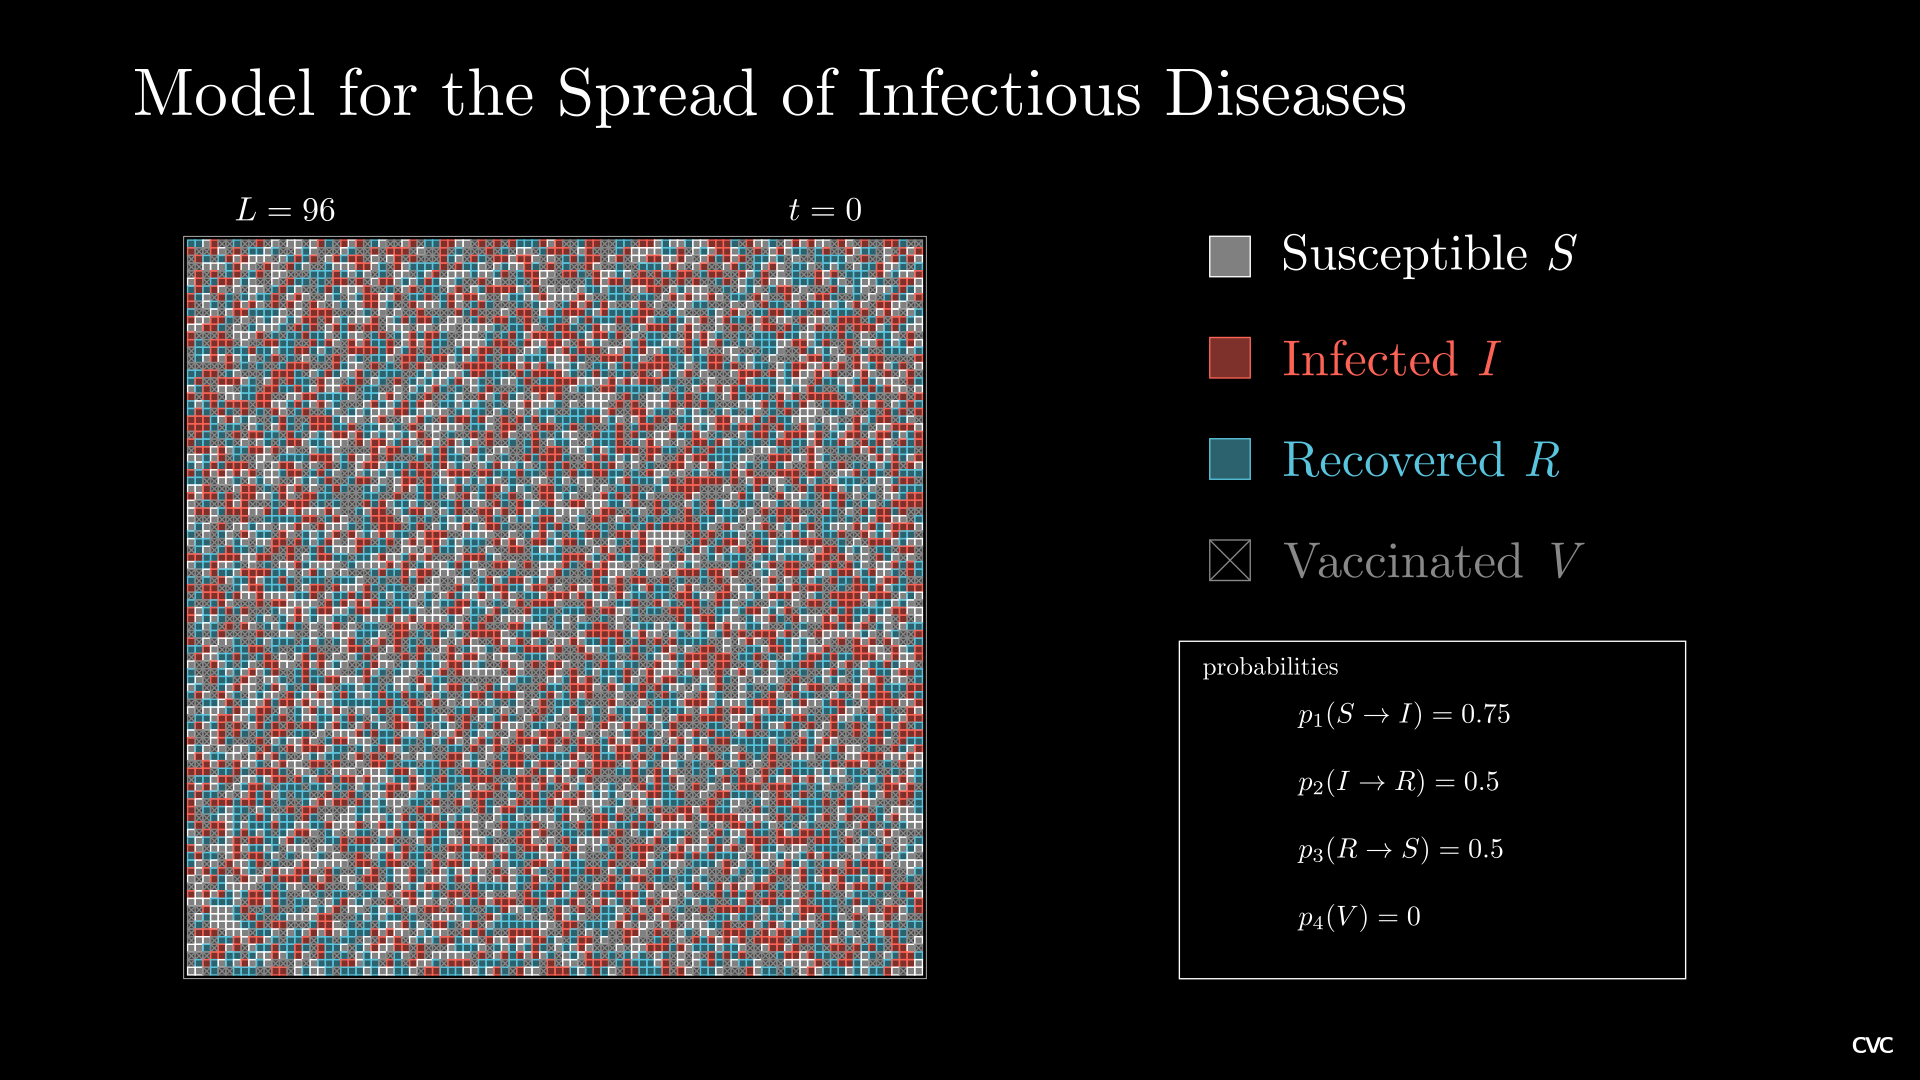
\includegraphics[width=1\textwidth]{images/soi_main_scene_75_50_50_25_init.png}
%         \subcaption{frame $t=0$}
%     \end{subfigure}
%     %\hspace{1cm}
%     \begin{subfigure}{0.49\textwidth}
%         \centering
%         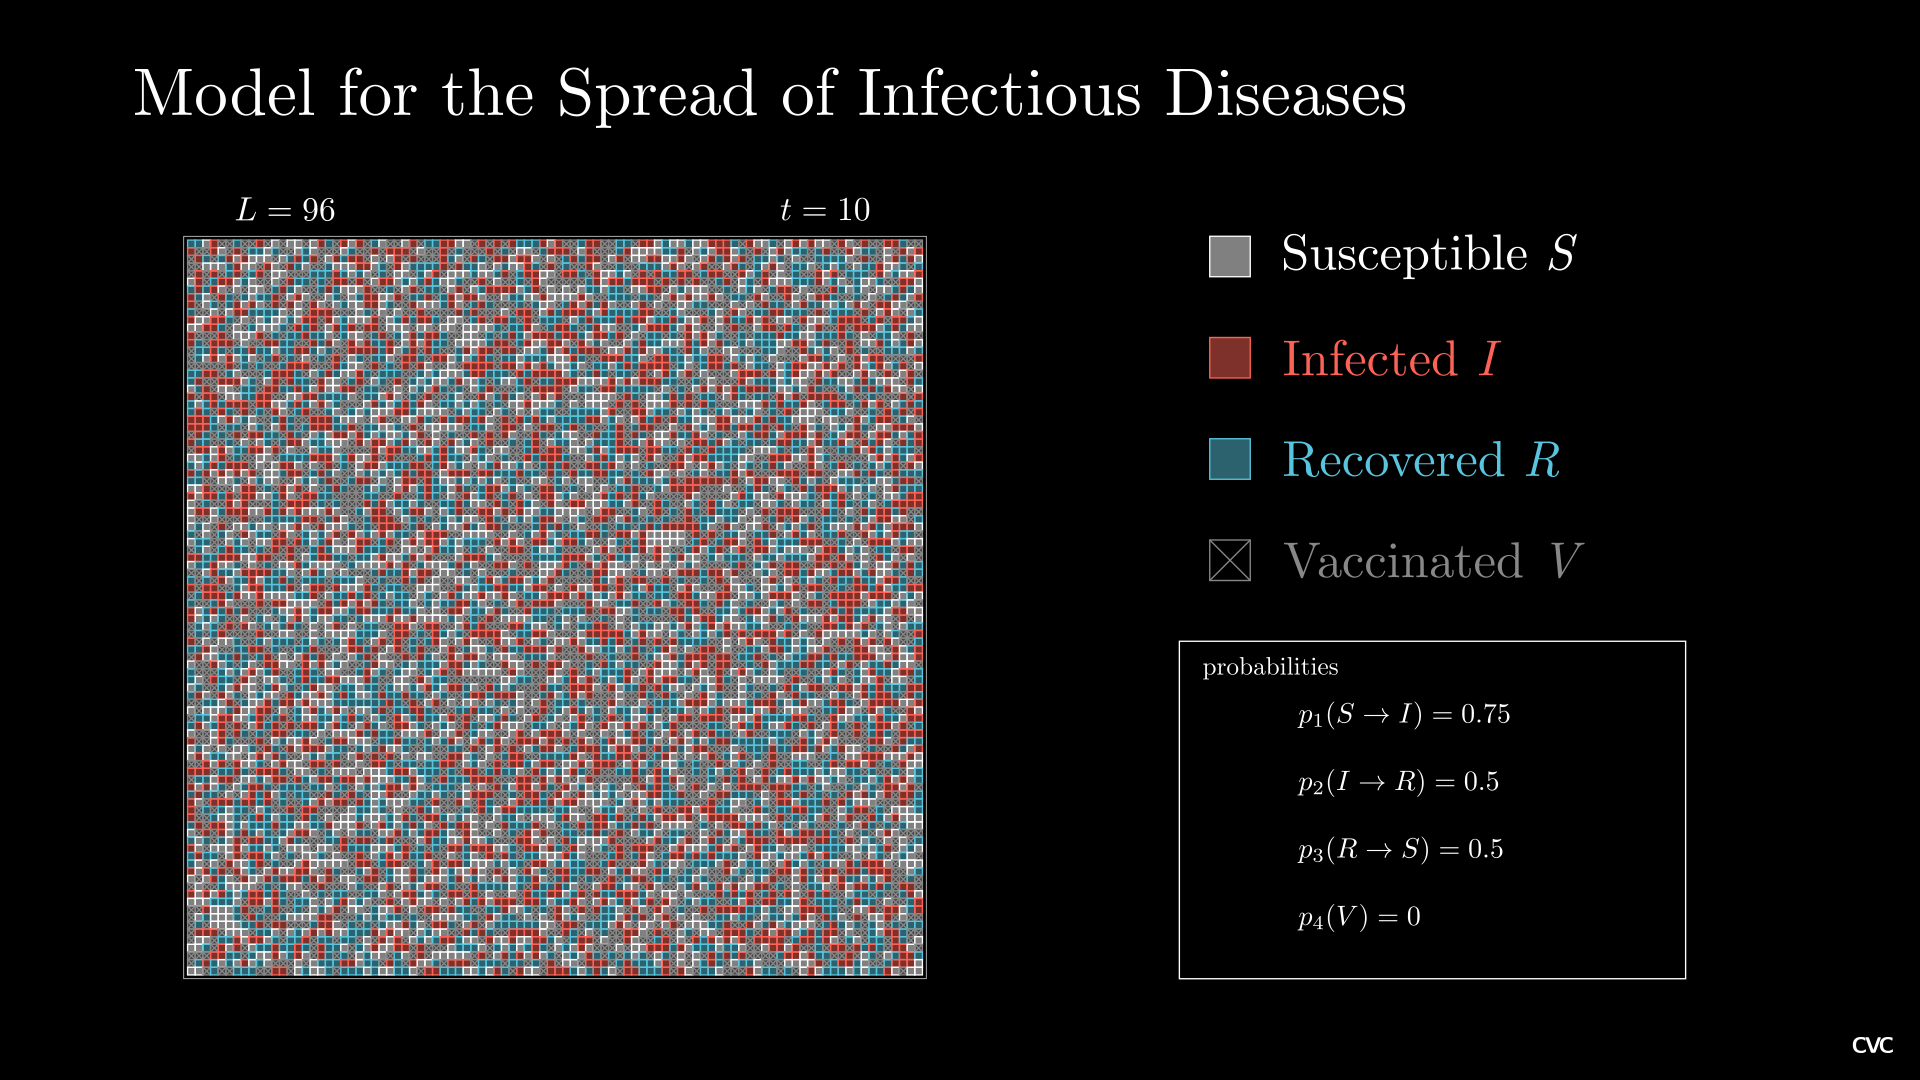
\includegraphics[width=1\textwidth]{images/soi_main_scene_75_50_50_25_t10.png}
%          \subcaption{frame $t=10$}
%     \end{subfigure}
%     \caption{Frames for simulation steps \textbf{(a)} $t=0$ and \textbf{(b)} $t=10$ of an animated simulation of the infectious disease model. The grid was initialized with a vaccination rate $p_4=0.25$
%     and progressed with the turnover probabilities $p_1=0.75$, $p_2=p_3=0.5$}\label{fig:apx_animation_inf_t_double}
% \end{figure}

Several animations of the spread progressing over time were rendered using the python library manim\cite{pypi_manim} and can be found in the directory \texttt{/soi\_animations}. 
As seen in the exemplary video frame in \prettyref{fig:apx_animation_inf_t}, the aminations use a $96\times 96$ grid size. The probabilities were varied to offer a broader understanding of different situations.

\begin{figure}[H]
    \centering
    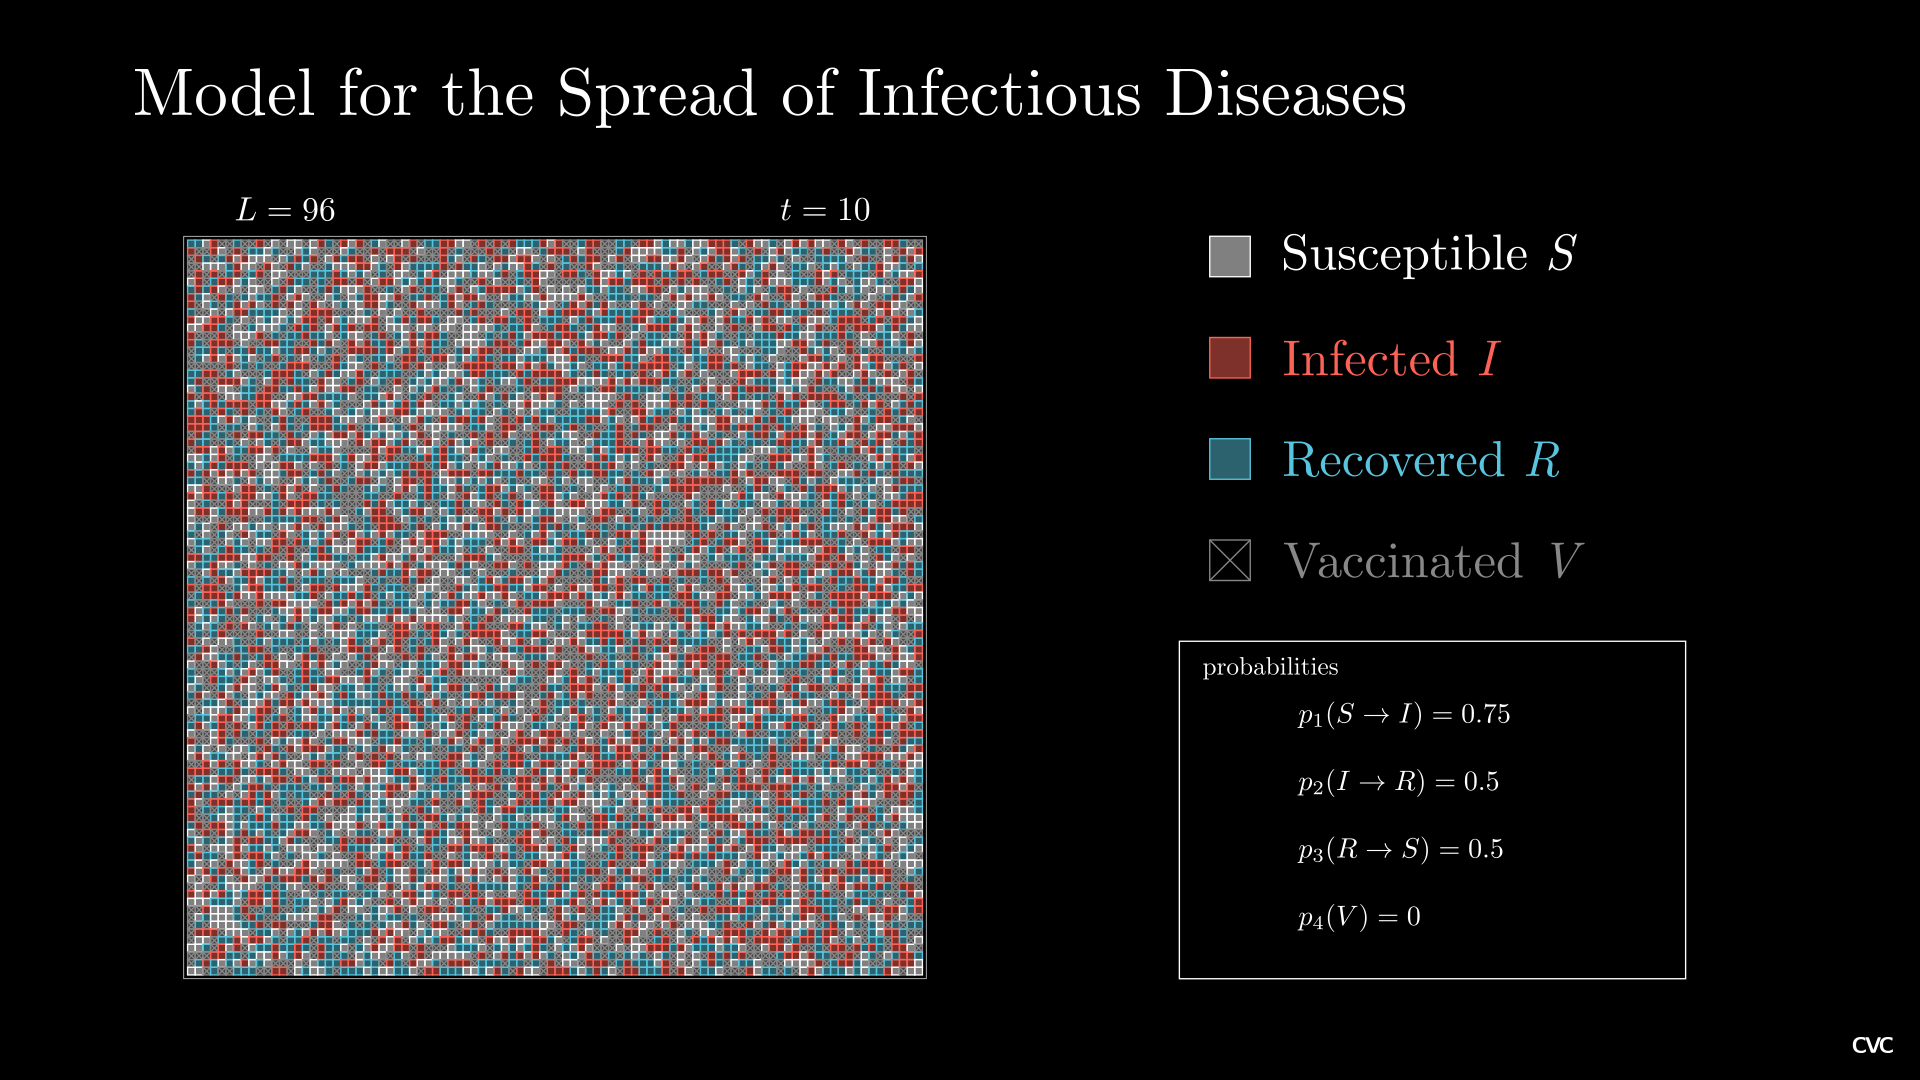
\includegraphics[width=1\textwidth]{images/soi_main_scene_75_50_50_25_t10.png}
    \caption{Frame $t=10$ of an animated simulation of the infectious disease model for the grid size $L=96$. The grid was initialized with a vaccination rate $p_4=0.25$ and progressed with 
    the turnover probabilities $p_1=0.75$ as well as $p_2=p_3=0.5$. The total animation as well as variations in the probabilities can be found under \texttt{/soi\_animations}.}\label{fig:apx_animation_inf_t}
\end{figure}


%**********************************************************************

\newpage
\addcontentsline{toc}{section}{Bibliography}
\printbibliography[title = {Literature}]%,nottype=online]

%\addcontentsline{toc}{section}{Onlinequellen}
%\printbibliography[title=Onlinequellen,type=online]

%\newpage

%\addcontentsline{toc}{section}{Abbildungsverzeichnis}
%\listoffigures

%\addcontentsline{toc}{section}{Tabellenverzeichnis}
%\listoftables

\end{document}